% =====================================================================
%  Analog Game Design, lezione 6 — Ricerca e sviluppo: la revisione dei
%  giochi di ruolo in 200 parole del secondo task (nove giochi, letti uno
%  per uno come li leggerebbe chi li ha appena scaricati), le domande su
%  emozioni, idee e stato dell'arte; poi la parte su ricerca e sviluppo:
%  perché e per che cosa si fa ricerca, divergenza e convergenza,
%  "Everything is a Remix" (copiare, trasformare, combinare) e il
%  plagio, gli step per validare un'idea (obiettivo personale, obiettivo
%  di gioco, ipotesi, prototipo, validazione), il target, la persona e
%  la mappa dell'empatia, le risorse e gli stakeholder, gli strumenti e i
%  siti consigliati; in coda, la domanda sul rapporto tra meccaniche ed
%  emozioni e il sondaggio sulle escape room.
%  Fonte: trascrizione della sesta lezione (AGD6) del corso breve di
%  Analog Game Design, seconda edizione: una lezione online su Zoom di
%  circa tre ore, tenuta da due docenti (Ruggero nella prima parte e in
%  alternanza nella seconda, Beatrice dopo la pausa), con un'unica pausa
%  breve e una coda di domande.
%  Pacchetti richiesti nel preambolo del libro (già presenti nel
%  main.tex): \usepackage{booktabs}, \usepackage{tikz} con
%    \usetikzlibrary{shapes.geometric,shapes.symbols,shapes.misc,
%      arrows.meta,positioning,calc,fit}
%  (le librerie vanno caricate nel preambolo, non nel capitolo).
%  Consigliati, come per gli altri capitoli: \usepackage[italian]{babel}
%  e \usepackage[T1]{fontenc} (il capitolo compila anche senza).
%
%  Collocazione nel libro: parte "Analog Game Design", sesto capitolo
%  (numerazione propria 2.6). Nel file principale del libro, subito dopo
%  il capitolo 2.5:
%
%    % =====================================================================
%  Analog Game Design, lezione 5 — Progettare emozioni: che cosa prova
%  chi gioca, il problema della parola "divertimento", i giochi su temi
%  difficili, il bleed, le meccaniche di sicurezza (prima, durante e
%  dopo il gioco), il 200 Word RPG Challenge e il secondo task; in coda,
%  la dispensa registrata "Dalla ricerca al design" (design thinking,
%  Double Diamond, strumenti di fattibilità e di mercato, brainstorming
%  strutturato, strumenti di convergenza e pitch deck).
%  Fonte: trascrizione della quinta lezione (AGD5) del corso breve di
%  Analog Game Design, seconda edizione: una lezione online su Zoom di
%  circa tre ore, tenuta da un solo docente (Ruggero), con la revisione
%  delle schede personaggio del primo task, un'unica pausa, un
%  "nanogioco" dal vivo, la consegna del secondo task e una coda di
%  domande. Alla stessa trascrizione è accodata una dispensa video
%  registrata a parte da un altro docente (con ogni probabilità
%  Daniele) domenica 4 ottobre 2026: il capitolo la riporta per intero
%  nelle sezioni finali, segnalandola come tale.
%  Pacchetti richiesti nel preambolo del libro (già presenti nel
%  main.tex): \usepackage{booktabs}, \usepackage{tikz} con
%    \usetikzlibrary{shapes.geometric,shapes.symbols,shapes.misc,
%      arrows.meta,positioning,calc,fit}
%  (le librerie vanno caricate nel preambolo, non nel capitolo).
%  Consigliati, come per gli altri capitoli: \usepackage[italian]{babel}
%  e \usepackage[T1]{fontenc} (il capitolo compila anche senza).
%
%  Collocazione nel libro: parte "Analog Game Design", quinto capitolo
%  (numerazione propria 2.5). Nel file principale del libro, subito dopo
%  il capitolo 2.4:
%
%    % =====================================================================
%  Analog Game Design, lezione 1 — Introduzione al corso: docenti,
%  metodo, project work, figure dell'industria e primo glossario
%  Fonte: trascrizione della prima lezione (AGD1) del corso breve di
%  Analog Game Design, seconda edizione: una lezione online su Zoom di
%  circa tre ore, di pomeriggio, tenuta insieme dai tre docenti "cuore"
%  del corso (Daniele, Ruggero e Beatrice), con nove iscritti, una
%  pausa di una decina di minuti, molte slide e una breve dimostrazione
%  dal vivo di Tabletop Simulator.
%  Pacchetti richiesti nel preambolo del libro (già presenti nel
%  main.tex): \usepackage{booktabs}, \usepackage{tikz} con
%    \usetikzlibrary{shapes.geometric,shapes.symbols,shapes.misc,
%      arrows.meta,positioning,calc,fit}
%  (le librerie vanno caricate nel preambolo, non nel capitolo).
%  Consigliati, come per gli altri capitoli: \usepackage[italian]{babel}
%  e \usepackage[T1]{fontenc} (il capitolo compila anche senza).
%
%  Collocazione nel libro: parte "Analog Game Design", primo capitolo
%  (numerazione propria 2.1). Nel file principale del libro:
%
%    \part{Analog Game Design}
%    \renewcommand{\thechapter}{2.\arabic{chapter}}
%    \setcounter{chapter}{0}
%    % =====================================================================
%  Analog Game Design, lezione 1 — Introduzione al corso: docenti,
%  metodo, project work, figure dell'industria e primo glossario
%  Fonte: trascrizione della prima lezione (AGD1) del corso breve di
%  Analog Game Design, seconda edizione: una lezione online su Zoom di
%  circa tre ore, di pomeriggio, tenuta insieme dai tre docenti "cuore"
%  del corso (Daniele, Ruggero e Beatrice), con nove iscritti, una
%  pausa di una decina di minuti, molte slide e una breve dimostrazione
%  dal vivo di Tabletop Simulator.
%  Pacchetti richiesti nel preambolo del libro (già presenti nel
%  main.tex): \usepackage{booktabs}, \usepackage{tikz} con
%    \usetikzlibrary{shapes.geometric,shapes.symbols,shapes.misc,
%      arrows.meta,positioning,calc,fit}
%  (le librerie vanno caricate nel preambolo, non nel capitolo).
%  Consigliati, come per gli altri capitoli: \usepackage[italian]{babel}
%  e \usepackage[T1]{fontenc} (il capitolo compila anche senza).
%
%  Collocazione nel libro: parte "Analog Game Design", primo capitolo
%  (numerazione propria 2.1). Nel file principale del libro:
%
%    \part{Analog Game Design}
%    \renewcommand{\thechapter}{2.\arabic{chapter}}
%    \setcounter{chapter}{0}
%    \input{AGD/AGD1_introduzione_all_analog_game_design}
%
%  (Con hyperref conviene aggiungere anche
%  \renewcommand{\theHchapter}{agd.\arabic{chapter}} nella parte, per
%  evitare ancore duplicate con i capitoli 1, 2, ... di Game Design.)
%  Tutte le etichette di questo capitolo hanno il prefisso "a1:"
%  (a1:cap:..., a1:sec:..., a1:fig:..., a1:tab:...). Il capitolo è
%  autonomo: non contiene \ref verso altri capitoli.
%  Le figure sono ricostruzioni schematiche di quanto i docenti spiegano
%  a voce e con le slide, non copie delle slide.
% =====================================================================

\chapter[Introduzione all'Analog Game Design]{Introduzione all'Analog Game
Design: il corso, le figure dell'industria e un primo linguaggio comune}
\label{a1:cap:intro}

Questa è la \textbf{prima lezione} del corso di \textbf{Analog Game Design},
cioè di progettazione di giochi \emph{analogici}: giochi da tavolo, giochi di
carte, giochi di ruolo da tavolo, giochi di ruolo dal vivo (LARP), giochi
\emph{pervasivi} ed esperienze a evento. È un corso \textbf{breve}, di circa tre
mesi (``da qui a dicembre''), separato dal corso di Game Design, e siamo alla sua
\textbf{seconda edizione}. Come avvertono subito i docenti, è ``una giornata di
introduzione'': si spiega come funziona il corso, chi sono i docenti, con quali
metodi e con quale calendario si lavorerà, e ci si presenta a vicenda. ``C'è poco
gioco analogico'', si scusano. Ma nella seconda parte la lezione comincia
comunque a costruire un \textbf{linguaggio comune}: le figure professionali
dell'industria del gioco analogico, la differenza tra \emph{game design} e
\emph{game development}, la situazione del mercato italiano rispetto a quello
estero, e un primo glossario di design (\emph{game} e \emph{play}, il framework
MDA, le parole ``vietate'', il playtest e l'iterazione). Si chiude con lo
strumento di settore per i prototipi digitali dei giochi da tavolo,
\textbf{Tabletop Simulator}, e con una lunga sessione di domande.

La lezione si svolge \textbf{online}, su Zoom, ed è condotta a più voci dai tre
docenti principali del corso: \textbf{Daniele}, narrative designer, che guida la
parte organizzativa; \textbf{Ruggero}, game designer, che guida la parte sui
fondamenti e le domande finali; \textbf{Beatrice}, progettista di giochi
pervasivi, che interviene soprattutto nella prima metà. Gli studenti iscritti
sono \textbf{nove}; uno è assente e un altro arriva a lezione iniziata. Ci sono
una pausa di una decina di minuti (si riprende alle 18:15) e, dopo le 19:15,
un'ultima mezz'ora di domande con il solo Ruggero.

Tre avvertenze di lettura. La prima: la trascrizione è automatica e storpia
molti nomi propri, compresi quelli dei docenti e dell'accademia (``Dive'',
``IVE'', ``Accademia Live'', ``Ai''); dove la ricostruzione è sicura, o molto
probabile, il capitolo usa la forma corretta e lo segnala in nota; dove non lo
è, riporta la forma della trascrizione e lo dice. La seconda: durante la pausa la
trascrizione registra, ripetuta in loop per decine di righe, una frase senza
senso che non ha nulla a che fare con la lezione, e che il capitolo ignora. La
terza: in molti passaggi più docenti parlano uno dopo l'altro senza che la
trascrizione segni il cambio di voce; il capitolo attribuisce le parole a chi le
pronuncia quando il contesto lo rende chiaro (chi parla di sé, chi viene
chiamato per nome, chi ``passa la parola''), e resta generico altrimenti.

Quanto alla data, la lezione si colloca con ogni probabilità \textbf{nella prima
metà di settembre del 2026}\footnote{La data non è mai detta. La si deduce da
alcuni indizi: il form iniziale va compilato ``entro e non oltre il 15
settembre''; i gruppi verranno annunciati il 25 settembre; le date del
calendario (sabato 3 ottobre, lunedì 12 ottobre, sabato 7 e 14 novembre,
venerdì 4 dicembre) cadono nei giorni della settimana indicati soltanto nel
2026; un docente parla di un argomento ``molto complesso nel 2026''; e fa
ancora molto caldo (``le temperature sono ancora indecenti''). È una
deduzione, non un'informazione esplicita.}: i riferimenti a ``oggi'',
``quest'estate'' e ``l'anno scorso'' vanno letti rispetto a quel momento.

Il percorso del capitolo segue quello della lezione:
\begin{enumerate}
  \item l'avvio, i \textbf{docenti} e le \textbf{presentazioni} dei partecipanti
        (sezioni da~\ref{a1:sec:avvio} a~\ref{a1:sec:partecipanti});
  \item i \textbf{materiali} e gli strumenti del corso: il form, la cartella
        condivisa, Discord (sezione~\ref{a1:sec:materiali});
  \item lo \textbf{scopo} e il \textbf{metodo} del corso, le regole di
        comportamento e il carico di lavoro (sezioni~\ref{a1:sec:scopo}
        e~\ref{a1:sec:regole});
  \item il \textbf{project work} e il \textbf{calendario} (sezione~\ref{a1:sec:project});
  \item la regola sull'\textbf{intelligenza artificiale} e la lunga discussione
        che ne segue (sezione~\ref{a1:sec:ia});
  \item le \textbf{figure professionali} dell'industria del gioco analogico,
        con un approfondimento su marketing e sales
        (sezioni~\ref{a1:sec:figure} e~\ref{a1:sec:marketing});
  \item la differenza tra \textbf{game design} e \textbf{game development}
        (sezione~\ref{a1:sec:design-development});
  \item il \textbf{mercato}: Italia ed estero (sezione~\ref{a1:sec:mercato});
  \item i \textbf{fondamenti di design}: perché serve una terminologia comune,
        \emph{game} e \emph{play}, il framework \textbf{MDA} (e il DPE), le
        \textbf{parole vietate}, chi crea, chi gioca e chi facilita, il
        \textbf{playtest} e l'\textbf{iterazione} (sezioni
        da~\ref{a1:sec:terminologia} a~\ref{a1:sec:playtest});
  \item \textbf{Tabletop Simulator} e il primo task (sezione~\ref{a1:sec:tts});
  \item le \textbf{domande finali}: il tema del project work, il bilanciamento,
        i ruoli nei team, la pubblicazione, il gioco di ruolo in Italia, le
        \emph{house rule} di Monopoly, i giochi ``comunicati male''
        (sezioni~\ref{a1:sec:domande-daniele} e~\ref{a1:sec:domande}).
\end{enumerate}

% ---------------------------------------------------------------------
\section{L'avvio della lezione}
\label{a1:sec:avvio}

La lezione comincia con qualche minuto di attesa. ``Siamo in nove in classe'', e
si aspetta che arrivino tutti; uno dei docenti scherza sul fatto che l'unica
persona che arriverà ``sempre in ritardo di venerdì'' è Gianmarco. Mancano
Giordano e Tiziana; Tiziana arriva, mentre la segreteria fa sapere poco dopo che
Giordano non potrà esserci e vedrà la registrazione. Si aspetta anche Beatrice,
la terza docente, che arriva a sua volta dopo pochi minuti.

Nell'attesa, Daniele anticipa il programma della giornata e qualche
informazione pratica:
\begin{itemize}
  \item oggi è una giornata di \textbf{introduzione}: come funziona il corso, chi
        sono i docenti, le presentazioni degli studenti, le \textbf{metodologie}
        e il \textbf{calendario}. Gli studenti avranno ``un fracco di domande'', e
        alla fine della lezione c'è ``proprio uno slot apposta'' per le domande;
  \item le lezioni sono \textbf{registrate}: di solito la registrazione viene
        consegnata dopo circa \textbf{12--24 ore} sul profilo personale della
        piattaforma dell'accademia, che va attivato con la segreteria (Tiziana,
        già studentessa, probabilmente ce l'ha già);
  \item i docenti ``cuore'' del corso sono tre (Daniele, Ruggero e Beatrice),
        ``soprattutto Ruggero''; a loro si aggiungeranno tre docenti ospiti, per
        meno ore, probabilmente una lezione a testa, ``tranne Marta, che avrà due
        lezioni quest'anno''.
\end{itemize}
E una battuta sul caldo: ``spero che voi siate carichi, anche se le temperature
sono ancora indecenti''. ``Carichi moderatamente, per quello che potete''.

Poi Daniele condivide lo schermo (``non solo le slide, ma anche un po' di altre
cose'') e apre ufficialmente il corso: ``benvenuti e benvenute nella seconda
edizione del corso di Analog Game Design. Questa è la prima lezione''. Il
percorso è di circa \textbf{tre mesi}, fino a dicembre, e durante il corso i
docenti cercheranno di far provare agli studenti ``cosa significa fare Analog
Game Design'' con un \textbf{project work}, un progetto di gruppo di cui si
spiegheranno più avanti la struttura e le richieste.

% ---------------------------------------------------------------------
\section{I docenti}
\label{a1:sec:docenti}

``Anzitutto partiamo da delle presentazioni doverose''. Ognuno dei tre docenti
principali si presenta con una slide che riporta i contatti e una selezione dei
lavori fatti.

\subsection{Daniele: narrativa, fiction e gioco di ruolo}

\textbf{Daniele}\footnote{La trascrizione riporta ``Daniel Cusetto''; nel
resto della lezione tutti lo chiamano ``Daniele''. Il cognome non è
ricostruibile con certezza.} ha già conosciuto quasi tutti gli studenti, perché
ha fatto loro il colloquio di ammissione. È \textbf{narrative designer}, o meglio
\emph{game narrative designer}; insegna nell'accademia che ospita il
corso\footnote{La trascrizione storpia il nome dell'accademia in molti modi
(``Dive'', ``IVE'', ``Accademia Live'', ``Ai'', ``AIVA''). Con ogni probabilità
si tratta dell'\textbf{AIV}, l'Accademia Italiana Videogiochi, che ha sede a
Roma: lo fanno pensare i corsi triennali di game design e narrative design citati
dai docenti e il fatto che una studentessa racconti di essersi trasferita a Roma.
È una ricostruzione, non un'informazione esplicita; nel seguito il capitolo
parla semplicemente dell'``accademia''.} ma lavora soprattutto come \textbf{brand
advisor}. Nel corso si occuperà della parte di \textbf{gioco di ruolo},
\textbf{narrazione} e \textbf{fiction}.

I suoi contatti, ``in quest'ordine'', sono email, Telegram e Discord. Ci tiene a
dare alcune indicazioni precise:
\begin{itemize}
  \item se si vuole avere la certezza di una risposta, bisogna scrivergli su
        \textbf{Telegram}, perché lì ha tutti i suoi clienti;
  \item Discord lo guarda di meno; l'\textbf{email} è per le cose ufficiali;
  \item non bisogna contattarlo altrove: non su Facebook, non su LinkedIn, non su
        Instagram, ``perché li vedo molto di meno''.
\end{itemize}
La slide mostra anche alcuni giochi, attività e brand su cui ha lavorato negli
anni, ma non si dilunga: ``nel caso ne parleremo''.

\subsection{Ruggero: game design e ricerca e sviluppo}

\textbf{Ruggero} (spesso chiamato ``Ruger'') ha fatto il \textbf{game designer}
per varie aziende e oggi è game designer e si occupa di \textbf{ricerca e
sviluppo} per un'azienda del settore\footnote{La trascrizione dice ``per MS'';
il nome dell'azienda non è ricostruibile con certezza. Più avanti Ruggero cita
tra i giochi su cui ha lavorato il gioco da tavolo ufficiale di
\emph{Cyberpunk}, \emph{Marvel United} e \emph{Status}, un gioco sulla
geopolitica.}. Ha un background ``misto'': nel suo portfolio ci sono giochi da
tavolo, giochi di ruolo, giochi analogici, LARP, videogiochi, giochi in realtà
virtuale. Si occupa anche di \textbf{divulgazione} sul gioco e di analisi di
\textbf{game studies} e game design. Più avanti, nelle domande finali, dirà di
avere ``50 e più giochi prodotti e progettati'' e di insegnare da vari anni.

Lo si può contattare liberamente via Gmail e Telegram, e cerca di rispondere
\textbf{entro 24 ore}, salvo imprevisti o eventi: ``sentitevi in libertà di
scrivermi se avete dubbi, senza problemi''. Quando arriva a parlare dei propri
giochi, la slide mostra ``un mix di varie cose, dalle più famose alle meno
famose'', ma Ruggero si imbarazza a presentarli, tra le risate dei colleghi.

\subsection{Beatrice: i giochi pervasivi}

\textbf{Beatrice} (``Bea'') si occupa di \textbf{giochi pervasivi}
(\emph{pervasive games}). ``Se non li avete mai sentiti nominare, non
preoccupatevi'': questo corso è ``uno dei pochi, forse l'unico in Italia'' che
li racconta esplicitamente. Li si vedrà nelle prossime lezioni, ma la definizione
di base è questa: i giochi pervasivi \textbf{utilizzano gli spazi e gli oggetti
della vita quotidiana e li trasformano in spazi e oggetti di gioco}.

Beatrice lavora come \textbf{freelance} e si occupa di diversi tipi di
progettazione: lavora sia con le \textbf{aziende} sia con gli \textbf{eventi dal
vivo}. La sua attività diretta si trova sotto l'etichetta \textbf{Minime
Differenze}\footnote{La trascrizione riporta il nome dell'etichetta come
``Minime Differenze'' e l'indirizzo del sito come ``mininedifferenze.com''; la
grafia esatta del sito non è verificabile dalla trascrizione.}, mentre i lavori
per le aziende sono ``sparpagliati'' sui siti delle varie aziende. Molte delle
cose mostrate nella sua slide sono attività proposte al pubblico ``con un
biglietto, con un gioco in formato evento'': un tema che si toccherà nel corso,
per capire come \textbf{comunicare} i propri giochi in modo che siano
comprensibili, accessibili per il pubblico e \textbf{vendibili}.

Ammette un ``grosso limite'' con i messaggi: è un po' lenta a rispondere, ``ma
rispondo sempre a tutto''. La si può contattare per email (cognome punto nome) o
su Telegram. È ``molto curiosa di vedere cosa produrrete''.

\subsection{I docenti ospiti}

Daniele presenta poi i tre docenti che il corso avrà ``solo per alcune
lezioni'', tutte verso \textbf{novembre}:
\begin{itemize}
  \item \textbf{Diego Ricchiuti}, direttore del corso di Game Design
        dell'accademia, farà una lezione sull'\textbf{RNG} (\emph{random number
        generation}, la casualità nei giochi): ``vi parleremo di RNG quando sarà
        necessario. Comunque avrete una lezione con lui, sappiatelo'';
  \item \textbf{Marta}\footnote{La trascrizione riporta il cognome come
        ``Cercasassi''; la grafia non è verificabile.} farà \textbf{due lezioni
        sul development}: quest'anno ``abbiamo deciso di fare doppietta'',
        perché l'anno scorso il suo intervento è stato ``molto, molto utile'';
  \item \textbf{Flavio}\footnote{La trascrizione riporta il cognome come
        ``Mortarino'' e, più avanti, ``Mortalino'', e il nome della sua casa
        editrice come ``Grampibert''; nessuno dei due è ricostruibile con
        certezza.} farà la lezione di \textbf{game production}; è un editore, e
        di solito partecipa anche alla tavola rotonda con gli editori della
        giornata finale.
\end{itemize}
Le slide sono già online e gli studenti avranno accesso alla cartella condivisa:
``non vi preoccupate di queste cose, ne parleremo a breve''. Ma prima di parlare
del corso, ``vogliamo conoscere voi''.

% ---------------------------------------------------------------------
\section{Le presentazioni dei partecipanti}
\label{a1:sec:partecipanti}

Le domande per la presentazione sono semplici, da affrontare ``a turno, senza
fretta, con calma'':
\begin{itemize}
  \item nome e occupazione (``se volete dirla'');
  \item perché si vogliono fare giochi analogici, e a che livello: che cosa ha
        portato lo studente al corso;
  \item che tipo di esperienze o conoscenze si hanno già nell'ambito, se si è già
        fatto qualcosa oppure no.
\end{itemize}
``Chi vuole partire senza nessun tipo di ritegno e di vergogne?''. Per far
parlare gli studenti guardandoli, Daniele interrompe la condivisione dello
schermo e ricorda lui le domande quando serve. Le presentazioni sono interessanti
anche per i commenti dei docenti, che anticipano diversi principi del corso.

\subsection{Tiziana}

Tiziana fa l'\textbf{infermiera}, ma nella vita ha fatto molti lavori:
impiegata, insegnante e ``tanti altri lavoretti''. Gioca ``da sempre'': il gioco
fa parte anche della sua vita familiare, perché suo fratello fa il programmatore
di videogiochi. Ha già \textbf{organizzato} giochi: una caccia al tesoro per far
conoscere il territorio, due scene con un delitto (giochi con omicidio da
risolvere), giochi per intrattenere le persone. Ha riscoperto di recente i giochi
da tavolo, arrivando a \emph{Carcassonne} con famiglia e amici; poiché è
difficile trovare persone con voglia di giocare nella propria cerchia ristretta,
ha scoperto il mondo delle \textbf{associazioni} ludiche, ``e lì è stato
un'esplosione'': prima in Veneto (è di Vicenza), poi a Roma, dove si è
trasferita.

Ha in mente un progetto ambizioso: far conoscere una certa realtà con la modalità
del \textbf{gioco di ruolo}, o comunque proporre un gioco suo.

\paragraph{Il commento: gli strumenti, non il gioco dei sogni.} Ruggero coglie
l'occasione per un'avvertenza che vale per tutti, visto che molti studenti
arrivano con idee già pronte. Nel corso si lavorerà a un progetto, ma
l'obiettivo dei docenti è dare \textbf{strumenti} da applicare anche
\emph{fuori} dal progetto, ai giochi che gli studenti vorranno fare un domani:
``che non siano esercizi per il corso, ma per voi in primis''. Quindi: ``non
rimaneteci male se non riuscirete a lavorare al vostro gioco dei sogni in questo
corso''. Anche perché ``sarebbe impossibile, in due mesi, fare il gioco dei
sogni''. Il corso darà invece la possibilità di fare un'esperienza ludica
insieme e di imparare a replicarla sulle proprie idee: ``le idee non buttatele,
anzi, il contrario: tenetele''.

\subsection{Nicola}

Nicola è uno \textbf{studente}. Sei mesi prima ha fatto un colloquio con Daniele
perché stava valutando di passare all'accademia, e ha deciso, ``nel dubbio'', di
cominciare da questo corso breve per capire come funziona la formazione;
eventualmente si iscriverà al corso di game design vero e proprio. Gli interessa
in particolare il lato dell'esperienza del giocatore, su cui è ``molto critico''
(qui usa la parola ``divertimento'', e Daniele lo ferma con un ``ne parleremo'':
è una delle parole che il corso vieta, come si vedrà nella
sezione~\ref{a1:sec:parole-vietate}).

Ha 21 anni ed è \textbf{giocatore di ruolo da circa otto}. Prima ancora di
conoscere i giochi di ruolo si era creato un sistema tutto suo, ``pessimo,
disgustoso, terribile'', un sistema a percentuale con il d100 ``terrificante'';
poi ha scoperto i giochi di ruolo da tavolo, i classici (\emph{Dungeons \&
Dragons}, \emph{Daggerheart}, \emph{Vampire}\footnote{La trascrizione riporta
``DD'', ``Daggerart'' e ``Vampire'': quasi certamente \emph{Dungeons \&
Dragons}, \emph{Daggerheart} e \emph{Vampire: The Masquerade}.}). Gioca anche a
\textbf{card game} e ad altri giochi sociali, pur avendo sempre avuto difficoltà
a trovare gruppi, ``avendo vissuto in un buco dimenticato dal mondo''. Come
giocatore è ``l'eterno narratore'' del gruppo, quello che prepara la storia e si
costruisce le regole. Come autore ha fatto soprattutto giochi su carta, ``perché
sono incapace a programmare, per adesso''.

Daniele osserva che il tema del giocatore e del suo rapporto con il gioco è ``un
argomento importante'', anzi ``un vaso di Pandora enorme'' (espressione che
tornerà molte volte nella lezione), e che il corso tratterà anche che cos'è
l'analog game design in generale e quanti tipi di prodotti esistono.

\subsection{Rita}

Rita\footnote{Daniele la chiama prima ``Nino'' (probabilmente un errore della
trascrizione) e poi la ringrazia come Rita.} ha 30 anni e si collega da una
regione del Sud, dove ``ancora si muore di caldo''. Ha studiato
all'\textbf{Accademia di Belle Arti di Napoli}, \textbf{design della
comunicazione visiva}: si occupa dell'aspetto più imprenditoriale della
progettazione artistica. Non volendo progettare per un'impresa (``fare loghi,
robe del genere''), vorrebbe applicare la propria creatività alla realizzazione
di giochi analogici.

Non è una giocatrice di ruolo e non lo è mai stata: è una giocatrice
\textbf{tradizionale}, cresciuta con Monopoly, la dama e giochi tradizionali
cinesi. Ha già \textbf{idee, prototipi e progetti} realizzati, e vuole capire
come renderli \textbf{prodotti per la vendita} e se questo è il campo adatto a
lei; magari anche confrontarsi con i colleghi. La sua progettazione è orientata
al \textbf{sociale} e all'\textbf{educativo}: ``responsabilizzare un po' le nuove
generazioni su come sta andando il mondo e su come potrebbe andare, visto che è
tutto nelle nostre mani''.

\paragraph{Il commento: siate curiosi.} ``Pane per i tuoi denti'', le risponde
Daniele, soprattutto per i LARP e i giochi pervasivi: ``vi apriremo un po' la
testa da questo punto di vista''. E aggiunge un consiglio per tutti: ``siate
curiosi'', perché imparare da altri ambiti dà moltissimo. Ognuno è lì per fare
qualcosa di preciso, ``però siate aperti anche ad altre esperienze''.

\subsection{Tancredi}

Tancredi ha 21 anni e non ha ancora grande esperienza lavorativa: qualche
``piccolo progettino'' che non è andato come voleva. Gli interessa il mondo dei
giochi, digitali e non, con un approccio \textbf{educativo} e \textbf{sociale}.
È arrivato soprattutto dai videogiochi, a cui gioca da quando era piccolo; ai
giochi da tavolo si è avvicinato solo nell'ultimo anno, grazie a una realtà
ludica, perché in famiglia ``non siamo molto da giochi''. Ha realizzato qualche
piccolo videogioco con vari engine: prima quelli senza un vero linguaggio di
programmazione, ``più a nodi'', poi qualcosa di più complicato, e ora sta
lavorando a un piccolo prototipo.

\paragraph{Il commento: niente di quello che vedrete è sprecato.} ``Non butterai
via niente di analog game design'', gli risponde Daniele, ``perché il 99 per cento
delle cose che vedremo si ritrovano quasi uno a uno nel mondo dei videogiochi''.
Tanto che nei corsi triennali dell'accademia (anche in quello di narrative
design, dove insegna Ruggero) il primo anno si parte dai \textbf{giochi da tavolo
e di ruolo}, proprio per spiegare meccaniche più complesse che servono poi per i
videogiochi. Ruggero aggiunge che vale anche il contrario: alcuni dei
\textbf{framework} di game design che si vedranno nelle lezioni tecniche vengono
dal videogioco e sono stati riapplicati all'analogico. ``Evitare la
crossmedialità qui è impossibile''. Anzi, tutte le conoscenze ``mediatiche
adiacenti'' (musica, letteratura, cinema) saranno utili.

\subsection{Lorenzo Vergata}

I Lorenzo in classe sono due; il primo a presentarsi è \textbf{Lorenzo
Vergata}, 26 anni, \textbf{dottorando al Politecnico di Milano}. Gioca ai
videogiochi da quando aveva due anni e mezzo, ma ha giocato al suo primo gioco da
tavolo ``credo nove mesi fa''. Gli fa piacere sentire che molti in classe sono
interessati ai giochi \textbf{sociali} ed \textbf{educativi}, un settore che
interessa anche a lui e che ``può essere esplorato molto'', anche con qualche
aiuto dell'intelligenza artificiale per esperienze più ricercate.

Di esperienza nell'analogico dice di avere fatto ``il minimo sindacale''. Ma
racconta che diciotto anni prima, da bambino, era ``più game designer di
adesso'': prendeva un gioco e ne cambiava le regole, anche al biliardino (``no,
ora introduciamo questa regola''). Gli piace sperimentare, creare regole e
vedere che cosa accade in sé e negli altri. Soprattutto vorrebbe ``una chiave di
lettura per poter rimanipolare la realtà'': tre settimane prima è stato a fare la
\textbf{vendemmia in Francia} e ha visto tantissime dinamiche che potrebbero
diventare un gioco da tavolo o un videogioco. Per esempio: finire contro un rovo
pieno di semi che si attaccano ai vestiti lo rallentava nella raccolta
dell'uva, mentre in un altro filare era più rapido. ``Si può fare pure una
dinamica'', e vorrebbe gli strumenti per farne giochi.

Arriva subito la battuta: una ``vendemmia gamificata'' da proporre in Oltrepò
Pavese (``io sono dell'Oltrepò Pavese, quindi devo per forza bere vino'')\footnote{La
trascrizione dice ``nell'altro papavese'' e non chiarisce chi pronunci la
battuta.}. Daniele conferma che quest'anno il corso avrà ``tante cose sul
sociale'': ``ci piace parecchio''.

\subsection{L'altro Lorenzo}

Il secondo Lorenzo (``secondo, ma non meno importante'') è uno \textbf{scrittore
di racconti brevi} e sta scrivendo il suo primo romanzo. Gli è sempre piaciuto
raccontare storie, e da più grande scriverle; gioca ai videogiochi ed è ``un
amante delle storie e della cultura pop''. Negli ultimi anni è entrato nel mondo
del \textbf{gioco di ruolo da tavolo} e vorrebbe unire le due passioni, le
storie e il gioco di ruolo, magari facendone un lavoro; gli interessa anche lo
\emph{strategic writing}. Daniele gli ricorda che ci sarà una lezione proprio
sulla \textbf{fiction}.

\subsection{Angelo}

Angelo si collega senza videocamera dal lavoro: fa il \textbf{birraio} (in un
piccolo birrificio in Brianza, a Bernareggio, come racconterà dopo la pausa) e,
con il caldo, ``vi risparmio l'orrore''. Per molto tempo era convinto che i
giochi da tavolo fossero solo i classici (Monopoly, Risiko) o i party game; poi,
quattro o cinque anni fa, ha ``sbattuto la faccia'' contro giochi davvero
appassionanti, con una specie di narrazione dietro che li rendeva ancora più
coinvolgenti, e non ha più smesso. È uno che ``ha sempre un botto di idee, ma poi
non mette in pratica assolutamente nulla'': cercava un corso che gli desse le
basi e soprattutto lo \textbf{motivasse} a provare a fare qualcosa.

\paragraph{Il commento: bisogna buttarsi.} Daniele racconta che anche l'anno
prima un suo caro amico si era iscritto proprio per questo motivo. Il corso è
breve, ma cerca di portare gli studenti ``da 0 a 100'' e di far realizzare un
\textbf{prodotto} da presentare alla fine. Il punto è che i giochi ``bisogna
farli, bisogna buttarsi''. E, venendo dalla narrazione, Daniele lo paragona allo
scrivere: si scrive e si riscrive, e allo stesso modo si fa \textbf{playtest}, si
rifà, si aggiorna. ``Non è che si fanno così''.

\subsection{Gianmarco (dopo le slide)}

Gianmarco arriva a lezione iniziata e si presenta più tardi, alla fine della
prima parte, dopo che i docenti hanno chiuso le slide organizzative e la
discussione sull'intelligenza artificiale (``Gianmarco, ti giuro, ti facciamo
presentare''). Lavora nel \textbf{team di innovazione} di un'azienda italiana.
Vuole fare giochi perché è una sua passione, che lo gratifica, e in passato ci ha
provato ``in maniera scomposta''. Cerca un \textbf{metodo} e un confronto con
persone più esperte: ``studiare solo dei manuali è molto sterile'', ``stare
chiusi nel pertugio non aiuta'', ed ``essere autodidatta ha estremamente i suoi
limiti''. Come esperienza è un giocatore e ha letto ``un po' di materiale, di
blog, di manuali'', ``niente di rilevante''.

Manca solo Giordano, che si presenterà alla lezione successiva.

\paragraph{Uno sguardo d'insieme.} La classe è molto varia: un'infermiera,
una designer della comunicazione visiva, un birraio, un dottorando, uno
scrittore, un impiegato nell'innovazione, due studenti ventunenni. Alcuni
vengono dal gioco di ruolo, altri dai giochi tradizionali, altri dai
videogiochi; quasi tutti hanno scoperto i giochi da tavolo moderni da pochi anni
o da pochi mesi. E almeno tre studenti dichiarano un interesse per i giochi
\textbf{sociali} ed \textbf{educativi}. Come si vedrà nella
sezione~\ref{a1:sec:scopo}, i docenti considerano questa varietà una risorsa.

% ---------------------------------------------------------------------
\section{I materiali e gli strumenti del corso}
\label{a1:sec:materiali}

Prima delle slide sul corso, Daniele sbriga un po' di ``clean up casalingo''.

\paragraph{Il form iniziale.} C'è un \textbf{form} da compilare ``entro e non
oltre il 15 settembre'': il QR code è nelle slide, e la segreteria lo ricorderà
su Discord. Richiede circa 10--15 minuti; si può fare subito o in giornata, ``e
ve lo togliete di torno''. È un form standardizzato per tutti i corsi (``non
siamo io e Ruggero a farvi passare la tortura del test''), diviso in due parti:
\begin{itemize}
  \item una parte di \textbf{conoscenza del candidato}: quanto tempo si ha a
        disposizione per il corso, come ci si organizza con il lavoro, che cosa
        piace giocare. È la parte che interessa ai docenti, perché li aiuta a
        organizzare le lezioni;
  \item una parte di \textbf{test logico}, che i docenti non hanno scritto (``io
        non sono responsabile del form'', ``no, no, nemmeno io'').
\end{itemize}

\paragraph{La cartella condivisa.} Tutti gli studenti vengono aggiunti alla
cartella del corso su \textbf{Google Drive}, che si trova tra i file
``condivisi con me''. Gli studenti ne sono \textbf{gestori dei contenuti} e
possono caricarci quello che vogliono. Dentro ci sono:
\begin{itemize}
  \item le \textbf{attività in classe};
  \item le \textbf{dispense};
  \item i \textbf{materiali didattici}, con le slide (quelle della lezione sono
        già lì);
  \item le cartelle dei \textbf{project work} futuri;
  \item i \textbf{task}, che ``saranno pochi, ma ci saranno'';
  \item il \textbf{calendario studenti}, ``importantissimo'', con due schede: il
        calendario delle lezioni e quello del project work.
\end{itemize}

\paragraph{Discord.} Il corso ha anche un \textbf{server Discord}, a cui tutti
sono stati invitati; ci sono i docenti (Daniele, Ruggero, Diego e altri), che si
possono taggare. Di solito è lì che la segreteria pubblica le informazioni, per
esempio se una lezione ``dovesse per caso essere cancellata''. Nelle domande
finali Ruggero aggiungerà che c'è un canale apposito per il corso, che gli
studenti possono usare liberamente per organizzarsi tra loro.

\paragraph{Le reaction di Zoom.} Durante le lezioni su Zoom si possono usare le
\textbf{reaction} (il pollice in alto, il cuoricino, la mano alzata): un modo
rapido per far capire ai docenti se si è capito, se si vuole intervenire. Nel
frattempo arrivano i primi pollici.

% ---------------------------------------------------------------------
\section{Lo scopo e il metodo del corso}
\label{a1:sec:scopo}

La prima serie di slide (che Daniele, per un lapsus, presenta come ``cos'è il
corso di pulire il pavimento di casa'') spiega che cosa il corso vuole fare e
come.

\subsection{Diventare autori analogici}

Lo \textbf{scopo del corso} è fornire le competenze per \textbf{diventare autori
analogici} e stimolare la creatività e l'\textbf{autorialità} di ciascuno: ``voi
imparerete a diventare autori di giochi analogici''. La differenza tra
\emph{game designer} e \emph{game developer} verrà chiarita più avanti (sezione~\ref{a1:sec:design-development}),
ma la parola chiave qui è \emph{autorialità}: ``vogliamo voi, vogliamo le vostre
idee''. Magari non si potrà usare l'idea del gioco della propria vita, ma si
potranno portare nelle lezioni le proprie idee e le proprie sensibilità.

Gli obiettivi elencati nella slide sono questi:
\begin{itemize}
  \item dare \textbf{maggiore consapevolezza nel design e nello sviluppo}. In
        Italia, purtroppo, ``si fa design a volte in maniera non consapevole''.
        Consapevole vuol dire avere almeno un'introduzione alle basi del design e
        dello sviluppo, e fare le cose ``con metodo, con raziocinio, con
        consapevolezza'';
  \item fornire gli \textbf{strumenti essenziali} per un design consapevole;
  \item stimolare la \textbf{sperimentazione} e la \textbf{trasversalità
        mediatica}. Non si chiede di fare ``il \emph{Root} della situazione o il
        \emph{Carcassonne} della situazione''\footnote{La trascrizione dice ``il
        lumaven della situazione o il carcassone della situazione''; il primo
        titolo non è ricostruibile con certezza. Il senso è chiaro: non si
        chiede di rifare un grande classico del gioco da tavolo.}, ma un
        project work \textbf{calibrato sulla durata del corso}, e però
        \textbf{sperimentale} e ``assolutamente transmediale'';
  \item portare \textbf{numerosi esempi} di tipologie di gioco, dall'analogico al
        tavolo, al pervasivo ``e oltre''. Lo si vedrà nella lezione sui
        \textbf{casi studio} del venerdì successivo: ``voi non avete idea di
        quante cose esistono, bellissime, sconosciutissime e favolose''. Daniele
        confessa che preparando e aggiornando le slide i colleghi gli hanno
        mostrato cose che lui stesso non sapeva nemmeno che esistessero;
  \item dare gli strumenti per \textbf{analizzare} i giochi altrui. Ruggero lo
        sottolinea: se il corso riesce nel suo intento, gli studenti sapranno
        non solo fare i propri giochi ma anche analizzare giochi già fatti, che è
        ``una delle skill importanti anche nella parte di ricerca e sviluppo''.
        Si vedranno casi studio e giochi pubblicati, sempre con l'obiettivo di
        capire \textbf{che cosa fanno e perché lo fanno}, per poi fare meglio il
        proprio lavoro;
  \item imparare a \textbf{fare giochi insieme}. Esistono gli autori che lavorano
        da soli (i \emph{solo developer}), ``ma sappiate che anche l'autore che
        lavora da solo poi si deve interfacciare con il pubblico, con un editore,
        magari con un editor, con un publisher''. ``Non lavorerete mai da soli'':
        bisogna imparare a lavorare con gli altri.
\end{itemize}

\subsection{Un corso intersezionale}

Il corso è \textbf{intersezionale}: \textbf{non ci sono lezioni dedicate a una
singola tipologia di gioco}. Non ci sarà ``la lezione sul gioco da tavolo'',
``la lezione sul gioco di ruolo'', ``la lezione sul gioco pervasivo''. Ci saranno
lezioni su temi diversi, ciascuna pensata per essere utile a \textbf{tutte e tre
le sfaccettature} del corso; alcune saranno più importanti per il gioco da
tavolo, altre per il pervasivo, altre per il gioco di ruolo, ma nessuna sarà
esclusiva. I docenti vogliono ``contaminazioni e applicazioni assolutamente
trasversali''.

\subsection{Un corso cross-generazionale}

È anche un corso \textbf{cross-generazionale}: i gradi di esperienza di gioco
quest'anno sono abbastanza allineati, ma le esperienze di vita, le età, le
estrazioni sociali sono varie. ``Ed è un pro, non è un contro. Più diversificata
è la classe, più imparate meglio anche voi''. La slide ha una piccola nota per
fasce d'età:
\begin{description}
  \item[Under 30] Concentratevi sulla vostra \textbf{crescita}. Evitate di
        confrontarvi con le persone più grandi che magari ``ce la fanno meglio''
        in alcune cose.
  \item[Over 30] Concentratevi sul \textbf{consolidamento}, ma siate
        \textbf{umili}: i docenti diranno cose che faranno ``storcere il naso''.
        ``Bisogna un po' reimparare per imparare'': bisogna sapersi adattare.
\end{description}
Ruggero contestualizza: lo dicono perché in passato hanno visto studenti che,
essendo più adulti o avendo giocato di più, pensavano che l'esperienza
\emph{di gioco} si trasformasse automaticamente in competenza \emph{di
creazione} di giochi. Non è così. E non bisogna sottovalutare chi gioca meno:
proprio perché gioca cose diverse, per risolvere un problema di design specifico
``è una ricchezza incredibile avere qualcun altro che riesce a uscire dalla
scatola''.

\subsection{Un corso pratico e adattabile}

Il corso è \textbf{pratico}: gli studenti si concentreranno su un progetto di
gruppo, il \textbf{project work}, lavorando in team. Ed è \textbf{adattabile}: il
programma è definito, ma ``si aggiorna sui vostri stimoli, priorità e
necessità''. Se durante il corso i docenti vedono che serve più una cosa
dell'altra, sono ``prontissimi'' a dare più spazio a un argomento invece che a
un altro.

\subsection{Inquiry-based learning: domandate}

Il metodo è quello dell'\textbf{inquiry-based learning}, l'apprendimento basato
sulle domande. Di solito le persone dicono ``ho una domanda, magari sarà
stupida''. ``Non esistono domande stupide. Pensate che ci sia una domanda
stupida? Fatela, alzate la mano''. Vanno bene anche le
\textbf{provocazioni}: se qualcosa non torna, è meglio chiedere. La condivisione
è fondamentale.

I docenti danno \textbf{metodi, dati e conoscenze}, ma lasciano trovare le
risposte agli studenti: ``vi lasciamo un pochettino annegare nel mare prima di
darvi la soluzione, in modo tale che la possiate trovare da soli''. Di
conseguenza \textbf{non ci saranno interrogazioni sulle definizioni}: interessa
vedere \textbf{come} gli studenti applicano ciò che imparano. Se una
definizione non viene in mente, non è un problema; l'importante è saperla usare.

\subsection{Feedback, non valutazione}

``Sì al feedback, no alla valutazione''. I docenti danno \textbf{feedback
verbali}, anche sulle attività da fare a casa (i task, che non saranno tanti).
Il corso è calibrato per \textbf{studenti lavoratori}: c'è un po' da lavorare
fuori dalle lezioni, ma in modo calibrato.

Il principio è \textbf{fallire oggi per imparare per il futuro}: \emph{fail
forward}, \emph{fail to learn}. I docenti lasciano provare e fallire almeno una
volta prima di dare la soluzione: ``il classico metodo Montessori, quello
originale, non quello travisato''.

\subsection{Le soft skill e i criteri di valutazione}

Grande attenzione va alle \textbf{soft skill}: i lavori di gruppo, lo scambio
propositivo, l'atteggiamento positivo, la propositività, la proattività.
``Lavoro di gruppo'' non significa stare ogni giorno in sala studio con gli
altri: va benissimo che un gruppo si organizzi dandosi priorità e tempi in base
alla disponibilità di ciascuno. L'importante è \textbf{collaborare}, essere
\textbf{professionali}, rispettarsi a vicenda, rispettare le idee proprie e
altrui e lasciare spazio agli altri, perché i progetti ``non saranno solo
vostri, saranno di tutte le persone del vostro gruppo''.

La valutazione del project work non riguarda solo la \textbf{documentazione}
prodotta, ma anche:
\begin{itemize}
  \item la \textbf{presentazione} finale;
  \item l'\textbf{autovalutazione};
  \item la \textbf{crescita personale};
  \item l'\textbf{atteggiamento} tenuto nel corso.
\end{itemize}
Daniele cita: ``da ognuno secondo le sue capacità, a ognuno secondo i suoi
bisogni''. Lavorare in gruppo non vuol dire che, in tre, ciascuno lavori
esattamente il 33\% del tempo. Ai docenti serve piuttosto capire \textbf{chi fa
che cosa} nel gruppo, e che il processo interno sia \textbf{trasparente}.

\paragraph{Lavorare in cloud.} Per lo stesso motivo il consiglio è di
\textbf{non lavorare in locale}, ma direttamente nelle cartelle condivise del
project work e dei task. Si è liberi di fare altrimenti, ma lavorando in cloud
si dà ai docenti la possibilità di vedere \emph{come} si lavora, il proprio
``processo mentale''.

% ---------------------------------------------------------------------
\section{Le regole di comportamento e il carico di lavoro}
\label{a1:sec:regole}

Alcune slide sono di quelle che si ripetono in ogni corso (``\emph{repetita
iuvant}'', storpiato per scherzo in ``ripetita Juventus'').

\paragraph{Comportamento.} Prestare attenzione durante le lezioni; interagire;
portare rispetto; essere proattivi; alzare la mano e fare domande.
\textbf{Tolleranza zero} per pregiudizi, maleducazione, mancanza di rispetto,
\emph{cheat} e scorciatoie. Daniele ammette che ``cheat e scorciatoie'' viene da
altri corsi dove il tema è più importante, ma Ruggero lo ferma: ``non
sottovalutate questa cosa'', perché implica anche \textbf{non far fare a ChatGPT
i task}. Daniele ha una slide apposta, ``perché è un discorso molto complesso nel
2026'' (sezione~\ref{a1:sec:ia}).

\paragraph{Le lezioni sono intense.} Le lezioni possono essere \textbf{dense},
``soprattutto le mie, sappiatelo: io sono logorroico'', avverte Daniele. Bisogna
chiedere spiegazioni se serve, prendere appunti, rivedere le registrazioni. Le
lezioni sono ``delle scintille'': modi per far esplorare i temi oltre le slide.
``Andate oltre, se riuscite''.

\paragraph{Il carico di lavoro.} Le regole sui task sono queste:
\begin{itemize}
  \item i task \textbf{sono per voi, non per noi};
  \item se si ha poco tempo, è meglio farli rapidamente piuttosto che non farli:
        ``provateci'';
  \item i docenti cercano di non chiedere più di \textbf{un'ora o due a
        settimana} oltre alle ore di lezione;
  \item non tutte le lezioni avranno un task, e il \textbf{project work} è il più
        importante di tutti.
\end{itemize}

\paragraph{I feedback dei docenti.} I feedback ``si guadagnano'' man mano che si
reagisce bene: non bisogna aspettarsi ``dei papiri'' sui task. Se i docenti
hanno voglia di dare feedback più ampi lo fanno, soprattutto se vedono che lo
studente se li merita. Ad Analog di solito non ci sono task \emph{rejected}; ma
se un docente rifiuta un task, vuol dire che si è fatto \textbf{meno del livello
minimo} richiesto dal corso. I feedback possono non essere immediati: ``siate un
pochettino impietositi dal fatto che siamo dei docenti''. E se un feedback non
arriva, o se ne vogliono di più, bisogna scrivere, ``perché siamo tre esseri
umani e quindi possiamo anche dimenticarci''.

% ---------------------------------------------------------------------
\section{Il project work e il calendario}
\label{a1:sec:project}

\subsection{Come funziona il project work}

Una prima slide con le date del project work è da aggiornare (``perdonatemi il
refuso''); Daniele la corregge al volo e rimanda alla slide successiva, più
precisa. Il funzionamento è questo:
\begin{itemize}
  \item i \textbf{gruppi li formano i docenti}. Gli studenti sono nove, quindi si
        faranno \textbf{tre gruppi da tre}: una dimensione pensata anche per il
        fatto che molti sono studenti lavoratori, così da non ritrovarsi ``in due,
        a esplodere'';
  \item ogni gruppo deve prima preparare un \textbf{pitch} del proprio gioco, da
        presentare in anticipo: un'idea, una bozza del gioco;
  \item poi si lavora al gioco \textbf{nelle pause del corso}: da qui a dicembre
        ci saranno due pause, quindi non ci sarà lezione tutti i lunedì e tutti i
        venerdì;
  \item ci saranno \textbf{review intermedie} con i \textbf{tutoraggi}, per lo più
        il \textbf{sabato mattina}, dalle 11 alle 12, con Ruggero su Google Meet.
        Servono ad aiutare i gruppi a portare avanti il project work.
\end{itemize}

\subsection{Il calendario delle lezioni}

Il \textbf{calendario} è nel calendario studenti della cartella condivisa.
Attenzione: le date \textbf{possono variare}. ``Il 90\% rimarranno così'', ma
può capitare che, per motivi di lavoro, qualcuno stia male o non possa, o che
``scompaia l'elettricità da tutte le città d'Italia''. E l'ordine delle lezioni
può cambiare se i docenti vedono che agli studenti serve prima una lezione
invece di un'altra.

Ci sono \textbf{due pause importantissime}:
\begin{itemize}
  \item dal \textbf{13 ottobre al 5 novembre}: è il periodo delle grandi fiere
        (\textbf{Essen} e \textbf{Lucca}\footnote{La trascrizione dice ``Essen,
        Luca, Cose'': si tratta con ogni probabilità della fiera Spiel di Essen,
        in Germania, e di Lucca Comics \& Games, che si tengono entrambe in
        ottobre.}), ``un periodo un po' frenetico'', e cominciano anche i corsi
        accademici, quindi la pausa permette ai docenti di respirare. Per gli
        studenti è la pausa più importante: quasi un mese in cui sviluppare la
        parte importante del gioco;
  \item dal \textbf{24 novembre all'11 dicembre}, dopo qualche lezione a novembre.
\end{itemize}

E ci sono \textbf{due date da evidenziare}:
\begin{itemize}
  \item il \textbf{25 settembre}: nei primi 5--10 minuti della lezione (che per il
        resto sarà tenuta da Beatrice) i docenti annunceranno i tre gruppi;
  \item il \textbf{12 ottobre}: il \textbf{pitch} dei giochi, con l'idea
        embrionale. Tra il 25 settembre e il 12 ottobre ogni gruppo prepara un
        breve pitch in formato slide; quel giorno i docenti lo rivedono e danno
        feedback: se il gioco va bene, se non va bene, come svilupparlo.
\end{itemize}
Dal 12 ottobre fino all'inizio di dicembre si sviluppa il gioco, con i
tutoraggi: ``sfruttate questi momenti di pausa''.

\subsection{Il calendario del project work}

La slide successiva, ``reale e aggiornata'', riporta il calendario del project
work (tabella~\ref{a1:tab:calendario} e figura~\ref{a1:fig:calendario}).
``Per ora non pensate al project work: ci penserete dal 25 settembre in poi''.

\begin{table}[htbp]
\centering
\begin{tabular}{@{}lp{9.2cm}@{}}
\toprule
\textbf{Data} & \textbf{Che cosa succede} \\
\midrule
ven 25 settembre\footnotemark & lezione: annuncio dei gruppi e del
\emph{mandate}, cioè di che cosa si dovrà fare \\
sab 3 ottobre, ore 11 & prima review e tutoraggio con Ruggero (dopo una
decina di giorni di lavoro) \\
lun 12 ottobre & pitch del gioco durante la lezione \\
13 ottobre -- 5 novembre & prima pausa: sviluppo del gioco \\
sab 7 novembre & tutoraggio \\
sab 14 novembre & tutoraggio \\
24 novembre -- 11 dicembre & seconda pausa: sviluppo del gioco \\
ven 4 dicembre, entro mezzanotte & consegna del gioco sul Drive (non c'è
lezione) \\
ven 11 dicembre & i giochi vengono visti a lezione \\
14 dicembre & giornata finale, con la tavola rotonda con gli editori \\
\bottomrule
\end{tabular}
\caption{Il calendario del project work come lo presenta Daniele. Le date
possono variare.}
\label{a1:tab:calendario}
\end{table}
\footnotetext{Daniele dice ``lunedì 25 settembre'', ma nel 2026 il 25 settembre
è un venerdì; il giorno della settimana nella tabella è corretto di
conseguenza.}

\paragraph{Perché la consegna è il 4 dicembre.} Il 4 dicembre non c'è lezione:
si deve solo consegnare il gioco, entro mezzanotte, sul Drive. La presentazione
a lezione è l'11 dicembre, ma i tre docenti hanno bisogno di \textbf{una
settimana} per rivedere il gioco in privato e valutare anche la
\textbf{documentazione}; per questo la consegna non coincide con la
presentazione. Che cosa voglia dire esattamente ``consegnare il gioco'' verrà
spiegato più avanti.

\paragraph{La giornata finale.} Il 14 dicembre c'è la \textbf{giornata finale},
con una \textbf{tavola rotonda con gli editori}: di solito viene invitato Flavio,
che è anche docente di game production, più qualche altro editore, ``vediamo
quest'anno chi riusciamo a portarvi''.

\begin{figure}[htbp]
\centering
\begin{tikzpicture}[
    font=\footnotesize,
    x=0.1cm,
    evento/.style={draw, thick, rounded corners=2pt, fill=white,
                   text width=1.8cm, align=center, inner sep=2pt},
    pausa/.style={fill=gray!20, draw=gray!60},
    tacca/.style={thick}
  ]
  % asse: giorno 0 = 25 settembre; 1 unità = 1 giorno
  \draw[pausa] (18,-0.35) rectangle (41,0.35);
  \draw[pausa] (60,-0.35) rectangle (77,0.35);
  \node[font=\scriptsize\itshape] at (29.5,0.18) {pausa};
  \node[font=\scriptsize\itshape] at (65,0.18) {pausa};
  \draw[-{Stealth[length=2.5mm]}, thick] (-3,0) -- (85,0);
  % eventi sopra
  \draw[tacca] (0,-0.15) -- (0,0.9);
  \node[evento, above] at (0,0.9) {25 set\\ gruppi e \emph{mandate}};
  \draw[tacca] (17,-0.15) -- (17,2.2);
  \node[evento, above, fill=gray!8] at (17,2.2) {12 ott\\ \textbf{pitch}};
  \draw[tacca] (70,-0.15) -- (70,0.9);
  \node[evento, above, fill=gray!8] at (70,0.9) {4 dic\\ \textbf{consegna}};
  % eventi sotto
  \draw[tacca] (8,0.15) -- (8,-0.9);
  \node[evento, below] at (8,-0.9) {3 ott\\ tutoraggio};
  \draw[tacca] (43,0.15) -- (43,-0.7);
  \draw[tacca] (50,0.15) -- (50,-0.7);
  \draw (43,-0.7) -- (50,-0.7);
  \draw[tacca] (46.5,-0.7) -- (46.5,-0.9);
  \node[evento, below] at (46.5,-0.9) {7 e 14 nov\\ tutoraggi};
  \draw[tacca] (77,0.15) -- (77,-0.9);
  \node[evento, below] at (77,-0.9) {11 dic\\ giochi a lezione};
  \draw[tacca] (80,-0.15) -- (80,2.2);
  \node[evento, above] at (80,2.2) {14 dic\\ giornata finale};
\end{tikzpicture}
\caption{Una linea del tempo del project work, ricostruita dalle slide (scala
approssimativa: dal 25 settembre al 14 dicembre). Le bande grigie sono le due
pause senza lezioni, in cui i gruppi sviluppano il gioco.}
\label{a1:fig:calendario}
\end{figure}

Finita questa parte, Daniele apre alle domande: ``Domande sul calendario? Sulle
slide che ho fatto? Considerazioni? Non abbiate timore, io non ci credo''. E la
domanda arriva, sull'unico tema che aveva lasciato da parte.

% ---------------------------------------------------------------------
\section{L'intelligenza artificiale nel corso}
\label{a1:sec:ia}

\subsection{La slide di Daniele}

Daniele aveva già presentato una slide che definisce ``importantissima''. ``Lo so
che è paradossale, me ne rendo conto. Lo so che magari mi darete del luddista,
dell'anti-tecnologia: non è così. Uso l'intelligenza artificiale per lavoro. Ma
in questo corso, vi prego, \textbf{non usate l'intelligenza artificiale}''. La
richiesta vale per le attività, per i task e \textbf{anche per la
prototipazione}. Le ragioni:
\begin{itemize}
  \item ``voglio che siate voi a fare il gioco, voglio che siate voi a imparare a
        farlo''. Daniele parla da utilizzatore: prima di ChatGPT, che ha smesso
        di usare, oggi soprattutto di Claude, di cui ``si sottovaluta quanto
        possa essere incerto, insicuro, impreciso, non all'altezza'';
  \item nella game industry, \textbf{i publisher rifiutano automaticamente} i
        pitch e i prototipi fatti con l'intelligenza artificiale. Daniele lo ha
        visto di persona in ``tantissime pitch review'' quell'estate, anche al
        \textbf{First Playable} di Firenze\footnote{La trascrizione dice ``First
        Playboy a Firenze'': si tratta del First Playable, l'evento di business
        dell'industria videoludica che si tiene a Firenze.}: anche nel mondo dei
        videogiochi i publisher che vedono pitch o prototipi fatti con l'IA
        ``rigettano automaticamente la build'', perché hanno ancora timore
        dell'IA e delle sue possibili conseguenze;
  \item ``non so come sarà il futuro'': non sa se bisognerà abituarsi a usarla
        tutto il giorno. Non è ``totalmente contrario'', purché sia usata ``con
        raziocinio''; secondo lui oggi, negli Stati Uniti, non lo è;
  \item ma in un corso che si chiama \emph{Analog Game Design} gli studenti devono
        saper fare i giochi da soli. In futuro, se vorranno farsi aiutare
        dall'IA per essere più efficienti, saranno liberissimi di farlo; durante
        il corso no, perché i docenti vogliono valutare \textbf{le loro
        competenze e capacità}.
\end{itemize}

\subsection{La domanda: che cosa vuol dire usare l'IA in un gioco analogico?}

La domanda di uno studente è precisa: che cosa si intende per ``task fatti con
l'IA''? Qual è l'uso dell'IA in un gioco analogico?

\paragraph{Ruggero: l'esperienza di chi valuta i prototipi.} Ruggero risponde
dalla sua esperienza nel settore, dove riceve prototipi da valutare per
un'eventuale pubblicazione. Distingue due usi:
\begin{enumerate}
  \item le \textbf{immagini generate}: illustrazioni, graphic design e così via.
        Per molti publisher è ``un \emph{reject} immediato, proprio immediato'';
  \item l'IA usata per il \textbf{regolamento}, per scrivere le regole e le
        meccaniche. È più difficile da individuare, ma molti publisher se ne
        accorgono comunque, perché le IA ``non sono ancora brave abbastanza da
        creare un regolamento coeso meccanicamente e scritto con un senso per il
        vostro gioco''. Quello che fanno è prendere parti di altri regolamenti,
        elaborare le strutture che vedono nei regolamenti pubblicati e
        riapplicarle. Ma molti giochi si prestano poco a un regolamento
        strutturato come quello di altri, perché \textbf{ogni gioco è un
        ecosistema meccanico a sé}. Il risultato sono regolamenti con
        riferimenti non immediati, e soprattutto con \textbf{la stessa meccanica
        descritta in modo diverso in pagine diverse}: due difetti che fanno
        perdere tempo all'editore, e in questo caso ai docenti.
\end{enumerate}
Poi aggiunge un punto ``personale, soggettivo'': i docenti sono interessati a
vedere il lavoro, la creatività, ``il frutto della vostra creazione''. E
viceversa gli studenti vogliono i commenti dei docenti: ``immaginatevi se voi
fate un gioco e noi vi diamo i commenti scritti con ChatGPT''. Altrimenti, dice
ridendo, gli studenti fanno il gioco con ChatGPT, i docenti lo danno a ChatGPT
per i commenti, ``e facciamo molto alla svelta''.

\paragraph{Daniele: perché gli studenti usano l'IA.} Daniele racconta la sua
esperienza con gli studenti, che secondo lui ricorrono all'IA in due momenti:
\begin{enumerate}
  \item quando vanno in \textbf{crisi}: in ansia da prestazione o per i tempi.
        Cercano di risolvere il problema della propria disorganizzazione
        facendolo risolvere all'IA, senza accorgersi che l'output è ``molto,
        molto scarso'';
  \item quando hanno l'impressione che l'intelligenza dell'IA sia
        \textbf{migliore} di quello che scrivono loro, o di quello che c'è in
        giro. Per Daniele è una ``mancanza di palato critico'': l'output dell'IA
        sembra buono in superficie, ma quando si va nel dettaglio e ci si fa
        delle domande ``di solito fa un po' di \emph{crumbling}'', si sbriciola.
\end{enumerate}
Lui usa Claude ogni giorno e ne conosce i limiti: ``non c'è nemmeno una frase
che io copio direttamente''. Gli fa fare il lavoro più noioso, più ripetitivo e
soprattutto \textbf{strutturato}, ``replicare delle cose come se fosse una
macro''. Lo usa per il testo e per il codice, mai per le immagini: per motivi di
\textbf{diritto d'autore}, e perché ha molti amici artisti ed è stufo di vedere
il loro lavoro ``dilaniato'' dall'IA.

Ammette che i docenti non possono controllare gli studenti; per questo
``ve lo consiglio''. E riprende quella che definisce la cosa più bella detta da
Ruggero (``ti ruberò la frase per il corso di narrative''): i docenti i feedback
li danno di persona. Daniele a volte manda 30 minuti di audio a uno studente, o
fa intere call per rivedere script, pitch e giochi: ``è il mio lavoro, mi piace
farlo e voglio farlo io, quindi mi aspetto che lo studente lo faccia lui''. Come
freelance, poi, è ``stufo marcio'' dei clienti che arrivano con qualcosa fatto
con l'IA (``guarda che bello, pubblica questo''), perché il più delle volte il
risultato è pessimo: non sanno come usarla. ``È anche una questione di
competenza''.

\paragraph{Il prototipo non deve essere bello.} Questo vale anche per il
\textbf{prototipo}, su cui si tornerà nelle lezioni di prototipazione: in un
prototipo non servono ``graficoni allucinanti''. Le grafiche bellissime fatte con
l'IA spesso \textbf{peccano di user experience}: sembrano bellissime, ma quando
il giocatore deve leggere la carta non capisce qual è il costo, qual è il
potere, qual è l'effetto.

\paragraph{Beatrice: si perde l'occasione di imparare.} Beatrice aggiunge due
motivi che valgono ``al di là dei nostri credo''. Il primo: chi usa l'IA in
sostituzione (per esempio per scrivere un testo, per accelerare i tempi o per
trovare strategie) \textbf{perde la parte in cui può imparare}. Nel game design
bisogna ``tenere insieme i pezzi'' di un regolamento, ma anche dell'esperienza
dell'utente e di come trasmetterla; i passaggi necessari (creare il regolamento,
creare le meccaniche, sperimentare, raccogliere i feedback) ``si capiscono solo
vivendoli''. E si sta pagando un corso per imparare. Il secondo, sul piano
editoriale: chi presenta a un editore un prodotto che ha come base l'IA rischia
da un lato di non avere imparato abbastanza (e di ritrovarsi ``a piedi'' sul
campo senza IA), dall'altro che l'editore se ne accorga, ed è un tema
\textbf{reputazionale}. Ci sono editori ``più illuminati di altri'', quindi
anche qui c'è un mercato da capire; ma i docenti preferiscono dire che cosa è
più sensato per il mercato come lo conoscono.

\paragraph{Ruggero: non abbiate paura del giudizio.} Ruggero vuole dare uno
``spotlight'' a un punto detto da Daniele e rimasto ``semi-ignorato'': a volte
l'uso dell'IA nasce dalla \textbf{paura del giudizio}, dal voler consegnare
qualcosa di più pulito, più strutturato possibile. ``Vi giuro, non ve ne
preoccupate''. Ruggero detesta i voti e non ragiona per voti; non valuterà
nessuno per grafiche fatte a matita. Insegna da anni, ha avuto studenti con
dislessia e discalculia: refusi ed errori non gli interessano, ``non è un corso
di editing o di proofreading''. Gli interessa che le \textbf{meccaniche siano
coerenti con lo scopo di design}. Immagini fatte a matita o con Paint ``non sono
un problema, anzi, le preferisco'' rispetto all'``ennesima immagine fatta con
ChatGPT o Midjourney''.

\paragraph{Daniele: il pensiero critico, costo e qualità.} L'ultimo intervento
è di Daniele, sul \textbf{pensiero critico}. Ragionando per assurdo (``un
pensiero di Belzebù''), immagina che un domani l'IA venga usata ovunque. I suoi
limiti, secondo lui, resterebbero due:
\begin{description}
  \item[Il costo] Tutti dicono che sta diminuendo e che diminuirà, ma non se ne
        può essere sicuri al 100\%.
  \item[La qualità] Cioè la capacità di leggere l'output. Se si dà un regolamento
        a Claude o a ChatGPT chiedendo quali problemi ha, il modello risponde con
        i problemi che, in percentuale, è più probabile che gli esseri umani
        abbiano già individuato nei dati su cui è stato addestrato. Ne derivano
        due problemi: se il problema del proprio gioco non è mai stato
        individuato prima, il modello non lo vedrà; e viceversa può segnalare
        problemi che il gioco non ha.
\end{description}
Fa l'esempio di Grammarly, che usa nella versione premium per rivedere i testi
in inglese: spesso non accetta i suoi consigli, perché se vuole scrivere un
dialogo di videogioco in \textbf{dialetto Cockney} londinese, lo deve scrivere
in Cockney. Se Grammarly dice che è sbagliato, ``sei tu che non hai capito il
motivo per cui voglio scrivere questo testo in Cockney''. La conclusione: prima
di usare un'IA per un'attività bisogna sapere \textbf{che cosa si vuole
ottenere}, qual è l'obiettivo, e quali \textbf{competenze} servono per valutare
in modo critico se l'output di un qualunque LLM è davvero valido. Daniele non
vuole dilungarsi oltre: è un argomento ``molto caldo'' per lui, che è anche
scrittore e si sente dire da tutti ``ti sostituiranno''.

Subito dopo si presenta finalmente Gianmarco (lo si è visto nella
sezione~\ref{a1:sec:partecipanti}), e poi si fa una pausa di una decina di
minuti. Daniele avverte che nella terza parte lui non ci sarà (alle sette e un
quarto ha un impegno di lavoro), e lo stesso vale per Beatrice: la parte finale
di domande e risposte sarà con il solo Ruggero, ``in ottime mani''.

% ---------------------------------------------------------------------
\section{Le figure professionali dell'industria analogica}
\label{a1:sec:figure}

Dopo la pausa (in cui si scopre che Angelo lavora in un piccolo birrificio in
Brianza e si scherza sul rischio di un \emph{drinking game}, tra la birra e la
vendemmia) la lezione riprende con le slide di Ruggero. ``Oggi è una lezione
introduttiva'': gli argomenti si vedranno ``molto dall'alto'' e verranno
approfonditi nelle lezioni successive. Ma servono già ora, per creare
\textbf{l'inizio di un linguaggio condiviso}: ci sono termini che torneranno
spesso, a cominciare da quelli del mercato e dell'industria del gioco
analogico, un'industria ``molto varia, molto caotica, anche molto mutevole'',
con tanti tipi diversi di giochi e altrettanti tipi diversi di entità che ci
lavorano.

\subsection{Una decina di etichette}

I docenti hanno raccolto ``una decina di etichette'', cioè di \textbf{ruoli} che
nell'industria sono o possono essere presenti. Due avvertenze:
\begin{itemize}
  \item nelle aziende più piccole \textbf{la stessa persona copre spesso più
        ruoli}, per forza di cose. Sarà anche il caso degli studenti, che
        lavoreranno in gruppi di tre e non di venti: è facile che ciascuno finisca
        a fare più cose. I docenti ne terranno conto, e qui entreranno in gioco
        anche competenze diverse dal game design (programmi di grafica,
        illustrazione, impaginazione, layout, \emph{proofreading}\ldots);
  \item Daniele precisa che \textbf{non si chiede agli studenti di diventare}
        illustratori o altro. Ruggero concorda, ma aggiunge che è utile sapere
        anche \emph{che cosa non è il proprio lavoro}. Se in un gruppo nessuno sa
        illustrare, ai docenti va benissimo un prototipo che mostri dove vanno
        le immagini: \textbf{placeholder}, concept, anche semplici box di testo
        con scritto ``qui vorremmo un'immagine di\ldots''. ``È importante anche
        sapere che cosa sapete fare e che cosa non sapete fare''.
\end{itemize}
La tabella~\ref{a1:tab:figure} riassume le figure; le sottosezioni seguenti le
riprendono una per una, con i commenti dei docenti.

\begin{table}[htbp]
\centering
\small
\begin{tabular}{@{}p{3.3cm}p{9.6cm}@{}}
\toprule
\textbf{Figura} & \textbf{Di che cosa si occupa} \\
\midrule
Game designer & crea le regole alla base dell'esperienza: le meccaniche, come
interagiscono tra loro e come chi gioca interagisce con esse \\
Game developer & fa da ponte tra chi fa game design e il publisher: bilancia il
prototipo, cura i modelli matematici, adatta il gioco (e il paragame) alle
necessità del publisher \\
Editor (proofreader) & revisiona e adatta i testi a partire dalla prima stesura
del designer (correzione, linguaggio inclusivo\ldots) \\
Publisher (editore) & pubblica e produce fisicamente il gioco; il suo marchio è
sulla scatola o sulla copertina \\
Sales e marketing & il lato commerciale: vendite (anche B2B) e comunicazione del
prodotto \\
Graphic designer & icone meccaniche, wireframe, UX: il lato funzionale degli
elementi visivi \\
Illustratore & le illustrazioni: il \emph{look and feel}, il world building, il
``vibe'' del gioco \\
Sensitivity reader (cultural consultant) & verifica l'accuratezza e la
rappresentazione di un tema sensibile che il team non conosce \\
Producer & coordina il progetto (quasi project management), parla con le
tipografie, verifica che i materiali siano sostenibili economicamente \\
\bottomrule
\end{tabular}
\caption{Le figure professionali dell'industria del gioco analogico presentate
nella slide di Ruggero, in sintesi.}
\label{a1:tab:figure}
\end{table}

\subsection{Game designer}

Il \textbf{game designer} (o la game designer) è chi si occupa, ``sembra banale
a dirlo'', di \textbf{creare le regole alla base dell'esperienza} che si vuole
far arrivare. Vale per tutti i tipi di giochi, non solo per quelli analogici, e
che cosa faccia concretamente in un progetto o in una serie specifica ``può
mutare tantissimo''. Nell'analogico non verrà chiesto di programmare o di
prototipare in digitale; verrà chiesto di \textbf{creare le meccaniche di
gioco}, di capire \textbf{come le meccaniche si interfacciano tra loro} e
\textbf{come le persone che giocano si interfacceranno con le meccaniche}.

\subsection{Game developer}

Il \textbf{game developer} (o la game developer) sarà l'argomento delle due
lezioni di Marta. La parola \emph{development} è nota soprattutto
dall'ambito videoludico, ma nell'analogico ha un significato molto specifico
``che non c'entra niente con la programmazione'': il game developer è
\textbf{un ponte tra chi fa game design e il publisher}. Di solito si occupa di
\textbf{bilanciare il prototipo}, di curare i \textbf{modelli matematici}, di
adattare il gioco e il \textbf{paragame}\footnote{La trascrizione dice ``il
Wix, il paragame''. Il \emph{paragame} è, in termini generali, tutto ciò che
accompagna il gioco senza esserne il sistema di regole (regolamento, scatola,
materiali, comunicazione); i docenti lo tratteranno in una lezione dedicata, e
qui il termine è solo citato.} alle necessità del publisher. La distinzione
viene ripresa e approfondita nella sezione~\ref{a1:sec:design-development}.

\subsection{Editor}

L'\textbf{editor}, a volte chiamato \textbf{proofreader} a seconda dell'azienda,
si occupa della revisione dei \textbf{testi}: non della stesura iniziale, perché
di norma, data la scala dell'industria, è chi fa game design a scrivere un
\textbf{primo draft}, e l'editor ci passa sopra. Non solo per correggere i
refusi: spesso il suo lavoro è anche \textbf{adattare} i testi, per esempio
renderli \textbf{gender neutral}. Se ne vedranno casi studio più avanti.

\subsection{Publisher}

Il \textbf{publisher}, o \textbf{editore}, è l'entità che nell'ambito
commerciale \textbf{pubblica} giochi, giochi di ruolo o giochi da tavolo. È una
figura ``più solidificata'' nel gioco da tavolo e nel gioco di ruolo da tavolo;
\textbf{nell'ambito pervasivo non esiste proprio in questa forma}, come
mostrerà Beatrice parlando dei casi studio. Se si compra un gioco da tavolo o un
gioco di ruolo in un negozio, il marchio del publisher è di solito sul retro
della copertina o sul fronte della scatola: è l'entità che, di solito,
\textbf{produce fisicamente} il gioco.

\subsection{Sales e marketing}

L'ambito \textbf{sales e marketing}, a volte affidato a un'unica persona e a
volte separato, riguarda il lato commerciale. In alcune aziende è interno al
publisher, e si occupa di parlare con le fabbriche e le tipografie, di ``far
quadrare i conti''. In altre realtà è completamente diverso, specialmente nel
\textbf{B2B} o nei giochi \textbf{didattici} e \textbf{formativi}, di cui
Daniele e Beatrice ``sapranno parlare meglio''. Il tema viene ripreso più avanti
in dettaglio (sezione~\ref{a1:sec:marketing}).

\subsection{Graphic designer e illustratore}

Ruggero presenta insieme \textbf{graphic designer} e \textbf{illustratore}
proprio perché sono ruoli molto diversi che si tende a far coincidere:
\begin{itemize}
  \item chi fa \textbf{graphic design} si occupa delle \textbf{icone meccaniche},
        del \textbf{wireframing}, della \textbf{UX}: del lato \textbf{meccanico e
        funzionale} degli elementi visivi, cioè di tutto ciò che serve
        meccanicamente nel gioco, o anche alla sua ``qualità della vita'';
  \item chi fa \textbf{illustrazione} si occupa dell'\emph{art}, delle
        illustrazioni: copre il \textbf{look and feel}, la parte di
        \textbf{world building} e il ``vibe'' che si dà al gioco.
\end{itemize}

\paragraph{Daniele: che cos'è la user experience.} Daniele interviene sulla
\textbf{user experience}, ``importantissima per me'': ha un background da
\textbf{layout artist} (impaginava magazine), un mestiere in cui la UX conta
moltissimo. Per user experience non si intende solo l'\textbf{interfaccia
grafica}, la UI, che anche nei videogiochi è disegnata da un artista. La UX è
qualcosa che può fare anche il game designer: \textbf{disegnare l'esperienza del
giocatore}, cioè ``il gesto, l'intenzione, l'intuito'' che stanno dietro
l'aspetto visivo dell'interfaccia. Per fare UX non serve saper disegnare.
L'esempio è quello della \textbf{porta}: se si progetta una porta, bisogna
indicare all'utente come si apre, come si prende la maniglia; ``quella è user
experience''. Il design della maniglia in sé, invece, è
\textbf{interfaccia}.

\paragraph{Un aneddoto sulle icone.} Ruggero aggiunge che molte persone che
fanno \textbf{graphic design ben fatto non sanno illustrare}, e spesso vale il
viceversa. Lo si nota quando le icone di un gioco sono bellissime ma non
funzionali: andando a guardare i crediti, di solito si scopre che le icone le ha
fatte la persona che ha fatto le illustrazioni. ``Comunque non andiamo adesso in
questo, perché è un altro vaso di Pandora''.

\subsection{Sensitivity reader}

Il \textbf{sensitivity reader}, o \textbf{cultural consultant} a seconda del
progetto, fa un lavoro di \emph{sensitivity reading} del gioco. È una figura
molto usata nell'ambito \textbf{formativo e didattico}. L'esempio di Ruggero: se
si fa un gioco per un ospedale su una malattia specifica, chi lo progetta non è
un medico, ma il gioco deve essere \textbf{accurato} e \textbf{rappresentativo}
delle dinamiche che quella malattia comporta. Serve una persona che conosca quel
tema, anche se non sa che cosa sia il game design. Sono figure chiamate di
solito \textbf{a progetto}, per giochi specifici, che compensano competenze che
il team non ha ``per forza di cose, perché noi non sappiamo tutto''; e a volte,
per lavoro, si devono fare giochi su temi che non si conoscono personalmente.

\paragraph{Daniele: non è un censore.} Daniele segnala un problema italiano:
alcune persone, anche online, hanno confuso il sensitivity reader con un
\textbf{censore}, ``una persona che fa censura, soprattutto in materia di
\emph{woke}''. ``Assolutamente non è così''. La parola \emph{sensitive} non
significa che il pubblico sia sensibile a un tema, ma che \textbf{l'argomento di
cui tratta il gioco è sensibile}. In un gioco sulla medicina, realistico o no,
non si possono inserire imprecisioni. Per questo esistono i sensitivity reader
``più disparati'': da quelli per la cultura indiana o afroamericana fino a quello
su ``come si allevano gli gnu in Africa''. È una persona competente su un
argomento che aiuta a essere \textbf{veritieri}. Certo, uno degli ambiti
principali in cui si usano è quello culturale, ma ``non fate l'errore di pensare
che siano dei censori''. Daniele ha lavorato con ``centinaia'' di sensitivity
reader e nessuno gli ha mai detto ``non puoi scrivere questa cosa''. Di solito
sono come degli \textbf{editor}: danno opzioni, mostrano i punti problematici,
anche quelli di cui non ci si era nemmeno accorti.

Ruggero conferma con un esempio di quando lavorava in \textbf{Danimarca} con
l'\textbf{OMS}: giochi sul \textbf{diabete di tipo 2} nei bambini, per un target
di ragazzi delle scuole medie. C'era un team dell'OMS specializzato nella
comunicazione sul diabete, per garantire che il gioco fosse accurato e ne desse
una rappresentazione adatta al target. Il sensitivity reader aiuta a rendere il
gioco più accurato e ``più tematicamente coeso''.

\subsection{Producer}

Il \textbf{producer} è una figura a volte interna al publisher. In un progetto
grande è la figura di riferimento, ``quasi'' un project manager. In un progetto
piccolo si occupa spesso anche di parlare con le \textbf{tipografie} e di fare la
\textbf{lista dei materiali}, per assicurarsi che i materiali non siano solo
funzionali al gioco ma anche \textbf{economicamente sostenibili} da produrre:
``magari è un gioco bellissimo, ma poi costa più di quanto potete permettervi, e
nessuno vi comprerà mai un card game a 200 euro''.

\subsection{Perché conoscere queste figure}

Ruggero chiude la slide ``tornando a ombrello'': perché parlarne, se gli studenti
sono lì per fare game design? Non solo per saper dare un \textbf{nome} alle
figure. Non c'è niente di male a creare un gioco solo per sé; ma chi vuole fare
giochi a livello lavorativo, perché li giochino altre persone, ``magari più
persone possibile'', \textbf{si interfaccerà con queste figure}, e sapere che
cosa fanno e come parlarci è parte importante del percorso. Nel corso se ne
toccheranno diverse: il development con Marta, la produzione con Flavio, e
lezioni sulla UX, sul paragame, sul graphic design. ``Abituatevi mentalmente:
non siete in solitaria contro il mondo''.

% ---------------------------------------------------------------------
\section{Marketing e sales}
\label{a1:sec:marketing}

Arrivato all'angolo della slide con marketing e sales, Ruggero passa la parola
ai colleghi: ``io è meglio che non mi fate parlare di marketing e sales'', anche
per esperienze personali.

\subsection{Beatrice: i giochi trattati come prodotti}

Beatrice premette che le due voci sono in parte autoesplicative. Nel mondo
capitalista in cui viviamo, i giochi sono ``strumenti molto potenti per fare
\emph{n} cose'', ma sono trattati come \textbf{prodotti}, e il corso ragionerà
anche in quest'ottica. Nel \textbf{marketing} delle industrie ludiche e
videoludiche ci sono varie professionalità che gli studenti probabilmente già
conoscono: dal \emph{copy} alla grafica, tutto ciò che riguarda il
\textbf{vendere} il gioco o l'attività di gioco.

Il lato \textbf{sales} è forse la distinzione meno nota. Come in tante aziende, è
la parte che si occupa delle vendite \textbf{B2B}, cioè tra aziende: fare
accordi per vendere prodotti ludici a diverse realtà, per esempio ai
\textbf{distributori}, o a una casa editrice che vende alle librerie, che poi
vendono al consumatore finale. Chi si occupa di sales nel mondo ludico capisce
come vendere \textbf{alle aziende}. I due mondi si parlano spesso, e soprattutto
nelle realtà piccole si trovano figure che fanno ``un po' sales, un po'
marketing''.

\subsection{Daniele: che cos'è (e che cosa non è) il marketing}

Daniele il marketing si è trovato ``purtroppo'' a farlo, e lo fa anche per
l'accademia. ``Purtroppo'' perché in Italia è mal compreso: molti lo
identificano con l'\emph{advertisement} online. Non è così: il marketing è una
\textbf{disciplina molto più antica}, e in Italia ``abbiamo molto dimenticato''
come si fa il marketing tradizionale. Alcune cose da ricordare:
\begin{enumerate}
  \item \textbf{Il marketing non dice che cosa pubblicare, ma come pubblicarlo}.
        Esistono, nei videogiochi e nei giochi da tavolo, realtà che fanno
        prodotti \textbf{marketing driven}: l'esempio sono gli
        \textbf{hyper-casual game} per smartphone, quelli con il personaggio che
        va a destra e a sinistra e l'esercito che si allarga. Possono anche
        guadagnare, ma ``sono un po' la morte della creatività''. Il marketing
        ideale \textbf{prende un prodotto pensato da altri e gli dà le maggiori
        chance di essere venduto}: cerca il pubblico ideale per il prodotto che
        si ha, senza doverlo cambiare. Anzi, il mondo videoludico, e ludico in
        generale, ``è lastricato'' di errori di dipartimenti marketing che hanno
        cambiato completamente non il gioco, ma il modo in cui l'hanno
        pubblicizzato, e il gioco è fallito.
  \item \textbf{Usare strumenti del marketing non significa fare marketing}. Game
        design e game development a volte usano strumenti che vengono dal
        marketing (gli studenti ne vedranno con Beatrice, con Daniele e con
        Marta).
  \item \textbf{Il marketing è un gerundio}: si fa. È un'azione che si compie per
        comunicare; la comunicazione è attiva, e il marketing è l'insieme delle
        attività con cui si comunica il proprio gioco, dal \emph{copy} ai social.
        Può includere il digital marketing, ``ma non è solo quello''.
  \item \textbf{Il marketing esiste anche se si crede che non esista}. In Italia
        molti non vogliono ``fare marketing'' perché lo associano al lucro. Ma
        il marketing è \textbf{lo studio di come gli esseri umani comprano e
        vendono}, ed è innato in noi: ci sono logiche di cui siamo vittime, e
        ``anche se sei il bastian contrario, l'anticapitalista'', magari si
        compra comunque su Amazon perché fa comodo. Sono meccanismi che
        esistono, ``affascinanti anche, a volte''.
\end{enumerate}
Gli studenti non dovranno fare marketing, ma dovranno ricordare alcuni di questi
concetti, soprattutto nelle lezioni con Marta, che tratta argomenti legati al
marketing. E, chiude Daniele, come game designer e game developer ``per lo più
speriamo che il marketing non ci rovini i giochi'', soprattutto nel videoludico.

% ---------------------------------------------------------------------
\section{Game design e game development}
\label{a1:sec:design-development}

Ruggero torna sulla distinzione più importante della slide, ``proseguendo con
questa strada'':
\begin{description}
  \item[Game design] è chi \textbf{progetta l'esperienza} tramite la
        \textbf{creazione delle meccaniche} di gioco.
  \item[Game development] è chi fa \textbf{mediazione} tra la persona che scrive
        il game design e la \textbf{casa editrice}.
\end{description}

\subsection{I red flag dei designer}

Ruggero lo ripete perché lo vede ogni giorno nel suo lavoro: tra giochi
pubblicati e prototipi, ne valuta ``quasi uno al giorno, se faccio un conto
annuale'', e solo una minima percentuale arriva alla pubblicazione. Molte volte
i \textbf{red flag} vengono proprio da designer che non hanno presente questa
definizione, e che cominciano a mettere \textbf{clausole sulla non modifica del
gioco}: il gioco deve restare com'è. ``Questa cosa è impossibile con un
publisher, spesso''. Il publisher, per forza di cose, potrà chiedere di cambiare
la grafica, di reimpaginare il regolamento, di cambiare i materiali perché
troppo costosi: chiederà dei \textbf{compromessi}. E la persona che, all'interno
del publisher, fa questo lavoro è il \textbf{developer}.

Sta al designer capire \textbf{su che cosa del proprio gioco si può trovare un
compromesso e su che cosa no}. Publisher diversi lavorano in modo diverso, e il
designer ha sempre l'autorità di dire ``no, non voglio pubblicare questo gioco
se queste sono le modifiche''. Ma deve sapere chi fa il lavoro di development,
perché se il suo obiettivo è la \textbf{pubblicazione tradizionale} si
interfaccerà con questa figura.

\subsection{Daniele: una distinzione che manca al videogioco}

Daniele sottolinea che questa distinzione è \textbf{tipica del mondo analogico}
ed è ``molto interessante''. In Italia la parola \emph{developer} è diventata
negli anni quasi un sinonimo di programmatore di videogiochi, o di chiunque
lavori nel videoludico. Secondo lui c'entra anche il fatto che qualche anno fa
il sito \textbf{Gamasutra} ha cambiato nome in \textbf{Game Developer}, e la
parola è diventata un ombrello per tutte le professioni del videogioco. ``Mi fa
un po' ribrezzo'': il game developer dovrebbe essere un ruolo di design, un
designer che, come nell'analogico, fa \textbf{mediazione}. Nel videogioco i
publisher hanno in effetti i loro developer interni, che adattano il gioco, per
esempio alle console e ai loro kit di sviluppo. Ma la distinzione dovrebbe
esistere anche nel videogioco, perché è ``difficilissimo'' avere la mentalità
per fare le due cose insieme: chi fa design ha un focus che raramente si può
sovrapporre a quello di chi fa mediazione.

A Daniele piace la parola \emph{develop}, \textbf{sviluppare}, nel senso di
prendere qualcosa che è stato progettato e \textbf{renderlo possibile nel mondo
reale}. Ci sono progetti che hanno bisogno di uno sviluppo che ``polishi''
l'esperienza: la semplifichi, la migliori, la renda comprensibile e la concluda,
ma soprattutto la renda \textbf{stampabile} e \textbf{fruibile} per l'utente. La
metafora crossmediale è quella della \textbf{fotografia}: chi sviluppa le
fotografie non è chi scatta la foto, ma chi la rende visibile, anche
fisicamente. ``È un po' retro come metafora, ma ci capiamo''. ``È vero, però è
giusto'', conferma Ruggero.

% ---------------------------------------------------------------------
\section{Il mercato: Italia ed estero}
\label{a1:sec:mercato}

Il corso è in italiano e si svolge in Italia, ma bisogna conoscere anche il
\textbf{mercato estero}: molti giochi progettati da autori italiani vengono
pubblicati all'estero, e conoscere il mercato estero aiuta a capire come il
proprio gioco può arrivarci, ``o viceversa, come non può arrivarci''. La
tabella~\ref{a1:tab:mercato} riassume il confronto della slide.

\begin{table}[htbp]
\centering
\small
\begin{tabular}{@{}p{6.4cm}p{6.4cm}@{}}
\toprule
\textbf{Italia} & \textbf{Estero (soprattutto Europa)} \\
\midrule
il gioco è ancora visto come un'attività \textbf{infantile}, anche se la
normalizzazione è in crescita &
forte tradizione di gioco anche in un contesto \textbf{familiare adulto},
soprattutto ``dalla Germania in su'' \\
risposta \textbf{conservativa} sul tema ludico &
\textbf{premi di prestigio} riconosciuti in tutto il mondo (Spiel des Jahres,
As d'Or) \\
forte focus sulla \textbf{localizzazione} di giochi stranieri &
si cercano soprattutto giochi \textbf{originali} \\
investimento \textbf{molto basso} sulla creazione di giochi originali interni;
pochissimi designer assunti &
\textbf{developer interni} pagati con un contratto (Francia, Germania,
Danimarca\ldots) \\
\bottomrule
\end{tabular}
\caption{Il mercato del gioco analogico in Italia e all'estero, secondo la
slide di Ruggero e i commenti di Daniele.}
\label{a1:tab:mercato}
\end{table}

\subsection{L'Italia}

\begin{itemize}
  \item In Italia il gioco è ancora visto come un'\textbf{attività infantile},
        anche se la \textbf{normalizzazione} è in crescita. C'è ancora una forte
        risposta \textbf{conservativa} sul tema ludico.
  \item C'è un forte focus sulla \textbf{localizzazione} dei giochi stranieri: in
        una qualunque ludoteca o negozio, molti dei giochi da tavolo e di ruolo
        sono di publisher o designer esteri, pubblicati in italiano da publisher
        italiani. (La localizzazione, cioè portare un titolo dall'estero in
        Italia, esiste come funzione all'interno del publisher; Ruggero non l'ha
        messa nella slide delle figure perché non è il focus del corso.)
  \item C'è, ``purtroppo, preparatevi psicologicamente'', un \textbf{investimento
        molto basso} sulla creazione di giochi originali interni alla casa
        editrice. Pochissime case editrici italiane hanno designer interni pagati
        a tempo pieno con contratto a tempo indeterminato. Daniele lo dice senza
        mezzi termini: ``il mercato è molto piccolo, conosciamo praticamente
        tutto il settore'', e le persone che in Italia fanno game design
        analogico a tempo pieno con un contratto a tempo indeterminato ``sono
        meno delle dita delle mie due mani''. Di solito la formula è quella del
        \textbf{freelance}, del contratto, delle \textbf{royalty}. Chi va da un
        publisher aspettandosi di essere assunto a tempo pieno come game
        designer deve sapere che ``non siamo purtroppo ancora in quel tipo di
        situazione''.
  \item C'è però un contraltare: in Italia, soprattutto nel gioco di ruolo ma
        anche nel gioco da tavolo, c'è stata molta \textbf{imprenditoria}, anche
        grazie a \textbf{Kickstarter}, che ha aperto le porte ad altri sistemi
        di \textbf{crowdfunding}. È un altro argomento, perché richiede un team,
        un investimento e così via.
  \item E gli autori non mancano, anzi: le occasioni di incontro tra autori
        vedono ogni anno un aumento dei possibili autori\footnote{La trascrizione
        dice ``i DAG a Parma''; il riferimento è probabilmente a IDEAG, il
        circuito di incontri tra autori di giochi italiani, ma non è
        ricostruibile con certezza.}. Bisogna ``sgomitare'' tra tanti autori,
        che magari arrivano da esperienze molto diverse.
\end{itemize}
Ruggero precisa: l'investimento basso è ``dall'alto''. Le persone che fanno e
vogliono fare giochi sono tantissime e in aumento; scarseggia l'investimento,
sia dei publisher disposti a pagare stipendi sia dei \textbf{bandi} pubblici. I
bandi esistono (Beatrice ne parlerà per i giochi pervasivi, che spesso si
muovono in quella direzione, e Ruggero cita qualcuno che sta facendo un card
game con un bando italiano, ``una cosa assurda, ma lo sta facendo''), ma sono
una rarità, soprattutto rispetto all'estero.

\subsection{L'estero}

\begin{itemize}
  \item L'estero (dipende dalla nazione, ma in generale il resto d'Europa) ha una
        forte \textbf{tradizione di gioco} anche in un contesto \textbf{familiare
        adulto}, soprattutto ``dalla Germania in su''.
  \item Ha \textbf{premi di prestigio} riconosciuti in tutto il mondo, come lo
        \textbf{Spiel des Jahres} tedesco e l'\textbf{As d'Or} francese\footnote{La
        trascrizione dice ``lo Spield AR, la SDOR''.}.
  \item Cerca soprattutto \textbf{giochi originali}. Lo si vede dal fatto che
        molti autori italiani di giochi da tavolo pubblicano in Germania o in
        Francia e \textbf{non vengono pubblicati in Italia}, ``che è tutto
        dire''.
  \item Ha \textbf{figure di development interne}: non è raro vedere publisher
        francesi, tedeschi, danesi con developer pagati internamente, a
        contratto.
\end{itemize}
``Poi la situazione è ancora più drammatica'', ammette Ruggero, ``ma per ora
vogliamo tenere il morale un po' alto. È l'introduzione. Ci sarà tempo di andare
nella tristezza''.

Prima di proseguire, Ruggero insiste sulle domande: con lui si può interrompere
anche mentre parla, alzando la mano con le reaction o semplicemente togliendo il
microfono e chiedendo. ``Non mi offenderò mai, anzi, sarò felice di vedervelo
fare e mi ricorderò positivamente di voi''.

% ---------------------------------------------------------------------
\section{Perché serve una terminologia comune}
\label{a1:sec:terminologia}

La serie di slide successiva è ``una piccolissima parte di fondamenti di
design'' (``non spaventatevi, vi vedo che vi spaventate un po'\,''). Anche qui
molti temi verranno ripresi in dettaglio, ma l'idea è arrivare alla prossima
lezione con almeno un \textbf{glossario}, un \textbf{linguaggio condiviso}: se
qualcuno dice \emph{game developer}, tutti sanno di che cosa sta parlando.

Ruggero parte da una domanda, e precisa che non è retorica: \textbf{perché ci
serve una terminologia comune?} Gli studenti rispondono:
\begin{itemize}
  \item Gianmarco, ``molto pragmatico'': perché bisogna lavorare in team e
        capirsi. Vero, nel corso e anche fuori;
  \item un'altra studentessa: per la \textbf{comunicazione}, tra di noi e con
        tutti quelli che sono interessati nel settore. Vero anche questo:
        conoscere i termini comuni permette di parlare con chi fa game design o
        development nel dettaglio, nel tecnico, nello specifico.
\end{itemize}
Ruggero aggiunge altre due ragioni.

\paragraph{Saper comunicare il proprio gioco.} La prima riguarda la
\textbf{comunicazione del gioco} verso l'esterno. ``E lo dico non tirando acqua
al mio mulino, ma anzi togliendola'': \textbf{non è spesso il buon game design
a far diffondere un gioco}. ``Vorrei che lo fosse, sarebbe bellissimo, ma
purtroppo non è così''. Ci sono giochi bellissimi che non sanno comunicare, che
non sanno dire che cosa fanno, e che quindi è difficile, da fuori, trovare
invitanti; e ci sono giochi mediocri dal punto di vista del design che si
comunicano molto bene, e che quindi conoscono in molti. Saper parlare di quello
che si fa è utile \textbf{a sé stessi}, in primis.

\paragraph{Documentare per sé stessi.} La seconda è la \textbf{documentazione}:
documenti di design, di brainstorming e così via. ``Sembrerà una battuta, ma
provate a recuperare un documento di brainstorming una settimana dopo, se non
avete scritto bene le cose che avete scritto''. Chi l'ha fatto sa già di che
cosa si parla; ``chi non l'ha ancora vissuto, forse lo vivrà''.

% ---------------------------------------------------------------------
\section{Game e play}
\label{a1:sec:game-play}

La \textbf{prima, importantissima divisione terminologica} è quella tra
\emph{game} e \emph{play}. In italiano c'è un problema: \textbf{gioco} e
\textbf{giocare} hanno la stessa radice, mentre in altre lingue, tra cui
l'inglese, sono due parole strutturalmente diverse:
\begin{description}
  \item[Game] il \textbf{gioco come artefatto}: il gioco come ecosistema di
        meccaniche, come struttura di regole, come prodotto (``tra
        virgolette''), come oggetto fisico.
  \item[Play] l'\textbf{atto}, il verbo: le persone che giocano, l'approccio
        fisico all'attività del gioco.
\end{description}
È importante perché gli studenti faranno \textbf{game design}; esistono anche
ambiti di \emph{play design}, ma qui ``creerete giochi, non giocattoli''.

\subsection{Giochi e giocattoli}

Qual è la differenza? Uno studente risponde: \textbf{la presenza di regole}.
Esatto: un gioco ha delle regole, un'attività di \emph{play} non
necessariamente. Con un giocattolo si può fare \emph{play}: c'è chi gioca con i
Lego, chi gioca a guardia e ladri o a nascondino al parco, e magari alcune di
quelle regole sono ``più o meno semi-solidificate''. Ma il \emph{play} permette
spesso un approccio non strettamente legato alle regole.

Viceversa, \textbf{un game può esistere anche se nessuno lo sta giocando}. Se si
prepara su un tavolo una scacchiera con i pezzi degli scacchi, chi passa e la
vede riconosce il gioco degli scacchi, anche se nessuno sta giocando. Se invece
si vedono dei bambini correre in un parco giochi, quei bambini \emph{stanno
giocando}, ma non stanno giocando \emph{a un gioco} specifico. ``È importante
separare questa cosa''; ci si tornerà, ``ma per ora abituatevi a questa
differenza''.

\paragraph{Approfondimento: giocattoli, giochi e regole.} La stessa distinzione
è il punto di partenza del capitolo che Jesse Schell, in \emph{The Art of Game
Design}, dedica alla definizione di gioco (\emph{The Experience Rises Out of a
Game}). Schell nota che usiamo perfino un linguaggio diverso: ``un gioco è
qualcosa a cui si gioca'' (\emph{a game is something you play}), ``un giocattolo
è qualcosa con cui si gioca'' (\emph{a toy is something you play with}); e
arriva a definire il giocattolo come ``un oggetto con cui si gioca''. Analizzando
poi la definizione di gioco di Avedon e Sutton-Smith, ne ricava che ``i giochi
hanno regole, i giocattoli no'', e che le regole sono uno degli aspetti
\emph{definitori} del gioco, insieme alla volontarietà, agli obiettivi, al
conflitto e alla possibilità di vincere o perdere. Schell osserva anche che
molti giochi sono costruiti \textbf{sopra} un giocattolo (``una palla è un
giocattolo, ma il baseball è un gioco''), e tra i suoi consigli di
prototipazione c'è proprio \emph{Build the Toy First}: costruire prima il
giocattolo, cioè qualcosa che sia già piacevole da manipolare, e poi il gioco
intorno. È una lettura utile della distinzione di Ruggero: il \emph{play} può
fare a meno delle regole, il \emph{game} no.

% ---------------------------------------------------------------------
\section{Il framework MDA (e il DPE)}
\label{a1:sec:mda}

\subsection{Meccaniche, dinamiche, estetiche}

Un'altra terminologia fondamentale è quella del framework \textbf{MDA}
(\emph{Mechanics, Dynamics, Aesthetics}; in italiano a volte ``MDE''). Viene da
un \textbf{paper} nato nell'ambito del videogioco\footnote{È il paper di Robin
Hunicke, Marc LeBlanc e Robert Zubek, \emph{MDA: A Formal Approach to Game
Design and Game Research}, del 2004. Daniele aggiunge il paper alla cartella
condivisa durante la lezione.}, che ha ``solidificato'' queste terminologie, e
divide un gioco in tre aree:
\begin{description}
  \item[Meccaniche] le \textbf{regole per come sono scritte}. ``Ogni volta che
        pescate un 2 fate dei punti'': quella è una meccanica.
  \item[Dinamiche] l'\textbf{applicazione in tempo reale} delle meccaniche. La
        dinamica è il giocatore che, pescando una carta, \textbf{spera} che esca
        un 2. Quel processo non è una regola: ``il gioco non vi dice che dovete
        sperare che esca un 2''.
  \item[Estetiche] l'insieme di quello che il gioco vuole comunicare,
        l'\textbf{esperienziale}.
\end{description}

L'esempio di Ruggero mette insieme le tre aree. In un gioco in cui pescare un 2
fa fare punti (meccanica) e in cui quindi si spera che esca un 2 (dinamica),
\textbf{che estetica si ottiene se nel mazzo di 100 carte c'è un solo 2? E se ce
ne sono 50?} L'emozione di aver pescato \emph{l'unico} 2 del mazzo è
completamente diversa da quella di pescarne uno sapendo che ce ne sono
cinquanta e che è molto probabile trovarlo. Le regole sono quasi identiche; cambia
l'esperienza.

\subsection{Il falso amico: ``estetica''}

Daniele avverte di non sottovalutare la parola \textbf{estetica}, che in italiano
è un \textbf{falso amico}: sembra indicare la parte grafica, e invece non lo è.
Si incontreranno designer che hanno studiato MDA e altri che non l'hanno
studiato, e lo si capirà proprio da questo: i secondi diranno che le
\emph{aesthetics} sono la grafica. Le \emph{aesthetics} sono la parte
\textbf{esperienziale}: come nell'esempio di Ruggero, quello che lascia al
giocatore aver pescato l'unico 2 del mazzo.

\subsection{Il DPE: design, play, experience}

Per gli italiani, aggiunge Daniele, è più facile capire l'MDA attraverso un
altro paper, quello del \textbf{DPE}\footnote{È il framework \emph{Design, Play,
Experience} di Brian Winn, proposto come estensione dell'MDA per i giochi
educativi (\emph{serious games}). Anche questo paper viene aggiunto da Daniele
alla cartella condivisa.}, che di fatto fa un parallelismo assegnando
\textbf{design, play, experience}:
\begin{itemize}
  \item le \textbf{meccaniche} sono il lato \textbf{design};
  \item le \textbf{dinamiche} sono il lato \textbf{play};
  \item le \textbf{estetiche} sono l'\textbf{experience}, l'esperienza che riceve
        chi gioca.
\end{itemize}
``Se vivete le \emph{aesthetics} come l'esperienza che vive chi sta giocando,
state a postissimo''. In questo momento Beatrice lascia la lezione (``ciao,
Bea''). I paper di MDA e DPE sono in inglese; chi vuole può dargli una lettura.

\begin{figure}[htbp]
\centering
\begin{tikzpicture}[
    font=\small,
    blocco/.style={draw, thick, rounded corners=3pt, fill=gray!12,
                   minimum width=3.2cm, minimum height=1.0cm, align=center},
    dpe/.style={font=\footnotesize\itshape, align=center},
    esempio/.style={draw, rounded corners=2pt, text width=3.3cm,
                    align=left, font=\footnotesize, inner sep=4pt},
    freccia/.style={-{Stealth[length=2.5mm]}, thick}
  ]
  \node[blocco] (m) at (0,0)   {\textbf{Meccaniche}\\ \footnotesize le regole scritte};
  \node[blocco] (d) at (4.3,0) {\textbf{Dinamiche}\\ \footnotesize le regole in azione};
  \node[blocco] (a) at (8.6,0) {\textbf{Estetiche}\\ \footnotesize l'esperienza};
  \draw[freccia] (m) -- (d);
  \draw[freccia] (d) -- (a);
  \node[dpe, above=0.15cm of m] {DPE: \textbf{design}};
  \node[dpe, above=0.15cm of d] {DPE: \textbf{play}};
  \node[dpe, above=0.15cm of a] {DPE: \textbf{experience}};
  \node[esempio, below=0.45cm of m] (em)
    {``Ogni volta che peschi un 2 fai punti''};
  \node[esempio, below=0.45cm of d] (ed)
    {pescando, il giocatore \emph{spera} che esca un 2 (nessuna regola glielo
     chiede)};
  \node[esempio, below=0.45cm of a] (ea)
    {un solo 2 su 100 carte: pescarlo è un evento;\\
     50 su 100: è quasi scontato};
  \draw[dashed] (m) -- (em);
  \draw[dashed] (d) -- (ed);
  \draw[dashed] (a) -- (ea);
  % prospettive
  \draw[freccia, gray] ([yshift=-0.3cm]em.south west) --
    node[below, font=\footnotesize\itshape, text=black]
    {il designer agisce sulle meccaniche}
    ([yshift=-0.3cm]ea.south east);
  \draw[freccia, gray] ([yshift=-1.2cm]ea.south east) --
    node[below, font=\footnotesize\itshape, text=black]
    {chi gioca incontra prima l'esperienza}
    ([yshift=-1.2cm]em.south west);
\end{tikzpicture}
\caption{Il framework MDA con l'esempio del ``2'' usato da Ruggero, e la
corrispondenza con il DPE suggerita da Daniele. Le due frecce in basso
riassumono la lettura classica del paper: il designer costruisce le meccaniche
per ottenere un'esperienza, mentre il giocatore parte dall'esperienza.}
\label{a1:fig:mda}
\end{figure}

\paragraph{Approfondimento: le due direzioni dell'MDA e le otto estetiche.} Le
frecce della figura~\ref{a1:fig:mda} riprendono un'idea centrale del paper
originale, che la lezione non esplicita: designer e giocatore guardano il gioco
da lati opposti. In \emph{Challenges for Game Designers}, Brenda Brathwaite e
Ian Schreiber la riassumono così: i designer si chiedono quale estetica
vogliono ottenere, definiscono le dinamiche che porterebbero a quella
sensazione, e poi creano le meccaniche che producono quelle dinamiche. Lo stesso
libro conferma l'avvertenza di Daniele sul falso amico: ``le \emph{aesthetics}
non si riferiscono all'aspetto del gioco, ma alla risposta emotiva'' che il
designer vuole suscitare. E offre esempi di dinamiche nel senso di Ruggero: in
uno sparatutto i punti di \emph{spawn} sono una meccanica, mentre appostarsi
accanto a uno di essi per colpire chi riappare (lo \emph{spawn camping}) è una
dinamica; negli scacchi i movimenti dei pezzi sono meccaniche, mentre le
aperture codificate sono dinamiche. Per dare un nome alle estetiche, il paper
MDA propone una tassonomia, poi detta degli ``otto tipi di \emph{fun}'', che
Schell riprende in \emph{The Art of Game Design} come \emph{LeBlanc's Taxonomy of
Game Pleasures}: \textbf{sensazione}, \textbf{fantasia}, \textbf{narrativa},
\textbf{sfida}, \textbf{compagnia} (\emph{fellowship}), \textbf{scoperta},
\textbf{espressione} e \textbf{sottomissione} (il piacere di entrare nel
``cerchio magico'' e lasciarsi andare a un passatempo). È un primo esempio di
quello che i docenti chiedono con le parole vietate della prossima sezione:
invece di dire che un gioco è ``divertente'', dire \emph{quale} esperienza
offre.

% ---------------------------------------------------------------------
\section{Le parole vietate}
\label{a1:sec:parole-vietate}

``Attenzione, adesso qua triggeriamo delle persone''. Ruggero annuncia una regola
che ``tornerà'': nel corso ci sono delle \textbf{parole vietate}. ``Non perché
siamo dei censori''; il perché si vedrà in una lezione apposita, perché
spiegarlo adesso richiederebbe un'ora. Ma Daniele vuole spiegarne ``un
minimo''.

\subsection{La regola}

In \textbf{nessun materiale scritto} consegnato ai docenti, task compresi, sono
accettate queste parole, né in inglese né in italiano:
\begin{center}
\begin{tabular}{@{}ll@{}}
\toprule
\textbf{Inglese} & \textbf{Italiano} \\
\midrule
\emph{fun} & divertimento \\
\emph{immersion} & immersione \\
\emph{entertainment} & intrattenimento \\
\bottomrule
\end{tabular}
\end{center}
``Non li voglio neanche vedere''. Daniele lo ripete con un paragone: ``se mi fate
i disegni con Paint, benissimo, top, fantastico, siamo ancora best friend. Se mi
scrivete \emph{divertimento}, io sbrocco''. È una \textbf{regola dell'accademia}:
negli stessi corsi triennali di narrative design e game design le parole sono
vietate agli studenti per tre anni; ``per voi solo per tre mesi''. Daniele
aggiungerebbe volentieri un quarto termine, \textbf{gamification}.

\subsection{Perché}

Il motivo approfondito lo darà Ruggero nella lezione apposita. Daniele dà il
suo. Ruggero e Diego Ricchiuti sono molto contrari a \emph{fun} e a
\emph{immersion}; lui ha aggiunto \emph{intrattenimento}. Sono \textbf{parole
troppo passe-partout e troppo ambigue}:
\begin{itemize}
  \item \textbf{intrattenimento} in Italia è stata usata per anni come un modo
        per \textbf{sminuire}: ``ma sì, tanto è un gioco solo di
        intrattenimento, è un romanzo solo di intrattenimento''. Ma anche se un
        prodotto è ``solo di intrattenimento'', non vuol dire che non ci si debba
        lavorare con attenzione. E poi intrattenimento ``non significa niente'':
        ci sono tanti modi in cui una cosa può intrattenere;
  \item lo stesso vale per \textbf{fun}, e per \textbf{immersion}, che ha un
        problema in più: è una parola passe-partout per cui si può dire che un
        gioco è ``immersivo'' nel senso generale del termine, ma poi non si sa
        davvero che cosa voglia dire, \emph{immersivo in che senso}.
\end{itemize}

L'obiettivo didattico è che gli studenti \textbf{vadano oltre queste parole}:
``un po' come quando alle medie vi dicono smettetela di dire che tutto è bello,
perché ci sono vari gradi di bello, ci sono altri modi di dire bello''. Bisogna
\textbf{decostruirle}: quando si sta per usarle, chiedersi \textbf{che cosa si
intende} con quella parola e cercarne una \textbf{più precisa}.

Ruggero chiede, in uno dei ``rari casi'', di \textbf{non fare domande adesso} su
questa regola: ogni anno arrivano domande e commenti, e ci saranno lezioni
apposite di tre ore, con strumenti per capire il perché. Ma da subito gli
studenti devono abituarsi a evitare questi termini, sia perché si spera che
abbiano termini più precisi, sia perché queste parole ``portano con sé dei
problemi agganciati'' che si vedranno. ``Non spaventatevi, non verrete sparati in
un vicolo cieco di notte''.

\paragraph{Una piccola gamification.} Il divieto va visto come uno
\textbf{stimolo}, ``un po' come se stessimo gamificando la vostra esperienza'',
una sorta di user experience delle lezioni. Imponendosi di non usare queste
parole, si noterà come migliora la capacità di \textbf{descrivere i giochi} e le
proprie esperienze ludiche, e di essere più precisi. È un invito a ``obbligarsi a
essere più precisi e ad avere una mentalità più critica''. La lezione di
Ruggero sull'\textbf{involvement}, promette Daniele, sarà ``fenomenale'' e
``vi aprirà la testa''.

\paragraph{Approfondimento: anche i libri faticano a definire il ``fun''.} La
difficoltà che il divieto vuole far emergere è visibile anche nei testi di game
design. Schell, in \emph{The Art of Game Design}, prova a definire il \emph{fun}
e propone ``piacere con sorprese'' (\emph{pleasure with surprises}), ammettendo
subito che è strano poter usare una parola per tutta la vita, sapendo con
certezza che cosa significa, senza riuscire a esprimerla chiaramente quando
qualcuno lo chiede; e invita a mettere alla prova la definizione con
controesempi. La sua lente sul \emph{fun} (\emph{The Lens of Fun}) si limita,
non a caso, a chiedere quali parti del gioco siano \emph{fun} e \emph{perché}.
Anche \emph{immersion} ha molte letture: in \emph{21st Century Game Design},
Bateman e Boon la descrivono, tra l'altro, come la capacità di ``perdersi''
nel mondo artificiale presentato dal gioco, legata alla sospensione
dell'incredulità e ai giochi di mimesi. Sono significati diversi sotto la stessa
parola: proprio il motivo per cui, in un documento di design, conviene dire
quale si intende.

% ---------------------------------------------------------------------
\section{Chi crea, chi gioca, chi facilita}
\label{a1:sec:ruoli-esperienza}

Un'altra distinzione importante è quella tra \textbf{chi crea}, \textbf{chi
gioca} e \textbf{chi facilita}. Spesso, quando si fa un gioco, lo si fa provare
di persona a chi gioca. Ma ``la norma dei giochi pubblicati non funziona così'':
quando si pubblica un gioco non si vede chi lo compra e chi lo gioca, e non si
sa se qualcuno, a casa propria con i propri amici, segue le regole alla lettera e
interpreta correttamente quello che il designer aveva descritto. Quindi già in
fase di progettazione bisogna tenere a mente \textbf{chi sta facendo game design
e chi sta giocando}.

E nei giochi a evento, nei giochi pervasivi, nei giochi di ruolo da tavolo e dal
vivo (LARP) c'è un terzo pezzo del puzzle, ``importantissimo'': \textbf{chi
facilita}. La domanda da farsi è: \textbf{il regolamento è scritto per chi gioca
o per chi deve facilitare il gioco?} Bisogna abituarsi a pensare a tutte le
persone coinvolte nell'esperienza.

% ---------------------------------------------------------------------
\section{Playtest e iterazione}
\label{a1:sec:playtest}

\subsection{Nessun gioco nasce perfetto}

L'ultima voce del glossario è ``un'altra cosa importantissima'':
\textbf{playtest} e \textbf{iterazione}. Il corso è \textbf{pragmatico}:
``specialmente da parte mia'', dice Ruggero, non si vedranno teorie ``messe lì
per fare accademia sul game design nelle nostre torri d'avorio''. Ci saranno
teorie e framework, ma tutti estremamente pragmatici, perché l'obiettivo non è
solo capire i giochi, ma \textbf{saperli fare e iterare}.

Playtest e iterazione sono \textbf{inevitabili} nel game design, perché
\textbf{nessun gioco nasce perfetto}, soprattutto perché le persone sono
diverse: un gioco perfetto per una persona può essere incomprensibile per
un'altra. Chi progetta giochi per altre persone deve capire, dopo averli fatti
provare, \textbf{che cosa cambiare, che cosa sistemare, che cosa aggiungere, che
cosa togliere}. Ci saranno lezioni su playtest, prototipazione, raccolta dei
feedback, metodi etnografici. Ma bisogna abituarsi già ora all'idea che
\textbf{non esiste la consegna definitiva}. A un certo punto i task vanno
consegnati per forza di cose, ma, come diceva Daniele all'inizio, alla fine del
corso gli studenti avranno un \textbf{prototipo}, ``che sarà un prototipo'', e
gli strumenti per portare avanti il lavoro anche dopo.

\subsection{L'aiuto dopo il corso}

Non solo gli strumenti: anche l'aiuto dei docenti. Daniele racconta di aver
portato a un editore, a Play\footnote{Probabilmente \emph{Play -- Festival del
Gioco} di Modena; la trascrizione non permette di esserne certi.}, uno dei
progetti realizzati l'anno precedente da due studenti, un gioco di ruolo in
solitario (``un \emph{solo game} RPG molto, molto bello''). Se gli studenti
vorranno trasformare il proprio lavoro in un prototipo vero e proprio, possono
contattarlo: lo fa ``per lavoro, ma anche per passione''. Gestisce anche una
community per aiutare i designer ``un po' depressi'' a rimettersi a progettare.

Quindi: ``non sentitevi persi se durante la fase di iterazione vi sentite
persi, è normale''.

\subsection{Il dizionario comune e il production dictionary}

Daniele riprende un punto detto ``benissimo'' da Ruggero e che secondo lui non è
stato sottolineato abbastanza: il \textbf{dizionario comune} serve anche a
\textbf{non perdersi} mentre si itera. Se da un'iterazione all'altra i
documenti usano termini completamente diversi, e non c'è un dizionario di base,
ci si perde.

Nel videogioco, una delle primissime cose che un designer fa quando entra in
un'azienda è il \textbf{production dictionary}: si annota, in un file privato,
tutte le parole che usano i colleghi, per allinearsi al dizionario comune
dell'azienda, perché lì su un prototipo possono lavorare anche cento persone.
Nel gioco da tavolo non si fa molto, perché il mondo dell'analogico è
``talmente più piccolo''; ma serve comunque imparare un \textbf{dizionario
minimo}, dai docenti e dai professionisti. E il corso ne darà una parte,
entrando nel dettaglio di alcuni termini e framework.

\paragraph{L'esempio del feedback.} Perché serva, lo mostra un esempio. Si
testa un gioco e ci si annota come feedback: ``questo gioco deve essere più
divertente''. Che cosa vuol dire? Come lo si migliora? Quella frase non dà
elementi utili. Se invece si scrive che deve essere \textbf{più adrenalinico},
\textbf{più frenetico}, \textbf{più rilassato}, \textbf{più cozy}, o
\textbf{più bilanciato matematicamente}, si sa dove andare a lavorare.

\paragraph{Approfondimento: la regola del ciclo.} Il principio ``nessun gioco
nasce perfetto'' ha un nome preciso in \emph{The Art of Game Design}: è la
\textbf{Rule of the Loop}, la regola del ciclo. ``Più volte provi e migliori il
tuo design, migliore sarà il tuo gioco''. Schell precisa che non è una lente,
cioè un punto di vista, ma ``una verità assoluta'', senza eccezioni: ci saranno
momenti in cui si cercherà di convincersi che ``questa volta il design è così
buono che non serve testarlo'', e ogni volta se ne pagherà il prezzo. Ed è
interessante la ragione per cui la regola pesa di più sul digitale: secondo
Schell il tempo e il denaro necessari per provare e correggere un sistema sono
molto maggiori nei videogiochi che nei giochi tradizionali. Per un gioco di
carte o da tavolo, con il tempo per provarlo e cambiarlo più e più volte, il
consiglio è semplicemente di farlo. Il gioco analogico è, da questo punto di
vista, la palestra ideale dell'iterazione.

% ---------------------------------------------------------------------
\section{Tabletop Simulator}
\label{a1:sec:tts}

\subsection{Il software di settore}

``Last but not least'': il corso usa un software, \textbf{Tabletop Simulator},
che si compra su \textbf{Steam} e costa tra i \textbf{10 e i 20 euro} (``aspettate
che vada in sconto, va in sconto ogni due per tre''). Daniele spiega perché:
\begin{itemize}
  \item è \textbf{il software di settore} del gioco da tavolo, quello che i
        publisher usano per i prodotti digitali, interni ed esterni;
  \item essendo su Steam, permette di fare \textbf{playtest} e di giocare con gli
        amici di Steam. Daniele stesso sta testando lì il proprio gioco;
  \item funziona anche su Mac: Windows o Mac, nessun problema.
\end{itemize}
Ci sarà una lezione apposita, di Ruggero, sulla creazione del proprio
\textbf{modulo} di gioco.

\paragraph{Che cosa non è.} Daniele chiarisce subito un ``fraintendimento
gigantesco'', soprattutto per chi ha già esperienza: Tabletop Simulator
\textbf{non richiede programmazione} e \textbf{non è un software per
trasformare i giochi da tavolo in videogiochi}. È un software che
\textbf{simula dei componenti fisici su un tavolo}: serve per giocare i board
game in digitale. Simula anche la fisica: c'è perfino il comando per
\textbf{ribaltare il tavolo} (``non usatelo ora'').

\paragraph{La partnership mancata.} Da anni Daniele prova a fare una
partnership con gli sviluppatori: due anni prima ha contattato l'azienda per
acquistare delle chiavi per gli studenti, dato che il software si usa nei corsi.
L'azienda ha risposto che non fa accordi commerciali. ``Credo sia la prima
azienda nella mia vita che dice che non vuole che io le dia dei soldi''. Gli
studenti dovranno quindi provare ad acquistarlo da sé; se i docenti riusciranno a
darglielo, bene.

\paragraph{La domanda di Gianmarco.} Gianmarco segue le lezioni da un computer
aziendale ``super chiuso'', su cui non può installare Steam: deve usare Tabletop
Simulator durante le lezioni? Ruggero risponde che per la lezione dedicata è
meglio poter seguire e rifare in diretta. Ma il software non sarà richiesto
necessariamente per il project work: un gruppo potrebbe fare un gioco pervasivo
o un gioco di ruolo, non un gioco da tavolo. Essendo un software di settore, è
comunque bene conoscerlo. Ruggero aggiunge che le versioni non ufficiali che
circolano non permettono di giocare in molti, e quindi non servono per
playtestare o giocare insieme.

\subsection{Una dimostrazione}

Daniele mostra il software aperto da Steam:
\begin{itemize}
  \item si può creare una partita \textbf{single player} o \textbf{multiplayer};
        per giocare tra compagni si crea un server multiplayer e ci si aggiunge
        come amici su Steam;
  \item si dà al server un nome, un numero di giocatori, eventualmente una
        password; creato il server, si apre la scelta dei giochi;
  \item ci sono giochi gratuiti, giochi da acquistare (DLC, non obbligatori) e
        soprattutto un \textbf{Workshop} ``ampissimo'', con decine di migliaia di
        giochi caricati dagli utenti: ``se c'è un board game che conoscete,
        quel board game è su Tabletop Simulator, giocabile dal Workshop''.
        L'esempio mostrato è l'open beta ufficiale del gioco da tavolo di
        \emph{Slay the Spire}\footnote{La trascrizione dice ``Slade Spire''.}:
        molti publisher, per farsi pubblicità, mettono il proprio gioco in demo o
        giocabile in digitale;
  \item c'è un \textbf{tutorial} iniziale che spiega come muoversi sul tavolo;
        con \emph{Esc} e \emph{Help} si trovano i comandi da tastiera.
\end{itemize}

\subsection{Il primo task}

Il primo (e per ora unico) task è questo: \textbf{entro il 10 ottobre}, giorno
della lezione di Ruggero su Tabletop Simulator, giocare \textbf{tre o quattro
volte in totale}, online, tra compagni di corso o con amici. Non si tratta di
imparare a creare moduli, ma di prendere la mano \textbf{lato giocatore}: aprire
il software, impararne i comandi, giocare. ``Per me potete anche andare a
prendere domino o mahjong'' (``mahjong è bellissimo tra l'altro'', aggiunge
Daniele, che sta facendo un videogioco sul mahjong), o il pachisi o il go. Gli
anni precedenti si chiedeva a ciascuno di proporre ai compagni un gioco da
tavolo che apprezzava. È anche un modo per conoscersi. Ruggero spiega il
perché: usarlo per giocare è facile e intuitivo, usarlo per creare moduli è più
complesso; ma chi arriva al 10 ottobre avendo già aperto il software e giocato,
troverà più intuitivo anche creare un modulo. E l'avvertimento: ``non riducetevi
all'ultimo, non fate una partita il 9 sera''.

\subsection{Tabletopia e altri vantaggi}

Tancredi racconta di aver provato a caricare un suo gioco su
\textbf{Tabletopia}. ``Questo è un vaso di Pandora'', risponde Daniele.
Tabletopia è molto usato, ma secondo lui il suo strumento di creazione dei moduli
è pessimo, ed è il motivo per cui la maggioranza dei moduli ufficiali dei
publisher è su Tabletop Simulator. Tabletopia ha un vantaggio vero, è
\textbf{gratuito}, ma ha scelte di ``qualità della vita'' poco felici.

Tabletop Simulator ha invece un vantaggio ``fenomenale'' che si tende a
sottovalutare: essendo su Steam, \textbf{il modulo si pubblica direttamente sul
Workshop di Steam}; si possono invitare gli amici a iscriversi e giocare con
loro, purché abbiano un account Steam. Rispetto ad altri software da imparare,
costa ``tra i 10 e i 20 euro, ragazzi: si parla proprio di spiccioli''. ``Io con
Tabletop Simulator ci ho playtestato la vita''.

Altre caratteristiche utili:
\begin{itemize}
  \item si possono creare \textbf{moduli non elencati} (\emph{unlisted}),
        perfetti da passare a un publisher prima che il gioco sia pubblicato:
        non sono pubblici, e nessuno può rubare i materiali;
  \item il software ha una grafica datata (``\emph{World Art 1998}'', scherza
        uno dei docenti), ma lo stanno portando su \textbf{Unity} con molti investimenti
        e aggiornamenti; ascolta la comunità e introduce funzioni utili anche per
        chi fa design;
  \item il suo server Discord è molto frequentato, e c'è un canale YouTube
        dedicato solo al design di giochi di carte\footnote{La trascrizione ne
        riporta il nome come ``Distraction Maker''; non è verificabile.} con un
        server Discord dove si fanno playtest: il 99\% è su Tabletop Simulator;
  \item molti editori, quando si propone loro un gioco da tavolo,
        \textbf{chiedono se c'è un modulo per Tabletop Simulator}.
\end{itemize}

% ---------------------------------------------------------------------
\section{Le domande a Daniele: il tema del project work}
\label{a1:sec:domande-daniele}

Daniele ha ``un minuto'' per rispondere alle domande sul corso prima di dover
andare. Uno studente chiede, ``giusto per curiosità'', se il project work avrà
un tema o sarà libero.

\begin{itemize}
  \item C'è un \textbf{mandate}, che i docenti propongono ogni anno e
        aggiornano leggermente; verrà presentato il \textbf{25 settembre}.
        ``Non facciamo spoiler''. Conterrà quello che si chiede di fare e quello
        che non si chiede: dei \textbf{must}, dei \textbf{must not} e dei
        \textbf{nice to have}.
  \item Verrà chiesto di lavorare su un'\textbf{idea originale} che non si è
        portata al corso: originale nel senso di \textbf{creata apposta}, non
        nel senso di ``mai vista prima''.
  \item L'idea va \textbf{partorita insieme}. Altri anni alcuni studenti hanno
        provato a imporre la propria idea al gruppo, ``e l'esperienza è stata
        pessima per tutti''. Quindi: \textbf{non imponete le vostre idee, fate
        brainstorming con gli altri}. Daniele, che fa ``molto spesso
        brainstorming'', darà strumenti per farlo: nessuno arriverà impreparato
        a quella lezione.
\end{itemize}

Ruggero aggiunge che il mandate è \textbf{abbastanza flessibile} perché tutti
possano fare qualcosa che li interessi: ``l'ultima cosa che vogliamo è forzarvi a
lavorare su qualcosa che non vi piace''. Bisogna lavorare su ciò che piace e per
cui si ha uno stimolo personale, anche nella \textbf{tipologia} di gioco: nessuno
sarà obbligato a fare un gioco di ruolo o un board game, e la lezione sui casi
studio mostrerà quante forme diverse di gioco analogico il corso accetta.

L'unica cosa da \textbf{non fare}, ``perché è contraddittorio per questo corso'',
sono i \textbf{giochi grandi}: ``lo chiediamo per voi''. Niente progetti
mastodontici\footnote{La trascrizione dice ``non fate delle cose da gnome'':
probabilmente il nome di un gioco da tavolo molto grande e complesso, non
ricostruibile con certezza.}, niente ``cose alla \emph{Dungeons \& Dragons}''.
Si può fare un gioco di ruolo, ma con un'esperienza ``meno corposa'': ci sono
tanti giochi di ruolo da 15 o 20 pagine, ``bellissimi, fichissimi'', che si
possono leggere online. Il consiglio è farsi una cultura anche su
\textbf{itch.io}, ``uno dei portali più importanti del gioco di ruolo
internazionale'', di cui si parlerà anche nella parte di ricerca e sviluppo.

Poi Daniele saluta (``noi ci vediamo venerdì a lezione'') e lascia la
conduzione a Ruggero.

% ---------------------------------------------------------------------
\section{Le domande finali con Ruggero}
\label{a1:sec:domande}

\subsection{Le regole delle domande}

Ruggero spiega che cosa vuol dire ``stare con lui''. Alla fine di ogni sua
lezione ci saranno \textbf{almeno 20--30 minuti di domande} libere, \emph{free
form}. Vuole che fare domande sia \textbf{normalizzato}: ``io gestisco malissimo
l'\emph{horror vacui} e divento super cringe molto alla svelta se non ci sono
domande in giro''. Sono benvenute le domande sulla lezione appena fatta, ma non
solo: il corso è crossmediale, e anche le domande che vengono da
\textbf{divagazioni}, da parti laterali, ``fatele''. Quello che sembra scontato o
banale a uno studente può non esserlo per il docente, e viceversa; e può essere
utile anche agli altri. ``Se vi sembrano stupide, fatele il doppio''. ``Magari
sembro incazzato, ma vi giuro sono rilassatissimo. Non mordo, magari abbaio un
po'\,''.

\subsection{Come approcciarsi a Steam e Tabletop Simulator}

Rita non ha mai usato né Steam né Tabletop Simulator e chiede come
approcciarsi, e se c'è modo di mettersi d'accordo tra compagni su Discord, magari
con un sondaggio sui giochi, per formare gruppi di gioco. Ruggero conferma: sul
Discord dell'accademia c'è un \textbf{canale apposito per il corso}, ed è degli
studenti. Lo possono usare per organizzarsi a giocare, per chiedere a un
compagno di prestare un gioco, per domande tecniche (come si scarica, come si
installa). ``Sarebbe proprio ideale che vi parlaste e vi organizzaste''.

Anche perché, aggiunge con un ``piccolo spoiler'' (``nessuno vi ha detto
niente''), se fossero i docenti a organizzare i gruppi di gioco, il task lo
starebbero facendo loro. Bisogna \textbf{abituarsi a organizzare le sessioni di
gioco}, perché arriveranno i task sul \textbf{playtest} e su come organizzarlo,
e a quel punto si sarà ``meno disperati''. Sembra scontato, ma saper
\textbf{organizzarsi per giocare in autonomia} ``vi sarà utilissimo come skill in
questo settore, ve lo giuro''.

\subsection{Il bilanciamento}

Angelo confessa ``una paranoia grossissima'': ci saranno lezioni sul
\textbf{bilanciamento}? ``Ma certo''. Sono proprio le lezioni di Marta sul
development: il bilanciamento è di solito un tema che tocca \textbf{i developer
più dei designer}. L'anno precedente c'era una sola lezione con Marta, e i
docenti si sono resi conto che serviva andare ancora più a fondo: per questo
quest'anno le lezioni sono due. ``Non è una paranoia, è una legittima domanda'':
Ruggero insegna da anni, vede altri corsi, parla con altri docenti e studenti, e
``mi incazzo spesso'' perché molti corsi di game design \textbf{non fanno
bilanciamento}. I docenti volevano invece un corso che coprisse tutte le parti
del game design: non solo l'idea del gioco, ma il bilanciamento, la produzione,
i playtest, l'iterazione, la scrittura dei regolamenti.

\subsection{Si può giocare con i docenti?}

Una studentessa chiede se si può giocare con i docenti. Per motivi etici,
durante il corso questo è limitato alle parti di \textbf{valutazione} dei giochi
e di \textbf{tutoraggio}. Dopo il corso, ``nessun problema, almeno con me''.

\subsection{Dove si trovano i giochi su Tabletop Simulator}

Ruggero mostra dove si trovano i giochi: nella propria libreria di Steam, nella
pagina di Tabletop Simulator, alla voce \textbf{Workshop}, dove ci sono ``più o
meno 36.000'' giochi. Una studentessa scopre intanto che l'app di Steam per
telefono è solo una \emph{companion app}: per registrarsi e giocare serve il
PC.

Per provare, chiede agli studenti un titolo:
\begin{itemize}
  \item \emph{Keep the Heroes Out}: non compare, ``non tutti i giochi ci sono,
        perché molti publisher non li mettono''; forse, essendoci già una
        versione del gioco su Steam, il modulo è stato tolto;
  \item \emph{Magic: The Gathering}: ``almeno 50 moduli'', anzi ``123 pagine'';
  \item \emph{Bang!}: tre moduli.
\end{itemize}
Bisogna fare attenzione: alcuni moduli sono in lingue specifiche (``magari il
primo è in russo''), alcuni hanno già l'espansione, altri sono solo il gioco
base. Conviene sfogliare e non fermarsi al primo risultato. E nel Workshop si
trovano anche cose molto particolari: giochi fuori produzione, giochi vecchi,
giochi ancora in prototipo.

\subsection{I ruoli nei team e le dinamiche tra le persone}

Uno studente torna sulla slide delle figure: nelle realtà piccole molti ruoli
hanno ``il doppio o triplo cappello''. Quali ruoli restano distinti, e come si
creano le sinergie tra persone con obiettivi diversi?

Ruggero premette che l'ideale ``platonico'' è un ambiente di lavoro costruttivo,
basato sulla fiducia e ``il più \emph{safe} possibile''; ma nell'industria non
sempre è così, e le strutture variano moltissimo: alcuni publisher sono molto
verticali, altri hanno ruoli già solidificati (se un publisher ha già i suoi
developer e non sta crescendo, entrarci come developer è praticamente
impossibile). ``Se prendiamo due aziende in Italia, vediamo due strutture
interne completamente diverse''. Non esiste una scorciatoia per farsi assumere
da un editore.

Poi prende ``l'esempio più comune di tutti'', la media dei giochi da tavolo
pubblicati (figura~\ref{a1:fig:relazioni}):
\begin{itemize}
  \item il \textbf{game designer} è una figura \textbf{esterna}, con un
        \textbf{contratto a royalty} con il publisher;
  \item la sua figura di riferimento è il \textbf{publisher} stesso, e la
        conversazione designer--publisher è ``molto calda'';
  \item se il publisher ha dei \textbf{developer}, il developer entra in questa
        conversazione: designer e developer collaborano molto, e internamente
        developer e publisher collaborano molto. Spesso, nei publisher piccoli,
        è il publisher a fare le veci del developer;
  \item \textbf{graphic design} e \textbf{illustrazione} tendono a parlare molto
        con il publisher e \textbf{molto poco con il designer}. A meno che non si
        tratti di uno studio indie molto piccolo, è difficile che il designer
        sappia anche solo chi è l'illustratore prima che il gioco esca.
\end{itemize}

\begin{figure}[htbp]
\centering
\begin{tikzpicture}[
    font=\small,
    ruolo/.style={draw, thick, rounded corners=3pt, fill=gray!12,
                  minimum width=2.8cm, minimum height=0.9cm, align=center},
    esterno/.style={draw, thick, dashed, rounded corners=3pt,
                    minimum width=2.8cm, minimum height=0.9cm, align=center},
    calda/.style={{Stealth[length=2.5mm]}-{Stealth[length=2.5mm]}, very thick},
    tiepida/.style={{Stealth[length=2mm]}-{Stealth[length=2mm]}, thin, dashed}
  ]
  \node[esterno] (gd) at (0,0) {Game designer\\ \footnotesize esterno, a royalty};
  \node[ruolo] (dev) at (5,1.4) {Developer\\ \footnotesize se c'è};
  \node[ruolo] (pub) at (5,-1.4) {Publisher};
  \node[ruolo] (art) at (10,-1.4) {Graphic designer\\ e illustratore};
  \draw[calda] (gd) -- (dev);
  \draw[calda] (gd) -- (pub);
  \draw[calda] (dev) -- (pub);
  \draw[calda] (pub) -- (art);
  \draw[tiepida] (gd.south) to[bend right=25]
     node[below, font=\footnotesize\itshape] {quasi nessun contatto} (art.south);
  \node[draw, dotted, rounded corners=4pt, fit=(dev)(pub)(art), inner sep=8pt,
        label={[font=\footnotesize\itshape]above right:interno al publisher (di solito)}] {};
\end{tikzpicture}
\caption{Le relazioni tipiche intorno a un gioco da tavolo pubblicato, secondo la
risposta di Ruggero. Le frecce spesse indicano una collaborazione stretta e
frequente; quella tratteggiata, un contatto quasi assente. Nei publisher piccoli
il publisher fa spesso anche da developer.}
\label{a1:fig:relazioni}
\end{figure}

\subsection{Fare da developer di sé stessi?}

Rita chiede in chat se un designer può fare anche da developer del proprio
gioco, o se Ruggero lo sconsiglia. In generale \textbf{lo sconsiglia}, per lo
stesso motivo per cui si sconsiglia in altri media: i \textbf{darling}. Il
designer ha delle meccaniche a cui è affezionato, e il developer a volte dovrà
\textbf{tagliarle}; è molto difficile, se si è ``gestori di sé stessi'', tagliare
cose che si vogliono nel gioco. ``È un po' come lasciare fare il lavoro di editing
allo scrittore che ha già scritto il libro'': può rivedersi, certo, ma difficilmente
cambierà cose che farebbe bene cambiare. Nelle lezioni con Marta si vedrà perché,
e alla fine del corso ``non avrete dubbi nemmeno voi'' nel separare designer e
developer.

Ma tutto dipende dallo \textbf{scopo del progetto}: se si fa un gioco in tre,
qualcuno quel lavoro deve farlo per forza, e magari il designer fa anche il
developer, compensando con \textbf{più playtest}. ``Il mondo attuale e il mondo
ideale sono due cose molto diverse, e lo vediamo non solo dai giochi ma dalla
politica'', ma ``non entriamo in questo vaso di Pandora''.

\subsection{Il ruolo indispensabile e la pubblicazione}

Lo studente di prima ne trae una conclusione: senza game designer il gioco non
esiste. ``Quello sicuramente''. Ma Ruggero coglie l'occasione per approfondire
un punto che forse non era passato: \textbf{fare design di un gioco per
pubblicarlo non è l'unica opzione possibile}. Un gioco non è ``meno gioco''
se non è pubblicato da un editore. È legittimo mettere un gioco su itch.io in
\textbf{print and play}, fare un gioco a evento senza venderlo, fare un
\emph{murder party}, una escape room, un board game per una persona amica:
``quell'esperienza lì non è meno gioco''. Dipende dall'obiettivo del progetto.

Ruggero ha lavorato molto anche con le \textbf{scuole}, dove il publisher non
esiste: è un gioco per le classi, e la figura più vicina è l'editoria scolastica,
``che però non fa il publisher''. Ci sono compromessi diversi sulla materialità
e su come il gioco si presenta, che si vedranno nella prototipazione e nei casi
studio. Quindi l'unica figura che deve esserci sempre è \textbf{chi fa game
design}, anche se magari non sa di chiamarsi game designer e non ha mai
sentito parlare di game design: ``questo non la rende meno game designer''.

\paragraph{Un libro consigliato.} Ruggero fa anche mentoring e gestisce gruppi
di settore, e spesso gli chiedono che cosa leggere per imparare il game design.
Non è il tipo che obbliga a leggere libri (``non vi obbligherò a leggere
niente''), ma ce n'è uno che consiglia sempre, ed è il primo che ha scelto di
leggere: \textbf{\emph{Rise of the Videogame Zinesters}} di \textbf{Anna
Anthropy}\footnote{La trascrizione dice ``Anna Antrofi'' e ``Rise of the
Videogames in Esters''.}. È un libro un po' datato, ma ancora reperibile; parla
soprattutto di videogiochi, ma ``per l'80\%'' il contenuto si applica al gioco e
al game design in generale. È un libro sulla \textbf{democratizzazione del gioco}:
il gioco come strumento per parlare di sé e come \textbf{medium legittimo}. Come
esistono film drammatici, tristi, intensi, possono esistere giochi su tematiche
delicate, e se ne vedranno nei casi studio. Molti giochi fatti con questa
direttiva non hanno un publisher, che tende a pubblicare ciò che dà un ritorno
commerciale.

\paragraph{Commerciale e personale.} ``Io spero che voi non farete giochi solo
per scopo commerciale''. Certo, servono un tetto sulla testa, il cibo in
tavola, un posto in cui dormire, e così si finisce per fare giochi che non sono
il proprio gioco dei sogni. Spesso è un mix: Ruggero ha fatto giochi commerciali
``per pagarmi l'affitto'' e giochi che voleva fare e su cui ha perso soldi,
``sapendolo proprio che sarebbero stati un fallimento''. I giochi, come i libri e
le canzoni, si fanno per molti motivi, e quelli commerciali di successo non sono
più importanti degli altri. Tra i giochi della sua slide c'erano il gioco da
tavolo ufficiale di \emph{Cyberpunk}\footnote{La trascrizione dice ``Cyberpunk
del 1977'': quasi certamente un gioco legato a \emph{Cyberpunk 2077}.} e
\emph{Marvel United}, su IP grosse e famose, ma anche giochi fatti di ``una
candela e una busta su un tavolo''. E se gli si chiede quale preferisce in
termini di contenuto, non sono quelli sui supereroi.

\subsection{Il gioco di ruolo in Italia}

Nicola, che è interessato soprattutto al gioco di ruolo e conosce già persone
del settore, ha ``una leggera paura'': che chi studia game design finisca per
fare il \textbf{freelance} a vita, ``perché non ci sarà mai un'occupazione per
bene'', o il \textbf{copywriter}. Conosce un ragazzo che ha lavorato in quel
mondo e che ora fa altro.

Ruggero risponde che la maggioranza dei giochi nel suo portfolio sono giochi di
ruolo, quindi il tema lo tocca da vicino, e che in Italia quello che dice Nicola
``è semplicemente vero''. Molti publisher piccoli hanno una persona di
riferimento che copre più ruoli: impagina, fa i playtest, fa un po' di
development. È ``un settore economicamente completamente disastrato'', per
motivi culturali che non apre: oggi in Italia è praticamente impossibile
\textbf{vivere di giochi di ruolo}. Chi ci lavora lo fa nel tempo libero, al di
fuori del lavoro principale, oppure coprendo molte altre cose: molti publisher
italiani di giochi di ruolo pubblicano anche titoli esteri e localizzano, non
fanno solo cose originali. ``È un grosso calderone''. Poi si ferma: ``questo è
un \emph{rant}'', e ``i \emph{rant} tornano sempre'', ma non vuole che gli
studenti escano dalla prima lezione ``con la disperazione nel cuore''. Ci sarà
spazio per parlarne quando avranno gli strumenti per capirlo, ``per non farvi
abbattere''.

\subsection{Che cosa bisogna sapere già}

Uno studente chiede se ci sono nozioni che dovrebbero già avere e che possono
recuperare: per esempio, sente parlare di giochi ``German'' o ``American'' e non
sa che cosa siano. Ruggero spiega l'organizzazione del corso:
\begin{itemize}
  \item le \textbf{prime due lezioni} sono di fondamenta. Questa era ``dall'alto'':
        come è strutturato il corso, le tempistiche;
  \item la \textbf{prossima lezione} è di tre ore di soli \textbf{casi studio},
        ``a manetta, a raffica'', divisi per categorie e tipologie, con
        ragionamenti su categorie e generi di gioco: lì si vedranno German,
        American ``e anche altre più utili'';
  \item nel resto del corso le terminologie specifiche sono inserite nelle
        lezioni dedicate: il \textbf{paragame} nelle lezioni sul paragame, il
        \textbf{modello matematico} nelle lezioni di Marta sul development.
\end{itemize}
Per ora agli studenti si chiede di sapere quello che si è visto oggi:
meccaniche, dinamiche ed estetiche; le figure professionali, designer e
developer; e soprattutto \textbf{game e play}.

\subsection{Game e play: i quattro quadranti}

``Specialmente \emph{game} e \emph{play}'', insiste Ruggero: è più difficile di
quello che sembra, perché l'italiano non abitua a separare le due cose, ed è
possibile averle usate per anni come sinonimi. Nella sua esperienza con chi si
avvicina al design è ``uno dei punti più critici''. Spesso i commenti che si
fanno sui giochi giocati sono commenti sul \emph{play} applicati al
\emph{game}: ``il gioco non mi è piaciuto perché, giocando con Tizio, è successo
questo''; ``il gioco mi sembra sbilanciato perché Tizio al tavolo ha fatto
questo''.

Separare \emph{game} e \emph{play} serve a capire quali giochi sono progettati
bene e quali male, e soprattutto a riconoscere i \textbf{quattro possibili
incroci} (figura~\ref{a1:fig:quadranti}): un gioco progettato bene che piace
giocare; uno progettato male che non piace; uno progettato male che piace; uno
progettato bene che non piace. ``Non è importantissimo in generale nella vita,
ci sono cose più importanti'', ma per chi fa game design lo è: ``a volte vi
chiederanno di lavorare su un gioco che non vi piace giocare, e quel gioco deve
essere fatto bene lo stesso''.

\begin{figure}[htbp]
\centering
\begin{tikzpicture}[
    font=\small,
    cella/.style={draw, thick, minimum width=4.4cm, minimum height=1.9cm,
                  text width=4.0cm, align=center}
  ]
  \node[cella, fill=gray!20] (a) at (0,0)     {\textbf{progettato bene}\\ e \textbf{mi piace} giocarlo};
  \node[cella]               (b) at (4.4,0)   {\textbf{progettato bene}\\ ma \textbf{non mi piace} giocarlo};
  \node[cella]               (c) at (0,-1.9)  {\textbf{progettato male}\\ ma \textbf{mi piace} giocarlo};
  \node[cella, fill=gray!8]  (d) at (4.4,-1.9){\textbf{progettato male}\\ e \textbf{non mi piace} giocarlo};
  \node[font=\footnotesize\itshape, above=0.15cm of a] {mi piace (\emph{play})};
  \node[font=\footnotesize\itshape, above=0.15cm of b] {non mi piace (\emph{play})};
  \node[font=\footnotesize\itshape, rotate=90, left=0.15cm of a, anchor=south]
       {bene (\emph{game})};
  \node[font=\footnotesize\itshape, rotate=90, left=0.15cm of c, anchor=south]
       {male (\emph{game})};
\end{tikzpicture}
\caption{I quattro incroci tra la qualità del \emph{game} (come è progettato) e
l'esperienza di \emph{play} (se piace giocarlo), descritti da Ruggero. Per un
designer i quadranti ``scomodi'' sono i due fuori diagonale: un gioco può
piacere pur essendo progettato male, e va saputo progettare bene anche un gioco
che non piace.}
\label{a1:fig:quadranti}
\end{figure}

\paragraph{La domanda di Tancredi.} Tancredi chiede conferma: il \emph{play}
non è il ``giocare senza regole'', ma può essere anche il giocare a un gioco? Sì:
il \emph{play} è l'\textbf{atto}, e può essere fatto con un \emph{game} o senza.
E un \emph{game} può esistere senza che nessuno lo giochi: gli scacchi non sono
meno scacchi perché in quel momento nessuno ci gioca. E se, giocando, una
persona applica le regole in modo diverso? Allora \textbf{non si sta giocando
quel gioco}.

\subsection{House rule: il caso di Monopoly}

Qui Ruggero fa un po' di \emph{foreshadowing} su una lezione di Daniele: il
discorso degli \textbf{hack}, delle \textbf{house rule}, delle \textbf{mod},
cioè di come modificare un gioco esistente. Il punto è che \textbf{un gioco
modificato da una house rule è un altro gioco}: cambiando le regole cambiano
necessariamente anche le \textbf{dinamiche} che ne derivano, e quindi
l'esperienza. Si immagini \emph{Monopoly} in cui ogni turno si possa, volendo,
prendere gratis dei soldi dalla banca: tutto il resto è identico, eppure il gioco
cambia.

E questo è talmente interiorizzato che ci sono regole che si applicano ``senza
neanche rendercene conto''. Ruggero chiede quanto duri in media una partita a
\emph{Monopoly}. Gianmarco: ``quattro ore''; altri: ``un pomeriggio''; un altro:
``finché uno dei giocatori non aggiunge la regola: ora vince chi\ldots''. In
realtà, \textbf{seguendo le regole scritte}, una partita non dura mai più di
\textbf{un'ora e venti, un'ora e mezza}. La domanda che fa sempre, e la risposta
è sempre la stessa: perché si pensa che \emph{Monopoly} duri tantissimo? Qual è
la regola che nessuno rispetta?

Uno studente indovina: \textbf{le aste}. Secondo il regolamento, se chi finisce
su un terreno non lo compra, il terreno \textbf{va all'asta} tra i giocatori, e
chiunque può aggiudicarselo. Molti invece giocano come se finire su un terreno
desse solo la \emph{facoltà} di comprarlo o di metterlo all'asta\footnote{Più
precisamente, nel regolamento ufficiale, se il giocatore che finisce su una
proprietà libera decide di non comprarla, la banca la mette all'asta e tutti i
giocatori possono fare offerte, compreso chi l'ha rifiutata. L'asta quindi non è
una scelta del giocatore, ma la conseguenza obbligata del suo rifiuto.}. Con la
regola applicata, di aste se ne fanno moltissime: all'ottavo turno ci sono già
otto terreni assegnati, al ventesimo venti, la gente va in bancarotta
velocissimamente e la partita dura un'ora e mezza. Anche le partite competitive
di \emph{Monopoly}, nota Ruggero, durano un'ora e venti, un'ora e mezza.

Uno studente obietta che giocava con le aste e durava comunque quattro ore.
``Avete dei nemici con l'analisi paralisi'', ride Ruggero; e cita un'altra house
rule tipica dell'infanzia: genitori che danno soldi per non far andare in
bancarotta. Ma \textbf{la bancarotta è parte del gioco}: se la si toglie,
\emph{Monopoly} non regge. Sul tema che \emph{Monopoly} vuole trattare, e sul
suo antenato (\emph{The Landlord's Game}), ``non apriamo adesso un altro vaso di
Pandora''.

\paragraph{Approfondimento: Monopoly, la durata e le house rule nei libri.}
L'esempio di Ruggero si ritrova quasi identico in \emph{The Art of Game Design}.
Parlando del bilanciamento tra partite brevi e lunghe (\emph{Short vs. Long}),
Schell scrive che \emph{Monopoly}, giocato secondo le regole ufficiali,
``finisce spesso in circa novanta minuti'', ma molti giocatori trovano quelle
regole troppo dure e le modificano, distribuendo premi in denaro e allentando i
vincoli sull'acquisto delle proprietà: con l'effetto collaterale di far durare la
partita molto di più, ``tipicamente tre ore, o anche di più''. Schell classifica
le \textbf{house rule} come regole create dai giocatori in risposta a un
difetto percepito dopo qualche partita. Anche \emph{Challenges for Game
Designers}, nel capitolo sull'aggiungere e togliere meccaniche, parte dallo
stesso gioco: il \emph{Parcheggio gratuito}, che per le regole originali non fa
succedere nulla, mentre quasi tutti giocano con una house rule che dà un bonus a
chi ci finisce sopra. Le due fonti confermano la lezione: una piccola regola
cambiata cambia le dinamiche, e le dinamiche cambiano l'esperienza.

\subsection{Il fine del game è il play?}

Un altro studente commenta: va bene la distinzione, ma il fine del \emph{game} è
il \emph{play}; quello che si vede è sempre l'effetto. Ruggero è d'accordo: di
solito, se si fa un gioco, lo si fa per farlo giocare, come si scrive un libro
per farlo leggere (anche se esistono, ed ``è già stato esplorato'', libri scritti
per non essere letti e giochi per zero giocatori). Ma la distinzione serve a una
cosa precisa: \textbf{separare, nel playtest, i feedback sul gioco dai feedback
sul gruppo di gioco} e sulle sue dinamiche. Se una persona esce frustratissima da
un playtest, non è necessariamente colpa del gioco; se una persona dice ``questo
è il gioco migliore del mondo'', potrebbe non essere merito del gioco ma del
gruppo. Capire a che cosa si riferisce un feedback serve a capire \textbf{dove
iterare} il prototipo.

Lo studente osserva che l'area è sfumata: alcuni giochi si basano proprio
sull'avere le persone giuste al tavolo. Un gioco di \textbf{negoziazione} con
giocatori abituati ai giochi ``multi-solitario'' diventa ingiocabile; e nei giochi
a \textbf{economia chiusa} (cita \emph{Container}\footnote{La trascrizione cita
anche un secondo titolo non ricostruibile (``Tokyo su Vigimarket'').}) un gruppo
economicamente conservativo, che spende poco e non fa girare l'economia, fa
durare la partita il doppio. Ruggero rilancia: e se il gioco dura il doppio,
questa dinamica cambia la \textbf{percezione di peso} del gioco, le energie spese,
quanto si è stanchi a fine partita. ``Tutto è collegato. \textbf{I giochi sono
ecosistemi di meccaniche}, e cambiandone una, le altre cambiano di
conseguenza''.

\paragraph{La parola vietata, alla prova.} Lo studente aggiunge che ci sono giochi
che ha trovato ``molto sbagliati, ma che mi divertono''. ``Attenzione: non si può
dire \emph{divertimento}!'', lo ferma Ruggero; nelle presentazioni aveva lasciato
correre, ``ma lì non vi avevo ancora letto la regola''. Lo studente ci prova:
``giochi che poi voglio \textbf{rigiocare}'', anche se ``sono evidentemente
sbagliati, rotti''. Ruggero apprezza, ma non vuole anticipare cose che meritano il
loro tempo: se ne parlerà nelle lezioni sui framework e soprattutto in quella di
\textbf{emotion design}, ``forse la mia lezione preferita del corso''. (Lo
studente ammette che ``forse alla fine si gioca per quello, per l'emozione''.)

\subsection{I giochi ``comunicati male''}

L'ultima domanda corposa riprende un'affermazione di inizio lezione: ci sono
giochi belli ma comunicati male. Qualche esempio? ``Mi basta girarmi per
vederne 48'', risponde Ruggero indicando gli scaffali alle sue spalle. Più che
titoli, elenca le \textbf{ragioni}:
\begin{itemize}
  \item \textbf{l'Italia localizza lentamente}. Basta guardare i premi del gioco
        dell'anno in Italia: spesso vanno a giochi usciti due o tre anni prima in
        Germania, Francia, Stati Uniti o Regno Unito, perché localizzare richiede i
        suoi tempi. Il mercato italiano è quindi molto dipendente dall'estero,
        ``molto impaurito'', e spesso aspetta che un gioco vada bene all'estero
        prima di portarlo in Italia; e alcuni giochi ``perdono il treno'';
  \item \textbf{il publisher originale chiude}: come si pubblica un gioco se non
        c'è più l'azienda con cui fare un contratto? A Ruggero è successo più
        volte;
  \item \textbf{il dipartimento commerciale italiano non sa comunicare il gioco}:
        si fa male un'edizione, la stampa vende pochissimo e non viene più
        ristampata;
  \item \textbf{la scala del mercato}: in Italia un gioco da tavolo di peso medio
        (un \emph{eurogame}, un \emph{German}) che vende 1.500 copie ``è tanto'';
        all'estero se ne vendono magari 10.000. Con 10.000 copie in inglese ci
        sono i soldi per una campagna di comunicazione: un trailer, i
        recensori, i tutorial online. In Italia tutto questo è ``ridotto all'osso'',
        e la cosa si riflette su stampa e divulgazione: anche i canali per
        informarsi su un gioco prima di comprarlo sono pochi (se ne parlerà nella
        lezione su ricerca e sviluppo). Un gioco spesso non arriva al mercato non
        perché sia brutto, ma perché l'editore non lo sa comunicare, ne fa poche
        copie e va fuori produzione;
  \item \textbf{il tempismo}: party game progettati nel 2019 e usciti nel 2020, in
        pieno Covid, quando non si poteva giocare al tavolo, sono falliti tutti, e
        gli editori ci hanno perso. ``Non potevano immaginarselo'';
  \item \textbf{i temi caldi}: dopo l'invasione russa dell'Ucraina e la guerra in
        Palestina, alcuni editori non pubblicano o non localizzano giochi
        strategici e di guerra. Ruggero ha lavorato a \textbf{\emph{Status}}, un
        gioco sulla geopolitica che tocca, tra gli altri temi, l'invasione russa
        dell'Ucraina e il genocidio in Palestina, e alcuni editori che di
        solito localizzano i loro giochi (per esempio il partner di riferimento in
        Russia) non lo hanno localizzato per motivi politici.
\end{itemize}
Lo studente voleva capire che cosa voglia dire comunicare male: non metterci
abbastanza energia, o comunicare una cosa per un'altra, ``come il trailer
sbagliato, che poi vai al cinema e ti trovi un altro film''. ``È un mix'', e la
domanda ``era complessa e meritava più spazio''.

\subsection{I giochi di carte collezionabili e i saluti}

L'ultima domanda (``posso rompere le balle un'ultima volta?'') riguarda i
\textbf{giochi di carte collezionabili}: funzionano con le stesse regole dei
giochi da tavolo? Se ne parlerà alla prossima lezione: è proprio il motivo per
cui la lezione sui casi studio dura tre ore, perché ogni genere di gioco ha le
sue dinamiche e le sue regole, e anche il modo di pubblicare cambia molto tra un
TCG, un gioco di ruolo da tavolo, un LARP e un gioco pervasivo.

Ruggero saluta: le email dei tre docenti sono all'inizio delle slide, la
registrazione arriverà, ``ci si vede questo venerdì''.

% ---------------------------------------------------------------------
\section*{Punti chiave del capitolo}
\addcontentsline{toc}{section}{Punti chiave del capitolo}

\begin{itemize}
  \item Il corso di \textbf{Analog Game Design} (seconda edizione) dura circa tre
        mesi, fino a dicembre, ed è tenuto da tre docenti principali:
        \textbf{Daniele} (narrative design, gioco di ruolo, fiction),
        \textbf{Ruggero} (game design, ricerca e sviluppo) e \textbf{Beatrice}
        (giochi pervasivi), con tre ospiti su RNG, development e game production.
  \item Lo scopo è formare \textbf{autori analogici} consapevoli: strumenti da
        usare anche fuori dal corso, non il ``gioco dei sogni''. Il corso è
        \textbf{intersezionale} (nessuna lezione dedicata a un solo tipo di
        gioco), \textbf{cross-generazionale}, \textbf{pratico e adattabile},
        basato sulle \textbf{domande} (nessuna domanda è stupida), sul
        \textbf{feedback} invece che sul voto e sul \emph{fail forward}.
  \item Il \textbf{project work} si fa in tre gruppi da tre, formati dai docenti;
        pitch il 12 ottobre, sviluppo nelle due pause, tutoraggi il sabato,
        consegna il 4 dicembre, presentazione l'11 e giornata finale con gli
        editori il 14. Si valutano documentazione, presentazione,
        autovalutazione, crescita e atteggiamento.
  \item \textbf{Niente intelligenza artificiale} nel corso: i publisher
        rifiutano pitch e prototipi con immagini generate, i regolamenti scritti
        dall'IA descrivono la stessa meccanica in modi diversi, e soprattutto chi
        la usa perde l'occasione di imparare. Un prototipo può essere fatto a
        matita.
  \item Le \textbf{figure dell'industria}: game designer, game developer,
        editor, publisher, sales e marketing, graphic designer, illustratore,
        sensitivity reader (che non è un censore) e producer. Nelle realtà
        piccole una persona copre più ruoli.
  \item Nell'analogico il \textbf{game designer} progetta l'esperienza creando
        le meccaniche; il \textbf{game developer} fa da \textbf{mediatore} con il
        publisher (bilanciamento, modelli matematici, adattamenti). Pretendere
        che il proprio gioco non venga modificato è un \emph{red flag}.
  \item Il \textbf{marketing} non decide che cosa pubblicare ma come; è
        un'azione, ed esiste anche se lo si ignora.
  \item In \textbf{Italia} il gioco è ancora visto come infantile, il mercato
        punta sulla localizzazione e investe poco su giochi e designer interni;
        all'estero (soprattutto dalla Germania in su) ci sono tradizione adulta,
        premi di prestigio e developer interni.
  \item \textbf{Game} è l'artefatto (le regole, il sistema, l'oggetto);
        \textbf{play} è l'atto di giocare. Si fanno giochi, non giocattoli.
        Separarli serve a distinguere i feedback sul gioco da quelli sul gruppo
        e a riconoscere i quattro incroci tra ``progettato bene/male'' e ``mi
        piace/non mi piace''.
  \item \textbf{MDA}: meccaniche (regole scritte), dinamiche (regole in azione),
        estetiche (esperienza, non grafica); nel \textbf{DPE}: design, play,
        experience.
  \item \textbf{Parole vietate} in ogni materiale scritto: \emph{fun},
        \emph{immersion}, \emph{entertainment} (divertimento, immersione,
        intrattenimento). Bisogna trovare parole più precise.
  \item Distinguere \textbf{chi crea, chi gioca e chi facilita}; nessun gioco
        nasce perfetto: \textbf{playtest e iterazione} sono inevitabili, e un
        \textbf{dizionario comune} aiuta a non perdersi.
  \item \textbf{Tabletop Simulator} è il software di settore per giocare (non
        creare videogiochi) i giochi da tavolo in digitale. Primo task: giocarci
        tre o quattro volte entro il 10 ottobre.
  \item Una \textbf{house rule} crea un altro gioco: \emph{Monopoly} con le aste
        applicate come da regolamento dura circa un'ora e mezza.
\end{itemize}

%
%  (Con hyperref conviene aggiungere anche
%  \renewcommand{\theHchapter}{agd.\arabic{chapter}} nella parte, per
%  evitare ancore duplicate con i capitoli 1, 2, ... di Game Design.)
%  Tutte le etichette di questo capitolo hanno il prefisso "a1:"
%  (a1:cap:..., a1:sec:..., a1:fig:..., a1:tab:...). Il capitolo è
%  autonomo: non contiene \ref verso altri capitoli.
%  Le figure sono ricostruzioni schematiche di quanto i docenti spiegano
%  a voce e con le slide, non copie delle slide.
% =====================================================================

\chapter[Introduzione all'Analog Game Design]{Introduzione all'Analog Game
Design: il corso, le figure dell'industria e un primo linguaggio comune}
\label{a1:cap:intro}

Questa è la \textbf{prima lezione} del corso di \textbf{Analog Game Design},
cioè di progettazione di giochi \emph{analogici}: giochi da tavolo, giochi di
carte, giochi di ruolo da tavolo, giochi di ruolo dal vivo (LARP), giochi
\emph{pervasivi} ed esperienze a evento. È un corso \textbf{breve}, di circa tre
mesi (``da qui a dicembre''), separato dal corso di Game Design, e siamo alla sua
\textbf{seconda edizione}. Come avvertono subito i docenti, è ``una giornata di
introduzione'': si spiega come funziona il corso, chi sono i docenti, con quali
metodi e con quale calendario si lavorerà, e ci si presenta a vicenda. ``C'è poco
gioco analogico'', si scusano. Ma nella seconda parte la lezione comincia
comunque a costruire un \textbf{linguaggio comune}: le figure professionali
dell'industria del gioco analogico, la differenza tra \emph{game design} e
\emph{game development}, la situazione del mercato italiano rispetto a quello
estero, e un primo glossario di design (\emph{game} e \emph{play}, il framework
MDA, le parole ``vietate'', il playtest e l'iterazione). Si chiude con lo
strumento di settore per i prototipi digitali dei giochi da tavolo,
\textbf{Tabletop Simulator}, e con una lunga sessione di domande.

La lezione si svolge \textbf{online}, su Zoom, ed è condotta a più voci dai tre
docenti principali del corso: \textbf{Daniele}, narrative designer, che guida la
parte organizzativa; \textbf{Ruggero}, game designer, che guida la parte sui
fondamenti e le domande finali; \textbf{Beatrice}, progettista di giochi
pervasivi, che interviene soprattutto nella prima metà. Gli studenti iscritti
sono \textbf{nove}; uno è assente e un altro arriva a lezione iniziata. Ci sono
una pausa di una decina di minuti (si riprende alle 18:15) e, dopo le 19:15,
un'ultima mezz'ora di domande con il solo Ruggero.

Tre avvertenze di lettura. La prima: la trascrizione è automatica e storpia
molti nomi propri, compresi quelli dei docenti e dell'accademia (``Dive'',
``IVE'', ``Accademia Live'', ``Ai''); dove la ricostruzione è sicura, o molto
probabile, il capitolo usa la forma corretta e lo segnala in nota; dove non lo
è, riporta la forma della trascrizione e lo dice. La seconda: durante la pausa la
trascrizione registra, ripetuta in loop per decine di righe, una frase senza
senso che non ha nulla a che fare con la lezione, e che il capitolo ignora. La
terza: in molti passaggi più docenti parlano uno dopo l'altro senza che la
trascrizione segni il cambio di voce; il capitolo attribuisce le parole a chi le
pronuncia quando il contesto lo rende chiaro (chi parla di sé, chi viene
chiamato per nome, chi ``passa la parola''), e resta generico altrimenti.

Quanto alla data, la lezione si colloca con ogni probabilità \textbf{nella prima
metà di settembre del 2026}\footnote{La data non è mai detta. La si deduce da
alcuni indizi: il form iniziale va compilato ``entro e non oltre il 15
settembre''; i gruppi verranno annunciati il 25 settembre; le date del
calendario (sabato 3 ottobre, lunedì 12 ottobre, sabato 7 e 14 novembre,
venerdì 4 dicembre) cadono nei giorni della settimana indicati soltanto nel
2026; un docente parla di un argomento ``molto complesso nel 2026''; e fa
ancora molto caldo (``le temperature sono ancora indecenti''). È una
deduzione, non un'informazione esplicita.}: i riferimenti a ``oggi'',
``quest'estate'' e ``l'anno scorso'' vanno letti rispetto a quel momento.

Il percorso del capitolo segue quello della lezione:
\begin{enumerate}
  \item l'avvio, i \textbf{docenti} e le \textbf{presentazioni} dei partecipanti
        (sezioni da~\ref{a1:sec:avvio} a~\ref{a1:sec:partecipanti});
  \item i \textbf{materiali} e gli strumenti del corso: il form, la cartella
        condivisa, Discord (sezione~\ref{a1:sec:materiali});
  \item lo \textbf{scopo} e il \textbf{metodo} del corso, le regole di
        comportamento e il carico di lavoro (sezioni~\ref{a1:sec:scopo}
        e~\ref{a1:sec:regole});
  \item il \textbf{project work} e il \textbf{calendario} (sezione~\ref{a1:sec:project});
  \item la regola sull'\textbf{intelligenza artificiale} e la lunga discussione
        che ne segue (sezione~\ref{a1:sec:ia});
  \item le \textbf{figure professionali} dell'industria del gioco analogico,
        con un approfondimento su marketing e sales
        (sezioni~\ref{a1:sec:figure} e~\ref{a1:sec:marketing});
  \item la differenza tra \textbf{game design} e \textbf{game development}
        (sezione~\ref{a1:sec:design-development});
  \item il \textbf{mercato}: Italia ed estero (sezione~\ref{a1:sec:mercato});
  \item i \textbf{fondamenti di design}: perché serve una terminologia comune,
        \emph{game} e \emph{play}, il framework \textbf{MDA} (e il DPE), le
        \textbf{parole vietate}, chi crea, chi gioca e chi facilita, il
        \textbf{playtest} e l'\textbf{iterazione} (sezioni
        da~\ref{a1:sec:terminologia} a~\ref{a1:sec:playtest});
  \item \textbf{Tabletop Simulator} e il primo task (sezione~\ref{a1:sec:tts});
  \item le \textbf{domande finali}: il tema del project work, il bilanciamento,
        i ruoli nei team, la pubblicazione, il gioco di ruolo in Italia, le
        \emph{house rule} di Monopoly, i giochi ``comunicati male''
        (sezioni~\ref{a1:sec:domande-daniele} e~\ref{a1:sec:domande}).
\end{enumerate}

% ---------------------------------------------------------------------
\section{L'avvio della lezione}
\label{a1:sec:avvio}

La lezione comincia con qualche minuto di attesa. ``Siamo in nove in classe'', e
si aspetta che arrivino tutti; uno dei docenti scherza sul fatto che l'unica
persona che arriverà ``sempre in ritardo di venerdì'' è Gianmarco. Mancano
Giordano e Tiziana; Tiziana arriva, mentre la segreteria fa sapere poco dopo che
Giordano non potrà esserci e vedrà la registrazione. Si aspetta anche Beatrice,
la terza docente, che arriva a sua volta dopo pochi minuti.

Nell'attesa, Daniele anticipa il programma della giornata e qualche
informazione pratica:
\begin{itemize}
  \item oggi è una giornata di \textbf{introduzione}: come funziona il corso, chi
        sono i docenti, le presentazioni degli studenti, le \textbf{metodologie}
        e il \textbf{calendario}. Gli studenti avranno ``un fracco di domande'', e
        alla fine della lezione c'è ``proprio uno slot apposta'' per le domande;
  \item le lezioni sono \textbf{registrate}: di solito la registrazione viene
        consegnata dopo circa \textbf{12--24 ore} sul profilo personale della
        piattaforma dell'accademia, che va attivato con la segreteria (Tiziana,
        già studentessa, probabilmente ce l'ha già);
  \item i docenti ``cuore'' del corso sono tre (Daniele, Ruggero e Beatrice),
        ``soprattutto Ruggero''; a loro si aggiungeranno tre docenti ospiti, per
        meno ore, probabilmente una lezione a testa, ``tranne Marta, che avrà due
        lezioni quest'anno''.
\end{itemize}
E una battuta sul caldo: ``spero che voi siate carichi, anche se le temperature
sono ancora indecenti''. ``Carichi moderatamente, per quello che potete''.

Poi Daniele condivide lo schermo (``non solo le slide, ma anche un po' di altre
cose'') e apre ufficialmente il corso: ``benvenuti e benvenute nella seconda
edizione del corso di Analog Game Design. Questa è la prima lezione''. Il
percorso è di circa \textbf{tre mesi}, fino a dicembre, e durante il corso i
docenti cercheranno di far provare agli studenti ``cosa significa fare Analog
Game Design'' con un \textbf{project work}, un progetto di gruppo di cui si
spiegheranno più avanti la struttura e le richieste.

% ---------------------------------------------------------------------
\section{I docenti}
\label{a1:sec:docenti}

``Anzitutto partiamo da delle presentazioni doverose''. Ognuno dei tre docenti
principali si presenta con una slide che riporta i contatti e una selezione dei
lavori fatti.

\subsection{Daniele: narrativa, fiction e gioco di ruolo}

\textbf{Daniele}\footnote{La trascrizione riporta ``Daniel Cusetto''; nel
resto della lezione tutti lo chiamano ``Daniele''. Il cognome non è
ricostruibile con certezza.} ha già conosciuto quasi tutti gli studenti, perché
ha fatto loro il colloquio di ammissione. È \textbf{narrative designer}, o meglio
\emph{game narrative designer}; insegna nell'accademia che ospita il
corso\footnote{La trascrizione storpia il nome dell'accademia in molti modi
(``Dive'', ``IVE'', ``Accademia Live'', ``Ai'', ``AIVA''). Con ogni probabilità
si tratta dell'\textbf{AIV}, l'Accademia Italiana Videogiochi, che ha sede a
Roma: lo fanno pensare i corsi triennali di game design e narrative design citati
dai docenti e il fatto che una studentessa racconti di essersi trasferita a Roma.
È una ricostruzione, non un'informazione esplicita; nel seguito il capitolo
parla semplicemente dell'``accademia''.} ma lavora soprattutto come \textbf{brand
advisor}. Nel corso si occuperà della parte di \textbf{gioco di ruolo},
\textbf{narrazione} e \textbf{fiction}.

I suoi contatti, ``in quest'ordine'', sono email, Telegram e Discord. Ci tiene a
dare alcune indicazioni precise:
\begin{itemize}
  \item se si vuole avere la certezza di una risposta, bisogna scrivergli su
        \textbf{Telegram}, perché lì ha tutti i suoi clienti;
  \item Discord lo guarda di meno; l'\textbf{email} è per le cose ufficiali;
  \item non bisogna contattarlo altrove: non su Facebook, non su LinkedIn, non su
        Instagram, ``perché li vedo molto di meno''.
\end{itemize}
La slide mostra anche alcuni giochi, attività e brand su cui ha lavorato negli
anni, ma non si dilunga: ``nel caso ne parleremo''.

\subsection{Ruggero: game design e ricerca e sviluppo}

\textbf{Ruggero} (spesso chiamato ``Ruger'') ha fatto il \textbf{game designer}
per varie aziende e oggi è game designer e si occupa di \textbf{ricerca e
sviluppo} per un'azienda del settore\footnote{La trascrizione dice ``per MS'';
il nome dell'azienda non è ricostruibile con certezza. Più avanti Ruggero cita
tra i giochi su cui ha lavorato il gioco da tavolo ufficiale di
\emph{Cyberpunk}, \emph{Marvel United} e \emph{Status}, un gioco sulla
geopolitica.}. Ha un background ``misto'': nel suo portfolio ci sono giochi da
tavolo, giochi di ruolo, giochi analogici, LARP, videogiochi, giochi in realtà
virtuale. Si occupa anche di \textbf{divulgazione} sul gioco e di analisi di
\textbf{game studies} e game design. Più avanti, nelle domande finali, dirà di
avere ``50 e più giochi prodotti e progettati'' e di insegnare da vari anni.

Lo si può contattare liberamente via Gmail e Telegram, e cerca di rispondere
\textbf{entro 24 ore}, salvo imprevisti o eventi: ``sentitevi in libertà di
scrivermi se avete dubbi, senza problemi''. Quando arriva a parlare dei propri
giochi, la slide mostra ``un mix di varie cose, dalle più famose alle meno
famose'', ma Ruggero si imbarazza a presentarli, tra le risate dei colleghi.

\subsection{Beatrice: i giochi pervasivi}

\textbf{Beatrice} (``Bea'') si occupa di \textbf{giochi pervasivi}
(\emph{pervasive games}). ``Se non li avete mai sentiti nominare, non
preoccupatevi'': questo corso è ``uno dei pochi, forse l'unico in Italia'' che
li racconta esplicitamente. Li si vedrà nelle prossime lezioni, ma la definizione
di base è questa: i giochi pervasivi \textbf{utilizzano gli spazi e gli oggetti
della vita quotidiana e li trasformano in spazi e oggetti di gioco}.

Beatrice lavora come \textbf{freelance} e si occupa di diversi tipi di
progettazione: lavora sia con le \textbf{aziende} sia con gli \textbf{eventi dal
vivo}. La sua attività diretta si trova sotto l'etichetta \textbf{Minime
Differenze}\footnote{La trascrizione riporta il nome dell'etichetta come
``Minime Differenze'' e l'indirizzo del sito come ``mininedifferenze.com''; la
grafia esatta del sito non è verificabile dalla trascrizione.}, mentre i lavori
per le aziende sono ``sparpagliati'' sui siti delle varie aziende. Molte delle
cose mostrate nella sua slide sono attività proposte al pubblico ``con un
biglietto, con un gioco in formato evento'': un tema che si toccherà nel corso,
per capire come \textbf{comunicare} i propri giochi in modo che siano
comprensibili, accessibili per il pubblico e \textbf{vendibili}.

Ammette un ``grosso limite'' con i messaggi: è un po' lenta a rispondere, ``ma
rispondo sempre a tutto''. La si può contattare per email (cognome punto nome) o
su Telegram. È ``molto curiosa di vedere cosa produrrete''.

\subsection{I docenti ospiti}

Daniele presenta poi i tre docenti che il corso avrà ``solo per alcune
lezioni'', tutte verso \textbf{novembre}:
\begin{itemize}
  \item \textbf{Diego Ricchiuti}, direttore del corso di Game Design
        dell'accademia, farà una lezione sull'\textbf{RNG} (\emph{random number
        generation}, la casualità nei giochi): ``vi parleremo di RNG quando sarà
        necessario. Comunque avrete una lezione con lui, sappiatelo'';
  \item \textbf{Marta}\footnote{La trascrizione riporta il cognome come
        ``Cercasassi''; la grafia non è verificabile.} farà \textbf{due lezioni
        sul development}: quest'anno ``abbiamo deciso di fare doppietta'',
        perché l'anno scorso il suo intervento è stato ``molto, molto utile'';
  \item \textbf{Flavio}\footnote{La trascrizione riporta il cognome come
        ``Mortarino'' e, più avanti, ``Mortalino'', e il nome della sua casa
        editrice come ``Grampibert''; nessuno dei due è ricostruibile con
        certezza.} farà la lezione di \textbf{game production}; è un editore, e
        di solito partecipa anche alla tavola rotonda con gli editori della
        giornata finale.
\end{itemize}
Le slide sono già online e gli studenti avranno accesso alla cartella condivisa:
``non vi preoccupate di queste cose, ne parleremo a breve''. Ma prima di parlare
del corso, ``vogliamo conoscere voi''.

% ---------------------------------------------------------------------
\section{Le presentazioni dei partecipanti}
\label{a1:sec:partecipanti}

Le domande per la presentazione sono semplici, da affrontare ``a turno, senza
fretta, con calma'':
\begin{itemize}
  \item nome e occupazione (``se volete dirla'');
  \item perché si vogliono fare giochi analogici, e a che livello: che cosa ha
        portato lo studente al corso;
  \item che tipo di esperienze o conoscenze si hanno già nell'ambito, se si è già
        fatto qualcosa oppure no.
\end{itemize}
``Chi vuole partire senza nessun tipo di ritegno e di vergogne?''. Per far
parlare gli studenti guardandoli, Daniele interrompe la condivisione dello
schermo e ricorda lui le domande quando serve. Le presentazioni sono interessanti
anche per i commenti dei docenti, che anticipano diversi principi del corso.

\subsection{Tiziana}

Tiziana fa l'\textbf{infermiera}, ma nella vita ha fatto molti lavori:
impiegata, insegnante e ``tanti altri lavoretti''. Gioca ``da sempre'': il gioco
fa parte anche della sua vita familiare, perché suo fratello fa il programmatore
di videogiochi. Ha già \textbf{organizzato} giochi: una caccia al tesoro per far
conoscere il territorio, due scene con un delitto (giochi con omicidio da
risolvere), giochi per intrattenere le persone. Ha riscoperto di recente i giochi
da tavolo, arrivando a \emph{Carcassonne} con famiglia e amici; poiché è
difficile trovare persone con voglia di giocare nella propria cerchia ristretta,
ha scoperto il mondo delle \textbf{associazioni} ludiche, ``e lì è stato
un'esplosione'': prima in Veneto (è di Vicenza), poi a Roma, dove si è
trasferita.

Ha in mente un progetto ambizioso: far conoscere una certa realtà con la modalità
del \textbf{gioco di ruolo}, o comunque proporre un gioco suo.

\paragraph{Il commento: gli strumenti, non il gioco dei sogni.} Ruggero coglie
l'occasione per un'avvertenza che vale per tutti, visto che molti studenti
arrivano con idee già pronte. Nel corso si lavorerà a un progetto, ma
l'obiettivo dei docenti è dare \textbf{strumenti} da applicare anche
\emph{fuori} dal progetto, ai giochi che gli studenti vorranno fare un domani:
``che non siano esercizi per il corso, ma per voi in primis''. Quindi: ``non
rimaneteci male se non riuscirete a lavorare al vostro gioco dei sogni in questo
corso''. Anche perché ``sarebbe impossibile, in due mesi, fare il gioco dei
sogni''. Il corso darà invece la possibilità di fare un'esperienza ludica
insieme e di imparare a replicarla sulle proprie idee: ``le idee non buttatele,
anzi, il contrario: tenetele''.

\subsection{Nicola}

Nicola è uno \textbf{studente}. Sei mesi prima ha fatto un colloquio con Daniele
perché stava valutando di passare all'accademia, e ha deciso, ``nel dubbio'', di
cominciare da questo corso breve per capire come funziona la formazione;
eventualmente si iscriverà al corso di game design vero e proprio. Gli interessa
in particolare il lato dell'esperienza del giocatore, su cui è ``molto critico''
(qui usa la parola ``divertimento'', e Daniele lo ferma con un ``ne parleremo'':
è una delle parole che il corso vieta, come si vedrà nella
sezione~\ref{a1:sec:parole-vietate}).

Ha 21 anni ed è \textbf{giocatore di ruolo da circa otto}. Prima ancora di
conoscere i giochi di ruolo si era creato un sistema tutto suo, ``pessimo,
disgustoso, terribile'', un sistema a percentuale con il d100 ``terrificante'';
poi ha scoperto i giochi di ruolo da tavolo, i classici (\emph{Dungeons \&
Dragons}, \emph{Daggerheart}, \emph{Vampire}\footnote{La trascrizione riporta
``DD'', ``Daggerart'' e ``Vampire'': quasi certamente \emph{Dungeons \&
Dragons}, \emph{Daggerheart} e \emph{Vampire: The Masquerade}.}). Gioca anche a
\textbf{card game} e ad altri giochi sociali, pur avendo sempre avuto difficoltà
a trovare gruppi, ``avendo vissuto in un buco dimenticato dal mondo''. Come
giocatore è ``l'eterno narratore'' del gruppo, quello che prepara la storia e si
costruisce le regole. Come autore ha fatto soprattutto giochi su carta, ``perché
sono incapace a programmare, per adesso''.

Daniele osserva che il tema del giocatore e del suo rapporto con il gioco è ``un
argomento importante'', anzi ``un vaso di Pandora enorme'' (espressione che
tornerà molte volte nella lezione), e che il corso tratterà anche che cos'è
l'analog game design in generale e quanti tipi di prodotti esistono.

\subsection{Rita}

Rita\footnote{Daniele la chiama prima ``Nino'' (probabilmente un errore della
trascrizione) e poi la ringrazia come Rita.} ha 30 anni e si collega da una
regione del Sud, dove ``ancora si muore di caldo''. Ha studiato
all'\textbf{Accademia di Belle Arti di Napoli}, \textbf{design della
comunicazione visiva}: si occupa dell'aspetto più imprenditoriale della
progettazione artistica. Non volendo progettare per un'impresa (``fare loghi,
robe del genere''), vorrebbe applicare la propria creatività alla realizzazione
di giochi analogici.

Non è una giocatrice di ruolo e non lo è mai stata: è una giocatrice
\textbf{tradizionale}, cresciuta con Monopoly, la dama e giochi tradizionali
cinesi. Ha già \textbf{idee, prototipi e progetti} realizzati, e vuole capire
come renderli \textbf{prodotti per la vendita} e se questo è il campo adatto a
lei; magari anche confrontarsi con i colleghi. La sua progettazione è orientata
al \textbf{sociale} e all'\textbf{educativo}: ``responsabilizzare un po' le nuove
generazioni su come sta andando il mondo e su come potrebbe andare, visto che è
tutto nelle nostre mani''.

\paragraph{Il commento: siate curiosi.} ``Pane per i tuoi denti'', le risponde
Daniele, soprattutto per i LARP e i giochi pervasivi: ``vi apriremo un po' la
testa da questo punto di vista''. E aggiunge un consiglio per tutti: ``siate
curiosi'', perché imparare da altri ambiti dà moltissimo. Ognuno è lì per fare
qualcosa di preciso, ``però siate aperti anche ad altre esperienze''.

\subsection{Tancredi}

Tancredi ha 21 anni e non ha ancora grande esperienza lavorativa: qualche
``piccolo progettino'' che non è andato come voleva. Gli interessa il mondo dei
giochi, digitali e non, con un approccio \textbf{educativo} e \textbf{sociale}.
È arrivato soprattutto dai videogiochi, a cui gioca da quando era piccolo; ai
giochi da tavolo si è avvicinato solo nell'ultimo anno, grazie a una realtà
ludica, perché in famiglia ``non siamo molto da giochi''. Ha realizzato qualche
piccolo videogioco con vari engine: prima quelli senza un vero linguaggio di
programmazione, ``più a nodi'', poi qualcosa di più complicato, e ora sta
lavorando a un piccolo prototipo.

\paragraph{Il commento: niente di quello che vedrete è sprecato.} ``Non butterai
via niente di analog game design'', gli risponde Daniele, ``perché il 99 per cento
delle cose che vedremo si ritrovano quasi uno a uno nel mondo dei videogiochi''.
Tanto che nei corsi triennali dell'accademia (anche in quello di narrative
design, dove insegna Ruggero) il primo anno si parte dai \textbf{giochi da tavolo
e di ruolo}, proprio per spiegare meccaniche più complesse che servono poi per i
videogiochi. Ruggero aggiunge che vale anche il contrario: alcuni dei
\textbf{framework} di game design che si vedranno nelle lezioni tecniche vengono
dal videogioco e sono stati riapplicati all'analogico. ``Evitare la
crossmedialità qui è impossibile''. Anzi, tutte le conoscenze ``mediatiche
adiacenti'' (musica, letteratura, cinema) saranno utili.

\subsection{Lorenzo Vergata}

I Lorenzo in classe sono due; il primo a presentarsi è \textbf{Lorenzo
Vergata}, 26 anni, \textbf{dottorando al Politecnico di Milano}. Gioca ai
videogiochi da quando aveva due anni e mezzo, ma ha giocato al suo primo gioco da
tavolo ``credo nove mesi fa''. Gli fa piacere sentire che molti in classe sono
interessati ai giochi \textbf{sociali} ed \textbf{educativi}, un settore che
interessa anche a lui e che ``può essere esplorato molto'', anche con qualche
aiuto dell'intelligenza artificiale per esperienze più ricercate.

Di esperienza nell'analogico dice di avere fatto ``il minimo sindacale''. Ma
racconta che diciotto anni prima, da bambino, era ``più game designer di
adesso'': prendeva un gioco e ne cambiava le regole, anche al biliardino (``no,
ora introduciamo questa regola''). Gli piace sperimentare, creare regole e
vedere che cosa accade in sé e negli altri. Soprattutto vorrebbe ``una chiave di
lettura per poter rimanipolare la realtà'': tre settimane prima è stato a fare la
\textbf{vendemmia in Francia} e ha visto tantissime dinamiche che potrebbero
diventare un gioco da tavolo o un videogioco. Per esempio: finire contro un rovo
pieno di semi che si attaccano ai vestiti lo rallentava nella raccolta
dell'uva, mentre in un altro filare era più rapido. ``Si può fare pure una
dinamica'', e vorrebbe gli strumenti per farne giochi.

Arriva subito la battuta: una ``vendemmia gamificata'' da proporre in Oltrepò
Pavese (``io sono dell'Oltrepò Pavese, quindi devo per forza bere vino'')\footnote{La
trascrizione dice ``nell'altro papavese'' e non chiarisce chi pronunci la
battuta.}. Daniele conferma che quest'anno il corso avrà ``tante cose sul
sociale'': ``ci piace parecchio''.

\subsection{L'altro Lorenzo}

Il secondo Lorenzo (``secondo, ma non meno importante'') è uno \textbf{scrittore
di racconti brevi} e sta scrivendo il suo primo romanzo. Gli è sempre piaciuto
raccontare storie, e da più grande scriverle; gioca ai videogiochi ed è ``un
amante delle storie e della cultura pop''. Negli ultimi anni è entrato nel mondo
del \textbf{gioco di ruolo da tavolo} e vorrebbe unire le due passioni, le
storie e il gioco di ruolo, magari facendone un lavoro; gli interessa anche lo
\emph{strategic writing}. Daniele gli ricorda che ci sarà una lezione proprio
sulla \textbf{fiction}.

\subsection{Angelo}

Angelo si collega senza videocamera dal lavoro: fa il \textbf{birraio} (in un
piccolo birrificio in Brianza, a Bernareggio, come racconterà dopo la pausa) e,
con il caldo, ``vi risparmio l'orrore''. Per molto tempo era convinto che i
giochi da tavolo fossero solo i classici (Monopoly, Risiko) o i party game; poi,
quattro o cinque anni fa, ha ``sbattuto la faccia'' contro giochi davvero
appassionanti, con una specie di narrazione dietro che li rendeva ancora più
coinvolgenti, e non ha più smesso. È uno che ``ha sempre un botto di idee, ma poi
non mette in pratica assolutamente nulla'': cercava un corso che gli desse le
basi e soprattutto lo \textbf{motivasse} a provare a fare qualcosa.

\paragraph{Il commento: bisogna buttarsi.} Daniele racconta che anche l'anno
prima un suo caro amico si era iscritto proprio per questo motivo. Il corso è
breve, ma cerca di portare gli studenti ``da 0 a 100'' e di far realizzare un
\textbf{prodotto} da presentare alla fine. Il punto è che i giochi ``bisogna
farli, bisogna buttarsi''. E, venendo dalla narrazione, Daniele lo paragona allo
scrivere: si scrive e si riscrive, e allo stesso modo si fa \textbf{playtest}, si
rifà, si aggiorna. ``Non è che si fanno così''.

\subsection{Gianmarco (dopo le slide)}

Gianmarco arriva a lezione iniziata e si presenta più tardi, alla fine della
prima parte, dopo che i docenti hanno chiuso le slide organizzative e la
discussione sull'intelligenza artificiale (``Gianmarco, ti giuro, ti facciamo
presentare''). Lavora nel \textbf{team di innovazione} di un'azienda italiana.
Vuole fare giochi perché è una sua passione, che lo gratifica, e in passato ci ha
provato ``in maniera scomposta''. Cerca un \textbf{metodo} e un confronto con
persone più esperte: ``studiare solo dei manuali è molto sterile'', ``stare
chiusi nel pertugio non aiuta'', ed ``essere autodidatta ha estremamente i suoi
limiti''. Come esperienza è un giocatore e ha letto ``un po' di materiale, di
blog, di manuali'', ``niente di rilevante''.

Manca solo Giordano, che si presenterà alla lezione successiva.

\paragraph{Uno sguardo d'insieme.} La classe è molto varia: un'infermiera,
una designer della comunicazione visiva, un birraio, un dottorando, uno
scrittore, un impiegato nell'innovazione, due studenti ventunenni. Alcuni
vengono dal gioco di ruolo, altri dai giochi tradizionali, altri dai
videogiochi; quasi tutti hanno scoperto i giochi da tavolo moderni da pochi anni
o da pochi mesi. E almeno tre studenti dichiarano un interesse per i giochi
\textbf{sociali} ed \textbf{educativi}. Come si vedrà nella
sezione~\ref{a1:sec:scopo}, i docenti considerano questa varietà una risorsa.

% ---------------------------------------------------------------------
\section{I materiali e gli strumenti del corso}
\label{a1:sec:materiali}

Prima delle slide sul corso, Daniele sbriga un po' di ``clean up casalingo''.

\paragraph{Il form iniziale.} C'è un \textbf{form} da compilare ``entro e non
oltre il 15 settembre'': il QR code è nelle slide, e la segreteria lo ricorderà
su Discord. Richiede circa 10--15 minuti; si può fare subito o in giornata, ``e
ve lo togliete di torno''. È un form standardizzato per tutti i corsi (``non
siamo io e Ruggero a farvi passare la tortura del test''), diviso in due parti:
\begin{itemize}
  \item una parte di \textbf{conoscenza del candidato}: quanto tempo si ha a
        disposizione per il corso, come ci si organizza con il lavoro, che cosa
        piace giocare. È la parte che interessa ai docenti, perché li aiuta a
        organizzare le lezioni;
  \item una parte di \textbf{test logico}, che i docenti non hanno scritto (``io
        non sono responsabile del form'', ``no, no, nemmeno io'').
\end{itemize}

\paragraph{La cartella condivisa.} Tutti gli studenti vengono aggiunti alla
cartella del corso su \textbf{Google Drive}, che si trova tra i file
``condivisi con me''. Gli studenti ne sono \textbf{gestori dei contenuti} e
possono caricarci quello che vogliono. Dentro ci sono:
\begin{itemize}
  \item le \textbf{attività in classe};
  \item le \textbf{dispense};
  \item i \textbf{materiali didattici}, con le slide (quelle della lezione sono
        già lì);
  \item le cartelle dei \textbf{project work} futuri;
  \item i \textbf{task}, che ``saranno pochi, ma ci saranno'';
  \item il \textbf{calendario studenti}, ``importantissimo'', con due schede: il
        calendario delle lezioni e quello del project work.
\end{itemize}

\paragraph{Discord.} Il corso ha anche un \textbf{server Discord}, a cui tutti
sono stati invitati; ci sono i docenti (Daniele, Ruggero, Diego e altri), che si
possono taggare. Di solito è lì che la segreteria pubblica le informazioni, per
esempio se una lezione ``dovesse per caso essere cancellata''. Nelle domande
finali Ruggero aggiungerà che c'è un canale apposito per il corso, che gli
studenti possono usare liberamente per organizzarsi tra loro.

\paragraph{Le reaction di Zoom.} Durante le lezioni su Zoom si possono usare le
\textbf{reaction} (il pollice in alto, il cuoricino, la mano alzata): un modo
rapido per far capire ai docenti se si è capito, se si vuole intervenire. Nel
frattempo arrivano i primi pollici.

% ---------------------------------------------------------------------
\section{Lo scopo e il metodo del corso}
\label{a1:sec:scopo}

La prima serie di slide (che Daniele, per un lapsus, presenta come ``cos'è il
corso di pulire il pavimento di casa'') spiega che cosa il corso vuole fare e
come.

\subsection{Diventare autori analogici}

Lo \textbf{scopo del corso} è fornire le competenze per \textbf{diventare autori
analogici} e stimolare la creatività e l'\textbf{autorialità} di ciascuno: ``voi
imparerete a diventare autori di giochi analogici''. La differenza tra
\emph{game designer} e \emph{game developer} verrà chiarita più avanti (sezione~\ref{a1:sec:design-development}),
ma la parola chiave qui è \emph{autorialità}: ``vogliamo voi, vogliamo le vostre
idee''. Magari non si potrà usare l'idea del gioco della propria vita, ma si
potranno portare nelle lezioni le proprie idee e le proprie sensibilità.

Gli obiettivi elencati nella slide sono questi:
\begin{itemize}
  \item dare \textbf{maggiore consapevolezza nel design e nello sviluppo}. In
        Italia, purtroppo, ``si fa design a volte in maniera non consapevole''.
        Consapevole vuol dire avere almeno un'introduzione alle basi del design e
        dello sviluppo, e fare le cose ``con metodo, con raziocinio, con
        consapevolezza'';
  \item fornire gli \textbf{strumenti essenziali} per un design consapevole;
  \item stimolare la \textbf{sperimentazione} e la \textbf{trasversalità
        mediatica}. Non si chiede di fare ``il \emph{Root} della situazione o il
        \emph{Carcassonne} della situazione''\footnote{La trascrizione dice ``il
        lumaven della situazione o il carcassone della situazione''; il primo
        titolo non è ricostruibile con certezza. Il senso è chiaro: non si
        chiede di rifare un grande classico del gioco da tavolo.}, ma un
        project work \textbf{calibrato sulla durata del corso}, e però
        \textbf{sperimentale} e ``assolutamente transmediale'';
  \item portare \textbf{numerosi esempi} di tipologie di gioco, dall'analogico al
        tavolo, al pervasivo ``e oltre''. Lo si vedrà nella lezione sui
        \textbf{casi studio} del venerdì successivo: ``voi non avete idea di
        quante cose esistono, bellissime, sconosciutissime e favolose''. Daniele
        confessa che preparando e aggiornando le slide i colleghi gli hanno
        mostrato cose che lui stesso non sapeva nemmeno che esistessero;
  \item dare gli strumenti per \textbf{analizzare} i giochi altrui. Ruggero lo
        sottolinea: se il corso riesce nel suo intento, gli studenti sapranno
        non solo fare i propri giochi ma anche analizzare giochi già fatti, che è
        ``una delle skill importanti anche nella parte di ricerca e sviluppo''.
        Si vedranno casi studio e giochi pubblicati, sempre con l'obiettivo di
        capire \textbf{che cosa fanno e perché lo fanno}, per poi fare meglio il
        proprio lavoro;
  \item imparare a \textbf{fare giochi insieme}. Esistono gli autori che lavorano
        da soli (i \emph{solo developer}), ``ma sappiate che anche l'autore che
        lavora da solo poi si deve interfacciare con il pubblico, con un editore,
        magari con un editor, con un publisher''. ``Non lavorerete mai da soli'':
        bisogna imparare a lavorare con gli altri.
\end{itemize}

\subsection{Un corso intersezionale}

Il corso è \textbf{intersezionale}: \textbf{non ci sono lezioni dedicate a una
singola tipologia di gioco}. Non ci sarà ``la lezione sul gioco da tavolo'',
``la lezione sul gioco di ruolo'', ``la lezione sul gioco pervasivo''. Ci saranno
lezioni su temi diversi, ciascuna pensata per essere utile a \textbf{tutte e tre
le sfaccettature} del corso; alcune saranno più importanti per il gioco da
tavolo, altre per il pervasivo, altre per il gioco di ruolo, ma nessuna sarà
esclusiva. I docenti vogliono ``contaminazioni e applicazioni assolutamente
trasversali''.

\subsection{Un corso cross-generazionale}

È anche un corso \textbf{cross-generazionale}: i gradi di esperienza di gioco
quest'anno sono abbastanza allineati, ma le esperienze di vita, le età, le
estrazioni sociali sono varie. ``Ed è un pro, non è un contro. Più diversificata
è la classe, più imparate meglio anche voi''. La slide ha una piccola nota per
fasce d'età:
\begin{description}
  \item[Under 30] Concentratevi sulla vostra \textbf{crescita}. Evitate di
        confrontarvi con le persone più grandi che magari ``ce la fanno meglio''
        in alcune cose.
  \item[Over 30] Concentratevi sul \textbf{consolidamento}, ma siate
        \textbf{umili}: i docenti diranno cose che faranno ``storcere il naso''.
        ``Bisogna un po' reimparare per imparare'': bisogna sapersi adattare.
\end{description}
Ruggero contestualizza: lo dicono perché in passato hanno visto studenti che,
essendo più adulti o avendo giocato di più, pensavano che l'esperienza
\emph{di gioco} si trasformasse automaticamente in competenza \emph{di
creazione} di giochi. Non è così. E non bisogna sottovalutare chi gioca meno:
proprio perché gioca cose diverse, per risolvere un problema di design specifico
``è una ricchezza incredibile avere qualcun altro che riesce a uscire dalla
scatola''.

\subsection{Un corso pratico e adattabile}

Il corso è \textbf{pratico}: gli studenti si concentreranno su un progetto di
gruppo, il \textbf{project work}, lavorando in team. Ed è \textbf{adattabile}: il
programma è definito, ma ``si aggiorna sui vostri stimoli, priorità e
necessità''. Se durante il corso i docenti vedono che serve più una cosa
dell'altra, sono ``prontissimi'' a dare più spazio a un argomento invece che a
un altro.

\subsection{Inquiry-based learning: domandate}

Il metodo è quello dell'\textbf{inquiry-based learning}, l'apprendimento basato
sulle domande. Di solito le persone dicono ``ho una domanda, magari sarà
stupida''. ``Non esistono domande stupide. Pensate che ci sia una domanda
stupida? Fatela, alzate la mano''. Vanno bene anche le
\textbf{provocazioni}: se qualcosa non torna, è meglio chiedere. La condivisione
è fondamentale.

I docenti danno \textbf{metodi, dati e conoscenze}, ma lasciano trovare le
risposte agli studenti: ``vi lasciamo un pochettino annegare nel mare prima di
darvi la soluzione, in modo tale che la possiate trovare da soli''. Di
conseguenza \textbf{non ci saranno interrogazioni sulle definizioni}: interessa
vedere \textbf{come} gli studenti applicano ciò che imparano. Se una
definizione non viene in mente, non è un problema; l'importante è saperla usare.

\subsection{Feedback, non valutazione}

``Sì al feedback, no alla valutazione''. I docenti danno \textbf{feedback
verbali}, anche sulle attività da fare a casa (i task, che non saranno tanti).
Il corso è calibrato per \textbf{studenti lavoratori}: c'è un po' da lavorare
fuori dalle lezioni, ma in modo calibrato.

Il principio è \textbf{fallire oggi per imparare per il futuro}: \emph{fail
forward}, \emph{fail to learn}. I docenti lasciano provare e fallire almeno una
volta prima di dare la soluzione: ``il classico metodo Montessori, quello
originale, non quello travisato''.

\subsection{Le soft skill e i criteri di valutazione}

Grande attenzione va alle \textbf{soft skill}: i lavori di gruppo, lo scambio
propositivo, l'atteggiamento positivo, la propositività, la proattività.
``Lavoro di gruppo'' non significa stare ogni giorno in sala studio con gli
altri: va benissimo che un gruppo si organizzi dandosi priorità e tempi in base
alla disponibilità di ciascuno. L'importante è \textbf{collaborare}, essere
\textbf{professionali}, rispettarsi a vicenda, rispettare le idee proprie e
altrui e lasciare spazio agli altri, perché i progetti ``non saranno solo
vostri, saranno di tutte le persone del vostro gruppo''.

La valutazione del project work non riguarda solo la \textbf{documentazione}
prodotta, ma anche:
\begin{itemize}
  \item la \textbf{presentazione} finale;
  \item l'\textbf{autovalutazione};
  \item la \textbf{crescita personale};
  \item l'\textbf{atteggiamento} tenuto nel corso.
\end{itemize}
Daniele cita: ``da ognuno secondo le sue capacità, a ognuno secondo i suoi
bisogni''. Lavorare in gruppo non vuol dire che, in tre, ciascuno lavori
esattamente il 33\% del tempo. Ai docenti serve piuttosto capire \textbf{chi fa
che cosa} nel gruppo, e che il processo interno sia \textbf{trasparente}.

\paragraph{Lavorare in cloud.} Per lo stesso motivo il consiglio è di
\textbf{non lavorare in locale}, ma direttamente nelle cartelle condivise del
project work e dei task. Si è liberi di fare altrimenti, ma lavorando in cloud
si dà ai docenti la possibilità di vedere \emph{come} si lavora, il proprio
``processo mentale''.

% ---------------------------------------------------------------------
\section{Le regole di comportamento e il carico di lavoro}
\label{a1:sec:regole}

Alcune slide sono di quelle che si ripetono in ogni corso (``\emph{repetita
iuvant}'', storpiato per scherzo in ``ripetita Juventus'').

\paragraph{Comportamento.} Prestare attenzione durante le lezioni; interagire;
portare rispetto; essere proattivi; alzare la mano e fare domande.
\textbf{Tolleranza zero} per pregiudizi, maleducazione, mancanza di rispetto,
\emph{cheat} e scorciatoie. Daniele ammette che ``cheat e scorciatoie'' viene da
altri corsi dove il tema è più importante, ma Ruggero lo ferma: ``non
sottovalutate questa cosa'', perché implica anche \textbf{non far fare a ChatGPT
i task}. Daniele ha una slide apposta, ``perché è un discorso molto complesso nel
2026'' (sezione~\ref{a1:sec:ia}).

\paragraph{Le lezioni sono intense.} Le lezioni possono essere \textbf{dense},
``soprattutto le mie, sappiatelo: io sono logorroico'', avverte Daniele. Bisogna
chiedere spiegazioni se serve, prendere appunti, rivedere le registrazioni. Le
lezioni sono ``delle scintille'': modi per far esplorare i temi oltre le slide.
``Andate oltre, se riuscite''.

\paragraph{Il carico di lavoro.} Le regole sui task sono queste:
\begin{itemize}
  \item i task \textbf{sono per voi, non per noi};
  \item se si ha poco tempo, è meglio farli rapidamente piuttosto che non farli:
        ``provateci'';
  \item i docenti cercano di non chiedere più di \textbf{un'ora o due a
        settimana} oltre alle ore di lezione;
  \item non tutte le lezioni avranno un task, e il \textbf{project work} è il più
        importante di tutti.
\end{itemize}

\paragraph{I feedback dei docenti.} I feedback ``si guadagnano'' man mano che si
reagisce bene: non bisogna aspettarsi ``dei papiri'' sui task. Se i docenti
hanno voglia di dare feedback più ampi lo fanno, soprattutto se vedono che lo
studente se li merita. Ad Analog di solito non ci sono task \emph{rejected}; ma
se un docente rifiuta un task, vuol dire che si è fatto \textbf{meno del livello
minimo} richiesto dal corso. I feedback possono non essere immediati: ``siate un
pochettino impietositi dal fatto che siamo dei docenti''. E se un feedback non
arriva, o se ne vogliono di più, bisogna scrivere, ``perché siamo tre esseri
umani e quindi possiamo anche dimenticarci''.

% ---------------------------------------------------------------------
\section{Il project work e il calendario}
\label{a1:sec:project}

\subsection{Come funziona il project work}

Una prima slide con le date del project work è da aggiornare (``perdonatemi il
refuso''); Daniele la corregge al volo e rimanda alla slide successiva, più
precisa. Il funzionamento è questo:
\begin{itemize}
  \item i \textbf{gruppi li formano i docenti}. Gli studenti sono nove, quindi si
        faranno \textbf{tre gruppi da tre}: una dimensione pensata anche per il
        fatto che molti sono studenti lavoratori, così da non ritrovarsi ``in due,
        a esplodere'';
  \item ogni gruppo deve prima preparare un \textbf{pitch} del proprio gioco, da
        presentare in anticipo: un'idea, una bozza del gioco;
  \item poi si lavora al gioco \textbf{nelle pause del corso}: da qui a dicembre
        ci saranno due pause, quindi non ci sarà lezione tutti i lunedì e tutti i
        venerdì;
  \item ci saranno \textbf{review intermedie} con i \textbf{tutoraggi}, per lo più
        il \textbf{sabato mattina}, dalle 11 alle 12, con Ruggero su Google Meet.
        Servono ad aiutare i gruppi a portare avanti il project work.
\end{itemize}

\subsection{Il calendario delle lezioni}

Il \textbf{calendario} è nel calendario studenti della cartella condivisa.
Attenzione: le date \textbf{possono variare}. ``Il 90\% rimarranno così'', ma
può capitare che, per motivi di lavoro, qualcuno stia male o non possa, o che
``scompaia l'elettricità da tutte le città d'Italia''. E l'ordine delle lezioni
può cambiare se i docenti vedono che agli studenti serve prima una lezione
invece di un'altra.

Ci sono \textbf{due pause importantissime}:
\begin{itemize}
  \item dal \textbf{13 ottobre al 5 novembre}: è il periodo delle grandi fiere
        (\textbf{Essen} e \textbf{Lucca}\footnote{La trascrizione dice ``Essen,
        Luca, Cose'': si tratta con ogni probabilità della fiera Spiel di Essen,
        in Germania, e di Lucca Comics \& Games, che si tengono entrambe in
        ottobre.}), ``un periodo un po' frenetico'', e cominciano anche i corsi
        accademici, quindi la pausa permette ai docenti di respirare. Per gli
        studenti è la pausa più importante: quasi un mese in cui sviluppare la
        parte importante del gioco;
  \item dal \textbf{24 novembre all'11 dicembre}, dopo qualche lezione a novembre.
\end{itemize}

E ci sono \textbf{due date da evidenziare}:
\begin{itemize}
  \item il \textbf{25 settembre}: nei primi 5--10 minuti della lezione (che per il
        resto sarà tenuta da Beatrice) i docenti annunceranno i tre gruppi;
  \item il \textbf{12 ottobre}: il \textbf{pitch} dei giochi, con l'idea
        embrionale. Tra il 25 settembre e il 12 ottobre ogni gruppo prepara un
        breve pitch in formato slide; quel giorno i docenti lo rivedono e danno
        feedback: se il gioco va bene, se non va bene, come svilupparlo.
\end{itemize}
Dal 12 ottobre fino all'inizio di dicembre si sviluppa il gioco, con i
tutoraggi: ``sfruttate questi momenti di pausa''.

\subsection{Il calendario del project work}

La slide successiva, ``reale e aggiornata'', riporta il calendario del project
work (tabella~\ref{a1:tab:calendario} e figura~\ref{a1:fig:calendario}).
``Per ora non pensate al project work: ci penserete dal 25 settembre in poi''.

\begin{table}[htbp]
\centering
\begin{tabular}{@{}lp{9.2cm}@{}}
\toprule
\textbf{Data} & \textbf{Che cosa succede} \\
\midrule
ven 25 settembre\footnotemark & lezione: annuncio dei gruppi e del
\emph{mandate}, cioè di che cosa si dovrà fare \\
sab 3 ottobre, ore 11 & prima review e tutoraggio con Ruggero (dopo una
decina di giorni di lavoro) \\
lun 12 ottobre & pitch del gioco durante la lezione \\
13 ottobre -- 5 novembre & prima pausa: sviluppo del gioco \\
sab 7 novembre & tutoraggio \\
sab 14 novembre & tutoraggio \\
24 novembre -- 11 dicembre & seconda pausa: sviluppo del gioco \\
ven 4 dicembre, entro mezzanotte & consegna del gioco sul Drive (non c'è
lezione) \\
ven 11 dicembre & i giochi vengono visti a lezione \\
14 dicembre & giornata finale, con la tavola rotonda con gli editori \\
\bottomrule
\end{tabular}
\caption{Il calendario del project work come lo presenta Daniele. Le date
possono variare.}
\label{a1:tab:calendario}
\end{table}
\footnotetext{Daniele dice ``lunedì 25 settembre'', ma nel 2026 il 25 settembre
è un venerdì; il giorno della settimana nella tabella è corretto di
conseguenza.}

\paragraph{Perché la consegna è il 4 dicembre.} Il 4 dicembre non c'è lezione:
si deve solo consegnare il gioco, entro mezzanotte, sul Drive. La presentazione
a lezione è l'11 dicembre, ma i tre docenti hanno bisogno di \textbf{una
settimana} per rivedere il gioco in privato e valutare anche la
\textbf{documentazione}; per questo la consegna non coincide con la
presentazione. Che cosa voglia dire esattamente ``consegnare il gioco'' verrà
spiegato più avanti.

\paragraph{La giornata finale.} Il 14 dicembre c'è la \textbf{giornata finale},
con una \textbf{tavola rotonda con gli editori}: di solito viene invitato Flavio,
che è anche docente di game production, più qualche altro editore, ``vediamo
quest'anno chi riusciamo a portarvi''.

\begin{figure}[htbp]
\centering
\begin{tikzpicture}[
    font=\footnotesize,
    x=0.1cm,
    evento/.style={draw, thick, rounded corners=2pt, fill=white,
                   text width=1.8cm, align=center, inner sep=2pt},
    pausa/.style={fill=gray!20, draw=gray!60},
    tacca/.style={thick}
  ]
  % asse: giorno 0 = 25 settembre; 1 unità = 1 giorno
  \draw[pausa] (18,-0.35) rectangle (41,0.35);
  \draw[pausa] (60,-0.35) rectangle (77,0.35);
  \node[font=\scriptsize\itshape] at (29.5,0.18) {pausa};
  \node[font=\scriptsize\itshape] at (65,0.18) {pausa};
  \draw[-{Stealth[length=2.5mm]}, thick] (-3,0) -- (85,0);
  % eventi sopra
  \draw[tacca] (0,-0.15) -- (0,0.9);
  \node[evento, above] at (0,0.9) {25 set\\ gruppi e \emph{mandate}};
  \draw[tacca] (17,-0.15) -- (17,2.2);
  \node[evento, above, fill=gray!8] at (17,2.2) {12 ott\\ \textbf{pitch}};
  \draw[tacca] (70,-0.15) -- (70,0.9);
  \node[evento, above, fill=gray!8] at (70,0.9) {4 dic\\ \textbf{consegna}};
  % eventi sotto
  \draw[tacca] (8,0.15) -- (8,-0.9);
  \node[evento, below] at (8,-0.9) {3 ott\\ tutoraggio};
  \draw[tacca] (43,0.15) -- (43,-0.7);
  \draw[tacca] (50,0.15) -- (50,-0.7);
  \draw (43,-0.7) -- (50,-0.7);
  \draw[tacca] (46.5,-0.7) -- (46.5,-0.9);
  \node[evento, below] at (46.5,-0.9) {7 e 14 nov\\ tutoraggi};
  \draw[tacca] (77,0.15) -- (77,-0.9);
  \node[evento, below] at (77,-0.9) {11 dic\\ giochi a lezione};
  \draw[tacca] (80,-0.15) -- (80,2.2);
  \node[evento, above] at (80,2.2) {14 dic\\ giornata finale};
\end{tikzpicture}
\caption{Una linea del tempo del project work, ricostruita dalle slide (scala
approssimativa: dal 25 settembre al 14 dicembre). Le bande grigie sono le due
pause senza lezioni, in cui i gruppi sviluppano il gioco.}
\label{a1:fig:calendario}
\end{figure}

Finita questa parte, Daniele apre alle domande: ``Domande sul calendario? Sulle
slide che ho fatto? Considerazioni? Non abbiate timore, io non ci credo''. E la
domanda arriva, sull'unico tema che aveva lasciato da parte.

% ---------------------------------------------------------------------
\section{L'intelligenza artificiale nel corso}
\label{a1:sec:ia}

\subsection{La slide di Daniele}

Daniele aveva già presentato una slide che definisce ``importantissima''. ``Lo so
che è paradossale, me ne rendo conto. Lo so che magari mi darete del luddista,
dell'anti-tecnologia: non è così. Uso l'intelligenza artificiale per lavoro. Ma
in questo corso, vi prego, \textbf{non usate l'intelligenza artificiale}''. La
richiesta vale per le attività, per i task e \textbf{anche per la
prototipazione}. Le ragioni:
\begin{itemize}
  \item ``voglio che siate voi a fare il gioco, voglio che siate voi a imparare a
        farlo''. Daniele parla da utilizzatore: prima di ChatGPT, che ha smesso
        di usare, oggi soprattutto di Claude, di cui ``si sottovaluta quanto
        possa essere incerto, insicuro, impreciso, non all'altezza'';
  \item nella game industry, \textbf{i publisher rifiutano automaticamente} i
        pitch e i prototipi fatti con l'intelligenza artificiale. Daniele lo ha
        visto di persona in ``tantissime pitch review'' quell'estate, anche al
        \textbf{First Playable} di Firenze\footnote{La trascrizione dice ``First
        Playboy a Firenze'': si tratta del First Playable, l'evento di business
        dell'industria videoludica che si tiene a Firenze.}: anche nel mondo dei
        videogiochi i publisher che vedono pitch o prototipi fatti con l'IA
        ``rigettano automaticamente la build'', perché hanno ancora timore
        dell'IA e delle sue possibili conseguenze;
  \item ``non so come sarà il futuro'': non sa se bisognerà abituarsi a usarla
        tutto il giorno. Non è ``totalmente contrario'', purché sia usata ``con
        raziocinio''; secondo lui oggi, negli Stati Uniti, non lo è;
  \item ma in un corso che si chiama \emph{Analog Game Design} gli studenti devono
        saper fare i giochi da soli. In futuro, se vorranno farsi aiutare
        dall'IA per essere più efficienti, saranno liberissimi di farlo; durante
        il corso no, perché i docenti vogliono valutare \textbf{le loro
        competenze e capacità}.
\end{itemize}

\subsection{La domanda: che cosa vuol dire usare l'IA in un gioco analogico?}

La domanda di uno studente è precisa: che cosa si intende per ``task fatti con
l'IA''? Qual è l'uso dell'IA in un gioco analogico?

\paragraph{Ruggero: l'esperienza di chi valuta i prototipi.} Ruggero risponde
dalla sua esperienza nel settore, dove riceve prototipi da valutare per
un'eventuale pubblicazione. Distingue due usi:
\begin{enumerate}
  \item le \textbf{immagini generate}: illustrazioni, graphic design e così via.
        Per molti publisher è ``un \emph{reject} immediato, proprio immediato'';
  \item l'IA usata per il \textbf{regolamento}, per scrivere le regole e le
        meccaniche. È più difficile da individuare, ma molti publisher se ne
        accorgono comunque, perché le IA ``non sono ancora brave abbastanza da
        creare un regolamento coeso meccanicamente e scritto con un senso per il
        vostro gioco''. Quello che fanno è prendere parti di altri regolamenti,
        elaborare le strutture che vedono nei regolamenti pubblicati e
        riapplicarle. Ma molti giochi si prestano poco a un regolamento
        strutturato come quello di altri, perché \textbf{ogni gioco è un
        ecosistema meccanico a sé}. Il risultato sono regolamenti con
        riferimenti non immediati, e soprattutto con \textbf{la stessa meccanica
        descritta in modo diverso in pagine diverse}: due difetti che fanno
        perdere tempo all'editore, e in questo caso ai docenti.
\end{enumerate}
Poi aggiunge un punto ``personale, soggettivo'': i docenti sono interessati a
vedere il lavoro, la creatività, ``il frutto della vostra creazione''. E
viceversa gli studenti vogliono i commenti dei docenti: ``immaginatevi se voi
fate un gioco e noi vi diamo i commenti scritti con ChatGPT''. Altrimenti, dice
ridendo, gli studenti fanno il gioco con ChatGPT, i docenti lo danno a ChatGPT
per i commenti, ``e facciamo molto alla svelta''.

\paragraph{Daniele: perché gli studenti usano l'IA.} Daniele racconta la sua
esperienza con gli studenti, che secondo lui ricorrono all'IA in due momenti:
\begin{enumerate}
  \item quando vanno in \textbf{crisi}: in ansia da prestazione o per i tempi.
        Cercano di risolvere il problema della propria disorganizzazione
        facendolo risolvere all'IA, senza accorgersi che l'output è ``molto,
        molto scarso'';
  \item quando hanno l'impressione che l'intelligenza dell'IA sia
        \textbf{migliore} di quello che scrivono loro, o di quello che c'è in
        giro. Per Daniele è una ``mancanza di palato critico'': l'output dell'IA
        sembra buono in superficie, ma quando si va nel dettaglio e ci si fa
        delle domande ``di solito fa un po' di \emph{crumbling}'', si sbriciola.
\end{enumerate}
Lui usa Claude ogni giorno e ne conosce i limiti: ``non c'è nemmeno una frase
che io copio direttamente''. Gli fa fare il lavoro più noioso, più ripetitivo e
soprattutto \textbf{strutturato}, ``replicare delle cose come se fosse una
macro''. Lo usa per il testo e per il codice, mai per le immagini: per motivi di
\textbf{diritto d'autore}, e perché ha molti amici artisti ed è stufo di vedere
il loro lavoro ``dilaniato'' dall'IA.

Ammette che i docenti non possono controllare gli studenti; per questo
``ve lo consiglio''. E riprende quella che definisce la cosa più bella detta da
Ruggero (``ti ruberò la frase per il corso di narrative''): i docenti i feedback
li danno di persona. Daniele a volte manda 30 minuti di audio a uno studente, o
fa intere call per rivedere script, pitch e giochi: ``è il mio lavoro, mi piace
farlo e voglio farlo io, quindi mi aspetto che lo studente lo faccia lui''. Come
freelance, poi, è ``stufo marcio'' dei clienti che arrivano con qualcosa fatto
con l'IA (``guarda che bello, pubblica questo''), perché il più delle volte il
risultato è pessimo: non sanno come usarla. ``È anche una questione di
competenza''.

\paragraph{Il prototipo non deve essere bello.} Questo vale anche per il
\textbf{prototipo}, su cui si tornerà nelle lezioni di prototipazione: in un
prototipo non servono ``graficoni allucinanti''. Le grafiche bellissime fatte con
l'IA spesso \textbf{peccano di user experience}: sembrano bellissime, ma quando
il giocatore deve leggere la carta non capisce qual è il costo, qual è il
potere, qual è l'effetto.

\paragraph{Beatrice: si perde l'occasione di imparare.} Beatrice aggiunge due
motivi che valgono ``al di là dei nostri credo''. Il primo: chi usa l'IA in
sostituzione (per esempio per scrivere un testo, per accelerare i tempi o per
trovare strategie) \textbf{perde la parte in cui può imparare}. Nel game design
bisogna ``tenere insieme i pezzi'' di un regolamento, ma anche dell'esperienza
dell'utente e di come trasmetterla; i passaggi necessari (creare il regolamento,
creare le meccaniche, sperimentare, raccogliere i feedback) ``si capiscono solo
vivendoli''. E si sta pagando un corso per imparare. Il secondo, sul piano
editoriale: chi presenta a un editore un prodotto che ha come base l'IA rischia
da un lato di non avere imparato abbastanza (e di ritrovarsi ``a piedi'' sul
campo senza IA), dall'altro che l'editore se ne accorga, ed è un tema
\textbf{reputazionale}. Ci sono editori ``più illuminati di altri'', quindi
anche qui c'è un mercato da capire; ma i docenti preferiscono dire che cosa è
più sensato per il mercato come lo conoscono.

\paragraph{Ruggero: non abbiate paura del giudizio.} Ruggero vuole dare uno
``spotlight'' a un punto detto da Daniele e rimasto ``semi-ignorato'': a volte
l'uso dell'IA nasce dalla \textbf{paura del giudizio}, dal voler consegnare
qualcosa di più pulito, più strutturato possibile. ``Vi giuro, non ve ne
preoccupate''. Ruggero detesta i voti e non ragiona per voti; non valuterà
nessuno per grafiche fatte a matita. Insegna da anni, ha avuto studenti con
dislessia e discalculia: refusi ed errori non gli interessano, ``non è un corso
di editing o di proofreading''. Gli interessa che le \textbf{meccaniche siano
coerenti con lo scopo di design}. Immagini fatte a matita o con Paint ``non sono
un problema, anzi, le preferisco'' rispetto all'``ennesima immagine fatta con
ChatGPT o Midjourney''.

\paragraph{Daniele: il pensiero critico, costo e qualità.} L'ultimo intervento
è di Daniele, sul \textbf{pensiero critico}. Ragionando per assurdo (``un
pensiero di Belzebù''), immagina che un domani l'IA venga usata ovunque. I suoi
limiti, secondo lui, resterebbero due:
\begin{description}
  \item[Il costo] Tutti dicono che sta diminuendo e che diminuirà, ma non se ne
        può essere sicuri al 100\%.
  \item[La qualità] Cioè la capacità di leggere l'output. Se si dà un regolamento
        a Claude o a ChatGPT chiedendo quali problemi ha, il modello risponde con
        i problemi che, in percentuale, è più probabile che gli esseri umani
        abbiano già individuato nei dati su cui è stato addestrato. Ne derivano
        due problemi: se il problema del proprio gioco non è mai stato
        individuato prima, il modello non lo vedrà; e viceversa può segnalare
        problemi che il gioco non ha.
\end{description}
Fa l'esempio di Grammarly, che usa nella versione premium per rivedere i testi
in inglese: spesso non accetta i suoi consigli, perché se vuole scrivere un
dialogo di videogioco in \textbf{dialetto Cockney} londinese, lo deve scrivere
in Cockney. Se Grammarly dice che è sbagliato, ``sei tu che non hai capito il
motivo per cui voglio scrivere questo testo in Cockney''. La conclusione: prima
di usare un'IA per un'attività bisogna sapere \textbf{che cosa si vuole
ottenere}, qual è l'obiettivo, e quali \textbf{competenze} servono per valutare
in modo critico se l'output di un qualunque LLM è davvero valido. Daniele non
vuole dilungarsi oltre: è un argomento ``molto caldo'' per lui, che è anche
scrittore e si sente dire da tutti ``ti sostituiranno''.

Subito dopo si presenta finalmente Gianmarco (lo si è visto nella
sezione~\ref{a1:sec:partecipanti}), e poi si fa una pausa di una decina di
minuti. Daniele avverte che nella terza parte lui non ci sarà (alle sette e un
quarto ha un impegno di lavoro), e lo stesso vale per Beatrice: la parte finale
di domande e risposte sarà con il solo Ruggero, ``in ottime mani''.

% ---------------------------------------------------------------------
\section{Le figure professionali dell'industria analogica}
\label{a1:sec:figure}

Dopo la pausa (in cui si scopre che Angelo lavora in un piccolo birrificio in
Brianza e si scherza sul rischio di un \emph{drinking game}, tra la birra e la
vendemmia) la lezione riprende con le slide di Ruggero. ``Oggi è una lezione
introduttiva'': gli argomenti si vedranno ``molto dall'alto'' e verranno
approfonditi nelle lezioni successive. Ma servono già ora, per creare
\textbf{l'inizio di un linguaggio condiviso}: ci sono termini che torneranno
spesso, a cominciare da quelli del mercato e dell'industria del gioco
analogico, un'industria ``molto varia, molto caotica, anche molto mutevole'',
con tanti tipi diversi di giochi e altrettanti tipi diversi di entità che ci
lavorano.

\subsection{Una decina di etichette}

I docenti hanno raccolto ``una decina di etichette'', cioè di \textbf{ruoli} che
nell'industria sono o possono essere presenti. Due avvertenze:
\begin{itemize}
  \item nelle aziende più piccole \textbf{la stessa persona copre spesso più
        ruoli}, per forza di cose. Sarà anche il caso degli studenti, che
        lavoreranno in gruppi di tre e non di venti: è facile che ciascuno finisca
        a fare più cose. I docenti ne terranno conto, e qui entreranno in gioco
        anche competenze diverse dal game design (programmi di grafica,
        illustrazione, impaginazione, layout, \emph{proofreading}\ldots);
  \item Daniele precisa che \textbf{non si chiede agli studenti di diventare}
        illustratori o altro. Ruggero concorda, ma aggiunge che è utile sapere
        anche \emph{che cosa non è il proprio lavoro}. Se in un gruppo nessuno sa
        illustrare, ai docenti va benissimo un prototipo che mostri dove vanno
        le immagini: \textbf{placeholder}, concept, anche semplici box di testo
        con scritto ``qui vorremmo un'immagine di\ldots''. ``È importante anche
        sapere che cosa sapete fare e che cosa non sapete fare''.
\end{itemize}
La tabella~\ref{a1:tab:figure} riassume le figure; le sottosezioni seguenti le
riprendono una per una, con i commenti dei docenti.

\begin{table}[htbp]
\centering
\small
\begin{tabular}{@{}p{3.3cm}p{9.6cm}@{}}
\toprule
\textbf{Figura} & \textbf{Di che cosa si occupa} \\
\midrule
Game designer & crea le regole alla base dell'esperienza: le meccaniche, come
interagiscono tra loro e come chi gioca interagisce con esse \\
Game developer & fa da ponte tra chi fa game design e il publisher: bilancia il
prototipo, cura i modelli matematici, adatta il gioco (e il paragame) alle
necessità del publisher \\
Editor (proofreader) & revisiona e adatta i testi a partire dalla prima stesura
del designer (correzione, linguaggio inclusivo\ldots) \\
Publisher (editore) & pubblica e produce fisicamente il gioco; il suo marchio è
sulla scatola o sulla copertina \\
Sales e marketing & il lato commerciale: vendite (anche B2B) e comunicazione del
prodotto \\
Graphic designer & icone meccaniche, wireframe, UX: il lato funzionale degli
elementi visivi \\
Illustratore & le illustrazioni: il \emph{look and feel}, il world building, il
``vibe'' del gioco \\
Sensitivity reader (cultural consultant) & verifica l'accuratezza e la
rappresentazione di un tema sensibile che il team non conosce \\
Producer & coordina il progetto (quasi project management), parla con le
tipografie, verifica che i materiali siano sostenibili economicamente \\
\bottomrule
\end{tabular}
\caption{Le figure professionali dell'industria del gioco analogico presentate
nella slide di Ruggero, in sintesi.}
\label{a1:tab:figure}
\end{table}

\subsection{Game designer}

Il \textbf{game designer} (o la game designer) è chi si occupa, ``sembra banale
a dirlo'', di \textbf{creare le regole alla base dell'esperienza} che si vuole
far arrivare. Vale per tutti i tipi di giochi, non solo per quelli analogici, e
che cosa faccia concretamente in un progetto o in una serie specifica ``può
mutare tantissimo''. Nell'analogico non verrà chiesto di programmare o di
prototipare in digitale; verrà chiesto di \textbf{creare le meccaniche di
gioco}, di capire \textbf{come le meccaniche si interfacciano tra loro} e
\textbf{come le persone che giocano si interfacceranno con le meccaniche}.

\subsection{Game developer}

Il \textbf{game developer} (o la game developer) sarà l'argomento delle due
lezioni di Marta. La parola \emph{development} è nota soprattutto
dall'ambito videoludico, ma nell'analogico ha un significato molto specifico
``che non c'entra niente con la programmazione'': il game developer è
\textbf{un ponte tra chi fa game design e il publisher}. Di solito si occupa di
\textbf{bilanciare il prototipo}, di curare i \textbf{modelli matematici}, di
adattare il gioco e il \textbf{paragame}\footnote{La trascrizione dice ``il
Wix, il paragame''. Il \emph{paragame} è, in termini generali, tutto ciò che
accompagna il gioco senza esserne il sistema di regole (regolamento, scatola,
materiali, comunicazione); i docenti lo tratteranno in una lezione dedicata, e
qui il termine è solo citato.} alle necessità del publisher. La distinzione
viene ripresa e approfondita nella sezione~\ref{a1:sec:design-development}.

\subsection{Editor}

L'\textbf{editor}, a volte chiamato \textbf{proofreader} a seconda dell'azienda,
si occupa della revisione dei \textbf{testi}: non della stesura iniziale, perché
di norma, data la scala dell'industria, è chi fa game design a scrivere un
\textbf{primo draft}, e l'editor ci passa sopra. Non solo per correggere i
refusi: spesso il suo lavoro è anche \textbf{adattare} i testi, per esempio
renderli \textbf{gender neutral}. Se ne vedranno casi studio più avanti.

\subsection{Publisher}

Il \textbf{publisher}, o \textbf{editore}, è l'entità che nell'ambito
commerciale \textbf{pubblica} giochi, giochi di ruolo o giochi da tavolo. È una
figura ``più solidificata'' nel gioco da tavolo e nel gioco di ruolo da tavolo;
\textbf{nell'ambito pervasivo non esiste proprio in questa forma}, come
mostrerà Beatrice parlando dei casi studio. Se si compra un gioco da tavolo o un
gioco di ruolo in un negozio, il marchio del publisher è di solito sul retro
della copertina o sul fronte della scatola: è l'entità che, di solito,
\textbf{produce fisicamente} il gioco.

\subsection{Sales e marketing}

L'ambito \textbf{sales e marketing}, a volte affidato a un'unica persona e a
volte separato, riguarda il lato commerciale. In alcune aziende è interno al
publisher, e si occupa di parlare con le fabbriche e le tipografie, di ``far
quadrare i conti''. In altre realtà è completamente diverso, specialmente nel
\textbf{B2B} o nei giochi \textbf{didattici} e \textbf{formativi}, di cui
Daniele e Beatrice ``sapranno parlare meglio''. Il tema viene ripreso più avanti
in dettaglio (sezione~\ref{a1:sec:marketing}).

\subsection{Graphic designer e illustratore}

Ruggero presenta insieme \textbf{graphic designer} e \textbf{illustratore}
proprio perché sono ruoli molto diversi che si tende a far coincidere:
\begin{itemize}
  \item chi fa \textbf{graphic design} si occupa delle \textbf{icone meccaniche},
        del \textbf{wireframing}, della \textbf{UX}: del lato \textbf{meccanico e
        funzionale} degli elementi visivi, cioè di tutto ciò che serve
        meccanicamente nel gioco, o anche alla sua ``qualità della vita'';
  \item chi fa \textbf{illustrazione} si occupa dell'\emph{art}, delle
        illustrazioni: copre il \textbf{look and feel}, la parte di
        \textbf{world building} e il ``vibe'' che si dà al gioco.
\end{itemize}

\paragraph{Daniele: che cos'è la user experience.} Daniele interviene sulla
\textbf{user experience}, ``importantissima per me'': ha un background da
\textbf{layout artist} (impaginava magazine), un mestiere in cui la UX conta
moltissimo. Per user experience non si intende solo l'\textbf{interfaccia
grafica}, la UI, che anche nei videogiochi è disegnata da un artista. La UX è
qualcosa che può fare anche il game designer: \textbf{disegnare l'esperienza del
giocatore}, cioè ``il gesto, l'intenzione, l'intuito'' che stanno dietro
l'aspetto visivo dell'interfaccia. Per fare UX non serve saper disegnare.
L'esempio è quello della \textbf{porta}: se si progetta una porta, bisogna
indicare all'utente come si apre, come si prende la maniglia; ``quella è user
experience''. Il design della maniglia in sé, invece, è
\textbf{interfaccia}.

\paragraph{Un aneddoto sulle icone.} Ruggero aggiunge che molte persone che
fanno \textbf{graphic design ben fatto non sanno illustrare}, e spesso vale il
viceversa. Lo si nota quando le icone di un gioco sono bellissime ma non
funzionali: andando a guardare i crediti, di solito si scopre che le icone le ha
fatte la persona che ha fatto le illustrazioni. ``Comunque non andiamo adesso in
questo, perché è un altro vaso di Pandora''.

\subsection{Sensitivity reader}

Il \textbf{sensitivity reader}, o \textbf{cultural consultant} a seconda del
progetto, fa un lavoro di \emph{sensitivity reading} del gioco. È una figura
molto usata nell'ambito \textbf{formativo e didattico}. L'esempio di Ruggero: se
si fa un gioco per un ospedale su una malattia specifica, chi lo progetta non è
un medico, ma il gioco deve essere \textbf{accurato} e \textbf{rappresentativo}
delle dinamiche che quella malattia comporta. Serve una persona che conosca quel
tema, anche se non sa che cosa sia il game design. Sono figure chiamate di
solito \textbf{a progetto}, per giochi specifici, che compensano competenze che
il team non ha ``per forza di cose, perché noi non sappiamo tutto''; e a volte,
per lavoro, si devono fare giochi su temi che non si conoscono personalmente.

\paragraph{Daniele: non è un censore.} Daniele segnala un problema italiano:
alcune persone, anche online, hanno confuso il sensitivity reader con un
\textbf{censore}, ``una persona che fa censura, soprattutto in materia di
\emph{woke}''. ``Assolutamente non è così''. La parola \emph{sensitive} non
significa che il pubblico sia sensibile a un tema, ma che \textbf{l'argomento di
cui tratta il gioco è sensibile}. In un gioco sulla medicina, realistico o no,
non si possono inserire imprecisioni. Per questo esistono i sensitivity reader
``più disparati'': da quelli per la cultura indiana o afroamericana fino a quello
su ``come si allevano gli gnu in Africa''. È una persona competente su un
argomento che aiuta a essere \textbf{veritieri}. Certo, uno degli ambiti
principali in cui si usano è quello culturale, ma ``non fate l'errore di pensare
che siano dei censori''. Daniele ha lavorato con ``centinaia'' di sensitivity
reader e nessuno gli ha mai detto ``non puoi scrivere questa cosa''. Di solito
sono come degli \textbf{editor}: danno opzioni, mostrano i punti problematici,
anche quelli di cui non ci si era nemmeno accorti.

Ruggero conferma con un esempio di quando lavorava in \textbf{Danimarca} con
l'\textbf{OMS}: giochi sul \textbf{diabete di tipo 2} nei bambini, per un target
di ragazzi delle scuole medie. C'era un team dell'OMS specializzato nella
comunicazione sul diabete, per garantire che il gioco fosse accurato e ne desse
una rappresentazione adatta al target. Il sensitivity reader aiuta a rendere il
gioco più accurato e ``più tematicamente coeso''.

\subsection{Producer}

Il \textbf{producer} è una figura a volte interna al publisher. In un progetto
grande è la figura di riferimento, ``quasi'' un project manager. In un progetto
piccolo si occupa spesso anche di parlare con le \textbf{tipografie} e di fare la
\textbf{lista dei materiali}, per assicurarsi che i materiali non siano solo
funzionali al gioco ma anche \textbf{economicamente sostenibili} da produrre:
``magari è un gioco bellissimo, ma poi costa più di quanto potete permettervi, e
nessuno vi comprerà mai un card game a 200 euro''.

\subsection{Perché conoscere queste figure}

Ruggero chiude la slide ``tornando a ombrello'': perché parlarne, se gli studenti
sono lì per fare game design? Non solo per saper dare un \textbf{nome} alle
figure. Non c'è niente di male a creare un gioco solo per sé; ma chi vuole fare
giochi a livello lavorativo, perché li giochino altre persone, ``magari più
persone possibile'', \textbf{si interfaccerà con queste figure}, e sapere che
cosa fanno e come parlarci è parte importante del percorso. Nel corso se ne
toccheranno diverse: il development con Marta, la produzione con Flavio, e
lezioni sulla UX, sul paragame, sul graphic design. ``Abituatevi mentalmente:
non siete in solitaria contro il mondo''.

% ---------------------------------------------------------------------
\section{Marketing e sales}
\label{a1:sec:marketing}

Arrivato all'angolo della slide con marketing e sales, Ruggero passa la parola
ai colleghi: ``io è meglio che non mi fate parlare di marketing e sales'', anche
per esperienze personali.

\subsection{Beatrice: i giochi trattati come prodotti}

Beatrice premette che le due voci sono in parte autoesplicative. Nel mondo
capitalista in cui viviamo, i giochi sono ``strumenti molto potenti per fare
\emph{n} cose'', ma sono trattati come \textbf{prodotti}, e il corso ragionerà
anche in quest'ottica. Nel \textbf{marketing} delle industrie ludiche e
videoludiche ci sono varie professionalità che gli studenti probabilmente già
conoscono: dal \emph{copy} alla grafica, tutto ciò che riguarda il
\textbf{vendere} il gioco o l'attività di gioco.

Il lato \textbf{sales} è forse la distinzione meno nota. Come in tante aziende, è
la parte che si occupa delle vendite \textbf{B2B}, cioè tra aziende: fare
accordi per vendere prodotti ludici a diverse realtà, per esempio ai
\textbf{distributori}, o a una casa editrice che vende alle librerie, che poi
vendono al consumatore finale. Chi si occupa di sales nel mondo ludico capisce
come vendere \textbf{alle aziende}. I due mondi si parlano spesso, e soprattutto
nelle realtà piccole si trovano figure che fanno ``un po' sales, un po'
marketing''.

\subsection{Daniele: che cos'è (e che cosa non è) il marketing}

Daniele il marketing si è trovato ``purtroppo'' a farlo, e lo fa anche per
l'accademia. ``Purtroppo'' perché in Italia è mal compreso: molti lo
identificano con l'\emph{advertisement} online. Non è così: il marketing è una
\textbf{disciplina molto più antica}, e in Italia ``abbiamo molto dimenticato''
come si fa il marketing tradizionale. Alcune cose da ricordare:
\begin{enumerate}
  \item \textbf{Il marketing non dice che cosa pubblicare, ma come pubblicarlo}.
        Esistono, nei videogiochi e nei giochi da tavolo, realtà che fanno
        prodotti \textbf{marketing driven}: l'esempio sono gli
        \textbf{hyper-casual game} per smartphone, quelli con il personaggio che
        va a destra e a sinistra e l'esercito che si allarga. Possono anche
        guadagnare, ma ``sono un po' la morte della creatività''. Il marketing
        ideale \textbf{prende un prodotto pensato da altri e gli dà le maggiori
        chance di essere venduto}: cerca il pubblico ideale per il prodotto che
        si ha, senza doverlo cambiare. Anzi, il mondo videoludico, e ludico in
        generale, ``è lastricato'' di errori di dipartimenti marketing che hanno
        cambiato completamente non il gioco, ma il modo in cui l'hanno
        pubblicizzato, e il gioco è fallito.
  \item \textbf{Usare strumenti del marketing non significa fare marketing}. Game
        design e game development a volte usano strumenti che vengono dal
        marketing (gli studenti ne vedranno con Beatrice, con Daniele e con
        Marta).
  \item \textbf{Il marketing è un gerundio}: si fa. È un'azione che si compie per
        comunicare; la comunicazione è attiva, e il marketing è l'insieme delle
        attività con cui si comunica il proprio gioco, dal \emph{copy} ai social.
        Può includere il digital marketing, ``ma non è solo quello''.
  \item \textbf{Il marketing esiste anche se si crede che non esista}. In Italia
        molti non vogliono ``fare marketing'' perché lo associano al lucro. Ma
        il marketing è \textbf{lo studio di come gli esseri umani comprano e
        vendono}, ed è innato in noi: ci sono logiche di cui siamo vittime, e
        ``anche se sei il bastian contrario, l'anticapitalista'', magari si
        compra comunque su Amazon perché fa comodo. Sono meccanismi che
        esistono, ``affascinanti anche, a volte''.
\end{enumerate}
Gli studenti non dovranno fare marketing, ma dovranno ricordare alcuni di questi
concetti, soprattutto nelle lezioni con Marta, che tratta argomenti legati al
marketing. E, chiude Daniele, come game designer e game developer ``per lo più
speriamo che il marketing non ci rovini i giochi'', soprattutto nel videoludico.

% ---------------------------------------------------------------------
\section{Game design e game development}
\label{a1:sec:design-development}

Ruggero torna sulla distinzione più importante della slide, ``proseguendo con
questa strada'':
\begin{description}
  \item[Game design] è chi \textbf{progetta l'esperienza} tramite la
        \textbf{creazione delle meccaniche} di gioco.
  \item[Game development] è chi fa \textbf{mediazione} tra la persona che scrive
        il game design e la \textbf{casa editrice}.
\end{description}

\subsection{I red flag dei designer}

Ruggero lo ripete perché lo vede ogni giorno nel suo lavoro: tra giochi
pubblicati e prototipi, ne valuta ``quasi uno al giorno, se faccio un conto
annuale'', e solo una minima percentuale arriva alla pubblicazione. Molte volte
i \textbf{red flag} vengono proprio da designer che non hanno presente questa
definizione, e che cominciano a mettere \textbf{clausole sulla non modifica del
gioco}: il gioco deve restare com'è. ``Questa cosa è impossibile con un
publisher, spesso''. Il publisher, per forza di cose, potrà chiedere di cambiare
la grafica, di reimpaginare il regolamento, di cambiare i materiali perché
troppo costosi: chiederà dei \textbf{compromessi}. E la persona che, all'interno
del publisher, fa questo lavoro è il \textbf{developer}.

Sta al designer capire \textbf{su che cosa del proprio gioco si può trovare un
compromesso e su che cosa no}. Publisher diversi lavorano in modo diverso, e il
designer ha sempre l'autorità di dire ``no, non voglio pubblicare questo gioco
se queste sono le modifiche''. Ma deve sapere chi fa il lavoro di development,
perché se il suo obiettivo è la \textbf{pubblicazione tradizionale} si
interfaccerà con questa figura.

\subsection{Daniele: una distinzione che manca al videogioco}

Daniele sottolinea che questa distinzione è \textbf{tipica del mondo analogico}
ed è ``molto interessante''. In Italia la parola \emph{developer} è diventata
negli anni quasi un sinonimo di programmatore di videogiochi, o di chiunque
lavori nel videoludico. Secondo lui c'entra anche il fatto che qualche anno fa
il sito \textbf{Gamasutra} ha cambiato nome in \textbf{Game Developer}, e la
parola è diventata un ombrello per tutte le professioni del videogioco. ``Mi fa
un po' ribrezzo'': il game developer dovrebbe essere un ruolo di design, un
designer che, come nell'analogico, fa \textbf{mediazione}. Nel videogioco i
publisher hanno in effetti i loro developer interni, che adattano il gioco, per
esempio alle console e ai loro kit di sviluppo. Ma la distinzione dovrebbe
esistere anche nel videogioco, perché è ``difficilissimo'' avere la mentalità
per fare le due cose insieme: chi fa design ha un focus che raramente si può
sovrapporre a quello di chi fa mediazione.

A Daniele piace la parola \emph{develop}, \textbf{sviluppare}, nel senso di
prendere qualcosa che è stato progettato e \textbf{renderlo possibile nel mondo
reale}. Ci sono progetti che hanno bisogno di uno sviluppo che ``polishi''
l'esperienza: la semplifichi, la migliori, la renda comprensibile e la concluda,
ma soprattutto la renda \textbf{stampabile} e \textbf{fruibile} per l'utente. La
metafora crossmediale è quella della \textbf{fotografia}: chi sviluppa le
fotografie non è chi scatta la foto, ma chi la rende visibile, anche
fisicamente. ``È un po' retro come metafora, ma ci capiamo''. ``È vero, però è
giusto'', conferma Ruggero.

% ---------------------------------------------------------------------
\section{Il mercato: Italia ed estero}
\label{a1:sec:mercato}

Il corso è in italiano e si svolge in Italia, ma bisogna conoscere anche il
\textbf{mercato estero}: molti giochi progettati da autori italiani vengono
pubblicati all'estero, e conoscere il mercato estero aiuta a capire come il
proprio gioco può arrivarci, ``o viceversa, come non può arrivarci''. La
tabella~\ref{a1:tab:mercato} riassume il confronto della slide.

\begin{table}[htbp]
\centering
\small
\begin{tabular}{@{}p{6.4cm}p{6.4cm}@{}}
\toprule
\textbf{Italia} & \textbf{Estero (soprattutto Europa)} \\
\midrule
il gioco è ancora visto come un'attività \textbf{infantile}, anche se la
normalizzazione è in crescita &
forte tradizione di gioco anche in un contesto \textbf{familiare adulto},
soprattutto ``dalla Germania in su'' \\
risposta \textbf{conservativa} sul tema ludico &
\textbf{premi di prestigio} riconosciuti in tutto il mondo (Spiel des Jahres,
As d'Or) \\
forte focus sulla \textbf{localizzazione} di giochi stranieri &
si cercano soprattutto giochi \textbf{originali} \\
investimento \textbf{molto basso} sulla creazione di giochi originali interni;
pochissimi designer assunti &
\textbf{developer interni} pagati con un contratto (Francia, Germania,
Danimarca\ldots) \\
\bottomrule
\end{tabular}
\caption{Il mercato del gioco analogico in Italia e all'estero, secondo la
slide di Ruggero e i commenti di Daniele.}
\label{a1:tab:mercato}
\end{table}

\subsection{L'Italia}

\begin{itemize}
  \item In Italia il gioco è ancora visto come un'\textbf{attività infantile},
        anche se la \textbf{normalizzazione} è in crescita. C'è ancora una forte
        risposta \textbf{conservativa} sul tema ludico.
  \item C'è un forte focus sulla \textbf{localizzazione} dei giochi stranieri: in
        una qualunque ludoteca o negozio, molti dei giochi da tavolo e di ruolo
        sono di publisher o designer esteri, pubblicati in italiano da publisher
        italiani. (La localizzazione, cioè portare un titolo dall'estero in
        Italia, esiste come funzione all'interno del publisher; Ruggero non l'ha
        messa nella slide delle figure perché non è il focus del corso.)
  \item C'è, ``purtroppo, preparatevi psicologicamente'', un \textbf{investimento
        molto basso} sulla creazione di giochi originali interni alla casa
        editrice. Pochissime case editrici italiane hanno designer interni pagati
        a tempo pieno con contratto a tempo indeterminato. Daniele lo dice senza
        mezzi termini: ``il mercato è molto piccolo, conosciamo praticamente
        tutto il settore'', e le persone che in Italia fanno game design
        analogico a tempo pieno con un contratto a tempo indeterminato ``sono
        meno delle dita delle mie due mani''. Di solito la formula è quella del
        \textbf{freelance}, del contratto, delle \textbf{royalty}. Chi va da un
        publisher aspettandosi di essere assunto a tempo pieno come game
        designer deve sapere che ``non siamo purtroppo ancora in quel tipo di
        situazione''.
  \item C'è però un contraltare: in Italia, soprattutto nel gioco di ruolo ma
        anche nel gioco da tavolo, c'è stata molta \textbf{imprenditoria}, anche
        grazie a \textbf{Kickstarter}, che ha aperto le porte ad altri sistemi
        di \textbf{crowdfunding}. È un altro argomento, perché richiede un team,
        un investimento e così via.
  \item E gli autori non mancano, anzi: le occasioni di incontro tra autori
        vedono ogni anno un aumento dei possibili autori\footnote{La trascrizione
        dice ``i DAG a Parma''; il riferimento è probabilmente a IDEAG, il
        circuito di incontri tra autori di giochi italiani, ma non è
        ricostruibile con certezza.}. Bisogna ``sgomitare'' tra tanti autori,
        che magari arrivano da esperienze molto diverse.
\end{itemize}
Ruggero precisa: l'investimento basso è ``dall'alto''. Le persone che fanno e
vogliono fare giochi sono tantissime e in aumento; scarseggia l'investimento,
sia dei publisher disposti a pagare stipendi sia dei \textbf{bandi} pubblici. I
bandi esistono (Beatrice ne parlerà per i giochi pervasivi, che spesso si
muovono in quella direzione, e Ruggero cita qualcuno che sta facendo un card
game con un bando italiano, ``una cosa assurda, ma lo sta facendo''), ma sono
una rarità, soprattutto rispetto all'estero.

\subsection{L'estero}

\begin{itemize}
  \item L'estero (dipende dalla nazione, ma in generale il resto d'Europa) ha una
        forte \textbf{tradizione di gioco} anche in un contesto \textbf{familiare
        adulto}, soprattutto ``dalla Germania in su''.
  \item Ha \textbf{premi di prestigio} riconosciuti in tutto il mondo, come lo
        \textbf{Spiel des Jahres} tedesco e l'\textbf{As d'Or} francese\footnote{La
        trascrizione dice ``lo Spield AR, la SDOR''.}.
  \item Cerca soprattutto \textbf{giochi originali}. Lo si vede dal fatto che
        molti autori italiani di giochi da tavolo pubblicano in Germania o in
        Francia e \textbf{non vengono pubblicati in Italia}, ``che è tutto
        dire''.
  \item Ha \textbf{figure di development interne}: non è raro vedere publisher
        francesi, tedeschi, danesi con developer pagati internamente, a
        contratto.
\end{itemize}
``Poi la situazione è ancora più drammatica'', ammette Ruggero, ``ma per ora
vogliamo tenere il morale un po' alto. È l'introduzione. Ci sarà tempo di andare
nella tristezza''.

Prima di proseguire, Ruggero insiste sulle domande: con lui si può interrompere
anche mentre parla, alzando la mano con le reaction o semplicemente togliendo il
microfono e chiedendo. ``Non mi offenderò mai, anzi, sarò felice di vedervelo
fare e mi ricorderò positivamente di voi''.

% ---------------------------------------------------------------------
\section{Perché serve una terminologia comune}
\label{a1:sec:terminologia}

La serie di slide successiva è ``una piccolissima parte di fondamenti di
design'' (``non spaventatevi, vi vedo che vi spaventate un po'\,''). Anche qui
molti temi verranno ripresi in dettaglio, ma l'idea è arrivare alla prossima
lezione con almeno un \textbf{glossario}, un \textbf{linguaggio condiviso}: se
qualcuno dice \emph{game developer}, tutti sanno di che cosa sta parlando.

Ruggero parte da una domanda, e precisa che non è retorica: \textbf{perché ci
serve una terminologia comune?} Gli studenti rispondono:
\begin{itemize}
  \item Gianmarco, ``molto pragmatico'': perché bisogna lavorare in team e
        capirsi. Vero, nel corso e anche fuori;
  \item un'altra studentessa: per la \textbf{comunicazione}, tra di noi e con
        tutti quelli che sono interessati nel settore. Vero anche questo:
        conoscere i termini comuni permette di parlare con chi fa game design o
        development nel dettaglio, nel tecnico, nello specifico.
\end{itemize}
Ruggero aggiunge altre due ragioni.

\paragraph{Saper comunicare il proprio gioco.} La prima riguarda la
\textbf{comunicazione del gioco} verso l'esterno. ``E lo dico non tirando acqua
al mio mulino, ma anzi togliendola'': \textbf{non è spesso il buon game design
a far diffondere un gioco}. ``Vorrei che lo fosse, sarebbe bellissimo, ma
purtroppo non è così''. Ci sono giochi bellissimi che non sanno comunicare, che
non sanno dire che cosa fanno, e che quindi è difficile, da fuori, trovare
invitanti; e ci sono giochi mediocri dal punto di vista del design che si
comunicano molto bene, e che quindi conoscono in molti. Saper parlare di quello
che si fa è utile \textbf{a sé stessi}, in primis.

\paragraph{Documentare per sé stessi.} La seconda è la \textbf{documentazione}:
documenti di design, di brainstorming e così via. ``Sembrerà una battuta, ma
provate a recuperare un documento di brainstorming una settimana dopo, se non
avete scritto bene le cose che avete scritto''. Chi l'ha fatto sa già di che
cosa si parla; ``chi non l'ha ancora vissuto, forse lo vivrà''.

% ---------------------------------------------------------------------
\section{Game e play}
\label{a1:sec:game-play}

La \textbf{prima, importantissima divisione terminologica} è quella tra
\emph{game} e \emph{play}. In italiano c'è un problema: \textbf{gioco} e
\textbf{giocare} hanno la stessa radice, mentre in altre lingue, tra cui
l'inglese, sono due parole strutturalmente diverse:
\begin{description}
  \item[Game] il \textbf{gioco come artefatto}: il gioco come ecosistema di
        meccaniche, come struttura di regole, come prodotto (``tra
        virgolette''), come oggetto fisico.
  \item[Play] l'\textbf{atto}, il verbo: le persone che giocano, l'approccio
        fisico all'attività del gioco.
\end{description}
È importante perché gli studenti faranno \textbf{game design}; esistono anche
ambiti di \emph{play design}, ma qui ``creerete giochi, non giocattoli''.

\subsection{Giochi e giocattoli}

Qual è la differenza? Uno studente risponde: \textbf{la presenza di regole}.
Esatto: un gioco ha delle regole, un'attività di \emph{play} non
necessariamente. Con un giocattolo si può fare \emph{play}: c'è chi gioca con i
Lego, chi gioca a guardia e ladri o a nascondino al parco, e magari alcune di
quelle regole sono ``più o meno semi-solidificate''. Ma il \emph{play} permette
spesso un approccio non strettamente legato alle regole.

Viceversa, \textbf{un game può esistere anche se nessuno lo sta giocando}. Se si
prepara su un tavolo una scacchiera con i pezzi degli scacchi, chi passa e la
vede riconosce il gioco degli scacchi, anche se nessuno sta giocando. Se invece
si vedono dei bambini correre in un parco giochi, quei bambini \emph{stanno
giocando}, ma non stanno giocando \emph{a un gioco} specifico. ``È importante
separare questa cosa''; ci si tornerà, ``ma per ora abituatevi a questa
differenza''.

\paragraph{Approfondimento: giocattoli, giochi e regole.} La stessa distinzione
è il punto di partenza del capitolo che Jesse Schell, in \emph{The Art of Game
Design}, dedica alla definizione di gioco (\emph{The Experience Rises Out of a
Game}). Schell nota che usiamo perfino un linguaggio diverso: ``un gioco è
qualcosa a cui si gioca'' (\emph{a game is something you play}), ``un giocattolo
è qualcosa con cui si gioca'' (\emph{a toy is something you play with}); e
arriva a definire il giocattolo come ``un oggetto con cui si gioca''. Analizzando
poi la definizione di gioco di Avedon e Sutton-Smith, ne ricava che ``i giochi
hanno regole, i giocattoli no'', e che le regole sono uno degli aspetti
\emph{definitori} del gioco, insieme alla volontarietà, agli obiettivi, al
conflitto e alla possibilità di vincere o perdere. Schell osserva anche che
molti giochi sono costruiti \textbf{sopra} un giocattolo (``una palla è un
giocattolo, ma il baseball è un gioco''), e tra i suoi consigli di
prototipazione c'è proprio \emph{Build the Toy First}: costruire prima il
giocattolo, cioè qualcosa che sia già piacevole da manipolare, e poi il gioco
intorno. È una lettura utile della distinzione di Ruggero: il \emph{play} può
fare a meno delle regole, il \emph{game} no.

% ---------------------------------------------------------------------
\section{Il framework MDA (e il DPE)}
\label{a1:sec:mda}

\subsection{Meccaniche, dinamiche, estetiche}

Un'altra terminologia fondamentale è quella del framework \textbf{MDA}
(\emph{Mechanics, Dynamics, Aesthetics}; in italiano a volte ``MDE''). Viene da
un \textbf{paper} nato nell'ambito del videogioco\footnote{È il paper di Robin
Hunicke, Marc LeBlanc e Robert Zubek, \emph{MDA: A Formal Approach to Game
Design and Game Research}, del 2004. Daniele aggiunge il paper alla cartella
condivisa durante la lezione.}, che ha ``solidificato'' queste terminologie, e
divide un gioco in tre aree:
\begin{description}
  \item[Meccaniche] le \textbf{regole per come sono scritte}. ``Ogni volta che
        pescate un 2 fate dei punti'': quella è una meccanica.
  \item[Dinamiche] l'\textbf{applicazione in tempo reale} delle meccaniche. La
        dinamica è il giocatore che, pescando una carta, \textbf{spera} che esca
        un 2. Quel processo non è una regola: ``il gioco non vi dice che dovete
        sperare che esca un 2''.
  \item[Estetiche] l'insieme di quello che il gioco vuole comunicare,
        l'\textbf{esperienziale}.
\end{description}

L'esempio di Ruggero mette insieme le tre aree. In un gioco in cui pescare un 2
fa fare punti (meccanica) e in cui quindi si spera che esca un 2 (dinamica),
\textbf{che estetica si ottiene se nel mazzo di 100 carte c'è un solo 2? E se ce
ne sono 50?} L'emozione di aver pescato \emph{l'unico} 2 del mazzo è
completamente diversa da quella di pescarne uno sapendo che ce ne sono
cinquanta e che è molto probabile trovarlo. Le regole sono quasi identiche; cambia
l'esperienza.

\subsection{Il falso amico: ``estetica''}

Daniele avverte di non sottovalutare la parola \textbf{estetica}, che in italiano
è un \textbf{falso amico}: sembra indicare la parte grafica, e invece non lo è.
Si incontreranno designer che hanno studiato MDA e altri che non l'hanno
studiato, e lo si capirà proprio da questo: i secondi diranno che le
\emph{aesthetics} sono la grafica. Le \emph{aesthetics} sono la parte
\textbf{esperienziale}: come nell'esempio di Ruggero, quello che lascia al
giocatore aver pescato l'unico 2 del mazzo.

\subsection{Il DPE: design, play, experience}

Per gli italiani, aggiunge Daniele, è più facile capire l'MDA attraverso un
altro paper, quello del \textbf{DPE}\footnote{È il framework \emph{Design, Play,
Experience} di Brian Winn, proposto come estensione dell'MDA per i giochi
educativi (\emph{serious games}). Anche questo paper viene aggiunto da Daniele
alla cartella condivisa.}, che di fatto fa un parallelismo assegnando
\textbf{design, play, experience}:
\begin{itemize}
  \item le \textbf{meccaniche} sono il lato \textbf{design};
  \item le \textbf{dinamiche} sono il lato \textbf{play};
  \item le \textbf{estetiche} sono l'\textbf{experience}, l'esperienza che riceve
        chi gioca.
\end{itemize}
``Se vivete le \emph{aesthetics} come l'esperienza che vive chi sta giocando,
state a postissimo''. In questo momento Beatrice lascia la lezione (``ciao,
Bea''). I paper di MDA e DPE sono in inglese; chi vuole può dargli una lettura.

\begin{figure}[htbp]
\centering
\begin{tikzpicture}[
    font=\small,
    blocco/.style={draw, thick, rounded corners=3pt, fill=gray!12,
                   minimum width=3.2cm, minimum height=1.0cm, align=center},
    dpe/.style={font=\footnotesize\itshape, align=center},
    esempio/.style={draw, rounded corners=2pt, text width=3.3cm,
                    align=left, font=\footnotesize, inner sep=4pt},
    freccia/.style={-{Stealth[length=2.5mm]}, thick}
  ]
  \node[blocco] (m) at (0,0)   {\textbf{Meccaniche}\\ \footnotesize le regole scritte};
  \node[blocco] (d) at (4.3,0) {\textbf{Dinamiche}\\ \footnotesize le regole in azione};
  \node[blocco] (a) at (8.6,0) {\textbf{Estetiche}\\ \footnotesize l'esperienza};
  \draw[freccia] (m) -- (d);
  \draw[freccia] (d) -- (a);
  \node[dpe, above=0.15cm of m] {DPE: \textbf{design}};
  \node[dpe, above=0.15cm of d] {DPE: \textbf{play}};
  \node[dpe, above=0.15cm of a] {DPE: \textbf{experience}};
  \node[esempio, below=0.45cm of m] (em)
    {``Ogni volta che peschi un 2 fai punti''};
  \node[esempio, below=0.45cm of d] (ed)
    {pescando, il giocatore \emph{spera} che esca un 2 (nessuna regola glielo
     chiede)};
  \node[esempio, below=0.45cm of a] (ea)
    {un solo 2 su 100 carte: pescarlo è un evento;\\
     50 su 100: è quasi scontato};
  \draw[dashed] (m) -- (em);
  \draw[dashed] (d) -- (ed);
  \draw[dashed] (a) -- (ea);
  % prospettive
  \draw[freccia, gray] ([yshift=-0.3cm]em.south west) --
    node[below, font=\footnotesize\itshape, text=black]
    {il designer agisce sulle meccaniche}
    ([yshift=-0.3cm]ea.south east);
  \draw[freccia, gray] ([yshift=-1.2cm]ea.south east) --
    node[below, font=\footnotesize\itshape, text=black]
    {chi gioca incontra prima l'esperienza}
    ([yshift=-1.2cm]em.south west);
\end{tikzpicture}
\caption{Il framework MDA con l'esempio del ``2'' usato da Ruggero, e la
corrispondenza con il DPE suggerita da Daniele. Le due frecce in basso
riassumono la lettura classica del paper: il designer costruisce le meccaniche
per ottenere un'esperienza, mentre il giocatore parte dall'esperienza.}
\label{a1:fig:mda}
\end{figure}

\paragraph{Approfondimento: le due direzioni dell'MDA e le otto estetiche.} Le
frecce della figura~\ref{a1:fig:mda} riprendono un'idea centrale del paper
originale, che la lezione non esplicita: designer e giocatore guardano il gioco
da lati opposti. In \emph{Challenges for Game Designers}, Brenda Brathwaite e
Ian Schreiber la riassumono così: i designer si chiedono quale estetica
vogliono ottenere, definiscono le dinamiche che porterebbero a quella
sensazione, e poi creano le meccaniche che producono quelle dinamiche. Lo stesso
libro conferma l'avvertenza di Daniele sul falso amico: ``le \emph{aesthetics}
non si riferiscono all'aspetto del gioco, ma alla risposta emotiva'' che il
designer vuole suscitare. E offre esempi di dinamiche nel senso di Ruggero: in
uno sparatutto i punti di \emph{spawn} sono una meccanica, mentre appostarsi
accanto a uno di essi per colpire chi riappare (lo \emph{spawn camping}) è una
dinamica; negli scacchi i movimenti dei pezzi sono meccaniche, mentre le
aperture codificate sono dinamiche. Per dare un nome alle estetiche, il paper
MDA propone una tassonomia, poi detta degli ``otto tipi di \emph{fun}'', che
Schell riprende in \emph{The Art of Game Design} come \emph{LeBlanc's Taxonomy of
Game Pleasures}: \textbf{sensazione}, \textbf{fantasia}, \textbf{narrativa},
\textbf{sfida}, \textbf{compagnia} (\emph{fellowship}), \textbf{scoperta},
\textbf{espressione} e \textbf{sottomissione} (il piacere di entrare nel
``cerchio magico'' e lasciarsi andare a un passatempo). È un primo esempio di
quello che i docenti chiedono con le parole vietate della prossima sezione:
invece di dire che un gioco è ``divertente'', dire \emph{quale} esperienza
offre.

% ---------------------------------------------------------------------
\section{Le parole vietate}
\label{a1:sec:parole-vietate}

``Attenzione, adesso qua triggeriamo delle persone''. Ruggero annuncia una regola
che ``tornerà'': nel corso ci sono delle \textbf{parole vietate}. ``Non perché
siamo dei censori''; il perché si vedrà in una lezione apposita, perché
spiegarlo adesso richiederebbe un'ora. Ma Daniele vuole spiegarne ``un
minimo''.

\subsection{La regola}

In \textbf{nessun materiale scritto} consegnato ai docenti, task compresi, sono
accettate queste parole, né in inglese né in italiano:
\begin{center}
\begin{tabular}{@{}ll@{}}
\toprule
\textbf{Inglese} & \textbf{Italiano} \\
\midrule
\emph{fun} & divertimento \\
\emph{immersion} & immersione \\
\emph{entertainment} & intrattenimento \\
\bottomrule
\end{tabular}
\end{center}
``Non li voglio neanche vedere''. Daniele lo ripete con un paragone: ``se mi fate
i disegni con Paint, benissimo, top, fantastico, siamo ancora best friend. Se mi
scrivete \emph{divertimento}, io sbrocco''. È una \textbf{regola dell'accademia}:
negli stessi corsi triennali di narrative design e game design le parole sono
vietate agli studenti per tre anni; ``per voi solo per tre mesi''. Daniele
aggiungerebbe volentieri un quarto termine, \textbf{gamification}.

\subsection{Perché}

Il motivo approfondito lo darà Ruggero nella lezione apposita. Daniele dà il
suo. Ruggero e Diego Ricchiuti sono molto contrari a \emph{fun} e a
\emph{immersion}; lui ha aggiunto \emph{intrattenimento}. Sono \textbf{parole
troppo passe-partout e troppo ambigue}:
\begin{itemize}
  \item \textbf{intrattenimento} in Italia è stata usata per anni come un modo
        per \textbf{sminuire}: ``ma sì, tanto è un gioco solo di
        intrattenimento, è un romanzo solo di intrattenimento''. Ma anche se un
        prodotto è ``solo di intrattenimento'', non vuol dire che non ci si debba
        lavorare con attenzione. E poi intrattenimento ``non significa niente'':
        ci sono tanti modi in cui una cosa può intrattenere;
  \item lo stesso vale per \textbf{fun}, e per \textbf{immersion}, che ha un
        problema in più: è una parola passe-partout per cui si può dire che un
        gioco è ``immersivo'' nel senso generale del termine, ma poi non si sa
        davvero che cosa voglia dire, \emph{immersivo in che senso}.
\end{itemize}

L'obiettivo didattico è che gli studenti \textbf{vadano oltre queste parole}:
``un po' come quando alle medie vi dicono smettetela di dire che tutto è bello,
perché ci sono vari gradi di bello, ci sono altri modi di dire bello''. Bisogna
\textbf{decostruirle}: quando si sta per usarle, chiedersi \textbf{che cosa si
intende} con quella parola e cercarne una \textbf{più precisa}.

Ruggero chiede, in uno dei ``rari casi'', di \textbf{non fare domande adesso} su
questa regola: ogni anno arrivano domande e commenti, e ci saranno lezioni
apposite di tre ore, con strumenti per capire il perché. Ma da subito gli
studenti devono abituarsi a evitare questi termini, sia perché si spera che
abbiano termini più precisi, sia perché queste parole ``portano con sé dei
problemi agganciati'' che si vedranno. ``Non spaventatevi, non verrete sparati in
un vicolo cieco di notte''.

\paragraph{Una piccola gamification.} Il divieto va visto come uno
\textbf{stimolo}, ``un po' come se stessimo gamificando la vostra esperienza'',
una sorta di user experience delle lezioni. Imponendosi di non usare queste
parole, si noterà come migliora la capacità di \textbf{descrivere i giochi} e le
proprie esperienze ludiche, e di essere più precisi. È un invito a ``obbligarsi a
essere più precisi e ad avere una mentalità più critica''. La lezione di
Ruggero sull'\textbf{involvement}, promette Daniele, sarà ``fenomenale'' e
``vi aprirà la testa''.

\paragraph{Approfondimento: anche i libri faticano a definire il ``fun''.} La
difficoltà che il divieto vuole far emergere è visibile anche nei testi di game
design. Schell, in \emph{The Art of Game Design}, prova a definire il \emph{fun}
e propone ``piacere con sorprese'' (\emph{pleasure with surprises}), ammettendo
subito che è strano poter usare una parola per tutta la vita, sapendo con
certezza che cosa significa, senza riuscire a esprimerla chiaramente quando
qualcuno lo chiede; e invita a mettere alla prova la definizione con
controesempi. La sua lente sul \emph{fun} (\emph{The Lens of Fun}) si limita,
non a caso, a chiedere quali parti del gioco siano \emph{fun} e \emph{perché}.
Anche \emph{immersion} ha molte letture: in \emph{21st Century Game Design},
Bateman e Boon la descrivono, tra l'altro, come la capacità di ``perdersi''
nel mondo artificiale presentato dal gioco, legata alla sospensione
dell'incredulità e ai giochi di mimesi. Sono significati diversi sotto la stessa
parola: proprio il motivo per cui, in un documento di design, conviene dire
quale si intende.

% ---------------------------------------------------------------------
\section{Chi crea, chi gioca, chi facilita}
\label{a1:sec:ruoli-esperienza}

Un'altra distinzione importante è quella tra \textbf{chi crea}, \textbf{chi
gioca} e \textbf{chi facilita}. Spesso, quando si fa un gioco, lo si fa provare
di persona a chi gioca. Ma ``la norma dei giochi pubblicati non funziona così'':
quando si pubblica un gioco non si vede chi lo compra e chi lo gioca, e non si
sa se qualcuno, a casa propria con i propri amici, segue le regole alla lettera e
interpreta correttamente quello che il designer aveva descritto. Quindi già in
fase di progettazione bisogna tenere a mente \textbf{chi sta facendo game design
e chi sta giocando}.

E nei giochi a evento, nei giochi pervasivi, nei giochi di ruolo da tavolo e dal
vivo (LARP) c'è un terzo pezzo del puzzle, ``importantissimo'': \textbf{chi
facilita}. La domanda da farsi è: \textbf{il regolamento è scritto per chi gioca
o per chi deve facilitare il gioco?} Bisogna abituarsi a pensare a tutte le
persone coinvolte nell'esperienza.

% ---------------------------------------------------------------------
\section{Playtest e iterazione}
\label{a1:sec:playtest}

\subsection{Nessun gioco nasce perfetto}

L'ultima voce del glossario è ``un'altra cosa importantissima'':
\textbf{playtest} e \textbf{iterazione}. Il corso è \textbf{pragmatico}:
``specialmente da parte mia'', dice Ruggero, non si vedranno teorie ``messe lì
per fare accademia sul game design nelle nostre torri d'avorio''. Ci saranno
teorie e framework, ma tutti estremamente pragmatici, perché l'obiettivo non è
solo capire i giochi, ma \textbf{saperli fare e iterare}.

Playtest e iterazione sono \textbf{inevitabili} nel game design, perché
\textbf{nessun gioco nasce perfetto}, soprattutto perché le persone sono
diverse: un gioco perfetto per una persona può essere incomprensibile per
un'altra. Chi progetta giochi per altre persone deve capire, dopo averli fatti
provare, \textbf{che cosa cambiare, che cosa sistemare, che cosa aggiungere, che
cosa togliere}. Ci saranno lezioni su playtest, prototipazione, raccolta dei
feedback, metodi etnografici. Ma bisogna abituarsi già ora all'idea che
\textbf{non esiste la consegna definitiva}. A un certo punto i task vanno
consegnati per forza di cose, ma, come diceva Daniele all'inizio, alla fine del
corso gli studenti avranno un \textbf{prototipo}, ``che sarà un prototipo'', e
gli strumenti per portare avanti il lavoro anche dopo.

\subsection{L'aiuto dopo il corso}

Non solo gli strumenti: anche l'aiuto dei docenti. Daniele racconta di aver
portato a un editore, a Play\footnote{Probabilmente \emph{Play -- Festival del
Gioco} di Modena; la trascrizione non permette di esserne certi.}, uno dei
progetti realizzati l'anno precedente da due studenti, un gioco di ruolo in
solitario (``un \emph{solo game} RPG molto, molto bello''). Se gli studenti
vorranno trasformare il proprio lavoro in un prototipo vero e proprio, possono
contattarlo: lo fa ``per lavoro, ma anche per passione''. Gestisce anche una
community per aiutare i designer ``un po' depressi'' a rimettersi a progettare.

Quindi: ``non sentitevi persi se durante la fase di iterazione vi sentite
persi, è normale''.

\subsection{Il dizionario comune e il production dictionary}

Daniele riprende un punto detto ``benissimo'' da Ruggero e che secondo lui non è
stato sottolineato abbastanza: il \textbf{dizionario comune} serve anche a
\textbf{non perdersi} mentre si itera. Se da un'iterazione all'altra i
documenti usano termini completamente diversi, e non c'è un dizionario di base,
ci si perde.

Nel videogioco, una delle primissime cose che un designer fa quando entra in
un'azienda è il \textbf{production dictionary}: si annota, in un file privato,
tutte le parole che usano i colleghi, per allinearsi al dizionario comune
dell'azienda, perché lì su un prototipo possono lavorare anche cento persone.
Nel gioco da tavolo non si fa molto, perché il mondo dell'analogico è
``talmente più piccolo''; ma serve comunque imparare un \textbf{dizionario
minimo}, dai docenti e dai professionisti. E il corso ne darà una parte,
entrando nel dettaglio di alcuni termini e framework.

\paragraph{L'esempio del feedback.} Perché serva, lo mostra un esempio. Si
testa un gioco e ci si annota come feedback: ``questo gioco deve essere più
divertente''. Che cosa vuol dire? Come lo si migliora? Quella frase non dà
elementi utili. Se invece si scrive che deve essere \textbf{più adrenalinico},
\textbf{più frenetico}, \textbf{più rilassato}, \textbf{più cozy}, o
\textbf{più bilanciato matematicamente}, si sa dove andare a lavorare.

\paragraph{Approfondimento: la regola del ciclo.} Il principio ``nessun gioco
nasce perfetto'' ha un nome preciso in \emph{The Art of Game Design}: è la
\textbf{Rule of the Loop}, la regola del ciclo. ``Più volte provi e migliori il
tuo design, migliore sarà il tuo gioco''. Schell precisa che non è una lente,
cioè un punto di vista, ma ``una verità assoluta'', senza eccezioni: ci saranno
momenti in cui si cercherà di convincersi che ``questa volta il design è così
buono che non serve testarlo'', e ogni volta se ne pagherà il prezzo. Ed è
interessante la ragione per cui la regola pesa di più sul digitale: secondo
Schell il tempo e il denaro necessari per provare e correggere un sistema sono
molto maggiori nei videogiochi che nei giochi tradizionali. Per un gioco di
carte o da tavolo, con il tempo per provarlo e cambiarlo più e più volte, il
consiglio è semplicemente di farlo. Il gioco analogico è, da questo punto di
vista, la palestra ideale dell'iterazione.

% ---------------------------------------------------------------------
\section{Tabletop Simulator}
\label{a1:sec:tts}

\subsection{Il software di settore}

``Last but not least'': il corso usa un software, \textbf{Tabletop Simulator},
che si compra su \textbf{Steam} e costa tra i \textbf{10 e i 20 euro} (``aspettate
che vada in sconto, va in sconto ogni due per tre''). Daniele spiega perché:
\begin{itemize}
  \item è \textbf{il software di settore} del gioco da tavolo, quello che i
        publisher usano per i prodotti digitali, interni ed esterni;
  \item essendo su Steam, permette di fare \textbf{playtest} e di giocare con gli
        amici di Steam. Daniele stesso sta testando lì il proprio gioco;
  \item funziona anche su Mac: Windows o Mac, nessun problema.
\end{itemize}
Ci sarà una lezione apposita, di Ruggero, sulla creazione del proprio
\textbf{modulo} di gioco.

\paragraph{Che cosa non è.} Daniele chiarisce subito un ``fraintendimento
gigantesco'', soprattutto per chi ha già esperienza: Tabletop Simulator
\textbf{non richiede programmazione} e \textbf{non è un software per
trasformare i giochi da tavolo in videogiochi}. È un software che
\textbf{simula dei componenti fisici su un tavolo}: serve per giocare i board
game in digitale. Simula anche la fisica: c'è perfino il comando per
\textbf{ribaltare il tavolo} (``non usatelo ora'').

\paragraph{La partnership mancata.} Da anni Daniele prova a fare una
partnership con gli sviluppatori: due anni prima ha contattato l'azienda per
acquistare delle chiavi per gli studenti, dato che il software si usa nei corsi.
L'azienda ha risposto che non fa accordi commerciali. ``Credo sia la prima
azienda nella mia vita che dice che non vuole che io le dia dei soldi''. Gli
studenti dovranno quindi provare ad acquistarlo da sé; se i docenti riusciranno a
darglielo, bene.

\paragraph{La domanda di Gianmarco.} Gianmarco segue le lezioni da un computer
aziendale ``super chiuso'', su cui non può installare Steam: deve usare Tabletop
Simulator durante le lezioni? Ruggero risponde che per la lezione dedicata è
meglio poter seguire e rifare in diretta. Ma il software non sarà richiesto
necessariamente per il project work: un gruppo potrebbe fare un gioco pervasivo
o un gioco di ruolo, non un gioco da tavolo. Essendo un software di settore, è
comunque bene conoscerlo. Ruggero aggiunge che le versioni non ufficiali che
circolano non permettono di giocare in molti, e quindi non servono per
playtestare o giocare insieme.

\subsection{Una dimostrazione}

Daniele mostra il software aperto da Steam:
\begin{itemize}
  \item si può creare una partita \textbf{single player} o \textbf{multiplayer};
        per giocare tra compagni si crea un server multiplayer e ci si aggiunge
        come amici su Steam;
  \item si dà al server un nome, un numero di giocatori, eventualmente una
        password; creato il server, si apre la scelta dei giochi;
  \item ci sono giochi gratuiti, giochi da acquistare (DLC, non obbligatori) e
        soprattutto un \textbf{Workshop} ``ampissimo'', con decine di migliaia di
        giochi caricati dagli utenti: ``se c'è un board game che conoscete,
        quel board game è su Tabletop Simulator, giocabile dal Workshop''.
        L'esempio mostrato è l'open beta ufficiale del gioco da tavolo di
        \emph{Slay the Spire}\footnote{La trascrizione dice ``Slade Spire''.}:
        molti publisher, per farsi pubblicità, mettono il proprio gioco in demo o
        giocabile in digitale;
  \item c'è un \textbf{tutorial} iniziale che spiega come muoversi sul tavolo;
        con \emph{Esc} e \emph{Help} si trovano i comandi da tastiera.
\end{itemize}

\subsection{Il primo task}

Il primo (e per ora unico) task è questo: \textbf{entro il 10 ottobre}, giorno
della lezione di Ruggero su Tabletop Simulator, giocare \textbf{tre o quattro
volte in totale}, online, tra compagni di corso o con amici. Non si tratta di
imparare a creare moduli, ma di prendere la mano \textbf{lato giocatore}: aprire
il software, impararne i comandi, giocare. ``Per me potete anche andare a
prendere domino o mahjong'' (``mahjong è bellissimo tra l'altro'', aggiunge
Daniele, che sta facendo un videogioco sul mahjong), o il pachisi o il go. Gli
anni precedenti si chiedeva a ciascuno di proporre ai compagni un gioco da
tavolo che apprezzava. È anche un modo per conoscersi. Ruggero spiega il
perché: usarlo per giocare è facile e intuitivo, usarlo per creare moduli è più
complesso; ma chi arriva al 10 ottobre avendo già aperto il software e giocato,
troverà più intuitivo anche creare un modulo. E l'avvertimento: ``non riducetevi
all'ultimo, non fate una partita il 9 sera''.

\subsection{Tabletopia e altri vantaggi}

Tancredi racconta di aver provato a caricare un suo gioco su
\textbf{Tabletopia}. ``Questo è un vaso di Pandora'', risponde Daniele.
Tabletopia è molto usato, ma secondo lui il suo strumento di creazione dei moduli
è pessimo, ed è il motivo per cui la maggioranza dei moduli ufficiali dei
publisher è su Tabletop Simulator. Tabletopia ha un vantaggio vero, è
\textbf{gratuito}, ma ha scelte di ``qualità della vita'' poco felici.

Tabletop Simulator ha invece un vantaggio ``fenomenale'' che si tende a
sottovalutare: essendo su Steam, \textbf{il modulo si pubblica direttamente sul
Workshop di Steam}; si possono invitare gli amici a iscriversi e giocare con
loro, purché abbiano un account Steam. Rispetto ad altri software da imparare,
costa ``tra i 10 e i 20 euro, ragazzi: si parla proprio di spiccioli''. ``Io con
Tabletop Simulator ci ho playtestato la vita''.

Altre caratteristiche utili:
\begin{itemize}
  \item si possono creare \textbf{moduli non elencati} (\emph{unlisted}),
        perfetti da passare a un publisher prima che il gioco sia pubblicato:
        non sono pubblici, e nessuno può rubare i materiali;
  \item il software ha una grafica datata (``\emph{World Art 1998}'', scherza
        uno dei docenti), ma lo stanno portando su \textbf{Unity} con molti investimenti
        e aggiornamenti; ascolta la comunità e introduce funzioni utili anche per
        chi fa design;
  \item il suo server Discord è molto frequentato, e c'è un canale YouTube
        dedicato solo al design di giochi di carte\footnote{La trascrizione ne
        riporta il nome come ``Distraction Maker''; non è verificabile.} con un
        server Discord dove si fanno playtest: il 99\% è su Tabletop Simulator;
  \item molti editori, quando si propone loro un gioco da tavolo,
        \textbf{chiedono se c'è un modulo per Tabletop Simulator}.
\end{itemize}

% ---------------------------------------------------------------------
\section{Le domande a Daniele: il tema del project work}
\label{a1:sec:domande-daniele}

Daniele ha ``un minuto'' per rispondere alle domande sul corso prima di dover
andare. Uno studente chiede, ``giusto per curiosità'', se il project work avrà
un tema o sarà libero.

\begin{itemize}
  \item C'è un \textbf{mandate}, che i docenti propongono ogni anno e
        aggiornano leggermente; verrà presentato il \textbf{25 settembre}.
        ``Non facciamo spoiler''. Conterrà quello che si chiede di fare e quello
        che non si chiede: dei \textbf{must}, dei \textbf{must not} e dei
        \textbf{nice to have}.
  \item Verrà chiesto di lavorare su un'\textbf{idea originale} che non si è
        portata al corso: originale nel senso di \textbf{creata apposta}, non
        nel senso di ``mai vista prima''.
  \item L'idea va \textbf{partorita insieme}. Altri anni alcuni studenti hanno
        provato a imporre la propria idea al gruppo, ``e l'esperienza è stata
        pessima per tutti''. Quindi: \textbf{non imponete le vostre idee, fate
        brainstorming con gli altri}. Daniele, che fa ``molto spesso
        brainstorming'', darà strumenti per farlo: nessuno arriverà impreparato
        a quella lezione.
\end{itemize}

Ruggero aggiunge che il mandate è \textbf{abbastanza flessibile} perché tutti
possano fare qualcosa che li interessi: ``l'ultima cosa che vogliamo è forzarvi a
lavorare su qualcosa che non vi piace''. Bisogna lavorare su ciò che piace e per
cui si ha uno stimolo personale, anche nella \textbf{tipologia} di gioco: nessuno
sarà obbligato a fare un gioco di ruolo o un board game, e la lezione sui casi
studio mostrerà quante forme diverse di gioco analogico il corso accetta.

L'unica cosa da \textbf{non fare}, ``perché è contraddittorio per questo corso'',
sono i \textbf{giochi grandi}: ``lo chiediamo per voi''. Niente progetti
mastodontici\footnote{La trascrizione dice ``non fate delle cose da gnome'':
probabilmente il nome di un gioco da tavolo molto grande e complesso, non
ricostruibile con certezza.}, niente ``cose alla \emph{Dungeons \& Dragons}''.
Si può fare un gioco di ruolo, ma con un'esperienza ``meno corposa'': ci sono
tanti giochi di ruolo da 15 o 20 pagine, ``bellissimi, fichissimi'', che si
possono leggere online. Il consiglio è farsi una cultura anche su
\textbf{itch.io}, ``uno dei portali più importanti del gioco di ruolo
internazionale'', di cui si parlerà anche nella parte di ricerca e sviluppo.

Poi Daniele saluta (``noi ci vediamo venerdì a lezione'') e lascia la
conduzione a Ruggero.

% ---------------------------------------------------------------------
\section{Le domande finali con Ruggero}
\label{a1:sec:domande}

\subsection{Le regole delle domande}

Ruggero spiega che cosa vuol dire ``stare con lui''. Alla fine di ogni sua
lezione ci saranno \textbf{almeno 20--30 minuti di domande} libere, \emph{free
form}. Vuole che fare domande sia \textbf{normalizzato}: ``io gestisco malissimo
l'\emph{horror vacui} e divento super cringe molto alla svelta se non ci sono
domande in giro''. Sono benvenute le domande sulla lezione appena fatta, ma non
solo: il corso è crossmediale, e anche le domande che vengono da
\textbf{divagazioni}, da parti laterali, ``fatele''. Quello che sembra scontato o
banale a uno studente può non esserlo per il docente, e viceversa; e può essere
utile anche agli altri. ``Se vi sembrano stupide, fatele il doppio''. ``Magari
sembro incazzato, ma vi giuro sono rilassatissimo. Non mordo, magari abbaio un
po'\,''.

\subsection{Come approcciarsi a Steam e Tabletop Simulator}

Rita non ha mai usato né Steam né Tabletop Simulator e chiede come
approcciarsi, e se c'è modo di mettersi d'accordo tra compagni su Discord, magari
con un sondaggio sui giochi, per formare gruppi di gioco. Ruggero conferma: sul
Discord dell'accademia c'è un \textbf{canale apposito per il corso}, ed è degli
studenti. Lo possono usare per organizzarsi a giocare, per chiedere a un
compagno di prestare un gioco, per domande tecniche (come si scarica, come si
installa). ``Sarebbe proprio ideale che vi parlaste e vi organizzaste''.

Anche perché, aggiunge con un ``piccolo spoiler'' (``nessuno vi ha detto
niente''), se fossero i docenti a organizzare i gruppi di gioco, il task lo
starebbero facendo loro. Bisogna \textbf{abituarsi a organizzare le sessioni di
gioco}, perché arriveranno i task sul \textbf{playtest} e su come organizzarlo,
e a quel punto si sarà ``meno disperati''. Sembra scontato, ma saper
\textbf{organizzarsi per giocare in autonomia} ``vi sarà utilissimo come skill in
questo settore, ve lo giuro''.

\subsection{Il bilanciamento}

Angelo confessa ``una paranoia grossissima'': ci saranno lezioni sul
\textbf{bilanciamento}? ``Ma certo''. Sono proprio le lezioni di Marta sul
development: il bilanciamento è di solito un tema che tocca \textbf{i developer
più dei designer}. L'anno precedente c'era una sola lezione con Marta, e i
docenti si sono resi conto che serviva andare ancora più a fondo: per questo
quest'anno le lezioni sono due. ``Non è una paranoia, è una legittima domanda'':
Ruggero insegna da anni, vede altri corsi, parla con altri docenti e studenti, e
``mi incazzo spesso'' perché molti corsi di game design \textbf{non fanno
bilanciamento}. I docenti volevano invece un corso che coprisse tutte le parti
del game design: non solo l'idea del gioco, ma il bilanciamento, la produzione,
i playtest, l'iterazione, la scrittura dei regolamenti.

\subsection{Si può giocare con i docenti?}

Una studentessa chiede se si può giocare con i docenti. Per motivi etici,
durante il corso questo è limitato alle parti di \textbf{valutazione} dei giochi
e di \textbf{tutoraggio}. Dopo il corso, ``nessun problema, almeno con me''.

\subsection{Dove si trovano i giochi su Tabletop Simulator}

Ruggero mostra dove si trovano i giochi: nella propria libreria di Steam, nella
pagina di Tabletop Simulator, alla voce \textbf{Workshop}, dove ci sono ``più o
meno 36.000'' giochi. Una studentessa scopre intanto che l'app di Steam per
telefono è solo una \emph{companion app}: per registrarsi e giocare serve il
PC.

Per provare, chiede agli studenti un titolo:
\begin{itemize}
  \item \emph{Keep the Heroes Out}: non compare, ``non tutti i giochi ci sono,
        perché molti publisher non li mettono''; forse, essendoci già una
        versione del gioco su Steam, il modulo è stato tolto;
  \item \emph{Magic: The Gathering}: ``almeno 50 moduli'', anzi ``123 pagine'';
  \item \emph{Bang!}: tre moduli.
\end{itemize}
Bisogna fare attenzione: alcuni moduli sono in lingue specifiche (``magari il
primo è in russo''), alcuni hanno già l'espansione, altri sono solo il gioco
base. Conviene sfogliare e non fermarsi al primo risultato. E nel Workshop si
trovano anche cose molto particolari: giochi fuori produzione, giochi vecchi,
giochi ancora in prototipo.

\subsection{I ruoli nei team e le dinamiche tra le persone}

Uno studente torna sulla slide delle figure: nelle realtà piccole molti ruoli
hanno ``il doppio o triplo cappello''. Quali ruoli restano distinti, e come si
creano le sinergie tra persone con obiettivi diversi?

Ruggero premette che l'ideale ``platonico'' è un ambiente di lavoro costruttivo,
basato sulla fiducia e ``il più \emph{safe} possibile''; ma nell'industria non
sempre è così, e le strutture variano moltissimo: alcuni publisher sono molto
verticali, altri hanno ruoli già solidificati (se un publisher ha già i suoi
developer e non sta crescendo, entrarci come developer è praticamente
impossibile). ``Se prendiamo due aziende in Italia, vediamo due strutture
interne completamente diverse''. Non esiste una scorciatoia per farsi assumere
da un editore.

Poi prende ``l'esempio più comune di tutti'', la media dei giochi da tavolo
pubblicati (figura~\ref{a1:fig:relazioni}):
\begin{itemize}
  \item il \textbf{game designer} è una figura \textbf{esterna}, con un
        \textbf{contratto a royalty} con il publisher;
  \item la sua figura di riferimento è il \textbf{publisher} stesso, e la
        conversazione designer--publisher è ``molto calda'';
  \item se il publisher ha dei \textbf{developer}, il developer entra in questa
        conversazione: designer e developer collaborano molto, e internamente
        developer e publisher collaborano molto. Spesso, nei publisher piccoli,
        è il publisher a fare le veci del developer;
  \item \textbf{graphic design} e \textbf{illustrazione} tendono a parlare molto
        con il publisher e \textbf{molto poco con il designer}. A meno che non si
        tratti di uno studio indie molto piccolo, è difficile che il designer
        sappia anche solo chi è l'illustratore prima che il gioco esca.
\end{itemize}

\begin{figure}[htbp]
\centering
\begin{tikzpicture}[
    font=\small,
    ruolo/.style={draw, thick, rounded corners=3pt, fill=gray!12,
                  minimum width=2.8cm, minimum height=0.9cm, align=center},
    esterno/.style={draw, thick, dashed, rounded corners=3pt,
                    minimum width=2.8cm, minimum height=0.9cm, align=center},
    calda/.style={{Stealth[length=2.5mm]}-{Stealth[length=2.5mm]}, very thick},
    tiepida/.style={{Stealth[length=2mm]}-{Stealth[length=2mm]}, thin, dashed}
  ]
  \node[esterno] (gd) at (0,0) {Game designer\\ \footnotesize esterno, a royalty};
  \node[ruolo] (dev) at (5,1.4) {Developer\\ \footnotesize se c'è};
  \node[ruolo] (pub) at (5,-1.4) {Publisher};
  \node[ruolo] (art) at (10,-1.4) {Graphic designer\\ e illustratore};
  \draw[calda] (gd) -- (dev);
  \draw[calda] (gd) -- (pub);
  \draw[calda] (dev) -- (pub);
  \draw[calda] (pub) -- (art);
  \draw[tiepida] (gd.south) to[bend right=25]
     node[below, font=\footnotesize\itshape] {quasi nessun contatto} (art.south);
  \node[draw, dotted, rounded corners=4pt, fit=(dev)(pub)(art), inner sep=8pt,
        label={[font=\footnotesize\itshape]above right:interno al publisher (di solito)}] {};
\end{tikzpicture}
\caption{Le relazioni tipiche intorno a un gioco da tavolo pubblicato, secondo la
risposta di Ruggero. Le frecce spesse indicano una collaborazione stretta e
frequente; quella tratteggiata, un contatto quasi assente. Nei publisher piccoli
il publisher fa spesso anche da developer.}
\label{a1:fig:relazioni}
\end{figure}

\subsection{Fare da developer di sé stessi?}

Rita chiede in chat se un designer può fare anche da developer del proprio
gioco, o se Ruggero lo sconsiglia. In generale \textbf{lo sconsiglia}, per lo
stesso motivo per cui si sconsiglia in altri media: i \textbf{darling}. Il
designer ha delle meccaniche a cui è affezionato, e il developer a volte dovrà
\textbf{tagliarle}; è molto difficile, se si è ``gestori di sé stessi'', tagliare
cose che si vogliono nel gioco. ``È un po' come lasciare fare il lavoro di editing
allo scrittore che ha già scritto il libro'': può rivedersi, certo, ma difficilmente
cambierà cose che farebbe bene cambiare. Nelle lezioni con Marta si vedrà perché,
e alla fine del corso ``non avrete dubbi nemmeno voi'' nel separare designer e
developer.

Ma tutto dipende dallo \textbf{scopo del progetto}: se si fa un gioco in tre,
qualcuno quel lavoro deve farlo per forza, e magari il designer fa anche il
developer, compensando con \textbf{più playtest}. ``Il mondo attuale e il mondo
ideale sono due cose molto diverse, e lo vediamo non solo dai giochi ma dalla
politica'', ma ``non entriamo in questo vaso di Pandora''.

\subsection{Il ruolo indispensabile e la pubblicazione}

Lo studente di prima ne trae una conclusione: senza game designer il gioco non
esiste. ``Quello sicuramente''. Ma Ruggero coglie l'occasione per approfondire
un punto che forse non era passato: \textbf{fare design di un gioco per
pubblicarlo non è l'unica opzione possibile}. Un gioco non è ``meno gioco''
se non è pubblicato da un editore. È legittimo mettere un gioco su itch.io in
\textbf{print and play}, fare un gioco a evento senza venderlo, fare un
\emph{murder party}, una escape room, un board game per una persona amica:
``quell'esperienza lì non è meno gioco''. Dipende dall'obiettivo del progetto.

Ruggero ha lavorato molto anche con le \textbf{scuole}, dove il publisher non
esiste: è un gioco per le classi, e la figura più vicina è l'editoria scolastica,
``che però non fa il publisher''. Ci sono compromessi diversi sulla materialità
e su come il gioco si presenta, che si vedranno nella prototipazione e nei casi
studio. Quindi l'unica figura che deve esserci sempre è \textbf{chi fa game
design}, anche se magari non sa di chiamarsi game designer e non ha mai
sentito parlare di game design: ``questo non la rende meno game designer''.

\paragraph{Un libro consigliato.} Ruggero fa anche mentoring e gestisce gruppi
di settore, e spesso gli chiedono che cosa leggere per imparare il game design.
Non è il tipo che obbliga a leggere libri (``non vi obbligherò a leggere
niente''), ma ce n'è uno che consiglia sempre, ed è il primo che ha scelto di
leggere: \textbf{\emph{Rise of the Videogame Zinesters}} di \textbf{Anna
Anthropy}\footnote{La trascrizione dice ``Anna Antrofi'' e ``Rise of the
Videogames in Esters''.}. È un libro un po' datato, ma ancora reperibile; parla
soprattutto di videogiochi, ma ``per l'80\%'' il contenuto si applica al gioco e
al game design in generale. È un libro sulla \textbf{democratizzazione del gioco}:
il gioco come strumento per parlare di sé e come \textbf{medium legittimo}. Come
esistono film drammatici, tristi, intensi, possono esistere giochi su tematiche
delicate, e se ne vedranno nei casi studio. Molti giochi fatti con questa
direttiva non hanno un publisher, che tende a pubblicare ciò che dà un ritorno
commerciale.

\paragraph{Commerciale e personale.} ``Io spero che voi non farete giochi solo
per scopo commerciale''. Certo, servono un tetto sulla testa, il cibo in
tavola, un posto in cui dormire, e così si finisce per fare giochi che non sono
il proprio gioco dei sogni. Spesso è un mix: Ruggero ha fatto giochi commerciali
``per pagarmi l'affitto'' e giochi che voleva fare e su cui ha perso soldi,
``sapendolo proprio che sarebbero stati un fallimento''. I giochi, come i libri e
le canzoni, si fanno per molti motivi, e quelli commerciali di successo non sono
più importanti degli altri. Tra i giochi della sua slide c'erano il gioco da
tavolo ufficiale di \emph{Cyberpunk}\footnote{La trascrizione dice ``Cyberpunk
del 1977'': quasi certamente un gioco legato a \emph{Cyberpunk 2077}.} e
\emph{Marvel United}, su IP grosse e famose, ma anche giochi fatti di ``una
candela e una busta su un tavolo''. E se gli si chiede quale preferisce in
termini di contenuto, non sono quelli sui supereroi.

\subsection{Il gioco di ruolo in Italia}

Nicola, che è interessato soprattutto al gioco di ruolo e conosce già persone
del settore, ha ``una leggera paura'': che chi studia game design finisca per
fare il \textbf{freelance} a vita, ``perché non ci sarà mai un'occupazione per
bene'', o il \textbf{copywriter}. Conosce un ragazzo che ha lavorato in quel
mondo e che ora fa altro.

Ruggero risponde che la maggioranza dei giochi nel suo portfolio sono giochi di
ruolo, quindi il tema lo tocca da vicino, e che in Italia quello che dice Nicola
``è semplicemente vero''. Molti publisher piccoli hanno una persona di
riferimento che copre più ruoli: impagina, fa i playtest, fa un po' di
development. È ``un settore economicamente completamente disastrato'', per
motivi culturali che non apre: oggi in Italia è praticamente impossibile
\textbf{vivere di giochi di ruolo}. Chi ci lavora lo fa nel tempo libero, al di
fuori del lavoro principale, oppure coprendo molte altre cose: molti publisher
italiani di giochi di ruolo pubblicano anche titoli esteri e localizzano, non
fanno solo cose originali. ``È un grosso calderone''. Poi si ferma: ``questo è
un \emph{rant}'', e ``i \emph{rant} tornano sempre'', ma non vuole che gli
studenti escano dalla prima lezione ``con la disperazione nel cuore''. Ci sarà
spazio per parlarne quando avranno gli strumenti per capirlo, ``per non farvi
abbattere''.

\subsection{Che cosa bisogna sapere già}

Uno studente chiede se ci sono nozioni che dovrebbero già avere e che possono
recuperare: per esempio, sente parlare di giochi ``German'' o ``American'' e non
sa che cosa siano. Ruggero spiega l'organizzazione del corso:
\begin{itemize}
  \item le \textbf{prime due lezioni} sono di fondamenta. Questa era ``dall'alto'':
        come è strutturato il corso, le tempistiche;
  \item la \textbf{prossima lezione} è di tre ore di soli \textbf{casi studio},
        ``a manetta, a raffica'', divisi per categorie e tipologie, con
        ragionamenti su categorie e generi di gioco: lì si vedranno German,
        American ``e anche altre più utili'';
  \item nel resto del corso le terminologie specifiche sono inserite nelle
        lezioni dedicate: il \textbf{paragame} nelle lezioni sul paragame, il
        \textbf{modello matematico} nelle lezioni di Marta sul development.
\end{itemize}
Per ora agli studenti si chiede di sapere quello che si è visto oggi:
meccaniche, dinamiche ed estetiche; le figure professionali, designer e
developer; e soprattutto \textbf{game e play}.

\subsection{Game e play: i quattro quadranti}

``Specialmente \emph{game} e \emph{play}'', insiste Ruggero: è più difficile di
quello che sembra, perché l'italiano non abitua a separare le due cose, ed è
possibile averle usate per anni come sinonimi. Nella sua esperienza con chi si
avvicina al design è ``uno dei punti più critici''. Spesso i commenti che si
fanno sui giochi giocati sono commenti sul \emph{play} applicati al
\emph{game}: ``il gioco non mi è piaciuto perché, giocando con Tizio, è successo
questo''; ``il gioco mi sembra sbilanciato perché Tizio al tavolo ha fatto
questo''.

Separare \emph{game} e \emph{play} serve a capire quali giochi sono progettati
bene e quali male, e soprattutto a riconoscere i \textbf{quattro possibili
incroci} (figura~\ref{a1:fig:quadranti}): un gioco progettato bene che piace
giocare; uno progettato male che non piace; uno progettato male che piace; uno
progettato bene che non piace. ``Non è importantissimo in generale nella vita,
ci sono cose più importanti'', ma per chi fa game design lo è: ``a volte vi
chiederanno di lavorare su un gioco che non vi piace giocare, e quel gioco deve
essere fatto bene lo stesso''.

\begin{figure}[htbp]
\centering
\begin{tikzpicture}[
    font=\small,
    cella/.style={draw, thick, minimum width=4.4cm, minimum height=1.9cm,
                  text width=4.0cm, align=center}
  ]
  \node[cella, fill=gray!20] (a) at (0,0)     {\textbf{progettato bene}\\ e \textbf{mi piace} giocarlo};
  \node[cella]               (b) at (4.4,0)   {\textbf{progettato bene}\\ ma \textbf{non mi piace} giocarlo};
  \node[cella]               (c) at (0,-1.9)  {\textbf{progettato male}\\ ma \textbf{mi piace} giocarlo};
  \node[cella, fill=gray!8]  (d) at (4.4,-1.9){\textbf{progettato male}\\ e \textbf{non mi piace} giocarlo};
  \node[font=\footnotesize\itshape, above=0.15cm of a] {mi piace (\emph{play})};
  \node[font=\footnotesize\itshape, above=0.15cm of b] {non mi piace (\emph{play})};
  \node[font=\footnotesize\itshape, rotate=90, left=0.15cm of a, anchor=south]
       {bene (\emph{game})};
  \node[font=\footnotesize\itshape, rotate=90, left=0.15cm of c, anchor=south]
       {male (\emph{game})};
\end{tikzpicture}
\caption{I quattro incroci tra la qualità del \emph{game} (come è progettato) e
l'esperienza di \emph{play} (se piace giocarlo), descritti da Ruggero. Per un
designer i quadranti ``scomodi'' sono i due fuori diagonale: un gioco può
piacere pur essendo progettato male, e va saputo progettare bene anche un gioco
che non piace.}
\label{a1:fig:quadranti}
\end{figure}

\paragraph{La domanda di Tancredi.} Tancredi chiede conferma: il \emph{play}
non è il ``giocare senza regole'', ma può essere anche il giocare a un gioco? Sì:
il \emph{play} è l'\textbf{atto}, e può essere fatto con un \emph{game} o senza.
E un \emph{game} può esistere senza che nessuno lo giochi: gli scacchi non sono
meno scacchi perché in quel momento nessuno ci gioca. E se, giocando, una
persona applica le regole in modo diverso? Allora \textbf{non si sta giocando
quel gioco}.

\subsection{House rule: il caso di Monopoly}

Qui Ruggero fa un po' di \emph{foreshadowing} su una lezione di Daniele: il
discorso degli \textbf{hack}, delle \textbf{house rule}, delle \textbf{mod},
cioè di come modificare un gioco esistente. Il punto è che \textbf{un gioco
modificato da una house rule è un altro gioco}: cambiando le regole cambiano
necessariamente anche le \textbf{dinamiche} che ne derivano, e quindi
l'esperienza. Si immagini \emph{Monopoly} in cui ogni turno si possa, volendo,
prendere gratis dei soldi dalla banca: tutto il resto è identico, eppure il gioco
cambia.

E questo è talmente interiorizzato che ci sono regole che si applicano ``senza
neanche rendercene conto''. Ruggero chiede quanto duri in media una partita a
\emph{Monopoly}. Gianmarco: ``quattro ore''; altri: ``un pomeriggio''; un altro:
``finché uno dei giocatori non aggiunge la regola: ora vince chi\ldots''. In
realtà, \textbf{seguendo le regole scritte}, una partita non dura mai più di
\textbf{un'ora e venti, un'ora e mezza}. La domanda che fa sempre, e la risposta
è sempre la stessa: perché si pensa che \emph{Monopoly} duri tantissimo? Qual è
la regola che nessuno rispetta?

Uno studente indovina: \textbf{le aste}. Secondo il regolamento, se chi finisce
su un terreno non lo compra, il terreno \textbf{va all'asta} tra i giocatori, e
chiunque può aggiudicarselo. Molti invece giocano come se finire su un terreno
desse solo la \emph{facoltà} di comprarlo o di metterlo all'asta\footnote{Più
precisamente, nel regolamento ufficiale, se il giocatore che finisce su una
proprietà libera decide di non comprarla, la banca la mette all'asta e tutti i
giocatori possono fare offerte, compreso chi l'ha rifiutata. L'asta quindi non è
una scelta del giocatore, ma la conseguenza obbligata del suo rifiuto.}. Con la
regola applicata, di aste se ne fanno moltissime: all'ottavo turno ci sono già
otto terreni assegnati, al ventesimo venti, la gente va in bancarotta
velocissimamente e la partita dura un'ora e mezza. Anche le partite competitive
di \emph{Monopoly}, nota Ruggero, durano un'ora e venti, un'ora e mezza.

Uno studente obietta che giocava con le aste e durava comunque quattro ore.
``Avete dei nemici con l'analisi paralisi'', ride Ruggero; e cita un'altra house
rule tipica dell'infanzia: genitori che danno soldi per non far andare in
bancarotta. Ma \textbf{la bancarotta è parte del gioco}: se la si toglie,
\emph{Monopoly} non regge. Sul tema che \emph{Monopoly} vuole trattare, e sul
suo antenato (\emph{The Landlord's Game}), ``non apriamo adesso un altro vaso di
Pandora''.

\paragraph{Approfondimento: Monopoly, la durata e le house rule nei libri.}
L'esempio di Ruggero si ritrova quasi identico in \emph{The Art of Game Design}.
Parlando del bilanciamento tra partite brevi e lunghe (\emph{Short vs. Long}),
Schell scrive che \emph{Monopoly}, giocato secondo le regole ufficiali,
``finisce spesso in circa novanta minuti'', ma molti giocatori trovano quelle
regole troppo dure e le modificano, distribuendo premi in denaro e allentando i
vincoli sull'acquisto delle proprietà: con l'effetto collaterale di far durare la
partita molto di più, ``tipicamente tre ore, o anche di più''. Schell classifica
le \textbf{house rule} come regole create dai giocatori in risposta a un
difetto percepito dopo qualche partita. Anche \emph{Challenges for Game
Designers}, nel capitolo sull'aggiungere e togliere meccaniche, parte dallo
stesso gioco: il \emph{Parcheggio gratuito}, che per le regole originali non fa
succedere nulla, mentre quasi tutti giocano con una house rule che dà un bonus a
chi ci finisce sopra. Le due fonti confermano la lezione: una piccola regola
cambiata cambia le dinamiche, e le dinamiche cambiano l'esperienza.

\subsection{Il fine del game è il play?}

Un altro studente commenta: va bene la distinzione, ma il fine del \emph{game} è
il \emph{play}; quello che si vede è sempre l'effetto. Ruggero è d'accordo: di
solito, se si fa un gioco, lo si fa per farlo giocare, come si scrive un libro
per farlo leggere (anche se esistono, ed ``è già stato esplorato'', libri scritti
per non essere letti e giochi per zero giocatori). Ma la distinzione serve a una
cosa precisa: \textbf{separare, nel playtest, i feedback sul gioco dai feedback
sul gruppo di gioco} e sulle sue dinamiche. Se una persona esce frustratissima da
un playtest, non è necessariamente colpa del gioco; se una persona dice ``questo
è il gioco migliore del mondo'', potrebbe non essere merito del gioco ma del
gruppo. Capire a che cosa si riferisce un feedback serve a capire \textbf{dove
iterare} il prototipo.

Lo studente osserva che l'area è sfumata: alcuni giochi si basano proprio
sull'avere le persone giuste al tavolo. Un gioco di \textbf{negoziazione} con
giocatori abituati ai giochi ``multi-solitario'' diventa ingiocabile; e nei giochi
a \textbf{economia chiusa} (cita \emph{Container}\footnote{La trascrizione cita
anche un secondo titolo non ricostruibile (``Tokyo su Vigimarket'').}) un gruppo
economicamente conservativo, che spende poco e non fa girare l'economia, fa
durare la partita il doppio. Ruggero rilancia: e se il gioco dura il doppio,
questa dinamica cambia la \textbf{percezione di peso} del gioco, le energie spese,
quanto si è stanchi a fine partita. ``Tutto è collegato. \textbf{I giochi sono
ecosistemi di meccaniche}, e cambiandone una, le altre cambiano di
conseguenza''.

\paragraph{La parola vietata, alla prova.} Lo studente aggiunge che ci sono giochi
che ha trovato ``molto sbagliati, ma che mi divertono''. ``Attenzione: non si può
dire \emph{divertimento}!'', lo ferma Ruggero; nelle presentazioni aveva lasciato
correre, ``ma lì non vi avevo ancora letto la regola''. Lo studente ci prova:
``giochi che poi voglio \textbf{rigiocare}'', anche se ``sono evidentemente
sbagliati, rotti''. Ruggero apprezza, ma non vuole anticipare cose che meritano il
loro tempo: se ne parlerà nelle lezioni sui framework e soprattutto in quella di
\textbf{emotion design}, ``forse la mia lezione preferita del corso''. (Lo
studente ammette che ``forse alla fine si gioca per quello, per l'emozione''.)

\subsection{I giochi ``comunicati male''}

L'ultima domanda corposa riprende un'affermazione di inizio lezione: ci sono
giochi belli ma comunicati male. Qualche esempio? ``Mi basta girarmi per
vederne 48'', risponde Ruggero indicando gli scaffali alle sue spalle. Più che
titoli, elenca le \textbf{ragioni}:
\begin{itemize}
  \item \textbf{l'Italia localizza lentamente}. Basta guardare i premi del gioco
        dell'anno in Italia: spesso vanno a giochi usciti due o tre anni prima in
        Germania, Francia, Stati Uniti o Regno Unito, perché localizzare richiede i
        suoi tempi. Il mercato italiano è quindi molto dipendente dall'estero,
        ``molto impaurito'', e spesso aspetta che un gioco vada bene all'estero
        prima di portarlo in Italia; e alcuni giochi ``perdono il treno'';
  \item \textbf{il publisher originale chiude}: come si pubblica un gioco se non
        c'è più l'azienda con cui fare un contratto? A Ruggero è successo più
        volte;
  \item \textbf{il dipartimento commerciale italiano non sa comunicare il gioco}:
        si fa male un'edizione, la stampa vende pochissimo e non viene più
        ristampata;
  \item \textbf{la scala del mercato}: in Italia un gioco da tavolo di peso medio
        (un \emph{eurogame}, un \emph{German}) che vende 1.500 copie ``è tanto'';
        all'estero se ne vendono magari 10.000. Con 10.000 copie in inglese ci
        sono i soldi per una campagna di comunicazione: un trailer, i
        recensori, i tutorial online. In Italia tutto questo è ``ridotto all'osso'',
        e la cosa si riflette su stampa e divulgazione: anche i canali per
        informarsi su un gioco prima di comprarlo sono pochi (se ne parlerà nella
        lezione su ricerca e sviluppo). Un gioco spesso non arriva al mercato non
        perché sia brutto, ma perché l'editore non lo sa comunicare, ne fa poche
        copie e va fuori produzione;
  \item \textbf{il tempismo}: party game progettati nel 2019 e usciti nel 2020, in
        pieno Covid, quando non si poteva giocare al tavolo, sono falliti tutti, e
        gli editori ci hanno perso. ``Non potevano immaginarselo'';
  \item \textbf{i temi caldi}: dopo l'invasione russa dell'Ucraina e la guerra in
        Palestina, alcuni editori non pubblicano o non localizzano giochi
        strategici e di guerra. Ruggero ha lavorato a \textbf{\emph{Status}}, un
        gioco sulla geopolitica che tocca, tra gli altri temi, l'invasione russa
        dell'Ucraina e il genocidio in Palestina, e alcuni editori che di
        solito localizzano i loro giochi (per esempio il partner di riferimento in
        Russia) non lo hanno localizzato per motivi politici.
\end{itemize}
Lo studente voleva capire che cosa voglia dire comunicare male: non metterci
abbastanza energia, o comunicare una cosa per un'altra, ``come il trailer
sbagliato, che poi vai al cinema e ti trovi un altro film''. ``È un mix'', e la
domanda ``era complessa e meritava più spazio''.

\subsection{I giochi di carte collezionabili e i saluti}

L'ultima domanda (``posso rompere le balle un'ultima volta?'') riguarda i
\textbf{giochi di carte collezionabili}: funzionano con le stesse regole dei
giochi da tavolo? Se ne parlerà alla prossima lezione: è proprio il motivo per
cui la lezione sui casi studio dura tre ore, perché ogni genere di gioco ha le
sue dinamiche e le sue regole, e anche il modo di pubblicare cambia molto tra un
TCG, un gioco di ruolo da tavolo, un LARP e un gioco pervasivo.

Ruggero saluta: le email dei tre docenti sono all'inizio delle slide, la
registrazione arriverà, ``ci si vede questo venerdì''.

% ---------------------------------------------------------------------
\section*{Punti chiave del capitolo}
\addcontentsline{toc}{section}{Punti chiave del capitolo}

\begin{itemize}
  \item Il corso di \textbf{Analog Game Design} (seconda edizione) dura circa tre
        mesi, fino a dicembre, ed è tenuto da tre docenti principali:
        \textbf{Daniele} (narrative design, gioco di ruolo, fiction),
        \textbf{Ruggero} (game design, ricerca e sviluppo) e \textbf{Beatrice}
        (giochi pervasivi), con tre ospiti su RNG, development e game production.
  \item Lo scopo è formare \textbf{autori analogici} consapevoli: strumenti da
        usare anche fuori dal corso, non il ``gioco dei sogni''. Il corso è
        \textbf{intersezionale} (nessuna lezione dedicata a un solo tipo di
        gioco), \textbf{cross-generazionale}, \textbf{pratico e adattabile},
        basato sulle \textbf{domande} (nessuna domanda è stupida), sul
        \textbf{feedback} invece che sul voto e sul \emph{fail forward}.
  \item Il \textbf{project work} si fa in tre gruppi da tre, formati dai docenti;
        pitch il 12 ottobre, sviluppo nelle due pause, tutoraggi il sabato,
        consegna il 4 dicembre, presentazione l'11 e giornata finale con gli
        editori il 14. Si valutano documentazione, presentazione,
        autovalutazione, crescita e atteggiamento.
  \item \textbf{Niente intelligenza artificiale} nel corso: i publisher
        rifiutano pitch e prototipi con immagini generate, i regolamenti scritti
        dall'IA descrivono la stessa meccanica in modi diversi, e soprattutto chi
        la usa perde l'occasione di imparare. Un prototipo può essere fatto a
        matita.
  \item Le \textbf{figure dell'industria}: game designer, game developer,
        editor, publisher, sales e marketing, graphic designer, illustratore,
        sensitivity reader (che non è un censore) e producer. Nelle realtà
        piccole una persona copre più ruoli.
  \item Nell'analogico il \textbf{game designer} progetta l'esperienza creando
        le meccaniche; il \textbf{game developer} fa da \textbf{mediatore} con il
        publisher (bilanciamento, modelli matematici, adattamenti). Pretendere
        che il proprio gioco non venga modificato è un \emph{red flag}.
  \item Il \textbf{marketing} non decide che cosa pubblicare ma come; è
        un'azione, ed esiste anche se lo si ignora.
  \item In \textbf{Italia} il gioco è ancora visto come infantile, il mercato
        punta sulla localizzazione e investe poco su giochi e designer interni;
        all'estero (soprattutto dalla Germania in su) ci sono tradizione adulta,
        premi di prestigio e developer interni.
  \item \textbf{Game} è l'artefatto (le regole, il sistema, l'oggetto);
        \textbf{play} è l'atto di giocare. Si fanno giochi, non giocattoli.
        Separarli serve a distinguere i feedback sul gioco da quelli sul gruppo
        e a riconoscere i quattro incroci tra ``progettato bene/male'' e ``mi
        piace/non mi piace''.
  \item \textbf{MDA}: meccaniche (regole scritte), dinamiche (regole in azione),
        estetiche (esperienza, non grafica); nel \textbf{DPE}: design, play,
        experience.
  \item \textbf{Parole vietate} in ogni materiale scritto: \emph{fun},
        \emph{immersion}, \emph{entertainment} (divertimento, immersione,
        intrattenimento). Bisogna trovare parole più precise.
  \item Distinguere \textbf{chi crea, chi gioca e chi facilita}; nessun gioco
        nasce perfetto: \textbf{playtest e iterazione} sono inevitabili, e un
        \textbf{dizionario comune} aiuta a non perdersi.
  \item \textbf{Tabletop Simulator} è il software di settore per giocare (non
        creare videogiochi) i giochi da tavolo in digitale. Primo task: giocarci
        tre o quattro volte entro il 10 ottobre.
  \item Una \textbf{house rule} crea un altro gioco: \emph{Monopoly} con le aste
        applicate come da regolamento dura circa un'ora e mezza.
\end{itemize}

%    % =====================================================================
%  Analog Game Design, lezione 2 — I casi studio: una panoramica a volo
%  d'aquila dei giochi pervasivi, dei giochi di ruolo dal vivo, dei
%  giochi di ruolo da tavolo e dei giochi da tavolo
%  Fonte: trascrizione della seconda lezione (AGD2) del corso breve di
%  Analog Game Design, seconda edizione: una lezione online su Zoom di
%  circa tre ore, di venerdì sera, tenuta a più voci dai tre docenti
%  "cuore" del corso (Ruggero, Daniele e Beatrice), con una pausa di
%  pochi minuti e moltissime slide di esempi.
%  Pacchetti richiesti nel preambolo del libro (già presenti nel
%  main.tex): \usepackage{booktabs}, \usepackage{tikz} con
%    \usetikzlibrary{shapes.geometric,shapes.symbols,shapes.misc,
%      arrows.meta,positioning,calc,fit}
%  (le librerie vanno caricate nel preambolo, non nel capitolo).
%  Consigliati, come per gli altri capitoli: \usepackage[italian]{babel}
%  e \usepackage[T1]{fontenc} (il capitolo compila anche senza).
%
%  Collocazione nel libro: parte "Analog Game Design", secondo capitolo
%  (numerazione propria 2.2). Nel file principale del libro, subito dopo
%  il capitolo 2.1:
%
%    % =====================================================================
%  Analog Game Design, lezione 1 — Introduzione al corso: docenti,
%  metodo, project work, figure dell'industria e primo glossario
%  Fonte: trascrizione della prima lezione (AGD1) del corso breve di
%  Analog Game Design, seconda edizione: una lezione online su Zoom di
%  circa tre ore, di pomeriggio, tenuta insieme dai tre docenti "cuore"
%  del corso (Daniele, Ruggero e Beatrice), con nove iscritti, una
%  pausa di una decina di minuti, molte slide e una breve dimostrazione
%  dal vivo di Tabletop Simulator.
%  Pacchetti richiesti nel preambolo del libro (già presenti nel
%  main.tex): \usepackage{booktabs}, \usepackage{tikz} con
%    \usetikzlibrary{shapes.geometric,shapes.symbols,shapes.misc,
%      arrows.meta,positioning,calc,fit}
%  (le librerie vanno caricate nel preambolo, non nel capitolo).
%  Consigliati, come per gli altri capitoli: \usepackage[italian]{babel}
%  e \usepackage[T1]{fontenc} (il capitolo compila anche senza).
%
%  Collocazione nel libro: parte "Analog Game Design", primo capitolo
%  (numerazione propria 2.1). Nel file principale del libro:
%
%    \part{Analog Game Design}
%    \renewcommand{\thechapter}{2.\arabic{chapter}}
%    \setcounter{chapter}{0}
%    \input{AGD/AGD1_introduzione_all_analog_game_design}
%
%  (Con hyperref conviene aggiungere anche
%  \renewcommand{\theHchapter}{agd.\arabic{chapter}} nella parte, per
%  evitare ancore duplicate con i capitoli 1, 2, ... di Game Design.)
%  Tutte le etichette di questo capitolo hanno il prefisso "a1:"
%  (a1:cap:..., a1:sec:..., a1:fig:..., a1:tab:...). Il capitolo è
%  autonomo: non contiene \ref verso altri capitoli.
%  Le figure sono ricostruzioni schematiche di quanto i docenti spiegano
%  a voce e con le slide, non copie delle slide.
% =====================================================================

\chapter[Introduzione all'Analog Game Design]{Introduzione all'Analog Game
Design: il corso, le figure dell'industria e un primo linguaggio comune}
\label{a1:cap:intro}

Questa è la \textbf{prima lezione} del corso di \textbf{Analog Game Design},
cioè di progettazione di giochi \emph{analogici}: giochi da tavolo, giochi di
carte, giochi di ruolo da tavolo, giochi di ruolo dal vivo (LARP), giochi
\emph{pervasivi} ed esperienze a evento. È un corso \textbf{breve}, di circa tre
mesi (``da qui a dicembre''), separato dal corso di Game Design, e siamo alla sua
\textbf{seconda edizione}. Come avvertono subito i docenti, è ``una giornata di
introduzione'': si spiega come funziona il corso, chi sono i docenti, con quali
metodi e con quale calendario si lavorerà, e ci si presenta a vicenda. ``C'è poco
gioco analogico'', si scusano. Ma nella seconda parte la lezione comincia
comunque a costruire un \textbf{linguaggio comune}: le figure professionali
dell'industria del gioco analogico, la differenza tra \emph{game design} e
\emph{game development}, la situazione del mercato italiano rispetto a quello
estero, e un primo glossario di design (\emph{game} e \emph{play}, il framework
MDA, le parole ``vietate'', il playtest e l'iterazione). Si chiude con lo
strumento di settore per i prototipi digitali dei giochi da tavolo,
\textbf{Tabletop Simulator}, e con una lunga sessione di domande.

La lezione si svolge \textbf{online}, su Zoom, ed è condotta a più voci dai tre
docenti principali del corso: \textbf{Daniele}, narrative designer, che guida la
parte organizzativa; \textbf{Ruggero}, game designer, che guida la parte sui
fondamenti e le domande finali; \textbf{Beatrice}, progettista di giochi
pervasivi, che interviene soprattutto nella prima metà. Gli studenti iscritti
sono \textbf{nove}; uno è assente e un altro arriva a lezione iniziata. Ci sono
una pausa di una decina di minuti (si riprende alle 18:15) e, dopo le 19:15,
un'ultima mezz'ora di domande con il solo Ruggero.

Tre avvertenze di lettura. La prima: la trascrizione è automatica e storpia
molti nomi propri, compresi quelli dei docenti e dell'accademia (``Dive'',
``IVE'', ``Accademia Live'', ``Ai''); dove la ricostruzione è sicura, o molto
probabile, il capitolo usa la forma corretta e lo segnala in nota; dove non lo
è, riporta la forma della trascrizione e lo dice. La seconda: durante la pausa la
trascrizione registra, ripetuta in loop per decine di righe, una frase senza
senso che non ha nulla a che fare con la lezione, e che il capitolo ignora. La
terza: in molti passaggi più docenti parlano uno dopo l'altro senza che la
trascrizione segni il cambio di voce; il capitolo attribuisce le parole a chi le
pronuncia quando il contesto lo rende chiaro (chi parla di sé, chi viene
chiamato per nome, chi ``passa la parola''), e resta generico altrimenti.

Quanto alla data, la lezione si colloca con ogni probabilità \textbf{nella prima
metà di settembre del 2026}\footnote{La data non è mai detta. La si deduce da
alcuni indizi: il form iniziale va compilato ``entro e non oltre il 15
settembre''; i gruppi verranno annunciati il 25 settembre; le date del
calendario (sabato 3 ottobre, lunedì 12 ottobre, sabato 7 e 14 novembre,
venerdì 4 dicembre) cadono nei giorni della settimana indicati soltanto nel
2026; un docente parla di un argomento ``molto complesso nel 2026''; e fa
ancora molto caldo (``le temperature sono ancora indecenti''). È una
deduzione, non un'informazione esplicita.}: i riferimenti a ``oggi'',
``quest'estate'' e ``l'anno scorso'' vanno letti rispetto a quel momento.

Il percorso del capitolo segue quello della lezione:
\begin{enumerate}
  \item l'avvio, i \textbf{docenti} e le \textbf{presentazioni} dei partecipanti
        (sezioni da~\ref{a1:sec:avvio} a~\ref{a1:sec:partecipanti});
  \item i \textbf{materiali} e gli strumenti del corso: il form, la cartella
        condivisa, Discord (sezione~\ref{a1:sec:materiali});
  \item lo \textbf{scopo} e il \textbf{metodo} del corso, le regole di
        comportamento e il carico di lavoro (sezioni~\ref{a1:sec:scopo}
        e~\ref{a1:sec:regole});
  \item il \textbf{project work} e il \textbf{calendario} (sezione~\ref{a1:sec:project});
  \item la regola sull'\textbf{intelligenza artificiale} e la lunga discussione
        che ne segue (sezione~\ref{a1:sec:ia});
  \item le \textbf{figure professionali} dell'industria del gioco analogico,
        con un approfondimento su marketing e sales
        (sezioni~\ref{a1:sec:figure} e~\ref{a1:sec:marketing});
  \item la differenza tra \textbf{game design} e \textbf{game development}
        (sezione~\ref{a1:sec:design-development});
  \item il \textbf{mercato}: Italia ed estero (sezione~\ref{a1:sec:mercato});
  \item i \textbf{fondamenti di design}: perché serve una terminologia comune,
        \emph{game} e \emph{play}, il framework \textbf{MDA} (e il DPE), le
        \textbf{parole vietate}, chi crea, chi gioca e chi facilita, il
        \textbf{playtest} e l'\textbf{iterazione} (sezioni
        da~\ref{a1:sec:terminologia} a~\ref{a1:sec:playtest});
  \item \textbf{Tabletop Simulator} e il primo task (sezione~\ref{a1:sec:tts});
  \item le \textbf{domande finali}: il tema del project work, il bilanciamento,
        i ruoli nei team, la pubblicazione, il gioco di ruolo in Italia, le
        \emph{house rule} di Monopoly, i giochi ``comunicati male''
        (sezioni~\ref{a1:sec:domande-daniele} e~\ref{a1:sec:domande}).
\end{enumerate}

% ---------------------------------------------------------------------
\section{L'avvio della lezione}
\label{a1:sec:avvio}

La lezione comincia con qualche minuto di attesa. ``Siamo in nove in classe'', e
si aspetta che arrivino tutti; uno dei docenti scherza sul fatto che l'unica
persona che arriverà ``sempre in ritardo di venerdì'' è Gianmarco. Mancano
Giordano e Tiziana; Tiziana arriva, mentre la segreteria fa sapere poco dopo che
Giordano non potrà esserci e vedrà la registrazione. Si aspetta anche Beatrice,
la terza docente, che arriva a sua volta dopo pochi minuti.

Nell'attesa, Daniele anticipa il programma della giornata e qualche
informazione pratica:
\begin{itemize}
  \item oggi è una giornata di \textbf{introduzione}: come funziona il corso, chi
        sono i docenti, le presentazioni degli studenti, le \textbf{metodologie}
        e il \textbf{calendario}. Gli studenti avranno ``un fracco di domande'', e
        alla fine della lezione c'è ``proprio uno slot apposta'' per le domande;
  \item le lezioni sono \textbf{registrate}: di solito la registrazione viene
        consegnata dopo circa \textbf{12--24 ore} sul profilo personale della
        piattaforma dell'accademia, che va attivato con la segreteria (Tiziana,
        già studentessa, probabilmente ce l'ha già);
  \item i docenti ``cuore'' del corso sono tre (Daniele, Ruggero e Beatrice),
        ``soprattutto Ruggero''; a loro si aggiungeranno tre docenti ospiti, per
        meno ore, probabilmente una lezione a testa, ``tranne Marta, che avrà due
        lezioni quest'anno''.
\end{itemize}
E una battuta sul caldo: ``spero che voi siate carichi, anche se le temperature
sono ancora indecenti''. ``Carichi moderatamente, per quello che potete''.

Poi Daniele condivide lo schermo (``non solo le slide, ma anche un po' di altre
cose'') e apre ufficialmente il corso: ``benvenuti e benvenute nella seconda
edizione del corso di Analog Game Design. Questa è la prima lezione''. Il
percorso è di circa \textbf{tre mesi}, fino a dicembre, e durante il corso i
docenti cercheranno di far provare agli studenti ``cosa significa fare Analog
Game Design'' con un \textbf{project work}, un progetto di gruppo di cui si
spiegheranno più avanti la struttura e le richieste.

% ---------------------------------------------------------------------
\section{I docenti}
\label{a1:sec:docenti}

``Anzitutto partiamo da delle presentazioni doverose''. Ognuno dei tre docenti
principali si presenta con una slide che riporta i contatti e una selezione dei
lavori fatti.

\subsection{Daniele: narrativa, fiction e gioco di ruolo}

\textbf{Daniele}\footnote{La trascrizione riporta ``Daniel Cusetto''; nel
resto della lezione tutti lo chiamano ``Daniele''. Il cognome non è
ricostruibile con certezza.} ha già conosciuto quasi tutti gli studenti, perché
ha fatto loro il colloquio di ammissione. È \textbf{narrative designer}, o meglio
\emph{game narrative designer}; insegna nell'accademia che ospita il
corso\footnote{La trascrizione storpia il nome dell'accademia in molti modi
(``Dive'', ``IVE'', ``Accademia Live'', ``Ai'', ``AIVA''). Con ogni probabilità
si tratta dell'\textbf{AIV}, l'Accademia Italiana Videogiochi, che ha sede a
Roma: lo fanno pensare i corsi triennali di game design e narrative design citati
dai docenti e il fatto che una studentessa racconti di essersi trasferita a Roma.
È una ricostruzione, non un'informazione esplicita; nel seguito il capitolo
parla semplicemente dell'``accademia''.} ma lavora soprattutto come \textbf{brand
advisor}. Nel corso si occuperà della parte di \textbf{gioco di ruolo},
\textbf{narrazione} e \textbf{fiction}.

I suoi contatti, ``in quest'ordine'', sono email, Telegram e Discord. Ci tiene a
dare alcune indicazioni precise:
\begin{itemize}
  \item se si vuole avere la certezza di una risposta, bisogna scrivergli su
        \textbf{Telegram}, perché lì ha tutti i suoi clienti;
  \item Discord lo guarda di meno; l'\textbf{email} è per le cose ufficiali;
  \item non bisogna contattarlo altrove: non su Facebook, non su LinkedIn, non su
        Instagram, ``perché li vedo molto di meno''.
\end{itemize}
La slide mostra anche alcuni giochi, attività e brand su cui ha lavorato negli
anni, ma non si dilunga: ``nel caso ne parleremo''.

\subsection{Ruggero: game design e ricerca e sviluppo}

\textbf{Ruggero} (spesso chiamato ``Ruger'') ha fatto il \textbf{game designer}
per varie aziende e oggi è game designer e si occupa di \textbf{ricerca e
sviluppo} per un'azienda del settore\footnote{La trascrizione dice ``per MS'';
il nome dell'azienda non è ricostruibile con certezza. Più avanti Ruggero cita
tra i giochi su cui ha lavorato il gioco da tavolo ufficiale di
\emph{Cyberpunk}, \emph{Marvel United} e \emph{Status}, un gioco sulla
geopolitica.}. Ha un background ``misto'': nel suo portfolio ci sono giochi da
tavolo, giochi di ruolo, giochi analogici, LARP, videogiochi, giochi in realtà
virtuale. Si occupa anche di \textbf{divulgazione} sul gioco e di analisi di
\textbf{game studies} e game design. Più avanti, nelle domande finali, dirà di
avere ``50 e più giochi prodotti e progettati'' e di insegnare da vari anni.

Lo si può contattare liberamente via Gmail e Telegram, e cerca di rispondere
\textbf{entro 24 ore}, salvo imprevisti o eventi: ``sentitevi in libertà di
scrivermi se avete dubbi, senza problemi''. Quando arriva a parlare dei propri
giochi, la slide mostra ``un mix di varie cose, dalle più famose alle meno
famose'', ma Ruggero si imbarazza a presentarli, tra le risate dei colleghi.

\subsection{Beatrice: i giochi pervasivi}

\textbf{Beatrice} (``Bea'') si occupa di \textbf{giochi pervasivi}
(\emph{pervasive games}). ``Se non li avete mai sentiti nominare, non
preoccupatevi'': questo corso è ``uno dei pochi, forse l'unico in Italia'' che
li racconta esplicitamente. Li si vedrà nelle prossime lezioni, ma la definizione
di base è questa: i giochi pervasivi \textbf{utilizzano gli spazi e gli oggetti
della vita quotidiana e li trasformano in spazi e oggetti di gioco}.

Beatrice lavora come \textbf{freelance} e si occupa di diversi tipi di
progettazione: lavora sia con le \textbf{aziende} sia con gli \textbf{eventi dal
vivo}. La sua attività diretta si trova sotto l'etichetta \textbf{Minime
Differenze}\footnote{La trascrizione riporta il nome dell'etichetta come
``Minime Differenze'' e l'indirizzo del sito come ``mininedifferenze.com''; la
grafia esatta del sito non è verificabile dalla trascrizione.}, mentre i lavori
per le aziende sono ``sparpagliati'' sui siti delle varie aziende. Molte delle
cose mostrate nella sua slide sono attività proposte al pubblico ``con un
biglietto, con un gioco in formato evento'': un tema che si toccherà nel corso,
per capire come \textbf{comunicare} i propri giochi in modo che siano
comprensibili, accessibili per il pubblico e \textbf{vendibili}.

Ammette un ``grosso limite'' con i messaggi: è un po' lenta a rispondere, ``ma
rispondo sempre a tutto''. La si può contattare per email (cognome punto nome) o
su Telegram. È ``molto curiosa di vedere cosa produrrete''.

\subsection{I docenti ospiti}

Daniele presenta poi i tre docenti che il corso avrà ``solo per alcune
lezioni'', tutte verso \textbf{novembre}:
\begin{itemize}
  \item \textbf{Diego Ricchiuti}, direttore del corso di Game Design
        dell'accademia, farà una lezione sull'\textbf{RNG} (\emph{random number
        generation}, la casualità nei giochi): ``vi parleremo di RNG quando sarà
        necessario. Comunque avrete una lezione con lui, sappiatelo'';
  \item \textbf{Marta}\footnote{La trascrizione riporta il cognome come
        ``Cercasassi''; la grafia non è verificabile.} farà \textbf{due lezioni
        sul development}: quest'anno ``abbiamo deciso di fare doppietta'',
        perché l'anno scorso il suo intervento è stato ``molto, molto utile'';
  \item \textbf{Flavio}\footnote{La trascrizione riporta il cognome come
        ``Mortarino'' e, più avanti, ``Mortalino'', e il nome della sua casa
        editrice come ``Grampibert''; nessuno dei due è ricostruibile con
        certezza.} farà la lezione di \textbf{game production}; è un editore, e
        di solito partecipa anche alla tavola rotonda con gli editori della
        giornata finale.
\end{itemize}
Le slide sono già online e gli studenti avranno accesso alla cartella condivisa:
``non vi preoccupate di queste cose, ne parleremo a breve''. Ma prima di parlare
del corso, ``vogliamo conoscere voi''.

% ---------------------------------------------------------------------
\section{Le presentazioni dei partecipanti}
\label{a1:sec:partecipanti}

Le domande per la presentazione sono semplici, da affrontare ``a turno, senza
fretta, con calma'':
\begin{itemize}
  \item nome e occupazione (``se volete dirla'');
  \item perché si vogliono fare giochi analogici, e a che livello: che cosa ha
        portato lo studente al corso;
  \item che tipo di esperienze o conoscenze si hanno già nell'ambito, se si è già
        fatto qualcosa oppure no.
\end{itemize}
``Chi vuole partire senza nessun tipo di ritegno e di vergogne?''. Per far
parlare gli studenti guardandoli, Daniele interrompe la condivisione dello
schermo e ricorda lui le domande quando serve. Le presentazioni sono interessanti
anche per i commenti dei docenti, che anticipano diversi principi del corso.

\subsection{Tiziana}

Tiziana fa l'\textbf{infermiera}, ma nella vita ha fatto molti lavori:
impiegata, insegnante e ``tanti altri lavoretti''. Gioca ``da sempre'': il gioco
fa parte anche della sua vita familiare, perché suo fratello fa il programmatore
di videogiochi. Ha già \textbf{organizzato} giochi: una caccia al tesoro per far
conoscere il territorio, due scene con un delitto (giochi con omicidio da
risolvere), giochi per intrattenere le persone. Ha riscoperto di recente i giochi
da tavolo, arrivando a \emph{Carcassonne} con famiglia e amici; poiché è
difficile trovare persone con voglia di giocare nella propria cerchia ristretta,
ha scoperto il mondo delle \textbf{associazioni} ludiche, ``e lì è stato
un'esplosione'': prima in Veneto (è di Vicenza), poi a Roma, dove si è
trasferita.

Ha in mente un progetto ambizioso: far conoscere una certa realtà con la modalità
del \textbf{gioco di ruolo}, o comunque proporre un gioco suo.

\paragraph{Il commento: gli strumenti, non il gioco dei sogni.} Ruggero coglie
l'occasione per un'avvertenza che vale per tutti, visto che molti studenti
arrivano con idee già pronte. Nel corso si lavorerà a un progetto, ma
l'obiettivo dei docenti è dare \textbf{strumenti} da applicare anche
\emph{fuori} dal progetto, ai giochi che gli studenti vorranno fare un domani:
``che non siano esercizi per il corso, ma per voi in primis''. Quindi: ``non
rimaneteci male se non riuscirete a lavorare al vostro gioco dei sogni in questo
corso''. Anche perché ``sarebbe impossibile, in due mesi, fare il gioco dei
sogni''. Il corso darà invece la possibilità di fare un'esperienza ludica
insieme e di imparare a replicarla sulle proprie idee: ``le idee non buttatele,
anzi, il contrario: tenetele''.

\subsection{Nicola}

Nicola è uno \textbf{studente}. Sei mesi prima ha fatto un colloquio con Daniele
perché stava valutando di passare all'accademia, e ha deciso, ``nel dubbio'', di
cominciare da questo corso breve per capire come funziona la formazione;
eventualmente si iscriverà al corso di game design vero e proprio. Gli interessa
in particolare il lato dell'esperienza del giocatore, su cui è ``molto critico''
(qui usa la parola ``divertimento'', e Daniele lo ferma con un ``ne parleremo'':
è una delle parole che il corso vieta, come si vedrà nella
sezione~\ref{a1:sec:parole-vietate}).

Ha 21 anni ed è \textbf{giocatore di ruolo da circa otto}. Prima ancora di
conoscere i giochi di ruolo si era creato un sistema tutto suo, ``pessimo,
disgustoso, terribile'', un sistema a percentuale con il d100 ``terrificante'';
poi ha scoperto i giochi di ruolo da tavolo, i classici (\emph{Dungeons \&
Dragons}, \emph{Daggerheart}, \emph{Vampire}\footnote{La trascrizione riporta
``DD'', ``Daggerart'' e ``Vampire'': quasi certamente \emph{Dungeons \&
Dragons}, \emph{Daggerheart} e \emph{Vampire: The Masquerade}.}). Gioca anche a
\textbf{card game} e ad altri giochi sociali, pur avendo sempre avuto difficoltà
a trovare gruppi, ``avendo vissuto in un buco dimenticato dal mondo''. Come
giocatore è ``l'eterno narratore'' del gruppo, quello che prepara la storia e si
costruisce le regole. Come autore ha fatto soprattutto giochi su carta, ``perché
sono incapace a programmare, per adesso''.

Daniele osserva che il tema del giocatore e del suo rapporto con il gioco è ``un
argomento importante'', anzi ``un vaso di Pandora enorme'' (espressione che
tornerà molte volte nella lezione), e che il corso tratterà anche che cos'è
l'analog game design in generale e quanti tipi di prodotti esistono.

\subsection{Rita}

Rita\footnote{Daniele la chiama prima ``Nino'' (probabilmente un errore della
trascrizione) e poi la ringrazia come Rita.} ha 30 anni e si collega da una
regione del Sud, dove ``ancora si muore di caldo''. Ha studiato
all'\textbf{Accademia di Belle Arti di Napoli}, \textbf{design della
comunicazione visiva}: si occupa dell'aspetto più imprenditoriale della
progettazione artistica. Non volendo progettare per un'impresa (``fare loghi,
robe del genere''), vorrebbe applicare la propria creatività alla realizzazione
di giochi analogici.

Non è una giocatrice di ruolo e non lo è mai stata: è una giocatrice
\textbf{tradizionale}, cresciuta con Monopoly, la dama e giochi tradizionali
cinesi. Ha già \textbf{idee, prototipi e progetti} realizzati, e vuole capire
come renderli \textbf{prodotti per la vendita} e se questo è il campo adatto a
lei; magari anche confrontarsi con i colleghi. La sua progettazione è orientata
al \textbf{sociale} e all'\textbf{educativo}: ``responsabilizzare un po' le nuove
generazioni su come sta andando il mondo e su come potrebbe andare, visto che è
tutto nelle nostre mani''.

\paragraph{Il commento: siate curiosi.} ``Pane per i tuoi denti'', le risponde
Daniele, soprattutto per i LARP e i giochi pervasivi: ``vi apriremo un po' la
testa da questo punto di vista''. E aggiunge un consiglio per tutti: ``siate
curiosi'', perché imparare da altri ambiti dà moltissimo. Ognuno è lì per fare
qualcosa di preciso, ``però siate aperti anche ad altre esperienze''.

\subsection{Tancredi}

Tancredi ha 21 anni e non ha ancora grande esperienza lavorativa: qualche
``piccolo progettino'' che non è andato come voleva. Gli interessa il mondo dei
giochi, digitali e non, con un approccio \textbf{educativo} e \textbf{sociale}.
È arrivato soprattutto dai videogiochi, a cui gioca da quando era piccolo; ai
giochi da tavolo si è avvicinato solo nell'ultimo anno, grazie a una realtà
ludica, perché in famiglia ``non siamo molto da giochi''. Ha realizzato qualche
piccolo videogioco con vari engine: prima quelli senza un vero linguaggio di
programmazione, ``più a nodi'', poi qualcosa di più complicato, e ora sta
lavorando a un piccolo prototipo.

\paragraph{Il commento: niente di quello che vedrete è sprecato.} ``Non butterai
via niente di analog game design'', gli risponde Daniele, ``perché il 99 per cento
delle cose che vedremo si ritrovano quasi uno a uno nel mondo dei videogiochi''.
Tanto che nei corsi triennali dell'accademia (anche in quello di narrative
design, dove insegna Ruggero) il primo anno si parte dai \textbf{giochi da tavolo
e di ruolo}, proprio per spiegare meccaniche più complesse che servono poi per i
videogiochi. Ruggero aggiunge che vale anche il contrario: alcuni dei
\textbf{framework} di game design che si vedranno nelle lezioni tecniche vengono
dal videogioco e sono stati riapplicati all'analogico. ``Evitare la
crossmedialità qui è impossibile''. Anzi, tutte le conoscenze ``mediatiche
adiacenti'' (musica, letteratura, cinema) saranno utili.

\subsection{Lorenzo Vergata}

I Lorenzo in classe sono due; il primo a presentarsi è \textbf{Lorenzo
Vergata}, 26 anni, \textbf{dottorando al Politecnico di Milano}. Gioca ai
videogiochi da quando aveva due anni e mezzo, ma ha giocato al suo primo gioco da
tavolo ``credo nove mesi fa''. Gli fa piacere sentire che molti in classe sono
interessati ai giochi \textbf{sociali} ed \textbf{educativi}, un settore che
interessa anche a lui e che ``può essere esplorato molto'', anche con qualche
aiuto dell'intelligenza artificiale per esperienze più ricercate.

Di esperienza nell'analogico dice di avere fatto ``il minimo sindacale''. Ma
racconta che diciotto anni prima, da bambino, era ``più game designer di
adesso'': prendeva un gioco e ne cambiava le regole, anche al biliardino (``no,
ora introduciamo questa regola''). Gli piace sperimentare, creare regole e
vedere che cosa accade in sé e negli altri. Soprattutto vorrebbe ``una chiave di
lettura per poter rimanipolare la realtà'': tre settimane prima è stato a fare la
\textbf{vendemmia in Francia} e ha visto tantissime dinamiche che potrebbero
diventare un gioco da tavolo o un videogioco. Per esempio: finire contro un rovo
pieno di semi che si attaccano ai vestiti lo rallentava nella raccolta
dell'uva, mentre in un altro filare era più rapido. ``Si può fare pure una
dinamica'', e vorrebbe gli strumenti per farne giochi.

Arriva subito la battuta: una ``vendemmia gamificata'' da proporre in Oltrepò
Pavese (``io sono dell'Oltrepò Pavese, quindi devo per forza bere vino'')\footnote{La
trascrizione dice ``nell'altro papavese'' e non chiarisce chi pronunci la
battuta.}. Daniele conferma che quest'anno il corso avrà ``tante cose sul
sociale'': ``ci piace parecchio''.

\subsection{L'altro Lorenzo}

Il secondo Lorenzo (``secondo, ma non meno importante'') è uno \textbf{scrittore
di racconti brevi} e sta scrivendo il suo primo romanzo. Gli è sempre piaciuto
raccontare storie, e da più grande scriverle; gioca ai videogiochi ed è ``un
amante delle storie e della cultura pop''. Negli ultimi anni è entrato nel mondo
del \textbf{gioco di ruolo da tavolo} e vorrebbe unire le due passioni, le
storie e il gioco di ruolo, magari facendone un lavoro; gli interessa anche lo
\emph{strategic writing}. Daniele gli ricorda che ci sarà una lezione proprio
sulla \textbf{fiction}.

\subsection{Angelo}

Angelo si collega senza videocamera dal lavoro: fa il \textbf{birraio} (in un
piccolo birrificio in Brianza, a Bernareggio, come racconterà dopo la pausa) e,
con il caldo, ``vi risparmio l'orrore''. Per molto tempo era convinto che i
giochi da tavolo fossero solo i classici (Monopoly, Risiko) o i party game; poi,
quattro o cinque anni fa, ha ``sbattuto la faccia'' contro giochi davvero
appassionanti, con una specie di narrazione dietro che li rendeva ancora più
coinvolgenti, e non ha più smesso. È uno che ``ha sempre un botto di idee, ma poi
non mette in pratica assolutamente nulla'': cercava un corso che gli desse le
basi e soprattutto lo \textbf{motivasse} a provare a fare qualcosa.

\paragraph{Il commento: bisogna buttarsi.} Daniele racconta che anche l'anno
prima un suo caro amico si era iscritto proprio per questo motivo. Il corso è
breve, ma cerca di portare gli studenti ``da 0 a 100'' e di far realizzare un
\textbf{prodotto} da presentare alla fine. Il punto è che i giochi ``bisogna
farli, bisogna buttarsi''. E, venendo dalla narrazione, Daniele lo paragona allo
scrivere: si scrive e si riscrive, e allo stesso modo si fa \textbf{playtest}, si
rifà, si aggiorna. ``Non è che si fanno così''.

\subsection{Gianmarco (dopo le slide)}

Gianmarco arriva a lezione iniziata e si presenta più tardi, alla fine della
prima parte, dopo che i docenti hanno chiuso le slide organizzative e la
discussione sull'intelligenza artificiale (``Gianmarco, ti giuro, ti facciamo
presentare''). Lavora nel \textbf{team di innovazione} di un'azienda italiana.
Vuole fare giochi perché è una sua passione, che lo gratifica, e in passato ci ha
provato ``in maniera scomposta''. Cerca un \textbf{metodo} e un confronto con
persone più esperte: ``studiare solo dei manuali è molto sterile'', ``stare
chiusi nel pertugio non aiuta'', ed ``essere autodidatta ha estremamente i suoi
limiti''. Come esperienza è un giocatore e ha letto ``un po' di materiale, di
blog, di manuali'', ``niente di rilevante''.

Manca solo Giordano, che si presenterà alla lezione successiva.

\paragraph{Uno sguardo d'insieme.} La classe è molto varia: un'infermiera,
una designer della comunicazione visiva, un birraio, un dottorando, uno
scrittore, un impiegato nell'innovazione, due studenti ventunenni. Alcuni
vengono dal gioco di ruolo, altri dai giochi tradizionali, altri dai
videogiochi; quasi tutti hanno scoperto i giochi da tavolo moderni da pochi anni
o da pochi mesi. E almeno tre studenti dichiarano un interesse per i giochi
\textbf{sociali} ed \textbf{educativi}. Come si vedrà nella
sezione~\ref{a1:sec:scopo}, i docenti considerano questa varietà una risorsa.

% ---------------------------------------------------------------------
\section{I materiali e gli strumenti del corso}
\label{a1:sec:materiali}

Prima delle slide sul corso, Daniele sbriga un po' di ``clean up casalingo''.

\paragraph{Il form iniziale.} C'è un \textbf{form} da compilare ``entro e non
oltre il 15 settembre'': il QR code è nelle slide, e la segreteria lo ricorderà
su Discord. Richiede circa 10--15 minuti; si può fare subito o in giornata, ``e
ve lo togliete di torno''. È un form standardizzato per tutti i corsi (``non
siamo io e Ruggero a farvi passare la tortura del test''), diviso in due parti:
\begin{itemize}
  \item una parte di \textbf{conoscenza del candidato}: quanto tempo si ha a
        disposizione per il corso, come ci si organizza con il lavoro, che cosa
        piace giocare. È la parte che interessa ai docenti, perché li aiuta a
        organizzare le lezioni;
  \item una parte di \textbf{test logico}, che i docenti non hanno scritto (``io
        non sono responsabile del form'', ``no, no, nemmeno io'').
\end{itemize}

\paragraph{La cartella condivisa.} Tutti gli studenti vengono aggiunti alla
cartella del corso su \textbf{Google Drive}, che si trova tra i file
``condivisi con me''. Gli studenti ne sono \textbf{gestori dei contenuti} e
possono caricarci quello che vogliono. Dentro ci sono:
\begin{itemize}
  \item le \textbf{attività in classe};
  \item le \textbf{dispense};
  \item i \textbf{materiali didattici}, con le slide (quelle della lezione sono
        già lì);
  \item le cartelle dei \textbf{project work} futuri;
  \item i \textbf{task}, che ``saranno pochi, ma ci saranno'';
  \item il \textbf{calendario studenti}, ``importantissimo'', con due schede: il
        calendario delle lezioni e quello del project work.
\end{itemize}

\paragraph{Discord.} Il corso ha anche un \textbf{server Discord}, a cui tutti
sono stati invitati; ci sono i docenti (Daniele, Ruggero, Diego e altri), che si
possono taggare. Di solito è lì che la segreteria pubblica le informazioni, per
esempio se una lezione ``dovesse per caso essere cancellata''. Nelle domande
finali Ruggero aggiungerà che c'è un canale apposito per il corso, che gli
studenti possono usare liberamente per organizzarsi tra loro.

\paragraph{Le reaction di Zoom.} Durante le lezioni su Zoom si possono usare le
\textbf{reaction} (il pollice in alto, il cuoricino, la mano alzata): un modo
rapido per far capire ai docenti se si è capito, se si vuole intervenire. Nel
frattempo arrivano i primi pollici.

% ---------------------------------------------------------------------
\section{Lo scopo e il metodo del corso}
\label{a1:sec:scopo}

La prima serie di slide (che Daniele, per un lapsus, presenta come ``cos'è il
corso di pulire il pavimento di casa'') spiega che cosa il corso vuole fare e
come.

\subsection{Diventare autori analogici}

Lo \textbf{scopo del corso} è fornire le competenze per \textbf{diventare autori
analogici} e stimolare la creatività e l'\textbf{autorialità} di ciascuno: ``voi
imparerete a diventare autori di giochi analogici''. La differenza tra
\emph{game designer} e \emph{game developer} verrà chiarita più avanti (sezione~\ref{a1:sec:design-development}),
ma la parola chiave qui è \emph{autorialità}: ``vogliamo voi, vogliamo le vostre
idee''. Magari non si potrà usare l'idea del gioco della propria vita, ma si
potranno portare nelle lezioni le proprie idee e le proprie sensibilità.

Gli obiettivi elencati nella slide sono questi:
\begin{itemize}
  \item dare \textbf{maggiore consapevolezza nel design e nello sviluppo}. In
        Italia, purtroppo, ``si fa design a volte in maniera non consapevole''.
        Consapevole vuol dire avere almeno un'introduzione alle basi del design e
        dello sviluppo, e fare le cose ``con metodo, con raziocinio, con
        consapevolezza'';
  \item fornire gli \textbf{strumenti essenziali} per un design consapevole;
  \item stimolare la \textbf{sperimentazione} e la \textbf{trasversalità
        mediatica}. Non si chiede di fare ``il \emph{Root} della situazione o il
        \emph{Carcassonne} della situazione''\footnote{La trascrizione dice ``il
        lumaven della situazione o il carcassone della situazione''; il primo
        titolo non è ricostruibile con certezza. Il senso è chiaro: non si
        chiede di rifare un grande classico del gioco da tavolo.}, ma un
        project work \textbf{calibrato sulla durata del corso}, e però
        \textbf{sperimentale} e ``assolutamente transmediale'';
  \item portare \textbf{numerosi esempi} di tipologie di gioco, dall'analogico al
        tavolo, al pervasivo ``e oltre''. Lo si vedrà nella lezione sui
        \textbf{casi studio} del venerdì successivo: ``voi non avete idea di
        quante cose esistono, bellissime, sconosciutissime e favolose''. Daniele
        confessa che preparando e aggiornando le slide i colleghi gli hanno
        mostrato cose che lui stesso non sapeva nemmeno che esistessero;
  \item dare gli strumenti per \textbf{analizzare} i giochi altrui. Ruggero lo
        sottolinea: se il corso riesce nel suo intento, gli studenti sapranno
        non solo fare i propri giochi ma anche analizzare giochi già fatti, che è
        ``una delle skill importanti anche nella parte di ricerca e sviluppo''.
        Si vedranno casi studio e giochi pubblicati, sempre con l'obiettivo di
        capire \textbf{che cosa fanno e perché lo fanno}, per poi fare meglio il
        proprio lavoro;
  \item imparare a \textbf{fare giochi insieme}. Esistono gli autori che lavorano
        da soli (i \emph{solo developer}), ``ma sappiate che anche l'autore che
        lavora da solo poi si deve interfacciare con il pubblico, con un editore,
        magari con un editor, con un publisher''. ``Non lavorerete mai da soli'':
        bisogna imparare a lavorare con gli altri.
\end{itemize}

\subsection{Un corso intersezionale}

Il corso è \textbf{intersezionale}: \textbf{non ci sono lezioni dedicate a una
singola tipologia di gioco}. Non ci sarà ``la lezione sul gioco da tavolo'',
``la lezione sul gioco di ruolo'', ``la lezione sul gioco pervasivo''. Ci saranno
lezioni su temi diversi, ciascuna pensata per essere utile a \textbf{tutte e tre
le sfaccettature} del corso; alcune saranno più importanti per il gioco da
tavolo, altre per il pervasivo, altre per il gioco di ruolo, ma nessuna sarà
esclusiva. I docenti vogliono ``contaminazioni e applicazioni assolutamente
trasversali''.

\subsection{Un corso cross-generazionale}

È anche un corso \textbf{cross-generazionale}: i gradi di esperienza di gioco
quest'anno sono abbastanza allineati, ma le esperienze di vita, le età, le
estrazioni sociali sono varie. ``Ed è un pro, non è un contro. Più diversificata
è la classe, più imparate meglio anche voi''. La slide ha una piccola nota per
fasce d'età:
\begin{description}
  \item[Under 30] Concentratevi sulla vostra \textbf{crescita}. Evitate di
        confrontarvi con le persone più grandi che magari ``ce la fanno meglio''
        in alcune cose.
  \item[Over 30] Concentratevi sul \textbf{consolidamento}, ma siate
        \textbf{umili}: i docenti diranno cose che faranno ``storcere il naso''.
        ``Bisogna un po' reimparare per imparare'': bisogna sapersi adattare.
\end{description}
Ruggero contestualizza: lo dicono perché in passato hanno visto studenti che,
essendo più adulti o avendo giocato di più, pensavano che l'esperienza
\emph{di gioco} si trasformasse automaticamente in competenza \emph{di
creazione} di giochi. Non è così. E non bisogna sottovalutare chi gioca meno:
proprio perché gioca cose diverse, per risolvere un problema di design specifico
``è una ricchezza incredibile avere qualcun altro che riesce a uscire dalla
scatola''.

\subsection{Un corso pratico e adattabile}

Il corso è \textbf{pratico}: gli studenti si concentreranno su un progetto di
gruppo, il \textbf{project work}, lavorando in team. Ed è \textbf{adattabile}: il
programma è definito, ma ``si aggiorna sui vostri stimoli, priorità e
necessità''. Se durante il corso i docenti vedono che serve più una cosa
dell'altra, sono ``prontissimi'' a dare più spazio a un argomento invece che a
un altro.

\subsection{Inquiry-based learning: domandate}

Il metodo è quello dell'\textbf{inquiry-based learning}, l'apprendimento basato
sulle domande. Di solito le persone dicono ``ho una domanda, magari sarà
stupida''. ``Non esistono domande stupide. Pensate che ci sia una domanda
stupida? Fatela, alzate la mano''. Vanno bene anche le
\textbf{provocazioni}: se qualcosa non torna, è meglio chiedere. La condivisione
è fondamentale.

I docenti danno \textbf{metodi, dati e conoscenze}, ma lasciano trovare le
risposte agli studenti: ``vi lasciamo un pochettino annegare nel mare prima di
darvi la soluzione, in modo tale che la possiate trovare da soli''. Di
conseguenza \textbf{non ci saranno interrogazioni sulle definizioni}: interessa
vedere \textbf{come} gli studenti applicano ciò che imparano. Se una
definizione non viene in mente, non è un problema; l'importante è saperla usare.

\subsection{Feedback, non valutazione}

``Sì al feedback, no alla valutazione''. I docenti danno \textbf{feedback
verbali}, anche sulle attività da fare a casa (i task, che non saranno tanti).
Il corso è calibrato per \textbf{studenti lavoratori}: c'è un po' da lavorare
fuori dalle lezioni, ma in modo calibrato.

Il principio è \textbf{fallire oggi per imparare per il futuro}: \emph{fail
forward}, \emph{fail to learn}. I docenti lasciano provare e fallire almeno una
volta prima di dare la soluzione: ``il classico metodo Montessori, quello
originale, non quello travisato''.

\subsection{Le soft skill e i criteri di valutazione}

Grande attenzione va alle \textbf{soft skill}: i lavori di gruppo, lo scambio
propositivo, l'atteggiamento positivo, la propositività, la proattività.
``Lavoro di gruppo'' non significa stare ogni giorno in sala studio con gli
altri: va benissimo che un gruppo si organizzi dandosi priorità e tempi in base
alla disponibilità di ciascuno. L'importante è \textbf{collaborare}, essere
\textbf{professionali}, rispettarsi a vicenda, rispettare le idee proprie e
altrui e lasciare spazio agli altri, perché i progetti ``non saranno solo
vostri, saranno di tutte le persone del vostro gruppo''.

La valutazione del project work non riguarda solo la \textbf{documentazione}
prodotta, ma anche:
\begin{itemize}
  \item la \textbf{presentazione} finale;
  \item l'\textbf{autovalutazione};
  \item la \textbf{crescita personale};
  \item l'\textbf{atteggiamento} tenuto nel corso.
\end{itemize}
Daniele cita: ``da ognuno secondo le sue capacità, a ognuno secondo i suoi
bisogni''. Lavorare in gruppo non vuol dire che, in tre, ciascuno lavori
esattamente il 33\% del tempo. Ai docenti serve piuttosto capire \textbf{chi fa
che cosa} nel gruppo, e che il processo interno sia \textbf{trasparente}.

\paragraph{Lavorare in cloud.} Per lo stesso motivo il consiglio è di
\textbf{non lavorare in locale}, ma direttamente nelle cartelle condivise del
project work e dei task. Si è liberi di fare altrimenti, ma lavorando in cloud
si dà ai docenti la possibilità di vedere \emph{come} si lavora, il proprio
``processo mentale''.

% ---------------------------------------------------------------------
\section{Le regole di comportamento e il carico di lavoro}
\label{a1:sec:regole}

Alcune slide sono di quelle che si ripetono in ogni corso (``\emph{repetita
iuvant}'', storpiato per scherzo in ``ripetita Juventus'').

\paragraph{Comportamento.} Prestare attenzione durante le lezioni; interagire;
portare rispetto; essere proattivi; alzare la mano e fare domande.
\textbf{Tolleranza zero} per pregiudizi, maleducazione, mancanza di rispetto,
\emph{cheat} e scorciatoie. Daniele ammette che ``cheat e scorciatoie'' viene da
altri corsi dove il tema è più importante, ma Ruggero lo ferma: ``non
sottovalutate questa cosa'', perché implica anche \textbf{non far fare a ChatGPT
i task}. Daniele ha una slide apposta, ``perché è un discorso molto complesso nel
2026'' (sezione~\ref{a1:sec:ia}).

\paragraph{Le lezioni sono intense.} Le lezioni possono essere \textbf{dense},
``soprattutto le mie, sappiatelo: io sono logorroico'', avverte Daniele. Bisogna
chiedere spiegazioni se serve, prendere appunti, rivedere le registrazioni. Le
lezioni sono ``delle scintille'': modi per far esplorare i temi oltre le slide.
``Andate oltre, se riuscite''.

\paragraph{Il carico di lavoro.} Le regole sui task sono queste:
\begin{itemize}
  \item i task \textbf{sono per voi, non per noi};
  \item se si ha poco tempo, è meglio farli rapidamente piuttosto che non farli:
        ``provateci'';
  \item i docenti cercano di non chiedere più di \textbf{un'ora o due a
        settimana} oltre alle ore di lezione;
  \item non tutte le lezioni avranno un task, e il \textbf{project work} è il più
        importante di tutti.
\end{itemize}

\paragraph{I feedback dei docenti.} I feedback ``si guadagnano'' man mano che si
reagisce bene: non bisogna aspettarsi ``dei papiri'' sui task. Se i docenti
hanno voglia di dare feedback più ampi lo fanno, soprattutto se vedono che lo
studente se li merita. Ad Analog di solito non ci sono task \emph{rejected}; ma
se un docente rifiuta un task, vuol dire che si è fatto \textbf{meno del livello
minimo} richiesto dal corso. I feedback possono non essere immediati: ``siate un
pochettino impietositi dal fatto che siamo dei docenti''. E se un feedback non
arriva, o se ne vogliono di più, bisogna scrivere, ``perché siamo tre esseri
umani e quindi possiamo anche dimenticarci''.

% ---------------------------------------------------------------------
\section{Il project work e il calendario}
\label{a1:sec:project}

\subsection{Come funziona il project work}

Una prima slide con le date del project work è da aggiornare (``perdonatemi il
refuso''); Daniele la corregge al volo e rimanda alla slide successiva, più
precisa. Il funzionamento è questo:
\begin{itemize}
  \item i \textbf{gruppi li formano i docenti}. Gli studenti sono nove, quindi si
        faranno \textbf{tre gruppi da tre}: una dimensione pensata anche per il
        fatto che molti sono studenti lavoratori, così da non ritrovarsi ``in due,
        a esplodere'';
  \item ogni gruppo deve prima preparare un \textbf{pitch} del proprio gioco, da
        presentare in anticipo: un'idea, una bozza del gioco;
  \item poi si lavora al gioco \textbf{nelle pause del corso}: da qui a dicembre
        ci saranno due pause, quindi non ci sarà lezione tutti i lunedì e tutti i
        venerdì;
  \item ci saranno \textbf{review intermedie} con i \textbf{tutoraggi}, per lo più
        il \textbf{sabato mattina}, dalle 11 alle 12, con Ruggero su Google Meet.
        Servono ad aiutare i gruppi a portare avanti il project work.
\end{itemize}

\subsection{Il calendario delle lezioni}

Il \textbf{calendario} è nel calendario studenti della cartella condivisa.
Attenzione: le date \textbf{possono variare}. ``Il 90\% rimarranno così'', ma
può capitare che, per motivi di lavoro, qualcuno stia male o non possa, o che
``scompaia l'elettricità da tutte le città d'Italia''. E l'ordine delle lezioni
può cambiare se i docenti vedono che agli studenti serve prima una lezione
invece di un'altra.

Ci sono \textbf{due pause importantissime}:
\begin{itemize}
  \item dal \textbf{13 ottobre al 5 novembre}: è il periodo delle grandi fiere
        (\textbf{Essen} e \textbf{Lucca}\footnote{La trascrizione dice ``Essen,
        Luca, Cose'': si tratta con ogni probabilità della fiera Spiel di Essen,
        in Germania, e di Lucca Comics \& Games, che si tengono entrambe in
        ottobre.}), ``un periodo un po' frenetico'', e cominciano anche i corsi
        accademici, quindi la pausa permette ai docenti di respirare. Per gli
        studenti è la pausa più importante: quasi un mese in cui sviluppare la
        parte importante del gioco;
  \item dal \textbf{24 novembre all'11 dicembre}, dopo qualche lezione a novembre.
\end{itemize}

E ci sono \textbf{due date da evidenziare}:
\begin{itemize}
  \item il \textbf{25 settembre}: nei primi 5--10 minuti della lezione (che per il
        resto sarà tenuta da Beatrice) i docenti annunceranno i tre gruppi;
  \item il \textbf{12 ottobre}: il \textbf{pitch} dei giochi, con l'idea
        embrionale. Tra il 25 settembre e il 12 ottobre ogni gruppo prepara un
        breve pitch in formato slide; quel giorno i docenti lo rivedono e danno
        feedback: se il gioco va bene, se non va bene, come svilupparlo.
\end{itemize}
Dal 12 ottobre fino all'inizio di dicembre si sviluppa il gioco, con i
tutoraggi: ``sfruttate questi momenti di pausa''.

\subsection{Il calendario del project work}

La slide successiva, ``reale e aggiornata'', riporta il calendario del project
work (tabella~\ref{a1:tab:calendario} e figura~\ref{a1:fig:calendario}).
``Per ora non pensate al project work: ci penserete dal 25 settembre in poi''.

\begin{table}[htbp]
\centering
\begin{tabular}{@{}lp{9.2cm}@{}}
\toprule
\textbf{Data} & \textbf{Che cosa succede} \\
\midrule
ven 25 settembre\footnotemark & lezione: annuncio dei gruppi e del
\emph{mandate}, cioè di che cosa si dovrà fare \\
sab 3 ottobre, ore 11 & prima review e tutoraggio con Ruggero (dopo una
decina di giorni di lavoro) \\
lun 12 ottobre & pitch del gioco durante la lezione \\
13 ottobre -- 5 novembre & prima pausa: sviluppo del gioco \\
sab 7 novembre & tutoraggio \\
sab 14 novembre & tutoraggio \\
24 novembre -- 11 dicembre & seconda pausa: sviluppo del gioco \\
ven 4 dicembre, entro mezzanotte & consegna del gioco sul Drive (non c'è
lezione) \\
ven 11 dicembre & i giochi vengono visti a lezione \\
14 dicembre & giornata finale, con la tavola rotonda con gli editori \\
\bottomrule
\end{tabular}
\caption{Il calendario del project work come lo presenta Daniele. Le date
possono variare.}
\label{a1:tab:calendario}
\end{table}
\footnotetext{Daniele dice ``lunedì 25 settembre'', ma nel 2026 il 25 settembre
è un venerdì; il giorno della settimana nella tabella è corretto di
conseguenza.}

\paragraph{Perché la consegna è il 4 dicembre.} Il 4 dicembre non c'è lezione:
si deve solo consegnare il gioco, entro mezzanotte, sul Drive. La presentazione
a lezione è l'11 dicembre, ma i tre docenti hanno bisogno di \textbf{una
settimana} per rivedere il gioco in privato e valutare anche la
\textbf{documentazione}; per questo la consegna non coincide con la
presentazione. Che cosa voglia dire esattamente ``consegnare il gioco'' verrà
spiegato più avanti.

\paragraph{La giornata finale.} Il 14 dicembre c'è la \textbf{giornata finale},
con una \textbf{tavola rotonda con gli editori}: di solito viene invitato Flavio,
che è anche docente di game production, più qualche altro editore, ``vediamo
quest'anno chi riusciamo a portarvi''.

\begin{figure}[htbp]
\centering
\begin{tikzpicture}[
    font=\footnotesize,
    x=0.1cm,
    evento/.style={draw, thick, rounded corners=2pt, fill=white,
                   text width=1.8cm, align=center, inner sep=2pt},
    pausa/.style={fill=gray!20, draw=gray!60},
    tacca/.style={thick}
  ]
  % asse: giorno 0 = 25 settembre; 1 unità = 1 giorno
  \draw[pausa] (18,-0.35) rectangle (41,0.35);
  \draw[pausa] (60,-0.35) rectangle (77,0.35);
  \node[font=\scriptsize\itshape] at (29.5,0.18) {pausa};
  \node[font=\scriptsize\itshape] at (65,0.18) {pausa};
  \draw[-{Stealth[length=2.5mm]}, thick] (-3,0) -- (85,0);
  % eventi sopra
  \draw[tacca] (0,-0.15) -- (0,0.9);
  \node[evento, above] at (0,0.9) {25 set\\ gruppi e \emph{mandate}};
  \draw[tacca] (17,-0.15) -- (17,2.2);
  \node[evento, above, fill=gray!8] at (17,2.2) {12 ott\\ \textbf{pitch}};
  \draw[tacca] (70,-0.15) -- (70,0.9);
  \node[evento, above, fill=gray!8] at (70,0.9) {4 dic\\ \textbf{consegna}};
  % eventi sotto
  \draw[tacca] (8,0.15) -- (8,-0.9);
  \node[evento, below] at (8,-0.9) {3 ott\\ tutoraggio};
  \draw[tacca] (43,0.15) -- (43,-0.7);
  \draw[tacca] (50,0.15) -- (50,-0.7);
  \draw (43,-0.7) -- (50,-0.7);
  \draw[tacca] (46.5,-0.7) -- (46.5,-0.9);
  \node[evento, below] at (46.5,-0.9) {7 e 14 nov\\ tutoraggi};
  \draw[tacca] (77,0.15) -- (77,-0.9);
  \node[evento, below] at (77,-0.9) {11 dic\\ giochi a lezione};
  \draw[tacca] (80,-0.15) -- (80,2.2);
  \node[evento, above] at (80,2.2) {14 dic\\ giornata finale};
\end{tikzpicture}
\caption{Una linea del tempo del project work, ricostruita dalle slide (scala
approssimativa: dal 25 settembre al 14 dicembre). Le bande grigie sono le due
pause senza lezioni, in cui i gruppi sviluppano il gioco.}
\label{a1:fig:calendario}
\end{figure}

Finita questa parte, Daniele apre alle domande: ``Domande sul calendario? Sulle
slide che ho fatto? Considerazioni? Non abbiate timore, io non ci credo''. E la
domanda arriva, sull'unico tema che aveva lasciato da parte.

% ---------------------------------------------------------------------
\section{L'intelligenza artificiale nel corso}
\label{a1:sec:ia}

\subsection{La slide di Daniele}

Daniele aveva già presentato una slide che definisce ``importantissima''. ``Lo so
che è paradossale, me ne rendo conto. Lo so che magari mi darete del luddista,
dell'anti-tecnologia: non è così. Uso l'intelligenza artificiale per lavoro. Ma
in questo corso, vi prego, \textbf{non usate l'intelligenza artificiale}''. La
richiesta vale per le attività, per i task e \textbf{anche per la
prototipazione}. Le ragioni:
\begin{itemize}
  \item ``voglio che siate voi a fare il gioco, voglio che siate voi a imparare a
        farlo''. Daniele parla da utilizzatore: prima di ChatGPT, che ha smesso
        di usare, oggi soprattutto di Claude, di cui ``si sottovaluta quanto
        possa essere incerto, insicuro, impreciso, non all'altezza'';
  \item nella game industry, \textbf{i publisher rifiutano automaticamente} i
        pitch e i prototipi fatti con l'intelligenza artificiale. Daniele lo ha
        visto di persona in ``tantissime pitch review'' quell'estate, anche al
        \textbf{First Playable} di Firenze\footnote{La trascrizione dice ``First
        Playboy a Firenze'': si tratta del First Playable, l'evento di business
        dell'industria videoludica che si tiene a Firenze.}: anche nel mondo dei
        videogiochi i publisher che vedono pitch o prototipi fatti con l'IA
        ``rigettano automaticamente la build'', perché hanno ancora timore
        dell'IA e delle sue possibili conseguenze;
  \item ``non so come sarà il futuro'': non sa se bisognerà abituarsi a usarla
        tutto il giorno. Non è ``totalmente contrario'', purché sia usata ``con
        raziocinio''; secondo lui oggi, negli Stati Uniti, non lo è;
  \item ma in un corso che si chiama \emph{Analog Game Design} gli studenti devono
        saper fare i giochi da soli. In futuro, se vorranno farsi aiutare
        dall'IA per essere più efficienti, saranno liberissimi di farlo; durante
        il corso no, perché i docenti vogliono valutare \textbf{le loro
        competenze e capacità}.
\end{itemize}

\subsection{La domanda: che cosa vuol dire usare l'IA in un gioco analogico?}

La domanda di uno studente è precisa: che cosa si intende per ``task fatti con
l'IA''? Qual è l'uso dell'IA in un gioco analogico?

\paragraph{Ruggero: l'esperienza di chi valuta i prototipi.} Ruggero risponde
dalla sua esperienza nel settore, dove riceve prototipi da valutare per
un'eventuale pubblicazione. Distingue due usi:
\begin{enumerate}
  \item le \textbf{immagini generate}: illustrazioni, graphic design e così via.
        Per molti publisher è ``un \emph{reject} immediato, proprio immediato'';
  \item l'IA usata per il \textbf{regolamento}, per scrivere le regole e le
        meccaniche. È più difficile da individuare, ma molti publisher se ne
        accorgono comunque, perché le IA ``non sono ancora brave abbastanza da
        creare un regolamento coeso meccanicamente e scritto con un senso per il
        vostro gioco''. Quello che fanno è prendere parti di altri regolamenti,
        elaborare le strutture che vedono nei regolamenti pubblicati e
        riapplicarle. Ma molti giochi si prestano poco a un regolamento
        strutturato come quello di altri, perché \textbf{ogni gioco è un
        ecosistema meccanico a sé}. Il risultato sono regolamenti con
        riferimenti non immediati, e soprattutto con \textbf{la stessa meccanica
        descritta in modo diverso in pagine diverse}: due difetti che fanno
        perdere tempo all'editore, e in questo caso ai docenti.
\end{enumerate}
Poi aggiunge un punto ``personale, soggettivo'': i docenti sono interessati a
vedere il lavoro, la creatività, ``il frutto della vostra creazione''. E
viceversa gli studenti vogliono i commenti dei docenti: ``immaginatevi se voi
fate un gioco e noi vi diamo i commenti scritti con ChatGPT''. Altrimenti, dice
ridendo, gli studenti fanno il gioco con ChatGPT, i docenti lo danno a ChatGPT
per i commenti, ``e facciamo molto alla svelta''.

\paragraph{Daniele: perché gli studenti usano l'IA.} Daniele racconta la sua
esperienza con gli studenti, che secondo lui ricorrono all'IA in due momenti:
\begin{enumerate}
  \item quando vanno in \textbf{crisi}: in ansia da prestazione o per i tempi.
        Cercano di risolvere il problema della propria disorganizzazione
        facendolo risolvere all'IA, senza accorgersi che l'output è ``molto,
        molto scarso'';
  \item quando hanno l'impressione che l'intelligenza dell'IA sia
        \textbf{migliore} di quello che scrivono loro, o di quello che c'è in
        giro. Per Daniele è una ``mancanza di palato critico'': l'output dell'IA
        sembra buono in superficie, ma quando si va nel dettaglio e ci si fa
        delle domande ``di solito fa un po' di \emph{crumbling}'', si sbriciola.
\end{enumerate}
Lui usa Claude ogni giorno e ne conosce i limiti: ``non c'è nemmeno una frase
che io copio direttamente''. Gli fa fare il lavoro più noioso, più ripetitivo e
soprattutto \textbf{strutturato}, ``replicare delle cose come se fosse una
macro''. Lo usa per il testo e per il codice, mai per le immagini: per motivi di
\textbf{diritto d'autore}, e perché ha molti amici artisti ed è stufo di vedere
il loro lavoro ``dilaniato'' dall'IA.

Ammette che i docenti non possono controllare gli studenti; per questo
``ve lo consiglio''. E riprende quella che definisce la cosa più bella detta da
Ruggero (``ti ruberò la frase per il corso di narrative''): i docenti i feedback
li danno di persona. Daniele a volte manda 30 minuti di audio a uno studente, o
fa intere call per rivedere script, pitch e giochi: ``è il mio lavoro, mi piace
farlo e voglio farlo io, quindi mi aspetto che lo studente lo faccia lui''. Come
freelance, poi, è ``stufo marcio'' dei clienti che arrivano con qualcosa fatto
con l'IA (``guarda che bello, pubblica questo''), perché il più delle volte il
risultato è pessimo: non sanno come usarla. ``È anche una questione di
competenza''.

\paragraph{Il prototipo non deve essere bello.} Questo vale anche per il
\textbf{prototipo}, su cui si tornerà nelle lezioni di prototipazione: in un
prototipo non servono ``graficoni allucinanti''. Le grafiche bellissime fatte con
l'IA spesso \textbf{peccano di user experience}: sembrano bellissime, ma quando
il giocatore deve leggere la carta non capisce qual è il costo, qual è il
potere, qual è l'effetto.

\paragraph{Beatrice: si perde l'occasione di imparare.} Beatrice aggiunge due
motivi che valgono ``al di là dei nostri credo''. Il primo: chi usa l'IA in
sostituzione (per esempio per scrivere un testo, per accelerare i tempi o per
trovare strategie) \textbf{perde la parte in cui può imparare}. Nel game design
bisogna ``tenere insieme i pezzi'' di un regolamento, ma anche dell'esperienza
dell'utente e di come trasmetterla; i passaggi necessari (creare il regolamento,
creare le meccaniche, sperimentare, raccogliere i feedback) ``si capiscono solo
vivendoli''. E si sta pagando un corso per imparare. Il secondo, sul piano
editoriale: chi presenta a un editore un prodotto che ha come base l'IA rischia
da un lato di non avere imparato abbastanza (e di ritrovarsi ``a piedi'' sul
campo senza IA), dall'altro che l'editore se ne accorga, ed è un tema
\textbf{reputazionale}. Ci sono editori ``più illuminati di altri'', quindi
anche qui c'è un mercato da capire; ma i docenti preferiscono dire che cosa è
più sensato per il mercato come lo conoscono.

\paragraph{Ruggero: non abbiate paura del giudizio.} Ruggero vuole dare uno
``spotlight'' a un punto detto da Daniele e rimasto ``semi-ignorato'': a volte
l'uso dell'IA nasce dalla \textbf{paura del giudizio}, dal voler consegnare
qualcosa di più pulito, più strutturato possibile. ``Vi giuro, non ve ne
preoccupate''. Ruggero detesta i voti e non ragiona per voti; non valuterà
nessuno per grafiche fatte a matita. Insegna da anni, ha avuto studenti con
dislessia e discalculia: refusi ed errori non gli interessano, ``non è un corso
di editing o di proofreading''. Gli interessa che le \textbf{meccaniche siano
coerenti con lo scopo di design}. Immagini fatte a matita o con Paint ``non sono
un problema, anzi, le preferisco'' rispetto all'``ennesima immagine fatta con
ChatGPT o Midjourney''.

\paragraph{Daniele: il pensiero critico, costo e qualità.} L'ultimo intervento
è di Daniele, sul \textbf{pensiero critico}. Ragionando per assurdo (``un
pensiero di Belzebù''), immagina che un domani l'IA venga usata ovunque. I suoi
limiti, secondo lui, resterebbero due:
\begin{description}
  \item[Il costo] Tutti dicono che sta diminuendo e che diminuirà, ma non se ne
        può essere sicuri al 100\%.
  \item[La qualità] Cioè la capacità di leggere l'output. Se si dà un regolamento
        a Claude o a ChatGPT chiedendo quali problemi ha, il modello risponde con
        i problemi che, in percentuale, è più probabile che gli esseri umani
        abbiano già individuato nei dati su cui è stato addestrato. Ne derivano
        due problemi: se il problema del proprio gioco non è mai stato
        individuato prima, il modello non lo vedrà; e viceversa può segnalare
        problemi che il gioco non ha.
\end{description}
Fa l'esempio di Grammarly, che usa nella versione premium per rivedere i testi
in inglese: spesso non accetta i suoi consigli, perché se vuole scrivere un
dialogo di videogioco in \textbf{dialetto Cockney} londinese, lo deve scrivere
in Cockney. Se Grammarly dice che è sbagliato, ``sei tu che non hai capito il
motivo per cui voglio scrivere questo testo in Cockney''. La conclusione: prima
di usare un'IA per un'attività bisogna sapere \textbf{che cosa si vuole
ottenere}, qual è l'obiettivo, e quali \textbf{competenze} servono per valutare
in modo critico se l'output di un qualunque LLM è davvero valido. Daniele non
vuole dilungarsi oltre: è un argomento ``molto caldo'' per lui, che è anche
scrittore e si sente dire da tutti ``ti sostituiranno''.

Subito dopo si presenta finalmente Gianmarco (lo si è visto nella
sezione~\ref{a1:sec:partecipanti}), e poi si fa una pausa di una decina di
minuti. Daniele avverte che nella terza parte lui non ci sarà (alle sette e un
quarto ha un impegno di lavoro), e lo stesso vale per Beatrice: la parte finale
di domande e risposte sarà con il solo Ruggero, ``in ottime mani''.

% ---------------------------------------------------------------------
\section{Le figure professionali dell'industria analogica}
\label{a1:sec:figure}

Dopo la pausa (in cui si scopre che Angelo lavora in un piccolo birrificio in
Brianza e si scherza sul rischio di un \emph{drinking game}, tra la birra e la
vendemmia) la lezione riprende con le slide di Ruggero. ``Oggi è una lezione
introduttiva'': gli argomenti si vedranno ``molto dall'alto'' e verranno
approfonditi nelle lezioni successive. Ma servono già ora, per creare
\textbf{l'inizio di un linguaggio condiviso}: ci sono termini che torneranno
spesso, a cominciare da quelli del mercato e dell'industria del gioco
analogico, un'industria ``molto varia, molto caotica, anche molto mutevole'',
con tanti tipi diversi di giochi e altrettanti tipi diversi di entità che ci
lavorano.

\subsection{Una decina di etichette}

I docenti hanno raccolto ``una decina di etichette'', cioè di \textbf{ruoli} che
nell'industria sono o possono essere presenti. Due avvertenze:
\begin{itemize}
  \item nelle aziende più piccole \textbf{la stessa persona copre spesso più
        ruoli}, per forza di cose. Sarà anche il caso degli studenti, che
        lavoreranno in gruppi di tre e non di venti: è facile che ciascuno finisca
        a fare più cose. I docenti ne terranno conto, e qui entreranno in gioco
        anche competenze diverse dal game design (programmi di grafica,
        illustrazione, impaginazione, layout, \emph{proofreading}\ldots);
  \item Daniele precisa che \textbf{non si chiede agli studenti di diventare}
        illustratori o altro. Ruggero concorda, ma aggiunge che è utile sapere
        anche \emph{che cosa non è il proprio lavoro}. Se in un gruppo nessuno sa
        illustrare, ai docenti va benissimo un prototipo che mostri dove vanno
        le immagini: \textbf{placeholder}, concept, anche semplici box di testo
        con scritto ``qui vorremmo un'immagine di\ldots''. ``È importante anche
        sapere che cosa sapete fare e che cosa non sapete fare''.
\end{itemize}
La tabella~\ref{a1:tab:figure} riassume le figure; le sottosezioni seguenti le
riprendono una per una, con i commenti dei docenti.

\begin{table}[htbp]
\centering
\small
\begin{tabular}{@{}p{3.3cm}p{9.6cm}@{}}
\toprule
\textbf{Figura} & \textbf{Di che cosa si occupa} \\
\midrule
Game designer & crea le regole alla base dell'esperienza: le meccaniche, come
interagiscono tra loro e come chi gioca interagisce con esse \\
Game developer & fa da ponte tra chi fa game design e il publisher: bilancia il
prototipo, cura i modelli matematici, adatta il gioco (e il paragame) alle
necessità del publisher \\
Editor (proofreader) & revisiona e adatta i testi a partire dalla prima stesura
del designer (correzione, linguaggio inclusivo\ldots) \\
Publisher (editore) & pubblica e produce fisicamente il gioco; il suo marchio è
sulla scatola o sulla copertina \\
Sales e marketing & il lato commerciale: vendite (anche B2B) e comunicazione del
prodotto \\
Graphic designer & icone meccaniche, wireframe, UX: il lato funzionale degli
elementi visivi \\
Illustratore & le illustrazioni: il \emph{look and feel}, il world building, il
``vibe'' del gioco \\
Sensitivity reader (cultural consultant) & verifica l'accuratezza e la
rappresentazione di un tema sensibile che il team non conosce \\
Producer & coordina il progetto (quasi project management), parla con le
tipografie, verifica che i materiali siano sostenibili economicamente \\
\bottomrule
\end{tabular}
\caption{Le figure professionali dell'industria del gioco analogico presentate
nella slide di Ruggero, in sintesi.}
\label{a1:tab:figure}
\end{table}

\subsection{Game designer}

Il \textbf{game designer} (o la game designer) è chi si occupa, ``sembra banale
a dirlo'', di \textbf{creare le regole alla base dell'esperienza} che si vuole
far arrivare. Vale per tutti i tipi di giochi, non solo per quelli analogici, e
che cosa faccia concretamente in un progetto o in una serie specifica ``può
mutare tantissimo''. Nell'analogico non verrà chiesto di programmare o di
prototipare in digitale; verrà chiesto di \textbf{creare le meccaniche di
gioco}, di capire \textbf{come le meccaniche si interfacciano tra loro} e
\textbf{come le persone che giocano si interfacceranno con le meccaniche}.

\subsection{Game developer}

Il \textbf{game developer} (o la game developer) sarà l'argomento delle due
lezioni di Marta. La parola \emph{development} è nota soprattutto
dall'ambito videoludico, ma nell'analogico ha un significato molto specifico
``che non c'entra niente con la programmazione'': il game developer è
\textbf{un ponte tra chi fa game design e il publisher}. Di solito si occupa di
\textbf{bilanciare il prototipo}, di curare i \textbf{modelli matematici}, di
adattare il gioco e il \textbf{paragame}\footnote{La trascrizione dice ``il
Wix, il paragame''. Il \emph{paragame} è, in termini generali, tutto ciò che
accompagna il gioco senza esserne il sistema di regole (regolamento, scatola,
materiali, comunicazione); i docenti lo tratteranno in una lezione dedicata, e
qui il termine è solo citato.} alle necessità del publisher. La distinzione
viene ripresa e approfondita nella sezione~\ref{a1:sec:design-development}.

\subsection{Editor}

L'\textbf{editor}, a volte chiamato \textbf{proofreader} a seconda dell'azienda,
si occupa della revisione dei \textbf{testi}: non della stesura iniziale, perché
di norma, data la scala dell'industria, è chi fa game design a scrivere un
\textbf{primo draft}, e l'editor ci passa sopra. Non solo per correggere i
refusi: spesso il suo lavoro è anche \textbf{adattare} i testi, per esempio
renderli \textbf{gender neutral}. Se ne vedranno casi studio più avanti.

\subsection{Publisher}

Il \textbf{publisher}, o \textbf{editore}, è l'entità che nell'ambito
commerciale \textbf{pubblica} giochi, giochi di ruolo o giochi da tavolo. È una
figura ``più solidificata'' nel gioco da tavolo e nel gioco di ruolo da tavolo;
\textbf{nell'ambito pervasivo non esiste proprio in questa forma}, come
mostrerà Beatrice parlando dei casi studio. Se si compra un gioco da tavolo o un
gioco di ruolo in un negozio, il marchio del publisher è di solito sul retro
della copertina o sul fronte della scatola: è l'entità che, di solito,
\textbf{produce fisicamente} il gioco.

\subsection{Sales e marketing}

L'ambito \textbf{sales e marketing}, a volte affidato a un'unica persona e a
volte separato, riguarda il lato commerciale. In alcune aziende è interno al
publisher, e si occupa di parlare con le fabbriche e le tipografie, di ``far
quadrare i conti''. In altre realtà è completamente diverso, specialmente nel
\textbf{B2B} o nei giochi \textbf{didattici} e \textbf{formativi}, di cui
Daniele e Beatrice ``sapranno parlare meglio''. Il tema viene ripreso più avanti
in dettaglio (sezione~\ref{a1:sec:marketing}).

\subsection{Graphic designer e illustratore}

Ruggero presenta insieme \textbf{graphic designer} e \textbf{illustratore}
proprio perché sono ruoli molto diversi che si tende a far coincidere:
\begin{itemize}
  \item chi fa \textbf{graphic design} si occupa delle \textbf{icone meccaniche},
        del \textbf{wireframing}, della \textbf{UX}: del lato \textbf{meccanico e
        funzionale} degli elementi visivi, cioè di tutto ciò che serve
        meccanicamente nel gioco, o anche alla sua ``qualità della vita'';
  \item chi fa \textbf{illustrazione} si occupa dell'\emph{art}, delle
        illustrazioni: copre il \textbf{look and feel}, la parte di
        \textbf{world building} e il ``vibe'' che si dà al gioco.
\end{itemize}

\paragraph{Daniele: che cos'è la user experience.} Daniele interviene sulla
\textbf{user experience}, ``importantissima per me'': ha un background da
\textbf{layout artist} (impaginava magazine), un mestiere in cui la UX conta
moltissimo. Per user experience non si intende solo l'\textbf{interfaccia
grafica}, la UI, che anche nei videogiochi è disegnata da un artista. La UX è
qualcosa che può fare anche il game designer: \textbf{disegnare l'esperienza del
giocatore}, cioè ``il gesto, l'intenzione, l'intuito'' che stanno dietro
l'aspetto visivo dell'interfaccia. Per fare UX non serve saper disegnare.
L'esempio è quello della \textbf{porta}: se si progetta una porta, bisogna
indicare all'utente come si apre, come si prende la maniglia; ``quella è user
experience''. Il design della maniglia in sé, invece, è
\textbf{interfaccia}.

\paragraph{Un aneddoto sulle icone.} Ruggero aggiunge che molte persone che
fanno \textbf{graphic design ben fatto non sanno illustrare}, e spesso vale il
viceversa. Lo si nota quando le icone di un gioco sono bellissime ma non
funzionali: andando a guardare i crediti, di solito si scopre che le icone le ha
fatte la persona che ha fatto le illustrazioni. ``Comunque non andiamo adesso in
questo, perché è un altro vaso di Pandora''.

\subsection{Sensitivity reader}

Il \textbf{sensitivity reader}, o \textbf{cultural consultant} a seconda del
progetto, fa un lavoro di \emph{sensitivity reading} del gioco. È una figura
molto usata nell'ambito \textbf{formativo e didattico}. L'esempio di Ruggero: se
si fa un gioco per un ospedale su una malattia specifica, chi lo progetta non è
un medico, ma il gioco deve essere \textbf{accurato} e \textbf{rappresentativo}
delle dinamiche che quella malattia comporta. Serve una persona che conosca quel
tema, anche se non sa che cosa sia il game design. Sono figure chiamate di
solito \textbf{a progetto}, per giochi specifici, che compensano competenze che
il team non ha ``per forza di cose, perché noi non sappiamo tutto''; e a volte,
per lavoro, si devono fare giochi su temi che non si conoscono personalmente.

\paragraph{Daniele: non è un censore.} Daniele segnala un problema italiano:
alcune persone, anche online, hanno confuso il sensitivity reader con un
\textbf{censore}, ``una persona che fa censura, soprattutto in materia di
\emph{woke}''. ``Assolutamente non è così''. La parola \emph{sensitive} non
significa che il pubblico sia sensibile a un tema, ma che \textbf{l'argomento di
cui tratta il gioco è sensibile}. In un gioco sulla medicina, realistico o no,
non si possono inserire imprecisioni. Per questo esistono i sensitivity reader
``più disparati'': da quelli per la cultura indiana o afroamericana fino a quello
su ``come si allevano gli gnu in Africa''. È una persona competente su un
argomento che aiuta a essere \textbf{veritieri}. Certo, uno degli ambiti
principali in cui si usano è quello culturale, ma ``non fate l'errore di pensare
che siano dei censori''. Daniele ha lavorato con ``centinaia'' di sensitivity
reader e nessuno gli ha mai detto ``non puoi scrivere questa cosa''. Di solito
sono come degli \textbf{editor}: danno opzioni, mostrano i punti problematici,
anche quelli di cui non ci si era nemmeno accorti.

Ruggero conferma con un esempio di quando lavorava in \textbf{Danimarca} con
l'\textbf{OMS}: giochi sul \textbf{diabete di tipo 2} nei bambini, per un target
di ragazzi delle scuole medie. C'era un team dell'OMS specializzato nella
comunicazione sul diabete, per garantire che il gioco fosse accurato e ne desse
una rappresentazione adatta al target. Il sensitivity reader aiuta a rendere il
gioco più accurato e ``più tematicamente coeso''.

\subsection{Producer}

Il \textbf{producer} è una figura a volte interna al publisher. In un progetto
grande è la figura di riferimento, ``quasi'' un project manager. In un progetto
piccolo si occupa spesso anche di parlare con le \textbf{tipografie} e di fare la
\textbf{lista dei materiali}, per assicurarsi che i materiali non siano solo
funzionali al gioco ma anche \textbf{economicamente sostenibili} da produrre:
``magari è un gioco bellissimo, ma poi costa più di quanto potete permettervi, e
nessuno vi comprerà mai un card game a 200 euro''.

\subsection{Perché conoscere queste figure}

Ruggero chiude la slide ``tornando a ombrello'': perché parlarne, se gli studenti
sono lì per fare game design? Non solo per saper dare un \textbf{nome} alle
figure. Non c'è niente di male a creare un gioco solo per sé; ma chi vuole fare
giochi a livello lavorativo, perché li giochino altre persone, ``magari più
persone possibile'', \textbf{si interfaccerà con queste figure}, e sapere che
cosa fanno e come parlarci è parte importante del percorso. Nel corso se ne
toccheranno diverse: il development con Marta, la produzione con Flavio, e
lezioni sulla UX, sul paragame, sul graphic design. ``Abituatevi mentalmente:
non siete in solitaria contro il mondo''.

% ---------------------------------------------------------------------
\section{Marketing e sales}
\label{a1:sec:marketing}

Arrivato all'angolo della slide con marketing e sales, Ruggero passa la parola
ai colleghi: ``io è meglio che non mi fate parlare di marketing e sales'', anche
per esperienze personali.

\subsection{Beatrice: i giochi trattati come prodotti}

Beatrice premette che le due voci sono in parte autoesplicative. Nel mondo
capitalista in cui viviamo, i giochi sono ``strumenti molto potenti per fare
\emph{n} cose'', ma sono trattati come \textbf{prodotti}, e il corso ragionerà
anche in quest'ottica. Nel \textbf{marketing} delle industrie ludiche e
videoludiche ci sono varie professionalità che gli studenti probabilmente già
conoscono: dal \emph{copy} alla grafica, tutto ciò che riguarda il
\textbf{vendere} il gioco o l'attività di gioco.

Il lato \textbf{sales} è forse la distinzione meno nota. Come in tante aziende, è
la parte che si occupa delle vendite \textbf{B2B}, cioè tra aziende: fare
accordi per vendere prodotti ludici a diverse realtà, per esempio ai
\textbf{distributori}, o a una casa editrice che vende alle librerie, che poi
vendono al consumatore finale. Chi si occupa di sales nel mondo ludico capisce
come vendere \textbf{alle aziende}. I due mondi si parlano spesso, e soprattutto
nelle realtà piccole si trovano figure che fanno ``un po' sales, un po'
marketing''.

\subsection{Daniele: che cos'è (e che cosa non è) il marketing}

Daniele il marketing si è trovato ``purtroppo'' a farlo, e lo fa anche per
l'accademia. ``Purtroppo'' perché in Italia è mal compreso: molti lo
identificano con l'\emph{advertisement} online. Non è così: il marketing è una
\textbf{disciplina molto più antica}, e in Italia ``abbiamo molto dimenticato''
come si fa il marketing tradizionale. Alcune cose da ricordare:
\begin{enumerate}
  \item \textbf{Il marketing non dice che cosa pubblicare, ma come pubblicarlo}.
        Esistono, nei videogiochi e nei giochi da tavolo, realtà che fanno
        prodotti \textbf{marketing driven}: l'esempio sono gli
        \textbf{hyper-casual game} per smartphone, quelli con il personaggio che
        va a destra e a sinistra e l'esercito che si allarga. Possono anche
        guadagnare, ma ``sono un po' la morte della creatività''. Il marketing
        ideale \textbf{prende un prodotto pensato da altri e gli dà le maggiori
        chance di essere venduto}: cerca il pubblico ideale per il prodotto che
        si ha, senza doverlo cambiare. Anzi, il mondo videoludico, e ludico in
        generale, ``è lastricato'' di errori di dipartimenti marketing che hanno
        cambiato completamente non il gioco, ma il modo in cui l'hanno
        pubblicizzato, e il gioco è fallito.
  \item \textbf{Usare strumenti del marketing non significa fare marketing}. Game
        design e game development a volte usano strumenti che vengono dal
        marketing (gli studenti ne vedranno con Beatrice, con Daniele e con
        Marta).
  \item \textbf{Il marketing è un gerundio}: si fa. È un'azione che si compie per
        comunicare; la comunicazione è attiva, e il marketing è l'insieme delle
        attività con cui si comunica il proprio gioco, dal \emph{copy} ai social.
        Può includere il digital marketing, ``ma non è solo quello''.
  \item \textbf{Il marketing esiste anche se si crede che non esista}. In Italia
        molti non vogliono ``fare marketing'' perché lo associano al lucro. Ma
        il marketing è \textbf{lo studio di come gli esseri umani comprano e
        vendono}, ed è innato in noi: ci sono logiche di cui siamo vittime, e
        ``anche se sei il bastian contrario, l'anticapitalista'', magari si
        compra comunque su Amazon perché fa comodo. Sono meccanismi che
        esistono, ``affascinanti anche, a volte''.
\end{enumerate}
Gli studenti non dovranno fare marketing, ma dovranno ricordare alcuni di questi
concetti, soprattutto nelle lezioni con Marta, che tratta argomenti legati al
marketing. E, chiude Daniele, come game designer e game developer ``per lo più
speriamo che il marketing non ci rovini i giochi'', soprattutto nel videoludico.

% ---------------------------------------------------------------------
\section{Game design e game development}
\label{a1:sec:design-development}

Ruggero torna sulla distinzione più importante della slide, ``proseguendo con
questa strada'':
\begin{description}
  \item[Game design] è chi \textbf{progetta l'esperienza} tramite la
        \textbf{creazione delle meccaniche} di gioco.
  \item[Game development] è chi fa \textbf{mediazione} tra la persona che scrive
        il game design e la \textbf{casa editrice}.
\end{description}

\subsection{I red flag dei designer}

Ruggero lo ripete perché lo vede ogni giorno nel suo lavoro: tra giochi
pubblicati e prototipi, ne valuta ``quasi uno al giorno, se faccio un conto
annuale'', e solo una minima percentuale arriva alla pubblicazione. Molte volte
i \textbf{red flag} vengono proprio da designer che non hanno presente questa
definizione, e che cominciano a mettere \textbf{clausole sulla non modifica del
gioco}: il gioco deve restare com'è. ``Questa cosa è impossibile con un
publisher, spesso''. Il publisher, per forza di cose, potrà chiedere di cambiare
la grafica, di reimpaginare il regolamento, di cambiare i materiali perché
troppo costosi: chiederà dei \textbf{compromessi}. E la persona che, all'interno
del publisher, fa questo lavoro è il \textbf{developer}.

Sta al designer capire \textbf{su che cosa del proprio gioco si può trovare un
compromesso e su che cosa no}. Publisher diversi lavorano in modo diverso, e il
designer ha sempre l'autorità di dire ``no, non voglio pubblicare questo gioco
se queste sono le modifiche''. Ma deve sapere chi fa il lavoro di development,
perché se il suo obiettivo è la \textbf{pubblicazione tradizionale} si
interfaccerà con questa figura.

\subsection{Daniele: una distinzione che manca al videogioco}

Daniele sottolinea che questa distinzione è \textbf{tipica del mondo analogico}
ed è ``molto interessante''. In Italia la parola \emph{developer} è diventata
negli anni quasi un sinonimo di programmatore di videogiochi, o di chiunque
lavori nel videoludico. Secondo lui c'entra anche il fatto che qualche anno fa
il sito \textbf{Gamasutra} ha cambiato nome in \textbf{Game Developer}, e la
parola è diventata un ombrello per tutte le professioni del videogioco. ``Mi fa
un po' ribrezzo'': il game developer dovrebbe essere un ruolo di design, un
designer che, come nell'analogico, fa \textbf{mediazione}. Nel videogioco i
publisher hanno in effetti i loro developer interni, che adattano il gioco, per
esempio alle console e ai loro kit di sviluppo. Ma la distinzione dovrebbe
esistere anche nel videogioco, perché è ``difficilissimo'' avere la mentalità
per fare le due cose insieme: chi fa design ha un focus che raramente si può
sovrapporre a quello di chi fa mediazione.

A Daniele piace la parola \emph{develop}, \textbf{sviluppare}, nel senso di
prendere qualcosa che è stato progettato e \textbf{renderlo possibile nel mondo
reale}. Ci sono progetti che hanno bisogno di uno sviluppo che ``polishi''
l'esperienza: la semplifichi, la migliori, la renda comprensibile e la concluda,
ma soprattutto la renda \textbf{stampabile} e \textbf{fruibile} per l'utente. La
metafora crossmediale è quella della \textbf{fotografia}: chi sviluppa le
fotografie non è chi scatta la foto, ma chi la rende visibile, anche
fisicamente. ``È un po' retro come metafora, ma ci capiamo''. ``È vero, però è
giusto'', conferma Ruggero.

% ---------------------------------------------------------------------
\section{Il mercato: Italia ed estero}
\label{a1:sec:mercato}

Il corso è in italiano e si svolge in Italia, ma bisogna conoscere anche il
\textbf{mercato estero}: molti giochi progettati da autori italiani vengono
pubblicati all'estero, e conoscere il mercato estero aiuta a capire come il
proprio gioco può arrivarci, ``o viceversa, come non può arrivarci''. La
tabella~\ref{a1:tab:mercato} riassume il confronto della slide.

\begin{table}[htbp]
\centering
\small
\begin{tabular}{@{}p{6.4cm}p{6.4cm}@{}}
\toprule
\textbf{Italia} & \textbf{Estero (soprattutto Europa)} \\
\midrule
il gioco è ancora visto come un'attività \textbf{infantile}, anche se la
normalizzazione è in crescita &
forte tradizione di gioco anche in un contesto \textbf{familiare adulto},
soprattutto ``dalla Germania in su'' \\
risposta \textbf{conservativa} sul tema ludico &
\textbf{premi di prestigio} riconosciuti in tutto il mondo (Spiel des Jahres,
As d'Or) \\
forte focus sulla \textbf{localizzazione} di giochi stranieri &
si cercano soprattutto giochi \textbf{originali} \\
investimento \textbf{molto basso} sulla creazione di giochi originali interni;
pochissimi designer assunti &
\textbf{developer interni} pagati con un contratto (Francia, Germania,
Danimarca\ldots) \\
\bottomrule
\end{tabular}
\caption{Il mercato del gioco analogico in Italia e all'estero, secondo la
slide di Ruggero e i commenti di Daniele.}
\label{a1:tab:mercato}
\end{table}

\subsection{L'Italia}

\begin{itemize}
  \item In Italia il gioco è ancora visto come un'\textbf{attività infantile},
        anche se la \textbf{normalizzazione} è in crescita. C'è ancora una forte
        risposta \textbf{conservativa} sul tema ludico.
  \item C'è un forte focus sulla \textbf{localizzazione} dei giochi stranieri: in
        una qualunque ludoteca o negozio, molti dei giochi da tavolo e di ruolo
        sono di publisher o designer esteri, pubblicati in italiano da publisher
        italiani. (La localizzazione, cioè portare un titolo dall'estero in
        Italia, esiste come funzione all'interno del publisher; Ruggero non l'ha
        messa nella slide delle figure perché non è il focus del corso.)
  \item C'è, ``purtroppo, preparatevi psicologicamente'', un \textbf{investimento
        molto basso} sulla creazione di giochi originali interni alla casa
        editrice. Pochissime case editrici italiane hanno designer interni pagati
        a tempo pieno con contratto a tempo indeterminato. Daniele lo dice senza
        mezzi termini: ``il mercato è molto piccolo, conosciamo praticamente
        tutto il settore'', e le persone che in Italia fanno game design
        analogico a tempo pieno con un contratto a tempo indeterminato ``sono
        meno delle dita delle mie due mani''. Di solito la formula è quella del
        \textbf{freelance}, del contratto, delle \textbf{royalty}. Chi va da un
        publisher aspettandosi di essere assunto a tempo pieno come game
        designer deve sapere che ``non siamo purtroppo ancora in quel tipo di
        situazione''.
  \item C'è però un contraltare: in Italia, soprattutto nel gioco di ruolo ma
        anche nel gioco da tavolo, c'è stata molta \textbf{imprenditoria}, anche
        grazie a \textbf{Kickstarter}, che ha aperto le porte ad altri sistemi
        di \textbf{crowdfunding}. È un altro argomento, perché richiede un team,
        un investimento e così via.
  \item E gli autori non mancano, anzi: le occasioni di incontro tra autori
        vedono ogni anno un aumento dei possibili autori\footnote{La trascrizione
        dice ``i DAG a Parma''; il riferimento è probabilmente a IDEAG, il
        circuito di incontri tra autori di giochi italiani, ma non è
        ricostruibile con certezza.}. Bisogna ``sgomitare'' tra tanti autori,
        che magari arrivano da esperienze molto diverse.
\end{itemize}
Ruggero precisa: l'investimento basso è ``dall'alto''. Le persone che fanno e
vogliono fare giochi sono tantissime e in aumento; scarseggia l'investimento,
sia dei publisher disposti a pagare stipendi sia dei \textbf{bandi} pubblici. I
bandi esistono (Beatrice ne parlerà per i giochi pervasivi, che spesso si
muovono in quella direzione, e Ruggero cita qualcuno che sta facendo un card
game con un bando italiano, ``una cosa assurda, ma lo sta facendo''), ma sono
una rarità, soprattutto rispetto all'estero.

\subsection{L'estero}

\begin{itemize}
  \item L'estero (dipende dalla nazione, ma in generale il resto d'Europa) ha una
        forte \textbf{tradizione di gioco} anche in un contesto \textbf{familiare
        adulto}, soprattutto ``dalla Germania in su''.
  \item Ha \textbf{premi di prestigio} riconosciuti in tutto il mondo, come lo
        \textbf{Spiel des Jahres} tedesco e l'\textbf{As d'Or} francese\footnote{La
        trascrizione dice ``lo Spield AR, la SDOR''.}.
  \item Cerca soprattutto \textbf{giochi originali}. Lo si vede dal fatto che
        molti autori italiani di giochi da tavolo pubblicano in Germania o in
        Francia e \textbf{non vengono pubblicati in Italia}, ``che è tutto
        dire''.
  \item Ha \textbf{figure di development interne}: non è raro vedere publisher
        francesi, tedeschi, danesi con developer pagati internamente, a
        contratto.
\end{itemize}
``Poi la situazione è ancora più drammatica'', ammette Ruggero, ``ma per ora
vogliamo tenere il morale un po' alto. È l'introduzione. Ci sarà tempo di andare
nella tristezza''.

Prima di proseguire, Ruggero insiste sulle domande: con lui si può interrompere
anche mentre parla, alzando la mano con le reaction o semplicemente togliendo il
microfono e chiedendo. ``Non mi offenderò mai, anzi, sarò felice di vedervelo
fare e mi ricorderò positivamente di voi''.

% ---------------------------------------------------------------------
\section{Perché serve una terminologia comune}
\label{a1:sec:terminologia}

La serie di slide successiva è ``una piccolissima parte di fondamenti di
design'' (``non spaventatevi, vi vedo che vi spaventate un po'\,''). Anche qui
molti temi verranno ripresi in dettaglio, ma l'idea è arrivare alla prossima
lezione con almeno un \textbf{glossario}, un \textbf{linguaggio condiviso}: se
qualcuno dice \emph{game developer}, tutti sanno di che cosa sta parlando.

Ruggero parte da una domanda, e precisa che non è retorica: \textbf{perché ci
serve una terminologia comune?} Gli studenti rispondono:
\begin{itemize}
  \item Gianmarco, ``molto pragmatico'': perché bisogna lavorare in team e
        capirsi. Vero, nel corso e anche fuori;
  \item un'altra studentessa: per la \textbf{comunicazione}, tra di noi e con
        tutti quelli che sono interessati nel settore. Vero anche questo:
        conoscere i termini comuni permette di parlare con chi fa game design o
        development nel dettaglio, nel tecnico, nello specifico.
\end{itemize}
Ruggero aggiunge altre due ragioni.

\paragraph{Saper comunicare il proprio gioco.} La prima riguarda la
\textbf{comunicazione del gioco} verso l'esterno. ``E lo dico non tirando acqua
al mio mulino, ma anzi togliendola'': \textbf{non è spesso il buon game design
a far diffondere un gioco}. ``Vorrei che lo fosse, sarebbe bellissimo, ma
purtroppo non è così''. Ci sono giochi bellissimi che non sanno comunicare, che
non sanno dire che cosa fanno, e che quindi è difficile, da fuori, trovare
invitanti; e ci sono giochi mediocri dal punto di vista del design che si
comunicano molto bene, e che quindi conoscono in molti. Saper parlare di quello
che si fa è utile \textbf{a sé stessi}, in primis.

\paragraph{Documentare per sé stessi.} La seconda è la \textbf{documentazione}:
documenti di design, di brainstorming e così via. ``Sembrerà una battuta, ma
provate a recuperare un documento di brainstorming una settimana dopo, se non
avete scritto bene le cose che avete scritto''. Chi l'ha fatto sa già di che
cosa si parla; ``chi non l'ha ancora vissuto, forse lo vivrà''.

% ---------------------------------------------------------------------
\section{Game e play}
\label{a1:sec:game-play}

La \textbf{prima, importantissima divisione terminologica} è quella tra
\emph{game} e \emph{play}. In italiano c'è un problema: \textbf{gioco} e
\textbf{giocare} hanno la stessa radice, mentre in altre lingue, tra cui
l'inglese, sono due parole strutturalmente diverse:
\begin{description}
  \item[Game] il \textbf{gioco come artefatto}: il gioco come ecosistema di
        meccaniche, come struttura di regole, come prodotto (``tra
        virgolette''), come oggetto fisico.
  \item[Play] l'\textbf{atto}, il verbo: le persone che giocano, l'approccio
        fisico all'attività del gioco.
\end{description}
È importante perché gli studenti faranno \textbf{game design}; esistono anche
ambiti di \emph{play design}, ma qui ``creerete giochi, non giocattoli''.

\subsection{Giochi e giocattoli}

Qual è la differenza? Uno studente risponde: \textbf{la presenza di regole}.
Esatto: un gioco ha delle regole, un'attività di \emph{play} non
necessariamente. Con un giocattolo si può fare \emph{play}: c'è chi gioca con i
Lego, chi gioca a guardia e ladri o a nascondino al parco, e magari alcune di
quelle regole sono ``più o meno semi-solidificate''. Ma il \emph{play} permette
spesso un approccio non strettamente legato alle regole.

Viceversa, \textbf{un game può esistere anche se nessuno lo sta giocando}. Se si
prepara su un tavolo una scacchiera con i pezzi degli scacchi, chi passa e la
vede riconosce il gioco degli scacchi, anche se nessuno sta giocando. Se invece
si vedono dei bambini correre in un parco giochi, quei bambini \emph{stanno
giocando}, ma non stanno giocando \emph{a un gioco} specifico. ``È importante
separare questa cosa''; ci si tornerà, ``ma per ora abituatevi a questa
differenza''.

\paragraph{Approfondimento: giocattoli, giochi e regole.} La stessa distinzione
è il punto di partenza del capitolo che Jesse Schell, in \emph{The Art of Game
Design}, dedica alla definizione di gioco (\emph{The Experience Rises Out of a
Game}). Schell nota che usiamo perfino un linguaggio diverso: ``un gioco è
qualcosa a cui si gioca'' (\emph{a game is something you play}), ``un giocattolo
è qualcosa con cui si gioca'' (\emph{a toy is something you play with}); e
arriva a definire il giocattolo come ``un oggetto con cui si gioca''. Analizzando
poi la definizione di gioco di Avedon e Sutton-Smith, ne ricava che ``i giochi
hanno regole, i giocattoli no'', e che le regole sono uno degli aspetti
\emph{definitori} del gioco, insieme alla volontarietà, agli obiettivi, al
conflitto e alla possibilità di vincere o perdere. Schell osserva anche che
molti giochi sono costruiti \textbf{sopra} un giocattolo (``una palla è un
giocattolo, ma il baseball è un gioco''), e tra i suoi consigli di
prototipazione c'è proprio \emph{Build the Toy First}: costruire prima il
giocattolo, cioè qualcosa che sia già piacevole da manipolare, e poi il gioco
intorno. È una lettura utile della distinzione di Ruggero: il \emph{play} può
fare a meno delle regole, il \emph{game} no.

% ---------------------------------------------------------------------
\section{Il framework MDA (e il DPE)}
\label{a1:sec:mda}

\subsection{Meccaniche, dinamiche, estetiche}

Un'altra terminologia fondamentale è quella del framework \textbf{MDA}
(\emph{Mechanics, Dynamics, Aesthetics}; in italiano a volte ``MDE''). Viene da
un \textbf{paper} nato nell'ambito del videogioco\footnote{È il paper di Robin
Hunicke, Marc LeBlanc e Robert Zubek, \emph{MDA: A Formal Approach to Game
Design and Game Research}, del 2004. Daniele aggiunge il paper alla cartella
condivisa durante la lezione.}, che ha ``solidificato'' queste terminologie, e
divide un gioco in tre aree:
\begin{description}
  \item[Meccaniche] le \textbf{regole per come sono scritte}. ``Ogni volta che
        pescate un 2 fate dei punti'': quella è una meccanica.
  \item[Dinamiche] l'\textbf{applicazione in tempo reale} delle meccaniche. La
        dinamica è il giocatore che, pescando una carta, \textbf{spera} che esca
        un 2. Quel processo non è una regola: ``il gioco non vi dice che dovete
        sperare che esca un 2''.
  \item[Estetiche] l'insieme di quello che il gioco vuole comunicare,
        l'\textbf{esperienziale}.
\end{description}

L'esempio di Ruggero mette insieme le tre aree. In un gioco in cui pescare un 2
fa fare punti (meccanica) e in cui quindi si spera che esca un 2 (dinamica),
\textbf{che estetica si ottiene se nel mazzo di 100 carte c'è un solo 2? E se ce
ne sono 50?} L'emozione di aver pescato \emph{l'unico} 2 del mazzo è
completamente diversa da quella di pescarne uno sapendo che ce ne sono
cinquanta e che è molto probabile trovarlo. Le regole sono quasi identiche; cambia
l'esperienza.

\subsection{Il falso amico: ``estetica''}

Daniele avverte di non sottovalutare la parola \textbf{estetica}, che in italiano
è un \textbf{falso amico}: sembra indicare la parte grafica, e invece non lo è.
Si incontreranno designer che hanno studiato MDA e altri che non l'hanno
studiato, e lo si capirà proprio da questo: i secondi diranno che le
\emph{aesthetics} sono la grafica. Le \emph{aesthetics} sono la parte
\textbf{esperienziale}: come nell'esempio di Ruggero, quello che lascia al
giocatore aver pescato l'unico 2 del mazzo.

\subsection{Il DPE: design, play, experience}

Per gli italiani, aggiunge Daniele, è più facile capire l'MDA attraverso un
altro paper, quello del \textbf{DPE}\footnote{È il framework \emph{Design, Play,
Experience} di Brian Winn, proposto come estensione dell'MDA per i giochi
educativi (\emph{serious games}). Anche questo paper viene aggiunto da Daniele
alla cartella condivisa.}, che di fatto fa un parallelismo assegnando
\textbf{design, play, experience}:
\begin{itemize}
  \item le \textbf{meccaniche} sono il lato \textbf{design};
  \item le \textbf{dinamiche} sono il lato \textbf{play};
  \item le \textbf{estetiche} sono l'\textbf{experience}, l'esperienza che riceve
        chi gioca.
\end{itemize}
``Se vivete le \emph{aesthetics} come l'esperienza che vive chi sta giocando,
state a postissimo''. In questo momento Beatrice lascia la lezione (``ciao,
Bea''). I paper di MDA e DPE sono in inglese; chi vuole può dargli una lettura.

\begin{figure}[htbp]
\centering
\begin{tikzpicture}[
    font=\small,
    blocco/.style={draw, thick, rounded corners=3pt, fill=gray!12,
                   minimum width=3.2cm, minimum height=1.0cm, align=center},
    dpe/.style={font=\footnotesize\itshape, align=center},
    esempio/.style={draw, rounded corners=2pt, text width=3.3cm,
                    align=left, font=\footnotesize, inner sep=4pt},
    freccia/.style={-{Stealth[length=2.5mm]}, thick}
  ]
  \node[blocco] (m) at (0,0)   {\textbf{Meccaniche}\\ \footnotesize le regole scritte};
  \node[blocco] (d) at (4.3,0) {\textbf{Dinamiche}\\ \footnotesize le regole in azione};
  \node[blocco] (a) at (8.6,0) {\textbf{Estetiche}\\ \footnotesize l'esperienza};
  \draw[freccia] (m) -- (d);
  \draw[freccia] (d) -- (a);
  \node[dpe, above=0.15cm of m] {DPE: \textbf{design}};
  \node[dpe, above=0.15cm of d] {DPE: \textbf{play}};
  \node[dpe, above=0.15cm of a] {DPE: \textbf{experience}};
  \node[esempio, below=0.45cm of m] (em)
    {``Ogni volta che peschi un 2 fai punti''};
  \node[esempio, below=0.45cm of d] (ed)
    {pescando, il giocatore \emph{spera} che esca un 2 (nessuna regola glielo
     chiede)};
  \node[esempio, below=0.45cm of a] (ea)
    {un solo 2 su 100 carte: pescarlo è un evento;\\
     50 su 100: è quasi scontato};
  \draw[dashed] (m) -- (em);
  \draw[dashed] (d) -- (ed);
  \draw[dashed] (a) -- (ea);
  % prospettive
  \draw[freccia, gray] ([yshift=-0.3cm]em.south west) --
    node[below, font=\footnotesize\itshape, text=black]
    {il designer agisce sulle meccaniche}
    ([yshift=-0.3cm]ea.south east);
  \draw[freccia, gray] ([yshift=-1.2cm]ea.south east) --
    node[below, font=\footnotesize\itshape, text=black]
    {chi gioca incontra prima l'esperienza}
    ([yshift=-1.2cm]em.south west);
\end{tikzpicture}
\caption{Il framework MDA con l'esempio del ``2'' usato da Ruggero, e la
corrispondenza con il DPE suggerita da Daniele. Le due frecce in basso
riassumono la lettura classica del paper: il designer costruisce le meccaniche
per ottenere un'esperienza, mentre il giocatore parte dall'esperienza.}
\label{a1:fig:mda}
\end{figure}

\paragraph{Approfondimento: le due direzioni dell'MDA e le otto estetiche.} Le
frecce della figura~\ref{a1:fig:mda} riprendono un'idea centrale del paper
originale, che la lezione non esplicita: designer e giocatore guardano il gioco
da lati opposti. In \emph{Challenges for Game Designers}, Brenda Brathwaite e
Ian Schreiber la riassumono così: i designer si chiedono quale estetica
vogliono ottenere, definiscono le dinamiche che porterebbero a quella
sensazione, e poi creano le meccaniche che producono quelle dinamiche. Lo stesso
libro conferma l'avvertenza di Daniele sul falso amico: ``le \emph{aesthetics}
non si riferiscono all'aspetto del gioco, ma alla risposta emotiva'' che il
designer vuole suscitare. E offre esempi di dinamiche nel senso di Ruggero: in
uno sparatutto i punti di \emph{spawn} sono una meccanica, mentre appostarsi
accanto a uno di essi per colpire chi riappare (lo \emph{spawn camping}) è una
dinamica; negli scacchi i movimenti dei pezzi sono meccaniche, mentre le
aperture codificate sono dinamiche. Per dare un nome alle estetiche, il paper
MDA propone una tassonomia, poi detta degli ``otto tipi di \emph{fun}'', che
Schell riprende in \emph{The Art of Game Design} come \emph{LeBlanc's Taxonomy of
Game Pleasures}: \textbf{sensazione}, \textbf{fantasia}, \textbf{narrativa},
\textbf{sfida}, \textbf{compagnia} (\emph{fellowship}), \textbf{scoperta},
\textbf{espressione} e \textbf{sottomissione} (il piacere di entrare nel
``cerchio magico'' e lasciarsi andare a un passatempo). È un primo esempio di
quello che i docenti chiedono con le parole vietate della prossima sezione:
invece di dire che un gioco è ``divertente'', dire \emph{quale} esperienza
offre.

% ---------------------------------------------------------------------
\section{Le parole vietate}
\label{a1:sec:parole-vietate}

``Attenzione, adesso qua triggeriamo delle persone''. Ruggero annuncia una regola
che ``tornerà'': nel corso ci sono delle \textbf{parole vietate}. ``Non perché
siamo dei censori''; il perché si vedrà in una lezione apposita, perché
spiegarlo adesso richiederebbe un'ora. Ma Daniele vuole spiegarne ``un
minimo''.

\subsection{La regola}

In \textbf{nessun materiale scritto} consegnato ai docenti, task compresi, sono
accettate queste parole, né in inglese né in italiano:
\begin{center}
\begin{tabular}{@{}ll@{}}
\toprule
\textbf{Inglese} & \textbf{Italiano} \\
\midrule
\emph{fun} & divertimento \\
\emph{immersion} & immersione \\
\emph{entertainment} & intrattenimento \\
\bottomrule
\end{tabular}
\end{center}
``Non li voglio neanche vedere''. Daniele lo ripete con un paragone: ``se mi fate
i disegni con Paint, benissimo, top, fantastico, siamo ancora best friend. Se mi
scrivete \emph{divertimento}, io sbrocco''. È una \textbf{regola dell'accademia}:
negli stessi corsi triennali di narrative design e game design le parole sono
vietate agli studenti per tre anni; ``per voi solo per tre mesi''. Daniele
aggiungerebbe volentieri un quarto termine, \textbf{gamification}.

\subsection{Perché}

Il motivo approfondito lo darà Ruggero nella lezione apposita. Daniele dà il
suo. Ruggero e Diego Ricchiuti sono molto contrari a \emph{fun} e a
\emph{immersion}; lui ha aggiunto \emph{intrattenimento}. Sono \textbf{parole
troppo passe-partout e troppo ambigue}:
\begin{itemize}
  \item \textbf{intrattenimento} in Italia è stata usata per anni come un modo
        per \textbf{sminuire}: ``ma sì, tanto è un gioco solo di
        intrattenimento, è un romanzo solo di intrattenimento''. Ma anche se un
        prodotto è ``solo di intrattenimento'', non vuol dire che non ci si debba
        lavorare con attenzione. E poi intrattenimento ``non significa niente'':
        ci sono tanti modi in cui una cosa può intrattenere;
  \item lo stesso vale per \textbf{fun}, e per \textbf{immersion}, che ha un
        problema in più: è una parola passe-partout per cui si può dire che un
        gioco è ``immersivo'' nel senso generale del termine, ma poi non si sa
        davvero che cosa voglia dire, \emph{immersivo in che senso}.
\end{itemize}

L'obiettivo didattico è che gli studenti \textbf{vadano oltre queste parole}:
``un po' come quando alle medie vi dicono smettetela di dire che tutto è bello,
perché ci sono vari gradi di bello, ci sono altri modi di dire bello''. Bisogna
\textbf{decostruirle}: quando si sta per usarle, chiedersi \textbf{che cosa si
intende} con quella parola e cercarne una \textbf{più precisa}.

Ruggero chiede, in uno dei ``rari casi'', di \textbf{non fare domande adesso} su
questa regola: ogni anno arrivano domande e commenti, e ci saranno lezioni
apposite di tre ore, con strumenti per capire il perché. Ma da subito gli
studenti devono abituarsi a evitare questi termini, sia perché si spera che
abbiano termini più precisi, sia perché queste parole ``portano con sé dei
problemi agganciati'' che si vedranno. ``Non spaventatevi, non verrete sparati in
un vicolo cieco di notte''.

\paragraph{Una piccola gamification.} Il divieto va visto come uno
\textbf{stimolo}, ``un po' come se stessimo gamificando la vostra esperienza'',
una sorta di user experience delle lezioni. Imponendosi di non usare queste
parole, si noterà come migliora la capacità di \textbf{descrivere i giochi} e le
proprie esperienze ludiche, e di essere più precisi. È un invito a ``obbligarsi a
essere più precisi e ad avere una mentalità più critica''. La lezione di
Ruggero sull'\textbf{involvement}, promette Daniele, sarà ``fenomenale'' e
``vi aprirà la testa''.

\paragraph{Approfondimento: anche i libri faticano a definire il ``fun''.} La
difficoltà che il divieto vuole far emergere è visibile anche nei testi di game
design. Schell, in \emph{The Art of Game Design}, prova a definire il \emph{fun}
e propone ``piacere con sorprese'' (\emph{pleasure with surprises}), ammettendo
subito che è strano poter usare una parola per tutta la vita, sapendo con
certezza che cosa significa, senza riuscire a esprimerla chiaramente quando
qualcuno lo chiede; e invita a mettere alla prova la definizione con
controesempi. La sua lente sul \emph{fun} (\emph{The Lens of Fun}) si limita,
non a caso, a chiedere quali parti del gioco siano \emph{fun} e \emph{perché}.
Anche \emph{immersion} ha molte letture: in \emph{21st Century Game Design},
Bateman e Boon la descrivono, tra l'altro, come la capacità di ``perdersi''
nel mondo artificiale presentato dal gioco, legata alla sospensione
dell'incredulità e ai giochi di mimesi. Sono significati diversi sotto la stessa
parola: proprio il motivo per cui, in un documento di design, conviene dire
quale si intende.

% ---------------------------------------------------------------------
\section{Chi crea, chi gioca, chi facilita}
\label{a1:sec:ruoli-esperienza}

Un'altra distinzione importante è quella tra \textbf{chi crea}, \textbf{chi
gioca} e \textbf{chi facilita}. Spesso, quando si fa un gioco, lo si fa provare
di persona a chi gioca. Ma ``la norma dei giochi pubblicati non funziona così'':
quando si pubblica un gioco non si vede chi lo compra e chi lo gioca, e non si
sa se qualcuno, a casa propria con i propri amici, segue le regole alla lettera e
interpreta correttamente quello che il designer aveva descritto. Quindi già in
fase di progettazione bisogna tenere a mente \textbf{chi sta facendo game design
e chi sta giocando}.

E nei giochi a evento, nei giochi pervasivi, nei giochi di ruolo da tavolo e dal
vivo (LARP) c'è un terzo pezzo del puzzle, ``importantissimo'': \textbf{chi
facilita}. La domanda da farsi è: \textbf{il regolamento è scritto per chi gioca
o per chi deve facilitare il gioco?} Bisogna abituarsi a pensare a tutte le
persone coinvolte nell'esperienza.

% ---------------------------------------------------------------------
\section{Playtest e iterazione}
\label{a1:sec:playtest}

\subsection{Nessun gioco nasce perfetto}

L'ultima voce del glossario è ``un'altra cosa importantissima'':
\textbf{playtest} e \textbf{iterazione}. Il corso è \textbf{pragmatico}:
``specialmente da parte mia'', dice Ruggero, non si vedranno teorie ``messe lì
per fare accademia sul game design nelle nostre torri d'avorio''. Ci saranno
teorie e framework, ma tutti estremamente pragmatici, perché l'obiettivo non è
solo capire i giochi, ma \textbf{saperli fare e iterare}.

Playtest e iterazione sono \textbf{inevitabili} nel game design, perché
\textbf{nessun gioco nasce perfetto}, soprattutto perché le persone sono
diverse: un gioco perfetto per una persona può essere incomprensibile per
un'altra. Chi progetta giochi per altre persone deve capire, dopo averli fatti
provare, \textbf{che cosa cambiare, che cosa sistemare, che cosa aggiungere, che
cosa togliere}. Ci saranno lezioni su playtest, prototipazione, raccolta dei
feedback, metodi etnografici. Ma bisogna abituarsi già ora all'idea che
\textbf{non esiste la consegna definitiva}. A un certo punto i task vanno
consegnati per forza di cose, ma, come diceva Daniele all'inizio, alla fine del
corso gli studenti avranno un \textbf{prototipo}, ``che sarà un prototipo'', e
gli strumenti per portare avanti il lavoro anche dopo.

\subsection{L'aiuto dopo il corso}

Non solo gli strumenti: anche l'aiuto dei docenti. Daniele racconta di aver
portato a un editore, a Play\footnote{Probabilmente \emph{Play -- Festival del
Gioco} di Modena; la trascrizione non permette di esserne certi.}, uno dei
progetti realizzati l'anno precedente da due studenti, un gioco di ruolo in
solitario (``un \emph{solo game} RPG molto, molto bello''). Se gli studenti
vorranno trasformare il proprio lavoro in un prototipo vero e proprio, possono
contattarlo: lo fa ``per lavoro, ma anche per passione''. Gestisce anche una
community per aiutare i designer ``un po' depressi'' a rimettersi a progettare.

Quindi: ``non sentitevi persi se durante la fase di iterazione vi sentite
persi, è normale''.

\subsection{Il dizionario comune e il production dictionary}

Daniele riprende un punto detto ``benissimo'' da Ruggero e che secondo lui non è
stato sottolineato abbastanza: il \textbf{dizionario comune} serve anche a
\textbf{non perdersi} mentre si itera. Se da un'iterazione all'altra i
documenti usano termini completamente diversi, e non c'è un dizionario di base,
ci si perde.

Nel videogioco, una delle primissime cose che un designer fa quando entra in
un'azienda è il \textbf{production dictionary}: si annota, in un file privato,
tutte le parole che usano i colleghi, per allinearsi al dizionario comune
dell'azienda, perché lì su un prototipo possono lavorare anche cento persone.
Nel gioco da tavolo non si fa molto, perché il mondo dell'analogico è
``talmente più piccolo''; ma serve comunque imparare un \textbf{dizionario
minimo}, dai docenti e dai professionisti. E il corso ne darà una parte,
entrando nel dettaglio di alcuni termini e framework.

\paragraph{L'esempio del feedback.} Perché serva, lo mostra un esempio. Si
testa un gioco e ci si annota come feedback: ``questo gioco deve essere più
divertente''. Che cosa vuol dire? Come lo si migliora? Quella frase non dà
elementi utili. Se invece si scrive che deve essere \textbf{più adrenalinico},
\textbf{più frenetico}, \textbf{più rilassato}, \textbf{più cozy}, o
\textbf{più bilanciato matematicamente}, si sa dove andare a lavorare.

\paragraph{Approfondimento: la regola del ciclo.} Il principio ``nessun gioco
nasce perfetto'' ha un nome preciso in \emph{The Art of Game Design}: è la
\textbf{Rule of the Loop}, la regola del ciclo. ``Più volte provi e migliori il
tuo design, migliore sarà il tuo gioco''. Schell precisa che non è una lente,
cioè un punto di vista, ma ``una verità assoluta'', senza eccezioni: ci saranno
momenti in cui si cercherà di convincersi che ``questa volta il design è così
buono che non serve testarlo'', e ogni volta se ne pagherà il prezzo. Ed è
interessante la ragione per cui la regola pesa di più sul digitale: secondo
Schell il tempo e il denaro necessari per provare e correggere un sistema sono
molto maggiori nei videogiochi che nei giochi tradizionali. Per un gioco di
carte o da tavolo, con il tempo per provarlo e cambiarlo più e più volte, il
consiglio è semplicemente di farlo. Il gioco analogico è, da questo punto di
vista, la palestra ideale dell'iterazione.

% ---------------------------------------------------------------------
\section{Tabletop Simulator}
\label{a1:sec:tts}

\subsection{Il software di settore}

``Last but not least'': il corso usa un software, \textbf{Tabletop Simulator},
che si compra su \textbf{Steam} e costa tra i \textbf{10 e i 20 euro} (``aspettate
che vada in sconto, va in sconto ogni due per tre''). Daniele spiega perché:
\begin{itemize}
  \item è \textbf{il software di settore} del gioco da tavolo, quello che i
        publisher usano per i prodotti digitali, interni ed esterni;
  \item essendo su Steam, permette di fare \textbf{playtest} e di giocare con gli
        amici di Steam. Daniele stesso sta testando lì il proprio gioco;
  \item funziona anche su Mac: Windows o Mac, nessun problema.
\end{itemize}
Ci sarà una lezione apposita, di Ruggero, sulla creazione del proprio
\textbf{modulo} di gioco.

\paragraph{Che cosa non è.} Daniele chiarisce subito un ``fraintendimento
gigantesco'', soprattutto per chi ha già esperienza: Tabletop Simulator
\textbf{non richiede programmazione} e \textbf{non è un software per
trasformare i giochi da tavolo in videogiochi}. È un software che
\textbf{simula dei componenti fisici su un tavolo}: serve per giocare i board
game in digitale. Simula anche la fisica: c'è perfino il comando per
\textbf{ribaltare il tavolo} (``non usatelo ora'').

\paragraph{La partnership mancata.} Da anni Daniele prova a fare una
partnership con gli sviluppatori: due anni prima ha contattato l'azienda per
acquistare delle chiavi per gli studenti, dato che il software si usa nei corsi.
L'azienda ha risposto che non fa accordi commerciali. ``Credo sia la prima
azienda nella mia vita che dice che non vuole che io le dia dei soldi''. Gli
studenti dovranno quindi provare ad acquistarlo da sé; se i docenti riusciranno a
darglielo, bene.

\paragraph{La domanda di Gianmarco.} Gianmarco segue le lezioni da un computer
aziendale ``super chiuso'', su cui non può installare Steam: deve usare Tabletop
Simulator durante le lezioni? Ruggero risponde che per la lezione dedicata è
meglio poter seguire e rifare in diretta. Ma il software non sarà richiesto
necessariamente per il project work: un gruppo potrebbe fare un gioco pervasivo
o un gioco di ruolo, non un gioco da tavolo. Essendo un software di settore, è
comunque bene conoscerlo. Ruggero aggiunge che le versioni non ufficiali che
circolano non permettono di giocare in molti, e quindi non servono per
playtestare o giocare insieme.

\subsection{Una dimostrazione}

Daniele mostra il software aperto da Steam:
\begin{itemize}
  \item si può creare una partita \textbf{single player} o \textbf{multiplayer};
        per giocare tra compagni si crea un server multiplayer e ci si aggiunge
        come amici su Steam;
  \item si dà al server un nome, un numero di giocatori, eventualmente una
        password; creato il server, si apre la scelta dei giochi;
  \item ci sono giochi gratuiti, giochi da acquistare (DLC, non obbligatori) e
        soprattutto un \textbf{Workshop} ``ampissimo'', con decine di migliaia di
        giochi caricati dagli utenti: ``se c'è un board game che conoscete,
        quel board game è su Tabletop Simulator, giocabile dal Workshop''.
        L'esempio mostrato è l'open beta ufficiale del gioco da tavolo di
        \emph{Slay the Spire}\footnote{La trascrizione dice ``Slade Spire''.}:
        molti publisher, per farsi pubblicità, mettono il proprio gioco in demo o
        giocabile in digitale;
  \item c'è un \textbf{tutorial} iniziale che spiega come muoversi sul tavolo;
        con \emph{Esc} e \emph{Help} si trovano i comandi da tastiera.
\end{itemize}

\subsection{Il primo task}

Il primo (e per ora unico) task è questo: \textbf{entro il 10 ottobre}, giorno
della lezione di Ruggero su Tabletop Simulator, giocare \textbf{tre o quattro
volte in totale}, online, tra compagni di corso o con amici. Non si tratta di
imparare a creare moduli, ma di prendere la mano \textbf{lato giocatore}: aprire
il software, impararne i comandi, giocare. ``Per me potete anche andare a
prendere domino o mahjong'' (``mahjong è bellissimo tra l'altro'', aggiunge
Daniele, che sta facendo un videogioco sul mahjong), o il pachisi o il go. Gli
anni precedenti si chiedeva a ciascuno di proporre ai compagni un gioco da
tavolo che apprezzava. È anche un modo per conoscersi. Ruggero spiega il
perché: usarlo per giocare è facile e intuitivo, usarlo per creare moduli è più
complesso; ma chi arriva al 10 ottobre avendo già aperto il software e giocato,
troverà più intuitivo anche creare un modulo. E l'avvertimento: ``non riducetevi
all'ultimo, non fate una partita il 9 sera''.

\subsection{Tabletopia e altri vantaggi}

Tancredi racconta di aver provato a caricare un suo gioco su
\textbf{Tabletopia}. ``Questo è un vaso di Pandora'', risponde Daniele.
Tabletopia è molto usato, ma secondo lui il suo strumento di creazione dei moduli
è pessimo, ed è il motivo per cui la maggioranza dei moduli ufficiali dei
publisher è su Tabletop Simulator. Tabletopia ha un vantaggio vero, è
\textbf{gratuito}, ma ha scelte di ``qualità della vita'' poco felici.

Tabletop Simulator ha invece un vantaggio ``fenomenale'' che si tende a
sottovalutare: essendo su Steam, \textbf{il modulo si pubblica direttamente sul
Workshop di Steam}; si possono invitare gli amici a iscriversi e giocare con
loro, purché abbiano un account Steam. Rispetto ad altri software da imparare,
costa ``tra i 10 e i 20 euro, ragazzi: si parla proprio di spiccioli''. ``Io con
Tabletop Simulator ci ho playtestato la vita''.

Altre caratteristiche utili:
\begin{itemize}
  \item si possono creare \textbf{moduli non elencati} (\emph{unlisted}),
        perfetti da passare a un publisher prima che il gioco sia pubblicato:
        non sono pubblici, e nessuno può rubare i materiali;
  \item il software ha una grafica datata (``\emph{World Art 1998}'', scherza
        uno dei docenti), ma lo stanno portando su \textbf{Unity} con molti investimenti
        e aggiornamenti; ascolta la comunità e introduce funzioni utili anche per
        chi fa design;
  \item il suo server Discord è molto frequentato, e c'è un canale YouTube
        dedicato solo al design di giochi di carte\footnote{La trascrizione ne
        riporta il nome come ``Distraction Maker''; non è verificabile.} con un
        server Discord dove si fanno playtest: il 99\% è su Tabletop Simulator;
  \item molti editori, quando si propone loro un gioco da tavolo,
        \textbf{chiedono se c'è un modulo per Tabletop Simulator}.
\end{itemize}

% ---------------------------------------------------------------------
\section{Le domande a Daniele: il tema del project work}
\label{a1:sec:domande-daniele}

Daniele ha ``un minuto'' per rispondere alle domande sul corso prima di dover
andare. Uno studente chiede, ``giusto per curiosità'', se il project work avrà
un tema o sarà libero.

\begin{itemize}
  \item C'è un \textbf{mandate}, che i docenti propongono ogni anno e
        aggiornano leggermente; verrà presentato il \textbf{25 settembre}.
        ``Non facciamo spoiler''. Conterrà quello che si chiede di fare e quello
        che non si chiede: dei \textbf{must}, dei \textbf{must not} e dei
        \textbf{nice to have}.
  \item Verrà chiesto di lavorare su un'\textbf{idea originale} che non si è
        portata al corso: originale nel senso di \textbf{creata apposta}, non
        nel senso di ``mai vista prima''.
  \item L'idea va \textbf{partorita insieme}. Altri anni alcuni studenti hanno
        provato a imporre la propria idea al gruppo, ``e l'esperienza è stata
        pessima per tutti''. Quindi: \textbf{non imponete le vostre idee, fate
        brainstorming con gli altri}. Daniele, che fa ``molto spesso
        brainstorming'', darà strumenti per farlo: nessuno arriverà impreparato
        a quella lezione.
\end{itemize}

Ruggero aggiunge che il mandate è \textbf{abbastanza flessibile} perché tutti
possano fare qualcosa che li interessi: ``l'ultima cosa che vogliamo è forzarvi a
lavorare su qualcosa che non vi piace''. Bisogna lavorare su ciò che piace e per
cui si ha uno stimolo personale, anche nella \textbf{tipologia} di gioco: nessuno
sarà obbligato a fare un gioco di ruolo o un board game, e la lezione sui casi
studio mostrerà quante forme diverse di gioco analogico il corso accetta.

L'unica cosa da \textbf{non fare}, ``perché è contraddittorio per questo corso'',
sono i \textbf{giochi grandi}: ``lo chiediamo per voi''. Niente progetti
mastodontici\footnote{La trascrizione dice ``non fate delle cose da gnome'':
probabilmente il nome di un gioco da tavolo molto grande e complesso, non
ricostruibile con certezza.}, niente ``cose alla \emph{Dungeons \& Dragons}''.
Si può fare un gioco di ruolo, ma con un'esperienza ``meno corposa'': ci sono
tanti giochi di ruolo da 15 o 20 pagine, ``bellissimi, fichissimi'', che si
possono leggere online. Il consiglio è farsi una cultura anche su
\textbf{itch.io}, ``uno dei portali più importanti del gioco di ruolo
internazionale'', di cui si parlerà anche nella parte di ricerca e sviluppo.

Poi Daniele saluta (``noi ci vediamo venerdì a lezione'') e lascia la
conduzione a Ruggero.

% ---------------------------------------------------------------------
\section{Le domande finali con Ruggero}
\label{a1:sec:domande}

\subsection{Le regole delle domande}

Ruggero spiega che cosa vuol dire ``stare con lui''. Alla fine di ogni sua
lezione ci saranno \textbf{almeno 20--30 minuti di domande} libere, \emph{free
form}. Vuole che fare domande sia \textbf{normalizzato}: ``io gestisco malissimo
l'\emph{horror vacui} e divento super cringe molto alla svelta se non ci sono
domande in giro''. Sono benvenute le domande sulla lezione appena fatta, ma non
solo: il corso è crossmediale, e anche le domande che vengono da
\textbf{divagazioni}, da parti laterali, ``fatele''. Quello che sembra scontato o
banale a uno studente può non esserlo per il docente, e viceversa; e può essere
utile anche agli altri. ``Se vi sembrano stupide, fatele il doppio''. ``Magari
sembro incazzato, ma vi giuro sono rilassatissimo. Non mordo, magari abbaio un
po'\,''.

\subsection{Come approcciarsi a Steam e Tabletop Simulator}

Rita non ha mai usato né Steam né Tabletop Simulator e chiede come
approcciarsi, e se c'è modo di mettersi d'accordo tra compagni su Discord, magari
con un sondaggio sui giochi, per formare gruppi di gioco. Ruggero conferma: sul
Discord dell'accademia c'è un \textbf{canale apposito per il corso}, ed è degli
studenti. Lo possono usare per organizzarsi a giocare, per chiedere a un
compagno di prestare un gioco, per domande tecniche (come si scarica, come si
installa). ``Sarebbe proprio ideale che vi parlaste e vi organizzaste''.

Anche perché, aggiunge con un ``piccolo spoiler'' (``nessuno vi ha detto
niente''), se fossero i docenti a organizzare i gruppi di gioco, il task lo
starebbero facendo loro. Bisogna \textbf{abituarsi a organizzare le sessioni di
gioco}, perché arriveranno i task sul \textbf{playtest} e su come organizzarlo,
e a quel punto si sarà ``meno disperati''. Sembra scontato, ma saper
\textbf{organizzarsi per giocare in autonomia} ``vi sarà utilissimo come skill in
questo settore, ve lo giuro''.

\subsection{Il bilanciamento}

Angelo confessa ``una paranoia grossissima'': ci saranno lezioni sul
\textbf{bilanciamento}? ``Ma certo''. Sono proprio le lezioni di Marta sul
development: il bilanciamento è di solito un tema che tocca \textbf{i developer
più dei designer}. L'anno precedente c'era una sola lezione con Marta, e i
docenti si sono resi conto che serviva andare ancora più a fondo: per questo
quest'anno le lezioni sono due. ``Non è una paranoia, è una legittima domanda'':
Ruggero insegna da anni, vede altri corsi, parla con altri docenti e studenti, e
``mi incazzo spesso'' perché molti corsi di game design \textbf{non fanno
bilanciamento}. I docenti volevano invece un corso che coprisse tutte le parti
del game design: non solo l'idea del gioco, ma il bilanciamento, la produzione,
i playtest, l'iterazione, la scrittura dei regolamenti.

\subsection{Si può giocare con i docenti?}

Una studentessa chiede se si può giocare con i docenti. Per motivi etici,
durante il corso questo è limitato alle parti di \textbf{valutazione} dei giochi
e di \textbf{tutoraggio}. Dopo il corso, ``nessun problema, almeno con me''.

\subsection{Dove si trovano i giochi su Tabletop Simulator}

Ruggero mostra dove si trovano i giochi: nella propria libreria di Steam, nella
pagina di Tabletop Simulator, alla voce \textbf{Workshop}, dove ci sono ``più o
meno 36.000'' giochi. Una studentessa scopre intanto che l'app di Steam per
telefono è solo una \emph{companion app}: per registrarsi e giocare serve il
PC.

Per provare, chiede agli studenti un titolo:
\begin{itemize}
  \item \emph{Keep the Heroes Out}: non compare, ``non tutti i giochi ci sono,
        perché molti publisher non li mettono''; forse, essendoci già una
        versione del gioco su Steam, il modulo è stato tolto;
  \item \emph{Magic: The Gathering}: ``almeno 50 moduli'', anzi ``123 pagine'';
  \item \emph{Bang!}: tre moduli.
\end{itemize}
Bisogna fare attenzione: alcuni moduli sono in lingue specifiche (``magari il
primo è in russo''), alcuni hanno già l'espansione, altri sono solo il gioco
base. Conviene sfogliare e non fermarsi al primo risultato. E nel Workshop si
trovano anche cose molto particolari: giochi fuori produzione, giochi vecchi,
giochi ancora in prototipo.

\subsection{I ruoli nei team e le dinamiche tra le persone}

Uno studente torna sulla slide delle figure: nelle realtà piccole molti ruoli
hanno ``il doppio o triplo cappello''. Quali ruoli restano distinti, e come si
creano le sinergie tra persone con obiettivi diversi?

Ruggero premette che l'ideale ``platonico'' è un ambiente di lavoro costruttivo,
basato sulla fiducia e ``il più \emph{safe} possibile''; ma nell'industria non
sempre è così, e le strutture variano moltissimo: alcuni publisher sono molto
verticali, altri hanno ruoli già solidificati (se un publisher ha già i suoi
developer e non sta crescendo, entrarci come developer è praticamente
impossibile). ``Se prendiamo due aziende in Italia, vediamo due strutture
interne completamente diverse''. Non esiste una scorciatoia per farsi assumere
da un editore.

Poi prende ``l'esempio più comune di tutti'', la media dei giochi da tavolo
pubblicati (figura~\ref{a1:fig:relazioni}):
\begin{itemize}
  \item il \textbf{game designer} è una figura \textbf{esterna}, con un
        \textbf{contratto a royalty} con il publisher;
  \item la sua figura di riferimento è il \textbf{publisher} stesso, e la
        conversazione designer--publisher è ``molto calda'';
  \item se il publisher ha dei \textbf{developer}, il developer entra in questa
        conversazione: designer e developer collaborano molto, e internamente
        developer e publisher collaborano molto. Spesso, nei publisher piccoli,
        è il publisher a fare le veci del developer;
  \item \textbf{graphic design} e \textbf{illustrazione} tendono a parlare molto
        con il publisher e \textbf{molto poco con il designer}. A meno che non si
        tratti di uno studio indie molto piccolo, è difficile che il designer
        sappia anche solo chi è l'illustratore prima che il gioco esca.
\end{itemize}

\begin{figure}[htbp]
\centering
\begin{tikzpicture}[
    font=\small,
    ruolo/.style={draw, thick, rounded corners=3pt, fill=gray!12,
                  minimum width=2.8cm, minimum height=0.9cm, align=center},
    esterno/.style={draw, thick, dashed, rounded corners=3pt,
                    minimum width=2.8cm, minimum height=0.9cm, align=center},
    calda/.style={{Stealth[length=2.5mm]}-{Stealth[length=2.5mm]}, very thick},
    tiepida/.style={{Stealth[length=2mm]}-{Stealth[length=2mm]}, thin, dashed}
  ]
  \node[esterno] (gd) at (0,0) {Game designer\\ \footnotesize esterno, a royalty};
  \node[ruolo] (dev) at (5,1.4) {Developer\\ \footnotesize se c'è};
  \node[ruolo] (pub) at (5,-1.4) {Publisher};
  \node[ruolo] (art) at (10,-1.4) {Graphic designer\\ e illustratore};
  \draw[calda] (gd) -- (dev);
  \draw[calda] (gd) -- (pub);
  \draw[calda] (dev) -- (pub);
  \draw[calda] (pub) -- (art);
  \draw[tiepida] (gd.south) to[bend right=25]
     node[below, font=\footnotesize\itshape] {quasi nessun contatto} (art.south);
  \node[draw, dotted, rounded corners=4pt, fit=(dev)(pub)(art), inner sep=8pt,
        label={[font=\footnotesize\itshape]above right:interno al publisher (di solito)}] {};
\end{tikzpicture}
\caption{Le relazioni tipiche intorno a un gioco da tavolo pubblicato, secondo la
risposta di Ruggero. Le frecce spesse indicano una collaborazione stretta e
frequente; quella tratteggiata, un contatto quasi assente. Nei publisher piccoli
il publisher fa spesso anche da developer.}
\label{a1:fig:relazioni}
\end{figure}

\subsection{Fare da developer di sé stessi?}

Rita chiede in chat se un designer può fare anche da developer del proprio
gioco, o se Ruggero lo sconsiglia. In generale \textbf{lo sconsiglia}, per lo
stesso motivo per cui si sconsiglia in altri media: i \textbf{darling}. Il
designer ha delle meccaniche a cui è affezionato, e il developer a volte dovrà
\textbf{tagliarle}; è molto difficile, se si è ``gestori di sé stessi'', tagliare
cose che si vogliono nel gioco. ``È un po' come lasciare fare il lavoro di editing
allo scrittore che ha già scritto il libro'': può rivedersi, certo, ma difficilmente
cambierà cose che farebbe bene cambiare. Nelle lezioni con Marta si vedrà perché,
e alla fine del corso ``non avrete dubbi nemmeno voi'' nel separare designer e
developer.

Ma tutto dipende dallo \textbf{scopo del progetto}: se si fa un gioco in tre,
qualcuno quel lavoro deve farlo per forza, e magari il designer fa anche il
developer, compensando con \textbf{più playtest}. ``Il mondo attuale e il mondo
ideale sono due cose molto diverse, e lo vediamo non solo dai giochi ma dalla
politica'', ma ``non entriamo in questo vaso di Pandora''.

\subsection{Il ruolo indispensabile e la pubblicazione}

Lo studente di prima ne trae una conclusione: senza game designer il gioco non
esiste. ``Quello sicuramente''. Ma Ruggero coglie l'occasione per approfondire
un punto che forse non era passato: \textbf{fare design di un gioco per
pubblicarlo non è l'unica opzione possibile}. Un gioco non è ``meno gioco''
se non è pubblicato da un editore. È legittimo mettere un gioco su itch.io in
\textbf{print and play}, fare un gioco a evento senza venderlo, fare un
\emph{murder party}, una escape room, un board game per una persona amica:
``quell'esperienza lì non è meno gioco''. Dipende dall'obiettivo del progetto.

Ruggero ha lavorato molto anche con le \textbf{scuole}, dove il publisher non
esiste: è un gioco per le classi, e la figura più vicina è l'editoria scolastica,
``che però non fa il publisher''. Ci sono compromessi diversi sulla materialità
e su come il gioco si presenta, che si vedranno nella prototipazione e nei casi
studio. Quindi l'unica figura che deve esserci sempre è \textbf{chi fa game
design}, anche se magari non sa di chiamarsi game designer e non ha mai
sentito parlare di game design: ``questo non la rende meno game designer''.

\paragraph{Un libro consigliato.} Ruggero fa anche mentoring e gestisce gruppi
di settore, e spesso gli chiedono che cosa leggere per imparare il game design.
Non è il tipo che obbliga a leggere libri (``non vi obbligherò a leggere
niente''), ma ce n'è uno che consiglia sempre, ed è il primo che ha scelto di
leggere: \textbf{\emph{Rise of the Videogame Zinesters}} di \textbf{Anna
Anthropy}\footnote{La trascrizione dice ``Anna Antrofi'' e ``Rise of the
Videogames in Esters''.}. È un libro un po' datato, ma ancora reperibile; parla
soprattutto di videogiochi, ma ``per l'80\%'' il contenuto si applica al gioco e
al game design in generale. È un libro sulla \textbf{democratizzazione del gioco}:
il gioco come strumento per parlare di sé e come \textbf{medium legittimo}. Come
esistono film drammatici, tristi, intensi, possono esistere giochi su tematiche
delicate, e se ne vedranno nei casi studio. Molti giochi fatti con questa
direttiva non hanno un publisher, che tende a pubblicare ciò che dà un ritorno
commerciale.

\paragraph{Commerciale e personale.} ``Io spero che voi non farete giochi solo
per scopo commerciale''. Certo, servono un tetto sulla testa, il cibo in
tavola, un posto in cui dormire, e così si finisce per fare giochi che non sono
il proprio gioco dei sogni. Spesso è un mix: Ruggero ha fatto giochi commerciali
``per pagarmi l'affitto'' e giochi che voleva fare e su cui ha perso soldi,
``sapendolo proprio che sarebbero stati un fallimento''. I giochi, come i libri e
le canzoni, si fanno per molti motivi, e quelli commerciali di successo non sono
più importanti degli altri. Tra i giochi della sua slide c'erano il gioco da
tavolo ufficiale di \emph{Cyberpunk}\footnote{La trascrizione dice ``Cyberpunk
del 1977'': quasi certamente un gioco legato a \emph{Cyberpunk 2077}.} e
\emph{Marvel United}, su IP grosse e famose, ma anche giochi fatti di ``una
candela e una busta su un tavolo''. E se gli si chiede quale preferisce in
termini di contenuto, non sono quelli sui supereroi.

\subsection{Il gioco di ruolo in Italia}

Nicola, che è interessato soprattutto al gioco di ruolo e conosce già persone
del settore, ha ``una leggera paura'': che chi studia game design finisca per
fare il \textbf{freelance} a vita, ``perché non ci sarà mai un'occupazione per
bene'', o il \textbf{copywriter}. Conosce un ragazzo che ha lavorato in quel
mondo e che ora fa altro.

Ruggero risponde che la maggioranza dei giochi nel suo portfolio sono giochi di
ruolo, quindi il tema lo tocca da vicino, e che in Italia quello che dice Nicola
``è semplicemente vero''. Molti publisher piccoli hanno una persona di
riferimento che copre più ruoli: impagina, fa i playtest, fa un po' di
development. È ``un settore economicamente completamente disastrato'', per
motivi culturali che non apre: oggi in Italia è praticamente impossibile
\textbf{vivere di giochi di ruolo}. Chi ci lavora lo fa nel tempo libero, al di
fuori del lavoro principale, oppure coprendo molte altre cose: molti publisher
italiani di giochi di ruolo pubblicano anche titoli esteri e localizzano, non
fanno solo cose originali. ``È un grosso calderone''. Poi si ferma: ``questo è
un \emph{rant}'', e ``i \emph{rant} tornano sempre'', ma non vuole che gli
studenti escano dalla prima lezione ``con la disperazione nel cuore''. Ci sarà
spazio per parlarne quando avranno gli strumenti per capirlo, ``per non farvi
abbattere''.

\subsection{Che cosa bisogna sapere già}

Uno studente chiede se ci sono nozioni che dovrebbero già avere e che possono
recuperare: per esempio, sente parlare di giochi ``German'' o ``American'' e non
sa che cosa siano. Ruggero spiega l'organizzazione del corso:
\begin{itemize}
  \item le \textbf{prime due lezioni} sono di fondamenta. Questa era ``dall'alto'':
        come è strutturato il corso, le tempistiche;
  \item la \textbf{prossima lezione} è di tre ore di soli \textbf{casi studio},
        ``a manetta, a raffica'', divisi per categorie e tipologie, con
        ragionamenti su categorie e generi di gioco: lì si vedranno German,
        American ``e anche altre più utili'';
  \item nel resto del corso le terminologie specifiche sono inserite nelle
        lezioni dedicate: il \textbf{paragame} nelle lezioni sul paragame, il
        \textbf{modello matematico} nelle lezioni di Marta sul development.
\end{itemize}
Per ora agli studenti si chiede di sapere quello che si è visto oggi:
meccaniche, dinamiche ed estetiche; le figure professionali, designer e
developer; e soprattutto \textbf{game e play}.

\subsection{Game e play: i quattro quadranti}

``Specialmente \emph{game} e \emph{play}'', insiste Ruggero: è più difficile di
quello che sembra, perché l'italiano non abitua a separare le due cose, ed è
possibile averle usate per anni come sinonimi. Nella sua esperienza con chi si
avvicina al design è ``uno dei punti più critici''. Spesso i commenti che si
fanno sui giochi giocati sono commenti sul \emph{play} applicati al
\emph{game}: ``il gioco non mi è piaciuto perché, giocando con Tizio, è successo
questo''; ``il gioco mi sembra sbilanciato perché Tizio al tavolo ha fatto
questo''.

Separare \emph{game} e \emph{play} serve a capire quali giochi sono progettati
bene e quali male, e soprattutto a riconoscere i \textbf{quattro possibili
incroci} (figura~\ref{a1:fig:quadranti}): un gioco progettato bene che piace
giocare; uno progettato male che non piace; uno progettato male che piace; uno
progettato bene che non piace. ``Non è importantissimo in generale nella vita,
ci sono cose più importanti'', ma per chi fa game design lo è: ``a volte vi
chiederanno di lavorare su un gioco che non vi piace giocare, e quel gioco deve
essere fatto bene lo stesso''.

\begin{figure}[htbp]
\centering
\begin{tikzpicture}[
    font=\small,
    cella/.style={draw, thick, minimum width=4.4cm, minimum height=1.9cm,
                  text width=4.0cm, align=center}
  ]
  \node[cella, fill=gray!20] (a) at (0,0)     {\textbf{progettato bene}\\ e \textbf{mi piace} giocarlo};
  \node[cella]               (b) at (4.4,0)   {\textbf{progettato bene}\\ ma \textbf{non mi piace} giocarlo};
  \node[cella]               (c) at (0,-1.9)  {\textbf{progettato male}\\ ma \textbf{mi piace} giocarlo};
  \node[cella, fill=gray!8]  (d) at (4.4,-1.9){\textbf{progettato male}\\ e \textbf{non mi piace} giocarlo};
  \node[font=\footnotesize\itshape, above=0.15cm of a] {mi piace (\emph{play})};
  \node[font=\footnotesize\itshape, above=0.15cm of b] {non mi piace (\emph{play})};
  \node[font=\footnotesize\itshape, rotate=90, left=0.15cm of a, anchor=south]
       {bene (\emph{game})};
  \node[font=\footnotesize\itshape, rotate=90, left=0.15cm of c, anchor=south]
       {male (\emph{game})};
\end{tikzpicture}
\caption{I quattro incroci tra la qualità del \emph{game} (come è progettato) e
l'esperienza di \emph{play} (se piace giocarlo), descritti da Ruggero. Per un
designer i quadranti ``scomodi'' sono i due fuori diagonale: un gioco può
piacere pur essendo progettato male, e va saputo progettare bene anche un gioco
che non piace.}
\label{a1:fig:quadranti}
\end{figure}

\paragraph{La domanda di Tancredi.} Tancredi chiede conferma: il \emph{play}
non è il ``giocare senza regole'', ma può essere anche il giocare a un gioco? Sì:
il \emph{play} è l'\textbf{atto}, e può essere fatto con un \emph{game} o senza.
E un \emph{game} può esistere senza che nessuno lo giochi: gli scacchi non sono
meno scacchi perché in quel momento nessuno ci gioca. E se, giocando, una
persona applica le regole in modo diverso? Allora \textbf{non si sta giocando
quel gioco}.

\subsection{House rule: il caso di Monopoly}

Qui Ruggero fa un po' di \emph{foreshadowing} su una lezione di Daniele: il
discorso degli \textbf{hack}, delle \textbf{house rule}, delle \textbf{mod},
cioè di come modificare un gioco esistente. Il punto è che \textbf{un gioco
modificato da una house rule è un altro gioco}: cambiando le regole cambiano
necessariamente anche le \textbf{dinamiche} che ne derivano, e quindi
l'esperienza. Si immagini \emph{Monopoly} in cui ogni turno si possa, volendo,
prendere gratis dei soldi dalla banca: tutto il resto è identico, eppure il gioco
cambia.

E questo è talmente interiorizzato che ci sono regole che si applicano ``senza
neanche rendercene conto''. Ruggero chiede quanto duri in media una partita a
\emph{Monopoly}. Gianmarco: ``quattro ore''; altri: ``un pomeriggio''; un altro:
``finché uno dei giocatori non aggiunge la regola: ora vince chi\ldots''. In
realtà, \textbf{seguendo le regole scritte}, una partita non dura mai più di
\textbf{un'ora e venti, un'ora e mezza}. La domanda che fa sempre, e la risposta
è sempre la stessa: perché si pensa che \emph{Monopoly} duri tantissimo? Qual è
la regola che nessuno rispetta?

Uno studente indovina: \textbf{le aste}. Secondo il regolamento, se chi finisce
su un terreno non lo compra, il terreno \textbf{va all'asta} tra i giocatori, e
chiunque può aggiudicarselo. Molti invece giocano come se finire su un terreno
desse solo la \emph{facoltà} di comprarlo o di metterlo all'asta\footnote{Più
precisamente, nel regolamento ufficiale, se il giocatore che finisce su una
proprietà libera decide di non comprarla, la banca la mette all'asta e tutti i
giocatori possono fare offerte, compreso chi l'ha rifiutata. L'asta quindi non è
una scelta del giocatore, ma la conseguenza obbligata del suo rifiuto.}. Con la
regola applicata, di aste se ne fanno moltissime: all'ottavo turno ci sono già
otto terreni assegnati, al ventesimo venti, la gente va in bancarotta
velocissimamente e la partita dura un'ora e mezza. Anche le partite competitive
di \emph{Monopoly}, nota Ruggero, durano un'ora e venti, un'ora e mezza.

Uno studente obietta che giocava con le aste e durava comunque quattro ore.
``Avete dei nemici con l'analisi paralisi'', ride Ruggero; e cita un'altra house
rule tipica dell'infanzia: genitori che danno soldi per non far andare in
bancarotta. Ma \textbf{la bancarotta è parte del gioco}: se la si toglie,
\emph{Monopoly} non regge. Sul tema che \emph{Monopoly} vuole trattare, e sul
suo antenato (\emph{The Landlord's Game}), ``non apriamo adesso un altro vaso di
Pandora''.

\paragraph{Approfondimento: Monopoly, la durata e le house rule nei libri.}
L'esempio di Ruggero si ritrova quasi identico in \emph{The Art of Game Design}.
Parlando del bilanciamento tra partite brevi e lunghe (\emph{Short vs. Long}),
Schell scrive che \emph{Monopoly}, giocato secondo le regole ufficiali,
``finisce spesso in circa novanta minuti'', ma molti giocatori trovano quelle
regole troppo dure e le modificano, distribuendo premi in denaro e allentando i
vincoli sull'acquisto delle proprietà: con l'effetto collaterale di far durare la
partita molto di più, ``tipicamente tre ore, o anche di più''. Schell classifica
le \textbf{house rule} come regole create dai giocatori in risposta a un
difetto percepito dopo qualche partita. Anche \emph{Challenges for Game
Designers}, nel capitolo sull'aggiungere e togliere meccaniche, parte dallo
stesso gioco: il \emph{Parcheggio gratuito}, che per le regole originali non fa
succedere nulla, mentre quasi tutti giocano con una house rule che dà un bonus a
chi ci finisce sopra. Le due fonti confermano la lezione: una piccola regola
cambiata cambia le dinamiche, e le dinamiche cambiano l'esperienza.

\subsection{Il fine del game è il play?}

Un altro studente commenta: va bene la distinzione, ma il fine del \emph{game} è
il \emph{play}; quello che si vede è sempre l'effetto. Ruggero è d'accordo: di
solito, se si fa un gioco, lo si fa per farlo giocare, come si scrive un libro
per farlo leggere (anche se esistono, ed ``è già stato esplorato'', libri scritti
per non essere letti e giochi per zero giocatori). Ma la distinzione serve a una
cosa precisa: \textbf{separare, nel playtest, i feedback sul gioco dai feedback
sul gruppo di gioco} e sulle sue dinamiche. Se una persona esce frustratissima da
un playtest, non è necessariamente colpa del gioco; se una persona dice ``questo
è il gioco migliore del mondo'', potrebbe non essere merito del gioco ma del
gruppo. Capire a che cosa si riferisce un feedback serve a capire \textbf{dove
iterare} il prototipo.

Lo studente osserva che l'area è sfumata: alcuni giochi si basano proprio
sull'avere le persone giuste al tavolo. Un gioco di \textbf{negoziazione} con
giocatori abituati ai giochi ``multi-solitario'' diventa ingiocabile; e nei giochi
a \textbf{economia chiusa} (cita \emph{Container}\footnote{La trascrizione cita
anche un secondo titolo non ricostruibile (``Tokyo su Vigimarket'').}) un gruppo
economicamente conservativo, che spende poco e non fa girare l'economia, fa
durare la partita il doppio. Ruggero rilancia: e se il gioco dura il doppio,
questa dinamica cambia la \textbf{percezione di peso} del gioco, le energie spese,
quanto si è stanchi a fine partita. ``Tutto è collegato. \textbf{I giochi sono
ecosistemi di meccaniche}, e cambiandone una, le altre cambiano di
conseguenza''.

\paragraph{La parola vietata, alla prova.} Lo studente aggiunge che ci sono giochi
che ha trovato ``molto sbagliati, ma che mi divertono''. ``Attenzione: non si può
dire \emph{divertimento}!'', lo ferma Ruggero; nelle presentazioni aveva lasciato
correre, ``ma lì non vi avevo ancora letto la regola''. Lo studente ci prova:
``giochi che poi voglio \textbf{rigiocare}'', anche se ``sono evidentemente
sbagliati, rotti''. Ruggero apprezza, ma non vuole anticipare cose che meritano il
loro tempo: se ne parlerà nelle lezioni sui framework e soprattutto in quella di
\textbf{emotion design}, ``forse la mia lezione preferita del corso''. (Lo
studente ammette che ``forse alla fine si gioca per quello, per l'emozione''.)

\subsection{I giochi ``comunicati male''}

L'ultima domanda corposa riprende un'affermazione di inizio lezione: ci sono
giochi belli ma comunicati male. Qualche esempio? ``Mi basta girarmi per
vederne 48'', risponde Ruggero indicando gli scaffali alle sue spalle. Più che
titoli, elenca le \textbf{ragioni}:
\begin{itemize}
  \item \textbf{l'Italia localizza lentamente}. Basta guardare i premi del gioco
        dell'anno in Italia: spesso vanno a giochi usciti due o tre anni prima in
        Germania, Francia, Stati Uniti o Regno Unito, perché localizzare richiede i
        suoi tempi. Il mercato italiano è quindi molto dipendente dall'estero,
        ``molto impaurito'', e spesso aspetta che un gioco vada bene all'estero
        prima di portarlo in Italia; e alcuni giochi ``perdono il treno'';
  \item \textbf{il publisher originale chiude}: come si pubblica un gioco se non
        c'è più l'azienda con cui fare un contratto? A Ruggero è successo più
        volte;
  \item \textbf{il dipartimento commerciale italiano non sa comunicare il gioco}:
        si fa male un'edizione, la stampa vende pochissimo e non viene più
        ristampata;
  \item \textbf{la scala del mercato}: in Italia un gioco da tavolo di peso medio
        (un \emph{eurogame}, un \emph{German}) che vende 1.500 copie ``è tanto'';
        all'estero se ne vendono magari 10.000. Con 10.000 copie in inglese ci
        sono i soldi per una campagna di comunicazione: un trailer, i
        recensori, i tutorial online. In Italia tutto questo è ``ridotto all'osso'',
        e la cosa si riflette su stampa e divulgazione: anche i canali per
        informarsi su un gioco prima di comprarlo sono pochi (se ne parlerà nella
        lezione su ricerca e sviluppo). Un gioco spesso non arriva al mercato non
        perché sia brutto, ma perché l'editore non lo sa comunicare, ne fa poche
        copie e va fuori produzione;
  \item \textbf{il tempismo}: party game progettati nel 2019 e usciti nel 2020, in
        pieno Covid, quando non si poteva giocare al tavolo, sono falliti tutti, e
        gli editori ci hanno perso. ``Non potevano immaginarselo'';
  \item \textbf{i temi caldi}: dopo l'invasione russa dell'Ucraina e la guerra in
        Palestina, alcuni editori non pubblicano o non localizzano giochi
        strategici e di guerra. Ruggero ha lavorato a \textbf{\emph{Status}}, un
        gioco sulla geopolitica che tocca, tra gli altri temi, l'invasione russa
        dell'Ucraina e il genocidio in Palestina, e alcuni editori che di
        solito localizzano i loro giochi (per esempio il partner di riferimento in
        Russia) non lo hanno localizzato per motivi politici.
\end{itemize}
Lo studente voleva capire che cosa voglia dire comunicare male: non metterci
abbastanza energia, o comunicare una cosa per un'altra, ``come il trailer
sbagliato, che poi vai al cinema e ti trovi un altro film''. ``È un mix'', e la
domanda ``era complessa e meritava più spazio''.

\subsection{I giochi di carte collezionabili e i saluti}

L'ultima domanda (``posso rompere le balle un'ultima volta?'') riguarda i
\textbf{giochi di carte collezionabili}: funzionano con le stesse regole dei
giochi da tavolo? Se ne parlerà alla prossima lezione: è proprio il motivo per
cui la lezione sui casi studio dura tre ore, perché ogni genere di gioco ha le
sue dinamiche e le sue regole, e anche il modo di pubblicare cambia molto tra un
TCG, un gioco di ruolo da tavolo, un LARP e un gioco pervasivo.

Ruggero saluta: le email dei tre docenti sono all'inizio delle slide, la
registrazione arriverà, ``ci si vede questo venerdì''.

% ---------------------------------------------------------------------
\section*{Punti chiave del capitolo}
\addcontentsline{toc}{section}{Punti chiave del capitolo}

\begin{itemize}
  \item Il corso di \textbf{Analog Game Design} (seconda edizione) dura circa tre
        mesi, fino a dicembre, ed è tenuto da tre docenti principali:
        \textbf{Daniele} (narrative design, gioco di ruolo, fiction),
        \textbf{Ruggero} (game design, ricerca e sviluppo) e \textbf{Beatrice}
        (giochi pervasivi), con tre ospiti su RNG, development e game production.
  \item Lo scopo è formare \textbf{autori analogici} consapevoli: strumenti da
        usare anche fuori dal corso, non il ``gioco dei sogni''. Il corso è
        \textbf{intersezionale} (nessuna lezione dedicata a un solo tipo di
        gioco), \textbf{cross-generazionale}, \textbf{pratico e adattabile},
        basato sulle \textbf{domande} (nessuna domanda è stupida), sul
        \textbf{feedback} invece che sul voto e sul \emph{fail forward}.
  \item Il \textbf{project work} si fa in tre gruppi da tre, formati dai docenti;
        pitch il 12 ottobre, sviluppo nelle due pause, tutoraggi il sabato,
        consegna il 4 dicembre, presentazione l'11 e giornata finale con gli
        editori il 14. Si valutano documentazione, presentazione,
        autovalutazione, crescita e atteggiamento.
  \item \textbf{Niente intelligenza artificiale} nel corso: i publisher
        rifiutano pitch e prototipi con immagini generate, i regolamenti scritti
        dall'IA descrivono la stessa meccanica in modi diversi, e soprattutto chi
        la usa perde l'occasione di imparare. Un prototipo può essere fatto a
        matita.
  \item Le \textbf{figure dell'industria}: game designer, game developer,
        editor, publisher, sales e marketing, graphic designer, illustratore,
        sensitivity reader (che non è un censore) e producer. Nelle realtà
        piccole una persona copre più ruoli.
  \item Nell'analogico il \textbf{game designer} progetta l'esperienza creando
        le meccaniche; il \textbf{game developer} fa da \textbf{mediatore} con il
        publisher (bilanciamento, modelli matematici, adattamenti). Pretendere
        che il proprio gioco non venga modificato è un \emph{red flag}.
  \item Il \textbf{marketing} non decide che cosa pubblicare ma come; è
        un'azione, ed esiste anche se lo si ignora.
  \item In \textbf{Italia} il gioco è ancora visto come infantile, il mercato
        punta sulla localizzazione e investe poco su giochi e designer interni;
        all'estero (soprattutto dalla Germania in su) ci sono tradizione adulta,
        premi di prestigio e developer interni.
  \item \textbf{Game} è l'artefatto (le regole, il sistema, l'oggetto);
        \textbf{play} è l'atto di giocare. Si fanno giochi, non giocattoli.
        Separarli serve a distinguere i feedback sul gioco da quelli sul gruppo
        e a riconoscere i quattro incroci tra ``progettato bene/male'' e ``mi
        piace/non mi piace''.
  \item \textbf{MDA}: meccaniche (regole scritte), dinamiche (regole in azione),
        estetiche (esperienza, non grafica); nel \textbf{DPE}: design, play,
        experience.
  \item \textbf{Parole vietate} in ogni materiale scritto: \emph{fun},
        \emph{immersion}, \emph{entertainment} (divertimento, immersione,
        intrattenimento). Bisogna trovare parole più precise.
  \item Distinguere \textbf{chi crea, chi gioca e chi facilita}; nessun gioco
        nasce perfetto: \textbf{playtest e iterazione} sono inevitabili, e un
        \textbf{dizionario comune} aiuta a non perdersi.
  \item \textbf{Tabletop Simulator} è il software di settore per giocare (non
        creare videogiochi) i giochi da tavolo in digitale. Primo task: giocarci
        tre o quattro volte entro il 10 ottobre.
  \item Una \textbf{house rule} crea un altro gioco: \emph{Monopoly} con le aste
        applicate come da regolamento dura circa un'ora e mezza.
\end{itemize}

%    % =====================================================================
%  Analog Game Design, lezione 2 — I casi studio: una panoramica a volo
%  d'aquila dei giochi pervasivi, dei giochi di ruolo dal vivo, dei
%  giochi di ruolo da tavolo e dei giochi da tavolo
%  Fonte: trascrizione della seconda lezione (AGD2) del corso breve di
%  Analog Game Design, seconda edizione: una lezione online su Zoom di
%  circa tre ore, di venerdì sera, tenuta a più voci dai tre docenti
%  "cuore" del corso (Ruggero, Daniele e Beatrice), con una pausa di
%  pochi minuti e moltissime slide di esempi.
%  Pacchetti richiesti nel preambolo del libro (già presenti nel
%  main.tex): \usepackage{booktabs}, \usepackage{tikz} con
%    \usetikzlibrary{shapes.geometric,shapes.symbols,shapes.misc,
%      arrows.meta,positioning,calc,fit}
%  (le librerie vanno caricate nel preambolo, non nel capitolo).
%  Consigliati, come per gli altri capitoli: \usepackage[italian]{babel}
%  e \usepackage[T1]{fontenc} (il capitolo compila anche senza).
%
%  Collocazione nel libro: parte "Analog Game Design", secondo capitolo
%  (numerazione propria 2.2). Nel file principale del libro, subito dopo
%  il capitolo 2.1:
%
%    \input{AGD/AGD1_introduzione_all_analog_game_design}
%    \input{AGD/AGD2_casi_studio}
%
%  Tutte le etichette di questo capitolo hanno il prefisso "a2:"
%  (a2:cap:..., a2:sec:..., a2:fig:..., a2:tab:...). Il capitolo è
%  autonomo: non contiene \ref verso altri capitoli.
%  Le figure e le tabelle sono ricostruzioni schematiche di quanto i
%  docenti spiegano a voce e con le slide, non copie delle slide.
% =====================================================================

\chapter[I casi studio dell'Analog Game Design]{I casi studio: giochi
pervasivi, giochi di ruolo dal vivo, giochi di ruolo da tavolo e giochi da
tavolo}
\label{a2:cap:casi}

Questa è la \textbf{seconda lezione} del corso di \textbf{Analog Game Design}, e
mantiene la promessa fatta alla fine della prima: è una lezione di tre ore
dedicata quasi interamente ai \textbf{casi studio} (\emph{case studies}). I
docenti la definiscono ``un overview'', una panoramica ``a volo d'aquila'':
``voleremo in tutti i settori ludici analogici e guarderemo che cosa c'è''.
Non si scende nei dettagli tecnici dell'analisi (ci saranno lezioni apposite,
soprattutto quella di \textbf{ricerca e sviluppo}), ma si apre la ``diga'' degli
esempi: decine di giochi, eventi, esperienze, movimenti e manifesti, scelti per
mostrare quante cose esistono, quanto sono diverse tra loro e quanto i confini
tra i generi siano porosi.

La lezione si svolge \textbf{online}, su Zoom, un \textbf{venerdì} sera (``che
bella la lezione del venerdì! Sembra quasi un aperitivo''), ed è divisa tra i
tre docenti principali del corso, ciascuno sul proprio territorio:
\textbf{Ruggero} introduce l'argomento e presenta i \textbf{giochi di ruolo dal
vivo} (LARP) e i \textbf{giochi da tavolo}; \textbf{Beatrice} presenta i
\textbf{giochi pervasivi}; \textbf{Daniele} presenta i \textbf{giochi di ruolo
da tavolo}. ``Ce lo smezziamo un po' tutti'', perché l'argomento è diviso ``in
tante categorie, sottocategorie, sotto-sottocategorie''. Dopo i pervasivi c'è
una pausa di pochi minuti; gli ultimi dieci minuti sono lasciati alle domande.

Tre avvertenze di lettura, le stesse del capitolo precedente. La prima: la
trascrizione è automatica e storpia moltissimi nomi propri, soprattutto i titoli
dei giochi, quasi sempre in inglese e pronunciati velocemente (``Blaze in the
Dark'', ``Cobo Bobby'', ``Sifol'', ``Jeep Form''\ldots). Dove la ricostruzione è
sicura, o molto probabile, il capitolo usa la forma corretta e lo segnala in
nota; dove non lo è, riporta la forma della trascrizione e lo dice. La seconda:
durante la pausa la trascrizione registra, ripetute in loop per decine di righe,
alcune frasi senza senso (anche all'inizio della registrazione succede qualcosa
di simile), che il capitolo ignora. La terza: i docenti si passano spesso la
parola senza che la trascrizione segni il cambio di voce; il capitolo attribuisce
le parole a chi le pronuncia quando il contesto lo rende chiaro (chi parla di sé,
chi viene chiamato per nome, chi ``passa la parola''), e resta generico
altrimenti.

Quanto alla data, la lezione si colloca con ogni probabilità \textbf{venerdì 11
settembre 2026}\footnote{La data non è mai detta. La si deduce da alcuni
indizi: la prima lezione si era chiusa con ``ci si vede questo venerdì''; uno
studente assente ha recuperato ``la lezione di lunedì''; a fine lezione si
ricorda che il questionario iniziale va compilato ``entro il 15'' (settembre) e
che la lezione successiva, sull'\emph{emotional design}, sarà di lunedì. Nel
2026 il primo venerdì utile prima del 15 settembre, dopo il lunedì della prima
lezione, è l'11. È una deduzione, non un'informazione esplicita.}: i riferimenti
a ``l'altra volta'' e ``l'anno scorso'' vanno letti rispetto a quel momento.

\paragraph{Come leggere questo capitolo.} Più ancora della lezione precedente,
questa è un \textbf{catalogo}. I docenti lo dicono esplicitamente: non ci sarà
nessuna interrogazione sui singoli giochi, e lo scopo non è ricordarli tutti ma
sapere che esistono, avere dei punti di riferimento e, soprattutto, abituarsi a
guardare oltre il proprio genere preferito. Per questo il capitolo riporta
\emph{tutti} i casi citati, con quello che i docenti ne dicono, ma li organizza
in tabelle e schemi per renderli consultabili ``in fase di ricerca e sviluppo'',
esattamente come fa Ruggero con le sue slide (``non sapete quante volte mi sono
trovato a riaprire proprio esattamente queste slide''). Qua e là, dei paragrafi
di \textbf{approfondimento} collegano i casi ai libri di game design di
riferimento (\emph{The Art of Game Design} di Jesse Schell, \emph{Challenges for
Game Designers} di Brenda Brathwaite e Ian Schreiber, \emph{21st Century Game
Design} di Chris Bateman e Richard Boon).

Il percorso del capitolo segue quello della lezione:
\begin{enumerate}
  \item l'avvio, Discord, i materiali e i \textbf{libri consigliati} (e
        sconsigliati) per cominciare (sezioni~\ref{a2:sec:avvio}
        e~\ref{a2:sec:libri});
  \item \textbf{perché} analizzare i casi studio e \textbf{che cosa} sono
        (sezione~\ref{a2:sec:perche});
  \item le \textbf{quattro macrocategorie} del gioco analogico, l'ibridazione e
        l'invito a non chiudersi nel proprio genere (sezioni~\ref{a2:sec:macro}
        e~\ref{a2:sec:aperti});
  \item i \textbf{giochi pervasivi}, con Beatrice: la definizione, il cerchio
        magico e diciotto casi studio, dalle app agli \emph{alternate reality
        game}, dal teatro interattivo alle cacce al tesoro
        (sezioni da~\ref{a2:sec:pervasivi} a~\ref{a2:sec:pervasivi-edu});
  \item i \textbf{giochi di ruolo dal vivo}, con Ruggero: boffer, Mind's Eye
        Theatre, chamber e parlor LARP, American freeform, murder party, il
        \textbf{Nordic LARP} con i suoi manifesti, lo Jeepform, il 360°, i tape
        e i black box LARP (sezioni da~\ref{a2:sec:larp} a~\ref{a2:sec:oppresso});
  \item i \textbf{giochi di ruolo da tavolo}, con Daniele: le quattro parole
        (conflitto, azione, risoluzione, effetto), la storia dal primo
        \emph{Dungeons \& Dragons} alla New Wave di The Forge, l'OSR, i giochi
        focalizzati, gli story game, i giochi per due, in solitario e i micro
        giochi di ruolo (sezioni da~\ref{a2:sec:gdr} a~\ref{a2:sec:gdr-formati});
  \item i \textbf{giochi da tavolo}, di nuovo con Ruggero: diciassette generi,
        dal \emph{roll and move} ai Legacy, e gli ibridi
        (sezioni da~\ref{a2:sec:tavolo} a~\ref{a2:sec:tavolo-ibridi});
  \item la chiusura, i materiali caricati, le \textbf{domande finali} e due
        avvertimenti importanti: non fare un gioco di carte collezionabili, non
        fare un gioco per ``aggiustare'' un altro gioco
        (sezioni da~\ref{a2:sec:chiusura} a~\ref{a2:sec:cimiteri}).
\end{enumerate}

% ---------------------------------------------------------------------
\section{L'avvio della lezione}
\label{a2:sec:avvio}

La registrazione parte mentre i docenti si stanno ancora collegando (``mamma
mia, la burocrazia italiana'') e si controlla che il simbolo REC lampeggi.
Mentre Daniele prova a condividere le slide (``aspettate, sono un attimo
bloccato'') e chiede di essere nominato co-organizzatore della riunione, gli
studenti entrano uno alla volta: Bea, Lorenzo, Nicola, Rita, Gianmarco,
Tiziana, Giordano. L'atmosfera è rilassata. Si scherza sul fatto che la lezione
del venerdì ``sembra quasi un aperitivo'': un docente si mette ``bello comodo'',
un altro ha a casa ``le cose per fare l'aperitivo'' e chiede il permesso di
prepararlo nel frattempo, ``purché siate sul pezzo''. Daniele scrive anche di
dover ancora rispondere a un messaggio di Beatrice; ``non preoccuparti'', gli
risponde lei: settembre è un mese di ripartenza, ``in realtà è l'inizio
dell'anno reale''.

\paragraph{Giordano.} Arriva \textbf{Giordano}, che era assente alla prima
lezione. Ha recuperato la registrazione di lunedì, e sa che gli si chiederà di
presentarsi. (Alla fine, per mancanza di tempo, la presentazione verrà rinviata
alla lezione successiva: si veda la sezione~\ref{a2:sec:domande}.) All'inizio
mancano ancora Lorenzo e Tancredi; Lorenzo arriva poco dopo, Tancredi dopo la
pausa.

\paragraph{Discord.} Uno dei docenti nota che gli studenti sono ``belli attivi
su Discord'' e se ne rallegra: ``sfruttatelo, perché l'anno scorso lo si
sfruttava poco e invece è uno spazio molto importante''. I docenti leggono il
server ogni tanto, e le domande sono benvenute. L'unica richiesta è
\textbf{taggarli}: ``tra tanti server Discord non riusciamo a leggere'' tutto,
quindi una domanda rivolta a loro va segnalata con un tag. Lo spazio, ricorda,
``è fatto per voi'': per confrontarsi, condividere cose e materiali.

\paragraph{Le dispense.} Gli studenti hanno visto i materiali caricati: le
slide, le dispense ``e quant'altro''. Qualcuno chiede se le dispense siano in
inglese e se siano articoli. Sono i \textbf{saggi citati nella prima lezione}
(per esempio quelli sull'MDA e sul DPE), e \textbf{non è obbligatorio leggerli}:
sono lì ``per completezza'' e per mostrare che dietro gli argomenti delle
lezioni ``c'è una base teorica''. L'importante è che le lezioni facciano capire
gli argomenti. Spesso i docenti citeranno \textbf{paper accademici} di game
design e di \emph{game studies}, e ``purtroppo c'è poco da fare'': molti non sono
mai stati tradotti, o lo sono stati ``in maniera un po' approssimativa''. Per
questo di solito si linka la fonte originale; nulla vieta di cercare traduzioni
o di tradurseli per conto proprio. In ogni caso i docenti cercano di scegliere
paper \textbf{accessibili}: ``non vi linkeremo delle tesi di master di 300
pagine, a meno che non ce le chiediate voi''.

% ---------------------------------------------------------------------
\section{Due libri per cominciare (e uno da rimandare)}
\label{a2:sec:libri}

Prima di entrare nel tema, Daniele torna su due libri citati la volta
precedente, mostrandoli in video.

\subsection{Un volume sull'edu-larp}

A Tiziana, che ha qualche difficoltà con l'inglese, Daniele consiglia un libro
italiano in cui si trovano molti degli argomenti del corso: un volume
sull'\textbf{edu-larp}, il gioco di ruolo dal vivo in ambito educativo, a cura
di \textbf{Andrea Maragliano} ed edito da \textbf{FrancoAngeli}\footnote{La
trascrizione riporta il titolo come ``EduLARP'', ``Edu LARP'' e ``DualArp'', e
il nome del curatore come ``Andrea Maragliano''; il titolo completo del volume
non è detto a lezione.}. Con una frecciata affettuosa, Daniele aggiunge che
contiene ``un'introduzione molto interessante scritta da un certo Ruggero. Non
so chi sia''. Ruggero protesta (``non fare queste cose, che poi sembra che
consiglio i libri in cui ho partecipato''): il libro non è suo, ci hanno scritto
``tutti i miei amici'', e lui per principio non consiglia i libri su cui scrive
(``possiamo anche comprarlo e non leggere l'introduzione'', ride un collega).

Daniele però lo consiglia convintamente:
\begin{itemize}
  \item molti concetti che si trovano nei siti in inglese ``qua dentro sono
        molto spiegati''; lui stesso lo ha usato per studiare;
  \item c'è una parte, ``bellissima'', sull'\textbf{involvement} (il
        coinvolgimento), che spiega anche ``perché non usiamo la parola
        immersione'' (una delle parole vietate della prima lezione); se ne
        parlerà anche con Ruggero;
  \item finalmente si può consigliare ``roba genuina, sana, italiana di game
        design'';
  \item copre l'ambito \textbf{didattico e formativo}, cioè il gioco nelle
        scuole e il gioco come strumento di formazione, che interessa ad alcuni
        studenti del corso.
\end{itemize}
Non bisogna leggerlo tutto: è utile ``leggerlo pian pianino mentre fate il
corso'', se si vuole approfondire.

\subsection{La progettazione dei giochi da tavolo di Walter Nuccio}

Il secondo libro mostrato la volta precedente è \emph{La progettazione dei
giochi da tavolo} di \textbf{Walter Nuccio}. Qui Daniele fa un ``piccolo
cesellamento'': ``se fossi in voi non lo comprerei per il momento'', e lascia la
parola a Ruggero, che ne ha una copia alle spalle. Il giudizio di Ruggero è
preciso:
\begin{itemize}
  \item è più utile \textbf{dopo} aver interiorizzato alcune basi su come si
        progettano i giochi; come primo libro è un rischio, ``perché sembra che
        ti dia delle scorciatoie'';
  \item più che un saggio di game design, è \textbf{``un grosso archivio di
        meccaniche di gioco''}, una sorta di dizionario (``che cos'è un malus,
        per esempio?''), con una parte di \emph{pattern};
  \item il pericolo è applicare quelle meccaniche ai propri giochi
        \textbf{senza capire che cosa fanno}: ``come se apriamo una cassetta
        degli attrezzi e non sappiamo che cosa dobbiamo fare. Gli attrezzi
        sembrano tutti bellissimi, però magari li usiamo male'';
  \item il consiglio è aspettare a comprarlo, o almeno a leggerlo, fino a dopo
        la lezione sull'\textbf{emotional design}, quando si avrà già un'idea di
        come partire con il proprio gioco.
\end{itemize}
Daniele è ``assolutamente d'accordo''. (Nel frattempo si è spostato in cucina:
``benvenuti nella mia cucina, davanti al mio frigorifero, per parlare di user
experience''.) Del libro di Nuccio, e di un'alternativa in inglese, si
riparlerà a proposito dei giochi da tavolo (sezione~\ref{a2:sec:tavolo-libri}).

% ---------------------------------------------------------------------
\section{Perché analizzare i casi studio}
\label{a2:sec:perche}

Ruggero apre l'argomento del giorno, i \textbf{casi studio}, con due domande
alla classe: \emph{perché} ci teniamo ad analizzarli? E prima ancora: che cosa
ci si aspetta che siano? ``Non è una domanda provocatoria''.

\paragraph{Le risposte degli studenti.} Una prima risposta: sono \textbf{altri
giochi già realizzati}, da analizzare da molti punti di vista, ``anche
insoliti'', non solo da giocatori: dal punto di vista della produzione, o
dell'esperienza utente che se ne è avuta, per capire come migliorarli. Una
seconda risposta: i casi studio sono delle \textbf{milestone}, giochi o
situazioni ``lapidarie'' da cui trarre ``figure di merito'' da sviscerare per
poi generare altre cose. Tiziana chiede invece una cosa ``più basica'': che cosa
si intende esattamente? Modelli, esempi, ma di che cosa?

\paragraph{La definizione.} ``Ottima domanda''. Con \textbf{caso studio} si
intende un \textbf{gioco specifico}, o una \textbf{categoria di giochi}, che,
analizzato, ci dà delle \textbf{informazioni utili}: osservando da vicino che
cosa un gioco fa, possiamo estrapolare informazioni da riproporre, o metodologie
che ci servono per creare i nostri giochi. L'analogia è con la scrittura: chi
vuole scrivere un libro legge tanti libri, e capisce che cosa fanno di positivo
quelli che gli piacciono e che cosa non fanno quelli che non gli piacciono, per
evitare le cose che non gli piacciono e ``iterare sulle cose che ci piacciono''.
Con i giochi è lo stesso: si guarda che cosa fanno di positivo e di negativo,
\textbf{tenendo conto anche del contesto} in cui sono nati.

\paragraph{Oggi la panoramica, poi gli strumenti.} Gli strumenti più tecnici
per analizzare nel dettaglio arriveranno con le lezioni di \textbf{ricerca e
sviluppo}. Oggi si fa una ricognizione di tutti i settori.

% ---------------------------------------------------------------------
\section{Il gioco analogico e le sue quattro macrocategorie}
\label{a2:sec:macro}

\subsection{Un termine ombrello}

Prima una precisazione. Nel corso, \textbf{gioco analogico} è un
\textbf{termine ombrello} che copre i giochi da tavolo (\emph{board game}), i
giochi di carte (\emph{card game}), i giochi di ruolo da tavolo, i giochi di
ruolo dal vivo, i giochi pervasivi, le cacce al tesoro, le \emph{escape room},
i \emph{murder party}: tutti quei giochi che ``generalmente non sono focalizzati
e incentrati sulla programmazione, sull'uso di un terminale, sull'uso di uno
schermo''; in breve, che \textbf{non sono videogiochi}. Esistono cose ibride,
che si vedranno, ma l'area di interesse principale resta il gioco analogico.

\subsection{Le quattro macrocategorie}

\slidefig{img/AGD/agd2-categorie}{Le macrocategorie del gioco analogico: giochi da tavolo, giochi di ruolo da tavolo, LARP e, dietro, l'ibridazione.}{slide \emph{Analog -- Case Studies}}{fig:agd2-categorie}


La lezione parte dal ``frame attuale'': quattro \textbf{macrocategorie}, a loro
volta divise in sottocategorie. Ruggero avverte subito che ``non sono separate da
muri di acciaio non comunicanti'': i casi ibridi, difficili da mettere in una
sola categoria, sono frequenti. I tre docenti presentano ciascuno la propria.

\begin{description}
  \item[Gioco da tavolo (Ruggero).] La categoria dei \emph{board game}. ``Per
        motivi di industria'' vi si includono anche i giochi di carte e i
        \emph{party game}: tutti i giochi \textbf{pubblicati e prodotti
        all'interno dell'industria del gioco da tavolo}, che abbiano o no un
        tabellone.
  \item[Gioco di ruolo da tavolo (Daniele).] GDR in italiano, TTRPG
        (\emph{TableTop Role-Playing Game}) in inglese. È una categoria ``molto
        particolare'', perché anzitutto \textbf{non c'è una definizione
        univoca}: sul mercato si trovano cose molto diverse, perfino giochi che
        sono quasi ``dei LARP da tavolo'', vicini ai \emph{chamber LARP}. Anche
        i \textbf{formati} sono diversissimi: la slide mostra \emph{Dungeons \&
        Dragons}; \emph{Neverland}, un supplemento\footnote{Daniele lo chiama
        ``un'espansione per D\&D''; più avanti lo descrive come una
        reinterpretazione di Peter Pan in chiave OSR, compatibile con le regole
        di D\&D.}; \emph{Dune}, in volumi cartonati ``importanti''; ma anche
        \emph{The Quiet Year}\footnote{La trascrizione dice ``Quietier'' e, più
        avanti, ``The Quiet Ear''.}, che sta in un sacchettino; e \emph{Lady
        Blackbird}\footnote{La trascrizione dice ``Lady Blackboard''. \emph{Lady
        Blackbird} è un gioco di ruolo distribuito gratuitamente in PDF.}, che è
        solo digitale: ``tu lo prendi, lo stampi in bianco e nero e te lo
        giochi''. L'edizione italiana di \emph{Montsegur 1244}\footnote{La
        trascrizione dice ``Monsegur''.} è una sorta di scatola che si apre;
        \emph{CBR+PNK}\footnote{La trascrizione dice ``CBR PNK''.} ``si apre in
        un modo stranissimo'' e contiene dei pieghevoli (\emph{leaflet}); ci sono
        giochi di ruolo in formato brochure. Daniele li mostrerà meglio nella
        lezione sulla \emph{fiction}. La conclusione: nei giochi di ruolo
        \textbf{non si può usare il metro del formato}.
  \item[Gioco di ruolo dal vivo (Ruggero).] Il LARP, \emph{Live Action
        Role-Playing game}: ``anche questa è una categoria gigantesca''.
  \item[Gioco pervasivo (Beatrice).] La categoria meno conosciuta in Italia, e
        anche per questo inserita nel corso.
\end{description}

\paragraph{Che cosa distingue il gioco di ruolo.} Daniele chiede alla classe
che cosa distingua i \emph{role-playing game}. La risposta è nel nome: il
\textbf{role playing}, cioè un \textbf{elemento di interpretazione}, che non è
detto sia interpretazione di un \emph{personaggio} (in \emph{The Quiet Year},
per esempio, non c'è un personaggio, ``abbiamo qualcosa di diverso''). E c'è un
elemento ``importantissimo'': la \textbf{fiction}, cioè la narrazione. Non la
narrazione intesa come ``scrivere una trama e giocarla'', ma quella che nasce al
tavolo, la \textbf{narrazione emergente}: non si è previsto che l'avventura
andasse in quel modo, ma mentre si gioca gli altri dicono cose che la portano in
una certa direzione. Se ne parlerà nella lezione sulla fiction emergente.
Categorizzare i GDR è ``veramente molto arduo'', e anche il pubblico è
particolare: ``ognuno ha il suo palato'', c'è chi gioca tutto e chi gioca solo un
sottogenere. A una domanda dalla classe (il gioco \emph{Lovecraftesque}, citato
da qualcuno, rientra tra i giochi di ruolo da tavolo?) la risposta è sì: e di
che \emph{tipo} di gioco di ruolo sia si capirà con le sottocategorie che Daniele
presenterà più tardi.

\paragraph{Perché il LARP è separato dal GDR.} Ruggero spiega che i LARP sono
separati dal GDR da tavolo ``semplicemente per motivi di settore e di
industria''. Il gioco di ruolo da tavolo viene venduto con una produzione più
vicina al gioco da tavolo: si produce un \textbf{oggetto fisico} che poi si
vende. Il LARP invece è ancora spesso organizzato \textbf{a eventi}: si partecipa
\textbf{comprando un biglietto}, e si va a giocare in un posto specifico, a
un'ora specifica, con persone che sono lì per giocare quel gioco. Da questo
punto di vista è più vicino ad alcuni giochi pervasivi. Le sottocategorie sono
``una valanga'': la più famosa è il \textbf{boffer} (il cliché del LARP: persone
in costume medievale ``che si picchiano con spade di plastazote o di gommapiuma''),
ma ce ne sono di molto più astratte e di molto più accessibili, che si possono
organizzare anche in casa.

\subsection{I giochi pervasivi: una prima definizione}

Beatrice chiede se qualcuno abbia mai sentito parlare di \emph{pervasive games}.
Quasi nessuno; una studentessa ne ha sentito parlare solo leggendo la
descrizione del corso, e si è incuriosita. ``Ci sta tantissimo'': in Italia non
sono ancora molto conosciuti, ed è uno dei motivi per cui sono nel percorso.

Tiziana chiede se le \textbf{cacce al tesoro} organizzate nelle città rientrino
negli \emph{urban game}. ``Assolutamente sì'': gli \textbf{urban game} sono una
categoria dei giochi pervasivi, e nella slide si vedono proprio come un
sottoinsieme del ``grande cappello''. Beatrice dà due definizioni:
\begin{enumerate}
  \item la definizione ``standard'', dai \emph{game studies}: un gioco
        pervasivo è un gioco che \textbf{espande il proprio cerchio magico
        spazialmente, temporalmente e socialmente};
  \item la definizione più intuitiva, da cui partire per capire poi meglio la
        prima: un gioco pervasivo è un gioco che \textbf{utilizza i luoghi e gli
        oggetti della vita quotidiana e li trasforma in luoghi e oggetti di
        gioco}.
\end{enumerate}
Se la prima non è chiara, ``non è un problema, la capiremo con i casi studio''.
Negli urban game ``non giochiamo seduti al tavolo, ma giochiamo in città, e
stiamo comunque giocando''. La parola \emph{pervasivo} indica la pervasività del
gioco, che entra in situazioni in cui non siamo abituati a immaginarlo, anche se
magari siamo abituatissimi a viverlo senza pensarci.

\paragraph{Le cene con delitto.} Tiziana fa un'altra domanda (Beatrice ricorda
che si può sempre interrompere, anche con la mano alzata delle reazioni di
Zoom): le \textbf{cene con delitto} rientrano tra i pervasivi? E il
\textbf{teatro interattivo}, visto che in certe cene con delitto chi le propone
recita una vera rappresentazione? Per Beatrice, ``a mio dire, sì, entrambe''.
Ma le cene con delitto, o \emph{murder party}, esistono in molte versioni:
\begin{itemize}
  \item in una, gli \textbf{attori} vengono al tavolo con te, magari
        insospettabili, e tu, come persona giocante, li interroghi: questa
        versione assomiglia di più al teatro interattivo, che è incluso nei
        giochi pervasivi;
  \item in un'altra, \textbf{ognuno riceve un ruolo}, con una sorta di copione
        (``stasera sei la sorella della vittima''): questa va più nella
        direzione dei \textbf{giochi di ruolo dal vivo}.
\end{itemize}
Sono distinzioni ``che facciamo per allenarci a comprendere meglio'', ma che
spesso si sovrappongono: anche quando si è investigatori e si interrogano degli
attori, si è dentro una dinamica di gioco di ruolo, ``anche se magari non come
la immaginiamo in D\&D o in giochi più blasonati''. Le definizioni ``sono
malleabili'': si imparano le parole e poi si vede come usarle nel caso
specifico.

\subsection{Ibridazione e sperimentazione}

Nell'angolo della slide, dietro tutte le categorie, c'è ``una piccola cosina'':
\textbf{ibridazione e sperimentazione}. ``In realtà le categorie non esistono'',
dice Ruggero: esistono come divisioni tra industrie, ma escono continuamente
giochi che fanno da ponte. La slide mostra alcuni esempi:
\begin{itemize}
  \item \emph{Fateforge}\footnote{La trascrizione dice ``FitForge'' e, più
        avanti, ``Fateforge''.}, un gioco da tavolo che usa un'\textbf{app}
        digitale integrata nel gioco: ``un po' videogioco, un po' board game'';
  \item un gioco di aste che usa anch'esso un cellulare (il titolo non è
        detto);
  \item dei \emph{mock trial} (processi simulati) ibridi, a metà tra il murder
        party e il roleplay, ``un po' roleplay, ma anche un po' giochi
        pervasivi'';
  \item \emph{Alice is Missing}, un gioco di ruolo da tavolo che usa una
        \textbf{chat} come Telegram tra le meccaniche di gioco.
\end{itemize}
Le ibridazioni rendono spesso difficile mettere un gioco ``al 100\%'' in uno di
questi ``cesti''.

\begin{figure}[htbp]
\centering
\begin{tikzpicture}[
    font=\small,
    macro/.style={draw, thick, rounded corners=4pt, fill=gray!12,
                  text width=5.2cm, align=left, inner sep=6pt},
    titolo/.style={font=\bfseries},
    ponte/.style={draw, dashed, rounded corners=3pt, fill=white,
                  text width=3.4cm, align=center, font=\footnotesize,
                  inner sep=4pt}
  ]
  \node[macro] (tav) at (0,0) {{\bfseries Gioco da tavolo} \hfill
    \footnotesize Ruggero\\[2pt]
    \footnotesize board game, card game, party game: tutto ciò che è
    prodotto dall'industria del gioco da tavolo};
  \node[macro] (gdr) at (6.6,0) {{\bfseries Gioco di ruolo da tavolo}
    \hfill \footnotesize Daniele\\[2pt]
    \footnotesize GDR / TTRPG: interpretazione e fiction emergente; nessuna
    definizione univoca, formati diversissimi};
  \node[macro] (larp) at (0,-3.6) {{\bfseries Gioco di ruolo dal vivo}
    \hfill \footnotesize Ruggero\\[2pt]
    \footnotesize LARP: spesso a evento, con biglietto; dal boffer al
    black box};
  \node[macro] (perv) at (6.6,-3.6) {{\bfseries Gioco pervasivo}
    \hfill \footnotesize Beatrice\\[2pt]
    \footnotesize luoghi e oggetti quotidiani trasformati in luoghi e oggetti
    di gioco; urban game, ARG, teatro interattivo};
  \node[ponte] (ibr) at (3.3,-1.8) {\textbf{ibridazione e
    sperimentazione}\\ app, chat, murder party, mock trial, eventi\ldots};
  \draw[dashed, thick] (ibr) -- (tav);
  \draw[dashed, thick] (ibr) -- (gdr);
  \draw[dashed, thick] (ibr) -- (larp);
  \draw[dashed, thick] (ibr) -- (perv);
  \draw[{Stealth[length=2mm]}-{Stealth[length=2mm]}, gray, thick]
    (gdr.south) -- node[right, font=\footnotesize\itshape, text=black,
    text width=2.4cm] {oggetto venduto vs evento con biglietto} (perv.north);
  \draw[{Stealth[length=2mm]}-{Stealth[length=2mm]}, gray, thick]
    (tav.south) -- node[left, font=\footnotesize\itshape, text=black,
    text width=2.4cm, align=right] {separati per motivi di industria}
    (larp.north);
\end{tikzpicture}
\caption{Le quattro macrocategorie del gioco analogico usate nella lezione, con
il docente che le presenta. Al centro, la ``piccola cosina'' della slide:
ibridazione e sperimentazione, che rendono i confini porosi. Le frecce grigie
riassumono due osservazioni dei docenti: il GDR da tavolo e il LARP sono
separati soprattutto per ragioni di industria (oggetto venduto o evento), e per
lo stesso motivo il LARP è vicino a molti giochi pervasivi.}
\label{a2:fig:macro}
\end{figure}

% ---------------------------------------------------------------------
\section{Non chiudersi nel proprio genere}
\label{a2:sec:aperti}

Prima di aprire la ``diga dei casi studio'', i docenti insistono su alcuni punti
di metodo.

\paragraph{Le categorie servono a ragionare, non a recintare.} Ruggero: le
categorie non vengono date ``per dirvi: le cose sono A, B, C e basta'', ma per
far ragionare su \textbf{quanto sono flessibili i confini}, e per dare esempi di
cose \textbf{adiacenti} a quelle che interessano, che ``possono sbloccarvi delle
cose''. Ognuno è lì per interessi diversi (i giochi di ruolo, le carte, i giochi
formativi e didattici\ldots), ma l'invito è a \textbf{non mettersi i paraocchi}
sul proprio genere: ``è grazie alla \textbf{cross-modalità} e al vedere qualcosa
di risolto in un altro gioco che vi arriva poi un'idea per un gioco vostro che
non c'entra apparentemente niente'', magari nemmeno meccanicamente, con l'altro.

\paragraph{Un corso agnostico di genere.} Daniele aggiunge che il corso è
\textbf{agnostico di genere}: alcune lezioni saranno più importanti per una
categoria, ma i \textbf{concetti di base del design si applicano a qualsiasi
sviluppo ludico}. È fondamentale, perché altrimenti sembra che chi fa un certo
tipo di prodotto abbia bisogno di ``un game design particolare'', e non è così.
Anzi: quando è successo, storicamente anche in Italia, si è finito per
\textbf{ostracizzare e separare le community}, mentre i docenti vogliono
\textbf{metterle insieme}. ``Voi non sapete quante volte i videogiochi vengono
ispirati dai giochi da tavolo, e viceversa''.

\paragraph{Il project work è libero.} C'è anche un motivo pratico. Il progetto
di gruppo finale è \textbf{libero}: i docenti non assegneranno una categoria di
gioco, saranno i gruppi a sceglierla, e può essere anche
un'\textbf{ibridazione}, una \textbf{sperimentazione}, un gioco che non si
colloca perfettamente in un genere (``anzi, sarebbe fantastico''). Ma i gruppi
saranno formati da persone con interessi diversi, ed è proprio per questo che
bisogna restare aperti. L'unica cosa che i docenti chiederanno di non fare è
\textbf{un gioco enorme}: il progetto deve essere \textbf{calibrato}.

\paragraph{``Per me, questo è design''.} Infine, Ruggero chiede di \textbf{non
sottovalutare} la lezione: ad alcuni può sembrare ``meramente un elenco di cose
che vi facciamo vedere per nessun motivo'', ma ``per me questo è design''.
Quando deve trovare una soluzione, va a cercare altri giochi; e gli è capitato
moltissime volte di riaprire proprio quelle slide per ricordarsi com'era fatto un
gioco. E come hanno fatto Tiziana e Rita, bisogna \textbf{fare domande}:
``fermateci, chiedeteci'', i docenti sono lì per approfondire.

% ---------------------------------------------------------------------
\section{I giochi pervasivi: la premessa di Beatrice}
\label{a2:sec:pervasivi}

Si comincia ``in scivolata'' con i giochi pervasivi. Beatrice anticipa che
diversi casi studio hanno \textbf{accenni di digitale}, per tre motivi:
\begin{enumerate}
  \item alcuni casi sono \textbf{molto famosi} e aiutano a capire il concetto di
        pervasive game, anche se non sono prettamente analogici;
  \item un gioco analogico \textbf{non esclude completamente la componente
        digitale}: basti pensare ai giochi da tavolo che usano un'app;
  \item l'\textbf{ibridazione}: si vedranno casi studio ``molto strani''.
\end{enumerate}
Aggiunge una considerazione personale e professionale: quello dei pervasivi è
un campo in cui c'è ancora \textbf{ampio spazio}, perché sono poco conosciuti e
la loro \textbf{definizione è ancora in costruzione}. C'è spazio ``per mettere
anche la vostra voce'', per esprimersi e sperimentare, proprio perché le
definizioni non sono state date in modo rigido come altrove. E anticipa un tema
ricorrente del corso: ``parleremo molto di \textbf{emozioni}, anche di come
accompagnarle all'interno di un'esperienza di gioco''.

\paragraph{Approfondimento: il cerchio magico.} La definizione ``da game
studies'' presuppone il concetto di \textbf{cerchio magico}, che a lezione non
viene spiegato. In \emph{The Art of Game Design}, Schell lo introduce
discutendo le definizioni di gioco: quasi tutte implicano che un gioco sia un
sistema \emph{chiuso}, con un confine, e ``Johan Huizinga lo ha chiamato il
\emph{cerchio magico}'', che ha davvero qualcosa di magico: quando siamo
mentalmente ``dentro il gioco'' abbiamo pensieri, sentimenti e valori diversi da
quando ne siamo fuori. Schell lo reinterpreta come il nostro \textbf{sistema
interno di risoluzione dei problemi}: una ``microrealtà'' semplificata in cui gli
elementi acquistano un'importanza che non devono avere fuori dal gioco. Nel
capitolo sulle meccaniche, lo stesso Schell identifica il cerchio magico con lo
\textbf{spazio} del gioco, la prima delle sue sette categorie di meccaniche. Il
gioco pervasivo è dunque quello che sposta, allarga o rende sfumato questo
confine \textbf{nello spazio} (si gioca nella città, non sul tavolo), \textbf{nel
tempo} (non si sa bene quando la partita inizia e finisce) e \textbf{nella
società} (vi entrano persone che non sanno di giocare, o che giocano senza
chiamarlo gioco)\footnote{La formula ``espandere il cerchio magico
spazialmente, temporalmente e socialmente'' è quella proposta da Markus Montola
nei suoi studi sui giochi pervasivi, poi ripresa nel volume \emph{Pervasive
Games: Theory and Design} di Markus Montola, Jaakko Stenros e Annika Waern
(2009). Beatrice non cita la fonte; la nota è un'integrazione.}. È esattamente
quello che Beatrice dirà di \emph{GuruShot}: ``non sappiamo bene dove inizia e
dove finisce l'attività di gioco, ed è per questo che viene utilizzata la parola
pervasivo''.

\begin{figure}[htbp]
\centering
\begin{tikzpicture}[
    font=\small,
    freccia/.style={-{Stealth[length=2.5mm]}, thick},
    etichetta/.style={font=\footnotesize, align=center, text width=3.6cm}
  ]
  % cerchio classico
  \draw[thick, fill=gray!15] (0,0) circle (1.0cm);
  \node[font=\footnotesize, align=center] at (0,0) {cerchio\\magico};
  \node[font=\footnotesize\itshape, align=center] at (0,-1.45)
    {gioco ``classico'':\\tavolo, durata, giocatori};
  % cerchio espanso
  \draw[thick, dashed, fill=gray!6] (7,0) circle (2.1cm);
  \draw[thick, fill=gray!15] (7,0) circle (1.0cm);
  \node[font=\footnotesize, align=center] at (7,0) {cerchio\\magico};
  \draw[freccia] (1.3,0) -- node[above, font=\footnotesize]{gioco pervasivo}
    (4.6,0);
  \draw[freccia, gray] (7,1.0) -- (7,2.1);
  \draw[freccia, gray] (5.95,-0.6) -- (5.18,-1.05);
  \draw[freccia, gray] (8.05,-0.6) -- (8.82,-1.05);
  \node[etichetta, above=0.05cm] at (7,2.15) {\textbf{spazialmente}: la città,
    l'hotel, la stazione dell'autobus};
  \node[etichetta, anchor=north east] at (5.4,-1.5) {\textbf{temporalmente}:
    quando inizia e quando finisce la partita?};
  \node[etichetta, anchor=north west] at (8.6,-1.5) {\textbf{socialmente}:
    passanti, pasticcieri, vicini di quartiere};
\end{tikzpicture}
\caption{La definizione ``da game studies'' citata da Beatrice: il gioco
pervasivo espande il proprio cerchio magico nello spazio, nel tempo e nella
società. La definizione più intuitiva dice la stessa cosa dal lato degli
oggetti: luoghi e oggetti della vita quotidiana diventano luoghi e oggetti di
gioco.}
\label{a2:fig:cerchio}
\end{figure}

% ---------------------------------------------------------------------
\section{Pervasivi con un'app: Pokémon Go, geocaching, GuruShot}
\label{a2:sec:pervasivi-app}

\subsection{Pokémon Go}

\slidefig{img/AGD/agd2-pokemon}{Pervasivi con un'app: Pokémon Go, il geocaching e GuruShots.}{slide \emph{Analog -- Case Studies}}{fig:agd2-pokemon}


Il primo esempio è scelto ``proprio per farvi comprendere'': \textbf{Pokémon
Go}, che conoscono tutti, o di cui almeno tutti hanno sentito il nome. Beatrice
lo spiega comunque, ``così ci allineiamo'' (scusandosi con i grandi fan per la
descrizione imprecisa). È un gioco in formato \textbf{app}. I Pokémon, ``questi
animaletti bizzarri'', nella narrativa dei Pokémon popolano il loro mondo; in
\emph{Pokémon Go} popolano \textbf{il nostro mondo reale}. Il gioco consiste nel
cercarli, catturarli, andare nelle palestre, e tutto questo si fa
\textbf{camminando nel mondo}: la stessa via in cui si va a fare colazione al
bar o che si percorre per andare in ufficio è la via in cui si può trovare un
Pokémon o una palestra. Ed è ``tutto costruito dagli utenti''.

Su \emph{Pokémon Go} ci sarebbe molto da dire, ``anche su come è stato
utilizzato per fare altre cose meno belle ed eleganti dell'esperienza di
gioco'', ma Beatrice non ne parla per ragioni di tempo: ci tiene solo a far
notare che ``tante cose possono avere tante sfumature'', e che i casi più
spinosi si possono discutere a parte. Qui serve per una ragione semplice:
\textbf{è pervasivo perché usa gli stessi spazi della vita quotidiana come spazi
di gioco}.

\subsection{Il geocaching}

Il \textbf{geocaching} è anch'esso abbastanza conosciuto. ``Di base è una
gigantesca caccia al tesoro'', tenuta in piedi da alcuni portali, e nata
proprio con il \textbf{GPS} e la geolocalizzazione. Il principio:
\begin{itemize}
  \item le persone giocanti \textbf{nascondono} delle scatole, piccole o
        grandi, con contenuti vari (dei ``tesori'') e con una sorta di
        \textbf{diario di bordo} (un \emph{log}: fogli o quaderni) su cui chi le
        trova può scrivere ``sono stato qui, ho trovato questa scatoletta'';
  \item la scatola viene nascosta nel posto che l'utente ritiene più idoneo, e
        sulla piattaforma l'utente dà le \textbf{indicazioni} per trovarla;
  \item la grande regola è che \textbf{le scatole non vengono mai tolte}: chi le
        trova può scambiare gli oggetti al loro interno (piccoli, di qualunque
        valore, con piena libertà) e segnare la propria presenza.
\end{itemize}
Non è ``un arraffare i tesori'', ma un modo di \textbf{viverli e dar loro
spazio collettivamente}. In Italia, ``per la cultura che abbiamo'', funziona
così così, perché le scatole spesso vengono rubate o spostate. Ma vale la pena
guardare online i video dei modi in cui vengono nascoste: alcune sono ``piccole
opere di ingegneria artistica'', quasi piccole escape room, con un gioco di pesi
o una chiave ``nascosta in bella vista'' che si vede solo con grande
attenzione; alcune non sono scatole ma \textbf{cabine telefoniche} in cui si
entra e succedono cose, o intere automobili.

\subsection{GuruShot}

\textbf{GuruShot}\footnote{Più avanti la trascrizione lo chiama anche ``blue
shot''.} è di nuovo in formato app, ma Beatrice lo inserisce perché usa uno
strumento che lei usa ``moltissimo'' e che trova ``molto potente per fare molte
cose'': \textbf{la fotografia}. È un gioco dedicato a persone molto dentro al
tema, fotografi anche di un certo livello di passione e di competenza: una
\textbf{gara} o maratona fotografica in cui vengono date delle \textbf{challenge
fotografiche}. Chi vuole giocare apre l'app, sceglie la sfida, la svolge, carica
la foto; e poi ``succedono cose'': valutazioni, momenti di incontro con la
community, premi veri e propri offerti dagli \textbf{sponsor}. È un'attività
\textbf{continua}, online da molti anni (``almeno 7--8'', corregge Beatrice), con
una nicchia internazionale molto nutrita.

Ed è ``molto pervasivo'': \textbf{non si può dire quando una partita è iniziata
o finita}, né quando si sta giocando e quando no. Rispetto alla definizione del
cerchio magico, non si sa bene dove inizi e dove finisca l'attività di gioco:
per questo si parla di pervasività.

% ---------------------------------------------------------------------
\section{La città come campo di gioco: Journey, SF0 e Critical City}
\label{a2:sec:pervasivi-citta}

\subsection{Journey to the End of the Night}

\slidefig{img/AGD/agd2-journey}{La città come campo di gioco: Journey to the End of the Night e SF0.}{slide \emph{Analog -- Case Studies}}{fig:agd2-journey}


Si torna sotto il cappello dei \textbf{giochi urbani}, con un gioco che si
gioca in città, sempre \textbf{in formato evento}: un'ora di inizio, un'ora di
fine e una zona di gioco all'interno della città. È ``una sorta di \textbf{guardie
e ladri gigante}''. Lo scopo dei creatori era \textbf{riappropriarsi della vita
notturna} e viverla in modo ludico, esplorando la città ``in maniera
\emph{safe} da un lato e un po' \emph{noir} dall'altro''. Un piccolo gruppo di
giocatori fa i \textbf{chaser} (gli inseguitori, le guardie) e gli altri i
\textbf{runner} (i ladri); ci sono delle \textbf{tappe} da raggiungere, e il
gioco dura svariate ore. Non è un gioco prettamente sportivo (ci sono altri
pervasivi molto più sportivi): ci sono molte dinamiche \textbf{strategiche} su
come arrivare alla fine del percorso. Beatrice lo inserisce perché, rispetto ai
casi precedenti, è \textbf{completamente analogico}: non usa nessuna app, nulla.
È un evento.

Il gioco è \textbf{Journey to the End of the Night}, nato in America da un
collettivo con base a \textbf{San Francisco}. È arrivato in Italia nel
\textbf{2008}, durante un'ondata di giochi pervasivi arrivata ``in modo molto
forte'', e poi in Giappone e in tantissimi altri posti, perché i creatori lo
hanno reso \textbf{libero}: chi vuole può organizzarlo, purché \textbf{non metta
un biglietto a pagamento}. Ha avuto per anni un grande seguito: cercando
``Journey to the End'' Italia si trovano tantissimi eventi, e a \textbf{Milano},
tra il 2008 e il 2013, se ne sono fatte svariate edizioni con
\textbf{2\,000--3\,000 partecipanti} ciascuna. Beatrice lo racconta ``non tanto
per le meccaniche'', che più o meno si conoscono, ma per \textbf{come è
arrivato}: un'onda lunga che dura ancora, anche se si sta affievolendo.

\subsection{SF0}

Degli stessi creatori è \textbf{SF0}\footnote{La trascrizione dice ``SF0'',
``SFZero'' e, una volta, ``essere al vero''.}, che era una sorta di grande
\textbf{piattaforma online} con lo stesso principio di \emph{GuruShot}: delle
\textbf{missioni} da svolgere e documentare con video o foto. Ma invece di
puntare sull'estetica della fotografia, le missioni puntavano sulle
\textbf{interazioni cittadine e urbane}.

\subsection{Critical City Upload}

SF0 ha avuto ricadute anche in Italia, con ``un figlio, chiamiamolo così'':
\textbf{Critical City Upload}, un gioco che è andato molto tra il 2009 e il
2013. Lo scopo è vincere, accumulando punti con le missioni, ma il gioco è
molto legato agli \textbf{scambi umani e al territorio}. Le missioni andavano da
``organizza una cena con una persona del tuo quartiere con cui non hai mai
parlato'' a una delle preferite di Beatrice: ``crea un'opera d'arte interattiva
che intrattenga le persone che aspettano l'autobus e posizionala in una delle
pensiline del quartiere o della città''.

In entrambi i casi \textbf{è la community che valuta la community}: non ci sono
giudici. E dopo i primi anni, sia SF0 sia Critical City hanno permesso ai
partecipanti che avevano raggiunto un certo livello di \textbf{creare essi
stessi nuove missioni} per i nuovi giocatori: la comunità non si limitava a
valutarsi a vicenda, ma creava il gioco per gli altri. Oggi nessuno dei due è
più attivo, ma i siti sono ancora online, con molte delle missioni visibili.
Quanto a ``stranezza'' rispetto all'idea comune di gioco analogico, ``questo
spinge molto forte''.

% ---------------------------------------------------------------------
\section{Teatro, ARG e marketing: da Sleep No More a The Institute}
\label{a2:sec:pervasivi-arg}

\subsection{Sleep No More}

\slidefig{img/AGD/agd2-sleep}{Teatro e ARG: Sleep No More e Why So Serious?}{slide \emph{Analog -- Case Studies}}{fig:agd2-sleep}


Chi conosce il \textbf{teatro interattivo} conosce di sicuro \textbf{Sleep No
More}\footnote{La trascrizione dice ``Slip no more'' e ``SlipMod''. Lo
spettacolo è della compagnia britannica Punchdrunk; la versione più nota è
quella di New York, allestita in un edificio trasformato nel fittizio McKittrick
Hotel. Il nome della compagnia non è detto a lezione.}: un'opera messa in scena
all'interno di un \textbf{hotel}. È interattiva nel senso che gli attori recitano
la loro parte in interazione con il pubblico, e il pubblico, con regole precise
sui contatti fisici e su come interagire con gli spazi, è \textbf{libero di
esplorare l'hotel} come vuole: in ogni zona ci sono attori che fanno cose. Resta
un'opera teatrale, con un inizio, una fine e degli eventi nel mezzo; c'è molta
documentazione online (interviste, spezzoni). E di nuovo si gioca su
\textbf{qual è lo spazio di gioco e quale non lo è}.

\subsection{Gli alternate reality game e Why So Serious}

Qui Beatrice introduce un nuovo termine: gli \textbf{alternate reality game}
(ARG), i giochi di realtà alternativa, ``giochi in cui c'è un intero mondo
alternativo al nostro, in cui succedono cose''. Il caso scelto, ``uno dei miei
preferiti'', porta anche nel mondo dei \textbf{giochi per il marketing e la
comunicazione}: \textbf{Why So Serious}, nato come gioco promozionale per
\emph{Il cavaliere oscuro} di Christopher Nolan.
\begin{itemize}
  \item Iniziava con una \textbf{mail} ad alcune persone iscritte a mailing
        list di fan di Batman, contattate dagli organizzatori tramite le loro
        associazioni.
  \item La mail era un \textbf{invito strano a entrare nella banda del Joker},
        con un enigma; da lì partivano attività di socializzazione organizzate
        attraverso un sito, che era una serie di indirizzi ``in cui succedevano
        cose''.
  \item Il gioco raccontava che \textbf{nel nostro mondo il Joker esisteva
        davvero}, e gli indirizzi erano indirizzi reali.
  \item Una delle prime cose: andare a questi indirizzi, tutti
        \textbf{pasticcerie}, e dire la parola in codice ricevuta. Si riceveva
        una \textbf{torta} con sopra scritto un numero di telefono; chiamandolo,
        squillava la torta stessa, perché dentro c'era un \textbf{cellulare}:
        lo strumento con cui il Joker gestiva le comunicazioni con i giocatori.
\end{itemize}
Molte strutture di questo tipo, molti colpi di scena ``anche proprio pratici'',
che sfruttano la pervasività: cose che nel nostro mondo non hanno motivo di
succedere (``non esiste che ci sia un cellulare in una torta'') ma che in quel
mondo hanno un senso. Gli ARG giocano moltissimo su ciò che \textbf{potrebbe
essere reale ma non lo è}, e che il gioco dice che lo è: ``in quel mondo voi
siete gli aiutanti del Joker''. \emph{Why So Serious} è opera di un'azienda che
si occupa da molti anni di ARG\footnote{Beatrice non fa il nome dell'azienda,
che si troverà nell'estratto distribuito. Si tratta di 42 Entertainment
(integrazione).}; i dettagli sono nell'estratto che Beatrice caricherà, tratto
da \emph{Immersi nelle storie} di \textbf{Frank Rose}\footnote{Edizione
italiana di \emph{The Art of Immersion} (2011).}, che racconta proprio l'inizio
di questo gioco.

Perché raccontarlo? Perché mostra ``come possiamo giocare sulle
\textbf{emozioni}'' e come \textbf{connettere le persone alle cose che vogliamo
comunicare}, anche costruendo un mondo alternativo. Non è un obbligo, ``ma è bene
sapere'' che esistono questi giochi, ``giganteschi''.

\subsection{Un gioco da tavolo che è anche un ARG}

Tornando alla malleabilità delle definizioni, Beatrice presenta un gioco che è
insieme \textbf{gioco da tavolo}, \textbf{alternate reality game} e gioco con
\textbf{componenti digitali}, edito da \textbf{MS Edizioni}\footnote{La
trascrizione chiama il gioco ``The Ice''; il titolo non è ricostruibile con
certezza (potrebbe trattarsi di un titolo come \emph{The Heist}). MS Edizioni
è un editore italiano di giochi; è forse la stessa ``MS'' per cui, nella prima
lezione, Ruggero dice di lavorare, ma la trascrizione non permette di
confermarlo.}. Si riceve un \textbf{fascicolo} di informazioni e poi dei
\textbf{messaggi}, da cui si capisce di far parte di un gruppo che \textbf{sta
rapinando una banca}, già nel pieno della rapina. I giocatori sono ``l'entità che
ha accesso a internet'', la voce fuori dall'azione che coordina: parlano con dei
personaggi, scambiano informazioni, guardano video, analizzano dati e
documenti. È un gioco ``con una profondità notevole''. Due cose lo rendono
interessante:
\begin{itemize}
  \item mescola cose che \textbf{esistono davvero} (la cartina di una città
        reale, gli scambi della metropolitana di una città reale) con cose del
        \textbf{mondo narrativo} (i personaggi, i fatti, la rapina: ``spero che
        sia chiaro che non state rapinando la banca davvero'');
  \item a differenza degli altri casi, ha un \textbf{inizio e una fine ben
        definiti} ed è \textbf{completamente accessibile}: lo si può provare.
\end{itemize}
Per Beatrice è un caso ``unico sul panorama italiano'' (``poi mi correggeranno i
colleghi a livello internazionale'').

\subsection{Collettivo Cinetico: Cinetico 4.4 e Amleto}

\slidefig{img/AGD/agd2-teatro}{Cinetico 4.4, Lettere anonime per un camminatore, The MP3 Experiment, The Institute e l'ARG di Stranger Things.}{slide \emph{Analog -- Case Studies}}{fig:agd2-teatro}


\textbf{Cinetico 4.4} è ``un altro bell'esperimento'': un \textbf{gioco da
tavolo creato da un collettivo di danzatori e danzatrici}, il \textbf{Collettivo
Cinetico}, per generare una \textbf{performance artistica dal vivo}, teatrale o
di danza. Non è un gioco da prendere dallo scaffale di una ludoteca: è pensato
per una performance. Chi ci gioca partecipa a un gioco da tavolo che in realtà è
un \textbf{evento}: si paga un biglietto, si entra, ci si siede, succedono cose.
Il collettivo, di cui Beatrice si dichiara ``di parte'', fa moltissime attività
``né danza, né teatro, né gioco, o meglio tutte e tre le cose insieme'', difficili
da mettere sotto un cappello. E qui Beatrice aggancia un tema delle prossime
lezioni: la \textbf{transmedialità} e la \textbf{ricerca e sviluppo}, cioè
attingere anche a cose lontane dal gioco che si vuole creare, perché ``più
conosciamo, più possiamo aprirci la testa''.

Un caso studio in più: l'\textbf{Amleto} del Collettivo Cinetico. È l'Amleto di
Shakespeare, ma sul palco non ci sono i danzatori del collettivo. Tre giorni
prima dello spettacolo fanno una vera e propria \textbf{audizione} aperta alla
popolazione; tra chi si presenta scelgono \textbf{sei potenziali Amleto}, che
portano sul palco a danzare e recitare, e creano momenti di
\textbf{interazione con il pubblico} per scegliere, tra i sei, l'Amleto di
quell'edizione. Ci sono giochi veri e propri sia nell'audizione sia nello
spettacolo. Loro, da danzatori, lo chiamano spettacolo di danza, ``ma se lo
vedete c'è tantissimo''.

\subsection{Lettere anonime per un camminatore}

``Rispetto a quello che vi ho detto, questo è semplice''. \textbf{Lettere
anonime per un camminatore} è del collettivo \textbf{Amigdala}, anche loro una
compagnia teatrale (Gianmarco, che ha vissuto a Modena, conferma che sono di
lì). È una \textbf{passeggiata} con piccole interazioni ludiche, tutta basata su
un \textbf{audio}:
\begin{itemize}
  \item è un gioco \textbf{in solitario}: una persona sola segue un percorso
        segnato da frecce, per terra o sui muri di una città, guidata da una
        \textbf{voce in cuffia} che le racconta delle cose;
  \item la struttura del racconto è fissa, ma la \textbf{parte centrale} cambia
        ogni volta: prima di ogni edizione il collettivo \textbf{intervista le
        persone che hanno abitato o abitano il percorso}, e mentre si cammina si
        ascolta, oltre alla narrazione, il racconto di chi quei luoghi li vive o
        li ha vissuti;
  \item la \textbf{conclusione} è sempre ``col botto'': il collettivo sceglie di
        finire in modo scenografico in luoghi normalmente inaccessibili.
        Beatrice lo ha giocato a Ferrara, e alla fine del percorso si è
        ritrovata seduta in poltrona, con un tavolino e un drink, al
        \textbf{centro dello stadio comunale}, con lo stadio vuoto e le cuffie
        nelle orecchie.
\end{itemize}
Torna il tema del \textbf{percorso emotivo} che si fa fare alla persona giocante.
E lo strumento dell'\textbf{audio che guida} è interessante anche per il corso:
un'app non si riesce a fare nel tempo del project work, ``ma per utilizzare
l'audio invece possiamo''.

\subsection{MP3 Experiment}

Un altro esempio basato sull'audio, più simile a un \textbf{flash mob}:
\textbf{MP3 Experiment}, del collettivo newyorkese \textbf{Improv
Everywhere}\footnote{La trascrizione dice ``Improve Everywhere''.}, che fa
moltissimi esperimenti di questo tipo. Ci si ritrova tutti nel giorno, nell'ora
e nel posto concordati, ci si collega con le cuffie a una trasmissione in
diretta, e la voce dice che cosa fare. Beatrice non svela di più (``guardatevi i
video su YouTube, ci sono delle perle''), ma racconta un dettaglio: gli
organizzatori \textbf{elencano gli oggetti da portare}, e in un'edizione chiesero
di portare \textbf{due matite}; a un certo punto tutto il gruppo si mise a
suonare la batteria con le matite sugli oggetti della città. Quella
\textbf{scintilla di curiosità} per oggetti di cui non si sa ancora l'uso è uno
strumento del percorso emotivo, ``non difficile'' da usare: ``basta solo
ragionare di creatività''. Come le istruzioni audio.

\subsection{The Institute e Dispatches from Elsewhere}

\textbf{The Institute}\footnote{Il gioco è noto anche come \emph{The Jejune
Institute}, di San Francisco (integrazione).} è, nel modo in cui Beatrice ha
imparato questo mondo, uno dei casi più blasonati e famosi di alternate reality
game, uno dei primi raccontati come tale. È un'esperienza così complessa che
Beatrice preferisce indicare due fonti per approfondirla:
\begin{itemize}
  \item un \textbf{documentario}, intitolato anch'esso \emph{The Institute}, che
        racconta tutto l'ARG, durato circa un anno e fatto di molti passaggi, con
        tantissimi colpi di scena del tipo ``torta con il cellulare'';
  \item una \textbf{serie TV}, \emph{Dispatches from Elsewhere} (Daniele
        conferma il titolo), che ha preso l'esperienza di The Institute, ci ha
        aggiunto una storia dei personaggi e ne ha fatto una serie. Tolta la
        storia dei personaggi (``comunque molto carina''), resta più o meno
        l'idea dell'ARG.
\end{itemize}

\paragraph{Con budget zero.} Qui Beatrice fa una precisazione importante. Questi
esempi sono \textbf{difficili da replicare}: ``con che soldi compriamo la torta e
ci mettiamo il cellulare? Con che soldi affittiamo un intero palazzo come in The
Institute?''. Serve un intero lato commerciale, di ricerca di sponsor, che non è
parte del design del gioco e quindi non è il motivo per cui si è nel corso.
Quello che vuole che gli studenti si portino a casa è che \textbf{con molto meno}
si possono ottenere esperienze ``estremamente significative a livello
emozionale'' e creazioni di game design molto profonde \textbf{con budget zero}.
I casi grandi servono come \textbf{punti di riferimento} e per sapere che
esistono cose ``molto distanti da quelle che immaginiamo tutti i giorni''.

\subsection{L'ARG di Stranger Things a Milano}

Nello stesso filone, un ARG che ``è stato un'operazione di marketing e basta''
(``per me sono molto affascinanti, però era un'operazione di marketing''), ma
fatto \textbf{a Milano}: quello per una stagione di \emph{Stranger Things} (la
terza o la quarta, Beatrice non ricorda). Era una sorta di \textbf{caccia al
tesoro} in città, con punti di gioco preparati in modo ``altamente scenografico''
(nella slide si vede un autobus), mescolata con una \textbf{telefonata} a un
numero in cui uno dei personaggi diceva che il Sottosopra era arrivato a Milano e
che serviva aiuto. Il messaggio: anche da noi questi giochi ``sono arrivati,
arrivano, e credo che col tempo avranno sempre più spazio'', e per chi pensa in
termini di lavoro ``è un tema''.

% ---------------------------------------------------------------------
\section{Cacce al tesoro, corse e indagini}
\label{a2:sec:pervasivi-cacce}

\subsection{Le guide-caccia al tesoro su carta}

Beatrice presenta poi delle \textbf{guide per esplorare la città} in forma di
caccia al tesoro\footnote{La trascrizione riporta il nome come ``Waiwai''; la
grafia non è verificabile.}, uscite negli stessi anni dell'ondata dei pervasivi
in Italia (la prima nel 2007--2008), disponibili solo per alcune città e
vendute come \textbf{libretti} sul loro sito o da rivenditori autorizzati.
Tiziana le conosce: aveva comprato quelle di \textbf{Venezia} e di
\textbf{Verona}, ha giocato in parte quella di Venezia, nella versione breve
(c'erano due possibilità: un gioco di un paio d'ore o uno da una giornata
intera), e ricorda il \textbf{numero di cellulare} con cui interagire per avere
le indicazioni. Beatrice le aveva giocate con gli SMS, ``era un'altra vita'';
oggi pare si siano aggiornate a WhatsApp (e chiede aggiornamenti a chi le
giocherà).

Sono un altro ibrido di \textbf{analogico e digitale}: un'entità parla con i
giocatori tramite messaggi, mentre il libretto cartaceo resta in mano a loro. La
particolarità è la meccanica per passare da una tappa all'altra: \textbf{ogni
pagina del libro è divisa in strisce}, e quando si risolve una tappa la guida
comunica dei \textbf{codici} (``il foglietto 3, il 32C e il 18F'') con cui
ricomporre la pagina che porta alla tappa successiva.

\subsection{PacManhattan}

\slidefig{img/AGD/agd2-cacce}{PacManhattan, Zombies, Run! e Reptilarium.}{slide \emph{Analog -- Case Studies}}{fig:agd2-cacce}


\textbf{PacManhattan}\footnote{La trascrizione dice ``Pac-Man-Hatton''.}, degli
stessi anni, è \textbf{Pac-Man per le strade di Manhattan}: una persona fa
letteralmente Pac-Man, guidata da un'altra persona (``la mente'') tramite
telefono o walkie-talkie; altri giocatori fanno i fantasmi. È di nuovo ``una
sorta di guardie e ladri'', ed è uno dei primi urban game che si trovano nei
manuali di game studies. Beatrice lo mostra per un'idea precisa: si può
\textbf{prendere qualcosa che esiste già in una forma e cambiarle forma
completamente}. Non è lo stesso gioco di Pac-Man, ma si ispira alla sua
narrativa, alle sue meccaniche, alla sua estetica.

\subsection{Zombies, Run!}

\textbf{Zombies, Run!}\footnote{La trascrizione dice ``Zombie Run''.} è
un'\textbf{app per fare jogging}: invece di ascoltare musica, o i messaggi
vocali degli amici, si ascoltano \textbf{gli zombie che stanno per prenderti}, e
c'è tutta una narrativa su come si sta scappando mentre si corre. Si trova sugli
store.

\subsection{Reptilarium}

Si torna al teatro, ma in versione analogico-digitale. \textbf{Reptilarium} è un
caso studio di cui purtroppo c'è pochissima documentazione. È uscito durante il
\textbf{COVID}, da una compagnia teatrale di Roma, \textbf{Project
XX1}\footnote{Grafia come nella trascrizione.}. Era a modalità evento (un certo
giorno, a una certa ora) e le persone accedevano da \textbf{casa propria}, davanti
al computer, a un'esperienza con degli \textbf{attori} che si mettevano in
comunicazione con loro: ricevevano mail e telefonate, potevano vedere video
``recuperati da altre persone'', potevano \textbf{coordinare i movimenti degli
attori} e vedere che cosa succedeva mentre li eseguivano. La trama partiva da una
\textbf{persona scomparsa} da ritrovare, e poi si espandeva molto. Come per le
cene con delitto (dove si può interrogare l'attore o essere l'indiziato), anche
questo esperimento ``può diventare un LARP'', un ibrido tra teatro e gioco di
ruolo, o tra gioco investigativo e alternate reality game.

Ruggero aggiunge una nota: il \textbf{lockdown} ha colpito moltissimo i giochi
pervasivi, ma anche altri generi come i LARP, e in quel periodo sono nate
esperienze che hanno spostato \textbf{online e a distanza} giochi nati per essere
giocati di persona. Se ne riparlerà.

% ---------------------------------------------------------------------
\section{Pervasivi per la formazione: Echi resistenti}
\label{a2:sec:pervasivi-edu}

\slidefig{img/AGD/agd2-echi}{Un gioco pervasivo per la formazione storica.}{slide \emph{Analog -- Case Studies}}{fig:agd2-echi}


``Tutte le cose che vedete hanno enorme spazio per essere esplorate in tema
\textbf{educativo e formativo}'', e Beatrice chiude con un accenno a questo
ambito. \textbf{Pop History} è un'\textbf{associazione di promozione sociale}:
non si presenta come collettivo teatrale né come gruppo di game designer, ma come
associazione (``credo siano anche loro emiliani''), e fa tante piccole
sperimentazioni. Una di queste è \textbf{Echi resistenti}\footnote{La
trascrizione dice ``Ecchi Resistenti'' e ``Eh, che resistenti''.}, un gioco
sulla \textbf{Resistenza e sulla Liberazione}, che ibridava:
\begin{itemize}
  \item un'\textbf{indagine} con dei fascicoli;
  \item un'\textbf{attività teatrale}, con personaggi storici con cui si poteva
        interagire direttamente;
  \item una \textbf{caccia al tesoro}, in cui si andava a cercare questi
        personaggi per la città.
\end{itemize}
Altri casi simili sono sul loro sito.

\paragraph{Approfondimento: giochi con migliaia di giocatori.} In
\emph{Challenges for Game Designers}, nel capitolo sui giochi multigiocatore,
Brathwaite e Schreiber osservano che nei giochi da tavolo il problema
dell'interfaccia è evidentissimo (``come si mettono venti persone attorno a un
solo tabellone? E mille?''), eppure ``esistono giochi non digitali con migliaia
e perfino centinaia di migliaia di giocatori'': gli \textbf{alternate reality
game} e i grandi \textbf{urban game}, che ``portano i giocatori via dai loro
computer e dentro il mondo reale''. È la stessa scala dei casi di Beatrice:
\emph{Journey to the End of the Night} con migliaia di partecipanti a Milano,
\emph{Why So Serious} con le sue mailing list di fan, \emph{Pokémon Go} con il
mondo intero come mappa.

\begin{table}[htbp]
\centering
\small
\begin{tabular}{@{}p{3.6cm}p{2.3cm}p{7.0cm}@{}}
\toprule
\textbf{Caso studio} & \textbf{Formato} & \textbf{Perché è nella lezione} \\
\midrule
Pokémon Go & app & gli spazi quotidiani diventano spazi di gioco \\
Geocaching & piattaforma + scatole & caccia al tesoro collettiva: le scatole
non si tolgono mai \\
GuruShot & app & la fotografia come strumento; non si sa quando la partita
inizi e finisca \\
Journey to the End of the Night & evento urbano & guardie e ladri notturno,
completamente analogico, libero e non a pagamento \\
SF0 & piattaforma & missioni urbane documentate; la community valuta e crea
missioni \\
Critical City Upload & piattaforma & il ``figlio'' italiano di SF0
(2009--2013): missioni di relazione sul territorio \\
Sleep No More & teatro interattivo & il pubblico esplora liberamente un hotel
\\
Why So Serious & ARG di marketing & la torta con il cellulare: il Joker esiste
davvero \\
Gioco di MS Edizioni & gioco da tavolo + ARG & rapina in corso tra documenti
reali e finzione; ha inizio e fine \\
Cinetico 4.4, Amleto & performance & un gioco da tavolo che è uno spettacolo; il
pubblico sceglie Amleto \\
Lettere anonime per un camminatore & passeggiata audio & gioco in solitario,
voci degli abitanti, finale scenografico \\
MP3 Experiment & flash mob audio & la curiosità per gli oggetti da portare \\
The Institute & ARG & il caso blasonato, con documentario e serie TV \\
ARG di Stranger Things & ARG di marketing & un ARG fatto a Milano \\
Guide-caccia al tesoro & libretto + SMS & pagine in strisce da ricomporre con
codici \\
PacManhattan & urban game & un videogioco cambiato completamente di forma \\
Zombies, Run! & app & narrativa audio durante la corsa \\
Reptilarium & teatro a distanza & attori guidati da casa durante il COVID \\
Echi resistenti & gioco formativo & indagine, teatro e caccia al tesoro sulla
Resistenza \\
\bottomrule
\end{tabular}
\caption{I casi studio di giochi pervasivi presentati da Beatrice, nell'ordine
della lezione, con il motivo per cui sono stati scelti.}
\label{a2:tab:pervasivi}
\end{table}

% ---------------------------------------------------------------------
\section{I giochi di ruolo dal vivo: le macrocategorie}
\label{a2:sec:larp}

\slidefig{img/AGD/agd2-larp}{Le macrocategorie del LARP: boffer, Mind's Eye Theatre, parlor/chamber LARP, American freeform e murder party.}{slide \emph{Analog -- Case Studies}}{fig:agd2-larp}


Finita la parte sui pervasivi, si fa una pausa di pochi minuti (``facciamo
sette minuti, così andiamo ai 20 tondi''). Al rientro ci sono tutti, compreso
Tancredi (``ci sono tutti e due'' i Lorenzo), e Ruggero passa ai
\textbf{giochi di ruolo dal vivo}.

\paragraph{Una struttura diversa.} Questa parte è organizzata diversamente da
quella sui pervasivi. Il gioco di ruolo dal vivo, come il gioco di ruolo da
tavolo e il gioco da tavolo, ha alle spalle \textbf{anni di industria
solidificata}, ed è quindi più facile identificare \textbf{macrocategorie} con
nomi e formati specifici. Prima, però, Ruggero chiede chi abbia mai giocato un
LARP. Una persona della classe sì: un LARP fantasy, al \textbf{festival del gioco
di ruolo di Bracciano}, ``con le spade di gommapiuma, insomma, quelle cose lì''.
È il primo impatto di molti.

\subsection{Il boffer LARP}

Chi ha giocato un LARP probabilmente ha giocato un \textbf{boffer}, e chi ne ha
solo sentito parlare ha in mente quello. È uno dei primi giochi di ruolo dal
vivo diffusi, nato all'epoca proprio come \textbf{tentativo di adattare
\emph{Dungeons \& Dragons} dal vivo}, poi evoluto nel tempo. (Daniele mostra
una foto e Ruggero protesta: ``non evidenziarmi, che già è cringe''; ne ha
giocati anche lui.) Il nome viene dalle armi: le armi \emph{boffer} sono armi in
plastazote che devono avere caratteristiche precise per non essere pericolose.
Sono giochi \textbf{incentrati sul combattimento}, su trame epiche e così via.
Sono anche quelli che possono essere più grandi: un boffer anche grosso può
ospitare \textbf{400--500 persone}, ``per non dire quelli in Germania, che ne
tengono anche migliaia''.

\subsection{Il Mind's Eye Theatre}

Un altro tipo abbastanza diffuso è il \textbf{Mind's Eye Theatre}: se il boffer
deriva da \emph{Dungeons \& Dragons}, questo deriva da \textbf{\emph{Vampire: The
Masquerade}}. Le trame sono più dark, gotiche, horror, legate alla proprietà
intellettuale di Vampire, e chi partecipa di solito interpreta uno dei vampiri
delle loro società segrete. Sono giochi \textbf{più politici che di
combattimento}: l'intrigo, i segreti, il tradirsi a vicenda, ``il pugnalare
alle spalle qualcuno'' sono parte delle dinamiche. Come i boffer, sono giochi
\textbf{in costume}: il costume è richiesto, e si chiede a chi gioca di vestirsi
come il proprio personaggio.

\subsection{Chamber LARP e parlor LARP}

Il costume sembra scontato, ``ma in realtà non tutti i LARP usano il costume
come strumento necessario''. I \textbf{parlor LARP} o \textbf{chamber LARP}
sono giochi di ruolo dal vivo in cui il costume \textbf{non è richiesto}: si
gioca con i propri vestiti di tutti i giorni. Lo studente di prima interviene: a
Bracciano, in effetti, giocavano con i propri vestiti (``di solito gli eventi
così sono degli ibridi''); e ricorda di aver giocato un altro LARP al
\textbf{Play}\footnote{La trascrizione dice ``Play di Bologna''; il festival
Play, dedicato al gioco, si tiene a Modena.}, attorno a un tavolo, ognuno con un
ruolo e con i propri vestiti: \textbf{\emph{A cena col nonno}}. ``Perfetto, quello
è un chamber LARP''.

Ruggero precisa un punto sottile: alcuni chamber LARP si giocano \textbf{a un
tavolo}, ma questo non li rende giochi di ruolo da tavolo, perché si giocano
personaggi \emph{che sono seduti a un tavolo}, mentre in \emph{Dungeons \&
Dragons} il personaggio non è necessariamente seduto a un tavolo in quel momento.
Con gli altri LARP hanno in comune la \textbf{sovrapposizione tra la fisicità di
chi gioca e quella del personaggio}, l'\textbf{embodiment}. Rispetto ad altri
LARP, i chamber LARP hanno di solito:
\begin{itemize}
  \item un livello di \textbf{accessibilità} più alto, perché spesso non
        richiedono costumi;
  \item un \textbf{budget ridotto};
  \item \textbf{non sono a evento}: molti si scaricano in \emph{print and play},
        si stampano a casa e si giocano con gli amici;
  \item per questo, un \textbf{numero di giocatori} più ridotto, di solito da
        3 a 20 persone.
\end{itemize}

\subsection{L'American freeform}

Una categoria dei chamber LARP è l'\textbf{American freeform}: LARP progettati da
designer che si occupano soprattutto di giochi di ruolo da tavolo, e infatti è
un \textbf{genere ibrido}. Visti da fuori sono chamber LARP (gente che fa
\emph{embodiment} del personaggio in delle stanze, non necessariamente in
costume), ma hanno ``un sacco di meccaniche'' prese dal gioco da tavolo e dal
gioco di ruolo da tavolo: le cosiddette \textbf{metatecniche} o metameccaniche,
di cui si parlerà in un'altra lezione. Anche questi sono spesso in \emph{print
and play}; alcuni sono venduti in un formato più vicino al gioco da tavolo, come
mazzi di carte o libretti. Quindi non sono a evento, a differenza dei boffer,
del Mind's Eye Theatre e dei murder party.

\subsection{I murder party}

Ruggero riprende l'ottima distinzione fatta da Beatrice. ``Murder party'', da noi,
indica culturalmente due cose:
\begin{itemize}
  \item le \textbf{cene con delitto}, in cui si va al ristorante, degli attori
        mettono in scena un omicidio e la successiva indagine, e i commensali
        mangiano e intanto risolvono il caso. \textbf{Nessuno dei commensali è
        l'assassino}: è uno degli attori;
  \item la categoria ``più british'', i \textbf{murder party all'inglese}, o i
        loro equivalenti che si stanno diffondendo moltissimo in Asia in questo
        periodo\footnote{La trascrizione dice ``Jubel Shock'' e ``Juvenile
        Show''. Si tratta quasi certamente dei \emph{jubensha}, i giochi di
        investigazione con ruoli molto diffusi in Cina.}, in cui \textbf{si
        interpretano i personaggi della storia} su cui si indaga: tra i giocatori
        può esserci l'assassino.
\end{itemize}
La seconda forma rientra, per il design dell'esperienza e delle meccaniche,
sotto l'ombrello dei LARP; gli aspetti ambientali e le decorazioni la
avvicinano poi al mondo del pervasivo.

% ---------------------------------------------------------------------
\section{Il Nordic LARP}
\label{a2:sec:nordic}

\slidefig{img/AGD/agd2-nordic}{Il Nordic LARP e i Knutebooks, i volumi collettivi del Knutepunkt.}{slide \emph{Analog -- Case Studies}}{fig:agd2-nordic}


C'è poi ``una grossissima categoria'', che si rivedrà più avanti perché ``è stata
importantissima'': il \textbf{Nordic LARP}, il LARP progettato in
\textbf{Scandinavia} (Danimarca, Norvegia, Svezia e Finlandia).

\subsection{Perché è così importante}

Ha un'importanza gigantesca nel settore \textbf{perché ha documentato tutto}. La
maggior parte dei libri accademici di game design e di analisi di questo tipo di
giochi, gli eventi e le conferenze, si fanno in Scandinavia, e c'è una lunga
storia di analisi e documentazione: la prima conferenza è del \textbf{1997}, e da
allora è annuale. È ``gente che si incontra da parecchi anni a parlare di come si
progetta e come si gioca''. Ed è una scena molto \textbf{cross-mediale}: prende
dagli alternate reality game, dai LARP americani, dai parchi a tema, dalle
simulazioni economiche, da tante teorie parallele a quelle del gioco, cercando
di interiorizzare, iterare e integrare tecniche di altri settori. Anche il Nordic
LARP ha le sue sottocategorie: alcune esperienze sono più vicine al chamber
LARP, altre al boffer.

\subsection{Come si riconosce}

Da fuori, un Nordic LARP si riconosce da \textbf{come è progettato il design
dell'esperienza}:
\begin{itemize}
  \item un focus sul \textbf{coinvolgimento}, sull'\textbf{emozione} e sulla
        \textbf{coesione tematica};
  \item pochissime cose \textbf{vestigiali}: per esempio, anche LARP molto
        grandi possono non avere il combattimento, se il combattimento non fa
        parte del tema;
  \item una cura del \textbf{post-esperienza}: molti giochi hanno una
        struttura per ``che cosa succede dopo il gioco''.
\end{itemize}
Molti concetti nati da questa scena si sono ``solidificati nel gergo del game
design'' e torneranno nella lezione sull'emotional design.

\paragraph{Origini diverse da D\&D.} Storicamente, il LARP nordico ha
un'origine \textbf{precedente a \emph{Dungeons \& Dragons}}. Si tende a pensare
che il LARP nasca da ``prendiamo D\&D e lo facciamo dal vivo'', e per alcune
nazioni, come l'Inghilterra e l'America, è proprio così; per altre no. Il Nordic
LARP prende strategie e strumenti dal \textbf{teatro}, dalle avanguardie, dallo
\textbf{psicodramma}, dalla \textbf{Gestalt therapy}; ``è ovvio che quello che
esce fuori è un gioco molto particolare''.

\paragraph{I manifesti.} È anche un ambiente ``pieno, carico, zeppo di
manifesti''. La slide ne mostra alcuni, nati negli anni nella scena; non si
approfondiscono ora, ma sono tutti pubblici e si possono leggere a parte.

\subsection{Knutpunkt e i Knutepunkt books}

La cosa che interessa di più è la conferenza citata prima, che cambia nome a
seconda del paese che la ospita: \textbf{Knutpunkt}, \textbf{Knudepunkt},
\textbf{Knutepunkt} o \textbf{Solmukohta}\footnote{Rispettivamente in svedese,
danese, norvegese e finlandese: la conferenza ruota tra i quattro paesi. La
trascrizione dice ``Knutpunkt o Knutpunkt o Knudpunkt o Solmukott'' e, più
avanti, ``Knut Punk''.}. È il principale punto di ritrovo scandinavo sul gioco
di ruolo dal vivo: \textbf{quattro giorni di conferenza non stop}, con un
programma di centinaia di slot, spesso \textbf{otto track in parallelo} di talk,
panel e workshop. Si tiene dal 1997, e \textbf{ogni anno produce dei libri}
che riassumono lo stato dell'arte in forma di articoli: la documentazione è
``costantemente in aggiornamento''. Ruggero ne ha diversi, ``dei bei mattoni'':
ne mostra uno di \textbf{600 pagine} su come si progetta un LARP, uscito da una
delle edizioni (``nel 2018, se non ricordo male''). È forse ``una delle
comunità ludiche che più documenta quello che fa'', e soprattutto lo documenta
in modo \textbf{pragmatico}, lasciando framework e strumenti a chi vuole creare
giochi di questo tipo. Molte di queste cose si applicano anche ad altri generi, e
torneranno.

\subsection{Dogma 99}

In chat qualcuno chiede se c'entri il \textbf{Dogma} di Lars von Trier.
``Sì e no'': il \textbf{Dogma 99} è un manifesto di LARP che riprende il
manifesto cinematografico del \textbf{Dogma 95} per fare un parallelo con il
LARP. Il Dogma 95 aveva alcune direttive, per esempio che tutto debba essere
\textbf{diegetico}, senza nulla di extradiegetico; il Dogma 99 fa lo stesso: in
un LARP storico non ci devono essere cose extradiegetiche rispetto alla storia.
Una conseguenza: il Dogma 99 \textbf{non fa LARP fantasy}, perché la magia non
esiste e non si può riprodurre in modo perfetto; si fanno giochi ambientati
tendenzialmente ai giorni nostri, che si possono riprodurre facilmente. Da
questa catena di ragionamenti sono nati ``giochi molto interessanti''.

% ---------------------------------------------------------------------
\section{Jeepform: il dramma quotidiano}
\label{a2:sec:jeepform}

\slidefig{img/AGD/agd2-jeepform}{Jeepform tra tabletop, freeform e LARP; la locandina di Fat Man Down.}{slide \emph{Analog -- Case Studies}}{fig:agd2-jeepform}


Tra i manifesti c'era lo \textbf{Jeepform}\footnote{La trascrizione dice
``G-Form'' e ``Jeep Form''.}, nato all'interno del \textbf{freeform}, la zona ``a
metà tra il LARP e il tabletop''. Il suo manifesto, che si trova online, ha tra i
punti più importanti questo: \textbf{il dramma quotidiano è più interessante del
dramma epico}. Tutti i giochi Jeepform sono giochi di ruolo dal vivo su
\textbf{situazioni quotidiane}, ``drammaticamente quotidiane''.

Alcuni sono emotivamente molto pesanti, e storicamente importanti per vari
motivi; Ruggero ha lasciato fuori i più pesanti (se ne riparlerà nella lezione
sull'emotional design) e ne presenta due ``più leggeri'', che fanno comunque
capire in che toni si va.

\subsection{Il gioco della coppia perfetta}

Il primo\footnote{La trascrizione riporta il titolo come ``Lady 8'' e i nomi dei
personaggi come ``Lady'' e ``8''; né il titolo né i nomi sono verificabili.} è
un gioco per \textbf{quattro persone} e \textbf{due personaggi}, che per premessa
\textbf{si amano tantissimo}. Due persone alla volta interpretano i personaggi,
in un gioco \textbf{diviso in scene}; ogni scena è descritta dalle due persone che
non sono in gioco. L'unico obiettivo di chi gioca la coppia è \textbf{essere la
coppia perfetta}, mostrare quanto si amano. Se la scena si sposta su qualcos'altro,
\textbf{si rifà}, all'infinito, ``come nel giorno della marmotta'', finché non
parla solo di quanto si amano. Esempio: lei entra in bagno, la porta si rompe e
lei rimane chiusa dentro, lui è dall'altra parte; se lui comincia a riparare la
porta, si rifà la scena. ``Una paradossalità esasperata, quasi''.

\subsection{Fat Man Down}

Il secondo è introdotto con un \emph{content warning}: \textbf{Fat Man Down} ``è
un gioco molto pesante''. Non è il più pesante dei Jeepform, ma è il più pesante
di cui si parla nella lezione. È un LARP dello stile Jeepform, quindi un chamber
LARP tendenzialmente freeform.
\begin{itemize}
  \item Il personaggio principale è un uomo di successo, con un buon lavoro e
        una buona posizione economica, ma \textbf{obeso}.
  \item Tutti i partecipanti \textbf{si pesano su una bilancia}, e chi pesa di
        più interpreta questo personaggio.
  \item Il gioco è diviso in scene, ognuna con un \emph{framing} che è uno
        \emph{slice of life}: un'ora in ufficio, la strada da casa al
        supermercato, dieci minuti di pausa al parco.
  \item Tutte le altre persone in scena hanno la \textbf{direttiva meccanica} di
        farlo stare malissimo.
  \item Il protagonista ha una meccanica ``importantissima'': \textbf{tre
        cioccolatini} in tasca. In qualunque momento può scartarne uno e
        mangiarlo, e quando lo fa tutti i personaggi in scena devono trattarlo
        come la persona migliore del mondo.
\end{itemize}
Il personaggio è messo sotto \textbf{costante stress narrativo} finché non è
spinto a pensare ``devo mangiare per stare meglio''. ``La roba è molto pesante'',
e ci si ferma qui.

\subsection{Le meccaniche di sicurezza}

Avere un manifesto così noto nella scena nordica, con giochi molto pesanti, molto
intimi e soprattutto \textbf{senza un filtro fantasy o fantascientifico}, cioè
su drammi quotidiani, ha generato e normalizzato cose poi rivelatesi molto utili,
come le \textbf{meccaniche di sicurezza}. Se qualcuno ne ha sentito parlare, la
scena nordica è ``la principale responsabile'' della normalizzazione, della
ricerca e dell'iterazione delle meccaniche di sicurezza nel gioco di ruolo. Se ne
parlerà nella lezione sull'emotional design.

% ---------------------------------------------------------------------
\section{Il 360° e l'alta risoluzione}
\label{a2:sec:360}

\slidefig{img/AGD/agd2-360}{Il 360° e l'alta risoluzione: Ground Zero e Monitor Celestra.}{slide \emph{Analog -- Case Studies}}{fig:agd2-360}


Il Nordic LARP non è solo chamber, freeform e Jeepform. C'è anche ``quasi
l'opposto'': i LARP \textbf{360°} o ad \textbf{alta risoluzione} (\emph{high
resolution})\footnote{La trascrizione dice ``360 o High Resolution'' e, più
avanti, ``IRES 360'', ``iRes'', ``Ires''.}. Lo scopo è essere \textbf{il più
fisicamente coinvolgenti possibile}: tutto quello che si ha attorno deve essere
\textbf{diegetico}. Ma la soluzione non è quella del Dogma 99 (ambientare nel
quotidiano, così non serve la magia): ``la soluzione è buttare al muro un budget
talmente alto che la realtà a quel punto sembra magia''. Niente oggetti di scena
finti o armi finte: anche la scenografia è curata al punto che sembra di stare
davvero nel gioco. I casi studio sono ``anche abbastanza storici''.

\begin{description}
  \item[Ground Zero (1998--2001).] La premessa è la \textbf{Guerra Fredda}.
        Una cittadina americana riceve l'allarme per una bomba nucleare, e i
        partecipanti vivono \textbf{48 ore di fila}, non stop, chiusi in uno
        \textbf{scantinato} al buio, senza poter uscire. Il gioco si conclude
        con la bomba che cade: dietro le finte pareti di cartone dello
        scantinato c'erano dei \textbf{subwoofer giganti}, e alla fine i muri
        cadono addosso ai giocatori con un rumore devastante.
  \item[Panopticorp (2003, 2013).] Due \emph{run}, anche questo di 48 ore non
        stop: in teoria si dorme in gioco, ``ma in questo caso non si dormiva''.
        È una \textbf{distopia corporate} spinta al massimo: si è dipendenti di
        un'agenzia pubblicitaria sull'orlo della chiusura, che deve licenziare
        ``a manetta'' e tenere solo i migliori. Una spinta ultra competitiva e
        ``ultra tossica'' per vedere fin dove si è disposti a spingersi eticamente
        per restare in azienda, dormendo sotto le scrivanie.
  \item[Monitor Celestra.] Un 360° \textbf{fantascientifico} basato su
        \emph{Battlestar Galactica}: per giocarlo è stato noleggiato un
        \textbf{incrociatore svedese} in disarmo. Una nave, non un'astronave,
        ``ma se non usciamo all'esterno, ci mettiamo un paio di LED, ed ecco
        qua'': per i giocatori è un'astronave. Il gioco durava circa
        \textbf{60 ore}, con cabine allestite in modo che si dormisse in
        personaggio.
  \item[Demeter.] Un 360° sul viaggio della bara di \textbf{Dracula} dalla
        Transilvania a Londra, come nel romanzo di Stoker, in cui la nave
        \emph{Demeter} arriva in porto con tutti morti a bordo e il capitano
        legato al timone. I giocatori sono i passeggeri, e \textbf{da giocatori
        sanno che moriranno tutti}: per design è impossibile sopravvivere,
        ``altrimenti Dracula non esisterebbe come romanzo''. Si gioca in
        costume su una \textbf{nave vera} che, naturalmente, non va dalla
        Transilvania a Londra ma gira nel mare della Germania del nord;
        narrativamente, però, si gioca quel viaggio.
  \item[Bunker 101.] Un caso \textbf{italiano}, ispirato alla proprietà
        intellettuale di \emph{Fallout}: si giocava \textbf{72 ore} in un bunker.
        Qui il dormire non era diegetico: nell'ultima run hanno separato la parte
        di gioco dal sonno. Per tutto il resto, però, valeva il principio 360°:
        tutto ciò che si vede deve essere diegetico.
\end{description}

% ---------------------------------------------------------------------
\section{Tape LARP e black box}
\label{a2:sec:blackbox}

\slidefig{img/AGD/agd2-tape}{Tape LARP e black box LARP.}{slide \emph{Analog -- Case Studies}}{fig:agd2-tape}


Accanto al Jeepform (``in cui giochiamo in casa con i nostri costumi'') e al
360° (``l'ultra-diegesi''), ci sono tipologie scandinave ``molto più particolari
e quasi astratte''.

\subsection{Il tape LARP}

Visto che qualcuno conosce Lars von Trier: chi ha visto \emph{Dogville}, il film
con lo scotch per terra, sa da dove nascono i \textbf{tape LARP}. ``Abbiamo visto
Dogville, ci ispira un casino'': giochi in cui \textbf{lo scotch per terra indica
gli ambienti}, con tutte le meccaniche che ne derivano (il personaggio vede e
sente cose che normalmente non potrebbe sentire; come si agisce e non si agisce
da giocatori\ldots). Ne sono stati fatti parecchi, in particolare in Danimarca.

\subsection{Il black box LARP}

Ruggero è ``un particolare amante'' del \textbf{black box LARP}, che prende il
nome dalle \emph{black box}: per chi ha fatto teatro ``dalla Germania in su'',
spazi teatrali di solito senza spalti né sedie, con \textbf{pareti, soffitto e
pavimento neri}, molto diffusi in Germania e nel Nord Europa. A
\textbf{Copenaghen} c'è un festival, il \textbf{Black Box LARP Festival}, che usa
questi spazi per giochi creati apposta: giochi di ruolo che usano \textbf{luci e
colori come meccaniche di gioco}. Gli esempi della slide:

\begin{description}
  \item[Borderline.] Un gioco ``estremamente astratto''. Si gioca \textbf{in
        coppie}, e ogni coppia gioca \textbf{un solo personaggio}, con dei
        conflitti interni: tutta la conversazione è un monologo interiore del
        personaggio, e i due giocatori, con una candela, lottano per portare ciò
        che il personaggio fa dalla propria parte o da quella dell'altro.
  \item[Waiting for Flight.] Ruggero lo ha giocato. Si aspetta un aereo con a
        bordo persone care, amici, colleghi; \textbf{l'aereo precipita}, e
        muoiono quasi tutti. Si gioca la \textbf{sala d'attesa} di chi li
        aspettava: è un gioco sull'attesa, ``sul logorante non avere
        informazioni'' finché vengono centellinate. Si conclude con un momento
        molto catartico: arrivano le \textbf{valigie} delle persone attese, e in
        alcune (3 su 20) è nascosto un piccolo \textbf{cuore di vetro}: se lo
        trovi, la persona si è salvata; se no, non si è salvata. C'è una fase in
        cui speri che ci sia, ma potrebbe essere nascosto: ``è una cosa
        lacerante. Abbiamo pianto in 19 su 20''.
  \item[Stranger.] Di una designer danese\footnote{La trascrizione dice ``Nino
        Ressendrop'': con ogni probabilità Nina Runa Essendrop, designer danese
        nota per i LARP fisici e non verbali. Anche il titolo, ``Stranger'', è
        riportato come nella trascrizione.}. È un black box \textbf{non verbale}:
        è vietato parlare. I partecipanti sono divisi in due gruppi, i
        \textbf{blu} e i \textbf{verdi}, e prima del gioco ciascun gruppo crea un
        \textbf{linguaggio gestuale condiviso}: come la propria nazione esprime
        felicità, rabbia, paura, tristezza, amicizia, odio. Il twist: i verdi
        devono avere gesti squadrati, rigidi, geometrici; i blu gesti curvi,
        lenti, morbidi, sinuosi. Il gioco è sull'\textbf{immigrazione forzata}:
        ci sono fasi di giorno e di notte, e di notte chi facilita porta alcuni
        verdi nella nazione blu, dove si risveglieranno, con la regola che il
        confine non si può riattraversare. Le dinamiche: il primo che si
        risveglia tra i blu impara facilmente la loro lingua, e i blu lo aiutano
        con un \emph{onboarding} non verbale; ma quando arrivano molti verdi,
        tendono a muoversi \textbf{in gruppi}, perché a quel punto c'è già chi
        parla la propria lingua, anche se non è la lingua della nazione. ``Un
        microscopio'' di dinamiche della vita reale: emigrazione, immigrazione,
        inclusione, e quanto è più facile essere inclusi se il sistema ti
        supporta.
  \item[Il gioco di Ruggero.] Uno dei giochi della slide è suo, ``quindi non ne
        parliamo'', nonostante le proteste dei colleghi.
  \item[Un gioco su Cuba.] Di una designer che è andata a vivere a
        \textbf{Cuba} e ha partecipato da vicino alla vita di una delle storiche
        comunità queer cubane\footnote{La trascrizione riporta il titolo come
        ``Socialism and Word''; non è verificabile. Anche le date sono incerte
        (``nel 97, 89 e 91''): il contesto, la caduta del Muro di Berlino, fa
        pensare al 1987, 1989 e 1991.}. Il gioco racconta che cosa è successo
        alle comunità \textbf{punk, rock e queer}, molto sovrapposte, prima,
        durante e dopo la caduta del Muro di Berlino: lo Stato, rimasto senza i
        fondi sovietici, decide chi è cittadino di serie A e di serie B, e le
        persone queer e punk (la musica occidentale) vengono picchiate e
        imprigionate. Erano anche gli anni dello scoppio dell'\textbf{AIDS}. Una
        comunità famosa, quella dei \emph{frikis}\footnote{La trascrizione dice
        ``Os Fricchios''.} cubani (di cui sono ancora vive due persone), decise:
        ``tanto ci ammazza la polizia, tanto vale iniettarci sangue infetto da
        HIV'', per andare a morire non per strada ma nei \textbf{centri di
        recupero}, gestiti da medici stranieri, uno dei pochissimi casi in cui a
        Cuba poteva esserci personale non cubano. Lì si moriva, ma ``almeno si
        poteva ascoltare musica punk'', magari con il dottore che arrivava dalla
        Florida con le cassette rock, e tra simili. ``Una roba drammaticissima'':
        anche questo è un gioco devastante.
\end{description}

\begin{table}[htbp]
\centering
\small
\begin{tabular}{@{}p{3.1cm}p{9.8cm}@{}}
\toprule
\textbf{Tipo di LARP} & \textbf{Caratteristiche ed esempi citati} \\
\midrule
Boffer & nato per adattare D\&D dal vivo; costume, armi in plastazote,
combattimento e trame epiche; fino a centinaia o migliaia di persone \\
Mind's Eye Theatre & da \emph{Vampire: The Masquerade}; costume, dark/gotico,
intrigo politico più che combattimento \\
Chamber / parlor LARP & senza costume, accessibile, budget ridotto, spesso
\emph{print and play}, 3--20 persone (\emph{A cena col nonno}) \\
American freeform & chamber LARP con metatecniche prese dal gioco da tavolo e
dal GDR; anche in carte o libretti \\
Murder party & cena con delitto (gli attori indagano, l'assassino è un attore)
o murder party ``all'inglese'' (si interpretano i sospettati) \\
Nordic LARP & coinvolgimento, emozione, coesione tematica, cura del dopo-gioco;
manifesti; Knutpunkt dal 1997; Dogma 99 \\
Jeepform & freeform nordico sul dramma quotidiano (il gioco della coppia
perfetta, \emph{Fat Man Down}); meccaniche di sicurezza \\
360° / alta risoluzione & tutto diegetico grazie a un budget altissimo
(\emph{Ground Zero}, \emph{Panopticorp}, \emph{Monitor Celestra},
\emph{Demeter}, \emph{Bunker 101}) \\
Tape LARP & lo scotch per terra indica gli ambienti, come in \emph{Dogville} \\
Black box & spazi teatrali neri; luci e colori come meccaniche
(\emph{Borderline}, \emph{Waiting for Flight}, \emph{Stranger}) \\
\bottomrule
\end{tabular}
\caption{Le tipologie di gioco di ruolo dal vivo presentate da Ruggero, in
sintesi.}
\label{a2:tab:larp}
\end{table}

% ---------------------------------------------------------------------
\section{Chi osserva? Il LARP e il teatro dell'oppresso}
\label{a2:sec:oppresso}

\paragraph{La domanda di Tiziana.} Tiziana confessa un'impressione: tutti questi
giochi ``sembrano cose da studi'', come se ci fosse qualcuno che sta sopra e
osserva le dinamiche per ricavarne informazioni. Ruggero la rassicura: \textbf{non
è così}. I designer di questa scena, specialmente quella black box, vengono
dall'ambiente ibrido del teatro interattivo, degli \emph{happening}, dello
psicodramma, e \textbf{non documentano nulla di quel tipo}: non registrano le
giocate, non estrapolano informazioni da chi gioca. Spesso sono giochi per poche
persone (è difficile che un black box superi le 20), e molti hanno avuto
\textbf{run singole}, o al massimo due o tre. ``Si tratta solo di fare un certo
tipo di esperienza''. Come in altri media esistono generi con scopi diversissimi
(un film e un documentario sono entrambi operazioni visive), anche qui gli scopi
sono diversi. E chi non ha mai incontrato giochi del genere si chiederà
``perché dovrei giocare una roba del genere?'': la risposta arriverà con la
lezione sull'emotional design (``lo so, ve l'ho detto quattro volte'').

\paragraph{Il teatro dell'oppresso.} Prima di passare la parola, uno studente
interviene: in queste cose ritrova molto il metodo del \textbf{teatro
dell'oppresso}\footnote{Il metodo teatrale ideato dal regista brasiliano Augusto
Boal (integrazione).}. ``Ah, certo''. Ruggero torna indietro di una slide, a
quella sulle \textbf{influenze fondanti del Nordic LARP}: ci sono le tecniche di
\textbf{Moreno} (sociodramma e psicodramma), il \emph{sensitivity training}, il
\textbf{roleplay come metodo di ricerca}, e tutti quei metodi che usano il teatro
e l'interazione come strumento per far emergere il personale e l'intimo. Lo
studente precisa che il teatro dell'oppresso nasceva per \textbf{trovare
soluzioni} a situazioni che apparentemente non ne hanno: a turno il pubblico
proponeva una soluzione, si rifaceva sempre la stessa scena, e si studiava come
reagivano le persone; quindi, in un certo senso, il comportamento delle persone
\emph{si osserva}, ma dall'interno della scena.

Per Ruggero, nella scena LARP questa dimensione ``viene un po' meno'', perché lo
scopo resta \textbf{ludico} (``e scopo ludico può voler dire molte cose, come
vedremo''): è meno pragmatico del ``prendiamo quello che abbiamo giocato e il
gioco ci dà già gli strumenti per applicarlo''. Alcuni \textbf{debriefing}, i
momenti strutturati del dopo-gioco, possono dare strumenti a chi ha giocato; ma
questi giochi nascono come esperienze che devono essere ``ludicamente
interessanti per chi gioca'', \textbf{non come esperimenti scientifici ``con dei
topi dentro un labirinto''}.

\paragraph{Approfondimento: il LARP in classe e il debriefing.} Che il LARP
possa essere uno strumento formativo, come nel volume sull'edu-larp citato
all'inizio, lo mostra anche \emph{Challenges for Game Designers}. Nel capitolo
sui giochi come strumento di insegnamento, Brathwaite e Schreiber propongono una
sfida, \emph{Living History}: progettare un LARP che rappresenti un evento storico
(una convenzione costituzionale, un protocollo internazionale, una guerra)
giocabile da una classe di 20--30 studenti in una o due ore. I passi suggeriti
sono: scegliere un evento in cui molte parti, ciascuna con la propria agenda, si
incontrano in una negoziazione o in un conflitto; scegliere i giocatori (o le
squadre); definire gli \textbf{obiettivi} di ciascuno; creare regole semplici e
rapide per risolvere i conflitti, perché i giocatori si muovono e parlano di
continuo (``alcuni LARP usano un singolo tiro di dado o una partita a
sasso-carta-forbici''); e preparare, oltre alle schede dei personaggi, delle
\textbf{note di debriefing}: che cosa è successo davvero e quali domande
discutere confrontando la storia con l'esito della partita. Lo scopo dichiarato è
che gli studenti capiscano che ``l'evento era complicato'' e come l'esito sia
\emph{emerso} dalla situazione iniziale. È la versione didattica della cura del
dopo-gioco che Ruggero attribuisce alla scena nordica.

% ---------------------------------------------------------------------
\section{I giochi di ruolo da tavolo: quattro parole per orientarsi}
\label{a2:sec:gdr}

``Daniele, ti lascio la parola''. Daniele (``mi giri tu le slide quando te le
chiedo'') avverte che fare una panoramica dei giochi di ruolo in poco tempo è
``veramente difficile'': ce ne sono tantissimi, e negli anni si sono evoluti e
diversificati sempre di più, fino a diventare molto diversi tra loro.

\subsection{Il tribalismo e le regole tramandate a voce}

C'è anche un altro problema, che si vedrà nella lezione sulla fiction e che
esiste in tutto il gioco analogico: il \textbf{tribalismo}, cioè
l'\textbf{ereditarietà orale delle regole}. Spesso i giochi di ruolo venivano
insegnati da altre persone, anche per motivi economici. Daniele ha cominciato
così: da bambino, giocando per la prima volta a D\&D, l'unico ad avere il
manuale era il master; ``ergo io non avevo accesso alle regole'', e il master
poteva inventarsi quello che voleva.

\subsection{Conflitto, azione, risoluzione, effetto}

\slidefig{img/AGD/agd2-car}{Conflitto, azione, risoluzione, effetto: le quattro parole per orientarsi nei giochi di ruolo da tavolo.}{slide \emph{Analog -- Case Studies}}{fig:agd2-car}


Per capire un po' i giochi di ruolo bisogna ricordare \textbf{quattro parole},
che torneranno nella lezione sulla fiction: \textbf{conflitto}, \textbf{azione},
\textbf{risoluzione} ed \textbf{effetto}. Nella slide \emph{conflitto} e
\emph{risoluzione} hanno un asterisco: per ora basta capirli quanto serve a
leggere i casi studio, senza analizzarli troppo.
\begin{description}
  \item[Conflitto.] L'ostacolo, l'incertezza, l'evento che \textbf{stimola
        un'azione o la contrasta}. ``Tornerà molto''.
  \item[Azione.] Quello che si descrive di voler fare nei panni del personaggio
        per risolvere un conflitto.
  \item[Risoluzione.] Come si risolve l'azione dentro il gameplay, con le regole:
        che cosa succede?
  \item[Effetto.] La conseguenza che si applica.
\end{description}
L'esempio: ``voglio colpire il goblin con la mia spada''. Il goblin ha il suo
scudo e la sua armatura. Che azione fai? ``Lo becco con la spada''. Si tirano i
dadi, si risolve, si applica un effetto. Ma non è così semplice, perché in
mezzo c'è la \textbf{fiction}: nel gioco di ruolo si tende a riscrivere tutto
quello che succede nel gameplay \emph{dentro} la narrazione. Se faccio tre danni
agli HP del goblin, che cosa vuol dire narrativamente? Come li descrivo? Da qui
nasce ``una serie di problematiche''.

\begin{figure}[htbp]
\centering
\begin{tikzpicture}[
    font=\small,
    passo/.style={draw, thick, rounded corners=3pt, fill=gray!12,
                  minimum width=2.6cm, minimum height=0.95cm, align=center},
    esempio/.style={font=\footnotesize\itshape, align=center, text width=2.8cm},
    freccia/.style={-{Stealth[length=2.5mm]}, thick}
  ]
  \node[passo] (c) at (0,0)    {\textbf{Conflitto}$^{*}$};
  \node[passo] (a) at (3.4,0)  {\textbf{Azione}};
  \node[passo] (r) at (6.8,0)  {\textbf{Risoluzione}$^{*}$};
  \node[passo] (e) at (10.2,0) {\textbf{Effetto}};
  \draw[freccia] (c) -- (a);
  \draw[freccia] (a) -- (r);
  \draw[freccia] (r) -- (e);
  \node[esempio, below=0.25cm of c] {il goblin, con scudo e armatura};
  \node[esempio, below=0.25cm of a] {``lo colpisco con la spada''};
  \node[esempio, below=0.25cm of r] {tiro dei dadi secondo le regole};
  \node[esempio, below=0.25cm of e] {tre danni agli HP};
  \node[draw, dashed, rounded corners=3pt, fit=(c)(e), inner sep=0.5cm,
        yshift=-0.35cm, minimum height=2.6cm] (fic) {};
  \node[font=\footnotesize, anchor=south] at (fic.north)
    {\textbf{fiction}: tutto viene ridescritto nella narrazione (che cosa
    \emph{sono}, nella storia, tre danni?)};
\end{tikzpicture}
\caption{Le quattro parole di Daniele per leggere i giochi di ruolo da tavolo,
con l'esempio del goblin. Gli asterischi sono quelli della slide: conflitto e
risoluzione verranno analizzati meglio nella lezione sulla fiction. Nel gioco di
ruolo ``classico'' il conflitto precede l'azione, la risoluzione è un tiro di
dado e l'effetto è descritto dal master e dal regolamento; molti giochi
successivi cambiano proprio questo schema.}
\label{a2:fig:car}
\end{figure}

% ---------------------------------------------------------------------
\section{Le origini: da Dungeons \& Dragons agli anni Novanta}
\label{a2:sec:gdr-storia}

Le quattro parole servono a Daniele per una breve panoramica, anche storica,
dei giochi di ruolo.

\subsection{Dungeons \& Dragons e il gioco di guerra}

Il primo gioco di ruolo da tavolo ``così come viene concepito'' è sicuramente
\textbf{\emph{Dungeons \& Dragons}}, di \textbf{Gygax e Arneson}, nel
\textbf{1974}. C'è in realtà un precedente, \textbf{\emph{Chainmail}}\footnote{La
trascrizione dice ``C'è in Mail'' e data \emph{Chainmail} al '72; il gioco è
del 1971.}, e come per tutte le origini (``anche \emph{Cyberpunk} ha lo stesso
problema'') c'è un po' di ambiguità su che cosa venga prima. Ci sono libri che
raccontano la nascita di D\&D, c'è la storia della \textbf{TSR}, la casa
editrice che lo pubblicò per prima, ci sono versioni discordanti e, negli anni,
parecchi contrasti tra le famiglie di Gygax, di Arneson e di altri.

D\&D viene dal \textbf{gioco di guerra}, il gioco di \textbf{miniature}. ``La
leggenda vuole'' che Gygax e Arneson, giocando, si siano detti: ho battuto il
tuo esercito; che cosa succede se il mio generale entra nel tuo castello e va a
trattare con il tuo generale? Abbiamo regole per questo? No: inventiamocele.
``Ripeto, una leggenda'': non si sa se sia andata così, e in fondo non interessa
molto.

\subsection{I generi e la struttura del gioco di ruolo ``early''}

\slidefig{img/AGD/agd2-dnd}{Il flusso di Dungeons \& Dragons letto con conflitto, azione, risoluzione ed effetto.}{slide \emph{Analog -- Case Studies}}{fig:agd2-dnd}


Quello che interessa è che dopo D\&D, nell'\textbf{RPG delle origini}, vengono
coperti più o meno \textbf{tutti i generi letterari}: \emph{Call of Cthulhu}
l'orrore lovecraftiano, \emph{Vampire: The Masquerade} l'orrore gotico,
\emph{Traveller} la fantascienza, \emph{Cyberpunk} il cyberpunk, e \emph{GURPS},
un \textbf{sistema generico} con cui ``teoricamente'' si può giocare qualunque
genere.

Nel gioco di ruolo classico:
\begin{itemize}
  \item il \textbf{conflitto} poteva venire prima o dopo l'\textbf{azione}:
        ``voglio colpire quel goblin'' (e il goblin ha la sua difesa), oppure
        ``corri, ti sta inseguendo una palla'', come in \emph{Indiana Jones};
  \item la \textbf{risoluzione} era il tiro di dado, e l'\textbf{effetto} veniva
        descritto dal master e dal regolamento;
  \item in pratica, \textbf{tutto tranne l'azione}, che il giocatore gestiva e
        narrava, era gestito dal \textbf{master}.
\end{itemize}

\paragraph{Il master come arbitro.} All'inizio il master non era un ``maestro''
né una figura che insegna: era interpretato soprattutto come un
\textbf{arbitro}. Nella prima versione di D\&D non c'è ancora l'idea, venuta
dopo, del master come ``dio del tavolo'': quando deve decidere, dovrebbe farlo
secondo criteri di realismo e oggettività (``puoi essere oggettivo a un tavolo
di gioco? La voglio vedere''). Questa idea è importantissima perché verrà ripresa
dall'\textbf{OSR}, l'\emph{Old School Revival}, il movimento che cerca di
riportare nella modernità il modo in cui, a suo dire, si giocava D\&D agli
inizi.

\paragraph{Il master è un giocatore.} Nei giochi di ruolo ci sono quindi
\textbf{ruoli asimmetrici}. Ma Daniele raccomanda di ricordare una cosa, che
tornerà nella lezione sulla fiction: \textbf{il master è un giocatore}, magari un
giocatore con più regole e più autorità al tavolo, ma ``un giocatore tanto quanto
i giocatori che interpretano un personaggio''. Nei GDR delle origini: si
interpreta un personaggio, con una \textbf{scheda} e le sue statistiche, dentro
una fiction e un \textbf{setting} stabilito dal manuale o dal master; quando si
dice che cosa si vuole fare, il master reagisce. E lentamente, con gli anni, il
master assume anche il ruolo di \textbf{regista} e \textbf{sceneggiatore}: scrive
l'avventura, decide che cosa succede, decide i tagli di scena.

\paragraph{Approfondimento: dal wargame al contratto sociale.} La genealogia
raccontata da Daniele si ritrova in \emph{21st Century Game Design} di Bateman e
Boon. Le radici del gioco di strategia, scrivono, precedono i videogiochi di
decenni: alla fine degli anni Cinquanta Charles Roberts fonda Avalon Hill e
pubblica i primi \textbf{wargame da tavolo} (1958); in un'epoca senza
videogiochi, giochi di ruolo e giochi di carte collezionabili, i wargame
``fondano l'industria dei \emph{hobby games}'', e \emph{Chainmail} (1971),
ispirato a quei giochi, è il ``trampolino'' verso \emph{Dungeons \& Dragons}. Gli
stessi autori descrivono la forma minima del gioco di ruolo da tavolo come un
\textbf{contratto sociale} tra l'arbitro (il \emph{games master}) e i
giocatori: i giocatori accettano che sia l'arbitro a decidere come le loro azioni
sviluppano la storia, e l'arbitro si impegna a garantire intrattenimento o
imparzialità, come mediatore e narratore principale. Citano anche un'osservazione
attribuita a Gygax: se i giocatori di ruolo si accorgessero di poter fare tutto
da soli, i game designer resterebbero senza lavoro. Il fatto, notano, è che la
maggior parte dei master ha bisogno di meccaniche per gestire il mondo, e i
giocatori si fidano di più dell'arbitro quando una struttura di meccaniche
casuali, i dadi, fa da cornice. Anche Schell, in \emph{The Art of Game Design},
cita il master dei giochi di ruolo da tavolo come esempio di stato del gioco
\emph{nascosto}: è lui a conoscere privatamente gran parte dello stato del gioco,
perché ne è ``il meccanismo operativo''.

\subsection{Gli anni Ottanta e Novanta: adattare un regolamento a tutto}

Qui Daniele fa un ``piccolo inciso editoriale''. Nella grande espansione degli
anni Ottanta e Novanta \textbf{non c'era un professionismo} del settore. Gli
editori compravano delle proprietà intellettuali, per esempio \textbf{007},
prendevano un master appassionato e competente e gli chiedevano di
\textbf{adattare} il regolamento di D\&D, o un altro regolamento
esistente\footnote{La trascrizione dice ``Call of Duty 2'', che non può essere
corretto in questo contesto; il senso è ``il regolamento di un altro gioco
già esistente''.}, a quella IP. A volte nascevano giochi innovativi, a volte
giochi ``non molto interessanti da giocare'': immaginate di giocare con le
regole di D\&D qualcosa che quelle regole non supportano. Verso la fine degli
anni Novanta il problema della qualità ``ha iniziato a farsi sentire''.

\paragraph{Approfondimento: James Bond 007 e l'esperienza essenziale.} Proprio
il gioco di ruolo di 007 è il caso con cui Schell illustra, in \emph{The Art of
Game Design}, la \textbf{lente dell'esperienza essenziale} (\emph{Lens of
Essential Experience}), e mostra l'altra faccia della storia di Daniele. Il
designer Chris Klug era frustrato dai precedenti giochi di ruolo di spie, come
\emph{Top Secret} della TSR, perché ``si giocavano troppo come dei wargame'':
l'essenza di ciò che rende eccitanti i film di spionaggio non c'era. Per il
gioco di James Bond, Klug progettò le meccaniche in modo che restituissero in
ogni modo possibile la sensazione dei film. L'esempio è l'invenzione degli
\textbf{Hero Points}: nei GDR tradizionali, davanti a un'azione rischiosa (saltare
da una finestra su un elicottero in volo), il master calcola una probabilità, il
giocatore tira i dadi ``e questo è quanto''; ma se la probabilità è bassa
nessuno rischia, e se è alta tutti si comportano da supereroi. I punti eroe
risolvono il dilemma in modo coerente con il genere. È esattamente quello che
la New Wave rivendicherà: \textbf{il sistema conta}, e un regolamento adattato ``a
nastro'' non restituisce l'esperienza di un genere.

% ---------------------------------------------------------------------
\section{La New Wave e The Forge}
\label{a2:sec:gdr-newwave}

\subsection{Il sistema conta}

La slide successiva è sulla \textbf{New Wave}: un movimento nato tra la fine
degli anni Novanta e l'inizio dei Duemila. Daniele avverte che non vuole fare
un'analisi geografica ma ``un riassunto della storiografia''. La New Wave cerca
un \textbf{metodo diverso di interpretare il gioco di ruolo}, e la prima cosa
che stabilisce, in un forum chiamato \textbf{The Forge} (c'è anche un libro in
inglese su questo movimento), è che \textbf{il sistema dei giochi di ruolo è
importante}: le regole, il gameplay, la parte meccanica \textbf{non sono un
orpello}. Non si può tenere lo stesso sistema, cambiare il setting e sperare che
funzioni da sé. Tanto è vero che perfino \emph{GURPS}, il sistema generalista,
aveva tantissimi manuali di espansione delle regole per ogni genere:
\emph{GURPS} base, \emph{GURPS Fantasy}, \emph{GURPS} fantascienza\ldots

\subsection{I giochi della New Wave}

\slidefig{img/AGD/agd2-newwave}{Alcuni giochi della New Wave.}{slide \emph{Analog -- Case Studies}}{fig:agd2-newwave}


Dentro la New Wave nascono esperienze diversissime, che spostano l'attenzione
su due cose: la \textbf{scrittura del manuale}, diversa da quella tradizionale,
e la \textbf{rottura degli schemi}.
\begin{itemize}
  \item \textbf{\emph{Apocalypse World}}\footnote{La trascrizione dice ``A
        Polly's Ward'' e ``Minster Baker''.}, di \textbf{Vincent Baker}, cerca di
        scardinare il modo classico di strutturare un manuale di gioco di ruolo
        (Daniele accenna a una nuova edizione recente).
  \item \textbf{\emph{Nobilis}}, uno dei primi giochi abbastanza famosi
        \textbf{diceless}, senza dadi: azioni e conflitti si risolvono in un
        altro modo.
  \item \textbf{\emph{Don't Rest Your Head}} (in italiano \emph{Non cedere al
        sonno}) e \textbf{\emph{Polaris}}, che lavorano sul concetto di chi è e
        chi non è il personaggio. \emph{Non cedere al sonno} è un gioco
        ``surrealista'' in cui ci si sveglia a \textbf{Mad City}; la parte
        importante sono i \textbf{poteri}. All'epoca \emph{Vampire} aveva
        stabilito che i poteri fossero una lista di possibilità con statistiche
        a cui applicare le regole; in \emph{Don't Rest Your Head} ci sono poteri
        ``totalmente assurdi, fenomenali'', che non richiedono meccaniche in più
        ma usano le meccaniche base ``in maniera molto innovativa''.
  \item \textbf{\emph{Fate}}, un sistema anch'esso generalista, ``più o meno
        come \emph{GURPS}'', ma con delle sue specifiche: ci sono
        \textbf{procedure per creare i setting} e per stabilire quali regole un
        setting richiede.
  \item \textbf{\emph{Dread}}, uno dei primi giochi a usare per l'incertezza
        \textbf{un elemento che non è un dado}: una \textbf{torre Jenga}. È un
        gioco dell'orrore in cui ogni volta che si fa un'azione si toglie un
        blocchetto, e se la torre cade il personaggio muore (``non è proprio
        così, è più complicato, però per semplificare'').
\end{itemize}

\paragraph{Le guerre di religione.} La New Wave ha avuto ``una serie di
problematiche'' in giro per il mondo, e soprattutto in Italia ha creato una
sorta di \textbf{guerra teologico-filosofica} tra i ``tradizionalisti'' di D\&D e
i ``forgiti'' della New Wave. ``Per vostra sanità mentale non ci entriamo''.

\paragraph{Una reazione a due cose.} La New Wave è stata una reazione:
\begin{enumerate}
  \item ai manuali in cui ``c'è un sistema e quello è il sistema'', con il
        setting applicato sopra ``a nastro'', senza intreccio tra la narrazione
        e le regole che la raccontano: si voleva \textbf{coerenza};
  \item all'assenza di studio: è stato il \textbf{primo movimento a voler
        studiare i giochi di ruolo}, a capire come sono fatti. Da qui viene il
        \textbf{Big Model}, un modello di analisi dei giochi di ruolo di cui si
        vedranno alcune cose nella lezione sulla fiction.
\end{enumerate}
Ma il Big Model ``non è fondamentale'', perché per Daniele uno dei problemi della
New Wave è aver creato \textbf{un dizionario collaterale} a quello del game design
del gioco da tavolo e del videogioco: termini diversi che dicono la stessa cosa.

\subsection{The Forge e la scena nordica}

Ruggero fa da ponte: \textbf{The Forge ha fatto per il gioco di ruolo da tavolo
quello che la scena scandinava ha fatto per il LARP}. Inventavano e scrivevano
moltissimo, hanno lasciato framework e strumenti. La scena scandinava è nata un
po' prima, The Forge un po' dopo, ma hanno agito in parallelo. La differenza è
che The Forge era \textbf{meno strutturato}: essendo un forum, era più caotico,
con discussioni anche accese, soprattutto sulle interpretazioni. Anche la
\textbf{preservazione storica} è diversa: della scena nordica ci sono i libri
fisici, mentre per il forum bisogna passare dalla Wayback Machine. Ma in termini
di normalizzazione di termini, meccaniche e framework, entrambi hanno fatto
moltissimo.

\subsection{Fiasco}

\slidefig{img/AGD/agd2-fiasco}{Il flusso di Fiasco: chi stabilisce la scena e chi la risolve.}{slide \emph{Analog -- Case Studies}}{fig:agd2-fiasco}


Daniele riprende: a un certo punto The Forge chiude, e nascono altri giochi
dagli stimoli e dalle discussioni che quell'ambiente aveva generato, non
necessariamente da persone che ne facevano parte. Per esempio quelli di
\textbf{Jason Morningstar}, noto anche per dei chamber LARP (il migliore amico
di Daniele, Edoardo, ``più esperto di me'', ne è talmente fan che il suo gatto si
chiama Giasone).

\textbf{\emph{Fiasco}} è per Daniele uno dei primi giochi che \textbf{rompe il
canone}. Racconta, appunto, un fiasco, come nei film dei \textbf{fratelli Coen}
o di Tarantino: c'è uno scenario, ci sono dei personaggi, e ogni volta che si fa
una scena \textbf{il giocatore di turno sceglie se aprirla} (e gli altri la
risolvono) \textbf{o se lasciare che gli altri la impostino} (e risolverla lui).
Già solo questo ``micro elemento'' (non l'unica meccanica: c'è anche quella,
interessantissima, dei dadi) rompe l'idea che in un gioco di ruolo si debba
descrivere l'azione, tirare i dadi e vedere che cosa succede, oppure reagire a
ciò che descrive il master. Per chi veniva da \emph{AD\&D} seconda edizione o da
\emph{Vampire} era ``assolutamente interessante'': più leggero e più legato alla
fiction. Anche i \textbf{dadi} sono usati in modo nuovo: vengono tirati
\textbf{prima}, messi sul tavolo, selezionati, usati quasi come
\textbf{token}: un'innovazione anche nel modo di usare i materiali.

% ---------------------------------------------------------------------
\section{Il gioco di ruolo contemporaneo}
\label{a2:sec:gdr-oggi}

\subsection{Prima del COVID: i giochi focalizzati}

\slidefig{img/AGD/agd2-contemporary}{Giochi di ruolo contemporanei.}{slide \emph{Analog -- Case Studies}}{fig:agd2-contemporary}


Daniele salta alla contemporaneità. Prima del COVID c'è un grande aumento di
giochi che, mentre le persone si appassionano ai giochi di ruolo, vanno o nella
direzione di D\&D o in una \textbf{direzione più ibrida}:
\begin{itemize}
  \item \textbf{\emph{Blades in the Dark}}\footnote{La trascrizione dice
        ``Blaze in the Dark''. Daniele lo data ``2016--18 più o meno''.};
  \item più recenti, il gioco di ruolo di \textbf{\emph{Cowboy
        Bebop}}\footnote{La trascrizione dice ``Cabobby Bop'' e ``Cobo
        Bobby''.} e \textbf{\emph{The Clay That Woke}} di \textbf{Paul
        Czege}\footnote{La trascrizione dice ``Paul Ksege, The Clayed Walk''.},
        autore di ``uno dei principi di design più interessanti'';
  \item \textbf{\emph{Fabula Ultima}}, di \textbf{Emanuele Galletto}, italiano
        (``che salutiamo'').
\end{itemize}
Sono prodotti che \textbf{non cercano di fare la stessa cosa di D\&D}. Hanno un
impianto simile (scheda del personaggio, dadi, azioni descritte, tiri), ma si
pongono \textbf{obiettivi di design più coerenti}: ``si chiedono che cosa vogliamo
che il giocatore senta''. Il sistema di \emph{Cowboy Bebop}, per esempio, usa
gli \textbf{orologi} (\emph{clock}) che si trovano anche in \emph{Blades in the
Dark} e nei giochi \emph{Powered by the Apocalypse}, cioè la stessa meccanica,
ma è un sistema completamente diverso, perché deve raccontare una fiction
diversa:
\begin{itemize}
  \item in \emph{Blades in the Dark} si giocano dei \textbf{criminali} a
        \textbf{Doskvol}\footnote{La trascrizione dice ``Oswald''.}, città di un
        mondo alternativo dove è sempre notte, dove i fantasmi non passano
        nell'aldilà e vivono con i vivi, e dove si è costretti a restare perché
        fuori dalle mura i fantasmi uccidono. Si fa parte di una banda che cerca
        di scalare la gerarchia della città, ``tipo \emph{Peaky Blinders}'';
  \item in \emph{Cowboy Bebop} si è ``letteralmente una ciurma di persone nello
        spazio, nel futuro, che fanno cose'', perché ``l'anime si racconta con i
        personaggi che fanno cose'' (Daniele, ``molto fan dell'anime'', lo dice
        come un complimento).
\end{itemize}

\subsection{Dopo il COVID: il ritorno all'origine}

Soprattutto dopo il COVID si è notato un ``ritorno fortissimo'' al
\textbf{giocare come una volta}. Per Daniele entrambe le tendenze rispondono a
una necessità: \textbf{semplificare}. \emph{D\&D} 3 e 3.5, le nuove edizioni di
\emph{Vampire} e altri sono diventati ``pieni di regole, pieni di contenuti'', e
chiedono a master e giocatori di imparare moltissimo, senza contare il tempo
necessario per una campagna. Allora, da un lato, si cercano sistemi più semplici
``da intavolare'' che facciano bene una cosa; dall'altro si cerca la stessa cosa
per altri motivi, ricreando le atmosfere del D\&D \emph{old school}: \textbf{alta
mortalità}, parte narrativa e interpretativa meno importante, immediatezza.
\textbf{\emph{Mörk Borg}}\footnote{La trascrizione dice ``Morg Borg''.}, per
esempio, sono circa \textbf{cento pagine}, con poche regole. C'è più attenzione
al ``realismo'' (termine un po' sbagliato, si vedrà nella lezione sulla
fiction), e il vantaggio è che questi giochi possono usare sia le proprie regole
sia quelle di \textbf{D\&D quinta edizione}, che è stata importante soprattutto
``per un motivo editoriale'' (anche questo si vedrà nella lezione sulla
fiction).

\paragraph{La domanda di Gianmarco.} Gianmarco chiede se questa tendenza a
manuali e partite ``asciutti'' segua un pubblico più adulto, con meno tempo, o
sia una tendenza generale del mercato. È soprattutto la prima. Il gioco di ruolo
ha avuto parecchie difficoltà ad attirare nuove leve, e i giocatori sono
cresciuti. Daniele gioca da molti anni, ma il suo ``vero inizio'' è stato con un
gioco della New Wave\footnote{La trascrizione dice ``Paura dell'Epoclips'':
probabilmente \emph{Il mondo dell'apocalisse}, l'edizione italiana di
\emph{Apocalypse World}, ma non è certo.}: per lui, all'università, avere in un
solo manuale da 200 pagine tutte le regole e tutti i personaggi è stato ``un
toccasana''. Chi inizia con D\&D, magari alle superiori o all'università, man
mano che cresce tende a preferire:
\begin{itemize}
  \item o giochi più focalizzati sull'aspetto \textbf{narrativo}, che hanno
        comunque scheda, tiro di dado e struttura tradizionale, ma una scheda e
        un sistema più semplici;
  \item o un'esperienza simile al D\&D canonico, ma con meno ``regoline e
        regolette'' e meno \textbf{simulazionismo}.
\end{itemize}
Due differenze pratiche. I manuali \textbf{OSR}, che un po' di simulazionismo ce
l'hanno, sono pieni di \textbf{soluzioni per l'arbitro} (``che non è il master,
è l'arbitro'') per risolvere i problemi sul momento; e l'OSR è \textbf{sandbox}:
c'è una mappa, una zona in cui si va dove si vuole, e il master non ha scritto
un'avventura. I \textbf{giochi narrativi}, dal canto loro, non hanno una campagna
scritta ma uno \textbf{scenario}. In entrambi i casi il tempo di preparazione del
master si riduce ``di gran lunga''.

\subsection{Focalizzati, non semplificati}

Ruggero interviene sulle parole: non vorrebbe che passasse l'idea che questi
giochi siano ``più semplici'' o \emph{dumbed down} rispetto a D\&D. Si parla di
\textbf{giochi focalizzati}: invece di semplificare, \textbf{focalizzano}, sono
molto più \textbf{coesi tematicamente}, hanno ``un cuore tematico molto forte'' e
si giocano per giocare quello. D\&D invece, a livello di cuore meccanico, è
giocato in modi diversissimi da dieci gruppi diversi.

Daniele fa un esempio: nei manuali di D\&D (dalla terza edizione e 3.5 alla
quinta) ci sono le regole per il \textbf{danno da caduta}. In \emph{Blades in
the Dark} non servono: c'è un altro metodo, ``non è così generalista, è
focalizzato'', e la narrazione si risolve in altro modo. Anche nell'OSR:
\emph{Shadowdark} ha il danno da caduta, perché magari è importante;
\emph{Neverland}, una reinterpretazione di \textbf{Peter Pan} in chiave OSR, no,
perché lì conta di più che il manuale offra tutti i personaggi del Peter Pan
tradizionale in una versione \emph{grimdark}. ``Anche l'OSR diventa un po'
focalizzato quando ci prova''.

\subsection{Not the End}

\slidefig{img/AGD/agd2-nottheend}{Il flusso di Not the End: il sacchetto di token come motore della risoluzione.}{slide \emph{Analog -- Case Studies}}{fig:agd2-nottheend}


Nicola, per cui questo è ``il settore che più adoro del gioco analogico'',
chiede dove si collochi \textbf{\emph{Not the End}}, un gioco italiano. La
risposta è nella slide successiva. \emph{Not the End} continua nella direzione
più narrativa e focalizzata (``semplicistica è un termine non corretto''): ha
procedure, meccaniche, un gameplay focalizzato a fare quello che il gioco
chiede. Si possono creare i propri setting, ma il gioco resta quello: il
personaggio principale è un \textbf{eroe}, ed è il giocatore a decidere quando
sarà la sua fine, quando giocherà il suo momento di eroismo stoico (da cui il
titolo). È un gioco \textbf{senza dadi}: c'è un conflitto, si fa e si descrive
un'azione, e la \textbf{risoluzione} consiste nell'\textbf{estrarre dei token}
bianchi e neri (o arancioni e viola, per le persone con difficoltà nella visione
dei colori); l'effetto viene descritto secondo le procedure del gioco. Il
panorama, insomma, si è diviso: c'è chi cerca un'esperienza più simile
all'originale, e chi un'esperienza più focalizzata sulla narrazione, magari
senza un \emph{world building} preciso.

\subsection{Che cos'è l'OSR, e com'è nato davvero il gioco di ruolo}

Un'altra studentessa chiede che cosa significhi OSR: \textbf{Old School
Renaissance}, ``rinascimento della vecchia scuola''\footnote{Poco prima Daniele
aveva sciolto la sigla come \emph{Old School Revival}; entrambe le forme sono in
uso.}. È un movimento ``molto, molto particolare'': ogni persona che ne fa parte
ha il proprio principio di OSR, gioca un OSR diverso dagli altri, e gli
appassionati ``adorano scontrarsi'' su che cosa intendono per OSR. Per questo
nella lezione sulla fiction Daniele parlerà di \textbf{culture} del GDR, più che
di community.

La stessa studentessa (iscritta a un altro corso dell'accademia, di cui sta
recuperando le lezioni del primo anno) riporta quello che ha capito dell'origine
di D\&D: i due autori avrebbero avuto visioni opposte, uno più libera e meno
regolamentata, partendo dai giochi di guerra, l'altro, che ha portato il gioco a
livello commerciale, più strutturata, dettagliata e pesante. ``È giusto, è un
riassunto corretto, ma è un po' più complicato di così'', e lo si vedrà nella
lezione sulla fiction. Ruggero aggiunge che D\&D ``non è l'unica origine del
gioco di ruolo'': il gioco di ruolo diventa \emph{famoso} con D\&D, ma gli stessi
autori si ispirarono alle \textbf{simulazioni militari}, molto diffuse
nell'America di quegli anni, e al \textbf{reenactment storico} (``ci sono due
episodi della \emph{Signora in giallo} sul reenactment della guerra civile, un
argomento allucinante''). Esistono esempi storici, dell'Ottocento e perfino del
Seicento, di \textbf{giochi di ruolo} veri e propri, con quest, avventure e
personaggi. Il \emph{mainstream} ha normalizzato l'idea che D\&D sia il primo
gioco di ruolo, ``ma non è così'': nel manuale originale l'espressione
\emph{role-playing game} non compare da nessuna parte, anche perché Gygax
odiava il termine. ``Un vaso di Pandora che non apriamo''.

Daniele però raccoglie l'osservazione. Nei primi anni editoriali di D\&D il
problema maggiore è stato il \textbf{simulazionismo}: interpretare
``simulazione'' come la necessità di avere una regola per ogni cosa che esiste nel
realismo del gioco. Ne è venuto un gioco molto strutturato, in cui ``ogni cosa
deve avere una regola'', perché ciò che non è coperto dalle regole il giocatore
può usarlo come \emph{loophole}. E ne è venuta anche l'idea che il master sia il
\textbf{padrone del tavolo} e che il giocatore debba in qualche modo
\textbf{vincere contro il master}: un altro ``vaso di Pandora enorme''.

\paragraph{Non esiste solo D\&D.} È per questo che Daniele non si concentra solo
su D\&D: ``l'idea con cui dovete uscire da qui è che non esiste solo D\&D''.
Anzi, oggi D\&D è \textbf{in controtendenza}, non per motivi di design ma per
\textbf{motivi editoriali}: il problema principale di D\&D come proprietà
intellettuale ``è sempre stato editoriale'', e di recente la Wizards of the Coast
ha fatto un po' di confusione con il \emph{branding}.

% ---------------------------------------------------------------------
\section{Story game e giochi di ruolo sperimentali}
\label{a2:sec:gdr-story}

\subsection{Gli story game}

\slidefig{img/AGD/agd2-storygames}{Alcuni story game.}{slide \emph{Analog -- Case Studies}}{fig:agd2-storygames}


La slide successiva è sugli \textbf{story game}, che in realtà nascono anche
prima di The Forge. ``Story game è un termine che io odio, perché vuol dire tutto
e non vuol dire niente'': sono giochi di ruolo da tavolo che si focalizzano
\textbf{ancora di più su una storia precisa}.
\begin{itemize}
  \item \textbf{\emph{Alice is Missing}}: la storia di Alice, scomparsa, e dei
        suoi amici che cercano di capire che cosa le è successo. Si gioca con
        una \textbf{chat} sul telefono, con un video a schermo, e con
        \textbf{due ore di tempo}.
  \item \textbf{\emph{Microscope}}: ``letteralmente \emph{world building}
        narrativo''.
  \item \textbf{\emph{Bleak Spirit}}: giocare un \emph{Dark Souls} in cui tutti
        controllano a turno il viandante protagonista.
  \item \textbf{\emph{The Zone}}\footnote{La trascrizione attribuisce il gioco a
        ``Ruff D'Amico''; il nome non è verificabile.}, giocabile anche con un
        supporto online: si narra, di base, \emph{Annientamento} (``se avete
        visto il film''). Si entra in una zona in cui una presenza aliena sta
        cambiando il mondo, e \textbf{moriranno tutti tranne una persona}, che
        non si sa in anticipo chi sarà. È un'influenza del LARP: come in
        \emph{Demeter}, si sa che il proprio personaggio morirà.
  \item \textbf{\emph{Archipelago}} e \textbf{\emph{For the Queen}}, e altri
        giochi che \textbf{tolgono i dadi} e mettono le carte, o tolgono
        perfino la \textbf{scheda del personaggio}: in \emph{Microscope} ci sono
        solo dei post-it.
\end{itemize}

\subsection{The Quiet Year e i map drawing game}

\slidefig{img/AGD/agd2-quietyear}{Il flusso di The Quiet Year.}{slide \emph{Analog -- Case Studies}}{fig:agd2-quietyear}


``C'è un minimo di suspense'': si arriva a esperienze ancora più lontane.
In \textbf{\emph{The Quiet Year}} non si interpreta nemmeno un personaggio: si è
parte di una \textbf{comunità post-apocalittica} e si gioca \textbf{un anno} della
sua vita. Non si può discutere di ciò che si gioca. A ogni turno si gira una
\textbf{carta} che dice che cosa succede, e durante il proprio turno si può fare
una tra due o tre azioni (disegnare, iniziare un progetto\ldots). Tutto si gioca
su una \textbf{mappa} su cui si disegna ciò che si vuole intendere: c'è chi gioca
in modo più rigoroso, senza poter nemmeno scrivere parole sulla mappa, e chi lo
permette. È ``un gioco fenomenale'', perché fa capire che il gioco di ruolo può
essere anche altro; e ha normalizzato un genere, quello dei \textbf{map drawing
role-playing game}, i giochi di ruolo in cui si disegnano mappe.

\subsection{Dialect}

\slidefig{img/AGD/agd2-dialect}{Il flusso di Dialect.}{slide \emph{Analog -- Case Studies}}{fig:agd2-dialect}


E poi \textbf{\emph{Dialect}}. Qui si ha un personaggio, ma è solo un nome e un
ruolo, un archetipo. Si gioca \textbf{la morte di una comunità attraverso la
morte di una lingua}: una comunità umana isolata dalle altre, che ha creato il
proprio linguaggio, e che giocherà la fine di quell'isolamento attraverso la
morte del linguaggio. A ogni turno si gioca una carta che è un \textbf{concetto
della lingua} (per esempio: come si dice ``amico'' nella nostra lingua?); si
stabilisce la parola e si gioca una breve scena in personaggio, senza tiri di
dado né altro; quando la parola viene usata in personaggio, chiunque al tavolo
può dire stop: ``abbiamo usato la parola, va bene così'', e si va avanti.

Non è un gioco ``non complesso'', come diceva Ruggero: \emph{Dialect} è
``chiarissimo'' da leggere, ma la complessità sta nel \textbf{design}, un design
elegante che crea una \emph{one shot} con ``una profondità'' enorme. Daniele con
\emph{Dialect} ha pianto; e quando incontra gli amici con cui lo ha giocato anni
fa, si parlano ancora nella lingua inventata allora: ``ehi tu, oceano'', e chi
c'era sa che cosa vuol dire. Anche qui si vede come le esperienze nate dal Nordic
LARP siano \textbf{``pervase''} (``rubo una parola a Beatrice'') in altri ambiti.

\subsection{Servono davvero le categorie? Il problema editoriale}

Ci sono ancora esperienze più tradizionali; ``il mondo è molto variegato'', e si
parlerà di \textbf{culture}: spesso chi si avvicina al gioco di ruolo vuole
giocare una certa cosa, una cultura di gioco con titoli che ``vanno bene'' e
titoli che no. L'ultima slide è ``una piccola critica'': è davvero necessario
mettere le categorie ai giochi di ruolo? Da un lato sì, dall'altro no, perché i
problemi principali sono due, e il primo è \textbf{il mondo editoriale}: i giochi
di ruolo sono stampati come \textbf{libri}, e l'editore ha ``una vita travagliata''
con il gioco. Esempi:
\begin{itemize}
  \item \textbf{\emph{In the Name of God}}\footnote{Titolo e autore (``Alessandro
        Pirodi'') come nella trascrizione; non verificabili.}, stampato solo in
        \textbf{self-publishing} e assente dal mercato, ``ma bellissimo''; la sua
        meccanica di risoluzione chiede di fare qualcosa fisicamente al tavolo
        (la trascrizione dice ``fare home'');
  \item un'\textbf{espansione per qualsiasi gioco di ruolo}\footnote{La
        trascrizione dice ``Mew Wild in the Subway''.};
  \item un \textbf{GDR stampato su una maglietta}, di due autori che Daniele
        saluta;
  \item un gioco di \textbf{cultisti contro investigatori} che prende da
        esperienze di chamber LARP\footnote{La trascrizione lo chiama ``SOT''.}.
\end{itemize}

\begin{figure}[htbp]
\centering
\begin{tikzpicture}[
    font=\footnotesize,
    epoca/.style={draw, thick, rounded corners=3pt, fill=gray!12,
                  text width=2.55cm, align=center, minimum height=1.0cm},
    nota/.style={align=left, text width=2.7cm, font=\scriptsize},
    freccia/.style={-{Stealth[length=2.5mm]}, thick}
  ]
  \draw[freccia] (-0.2,0) -- (15.4,0);
  \foreach \x/\a in {0.9/{anni '50--'70}, 4.0/{'74--anni '90},
                     7.1/{fine '90--2000}, 10.2/{anni 2010}, 13.3/{post-COVID}}{
    \draw[thick] (\x,0.12) -- (\x,-0.12);
    \node[below=0.15cm, font=\scriptsize\itshape] at (\x,0) {\a};
  }
  \node[epoca] (e1) at (0.9,1.2)  {\textbf{Wargame e miniature}};
  \node[epoca] (e2) at (4.0,1.2)  {\textbf{D\&D e GDR ``early''}};
  \node[epoca] (e3) at (7.1,1.2)  {\textbf{New Wave / The Forge}};
  \node[epoca] (e4) at (10.2,1.2) {\textbf{Giochi focalizzati, story game}};
  \node[epoca] (e5) at (13.3,1.2) {\textbf{OSR e ritorno all'origine}};
  \node[nota, anchor=north] at (0.9,-0.65) {simulazioni militari,
    reenactment; \emph{Chainmail} (1971)};
  \node[nota, anchor=north] at (4.0,-0.65) {Gygax e Arneson;
    master arbitro; tutti i generi (\emph{Cthulhu}, \emph{Vampire},
    \emph{Traveller}, \emph{GURPS}); IP adattate};
  \node[nota, anchor=north] at (7.1,-0.65) {il sistema conta;
    \emph{Apocalypse World}, \emph{Nobilis}, \emph{Dread}, \emph{Fate}; Big
    Model; \emph{Fiasco}};
  \node[nota, anchor=north] at (10.2,-0.65) {\emph{Blades in the
    Dark}, \emph{Fabula Ultima}, \emph{Not the End}; \emph{The Quiet Year},
    \emph{Dialect}; due giocatori, solo, micro};
  \node[nota, anchor=north] at (13.3,-0.65) {meno regole, alta
    mortalità, sandbox; \emph{Mörk Borg}, \emph{Shadowdark}};
\end{tikzpicture}
\caption{Una ricostruzione schematica della ``piccola storiografia'' dei giochi
di ruolo da tavolo raccontata da Daniele. Le epoche sono indicative e si
sovrappongono (gli story game, per esempio, nascono anche prima di The Forge);
la storia completa è rimandata alla lezione sulla fiction.}
\label{a2:fig:storia-gdr}
\end{figure}

% ---------------------------------------------------------------------
\section{Giochi di ruolo per due, in solitario e micro}
\label{a2:sec:gdr-formati}

\slidefig{img/AGD/agd2-micro}{Giochi di ruolo per due, in solitario e nano-RPG.}{slide \emph{Analog -- Case Studies}}{fig:agd2-micro}


L'ultima parte sui giochi di ruolo torna a Ruggero, che presenta tre formati.

\begin{description}
  \item[Two player only.] Storicamente i giochi di ruolo nascono in gruppi di
        gioco ampi, ma c'è stata ``una grossissima wave'' di giochi di ruolo
        \textbf{per due persone}, e non nel senso che una fa il master e l'altra
        un personaggio: spesso l'\textbf{agency narrativa}, il potere di decidere
        che cosa succede, viene \textbf{passata meccanicamente} al tavolo o
        divisa in responsabilità diverse. Ce ne sono tantissimi, e per Ruggero
        sono molto interessanti anche perché, come si vedrà nella lezione
        sull'emotional design, permettono di fare cose molto \textbf{intime}: non
        serve un gruppo di gioco, si possono giocare con il partner o con
        un'altra persona.
  \item[Solo RPG.] Dal 2013 circa si sono normalizzati i \textbf{giochi di
        ruolo in solitario}: si gioca da soli, senza un'altra persona e senza
        fare da master a sé stessi. Spesso non c'è un master: ci sono
        \textbf{procedure} che guidano il gioco, e il manuale è il sistema di
        gioco, strutturato ``quasi come un board game'' in termini di regole. Ma
        resta tutto ciò che è tipico del gioco di ruolo: l'agency emergente,
        l'interpretazione di un personaggio, la creazione di una narrazione. Di
        solito si giocano in formato \textbf{diario} (\emph{journaling}) o in
        formato \textbf{audio}, e sono in grande tendenza.
  \item[Micro RPG.] Infine, i \textbf{micro giochi di ruolo}\footnote{La
        trascrizione dice ``handheld RPG''; dal contesto si tratta dei
        \emph{micro RPG}.}: giochi di ruolo su \textbf{biglietti da visita}, o
        raccolte in cui un libro ne contiene cento. Il \textbf{200 Word RPG}
        (\emph{200 Word RPG Challenge}) era un contest che chiedeva di scrivere un
        gioco di ruolo in \textbf{massimo 200 parole}, e ogni edizione ne
        raccoglieva migliaia: nel 2017, ricorda Ruggero, circa 900 giochi, su
        circa mille proposte.
\end{description}

% ---------------------------------------------------------------------
\section{I giochi da tavolo: i generi storici}
\label{a2:sec:tavolo}

\slidefig{img/AGD/agd2-rollmove}{Roll and move, astratti e party game.}{slide \emph{Analog -- Case Studies}}{fig:agd2-rollmove}


``Passerei ai giochi da tavolo, correndo velocemente e senza fare pause, se ce la
fate''. Come per i LARP e i giochi di ruolo, Ruggero parla di
\textbf{categorie dall'alto}, e per ognuna mostra come il genere si sia
\textbf{evoluto} nel tempo.

\subsection{Roll and move}

I \textbf{roll and move} si basano, come dice il nome, sul \textbf{tirare un
dado e muoversi}. Sono forse i più comuni nella storia dell'umanità, con quello
che da noi è il \textbf{gioco dell'oca}: un tracciato su cui si tirano i dadi e
si avanza. L'\textbf{agency} in questi giochi è ``praticamente inesistente'', e
il genere si è presto evoluto integrando altre meccaniche: con
\textbf{elementi economici} (come \emph{Monopoly}) o con \textbf{elementi
deduttivi}, come \emph{Cluedo}, che è un roll and move.

\subsection{Astratti}

Un altro genere storicamente gigantesco è quello degli \textbf{astratti}:
scacchi, dama, go, tutti quei giochi la cui componente tematica è ridotta
``quasi all'osso''. Gli scacchi mantengono ancora qualche forma di tema; il go, di
fatto, è un rettangolo di legno con delle caselle e delle pietre bianche e nere.
Anche qui il genere non si è fermato: ci sono iterazioni moderne come
\emph{ZÈRTZ} e i giochi del \textbf{progetto GIPF}\footnote{La trascrizione dice
``Zerz o il Gift Project''.}, e altri astratti contemporanei (uno è mostrato a
destra nella slide\footnote{La trascrizione non permette di ricostruirne il
titolo (``i borsa astratti, per esempio, di Supernova'').}), che mantengono
dinamiche ``molto asciutte, molto distillate'': \textbf{informazione aperta},
trasparente, niente carte imprevisti, niente mosse segrete. Diventano quasi una
\textbf{sfida d'intelletto} con l'avversario.

\subsection{Party game}

I \textbf{party game}: \emph{Taboo}, \emph{Lupus in Tabula} o \emph{Werewolf} a
seconda dell'edizione. Sono pensati per \textbf{molte persone} (di solito dalle
quattro in su), con regole ``molto asciutte, molto leggere'', perché si giocano
in contesti di festa, in cui non è detto che chi è nella stanza ami giocare o
abbia mai giocato. Poche regole, leggerezza, durata breve (spesso non più di
mezz'ora): sono \textbf{un possibile punto di accesso}. Anche questi si sono
evoluti, con giochi come \emph{Hitster}\footnote{La trascrizione dice ``Hit'';
la ricostruzione è probabile ma non certa.} e \emph{Wavelength}, che portano
sensibilità più moderne e meccaniche più interessanti del ``tirare alla cieca
per capire chi tra di noi è un lupo mannaro''.

\subsection{Giochi di parole}

I \textbf{word game}\footnote{La trascrizione dice ``war games'', ma gli esempi
(\emph{Boggle}, \emph{Scarabeo}) chiariscono che si tratta dei giochi di
parole.}: \emph{Boggle}, \emph{Scarabeo}, giochi in cui la meccanica centrale è
\textbf{creare parole}, e più la parola è lunga, complessa o usa lettere rare,
più punti si fanno. Anche qui le iterazioni sono interessanti: \emph{Cross
Clues}\footnote{La trascrizione dice ``Cross Cruise''.} trasforma il genere in
un gioco \textbf{cooperativo}, in cui non si compete per la parola più lunga ma si
gioca con le parole per capire ``quanta intesa c'è tra di noi''; e
\emph{Illiterati} è praticamente un gioco con le \emph{boss fight}, in cui si
sconfiggono i boss formando parole. Ibridazioni anche qui, perché chi crea giochi
li crea in base a ciò che ha giocato prima.

\subsection{Giochi di carte}

\slidefig{img/AGD/agd2-carte}{Giochi di parole, giochi di carte, TCG e deckbuilding.}{slide \emph{Analog -- Case Studies}}{fig:agd2-carte}


I \textbf{card game}, che in Occidente si diffondono storicamente con i mazzi
\textbf{francesi} e, in Italia, con quelli ``da briscola'' (ma ci sono anche altri
casi storici\footnote{La trascrizione cita i ``Mazda 1''; il riferimento non è
ricostruibile.}). Le evoluzioni:
\begin{itemize}
  \item i \textbf{micro card game} come \emph{Love Letter}, che in una decina o
        dozzina di carte racchiude un gioco complesso;
  \item giochi come \emph{Munchkin}, in una direzione più ampia, con il
        \textbf{take that} (``voglio mettere i bastoni tra le ruote'' agli altri);
  \item la ``gigantesca categoria'' dei \textbf{trading card game}, già
        menzionata nella lezione precedente: \emph{Magic: The Gathering},
        \emph{Yu-Gi-Oh!}, \emph{Pokémon}. Il \emph{trading} non è solo una
        dinamica tra persone: è nel nome della categoria. Scambiare carte
        \textbf{fuori dalla partita} è parte della dinamica comunitaria;
  \item i \textbf{Living Card Game} (LCG), che provano a risolvere uno dei
        principali problemi editoriali dei TCG: ``se io ho più soldi di te, tu
        contro di me a Magic non vinci'', perché comprerò carte da 800 o 900
        euro l'una. Gli LCG \textbf{non hanno booster casuali}: ogni espansione ha
        l'elenco preciso del contenuto. Restano giochi di carte con il
        \textbf{deck building pre-partita}, con mazzi ``fortemente identitari''
        (si possono scegliere le carte anche solo perché sono più simpatiche),
        ma senza l'aspetto economico della \textbf{rarità indotta};
  \item i \textbf{deck-building game}, in cui la costruzione del mazzo
        \textbf{non è più pre-partita ma avviene durante la partita}: spesso si
        parte con mazzi identici, e durante il gioco si acquisiscono carte che
        cambiano \textbf{permanentemente} il proprio mazzo, con lo scopo di
        costruire il mazzo migliore possibile.
\end{itemize}

\subsection{German game ed Eurogame}

\slidefig{img/AGD/agd2-euro}{German game, Eurogame e American.}{slide \emph{Analog -- Case Studies}}{fig:agd2-euro}


Altre categorie, che Ruggero mette tra virgolette, sono i \textbf{German game}:
un genere sviluppato in \textbf{Germania} dopo la metà degli anni '50--'60, con
giochi a \textbf{interazione indiretta}, competitivi ma ``senza troppo dar
fastidio direttamente all'altra persona'': non ci si può attaccare
direttamente. Sono giochi poco bellici, anche per \textbf{rigetto della Seconda
guerra mondiale}, e si è sviluppato moltissimo il filone \textbf{comunitario}, di
\emph{community building} e di scambio: costruire la propria fattoria, costruire
un villaggio, scambiarsi le risorse (``io ho delle risorse, tu altre,
scambiamocele''), senza distruggere ciò che l'altro ha costruito.

Il genere si è poi reso più complesso e si è espanso oltre la Germania con gli
\textbf{Eurogame}, che includono Spagna, Portogallo, Francia e anche l'Italia
(Ruggero ne ha fatti parecchi). L'interazione resta indiretta, ma i giochi
diventano molto più complessi: spesso durano \textbf{due o tre ore} e provano a
rendere \textbf{una simulazione focalizzata di qualcosa del mondo reale}. Nella
slide, a sinistra, un gioco in cui si gestisce una \textbf{galleria
d'arte}\footnote{La trascrizione dice ``The Gallery''; probabilmente \emph{The
Gallerist}.}, con tutte le dinamiche di compravendita di quadri; e
\emph{Endeavor}, che Ruggero ha alle spalle, sul commercio mondiale in epoca
moderna. Dinamiche che simulano un tipo di mercanteggiare: ``a volte compro e
vendo quadri, a volte compro e vendo vasi''.

\paragraph{Approfondimento: l'Eurogame secondo Brathwaite e Schreiber.} In
\emph{Challenges for Game Designers}, nel capitolo sul \emph{targeting} di un
mercato, gli Eurogame (``noti anche come \emph{German games} o \emph{designer
games}'') sono un caso studio di gioco per il mercato di massa: giochi per la
famiglia, godibili a tutte le età; \emph{I coloni di Catan} è il primo ad aver
reso popolare il genere in Nord America, seguito da \emph{Carcassonne} e
\emph{Puerto Rico}. Il libro ne dà una definizione operativa, utile per
confrontare le osservazioni di Ruggero:
\begin{itemize}
  \item \textbf{durata tra 20 e 90 minuti} (troppo brevi annoiano gli adulti,
        troppo lunghi i bambini);
  \item \textbf{setup breve}, perché il setup non contiene decisioni;
  \item \textbf{regole semplici}, curva di apprendimento breve;
  \item \textbf{cooperazione più che scontro}: scambi e negoziazioni invece di
        meccaniche distruttive in cui un giocatore danneggia direttamente un
        altro (il che non impedisce una competizione intensa);
  \item \textbf{decisioni strategiche con casualità misurata};
  \item \textbf{tempi morti minimi}: turni brevi, o azioni anche nei turni
        altrui.
\end{itemize}
La ``cooperazione invece dello scontro'' è l'interazione indiretta del German
game; la durata, invece, mostra bene l'evoluzione che racconta Ruggero: gli
Eurogame più complessi, da due o tre ore, sono ormai un'altra cosa rispetto al
gioco per famiglie descritto dal libro.

\subsection{American}

In contrapposizione, oltreoceano c'erano gli \textbf{American} (o
\emph{Ameritrash}): giochi molto focalizzati sulla \textbf{produzione} (le
miniature di plastica), con il \textbf{dungeon crawling}, tematicamente molto
vicini a \emph{Dungeons \& Dragons}, quasi versioni da tavolo del combattimento a
griglia normalizzato da D\&D. Continuano la tradizione di \emph{Chainmail} e dei
giochi strategici e tattici: sono spesso giochi di combattimento, a
\textbf{interazione diretta} (si attacca e ci si difende), e buona parte dei loro
regolamenti è dedicata alla simulazione del combattimento.

\subsection{Strategici e wargame}

\slidefig{img/AGD/agd2-strategici}{Strategici, movimento nascosto, destrezza, 18XX, tempo reale e legacy.}{slide \emph{Analog -- Case Studies}}{fig:agd2-strategici}


Un altro genere gigantesco è quello dei \textbf{giochi di strategia}, usati
storicamente anche nella \textbf{formazione militare}, ``non a caso'': la
\textbf{RAND Corporation} ne ha creati diversi, e ci sono editori specializzati.
Lo scopo era ricreare battaglie storiche. Anche qui, evoluzioni:
\begin{itemize}
  \item i giochi \textbf{a zone} o ad \textbf{aree} (\emph{area control}) con
        unità su una mappa, di cui \emph{Risiko} è il più famoso: io ho un
        esercito, tu ne hai un altro, dobbiamo conquistare territori, e il
        conflitto diretto è inevitabile perché gli obiettivi si sovrappongono;
  \item i \textbf{card-driven strategy game}: strategici con mappe e zone di
        controllo, ma con \textbf{mazzi di eventi}. I designer prendono eventi
        reali di conflitti reali e cercano di renderli coesi tematicamente con
        le meccaniche, dando a ogni evento una risoluzione precisa: ``l'importante
        non è tanto quante unità ho, ma quali carte evento ho in mano''. Sono,
        se ci si pensa, più vicini ai card game che agli strategici.
\end{itemize}
Nicola chiede di \textbf{\emph{Campaign for North Africa}}\footnote{La
trascrizione dice ``Campi for Nord Africa''.}: è uno \textbf{strategico
classico}, con esagoni e pedine di cartoncino, ``un'esperienza devastante in
termini di lunghezza'': forse non è il caso di cominciare da lì.

\subsection{Movimento nascosto}

Il genere degli \textbf{hidden movement}\footnote{La trascrizione dice ``Eat the
Movement''.}: \emph{Scotland Yard}, \emph{Letters from Whitechapel}, ma anche
altri titoli più recenti\footnote{La trascrizione cita ``Sniper Elite, Mind Dame
e GMT''; il secondo è probabilmente \emph{Mind MGMT}, GMT è un editore di
wargame.}. Sono giochi \textbf{asimmetrici}: di solito una persona si nasconde e
scappa, e le altre vincono collettivamente se la catturano. Uno contro tutti.

\subsection{Destrezza}

I \textbf{dexterity game} richiedono \textbf{destrezza fisica}: colpire
componenti con le schicchere, impilarli senza farli cadere. Non basta la
strategia che si ha in testa: ``posso anche avere la strategia migliore, ma se poi
le mie mani non ce la fanno a mettere in piedi questi cilindretti, crolla
tutto''.

\subsection{18XX}

Un genere che Ruggero ama particolarmente, e di cui è ``abbastanza sicuro''
che nessuno abbia mai sentito parlare, anche se conta centinaia di titoli (``più
di 400 giochi'' sotto l'etichetta): i \textbf{18XX}. Il nome viene dal secolo
delle \textbf{ferrovie}, l'Ottocento: sono tutti giochi ferroviari, ognuno
centrato su un anno e un luogo specifici (\emph{1849}, le ferrovie della
Sicilia nel 1849; \emph{1889}, quelle dell'isola di Shikoku). Hanno una forte
componente di \textbf{costruzione delle ferrovie} sulla mappa e una componente
\textbf{economico-azionaria}: comprare e vendere azioni, speculazione
finanziaria. Sono ``molto belli, ma anche molto intensi'': \emph{1889}, che
Ruggero usa di solito come introduttivo, ``dura tre ore''.

\subsection{Tempo reale}

Culturalmente si pensa ai giochi da tavolo come a qualcosa che avviene
\textbf{a turni}, ma non è sempre così. I giochi \textbf{in tempo reale} usano
clessidre, timer o altre meccaniche per cui non si ha tutto il tempo per pensare:
bisogna reagire in fretta. \emph{Kitchen Rush}, per esempio, è ``praticamente
\emph{Overcooked} da tavolo'': si gestisce un ristorante, e \textbf{la clessidra
è il lavoratore}, che non si può spostare finché non si è esaurita. Chi prende
gli ingredienti, chi li prepara sul fornello, chi va in sala a prendere gli
ordini, chi porta i piatti, chi li lava: ne nasce un certo caos nell'intreccio.

\subsection{Legacy}

I \textbf{Legacy} sono ``un po' una rivoluzione nel genere''. Di solito un gioco
da tavolo resta sempre quello: lo si prepara, lo si gioca, la settimana dopo lo
si gioca con un altro gruppo. I giochi Legacy invece chiedono di avere un
\textbf{impatto fisico sul gioco}, per cui \textbf{le partite successive sono
influenzate dalle precedenti}:
\begin{itemize}
  \item \emph{Pandemic Legacy} chiede di \textbf{strappare carte}; alcune città
        vengono distrutte dalla pandemia, coperte con degli \textbf{adesivi}, e
        non esistono più sulla mappa;
  \item \emph{SeaFall}\footnote{La trascrizione dice ``Sifol''.}, sulla scoperta
        di isole in un Ottocento alternativo: le isole hanno il nome vuoto, e chi
        le scopre le battezza; da lì in poi l'isola porterà quel nome per tutto
        il resto del gioco.
\end{itemize}
``So che qualcuno sta già sudando freddo all'idea di strappare carte o scrivere
sul tabellone'', ma sono ``esperienze emotivamente incredibili'': ``giocatevi dei
Legacy''.

\paragraph{Approfondimento: Risk Legacy e la rottura di un'assunzione.} Schell
dedica ai Legacy due passaggi di \emph{The Art of Game Design}. Nel capitolo sul
\textbf{tema}, presenta \emph{Risk Legacy} di \textbf{Rob Daviau} come esempio di
tema fondato su una verità: Daviau ha fatto ``qualcosa di mai tentato prima nel
mondo dei giochi da tavolo'', creando meccaniche per cui le scelte dei giocatori
\textbf{cambiano il gioco per sempre}. Le regole impongono di modificare il
tabellone con adesivi non rimovibili, di scriverci sopra con un pennarello
indelebile per rivendicare i territori, di strappare e scartare carte e perfino
di modificare permanentemente il regolamento. Queste meccaniche, nota Schell,
sono nuove e intriganti, ma soprattutto \textbf{rafforzano il tema centrale}:
``la guerra cambia il mondo''. Nel capitolo sulle tecniche di brainstorming,
Schell racconta come Daviau ci sia arrivato: elencando le \textbf{assunzioni}
date per scontate sui giochi da tavolo e provando a ``farne saltare'' una,
``una partita non influenza la successiva''. È un buon esempio di quello che
Ruggero chiedeva all'inizio: guardare un genere che si conosce e chiedersi che
cosa succederebbe se una delle sue regole implicite non valesse più.

% ---------------------------------------------------------------------
\section{Due libri sul gioco da tavolo}
\label{a2:sec:tavolo-libri}

\slidefig{img/AGD/agd2-libri}{I due libri consigliati sul gioco da tavolo.}{slide \emph{Analog -- Case Studies}}{fig:agd2-libri}


A proposito di risorse, Ruggero torna sul libro di Nuccio, \emph{La
progettazione dei giochi da tavolo}, citato a inizio lezione, e indica
un'alternativa in inglese che a suo parere ``fa quello che fa Nuccio, meglio'':
\textbf{\emph{Building Blocks of Tabletop Game Design}} di \textbf{Geoffrey
Engelstein e Isaac Shalev}\footnote{La trascrizione dice ``Engelstein e
Schaler'' e ``Building Blocks of Tablet of Game Design''.}. È più
\textbf{contemporaneo} negli esempi e ``più funzionale''. Per i giochi da tavolo,
se si ha già un framework di riferimento, sono entrambi ``una risorsa
incredibile''. (Resta valido l'avvertimento di inizio lezione: sono archivi di
meccaniche, da usare dopo aver capito che cosa le meccaniche fanno.)

% ---------------------------------------------------------------------
\section{Libri-gioco, megagame e altri ibridi}
\label{a2:sec:tavolo-ibridi}

\slidefig{img/AGD/agd2-ibridi}{Libri-gioco, megagame e ibridi tra gioco da tavolo, gioco di ruolo e videogioco.}{slide \emph{Analog -- Case Studies}}{fig:agd2-ibridi}


``Manca ancora qualcosa?'' Mancano diverse cose.
\begin{itemize}
  \item I \textbf{libri-gioco}, nel formato libro tradizionale e nel formato
        ``più contemporaneo'' dei giochi da tavolo che sono libri-gioco, come
        \emph{Sherlock Holmes Consulente Investigativo}.
  \item I \textbf{megagame}: giochi da tavolo \textbf{per cento persone}. Non
        hanno un'organizzazione editoriale come \emph{Monopoly} o gli altri
        board game: sono organizzati in modo più vicino ai giochi pervasivi e al
        LARP, spesso \textbf{a evento}, spesso con biglietto, anche perché
        gestire un gioco da tavolo con cento persone in parallelo ``può diventare
        molto intenso''.
  \item I \textbf{LARP urban game}, di cui ha parlato Beatrice, con esempi
        storici anche italiani, come \emph{Pathos}\footnote{Grafia come nella
        trascrizione.}: giochi di ruolo dal vivo che sono anche urban game, e
        un po' ARG.
  \item Produzioni ispirate al freeform ma vendute come giochi da tavolo, come
        \textbf{\emph{Inhuman Conditions}}\footnote{La trascrizione dice ``In
        Human Condition''.}: praticamente il \textbf{test di \emph{Blade Runner}}
        per scoprire chi è un androide, per due persone. È un gioco di ruolo, ma
        prodotto esattamente come un gioco da tavolo (carte, scatola,
        regolamento) e non si presenta come gioco di ruolo, ``ma questo non lo
        rende meno gioco di ruolo''.
  \item Ibridi con il party game, come \textbf{\emph{Sì, Oscuro Signore!}}: un
        party game, ma anche un \emph{role-playing game}, perché si fa il role
        play del proprio personaggio.
  \item Ibridi con il videogioco, come \emph{Fateforge} e gli altri giochi che
        usano un'\textbf{app} non solo come segnapunti ma come meccanica durante
        la partita.
\end{itemize}

\begin{table}[htbp]
\centering
\small
\begin{tabular}{@{}p{3.0cm}p{9.9cm}@{}}
\toprule
\textbf{Genere} & \textbf{Che cosa lo caratterizza ed evoluzioni citate} \\
\midrule
Roll and move & tira e muovi (gioco dell'oca); agency quasi nulla; poi
elementi economici (\emph{Monopoly}) o deduttivi (\emph{Cluedo}) \\
Astratti & tema ridotto all'osso, informazione aperta (scacchi, dama, go,
\emph{ZÈRTZ}, progetto GIPF) \\
Party game & molte persone, regole leggere, partite brevi, punto di accesso
(\emph{Taboo}, \emph{Lupus in Tabula}, \emph{Wavelength}) \\
Giochi di parole & creare parole per fare punti (\emph{Boggle},
\emph{Scarabeo}); cooperativi (\emph{Cross Clues}), boss fight
(\emph{Illiterati}) \\
Giochi di carte & mazzi tradizionali; \emph{Love Letter}; take that
(\emph{Munchkin}); TCG, LCG e deck-building \\
German game ed Eurogame & interazione indiretta, costruzione e scambio;
simulazioni focalizzate di due o tre ore \\
American & produzione in plastica, dungeon crawling, combattimento e
interazione diretta \\
Strategici & formazione militare; aree e zone (\emph{Risiko}); card-driven;
esagoni (\emph{Campaign for North Africa}) \\
Movimento nascosto & uno contro tutti, asimmetrici (\emph{Scotland Yard},
\emph{Letters from Whitechapel}) \\
Destrezza & schicchere, impilare: conta anche la mano \\
18XX & ferrovie e azioni dell'Ottocento; più di 400 titoli (\emph{1849},
\emph{1889}) \\
Tempo reale & clessidre e timer (\emph{Kitchen Rush}) \\
Legacy & le partite cambiano fisicamente il gioco (\emph{Pandemic Legacy},
\emph{SeaFall}) \\
Libri-gioco, megagame, ibridi & \emph{Sherlock Holmes Consulente
Investigativo}; cento giocatori a evento; \emph{Inhuman Conditions},
\emph{Sì, Oscuro Signore!}, giochi con app \\
\bottomrule
\end{tabular}
\caption{I generi di gioco da tavolo presentati da Ruggero, in sintesi.}
\label{a2:tab:tavolo}
\end{table}

% ---------------------------------------------------------------------
\section{La chiusura: niente interrogazioni, e i materiali}
\label{a2:sec:chiusura}

``E ho corso un po', ma ce l'abbiamo fatta''. Mancano gli ultimi dieci minuti, e
Ruggero si complimenta con chi è ``arrivato fino a qui''. Ripete il punto
fondamentale: \textbf{non ci sarà nessuna interrogazione} su questi giochi
(``Tiziana, ti do subito il sollievo''). Non si chiede di sapere che cosa sia ogni
caso studio: lo scopo era dare una \textbf{panoramica}, degli spunti, e far
sapere che ``questa roba esiste''. Le slide restano, e ci si potrà tornare in
fase di ricerca e sviluppo. Con la lezione di \textbf{ricerca e sviluppo}, che
darà gli strumenti per farlo in autonomia, ognuno troverà \textbf{i casi studio
che servono al proprio gioco}, ``e io ve li chiederò, noi ve li chiederemo''.
Questa lezione serviva ad \textbf{aprire le possibili direzioni}.

\paragraph{I materiali caricati.} Mentre Ruggero parla, le slide vengono
caricate nella cartella degli studenti. Beatrice aggiunge di aver caricato:
\begin{itemize}
  \item il paragrafo di \textbf{Frank Rose} su \emph{Why So Serious};
  \item un estratto sulla \textbf{definizione dei pervasive game} tratto da
        \emph{Game Design}, un libro di \textbf{Maresa Bertolo e Ilaria
        Mariani}\footnote{La trascrizione dice ``Marianne Bertolo'' e
        ``Bertolo Mariani''. Il libro è con ogni probabilità \emph{Game
        Design. Gioco e giocare tra teoria e progetto} di Maresa Bertolo e Ilaria
        Mariani.}, ``un ottimo libro''.
\end{itemize}
Non sono letture obbligatorie.

\paragraph{Un avvertimento sui libri italiani di gioco di ruolo.} Daniele
aggiunge una cautela sulla parte dedicata al gioco di ruolo del libro di Bertolo
e Mariani: alcuni paragrafi ``generalizzano molto verso il mainstream''. E poi un
\emph{warning} più generale: \textbf{la maggior parte della letteratura italiana
sul gioco di ruolo è ``terribile''}, al punto che alcuni libri i docenti non solo
non li consigliano, ma li \textbf{sconsigliano attivamente}. Con la premessa che
non è nulla di personale contro l'autore, Daniele sconsiglia il manuale
\emph{Giochi di ruolo} di \textbf{Mauro Longo}\footnote{La trascrizione riporta
l'editore come ``Dino Dino Editori'': probabilmente Dino Audino Editore.},
perché è molto soggettivo, molto legato alla visione del gioco di ruolo
dell'autore e a un solo tipo di gioco, quello di \emph{Lex Arcana}\footnote{La
trascrizione dice ``l'ex arcana''.}, con teorie proprie che non corrispondono al
design generale dei giochi di ruolo. ``Va bene se volete fare \emph{Lex Arcana}
esattamente come \emph{Lex Arcana}'', non se si vuole fare altro.

Meglio il volume sull'edu-larp, e soprattutto \textbf{giocare}: ``giocate i giochi,
perché in Italia abbiamo una creatività sfrenata''. Si trovano ``robe favolose''
online: tantissimi \textbf{one page game} di ruolo, il mondo del \textbf{print and
play} anche nei giochi da tavolo, chamber LARP e freeform da stampare
direttamente da internet. ``Fatevi una ricerca e vedete quello che vi garba''.

% ---------------------------------------------------------------------
\section{Le domande finali}
\label{a2:sec:domande}

``Siamo stati più veloci dell'anno scorso'' (quando si erano accumulati trenta
minuti di ritardo), e restano sette minuti per le domande.

\subsection{Che cosa fa scegliere una forma?}

Gianmarco, ``un po' per rompere il ghiaccio'', fa una domanda ``molto generica'',
che sa non avere una risposta semplice: si sono visti giochi dalle forme
diversissime, ma i \textbf{framework} per crearli sono più o meno gli stessi. Che
cosa determina la scelta di una forma rispetto a un'altra? Ruggero rimanda la
risposta alla lezione sull'\textbf{emotional design}, ``che è proprio una risposta
a questa cosa'': la risposta è così lunga che ``abbiamo una lezione di tre ore per
rispondere alla tua domanda''.

\subsection{Che cosa va per la maggiore in Italia?}

Angelo chiede quale genere ``vada per la maggiore'' in Italia. Ma che cosa
significa ``andare per la maggiore''? Il successo commerciale non è uguale per
tutti i generi, ``nemmeno nei videogiochi''. Uno dei docenti (con ogni probabilità Daniele) risponde con due domande
``provocatorie'', che valgono anche per i libri (ne parlava quel giorno con
un'amica narrative designer di videogiochi):
\begin{enumerate}
  \item quante copie deve vendere un gioco per essere un successo?
  \item il numero di copie vendute coincide con il successo
        commerciale ed economico?
\end{enumerate}
La risposta a entrambe è \textbf{no}, ma si capirà con la lezione di
\textbf{Flavio} sull'aspetto produttivo: quando si ragiona in logica commerciale
si è ``in logica di prodotto'', e ci sono varie \textbf{metriche} e varie scale di
successo. A questo si aggiungono altri livelli:
\begin{itemize}
  \item \textbf{quale mercato}? In Italia \textbf{i giochi che non sono in
        italiano non vendono}, e molti editori italiani sono innanzitutto
        \textbf{editori di localizzazione}: prendono giochi dall'estero, li
        traducono, e questo è buona parte della loro sopravvivenza, nel gioco
        da tavolo come nel gioco di ruolo. Un gioco in inglese si vende in
        Inghilterra, in America e in moltissimi paesi dove l'inglese è la seconda
        lingua; un gioco in italiano si vende solo in Italia, e un editore
        italiano non ha facilmente la struttura per arrivare all'estero. Per
        questo anche autori italiani di giochi da tavolo pubblicano con
        \textbf{editori esteri};
  \item \textbf{perché si fa il gioco}? Non è detto che lo scopo sia
        commerciale. Un gioco può essere \textbf{formativo o didattico}, fatto
        con un'azienda o una scuola, o \textbf{commissionato} da un cliente per
        uno scopo specifico: allora non interessa che venda mille copie. Il
        designer viene pagato, ma il pagamento non corrisponde alle vendite.
\end{itemize}

Beatrice chiede ad Angelo perché faccia la domanda, perché i \textbf{settori}
appena visti spesso ``non si parlano minimamente'', e alcuni non sanno nemmeno
dell'esistenza degli altri: la cross-medialità presentata nella lezione non viene
presentata spesso così. Se la domanda nasce da prospettive lavorative, come per
alcuni nel corso, la risposta è che ci sono ``immense possibilità'' a seconda
della direzione: fare un gioco da tavolo è una cosa, lavorare nella
\textbf{formazione} un'altra, e c'è un intero ambito non trattato, quello dei
\textbf{giochi per le aziende}.

Angelo precisa: voleva solo sapere \textbf{che cosa giocano di solito gli
italiani}. È ``un altro volo pindarico'': in Italia è difficile trovare dati
statistici affidabili, perché i questionari e le survey sono spesso invalidati
dal modo in cui sono formulate le domande. Da quello che sa il docente che risponde\footnote{La trascrizione dice ``poi Lucio mi correggerà''; il nome non è ricostruibile con certezza.}, ci sono sicuramente \textbf{più giocatori di giochi da
tavolo che di giochi di ruolo}: il gioco da tavolo è più conosciuto e
frequentato, anche nelle ludoteche, mentre il gioco di ruolo e il LARP richiedono
un investimento economico diverso e sono soprattutto pratiche
\textbf{comunitarie}, ``tribali'', che nascono dal basso e si trasmettono
\textbf{oralmente}. Chi gioca ai giochi da tavolo li compra; chi gioca di ruolo
spesso lo fa perché qualcuno lo fa giocare, e non è detto che abbia il gioco in
casa.

\subsection{Avvisi}

Intanto Daniele ricorda che il \textbf{questionario} della prima slide va
compilato \textbf{entro il 15}, e che Giordano deve ancora presentarsi (``siamo
delle pessime persone''). Visto che è ora di cena, Giordano si presenterà come
\textbf{prima cosa} alla lezione successiva, \textbf{lunedì}, sull'emotional
design (``ricordacelo, perché se no ci dimentichiamo'').

% ---------------------------------------------------------------------
\section{Due cimiteri: i giochi di carte collezionabili e i ``fix''}
\label{a2:sec:cimiteri}

Prima di chiudere, a un docente torna in mente ``una cosa importantissima''
che voleva dire.

\subsection{Non fate Magic: The Gathering 2}

``Vi prego, non cadete nella trappola'' di vedere un gioco di successo commerciale
e farne uno simile pensando che venderà moltissimo. ``Ci possiamo fare un
cimitero, una fossa comune'' con migliaia di \textbf{trading card game} e
\textbf{collectible card game}. ``Non fate un trading card game. Ve lo dico per
voi: non fate \emph{Magic: The Gathering 2}''. Chi vede \emph{Magic} o
\emph{Pokémon} pensa di poter fare un sacco di soldi, ma \textbf{non vede la
struttura commerciale e produttiva gigantesca} che c'è dietro, quasi impossibile
da emulare dal basso. Quasi tutti, anche editori grossi, quelli che hanno provato
a competere con \emph{Pokémon}, \emph{Yu-Gi-Oh!} e \emph{Magic} ``sono andati a
picco''. ``Se volete perdere soldi, quello è il modo perfetto''.

Un collega aggiunge che c'è un \textbf{revival dei TCG}, ma ogni titolo dura un
anno o due e poi muore. Si sperimentano anche dei \textbf{micro TCG} annunciati
fin dall'inizio come limitati (``questo gioco avrà tre espansioni e poi
chiuderà''), una sorta di ibrido con gli LCG. Ma attenzione: spesso sono fatti
da ex designer di LCG, di \emph{Magic} o di \emph{Hearthstone}, persone con
contatti, entourage e un'azienda alle spalle; da fuori si vede una persona, ma
dietro c'è una struttura che non si può replicare.

\paragraph{Approfondimento: perché Pokémon non si replica.} \emph{The Art of
Game Design} offre un buon esempio della ``struttura gigantesca'' di cui parlano
i docenti. Nel capitolo sui mondi transmediali, Schell racconta che il gioco di
carte collezionabili di \emph{Pokémon} nacque nel 1999 da una collaborazione tra
Nintendo e Wizards of the Coast, la casa di \emph{Magic}, e che fu progettato per
restare il più possibile fedele alle meccaniche del videogioco per Game Boy. Il
gioco di carte era la \textbf{terza porta d'ingresso} in un unico mondo, accanto
al videogioco e alla serie TV: portatile, sociale, economico, perfetto per lo
slogan ``acchiappali tutti''. Le tre porte si rafforzavano a vicenda (voler
vincere spingeva a guardare la serie, e la serie rendeva il gioco più vivido), e
Schell ricorda un dirigente dell'intrattenimento che nel 1999 profetizzava la
fine della ``moda'' con l'uscita del film. Non andò così, appunto, perché il
successo non stava in un singolo prodotto ma nell'ecosistema. Un gioco di carte
collezionabili nato dal basso, senza un ecosistema del genere, compete con questo.

\subsection{Non fate un gioco per ``aggiustarne'' un altro}

Un altro docente (probabilmente Daniele, che cita ``le lezioni di framework con Ruggero'') aggiunge un altro cimitero: quello di chi vuole fare un gioco per
\textbf{``fixare'' un gioco esistente}, cioè farne una versione migliore. Come
esperimento può essere interessante, ma, come si vedrà nella lezione
sull'emotional design e nelle lezioni sui framework con Ruggero, l'intenzione deve
essere ``\textbf{eticamente onesta}''. Non si vuole aggiustare D\&D per il piacere
di aggiustare D\&D: bisogna chiedersi sempre \textbf{che cosa non mi piace
dell'esperienza} di D\&D, che cosa voglio aggiustare di quell'esperienza. E non
creare ``D\&D dove tolgo una regola e ne metto un'altra, ed è sistemato'', ma
\textbf{partire dall'esperienza che si vuole raggiungere}, quella che non si è
avuta da D\&D, e costruirla. Con la lezione di ricerca e sviluppo si vedrà anche
come prendere spunto dai giochi esistenti, non per copiarli ma per capire che
cosa fanno, perché \textbf{prenderne pezzi senza capire che cosa fanno} è proprio
l'errore da evitare (lo stesso del libro di Nuccio letto troppo presto).

\paragraph{I saluti.} Un docente deve scappare e saluta; gli altri ricordano il
questionario, che le loro email sono nelle slide per eventuali domande, e
l'appuntamento a lunedì.

% ---------------------------------------------------------------------
\section*{Punti chiave del capitolo}
\addcontentsline{toc}{section}{Punti chiave del capitolo}

\begin{itemize}
  \item Un \textbf{caso studio} è un gioco, o una categoria di giochi, che,
        analizzato tenendo conto del suo contesto, dà informazioni e metodi
        utili per i propri giochi: come leggere libri per imparare a scrivere.
        Questa lezione è una panoramica; gli strumenti di analisi arriveranno con
        la ricerca e sviluppo. ``Per me, questo è design'' (Ruggero).
  \item \textbf{Gioco analogico} è un termine ombrello per tutto ciò che non è
        videogioco. Le quattro \textbf{macrocategorie} sono gioco da tavolo,
        gioco di ruolo da tavolo, gioco di ruolo dal vivo e gioco pervasivo, ma
        i confini sono porosi: \textbf{ibridazione e sperimentazione}. Il corso è
        \textbf{agnostico di genere}, e il project work è libero, ma non deve
        essere un gioco enorme.
  \item Il \textbf{gioco pervasivo} usa luoghi e oggetti della vita quotidiana
        come luoghi e oggetti di gioco; in termini di game studies,
        \textbf{espande il cerchio magico} nello spazio, nel tempo e nella
        società. Casi: \emph{Pokémon Go}, geocaching, \emph{GuruShot},
        \emph{Journey to the End of the Night}, SF0, \emph{Critical City Upload},
        \emph{Sleep No More}, gli ARG (\emph{Why So Serious}, \emph{The
        Institute}, \emph{Stranger Things} a Milano), Collettivo Cinetico,
        Amigdala, \emph{MP3 Experiment}, \emph{PacManhattan}, \emph{Zombies,
        Run!}, \emph{Reptilarium}, \emph{Echi resistenti}.
  \item Esperienze emotivamente significative si possono fare \textbf{con budget
        zero}: l'audio che guida, gli oggetti da portare, un finale
        scenografico.
  \item Il \textbf{LARP} è separato dal GDR per ragioni di industria (evento con
        biglietto contro oggetto venduto). Tipi: boffer, Mind's Eye Theatre,
        chamber/parlor, American freeform, murder party, Nordic LARP (Jeepform,
        360°, tape, black box).
  \item Il \textbf{Nordic LARP} ha documentato tutto (Knutpunkt dal 1997, libri
        annuali, manifesti come il Dogma 99), punta su coinvolgimento, emozione,
        coesione tematica e dopo-gioco, e ha normalizzato le \textbf{meccaniche di
        sicurezza}. Non è un esperimento scientifico: lo scopo resta ludico.
  \item Nel \textbf{GDR da tavolo} contano la fiction emergente e quattro parole:
        \textbf{conflitto, azione, risoluzione, effetto}. Il master è un
        giocatore. Dalla nascita di D\&D (1974) dal wargame, attraverso gli
        adattamenti a nastro degli anni '80--'90, si arriva alla \textbf{New
        Wave} di The Forge (``il sistema conta''), ai \textbf{giochi
        focalizzati} (non semplificati), all'OSR, agli story game, ai giochi per
        due, in solitario e micro.
  \item Nel \textbf{gioco da tavolo} ogni genere si è evoluto: roll and move,
        astratti, party game, giochi di parole, giochi di carte (TCG, LCG,
        deck-building), German game ed Eurogame, American, strategici,
        movimento nascosto, destrezza, 18XX, tempo reale, \textbf{Legacy},
        libri-gioco, megagame, ibridi.
  \item Libri: il volume sull'\textbf{edu-larp} sì; Nuccio e Engelstein--Shalev
        dopo l'emotional design; Bertolo--Mariani con cautela sulla parte di GDR;
        gran parte della letteratura italiana sul GDR no. Soprattutto,
        \textbf{giocare}.
  \item Il \textbf{successo} non si misura solo in copie, e dipende dal mercato
        (in Italia vende solo ciò che è in italiano) e dallo scopo del gioco.
  \item Due cimiteri: \textbf{non fare un gioco di carte collezionabili} e non
        fare un gioco per \textbf{``aggiustarne'' un altro} senza partire
        dall'esperienza che si vuole creare.
\end{itemize}

%
%  Tutte le etichette di questo capitolo hanno il prefisso "a2:"
%  (a2:cap:..., a2:sec:..., a2:fig:..., a2:tab:...). Il capitolo è
%  autonomo: non contiene \ref verso altri capitoli.
%  Le figure e le tabelle sono ricostruzioni schematiche di quanto i
%  docenti spiegano a voce e con le slide, non copie delle slide.
% =====================================================================

\chapter[I casi studio dell'Analog Game Design]{I casi studio: giochi
pervasivi, giochi di ruolo dal vivo, giochi di ruolo da tavolo e giochi da
tavolo}
\label{a2:cap:casi}

Questa è la \textbf{seconda lezione} del corso di \textbf{Analog Game Design}, e
mantiene la promessa fatta alla fine della prima: è una lezione di tre ore
dedicata quasi interamente ai \textbf{casi studio} (\emph{case studies}). I
docenti la definiscono ``un overview'', una panoramica ``a volo d'aquila'':
``voleremo in tutti i settori ludici analogici e guarderemo che cosa c'è''.
Non si scende nei dettagli tecnici dell'analisi (ci saranno lezioni apposite,
soprattutto quella di \textbf{ricerca e sviluppo}), ma si apre la ``diga'' degli
esempi: decine di giochi, eventi, esperienze, movimenti e manifesti, scelti per
mostrare quante cose esistono, quanto sono diverse tra loro e quanto i confini
tra i generi siano porosi.

La lezione si svolge \textbf{online}, su Zoom, un \textbf{venerdì} sera (``che
bella la lezione del venerdì! Sembra quasi un aperitivo''), ed è divisa tra i
tre docenti principali del corso, ciascuno sul proprio territorio:
\textbf{Ruggero} introduce l'argomento e presenta i \textbf{giochi di ruolo dal
vivo} (LARP) e i \textbf{giochi da tavolo}; \textbf{Beatrice} presenta i
\textbf{giochi pervasivi}; \textbf{Daniele} presenta i \textbf{giochi di ruolo
da tavolo}. ``Ce lo smezziamo un po' tutti'', perché l'argomento è diviso ``in
tante categorie, sottocategorie, sotto-sottocategorie''. Dopo i pervasivi c'è
una pausa di pochi minuti; gli ultimi dieci minuti sono lasciati alle domande.

Tre avvertenze di lettura, le stesse del capitolo precedente. La prima: la
trascrizione è automatica e storpia moltissimi nomi propri, soprattutto i titoli
dei giochi, quasi sempre in inglese e pronunciati velocemente (``Blaze in the
Dark'', ``Cobo Bobby'', ``Sifol'', ``Jeep Form''\ldots). Dove la ricostruzione è
sicura, o molto probabile, il capitolo usa la forma corretta e lo segnala in
nota; dove non lo è, riporta la forma della trascrizione e lo dice. La seconda:
durante la pausa la trascrizione registra, ripetute in loop per decine di righe,
alcune frasi senza senso (anche all'inizio della registrazione succede qualcosa
di simile), che il capitolo ignora. La terza: i docenti si passano spesso la
parola senza che la trascrizione segni il cambio di voce; il capitolo attribuisce
le parole a chi le pronuncia quando il contesto lo rende chiaro (chi parla di sé,
chi viene chiamato per nome, chi ``passa la parola''), e resta generico
altrimenti.

Quanto alla data, la lezione si colloca con ogni probabilità \textbf{venerdì 11
settembre 2026}\footnote{La data non è mai detta. La si deduce da alcuni
indizi: la prima lezione si era chiusa con ``ci si vede questo venerdì''; uno
studente assente ha recuperato ``la lezione di lunedì''; a fine lezione si
ricorda che il questionario iniziale va compilato ``entro il 15'' (settembre) e
che la lezione successiva, sull'\emph{emotional design}, sarà di lunedì. Nel
2026 il primo venerdì utile prima del 15 settembre, dopo il lunedì della prima
lezione, è l'11. È una deduzione, non un'informazione esplicita.}: i riferimenti
a ``l'altra volta'' e ``l'anno scorso'' vanno letti rispetto a quel momento.

\paragraph{Come leggere questo capitolo.} Più ancora della lezione precedente,
questa è un \textbf{catalogo}. I docenti lo dicono esplicitamente: non ci sarà
nessuna interrogazione sui singoli giochi, e lo scopo non è ricordarli tutti ma
sapere che esistono, avere dei punti di riferimento e, soprattutto, abituarsi a
guardare oltre il proprio genere preferito. Per questo il capitolo riporta
\emph{tutti} i casi citati, con quello che i docenti ne dicono, ma li organizza
in tabelle e schemi per renderli consultabili ``in fase di ricerca e sviluppo'',
esattamente come fa Ruggero con le sue slide (``non sapete quante volte mi sono
trovato a riaprire proprio esattamente queste slide''). Qua e là, dei paragrafi
di \textbf{approfondimento} collegano i casi ai libri di game design di
riferimento (\emph{The Art of Game Design} di Jesse Schell, \emph{Challenges for
Game Designers} di Brenda Brathwaite e Ian Schreiber, \emph{21st Century Game
Design} di Chris Bateman e Richard Boon).

Il percorso del capitolo segue quello della lezione:
\begin{enumerate}
  \item l'avvio, Discord, i materiali e i \textbf{libri consigliati} (e
        sconsigliati) per cominciare (sezioni~\ref{a2:sec:avvio}
        e~\ref{a2:sec:libri});
  \item \textbf{perché} analizzare i casi studio e \textbf{che cosa} sono
        (sezione~\ref{a2:sec:perche});
  \item le \textbf{quattro macrocategorie} del gioco analogico, l'ibridazione e
        l'invito a non chiudersi nel proprio genere (sezioni~\ref{a2:sec:macro}
        e~\ref{a2:sec:aperti});
  \item i \textbf{giochi pervasivi}, con Beatrice: la definizione, il cerchio
        magico e diciotto casi studio, dalle app agli \emph{alternate reality
        game}, dal teatro interattivo alle cacce al tesoro
        (sezioni da~\ref{a2:sec:pervasivi} a~\ref{a2:sec:pervasivi-edu});
  \item i \textbf{giochi di ruolo dal vivo}, con Ruggero: boffer, Mind's Eye
        Theatre, chamber e parlor LARP, American freeform, murder party, il
        \textbf{Nordic LARP} con i suoi manifesti, lo Jeepform, il 360°, i tape
        e i black box LARP (sezioni da~\ref{a2:sec:larp} a~\ref{a2:sec:oppresso});
  \item i \textbf{giochi di ruolo da tavolo}, con Daniele: le quattro parole
        (conflitto, azione, risoluzione, effetto), la storia dal primo
        \emph{Dungeons \& Dragons} alla New Wave di The Forge, l'OSR, i giochi
        focalizzati, gli story game, i giochi per due, in solitario e i micro
        giochi di ruolo (sezioni da~\ref{a2:sec:gdr} a~\ref{a2:sec:gdr-formati});
  \item i \textbf{giochi da tavolo}, di nuovo con Ruggero: diciassette generi,
        dal \emph{roll and move} ai Legacy, e gli ibridi
        (sezioni da~\ref{a2:sec:tavolo} a~\ref{a2:sec:tavolo-ibridi});
  \item la chiusura, i materiali caricati, le \textbf{domande finali} e due
        avvertimenti importanti: non fare un gioco di carte collezionabili, non
        fare un gioco per ``aggiustare'' un altro gioco
        (sezioni da~\ref{a2:sec:chiusura} a~\ref{a2:sec:cimiteri}).
\end{enumerate}

% ---------------------------------------------------------------------
\section{L'avvio della lezione}
\label{a2:sec:avvio}

La registrazione parte mentre i docenti si stanno ancora collegando (``mamma
mia, la burocrazia italiana'') e si controlla che il simbolo REC lampeggi.
Mentre Daniele prova a condividere le slide (``aspettate, sono un attimo
bloccato'') e chiede di essere nominato co-organizzatore della riunione, gli
studenti entrano uno alla volta: Bea, Lorenzo, Nicola, Rita, Gianmarco,
Tiziana, Giordano. L'atmosfera è rilassata. Si scherza sul fatto che la lezione
del venerdì ``sembra quasi un aperitivo'': un docente si mette ``bello comodo'',
un altro ha a casa ``le cose per fare l'aperitivo'' e chiede il permesso di
prepararlo nel frattempo, ``purché siate sul pezzo''. Daniele scrive anche di
dover ancora rispondere a un messaggio di Beatrice; ``non preoccuparti'', gli
risponde lei: settembre è un mese di ripartenza, ``in realtà è l'inizio
dell'anno reale''.

\paragraph{Giordano.} Arriva \textbf{Giordano}, che era assente alla prima
lezione. Ha recuperato la registrazione di lunedì, e sa che gli si chiederà di
presentarsi. (Alla fine, per mancanza di tempo, la presentazione verrà rinviata
alla lezione successiva: si veda la sezione~\ref{a2:sec:domande}.) All'inizio
mancano ancora Lorenzo e Tancredi; Lorenzo arriva poco dopo, Tancredi dopo la
pausa.

\paragraph{Discord.} Uno dei docenti nota che gli studenti sono ``belli attivi
su Discord'' e se ne rallegra: ``sfruttatelo, perché l'anno scorso lo si
sfruttava poco e invece è uno spazio molto importante''. I docenti leggono il
server ogni tanto, e le domande sono benvenute. L'unica richiesta è
\textbf{taggarli}: ``tra tanti server Discord non riusciamo a leggere'' tutto,
quindi una domanda rivolta a loro va segnalata con un tag. Lo spazio, ricorda,
``è fatto per voi'': per confrontarsi, condividere cose e materiali.

\paragraph{Le dispense.} Gli studenti hanno visto i materiali caricati: le
slide, le dispense ``e quant'altro''. Qualcuno chiede se le dispense siano in
inglese e se siano articoli. Sono i \textbf{saggi citati nella prima lezione}
(per esempio quelli sull'MDA e sul DPE), e \textbf{non è obbligatorio leggerli}:
sono lì ``per completezza'' e per mostrare che dietro gli argomenti delle
lezioni ``c'è una base teorica''. L'importante è che le lezioni facciano capire
gli argomenti. Spesso i docenti citeranno \textbf{paper accademici} di game
design e di \emph{game studies}, e ``purtroppo c'è poco da fare'': molti non sono
mai stati tradotti, o lo sono stati ``in maniera un po' approssimativa''. Per
questo di solito si linka la fonte originale; nulla vieta di cercare traduzioni
o di tradurseli per conto proprio. In ogni caso i docenti cercano di scegliere
paper \textbf{accessibili}: ``non vi linkeremo delle tesi di master di 300
pagine, a meno che non ce le chiediate voi''.

% ---------------------------------------------------------------------
\section{Due libri per cominciare (e uno da rimandare)}
\label{a2:sec:libri}

Prima di entrare nel tema, Daniele torna su due libri citati la volta
precedente, mostrandoli in video.

\subsection{Un volume sull'edu-larp}

A Tiziana, che ha qualche difficoltà con l'inglese, Daniele consiglia un libro
italiano in cui si trovano molti degli argomenti del corso: un volume
sull'\textbf{edu-larp}, il gioco di ruolo dal vivo in ambito educativo, a cura
di \textbf{Andrea Maragliano} ed edito da \textbf{FrancoAngeli}\footnote{La
trascrizione riporta il titolo come ``EduLARP'', ``Edu LARP'' e ``DualArp'', e
il nome del curatore come ``Andrea Maragliano''; il titolo completo del volume
non è detto a lezione.}. Con una frecciata affettuosa, Daniele aggiunge che
contiene ``un'introduzione molto interessante scritta da un certo Ruggero. Non
so chi sia''. Ruggero protesta (``non fare queste cose, che poi sembra che
consiglio i libri in cui ho partecipato''): il libro non è suo, ci hanno scritto
``tutti i miei amici'', e lui per principio non consiglia i libri su cui scrive
(``possiamo anche comprarlo e non leggere l'introduzione'', ride un collega).

Daniele però lo consiglia convintamente:
\begin{itemize}
  \item molti concetti che si trovano nei siti in inglese ``qua dentro sono
        molto spiegati''; lui stesso lo ha usato per studiare;
  \item c'è una parte, ``bellissima'', sull'\textbf{involvement} (il
        coinvolgimento), che spiega anche ``perché non usiamo la parola
        immersione'' (una delle parole vietate della prima lezione); se ne
        parlerà anche con Ruggero;
  \item finalmente si può consigliare ``roba genuina, sana, italiana di game
        design'';
  \item copre l'ambito \textbf{didattico e formativo}, cioè il gioco nelle
        scuole e il gioco come strumento di formazione, che interessa ad alcuni
        studenti del corso.
\end{itemize}
Non bisogna leggerlo tutto: è utile ``leggerlo pian pianino mentre fate il
corso'', se si vuole approfondire.

\subsection{La progettazione dei giochi da tavolo di Walter Nuccio}

Il secondo libro mostrato la volta precedente è \emph{La progettazione dei
giochi da tavolo} di \textbf{Walter Nuccio}. Qui Daniele fa un ``piccolo
cesellamento'': ``se fossi in voi non lo comprerei per il momento'', e lascia la
parola a Ruggero, che ne ha una copia alle spalle. Il giudizio di Ruggero è
preciso:
\begin{itemize}
  \item è più utile \textbf{dopo} aver interiorizzato alcune basi su come si
        progettano i giochi; come primo libro è un rischio, ``perché sembra che
        ti dia delle scorciatoie'';
  \item più che un saggio di game design, è \textbf{``un grosso archivio di
        meccaniche di gioco''}, una sorta di dizionario (``che cos'è un malus,
        per esempio?''), con una parte di \emph{pattern};
  \item il pericolo è applicare quelle meccaniche ai propri giochi
        \textbf{senza capire che cosa fanno}: ``come se apriamo una cassetta
        degli attrezzi e non sappiamo che cosa dobbiamo fare. Gli attrezzi
        sembrano tutti bellissimi, però magari li usiamo male'';
  \item il consiglio è aspettare a comprarlo, o almeno a leggerlo, fino a dopo
        la lezione sull'\textbf{emotional design}, quando si avrà già un'idea di
        come partire con il proprio gioco.
\end{itemize}
Daniele è ``assolutamente d'accordo''. (Nel frattempo si è spostato in cucina:
``benvenuti nella mia cucina, davanti al mio frigorifero, per parlare di user
experience''.) Del libro di Nuccio, e di un'alternativa in inglese, si
riparlerà a proposito dei giochi da tavolo (sezione~\ref{a2:sec:tavolo-libri}).

% ---------------------------------------------------------------------
\section{Perché analizzare i casi studio}
\label{a2:sec:perche}

Ruggero apre l'argomento del giorno, i \textbf{casi studio}, con due domande
alla classe: \emph{perché} ci teniamo ad analizzarli? E prima ancora: che cosa
ci si aspetta che siano? ``Non è una domanda provocatoria''.

\paragraph{Le risposte degli studenti.} Una prima risposta: sono \textbf{altri
giochi già realizzati}, da analizzare da molti punti di vista, ``anche
insoliti'', non solo da giocatori: dal punto di vista della produzione, o
dell'esperienza utente che se ne è avuta, per capire come migliorarli. Una
seconda risposta: i casi studio sono delle \textbf{milestone}, giochi o
situazioni ``lapidarie'' da cui trarre ``figure di merito'' da sviscerare per
poi generare altre cose. Tiziana chiede invece una cosa ``più basica'': che cosa
si intende esattamente? Modelli, esempi, ma di che cosa?

\paragraph{La definizione.} ``Ottima domanda''. Con \textbf{caso studio} si
intende un \textbf{gioco specifico}, o una \textbf{categoria di giochi}, che,
analizzato, ci dà delle \textbf{informazioni utili}: osservando da vicino che
cosa un gioco fa, possiamo estrapolare informazioni da riproporre, o metodologie
che ci servono per creare i nostri giochi. L'analogia è con la scrittura: chi
vuole scrivere un libro legge tanti libri, e capisce che cosa fanno di positivo
quelli che gli piacciono e che cosa non fanno quelli che non gli piacciono, per
evitare le cose che non gli piacciono e ``iterare sulle cose che ci piacciono''.
Con i giochi è lo stesso: si guarda che cosa fanno di positivo e di negativo,
\textbf{tenendo conto anche del contesto} in cui sono nati.

\paragraph{Oggi la panoramica, poi gli strumenti.} Gli strumenti più tecnici
per analizzare nel dettaglio arriveranno con le lezioni di \textbf{ricerca e
sviluppo}. Oggi si fa una ricognizione di tutti i settori.

% ---------------------------------------------------------------------
\section{Il gioco analogico e le sue quattro macrocategorie}
\label{a2:sec:macro}

\subsection{Un termine ombrello}

Prima una precisazione. Nel corso, \textbf{gioco analogico} è un
\textbf{termine ombrello} che copre i giochi da tavolo (\emph{board game}), i
giochi di carte (\emph{card game}), i giochi di ruolo da tavolo, i giochi di
ruolo dal vivo, i giochi pervasivi, le cacce al tesoro, le \emph{escape room},
i \emph{murder party}: tutti quei giochi che ``generalmente non sono focalizzati
e incentrati sulla programmazione, sull'uso di un terminale, sull'uso di uno
schermo''; in breve, che \textbf{non sono videogiochi}. Esistono cose ibride,
che si vedranno, ma l'area di interesse principale resta il gioco analogico.

\subsection{Le quattro macrocategorie}

\slidefig{img/AGD/agd2-categorie}{Le macrocategorie del gioco analogico: giochi da tavolo, giochi di ruolo da tavolo, LARP e, dietro, l'ibridazione.}{slide \emph{Analog -- Case Studies}}{fig:agd2-categorie}


La lezione parte dal ``frame attuale'': quattro \textbf{macrocategorie}, a loro
volta divise in sottocategorie. Ruggero avverte subito che ``non sono separate da
muri di acciaio non comunicanti'': i casi ibridi, difficili da mettere in una
sola categoria, sono frequenti. I tre docenti presentano ciascuno la propria.

\begin{description}
  \item[Gioco da tavolo (Ruggero).] La categoria dei \emph{board game}. ``Per
        motivi di industria'' vi si includono anche i giochi di carte e i
        \emph{party game}: tutti i giochi \textbf{pubblicati e prodotti
        all'interno dell'industria del gioco da tavolo}, che abbiano o no un
        tabellone.
  \item[Gioco di ruolo da tavolo (Daniele).] GDR in italiano, TTRPG
        (\emph{TableTop Role-Playing Game}) in inglese. È una categoria ``molto
        particolare'', perché anzitutto \textbf{non c'è una definizione
        univoca}: sul mercato si trovano cose molto diverse, perfino giochi che
        sono quasi ``dei LARP da tavolo'', vicini ai \emph{chamber LARP}. Anche
        i \textbf{formati} sono diversissimi: la slide mostra \emph{Dungeons \&
        Dragons}; \emph{Neverland}, un supplemento\footnote{Daniele lo chiama
        ``un'espansione per D\&D''; più avanti lo descrive come una
        reinterpretazione di Peter Pan in chiave OSR, compatibile con le regole
        di D\&D.}; \emph{Dune}, in volumi cartonati ``importanti''; ma anche
        \emph{The Quiet Year}\footnote{La trascrizione dice ``Quietier'' e, più
        avanti, ``The Quiet Ear''.}, che sta in un sacchettino; e \emph{Lady
        Blackbird}\footnote{La trascrizione dice ``Lady Blackboard''. \emph{Lady
        Blackbird} è un gioco di ruolo distribuito gratuitamente in PDF.}, che è
        solo digitale: ``tu lo prendi, lo stampi in bianco e nero e te lo
        giochi''. L'edizione italiana di \emph{Montsegur 1244}\footnote{La
        trascrizione dice ``Monsegur''.} è una sorta di scatola che si apre;
        \emph{CBR+PNK}\footnote{La trascrizione dice ``CBR PNK''.} ``si apre in
        un modo stranissimo'' e contiene dei pieghevoli (\emph{leaflet}); ci sono
        giochi di ruolo in formato brochure. Daniele li mostrerà meglio nella
        lezione sulla \emph{fiction}. La conclusione: nei giochi di ruolo
        \textbf{non si può usare il metro del formato}.
  \item[Gioco di ruolo dal vivo (Ruggero).] Il LARP, \emph{Live Action
        Role-Playing game}: ``anche questa è una categoria gigantesca''.
  \item[Gioco pervasivo (Beatrice).] La categoria meno conosciuta in Italia, e
        anche per questo inserita nel corso.
\end{description}

\paragraph{Che cosa distingue il gioco di ruolo.} Daniele chiede alla classe
che cosa distingua i \emph{role-playing game}. La risposta è nel nome: il
\textbf{role playing}, cioè un \textbf{elemento di interpretazione}, che non è
detto sia interpretazione di un \emph{personaggio} (in \emph{The Quiet Year},
per esempio, non c'è un personaggio, ``abbiamo qualcosa di diverso''). E c'è un
elemento ``importantissimo'': la \textbf{fiction}, cioè la narrazione. Non la
narrazione intesa come ``scrivere una trama e giocarla'', ma quella che nasce al
tavolo, la \textbf{narrazione emergente}: non si è previsto che l'avventura
andasse in quel modo, ma mentre si gioca gli altri dicono cose che la portano in
una certa direzione. Se ne parlerà nella lezione sulla fiction emergente.
Categorizzare i GDR è ``veramente molto arduo'', e anche il pubblico è
particolare: ``ognuno ha il suo palato'', c'è chi gioca tutto e chi gioca solo un
sottogenere. A una domanda dalla classe (il gioco \emph{Lovecraftesque}, citato
da qualcuno, rientra tra i giochi di ruolo da tavolo?) la risposta è sì: e di
che \emph{tipo} di gioco di ruolo sia si capirà con le sottocategorie che Daniele
presenterà più tardi.

\paragraph{Perché il LARP è separato dal GDR.} Ruggero spiega che i LARP sono
separati dal GDR da tavolo ``semplicemente per motivi di settore e di
industria''. Il gioco di ruolo da tavolo viene venduto con una produzione più
vicina al gioco da tavolo: si produce un \textbf{oggetto fisico} che poi si
vende. Il LARP invece è ancora spesso organizzato \textbf{a eventi}: si partecipa
\textbf{comprando un biglietto}, e si va a giocare in un posto specifico, a
un'ora specifica, con persone che sono lì per giocare quel gioco. Da questo
punto di vista è più vicino ad alcuni giochi pervasivi. Le sottocategorie sono
``una valanga'': la più famosa è il \textbf{boffer} (il cliché del LARP: persone
in costume medievale ``che si picchiano con spade di plastazote o di gommapiuma''),
ma ce ne sono di molto più astratte e di molto più accessibili, che si possono
organizzare anche in casa.

\subsection{I giochi pervasivi: una prima definizione}

Beatrice chiede se qualcuno abbia mai sentito parlare di \emph{pervasive games}.
Quasi nessuno; una studentessa ne ha sentito parlare solo leggendo la
descrizione del corso, e si è incuriosita. ``Ci sta tantissimo'': in Italia non
sono ancora molto conosciuti, ed è uno dei motivi per cui sono nel percorso.

Tiziana chiede se le \textbf{cacce al tesoro} organizzate nelle città rientrino
negli \emph{urban game}. ``Assolutamente sì'': gli \textbf{urban game} sono una
categoria dei giochi pervasivi, e nella slide si vedono proprio come un
sottoinsieme del ``grande cappello''. Beatrice dà due definizioni:
\begin{enumerate}
  \item la definizione ``standard'', dai \emph{game studies}: un gioco
        pervasivo è un gioco che \textbf{espande il proprio cerchio magico
        spazialmente, temporalmente e socialmente};
  \item la definizione più intuitiva, da cui partire per capire poi meglio la
        prima: un gioco pervasivo è un gioco che \textbf{utilizza i luoghi e gli
        oggetti della vita quotidiana e li trasforma in luoghi e oggetti di
        gioco}.
\end{enumerate}
Se la prima non è chiara, ``non è un problema, la capiremo con i casi studio''.
Negli urban game ``non giochiamo seduti al tavolo, ma giochiamo in città, e
stiamo comunque giocando''. La parola \emph{pervasivo} indica la pervasività del
gioco, che entra in situazioni in cui non siamo abituati a immaginarlo, anche se
magari siamo abituatissimi a viverlo senza pensarci.

\paragraph{Le cene con delitto.} Tiziana fa un'altra domanda (Beatrice ricorda
che si può sempre interrompere, anche con la mano alzata delle reazioni di
Zoom): le \textbf{cene con delitto} rientrano tra i pervasivi? E il
\textbf{teatro interattivo}, visto che in certe cene con delitto chi le propone
recita una vera rappresentazione? Per Beatrice, ``a mio dire, sì, entrambe''.
Ma le cene con delitto, o \emph{murder party}, esistono in molte versioni:
\begin{itemize}
  \item in una, gli \textbf{attori} vengono al tavolo con te, magari
        insospettabili, e tu, come persona giocante, li interroghi: questa
        versione assomiglia di più al teatro interattivo, che è incluso nei
        giochi pervasivi;
  \item in un'altra, \textbf{ognuno riceve un ruolo}, con una sorta di copione
        (``stasera sei la sorella della vittima''): questa va più nella
        direzione dei \textbf{giochi di ruolo dal vivo}.
\end{itemize}
Sono distinzioni ``che facciamo per allenarci a comprendere meglio'', ma che
spesso si sovrappongono: anche quando si è investigatori e si interrogano degli
attori, si è dentro una dinamica di gioco di ruolo, ``anche se magari non come
la immaginiamo in D\&D o in giochi più blasonati''. Le definizioni ``sono
malleabili'': si imparano le parole e poi si vede come usarle nel caso
specifico.

\subsection{Ibridazione e sperimentazione}

Nell'angolo della slide, dietro tutte le categorie, c'è ``una piccola cosina'':
\textbf{ibridazione e sperimentazione}. ``In realtà le categorie non esistono'',
dice Ruggero: esistono come divisioni tra industrie, ma escono continuamente
giochi che fanno da ponte. La slide mostra alcuni esempi:
\begin{itemize}
  \item \emph{Fateforge}\footnote{La trascrizione dice ``FitForge'' e, più
        avanti, ``Fateforge''.}, un gioco da tavolo che usa un'\textbf{app}
        digitale integrata nel gioco: ``un po' videogioco, un po' board game'';
  \item un gioco di aste che usa anch'esso un cellulare (il titolo non è
        detto);
  \item dei \emph{mock trial} (processi simulati) ibridi, a metà tra il murder
        party e il roleplay, ``un po' roleplay, ma anche un po' giochi
        pervasivi'';
  \item \emph{Alice is Missing}, un gioco di ruolo da tavolo che usa una
        \textbf{chat} come Telegram tra le meccaniche di gioco.
\end{itemize}
Le ibridazioni rendono spesso difficile mettere un gioco ``al 100\%'' in uno di
questi ``cesti''.

\begin{figure}[htbp]
\centering
\begin{tikzpicture}[
    font=\small,
    macro/.style={draw, thick, rounded corners=4pt, fill=gray!12,
                  text width=5.2cm, align=left, inner sep=6pt},
    titolo/.style={font=\bfseries},
    ponte/.style={draw, dashed, rounded corners=3pt, fill=white,
                  text width=3.4cm, align=center, font=\footnotesize,
                  inner sep=4pt}
  ]
  \node[macro] (tav) at (0,0) {{\bfseries Gioco da tavolo} \hfill
    \footnotesize Ruggero\\[2pt]
    \footnotesize board game, card game, party game: tutto ciò che è
    prodotto dall'industria del gioco da tavolo};
  \node[macro] (gdr) at (6.6,0) {{\bfseries Gioco di ruolo da tavolo}
    \hfill \footnotesize Daniele\\[2pt]
    \footnotesize GDR / TTRPG: interpretazione e fiction emergente; nessuna
    definizione univoca, formati diversissimi};
  \node[macro] (larp) at (0,-3.6) {{\bfseries Gioco di ruolo dal vivo}
    \hfill \footnotesize Ruggero\\[2pt]
    \footnotesize LARP: spesso a evento, con biglietto; dal boffer al
    black box};
  \node[macro] (perv) at (6.6,-3.6) {{\bfseries Gioco pervasivo}
    \hfill \footnotesize Beatrice\\[2pt]
    \footnotesize luoghi e oggetti quotidiani trasformati in luoghi e oggetti
    di gioco; urban game, ARG, teatro interattivo};
  \node[ponte] (ibr) at (3.3,-1.8) {\textbf{ibridazione e
    sperimentazione}\\ app, chat, murder party, mock trial, eventi\ldots};
  \draw[dashed, thick] (ibr) -- (tav);
  \draw[dashed, thick] (ibr) -- (gdr);
  \draw[dashed, thick] (ibr) -- (larp);
  \draw[dashed, thick] (ibr) -- (perv);
  \draw[{Stealth[length=2mm]}-{Stealth[length=2mm]}, gray, thick]
    (gdr.south) -- node[right, font=\footnotesize\itshape, text=black,
    text width=2.4cm] {oggetto venduto vs evento con biglietto} (perv.north);
  \draw[{Stealth[length=2mm]}-{Stealth[length=2mm]}, gray, thick]
    (tav.south) -- node[left, font=\footnotesize\itshape, text=black,
    text width=2.4cm, align=right] {separati per motivi di industria}
    (larp.north);
\end{tikzpicture}
\caption{Le quattro macrocategorie del gioco analogico usate nella lezione, con
il docente che le presenta. Al centro, la ``piccola cosina'' della slide:
ibridazione e sperimentazione, che rendono i confini porosi. Le frecce grigie
riassumono due osservazioni dei docenti: il GDR da tavolo e il LARP sono
separati soprattutto per ragioni di industria (oggetto venduto o evento), e per
lo stesso motivo il LARP è vicino a molti giochi pervasivi.}
\label{a2:fig:macro}
\end{figure}

% ---------------------------------------------------------------------
\section{Non chiudersi nel proprio genere}
\label{a2:sec:aperti}

Prima di aprire la ``diga dei casi studio'', i docenti insistono su alcuni punti
di metodo.

\paragraph{Le categorie servono a ragionare, non a recintare.} Ruggero: le
categorie non vengono date ``per dirvi: le cose sono A, B, C e basta'', ma per
far ragionare su \textbf{quanto sono flessibili i confini}, e per dare esempi di
cose \textbf{adiacenti} a quelle che interessano, che ``possono sbloccarvi delle
cose''. Ognuno è lì per interessi diversi (i giochi di ruolo, le carte, i giochi
formativi e didattici\ldots), ma l'invito è a \textbf{non mettersi i paraocchi}
sul proprio genere: ``è grazie alla \textbf{cross-modalità} e al vedere qualcosa
di risolto in un altro gioco che vi arriva poi un'idea per un gioco vostro che
non c'entra apparentemente niente'', magari nemmeno meccanicamente, con l'altro.

\paragraph{Un corso agnostico di genere.} Daniele aggiunge che il corso è
\textbf{agnostico di genere}: alcune lezioni saranno più importanti per una
categoria, ma i \textbf{concetti di base del design si applicano a qualsiasi
sviluppo ludico}. È fondamentale, perché altrimenti sembra che chi fa un certo
tipo di prodotto abbia bisogno di ``un game design particolare'', e non è così.
Anzi: quando è successo, storicamente anche in Italia, si è finito per
\textbf{ostracizzare e separare le community}, mentre i docenti vogliono
\textbf{metterle insieme}. ``Voi non sapete quante volte i videogiochi vengono
ispirati dai giochi da tavolo, e viceversa''.

\paragraph{Il project work è libero.} C'è anche un motivo pratico. Il progetto
di gruppo finale è \textbf{libero}: i docenti non assegneranno una categoria di
gioco, saranno i gruppi a sceglierla, e può essere anche
un'\textbf{ibridazione}, una \textbf{sperimentazione}, un gioco che non si
colloca perfettamente in un genere (``anzi, sarebbe fantastico''). Ma i gruppi
saranno formati da persone con interessi diversi, ed è proprio per questo che
bisogna restare aperti. L'unica cosa che i docenti chiederanno di non fare è
\textbf{un gioco enorme}: il progetto deve essere \textbf{calibrato}.

\paragraph{``Per me, questo è design''.} Infine, Ruggero chiede di \textbf{non
sottovalutare} la lezione: ad alcuni può sembrare ``meramente un elenco di cose
che vi facciamo vedere per nessun motivo'', ma ``per me questo è design''.
Quando deve trovare una soluzione, va a cercare altri giochi; e gli è capitato
moltissime volte di riaprire proprio quelle slide per ricordarsi com'era fatto un
gioco. E come hanno fatto Tiziana e Rita, bisogna \textbf{fare domande}:
``fermateci, chiedeteci'', i docenti sono lì per approfondire.

% ---------------------------------------------------------------------
\section{I giochi pervasivi: la premessa di Beatrice}
\label{a2:sec:pervasivi}

Si comincia ``in scivolata'' con i giochi pervasivi. Beatrice anticipa che
diversi casi studio hanno \textbf{accenni di digitale}, per tre motivi:
\begin{enumerate}
  \item alcuni casi sono \textbf{molto famosi} e aiutano a capire il concetto di
        pervasive game, anche se non sono prettamente analogici;
  \item un gioco analogico \textbf{non esclude completamente la componente
        digitale}: basti pensare ai giochi da tavolo che usano un'app;
  \item l'\textbf{ibridazione}: si vedranno casi studio ``molto strani''.
\end{enumerate}
Aggiunge una considerazione personale e professionale: quello dei pervasivi è
un campo in cui c'è ancora \textbf{ampio spazio}, perché sono poco conosciuti e
la loro \textbf{definizione è ancora in costruzione}. C'è spazio ``per mettere
anche la vostra voce'', per esprimersi e sperimentare, proprio perché le
definizioni non sono state date in modo rigido come altrove. E anticipa un tema
ricorrente del corso: ``parleremo molto di \textbf{emozioni}, anche di come
accompagnarle all'interno di un'esperienza di gioco''.

\paragraph{Approfondimento: il cerchio magico.} La definizione ``da game
studies'' presuppone il concetto di \textbf{cerchio magico}, che a lezione non
viene spiegato. In \emph{The Art of Game Design}, Schell lo introduce
discutendo le definizioni di gioco: quasi tutte implicano che un gioco sia un
sistema \emph{chiuso}, con un confine, e ``Johan Huizinga lo ha chiamato il
\emph{cerchio magico}'', che ha davvero qualcosa di magico: quando siamo
mentalmente ``dentro il gioco'' abbiamo pensieri, sentimenti e valori diversi da
quando ne siamo fuori. Schell lo reinterpreta come il nostro \textbf{sistema
interno di risoluzione dei problemi}: una ``microrealtà'' semplificata in cui gli
elementi acquistano un'importanza che non devono avere fuori dal gioco. Nel
capitolo sulle meccaniche, lo stesso Schell identifica il cerchio magico con lo
\textbf{spazio} del gioco, la prima delle sue sette categorie di meccaniche. Il
gioco pervasivo è dunque quello che sposta, allarga o rende sfumato questo
confine \textbf{nello spazio} (si gioca nella città, non sul tavolo), \textbf{nel
tempo} (non si sa bene quando la partita inizia e finisce) e \textbf{nella
società} (vi entrano persone che non sanno di giocare, o che giocano senza
chiamarlo gioco)\footnote{La formula ``espandere il cerchio magico
spazialmente, temporalmente e socialmente'' è quella proposta da Markus Montola
nei suoi studi sui giochi pervasivi, poi ripresa nel volume \emph{Pervasive
Games: Theory and Design} di Markus Montola, Jaakko Stenros e Annika Waern
(2009). Beatrice non cita la fonte; la nota è un'integrazione.}. È esattamente
quello che Beatrice dirà di \emph{GuruShot}: ``non sappiamo bene dove inizia e
dove finisce l'attività di gioco, ed è per questo che viene utilizzata la parola
pervasivo''.

\begin{figure}[htbp]
\centering
\begin{tikzpicture}[
    font=\small,
    freccia/.style={-{Stealth[length=2.5mm]}, thick},
    etichetta/.style={font=\footnotesize, align=center, text width=3.6cm}
  ]
  % cerchio classico
  \draw[thick, fill=gray!15] (0,0) circle (1.0cm);
  \node[font=\footnotesize, align=center] at (0,0) {cerchio\\magico};
  \node[font=\footnotesize\itshape, align=center] at (0,-1.45)
    {gioco ``classico'':\\tavolo, durata, giocatori};
  % cerchio espanso
  \draw[thick, dashed, fill=gray!6] (7,0) circle (2.1cm);
  \draw[thick, fill=gray!15] (7,0) circle (1.0cm);
  \node[font=\footnotesize, align=center] at (7,0) {cerchio\\magico};
  \draw[freccia] (1.3,0) -- node[above, font=\footnotesize]{gioco pervasivo}
    (4.6,0);
  \draw[freccia, gray] (7,1.0) -- (7,2.1);
  \draw[freccia, gray] (5.95,-0.6) -- (5.18,-1.05);
  \draw[freccia, gray] (8.05,-0.6) -- (8.82,-1.05);
  \node[etichetta, above=0.05cm] at (7,2.15) {\textbf{spazialmente}: la città,
    l'hotel, la stazione dell'autobus};
  \node[etichetta, anchor=north east] at (5.4,-1.5) {\textbf{temporalmente}:
    quando inizia e quando finisce la partita?};
  \node[etichetta, anchor=north west] at (8.6,-1.5) {\textbf{socialmente}:
    passanti, pasticcieri, vicini di quartiere};
\end{tikzpicture}
\caption{La definizione ``da game studies'' citata da Beatrice: il gioco
pervasivo espande il proprio cerchio magico nello spazio, nel tempo e nella
società. La definizione più intuitiva dice la stessa cosa dal lato degli
oggetti: luoghi e oggetti della vita quotidiana diventano luoghi e oggetti di
gioco.}
\label{a2:fig:cerchio}
\end{figure}

% ---------------------------------------------------------------------
\section{Pervasivi con un'app: Pokémon Go, geocaching, GuruShot}
\label{a2:sec:pervasivi-app}

\subsection{Pokémon Go}

\slidefig{img/AGD/agd2-pokemon}{Pervasivi con un'app: Pokémon Go, il geocaching e GuruShots.}{slide \emph{Analog -- Case Studies}}{fig:agd2-pokemon}


Il primo esempio è scelto ``proprio per farvi comprendere'': \textbf{Pokémon
Go}, che conoscono tutti, o di cui almeno tutti hanno sentito il nome. Beatrice
lo spiega comunque, ``così ci allineiamo'' (scusandosi con i grandi fan per la
descrizione imprecisa). È un gioco in formato \textbf{app}. I Pokémon, ``questi
animaletti bizzarri'', nella narrativa dei Pokémon popolano il loro mondo; in
\emph{Pokémon Go} popolano \textbf{il nostro mondo reale}. Il gioco consiste nel
cercarli, catturarli, andare nelle palestre, e tutto questo si fa
\textbf{camminando nel mondo}: la stessa via in cui si va a fare colazione al
bar o che si percorre per andare in ufficio è la via in cui si può trovare un
Pokémon o una palestra. Ed è ``tutto costruito dagli utenti''.

Su \emph{Pokémon Go} ci sarebbe molto da dire, ``anche su come è stato
utilizzato per fare altre cose meno belle ed eleganti dell'esperienza di
gioco'', ma Beatrice non ne parla per ragioni di tempo: ci tiene solo a far
notare che ``tante cose possono avere tante sfumature'', e che i casi più
spinosi si possono discutere a parte. Qui serve per una ragione semplice:
\textbf{è pervasivo perché usa gli stessi spazi della vita quotidiana come spazi
di gioco}.

\subsection{Il geocaching}

Il \textbf{geocaching} è anch'esso abbastanza conosciuto. ``Di base è una
gigantesca caccia al tesoro'', tenuta in piedi da alcuni portali, e nata
proprio con il \textbf{GPS} e la geolocalizzazione. Il principio:
\begin{itemize}
  \item le persone giocanti \textbf{nascondono} delle scatole, piccole o
        grandi, con contenuti vari (dei ``tesori'') e con una sorta di
        \textbf{diario di bordo} (un \emph{log}: fogli o quaderni) su cui chi le
        trova può scrivere ``sono stato qui, ho trovato questa scatoletta'';
  \item la scatola viene nascosta nel posto che l'utente ritiene più idoneo, e
        sulla piattaforma l'utente dà le \textbf{indicazioni} per trovarla;
  \item la grande regola è che \textbf{le scatole non vengono mai tolte}: chi le
        trova può scambiare gli oggetti al loro interno (piccoli, di qualunque
        valore, con piena libertà) e segnare la propria presenza.
\end{itemize}
Non è ``un arraffare i tesori'', ma un modo di \textbf{viverli e dar loro
spazio collettivamente}. In Italia, ``per la cultura che abbiamo'', funziona
così così, perché le scatole spesso vengono rubate o spostate. Ma vale la pena
guardare online i video dei modi in cui vengono nascoste: alcune sono ``piccole
opere di ingegneria artistica'', quasi piccole escape room, con un gioco di pesi
o una chiave ``nascosta in bella vista'' che si vede solo con grande
attenzione; alcune non sono scatole ma \textbf{cabine telefoniche} in cui si
entra e succedono cose, o intere automobili.

\subsection{GuruShot}

\textbf{GuruShot}\footnote{Più avanti la trascrizione lo chiama anche ``blue
shot''.} è di nuovo in formato app, ma Beatrice lo inserisce perché usa uno
strumento che lei usa ``moltissimo'' e che trova ``molto potente per fare molte
cose'': \textbf{la fotografia}. È un gioco dedicato a persone molto dentro al
tema, fotografi anche di un certo livello di passione e di competenza: una
\textbf{gara} o maratona fotografica in cui vengono date delle \textbf{challenge
fotografiche}. Chi vuole giocare apre l'app, sceglie la sfida, la svolge, carica
la foto; e poi ``succedono cose'': valutazioni, momenti di incontro con la
community, premi veri e propri offerti dagli \textbf{sponsor}. È un'attività
\textbf{continua}, online da molti anni (``almeno 7--8'', corregge Beatrice), con
una nicchia internazionale molto nutrita.

Ed è ``molto pervasivo'': \textbf{non si può dire quando una partita è iniziata
o finita}, né quando si sta giocando e quando no. Rispetto alla definizione del
cerchio magico, non si sa bene dove inizi e dove finisca l'attività di gioco:
per questo si parla di pervasività.

% ---------------------------------------------------------------------
\section{La città come campo di gioco: Journey, SF0 e Critical City}
\label{a2:sec:pervasivi-citta}

\subsection{Journey to the End of the Night}

\slidefig{img/AGD/agd2-journey}{La città come campo di gioco: Journey to the End of the Night e SF0.}{slide \emph{Analog -- Case Studies}}{fig:agd2-journey}


Si torna sotto il cappello dei \textbf{giochi urbani}, con un gioco che si
gioca in città, sempre \textbf{in formato evento}: un'ora di inizio, un'ora di
fine e una zona di gioco all'interno della città. È ``una sorta di \textbf{guardie
e ladri gigante}''. Lo scopo dei creatori era \textbf{riappropriarsi della vita
notturna} e viverla in modo ludico, esplorando la città ``in maniera
\emph{safe} da un lato e un po' \emph{noir} dall'altro''. Un piccolo gruppo di
giocatori fa i \textbf{chaser} (gli inseguitori, le guardie) e gli altri i
\textbf{runner} (i ladri); ci sono delle \textbf{tappe} da raggiungere, e il
gioco dura svariate ore. Non è un gioco prettamente sportivo (ci sono altri
pervasivi molto più sportivi): ci sono molte dinamiche \textbf{strategiche} su
come arrivare alla fine del percorso. Beatrice lo inserisce perché, rispetto ai
casi precedenti, è \textbf{completamente analogico}: non usa nessuna app, nulla.
È un evento.

Il gioco è \textbf{Journey to the End of the Night}, nato in America da un
collettivo con base a \textbf{San Francisco}. È arrivato in Italia nel
\textbf{2008}, durante un'ondata di giochi pervasivi arrivata ``in modo molto
forte'', e poi in Giappone e in tantissimi altri posti, perché i creatori lo
hanno reso \textbf{libero}: chi vuole può organizzarlo, purché \textbf{non metta
un biglietto a pagamento}. Ha avuto per anni un grande seguito: cercando
``Journey to the End'' Italia si trovano tantissimi eventi, e a \textbf{Milano},
tra il 2008 e il 2013, se ne sono fatte svariate edizioni con
\textbf{2\,000--3\,000 partecipanti} ciascuna. Beatrice lo racconta ``non tanto
per le meccaniche'', che più o meno si conoscono, ma per \textbf{come è
arrivato}: un'onda lunga che dura ancora, anche se si sta affievolendo.

\subsection{SF0}

Degli stessi creatori è \textbf{SF0}\footnote{La trascrizione dice ``SF0'',
``SFZero'' e, una volta, ``essere al vero''.}, che era una sorta di grande
\textbf{piattaforma online} con lo stesso principio di \emph{GuruShot}: delle
\textbf{missioni} da svolgere e documentare con video o foto. Ma invece di
puntare sull'estetica della fotografia, le missioni puntavano sulle
\textbf{interazioni cittadine e urbane}.

\subsection{Critical City Upload}

SF0 ha avuto ricadute anche in Italia, con ``un figlio, chiamiamolo così'':
\textbf{Critical City Upload}, un gioco che è andato molto tra il 2009 e il
2013. Lo scopo è vincere, accumulando punti con le missioni, ma il gioco è
molto legato agli \textbf{scambi umani e al territorio}. Le missioni andavano da
``organizza una cena con una persona del tuo quartiere con cui non hai mai
parlato'' a una delle preferite di Beatrice: ``crea un'opera d'arte interattiva
che intrattenga le persone che aspettano l'autobus e posizionala in una delle
pensiline del quartiere o della città''.

In entrambi i casi \textbf{è la community che valuta la community}: non ci sono
giudici. E dopo i primi anni, sia SF0 sia Critical City hanno permesso ai
partecipanti che avevano raggiunto un certo livello di \textbf{creare essi
stessi nuove missioni} per i nuovi giocatori: la comunità non si limitava a
valutarsi a vicenda, ma creava il gioco per gli altri. Oggi nessuno dei due è
più attivo, ma i siti sono ancora online, con molte delle missioni visibili.
Quanto a ``stranezza'' rispetto all'idea comune di gioco analogico, ``questo
spinge molto forte''.

% ---------------------------------------------------------------------
\section{Teatro, ARG e marketing: da Sleep No More a The Institute}
\label{a2:sec:pervasivi-arg}

\subsection{Sleep No More}

\slidefig{img/AGD/agd2-sleep}{Teatro e ARG: Sleep No More e Why So Serious?}{slide \emph{Analog -- Case Studies}}{fig:agd2-sleep}


Chi conosce il \textbf{teatro interattivo} conosce di sicuro \textbf{Sleep No
More}\footnote{La trascrizione dice ``Slip no more'' e ``SlipMod''. Lo
spettacolo è della compagnia britannica Punchdrunk; la versione più nota è
quella di New York, allestita in un edificio trasformato nel fittizio McKittrick
Hotel. Il nome della compagnia non è detto a lezione.}: un'opera messa in scena
all'interno di un \textbf{hotel}. È interattiva nel senso che gli attori recitano
la loro parte in interazione con il pubblico, e il pubblico, con regole precise
sui contatti fisici e su come interagire con gli spazi, è \textbf{libero di
esplorare l'hotel} come vuole: in ogni zona ci sono attori che fanno cose. Resta
un'opera teatrale, con un inizio, una fine e degli eventi nel mezzo; c'è molta
documentazione online (interviste, spezzoni). E di nuovo si gioca su
\textbf{qual è lo spazio di gioco e quale non lo è}.

\subsection{Gli alternate reality game e Why So Serious}

Qui Beatrice introduce un nuovo termine: gli \textbf{alternate reality game}
(ARG), i giochi di realtà alternativa, ``giochi in cui c'è un intero mondo
alternativo al nostro, in cui succedono cose''. Il caso scelto, ``uno dei miei
preferiti'', porta anche nel mondo dei \textbf{giochi per il marketing e la
comunicazione}: \textbf{Why So Serious}, nato come gioco promozionale per
\emph{Il cavaliere oscuro} di Christopher Nolan.
\begin{itemize}
  \item Iniziava con una \textbf{mail} ad alcune persone iscritte a mailing
        list di fan di Batman, contattate dagli organizzatori tramite le loro
        associazioni.
  \item La mail era un \textbf{invito strano a entrare nella banda del Joker},
        con un enigma; da lì partivano attività di socializzazione organizzate
        attraverso un sito, che era una serie di indirizzi ``in cui succedevano
        cose''.
  \item Il gioco raccontava che \textbf{nel nostro mondo il Joker esisteva
        davvero}, e gli indirizzi erano indirizzi reali.
  \item Una delle prime cose: andare a questi indirizzi, tutti
        \textbf{pasticcerie}, e dire la parola in codice ricevuta. Si riceveva
        una \textbf{torta} con sopra scritto un numero di telefono; chiamandolo,
        squillava la torta stessa, perché dentro c'era un \textbf{cellulare}:
        lo strumento con cui il Joker gestiva le comunicazioni con i giocatori.
\end{itemize}
Molte strutture di questo tipo, molti colpi di scena ``anche proprio pratici'',
che sfruttano la pervasività: cose che nel nostro mondo non hanno motivo di
succedere (``non esiste che ci sia un cellulare in una torta'') ma che in quel
mondo hanno un senso. Gli ARG giocano moltissimo su ciò che \textbf{potrebbe
essere reale ma non lo è}, e che il gioco dice che lo è: ``in quel mondo voi
siete gli aiutanti del Joker''. \emph{Why So Serious} è opera di un'azienda che
si occupa da molti anni di ARG\footnote{Beatrice non fa il nome dell'azienda,
che si troverà nell'estratto distribuito. Si tratta di 42 Entertainment
(integrazione).}; i dettagli sono nell'estratto che Beatrice caricherà, tratto
da \emph{Immersi nelle storie} di \textbf{Frank Rose}\footnote{Edizione
italiana di \emph{The Art of Immersion} (2011).}, che racconta proprio l'inizio
di questo gioco.

Perché raccontarlo? Perché mostra ``come possiamo giocare sulle
\textbf{emozioni}'' e come \textbf{connettere le persone alle cose che vogliamo
comunicare}, anche costruendo un mondo alternativo. Non è un obbligo, ``ma è bene
sapere'' che esistono questi giochi, ``giganteschi''.

\subsection{Un gioco da tavolo che è anche un ARG}

Tornando alla malleabilità delle definizioni, Beatrice presenta un gioco che è
insieme \textbf{gioco da tavolo}, \textbf{alternate reality game} e gioco con
\textbf{componenti digitali}, edito da \textbf{MS Edizioni}\footnote{La
trascrizione chiama il gioco ``The Ice''; il titolo non è ricostruibile con
certezza (potrebbe trattarsi di un titolo come \emph{The Heist}). MS Edizioni
è un editore italiano di giochi; è forse la stessa ``MS'' per cui, nella prima
lezione, Ruggero dice di lavorare, ma la trascrizione non permette di
confermarlo.}. Si riceve un \textbf{fascicolo} di informazioni e poi dei
\textbf{messaggi}, da cui si capisce di far parte di un gruppo che \textbf{sta
rapinando una banca}, già nel pieno della rapina. I giocatori sono ``l'entità che
ha accesso a internet'', la voce fuori dall'azione che coordina: parlano con dei
personaggi, scambiano informazioni, guardano video, analizzano dati e
documenti. È un gioco ``con una profondità notevole''. Due cose lo rendono
interessante:
\begin{itemize}
  \item mescola cose che \textbf{esistono davvero} (la cartina di una città
        reale, gli scambi della metropolitana di una città reale) con cose del
        \textbf{mondo narrativo} (i personaggi, i fatti, la rapina: ``spero che
        sia chiaro che non state rapinando la banca davvero'');
  \item a differenza degli altri casi, ha un \textbf{inizio e una fine ben
        definiti} ed è \textbf{completamente accessibile}: lo si può provare.
\end{itemize}
Per Beatrice è un caso ``unico sul panorama italiano'' (``poi mi correggeranno i
colleghi a livello internazionale'').

\subsection{Collettivo Cinetico: Cinetico 4.4 e Amleto}

\slidefig{img/AGD/agd2-teatro}{Cinetico 4.4, Lettere anonime per un camminatore, The MP3 Experiment, The Institute e l'ARG di Stranger Things.}{slide \emph{Analog -- Case Studies}}{fig:agd2-teatro}


\textbf{Cinetico 4.4} è ``un altro bell'esperimento'': un \textbf{gioco da
tavolo creato da un collettivo di danzatori e danzatrici}, il \textbf{Collettivo
Cinetico}, per generare una \textbf{performance artistica dal vivo}, teatrale o
di danza. Non è un gioco da prendere dallo scaffale di una ludoteca: è pensato
per una performance. Chi ci gioca partecipa a un gioco da tavolo che in realtà è
un \textbf{evento}: si paga un biglietto, si entra, ci si siede, succedono cose.
Il collettivo, di cui Beatrice si dichiara ``di parte'', fa moltissime attività
``né danza, né teatro, né gioco, o meglio tutte e tre le cose insieme'', difficili
da mettere sotto un cappello. E qui Beatrice aggancia un tema delle prossime
lezioni: la \textbf{transmedialità} e la \textbf{ricerca e sviluppo}, cioè
attingere anche a cose lontane dal gioco che si vuole creare, perché ``più
conosciamo, più possiamo aprirci la testa''.

Un caso studio in più: l'\textbf{Amleto} del Collettivo Cinetico. È l'Amleto di
Shakespeare, ma sul palco non ci sono i danzatori del collettivo. Tre giorni
prima dello spettacolo fanno una vera e propria \textbf{audizione} aperta alla
popolazione; tra chi si presenta scelgono \textbf{sei potenziali Amleto}, che
portano sul palco a danzare e recitare, e creano momenti di
\textbf{interazione con il pubblico} per scegliere, tra i sei, l'Amleto di
quell'edizione. Ci sono giochi veri e propri sia nell'audizione sia nello
spettacolo. Loro, da danzatori, lo chiamano spettacolo di danza, ``ma se lo
vedete c'è tantissimo''.

\subsection{Lettere anonime per un camminatore}

``Rispetto a quello che vi ho detto, questo è semplice''. \textbf{Lettere
anonime per un camminatore} è del collettivo \textbf{Amigdala}, anche loro una
compagnia teatrale (Gianmarco, che ha vissuto a Modena, conferma che sono di
lì). È una \textbf{passeggiata} con piccole interazioni ludiche, tutta basata su
un \textbf{audio}:
\begin{itemize}
  \item è un gioco \textbf{in solitario}: una persona sola segue un percorso
        segnato da frecce, per terra o sui muri di una città, guidata da una
        \textbf{voce in cuffia} che le racconta delle cose;
  \item la struttura del racconto è fissa, ma la \textbf{parte centrale} cambia
        ogni volta: prima di ogni edizione il collettivo \textbf{intervista le
        persone che hanno abitato o abitano il percorso}, e mentre si cammina si
        ascolta, oltre alla narrazione, il racconto di chi quei luoghi li vive o
        li ha vissuti;
  \item la \textbf{conclusione} è sempre ``col botto'': il collettivo sceglie di
        finire in modo scenografico in luoghi normalmente inaccessibili.
        Beatrice lo ha giocato a Ferrara, e alla fine del percorso si è
        ritrovata seduta in poltrona, con un tavolino e un drink, al
        \textbf{centro dello stadio comunale}, con lo stadio vuoto e le cuffie
        nelle orecchie.
\end{itemize}
Torna il tema del \textbf{percorso emotivo} che si fa fare alla persona giocante.
E lo strumento dell'\textbf{audio che guida} è interessante anche per il corso:
un'app non si riesce a fare nel tempo del project work, ``ma per utilizzare
l'audio invece possiamo''.

\subsection{MP3 Experiment}

Un altro esempio basato sull'audio, più simile a un \textbf{flash mob}:
\textbf{MP3 Experiment}, del collettivo newyorkese \textbf{Improv
Everywhere}\footnote{La trascrizione dice ``Improve Everywhere''.}, che fa
moltissimi esperimenti di questo tipo. Ci si ritrova tutti nel giorno, nell'ora
e nel posto concordati, ci si collega con le cuffie a una trasmissione in
diretta, e la voce dice che cosa fare. Beatrice non svela di più (``guardatevi i
video su YouTube, ci sono delle perle''), ma racconta un dettaglio: gli
organizzatori \textbf{elencano gli oggetti da portare}, e in un'edizione chiesero
di portare \textbf{due matite}; a un certo punto tutto il gruppo si mise a
suonare la batteria con le matite sugli oggetti della città. Quella
\textbf{scintilla di curiosità} per oggetti di cui non si sa ancora l'uso è uno
strumento del percorso emotivo, ``non difficile'' da usare: ``basta solo
ragionare di creatività''. Come le istruzioni audio.

\subsection{The Institute e Dispatches from Elsewhere}

\textbf{The Institute}\footnote{Il gioco è noto anche come \emph{The Jejune
Institute}, di San Francisco (integrazione).} è, nel modo in cui Beatrice ha
imparato questo mondo, uno dei casi più blasonati e famosi di alternate reality
game, uno dei primi raccontati come tale. È un'esperienza così complessa che
Beatrice preferisce indicare due fonti per approfondirla:
\begin{itemize}
  \item un \textbf{documentario}, intitolato anch'esso \emph{The Institute}, che
        racconta tutto l'ARG, durato circa un anno e fatto di molti passaggi, con
        tantissimi colpi di scena del tipo ``torta con il cellulare'';
  \item una \textbf{serie TV}, \emph{Dispatches from Elsewhere} (Daniele
        conferma il titolo), che ha preso l'esperienza di The Institute, ci ha
        aggiunto una storia dei personaggi e ne ha fatto una serie. Tolta la
        storia dei personaggi (``comunque molto carina''), resta più o meno
        l'idea dell'ARG.
\end{itemize}

\paragraph{Con budget zero.} Qui Beatrice fa una precisazione importante. Questi
esempi sono \textbf{difficili da replicare}: ``con che soldi compriamo la torta e
ci mettiamo il cellulare? Con che soldi affittiamo un intero palazzo come in The
Institute?''. Serve un intero lato commerciale, di ricerca di sponsor, che non è
parte del design del gioco e quindi non è il motivo per cui si è nel corso.
Quello che vuole che gli studenti si portino a casa è che \textbf{con molto meno}
si possono ottenere esperienze ``estremamente significative a livello
emozionale'' e creazioni di game design molto profonde \textbf{con budget zero}.
I casi grandi servono come \textbf{punti di riferimento} e per sapere che
esistono cose ``molto distanti da quelle che immaginiamo tutti i giorni''.

\subsection{L'ARG di Stranger Things a Milano}

Nello stesso filone, un ARG che ``è stato un'operazione di marketing e basta''
(``per me sono molto affascinanti, però era un'operazione di marketing''), ma
fatto \textbf{a Milano}: quello per una stagione di \emph{Stranger Things} (la
terza o la quarta, Beatrice non ricorda). Era una sorta di \textbf{caccia al
tesoro} in città, con punti di gioco preparati in modo ``altamente scenografico''
(nella slide si vede un autobus), mescolata con una \textbf{telefonata} a un
numero in cui uno dei personaggi diceva che il Sottosopra era arrivato a Milano e
che serviva aiuto. Il messaggio: anche da noi questi giochi ``sono arrivati,
arrivano, e credo che col tempo avranno sempre più spazio'', e per chi pensa in
termini di lavoro ``è un tema''.

% ---------------------------------------------------------------------
\section{Cacce al tesoro, corse e indagini}
\label{a2:sec:pervasivi-cacce}

\subsection{Le guide-caccia al tesoro su carta}

Beatrice presenta poi delle \textbf{guide per esplorare la città} in forma di
caccia al tesoro\footnote{La trascrizione riporta il nome come ``Waiwai''; la
grafia non è verificabile.}, uscite negli stessi anni dell'ondata dei pervasivi
in Italia (la prima nel 2007--2008), disponibili solo per alcune città e
vendute come \textbf{libretti} sul loro sito o da rivenditori autorizzati.
Tiziana le conosce: aveva comprato quelle di \textbf{Venezia} e di
\textbf{Verona}, ha giocato in parte quella di Venezia, nella versione breve
(c'erano due possibilità: un gioco di un paio d'ore o uno da una giornata
intera), e ricorda il \textbf{numero di cellulare} con cui interagire per avere
le indicazioni. Beatrice le aveva giocate con gli SMS, ``era un'altra vita'';
oggi pare si siano aggiornate a WhatsApp (e chiede aggiornamenti a chi le
giocherà).

Sono un altro ibrido di \textbf{analogico e digitale}: un'entità parla con i
giocatori tramite messaggi, mentre il libretto cartaceo resta in mano a loro. La
particolarità è la meccanica per passare da una tappa all'altra: \textbf{ogni
pagina del libro è divisa in strisce}, e quando si risolve una tappa la guida
comunica dei \textbf{codici} (``il foglietto 3, il 32C e il 18F'') con cui
ricomporre la pagina che porta alla tappa successiva.

\subsection{PacManhattan}

\slidefig{img/AGD/agd2-cacce}{PacManhattan, Zombies, Run! e Reptilarium.}{slide \emph{Analog -- Case Studies}}{fig:agd2-cacce}


\textbf{PacManhattan}\footnote{La trascrizione dice ``Pac-Man-Hatton''.}, degli
stessi anni, è \textbf{Pac-Man per le strade di Manhattan}: una persona fa
letteralmente Pac-Man, guidata da un'altra persona (``la mente'') tramite
telefono o walkie-talkie; altri giocatori fanno i fantasmi. È di nuovo ``una
sorta di guardie e ladri'', ed è uno dei primi urban game che si trovano nei
manuali di game studies. Beatrice lo mostra per un'idea precisa: si può
\textbf{prendere qualcosa che esiste già in una forma e cambiarle forma
completamente}. Non è lo stesso gioco di Pac-Man, ma si ispira alla sua
narrativa, alle sue meccaniche, alla sua estetica.

\subsection{Zombies, Run!}

\textbf{Zombies, Run!}\footnote{La trascrizione dice ``Zombie Run''.} è
un'\textbf{app per fare jogging}: invece di ascoltare musica, o i messaggi
vocali degli amici, si ascoltano \textbf{gli zombie che stanno per prenderti}, e
c'è tutta una narrativa su come si sta scappando mentre si corre. Si trova sugli
store.

\subsection{Reptilarium}

Si torna al teatro, ma in versione analogico-digitale. \textbf{Reptilarium} è un
caso studio di cui purtroppo c'è pochissima documentazione. È uscito durante il
\textbf{COVID}, da una compagnia teatrale di Roma, \textbf{Project
XX1}\footnote{Grafia come nella trascrizione.}. Era a modalità evento (un certo
giorno, a una certa ora) e le persone accedevano da \textbf{casa propria}, davanti
al computer, a un'esperienza con degli \textbf{attori} che si mettevano in
comunicazione con loro: ricevevano mail e telefonate, potevano vedere video
``recuperati da altre persone'', potevano \textbf{coordinare i movimenti degli
attori} e vedere che cosa succedeva mentre li eseguivano. La trama partiva da una
\textbf{persona scomparsa} da ritrovare, e poi si espandeva molto. Come per le
cene con delitto (dove si può interrogare l'attore o essere l'indiziato), anche
questo esperimento ``può diventare un LARP'', un ibrido tra teatro e gioco di
ruolo, o tra gioco investigativo e alternate reality game.

Ruggero aggiunge una nota: il \textbf{lockdown} ha colpito moltissimo i giochi
pervasivi, ma anche altri generi come i LARP, e in quel periodo sono nate
esperienze che hanno spostato \textbf{online e a distanza} giochi nati per essere
giocati di persona. Se ne riparlerà.

% ---------------------------------------------------------------------
\section{Pervasivi per la formazione: Echi resistenti}
\label{a2:sec:pervasivi-edu}

\slidefig{img/AGD/agd2-echi}{Un gioco pervasivo per la formazione storica.}{slide \emph{Analog -- Case Studies}}{fig:agd2-echi}


``Tutte le cose che vedete hanno enorme spazio per essere esplorate in tema
\textbf{educativo e formativo}'', e Beatrice chiude con un accenno a questo
ambito. \textbf{Pop History} è un'\textbf{associazione di promozione sociale}:
non si presenta come collettivo teatrale né come gruppo di game designer, ma come
associazione (``credo siano anche loro emiliani''), e fa tante piccole
sperimentazioni. Una di queste è \textbf{Echi resistenti}\footnote{La
trascrizione dice ``Ecchi Resistenti'' e ``Eh, che resistenti''.}, un gioco
sulla \textbf{Resistenza e sulla Liberazione}, che ibridava:
\begin{itemize}
  \item un'\textbf{indagine} con dei fascicoli;
  \item un'\textbf{attività teatrale}, con personaggi storici con cui si poteva
        interagire direttamente;
  \item una \textbf{caccia al tesoro}, in cui si andava a cercare questi
        personaggi per la città.
\end{itemize}
Altri casi simili sono sul loro sito.

\paragraph{Approfondimento: giochi con migliaia di giocatori.} In
\emph{Challenges for Game Designers}, nel capitolo sui giochi multigiocatore,
Brathwaite e Schreiber osservano che nei giochi da tavolo il problema
dell'interfaccia è evidentissimo (``come si mettono venti persone attorno a un
solo tabellone? E mille?''), eppure ``esistono giochi non digitali con migliaia
e perfino centinaia di migliaia di giocatori'': gli \textbf{alternate reality
game} e i grandi \textbf{urban game}, che ``portano i giocatori via dai loro
computer e dentro il mondo reale''. È la stessa scala dei casi di Beatrice:
\emph{Journey to the End of the Night} con migliaia di partecipanti a Milano,
\emph{Why So Serious} con le sue mailing list di fan, \emph{Pokémon Go} con il
mondo intero come mappa.

\begin{table}[htbp]
\centering
\small
\begin{tabular}{@{}p{3.6cm}p{2.3cm}p{7.0cm}@{}}
\toprule
\textbf{Caso studio} & \textbf{Formato} & \textbf{Perché è nella lezione} \\
\midrule
Pokémon Go & app & gli spazi quotidiani diventano spazi di gioco \\
Geocaching & piattaforma + scatole & caccia al tesoro collettiva: le scatole
non si tolgono mai \\
GuruShot & app & la fotografia come strumento; non si sa quando la partita
inizi e finisca \\
Journey to the End of the Night & evento urbano & guardie e ladri notturno,
completamente analogico, libero e non a pagamento \\
SF0 & piattaforma & missioni urbane documentate; la community valuta e crea
missioni \\
Critical City Upload & piattaforma & il ``figlio'' italiano di SF0
(2009--2013): missioni di relazione sul territorio \\
Sleep No More & teatro interattivo & il pubblico esplora liberamente un hotel
\\
Why So Serious & ARG di marketing & la torta con il cellulare: il Joker esiste
davvero \\
Gioco di MS Edizioni & gioco da tavolo + ARG & rapina in corso tra documenti
reali e finzione; ha inizio e fine \\
Cinetico 4.4, Amleto & performance & un gioco da tavolo che è uno spettacolo; il
pubblico sceglie Amleto \\
Lettere anonime per un camminatore & passeggiata audio & gioco in solitario,
voci degli abitanti, finale scenografico \\
MP3 Experiment & flash mob audio & la curiosità per gli oggetti da portare \\
The Institute & ARG & il caso blasonato, con documentario e serie TV \\
ARG di Stranger Things & ARG di marketing & un ARG fatto a Milano \\
Guide-caccia al tesoro & libretto + SMS & pagine in strisce da ricomporre con
codici \\
PacManhattan & urban game & un videogioco cambiato completamente di forma \\
Zombies, Run! & app & narrativa audio durante la corsa \\
Reptilarium & teatro a distanza & attori guidati da casa durante il COVID \\
Echi resistenti & gioco formativo & indagine, teatro e caccia al tesoro sulla
Resistenza \\
\bottomrule
\end{tabular}
\caption{I casi studio di giochi pervasivi presentati da Beatrice, nell'ordine
della lezione, con il motivo per cui sono stati scelti.}
\label{a2:tab:pervasivi}
\end{table}

% ---------------------------------------------------------------------
\section{I giochi di ruolo dal vivo: le macrocategorie}
\label{a2:sec:larp}

\slidefig{img/AGD/agd2-larp}{Le macrocategorie del LARP: boffer, Mind's Eye Theatre, parlor/chamber LARP, American freeform e murder party.}{slide \emph{Analog -- Case Studies}}{fig:agd2-larp}


Finita la parte sui pervasivi, si fa una pausa di pochi minuti (``facciamo
sette minuti, così andiamo ai 20 tondi''). Al rientro ci sono tutti, compreso
Tancredi (``ci sono tutti e due'' i Lorenzo), e Ruggero passa ai
\textbf{giochi di ruolo dal vivo}.

\paragraph{Una struttura diversa.} Questa parte è organizzata diversamente da
quella sui pervasivi. Il gioco di ruolo dal vivo, come il gioco di ruolo da
tavolo e il gioco da tavolo, ha alle spalle \textbf{anni di industria
solidificata}, ed è quindi più facile identificare \textbf{macrocategorie} con
nomi e formati specifici. Prima, però, Ruggero chiede chi abbia mai giocato un
LARP. Una persona della classe sì: un LARP fantasy, al \textbf{festival del gioco
di ruolo di Bracciano}, ``con le spade di gommapiuma, insomma, quelle cose lì''.
È il primo impatto di molti.

\subsection{Il boffer LARP}

Chi ha giocato un LARP probabilmente ha giocato un \textbf{boffer}, e chi ne ha
solo sentito parlare ha in mente quello. È uno dei primi giochi di ruolo dal
vivo diffusi, nato all'epoca proprio come \textbf{tentativo di adattare
\emph{Dungeons \& Dragons} dal vivo}, poi evoluto nel tempo. (Daniele mostra
una foto e Ruggero protesta: ``non evidenziarmi, che già è cringe''; ne ha
giocati anche lui.) Il nome viene dalle armi: le armi \emph{boffer} sono armi in
plastazote che devono avere caratteristiche precise per non essere pericolose.
Sono giochi \textbf{incentrati sul combattimento}, su trame epiche e così via.
Sono anche quelli che possono essere più grandi: un boffer anche grosso può
ospitare \textbf{400--500 persone}, ``per non dire quelli in Germania, che ne
tengono anche migliaia''.

\subsection{Il Mind's Eye Theatre}

Un altro tipo abbastanza diffuso è il \textbf{Mind's Eye Theatre}: se il boffer
deriva da \emph{Dungeons \& Dragons}, questo deriva da \textbf{\emph{Vampire: The
Masquerade}}. Le trame sono più dark, gotiche, horror, legate alla proprietà
intellettuale di Vampire, e chi partecipa di solito interpreta uno dei vampiri
delle loro società segrete. Sono giochi \textbf{più politici che di
combattimento}: l'intrigo, i segreti, il tradirsi a vicenda, ``il pugnalare
alle spalle qualcuno'' sono parte delle dinamiche. Come i boffer, sono giochi
\textbf{in costume}: il costume è richiesto, e si chiede a chi gioca di vestirsi
come il proprio personaggio.

\subsection{Chamber LARP e parlor LARP}

Il costume sembra scontato, ``ma in realtà non tutti i LARP usano il costume
come strumento necessario''. I \textbf{parlor LARP} o \textbf{chamber LARP}
sono giochi di ruolo dal vivo in cui il costume \textbf{non è richiesto}: si
gioca con i propri vestiti di tutti i giorni. Lo studente di prima interviene: a
Bracciano, in effetti, giocavano con i propri vestiti (``di solito gli eventi
così sono degli ibridi''); e ricorda di aver giocato un altro LARP al
\textbf{Play}\footnote{La trascrizione dice ``Play di Bologna''; il festival
Play, dedicato al gioco, si tiene a Modena.}, attorno a un tavolo, ognuno con un
ruolo e con i propri vestiti: \textbf{\emph{A cena col nonno}}. ``Perfetto, quello
è un chamber LARP''.

Ruggero precisa un punto sottile: alcuni chamber LARP si giocano \textbf{a un
tavolo}, ma questo non li rende giochi di ruolo da tavolo, perché si giocano
personaggi \emph{che sono seduti a un tavolo}, mentre in \emph{Dungeons \&
Dragons} il personaggio non è necessariamente seduto a un tavolo in quel momento.
Con gli altri LARP hanno in comune la \textbf{sovrapposizione tra la fisicità di
chi gioca e quella del personaggio}, l'\textbf{embodiment}. Rispetto ad altri
LARP, i chamber LARP hanno di solito:
\begin{itemize}
  \item un livello di \textbf{accessibilità} più alto, perché spesso non
        richiedono costumi;
  \item un \textbf{budget ridotto};
  \item \textbf{non sono a evento}: molti si scaricano in \emph{print and play},
        si stampano a casa e si giocano con gli amici;
  \item per questo, un \textbf{numero di giocatori} più ridotto, di solito da
        3 a 20 persone.
\end{itemize}

\subsection{L'American freeform}

Una categoria dei chamber LARP è l'\textbf{American freeform}: LARP progettati da
designer che si occupano soprattutto di giochi di ruolo da tavolo, e infatti è
un \textbf{genere ibrido}. Visti da fuori sono chamber LARP (gente che fa
\emph{embodiment} del personaggio in delle stanze, non necessariamente in
costume), ma hanno ``un sacco di meccaniche'' prese dal gioco da tavolo e dal
gioco di ruolo da tavolo: le cosiddette \textbf{metatecniche} o metameccaniche,
di cui si parlerà in un'altra lezione. Anche questi sono spesso in \emph{print
and play}; alcuni sono venduti in un formato più vicino al gioco da tavolo, come
mazzi di carte o libretti. Quindi non sono a evento, a differenza dei boffer,
del Mind's Eye Theatre e dei murder party.

\subsection{I murder party}

Ruggero riprende l'ottima distinzione fatta da Beatrice. ``Murder party'', da noi,
indica culturalmente due cose:
\begin{itemize}
  \item le \textbf{cene con delitto}, in cui si va al ristorante, degli attori
        mettono in scena un omicidio e la successiva indagine, e i commensali
        mangiano e intanto risolvono il caso. \textbf{Nessuno dei commensali è
        l'assassino}: è uno degli attori;
  \item la categoria ``più british'', i \textbf{murder party all'inglese}, o i
        loro equivalenti che si stanno diffondendo moltissimo in Asia in questo
        periodo\footnote{La trascrizione dice ``Jubel Shock'' e ``Juvenile
        Show''. Si tratta quasi certamente dei \emph{jubensha}, i giochi di
        investigazione con ruoli molto diffusi in Cina.}, in cui \textbf{si
        interpretano i personaggi della storia} su cui si indaga: tra i giocatori
        può esserci l'assassino.
\end{itemize}
La seconda forma rientra, per il design dell'esperienza e delle meccaniche,
sotto l'ombrello dei LARP; gli aspetti ambientali e le decorazioni la
avvicinano poi al mondo del pervasivo.

% ---------------------------------------------------------------------
\section{Il Nordic LARP}
\label{a2:sec:nordic}

\slidefig{img/AGD/agd2-nordic}{Il Nordic LARP e i Knutebooks, i volumi collettivi del Knutepunkt.}{slide \emph{Analog -- Case Studies}}{fig:agd2-nordic}


C'è poi ``una grossissima categoria'', che si rivedrà più avanti perché ``è stata
importantissima'': il \textbf{Nordic LARP}, il LARP progettato in
\textbf{Scandinavia} (Danimarca, Norvegia, Svezia e Finlandia).

\subsection{Perché è così importante}

Ha un'importanza gigantesca nel settore \textbf{perché ha documentato tutto}. La
maggior parte dei libri accademici di game design e di analisi di questo tipo di
giochi, gli eventi e le conferenze, si fanno in Scandinavia, e c'è una lunga
storia di analisi e documentazione: la prima conferenza è del \textbf{1997}, e da
allora è annuale. È ``gente che si incontra da parecchi anni a parlare di come si
progetta e come si gioca''. Ed è una scena molto \textbf{cross-mediale}: prende
dagli alternate reality game, dai LARP americani, dai parchi a tema, dalle
simulazioni economiche, da tante teorie parallele a quelle del gioco, cercando
di interiorizzare, iterare e integrare tecniche di altri settori. Anche il Nordic
LARP ha le sue sottocategorie: alcune esperienze sono più vicine al chamber
LARP, altre al boffer.

\subsection{Come si riconosce}

Da fuori, un Nordic LARP si riconosce da \textbf{come è progettato il design
dell'esperienza}:
\begin{itemize}
  \item un focus sul \textbf{coinvolgimento}, sull'\textbf{emozione} e sulla
        \textbf{coesione tematica};
  \item pochissime cose \textbf{vestigiali}: per esempio, anche LARP molto
        grandi possono non avere il combattimento, se il combattimento non fa
        parte del tema;
  \item una cura del \textbf{post-esperienza}: molti giochi hanno una
        struttura per ``che cosa succede dopo il gioco''.
\end{itemize}
Molti concetti nati da questa scena si sono ``solidificati nel gergo del game
design'' e torneranno nella lezione sull'emotional design.

\paragraph{Origini diverse da D\&D.} Storicamente, il LARP nordico ha
un'origine \textbf{precedente a \emph{Dungeons \& Dragons}}. Si tende a pensare
che il LARP nasca da ``prendiamo D\&D e lo facciamo dal vivo'', e per alcune
nazioni, come l'Inghilterra e l'America, è proprio così; per altre no. Il Nordic
LARP prende strategie e strumenti dal \textbf{teatro}, dalle avanguardie, dallo
\textbf{psicodramma}, dalla \textbf{Gestalt therapy}; ``è ovvio che quello che
esce fuori è un gioco molto particolare''.

\paragraph{I manifesti.} È anche un ambiente ``pieno, carico, zeppo di
manifesti''. La slide ne mostra alcuni, nati negli anni nella scena; non si
approfondiscono ora, ma sono tutti pubblici e si possono leggere a parte.

\subsection{Knutpunkt e i Knutepunkt books}

La cosa che interessa di più è la conferenza citata prima, che cambia nome a
seconda del paese che la ospita: \textbf{Knutpunkt}, \textbf{Knudepunkt},
\textbf{Knutepunkt} o \textbf{Solmukohta}\footnote{Rispettivamente in svedese,
danese, norvegese e finlandese: la conferenza ruota tra i quattro paesi. La
trascrizione dice ``Knutpunkt o Knutpunkt o Knudpunkt o Solmukott'' e, più
avanti, ``Knut Punk''.}. È il principale punto di ritrovo scandinavo sul gioco
di ruolo dal vivo: \textbf{quattro giorni di conferenza non stop}, con un
programma di centinaia di slot, spesso \textbf{otto track in parallelo} di talk,
panel e workshop. Si tiene dal 1997, e \textbf{ogni anno produce dei libri}
che riassumono lo stato dell'arte in forma di articoli: la documentazione è
``costantemente in aggiornamento''. Ruggero ne ha diversi, ``dei bei mattoni'':
ne mostra uno di \textbf{600 pagine} su come si progetta un LARP, uscito da una
delle edizioni (``nel 2018, se non ricordo male''). È forse ``una delle
comunità ludiche che più documenta quello che fa'', e soprattutto lo documenta
in modo \textbf{pragmatico}, lasciando framework e strumenti a chi vuole creare
giochi di questo tipo. Molte di queste cose si applicano anche ad altri generi, e
torneranno.

\subsection{Dogma 99}

In chat qualcuno chiede se c'entri il \textbf{Dogma} di Lars von Trier.
``Sì e no'': il \textbf{Dogma 99} è un manifesto di LARP che riprende il
manifesto cinematografico del \textbf{Dogma 95} per fare un parallelo con il
LARP. Il Dogma 95 aveva alcune direttive, per esempio che tutto debba essere
\textbf{diegetico}, senza nulla di extradiegetico; il Dogma 99 fa lo stesso: in
un LARP storico non ci devono essere cose extradiegetiche rispetto alla storia.
Una conseguenza: il Dogma 99 \textbf{non fa LARP fantasy}, perché la magia non
esiste e non si può riprodurre in modo perfetto; si fanno giochi ambientati
tendenzialmente ai giorni nostri, che si possono riprodurre facilmente. Da
questa catena di ragionamenti sono nati ``giochi molto interessanti''.

% ---------------------------------------------------------------------
\section{Jeepform: il dramma quotidiano}
\label{a2:sec:jeepform}

\slidefig{img/AGD/agd2-jeepform}{Jeepform tra tabletop, freeform e LARP; la locandina di Fat Man Down.}{slide \emph{Analog -- Case Studies}}{fig:agd2-jeepform}


Tra i manifesti c'era lo \textbf{Jeepform}\footnote{La trascrizione dice
``G-Form'' e ``Jeep Form''.}, nato all'interno del \textbf{freeform}, la zona ``a
metà tra il LARP e il tabletop''. Il suo manifesto, che si trova online, ha tra i
punti più importanti questo: \textbf{il dramma quotidiano è più interessante del
dramma epico}. Tutti i giochi Jeepform sono giochi di ruolo dal vivo su
\textbf{situazioni quotidiane}, ``drammaticamente quotidiane''.

Alcuni sono emotivamente molto pesanti, e storicamente importanti per vari
motivi; Ruggero ha lasciato fuori i più pesanti (se ne riparlerà nella lezione
sull'emotional design) e ne presenta due ``più leggeri'', che fanno comunque
capire in che toni si va.

\subsection{Il gioco della coppia perfetta}

Il primo\footnote{La trascrizione riporta il titolo come ``Lady 8'' e i nomi dei
personaggi come ``Lady'' e ``8''; né il titolo né i nomi sono verificabili.} è
un gioco per \textbf{quattro persone} e \textbf{due personaggi}, che per premessa
\textbf{si amano tantissimo}. Due persone alla volta interpretano i personaggi,
in un gioco \textbf{diviso in scene}; ogni scena è descritta dalle due persone che
non sono in gioco. L'unico obiettivo di chi gioca la coppia è \textbf{essere la
coppia perfetta}, mostrare quanto si amano. Se la scena si sposta su qualcos'altro,
\textbf{si rifà}, all'infinito, ``come nel giorno della marmotta'', finché non
parla solo di quanto si amano. Esempio: lei entra in bagno, la porta si rompe e
lei rimane chiusa dentro, lui è dall'altra parte; se lui comincia a riparare la
porta, si rifà la scena. ``Una paradossalità esasperata, quasi''.

\subsection{Fat Man Down}

Il secondo è introdotto con un \emph{content warning}: \textbf{Fat Man Down} ``è
un gioco molto pesante''. Non è il più pesante dei Jeepform, ma è il più pesante
di cui si parla nella lezione. È un LARP dello stile Jeepform, quindi un chamber
LARP tendenzialmente freeform.
\begin{itemize}
  \item Il personaggio principale è un uomo di successo, con un buon lavoro e
        una buona posizione economica, ma \textbf{obeso}.
  \item Tutti i partecipanti \textbf{si pesano su una bilancia}, e chi pesa di
        più interpreta questo personaggio.
  \item Il gioco è diviso in scene, ognuna con un \emph{framing} che è uno
        \emph{slice of life}: un'ora in ufficio, la strada da casa al
        supermercato, dieci minuti di pausa al parco.
  \item Tutte le altre persone in scena hanno la \textbf{direttiva meccanica} di
        farlo stare malissimo.
  \item Il protagonista ha una meccanica ``importantissima'': \textbf{tre
        cioccolatini} in tasca. In qualunque momento può scartarne uno e
        mangiarlo, e quando lo fa tutti i personaggi in scena devono trattarlo
        come la persona migliore del mondo.
\end{itemize}
Il personaggio è messo sotto \textbf{costante stress narrativo} finché non è
spinto a pensare ``devo mangiare per stare meglio''. ``La roba è molto pesante'',
e ci si ferma qui.

\subsection{Le meccaniche di sicurezza}

Avere un manifesto così noto nella scena nordica, con giochi molto pesanti, molto
intimi e soprattutto \textbf{senza un filtro fantasy o fantascientifico}, cioè
su drammi quotidiani, ha generato e normalizzato cose poi rivelatesi molto utili,
come le \textbf{meccaniche di sicurezza}. Se qualcuno ne ha sentito parlare, la
scena nordica è ``la principale responsabile'' della normalizzazione, della
ricerca e dell'iterazione delle meccaniche di sicurezza nel gioco di ruolo. Se ne
parlerà nella lezione sull'emotional design.

% ---------------------------------------------------------------------
\section{Il 360° e l'alta risoluzione}
\label{a2:sec:360}

\slidefig{img/AGD/agd2-360}{Il 360° e l'alta risoluzione: Ground Zero e Monitor Celestra.}{slide \emph{Analog -- Case Studies}}{fig:agd2-360}


Il Nordic LARP non è solo chamber, freeform e Jeepform. C'è anche ``quasi
l'opposto'': i LARP \textbf{360°} o ad \textbf{alta risoluzione} (\emph{high
resolution})\footnote{La trascrizione dice ``360 o High Resolution'' e, più
avanti, ``IRES 360'', ``iRes'', ``Ires''.}. Lo scopo è essere \textbf{il più
fisicamente coinvolgenti possibile}: tutto quello che si ha attorno deve essere
\textbf{diegetico}. Ma la soluzione non è quella del Dogma 99 (ambientare nel
quotidiano, così non serve la magia): ``la soluzione è buttare al muro un budget
talmente alto che la realtà a quel punto sembra magia''. Niente oggetti di scena
finti o armi finte: anche la scenografia è curata al punto che sembra di stare
davvero nel gioco. I casi studio sono ``anche abbastanza storici''.

\begin{description}
  \item[Ground Zero (1998--2001).] La premessa è la \textbf{Guerra Fredda}.
        Una cittadina americana riceve l'allarme per una bomba nucleare, e i
        partecipanti vivono \textbf{48 ore di fila}, non stop, chiusi in uno
        \textbf{scantinato} al buio, senza poter uscire. Il gioco si conclude
        con la bomba che cade: dietro le finte pareti di cartone dello
        scantinato c'erano dei \textbf{subwoofer giganti}, e alla fine i muri
        cadono addosso ai giocatori con un rumore devastante.
  \item[Panopticorp (2003, 2013).] Due \emph{run}, anche questo di 48 ore non
        stop: in teoria si dorme in gioco, ``ma in questo caso non si dormiva''.
        È una \textbf{distopia corporate} spinta al massimo: si è dipendenti di
        un'agenzia pubblicitaria sull'orlo della chiusura, che deve licenziare
        ``a manetta'' e tenere solo i migliori. Una spinta ultra competitiva e
        ``ultra tossica'' per vedere fin dove si è disposti a spingersi eticamente
        per restare in azienda, dormendo sotto le scrivanie.
  \item[Monitor Celestra.] Un 360° \textbf{fantascientifico} basato su
        \emph{Battlestar Galactica}: per giocarlo è stato noleggiato un
        \textbf{incrociatore svedese} in disarmo. Una nave, non un'astronave,
        ``ma se non usciamo all'esterno, ci mettiamo un paio di LED, ed ecco
        qua'': per i giocatori è un'astronave. Il gioco durava circa
        \textbf{60 ore}, con cabine allestite in modo che si dormisse in
        personaggio.
  \item[Demeter.] Un 360° sul viaggio della bara di \textbf{Dracula} dalla
        Transilvania a Londra, come nel romanzo di Stoker, in cui la nave
        \emph{Demeter} arriva in porto con tutti morti a bordo e il capitano
        legato al timone. I giocatori sono i passeggeri, e \textbf{da giocatori
        sanno che moriranno tutti}: per design è impossibile sopravvivere,
        ``altrimenti Dracula non esisterebbe come romanzo''. Si gioca in
        costume su una \textbf{nave vera} che, naturalmente, non va dalla
        Transilvania a Londra ma gira nel mare della Germania del nord;
        narrativamente, però, si gioca quel viaggio.
  \item[Bunker 101.] Un caso \textbf{italiano}, ispirato alla proprietà
        intellettuale di \emph{Fallout}: si giocava \textbf{72 ore} in un bunker.
        Qui il dormire non era diegetico: nell'ultima run hanno separato la parte
        di gioco dal sonno. Per tutto il resto, però, valeva il principio 360°:
        tutto ciò che si vede deve essere diegetico.
\end{description}

% ---------------------------------------------------------------------
\section{Tape LARP e black box}
\label{a2:sec:blackbox}

\slidefig{img/AGD/agd2-tape}{Tape LARP e black box LARP.}{slide \emph{Analog -- Case Studies}}{fig:agd2-tape}


Accanto al Jeepform (``in cui giochiamo in casa con i nostri costumi'') e al
360° (``l'ultra-diegesi''), ci sono tipologie scandinave ``molto più particolari
e quasi astratte''.

\subsection{Il tape LARP}

Visto che qualcuno conosce Lars von Trier: chi ha visto \emph{Dogville}, il film
con lo scotch per terra, sa da dove nascono i \textbf{tape LARP}. ``Abbiamo visto
Dogville, ci ispira un casino'': giochi in cui \textbf{lo scotch per terra indica
gli ambienti}, con tutte le meccaniche che ne derivano (il personaggio vede e
sente cose che normalmente non potrebbe sentire; come si agisce e non si agisce
da giocatori\ldots). Ne sono stati fatti parecchi, in particolare in Danimarca.

\subsection{Il black box LARP}

Ruggero è ``un particolare amante'' del \textbf{black box LARP}, che prende il
nome dalle \emph{black box}: per chi ha fatto teatro ``dalla Germania in su'',
spazi teatrali di solito senza spalti né sedie, con \textbf{pareti, soffitto e
pavimento neri}, molto diffusi in Germania e nel Nord Europa. A
\textbf{Copenaghen} c'è un festival, il \textbf{Black Box LARP Festival}, che usa
questi spazi per giochi creati apposta: giochi di ruolo che usano \textbf{luci e
colori come meccaniche di gioco}. Gli esempi della slide:

\begin{description}
  \item[Borderline.] Un gioco ``estremamente astratto''. Si gioca \textbf{in
        coppie}, e ogni coppia gioca \textbf{un solo personaggio}, con dei
        conflitti interni: tutta la conversazione è un monologo interiore del
        personaggio, e i due giocatori, con una candela, lottano per portare ciò
        che il personaggio fa dalla propria parte o da quella dell'altro.
  \item[Waiting for Flight.] Ruggero lo ha giocato. Si aspetta un aereo con a
        bordo persone care, amici, colleghi; \textbf{l'aereo precipita}, e
        muoiono quasi tutti. Si gioca la \textbf{sala d'attesa} di chi li
        aspettava: è un gioco sull'attesa, ``sul logorante non avere
        informazioni'' finché vengono centellinate. Si conclude con un momento
        molto catartico: arrivano le \textbf{valigie} delle persone attese, e in
        alcune (3 su 20) è nascosto un piccolo \textbf{cuore di vetro}: se lo
        trovi, la persona si è salvata; se no, non si è salvata. C'è una fase in
        cui speri che ci sia, ma potrebbe essere nascosto: ``è una cosa
        lacerante. Abbiamo pianto in 19 su 20''.
  \item[Stranger.] Di una designer danese\footnote{La trascrizione dice ``Nino
        Ressendrop'': con ogni probabilità Nina Runa Essendrop, designer danese
        nota per i LARP fisici e non verbali. Anche il titolo, ``Stranger'', è
        riportato come nella trascrizione.}. È un black box \textbf{non verbale}:
        è vietato parlare. I partecipanti sono divisi in due gruppi, i
        \textbf{blu} e i \textbf{verdi}, e prima del gioco ciascun gruppo crea un
        \textbf{linguaggio gestuale condiviso}: come la propria nazione esprime
        felicità, rabbia, paura, tristezza, amicizia, odio. Il twist: i verdi
        devono avere gesti squadrati, rigidi, geometrici; i blu gesti curvi,
        lenti, morbidi, sinuosi. Il gioco è sull'\textbf{immigrazione forzata}:
        ci sono fasi di giorno e di notte, e di notte chi facilita porta alcuni
        verdi nella nazione blu, dove si risveglieranno, con la regola che il
        confine non si può riattraversare. Le dinamiche: il primo che si
        risveglia tra i blu impara facilmente la loro lingua, e i blu lo aiutano
        con un \emph{onboarding} non verbale; ma quando arrivano molti verdi,
        tendono a muoversi \textbf{in gruppi}, perché a quel punto c'è già chi
        parla la propria lingua, anche se non è la lingua della nazione. ``Un
        microscopio'' di dinamiche della vita reale: emigrazione, immigrazione,
        inclusione, e quanto è più facile essere inclusi se il sistema ti
        supporta.
  \item[Il gioco di Ruggero.] Uno dei giochi della slide è suo, ``quindi non ne
        parliamo'', nonostante le proteste dei colleghi.
  \item[Un gioco su Cuba.] Di una designer che è andata a vivere a
        \textbf{Cuba} e ha partecipato da vicino alla vita di una delle storiche
        comunità queer cubane\footnote{La trascrizione riporta il titolo come
        ``Socialism and Word''; non è verificabile. Anche le date sono incerte
        (``nel 97, 89 e 91''): il contesto, la caduta del Muro di Berlino, fa
        pensare al 1987, 1989 e 1991.}. Il gioco racconta che cosa è successo
        alle comunità \textbf{punk, rock e queer}, molto sovrapposte, prima,
        durante e dopo la caduta del Muro di Berlino: lo Stato, rimasto senza i
        fondi sovietici, decide chi è cittadino di serie A e di serie B, e le
        persone queer e punk (la musica occidentale) vengono picchiate e
        imprigionate. Erano anche gli anni dello scoppio dell'\textbf{AIDS}. Una
        comunità famosa, quella dei \emph{frikis}\footnote{La trascrizione dice
        ``Os Fricchios''.} cubani (di cui sono ancora vive due persone), decise:
        ``tanto ci ammazza la polizia, tanto vale iniettarci sangue infetto da
        HIV'', per andare a morire non per strada ma nei \textbf{centri di
        recupero}, gestiti da medici stranieri, uno dei pochissimi casi in cui a
        Cuba poteva esserci personale non cubano. Lì si moriva, ma ``almeno si
        poteva ascoltare musica punk'', magari con il dottore che arrivava dalla
        Florida con le cassette rock, e tra simili. ``Una roba drammaticissima'':
        anche questo è un gioco devastante.
\end{description}

\begin{table}[htbp]
\centering
\small
\begin{tabular}{@{}p{3.1cm}p{9.8cm}@{}}
\toprule
\textbf{Tipo di LARP} & \textbf{Caratteristiche ed esempi citati} \\
\midrule
Boffer & nato per adattare D\&D dal vivo; costume, armi in plastazote,
combattimento e trame epiche; fino a centinaia o migliaia di persone \\
Mind's Eye Theatre & da \emph{Vampire: The Masquerade}; costume, dark/gotico,
intrigo politico più che combattimento \\
Chamber / parlor LARP & senza costume, accessibile, budget ridotto, spesso
\emph{print and play}, 3--20 persone (\emph{A cena col nonno}) \\
American freeform & chamber LARP con metatecniche prese dal gioco da tavolo e
dal GDR; anche in carte o libretti \\
Murder party & cena con delitto (gli attori indagano, l'assassino è un attore)
o murder party ``all'inglese'' (si interpretano i sospettati) \\
Nordic LARP & coinvolgimento, emozione, coesione tematica, cura del dopo-gioco;
manifesti; Knutpunkt dal 1997; Dogma 99 \\
Jeepform & freeform nordico sul dramma quotidiano (il gioco della coppia
perfetta, \emph{Fat Man Down}); meccaniche di sicurezza \\
360° / alta risoluzione & tutto diegetico grazie a un budget altissimo
(\emph{Ground Zero}, \emph{Panopticorp}, \emph{Monitor Celestra},
\emph{Demeter}, \emph{Bunker 101}) \\
Tape LARP & lo scotch per terra indica gli ambienti, come in \emph{Dogville} \\
Black box & spazi teatrali neri; luci e colori come meccaniche
(\emph{Borderline}, \emph{Waiting for Flight}, \emph{Stranger}) \\
\bottomrule
\end{tabular}
\caption{Le tipologie di gioco di ruolo dal vivo presentate da Ruggero, in
sintesi.}
\label{a2:tab:larp}
\end{table}

% ---------------------------------------------------------------------
\section{Chi osserva? Il LARP e il teatro dell'oppresso}
\label{a2:sec:oppresso}

\paragraph{La domanda di Tiziana.} Tiziana confessa un'impressione: tutti questi
giochi ``sembrano cose da studi'', come se ci fosse qualcuno che sta sopra e
osserva le dinamiche per ricavarne informazioni. Ruggero la rassicura: \textbf{non
è così}. I designer di questa scena, specialmente quella black box, vengono
dall'ambiente ibrido del teatro interattivo, degli \emph{happening}, dello
psicodramma, e \textbf{non documentano nulla di quel tipo}: non registrano le
giocate, non estrapolano informazioni da chi gioca. Spesso sono giochi per poche
persone (è difficile che un black box superi le 20), e molti hanno avuto
\textbf{run singole}, o al massimo due o tre. ``Si tratta solo di fare un certo
tipo di esperienza''. Come in altri media esistono generi con scopi diversissimi
(un film e un documentario sono entrambi operazioni visive), anche qui gli scopi
sono diversi. E chi non ha mai incontrato giochi del genere si chiederà
``perché dovrei giocare una roba del genere?'': la risposta arriverà con la
lezione sull'emotional design (``lo so, ve l'ho detto quattro volte'').

\paragraph{Il teatro dell'oppresso.} Prima di passare la parola, uno studente
interviene: in queste cose ritrova molto il metodo del \textbf{teatro
dell'oppresso}\footnote{Il metodo teatrale ideato dal regista brasiliano Augusto
Boal (integrazione).}. ``Ah, certo''. Ruggero torna indietro di una slide, a
quella sulle \textbf{influenze fondanti del Nordic LARP}: ci sono le tecniche di
\textbf{Moreno} (sociodramma e psicodramma), il \emph{sensitivity training}, il
\textbf{roleplay come metodo di ricerca}, e tutti quei metodi che usano il teatro
e l'interazione come strumento per far emergere il personale e l'intimo. Lo
studente precisa che il teatro dell'oppresso nasceva per \textbf{trovare
soluzioni} a situazioni che apparentemente non ne hanno: a turno il pubblico
proponeva una soluzione, si rifaceva sempre la stessa scena, e si studiava come
reagivano le persone; quindi, in un certo senso, il comportamento delle persone
\emph{si osserva}, ma dall'interno della scena.

Per Ruggero, nella scena LARP questa dimensione ``viene un po' meno'', perché lo
scopo resta \textbf{ludico} (``e scopo ludico può voler dire molte cose, come
vedremo''): è meno pragmatico del ``prendiamo quello che abbiamo giocato e il
gioco ci dà già gli strumenti per applicarlo''. Alcuni \textbf{debriefing}, i
momenti strutturati del dopo-gioco, possono dare strumenti a chi ha giocato; ma
questi giochi nascono come esperienze che devono essere ``ludicamente
interessanti per chi gioca'', \textbf{non come esperimenti scientifici ``con dei
topi dentro un labirinto''}.

\paragraph{Approfondimento: il LARP in classe e il debriefing.} Che il LARP
possa essere uno strumento formativo, come nel volume sull'edu-larp citato
all'inizio, lo mostra anche \emph{Challenges for Game Designers}. Nel capitolo
sui giochi come strumento di insegnamento, Brathwaite e Schreiber propongono una
sfida, \emph{Living History}: progettare un LARP che rappresenti un evento storico
(una convenzione costituzionale, un protocollo internazionale, una guerra)
giocabile da una classe di 20--30 studenti in una o due ore. I passi suggeriti
sono: scegliere un evento in cui molte parti, ciascuna con la propria agenda, si
incontrano in una negoziazione o in un conflitto; scegliere i giocatori (o le
squadre); definire gli \textbf{obiettivi} di ciascuno; creare regole semplici e
rapide per risolvere i conflitti, perché i giocatori si muovono e parlano di
continuo (``alcuni LARP usano un singolo tiro di dado o una partita a
sasso-carta-forbici''); e preparare, oltre alle schede dei personaggi, delle
\textbf{note di debriefing}: che cosa è successo davvero e quali domande
discutere confrontando la storia con l'esito della partita. Lo scopo dichiarato è
che gli studenti capiscano che ``l'evento era complicato'' e come l'esito sia
\emph{emerso} dalla situazione iniziale. È la versione didattica della cura del
dopo-gioco che Ruggero attribuisce alla scena nordica.

% ---------------------------------------------------------------------
\section{I giochi di ruolo da tavolo: quattro parole per orientarsi}
\label{a2:sec:gdr}

``Daniele, ti lascio la parola''. Daniele (``mi giri tu le slide quando te le
chiedo'') avverte che fare una panoramica dei giochi di ruolo in poco tempo è
``veramente difficile'': ce ne sono tantissimi, e negli anni si sono evoluti e
diversificati sempre di più, fino a diventare molto diversi tra loro.

\subsection{Il tribalismo e le regole tramandate a voce}

C'è anche un altro problema, che si vedrà nella lezione sulla fiction e che
esiste in tutto il gioco analogico: il \textbf{tribalismo}, cioè
l'\textbf{ereditarietà orale delle regole}. Spesso i giochi di ruolo venivano
insegnati da altre persone, anche per motivi economici. Daniele ha cominciato
così: da bambino, giocando per la prima volta a D\&D, l'unico ad avere il
manuale era il master; ``ergo io non avevo accesso alle regole'', e il master
poteva inventarsi quello che voleva.

\subsection{Conflitto, azione, risoluzione, effetto}

\slidefig{img/AGD/agd2-car}{Conflitto, azione, risoluzione, effetto: le quattro parole per orientarsi nei giochi di ruolo da tavolo.}{slide \emph{Analog -- Case Studies}}{fig:agd2-car}


Per capire un po' i giochi di ruolo bisogna ricordare \textbf{quattro parole},
che torneranno nella lezione sulla fiction: \textbf{conflitto}, \textbf{azione},
\textbf{risoluzione} ed \textbf{effetto}. Nella slide \emph{conflitto} e
\emph{risoluzione} hanno un asterisco: per ora basta capirli quanto serve a
leggere i casi studio, senza analizzarli troppo.
\begin{description}
  \item[Conflitto.] L'ostacolo, l'incertezza, l'evento che \textbf{stimola
        un'azione o la contrasta}. ``Tornerà molto''.
  \item[Azione.] Quello che si descrive di voler fare nei panni del personaggio
        per risolvere un conflitto.
  \item[Risoluzione.] Come si risolve l'azione dentro il gameplay, con le regole:
        che cosa succede?
  \item[Effetto.] La conseguenza che si applica.
\end{description}
L'esempio: ``voglio colpire il goblin con la mia spada''. Il goblin ha il suo
scudo e la sua armatura. Che azione fai? ``Lo becco con la spada''. Si tirano i
dadi, si risolve, si applica un effetto. Ma non è così semplice, perché in
mezzo c'è la \textbf{fiction}: nel gioco di ruolo si tende a riscrivere tutto
quello che succede nel gameplay \emph{dentro} la narrazione. Se faccio tre danni
agli HP del goblin, che cosa vuol dire narrativamente? Come li descrivo? Da qui
nasce ``una serie di problematiche''.

\begin{figure}[htbp]
\centering
\begin{tikzpicture}[
    font=\small,
    passo/.style={draw, thick, rounded corners=3pt, fill=gray!12,
                  minimum width=2.6cm, minimum height=0.95cm, align=center},
    esempio/.style={font=\footnotesize\itshape, align=center, text width=2.8cm},
    freccia/.style={-{Stealth[length=2.5mm]}, thick}
  ]
  \node[passo] (c) at (0,0)    {\textbf{Conflitto}$^{*}$};
  \node[passo] (a) at (3.4,0)  {\textbf{Azione}};
  \node[passo] (r) at (6.8,0)  {\textbf{Risoluzione}$^{*}$};
  \node[passo] (e) at (10.2,0) {\textbf{Effetto}};
  \draw[freccia] (c) -- (a);
  \draw[freccia] (a) -- (r);
  \draw[freccia] (r) -- (e);
  \node[esempio, below=0.25cm of c] {il goblin, con scudo e armatura};
  \node[esempio, below=0.25cm of a] {``lo colpisco con la spada''};
  \node[esempio, below=0.25cm of r] {tiro dei dadi secondo le regole};
  \node[esempio, below=0.25cm of e] {tre danni agli HP};
  \node[draw, dashed, rounded corners=3pt, fit=(c)(e), inner sep=0.5cm,
        yshift=-0.35cm, minimum height=2.6cm] (fic) {};
  \node[font=\footnotesize, anchor=south] at (fic.north)
    {\textbf{fiction}: tutto viene ridescritto nella narrazione (che cosa
    \emph{sono}, nella storia, tre danni?)};
\end{tikzpicture}
\caption{Le quattro parole di Daniele per leggere i giochi di ruolo da tavolo,
con l'esempio del goblin. Gli asterischi sono quelli della slide: conflitto e
risoluzione verranno analizzati meglio nella lezione sulla fiction. Nel gioco di
ruolo ``classico'' il conflitto precede l'azione, la risoluzione è un tiro di
dado e l'effetto è descritto dal master e dal regolamento; molti giochi
successivi cambiano proprio questo schema.}
\label{a2:fig:car}
\end{figure}

% ---------------------------------------------------------------------
\section{Le origini: da Dungeons \& Dragons agli anni Novanta}
\label{a2:sec:gdr-storia}

Le quattro parole servono a Daniele per una breve panoramica, anche storica,
dei giochi di ruolo.

\subsection{Dungeons \& Dragons e il gioco di guerra}

Il primo gioco di ruolo da tavolo ``così come viene concepito'' è sicuramente
\textbf{\emph{Dungeons \& Dragons}}, di \textbf{Gygax e Arneson}, nel
\textbf{1974}. C'è in realtà un precedente, \textbf{\emph{Chainmail}}\footnote{La
trascrizione dice ``C'è in Mail'' e data \emph{Chainmail} al '72; il gioco è
del 1971.}, e come per tutte le origini (``anche \emph{Cyberpunk} ha lo stesso
problema'') c'è un po' di ambiguità su che cosa venga prima. Ci sono libri che
raccontano la nascita di D\&D, c'è la storia della \textbf{TSR}, la casa
editrice che lo pubblicò per prima, ci sono versioni discordanti e, negli anni,
parecchi contrasti tra le famiglie di Gygax, di Arneson e di altri.

D\&D viene dal \textbf{gioco di guerra}, il gioco di \textbf{miniature}. ``La
leggenda vuole'' che Gygax e Arneson, giocando, si siano detti: ho battuto il
tuo esercito; che cosa succede se il mio generale entra nel tuo castello e va a
trattare con il tuo generale? Abbiamo regole per questo? No: inventiamocele.
``Ripeto, una leggenda'': non si sa se sia andata così, e in fondo non interessa
molto.

\subsection{I generi e la struttura del gioco di ruolo ``early''}

\slidefig{img/AGD/agd2-dnd}{Il flusso di Dungeons \& Dragons letto con conflitto, azione, risoluzione ed effetto.}{slide \emph{Analog -- Case Studies}}{fig:agd2-dnd}


Quello che interessa è che dopo D\&D, nell'\textbf{RPG delle origini}, vengono
coperti più o meno \textbf{tutti i generi letterari}: \emph{Call of Cthulhu}
l'orrore lovecraftiano, \emph{Vampire: The Masquerade} l'orrore gotico,
\emph{Traveller} la fantascienza, \emph{Cyberpunk} il cyberpunk, e \emph{GURPS},
un \textbf{sistema generico} con cui ``teoricamente'' si può giocare qualunque
genere.

Nel gioco di ruolo classico:
\begin{itemize}
  \item il \textbf{conflitto} poteva venire prima o dopo l'\textbf{azione}:
        ``voglio colpire quel goblin'' (e il goblin ha la sua difesa), oppure
        ``corri, ti sta inseguendo una palla'', come in \emph{Indiana Jones};
  \item la \textbf{risoluzione} era il tiro di dado, e l'\textbf{effetto} veniva
        descritto dal master e dal regolamento;
  \item in pratica, \textbf{tutto tranne l'azione}, che il giocatore gestiva e
        narrava, era gestito dal \textbf{master}.
\end{itemize}

\paragraph{Il master come arbitro.} All'inizio il master non era un ``maestro''
né una figura che insegna: era interpretato soprattutto come un
\textbf{arbitro}. Nella prima versione di D\&D non c'è ancora l'idea, venuta
dopo, del master come ``dio del tavolo'': quando deve decidere, dovrebbe farlo
secondo criteri di realismo e oggettività (``puoi essere oggettivo a un tavolo
di gioco? La voglio vedere''). Questa idea è importantissima perché verrà ripresa
dall'\textbf{OSR}, l'\emph{Old School Revival}, il movimento che cerca di
riportare nella modernità il modo in cui, a suo dire, si giocava D\&D agli
inizi.

\paragraph{Il master è un giocatore.} Nei giochi di ruolo ci sono quindi
\textbf{ruoli asimmetrici}. Ma Daniele raccomanda di ricordare una cosa, che
tornerà nella lezione sulla fiction: \textbf{il master è un giocatore}, magari un
giocatore con più regole e più autorità al tavolo, ma ``un giocatore tanto quanto
i giocatori che interpretano un personaggio''. Nei GDR delle origini: si
interpreta un personaggio, con una \textbf{scheda} e le sue statistiche, dentro
una fiction e un \textbf{setting} stabilito dal manuale o dal master; quando si
dice che cosa si vuole fare, il master reagisce. E lentamente, con gli anni, il
master assume anche il ruolo di \textbf{regista} e \textbf{sceneggiatore}: scrive
l'avventura, decide che cosa succede, decide i tagli di scena.

\paragraph{Approfondimento: dal wargame al contratto sociale.} La genealogia
raccontata da Daniele si ritrova in \emph{21st Century Game Design} di Bateman e
Boon. Le radici del gioco di strategia, scrivono, precedono i videogiochi di
decenni: alla fine degli anni Cinquanta Charles Roberts fonda Avalon Hill e
pubblica i primi \textbf{wargame da tavolo} (1958); in un'epoca senza
videogiochi, giochi di ruolo e giochi di carte collezionabili, i wargame
``fondano l'industria dei \emph{hobby games}'', e \emph{Chainmail} (1971),
ispirato a quei giochi, è il ``trampolino'' verso \emph{Dungeons \& Dragons}. Gli
stessi autori descrivono la forma minima del gioco di ruolo da tavolo come un
\textbf{contratto sociale} tra l'arbitro (il \emph{games master}) e i
giocatori: i giocatori accettano che sia l'arbitro a decidere come le loro azioni
sviluppano la storia, e l'arbitro si impegna a garantire intrattenimento o
imparzialità, come mediatore e narratore principale. Citano anche un'osservazione
attribuita a Gygax: se i giocatori di ruolo si accorgessero di poter fare tutto
da soli, i game designer resterebbero senza lavoro. Il fatto, notano, è che la
maggior parte dei master ha bisogno di meccaniche per gestire il mondo, e i
giocatori si fidano di più dell'arbitro quando una struttura di meccaniche
casuali, i dadi, fa da cornice. Anche Schell, in \emph{The Art of Game Design},
cita il master dei giochi di ruolo da tavolo come esempio di stato del gioco
\emph{nascosto}: è lui a conoscere privatamente gran parte dello stato del gioco,
perché ne è ``il meccanismo operativo''.

\subsection{Gli anni Ottanta e Novanta: adattare un regolamento a tutto}

Qui Daniele fa un ``piccolo inciso editoriale''. Nella grande espansione degli
anni Ottanta e Novanta \textbf{non c'era un professionismo} del settore. Gli
editori compravano delle proprietà intellettuali, per esempio \textbf{007},
prendevano un master appassionato e competente e gli chiedevano di
\textbf{adattare} il regolamento di D\&D, o un altro regolamento
esistente\footnote{La trascrizione dice ``Call of Duty 2'', che non può essere
corretto in questo contesto; il senso è ``il regolamento di un altro gioco
già esistente''.}, a quella IP. A volte nascevano giochi innovativi, a volte
giochi ``non molto interessanti da giocare'': immaginate di giocare con le
regole di D\&D qualcosa che quelle regole non supportano. Verso la fine degli
anni Novanta il problema della qualità ``ha iniziato a farsi sentire''.

\paragraph{Approfondimento: James Bond 007 e l'esperienza essenziale.} Proprio
il gioco di ruolo di 007 è il caso con cui Schell illustra, in \emph{The Art of
Game Design}, la \textbf{lente dell'esperienza essenziale} (\emph{Lens of
Essential Experience}), e mostra l'altra faccia della storia di Daniele. Il
designer Chris Klug era frustrato dai precedenti giochi di ruolo di spie, come
\emph{Top Secret} della TSR, perché ``si giocavano troppo come dei wargame'':
l'essenza di ciò che rende eccitanti i film di spionaggio non c'era. Per il
gioco di James Bond, Klug progettò le meccaniche in modo che restituissero in
ogni modo possibile la sensazione dei film. L'esempio è l'invenzione degli
\textbf{Hero Points}: nei GDR tradizionali, davanti a un'azione rischiosa (saltare
da una finestra su un elicottero in volo), il master calcola una probabilità, il
giocatore tira i dadi ``e questo è quanto''; ma se la probabilità è bassa
nessuno rischia, e se è alta tutti si comportano da supereroi. I punti eroe
risolvono il dilemma in modo coerente con il genere. È esattamente quello che
la New Wave rivendicherà: \textbf{il sistema conta}, e un regolamento adattato ``a
nastro'' non restituisce l'esperienza di un genere.

% ---------------------------------------------------------------------
\section{La New Wave e The Forge}
\label{a2:sec:gdr-newwave}

\subsection{Il sistema conta}

La slide successiva è sulla \textbf{New Wave}: un movimento nato tra la fine
degli anni Novanta e l'inizio dei Duemila. Daniele avverte che non vuole fare
un'analisi geografica ma ``un riassunto della storiografia''. La New Wave cerca
un \textbf{metodo diverso di interpretare il gioco di ruolo}, e la prima cosa
che stabilisce, in un forum chiamato \textbf{The Forge} (c'è anche un libro in
inglese su questo movimento), è che \textbf{il sistema dei giochi di ruolo è
importante}: le regole, il gameplay, la parte meccanica \textbf{non sono un
orpello}. Non si può tenere lo stesso sistema, cambiare il setting e sperare che
funzioni da sé. Tanto è vero che perfino \emph{GURPS}, il sistema generalista,
aveva tantissimi manuali di espansione delle regole per ogni genere:
\emph{GURPS} base, \emph{GURPS Fantasy}, \emph{GURPS} fantascienza\ldots

\subsection{I giochi della New Wave}

\slidefig{img/AGD/agd2-newwave}{Alcuni giochi della New Wave.}{slide \emph{Analog -- Case Studies}}{fig:agd2-newwave}


Dentro la New Wave nascono esperienze diversissime, che spostano l'attenzione
su due cose: la \textbf{scrittura del manuale}, diversa da quella tradizionale,
e la \textbf{rottura degli schemi}.
\begin{itemize}
  \item \textbf{\emph{Apocalypse World}}\footnote{La trascrizione dice ``A
        Polly's Ward'' e ``Minster Baker''.}, di \textbf{Vincent Baker}, cerca di
        scardinare il modo classico di strutturare un manuale di gioco di ruolo
        (Daniele accenna a una nuova edizione recente).
  \item \textbf{\emph{Nobilis}}, uno dei primi giochi abbastanza famosi
        \textbf{diceless}, senza dadi: azioni e conflitti si risolvono in un
        altro modo.
  \item \textbf{\emph{Don't Rest Your Head}} (in italiano \emph{Non cedere al
        sonno}) e \textbf{\emph{Polaris}}, che lavorano sul concetto di chi è e
        chi non è il personaggio. \emph{Non cedere al sonno} è un gioco
        ``surrealista'' in cui ci si sveglia a \textbf{Mad City}; la parte
        importante sono i \textbf{poteri}. All'epoca \emph{Vampire} aveva
        stabilito che i poteri fossero una lista di possibilità con statistiche
        a cui applicare le regole; in \emph{Don't Rest Your Head} ci sono poteri
        ``totalmente assurdi, fenomenali'', che non richiedono meccaniche in più
        ma usano le meccaniche base ``in maniera molto innovativa''.
  \item \textbf{\emph{Fate}}, un sistema anch'esso generalista, ``più o meno
        come \emph{GURPS}'', ma con delle sue specifiche: ci sono
        \textbf{procedure per creare i setting} e per stabilire quali regole un
        setting richiede.
  \item \textbf{\emph{Dread}}, uno dei primi giochi a usare per l'incertezza
        \textbf{un elemento che non è un dado}: una \textbf{torre Jenga}. È un
        gioco dell'orrore in cui ogni volta che si fa un'azione si toglie un
        blocchetto, e se la torre cade il personaggio muore (``non è proprio
        così, è più complicato, però per semplificare'').
\end{itemize}

\paragraph{Le guerre di religione.} La New Wave ha avuto ``una serie di
problematiche'' in giro per il mondo, e soprattutto in Italia ha creato una
sorta di \textbf{guerra teologico-filosofica} tra i ``tradizionalisti'' di D\&D e
i ``forgiti'' della New Wave. ``Per vostra sanità mentale non ci entriamo''.

\paragraph{Una reazione a due cose.} La New Wave è stata una reazione:
\begin{enumerate}
  \item ai manuali in cui ``c'è un sistema e quello è il sistema'', con il
        setting applicato sopra ``a nastro'', senza intreccio tra la narrazione
        e le regole che la raccontano: si voleva \textbf{coerenza};
  \item all'assenza di studio: è stato il \textbf{primo movimento a voler
        studiare i giochi di ruolo}, a capire come sono fatti. Da qui viene il
        \textbf{Big Model}, un modello di analisi dei giochi di ruolo di cui si
        vedranno alcune cose nella lezione sulla fiction.
\end{enumerate}
Ma il Big Model ``non è fondamentale'', perché per Daniele uno dei problemi della
New Wave è aver creato \textbf{un dizionario collaterale} a quello del game design
del gioco da tavolo e del videogioco: termini diversi che dicono la stessa cosa.

\subsection{The Forge e la scena nordica}

Ruggero fa da ponte: \textbf{The Forge ha fatto per il gioco di ruolo da tavolo
quello che la scena scandinava ha fatto per il LARP}. Inventavano e scrivevano
moltissimo, hanno lasciato framework e strumenti. La scena scandinava è nata un
po' prima, The Forge un po' dopo, ma hanno agito in parallelo. La differenza è
che The Forge era \textbf{meno strutturato}: essendo un forum, era più caotico,
con discussioni anche accese, soprattutto sulle interpretazioni. Anche la
\textbf{preservazione storica} è diversa: della scena nordica ci sono i libri
fisici, mentre per il forum bisogna passare dalla Wayback Machine. Ma in termini
di normalizzazione di termini, meccaniche e framework, entrambi hanno fatto
moltissimo.

\subsection{Fiasco}

\slidefig{img/AGD/agd2-fiasco}{Il flusso di Fiasco: chi stabilisce la scena e chi la risolve.}{slide \emph{Analog -- Case Studies}}{fig:agd2-fiasco}


Daniele riprende: a un certo punto The Forge chiude, e nascono altri giochi
dagli stimoli e dalle discussioni che quell'ambiente aveva generato, non
necessariamente da persone che ne facevano parte. Per esempio quelli di
\textbf{Jason Morningstar}, noto anche per dei chamber LARP (il migliore amico
di Daniele, Edoardo, ``più esperto di me'', ne è talmente fan che il suo gatto si
chiama Giasone).

\textbf{\emph{Fiasco}} è per Daniele uno dei primi giochi che \textbf{rompe il
canone}. Racconta, appunto, un fiasco, come nei film dei \textbf{fratelli Coen}
o di Tarantino: c'è uno scenario, ci sono dei personaggi, e ogni volta che si fa
una scena \textbf{il giocatore di turno sceglie se aprirla} (e gli altri la
risolvono) \textbf{o se lasciare che gli altri la impostino} (e risolverla lui).
Già solo questo ``micro elemento'' (non l'unica meccanica: c'è anche quella,
interessantissima, dei dadi) rompe l'idea che in un gioco di ruolo si debba
descrivere l'azione, tirare i dadi e vedere che cosa succede, oppure reagire a
ciò che descrive il master. Per chi veniva da \emph{AD\&D} seconda edizione o da
\emph{Vampire} era ``assolutamente interessante'': più leggero e più legato alla
fiction. Anche i \textbf{dadi} sono usati in modo nuovo: vengono tirati
\textbf{prima}, messi sul tavolo, selezionati, usati quasi come
\textbf{token}: un'innovazione anche nel modo di usare i materiali.

% ---------------------------------------------------------------------
\section{Il gioco di ruolo contemporaneo}
\label{a2:sec:gdr-oggi}

\subsection{Prima del COVID: i giochi focalizzati}

\slidefig{img/AGD/agd2-contemporary}{Giochi di ruolo contemporanei.}{slide \emph{Analog -- Case Studies}}{fig:agd2-contemporary}


Daniele salta alla contemporaneità. Prima del COVID c'è un grande aumento di
giochi che, mentre le persone si appassionano ai giochi di ruolo, vanno o nella
direzione di D\&D o in una \textbf{direzione più ibrida}:
\begin{itemize}
  \item \textbf{\emph{Blades in the Dark}}\footnote{La trascrizione dice
        ``Blaze in the Dark''. Daniele lo data ``2016--18 più o meno''.};
  \item più recenti, il gioco di ruolo di \textbf{\emph{Cowboy
        Bebop}}\footnote{La trascrizione dice ``Cabobby Bop'' e ``Cobo
        Bobby''.} e \textbf{\emph{The Clay That Woke}} di \textbf{Paul
        Czege}\footnote{La trascrizione dice ``Paul Ksege, The Clayed Walk''.},
        autore di ``uno dei principi di design più interessanti'';
  \item \textbf{\emph{Fabula Ultima}}, di \textbf{Emanuele Galletto}, italiano
        (``che salutiamo'').
\end{itemize}
Sono prodotti che \textbf{non cercano di fare la stessa cosa di D\&D}. Hanno un
impianto simile (scheda del personaggio, dadi, azioni descritte, tiri), ma si
pongono \textbf{obiettivi di design più coerenti}: ``si chiedono che cosa vogliamo
che il giocatore senta''. Il sistema di \emph{Cowboy Bebop}, per esempio, usa
gli \textbf{orologi} (\emph{clock}) che si trovano anche in \emph{Blades in the
Dark} e nei giochi \emph{Powered by the Apocalypse}, cioè la stessa meccanica,
ma è un sistema completamente diverso, perché deve raccontare una fiction
diversa:
\begin{itemize}
  \item in \emph{Blades in the Dark} si giocano dei \textbf{criminali} a
        \textbf{Doskvol}\footnote{La trascrizione dice ``Oswald''.}, città di un
        mondo alternativo dove è sempre notte, dove i fantasmi non passano
        nell'aldilà e vivono con i vivi, e dove si è costretti a restare perché
        fuori dalle mura i fantasmi uccidono. Si fa parte di una banda che cerca
        di scalare la gerarchia della città, ``tipo \emph{Peaky Blinders}'';
  \item in \emph{Cowboy Bebop} si è ``letteralmente una ciurma di persone nello
        spazio, nel futuro, che fanno cose'', perché ``l'anime si racconta con i
        personaggi che fanno cose'' (Daniele, ``molto fan dell'anime'', lo dice
        come un complimento).
\end{itemize}

\subsection{Dopo il COVID: il ritorno all'origine}

Soprattutto dopo il COVID si è notato un ``ritorno fortissimo'' al
\textbf{giocare come una volta}. Per Daniele entrambe le tendenze rispondono a
una necessità: \textbf{semplificare}. \emph{D\&D} 3 e 3.5, le nuove edizioni di
\emph{Vampire} e altri sono diventati ``pieni di regole, pieni di contenuti'', e
chiedono a master e giocatori di imparare moltissimo, senza contare il tempo
necessario per una campagna. Allora, da un lato, si cercano sistemi più semplici
``da intavolare'' che facciano bene una cosa; dall'altro si cerca la stessa cosa
per altri motivi, ricreando le atmosfere del D\&D \emph{old school}: \textbf{alta
mortalità}, parte narrativa e interpretativa meno importante, immediatezza.
\textbf{\emph{Mörk Borg}}\footnote{La trascrizione dice ``Morg Borg''.}, per
esempio, sono circa \textbf{cento pagine}, con poche regole. C'è più attenzione
al ``realismo'' (termine un po' sbagliato, si vedrà nella lezione sulla
fiction), e il vantaggio è che questi giochi possono usare sia le proprie regole
sia quelle di \textbf{D\&D quinta edizione}, che è stata importante soprattutto
``per un motivo editoriale'' (anche questo si vedrà nella lezione sulla
fiction).

\paragraph{La domanda di Gianmarco.} Gianmarco chiede se questa tendenza a
manuali e partite ``asciutti'' segua un pubblico più adulto, con meno tempo, o
sia una tendenza generale del mercato. È soprattutto la prima. Il gioco di ruolo
ha avuto parecchie difficoltà ad attirare nuove leve, e i giocatori sono
cresciuti. Daniele gioca da molti anni, ma il suo ``vero inizio'' è stato con un
gioco della New Wave\footnote{La trascrizione dice ``Paura dell'Epoclips'':
probabilmente \emph{Il mondo dell'apocalisse}, l'edizione italiana di
\emph{Apocalypse World}, ma non è certo.}: per lui, all'università, avere in un
solo manuale da 200 pagine tutte le regole e tutti i personaggi è stato ``un
toccasana''. Chi inizia con D\&D, magari alle superiori o all'università, man
mano che cresce tende a preferire:
\begin{itemize}
  \item o giochi più focalizzati sull'aspetto \textbf{narrativo}, che hanno
        comunque scheda, tiro di dado e struttura tradizionale, ma una scheda e
        un sistema più semplici;
  \item o un'esperienza simile al D\&D canonico, ma con meno ``regoline e
        regolette'' e meno \textbf{simulazionismo}.
\end{itemize}
Due differenze pratiche. I manuali \textbf{OSR}, che un po' di simulazionismo ce
l'hanno, sono pieni di \textbf{soluzioni per l'arbitro} (``che non è il master,
è l'arbitro'') per risolvere i problemi sul momento; e l'OSR è \textbf{sandbox}:
c'è una mappa, una zona in cui si va dove si vuole, e il master non ha scritto
un'avventura. I \textbf{giochi narrativi}, dal canto loro, non hanno una campagna
scritta ma uno \textbf{scenario}. In entrambi i casi il tempo di preparazione del
master si riduce ``di gran lunga''.

\subsection{Focalizzati, non semplificati}

Ruggero interviene sulle parole: non vorrebbe che passasse l'idea che questi
giochi siano ``più semplici'' o \emph{dumbed down} rispetto a D\&D. Si parla di
\textbf{giochi focalizzati}: invece di semplificare, \textbf{focalizzano}, sono
molto più \textbf{coesi tematicamente}, hanno ``un cuore tematico molto forte'' e
si giocano per giocare quello. D\&D invece, a livello di cuore meccanico, è
giocato in modi diversissimi da dieci gruppi diversi.

Daniele fa un esempio: nei manuali di D\&D (dalla terza edizione e 3.5 alla
quinta) ci sono le regole per il \textbf{danno da caduta}. In \emph{Blades in
the Dark} non servono: c'è un altro metodo, ``non è così generalista, è
focalizzato'', e la narrazione si risolve in altro modo. Anche nell'OSR:
\emph{Shadowdark} ha il danno da caduta, perché magari è importante;
\emph{Neverland}, una reinterpretazione di \textbf{Peter Pan} in chiave OSR, no,
perché lì conta di più che il manuale offra tutti i personaggi del Peter Pan
tradizionale in una versione \emph{grimdark}. ``Anche l'OSR diventa un po'
focalizzato quando ci prova''.

\subsection{Not the End}

\slidefig{img/AGD/agd2-nottheend}{Il flusso di Not the End: il sacchetto di token come motore della risoluzione.}{slide \emph{Analog -- Case Studies}}{fig:agd2-nottheend}


Nicola, per cui questo è ``il settore che più adoro del gioco analogico'',
chiede dove si collochi \textbf{\emph{Not the End}}, un gioco italiano. La
risposta è nella slide successiva. \emph{Not the End} continua nella direzione
più narrativa e focalizzata (``semplicistica è un termine non corretto''): ha
procedure, meccaniche, un gameplay focalizzato a fare quello che il gioco
chiede. Si possono creare i propri setting, ma il gioco resta quello: il
personaggio principale è un \textbf{eroe}, ed è il giocatore a decidere quando
sarà la sua fine, quando giocherà il suo momento di eroismo stoico (da cui il
titolo). È un gioco \textbf{senza dadi}: c'è un conflitto, si fa e si descrive
un'azione, e la \textbf{risoluzione} consiste nell'\textbf{estrarre dei token}
bianchi e neri (o arancioni e viola, per le persone con difficoltà nella visione
dei colori); l'effetto viene descritto secondo le procedure del gioco. Il
panorama, insomma, si è diviso: c'è chi cerca un'esperienza più simile
all'originale, e chi un'esperienza più focalizzata sulla narrazione, magari
senza un \emph{world building} preciso.

\subsection{Che cos'è l'OSR, e com'è nato davvero il gioco di ruolo}

Un'altra studentessa chiede che cosa significhi OSR: \textbf{Old School
Renaissance}, ``rinascimento della vecchia scuola''\footnote{Poco prima Daniele
aveva sciolto la sigla come \emph{Old School Revival}; entrambe le forme sono in
uso.}. È un movimento ``molto, molto particolare'': ogni persona che ne fa parte
ha il proprio principio di OSR, gioca un OSR diverso dagli altri, e gli
appassionati ``adorano scontrarsi'' su che cosa intendono per OSR. Per questo
nella lezione sulla fiction Daniele parlerà di \textbf{culture} del GDR, più che
di community.

La stessa studentessa (iscritta a un altro corso dell'accademia, di cui sta
recuperando le lezioni del primo anno) riporta quello che ha capito dell'origine
di D\&D: i due autori avrebbero avuto visioni opposte, uno più libera e meno
regolamentata, partendo dai giochi di guerra, l'altro, che ha portato il gioco a
livello commerciale, più strutturata, dettagliata e pesante. ``È giusto, è un
riassunto corretto, ma è un po' più complicato di così'', e lo si vedrà nella
lezione sulla fiction. Ruggero aggiunge che D\&D ``non è l'unica origine del
gioco di ruolo'': il gioco di ruolo diventa \emph{famoso} con D\&D, ma gli stessi
autori si ispirarono alle \textbf{simulazioni militari}, molto diffuse
nell'America di quegli anni, e al \textbf{reenactment storico} (``ci sono due
episodi della \emph{Signora in giallo} sul reenactment della guerra civile, un
argomento allucinante''). Esistono esempi storici, dell'Ottocento e perfino del
Seicento, di \textbf{giochi di ruolo} veri e propri, con quest, avventure e
personaggi. Il \emph{mainstream} ha normalizzato l'idea che D\&D sia il primo
gioco di ruolo, ``ma non è così'': nel manuale originale l'espressione
\emph{role-playing game} non compare da nessuna parte, anche perché Gygax
odiava il termine. ``Un vaso di Pandora che non apriamo''.

Daniele però raccoglie l'osservazione. Nei primi anni editoriali di D\&D il
problema maggiore è stato il \textbf{simulazionismo}: interpretare
``simulazione'' come la necessità di avere una regola per ogni cosa che esiste nel
realismo del gioco. Ne è venuto un gioco molto strutturato, in cui ``ogni cosa
deve avere una regola'', perché ciò che non è coperto dalle regole il giocatore
può usarlo come \emph{loophole}. E ne è venuta anche l'idea che il master sia il
\textbf{padrone del tavolo} e che il giocatore debba in qualche modo
\textbf{vincere contro il master}: un altro ``vaso di Pandora enorme''.

\paragraph{Non esiste solo D\&D.} È per questo che Daniele non si concentra solo
su D\&D: ``l'idea con cui dovete uscire da qui è che non esiste solo D\&D''.
Anzi, oggi D\&D è \textbf{in controtendenza}, non per motivi di design ma per
\textbf{motivi editoriali}: il problema principale di D\&D come proprietà
intellettuale ``è sempre stato editoriale'', e di recente la Wizards of the Coast
ha fatto un po' di confusione con il \emph{branding}.

% ---------------------------------------------------------------------
\section{Story game e giochi di ruolo sperimentali}
\label{a2:sec:gdr-story}

\subsection{Gli story game}

\slidefig{img/AGD/agd2-storygames}{Alcuni story game.}{slide \emph{Analog -- Case Studies}}{fig:agd2-storygames}


La slide successiva è sugli \textbf{story game}, che in realtà nascono anche
prima di The Forge. ``Story game è un termine che io odio, perché vuol dire tutto
e non vuol dire niente'': sono giochi di ruolo da tavolo che si focalizzano
\textbf{ancora di più su una storia precisa}.
\begin{itemize}
  \item \textbf{\emph{Alice is Missing}}: la storia di Alice, scomparsa, e dei
        suoi amici che cercano di capire che cosa le è successo. Si gioca con
        una \textbf{chat} sul telefono, con un video a schermo, e con
        \textbf{due ore di tempo}.
  \item \textbf{\emph{Microscope}}: ``letteralmente \emph{world building}
        narrativo''.
  \item \textbf{\emph{Bleak Spirit}}: giocare un \emph{Dark Souls} in cui tutti
        controllano a turno il viandante protagonista.
  \item \textbf{\emph{The Zone}}\footnote{La trascrizione attribuisce il gioco a
        ``Ruff D'Amico''; il nome non è verificabile.}, giocabile anche con un
        supporto online: si narra, di base, \emph{Annientamento} (``se avete
        visto il film''). Si entra in una zona in cui una presenza aliena sta
        cambiando il mondo, e \textbf{moriranno tutti tranne una persona}, che
        non si sa in anticipo chi sarà. È un'influenza del LARP: come in
        \emph{Demeter}, si sa che il proprio personaggio morirà.
  \item \textbf{\emph{Archipelago}} e \textbf{\emph{For the Queen}}, e altri
        giochi che \textbf{tolgono i dadi} e mettono le carte, o tolgono
        perfino la \textbf{scheda del personaggio}: in \emph{Microscope} ci sono
        solo dei post-it.
\end{itemize}

\subsection{The Quiet Year e i map drawing game}

\slidefig{img/AGD/agd2-quietyear}{Il flusso di The Quiet Year.}{slide \emph{Analog -- Case Studies}}{fig:agd2-quietyear}


``C'è un minimo di suspense'': si arriva a esperienze ancora più lontane.
In \textbf{\emph{The Quiet Year}} non si interpreta nemmeno un personaggio: si è
parte di una \textbf{comunità post-apocalittica} e si gioca \textbf{un anno} della
sua vita. Non si può discutere di ciò che si gioca. A ogni turno si gira una
\textbf{carta} che dice che cosa succede, e durante il proprio turno si può fare
una tra due o tre azioni (disegnare, iniziare un progetto\ldots). Tutto si gioca
su una \textbf{mappa} su cui si disegna ciò che si vuole intendere: c'è chi gioca
in modo più rigoroso, senza poter nemmeno scrivere parole sulla mappa, e chi lo
permette. È ``un gioco fenomenale'', perché fa capire che il gioco di ruolo può
essere anche altro; e ha normalizzato un genere, quello dei \textbf{map drawing
role-playing game}, i giochi di ruolo in cui si disegnano mappe.

\subsection{Dialect}

\slidefig{img/AGD/agd2-dialect}{Il flusso di Dialect.}{slide \emph{Analog -- Case Studies}}{fig:agd2-dialect}


E poi \textbf{\emph{Dialect}}. Qui si ha un personaggio, ma è solo un nome e un
ruolo, un archetipo. Si gioca \textbf{la morte di una comunità attraverso la
morte di una lingua}: una comunità umana isolata dalle altre, che ha creato il
proprio linguaggio, e che giocherà la fine di quell'isolamento attraverso la
morte del linguaggio. A ogni turno si gioca una carta che è un \textbf{concetto
della lingua} (per esempio: come si dice ``amico'' nella nostra lingua?); si
stabilisce la parola e si gioca una breve scena in personaggio, senza tiri di
dado né altro; quando la parola viene usata in personaggio, chiunque al tavolo
può dire stop: ``abbiamo usato la parola, va bene così'', e si va avanti.

Non è un gioco ``non complesso'', come diceva Ruggero: \emph{Dialect} è
``chiarissimo'' da leggere, ma la complessità sta nel \textbf{design}, un design
elegante che crea una \emph{one shot} con ``una profondità'' enorme. Daniele con
\emph{Dialect} ha pianto; e quando incontra gli amici con cui lo ha giocato anni
fa, si parlano ancora nella lingua inventata allora: ``ehi tu, oceano'', e chi
c'era sa che cosa vuol dire. Anche qui si vede come le esperienze nate dal Nordic
LARP siano \textbf{``pervase''} (``rubo una parola a Beatrice'') in altri ambiti.

\subsection{Servono davvero le categorie? Il problema editoriale}

Ci sono ancora esperienze più tradizionali; ``il mondo è molto variegato'', e si
parlerà di \textbf{culture}: spesso chi si avvicina al gioco di ruolo vuole
giocare una certa cosa, una cultura di gioco con titoli che ``vanno bene'' e
titoli che no. L'ultima slide è ``una piccola critica'': è davvero necessario
mettere le categorie ai giochi di ruolo? Da un lato sì, dall'altro no, perché i
problemi principali sono due, e il primo è \textbf{il mondo editoriale}: i giochi
di ruolo sono stampati come \textbf{libri}, e l'editore ha ``una vita travagliata''
con il gioco. Esempi:
\begin{itemize}
  \item \textbf{\emph{In the Name of God}}\footnote{Titolo e autore (``Alessandro
        Pirodi'') come nella trascrizione; non verificabili.}, stampato solo in
        \textbf{self-publishing} e assente dal mercato, ``ma bellissimo''; la sua
        meccanica di risoluzione chiede di fare qualcosa fisicamente al tavolo
        (la trascrizione dice ``fare home'');
  \item un'\textbf{espansione per qualsiasi gioco di ruolo}\footnote{La
        trascrizione dice ``Mew Wild in the Subway''.};
  \item un \textbf{GDR stampato su una maglietta}, di due autori che Daniele
        saluta;
  \item un gioco di \textbf{cultisti contro investigatori} che prende da
        esperienze di chamber LARP\footnote{La trascrizione lo chiama ``SOT''.}.
\end{itemize}

\begin{figure}[htbp]
\centering
\begin{tikzpicture}[
    font=\footnotesize,
    epoca/.style={draw, thick, rounded corners=3pt, fill=gray!12,
                  text width=2.55cm, align=center, minimum height=1.0cm},
    nota/.style={align=left, text width=2.7cm, font=\scriptsize},
    freccia/.style={-{Stealth[length=2.5mm]}, thick}
  ]
  \draw[freccia] (-0.2,0) -- (15.4,0);
  \foreach \x/\a in {0.9/{anni '50--'70}, 4.0/{'74--anni '90},
                     7.1/{fine '90--2000}, 10.2/{anni 2010}, 13.3/{post-COVID}}{
    \draw[thick] (\x,0.12) -- (\x,-0.12);
    \node[below=0.15cm, font=\scriptsize\itshape] at (\x,0) {\a};
  }
  \node[epoca] (e1) at (0.9,1.2)  {\textbf{Wargame e miniature}};
  \node[epoca] (e2) at (4.0,1.2)  {\textbf{D\&D e GDR ``early''}};
  \node[epoca] (e3) at (7.1,1.2)  {\textbf{New Wave / The Forge}};
  \node[epoca] (e4) at (10.2,1.2) {\textbf{Giochi focalizzati, story game}};
  \node[epoca] (e5) at (13.3,1.2) {\textbf{OSR e ritorno all'origine}};
  \node[nota, anchor=north] at (0.9,-0.65) {simulazioni militari,
    reenactment; \emph{Chainmail} (1971)};
  \node[nota, anchor=north] at (4.0,-0.65) {Gygax e Arneson;
    master arbitro; tutti i generi (\emph{Cthulhu}, \emph{Vampire},
    \emph{Traveller}, \emph{GURPS}); IP adattate};
  \node[nota, anchor=north] at (7.1,-0.65) {il sistema conta;
    \emph{Apocalypse World}, \emph{Nobilis}, \emph{Dread}, \emph{Fate}; Big
    Model; \emph{Fiasco}};
  \node[nota, anchor=north] at (10.2,-0.65) {\emph{Blades in the
    Dark}, \emph{Fabula Ultima}, \emph{Not the End}; \emph{The Quiet Year},
    \emph{Dialect}; due giocatori, solo, micro};
  \node[nota, anchor=north] at (13.3,-0.65) {meno regole, alta
    mortalità, sandbox; \emph{Mörk Borg}, \emph{Shadowdark}};
\end{tikzpicture}
\caption{Una ricostruzione schematica della ``piccola storiografia'' dei giochi
di ruolo da tavolo raccontata da Daniele. Le epoche sono indicative e si
sovrappongono (gli story game, per esempio, nascono anche prima di The Forge);
la storia completa è rimandata alla lezione sulla fiction.}
\label{a2:fig:storia-gdr}
\end{figure}

% ---------------------------------------------------------------------
\section{Giochi di ruolo per due, in solitario e micro}
\label{a2:sec:gdr-formati}

\slidefig{img/AGD/agd2-micro}{Giochi di ruolo per due, in solitario e nano-RPG.}{slide \emph{Analog -- Case Studies}}{fig:agd2-micro}


L'ultima parte sui giochi di ruolo torna a Ruggero, che presenta tre formati.

\begin{description}
  \item[Two player only.] Storicamente i giochi di ruolo nascono in gruppi di
        gioco ampi, ma c'è stata ``una grossissima wave'' di giochi di ruolo
        \textbf{per due persone}, e non nel senso che una fa il master e l'altra
        un personaggio: spesso l'\textbf{agency narrativa}, il potere di decidere
        che cosa succede, viene \textbf{passata meccanicamente} al tavolo o
        divisa in responsabilità diverse. Ce ne sono tantissimi, e per Ruggero
        sono molto interessanti anche perché, come si vedrà nella lezione
        sull'emotional design, permettono di fare cose molto \textbf{intime}: non
        serve un gruppo di gioco, si possono giocare con il partner o con
        un'altra persona.
  \item[Solo RPG.] Dal 2013 circa si sono normalizzati i \textbf{giochi di
        ruolo in solitario}: si gioca da soli, senza un'altra persona e senza
        fare da master a sé stessi. Spesso non c'è un master: ci sono
        \textbf{procedure} che guidano il gioco, e il manuale è il sistema di
        gioco, strutturato ``quasi come un board game'' in termini di regole. Ma
        resta tutto ciò che è tipico del gioco di ruolo: l'agency emergente,
        l'interpretazione di un personaggio, la creazione di una narrazione. Di
        solito si giocano in formato \textbf{diario} (\emph{journaling}) o in
        formato \textbf{audio}, e sono in grande tendenza.
  \item[Micro RPG.] Infine, i \textbf{micro giochi di ruolo}\footnote{La
        trascrizione dice ``handheld RPG''; dal contesto si tratta dei
        \emph{micro RPG}.}: giochi di ruolo su \textbf{biglietti da visita}, o
        raccolte in cui un libro ne contiene cento. Il \textbf{200 Word RPG}
        (\emph{200 Word RPG Challenge}) era un contest che chiedeva di scrivere un
        gioco di ruolo in \textbf{massimo 200 parole}, e ogni edizione ne
        raccoglieva migliaia: nel 2017, ricorda Ruggero, circa 900 giochi, su
        circa mille proposte.
\end{description}

% ---------------------------------------------------------------------
\section{I giochi da tavolo: i generi storici}
\label{a2:sec:tavolo}

\slidefig{img/AGD/agd2-rollmove}{Roll and move, astratti e party game.}{slide \emph{Analog -- Case Studies}}{fig:agd2-rollmove}


``Passerei ai giochi da tavolo, correndo velocemente e senza fare pause, se ce la
fate''. Come per i LARP e i giochi di ruolo, Ruggero parla di
\textbf{categorie dall'alto}, e per ognuna mostra come il genere si sia
\textbf{evoluto} nel tempo.

\subsection{Roll and move}

I \textbf{roll and move} si basano, come dice il nome, sul \textbf{tirare un
dado e muoversi}. Sono forse i più comuni nella storia dell'umanità, con quello
che da noi è il \textbf{gioco dell'oca}: un tracciato su cui si tirano i dadi e
si avanza. L'\textbf{agency} in questi giochi è ``praticamente inesistente'', e
il genere si è presto evoluto integrando altre meccaniche: con
\textbf{elementi economici} (come \emph{Monopoly}) o con \textbf{elementi
deduttivi}, come \emph{Cluedo}, che è un roll and move.

\subsection{Astratti}

Un altro genere storicamente gigantesco è quello degli \textbf{astratti}:
scacchi, dama, go, tutti quei giochi la cui componente tematica è ridotta
``quasi all'osso''. Gli scacchi mantengono ancora qualche forma di tema; il go, di
fatto, è un rettangolo di legno con delle caselle e delle pietre bianche e nere.
Anche qui il genere non si è fermato: ci sono iterazioni moderne come
\emph{ZÈRTZ} e i giochi del \textbf{progetto GIPF}\footnote{La trascrizione dice
``Zerz o il Gift Project''.}, e altri astratti contemporanei (uno è mostrato a
destra nella slide\footnote{La trascrizione non permette di ricostruirne il
titolo (``i borsa astratti, per esempio, di Supernova'').}), che mantengono
dinamiche ``molto asciutte, molto distillate'': \textbf{informazione aperta},
trasparente, niente carte imprevisti, niente mosse segrete. Diventano quasi una
\textbf{sfida d'intelletto} con l'avversario.

\subsection{Party game}

I \textbf{party game}: \emph{Taboo}, \emph{Lupus in Tabula} o \emph{Werewolf} a
seconda dell'edizione. Sono pensati per \textbf{molte persone} (di solito dalle
quattro in su), con regole ``molto asciutte, molto leggere'', perché si giocano
in contesti di festa, in cui non è detto che chi è nella stanza ami giocare o
abbia mai giocato. Poche regole, leggerezza, durata breve (spesso non più di
mezz'ora): sono \textbf{un possibile punto di accesso}. Anche questi si sono
evoluti, con giochi come \emph{Hitster}\footnote{La trascrizione dice ``Hit'';
la ricostruzione è probabile ma non certa.} e \emph{Wavelength}, che portano
sensibilità più moderne e meccaniche più interessanti del ``tirare alla cieca
per capire chi tra di noi è un lupo mannaro''.

\subsection{Giochi di parole}

I \textbf{word game}\footnote{La trascrizione dice ``war games'', ma gli esempi
(\emph{Boggle}, \emph{Scarabeo}) chiariscono che si tratta dei giochi di
parole.}: \emph{Boggle}, \emph{Scarabeo}, giochi in cui la meccanica centrale è
\textbf{creare parole}, e più la parola è lunga, complessa o usa lettere rare,
più punti si fanno. Anche qui le iterazioni sono interessanti: \emph{Cross
Clues}\footnote{La trascrizione dice ``Cross Cruise''.} trasforma il genere in
un gioco \textbf{cooperativo}, in cui non si compete per la parola più lunga ma si
gioca con le parole per capire ``quanta intesa c'è tra di noi''; e
\emph{Illiterati} è praticamente un gioco con le \emph{boss fight}, in cui si
sconfiggono i boss formando parole. Ibridazioni anche qui, perché chi crea giochi
li crea in base a ciò che ha giocato prima.

\subsection{Giochi di carte}

\slidefig{img/AGD/agd2-carte}{Giochi di parole, giochi di carte, TCG e deckbuilding.}{slide \emph{Analog -- Case Studies}}{fig:agd2-carte}


I \textbf{card game}, che in Occidente si diffondono storicamente con i mazzi
\textbf{francesi} e, in Italia, con quelli ``da briscola'' (ma ci sono anche altri
casi storici\footnote{La trascrizione cita i ``Mazda 1''; il riferimento non è
ricostruibile.}). Le evoluzioni:
\begin{itemize}
  \item i \textbf{micro card game} come \emph{Love Letter}, che in una decina o
        dozzina di carte racchiude un gioco complesso;
  \item giochi come \emph{Munchkin}, in una direzione più ampia, con il
        \textbf{take that} (``voglio mettere i bastoni tra le ruote'' agli altri);
  \item la ``gigantesca categoria'' dei \textbf{trading card game}, già
        menzionata nella lezione precedente: \emph{Magic: The Gathering},
        \emph{Yu-Gi-Oh!}, \emph{Pokémon}. Il \emph{trading} non è solo una
        dinamica tra persone: è nel nome della categoria. Scambiare carte
        \textbf{fuori dalla partita} è parte della dinamica comunitaria;
  \item i \textbf{Living Card Game} (LCG), che provano a risolvere uno dei
        principali problemi editoriali dei TCG: ``se io ho più soldi di te, tu
        contro di me a Magic non vinci'', perché comprerò carte da 800 o 900
        euro l'una. Gli LCG \textbf{non hanno booster casuali}: ogni espansione ha
        l'elenco preciso del contenuto. Restano giochi di carte con il
        \textbf{deck building pre-partita}, con mazzi ``fortemente identitari''
        (si possono scegliere le carte anche solo perché sono più simpatiche),
        ma senza l'aspetto economico della \textbf{rarità indotta};
  \item i \textbf{deck-building game}, in cui la costruzione del mazzo
        \textbf{non è più pre-partita ma avviene durante la partita}: spesso si
        parte con mazzi identici, e durante il gioco si acquisiscono carte che
        cambiano \textbf{permanentemente} il proprio mazzo, con lo scopo di
        costruire il mazzo migliore possibile.
\end{itemize}

\subsection{German game ed Eurogame}

\slidefig{img/AGD/agd2-euro}{German game, Eurogame e American.}{slide \emph{Analog -- Case Studies}}{fig:agd2-euro}


Altre categorie, che Ruggero mette tra virgolette, sono i \textbf{German game}:
un genere sviluppato in \textbf{Germania} dopo la metà degli anni '50--'60, con
giochi a \textbf{interazione indiretta}, competitivi ma ``senza troppo dar
fastidio direttamente all'altra persona'': non ci si può attaccare
direttamente. Sono giochi poco bellici, anche per \textbf{rigetto della Seconda
guerra mondiale}, e si è sviluppato moltissimo il filone \textbf{comunitario}, di
\emph{community building} e di scambio: costruire la propria fattoria, costruire
un villaggio, scambiarsi le risorse (``io ho delle risorse, tu altre,
scambiamocele''), senza distruggere ciò che l'altro ha costruito.

Il genere si è poi reso più complesso e si è espanso oltre la Germania con gli
\textbf{Eurogame}, che includono Spagna, Portogallo, Francia e anche l'Italia
(Ruggero ne ha fatti parecchi). L'interazione resta indiretta, ma i giochi
diventano molto più complessi: spesso durano \textbf{due o tre ore} e provano a
rendere \textbf{una simulazione focalizzata di qualcosa del mondo reale}. Nella
slide, a sinistra, un gioco in cui si gestisce una \textbf{galleria
d'arte}\footnote{La trascrizione dice ``The Gallery''; probabilmente \emph{The
Gallerist}.}, con tutte le dinamiche di compravendita di quadri; e
\emph{Endeavor}, che Ruggero ha alle spalle, sul commercio mondiale in epoca
moderna. Dinamiche che simulano un tipo di mercanteggiare: ``a volte compro e
vendo quadri, a volte compro e vendo vasi''.

\paragraph{Approfondimento: l'Eurogame secondo Brathwaite e Schreiber.} In
\emph{Challenges for Game Designers}, nel capitolo sul \emph{targeting} di un
mercato, gli Eurogame (``noti anche come \emph{German games} o \emph{designer
games}'') sono un caso studio di gioco per il mercato di massa: giochi per la
famiglia, godibili a tutte le età; \emph{I coloni di Catan} è il primo ad aver
reso popolare il genere in Nord America, seguito da \emph{Carcassonne} e
\emph{Puerto Rico}. Il libro ne dà una definizione operativa, utile per
confrontare le osservazioni di Ruggero:
\begin{itemize}
  \item \textbf{durata tra 20 e 90 minuti} (troppo brevi annoiano gli adulti,
        troppo lunghi i bambini);
  \item \textbf{setup breve}, perché il setup non contiene decisioni;
  \item \textbf{regole semplici}, curva di apprendimento breve;
  \item \textbf{cooperazione più che scontro}: scambi e negoziazioni invece di
        meccaniche distruttive in cui un giocatore danneggia direttamente un
        altro (il che non impedisce una competizione intensa);
  \item \textbf{decisioni strategiche con casualità misurata};
  \item \textbf{tempi morti minimi}: turni brevi, o azioni anche nei turni
        altrui.
\end{itemize}
La ``cooperazione invece dello scontro'' è l'interazione indiretta del German
game; la durata, invece, mostra bene l'evoluzione che racconta Ruggero: gli
Eurogame più complessi, da due o tre ore, sono ormai un'altra cosa rispetto al
gioco per famiglie descritto dal libro.

\subsection{American}

In contrapposizione, oltreoceano c'erano gli \textbf{American} (o
\emph{Ameritrash}): giochi molto focalizzati sulla \textbf{produzione} (le
miniature di plastica), con il \textbf{dungeon crawling}, tematicamente molto
vicini a \emph{Dungeons \& Dragons}, quasi versioni da tavolo del combattimento a
griglia normalizzato da D\&D. Continuano la tradizione di \emph{Chainmail} e dei
giochi strategici e tattici: sono spesso giochi di combattimento, a
\textbf{interazione diretta} (si attacca e ci si difende), e buona parte dei loro
regolamenti è dedicata alla simulazione del combattimento.

\subsection{Strategici e wargame}

\slidefig{img/AGD/agd2-strategici}{Strategici, movimento nascosto, destrezza, 18XX, tempo reale e legacy.}{slide \emph{Analog -- Case Studies}}{fig:agd2-strategici}


Un altro genere gigantesco è quello dei \textbf{giochi di strategia}, usati
storicamente anche nella \textbf{formazione militare}, ``non a caso'': la
\textbf{RAND Corporation} ne ha creati diversi, e ci sono editori specializzati.
Lo scopo era ricreare battaglie storiche. Anche qui, evoluzioni:
\begin{itemize}
  \item i giochi \textbf{a zone} o ad \textbf{aree} (\emph{area control}) con
        unità su una mappa, di cui \emph{Risiko} è il più famoso: io ho un
        esercito, tu ne hai un altro, dobbiamo conquistare territori, e il
        conflitto diretto è inevitabile perché gli obiettivi si sovrappongono;
  \item i \textbf{card-driven strategy game}: strategici con mappe e zone di
        controllo, ma con \textbf{mazzi di eventi}. I designer prendono eventi
        reali di conflitti reali e cercano di renderli coesi tematicamente con
        le meccaniche, dando a ogni evento una risoluzione precisa: ``l'importante
        non è tanto quante unità ho, ma quali carte evento ho in mano''. Sono,
        se ci si pensa, più vicini ai card game che agli strategici.
\end{itemize}
Nicola chiede di \textbf{\emph{Campaign for North Africa}}\footnote{La
trascrizione dice ``Campi for Nord Africa''.}: è uno \textbf{strategico
classico}, con esagoni e pedine di cartoncino, ``un'esperienza devastante in
termini di lunghezza'': forse non è il caso di cominciare da lì.

\subsection{Movimento nascosto}

Il genere degli \textbf{hidden movement}\footnote{La trascrizione dice ``Eat the
Movement''.}: \emph{Scotland Yard}, \emph{Letters from Whitechapel}, ma anche
altri titoli più recenti\footnote{La trascrizione cita ``Sniper Elite, Mind Dame
e GMT''; il secondo è probabilmente \emph{Mind MGMT}, GMT è un editore di
wargame.}. Sono giochi \textbf{asimmetrici}: di solito una persona si nasconde e
scappa, e le altre vincono collettivamente se la catturano. Uno contro tutti.

\subsection{Destrezza}

I \textbf{dexterity game} richiedono \textbf{destrezza fisica}: colpire
componenti con le schicchere, impilarli senza farli cadere. Non basta la
strategia che si ha in testa: ``posso anche avere la strategia migliore, ma se poi
le mie mani non ce la fanno a mettere in piedi questi cilindretti, crolla
tutto''.

\subsection{18XX}

Un genere che Ruggero ama particolarmente, e di cui è ``abbastanza sicuro''
che nessuno abbia mai sentito parlare, anche se conta centinaia di titoli (``più
di 400 giochi'' sotto l'etichetta): i \textbf{18XX}. Il nome viene dal secolo
delle \textbf{ferrovie}, l'Ottocento: sono tutti giochi ferroviari, ognuno
centrato su un anno e un luogo specifici (\emph{1849}, le ferrovie della
Sicilia nel 1849; \emph{1889}, quelle dell'isola di Shikoku). Hanno una forte
componente di \textbf{costruzione delle ferrovie} sulla mappa e una componente
\textbf{economico-azionaria}: comprare e vendere azioni, speculazione
finanziaria. Sono ``molto belli, ma anche molto intensi'': \emph{1889}, che
Ruggero usa di solito come introduttivo, ``dura tre ore''.

\subsection{Tempo reale}

Culturalmente si pensa ai giochi da tavolo come a qualcosa che avviene
\textbf{a turni}, ma non è sempre così. I giochi \textbf{in tempo reale} usano
clessidre, timer o altre meccaniche per cui non si ha tutto il tempo per pensare:
bisogna reagire in fretta. \emph{Kitchen Rush}, per esempio, è ``praticamente
\emph{Overcooked} da tavolo'': si gestisce un ristorante, e \textbf{la clessidra
è il lavoratore}, che non si può spostare finché non si è esaurita. Chi prende
gli ingredienti, chi li prepara sul fornello, chi va in sala a prendere gli
ordini, chi porta i piatti, chi li lava: ne nasce un certo caos nell'intreccio.

\subsection{Legacy}

I \textbf{Legacy} sono ``un po' una rivoluzione nel genere''. Di solito un gioco
da tavolo resta sempre quello: lo si prepara, lo si gioca, la settimana dopo lo
si gioca con un altro gruppo. I giochi Legacy invece chiedono di avere un
\textbf{impatto fisico sul gioco}, per cui \textbf{le partite successive sono
influenzate dalle precedenti}:
\begin{itemize}
  \item \emph{Pandemic Legacy} chiede di \textbf{strappare carte}; alcune città
        vengono distrutte dalla pandemia, coperte con degli \textbf{adesivi}, e
        non esistono più sulla mappa;
  \item \emph{SeaFall}\footnote{La trascrizione dice ``Sifol''.}, sulla scoperta
        di isole in un Ottocento alternativo: le isole hanno il nome vuoto, e chi
        le scopre le battezza; da lì in poi l'isola porterà quel nome per tutto
        il resto del gioco.
\end{itemize}
``So che qualcuno sta già sudando freddo all'idea di strappare carte o scrivere
sul tabellone'', ma sono ``esperienze emotivamente incredibili'': ``giocatevi dei
Legacy''.

\paragraph{Approfondimento: Risk Legacy e la rottura di un'assunzione.} Schell
dedica ai Legacy due passaggi di \emph{The Art of Game Design}. Nel capitolo sul
\textbf{tema}, presenta \emph{Risk Legacy} di \textbf{Rob Daviau} come esempio di
tema fondato su una verità: Daviau ha fatto ``qualcosa di mai tentato prima nel
mondo dei giochi da tavolo'', creando meccaniche per cui le scelte dei giocatori
\textbf{cambiano il gioco per sempre}. Le regole impongono di modificare il
tabellone con adesivi non rimovibili, di scriverci sopra con un pennarello
indelebile per rivendicare i territori, di strappare e scartare carte e perfino
di modificare permanentemente il regolamento. Queste meccaniche, nota Schell,
sono nuove e intriganti, ma soprattutto \textbf{rafforzano il tema centrale}:
``la guerra cambia il mondo''. Nel capitolo sulle tecniche di brainstorming,
Schell racconta come Daviau ci sia arrivato: elencando le \textbf{assunzioni}
date per scontate sui giochi da tavolo e provando a ``farne saltare'' una,
``una partita non influenza la successiva''. È un buon esempio di quello che
Ruggero chiedeva all'inizio: guardare un genere che si conosce e chiedersi che
cosa succederebbe se una delle sue regole implicite non valesse più.

% ---------------------------------------------------------------------
\section{Due libri sul gioco da tavolo}
\label{a2:sec:tavolo-libri}

\slidefig{img/AGD/agd2-libri}{I due libri consigliati sul gioco da tavolo.}{slide \emph{Analog -- Case Studies}}{fig:agd2-libri}


A proposito di risorse, Ruggero torna sul libro di Nuccio, \emph{La
progettazione dei giochi da tavolo}, citato a inizio lezione, e indica
un'alternativa in inglese che a suo parere ``fa quello che fa Nuccio, meglio'':
\textbf{\emph{Building Blocks of Tabletop Game Design}} di \textbf{Geoffrey
Engelstein e Isaac Shalev}\footnote{La trascrizione dice ``Engelstein e
Schaler'' e ``Building Blocks of Tablet of Game Design''.}. È più
\textbf{contemporaneo} negli esempi e ``più funzionale''. Per i giochi da tavolo,
se si ha già un framework di riferimento, sono entrambi ``una risorsa
incredibile''. (Resta valido l'avvertimento di inizio lezione: sono archivi di
meccaniche, da usare dopo aver capito che cosa le meccaniche fanno.)

% ---------------------------------------------------------------------
\section{Libri-gioco, megagame e altri ibridi}
\label{a2:sec:tavolo-ibridi}

\slidefig{img/AGD/agd2-ibridi}{Libri-gioco, megagame e ibridi tra gioco da tavolo, gioco di ruolo e videogioco.}{slide \emph{Analog -- Case Studies}}{fig:agd2-ibridi}


``Manca ancora qualcosa?'' Mancano diverse cose.
\begin{itemize}
  \item I \textbf{libri-gioco}, nel formato libro tradizionale e nel formato
        ``più contemporaneo'' dei giochi da tavolo che sono libri-gioco, come
        \emph{Sherlock Holmes Consulente Investigativo}.
  \item I \textbf{megagame}: giochi da tavolo \textbf{per cento persone}. Non
        hanno un'organizzazione editoriale come \emph{Monopoly} o gli altri
        board game: sono organizzati in modo più vicino ai giochi pervasivi e al
        LARP, spesso \textbf{a evento}, spesso con biglietto, anche perché
        gestire un gioco da tavolo con cento persone in parallelo ``può diventare
        molto intenso''.
  \item I \textbf{LARP urban game}, di cui ha parlato Beatrice, con esempi
        storici anche italiani, come \emph{Pathos}\footnote{Grafia come nella
        trascrizione.}: giochi di ruolo dal vivo che sono anche urban game, e
        un po' ARG.
  \item Produzioni ispirate al freeform ma vendute come giochi da tavolo, come
        \textbf{\emph{Inhuman Conditions}}\footnote{La trascrizione dice ``In
        Human Condition''.}: praticamente il \textbf{test di \emph{Blade Runner}}
        per scoprire chi è un androide, per due persone. È un gioco di ruolo, ma
        prodotto esattamente come un gioco da tavolo (carte, scatola,
        regolamento) e non si presenta come gioco di ruolo, ``ma questo non lo
        rende meno gioco di ruolo''.
  \item Ibridi con il party game, come \textbf{\emph{Sì, Oscuro Signore!}}: un
        party game, ma anche un \emph{role-playing game}, perché si fa il role
        play del proprio personaggio.
  \item Ibridi con il videogioco, come \emph{Fateforge} e gli altri giochi che
        usano un'\textbf{app} non solo come segnapunti ma come meccanica durante
        la partita.
\end{itemize}

\begin{table}[htbp]
\centering
\small
\begin{tabular}{@{}p{3.0cm}p{9.9cm}@{}}
\toprule
\textbf{Genere} & \textbf{Che cosa lo caratterizza ed evoluzioni citate} \\
\midrule
Roll and move & tira e muovi (gioco dell'oca); agency quasi nulla; poi
elementi economici (\emph{Monopoly}) o deduttivi (\emph{Cluedo}) \\
Astratti & tema ridotto all'osso, informazione aperta (scacchi, dama, go,
\emph{ZÈRTZ}, progetto GIPF) \\
Party game & molte persone, regole leggere, partite brevi, punto di accesso
(\emph{Taboo}, \emph{Lupus in Tabula}, \emph{Wavelength}) \\
Giochi di parole & creare parole per fare punti (\emph{Boggle},
\emph{Scarabeo}); cooperativi (\emph{Cross Clues}), boss fight
(\emph{Illiterati}) \\
Giochi di carte & mazzi tradizionali; \emph{Love Letter}; take that
(\emph{Munchkin}); TCG, LCG e deck-building \\
German game ed Eurogame & interazione indiretta, costruzione e scambio;
simulazioni focalizzate di due o tre ore \\
American & produzione in plastica, dungeon crawling, combattimento e
interazione diretta \\
Strategici & formazione militare; aree e zone (\emph{Risiko}); card-driven;
esagoni (\emph{Campaign for North Africa}) \\
Movimento nascosto & uno contro tutti, asimmetrici (\emph{Scotland Yard},
\emph{Letters from Whitechapel}) \\
Destrezza & schicchere, impilare: conta anche la mano \\
18XX & ferrovie e azioni dell'Ottocento; più di 400 titoli (\emph{1849},
\emph{1889}) \\
Tempo reale & clessidre e timer (\emph{Kitchen Rush}) \\
Legacy & le partite cambiano fisicamente il gioco (\emph{Pandemic Legacy},
\emph{SeaFall}) \\
Libri-gioco, megagame, ibridi & \emph{Sherlock Holmes Consulente
Investigativo}; cento giocatori a evento; \emph{Inhuman Conditions},
\emph{Sì, Oscuro Signore!}, giochi con app \\
\bottomrule
\end{tabular}
\caption{I generi di gioco da tavolo presentati da Ruggero, in sintesi.}
\label{a2:tab:tavolo}
\end{table}

% ---------------------------------------------------------------------
\section{La chiusura: niente interrogazioni, e i materiali}
\label{a2:sec:chiusura}

``E ho corso un po', ma ce l'abbiamo fatta''. Mancano gli ultimi dieci minuti, e
Ruggero si complimenta con chi è ``arrivato fino a qui''. Ripete il punto
fondamentale: \textbf{non ci sarà nessuna interrogazione} su questi giochi
(``Tiziana, ti do subito il sollievo''). Non si chiede di sapere che cosa sia ogni
caso studio: lo scopo era dare una \textbf{panoramica}, degli spunti, e far
sapere che ``questa roba esiste''. Le slide restano, e ci si potrà tornare in
fase di ricerca e sviluppo. Con la lezione di \textbf{ricerca e sviluppo}, che
darà gli strumenti per farlo in autonomia, ognuno troverà \textbf{i casi studio
che servono al proprio gioco}, ``e io ve li chiederò, noi ve li chiederemo''.
Questa lezione serviva ad \textbf{aprire le possibili direzioni}.

\paragraph{I materiali caricati.} Mentre Ruggero parla, le slide vengono
caricate nella cartella degli studenti. Beatrice aggiunge di aver caricato:
\begin{itemize}
  \item il paragrafo di \textbf{Frank Rose} su \emph{Why So Serious};
  \item un estratto sulla \textbf{definizione dei pervasive game} tratto da
        \emph{Game Design}, un libro di \textbf{Maresa Bertolo e Ilaria
        Mariani}\footnote{La trascrizione dice ``Marianne Bertolo'' e
        ``Bertolo Mariani''. Il libro è con ogni probabilità \emph{Game
        Design. Gioco e giocare tra teoria e progetto} di Maresa Bertolo e Ilaria
        Mariani.}, ``un ottimo libro''.
\end{itemize}
Non sono letture obbligatorie.

\paragraph{Un avvertimento sui libri italiani di gioco di ruolo.} Daniele
aggiunge una cautela sulla parte dedicata al gioco di ruolo del libro di Bertolo
e Mariani: alcuni paragrafi ``generalizzano molto verso il mainstream''. E poi un
\emph{warning} più generale: \textbf{la maggior parte della letteratura italiana
sul gioco di ruolo è ``terribile''}, al punto che alcuni libri i docenti non solo
non li consigliano, ma li \textbf{sconsigliano attivamente}. Con la premessa che
non è nulla di personale contro l'autore, Daniele sconsiglia il manuale
\emph{Giochi di ruolo} di \textbf{Mauro Longo}\footnote{La trascrizione riporta
l'editore come ``Dino Dino Editori'': probabilmente Dino Audino Editore.},
perché è molto soggettivo, molto legato alla visione del gioco di ruolo
dell'autore e a un solo tipo di gioco, quello di \emph{Lex Arcana}\footnote{La
trascrizione dice ``l'ex arcana''.}, con teorie proprie che non corrispondono al
design generale dei giochi di ruolo. ``Va bene se volete fare \emph{Lex Arcana}
esattamente come \emph{Lex Arcana}'', non se si vuole fare altro.

Meglio il volume sull'edu-larp, e soprattutto \textbf{giocare}: ``giocate i giochi,
perché in Italia abbiamo una creatività sfrenata''. Si trovano ``robe favolose''
online: tantissimi \textbf{one page game} di ruolo, il mondo del \textbf{print and
play} anche nei giochi da tavolo, chamber LARP e freeform da stampare
direttamente da internet. ``Fatevi una ricerca e vedete quello che vi garba''.

% ---------------------------------------------------------------------
\section{Le domande finali}
\label{a2:sec:domande}

``Siamo stati più veloci dell'anno scorso'' (quando si erano accumulati trenta
minuti di ritardo), e restano sette minuti per le domande.

\subsection{Che cosa fa scegliere una forma?}

Gianmarco, ``un po' per rompere il ghiaccio'', fa una domanda ``molto generica'',
che sa non avere una risposta semplice: si sono visti giochi dalle forme
diversissime, ma i \textbf{framework} per crearli sono più o meno gli stessi. Che
cosa determina la scelta di una forma rispetto a un'altra? Ruggero rimanda la
risposta alla lezione sull'\textbf{emotional design}, ``che è proprio una risposta
a questa cosa'': la risposta è così lunga che ``abbiamo una lezione di tre ore per
rispondere alla tua domanda''.

\subsection{Che cosa va per la maggiore in Italia?}

Angelo chiede quale genere ``vada per la maggiore'' in Italia. Ma che cosa
significa ``andare per la maggiore''? Il successo commerciale non è uguale per
tutti i generi, ``nemmeno nei videogiochi''. Uno dei docenti (con ogni probabilità Daniele) risponde con due domande
``provocatorie'', che valgono anche per i libri (ne parlava quel giorno con
un'amica narrative designer di videogiochi):
\begin{enumerate}
  \item quante copie deve vendere un gioco per essere un successo?
  \item il numero di copie vendute coincide con il successo
        commerciale ed economico?
\end{enumerate}
La risposta a entrambe è \textbf{no}, ma si capirà con la lezione di
\textbf{Flavio} sull'aspetto produttivo: quando si ragiona in logica commerciale
si è ``in logica di prodotto'', e ci sono varie \textbf{metriche} e varie scale di
successo. A questo si aggiungono altri livelli:
\begin{itemize}
  \item \textbf{quale mercato}? In Italia \textbf{i giochi che non sono in
        italiano non vendono}, e molti editori italiani sono innanzitutto
        \textbf{editori di localizzazione}: prendono giochi dall'estero, li
        traducono, e questo è buona parte della loro sopravvivenza, nel gioco
        da tavolo come nel gioco di ruolo. Un gioco in inglese si vende in
        Inghilterra, in America e in moltissimi paesi dove l'inglese è la seconda
        lingua; un gioco in italiano si vende solo in Italia, e un editore
        italiano non ha facilmente la struttura per arrivare all'estero. Per
        questo anche autori italiani di giochi da tavolo pubblicano con
        \textbf{editori esteri};
  \item \textbf{perché si fa il gioco}? Non è detto che lo scopo sia
        commerciale. Un gioco può essere \textbf{formativo o didattico}, fatto
        con un'azienda o una scuola, o \textbf{commissionato} da un cliente per
        uno scopo specifico: allora non interessa che venda mille copie. Il
        designer viene pagato, ma il pagamento non corrisponde alle vendite.
\end{itemize}

Beatrice chiede ad Angelo perché faccia la domanda, perché i \textbf{settori}
appena visti spesso ``non si parlano minimamente'', e alcuni non sanno nemmeno
dell'esistenza degli altri: la cross-medialità presentata nella lezione non viene
presentata spesso così. Se la domanda nasce da prospettive lavorative, come per
alcuni nel corso, la risposta è che ci sono ``immense possibilità'' a seconda
della direzione: fare un gioco da tavolo è una cosa, lavorare nella
\textbf{formazione} un'altra, e c'è un intero ambito non trattato, quello dei
\textbf{giochi per le aziende}.

Angelo precisa: voleva solo sapere \textbf{che cosa giocano di solito gli
italiani}. È ``un altro volo pindarico'': in Italia è difficile trovare dati
statistici affidabili, perché i questionari e le survey sono spesso invalidati
dal modo in cui sono formulate le domande. Da quello che sa il docente che risponde\footnote{La trascrizione dice ``poi Lucio mi correggerà''; il nome non è ricostruibile con certezza.}, ci sono sicuramente \textbf{più giocatori di giochi da
tavolo che di giochi di ruolo}: il gioco da tavolo è più conosciuto e
frequentato, anche nelle ludoteche, mentre il gioco di ruolo e il LARP richiedono
un investimento economico diverso e sono soprattutto pratiche
\textbf{comunitarie}, ``tribali'', che nascono dal basso e si trasmettono
\textbf{oralmente}. Chi gioca ai giochi da tavolo li compra; chi gioca di ruolo
spesso lo fa perché qualcuno lo fa giocare, e non è detto che abbia il gioco in
casa.

\subsection{Avvisi}

Intanto Daniele ricorda che il \textbf{questionario} della prima slide va
compilato \textbf{entro il 15}, e che Giordano deve ancora presentarsi (``siamo
delle pessime persone''). Visto che è ora di cena, Giordano si presenterà come
\textbf{prima cosa} alla lezione successiva, \textbf{lunedì}, sull'emotional
design (``ricordacelo, perché se no ci dimentichiamo'').

% ---------------------------------------------------------------------
\section{Due cimiteri: i giochi di carte collezionabili e i ``fix''}
\label{a2:sec:cimiteri}

Prima di chiudere, a un docente torna in mente ``una cosa importantissima''
che voleva dire.

\subsection{Non fate Magic: The Gathering 2}

``Vi prego, non cadete nella trappola'' di vedere un gioco di successo commerciale
e farne uno simile pensando che venderà moltissimo. ``Ci possiamo fare un
cimitero, una fossa comune'' con migliaia di \textbf{trading card game} e
\textbf{collectible card game}. ``Non fate un trading card game. Ve lo dico per
voi: non fate \emph{Magic: The Gathering 2}''. Chi vede \emph{Magic} o
\emph{Pokémon} pensa di poter fare un sacco di soldi, ma \textbf{non vede la
struttura commerciale e produttiva gigantesca} che c'è dietro, quasi impossibile
da emulare dal basso. Quasi tutti, anche editori grossi, quelli che hanno provato
a competere con \emph{Pokémon}, \emph{Yu-Gi-Oh!} e \emph{Magic} ``sono andati a
picco''. ``Se volete perdere soldi, quello è il modo perfetto''.

Un collega aggiunge che c'è un \textbf{revival dei TCG}, ma ogni titolo dura un
anno o due e poi muore. Si sperimentano anche dei \textbf{micro TCG} annunciati
fin dall'inizio come limitati (``questo gioco avrà tre espansioni e poi
chiuderà''), una sorta di ibrido con gli LCG. Ma attenzione: spesso sono fatti
da ex designer di LCG, di \emph{Magic} o di \emph{Hearthstone}, persone con
contatti, entourage e un'azienda alle spalle; da fuori si vede una persona, ma
dietro c'è una struttura che non si può replicare.

\paragraph{Approfondimento: perché Pokémon non si replica.} \emph{The Art of
Game Design} offre un buon esempio della ``struttura gigantesca'' di cui parlano
i docenti. Nel capitolo sui mondi transmediali, Schell racconta che il gioco di
carte collezionabili di \emph{Pokémon} nacque nel 1999 da una collaborazione tra
Nintendo e Wizards of the Coast, la casa di \emph{Magic}, e che fu progettato per
restare il più possibile fedele alle meccaniche del videogioco per Game Boy. Il
gioco di carte era la \textbf{terza porta d'ingresso} in un unico mondo, accanto
al videogioco e alla serie TV: portatile, sociale, economico, perfetto per lo
slogan ``acchiappali tutti''. Le tre porte si rafforzavano a vicenda (voler
vincere spingeva a guardare la serie, e la serie rendeva il gioco più vivido), e
Schell ricorda un dirigente dell'intrattenimento che nel 1999 profetizzava la
fine della ``moda'' con l'uscita del film. Non andò così, appunto, perché il
successo non stava in un singolo prodotto ma nell'ecosistema. Un gioco di carte
collezionabili nato dal basso, senza un ecosistema del genere, compete con questo.

\subsection{Non fate un gioco per ``aggiustarne'' un altro}

Un altro docente (probabilmente Daniele, che cita ``le lezioni di framework con Ruggero'') aggiunge un altro cimitero: quello di chi vuole fare un gioco per
\textbf{``fixare'' un gioco esistente}, cioè farne una versione migliore. Come
esperimento può essere interessante, ma, come si vedrà nella lezione
sull'emotional design e nelle lezioni sui framework con Ruggero, l'intenzione deve
essere ``\textbf{eticamente onesta}''. Non si vuole aggiustare D\&D per il piacere
di aggiustare D\&D: bisogna chiedersi sempre \textbf{che cosa non mi piace
dell'esperienza} di D\&D, che cosa voglio aggiustare di quell'esperienza. E non
creare ``D\&D dove tolgo una regola e ne metto un'altra, ed è sistemato'', ma
\textbf{partire dall'esperienza che si vuole raggiungere}, quella che non si è
avuta da D\&D, e costruirla. Con la lezione di ricerca e sviluppo si vedrà anche
come prendere spunto dai giochi esistenti, non per copiarli ma per capire che
cosa fanno, perché \textbf{prenderne pezzi senza capire che cosa fanno} è proprio
l'errore da evitare (lo stesso del libro di Nuccio letto troppo presto).

\paragraph{I saluti.} Un docente deve scappare e saluta; gli altri ricordano il
questionario, che le loro email sono nelle slide per eventuali domande, e
l'appuntamento a lunedì.

% ---------------------------------------------------------------------
\section*{Punti chiave del capitolo}
\addcontentsline{toc}{section}{Punti chiave del capitolo}

\begin{itemize}
  \item Un \textbf{caso studio} è un gioco, o una categoria di giochi, che,
        analizzato tenendo conto del suo contesto, dà informazioni e metodi
        utili per i propri giochi: come leggere libri per imparare a scrivere.
        Questa lezione è una panoramica; gli strumenti di analisi arriveranno con
        la ricerca e sviluppo. ``Per me, questo è design'' (Ruggero).
  \item \textbf{Gioco analogico} è un termine ombrello per tutto ciò che non è
        videogioco. Le quattro \textbf{macrocategorie} sono gioco da tavolo,
        gioco di ruolo da tavolo, gioco di ruolo dal vivo e gioco pervasivo, ma
        i confini sono porosi: \textbf{ibridazione e sperimentazione}. Il corso è
        \textbf{agnostico di genere}, e il project work è libero, ma non deve
        essere un gioco enorme.
  \item Il \textbf{gioco pervasivo} usa luoghi e oggetti della vita quotidiana
        come luoghi e oggetti di gioco; in termini di game studies,
        \textbf{espande il cerchio magico} nello spazio, nel tempo e nella
        società. Casi: \emph{Pokémon Go}, geocaching, \emph{GuruShot},
        \emph{Journey to the End of the Night}, SF0, \emph{Critical City Upload},
        \emph{Sleep No More}, gli ARG (\emph{Why So Serious}, \emph{The
        Institute}, \emph{Stranger Things} a Milano), Collettivo Cinetico,
        Amigdala, \emph{MP3 Experiment}, \emph{PacManhattan}, \emph{Zombies,
        Run!}, \emph{Reptilarium}, \emph{Echi resistenti}.
  \item Esperienze emotivamente significative si possono fare \textbf{con budget
        zero}: l'audio che guida, gli oggetti da portare, un finale
        scenografico.
  \item Il \textbf{LARP} è separato dal GDR per ragioni di industria (evento con
        biglietto contro oggetto venduto). Tipi: boffer, Mind's Eye Theatre,
        chamber/parlor, American freeform, murder party, Nordic LARP (Jeepform,
        360°, tape, black box).
  \item Il \textbf{Nordic LARP} ha documentato tutto (Knutpunkt dal 1997, libri
        annuali, manifesti come il Dogma 99), punta su coinvolgimento, emozione,
        coesione tematica e dopo-gioco, e ha normalizzato le \textbf{meccaniche di
        sicurezza}. Non è un esperimento scientifico: lo scopo resta ludico.
  \item Nel \textbf{GDR da tavolo} contano la fiction emergente e quattro parole:
        \textbf{conflitto, azione, risoluzione, effetto}. Il master è un
        giocatore. Dalla nascita di D\&D (1974) dal wargame, attraverso gli
        adattamenti a nastro degli anni '80--'90, si arriva alla \textbf{New
        Wave} di The Forge (``il sistema conta''), ai \textbf{giochi
        focalizzati} (non semplificati), all'OSR, agli story game, ai giochi per
        due, in solitario e micro.
  \item Nel \textbf{gioco da tavolo} ogni genere si è evoluto: roll and move,
        astratti, party game, giochi di parole, giochi di carte (TCG, LCG,
        deck-building), German game ed Eurogame, American, strategici,
        movimento nascosto, destrezza, 18XX, tempo reale, \textbf{Legacy},
        libri-gioco, megagame, ibridi.
  \item Libri: il volume sull'\textbf{edu-larp} sì; Nuccio e Engelstein--Shalev
        dopo l'emotional design; Bertolo--Mariani con cautela sulla parte di GDR;
        gran parte della letteratura italiana sul GDR no. Soprattutto,
        \textbf{giocare}.
  \item Il \textbf{successo} non si misura solo in copie, e dipende dal mercato
        (in Italia vende solo ciò che è in italiano) e dallo scopo del gioco.
  \item Due cimiteri: \textbf{non fare un gioco di carte collezionabili} e non
        fare un gioco per \textbf{``aggiustarne'' un altro} senza partire
        dall'esperienza che si vuole creare.
\end{itemize}

%    % =====================================================================
%  Analog Game Design, lezione 3 — I framework: da chi gioca a chi
%  progetta, MDA e DPE, il Player Involvement Model di Gordon Calleja e
%  il Mixing Desk of Larp
%  Fonte: trascrizione della terza lezione (AGD3) del corso breve di
%  Analog Game Design, seconda edizione: una lezione online su Zoom di
%  circa tre ore, tenuta da un solo docente (Ruggero), con una pausa di
%  una decina di minuti tra i due framework "grossi", molte domande
%  degli studenti e un esercizio di analisi dal vivo alla fine.
%  Pacchetti richiesti nel preambolo del libro (già presenti nel
%  main.tex): \usepackage{booktabs}, \usepackage{tikz} con
%    \usetikzlibrary{shapes.geometric,shapes.symbols,shapes.misc,
%      arrows.meta,positioning,calc,fit}
%  (le librerie vanno caricate nel preambolo, non nel capitolo).
%  Consigliati, come per gli altri capitoli: \usepackage[italian]{babel}
%  e \usepackage[T1]{fontenc} (il capitolo compila anche senza).
%
%  Collocazione nel libro: parte "Analog Game Design", terzo capitolo
%  (numerazione propria 2.3). Nel file principale del libro, subito dopo
%  il capitolo 2.2:
%
%    % =====================================================================
%  Analog Game Design, lezione 1 — Introduzione al corso: docenti,
%  metodo, project work, figure dell'industria e primo glossario
%  Fonte: trascrizione della prima lezione (AGD1) del corso breve di
%  Analog Game Design, seconda edizione: una lezione online su Zoom di
%  circa tre ore, di pomeriggio, tenuta insieme dai tre docenti "cuore"
%  del corso (Daniele, Ruggero e Beatrice), con nove iscritti, una
%  pausa di una decina di minuti, molte slide e una breve dimostrazione
%  dal vivo di Tabletop Simulator.
%  Pacchetti richiesti nel preambolo del libro (già presenti nel
%  main.tex): \usepackage{booktabs}, \usepackage{tikz} con
%    \usetikzlibrary{shapes.geometric,shapes.symbols,shapes.misc,
%      arrows.meta,positioning,calc,fit}
%  (le librerie vanno caricate nel preambolo, non nel capitolo).
%  Consigliati, come per gli altri capitoli: \usepackage[italian]{babel}
%  e \usepackage[T1]{fontenc} (il capitolo compila anche senza).
%
%  Collocazione nel libro: parte "Analog Game Design", primo capitolo
%  (numerazione propria 2.1). Nel file principale del libro:
%
%    \part{Analog Game Design}
%    \renewcommand{\thechapter}{2.\arabic{chapter}}
%    \setcounter{chapter}{0}
%    \input{AGD/AGD1_introduzione_all_analog_game_design}
%
%  (Con hyperref conviene aggiungere anche
%  \renewcommand{\theHchapter}{agd.\arabic{chapter}} nella parte, per
%  evitare ancore duplicate con i capitoli 1, 2, ... di Game Design.)
%  Tutte le etichette di questo capitolo hanno il prefisso "a1:"
%  (a1:cap:..., a1:sec:..., a1:fig:..., a1:tab:...). Il capitolo è
%  autonomo: non contiene \ref verso altri capitoli.
%  Le figure sono ricostruzioni schematiche di quanto i docenti spiegano
%  a voce e con le slide, non copie delle slide.
% =====================================================================

\chapter[Introduzione all'Analog Game Design]{Introduzione all'Analog Game
Design: il corso, le figure dell'industria e un primo linguaggio comune}
\label{a1:cap:intro}

Questa è la \textbf{prima lezione} del corso di \textbf{Analog Game Design},
cioè di progettazione di giochi \emph{analogici}: giochi da tavolo, giochi di
carte, giochi di ruolo da tavolo, giochi di ruolo dal vivo (LARP), giochi
\emph{pervasivi} ed esperienze a evento. È un corso \textbf{breve}, di circa tre
mesi (``da qui a dicembre''), separato dal corso di Game Design, e siamo alla sua
\textbf{seconda edizione}. Come avvertono subito i docenti, è ``una giornata di
introduzione'': si spiega come funziona il corso, chi sono i docenti, con quali
metodi e con quale calendario si lavorerà, e ci si presenta a vicenda. ``C'è poco
gioco analogico'', si scusano. Ma nella seconda parte la lezione comincia
comunque a costruire un \textbf{linguaggio comune}: le figure professionali
dell'industria del gioco analogico, la differenza tra \emph{game design} e
\emph{game development}, la situazione del mercato italiano rispetto a quello
estero, e un primo glossario di design (\emph{game} e \emph{play}, il framework
MDA, le parole ``vietate'', il playtest e l'iterazione). Si chiude con lo
strumento di settore per i prototipi digitali dei giochi da tavolo,
\textbf{Tabletop Simulator}, e con una lunga sessione di domande.

La lezione si svolge \textbf{online}, su Zoom, ed è condotta a più voci dai tre
docenti principali del corso: \textbf{Daniele}, narrative designer, che guida la
parte organizzativa; \textbf{Ruggero}, game designer, che guida la parte sui
fondamenti e le domande finali; \textbf{Beatrice}, progettista di giochi
pervasivi, che interviene soprattutto nella prima metà. Gli studenti iscritti
sono \textbf{nove}; uno è assente e un altro arriva a lezione iniziata. Ci sono
una pausa di una decina di minuti (si riprende alle 18:15) e, dopo le 19:15,
un'ultima mezz'ora di domande con il solo Ruggero.

Tre avvertenze di lettura. La prima: la trascrizione è automatica e storpia
molti nomi propri, compresi quelli dei docenti e dell'accademia (``Dive'',
``IVE'', ``Accademia Live'', ``Ai''); dove la ricostruzione è sicura, o molto
probabile, il capitolo usa la forma corretta e lo segnala in nota; dove non lo
è, riporta la forma della trascrizione e lo dice. La seconda: durante la pausa la
trascrizione registra, ripetuta in loop per decine di righe, una frase senza
senso che non ha nulla a che fare con la lezione, e che il capitolo ignora. La
terza: in molti passaggi più docenti parlano uno dopo l'altro senza che la
trascrizione segni il cambio di voce; il capitolo attribuisce le parole a chi le
pronuncia quando il contesto lo rende chiaro (chi parla di sé, chi viene
chiamato per nome, chi ``passa la parola''), e resta generico altrimenti.

Quanto alla data, la lezione si colloca con ogni probabilità \textbf{nella prima
metà di settembre del 2026}\footnote{La data non è mai detta. La si deduce da
alcuni indizi: il form iniziale va compilato ``entro e non oltre il 15
settembre''; i gruppi verranno annunciati il 25 settembre; le date del
calendario (sabato 3 ottobre, lunedì 12 ottobre, sabato 7 e 14 novembre,
venerdì 4 dicembre) cadono nei giorni della settimana indicati soltanto nel
2026; un docente parla di un argomento ``molto complesso nel 2026''; e fa
ancora molto caldo (``le temperature sono ancora indecenti''). È una
deduzione, non un'informazione esplicita.}: i riferimenti a ``oggi'',
``quest'estate'' e ``l'anno scorso'' vanno letti rispetto a quel momento.

Il percorso del capitolo segue quello della lezione:
\begin{enumerate}
  \item l'avvio, i \textbf{docenti} e le \textbf{presentazioni} dei partecipanti
        (sezioni da~\ref{a1:sec:avvio} a~\ref{a1:sec:partecipanti});
  \item i \textbf{materiali} e gli strumenti del corso: il form, la cartella
        condivisa, Discord (sezione~\ref{a1:sec:materiali});
  \item lo \textbf{scopo} e il \textbf{metodo} del corso, le regole di
        comportamento e il carico di lavoro (sezioni~\ref{a1:sec:scopo}
        e~\ref{a1:sec:regole});
  \item il \textbf{project work} e il \textbf{calendario} (sezione~\ref{a1:sec:project});
  \item la regola sull'\textbf{intelligenza artificiale} e la lunga discussione
        che ne segue (sezione~\ref{a1:sec:ia});
  \item le \textbf{figure professionali} dell'industria del gioco analogico,
        con un approfondimento su marketing e sales
        (sezioni~\ref{a1:sec:figure} e~\ref{a1:sec:marketing});
  \item la differenza tra \textbf{game design} e \textbf{game development}
        (sezione~\ref{a1:sec:design-development});
  \item il \textbf{mercato}: Italia ed estero (sezione~\ref{a1:sec:mercato});
  \item i \textbf{fondamenti di design}: perché serve una terminologia comune,
        \emph{game} e \emph{play}, il framework \textbf{MDA} (e il DPE), le
        \textbf{parole vietate}, chi crea, chi gioca e chi facilita, il
        \textbf{playtest} e l'\textbf{iterazione} (sezioni
        da~\ref{a1:sec:terminologia} a~\ref{a1:sec:playtest});
  \item \textbf{Tabletop Simulator} e il primo task (sezione~\ref{a1:sec:tts});
  \item le \textbf{domande finali}: il tema del project work, il bilanciamento,
        i ruoli nei team, la pubblicazione, il gioco di ruolo in Italia, le
        \emph{house rule} di Monopoly, i giochi ``comunicati male''
        (sezioni~\ref{a1:sec:domande-daniele} e~\ref{a1:sec:domande}).
\end{enumerate}

% ---------------------------------------------------------------------
\section{L'avvio della lezione}
\label{a1:sec:avvio}

La lezione comincia con qualche minuto di attesa. ``Siamo in nove in classe'', e
si aspetta che arrivino tutti; uno dei docenti scherza sul fatto che l'unica
persona che arriverà ``sempre in ritardo di venerdì'' è Gianmarco. Mancano
Giordano e Tiziana; Tiziana arriva, mentre la segreteria fa sapere poco dopo che
Giordano non potrà esserci e vedrà la registrazione. Si aspetta anche Beatrice,
la terza docente, che arriva a sua volta dopo pochi minuti.

Nell'attesa, Daniele anticipa il programma della giornata e qualche
informazione pratica:
\begin{itemize}
  \item oggi è una giornata di \textbf{introduzione}: come funziona il corso, chi
        sono i docenti, le presentazioni degli studenti, le \textbf{metodologie}
        e il \textbf{calendario}. Gli studenti avranno ``un fracco di domande'', e
        alla fine della lezione c'è ``proprio uno slot apposta'' per le domande;
  \item le lezioni sono \textbf{registrate}: di solito la registrazione viene
        consegnata dopo circa \textbf{12--24 ore} sul profilo personale della
        piattaforma dell'accademia, che va attivato con la segreteria (Tiziana,
        già studentessa, probabilmente ce l'ha già);
  \item i docenti ``cuore'' del corso sono tre (Daniele, Ruggero e Beatrice),
        ``soprattutto Ruggero''; a loro si aggiungeranno tre docenti ospiti, per
        meno ore, probabilmente una lezione a testa, ``tranne Marta, che avrà due
        lezioni quest'anno''.
\end{itemize}
E una battuta sul caldo: ``spero che voi siate carichi, anche se le temperature
sono ancora indecenti''. ``Carichi moderatamente, per quello che potete''.

Poi Daniele condivide lo schermo (``non solo le slide, ma anche un po' di altre
cose'') e apre ufficialmente il corso: ``benvenuti e benvenute nella seconda
edizione del corso di Analog Game Design. Questa è la prima lezione''. Il
percorso è di circa \textbf{tre mesi}, fino a dicembre, e durante il corso i
docenti cercheranno di far provare agli studenti ``cosa significa fare Analog
Game Design'' con un \textbf{project work}, un progetto di gruppo di cui si
spiegheranno più avanti la struttura e le richieste.

% ---------------------------------------------------------------------
\section{I docenti}
\label{a1:sec:docenti}

``Anzitutto partiamo da delle presentazioni doverose''. Ognuno dei tre docenti
principali si presenta con una slide che riporta i contatti e una selezione dei
lavori fatti.

\subsection{Daniele: narrativa, fiction e gioco di ruolo}

\textbf{Daniele}\footnote{La trascrizione riporta ``Daniel Cusetto''; nel
resto della lezione tutti lo chiamano ``Daniele''. Il cognome non è
ricostruibile con certezza.} ha già conosciuto quasi tutti gli studenti, perché
ha fatto loro il colloquio di ammissione. È \textbf{narrative designer}, o meglio
\emph{game narrative designer}; insegna nell'accademia che ospita il
corso\footnote{La trascrizione storpia il nome dell'accademia in molti modi
(``Dive'', ``IVE'', ``Accademia Live'', ``Ai'', ``AIVA''). Con ogni probabilità
si tratta dell'\textbf{AIV}, l'Accademia Italiana Videogiochi, che ha sede a
Roma: lo fanno pensare i corsi triennali di game design e narrative design citati
dai docenti e il fatto che una studentessa racconti di essersi trasferita a Roma.
È una ricostruzione, non un'informazione esplicita; nel seguito il capitolo
parla semplicemente dell'``accademia''.} ma lavora soprattutto come \textbf{brand
advisor}. Nel corso si occuperà della parte di \textbf{gioco di ruolo},
\textbf{narrazione} e \textbf{fiction}.

I suoi contatti, ``in quest'ordine'', sono email, Telegram e Discord. Ci tiene a
dare alcune indicazioni precise:
\begin{itemize}
  \item se si vuole avere la certezza di una risposta, bisogna scrivergli su
        \textbf{Telegram}, perché lì ha tutti i suoi clienti;
  \item Discord lo guarda di meno; l'\textbf{email} è per le cose ufficiali;
  \item non bisogna contattarlo altrove: non su Facebook, non su LinkedIn, non su
        Instagram, ``perché li vedo molto di meno''.
\end{itemize}
La slide mostra anche alcuni giochi, attività e brand su cui ha lavorato negli
anni, ma non si dilunga: ``nel caso ne parleremo''.

\subsection{Ruggero: game design e ricerca e sviluppo}

\textbf{Ruggero} (spesso chiamato ``Ruger'') ha fatto il \textbf{game designer}
per varie aziende e oggi è game designer e si occupa di \textbf{ricerca e
sviluppo} per un'azienda del settore\footnote{La trascrizione dice ``per MS'';
il nome dell'azienda non è ricostruibile con certezza. Più avanti Ruggero cita
tra i giochi su cui ha lavorato il gioco da tavolo ufficiale di
\emph{Cyberpunk}, \emph{Marvel United} e \emph{Status}, un gioco sulla
geopolitica.}. Ha un background ``misto'': nel suo portfolio ci sono giochi da
tavolo, giochi di ruolo, giochi analogici, LARP, videogiochi, giochi in realtà
virtuale. Si occupa anche di \textbf{divulgazione} sul gioco e di analisi di
\textbf{game studies} e game design. Più avanti, nelle domande finali, dirà di
avere ``50 e più giochi prodotti e progettati'' e di insegnare da vari anni.

Lo si può contattare liberamente via Gmail e Telegram, e cerca di rispondere
\textbf{entro 24 ore}, salvo imprevisti o eventi: ``sentitevi in libertà di
scrivermi se avete dubbi, senza problemi''. Quando arriva a parlare dei propri
giochi, la slide mostra ``un mix di varie cose, dalle più famose alle meno
famose'', ma Ruggero si imbarazza a presentarli, tra le risate dei colleghi.

\subsection{Beatrice: i giochi pervasivi}

\textbf{Beatrice} (``Bea'') si occupa di \textbf{giochi pervasivi}
(\emph{pervasive games}). ``Se non li avete mai sentiti nominare, non
preoccupatevi'': questo corso è ``uno dei pochi, forse l'unico in Italia'' che
li racconta esplicitamente. Li si vedrà nelle prossime lezioni, ma la definizione
di base è questa: i giochi pervasivi \textbf{utilizzano gli spazi e gli oggetti
della vita quotidiana e li trasformano in spazi e oggetti di gioco}.

Beatrice lavora come \textbf{freelance} e si occupa di diversi tipi di
progettazione: lavora sia con le \textbf{aziende} sia con gli \textbf{eventi dal
vivo}. La sua attività diretta si trova sotto l'etichetta \textbf{Minime
Differenze}\footnote{La trascrizione riporta il nome dell'etichetta come
``Minime Differenze'' e l'indirizzo del sito come ``mininedifferenze.com''; la
grafia esatta del sito non è verificabile dalla trascrizione.}, mentre i lavori
per le aziende sono ``sparpagliati'' sui siti delle varie aziende. Molte delle
cose mostrate nella sua slide sono attività proposte al pubblico ``con un
biglietto, con un gioco in formato evento'': un tema che si toccherà nel corso,
per capire come \textbf{comunicare} i propri giochi in modo che siano
comprensibili, accessibili per il pubblico e \textbf{vendibili}.

Ammette un ``grosso limite'' con i messaggi: è un po' lenta a rispondere, ``ma
rispondo sempre a tutto''. La si può contattare per email (cognome punto nome) o
su Telegram. È ``molto curiosa di vedere cosa produrrete''.

\subsection{I docenti ospiti}

Daniele presenta poi i tre docenti che il corso avrà ``solo per alcune
lezioni'', tutte verso \textbf{novembre}:
\begin{itemize}
  \item \textbf{Diego Ricchiuti}, direttore del corso di Game Design
        dell'accademia, farà una lezione sull'\textbf{RNG} (\emph{random number
        generation}, la casualità nei giochi): ``vi parleremo di RNG quando sarà
        necessario. Comunque avrete una lezione con lui, sappiatelo'';
  \item \textbf{Marta}\footnote{La trascrizione riporta il cognome come
        ``Cercasassi''; la grafia non è verificabile.} farà \textbf{due lezioni
        sul development}: quest'anno ``abbiamo deciso di fare doppietta'',
        perché l'anno scorso il suo intervento è stato ``molto, molto utile'';
  \item \textbf{Flavio}\footnote{La trascrizione riporta il cognome come
        ``Mortarino'' e, più avanti, ``Mortalino'', e il nome della sua casa
        editrice come ``Grampibert''; nessuno dei due è ricostruibile con
        certezza.} farà la lezione di \textbf{game production}; è un editore, e
        di solito partecipa anche alla tavola rotonda con gli editori della
        giornata finale.
\end{itemize}
Le slide sono già online e gli studenti avranno accesso alla cartella condivisa:
``non vi preoccupate di queste cose, ne parleremo a breve''. Ma prima di parlare
del corso, ``vogliamo conoscere voi''.

% ---------------------------------------------------------------------
\section{Le presentazioni dei partecipanti}
\label{a1:sec:partecipanti}

Le domande per la presentazione sono semplici, da affrontare ``a turno, senza
fretta, con calma'':
\begin{itemize}
  \item nome e occupazione (``se volete dirla'');
  \item perché si vogliono fare giochi analogici, e a che livello: che cosa ha
        portato lo studente al corso;
  \item che tipo di esperienze o conoscenze si hanno già nell'ambito, se si è già
        fatto qualcosa oppure no.
\end{itemize}
``Chi vuole partire senza nessun tipo di ritegno e di vergogne?''. Per far
parlare gli studenti guardandoli, Daniele interrompe la condivisione dello
schermo e ricorda lui le domande quando serve. Le presentazioni sono interessanti
anche per i commenti dei docenti, che anticipano diversi principi del corso.

\subsection{Tiziana}

Tiziana fa l'\textbf{infermiera}, ma nella vita ha fatto molti lavori:
impiegata, insegnante e ``tanti altri lavoretti''. Gioca ``da sempre'': il gioco
fa parte anche della sua vita familiare, perché suo fratello fa il programmatore
di videogiochi. Ha già \textbf{organizzato} giochi: una caccia al tesoro per far
conoscere il territorio, due scene con un delitto (giochi con omicidio da
risolvere), giochi per intrattenere le persone. Ha riscoperto di recente i giochi
da tavolo, arrivando a \emph{Carcassonne} con famiglia e amici; poiché è
difficile trovare persone con voglia di giocare nella propria cerchia ristretta,
ha scoperto il mondo delle \textbf{associazioni} ludiche, ``e lì è stato
un'esplosione'': prima in Veneto (è di Vicenza), poi a Roma, dove si è
trasferita.

Ha in mente un progetto ambizioso: far conoscere una certa realtà con la modalità
del \textbf{gioco di ruolo}, o comunque proporre un gioco suo.

\paragraph{Il commento: gli strumenti, non il gioco dei sogni.} Ruggero coglie
l'occasione per un'avvertenza che vale per tutti, visto che molti studenti
arrivano con idee già pronte. Nel corso si lavorerà a un progetto, ma
l'obiettivo dei docenti è dare \textbf{strumenti} da applicare anche
\emph{fuori} dal progetto, ai giochi che gli studenti vorranno fare un domani:
``che non siano esercizi per il corso, ma per voi in primis''. Quindi: ``non
rimaneteci male se non riuscirete a lavorare al vostro gioco dei sogni in questo
corso''. Anche perché ``sarebbe impossibile, in due mesi, fare il gioco dei
sogni''. Il corso darà invece la possibilità di fare un'esperienza ludica
insieme e di imparare a replicarla sulle proprie idee: ``le idee non buttatele,
anzi, il contrario: tenetele''.

\subsection{Nicola}

Nicola è uno \textbf{studente}. Sei mesi prima ha fatto un colloquio con Daniele
perché stava valutando di passare all'accademia, e ha deciso, ``nel dubbio'', di
cominciare da questo corso breve per capire come funziona la formazione;
eventualmente si iscriverà al corso di game design vero e proprio. Gli interessa
in particolare il lato dell'esperienza del giocatore, su cui è ``molto critico''
(qui usa la parola ``divertimento'', e Daniele lo ferma con un ``ne parleremo'':
è una delle parole che il corso vieta, come si vedrà nella
sezione~\ref{a1:sec:parole-vietate}).

Ha 21 anni ed è \textbf{giocatore di ruolo da circa otto}. Prima ancora di
conoscere i giochi di ruolo si era creato un sistema tutto suo, ``pessimo,
disgustoso, terribile'', un sistema a percentuale con il d100 ``terrificante'';
poi ha scoperto i giochi di ruolo da tavolo, i classici (\emph{Dungeons \&
Dragons}, \emph{Daggerheart}, \emph{Vampire}\footnote{La trascrizione riporta
``DD'', ``Daggerart'' e ``Vampire'': quasi certamente \emph{Dungeons \&
Dragons}, \emph{Daggerheart} e \emph{Vampire: The Masquerade}.}). Gioca anche a
\textbf{card game} e ad altri giochi sociali, pur avendo sempre avuto difficoltà
a trovare gruppi, ``avendo vissuto in un buco dimenticato dal mondo''. Come
giocatore è ``l'eterno narratore'' del gruppo, quello che prepara la storia e si
costruisce le regole. Come autore ha fatto soprattutto giochi su carta, ``perché
sono incapace a programmare, per adesso''.

Daniele osserva che il tema del giocatore e del suo rapporto con il gioco è ``un
argomento importante'', anzi ``un vaso di Pandora enorme'' (espressione che
tornerà molte volte nella lezione), e che il corso tratterà anche che cos'è
l'analog game design in generale e quanti tipi di prodotti esistono.

\subsection{Rita}

Rita\footnote{Daniele la chiama prima ``Nino'' (probabilmente un errore della
trascrizione) e poi la ringrazia come Rita.} ha 30 anni e si collega da una
regione del Sud, dove ``ancora si muore di caldo''. Ha studiato
all'\textbf{Accademia di Belle Arti di Napoli}, \textbf{design della
comunicazione visiva}: si occupa dell'aspetto più imprenditoriale della
progettazione artistica. Non volendo progettare per un'impresa (``fare loghi,
robe del genere''), vorrebbe applicare la propria creatività alla realizzazione
di giochi analogici.

Non è una giocatrice di ruolo e non lo è mai stata: è una giocatrice
\textbf{tradizionale}, cresciuta con Monopoly, la dama e giochi tradizionali
cinesi. Ha già \textbf{idee, prototipi e progetti} realizzati, e vuole capire
come renderli \textbf{prodotti per la vendita} e se questo è il campo adatto a
lei; magari anche confrontarsi con i colleghi. La sua progettazione è orientata
al \textbf{sociale} e all'\textbf{educativo}: ``responsabilizzare un po' le nuove
generazioni su come sta andando il mondo e su come potrebbe andare, visto che è
tutto nelle nostre mani''.

\paragraph{Il commento: siate curiosi.} ``Pane per i tuoi denti'', le risponde
Daniele, soprattutto per i LARP e i giochi pervasivi: ``vi apriremo un po' la
testa da questo punto di vista''. E aggiunge un consiglio per tutti: ``siate
curiosi'', perché imparare da altri ambiti dà moltissimo. Ognuno è lì per fare
qualcosa di preciso, ``però siate aperti anche ad altre esperienze''.

\subsection{Tancredi}

Tancredi ha 21 anni e non ha ancora grande esperienza lavorativa: qualche
``piccolo progettino'' che non è andato come voleva. Gli interessa il mondo dei
giochi, digitali e non, con un approccio \textbf{educativo} e \textbf{sociale}.
È arrivato soprattutto dai videogiochi, a cui gioca da quando era piccolo; ai
giochi da tavolo si è avvicinato solo nell'ultimo anno, grazie a una realtà
ludica, perché in famiglia ``non siamo molto da giochi''. Ha realizzato qualche
piccolo videogioco con vari engine: prima quelli senza un vero linguaggio di
programmazione, ``più a nodi'', poi qualcosa di più complicato, e ora sta
lavorando a un piccolo prototipo.

\paragraph{Il commento: niente di quello che vedrete è sprecato.} ``Non butterai
via niente di analog game design'', gli risponde Daniele, ``perché il 99 per cento
delle cose che vedremo si ritrovano quasi uno a uno nel mondo dei videogiochi''.
Tanto che nei corsi triennali dell'accademia (anche in quello di narrative
design, dove insegna Ruggero) il primo anno si parte dai \textbf{giochi da tavolo
e di ruolo}, proprio per spiegare meccaniche più complesse che servono poi per i
videogiochi. Ruggero aggiunge che vale anche il contrario: alcuni dei
\textbf{framework} di game design che si vedranno nelle lezioni tecniche vengono
dal videogioco e sono stati riapplicati all'analogico. ``Evitare la
crossmedialità qui è impossibile''. Anzi, tutte le conoscenze ``mediatiche
adiacenti'' (musica, letteratura, cinema) saranno utili.

\subsection{Lorenzo Vergata}

I Lorenzo in classe sono due; il primo a presentarsi è \textbf{Lorenzo
Vergata}, 26 anni, \textbf{dottorando al Politecnico di Milano}. Gioca ai
videogiochi da quando aveva due anni e mezzo, ma ha giocato al suo primo gioco da
tavolo ``credo nove mesi fa''. Gli fa piacere sentire che molti in classe sono
interessati ai giochi \textbf{sociali} ed \textbf{educativi}, un settore che
interessa anche a lui e che ``può essere esplorato molto'', anche con qualche
aiuto dell'intelligenza artificiale per esperienze più ricercate.

Di esperienza nell'analogico dice di avere fatto ``il minimo sindacale''. Ma
racconta che diciotto anni prima, da bambino, era ``più game designer di
adesso'': prendeva un gioco e ne cambiava le regole, anche al biliardino (``no,
ora introduciamo questa regola''). Gli piace sperimentare, creare regole e
vedere che cosa accade in sé e negli altri. Soprattutto vorrebbe ``una chiave di
lettura per poter rimanipolare la realtà'': tre settimane prima è stato a fare la
\textbf{vendemmia in Francia} e ha visto tantissime dinamiche che potrebbero
diventare un gioco da tavolo o un videogioco. Per esempio: finire contro un rovo
pieno di semi che si attaccano ai vestiti lo rallentava nella raccolta
dell'uva, mentre in un altro filare era più rapido. ``Si può fare pure una
dinamica'', e vorrebbe gli strumenti per farne giochi.

Arriva subito la battuta: una ``vendemmia gamificata'' da proporre in Oltrepò
Pavese (``io sono dell'Oltrepò Pavese, quindi devo per forza bere vino'')\footnote{La
trascrizione dice ``nell'altro papavese'' e non chiarisce chi pronunci la
battuta.}. Daniele conferma che quest'anno il corso avrà ``tante cose sul
sociale'': ``ci piace parecchio''.

\subsection{L'altro Lorenzo}

Il secondo Lorenzo (``secondo, ma non meno importante'') è uno \textbf{scrittore
di racconti brevi} e sta scrivendo il suo primo romanzo. Gli è sempre piaciuto
raccontare storie, e da più grande scriverle; gioca ai videogiochi ed è ``un
amante delle storie e della cultura pop''. Negli ultimi anni è entrato nel mondo
del \textbf{gioco di ruolo da tavolo} e vorrebbe unire le due passioni, le
storie e il gioco di ruolo, magari facendone un lavoro; gli interessa anche lo
\emph{strategic writing}. Daniele gli ricorda che ci sarà una lezione proprio
sulla \textbf{fiction}.

\subsection{Angelo}

Angelo si collega senza videocamera dal lavoro: fa il \textbf{birraio} (in un
piccolo birrificio in Brianza, a Bernareggio, come racconterà dopo la pausa) e,
con il caldo, ``vi risparmio l'orrore''. Per molto tempo era convinto che i
giochi da tavolo fossero solo i classici (Monopoly, Risiko) o i party game; poi,
quattro o cinque anni fa, ha ``sbattuto la faccia'' contro giochi davvero
appassionanti, con una specie di narrazione dietro che li rendeva ancora più
coinvolgenti, e non ha più smesso. È uno che ``ha sempre un botto di idee, ma poi
non mette in pratica assolutamente nulla'': cercava un corso che gli desse le
basi e soprattutto lo \textbf{motivasse} a provare a fare qualcosa.

\paragraph{Il commento: bisogna buttarsi.} Daniele racconta che anche l'anno
prima un suo caro amico si era iscritto proprio per questo motivo. Il corso è
breve, ma cerca di portare gli studenti ``da 0 a 100'' e di far realizzare un
\textbf{prodotto} da presentare alla fine. Il punto è che i giochi ``bisogna
farli, bisogna buttarsi''. E, venendo dalla narrazione, Daniele lo paragona allo
scrivere: si scrive e si riscrive, e allo stesso modo si fa \textbf{playtest}, si
rifà, si aggiorna. ``Non è che si fanno così''.

\subsection{Gianmarco (dopo le slide)}

Gianmarco arriva a lezione iniziata e si presenta più tardi, alla fine della
prima parte, dopo che i docenti hanno chiuso le slide organizzative e la
discussione sull'intelligenza artificiale (``Gianmarco, ti giuro, ti facciamo
presentare''). Lavora nel \textbf{team di innovazione} di un'azienda italiana.
Vuole fare giochi perché è una sua passione, che lo gratifica, e in passato ci ha
provato ``in maniera scomposta''. Cerca un \textbf{metodo} e un confronto con
persone più esperte: ``studiare solo dei manuali è molto sterile'', ``stare
chiusi nel pertugio non aiuta'', ed ``essere autodidatta ha estremamente i suoi
limiti''. Come esperienza è un giocatore e ha letto ``un po' di materiale, di
blog, di manuali'', ``niente di rilevante''.

Manca solo Giordano, che si presenterà alla lezione successiva.

\paragraph{Uno sguardo d'insieme.} La classe è molto varia: un'infermiera,
una designer della comunicazione visiva, un birraio, un dottorando, uno
scrittore, un impiegato nell'innovazione, due studenti ventunenni. Alcuni
vengono dal gioco di ruolo, altri dai giochi tradizionali, altri dai
videogiochi; quasi tutti hanno scoperto i giochi da tavolo moderni da pochi anni
o da pochi mesi. E almeno tre studenti dichiarano un interesse per i giochi
\textbf{sociali} ed \textbf{educativi}. Come si vedrà nella
sezione~\ref{a1:sec:scopo}, i docenti considerano questa varietà una risorsa.

% ---------------------------------------------------------------------
\section{I materiali e gli strumenti del corso}
\label{a1:sec:materiali}

Prima delle slide sul corso, Daniele sbriga un po' di ``clean up casalingo''.

\paragraph{Il form iniziale.} C'è un \textbf{form} da compilare ``entro e non
oltre il 15 settembre'': il QR code è nelle slide, e la segreteria lo ricorderà
su Discord. Richiede circa 10--15 minuti; si può fare subito o in giornata, ``e
ve lo togliete di torno''. È un form standardizzato per tutti i corsi (``non
siamo io e Ruggero a farvi passare la tortura del test''), diviso in due parti:
\begin{itemize}
  \item una parte di \textbf{conoscenza del candidato}: quanto tempo si ha a
        disposizione per il corso, come ci si organizza con il lavoro, che cosa
        piace giocare. È la parte che interessa ai docenti, perché li aiuta a
        organizzare le lezioni;
  \item una parte di \textbf{test logico}, che i docenti non hanno scritto (``io
        non sono responsabile del form'', ``no, no, nemmeno io'').
\end{itemize}

\paragraph{La cartella condivisa.} Tutti gli studenti vengono aggiunti alla
cartella del corso su \textbf{Google Drive}, che si trova tra i file
``condivisi con me''. Gli studenti ne sono \textbf{gestori dei contenuti} e
possono caricarci quello che vogliono. Dentro ci sono:
\begin{itemize}
  \item le \textbf{attività in classe};
  \item le \textbf{dispense};
  \item i \textbf{materiali didattici}, con le slide (quelle della lezione sono
        già lì);
  \item le cartelle dei \textbf{project work} futuri;
  \item i \textbf{task}, che ``saranno pochi, ma ci saranno'';
  \item il \textbf{calendario studenti}, ``importantissimo'', con due schede: il
        calendario delle lezioni e quello del project work.
\end{itemize}

\paragraph{Discord.} Il corso ha anche un \textbf{server Discord}, a cui tutti
sono stati invitati; ci sono i docenti (Daniele, Ruggero, Diego e altri), che si
possono taggare. Di solito è lì che la segreteria pubblica le informazioni, per
esempio se una lezione ``dovesse per caso essere cancellata''. Nelle domande
finali Ruggero aggiungerà che c'è un canale apposito per il corso, che gli
studenti possono usare liberamente per organizzarsi tra loro.

\paragraph{Le reaction di Zoom.} Durante le lezioni su Zoom si possono usare le
\textbf{reaction} (il pollice in alto, il cuoricino, la mano alzata): un modo
rapido per far capire ai docenti se si è capito, se si vuole intervenire. Nel
frattempo arrivano i primi pollici.

% ---------------------------------------------------------------------
\section{Lo scopo e il metodo del corso}
\label{a1:sec:scopo}

La prima serie di slide (che Daniele, per un lapsus, presenta come ``cos'è il
corso di pulire il pavimento di casa'') spiega che cosa il corso vuole fare e
come.

\subsection{Diventare autori analogici}

Lo \textbf{scopo del corso} è fornire le competenze per \textbf{diventare autori
analogici} e stimolare la creatività e l'\textbf{autorialità} di ciascuno: ``voi
imparerete a diventare autori di giochi analogici''. La differenza tra
\emph{game designer} e \emph{game developer} verrà chiarita più avanti (sezione~\ref{a1:sec:design-development}),
ma la parola chiave qui è \emph{autorialità}: ``vogliamo voi, vogliamo le vostre
idee''. Magari non si potrà usare l'idea del gioco della propria vita, ma si
potranno portare nelle lezioni le proprie idee e le proprie sensibilità.

Gli obiettivi elencati nella slide sono questi:
\begin{itemize}
  \item dare \textbf{maggiore consapevolezza nel design e nello sviluppo}. In
        Italia, purtroppo, ``si fa design a volte in maniera non consapevole''.
        Consapevole vuol dire avere almeno un'introduzione alle basi del design e
        dello sviluppo, e fare le cose ``con metodo, con raziocinio, con
        consapevolezza'';
  \item fornire gli \textbf{strumenti essenziali} per un design consapevole;
  \item stimolare la \textbf{sperimentazione} e la \textbf{trasversalità
        mediatica}. Non si chiede di fare ``il \emph{Root} della situazione o il
        \emph{Carcassonne} della situazione''\footnote{La trascrizione dice ``il
        lumaven della situazione o il carcassone della situazione''; il primo
        titolo non è ricostruibile con certezza. Il senso è chiaro: non si
        chiede di rifare un grande classico del gioco da tavolo.}, ma un
        project work \textbf{calibrato sulla durata del corso}, e però
        \textbf{sperimentale} e ``assolutamente transmediale'';
  \item portare \textbf{numerosi esempi} di tipologie di gioco, dall'analogico al
        tavolo, al pervasivo ``e oltre''. Lo si vedrà nella lezione sui
        \textbf{casi studio} del venerdì successivo: ``voi non avete idea di
        quante cose esistono, bellissime, sconosciutissime e favolose''. Daniele
        confessa che preparando e aggiornando le slide i colleghi gli hanno
        mostrato cose che lui stesso non sapeva nemmeno che esistessero;
  \item dare gli strumenti per \textbf{analizzare} i giochi altrui. Ruggero lo
        sottolinea: se il corso riesce nel suo intento, gli studenti sapranno
        non solo fare i propri giochi ma anche analizzare giochi già fatti, che è
        ``una delle skill importanti anche nella parte di ricerca e sviluppo''.
        Si vedranno casi studio e giochi pubblicati, sempre con l'obiettivo di
        capire \textbf{che cosa fanno e perché lo fanno}, per poi fare meglio il
        proprio lavoro;
  \item imparare a \textbf{fare giochi insieme}. Esistono gli autori che lavorano
        da soli (i \emph{solo developer}), ``ma sappiate che anche l'autore che
        lavora da solo poi si deve interfacciare con il pubblico, con un editore,
        magari con un editor, con un publisher''. ``Non lavorerete mai da soli'':
        bisogna imparare a lavorare con gli altri.
\end{itemize}

\subsection{Un corso intersezionale}

Il corso è \textbf{intersezionale}: \textbf{non ci sono lezioni dedicate a una
singola tipologia di gioco}. Non ci sarà ``la lezione sul gioco da tavolo'',
``la lezione sul gioco di ruolo'', ``la lezione sul gioco pervasivo''. Ci saranno
lezioni su temi diversi, ciascuna pensata per essere utile a \textbf{tutte e tre
le sfaccettature} del corso; alcune saranno più importanti per il gioco da
tavolo, altre per il pervasivo, altre per il gioco di ruolo, ma nessuna sarà
esclusiva. I docenti vogliono ``contaminazioni e applicazioni assolutamente
trasversali''.

\subsection{Un corso cross-generazionale}

È anche un corso \textbf{cross-generazionale}: i gradi di esperienza di gioco
quest'anno sono abbastanza allineati, ma le esperienze di vita, le età, le
estrazioni sociali sono varie. ``Ed è un pro, non è un contro. Più diversificata
è la classe, più imparate meglio anche voi''. La slide ha una piccola nota per
fasce d'età:
\begin{description}
  \item[Under 30] Concentratevi sulla vostra \textbf{crescita}. Evitate di
        confrontarvi con le persone più grandi che magari ``ce la fanno meglio''
        in alcune cose.
  \item[Over 30] Concentratevi sul \textbf{consolidamento}, ma siate
        \textbf{umili}: i docenti diranno cose che faranno ``storcere il naso''.
        ``Bisogna un po' reimparare per imparare'': bisogna sapersi adattare.
\end{description}
Ruggero contestualizza: lo dicono perché in passato hanno visto studenti che,
essendo più adulti o avendo giocato di più, pensavano che l'esperienza
\emph{di gioco} si trasformasse automaticamente in competenza \emph{di
creazione} di giochi. Non è così. E non bisogna sottovalutare chi gioca meno:
proprio perché gioca cose diverse, per risolvere un problema di design specifico
``è una ricchezza incredibile avere qualcun altro che riesce a uscire dalla
scatola''.

\subsection{Un corso pratico e adattabile}

Il corso è \textbf{pratico}: gli studenti si concentreranno su un progetto di
gruppo, il \textbf{project work}, lavorando in team. Ed è \textbf{adattabile}: il
programma è definito, ma ``si aggiorna sui vostri stimoli, priorità e
necessità''. Se durante il corso i docenti vedono che serve più una cosa
dell'altra, sono ``prontissimi'' a dare più spazio a un argomento invece che a
un altro.

\subsection{Inquiry-based learning: domandate}

Il metodo è quello dell'\textbf{inquiry-based learning}, l'apprendimento basato
sulle domande. Di solito le persone dicono ``ho una domanda, magari sarà
stupida''. ``Non esistono domande stupide. Pensate che ci sia una domanda
stupida? Fatela, alzate la mano''. Vanno bene anche le
\textbf{provocazioni}: se qualcosa non torna, è meglio chiedere. La condivisione
è fondamentale.

I docenti danno \textbf{metodi, dati e conoscenze}, ma lasciano trovare le
risposte agli studenti: ``vi lasciamo un pochettino annegare nel mare prima di
darvi la soluzione, in modo tale che la possiate trovare da soli''. Di
conseguenza \textbf{non ci saranno interrogazioni sulle definizioni}: interessa
vedere \textbf{come} gli studenti applicano ciò che imparano. Se una
definizione non viene in mente, non è un problema; l'importante è saperla usare.

\subsection{Feedback, non valutazione}

``Sì al feedback, no alla valutazione''. I docenti danno \textbf{feedback
verbali}, anche sulle attività da fare a casa (i task, che non saranno tanti).
Il corso è calibrato per \textbf{studenti lavoratori}: c'è un po' da lavorare
fuori dalle lezioni, ma in modo calibrato.

Il principio è \textbf{fallire oggi per imparare per il futuro}: \emph{fail
forward}, \emph{fail to learn}. I docenti lasciano provare e fallire almeno una
volta prima di dare la soluzione: ``il classico metodo Montessori, quello
originale, non quello travisato''.

\subsection{Le soft skill e i criteri di valutazione}

Grande attenzione va alle \textbf{soft skill}: i lavori di gruppo, lo scambio
propositivo, l'atteggiamento positivo, la propositività, la proattività.
``Lavoro di gruppo'' non significa stare ogni giorno in sala studio con gli
altri: va benissimo che un gruppo si organizzi dandosi priorità e tempi in base
alla disponibilità di ciascuno. L'importante è \textbf{collaborare}, essere
\textbf{professionali}, rispettarsi a vicenda, rispettare le idee proprie e
altrui e lasciare spazio agli altri, perché i progetti ``non saranno solo
vostri, saranno di tutte le persone del vostro gruppo''.

La valutazione del project work non riguarda solo la \textbf{documentazione}
prodotta, ma anche:
\begin{itemize}
  \item la \textbf{presentazione} finale;
  \item l'\textbf{autovalutazione};
  \item la \textbf{crescita personale};
  \item l'\textbf{atteggiamento} tenuto nel corso.
\end{itemize}
Daniele cita: ``da ognuno secondo le sue capacità, a ognuno secondo i suoi
bisogni''. Lavorare in gruppo non vuol dire che, in tre, ciascuno lavori
esattamente il 33\% del tempo. Ai docenti serve piuttosto capire \textbf{chi fa
che cosa} nel gruppo, e che il processo interno sia \textbf{trasparente}.

\paragraph{Lavorare in cloud.} Per lo stesso motivo il consiglio è di
\textbf{non lavorare in locale}, ma direttamente nelle cartelle condivise del
project work e dei task. Si è liberi di fare altrimenti, ma lavorando in cloud
si dà ai docenti la possibilità di vedere \emph{come} si lavora, il proprio
``processo mentale''.

% ---------------------------------------------------------------------
\section{Le regole di comportamento e il carico di lavoro}
\label{a1:sec:regole}

Alcune slide sono di quelle che si ripetono in ogni corso (``\emph{repetita
iuvant}'', storpiato per scherzo in ``ripetita Juventus'').

\paragraph{Comportamento.} Prestare attenzione durante le lezioni; interagire;
portare rispetto; essere proattivi; alzare la mano e fare domande.
\textbf{Tolleranza zero} per pregiudizi, maleducazione, mancanza di rispetto,
\emph{cheat} e scorciatoie. Daniele ammette che ``cheat e scorciatoie'' viene da
altri corsi dove il tema è più importante, ma Ruggero lo ferma: ``non
sottovalutate questa cosa'', perché implica anche \textbf{non far fare a ChatGPT
i task}. Daniele ha una slide apposta, ``perché è un discorso molto complesso nel
2026'' (sezione~\ref{a1:sec:ia}).

\paragraph{Le lezioni sono intense.} Le lezioni possono essere \textbf{dense},
``soprattutto le mie, sappiatelo: io sono logorroico'', avverte Daniele. Bisogna
chiedere spiegazioni se serve, prendere appunti, rivedere le registrazioni. Le
lezioni sono ``delle scintille'': modi per far esplorare i temi oltre le slide.
``Andate oltre, se riuscite''.

\paragraph{Il carico di lavoro.} Le regole sui task sono queste:
\begin{itemize}
  \item i task \textbf{sono per voi, non per noi};
  \item se si ha poco tempo, è meglio farli rapidamente piuttosto che non farli:
        ``provateci'';
  \item i docenti cercano di non chiedere più di \textbf{un'ora o due a
        settimana} oltre alle ore di lezione;
  \item non tutte le lezioni avranno un task, e il \textbf{project work} è il più
        importante di tutti.
\end{itemize}

\paragraph{I feedback dei docenti.} I feedback ``si guadagnano'' man mano che si
reagisce bene: non bisogna aspettarsi ``dei papiri'' sui task. Se i docenti
hanno voglia di dare feedback più ampi lo fanno, soprattutto se vedono che lo
studente se li merita. Ad Analog di solito non ci sono task \emph{rejected}; ma
se un docente rifiuta un task, vuol dire che si è fatto \textbf{meno del livello
minimo} richiesto dal corso. I feedback possono non essere immediati: ``siate un
pochettino impietositi dal fatto che siamo dei docenti''. E se un feedback non
arriva, o se ne vogliono di più, bisogna scrivere, ``perché siamo tre esseri
umani e quindi possiamo anche dimenticarci''.

% ---------------------------------------------------------------------
\section{Il project work e il calendario}
\label{a1:sec:project}

\subsection{Come funziona il project work}

Una prima slide con le date del project work è da aggiornare (``perdonatemi il
refuso''); Daniele la corregge al volo e rimanda alla slide successiva, più
precisa. Il funzionamento è questo:
\begin{itemize}
  \item i \textbf{gruppi li formano i docenti}. Gli studenti sono nove, quindi si
        faranno \textbf{tre gruppi da tre}: una dimensione pensata anche per il
        fatto che molti sono studenti lavoratori, così da non ritrovarsi ``in due,
        a esplodere'';
  \item ogni gruppo deve prima preparare un \textbf{pitch} del proprio gioco, da
        presentare in anticipo: un'idea, una bozza del gioco;
  \item poi si lavora al gioco \textbf{nelle pause del corso}: da qui a dicembre
        ci saranno due pause, quindi non ci sarà lezione tutti i lunedì e tutti i
        venerdì;
  \item ci saranno \textbf{review intermedie} con i \textbf{tutoraggi}, per lo più
        il \textbf{sabato mattina}, dalle 11 alle 12, con Ruggero su Google Meet.
        Servono ad aiutare i gruppi a portare avanti il project work.
\end{itemize}

\subsection{Il calendario delle lezioni}

Il \textbf{calendario} è nel calendario studenti della cartella condivisa.
Attenzione: le date \textbf{possono variare}. ``Il 90\% rimarranno così'', ma
può capitare che, per motivi di lavoro, qualcuno stia male o non possa, o che
``scompaia l'elettricità da tutte le città d'Italia''. E l'ordine delle lezioni
può cambiare se i docenti vedono che agli studenti serve prima una lezione
invece di un'altra.

Ci sono \textbf{due pause importantissime}:
\begin{itemize}
  \item dal \textbf{13 ottobre al 5 novembre}: è il periodo delle grandi fiere
        (\textbf{Essen} e \textbf{Lucca}\footnote{La trascrizione dice ``Essen,
        Luca, Cose'': si tratta con ogni probabilità della fiera Spiel di Essen,
        in Germania, e di Lucca Comics \& Games, che si tengono entrambe in
        ottobre.}), ``un periodo un po' frenetico'', e cominciano anche i corsi
        accademici, quindi la pausa permette ai docenti di respirare. Per gli
        studenti è la pausa più importante: quasi un mese in cui sviluppare la
        parte importante del gioco;
  \item dal \textbf{24 novembre all'11 dicembre}, dopo qualche lezione a novembre.
\end{itemize}

E ci sono \textbf{due date da evidenziare}:
\begin{itemize}
  \item il \textbf{25 settembre}: nei primi 5--10 minuti della lezione (che per il
        resto sarà tenuta da Beatrice) i docenti annunceranno i tre gruppi;
  \item il \textbf{12 ottobre}: il \textbf{pitch} dei giochi, con l'idea
        embrionale. Tra il 25 settembre e il 12 ottobre ogni gruppo prepara un
        breve pitch in formato slide; quel giorno i docenti lo rivedono e danno
        feedback: se il gioco va bene, se non va bene, come svilupparlo.
\end{itemize}
Dal 12 ottobre fino all'inizio di dicembre si sviluppa il gioco, con i
tutoraggi: ``sfruttate questi momenti di pausa''.

\subsection{Il calendario del project work}

La slide successiva, ``reale e aggiornata'', riporta il calendario del project
work (tabella~\ref{a1:tab:calendario} e figura~\ref{a1:fig:calendario}).
``Per ora non pensate al project work: ci penserete dal 25 settembre in poi''.

\begin{table}[htbp]
\centering
\begin{tabular}{@{}lp{9.2cm}@{}}
\toprule
\textbf{Data} & \textbf{Che cosa succede} \\
\midrule
ven 25 settembre\footnotemark & lezione: annuncio dei gruppi e del
\emph{mandate}, cioè di che cosa si dovrà fare \\
sab 3 ottobre, ore 11 & prima review e tutoraggio con Ruggero (dopo una
decina di giorni di lavoro) \\
lun 12 ottobre & pitch del gioco durante la lezione \\
13 ottobre -- 5 novembre & prima pausa: sviluppo del gioco \\
sab 7 novembre & tutoraggio \\
sab 14 novembre & tutoraggio \\
24 novembre -- 11 dicembre & seconda pausa: sviluppo del gioco \\
ven 4 dicembre, entro mezzanotte & consegna del gioco sul Drive (non c'è
lezione) \\
ven 11 dicembre & i giochi vengono visti a lezione \\
14 dicembre & giornata finale, con la tavola rotonda con gli editori \\
\bottomrule
\end{tabular}
\caption{Il calendario del project work come lo presenta Daniele. Le date
possono variare.}
\label{a1:tab:calendario}
\end{table}
\footnotetext{Daniele dice ``lunedì 25 settembre'', ma nel 2026 il 25 settembre
è un venerdì; il giorno della settimana nella tabella è corretto di
conseguenza.}

\paragraph{Perché la consegna è il 4 dicembre.} Il 4 dicembre non c'è lezione:
si deve solo consegnare il gioco, entro mezzanotte, sul Drive. La presentazione
a lezione è l'11 dicembre, ma i tre docenti hanno bisogno di \textbf{una
settimana} per rivedere il gioco in privato e valutare anche la
\textbf{documentazione}; per questo la consegna non coincide con la
presentazione. Che cosa voglia dire esattamente ``consegnare il gioco'' verrà
spiegato più avanti.

\paragraph{La giornata finale.} Il 14 dicembre c'è la \textbf{giornata finale},
con una \textbf{tavola rotonda con gli editori}: di solito viene invitato Flavio,
che è anche docente di game production, più qualche altro editore, ``vediamo
quest'anno chi riusciamo a portarvi''.

\begin{figure}[htbp]
\centering
\begin{tikzpicture}[
    font=\footnotesize,
    x=0.1cm,
    evento/.style={draw, thick, rounded corners=2pt, fill=white,
                   text width=1.8cm, align=center, inner sep=2pt},
    pausa/.style={fill=gray!20, draw=gray!60},
    tacca/.style={thick}
  ]
  % asse: giorno 0 = 25 settembre; 1 unità = 1 giorno
  \draw[pausa] (18,-0.35) rectangle (41,0.35);
  \draw[pausa] (60,-0.35) rectangle (77,0.35);
  \node[font=\scriptsize\itshape] at (29.5,0.18) {pausa};
  \node[font=\scriptsize\itshape] at (65,0.18) {pausa};
  \draw[-{Stealth[length=2.5mm]}, thick] (-3,0) -- (85,0);
  % eventi sopra
  \draw[tacca] (0,-0.15) -- (0,0.9);
  \node[evento, above] at (0,0.9) {25 set\\ gruppi e \emph{mandate}};
  \draw[tacca] (17,-0.15) -- (17,2.2);
  \node[evento, above, fill=gray!8] at (17,2.2) {12 ott\\ \textbf{pitch}};
  \draw[tacca] (70,-0.15) -- (70,0.9);
  \node[evento, above, fill=gray!8] at (70,0.9) {4 dic\\ \textbf{consegna}};
  % eventi sotto
  \draw[tacca] (8,0.15) -- (8,-0.9);
  \node[evento, below] at (8,-0.9) {3 ott\\ tutoraggio};
  \draw[tacca] (43,0.15) -- (43,-0.7);
  \draw[tacca] (50,0.15) -- (50,-0.7);
  \draw (43,-0.7) -- (50,-0.7);
  \draw[tacca] (46.5,-0.7) -- (46.5,-0.9);
  \node[evento, below] at (46.5,-0.9) {7 e 14 nov\\ tutoraggi};
  \draw[tacca] (77,0.15) -- (77,-0.9);
  \node[evento, below] at (77,-0.9) {11 dic\\ giochi a lezione};
  \draw[tacca] (80,-0.15) -- (80,2.2);
  \node[evento, above] at (80,2.2) {14 dic\\ giornata finale};
\end{tikzpicture}
\caption{Una linea del tempo del project work, ricostruita dalle slide (scala
approssimativa: dal 25 settembre al 14 dicembre). Le bande grigie sono le due
pause senza lezioni, in cui i gruppi sviluppano il gioco.}
\label{a1:fig:calendario}
\end{figure}

Finita questa parte, Daniele apre alle domande: ``Domande sul calendario? Sulle
slide che ho fatto? Considerazioni? Non abbiate timore, io non ci credo''. E la
domanda arriva, sull'unico tema che aveva lasciato da parte.

% ---------------------------------------------------------------------
\section{L'intelligenza artificiale nel corso}
\label{a1:sec:ia}

\subsection{La slide di Daniele}

Daniele aveva già presentato una slide che definisce ``importantissima''. ``Lo so
che è paradossale, me ne rendo conto. Lo so che magari mi darete del luddista,
dell'anti-tecnologia: non è così. Uso l'intelligenza artificiale per lavoro. Ma
in questo corso, vi prego, \textbf{non usate l'intelligenza artificiale}''. La
richiesta vale per le attività, per i task e \textbf{anche per la
prototipazione}. Le ragioni:
\begin{itemize}
  \item ``voglio che siate voi a fare il gioco, voglio che siate voi a imparare a
        farlo''. Daniele parla da utilizzatore: prima di ChatGPT, che ha smesso
        di usare, oggi soprattutto di Claude, di cui ``si sottovaluta quanto
        possa essere incerto, insicuro, impreciso, non all'altezza'';
  \item nella game industry, \textbf{i publisher rifiutano automaticamente} i
        pitch e i prototipi fatti con l'intelligenza artificiale. Daniele lo ha
        visto di persona in ``tantissime pitch review'' quell'estate, anche al
        \textbf{First Playable} di Firenze\footnote{La trascrizione dice ``First
        Playboy a Firenze'': si tratta del First Playable, l'evento di business
        dell'industria videoludica che si tiene a Firenze.}: anche nel mondo dei
        videogiochi i publisher che vedono pitch o prototipi fatti con l'IA
        ``rigettano automaticamente la build'', perché hanno ancora timore
        dell'IA e delle sue possibili conseguenze;
  \item ``non so come sarà il futuro'': non sa se bisognerà abituarsi a usarla
        tutto il giorno. Non è ``totalmente contrario'', purché sia usata ``con
        raziocinio''; secondo lui oggi, negli Stati Uniti, non lo è;
  \item ma in un corso che si chiama \emph{Analog Game Design} gli studenti devono
        saper fare i giochi da soli. In futuro, se vorranno farsi aiutare
        dall'IA per essere più efficienti, saranno liberissimi di farlo; durante
        il corso no, perché i docenti vogliono valutare \textbf{le loro
        competenze e capacità}.
\end{itemize}

\subsection{La domanda: che cosa vuol dire usare l'IA in un gioco analogico?}

La domanda di uno studente è precisa: che cosa si intende per ``task fatti con
l'IA''? Qual è l'uso dell'IA in un gioco analogico?

\paragraph{Ruggero: l'esperienza di chi valuta i prototipi.} Ruggero risponde
dalla sua esperienza nel settore, dove riceve prototipi da valutare per
un'eventuale pubblicazione. Distingue due usi:
\begin{enumerate}
  \item le \textbf{immagini generate}: illustrazioni, graphic design e così via.
        Per molti publisher è ``un \emph{reject} immediato, proprio immediato'';
  \item l'IA usata per il \textbf{regolamento}, per scrivere le regole e le
        meccaniche. È più difficile da individuare, ma molti publisher se ne
        accorgono comunque, perché le IA ``non sono ancora brave abbastanza da
        creare un regolamento coeso meccanicamente e scritto con un senso per il
        vostro gioco''. Quello che fanno è prendere parti di altri regolamenti,
        elaborare le strutture che vedono nei regolamenti pubblicati e
        riapplicarle. Ma molti giochi si prestano poco a un regolamento
        strutturato come quello di altri, perché \textbf{ogni gioco è un
        ecosistema meccanico a sé}. Il risultato sono regolamenti con
        riferimenti non immediati, e soprattutto con \textbf{la stessa meccanica
        descritta in modo diverso in pagine diverse}: due difetti che fanno
        perdere tempo all'editore, e in questo caso ai docenti.
\end{enumerate}
Poi aggiunge un punto ``personale, soggettivo'': i docenti sono interessati a
vedere il lavoro, la creatività, ``il frutto della vostra creazione''. E
viceversa gli studenti vogliono i commenti dei docenti: ``immaginatevi se voi
fate un gioco e noi vi diamo i commenti scritti con ChatGPT''. Altrimenti, dice
ridendo, gli studenti fanno il gioco con ChatGPT, i docenti lo danno a ChatGPT
per i commenti, ``e facciamo molto alla svelta''.

\paragraph{Daniele: perché gli studenti usano l'IA.} Daniele racconta la sua
esperienza con gli studenti, che secondo lui ricorrono all'IA in due momenti:
\begin{enumerate}
  \item quando vanno in \textbf{crisi}: in ansia da prestazione o per i tempi.
        Cercano di risolvere il problema della propria disorganizzazione
        facendolo risolvere all'IA, senza accorgersi che l'output è ``molto,
        molto scarso'';
  \item quando hanno l'impressione che l'intelligenza dell'IA sia
        \textbf{migliore} di quello che scrivono loro, o di quello che c'è in
        giro. Per Daniele è una ``mancanza di palato critico'': l'output dell'IA
        sembra buono in superficie, ma quando si va nel dettaglio e ci si fa
        delle domande ``di solito fa un po' di \emph{crumbling}'', si sbriciola.
\end{enumerate}
Lui usa Claude ogni giorno e ne conosce i limiti: ``non c'è nemmeno una frase
che io copio direttamente''. Gli fa fare il lavoro più noioso, più ripetitivo e
soprattutto \textbf{strutturato}, ``replicare delle cose come se fosse una
macro''. Lo usa per il testo e per il codice, mai per le immagini: per motivi di
\textbf{diritto d'autore}, e perché ha molti amici artisti ed è stufo di vedere
il loro lavoro ``dilaniato'' dall'IA.

Ammette che i docenti non possono controllare gli studenti; per questo
``ve lo consiglio''. E riprende quella che definisce la cosa più bella detta da
Ruggero (``ti ruberò la frase per il corso di narrative''): i docenti i feedback
li danno di persona. Daniele a volte manda 30 minuti di audio a uno studente, o
fa intere call per rivedere script, pitch e giochi: ``è il mio lavoro, mi piace
farlo e voglio farlo io, quindi mi aspetto che lo studente lo faccia lui''. Come
freelance, poi, è ``stufo marcio'' dei clienti che arrivano con qualcosa fatto
con l'IA (``guarda che bello, pubblica questo''), perché il più delle volte il
risultato è pessimo: non sanno come usarla. ``È anche una questione di
competenza''.

\paragraph{Il prototipo non deve essere bello.} Questo vale anche per il
\textbf{prototipo}, su cui si tornerà nelle lezioni di prototipazione: in un
prototipo non servono ``graficoni allucinanti''. Le grafiche bellissime fatte con
l'IA spesso \textbf{peccano di user experience}: sembrano bellissime, ma quando
il giocatore deve leggere la carta non capisce qual è il costo, qual è il
potere, qual è l'effetto.

\paragraph{Beatrice: si perde l'occasione di imparare.} Beatrice aggiunge due
motivi che valgono ``al di là dei nostri credo''. Il primo: chi usa l'IA in
sostituzione (per esempio per scrivere un testo, per accelerare i tempi o per
trovare strategie) \textbf{perde la parte in cui può imparare}. Nel game design
bisogna ``tenere insieme i pezzi'' di un regolamento, ma anche dell'esperienza
dell'utente e di come trasmetterla; i passaggi necessari (creare il regolamento,
creare le meccaniche, sperimentare, raccogliere i feedback) ``si capiscono solo
vivendoli''. E si sta pagando un corso per imparare. Il secondo, sul piano
editoriale: chi presenta a un editore un prodotto che ha come base l'IA rischia
da un lato di non avere imparato abbastanza (e di ritrovarsi ``a piedi'' sul
campo senza IA), dall'altro che l'editore se ne accorga, ed è un tema
\textbf{reputazionale}. Ci sono editori ``più illuminati di altri'', quindi
anche qui c'è un mercato da capire; ma i docenti preferiscono dire che cosa è
più sensato per il mercato come lo conoscono.

\paragraph{Ruggero: non abbiate paura del giudizio.} Ruggero vuole dare uno
``spotlight'' a un punto detto da Daniele e rimasto ``semi-ignorato'': a volte
l'uso dell'IA nasce dalla \textbf{paura del giudizio}, dal voler consegnare
qualcosa di più pulito, più strutturato possibile. ``Vi giuro, non ve ne
preoccupate''. Ruggero detesta i voti e non ragiona per voti; non valuterà
nessuno per grafiche fatte a matita. Insegna da anni, ha avuto studenti con
dislessia e discalculia: refusi ed errori non gli interessano, ``non è un corso
di editing o di proofreading''. Gli interessa che le \textbf{meccaniche siano
coerenti con lo scopo di design}. Immagini fatte a matita o con Paint ``non sono
un problema, anzi, le preferisco'' rispetto all'``ennesima immagine fatta con
ChatGPT o Midjourney''.

\paragraph{Daniele: il pensiero critico, costo e qualità.} L'ultimo intervento
è di Daniele, sul \textbf{pensiero critico}. Ragionando per assurdo (``un
pensiero di Belzebù''), immagina che un domani l'IA venga usata ovunque. I suoi
limiti, secondo lui, resterebbero due:
\begin{description}
  \item[Il costo] Tutti dicono che sta diminuendo e che diminuirà, ma non se ne
        può essere sicuri al 100\%.
  \item[La qualità] Cioè la capacità di leggere l'output. Se si dà un regolamento
        a Claude o a ChatGPT chiedendo quali problemi ha, il modello risponde con
        i problemi che, in percentuale, è più probabile che gli esseri umani
        abbiano già individuato nei dati su cui è stato addestrato. Ne derivano
        due problemi: se il problema del proprio gioco non è mai stato
        individuato prima, il modello non lo vedrà; e viceversa può segnalare
        problemi che il gioco non ha.
\end{description}
Fa l'esempio di Grammarly, che usa nella versione premium per rivedere i testi
in inglese: spesso non accetta i suoi consigli, perché se vuole scrivere un
dialogo di videogioco in \textbf{dialetto Cockney} londinese, lo deve scrivere
in Cockney. Se Grammarly dice che è sbagliato, ``sei tu che non hai capito il
motivo per cui voglio scrivere questo testo in Cockney''. La conclusione: prima
di usare un'IA per un'attività bisogna sapere \textbf{che cosa si vuole
ottenere}, qual è l'obiettivo, e quali \textbf{competenze} servono per valutare
in modo critico se l'output di un qualunque LLM è davvero valido. Daniele non
vuole dilungarsi oltre: è un argomento ``molto caldo'' per lui, che è anche
scrittore e si sente dire da tutti ``ti sostituiranno''.

Subito dopo si presenta finalmente Gianmarco (lo si è visto nella
sezione~\ref{a1:sec:partecipanti}), e poi si fa una pausa di una decina di
minuti. Daniele avverte che nella terza parte lui non ci sarà (alle sette e un
quarto ha un impegno di lavoro), e lo stesso vale per Beatrice: la parte finale
di domande e risposte sarà con il solo Ruggero, ``in ottime mani''.

% ---------------------------------------------------------------------
\section{Le figure professionali dell'industria analogica}
\label{a1:sec:figure}

Dopo la pausa (in cui si scopre che Angelo lavora in un piccolo birrificio in
Brianza e si scherza sul rischio di un \emph{drinking game}, tra la birra e la
vendemmia) la lezione riprende con le slide di Ruggero. ``Oggi è una lezione
introduttiva'': gli argomenti si vedranno ``molto dall'alto'' e verranno
approfonditi nelle lezioni successive. Ma servono già ora, per creare
\textbf{l'inizio di un linguaggio condiviso}: ci sono termini che torneranno
spesso, a cominciare da quelli del mercato e dell'industria del gioco
analogico, un'industria ``molto varia, molto caotica, anche molto mutevole'',
con tanti tipi diversi di giochi e altrettanti tipi diversi di entità che ci
lavorano.

\subsection{Una decina di etichette}

I docenti hanno raccolto ``una decina di etichette'', cioè di \textbf{ruoli} che
nell'industria sono o possono essere presenti. Due avvertenze:
\begin{itemize}
  \item nelle aziende più piccole \textbf{la stessa persona copre spesso più
        ruoli}, per forza di cose. Sarà anche il caso degli studenti, che
        lavoreranno in gruppi di tre e non di venti: è facile che ciascuno finisca
        a fare più cose. I docenti ne terranno conto, e qui entreranno in gioco
        anche competenze diverse dal game design (programmi di grafica,
        illustrazione, impaginazione, layout, \emph{proofreading}\ldots);
  \item Daniele precisa che \textbf{non si chiede agli studenti di diventare}
        illustratori o altro. Ruggero concorda, ma aggiunge che è utile sapere
        anche \emph{che cosa non è il proprio lavoro}. Se in un gruppo nessuno sa
        illustrare, ai docenti va benissimo un prototipo che mostri dove vanno
        le immagini: \textbf{placeholder}, concept, anche semplici box di testo
        con scritto ``qui vorremmo un'immagine di\ldots''. ``È importante anche
        sapere che cosa sapete fare e che cosa non sapete fare''.
\end{itemize}
La tabella~\ref{a1:tab:figure} riassume le figure; le sottosezioni seguenti le
riprendono una per una, con i commenti dei docenti.

\begin{table}[htbp]
\centering
\small
\begin{tabular}{@{}p{3.3cm}p{9.6cm}@{}}
\toprule
\textbf{Figura} & \textbf{Di che cosa si occupa} \\
\midrule
Game designer & crea le regole alla base dell'esperienza: le meccaniche, come
interagiscono tra loro e come chi gioca interagisce con esse \\
Game developer & fa da ponte tra chi fa game design e il publisher: bilancia il
prototipo, cura i modelli matematici, adatta il gioco (e il paragame) alle
necessità del publisher \\
Editor (proofreader) & revisiona e adatta i testi a partire dalla prima stesura
del designer (correzione, linguaggio inclusivo\ldots) \\
Publisher (editore) & pubblica e produce fisicamente il gioco; il suo marchio è
sulla scatola o sulla copertina \\
Sales e marketing & il lato commerciale: vendite (anche B2B) e comunicazione del
prodotto \\
Graphic designer & icone meccaniche, wireframe, UX: il lato funzionale degli
elementi visivi \\
Illustratore & le illustrazioni: il \emph{look and feel}, il world building, il
``vibe'' del gioco \\
Sensitivity reader (cultural consultant) & verifica l'accuratezza e la
rappresentazione di un tema sensibile che il team non conosce \\
Producer & coordina il progetto (quasi project management), parla con le
tipografie, verifica che i materiali siano sostenibili economicamente \\
\bottomrule
\end{tabular}
\caption{Le figure professionali dell'industria del gioco analogico presentate
nella slide di Ruggero, in sintesi.}
\label{a1:tab:figure}
\end{table}

\subsection{Game designer}

Il \textbf{game designer} (o la game designer) è chi si occupa, ``sembra banale
a dirlo'', di \textbf{creare le regole alla base dell'esperienza} che si vuole
far arrivare. Vale per tutti i tipi di giochi, non solo per quelli analogici, e
che cosa faccia concretamente in un progetto o in una serie specifica ``può
mutare tantissimo''. Nell'analogico non verrà chiesto di programmare o di
prototipare in digitale; verrà chiesto di \textbf{creare le meccaniche di
gioco}, di capire \textbf{come le meccaniche si interfacciano tra loro} e
\textbf{come le persone che giocano si interfacceranno con le meccaniche}.

\subsection{Game developer}

Il \textbf{game developer} (o la game developer) sarà l'argomento delle due
lezioni di Marta. La parola \emph{development} è nota soprattutto
dall'ambito videoludico, ma nell'analogico ha un significato molto specifico
``che non c'entra niente con la programmazione'': il game developer è
\textbf{un ponte tra chi fa game design e il publisher}. Di solito si occupa di
\textbf{bilanciare il prototipo}, di curare i \textbf{modelli matematici}, di
adattare il gioco e il \textbf{paragame}\footnote{La trascrizione dice ``il
Wix, il paragame''. Il \emph{paragame} è, in termini generali, tutto ciò che
accompagna il gioco senza esserne il sistema di regole (regolamento, scatola,
materiali, comunicazione); i docenti lo tratteranno in una lezione dedicata, e
qui il termine è solo citato.} alle necessità del publisher. La distinzione
viene ripresa e approfondita nella sezione~\ref{a1:sec:design-development}.

\subsection{Editor}

L'\textbf{editor}, a volte chiamato \textbf{proofreader} a seconda dell'azienda,
si occupa della revisione dei \textbf{testi}: non della stesura iniziale, perché
di norma, data la scala dell'industria, è chi fa game design a scrivere un
\textbf{primo draft}, e l'editor ci passa sopra. Non solo per correggere i
refusi: spesso il suo lavoro è anche \textbf{adattare} i testi, per esempio
renderli \textbf{gender neutral}. Se ne vedranno casi studio più avanti.

\subsection{Publisher}

Il \textbf{publisher}, o \textbf{editore}, è l'entità che nell'ambito
commerciale \textbf{pubblica} giochi, giochi di ruolo o giochi da tavolo. È una
figura ``più solidificata'' nel gioco da tavolo e nel gioco di ruolo da tavolo;
\textbf{nell'ambito pervasivo non esiste proprio in questa forma}, come
mostrerà Beatrice parlando dei casi studio. Se si compra un gioco da tavolo o un
gioco di ruolo in un negozio, il marchio del publisher è di solito sul retro
della copertina o sul fronte della scatola: è l'entità che, di solito,
\textbf{produce fisicamente} il gioco.

\subsection{Sales e marketing}

L'ambito \textbf{sales e marketing}, a volte affidato a un'unica persona e a
volte separato, riguarda il lato commerciale. In alcune aziende è interno al
publisher, e si occupa di parlare con le fabbriche e le tipografie, di ``far
quadrare i conti''. In altre realtà è completamente diverso, specialmente nel
\textbf{B2B} o nei giochi \textbf{didattici} e \textbf{formativi}, di cui
Daniele e Beatrice ``sapranno parlare meglio''. Il tema viene ripreso più avanti
in dettaglio (sezione~\ref{a1:sec:marketing}).

\subsection{Graphic designer e illustratore}

Ruggero presenta insieme \textbf{graphic designer} e \textbf{illustratore}
proprio perché sono ruoli molto diversi che si tende a far coincidere:
\begin{itemize}
  \item chi fa \textbf{graphic design} si occupa delle \textbf{icone meccaniche},
        del \textbf{wireframing}, della \textbf{UX}: del lato \textbf{meccanico e
        funzionale} degli elementi visivi, cioè di tutto ciò che serve
        meccanicamente nel gioco, o anche alla sua ``qualità della vita'';
  \item chi fa \textbf{illustrazione} si occupa dell'\emph{art}, delle
        illustrazioni: copre il \textbf{look and feel}, la parte di
        \textbf{world building} e il ``vibe'' che si dà al gioco.
\end{itemize}

\paragraph{Daniele: che cos'è la user experience.} Daniele interviene sulla
\textbf{user experience}, ``importantissima per me'': ha un background da
\textbf{layout artist} (impaginava magazine), un mestiere in cui la UX conta
moltissimo. Per user experience non si intende solo l'\textbf{interfaccia
grafica}, la UI, che anche nei videogiochi è disegnata da un artista. La UX è
qualcosa che può fare anche il game designer: \textbf{disegnare l'esperienza del
giocatore}, cioè ``il gesto, l'intenzione, l'intuito'' che stanno dietro
l'aspetto visivo dell'interfaccia. Per fare UX non serve saper disegnare.
L'esempio è quello della \textbf{porta}: se si progetta una porta, bisogna
indicare all'utente come si apre, come si prende la maniglia; ``quella è user
experience''. Il design della maniglia in sé, invece, è
\textbf{interfaccia}.

\paragraph{Un aneddoto sulle icone.} Ruggero aggiunge che molte persone che
fanno \textbf{graphic design ben fatto non sanno illustrare}, e spesso vale il
viceversa. Lo si nota quando le icone di un gioco sono bellissime ma non
funzionali: andando a guardare i crediti, di solito si scopre che le icone le ha
fatte la persona che ha fatto le illustrazioni. ``Comunque non andiamo adesso in
questo, perché è un altro vaso di Pandora''.

\subsection{Sensitivity reader}

Il \textbf{sensitivity reader}, o \textbf{cultural consultant} a seconda del
progetto, fa un lavoro di \emph{sensitivity reading} del gioco. È una figura
molto usata nell'ambito \textbf{formativo e didattico}. L'esempio di Ruggero: se
si fa un gioco per un ospedale su una malattia specifica, chi lo progetta non è
un medico, ma il gioco deve essere \textbf{accurato} e \textbf{rappresentativo}
delle dinamiche che quella malattia comporta. Serve una persona che conosca quel
tema, anche se non sa che cosa sia il game design. Sono figure chiamate di
solito \textbf{a progetto}, per giochi specifici, che compensano competenze che
il team non ha ``per forza di cose, perché noi non sappiamo tutto''; e a volte,
per lavoro, si devono fare giochi su temi che non si conoscono personalmente.

\paragraph{Daniele: non è un censore.} Daniele segnala un problema italiano:
alcune persone, anche online, hanno confuso il sensitivity reader con un
\textbf{censore}, ``una persona che fa censura, soprattutto in materia di
\emph{woke}''. ``Assolutamente non è così''. La parola \emph{sensitive} non
significa che il pubblico sia sensibile a un tema, ma che \textbf{l'argomento di
cui tratta il gioco è sensibile}. In un gioco sulla medicina, realistico o no,
non si possono inserire imprecisioni. Per questo esistono i sensitivity reader
``più disparati'': da quelli per la cultura indiana o afroamericana fino a quello
su ``come si allevano gli gnu in Africa''. È una persona competente su un
argomento che aiuta a essere \textbf{veritieri}. Certo, uno degli ambiti
principali in cui si usano è quello culturale, ma ``non fate l'errore di pensare
che siano dei censori''. Daniele ha lavorato con ``centinaia'' di sensitivity
reader e nessuno gli ha mai detto ``non puoi scrivere questa cosa''. Di solito
sono come degli \textbf{editor}: danno opzioni, mostrano i punti problematici,
anche quelli di cui non ci si era nemmeno accorti.

Ruggero conferma con un esempio di quando lavorava in \textbf{Danimarca} con
l'\textbf{OMS}: giochi sul \textbf{diabete di tipo 2} nei bambini, per un target
di ragazzi delle scuole medie. C'era un team dell'OMS specializzato nella
comunicazione sul diabete, per garantire che il gioco fosse accurato e ne desse
una rappresentazione adatta al target. Il sensitivity reader aiuta a rendere il
gioco più accurato e ``più tematicamente coeso''.

\subsection{Producer}

Il \textbf{producer} è una figura a volte interna al publisher. In un progetto
grande è la figura di riferimento, ``quasi'' un project manager. In un progetto
piccolo si occupa spesso anche di parlare con le \textbf{tipografie} e di fare la
\textbf{lista dei materiali}, per assicurarsi che i materiali non siano solo
funzionali al gioco ma anche \textbf{economicamente sostenibili} da produrre:
``magari è un gioco bellissimo, ma poi costa più di quanto potete permettervi, e
nessuno vi comprerà mai un card game a 200 euro''.

\subsection{Perché conoscere queste figure}

Ruggero chiude la slide ``tornando a ombrello'': perché parlarne, se gli studenti
sono lì per fare game design? Non solo per saper dare un \textbf{nome} alle
figure. Non c'è niente di male a creare un gioco solo per sé; ma chi vuole fare
giochi a livello lavorativo, perché li giochino altre persone, ``magari più
persone possibile'', \textbf{si interfaccerà con queste figure}, e sapere che
cosa fanno e come parlarci è parte importante del percorso. Nel corso se ne
toccheranno diverse: il development con Marta, la produzione con Flavio, e
lezioni sulla UX, sul paragame, sul graphic design. ``Abituatevi mentalmente:
non siete in solitaria contro il mondo''.

% ---------------------------------------------------------------------
\section{Marketing e sales}
\label{a1:sec:marketing}

Arrivato all'angolo della slide con marketing e sales, Ruggero passa la parola
ai colleghi: ``io è meglio che non mi fate parlare di marketing e sales'', anche
per esperienze personali.

\subsection{Beatrice: i giochi trattati come prodotti}

Beatrice premette che le due voci sono in parte autoesplicative. Nel mondo
capitalista in cui viviamo, i giochi sono ``strumenti molto potenti per fare
\emph{n} cose'', ma sono trattati come \textbf{prodotti}, e il corso ragionerà
anche in quest'ottica. Nel \textbf{marketing} delle industrie ludiche e
videoludiche ci sono varie professionalità che gli studenti probabilmente già
conoscono: dal \emph{copy} alla grafica, tutto ciò che riguarda il
\textbf{vendere} il gioco o l'attività di gioco.

Il lato \textbf{sales} è forse la distinzione meno nota. Come in tante aziende, è
la parte che si occupa delle vendite \textbf{B2B}, cioè tra aziende: fare
accordi per vendere prodotti ludici a diverse realtà, per esempio ai
\textbf{distributori}, o a una casa editrice che vende alle librerie, che poi
vendono al consumatore finale. Chi si occupa di sales nel mondo ludico capisce
come vendere \textbf{alle aziende}. I due mondi si parlano spesso, e soprattutto
nelle realtà piccole si trovano figure che fanno ``un po' sales, un po'
marketing''.

\subsection{Daniele: che cos'è (e che cosa non è) il marketing}

Daniele il marketing si è trovato ``purtroppo'' a farlo, e lo fa anche per
l'accademia. ``Purtroppo'' perché in Italia è mal compreso: molti lo
identificano con l'\emph{advertisement} online. Non è così: il marketing è una
\textbf{disciplina molto più antica}, e in Italia ``abbiamo molto dimenticato''
come si fa il marketing tradizionale. Alcune cose da ricordare:
\begin{enumerate}
  \item \textbf{Il marketing non dice che cosa pubblicare, ma come pubblicarlo}.
        Esistono, nei videogiochi e nei giochi da tavolo, realtà che fanno
        prodotti \textbf{marketing driven}: l'esempio sono gli
        \textbf{hyper-casual game} per smartphone, quelli con il personaggio che
        va a destra e a sinistra e l'esercito che si allarga. Possono anche
        guadagnare, ma ``sono un po' la morte della creatività''. Il marketing
        ideale \textbf{prende un prodotto pensato da altri e gli dà le maggiori
        chance di essere venduto}: cerca il pubblico ideale per il prodotto che
        si ha, senza doverlo cambiare. Anzi, il mondo videoludico, e ludico in
        generale, ``è lastricato'' di errori di dipartimenti marketing che hanno
        cambiato completamente non il gioco, ma il modo in cui l'hanno
        pubblicizzato, e il gioco è fallito.
  \item \textbf{Usare strumenti del marketing non significa fare marketing}. Game
        design e game development a volte usano strumenti che vengono dal
        marketing (gli studenti ne vedranno con Beatrice, con Daniele e con
        Marta).
  \item \textbf{Il marketing è un gerundio}: si fa. È un'azione che si compie per
        comunicare; la comunicazione è attiva, e il marketing è l'insieme delle
        attività con cui si comunica il proprio gioco, dal \emph{copy} ai social.
        Può includere il digital marketing, ``ma non è solo quello''.
  \item \textbf{Il marketing esiste anche se si crede che non esista}. In Italia
        molti non vogliono ``fare marketing'' perché lo associano al lucro. Ma
        il marketing è \textbf{lo studio di come gli esseri umani comprano e
        vendono}, ed è innato in noi: ci sono logiche di cui siamo vittime, e
        ``anche se sei il bastian contrario, l'anticapitalista'', magari si
        compra comunque su Amazon perché fa comodo. Sono meccanismi che
        esistono, ``affascinanti anche, a volte''.
\end{enumerate}
Gli studenti non dovranno fare marketing, ma dovranno ricordare alcuni di questi
concetti, soprattutto nelle lezioni con Marta, che tratta argomenti legati al
marketing. E, chiude Daniele, come game designer e game developer ``per lo più
speriamo che il marketing non ci rovini i giochi'', soprattutto nel videoludico.

% ---------------------------------------------------------------------
\section{Game design e game development}
\label{a1:sec:design-development}

Ruggero torna sulla distinzione più importante della slide, ``proseguendo con
questa strada'':
\begin{description}
  \item[Game design] è chi \textbf{progetta l'esperienza} tramite la
        \textbf{creazione delle meccaniche} di gioco.
  \item[Game development] è chi fa \textbf{mediazione} tra la persona che scrive
        il game design e la \textbf{casa editrice}.
\end{description}

\subsection{I red flag dei designer}

Ruggero lo ripete perché lo vede ogni giorno nel suo lavoro: tra giochi
pubblicati e prototipi, ne valuta ``quasi uno al giorno, se faccio un conto
annuale'', e solo una minima percentuale arriva alla pubblicazione. Molte volte
i \textbf{red flag} vengono proprio da designer che non hanno presente questa
definizione, e che cominciano a mettere \textbf{clausole sulla non modifica del
gioco}: il gioco deve restare com'è. ``Questa cosa è impossibile con un
publisher, spesso''. Il publisher, per forza di cose, potrà chiedere di cambiare
la grafica, di reimpaginare il regolamento, di cambiare i materiali perché
troppo costosi: chiederà dei \textbf{compromessi}. E la persona che, all'interno
del publisher, fa questo lavoro è il \textbf{developer}.

Sta al designer capire \textbf{su che cosa del proprio gioco si può trovare un
compromesso e su che cosa no}. Publisher diversi lavorano in modo diverso, e il
designer ha sempre l'autorità di dire ``no, non voglio pubblicare questo gioco
se queste sono le modifiche''. Ma deve sapere chi fa il lavoro di development,
perché se il suo obiettivo è la \textbf{pubblicazione tradizionale} si
interfaccerà con questa figura.

\subsection{Daniele: una distinzione che manca al videogioco}

Daniele sottolinea che questa distinzione è \textbf{tipica del mondo analogico}
ed è ``molto interessante''. In Italia la parola \emph{developer} è diventata
negli anni quasi un sinonimo di programmatore di videogiochi, o di chiunque
lavori nel videoludico. Secondo lui c'entra anche il fatto che qualche anno fa
il sito \textbf{Gamasutra} ha cambiato nome in \textbf{Game Developer}, e la
parola è diventata un ombrello per tutte le professioni del videogioco. ``Mi fa
un po' ribrezzo'': il game developer dovrebbe essere un ruolo di design, un
designer che, come nell'analogico, fa \textbf{mediazione}. Nel videogioco i
publisher hanno in effetti i loro developer interni, che adattano il gioco, per
esempio alle console e ai loro kit di sviluppo. Ma la distinzione dovrebbe
esistere anche nel videogioco, perché è ``difficilissimo'' avere la mentalità
per fare le due cose insieme: chi fa design ha un focus che raramente si può
sovrapporre a quello di chi fa mediazione.

A Daniele piace la parola \emph{develop}, \textbf{sviluppare}, nel senso di
prendere qualcosa che è stato progettato e \textbf{renderlo possibile nel mondo
reale}. Ci sono progetti che hanno bisogno di uno sviluppo che ``polishi''
l'esperienza: la semplifichi, la migliori, la renda comprensibile e la concluda,
ma soprattutto la renda \textbf{stampabile} e \textbf{fruibile} per l'utente. La
metafora crossmediale è quella della \textbf{fotografia}: chi sviluppa le
fotografie non è chi scatta la foto, ma chi la rende visibile, anche
fisicamente. ``È un po' retro come metafora, ma ci capiamo''. ``È vero, però è
giusto'', conferma Ruggero.

% ---------------------------------------------------------------------
\section{Il mercato: Italia ed estero}
\label{a1:sec:mercato}

Il corso è in italiano e si svolge in Italia, ma bisogna conoscere anche il
\textbf{mercato estero}: molti giochi progettati da autori italiani vengono
pubblicati all'estero, e conoscere il mercato estero aiuta a capire come il
proprio gioco può arrivarci, ``o viceversa, come non può arrivarci''. La
tabella~\ref{a1:tab:mercato} riassume il confronto della slide.

\begin{table}[htbp]
\centering
\small
\begin{tabular}{@{}p{6.4cm}p{6.4cm}@{}}
\toprule
\textbf{Italia} & \textbf{Estero (soprattutto Europa)} \\
\midrule
il gioco è ancora visto come un'attività \textbf{infantile}, anche se la
normalizzazione è in crescita &
forte tradizione di gioco anche in un contesto \textbf{familiare adulto},
soprattutto ``dalla Germania in su'' \\
risposta \textbf{conservativa} sul tema ludico &
\textbf{premi di prestigio} riconosciuti in tutto il mondo (Spiel des Jahres,
As d'Or) \\
forte focus sulla \textbf{localizzazione} di giochi stranieri &
si cercano soprattutto giochi \textbf{originali} \\
investimento \textbf{molto basso} sulla creazione di giochi originali interni;
pochissimi designer assunti &
\textbf{developer interni} pagati con un contratto (Francia, Germania,
Danimarca\ldots) \\
\bottomrule
\end{tabular}
\caption{Il mercato del gioco analogico in Italia e all'estero, secondo la
slide di Ruggero e i commenti di Daniele.}
\label{a1:tab:mercato}
\end{table}

\subsection{L'Italia}

\begin{itemize}
  \item In Italia il gioco è ancora visto come un'\textbf{attività infantile},
        anche se la \textbf{normalizzazione} è in crescita. C'è ancora una forte
        risposta \textbf{conservativa} sul tema ludico.
  \item C'è un forte focus sulla \textbf{localizzazione} dei giochi stranieri: in
        una qualunque ludoteca o negozio, molti dei giochi da tavolo e di ruolo
        sono di publisher o designer esteri, pubblicati in italiano da publisher
        italiani. (La localizzazione, cioè portare un titolo dall'estero in
        Italia, esiste come funzione all'interno del publisher; Ruggero non l'ha
        messa nella slide delle figure perché non è il focus del corso.)
  \item C'è, ``purtroppo, preparatevi psicologicamente'', un \textbf{investimento
        molto basso} sulla creazione di giochi originali interni alla casa
        editrice. Pochissime case editrici italiane hanno designer interni pagati
        a tempo pieno con contratto a tempo indeterminato. Daniele lo dice senza
        mezzi termini: ``il mercato è molto piccolo, conosciamo praticamente
        tutto il settore'', e le persone che in Italia fanno game design
        analogico a tempo pieno con un contratto a tempo indeterminato ``sono
        meno delle dita delle mie due mani''. Di solito la formula è quella del
        \textbf{freelance}, del contratto, delle \textbf{royalty}. Chi va da un
        publisher aspettandosi di essere assunto a tempo pieno come game
        designer deve sapere che ``non siamo purtroppo ancora in quel tipo di
        situazione''.
  \item C'è però un contraltare: in Italia, soprattutto nel gioco di ruolo ma
        anche nel gioco da tavolo, c'è stata molta \textbf{imprenditoria}, anche
        grazie a \textbf{Kickstarter}, che ha aperto le porte ad altri sistemi
        di \textbf{crowdfunding}. È un altro argomento, perché richiede un team,
        un investimento e così via.
  \item E gli autori non mancano, anzi: le occasioni di incontro tra autori
        vedono ogni anno un aumento dei possibili autori\footnote{La trascrizione
        dice ``i DAG a Parma''; il riferimento è probabilmente a IDEAG, il
        circuito di incontri tra autori di giochi italiani, ma non è
        ricostruibile con certezza.}. Bisogna ``sgomitare'' tra tanti autori,
        che magari arrivano da esperienze molto diverse.
\end{itemize}
Ruggero precisa: l'investimento basso è ``dall'alto''. Le persone che fanno e
vogliono fare giochi sono tantissime e in aumento; scarseggia l'investimento,
sia dei publisher disposti a pagare stipendi sia dei \textbf{bandi} pubblici. I
bandi esistono (Beatrice ne parlerà per i giochi pervasivi, che spesso si
muovono in quella direzione, e Ruggero cita qualcuno che sta facendo un card
game con un bando italiano, ``una cosa assurda, ma lo sta facendo''), ma sono
una rarità, soprattutto rispetto all'estero.

\subsection{L'estero}

\begin{itemize}
  \item L'estero (dipende dalla nazione, ma in generale il resto d'Europa) ha una
        forte \textbf{tradizione di gioco} anche in un contesto \textbf{familiare
        adulto}, soprattutto ``dalla Germania in su''.
  \item Ha \textbf{premi di prestigio} riconosciuti in tutto il mondo, come lo
        \textbf{Spiel des Jahres} tedesco e l'\textbf{As d'Or} francese\footnote{La
        trascrizione dice ``lo Spield AR, la SDOR''.}.
  \item Cerca soprattutto \textbf{giochi originali}. Lo si vede dal fatto che
        molti autori italiani di giochi da tavolo pubblicano in Germania o in
        Francia e \textbf{non vengono pubblicati in Italia}, ``che è tutto
        dire''.
  \item Ha \textbf{figure di development interne}: non è raro vedere publisher
        francesi, tedeschi, danesi con developer pagati internamente, a
        contratto.
\end{itemize}
``Poi la situazione è ancora più drammatica'', ammette Ruggero, ``ma per ora
vogliamo tenere il morale un po' alto. È l'introduzione. Ci sarà tempo di andare
nella tristezza''.

Prima di proseguire, Ruggero insiste sulle domande: con lui si può interrompere
anche mentre parla, alzando la mano con le reaction o semplicemente togliendo il
microfono e chiedendo. ``Non mi offenderò mai, anzi, sarò felice di vedervelo
fare e mi ricorderò positivamente di voi''.

% ---------------------------------------------------------------------
\section{Perché serve una terminologia comune}
\label{a1:sec:terminologia}

La serie di slide successiva è ``una piccolissima parte di fondamenti di
design'' (``non spaventatevi, vi vedo che vi spaventate un po'\,''). Anche qui
molti temi verranno ripresi in dettaglio, ma l'idea è arrivare alla prossima
lezione con almeno un \textbf{glossario}, un \textbf{linguaggio condiviso}: se
qualcuno dice \emph{game developer}, tutti sanno di che cosa sta parlando.

Ruggero parte da una domanda, e precisa che non è retorica: \textbf{perché ci
serve una terminologia comune?} Gli studenti rispondono:
\begin{itemize}
  \item Gianmarco, ``molto pragmatico'': perché bisogna lavorare in team e
        capirsi. Vero, nel corso e anche fuori;
  \item un'altra studentessa: per la \textbf{comunicazione}, tra di noi e con
        tutti quelli che sono interessati nel settore. Vero anche questo:
        conoscere i termini comuni permette di parlare con chi fa game design o
        development nel dettaglio, nel tecnico, nello specifico.
\end{itemize}
Ruggero aggiunge altre due ragioni.

\paragraph{Saper comunicare il proprio gioco.} La prima riguarda la
\textbf{comunicazione del gioco} verso l'esterno. ``E lo dico non tirando acqua
al mio mulino, ma anzi togliendola'': \textbf{non è spesso il buon game design
a far diffondere un gioco}. ``Vorrei che lo fosse, sarebbe bellissimo, ma
purtroppo non è così''. Ci sono giochi bellissimi che non sanno comunicare, che
non sanno dire che cosa fanno, e che quindi è difficile, da fuori, trovare
invitanti; e ci sono giochi mediocri dal punto di vista del design che si
comunicano molto bene, e che quindi conoscono in molti. Saper parlare di quello
che si fa è utile \textbf{a sé stessi}, in primis.

\paragraph{Documentare per sé stessi.} La seconda è la \textbf{documentazione}:
documenti di design, di brainstorming e così via. ``Sembrerà una battuta, ma
provate a recuperare un documento di brainstorming una settimana dopo, se non
avete scritto bene le cose che avete scritto''. Chi l'ha fatto sa già di che
cosa si parla; ``chi non l'ha ancora vissuto, forse lo vivrà''.

% ---------------------------------------------------------------------
\section{Game e play}
\label{a1:sec:game-play}

La \textbf{prima, importantissima divisione terminologica} è quella tra
\emph{game} e \emph{play}. In italiano c'è un problema: \textbf{gioco} e
\textbf{giocare} hanno la stessa radice, mentre in altre lingue, tra cui
l'inglese, sono due parole strutturalmente diverse:
\begin{description}
  \item[Game] il \textbf{gioco come artefatto}: il gioco come ecosistema di
        meccaniche, come struttura di regole, come prodotto (``tra
        virgolette''), come oggetto fisico.
  \item[Play] l'\textbf{atto}, il verbo: le persone che giocano, l'approccio
        fisico all'attività del gioco.
\end{description}
È importante perché gli studenti faranno \textbf{game design}; esistono anche
ambiti di \emph{play design}, ma qui ``creerete giochi, non giocattoli''.

\subsection{Giochi e giocattoli}

Qual è la differenza? Uno studente risponde: \textbf{la presenza di regole}.
Esatto: un gioco ha delle regole, un'attività di \emph{play} non
necessariamente. Con un giocattolo si può fare \emph{play}: c'è chi gioca con i
Lego, chi gioca a guardia e ladri o a nascondino al parco, e magari alcune di
quelle regole sono ``più o meno semi-solidificate''. Ma il \emph{play} permette
spesso un approccio non strettamente legato alle regole.

Viceversa, \textbf{un game può esistere anche se nessuno lo sta giocando}. Se si
prepara su un tavolo una scacchiera con i pezzi degli scacchi, chi passa e la
vede riconosce il gioco degli scacchi, anche se nessuno sta giocando. Se invece
si vedono dei bambini correre in un parco giochi, quei bambini \emph{stanno
giocando}, ma non stanno giocando \emph{a un gioco} specifico. ``È importante
separare questa cosa''; ci si tornerà, ``ma per ora abituatevi a questa
differenza''.

\paragraph{Approfondimento: giocattoli, giochi e regole.} La stessa distinzione
è il punto di partenza del capitolo che Jesse Schell, in \emph{The Art of Game
Design}, dedica alla definizione di gioco (\emph{The Experience Rises Out of a
Game}). Schell nota che usiamo perfino un linguaggio diverso: ``un gioco è
qualcosa a cui si gioca'' (\emph{a game is something you play}), ``un giocattolo
è qualcosa con cui si gioca'' (\emph{a toy is something you play with}); e
arriva a definire il giocattolo come ``un oggetto con cui si gioca''. Analizzando
poi la definizione di gioco di Avedon e Sutton-Smith, ne ricava che ``i giochi
hanno regole, i giocattoli no'', e che le regole sono uno degli aspetti
\emph{definitori} del gioco, insieme alla volontarietà, agli obiettivi, al
conflitto e alla possibilità di vincere o perdere. Schell osserva anche che
molti giochi sono costruiti \textbf{sopra} un giocattolo (``una palla è un
giocattolo, ma il baseball è un gioco''), e tra i suoi consigli di
prototipazione c'è proprio \emph{Build the Toy First}: costruire prima il
giocattolo, cioè qualcosa che sia già piacevole da manipolare, e poi il gioco
intorno. È una lettura utile della distinzione di Ruggero: il \emph{play} può
fare a meno delle regole, il \emph{game} no.

% ---------------------------------------------------------------------
\section{Il framework MDA (e il DPE)}
\label{a1:sec:mda}

\subsection{Meccaniche, dinamiche, estetiche}

Un'altra terminologia fondamentale è quella del framework \textbf{MDA}
(\emph{Mechanics, Dynamics, Aesthetics}; in italiano a volte ``MDE''). Viene da
un \textbf{paper} nato nell'ambito del videogioco\footnote{È il paper di Robin
Hunicke, Marc LeBlanc e Robert Zubek, \emph{MDA: A Formal Approach to Game
Design and Game Research}, del 2004. Daniele aggiunge il paper alla cartella
condivisa durante la lezione.}, che ha ``solidificato'' queste terminologie, e
divide un gioco in tre aree:
\begin{description}
  \item[Meccaniche] le \textbf{regole per come sono scritte}. ``Ogni volta che
        pescate un 2 fate dei punti'': quella è una meccanica.
  \item[Dinamiche] l'\textbf{applicazione in tempo reale} delle meccaniche. La
        dinamica è il giocatore che, pescando una carta, \textbf{spera} che esca
        un 2. Quel processo non è una regola: ``il gioco non vi dice che dovete
        sperare che esca un 2''.
  \item[Estetiche] l'insieme di quello che il gioco vuole comunicare,
        l'\textbf{esperienziale}.
\end{description}

L'esempio di Ruggero mette insieme le tre aree. In un gioco in cui pescare un 2
fa fare punti (meccanica) e in cui quindi si spera che esca un 2 (dinamica),
\textbf{che estetica si ottiene se nel mazzo di 100 carte c'è un solo 2? E se ce
ne sono 50?} L'emozione di aver pescato \emph{l'unico} 2 del mazzo è
completamente diversa da quella di pescarne uno sapendo che ce ne sono
cinquanta e che è molto probabile trovarlo. Le regole sono quasi identiche; cambia
l'esperienza.

\subsection{Il falso amico: ``estetica''}

Daniele avverte di non sottovalutare la parola \textbf{estetica}, che in italiano
è un \textbf{falso amico}: sembra indicare la parte grafica, e invece non lo è.
Si incontreranno designer che hanno studiato MDA e altri che non l'hanno
studiato, e lo si capirà proprio da questo: i secondi diranno che le
\emph{aesthetics} sono la grafica. Le \emph{aesthetics} sono la parte
\textbf{esperienziale}: come nell'esempio di Ruggero, quello che lascia al
giocatore aver pescato l'unico 2 del mazzo.

\subsection{Il DPE: design, play, experience}

Per gli italiani, aggiunge Daniele, è più facile capire l'MDA attraverso un
altro paper, quello del \textbf{DPE}\footnote{È il framework \emph{Design, Play,
Experience} di Brian Winn, proposto come estensione dell'MDA per i giochi
educativi (\emph{serious games}). Anche questo paper viene aggiunto da Daniele
alla cartella condivisa.}, che di fatto fa un parallelismo assegnando
\textbf{design, play, experience}:
\begin{itemize}
  \item le \textbf{meccaniche} sono il lato \textbf{design};
  \item le \textbf{dinamiche} sono il lato \textbf{play};
  \item le \textbf{estetiche} sono l'\textbf{experience}, l'esperienza che riceve
        chi gioca.
\end{itemize}
``Se vivete le \emph{aesthetics} come l'esperienza che vive chi sta giocando,
state a postissimo''. In questo momento Beatrice lascia la lezione (``ciao,
Bea''). I paper di MDA e DPE sono in inglese; chi vuole può dargli una lettura.

\begin{figure}[htbp]
\centering
\begin{tikzpicture}[
    font=\small,
    blocco/.style={draw, thick, rounded corners=3pt, fill=gray!12,
                   minimum width=3.2cm, minimum height=1.0cm, align=center},
    dpe/.style={font=\footnotesize\itshape, align=center},
    esempio/.style={draw, rounded corners=2pt, text width=3.3cm,
                    align=left, font=\footnotesize, inner sep=4pt},
    freccia/.style={-{Stealth[length=2.5mm]}, thick}
  ]
  \node[blocco] (m) at (0,0)   {\textbf{Meccaniche}\\ \footnotesize le regole scritte};
  \node[blocco] (d) at (4.3,0) {\textbf{Dinamiche}\\ \footnotesize le regole in azione};
  \node[blocco] (a) at (8.6,0) {\textbf{Estetiche}\\ \footnotesize l'esperienza};
  \draw[freccia] (m) -- (d);
  \draw[freccia] (d) -- (a);
  \node[dpe, above=0.15cm of m] {DPE: \textbf{design}};
  \node[dpe, above=0.15cm of d] {DPE: \textbf{play}};
  \node[dpe, above=0.15cm of a] {DPE: \textbf{experience}};
  \node[esempio, below=0.45cm of m] (em)
    {``Ogni volta che peschi un 2 fai punti''};
  \node[esempio, below=0.45cm of d] (ed)
    {pescando, il giocatore \emph{spera} che esca un 2 (nessuna regola glielo
     chiede)};
  \node[esempio, below=0.45cm of a] (ea)
    {un solo 2 su 100 carte: pescarlo è un evento;\\
     50 su 100: è quasi scontato};
  \draw[dashed] (m) -- (em);
  \draw[dashed] (d) -- (ed);
  \draw[dashed] (a) -- (ea);
  % prospettive
  \draw[freccia, gray] ([yshift=-0.3cm]em.south west) --
    node[below, font=\footnotesize\itshape, text=black]
    {il designer agisce sulle meccaniche}
    ([yshift=-0.3cm]ea.south east);
  \draw[freccia, gray] ([yshift=-1.2cm]ea.south east) --
    node[below, font=\footnotesize\itshape, text=black]
    {chi gioca incontra prima l'esperienza}
    ([yshift=-1.2cm]em.south west);
\end{tikzpicture}
\caption{Il framework MDA con l'esempio del ``2'' usato da Ruggero, e la
corrispondenza con il DPE suggerita da Daniele. Le due frecce in basso
riassumono la lettura classica del paper: il designer costruisce le meccaniche
per ottenere un'esperienza, mentre il giocatore parte dall'esperienza.}
\label{a1:fig:mda}
\end{figure}

\paragraph{Approfondimento: le due direzioni dell'MDA e le otto estetiche.} Le
frecce della figura~\ref{a1:fig:mda} riprendono un'idea centrale del paper
originale, che la lezione non esplicita: designer e giocatore guardano il gioco
da lati opposti. In \emph{Challenges for Game Designers}, Brenda Brathwaite e
Ian Schreiber la riassumono così: i designer si chiedono quale estetica
vogliono ottenere, definiscono le dinamiche che porterebbero a quella
sensazione, e poi creano le meccaniche che producono quelle dinamiche. Lo stesso
libro conferma l'avvertenza di Daniele sul falso amico: ``le \emph{aesthetics}
non si riferiscono all'aspetto del gioco, ma alla risposta emotiva'' che il
designer vuole suscitare. E offre esempi di dinamiche nel senso di Ruggero: in
uno sparatutto i punti di \emph{spawn} sono una meccanica, mentre appostarsi
accanto a uno di essi per colpire chi riappare (lo \emph{spawn camping}) è una
dinamica; negli scacchi i movimenti dei pezzi sono meccaniche, mentre le
aperture codificate sono dinamiche. Per dare un nome alle estetiche, il paper
MDA propone una tassonomia, poi detta degli ``otto tipi di \emph{fun}'', che
Schell riprende in \emph{The Art of Game Design} come \emph{LeBlanc's Taxonomy of
Game Pleasures}: \textbf{sensazione}, \textbf{fantasia}, \textbf{narrativa},
\textbf{sfida}, \textbf{compagnia} (\emph{fellowship}), \textbf{scoperta},
\textbf{espressione} e \textbf{sottomissione} (il piacere di entrare nel
``cerchio magico'' e lasciarsi andare a un passatempo). È un primo esempio di
quello che i docenti chiedono con le parole vietate della prossima sezione:
invece di dire che un gioco è ``divertente'', dire \emph{quale} esperienza
offre.

% ---------------------------------------------------------------------
\section{Le parole vietate}
\label{a1:sec:parole-vietate}

``Attenzione, adesso qua triggeriamo delle persone''. Ruggero annuncia una regola
che ``tornerà'': nel corso ci sono delle \textbf{parole vietate}. ``Non perché
siamo dei censori''; il perché si vedrà in una lezione apposita, perché
spiegarlo adesso richiederebbe un'ora. Ma Daniele vuole spiegarne ``un
minimo''.

\subsection{La regola}

In \textbf{nessun materiale scritto} consegnato ai docenti, task compresi, sono
accettate queste parole, né in inglese né in italiano:
\begin{center}
\begin{tabular}{@{}ll@{}}
\toprule
\textbf{Inglese} & \textbf{Italiano} \\
\midrule
\emph{fun} & divertimento \\
\emph{immersion} & immersione \\
\emph{entertainment} & intrattenimento \\
\bottomrule
\end{tabular}
\end{center}
``Non li voglio neanche vedere''. Daniele lo ripete con un paragone: ``se mi fate
i disegni con Paint, benissimo, top, fantastico, siamo ancora best friend. Se mi
scrivete \emph{divertimento}, io sbrocco''. È una \textbf{regola dell'accademia}:
negli stessi corsi triennali di narrative design e game design le parole sono
vietate agli studenti per tre anni; ``per voi solo per tre mesi''. Daniele
aggiungerebbe volentieri un quarto termine, \textbf{gamification}.

\subsection{Perché}

Il motivo approfondito lo darà Ruggero nella lezione apposita. Daniele dà il
suo. Ruggero e Diego Ricchiuti sono molto contrari a \emph{fun} e a
\emph{immersion}; lui ha aggiunto \emph{intrattenimento}. Sono \textbf{parole
troppo passe-partout e troppo ambigue}:
\begin{itemize}
  \item \textbf{intrattenimento} in Italia è stata usata per anni come un modo
        per \textbf{sminuire}: ``ma sì, tanto è un gioco solo di
        intrattenimento, è un romanzo solo di intrattenimento''. Ma anche se un
        prodotto è ``solo di intrattenimento'', non vuol dire che non ci si debba
        lavorare con attenzione. E poi intrattenimento ``non significa niente'':
        ci sono tanti modi in cui una cosa può intrattenere;
  \item lo stesso vale per \textbf{fun}, e per \textbf{immersion}, che ha un
        problema in più: è una parola passe-partout per cui si può dire che un
        gioco è ``immersivo'' nel senso generale del termine, ma poi non si sa
        davvero che cosa voglia dire, \emph{immersivo in che senso}.
\end{itemize}

L'obiettivo didattico è che gli studenti \textbf{vadano oltre queste parole}:
``un po' come quando alle medie vi dicono smettetela di dire che tutto è bello,
perché ci sono vari gradi di bello, ci sono altri modi di dire bello''. Bisogna
\textbf{decostruirle}: quando si sta per usarle, chiedersi \textbf{che cosa si
intende} con quella parola e cercarne una \textbf{più precisa}.

Ruggero chiede, in uno dei ``rari casi'', di \textbf{non fare domande adesso} su
questa regola: ogni anno arrivano domande e commenti, e ci saranno lezioni
apposite di tre ore, con strumenti per capire il perché. Ma da subito gli
studenti devono abituarsi a evitare questi termini, sia perché si spera che
abbiano termini più precisi, sia perché queste parole ``portano con sé dei
problemi agganciati'' che si vedranno. ``Non spaventatevi, non verrete sparati in
un vicolo cieco di notte''.

\paragraph{Una piccola gamification.} Il divieto va visto come uno
\textbf{stimolo}, ``un po' come se stessimo gamificando la vostra esperienza'',
una sorta di user experience delle lezioni. Imponendosi di non usare queste
parole, si noterà come migliora la capacità di \textbf{descrivere i giochi} e le
proprie esperienze ludiche, e di essere più precisi. È un invito a ``obbligarsi a
essere più precisi e ad avere una mentalità più critica''. La lezione di
Ruggero sull'\textbf{involvement}, promette Daniele, sarà ``fenomenale'' e
``vi aprirà la testa''.

\paragraph{Approfondimento: anche i libri faticano a definire il ``fun''.} La
difficoltà che il divieto vuole far emergere è visibile anche nei testi di game
design. Schell, in \emph{The Art of Game Design}, prova a definire il \emph{fun}
e propone ``piacere con sorprese'' (\emph{pleasure with surprises}), ammettendo
subito che è strano poter usare una parola per tutta la vita, sapendo con
certezza che cosa significa, senza riuscire a esprimerla chiaramente quando
qualcuno lo chiede; e invita a mettere alla prova la definizione con
controesempi. La sua lente sul \emph{fun} (\emph{The Lens of Fun}) si limita,
non a caso, a chiedere quali parti del gioco siano \emph{fun} e \emph{perché}.
Anche \emph{immersion} ha molte letture: in \emph{21st Century Game Design},
Bateman e Boon la descrivono, tra l'altro, come la capacità di ``perdersi''
nel mondo artificiale presentato dal gioco, legata alla sospensione
dell'incredulità e ai giochi di mimesi. Sono significati diversi sotto la stessa
parola: proprio il motivo per cui, in un documento di design, conviene dire
quale si intende.

% ---------------------------------------------------------------------
\section{Chi crea, chi gioca, chi facilita}
\label{a1:sec:ruoli-esperienza}

Un'altra distinzione importante è quella tra \textbf{chi crea}, \textbf{chi
gioca} e \textbf{chi facilita}. Spesso, quando si fa un gioco, lo si fa provare
di persona a chi gioca. Ma ``la norma dei giochi pubblicati non funziona così'':
quando si pubblica un gioco non si vede chi lo compra e chi lo gioca, e non si
sa se qualcuno, a casa propria con i propri amici, segue le regole alla lettera e
interpreta correttamente quello che il designer aveva descritto. Quindi già in
fase di progettazione bisogna tenere a mente \textbf{chi sta facendo game design
e chi sta giocando}.

E nei giochi a evento, nei giochi pervasivi, nei giochi di ruolo da tavolo e dal
vivo (LARP) c'è un terzo pezzo del puzzle, ``importantissimo'': \textbf{chi
facilita}. La domanda da farsi è: \textbf{il regolamento è scritto per chi gioca
o per chi deve facilitare il gioco?} Bisogna abituarsi a pensare a tutte le
persone coinvolte nell'esperienza.

% ---------------------------------------------------------------------
\section{Playtest e iterazione}
\label{a1:sec:playtest}

\subsection{Nessun gioco nasce perfetto}

L'ultima voce del glossario è ``un'altra cosa importantissima'':
\textbf{playtest} e \textbf{iterazione}. Il corso è \textbf{pragmatico}:
``specialmente da parte mia'', dice Ruggero, non si vedranno teorie ``messe lì
per fare accademia sul game design nelle nostre torri d'avorio''. Ci saranno
teorie e framework, ma tutti estremamente pragmatici, perché l'obiettivo non è
solo capire i giochi, ma \textbf{saperli fare e iterare}.

Playtest e iterazione sono \textbf{inevitabili} nel game design, perché
\textbf{nessun gioco nasce perfetto}, soprattutto perché le persone sono
diverse: un gioco perfetto per una persona può essere incomprensibile per
un'altra. Chi progetta giochi per altre persone deve capire, dopo averli fatti
provare, \textbf{che cosa cambiare, che cosa sistemare, che cosa aggiungere, che
cosa togliere}. Ci saranno lezioni su playtest, prototipazione, raccolta dei
feedback, metodi etnografici. Ma bisogna abituarsi già ora all'idea che
\textbf{non esiste la consegna definitiva}. A un certo punto i task vanno
consegnati per forza di cose, ma, come diceva Daniele all'inizio, alla fine del
corso gli studenti avranno un \textbf{prototipo}, ``che sarà un prototipo'', e
gli strumenti per portare avanti il lavoro anche dopo.

\subsection{L'aiuto dopo il corso}

Non solo gli strumenti: anche l'aiuto dei docenti. Daniele racconta di aver
portato a un editore, a Play\footnote{Probabilmente \emph{Play -- Festival del
Gioco} di Modena; la trascrizione non permette di esserne certi.}, uno dei
progetti realizzati l'anno precedente da due studenti, un gioco di ruolo in
solitario (``un \emph{solo game} RPG molto, molto bello''). Se gli studenti
vorranno trasformare il proprio lavoro in un prototipo vero e proprio, possono
contattarlo: lo fa ``per lavoro, ma anche per passione''. Gestisce anche una
community per aiutare i designer ``un po' depressi'' a rimettersi a progettare.

Quindi: ``non sentitevi persi se durante la fase di iterazione vi sentite
persi, è normale''.

\subsection{Il dizionario comune e il production dictionary}

Daniele riprende un punto detto ``benissimo'' da Ruggero e che secondo lui non è
stato sottolineato abbastanza: il \textbf{dizionario comune} serve anche a
\textbf{non perdersi} mentre si itera. Se da un'iterazione all'altra i
documenti usano termini completamente diversi, e non c'è un dizionario di base,
ci si perde.

Nel videogioco, una delle primissime cose che un designer fa quando entra in
un'azienda è il \textbf{production dictionary}: si annota, in un file privato,
tutte le parole che usano i colleghi, per allinearsi al dizionario comune
dell'azienda, perché lì su un prototipo possono lavorare anche cento persone.
Nel gioco da tavolo non si fa molto, perché il mondo dell'analogico è
``talmente più piccolo''; ma serve comunque imparare un \textbf{dizionario
minimo}, dai docenti e dai professionisti. E il corso ne darà una parte,
entrando nel dettaglio di alcuni termini e framework.

\paragraph{L'esempio del feedback.} Perché serva, lo mostra un esempio. Si
testa un gioco e ci si annota come feedback: ``questo gioco deve essere più
divertente''. Che cosa vuol dire? Come lo si migliora? Quella frase non dà
elementi utili. Se invece si scrive che deve essere \textbf{più adrenalinico},
\textbf{più frenetico}, \textbf{più rilassato}, \textbf{più cozy}, o
\textbf{più bilanciato matematicamente}, si sa dove andare a lavorare.

\paragraph{Approfondimento: la regola del ciclo.} Il principio ``nessun gioco
nasce perfetto'' ha un nome preciso in \emph{The Art of Game Design}: è la
\textbf{Rule of the Loop}, la regola del ciclo. ``Più volte provi e migliori il
tuo design, migliore sarà il tuo gioco''. Schell precisa che non è una lente,
cioè un punto di vista, ma ``una verità assoluta'', senza eccezioni: ci saranno
momenti in cui si cercherà di convincersi che ``questa volta il design è così
buono che non serve testarlo'', e ogni volta se ne pagherà il prezzo. Ed è
interessante la ragione per cui la regola pesa di più sul digitale: secondo
Schell il tempo e il denaro necessari per provare e correggere un sistema sono
molto maggiori nei videogiochi che nei giochi tradizionali. Per un gioco di
carte o da tavolo, con il tempo per provarlo e cambiarlo più e più volte, il
consiglio è semplicemente di farlo. Il gioco analogico è, da questo punto di
vista, la palestra ideale dell'iterazione.

% ---------------------------------------------------------------------
\section{Tabletop Simulator}
\label{a1:sec:tts}

\subsection{Il software di settore}

``Last but not least'': il corso usa un software, \textbf{Tabletop Simulator},
che si compra su \textbf{Steam} e costa tra i \textbf{10 e i 20 euro} (``aspettate
che vada in sconto, va in sconto ogni due per tre''). Daniele spiega perché:
\begin{itemize}
  \item è \textbf{il software di settore} del gioco da tavolo, quello che i
        publisher usano per i prodotti digitali, interni ed esterni;
  \item essendo su Steam, permette di fare \textbf{playtest} e di giocare con gli
        amici di Steam. Daniele stesso sta testando lì il proprio gioco;
  \item funziona anche su Mac: Windows o Mac, nessun problema.
\end{itemize}
Ci sarà una lezione apposita, di Ruggero, sulla creazione del proprio
\textbf{modulo} di gioco.

\paragraph{Che cosa non è.} Daniele chiarisce subito un ``fraintendimento
gigantesco'', soprattutto per chi ha già esperienza: Tabletop Simulator
\textbf{non richiede programmazione} e \textbf{non è un software per
trasformare i giochi da tavolo in videogiochi}. È un software che
\textbf{simula dei componenti fisici su un tavolo}: serve per giocare i board
game in digitale. Simula anche la fisica: c'è perfino il comando per
\textbf{ribaltare il tavolo} (``non usatelo ora'').

\paragraph{La partnership mancata.} Da anni Daniele prova a fare una
partnership con gli sviluppatori: due anni prima ha contattato l'azienda per
acquistare delle chiavi per gli studenti, dato che il software si usa nei corsi.
L'azienda ha risposto che non fa accordi commerciali. ``Credo sia la prima
azienda nella mia vita che dice che non vuole che io le dia dei soldi''. Gli
studenti dovranno quindi provare ad acquistarlo da sé; se i docenti riusciranno a
darglielo, bene.

\paragraph{La domanda di Gianmarco.} Gianmarco segue le lezioni da un computer
aziendale ``super chiuso'', su cui non può installare Steam: deve usare Tabletop
Simulator durante le lezioni? Ruggero risponde che per la lezione dedicata è
meglio poter seguire e rifare in diretta. Ma il software non sarà richiesto
necessariamente per il project work: un gruppo potrebbe fare un gioco pervasivo
o un gioco di ruolo, non un gioco da tavolo. Essendo un software di settore, è
comunque bene conoscerlo. Ruggero aggiunge che le versioni non ufficiali che
circolano non permettono di giocare in molti, e quindi non servono per
playtestare o giocare insieme.

\subsection{Una dimostrazione}

Daniele mostra il software aperto da Steam:
\begin{itemize}
  \item si può creare una partita \textbf{single player} o \textbf{multiplayer};
        per giocare tra compagni si crea un server multiplayer e ci si aggiunge
        come amici su Steam;
  \item si dà al server un nome, un numero di giocatori, eventualmente una
        password; creato il server, si apre la scelta dei giochi;
  \item ci sono giochi gratuiti, giochi da acquistare (DLC, non obbligatori) e
        soprattutto un \textbf{Workshop} ``ampissimo'', con decine di migliaia di
        giochi caricati dagli utenti: ``se c'è un board game che conoscete,
        quel board game è su Tabletop Simulator, giocabile dal Workshop''.
        L'esempio mostrato è l'open beta ufficiale del gioco da tavolo di
        \emph{Slay the Spire}\footnote{La trascrizione dice ``Slade Spire''.}:
        molti publisher, per farsi pubblicità, mettono il proprio gioco in demo o
        giocabile in digitale;
  \item c'è un \textbf{tutorial} iniziale che spiega come muoversi sul tavolo;
        con \emph{Esc} e \emph{Help} si trovano i comandi da tastiera.
\end{itemize}

\subsection{Il primo task}

Il primo (e per ora unico) task è questo: \textbf{entro il 10 ottobre}, giorno
della lezione di Ruggero su Tabletop Simulator, giocare \textbf{tre o quattro
volte in totale}, online, tra compagni di corso o con amici. Non si tratta di
imparare a creare moduli, ma di prendere la mano \textbf{lato giocatore}: aprire
il software, impararne i comandi, giocare. ``Per me potete anche andare a
prendere domino o mahjong'' (``mahjong è bellissimo tra l'altro'', aggiunge
Daniele, che sta facendo un videogioco sul mahjong), o il pachisi o il go. Gli
anni precedenti si chiedeva a ciascuno di proporre ai compagni un gioco da
tavolo che apprezzava. È anche un modo per conoscersi. Ruggero spiega il
perché: usarlo per giocare è facile e intuitivo, usarlo per creare moduli è più
complesso; ma chi arriva al 10 ottobre avendo già aperto il software e giocato,
troverà più intuitivo anche creare un modulo. E l'avvertimento: ``non riducetevi
all'ultimo, non fate una partita il 9 sera''.

\subsection{Tabletopia e altri vantaggi}

Tancredi racconta di aver provato a caricare un suo gioco su
\textbf{Tabletopia}. ``Questo è un vaso di Pandora'', risponde Daniele.
Tabletopia è molto usato, ma secondo lui il suo strumento di creazione dei moduli
è pessimo, ed è il motivo per cui la maggioranza dei moduli ufficiali dei
publisher è su Tabletop Simulator. Tabletopia ha un vantaggio vero, è
\textbf{gratuito}, ma ha scelte di ``qualità della vita'' poco felici.

Tabletop Simulator ha invece un vantaggio ``fenomenale'' che si tende a
sottovalutare: essendo su Steam, \textbf{il modulo si pubblica direttamente sul
Workshop di Steam}; si possono invitare gli amici a iscriversi e giocare con
loro, purché abbiano un account Steam. Rispetto ad altri software da imparare,
costa ``tra i 10 e i 20 euro, ragazzi: si parla proprio di spiccioli''. ``Io con
Tabletop Simulator ci ho playtestato la vita''.

Altre caratteristiche utili:
\begin{itemize}
  \item si possono creare \textbf{moduli non elencati} (\emph{unlisted}),
        perfetti da passare a un publisher prima che il gioco sia pubblicato:
        non sono pubblici, e nessuno può rubare i materiali;
  \item il software ha una grafica datata (``\emph{World Art 1998}'', scherza
        uno dei docenti), ma lo stanno portando su \textbf{Unity} con molti investimenti
        e aggiornamenti; ascolta la comunità e introduce funzioni utili anche per
        chi fa design;
  \item il suo server Discord è molto frequentato, e c'è un canale YouTube
        dedicato solo al design di giochi di carte\footnote{La trascrizione ne
        riporta il nome come ``Distraction Maker''; non è verificabile.} con un
        server Discord dove si fanno playtest: il 99\% è su Tabletop Simulator;
  \item molti editori, quando si propone loro un gioco da tavolo,
        \textbf{chiedono se c'è un modulo per Tabletop Simulator}.
\end{itemize}

% ---------------------------------------------------------------------
\section{Le domande a Daniele: il tema del project work}
\label{a1:sec:domande-daniele}

Daniele ha ``un minuto'' per rispondere alle domande sul corso prima di dover
andare. Uno studente chiede, ``giusto per curiosità'', se il project work avrà
un tema o sarà libero.

\begin{itemize}
  \item C'è un \textbf{mandate}, che i docenti propongono ogni anno e
        aggiornano leggermente; verrà presentato il \textbf{25 settembre}.
        ``Non facciamo spoiler''. Conterrà quello che si chiede di fare e quello
        che non si chiede: dei \textbf{must}, dei \textbf{must not} e dei
        \textbf{nice to have}.
  \item Verrà chiesto di lavorare su un'\textbf{idea originale} che non si è
        portata al corso: originale nel senso di \textbf{creata apposta}, non
        nel senso di ``mai vista prima''.
  \item L'idea va \textbf{partorita insieme}. Altri anni alcuni studenti hanno
        provato a imporre la propria idea al gruppo, ``e l'esperienza è stata
        pessima per tutti''. Quindi: \textbf{non imponete le vostre idee, fate
        brainstorming con gli altri}. Daniele, che fa ``molto spesso
        brainstorming'', darà strumenti per farlo: nessuno arriverà impreparato
        a quella lezione.
\end{itemize}

Ruggero aggiunge che il mandate è \textbf{abbastanza flessibile} perché tutti
possano fare qualcosa che li interessi: ``l'ultima cosa che vogliamo è forzarvi a
lavorare su qualcosa che non vi piace''. Bisogna lavorare su ciò che piace e per
cui si ha uno stimolo personale, anche nella \textbf{tipologia} di gioco: nessuno
sarà obbligato a fare un gioco di ruolo o un board game, e la lezione sui casi
studio mostrerà quante forme diverse di gioco analogico il corso accetta.

L'unica cosa da \textbf{non fare}, ``perché è contraddittorio per questo corso'',
sono i \textbf{giochi grandi}: ``lo chiediamo per voi''. Niente progetti
mastodontici\footnote{La trascrizione dice ``non fate delle cose da gnome'':
probabilmente il nome di un gioco da tavolo molto grande e complesso, non
ricostruibile con certezza.}, niente ``cose alla \emph{Dungeons \& Dragons}''.
Si può fare un gioco di ruolo, ma con un'esperienza ``meno corposa'': ci sono
tanti giochi di ruolo da 15 o 20 pagine, ``bellissimi, fichissimi'', che si
possono leggere online. Il consiglio è farsi una cultura anche su
\textbf{itch.io}, ``uno dei portali più importanti del gioco di ruolo
internazionale'', di cui si parlerà anche nella parte di ricerca e sviluppo.

Poi Daniele saluta (``noi ci vediamo venerdì a lezione'') e lascia la
conduzione a Ruggero.

% ---------------------------------------------------------------------
\section{Le domande finali con Ruggero}
\label{a1:sec:domande}

\subsection{Le regole delle domande}

Ruggero spiega che cosa vuol dire ``stare con lui''. Alla fine di ogni sua
lezione ci saranno \textbf{almeno 20--30 minuti di domande} libere, \emph{free
form}. Vuole che fare domande sia \textbf{normalizzato}: ``io gestisco malissimo
l'\emph{horror vacui} e divento super cringe molto alla svelta se non ci sono
domande in giro''. Sono benvenute le domande sulla lezione appena fatta, ma non
solo: il corso è crossmediale, e anche le domande che vengono da
\textbf{divagazioni}, da parti laterali, ``fatele''. Quello che sembra scontato o
banale a uno studente può non esserlo per il docente, e viceversa; e può essere
utile anche agli altri. ``Se vi sembrano stupide, fatele il doppio''. ``Magari
sembro incazzato, ma vi giuro sono rilassatissimo. Non mordo, magari abbaio un
po'\,''.

\subsection{Come approcciarsi a Steam e Tabletop Simulator}

Rita non ha mai usato né Steam né Tabletop Simulator e chiede come
approcciarsi, e se c'è modo di mettersi d'accordo tra compagni su Discord, magari
con un sondaggio sui giochi, per formare gruppi di gioco. Ruggero conferma: sul
Discord dell'accademia c'è un \textbf{canale apposito per il corso}, ed è degli
studenti. Lo possono usare per organizzarsi a giocare, per chiedere a un
compagno di prestare un gioco, per domande tecniche (come si scarica, come si
installa). ``Sarebbe proprio ideale che vi parlaste e vi organizzaste''.

Anche perché, aggiunge con un ``piccolo spoiler'' (``nessuno vi ha detto
niente''), se fossero i docenti a organizzare i gruppi di gioco, il task lo
starebbero facendo loro. Bisogna \textbf{abituarsi a organizzare le sessioni di
gioco}, perché arriveranno i task sul \textbf{playtest} e su come organizzarlo,
e a quel punto si sarà ``meno disperati''. Sembra scontato, ma saper
\textbf{organizzarsi per giocare in autonomia} ``vi sarà utilissimo come skill in
questo settore, ve lo giuro''.

\subsection{Il bilanciamento}

Angelo confessa ``una paranoia grossissima'': ci saranno lezioni sul
\textbf{bilanciamento}? ``Ma certo''. Sono proprio le lezioni di Marta sul
development: il bilanciamento è di solito un tema che tocca \textbf{i developer
più dei designer}. L'anno precedente c'era una sola lezione con Marta, e i
docenti si sono resi conto che serviva andare ancora più a fondo: per questo
quest'anno le lezioni sono due. ``Non è una paranoia, è una legittima domanda'':
Ruggero insegna da anni, vede altri corsi, parla con altri docenti e studenti, e
``mi incazzo spesso'' perché molti corsi di game design \textbf{non fanno
bilanciamento}. I docenti volevano invece un corso che coprisse tutte le parti
del game design: non solo l'idea del gioco, ma il bilanciamento, la produzione,
i playtest, l'iterazione, la scrittura dei regolamenti.

\subsection{Si può giocare con i docenti?}

Una studentessa chiede se si può giocare con i docenti. Per motivi etici,
durante il corso questo è limitato alle parti di \textbf{valutazione} dei giochi
e di \textbf{tutoraggio}. Dopo il corso, ``nessun problema, almeno con me''.

\subsection{Dove si trovano i giochi su Tabletop Simulator}

Ruggero mostra dove si trovano i giochi: nella propria libreria di Steam, nella
pagina di Tabletop Simulator, alla voce \textbf{Workshop}, dove ci sono ``più o
meno 36.000'' giochi. Una studentessa scopre intanto che l'app di Steam per
telefono è solo una \emph{companion app}: per registrarsi e giocare serve il
PC.

Per provare, chiede agli studenti un titolo:
\begin{itemize}
  \item \emph{Keep the Heroes Out}: non compare, ``non tutti i giochi ci sono,
        perché molti publisher non li mettono''; forse, essendoci già una
        versione del gioco su Steam, il modulo è stato tolto;
  \item \emph{Magic: The Gathering}: ``almeno 50 moduli'', anzi ``123 pagine'';
  \item \emph{Bang!}: tre moduli.
\end{itemize}
Bisogna fare attenzione: alcuni moduli sono in lingue specifiche (``magari il
primo è in russo''), alcuni hanno già l'espansione, altri sono solo il gioco
base. Conviene sfogliare e non fermarsi al primo risultato. E nel Workshop si
trovano anche cose molto particolari: giochi fuori produzione, giochi vecchi,
giochi ancora in prototipo.

\subsection{I ruoli nei team e le dinamiche tra le persone}

Uno studente torna sulla slide delle figure: nelle realtà piccole molti ruoli
hanno ``il doppio o triplo cappello''. Quali ruoli restano distinti, e come si
creano le sinergie tra persone con obiettivi diversi?

Ruggero premette che l'ideale ``platonico'' è un ambiente di lavoro costruttivo,
basato sulla fiducia e ``il più \emph{safe} possibile''; ma nell'industria non
sempre è così, e le strutture variano moltissimo: alcuni publisher sono molto
verticali, altri hanno ruoli già solidificati (se un publisher ha già i suoi
developer e non sta crescendo, entrarci come developer è praticamente
impossibile). ``Se prendiamo due aziende in Italia, vediamo due strutture
interne completamente diverse''. Non esiste una scorciatoia per farsi assumere
da un editore.

Poi prende ``l'esempio più comune di tutti'', la media dei giochi da tavolo
pubblicati (figura~\ref{a1:fig:relazioni}):
\begin{itemize}
  \item il \textbf{game designer} è una figura \textbf{esterna}, con un
        \textbf{contratto a royalty} con il publisher;
  \item la sua figura di riferimento è il \textbf{publisher} stesso, e la
        conversazione designer--publisher è ``molto calda'';
  \item se il publisher ha dei \textbf{developer}, il developer entra in questa
        conversazione: designer e developer collaborano molto, e internamente
        developer e publisher collaborano molto. Spesso, nei publisher piccoli,
        è il publisher a fare le veci del developer;
  \item \textbf{graphic design} e \textbf{illustrazione} tendono a parlare molto
        con il publisher e \textbf{molto poco con il designer}. A meno che non si
        tratti di uno studio indie molto piccolo, è difficile che il designer
        sappia anche solo chi è l'illustratore prima che il gioco esca.
\end{itemize}

\begin{figure}[htbp]
\centering
\begin{tikzpicture}[
    font=\small,
    ruolo/.style={draw, thick, rounded corners=3pt, fill=gray!12,
                  minimum width=2.8cm, minimum height=0.9cm, align=center},
    esterno/.style={draw, thick, dashed, rounded corners=3pt,
                    minimum width=2.8cm, minimum height=0.9cm, align=center},
    calda/.style={{Stealth[length=2.5mm]}-{Stealth[length=2.5mm]}, very thick},
    tiepida/.style={{Stealth[length=2mm]}-{Stealth[length=2mm]}, thin, dashed}
  ]
  \node[esterno] (gd) at (0,0) {Game designer\\ \footnotesize esterno, a royalty};
  \node[ruolo] (dev) at (5,1.4) {Developer\\ \footnotesize se c'è};
  \node[ruolo] (pub) at (5,-1.4) {Publisher};
  \node[ruolo] (art) at (10,-1.4) {Graphic designer\\ e illustratore};
  \draw[calda] (gd) -- (dev);
  \draw[calda] (gd) -- (pub);
  \draw[calda] (dev) -- (pub);
  \draw[calda] (pub) -- (art);
  \draw[tiepida] (gd.south) to[bend right=25]
     node[below, font=\footnotesize\itshape] {quasi nessun contatto} (art.south);
  \node[draw, dotted, rounded corners=4pt, fit=(dev)(pub)(art), inner sep=8pt,
        label={[font=\footnotesize\itshape]above right:interno al publisher (di solito)}] {};
\end{tikzpicture}
\caption{Le relazioni tipiche intorno a un gioco da tavolo pubblicato, secondo la
risposta di Ruggero. Le frecce spesse indicano una collaborazione stretta e
frequente; quella tratteggiata, un contatto quasi assente. Nei publisher piccoli
il publisher fa spesso anche da developer.}
\label{a1:fig:relazioni}
\end{figure}

\subsection{Fare da developer di sé stessi?}

Rita chiede in chat se un designer può fare anche da developer del proprio
gioco, o se Ruggero lo sconsiglia. In generale \textbf{lo sconsiglia}, per lo
stesso motivo per cui si sconsiglia in altri media: i \textbf{darling}. Il
designer ha delle meccaniche a cui è affezionato, e il developer a volte dovrà
\textbf{tagliarle}; è molto difficile, se si è ``gestori di sé stessi'', tagliare
cose che si vogliono nel gioco. ``È un po' come lasciare fare il lavoro di editing
allo scrittore che ha già scritto il libro'': può rivedersi, certo, ma difficilmente
cambierà cose che farebbe bene cambiare. Nelle lezioni con Marta si vedrà perché,
e alla fine del corso ``non avrete dubbi nemmeno voi'' nel separare designer e
developer.

Ma tutto dipende dallo \textbf{scopo del progetto}: se si fa un gioco in tre,
qualcuno quel lavoro deve farlo per forza, e magari il designer fa anche il
developer, compensando con \textbf{più playtest}. ``Il mondo attuale e il mondo
ideale sono due cose molto diverse, e lo vediamo non solo dai giochi ma dalla
politica'', ma ``non entriamo in questo vaso di Pandora''.

\subsection{Il ruolo indispensabile e la pubblicazione}

Lo studente di prima ne trae una conclusione: senza game designer il gioco non
esiste. ``Quello sicuramente''. Ma Ruggero coglie l'occasione per approfondire
un punto che forse non era passato: \textbf{fare design di un gioco per
pubblicarlo non è l'unica opzione possibile}. Un gioco non è ``meno gioco''
se non è pubblicato da un editore. È legittimo mettere un gioco su itch.io in
\textbf{print and play}, fare un gioco a evento senza venderlo, fare un
\emph{murder party}, una escape room, un board game per una persona amica:
``quell'esperienza lì non è meno gioco''. Dipende dall'obiettivo del progetto.

Ruggero ha lavorato molto anche con le \textbf{scuole}, dove il publisher non
esiste: è un gioco per le classi, e la figura più vicina è l'editoria scolastica,
``che però non fa il publisher''. Ci sono compromessi diversi sulla materialità
e su come il gioco si presenta, che si vedranno nella prototipazione e nei casi
studio. Quindi l'unica figura che deve esserci sempre è \textbf{chi fa game
design}, anche se magari non sa di chiamarsi game designer e non ha mai
sentito parlare di game design: ``questo non la rende meno game designer''.

\paragraph{Un libro consigliato.} Ruggero fa anche mentoring e gestisce gruppi
di settore, e spesso gli chiedono che cosa leggere per imparare il game design.
Non è il tipo che obbliga a leggere libri (``non vi obbligherò a leggere
niente''), ma ce n'è uno che consiglia sempre, ed è il primo che ha scelto di
leggere: \textbf{\emph{Rise of the Videogame Zinesters}} di \textbf{Anna
Anthropy}\footnote{La trascrizione dice ``Anna Antrofi'' e ``Rise of the
Videogames in Esters''.}. È un libro un po' datato, ma ancora reperibile; parla
soprattutto di videogiochi, ma ``per l'80\%'' il contenuto si applica al gioco e
al game design in generale. È un libro sulla \textbf{democratizzazione del gioco}:
il gioco come strumento per parlare di sé e come \textbf{medium legittimo}. Come
esistono film drammatici, tristi, intensi, possono esistere giochi su tematiche
delicate, e se ne vedranno nei casi studio. Molti giochi fatti con questa
direttiva non hanno un publisher, che tende a pubblicare ciò che dà un ritorno
commerciale.

\paragraph{Commerciale e personale.} ``Io spero che voi non farete giochi solo
per scopo commerciale''. Certo, servono un tetto sulla testa, il cibo in
tavola, un posto in cui dormire, e così si finisce per fare giochi che non sono
il proprio gioco dei sogni. Spesso è un mix: Ruggero ha fatto giochi commerciali
``per pagarmi l'affitto'' e giochi che voleva fare e su cui ha perso soldi,
``sapendolo proprio che sarebbero stati un fallimento''. I giochi, come i libri e
le canzoni, si fanno per molti motivi, e quelli commerciali di successo non sono
più importanti degli altri. Tra i giochi della sua slide c'erano il gioco da
tavolo ufficiale di \emph{Cyberpunk}\footnote{La trascrizione dice ``Cyberpunk
del 1977'': quasi certamente un gioco legato a \emph{Cyberpunk 2077}.} e
\emph{Marvel United}, su IP grosse e famose, ma anche giochi fatti di ``una
candela e una busta su un tavolo''. E se gli si chiede quale preferisce in
termini di contenuto, non sono quelli sui supereroi.

\subsection{Il gioco di ruolo in Italia}

Nicola, che è interessato soprattutto al gioco di ruolo e conosce già persone
del settore, ha ``una leggera paura'': che chi studia game design finisca per
fare il \textbf{freelance} a vita, ``perché non ci sarà mai un'occupazione per
bene'', o il \textbf{copywriter}. Conosce un ragazzo che ha lavorato in quel
mondo e che ora fa altro.

Ruggero risponde che la maggioranza dei giochi nel suo portfolio sono giochi di
ruolo, quindi il tema lo tocca da vicino, e che in Italia quello che dice Nicola
``è semplicemente vero''. Molti publisher piccoli hanno una persona di
riferimento che copre più ruoli: impagina, fa i playtest, fa un po' di
development. È ``un settore economicamente completamente disastrato'', per
motivi culturali che non apre: oggi in Italia è praticamente impossibile
\textbf{vivere di giochi di ruolo}. Chi ci lavora lo fa nel tempo libero, al di
fuori del lavoro principale, oppure coprendo molte altre cose: molti publisher
italiani di giochi di ruolo pubblicano anche titoli esteri e localizzano, non
fanno solo cose originali. ``È un grosso calderone''. Poi si ferma: ``questo è
un \emph{rant}'', e ``i \emph{rant} tornano sempre'', ma non vuole che gli
studenti escano dalla prima lezione ``con la disperazione nel cuore''. Ci sarà
spazio per parlarne quando avranno gli strumenti per capirlo, ``per non farvi
abbattere''.

\subsection{Che cosa bisogna sapere già}

Uno studente chiede se ci sono nozioni che dovrebbero già avere e che possono
recuperare: per esempio, sente parlare di giochi ``German'' o ``American'' e non
sa che cosa siano. Ruggero spiega l'organizzazione del corso:
\begin{itemize}
  \item le \textbf{prime due lezioni} sono di fondamenta. Questa era ``dall'alto'':
        come è strutturato il corso, le tempistiche;
  \item la \textbf{prossima lezione} è di tre ore di soli \textbf{casi studio},
        ``a manetta, a raffica'', divisi per categorie e tipologie, con
        ragionamenti su categorie e generi di gioco: lì si vedranno German,
        American ``e anche altre più utili'';
  \item nel resto del corso le terminologie specifiche sono inserite nelle
        lezioni dedicate: il \textbf{paragame} nelle lezioni sul paragame, il
        \textbf{modello matematico} nelle lezioni di Marta sul development.
\end{itemize}
Per ora agli studenti si chiede di sapere quello che si è visto oggi:
meccaniche, dinamiche ed estetiche; le figure professionali, designer e
developer; e soprattutto \textbf{game e play}.

\subsection{Game e play: i quattro quadranti}

``Specialmente \emph{game} e \emph{play}'', insiste Ruggero: è più difficile di
quello che sembra, perché l'italiano non abitua a separare le due cose, ed è
possibile averle usate per anni come sinonimi. Nella sua esperienza con chi si
avvicina al design è ``uno dei punti più critici''. Spesso i commenti che si
fanno sui giochi giocati sono commenti sul \emph{play} applicati al
\emph{game}: ``il gioco non mi è piaciuto perché, giocando con Tizio, è successo
questo''; ``il gioco mi sembra sbilanciato perché Tizio al tavolo ha fatto
questo''.

Separare \emph{game} e \emph{play} serve a capire quali giochi sono progettati
bene e quali male, e soprattutto a riconoscere i \textbf{quattro possibili
incroci} (figura~\ref{a1:fig:quadranti}): un gioco progettato bene che piace
giocare; uno progettato male che non piace; uno progettato male che piace; uno
progettato bene che non piace. ``Non è importantissimo in generale nella vita,
ci sono cose più importanti'', ma per chi fa game design lo è: ``a volte vi
chiederanno di lavorare su un gioco che non vi piace giocare, e quel gioco deve
essere fatto bene lo stesso''.

\begin{figure}[htbp]
\centering
\begin{tikzpicture}[
    font=\small,
    cella/.style={draw, thick, minimum width=4.4cm, minimum height=1.9cm,
                  text width=4.0cm, align=center}
  ]
  \node[cella, fill=gray!20] (a) at (0,0)     {\textbf{progettato bene}\\ e \textbf{mi piace} giocarlo};
  \node[cella]               (b) at (4.4,0)   {\textbf{progettato bene}\\ ma \textbf{non mi piace} giocarlo};
  \node[cella]               (c) at (0,-1.9)  {\textbf{progettato male}\\ ma \textbf{mi piace} giocarlo};
  \node[cella, fill=gray!8]  (d) at (4.4,-1.9){\textbf{progettato male}\\ e \textbf{non mi piace} giocarlo};
  \node[font=\footnotesize\itshape, above=0.15cm of a] {mi piace (\emph{play})};
  \node[font=\footnotesize\itshape, above=0.15cm of b] {non mi piace (\emph{play})};
  \node[font=\footnotesize\itshape, rotate=90, left=0.15cm of a, anchor=south]
       {bene (\emph{game})};
  \node[font=\footnotesize\itshape, rotate=90, left=0.15cm of c, anchor=south]
       {male (\emph{game})};
\end{tikzpicture}
\caption{I quattro incroci tra la qualità del \emph{game} (come è progettato) e
l'esperienza di \emph{play} (se piace giocarlo), descritti da Ruggero. Per un
designer i quadranti ``scomodi'' sono i due fuori diagonale: un gioco può
piacere pur essendo progettato male, e va saputo progettare bene anche un gioco
che non piace.}
\label{a1:fig:quadranti}
\end{figure}

\paragraph{La domanda di Tancredi.} Tancredi chiede conferma: il \emph{play}
non è il ``giocare senza regole'', ma può essere anche il giocare a un gioco? Sì:
il \emph{play} è l'\textbf{atto}, e può essere fatto con un \emph{game} o senza.
E un \emph{game} può esistere senza che nessuno lo giochi: gli scacchi non sono
meno scacchi perché in quel momento nessuno ci gioca. E se, giocando, una
persona applica le regole in modo diverso? Allora \textbf{non si sta giocando
quel gioco}.

\subsection{House rule: il caso di Monopoly}

Qui Ruggero fa un po' di \emph{foreshadowing} su una lezione di Daniele: il
discorso degli \textbf{hack}, delle \textbf{house rule}, delle \textbf{mod},
cioè di come modificare un gioco esistente. Il punto è che \textbf{un gioco
modificato da una house rule è un altro gioco}: cambiando le regole cambiano
necessariamente anche le \textbf{dinamiche} che ne derivano, e quindi
l'esperienza. Si immagini \emph{Monopoly} in cui ogni turno si possa, volendo,
prendere gratis dei soldi dalla banca: tutto il resto è identico, eppure il gioco
cambia.

E questo è talmente interiorizzato che ci sono regole che si applicano ``senza
neanche rendercene conto''. Ruggero chiede quanto duri in media una partita a
\emph{Monopoly}. Gianmarco: ``quattro ore''; altri: ``un pomeriggio''; un altro:
``finché uno dei giocatori non aggiunge la regola: ora vince chi\ldots''. In
realtà, \textbf{seguendo le regole scritte}, una partita non dura mai più di
\textbf{un'ora e venti, un'ora e mezza}. La domanda che fa sempre, e la risposta
è sempre la stessa: perché si pensa che \emph{Monopoly} duri tantissimo? Qual è
la regola che nessuno rispetta?

Uno studente indovina: \textbf{le aste}. Secondo il regolamento, se chi finisce
su un terreno non lo compra, il terreno \textbf{va all'asta} tra i giocatori, e
chiunque può aggiudicarselo. Molti invece giocano come se finire su un terreno
desse solo la \emph{facoltà} di comprarlo o di metterlo all'asta\footnote{Più
precisamente, nel regolamento ufficiale, se il giocatore che finisce su una
proprietà libera decide di non comprarla, la banca la mette all'asta e tutti i
giocatori possono fare offerte, compreso chi l'ha rifiutata. L'asta quindi non è
una scelta del giocatore, ma la conseguenza obbligata del suo rifiuto.}. Con la
regola applicata, di aste se ne fanno moltissime: all'ottavo turno ci sono già
otto terreni assegnati, al ventesimo venti, la gente va in bancarotta
velocissimamente e la partita dura un'ora e mezza. Anche le partite competitive
di \emph{Monopoly}, nota Ruggero, durano un'ora e venti, un'ora e mezza.

Uno studente obietta che giocava con le aste e durava comunque quattro ore.
``Avete dei nemici con l'analisi paralisi'', ride Ruggero; e cita un'altra house
rule tipica dell'infanzia: genitori che danno soldi per non far andare in
bancarotta. Ma \textbf{la bancarotta è parte del gioco}: se la si toglie,
\emph{Monopoly} non regge. Sul tema che \emph{Monopoly} vuole trattare, e sul
suo antenato (\emph{The Landlord's Game}), ``non apriamo adesso un altro vaso di
Pandora''.

\paragraph{Approfondimento: Monopoly, la durata e le house rule nei libri.}
L'esempio di Ruggero si ritrova quasi identico in \emph{The Art of Game Design}.
Parlando del bilanciamento tra partite brevi e lunghe (\emph{Short vs. Long}),
Schell scrive che \emph{Monopoly}, giocato secondo le regole ufficiali,
``finisce spesso in circa novanta minuti'', ma molti giocatori trovano quelle
regole troppo dure e le modificano, distribuendo premi in denaro e allentando i
vincoli sull'acquisto delle proprietà: con l'effetto collaterale di far durare la
partita molto di più, ``tipicamente tre ore, o anche di più''. Schell classifica
le \textbf{house rule} come regole create dai giocatori in risposta a un
difetto percepito dopo qualche partita. Anche \emph{Challenges for Game
Designers}, nel capitolo sull'aggiungere e togliere meccaniche, parte dallo
stesso gioco: il \emph{Parcheggio gratuito}, che per le regole originali non fa
succedere nulla, mentre quasi tutti giocano con una house rule che dà un bonus a
chi ci finisce sopra. Le due fonti confermano la lezione: una piccola regola
cambiata cambia le dinamiche, e le dinamiche cambiano l'esperienza.

\subsection{Il fine del game è il play?}

Un altro studente commenta: va bene la distinzione, ma il fine del \emph{game} è
il \emph{play}; quello che si vede è sempre l'effetto. Ruggero è d'accordo: di
solito, se si fa un gioco, lo si fa per farlo giocare, come si scrive un libro
per farlo leggere (anche se esistono, ed ``è già stato esplorato'', libri scritti
per non essere letti e giochi per zero giocatori). Ma la distinzione serve a una
cosa precisa: \textbf{separare, nel playtest, i feedback sul gioco dai feedback
sul gruppo di gioco} e sulle sue dinamiche. Se una persona esce frustratissima da
un playtest, non è necessariamente colpa del gioco; se una persona dice ``questo
è il gioco migliore del mondo'', potrebbe non essere merito del gioco ma del
gruppo. Capire a che cosa si riferisce un feedback serve a capire \textbf{dove
iterare} il prototipo.

Lo studente osserva che l'area è sfumata: alcuni giochi si basano proprio
sull'avere le persone giuste al tavolo. Un gioco di \textbf{negoziazione} con
giocatori abituati ai giochi ``multi-solitario'' diventa ingiocabile; e nei giochi
a \textbf{economia chiusa} (cita \emph{Container}\footnote{La trascrizione cita
anche un secondo titolo non ricostruibile (``Tokyo su Vigimarket'').}) un gruppo
economicamente conservativo, che spende poco e non fa girare l'economia, fa
durare la partita il doppio. Ruggero rilancia: e se il gioco dura il doppio,
questa dinamica cambia la \textbf{percezione di peso} del gioco, le energie spese,
quanto si è stanchi a fine partita. ``Tutto è collegato. \textbf{I giochi sono
ecosistemi di meccaniche}, e cambiandone una, le altre cambiano di
conseguenza''.

\paragraph{La parola vietata, alla prova.} Lo studente aggiunge che ci sono giochi
che ha trovato ``molto sbagliati, ma che mi divertono''. ``Attenzione: non si può
dire \emph{divertimento}!'', lo ferma Ruggero; nelle presentazioni aveva lasciato
correre, ``ma lì non vi avevo ancora letto la regola''. Lo studente ci prova:
``giochi che poi voglio \textbf{rigiocare}'', anche se ``sono evidentemente
sbagliati, rotti''. Ruggero apprezza, ma non vuole anticipare cose che meritano il
loro tempo: se ne parlerà nelle lezioni sui framework e soprattutto in quella di
\textbf{emotion design}, ``forse la mia lezione preferita del corso''. (Lo
studente ammette che ``forse alla fine si gioca per quello, per l'emozione''.)

\subsection{I giochi ``comunicati male''}

L'ultima domanda corposa riprende un'affermazione di inizio lezione: ci sono
giochi belli ma comunicati male. Qualche esempio? ``Mi basta girarmi per
vederne 48'', risponde Ruggero indicando gli scaffali alle sue spalle. Più che
titoli, elenca le \textbf{ragioni}:
\begin{itemize}
  \item \textbf{l'Italia localizza lentamente}. Basta guardare i premi del gioco
        dell'anno in Italia: spesso vanno a giochi usciti due o tre anni prima in
        Germania, Francia, Stati Uniti o Regno Unito, perché localizzare richiede i
        suoi tempi. Il mercato italiano è quindi molto dipendente dall'estero,
        ``molto impaurito'', e spesso aspetta che un gioco vada bene all'estero
        prima di portarlo in Italia; e alcuni giochi ``perdono il treno'';
  \item \textbf{il publisher originale chiude}: come si pubblica un gioco se non
        c'è più l'azienda con cui fare un contratto? A Ruggero è successo più
        volte;
  \item \textbf{il dipartimento commerciale italiano non sa comunicare il gioco}:
        si fa male un'edizione, la stampa vende pochissimo e non viene più
        ristampata;
  \item \textbf{la scala del mercato}: in Italia un gioco da tavolo di peso medio
        (un \emph{eurogame}, un \emph{German}) che vende 1.500 copie ``è tanto'';
        all'estero se ne vendono magari 10.000. Con 10.000 copie in inglese ci
        sono i soldi per una campagna di comunicazione: un trailer, i
        recensori, i tutorial online. In Italia tutto questo è ``ridotto all'osso'',
        e la cosa si riflette su stampa e divulgazione: anche i canali per
        informarsi su un gioco prima di comprarlo sono pochi (se ne parlerà nella
        lezione su ricerca e sviluppo). Un gioco spesso non arriva al mercato non
        perché sia brutto, ma perché l'editore non lo sa comunicare, ne fa poche
        copie e va fuori produzione;
  \item \textbf{il tempismo}: party game progettati nel 2019 e usciti nel 2020, in
        pieno Covid, quando non si poteva giocare al tavolo, sono falliti tutti, e
        gli editori ci hanno perso. ``Non potevano immaginarselo'';
  \item \textbf{i temi caldi}: dopo l'invasione russa dell'Ucraina e la guerra in
        Palestina, alcuni editori non pubblicano o non localizzano giochi
        strategici e di guerra. Ruggero ha lavorato a \textbf{\emph{Status}}, un
        gioco sulla geopolitica che tocca, tra gli altri temi, l'invasione russa
        dell'Ucraina e il genocidio in Palestina, e alcuni editori che di
        solito localizzano i loro giochi (per esempio il partner di riferimento in
        Russia) non lo hanno localizzato per motivi politici.
\end{itemize}
Lo studente voleva capire che cosa voglia dire comunicare male: non metterci
abbastanza energia, o comunicare una cosa per un'altra, ``come il trailer
sbagliato, che poi vai al cinema e ti trovi un altro film''. ``È un mix'', e la
domanda ``era complessa e meritava più spazio''.

\subsection{I giochi di carte collezionabili e i saluti}

L'ultima domanda (``posso rompere le balle un'ultima volta?'') riguarda i
\textbf{giochi di carte collezionabili}: funzionano con le stesse regole dei
giochi da tavolo? Se ne parlerà alla prossima lezione: è proprio il motivo per
cui la lezione sui casi studio dura tre ore, perché ogni genere di gioco ha le
sue dinamiche e le sue regole, e anche il modo di pubblicare cambia molto tra un
TCG, un gioco di ruolo da tavolo, un LARP e un gioco pervasivo.

Ruggero saluta: le email dei tre docenti sono all'inizio delle slide, la
registrazione arriverà, ``ci si vede questo venerdì''.

% ---------------------------------------------------------------------
\section*{Punti chiave del capitolo}
\addcontentsline{toc}{section}{Punti chiave del capitolo}

\begin{itemize}
  \item Il corso di \textbf{Analog Game Design} (seconda edizione) dura circa tre
        mesi, fino a dicembre, ed è tenuto da tre docenti principali:
        \textbf{Daniele} (narrative design, gioco di ruolo, fiction),
        \textbf{Ruggero} (game design, ricerca e sviluppo) e \textbf{Beatrice}
        (giochi pervasivi), con tre ospiti su RNG, development e game production.
  \item Lo scopo è formare \textbf{autori analogici} consapevoli: strumenti da
        usare anche fuori dal corso, non il ``gioco dei sogni''. Il corso è
        \textbf{intersezionale} (nessuna lezione dedicata a un solo tipo di
        gioco), \textbf{cross-generazionale}, \textbf{pratico e adattabile},
        basato sulle \textbf{domande} (nessuna domanda è stupida), sul
        \textbf{feedback} invece che sul voto e sul \emph{fail forward}.
  \item Il \textbf{project work} si fa in tre gruppi da tre, formati dai docenti;
        pitch il 12 ottobre, sviluppo nelle due pause, tutoraggi il sabato,
        consegna il 4 dicembre, presentazione l'11 e giornata finale con gli
        editori il 14. Si valutano documentazione, presentazione,
        autovalutazione, crescita e atteggiamento.
  \item \textbf{Niente intelligenza artificiale} nel corso: i publisher
        rifiutano pitch e prototipi con immagini generate, i regolamenti scritti
        dall'IA descrivono la stessa meccanica in modi diversi, e soprattutto chi
        la usa perde l'occasione di imparare. Un prototipo può essere fatto a
        matita.
  \item Le \textbf{figure dell'industria}: game designer, game developer,
        editor, publisher, sales e marketing, graphic designer, illustratore,
        sensitivity reader (che non è un censore) e producer. Nelle realtà
        piccole una persona copre più ruoli.
  \item Nell'analogico il \textbf{game designer} progetta l'esperienza creando
        le meccaniche; il \textbf{game developer} fa da \textbf{mediatore} con il
        publisher (bilanciamento, modelli matematici, adattamenti). Pretendere
        che il proprio gioco non venga modificato è un \emph{red flag}.
  \item Il \textbf{marketing} non decide che cosa pubblicare ma come; è
        un'azione, ed esiste anche se lo si ignora.
  \item In \textbf{Italia} il gioco è ancora visto come infantile, il mercato
        punta sulla localizzazione e investe poco su giochi e designer interni;
        all'estero (soprattutto dalla Germania in su) ci sono tradizione adulta,
        premi di prestigio e developer interni.
  \item \textbf{Game} è l'artefatto (le regole, il sistema, l'oggetto);
        \textbf{play} è l'atto di giocare. Si fanno giochi, non giocattoli.
        Separarli serve a distinguere i feedback sul gioco da quelli sul gruppo
        e a riconoscere i quattro incroci tra ``progettato bene/male'' e ``mi
        piace/non mi piace''.
  \item \textbf{MDA}: meccaniche (regole scritte), dinamiche (regole in azione),
        estetiche (esperienza, non grafica); nel \textbf{DPE}: design, play,
        experience.
  \item \textbf{Parole vietate} in ogni materiale scritto: \emph{fun},
        \emph{immersion}, \emph{entertainment} (divertimento, immersione,
        intrattenimento). Bisogna trovare parole più precise.
  \item Distinguere \textbf{chi crea, chi gioca e chi facilita}; nessun gioco
        nasce perfetto: \textbf{playtest e iterazione} sono inevitabili, e un
        \textbf{dizionario comune} aiuta a non perdersi.
  \item \textbf{Tabletop Simulator} è il software di settore per giocare (non
        creare videogiochi) i giochi da tavolo in digitale. Primo task: giocarci
        tre o quattro volte entro il 10 ottobre.
  \item Una \textbf{house rule} crea un altro gioco: \emph{Monopoly} con le aste
        applicate come da regolamento dura circa un'ora e mezza.
\end{itemize}

%    % =====================================================================
%  Analog Game Design, lezione 2 — I casi studio: una panoramica a volo
%  d'aquila dei giochi pervasivi, dei giochi di ruolo dal vivo, dei
%  giochi di ruolo da tavolo e dei giochi da tavolo
%  Fonte: trascrizione della seconda lezione (AGD2) del corso breve di
%  Analog Game Design, seconda edizione: una lezione online su Zoom di
%  circa tre ore, di venerdì sera, tenuta a più voci dai tre docenti
%  "cuore" del corso (Ruggero, Daniele e Beatrice), con una pausa di
%  pochi minuti e moltissime slide di esempi.
%  Pacchetti richiesti nel preambolo del libro (già presenti nel
%  main.tex): \usepackage{booktabs}, \usepackage{tikz} con
%    \usetikzlibrary{shapes.geometric,shapes.symbols,shapes.misc,
%      arrows.meta,positioning,calc,fit}
%  (le librerie vanno caricate nel preambolo, non nel capitolo).
%  Consigliati, come per gli altri capitoli: \usepackage[italian]{babel}
%  e \usepackage[T1]{fontenc} (il capitolo compila anche senza).
%
%  Collocazione nel libro: parte "Analog Game Design", secondo capitolo
%  (numerazione propria 2.2). Nel file principale del libro, subito dopo
%  il capitolo 2.1:
%
%    \input{AGD/AGD1_introduzione_all_analog_game_design}
%    \input{AGD/AGD2_casi_studio}
%
%  Tutte le etichette di questo capitolo hanno il prefisso "a2:"
%  (a2:cap:..., a2:sec:..., a2:fig:..., a2:tab:...). Il capitolo è
%  autonomo: non contiene \ref verso altri capitoli.
%  Le figure e le tabelle sono ricostruzioni schematiche di quanto i
%  docenti spiegano a voce e con le slide, non copie delle slide.
% =====================================================================

\chapter[I casi studio dell'Analog Game Design]{I casi studio: giochi
pervasivi, giochi di ruolo dal vivo, giochi di ruolo da tavolo e giochi da
tavolo}
\label{a2:cap:casi}

Questa è la \textbf{seconda lezione} del corso di \textbf{Analog Game Design}, e
mantiene la promessa fatta alla fine della prima: è una lezione di tre ore
dedicata quasi interamente ai \textbf{casi studio} (\emph{case studies}). I
docenti la definiscono ``un overview'', una panoramica ``a volo d'aquila'':
``voleremo in tutti i settori ludici analogici e guarderemo che cosa c'è''.
Non si scende nei dettagli tecnici dell'analisi (ci saranno lezioni apposite,
soprattutto quella di \textbf{ricerca e sviluppo}), ma si apre la ``diga'' degli
esempi: decine di giochi, eventi, esperienze, movimenti e manifesti, scelti per
mostrare quante cose esistono, quanto sono diverse tra loro e quanto i confini
tra i generi siano porosi.

La lezione si svolge \textbf{online}, su Zoom, un \textbf{venerdì} sera (``che
bella la lezione del venerdì! Sembra quasi un aperitivo''), ed è divisa tra i
tre docenti principali del corso, ciascuno sul proprio territorio:
\textbf{Ruggero} introduce l'argomento e presenta i \textbf{giochi di ruolo dal
vivo} (LARP) e i \textbf{giochi da tavolo}; \textbf{Beatrice} presenta i
\textbf{giochi pervasivi}; \textbf{Daniele} presenta i \textbf{giochi di ruolo
da tavolo}. ``Ce lo smezziamo un po' tutti'', perché l'argomento è diviso ``in
tante categorie, sottocategorie, sotto-sottocategorie''. Dopo i pervasivi c'è
una pausa di pochi minuti; gli ultimi dieci minuti sono lasciati alle domande.

Tre avvertenze di lettura, le stesse del capitolo precedente. La prima: la
trascrizione è automatica e storpia moltissimi nomi propri, soprattutto i titoli
dei giochi, quasi sempre in inglese e pronunciati velocemente (``Blaze in the
Dark'', ``Cobo Bobby'', ``Sifol'', ``Jeep Form''\ldots). Dove la ricostruzione è
sicura, o molto probabile, il capitolo usa la forma corretta e lo segnala in
nota; dove non lo è, riporta la forma della trascrizione e lo dice. La seconda:
durante la pausa la trascrizione registra, ripetute in loop per decine di righe,
alcune frasi senza senso (anche all'inizio della registrazione succede qualcosa
di simile), che il capitolo ignora. La terza: i docenti si passano spesso la
parola senza che la trascrizione segni il cambio di voce; il capitolo attribuisce
le parole a chi le pronuncia quando il contesto lo rende chiaro (chi parla di sé,
chi viene chiamato per nome, chi ``passa la parola''), e resta generico
altrimenti.

Quanto alla data, la lezione si colloca con ogni probabilità \textbf{venerdì 11
settembre 2026}\footnote{La data non è mai detta. La si deduce da alcuni
indizi: la prima lezione si era chiusa con ``ci si vede questo venerdì''; uno
studente assente ha recuperato ``la lezione di lunedì''; a fine lezione si
ricorda che il questionario iniziale va compilato ``entro il 15'' (settembre) e
che la lezione successiva, sull'\emph{emotional design}, sarà di lunedì. Nel
2026 il primo venerdì utile prima del 15 settembre, dopo il lunedì della prima
lezione, è l'11. È una deduzione, non un'informazione esplicita.}: i riferimenti
a ``l'altra volta'' e ``l'anno scorso'' vanno letti rispetto a quel momento.

\paragraph{Come leggere questo capitolo.} Più ancora della lezione precedente,
questa è un \textbf{catalogo}. I docenti lo dicono esplicitamente: non ci sarà
nessuna interrogazione sui singoli giochi, e lo scopo non è ricordarli tutti ma
sapere che esistono, avere dei punti di riferimento e, soprattutto, abituarsi a
guardare oltre il proprio genere preferito. Per questo il capitolo riporta
\emph{tutti} i casi citati, con quello che i docenti ne dicono, ma li organizza
in tabelle e schemi per renderli consultabili ``in fase di ricerca e sviluppo'',
esattamente come fa Ruggero con le sue slide (``non sapete quante volte mi sono
trovato a riaprire proprio esattamente queste slide''). Qua e là, dei paragrafi
di \textbf{approfondimento} collegano i casi ai libri di game design di
riferimento (\emph{The Art of Game Design} di Jesse Schell, \emph{Challenges for
Game Designers} di Brenda Brathwaite e Ian Schreiber, \emph{21st Century Game
Design} di Chris Bateman e Richard Boon).

Il percorso del capitolo segue quello della lezione:
\begin{enumerate}
  \item l'avvio, Discord, i materiali e i \textbf{libri consigliati} (e
        sconsigliati) per cominciare (sezioni~\ref{a2:sec:avvio}
        e~\ref{a2:sec:libri});
  \item \textbf{perché} analizzare i casi studio e \textbf{che cosa} sono
        (sezione~\ref{a2:sec:perche});
  \item le \textbf{quattro macrocategorie} del gioco analogico, l'ibridazione e
        l'invito a non chiudersi nel proprio genere (sezioni~\ref{a2:sec:macro}
        e~\ref{a2:sec:aperti});
  \item i \textbf{giochi pervasivi}, con Beatrice: la definizione, il cerchio
        magico e diciotto casi studio, dalle app agli \emph{alternate reality
        game}, dal teatro interattivo alle cacce al tesoro
        (sezioni da~\ref{a2:sec:pervasivi} a~\ref{a2:sec:pervasivi-edu});
  \item i \textbf{giochi di ruolo dal vivo}, con Ruggero: boffer, Mind's Eye
        Theatre, chamber e parlor LARP, American freeform, murder party, il
        \textbf{Nordic LARP} con i suoi manifesti, lo Jeepform, il 360°, i tape
        e i black box LARP (sezioni da~\ref{a2:sec:larp} a~\ref{a2:sec:oppresso});
  \item i \textbf{giochi di ruolo da tavolo}, con Daniele: le quattro parole
        (conflitto, azione, risoluzione, effetto), la storia dal primo
        \emph{Dungeons \& Dragons} alla New Wave di The Forge, l'OSR, i giochi
        focalizzati, gli story game, i giochi per due, in solitario e i micro
        giochi di ruolo (sezioni da~\ref{a2:sec:gdr} a~\ref{a2:sec:gdr-formati});
  \item i \textbf{giochi da tavolo}, di nuovo con Ruggero: diciassette generi,
        dal \emph{roll and move} ai Legacy, e gli ibridi
        (sezioni da~\ref{a2:sec:tavolo} a~\ref{a2:sec:tavolo-ibridi});
  \item la chiusura, i materiali caricati, le \textbf{domande finali} e due
        avvertimenti importanti: non fare un gioco di carte collezionabili, non
        fare un gioco per ``aggiustare'' un altro gioco
        (sezioni da~\ref{a2:sec:chiusura} a~\ref{a2:sec:cimiteri}).
\end{enumerate}

% ---------------------------------------------------------------------
\section{L'avvio della lezione}
\label{a2:sec:avvio}

La registrazione parte mentre i docenti si stanno ancora collegando (``mamma
mia, la burocrazia italiana'') e si controlla che il simbolo REC lampeggi.
Mentre Daniele prova a condividere le slide (``aspettate, sono un attimo
bloccato'') e chiede di essere nominato co-organizzatore della riunione, gli
studenti entrano uno alla volta: Bea, Lorenzo, Nicola, Rita, Gianmarco,
Tiziana, Giordano. L'atmosfera è rilassata. Si scherza sul fatto che la lezione
del venerdì ``sembra quasi un aperitivo'': un docente si mette ``bello comodo'',
un altro ha a casa ``le cose per fare l'aperitivo'' e chiede il permesso di
prepararlo nel frattempo, ``purché siate sul pezzo''. Daniele scrive anche di
dover ancora rispondere a un messaggio di Beatrice; ``non preoccuparti'', gli
risponde lei: settembre è un mese di ripartenza, ``in realtà è l'inizio
dell'anno reale''.

\paragraph{Giordano.} Arriva \textbf{Giordano}, che era assente alla prima
lezione. Ha recuperato la registrazione di lunedì, e sa che gli si chiederà di
presentarsi. (Alla fine, per mancanza di tempo, la presentazione verrà rinviata
alla lezione successiva: si veda la sezione~\ref{a2:sec:domande}.) All'inizio
mancano ancora Lorenzo e Tancredi; Lorenzo arriva poco dopo, Tancredi dopo la
pausa.

\paragraph{Discord.} Uno dei docenti nota che gli studenti sono ``belli attivi
su Discord'' e se ne rallegra: ``sfruttatelo, perché l'anno scorso lo si
sfruttava poco e invece è uno spazio molto importante''. I docenti leggono il
server ogni tanto, e le domande sono benvenute. L'unica richiesta è
\textbf{taggarli}: ``tra tanti server Discord non riusciamo a leggere'' tutto,
quindi una domanda rivolta a loro va segnalata con un tag. Lo spazio, ricorda,
``è fatto per voi'': per confrontarsi, condividere cose e materiali.

\paragraph{Le dispense.} Gli studenti hanno visto i materiali caricati: le
slide, le dispense ``e quant'altro''. Qualcuno chiede se le dispense siano in
inglese e se siano articoli. Sono i \textbf{saggi citati nella prima lezione}
(per esempio quelli sull'MDA e sul DPE), e \textbf{non è obbligatorio leggerli}:
sono lì ``per completezza'' e per mostrare che dietro gli argomenti delle
lezioni ``c'è una base teorica''. L'importante è che le lezioni facciano capire
gli argomenti. Spesso i docenti citeranno \textbf{paper accademici} di game
design e di \emph{game studies}, e ``purtroppo c'è poco da fare'': molti non sono
mai stati tradotti, o lo sono stati ``in maniera un po' approssimativa''. Per
questo di solito si linka la fonte originale; nulla vieta di cercare traduzioni
o di tradurseli per conto proprio. In ogni caso i docenti cercano di scegliere
paper \textbf{accessibili}: ``non vi linkeremo delle tesi di master di 300
pagine, a meno che non ce le chiediate voi''.

% ---------------------------------------------------------------------
\section{Due libri per cominciare (e uno da rimandare)}
\label{a2:sec:libri}

Prima di entrare nel tema, Daniele torna su due libri citati la volta
precedente, mostrandoli in video.

\subsection{Un volume sull'edu-larp}

A Tiziana, che ha qualche difficoltà con l'inglese, Daniele consiglia un libro
italiano in cui si trovano molti degli argomenti del corso: un volume
sull'\textbf{edu-larp}, il gioco di ruolo dal vivo in ambito educativo, a cura
di \textbf{Andrea Maragliano} ed edito da \textbf{FrancoAngeli}\footnote{La
trascrizione riporta il titolo come ``EduLARP'', ``Edu LARP'' e ``DualArp'', e
il nome del curatore come ``Andrea Maragliano''; il titolo completo del volume
non è detto a lezione.}. Con una frecciata affettuosa, Daniele aggiunge che
contiene ``un'introduzione molto interessante scritta da un certo Ruggero. Non
so chi sia''. Ruggero protesta (``non fare queste cose, che poi sembra che
consiglio i libri in cui ho partecipato''): il libro non è suo, ci hanno scritto
``tutti i miei amici'', e lui per principio non consiglia i libri su cui scrive
(``possiamo anche comprarlo e non leggere l'introduzione'', ride un collega).

Daniele però lo consiglia convintamente:
\begin{itemize}
  \item molti concetti che si trovano nei siti in inglese ``qua dentro sono
        molto spiegati''; lui stesso lo ha usato per studiare;
  \item c'è una parte, ``bellissima'', sull'\textbf{involvement} (il
        coinvolgimento), che spiega anche ``perché non usiamo la parola
        immersione'' (una delle parole vietate della prima lezione); se ne
        parlerà anche con Ruggero;
  \item finalmente si può consigliare ``roba genuina, sana, italiana di game
        design'';
  \item copre l'ambito \textbf{didattico e formativo}, cioè il gioco nelle
        scuole e il gioco come strumento di formazione, che interessa ad alcuni
        studenti del corso.
\end{itemize}
Non bisogna leggerlo tutto: è utile ``leggerlo pian pianino mentre fate il
corso'', se si vuole approfondire.

\subsection{La progettazione dei giochi da tavolo di Walter Nuccio}

Il secondo libro mostrato la volta precedente è \emph{La progettazione dei
giochi da tavolo} di \textbf{Walter Nuccio}. Qui Daniele fa un ``piccolo
cesellamento'': ``se fossi in voi non lo comprerei per il momento'', e lascia la
parola a Ruggero, che ne ha una copia alle spalle. Il giudizio di Ruggero è
preciso:
\begin{itemize}
  \item è più utile \textbf{dopo} aver interiorizzato alcune basi su come si
        progettano i giochi; come primo libro è un rischio, ``perché sembra che
        ti dia delle scorciatoie'';
  \item più che un saggio di game design, è \textbf{``un grosso archivio di
        meccaniche di gioco''}, una sorta di dizionario (``che cos'è un malus,
        per esempio?''), con una parte di \emph{pattern};
  \item il pericolo è applicare quelle meccaniche ai propri giochi
        \textbf{senza capire che cosa fanno}: ``come se apriamo una cassetta
        degli attrezzi e non sappiamo che cosa dobbiamo fare. Gli attrezzi
        sembrano tutti bellissimi, però magari li usiamo male'';
  \item il consiglio è aspettare a comprarlo, o almeno a leggerlo, fino a dopo
        la lezione sull'\textbf{emotional design}, quando si avrà già un'idea di
        come partire con il proprio gioco.
\end{itemize}
Daniele è ``assolutamente d'accordo''. (Nel frattempo si è spostato in cucina:
``benvenuti nella mia cucina, davanti al mio frigorifero, per parlare di user
experience''.) Del libro di Nuccio, e di un'alternativa in inglese, si
riparlerà a proposito dei giochi da tavolo (sezione~\ref{a2:sec:tavolo-libri}).

% ---------------------------------------------------------------------
\section{Perché analizzare i casi studio}
\label{a2:sec:perche}

Ruggero apre l'argomento del giorno, i \textbf{casi studio}, con due domande
alla classe: \emph{perché} ci teniamo ad analizzarli? E prima ancora: che cosa
ci si aspetta che siano? ``Non è una domanda provocatoria''.

\paragraph{Le risposte degli studenti.} Una prima risposta: sono \textbf{altri
giochi già realizzati}, da analizzare da molti punti di vista, ``anche
insoliti'', non solo da giocatori: dal punto di vista della produzione, o
dell'esperienza utente che se ne è avuta, per capire come migliorarli. Una
seconda risposta: i casi studio sono delle \textbf{milestone}, giochi o
situazioni ``lapidarie'' da cui trarre ``figure di merito'' da sviscerare per
poi generare altre cose. Tiziana chiede invece una cosa ``più basica'': che cosa
si intende esattamente? Modelli, esempi, ma di che cosa?

\paragraph{La definizione.} ``Ottima domanda''. Con \textbf{caso studio} si
intende un \textbf{gioco specifico}, o una \textbf{categoria di giochi}, che,
analizzato, ci dà delle \textbf{informazioni utili}: osservando da vicino che
cosa un gioco fa, possiamo estrapolare informazioni da riproporre, o metodologie
che ci servono per creare i nostri giochi. L'analogia è con la scrittura: chi
vuole scrivere un libro legge tanti libri, e capisce che cosa fanno di positivo
quelli che gli piacciono e che cosa non fanno quelli che non gli piacciono, per
evitare le cose che non gli piacciono e ``iterare sulle cose che ci piacciono''.
Con i giochi è lo stesso: si guarda che cosa fanno di positivo e di negativo,
\textbf{tenendo conto anche del contesto} in cui sono nati.

\paragraph{Oggi la panoramica, poi gli strumenti.} Gli strumenti più tecnici
per analizzare nel dettaglio arriveranno con le lezioni di \textbf{ricerca e
sviluppo}. Oggi si fa una ricognizione di tutti i settori.

% ---------------------------------------------------------------------
\section{Il gioco analogico e le sue quattro macrocategorie}
\label{a2:sec:macro}

\subsection{Un termine ombrello}

Prima una precisazione. Nel corso, \textbf{gioco analogico} è un
\textbf{termine ombrello} che copre i giochi da tavolo (\emph{board game}), i
giochi di carte (\emph{card game}), i giochi di ruolo da tavolo, i giochi di
ruolo dal vivo, i giochi pervasivi, le cacce al tesoro, le \emph{escape room},
i \emph{murder party}: tutti quei giochi che ``generalmente non sono focalizzati
e incentrati sulla programmazione, sull'uso di un terminale, sull'uso di uno
schermo''; in breve, che \textbf{non sono videogiochi}. Esistono cose ibride,
che si vedranno, ma l'area di interesse principale resta il gioco analogico.

\subsection{Le quattro macrocategorie}

\slidefig{img/AGD/agd2-categorie}{Le macrocategorie del gioco analogico: giochi da tavolo, giochi di ruolo da tavolo, LARP e, dietro, l'ibridazione.}{slide \emph{Analog -- Case Studies}}{fig:agd2-categorie}


La lezione parte dal ``frame attuale'': quattro \textbf{macrocategorie}, a loro
volta divise in sottocategorie. Ruggero avverte subito che ``non sono separate da
muri di acciaio non comunicanti'': i casi ibridi, difficili da mettere in una
sola categoria, sono frequenti. I tre docenti presentano ciascuno la propria.

\begin{description}
  \item[Gioco da tavolo (Ruggero).] La categoria dei \emph{board game}. ``Per
        motivi di industria'' vi si includono anche i giochi di carte e i
        \emph{party game}: tutti i giochi \textbf{pubblicati e prodotti
        all'interno dell'industria del gioco da tavolo}, che abbiano o no un
        tabellone.
  \item[Gioco di ruolo da tavolo (Daniele).] GDR in italiano, TTRPG
        (\emph{TableTop Role-Playing Game}) in inglese. È una categoria ``molto
        particolare'', perché anzitutto \textbf{non c'è una definizione
        univoca}: sul mercato si trovano cose molto diverse, perfino giochi che
        sono quasi ``dei LARP da tavolo'', vicini ai \emph{chamber LARP}. Anche
        i \textbf{formati} sono diversissimi: la slide mostra \emph{Dungeons \&
        Dragons}; \emph{Neverland}, un supplemento\footnote{Daniele lo chiama
        ``un'espansione per D\&D''; più avanti lo descrive come una
        reinterpretazione di Peter Pan in chiave OSR, compatibile con le regole
        di D\&D.}; \emph{Dune}, in volumi cartonati ``importanti''; ma anche
        \emph{The Quiet Year}\footnote{La trascrizione dice ``Quietier'' e, più
        avanti, ``The Quiet Ear''.}, che sta in un sacchettino; e \emph{Lady
        Blackbird}\footnote{La trascrizione dice ``Lady Blackboard''. \emph{Lady
        Blackbird} è un gioco di ruolo distribuito gratuitamente in PDF.}, che è
        solo digitale: ``tu lo prendi, lo stampi in bianco e nero e te lo
        giochi''. L'edizione italiana di \emph{Montsegur 1244}\footnote{La
        trascrizione dice ``Monsegur''.} è una sorta di scatola che si apre;
        \emph{CBR+PNK}\footnote{La trascrizione dice ``CBR PNK''.} ``si apre in
        un modo stranissimo'' e contiene dei pieghevoli (\emph{leaflet}); ci sono
        giochi di ruolo in formato brochure. Daniele li mostrerà meglio nella
        lezione sulla \emph{fiction}. La conclusione: nei giochi di ruolo
        \textbf{non si può usare il metro del formato}.
  \item[Gioco di ruolo dal vivo (Ruggero).] Il LARP, \emph{Live Action
        Role-Playing game}: ``anche questa è una categoria gigantesca''.
  \item[Gioco pervasivo (Beatrice).] La categoria meno conosciuta in Italia, e
        anche per questo inserita nel corso.
\end{description}

\paragraph{Che cosa distingue il gioco di ruolo.} Daniele chiede alla classe
che cosa distingua i \emph{role-playing game}. La risposta è nel nome: il
\textbf{role playing}, cioè un \textbf{elemento di interpretazione}, che non è
detto sia interpretazione di un \emph{personaggio} (in \emph{The Quiet Year},
per esempio, non c'è un personaggio, ``abbiamo qualcosa di diverso''). E c'è un
elemento ``importantissimo'': la \textbf{fiction}, cioè la narrazione. Non la
narrazione intesa come ``scrivere una trama e giocarla'', ma quella che nasce al
tavolo, la \textbf{narrazione emergente}: non si è previsto che l'avventura
andasse in quel modo, ma mentre si gioca gli altri dicono cose che la portano in
una certa direzione. Se ne parlerà nella lezione sulla fiction emergente.
Categorizzare i GDR è ``veramente molto arduo'', e anche il pubblico è
particolare: ``ognuno ha il suo palato'', c'è chi gioca tutto e chi gioca solo un
sottogenere. A una domanda dalla classe (il gioco \emph{Lovecraftesque}, citato
da qualcuno, rientra tra i giochi di ruolo da tavolo?) la risposta è sì: e di
che \emph{tipo} di gioco di ruolo sia si capirà con le sottocategorie che Daniele
presenterà più tardi.

\paragraph{Perché il LARP è separato dal GDR.} Ruggero spiega che i LARP sono
separati dal GDR da tavolo ``semplicemente per motivi di settore e di
industria''. Il gioco di ruolo da tavolo viene venduto con una produzione più
vicina al gioco da tavolo: si produce un \textbf{oggetto fisico} che poi si
vende. Il LARP invece è ancora spesso organizzato \textbf{a eventi}: si partecipa
\textbf{comprando un biglietto}, e si va a giocare in un posto specifico, a
un'ora specifica, con persone che sono lì per giocare quel gioco. Da questo
punto di vista è più vicino ad alcuni giochi pervasivi. Le sottocategorie sono
``una valanga'': la più famosa è il \textbf{boffer} (il cliché del LARP: persone
in costume medievale ``che si picchiano con spade di plastazote o di gommapiuma''),
ma ce ne sono di molto più astratte e di molto più accessibili, che si possono
organizzare anche in casa.

\subsection{I giochi pervasivi: una prima definizione}

Beatrice chiede se qualcuno abbia mai sentito parlare di \emph{pervasive games}.
Quasi nessuno; una studentessa ne ha sentito parlare solo leggendo la
descrizione del corso, e si è incuriosita. ``Ci sta tantissimo'': in Italia non
sono ancora molto conosciuti, ed è uno dei motivi per cui sono nel percorso.

Tiziana chiede se le \textbf{cacce al tesoro} organizzate nelle città rientrino
negli \emph{urban game}. ``Assolutamente sì'': gli \textbf{urban game} sono una
categoria dei giochi pervasivi, e nella slide si vedono proprio come un
sottoinsieme del ``grande cappello''. Beatrice dà due definizioni:
\begin{enumerate}
  \item la definizione ``standard'', dai \emph{game studies}: un gioco
        pervasivo è un gioco che \textbf{espande il proprio cerchio magico
        spazialmente, temporalmente e socialmente};
  \item la definizione più intuitiva, da cui partire per capire poi meglio la
        prima: un gioco pervasivo è un gioco che \textbf{utilizza i luoghi e gli
        oggetti della vita quotidiana e li trasforma in luoghi e oggetti di
        gioco}.
\end{enumerate}
Se la prima non è chiara, ``non è un problema, la capiremo con i casi studio''.
Negli urban game ``non giochiamo seduti al tavolo, ma giochiamo in città, e
stiamo comunque giocando''. La parola \emph{pervasivo} indica la pervasività del
gioco, che entra in situazioni in cui non siamo abituati a immaginarlo, anche se
magari siamo abituatissimi a viverlo senza pensarci.

\paragraph{Le cene con delitto.} Tiziana fa un'altra domanda (Beatrice ricorda
che si può sempre interrompere, anche con la mano alzata delle reazioni di
Zoom): le \textbf{cene con delitto} rientrano tra i pervasivi? E il
\textbf{teatro interattivo}, visto che in certe cene con delitto chi le propone
recita una vera rappresentazione? Per Beatrice, ``a mio dire, sì, entrambe''.
Ma le cene con delitto, o \emph{murder party}, esistono in molte versioni:
\begin{itemize}
  \item in una, gli \textbf{attori} vengono al tavolo con te, magari
        insospettabili, e tu, come persona giocante, li interroghi: questa
        versione assomiglia di più al teatro interattivo, che è incluso nei
        giochi pervasivi;
  \item in un'altra, \textbf{ognuno riceve un ruolo}, con una sorta di copione
        (``stasera sei la sorella della vittima''): questa va più nella
        direzione dei \textbf{giochi di ruolo dal vivo}.
\end{itemize}
Sono distinzioni ``che facciamo per allenarci a comprendere meglio'', ma che
spesso si sovrappongono: anche quando si è investigatori e si interrogano degli
attori, si è dentro una dinamica di gioco di ruolo, ``anche se magari non come
la immaginiamo in D\&D o in giochi più blasonati''. Le definizioni ``sono
malleabili'': si imparano le parole e poi si vede come usarle nel caso
specifico.

\subsection{Ibridazione e sperimentazione}

Nell'angolo della slide, dietro tutte le categorie, c'è ``una piccola cosina'':
\textbf{ibridazione e sperimentazione}. ``In realtà le categorie non esistono'',
dice Ruggero: esistono come divisioni tra industrie, ma escono continuamente
giochi che fanno da ponte. La slide mostra alcuni esempi:
\begin{itemize}
  \item \emph{Fateforge}\footnote{La trascrizione dice ``FitForge'' e, più
        avanti, ``Fateforge''.}, un gioco da tavolo che usa un'\textbf{app}
        digitale integrata nel gioco: ``un po' videogioco, un po' board game'';
  \item un gioco di aste che usa anch'esso un cellulare (il titolo non è
        detto);
  \item dei \emph{mock trial} (processi simulati) ibridi, a metà tra il murder
        party e il roleplay, ``un po' roleplay, ma anche un po' giochi
        pervasivi'';
  \item \emph{Alice is Missing}, un gioco di ruolo da tavolo che usa una
        \textbf{chat} come Telegram tra le meccaniche di gioco.
\end{itemize}
Le ibridazioni rendono spesso difficile mettere un gioco ``al 100\%'' in uno di
questi ``cesti''.

\begin{figure}[htbp]
\centering
\begin{tikzpicture}[
    font=\small,
    macro/.style={draw, thick, rounded corners=4pt, fill=gray!12,
                  text width=5.2cm, align=left, inner sep=6pt},
    titolo/.style={font=\bfseries},
    ponte/.style={draw, dashed, rounded corners=3pt, fill=white,
                  text width=3.4cm, align=center, font=\footnotesize,
                  inner sep=4pt}
  ]
  \node[macro] (tav) at (0,0) {{\bfseries Gioco da tavolo} \hfill
    \footnotesize Ruggero\\[2pt]
    \footnotesize board game, card game, party game: tutto ciò che è
    prodotto dall'industria del gioco da tavolo};
  \node[macro] (gdr) at (6.6,0) {{\bfseries Gioco di ruolo da tavolo}
    \hfill \footnotesize Daniele\\[2pt]
    \footnotesize GDR / TTRPG: interpretazione e fiction emergente; nessuna
    definizione univoca, formati diversissimi};
  \node[macro] (larp) at (0,-3.6) {{\bfseries Gioco di ruolo dal vivo}
    \hfill \footnotesize Ruggero\\[2pt]
    \footnotesize LARP: spesso a evento, con biglietto; dal boffer al
    black box};
  \node[macro] (perv) at (6.6,-3.6) {{\bfseries Gioco pervasivo}
    \hfill \footnotesize Beatrice\\[2pt]
    \footnotesize luoghi e oggetti quotidiani trasformati in luoghi e oggetti
    di gioco; urban game, ARG, teatro interattivo};
  \node[ponte] (ibr) at (3.3,-1.8) {\textbf{ibridazione e
    sperimentazione}\\ app, chat, murder party, mock trial, eventi\ldots};
  \draw[dashed, thick] (ibr) -- (tav);
  \draw[dashed, thick] (ibr) -- (gdr);
  \draw[dashed, thick] (ibr) -- (larp);
  \draw[dashed, thick] (ibr) -- (perv);
  \draw[{Stealth[length=2mm]}-{Stealth[length=2mm]}, gray, thick]
    (gdr.south) -- node[right, font=\footnotesize\itshape, text=black,
    text width=2.4cm] {oggetto venduto vs evento con biglietto} (perv.north);
  \draw[{Stealth[length=2mm]}-{Stealth[length=2mm]}, gray, thick]
    (tav.south) -- node[left, font=\footnotesize\itshape, text=black,
    text width=2.4cm, align=right] {separati per motivi di industria}
    (larp.north);
\end{tikzpicture}
\caption{Le quattro macrocategorie del gioco analogico usate nella lezione, con
il docente che le presenta. Al centro, la ``piccola cosina'' della slide:
ibridazione e sperimentazione, che rendono i confini porosi. Le frecce grigie
riassumono due osservazioni dei docenti: il GDR da tavolo e il LARP sono
separati soprattutto per ragioni di industria (oggetto venduto o evento), e per
lo stesso motivo il LARP è vicino a molti giochi pervasivi.}
\label{a2:fig:macro}
\end{figure}

% ---------------------------------------------------------------------
\section{Non chiudersi nel proprio genere}
\label{a2:sec:aperti}

Prima di aprire la ``diga dei casi studio'', i docenti insistono su alcuni punti
di metodo.

\paragraph{Le categorie servono a ragionare, non a recintare.} Ruggero: le
categorie non vengono date ``per dirvi: le cose sono A, B, C e basta'', ma per
far ragionare su \textbf{quanto sono flessibili i confini}, e per dare esempi di
cose \textbf{adiacenti} a quelle che interessano, che ``possono sbloccarvi delle
cose''. Ognuno è lì per interessi diversi (i giochi di ruolo, le carte, i giochi
formativi e didattici\ldots), ma l'invito è a \textbf{non mettersi i paraocchi}
sul proprio genere: ``è grazie alla \textbf{cross-modalità} e al vedere qualcosa
di risolto in un altro gioco che vi arriva poi un'idea per un gioco vostro che
non c'entra apparentemente niente'', magari nemmeno meccanicamente, con l'altro.

\paragraph{Un corso agnostico di genere.} Daniele aggiunge che il corso è
\textbf{agnostico di genere}: alcune lezioni saranno più importanti per una
categoria, ma i \textbf{concetti di base del design si applicano a qualsiasi
sviluppo ludico}. È fondamentale, perché altrimenti sembra che chi fa un certo
tipo di prodotto abbia bisogno di ``un game design particolare'', e non è così.
Anzi: quando è successo, storicamente anche in Italia, si è finito per
\textbf{ostracizzare e separare le community}, mentre i docenti vogliono
\textbf{metterle insieme}. ``Voi non sapete quante volte i videogiochi vengono
ispirati dai giochi da tavolo, e viceversa''.

\paragraph{Il project work è libero.} C'è anche un motivo pratico. Il progetto
di gruppo finale è \textbf{libero}: i docenti non assegneranno una categoria di
gioco, saranno i gruppi a sceglierla, e può essere anche
un'\textbf{ibridazione}, una \textbf{sperimentazione}, un gioco che non si
colloca perfettamente in un genere (``anzi, sarebbe fantastico''). Ma i gruppi
saranno formati da persone con interessi diversi, ed è proprio per questo che
bisogna restare aperti. L'unica cosa che i docenti chiederanno di non fare è
\textbf{un gioco enorme}: il progetto deve essere \textbf{calibrato}.

\paragraph{``Per me, questo è design''.} Infine, Ruggero chiede di \textbf{non
sottovalutare} la lezione: ad alcuni può sembrare ``meramente un elenco di cose
che vi facciamo vedere per nessun motivo'', ma ``per me questo è design''.
Quando deve trovare una soluzione, va a cercare altri giochi; e gli è capitato
moltissime volte di riaprire proprio quelle slide per ricordarsi com'era fatto un
gioco. E come hanno fatto Tiziana e Rita, bisogna \textbf{fare domande}:
``fermateci, chiedeteci'', i docenti sono lì per approfondire.

% ---------------------------------------------------------------------
\section{I giochi pervasivi: la premessa di Beatrice}
\label{a2:sec:pervasivi}

Si comincia ``in scivolata'' con i giochi pervasivi. Beatrice anticipa che
diversi casi studio hanno \textbf{accenni di digitale}, per tre motivi:
\begin{enumerate}
  \item alcuni casi sono \textbf{molto famosi} e aiutano a capire il concetto di
        pervasive game, anche se non sono prettamente analogici;
  \item un gioco analogico \textbf{non esclude completamente la componente
        digitale}: basti pensare ai giochi da tavolo che usano un'app;
  \item l'\textbf{ibridazione}: si vedranno casi studio ``molto strani''.
\end{enumerate}
Aggiunge una considerazione personale e professionale: quello dei pervasivi è
un campo in cui c'è ancora \textbf{ampio spazio}, perché sono poco conosciuti e
la loro \textbf{definizione è ancora in costruzione}. C'è spazio ``per mettere
anche la vostra voce'', per esprimersi e sperimentare, proprio perché le
definizioni non sono state date in modo rigido come altrove. E anticipa un tema
ricorrente del corso: ``parleremo molto di \textbf{emozioni}, anche di come
accompagnarle all'interno di un'esperienza di gioco''.

\paragraph{Approfondimento: il cerchio magico.} La definizione ``da game
studies'' presuppone il concetto di \textbf{cerchio magico}, che a lezione non
viene spiegato. In \emph{The Art of Game Design}, Schell lo introduce
discutendo le definizioni di gioco: quasi tutte implicano che un gioco sia un
sistema \emph{chiuso}, con un confine, e ``Johan Huizinga lo ha chiamato il
\emph{cerchio magico}'', che ha davvero qualcosa di magico: quando siamo
mentalmente ``dentro il gioco'' abbiamo pensieri, sentimenti e valori diversi da
quando ne siamo fuori. Schell lo reinterpreta come il nostro \textbf{sistema
interno di risoluzione dei problemi}: una ``microrealtà'' semplificata in cui gli
elementi acquistano un'importanza che non devono avere fuori dal gioco. Nel
capitolo sulle meccaniche, lo stesso Schell identifica il cerchio magico con lo
\textbf{spazio} del gioco, la prima delle sue sette categorie di meccaniche. Il
gioco pervasivo è dunque quello che sposta, allarga o rende sfumato questo
confine \textbf{nello spazio} (si gioca nella città, non sul tavolo), \textbf{nel
tempo} (non si sa bene quando la partita inizia e finisce) e \textbf{nella
società} (vi entrano persone che non sanno di giocare, o che giocano senza
chiamarlo gioco)\footnote{La formula ``espandere il cerchio magico
spazialmente, temporalmente e socialmente'' è quella proposta da Markus Montola
nei suoi studi sui giochi pervasivi, poi ripresa nel volume \emph{Pervasive
Games: Theory and Design} di Markus Montola, Jaakko Stenros e Annika Waern
(2009). Beatrice non cita la fonte; la nota è un'integrazione.}. È esattamente
quello che Beatrice dirà di \emph{GuruShot}: ``non sappiamo bene dove inizia e
dove finisce l'attività di gioco, ed è per questo che viene utilizzata la parola
pervasivo''.

\begin{figure}[htbp]
\centering
\begin{tikzpicture}[
    font=\small,
    freccia/.style={-{Stealth[length=2.5mm]}, thick},
    etichetta/.style={font=\footnotesize, align=center, text width=3.6cm}
  ]
  % cerchio classico
  \draw[thick, fill=gray!15] (0,0) circle (1.0cm);
  \node[font=\footnotesize, align=center] at (0,0) {cerchio\\magico};
  \node[font=\footnotesize\itshape, align=center] at (0,-1.45)
    {gioco ``classico'':\\tavolo, durata, giocatori};
  % cerchio espanso
  \draw[thick, dashed, fill=gray!6] (7,0) circle (2.1cm);
  \draw[thick, fill=gray!15] (7,0) circle (1.0cm);
  \node[font=\footnotesize, align=center] at (7,0) {cerchio\\magico};
  \draw[freccia] (1.3,0) -- node[above, font=\footnotesize]{gioco pervasivo}
    (4.6,0);
  \draw[freccia, gray] (7,1.0) -- (7,2.1);
  \draw[freccia, gray] (5.95,-0.6) -- (5.18,-1.05);
  \draw[freccia, gray] (8.05,-0.6) -- (8.82,-1.05);
  \node[etichetta, above=0.05cm] at (7,2.15) {\textbf{spazialmente}: la città,
    l'hotel, la stazione dell'autobus};
  \node[etichetta, anchor=north east] at (5.4,-1.5) {\textbf{temporalmente}:
    quando inizia e quando finisce la partita?};
  \node[etichetta, anchor=north west] at (8.6,-1.5) {\textbf{socialmente}:
    passanti, pasticcieri, vicini di quartiere};
\end{tikzpicture}
\caption{La definizione ``da game studies'' citata da Beatrice: il gioco
pervasivo espande il proprio cerchio magico nello spazio, nel tempo e nella
società. La definizione più intuitiva dice la stessa cosa dal lato degli
oggetti: luoghi e oggetti della vita quotidiana diventano luoghi e oggetti di
gioco.}
\label{a2:fig:cerchio}
\end{figure}

% ---------------------------------------------------------------------
\section{Pervasivi con un'app: Pokémon Go, geocaching, GuruShot}
\label{a2:sec:pervasivi-app}

\subsection{Pokémon Go}

\slidefig{img/AGD/agd2-pokemon}{Pervasivi con un'app: Pokémon Go, il geocaching e GuruShots.}{slide \emph{Analog -- Case Studies}}{fig:agd2-pokemon}


Il primo esempio è scelto ``proprio per farvi comprendere'': \textbf{Pokémon
Go}, che conoscono tutti, o di cui almeno tutti hanno sentito il nome. Beatrice
lo spiega comunque, ``così ci allineiamo'' (scusandosi con i grandi fan per la
descrizione imprecisa). È un gioco in formato \textbf{app}. I Pokémon, ``questi
animaletti bizzarri'', nella narrativa dei Pokémon popolano il loro mondo; in
\emph{Pokémon Go} popolano \textbf{il nostro mondo reale}. Il gioco consiste nel
cercarli, catturarli, andare nelle palestre, e tutto questo si fa
\textbf{camminando nel mondo}: la stessa via in cui si va a fare colazione al
bar o che si percorre per andare in ufficio è la via in cui si può trovare un
Pokémon o una palestra. Ed è ``tutto costruito dagli utenti''.

Su \emph{Pokémon Go} ci sarebbe molto da dire, ``anche su come è stato
utilizzato per fare altre cose meno belle ed eleganti dell'esperienza di
gioco'', ma Beatrice non ne parla per ragioni di tempo: ci tiene solo a far
notare che ``tante cose possono avere tante sfumature'', e che i casi più
spinosi si possono discutere a parte. Qui serve per una ragione semplice:
\textbf{è pervasivo perché usa gli stessi spazi della vita quotidiana come spazi
di gioco}.

\subsection{Il geocaching}

Il \textbf{geocaching} è anch'esso abbastanza conosciuto. ``Di base è una
gigantesca caccia al tesoro'', tenuta in piedi da alcuni portali, e nata
proprio con il \textbf{GPS} e la geolocalizzazione. Il principio:
\begin{itemize}
  \item le persone giocanti \textbf{nascondono} delle scatole, piccole o
        grandi, con contenuti vari (dei ``tesori'') e con una sorta di
        \textbf{diario di bordo} (un \emph{log}: fogli o quaderni) su cui chi le
        trova può scrivere ``sono stato qui, ho trovato questa scatoletta'';
  \item la scatola viene nascosta nel posto che l'utente ritiene più idoneo, e
        sulla piattaforma l'utente dà le \textbf{indicazioni} per trovarla;
  \item la grande regola è che \textbf{le scatole non vengono mai tolte}: chi le
        trova può scambiare gli oggetti al loro interno (piccoli, di qualunque
        valore, con piena libertà) e segnare la propria presenza.
\end{itemize}
Non è ``un arraffare i tesori'', ma un modo di \textbf{viverli e dar loro
spazio collettivamente}. In Italia, ``per la cultura che abbiamo'', funziona
così così, perché le scatole spesso vengono rubate o spostate. Ma vale la pena
guardare online i video dei modi in cui vengono nascoste: alcune sono ``piccole
opere di ingegneria artistica'', quasi piccole escape room, con un gioco di pesi
o una chiave ``nascosta in bella vista'' che si vede solo con grande
attenzione; alcune non sono scatole ma \textbf{cabine telefoniche} in cui si
entra e succedono cose, o intere automobili.

\subsection{GuruShot}

\textbf{GuruShot}\footnote{Più avanti la trascrizione lo chiama anche ``blue
shot''.} è di nuovo in formato app, ma Beatrice lo inserisce perché usa uno
strumento che lei usa ``moltissimo'' e che trova ``molto potente per fare molte
cose'': \textbf{la fotografia}. È un gioco dedicato a persone molto dentro al
tema, fotografi anche di un certo livello di passione e di competenza: una
\textbf{gara} o maratona fotografica in cui vengono date delle \textbf{challenge
fotografiche}. Chi vuole giocare apre l'app, sceglie la sfida, la svolge, carica
la foto; e poi ``succedono cose'': valutazioni, momenti di incontro con la
community, premi veri e propri offerti dagli \textbf{sponsor}. È un'attività
\textbf{continua}, online da molti anni (``almeno 7--8'', corregge Beatrice), con
una nicchia internazionale molto nutrita.

Ed è ``molto pervasivo'': \textbf{non si può dire quando una partita è iniziata
o finita}, né quando si sta giocando e quando no. Rispetto alla definizione del
cerchio magico, non si sa bene dove inizi e dove finisca l'attività di gioco:
per questo si parla di pervasività.

% ---------------------------------------------------------------------
\section{La città come campo di gioco: Journey, SF0 e Critical City}
\label{a2:sec:pervasivi-citta}

\subsection{Journey to the End of the Night}

\slidefig{img/AGD/agd2-journey}{La città come campo di gioco: Journey to the End of the Night e SF0.}{slide \emph{Analog -- Case Studies}}{fig:agd2-journey}


Si torna sotto il cappello dei \textbf{giochi urbani}, con un gioco che si
gioca in città, sempre \textbf{in formato evento}: un'ora di inizio, un'ora di
fine e una zona di gioco all'interno della città. È ``una sorta di \textbf{guardie
e ladri gigante}''. Lo scopo dei creatori era \textbf{riappropriarsi della vita
notturna} e viverla in modo ludico, esplorando la città ``in maniera
\emph{safe} da un lato e un po' \emph{noir} dall'altro''. Un piccolo gruppo di
giocatori fa i \textbf{chaser} (gli inseguitori, le guardie) e gli altri i
\textbf{runner} (i ladri); ci sono delle \textbf{tappe} da raggiungere, e il
gioco dura svariate ore. Non è un gioco prettamente sportivo (ci sono altri
pervasivi molto più sportivi): ci sono molte dinamiche \textbf{strategiche} su
come arrivare alla fine del percorso. Beatrice lo inserisce perché, rispetto ai
casi precedenti, è \textbf{completamente analogico}: non usa nessuna app, nulla.
È un evento.

Il gioco è \textbf{Journey to the End of the Night}, nato in America da un
collettivo con base a \textbf{San Francisco}. È arrivato in Italia nel
\textbf{2008}, durante un'ondata di giochi pervasivi arrivata ``in modo molto
forte'', e poi in Giappone e in tantissimi altri posti, perché i creatori lo
hanno reso \textbf{libero}: chi vuole può organizzarlo, purché \textbf{non metta
un biglietto a pagamento}. Ha avuto per anni un grande seguito: cercando
``Journey to the End'' Italia si trovano tantissimi eventi, e a \textbf{Milano},
tra il 2008 e il 2013, se ne sono fatte svariate edizioni con
\textbf{2\,000--3\,000 partecipanti} ciascuna. Beatrice lo racconta ``non tanto
per le meccaniche'', che più o meno si conoscono, ma per \textbf{come è
arrivato}: un'onda lunga che dura ancora, anche se si sta affievolendo.

\subsection{SF0}

Degli stessi creatori è \textbf{SF0}\footnote{La trascrizione dice ``SF0'',
``SFZero'' e, una volta, ``essere al vero''.}, che era una sorta di grande
\textbf{piattaforma online} con lo stesso principio di \emph{GuruShot}: delle
\textbf{missioni} da svolgere e documentare con video o foto. Ma invece di
puntare sull'estetica della fotografia, le missioni puntavano sulle
\textbf{interazioni cittadine e urbane}.

\subsection{Critical City Upload}

SF0 ha avuto ricadute anche in Italia, con ``un figlio, chiamiamolo così'':
\textbf{Critical City Upload}, un gioco che è andato molto tra il 2009 e il
2013. Lo scopo è vincere, accumulando punti con le missioni, ma il gioco è
molto legato agli \textbf{scambi umani e al territorio}. Le missioni andavano da
``organizza una cena con una persona del tuo quartiere con cui non hai mai
parlato'' a una delle preferite di Beatrice: ``crea un'opera d'arte interattiva
che intrattenga le persone che aspettano l'autobus e posizionala in una delle
pensiline del quartiere o della città''.

In entrambi i casi \textbf{è la community che valuta la community}: non ci sono
giudici. E dopo i primi anni, sia SF0 sia Critical City hanno permesso ai
partecipanti che avevano raggiunto un certo livello di \textbf{creare essi
stessi nuove missioni} per i nuovi giocatori: la comunità non si limitava a
valutarsi a vicenda, ma creava il gioco per gli altri. Oggi nessuno dei due è
più attivo, ma i siti sono ancora online, con molte delle missioni visibili.
Quanto a ``stranezza'' rispetto all'idea comune di gioco analogico, ``questo
spinge molto forte''.

% ---------------------------------------------------------------------
\section{Teatro, ARG e marketing: da Sleep No More a The Institute}
\label{a2:sec:pervasivi-arg}

\subsection{Sleep No More}

\slidefig{img/AGD/agd2-sleep}{Teatro e ARG: Sleep No More e Why So Serious?}{slide \emph{Analog -- Case Studies}}{fig:agd2-sleep}


Chi conosce il \textbf{teatro interattivo} conosce di sicuro \textbf{Sleep No
More}\footnote{La trascrizione dice ``Slip no more'' e ``SlipMod''. Lo
spettacolo è della compagnia britannica Punchdrunk; la versione più nota è
quella di New York, allestita in un edificio trasformato nel fittizio McKittrick
Hotel. Il nome della compagnia non è detto a lezione.}: un'opera messa in scena
all'interno di un \textbf{hotel}. È interattiva nel senso che gli attori recitano
la loro parte in interazione con il pubblico, e il pubblico, con regole precise
sui contatti fisici e su come interagire con gli spazi, è \textbf{libero di
esplorare l'hotel} come vuole: in ogni zona ci sono attori che fanno cose. Resta
un'opera teatrale, con un inizio, una fine e degli eventi nel mezzo; c'è molta
documentazione online (interviste, spezzoni). E di nuovo si gioca su
\textbf{qual è lo spazio di gioco e quale non lo è}.

\subsection{Gli alternate reality game e Why So Serious}

Qui Beatrice introduce un nuovo termine: gli \textbf{alternate reality game}
(ARG), i giochi di realtà alternativa, ``giochi in cui c'è un intero mondo
alternativo al nostro, in cui succedono cose''. Il caso scelto, ``uno dei miei
preferiti'', porta anche nel mondo dei \textbf{giochi per il marketing e la
comunicazione}: \textbf{Why So Serious}, nato come gioco promozionale per
\emph{Il cavaliere oscuro} di Christopher Nolan.
\begin{itemize}
  \item Iniziava con una \textbf{mail} ad alcune persone iscritte a mailing
        list di fan di Batman, contattate dagli organizzatori tramite le loro
        associazioni.
  \item La mail era un \textbf{invito strano a entrare nella banda del Joker},
        con un enigma; da lì partivano attività di socializzazione organizzate
        attraverso un sito, che era una serie di indirizzi ``in cui succedevano
        cose''.
  \item Il gioco raccontava che \textbf{nel nostro mondo il Joker esisteva
        davvero}, e gli indirizzi erano indirizzi reali.
  \item Una delle prime cose: andare a questi indirizzi, tutti
        \textbf{pasticcerie}, e dire la parola in codice ricevuta. Si riceveva
        una \textbf{torta} con sopra scritto un numero di telefono; chiamandolo,
        squillava la torta stessa, perché dentro c'era un \textbf{cellulare}:
        lo strumento con cui il Joker gestiva le comunicazioni con i giocatori.
\end{itemize}
Molte strutture di questo tipo, molti colpi di scena ``anche proprio pratici'',
che sfruttano la pervasività: cose che nel nostro mondo non hanno motivo di
succedere (``non esiste che ci sia un cellulare in una torta'') ma che in quel
mondo hanno un senso. Gli ARG giocano moltissimo su ciò che \textbf{potrebbe
essere reale ma non lo è}, e che il gioco dice che lo è: ``in quel mondo voi
siete gli aiutanti del Joker''. \emph{Why So Serious} è opera di un'azienda che
si occupa da molti anni di ARG\footnote{Beatrice non fa il nome dell'azienda,
che si troverà nell'estratto distribuito. Si tratta di 42 Entertainment
(integrazione).}; i dettagli sono nell'estratto che Beatrice caricherà, tratto
da \emph{Immersi nelle storie} di \textbf{Frank Rose}\footnote{Edizione
italiana di \emph{The Art of Immersion} (2011).}, che racconta proprio l'inizio
di questo gioco.

Perché raccontarlo? Perché mostra ``come possiamo giocare sulle
\textbf{emozioni}'' e come \textbf{connettere le persone alle cose che vogliamo
comunicare}, anche costruendo un mondo alternativo. Non è un obbligo, ``ma è bene
sapere'' che esistono questi giochi, ``giganteschi''.

\subsection{Un gioco da tavolo che è anche un ARG}

Tornando alla malleabilità delle definizioni, Beatrice presenta un gioco che è
insieme \textbf{gioco da tavolo}, \textbf{alternate reality game} e gioco con
\textbf{componenti digitali}, edito da \textbf{MS Edizioni}\footnote{La
trascrizione chiama il gioco ``The Ice''; il titolo non è ricostruibile con
certezza (potrebbe trattarsi di un titolo come \emph{The Heist}). MS Edizioni
è un editore italiano di giochi; è forse la stessa ``MS'' per cui, nella prima
lezione, Ruggero dice di lavorare, ma la trascrizione non permette di
confermarlo.}. Si riceve un \textbf{fascicolo} di informazioni e poi dei
\textbf{messaggi}, da cui si capisce di far parte di un gruppo che \textbf{sta
rapinando una banca}, già nel pieno della rapina. I giocatori sono ``l'entità che
ha accesso a internet'', la voce fuori dall'azione che coordina: parlano con dei
personaggi, scambiano informazioni, guardano video, analizzano dati e
documenti. È un gioco ``con una profondità notevole''. Due cose lo rendono
interessante:
\begin{itemize}
  \item mescola cose che \textbf{esistono davvero} (la cartina di una città
        reale, gli scambi della metropolitana di una città reale) con cose del
        \textbf{mondo narrativo} (i personaggi, i fatti, la rapina: ``spero che
        sia chiaro che non state rapinando la banca davvero'');
  \item a differenza degli altri casi, ha un \textbf{inizio e una fine ben
        definiti} ed è \textbf{completamente accessibile}: lo si può provare.
\end{itemize}
Per Beatrice è un caso ``unico sul panorama italiano'' (``poi mi correggeranno i
colleghi a livello internazionale'').

\subsection{Collettivo Cinetico: Cinetico 4.4 e Amleto}

\slidefig{img/AGD/agd2-teatro}{Cinetico 4.4, Lettere anonime per un camminatore, The MP3 Experiment, The Institute e l'ARG di Stranger Things.}{slide \emph{Analog -- Case Studies}}{fig:agd2-teatro}


\textbf{Cinetico 4.4} è ``un altro bell'esperimento'': un \textbf{gioco da
tavolo creato da un collettivo di danzatori e danzatrici}, il \textbf{Collettivo
Cinetico}, per generare una \textbf{performance artistica dal vivo}, teatrale o
di danza. Non è un gioco da prendere dallo scaffale di una ludoteca: è pensato
per una performance. Chi ci gioca partecipa a un gioco da tavolo che in realtà è
un \textbf{evento}: si paga un biglietto, si entra, ci si siede, succedono cose.
Il collettivo, di cui Beatrice si dichiara ``di parte'', fa moltissime attività
``né danza, né teatro, né gioco, o meglio tutte e tre le cose insieme'', difficili
da mettere sotto un cappello. E qui Beatrice aggancia un tema delle prossime
lezioni: la \textbf{transmedialità} e la \textbf{ricerca e sviluppo}, cioè
attingere anche a cose lontane dal gioco che si vuole creare, perché ``più
conosciamo, più possiamo aprirci la testa''.

Un caso studio in più: l'\textbf{Amleto} del Collettivo Cinetico. È l'Amleto di
Shakespeare, ma sul palco non ci sono i danzatori del collettivo. Tre giorni
prima dello spettacolo fanno una vera e propria \textbf{audizione} aperta alla
popolazione; tra chi si presenta scelgono \textbf{sei potenziali Amleto}, che
portano sul palco a danzare e recitare, e creano momenti di
\textbf{interazione con il pubblico} per scegliere, tra i sei, l'Amleto di
quell'edizione. Ci sono giochi veri e propri sia nell'audizione sia nello
spettacolo. Loro, da danzatori, lo chiamano spettacolo di danza, ``ma se lo
vedete c'è tantissimo''.

\subsection{Lettere anonime per un camminatore}

``Rispetto a quello che vi ho detto, questo è semplice''. \textbf{Lettere
anonime per un camminatore} è del collettivo \textbf{Amigdala}, anche loro una
compagnia teatrale (Gianmarco, che ha vissuto a Modena, conferma che sono di
lì). È una \textbf{passeggiata} con piccole interazioni ludiche, tutta basata su
un \textbf{audio}:
\begin{itemize}
  \item è un gioco \textbf{in solitario}: una persona sola segue un percorso
        segnato da frecce, per terra o sui muri di una città, guidata da una
        \textbf{voce in cuffia} che le racconta delle cose;
  \item la struttura del racconto è fissa, ma la \textbf{parte centrale} cambia
        ogni volta: prima di ogni edizione il collettivo \textbf{intervista le
        persone che hanno abitato o abitano il percorso}, e mentre si cammina si
        ascolta, oltre alla narrazione, il racconto di chi quei luoghi li vive o
        li ha vissuti;
  \item la \textbf{conclusione} è sempre ``col botto'': il collettivo sceglie di
        finire in modo scenografico in luoghi normalmente inaccessibili.
        Beatrice lo ha giocato a Ferrara, e alla fine del percorso si è
        ritrovata seduta in poltrona, con un tavolino e un drink, al
        \textbf{centro dello stadio comunale}, con lo stadio vuoto e le cuffie
        nelle orecchie.
\end{itemize}
Torna il tema del \textbf{percorso emotivo} che si fa fare alla persona giocante.
E lo strumento dell'\textbf{audio che guida} è interessante anche per il corso:
un'app non si riesce a fare nel tempo del project work, ``ma per utilizzare
l'audio invece possiamo''.

\subsection{MP3 Experiment}

Un altro esempio basato sull'audio, più simile a un \textbf{flash mob}:
\textbf{MP3 Experiment}, del collettivo newyorkese \textbf{Improv
Everywhere}\footnote{La trascrizione dice ``Improve Everywhere''.}, che fa
moltissimi esperimenti di questo tipo. Ci si ritrova tutti nel giorno, nell'ora
e nel posto concordati, ci si collega con le cuffie a una trasmissione in
diretta, e la voce dice che cosa fare. Beatrice non svela di più (``guardatevi i
video su YouTube, ci sono delle perle''), ma racconta un dettaglio: gli
organizzatori \textbf{elencano gli oggetti da portare}, e in un'edizione chiesero
di portare \textbf{due matite}; a un certo punto tutto il gruppo si mise a
suonare la batteria con le matite sugli oggetti della città. Quella
\textbf{scintilla di curiosità} per oggetti di cui non si sa ancora l'uso è uno
strumento del percorso emotivo, ``non difficile'' da usare: ``basta solo
ragionare di creatività''. Come le istruzioni audio.

\subsection{The Institute e Dispatches from Elsewhere}

\textbf{The Institute}\footnote{Il gioco è noto anche come \emph{The Jejune
Institute}, di San Francisco (integrazione).} è, nel modo in cui Beatrice ha
imparato questo mondo, uno dei casi più blasonati e famosi di alternate reality
game, uno dei primi raccontati come tale. È un'esperienza così complessa che
Beatrice preferisce indicare due fonti per approfondirla:
\begin{itemize}
  \item un \textbf{documentario}, intitolato anch'esso \emph{The Institute}, che
        racconta tutto l'ARG, durato circa un anno e fatto di molti passaggi, con
        tantissimi colpi di scena del tipo ``torta con il cellulare'';
  \item una \textbf{serie TV}, \emph{Dispatches from Elsewhere} (Daniele
        conferma il titolo), che ha preso l'esperienza di The Institute, ci ha
        aggiunto una storia dei personaggi e ne ha fatto una serie. Tolta la
        storia dei personaggi (``comunque molto carina''), resta più o meno
        l'idea dell'ARG.
\end{itemize}

\paragraph{Con budget zero.} Qui Beatrice fa una precisazione importante. Questi
esempi sono \textbf{difficili da replicare}: ``con che soldi compriamo la torta e
ci mettiamo il cellulare? Con che soldi affittiamo un intero palazzo come in The
Institute?''. Serve un intero lato commerciale, di ricerca di sponsor, che non è
parte del design del gioco e quindi non è il motivo per cui si è nel corso.
Quello che vuole che gli studenti si portino a casa è che \textbf{con molto meno}
si possono ottenere esperienze ``estremamente significative a livello
emozionale'' e creazioni di game design molto profonde \textbf{con budget zero}.
I casi grandi servono come \textbf{punti di riferimento} e per sapere che
esistono cose ``molto distanti da quelle che immaginiamo tutti i giorni''.

\subsection{L'ARG di Stranger Things a Milano}

Nello stesso filone, un ARG che ``è stato un'operazione di marketing e basta''
(``per me sono molto affascinanti, però era un'operazione di marketing''), ma
fatto \textbf{a Milano}: quello per una stagione di \emph{Stranger Things} (la
terza o la quarta, Beatrice non ricorda). Era una sorta di \textbf{caccia al
tesoro} in città, con punti di gioco preparati in modo ``altamente scenografico''
(nella slide si vede un autobus), mescolata con una \textbf{telefonata} a un
numero in cui uno dei personaggi diceva che il Sottosopra era arrivato a Milano e
che serviva aiuto. Il messaggio: anche da noi questi giochi ``sono arrivati,
arrivano, e credo che col tempo avranno sempre più spazio'', e per chi pensa in
termini di lavoro ``è un tema''.

% ---------------------------------------------------------------------
\section{Cacce al tesoro, corse e indagini}
\label{a2:sec:pervasivi-cacce}

\subsection{Le guide-caccia al tesoro su carta}

Beatrice presenta poi delle \textbf{guide per esplorare la città} in forma di
caccia al tesoro\footnote{La trascrizione riporta il nome come ``Waiwai''; la
grafia non è verificabile.}, uscite negli stessi anni dell'ondata dei pervasivi
in Italia (la prima nel 2007--2008), disponibili solo per alcune città e
vendute come \textbf{libretti} sul loro sito o da rivenditori autorizzati.
Tiziana le conosce: aveva comprato quelle di \textbf{Venezia} e di
\textbf{Verona}, ha giocato in parte quella di Venezia, nella versione breve
(c'erano due possibilità: un gioco di un paio d'ore o uno da una giornata
intera), e ricorda il \textbf{numero di cellulare} con cui interagire per avere
le indicazioni. Beatrice le aveva giocate con gli SMS, ``era un'altra vita'';
oggi pare si siano aggiornate a WhatsApp (e chiede aggiornamenti a chi le
giocherà).

Sono un altro ibrido di \textbf{analogico e digitale}: un'entità parla con i
giocatori tramite messaggi, mentre il libretto cartaceo resta in mano a loro. La
particolarità è la meccanica per passare da una tappa all'altra: \textbf{ogni
pagina del libro è divisa in strisce}, e quando si risolve una tappa la guida
comunica dei \textbf{codici} (``il foglietto 3, il 32C e il 18F'') con cui
ricomporre la pagina che porta alla tappa successiva.

\subsection{PacManhattan}

\slidefig{img/AGD/agd2-cacce}{PacManhattan, Zombies, Run! e Reptilarium.}{slide \emph{Analog -- Case Studies}}{fig:agd2-cacce}


\textbf{PacManhattan}\footnote{La trascrizione dice ``Pac-Man-Hatton''.}, degli
stessi anni, è \textbf{Pac-Man per le strade di Manhattan}: una persona fa
letteralmente Pac-Man, guidata da un'altra persona (``la mente'') tramite
telefono o walkie-talkie; altri giocatori fanno i fantasmi. È di nuovo ``una
sorta di guardie e ladri'', ed è uno dei primi urban game che si trovano nei
manuali di game studies. Beatrice lo mostra per un'idea precisa: si può
\textbf{prendere qualcosa che esiste già in una forma e cambiarle forma
completamente}. Non è lo stesso gioco di Pac-Man, ma si ispira alla sua
narrativa, alle sue meccaniche, alla sua estetica.

\subsection{Zombies, Run!}

\textbf{Zombies, Run!}\footnote{La trascrizione dice ``Zombie Run''.} è
un'\textbf{app per fare jogging}: invece di ascoltare musica, o i messaggi
vocali degli amici, si ascoltano \textbf{gli zombie che stanno per prenderti}, e
c'è tutta una narrativa su come si sta scappando mentre si corre. Si trova sugli
store.

\subsection{Reptilarium}

Si torna al teatro, ma in versione analogico-digitale. \textbf{Reptilarium} è un
caso studio di cui purtroppo c'è pochissima documentazione. È uscito durante il
\textbf{COVID}, da una compagnia teatrale di Roma, \textbf{Project
XX1}\footnote{Grafia come nella trascrizione.}. Era a modalità evento (un certo
giorno, a una certa ora) e le persone accedevano da \textbf{casa propria}, davanti
al computer, a un'esperienza con degli \textbf{attori} che si mettevano in
comunicazione con loro: ricevevano mail e telefonate, potevano vedere video
``recuperati da altre persone'', potevano \textbf{coordinare i movimenti degli
attori} e vedere che cosa succedeva mentre li eseguivano. La trama partiva da una
\textbf{persona scomparsa} da ritrovare, e poi si espandeva molto. Come per le
cene con delitto (dove si può interrogare l'attore o essere l'indiziato), anche
questo esperimento ``può diventare un LARP'', un ibrido tra teatro e gioco di
ruolo, o tra gioco investigativo e alternate reality game.

Ruggero aggiunge una nota: il \textbf{lockdown} ha colpito moltissimo i giochi
pervasivi, ma anche altri generi come i LARP, e in quel periodo sono nate
esperienze che hanno spostato \textbf{online e a distanza} giochi nati per essere
giocati di persona. Se ne riparlerà.

% ---------------------------------------------------------------------
\section{Pervasivi per la formazione: Echi resistenti}
\label{a2:sec:pervasivi-edu}

\slidefig{img/AGD/agd2-echi}{Un gioco pervasivo per la formazione storica.}{slide \emph{Analog -- Case Studies}}{fig:agd2-echi}


``Tutte le cose che vedete hanno enorme spazio per essere esplorate in tema
\textbf{educativo e formativo}'', e Beatrice chiude con un accenno a questo
ambito. \textbf{Pop History} è un'\textbf{associazione di promozione sociale}:
non si presenta come collettivo teatrale né come gruppo di game designer, ma come
associazione (``credo siano anche loro emiliani''), e fa tante piccole
sperimentazioni. Una di queste è \textbf{Echi resistenti}\footnote{La
trascrizione dice ``Ecchi Resistenti'' e ``Eh, che resistenti''.}, un gioco
sulla \textbf{Resistenza e sulla Liberazione}, che ibridava:
\begin{itemize}
  \item un'\textbf{indagine} con dei fascicoli;
  \item un'\textbf{attività teatrale}, con personaggi storici con cui si poteva
        interagire direttamente;
  \item una \textbf{caccia al tesoro}, in cui si andava a cercare questi
        personaggi per la città.
\end{itemize}
Altri casi simili sono sul loro sito.

\paragraph{Approfondimento: giochi con migliaia di giocatori.} In
\emph{Challenges for Game Designers}, nel capitolo sui giochi multigiocatore,
Brathwaite e Schreiber osservano che nei giochi da tavolo il problema
dell'interfaccia è evidentissimo (``come si mettono venti persone attorno a un
solo tabellone? E mille?''), eppure ``esistono giochi non digitali con migliaia
e perfino centinaia di migliaia di giocatori'': gli \textbf{alternate reality
game} e i grandi \textbf{urban game}, che ``portano i giocatori via dai loro
computer e dentro il mondo reale''. È la stessa scala dei casi di Beatrice:
\emph{Journey to the End of the Night} con migliaia di partecipanti a Milano,
\emph{Why So Serious} con le sue mailing list di fan, \emph{Pokémon Go} con il
mondo intero come mappa.

\begin{table}[htbp]
\centering
\small
\begin{tabular}{@{}p{3.6cm}p{2.3cm}p{7.0cm}@{}}
\toprule
\textbf{Caso studio} & \textbf{Formato} & \textbf{Perché è nella lezione} \\
\midrule
Pokémon Go & app & gli spazi quotidiani diventano spazi di gioco \\
Geocaching & piattaforma + scatole & caccia al tesoro collettiva: le scatole
non si tolgono mai \\
GuruShot & app & la fotografia come strumento; non si sa quando la partita
inizi e finisca \\
Journey to the End of the Night & evento urbano & guardie e ladri notturno,
completamente analogico, libero e non a pagamento \\
SF0 & piattaforma & missioni urbane documentate; la community valuta e crea
missioni \\
Critical City Upload & piattaforma & il ``figlio'' italiano di SF0
(2009--2013): missioni di relazione sul territorio \\
Sleep No More & teatro interattivo & il pubblico esplora liberamente un hotel
\\
Why So Serious & ARG di marketing & la torta con il cellulare: il Joker esiste
davvero \\
Gioco di MS Edizioni & gioco da tavolo + ARG & rapina in corso tra documenti
reali e finzione; ha inizio e fine \\
Cinetico 4.4, Amleto & performance & un gioco da tavolo che è uno spettacolo; il
pubblico sceglie Amleto \\
Lettere anonime per un camminatore & passeggiata audio & gioco in solitario,
voci degli abitanti, finale scenografico \\
MP3 Experiment & flash mob audio & la curiosità per gli oggetti da portare \\
The Institute & ARG & il caso blasonato, con documentario e serie TV \\
ARG di Stranger Things & ARG di marketing & un ARG fatto a Milano \\
Guide-caccia al tesoro & libretto + SMS & pagine in strisce da ricomporre con
codici \\
PacManhattan & urban game & un videogioco cambiato completamente di forma \\
Zombies, Run! & app & narrativa audio durante la corsa \\
Reptilarium & teatro a distanza & attori guidati da casa durante il COVID \\
Echi resistenti & gioco formativo & indagine, teatro e caccia al tesoro sulla
Resistenza \\
\bottomrule
\end{tabular}
\caption{I casi studio di giochi pervasivi presentati da Beatrice, nell'ordine
della lezione, con il motivo per cui sono stati scelti.}
\label{a2:tab:pervasivi}
\end{table}

% ---------------------------------------------------------------------
\section{I giochi di ruolo dal vivo: le macrocategorie}
\label{a2:sec:larp}

\slidefig{img/AGD/agd2-larp}{Le macrocategorie del LARP: boffer, Mind's Eye Theatre, parlor/chamber LARP, American freeform e murder party.}{slide \emph{Analog -- Case Studies}}{fig:agd2-larp}


Finita la parte sui pervasivi, si fa una pausa di pochi minuti (``facciamo
sette minuti, così andiamo ai 20 tondi''). Al rientro ci sono tutti, compreso
Tancredi (``ci sono tutti e due'' i Lorenzo), e Ruggero passa ai
\textbf{giochi di ruolo dal vivo}.

\paragraph{Una struttura diversa.} Questa parte è organizzata diversamente da
quella sui pervasivi. Il gioco di ruolo dal vivo, come il gioco di ruolo da
tavolo e il gioco da tavolo, ha alle spalle \textbf{anni di industria
solidificata}, ed è quindi più facile identificare \textbf{macrocategorie} con
nomi e formati specifici. Prima, però, Ruggero chiede chi abbia mai giocato un
LARP. Una persona della classe sì: un LARP fantasy, al \textbf{festival del gioco
di ruolo di Bracciano}, ``con le spade di gommapiuma, insomma, quelle cose lì''.
È il primo impatto di molti.

\subsection{Il boffer LARP}

Chi ha giocato un LARP probabilmente ha giocato un \textbf{boffer}, e chi ne ha
solo sentito parlare ha in mente quello. È uno dei primi giochi di ruolo dal
vivo diffusi, nato all'epoca proprio come \textbf{tentativo di adattare
\emph{Dungeons \& Dragons} dal vivo}, poi evoluto nel tempo. (Daniele mostra
una foto e Ruggero protesta: ``non evidenziarmi, che già è cringe''; ne ha
giocati anche lui.) Il nome viene dalle armi: le armi \emph{boffer} sono armi in
plastazote che devono avere caratteristiche precise per non essere pericolose.
Sono giochi \textbf{incentrati sul combattimento}, su trame epiche e così via.
Sono anche quelli che possono essere più grandi: un boffer anche grosso può
ospitare \textbf{400--500 persone}, ``per non dire quelli in Germania, che ne
tengono anche migliaia''.

\subsection{Il Mind's Eye Theatre}

Un altro tipo abbastanza diffuso è il \textbf{Mind's Eye Theatre}: se il boffer
deriva da \emph{Dungeons \& Dragons}, questo deriva da \textbf{\emph{Vampire: The
Masquerade}}. Le trame sono più dark, gotiche, horror, legate alla proprietà
intellettuale di Vampire, e chi partecipa di solito interpreta uno dei vampiri
delle loro società segrete. Sono giochi \textbf{più politici che di
combattimento}: l'intrigo, i segreti, il tradirsi a vicenda, ``il pugnalare
alle spalle qualcuno'' sono parte delle dinamiche. Come i boffer, sono giochi
\textbf{in costume}: il costume è richiesto, e si chiede a chi gioca di vestirsi
come il proprio personaggio.

\subsection{Chamber LARP e parlor LARP}

Il costume sembra scontato, ``ma in realtà non tutti i LARP usano il costume
come strumento necessario''. I \textbf{parlor LARP} o \textbf{chamber LARP}
sono giochi di ruolo dal vivo in cui il costume \textbf{non è richiesto}: si
gioca con i propri vestiti di tutti i giorni. Lo studente di prima interviene: a
Bracciano, in effetti, giocavano con i propri vestiti (``di solito gli eventi
così sono degli ibridi''); e ricorda di aver giocato un altro LARP al
\textbf{Play}\footnote{La trascrizione dice ``Play di Bologna''; il festival
Play, dedicato al gioco, si tiene a Modena.}, attorno a un tavolo, ognuno con un
ruolo e con i propri vestiti: \textbf{\emph{A cena col nonno}}. ``Perfetto, quello
è un chamber LARP''.

Ruggero precisa un punto sottile: alcuni chamber LARP si giocano \textbf{a un
tavolo}, ma questo non li rende giochi di ruolo da tavolo, perché si giocano
personaggi \emph{che sono seduti a un tavolo}, mentre in \emph{Dungeons \&
Dragons} il personaggio non è necessariamente seduto a un tavolo in quel momento.
Con gli altri LARP hanno in comune la \textbf{sovrapposizione tra la fisicità di
chi gioca e quella del personaggio}, l'\textbf{embodiment}. Rispetto ad altri
LARP, i chamber LARP hanno di solito:
\begin{itemize}
  \item un livello di \textbf{accessibilità} più alto, perché spesso non
        richiedono costumi;
  \item un \textbf{budget ridotto};
  \item \textbf{non sono a evento}: molti si scaricano in \emph{print and play},
        si stampano a casa e si giocano con gli amici;
  \item per questo, un \textbf{numero di giocatori} più ridotto, di solito da
        3 a 20 persone.
\end{itemize}

\subsection{L'American freeform}

Una categoria dei chamber LARP è l'\textbf{American freeform}: LARP progettati da
designer che si occupano soprattutto di giochi di ruolo da tavolo, e infatti è
un \textbf{genere ibrido}. Visti da fuori sono chamber LARP (gente che fa
\emph{embodiment} del personaggio in delle stanze, non necessariamente in
costume), ma hanno ``un sacco di meccaniche'' prese dal gioco da tavolo e dal
gioco di ruolo da tavolo: le cosiddette \textbf{metatecniche} o metameccaniche,
di cui si parlerà in un'altra lezione. Anche questi sono spesso in \emph{print
and play}; alcuni sono venduti in un formato più vicino al gioco da tavolo, come
mazzi di carte o libretti. Quindi non sono a evento, a differenza dei boffer,
del Mind's Eye Theatre e dei murder party.

\subsection{I murder party}

Ruggero riprende l'ottima distinzione fatta da Beatrice. ``Murder party'', da noi,
indica culturalmente due cose:
\begin{itemize}
  \item le \textbf{cene con delitto}, in cui si va al ristorante, degli attori
        mettono in scena un omicidio e la successiva indagine, e i commensali
        mangiano e intanto risolvono il caso. \textbf{Nessuno dei commensali è
        l'assassino}: è uno degli attori;
  \item la categoria ``più british'', i \textbf{murder party all'inglese}, o i
        loro equivalenti che si stanno diffondendo moltissimo in Asia in questo
        periodo\footnote{La trascrizione dice ``Jubel Shock'' e ``Juvenile
        Show''. Si tratta quasi certamente dei \emph{jubensha}, i giochi di
        investigazione con ruoli molto diffusi in Cina.}, in cui \textbf{si
        interpretano i personaggi della storia} su cui si indaga: tra i giocatori
        può esserci l'assassino.
\end{itemize}
La seconda forma rientra, per il design dell'esperienza e delle meccaniche,
sotto l'ombrello dei LARP; gli aspetti ambientali e le decorazioni la
avvicinano poi al mondo del pervasivo.

% ---------------------------------------------------------------------
\section{Il Nordic LARP}
\label{a2:sec:nordic}

\slidefig{img/AGD/agd2-nordic}{Il Nordic LARP e i Knutebooks, i volumi collettivi del Knutepunkt.}{slide \emph{Analog -- Case Studies}}{fig:agd2-nordic}


C'è poi ``una grossissima categoria'', che si rivedrà più avanti perché ``è stata
importantissima'': il \textbf{Nordic LARP}, il LARP progettato in
\textbf{Scandinavia} (Danimarca, Norvegia, Svezia e Finlandia).

\subsection{Perché è così importante}

Ha un'importanza gigantesca nel settore \textbf{perché ha documentato tutto}. La
maggior parte dei libri accademici di game design e di analisi di questo tipo di
giochi, gli eventi e le conferenze, si fanno in Scandinavia, e c'è una lunga
storia di analisi e documentazione: la prima conferenza è del \textbf{1997}, e da
allora è annuale. È ``gente che si incontra da parecchi anni a parlare di come si
progetta e come si gioca''. Ed è una scena molto \textbf{cross-mediale}: prende
dagli alternate reality game, dai LARP americani, dai parchi a tema, dalle
simulazioni economiche, da tante teorie parallele a quelle del gioco, cercando
di interiorizzare, iterare e integrare tecniche di altri settori. Anche il Nordic
LARP ha le sue sottocategorie: alcune esperienze sono più vicine al chamber
LARP, altre al boffer.

\subsection{Come si riconosce}

Da fuori, un Nordic LARP si riconosce da \textbf{come è progettato il design
dell'esperienza}:
\begin{itemize}
  \item un focus sul \textbf{coinvolgimento}, sull'\textbf{emozione} e sulla
        \textbf{coesione tematica};
  \item pochissime cose \textbf{vestigiali}: per esempio, anche LARP molto
        grandi possono non avere il combattimento, se il combattimento non fa
        parte del tema;
  \item una cura del \textbf{post-esperienza}: molti giochi hanno una
        struttura per ``che cosa succede dopo il gioco''.
\end{itemize}
Molti concetti nati da questa scena si sono ``solidificati nel gergo del game
design'' e torneranno nella lezione sull'emotional design.

\paragraph{Origini diverse da D\&D.} Storicamente, il LARP nordico ha
un'origine \textbf{precedente a \emph{Dungeons \& Dragons}}. Si tende a pensare
che il LARP nasca da ``prendiamo D\&D e lo facciamo dal vivo'', e per alcune
nazioni, come l'Inghilterra e l'America, è proprio così; per altre no. Il Nordic
LARP prende strategie e strumenti dal \textbf{teatro}, dalle avanguardie, dallo
\textbf{psicodramma}, dalla \textbf{Gestalt therapy}; ``è ovvio che quello che
esce fuori è un gioco molto particolare''.

\paragraph{I manifesti.} È anche un ambiente ``pieno, carico, zeppo di
manifesti''. La slide ne mostra alcuni, nati negli anni nella scena; non si
approfondiscono ora, ma sono tutti pubblici e si possono leggere a parte.

\subsection{Knutpunkt e i Knutepunkt books}

La cosa che interessa di più è la conferenza citata prima, che cambia nome a
seconda del paese che la ospita: \textbf{Knutpunkt}, \textbf{Knudepunkt},
\textbf{Knutepunkt} o \textbf{Solmukohta}\footnote{Rispettivamente in svedese,
danese, norvegese e finlandese: la conferenza ruota tra i quattro paesi. La
trascrizione dice ``Knutpunkt o Knutpunkt o Knudpunkt o Solmukott'' e, più
avanti, ``Knut Punk''.}. È il principale punto di ritrovo scandinavo sul gioco
di ruolo dal vivo: \textbf{quattro giorni di conferenza non stop}, con un
programma di centinaia di slot, spesso \textbf{otto track in parallelo} di talk,
panel e workshop. Si tiene dal 1997, e \textbf{ogni anno produce dei libri}
che riassumono lo stato dell'arte in forma di articoli: la documentazione è
``costantemente in aggiornamento''. Ruggero ne ha diversi, ``dei bei mattoni'':
ne mostra uno di \textbf{600 pagine} su come si progetta un LARP, uscito da una
delle edizioni (``nel 2018, se non ricordo male''). È forse ``una delle
comunità ludiche che più documenta quello che fa'', e soprattutto lo documenta
in modo \textbf{pragmatico}, lasciando framework e strumenti a chi vuole creare
giochi di questo tipo. Molte di queste cose si applicano anche ad altri generi, e
torneranno.

\subsection{Dogma 99}

In chat qualcuno chiede se c'entri il \textbf{Dogma} di Lars von Trier.
``Sì e no'': il \textbf{Dogma 99} è un manifesto di LARP che riprende il
manifesto cinematografico del \textbf{Dogma 95} per fare un parallelo con il
LARP. Il Dogma 95 aveva alcune direttive, per esempio che tutto debba essere
\textbf{diegetico}, senza nulla di extradiegetico; il Dogma 99 fa lo stesso: in
un LARP storico non ci devono essere cose extradiegetiche rispetto alla storia.
Una conseguenza: il Dogma 99 \textbf{non fa LARP fantasy}, perché la magia non
esiste e non si può riprodurre in modo perfetto; si fanno giochi ambientati
tendenzialmente ai giorni nostri, che si possono riprodurre facilmente. Da
questa catena di ragionamenti sono nati ``giochi molto interessanti''.

% ---------------------------------------------------------------------
\section{Jeepform: il dramma quotidiano}
\label{a2:sec:jeepform}

\slidefig{img/AGD/agd2-jeepform}{Jeepform tra tabletop, freeform e LARP; la locandina di Fat Man Down.}{slide \emph{Analog -- Case Studies}}{fig:agd2-jeepform}


Tra i manifesti c'era lo \textbf{Jeepform}\footnote{La trascrizione dice
``G-Form'' e ``Jeep Form''.}, nato all'interno del \textbf{freeform}, la zona ``a
metà tra il LARP e il tabletop''. Il suo manifesto, che si trova online, ha tra i
punti più importanti questo: \textbf{il dramma quotidiano è più interessante del
dramma epico}. Tutti i giochi Jeepform sono giochi di ruolo dal vivo su
\textbf{situazioni quotidiane}, ``drammaticamente quotidiane''.

Alcuni sono emotivamente molto pesanti, e storicamente importanti per vari
motivi; Ruggero ha lasciato fuori i più pesanti (se ne riparlerà nella lezione
sull'emotional design) e ne presenta due ``più leggeri'', che fanno comunque
capire in che toni si va.

\subsection{Il gioco della coppia perfetta}

Il primo\footnote{La trascrizione riporta il titolo come ``Lady 8'' e i nomi dei
personaggi come ``Lady'' e ``8''; né il titolo né i nomi sono verificabili.} è
un gioco per \textbf{quattro persone} e \textbf{due personaggi}, che per premessa
\textbf{si amano tantissimo}. Due persone alla volta interpretano i personaggi,
in un gioco \textbf{diviso in scene}; ogni scena è descritta dalle due persone che
non sono in gioco. L'unico obiettivo di chi gioca la coppia è \textbf{essere la
coppia perfetta}, mostrare quanto si amano. Se la scena si sposta su qualcos'altro,
\textbf{si rifà}, all'infinito, ``come nel giorno della marmotta'', finché non
parla solo di quanto si amano. Esempio: lei entra in bagno, la porta si rompe e
lei rimane chiusa dentro, lui è dall'altra parte; se lui comincia a riparare la
porta, si rifà la scena. ``Una paradossalità esasperata, quasi''.

\subsection{Fat Man Down}

Il secondo è introdotto con un \emph{content warning}: \textbf{Fat Man Down} ``è
un gioco molto pesante''. Non è il più pesante dei Jeepform, ma è il più pesante
di cui si parla nella lezione. È un LARP dello stile Jeepform, quindi un chamber
LARP tendenzialmente freeform.
\begin{itemize}
  \item Il personaggio principale è un uomo di successo, con un buon lavoro e
        una buona posizione economica, ma \textbf{obeso}.
  \item Tutti i partecipanti \textbf{si pesano su una bilancia}, e chi pesa di
        più interpreta questo personaggio.
  \item Il gioco è diviso in scene, ognuna con un \emph{framing} che è uno
        \emph{slice of life}: un'ora in ufficio, la strada da casa al
        supermercato, dieci minuti di pausa al parco.
  \item Tutte le altre persone in scena hanno la \textbf{direttiva meccanica} di
        farlo stare malissimo.
  \item Il protagonista ha una meccanica ``importantissima'': \textbf{tre
        cioccolatini} in tasca. In qualunque momento può scartarne uno e
        mangiarlo, e quando lo fa tutti i personaggi in scena devono trattarlo
        come la persona migliore del mondo.
\end{itemize}
Il personaggio è messo sotto \textbf{costante stress narrativo} finché non è
spinto a pensare ``devo mangiare per stare meglio''. ``La roba è molto pesante'',
e ci si ferma qui.

\subsection{Le meccaniche di sicurezza}

Avere un manifesto così noto nella scena nordica, con giochi molto pesanti, molto
intimi e soprattutto \textbf{senza un filtro fantasy o fantascientifico}, cioè
su drammi quotidiani, ha generato e normalizzato cose poi rivelatesi molto utili,
come le \textbf{meccaniche di sicurezza}. Se qualcuno ne ha sentito parlare, la
scena nordica è ``la principale responsabile'' della normalizzazione, della
ricerca e dell'iterazione delle meccaniche di sicurezza nel gioco di ruolo. Se ne
parlerà nella lezione sull'emotional design.

% ---------------------------------------------------------------------
\section{Il 360° e l'alta risoluzione}
\label{a2:sec:360}

\slidefig{img/AGD/agd2-360}{Il 360° e l'alta risoluzione: Ground Zero e Monitor Celestra.}{slide \emph{Analog -- Case Studies}}{fig:agd2-360}


Il Nordic LARP non è solo chamber, freeform e Jeepform. C'è anche ``quasi
l'opposto'': i LARP \textbf{360°} o ad \textbf{alta risoluzione} (\emph{high
resolution})\footnote{La trascrizione dice ``360 o High Resolution'' e, più
avanti, ``IRES 360'', ``iRes'', ``Ires''.}. Lo scopo è essere \textbf{il più
fisicamente coinvolgenti possibile}: tutto quello che si ha attorno deve essere
\textbf{diegetico}. Ma la soluzione non è quella del Dogma 99 (ambientare nel
quotidiano, così non serve la magia): ``la soluzione è buttare al muro un budget
talmente alto che la realtà a quel punto sembra magia''. Niente oggetti di scena
finti o armi finte: anche la scenografia è curata al punto che sembra di stare
davvero nel gioco. I casi studio sono ``anche abbastanza storici''.

\begin{description}
  \item[Ground Zero (1998--2001).] La premessa è la \textbf{Guerra Fredda}.
        Una cittadina americana riceve l'allarme per una bomba nucleare, e i
        partecipanti vivono \textbf{48 ore di fila}, non stop, chiusi in uno
        \textbf{scantinato} al buio, senza poter uscire. Il gioco si conclude
        con la bomba che cade: dietro le finte pareti di cartone dello
        scantinato c'erano dei \textbf{subwoofer giganti}, e alla fine i muri
        cadono addosso ai giocatori con un rumore devastante.
  \item[Panopticorp (2003, 2013).] Due \emph{run}, anche questo di 48 ore non
        stop: in teoria si dorme in gioco, ``ma in questo caso non si dormiva''.
        È una \textbf{distopia corporate} spinta al massimo: si è dipendenti di
        un'agenzia pubblicitaria sull'orlo della chiusura, che deve licenziare
        ``a manetta'' e tenere solo i migliori. Una spinta ultra competitiva e
        ``ultra tossica'' per vedere fin dove si è disposti a spingersi eticamente
        per restare in azienda, dormendo sotto le scrivanie.
  \item[Monitor Celestra.] Un 360° \textbf{fantascientifico} basato su
        \emph{Battlestar Galactica}: per giocarlo è stato noleggiato un
        \textbf{incrociatore svedese} in disarmo. Una nave, non un'astronave,
        ``ma se non usciamo all'esterno, ci mettiamo un paio di LED, ed ecco
        qua'': per i giocatori è un'astronave. Il gioco durava circa
        \textbf{60 ore}, con cabine allestite in modo che si dormisse in
        personaggio.
  \item[Demeter.] Un 360° sul viaggio della bara di \textbf{Dracula} dalla
        Transilvania a Londra, come nel romanzo di Stoker, in cui la nave
        \emph{Demeter} arriva in porto con tutti morti a bordo e il capitano
        legato al timone. I giocatori sono i passeggeri, e \textbf{da giocatori
        sanno che moriranno tutti}: per design è impossibile sopravvivere,
        ``altrimenti Dracula non esisterebbe come romanzo''. Si gioca in
        costume su una \textbf{nave vera} che, naturalmente, non va dalla
        Transilvania a Londra ma gira nel mare della Germania del nord;
        narrativamente, però, si gioca quel viaggio.
  \item[Bunker 101.] Un caso \textbf{italiano}, ispirato alla proprietà
        intellettuale di \emph{Fallout}: si giocava \textbf{72 ore} in un bunker.
        Qui il dormire non era diegetico: nell'ultima run hanno separato la parte
        di gioco dal sonno. Per tutto il resto, però, valeva il principio 360°:
        tutto ciò che si vede deve essere diegetico.
\end{description}

% ---------------------------------------------------------------------
\section{Tape LARP e black box}
\label{a2:sec:blackbox}

\slidefig{img/AGD/agd2-tape}{Tape LARP e black box LARP.}{slide \emph{Analog -- Case Studies}}{fig:agd2-tape}


Accanto al Jeepform (``in cui giochiamo in casa con i nostri costumi'') e al
360° (``l'ultra-diegesi''), ci sono tipologie scandinave ``molto più particolari
e quasi astratte''.

\subsection{Il tape LARP}

Visto che qualcuno conosce Lars von Trier: chi ha visto \emph{Dogville}, il film
con lo scotch per terra, sa da dove nascono i \textbf{tape LARP}. ``Abbiamo visto
Dogville, ci ispira un casino'': giochi in cui \textbf{lo scotch per terra indica
gli ambienti}, con tutte le meccaniche che ne derivano (il personaggio vede e
sente cose che normalmente non potrebbe sentire; come si agisce e non si agisce
da giocatori\ldots). Ne sono stati fatti parecchi, in particolare in Danimarca.

\subsection{Il black box LARP}

Ruggero è ``un particolare amante'' del \textbf{black box LARP}, che prende il
nome dalle \emph{black box}: per chi ha fatto teatro ``dalla Germania in su'',
spazi teatrali di solito senza spalti né sedie, con \textbf{pareti, soffitto e
pavimento neri}, molto diffusi in Germania e nel Nord Europa. A
\textbf{Copenaghen} c'è un festival, il \textbf{Black Box LARP Festival}, che usa
questi spazi per giochi creati apposta: giochi di ruolo che usano \textbf{luci e
colori come meccaniche di gioco}. Gli esempi della slide:

\begin{description}
  \item[Borderline.] Un gioco ``estremamente astratto''. Si gioca \textbf{in
        coppie}, e ogni coppia gioca \textbf{un solo personaggio}, con dei
        conflitti interni: tutta la conversazione è un monologo interiore del
        personaggio, e i due giocatori, con una candela, lottano per portare ciò
        che il personaggio fa dalla propria parte o da quella dell'altro.
  \item[Waiting for Flight.] Ruggero lo ha giocato. Si aspetta un aereo con a
        bordo persone care, amici, colleghi; \textbf{l'aereo precipita}, e
        muoiono quasi tutti. Si gioca la \textbf{sala d'attesa} di chi li
        aspettava: è un gioco sull'attesa, ``sul logorante non avere
        informazioni'' finché vengono centellinate. Si conclude con un momento
        molto catartico: arrivano le \textbf{valigie} delle persone attese, e in
        alcune (3 su 20) è nascosto un piccolo \textbf{cuore di vetro}: se lo
        trovi, la persona si è salvata; se no, non si è salvata. C'è una fase in
        cui speri che ci sia, ma potrebbe essere nascosto: ``è una cosa
        lacerante. Abbiamo pianto in 19 su 20''.
  \item[Stranger.] Di una designer danese\footnote{La trascrizione dice ``Nino
        Ressendrop'': con ogni probabilità Nina Runa Essendrop, designer danese
        nota per i LARP fisici e non verbali. Anche il titolo, ``Stranger'', è
        riportato come nella trascrizione.}. È un black box \textbf{non verbale}:
        è vietato parlare. I partecipanti sono divisi in due gruppi, i
        \textbf{blu} e i \textbf{verdi}, e prima del gioco ciascun gruppo crea un
        \textbf{linguaggio gestuale condiviso}: come la propria nazione esprime
        felicità, rabbia, paura, tristezza, amicizia, odio. Il twist: i verdi
        devono avere gesti squadrati, rigidi, geometrici; i blu gesti curvi,
        lenti, morbidi, sinuosi. Il gioco è sull'\textbf{immigrazione forzata}:
        ci sono fasi di giorno e di notte, e di notte chi facilita porta alcuni
        verdi nella nazione blu, dove si risveglieranno, con la regola che il
        confine non si può riattraversare. Le dinamiche: il primo che si
        risveglia tra i blu impara facilmente la loro lingua, e i blu lo aiutano
        con un \emph{onboarding} non verbale; ma quando arrivano molti verdi,
        tendono a muoversi \textbf{in gruppi}, perché a quel punto c'è già chi
        parla la propria lingua, anche se non è la lingua della nazione. ``Un
        microscopio'' di dinamiche della vita reale: emigrazione, immigrazione,
        inclusione, e quanto è più facile essere inclusi se il sistema ti
        supporta.
  \item[Il gioco di Ruggero.] Uno dei giochi della slide è suo, ``quindi non ne
        parliamo'', nonostante le proteste dei colleghi.
  \item[Un gioco su Cuba.] Di una designer che è andata a vivere a
        \textbf{Cuba} e ha partecipato da vicino alla vita di una delle storiche
        comunità queer cubane\footnote{La trascrizione riporta il titolo come
        ``Socialism and Word''; non è verificabile. Anche le date sono incerte
        (``nel 97, 89 e 91''): il contesto, la caduta del Muro di Berlino, fa
        pensare al 1987, 1989 e 1991.}. Il gioco racconta che cosa è successo
        alle comunità \textbf{punk, rock e queer}, molto sovrapposte, prima,
        durante e dopo la caduta del Muro di Berlino: lo Stato, rimasto senza i
        fondi sovietici, decide chi è cittadino di serie A e di serie B, e le
        persone queer e punk (la musica occidentale) vengono picchiate e
        imprigionate. Erano anche gli anni dello scoppio dell'\textbf{AIDS}. Una
        comunità famosa, quella dei \emph{frikis}\footnote{La trascrizione dice
        ``Os Fricchios''.} cubani (di cui sono ancora vive due persone), decise:
        ``tanto ci ammazza la polizia, tanto vale iniettarci sangue infetto da
        HIV'', per andare a morire non per strada ma nei \textbf{centri di
        recupero}, gestiti da medici stranieri, uno dei pochissimi casi in cui a
        Cuba poteva esserci personale non cubano. Lì si moriva, ma ``almeno si
        poteva ascoltare musica punk'', magari con il dottore che arrivava dalla
        Florida con le cassette rock, e tra simili. ``Una roba drammaticissima'':
        anche questo è un gioco devastante.
\end{description}

\begin{table}[htbp]
\centering
\small
\begin{tabular}{@{}p{3.1cm}p{9.8cm}@{}}
\toprule
\textbf{Tipo di LARP} & \textbf{Caratteristiche ed esempi citati} \\
\midrule
Boffer & nato per adattare D\&D dal vivo; costume, armi in plastazote,
combattimento e trame epiche; fino a centinaia o migliaia di persone \\
Mind's Eye Theatre & da \emph{Vampire: The Masquerade}; costume, dark/gotico,
intrigo politico più che combattimento \\
Chamber / parlor LARP & senza costume, accessibile, budget ridotto, spesso
\emph{print and play}, 3--20 persone (\emph{A cena col nonno}) \\
American freeform & chamber LARP con metatecniche prese dal gioco da tavolo e
dal GDR; anche in carte o libretti \\
Murder party & cena con delitto (gli attori indagano, l'assassino è un attore)
o murder party ``all'inglese'' (si interpretano i sospettati) \\
Nordic LARP & coinvolgimento, emozione, coesione tematica, cura del dopo-gioco;
manifesti; Knutpunkt dal 1997; Dogma 99 \\
Jeepform & freeform nordico sul dramma quotidiano (il gioco della coppia
perfetta, \emph{Fat Man Down}); meccaniche di sicurezza \\
360° / alta risoluzione & tutto diegetico grazie a un budget altissimo
(\emph{Ground Zero}, \emph{Panopticorp}, \emph{Monitor Celestra},
\emph{Demeter}, \emph{Bunker 101}) \\
Tape LARP & lo scotch per terra indica gli ambienti, come in \emph{Dogville} \\
Black box & spazi teatrali neri; luci e colori come meccaniche
(\emph{Borderline}, \emph{Waiting for Flight}, \emph{Stranger}) \\
\bottomrule
\end{tabular}
\caption{Le tipologie di gioco di ruolo dal vivo presentate da Ruggero, in
sintesi.}
\label{a2:tab:larp}
\end{table}

% ---------------------------------------------------------------------
\section{Chi osserva? Il LARP e il teatro dell'oppresso}
\label{a2:sec:oppresso}

\paragraph{La domanda di Tiziana.} Tiziana confessa un'impressione: tutti questi
giochi ``sembrano cose da studi'', come se ci fosse qualcuno che sta sopra e
osserva le dinamiche per ricavarne informazioni. Ruggero la rassicura: \textbf{non
è così}. I designer di questa scena, specialmente quella black box, vengono
dall'ambiente ibrido del teatro interattivo, degli \emph{happening}, dello
psicodramma, e \textbf{non documentano nulla di quel tipo}: non registrano le
giocate, non estrapolano informazioni da chi gioca. Spesso sono giochi per poche
persone (è difficile che un black box superi le 20), e molti hanno avuto
\textbf{run singole}, o al massimo due o tre. ``Si tratta solo di fare un certo
tipo di esperienza''. Come in altri media esistono generi con scopi diversissimi
(un film e un documentario sono entrambi operazioni visive), anche qui gli scopi
sono diversi. E chi non ha mai incontrato giochi del genere si chiederà
``perché dovrei giocare una roba del genere?'': la risposta arriverà con la
lezione sull'emotional design (``lo so, ve l'ho detto quattro volte'').

\paragraph{Il teatro dell'oppresso.} Prima di passare la parola, uno studente
interviene: in queste cose ritrova molto il metodo del \textbf{teatro
dell'oppresso}\footnote{Il metodo teatrale ideato dal regista brasiliano Augusto
Boal (integrazione).}. ``Ah, certo''. Ruggero torna indietro di una slide, a
quella sulle \textbf{influenze fondanti del Nordic LARP}: ci sono le tecniche di
\textbf{Moreno} (sociodramma e psicodramma), il \emph{sensitivity training}, il
\textbf{roleplay come metodo di ricerca}, e tutti quei metodi che usano il teatro
e l'interazione come strumento per far emergere il personale e l'intimo. Lo
studente precisa che il teatro dell'oppresso nasceva per \textbf{trovare
soluzioni} a situazioni che apparentemente non ne hanno: a turno il pubblico
proponeva una soluzione, si rifaceva sempre la stessa scena, e si studiava come
reagivano le persone; quindi, in un certo senso, il comportamento delle persone
\emph{si osserva}, ma dall'interno della scena.

Per Ruggero, nella scena LARP questa dimensione ``viene un po' meno'', perché lo
scopo resta \textbf{ludico} (``e scopo ludico può voler dire molte cose, come
vedremo''): è meno pragmatico del ``prendiamo quello che abbiamo giocato e il
gioco ci dà già gli strumenti per applicarlo''. Alcuni \textbf{debriefing}, i
momenti strutturati del dopo-gioco, possono dare strumenti a chi ha giocato; ma
questi giochi nascono come esperienze che devono essere ``ludicamente
interessanti per chi gioca'', \textbf{non come esperimenti scientifici ``con dei
topi dentro un labirinto''}.

\paragraph{Approfondimento: il LARP in classe e il debriefing.} Che il LARP
possa essere uno strumento formativo, come nel volume sull'edu-larp citato
all'inizio, lo mostra anche \emph{Challenges for Game Designers}. Nel capitolo
sui giochi come strumento di insegnamento, Brathwaite e Schreiber propongono una
sfida, \emph{Living History}: progettare un LARP che rappresenti un evento storico
(una convenzione costituzionale, un protocollo internazionale, una guerra)
giocabile da una classe di 20--30 studenti in una o due ore. I passi suggeriti
sono: scegliere un evento in cui molte parti, ciascuna con la propria agenda, si
incontrano in una negoziazione o in un conflitto; scegliere i giocatori (o le
squadre); definire gli \textbf{obiettivi} di ciascuno; creare regole semplici e
rapide per risolvere i conflitti, perché i giocatori si muovono e parlano di
continuo (``alcuni LARP usano un singolo tiro di dado o una partita a
sasso-carta-forbici''); e preparare, oltre alle schede dei personaggi, delle
\textbf{note di debriefing}: che cosa è successo davvero e quali domande
discutere confrontando la storia con l'esito della partita. Lo scopo dichiarato è
che gli studenti capiscano che ``l'evento era complicato'' e come l'esito sia
\emph{emerso} dalla situazione iniziale. È la versione didattica della cura del
dopo-gioco che Ruggero attribuisce alla scena nordica.

% ---------------------------------------------------------------------
\section{I giochi di ruolo da tavolo: quattro parole per orientarsi}
\label{a2:sec:gdr}

``Daniele, ti lascio la parola''. Daniele (``mi giri tu le slide quando te le
chiedo'') avverte che fare una panoramica dei giochi di ruolo in poco tempo è
``veramente difficile'': ce ne sono tantissimi, e negli anni si sono evoluti e
diversificati sempre di più, fino a diventare molto diversi tra loro.

\subsection{Il tribalismo e le regole tramandate a voce}

C'è anche un altro problema, che si vedrà nella lezione sulla fiction e che
esiste in tutto il gioco analogico: il \textbf{tribalismo}, cioè
l'\textbf{ereditarietà orale delle regole}. Spesso i giochi di ruolo venivano
insegnati da altre persone, anche per motivi economici. Daniele ha cominciato
così: da bambino, giocando per la prima volta a D\&D, l'unico ad avere il
manuale era il master; ``ergo io non avevo accesso alle regole'', e il master
poteva inventarsi quello che voleva.

\subsection{Conflitto, azione, risoluzione, effetto}

\slidefig{img/AGD/agd2-car}{Conflitto, azione, risoluzione, effetto: le quattro parole per orientarsi nei giochi di ruolo da tavolo.}{slide \emph{Analog -- Case Studies}}{fig:agd2-car}


Per capire un po' i giochi di ruolo bisogna ricordare \textbf{quattro parole},
che torneranno nella lezione sulla fiction: \textbf{conflitto}, \textbf{azione},
\textbf{risoluzione} ed \textbf{effetto}. Nella slide \emph{conflitto} e
\emph{risoluzione} hanno un asterisco: per ora basta capirli quanto serve a
leggere i casi studio, senza analizzarli troppo.
\begin{description}
  \item[Conflitto.] L'ostacolo, l'incertezza, l'evento che \textbf{stimola
        un'azione o la contrasta}. ``Tornerà molto''.
  \item[Azione.] Quello che si descrive di voler fare nei panni del personaggio
        per risolvere un conflitto.
  \item[Risoluzione.] Come si risolve l'azione dentro il gameplay, con le regole:
        che cosa succede?
  \item[Effetto.] La conseguenza che si applica.
\end{description}
L'esempio: ``voglio colpire il goblin con la mia spada''. Il goblin ha il suo
scudo e la sua armatura. Che azione fai? ``Lo becco con la spada''. Si tirano i
dadi, si risolve, si applica un effetto. Ma non è così semplice, perché in
mezzo c'è la \textbf{fiction}: nel gioco di ruolo si tende a riscrivere tutto
quello che succede nel gameplay \emph{dentro} la narrazione. Se faccio tre danni
agli HP del goblin, che cosa vuol dire narrativamente? Come li descrivo? Da qui
nasce ``una serie di problematiche''.

\begin{figure}[htbp]
\centering
\begin{tikzpicture}[
    font=\small,
    passo/.style={draw, thick, rounded corners=3pt, fill=gray!12,
                  minimum width=2.6cm, minimum height=0.95cm, align=center},
    esempio/.style={font=\footnotesize\itshape, align=center, text width=2.8cm},
    freccia/.style={-{Stealth[length=2.5mm]}, thick}
  ]
  \node[passo] (c) at (0,0)    {\textbf{Conflitto}$^{*}$};
  \node[passo] (a) at (3.4,0)  {\textbf{Azione}};
  \node[passo] (r) at (6.8,0)  {\textbf{Risoluzione}$^{*}$};
  \node[passo] (e) at (10.2,0) {\textbf{Effetto}};
  \draw[freccia] (c) -- (a);
  \draw[freccia] (a) -- (r);
  \draw[freccia] (r) -- (e);
  \node[esempio, below=0.25cm of c] {il goblin, con scudo e armatura};
  \node[esempio, below=0.25cm of a] {``lo colpisco con la spada''};
  \node[esempio, below=0.25cm of r] {tiro dei dadi secondo le regole};
  \node[esempio, below=0.25cm of e] {tre danni agli HP};
  \node[draw, dashed, rounded corners=3pt, fit=(c)(e), inner sep=0.5cm,
        yshift=-0.35cm, minimum height=2.6cm] (fic) {};
  \node[font=\footnotesize, anchor=south] at (fic.north)
    {\textbf{fiction}: tutto viene ridescritto nella narrazione (che cosa
    \emph{sono}, nella storia, tre danni?)};
\end{tikzpicture}
\caption{Le quattro parole di Daniele per leggere i giochi di ruolo da tavolo,
con l'esempio del goblin. Gli asterischi sono quelli della slide: conflitto e
risoluzione verranno analizzati meglio nella lezione sulla fiction. Nel gioco di
ruolo ``classico'' il conflitto precede l'azione, la risoluzione è un tiro di
dado e l'effetto è descritto dal master e dal regolamento; molti giochi
successivi cambiano proprio questo schema.}
\label{a2:fig:car}
\end{figure}

% ---------------------------------------------------------------------
\section{Le origini: da Dungeons \& Dragons agli anni Novanta}
\label{a2:sec:gdr-storia}

Le quattro parole servono a Daniele per una breve panoramica, anche storica,
dei giochi di ruolo.

\subsection{Dungeons \& Dragons e il gioco di guerra}

Il primo gioco di ruolo da tavolo ``così come viene concepito'' è sicuramente
\textbf{\emph{Dungeons \& Dragons}}, di \textbf{Gygax e Arneson}, nel
\textbf{1974}. C'è in realtà un precedente, \textbf{\emph{Chainmail}}\footnote{La
trascrizione dice ``C'è in Mail'' e data \emph{Chainmail} al '72; il gioco è
del 1971.}, e come per tutte le origini (``anche \emph{Cyberpunk} ha lo stesso
problema'') c'è un po' di ambiguità su che cosa venga prima. Ci sono libri che
raccontano la nascita di D\&D, c'è la storia della \textbf{TSR}, la casa
editrice che lo pubblicò per prima, ci sono versioni discordanti e, negli anni,
parecchi contrasti tra le famiglie di Gygax, di Arneson e di altri.

D\&D viene dal \textbf{gioco di guerra}, il gioco di \textbf{miniature}. ``La
leggenda vuole'' che Gygax e Arneson, giocando, si siano detti: ho battuto il
tuo esercito; che cosa succede se il mio generale entra nel tuo castello e va a
trattare con il tuo generale? Abbiamo regole per questo? No: inventiamocele.
``Ripeto, una leggenda'': non si sa se sia andata così, e in fondo non interessa
molto.

\subsection{I generi e la struttura del gioco di ruolo ``early''}

\slidefig{img/AGD/agd2-dnd}{Il flusso di Dungeons \& Dragons letto con conflitto, azione, risoluzione ed effetto.}{slide \emph{Analog -- Case Studies}}{fig:agd2-dnd}


Quello che interessa è che dopo D\&D, nell'\textbf{RPG delle origini}, vengono
coperti più o meno \textbf{tutti i generi letterari}: \emph{Call of Cthulhu}
l'orrore lovecraftiano, \emph{Vampire: The Masquerade} l'orrore gotico,
\emph{Traveller} la fantascienza, \emph{Cyberpunk} il cyberpunk, e \emph{GURPS},
un \textbf{sistema generico} con cui ``teoricamente'' si può giocare qualunque
genere.

Nel gioco di ruolo classico:
\begin{itemize}
  \item il \textbf{conflitto} poteva venire prima o dopo l'\textbf{azione}:
        ``voglio colpire quel goblin'' (e il goblin ha la sua difesa), oppure
        ``corri, ti sta inseguendo una palla'', come in \emph{Indiana Jones};
  \item la \textbf{risoluzione} era il tiro di dado, e l'\textbf{effetto} veniva
        descritto dal master e dal regolamento;
  \item in pratica, \textbf{tutto tranne l'azione}, che il giocatore gestiva e
        narrava, era gestito dal \textbf{master}.
\end{itemize}

\paragraph{Il master come arbitro.} All'inizio il master non era un ``maestro''
né una figura che insegna: era interpretato soprattutto come un
\textbf{arbitro}. Nella prima versione di D\&D non c'è ancora l'idea, venuta
dopo, del master come ``dio del tavolo'': quando deve decidere, dovrebbe farlo
secondo criteri di realismo e oggettività (``puoi essere oggettivo a un tavolo
di gioco? La voglio vedere''). Questa idea è importantissima perché verrà ripresa
dall'\textbf{OSR}, l'\emph{Old School Revival}, il movimento che cerca di
riportare nella modernità il modo in cui, a suo dire, si giocava D\&D agli
inizi.

\paragraph{Il master è un giocatore.} Nei giochi di ruolo ci sono quindi
\textbf{ruoli asimmetrici}. Ma Daniele raccomanda di ricordare una cosa, che
tornerà nella lezione sulla fiction: \textbf{il master è un giocatore}, magari un
giocatore con più regole e più autorità al tavolo, ma ``un giocatore tanto quanto
i giocatori che interpretano un personaggio''. Nei GDR delle origini: si
interpreta un personaggio, con una \textbf{scheda} e le sue statistiche, dentro
una fiction e un \textbf{setting} stabilito dal manuale o dal master; quando si
dice che cosa si vuole fare, il master reagisce. E lentamente, con gli anni, il
master assume anche il ruolo di \textbf{regista} e \textbf{sceneggiatore}: scrive
l'avventura, decide che cosa succede, decide i tagli di scena.

\paragraph{Approfondimento: dal wargame al contratto sociale.} La genealogia
raccontata da Daniele si ritrova in \emph{21st Century Game Design} di Bateman e
Boon. Le radici del gioco di strategia, scrivono, precedono i videogiochi di
decenni: alla fine degli anni Cinquanta Charles Roberts fonda Avalon Hill e
pubblica i primi \textbf{wargame da tavolo} (1958); in un'epoca senza
videogiochi, giochi di ruolo e giochi di carte collezionabili, i wargame
``fondano l'industria dei \emph{hobby games}'', e \emph{Chainmail} (1971),
ispirato a quei giochi, è il ``trampolino'' verso \emph{Dungeons \& Dragons}. Gli
stessi autori descrivono la forma minima del gioco di ruolo da tavolo come un
\textbf{contratto sociale} tra l'arbitro (il \emph{games master}) e i
giocatori: i giocatori accettano che sia l'arbitro a decidere come le loro azioni
sviluppano la storia, e l'arbitro si impegna a garantire intrattenimento o
imparzialità, come mediatore e narratore principale. Citano anche un'osservazione
attribuita a Gygax: se i giocatori di ruolo si accorgessero di poter fare tutto
da soli, i game designer resterebbero senza lavoro. Il fatto, notano, è che la
maggior parte dei master ha bisogno di meccaniche per gestire il mondo, e i
giocatori si fidano di più dell'arbitro quando una struttura di meccaniche
casuali, i dadi, fa da cornice. Anche Schell, in \emph{The Art of Game Design},
cita il master dei giochi di ruolo da tavolo come esempio di stato del gioco
\emph{nascosto}: è lui a conoscere privatamente gran parte dello stato del gioco,
perché ne è ``il meccanismo operativo''.

\subsection{Gli anni Ottanta e Novanta: adattare un regolamento a tutto}

Qui Daniele fa un ``piccolo inciso editoriale''. Nella grande espansione degli
anni Ottanta e Novanta \textbf{non c'era un professionismo} del settore. Gli
editori compravano delle proprietà intellettuali, per esempio \textbf{007},
prendevano un master appassionato e competente e gli chiedevano di
\textbf{adattare} il regolamento di D\&D, o un altro regolamento
esistente\footnote{La trascrizione dice ``Call of Duty 2'', che non può essere
corretto in questo contesto; il senso è ``il regolamento di un altro gioco
già esistente''.}, a quella IP. A volte nascevano giochi innovativi, a volte
giochi ``non molto interessanti da giocare'': immaginate di giocare con le
regole di D\&D qualcosa che quelle regole non supportano. Verso la fine degli
anni Novanta il problema della qualità ``ha iniziato a farsi sentire''.

\paragraph{Approfondimento: James Bond 007 e l'esperienza essenziale.} Proprio
il gioco di ruolo di 007 è il caso con cui Schell illustra, in \emph{The Art of
Game Design}, la \textbf{lente dell'esperienza essenziale} (\emph{Lens of
Essential Experience}), e mostra l'altra faccia della storia di Daniele. Il
designer Chris Klug era frustrato dai precedenti giochi di ruolo di spie, come
\emph{Top Secret} della TSR, perché ``si giocavano troppo come dei wargame'':
l'essenza di ciò che rende eccitanti i film di spionaggio non c'era. Per il
gioco di James Bond, Klug progettò le meccaniche in modo che restituissero in
ogni modo possibile la sensazione dei film. L'esempio è l'invenzione degli
\textbf{Hero Points}: nei GDR tradizionali, davanti a un'azione rischiosa (saltare
da una finestra su un elicottero in volo), il master calcola una probabilità, il
giocatore tira i dadi ``e questo è quanto''; ma se la probabilità è bassa
nessuno rischia, e se è alta tutti si comportano da supereroi. I punti eroe
risolvono il dilemma in modo coerente con il genere. È esattamente quello che
la New Wave rivendicherà: \textbf{il sistema conta}, e un regolamento adattato ``a
nastro'' non restituisce l'esperienza di un genere.

% ---------------------------------------------------------------------
\section{La New Wave e The Forge}
\label{a2:sec:gdr-newwave}

\subsection{Il sistema conta}

La slide successiva è sulla \textbf{New Wave}: un movimento nato tra la fine
degli anni Novanta e l'inizio dei Duemila. Daniele avverte che non vuole fare
un'analisi geografica ma ``un riassunto della storiografia''. La New Wave cerca
un \textbf{metodo diverso di interpretare il gioco di ruolo}, e la prima cosa
che stabilisce, in un forum chiamato \textbf{The Forge} (c'è anche un libro in
inglese su questo movimento), è che \textbf{il sistema dei giochi di ruolo è
importante}: le regole, il gameplay, la parte meccanica \textbf{non sono un
orpello}. Non si può tenere lo stesso sistema, cambiare il setting e sperare che
funzioni da sé. Tanto è vero che perfino \emph{GURPS}, il sistema generalista,
aveva tantissimi manuali di espansione delle regole per ogni genere:
\emph{GURPS} base, \emph{GURPS Fantasy}, \emph{GURPS} fantascienza\ldots

\subsection{I giochi della New Wave}

\slidefig{img/AGD/agd2-newwave}{Alcuni giochi della New Wave.}{slide \emph{Analog -- Case Studies}}{fig:agd2-newwave}


Dentro la New Wave nascono esperienze diversissime, che spostano l'attenzione
su due cose: la \textbf{scrittura del manuale}, diversa da quella tradizionale,
e la \textbf{rottura degli schemi}.
\begin{itemize}
  \item \textbf{\emph{Apocalypse World}}\footnote{La trascrizione dice ``A
        Polly's Ward'' e ``Minster Baker''.}, di \textbf{Vincent Baker}, cerca di
        scardinare il modo classico di strutturare un manuale di gioco di ruolo
        (Daniele accenna a una nuova edizione recente).
  \item \textbf{\emph{Nobilis}}, uno dei primi giochi abbastanza famosi
        \textbf{diceless}, senza dadi: azioni e conflitti si risolvono in un
        altro modo.
  \item \textbf{\emph{Don't Rest Your Head}} (in italiano \emph{Non cedere al
        sonno}) e \textbf{\emph{Polaris}}, che lavorano sul concetto di chi è e
        chi non è il personaggio. \emph{Non cedere al sonno} è un gioco
        ``surrealista'' in cui ci si sveglia a \textbf{Mad City}; la parte
        importante sono i \textbf{poteri}. All'epoca \emph{Vampire} aveva
        stabilito che i poteri fossero una lista di possibilità con statistiche
        a cui applicare le regole; in \emph{Don't Rest Your Head} ci sono poteri
        ``totalmente assurdi, fenomenali'', che non richiedono meccaniche in più
        ma usano le meccaniche base ``in maniera molto innovativa''.
  \item \textbf{\emph{Fate}}, un sistema anch'esso generalista, ``più o meno
        come \emph{GURPS}'', ma con delle sue specifiche: ci sono
        \textbf{procedure per creare i setting} e per stabilire quali regole un
        setting richiede.
  \item \textbf{\emph{Dread}}, uno dei primi giochi a usare per l'incertezza
        \textbf{un elemento che non è un dado}: una \textbf{torre Jenga}. È un
        gioco dell'orrore in cui ogni volta che si fa un'azione si toglie un
        blocchetto, e se la torre cade il personaggio muore (``non è proprio
        così, è più complicato, però per semplificare'').
\end{itemize}

\paragraph{Le guerre di religione.} La New Wave ha avuto ``una serie di
problematiche'' in giro per il mondo, e soprattutto in Italia ha creato una
sorta di \textbf{guerra teologico-filosofica} tra i ``tradizionalisti'' di D\&D e
i ``forgiti'' della New Wave. ``Per vostra sanità mentale non ci entriamo''.

\paragraph{Una reazione a due cose.} La New Wave è stata una reazione:
\begin{enumerate}
  \item ai manuali in cui ``c'è un sistema e quello è il sistema'', con il
        setting applicato sopra ``a nastro'', senza intreccio tra la narrazione
        e le regole che la raccontano: si voleva \textbf{coerenza};
  \item all'assenza di studio: è stato il \textbf{primo movimento a voler
        studiare i giochi di ruolo}, a capire come sono fatti. Da qui viene il
        \textbf{Big Model}, un modello di analisi dei giochi di ruolo di cui si
        vedranno alcune cose nella lezione sulla fiction.
\end{enumerate}
Ma il Big Model ``non è fondamentale'', perché per Daniele uno dei problemi della
New Wave è aver creato \textbf{un dizionario collaterale} a quello del game design
del gioco da tavolo e del videogioco: termini diversi che dicono la stessa cosa.

\subsection{The Forge e la scena nordica}

Ruggero fa da ponte: \textbf{The Forge ha fatto per il gioco di ruolo da tavolo
quello che la scena scandinava ha fatto per il LARP}. Inventavano e scrivevano
moltissimo, hanno lasciato framework e strumenti. La scena scandinava è nata un
po' prima, The Forge un po' dopo, ma hanno agito in parallelo. La differenza è
che The Forge era \textbf{meno strutturato}: essendo un forum, era più caotico,
con discussioni anche accese, soprattutto sulle interpretazioni. Anche la
\textbf{preservazione storica} è diversa: della scena nordica ci sono i libri
fisici, mentre per il forum bisogna passare dalla Wayback Machine. Ma in termini
di normalizzazione di termini, meccaniche e framework, entrambi hanno fatto
moltissimo.

\subsection{Fiasco}

\slidefig{img/AGD/agd2-fiasco}{Il flusso di Fiasco: chi stabilisce la scena e chi la risolve.}{slide \emph{Analog -- Case Studies}}{fig:agd2-fiasco}


Daniele riprende: a un certo punto The Forge chiude, e nascono altri giochi
dagli stimoli e dalle discussioni che quell'ambiente aveva generato, non
necessariamente da persone che ne facevano parte. Per esempio quelli di
\textbf{Jason Morningstar}, noto anche per dei chamber LARP (il migliore amico
di Daniele, Edoardo, ``più esperto di me'', ne è talmente fan che il suo gatto si
chiama Giasone).

\textbf{\emph{Fiasco}} è per Daniele uno dei primi giochi che \textbf{rompe il
canone}. Racconta, appunto, un fiasco, come nei film dei \textbf{fratelli Coen}
o di Tarantino: c'è uno scenario, ci sono dei personaggi, e ogni volta che si fa
una scena \textbf{il giocatore di turno sceglie se aprirla} (e gli altri la
risolvono) \textbf{o se lasciare che gli altri la impostino} (e risolverla lui).
Già solo questo ``micro elemento'' (non l'unica meccanica: c'è anche quella,
interessantissima, dei dadi) rompe l'idea che in un gioco di ruolo si debba
descrivere l'azione, tirare i dadi e vedere che cosa succede, oppure reagire a
ciò che descrive il master. Per chi veniva da \emph{AD\&D} seconda edizione o da
\emph{Vampire} era ``assolutamente interessante'': più leggero e più legato alla
fiction. Anche i \textbf{dadi} sono usati in modo nuovo: vengono tirati
\textbf{prima}, messi sul tavolo, selezionati, usati quasi come
\textbf{token}: un'innovazione anche nel modo di usare i materiali.

% ---------------------------------------------------------------------
\section{Il gioco di ruolo contemporaneo}
\label{a2:sec:gdr-oggi}

\subsection{Prima del COVID: i giochi focalizzati}

\slidefig{img/AGD/agd2-contemporary}{Giochi di ruolo contemporanei.}{slide \emph{Analog -- Case Studies}}{fig:agd2-contemporary}


Daniele salta alla contemporaneità. Prima del COVID c'è un grande aumento di
giochi che, mentre le persone si appassionano ai giochi di ruolo, vanno o nella
direzione di D\&D o in una \textbf{direzione più ibrida}:
\begin{itemize}
  \item \textbf{\emph{Blades in the Dark}}\footnote{La trascrizione dice
        ``Blaze in the Dark''. Daniele lo data ``2016--18 più o meno''.};
  \item più recenti, il gioco di ruolo di \textbf{\emph{Cowboy
        Bebop}}\footnote{La trascrizione dice ``Cabobby Bop'' e ``Cobo
        Bobby''.} e \textbf{\emph{The Clay That Woke}} di \textbf{Paul
        Czege}\footnote{La trascrizione dice ``Paul Ksege, The Clayed Walk''.},
        autore di ``uno dei principi di design più interessanti'';
  \item \textbf{\emph{Fabula Ultima}}, di \textbf{Emanuele Galletto}, italiano
        (``che salutiamo'').
\end{itemize}
Sono prodotti che \textbf{non cercano di fare la stessa cosa di D\&D}. Hanno un
impianto simile (scheda del personaggio, dadi, azioni descritte, tiri), ma si
pongono \textbf{obiettivi di design più coerenti}: ``si chiedono che cosa vogliamo
che il giocatore senta''. Il sistema di \emph{Cowboy Bebop}, per esempio, usa
gli \textbf{orologi} (\emph{clock}) che si trovano anche in \emph{Blades in the
Dark} e nei giochi \emph{Powered by the Apocalypse}, cioè la stessa meccanica,
ma è un sistema completamente diverso, perché deve raccontare una fiction
diversa:
\begin{itemize}
  \item in \emph{Blades in the Dark} si giocano dei \textbf{criminali} a
        \textbf{Doskvol}\footnote{La trascrizione dice ``Oswald''.}, città di un
        mondo alternativo dove è sempre notte, dove i fantasmi non passano
        nell'aldilà e vivono con i vivi, e dove si è costretti a restare perché
        fuori dalle mura i fantasmi uccidono. Si fa parte di una banda che cerca
        di scalare la gerarchia della città, ``tipo \emph{Peaky Blinders}'';
  \item in \emph{Cowboy Bebop} si è ``letteralmente una ciurma di persone nello
        spazio, nel futuro, che fanno cose'', perché ``l'anime si racconta con i
        personaggi che fanno cose'' (Daniele, ``molto fan dell'anime'', lo dice
        come un complimento).
\end{itemize}

\subsection{Dopo il COVID: il ritorno all'origine}

Soprattutto dopo il COVID si è notato un ``ritorno fortissimo'' al
\textbf{giocare come una volta}. Per Daniele entrambe le tendenze rispondono a
una necessità: \textbf{semplificare}. \emph{D\&D} 3 e 3.5, le nuove edizioni di
\emph{Vampire} e altri sono diventati ``pieni di regole, pieni di contenuti'', e
chiedono a master e giocatori di imparare moltissimo, senza contare il tempo
necessario per una campagna. Allora, da un lato, si cercano sistemi più semplici
``da intavolare'' che facciano bene una cosa; dall'altro si cerca la stessa cosa
per altri motivi, ricreando le atmosfere del D\&D \emph{old school}: \textbf{alta
mortalità}, parte narrativa e interpretativa meno importante, immediatezza.
\textbf{\emph{Mörk Borg}}\footnote{La trascrizione dice ``Morg Borg''.}, per
esempio, sono circa \textbf{cento pagine}, con poche regole. C'è più attenzione
al ``realismo'' (termine un po' sbagliato, si vedrà nella lezione sulla
fiction), e il vantaggio è che questi giochi possono usare sia le proprie regole
sia quelle di \textbf{D\&D quinta edizione}, che è stata importante soprattutto
``per un motivo editoriale'' (anche questo si vedrà nella lezione sulla
fiction).

\paragraph{La domanda di Gianmarco.} Gianmarco chiede se questa tendenza a
manuali e partite ``asciutti'' segua un pubblico più adulto, con meno tempo, o
sia una tendenza generale del mercato. È soprattutto la prima. Il gioco di ruolo
ha avuto parecchie difficoltà ad attirare nuove leve, e i giocatori sono
cresciuti. Daniele gioca da molti anni, ma il suo ``vero inizio'' è stato con un
gioco della New Wave\footnote{La trascrizione dice ``Paura dell'Epoclips'':
probabilmente \emph{Il mondo dell'apocalisse}, l'edizione italiana di
\emph{Apocalypse World}, ma non è certo.}: per lui, all'università, avere in un
solo manuale da 200 pagine tutte le regole e tutti i personaggi è stato ``un
toccasana''. Chi inizia con D\&D, magari alle superiori o all'università, man
mano che cresce tende a preferire:
\begin{itemize}
  \item o giochi più focalizzati sull'aspetto \textbf{narrativo}, che hanno
        comunque scheda, tiro di dado e struttura tradizionale, ma una scheda e
        un sistema più semplici;
  \item o un'esperienza simile al D\&D canonico, ma con meno ``regoline e
        regolette'' e meno \textbf{simulazionismo}.
\end{itemize}
Due differenze pratiche. I manuali \textbf{OSR}, che un po' di simulazionismo ce
l'hanno, sono pieni di \textbf{soluzioni per l'arbitro} (``che non è il master,
è l'arbitro'') per risolvere i problemi sul momento; e l'OSR è \textbf{sandbox}:
c'è una mappa, una zona in cui si va dove si vuole, e il master non ha scritto
un'avventura. I \textbf{giochi narrativi}, dal canto loro, non hanno una campagna
scritta ma uno \textbf{scenario}. In entrambi i casi il tempo di preparazione del
master si riduce ``di gran lunga''.

\subsection{Focalizzati, non semplificati}

Ruggero interviene sulle parole: non vorrebbe che passasse l'idea che questi
giochi siano ``più semplici'' o \emph{dumbed down} rispetto a D\&D. Si parla di
\textbf{giochi focalizzati}: invece di semplificare, \textbf{focalizzano}, sono
molto più \textbf{coesi tematicamente}, hanno ``un cuore tematico molto forte'' e
si giocano per giocare quello. D\&D invece, a livello di cuore meccanico, è
giocato in modi diversissimi da dieci gruppi diversi.

Daniele fa un esempio: nei manuali di D\&D (dalla terza edizione e 3.5 alla
quinta) ci sono le regole per il \textbf{danno da caduta}. In \emph{Blades in
the Dark} non servono: c'è un altro metodo, ``non è così generalista, è
focalizzato'', e la narrazione si risolve in altro modo. Anche nell'OSR:
\emph{Shadowdark} ha il danno da caduta, perché magari è importante;
\emph{Neverland}, una reinterpretazione di \textbf{Peter Pan} in chiave OSR, no,
perché lì conta di più che il manuale offra tutti i personaggi del Peter Pan
tradizionale in una versione \emph{grimdark}. ``Anche l'OSR diventa un po'
focalizzato quando ci prova''.

\subsection{Not the End}

\slidefig{img/AGD/agd2-nottheend}{Il flusso di Not the End: il sacchetto di token come motore della risoluzione.}{slide \emph{Analog -- Case Studies}}{fig:agd2-nottheend}


Nicola, per cui questo è ``il settore che più adoro del gioco analogico'',
chiede dove si collochi \textbf{\emph{Not the End}}, un gioco italiano. La
risposta è nella slide successiva. \emph{Not the End} continua nella direzione
più narrativa e focalizzata (``semplicistica è un termine non corretto''): ha
procedure, meccaniche, un gameplay focalizzato a fare quello che il gioco
chiede. Si possono creare i propri setting, ma il gioco resta quello: il
personaggio principale è un \textbf{eroe}, ed è il giocatore a decidere quando
sarà la sua fine, quando giocherà il suo momento di eroismo stoico (da cui il
titolo). È un gioco \textbf{senza dadi}: c'è un conflitto, si fa e si descrive
un'azione, e la \textbf{risoluzione} consiste nell'\textbf{estrarre dei token}
bianchi e neri (o arancioni e viola, per le persone con difficoltà nella visione
dei colori); l'effetto viene descritto secondo le procedure del gioco. Il
panorama, insomma, si è diviso: c'è chi cerca un'esperienza più simile
all'originale, e chi un'esperienza più focalizzata sulla narrazione, magari
senza un \emph{world building} preciso.

\subsection{Che cos'è l'OSR, e com'è nato davvero il gioco di ruolo}

Un'altra studentessa chiede che cosa significhi OSR: \textbf{Old School
Renaissance}, ``rinascimento della vecchia scuola''\footnote{Poco prima Daniele
aveva sciolto la sigla come \emph{Old School Revival}; entrambe le forme sono in
uso.}. È un movimento ``molto, molto particolare'': ogni persona che ne fa parte
ha il proprio principio di OSR, gioca un OSR diverso dagli altri, e gli
appassionati ``adorano scontrarsi'' su che cosa intendono per OSR. Per questo
nella lezione sulla fiction Daniele parlerà di \textbf{culture} del GDR, più che
di community.

La stessa studentessa (iscritta a un altro corso dell'accademia, di cui sta
recuperando le lezioni del primo anno) riporta quello che ha capito dell'origine
di D\&D: i due autori avrebbero avuto visioni opposte, uno più libera e meno
regolamentata, partendo dai giochi di guerra, l'altro, che ha portato il gioco a
livello commerciale, più strutturata, dettagliata e pesante. ``È giusto, è un
riassunto corretto, ma è un po' più complicato di così'', e lo si vedrà nella
lezione sulla fiction. Ruggero aggiunge che D\&D ``non è l'unica origine del
gioco di ruolo'': il gioco di ruolo diventa \emph{famoso} con D\&D, ma gli stessi
autori si ispirarono alle \textbf{simulazioni militari}, molto diffuse
nell'America di quegli anni, e al \textbf{reenactment storico} (``ci sono due
episodi della \emph{Signora in giallo} sul reenactment della guerra civile, un
argomento allucinante''). Esistono esempi storici, dell'Ottocento e perfino del
Seicento, di \textbf{giochi di ruolo} veri e propri, con quest, avventure e
personaggi. Il \emph{mainstream} ha normalizzato l'idea che D\&D sia il primo
gioco di ruolo, ``ma non è così'': nel manuale originale l'espressione
\emph{role-playing game} non compare da nessuna parte, anche perché Gygax
odiava il termine. ``Un vaso di Pandora che non apriamo''.

Daniele però raccoglie l'osservazione. Nei primi anni editoriali di D\&D il
problema maggiore è stato il \textbf{simulazionismo}: interpretare
``simulazione'' come la necessità di avere una regola per ogni cosa che esiste nel
realismo del gioco. Ne è venuto un gioco molto strutturato, in cui ``ogni cosa
deve avere una regola'', perché ciò che non è coperto dalle regole il giocatore
può usarlo come \emph{loophole}. E ne è venuta anche l'idea che il master sia il
\textbf{padrone del tavolo} e che il giocatore debba in qualche modo
\textbf{vincere contro il master}: un altro ``vaso di Pandora enorme''.

\paragraph{Non esiste solo D\&D.} È per questo che Daniele non si concentra solo
su D\&D: ``l'idea con cui dovete uscire da qui è che non esiste solo D\&D''.
Anzi, oggi D\&D è \textbf{in controtendenza}, non per motivi di design ma per
\textbf{motivi editoriali}: il problema principale di D\&D come proprietà
intellettuale ``è sempre stato editoriale'', e di recente la Wizards of the Coast
ha fatto un po' di confusione con il \emph{branding}.

% ---------------------------------------------------------------------
\section{Story game e giochi di ruolo sperimentali}
\label{a2:sec:gdr-story}

\subsection{Gli story game}

\slidefig{img/AGD/agd2-storygames}{Alcuni story game.}{slide \emph{Analog -- Case Studies}}{fig:agd2-storygames}


La slide successiva è sugli \textbf{story game}, che in realtà nascono anche
prima di The Forge. ``Story game è un termine che io odio, perché vuol dire tutto
e non vuol dire niente'': sono giochi di ruolo da tavolo che si focalizzano
\textbf{ancora di più su una storia precisa}.
\begin{itemize}
  \item \textbf{\emph{Alice is Missing}}: la storia di Alice, scomparsa, e dei
        suoi amici che cercano di capire che cosa le è successo. Si gioca con
        una \textbf{chat} sul telefono, con un video a schermo, e con
        \textbf{due ore di tempo}.
  \item \textbf{\emph{Microscope}}: ``letteralmente \emph{world building}
        narrativo''.
  \item \textbf{\emph{Bleak Spirit}}: giocare un \emph{Dark Souls} in cui tutti
        controllano a turno il viandante protagonista.
  \item \textbf{\emph{The Zone}}\footnote{La trascrizione attribuisce il gioco a
        ``Ruff D'Amico''; il nome non è verificabile.}, giocabile anche con un
        supporto online: si narra, di base, \emph{Annientamento} (``se avete
        visto il film''). Si entra in una zona in cui una presenza aliena sta
        cambiando il mondo, e \textbf{moriranno tutti tranne una persona}, che
        non si sa in anticipo chi sarà. È un'influenza del LARP: come in
        \emph{Demeter}, si sa che il proprio personaggio morirà.
  \item \textbf{\emph{Archipelago}} e \textbf{\emph{For the Queen}}, e altri
        giochi che \textbf{tolgono i dadi} e mettono le carte, o tolgono
        perfino la \textbf{scheda del personaggio}: in \emph{Microscope} ci sono
        solo dei post-it.
\end{itemize}

\subsection{The Quiet Year e i map drawing game}

\slidefig{img/AGD/agd2-quietyear}{Il flusso di The Quiet Year.}{slide \emph{Analog -- Case Studies}}{fig:agd2-quietyear}


``C'è un minimo di suspense'': si arriva a esperienze ancora più lontane.
In \textbf{\emph{The Quiet Year}} non si interpreta nemmeno un personaggio: si è
parte di una \textbf{comunità post-apocalittica} e si gioca \textbf{un anno} della
sua vita. Non si può discutere di ciò che si gioca. A ogni turno si gira una
\textbf{carta} che dice che cosa succede, e durante il proprio turno si può fare
una tra due o tre azioni (disegnare, iniziare un progetto\ldots). Tutto si gioca
su una \textbf{mappa} su cui si disegna ciò che si vuole intendere: c'è chi gioca
in modo più rigoroso, senza poter nemmeno scrivere parole sulla mappa, e chi lo
permette. È ``un gioco fenomenale'', perché fa capire che il gioco di ruolo può
essere anche altro; e ha normalizzato un genere, quello dei \textbf{map drawing
role-playing game}, i giochi di ruolo in cui si disegnano mappe.

\subsection{Dialect}

\slidefig{img/AGD/agd2-dialect}{Il flusso di Dialect.}{slide \emph{Analog -- Case Studies}}{fig:agd2-dialect}


E poi \textbf{\emph{Dialect}}. Qui si ha un personaggio, ma è solo un nome e un
ruolo, un archetipo. Si gioca \textbf{la morte di una comunità attraverso la
morte di una lingua}: una comunità umana isolata dalle altre, che ha creato il
proprio linguaggio, e che giocherà la fine di quell'isolamento attraverso la
morte del linguaggio. A ogni turno si gioca una carta che è un \textbf{concetto
della lingua} (per esempio: come si dice ``amico'' nella nostra lingua?); si
stabilisce la parola e si gioca una breve scena in personaggio, senza tiri di
dado né altro; quando la parola viene usata in personaggio, chiunque al tavolo
può dire stop: ``abbiamo usato la parola, va bene così'', e si va avanti.

Non è un gioco ``non complesso'', come diceva Ruggero: \emph{Dialect} è
``chiarissimo'' da leggere, ma la complessità sta nel \textbf{design}, un design
elegante che crea una \emph{one shot} con ``una profondità'' enorme. Daniele con
\emph{Dialect} ha pianto; e quando incontra gli amici con cui lo ha giocato anni
fa, si parlano ancora nella lingua inventata allora: ``ehi tu, oceano'', e chi
c'era sa che cosa vuol dire. Anche qui si vede come le esperienze nate dal Nordic
LARP siano \textbf{``pervase''} (``rubo una parola a Beatrice'') in altri ambiti.

\subsection{Servono davvero le categorie? Il problema editoriale}

Ci sono ancora esperienze più tradizionali; ``il mondo è molto variegato'', e si
parlerà di \textbf{culture}: spesso chi si avvicina al gioco di ruolo vuole
giocare una certa cosa, una cultura di gioco con titoli che ``vanno bene'' e
titoli che no. L'ultima slide è ``una piccola critica'': è davvero necessario
mettere le categorie ai giochi di ruolo? Da un lato sì, dall'altro no, perché i
problemi principali sono due, e il primo è \textbf{il mondo editoriale}: i giochi
di ruolo sono stampati come \textbf{libri}, e l'editore ha ``una vita travagliata''
con il gioco. Esempi:
\begin{itemize}
  \item \textbf{\emph{In the Name of God}}\footnote{Titolo e autore (``Alessandro
        Pirodi'') come nella trascrizione; non verificabili.}, stampato solo in
        \textbf{self-publishing} e assente dal mercato, ``ma bellissimo''; la sua
        meccanica di risoluzione chiede di fare qualcosa fisicamente al tavolo
        (la trascrizione dice ``fare home'');
  \item un'\textbf{espansione per qualsiasi gioco di ruolo}\footnote{La
        trascrizione dice ``Mew Wild in the Subway''.};
  \item un \textbf{GDR stampato su una maglietta}, di due autori che Daniele
        saluta;
  \item un gioco di \textbf{cultisti contro investigatori} che prende da
        esperienze di chamber LARP\footnote{La trascrizione lo chiama ``SOT''.}.
\end{itemize}

\begin{figure}[htbp]
\centering
\begin{tikzpicture}[
    font=\footnotesize,
    epoca/.style={draw, thick, rounded corners=3pt, fill=gray!12,
                  text width=2.55cm, align=center, minimum height=1.0cm},
    nota/.style={align=left, text width=2.7cm, font=\scriptsize},
    freccia/.style={-{Stealth[length=2.5mm]}, thick}
  ]
  \draw[freccia] (-0.2,0) -- (15.4,0);
  \foreach \x/\a in {0.9/{anni '50--'70}, 4.0/{'74--anni '90},
                     7.1/{fine '90--2000}, 10.2/{anni 2010}, 13.3/{post-COVID}}{
    \draw[thick] (\x,0.12) -- (\x,-0.12);
    \node[below=0.15cm, font=\scriptsize\itshape] at (\x,0) {\a};
  }
  \node[epoca] (e1) at (0.9,1.2)  {\textbf{Wargame e miniature}};
  \node[epoca] (e2) at (4.0,1.2)  {\textbf{D\&D e GDR ``early''}};
  \node[epoca] (e3) at (7.1,1.2)  {\textbf{New Wave / The Forge}};
  \node[epoca] (e4) at (10.2,1.2) {\textbf{Giochi focalizzati, story game}};
  \node[epoca] (e5) at (13.3,1.2) {\textbf{OSR e ritorno all'origine}};
  \node[nota, anchor=north] at (0.9,-0.65) {simulazioni militari,
    reenactment; \emph{Chainmail} (1971)};
  \node[nota, anchor=north] at (4.0,-0.65) {Gygax e Arneson;
    master arbitro; tutti i generi (\emph{Cthulhu}, \emph{Vampire},
    \emph{Traveller}, \emph{GURPS}); IP adattate};
  \node[nota, anchor=north] at (7.1,-0.65) {il sistema conta;
    \emph{Apocalypse World}, \emph{Nobilis}, \emph{Dread}, \emph{Fate}; Big
    Model; \emph{Fiasco}};
  \node[nota, anchor=north] at (10.2,-0.65) {\emph{Blades in the
    Dark}, \emph{Fabula Ultima}, \emph{Not the End}; \emph{The Quiet Year},
    \emph{Dialect}; due giocatori, solo, micro};
  \node[nota, anchor=north] at (13.3,-0.65) {meno regole, alta
    mortalità, sandbox; \emph{Mörk Borg}, \emph{Shadowdark}};
\end{tikzpicture}
\caption{Una ricostruzione schematica della ``piccola storiografia'' dei giochi
di ruolo da tavolo raccontata da Daniele. Le epoche sono indicative e si
sovrappongono (gli story game, per esempio, nascono anche prima di The Forge);
la storia completa è rimandata alla lezione sulla fiction.}
\label{a2:fig:storia-gdr}
\end{figure}

% ---------------------------------------------------------------------
\section{Giochi di ruolo per due, in solitario e micro}
\label{a2:sec:gdr-formati}

\slidefig{img/AGD/agd2-micro}{Giochi di ruolo per due, in solitario e nano-RPG.}{slide \emph{Analog -- Case Studies}}{fig:agd2-micro}


L'ultima parte sui giochi di ruolo torna a Ruggero, che presenta tre formati.

\begin{description}
  \item[Two player only.] Storicamente i giochi di ruolo nascono in gruppi di
        gioco ampi, ma c'è stata ``una grossissima wave'' di giochi di ruolo
        \textbf{per due persone}, e non nel senso che una fa il master e l'altra
        un personaggio: spesso l'\textbf{agency narrativa}, il potere di decidere
        che cosa succede, viene \textbf{passata meccanicamente} al tavolo o
        divisa in responsabilità diverse. Ce ne sono tantissimi, e per Ruggero
        sono molto interessanti anche perché, come si vedrà nella lezione
        sull'emotional design, permettono di fare cose molto \textbf{intime}: non
        serve un gruppo di gioco, si possono giocare con il partner o con
        un'altra persona.
  \item[Solo RPG.] Dal 2013 circa si sono normalizzati i \textbf{giochi di
        ruolo in solitario}: si gioca da soli, senza un'altra persona e senza
        fare da master a sé stessi. Spesso non c'è un master: ci sono
        \textbf{procedure} che guidano il gioco, e il manuale è il sistema di
        gioco, strutturato ``quasi come un board game'' in termini di regole. Ma
        resta tutto ciò che è tipico del gioco di ruolo: l'agency emergente,
        l'interpretazione di un personaggio, la creazione di una narrazione. Di
        solito si giocano in formato \textbf{diario} (\emph{journaling}) o in
        formato \textbf{audio}, e sono in grande tendenza.
  \item[Micro RPG.] Infine, i \textbf{micro giochi di ruolo}\footnote{La
        trascrizione dice ``handheld RPG''; dal contesto si tratta dei
        \emph{micro RPG}.}: giochi di ruolo su \textbf{biglietti da visita}, o
        raccolte in cui un libro ne contiene cento. Il \textbf{200 Word RPG}
        (\emph{200 Word RPG Challenge}) era un contest che chiedeva di scrivere un
        gioco di ruolo in \textbf{massimo 200 parole}, e ogni edizione ne
        raccoglieva migliaia: nel 2017, ricorda Ruggero, circa 900 giochi, su
        circa mille proposte.
\end{description}

% ---------------------------------------------------------------------
\section{I giochi da tavolo: i generi storici}
\label{a2:sec:tavolo}

\slidefig{img/AGD/agd2-rollmove}{Roll and move, astratti e party game.}{slide \emph{Analog -- Case Studies}}{fig:agd2-rollmove}


``Passerei ai giochi da tavolo, correndo velocemente e senza fare pause, se ce la
fate''. Come per i LARP e i giochi di ruolo, Ruggero parla di
\textbf{categorie dall'alto}, e per ognuna mostra come il genere si sia
\textbf{evoluto} nel tempo.

\subsection{Roll and move}

I \textbf{roll and move} si basano, come dice il nome, sul \textbf{tirare un
dado e muoversi}. Sono forse i più comuni nella storia dell'umanità, con quello
che da noi è il \textbf{gioco dell'oca}: un tracciato su cui si tirano i dadi e
si avanza. L'\textbf{agency} in questi giochi è ``praticamente inesistente'', e
il genere si è presto evoluto integrando altre meccaniche: con
\textbf{elementi economici} (come \emph{Monopoly}) o con \textbf{elementi
deduttivi}, come \emph{Cluedo}, che è un roll and move.

\subsection{Astratti}

Un altro genere storicamente gigantesco è quello degli \textbf{astratti}:
scacchi, dama, go, tutti quei giochi la cui componente tematica è ridotta
``quasi all'osso''. Gli scacchi mantengono ancora qualche forma di tema; il go, di
fatto, è un rettangolo di legno con delle caselle e delle pietre bianche e nere.
Anche qui il genere non si è fermato: ci sono iterazioni moderne come
\emph{ZÈRTZ} e i giochi del \textbf{progetto GIPF}\footnote{La trascrizione dice
``Zerz o il Gift Project''.}, e altri astratti contemporanei (uno è mostrato a
destra nella slide\footnote{La trascrizione non permette di ricostruirne il
titolo (``i borsa astratti, per esempio, di Supernova'').}), che mantengono
dinamiche ``molto asciutte, molto distillate'': \textbf{informazione aperta},
trasparente, niente carte imprevisti, niente mosse segrete. Diventano quasi una
\textbf{sfida d'intelletto} con l'avversario.

\subsection{Party game}

I \textbf{party game}: \emph{Taboo}, \emph{Lupus in Tabula} o \emph{Werewolf} a
seconda dell'edizione. Sono pensati per \textbf{molte persone} (di solito dalle
quattro in su), con regole ``molto asciutte, molto leggere'', perché si giocano
in contesti di festa, in cui non è detto che chi è nella stanza ami giocare o
abbia mai giocato. Poche regole, leggerezza, durata breve (spesso non più di
mezz'ora): sono \textbf{un possibile punto di accesso}. Anche questi si sono
evoluti, con giochi come \emph{Hitster}\footnote{La trascrizione dice ``Hit'';
la ricostruzione è probabile ma non certa.} e \emph{Wavelength}, che portano
sensibilità più moderne e meccaniche più interessanti del ``tirare alla cieca
per capire chi tra di noi è un lupo mannaro''.

\subsection{Giochi di parole}

I \textbf{word game}\footnote{La trascrizione dice ``war games'', ma gli esempi
(\emph{Boggle}, \emph{Scarabeo}) chiariscono che si tratta dei giochi di
parole.}: \emph{Boggle}, \emph{Scarabeo}, giochi in cui la meccanica centrale è
\textbf{creare parole}, e più la parola è lunga, complessa o usa lettere rare,
più punti si fanno. Anche qui le iterazioni sono interessanti: \emph{Cross
Clues}\footnote{La trascrizione dice ``Cross Cruise''.} trasforma il genere in
un gioco \textbf{cooperativo}, in cui non si compete per la parola più lunga ma si
gioca con le parole per capire ``quanta intesa c'è tra di noi''; e
\emph{Illiterati} è praticamente un gioco con le \emph{boss fight}, in cui si
sconfiggono i boss formando parole. Ibridazioni anche qui, perché chi crea giochi
li crea in base a ciò che ha giocato prima.

\subsection{Giochi di carte}

\slidefig{img/AGD/agd2-carte}{Giochi di parole, giochi di carte, TCG e deckbuilding.}{slide \emph{Analog -- Case Studies}}{fig:agd2-carte}


I \textbf{card game}, che in Occidente si diffondono storicamente con i mazzi
\textbf{francesi} e, in Italia, con quelli ``da briscola'' (ma ci sono anche altri
casi storici\footnote{La trascrizione cita i ``Mazda 1''; il riferimento non è
ricostruibile.}). Le evoluzioni:
\begin{itemize}
  \item i \textbf{micro card game} come \emph{Love Letter}, che in una decina o
        dozzina di carte racchiude un gioco complesso;
  \item giochi come \emph{Munchkin}, in una direzione più ampia, con il
        \textbf{take that} (``voglio mettere i bastoni tra le ruote'' agli altri);
  \item la ``gigantesca categoria'' dei \textbf{trading card game}, già
        menzionata nella lezione precedente: \emph{Magic: The Gathering},
        \emph{Yu-Gi-Oh!}, \emph{Pokémon}. Il \emph{trading} non è solo una
        dinamica tra persone: è nel nome della categoria. Scambiare carte
        \textbf{fuori dalla partita} è parte della dinamica comunitaria;
  \item i \textbf{Living Card Game} (LCG), che provano a risolvere uno dei
        principali problemi editoriali dei TCG: ``se io ho più soldi di te, tu
        contro di me a Magic non vinci'', perché comprerò carte da 800 o 900
        euro l'una. Gli LCG \textbf{non hanno booster casuali}: ogni espansione ha
        l'elenco preciso del contenuto. Restano giochi di carte con il
        \textbf{deck building pre-partita}, con mazzi ``fortemente identitari''
        (si possono scegliere le carte anche solo perché sono più simpatiche),
        ma senza l'aspetto economico della \textbf{rarità indotta};
  \item i \textbf{deck-building game}, in cui la costruzione del mazzo
        \textbf{non è più pre-partita ma avviene durante la partita}: spesso si
        parte con mazzi identici, e durante il gioco si acquisiscono carte che
        cambiano \textbf{permanentemente} il proprio mazzo, con lo scopo di
        costruire il mazzo migliore possibile.
\end{itemize}

\subsection{German game ed Eurogame}

\slidefig{img/AGD/agd2-euro}{German game, Eurogame e American.}{slide \emph{Analog -- Case Studies}}{fig:agd2-euro}


Altre categorie, che Ruggero mette tra virgolette, sono i \textbf{German game}:
un genere sviluppato in \textbf{Germania} dopo la metà degli anni '50--'60, con
giochi a \textbf{interazione indiretta}, competitivi ma ``senza troppo dar
fastidio direttamente all'altra persona'': non ci si può attaccare
direttamente. Sono giochi poco bellici, anche per \textbf{rigetto della Seconda
guerra mondiale}, e si è sviluppato moltissimo il filone \textbf{comunitario}, di
\emph{community building} e di scambio: costruire la propria fattoria, costruire
un villaggio, scambiarsi le risorse (``io ho delle risorse, tu altre,
scambiamocele''), senza distruggere ciò che l'altro ha costruito.

Il genere si è poi reso più complesso e si è espanso oltre la Germania con gli
\textbf{Eurogame}, che includono Spagna, Portogallo, Francia e anche l'Italia
(Ruggero ne ha fatti parecchi). L'interazione resta indiretta, ma i giochi
diventano molto più complessi: spesso durano \textbf{due o tre ore} e provano a
rendere \textbf{una simulazione focalizzata di qualcosa del mondo reale}. Nella
slide, a sinistra, un gioco in cui si gestisce una \textbf{galleria
d'arte}\footnote{La trascrizione dice ``The Gallery''; probabilmente \emph{The
Gallerist}.}, con tutte le dinamiche di compravendita di quadri; e
\emph{Endeavor}, che Ruggero ha alle spalle, sul commercio mondiale in epoca
moderna. Dinamiche che simulano un tipo di mercanteggiare: ``a volte compro e
vendo quadri, a volte compro e vendo vasi''.

\paragraph{Approfondimento: l'Eurogame secondo Brathwaite e Schreiber.} In
\emph{Challenges for Game Designers}, nel capitolo sul \emph{targeting} di un
mercato, gli Eurogame (``noti anche come \emph{German games} o \emph{designer
games}'') sono un caso studio di gioco per il mercato di massa: giochi per la
famiglia, godibili a tutte le età; \emph{I coloni di Catan} è il primo ad aver
reso popolare il genere in Nord America, seguito da \emph{Carcassonne} e
\emph{Puerto Rico}. Il libro ne dà una definizione operativa, utile per
confrontare le osservazioni di Ruggero:
\begin{itemize}
  \item \textbf{durata tra 20 e 90 minuti} (troppo brevi annoiano gli adulti,
        troppo lunghi i bambini);
  \item \textbf{setup breve}, perché il setup non contiene decisioni;
  \item \textbf{regole semplici}, curva di apprendimento breve;
  \item \textbf{cooperazione più che scontro}: scambi e negoziazioni invece di
        meccaniche distruttive in cui un giocatore danneggia direttamente un
        altro (il che non impedisce una competizione intensa);
  \item \textbf{decisioni strategiche con casualità misurata};
  \item \textbf{tempi morti minimi}: turni brevi, o azioni anche nei turni
        altrui.
\end{itemize}
La ``cooperazione invece dello scontro'' è l'interazione indiretta del German
game; la durata, invece, mostra bene l'evoluzione che racconta Ruggero: gli
Eurogame più complessi, da due o tre ore, sono ormai un'altra cosa rispetto al
gioco per famiglie descritto dal libro.

\subsection{American}

In contrapposizione, oltreoceano c'erano gli \textbf{American} (o
\emph{Ameritrash}): giochi molto focalizzati sulla \textbf{produzione} (le
miniature di plastica), con il \textbf{dungeon crawling}, tematicamente molto
vicini a \emph{Dungeons \& Dragons}, quasi versioni da tavolo del combattimento a
griglia normalizzato da D\&D. Continuano la tradizione di \emph{Chainmail} e dei
giochi strategici e tattici: sono spesso giochi di combattimento, a
\textbf{interazione diretta} (si attacca e ci si difende), e buona parte dei loro
regolamenti è dedicata alla simulazione del combattimento.

\subsection{Strategici e wargame}

\slidefig{img/AGD/agd2-strategici}{Strategici, movimento nascosto, destrezza, 18XX, tempo reale e legacy.}{slide \emph{Analog -- Case Studies}}{fig:agd2-strategici}


Un altro genere gigantesco è quello dei \textbf{giochi di strategia}, usati
storicamente anche nella \textbf{formazione militare}, ``non a caso'': la
\textbf{RAND Corporation} ne ha creati diversi, e ci sono editori specializzati.
Lo scopo era ricreare battaglie storiche. Anche qui, evoluzioni:
\begin{itemize}
  \item i giochi \textbf{a zone} o ad \textbf{aree} (\emph{area control}) con
        unità su una mappa, di cui \emph{Risiko} è il più famoso: io ho un
        esercito, tu ne hai un altro, dobbiamo conquistare territori, e il
        conflitto diretto è inevitabile perché gli obiettivi si sovrappongono;
  \item i \textbf{card-driven strategy game}: strategici con mappe e zone di
        controllo, ma con \textbf{mazzi di eventi}. I designer prendono eventi
        reali di conflitti reali e cercano di renderli coesi tematicamente con
        le meccaniche, dando a ogni evento una risoluzione precisa: ``l'importante
        non è tanto quante unità ho, ma quali carte evento ho in mano''. Sono,
        se ci si pensa, più vicini ai card game che agli strategici.
\end{itemize}
Nicola chiede di \textbf{\emph{Campaign for North Africa}}\footnote{La
trascrizione dice ``Campi for Nord Africa''.}: è uno \textbf{strategico
classico}, con esagoni e pedine di cartoncino, ``un'esperienza devastante in
termini di lunghezza'': forse non è il caso di cominciare da lì.

\subsection{Movimento nascosto}

Il genere degli \textbf{hidden movement}\footnote{La trascrizione dice ``Eat the
Movement''.}: \emph{Scotland Yard}, \emph{Letters from Whitechapel}, ma anche
altri titoli più recenti\footnote{La trascrizione cita ``Sniper Elite, Mind Dame
e GMT''; il secondo è probabilmente \emph{Mind MGMT}, GMT è un editore di
wargame.}. Sono giochi \textbf{asimmetrici}: di solito una persona si nasconde e
scappa, e le altre vincono collettivamente se la catturano. Uno contro tutti.

\subsection{Destrezza}

I \textbf{dexterity game} richiedono \textbf{destrezza fisica}: colpire
componenti con le schicchere, impilarli senza farli cadere. Non basta la
strategia che si ha in testa: ``posso anche avere la strategia migliore, ma se poi
le mie mani non ce la fanno a mettere in piedi questi cilindretti, crolla
tutto''.

\subsection{18XX}

Un genere che Ruggero ama particolarmente, e di cui è ``abbastanza sicuro''
che nessuno abbia mai sentito parlare, anche se conta centinaia di titoli (``più
di 400 giochi'' sotto l'etichetta): i \textbf{18XX}. Il nome viene dal secolo
delle \textbf{ferrovie}, l'Ottocento: sono tutti giochi ferroviari, ognuno
centrato su un anno e un luogo specifici (\emph{1849}, le ferrovie della
Sicilia nel 1849; \emph{1889}, quelle dell'isola di Shikoku). Hanno una forte
componente di \textbf{costruzione delle ferrovie} sulla mappa e una componente
\textbf{economico-azionaria}: comprare e vendere azioni, speculazione
finanziaria. Sono ``molto belli, ma anche molto intensi'': \emph{1889}, che
Ruggero usa di solito come introduttivo, ``dura tre ore''.

\subsection{Tempo reale}

Culturalmente si pensa ai giochi da tavolo come a qualcosa che avviene
\textbf{a turni}, ma non è sempre così. I giochi \textbf{in tempo reale} usano
clessidre, timer o altre meccaniche per cui non si ha tutto il tempo per pensare:
bisogna reagire in fretta. \emph{Kitchen Rush}, per esempio, è ``praticamente
\emph{Overcooked} da tavolo'': si gestisce un ristorante, e \textbf{la clessidra
è il lavoratore}, che non si può spostare finché non si è esaurita. Chi prende
gli ingredienti, chi li prepara sul fornello, chi va in sala a prendere gli
ordini, chi porta i piatti, chi li lava: ne nasce un certo caos nell'intreccio.

\subsection{Legacy}

I \textbf{Legacy} sono ``un po' una rivoluzione nel genere''. Di solito un gioco
da tavolo resta sempre quello: lo si prepara, lo si gioca, la settimana dopo lo
si gioca con un altro gruppo. I giochi Legacy invece chiedono di avere un
\textbf{impatto fisico sul gioco}, per cui \textbf{le partite successive sono
influenzate dalle precedenti}:
\begin{itemize}
  \item \emph{Pandemic Legacy} chiede di \textbf{strappare carte}; alcune città
        vengono distrutte dalla pandemia, coperte con degli \textbf{adesivi}, e
        non esistono più sulla mappa;
  \item \emph{SeaFall}\footnote{La trascrizione dice ``Sifol''.}, sulla scoperta
        di isole in un Ottocento alternativo: le isole hanno il nome vuoto, e chi
        le scopre le battezza; da lì in poi l'isola porterà quel nome per tutto
        il resto del gioco.
\end{itemize}
``So che qualcuno sta già sudando freddo all'idea di strappare carte o scrivere
sul tabellone'', ma sono ``esperienze emotivamente incredibili'': ``giocatevi dei
Legacy''.

\paragraph{Approfondimento: Risk Legacy e la rottura di un'assunzione.} Schell
dedica ai Legacy due passaggi di \emph{The Art of Game Design}. Nel capitolo sul
\textbf{tema}, presenta \emph{Risk Legacy} di \textbf{Rob Daviau} come esempio di
tema fondato su una verità: Daviau ha fatto ``qualcosa di mai tentato prima nel
mondo dei giochi da tavolo'', creando meccaniche per cui le scelte dei giocatori
\textbf{cambiano il gioco per sempre}. Le regole impongono di modificare il
tabellone con adesivi non rimovibili, di scriverci sopra con un pennarello
indelebile per rivendicare i territori, di strappare e scartare carte e perfino
di modificare permanentemente il regolamento. Queste meccaniche, nota Schell,
sono nuove e intriganti, ma soprattutto \textbf{rafforzano il tema centrale}:
``la guerra cambia il mondo''. Nel capitolo sulle tecniche di brainstorming,
Schell racconta come Daviau ci sia arrivato: elencando le \textbf{assunzioni}
date per scontate sui giochi da tavolo e provando a ``farne saltare'' una,
``una partita non influenza la successiva''. È un buon esempio di quello che
Ruggero chiedeva all'inizio: guardare un genere che si conosce e chiedersi che
cosa succederebbe se una delle sue regole implicite non valesse più.

% ---------------------------------------------------------------------
\section{Due libri sul gioco da tavolo}
\label{a2:sec:tavolo-libri}

\slidefig{img/AGD/agd2-libri}{I due libri consigliati sul gioco da tavolo.}{slide \emph{Analog -- Case Studies}}{fig:agd2-libri}


A proposito di risorse, Ruggero torna sul libro di Nuccio, \emph{La
progettazione dei giochi da tavolo}, citato a inizio lezione, e indica
un'alternativa in inglese che a suo parere ``fa quello che fa Nuccio, meglio'':
\textbf{\emph{Building Blocks of Tabletop Game Design}} di \textbf{Geoffrey
Engelstein e Isaac Shalev}\footnote{La trascrizione dice ``Engelstein e
Schaler'' e ``Building Blocks of Tablet of Game Design''.}. È più
\textbf{contemporaneo} negli esempi e ``più funzionale''. Per i giochi da tavolo,
se si ha già un framework di riferimento, sono entrambi ``una risorsa
incredibile''. (Resta valido l'avvertimento di inizio lezione: sono archivi di
meccaniche, da usare dopo aver capito che cosa le meccaniche fanno.)

% ---------------------------------------------------------------------
\section{Libri-gioco, megagame e altri ibridi}
\label{a2:sec:tavolo-ibridi}

\slidefig{img/AGD/agd2-ibridi}{Libri-gioco, megagame e ibridi tra gioco da tavolo, gioco di ruolo e videogioco.}{slide \emph{Analog -- Case Studies}}{fig:agd2-ibridi}


``Manca ancora qualcosa?'' Mancano diverse cose.
\begin{itemize}
  \item I \textbf{libri-gioco}, nel formato libro tradizionale e nel formato
        ``più contemporaneo'' dei giochi da tavolo che sono libri-gioco, come
        \emph{Sherlock Holmes Consulente Investigativo}.
  \item I \textbf{megagame}: giochi da tavolo \textbf{per cento persone}. Non
        hanno un'organizzazione editoriale come \emph{Monopoly} o gli altri
        board game: sono organizzati in modo più vicino ai giochi pervasivi e al
        LARP, spesso \textbf{a evento}, spesso con biglietto, anche perché
        gestire un gioco da tavolo con cento persone in parallelo ``può diventare
        molto intenso''.
  \item I \textbf{LARP urban game}, di cui ha parlato Beatrice, con esempi
        storici anche italiani, come \emph{Pathos}\footnote{Grafia come nella
        trascrizione.}: giochi di ruolo dal vivo che sono anche urban game, e
        un po' ARG.
  \item Produzioni ispirate al freeform ma vendute come giochi da tavolo, come
        \textbf{\emph{Inhuman Conditions}}\footnote{La trascrizione dice ``In
        Human Condition''.}: praticamente il \textbf{test di \emph{Blade Runner}}
        per scoprire chi è un androide, per due persone. È un gioco di ruolo, ma
        prodotto esattamente come un gioco da tavolo (carte, scatola,
        regolamento) e non si presenta come gioco di ruolo, ``ma questo non lo
        rende meno gioco di ruolo''.
  \item Ibridi con il party game, come \textbf{\emph{Sì, Oscuro Signore!}}: un
        party game, ma anche un \emph{role-playing game}, perché si fa il role
        play del proprio personaggio.
  \item Ibridi con il videogioco, come \emph{Fateforge} e gli altri giochi che
        usano un'\textbf{app} non solo come segnapunti ma come meccanica durante
        la partita.
\end{itemize}

\begin{table}[htbp]
\centering
\small
\begin{tabular}{@{}p{3.0cm}p{9.9cm}@{}}
\toprule
\textbf{Genere} & \textbf{Che cosa lo caratterizza ed evoluzioni citate} \\
\midrule
Roll and move & tira e muovi (gioco dell'oca); agency quasi nulla; poi
elementi economici (\emph{Monopoly}) o deduttivi (\emph{Cluedo}) \\
Astratti & tema ridotto all'osso, informazione aperta (scacchi, dama, go,
\emph{ZÈRTZ}, progetto GIPF) \\
Party game & molte persone, regole leggere, partite brevi, punto di accesso
(\emph{Taboo}, \emph{Lupus in Tabula}, \emph{Wavelength}) \\
Giochi di parole & creare parole per fare punti (\emph{Boggle},
\emph{Scarabeo}); cooperativi (\emph{Cross Clues}), boss fight
(\emph{Illiterati}) \\
Giochi di carte & mazzi tradizionali; \emph{Love Letter}; take that
(\emph{Munchkin}); TCG, LCG e deck-building \\
German game ed Eurogame & interazione indiretta, costruzione e scambio;
simulazioni focalizzate di due o tre ore \\
American & produzione in plastica, dungeon crawling, combattimento e
interazione diretta \\
Strategici & formazione militare; aree e zone (\emph{Risiko}); card-driven;
esagoni (\emph{Campaign for North Africa}) \\
Movimento nascosto & uno contro tutti, asimmetrici (\emph{Scotland Yard},
\emph{Letters from Whitechapel}) \\
Destrezza & schicchere, impilare: conta anche la mano \\
18XX & ferrovie e azioni dell'Ottocento; più di 400 titoli (\emph{1849},
\emph{1889}) \\
Tempo reale & clessidre e timer (\emph{Kitchen Rush}) \\
Legacy & le partite cambiano fisicamente il gioco (\emph{Pandemic Legacy},
\emph{SeaFall}) \\
Libri-gioco, megagame, ibridi & \emph{Sherlock Holmes Consulente
Investigativo}; cento giocatori a evento; \emph{Inhuman Conditions},
\emph{Sì, Oscuro Signore!}, giochi con app \\
\bottomrule
\end{tabular}
\caption{I generi di gioco da tavolo presentati da Ruggero, in sintesi.}
\label{a2:tab:tavolo}
\end{table}

% ---------------------------------------------------------------------
\section{La chiusura: niente interrogazioni, e i materiali}
\label{a2:sec:chiusura}

``E ho corso un po', ma ce l'abbiamo fatta''. Mancano gli ultimi dieci minuti, e
Ruggero si complimenta con chi è ``arrivato fino a qui''. Ripete il punto
fondamentale: \textbf{non ci sarà nessuna interrogazione} su questi giochi
(``Tiziana, ti do subito il sollievo''). Non si chiede di sapere che cosa sia ogni
caso studio: lo scopo era dare una \textbf{panoramica}, degli spunti, e far
sapere che ``questa roba esiste''. Le slide restano, e ci si potrà tornare in
fase di ricerca e sviluppo. Con la lezione di \textbf{ricerca e sviluppo}, che
darà gli strumenti per farlo in autonomia, ognuno troverà \textbf{i casi studio
che servono al proprio gioco}, ``e io ve li chiederò, noi ve li chiederemo''.
Questa lezione serviva ad \textbf{aprire le possibili direzioni}.

\paragraph{I materiali caricati.} Mentre Ruggero parla, le slide vengono
caricate nella cartella degli studenti. Beatrice aggiunge di aver caricato:
\begin{itemize}
  \item il paragrafo di \textbf{Frank Rose} su \emph{Why So Serious};
  \item un estratto sulla \textbf{definizione dei pervasive game} tratto da
        \emph{Game Design}, un libro di \textbf{Maresa Bertolo e Ilaria
        Mariani}\footnote{La trascrizione dice ``Marianne Bertolo'' e
        ``Bertolo Mariani''. Il libro è con ogni probabilità \emph{Game
        Design. Gioco e giocare tra teoria e progetto} di Maresa Bertolo e Ilaria
        Mariani.}, ``un ottimo libro''.
\end{itemize}
Non sono letture obbligatorie.

\paragraph{Un avvertimento sui libri italiani di gioco di ruolo.} Daniele
aggiunge una cautela sulla parte dedicata al gioco di ruolo del libro di Bertolo
e Mariani: alcuni paragrafi ``generalizzano molto verso il mainstream''. E poi un
\emph{warning} più generale: \textbf{la maggior parte della letteratura italiana
sul gioco di ruolo è ``terribile''}, al punto che alcuni libri i docenti non solo
non li consigliano, ma li \textbf{sconsigliano attivamente}. Con la premessa che
non è nulla di personale contro l'autore, Daniele sconsiglia il manuale
\emph{Giochi di ruolo} di \textbf{Mauro Longo}\footnote{La trascrizione riporta
l'editore come ``Dino Dino Editori'': probabilmente Dino Audino Editore.},
perché è molto soggettivo, molto legato alla visione del gioco di ruolo
dell'autore e a un solo tipo di gioco, quello di \emph{Lex Arcana}\footnote{La
trascrizione dice ``l'ex arcana''.}, con teorie proprie che non corrispondono al
design generale dei giochi di ruolo. ``Va bene se volete fare \emph{Lex Arcana}
esattamente come \emph{Lex Arcana}'', non se si vuole fare altro.

Meglio il volume sull'edu-larp, e soprattutto \textbf{giocare}: ``giocate i giochi,
perché in Italia abbiamo una creatività sfrenata''. Si trovano ``robe favolose''
online: tantissimi \textbf{one page game} di ruolo, il mondo del \textbf{print and
play} anche nei giochi da tavolo, chamber LARP e freeform da stampare
direttamente da internet. ``Fatevi una ricerca e vedete quello che vi garba''.

% ---------------------------------------------------------------------
\section{Le domande finali}
\label{a2:sec:domande}

``Siamo stati più veloci dell'anno scorso'' (quando si erano accumulati trenta
minuti di ritardo), e restano sette minuti per le domande.

\subsection{Che cosa fa scegliere una forma?}

Gianmarco, ``un po' per rompere il ghiaccio'', fa una domanda ``molto generica'',
che sa non avere una risposta semplice: si sono visti giochi dalle forme
diversissime, ma i \textbf{framework} per crearli sono più o meno gli stessi. Che
cosa determina la scelta di una forma rispetto a un'altra? Ruggero rimanda la
risposta alla lezione sull'\textbf{emotional design}, ``che è proprio una risposta
a questa cosa'': la risposta è così lunga che ``abbiamo una lezione di tre ore per
rispondere alla tua domanda''.

\subsection{Che cosa va per la maggiore in Italia?}

Angelo chiede quale genere ``vada per la maggiore'' in Italia. Ma che cosa
significa ``andare per la maggiore''? Il successo commerciale non è uguale per
tutti i generi, ``nemmeno nei videogiochi''. Uno dei docenti (con ogni probabilità Daniele) risponde con due domande
``provocatorie'', che valgono anche per i libri (ne parlava quel giorno con
un'amica narrative designer di videogiochi):
\begin{enumerate}
  \item quante copie deve vendere un gioco per essere un successo?
  \item il numero di copie vendute coincide con il successo
        commerciale ed economico?
\end{enumerate}
La risposta a entrambe è \textbf{no}, ma si capirà con la lezione di
\textbf{Flavio} sull'aspetto produttivo: quando si ragiona in logica commerciale
si è ``in logica di prodotto'', e ci sono varie \textbf{metriche} e varie scale di
successo. A questo si aggiungono altri livelli:
\begin{itemize}
  \item \textbf{quale mercato}? In Italia \textbf{i giochi che non sono in
        italiano non vendono}, e molti editori italiani sono innanzitutto
        \textbf{editori di localizzazione}: prendono giochi dall'estero, li
        traducono, e questo è buona parte della loro sopravvivenza, nel gioco
        da tavolo come nel gioco di ruolo. Un gioco in inglese si vende in
        Inghilterra, in America e in moltissimi paesi dove l'inglese è la seconda
        lingua; un gioco in italiano si vende solo in Italia, e un editore
        italiano non ha facilmente la struttura per arrivare all'estero. Per
        questo anche autori italiani di giochi da tavolo pubblicano con
        \textbf{editori esteri};
  \item \textbf{perché si fa il gioco}? Non è detto che lo scopo sia
        commerciale. Un gioco può essere \textbf{formativo o didattico}, fatto
        con un'azienda o una scuola, o \textbf{commissionato} da un cliente per
        uno scopo specifico: allora non interessa che venda mille copie. Il
        designer viene pagato, ma il pagamento non corrisponde alle vendite.
\end{itemize}

Beatrice chiede ad Angelo perché faccia la domanda, perché i \textbf{settori}
appena visti spesso ``non si parlano minimamente'', e alcuni non sanno nemmeno
dell'esistenza degli altri: la cross-medialità presentata nella lezione non viene
presentata spesso così. Se la domanda nasce da prospettive lavorative, come per
alcuni nel corso, la risposta è che ci sono ``immense possibilità'' a seconda
della direzione: fare un gioco da tavolo è una cosa, lavorare nella
\textbf{formazione} un'altra, e c'è un intero ambito non trattato, quello dei
\textbf{giochi per le aziende}.

Angelo precisa: voleva solo sapere \textbf{che cosa giocano di solito gli
italiani}. È ``un altro volo pindarico'': in Italia è difficile trovare dati
statistici affidabili, perché i questionari e le survey sono spesso invalidati
dal modo in cui sono formulate le domande. Da quello che sa il docente che risponde\footnote{La trascrizione dice ``poi Lucio mi correggerà''; il nome non è ricostruibile con certezza.}, ci sono sicuramente \textbf{più giocatori di giochi da
tavolo che di giochi di ruolo}: il gioco da tavolo è più conosciuto e
frequentato, anche nelle ludoteche, mentre il gioco di ruolo e il LARP richiedono
un investimento economico diverso e sono soprattutto pratiche
\textbf{comunitarie}, ``tribali'', che nascono dal basso e si trasmettono
\textbf{oralmente}. Chi gioca ai giochi da tavolo li compra; chi gioca di ruolo
spesso lo fa perché qualcuno lo fa giocare, e non è detto che abbia il gioco in
casa.

\subsection{Avvisi}

Intanto Daniele ricorda che il \textbf{questionario} della prima slide va
compilato \textbf{entro il 15}, e che Giordano deve ancora presentarsi (``siamo
delle pessime persone''). Visto che è ora di cena, Giordano si presenterà come
\textbf{prima cosa} alla lezione successiva, \textbf{lunedì}, sull'emotional
design (``ricordacelo, perché se no ci dimentichiamo'').

% ---------------------------------------------------------------------
\section{Due cimiteri: i giochi di carte collezionabili e i ``fix''}
\label{a2:sec:cimiteri}

Prima di chiudere, a un docente torna in mente ``una cosa importantissima''
che voleva dire.

\subsection{Non fate Magic: The Gathering 2}

``Vi prego, non cadete nella trappola'' di vedere un gioco di successo commerciale
e farne uno simile pensando che venderà moltissimo. ``Ci possiamo fare un
cimitero, una fossa comune'' con migliaia di \textbf{trading card game} e
\textbf{collectible card game}. ``Non fate un trading card game. Ve lo dico per
voi: non fate \emph{Magic: The Gathering 2}''. Chi vede \emph{Magic} o
\emph{Pokémon} pensa di poter fare un sacco di soldi, ma \textbf{non vede la
struttura commerciale e produttiva gigantesca} che c'è dietro, quasi impossibile
da emulare dal basso. Quasi tutti, anche editori grossi, quelli che hanno provato
a competere con \emph{Pokémon}, \emph{Yu-Gi-Oh!} e \emph{Magic} ``sono andati a
picco''. ``Se volete perdere soldi, quello è il modo perfetto''.

Un collega aggiunge che c'è un \textbf{revival dei TCG}, ma ogni titolo dura un
anno o due e poi muore. Si sperimentano anche dei \textbf{micro TCG} annunciati
fin dall'inizio come limitati (``questo gioco avrà tre espansioni e poi
chiuderà''), una sorta di ibrido con gli LCG. Ma attenzione: spesso sono fatti
da ex designer di LCG, di \emph{Magic} o di \emph{Hearthstone}, persone con
contatti, entourage e un'azienda alle spalle; da fuori si vede una persona, ma
dietro c'è una struttura che non si può replicare.

\paragraph{Approfondimento: perché Pokémon non si replica.} \emph{The Art of
Game Design} offre un buon esempio della ``struttura gigantesca'' di cui parlano
i docenti. Nel capitolo sui mondi transmediali, Schell racconta che il gioco di
carte collezionabili di \emph{Pokémon} nacque nel 1999 da una collaborazione tra
Nintendo e Wizards of the Coast, la casa di \emph{Magic}, e che fu progettato per
restare il più possibile fedele alle meccaniche del videogioco per Game Boy. Il
gioco di carte era la \textbf{terza porta d'ingresso} in un unico mondo, accanto
al videogioco e alla serie TV: portatile, sociale, economico, perfetto per lo
slogan ``acchiappali tutti''. Le tre porte si rafforzavano a vicenda (voler
vincere spingeva a guardare la serie, e la serie rendeva il gioco più vivido), e
Schell ricorda un dirigente dell'intrattenimento che nel 1999 profetizzava la
fine della ``moda'' con l'uscita del film. Non andò così, appunto, perché il
successo non stava in un singolo prodotto ma nell'ecosistema. Un gioco di carte
collezionabili nato dal basso, senza un ecosistema del genere, compete con questo.

\subsection{Non fate un gioco per ``aggiustarne'' un altro}

Un altro docente (probabilmente Daniele, che cita ``le lezioni di framework con Ruggero'') aggiunge un altro cimitero: quello di chi vuole fare un gioco per
\textbf{``fixare'' un gioco esistente}, cioè farne una versione migliore. Come
esperimento può essere interessante, ma, come si vedrà nella lezione
sull'emotional design e nelle lezioni sui framework con Ruggero, l'intenzione deve
essere ``\textbf{eticamente onesta}''. Non si vuole aggiustare D\&D per il piacere
di aggiustare D\&D: bisogna chiedersi sempre \textbf{che cosa non mi piace
dell'esperienza} di D\&D, che cosa voglio aggiustare di quell'esperienza. E non
creare ``D\&D dove tolgo una regola e ne metto un'altra, ed è sistemato'', ma
\textbf{partire dall'esperienza che si vuole raggiungere}, quella che non si è
avuta da D\&D, e costruirla. Con la lezione di ricerca e sviluppo si vedrà anche
come prendere spunto dai giochi esistenti, non per copiarli ma per capire che
cosa fanno, perché \textbf{prenderne pezzi senza capire che cosa fanno} è proprio
l'errore da evitare (lo stesso del libro di Nuccio letto troppo presto).

\paragraph{I saluti.} Un docente deve scappare e saluta; gli altri ricordano il
questionario, che le loro email sono nelle slide per eventuali domande, e
l'appuntamento a lunedì.

% ---------------------------------------------------------------------
\section*{Punti chiave del capitolo}
\addcontentsline{toc}{section}{Punti chiave del capitolo}

\begin{itemize}
  \item Un \textbf{caso studio} è un gioco, o una categoria di giochi, che,
        analizzato tenendo conto del suo contesto, dà informazioni e metodi
        utili per i propri giochi: come leggere libri per imparare a scrivere.
        Questa lezione è una panoramica; gli strumenti di analisi arriveranno con
        la ricerca e sviluppo. ``Per me, questo è design'' (Ruggero).
  \item \textbf{Gioco analogico} è un termine ombrello per tutto ciò che non è
        videogioco. Le quattro \textbf{macrocategorie} sono gioco da tavolo,
        gioco di ruolo da tavolo, gioco di ruolo dal vivo e gioco pervasivo, ma
        i confini sono porosi: \textbf{ibridazione e sperimentazione}. Il corso è
        \textbf{agnostico di genere}, e il project work è libero, ma non deve
        essere un gioco enorme.
  \item Il \textbf{gioco pervasivo} usa luoghi e oggetti della vita quotidiana
        come luoghi e oggetti di gioco; in termini di game studies,
        \textbf{espande il cerchio magico} nello spazio, nel tempo e nella
        società. Casi: \emph{Pokémon Go}, geocaching, \emph{GuruShot},
        \emph{Journey to the End of the Night}, SF0, \emph{Critical City Upload},
        \emph{Sleep No More}, gli ARG (\emph{Why So Serious}, \emph{The
        Institute}, \emph{Stranger Things} a Milano), Collettivo Cinetico,
        Amigdala, \emph{MP3 Experiment}, \emph{PacManhattan}, \emph{Zombies,
        Run!}, \emph{Reptilarium}, \emph{Echi resistenti}.
  \item Esperienze emotivamente significative si possono fare \textbf{con budget
        zero}: l'audio che guida, gli oggetti da portare, un finale
        scenografico.
  \item Il \textbf{LARP} è separato dal GDR per ragioni di industria (evento con
        biglietto contro oggetto venduto). Tipi: boffer, Mind's Eye Theatre,
        chamber/parlor, American freeform, murder party, Nordic LARP (Jeepform,
        360°, tape, black box).
  \item Il \textbf{Nordic LARP} ha documentato tutto (Knutpunkt dal 1997, libri
        annuali, manifesti come il Dogma 99), punta su coinvolgimento, emozione,
        coesione tematica e dopo-gioco, e ha normalizzato le \textbf{meccaniche di
        sicurezza}. Non è un esperimento scientifico: lo scopo resta ludico.
  \item Nel \textbf{GDR da tavolo} contano la fiction emergente e quattro parole:
        \textbf{conflitto, azione, risoluzione, effetto}. Il master è un
        giocatore. Dalla nascita di D\&D (1974) dal wargame, attraverso gli
        adattamenti a nastro degli anni '80--'90, si arriva alla \textbf{New
        Wave} di The Forge (``il sistema conta''), ai \textbf{giochi
        focalizzati} (non semplificati), all'OSR, agli story game, ai giochi per
        due, in solitario e micro.
  \item Nel \textbf{gioco da tavolo} ogni genere si è evoluto: roll and move,
        astratti, party game, giochi di parole, giochi di carte (TCG, LCG,
        deck-building), German game ed Eurogame, American, strategici,
        movimento nascosto, destrezza, 18XX, tempo reale, \textbf{Legacy},
        libri-gioco, megagame, ibridi.
  \item Libri: il volume sull'\textbf{edu-larp} sì; Nuccio e Engelstein--Shalev
        dopo l'emotional design; Bertolo--Mariani con cautela sulla parte di GDR;
        gran parte della letteratura italiana sul GDR no. Soprattutto,
        \textbf{giocare}.
  \item Il \textbf{successo} non si misura solo in copie, e dipende dal mercato
        (in Italia vende solo ciò che è in italiano) e dallo scopo del gioco.
  \item Due cimiteri: \textbf{non fare un gioco di carte collezionabili} e non
        fare un gioco per \textbf{``aggiustarne'' un altro} senza partire
        dall'esperienza che si vuole creare.
\end{itemize}

%    % =====================================================================
%  Analog Game Design, lezione 3 — I framework: da chi gioca a chi
%  progetta, MDA e DPE, il Player Involvement Model di Gordon Calleja e
%  il Mixing Desk of Larp
%  Fonte: trascrizione della terza lezione (AGD3) del corso breve di
%  Analog Game Design, seconda edizione: una lezione online su Zoom di
%  circa tre ore, tenuta da un solo docente (Ruggero), con una pausa di
%  una decina di minuti tra i due framework "grossi", molte domande
%  degli studenti e un esercizio di analisi dal vivo alla fine.
%  Pacchetti richiesti nel preambolo del libro (già presenti nel
%  main.tex): \usepackage{booktabs}, \usepackage{tikz} con
%    \usetikzlibrary{shapes.geometric,shapes.symbols,shapes.misc,
%      arrows.meta,positioning,calc,fit}
%  (le librerie vanno caricate nel preambolo, non nel capitolo).
%  Consigliati, come per gli altri capitoli: \usepackage[italian]{babel}
%  e \usepackage[T1]{fontenc} (il capitolo compila anche senza).
%
%  Collocazione nel libro: parte "Analog Game Design", terzo capitolo
%  (numerazione propria 2.3). Nel file principale del libro, subito dopo
%  il capitolo 2.2:
%
%    \input{AGD/AGD1_introduzione_all_analog_game_design}
%    \input{AGD/AGD2_casi_studio}
%    \input{AGD/AGD3_i_framework_di_design}
%
%  Tutte le etichette di questo capitolo hanno il prefisso "a3:"
%  (a3:cap:..., a3:sec:..., a3:fig:..., a3:tab:...). Il capitolo è
%  autonomo: non contiene \ref verso altri capitoli.
%  Le figure e le tabelle sono ricostruzioni schematiche di quanto il
%  docente spiega a voce e con le slide, non copie delle slide. Le
%  posizioni dei cursori nelle figure sono qualitative e riprendono le
%  valutazioni fatte a lezione.
% =====================================================================

\chapter[I framework del game design]{I framework: dal giocatore al designer,
il Player Involvement Model e il Mixing Desk}
\label{a3:cap:framework}

Questa è la \textbf{terza lezione} del corso di \textbf{Analog Game Design}, ed è
la prima davvero ``tecnica''. Dopo l'introduzione al corso e la lunga panoramica
dei casi studio, si comincia a mettere in mano agli studenti degli
\textbf{strumenti}: i \textbf{framework}, cioè delle strutture di pensiero che
permettono di analizzare un gioco già esistente e, soprattutto, di progettarne
uno nuovo ``in maniera più focalizzata, in maniera più precisa''. La lezione ne
presenta quattro. Due li riprende dalla prima lezione e li approfondisce
(\textbf{MDA} e \textbf{DPE}); gli altri due sono ``la fetta grossa'' della
serata, perché sono ``impegnativi'' ma anche ``i framework più utili
pragmaticamente'': il \textbf{Player Involvement Model} di Gordon Calleja e il
\textbf{Mixing Desk of Larp}, nato nella scena del gioco di ruolo dal vivo
nordico. Sono, dice il docente, ``gli unici due framework che io personalmente vi
chiederò di sapere da questo corso''.

La lezione si svolge \textbf{online}, su Zoom, ed è tenuta da \textbf{un solo
docente}: ``oggi avete lezione, tra l'altro, solo con me''. È
\textbf{Ruggero}\footnote{Il nome del docente non viene mai pronunciato dalla
trascrizione. Che sia Ruggero lo dicono diversi indizi convergenti: è il docente
che terrà il tutoraggio del sabato 3 ottobre; cita come propri i playtest di
\emph{Marvel United}, del gioco da tavolo di \emph{Cyberpunk} e di
\emph{Status}, gli stessi giochi che Ruggero aveva elencato presentandosi; e
nella prima lezione Daniele aveva promesso che proprio la lezione di Ruggero
``sull'\emph{involvement}'' avrebbe spiegato il divieto della parola
\emph{immersione}. Alla fine della registrazione la trascrizione gli fa dire
``sono Leopoldo'': è con ogni probabilità un errore del riconoscimento
vocale.}, che il corso conosce già: game designer con un portfolio ``misto'' di
giochi da tavolo, giochi di ruolo, LARP e videogiochi, oggi impegnato in
\textbf{ricerca e sviluppo}. La lezione comincia alle \textbf{17:10}, con una
pausa a metà e una mezz'ora abbondante di domande, esempi e analisi in fondo.

Tre avvertenze di lettura, le stesse dei capitoli precedenti. La prima: la
trascrizione è automatica e storpia moltissimi nomi propri, soprattutto quelli
stranieri (``Kaleia'' e ``Callea'' per Calleja, ``Jesse Shell'' per Schell,
``Joanna Coleone'' per Johanna Koljonen, ``Goobs'' per GURPS, ``Genga'' per
Jenga\ldots). Dove la ricostruzione è sicura, o molto probabile, il capitolo usa
la forma corretta e lo segnala in nota; dove non lo è, riporta la forma della
trascrizione e lo dice. La seconda: all'inizio della registrazione e,
soprattutto, durante la pausa, la trascrizione registra frasi senza senso
ripetute in loop per decine di righe (``il numero di persone è molto più
basso\ldots'', ``qual è la risposta che ci può essere?''), che il capitolo
ignora. La terza: gli studenti intervengono spesso a voce o in chat senza che la
trascrizione segnali chi parla; il capitolo li nomina quando il contesto lo
rende chiaro (il docente li chiama per nome, o leggono la chat), e resta
generico altrimenti.

Quanto alla data, la lezione si colloca con ogni probabilità \textbf{lunedì 14
settembre 2026}\footnote{La data non è mai detta. La si deduce da alcuni indizi:
la seconda lezione, di venerdì 11 settembre, si era chiusa con l'appuntamento
``a lunedì'' e con la presentazione di Giordano rinviata alla lezione
successiva, e qui Giordano si presenta; Gianmarco arriva in ritardo spiegando che
``lunedì'' ha un impegno di lavoro fino alle 17:30; la lezione di ``venerdì 18''
viene citata come futura; i gruppi saranno annunciati ``il 25''. È una
deduzione, non un'informazione esplicita.}. Rispetto a quanto annunciato alla
fine della lezione precedente, l'ordine è cambiato: la lezione
sull'\emph{emotional design} non è questa, e arriverà ``non nella prossima
lezione, ma in quella dopo''. Il calendario, del resto, era stato presentato fin
dall'inizio come modificabile.

\paragraph{Come leggere questo capitolo.} Diversamente dal catalogo della lezione
precedente, questa è una lezione di \textbf{concetti}, e il capitolo la tratta
come tale: ogni framework è ricostruito per intero, con le definizioni, gli
esempi (volutamente ``cross mediali'', dal Jenga a \emph{GTA}), le domande degli
studenti e le risposte del docente, che spesso sono la parte più utile. Il
docente insiste continuamente su un punto che vale per tutto il capitolo: le
categorie del primo framework e i cursori del secondo \textbf{non sono
qualitativi}, cioè non dicono se un gioco è bello o brutto, ma \emph{che cosa}
fa e \emph{dove} si può lavorare. Qua e là, dei paragrafi di
\textbf{approfondimento} collegano la lezione ai libri di game design di
riferimento (\emph{The Art of Game Design} di Jesse Schell, \emph{A Theory of
Fun for Game Design} di Raph Koster, \emph{Challenges for Game Designers} di
Brenda Brathwaite e Ian Schreiber, \emph{21st Century Game Design} di Chris
Bateman e Richard Boon); sono segnalati come tali e non fanno parte della
lezione.

Il percorso del capitolo segue quello della lezione:
\begin{enumerate}
  \item l'attesa prima dell'inizio: i link in chat, i tutoraggi, i gruppi e i
        task (sezione~\ref{a3:sec:attesa});
  \item perché si studiano i framework: \textbf{da giocatore a designer}, il
        design come \textbf{opposto della tradizione}, il gioco come
        \textbf{esperienza creata da regole} (sezioni~\ref{a3:sec:designer}
        e~\ref{a3:sec:esperienza});
  \item alcuni \textbf{concetti di base}: le lenti, il gioco come medium
        mediato ed emergente, la pipeline \textbf{design, playtest,
        iterazione} e il modo giusto di ascoltare il \textbf{feedback}
        (sezioni~\ref{a3:sec:base} e~\ref{a3:sec:pipeline});
  \item \textbf{MDA} e \textbf{DPE}, ripresi e approfonditi
        (sezione~\ref{a3:sec:mda});
  \item la presentazione di Giordano (sezione~\ref{a3:sec:giordano});
  \item il \textbf{Player Involvement Model}: perché non dire
        ``immersione'' e le sei forme di coinvolgimento
        (sezioni da~\ref{a3:sec:pim} a~\ref{a3:sec:pim-domande});
  \item il \textbf{Mixing Desk of Larp}: otto cursori più uno libero, e la
        sua modularità (sezioni da~\ref{a3:sec:mixing} a~\ref{a3:sec:moduli});
  \item un'\textbf{analisi dal vivo} con il Mixing Desk: \emph{Exit},
        gli Hidden Games e \emph{Profiler} (sezione~\ref{a3:sec:analisi});
  \item le \textbf{domande finali} e la \textbf{responsabilità} di chi
        progetta giochi (sezioni~\ref{a3:sec:perche-due}
        e~\ref{a3:sec:domande}).
\end{enumerate}

% ---------------------------------------------------------------------
\section{L'attesa: link, tutoraggi e gruppi}
\label{a3:sec:attesa}

Il docente si collega in anticipo e ``muta'' ancora qualche minuto. All'inizio
c'è solo uno studente; arriva \textbf{Giordano}, che aveva avvisato di poter
arrivare più tardi (``c'è stata una riunione convocata e cancellata''): ``ti
facciamo presentare subito, appena iniziamo''. In realtà, ``tra una cosa e
l'altra'', la presentazione slitterà di nuovo, fino alla semi-pausa prima del
primo framework grosso (sezione~\ref{a3:sec:giordano}). Mentre si aspetta, il
docente invita a fare domande: ``se avete qualcosa da chiedere o da dire, sono
qui''.

\paragraph{Niente task, per ora.} Il docente avverte subito: ``anche oggi non vi
daremo task per la prossima lezione''. È un'altra lezione ``che non vi darà i
compiti a casa''. Ma \textbf{dalla prossima} cominceranno ad arrivare dei
\textbf{piccoli task} in preparazione; ``poi il grosso task sarà quello di creare
il gioco, effettivamente''.

\paragraph{I link in chat non funzionano.} Uno studente fa una domanda ``che non
c'entra niente col corso'': nella lezione precedente i link scritti nella chat di
Zoom non si aprivano. Altri confermano. Il docente fa una prova al volo,
incollando in chat il sito dell'accademia\footnote{La trascrizione dice ``il sito
dell'IV'' e, poco dopo, ``i corsi dell'EV'' e ``il reparto tecnico di IV'': è la
sigla dell'ente che organizza il corso, non ricostruibile con certezza dalla
trascrizione.}: non è cliccabile, e qualcuno non riesce nemmeno a copiarlo con
Ctrl+C e Ctrl+V, tanto da doversi riscrivere i link a mano. ``Scusateci, non lo
sapevamo'': è probabilmente il primo anno che succede, forse perché in estate
sono cambiate alcune impostazioni della piattaforma Zoom per tutti i corsi. Il
docente ne parlerà con la segreteria e con il reparto tecnico; nel frattempo,
eviterà di mettere link in chat e li metterà \textbf{su Discord}, e chi ha
problemi può chiedere i link via email.

\paragraph{I tutoraggi.} Un'altra domanda, ``tra virgolette pratica'': i
\textbf{tutoraggi} con il docente si fanno di sabato, dalle 11 alle 13, tutti i
sabati? No. Le date sono nel calendario mostrato nella prima lezione: \textbf{3
ottobre}, \textbf{7 novembre} e \textbf{14 novembre}. Come aveva detto Daniele,
sono date ``potenzialmente modificabili'' in caso di necessità. Lo studente
chiede se sia possibile spostare quella del 3 ottobre: per il docente ``non è
impossibile'', ma per ragioni ``burocratiche'' non ha l'autorità di cambiare le
date, quindi bisogna \textbf{scrivere una mail a Daniele}.

\paragraph{I gruppi, il 25.} Quando verranno comunicati i gruppi? ``Il
venticinque''. Per formarli, i docenti terranno conto anche dei \textbf{task} che
gli studenti faranno prima del 25: non quelli di oggi (che non ci sono), ma
quelli della prossima lezione e di quella successiva. Servono come base per
capire in che gruppo mettere ciascuno, e anche per capire ``come vi approcciate
al \emph{problem solving} nel game design'', ``al come creare un gioco''.
L'obiettivo è fare gruppi ``il più coesi'' possibile e che lavorino bene insieme.

\paragraph{Lo scaffale.} Uno studente nota la libreria di giochi alle spalle del
docente: ``viene voglia di giocare''. Il docente confessa di sentirsi ``quasi in
colpa'': alcuni li ha comprati e non è ancora riuscito a giocarli (``mi guardano
e mi dicono: maledetto, hai già speso soldi''). Alcuni sono facili da
intavolare, altri più intensi, e non è facile trovare le persone adatte. Ne
indica uno, ``\emph{2045}''\footnote{Il titolo è riportato come nella
trascrizione e non è verificabile.}: un \textbf{cooperativo} fino a cinque
persone, progettato da designer \textbf{taiwanesi}, ambientato nel 2045, in cui
la Cina invade Taiwan e i giocatori devono difenderla. Solo che dura
\textbf{tre ore} di gioco strategico, e quando lo propone il gruppo ``non è
proprio invogliatissimo'' di giocare tre ore di geopolitica.

Alle 17:10 si comincia. Il docente chiede di fermarlo se, concentrato sulle
slide, non si accorgesse di qualcuno che entra, ``perché voglio segnarvi le
presenze in modo corretto''. Il programma: alcuni framework ``a volo d'aquila''
già accennati nella prima lezione, poi due framework grossi, con una pausa in
mezzo. Il primo potrebbe andare lungo: ``vi chiedo di resistere in questo primo
blocco'', perché sono due framework che ``non è facile spezzettare più di
così''.

% ---------------------------------------------------------------------
\section{Da giocatore e facilitatore a designer}
\label{a3:sec:designer}

Prima dei framework, una domanda di fondo: \textbf{che cosa siamo qui a fare?}
Il docente dà per acquisito (``ce l'avete detto anche voi'') che il gioco
interessi agli studenti come tema e come \textbf{medium}, e che prima ancora di
essere persone che vogliono creare giochi siano \textbf{persone che i giochi li
giocano}. È comprensibile: a chi non legge non viene in mente di scrivere un
libro, e allo stesso modo è plausibile che gli studenti abbiano giocato giochi
significativi, ``che vi abbiano lasciato qualcosa dentro'', e che si siano
detti: \emph{ma perché no? Magari posso crearli anch'io}. ``Intanto vi
assicuro: potete crearli anche voi''. È il primo passo.

Ma il corso, e questa lezione in particolare, servono a imparare a farlo
\textbf{in maniera più strutturata}. Perché? \textbf{Per buttare meno tempo
possibile}. Creare giochi, ``per fortuna o per sfortuna'', non è una cosa
recente: l'umanità crea giochi da millenni, e da secoli in maniera più
strutturata. Molte persone hanno incontrato problemi nel game design e li hanno
risolti prima di noi, identificando i punti più sensibili, problematici e
delicati del processo. I \textbf{framework} sono il deposito di questo lavoro:
strutture su cui basarsi per
\begin{itemize}
  \item \textbf{risparmiare tempo} nel creare giochi;
  \item creare giochi in maniera \textbf{più focalizzata} e \textbf{più precisa};
  \item assicurarsi che i giochi portino a chi li gioca \textbf{quello che si
        vuole che arrivi emotivamente}. (Sulla questione emotiva in senso
        stretto si tornerà nella lezione sulle emozioni.)
\end{itemize}

\subsection{Il design è l'opposto della tradizione}

Il docente lancia una citazione di \textbf{Johanna Koljonen}\footnote{La
trascrizione dice ``Joanna Coleone'' e, più avanti, ``Ioanna Coleonen''. Il
docente la presenta come ``una designer svedese''; Johanna Koljonen è una
designer e studiosa di giochi di ruolo dal vivo nota nella scena nordica.}:
\begin{quote}
\textbf{fare design è l'opposto di seguire la tradizione}.
\end{quote}
Se si rimette in un gioco qualcosa \textbf{solo perché si è sempre fatto così},
non si sta facendo design: si sta seguendo una tradizione, creando qualcosa nel
modo in cui è sempre stato fatto. ``Questo ha dei pro e dei contro'', ma
l'importante è esserne \textbf{consapevoli}.

\paragraph{L'esempio del gioco di ruolo.} A livello culturale i giochi di ruolo
hanno alcune caratteristiche ricorrenti: la figura del \textbf{master}, i
\textbf{dadi}, le \textbf{schede personaggio}. Ma sono elementi \emph{formali},
intrinseci al gioco di ruolo, o fanno parte di una \emph{tradizione}? I casi
studio lo hanno mostrato: esistono giochi di ruolo \textbf{senza master}.
Quando sono usciti i primi, la reazione è stata fortissima: ``questi non sono
giochi di ruolo perché non hanno un master''. Con gli anni si è capito che lo
sono, semplicemente \emph{masterless} (o \emph{masterful}, a seconda delle
definizioni). Lo stesso per i dadi: \emph{Dungeons \& Dragons}, \emph{Pathfinder}
e GURPS\footnote{La trascrizione dice ``Da Genentech hanno i dadi, Pathfinder
hai i dadi, Groups hai i dadi'': si tratta con ogni probabilità di \emph{D\&D},
\emph{Pathfinder} e GURPS, che la trascrizione più avanti chiama anche ``Gurps'',
``Goobs'' e ``GuardStore''.} hanno i dadi, ma moltissimi altri giochi di ruolo
non ce li hanno: usano le carte da poker, le carte da briscola, oppure non hanno
proprio sistemi di generazione della casualità, e hanno altri aspetti che li
rendono giochi di ruolo. Della storia e delle forme del gioco di ruolo parlerà
più nel dettaglio Daniele, nella lezione dedicata.

\paragraph{La domanda da farsi.} Quando si crea un gioco si ha spesso in mente
un \textbf{genere di riferimento}. Il docente chiede di distinguere:
\begin{itemize}
  \item gli elementi che si vogliono nel gioco \textbf{perché ha senso che ci
        siano};
  \item gli elementi che si stanno mettendo, magari inconsapevolmente,
        \textbf{solo perché il genere li ha sempre avuti}.
\end{itemize}
In una frase: \textbf{chiedetevi che cosa state mettendo nel vostro gioco, e
perché}.

% ---------------------------------------------------------------------
\section{Il gioco è un'esperienza creata da regole}
\label{a3:sec:esperienza}

La seconda frase che il docente vuole alla base della lezione, e del resto del
corso, è la definizione di gioco di \textbf{Anna Anthropy}, dal libro già
menzionato \emph{Rise of the Videogame Zinesters}\footnote{La trascrizione dice
``Anantrophy'' e ``Rise of Video Games in Esters''. Il libro di Anna Anthropy,
del 2012, è un manifesto a favore dei giochi fatti da autori indipendenti e non
professionisti.}:
\begin{quote}
\textbf{il gioco è un'esperienza creata da regole}.
\end{quote}
Chi ha già letto di game design e cercato definizioni la troverà ``molto più
generica delle altre''. Ma \textbf{regole} ed \textbf{esperienza} sono ``le
uniche due cose che davvero sono sempre presenti nei giochi'', e sono le cose da
ricordare ``nella maniera più assoluta''. Quando si crea un gioco, due sono le
cose che interessano:
\begin{description}
  \item[L'esperienza] su cui \textbf{non si ha controllo}: non si può obbligare
        una persona a provare emozioni.
  \item[Le regole] su cui \textbf{si ha controllo}, e che sono l'unico strumento
        che aiuta a portare l'esperienza che si vuole.
\end{description}
Da qui la definizione del mestiere: \textbf{il lavoro del game designer è creare
regole che creino esperienze}. ``So che vi sembra banale, ma vi giuro'': spesso,
anche nelle presentazioni, al docente arrivano prototipi da valutare che
``meccanicamente hanno anche senso'', ma quando l'autore dice \emph{che
esperienza} vuole che il gioco dia, si scopre che le regole non danno
quell'esperienza ``neanche per sbaglio''. La raccomandazione è far
\textbf{combaciare} quello che si vuole far arrivare con le regole che si
mettono nel gioco.

\paragraph{Approfondimento: il gioco non è l'esperienza.} La stessa distinzione
è uno dei pilastri di \emph{The Art of Game Design}. Schell la formula così:
``il gioco non è l'esperienza. Il gioco \emph{rende possibile} l'esperienza, ma
non è l'esperienza''. La illustra con il vecchio indovinello zen dell'albero che
cade nella foresta senza che nessuno lo senta: se per ``suono'' si intendono le
molecole d'aria che vibrano, il suono c'è; se si intende l'esperienza di
sentirlo, no. Al designer, dice Schell, dell'albero e di come cade importa poco:
importa l'esperienza di sentirlo cadere, e l'albero è solo un mezzo. Il giocatore
e il gioco sono reali, l'esperienza è ``immaginaria'', ma i designer vengono
giudicati proprio sulla qualità di questa cosa immaginaria; e se potessimo
creare esperienze direttamente, senza tabelloni, schermi e regole, lo faremmo.
Non potendo, si lavora sull'unica cosa su cui si ha presa: il gioco, cioè le
regole e i componenti. È esattamente la divisione di Anna Anthropy tra regole
(controllabili) ed esperienza (non controllabile).

\subsection{Il gioco per tutti non esiste}

\textbf{Tiziana} chiede di intervenire (scusandosi, come sempre, di chiedere il
permesso: ``è la regola generale delle lezioni con me: potete sempre
interrompermi''). Porta la sua esperienza di giocatrice, ``perché poi ogni
giocatore cerca un'esperienza diversa'': ci sono giochi con meccaniche
``meravigliose'' che lei però percepisce come \textbf{astratti}, perché il tema
è appiccicato e ``potresti metterci qualsiasi tematica e funzionerebbero lo
stesso''. Lei preferisce i giochi più \textbf{ambientati}, che portano dentro un
tema e fanno fare l'esperienza legata a quel tema.

Il docente risponde che è legittimo, ed è proprio quello che i casi studio
hanno mostrato: le tipologie di giochi, e anche le ``psicometrie di approccio'',
sono molto diverse. A lei un astratto dice poco, ``non è un tuo
\emph{drive}''; a chi gioca un astratto per le meccaniche, una
\emph{visual novel} può far venire voglia di spararsi dopo mezz'ora. Il docente
conosce persone che giocano tantissimo ma che, ``se devono leggere in un gioco,
già le abbiamo perse'': una visual novel investigativa, per quanto incredibile,
``non è pane per i loro denti''. E viceversa, per qualcun altro può diventare
uno dei titoli preferiti. È come per i film: lo stesso film può essere odiato da
una persona e amato da un'altra.

Da qui una regola da ricordare: \textbf{il gioco per tutte le persone non
esiste}. Bisogna uscire dal \emph{mindset} per cui il proprio gioco debba essere
per tutti.

\paragraph{Accessibilità non vuol dire ``per tutti''.} Il docente distingue
subito un concetto vicino, che verrà ripreso più avanti nel corso:
l'\textbf{accessibilità}. Un gioco deve essere accessibile \textbf{per le
persone che vogliono giocarlo}; questo non vuol dire che il gioco sia per tutti,
ma che deve essere ``per tutte le persone per cui quel gioco è''. ``Un po'
intricato'', ammette, e fa un esempio: una persona ama leggere e vuole una visual
novel investigativa lunga e tosta; quella visual novel esiste, ma è scritta in
un font piccolissimo, e la persona ha problemi di vista. Il gioco c'è, ma lei non
può farne esperienza se nelle opzioni non ci sono le impostazioni di
accessibilità e di qualità della vita. Gli stessi problemi esistono nel gioco da
tavolo e nel gioco di ruolo: il docente ha visto \textbf{manuali con font non
leggibili}, ``e non puoi mettere un font non leggibile in un regolamento, che è
il modo principale in cui le persone imparano i giochi''. Avrebbe degli esempi,
``ma vi voglio troppo bene per farveli vedere adesso'': li mostrerà quando gli
studenti saranno ``psicologicamente in grado di sopportare la vista di un manuale
della GMT''.

% ---------------------------------------------------------------------
\section{Concetti di base}
\label{a3:sec:base}

\subsection{``Buon game design'' vuol dire tutto e niente}

Si parte dai concetti di base, e il primo è quasi una provocazione: \textbf{il
``buon game design'' vuol dire tutto e niente}. Per questo servono strumenti più
precisi, e un vocabolario condiviso.

\subsection{Le lenti di Schell}

\slidefig{img/AGD/agd3-lenti}{Le lenti di Schell e il gioco come comunicazione.}{slide \emph{Analog -- Framework}}{fig:agd3-lenti}


Il docente cita uno dei libri più noti del settore, ``non necessariamente perché
ve lo consigliamo da leggere, ma perché se finite a fare game design il termine
di \textbf{lenti} lo incontrerete prima o poi''. Il termine viene da \emph{The
Art of Game Design: A Book of Lenses} di \textbf{Jesse Schell}, che esiste in
inglese e in italiano, e in cui l'autore ha catalogato ``una cinquantina'' di
lenti\footnote{Il numero è quello detto a lezione. La terza edizione inglese del
libro, quella usata come riferimento in questo volume, ne conta in realtà più di
cento: l'indice va dalla \emph{Lens of Emotion} (\#1) alla \emph{Lens of the
Raven} (\#112), più una \emph{Lens of Your Secret Purpose} numerata con il
simbolo dell'infinito.}: \textbf{metodi di osservare il proprio design}.

Il concetto è quello, già noto come modo di dire, del \textbf{mettersi cappelli
diversi}: in questo momento guardo il gioco con la lente della qualità della
vita, in quest'altro guardo come sono scritte le regole, in quest'altro guardo
l'esperienza di chi gioca. Il giudizio del docente è sfumato:
\begin{itemize}
  \item ``non sono tutte utilissime, queste lenti, se vogliamo proprio essere
        onesti'': alcune aiutano, altre no, e alcune, secondo lui, sono
        \textbf{dannose} (ne parlerà più avanti);
  \item il corso non userà molto il termine, ma è giusto averlo nel proprio
        \textbf{glossario}, perché molte persone nel settore lo usano;
  \item ``il libro non è neanche brutto, secondo me'': si può leggere in
        autonomia.
\end{itemize}

\subsection{I giochi sono un medium}

Il secondo concetto, già detto nella lezione introduttiva, è che \textbf{i
giochi sono un medium}. Vuol dire che hanno le stesse problematiche, e le stesse
funzionalità, degli altri media: \textbf{con i giochi si comunica}. ``Non stiamo
semplicemente mettendo qualcosa nel vuoto dello spazio e un alieno poi se lo
gioca'': chi crea giochi è una persona e fa ``cose da persone'', e chi gioca è a
sua volta una persona, con la propria vita ``in mezzo'' tra sé e il gioco. Ne
discendono alcune caratteristiche (figura~\ref{a3:fig:medium}).

\begin{description}
  \item[Il feedback è bidirezionale.] Il designer comunica con chi gioca, e chi
        gioca comunica con il sistema: non con il designer direttamente, ma con
        la sua creazione.
  \item[Il gioco è un'esperienza differita.] Tranne rari casi (alcuni giochi a
        evento, alcuni giochi pervasivi o LARP), si crea un regolamento oggi e
        qualcuno lo gioca domani\footnote{La trascrizione dice ``esperienze
        indifferenti'': dal contesto, il senso è quello di esperienze
        \emph{differite}, in cui chi progetta e chi gioca non condividono lo
        stesso momento.}. ``Non arrivate con le scatole dei giochi'' a casa di
        chi li compra (``altrimenti qui c'è gente che mi dovrebbe pagare
        l'affitto un bel po'''): bisogna fidarsi, incrociare le dita, e sperare
        che sia tutto chiaro quando qualcuno apre la scatola e legge.
  \item[Il gioco è mediato.] ``Non siamo in grado di comunicare con la
        telepatia'': non si possono instillare pensieri nella mente di chi gioca,
        quindi la conversazione va \textbf{mediata}, e di solito lo strumento
        di mediazione è il \textbf{regolamento}. Con un asterisco: nel gioco di
        ruolo da tavolo, nel gioco di ruolo dal vivo e nel gioco pervasivo il
        regolamento scritto potrebbe non esserci, ma esiste comunque una
        mediazione: procedure, \textbf{workshop pregioco}, sistemi di principi,
        linee guida. ``Il gioco è mediato sempre'', anche quando lo si spiega a
        voce.
  \item[Il gioco è emergente.] È un \emph{foreshadowing}: ci si tornerà
        parlando di playtest. ``A meno che non abbiate l'onniscienza'', non si
        può sapere in anticipo come le persone mischieranno le meccaniche, e
        spesso chi gioca trova interazioni particolari tra le regole e ne fa
        uscire \textbf{dinamiche} che il designer non aveva minimamente
        immaginato. A gioco pubblicato non si può dire ``no, il gioco non
        suggeriva così'': nessuno ascolterà, il gioco è già nelle case delle
        persone. Bisogna imparare a \textbf{prevedere} il più possibile questi
        comportamenti emergenti \textbf{prima}.
\end{description}

\begin{figure}[htbp]
\centering
\begin{tikzpicture}[
    font=\small,
    attore/.style={draw, thick, rounded corners=4pt, fill=gray!12,
                   minimum width=2.6cm, minimum height=1.0cm, align=center},
    medio/.style={draw, thick, dashed, rounded corners=4pt, fill=white,
                  text width=3.6cm, align=center, inner sep=5pt},
    nota/.style={font=\footnotesize, align=left, text width=4.6cm},
    freccia/.style={-{Stealth[length=2.5mm]}, thick}
  ]
  \node[attore] (des) at (0,0) {\textbf{Chi progetta}\\ \footnotesize oggi};
  \node[medio]  (reg) at (4.6,0) {\textbf{Il gioco}\\ \footnotesize
    regolamento, componenti, procedure, workshop pregioco};
  \node[attore] (gio) at (9.2,0) {\textbf{Chi gioca}\\ \footnotesize domani};
  \draw[freccia] (des) -- node[above, font=\footnotesize]{scrive} (reg);
  \draw[freccia] ([yshift=2pt]gio.west) -- node[above, font=\footnotesize]{gioca}
    ([yshift=2pt]reg.east);
  \draw[freccia, gray] ([yshift=-6pt]reg.east) --
    node[below, font=\footnotesize, text=black]{risponde} ([yshift=-6pt]gio.west);
  \draw[freccia, dashed, gray] (gio.south) to[bend left=28]
    node[below, font=\footnotesize\itshape, text=black]
    {feedback (playtest, recensioni, comunità)} (des.south);
  \node[nota, anchor=north] at (4.6,-2.15) {\textbf{differito}: designer e
    giocatore quasi mai si incontrano\\ \textbf{mediato}: nessuna telepatia,
    solo regole\\ \textbf{emergente}: chi gioca combina le regole in modi
    imprevisti};
\end{tikzpicture}
\caption{Il gioco come medium, nella lettura del docente: chi progetta non
parla a chi gioca, ma al sistema che ha costruito; chi gioca interagisce con il
sistema, e solo indirettamente, attraverso il feedback, con chi lo ha
progettato.}
\label{a3:fig:medium}
\end{figure}

% ---------------------------------------------------------------------
\section{Design, playtest, iterazione e feedback}
\label{a3:sec:pipeline}

``E a proposito: il playtest e il design''. Nella \textbf{pipeline} della
creazione di un gioco ci sono passi che \textbf{non si possono saltare}:
``perlomeno in questo corso non dovete saltare. Poi, fuori da questo corso,
potete fare quello che volete'' (``non sono un poliziotto, non entrerò in casa
vostra a spaccarvi i mobili se non fate i playtest''). Ma nel corso, e in
generale nell'industria, la pipeline esiste e va rispettata
(figura~\ref{a3:fig:pipeline}).

\subsection{Il playtest non si salta}

Si parte dalla \textbf{progettazione}; e quella progettazione, prima di andare in
stampa o di arrivare a chi il gioco deve giocarlo alla fine del percorso,
\textbf{va testata}. ``Vi prego, non saltate il playtest''. Ci sarà una lezione
di tre ore dedicata, quindi per ora non bisogna preoccuparsi di \emph{come} si
fa: deve restare che \textbf{si deve fare}. E si deve fare in ogni caso:
\begin{itemize}
  \item se si vuole proporre il gioco a un \textbf{editore}, cioè pubblicarlo con
        uno scopo commerciale;
  \item se il gioco \textbf{non ha uno scopo commerciale}: per sé, per gli amici,
        per motivi artistici;
  \item persino se è un gioco che non giocherà nessuno, ``ma magari esposto in un
        museo'': ``il gioco va playtestato''.
\end{itemize}

\paragraph{La caccia alle lumere.} Uno studente porta un'esperienza personale.
A fine ottobre dell'anno precedente ha organizzato con altre persone una sorta
di \textbf{caccia alle lumere} (le lanterne con le zucche) in un bosco, con
\textbf{sei percorsi} segnati da fili di lana. Sapeva che l'ideale sarebbe
stato far provare i percorsi a qualcuno prima, ma non è stato possibile: e
infatti sono emerse delle difficoltà. ``Tu metti giù, pensi che sia chiaro'',
risponde il docente, ``perché tu conosci il percorso''; poi qualcuno che non lo
conosce lo fa, e ci si rende conto che così chiaro non è. Anche nelle cose più
semplici.

\paragraph{I giochi pervasivi e il mondo reale.} Restando sul gioco pervasivo,
il docente ha giocato giochi in città progettati da persone che \textbf{quelle
città non le vivevano}: su Google Maps due tappe erano vicine, nella realtà
erano a \textbf{40 minuti} di distanza perché c'era una strada in mezzo che non
si poteva attraversare. I giochi pervasivi sono molto sensibili ai cambiamenti
del mondo reale: se si organizza un evento in un parco per un certo giorno senza
assicurarsi che il parco sia agibile, ``vi potete beccare, come è successo, dei
bei cantieroni'' che restaurano proprio la statua che era ``un pezzo
importantissimo'' dell'enigma ambientale. ``Buona fortuna'' a chi giocherà
senza poter vedere quelle informazioni.

\paragraph{Anche i modelli matematici vanno testati.} Nel gioco pervasivo è facile
accorgersene, perché il corpo e i suoi limiti fisici impattano con il mondo
reale. Ma anche in un gioco da tavolo ``astratto'' \textbf{i modelli matematici
non sono meno da testare} del resto: se c'è un componente troppo sbilanciato,
troppo forte, una \textbf{strategia dominante}, bisogna poterla ``beccare'' il
prima possibile. Gli strumenti per farlo arriveranno con la lezione sul
playtest.

\subsection{L'iterazione}

Dopo il playtest arriva una cosa ``che non piace a nessuno, ma va fatta'':
l'\textbf{iterazione}. Il playtest funziona \textbf{come una spia}: ``non una
spia di un agente segreto tipo 007, una spia della macchina'', cioè un
\textbf{segnale} che qualcosa non funziona o che qualcosa è potenzialmente un
problema. Ricevuto il segnale, bisogna mettersi al lavoro e \textbf{modificare il
prototipo}, cambiando quelle che erano le regole precedenti. L'iterazione può
essere:
\begin{itemize}
  \item banalmente, \textbf{riscrivere una regola} perché non sia ambigua;
  \item oppure \textbf{tagliare una meccanica} a cui si è affezionati.
\end{itemize}
Il secondo caso ``succede a chiunque, succede anche a me''. Il docente è ``un
grandissimo amante'' dei \textbf{giochi da tavolo in tempo reale}, e prova
sempre a mettere una clessidra, un timer, qualcosa del genere nei suoi prototipi
di board game. E troppe volte succede che il tempo reale non ci sta, e va tolto:
``peccato, va bene così, se ne va. Tornerà al prossimo prototipo. Ma per ora se
ne deve andare''.

\paragraph{Il ping pong.} Dopo l'iterazione si torna al playtest, e si fa
\textbf{ping pong} (iterazione, playtest, iterazione, playtest) finché:
\begin{itemize}
  \item si va \textbf{in stampa}, oppure
  \item si consegna il prodotto finale all'\textbf{editore}, oppure,
  \item se il gioco non è commerciale, si è \textbf{soddisfatti} e il gioco è
        pronto.
\end{itemize}

\paragraph{La perfezione ha un costo infinito.} ``Tra virgolette'', perché
\textbf{la perfezione ha un costo infinito}: si può sempre migliorare un gioco,
spendendo tempo, risorse, energie e soldi infiniti. Si può playtestare per anni,
e il docente ne è un esempio:
\begin{itemize}
  \item nei giochi commerciali, come \emph{Marvel United} o il gioco di
        \emph{Cyberpunk}, ha avuto periodi di playtest lunghi, \textbf{uno o due
        anni}, ``perché un editore più di quel periodo non li può reggere'';
  \item per \emph{Status}\footnote{La trascrizione dice ``ho quasi come status
        qua dietro'': il docente indica con ogni probabilità la scatola di
        \emph{Status}, il gioco sulla geopolitica che aveva citato tra i propri
        lavori nella prima lezione.}, che ha dietro di sé, ci sono stati
        \textbf{sei mesi} di playtest;
  \item per i progetti personali non commerciali ha giochi in playtest da
        \textbf{sette, otto anni}: ``chi mi ferma? Niente, non è commerciale''.
\end{itemize}
Nelle aziende, negli editori, nei publisher questo è un grosso problema:
\textbf{nessuno darà tempo infinito di playtest}, e spesso le scadenze sono
strette. Gli editori di solito dicono quanti mesi di playtest o di sviluppo
possono dedicare a un prodotto, e la maggior parte tende a dare la priorità a
progetti già sviluppati. ``È un vaso di Pandora che non apriamo adesso''.

\subsection{Il feedback: il sentimento, non la soluzione}

\slidefig{img/AGD/agd3-feedback}{I quattro livelli del feedback: sentimento, fonte, problema, soluzione.}{slide \emph{Analog -- Framework}}{fig:agd3-feedback}


Ultimo elemento della pipeline, su cui si tornerà nel dettaglio: il
\textbf{feedback}. Quando un \emph{playtester} indica un problema, \textbf{non sta
necessariamente indicando la cosa corretta}: quello che serve è
\textbf{l'emozione, il sentimento} che sta provando. Chi playtesta non ha
necessariamente basi di game design, e non saprà dire ``questa carta nel modello
matematico pesa la metà delle altre''. Dirà: ``questa carta fa schifo''. E magari
non è la carta che fa schifo, ``magari è un numerino da cambiare su quella
carta''. Il metodo è:
\begin{enumerate}
  \item \textbf{ignorare la soluzione} proposta dal playtester;
  \item \textbf{risalire al sentimento}: che cosa sta provando?
  \item cercare \textbf{la fonte} di quel sentimento, il \textbf{problema reale}
        che lo genera;
  \item dare \textbf{la propria soluzione}: ``non ve la deve dare il playtester,
        non è chi playtesta che deve risolvere il vostro gioco''.
\end{enumerate}

\begin{figure}[htbp]
\centering
\begin{tikzpicture}[
    font=\small,
    fase/.style={draw, thick, rounded corners=4pt, fill=gray!12,
                 minimum width=2.6cm, minimum height=1.0cm, align=center},
    uscita/.style={draw, thick, rounded corners=4pt, fill=white,
                   text width=3.2cm, align=center, font=\footnotesize},
    nota/.style={font=\footnotesize\itshape, align=center, text width=3.4cm},
    freccia/.style={-{Stealth[length=2.5mm]}, thick}
  ]
  \node[fase] (d) at (0,0) {\textbf{Design}\\ \footnotesize progettazione};
  \node[fase] (p) at (4.2,0) {\textbf{Playtest}\\ \footnotesize la ``spia''};
  \node[fase] (i) at (4.2,-2.6) {\textbf{Iterazione}\\ \footnotesize
    riscrivere, tagliare};
  \node[uscita] (u) at (9.8,0) {\textbf{stampa}, consegna all'editore, o gioco
    ``pronto'' per chi lo ha fatto};
  \draw[freccia] (d) -- (p);
  \draw[freccia] (p.south west) to[bend right=25]
    node[left, font=\footnotesize]{feedback} (i.north west);
  \draw[freccia] (i.north east) to[bend right=25]
    node[right, font=\footnotesize]{nuovo prototipo} (p.south east);
  \draw[freccia, dashed] (p) -- node[above, font=\footnotesize]{quando basta}
    (u);
  \node[nota] at (0,-2.6) {il feedback dice \emph{che cosa si prova}: la
    soluzione è compito del designer};
  \node[nota] at (9.8,-2.6) {la perfezione ha un costo infinito: un editore
    concede mesi, non anni};
\end{tikzpicture}
\caption{La pipeline che ``va rispettata'': si progetta, si playtesta, si itera,
e si fa ping pong tra playtest e iterazione finché il gioco va in stampa, viene
consegnato o è pronto.}
\label{a3:fig:pipeline}
\end{figure}

\paragraph{Approfondimento: il ciclo e le domande dopo il playtest.} I libri di
riferimento descrivono lo stesso anello. \emph{Challenges for Game Designers}
lo scompone in quattro passi (prototipo, playtest, revisione, ripetizione) e
nota che a volte la revisione è un piccolo cambiamento incrementale, altre volte
il designer scopre ``dinamiche di gioco inattese'' che portano il gioco in una
direzione completamente diversa: è l'emergenza di cui parla il docente. Lo
stesso libro definisce il playtest come ``il test sistematico di gameplay,
sistemi, bilanciamento e interfaccia'' per trovarne errori e incoerenze. Schell,
dal canto suo, dedica un capitolo intero all'iterazione e la riassume in una
regola che dichiara senza eccezioni, la \emph{Rule of the Loop}: più volte si
testa e si migliora un design, migliore sarà il gioco. Sul feedback, poi, Schell
offre un aiuto pratico in linea con il consiglio del docente: per il dopo-sessione
suggerisce domande che fanno emergere \emph{che cosa} hanno provato, come ``qual è stato il
momento più frustrante?'', ``qual è stato il momento preferito?'' e ``che cosa
stavi facendo?''. E avverte che i playtester tendono a non voler ferire i
sentimenti di chi ha progettato, motivo in più per non prendere alla lettera i
loro giudizi.

% ---------------------------------------------------------------------
\section{MDA e DPE, di nuovo}
\label{a3:sec:mda}

``E adesso parliamo un attimo di framework principali''. Sono quattro; due si
vedranno in maniera approfondita, mentre MDA e DPE, già visti nella lezione
introduttiva, qui ricevono ``un po' più di spazio''.

\subsection{L'MDA: su che cosa abbiamo controllo?}

\slidefig{img/AGD/agd3-mda}{L'MDA: il designer e il giocatore guardano il gioco da lati opposti.}{slide \emph{Analog -- Framework}}{fig:agd3-mda}


``Qualcuno si ricorda dell'MDA?'' Il docente fa per chiamare \textbf{Tancredi}
(``io stavo aspettando voi, in realtà''), e uno studente ricostruisce: le
\textbf{meccaniche} sono come funziona il gioco; le \textbf{dinamiche} come si
attuano nella realtà, nel giocare il gioco; l'\textbf{estetica} è l'esperienza
che fa il giocatore. ``Esatto''.

Seconda domanda: su quale di questi aspetti ha controllo il game designer?
\begin{itemize}
  \item \textbf{Sulle meccaniche}, sì: ``non siamo telepati, non siamo maestri di
        ipnosi''.
  \item Un po' meno sulle dinamiche, che ``in realtà sono semplicemente la
        conseguenza delle nostre azioni di game design'': sono l'applicazione in
        tempo reale delle meccaniche da parte di una persona, e possono emergere
        cose che non si erano previste.
  \item Se si è fatto bene il lavoro, si punta a una specifica
        \textbf{estetica}, e per arrivarci si modificano le meccaniche.
\end{itemize}
In sintesi, \textbf{si ha potere sulle meccaniche}, e \textbf{non si possono
imporre dinamiche}. Non si può dire a qualcuno ``ehi tu, devi provare fretta'':
gliela si fa provare, ``mettendo magari un timer, una clessidra'', tornando al
tempo reale che magari nei prodotti non entra, ``ma entra in questi esempi''
(figura~\ref{a3:fig:mda-adrenalina}).

\begin{figure}[htbp]
\centering
\begin{tikzpicture}[
    font=\small,
    blocco/.style={draw, thick, rounded corners=3pt, fill=gray!12,
                   text width=3.0cm, minimum height=1.6cm, align=center},
    freccia/.style={-{Stealth[length=2.5mm]}, thick}
  ]
  \node[blocco] (a) at (0,0) {\textbf{Estetica}\\ \footnotesize ``voglio un
    gioco adrenalinico''};
  \node[blocco] (d) at (5.4,0) {\textbf{Dinamica}\\ \footnotesize ``voglio
    metterti fretta''};
  \node[blocco] (m) at (10.8,0) {\textbf{Meccanica}\\ \footnotesize una
    clessidra, un timer};
  \draw[freccia] (a) -- node[above, font=\footnotesize]{il designer}
    node[below, font=\footnotesize]{ragiona} (d);
  \draw[freccia] (d) -- node[above, font=\footnotesize]{e costruisce} (m);
  \draw[freccia, gray, dashed] (m.south) to[bend left=22]
    node[below, font=\footnotesize\itshape, text=black, align=center]
    {chi gioca incontra le regole e, se il design funziona, prova fretta;\\
     ma può non capirlo leggendo il regolamento}
    (a.south);
\end{tikzpicture}
\caption{L'esempio del docente letto nelle due direzioni dell'MDA: il designer
parte dall'estetica e arriva alla meccanica, l'unica leva su cui ha davvero
controllo; chi gioca fa il percorso inverso.}
\label{a3:fig:mda-adrenalina}
\end{figure}

\paragraph{Il gap tra estetica promessa ed estetica arrivata.} Chi gioca non è
detto che, leggendo un regolamento, capisca che cosa proverà. Anzi: ``vi è
successo sicuramente'' di leggere un regolamento e non avere la certezza del
tipo di esperienza che aspettava; o di leggere un gioco, dire ``sembra bello'',
giocarlo e trovarlo pessimo. Perché? Perché c'è un \textbf{gap tra l'estetica
promessa e l'estetica che poi arriva}.

\paragraph{Il costruttivismo personale.} Il docente richiama un concetto già
menzionato: il \textbf{costruttivismo personale}. Ogni persona ha una propria
vita, con esperienze necessariamente diverse da quelle di ogni altra; quello che
arriva a una persona in un certo modo non arriva uguale a un'altra. Lo stesso
gioco può essere pessimo per una persona e il preferito di un'altra.

\subsection{Progettato bene, giocato volentieri}

Per questo, ricorda il docente, nella prima lezione si era separato il
\emph{game} dal \emph{play}, il gioco dal giocare. Bisogna \textbf{allenarsi} a
farlo, e non è facile: è facile pensare a giochi progettati bene che piace
giocare, e a giochi progettati male che non piace giocare. Ma sono i due casi
intermedi, ``quelli più bizzarri'', che bisogna imparare a riconoscere
(figura~\ref{a3:fig:gameplay}):
\begin{itemize}
  \item giochi \textbf{progettati bene che non piace giocare};
  \item giochi \textbf{progettati male che piace giocare}.
\end{itemize}
Danno informazioni su che cosa piace a sé come persone, e danno gli strumenti
per fare game design migliore: capire che il buon game design \textbf{non è
necessariamente quello che porta a giochi che piacciono a sé}. Lavorando nel
settore, potrebbe essere chiesto di creare giochi che non piacciono, ma che
hanno senso per un publisher. È come uno scrittore che scrive fantasy e a cui
l'editor chiede un \emph{romance fantasy}, quando a lui la parte romance non
piace per niente.

\begin{figure}[htbp]
\centering
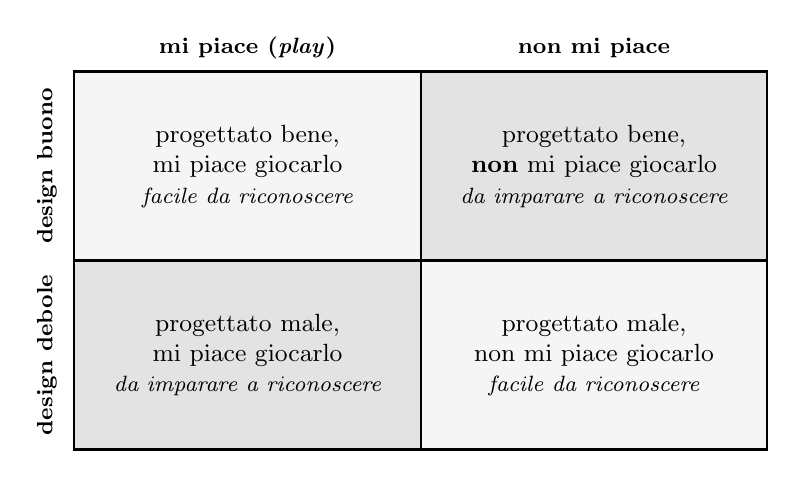
\begin{tikzpicture}[
    font=\small,
    cella/.style={draw, thick, minimum width=4.4cm, minimum height=2.4cm,
                  align=center, text width=4.0cm},
  ]
  \node[cella, fill=gray!8]  (a) at (0,0)    {progettato bene,\\ mi piace giocarlo\\
    \footnotesize\itshape facile da riconoscere};
  \node[cella, fill=gray!22] (b) at (4.4,0)  {progettato bene,\\ \textbf{non} mi
    piace giocarlo\\ \footnotesize\itshape da imparare a riconoscere};
  \node[cella, fill=gray!22] (c) at (0,-2.4) {progettato male,\\ mi piace
    giocarlo\\ \footnotesize\itshape da imparare a riconoscere};
  \node[cella, fill=gray!8]  (d) at (4.4,-2.4) {progettato male,\\ non mi piace
    giocarlo\\ \footnotesize\itshape facile da riconoscere};
  \node[font=\footnotesize\bfseries] at (0,1.5) {mi piace (\emph{play})};
  \node[font=\footnotesize\bfseries] at (4.4,1.5) {non mi piace};
  \node[font=\footnotesize\bfseries, rotate=90] at (-2.55,0) {design buono};
  \node[font=\footnotesize\bfseries, rotate=90] at (-2.55,-2.4) {design debole};
\end{tikzpicture}
\caption{Separare il gioco dal giocare: i due casi ``bizzarri'' in grigio scuro
sono quelli che insegnano di più, sia su sé stessi come giocatori sia sul game
design.}
\label{a3:fig:gameplay}
\end{figure}

\subsection{Il DPE}

\slidefig{img/AGD/agd3-dpe}{Il framework DPE (Design, Play, Experience).}{slide \emph{Analog -- Framework}}{fig:agd3-dpe}


L'MDA è stato poi \textbf{iterato} nel \textbf{DPE}, \emph{Design, Play,
Experience}, il cui paper è citato in cima alla slide\footnote{È il paper di
Brian Winn, \emph{The Design, Play, and Experience Framework}, pubblicato alla fine degli anni Duemila nello \emph{Handbook of Research on Effective Electronic Gaming in
Education}. La trascrizione riporta il titolo come ``Design Play Experience di
PA Framework by Win''.}. Nasce da un approccio \textbf{educativo e formativo}:
è un'iterazione che punta a parlare dei giochi nell'uso didattico. Ma, secondo
il docente, nel farlo riesce a semplificare e a ``distillare'' il cuore
interessante dell'MDA, con tre nomi ``più accurati'':
\begin{description}
  \item[Design] la parte in cui chi progetta crea le meccaniche;
  \item[Play] chi gioca, che applica e ``esperisce'' le dinamiche;
  \item[Experience] che cosa rimane, a livello esperienziale, a chi ha giocato.
\end{description}

Il DPE dispone queste tre parti su diversi \textbf{livelli} (\emph{layer})
tematici. Nel livello del \emph{gameplay}, il design contiene le meccaniche, il
play le dinamiche, l'experience la parte affettiva ed esperienziale. Nel livello
dell'\textbf{apprendimento}, se si parla di gioco formativo, il design contiene
il \textbf{contenuto pedagogico} (che cosa il gioco deve affrontare e far
passare), il play il momento in cui quel contenuto viene insegnato, e
l'experience, se il gioco è andato bene, è il fatto che le persone
\textbf{imparano} quello che il gioco voleva far loro imparare.

È un paper ``un po' più tecnico'' dell'MDA, tagliato sull'ambito formativo, ma
``non così complesso da risultare ostico'' a chi si avvicina al tema: il docente
lo consiglia molto. Con una precisazione che vale per tutto: ``leggerlo non vuol
dire prendere tutto per vero''. Su MDA e DPE si è dibattuto moltissimo: ``non
prendete per vero niente, nemmeno quello che vi sto dicendo io''. I due paper
sono abbastanza noti, soprattutto l'MDA; il DPE spesso è un po' ignorato da chi
lavora nel videogioco perché legato all'ambito didattico, ma secondo il docente
resta molto interessante, ``oltre che una semplificazione e un'iterazione
dell'MDA in maniera più digeribile''.

Una studentessa chiede di rivedere il titolo del paper. Le slide, come al solito,
saranno nel Drive dopo la lezione: ``non correte a segnarvi su un post-it il
paper''. ``Non vogliamo nascondervi le fonti''; e per qualsiasi dubbio si può
scrivere una mail al docente. Tiziana segnala che sono entrati altri
partecipanti: in quel momento ci sono \textbf{Lorenzo}, \textbf{Giordano},
\textbf{Nicola}, \textbf{Tancredi} e \textbf{Tiziana}.

\paragraph{Approfondimento: i livelli del DPE.} Nel paper di Winn i livelli
sono più di due. Oltre al \emph{gameplay} e all'apprendimento
(\emph{learning}), il framework prevede un livello di \emph{storytelling}, uno
di \emph{user experience} e, alla base di tutto, la \emph{technology}, che
abilita ma non determina gli altri. Ogni livello ha la propria terna design,
play, experience: per esempio, nello storytelling il designer scrive la storia
``del designer'', il play produce la storia ``del giocatore'' (quella che
emerge dalle sue scelte), e l'experience è il coinvolgimento che ne deriva. È
un'idea vicina a quanto il docente sta per dire sul coinvolgimento narrativo, e
alla distinzione tra regole ed esperienza da cui la lezione è partita.

% ---------------------------------------------------------------------
\section{Giordano si presenta}
\label{a3:sec:giordano}

``MDA, DPE, e adesso arriviamo alla parte importante''. Il docente annuncia il
primo framework grosso, il \textbf{Player Involvement Model}, con una promessa:
``se faccio il mio lavoro in maniera corretta, alla fine di questa lezione vi
sarà immediatamente chiaro perché non dovete usare \emph{immersione} come termine
nel corso. E se ho fatto il mio lavoro ancora meglio, non lo userete mai più
nella vita. Ma questo è un obiettivo più ambizioso''.

Arriva \textbf{Gianmarco}, in ritardo: il lunedì ha un impegno di lavoro fino
alle 17:30. ``Non ti preoccupare''. Il docente ne approfitta per una
\textbf{semi-pausa} prima di tuffarsi nel dettaglio, e chiede finalmente a
Giordano di presentarsi (``mi stavo dimenticando'') con le solite domande, che
scrive anche in chat: nome, che cosa fa nella vita, perché vuole fare giochi,
che cosa lo ha portato qui, che esperienza ha già.

\paragraph{La presentazione.} Giordano gioca a \textbf{Magic: The Gathering}
``dall'alba dei tempi''. Dopo il COVID si è spostato di più su \textbf{giochi da
tavolo} e \textbf{giochi di ruolo}, soprattutto negli ultimi due anni, anche per
lavoro: è quasi il suo \textbf{secondo lavoro}. Lavora come
\textbf{facilitatore e dimostratore} per un editore\footnote{La trascrizione dice
``per la Genos'' e, poco dopo, ``Ministro Ghienos'': si tratta con ogni
probabilità dell'editore italiano Ghenos Games.}, e collabora con
un'\textbf{associazione} che fa il giro delle \textbf{biblioteche della Brianza}
organizzando serate di giochi da tavolo e di ruolo, dove gli capita di fare da
master o di aiutare nella promozione dei giochi.

Ha scelto il corso perché è \textbf{focalizzato solo sul gioco analogico}, senza
la parte di videogioco e di programmazione, e quindi più compatibile con un
lavoro a tempo pieno. Lo fa per due ragioni: acquisire una \textbf{competenza di
base}, ``a livello analitico'', per coltivare meglio la sua passione; e riuscire
a fare qualcosa, ``non necessariamente da pubblicare'', da proporre negli eventi
dell'associazione. ``Figata'', commenta il docente, che gli chiede se sarà a
\textbf{Play}\footnote{Con ogni probabilità Play -- Festival del Gioco di
Modena, la principale fiera italiana del gioco da tavolo.} come dimostratore.
Quest'anno no, perché gli erano saltati gli appoggi per dormire. L'anno prima,
invece, era saltato un altro ragazzo, e lui si è ``beccato'' \emph{Rival
Cities}: circa \textbf{24 ore} di dimostrazioni dello stesso gioco in due
giorni. ``Chiaro, chiaro, chiaro''.

% ---------------------------------------------------------------------
\section{Il Player Involvement Model}
\label{a3:sec:pim}

``Ora che Giordano si è presentato'' ci si butta nel primo framework,
``tuffandoci con cautela ma anche con determinazione''. Il \textbf{Player
Involvement Model} è uno dei due framework che il docente chiederà di
\textbf{sapere}: ``non nel senso che vi interrogo'', ma nel senso che, dal suo
punto di vista (``non ho la verità in tasca, tutto quello che dico è il mio punto
di vista''), è uno strumento \textbf{pragmatico} e utile in due direzioni:
\begin{itemize}
  \item per capire che cosa fa un gioco \textbf{già pubblicato};
  \item per mettere le basi del \textbf{proprio} gioco.
\end{itemize}

\subsection{Il libro di Calleja}

Il framework viene da un libro di \textbf{Gordon Calleja}, \emph{In-Game: From
Immersion to Incorporation}, pubblicato dalla MIT Press\footnote{La
trascrizione dice ``Gordon Callea'', ``Kaleia'' e ``Calleia'', e chiama
l'editore ``Meatpress''. Il libro è del 2011; Calleja è un game designer e
studioso maltese. Il docente lo chiama sia \emph{Player Involvement Model} sia
\emph{Player Involvement Framework}.}. Secondo il docente se ne trova il PDF
gratuito; chi non lo trova può scrivergli e glielo manda. Ma non sarà richiesto
leggerlo: ``se ho fatto le mie slide correttamente'', è già condensato lì tutto
quello che serve.

La tesi di partenza: per Calleja \textbf{``immersione'' è una parola che ormai
non vuol dire niente}, ``per mille ragioni che non sto qua a dirvi''. Da
designer è più utile chiedersi \textbf{che cosa intende la gente} quando parla di
immersione: capendolo, diventa più facile progettarla. ``Immersione'' resta una
parola vietata: la si usa in queste slide, per contesto, ``ma poi non la voglio
più sentire nominare''.

\subsection{Che cos'è un gioco immersivo?}

``Se io vi dico: voglio un gioco più immersivo, che cosa vuol dire?'' Le
risposte degli studenti:
\begin{itemize}
  \item un'esperienza \textbf{più coinvolgente}, che non permette ai giocatori di
        distrarsi;
  \item un gioco che dà la sensazione di vivere un'esperienza \textbf{il più
        vicina possibile alla realtà}; il docente nota subito che è soggettivo,
        perché dipende da persona a persona;
  \item \textbf{Lorenzo}, appena entrato (il docente gli riassume dove si è
        arrivati), propone: un gioco in cui la \textbf{sospensione
        dell'incredulità} funziona bene.
\end{itemize}

\paragraph{Le provocazioni.} Il docente risponde con una serie di domande
``provocatorie''.
\begin{description}
  \item[Gli scacchi sono un gioco immersivo?] ``Dal punto di vista cognitivo,
        sì'', risponde qualcuno. Ma gli scacchi non chiedono sospensione
        dell'incredulità, né di fare un'esperienza simile alla realtà. Uno
        studente osserva che bisogna capire che cosa si intende, perché negli
        scacchi si è concentrati, non ci si immedesima (``oh, sono il cavaliere,
        il pedone'').
  \item[Il \emph{flow}.] Qui il docente introduce un termine che non ha messo
        nelle slide: il \textbf{flow}, o \textbf{flusso}. Non è solo un termine
        di game design ma, più in generale, di psicologia comportamentale: è
        la zona mentale in cui si trova una persona quando fa un'attività
        \textbf{né noiosa né troppo sfidante}, ``tra il \emph{questa cosa mi chiede
        impegno} e il \emph{non sono frustrato da questo impegno}''. In quella zona
        si sta molto bene, si è molto concentrati e coinvolti anche
        emotivamente. Gli scacchi possono mandare in flow, come molti altri
        giochi, e come lo \textbf{sport}; ma lo sport non chiede sospensione
        dell'incredulità.
  \item[Otto ore di \emph{Civilization}.] Una persona che gioca otto ore di fila a
        \emph{Civilization IV} (``qualcuno di voi l'ha fatto, sono sicuro, non
        negatelo''): uno studente confessa quattordici ore consecutive con un
        amico (``vabbè, ma quattordici ore sono dieci minuti nel tempo del
        giocatore''). Per lui rientra nell'immersione: si gioca al punto di
        dimenticarsi di mangiare.
  \item[I tornei di picchiaduro.] Chi gioca un torneo di \emph{Tekken} o di
        \emph{Street Fighter} è immerso?
  \item[\emph{Dance Dance Revolution}.] E chi balla su \emph{Dance Dance
        Revolution}? E chi fa un LARP dentro un castello?
\end{description}
La conclusione: è ``molto difficile'' dare una definizione di immersivo che
racchiuda tutto. ``Immersione'' viene usata come \textbf{parola jolly}, ``una
roba che ti coinvolge tanto''; ma dal punto di vista del game design
\textbf{non dà nessuno strumento}.

\paragraph{Approfondimento: il flow nei libri.} Il concetto che il docente
richiama viene dallo psicologo Mihaly Csikszentmihalyi, e Schell gli dedica una
lente (la \emph{Lens of Flow}). In \emph{The Art of Game Design} il flow è
definito come ``una sensazione di concentrazione completa ed energica in
un'attività, con un alto livello di piacere e di appagamento'', e Schell ne
elenca le condizioni: \textbf{obiettivi chiari}, \textbf{nessuna distrazione},
\textbf{feedback diretto} e una \textbf{sfida continua}, che resti nello
stretto margine tra la noia (troppo facile) e la frustrazione (troppo
difficile), il cosiddetto \emph{flow channel}. L'esempio classico, ripreso da
Csikszentmihalyi, è proprio uno sport: un ragazzo che impara il tennis è in
flow finché la difficoltà è adeguata alle sue capacità, si annoia quando
migliora senza che la sfida cresca, e si agita quando incontra un avversario
troppo forte. Anche \emph{21st Century Game Design} dedica una sezione
all'esperienza del flow, per capire come diversi tipi di giocatori la
raggiungano in modi diversi. Il fatto che il flow si ottenga con gli scacchi, il
tennis o un torneo di \emph{Tekken}, senza alcuna finzione da ``credere'', è
proprio l'argomento del docente: sotto la parola ``immersione'' convivono almeno
due fenomeni diversi, l'assorbimento nell'attività e la sospensione
dell'incredulità.

\subsection{Sei forme di coinvolgimento}

Calleja propone di ``buttare fuori'' dal termine immersione qualcosa di
\textbf{pragmatico e funzionale}: un \textbf{modello del coinvolgimento di chi
gioca}. Nello specifico crea \textbf{sei categorie}, che \textbf{non sono
mutualmente esclusive}: in ogni gioco alcune sono più alte e altre più basse, ma
la presenza di una non esclude le altre
(figura~\ref{a3:fig:pim} e tabella~\ref{a3:tab:pim}):
\begin{enumerate}
  \item il coinvolgimento \textbf{cinestetico};
  \item il coinvolgimento \textbf{spaziale};
  \item il coinvolgimento \textbf{condiviso};
  \item il coinvolgimento \textbf{narrativo};
  \item il coinvolgimento \textbf{affettivo};
  \item il coinvolgimento \textbf{ludico}.
\end{enumerate}
Gli esempi saranno \textbf{volutamente cross mediali}, con anche dei videogiochi,
``per farvi vedere fin dove si può arrivare con questi coinvolgimenti'' e per
far capire che è una cosa trasversale a tutto il game design: ``non è che se
parliamo di giochi da tavolo, allora alcune di queste cose non ci interessano''.

\begin{figure}[htbp]
\centering
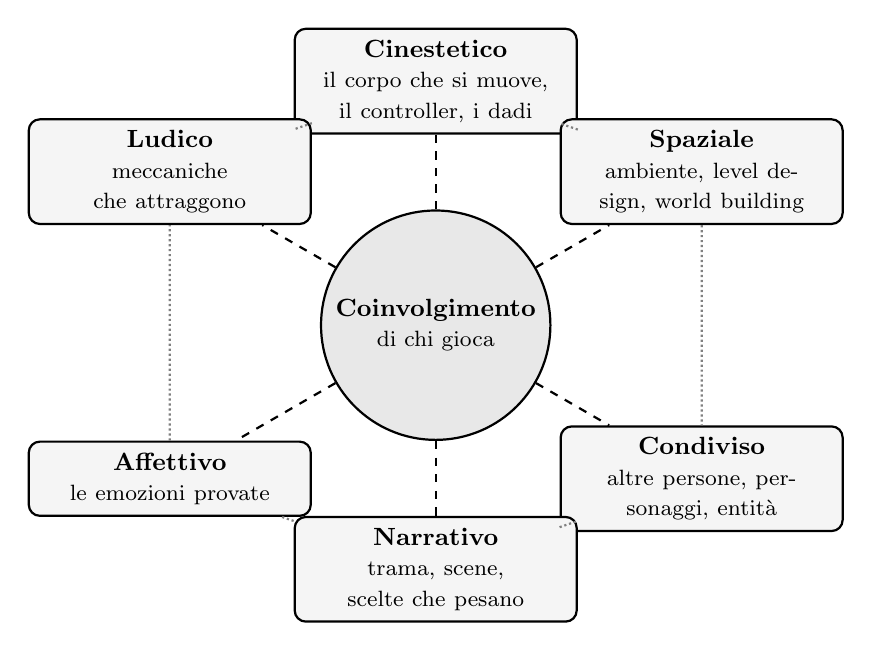
\begin{tikzpicture}[
    font=\small,
    centro/.style={draw, thick, circle, fill=gray!18, minimum size=2.5cm,
                   align=center},
    dim/.style={draw, thick, rounded corners=4pt, fill=gray!8,
                text width=3.3cm, align=center, inner sep=4pt}
  ]
  \node[centro] (c) at (0,0) {\textbf{Coinvolgimento}\\ \footnotesize di chi
    gioca};
  \node[dim] (k) at (90:3.1)  {\textbf{Cinestetico}\\ \footnotesize il corpo che
    si muove, il controller, i dadi};
  \node[dim] (s) at (30:3.9)  {\textbf{Spaziale}\\ \footnotesize ambiente,
    level design, world building};
  \node[dim] (sh) at (-30:3.9) {\textbf{Condiviso}\\ \footnotesize altre
    persone, personaggi, entità};
  \node[dim] (n) at (-90:3.1) {\textbf{Narrativo}\\ \footnotesize trama, scene,
    scelte che pesano};
  \node[dim] (a) at (210:3.9) {\textbf{Affettivo}\\ \footnotesize le emozioni
    provate};
  \node[dim] (l) at (150:3.9) {\textbf{Ludico}\\ \footnotesize meccaniche che
    attraggono};
  \foreach \x in {k,s,sh,n,a,l} \draw[thick, dashed] (c) -- (\x);
  \draw[gray, thick, densely dotted] (k) -- (s) -- (sh) -- (n) -- (a) -- (l) -- (k);
\end{tikzpicture}
\caption{Le sei dimensioni del Player Involvement Model di Calleja come le
presenta il docente. Le linee punteggiate ricordano che le aree ``si parlano'':
non sono stanze stagne, e una stessa scelta di design ne tocca spesso più
d'una.}
\label{a3:fig:pim}
\end{figure}

\subsection{Il coinvolgimento cinestetico}
\label{a3:sec:cinestetico}

\slidefig{img/AGD/agd3-cinestetico}{Il coinvolgimento cinestetico.}{slide \emph{Analog -- Framework}}{fig:agd3-cinestetico}


È il coinvolgimento che si ha quando un gioco \textbf{coinvolge il corpo} e ci si
\textbf{muove}. \emph{Dance Dance Revolution}, giocare con la Wii, fare sport,
entrare nella realtà virtuale: tutto coinvolgimento cinestetico. Lo è anche un
\textbf{boffer LARP}, quando bisogna combattere con spade imbottite e schivare i
colpi. Ma anche cose molto più piccole:
\begin{itemize}
  \item \textbf{usare un controller} è cinestetico;
  \item \textbf{tirare i dadi} è cinestetico;
  \item \textbf{pescare carte} è cinestetico: ``se vi piace pescare carte, un
        gioco che vi fa pescare carte a manetta andrà a titillare il vostro
        senso di apprezzamento dell'esperienza'';
  \item prendere una pedina e muoverla è cinestetico, anche a
        \emph{Monopoly}.
\end{itemize}
Nel gioco da tavolo c'è un intero genere che si basa su questo coinvolgimento:
i \textbf{giochi di destrezza} (\emph{dexterity}), dalle schicchere ai giochi in
cui bisogna impilare cose. Il \textbf{Jenga}\footnote{La trascrizione dice
``Genga'' e ``Gengar''.} ha un coinvolgimento cinestetico? Sì.

\paragraph{Cursori, non interruttori.} Da qui un'avvertenza che vale per tutte
le categorie: \textbf{non sono booleane}, ``non è che o c'è o non c'è''. Vanno
immaginate come \textbf{cursori} (\emph{slider}): ce ne può essere pochissimo,
poco, abbastanza, tantissimo. Il Jenga ha un coinvolgimento cinestetico molto
alto; il tennis più alto ancora; ma non per questo il Jenga ``non è
coinvolgente'' cinesteticamente rispetto al tennis.

\subsection{Il coinvolgimento spaziale}

\slidefig{img/AGD/agd3-spaziale}{Il coinvolgimento spaziale.}{slide \emph{Analog -- Framework}}{fig:agd3-spaziale}


È il coinvolgimento che riguarda \textbf{l'ambiente}: il \textbf{level design}, il
\textbf{world building} del gioco.
\begin{itemize}
  \item Un LARP fantasy o medievale in un \textbf{castello}: la slide mostra un
        castello polacco ``famoso perché ci hanno fatto centinaia di LARP''
        \footnote{Con ogni probabilità il castello di Czocha, in Polonia, noto
        per i LARP della serie \emph{College of Wizardry}; la trascrizione dice
        ``un castello bassa famoso''.}. ``Non sono nel mio salotto di casa, sono
        in un castello''.
  \item Il caso studio di \emph{Monitor Celestra}, visto la volta precedente:
        un LARP di fantascienza dentro un incrociatore, con i neon e le pareti
        metalliche. ``Un certo effetto te lo fa''.
  \item I \textbf{videogiochi di guida}: se ci si pensa, sono tutti basati sul
        \textbf{tracciato}, e il tracciato è una strada, cioè spazio che si
        attraversa. ``Il design di quello spazio è il 90\% di questi giochi'':
        curve strette o larghe, rettilinei. E si può estendere all'atmosfera,
        al clima: piove, c'è nebbia, c'è il sole, è notte, ci sono i neon.
  \item Un \textbf{dungeon crawler} in un gioco di ruolo cartaceo: la mappa del
        dungeon, anche se i giocatori non la vedono perché è dietro lo schermo
        del master, è coinvolgimento spaziale; e lo è quando il master
        \textbf{descrive} un ambiente, che cosa si sente, i suoni, gli odori, i
        rumori. ``Non è che se non vediamo lo spazio non c'è: ce lo stiamo
        immaginando, e quell'immaginarcelo ci coinvolge spazialmente''.
  \item Gli \textbf{open world}, nei videogiochi ma anche nei giochi da tavolo:
        generi che si basano su un mondo aperto ed esplorabile, in cui
        \textbf{lo spazio non è una limitazione ma un punto di \emph{agency}}.
        Lo spazio dice: puoi andare dove vuoi, puoi fare quello che vuoi.
\end{itemize}

\subsection{Il coinvolgimento condiviso}

\slidefig{img/AGD/agd3-condiviso}{Il coinvolgimento condiviso.}{slide \emph{Analog -- Framework}}{fig:agd3-condiviso}


È il coinvolgimento che si ottiene quando si \textbf{condivide l'esperienza con
altre entità}.
\begin{itemize}
  \item Di solito sono \textbf{amici}: un gioco online, come \emph{World of
        Warcraft} ``all'epoca'', giocato con persone amiche. Si è coinvolti in
        un gioco che da soli magari non si giocherebbe, o che non prenderebbe
        così tanto; e invece ``ogni martedì sera ci si trova a giocare''.
  \item Ma si estende anche ai \textbf{personaggi digitali}: un personaggio che
        mi sta subito simpatico (``non so chi sia, ma\ldots''); oppure esce
        l'ennesimo titolo di una serie con lo \textbf{stesso protagonista}, e
        ``io sono già coinvolto prima ancora di accendere il gioco''.
  \item Il \textbf{gioco di ruolo da tavolo} punta tantissimo sul coinvolgimento
        condiviso: è spesso un'esperienza sociale.
\end{itemize}
Va tenuto in considerazione soprattutto nei giochi \textbf{multiplayer}, perché lì
il coinvolgimento condiviso ``ce lo mette in mezzo'' comunque: \textbf{se non lo
progettate voi, lo progettano le persone al posto vostro}. E non è sempre
un'idea fantastica, perché vuol dire che parte dell'esperienza è fuori dal
controllo del designer.

\subsection{Il coinvolgimento narrativo}

\slidefig{img/AGD/agd3-narrativo}{Il coinvolgimento narrativo.}{slide \emph{Analog -- Framework}}{fig:agd3-narrativo}


È il coinvolgimento che arriva dall'\textbf{esplorazione narrativa}: trame, plot,
twist, sviluppo di quello che succede in scena, scene, momenti, dialoghi. È
quello che fa dire: \textbf{voglio sapere come finisce questa storia}.
\begin{itemize}
  \item Un gioco investigativo \textbf{in tribunale}\footnote{La trascrizione
        dice ``E Saturday''. Dalla descrizione (un avvocato in tribunale che
        deve scagionare il proprio cliente, sei capitoli principali) si tratta
        con ogni probabilità della serie \emph{Ace Attorney}.}, in cui si è un
        avvocato che deve capire che cosa è successo e scagionare il proprio
        cliente: ``ne hanno fatti sei'', ed è un successo gigantesco proprio
        perché il coinvolgimento narrativo è fortissimo. I casi sono intriganti
        e si vuole sapere la verità dietro il mistero.
  \item I giochi di Telltale\footnote{La trascrizione dice ``Dreadnought
        Helltail'': con ogni probabilità Telltale Games, lo studio noto per le
        avventure narrative a scelte ramificate.}, ``di fatto l'equivalente di
        libri game in formato digitale'': scelte ramificate, A o B, che
        impattano sul mondo di gioco e possono cambiare drasticamente la
        narrazione. La \emph{agency} ha un peso narrativo: non ``mi vesto di
        blu, mi vesto di rosso'', ma ``muore Tizio o muore Caio''.
  \item Il \textbf{gioco di ruolo}: spesso non si gioca solo per entrare nel
        dungeon, uccidere mostri, prendere il tesoro e uscire (``alcune persone
        giocano anche per quello''): gran parte del suo fascino è
        l'\textbf{agency emergente}, la possibilità di impattare la storia con
        le proprie scelte.
  \item \emph{Non cedere al sonno}\footnote{È l'edizione italiana di \emph{Don't
        Rest Your Head} di Fred Hicks, già citato nella lezione sui casi
        studio; la trascrizione dice ``Non ci Dare al Sonno''.}: la slide mostra
        un pezzo della scheda personaggio. Alla creazione non si chiedono
        numeri, non statistiche come destrezza, forza, intelligenza: si chiede
        \textbf{che cosa ti tiene sveglio}, che cosa ti è successo, come gli
        altri ti percepiscono \textbf{in superficie} e come sei
        \textbf{dentro}. Si può giocare tantissimo su questa collisione
        narrativa. È chiaramente un gioco che, \textbf{già da design}, fa creare
        personaggi sfumati.
\end{itemize}

\subsection{Il coinvolgimento affettivo}

\slidefig{img/AGD/agd3-affettivo}{Il coinvolgimento affettivo.}{slide \emph{Analog -- Framework}}{fig:agd3-affettivo}


``Questo ve lo dico per esperienza: molte persone lo confondono e lo
sovrappongono con il narrativo, ma non è così''. Il coinvolgimento
\textbf{affettivo} riguarda \textbf{le emozioni provate}. Spesso le emozioni le
danno le storie, ``perché siamo esseri umani'', e quindi un gioco che coinvolge
affettivamente spesso coinvolge anche narrativamente. Ma non necessariamente:
\textbf{anche gli scacchi possono coinvolgere affettivamente}, ``e non è che lo
storytelling, il world building degli scacchi sia proprio questo capolavoro''.
\begin{itemize}
  \item Ci rientrano molti \textbf{giochi focalizzati}, giochi su tematiche
        delicate, giochi che puntano a provocare specifiche emozioni molto
        forti, ``giochi in cui si piange a manetta''.
  \item Ma il coinvolgimento affettivo può anche essere \textbf{positivo}: un
        gioco che fa ridere tantissimo, come un \textbf{party game}.
  \item I giochi \textbf{Jeepform} visti come casi studio (\emph{Fat Man Down}, il
        gioco della coppia perfetta\footnote{La trascrizione lo chiama ``Lady
        E8'' e ``le IDE8''; nella lezione precedente era trascritto ``Lady 8''.
        Il titolo resta non verificabile.}): narrativamente non hanno quasi
        niente, ``è una riga la premessa del gioco''. Non si giocano per il
        coinvolgimento narrativo: si giocano perché hanno un coinvolgimento
        affettivo ``grosso come un tir che ti viene in faccia''.
\end{itemize}

\paragraph{\emph{Involved}, non \emph{immersed}.} In chat \textbf{Lorenzo} chiede
se allora ``immersione'' vada intesa più come \emph{to be involved} che come
\emph{to be immersed}. Il docente precisa: qui si sta parlando di un framework
specifico, quello di Calleja, e la \textbf{policy del corso} è adottare questo
framework per parlare di ciò che di solito si chiama immersione. Immersione resta
una parola vietata perché \textbf{non dà strumenti}: se qualcuno chiede ``un
gioco più immersivo'', non vuol dire niente; se chiede ``un gioco con più
coinvolgimento affettivo'' o ``più coinvolgimento narrativo'', si hanno già delle
\textbf{aree operative}, si sa dove andare a lavorare.

E le aree servono a progettare proprio perché non si escludono: un gioco può
avere tanto coinvolgimento su più fronti, e magari nessuno su altri che non
interessano. Il docente mette a confronto due estremi
(figura~\ref{a3:fig:pim-profili}):
\begin{itemize}
  \item a un \textbf{Jeepform} del coinvolgimento spaziale ``non gliene frega
        niente'': lo si gioca vestiti come si è, nel salotto di casa;
  \item un \textbf{LARP \emph{blockbuster}} di due giorni in un castello punta
        invece tantissimo sul coinvolgimento spaziale.
\end{itemize}
``Non c'è giusto o sbagliato'': il framework \textbf{non è qualitativo}. Non
dice che se c'è tanto di tutto il gioco è bello per forza, e se c'è poco di tutto
è brutto per forza. Serve a dire \textbf{che cosa interessa e che cosa serve} al
proprio gioco.

\subsection{Il coinvolgimento ludico}

\slidefig{img/AGD/agd3-ludico}{Il coinvolgimento ludico.}{slide \emph{Analog -- Framework}}{fig:agd3-ludico}


L'ultimo tipo è il coinvolgimento \textbf{ludico}: quello dato da
\textbf{meccaniche che piacciono}, che attraggono, che ``a vederle vi fanno dire:
questo gioco devo provarlo''.
\begin{itemize}
  \item Piace tirare i dadi? In un nuovo gioco si tirano un sacco di dadi: ``già
        magari ci prende bene''. Ma per chi odia tirare i dadi, vedere dei dadi
        in un gioco funziona già da \textbf{anti-coinvolgimento}.
  \item Il docente ama gli \textbf{economici azionari ferroviari}: ne vede uno
        nuovo e ``sono già intrigato, voglio già provarlo''. Altri amano i giochi
        di ruolo, le escape room.
  \item Piace costruire un \textbf{mazzo personalizzato} come in \emph{Magic: The
        Gathering}, \emph{Yu-Gi-Oh!}, \emph{Pokémon}? È un tipo di
        coinvolgimento che si può progettare, pensando a \textbf{per chi} è il
        gioco.
  \item Il \textbf{piazzamento lavoratori} (\emph{worker placement}), genere che
        ``va molto in Germania, in Europa'': il docente conosce almeno tre
        persone a cui ``si illuminano gli occhi'' quando gli si propone un
        piazzamento lavoratori, e altre che invece ``se ne vanno''.
\end{itemize}
Il coinvolgimento è soggettivo: \textbf{non esiste un passe-partout che coinvolga
tutte le persone}. Le aree servono a capire che cosa serve al proprio gioco, che
cosa metterci, dove andare a lavorare.

\paragraph{Le scelte di design toccano più aree.} Uno studente trova interessante
la distinzione, perché pensava che il ludico rientrasse nell'affettivo. Il
docente aggiunge una cosa importante: \textbf{molte scelte di design coprono più
aree}. Un \textbf{boffer LARP} dark fantasy con le armi di gommapiuma e un
sistema di combattimento è coinvolgimento cinestetico, perché porta a combattere
fisicamente; ma il boffer è anche una categoria meccanica, e chi apprezza le
meccaniche boffer andrà a giocare boffer: quindi è anche coinvolgimento
\textbf{ludico}. ``Queste non sono sei aree murate con dei muri di acciaio che
separano in maniera stagna le aree del game design'': si ibridano, si mischiano,
e una meccanica che si aggiunge può impattarne molte.

\begin{table}[htbp]
\centering
\small
\begin{tabular}{@{}p{2.6cm}p{4.4cm}p{6.1cm}@{}}
\toprule
\textbf{Coinvolgimento} & \textbf{Che cosa coinvolge} & \textbf{Esempi citati a
lezione} \\
\midrule
Cinestetico & il corpo, il movimento, la manipolazione & \emph{Dance Dance
Revolution}, Wii, VR, sport, boffer LARP; controller, dadi, pescare carte,
muovere pedine; giochi di destrezza, Jenga \\
Spaziale & ambiente, level design, world building, atmosfera & LARP nel castello,
\emph{Monitor Celestra}, tracciati dei giochi di guida, il dungeon descritto dal
master, open world \\
Condiviso & altre persone o entità con cui si condivide l'esperienza & amici
online (\emph{World of Warcraft}), personaggi ricorrenti di una serie, il GDR da
tavolo come esperienza sociale \\
Narrativo & trama, plot, twist, scene, scelte che cambiano la storia & la serie
in tribunale (\emph{Ace Attorney}), i giochi Telltale, l'agency emergente del
GDR, la scheda di \emph{Non cedere al sonno} \\
Affettivo & le emozioni provate, anche positive & giochi focalizzati, party
game, Jeepform (\emph{Fat Man Down}, la coppia perfetta), persino gli scacchi \\
Ludico & meccaniche che attraggono (o respingono) & tirare dadi, economici
ferroviari, deck building, piazzamento lavoratori, boffer, tornei \\
\bottomrule
\end{tabular}
\caption{Le sei forme di coinvolgimento del Player Involvement Model, con gli
esempi della lezione.}
\label{a3:tab:pim}
\end{table}

\begin{figure}[htbp]
\centering
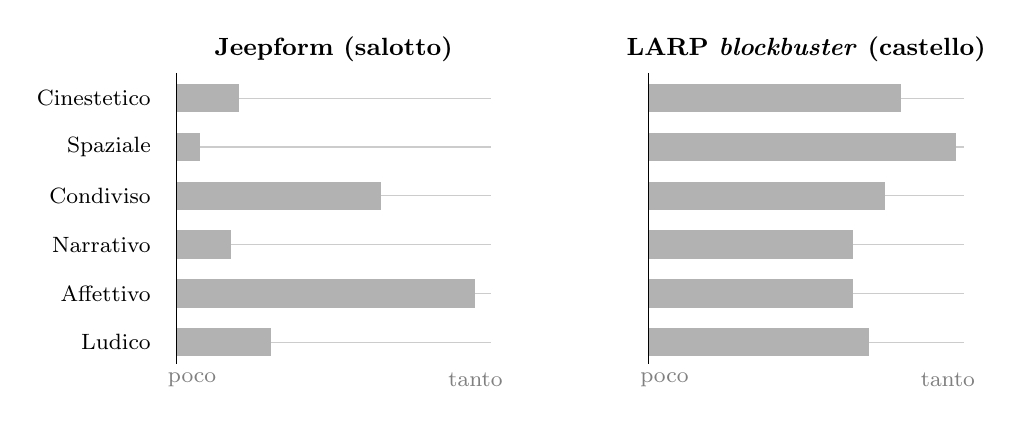
\begin{tikzpicture}[
    font=\footnotesize,
    x=1cm, y=1cm
  ]
  % assi e etichette
  \foreach \nome [count=\i] in {Cinestetico,Spaziale,Condiviso,Narrativo,
      Affettivo,Ludico} {
    \node[anchor=east] at (-0.2,-\i*0.62) {\nome};
    \draw[gray!40] (0,-\i*0.62) -- (4,-\i*0.62);
    \draw[gray!40] (6,-\i*0.62) -- (10,-\i*0.62);
  }
  \node[font=\small\bfseries] at (2,0) {Jeepform (salotto)};
  \node[font=\small\bfseries] at (8,0) {LARP \emph{blockbuster} (castello)};
  % Jeepform
  \foreach \v [count=\i] in {0.8,0.3,2.6,0.7,3.8,1.2} {
    \fill[gray!60] (0,-\i*0.62-0.18) rectangle (\v,-\i*0.62+0.18);
  }
  % blockbuster
  \foreach \v [count=\i] in {3.2,3.9,3.0,2.6,2.6,2.8} {
    \fill[gray!60] (6,-\i*0.62-0.18) rectangle (6+\v,-\i*0.62+0.18);
  }
  \draw[thin] (0,-0.3) -- (0,-4.0);
  \draw[thin] (6,-0.3) -- (6,-4.0);
  \node[gray] at (0.2,-4.2) {poco};
  \node[gray] at (3.8,-4.2) {tanto};
  \node[gray] at (6.2,-4.2) {poco};
  \node[gray] at (9.8,-4.2) {tanto};
\end{tikzpicture}
\caption{Due profili di coinvolgimento, a titolo puramente illustrativo. Il
docente cita solo il contrasto sullo spaziale (nullo nel Jeepform, altissimo
nel LARP in castello) e l'affettivo ``grosso come un tir'' del Jeepform; gli
altri valori sono ipotesi plausibili, utili a ricordare che il modello descrive
un profilo, non un punteggio.}
\label{a3:fig:pim-profili}
\end{figure}

% ---------------------------------------------------------------------
\section{Le domande sul coinvolgimento}
\label{a3:sec:pim-domande}

\paragraph{E la competizione?} Una domanda: un coinvolgimento legato alla
\textbf{competizione} rientra nel modello? Il docente rilancia: che cos'è che
attrae della competizione? Se è il senso, ``più lato sportivo'', di
\textbf{superare un altro essere umano}, o un'altra squadra di esseri umani,
allora si è nel coinvolgimento \textbf{condiviso}: sapere che dall'altra parte
c'è un altro essere umano da battere. Ma la competizione può anche essere
\textbf{meccanica}: molte persone vanno a un \textbf{torneo} con un approccio da
\emph{min-maxer}, perché quel gioco ``meccanicamente mi attrae'', e allora è
coinvolgimento \textbf{ludico}. Le due cose non sono sbagliate: si torna sempre a
\textbf{per chi è il gioco}. Un gioco può essere competitivo senza essere da
torneo, senza essere per chi fa min-maxing, senza essere per chi vuole muoversi
fisicamente. ``Non esiste una combinazione giusta di queste aree'': sono uno
strumento ``sulla carta'' per dire su che cosa il gioco spinge e su che cosa non
spinge, o non interessa.

\paragraph{Non fate \emph{Magic} 2.0.} Anche perché, ``purtroppo'', spingere su
tutto costa tantissimo in termini di budget, risorse, tempo, playtest. Il docente
ribadisce: \textbf{non fate giochi giganteschi in questo corso}, ``lo dico per
voi, perché se no poi non li portate a compimento''. ``Non fate \emph{Magic: The
Gathering} 2.0''. Si può fare un gioco di carte, ce ne sono tantissimi anche
compatti. \emph{Magic} è stato citato da più persone, anche nelle presentazioni
(``Giordano, tu sicuramente''); ma esistono giochi di carte compatti, creati
anche da persone che hanno lavorato a \emph{Magic}, come
\emph{Compile}\footnote{La trascrizione cita ``Redlands o Compile''. Il primo
titolo non è ricostruibile con certezza; il docente li presenta come giochi di
carte competitivi, compatti, con pochissime carte in una scatola piccola.}, che
hanno le stesse dinamiche interpersonali di competizione di \emph{Magic} con un
numero di carte ridottissimo, in una scatola molto compatta: ``più nell'ottica di
cose che potete fare all'interno di questo corso''.

\paragraph{Il \emph{checkpoint} prima della pausa.} Prima della pausa il docente
si ferma: ``da quando facciamo la pausa, io darò per scontato che voi avete capito
questo framework''. ``Non esistono domande stupide'', e una domanda che sembra
stupida può essere importantissima anche per gli altri. Rimette la slide con le
tipologie di coinvolgimento e scrive in chat il nome del libro di Calleja (il
nome, non il link, visto il problema dei link).

\paragraph{Perché il coinvolgimento al centro?} Una studentessa chiede: se il
coinvolgimento è ovviamente qualcosa da perseguire, perché il modello lo mette al
centro? Qual è il fine ultimo? Il docente risponde che il modello nasce dalla
necessità di \textbf{smettere di usare ``immersione''}; ma l'immersione non
sarebbe una parola così usata e pervasiva se non fosse \textbf{qualcosa che chi
gioca cerca}. Tutti cercano e apprezzano l'immersione, pur avendone definizioni
diverse: ``adesso qui siete in sette, e avete sette definizioni di immersione
diverse'', magari sovrapponibili per alcuni giochi. Ma gli studenti, da qui,
sono \textbf{game designer}, non solo persone che giocano, e serve loro sapere
\textbf{su che cosa stanno lavorando}: avere strumenti pratici per
\textbf{confrontare il proprio lavoro con le intenzioni}. Lo stesso lavoro di
decostruzione si farà più avanti con il \textbf{divertimento}. E il docente
torna alla slide iniziale: \textbf{il gioco è un'esperienza creata da regole};
si possono creare quelle regole, e dentro quelle regole si può lavorare su
questi tipi di coinvolgimento.

\paragraph{La distanza tra esperienza intesa ed esperienza giocata.} Il salto da
un'idea a un regolamento scritto, senza perdere cose per strada, ``è molto
difficile''. È un tema a cui il docente tiene moltissimo: la sua \textbf{tesi di
master} era proprio sul \textbf{gap tra le intenzioni di progettazione} di un
game designer e le persone che interpretano il regolamento per poi vivere
l'esperienza, misurando \textbf{quanta distanza c'è tra esperienza intesa ed
esperienza giocata}. \textbf{Lorenzo} scrive in chat che un designer può
pianificare un prodotto per coinvolgere l'utente su certi aspetti, ma poi è
quest'ultimo a decidere che cosa lo coinvolge davvero. ``È esattamente quello
che vi ho appena detto'': la parte difficile del lavoro, e quella che, se fatta
bene, fa fare passi avanti, è \textbf{distillare in un regolamento non ambiguo}
procedure, meccaniche, ``un ecosistema di regole'' che porti a far giocare
un'esperienza specifica a chi gioca, \textbf{senza che vi conosca e senza che vi
possa chiedere cose}.

È facile se il gioco lo si organizza di persona: lo si spiega, si corregge chi
sbaglia. Ma è un caso rarissimo. Nella maggior parte dei giochi pubblicati, il
designer non lo si incontrerà mai, e a volte non si sa nemmeno chi sia: ``che ne
sapete del suo costruttivismo personale?'' Che cosa c'è nel gioco perché quella
persona ci crede fermamente, ed è parte del suo paradigma, e che cosa c'è
\textbf{per sbaglio}? ``Lo farete anche voi'', non per sfiducia, ma perché è
inevitabile: non si può essere costantemente attenti a tutto, e a volte si
prendono decisioni di design senza pensarci, \textbf{per vestigialità, per
abitudine}. In quel momento si sta riproponendo un paradigma: si torna a
\textbf{fare tradizione}, non design.

\paragraph{Le domande di Tiziana.} Tiziana fa due domande. La prima: il playtest
si fa quando si ha il regolamento? Il docente la ferma subito, ``non perché non
mi interessa la domanda'': ci sarà una lezione apposta, e aprire adesso ``il vaso
di Pandora di come si struttura un playtest'' impedirebbe di arrivare al secondo
framework. Ed è una fase delicatissima: se la progettazione e il prototipo sono
``la vostra mente e il vostro gioco'', il playtest è il momento in cui ``questa
roba va a schiantarsi con persone esterne che non l'hanno mai giocata''.

La seconda: le categorie del modello le sono sembrate molto puntuali. Si era
chiesta perché non ci fosse un ``coinvolgimento sociale'', e si è risposta da
sola: ``sociale'' vuol dire una marea di cose, ``condiviso'' è più preciso.
Esatto, e non solo: \textbf{condiviso} permette di includere entità
\textbf{non necessariamente umane}. Il personaggio a cui si è affezionati in altri
giochi della serie coinvolge non per la meccanica né per la storia: in
\emph{Mario Kart}, ``che non è un gioco con altissima narrazione'', rivedere un
personaggio già incontrato può far dire ``scelgo questo perché mi sta
simpatico''. Di nuovo: le aree non sono mutualmente esclusive, ``si parlano''.

\paragraph{La pausa.} ``Facciamo pausa''. Il docente la fissa fino alle ``e
trenta'', cioè fino alle \textbf{18:30}\footnote{La trascrizione dice ``sono le
21, facciamo pausa fino alle 30'' e subito dopo ``ci si ritrova qui alle 18.30'':
la pausa comincia quindi alle 18:21 circa. Durante la pausa la trascrizione
registra per decine di righe frasi senza senso ripetute in loop.}.

\paragraph{Approfondimento: oltre le sei dimensioni.} La lezione si ferma alle
sei dimensioni, ma il titolo del libro di Calleja indica dove l'autore vuole
arrivare. Nel suo modello ogni dimensione si può osservare su due scale di
tempo: il coinvolgimento \textbf{micro}, momento per momento, mentre si gioca, e
quello \textbf{macro}, che riguarda il rapporto con il gioco nel tempo, anche
quando non si sta giocando (la voglia di tornarci, il pensarci, il parlarne). La
parola \emph{incorporation}, che Calleja propone al posto di
\emph{immersion}, indica il momento in cui le diverse dimensioni del
coinvolgimento si fondono e il giocatore ``assimila'' il mondo di gioco nella
propria coscienza come uno spazio abitabile, con il proprio avatar come punto
di presenza. Il passaggio è lo stesso che il docente chiede agli studenti:
sostituire una metafora vaga (l'immersione, come in una piscina) con una
descrizione delle componenti, su cui si può lavorare una per una.

% ---------------------------------------------------------------------
\section{Il Mixing Desk of Larp}
\label{a3:sec:mixing}

``Rieccoci qua''. Dopo la pausa (Lorenzo conferma di esserci) si parte con il
secondo framework grosso, ``non che quello di prima fosse piccolo''.

\subsection{Da dove viene}

Il framework \textbf{nasce all'interno dei movimenti scandinavi} di gioco di
ruolo, nella scena del \textbf{Nordic LARP}\footnote{Il \emph{Mixing Desk of
Larp} è stato sviluppato nei primi anni Dieci da designer norvegesi legati alla
\emph{Larpwriter Summer School}, e poi più volte rielaborato; la storia è
raccontata nell'articolo di \emph{Analog Game Studies} che il docente consiglia
alla fine della lezione (sezione~\ref{a3:sec:perche-due}).}. Ma per sua natura
è uno strumento \textbf{estremamente flessibile}: è stato applicato anche al
gioco da tavolo e si può applicare ad altre tipologie di giochi. È
\textbf{modulare}: lo si può modificare, aggiungere o togliere pezzi in base a
quello che serve per il proprio gioco, ``perché non tutti i moduli, non tutte le
parti di questo framework vi servono sempre''.

Molti esempi saranno giochi di ruolo dal vivo, ``solo perché è più facile
spiegare'' alcuni cursori così. Il docente chiede di fare ogni volta il
\textbf{parallelismo}: questo pezzo del framework è nato sul gioco di ruolo, ma
come si applica al resto? Per alcuni cursori il salto è facile, per altri più
complesso; ma ``se tutto va bene, e mi è sembrato bene in passato'', alla fine
gli studenti dovrebbero avere un'ottima idea di come funziona e, soprattutto, di
come \textbf{applicarlo in modo pragmatico}.

\subsection{Un doppio uso}

Ancora più del Player Involvement Model, il Mixing Desk ha un \textbf{doppio
utilizzo}:
\begin{description}
  \item[Analisi] si prende un gioco già pubblicato, lo si ``fa passare'' nel
        framework e si guarda che cosa ne esce.
  \item[Progettazione] è ``un framework ottimo per crearvi delle
        \textbf{linee guida}'': voglio un gioco che faccia A, B, C, D, e il
        framework aiuta a capire che cosa sono A, B, C, D e come si vuole che
        arrivino.
\end{description}

\subsection{Il mixer}

\slidefig{img/AGD/agd3-mixer}{The Mixing Desk of Larp: i cursori del mixer.}{slide \emph{Analog -- Framework}}{fig:agd3-mixer}


Il nome è ``abbastanza autoesplicativo'': la slide mostra quello che sembra un
\textbf{banco di mixaggio} luci e audio. L'idea è che ogni gioco possa essere
identificato da una serie di \textbf{cursori} (\emph{slider}, o \emph{fader}),
le levette che si spingono su e giù in un mixer, e che l'insieme dei cursori
usati per progettare o analizzare il gioco ne dia una \textbf{visione
d'insieme}: che cosa fa questo gioco, ``non tanto a livello micro, cioè nelle
singole regole, ma a livello esperienziale, cioè dall'alto''
(figura~\ref{a3:fig:mixer}).

L'ultimo cursore della slide è \textbf{``inserisci qui il tuo fader''}
(\emph{your fader here}): ``modificate questo slider come volete''. Nella sua
storia il Mixing Desk è stato elaborato, modificato e rimaneggiato più volte,
anche da settori paralleli come il gioco di ruolo formativo e il gioco da tavolo.
Il docente mostra ``il primo, quello da cui è nato''; online se ne trovano
``mille versioni''. Il consiglio non è andarle a cercare, ma \textbf{capire che
cosa serve al proprio gioco e creare i propri cursori}.

\begin{figure}[htbp]
\centering
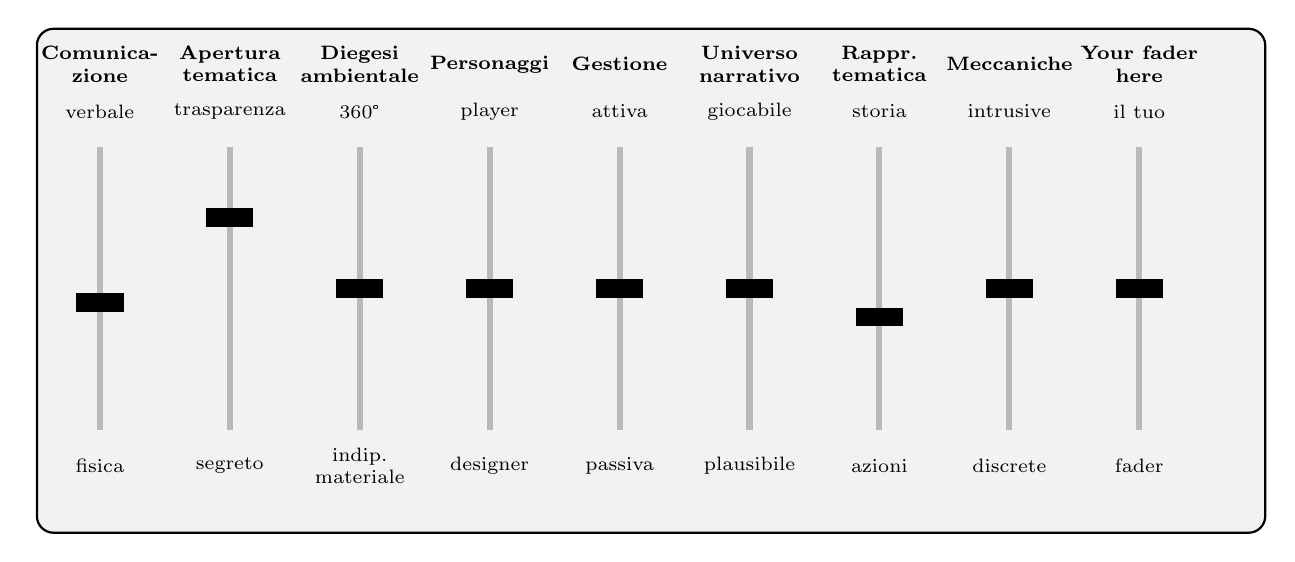
\begin{tikzpicture}[
    font=\scriptsize,
    x=1cm, y=1cm
  ]
  \draw[thick, rounded corners=6pt, fill=gray!10] (-0.6,-0.9) rectangle (15.0,5.5);
  \foreach \alto/\basso/\pos [count=\i] in {
      verbale/fisica/0.55,
      trasparenza/segreto/0.25,
      360°/indip. materiale/0.5,
      player/designer/0.5,
      attiva/passiva/0.5,
      giocabile/plausibile/0.5,
      storia/azioni/0.6,
      intrusive/discrete/0.5,
      {il tuo}/fader/0.5} {
    \pgfmathsetmacro{\x}{(\i-1)*1.65+0.2}
    \draw[line width=2.2pt, gray!55] (\x,0.4) -- (\x,4.0);
    \fill[black] (\x-0.3,{0.4+3.6*(1-\pos)-0.12}) rectangle
                 (\x+0.3,{0.4+3.6*(1-\pos)+0.12});
    \node[align=center, text width=1.55cm] at (\x,4.45) {\alto};
    \node[align=center, text width=1.55cm] at (\x,-0.05) {\basso};
  }
  \foreach \nome [count=\i] in {{Comunica-\\ zione}, {Apertura\\ tematica},
      {Diegesi\\ ambientale}, Personaggi, Gestione, {Universo\\ narrativo},
      {Rappr.\\ tematica}, Meccaniche, {Your fader\\ here}} {
    \pgfmathsetmacro{\x}{(\i-1)*1.65+0.2}
    \node[font=\scriptsize\bfseries, align=center, text width=1.6cm] at
      (\x,5.05) {\nome};
  }
\end{tikzpicture}
\caption{Il Mixing Desk come banco di mixaggio: otto cursori della versione
mostrata a lezione più il cursore libero. Le posizioni sono qui tutte centrali
o quasi, solo per mostrare che ogni cursore può stare a qualsiasi altezza: nessun
estremo è ``meglio'' dell'altro.}
\label{a3:fig:mixer}
\end{figure}

% ---------------------------------------------------------------------
\section{I cursori del Mixing Desk}
\label{a3:sec:cursori}

\slidefig{img/AGD/agd3-cursori}{Gli otto cursori del Mixing Desk of Larp: comunicazione, apertura tematica, diegesi ambientale, creazione dei personaggi, gestione del gioco, universo narrativo, rappresentazione tematica e meccaniche.}{slide \emph{Analog -- Framework}}{fig:agd3-cursori}


\subsection{Comunicazione: verbale o fisica}

Si prende un LARP, un gioco in cui si interpreta fisicamente il proprio
personaggio. \textbf{La comunicazione tra chi gioca è verbale o fisica?} E
``lo ricordo: questo è uno slider, non è un pulsante on, off, uno, zero''. Ci
sono vie di mezzo.
\begin{itemize}
  \item Un \textbf{boffer LARP} è molto fisico: il combattimento è una parte
        importante del gioco, e impugnare un'arma in plastazote, colpire,
        schivare, prendere lo scudo, riattaccare dal fianco è un'interazione
        molto fisica.
  \item Il gioco della coppia perfetta, il Jeepform citato prima, è
        ``estremamente verbale''.
  \item Nei giochi da tavolo, un \textbf{party game} va di solito più sul
        verbale. Negli \textbf{scacchi} si parla pochissimo: l'interazione ludica
        non è di dialogo, è ``io muovo cose'', e muovere cose è un'azione fisica.
\end{itemize}
La domanda da farsi: \textbf{il mio gioco è un gioco in cui si parla o un gioco
in cui si spostano cose?} E le ``cose'' possono essere anche le persone stesse,
come negli sport o nel gioco dal vivo. ``Spostare cose'' riassume il fatto di
interagire fisicamente con qualcosa. Ci si può stare in mezzo: un gioco in cui si
parla e si spostano cose, ma si parla più di quanto si spostino cose, o
viceversa.

\paragraph{I giochi verbali e i loro limiti.} ``Qualcuno ha un esempio di un gioco
da tavolo estremamente verbale?'' Uno studente propone \textbf{Dixit}. È
verbale, ``ma non è così tanto verbale'', perché ha moltissime
\textbf{limitazioni sulla comunicazione}: se in \emph{Dixit} si potesse parlare
liberamente di tutto, il gioco crollerebbe. Lo stesso vale per \emph{Secret
Hitler}, per \emph{Taboo}, per \emph{Codenames} (``nomi in codice''), dove si può
dire una parola e un numero, non di più. Molti giochi deduttivi o induttivi hanno
fortissime limitazioni su che cosa si può e non si può dire.

\paragraph{L'obiezione di Gianmarco.} Gianmarco vede una difficoltà: qui verbale e
fisico sono messi in contrapposizione, ma l'esempio dei giochi verbali con
limitazioni sembra non stare sullo stesso asse. Il docente spiega che sono
messi come \textbf{estremi}, come \textbf{direzioni di game design diverse}:
``immagina che hai cento chili di roba nel tuo game design, e di decidere quanti
chili voglio che siano fisici e quanti verbali'' (``una metafora che non
funziona, ma spero che ci siamo capiti lo stesso''). Una studentessa aggiunge
che \emph{Taboo} non è solo verbale: c'è gestualità, comunicazione non verbale,
``non giochiamo bendati''. E le limitazioni verbali, chiede Gianmarco, si
trasformano in dinamiche fisiche? ``Non necessariamente'', ma spesso si
trasformano in \textbf{altre cose da fare al tavolo}: le carte illustrate di
\emph{Dixit} sono un elemento fisico usato per comunicare in modo non verbale;
la griglia di parole di \emph{Codenames} è un aspetto fisico di interazione,
anche se ha parole scritte sopra. Il Mixing Desk non va guardato come ``lo stato
oggettivo del gioco dall'alto'', ma come una \textbf{bilancia}: se si spinge da
un lato, l'altro tende a scendere.

\paragraph{Gli estremi.} Ci possono essere anche giochi all'estremo totale.
\emph{Stranger}, il LARP della designer danese visto nei casi studio, quello
della nazione blu e della nazione verde, è un gioco in cui \textbf{è vietato
parlare} e fare suoni: è tutto fisico. All'opposto, ci sono giochi con
\emph{roleplay} in cui la componentistica è praticamente inesistente; e anche
\emph{Dungeons \& Dragons}, se si giocano i combattimenti senza griglia, diventa
molto verbale e molto poco fisico. Ma ``non siamo esperimenti in astratto'': è
quasi impossibile eliminare del tutto uno dei due estremi.

\subsection{Apertura tematica: trasparenza o segreto}
\label{a3:sec:apertura}

``Cercherò di spiegarmi al meglio, perché è importante ma apre dei vasi di
Pandora''. Supponiamo che il gioco abbia un \textbf{tema}. Quel tema arriva a chi
gioca \textbf{in modo trasparente}, o è un \textbf{tema segreto} che si scopre
durante o alla fine del gioco?
\begin{description}
  \item[Trasparenza.] \emph{Twilight Struggle}, della GMT: Stati Uniti contro
        URSS, la \textbf{Guerra Fredda}. Due persone, una gioca gli Stati Uniti,
        l'altra l'URSS; non ci si combatte direttamente con i carri armati, ma si
        cerca di vincere ottenendo influenza e supporto di varie nazioni. Il tema
        è trasparente: entrambi i giocatori sanno che cosa stanno giocando.
  \item[Segreto.] Un gioco in cui si trasportano cubetti e risorse in treno da un
        posto all'altro, e vince chi ne trasporta di più. Alla fine si scopre che
        si stavano trasportando \textbf{ebrei nei campi di concentramento}. ``Questo
        è un caso studio esistente'': è \emph{Train} di \textbf{Brenda
        Romero}\footnote{La trascrizione dice ``Trains di Prenderò Mero''.
        \emph{Train} (2009) fa parte della serie di giochi da tavolo \emph{The
        Mechanic is the Message} di Brenda Romero, all'epoca Brathwaite,
        coautrice di \emph{Challenges for Game Designers}.}, ``storicamente
        riconosciuto come gioco dal tema offuscato'' che viene rivelato durante
        il gioco.
\end{description}
Anche qui ci sono vie di mezzo: molti LARP ``vecchia scuola'' hanno \textbf{trame
segrete}, plot nascosti noti solo ad alcuni personaggi, che si rivelano nel
\emph{debriefing} (``sapevate che in realtà Tizio faceva anche questo?'').

\paragraph{La preferenza del docente.} È una cosa soggettiva, e il docente lo
dice come tale: preferisce i giochi \textbf{trasparenti}. Trova ``molto pigro''
affidarsi ai segreti, specialmente quando si tratta di temi delicati. Ma giochi
così esistono, e il cursore esiste.

\paragraph{Si gioca una volta sola?} Tiziana chiede se un gioco così si giochi
una volta e poi rischi lo \emph{spoiler}. ``Non è un problema'': non sono
esperienze meno significative. Come i \textbf{giochi investigativi}, che si
basano proprio su un'apertura tematica segreta. Fare un investigativo in cui si
dice subito chi è l'assassino e come ha ucciso è ``molto difficile'', ma ci sono
le eccezioni. Il docente cita \textbf{il tenente Colombo}, ``che amo
particolarmente'' (``vi prego, ditemi che non sono l'unico''): la serie si apriva
mostrando l'assassino e l'omicidio, e solo dopo arrivava Colombo a indagare. Lo
spettatore sa già tutto; il protagonista no. L'interesse sta nel conflitto tra
chi sa e chi non sa, nel capire come Colombo arriverà a ciò che lo spettatore ha
visto. Allo stesso modo si può avere un investigativo da tavolo in cui si sa già
com'è morta una persona: ``è una bella sfida''.

\paragraph{Un segnalibro.} Quando si parla di \textbf{giochi formativi o
didattici}, questo cursore è per il docente ``particolarmente sensibile e
importante''. E, di nuovo, non tutti i cursori interessano ogni gioco: in un
astratto alla scacchi o dama, ``che ve ne importa dell'apertura tematica?''.

\paragraph{Approfondimento: \emph{Train} e il tema sotto le meccaniche.}
\emph{Train} compare anche in \emph{A Theory of Fun for Game Design} di Raph
Koster, che lo cita come esempio della serie \emph{The Mechanic is the Message}:
un gioco sulla \textbf{complicità} dei giocatori nel compiere azioni terribili,
o nel trovare il modo di sovvertire il sistema. Lo stesso libro propone un
esperimento mentale che illumina il rapporto tra tema e meccaniche: si immagini
un gioco in cui si lasciano cadere vittime innocenti di ogni forma e misura in
una camera a gas a forma di pozzo, dove cercano di arrampicarsi le une sulle
altre; se ci riescono si perde, se le si incastra abbastanza bene quelle in
fondo muoiono. ``Non voglio giocare questo gioco. E voi?'', chiede Koster. Eppure
è \emph{Tetris}. La conclusione di Koster è che \textbf{le meccaniche nude non
determinano il significato} di un gioco: come il cinema non è solo fotografia o
sceneggiatura, il gioco è l'insieme di meccaniche, regia, grafica. \emph{Train}
usa esattamente questa distanza tra meccanica e tema: le stesse azioni,
caricare cubetti su un vagone, cambiano completamente significato nel momento in
cui il tema viene aperto. Il cursore dell'apertura tematica, in questo caso, è
la leva principale dell'esperienza.

\subsection{Diegesi ambientale: 360° o indipendenza materiale}

Quello che c'è attorno a chi gioca, l'ambiente in cui si gioca: il coinvolgimento
spaziale è \textbf{a 360 gradi}, o il gioco ha un'\textbf{indipendenza
materiale}? Nel gioco di ruolo dal vivo:
\begin{itemize}
  \item si gioca un fantasy dentro un castello, a cavallo, ``e abbiamo un vero
        cavallo'' sotto di noi;
  \item oppure si gioca il gioco della coppia perfetta nel bagno di casa, ma
        lo si potrebbe giocare in salotto, o in giardino.
\end{itemize}
Il gioco richiede una \textbf{diegesi il più alta possibile} per essere giocato,
oppure no? E ci sono vie di mezzo: si può giocare nello studio di casa
\textbf{vestiti da cavalieri}, ``why not?''. Molti \textbf{chamber LARP} italiani
degli anni '90 e 2000 funzionavano così, e il docente mostra al volo una slide:
un LARP in costume giocato \textbf{nello scantinato} della casa di qualcuno. Non è
completamente indipendente dal materiale, perché i costumi erano richiesti, ma
``non siamo in un castello, è uno scantinato''.

Vale anche per gli altri giochi: un \textbf{dungeon crawler} da tavolo mostra
l'ambiente nel dettaglio, o ne dà una rappresentazione metaforica, astratta?

\subsection{Creazione dei personaggi: chi gioca o chi progetta}

Ancora pensando al LARP (``sui personaggi abbiamo una lezione apposta'', e
arriverà presto): i personaggi possono essere scritti \textbf{da chi partecipa}
o \textbf{da chi progetta il gioco}, e sono due esperienze chiaramente diverse.
\begin{description}
  \item[Lato player.] Chi gioca crea il proprio personaggio e decide chi
        interpretare. È spesso la formula dei \textbf{giochi molto grossi}, i
        LARP \emph{blockbuster} da 300, 400, 500 persone, o i boffer tedeschi da
        mille persone: i designer non si mettono a scrivere mille personaggi, ma
        chiedono di scriverlo e di mandarlo, a volte, per approvazione. Se non ci
        sono cose particolarmente sbagliate, si gioca chi si vuole.
  \item[Lato designer.] Il personaggio è creato da zero da chi progetta il
        gioco. Il vantaggio: si può mettere \textbf{tematicamente} nel
        personaggio quello che si vuole.
\end{description}
Non è così diverso dai videogiochi di ruolo: ci sono i \emph{Final Fantasy},
soprattutto i più recenti, in cui i designer hanno creato i personaggi e se ne
segue la storia; e ci sono i giochi di ruolo occidentali, i CRPG, con una fase
di \emph{character creation} in mano al giocatore, magari con dei paletti messi
dal designer.

\paragraph{I paletti di \emph{Non cedere al sonno}.} Un esempio di via di mezzo.
In \emph{Non cedere al sonno} si giocano persone \textbf{insonni} che vedono una
città che non esiste, piena di orrore e di incubi. Si può fare il personaggio che
si vuole, ma con due paletti forti, decisi dal designer: il personaggio deve
essere \textbf{insonne}, e deve avere \textbf{un problema che lo tiene sveglio},
cioè una motivazione specifica e consapevole della propria insonnia. Non si può
giocare un insonne che non sa perché non dorme. Uno studente chiede di ripetere
il titolo: \emph{Non cedere al sonno}, ripubblicato di recente in italiano da un
editore che la trascrizione chiama ``Grampy Bear''\footnote{Con ogni probabilità
Grumpy Bear, editore italiano di giochi di ruolo.}.

\subsection{Gestione del gioco: attiva o passiva}

C'è una figura, come un \textbf{master} o una persona di \textbf{facilitazione},
che fa andare avanti il gioco, o un gruppo può giocare e finire il gioco
\textbf{senza nessuno che facilita}? Riguarda giochi pervasivi, giochi di ruolo
dal vivo e da tavolo.
\begin{description}
  \item[Gestione attiva.] Nei giochi di ruolo grossi, a campagna, o nei
        \emph{blockbuster} da centinaia di persone, ci sono i cosiddetti
        \textbf{PNG} (\emph{NPC}), spesso membri dell'organizzazione, che sono lì
        per \textbf{innescare eventi specifici} e far andare avanti il gioco. C'è
        una persona del team che spinge attivamente avanti il gioco.
  \item[Gestione passiva.] Nessuno del team o della facilitazione spinge il
        gioco: le persone che giocano lo portano avanti in autonomia.
\end{description}

\paragraph{Uccidere il re.} L'esempio: in un LARP fantasy, a un certo punto
qualcuno deve uccidere il re, per ragioni di trama, e non si sa se i giocatori
lo faranno. Allora uno dell'organizzazione si veste da assassino e uccide il re:
\textbf{gestione attiva}. All'opposto, il gioco chiede ai giocatori di uccidere
il re, magari con una meccanica apposita che qualcuno deve attivare, e nessuno
dell'organizzazione interviene: le persone lo fanno in autonomia,
\textbf{gestione passiva}.

\paragraph{Il parallelo con il gioco da tavolo.} Gianmarco prova: gli
\textbf{eventi} di \emph{Nemesis} come gestione attiva, e
\emph{Root}\footnote{La trascrizione dice ``in route'': con ogni probabilità
\emph{Root}, il gioco asimmetrico di fazioni in cui sono i giocatori a
scontrarsi.}, ``in cui sono i giocatori a menarsi'', come gestione passiva? Non
del tutto, risponde il docente: gli eventi di \emph{Nemesis} si mescolano, non se
ne decide l'ordine. Un esempio migliore di gestione attiva nel gioco da tavolo
sono i \textbf{giochi a campagna}, come i dungeon crawler con scenari numerati da
giocare in ordine: il designer ha deciso che si gioca prima questo scenario, poi
questo, poi quest'altro, e non si gioca il terzo prima ``perché ci va''. Lì la
gestione è, in parte, di chi ha progettato la campagna.

\paragraph{E nei giochi pervasivi?} Una studentessa chiede se il cursore
riguardi solo i giochi di ruolo. No:
\begin{itemize}
  \item \emph{Lettere anonime per un camminatore}, il caso di Beatrice con
        l'MP3 in cuffia, è a metà: c'è una forte gestione attiva nella traccia
        preregistrata da chi organizza, ma le persone camminano con la propria
        velocità e i propri tempi, ``non puoi obbligare la persona a correre'';
  \item \emph{Journey to the End of the Night} è a gestione
        \textbf{passiva}: runner e chaser possono metterci un'ora o cinque ore,
        e nessuno li disturberà;
  \item \emph{A cena col nonno} è a metà: la traccia audio dà dei tempi
        precisi (gestione attiva), ma la conversazione al tavolo non è
        controllata da nessun PNG, e tutte le persone sono giocatori;
  \item nel gioco di ruolo da tavolo, il \textbf{master} è il lato attivo della
        gestione, se il gioco ne ha uno.
\end{itemize}

\paragraph{La plancia a due facce.} Giordano chiede: e i giochi con una
\textbf{plancia a due facce}, in cui il regolamento dice di usare per la prima
partita il lato base e non quello avanzato\footnote{La trascrizione cita come
esempio un gioco chiamato ``Ivan'', non identificabile.}? È una forma di
gestione attiva? Il docente non la considera tale: rientra nelle questioni di
\textbf{onboarding}, accessibilità e approccio al gioco, ``come dire: gioco il
tutorial e poi, quando ho imparato, gioco la parte completa''. Il gioco non
\emph{impone} l'ordine: lo consiglia. Se si è già giocato e lo si fa provare a
un amico, si sceglie la plancia in base all'amico. Avere quella libertà vuol dire
che la gestione non è attiva; diverso è un Legacy o un gioco a campagna in cui
non si può giocare l'ottavo scenario prima del primo. Lo stesso vale per alcuni
giochi di carte collezionabili: in \emph{Magic} il mazzo inteso è da sessanta
carte, ma in vari eventi si sono usati \textbf{mazzi dimostrativi} preconfezionati
più piccoli, da quaranta carte, per spiegare il gioco a chi non l'ha mai
giocato.

\subsection{Universo narrativo: giocabile o plausibile}
\label{a3:sec:plausibile}

``Questo, vi giuro, è forse il mio slider preferito''. Se c'è un cursore da
portarsi a casa dal Mixing Desk, ``secondo me questo forse è quello che vi serve
di più nella vita. Come paradigma''. L'universo narrativo del gioco è
\textbf{più giocabile o più plausibile}? E uno dei punti del framework è che le
due cose sono \textbf{in opposizione}: \textbf{più un gioco è giocabile, meno è
plausibile}. Per esperienza, è difficile da far combaciare nella testa se non ci
si è mai pensato a fondo.

\paragraph{La provocazione di Gianmarco.} ``Chi non è d'accordo?'' Tutti
d'accordo. Gianmarco fa una provocazione: forse l'unico gioco veramente giocabile
e plausibile insieme è ``il gioco della nostra vita: io gioco a essere
Gianmarco''. ``Però quello non è un gioco, purtroppo''. È una provocazione, ma
porta alla domanda giusta: plausibile da che punto di vista?

\paragraph{Che cosa vuol dire plausibile.} Su questo cursore da solo esiste un
talk di Johanna Koljonen, la designer della citazione iniziale, che ``dura un'ora
e passa''; il docente lo riassume. Un universo narrativo \textbf{plausibile} è un
universo che \textbf{simula la propria esistenza}: le cose hanno azioni e
conseguenze simulate \textbf{come se fosse la realtà}. Ma spesso l'approccio
simulativo va in \textbf{diretta opposizione alla giocabilità}.

\paragraph{La vedetta.} L'esempio ``banalissimo''. Un LARP fantasy medievale,
magari un 360°, in un castello bellissimo, per tre giorni di fila: si dorme, si
mangia, si cammina in personaggio, vestiti di tutto punto in armatura. È notte,
qualcuno deve fare la guardia, e tocca a voi: state sulle mura di vedetta. Se il
gioco fosse \textbf{pienamente plausibile}, non succederebbe niente:
statisticamente i castelli non vengono attaccati ogni giorno, e la normale notte
di vedetta è una notte in cui si sta svegli \textbf{otto ore} a guardare il cielo.
``Se io metto una persona a giocare questo ruolo per otto ore, questa persona si
butta giù dalle mura''. La \textbf{giocabilità} è l'approccio più ludico: chi
vuole giocare la vedetta vuole che la vedetta noti cose, dia l'allarme. Lo stesso
vale per il cavaliere: ``siete Sir Cavaliere, ecco la vostra spada, ecco il
vostro scudo'', e in due giorni non c'è un combattimento perché è un periodo di
pace. Plausibile; ingiocabile.

\paragraph{GURPS.} Si può voler creare un gioco simulativo e plausibile, ``e ce
ne sono tantissimi''. Nel gioco di ruolo il caso tipico è
\textbf{GURPS}\footnote{La trascrizione lo chiama ``Gurps'', ``Goobs'' e
``GuardStore''. \emph{GURPS} (\emph{Generic Universal RolePlaying System}) è
il sistema di Steve Jackson Games.}: nasce con l'intenzione di essere plausibile,
e infatti ha ``microregolette per tutto''; chi l'ha giocato sa che al tavolo
risulta ``estremamente ostile all'essere giocato''. All'opposto, ci sono giochi
molto giocabili ma flessibili sulla plausibilità del mondo, perché sono più
interessati ad avere scene e momenti di gioco interessanti che plausibili.

\paragraph{Gli open world.} Uno studente chiede dei giochi digitali: \emph{GTA}
non riesce ad avere entrambe le cose? Gli \emph{open world} sono un genere che si
associa alla plausibilità, come la serie \emph{Yakuza} / \emph{Like a Dragon}.
Ma hanno ``grossissimi compromessi'' di giocabilità: in \emph{GTA} si può essere
investiti, uccisi, colpiti, e si riparte dall'ospedale come se niente fosse,
perdendo solo un po' di soldi. ``La morte non è letale'': se fosse plausibile, al
primo incidente mortale il gioco cancellerebbe il salvataggio. Ci si può buttare
da un palazzo e, a seconda di come si atterra, non farsi niente, o risvegliarsi
in ospedale con la spina dorsale intatta. Molto plausibile, ma con aspetti di
giocabilità che non toglie.

\paragraph{\emph{Desert Bus} e \emph{The Longing}.} Uno studente cita un
simulatore di guida di un autobus in cui si percorre un'intera strada nel deserto
in tempo reale, con il bus che tende leggermente a destra e costringe a restare
ai comandi: è \emph{Desert Bus}\footnote{La trascrizione lo chiama prima
``simulatore di Road 66'' e ``il bus di raglia'', poi ``desert bus''; lo
studente dice otto ore, il docente sei. \emph{Desert Bus} era un minigioco della
raccolta mai pubblicata \emph{Penn \& Teller's Smoke and Mirrors} (1995): il
viaggio da Tucson a Las Vegas dura circa otto ore in tempo reale.}. ``E infatti
non è giocabile''. Tutto plausibilissimo, ``un gioco che puoi giocare'', ma non
\textbf{giocabile}: perché ``giocabile'' non vuol dire che si può giocare, vuol
dire \textbf{progettato per far spuntare momenti di gioco}. Un altro studente
cita \emph{The Longing}, il videogioco in cui si devono aspettare
\textbf{400 giorni} reali: un ``bel mix'', dice il docente, perché il passaggio
del tempo è esattamente quello reale (``io gioco domani, e sono al giorno
successivo''), e se si scava un passaggio con il piccone ci vogliono trenta
giorni. Interessantissimo, ma ``molto poco giocabile'': è un gioco che gioca
sulla \textbf{frizione}.

\paragraph{Le vie di mezzo.} ``Ricordatelo: non è un pulsante''. La maggior parte
dei \textbf{giochi strategici e di guerra da tavolo} sono plausibilissimi, puntano
sulla plausibilità del conflitto, ma la rendono anche giocabile.

\paragraph{Che cosa vuol dire giocabile.} Una studentessa torna sulla definizione:
giocabile non vuol dire ``si può giocare''. ``È molto nebulosa questa cosa'',
ammette il docente, ma se la si intende come ``si può giocare o no'', allora
\textbf{tutto è giocabile}: anche andare in banca si può gamificare, e non per
questo diventa un'esperienza giocabile. Giocabile vuol dire che \textbf{dà
spunto a momenti di gioco}, momenti in cui si ha un approccio ludico. Un gioco
completamente plausibile è come la realtà, e quindi, da un certo punto di vista,
non è più un gioco. ``Un vaso di Pandora gigantesco''.

\paragraph{Aragorn nella locanda.} Un altro esempio, dal \emph{Signore degli
Anelli}: all'inizio Aragorn, alias Grampasso, aspetta gli hobbit nella locanda,
incappucciato in un angolo. Lo si immagini in un LARP: l'obiettivo è aspettare gli
hobbit senza farsi riconoscere, senza parlare con nessuno, perché parlare
rischia di farlo scoprire. È un ruolo ``estremamente non bello da giocare'': una
persona che per tre, quattro ore sta incappucciata in silenzio in un angolo senza
interagire con niente. Plausibile narrativamente, pochissimo giocabile.

\paragraph{Plausibile non vuol dire peggiore.} ``Questi slider non sono
qualitativi''. Un gioco molto giocabile e poco plausibile non è per questo
migliore, e viceversa: bisogna chiedersi che cosa serve al proprio gioco. Il
docente rimette la slide con \emph{Waiting for Flight}, il LARP dell'aereo, delle
valigie e dei cuori di vetro: tre ore in una sala d'attesa, con le informazioni
centellinate da chi facilita, che arriva due o tre volte a portare notizie (un
po' di gestione attiva, quindi). Per il resto, si è abbandonati a sé stessi,
senza informazioni. \textbf{Molto plausibile}, e il gioco è ``incredibile'':
proprio il lasciare nell'ansia del non sapere è parte della ``botta emotiva''.
Anche un gioco molto plausibile può far arrivare emozioni fortissime.

\paragraph{Approfondimento: plausibilità, coerenza e mimesi.} \emph{21st Century
Game Design} affronta lo stesso nodo dal lato del videogioco, parlando di
\textbf{astrazioni} del mondo di gioco. Bateman e Boon notano che la scelta delle
astrazioni dipende da che cosa il gioco vuole essere: in un gioco di sfida
(\emph{agon}) le astrazioni devono garantire equità e il giusto grado di
difficoltà; in un gioco di \textbf{mimesi} (\emph{mimicry}) devono invece servire
la sospensione dell'incredulità, perché lì ``l'immersione è più importante del
bilanciamento''. È la stessa tensione tra giocabile e plausibile. Il libro
aggiunge un punto utile anche a chi sceglie la giocabilità: il giocatore
presuppone una \textbf{logica coerente} del mondo, e le eccezioni capricciose
(una sola porta che si può distruggere, in un gioco in cui tutte le altre sono
indistruttibili, che fa chiedere ``perché non posso farlo altrove?'') minano il
coinvolgimento. Le convenzioni di \emph{GTA} (si muore e si riparte
dall'ospedale) funzionano proprio perché sono regole coerenti e applicate sempre,
non eccezioni: si può sacrificare la plausibilità, ma non la coerenza.

\subsection{Rappresentazione tematica: storia o azioni}
\label{a3:sec:rappresentazione}

``Siamo quasi alla fine, vi giuro''. Mettiamo che il gioco non sia astratto, e
che ci sia un \textbf{tema} da trattare. Il tema arriva a chi gioca
\textbf{con la storia} o \textbf{con le azioni}? L'esempio: si vuole dare
un'esperienza \textbf{horror}.
\begin{description}
  \item[Con la storia.] Una narrazione cupa, \emph{grim}, le illustrazioni, il
        world building, i personaggi per come sono scritti e rappresentati anche
        visivamente.
  \item[Con le azioni.] Una meccanica di \textbf{follia}, eventi completamente
        oppressivi e cupi che si accaniscono contro i giocatori.
\end{description}
È un cursore, si possono usare entrambe le cose. Ma al docente capita spesso di
ricevere giochi da valutare presentati come \textbf{tematici}, in cui il tema è
solo la narrazione ``agganciata sopra'': \textbf{le meccaniche non dicono niente
di quella roba lì}. Più raramente, ``per fortuna'', arrivano giochi tematicamente
fortissimi nelle azioni, ma in cui, come diceva Tiziana a inizio lezione, il world
building e l'ambientazione si potrebbero spostare di duecento anni o in un'altra
regione e il gioco resterebbe lo stesso. Non è giusto o sbagliato in assoluto:
dipende dal tipo di gioco e dalle persone che lo giocano. Ma bisogna chiedersi
\textbf{se le cose che il gioco trasmette le trasmette con il narrative design o
con le meccaniche}.

\paragraph{L'unico cursore ``qualitativo'' del corso.} Qui il docente fa
un'eccezione dichiarata. Il corso è di \textbf{game design}, e gli studenti sono
lì per diventare game designer, ``non necessariamente narrative designer''.
Quindi questo è uno dei pochi cursori che \textbf{nel corso} diventa
qualitativo, ``non perché è meglio'', ma per lo scopo didattico: nei task e
soprattutto nel progetto finale, \textbf{la priorità andrà alle azioni, non alla
storia}. ``Io voglio vedere che voi mi fate giochi che trasmettono le emozioni
con le meccaniche''. Il perché, ``da prendere con le pinze'': è facile colpire
emotivamente qualcuno con il mezzo della scrittura, ``che è in giro da mille
anni''; è molto più difficile far arrivare un'emozione con una meccanica
progettata con l'intenzione di innescare proprio quell'emozione, e vedere che
quell'emozione arriva. È la parte difficile del lavoro. E infatti nel settore ci
sono parecchi narrative designer e world builder; di persone che fanno game
design ``ce ne sono tante, ma brave poche''. ``Se il tema non arriva con le
meccaniche, che cosa fate un gioco a fare? Scrivete un racconto, fate una
canzone, fate un quadro''.

\paragraph{Non vuol dire astratto.} Dare priorità alle meccaniche non vuol dire
fare giochi ``asciuttissimi'' e astratti, né scacchi, né dama, né ``briscola
cyberpunk''. Che, giura il docente, esiste davvero: un gruppo di designer
spagnoli ha fatto un gioco ambientato nelle \textbf{città italiane in versione
cyberpunk}. ``Torniamo sul punto senza andare sui meme''. E se non è chiaro,
``fermatemi: mi faccio prendere, poi mi scaldo, vado a sessanta gradi
corporei''.

\paragraph{Approfondimento: il ``vestito'' del gioco.} La posizione del docente
ha un precedente illustre e una sfumatura importante. In \emph{A Theory of Fun
for Game Design} Raph Koster sostiene che il tema è spesso un \textbf{vestito}
(\emph{dressing}): il fatto di poter descrivere \emph{Death Race}, il famigerato
gioco in cui si investono pedoni, come ``un gioco in cui si raccolgono oggetti su
un piano bidimensionale'' dimostra che il suo vestito è in gran parte irrilevante
rispetto a ciò che il gioco insegna davvero. Investire pedoni, uccidere
terroristi o mangiare puntini scappando dai fantasmi sono ``metafore comode'' per
il sistema formale che sta sotto, e i giocatori esperti imparano a vedere oltre.
È esattamente il problema del gioco ``tematico'' in cui le meccaniche non dicono
niente del tema: il tema scivola via. Ma Koster stesso, come si è visto con
\emph{Tetris} e la camera a gas, riconosce che il significato di un gioco nasce
dall'insieme. La richiesta del docente va letta così: non togliere il tema, ma
\textbf{farlo passare attraverso le azioni}, in modo che il sistema formale e
il vestito dicano la stessa cosa.

\subsection{Meccaniche: intrusive o discrete}
\label{a3:sec:intrusive}

``Anche il prossimo è tosto: ho lasciato per ultimi gli slider un po' più
tosti''. Le meccaniche sono \textbf{intrusive} o \textbf{discrete}? Per spiegarlo
il docente deve prima spiegare le \textbf{metatecniche}, e per spiegare le
metatecniche deve spiegare il \textbf{metagioco}.

\paragraph{Il metagioco.} ``Qualcuno ha mai sentito parlare di metagioco?''
Rispondono Lorenzo, Tiziana e Giordano. La prima definizione, dal punto di vista
di \emph{D\&D} e dell'esperienza di un gruppo di gioco: il \emph{metagame} è
quando un personaggio dice o fa qualcosa che \textbf{non dovrebbe sapere}, perché
lo sa il giocatore. Il docente la riformula: una \textbf{dissonanza tra quello
che il personaggio sa e quello che dovrebbe sapere}, spesso perché chi lo gioca sa
più cose del personaggio, e quella conoscenza passa al personaggio ``dall'alto'',
senza che il personaggio la impari. Tiziana e Giordano confermano la stessa
definizione.

Ha senso usare ``metagioco'' in altri ambiti? Uno studente ipotizza che, in un
gioco da tavolo, possa indicare le \textbf{strategie}: ci sono le regole, e poi
le strategie che si sviluppano attraverso quelle regole. ``Esiste anche questa,
esatto''. È un \textbf{livello che non è presente nel gioco} ma nella sua
\textbf{comunità}: strategie, azioni, sequenze di azioni vincenti. Chi le conosce
ottiene un vantaggio rispetto a chi non le conosce. A pensarci, non è così
diverso dal caso di \emph{D\&D}: anche se \emph{D\&D} non ha una vera condizione
di vittoria, il meccanismo è lo stesso, si usa una \textbf{conoscenza esterna}
per avere in gioco più possibilità di superare gli ostacoli.

\paragraph{Le metatecniche.} Nel gioco di ruolo tradizionale (\emph{D\&D},
\emph{Vampire: The Masquerade}, GURPS, \emph{Pathfinder}) il metagioco è visto
come un \textbf{problema}, una rottura del coinvolgimento narrativo: se si gioca
per il massimo coinvolgimento, non si dovrebbero dare al personaggio informazioni
che non ha. Ma la \textbf{scuola scandinava} si è chiesta: perché? Perché non
fare giochi fortemente basati sul metagioco, e anzi \textbf{giocare con il
metagioco} come punto di interesse ludico? Nasce così una serie di meccaniche
chiamate \textbf{metatecniche}, che nei LARP di stampo scandinavo funzionano
tendenzialmente così: \textbf{chi gioca fa qualcosa, meccanicamente, che il
proprio personaggio non fa}, e questo ha un impatto significativo in gioco.

\paragraph{\emph{Ping the glass}.} L'esempio è ``forse la più comune metatecnica
di tutte''. Un LARP su un party dell'alta società della Silicon Valley: si gira
con il proprio cocktail, si parla con le persone. Ognuno ha una matita nel
taschino, o qualcosa del genere, con cui può fare \emph{ping} sul bicchiere della
persona con cui sta parlando; quella persona ha allora \textbf{20--30 secondi per
dire ad alta voce che cosa sta pensando il suo personaggio}. Il personaggio non
sta toccando un bicchiere con una matita, il giocatore sì; il personaggio non sta
dicendo ad alta voce quello che pensa, il giocatore sì. Ne nascono momenti molto
interessanti: un investitore dice ``interessantissimo, vedrò di investire nel tuo
progetto''; poi qualcuno gli tocca il bicchiere e lui dice: ``vedrò di fregarlo.
Questo è uno schema Ponzi, ma ancora non lo sa''. E poi si continua come se
niente fosse, per i personaggi; ma non per i giocatori. Sono giochi che danno
molto \textbf{non detto}, un po' come al cinema in \emph{Dogville}, con i muri
che non sono muri e attraverso cui si vedono i personaggi.

Uno studente chiede conferma: il personaggio continua a non sapere quella cosa?
Sì, il personaggio no, ma il giocatore sì. \textbf{Perché} questo sia
interessante in un gioco lo si vedrà nella lezione sulla progettazione delle
emozioni; per ora basta sapere che le metatecniche esistono, ``ce ne sono a
tonnellate'', e se ne vedranno altre.

\paragraph{Intrusivo non vuol dire negativo.} Tornando al cursore: le
metatecniche sono meccaniche \textbf{intrusive} perché \textbf{fermano il gioco}.
E intrusivo ``non è negativo'', non è che in alto è sbagliato e in basso è
giusto. Anche \textbf{tirare i dadi} durante un combattimento di \emph{D\&D} è
una meccanica intrusiva: si ferma per un momento il gioco per applicare una
meccanica e vederne la risoluzione. Le meccaniche \textbf{discrete}, invece, non
fermano il gioco. L'esempio: in un LARP, un \textbf{adesivo colorato} sul
petto\footnote{La trascrizione attribuisce due volte il colore rosso a
significati opposti; dal contesto, il terzo colore, quello che permette le
interazioni più aggressive, è con ogni probabilità il verde.} dice quanto
contatto fisico si accetta: con il rosso non si deve toccare; con il giallo si
può toccare, ma bisogna fermarsi appena l'altro lo chiede; con il verde si
possono avere anche interazioni aggressive dirette, di combattimento. Quella
meccanica è discreta: non si interrompe il gioco per dire ``voglio fare un
combattimento con te''.

\paragraph{Gioco da tavolo e gioco pervasivo.} Nel \textbf{gioco da tavolo} le
meccaniche discrete sono molto difficili da fare, perché per sua natura il gioco
da tavolo ha meccaniche molto intrusive. Nel \textbf{gioco pervasivo} è quasi il
contrario: spesso si basa sull'idea che la realtà abbia un \textbf{livello
alternativo} (\emph{alternate reality game}) e che tutto sia in un gioco più o
meno plausibile. Un enigma in città può essere osservare una statua e notare che
ha tre fiori in mano, e quei tre fiori sono la chiave dell'enigma: niente ferma
il gioco.

\paragraph{Il collegamento con il metagioco.} Uno studente non ha capito il nesso
con il metagioco inteso come strategie efficaci. Il docente chiarisce: l'esempio
delle metatecniche serviva a far capire \textbf{l'intrusione}. Per meccanica
intrusiva si intende qualcosa che \textbf{chi gioca fa} e che si mette
\textbf{in mezzo alle cose che il suo personaggio sta facendo}. Se si interpreta
il proprio personaggio senza interruzioni, non c'è intrusione; se il gioco chiede
in certi momenti ``tu, persona che giochi, devi fare questa cosa'', in quel
momento si interrompe l'essere il personaggio per una meccanica. E se la
conoscenza esterna si mette in mezzo tra sé e il personaggio, anche quello,
meccanicamente, può essere intrusivo. Di nuovo: ``nessuno slider è meglio o
peggio''. Anzi, il docente consiglia i giochi con le metatecniche, ``estremamente
interessanti'', che fanno cose che si vedono raramente: ``vi auguro di poterne
progettare uno domani, o all'interno del corso, chissà''. E la maggior parte dei
board game ha meccaniche intrusive: ``proprio non ci sfuggite''.

\paragraph{\emph{Daggerheart}.} \textbf{Nicola} propone un esempio dal gioco di
ruolo: le meccaniche di \textbf{Paura e Speranza} di \emph{Daggerheart}. Il
master ha sempre accesso a una riserva di segnalini, visibile a tutti i
giocatori, che può usare per peggiorare la situazione; i giocatori (non i
personaggi) hanno a loro volta una riserva di Speranza che possono usare per
attivare poteri speciali. È intrusiva, perché non si sta semplicemente facendo
roleplay: c'è una meccanica in mezzo. Il docente non l'ha ancora giocato e non
entra nel dettaglio, ma conferma: come il tiro di dado per sfondare una porta a
calci.

\paragraph{\emph{Fiasco} e \emph{Waiting for Flight}.} Due esempi dal lato
discreto. \emph{Fiasco}, citato da Daniele nella lezione sui casi studio, è
interessante perché \textbf{nelle scene} è quasi tutto discreto: le scene sono
un flusso di impostazione e risoluzione senza tirare un singolo dado, e il gioco
dice solo chi ha l'autorità di decidere che cosa. Tra una scena e l'altra ci sono
meccaniche intrusive, anche tante, ma dentro la scena tutto è ``molto liscio e
fluido''. \emph{Waiting for Flight} ha meccaniche intrusive solo alla fine,
quando arrivano le valigie; nelle tre ore prima è tutto discreto: niente regole
di combattimento, niente metatecniche, solo l'attesa. C'è la gestione attiva di
chi facilita, che porta informazioni, ma quelle non sono meccaniche: non chiedono
ai giocatori di fare qualcosa, danno informazioni \textbf{attraverso il filtro di
un personaggio}, con cui si parla.

\paragraph{Approfondimento: il metagioco come dinamica.} \emph{Challenges for Game
Designers} offre una terza definizione di metagioco, utile per collegare le due
date a lezione. Nel capitolo sugli ``atomi'' del game design, Brathwaite e
Schreiber notano che non tutte le dinamiche sono definite o imposte dalle
meccaniche: alcune avvengono tra i giocatori \textbf{fuori dallo stato del
gioco}, e sono ``comunemente chiamate metagioco'': trattative, discussioni,
alleanze, chat, provocazioni. È un'accezione a metà strada tra le due della
lezione: come il metagioco del gioco di ruolo, è qualcosa che passa
\emph{sopra} la finzione e le regole; come il metagioco delle strategie, è
qualcosa che nasce dalla comunità dei giocatori e non dal regolamento. Le
metatecniche nordiche fanno il passo successivo: prendono questo livello
``esterno'' e lo trasformano in una regola esplicita, progettata.

% ---------------------------------------------------------------------
\section{La modularità e gli altri cursori}
\label{a3:sec:moduli}

\slidefig{img/AGD/agd3-modularita}{La modularità del Mixing Desk: cursori aggiuntivi per esigenze specifiche.}{slide \emph{Analog -- Framework}}{fig:agd3-modularita}


``Con gli slider mi fermo qui''. Ma il docente ricorda la \textbf{modularità}:
quali altri cursori si possono avere? Oltre al \emph{your fader here} del Mixing
Desk originale, la slide ne mostra altri che vengono da un \textbf{framework
didattico-pedagogico}:
\begin{itemize}
  \item la materia trattata è affrontata in modo \textbf{performativo},
        comportamentale, o come \textbf{elaborazione interna} di chi gioca?
  \item il gioco è \textbf{competitivo} o \textbf{cooperativo}, o una via di
        mezzo?
  \item il gioco punta sull'\textbf{interazione sociale} con le altre persone
        (\emph{social play}) o sul \textbf{gioco individuale}
        (\emph{individual play})?
\end{itemize}
Valgono anche per il gioco da tavolo. Nei giochi ``alla tedesca'' gira
l'espressione \textbf{solitario multiplayer}: si gioca in quattro, competitivo,
ma ognuno fa le proprie cose, nessuno può distruggere niente all'altro, e
l'interazione è magari indiretta, su un mercato comune (``io compro una carta che
volevi tu''), ``molto più fredda rispetto a \emph{ti attacco direttamente con i
carri armati}''. Sono giochi che puntano più sull'\emph{individual play} che sul
\emph{social play}.

E se ne possono aggiungere o togliere in base al gioco. Il docente ne suggerisce
altri, ``anche banalmente'':
\begin{itemize}
  \item gioco \textbf{lungo} o \textbf{breve};
  \item per \textbf{poche} o per \textbf{tante} persone;
  \item interazione \textbf{diretta} o \textbf{indiretta};
  \item informazioni \textbf{segrete} o \textbf{pubbliche}: che è un'altra cosa
        rispetto all'apertura tematica. In \emph{Hanabi}\footnote{La
        trascrizione dice ``Anabi''.} il tema è trasparente, ma durante il gioco
        si hanno informazioni a cui non si ha accesso (le proprie carte).
\end{itemize}
La tabella~\ref{a3:tab:mixing} riassume tutti i cursori visti.

\paragraph{Lo si userà nella ricerca e sviluppo.} ``Questi slider torneranno'':
si parlerà di nuovo del Mixing Desk nella lezione su \textbf{ricerca e
sviluppo}, perché applicarlo ai giochi pubblicati aiuta. Che cosa esce se ci si
butta dentro \emph{Dungeons \& Dragons}? E \emph{Non cedere al sonno}? E
\emph{Monopoly}, \emph{Risiko}, \emph{I coloni di Catan}, \emph{Magic: The
Gathering}? E facendolo si vede anche \textbf{quali cursori sono importanti} per
il tipo di gioco che si sta facendo, e quali no.

\begin{table}[htbp]
\centering
\small
\begin{tabular}{@{}p{2.8cm}p{3.2cm}p{7.2cm}@{}}
\toprule
\textbf{Cursore} & \textbf{Estremi} & \textbf{La domanda e gli esempi della
lezione} \\
\midrule
Comunicazione & verbale -- fisica & si parla o si spostano cose? Coppia
perfetta, party game, \emph{Dixit}, \emph{Taboo}, \emph{Codenames} contro
boffer, scacchi, \emph{Stranger} \\
Apertura tematica & trasparenza -- segreto & il tema è noto da subito o viene
rivelato? \emph{Twilight Struggle} contro \emph{Train}; trame segrete,
investigativi, il tenente Colombo \\
Diegesi ambientale & 360° -- indipendenza materiale & serve l'ambiente vero?
Castello e cavallo veri contro bagno di casa; chamber LARP in costume nello
scantinato \\
Creazione dei personaggi & chi gioca -- chi progetta & chi scrive il personaggio?
\emph{Blockbuster} e CRPG contro \emph{Final Fantasy}; i paletti di \emph{Non
cedere al sonno} \\
Gestione del gioco & attiva -- passiva & qualcuno spinge avanti il gioco? PNG che
uccidono il re, campagne numerate, master, audio guida contro \emph{Journey to
the End of the Night} \\
Universo narrativo & giocabile -- plausibile & momenti di gioco o simulazione
del reale? La vedetta, GURPS, \emph{GTA}, \emph{Desert Bus}, \emph{The Longing},
Aragorn, \emph{Waiting for Flight} \\
Rappresentazione tematica & storia -- azioni & il tema passa dalla narrazione o
dalle meccaniche? Horror narrato contro meccanica di follia (nel corso: priorità
alle azioni) \\
Meccaniche & intrusive -- discrete & la meccanica interrompe il gioco?
Metatecniche, \emph{ping the glass}, dadi, \emph{Daggerheart} contro adesivi
colorati, scene di \emph{Fiasco}, enigmi urbani \\
\emph{Your fader here} & liberi & performativo -- elaborazione interna,
competitivo -- cooperativo, social -- individual play, durata, numero di
giocatori, interazione, informazioni, single -- multiplayer, \emph{table
presence} \\
\bottomrule
\end{tabular}
\caption{I cursori del Mixing Desk come presentati a lezione. Nessun estremo è
migliore dell'altro; l'unica eccezione dichiarata, valida solo per i lavori del
corso, è la priorità alle azioni nella rappresentazione tematica.}
\label{a3:tab:mixing}
\end{table}

% ---------------------------------------------------------------------
\section{Un'analisi dal vivo: Exit, Hidden Games e Profiler}
\label{a3:sec:analisi}

``Questa era l'ultima slide di oggi''. Uno studente chiede se si possano fare
degli esempi insieme, provando a vedere questi aspetti su un gioco. Il docente
ha sempre una mezz'ora per le domande alla fine (``adesso un po' meno, perché
siamo stati lunghi''): ci sono una venticinquina di minuti. ``Che gioco volete
che vediamo passare in questo filtro?'' Dopo un'esitazione (``non fatevi remore,
raga, è utile''), uno studente propone una tipologia invece di un gioco: le
\textbf{escape room}. Siccome dipende molto dal formato (giocare un'escape room
da tavolo a casa è un'altra cosa), si sceglie \textbf{\emph{Exit}}, la serie di
escape room \textbf{da tavolo}: ibridi tra escape room e board game, \textbf{non
rigiocabili}, che durano tra i 50 minuti e l'ora e mezza a seconda
dell'esperienza, e che chiedono di \textbf{modificare fisicamente i componenti}:
strappare, bagnare, piegare. Strada facendo si aggiungono due termini di
paragone: gli investigativi \textbf{Hidden Games}\footnote{La trascrizione li
chiama ``Hidden Games'', ``In The Games'', ``Indie Games'', ``ED Games'' e ``Den
Gains''. Il titolo del caso giocato, ``Veleno verde'', è riportato come nella
trascrizione.} e \textbf{\emph{Profiler}}, nel formato tascabile, che il docente
mostra in video (tabella~\ref{a3:tab:analisi}).

\paragraph{Comunicazione.} \emph{Exit} è più verbale o più fisica? ``Dipende'',
dice uno studente, perché lo si gioca con altri. Si può giocare anche da soli,
ma per come è inteso è un'esperienza \textbf{abbastanza verbale}: il gruppo
condivide idee e cerca soluzioni. Non del tutto, però, perché i
\textbf{componenti fisici} sono essenziali: senza non si risolve nulla. Anzi,
quello che rende \emph{Exit} più fisico di altre escape room da tavolo è che usa
\textbf{la scatola stessa} come elemento di gioco: chiede di inserire cose nel
coperchio, di guardare da una prospettiva, nasconde scritte dietro il codice a
barre, ``in posti che non ti aspetteresti''.

\paragraph{Apertura tematica.} Abbastanza \textbf{trasparente}, ma non del tutto:
alcune scatole hanno un finale con qualche twist. La narrazione è leggera (``non
stiamo parlando del \emph{Signore degli Anelli}''): c'è un tesoro nascosto,
bisogna trovarlo, chissà chi l'ha nascosto e perché. Trasparente nella
maggior parte, con qualche aspetto segreto.

\paragraph{Diegesi ambientale.} Più verso l'\textbf{indipendenza materiale}, ma
non del tutto. È vero che non si è davvero sull'isola a cercare il tesoro; ma gli
\emph{Exit} fanno della \textbf{materialità} un aspetto chiave: lo spessore della
scatola, quanto è alta e larga, che cosa c'è dentro, quanto è spessa una
tessera, possono essere chiesti da un enigma. Se lo si stampa con la stampante di
casa, ci sono \emph{Exit} che non si possono finire, perché serve la scatola in
mano, o serve vedere che cosa succede bagnando i componenti. Gli Hidden Games
vanno oltre: in quello giocato dal docente (e da uno studente) c'era un
\textbf{sacchetto di terra}, e bisognava fare il \textbf{test del suolo}: prendere
un bicchiere in cucina, riempirlo d'acqua, metterci la terra, inserire la cartina
tornasole e misurare il pH, perché un enigma lo chiede. Non si può giocare con un
\emph{print and play}. È ``molto verso il 360°'', anche se si è nel proprio
salotto e non in un laboratorio della scientifica. Uno studente chiede conferma:
direbbe davvero ``molto verso il 360°''? Sì, o comunque a metà: ``quella è terra,
non è un'immagine del terreno con scritto pH 5''. Sporca le mani, fa un macello
sul tavolo, fa fango quando la si bagna, e rende l'esperienza molto intensa. Della
materialità, del resto, si parlerà in una lezione apposta sul \textbf{paragame}.

\paragraph{Personaggi.} In \emph{Exit} o negli Hidden Games i personaggi ``forse
non esistono'', ma esiste un \textbf{ruolo}: si è degli \textbf{investigatori}.
Come ci si chiama, quanto si è alti, come si hanno i capelli, che cosa si indossa,
``non interessa a nessuno''; il gioco non chiede di indossare il cappello di
Sherlock Holmes. Ma si è investigatori, e il gioco lo dice molto bene. Una
studentessa chiede se rientrino qui i \textbf{ruoli sociali} che si assumono in
un'escape room (l'analitico, l'organizzatore): no, se ne parlerà nella lezione
sui personaggi (``il classico esempio in cui vi rimando ad altre lezioni, ma ve lo
prometto''). Quindi il designer ha deciso il personaggio? Sì, ma ``decide quasi
niente'': in questi giochi il cursore pesa poco e \textbf{non è detto che serva}.
Diverso è \textbf{\emph{Alibi}}\footnote{La trascrizione dice ``Alibi di Genos
da Vinci''; l'editore non è ricostruibile con certezza.}: un investigativo in cui
si interpretano i personaggi della vicenda e il colpevole è uno di loro; lì il
cursore conta, perché dice chi si è, che cosa sa il proprio personaggio, che cosa
non vuole che si sappia. ``Come nel LARP \emph{A cena col nonno}'', aggiunge uno
studente: esatto. Che un cursore esista non vuol dire che pesi uguale in tutti i
giochi.

\paragraph{Gestione del gioco.} \emph{Exit} e Hidden Games sono simili: gestione
\textbf{abbastanza attiva}, ``ma con un twist''. Gli enigmi vanno risolti in
ordine, e l'ordine è gestione attiva; ma il tempo speso su ciascuno lo decidono i
giocatori, che possono correre come matti o metterci otto ore. All'estremo
opposto c'è \textbf{\emph{Profiler}}, che il docente mostra: un pacchettino con un
mazzo di carte \textbf{non numerate}, senza ordine, e senza nemmeno un
regolamento, perché è chiarissimo come si gioca. Una carta presenta il caso; ogni
altra carta è un'informazione: una fotografia, una mappa, un documento, una
brochure, un foglio Excel, una lista di cose da fare, il contenuto di una
valigetta. Il gioco dice solo di spargere tutte le carte sul tavolo e di
rispondere ad alcune domande. Tutto è trasparente, si ha accesso a tutte le
informazioni contemporaneamente, senza punizioni e senza tempo. ``Sembra facile,
non è così facile''. È l'equivalente di un \emph{open world}: si va dove si vuole
tra i documenti, e sta a chi gioca unire i fili. Gestione \textbf{passiva}, a
parte la prima carta.

Una studentessa chiede di \emph{Sherlock Holmes Consulente Investigativo}. ``Decidi
tu'': è molto \textbf{attivo}, perché è più vicino al libro-gioco: per risolvere il
caso bisogna toccare i punti che i designer vogliono. Ma è passivo nel fatto che
si può andare dove si vuole, il che può voler dire perdersi andando a caso, o
farsi ingannare da una falsa pista (\emph{red herring}) e buttare tempo.

\paragraph{Universo narrativo.} Qui \emph{Exit} e Hidden Games vanno in
\textbf{direzioni opposte}. Gli \emph{Exit} sono \textbf{molto giocabili} e poco
plausibili: enigmi ``giocattolosi'', come trovarsi in una baita abbandonata e
dover risolvere un cubo di Rubik per aprire una porta. ``Chi è il pazzo che mette
un cubo di Rubik come serratura?'' Gli Hidden Games puntano sulla
\textbf{plausibilità} del caso, come mostra la terra: nell'investigazione, se ci
si vuole sentire veri investigatori, risolvere un enigma plausibile, coeso e
coerente dà più soddisfazione. Per questo non sono ambientati nel fantasy ma nel
\textbf{mondo reale}, con cellulari, computer e documenti, e un world building
semplice: ``basta guardare il mondo fuori dalla finestra''.

\paragraph{Rappresentazione tematica.} Uno studente metterebbe gli Hidden Games
\textbf{a metà}, ed è giusto: c'è la storia (l'omicidio, il caso, che arrivano
tramite testimonianze, documenti, personaggi che parlano), ma per far avanzare il
gioco servono le azioni. Gli Hidden Games chiedono di \textbf{chiamare un numero
di telefono}, di mandare una mail e riceverne la risposta, di andare su
\textbf{siti fittizi} creati per le aziende del caso per capire che cosa
vendevano. Ma soprattutto: non si è investigatori seduti in poltrona a chiedersi
come sia morto qualcuno, si è investigatori che ``si fanno un mazzo così'' per
unire le prove, cercare chi ha un'informazione, riascoltare un audio trenta volte
per capire se una frase nasconde qualcosa, rileggere tre volte un foglio Excel
per trovare il numero sfuggito. Quelle sono \textbf{azioni}: ``siamo
investigatori perché facciamo gli investigatori, non perché il gioco ci dice che
facciamo gli investigatori''.

\paragraph{Meccaniche.} \emph{Exit} è ``totalmente intrusivo'', ``più intrusivo di
così difficile''. \emph{Profiler} è ``ultra discreto'': l'unica cosa intrusiva è
leggere la prima carta. Anzi, dopo un \emph{Exit} si resta straniati, perché ci
si aspetta di essere guidati passo passo, e invece si ha tutto subito: si
spargono i documenti sul tavolo, si collegano cose ``come nei meme dei pazzi che
uniscono i fili al muro''. Il gioco non ferma mai, se non quando il gruppo crede
di avere la soluzione e va a verificare.

\paragraph{I cursori che mancano.} ``È chiaro che ci mancano degli slider, qua''.
Per esempio:
\begin{itemize}
  \item \textbf{single player -- multiplayer}: \emph{Profiler} si può giocare da
        soli, ma è palese che non è inteso così (``cinquanta carte sparse sul
        tavolo da solo, ti ammazzi''), mentre gli \emph{Exit} potenzialmente sì;
  \item la \textbf{materialità}, e in particolare uno dei cursori che il docente
        usa per i board game: la \textbf{\emph{table presence}}, quanto spazio
        prende il gioco sul tavolo, da \emph{Twilight Imperium} a \emph{UNO}, con
        tutte le vie di mezzo. Un \emph{Exit} si gioca su un tavolino da caffè;
        \emph{Profiler}, con le sue cinquanta carte, va sul tavolo della cucina,
        per avere la visione d'insieme. E \emph{MicroMacro} ha una mappa della
        città gigantesca, praticamente un A2: la si appende al muro e si gioca in
        piedi davanti al poster, ``perché sul tavolo non ci sta''. È parte
        dell'esperienza: si indaga su un foglio appeso al muro, ``ti dà anche
        delle vibes di un certo tipo''.
\end{itemize}

\begin{table}[htbp]
\centering
\small
\begin{tabular}{@{}p{2.6cm}p{3.4cm}p{3.4cm}p{3.4cm}@{}}
\toprule
\textbf{Cursore} & \textbf{\emph{Exit}} & \textbf{Hidden Games} &
\textbf{\emph{Profiler}} \\
\midrule
Comunicazione & abbastanza verbale, ma la scatola stessa è un enigma & verbale
e manipolativa & molto verbale (gruppo) \\
Apertura tematica & quasi trasparente, qualche twist & segreto investigativo &
caso dichiarato dalla prima carta \\
Diegesi ambientale & verso l'indipendenza, ma serve la scatola vera & verso il
360°: terra vera, pH, telefonate, siti & carte sul tavolo \\
Personaggi & un ruolo generico (si è ``investigatori'') & idem; il cursore pesa
poco & idem \\
Gestione & attiva nell'ordine degli enigmi, libera nei tempi & come \emph{Exit}
& passiva, tranne la prima carta \\
Universo narrativo & molto giocabile, poco plausibile (il cubo di Rubik) &
molto plausibile, mondo reale & plausibile \\
Rappresentazione tematica & tema leggero & a metà, ma ``siamo investigatori
perché lo facciamo'' & azioni di collegamento \\
Meccaniche & totalmente intrusive & intrusive & ultra discrete \\
\emph{Table presence} & tavolino da caffè & variabile & tavolo della cucina \\
\bottomrule
\end{tabular}
\caption{L'analisi dal vivo fatta in classe, ricostruita. Le celle di Hidden
Games e \emph{Profiler} per i cursori non discussi esplicitamente sono deduzioni
da quanto detto a lezione.}
\label{a3:tab:analisi}
\end{table}

% ---------------------------------------------------------------------
\section{Perché proprio questi due framework}
\label{a3:sec:perche-due}

Il docente chiude la parte teorica con una dichiarazione di metodo, ``con
trasparenza'': \textbf{non è un grande amante dei framework teorico-accademici
fini a sé stessi}. Li legge, legge i paper, lo intrigano, e il lato accademico
del gioco e dei \emph{game studies} è ``interessantissimo'' per lui. Ma un corso
per persone che vogliono fare game design, e non necessariamente game studies,
deve insegnare a \textbf{saper fare i giochi}; e saper fare i giochi vuol dire
anche usare strumenti che rendono la vita più facile. Il \textbf{Player
Involvement Model} di Calleja e il \textbf{Mixing Desk} sono, per lui, ``due
strumenti utilissimi''.

Per chi è interessato, sul sito \textbf{Analog Game Studies} c'è un articolo
sulla \textbf{storia del Mixing Desk}, su come è nato e come è stato sviluppato:
molto dettagliato, ``il mio articolo preferito di tutto il sito''. Il docente lo
carica sul canale Discord del corso (i link in chat, come si è visto, non
funzionano). È ``lunghetto'' e ripercorre in gran parte cose già viste, quindi
non è obbligatorio: ``quando qualcosa vi verrà richiesto, lo saprete. E di solito
sono i task''.

% ---------------------------------------------------------------------
\section{Le domande finali}
\label{a3:sec:domande}

Restano sette minuti per le domande, ``pochi, molto pochi, ma meglio che
niente''. ``Non censuratevi in autonomia''.

\paragraph{Il venerdì e i tutoraggi.} Una studentessa torna su una cosa che non
aveva capito: gli orari ``del venerdì''. In realtà intendeva i
\textbf{tutoraggi} del sabato di cui si era parlato all'inizio. Il docente
chiarisce: la lezione di \textbf{venerdì 18} è dalle 17 alle 20, come le altre,
e sarà quella sui \textbf{personaggi}; poi arriverà quella sull'\emph{emotional
design}, ``finalmente''\footnote{Il passaggio della trascrizione è confuso
(``Il tutoraggio nella lezione, venerdì 18, è dalle 17 alle 20. Fra l'altro, se
lo diano con me, farete la lezione sui personaggi. Faremo quella sull'emotion
design''). La lettura proposta è coerente con il resto della lezione, in cui il
docente rimanda più volte alla lezione sui personaggi e dice che quella
sull'emotional design arriverà ``non nella prossima, ma in quella dopo''.}. I
\textbf{tutoraggi} invece arriveranno più avanti, quando si lavorerà già ai
giochi, e \textbf{non sono lezioni}: niente slide, sono momenti di
\textbf{confronto diretto} con il docente sui progetti, per chiedere aiuto, una
mano, ``un attimo magari rimettervi sulla strada per non perdervi col progetto
di gruppo''. La studentessa aveva capito tutt'altro, e aveva aspettato la fine
per chiedere. ``Regà, ma io cosa vi dico? Dovete farmi queste domande''.

\paragraph{Il silenzio e il \emph{cringe}.} Mancano cinque minuti. ``Se state in
silenzio, io divento super \emph{cringe}, mi metto a straparlare, e nessuno vuole
questa scena''. Quindi: ``fate le domande e preservate il momento dalla
contaminazione del \emph{cringe}''.

\paragraph{I cursori cambiano con chi gioca?} Uno studente fa ``un piccolo salto
logico'', ripartendo da quanto aveva scritto Lorenzo: il designer pensa a
un'esperienza, ma il giocatore la vive in modo diverso. Allora anche i cursori
possono cambiare a seconda di come si gioca. L'esempio: per lui \emph{Exit} è
meno verbale di come lo si è descritto. Il docente precisa che ``molto verbale''
era relativo: più verbale di un \emph{Agricola} o di un \emph{Catan}, meno di un
Hidden Games o di \emph{Profiler}. Lo studente spiega: quando gioca con la sua
compagna, sanno perfettamente chi dei due sa fare bene certe cose, e parlano meno,
perché la loro esperienza di gioco è cambiata. La domanda: possiamo dire che un
gioco è tanto più ben fatto quanto più \textbf{la media dei cursori dei
giocatori corrisponde ai cursori del designer}?

\paragraph{Un buon design fa arrivare le intenzioni.} ``Se per ben progettato
intendiamo un gioco che fa arrivare l'esperienza intesa nella maggior parte dei
casi, sì''. Il che non vuol dire che sia una \emph{bella} esperienza per chi la
riceve: lo si vedrà nella lezione sull'emotional design, con molti esempi. Ma in
generale \textbf{fare un buon design è assicurarsi che le proprie intenzioni
arrivino}. L'esempio: si progetta un gioco per una certa esperienza, e chi lo
gioca ha un'esperienza incredibile, fantastica, ma \textbf{ha capito male le
regole} e le ha sbagliate tutte. ``Come è andato questo gioco? Che cosa vi fa
provare questo risultato?'' E non basta che l'esperienza sia fantastica: deve
essere in linea con i propri principi. Magari l'esperienza è fantastica e le
persone dicono: ``perfetto, ho proprio capito che adesso devo andare per strada e
picchiare la gente che incontro, così starò meglio''. Esperienza fantastica,
messaggio che non si voleva far arrivare.

\subsection{La responsabilità di chi progetta}

Di queste cose, dal punto di vista del docente, \textbf{il designer ha la
responsabilità}. E cita una frase che gli disse il suo professore di
\emph{foundations of playing games} al master, ``molto forte'', che non farà
piacere sentire:
\begin{quote}
\textbf{i game designer fanno \emph{brainwashing}}.
\end{quote}
Quando si fa game design si sta plasmando la mente delle persone: le si convince
a fare cose che normalmente non farebbero. ``Nessuno, di propria volontà, si mette
a muovere pedine su un tavolo senza che ci sia una ragione dietro''. Il designer
dà alle persone \textbf{ragioni} per fare cose che non farebbero: degli
\textbf{alibi}, delle motivazioni, delle spinte emotive. E questo porta con sé una
responsabilità: ``io non voglio che qualcuno si faccia male giocando il mio
gioco''.
\begin{itemize}
  \item È tanto più importante nel \textbf{gioco pervasivo}, che ha a che fare
        con città, strade e persone che non sanno che si sta giocando:
        richiede ``una delicatezza e una responsabilità forte e alta''. Se si
        organizza un \emph{Journey to the End of the Night}, non si vuole che un
        giocatore venga investito da un autobus.
  \item In un board game il rischio fisico è più basso, ``ma non è
        necessariamente più basso per davvero'': c'è il \textbf{rischio mentale,
        psicologico}, che si vedrà nell'emotional design. ``Potete fare dei danni
        alle persone che non avete idea''.
\end{itemize}
``Non ve lo dico per spaventarvi o per disincentivarvi da fare questo lavoro'',
ma per essere persone più consapevoli della responsabilità che si ha quando si
fanno delle cose. Se ne parlerà più nel dettaglio. ``Spero di non avervi
spaventato''.

\paragraph{Approfondimento: la lente della responsabilità.} Schell chiude
\emph{The Art of Game Design} con un capitolo intitolato ``i designer hanno certe
responsabilità''. L'immagine è quella dell'anello di ferro che, dal 1922, gli
ingegneri canadesi ricevono alla laurea, al mignolo della mano dominante, in un
rituale ideato da Rudyard Kipling per ricordare il loro obbligo verso la
società. Schell ne offre uno, invisibile, ai lettori: ``se credete davvero che i
giochi possano aiutare le persone'', mettetelo, e lasciate che quelle
responsabilità guidino la vostra mano; ``pensateci bene, però, perché non si
toglie''. La lente corrispondente (la \emph{Lens of Responsibility}) si riduce a
una domanda: \textbf{il mio gioco aiuta le persone? Come?} È il rovescio positivo
dell'avvertimento del docente: se i giochi possono plasmare le menti abbastanza da
fare danni, possono farlo anche abbastanza da fare del bene, ed è il designer a
scegliere in che direzione.

\subsection{La chiusura}

Il docente ringrazia e congeda la classe: ``potete andare, giocate''. E ricorda
di giocare anche su \textbf{Tabletop Simulator}, perché il corso avrà una
licenza, e vorrebbe che gli studenti sapessero già muoversi nell'ambiente: così
sarà più facile spiegare come si creano giochi lì dentro. Per le domande, le
email dei docenti le hanno. Lui cercherà di capire come caricare le slide nelle
cartelle degli studenti, ``che di solito lo fa Daniele''. ``Potete andare, siete
persone libere e autonome''. ``Ciao a tutti, buona serata''.

% ---------------------------------------------------------------------
\section*{Punti chiave del capitolo}
\addcontentsline{toc}{section}{Punti chiave del capitolo}

\begin{itemize}
  \item I \textbf{framework} raccolgono soluzioni a problemi che altri hanno già
        incontrato: servono a perdere meno tempo, a progettare in modo più
        focalizzato e a far arrivare l'esperienza voluta. Sono anche
        strumenti di \textbf{analisi} dei giochi esistenti.
  \item \textbf{Il design è l'opposto della tradizione} (Koljonen): chiedersi
        che cosa si mette nel gioco e perché, distinguendo ciò che ha senso da
        ciò che c'è solo perché ``il genere l'ha sempre avuto'' (master, dadi,
        schede nel GDR).
  \item \textbf{Il gioco è un'esperienza creata da regole} (Anna Anthropy): sulle
        regole si ha controllo, sull'esperienza no. Il lavoro del designer è
        creare regole che creino esperienze. Il gioco per tutti non esiste;
        l'accessibilità riguarda tutte le persone \emph{per cui} il gioco è.
  \item Le \textbf{lenti} di Schell sono ``cappelli'' per guardare il design;
        utili da conoscere, non tutte utili. I giochi sono un \textbf{medium}:
        comunicazione bidirezionale, differita, \textbf{mediata} (regolamento,
        procedure, workshop) ed \textbf{emergente}.
  \item La pipeline \textbf{design, playtest, iterazione} non si salta, nemmeno
        per giochi non commerciali. Il playtest è una spia; l'iterazione può
        voler dire riscrivere o tagliare; la perfezione ha un costo infinito.
        Dal \textbf{feedback} si prende il sentimento, non la soluzione.
  \item \textbf{MDA}: si controllano le meccaniche, non si impongono le
        dinamiche. C'è un gap tra estetica promessa ed estetica arrivata, e il
        costruttivismo personale rende ogni esperienza diversa. Imparare a
        riconoscere giochi progettati bene che non piacciono e progettati male
        che piacciono. Il \textbf{DPE} (Winn) ridistribuisce i termini in design,
        play, experience su più livelli, compreso l'apprendimento.
  \item \textbf{``Immersione'' non dà strumenti}: scacchi, sport, tornei e LARP
        in castello sono ``immersivi'' in sensi diversi (flow, sospensione
        dell'incredulità\ldots). Il \textbf{Player Involvement Model} di Calleja
        la sostituisce con sei forme di coinvolgimento, non esclusive e non
        booleane: \textbf{cinestetico, spaziale, condiviso, narrativo, affettivo,
        ludico}. Non è qualitativo: dice su che cosa il gioco spinge.
  \item Affettivo e narrativo non coincidono (gli scacchi coinvolgono
        affettivamente; i Jeepform quasi senza storia). Il condiviso include
        entità non umane. Il multiplayer ha sempre coinvolgimento condiviso: se
        non lo si progetta, lo progettano i giocatori.
  \item Il \textbf{Mixing Desk of Larp}, nato nel Nordic LARP, descrive un gioco
        con cursori: comunicazione (verbale/fisica), apertura tematica
        (trasparenza/segreto), diegesi ambientale (360°/indipendenza materiale),
        creazione dei personaggi (chi gioca/chi progetta), gestione (attiva/
        passiva), universo narrativo (giocabile/plausibile), rappresentazione
        tematica (storia/azioni), meccaniche (intrusive/discrete), più
        \emph{your fader here}. È modulare e serve sia ad analizzare sia a
        scrivere linee guida.
  \item \textbf{Giocabile e plausibile} sono in opposizione: plausibile è un
        mondo che simula la realtà, giocabile un mondo progettato per far
        nascere momenti di gioco (la vedetta, GURPS, \emph{Desert Bus},
        \emph{Waiting for Flight}). Nessuno dei due è migliore.
  \item Nel corso, la \textbf{rappresentazione tematica} è l'unico cursore
        trattato come qualitativo: il tema deve arrivare \textbf{con le
        azioni}, con le meccaniche, non solo con la storia.
  \item Le \textbf{metatecniche} (come \emph{ping the glass}) fanno fare al
        giocatore ciò che il personaggio non fa; sono meccaniche
        \textbf{intrusive}, come i dadi. Intrusivo non vuol dire negativo.
  \item Analisi dal vivo: \emph{Exit} (giocabile, intrusivo, la scatola come
        enigma), Hidden Games (plausibili, materiali, azioni da investigatore),
        \emph{Profiler} (passivo, ultra discreto). Cursori aggiuntivi: single/
        multiplayer, \emph{table presence}.
  \item Un buon design fa arrivare \textbf{le intenzioni}; e chi progetta giochi
        ``fa \emph{brainwashing}'': dà alle persone ragioni per fare cose che non
        farebbero, e ne ha la \textbf{responsabilità}, fisica e psicologica.
\end{itemize}

%
%  Tutte le etichette di questo capitolo hanno il prefisso "a3:"
%  (a3:cap:..., a3:sec:..., a3:fig:..., a3:tab:...). Il capitolo è
%  autonomo: non contiene \ref verso altri capitoli.
%  Le figure e le tabelle sono ricostruzioni schematiche di quanto il
%  docente spiega a voce e con le slide, non copie delle slide. Le
%  posizioni dei cursori nelle figure sono qualitative e riprendono le
%  valutazioni fatte a lezione.
% =====================================================================

\chapter[I framework del game design]{I framework: dal giocatore al designer,
il Player Involvement Model e il Mixing Desk}
\label{a3:cap:framework}

Questa è la \textbf{terza lezione} del corso di \textbf{Analog Game Design}, ed è
la prima davvero ``tecnica''. Dopo l'introduzione al corso e la lunga panoramica
dei casi studio, si comincia a mettere in mano agli studenti degli
\textbf{strumenti}: i \textbf{framework}, cioè delle strutture di pensiero che
permettono di analizzare un gioco già esistente e, soprattutto, di progettarne
uno nuovo ``in maniera più focalizzata, in maniera più precisa''. La lezione ne
presenta quattro. Due li riprende dalla prima lezione e li approfondisce
(\textbf{MDA} e \textbf{DPE}); gli altri due sono ``la fetta grossa'' della
serata, perché sono ``impegnativi'' ma anche ``i framework più utili
pragmaticamente'': il \textbf{Player Involvement Model} di Gordon Calleja e il
\textbf{Mixing Desk of Larp}, nato nella scena del gioco di ruolo dal vivo
nordico. Sono, dice il docente, ``gli unici due framework che io personalmente vi
chiederò di sapere da questo corso''.

La lezione si svolge \textbf{online}, su Zoom, ed è tenuta da \textbf{un solo
docente}: ``oggi avete lezione, tra l'altro, solo con me''. È
\textbf{Ruggero}\footnote{Il nome del docente non viene mai pronunciato dalla
trascrizione. Che sia Ruggero lo dicono diversi indizi convergenti: è il docente
che terrà il tutoraggio del sabato 3 ottobre; cita come propri i playtest di
\emph{Marvel United}, del gioco da tavolo di \emph{Cyberpunk} e di
\emph{Status}, gli stessi giochi che Ruggero aveva elencato presentandosi; e
nella prima lezione Daniele aveva promesso che proprio la lezione di Ruggero
``sull'\emph{involvement}'' avrebbe spiegato il divieto della parola
\emph{immersione}. Alla fine della registrazione la trascrizione gli fa dire
``sono Leopoldo'': è con ogni probabilità un errore del riconoscimento
vocale.}, che il corso conosce già: game designer con un portfolio ``misto'' di
giochi da tavolo, giochi di ruolo, LARP e videogiochi, oggi impegnato in
\textbf{ricerca e sviluppo}. La lezione comincia alle \textbf{17:10}, con una
pausa a metà e una mezz'ora abbondante di domande, esempi e analisi in fondo.

Tre avvertenze di lettura, le stesse dei capitoli precedenti. La prima: la
trascrizione è automatica e storpia moltissimi nomi propri, soprattutto quelli
stranieri (``Kaleia'' e ``Callea'' per Calleja, ``Jesse Shell'' per Schell,
``Joanna Coleone'' per Johanna Koljonen, ``Goobs'' per GURPS, ``Genga'' per
Jenga\ldots). Dove la ricostruzione è sicura, o molto probabile, il capitolo usa
la forma corretta e lo segnala in nota; dove non lo è, riporta la forma della
trascrizione e lo dice. La seconda: all'inizio della registrazione e,
soprattutto, durante la pausa, la trascrizione registra frasi senza senso
ripetute in loop per decine di righe (``il numero di persone è molto più
basso\ldots'', ``qual è la risposta che ci può essere?''), che il capitolo
ignora. La terza: gli studenti intervengono spesso a voce o in chat senza che la
trascrizione segnali chi parla; il capitolo li nomina quando il contesto lo
rende chiaro (il docente li chiama per nome, o leggono la chat), e resta
generico altrimenti.

Quanto alla data, la lezione si colloca con ogni probabilità \textbf{lunedì 14
settembre 2026}\footnote{La data non è mai detta. La si deduce da alcuni indizi:
la seconda lezione, di venerdì 11 settembre, si era chiusa con l'appuntamento
``a lunedì'' e con la presentazione di Giordano rinviata alla lezione
successiva, e qui Giordano si presenta; Gianmarco arriva in ritardo spiegando che
``lunedì'' ha un impegno di lavoro fino alle 17:30; la lezione di ``venerdì 18''
viene citata come futura; i gruppi saranno annunciati ``il 25''. È una
deduzione, non un'informazione esplicita.}. Rispetto a quanto annunciato alla
fine della lezione precedente, l'ordine è cambiato: la lezione
sull'\emph{emotional design} non è questa, e arriverà ``non nella prossima
lezione, ma in quella dopo''. Il calendario, del resto, era stato presentato fin
dall'inizio come modificabile.

\paragraph{Come leggere questo capitolo.} Diversamente dal catalogo della lezione
precedente, questa è una lezione di \textbf{concetti}, e il capitolo la tratta
come tale: ogni framework è ricostruito per intero, con le definizioni, gli
esempi (volutamente ``cross mediali'', dal Jenga a \emph{GTA}), le domande degli
studenti e le risposte del docente, che spesso sono la parte più utile. Il
docente insiste continuamente su un punto che vale per tutto il capitolo: le
categorie del primo framework e i cursori del secondo \textbf{non sono
qualitativi}, cioè non dicono se un gioco è bello o brutto, ma \emph{che cosa}
fa e \emph{dove} si può lavorare. Qua e là, dei paragrafi di
\textbf{approfondimento} collegano la lezione ai libri di game design di
riferimento (\emph{The Art of Game Design} di Jesse Schell, \emph{A Theory of
Fun for Game Design} di Raph Koster, \emph{Challenges for Game Designers} di
Brenda Brathwaite e Ian Schreiber, \emph{21st Century Game Design} di Chris
Bateman e Richard Boon); sono segnalati come tali e non fanno parte della
lezione.

Il percorso del capitolo segue quello della lezione:
\begin{enumerate}
  \item l'attesa prima dell'inizio: i link in chat, i tutoraggi, i gruppi e i
        task (sezione~\ref{a3:sec:attesa});
  \item perché si studiano i framework: \textbf{da giocatore a designer}, il
        design come \textbf{opposto della tradizione}, il gioco come
        \textbf{esperienza creata da regole} (sezioni~\ref{a3:sec:designer}
        e~\ref{a3:sec:esperienza});
  \item alcuni \textbf{concetti di base}: le lenti, il gioco come medium
        mediato ed emergente, la pipeline \textbf{design, playtest,
        iterazione} e il modo giusto di ascoltare il \textbf{feedback}
        (sezioni~\ref{a3:sec:base} e~\ref{a3:sec:pipeline});
  \item \textbf{MDA} e \textbf{DPE}, ripresi e approfonditi
        (sezione~\ref{a3:sec:mda});
  \item la presentazione di Giordano (sezione~\ref{a3:sec:giordano});
  \item il \textbf{Player Involvement Model}: perché non dire
        ``immersione'' e le sei forme di coinvolgimento
        (sezioni da~\ref{a3:sec:pim} a~\ref{a3:sec:pim-domande});
  \item il \textbf{Mixing Desk of Larp}: otto cursori più uno libero, e la
        sua modularità (sezioni da~\ref{a3:sec:mixing} a~\ref{a3:sec:moduli});
  \item un'\textbf{analisi dal vivo} con il Mixing Desk: \emph{Exit},
        gli Hidden Games e \emph{Profiler} (sezione~\ref{a3:sec:analisi});
  \item le \textbf{domande finali} e la \textbf{responsabilità} di chi
        progetta giochi (sezioni~\ref{a3:sec:perche-due}
        e~\ref{a3:sec:domande}).
\end{enumerate}

% ---------------------------------------------------------------------
\section{L'attesa: link, tutoraggi e gruppi}
\label{a3:sec:attesa}

Il docente si collega in anticipo e ``muta'' ancora qualche minuto. All'inizio
c'è solo uno studente; arriva \textbf{Giordano}, che aveva avvisato di poter
arrivare più tardi (``c'è stata una riunione convocata e cancellata''): ``ti
facciamo presentare subito, appena iniziamo''. In realtà, ``tra una cosa e
l'altra'', la presentazione slitterà di nuovo, fino alla semi-pausa prima del
primo framework grosso (sezione~\ref{a3:sec:giordano}). Mentre si aspetta, il
docente invita a fare domande: ``se avete qualcosa da chiedere o da dire, sono
qui''.

\paragraph{Niente task, per ora.} Il docente avverte subito: ``anche oggi non vi
daremo task per la prossima lezione''. È un'altra lezione ``che non vi darà i
compiti a casa''. Ma \textbf{dalla prossima} cominceranno ad arrivare dei
\textbf{piccoli task} in preparazione; ``poi il grosso task sarà quello di creare
il gioco, effettivamente''.

\paragraph{I link in chat non funzionano.} Uno studente fa una domanda ``che non
c'entra niente col corso'': nella lezione precedente i link scritti nella chat di
Zoom non si aprivano. Altri confermano. Il docente fa una prova al volo,
incollando in chat il sito dell'accademia\footnote{La trascrizione dice ``il sito
dell'IV'' e, poco dopo, ``i corsi dell'EV'' e ``il reparto tecnico di IV'': è la
sigla dell'ente che organizza il corso, non ricostruibile con certezza dalla
trascrizione.}: non è cliccabile, e qualcuno non riesce nemmeno a copiarlo con
Ctrl+C e Ctrl+V, tanto da doversi riscrivere i link a mano. ``Scusateci, non lo
sapevamo'': è probabilmente il primo anno che succede, forse perché in estate
sono cambiate alcune impostazioni della piattaforma Zoom per tutti i corsi. Il
docente ne parlerà con la segreteria e con il reparto tecnico; nel frattempo,
eviterà di mettere link in chat e li metterà \textbf{su Discord}, e chi ha
problemi può chiedere i link via email.

\paragraph{I tutoraggi.} Un'altra domanda, ``tra virgolette pratica'': i
\textbf{tutoraggi} con il docente si fanno di sabato, dalle 11 alle 13, tutti i
sabati? No. Le date sono nel calendario mostrato nella prima lezione: \textbf{3
ottobre}, \textbf{7 novembre} e \textbf{14 novembre}. Come aveva detto Daniele,
sono date ``potenzialmente modificabili'' in caso di necessità. Lo studente
chiede se sia possibile spostare quella del 3 ottobre: per il docente ``non è
impossibile'', ma per ragioni ``burocratiche'' non ha l'autorità di cambiare le
date, quindi bisogna \textbf{scrivere una mail a Daniele}.

\paragraph{I gruppi, il 25.} Quando verranno comunicati i gruppi? ``Il
venticinque''. Per formarli, i docenti terranno conto anche dei \textbf{task} che
gli studenti faranno prima del 25: non quelli di oggi (che non ci sono), ma
quelli della prossima lezione e di quella successiva. Servono come base per
capire in che gruppo mettere ciascuno, e anche per capire ``come vi approcciate
al \emph{problem solving} nel game design'', ``al come creare un gioco''.
L'obiettivo è fare gruppi ``il più coesi'' possibile e che lavorino bene insieme.

\paragraph{Lo scaffale.} Uno studente nota la libreria di giochi alle spalle del
docente: ``viene voglia di giocare''. Il docente confessa di sentirsi ``quasi in
colpa'': alcuni li ha comprati e non è ancora riuscito a giocarli (``mi guardano
e mi dicono: maledetto, hai già speso soldi''). Alcuni sono facili da
intavolare, altri più intensi, e non è facile trovare le persone adatte. Ne
indica uno, ``\emph{2045}''\footnote{Il titolo è riportato come nella
trascrizione e non è verificabile.}: un \textbf{cooperativo} fino a cinque
persone, progettato da designer \textbf{taiwanesi}, ambientato nel 2045, in cui
la Cina invade Taiwan e i giocatori devono difenderla. Solo che dura
\textbf{tre ore} di gioco strategico, e quando lo propone il gruppo ``non è
proprio invogliatissimo'' di giocare tre ore di geopolitica.

Alle 17:10 si comincia. Il docente chiede di fermarlo se, concentrato sulle
slide, non si accorgesse di qualcuno che entra, ``perché voglio segnarvi le
presenze in modo corretto''. Il programma: alcuni framework ``a volo d'aquila''
già accennati nella prima lezione, poi due framework grossi, con una pausa in
mezzo. Il primo potrebbe andare lungo: ``vi chiedo di resistere in questo primo
blocco'', perché sono due framework che ``non è facile spezzettare più di
così''.

% ---------------------------------------------------------------------
\section{Da giocatore e facilitatore a designer}
\label{a3:sec:designer}

Prima dei framework, una domanda di fondo: \textbf{che cosa siamo qui a fare?}
Il docente dà per acquisito (``ce l'avete detto anche voi'') che il gioco
interessi agli studenti come tema e come \textbf{medium}, e che prima ancora di
essere persone che vogliono creare giochi siano \textbf{persone che i giochi li
giocano}. È comprensibile: a chi non legge non viene in mente di scrivere un
libro, e allo stesso modo è plausibile che gli studenti abbiano giocato giochi
significativi, ``che vi abbiano lasciato qualcosa dentro'', e che si siano
detti: \emph{ma perché no? Magari posso crearli anch'io}. ``Intanto vi
assicuro: potete crearli anche voi''. È il primo passo.

Ma il corso, e questa lezione in particolare, servono a imparare a farlo
\textbf{in maniera più strutturata}. Perché? \textbf{Per buttare meno tempo
possibile}. Creare giochi, ``per fortuna o per sfortuna'', non è una cosa
recente: l'umanità crea giochi da millenni, e da secoli in maniera più
strutturata. Molte persone hanno incontrato problemi nel game design e li hanno
risolti prima di noi, identificando i punti più sensibili, problematici e
delicati del processo. I \textbf{framework} sono il deposito di questo lavoro:
strutture su cui basarsi per
\begin{itemize}
  \item \textbf{risparmiare tempo} nel creare giochi;
  \item creare giochi in maniera \textbf{più focalizzata} e \textbf{più precisa};
  \item assicurarsi che i giochi portino a chi li gioca \textbf{quello che si
        vuole che arrivi emotivamente}. (Sulla questione emotiva in senso
        stretto si tornerà nella lezione sulle emozioni.)
\end{itemize}

\subsection{Il design è l'opposto della tradizione}

Il docente lancia una citazione di \textbf{Johanna Koljonen}\footnote{La
trascrizione dice ``Joanna Coleone'' e, più avanti, ``Ioanna Coleonen''. Il
docente la presenta come ``una designer svedese''; Johanna Koljonen è una
designer e studiosa di giochi di ruolo dal vivo nota nella scena nordica.}:
\begin{quote}
\textbf{fare design è l'opposto di seguire la tradizione}.
\end{quote}
Se si rimette in un gioco qualcosa \textbf{solo perché si è sempre fatto così},
non si sta facendo design: si sta seguendo una tradizione, creando qualcosa nel
modo in cui è sempre stato fatto. ``Questo ha dei pro e dei contro'', ma
l'importante è esserne \textbf{consapevoli}.

\paragraph{L'esempio del gioco di ruolo.} A livello culturale i giochi di ruolo
hanno alcune caratteristiche ricorrenti: la figura del \textbf{master}, i
\textbf{dadi}, le \textbf{schede personaggio}. Ma sono elementi \emph{formali},
intrinseci al gioco di ruolo, o fanno parte di una \emph{tradizione}? I casi
studio lo hanno mostrato: esistono giochi di ruolo \textbf{senza master}.
Quando sono usciti i primi, la reazione è stata fortissima: ``questi non sono
giochi di ruolo perché non hanno un master''. Con gli anni si è capito che lo
sono, semplicemente \emph{masterless} (o \emph{masterful}, a seconda delle
definizioni). Lo stesso per i dadi: \emph{Dungeons \& Dragons}, \emph{Pathfinder}
e GURPS\footnote{La trascrizione dice ``Da Genentech hanno i dadi, Pathfinder
hai i dadi, Groups hai i dadi'': si tratta con ogni probabilità di \emph{D\&D},
\emph{Pathfinder} e GURPS, che la trascrizione più avanti chiama anche ``Gurps'',
``Goobs'' e ``GuardStore''.} hanno i dadi, ma moltissimi altri giochi di ruolo
non ce li hanno: usano le carte da poker, le carte da briscola, oppure non hanno
proprio sistemi di generazione della casualità, e hanno altri aspetti che li
rendono giochi di ruolo. Della storia e delle forme del gioco di ruolo parlerà
più nel dettaglio Daniele, nella lezione dedicata.

\paragraph{La domanda da farsi.} Quando si crea un gioco si ha spesso in mente
un \textbf{genere di riferimento}. Il docente chiede di distinguere:
\begin{itemize}
  \item gli elementi che si vogliono nel gioco \textbf{perché ha senso che ci
        siano};
  \item gli elementi che si stanno mettendo, magari inconsapevolmente,
        \textbf{solo perché il genere li ha sempre avuti}.
\end{itemize}
In una frase: \textbf{chiedetevi che cosa state mettendo nel vostro gioco, e
perché}.

% ---------------------------------------------------------------------
\section{Il gioco è un'esperienza creata da regole}
\label{a3:sec:esperienza}

La seconda frase che il docente vuole alla base della lezione, e del resto del
corso, è la definizione di gioco di \textbf{Anna Anthropy}, dal libro già
menzionato \emph{Rise of the Videogame Zinesters}\footnote{La trascrizione dice
``Anantrophy'' e ``Rise of Video Games in Esters''. Il libro di Anna Anthropy,
del 2012, è un manifesto a favore dei giochi fatti da autori indipendenti e non
professionisti.}:
\begin{quote}
\textbf{il gioco è un'esperienza creata da regole}.
\end{quote}
Chi ha già letto di game design e cercato definizioni la troverà ``molto più
generica delle altre''. Ma \textbf{regole} ed \textbf{esperienza} sono ``le
uniche due cose che davvero sono sempre presenti nei giochi'', e sono le cose da
ricordare ``nella maniera più assoluta''. Quando si crea un gioco, due sono le
cose che interessano:
\begin{description}
  \item[L'esperienza] su cui \textbf{non si ha controllo}: non si può obbligare
        una persona a provare emozioni.
  \item[Le regole] su cui \textbf{si ha controllo}, e che sono l'unico strumento
        che aiuta a portare l'esperienza che si vuole.
\end{description}
Da qui la definizione del mestiere: \textbf{il lavoro del game designer è creare
regole che creino esperienze}. ``So che vi sembra banale, ma vi giuro'': spesso,
anche nelle presentazioni, al docente arrivano prototipi da valutare che
``meccanicamente hanno anche senso'', ma quando l'autore dice \emph{che
esperienza} vuole che il gioco dia, si scopre che le regole non danno
quell'esperienza ``neanche per sbaglio''. La raccomandazione è far
\textbf{combaciare} quello che si vuole far arrivare con le regole che si
mettono nel gioco.

\paragraph{Approfondimento: il gioco non è l'esperienza.} La stessa distinzione
è uno dei pilastri di \emph{The Art of Game Design}. Schell la formula così:
``il gioco non è l'esperienza. Il gioco \emph{rende possibile} l'esperienza, ma
non è l'esperienza''. La illustra con il vecchio indovinello zen dell'albero che
cade nella foresta senza che nessuno lo senta: se per ``suono'' si intendono le
molecole d'aria che vibrano, il suono c'è; se si intende l'esperienza di
sentirlo, no. Al designer, dice Schell, dell'albero e di come cade importa poco:
importa l'esperienza di sentirlo cadere, e l'albero è solo un mezzo. Il giocatore
e il gioco sono reali, l'esperienza è ``immaginaria'', ma i designer vengono
giudicati proprio sulla qualità di questa cosa immaginaria; e se potessimo
creare esperienze direttamente, senza tabelloni, schermi e regole, lo faremmo.
Non potendo, si lavora sull'unica cosa su cui si ha presa: il gioco, cioè le
regole e i componenti. È esattamente la divisione di Anna Anthropy tra regole
(controllabili) ed esperienza (non controllabile).

\subsection{Il gioco per tutti non esiste}

\textbf{Tiziana} chiede di intervenire (scusandosi, come sempre, di chiedere il
permesso: ``è la regola generale delle lezioni con me: potete sempre
interrompermi''). Porta la sua esperienza di giocatrice, ``perché poi ogni
giocatore cerca un'esperienza diversa'': ci sono giochi con meccaniche
``meravigliose'' che lei però percepisce come \textbf{astratti}, perché il tema
è appiccicato e ``potresti metterci qualsiasi tematica e funzionerebbero lo
stesso''. Lei preferisce i giochi più \textbf{ambientati}, che portano dentro un
tema e fanno fare l'esperienza legata a quel tema.

Il docente risponde che è legittimo, ed è proprio quello che i casi studio
hanno mostrato: le tipologie di giochi, e anche le ``psicometrie di approccio'',
sono molto diverse. A lei un astratto dice poco, ``non è un tuo
\emph{drive}''; a chi gioca un astratto per le meccaniche, una
\emph{visual novel} può far venire voglia di spararsi dopo mezz'ora. Il docente
conosce persone che giocano tantissimo ma che, ``se devono leggere in un gioco,
già le abbiamo perse'': una visual novel investigativa, per quanto incredibile,
``non è pane per i loro denti''. E viceversa, per qualcun altro può diventare
uno dei titoli preferiti. È come per i film: lo stesso film può essere odiato da
una persona e amato da un'altra.

Da qui una regola da ricordare: \textbf{il gioco per tutte le persone non
esiste}. Bisogna uscire dal \emph{mindset} per cui il proprio gioco debba essere
per tutti.

\paragraph{Accessibilità non vuol dire ``per tutti''.} Il docente distingue
subito un concetto vicino, che verrà ripreso più avanti nel corso:
l'\textbf{accessibilità}. Un gioco deve essere accessibile \textbf{per le
persone che vogliono giocarlo}; questo non vuol dire che il gioco sia per tutti,
ma che deve essere ``per tutte le persone per cui quel gioco è''. ``Un po'
intricato'', ammette, e fa un esempio: una persona ama leggere e vuole una visual
novel investigativa lunga e tosta; quella visual novel esiste, ma è scritta in
un font piccolissimo, e la persona ha problemi di vista. Il gioco c'è, ma lei non
può farne esperienza se nelle opzioni non ci sono le impostazioni di
accessibilità e di qualità della vita. Gli stessi problemi esistono nel gioco da
tavolo e nel gioco di ruolo: il docente ha visto \textbf{manuali con font non
leggibili}, ``e non puoi mettere un font non leggibile in un regolamento, che è
il modo principale in cui le persone imparano i giochi''. Avrebbe degli esempi,
``ma vi voglio troppo bene per farveli vedere adesso'': li mostrerà quando gli
studenti saranno ``psicologicamente in grado di sopportare la vista di un manuale
della GMT''.

% ---------------------------------------------------------------------
\section{Concetti di base}
\label{a3:sec:base}

\subsection{``Buon game design'' vuol dire tutto e niente}

Si parte dai concetti di base, e il primo è quasi una provocazione: \textbf{il
``buon game design'' vuol dire tutto e niente}. Per questo servono strumenti più
precisi, e un vocabolario condiviso.

\subsection{Le lenti di Schell}

\slidefig{img/AGD/agd3-lenti}{Le lenti di Schell e il gioco come comunicazione.}{slide \emph{Analog -- Framework}}{fig:agd3-lenti}


Il docente cita uno dei libri più noti del settore, ``non necessariamente perché
ve lo consigliamo da leggere, ma perché se finite a fare game design il termine
di \textbf{lenti} lo incontrerete prima o poi''. Il termine viene da \emph{The
Art of Game Design: A Book of Lenses} di \textbf{Jesse Schell}, che esiste in
inglese e in italiano, e in cui l'autore ha catalogato ``una cinquantina'' di
lenti\footnote{Il numero è quello detto a lezione. La terza edizione inglese del
libro, quella usata come riferimento in questo volume, ne conta in realtà più di
cento: l'indice va dalla \emph{Lens of Emotion} (\#1) alla \emph{Lens of the
Raven} (\#112), più una \emph{Lens of Your Secret Purpose} numerata con il
simbolo dell'infinito.}: \textbf{metodi di osservare il proprio design}.

Il concetto è quello, già noto come modo di dire, del \textbf{mettersi cappelli
diversi}: in questo momento guardo il gioco con la lente della qualità della
vita, in quest'altro guardo come sono scritte le regole, in quest'altro guardo
l'esperienza di chi gioca. Il giudizio del docente è sfumato:
\begin{itemize}
  \item ``non sono tutte utilissime, queste lenti, se vogliamo proprio essere
        onesti'': alcune aiutano, altre no, e alcune, secondo lui, sono
        \textbf{dannose} (ne parlerà più avanti);
  \item il corso non userà molto il termine, ma è giusto averlo nel proprio
        \textbf{glossario}, perché molte persone nel settore lo usano;
  \item ``il libro non è neanche brutto, secondo me'': si può leggere in
        autonomia.
\end{itemize}

\subsection{I giochi sono un medium}

Il secondo concetto, già detto nella lezione introduttiva, è che \textbf{i
giochi sono un medium}. Vuol dire che hanno le stesse problematiche, e le stesse
funzionalità, degli altri media: \textbf{con i giochi si comunica}. ``Non stiamo
semplicemente mettendo qualcosa nel vuoto dello spazio e un alieno poi se lo
gioca'': chi crea giochi è una persona e fa ``cose da persone'', e chi gioca è a
sua volta una persona, con la propria vita ``in mezzo'' tra sé e il gioco. Ne
discendono alcune caratteristiche (figura~\ref{a3:fig:medium}).

\begin{description}
  \item[Il feedback è bidirezionale.] Il designer comunica con chi gioca, e chi
        gioca comunica con il sistema: non con il designer direttamente, ma con
        la sua creazione.
  \item[Il gioco è un'esperienza differita.] Tranne rari casi (alcuni giochi a
        evento, alcuni giochi pervasivi o LARP), si crea un regolamento oggi e
        qualcuno lo gioca domani\footnote{La trascrizione dice ``esperienze
        indifferenti'': dal contesto, il senso è quello di esperienze
        \emph{differite}, in cui chi progetta e chi gioca non condividono lo
        stesso momento.}. ``Non arrivate con le scatole dei giochi'' a casa di
        chi li compra (``altrimenti qui c'è gente che mi dovrebbe pagare
        l'affitto un bel po'''): bisogna fidarsi, incrociare le dita, e sperare
        che sia tutto chiaro quando qualcuno apre la scatola e legge.
  \item[Il gioco è mediato.] ``Non siamo in grado di comunicare con la
        telepatia'': non si possono instillare pensieri nella mente di chi gioca,
        quindi la conversazione va \textbf{mediata}, e di solito lo strumento
        di mediazione è il \textbf{regolamento}. Con un asterisco: nel gioco di
        ruolo da tavolo, nel gioco di ruolo dal vivo e nel gioco pervasivo il
        regolamento scritto potrebbe non esserci, ma esiste comunque una
        mediazione: procedure, \textbf{workshop pregioco}, sistemi di principi,
        linee guida. ``Il gioco è mediato sempre'', anche quando lo si spiega a
        voce.
  \item[Il gioco è emergente.] È un \emph{foreshadowing}: ci si tornerà
        parlando di playtest. ``A meno che non abbiate l'onniscienza'', non si
        può sapere in anticipo come le persone mischieranno le meccaniche, e
        spesso chi gioca trova interazioni particolari tra le regole e ne fa
        uscire \textbf{dinamiche} che il designer non aveva minimamente
        immaginato. A gioco pubblicato non si può dire ``no, il gioco non
        suggeriva così'': nessuno ascolterà, il gioco è già nelle case delle
        persone. Bisogna imparare a \textbf{prevedere} il più possibile questi
        comportamenti emergenti \textbf{prima}.
\end{description}

\begin{figure}[htbp]
\centering
\begin{tikzpicture}[
    font=\small,
    attore/.style={draw, thick, rounded corners=4pt, fill=gray!12,
                   minimum width=2.6cm, minimum height=1.0cm, align=center},
    medio/.style={draw, thick, dashed, rounded corners=4pt, fill=white,
                  text width=3.6cm, align=center, inner sep=5pt},
    nota/.style={font=\footnotesize, align=left, text width=4.6cm},
    freccia/.style={-{Stealth[length=2.5mm]}, thick}
  ]
  \node[attore] (des) at (0,0) {\textbf{Chi progetta}\\ \footnotesize oggi};
  \node[medio]  (reg) at (4.6,0) {\textbf{Il gioco}\\ \footnotesize
    regolamento, componenti, procedure, workshop pregioco};
  \node[attore] (gio) at (9.2,0) {\textbf{Chi gioca}\\ \footnotesize domani};
  \draw[freccia] (des) -- node[above, font=\footnotesize]{scrive} (reg);
  \draw[freccia] ([yshift=2pt]gio.west) -- node[above, font=\footnotesize]{gioca}
    ([yshift=2pt]reg.east);
  \draw[freccia, gray] ([yshift=-6pt]reg.east) --
    node[below, font=\footnotesize, text=black]{risponde} ([yshift=-6pt]gio.west);
  \draw[freccia, dashed, gray] (gio.south) to[bend left=28]
    node[below, font=\footnotesize\itshape, text=black]
    {feedback (playtest, recensioni, comunità)} (des.south);
  \node[nota, anchor=north] at (4.6,-2.15) {\textbf{differito}: designer e
    giocatore quasi mai si incontrano\\ \textbf{mediato}: nessuna telepatia,
    solo regole\\ \textbf{emergente}: chi gioca combina le regole in modi
    imprevisti};
\end{tikzpicture}
\caption{Il gioco come medium, nella lettura del docente: chi progetta non
parla a chi gioca, ma al sistema che ha costruito; chi gioca interagisce con il
sistema, e solo indirettamente, attraverso il feedback, con chi lo ha
progettato.}
\label{a3:fig:medium}
\end{figure}

% ---------------------------------------------------------------------
\section{Design, playtest, iterazione e feedback}
\label{a3:sec:pipeline}

``E a proposito: il playtest e il design''. Nella \textbf{pipeline} della
creazione di un gioco ci sono passi che \textbf{non si possono saltare}:
``perlomeno in questo corso non dovete saltare. Poi, fuori da questo corso,
potete fare quello che volete'' (``non sono un poliziotto, non entrerò in casa
vostra a spaccarvi i mobili se non fate i playtest''). Ma nel corso, e in
generale nell'industria, la pipeline esiste e va rispettata
(figura~\ref{a3:fig:pipeline}).

\subsection{Il playtest non si salta}

Si parte dalla \textbf{progettazione}; e quella progettazione, prima di andare in
stampa o di arrivare a chi il gioco deve giocarlo alla fine del percorso,
\textbf{va testata}. ``Vi prego, non saltate il playtest''. Ci sarà una lezione
di tre ore dedicata, quindi per ora non bisogna preoccuparsi di \emph{come} si
fa: deve restare che \textbf{si deve fare}. E si deve fare in ogni caso:
\begin{itemize}
  \item se si vuole proporre il gioco a un \textbf{editore}, cioè pubblicarlo con
        uno scopo commerciale;
  \item se il gioco \textbf{non ha uno scopo commerciale}: per sé, per gli amici,
        per motivi artistici;
  \item persino se è un gioco che non giocherà nessuno, ``ma magari esposto in un
        museo'': ``il gioco va playtestato''.
\end{itemize}

\paragraph{La caccia alle lumere.} Uno studente porta un'esperienza personale.
A fine ottobre dell'anno precedente ha organizzato con altre persone una sorta
di \textbf{caccia alle lumere} (le lanterne con le zucche) in un bosco, con
\textbf{sei percorsi} segnati da fili di lana. Sapeva che l'ideale sarebbe
stato far provare i percorsi a qualcuno prima, ma non è stato possibile: e
infatti sono emerse delle difficoltà. ``Tu metti giù, pensi che sia chiaro'',
risponde il docente, ``perché tu conosci il percorso''; poi qualcuno che non lo
conosce lo fa, e ci si rende conto che così chiaro non è. Anche nelle cose più
semplici.

\paragraph{I giochi pervasivi e il mondo reale.} Restando sul gioco pervasivo,
il docente ha giocato giochi in città progettati da persone che \textbf{quelle
città non le vivevano}: su Google Maps due tappe erano vicine, nella realtà
erano a \textbf{40 minuti} di distanza perché c'era una strada in mezzo che non
si poteva attraversare. I giochi pervasivi sono molto sensibili ai cambiamenti
del mondo reale: se si organizza un evento in un parco per un certo giorno senza
assicurarsi che il parco sia agibile, ``vi potete beccare, come è successo, dei
bei cantieroni'' che restaurano proprio la statua che era ``un pezzo
importantissimo'' dell'enigma ambientale. ``Buona fortuna'' a chi giocherà
senza poter vedere quelle informazioni.

\paragraph{Anche i modelli matematici vanno testati.} Nel gioco pervasivo è facile
accorgersene, perché il corpo e i suoi limiti fisici impattano con il mondo
reale. Ma anche in un gioco da tavolo ``astratto'' \textbf{i modelli matematici
non sono meno da testare} del resto: se c'è un componente troppo sbilanciato,
troppo forte, una \textbf{strategia dominante}, bisogna poterla ``beccare'' il
prima possibile. Gli strumenti per farlo arriveranno con la lezione sul
playtest.

\subsection{L'iterazione}

Dopo il playtest arriva una cosa ``che non piace a nessuno, ma va fatta'':
l'\textbf{iterazione}. Il playtest funziona \textbf{come una spia}: ``non una
spia di un agente segreto tipo 007, una spia della macchina'', cioè un
\textbf{segnale} che qualcosa non funziona o che qualcosa è potenzialmente un
problema. Ricevuto il segnale, bisogna mettersi al lavoro e \textbf{modificare il
prototipo}, cambiando quelle che erano le regole precedenti. L'iterazione può
essere:
\begin{itemize}
  \item banalmente, \textbf{riscrivere una regola} perché non sia ambigua;
  \item oppure \textbf{tagliare una meccanica} a cui si è affezionati.
\end{itemize}
Il secondo caso ``succede a chiunque, succede anche a me''. Il docente è ``un
grandissimo amante'' dei \textbf{giochi da tavolo in tempo reale}, e prova
sempre a mettere una clessidra, un timer, qualcosa del genere nei suoi prototipi
di board game. E troppe volte succede che il tempo reale non ci sta, e va tolto:
``peccato, va bene così, se ne va. Tornerà al prossimo prototipo. Ma per ora se
ne deve andare''.

\paragraph{Il ping pong.} Dopo l'iterazione si torna al playtest, e si fa
\textbf{ping pong} (iterazione, playtest, iterazione, playtest) finché:
\begin{itemize}
  \item si va \textbf{in stampa}, oppure
  \item si consegna il prodotto finale all'\textbf{editore}, oppure,
  \item se il gioco non è commerciale, si è \textbf{soddisfatti} e il gioco è
        pronto.
\end{itemize}

\paragraph{La perfezione ha un costo infinito.} ``Tra virgolette'', perché
\textbf{la perfezione ha un costo infinito}: si può sempre migliorare un gioco,
spendendo tempo, risorse, energie e soldi infiniti. Si può playtestare per anni,
e il docente ne è un esempio:
\begin{itemize}
  \item nei giochi commerciali, come \emph{Marvel United} o il gioco di
        \emph{Cyberpunk}, ha avuto periodi di playtest lunghi, \textbf{uno o due
        anni}, ``perché un editore più di quel periodo non li può reggere'';
  \item per \emph{Status}\footnote{La trascrizione dice ``ho quasi come status
        qua dietro'': il docente indica con ogni probabilità la scatola di
        \emph{Status}, il gioco sulla geopolitica che aveva citato tra i propri
        lavori nella prima lezione.}, che ha dietro di sé, ci sono stati
        \textbf{sei mesi} di playtest;
  \item per i progetti personali non commerciali ha giochi in playtest da
        \textbf{sette, otto anni}: ``chi mi ferma? Niente, non è commerciale''.
\end{itemize}
Nelle aziende, negli editori, nei publisher questo è un grosso problema:
\textbf{nessuno darà tempo infinito di playtest}, e spesso le scadenze sono
strette. Gli editori di solito dicono quanti mesi di playtest o di sviluppo
possono dedicare a un prodotto, e la maggior parte tende a dare la priorità a
progetti già sviluppati. ``È un vaso di Pandora che non apriamo adesso''.

\subsection{Il feedback: il sentimento, non la soluzione}

\slidefig{img/AGD/agd3-feedback}{I quattro livelli del feedback: sentimento, fonte, problema, soluzione.}{slide \emph{Analog -- Framework}}{fig:agd3-feedback}


Ultimo elemento della pipeline, su cui si tornerà nel dettaglio: il
\textbf{feedback}. Quando un \emph{playtester} indica un problema, \textbf{non sta
necessariamente indicando la cosa corretta}: quello che serve è
\textbf{l'emozione, il sentimento} che sta provando. Chi playtesta non ha
necessariamente basi di game design, e non saprà dire ``questa carta nel modello
matematico pesa la metà delle altre''. Dirà: ``questa carta fa schifo''. E magari
non è la carta che fa schifo, ``magari è un numerino da cambiare su quella
carta''. Il metodo è:
\begin{enumerate}
  \item \textbf{ignorare la soluzione} proposta dal playtester;
  \item \textbf{risalire al sentimento}: che cosa sta provando?
  \item cercare \textbf{la fonte} di quel sentimento, il \textbf{problema reale}
        che lo genera;
  \item dare \textbf{la propria soluzione}: ``non ve la deve dare il playtester,
        non è chi playtesta che deve risolvere il vostro gioco''.
\end{enumerate}

\begin{figure}[htbp]
\centering
\begin{tikzpicture}[
    font=\small,
    fase/.style={draw, thick, rounded corners=4pt, fill=gray!12,
                 minimum width=2.6cm, minimum height=1.0cm, align=center},
    uscita/.style={draw, thick, rounded corners=4pt, fill=white,
                   text width=3.2cm, align=center, font=\footnotesize},
    nota/.style={font=\footnotesize\itshape, align=center, text width=3.4cm},
    freccia/.style={-{Stealth[length=2.5mm]}, thick}
  ]
  \node[fase] (d) at (0,0) {\textbf{Design}\\ \footnotesize progettazione};
  \node[fase] (p) at (4.2,0) {\textbf{Playtest}\\ \footnotesize la ``spia''};
  \node[fase] (i) at (4.2,-2.6) {\textbf{Iterazione}\\ \footnotesize
    riscrivere, tagliare};
  \node[uscita] (u) at (9.8,0) {\textbf{stampa}, consegna all'editore, o gioco
    ``pronto'' per chi lo ha fatto};
  \draw[freccia] (d) -- (p);
  \draw[freccia] (p.south west) to[bend right=25]
    node[left, font=\footnotesize]{feedback} (i.north west);
  \draw[freccia] (i.north east) to[bend right=25]
    node[right, font=\footnotesize]{nuovo prototipo} (p.south east);
  \draw[freccia, dashed] (p) -- node[above, font=\footnotesize]{quando basta}
    (u);
  \node[nota] at (0,-2.6) {il feedback dice \emph{che cosa si prova}: la
    soluzione è compito del designer};
  \node[nota] at (9.8,-2.6) {la perfezione ha un costo infinito: un editore
    concede mesi, non anni};
\end{tikzpicture}
\caption{La pipeline che ``va rispettata'': si progetta, si playtesta, si itera,
e si fa ping pong tra playtest e iterazione finché il gioco va in stampa, viene
consegnato o è pronto.}
\label{a3:fig:pipeline}
\end{figure}

\paragraph{Approfondimento: il ciclo e le domande dopo il playtest.} I libri di
riferimento descrivono lo stesso anello. \emph{Challenges for Game Designers}
lo scompone in quattro passi (prototipo, playtest, revisione, ripetizione) e
nota che a volte la revisione è un piccolo cambiamento incrementale, altre volte
il designer scopre ``dinamiche di gioco inattese'' che portano il gioco in una
direzione completamente diversa: è l'emergenza di cui parla il docente. Lo
stesso libro definisce il playtest come ``il test sistematico di gameplay,
sistemi, bilanciamento e interfaccia'' per trovarne errori e incoerenze. Schell,
dal canto suo, dedica un capitolo intero all'iterazione e la riassume in una
regola che dichiara senza eccezioni, la \emph{Rule of the Loop}: più volte si
testa e si migliora un design, migliore sarà il gioco. Sul feedback, poi, Schell
offre un aiuto pratico in linea con il consiglio del docente: per il dopo-sessione
suggerisce domande che fanno emergere \emph{che cosa} hanno provato, come ``qual è stato il
momento più frustrante?'', ``qual è stato il momento preferito?'' e ``che cosa
stavi facendo?''. E avverte che i playtester tendono a non voler ferire i
sentimenti di chi ha progettato, motivo in più per non prendere alla lettera i
loro giudizi.

% ---------------------------------------------------------------------
\section{MDA e DPE, di nuovo}
\label{a3:sec:mda}

``E adesso parliamo un attimo di framework principali''. Sono quattro; due si
vedranno in maniera approfondita, mentre MDA e DPE, già visti nella lezione
introduttiva, qui ricevono ``un po' più di spazio''.

\subsection{L'MDA: su che cosa abbiamo controllo?}

\slidefig{img/AGD/agd3-mda}{L'MDA: il designer e il giocatore guardano il gioco da lati opposti.}{slide \emph{Analog -- Framework}}{fig:agd3-mda}


``Qualcuno si ricorda dell'MDA?'' Il docente fa per chiamare \textbf{Tancredi}
(``io stavo aspettando voi, in realtà''), e uno studente ricostruisce: le
\textbf{meccaniche} sono come funziona il gioco; le \textbf{dinamiche} come si
attuano nella realtà, nel giocare il gioco; l'\textbf{estetica} è l'esperienza
che fa il giocatore. ``Esatto''.

Seconda domanda: su quale di questi aspetti ha controllo il game designer?
\begin{itemize}
  \item \textbf{Sulle meccaniche}, sì: ``non siamo telepati, non siamo maestri di
        ipnosi''.
  \item Un po' meno sulle dinamiche, che ``in realtà sono semplicemente la
        conseguenza delle nostre azioni di game design'': sono l'applicazione in
        tempo reale delle meccaniche da parte di una persona, e possono emergere
        cose che non si erano previste.
  \item Se si è fatto bene il lavoro, si punta a una specifica
        \textbf{estetica}, e per arrivarci si modificano le meccaniche.
\end{itemize}
In sintesi, \textbf{si ha potere sulle meccaniche}, e \textbf{non si possono
imporre dinamiche}. Non si può dire a qualcuno ``ehi tu, devi provare fretta'':
gliela si fa provare, ``mettendo magari un timer, una clessidra'', tornando al
tempo reale che magari nei prodotti non entra, ``ma entra in questi esempi''
(figura~\ref{a3:fig:mda-adrenalina}).

\begin{figure}[htbp]
\centering
\begin{tikzpicture}[
    font=\small,
    blocco/.style={draw, thick, rounded corners=3pt, fill=gray!12,
                   text width=3.0cm, minimum height=1.6cm, align=center},
    freccia/.style={-{Stealth[length=2.5mm]}, thick}
  ]
  \node[blocco] (a) at (0,0) {\textbf{Estetica}\\ \footnotesize ``voglio un
    gioco adrenalinico''};
  \node[blocco] (d) at (5.4,0) {\textbf{Dinamica}\\ \footnotesize ``voglio
    metterti fretta''};
  \node[blocco] (m) at (10.8,0) {\textbf{Meccanica}\\ \footnotesize una
    clessidra, un timer};
  \draw[freccia] (a) -- node[above, font=\footnotesize]{il designer}
    node[below, font=\footnotesize]{ragiona} (d);
  \draw[freccia] (d) -- node[above, font=\footnotesize]{e costruisce} (m);
  \draw[freccia, gray, dashed] (m.south) to[bend left=22]
    node[below, font=\footnotesize\itshape, text=black, align=center]
    {chi gioca incontra le regole e, se il design funziona, prova fretta;\\
     ma può non capirlo leggendo il regolamento}
    (a.south);
\end{tikzpicture}
\caption{L'esempio del docente letto nelle due direzioni dell'MDA: il designer
parte dall'estetica e arriva alla meccanica, l'unica leva su cui ha davvero
controllo; chi gioca fa il percorso inverso.}
\label{a3:fig:mda-adrenalina}
\end{figure}

\paragraph{Il gap tra estetica promessa ed estetica arrivata.} Chi gioca non è
detto che, leggendo un regolamento, capisca che cosa proverà. Anzi: ``vi è
successo sicuramente'' di leggere un regolamento e non avere la certezza del
tipo di esperienza che aspettava; o di leggere un gioco, dire ``sembra bello'',
giocarlo e trovarlo pessimo. Perché? Perché c'è un \textbf{gap tra l'estetica
promessa e l'estetica che poi arriva}.

\paragraph{Il costruttivismo personale.} Il docente richiama un concetto già
menzionato: il \textbf{costruttivismo personale}. Ogni persona ha una propria
vita, con esperienze necessariamente diverse da quelle di ogni altra; quello che
arriva a una persona in un certo modo non arriva uguale a un'altra. Lo stesso
gioco può essere pessimo per una persona e il preferito di un'altra.

\subsection{Progettato bene, giocato volentieri}

Per questo, ricorda il docente, nella prima lezione si era separato il
\emph{game} dal \emph{play}, il gioco dal giocare. Bisogna \textbf{allenarsi} a
farlo, e non è facile: è facile pensare a giochi progettati bene che piace
giocare, e a giochi progettati male che non piace giocare. Ma sono i due casi
intermedi, ``quelli più bizzarri'', che bisogna imparare a riconoscere
(figura~\ref{a3:fig:gameplay}):
\begin{itemize}
  \item giochi \textbf{progettati bene che non piace giocare};
  \item giochi \textbf{progettati male che piace giocare}.
\end{itemize}
Danno informazioni su che cosa piace a sé come persone, e danno gli strumenti
per fare game design migliore: capire che il buon game design \textbf{non è
necessariamente quello che porta a giochi che piacciono a sé}. Lavorando nel
settore, potrebbe essere chiesto di creare giochi che non piacciono, ma che
hanno senso per un publisher. È come uno scrittore che scrive fantasy e a cui
l'editor chiede un \emph{romance fantasy}, quando a lui la parte romance non
piace per niente.

\begin{figure}[htbp]
\centering
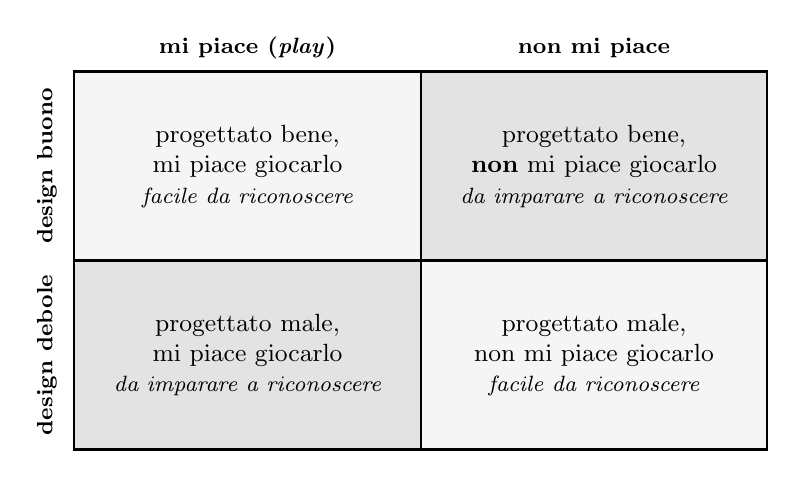
\begin{tikzpicture}[
    font=\small,
    cella/.style={draw, thick, minimum width=4.4cm, minimum height=2.4cm,
                  align=center, text width=4.0cm},
  ]
  \node[cella, fill=gray!8]  (a) at (0,0)    {progettato bene,\\ mi piace giocarlo\\
    \footnotesize\itshape facile da riconoscere};
  \node[cella, fill=gray!22] (b) at (4.4,0)  {progettato bene,\\ \textbf{non} mi
    piace giocarlo\\ \footnotesize\itshape da imparare a riconoscere};
  \node[cella, fill=gray!22] (c) at (0,-2.4) {progettato male,\\ mi piace
    giocarlo\\ \footnotesize\itshape da imparare a riconoscere};
  \node[cella, fill=gray!8]  (d) at (4.4,-2.4) {progettato male,\\ non mi piace
    giocarlo\\ \footnotesize\itshape facile da riconoscere};
  \node[font=\footnotesize\bfseries] at (0,1.5) {mi piace (\emph{play})};
  \node[font=\footnotesize\bfseries] at (4.4,1.5) {non mi piace};
  \node[font=\footnotesize\bfseries, rotate=90] at (-2.55,0) {design buono};
  \node[font=\footnotesize\bfseries, rotate=90] at (-2.55,-2.4) {design debole};
\end{tikzpicture}
\caption{Separare il gioco dal giocare: i due casi ``bizzarri'' in grigio scuro
sono quelli che insegnano di più, sia su sé stessi come giocatori sia sul game
design.}
\label{a3:fig:gameplay}
\end{figure}

\subsection{Il DPE}

\slidefig{img/AGD/agd3-dpe}{Il framework DPE (Design, Play, Experience).}{slide \emph{Analog -- Framework}}{fig:agd3-dpe}


L'MDA è stato poi \textbf{iterato} nel \textbf{DPE}, \emph{Design, Play,
Experience}, il cui paper è citato in cima alla slide\footnote{È il paper di
Brian Winn, \emph{The Design, Play, and Experience Framework}, pubblicato alla fine degli anni Duemila nello \emph{Handbook of Research on Effective Electronic Gaming in
Education}. La trascrizione riporta il titolo come ``Design Play Experience di
PA Framework by Win''.}. Nasce da un approccio \textbf{educativo e formativo}:
è un'iterazione che punta a parlare dei giochi nell'uso didattico. Ma, secondo
il docente, nel farlo riesce a semplificare e a ``distillare'' il cuore
interessante dell'MDA, con tre nomi ``più accurati'':
\begin{description}
  \item[Design] la parte in cui chi progetta crea le meccaniche;
  \item[Play] chi gioca, che applica e ``esperisce'' le dinamiche;
  \item[Experience] che cosa rimane, a livello esperienziale, a chi ha giocato.
\end{description}

Il DPE dispone queste tre parti su diversi \textbf{livelli} (\emph{layer})
tematici. Nel livello del \emph{gameplay}, il design contiene le meccaniche, il
play le dinamiche, l'experience la parte affettiva ed esperienziale. Nel livello
dell'\textbf{apprendimento}, se si parla di gioco formativo, il design contiene
il \textbf{contenuto pedagogico} (che cosa il gioco deve affrontare e far
passare), il play il momento in cui quel contenuto viene insegnato, e
l'experience, se il gioco è andato bene, è il fatto che le persone
\textbf{imparano} quello che il gioco voleva far loro imparare.

È un paper ``un po' più tecnico'' dell'MDA, tagliato sull'ambito formativo, ma
``non così complesso da risultare ostico'' a chi si avvicina al tema: il docente
lo consiglia molto. Con una precisazione che vale per tutto: ``leggerlo non vuol
dire prendere tutto per vero''. Su MDA e DPE si è dibattuto moltissimo: ``non
prendete per vero niente, nemmeno quello che vi sto dicendo io''. I due paper
sono abbastanza noti, soprattutto l'MDA; il DPE spesso è un po' ignorato da chi
lavora nel videogioco perché legato all'ambito didattico, ma secondo il docente
resta molto interessante, ``oltre che una semplificazione e un'iterazione
dell'MDA in maniera più digeribile''.

Una studentessa chiede di rivedere il titolo del paper. Le slide, come al solito,
saranno nel Drive dopo la lezione: ``non correte a segnarvi su un post-it il
paper''. ``Non vogliamo nascondervi le fonti''; e per qualsiasi dubbio si può
scrivere una mail al docente. Tiziana segnala che sono entrati altri
partecipanti: in quel momento ci sono \textbf{Lorenzo}, \textbf{Giordano},
\textbf{Nicola}, \textbf{Tancredi} e \textbf{Tiziana}.

\paragraph{Approfondimento: i livelli del DPE.} Nel paper di Winn i livelli
sono più di due. Oltre al \emph{gameplay} e all'apprendimento
(\emph{learning}), il framework prevede un livello di \emph{storytelling}, uno
di \emph{user experience} e, alla base di tutto, la \emph{technology}, che
abilita ma non determina gli altri. Ogni livello ha la propria terna design,
play, experience: per esempio, nello storytelling il designer scrive la storia
``del designer'', il play produce la storia ``del giocatore'' (quella che
emerge dalle sue scelte), e l'experience è il coinvolgimento che ne deriva. È
un'idea vicina a quanto il docente sta per dire sul coinvolgimento narrativo, e
alla distinzione tra regole ed esperienza da cui la lezione è partita.

% ---------------------------------------------------------------------
\section{Giordano si presenta}
\label{a3:sec:giordano}

``MDA, DPE, e adesso arriviamo alla parte importante''. Il docente annuncia il
primo framework grosso, il \textbf{Player Involvement Model}, con una promessa:
``se faccio il mio lavoro in maniera corretta, alla fine di questa lezione vi
sarà immediatamente chiaro perché non dovete usare \emph{immersione} come termine
nel corso. E se ho fatto il mio lavoro ancora meglio, non lo userete mai più
nella vita. Ma questo è un obiettivo più ambizioso''.

Arriva \textbf{Gianmarco}, in ritardo: il lunedì ha un impegno di lavoro fino
alle 17:30. ``Non ti preoccupare''. Il docente ne approfitta per una
\textbf{semi-pausa} prima di tuffarsi nel dettaglio, e chiede finalmente a
Giordano di presentarsi (``mi stavo dimenticando'') con le solite domande, che
scrive anche in chat: nome, che cosa fa nella vita, perché vuole fare giochi,
che cosa lo ha portato qui, che esperienza ha già.

\paragraph{La presentazione.} Giordano gioca a \textbf{Magic: The Gathering}
``dall'alba dei tempi''. Dopo il COVID si è spostato di più su \textbf{giochi da
tavolo} e \textbf{giochi di ruolo}, soprattutto negli ultimi due anni, anche per
lavoro: è quasi il suo \textbf{secondo lavoro}. Lavora come
\textbf{facilitatore e dimostratore} per un editore\footnote{La trascrizione dice
``per la Genos'' e, poco dopo, ``Ministro Ghienos'': si tratta con ogni
probabilità dell'editore italiano Ghenos Games.}, e collabora con
un'\textbf{associazione} che fa il giro delle \textbf{biblioteche della Brianza}
organizzando serate di giochi da tavolo e di ruolo, dove gli capita di fare da
master o di aiutare nella promozione dei giochi.

Ha scelto il corso perché è \textbf{focalizzato solo sul gioco analogico}, senza
la parte di videogioco e di programmazione, e quindi più compatibile con un
lavoro a tempo pieno. Lo fa per due ragioni: acquisire una \textbf{competenza di
base}, ``a livello analitico'', per coltivare meglio la sua passione; e riuscire
a fare qualcosa, ``non necessariamente da pubblicare'', da proporre negli eventi
dell'associazione. ``Figata'', commenta il docente, che gli chiede se sarà a
\textbf{Play}\footnote{Con ogni probabilità Play -- Festival del Gioco di
Modena, la principale fiera italiana del gioco da tavolo.} come dimostratore.
Quest'anno no, perché gli erano saltati gli appoggi per dormire. L'anno prima,
invece, era saltato un altro ragazzo, e lui si è ``beccato'' \emph{Rival
Cities}: circa \textbf{24 ore} di dimostrazioni dello stesso gioco in due
giorni. ``Chiaro, chiaro, chiaro''.

% ---------------------------------------------------------------------
\section{Il Player Involvement Model}
\label{a3:sec:pim}

``Ora che Giordano si è presentato'' ci si butta nel primo framework,
``tuffandoci con cautela ma anche con determinazione''. Il \textbf{Player
Involvement Model} è uno dei due framework che il docente chiederà di
\textbf{sapere}: ``non nel senso che vi interrogo'', ma nel senso che, dal suo
punto di vista (``non ho la verità in tasca, tutto quello che dico è il mio punto
di vista''), è uno strumento \textbf{pragmatico} e utile in due direzioni:
\begin{itemize}
  \item per capire che cosa fa un gioco \textbf{già pubblicato};
  \item per mettere le basi del \textbf{proprio} gioco.
\end{itemize}

\subsection{Il libro di Calleja}

Il framework viene da un libro di \textbf{Gordon Calleja}, \emph{In-Game: From
Immersion to Incorporation}, pubblicato dalla MIT Press\footnote{La
trascrizione dice ``Gordon Callea'', ``Kaleia'' e ``Calleia'', e chiama
l'editore ``Meatpress''. Il libro è del 2011; Calleja è un game designer e
studioso maltese. Il docente lo chiama sia \emph{Player Involvement Model} sia
\emph{Player Involvement Framework}.}. Secondo il docente se ne trova il PDF
gratuito; chi non lo trova può scrivergli e glielo manda. Ma non sarà richiesto
leggerlo: ``se ho fatto le mie slide correttamente'', è già condensato lì tutto
quello che serve.

La tesi di partenza: per Calleja \textbf{``immersione'' è una parola che ormai
non vuol dire niente}, ``per mille ragioni che non sto qua a dirvi''. Da
designer è più utile chiedersi \textbf{che cosa intende la gente} quando parla di
immersione: capendolo, diventa più facile progettarla. ``Immersione'' resta una
parola vietata: la si usa in queste slide, per contesto, ``ma poi non la voglio
più sentire nominare''.

\subsection{Che cos'è un gioco immersivo?}

``Se io vi dico: voglio un gioco più immersivo, che cosa vuol dire?'' Le
risposte degli studenti:
\begin{itemize}
  \item un'esperienza \textbf{più coinvolgente}, che non permette ai giocatori di
        distrarsi;
  \item un gioco che dà la sensazione di vivere un'esperienza \textbf{il più
        vicina possibile alla realtà}; il docente nota subito che è soggettivo,
        perché dipende da persona a persona;
  \item \textbf{Lorenzo}, appena entrato (il docente gli riassume dove si è
        arrivati), propone: un gioco in cui la \textbf{sospensione
        dell'incredulità} funziona bene.
\end{itemize}

\paragraph{Le provocazioni.} Il docente risponde con una serie di domande
``provocatorie''.
\begin{description}
  \item[Gli scacchi sono un gioco immersivo?] ``Dal punto di vista cognitivo,
        sì'', risponde qualcuno. Ma gli scacchi non chiedono sospensione
        dell'incredulità, né di fare un'esperienza simile alla realtà. Uno
        studente osserva che bisogna capire che cosa si intende, perché negli
        scacchi si è concentrati, non ci si immedesima (``oh, sono il cavaliere,
        il pedone'').
  \item[Il \emph{flow}.] Qui il docente introduce un termine che non ha messo
        nelle slide: il \textbf{flow}, o \textbf{flusso}. Non è solo un termine
        di game design ma, più in generale, di psicologia comportamentale: è
        la zona mentale in cui si trova una persona quando fa un'attività
        \textbf{né noiosa né troppo sfidante}, ``tra il \emph{questa cosa mi chiede
        impegno} e il \emph{non sono frustrato da questo impegno}''. In quella zona
        si sta molto bene, si è molto concentrati e coinvolti anche
        emotivamente. Gli scacchi possono mandare in flow, come molti altri
        giochi, e come lo \textbf{sport}; ma lo sport non chiede sospensione
        dell'incredulità.
  \item[Otto ore di \emph{Civilization}.] Una persona che gioca otto ore di fila a
        \emph{Civilization IV} (``qualcuno di voi l'ha fatto, sono sicuro, non
        negatelo''): uno studente confessa quattordici ore consecutive con un
        amico (``vabbè, ma quattordici ore sono dieci minuti nel tempo del
        giocatore''). Per lui rientra nell'immersione: si gioca al punto di
        dimenticarsi di mangiare.
  \item[I tornei di picchiaduro.] Chi gioca un torneo di \emph{Tekken} o di
        \emph{Street Fighter} è immerso?
  \item[\emph{Dance Dance Revolution}.] E chi balla su \emph{Dance Dance
        Revolution}? E chi fa un LARP dentro un castello?
\end{description}
La conclusione: è ``molto difficile'' dare una definizione di immersivo che
racchiuda tutto. ``Immersione'' viene usata come \textbf{parola jolly}, ``una
roba che ti coinvolge tanto''; ma dal punto di vista del game design
\textbf{non dà nessuno strumento}.

\paragraph{Approfondimento: il flow nei libri.} Il concetto che il docente
richiama viene dallo psicologo Mihaly Csikszentmihalyi, e Schell gli dedica una
lente (la \emph{Lens of Flow}). In \emph{The Art of Game Design} il flow è
definito come ``una sensazione di concentrazione completa ed energica in
un'attività, con un alto livello di piacere e di appagamento'', e Schell ne
elenca le condizioni: \textbf{obiettivi chiari}, \textbf{nessuna distrazione},
\textbf{feedback diretto} e una \textbf{sfida continua}, che resti nello
stretto margine tra la noia (troppo facile) e la frustrazione (troppo
difficile), il cosiddetto \emph{flow channel}. L'esempio classico, ripreso da
Csikszentmihalyi, è proprio uno sport: un ragazzo che impara il tennis è in
flow finché la difficoltà è adeguata alle sue capacità, si annoia quando
migliora senza che la sfida cresca, e si agita quando incontra un avversario
troppo forte. Anche \emph{21st Century Game Design} dedica una sezione
all'esperienza del flow, per capire come diversi tipi di giocatori la
raggiungano in modi diversi. Il fatto che il flow si ottenga con gli scacchi, il
tennis o un torneo di \emph{Tekken}, senza alcuna finzione da ``credere'', è
proprio l'argomento del docente: sotto la parola ``immersione'' convivono almeno
due fenomeni diversi, l'assorbimento nell'attività e la sospensione
dell'incredulità.

\subsection{Sei forme di coinvolgimento}

Calleja propone di ``buttare fuori'' dal termine immersione qualcosa di
\textbf{pragmatico e funzionale}: un \textbf{modello del coinvolgimento di chi
gioca}. Nello specifico crea \textbf{sei categorie}, che \textbf{non sono
mutualmente esclusive}: in ogni gioco alcune sono più alte e altre più basse, ma
la presenza di una non esclude le altre
(figura~\ref{a3:fig:pim} e tabella~\ref{a3:tab:pim}):
\begin{enumerate}
  \item il coinvolgimento \textbf{cinestetico};
  \item il coinvolgimento \textbf{spaziale};
  \item il coinvolgimento \textbf{condiviso};
  \item il coinvolgimento \textbf{narrativo};
  \item il coinvolgimento \textbf{affettivo};
  \item il coinvolgimento \textbf{ludico}.
\end{enumerate}
Gli esempi saranno \textbf{volutamente cross mediali}, con anche dei videogiochi,
``per farvi vedere fin dove si può arrivare con questi coinvolgimenti'' e per
far capire che è una cosa trasversale a tutto il game design: ``non è che se
parliamo di giochi da tavolo, allora alcune di queste cose non ci interessano''.

\begin{figure}[htbp]
\centering
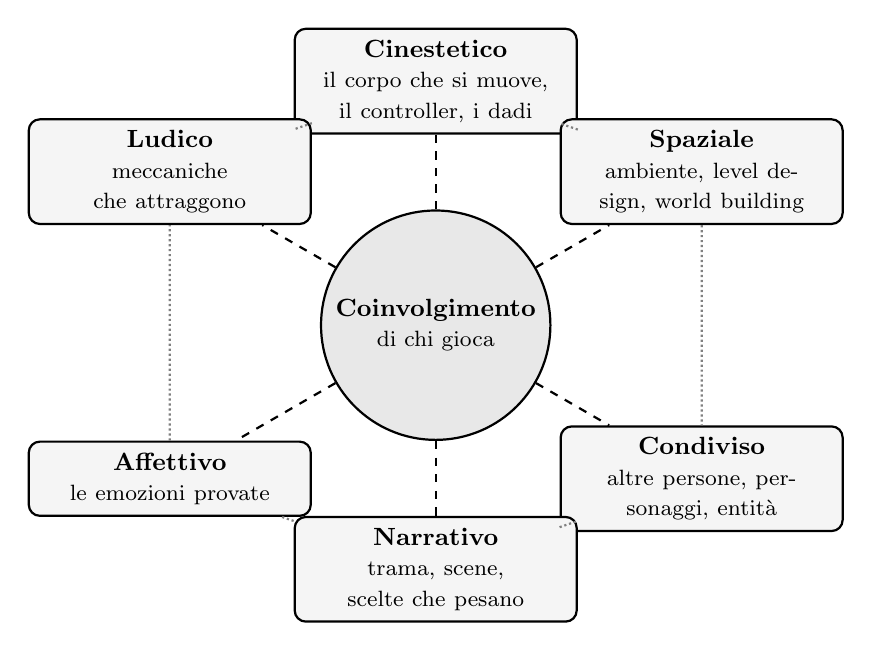
\begin{tikzpicture}[
    font=\small,
    centro/.style={draw, thick, circle, fill=gray!18, minimum size=2.5cm,
                   align=center},
    dim/.style={draw, thick, rounded corners=4pt, fill=gray!8,
                text width=3.3cm, align=center, inner sep=4pt}
  ]
  \node[centro] (c) at (0,0) {\textbf{Coinvolgimento}\\ \footnotesize di chi
    gioca};
  \node[dim] (k) at (90:3.1)  {\textbf{Cinestetico}\\ \footnotesize il corpo che
    si muove, il controller, i dadi};
  \node[dim] (s) at (30:3.9)  {\textbf{Spaziale}\\ \footnotesize ambiente,
    level design, world building};
  \node[dim] (sh) at (-30:3.9) {\textbf{Condiviso}\\ \footnotesize altre
    persone, personaggi, entità};
  \node[dim] (n) at (-90:3.1) {\textbf{Narrativo}\\ \footnotesize trama, scene,
    scelte che pesano};
  \node[dim] (a) at (210:3.9) {\textbf{Affettivo}\\ \footnotesize le emozioni
    provate};
  \node[dim] (l) at (150:3.9) {\textbf{Ludico}\\ \footnotesize meccaniche che
    attraggono};
  \foreach \x in {k,s,sh,n,a,l} \draw[thick, dashed] (c) -- (\x);
  \draw[gray, thick, densely dotted] (k) -- (s) -- (sh) -- (n) -- (a) -- (l) -- (k);
\end{tikzpicture}
\caption{Le sei dimensioni del Player Involvement Model di Calleja come le
presenta il docente. Le linee punteggiate ricordano che le aree ``si parlano'':
non sono stanze stagne, e una stessa scelta di design ne tocca spesso più
d'una.}
\label{a3:fig:pim}
\end{figure}

\subsection{Il coinvolgimento cinestetico}
\label{a3:sec:cinestetico}

\slidefig{img/AGD/agd3-cinestetico}{Il coinvolgimento cinestetico.}{slide \emph{Analog -- Framework}}{fig:agd3-cinestetico}


È il coinvolgimento che si ha quando un gioco \textbf{coinvolge il corpo} e ci si
\textbf{muove}. \emph{Dance Dance Revolution}, giocare con la Wii, fare sport,
entrare nella realtà virtuale: tutto coinvolgimento cinestetico. Lo è anche un
\textbf{boffer LARP}, quando bisogna combattere con spade imbottite e schivare i
colpi. Ma anche cose molto più piccole:
\begin{itemize}
  \item \textbf{usare un controller} è cinestetico;
  \item \textbf{tirare i dadi} è cinestetico;
  \item \textbf{pescare carte} è cinestetico: ``se vi piace pescare carte, un
        gioco che vi fa pescare carte a manetta andrà a titillare il vostro
        senso di apprezzamento dell'esperienza'';
  \item prendere una pedina e muoverla è cinestetico, anche a
        \emph{Monopoly}.
\end{itemize}
Nel gioco da tavolo c'è un intero genere che si basa su questo coinvolgimento:
i \textbf{giochi di destrezza} (\emph{dexterity}), dalle schicchere ai giochi in
cui bisogna impilare cose. Il \textbf{Jenga}\footnote{La trascrizione dice
``Genga'' e ``Gengar''.} ha un coinvolgimento cinestetico? Sì.

\paragraph{Cursori, non interruttori.} Da qui un'avvertenza che vale per tutte
le categorie: \textbf{non sono booleane}, ``non è che o c'è o non c'è''. Vanno
immaginate come \textbf{cursori} (\emph{slider}): ce ne può essere pochissimo,
poco, abbastanza, tantissimo. Il Jenga ha un coinvolgimento cinestetico molto
alto; il tennis più alto ancora; ma non per questo il Jenga ``non è
coinvolgente'' cinesteticamente rispetto al tennis.

\subsection{Il coinvolgimento spaziale}

\slidefig{img/AGD/agd3-spaziale}{Il coinvolgimento spaziale.}{slide \emph{Analog -- Framework}}{fig:agd3-spaziale}


È il coinvolgimento che riguarda \textbf{l'ambiente}: il \textbf{level design}, il
\textbf{world building} del gioco.
\begin{itemize}
  \item Un LARP fantasy o medievale in un \textbf{castello}: la slide mostra un
        castello polacco ``famoso perché ci hanno fatto centinaia di LARP''
        \footnote{Con ogni probabilità il castello di Czocha, in Polonia, noto
        per i LARP della serie \emph{College of Wizardry}; la trascrizione dice
        ``un castello bassa famoso''.}. ``Non sono nel mio salotto di casa, sono
        in un castello''.
  \item Il caso studio di \emph{Monitor Celestra}, visto la volta precedente:
        un LARP di fantascienza dentro un incrociatore, con i neon e le pareti
        metalliche. ``Un certo effetto te lo fa''.
  \item I \textbf{videogiochi di guida}: se ci si pensa, sono tutti basati sul
        \textbf{tracciato}, e il tracciato è una strada, cioè spazio che si
        attraversa. ``Il design di quello spazio è il 90\% di questi giochi'':
        curve strette o larghe, rettilinei. E si può estendere all'atmosfera,
        al clima: piove, c'è nebbia, c'è il sole, è notte, ci sono i neon.
  \item Un \textbf{dungeon crawler} in un gioco di ruolo cartaceo: la mappa del
        dungeon, anche se i giocatori non la vedono perché è dietro lo schermo
        del master, è coinvolgimento spaziale; e lo è quando il master
        \textbf{descrive} un ambiente, che cosa si sente, i suoni, gli odori, i
        rumori. ``Non è che se non vediamo lo spazio non c'è: ce lo stiamo
        immaginando, e quell'immaginarcelo ci coinvolge spazialmente''.
  \item Gli \textbf{open world}, nei videogiochi ma anche nei giochi da tavolo:
        generi che si basano su un mondo aperto ed esplorabile, in cui
        \textbf{lo spazio non è una limitazione ma un punto di \emph{agency}}.
        Lo spazio dice: puoi andare dove vuoi, puoi fare quello che vuoi.
\end{itemize}

\subsection{Il coinvolgimento condiviso}

\slidefig{img/AGD/agd3-condiviso}{Il coinvolgimento condiviso.}{slide \emph{Analog -- Framework}}{fig:agd3-condiviso}


È il coinvolgimento che si ottiene quando si \textbf{condivide l'esperienza con
altre entità}.
\begin{itemize}
  \item Di solito sono \textbf{amici}: un gioco online, come \emph{World of
        Warcraft} ``all'epoca'', giocato con persone amiche. Si è coinvolti in
        un gioco che da soli magari non si giocherebbe, o che non prenderebbe
        così tanto; e invece ``ogni martedì sera ci si trova a giocare''.
  \item Ma si estende anche ai \textbf{personaggi digitali}: un personaggio che
        mi sta subito simpatico (``non so chi sia, ma\ldots''); oppure esce
        l'ennesimo titolo di una serie con lo \textbf{stesso protagonista}, e
        ``io sono già coinvolto prima ancora di accendere il gioco''.
  \item Il \textbf{gioco di ruolo da tavolo} punta tantissimo sul coinvolgimento
        condiviso: è spesso un'esperienza sociale.
\end{itemize}
Va tenuto in considerazione soprattutto nei giochi \textbf{multiplayer}, perché lì
il coinvolgimento condiviso ``ce lo mette in mezzo'' comunque: \textbf{se non lo
progettate voi, lo progettano le persone al posto vostro}. E non è sempre
un'idea fantastica, perché vuol dire che parte dell'esperienza è fuori dal
controllo del designer.

\subsection{Il coinvolgimento narrativo}

\slidefig{img/AGD/agd3-narrativo}{Il coinvolgimento narrativo.}{slide \emph{Analog -- Framework}}{fig:agd3-narrativo}


È il coinvolgimento che arriva dall'\textbf{esplorazione narrativa}: trame, plot,
twist, sviluppo di quello che succede in scena, scene, momenti, dialoghi. È
quello che fa dire: \textbf{voglio sapere come finisce questa storia}.
\begin{itemize}
  \item Un gioco investigativo \textbf{in tribunale}\footnote{La trascrizione
        dice ``E Saturday''. Dalla descrizione (un avvocato in tribunale che
        deve scagionare il proprio cliente, sei capitoli principali) si tratta
        con ogni probabilità della serie \emph{Ace Attorney}.}, in cui si è un
        avvocato che deve capire che cosa è successo e scagionare il proprio
        cliente: ``ne hanno fatti sei'', ed è un successo gigantesco proprio
        perché il coinvolgimento narrativo è fortissimo. I casi sono intriganti
        e si vuole sapere la verità dietro il mistero.
  \item I giochi di Telltale\footnote{La trascrizione dice ``Dreadnought
        Helltail'': con ogni probabilità Telltale Games, lo studio noto per le
        avventure narrative a scelte ramificate.}, ``di fatto l'equivalente di
        libri game in formato digitale'': scelte ramificate, A o B, che
        impattano sul mondo di gioco e possono cambiare drasticamente la
        narrazione. La \emph{agency} ha un peso narrativo: non ``mi vesto di
        blu, mi vesto di rosso'', ma ``muore Tizio o muore Caio''.
  \item Il \textbf{gioco di ruolo}: spesso non si gioca solo per entrare nel
        dungeon, uccidere mostri, prendere il tesoro e uscire (``alcune persone
        giocano anche per quello''): gran parte del suo fascino è
        l'\textbf{agency emergente}, la possibilità di impattare la storia con
        le proprie scelte.
  \item \emph{Non cedere al sonno}\footnote{È l'edizione italiana di \emph{Don't
        Rest Your Head} di Fred Hicks, già citato nella lezione sui casi
        studio; la trascrizione dice ``Non ci Dare al Sonno''.}: la slide mostra
        un pezzo della scheda personaggio. Alla creazione non si chiedono
        numeri, non statistiche come destrezza, forza, intelligenza: si chiede
        \textbf{che cosa ti tiene sveglio}, che cosa ti è successo, come gli
        altri ti percepiscono \textbf{in superficie} e come sei
        \textbf{dentro}. Si può giocare tantissimo su questa collisione
        narrativa. È chiaramente un gioco che, \textbf{già da design}, fa creare
        personaggi sfumati.
\end{itemize}

\subsection{Il coinvolgimento affettivo}

\slidefig{img/AGD/agd3-affettivo}{Il coinvolgimento affettivo.}{slide \emph{Analog -- Framework}}{fig:agd3-affettivo}


``Questo ve lo dico per esperienza: molte persone lo confondono e lo
sovrappongono con il narrativo, ma non è così''. Il coinvolgimento
\textbf{affettivo} riguarda \textbf{le emozioni provate}. Spesso le emozioni le
danno le storie, ``perché siamo esseri umani'', e quindi un gioco che coinvolge
affettivamente spesso coinvolge anche narrativamente. Ma non necessariamente:
\textbf{anche gli scacchi possono coinvolgere affettivamente}, ``e non è che lo
storytelling, il world building degli scacchi sia proprio questo capolavoro''.
\begin{itemize}
  \item Ci rientrano molti \textbf{giochi focalizzati}, giochi su tematiche
        delicate, giochi che puntano a provocare specifiche emozioni molto
        forti, ``giochi in cui si piange a manetta''.
  \item Ma il coinvolgimento affettivo può anche essere \textbf{positivo}: un
        gioco che fa ridere tantissimo, come un \textbf{party game}.
  \item I giochi \textbf{Jeepform} visti come casi studio (\emph{Fat Man Down}, il
        gioco della coppia perfetta\footnote{La trascrizione lo chiama ``Lady
        E8'' e ``le IDE8''; nella lezione precedente era trascritto ``Lady 8''.
        Il titolo resta non verificabile.}): narrativamente non hanno quasi
        niente, ``è una riga la premessa del gioco''. Non si giocano per il
        coinvolgimento narrativo: si giocano perché hanno un coinvolgimento
        affettivo ``grosso come un tir che ti viene in faccia''.
\end{itemize}

\paragraph{\emph{Involved}, non \emph{immersed}.} In chat \textbf{Lorenzo} chiede
se allora ``immersione'' vada intesa più come \emph{to be involved} che come
\emph{to be immersed}. Il docente precisa: qui si sta parlando di un framework
specifico, quello di Calleja, e la \textbf{policy del corso} è adottare questo
framework per parlare di ciò che di solito si chiama immersione. Immersione resta
una parola vietata perché \textbf{non dà strumenti}: se qualcuno chiede ``un
gioco più immersivo'', non vuol dire niente; se chiede ``un gioco con più
coinvolgimento affettivo'' o ``più coinvolgimento narrativo'', si hanno già delle
\textbf{aree operative}, si sa dove andare a lavorare.

E le aree servono a progettare proprio perché non si escludono: un gioco può
avere tanto coinvolgimento su più fronti, e magari nessuno su altri che non
interessano. Il docente mette a confronto due estremi
(figura~\ref{a3:fig:pim-profili}):
\begin{itemize}
  \item a un \textbf{Jeepform} del coinvolgimento spaziale ``non gliene frega
        niente'': lo si gioca vestiti come si è, nel salotto di casa;
  \item un \textbf{LARP \emph{blockbuster}} di due giorni in un castello punta
        invece tantissimo sul coinvolgimento spaziale.
\end{itemize}
``Non c'è giusto o sbagliato'': il framework \textbf{non è qualitativo}. Non
dice che se c'è tanto di tutto il gioco è bello per forza, e se c'è poco di tutto
è brutto per forza. Serve a dire \textbf{che cosa interessa e che cosa serve} al
proprio gioco.

\subsection{Il coinvolgimento ludico}

\slidefig{img/AGD/agd3-ludico}{Il coinvolgimento ludico.}{slide \emph{Analog -- Framework}}{fig:agd3-ludico}


L'ultimo tipo è il coinvolgimento \textbf{ludico}: quello dato da
\textbf{meccaniche che piacciono}, che attraggono, che ``a vederle vi fanno dire:
questo gioco devo provarlo''.
\begin{itemize}
  \item Piace tirare i dadi? In un nuovo gioco si tirano un sacco di dadi: ``già
        magari ci prende bene''. Ma per chi odia tirare i dadi, vedere dei dadi
        in un gioco funziona già da \textbf{anti-coinvolgimento}.
  \item Il docente ama gli \textbf{economici azionari ferroviari}: ne vede uno
        nuovo e ``sono già intrigato, voglio già provarlo''. Altri amano i giochi
        di ruolo, le escape room.
  \item Piace costruire un \textbf{mazzo personalizzato} come in \emph{Magic: The
        Gathering}, \emph{Yu-Gi-Oh!}, \emph{Pokémon}? È un tipo di
        coinvolgimento che si può progettare, pensando a \textbf{per chi} è il
        gioco.
  \item Il \textbf{piazzamento lavoratori} (\emph{worker placement}), genere che
        ``va molto in Germania, in Europa'': il docente conosce almeno tre
        persone a cui ``si illuminano gli occhi'' quando gli si propone un
        piazzamento lavoratori, e altre che invece ``se ne vanno''.
\end{itemize}
Il coinvolgimento è soggettivo: \textbf{non esiste un passe-partout che coinvolga
tutte le persone}. Le aree servono a capire che cosa serve al proprio gioco, che
cosa metterci, dove andare a lavorare.

\paragraph{Le scelte di design toccano più aree.} Uno studente trova interessante
la distinzione, perché pensava che il ludico rientrasse nell'affettivo. Il
docente aggiunge una cosa importante: \textbf{molte scelte di design coprono più
aree}. Un \textbf{boffer LARP} dark fantasy con le armi di gommapiuma e un
sistema di combattimento è coinvolgimento cinestetico, perché porta a combattere
fisicamente; ma il boffer è anche una categoria meccanica, e chi apprezza le
meccaniche boffer andrà a giocare boffer: quindi è anche coinvolgimento
\textbf{ludico}. ``Queste non sono sei aree murate con dei muri di acciaio che
separano in maniera stagna le aree del game design'': si ibridano, si mischiano,
e una meccanica che si aggiunge può impattarne molte.

\begin{table}[htbp]
\centering
\small
\begin{tabular}{@{}p{2.6cm}p{4.4cm}p{6.1cm}@{}}
\toprule
\textbf{Coinvolgimento} & \textbf{Che cosa coinvolge} & \textbf{Esempi citati a
lezione} \\
\midrule
Cinestetico & il corpo, il movimento, la manipolazione & \emph{Dance Dance
Revolution}, Wii, VR, sport, boffer LARP; controller, dadi, pescare carte,
muovere pedine; giochi di destrezza, Jenga \\
Spaziale & ambiente, level design, world building, atmosfera & LARP nel castello,
\emph{Monitor Celestra}, tracciati dei giochi di guida, il dungeon descritto dal
master, open world \\
Condiviso & altre persone o entità con cui si condivide l'esperienza & amici
online (\emph{World of Warcraft}), personaggi ricorrenti di una serie, il GDR da
tavolo come esperienza sociale \\
Narrativo & trama, plot, twist, scene, scelte che cambiano la storia & la serie
in tribunale (\emph{Ace Attorney}), i giochi Telltale, l'agency emergente del
GDR, la scheda di \emph{Non cedere al sonno} \\
Affettivo & le emozioni provate, anche positive & giochi focalizzati, party
game, Jeepform (\emph{Fat Man Down}, la coppia perfetta), persino gli scacchi \\
Ludico & meccaniche che attraggono (o respingono) & tirare dadi, economici
ferroviari, deck building, piazzamento lavoratori, boffer, tornei \\
\bottomrule
\end{tabular}
\caption{Le sei forme di coinvolgimento del Player Involvement Model, con gli
esempi della lezione.}
\label{a3:tab:pim}
\end{table}

\begin{figure}[htbp]
\centering
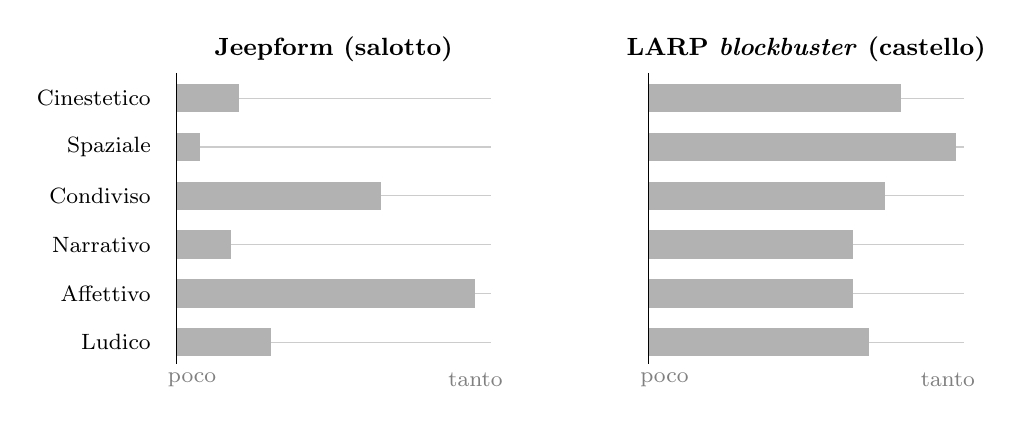
\begin{tikzpicture}[
    font=\footnotesize,
    x=1cm, y=1cm
  ]
  % assi e etichette
  \foreach \nome [count=\i] in {Cinestetico,Spaziale,Condiviso,Narrativo,
      Affettivo,Ludico} {
    \node[anchor=east] at (-0.2,-\i*0.62) {\nome};
    \draw[gray!40] (0,-\i*0.62) -- (4,-\i*0.62);
    \draw[gray!40] (6,-\i*0.62) -- (10,-\i*0.62);
  }
  \node[font=\small\bfseries] at (2,0) {Jeepform (salotto)};
  \node[font=\small\bfseries] at (8,0) {LARP \emph{blockbuster} (castello)};
  % Jeepform
  \foreach \v [count=\i] in {0.8,0.3,2.6,0.7,3.8,1.2} {
    \fill[gray!60] (0,-\i*0.62-0.18) rectangle (\v,-\i*0.62+0.18);
  }
  % blockbuster
  \foreach \v [count=\i] in {3.2,3.9,3.0,2.6,2.6,2.8} {
    \fill[gray!60] (6,-\i*0.62-0.18) rectangle (6+\v,-\i*0.62+0.18);
  }
  \draw[thin] (0,-0.3) -- (0,-4.0);
  \draw[thin] (6,-0.3) -- (6,-4.0);
  \node[gray] at (0.2,-4.2) {poco};
  \node[gray] at (3.8,-4.2) {tanto};
  \node[gray] at (6.2,-4.2) {poco};
  \node[gray] at (9.8,-4.2) {tanto};
\end{tikzpicture}
\caption{Due profili di coinvolgimento, a titolo puramente illustrativo. Il
docente cita solo il contrasto sullo spaziale (nullo nel Jeepform, altissimo
nel LARP in castello) e l'affettivo ``grosso come un tir'' del Jeepform; gli
altri valori sono ipotesi plausibili, utili a ricordare che il modello descrive
un profilo, non un punteggio.}
\label{a3:fig:pim-profili}
\end{figure}

% ---------------------------------------------------------------------
\section{Le domande sul coinvolgimento}
\label{a3:sec:pim-domande}

\paragraph{E la competizione?} Una domanda: un coinvolgimento legato alla
\textbf{competizione} rientra nel modello? Il docente rilancia: che cos'è che
attrae della competizione? Se è il senso, ``più lato sportivo'', di
\textbf{superare un altro essere umano}, o un'altra squadra di esseri umani,
allora si è nel coinvolgimento \textbf{condiviso}: sapere che dall'altra parte
c'è un altro essere umano da battere. Ma la competizione può anche essere
\textbf{meccanica}: molte persone vanno a un \textbf{torneo} con un approccio da
\emph{min-maxer}, perché quel gioco ``meccanicamente mi attrae'', e allora è
coinvolgimento \textbf{ludico}. Le due cose non sono sbagliate: si torna sempre a
\textbf{per chi è il gioco}. Un gioco può essere competitivo senza essere da
torneo, senza essere per chi fa min-maxing, senza essere per chi vuole muoversi
fisicamente. ``Non esiste una combinazione giusta di queste aree'': sono uno
strumento ``sulla carta'' per dire su che cosa il gioco spinge e su che cosa non
spinge, o non interessa.

\paragraph{Non fate \emph{Magic} 2.0.} Anche perché, ``purtroppo'', spingere su
tutto costa tantissimo in termini di budget, risorse, tempo, playtest. Il docente
ribadisce: \textbf{non fate giochi giganteschi in questo corso}, ``lo dico per
voi, perché se no poi non li portate a compimento''. ``Non fate \emph{Magic: The
Gathering} 2.0''. Si può fare un gioco di carte, ce ne sono tantissimi anche
compatti. \emph{Magic} è stato citato da più persone, anche nelle presentazioni
(``Giordano, tu sicuramente''); ma esistono giochi di carte compatti, creati
anche da persone che hanno lavorato a \emph{Magic}, come
\emph{Compile}\footnote{La trascrizione cita ``Redlands o Compile''. Il primo
titolo non è ricostruibile con certezza; il docente li presenta come giochi di
carte competitivi, compatti, con pochissime carte in una scatola piccola.}, che
hanno le stesse dinamiche interpersonali di competizione di \emph{Magic} con un
numero di carte ridottissimo, in una scatola molto compatta: ``più nell'ottica di
cose che potete fare all'interno di questo corso''.

\paragraph{Il \emph{checkpoint} prima della pausa.} Prima della pausa il docente
si ferma: ``da quando facciamo la pausa, io darò per scontato che voi avete capito
questo framework''. ``Non esistono domande stupide'', e una domanda che sembra
stupida può essere importantissima anche per gli altri. Rimette la slide con le
tipologie di coinvolgimento e scrive in chat il nome del libro di Calleja (il
nome, non il link, visto il problema dei link).

\paragraph{Perché il coinvolgimento al centro?} Una studentessa chiede: se il
coinvolgimento è ovviamente qualcosa da perseguire, perché il modello lo mette al
centro? Qual è il fine ultimo? Il docente risponde che il modello nasce dalla
necessità di \textbf{smettere di usare ``immersione''}; ma l'immersione non
sarebbe una parola così usata e pervasiva se non fosse \textbf{qualcosa che chi
gioca cerca}. Tutti cercano e apprezzano l'immersione, pur avendone definizioni
diverse: ``adesso qui siete in sette, e avete sette definizioni di immersione
diverse'', magari sovrapponibili per alcuni giochi. Ma gli studenti, da qui,
sono \textbf{game designer}, non solo persone che giocano, e serve loro sapere
\textbf{su che cosa stanno lavorando}: avere strumenti pratici per
\textbf{confrontare il proprio lavoro con le intenzioni}. Lo stesso lavoro di
decostruzione si farà più avanti con il \textbf{divertimento}. E il docente
torna alla slide iniziale: \textbf{il gioco è un'esperienza creata da regole};
si possono creare quelle regole, e dentro quelle regole si può lavorare su
questi tipi di coinvolgimento.

\paragraph{La distanza tra esperienza intesa ed esperienza giocata.} Il salto da
un'idea a un regolamento scritto, senza perdere cose per strada, ``è molto
difficile''. È un tema a cui il docente tiene moltissimo: la sua \textbf{tesi di
master} era proprio sul \textbf{gap tra le intenzioni di progettazione} di un
game designer e le persone che interpretano il regolamento per poi vivere
l'esperienza, misurando \textbf{quanta distanza c'è tra esperienza intesa ed
esperienza giocata}. \textbf{Lorenzo} scrive in chat che un designer può
pianificare un prodotto per coinvolgere l'utente su certi aspetti, ma poi è
quest'ultimo a decidere che cosa lo coinvolge davvero. ``È esattamente quello
che vi ho appena detto'': la parte difficile del lavoro, e quella che, se fatta
bene, fa fare passi avanti, è \textbf{distillare in un regolamento non ambiguo}
procedure, meccaniche, ``un ecosistema di regole'' che porti a far giocare
un'esperienza specifica a chi gioca, \textbf{senza che vi conosca e senza che vi
possa chiedere cose}.

È facile se il gioco lo si organizza di persona: lo si spiega, si corregge chi
sbaglia. Ma è un caso rarissimo. Nella maggior parte dei giochi pubblicati, il
designer non lo si incontrerà mai, e a volte non si sa nemmeno chi sia: ``che ne
sapete del suo costruttivismo personale?'' Che cosa c'è nel gioco perché quella
persona ci crede fermamente, ed è parte del suo paradigma, e che cosa c'è
\textbf{per sbaglio}? ``Lo farete anche voi'', non per sfiducia, ma perché è
inevitabile: non si può essere costantemente attenti a tutto, e a volte si
prendono decisioni di design senza pensarci, \textbf{per vestigialità, per
abitudine}. In quel momento si sta riproponendo un paradigma: si torna a
\textbf{fare tradizione}, non design.

\paragraph{Le domande di Tiziana.} Tiziana fa due domande. La prima: il playtest
si fa quando si ha il regolamento? Il docente la ferma subito, ``non perché non
mi interessa la domanda'': ci sarà una lezione apposta, e aprire adesso ``il vaso
di Pandora di come si struttura un playtest'' impedirebbe di arrivare al secondo
framework. Ed è una fase delicatissima: se la progettazione e il prototipo sono
``la vostra mente e il vostro gioco'', il playtest è il momento in cui ``questa
roba va a schiantarsi con persone esterne che non l'hanno mai giocata''.

La seconda: le categorie del modello le sono sembrate molto puntuali. Si era
chiesta perché non ci fosse un ``coinvolgimento sociale'', e si è risposta da
sola: ``sociale'' vuol dire una marea di cose, ``condiviso'' è più preciso.
Esatto, e non solo: \textbf{condiviso} permette di includere entità
\textbf{non necessariamente umane}. Il personaggio a cui si è affezionati in altri
giochi della serie coinvolge non per la meccanica né per la storia: in
\emph{Mario Kart}, ``che non è un gioco con altissima narrazione'', rivedere un
personaggio già incontrato può far dire ``scelgo questo perché mi sta
simpatico''. Di nuovo: le aree non sono mutualmente esclusive, ``si parlano''.

\paragraph{La pausa.} ``Facciamo pausa''. Il docente la fissa fino alle ``e
trenta'', cioè fino alle \textbf{18:30}\footnote{La trascrizione dice ``sono le
21, facciamo pausa fino alle 30'' e subito dopo ``ci si ritrova qui alle 18.30'':
la pausa comincia quindi alle 18:21 circa. Durante la pausa la trascrizione
registra per decine di righe frasi senza senso ripetute in loop.}.

\paragraph{Approfondimento: oltre le sei dimensioni.} La lezione si ferma alle
sei dimensioni, ma il titolo del libro di Calleja indica dove l'autore vuole
arrivare. Nel suo modello ogni dimensione si può osservare su due scale di
tempo: il coinvolgimento \textbf{micro}, momento per momento, mentre si gioca, e
quello \textbf{macro}, che riguarda il rapporto con il gioco nel tempo, anche
quando non si sta giocando (la voglia di tornarci, il pensarci, il parlarne). La
parola \emph{incorporation}, che Calleja propone al posto di
\emph{immersion}, indica il momento in cui le diverse dimensioni del
coinvolgimento si fondono e il giocatore ``assimila'' il mondo di gioco nella
propria coscienza come uno spazio abitabile, con il proprio avatar come punto
di presenza. Il passaggio è lo stesso che il docente chiede agli studenti:
sostituire una metafora vaga (l'immersione, come in una piscina) con una
descrizione delle componenti, su cui si può lavorare una per una.

% ---------------------------------------------------------------------
\section{Il Mixing Desk of Larp}
\label{a3:sec:mixing}

``Rieccoci qua''. Dopo la pausa (Lorenzo conferma di esserci) si parte con il
secondo framework grosso, ``non che quello di prima fosse piccolo''.

\subsection{Da dove viene}

Il framework \textbf{nasce all'interno dei movimenti scandinavi} di gioco di
ruolo, nella scena del \textbf{Nordic LARP}\footnote{Il \emph{Mixing Desk of
Larp} è stato sviluppato nei primi anni Dieci da designer norvegesi legati alla
\emph{Larpwriter Summer School}, e poi più volte rielaborato; la storia è
raccontata nell'articolo di \emph{Analog Game Studies} che il docente consiglia
alla fine della lezione (sezione~\ref{a3:sec:perche-due}).}. Ma per sua natura
è uno strumento \textbf{estremamente flessibile}: è stato applicato anche al
gioco da tavolo e si può applicare ad altre tipologie di giochi. È
\textbf{modulare}: lo si può modificare, aggiungere o togliere pezzi in base a
quello che serve per il proprio gioco, ``perché non tutti i moduli, non tutte le
parti di questo framework vi servono sempre''.

Molti esempi saranno giochi di ruolo dal vivo, ``solo perché è più facile
spiegare'' alcuni cursori così. Il docente chiede di fare ogni volta il
\textbf{parallelismo}: questo pezzo del framework è nato sul gioco di ruolo, ma
come si applica al resto? Per alcuni cursori il salto è facile, per altri più
complesso; ma ``se tutto va bene, e mi è sembrato bene in passato'', alla fine
gli studenti dovrebbero avere un'ottima idea di come funziona e, soprattutto, di
come \textbf{applicarlo in modo pragmatico}.

\subsection{Un doppio uso}

Ancora più del Player Involvement Model, il Mixing Desk ha un \textbf{doppio
utilizzo}:
\begin{description}
  \item[Analisi] si prende un gioco già pubblicato, lo si ``fa passare'' nel
        framework e si guarda che cosa ne esce.
  \item[Progettazione] è ``un framework ottimo per crearvi delle
        \textbf{linee guida}'': voglio un gioco che faccia A, B, C, D, e il
        framework aiuta a capire che cosa sono A, B, C, D e come si vuole che
        arrivino.
\end{description}

\subsection{Il mixer}

\slidefig{img/AGD/agd3-mixer}{The Mixing Desk of Larp: i cursori del mixer.}{slide \emph{Analog -- Framework}}{fig:agd3-mixer}


Il nome è ``abbastanza autoesplicativo'': la slide mostra quello che sembra un
\textbf{banco di mixaggio} luci e audio. L'idea è che ogni gioco possa essere
identificato da una serie di \textbf{cursori} (\emph{slider}, o \emph{fader}),
le levette che si spingono su e giù in un mixer, e che l'insieme dei cursori
usati per progettare o analizzare il gioco ne dia una \textbf{visione
d'insieme}: che cosa fa questo gioco, ``non tanto a livello micro, cioè nelle
singole regole, ma a livello esperienziale, cioè dall'alto''
(figura~\ref{a3:fig:mixer}).

L'ultimo cursore della slide è \textbf{``inserisci qui il tuo fader''}
(\emph{your fader here}): ``modificate questo slider come volete''. Nella sua
storia il Mixing Desk è stato elaborato, modificato e rimaneggiato più volte,
anche da settori paralleli come il gioco di ruolo formativo e il gioco da tavolo.
Il docente mostra ``il primo, quello da cui è nato''; online se ne trovano
``mille versioni''. Il consiglio non è andarle a cercare, ma \textbf{capire che
cosa serve al proprio gioco e creare i propri cursori}.

\begin{figure}[htbp]
\centering
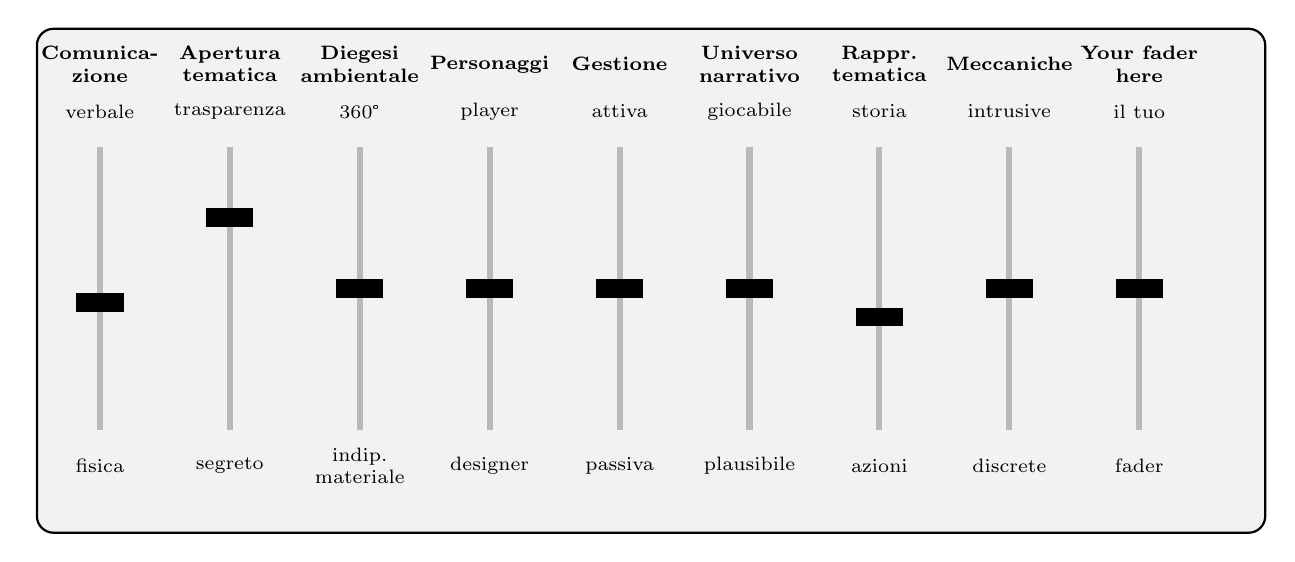
\begin{tikzpicture}[
    font=\scriptsize,
    x=1cm, y=1cm
  ]
  \draw[thick, rounded corners=6pt, fill=gray!10] (-0.6,-0.9) rectangle (15.0,5.5);
  \foreach \alto/\basso/\pos [count=\i] in {
      verbale/fisica/0.55,
      trasparenza/segreto/0.25,
      360°/indip. materiale/0.5,
      player/designer/0.5,
      attiva/passiva/0.5,
      giocabile/plausibile/0.5,
      storia/azioni/0.6,
      intrusive/discrete/0.5,
      {il tuo}/fader/0.5} {
    \pgfmathsetmacro{\x}{(\i-1)*1.65+0.2}
    \draw[line width=2.2pt, gray!55] (\x,0.4) -- (\x,4.0);
    \fill[black] (\x-0.3,{0.4+3.6*(1-\pos)-0.12}) rectangle
                 (\x+0.3,{0.4+3.6*(1-\pos)+0.12});
    \node[align=center, text width=1.55cm] at (\x,4.45) {\alto};
    \node[align=center, text width=1.55cm] at (\x,-0.05) {\basso};
  }
  \foreach \nome [count=\i] in {{Comunica-\\ zione}, {Apertura\\ tematica},
      {Diegesi\\ ambientale}, Personaggi, Gestione, {Universo\\ narrativo},
      {Rappr.\\ tematica}, Meccaniche, {Your fader\\ here}} {
    \pgfmathsetmacro{\x}{(\i-1)*1.65+0.2}
    \node[font=\scriptsize\bfseries, align=center, text width=1.6cm] at
      (\x,5.05) {\nome};
  }
\end{tikzpicture}
\caption{Il Mixing Desk come banco di mixaggio: otto cursori della versione
mostrata a lezione più il cursore libero. Le posizioni sono qui tutte centrali
o quasi, solo per mostrare che ogni cursore può stare a qualsiasi altezza: nessun
estremo è ``meglio'' dell'altro.}
\label{a3:fig:mixer}
\end{figure}

% ---------------------------------------------------------------------
\section{I cursori del Mixing Desk}
\label{a3:sec:cursori}

\slidefig{img/AGD/agd3-cursori}{Gli otto cursori del Mixing Desk of Larp: comunicazione, apertura tematica, diegesi ambientale, creazione dei personaggi, gestione del gioco, universo narrativo, rappresentazione tematica e meccaniche.}{slide \emph{Analog -- Framework}}{fig:agd3-cursori}


\subsection{Comunicazione: verbale o fisica}

Si prende un LARP, un gioco in cui si interpreta fisicamente il proprio
personaggio. \textbf{La comunicazione tra chi gioca è verbale o fisica?} E
``lo ricordo: questo è uno slider, non è un pulsante on, off, uno, zero''. Ci
sono vie di mezzo.
\begin{itemize}
  \item Un \textbf{boffer LARP} è molto fisico: il combattimento è una parte
        importante del gioco, e impugnare un'arma in plastazote, colpire,
        schivare, prendere lo scudo, riattaccare dal fianco è un'interazione
        molto fisica.
  \item Il gioco della coppia perfetta, il Jeepform citato prima, è
        ``estremamente verbale''.
  \item Nei giochi da tavolo, un \textbf{party game} va di solito più sul
        verbale. Negli \textbf{scacchi} si parla pochissimo: l'interazione ludica
        non è di dialogo, è ``io muovo cose'', e muovere cose è un'azione fisica.
\end{itemize}
La domanda da farsi: \textbf{il mio gioco è un gioco in cui si parla o un gioco
in cui si spostano cose?} E le ``cose'' possono essere anche le persone stesse,
come negli sport o nel gioco dal vivo. ``Spostare cose'' riassume il fatto di
interagire fisicamente con qualcosa. Ci si può stare in mezzo: un gioco in cui si
parla e si spostano cose, ma si parla più di quanto si spostino cose, o
viceversa.

\paragraph{I giochi verbali e i loro limiti.} ``Qualcuno ha un esempio di un gioco
da tavolo estremamente verbale?'' Uno studente propone \textbf{Dixit}. È
verbale, ``ma non è così tanto verbale'', perché ha moltissime
\textbf{limitazioni sulla comunicazione}: se in \emph{Dixit} si potesse parlare
liberamente di tutto, il gioco crollerebbe. Lo stesso vale per \emph{Secret
Hitler}, per \emph{Taboo}, per \emph{Codenames} (``nomi in codice''), dove si può
dire una parola e un numero, non di più. Molti giochi deduttivi o induttivi hanno
fortissime limitazioni su che cosa si può e non si può dire.

\paragraph{L'obiezione di Gianmarco.} Gianmarco vede una difficoltà: qui verbale e
fisico sono messi in contrapposizione, ma l'esempio dei giochi verbali con
limitazioni sembra non stare sullo stesso asse. Il docente spiega che sono
messi come \textbf{estremi}, come \textbf{direzioni di game design diverse}:
``immagina che hai cento chili di roba nel tuo game design, e di decidere quanti
chili voglio che siano fisici e quanti verbali'' (``una metafora che non
funziona, ma spero che ci siamo capiti lo stesso''). Una studentessa aggiunge
che \emph{Taboo} non è solo verbale: c'è gestualità, comunicazione non verbale,
``non giochiamo bendati''. E le limitazioni verbali, chiede Gianmarco, si
trasformano in dinamiche fisiche? ``Non necessariamente'', ma spesso si
trasformano in \textbf{altre cose da fare al tavolo}: le carte illustrate di
\emph{Dixit} sono un elemento fisico usato per comunicare in modo non verbale;
la griglia di parole di \emph{Codenames} è un aspetto fisico di interazione,
anche se ha parole scritte sopra. Il Mixing Desk non va guardato come ``lo stato
oggettivo del gioco dall'alto'', ma come una \textbf{bilancia}: se si spinge da
un lato, l'altro tende a scendere.

\paragraph{Gli estremi.} Ci possono essere anche giochi all'estremo totale.
\emph{Stranger}, il LARP della designer danese visto nei casi studio, quello
della nazione blu e della nazione verde, è un gioco in cui \textbf{è vietato
parlare} e fare suoni: è tutto fisico. All'opposto, ci sono giochi con
\emph{roleplay} in cui la componentistica è praticamente inesistente; e anche
\emph{Dungeons \& Dragons}, se si giocano i combattimenti senza griglia, diventa
molto verbale e molto poco fisico. Ma ``non siamo esperimenti in astratto'': è
quasi impossibile eliminare del tutto uno dei due estremi.

\subsection{Apertura tematica: trasparenza o segreto}
\label{a3:sec:apertura}

``Cercherò di spiegarmi al meglio, perché è importante ma apre dei vasi di
Pandora''. Supponiamo che il gioco abbia un \textbf{tema}. Quel tema arriva a chi
gioca \textbf{in modo trasparente}, o è un \textbf{tema segreto} che si scopre
durante o alla fine del gioco?
\begin{description}
  \item[Trasparenza.] \emph{Twilight Struggle}, della GMT: Stati Uniti contro
        URSS, la \textbf{Guerra Fredda}. Due persone, una gioca gli Stati Uniti,
        l'altra l'URSS; non ci si combatte direttamente con i carri armati, ma si
        cerca di vincere ottenendo influenza e supporto di varie nazioni. Il tema
        è trasparente: entrambi i giocatori sanno che cosa stanno giocando.
  \item[Segreto.] Un gioco in cui si trasportano cubetti e risorse in treno da un
        posto all'altro, e vince chi ne trasporta di più. Alla fine si scopre che
        si stavano trasportando \textbf{ebrei nei campi di concentramento}. ``Questo
        è un caso studio esistente'': è \emph{Train} di \textbf{Brenda
        Romero}\footnote{La trascrizione dice ``Trains di Prenderò Mero''.
        \emph{Train} (2009) fa parte della serie di giochi da tavolo \emph{The
        Mechanic is the Message} di Brenda Romero, all'epoca Brathwaite,
        coautrice di \emph{Challenges for Game Designers}.}, ``storicamente
        riconosciuto come gioco dal tema offuscato'' che viene rivelato durante
        il gioco.
\end{description}
Anche qui ci sono vie di mezzo: molti LARP ``vecchia scuola'' hanno \textbf{trame
segrete}, plot nascosti noti solo ad alcuni personaggi, che si rivelano nel
\emph{debriefing} (``sapevate che in realtà Tizio faceva anche questo?'').

\paragraph{La preferenza del docente.} È una cosa soggettiva, e il docente lo
dice come tale: preferisce i giochi \textbf{trasparenti}. Trova ``molto pigro''
affidarsi ai segreti, specialmente quando si tratta di temi delicati. Ma giochi
così esistono, e il cursore esiste.

\paragraph{Si gioca una volta sola?} Tiziana chiede se un gioco così si giochi
una volta e poi rischi lo \emph{spoiler}. ``Non è un problema'': non sono
esperienze meno significative. Come i \textbf{giochi investigativi}, che si
basano proprio su un'apertura tematica segreta. Fare un investigativo in cui si
dice subito chi è l'assassino e come ha ucciso è ``molto difficile'', ma ci sono
le eccezioni. Il docente cita \textbf{il tenente Colombo}, ``che amo
particolarmente'' (``vi prego, ditemi che non sono l'unico''): la serie si apriva
mostrando l'assassino e l'omicidio, e solo dopo arrivava Colombo a indagare. Lo
spettatore sa già tutto; il protagonista no. L'interesse sta nel conflitto tra
chi sa e chi non sa, nel capire come Colombo arriverà a ciò che lo spettatore ha
visto. Allo stesso modo si può avere un investigativo da tavolo in cui si sa già
com'è morta una persona: ``è una bella sfida''.

\paragraph{Un segnalibro.} Quando si parla di \textbf{giochi formativi o
didattici}, questo cursore è per il docente ``particolarmente sensibile e
importante''. E, di nuovo, non tutti i cursori interessano ogni gioco: in un
astratto alla scacchi o dama, ``che ve ne importa dell'apertura tematica?''.

\paragraph{Approfondimento: \emph{Train} e il tema sotto le meccaniche.}
\emph{Train} compare anche in \emph{A Theory of Fun for Game Design} di Raph
Koster, che lo cita come esempio della serie \emph{The Mechanic is the Message}:
un gioco sulla \textbf{complicità} dei giocatori nel compiere azioni terribili,
o nel trovare il modo di sovvertire il sistema. Lo stesso libro propone un
esperimento mentale che illumina il rapporto tra tema e meccaniche: si immagini
un gioco in cui si lasciano cadere vittime innocenti di ogni forma e misura in
una camera a gas a forma di pozzo, dove cercano di arrampicarsi le une sulle
altre; se ci riescono si perde, se le si incastra abbastanza bene quelle in
fondo muoiono. ``Non voglio giocare questo gioco. E voi?'', chiede Koster. Eppure
è \emph{Tetris}. La conclusione di Koster è che \textbf{le meccaniche nude non
determinano il significato} di un gioco: come il cinema non è solo fotografia o
sceneggiatura, il gioco è l'insieme di meccaniche, regia, grafica. \emph{Train}
usa esattamente questa distanza tra meccanica e tema: le stesse azioni,
caricare cubetti su un vagone, cambiano completamente significato nel momento in
cui il tema viene aperto. Il cursore dell'apertura tematica, in questo caso, è
la leva principale dell'esperienza.

\subsection{Diegesi ambientale: 360° o indipendenza materiale}

Quello che c'è attorno a chi gioca, l'ambiente in cui si gioca: il coinvolgimento
spaziale è \textbf{a 360 gradi}, o il gioco ha un'\textbf{indipendenza
materiale}? Nel gioco di ruolo dal vivo:
\begin{itemize}
  \item si gioca un fantasy dentro un castello, a cavallo, ``e abbiamo un vero
        cavallo'' sotto di noi;
  \item oppure si gioca il gioco della coppia perfetta nel bagno di casa, ma
        lo si potrebbe giocare in salotto, o in giardino.
\end{itemize}
Il gioco richiede una \textbf{diegesi il più alta possibile} per essere giocato,
oppure no? E ci sono vie di mezzo: si può giocare nello studio di casa
\textbf{vestiti da cavalieri}, ``why not?''. Molti \textbf{chamber LARP} italiani
degli anni '90 e 2000 funzionavano così, e il docente mostra al volo una slide:
un LARP in costume giocato \textbf{nello scantinato} della casa di qualcuno. Non è
completamente indipendente dal materiale, perché i costumi erano richiesti, ma
``non siamo in un castello, è uno scantinato''.

Vale anche per gli altri giochi: un \textbf{dungeon crawler} da tavolo mostra
l'ambiente nel dettaglio, o ne dà una rappresentazione metaforica, astratta?

\subsection{Creazione dei personaggi: chi gioca o chi progetta}

Ancora pensando al LARP (``sui personaggi abbiamo una lezione apposta'', e
arriverà presto): i personaggi possono essere scritti \textbf{da chi partecipa}
o \textbf{da chi progetta il gioco}, e sono due esperienze chiaramente diverse.
\begin{description}
  \item[Lato player.] Chi gioca crea il proprio personaggio e decide chi
        interpretare. È spesso la formula dei \textbf{giochi molto grossi}, i
        LARP \emph{blockbuster} da 300, 400, 500 persone, o i boffer tedeschi da
        mille persone: i designer non si mettono a scrivere mille personaggi, ma
        chiedono di scriverlo e di mandarlo, a volte, per approvazione. Se non ci
        sono cose particolarmente sbagliate, si gioca chi si vuole.
  \item[Lato designer.] Il personaggio è creato da zero da chi progetta il
        gioco. Il vantaggio: si può mettere \textbf{tematicamente} nel
        personaggio quello che si vuole.
\end{description}
Non è così diverso dai videogiochi di ruolo: ci sono i \emph{Final Fantasy},
soprattutto i più recenti, in cui i designer hanno creato i personaggi e se ne
segue la storia; e ci sono i giochi di ruolo occidentali, i CRPG, con una fase
di \emph{character creation} in mano al giocatore, magari con dei paletti messi
dal designer.

\paragraph{I paletti di \emph{Non cedere al sonno}.} Un esempio di via di mezzo.
In \emph{Non cedere al sonno} si giocano persone \textbf{insonni} che vedono una
città che non esiste, piena di orrore e di incubi. Si può fare il personaggio che
si vuole, ma con due paletti forti, decisi dal designer: il personaggio deve
essere \textbf{insonne}, e deve avere \textbf{un problema che lo tiene sveglio},
cioè una motivazione specifica e consapevole della propria insonnia. Non si può
giocare un insonne che non sa perché non dorme. Uno studente chiede di ripetere
il titolo: \emph{Non cedere al sonno}, ripubblicato di recente in italiano da un
editore che la trascrizione chiama ``Grampy Bear''\footnote{Con ogni probabilità
Grumpy Bear, editore italiano di giochi di ruolo.}.

\subsection{Gestione del gioco: attiva o passiva}

C'è una figura, come un \textbf{master} o una persona di \textbf{facilitazione},
che fa andare avanti il gioco, o un gruppo può giocare e finire il gioco
\textbf{senza nessuno che facilita}? Riguarda giochi pervasivi, giochi di ruolo
dal vivo e da tavolo.
\begin{description}
  \item[Gestione attiva.] Nei giochi di ruolo grossi, a campagna, o nei
        \emph{blockbuster} da centinaia di persone, ci sono i cosiddetti
        \textbf{PNG} (\emph{NPC}), spesso membri dell'organizzazione, che sono lì
        per \textbf{innescare eventi specifici} e far andare avanti il gioco. C'è
        una persona del team che spinge attivamente avanti il gioco.
  \item[Gestione passiva.] Nessuno del team o della facilitazione spinge il
        gioco: le persone che giocano lo portano avanti in autonomia.
\end{description}

\paragraph{Uccidere il re.} L'esempio: in un LARP fantasy, a un certo punto
qualcuno deve uccidere il re, per ragioni di trama, e non si sa se i giocatori
lo faranno. Allora uno dell'organizzazione si veste da assassino e uccide il re:
\textbf{gestione attiva}. All'opposto, il gioco chiede ai giocatori di uccidere
il re, magari con una meccanica apposita che qualcuno deve attivare, e nessuno
dell'organizzazione interviene: le persone lo fanno in autonomia,
\textbf{gestione passiva}.

\paragraph{Il parallelo con il gioco da tavolo.} Gianmarco prova: gli
\textbf{eventi} di \emph{Nemesis} come gestione attiva, e
\emph{Root}\footnote{La trascrizione dice ``in route'': con ogni probabilità
\emph{Root}, il gioco asimmetrico di fazioni in cui sono i giocatori a
scontrarsi.}, ``in cui sono i giocatori a menarsi'', come gestione passiva? Non
del tutto, risponde il docente: gli eventi di \emph{Nemesis} si mescolano, non se
ne decide l'ordine. Un esempio migliore di gestione attiva nel gioco da tavolo
sono i \textbf{giochi a campagna}, come i dungeon crawler con scenari numerati da
giocare in ordine: il designer ha deciso che si gioca prima questo scenario, poi
questo, poi quest'altro, e non si gioca il terzo prima ``perché ci va''. Lì la
gestione è, in parte, di chi ha progettato la campagna.

\paragraph{E nei giochi pervasivi?} Una studentessa chiede se il cursore
riguardi solo i giochi di ruolo. No:
\begin{itemize}
  \item \emph{Lettere anonime per un camminatore}, il caso di Beatrice con
        l'MP3 in cuffia, è a metà: c'è una forte gestione attiva nella traccia
        preregistrata da chi organizza, ma le persone camminano con la propria
        velocità e i propri tempi, ``non puoi obbligare la persona a correre'';
  \item \emph{Journey to the End of the Night} è a gestione
        \textbf{passiva}: runner e chaser possono metterci un'ora o cinque ore,
        e nessuno li disturberà;
  \item \emph{A cena col nonno} è a metà: la traccia audio dà dei tempi
        precisi (gestione attiva), ma la conversazione al tavolo non è
        controllata da nessun PNG, e tutte le persone sono giocatori;
  \item nel gioco di ruolo da tavolo, il \textbf{master} è il lato attivo della
        gestione, se il gioco ne ha uno.
\end{itemize}

\paragraph{La plancia a due facce.} Giordano chiede: e i giochi con una
\textbf{plancia a due facce}, in cui il regolamento dice di usare per la prima
partita il lato base e non quello avanzato\footnote{La trascrizione cita come
esempio un gioco chiamato ``Ivan'', non identificabile.}? È una forma di
gestione attiva? Il docente non la considera tale: rientra nelle questioni di
\textbf{onboarding}, accessibilità e approccio al gioco, ``come dire: gioco il
tutorial e poi, quando ho imparato, gioco la parte completa''. Il gioco non
\emph{impone} l'ordine: lo consiglia. Se si è già giocato e lo si fa provare a
un amico, si sceglie la plancia in base all'amico. Avere quella libertà vuol dire
che la gestione non è attiva; diverso è un Legacy o un gioco a campagna in cui
non si può giocare l'ottavo scenario prima del primo. Lo stesso vale per alcuni
giochi di carte collezionabili: in \emph{Magic} il mazzo inteso è da sessanta
carte, ma in vari eventi si sono usati \textbf{mazzi dimostrativi} preconfezionati
più piccoli, da quaranta carte, per spiegare il gioco a chi non l'ha mai
giocato.

\subsection{Universo narrativo: giocabile o plausibile}
\label{a3:sec:plausibile}

``Questo, vi giuro, è forse il mio slider preferito''. Se c'è un cursore da
portarsi a casa dal Mixing Desk, ``secondo me questo forse è quello che vi serve
di più nella vita. Come paradigma''. L'universo narrativo del gioco è
\textbf{più giocabile o più plausibile}? E uno dei punti del framework è che le
due cose sono \textbf{in opposizione}: \textbf{più un gioco è giocabile, meno è
plausibile}. Per esperienza, è difficile da far combaciare nella testa se non ci
si è mai pensato a fondo.

\paragraph{La provocazione di Gianmarco.} ``Chi non è d'accordo?'' Tutti
d'accordo. Gianmarco fa una provocazione: forse l'unico gioco veramente giocabile
e plausibile insieme è ``il gioco della nostra vita: io gioco a essere
Gianmarco''. ``Però quello non è un gioco, purtroppo''. È una provocazione, ma
porta alla domanda giusta: plausibile da che punto di vista?

\paragraph{Che cosa vuol dire plausibile.} Su questo cursore da solo esiste un
talk di Johanna Koljonen, la designer della citazione iniziale, che ``dura un'ora
e passa''; il docente lo riassume. Un universo narrativo \textbf{plausibile} è un
universo che \textbf{simula la propria esistenza}: le cose hanno azioni e
conseguenze simulate \textbf{come se fosse la realtà}. Ma spesso l'approccio
simulativo va in \textbf{diretta opposizione alla giocabilità}.

\paragraph{La vedetta.} L'esempio ``banalissimo''. Un LARP fantasy medievale,
magari un 360°, in un castello bellissimo, per tre giorni di fila: si dorme, si
mangia, si cammina in personaggio, vestiti di tutto punto in armatura. È notte,
qualcuno deve fare la guardia, e tocca a voi: state sulle mura di vedetta. Se il
gioco fosse \textbf{pienamente plausibile}, non succederebbe niente:
statisticamente i castelli non vengono attaccati ogni giorno, e la normale notte
di vedetta è una notte in cui si sta svegli \textbf{otto ore} a guardare il cielo.
``Se io metto una persona a giocare questo ruolo per otto ore, questa persona si
butta giù dalle mura''. La \textbf{giocabilità} è l'approccio più ludico: chi
vuole giocare la vedetta vuole che la vedetta noti cose, dia l'allarme. Lo stesso
vale per il cavaliere: ``siete Sir Cavaliere, ecco la vostra spada, ecco il
vostro scudo'', e in due giorni non c'è un combattimento perché è un periodo di
pace. Plausibile; ingiocabile.

\paragraph{GURPS.} Si può voler creare un gioco simulativo e plausibile, ``e ce
ne sono tantissimi''. Nel gioco di ruolo il caso tipico è
\textbf{GURPS}\footnote{La trascrizione lo chiama ``Gurps'', ``Goobs'' e
``GuardStore''. \emph{GURPS} (\emph{Generic Universal RolePlaying System}) è
il sistema di Steve Jackson Games.}: nasce con l'intenzione di essere plausibile,
e infatti ha ``microregolette per tutto''; chi l'ha giocato sa che al tavolo
risulta ``estremamente ostile all'essere giocato''. All'opposto, ci sono giochi
molto giocabili ma flessibili sulla plausibilità del mondo, perché sono più
interessati ad avere scene e momenti di gioco interessanti che plausibili.

\paragraph{Gli open world.} Uno studente chiede dei giochi digitali: \emph{GTA}
non riesce ad avere entrambe le cose? Gli \emph{open world} sono un genere che si
associa alla plausibilità, come la serie \emph{Yakuza} / \emph{Like a Dragon}.
Ma hanno ``grossissimi compromessi'' di giocabilità: in \emph{GTA} si può essere
investiti, uccisi, colpiti, e si riparte dall'ospedale come se niente fosse,
perdendo solo un po' di soldi. ``La morte non è letale'': se fosse plausibile, al
primo incidente mortale il gioco cancellerebbe il salvataggio. Ci si può buttare
da un palazzo e, a seconda di come si atterra, non farsi niente, o risvegliarsi
in ospedale con la spina dorsale intatta. Molto plausibile, ma con aspetti di
giocabilità che non toglie.

\paragraph{\emph{Desert Bus} e \emph{The Longing}.} Uno studente cita un
simulatore di guida di un autobus in cui si percorre un'intera strada nel deserto
in tempo reale, con il bus che tende leggermente a destra e costringe a restare
ai comandi: è \emph{Desert Bus}\footnote{La trascrizione lo chiama prima
``simulatore di Road 66'' e ``il bus di raglia'', poi ``desert bus''; lo
studente dice otto ore, il docente sei. \emph{Desert Bus} era un minigioco della
raccolta mai pubblicata \emph{Penn \& Teller's Smoke and Mirrors} (1995): il
viaggio da Tucson a Las Vegas dura circa otto ore in tempo reale.}. ``E infatti
non è giocabile''. Tutto plausibilissimo, ``un gioco che puoi giocare'', ma non
\textbf{giocabile}: perché ``giocabile'' non vuol dire che si può giocare, vuol
dire \textbf{progettato per far spuntare momenti di gioco}. Un altro studente
cita \emph{The Longing}, il videogioco in cui si devono aspettare
\textbf{400 giorni} reali: un ``bel mix'', dice il docente, perché il passaggio
del tempo è esattamente quello reale (``io gioco domani, e sono al giorno
successivo''), e se si scava un passaggio con il piccone ci vogliono trenta
giorni. Interessantissimo, ma ``molto poco giocabile'': è un gioco che gioca
sulla \textbf{frizione}.

\paragraph{Le vie di mezzo.} ``Ricordatelo: non è un pulsante''. La maggior parte
dei \textbf{giochi strategici e di guerra da tavolo} sono plausibilissimi, puntano
sulla plausibilità del conflitto, ma la rendono anche giocabile.

\paragraph{Che cosa vuol dire giocabile.} Una studentessa torna sulla definizione:
giocabile non vuol dire ``si può giocare''. ``È molto nebulosa questa cosa'',
ammette il docente, ma se la si intende come ``si può giocare o no'', allora
\textbf{tutto è giocabile}: anche andare in banca si può gamificare, e non per
questo diventa un'esperienza giocabile. Giocabile vuol dire che \textbf{dà
spunto a momenti di gioco}, momenti in cui si ha un approccio ludico. Un gioco
completamente plausibile è come la realtà, e quindi, da un certo punto di vista,
non è più un gioco. ``Un vaso di Pandora gigantesco''.

\paragraph{Aragorn nella locanda.} Un altro esempio, dal \emph{Signore degli
Anelli}: all'inizio Aragorn, alias Grampasso, aspetta gli hobbit nella locanda,
incappucciato in un angolo. Lo si immagini in un LARP: l'obiettivo è aspettare gli
hobbit senza farsi riconoscere, senza parlare con nessuno, perché parlare
rischia di farlo scoprire. È un ruolo ``estremamente non bello da giocare'': una
persona che per tre, quattro ore sta incappucciata in silenzio in un angolo senza
interagire con niente. Plausibile narrativamente, pochissimo giocabile.

\paragraph{Plausibile non vuol dire peggiore.} ``Questi slider non sono
qualitativi''. Un gioco molto giocabile e poco plausibile non è per questo
migliore, e viceversa: bisogna chiedersi che cosa serve al proprio gioco. Il
docente rimette la slide con \emph{Waiting for Flight}, il LARP dell'aereo, delle
valigie e dei cuori di vetro: tre ore in una sala d'attesa, con le informazioni
centellinate da chi facilita, che arriva due o tre volte a portare notizie (un
po' di gestione attiva, quindi). Per il resto, si è abbandonati a sé stessi,
senza informazioni. \textbf{Molto plausibile}, e il gioco è ``incredibile'':
proprio il lasciare nell'ansia del non sapere è parte della ``botta emotiva''.
Anche un gioco molto plausibile può far arrivare emozioni fortissime.

\paragraph{Approfondimento: plausibilità, coerenza e mimesi.} \emph{21st Century
Game Design} affronta lo stesso nodo dal lato del videogioco, parlando di
\textbf{astrazioni} del mondo di gioco. Bateman e Boon notano che la scelta delle
astrazioni dipende da che cosa il gioco vuole essere: in un gioco di sfida
(\emph{agon}) le astrazioni devono garantire equità e il giusto grado di
difficoltà; in un gioco di \textbf{mimesi} (\emph{mimicry}) devono invece servire
la sospensione dell'incredulità, perché lì ``l'immersione è più importante del
bilanciamento''. È la stessa tensione tra giocabile e plausibile. Il libro
aggiunge un punto utile anche a chi sceglie la giocabilità: il giocatore
presuppone una \textbf{logica coerente} del mondo, e le eccezioni capricciose
(una sola porta che si può distruggere, in un gioco in cui tutte le altre sono
indistruttibili, che fa chiedere ``perché non posso farlo altrove?'') minano il
coinvolgimento. Le convenzioni di \emph{GTA} (si muore e si riparte
dall'ospedale) funzionano proprio perché sono regole coerenti e applicate sempre,
non eccezioni: si può sacrificare la plausibilità, ma non la coerenza.

\subsection{Rappresentazione tematica: storia o azioni}
\label{a3:sec:rappresentazione}

``Siamo quasi alla fine, vi giuro''. Mettiamo che il gioco non sia astratto, e
che ci sia un \textbf{tema} da trattare. Il tema arriva a chi gioca
\textbf{con la storia} o \textbf{con le azioni}? L'esempio: si vuole dare
un'esperienza \textbf{horror}.
\begin{description}
  \item[Con la storia.] Una narrazione cupa, \emph{grim}, le illustrazioni, il
        world building, i personaggi per come sono scritti e rappresentati anche
        visivamente.
  \item[Con le azioni.] Una meccanica di \textbf{follia}, eventi completamente
        oppressivi e cupi che si accaniscono contro i giocatori.
\end{description}
È un cursore, si possono usare entrambe le cose. Ma al docente capita spesso di
ricevere giochi da valutare presentati come \textbf{tematici}, in cui il tema è
solo la narrazione ``agganciata sopra'': \textbf{le meccaniche non dicono niente
di quella roba lì}. Più raramente, ``per fortuna'', arrivano giochi tematicamente
fortissimi nelle azioni, ma in cui, come diceva Tiziana a inizio lezione, il world
building e l'ambientazione si potrebbero spostare di duecento anni o in un'altra
regione e il gioco resterebbe lo stesso. Non è giusto o sbagliato in assoluto:
dipende dal tipo di gioco e dalle persone che lo giocano. Ma bisogna chiedersi
\textbf{se le cose che il gioco trasmette le trasmette con il narrative design o
con le meccaniche}.

\paragraph{L'unico cursore ``qualitativo'' del corso.} Qui il docente fa
un'eccezione dichiarata. Il corso è di \textbf{game design}, e gli studenti sono
lì per diventare game designer, ``non necessariamente narrative designer''.
Quindi questo è uno dei pochi cursori che \textbf{nel corso} diventa
qualitativo, ``non perché è meglio'', ma per lo scopo didattico: nei task e
soprattutto nel progetto finale, \textbf{la priorità andrà alle azioni, non alla
storia}. ``Io voglio vedere che voi mi fate giochi che trasmettono le emozioni
con le meccaniche''. Il perché, ``da prendere con le pinze'': è facile colpire
emotivamente qualcuno con il mezzo della scrittura, ``che è in giro da mille
anni''; è molto più difficile far arrivare un'emozione con una meccanica
progettata con l'intenzione di innescare proprio quell'emozione, e vedere che
quell'emozione arriva. È la parte difficile del lavoro. E infatti nel settore ci
sono parecchi narrative designer e world builder; di persone che fanno game
design ``ce ne sono tante, ma brave poche''. ``Se il tema non arriva con le
meccaniche, che cosa fate un gioco a fare? Scrivete un racconto, fate una
canzone, fate un quadro''.

\paragraph{Non vuol dire astratto.} Dare priorità alle meccaniche non vuol dire
fare giochi ``asciuttissimi'' e astratti, né scacchi, né dama, né ``briscola
cyberpunk''. Che, giura il docente, esiste davvero: un gruppo di designer
spagnoli ha fatto un gioco ambientato nelle \textbf{città italiane in versione
cyberpunk}. ``Torniamo sul punto senza andare sui meme''. E se non è chiaro,
``fermatemi: mi faccio prendere, poi mi scaldo, vado a sessanta gradi
corporei''.

\paragraph{Approfondimento: il ``vestito'' del gioco.} La posizione del docente
ha un precedente illustre e una sfumatura importante. In \emph{A Theory of Fun
for Game Design} Raph Koster sostiene che il tema è spesso un \textbf{vestito}
(\emph{dressing}): il fatto di poter descrivere \emph{Death Race}, il famigerato
gioco in cui si investono pedoni, come ``un gioco in cui si raccolgono oggetti su
un piano bidimensionale'' dimostra che il suo vestito è in gran parte irrilevante
rispetto a ciò che il gioco insegna davvero. Investire pedoni, uccidere
terroristi o mangiare puntini scappando dai fantasmi sono ``metafore comode'' per
il sistema formale che sta sotto, e i giocatori esperti imparano a vedere oltre.
È esattamente il problema del gioco ``tematico'' in cui le meccaniche non dicono
niente del tema: il tema scivola via. Ma Koster stesso, come si è visto con
\emph{Tetris} e la camera a gas, riconosce che il significato di un gioco nasce
dall'insieme. La richiesta del docente va letta così: non togliere il tema, ma
\textbf{farlo passare attraverso le azioni}, in modo che il sistema formale e
il vestito dicano la stessa cosa.

\subsection{Meccaniche: intrusive o discrete}
\label{a3:sec:intrusive}

``Anche il prossimo è tosto: ho lasciato per ultimi gli slider un po' più
tosti''. Le meccaniche sono \textbf{intrusive} o \textbf{discrete}? Per spiegarlo
il docente deve prima spiegare le \textbf{metatecniche}, e per spiegare le
metatecniche deve spiegare il \textbf{metagioco}.

\paragraph{Il metagioco.} ``Qualcuno ha mai sentito parlare di metagioco?''
Rispondono Lorenzo, Tiziana e Giordano. La prima definizione, dal punto di vista
di \emph{D\&D} e dell'esperienza di un gruppo di gioco: il \emph{metagame} è
quando un personaggio dice o fa qualcosa che \textbf{non dovrebbe sapere}, perché
lo sa il giocatore. Il docente la riformula: una \textbf{dissonanza tra quello
che il personaggio sa e quello che dovrebbe sapere}, spesso perché chi lo gioca sa
più cose del personaggio, e quella conoscenza passa al personaggio ``dall'alto'',
senza che il personaggio la impari. Tiziana e Giordano confermano la stessa
definizione.

Ha senso usare ``metagioco'' in altri ambiti? Uno studente ipotizza che, in un
gioco da tavolo, possa indicare le \textbf{strategie}: ci sono le regole, e poi
le strategie che si sviluppano attraverso quelle regole. ``Esiste anche questa,
esatto''. È un \textbf{livello che non è presente nel gioco} ma nella sua
\textbf{comunità}: strategie, azioni, sequenze di azioni vincenti. Chi le conosce
ottiene un vantaggio rispetto a chi non le conosce. A pensarci, non è così
diverso dal caso di \emph{D\&D}: anche se \emph{D\&D} non ha una vera condizione
di vittoria, il meccanismo è lo stesso, si usa una \textbf{conoscenza esterna}
per avere in gioco più possibilità di superare gli ostacoli.

\paragraph{Le metatecniche.} Nel gioco di ruolo tradizionale (\emph{D\&D},
\emph{Vampire: The Masquerade}, GURPS, \emph{Pathfinder}) il metagioco è visto
come un \textbf{problema}, una rottura del coinvolgimento narrativo: se si gioca
per il massimo coinvolgimento, non si dovrebbero dare al personaggio informazioni
che non ha. Ma la \textbf{scuola scandinava} si è chiesta: perché? Perché non
fare giochi fortemente basati sul metagioco, e anzi \textbf{giocare con il
metagioco} come punto di interesse ludico? Nasce così una serie di meccaniche
chiamate \textbf{metatecniche}, che nei LARP di stampo scandinavo funzionano
tendenzialmente così: \textbf{chi gioca fa qualcosa, meccanicamente, che il
proprio personaggio non fa}, e questo ha un impatto significativo in gioco.

\paragraph{\emph{Ping the glass}.} L'esempio è ``forse la più comune metatecnica
di tutte''. Un LARP su un party dell'alta società della Silicon Valley: si gira
con il proprio cocktail, si parla con le persone. Ognuno ha una matita nel
taschino, o qualcosa del genere, con cui può fare \emph{ping} sul bicchiere della
persona con cui sta parlando; quella persona ha allora \textbf{20--30 secondi per
dire ad alta voce che cosa sta pensando il suo personaggio}. Il personaggio non
sta toccando un bicchiere con una matita, il giocatore sì; il personaggio non sta
dicendo ad alta voce quello che pensa, il giocatore sì. Ne nascono momenti molto
interessanti: un investitore dice ``interessantissimo, vedrò di investire nel tuo
progetto''; poi qualcuno gli tocca il bicchiere e lui dice: ``vedrò di fregarlo.
Questo è uno schema Ponzi, ma ancora non lo sa''. E poi si continua come se
niente fosse, per i personaggi; ma non per i giocatori. Sono giochi che danno
molto \textbf{non detto}, un po' come al cinema in \emph{Dogville}, con i muri
che non sono muri e attraverso cui si vedono i personaggi.

Uno studente chiede conferma: il personaggio continua a non sapere quella cosa?
Sì, il personaggio no, ma il giocatore sì. \textbf{Perché} questo sia
interessante in un gioco lo si vedrà nella lezione sulla progettazione delle
emozioni; per ora basta sapere che le metatecniche esistono, ``ce ne sono a
tonnellate'', e se ne vedranno altre.

\paragraph{Intrusivo non vuol dire negativo.} Tornando al cursore: le
metatecniche sono meccaniche \textbf{intrusive} perché \textbf{fermano il gioco}.
E intrusivo ``non è negativo'', non è che in alto è sbagliato e in basso è
giusto. Anche \textbf{tirare i dadi} durante un combattimento di \emph{D\&D} è
una meccanica intrusiva: si ferma per un momento il gioco per applicare una
meccanica e vederne la risoluzione. Le meccaniche \textbf{discrete}, invece, non
fermano il gioco. L'esempio: in un LARP, un \textbf{adesivo colorato} sul
petto\footnote{La trascrizione attribuisce due volte il colore rosso a
significati opposti; dal contesto, il terzo colore, quello che permette le
interazioni più aggressive, è con ogni probabilità il verde.} dice quanto
contatto fisico si accetta: con il rosso non si deve toccare; con il giallo si
può toccare, ma bisogna fermarsi appena l'altro lo chiede; con il verde si
possono avere anche interazioni aggressive dirette, di combattimento. Quella
meccanica è discreta: non si interrompe il gioco per dire ``voglio fare un
combattimento con te''.

\paragraph{Gioco da tavolo e gioco pervasivo.} Nel \textbf{gioco da tavolo} le
meccaniche discrete sono molto difficili da fare, perché per sua natura il gioco
da tavolo ha meccaniche molto intrusive. Nel \textbf{gioco pervasivo} è quasi il
contrario: spesso si basa sull'idea che la realtà abbia un \textbf{livello
alternativo} (\emph{alternate reality game}) e che tutto sia in un gioco più o
meno plausibile. Un enigma in città può essere osservare una statua e notare che
ha tre fiori in mano, e quei tre fiori sono la chiave dell'enigma: niente ferma
il gioco.

\paragraph{Il collegamento con il metagioco.} Uno studente non ha capito il nesso
con il metagioco inteso come strategie efficaci. Il docente chiarisce: l'esempio
delle metatecniche serviva a far capire \textbf{l'intrusione}. Per meccanica
intrusiva si intende qualcosa che \textbf{chi gioca fa} e che si mette
\textbf{in mezzo alle cose che il suo personaggio sta facendo}. Se si interpreta
il proprio personaggio senza interruzioni, non c'è intrusione; se il gioco chiede
in certi momenti ``tu, persona che giochi, devi fare questa cosa'', in quel
momento si interrompe l'essere il personaggio per una meccanica. E se la
conoscenza esterna si mette in mezzo tra sé e il personaggio, anche quello,
meccanicamente, può essere intrusivo. Di nuovo: ``nessuno slider è meglio o
peggio''. Anzi, il docente consiglia i giochi con le metatecniche, ``estremamente
interessanti'', che fanno cose che si vedono raramente: ``vi auguro di poterne
progettare uno domani, o all'interno del corso, chissà''. E la maggior parte dei
board game ha meccaniche intrusive: ``proprio non ci sfuggite''.

\paragraph{\emph{Daggerheart}.} \textbf{Nicola} propone un esempio dal gioco di
ruolo: le meccaniche di \textbf{Paura e Speranza} di \emph{Daggerheart}. Il
master ha sempre accesso a una riserva di segnalini, visibile a tutti i
giocatori, che può usare per peggiorare la situazione; i giocatori (non i
personaggi) hanno a loro volta una riserva di Speranza che possono usare per
attivare poteri speciali. È intrusiva, perché non si sta semplicemente facendo
roleplay: c'è una meccanica in mezzo. Il docente non l'ha ancora giocato e non
entra nel dettaglio, ma conferma: come il tiro di dado per sfondare una porta a
calci.

\paragraph{\emph{Fiasco} e \emph{Waiting for Flight}.} Due esempi dal lato
discreto. \emph{Fiasco}, citato da Daniele nella lezione sui casi studio, è
interessante perché \textbf{nelle scene} è quasi tutto discreto: le scene sono
un flusso di impostazione e risoluzione senza tirare un singolo dado, e il gioco
dice solo chi ha l'autorità di decidere che cosa. Tra una scena e l'altra ci sono
meccaniche intrusive, anche tante, ma dentro la scena tutto è ``molto liscio e
fluido''. \emph{Waiting for Flight} ha meccaniche intrusive solo alla fine,
quando arrivano le valigie; nelle tre ore prima è tutto discreto: niente regole
di combattimento, niente metatecniche, solo l'attesa. C'è la gestione attiva di
chi facilita, che porta informazioni, ma quelle non sono meccaniche: non chiedono
ai giocatori di fare qualcosa, danno informazioni \textbf{attraverso il filtro di
un personaggio}, con cui si parla.

\paragraph{Approfondimento: il metagioco come dinamica.} \emph{Challenges for Game
Designers} offre una terza definizione di metagioco, utile per collegare le due
date a lezione. Nel capitolo sugli ``atomi'' del game design, Brathwaite e
Schreiber notano che non tutte le dinamiche sono definite o imposte dalle
meccaniche: alcune avvengono tra i giocatori \textbf{fuori dallo stato del
gioco}, e sono ``comunemente chiamate metagioco'': trattative, discussioni,
alleanze, chat, provocazioni. È un'accezione a metà strada tra le due della
lezione: come il metagioco del gioco di ruolo, è qualcosa che passa
\emph{sopra} la finzione e le regole; come il metagioco delle strategie, è
qualcosa che nasce dalla comunità dei giocatori e non dal regolamento. Le
metatecniche nordiche fanno il passo successivo: prendono questo livello
``esterno'' e lo trasformano in una regola esplicita, progettata.

% ---------------------------------------------------------------------
\section{La modularità e gli altri cursori}
\label{a3:sec:moduli}

\slidefig{img/AGD/agd3-modularita}{La modularità del Mixing Desk: cursori aggiuntivi per esigenze specifiche.}{slide \emph{Analog -- Framework}}{fig:agd3-modularita}


``Con gli slider mi fermo qui''. Ma il docente ricorda la \textbf{modularità}:
quali altri cursori si possono avere? Oltre al \emph{your fader here} del Mixing
Desk originale, la slide ne mostra altri che vengono da un \textbf{framework
didattico-pedagogico}:
\begin{itemize}
  \item la materia trattata è affrontata in modo \textbf{performativo},
        comportamentale, o come \textbf{elaborazione interna} di chi gioca?
  \item il gioco è \textbf{competitivo} o \textbf{cooperativo}, o una via di
        mezzo?
  \item il gioco punta sull'\textbf{interazione sociale} con le altre persone
        (\emph{social play}) o sul \textbf{gioco individuale}
        (\emph{individual play})?
\end{itemize}
Valgono anche per il gioco da tavolo. Nei giochi ``alla tedesca'' gira
l'espressione \textbf{solitario multiplayer}: si gioca in quattro, competitivo,
ma ognuno fa le proprie cose, nessuno può distruggere niente all'altro, e
l'interazione è magari indiretta, su un mercato comune (``io compro una carta che
volevi tu''), ``molto più fredda rispetto a \emph{ti attacco direttamente con i
carri armati}''. Sono giochi che puntano più sull'\emph{individual play} che sul
\emph{social play}.

E se ne possono aggiungere o togliere in base al gioco. Il docente ne suggerisce
altri, ``anche banalmente'':
\begin{itemize}
  \item gioco \textbf{lungo} o \textbf{breve};
  \item per \textbf{poche} o per \textbf{tante} persone;
  \item interazione \textbf{diretta} o \textbf{indiretta};
  \item informazioni \textbf{segrete} o \textbf{pubbliche}: che è un'altra cosa
        rispetto all'apertura tematica. In \emph{Hanabi}\footnote{La
        trascrizione dice ``Anabi''.} il tema è trasparente, ma durante il gioco
        si hanno informazioni a cui non si ha accesso (le proprie carte).
\end{itemize}
La tabella~\ref{a3:tab:mixing} riassume tutti i cursori visti.

\paragraph{Lo si userà nella ricerca e sviluppo.} ``Questi slider torneranno'':
si parlerà di nuovo del Mixing Desk nella lezione su \textbf{ricerca e
sviluppo}, perché applicarlo ai giochi pubblicati aiuta. Che cosa esce se ci si
butta dentro \emph{Dungeons \& Dragons}? E \emph{Non cedere al sonno}? E
\emph{Monopoly}, \emph{Risiko}, \emph{I coloni di Catan}, \emph{Magic: The
Gathering}? E facendolo si vede anche \textbf{quali cursori sono importanti} per
il tipo di gioco che si sta facendo, e quali no.

\begin{table}[htbp]
\centering
\small
\begin{tabular}{@{}p{2.8cm}p{3.2cm}p{7.2cm}@{}}
\toprule
\textbf{Cursore} & \textbf{Estremi} & \textbf{La domanda e gli esempi della
lezione} \\
\midrule
Comunicazione & verbale -- fisica & si parla o si spostano cose? Coppia
perfetta, party game, \emph{Dixit}, \emph{Taboo}, \emph{Codenames} contro
boffer, scacchi, \emph{Stranger} \\
Apertura tematica & trasparenza -- segreto & il tema è noto da subito o viene
rivelato? \emph{Twilight Struggle} contro \emph{Train}; trame segrete,
investigativi, il tenente Colombo \\
Diegesi ambientale & 360° -- indipendenza materiale & serve l'ambiente vero?
Castello e cavallo veri contro bagno di casa; chamber LARP in costume nello
scantinato \\
Creazione dei personaggi & chi gioca -- chi progetta & chi scrive il personaggio?
\emph{Blockbuster} e CRPG contro \emph{Final Fantasy}; i paletti di \emph{Non
cedere al sonno} \\
Gestione del gioco & attiva -- passiva & qualcuno spinge avanti il gioco? PNG che
uccidono il re, campagne numerate, master, audio guida contro \emph{Journey to
the End of the Night} \\
Universo narrativo & giocabile -- plausibile & momenti di gioco o simulazione
del reale? La vedetta, GURPS, \emph{GTA}, \emph{Desert Bus}, \emph{The Longing},
Aragorn, \emph{Waiting for Flight} \\
Rappresentazione tematica & storia -- azioni & il tema passa dalla narrazione o
dalle meccaniche? Horror narrato contro meccanica di follia (nel corso: priorità
alle azioni) \\
Meccaniche & intrusive -- discrete & la meccanica interrompe il gioco?
Metatecniche, \emph{ping the glass}, dadi, \emph{Daggerheart} contro adesivi
colorati, scene di \emph{Fiasco}, enigmi urbani \\
\emph{Your fader here} & liberi & performativo -- elaborazione interna,
competitivo -- cooperativo, social -- individual play, durata, numero di
giocatori, interazione, informazioni, single -- multiplayer, \emph{table
presence} \\
\bottomrule
\end{tabular}
\caption{I cursori del Mixing Desk come presentati a lezione. Nessun estremo è
migliore dell'altro; l'unica eccezione dichiarata, valida solo per i lavori del
corso, è la priorità alle azioni nella rappresentazione tematica.}
\label{a3:tab:mixing}
\end{table}

% ---------------------------------------------------------------------
\section{Un'analisi dal vivo: Exit, Hidden Games e Profiler}
\label{a3:sec:analisi}

``Questa era l'ultima slide di oggi''. Uno studente chiede se si possano fare
degli esempi insieme, provando a vedere questi aspetti su un gioco. Il docente
ha sempre una mezz'ora per le domande alla fine (``adesso un po' meno, perché
siamo stati lunghi''): ci sono una venticinquina di minuti. ``Che gioco volete
che vediamo passare in questo filtro?'' Dopo un'esitazione (``non fatevi remore,
raga, è utile''), uno studente propone una tipologia invece di un gioco: le
\textbf{escape room}. Siccome dipende molto dal formato (giocare un'escape room
da tavolo a casa è un'altra cosa), si sceglie \textbf{\emph{Exit}}, la serie di
escape room \textbf{da tavolo}: ibridi tra escape room e board game, \textbf{non
rigiocabili}, che durano tra i 50 minuti e l'ora e mezza a seconda
dell'esperienza, e che chiedono di \textbf{modificare fisicamente i componenti}:
strappare, bagnare, piegare. Strada facendo si aggiungono due termini di
paragone: gli investigativi \textbf{Hidden Games}\footnote{La trascrizione li
chiama ``Hidden Games'', ``In The Games'', ``Indie Games'', ``ED Games'' e ``Den
Gains''. Il titolo del caso giocato, ``Veleno verde'', è riportato come nella
trascrizione.} e \textbf{\emph{Profiler}}, nel formato tascabile, che il docente
mostra in video (tabella~\ref{a3:tab:analisi}).

\paragraph{Comunicazione.} \emph{Exit} è più verbale o più fisica? ``Dipende'',
dice uno studente, perché lo si gioca con altri. Si può giocare anche da soli,
ma per come è inteso è un'esperienza \textbf{abbastanza verbale}: il gruppo
condivide idee e cerca soluzioni. Non del tutto, però, perché i
\textbf{componenti fisici} sono essenziali: senza non si risolve nulla. Anzi,
quello che rende \emph{Exit} più fisico di altre escape room da tavolo è che usa
\textbf{la scatola stessa} come elemento di gioco: chiede di inserire cose nel
coperchio, di guardare da una prospettiva, nasconde scritte dietro il codice a
barre, ``in posti che non ti aspetteresti''.

\paragraph{Apertura tematica.} Abbastanza \textbf{trasparente}, ma non del tutto:
alcune scatole hanno un finale con qualche twist. La narrazione è leggera (``non
stiamo parlando del \emph{Signore degli Anelli}''): c'è un tesoro nascosto,
bisogna trovarlo, chissà chi l'ha nascosto e perché. Trasparente nella
maggior parte, con qualche aspetto segreto.

\paragraph{Diegesi ambientale.} Più verso l'\textbf{indipendenza materiale}, ma
non del tutto. È vero che non si è davvero sull'isola a cercare il tesoro; ma gli
\emph{Exit} fanno della \textbf{materialità} un aspetto chiave: lo spessore della
scatola, quanto è alta e larga, che cosa c'è dentro, quanto è spessa una
tessera, possono essere chiesti da un enigma. Se lo si stampa con la stampante di
casa, ci sono \emph{Exit} che non si possono finire, perché serve la scatola in
mano, o serve vedere che cosa succede bagnando i componenti. Gli Hidden Games
vanno oltre: in quello giocato dal docente (e da uno studente) c'era un
\textbf{sacchetto di terra}, e bisognava fare il \textbf{test del suolo}: prendere
un bicchiere in cucina, riempirlo d'acqua, metterci la terra, inserire la cartina
tornasole e misurare il pH, perché un enigma lo chiede. Non si può giocare con un
\emph{print and play}. È ``molto verso il 360°'', anche se si è nel proprio
salotto e non in un laboratorio della scientifica. Uno studente chiede conferma:
direbbe davvero ``molto verso il 360°''? Sì, o comunque a metà: ``quella è terra,
non è un'immagine del terreno con scritto pH 5''. Sporca le mani, fa un macello
sul tavolo, fa fango quando la si bagna, e rende l'esperienza molto intensa. Della
materialità, del resto, si parlerà in una lezione apposta sul \textbf{paragame}.

\paragraph{Personaggi.} In \emph{Exit} o negli Hidden Games i personaggi ``forse
non esistono'', ma esiste un \textbf{ruolo}: si è degli \textbf{investigatori}.
Come ci si chiama, quanto si è alti, come si hanno i capelli, che cosa si indossa,
``non interessa a nessuno''; il gioco non chiede di indossare il cappello di
Sherlock Holmes. Ma si è investigatori, e il gioco lo dice molto bene. Una
studentessa chiede se rientrino qui i \textbf{ruoli sociali} che si assumono in
un'escape room (l'analitico, l'organizzatore): no, se ne parlerà nella lezione
sui personaggi (``il classico esempio in cui vi rimando ad altre lezioni, ma ve lo
prometto''). Quindi il designer ha deciso il personaggio? Sì, ma ``decide quasi
niente'': in questi giochi il cursore pesa poco e \textbf{non è detto che serva}.
Diverso è \textbf{\emph{Alibi}}\footnote{La trascrizione dice ``Alibi di Genos
da Vinci''; l'editore non è ricostruibile con certezza.}: un investigativo in cui
si interpretano i personaggi della vicenda e il colpevole è uno di loro; lì il
cursore conta, perché dice chi si è, che cosa sa il proprio personaggio, che cosa
non vuole che si sappia. ``Come nel LARP \emph{A cena col nonno}'', aggiunge uno
studente: esatto. Che un cursore esista non vuol dire che pesi uguale in tutti i
giochi.

\paragraph{Gestione del gioco.} \emph{Exit} e Hidden Games sono simili: gestione
\textbf{abbastanza attiva}, ``ma con un twist''. Gli enigmi vanno risolti in
ordine, e l'ordine è gestione attiva; ma il tempo speso su ciascuno lo decidono i
giocatori, che possono correre come matti o metterci otto ore. All'estremo
opposto c'è \textbf{\emph{Profiler}}, che il docente mostra: un pacchettino con un
mazzo di carte \textbf{non numerate}, senza ordine, e senza nemmeno un
regolamento, perché è chiarissimo come si gioca. Una carta presenta il caso; ogni
altra carta è un'informazione: una fotografia, una mappa, un documento, una
brochure, un foglio Excel, una lista di cose da fare, il contenuto di una
valigetta. Il gioco dice solo di spargere tutte le carte sul tavolo e di
rispondere ad alcune domande. Tutto è trasparente, si ha accesso a tutte le
informazioni contemporaneamente, senza punizioni e senza tempo. ``Sembra facile,
non è così facile''. È l'equivalente di un \emph{open world}: si va dove si vuole
tra i documenti, e sta a chi gioca unire i fili. Gestione \textbf{passiva}, a
parte la prima carta.

Una studentessa chiede di \emph{Sherlock Holmes Consulente Investigativo}. ``Decidi
tu'': è molto \textbf{attivo}, perché è più vicino al libro-gioco: per risolvere il
caso bisogna toccare i punti che i designer vogliono. Ma è passivo nel fatto che
si può andare dove si vuole, il che può voler dire perdersi andando a caso, o
farsi ingannare da una falsa pista (\emph{red herring}) e buttare tempo.

\paragraph{Universo narrativo.} Qui \emph{Exit} e Hidden Games vanno in
\textbf{direzioni opposte}. Gli \emph{Exit} sono \textbf{molto giocabili} e poco
plausibili: enigmi ``giocattolosi'', come trovarsi in una baita abbandonata e
dover risolvere un cubo di Rubik per aprire una porta. ``Chi è il pazzo che mette
un cubo di Rubik come serratura?'' Gli Hidden Games puntano sulla
\textbf{plausibilità} del caso, come mostra la terra: nell'investigazione, se ci
si vuole sentire veri investigatori, risolvere un enigma plausibile, coeso e
coerente dà più soddisfazione. Per questo non sono ambientati nel fantasy ma nel
\textbf{mondo reale}, con cellulari, computer e documenti, e un world building
semplice: ``basta guardare il mondo fuori dalla finestra''.

\paragraph{Rappresentazione tematica.} Uno studente metterebbe gli Hidden Games
\textbf{a metà}, ed è giusto: c'è la storia (l'omicidio, il caso, che arrivano
tramite testimonianze, documenti, personaggi che parlano), ma per far avanzare il
gioco servono le azioni. Gli Hidden Games chiedono di \textbf{chiamare un numero
di telefono}, di mandare una mail e riceverne la risposta, di andare su
\textbf{siti fittizi} creati per le aziende del caso per capire che cosa
vendevano. Ma soprattutto: non si è investigatori seduti in poltrona a chiedersi
come sia morto qualcuno, si è investigatori che ``si fanno un mazzo così'' per
unire le prove, cercare chi ha un'informazione, riascoltare un audio trenta volte
per capire se una frase nasconde qualcosa, rileggere tre volte un foglio Excel
per trovare il numero sfuggito. Quelle sono \textbf{azioni}: ``siamo
investigatori perché facciamo gli investigatori, non perché il gioco ci dice che
facciamo gli investigatori''.

\paragraph{Meccaniche.} \emph{Exit} è ``totalmente intrusivo'', ``più intrusivo di
così difficile''. \emph{Profiler} è ``ultra discreto'': l'unica cosa intrusiva è
leggere la prima carta. Anzi, dopo un \emph{Exit} si resta straniati, perché ci
si aspetta di essere guidati passo passo, e invece si ha tutto subito: si
spargono i documenti sul tavolo, si collegano cose ``come nei meme dei pazzi che
uniscono i fili al muro''. Il gioco non ferma mai, se non quando il gruppo crede
di avere la soluzione e va a verificare.

\paragraph{I cursori che mancano.} ``È chiaro che ci mancano degli slider, qua''.
Per esempio:
\begin{itemize}
  \item \textbf{single player -- multiplayer}: \emph{Profiler} si può giocare da
        soli, ma è palese che non è inteso così (``cinquanta carte sparse sul
        tavolo da solo, ti ammazzi''), mentre gli \emph{Exit} potenzialmente sì;
  \item la \textbf{materialità}, e in particolare uno dei cursori che il docente
        usa per i board game: la \textbf{\emph{table presence}}, quanto spazio
        prende il gioco sul tavolo, da \emph{Twilight Imperium} a \emph{UNO}, con
        tutte le vie di mezzo. Un \emph{Exit} si gioca su un tavolino da caffè;
        \emph{Profiler}, con le sue cinquanta carte, va sul tavolo della cucina,
        per avere la visione d'insieme. E \emph{MicroMacro} ha una mappa della
        città gigantesca, praticamente un A2: la si appende al muro e si gioca in
        piedi davanti al poster, ``perché sul tavolo non ci sta''. È parte
        dell'esperienza: si indaga su un foglio appeso al muro, ``ti dà anche
        delle vibes di un certo tipo''.
\end{itemize}

\begin{table}[htbp]
\centering
\small
\begin{tabular}{@{}p{2.6cm}p{3.4cm}p{3.4cm}p{3.4cm}@{}}
\toprule
\textbf{Cursore} & \textbf{\emph{Exit}} & \textbf{Hidden Games} &
\textbf{\emph{Profiler}} \\
\midrule
Comunicazione & abbastanza verbale, ma la scatola stessa è un enigma & verbale
e manipolativa & molto verbale (gruppo) \\
Apertura tematica & quasi trasparente, qualche twist & segreto investigativo &
caso dichiarato dalla prima carta \\
Diegesi ambientale & verso l'indipendenza, ma serve la scatola vera & verso il
360°: terra vera, pH, telefonate, siti & carte sul tavolo \\
Personaggi & un ruolo generico (si è ``investigatori'') & idem; il cursore pesa
poco & idem \\
Gestione & attiva nell'ordine degli enigmi, libera nei tempi & come \emph{Exit}
& passiva, tranne la prima carta \\
Universo narrativo & molto giocabile, poco plausibile (il cubo di Rubik) &
molto plausibile, mondo reale & plausibile \\
Rappresentazione tematica & tema leggero & a metà, ma ``siamo investigatori
perché lo facciamo'' & azioni di collegamento \\
Meccaniche & totalmente intrusive & intrusive & ultra discrete \\
\emph{Table presence} & tavolino da caffè & variabile & tavolo della cucina \\
\bottomrule
\end{tabular}
\caption{L'analisi dal vivo fatta in classe, ricostruita. Le celle di Hidden
Games e \emph{Profiler} per i cursori non discussi esplicitamente sono deduzioni
da quanto detto a lezione.}
\label{a3:tab:analisi}
\end{table}

% ---------------------------------------------------------------------
\section{Perché proprio questi due framework}
\label{a3:sec:perche-due}

Il docente chiude la parte teorica con una dichiarazione di metodo, ``con
trasparenza'': \textbf{non è un grande amante dei framework teorico-accademici
fini a sé stessi}. Li legge, legge i paper, lo intrigano, e il lato accademico
del gioco e dei \emph{game studies} è ``interessantissimo'' per lui. Ma un corso
per persone che vogliono fare game design, e non necessariamente game studies,
deve insegnare a \textbf{saper fare i giochi}; e saper fare i giochi vuol dire
anche usare strumenti che rendono la vita più facile. Il \textbf{Player
Involvement Model} di Calleja e il \textbf{Mixing Desk} sono, per lui, ``due
strumenti utilissimi''.

Per chi è interessato, sul sito \textbf{Analog Game Studies} c'è un articolo
sulla \textbf{storia del Mixing Desk}, su come è nato e come è stato sviluppato:
molto dettagliato, ``il mio articolo preferito di tutto il sito''. Il docente lo
carica sul canale Discord del corso (i link in chat, come si è visto, non
funzionano). È ``lunghetto'' e ripercorre in gran parte cose già viste, quindi
non è obbligatorio: ``quando qualcosa vi verrà richiesto, lo saprete. E di solito
sono i task''.

% ---------------------------------------------------------------------
\section{Le domande finali}
\label{a3:sec:domande}

Restano sette minuti per le domande, ``pochi, molto pochi, ma meglio che
niente''. ``Non censuratevi in autonomia''.

\paragraph{Il venerdì e i tutoraggi.} Una studentessa torna su una cosa che non
aveva capito: gli orari ``del venerdì''. In realtà intendeva i
\textbf{tutoraggi} del sabato di cui si era parlato all'inizio. Il docente
chiarisce: la lezione di \textbf{venerdì 18} è dalle 17 alle 20, come le altre,
e sarà quella sui \textbf{personaggi}; poi arriverà quella sull'\emph{emotional
design}, ``finalmente''\footnote{Il passaggio della trascrizione è confuso
(``Il tutoraggio nella lezione, venerdì 18, è dalle 17 alle 20. Fra l'altro, se
lo diano con me, farete la lezione sui personaggi. Faremo quella sull'emotion
design''). La lettura proposta è coerente con il resto della lezione, in cui il
docente rimanda più volte alla lezione sui personaggi e dice che quella
sull'emotional design arriverà ``non nella prossima, ma in quella dopo''.}. I
\textbf{tutoraggi} invece arriveranno più avanti, quando si lavorerà già ai
giochi, e \textbf{non sono lezioni}: niente slide, sono momenti di
\textbf{confronto diretto} con il docente sui progetti, per chiedere aiuto, una
mano, ``un attimo magari rimettervi sulla strada per non perdervi col progetto
di gruppo''. La studentessa aveva capito tutt'altro, e aveva aspettato la fine
per chiedere. ``Regà, ma io cosa vi dico? Dovete farmi queste domande''.

\paragraph{Il silenzio e il \emph{cringe}.} Mancano cinque minuti. ``Se state in
silenzio, io divento super \emph{cringe}, mi metto a straparlare, e nessuno vuole
questa scena''. Quindi: ``fate le domande e preservate il momento dalla
contaminazione del \emph{cringe}''.

\paragraph{I cursori cambiano con chi gioca?} Uno studente fa ``un piccolo salto
logico'', ripartendo da quanto aveva scritto Lorenzo: il designer pensa a
un'esperienza, ma il giocatore la vive in modo diverso. Allora anche i cursori
possono cambiare a seconda di come si gioca. L'esempio: per lui \emph{Exit} è
meno verbale di come lo si è descritto. Il docente precisa che ``molto verbale''
era relativo: più verbale di un \emph{Agricola} o di un \emph{Catan}, meno di un
Hidden Games o di \emph{Profiler}. Lo studente spiega: quando gioca con la sua
compagna, sanno perfettamente chi dei due sa fare bene certe cose, e parlano meno,
perché la loro esperienza di gioco è cambiata. La domanda: possiamo dire che un
gioco è tanto più ben fatto quanto più \textbf{la media dei cursori dei
giocatori corrisponde ai cursori del designer}?

\paragraph{Un buon design fa arrivare le intenzioni.} ``Se per ben progettato
intendiamo un gioco che fa arrivare l'esperienza intesa nella maggior parte dei
casi, sì''. Il che non vuol dire che sia una \emph{bella} esperienza per chi la
riceve: lo si vedrà nella lezione sull'emotional design, con molti esempi. Ma in
generale \textbf{fare un buon design è assicurarsi che le proprie intenzioni
arrivino}. L'esempio: si progetta un gioco per una certa esperienza, e chi lo
gioca ha un'esperienza incredibile, fantastica, ma \textbf{ha capito male le
regole} e le ha sbagliate tutte. ``Come è andato questo gioco? Che cosa vi fa
provare questo risultato?'' E non basta che l'esperienza sia fantastica: deve
essere in linea con i propri principi. Magari l'esperienza è fantastica e le
persone dicono: ``perfetto, ho proprio capito che adesso devo andare per strada e
picchiare la gente che incontro, così starò meglio''. Esperienza fantastica,
messaggio che non si voleva far arrivare.

\subsection{La responsabilità di chi progetta}

Di queste cose, dal punto di vista del docente, \textbf{il designer ha la
responsabilità}. E cita una frase che gli disse il suo professore di
\emph{foundations of playing games} al master, ``molto forte'', che non farà
piacere sentire:
\begin{quote}
\textbf{i game designer fanno \emph{brainwashing}}.
\end{quote}
Quando si fa game design si sta plasmando la mente delle persone: le si convince
a fare cose che normalmente non farebbero. ``Nessuno, di propria volontà, si mette
a muovere pedine su un tavolo senza che ci sia una ragione dietro''. Il designer
dà alle persone \textbf{ragioni} per fare cose che non farebbero: degli
\textbf{alibi}, delle motivazioni, delle spinte emotive. E questo porta con sé una
responsabilità: ``io non voglio che qualcuno si faccia male giocando il mio
gioco''.
\begin{itemize}
  \item È tanto più importante nel \textbf{gioco pervasivo}, che ha a che fare
        con città, strade e persone che non sanno che si sta giocando:
        richiede ``una delicatezza e una responsabilità forte e alta''. Se si
        organizza un \emph{Journey to the End of the Night}, non si vuole che un
        giocatore venga investito da un autobus.
  \item In un board game il rischio fisico è più basso, ``ma non è
        necessariamente più basso per davvero'': c'è il \textbf{rischio mentale,
        psicologico}, che si vedrà nell'emotional design. ``Potete fare dei danni
        alle persone che non avete idea''.
\end{itemize}
``Non ve lo dico per spaventarvi o per disincentivarvi da fare questo lavoro'',
ma per essere persone più consapevoli della responsabilità che si ha quando si
fanno delle cose. Se ne parlerà più nel dettaglio. ``Spero di non avervi
spaventato''.

\paragraph{Approfondimento: la lente della responsabilità.} Schell chiude
\emph{The Art of Game Design} con un capitolo intitolato ``i designer hanno certe
responsabilità''. L'immagine è quella dell'anello di ferro che, dal 1922, gli
ingegneri canadesi ricevono alla laurea, al mignolo della mano dominante, in un
rituale ideato da Rudyard Kipling per ricordare il loro obbligo verso la
società. Schell ne offre uno, invisibile, ai lettori: ``se credete davvero che i
giochi possano aiutare le persone'', mettetelo, e lasciate che quelle
responsabilità guidino la vostra mano; ``pensateci bene, però, perché non si
toglie''. La lente corrispondente (la \emph{Lens of Responsibility}) si riduce a
una domanda: \textbf{il mio gioco aiuta le persone? Come?} È il rovescio positivo
dell'avvertimento del docente: se i giochi possono plasmare le menti abbastanza da
fare danni, possono farlo anche abbastanza da fare del bene, ed è il designer a
scegliere in che direzione.

\subsection{La chiusura}

Il docente ringrazia e congeda la classe: ``potete andare, giocate''. E ricorda
di giocare anche su \textbf{Tabletop Simulator}, perché il corso avrà una
licenza, e vorrebbe che gli studenti sapessero già muoversi nell'ambiente: così
sarà più facile spiegare come si creano giochi lì dentro. Per le domande, le
email dei docenti le hanno. Lui cercherà di capire come caricare le slide nelle
cartelle degli studenti, ``che di solito lo fa Daniele''. ``Potete andare, siete
persone libere e autonome''. ``Ciao a tutti, buona serata''.

% ---------------------------------------------------------------------
\section*{Punti chiave del capitolo}
\addcontentsline{toc}{section}{Punti chiave del capitolo}

\begin{itemize}
  \item I \textbf{framework} raccolgono soluzioni a problemi che altri hanno già
        incontrato: servono a perdere meno tempo, a progettare in modo più
        focalizzato e a far arrivare l'esperienza voluta. Sono anche
        strumenti di \textbf{analisi} dei giochi esistenti.
  \item \textbf{Il design è l'opposto della tradizione} (Koljonen): chiedersi
        che cosa si mette nel gioco e perché, distinguendo ciò che ha senso da
        ciò che c'è solo perché ``il genere l'ha sempre avuto'' (master, dadi,
        schede nel GDR).
  \item \textbf{Il gioco è un'esperienza creata da regole} (Anna Anthropy): sulle
        regole si ha controllo, sull'esperienza no. Il lavoro del designer è
        creare regole che creino esperienze. Il gioco per tutti non esiste;
        l'accessibilità riguarda tutte le persone \emph{per cui} il gioco è.
  \item Le \textbf{lenti} di Schell sono ``cappelli'' per guardare il design;
        utili da conoscere, non tutte utili. I giochi sono un \textbf{medium}:
        comunicazione bidirezionale, differita, \textbf{mediata} (regolamento,
        procedure, workshop) ed \textbf{emergente}.
  \item La pipeline \textbf{design, playtest, iterazione} non si salta, nemmeno
        per giochi non commerciali. Il playtest è una spia; l'iterazione può
        voler dire riscrivere o tagliare; la perfezione ha un costo infinito.
        Dal \textbf{feedback} si prende il sentimento, non la soluzione.
  \item \textbf{MDA}: si controllano le meccaniche, non si impongono le
        dinamiche. C'è un gap tra estetica promessa ed estetica arrivata, e il
        costruttivismo personale rende ogni esperienza diversa. Imparare a
        riconoscere giochi progettati bene che non piacciono e progettati male
        che piacciono. Il \textbf{DPE} (Winn) ridistribuisce i termini in design,
        play, experience su più livelli, compreso l'apprendimento.
  \item \textbf{``Immersione'' non dà strumenti}: scacchi, sport, tornei e LARP
        in castello sono ``immersivi'' in sensi diversi (flow, sospensione
        dell'incredulità\ldots). Il \textbf{Player Involvement Model} di Calleja
        la sostituisce con sei forme di coinvolgimento, non esclusive e non
        booleane: \textbf{cinestetico, spaziale, condiviso, narrativo, affettivo,
        ludico}. Non è qualitativo: dice su che cosa il gioco spinge.
  \item Affettivo e narrativo non coincidono (gli scacchi coinvolgono
        affettivamente; i Jeepform quasi senza storia). Il condiviso include
        entità non umane. Il multiplayer ha sempre coinvolgimento condiviso: se
        non lo si progetta, lo progettano i giocatori.
  \item Il \textbf{Mixing Desk of Larp}, nato nel Nordic LARP, descrive un gioco
        con cursori: comunicazione (verbale/fisica), apertura tematica
        (trasparenza/segreto), diegesi ambientale (360°/indipendenza materiale),
        creazione dei personaggi (chi gioca/chi progetta), gestione (attiva/
        passiva), universo narrativo (giocabile/plausibile), rappresentazione
        tematica (storia/azioni), meccaniche (intrusive/discrete), più
        \emph{your fader here}. È modulare e serve sia ad analizzare sia a
        scrivere linee guida.
  \item \textbf{Giocabile e plausibile} sono in opposizione: plausibile è un
        mondo che simula la realtà, giocabile un mondo progettato per far
        nascere momenti di gioco (la vedetta, GURPS, \emph{Desert Bus},
        \emph{Waiting for Flight}). Nessuno dei due è migliore.
  \item Nel corso, la \textbf{rappresentazione tematica} è l'unico cursore
        trattato come qualitativo: il tema deve arrivare \textbf{con le
        azioni}, con le meccaniche, non solo con la storia.
  \item Le \textbf{metatecniche} (come \emph{ping the glass}) fanno fare al
        giocatore ciò che il personaggio non fa; sono meccaniche
        \textbf{intrusive}, come i dadi. Intrusivo non vuol dire negativo.
  \item Analisi dal vivo: \emph{Exit} (giocabile, intrusivo, la scatola come
        enigma), Hidden Games (plausibili, materiali, azioni da investigatore),
        \emph{Profiler} (passivo, ultra discreto). Cursori aggiuntivi: single/
        multiplayer, \emph{table presence}.
  \item Un buon design fa arrivare \textbf{le intenzioni}; e chi progetta giochi
        ``fa \emph{brainwashing}'': dà alle persone ragioni per fare cose che non
        farebbero, e ne ha la \textbf{responsabilità}, fisica e psicologica.
\end{itemize}

%    % =====================================================================
%  Analog Game Design, lezione 4 — Personaggi e ruoli: player,
%  character e role, i quattro pilastri del personaggio giocabile, chi
%  decide chi siamo, lo spazio dei personaggi e il primo task
%  Fonte: trascrizione della quarta lezione (AGD4) del corso breve di
%  Analog Game Design, seconda edizione: una lezione online su Zoom di
%  circa tre ore, tenuta da un solo docente (Ruggero), con due pause,
%  molte domande degli studenti, la consegna del primo task (una scheda
%  personaggio per un LARP fittizio) e una lunga coda di domande.
%  Pacchetti richiesti nel preambolo del libro (già presenti nel
%  main.tex): \usepackage{booktabs}, \usepackage{tikz} con
%    \usetikzlibrary{shapes.geometric,shapes.symbols,shapes.misc,
%      arrows.meta,positioning,calc,fit}
%  (le librerie vanno caricate nel preambolo, non nel capitolo).
%  Consigliati, come per gli altri capitoli: \usepackage[italian]{babel}
%  e \usepackage[T1]{fontenc} (il capitolo compila anche senza).
%
%  Collocazione nel libro: parte "Analog Game Design", quarto capitolo
%  (numerazione propria 2.4). Nel file principale del libro, subito dopo
%  il capitolo 2.3:
%
%    % =====================================================================
%  Analog Game Design, lezione 1 — Introduzione al corso: docenti,
%  metodo, project work, figure dell'industria e primo glossario
%  Fonte: trascrizione della prima lezione (AGD1) del corso breve di
%  Analog Game Design, seconda edizione: una lezione online su Zoom di
%  circa tre ore, di pomeriggio, tenuta insieme dai tre docenti "cuore"
%  del corso (Daniele, Ruggero e Beatrice), con nove iscritti, una
%  pausa di una decina di minuti, molte slide e una breve dimostrazione
%  dal vivo di Tabletop Simulator.
%  Pacchetti richiesti nel preambolo del libro (già presenti nel
%  main.tex): \usepackage{booktabs}, \usepackage{tikz} con
%    \usetikzlibrary{shapes.geometric,shapes.symbols,shapes.misc,
%      arrows.meta,positioning,calc,fit}
%  (le librerie vanno caricate nel preambolo, non nel capitolo).
%  Consigliati, come per gli altri capitoli: \usepackage[italian]{babel}
%  e \usepackage[T1]{fontenc} (il capitolo compila anche senza).
%
%  Collocazione nel libro: parte "Analog Game Design", primo capitolo
%  (numerazione propria 2.1). Nel file principale del libro:
%
%    \part{Analog Game Design}
%    \renewcommand{\thechapter}{2.\arabic{chapter}}
%    \setcounter{chapter}{0}
%    \input{AGD/AGD1_introduzione_all_analog_game_design}
%
%  (Con hyperref conviene aggiungere anche
%  \renewcommand{\theHchapter}{agd.\arabic{chapter}} nella parte, per
%  evitare ancore duplicate con i capitoli 1, 2, ... di Game Design.)
%  Tutte le etichette di questo capitolo hanno il prefisso "a1:"
%  (a1:cap:..., a1:sec:..., a1:fig:..., a1:tab:...). Il capitolo è
%  autonomo: non contiene \ref verso altri capitoli.
%  Le figure sono ricostruzioni schematiche di quanto i docenti spiegano
%  a voce e con le slide, non copie delle slide.
% =====================================================================

\chapter[Introduzione all'Analog Game Design]{Introduzione all'Analog Game
Design: il corso, le figure dell'industria e un primo linguaggio comune}
\label{a1:cap:intro}

Questa è la \textbf{prima lezione} del corso di \textbf{Analog Game Design},
cioè di progettazione di giochi \emph{analogici}: giochi da tavolo, giochi di
carte, giochi di ruolo da tavolo, giochi di ruolo dal vivo (LARP), giochi
\emph{pervasivi} ed esperienze a evento. È un corso \textbf{breve}, di circa tre
mesi (``da qui a dicembre''), separato dal corso di Game Design, e siamo alla sua
\textbf{seconda edizione}. Come avvertono subito i docenti, è ``una giornata di
introduzione'': si spiega come funziona il corso, chi sono i docenti, con quali
metodi e con quale calendario si lavorerà, e ci si presenta a vicenda. ``C'è poco
gioco analogico'', si scusano. Ma nella seconda parte la lezione comincia
comunque a costruire un \textbf{linguaggio comune}: le figure professionali
dell'industria del gioco analogico, la differenza tra \emph{game design} e
\emph{game development}, la situazione del mercato italiano rispetto a quello
estero, e un primo glossario di design (\emph{game} e \emph{play}, il framework
MDA, le parole ``vietate'', il playtest e l'iterazione). Si chiude con lo
strumento di settore per i prototipi digitali dei giochi da tavolo,
\textbf{Tabletop Simulator}, e con una lunga sessione di domande.

La lezione si svolge \textbf{online}, su Zoom, ed è condotta a più voci dai tre
docenti principali del corso: \textbf{Daniele}, narrative designer, che guida la
parte organizzativa; \textbf{Ruggero}, game designer, che guida la parte sui
fondamenti e le domande finali; \textbf{Beatrice}, progettista di giochi
pervasivi, che interviene soprattutto nella prima metà. Gli studenti iscritti
sono \textbf{nove}; uno è assente e un altro arriva a lezione iniziata. Ci sono
una pausa di una decina di minuti (si riprende alle 18:15) e, dopo le 19:15,
un'ultima mezz'ora di domande con il solo Ruggero.

Tre avvertenze di lettura. La prima: la trascrizione è automatica e storpia
molti nomi propri, compresi quelli dei docenti e dell'accademia (``Dive'',
``IVE'', ``Accademia Live'', ``Ai''); dove la ricostruzione è sicura, o molto
probabile, il capitolo usa la forma corretta e lo segnala in nota; dove non lo
è, riporta la forma della trascrizione e lo dice. La seconda: durante la pausa la
trascrizione registra, ripetuta in loop per decine di righe, una frase senza
senso che non ha nulla a che fare con la lezione, e che il capitolo ignora. La
terza: in molti passaggi più docenti parlano uno dopo l'altro senza che la
trascrizione segni il cambio di voce; il capitolo attribuisce le parole a chi le
pronuncia quando il contesto lo rende chiaro (chi parla di sé, chi viene
chiamato per nome, chi ``passa la parola''), e resta generico altrimenti.

Quanto alla data, la lezione si colloca con ogni probabilità \textbf{nella prima
metà di settembre del 2026}\footnote{La data non è mai detta. La si deduce da
alcuni indizi: il form iniziale va compilato ``entro e non oltre il 15
settembre''; i gruppi verranno annunciati il 25 settembre; le date del
calendario (sabato 3 ottobre, lunedì 12 ottobre, sabato 7 e 14 novembre,
venerdì 4 dicembre) cadono nei giorni della settimana indicati soltanto nel
2026; un docente parla di un argomento ``molto complesso nel 2026''; e fa
ancora molto caldo (``le temperature sono ancora indecenti''). È una
deduzione, non un'informazione esplicita.}: i riferimenti a ``oggi'',
``quest'estate'' e ``l'anno scorso'' vanno letti rispetto a quel momento.

Il percorso del capitolo segue quello della lezione:
\begin{enumerate}
  \item l'avvio, i \textbf{docenti} e le \textbf{presentazioni} dei partecipanti
        (sezioni da~\ref{a1:sec:avvio} a~\ref{a1:sec:partecipanti});
  \item i \textbf{materiali} e gli strumenti del corso: il form, la cartella
        condivisa, Discord (sezione~\ref{a1:sec:materiali});
  \item lo \textbf{scopo} e il \textbf{metodo} del corso, le regole di
        comportamento e il carico di lavoro (sezioni~\ref{a1:sec:scopo}
        e~\ref{a1:sec:regole});
  \item il \textbf{project work} e il \textbf{calendario} (sezione~\ref{a1:sec:project});
  \item la regola sull'\textbf{intelligenza artificiale} e la lunga discussione
        che ne segue (sezione~\ref{a1:sec:ia});
  \item le \textbf{figure professionali} dell'industria del gioco analogico,
        con un approfondimento su marketing e sales
        (sezioni~\ref{a1:sec:figure} e~\ref{a1:sec:marketing});
  \item la differenza tra \textbf{game design} e \textbf{game development}
        (sezione~\ref{a1:sec:design-development});
  \item il \textbf{mercato}: Italia ed estero (sezione~\ref{a1:sec:mercato});
  \item i \textbf{fondamenti di design}: perché serve una terminologia comune,
        \emph{game} e \emph{play}, il framework \textbf{MDA} (e il DPE), le
        \textbf{parole vietate}, chi crea, chi gioca e chi facilita, il
        \textbf{playtest} e l'\textbf{iterazione} (sezioni
        da~\ref{a1:sec:terminologia} a~\ref{a1:sec:playtest});
  \item \textbf{Tabletop Simulator} e il primo task (sezione~\ref{a1:sec:tts});
  \item le \textbf{domande finali}: il tema del project work, il bilanciamento,
        i ruoli nei team, la pubblicazione, il gioco di ruolo in Italia, le
        \emph{house rule} di Monopoly, i giochi ``comunicati male''
        (sezioni~\ref{a1:sec:domande-daniele} e~\ref{a1:sec:domande}).
\end{enumerate}

% ---------------------------------------------------------------------
\section{L'avvio della lezione}
\label{a1:sec:avvio}

La lezione comincia con qualche minuto di attesa. ``Siamo in nove in classe'', e
si aspetta che arrivino tutti; uno dei docenti scherza sul fatto che l'unica
persona che arriverà ``sempre in ritardo di venerdì'' è Gianmarco. Mancano
Giordano e Tiziana; Tiziana arriva, mentre la segreteria fa sapere poco dopo che
Giordano non potrà esserci e vedrà la registrazione. Si aspetta anche Beatrice,
la terza docente, che arriva a sua volta dopo pochi minuti.

Nell'attesa, Daniele anticipa il programma della giornata e qualche
informazione pratica:
\begin{itemize}
  \item oggi è una giornata di \textbf{introduzione}: come funziona il corso, chi
        sono i docenti, le presentazioni degli studenti, le \textbf{metodologie}
        e il \textbf{calendario}. Gli studenti avranno ``un fracco di domande'', e
        alla fine della lezione c'è ``proprio uno slot apposta'' per le domande;
  \item le lezioni sono \textbf{registrate}: di solito la registrazione viene
        consegnata dopo circa \textbf{12--24 ore} sul profilo personale della
        piattaforma dell'accademia, che va attivato con la segreteria (Tiziana,
        già studentessa, probabilmente ce l'ha già);
  \item i docenti ``cuore'' del corso sono tre (Daniele, Ruggero e Beatrice),
        ``soprattutto Ruggero''; a loro si aggiungeranno tre docenti ospiti, per
        meno ore, probabilmente una lezione a testa, ``tranne Marta, che avrà due
        lezioni quest'anno''.
\end{itemize}
E una battuta sul caldo: ``spero che voi siate carichi, anche se le temperature
sono ancora indecenti''. ``Carichi moderatamente, per quello che potete''.

Poi Daniele condivide lo schermo (``non solo le slide, ma anche un po' di altre
cose'') e apre ufficialmente il corso: ``benvenuti e benvenute nella seconda
edizione del corso di Analog Game Design. Questa è la prima lezione''. Il
percorso è di circa \textbf{tre mesi}, fino a dicembre, e durante il corso i
docenti cercheranno di far provare agli studenti ``cosa significa fare Analog
Game Design'' con un \textbf{project work}, un progetto di gruppo di cui si
spiegheranno più avanti la struttura e le richieste.

% ---------------------------------------------------------------------
\section{I docenti}
\label{a1:sec:docenti}

``Anzitutto partiamo da delle presentazioni doverose''. Ognuno dei tre docenti
principali si presenta con una slide che riporta i contatti e una selezione dei
lavori fatti.

\subsection{Daniele: narrativa, fiction e gioco di ruolo}

\textbf{Daniele}\footnote{La trascrizione riporta ``Daniel Cusetto''; nel
resto della lezione tutti lo chiamano ``Daniele''. Il cognome non è
ricostruibile con certezza.} ha già conosciuto quasi tutti gli studenti, perché
ha fatto loro il colloquio di ammissione. È \textbf{narrative designer}, o meglio
\emph{game narrative designer}; insegna nell'accademia che ospita il
corso\footnote{La trascrizione storpia il nome dell'accademia in molti modi
(``Dive'', ``IVE'', ``Accademia Live'', ``Ai'', ``AIVA''). Con ogni probabilità
si tratta dell'\textbf{AIV}, l'Accademia Italiana Videogiochi, che ha sede a
Roma: lo fanno pensare i corsi triennali di game design e narrative design citati
dai docenti e il fatto che una studentessa racconti di essersi trasferita a Roma.
È una ricostruzione, non un'informazione esplicita; nel seguito il capitolo
parla semplicemente dell'``accademia''.} ma lavora soprattutto come \textbf{brand
advisor}. Nel corso si occuperà della parte di \textbf{gioco di ruolo},
\textbf{narrazione} e \textbf{fiction}.

I suoi contatti, ``in quest'ordine'', sono email, Telegram e Discord. Ci tiene a
dare alcune indicazioni precise:
\begin{itemize}
  \item se si vuole avere la certezza di una risposta, bisogna scrivergli su
        \textbf{Telegram}, perché lì ha tutti i suoi clienti;
  \item Discord lo guarda di meno; l'\textbf{email} è per le cose ufficiali;
  \item non bisogna contattarlo altrove: non su Facebook, non su LinkedIn, non su
        Instagram, ``perché li vedo molto di meno''.
\end{itemize}
La slide mostra anche alcuni giochi, attività e brand su cui ha lavorato negli
anni, ma non si dilunga: ``nel caso ne parleremo''.

\subsection{Ruggero: game design e ricerca e sviluppo}

\textbf{Ruggero} (spesso chiamato ``Ruger'') ha fatto il \textbf{game designer}
per varie aziende e oggi è game designer e si occupa di \textbf{ricerca e
sviluppo} per un'azienda del settore\footnote{La trascrizione dice ``per MS'';
il nome dell'azienda non è ricostruibile con certezza. Più avanti Ruggero cita
tra i giochi su cui ha lavorato il gioco da tavolo ufficiale di
\emph{Cyberpunk}, \emph{Marvel United} e \emph{Status}, un gioco sulla
geopolitica.}. Ha un background ``misto'': nel suo portfolio ci sono giochi da
tavolo, giochi di ruolo, giochi analogici, LARP, videogiochi, giochi in realtà
virtuale. Si occupa anche di \textbf{divulgazione} sul gioco e di analisi di
\textbf{game studies} e game design. Più avanti, nelle domande finali, dirà di
avere ``50 e più giochi prodotti e progettati'' e di insegnare da vari anni.

Lo si può contattare liberamente via Gmail e Telegram, e cerca di rispondere
\textbf{entro 24 ore}, salvo imprevisti o eventi: ``sentitevi in libertà di
scrivermi se avete dubbi, senza problemi''. Quando arriva a parlare dei propri
giochi, la slide mostra ``un mix di varie cose, dalle più famose alle meno
famose'', ma Ruggero si imbarazza a presentarli, tra le risate dei colleghi.

\subsection{Beatrice: i giochi pervasivi}

\textbf{Beatrice} (``Bea'') si occupa di \textbf{giochi pervasivi}
(\emph{pervasive games}). ``Se non li avete mai sentiti nominare, non
preoccupatevi'': questo corso è ``uno dei pochi, forse l'unico in Italia'' che
li racconta esplicitamente. Li si vedrà nelle prossime lezioni, ma la definizione
di base è questa: i giochi pervasivi \textbf{utilizzano gli spazi e gli oggetti
della vita quotidiana e li trasformano in spazi e oggetti di gioco}.

Beatrice lavora come \textbf{freelance} e si occupa di diversi tipi di
progettazione: lavora sia con le \textbf{aziende} sia con gli \textbf{eventi dal
vivo}. La sua attività diretta si trova sotto l'etichetta \textbf{Minime
Differenze}\footnote{La trascrizione riporta il nome dell'etichetta come
``Minime Differenze'' e l'indirizzo del sito come ``mininedifferenze.com''; la
grafia esatta del sito non è verificabile dalla trascrizione.}, mentre i lavori
per le aziende sono ``sparpagliati'' sui siti delle varie aziende. Molte delle
cose mostrate nella sua slide sono attività proposte al pubblico ``con un
biglietto, con un gioco in formato evento'': un tema che si toccherà nel corso,
per capire come \textbf{comunicare} i propri giochi in modo che siano
comprensibili, accessibili per il pubblico e \textbf{vendibili}.

Ammette un ``grosso limite'' con i messaggi: è un po' lenta a rispondere, ``ma
rispondo sempre a tutto''. La si può contattare per email (cognome punto nome) o
su Telegram. È ``molto curiosa di vedere cosa produrrete''.

\subsection{I docenti ospiti}

Daniele presenta poi i tre docenti che il corso avrà ``solo per alcune
lezioni'', tutte verso \textbf{novembre}:
\begin{itemize}
  \item \textbf{Diego Ricchiuti}, direttore del corso di Game Design
        dell'accademia, farà una lezione sull'\textbf{RNG} (\emph{random number
        generation}, la casualità nei giochi): ``vi parleremo di RNG quando sarà
        necessario. Comunque avrete una lezione con lui, sappiatelo'';
  \item \textbf{Marta}\footnote{La trascrizione riporta il cognome come
        ``Cercasassi''; la grafia non è verificabile.} farà \textbf{due lezioni
        sul development}: quest'anno ``abbiamo deciso di fare doppietta'',
        perché l'anno scorso il suo intervento è stato ``molto, molto utile'';
  \item \textbf{Flavio}\footnote{La trascrizione riporta il cognome come
        ``Mortarino'' e, più avanti, ``Mortalino'', e il nome della sua casa
        editrice come ``Grampibert''; nessuno dei due è ricostruibile con
        certezza.} farà la lezione di \textbf{game production}; è un editore, e
        di solito partecipa anche alla tavola rotonda con gli editori della
        giornata finale.
\end{itemize}
Le slide sono già online e gli studenti avranno accesso alla cartella condivisa:
``non vi preoccupate di queste cose, ne parleremo a breve''. Ma prima di parlare
del corso, ``vogliamo conoscere voi''.

% ---------------------------------------------------------------------
\section{Le presentazioni dei partecipanti}
\label{a1:sec:partecipanti}

Le domande per la presentazione sono semplici, da affrontare ``a turno, senza
fretta, con calma'':
\begin{itemize}
  \item nome e occupazione (``se volete dirla'');
  \item perché si vogliono fare giochi analogici, e a che livello: che cosa ha
        portato lo studente al corso;
  \item che tipo di esperienze o conoscenze si hanno già nell'ambito, se si è già
        fatto qualcosa oppure no.
\end{itemize}
``Chi vuole partire senza nessun tipo di ritegno e di vergogne?''. Per far
parlare gli studenti guardandoli, Daniele interrompe la condivisione dello
schermo e ricorda lui le domande quando serve. Le presentazioni sono interessanti
anche per i commenti dei docenti, che anticipano diversi principi del corso.

\subsection{Tiziana}

Tiziana fa l'\textbf{infermiera}, ma nella vita ha fatto molti lavori:
impiegata, insegnante e ``tanti altri lavoretti''. Gioca ``da sempre'': il gioco
fa parte anche della sua vita familiare, perché suo fratello fa il programmatore
di videogiochi. Ha già \textbf{organizzato} giochi: una caccia al tesoro per far
conoscere il territorio, due scene con un delitto (giochi con omicidio da
risolvere), giochi per intrattenere le persone. Ha riscoperto di recente i giochi
da tavolo, arrivando a \emph{Carcassonne} con famiglia e amici; poiché è
difficile trovare persone con voglia di giocare nella propria cerchia ristretta,
ha scoperto il mondo delle \textbf{associazioni} ludiche, ``e lì è stato
un'esplosione'': prima in Veneto (è di Vicenza), poi a Roma, dove si è
trasferita.

Ha in mente un progetto ambizioso: far conoscere una certa realtà con la modalità
del \textbf{gioco di ruolo}, o comunque proporre un gioco suo.

\paragraph{Il commento: gli strumenti, non il gioco dei sogni.} Ruggero coglie
l'occasione per un'avvertenza che vale per tutti, visto che molti studenti
arrivano con idee già pronte. Nel corso si lavorerà a un progetto, ma
l'obiettivo dei docenti è dare \textbf{strumenti} da applicare anche
\emph{fuori} dal progetto, ai giochi che gli studenti vorranno fare un domani:
``che non siano esercizi per il corso, ma per voi in primis''. Quindi: ``non
rimaneteci male se non riuscirete a lavorare al vostro gioco dei sogni in questo
corso''. Anche perché ``sarebbe impossibile, in due mesi, fare il gioco dei
sogni''. Il corso darà invece la possibilità di fare un'esperienza ludica
insieme e di imparare a replicarla sulle proprie idee: ``le idee non buttatele,
anzi, il contrario: tenetele''.

\subsection{Nicola}

Nicola è uno \textbf{studente}. Sei mesi prima ha fatto un colloquio con Daniele
perché stava valutando di passare all'accademia, e ha deciso, ``nel dubbio'', di
cominciare da questo corso breve per capire come funziona la formazione;
eventualmente si iscriverà al corso di game design vero e proprio. Gli interessa
in particolare il lato dell'esperienza del giocatore, su cui è ``molto critico''
(qui usa la parola ``divertimento'', e Daniele lo ferma con un ``ne parleremo'':
è una delle parole che il corso vieta, come si vedrà nella
sezione~\ref{a1:sec:parole-vietate}).

Ha 21 anni ed è \textbf{giocatore di ruolo da circa otto}. Prima ancora di
conoscere i giochi di ruolo si era creato un sistema tutto suo, ``pessimo,
disgustoso, terribile'', un sistema a percentuale con il d100 ``terrificante'';
poi ha scoperto i giochi di ruolo da tavolo, i classici (\emph{Dungeons \&
Dragons}, \emph{Daggerheart}, \emph{Vampire}\footnote{La trascrizione riporta
``DD'', ``Daggerart'' e ``Vampire'': quasi certamente \emph{Dungeons \&
Dragons}, \emph{Daggerheart} e \emph{Vampire: The Masquerade}.}). Gioca anche a
\textbf{card game} e ad altri giochi sociali, pur avendo sempre avuto difficoltà
a trovare gruppi, ``avendo vissuto in un buco dimenticato dal mondo''. Come
giocatore è ``l'eterno narratore'' del gruppo, quello che prepara la storia e si
costruisce le regole. Come autore ha fatto soprattutto giochi su carta, ``perché
sono incapace a programmare, per adesso''.

Daniele osserva che il tema del giocatore e del suo rapporto con il gioco è ``un
argomento importante'', anzi ``un vaso di Pandora enorme'' (espressione che
tornerà molte volte nella lezione), e che il corso tratterà anche che cos'è
l'analog game design in generale e quanti tipi di prodotti esistono.

\subsection{Rita}

Rita\footnote{Daniele la chiama prima ``Nino'' (probabilmente un errore della
trascrizione) e poi la ringrazia come Rita.} ha 30 anni e si collega da una
regione del Sud, dove ``ancora si muore di caldo''. Ha studiato
all'\textbf{Accademia di Belle Arti di Napoli}, \textbf{design della
comunicazione visiva}: si occupa dell'aspetto più imprenditoriale della
progettazione artistica. Non volendo progettare per un'impresa (``fare loghi,
robe del genere''), vorrebbe applicare la propria creatività alla realizzazione
di giochi analogici.

Non è una giocatrice di ruolo e non lo è mai stata: è una giocatrice
\textbf{tradizionale}, cresciuta con Monopoly, la dama e giochi tradizionali
cinesi. Ha già \textbf{idee, prototipi e progetti} realizzati, e vuole capire
come renderli \textbf{prodotti per la vendita} e se questo è il campo adatto a
lei; magari anche confrontarsi con i colleghi. La sua progettazione è orientata
al \textbf{sociale} e all'\textbf{educativo}: ``responsabilizzare un po' le nuove
generazioni su come sta andando il mondo e su come potrebbe andare, visto che è
tutto nelle nostre mani''.

\paragraph{Il commento: siate curiosi.} ``Pane per i tuoi denti'', le risponde
Daniele, soprattutto per i LARP e i giochi pervasivi: ``vi apriremo un po' la
testa da questo punto di vista''. E aggiunge un consiglio per tutti: ``siate
curiosi'', perché imparare da altri ambiti dà moltissimo. Ognuno è lì per fare
qualcosa di preciso, ``però siate aperti anche ad altre esperienze''.

\subsection{Tancredi}

Tancredi ha 21 anni e non ha ancora grande esperienza lavorativa: qualche
``piccolo progettino'' che non è andato come voleva. Gli interessa il mondo dei
giochi, digitali e non, con un approccio \textbf{educativo} e \textbf{sociale}.
È arrivato soprattutto dai videogiochi, a cui gioca da quando era piccolo; ai
giochi da tavolo si è avvicinato solo nell'ultimo anno, grazie a una realtà
ludica, perché in famiglia ``non siamo molto da giochi''. Ha realizzato qualche
piccolo videogioco con vari engine: prima quelli senza un vero linguaggio di
programmazione, ``più a nodi'', poi qualcosa di più complicato, e ora sta
lavorando a un piccolo prototipo.

\paragraph{Il commento: niente di quello che vedrete è sprecato.} ``Non butterai
via niente di analog game design'', gli risponde Daniele, ``perché il 99 per cento
delle cose che vedremo si ritrovano quasi uno a uno nel mondo dei videogiochi''.
Tanto che nei corsi triennali dell'accademia (anche in quello di narrative
design, dove insegna Ruggero) il primo anno si parte dai \textbf{giochi da tavolo
e di ruolo}, proprio per spiegare meccaniche più complesse che servono poi per i
videogiochi. Ruggero aggiunge che vale anche il contrario: alcuni dei
\textbf{framework} di game design che si vedranno nelle lezioni tecniche vengono
dal videogioco e sono stati riapplicati all'analogico. ``Evitare la
crossmedialità qui è impossibile''. Anzi, tutte le conoscenze ``mediatiche
adiacenti'' (musica, letteratura, cinema) saranno utili.

\subsection{Lorenzo Vergata}

I Lorenzo in classe sono due; il primo a presentarsi è \textbf{Lorenzo
Vergata}, 26 anni, \textbf{dottorando al Politecnico di Milano}. Gioca ai
videogiochi da quando aveva due anni e mezzo, ma ha giocato al suo primo gioco da
tavolo ``credo nove mesi fa''. Gli fa piacere sentire che molti in classe sono
interessati ai giochi \textbf{sociali} ed \textbf{educativi}, un settore che
interessa anche a lui e che ``può essere esplorato molto'', anche con qualche
aiuto dell'intelligenza artificiale per esperienze più ricercate.

Di esperienza nell'analogico dice di avere fatto ``il minimo sindacale''. Ma
racconta che diciotto anni prima, da bambino, era ``più game designer di
adesso'': prendeva un gioco e ne cambiava le regole, anche al biliardino (``no,
ora introduciamo questa regola''). Gli piace sperimentare, creare regole e
vedere che cosa accade in sé e negli altri. Soprattutto vorrebbe ``una chiave di
lettura per poter rimanipolare la realtà'': tre settimane prima è stato a fare la
\textbf{vendemmia in Francia} e ha visto tantissime dinamiche che potrebbero
diventare un gioco da tavolo o un videogioco. Per esempio: finire contro un rovo
pieno di semi che si attaccano ai vestiti lo rallentava nella raccolta
dell'uva, mentre in un altro filare era più rapido. ``Si può fare pure una
dinamica'', e vorrebbe gli strumenti per farne giochi.

Arriva subito la battuta: una ``vendemmia gamificata'' da proporre in Oltrepò
Pavese (``io sono dell'Oltrepò Pavese, quindi devo per forza bere vino'')\footnote{La
trascrizione dice ``nell'altro papavese'' e non chiarisce chi pronunci la
battuta.}. Daniele conferma che quest'anno il corso avrà ``tante cose sul
sociale'': ``ci piace parecchio''.

\subsection{L'altro Lorenzo}

Il secondo Lorenzo (``secondo, ma non meno importante'') è uno \textbf{scrittore
di racconti brevi} e sta scrivendo il suo primo romanzo. Gli è sempre piaciuto
raccontare storie, e da più grande scriverle; gioca ai videogiochi ed è ``un
amante delle storie e della cultura pop''. Negli ultimi anni è entrato nel mondo
del \textbf{gioco di ruolo da tavolo} e vorrebbe unire le due passioni, le
storie e il gioco di ruolo, magari facendone un lavoro; gli interessa anche lo
\emph{strategic writing}. Daniele gli ricorda che ci sarà una lezione proprio
sulla \textbf{fiction}.

\subsection{Angelo}

Angelo si collega senza videocamera dal lavoro: fa il \textbf{birraio} (in un
piccolo birrificio in Brianza, a Bernareggio, come racconterà dopo la pausa) e,
con il caldo, ``vi risparmio l'orrore''. Per molto tempo era convinto che i
giochi da tavolo fossero solo i classici (Monopoly, Risiko) o i party game; poi,
quattro o cinque anni fa, ha ``sbattuto la faccia'' contro giochi davvero
appassionanti, con una specie di narrazione dietro che li rendeva ancora più
coinvolgenti, e non ha più smesso. È uno che ``ha sempre un botto di idee, ma poi
non mette in pratica assolutamente nulla'': cercava un corso che gli desse le
basi e soprattutto lo \textbf{motivasse} a provare a fare qualcosa.

\paragraph{Il commento: bisogna buttarsi.} Daniele racconta che anche l'anno
prima un suo caro amico si era iscritto proprio per questo motivo. Il corso è
breve, ma cerca di portare gli studenti ``da 0 a 100'' e di far realizzare un
\textbf{prodotto} da presentare alla fine. Il punto è che i giochi ``bisogna
farli, bisogna buttarsi''. E, venendo dalla narrazione, Daniele lo paragona allo
scrivere: si scrive e si riscrive, e allo stesso modo si fa \textbf{playtest}, si
rifà, si aggiorna. ``Non è che si fanno così''.

\subsection{Gianmarco (dopo le slide)}

Gianmarco arriva a lezione iniziata e si presenta più tardi, alla fine della
prima parte, dopo che i docenti hanno chiuso le slide organizzative e la
discussione sull'intelligenza artificiale (``Gianmarco, ti giuro, ti facciamo
presentare''). Lavora nel \textbf{team di innovazione} di un'azienda italiana.
Vuole fare giochi perché è una sua passione, che lo gratifica, e in passato ci ha
provato ``in maniera scomposta''. Cerca un \textbf{metodo} e un confronto con
persone più esperte: ``studiare solo dei manuali è molto sterile'', ``stare
chiusi nel pertugio non aiuta'', ed ``essere autodidatta ha estremamente i suoi
limiti''. Come esperienza è un giocatore e ha letto ``un po' di materiale, di
blog, di manuali'', ``niente di rilevante''.

Manca solo Giordano, che si presenterà alla lezione successiva.

\paragraph{Uno sguardo d'insieme.} La classe è molto varia: un'infermiera,
una designer della comunicazione visiva, un birraio, un dottorando, uno
scrittore, un impiegato nell'innovazione, due studenti ventunenni. Alcuni
vengono dal gioco di ruolo, altri dai giochi tradizionali, altri dai
videogiochi; quasi tutti hanno scoperto i giochi da tavolo moderni da pochi anni
o da pochi mesi. E almeno tre studenti dichiarano un interesse per i giochi
\textbf{sociali} ed \textbf{educativi}. Come si vedrà nella
sezione~\ref{a1:sec:scopo}, i docenti considerano questa varietà una risorsa.

% ---------------------------------------------------------------------
\section{I materiali e gli strumenti del corso}
\label{a1:sec:materiali}

Prima delle slide sul corso, Daniele sbriga un po' di ``clean up casalingo''.

\paragraph{Il form iniziale.} C'è un \textbf{form} da compilare ``entro e non
oltre il 15 settembre'': il QR code è nelle slide, e la segreteria lo ricorderà
su Discord. Richiede circa 10--15 minuti; si può fare subito o in giornata, ``e
ve lo togliete di torno''. È un form standardizzato per tutti i corsi (``non
siamo io e Ruggero a farvi passare la tortura del test''), diviso in due parti:
\begin{itemize}
  \item una parte di \textbf{conoscenza del candidato}: quanto tempo si ha a
        disposizione per il corso, come ci si organizza con il lavoro, che cosa
        piace giocare. È la parte che interessa ai docenti, perché li aiuta a
        organizzare le lezioni;
  \item una parte di \textbf{test logico}, che i docenti non hanno scritto (``io
        non sono responsabile del form'', ``no, no, nemmeno io'').
\end{itemize}

\paragraph{La cartella condivisa.} Tutti gli studenti vengono aggiunti alla
cartella del corso su \textbf{Google Drive}, che si trova tra i file
``condivisi con me''. Gli studenti ne sono \textbf{gestori dei contenuti} e
possono caricarci quello che vogliono. Dentro ci sono:
\begin{itemize}
  \item le \textbf{attività in classe};
  \item le \textbf{dispense};
  \item i \textbf{materiali didattici}, con le slide (quelle della lezione sono
        già lì);
  \item le cartelle dei \textbf{project work} futuri;
  \item i \textbf{task}, che ``saranno pochi, ma ci saranno'';
  \item il \textbf{calendario studenti}, ``importantissimo'', con due schede: il
        calendario delle lezioni e quello del project work.
\end{itemize}

\paragraph{Discord.} Il corso ha anche un \textbf{server Discord}, a cui tutti
sono stati invitati; ci sono i docenti (Daniele, Ruggero, Diego e altri), che si
possono taggare. Di solito è lì che la segreteria pubblica le informazioni, per
esempio se una lezione ``dovesse per caso essere cancellata''. Nelle domande
finali Ruggero aggiungerà che c'è un canale apposito per il corso, che gli
studenti possono usare liberamente per organizzarsi tra loro.

\paragraph{Le reaction di Zoom.} Durante le lezioni su Zoom si possono usare le
\textbf{reaction} (il pollice in alto, il cuoricino, la mano alzata): un modo
rapido per far capire ai docenti se si è capito, se si vuole intervenire. Nel
frattempo arrivano i primi pollici.

% ---------------------------------------------------------------------
\section{Lo scopo e il metodo del corso}
\label{a1:sec:scopo}

La prima serie di slide (che Daniele, per un lapsus, presenta come ``cos'è il
corso di pulire il pavimento di casa'') spiega che cosa il corso vuole fare e
come.

\subsection{Diventare autori analogici}

Lo \textbf{scopo del corso} è fornire le competenze per \textbf{diventare autori
analogici} e stimolare la creatività e l'\textbf{autorialità} di ciascuno: ``voi
imparerete a diventare autori di giochi analogici''. La differenza tra
\emph{game designer} e \emph{game developer} verrà chiarita più avanti (sezione~\ref{a1:sec:design-development}),
ma la parola chiave qui è \emph{autorialità}: ``vogliamo voi, vogliamo le vostre
idee''. Magari non si potrà usare l'idea del gioco della propria vita, ma si
potranno portare nelle lezioni le proprie idee e le proprie sensibilità.

Gli obiettivi elencati nella slide sono questi:
\begin{itemize}
  \item dare \textbf{maggiore consapevolezza nel design e nello sviluppo}. In
        Italia, purtroppo, ``si fa design a volte in maniera non consapevole''.
        Consapevole vuol dire avere almeno un'introduzione alle basi del design e
        dello sviluppo, e fare le cose ``con metodo, con raziocinio, con
        consapevolezza'';
  \item fornire gli \textbf{strumenti essenziali} per un design consapevole;
  \item stimolare la \textbf{sperimentazione} e la \textbf{trasversalità
        mediatica}. Non si chiede di fare ``il \emph{Root} della situazione o il
        \emph{Carcassonne} della situazione''\footnote{La trascrizione dice ``il
        lumaven della situazione o il carcassone della situazione''; il primo
        titolo non è ricostruibile con certezza. Il senso è chiaro: non si
        chiede di rifare un grande classico del gioco da tavolo.}, ma un
        project work \textbf{calibrato sulla durata del corso}, e però
        \textbf{sperimentale} e ``assolutamente transmediale'';
  \item portare \textbf{numerosi esempi} di tipologie di gioco, dall'analogico al
        tavolo, al pervasivo ``e oltre''. Lo si vedrà nella lezione sui
        \textbf{casi studio} del venerdì successivo: ``voi non avete idea di
        quante cose esistono, bellissime, sconosciutissime e favolose''. Daniele
        confessa che preparando e aggiornando le slide i colleghi gli hanno
        mostrato cose che lui stesso non sapeva nemmeno che esistessero;
  \item dare gli strumenti per \textbf{analizzare} i giochi altrui. Ruggero lo
        sottolinea: se il corso riesce nel suo intento, gli studenti sapranno
        non solo fare i propri giochi ma anche analizzare giochi già fatti, che è
        ``una delle skill importanti anche nella parte di ricerca e sviluppo''.
        Si vedranno casi studio e giochi pubblicati, sempre con l'obiettivo di
        capire \textbf{che cosa fanno e perché lo fanno}, per poi fare meglio il
        proprio lavoro;
  \item imparare a \textbf{fare giochi insieme}. Esistono gli autori che lavorano
        da soli (i \emph{solo developer}), ``ma sappiate che anche l'autore che
        lavora da solo poi si deve interfacciare con il pubblico, con un editore,
        magari con un editor, con un publisher''. ``Non lavorerete mai da soli'':
        bisogna imparare a lavorare con gli altri.
\end{itemize}

\subsection{Un corso intersezionale}

Il corso è \textbf{intersezionale}: \textbf{non ci sono lezioni dedicate a una
singola tipologia di gioco}. Non ci sarà ``la lezione sul gioco da tavolo'',
``la lezione sul gioco di ruolo'', ``la lezione sul gioco pervasivo''. Ci saranno
lezioni su temi diversi, ciascuna pensata per essere utile a \textbf{tutte e tre
le sfaccettature} del corso; alcune saranno più importanti per il gioco da
tavolo, altre per il pervasivo, altre per il gioco di ruolo, ma nessuna sarà
esclusiva. I docenti vogliono ``contaminazioni e applicazioni assolutamente
trasversali''.

\subsection{Un corso cross-generazionale}

È anche un corso \textbf{cross-generazionale}: i gradi di esperienza di gioco
quest'anno sono abbastanza allineati, ma le esperienze di vita, le età, le
estrazioni sociali sono varie. ``Ed è un pro, non è un contro. Più diversificata
è la classe, più imparate meglio anche voi''. La slide ha una piccola nota per
fasce d'età:
\begin{description}
  \item[Under 30] Concentratevi sulla vostra \textbf{crescita}. Evitate di
        confrontarvi con le persone più grandi che magari ``ce la fanno meglio''
        in alcune cose.
  \item[Over 30] Concentratevi sul \textbf{consolidamento}, ma siate
        \textbf{umili}: i docenti diranno cose che faranno ``storcere il naso''.
        ``Bisogna un po' reimparare per imparare'': bisogna sapersi adattare.
\end{description}
Ruggero contestualizza: lo dicono perché in passato hanno visto studenti che,
essendo più adulti o avendo giocato di più, pensavano che l'esperienza
\emph{di gioco} si trasformasse automaticamente in competenza \emph{di
creazione} di giochi. Non è così. E non bisogna sottovalutare chi gioca meno:
proprio perché gioca cose diverse, per risolvere un problema di design specifico
``è una ricchezza incredibile avere qualcun altro che riesce a uscire dalla
scatola''.

\subsection{Un corso pratico e adattabile}

Il corso è \textbf{pratico}: gli studenti si concentreranno su un progetto di
gruppo, il \textbf{project work}, lavorando in team. Ed è \textbf{adattabile}: il
programma è definito, ma ``si aggiorna sui vostri stimoli, priorità e
necessità''. Se durante il corso i docenti vedono che serve più una cosa
dell'altra, sono ``prontissimi'' a dare più spazio a un argomento invece che a
un altro.

\subsection{Inquiry-based learning: domandate}

Il metodo è quello dell'\textbf{inquiry-based learning}, l'apprendimento basato
sulle domande. Di solito le persone dicono ``ho una domanda, magari sarà
stupida''. ``Non esistono domande stupide. Pensate che ci sia una domanda
stupida? Fatela, alzate la mano''. Vanno bene anche le
\textbf{provocazioni}: se qualcosa non torna, è meglio chiedere. La condivisione
è fondamentale.

I docenti danno \textbf{metodi, dati e conoscenze}, ma lasciano trovare le
risposte agli studenti: ``vi lasciamo un pochettino annegare nel mare prima di
darvi la soluzione, in modo tale che la possiate trovare da soli''. Di
conseguenza \textbf{non ci saranno interrogazioni sulle definizioni}: interessa
vedere \textbf{come} gli studenti applicano ciò che imparano. Se una
definizione non viene in mente, non è un problema; l'importante è saperla usare.

\subsection{Feedback, non valutazione}

``Sì al feedback, no alla valutazione''. I docenti danno \textbf{feedback
verbali}, anche sulle attività da fare a casa (i task, che non saranno tanti).
Il corso è calibrato per \textbf{studenti lavoratori}: c'è un po' da lavorare
fuori dalle lezioni, ma in modo calibrato.

Il principio è \textbf{fallire oggi per imparare per il futuro}: \emph{fail
forward}, \emph{fail to learn}. I docenti lasciano provare e fallire almeno una
volta prima di dare la soluzione: ``il classico metodo Montessori, quello
originale, non quello travisato''.

\subsection{Le soft skill e i criteri di valutazione}

Grande attenzione va alle \textbf{soft skill}: i lavori di gruppo, lo scambio
propositivo, l'atteggiamento positivo, la propositività, la proattività.
``Lavoro di gruppo'' non significa stare ogni giorno in sala studio con gli
altri: va benissimo che un gruppo si organizzi dandosi priorità e tempi in base
alla disponibilità di ciascuno. L'importante è \textbf{collaborare}, essere
\textbf{professionali}, rispettarsi a vicenda, rispettare le idee proprie e
altrui e lasciare spazio agli altri, perché i progetti ``non saranno solo
vostri, saranno di tutte le persone del vostro gruppo''.

La valutazione del project work non riguarda solo la \textbf{documentazione}
prodotta, ma anche:
\begin{itemize}
  \item la \textbf{presentazione} finale;
  \item l'\textbf{autovalutazione};
  \item la \textbf{crescita personale};
  \item l'\textbf{atteggiamento} tenuto nel corso.
\end{itemize}
Daniele cita: ``da ognuno secondo le sue capacità, a ognuno secondo i suoi
bisogni''. Lavorare in gruppo non vuol dire che, in tre, ciascuno lavori
esattamente il 33\% del tempo. Ai docenti serve piuttosto capire \textbf{chi fa
che cosa} nel gruppo, e che il processo interno sia \textbf{trasparente}.

\paragraph{Lavorare in cloud.} Per lo stesso motivo il consiglio è di
\textbf{non lavorare in locale}, ma direttamente nelle cartelle condivise del
project work e dei task. Si è liberi di fare altrimenti, ma lavorando in cloud
si dà ai docenti la possibilità di vedere \emph{come} si lavora, il proprio
``processo mentale''.

% ---------------------------------------------------------------------
\section{Le regole di comportamento e il carico di lavoro}
\label{a1:sec:regole}

Alcune slide sono di quelle che si ripetono in ogni corso (``\emph{repetita
iuvant}'', storpiato per scherzo in ``ripetita Juventus'').

\paragraph{Comportamento.} Prestare attenzione durante le lezioni; interagire;
portare rispetto; essere proattivi; alzare la mano e fare domande.
\textbf{Tolleranza zero} per pregiudizi, maleducazione, mancanza di rispetto,
\emph{cheat} e scorciatoie. Daniele ammette che ``cheat e scorciatoie'' viene da
altri corsi dove il tema è più importante, ma Ruggero lo ferma: ``non
sottovalutate questa cosa'', perché implica anche \textbf{non far fare a ChatGPT
i task}. Daniele ha una slide apposta, ``perché è un discorso molto complesso nel
2026'' (sezione~\ref{a1:sec:ia}).

\paragraph{Le lezioni sono intense.} Le lezioni possono essere \textbf{dense},
``soprattutto le mie, sappiatelo: io sono logorroico'', avverte Daniele. Bisogna
chiedere spiegazioni se serve, prendere appunti, rivedere le registrazioni. Le
lezioni sono ``delle scintille'': modi per far esplorare i temi oltre le slide.
``Andate oltre, se riuscite''.

\paragraph{Il carico di lavoro.} Le regole sui task sono queste:
\begin{itemize}
  \item i task \textbf{sono per voi, non per noi};
  \item se si ha poco tempo, è meglio farli rapidamente piuttosto che non farli:
        ``provateci'';
  \item i docenti cercano di non chiedere più di \textbf{un'ora o due a
        settimana} oltre alle ore di lezione;
  \item non tutte le lezioni avranno un task, e il \textbf{project work} è il più
        importante di tutti.
\end{itemize}

\paragraph{I feedback dei docenti.} I feedback ``si guadagnano'' man mano che si
reagisce bene: non bisogna aspettarsi ``dei papiri'' sui task. Se i docenti
hanno voglia di dare feedback più ampi lo fanno, soprattutto se vedono che lo
studente se li merita. Ad Analog di solito non ci sono task \emph{rejected}; ma
se un docente rifiuta un task, vuol dire che si è fatto \textbf{meno del livello
minimo} richiesto dal corso. I feedback possono non essere immediati: ``siate un
pochettino impietositi dal fatto che siamo dei docenti''. E se un feedback non
arriva, o se ne vogliono di più, bisogna scrivere, ``perché siamo tre esseri
umani e quindi possiamo anche dimenticarci''.

% ---------------------------------------------------------------------
\section{Il project work e il calendario}
\label{a1:sec:project}

\subsection{Come funziona il project work}

Una prima slide con le date del project work è da aggiornare (``perdonatemi il
refuso''); Daniele la corregge al volo e rimanda alla slide successiva, più
precisa. Il funzionamento è questo:
\begin{itemize}
  \item i \textbf{gruppi li formano i docenti}. Gli studenti sono nove, quindi si
        faranno \textbf{tre gruppi da tre}: una dimensione pensata anche per il
        fatto che molti sono studenti lavoratori, così da non ritrovarsi ``in due,
        a esplodere'';
  \item ogni gruppo deve prima preparare un \textbf{pitch} del proprio gioco, da
        presentare in anticipo: un'idea, una bozza del gioco;
  \item poi si lavora al gioco \textbf{nelle pause del corso}: da qui a dicembre
        ci saranno due pause, quindi non ci sarà lezione tutti i lunedì e tutti i
        venerdì;
  \item ci saranno \textbf{review intermedie} con i \textbf{tutoraggi}, per lo più
        il \textbf{sabato mattina}, dalle 11 alle 12, con Ruggero su Google Meet.
        Servono ad aiutare i gruppi a portare avanti il project work.
\end{itemize}

\subsection{Il calendario delle lezioni}

Il \textbf{calendario} è nel calendario studenti della cartella condivisa.
Attenzione: le date \textbf{possono variare}. ``Il 90\% rimarranno così'', ma
può capitare che, per motivi di lavoro, qualcuno stia male o non possa, o che
``scompaia l'elettricità da tutte le città d'Italia''. E l'ordine delle lezioni
può cambiare se i docenti vedono che agli studenti serve prima una lezione
invece di un'altra.

Ci sono \textbf{due pause importantissime}:
\begin{itemize}
  \item dal \textbf{13 ottobre al 5 novembre}: è il periodo delle grandi fiere
        (\textbf{Essen} e \textbf{Lucca}\footnote{La trascrizione dice ``Essen,
        Luca, Cose'': si tratta con ogni probabilità della fiera Spiel di Essen,
        in Germania, e di Lucca Comics \& Games, che si tengono entrambe in
        ottobre.}), ``un periodo un po' frenetico'', e cominciano anche i corsi
        accademici, quindi la pausa permette ai docenti di respirare. Per gli
        studenti è la pausa più importante: quasi un mese in cui sviluppare la
        parte importante del gioco;
  \item dal \textbf{24 novembre all'11 dicembre}, dopo qualche lezione a novembre.
\end{itemize}

E ci sono \textbf{due date da evidenziare}:
\begin{itemize}
  \item il \textbf{25 settembre}: nei primi 5--10 minuti della lezione (che per il
        resto sarà tenuta da Beatrice) i docenti annunceranno i tre gruppi;
  \item il \textbf{12 ottobre}: il \textbf{pitch} dei giochi, con l'idea
        embrionale. Tra il 25 settembre e il 12 ottobre ogni gruppo prepara un
        breve pitch in formato slide; quel giorno i docenti lo rivedono e danno
        feedback: se il gioco va bene, se non va bene, come svilupparlo.
\end{itemize}
Dal 12 ottobre fino all'inizio di dicembre si sviluppa il gioco, con i
tutoraggi: ``sfruttate questi momenti di pausa''.

\subsection{Il calendario del project work}

La slide successiva, ``reale e aggiornata'', riporta il calendario del project
work (tabella~\ref{a1:tab:calendario} e figura~\ref{a1:fig:calendario}).
``Per ora non pensate al project work: ci penserete dal 25 settembre in poi''.

\begin{table}[htbp]
\centering
\begin{tabular}{@{}lp{9.2cm}@{}}
\toprule
\textbf{Data} & \textbf{Che cosa succede} \\
\midrule
ven 25 settembre\footnotemark & lezione: annuncio dei gruppi e del
\emph{mandate}, cioè di che cosa si dovrà fare \\
sab 3 ottobre, ore 11 & prima review e tutoraggio con Ruggero (dopo una
decina di giorni di lavoro) \\
lun 12 ottobre & pitch del gioco durante la lezione \\
13 ottobre -- 5 novembre & prima pausa: sviluppo del gioco \\
sab 7 novembre & tutoraggio \\
sab 14 novembre & tutoraggio \\
24 novembre -- 11 dicembre & seconda pausa: sviluppo del gioco \\
ven 4 dicembre, entro mezzanotte & consegna del gioco sul Drive (non c'è
lezione) \\
ven 11 dicembre & i giochi vengono visti a lezione \\
14 dicembre & giornata finale, con la tavola rotonda con gli editori \\
\bottomrule
\end{tabular}
\caption{Il calendario del project work come lo presenta Daniele. Le date
possono variare.}
\label{a1:tab:calendario}
\end{table}
\footnotetext{Daniele dice ``lunedì 25 settembre'', ma nel 2026 il 25 settembre
è un venerdì; il giorno della settimana nella tabella è corretto di
conseguenza.}

\paragraph{Perché la consegna è il 4 dicembre.} Il 4 dicembre non c'è lezione:
si deve solo consegnare il gioco, entro mezzanotte, sul Drive. La presentazione
a lezione è l'11 dicembre, ma i tre docenti hanno bisogno di \textbf{una
settimana} per rivedere il gioco in privato e valutare anche la
\textbf{documentazione}; per questo la consegna non coincide con la
presentazione. Che cosa voglia dire esattamente ``consegnare il gioco'' verrà
spiegato più avanti.

\paragraph{La giornata finale.} Il 14 dicembre c'è la \textbf{giornata finale},
con una \textbf{tavola rotonda con gli editori}: di solito viene invitato Flavio,
che è anche docente di game production, più qualche altro editore, ``vediamo
quest'anno chi riusciamo a portarvi''.

\begin{figure}[htbp]
\centering
\begin{tikzpicture}[
    font=\footnotesize,
    x=0.1cm,
    evento/.style={draw, thick, rounded corners=2pt, fill=white,
                   text width=1.8cm, align=center, inner sep=2pt},
    pausa/.style={fill=gray!20, draw=gray!60},
    tacca/.style={thick}
  ]
  % asse: giorno 0 = 25 settembre; 1 unità = 1 giorno
  \draw[pausa] (18,-0.35) rectangle (41,0.35);
  \draw[pausa] (60,-0.35) rectangle (77,0.35);
  \node[font=\scriptsize\itshape] at (29.5,0.18) {pausa};
  \node[font=\scriptsize\itshape] at (65,0.18) {pausa};
  \draw[-{Stealth[length=2.5mm]}, thick] (-3,0) -- (85,0);
  % eventi sopra
  \draw[tacca] (0,-0.15) -- (0,0.9);
  \node[evento, above] at (0,0.9) {25 set\\ gruppi e \emph{mandate}};
  \draw[tacca] (17,-0.15) -- (17,2.2);
  \node[evento, above, fill=gray!8] at (17,2.2) {12 ott\\ \textbf{pitch}};
  \draw[tacca] (70,-0.15) -- (70,0.9);
  \node[evento, above, fill=gray!8] at (70,0.9) {4 dic\\ \textbf{consegna}};
  % eventi sotto
  \draw[tacca] (8,0.15) -- (8,-0.9);
  \node[evento, below] at (8,-0.9) {3 ott\\ tutoraggio};
  \draw[tacca] (43,0.15) -- (43,-0.7);
  \draw[tacca] (50,0.15) -- (50,-0.7);
  \draw (43,-0.7) -- (50,-0.7);
  \draw[tacca] (46.5,-0.7) -- (46.5,-0.9);
  \node[evento, below] at (46.5,-0.9) {7 e 14 nov\\ tutoraggi};
  \draw[tacca] (77,0.15) -- (77,-0.9);
  \node[evento, below] at (77,-0.9) {11 dic\\ giochi a lezione};
  \draw[tacca] (80,-0.15) -- (80,2.2);
  \node[evento, above] at (80,2.2) {14 dic\\ giornata finale};
\end{tikzpicture}
\caption{Una linea del tempo del project work, ricostruita dalle slide (scala
approssimativa: dal 25 settembre al 14 dicembre). Le bande grigie sono le due
pause senza lezioni, in cui i gruppi sviluppano il gioco.}
\label{a1:fig:calendario}
\end{figure}

Finita questa parte, Daniele apre alle domande: ``Domande sul calendario? Sulle
slide che ho fatto? Considerazioni? Non abbiate timore, io non ci credo''. E la
domanda arriva, sull'unico tema che aveva lasciato da parte.

% ---------------------------------------------------------------------
\section{L'intelligenza artificiale nel corso}
\label{a1:sec:ia}

\subsection{La slide di Daniele}

Daniele aveva già presentato una slide che definisce ``importantissima''. ``Lo so
che è paradossale, me ne rendo conto. Lo so che magari mi darete del luddista,
dell'anti-tecnologia: non è così. Uso l'intelligenza artificiale per lavoro. Ma
in questo corso, vi prego, \textbf{non usate l'intelligenza artificiale}''. La
richiesta vale per le attività, per i task e \textbf{anche per la
prototipazione}. Le ragioni:
\begin{itemize}
  \item ``voglio che siate voi a fare il gioco, voglio che siate voi a imparare a
        farlo''. Daniele parla da utilizzatore: prima di ChatGPT, che ha smesso
        di usare, oggi soprattutto di Claude, di cui ``si sottovaluta quanto
        possa essere incerto, insicuro, impreciso, non all'altezza'';
  \item nella game industry, \textbf{i publisher rifiutano automaticamente} i
        pitch e i prototipi fatti con l'intelligenza artificiale. Daniele lo ha
        visto di persona in ``tantissime pitch review'' quell'estate, anche al
        \textbf{First Playable} di Firenze\footnote{La trascrizione dice ``First
        Playboy a Firenze'': si tratta del First Playable, l'evento di business
        dell'industria videoludica che si tiene a Firenze.}: anche nel mondo dei
        videogiochi i publisher che vedono pitch o prototipi fatti con l'IA
        ``rigettano automaticamente la build'', perché hanno ancora timore
        dell'IA e delle sue possibili conseguenze;
  \item ``non so come sarà il futuro'': non sa se bisognerà abituarsi a usarla
        tutto il giorno. Non è ``totalmente contrario'', purché sia usata ``con
        raziocinio''; secondo lui oggi, negli Stati Uniti, non lo è;
  \item ma in un corso che si chiama \emph{Analog Game Design} gli studenti devono
        saper fare i giochi da soli. In futuro, se vorranno farsi aiutare
        dall'IA per essere più efficienti, saranno liberissimi di farlo; durante
        il corso no, perché i docenti vogliono valutare \textbf{le loro
        competenze e capacità}.
\end{itemize}

\subsection{La domanda: che cosa vuol dire usare l'IA in un gioco analogico?}

La domanda di uno studente è precisa: che cosa si intende per ``task fatti con
l'IA''? Qual è l'uso dell'IA in un gioco analogico?

\paragraph{Ruggero: l'esperienza di chi valuta i prototipi.} Ruggero risponde
dalla sua esperienza nel settore, dove riceve prototipi da valutare per
un'eventuale pubblicazione. Distingue due usi:
\begin{enumerate}
  \item le \textbf{immagini generate}: illustrazioni, graphic design e così via.
        Per molti publisher è ``un \emph{reject} immediato, proprio immediato'';
  \item l'IA usata per il \textbf{regolamento}, per scrivere le regole e le
        meccaniche. È più difficile da individuare, ma molti publisher se ne
        accorgono comunque, perché le IA ``non sono ancora brave abbastanza da
        creare un regolamento coeso meccanicamente e scritto con un senso per il
        vostro gioco''. Quello che fanno è prendere parti di altri regolamenti,
        elaborare le strutture che vedono nei regolamenti pubblicati e
        riapplicarle. Ma molti giochi si prestano poco a un regolamento
        strutturato come quello di altri, perché \textbf{ogni gioco è un
        ecosistema meccanico a sé}. Il risultato sono regolamenti con
        riferimenti non immediati, e soprattutto con \textbf{la stessa meccanica
        descritta in modo diverso in pagine diverse}: due difetti che fanno
        perdere tempo all'editore, e in questo caso ai docenti.
\end{enumerate}
Poi aggiunge un punto ``personale, soggettivo'': i docenti sono interessati a
vedere il lavoro, la creatività, ``il frutto della vostra creazione''. E
viceversa gli studenti vogliono i commenti dei docenti: ``immaginatevi se voi
fate un gioco e noi vi diamo i commenti scritti con ChatGPT''. Altrimenti, dice
ridendo, gli studenti fanno il gioco con ChatGPT, i docenti lo danno a ChatGPT
per i commenti, ``e facciamo molto alla svelta''.

\paragraph{Daniele: perché gli studenti usano l'IA.} Daniele racconta la sua
esperienza con gli studenti, che secondo lui ricorrono all'IA in due momenti:
\begin{enumerate}
  \item quando vanno in \textbf{crisi}: in ansia da prestazione o per i tempi.
        Cercano di risolvere il problema della propria disorganizzazione
        facendolo risolvere all'IA, senza accorgersi che l'output è ``molto,
        molto scarso'';
  \item quando hanno l'impressione che l'intelligenza dell'IA sia
        \textbf{migliore} di quello che scrivono loro, o di quello che c'è in
        giro. Per Daniele è una ``mancanza di palato critico'': l'output dell'IA
        sembra buono in superficie, ma quando si va nel dettaglio e ci si fa
        delle domande ``di solito fa un po' di \emph{crumbling}'', si sbriciola.
\end{enumerate}
Lui usa Claude ogni giorno e ne conosce i limiti: ``non c'è nemmeno una frase
che io copio direttamente''. Gli fa fare il lavoro più noioso, più ripetitivo e
soprattutto \textbf{strutturato}, ``replicare delle cose come se fosse una
macro''. Lo usa per il testo e per il codice, mai per le immagini: per motivi di
\textbf{diritto d'autore}, e perché ha molti amici artisti ed è stufo di vedere
il loro lavoro ``dilaniato'' dall'IA.

Ammette che i docenti non possono controllare gli studenti; per questo
``ve lo consiglio''. E riprende quella che definisce la cosa più bella detta da
Ruggero (``ti ruberò la frase per il corso di narrative''): i docenti i feedback
li danno di persona. Daniele a volte manda 30 minuti di audio a uno studente, o
fa intere call per rivedere script, pitch e giochi: ``è il mio lavoro, mi piace
farlo e voglio farlo io, quindi mi aspetto che lo studente lo faccia lui''. Come
freelance, poi, è ``stufo marcio'' dei clienti che arrivano con qualcosa fatto
con l'IA (``guarda che bello, pubblica questo''), perché il più delle volte il
risultato è pessimo: non sanno come usarla. ``È anche una questione di
competenza''.

\paragraph{Il prototipo non deve essere bello.} Questo vale anche per il
\textbf{prototipo}, su cui si tornerà nelle lezioni di prototipazione: in un
prototipo non servono ``graficoni allucinanti''. Le grafiche bellissime fatte con
l'IA spesso \textbf{peccano di user experience}: sembrano bellissime, ma quando
il giocatore deve leggere la carta non capisce qual è il costo, qual è il
potere, qual è l'effetto.

\paragraph{Beatrice: si perde l'occasione di imparare.} Beatrice aggiunge due
motivi che valgono ``al di là dei nostri credo''. Il primo: chi usa l'IA in
sostituzione (per esempio per scrivere un testo, per accelerare i tempi o per
trovare strategie) \textbf{perde la parte in cui può imparare}. Nel game design
bisogna ``tenere insieme i pezzi'' di un regolamento, ma anche dell'esperienza
dell'utente e di come trasmetterla; i passaggi necessari (creare il regolamento,
creare le meccaniche, sperimentare, raccogliere i feedback) ``si capiscono solo
vivendoli''. E si sta pagando un corso per imparare. Il secondo, sul piano
editoriale: chi presenta a un editore un prodotto che ha come base l'IA rischia
da un lato di non avere imparato abbastanza (e di ritrovarsi ``a piedi'' sul
campo senza IA), dall'altro che l'editore se ne accorga, ed è un tema
\textbf{reputazionale}. Ci sono editori ``più illuminati di altri'', quindi
anche qui c'è un mercato da capire; ma i docenti preferiscono dire che cosa è
più sensato per il mercato come lo conoscono.

\paragraph{Ruggero: non abbiate paura del giudizio.} Ruggero vuole dare uno
``spotlight'' a un punto detto da Daniele e rimasto ``semi-ignorato'': a volte
l'uso dell'IA nasce dalla \textbf{paura del giudizio}, dal voler consegnare
qualcosa di più pulito, più strutturato possibile. ``Vi giuro, non ve ne
preoccupate''. Ruggero detesta i voti e non ragiona per voti; non valuterà
nessuno per grafiche fatte a matita. Insegna da anni, ha avuto studenti con
dislessia e discalculia: refusi ed errori non gli interessano, ``non è un corso
di editing o di proofreading''. Gli interessa che le \textbf{meccaniche siano
coerenti con lo scopo di design}. Immagini fatte a matita o con Paint ``non sono
un problema, anzi, le preferisco'' rispetto all'``ennesima immagine fatta con
ChatGPT o Midjourney''.

\paragraph{Daniele: il pensiero critico, costo e qualità.} L'ultimo intervento
è di Daniele, sul \textbf{pensiero critico}. Ragionando per assurdo (``un
pensiero di Belzebù''), immagina che un domani l'IA venga usata ovunque. I suoi
limiti, secondo lui, resterebbero due:
\begin{description}
  \item[Il costo] Tutti dicono che sta diminuendo e che diminuirà, ma non se ne
        può essere sicuri al 100\%.
  \item[La qualità] Cioè la capacità di leggere l'output. Se si dà un regolamento
        a Claude o a ChatGPT chiedendo quali problemi ha, il modello risponde con
        i problemi che, in percentuale, è più probabile che gli esseri umani
        abbiano già individuato nei dati su cui è stato addestrato. Ne derivano
        due problemi: se il problema del proprio gioco non è mai stato
        individuato prima, il modello non lo vedrà; e viceversa può segnalare
        problemi che il gioco non ha.
\end{description}
Fa l'esempio di Grammarly, che usa nella versione premium per rivedere i testi
in inglese: spesso non accetta i suoi consigli, perché se vuole scrivere un
dialogo di videogioco in \textbf{dialetto Cockney} londinese, lo deve scrivere
in Cockney. Se Grammarly dice che è sbagliato, ``sei tu che non hai capito il
motivo per cui voglio scrivere questo testo in Cockney''. La conclusione: prima
di usare un'IA per un'attività bisogna sapere \textbf{che cosa si vuole
ottenere}, qual è l'obiettivo, e quali \textbf{competenze} servono per valutare
in modo critico se l'output di un qualunque LLM è davvero valido. Daniele non
vuole dilungarsi oltre: è un argomento ``molto caldo'' per lui, che è anche
scrittore e si sente dire da tutti ``ti sostituiranno''.

Subito dopo si presenta finalmente Gianmarco (lo si è visto nella
sezione~\ref{a1:sec:partecipanti}), e poi si fa una pausa di una decina di
minuti. Daniele avverte che nella terza parte lui non ci sarà (alle sette e un
quarto ha un impegno di lavoro), e lo stesso vale per Beatrice: la parte finale
di domande e risposte sarà con il solo Ruggero, ``in ottime mani''.

% ---------------------------------------------------------------------
\section{Le figure professionali dell'industria analogica}
\label{a1:sec:figure}

Dopo la pausa (in cui si scopre che Angelo lavora in un piccolo birrificio in
Brianza e si scherza sul rischio di un \emph{drinking game}, tra la birra e la
vendemmia) la lezione riprende con le slide di Ruggero. ``Oggi è una lezione
introduttiva'': gli argomenti si vedranno ``molto dall'alto'' e verranno
approfonditi nelle lezioni successive. Ma servono già ora, per creare
\textbf{l'inizio di un linguaggio condiviso}: ci sono termini che torneranno
spesso, a cominciare da quelli del mercato e dell'industria del gioco
analogico, un'industria ``molto varia, molto caotica, anche molto mutevole'',
con tanti tipi diversi di giochi e altrettanti tipi diversi di entità che ci
lavorano.

\subsection{Una decina di etichette}

I docenti hanno raccolto ``una decina di etichette'', cioè di \textbf{ruoli} che
nell'industria sono o possono essere presenti. Due avvertenze:
\begin{itemize}
  \item nelle aziende più piccole \textbf{la stessa persona copre spesso più
        ruoli}, per forza di cose. Sarà anche il caso degli studenti, che
        lavoreranno in gruppi di tre e non di venti: è facile che ciascuno finisca
        a fare più cose. I docenti ne terranno conto, e qui entreranno in gioco
        anche competenze diverse dal game design (programmi di grafica,
        illustrazione, impaginazione, layout, \emph{proofreading}\ldots);
  \item Daniele precisa che \textbf{non si chiede agli studenti di diventare}
        illustratori o altro. Ruggero concorda, ma aggiunge che è utile sapere
        anche \emph{che cosa non è il proprio lavoro}. Se in un gruppo nessuno sa
        illustrare, ai docenti va benissimo un prototipo che mostri dove vanno
        le immagini: \textbf{placeholder}, concept, anche semplici box di testo
        con scritto ``qui vorremmo un'immagine di\ldots''. ``È importante anche
        sapere che cosa sapete fare e che cosa non sapete fare''.
\end{itemize}
La tabella~\ref{a1:tab:figure} riassume le figure; le sottosezioni seguenti le
riprendono una per una, con i commenti dei docenti.

\begin{table}[htbp]
\centering
\small
\begin{tabular}{@{}p{3.3cm}p{9.6cm}@{}}
\toprule
\textbf{Figura} & \textbf{Di che cosa si occupa} \\
\midrule
Game designer & crea le regole alla base dell'esperienza: le meccaniche, come
interagiscono tra loro e come chi gioca interagisce con esse \\
Game developer & fa da ponte tra chi fa game design e il publisher: bilancia il
prototipo, cura i modelli matematici, adatta il gioco (e il paragame) alle
necessità del publisher \\
Editor (proofreader) & revisiona e adatta i testi a partire dalla prima stesura
del designer (correzione, linguaggio inclusivo\ldots) \\
Publisher (editore) & pubblica e produce fisicamente il gioco; il suo marchio è
sulla scatola o sulla copertina \\
Sales e marketing & il lato commerciale: vendite (anche B2B) e comunicazione del
prodotto \\
Graphic designer & icone meccaniche, wireframe, UX: il lato funzionale degli
elementi visivi \\
Illustratore & le illustrazioni: il \emph{look and feel}, il world building, il
``vibe'' del gioco \\
Sensitivity reader (cultural consultant) & verifica l'accuratezza e la
rappresentazione di un tema sensibile che il team non conosce \\
Producer & coordina il progetto (quasi project management), parla con le
tipografie, verifica che i materiali siano sostenibili economicamente \\
\bottomrule
\end{tabular}
\caption{Le figure professionali dell'industria del gioco analogico presentate
nella slide di Ruggero, in sintesi.}
\label{a1:tab:figure}
\end{table}

\subsection{Game designer}

Il \textbf{game designer} (o la game designer) è chi si occupa, ``sembra banale
a dirlo'', di \textbf{creare le regole alla base dell'esperienza} che si vuole
far arrivare. Vale per tutti i tipi di giochi, non solo per quelli analogici, e
che cosa faccia concretamente in un progetto o in una serie specifica ``può
mutare tantissimo''. Nell'analogico non verrà chiesto di programmare o di
prototipare in digitale; verrà chiesto di \textbf{creare le meccaniche di
gioco}, di capire \textbf{come le meccaniche si interfacciano tra loro} e
\textbf{come le persone che giocano si interfacceranno con le meccaniche}.

\subsection{Game developer}

Il \textbf{game developer} (o la game developer) sarà l'argomento delle due
lezioni di Marta. La parola \emph{development} è nota soprattutto
dall'ambito videoludico, ma nell'analogico ha un significato molto specifico
``che non c'entra niente con la programmazione'': il game developer è
\textbf{un ponte tra chi fa game design e il publisher}. Di solito si occupa di
\textbf{bilanciare il prototipo}, di curare i \textbf{modelli matematici}, di
adattare il gioco e il \textbf{paragame}\footnote{La trascrizione dice ``il
Wix, il paragame''. Il \emph{paragame} è, in termini generali, tutto ciò che
accompagna il gioco senza esserne il sistema di regole (regolamento, scatola,
materiali, comunicazione); i docenti lo tratteranno in una lezione dedicata, e
qui il termine è solo citato.} alle necessità del publisher. La distinzione
viene ripresa e approfondita nella sezione~\ref{a1:sec:design-development}.

\subsection{Editor}

L'\textbf{editor}, a volte chiamato \textbf{proofreader} a seconda dell'azienda,
si occupa della revisione dei \textbf{testi}: non della stesura iniziale, perché
di norma, data la scala dell'industria, è chi fa game design a scrivere un
\textbf{primo draft}, e l'editor ci passa sopra. Non solo per correggere i
refusi: spesso il suo lavoro è anche \textbf{adattare} i testi, per esempio
renderli \textbf{gender neutral}. Se ne vedranno casi studio più avanti.

\subsection{Publisher}

Il \textbf{publisher}, o \textbf{editore}, è l'entità che nell'ambito
commerciale \textbf{pubblica} giochi, giochi di ruolo o giochi da tavolo. È una
figura ``più solidificata'' nel gioco da tavolo e nel gioco di ruolo da tavolo;
\textbf{nell'ambito pervasivo non esiste proprio in questa forma}, come
mostrerà Beatrice parlando dei casi studio. Se si compra un gioco da tavolo o un
gioco di ruolo in un negozio, il marchio del publisher è di solito sul retro
della copertina o sul fronte della scatola: è l'entità che, di solito,
\textbf{produce fisicamente} il gioco.

\subsection{Sales e marketing}

L'ambito \textbf{sales e marketing}, a volte affidato a un'unica persona e a
volte separato, riguarda il lato commerciale. In alcune aziende è interno al
publisher, e si occupa di parlare con le fabbriche e le tipografie, di ``far
quadrare i conti''. In altre realtà è completamente diverso, specialmente nel
\textbf{B2B} o nei giochi \textbf{didattici} e \textbf{formativi}, di cui
Daniele e Beatrice ``sapranno parlare meglio''. Il tema viene ripreso più avanti
in dettaglio (sezione~\ref{a1:sec:marketing}).

\subsection{Graphic designer e illustratore}

Ruggero presenta insieme \textbf{graphic designer} e \textbf{illustratore}
proprio perché sono ruoli molto diversi che si tende a far coincidere:
\begin{itemize}
  \item chi fa \textbf{graphic design} si occupa delle \textbf{icone meccaniche},
        del \textbf{wireframing}, della \textbf{UX}: del lato \textbf{meccanico e
        funzionale} degli elementi visivi, cioè di tutto ciò che serve
        meccanicamente nel gioco, o anche alla sua ``qualità della vita'';
  \item chi fa \textbf{illustrazione} si occupa dell'\emph{art}, delle
        illustrazioni: copre il \textbf{look and feel}, la parte di
        \textbf{world building} e il ``vibe'' che si dà al gioco.
\end{itemize}

\paragraph{Daniele: che cos'è la user experience.} Daniele interviene sulla
\textbf{user experience}, ``importantissima per me'': ha un background da
\textbf{layout artist} (impaginava magazine), un mestiere in cui la UX conta
moltissimo. Per user experience non si intende solo l'\textbf{interfaccia
grafica}, la UI, che anche nei videogiochi è disegnata da un artista. La UX è
qualcosa che può fare anche il game designer: \textbf{disegnare l'esperienza del
giocatore}, cioè ``il gesto, l'intenzione, l'intuito'' che stanno dietro
l'aspetto visivo dell'interfaccia. Per fare UX non serve saper disegnare.
L'esempio è quello della \textbf{porta}: se si progetta una porta, bisogna
indicare all'utente come si apre, come si prende la maniglia; ``quella è user
experience''. Il design della maniglia in sé, invece, è
\textbf{interfaccia}.

\paragraph{Un aneddoto sulle icone.} Ruggero aggiunge che molte persone che
fanno \textbf{graphic design ben fatto non sanno illustrare}, e spesso vale il
viceversa. Lo si nota quando le icone di un gioco sono bellissime ma non
funzionali: andando a guardare i crediti, di solito si scopre che le icone le ha
fatte la persona che ha fatto le illustrazioni. ``Comunque non andiamo adesso in
questo, perché è un altro vaso di Pandora''.

\subsection{Sensitivity reader}

Il \textbf{sensitivity reader}, o \textbf{cultural consultant} a seconda del
progetto, fa un lavoro di \emph{sensitivity reading} del gioco. È una figura
molto usata nell'ambito \textbf{formativo e didattico}. L'esempio di Ruggero: se
si fa un gioco per un ospedale su una malattia specifica, chi lo progetta non è
un medico, ma il gioco deve essere \textbf{accurato} e \textbf{rappresentativo}
delle dinamiche che quella malattia comporta. Serve una persona che conosca quel
tema, anche se non sa che cosa sia il game design. Sono figure chiamate di
solito \textbf{a progetto}, per giochi specifici, che compensano competenze che
il team non ha ``per forza di cose, perché noi non sappiamo tutto''; e a volte,
per lavoro, si devono fare giochi su temi che non si conoscono personalmente.

\paragraph{Daniele: non è un censore.} Daniele segnala un problema italiano:
alcune persone, anche online, hanno confuso il sensitivity reader con un
\textbf{censore}, ``una persona che fa censura, soprattutto in materia di
\emph{woke}''. ``Assolutamente non è così''. La parola \emph{sensitive} non
significa che il pubblico sia sensibile a un tema, ma che \textbf{l'argomento di
cui tratta il gioco è sensibile}. In un gioco sulla medicina, realistico o no,
non si possono inserire imprecisioni. Per questo esistono i sensitivity reader
``più disparati'': da quelli per la cultura indiana o afroamericana fino a quello
su ``come si allevano gli gnu in Africa''. È una persona competente su un
argomento che aiuta a essere \textbf{veritieri}. Certo, uno degli ambiti
principali in cui si usano è quello culturale, ma ``non fate l'errore di pensare
che siano dei censori''. Daniele ha lavorato con ``centinaia'' di sensitivity
reader e nessuno gli ha mai detto ``non puoi scrivere questa cosa''. Di solito
sono come degli \textbf{editor}: danno opzioni, mostrano i punti problematici,
anche quelli di cui non ci si era nemmeno accorti.

Ruggero conferma con un esempio di quando lavorava in \textbf{Danimarca} con
l'\textbf{OMS}: giochi sul \textbf{diabete di tipo 2} nei bambini, per un target
di ragazzi delle scuole medie. C'era un team dell'OMS specializzato nella
comunicazione sul diabete, per garantire che il gioco fosse accurato e ne desse
una rappresentazione adatta al target. Il sensitivity reader aiuta a rendere il
gioco più accurato e ``più tematicamente coeso''.

\subsection{Producer}

Il \textbf{producer} è una figura a volte interna al publisher. In un progetto
grande è la figura di riferimento, ``quasi'' un project manager. In un progetto
piccolo si occupa spesso anche di parlare con le \textbf{tipografie} e di fare la
\textbf{lista dei materiali}, per assicurarsi che i materiali non siano solo
funzionali al gioco ma anche \textbf{economicamente sostenibili} da produrre:
``magari è un gioco bellissimo, ma poi costa più di quanto potete permettervi, e
nessuno vi comprerà mai un card game a 200 euro''.

\subsection{Perché conoscere queste figure}

Ruggero chiude la slide ``tornando a ombrello'': perché parlarne, se gli studenti
sono lì per fare game design? Non solo per saper dare un \textbf{nome} alle
figure. Non c'è niente di male a creare un gioco solo per sé; ma chi vuole fare
giochi a livello lavorativo, perché li giochino altre persone, ``magari più
persone possibile'', \textbf{si interfaccerà con queste figure}, e sapere che
cosa fanno e come parlarci è parte importante del percorso. Nel corso se ne
toccheranno diverse: il development con Marta, la produzione con Flavio, e
lezioni sulla UX, sul paragame, sul graphic design. ``Abituatevi mentalmente:
non siete in solitaria contro il mondo''.

% ---------------------------------------------------------------------
\section{Marketing e sales}
\label{a1:sec:marketing}

Arrivato all'angolo della slide con marketing e sales, Ruggero passa la parola
ai colleghi: ``io è meglio che non mi fate parlare di marketing e sales'', anche
per esperienze personali.

\subsection{Beatrice: i giochi trattati come prodotti}

Beatrice premette che le due voci sono in parte autoesplicative. Nel mondo
capitalista in cui viviamo, i giochi sono ``strumenti molto potenti per fare
\emph{n} cose'', ma sono trattati come \textbf{prodotti}, e il corso ragionerà
anche in quest'ottica. Nel \textbf{marketing} delle industrie ludiche e
videoludiche ci sono varie professionalità che gli studenti probabilmente già
conoscono: dal \emph{copy} alla grafica, tutto ciò che riguarda il
\textbf{vendere} il gioco o l'attività di gioco.

Il lato \textbf{sales} è forse la distinzione meno nota. Come in tante aziende, è
la parte che si occupa delle vendite \textbf{B2B}, cioè tra aziende: fare
accordi per vendere prodotti ludici a diverse realtà, per esempio ai
\textbf{distributori}, o a una casa editrice che vende alle librerie, che poi
vendono al consumatore finale. Chi si occupa di sales nel mondo ludico capisce
come vendere \textbf{alle aziende}. I due mondi si parlano spesso, e soprattutto
nelle realtà piccole si trovano figure che fanno ``un po' sales, un po'
marketing''.

\subsection{Daniele: che cos'è (e che cosa non è) il marketing}

Daniele il marketing si è trovato ``purtroppo'' a farlo, e lo fa anche per
l'accademia. ``Purtroppo'' perché in Italia è mal compreso: molti lo
identificano con l'\emph{advertisement} online. Non è così: il marketing è una
\textbf{disciplina molto più antica}, e in Italia ``abbiamo molto dimenticato''
come si fa il marketing tradizionale. Alcune cose da ricordare:
\begin{enumerate}
  \item \textbf{Il marketing non dice che cosa pubblicare, ma come pubblicarlo}.
        Esistono, nei videogiochi e nei giochi da tavolo, realtà che fanno
        prodotti \textbf{marketing driven}: l'esempio sono gli
        \textbf{hyper-casual game} per smartphone, quelli con il personaggio che
        va a destra e a sinistra e l'esercito che si allarga. Possono anche
        guadagnare, ma ``sono un po' la morte della creatività''. Il marketing
        ideale \textbf{prende un prodotto pensato da altri e gli dà le maggiori
        chance di essere venduto}: cerca il pubblico ideale per il prodotto che
        si ha, senza doverlo cambiare. Anzi, il mondo videoludico, e ludico in
        generale, ``è lastricato'' di errori di dipartimenti marketing che hanno
        cambiato completamente non il gioco, ma il modo in cui l'hanno
        pubblicizzato, e il gioco è fallito.
  \item \textbf{Usare strumenti del marketing non significa fare marketing}. Game
        design e game development a volte usano strumenti che vengono dal
        marketing (gli studenti ne vedranno con Beatrice, con Daniele e con
        Marta).
  \item \textbf{Il marketing è un gerundio}: si fa. È un'azione che si compie per
        comunicare; la comunicazione è attiva, e il marketing è l'insieme delle
        attività con cui si comunica il proprio gioco, dal \emph{copy} ai social.
        Può includere il digital marketing, ``ma non è solo quello''.
  \item \textbf{Il marketing esiste anche se si crede che non esista}. In Italia
        molti non vogliono ``fare marketing'' perché lo associano al lucro. Ma
        il marketing è \textbf{lo studio di come gli esseri umani comprano e
        vendono}, ed è innato in noi: ci sono logiche di cui siamo vittime, e
        ``anche se sei il bastian contrario, l'anticapitalista'', magari si
        compra comunque su Amazon perché fa comodo. Sono meccanismi che
        esistono, ``affascinanti anche, a volte''.
\end{enumerate}
Gli studenti non dovranno fare marketing, ma dovranno ricordare alcuni di questi
concetti, soprattutto nelle lezioni con Marta, che tratta argomenti legati al
marketing. E, chiude Daniele, come game designer e game developer ``per lo più
speriamo che il marketing non ci rovini i giochi'', soprattutto nel videoludico.

% ---------------------------------------------------------------------
\section{Game design e game development}
\label{a1:sec:design-development}

Ruggero torna sulla distinzione più importante della slide, ``proseguendo con
questa strada'':
\begin{description}
  \item[Game design] è chi \textbf{progetta l'esperienza} tramite la
        \textbf{creazione delle meccaniche} di gioco.
  \item[Game development] è chi fa \textbf{mediazione} tra la persona che scrive
        il game design e la \textbf{casa editrice}.
\end{description}

\subsection{I red flag dei designer}

Ruggero lo ripete perché lo vede ogni giorno nel suo lavoro: tra giochi
pubblicati e prototipi, ne valuta ``quasi uno al giorno, se faccio un conto
annuale'', e solo una minima percentuale arriva alla pubblicazione. Molte volte
i \textbf{red flag} vengono proprio da designer che non hanno presente questa
definizione, e che cominciano a mettere \textbf{clausole sulla non modifica del
gioco}: il gioco deve restare com'è. ``Questa cosa è impossibile con un
publisher, spesso''. Il publisher, per forza di cose, potrà chiedere di cambiare
la grafica, di reimpaginare il regolamento, di cambiare i materiali perché
troppo costosi: chiederà dei \textbf{compromessi}. E la persona che, all'interno
del publisher, fa questo lavoro è il \textbf{developer}.

Sta al designer capire \textbf{su che cosa del proprio gioco si può trovare un
compromesso e su che cosa no}. Publisher diversi lavorano in modo diverso, e il
designer ha sempre l'autorità di dire ``no, non voglio pubblicare questo gioco
se queste sono le modifiche''. Ma deve sapere chi fa il lavoro di development,
perché se il suo obiettivo è la \textbf{pubblicazione tradizionale} si
interfaccerà con questa figura.

\subsection{Daniele: una distinzione che manca al videogioco}

Daniele sottolinea che questa distinzione è \textbf{tipica del mondo analogico}
ed è ``molto interessante''. In Italia la parola \emph{developer} è diventata
negli anni quasi un sinonimo di programmatore di videogiochi, o di chiunque
lavori nel videoludico. Secondo lui c'entra anche il fatto che qualche anno fa
il sito \textbf{Gamasutra} ha cambiato nome in \textbf{Game Developer}, e la
parola è diventata un ombrello per tutte le professioni del videogioco. ``Mi fa
un po' ribrezzo'': il game developer dovrebbe essere un ruolo di design, un
designer che, come nell'analogico, fa \textbf{mediazione}. Nel videogioco i
publisher hanno in effetti i loro developer interni, che adattano il gioco, per
esempio alle console e ai loro kit di sviluppo. Ma la distinzione dovrebbe
esistere anche nel videogioco, perché è ``difficilissimo'' avere la mentalità
per fare le due cose insieme: chi fa design ha un focus che raramente si può
sovrapporre a quello di chi fa mediazione.

A Daniele piace la parola \emph{develop}, \textbf{sviluppare}, nel senso di
prendere qualcosa che è stato progettato e \textbf{renderlo possibile nel mondo
reale}. Ci sono progetti che hanno bisogno di uno sviluppo che ``polishi''
l'esperienza: la semplifichi, la migliori, la renda comprensibile e la concluda,
ma soprattutto la renda \textbf{stampabile} e \textbf{fruibile} per l'utente. La
metafora crossmediale è quella della \textbf{fotografia}: chi sviluppa le
fotografie non è chi scatta la foto, ma chi la rende visibile, anche
fisicamente. ``È un po' retro come metafora, ma ci capiamo''. ``È vero, però è
giusto'', conferma Ruggero.

% ---------------------------------------------------------------------
\section{Il mercato: Italia ed estero}
\label{a1:sec:mercato}

Il corso è in italiano e si svolge in Italia, ma bisogna conoscere anche il
\textbf{mercato estero}: molti giochi progettati da autori italiani vengono
pubblicati all'estero, e conoscere il mercato estero aiuta a capire come il
proprio gioco può arrivarci, ``o viceversa, come non può arrivarci''. La
tabella~\ref{a1:tab:mercato} riassume il confronto della slide.

\begin{table}[htbp]
\centering
\small
\begin{tabular}{@{}p{6.4cm}p{6.4cm}@{}}
\toprule
\textbf{Italia} & \textbf{Estero (soprattutto Europa)} \\
\midrule
il gioco è ancora visto come un'attività \textbf{infantile}, anche se la
normalizzazione è in crescita &
forte tradizione di gioco anche in un contesto \textbf{familiare adulto},
soprattutto ``dalla Germania in su'' \\
risposta \textbf{conservativa} sul tema ludico &
\textbf{premi di prestigio} riconosciuti in tutto il mondo (Spiel des Jahres,
As d'Or) \\
forte focus sulla \textbf{localizzazione} di giochi stranieri &
si cercano soprattutto giochi \textbf{originali} \\
investimento \textbf{molto basso} sulla creazione di giochi originali interni;
pochissimi designer assunti &
\textbf{developer interni} pagati con un contratto (Francia, Germania,
Danimarca\ldots) \\
\bottomrule
\end{tabular}
\caption{Il mercato del gioco analogico in Italia e all'estero, secondo la
slide di Ruggero e i commenti di Daniele.}
\label{a1:tab:mercato}
\end{table}

\subsection{L'Italia}

\begin{itemize}
  \item In Italia il gioco è ancora visto come un'\textbf{attività infantile},
        anche se la \textbf{normalizzazione} è in crescita. C'è ancora una forte
        risposta \textbf{conservativa} sul tema ludico.
  \item C'è un forte focus sulla \textbf{localizzazione} dei giochi stranieri: in
        una qualunque ludoteca o negozio, molti dei giochi da tavolo e di ruolo
        sono di publisher o designer esteri, pubblicati in italiano da publisher
        italiani. (La localizzazione, cioè portare un titolo dall'estero in
        Italia, esiste come funzione all'interno del publisher; Ruggero non l'ha
        messa nella slide delle figure perché non è il focus del corso.)
  \item C'è, ``purtroppo, preparatevi psicologicamente'', un \textbf{investimento
        molto basso} sulla creazione di giochi originali interni alla casa
        editrice. Pochissime case editrici italiane hanno designer interni pagati
        a tempo pieno con contratto a tempo indeterminato. Daniele lo dice senza
        mezzi termini: ``il mercato è molto piccolo, conosciamo praticamente
        tutto il settore'', e le persone che in Italia fanno game design
        analogico a tempo pieno con un contratto a tempo indeterminato ``sono
        meno delle dita delle mie due mani''. Di solito la formula è quella del
        \textbf{freelance}, del contratto, delle \textbf{royalty}. Chi va da un
        publisher aspettandosi di essere assunto a tempo pieno come game
        designer deve sapere che ``non siamo purtroppo ancora in quel tipo di
        situazione''.
  \item C'è però un contraltare: in Italia, soprattutto nel gioco di ruolo ma
        anche nel gioco da tavolo, c'è stata molta \textbf{imprenditoria}, anche
        grazie a \textbf{Kickstarter}, che ha aperto le porte ad altri sistemi
        di \textbf{crowdfunding}. È un altro argomento, perché richiede un team,
        un investimento e così via.
  \item E gli autori non mancano, anzi: le occasioni di incontro tra autori
        vedono ogni anno un aumento dei possibili autori\footnote{La trascrizione
        dice ``i DAG a Parma''; il riferimento è probabilmente a IDEAG, il
        circuito di incontri tra autori di giochi italiani, ma non è
        ricostruibile con certezza.}. Bisogna ``sgomitare'' tra tanti autori,
        che magari arrivano da esperienze molto diverse.
\end{itemize}
Ruggero precisa: l'investimento basso è ``dall'alto''. Le persone che fanno e
vogliono fare giochi sono tantissime e in aumento; scarseggia l'investimento,
sia dei publisher disposti a pagare stipendi sia dei \textbf{bandi} pubblici. I
bandi esistono (Beatrice ne parlerà per i giochi pervasivi, che spesso si
muovono in quella direzione, e Ruggero cita qualcuno che sta facendo un card
game con un bando italiano, ``una cosa assurda, ma lo sta facendo''), ma sono
una rarità, soprattutto rispetto all'estero.

\subsection{L'estero}

\begin{itemize}
  \item L'estero (dipende dalla nazione, ma in generale il resto d'Europa) ha una
        forte \textbf{tradizione di gioco} anche in un contesto \textbf{familiare
        adulto}, soprattutto ``dalla Germania in su''.
  \item Ha \textbf{premi di prestigio} riconosciuti in tutto il mondo, come lo
        \textbf{Spiel des Jahres} tedesco e l'\textbf{As d'Or} francese\footnote{La
        trascrizione dice ``lo Spield AR, la SDOR''.}.
  \item Cerca soprattutto \textbf{giochi originali}. Lo si vede dal fatto che
        molti autori italiani di giochi da tavolo pubblicano in Germania o in
        Francia e \textbf{non vengono pubblicati in Italia}, ``che è tutto
        dire''.
  \item Ha \textbf{figure di development interne}: non è raro vedere publisher
        francesi, tedeschi, danesi con developer pagati internamente, a
        contratto.
\end{itemize}
``Poi la situazione è ancora più drammatica'', ammette Ruggero, ``ma per ora
vogliamo tenere il morale un po' alto. È l'introduzione. Ci sarà tempo di andare
nella tristezza''.

Prima di proseguire, Ruggero insiste sulle domande: con lui si può interrompere
anche mentre parla, alzando la mano con le reaction o semplicemente togliendo il
microfono e chiedendo. ``Non mi offenderò mai, anzi, sarò felice di vedervelo
fare e mi ricorderò positivamente di voi''.

% ---------------------------------------------------------------------
\section{Perché serve una terminologia comune}
\label{a1:sec:terminologia}

La serie di slide successiva è ``una piccolissima parte di fondamenti di
design'' (``non spaventatevi, vi vedo che vi spaventate un po'\,''). Anche qui
molti temi verranno ripresi in dettaglio, ma l'idea è arrivare alla prossima
lezione con almeno un \textbf{glossario}, un \textbf{linguaggio condiviso}: se
qualcuno dice \emph{game developer}, tutti sanno di che cosa sta parlando.

Ruggero parte da una domanda, e precisa che non è retorica: \textbf{perché ci
serve una terminologia comune?} Gli studenti rispondono:
\begin{itemize}
  \item Gianmarco, ``molto pragmatico'': perché bisogna lavorare in team e
        capirsi. Vero, nel corso e anche fuori;
  \item un'altra studentessa: per la \textbf{comunicazione}, tra di noi e con
        tutti quelli che sono interessati nel settore. Vero anche questo:
        conoscere i termini comuni permette di parlare con chi fa game design o
        development nel dettaglio, nel tecnico, nello specifico.
\end{itemize}
Ruggero aggiunge altre due ragioni.

\paragraph{Saper comunicare il proprio gioco.} La prima riguarda la
\textbf{comunicazione del gioco} verso l'esterno. ``E lo dico non tirando acqua
al mio mulino, ma anzi togliendola'': \textbf{non è spesso il buon game design
a far diffondere un gioco}. ``Vorrei che lo fosse, sarebbe bellissimo, ma
purtroppo non è così''. Ci sono giochi bellissimi che non sanno comunicare, che
non sanno dire che cosa fanno, e che quindi è difficile, da fuori, trovare
invitanti; e ci sono giochi mediocri dal punto di vista del design che si
comunicano molto bene, e che quindi conoscono in molti. Saper parlare di quello
che si fa è utile \textbf{a sé stessi}, in primis.

\paragraph{Documentare per sé stessi.} La seconda è la \textbf{documentazione}:
documenti di design, di brainstorming e così via. ``Sembrerà una battuta, ma
provate a recuperare un documento di brainstorming una settimana dopo, se non
avete scritto bene le cose che avete scritto''. Chi l'ha fatto sa già di che
cosa si parla; ``chi non l'ha ancora vissuto, forse lo vivrà''.

% ---------------------------------------------------------------------
\section{Game e play}
\label{a1:sec:game-play}

La \textbf{prima, importantissima divisione terminologica} è quella tra
\emph{game} e \emph{play}. In italiano c'è un problema: \textbf{gioco} e
\textbf{giocare} hanno la stessa radice, mentre in altre lingue, tra cui
l'inglese, sono due parole strutturalmente diverse:
\begin{description}
  \item[Game] il \textbf{gioco come artefatto}: il gioco come ecosistema di
        meccaniche, come struttura di regole, come prodotto (``tra
        virgolette''), come oggetto fisico.
  \item[Play] l'\textbf{atto}, il verbo: le persone che giocano, l'approccio
        fisico all'attività del gioco.
\end{description}
È importante perché gli studenti faranno \textbf{game design}; esistono anche
ambiti di \emph{play design}, ma qui ``creerete giochi, non giocattoli''.

\subsection{Giochi e giocattoli}

Qual è la differenza? Uno studente risponde: \textbf{la presenza di regole}.
Esatto: un gioco ha delle regole, un'attività di \emph{play} non
necessariamente. Con un giocattolo si può fare \emph{play}: c'è chi gioca con i
Lego, chi gioca a guardia e ladri o a nascondino al parco, e magari alcune di
quelle regole sono ``più o meno semi-solidificate''. Ma il \emph{play} permette
spesso un approccio non strettamente legato alle regole.

Viceversa, \textbf{un game può esistere anche se nessuno lo sta giocando}. Se si
prepara su un tavolo una scacchiera con i pezzi degli scacchi, chi passa e la
vede riconosce il gioco degli scacchi, anche se nessuno sta giocando. Se invece
si vedono dei bambini correre in un parco giochi, quei bambini \emph{stanno
giocando}, ma non stanno giocando \emph{a un gioco} specifico. ``È importante
separare questa cosa''; ci si tornerà, ``ma per ora abituatevi a questa
differenza''.

\paragraph{Approfondimento: giocattoli, giochi e regole.} La stessa distinzione
è il punto di partenza del capitolo che Jesse Schell, in \emph{The Art of Game
Design}, dedica alla definizione di gioco (\emph{The Experience Rises Out of a
Game}). Schell nota che usiamo perfino un linguaggio diverso: ``un gioco è
qualcosa a cui si gioca'' (\emph{a game is something you play}), ``un giocattolo
è qualcosa con cui si gioca'' (\emph{a toy is something you play with}); e
arriva a definire il giocattolo come ``un oggetto con cui si gioca''. Analizzando
poi la definizione di gioco di Avedon e Sutton-Smith, ne ricava che ``i giochi
hanno regole, i giocattoli no'', e che le regole sono uno degli aspetti
\emph{definitori} del gioco, insieme alla volontarietà, agli obiettivi, al
conflitto e alla possibilità di vincere o perdere. Schell osserva anche che
molti giochi sono costruiti \textbf{sopra} un giocattolo (``una palla è un
giocattolo, ma il baseball è un gioco''), e tra i suoi consigli di
prototipazione c'è proprio \emph{Build the Toy First}: costruire prima il
giocattolo, cioè qualcosa che sia già piacevole da manipolare, e poi il gioco
intorno. È una lettura utile della distinzione di Ruggero: il \emph{play} può
fare a meno delle regole, il \emph{game} no.

% ---------------------------------------------------------------------
\section{Il framework MDA (e il DPE)}
\label{a1:sec:mda}

\subsection{Meccaniche, dinamiche, estetiche}

Un'altra terminologia fondamentale è quella del framework \textbf{MDA}
(\emph{Mechanics, Dynamics, Aesthetics}; in italiano a volte ``MDE''). Viene da
un \textbf{paper} nato nell'ambito del videogioco\footnote{È il paper di Robin
Hunicke, Marc LeBlanc e Robert Zubek, \emph{MDA: A Formal Approach to Game
Design and Game Research}, del 2004. Daniele aggiunge il paper alla cartella
condivisa durante la lezione.}, che ha ``solidificato'' queste terminologie, e
divide un gioco in tre aree:
\begin{description}
  \item[Meccaniche] le \textbf{regole per come sono scritte}. ``Ogni volta che
        pescate un 2 fate dei punti'': quella è una meccanica.
  \item[Dinamiche] l'\textbf{applicazione in tempo reale} delle meccaniche. La
        dinamica è il giocatore che, pescando una carta, \textbf{spera} che esca
        un 2. Quel processo non è una regola: ``il gioco non vi dice che dovete
        sperare che esca un 2''.
  \item[Estetiche] l'insieme di quello che il gioco vuole comunicare,
        l'\textbf{esperienziale}.
\end{description}

L'esempio di Ruggero mette insieme le tre aree. In un gioco in cui pescare un 2
fa fare punti (meccanica) e in cui quindi si spera che esca un 2 (dinamica),
\textbf{che estetica si ottiene se nel mazzo di 100 carte c'è un solo 2? E se ce
ne sono 50?} L'emozione di aver pescato \emph{l'unico} 2 del mazzo è
completamente diversa da quella di pescarne uno sapendo che ce ne sono
cinquanta e che è molto probabile trovarlo. Le regole sono quasi identiche; cambia
l'esperienza.

\subsection{Il falso amico: ``estetica''}

Daniele avverte di non sottovalutare la parola \textbf{estetica}, che in italiano
è un \textbf{falso amico}: sembra indicare la parte grafica, e invece non lo è.
Si incontreranno designer che hanno studiato MDA e altri che non l'hanno
studiato, e lo si capirà proprio da questo: i secondi diranno che le
\emph{aesthetics} sono la grafica. Le \emph{aesthetics} sono la parte
\textbf{esperienziale}: come nell'esempio di Ruggero, quello che lascia al
giocatore aver pescato l'unico 2 del mazzo.

\subsection{Il DPE: design, play, experience}

Per gli italiani, aggiunge Daniele, è più facile capire l'MDA attraverso un
altro paper, quello del \textbf{DPE}\footnote{È il framework \emph{Design, Play,
Experience} di Brian Winn, proposto come estensione dell'MDA per i giochi
educativi (\emph{serious games}). Anche questo paper viene aggiunto da Daniele
alla cartella condivisa.}, che di fatto fa un parallelismo assegnando
\textbf{design, play, experience}:
\begin{itemize}
  \item le \textbf{meccaniche} sono il lato \textbf{design};
  \item le \textbf{dinamiche} sono il lato \textbf{play};
  \item le \textbf{estetiche} sono l'\textbf{experience}, l'esperienza che riceve
        chi gioca.
\end{itemize}
``Se vivete le \emph{aesthetics} come l'esperienza che vive chi sta giocando,
state a postissimo''. In questo momento Beatrice lascia la lezione (``ciao,
Bea''). I paper di MDA e DPE sono in inglese; chi vuole può dargli una lettura.

\begin{figure}[htbp]
\centering
\begin{tikzpicture}[
    font=\small,
    blocco/.style={draw, thick, rounded corners=3pt, fill=gray!12,
                   minimum width=3.2cm, minimum height=1.0cm, align=center},
    dpe/.style={font=\footnotesize\itshape, align=center},
    esempio/.style={draw, rounded corners=2pt, text width=3.3cm,
                    align=left, font=\footnotesize, inner sep=4pt},
    freccia/.style={-{Stealth[length=2.5mm]}, thick}
  ]
  \node[blocco] (m) at (0,0)   {\textbf{Meccaniche}\\ \footnotesize le regole scritte};
  \node[blocco] (d) at (4.3,0) {\textbf{Dinamiche}\\ \footnotesize le regole in azione};
  \node[blocco] (a) at (8.6,0) {\textbf{Estetiche}\\ \footnotesize l'esperienza};
  \draw[freccia] (m) -- (d);
  \draw[freccia] (d) -- (a);
  \node[dpe, above=0.15cm of m] {DPE: \textbf{design}};
  \node[dpe, above=0.15cm of d] {DPE: \textbf{play}};
  \node[dpe, above=0.15cm of a] {DPE: \textbf{experience}};
  \node[esempio, below=0.45cm of m] (em)
    {``Ogni volta che peschi un 2 fai punti''};
  \node[esempio, below=0.45cm of d] (ed)
    {pescando, il giocatore \emph{spera} che esca un 2 (nessuna regola glielo
     chiede)};
  \node[esempio, below=0.45cm of a] (ea)
    {un solo 2 su 100 carte: pescarlo è un evento;\\
     50 su 100: è quasi scontato};
  \draw[dashed] (m) -- (em);
  \draw[dashed] (d) -- (ed);
  \draw[dashed] (a) -- (ea);
  % prospettive
  \draw[freccia, gray] ([yshift=-0.3cm]em.south west) --
    node[below, font=\footnotesize\itshape, text=black]
    {il designer agisce sulle meccaniche}
    ([yshift=-0.3cm]ea.south east);
  \draw[freccia, gray] ([yshift=-1.2cm]ea.south east) --
    node[below, font=\footnotesize\itshape, text=black]
    {chi gioca incontra prima l'esperienza}
    ([yshift=-1.2cm]em.south west);
\end{tikzpicture}
\caption{Il framework MDA con l'esempio del ``2'' usato da Ruggero, e la
corrispondenza con il DPE suggerita da Daniele. Le due frecce in basso
riassumono la lettura classica del paper: il designer costruisce le meccaniche
per ottenere un'esperienza, mentre il giocatore parte dall'esperienza.}
\label{a1:fig:mda}
\end{figure}

\paragraph{Approfondimento: le due direzioni dell'MDA e le otto estetiche.} Le
frecce della figura~\ref{a1:fig:mda} riprendono un'idea centrale del paper
originale, che la lezione non esplicita: designer e giocatore guardano il gioco
da lati opposti. In \emph{Challenges for Game Designers}, Brenda Brathwaite e
Ian Schreiber la riassumono così: i designer si chiedono quale estetica
vogliono ottenere, definiscono le dinamiche che porterebbero a quella
sensazione, e poi creano le meccaniche che producono quelle dinamiche. Lo stesso
libro conferma l'avvertenza di Daniele sul falso amico: ``le \emph{aesthetics}
non si riferiscono all'aspetto del gioco, ma alla risposta emotiva'' che il
designer vuole suscitare. E offre esempi di dinamiche nel senso di Ruggero: in
uno sparatutto i punti di \emph{spawn} sono una meccanica, mentre appostarsi
accanto a uno di essi per colpire chi riappare (lo \emph{spawn camping}) è una
dinamica; negli scacchi i movimenti dei pezzi sono meccaniche, mentre le
aperture codificate sono dinamiche. Per dare un nome alle estetiche, il paper
MDA propone una tassonomia, poi detta degli ``otto tipi di \emph{fun}'', che
Schell riprende in \emph{The Art of Game Design} come \emph{LeBlanc's Taxonomy of
Game Pleasures}: \textbf{sensazione}, \textbf{fantasia}, \textbf{narrativa},
\textbf{sfida}, \textbf{compagnia} (\emph{fellowship}), \textbf{scoperta},
\textbf{espressione} e \textbf{sottomissione} (il piacere di entrare nel
``cerchio magico'' e lasciarsi andare a un passatempo). È un primo esempio di
quello che i docenti chiedono con le parole vietate della prossima sezione:
invece di dire che un gioco è ``divertente'', dire \emph{quale} esperienza
offre.

% ---------------------------------------------------------------------
\section{Le parole vietate}
\label{a1:sec:parole-vietate}

``Attenzione, adesso qua triggeriamo delle persone''. Ruggero annuncia una regola
che ``tornerà'': nel corso ci sono delle \textbf{parole vietate}. ``Non perché
siamo dei censori''; il perché si vedrà in una lezione apposita, perché
spiegarlo adesso richiederebbe un'ora. Ma Daniele vuole spiegarne ``un
minimo''.

\subsection{La regola}

In \textbf{nessun materiale scritto} consegnato ai docenti, task compresi, sono
accettate queste parole, né in inglese né in italiano:
\begin{center}
\begin{tabular}{@{}ll@{}}
\toprule
\textbf{Inglese} & \textbf{Italiano} \\
\midrule
\emph{fun} & divertimento \\
\emph{immersion} & immersione \\
\emph{entertainment} & intrattenimento \\
\bottomrule
\end{tabular}
\end{center}
``Non li voglio neanche vedere''. Daniele lo ripete con un paragone: ``se mi fate
i disegni con Paint, benissimo, top, fantastico, siamo ancora best friend. Se mi
scrivete \emph{divertimento}, io sbrocco''. È una \textbf{regola dell'accademia}:
negli stessi corsi triennali di narrative design e game design le parole sono
vietate agli studenti per tre anni; ``per voi solo per tre mesi''. Daniele
aggiungerebbe volentieri un quarto termine, \textbf{gamification}.

\subsection{Perché}

Il motivo approfondito lo darà Ruggero nella lezione apposita. Daniele dà il
suo. Ruggero e Diego Ricchiuti sono molto contrari a \emph{fun} e a
\emph{immersion}; lui ha aggiunto \emph{intrattenimento}. Sono \textbf{parole
troppo passe-partout e troppo ambigue}:
\begin{itemize}
  \item \textbf{intrattenimento} in Italia è stata usata per anni come un modo
        per \textbf{sminuire}: ``ma sì, tanto è un gioco solo di
        intrattenimento, è un romanzo solo di intrattenimento''. Ma anche se un
        prodotto è ``solo di intrattenimento'', non vuol dire che non ci si debba
        lavorare con attenzione. E poi intrattenimento ``non significa niente'':
        ci sono tanti modi in cui una cosa può intrattenere;
  \item lo stesso vale per \textbf{fun}, e per \textbf{immersion}, che ha un
        problema in più: è una parola passe-partout per cui si può dire che un
        gioco è ``immersivo'' nel senso generale del termine, ma poi non si sa
        davvero che cosa voglia dire, \emph{immersivo in che senso}.
\end{itemize}

L'obiettivo didattico è che gli studenti \textbf{vadano oltre queste parole}:
``un po' come quando alle medie vi dicono smettetela di dire che tutto è bello,
perché ci sono vari gradi di bello, ci sono altri modi di dire bello''. Bisogna
\textbf{decostruirle}: quando si sta per usarle, chiedersi \textbf{che cosa si
intende} con quella parola e cercarne una \textbf{più precisa}.

Ruggero chiede, in uno dei ``rari casi'', di \textbf{non fare domande adesso} su
questa regola: ogni anno arrivano domande e commenti, e ci saranno lezioni
apposite di tre ore, con strumenti per capire il perché. Ma da subito gli
studenti devono abituarsi a evitare questi termini, sia perché si spera che
abbiano termini più precisi, sia perché queste parole ``portano con sé dei
problemi agganciati'' che si vedranno. ``Non spaventatevi, non verrete sparati in
un vicolo cieco di notte''.

\paragraph{Una piccola gamification.} Il divieto va visto come uno
\textbf{stimolo}, ``un po' come se stessimo gamificando la vostra esperienza'',
una sorta di user experience delle lezioni. Imponendosi di non usare queste
parole, si noterà come migliora la capacità di \textbf{descrivere i giochi} e le
proprie esperienze ludiche, e di essere più precisi. È un invito a ``obbligarsi a
essere più precisi e ad avere una mentalità più critica''. La lezione di
Ruggero sull'\textbf{involvement}, promette Daniele, sarà ``fenomenale'' e
``vi aprirà la testa''.

\paragraph{Approfondimento: anche i libri faticano a definire il ``fun''.} La
difficoltà che il divieto vuole far emergere è visibile anche nei testi di game
design. Schell, in \emph{The Art of Game Design}, prova a definire il \emph{fun}
e propone ``piacere con sorprese'' (\emph{pleasure with surprises}), ammettendo
subito che è strano poter usare una parola per tutta la vita, sapendo con
certezza che cosa significa, senza riuscire a esprimerla chiaramente quando
qualcuno lo chiede; e invita a mettere alla prova la definizione con
controesempi. La sua lente sul \emph{fun} (\emph{The Lens of Fun}) si limita,
non a caso, a chiedere quali parti del gioco siano \emph{fun} e \emph{perché}.
Anche \emph{immersion} ha molte letture: in \emph{21st Century Game Design},
Bateman e Boon la descrivono, tra l'altro, come la capacità di ``perdersi''
nel mondo artificiale presentato dal gioco, legata alla sospensione
dell'incredulità e ai giochi di mimesi. Sono significati diversi sotto la stessa
parola: proprio il motivo per cui, in un documento di design, conviene dire
quale si intende.

% ---------------------------------------------------------------------
\section{Chi crea, chi gioca, chi facilita}
\label{a1:sec:ruoli-esperienza}

Un'altra distinzione importante è quella tra \textbf{chi crea}, \textbf{chi
gioca} e \textbf{chi facilita}. Spesso, quando si fa un gioco, lo si fa provare
di persona a chi gioca. Ma ``la norma dei giochi pubblicati non funziona così'':
quando si pubblica un gioco non si vede chi lo compra e chi lo gioca, e non si
sa se qualcuno, a casa propria con i propri amici, segue le regole alla lettera e
interpreta correttamente quello che il designer aveva descritto. Quindi già in
fase di progettazione bisogna tenere a mente \textbf{chi sta facendo game design
e chi sta giocando}.

E nei giochi a evento, nei giochi pervasivi, nei giochi di ruolo da tavolo e dal
vivo (LARP) c'è un terzo pezzo del puzzle, ``importantissimo'': \textbf{chi
facilita}. La domanda da farsi è: \textbf{il regolamento è scritto per chi gioca
o per chi deve facilitare il gioco?} Bisogna abituarsi a pensare a tutte le
persone coinvolte nell'esperienza.

% ---------------------------------------------------------------------
\section{Playtest e iterazione}
\label{a1:sec:playtest}

\subsection{Nessun gioco nasce perfetto}

L'ultima voce del glossario è ``un'altra cosa importantissima'':
\textbf{playtest} e \textbf{iterazione}. Il corso è \textbf{pragmatico}:
``specialmente da parte mia'', dice Ruggero, non si vedranno teorie ``messe lì
per fare accademia sul game design nelle nostre torri d'avorio''. Ci saranno
teorie e framework, ma tutti estremamente pragmatici, perché l'obiettivo non è
solo capire i giochi, ma \textbf{saperli fare e iterare}.

Playtest e iterazione sono \textbf{inevitabili} nel game design, perché
\textbf{nessun gioco nasce perfetto}, soprattutto perché le persone sono
diverse: un gioco perfetto per una persona può essere incomprensibile per
un'altra. Chi progetta giochi per altre persone deve capire, dopo averli fatti
provare, \textbf{che cosa cambiare, che cosa sistemare, che cosa aggiungere, che
cosa togliere}. Ci saranno lezioni su playtest, prototipazione, raccolta dei
feedback, metodi etnografici. Ma bisogna abituarsi già ora all'idea che
\textbf{non esiste la consegna definitiva}. A un certo punto i task vanno
consegnati per forza di cose, ma, come diceva Daniele all'inizio, alla fine del
corso gli studenti avranno un \textbf{prototipo}, ``che sarà un prototipo'', e
gli strumenti per portare avanti il lavoro anche dopo.

\subsection{L'aiuto dopo il corso}

Non solo gli strumenti: anche l'aiuto dei docenti. Daniele racconta di aver
portato a un editore, a Play\footnote{Probabilmente \emph{Play -- Festival del
Gioco} di Modena; la trascrizione non permette di esserne certi.}, uno dei
progetti realizzati l'anno precedente da due studenti, un gioco di ruolo in
solitario (``un \emph{solo game} RPG molto, molto bello''). Se gli studenti
vorranno trasformare il proprio lavoro in un prototipo vero e proprio, possono
contattarlo: lo fa ``per lavoro, ma anche per passione''. Gestisce anche una
community per aiutare i designer ``un po' depressi'' a rimettersi a progettare.

Quindi: ``non sentitevi persi se durante la fase di iterazione vi sentite
persi, è normale''.

\subsection{Il dizionario comune e il production dictionary}

Daniele riprende un punto detto ``benissimo'' da Ruggero e che secondo lui non è
stato sottolineato abbastanza: il \textbf{dizionario comune} serve anche a
\textbf{non perdersi} mentre si itera. Se da un'iterazione all'altra i
documenti usano termini completamente diversi, e non c'è un dizionario di base,
ci si perde.

Nel videogioco, una delle primissime cose che un designer fa quando entra in
un'azienda è il \textbf{production dictionary}: si annota, in un file privato,
tutte le parole che usano i colleghi, per allinearsi al dizionario comune
dell'azienda, perché lì su un prototipo possono lavorare anche cento persone.
Nel gioco da tavolo non si fa molto, perché il mondo dell'analogico è
``talmente più piccolo''; ma serve comunque imparare un \textbf{dizionario
minimo}, dai docenti e dai professionisti. E il corso ne darà una parte,
entrando nel dettaglio di alcuni termini e framework.

\paragraph{L'esempio del feedback.} Perché serva, lo mostra un esempio. Si
testa un gioco e ci si annota come feedback: ``questo gioco deve essere più
divertente''. Che cosa vuol dire? Come lo si migliora? Quella frase non dà
elementi utili. Se invece si scrive che deve essere \textbf{più adrenalinico},
\textbf{più frenetico}, \textbf{più rilassato}, \textbf{più cozy}, o
\textbf{più bilanciato matematicamente}, si sa dove andare a lavorare.

\paragraph{Approfondimento: la regola del ciclo.} Il principio ``nessun gioco
nasce perfetto'' ha un nome preciso in \emph{The Art of Game Design}: è la
\textbf{Rule of the Loop}, la regola del ciclo. ``Più volte provi e migliori il
tuo design, migliore sarà il tuo gioco''. Schell precisa che non è una lente,
cioè un punto di vista, ma ``una verità assoluta'', senza eccezioni: ci saranno
momenti in cui si cercherà di convincersi che ``questa volta il design è così
buono che non serve testarlo'', e ogni volta se ne pagherà il prezzo. Ed è
interessante la ragione per cui la regola pesa di più sul digitale: secondo
Schell il tempo e il denaro necessari per provare e correggere un sistema sono
molto maggiori nei videogiochi che nei giochi tradizionali. Per un gioco di
carte o da tavolo, con il tempo per provarlo e cambiarlo più e più volte, il
consiglio è semplicemente di farlo. Il gioco analogico è, da questo punto di
vista, la palestra ideale dell'iterazione.

% ---------------------------------------------------------------------
\section{Tabletop Simulator}
\label{a1:sec:tts}

\subsection{Il software di settore}

``Last but not least'': il corso usa un software, \textbf{Tabletop Simulator},
che si compra su \textbf{Steam} e costa tra i \textbf{10 e i 20 euro} (``aspettate
che vada in sconto, va in sconto ogni due per tre''). Daniele spiega perché:
\begin{itemize}
  \item è \textbf{il software di settore} del gioco da tavolo, quello che i
        publisher usano per i prodotti digitali, interni ed esterni;
  \item essendo su Steam, permette di fare \textbf{playtest} e di giocare con gli
        amici di Steam. Daniele stesso sta testando lì il proprio gioco;
  \item funziona anche su Mac: Windows o Mac, nessun problema.
\end{itemize}
Ci sarà una lezione apposita, di Ruggero, sulla creazione del proprio
\textbf{modulo} di gioco.

\paragraph{Che cosa non è.} Daniele chiarisce subito un ``fraintendimento
gigantesco'', soprattutto per chi ha già esperienza: Tabletop Simulator
\textbf{non richiede programmazione} e \textbf{non è un software per
trasformare i giochi da tavolo in videogiochi}. È un software che
\textbf{simula dei componenti fisici su un tavolo}: serve per giocare i board
game in digitale. Simula anche la fisica: c'è perfino il comando per
\textbf{ribaltare il tavolo} (``non usatelo ora'').

\paragraph{La partnership mancata.} Da anni Daniele prova a fare una
partnership con gli sviluppatori: due anni prima ha contattato l'azienda per
acquistare delle chiavi per gli studenti, dato che il software si usa nei corsi.
L'azienda ha risposto che non fa accordi commerciali. ``Credo sia la prima
azienda nella mia vita che dice che non vuole che io le dia dei soldi''. Gli
studenti dovranno quindi provare ad acquistarlo da sé; se i docenti riusciranno a
darglielo, bene.

\paragraph{La domanda di Gianmarco.} Gianmarco segue le lezioni da un computer
aziendale ``super chiuso'', su cui non può installare Steam: deve usare Tabletop
Simulator durante le lezioni? Ruggero risponde che per la lezione dedicata è
meglio poter seguire e rifare in diretta. Ma il software non sarà richiesto
necessariamente per il project work: un gruppo potrebbe fare un gioco pervasivo
o un gioco di ruolo, non un gioco da tavolo. Essendo un software di settore, è
comunque bene conoscerlo. Ruggero aggiunge che le versioni non ufficiali che
circolano non permettono di giocare in molti, e quindi non servono per
playtestare o giocare insieme.

\subsection{Una dimostrazione}

Daniele mostra il software aperto da Steam:
\begin{itemize}
  \item si può creare una partita \textbf{single player} o \textbf{multiplayer};
        per giocare tra compagni si crea un server multiplayer e ci si aggiunge
        come amici su Steam;
  \item si dà al server un nome, un numero di giocatori, eventualmente una
        password; creato il server, si apre la scelta dei giochi;
  \item ci sono giochi gratuiti, giochi da acquistare (DLC, non obbligatori) e
        soprattutto un \textbf{Workshop} ``ampissimo'', con decine di migliaia di
        giochi caricati dagli utenti: ``se c'è un board game che conoscete,
        quel board game è su Tabletop Simulator, giocabile dal Workshop''.
        L'esempio mostrato è l'open beta ufficiale del gioco da tavolo di
        \emph{Slay the Spire}\footnote{La trascrizione dice ``Slade Spire''.}:
        molti publisher, per farsi pubblicità, mettono il proprio gioco in demo o
        giocabile in digitale;
  \item c'è un \textbf{tutorial} iniziale che spiega come muoversi sul tavolo;
        con \emph{Esc} e \emph{Help} si trovano i comandi da tastiera.
\end{itemize}

\subsection{Il primo task}

Il primo (e per ora unico) task è questo: \textbf{entro il 10 ottobre}, giorno
della lezione di Ruggero su Tabletop Simulator, giocare \textbf{tre o quattro
volte in totale}, online, tra compagni di corso o con amici. Non si tratta di
imparare a creare moduli, ma di prendere la mano \textbf{lato giocatore}: aprire
il software, impararne i comandi, giocare. ``Per me potete anche andare a
prendere domino o mahjong'' (``mahjong è bellissimo tra l'altro'', aggiunge
Daniele, che sta facendo un videogioco sul mahjong), o il pachisi o il go. Gli
anni precedenti si chiedeva a ciascuno di proporre ai compagni un gioco da
tavolo che apprezzava. È anche un modo per conoscersi. Ruggero spiega il
perché: usarlo per giocare è facile e intuitivo, usarlo per creare moduli è più
complesso; ma chi arriva al 10 ottobre avendo già aperto il software e giocato,
troverà più intuitivo anche creare un modulo. E l'avvertimento: ``non riducetevi
all'ultimo, non fate una partita il 9 sera''.

\subsection{Tabletopia e altri vantaggi}

Tancredi racconta di aver provato a caricare un suo gioco su
\textbf{Tabletopia}. ``Questo è un vaso di Pandora'', risponde Daniele.
Tabletopia è molto usato, ma secondo lui il suo strumento di creazione dei moduli
è pessimo, ed è il motivo per cui la maggioranza dei moduli ufficiali dei
publisher è su Tabletop Simulator. Tabletopia ha un vantaggio vero, è
\textbf{gratuito}, ma ha scelte di ``qualità della vita'' poco felici.

Tabletop Simulator ha invece un vantaggio ``fenomenale'' che si tende a
sottovalutare: essendo su Steam, \textbf{il modulo si pubblica direttamente sul
Workshop di Steam}; si possono invitare gli amici a iscriversi e giocare con
loro, purché abbiano un account Steam. Rispetto ad altri software da imparare,
costa ``tra i 10 e i 20 euro, ragazzi: si parla proprio di spiccioli''. ``Io con
Tabletop Simulator ci ho playtestato la vita''.

Altre caratteristiche utili:
\begin{itemize}
  \item si possono creare \textbf{moduli non elencati} (\emph{unlisted}),
        perfetti da passare a un publisher prima che il gioco sia pubblicato:
        non sono pubblici, e nessuno può rubare i materiali;
  \item il software ha una grafica datata (``\emph{World Art 1998}'', scherza
        uno dei docenti), ma lo stanno portando su \textbf{Unity} con molti investimenti
        e aggiornamenti; ascolta la comunità e introduce funzioni utili anche per
        chi fa design;
  \item il suo server Discord è molto frequentato, e c'è un canale YouTube
        dedicato solo al design di giochi di carte\footnote{La trascrizione ne
        riporta il nome come ``Distraction Maker''; non è verificabile.} con un
        server Discord dove si fanno playtest: il 99\% è su Tabletop Simulator;
  \item molti editori, quando si propone loro un gioco da tavolo,
        \textbf{chiedono se c'è un modulo per Tabletop Simulator}.
\end{itemize}

% ---------------------------------------------------------------------
\section{Le domande a Daniele: il tema del project work}
\label{a1:sec:domande-daniele}

Daniele ha ``un minuto'' per rispondere alle domande sul corso prima di dover
andare. Uno studente chiede, ``giusto per curiosità'', se il project work avrà
un tema o sarà libero.

\begin{itemize}
  \item C'è un \textbf{mandate}, che i docenti propongono ogni anno e
        aggiornano leggermente; verrà presentato il \textbf{25 settembre}.
        ``Non facciamo spoiler''. Conterrà quello che si chiede di fare e quello
        che non si chiede: dei \textbf{must}, dei \textbf{must not} e dei
        \textbf{nice to have}.
  \item Verrà chiesto di lavorare su un'\textbf{idea originale} che non si è
        portata al corso: originale nel senso di \textbf{creata apposta}, non
        nel senso di ``mai vista prima''.
  \item L'idea va \textbf{partorita insieme}. Altri anni alcuni studenti hanno
        provato a imporre la propria idea al gruppo, ``e l'esperienza è stata
        pessima per tutti''. Quindi: \textbf{non imponete le vostre idee, fate
        brainstorming con gli altri}. Daniele, che fa ``molto spesso
        brainstorming'', darà strumenti per farlo: nessuno arriverà impreparato
        a quella lezione.
\end{itemize}

Ruggero aggiunge che il mandate è \textbf{abbastanza flessibile} perché tutti
possano fare qualcosa che li interessi: ``l'ultima cosa che vogliamo è forzarvi a
lavorare su qualcosa che non vi piace''. Bisogna lavorare su ciò che piace e per
cui si ha uno stimolo personale, anche nella \textbf{tipologia} di gioco: nessuno
sarà obbligato a fare un gioco di ruolo o un board game, e la lezione sui casi
studio mostrerà quante forme diverse di gioco analogico il corso accetta.

L'unica cosa da \textbf{non fare}, ``perché è contraddittorio per questo corso'',
sono i \textbf{giochi grandi}: ``lo chiediamo per voi''. Niente progetti
mastodontici\footnote{La trascrizione dice ``non fate delle cose da gnome'':
probabilmente il nome di un gioco da tavolo molto grande e complesso, non
ricostruibile con certezza.}, niente ``cose alla \emph{Dungeons \& Dragons}''.
Si può fare un gioco di ruolo, ma con un'esperienza ``meno corposa'': ci sono
tanti giochi di ruolo da 15 o 20 pagine, ``bellissimi, fichissimi'', che si
possono leggere online. Il consiglio è farsi una cultura anche su
\textbf{itch.io}, ``uno dei portali più importanti del gioco di ruolo
internazionale'', di cui si parlerà anche nella parte di ricerca e sviluppo.

Poi Daniele saluta (``noi ci vediamo venerdì a lezione'') e lascia la
conduzione a Ruggero.

% ---------------------------------------------------------------------
\section{Le domande finali con Ruggero}
\label{a1:sec:domande}

\subsection{Le regole delle domande}

Ruggero spiega che cosa vuol dire ``stare con lui''. Alla fine di ogni sua
lezione ci saranno \textbf{almeno 20--30 minuti di domande} libere, \emph{free
form}. Vuole che fare domande sia \textbf{normalizzato}: ``io gestisco malissimo
l'\emph{horror vacui} e divento super cringe molto alla svelta se non ci sono
domande in giro''. Sono benvenute le domande sulla lezione appena fatta, ma non
solo: il corso è crossmediale, e anche le domande che vengono da
\textbf{divagazioni}, da parti laterali, ``fatele''. Quello che sembra scontato o
banale a uno studente può non esserlo per il docente, e viceversa; e può essere
utile anche agli altri. ``Se vi sembrano stupide, fatele il doppio''. ``Magari
sembro incazzato, ma vi giuro sono rilassatissimo. Non mordo, magari abbaio un
po'\,''.

\subsection{Come approcciarsi a Steam e Tabletop Simulator}

Rita non ha mai usato né Steam né Tabletop Simulator e chiede come
approcciarsi, e se c'è modo di mettersi d'accordo tra compagni su Discord, magari
con un sondaggio sui giochi, per formare gruppi di gioco. Ruggero conferma: sul
Discord dell'accademia c'è un \textbf{canale apposito per il corso}, ed è degli
studenti. Lo possono usare per organizzarsi a giocare, per chiedere a un
compagno di prestare un gioco, per domande tecniche (come si scarica, come si
installa). ``Sarebbe proprio ideale che vi parlaste e vi organizzaste''.

Anche perché, aggiunge con un ``piccolo spoiler'' (``nessuno vi ha detto
niente''), se fossero i docenti a organizzare i gruppi di gioco, il task lo
starebbero facendo loro. Bisogna \textbf{abituarsi a organizzare le sessioni di
gioco}, perché arriveranno i task sul \textbf{playtest} e su come organizzarlo,
e a quel punto si sarà ``meno disperati''. Sembra scontato, ma saper
\textbf{organizzarsi per giocare in autonomia} ``vi sarà utilissimo come skill in
questo settore, ve lo giuro''.

\subsection{Il bilanciamento}

Angelo confessa ``una paranoia grossissima'': ci saranno lezioni sul
\textbf{bilanciamento}? ``Ma certo''. Sono proprio le lezioni di Marta sul
development: il bilanciamento è di solito un tema che tocca \textbf{i developer
più dei designer}. L'anno precedente c'era una sola lezione con Marta, e i
docenti si sono resi conto che serviva andare ancora più a fondo: per questo
quest'anno le lezioni sono due. ``Non è una paranoia, è una legittima domanda'':
Ruggero insegna da anni, vede altri corsi, parla con altri docenti e studenti, e
``mi incazzo spesso'' perché molti corsi di game design \textbf{non fanno
bilanciamento}. I docenti volevano invece un corso che coprisse tutte le parti
del game design: non solo l'idea del gioco, ma il bilanciamento, la produzione,
i playtest, l'iterazione, la scrittura dei regolamenti.

\subsection{Si può giocare con i docenti?}

Una studentessa chiede se si può giocare con i docenti. Per motivi etici,
durante il corso questo è limitato alle parti di \textbf{valutazione} dei giochi
e di \textbf{tutoraggio}. Dopo il corso, ``nessun problema, almeno con me''.

\subsection{Dove si trovano i giochi su Tabletop Simulator}

Ruggero mostra dove si trovano i giochi: nella propria libreria di Steam, nella
pagina di Tabletop Simulator, alla voce \textbf{Workshop}, dove ci sono ``più o
meno 36.000'' giochi. Una studentessa scopre intanto che l'app di Steam per
telefono è solo una \emph{companion app}: per registrarsi e giocare serve il
PC.

Per provare, chiede agli studenti un titolo:
\begin{itemize}
  \item \emph{Keep the Heroes Out}: non compare, ``non tutti i giochi ci sono,
        perché molti publisher non li mettono''; forse, essendoci già una
        versione del gioco su Steam, il modulo è stato tolto;
  \item \emph{Magic: The Gathering}: ``almeno 50 moduli'', anzi ``123 pagine'';
  \item \emph{Bang!}: tre moduli.
\end{itemize}
Bisogna fare attenzione: alcuni moduli sono in lingue specifiche (``magari il
primo è in russo''), alcuni hanno già l'espansione, altri sono solo il gioco
base. Conviene sfogliare e non fermarsi al primo risultato. E nel Workshop si
trovano anche cose molto particolari: giochi fuori produzione, giochi vecchi,
giochi ancora in prototipo.

\subsection{I ruoli nei team e le dinamiche tra le persone}

Uno studente torna sulla slide delle figure: nelle realtà piccole molti ruoli
hanno ``il doppio o triplo cappello''. Quali ruoli restano distinti, e come si
creano le sinergie tra persone con obiettivi diversi?

Ruggero premette che l'ideale ``platonico'' è un ambiente di lavoro costruttivo,
basato sulla fiducia e ``il più \emph{safe} possibile''; ma nell'industria non
sempre è così, e le strutture variano moltissimo: alcuni publisher sono molto
verticali, altri hanno ruoli già solidificati (se un publisher ha già i suoi
developer e non sta crescendo, entrarci come developer è praticamente
impossibile). ``Se prendiamo due aziende in Italia, vediamo due strutture
interne completamente diverse''. Non esiste una scorciatoia per farsi assumere
da un editore.

Poi prende ``l'esempio più comune di tutti'', la media dei giochi da tavolo
pubblicati (figura~\ref{a1:fig:relazioni}):
\begin{itemize}
  \item il \textbf{game designer} è una figura \textbf{esterna}, con un
        \textbf{contratto a royalty} con il publisher;
  \item la sua figura di riferimento è il \textbf{publisher} stesso, e la
        conversazione designer--publisher è ``molto calda'';
  \item se il publisher ha dei \textbf{developer}, il developer entra in questa
        conversazione: designer e developer collaborano molto, e internamente
        developer e publisher collaborano molto. Spesso, nei publisher piccoli,
        è il publisher a fare le veci del developer;
  \item \textbf{graphic design} e \textbf{illustrazione} tendono a parlare molto
        con il publisher e \textbf{molto poco con il designer}. A meno che non si
        tratti di uno studio indie molto piccolo, è difficile che il designer
        sappia anche solo chi è l'illustratore prima che il gioco esca.
\end{itemize}

\begin{figure}[htbp]
\centering
\begin{tikzpicture}[
    font=\small,
    ruolo/.style={draw, thick, rounded corners=3pt, fill=gray!12,
                  minimum width=2.8cm, minimum height=0.9cm, align=center},
    esterno/.style={draw, thick, dashed, rounded corners=3pt,
                    minimum width=2.8cm, minimum height=0.9cm, align=center},
    calda/.style={{Stealth[length=2.5mm]}-{Stealth[length=2.5mm]}, very thick},
    tiepida/.style={{Stealth[length=2mm]}-{Stealth[length=2mm]}, thin, dashed}
  ]
  \node[esterno] (gd) at (0,0) {Game designer\\ \footnotesize esterno, a royalty};
  \node[ruolo] (dev) at (5,1.4) {Developer\\ \footnotesize se c'è};
  \node[ruolo] (pub) at (5,-1.4) {Publisher};
  \node[ruolo] (art) at (10,-1.4) {Graphic designer\\ e illustratore};
  \draw[calda] (gd) -- (dev);
  \draw[calda] (gd) -- (pub);
  \draw[calda] (dev) -- (pub);
  \draw[calda] (pub) -- (art);
  \draw[tiepida] (gd.south) to[bend right=25]
     node[below, font=\footnotesize\itshape] {quasi nessun contatto} (art.south);
  \node[draw, dotted, rounded corners=4pt, fit=(dev)(pub)(art), inner sep=8pt,
        label={[font=\footnotesize\itshape]above right:interno al publisher (di solito)}] {};
\end{tikzpicture}
\caption{Le relazioni tipiche intorno a un gioco da tavolo pubblicato, secondo la
risposta di Ruggero. Le frecce spesse indicano una collaborazione stretta e
frequente; quella tratteggiata, un contatto quasi assente. Nei publisher piccoli
il publisher fa spesso anche da developer.}
\label{a1:fig:relazioni}
\end{figure}

\subsection{Fare da developer di sé stessi?}

Rita chiede in chat se un designer può fare anche da developer del proprio
gioco, o se Ruggero lo sconsiglia. In generale \textbf{lo sconsiglia}, per lo
stesso motivo per cui si sconsiglia in altri media: i \textbf{darling}. Il
designer ha delle meccaniche a cui è affezionato, e il developer a volte dovrà
\textbf{tagliarle}; è molto difficile, se si è ``gestori di sé stessi'', tagliare
cose che si vogliono nel gioco. ``È un po' come lasciare fare il lavoro di editing
allo scrittore che ha già scritto il libro'': può rivedersi, certo, ma difficilmente
cambierà cose che farebbe bene cambiare. Nelle lezioni con Marta si vedrà perché,
e alla fine del corso ``non avrete dubbi nemmeno voi'' nel separare designer e
developer.

Ma tutto dipende dallo \textbf{scopo del progetto}: se si fa un gioco in tre,
qualcuno quel lavoro deve farlo per forza, e magari il designer fa anche il
developer, compensando con \textbf{più playtest}. ``Il mondo attuale e il mondo
ideale sono due cose molto diverse, e lo vediamo non solo dai giochi ma dalla
politica'', ma ``non entriamo in questo vaso di Pandora''.

\subsection{Il ruolo indispensabile e la pubblicazione}

Lo studente di prima ne trae una conclusione: senza game designer il gioco non
esiste. ``Quello sicuramente''. Ma Ruggero coglie l'occasione per approfondire
un punto che forse non era passato: \textbf{fare design di un gioco per
pubblicarlo non è l'unica opzione possibile}. Un gioco non è ``meno gioco''
se non è pubblicato da un editore. È legittimo mettere un gioco su itch.io in
\textbf{print and play}, fare un gioco a evento senza venderlo, fare un
\emph{murder party}, una escape room, un board game per una persona amica:
``quell'esperienza lì non è meno gioco''. Dipende dall'obiettivo del progetto.

Ruggero ha lavorato molto anche con le \textbf{scuole}, dove il publisher non
esiste: è un gioco per le classi, e la figura più vicina è l'editoria scolastica,
``che però non fa il publisher''. Ci sono compromessi diversi sulla materialità
e su come il gioco si presenta, che si vedranno nella prototipazione e nei casi
studio. Quindi l'unica figura che deve esserci sempre è \textbf{chi fa game
design}, anche se magari non sa di chiamarsi game designer e non ha mai
sentito parlare di game design: ``questo non la rende meno game designer''.

\paragraph{Un libro consigliato.} Ruggero fa anche mentoring e gestisce gruppi
di settore, e spesso gli chiedono che cosa leggere per imparare il game design.
Non è il tipo che obbliga a leggere libri (``non vi obbligherò a leggere
niente''), ma ce n'è uno che consiglia sempre, ed è il primo che ha scelto di
leggere: \textbf{\emph{Rise of the Videogame Zinesters}} di \textbf{Anna
Anthropy}\footnote{La trascrizione dice ``Anna Antrofi'' e ``Rise of the
Videogames in Esters''.}. È un libro un po' datato, ma ancora reperibile; parla
soprattutto di videogiochi, ma ``per l'80\%'' il contenuto si applica al gioco e
al game design in generale. È un libro sulla \textbf{democratizzazione del gioco}:
il gioco come strumento per parlare di sé e come \textbf{medium legittimo}. Come
esistono film drammatici, tristi, intensi, possono esistere giochi su tematiche
delicate, e se ne vedranno nei casi studio. Molti giochi fatti con questa
direttiva non hanno un publisher, che tende a pubblicare ciò che dà un ritorno
commerciale.

\paragraph{Commerciale e personale.} ``Io spero che voi non farete giochi solo
per scopo commerciale''. Certo, servono un tetto sulla testa, il cibo in
tavola, un posto in cui dormire, e così si finisce per fare giochi che non sono
il proprio gioco dei sogni. Spesso è un mix: Ruggero ha fatto giochi commerciali
``per pagarmi l'affitto'' e giochi che voleva fare e su cui ha perso soldi,
``sapendolo proprio che sarebbero stati un fallimento''. I giochi, come i libri e
le canzoni, si fanno per molti motivi, e quelli commerciali di successo non sono
più importanti degli altri. Tra i giochi della sua slide c'erano il gioco da
tavolo ufficiale di \emph{Cyberpunk}\footnote{La trascrizione dice ``Cyberpunk
del 1977'': quasi certamente un gioco legato a \emph{Cyberpunk 2077}.} e
\emph{Marvel United}, su IP grosse e famose, ma anche giochi fatti di ``una
candela e una busta su un tavolo''. E se gli si chiede quale preferisce in
termini di contenuto, non sono quelli sui supereroi.

\subsection{Il gioco di ruolo in Italia}

Nicola, che è interessato soprattutto al gioco di ruolo e conosce già persone
del settore, ha ``una leggera paura'': che chi studia game design finisca per
fare il \textbf{freelance} a vita, ``perché non ci sarà mai un'occupazione per
bene'', o il \textbf{copywriter}. Conosce un ragazzo che ha lavorato in quel
mondo e che ora fa altro.

Ruggero risponde che la maggioranza dei giochi nel suo portfolio sono giochi di
ruolo, quindi il tema lo tocca da vicino, e che in Italia quello che dice Nicola
``è semplicemente vero''. Molti publisher piccoli hanno una persona di
riferimento che copre più ruoli: impagina, fa i playtest, fa un po' di
development. È ``un settore economicamente completamente disastrato'', per
motivi culturali che non apre: oggi in Italia è praticamente impossibile
\textbf{vivere di giochi di ruolo}. Chi ci lavora lo fa nel tempo libero, al di
fuori del lavoro principale, oppure coprendo molte altre cose: molti publisher
italiani di giochi di ruolo pubblicano anche titoli esteri e localizzano, non
fanno solo cose originali. ``È un grosso calderone''. Poi si ferma: ``questo è
un \emph{rant}'', e ``i \emph{rant} tornano sempre'', ma non vuole che gli
studenti escano dalla prima lezione ``con la disperazione nel cuore''. Ci sarà
spazio per parlarne quando avranno gli strumenti per capirlo, ``per non farvi
abbattere''.

\subsection{Che cosa bisogna sapere già}

Uno studente chiede se ci sono nozioni che dovrebbero già avere e che possono
recuperare: per esempio, sente parlare di giochi ``German'' o ``American'' e non
sa che cosa siano. Ruggero spiega l'organizzazione del corso:
\begin{itemize}
  \item le \textbf{prime due lezioni} sono di fondamenta. Questa era ``dall'alto'':
        come è strutturato il corso, le tempistiche;
  \item la \textbf{prossima lezione} è di tre ore di soli \textbf{casi studio},
        ``a manetta, a raffica'', divisi per categorie e tipologie, con
        ragionamenti su categorie e generi di gioco: lì si vedranno German,
        American ``e anche altre più utili'';
  \item nel resto del corso le terminologie specifiche sono inserite nelle
        lezioni dedicate: il \textbf{paragame} nelle lezioni sul paragame, il
        \textbf{modello matematico} nelle lezioni di Marta sul development.
\end{itemize}
Per ora agli studenti si chiede di sapere quello che si è visto oggi:
meccaniche, dinamiche ed estetiche; le figure professionali, designer e
developer; e soprattutto \textbf{game e play}.

\subsection{Game e play: i quattro quadranti}

``Specialmente \emph{game} e \emph{play}'', insiste Ruggero: è più difficile di
quello che sembra, perché l'italiano non abitua a separare le due cose, ed è
possibile averle usate per anni come sinonimi. Nella sua esperienza con chi si
avvicina al design è ``uno dei punti più critici''. Spesso i commenti che si
fanno sui giochi giocati sono commenti sul \emph{play} applicati al
\emph{game}: ``il gioco non mi è piaciuto perché, giocando con Tizio, è successo
questo''; ``il gioco mi sembra sbilanciato perché Tizio al tavolo ha fatto
questo''.

Separare \emph{game} e \emph{play} serve a capire quali giochi sono progettati
bene e quali male, e soprattutto a riconoscere i \textbf{quattro possibili
incroci} (figura~\ref{a1:fig:quadranti}): un gioco progettato bene che piace
giocare; uno progettato male che non piace; uno progettato male che piace; uno
progettato bene che non piace. ``Non è importantissimo in generale nella vita,
ci sono cose più importanti'', ma per chi fa game design lo è: ``a volte vi
chiederanno di lavorare su un gioco che non vi piace giocare, e quel gioco deve
essere fatto bene lo stesso''.

\begin{figure}[htbp]
\centering
\begin{tikzpicture}[
    font=\small,
    cella/.style={draw, thick, minimum width=4.4cm, minimum height=1.9cm,
                  text width=4.0cm, align=center}
  ]
  \node[cella, fill=gray!20] (a) at (0,0)     {\textbf{progettato bene}\\ e \textbf{mi piace} giocarlo};
  \node[cella]               (b) at (4.4,0)   {\textbf{progettato bene}\\ ma \textbf{non mi piace} giocarlo};
  \node[cella]               (c) at (0,-1.9)  {\textbf{progettato male}\\ ma \textbf{mi piace} giocarlo};
  \node[cella, fill=gray!8]  (d) at (4.4,-1.9){\textbf{progettato male}\\ e \textbf{non mi piace} giocarlo};
  \node[font=\footnotesize\itshape, above=0.15cm of a] {mi piace (\emph{play})};
  \node[font=\footnotesize\itshape, above=0.15cm of b] {non mi piace (\emph{play})};
  \node[font=\footnotesize\itshape, rotate=90, left=0.15cm of a, anchor=south]
       {bene (\emph{game})};
  \node[font=\footnotesize\itshape, rotate=90, left=0.15cm of c, anchor=south]
       {male (\emph{game})};
\end{tikzpicture}
\caption{I quattro incroci tra la qualità del \emph{game} (come è progettato) e
l'esperienza di \emph{play} (se piace giocarlo), descritti da Ruggero. Per un
designer i quadranti ``scomodi'' sono i due fuori diagonale: un gioco può
piacere pur essendo progettato male, e va saputo progettare bene anche un gioco
che non piace.}
\label{a1:fig:quadranti}
\end{figure}

\paragraph{La domanda di Tancredi.} Tancredi chiede conferma: il \emph{play}
non è il ``giocare senza regole'', ma può essere anche il giocare a un gioco? Sì:
il \emph{play} è l'\textbf{atto}, e può essere fatto con un \emph{game} o senza.
E un \emph{game} può esistere senza che nessuno lo giochi: gli scacchi non sono
meno scacchi perché in quel momento nessuno ci gioca. E se, giocando, una
persona applica le regole in modo diverso? Allora \textbf{non si sta giocando
quel gioco}.

\subsection{House rule: il caso di Monopoly}

Qui Ruggero fa un po' di \emph{foreshadowing} su una lezione di Daniele: il
discorso degli \textbf{hack}, delle \textbf{house rule}, delle \textbf{mod},
cioè di come modificare un gioco esistente. Il punto è che \textbf{un gioco
modificato da una house rule è un altro gioco}: cambiando le regole cambiano
necessariamente anche le \textbf{dinamiche} che ne derivano, e quindi
l'esperienza. Si immagini \emph{Monopoly} in cui ogni turno si possa, volendo,
prendere gratis dei soldi dalla banca: tutto il resto è identico, eppure il gioco
cambia.

E questo è talmente interiorizzato che ci sono regole che si applicano ``senza
neanche rendercene conto''. Ruggero chiede quanto duri in media una partita a
\emph{Monopoly}. Gianmarco: ``quattro ore''; altri: ``un pomeriggio''; un altro:
``finché uno dei giocatori non aggiunge la regola: ora vince chi\ldots''. In
realtà, \textbf{seguendo le regole scritte}, una partita non dura mai più di
\textbf{un'ora e venti, un'ora e mezza}. La domanda che fa sempre, e la risposta
è sempre la stessa: perché si pensa che \emph{Monopoly} duri tantissimo? Qual è
la regola che nessuno rispetta?

Uno studente indovina: \textbf{le aste}. Secondo il regolamento, se chi finisce
su un terreno non lo compra, il terreno \textbf{va all'asta} tra i giocatori, e
chiunque può aggiudicarselo. Molti invece giocano come se finire su un terreno
desse solo la \emph{facoltà} di comprarlo o di metterlo all'asta\footnote{Più
precisamente, nel regolamento ufficiale, se il giocatore che finisce su una
proprietà libera decide di non comprarla, la banca la mette all'asta e tutti i
giocatori possono fare offerte, compreso chi l'ha rifiutata. L'asta quindi non è
una scelta del giocatore, ma la conseguenza obbligata del suo rifiuto.}. Con la
regola applicata, di aste se ne fanno moltissime: all'ottavo turno ci sono già
otto terreni assegnati, al ventesimo venti, la gente va in bancarotta
velocissimamente e la partita dura un'ora e mezza. Anche le partite competitive
di \emph{Monopoly}, nota Ruggero, durano un'ora e venti, un'ora e mezza.

Uno studente obietta che giocava con le aste e durava comunque quattro ore.
``Avete dei nemici con l'analisi paralisi'', ride Ruggero; e cita un'altra house
rule tipica dell'infanzia: genitori che danno soldi per non far andare in
bancarotta. Ma \textbf{la bancarotta è parte del gioco}: se la si toglie,
\emph{Monopoly} non regge. Sul tema che \emph{Monopoly} vuole trattare, e sul
suo antenato (\emph{The Landlord's Game}), ``non apriamo adesso un altro vaso di
Pandora''.

\paragraph{Approfondimento: Monopoly, la durata e le house rule nei libri.}
L'esempio di Ruggero si ritrova quasi identico in \emph{The Art of Game Design}.
Parlando del bilanciamento tra partite brevi e lunghe (\emph{Short vs. Long}),
Schell scrive che \emph{Monopoly}, giocato secondo le regole ufficiali,
``finisce spesso in circa novanta minuti'', ma molti giocatori trovano quelle
regole troppo dure e le modificano, distribuendo premi in denaro e allentando i
vincoli sull'acquisto delle proprietà: con l'effetto collaterale di far durare la
partita molto di più, ``tipicamente tre ore, o anche di più''. Schell classifica
le \textbf{house rule} come regole create dai giocatori in risposta a un
difetto percepito dopo qualche partita. Anche \emph{Challenges for Game
Designers}, nel capitolo sull'aggiungere e togliere meccaniche, parte dallo
stesso gioco: il \emph{Parcheggio gratuito}, che per le regole originali non fa
succedere nulla, mentre quasi tutti giocano con una house rule che dà un bonus a
chi ci finisce sopra. Le due fonti confermano la lezione: una piccola regola
cambiata cambia le dinamiche, e le dinamiche cambiano l'esperienza.

\subsection{Il fine del game è il play?}

Un altro studente commenta: va bene la distinzione, ma il fine del \emph{game} è
il \emph{play}; quello che si vede è sempre l'effetto. Ruggero è d'accordo: di
solito, se si fa un gioco, lo si fa per farlo giocare, come si scrive un libro
per farlo leggere (anche se esistono, ed ``è già stato esplorato'', libri scritti
per non essere letti e giochi per zero giocatori). Ma la distinzione serve a una
cosa precisa: \textbf{separare, nel playtest, i feedback sul gioco dai feedback
sul gruppo di gioco} e sulle sue dinamiche. Se una persona esce frustratissima da
un playtest, non è necessariamente colpa del gioco; se una persona dice ``questo
è il gioco migliore del mondo'', potrebbe non essere merito del gioco ma del
gruppo. Capire a che cosa si riferisce un feedback serve a capire \textbf{dove
iterare} il prototipo.

Lo studente osserva che l'area è sfumata: alcuni giochi si basano proprio
sull'avere le persone giuste al tavolo. Un gioco di \textbf{negoziazione} con
giocatori abituati ai giochi ``multi-solitario'' diventa ingiocabile; e nei giochi
a \textbf{economia chiusa} (cita \emph{Container}\footnote{La trascrizione cita
anche un secondo titolo non ricostruibile (``Tokyo su Vigimarket'').}) un gruppo
economicamente conservativo, che spende poco e non fa girare l'economia, fa
durare la partita il doppio. Ruggero rilancia: e se il gioco dura il doppio,
questa dinamica cambia la \textbf{percezione di peso} del gioco, le energie spese,
quanto si è stanchi a fine partita. ``Tutto è collegato. \textbf{I giochi sono
ecosistemi di meccaniche}, e cambiandone una, le altre cambiano di
conseguenza''.

\paragraph{La parola vietata, alla prova.} Lo studente aggiunge che ci sono giochi
che ha trovato ``molto sbagliati, ma che mi divertono''. ``Attenzione: non si può
dire \emph{divertimento}!'', lo ferma Ruggero; nelle presentazioni aveva lasciato
correre, ``ma lì non vi avevo ancora letto la regola''. Lo studente ci prova:
``giochi che poi voglio \textbf{rigiocare}'', anche se ``sono evidentemente
sbagliati, rotti''. Ruggero apprezza, ma non vuole anticipare cose che meritano il
loro tempo: se ne parlerà nelle lezioni sui framework e soprattutto in quella di
\textbf{emotion design}, ``forse la mia lezione preferita del corso''. (Lo
studente ammette che ``forse alla fine si gioca per quello, per l'emozione''.)

\subsection{I giochi ``comunicati male''}

L'ultima domanda corposa riprende un'affermazione di inizio lezione: ci sono
giochi belli ma comunicati male. Qualche esempio? ``Mi basta girarmi per
vederne 48'', risponde Ruggero indicando gli scaffali alle sue spalle. Più che
titoli, elenca le \textbf{ragioni}:
\begin{itemize}
  \item \textbf{l'Italia localizza lentamente}. Basta guardare i premi del gioco
        dell'anno in Italia: spesso vanno a giochi usciti due o tre anni prima in
        Germania, Francia, Stati Uniti o Regno Unito, perché localizzare richiede i
        suoi tempi. Il mercato italiano è quindi molto dipendente dall'estero,
        ``molto impaurito'', e spesso aspetta che un gioco vada bene all'estero
        prima di portarlo in Italia; e alcuni giochi ``perdono il treno'';
  \item \textbf{il publisher originale chiude}: come si pubblica un gioco se non
        c'è più l'azienda con cui fare un contratto? A Ruggero è successo più
        volte;
  \item \textbf{il dipartimento commerciale italiano non sa comunicare il gioco}:
        si fa male un'edizione, la stampa vende pochissimo e non viene più
        ristampata;
  \item \textbf{la scala del mercato}: in Italia un gioco da tavolo di peso medio
        (un \emph{eurogame}, un \emph{German}) che vende 1.500 copie ``è tanto'';
        all'estero se ne vendono magari 10.000. Con 10.000 copie in inglese ci
        sono i soldi per una campagna di comunicazione: un trailer, i
        recensori, i tutorial online. In Italia tutto questo è ``ridotto all'osso'',
        e la cosa si riflette su stampa e divulgazione: anche i canali per
        informarsi su un gioco prima di comprarlo sono pochi (se ne parlerà nella
        lezione su ricerca e sviluppo). Un gioco spesso non arriva al mercato non
        perché sia brutto, ma perché l'editore non lo sa comunicare, ne fa poche
        copie e va fuori produzione;
  \item \textbf{il tempismo}: party game progettati nel 2019 e usciti nel 2020, in
        pieno Covid, quando non si poteva giocare al tavolo, sono falliti tutti, e
        gli editori ci hanno perso. ``Non potevano immaginarselo'';
  \item \textbf{i temi caldi}: dopo l'invasione russa dell'Ucraina e la guerra in
        Palestina, alcuni editori non pubblicano o non localizzano giochi
        strategici e di guerra. Ruggero ha lavorato a \textbf{\emph{Status}}, un
        gioco sulla geopolitica che tocca, tra gli altri temi, l'invasione russa
        dell'Ucraina e il genocidio in Palestina, e alcuni editori che di
        solito localizzano i loro giochi (per esempio il partner di riferimento in
        Russia) non lo hanno localizzato per motivi politici.
\end{itemize}
Lo studente voleva capire che cosa voglia dire comunicare male: non metterci
abbastanza energia, o comunicare una cosa per un'altra, ``come il trailer
sbagliato, che poi vai al cinema e ti trovi un altro film''. ``È un mix'', e la
domanda ``era complessa e meritava più spazio''.

\subsection{I giochi di carte collezionabili e i saluti}

L'ultima domanda (``posso rompere le balle un'ultima volta?'') riguarda i
\textbf{giochi di carte collezionabili}: funzionano con le stesse regole dei
giochi da tavolo? Se ne parlerà alla prossima lezione: è proprio il motivo per
cui la lezione sui casi studio dura tre ore, perché ogni genere di gioco ha le
sue dinamiche e le sue regole, e anche il modo di pubblicare cambia molto tra un
TCG, un gioco di ruolo da tavolo, un LARP e un gioco pervasivo.

Ruggero saluta: le email dei tre docenti sono all'inizio delle slide, la
registrazione arriverà, ``ci si vede questo venerdì''.

% ---------------------------------------------------------------------
\section*{Punti chiave del capitolo}
\addcontentsline{toc}{section}{Punti chiave del capitolo}

\begin{itemize}
  \item Il corso di \textbf{Analog Game Design} (seconda edizione) dura circa tre
        mesi, fino a dicembre, ed è tenuto da tre docenti principali:
        \textbf{Daniele} (narrative design, gioco di ruolo, fiction),
        \textbf{Ruggero} (game design, ricerca e sviluppo) e \textbf{Beatrice}
        (giochi pervasivi), con tre ospiti su RNG, development e game production.
  \item Lo scopo è formare \textbf{autori analogici} consapevoli: strumenti da
        usare anche fuori dal corso, non il ``gioco dei sogni''. Il corso è
        \textbf{intersezionale} (nessuna lezione dedicata a un solo tipo di
        gioco), \textbf{cross-generazionale}, \textbf{pratico e adattabile},
        basato sulle \textbf{domande} (nessuna domanda è stupida), sul
        \textbf{feedback} invece che sul voto e sul \emph{fail forward}.
  \item Il \textbf{project work} si fa in tre gruppi da tre, formati dai docenti;
        pitch il 12 ottobre, sviluppo nelle due pause, tutoraggi il sabato,
        consegna il 4 dicembre, presentazione l'11 e giornata finale con gli
        editori il 14. Si valutano documentazione, presentazione,
        autovalutazione, crescita e atteggiamento.
  \item \textbf{Niente intelligenza artificiale} nel corso: i publisher
        rifiutano pitch e prototipi con immagini generate, i regolamenti scritti
        dall'IA descrivono la stessa meccanica in modi diversi, e soprattutto chi
        la usa perde l'occasione di imparare. Un prototipo può essere fatto a
        matita.
  \item Le \textbf{figure dell'industria}: game designer, game developer,
        editor, publisher, sales e marketing, graphic designer, illustratore,
        sensitivity reader (che non è un censore) e producer. Nelle realtà
        piccole una persona copre più ruoli.
  \item Nell'analogico il \textbf{game designer} progetta l'esperienza creando
        le meccaniche; il \textbf{game developer} fa da \textbf{mediatore} con il
        publisher (bilanciamento, modelli matematici, adattamenti). Pretendere
        che il proprio gioco non venga modificato è un \emph{red flag}.
  \item Il \textbf{marketing} non decide che cosa pubblicare ma come; è
        un'azione, ed esiste anche se lo si ignora.
  \item In \textbf{Italia} il gioco è ancora visto come infantile, il mercato
        punta sulla localizzazione e investe poco su giochi e designer interni;
        all'estero (soprattutto dalla Germania in su) ci sono tradizione adulta,
        premi di prestigio e developer interni.
  \item \textbf{Game} è l'artefatto (le regole, il sistema, l'oggetto);
        \textbf{play} è l'atto di giocare. Si fanno giochi, non giocattoli.
        Separarli serve a distinguere i feedback sul gioco da quelli sul gruppo
        e a riconoscere i quattro incroci tra ``progettato bene/male'' e ``mi
        piace/non mi piace''.
  \item \textbf{MDA}: meccaniche (regole scritte), dinamiche (regole in azione),
        estetiche (esperienza, non grafica); nel \textbf{DPE}: design, play,
        experience.
  \item \textbf{Parole vietate} in ogni materiale scritto: \emph{fun},
        \emph{immersion}, \emph{entertainment} (divertimento, immersione,
        intrattenimento). Bisogna trovare parole più precise.
  \item Distinguere \textbf{chi crea, chi gioca e chi facilita}; nessun gioco
        nasce perfetto: \textbf{playtest e iterazione} sono inevitabili, e un
        \textbf{dizionario comune} aiuta a non perdersi.
  \item \textbf{Tabletop Simulator} è il software di settore per giocare (non
        creare videogiochi) i giochi da tavolo in digitale. Primo task: giocarci
        tre o quattro volte entro il 10 ottobre.
  \item Una \textbf{house rule} crea un altro gioco: \emph{Monopoly} con le aste
        applicate come da regolamento dura circa un'ora e mezza.
\end{itemize}

%    % =====================================================================
%  Analog Game Design, lezione 2 — I casi studio: una panoramica a volo
%  d'aquila dei giochi pervasivi, dei giochi di ruolo dal vivo, dei
%  giochi di ruolo da tavolo e dei giochi da tavolo
%  Fonte: trascrizione della seconda lezione (AGD2) del corso breve di
%  Analog Game Design, seconda edizione: una lezione online su Zoom di
%  circa tre ore, di venerdì sera, tenuta a più voci dai tre docenti
%  "cuore" del corso (Ruggero, Daniele e Beatrice), con una pausa di
%  pochi minuti e moltissime slide di esempi.
%  Pacchetti richiesti nel preambolo del libro (già presenti nel
%  main.tex): \usepackage{booktabs}, \usepackage{tikz} con
%    \usetikzlibrary{shapes.geometric,shapes.symbols,shapes.misc,
%      arrows.meta,positioning,calc,fit}
%  (le librerie vanno caricate nel preambolo, non nel capitolo).
%  Consigliati, come per gli altri capitoli: \usepackage[italian]{babel}
%  e \usepackage[T1]{fontenc} (il capitolo compila anche senza).
%
%  Collocazione nel libro: parte "Analog Game Design", secondo capitolo
%  (numerazione propria 2.2). Nel file principale del libro, subito dopo
%  il capitolo 2.1:
%
%    \input{AGD/AGD1_introduzione_all_analog_game_design}
%    \input{AGD/AGD2_casi_studio}
%
%  Tutte le etichette di questo capitolo hanno il prefisso "a2:"
%  (a2:cap:..., a2:sec:..., a2:fig:..., a2:tab:...). Il capitolo è
%  autonomo: non contiene \ref verso altri capitoli.
%  Le figure e le tabelle sono ricostruzioni schematiche di quanto i
%  docenti spiegano a voce e con le slide, non copie delle slide.
% =====================================================================

\chapter[I casi studio dell'Analog Game Design]{I casi studio: giochi
pervasivi, giochi di ruolo dal vivo, giochi di ruolo da tavolo e giochi da
tavolo}
\label{a2:cap:casi}

Questa è la \textbf{seconda lezione} del corso di \textbf{Analog Game Design}, e
mantiene la promessa fatta alla fine della prima: è una lezione di tre ore
dedicata quasi interamente ai \textbf{casi studio} (\emph{case studies}). I
docenti la definiscono ``un overview'', una panoramica ``a volo d'aquila'':
``voleremo in tutti i settori ludici analogici e guarderemo che cosa c'è''.
Non si scende nei dettagli tecnici dell'analisi (ci saranno lezioni apposite,
soprattutto quella di \textbf{ricerca e sviluppo}), ma si apre la ``diga'' degli
esempi: decine di giochi, eventi, esperienze, movimenti e manifesti, scelti per
mostrare quante cose esistono, quanto sono diverse tra loro e quanto i confini
tra i generi siano porosi.

La lezione si svolge \textbf{online}, su Zoom, un \textbf{venerdì} sera (``che
bella la lezione del venerdì! Sembra quasi un aperitivo''), ed è divisa tra i
tre docenti principali del corso, ciascuno sul proprio territorio:
\textbf{Ruggero} introduce l'argomento e presenta i \textbf{giochi di ruolo dal
vivo} (LARP) e i \textbf{giochi da tavolo}; \textbf{Beatrice} presenta i
\textbf{giochi pervasivi}; \textbf{Daniele} presenta i \textbf{giochi di ruolo
da tavolo}. ``Ce lo smezziamo un po' tutti'', perché l'argomento è diviso ``in
tante categorie, sottocategorie, sotto-sottocategorie''. Dopo i pervasivi c'è
una pausa di pochi minuti; gli ultimi dieci minuti sono lasciati alle domande.

Tre avvertenze di lettura, le stesse del capitolo precedente. La prima: la
trascrizione è automatica e storpia moltissimi nomi propri, soprattutto i titoli
dei giochi, quasi sempre in inglese e pronunciati velocemente (``Blaze in the
Dark'', ``Cobo Bobby'', ``Sifol'', ``Jeep Form''\ldots). Dove la ricostruzione è
sicura, o molto probabile, il capitolo usa la forma corretta e lo segnala in
nota; dove non lo è, riporta la forma della trascrizione e lo dice. La seconda:
durante la pausa la trascrizione registra, ripetute in loop per decine di righe,
alcune frasi senza senso (anche all'inizio della registrazione succede qualcosa
di simile), che il capitolo ignora. La terza: i docenti si passano spesso la
parola senza che la trascrizione segni il cambio di voce; il capitolo attribuisce
le parole a chi le pronuncia quando il contesto lo rende chiaro (chi parla di sé,
chi viene chiamato per nome, chi ``passa la parola''), e resta generico
altrimenti.

Quanto alla data, la lezione si colloca con ogni probabilità \textbf{venerdì 11
settembre 2026}\footnote{La data non è mai detta. La si deduce da alcuni
indizi: la prima lezione si era chiusa con ``ci si vede questo venerdì''; uno
studente assente ha recuperato ``la lezione di lunedì''; a fine lezione si
ricorda che il questionario iniziale va compilato ``entro il 15'' (settembre) e
che la lezione successiva, sull'\emph{emotional design}, sarà di lunedì. Nel
2026 il primo venerdì utile prima del 15 settembre, dopo il lunedì della prima
lezione, è l'11. È una deduzione, non un'informazione esplicita.}: i riferimenti
a ``l'altra volta'' e ``l'anno scorso'' vanno letti rispetto a quel momento.

\paragraph{Come leggere questo capitolo.} Più ancora della lezione precedente,
questa è un \textbf{catalogo}. I docenti lo dicono esplicitamente: non ci sarà
nessuna interrogazione sui singoli giochi, e lo scopo non è ricordarli tutti ma
sapere che esistono, avere dei punti di riferimento e, soprattutto, abituarsi a
guardare oltre il proprio genere preferito. Per questo il capitolo riporta
\emph{tutti} i casi citati, con quello che i docenti ne dicono, ma li organizza
in tabelle e schemi per renderli consultabili ``in fase di ricerca e sviluppo'',
esattamente come fa Ruggero con le sue slide (``non sapete quante volte mi sono
trovato a riaprire proprio esattamente queste slide''). Qua e là, dei paragrafi
di \textbf{approfondimento} collegano i casi ai libri di game design di
riferimento (\emph{The Art of Game Design} di Jesse Schell, \emph{Challenges for
Game Designers} di Brenda Brathwaite e Ian Schreiber, \emph{21st Century Game
Design} di Chris Bateman e Richard Boon).

Il percorso del capitolo segue quello della lezione:
\begin{enumerate}
  \item l'avvio, Discord, i materiali e i \textbf{libri consigliati} (e
        sconsigliati) per cominciare (sezioni~\ref{a2:sec:avvio}
        e~\ref{a2:sec:libri});
  \item \textbf{perché} analizzare i casi studio e \textbf{che cosa} sono
        (sezione~\ref{a2:sec:perche});
  \item le \textbf{quattro macrocategorie} del gioco analogico, l'ibridazione e
        l'invito a non chiudersi nel proprio genere (sezioni~\ref{a2:sec:macro}
        e~\ref{a2:sec:aperti});
  \item i \textbf{giochi pervasivi}, con Beatrice: la definizione, il cerchio
        magico e diciotto casi studio, dalle app agli \emph{alternate reality
        game}, dal teatro interattivo alle cacce al tesoro
        (sezioni da~\ref{a2:sec:pervasivi} a~\ref{a2:sec:pervasivi-edu});
  \item i \textbf{giochi di ruolo dal vivo}, con Ruggero: boffer, Mind's Eye
        Theatre, chamber e parlor LARP, American freeform, murder party, il
        \textbf{Nordic LARP} con i suoi manifesti, lo Jeepform, il 360°, i tape
        e i black box LARP (sezioni da~\ref{a2:sec:larp} a~\ref{a2:sec:oppresso});
  \item i \textbf{giochi di ruolo da tavolo}, con Daniele: le quattro parole
        (conflitto, azione, risoluzione, effetto), la storia dal primo
        \emph{Dungeons \& Dragons} alla New Wave di The Forge, l'OSR, i giochi
        focalizzati, gli story game, i giochi per due, in solitario e i micro
        giochi di ruolo (sezioni da~\ref{a2:sec:gdr} a~\ref{a2:sec:gdr-formati});
  \item i \textbf{giochi da tavolo}, di nuovo con Ruggero: diciassette generi,
        dal \emph{roll and move} ai Legacy, e gli ibridi
        (sezioni da~\ref{a2:sec:tavolo} a~\ref{a2:sec:tavolo-ibridi});
  \item la chiusura, i materiali caricati, le \textbf{domande finali} e due
        avvertimenti importanti: non fare un gioco di carte collezionabili, non
        fare un gioco per ``aggiustare'' un altro gioco
        (sezioni da~\ref{a2:sec:chiusura} a~\ref{a2:sec:cimiteri}).
\end{enumerate}

% ---------------------------------------------------------------------
\section{L'avvio della lezione}
\label{a2:sec:avvio}

La registrazione parte mentre i docenti si stanno ancora collegando (``mamma
mia, la burocrazia italiana'') e si controlla che il simbolo REC lampeggi.
Mentre Daniele prova a condividere le slide (``aspettate, sono un attimo
bloccato'') e chiede di essere nominato co-organizzatore della riunione, gli
studenti entrano uno alla volta: Bea, Lorenzo, Nicola, Rita, Gianmarco,
Tiziana, Giordano. L'atmosfera è rilassata. Si scherza sul fatto che la lezione
del venerdì ``sembra quasi un aperitivo'': un docente si mette ``bello comodo'',
un altro ha a casa ``le cose per fare l'aperitivo'' e chiede il permesso di
prepararlo nel frattempo, ``purché siate sul pezzo''. Daniele scrive anche di
dover ancora rispondere a un messaggio di Beatrice; ``non preoccuparti'', gli
risponde lei: settembre è un mese di ripartenza, ``in realtà è l'inizio
dell'anno reale''.

\paragraph{Giordano.} Arriva \textbf{Giordano}, che era assente alla prima
lezione. Ha recuperato la registrazione di lunedì, e sa che gli si chiederà di
presentarsi. (Alla fine, per mancanza di tempo, la presentazione verrà rinviata
alla lezione successiva: si veda la sezione~\ref{a2:sec:domande}.) All'inizio
mancano ancora Lorenzo e Tancredi; Lorenzo arriva poco dopo, Tancredi dopo la
pausa.

\paragraph{Discord.} Uno dei docenti nota che gli studenti sono ``belli attivi
su Discord'' e se ne rallegra: ``sfruttatelo, perché l'anno scorso lo si
sfruttava poco e invece è uno spazio molto importante''. I docenti leggono il
server ogni tanto, e le domande sono benvenute. L'unica richiesta è
\textbf{taggarli}: ``tra tanti server Discord non riusciamo a leggere'' tutto,
quindi una domanda rivolta a loro va segnalata con un tag. Lo spazio, ricorda,
``è fatto per voi'': per confrontarsi, condividere cose e materiali.

\paragraph{Le dispense.} Gli studenti hanno visto i materiali caricati: le
slide, le dispense ``e quant'altro''. Qualcuno chiede se le dispense siano in
inglese e se siano articoli. Sono i \textbf{saggi citati nella prima lezione}
(per esempio quelli sull'MDA e sul DPE), e \textbf{non è obbligatorio leggerli}:
sono lì ``per completezza'' e per mostrare che dietro gli argomenti delle
lezioni ``c'è una base teorica''. L'importante è che le lezioni facciano capire
gli argomenti. Spesso i docenti citeranno \textbf{paper accademici} di game
design e di \emph{game studies}, e ``purtroppo c'è poco da fare'': molti non sono
mai stati tradotti, o lo sono stati ``in maniera un po' approssimativa''. Per
questo di solito si linka la fonte originale; nulla vieta di cercare traduzioni
o di tradurseli per conto proprio. In ogni caso i docenti cercano di scegliere
paper \textbf{accessibili}: ``non vi linkeremo delle tesi di master di 300
pagine, a meno che non ce le chiediate voi''.

% ---------------------------------------------------------------------
\section{Due libri per cominciare (e uno da rimandare)}
\label{a2:sec:libri}

Prima di entrare nel tema, Daniele torna su due libri citati la volta
precedente, mostrandoli in video.

\subsection{Un volume sull'edu-larp}

A Tiziana, che ha qualche difficoltà con l'inglese, Daniele consiglia un libro
italiano in cui si trovano molti degli argomenti del corso: un volume
sull'\textbf{edu-larp}, il gioco di ruolo dal vivo in ambito educativo, a cura
di \textbf{Andrea Maragliano} ed edito da \textbf{FrancoAngeli}\footnote{La
trascrizione riporta il titolo come ``EduLARP'', ``Edu LARP'' e ``DualArp'', e
il nome del curatore come ``Andrea Maragliano''; il titolo completo del volume
non è detto a lezione.}. Con una frecciata affettuosa, Daniele aggiunge che
contiene ``un'introduzione molto interessante scritta da un certo Ruggero. Non
so chi sia''. Ruggero protesta (``non fare queste cose, che poi sembra che
consiglio i libri in cui ho partecipato''): il libro non è suo, ci hanno scritto
``tutti i miei amici'', e lui per principio non consiglia i libri su cui scrive
(``possiamo anche comprarlo e non leggere l'introduzione'', ride un collega).

Daniele però lo consiglia convintamente:
\begin{itemize}
  \item molti concetti che si trovano nei siti in inglese ``qua dentro sono
        molto spiegati''; lui stesso lo ha usato per studiare;
  \item c'è una parte, ``bellissima'', sull'\textbf{involvement} (il
        coinvolgimento), che spiega anche ``perché non usiamo la parola
        immersione'' (una delle parole vietate della prima lezione); se ne
        parlerà anche con Ruggero;
  \item finalmente si può consigliare ``roba genuina, sana, italiana di game
        design'';
  \item copre l'ambito \textbf{didattico e formativo}, cioè il gioco nelle
        scuole e il gioco come strumento di formazione, che interessa ad alcuni
        studenti del corso.
\end{itemize}
Non bisogna leggerlo tutto: è utile ``leggerlo pian pianino mentre fate il
corso'', se si vuole approfondire.

\subsection{La progettazione dei giochi da tavolo di Walter Nuccio}

Il secondo libro mostrato la volta precedente è \emph{La progettazione dei
giochi da tavolo} di \textbf{Walter Nuccio}. Qui Daniele fa un ``piccolo
cesellamento'': ``se fossi in voi non lo comprerei per il momento'', e lascia la
parola a Ruggero, che ne ha una copia alle spalle. Il giudizio di Ruggero è
preciso:
\begin{itemize}
  \item è più utile \textbf{dopo} aver interiorizzato alcune basi su come si
        progettano i giochi; come primo libro è un rischio, ``perché sembra che
        ti dia delle scorciatoie'';
  \item più che un saggio di game design, è \textbf{``un grosso archivio di
        meccaniche di gioco''}, una sorta di dizionario (``che cos'è un malus,
        per esempio?''), con una parte di \emph{pattern};
  \item il pericolo è applicare quelle meccaniche ai propri giochi
        \textbf{senza capire che cosa fanno}: ``come se apriamo una cassetta
        degli attrezzi e non sappiamo che cosa dobbiamo fare. Gli attrezzi
        sembrano tutti bellissimi, però magari li usiamo male'';
  \item il consiglio è aspettare a comprarlo, o almeno a leggerlo, fino a dopo
        la lezione sull'\textbf{emotional design}, quando si avrà già un'idea di
        come partire con il proprio gioco.
\end{itemize}
Daniele è ``assolutamente d'accordo''. (Nel frattempo si è spostato in cucina:
``benvenuti nella mia cucina, davanti al mio frigorifero, per parlare di user
experience''.) Del libro di Nuccio, e di un'alternativa in inglese, si
riparlerà a proposito dei giochi da tavolo (sezione~\ref{a2:sec:tavolo-libri}).

% ---------------------------------------------------------------------
\section{Perché analizzare i casi studio}
\label{a2:sec:perche}

Ruggero apre l'argomento del giorno, i \textbf{casi studio}, con due domande
alla classe: \emph{perché} ci teniamo ad analizzarli? E prima ancora: che cosa
ci si aspetta che siano? ``Non è una domanda provocatoria''.

\paragraph{Le risposte degli studenti.} Una prima risposta: sono \textbf{altri
giochi già realizzati}, da analizzare da molti punti di vista, ``anche
insoliti'', non solo da giocatori: dal punto di vista della produzione, o
dell'esperienza utente che se ne è avuta, per capire come migliorarli. Una
seconda risposta: i casi studio sono delle \textbf{milestone}, giochi o
situazioni ``lapidarie'' da cui trarre ``figure di merito'' da sviscerare per
poi generare altre cose. Tiziana chiede invece una cosa ``più basica'': che cosa
si intende esattamente? Modelli, esempi, ma di che cosa?

\paragraph{La definizione.} ``Ottima domanda''. Con \textbf{caso studio} si
intende un \textbf{gioco specifico}, o una \textbf{categoria di giochi}, che,
analizzato, ci dà delle \textbf{informazioni utili}: osservando da vicino che
cosa un gioco fa, possiamo estrapolare informazioni da riproporre, o metodologie
che ci servono per creare i nostri giochi. L'analogia è con la scrittura: chi
vuole scrivere un libro legge tanti libri, e capisce che cosa fanno di positivo
quelli che gli piacciono e che cosa non fanno quelli che non gli piacciono, per
evitare le cose che non gli piacciono e ``iterare sulle cose che ci piacciono''.
Con i giochi è lo stesso: si guarda che cosa fanno di positivo e di negativo,
\textbf{tenendo conto anche del contesto} in cui sono nati.

\paragraph{Oggi la panoramica, poi gli strumenti.} Gli strumenti più tecnici
per analizzare nel dettaglio arriveranno con le lezioni di \textbf{ricerca e
sviluppo}. Oggi si fa una ricognizione di tutti i settori.

% ---------------------------------------------------------------------
\section{Il gioco analogico e le sue quattro macrocategorie}
\label{a2:sec:macro}

\subsection{Un termine ombrello}

Prima una precisazione. Nel corso, \textbf{gioco analogico} è un
\textbf{termine ombrello} che copre i giochi da tavolo (\emph{board game}), i
giochi di carte (\emph{card game}), i giochi di ruolo da tavolo, i giochi di
ruolo dal vivo, i giochi pervasivi, le cacce al tesoro, le \emph{escape room},
i \emph{murder party}: tutti quei giochi che ``generalmente non sono focalizzati
e incentrati sulla programmazione, sull'uso di un terminale, sull'uso di uno
schermo''; in breve, che \textbf{non sono videogiochi}. Esistono cose ibride,
che si vedranno, ma l'area di interesse principale resta il gioco analogico.

\subsection{Le quattro macrocategorie}

\slidefig{img/AGD/agd2-categorie}{Le macrocategorie del gioco analogico: giochi da tavolo, giochi di ruolo da tavolo, LARP e, dietro, l'ibridazione.}{slide \emph{Analog -- Case Studies}}{fig:agd2-categorie}


La lezione parte dal ``frame attuale'': quattro \textbf{macrocategorie}, a loro
volta divise in sottocategorie. Ruggero avverte subito che ``non sono separate da
muri di acciaio non comunicanti'': i casi ibridi, difficili da mettere in una
sola categoria, sono frequenti. I tre docenti presentano ciascuno la propria.

\begin{description}
  \item[Gioco da tavolo (Ruggero).] La categoria dei \emph{board game}. ``Per
        motivi di industria'' vi si includono anche i giochi di carte e i
        \emph{party game}: tutti i giochi \textbf{pubblicati e prodotti
        all'interno dell'industria del gioco da tavolo}, che abbiano o no un
        tabellone.
  \item[Gioco di ruolo da tavolo (Daniele).] GDR in italiano, TTRPG
        (\emph{TableTop Role-Playing Game}) in inglese. È una categoria ``molto
        particolare'', perché anzitutto \textbf{non c'è una definizione
        univoca}: sul mercato si trovano cose molto diverse, perfino giochi che
        sono quasi ``dei LARP da tavolo'', vicini ai \emph{chamber LARP}. Anche
        i \textbf{formati} sono diversissimi: la slide mostra \emph{Dungeons \&
        Dragons}; \emph{Neverland}, un supplemento\footnote{Daniele lo chiama
        ``un'espansione per D\&D''; più avanti lo descrive come una
        reinterpretazione di Peter Pan in chiave OSR, compatibile con le regole
        di D\&D.}; \emph{Dune}, in volumi cartonati ``importanti''; ma anche
        \emph{The Quiet Year}\footnote{La trascrizione dice ``Quietier'' e, più
        avanti, ``The Quiet Ear''.}, che sta in un sacchettino; e \emph{Lady
        Blackbird}\footnote{La trascrizione dice ``Lady Blackboard''. \emph{Lady
        Blackbird} è un gioco di ruolo distribuito gratuitamente in PDF.}, che è
        solo digitale: ``tu lo prendi, lo stampi in bianco e nero e te lo
        giochi''. L'edizione italiana di \emph{Montsegur 1244}\footnote{La
        trascrizione dice ``Monsegur''.} è una sorta di scatola che si apre;
        \emph{CBR+PNK}\footnote{La trascrizione dice ``CBR PNK''.} ``si apre in
        un modo stranissimo'' e contiene dei pieghevoli (\emph{leaflet}); ci sono
        giochi di ruolo in formato brochure. Daniele li mostrerà meglio nella
        lezione sulla \emph{fiction}. La conclusione: nei giochi di ruolo
        \textbf{non si può usare il metro del formato}.
  \item[Gioco di ruolo dal vivo (Ruggero).] Il LARP, \emph{Live Action
        Role-Playing game}: ``anche questa è una categoria gigantesca''.
  \item[Gioco pervasivo (Beatrice).] La categoria meno conosciuta in Italia, e
        anche per questo inserita nel corso.
\end{description}

\paragraph{Che cosa distingue il gioco di ruolo.} Daniele chiede alla classe
che cosa distingua i \emph{role-playing game}. La risposta è nel nome: il
\textbf{role playing}, cioè un \textbf{elemento di interpretazione}, che non è
detto sia interpretazione di un \emph{personaggio} (in \emph{The Quiet Year},
per esempio, non c'è un personaggio, ``abbiamo qualcosa di diverso''). E c'è un
elemento ``importantissimo'': la \textbf{fiction}, cioè la narrazione. Non la
narrazione intesa come ``scrivere una trama e giocarla'', ma quella che nasce al
tavolo, la \textbf{narrazione emergente}: non si è previsto che l'avventura
andasse in quel modo, ma mentre si gioca gli altri dicono cose che la portano in
una certa direzione. Se ne parlerà nella lezione sulla fiction emergente.
Categorizzare i GDR è ``veramente molto arduo'', e anche il pubblico è
particolare: ``ognuno ha il suo palato'', c'è chi gioca tutto e chi gioca solo un
sottogenere. A una domanda dalla classe (il gioco \emph{Lovecraftesque}, citato
da qualcuno, rientra tra i giochi di ruolo da tavolo?) la risposta è sì: e di
che \emph{tipo} di gioco di ruolo sia si capirà con le sottocategorie che Daniele
presenterà più tardi.

\paragraph{Perché il LARP è separato dal GDR.} Ruggero spiega che i LARP sono
separati dal GDR da tavolo ``semplicemente per motivi di settore e di
industria''. Il gioco di ruolo da tavolo viene venduto con una produzione più
vicina al gioco da tavolo: si produce un \textbf{oggetto fisico} che poi si
vende. Il LARP invece è ancora spesso organizzato \textbf{a eventi}: si partecipa
\textbf{comprando un biglietto}, e si va a giocare in un posto specifico, a
un'ora specifica, con persone che sono lì per giocare quel gioco. Da questo
punto di vista è più vicino ad alcuni giochi pervasivi. Le sottocategorie sono
``una valanga'': la più famosa è il \textbf{boffer} (il cliché del LARP: persone
in costume medievale ``che si picchiano con spade di plastazote o di gommapiuma''),
ma ce ne sono di molto più astratte e di molto più accessibili, che si possono
organizzare anche in casa.

\subsection{I giochi pervasivi: una prima definizione}

Beatrice chiede se qualcuno abbia mai sentito parlare di \emph{pervasive games}.
Quasi nessuno; una studentessa ne ha sentito parlare solo leggendo la
descrizione del corso, e si è incuriosita. ``Ci sta tantissimo'': in Italia non
sono ancora molto conosciuti, ed è uno dei motivi per cui sono nel percorso.

Tiziana chiede se le \textbf{cacce al tesoro} organizzate nelle città rientrino
negli \emph{urban game}. ``Assolutamente sì'': gli \textbf{urban game} sono una
categoria dei giochi pervasivi, e nella slide si vedono proprio come un
sottoinsieme del ``grande cappello''. Beatrice dà due definizioni:
\begin{enumerate}
  \item la definizione ``standard'', dai \emph{game studies}: un gioco
        pervasivo è un gioco che \textbf{espande il proprio cerchio magico
        spazialmente, temporalmente e socialmente};
  \item la definizione più intuitiva, da cui partire per capire poi meglio la
        prima: un gioco pervasivo è un gioco che \textbf{utilizza i luoghi e gli
        oggetti della vita quotidiana e li trasforma in luoghi e oggetti di
        gioco}.
\end{enumerate}
Se la prima non è chiara, ``non è un problema, la capiremo con i casi studio''.
Negli urban game ``non giochiamo seduti al tavolo, ma giochiamo in città, e
stiamo comunque giocando''. La parola \emph{pervasivo} indica la pervasività del
gioco, che entra in situazioni in cui non siamo abituati a immaginarlo, anche se
magari siamo abituatissimi a viverlo senza pensarci.

\paragraph{Le cene con delitto.} Tiziana fa un'altra domanda (Beatrice ricorda
che si può sempre interrompere, anche con la mano alzata delle reazioni di
Zoom): le \textbf{cene con delitto} rientrano tra i pervasivi? E il
\textbf{teatro interattivo}, visto che in certe cene con delitto chi le propone
recita una vera rappresentazione? Per Beatrice, ``a mio dire, sì, entrambe''.
Ma le cene con delitto, o \emph{murder party}, esistono in molte versioni:
\begin{itemize}
  \item in una, gli \textbf{attori} vengono al tavolo con te, magari
        insospettabili, e tu, come persona giocante, li interroghi: questa
        versione assomiglia di più al teatro interattivo, che è incluso nei
        giochi pervasivi;
  \item in un'altra, \textbf{ognuno riceve un ruolo}, con una sorta di copione
        (``stasera sei la sorella della vittima''): questa va più nella
        direzione dei \textbf{giochi di ruolo dal vivo}.
\end{itemize}
Sono distinzioni ``che facciamo per allenarci a comprendere meglio'', ma che
spesso si sovrappongono: anche quando si è investigatori e si interrogano degli
attori, si è dentro una dinamica di gioco di ruolo, ``anche se magari non come
la immaginiamo in D\&D o in giochi più blasonati''. Le definizioni ``sono
malleabili'': si imparano le parole e poi si vede come usarle nel caso
specifico.

\subsection{Ibridazione e sperimentazione}

Nell'angolo della slide, dietro tutte le categorie, c'è ``una piccola cosina'':
\textbf{ibridazione e sperimentazione}. ``In realtà le categorie non esistono'',
dice Ruggero: esistono come divisioni tra industrie, ma escono continuamente
giochi che fanno da ponte. La slide mostra alcuni esempi:
\begin{itemize}
  \item \emph{Fateforge}\footnote{La trascrizione dice ``FitForge'' e, più
        avanti, ``Fateforge''.}, un gioco da tavolo che usa un'\textbf{app}
        digitale integrata nel gioco: ``un po' videogioco, un po' board game'';
  \item un gioco di aste che usa anch'esso un cellulare (il titolo non è
        detto);
  \item dei \emph{mock trial} (processi simulati) ibridi, a metà tra il murder
        party e il roleplay, ``un po' roleplay, ma anche un po' giochi
        pervasivi'';
  \item \emph{Alice is Missing}, un gioco di ruolo da tavolo che usa una
        \textbf{chat} come Telegram tra le meccaniche di gioco.
\end{itemize}
Le ibridazioni rendono spesso difficile mettere un gioco ``al 100\%'' in uno di
questi ``cesti''.

\begin{figure}[htbp]
\centering
\begin{tikzpicture}[
    font=\small,
    macro/.style={draw, thick, rounded corners=4pt, fill=gray!12,
                  text width=5.2cm, align=left, inner sep=6pt},
    titolo/.style={font=\bfseries},
    ponte/.style={draw, dashed, rounded corners=3pt, fill=white,
                  text width=3.4cm, align=center, font=\footnotesize,
                  inner sep=4pt}
  ]
  \node[macro] (tav) at (0,0) {{\bfseries Gioco da tavolo} \hfill
    \footnotesize Ruggero\\[2pt]
    \footnotesize board game, card game, party game: tutto ciò che è
    prodotto dall'industria del gioco da tavolo};
  \node[macro] (gdr) at (6.6,0) {{\bfseries Gioco di ruolo da tavolo}
    \hfill \footnotesize Daniele\\[2pt]
    \footnotesize GDR / TTRPG: interpretazione e fiction emergente; nessuna
    definizione univoca, formati diversissimi};
  \node[macro] (larp) at (0,-3.6) {{\bfseries Gioco di ruolo dal vivo}
    \hfill \footnotesize Ruggero\\[2pt]
    \footnotesize LARP: spesso a evento, con biglietto; dal boffer al
    black box};
  \node[macro] (perv) at (6.6,-3.6) {{\bfseries Gioco pervasivo}
    \hfill \footnotesize Beatrice\\[2pt]
    \footnotesize luoghi e oggetti quotidiani trasformati in luoghi e oggetti
    di gioco; urban game, ARG, teatro interattivo};
  \node[ponte] (ibr) at (3.3,-1.8) {\textbf{ibridazione e
    sperimentazione}\\ app, chat, murder party, mock trial, eventi\ldots};
  \draw[dashed, thick] (ibr) -- (tav);
  \draw[dashed, thick] (ibr) -- (gdr);
  \draw[dashed, thick] (ibr) -- (larp);
  \draw[dashed, thick] (ibr) -- (perv);
  \draw[{Stealth[length=2mm]}-{Stealth[length=2mm]}, gray, thick]
    (gdr.south) -- node[right, font=\footnotesize\itshape, text=black,
    text width=2.4cm] {oggetto venduto vs evento con biglietto} (perv.north);
  \draw[{Stealth[length=2mm]}-{Stealth[length=2mm]}, gray, thick]
    (tav.south) -- node[left, font=\footnotesize\itshape, text=black,
    text width=2.4cm, align=right] {separati per motivi di industria}
    (larp.north);
\end{tikzpicture}
\caption{Le quattro macrocategorie del gioco analogico usate nella lezione, con
il docente che le presenta. Al centro, la ``piccola cosina'' della slide:
ibridazione e sperimentazione, che rendono i confini porosi. Le frecce grigie
riassumono due osservazioni dei docenti: il GDR da tavolo e il LARP sono
separati soprattutto per ragioni di industria (oggetto venduto o evento), e per
lo stesso motivo il LARP è vicino a molti giochi pervasivi.}
\label{a2:fig:macro}
\end{figure}

% ---------------------------------------------------------------------
\section{Non chiudersi nel proprio genere}
\label{a2:sec:aperti}

Prima di aprire la ``diga dei casi studio'', i docenti insistono su alcuni punti
di metodo.

\paragraph{Le categorie servono a ragionare, non a recintare.} Ruggero: le
categorie non vengono date ``per dirvi: le cose sono A, B, C e basta'', ma per
far ragionare su \textbf{quanto sono flessibili i confini}, e per dare esempi di
cose \textbf{adiacenti} a quelle che interessano, che ``possono sbloccarvi delle
cose''. Ognuno è lì per interessi diversi (i giochi di ruolo, le carte, i giochi
formativi e didattici\ldots), ma l'invito è a \textbf{non mettersi i paraocchi}
sul proprio genere: ``è grazie alla \textbf{cross-modalità} e al vedere qualcosa
di risolto in un altro gioco che vi arriva poi un'idea per un gioco vostro che
non c'entra apparentemente niente'', magari nemmeno meccanicamente, con l'altro.

\paragraph{Un corso agnostico di genere.} Daniele aggiunge che il corso è
\textbf{agnostico di genere}: alcune lezioni saranno più importanti per una
categoria, ma i \textbf{concetti di base del design si applicano a qualsiasi
sviluppo ludico}. È fondamentale, perché altrimenti sembra che chi fa un certo
tipo di prodotto abbia bisogno di ``un game design particolare'', e non è così.
Anzi: quando è successo, storicamente anche in Italia, si è finito per
\textbf{ostracizzare e separare le community}, mentre i docenti vogliono
\textbf{metterle insieme}. ``Voi non sapete quante volte i videogiochi vengono
ispirati dai giochi da tavolo, e viceversa''.

\paragraph{Il project work è libero.} C'è anche un motivo pratico. Il progetto
di gruppo finale è \textbf{libero}: i docenti non assegneranno una categoria di
gioco, saranno i gruppi a sceglierla, e può essere anche
un'\textbf{ibridazione}, una \textbf{sperimentazione}, un gioco che non si
colloca perfettamente in un genere (``anzi, sarebbe fantastico''). Ma i gruppi
saranno formati da persone con interessi diversi, ed è proprio per questo che
bisogna restare aperti. L'unica cosa che i docenti chiederanno di non fare è
\textbf{un gioco enorme}: il progetto deve essere \textbf{calibrato}.

\paragraph{``Per me, questo è design''.} Infine, Ruggero chiede di \textbf{non
sottovalutare} la lezione: ad alcuni può sembrare ``meramente un elenco di cose
che vi facciamo vedere per nessun motivo'', ma ``per me questo è design''.
Quando deve trovare una soluzione, va a cercare altri giochi; e gli è capitato
moltissime volte di riaprire proprio quelle slide per ricordarsi com'era fatto un
gioco. E come hanno fatto Tiziana e Rita, bisogna \textbf{fare domande}:
``fermateci, chiedeteci'', i docenti sono lì per approfondire.

% ---------------------------------------------------------------------
\section{I giochi pervasivi: la premessa di Beatrice}
\label{a2:sec:pervasivi}

Si comincia ``in scivolata'' con i giochi pervasivi. Beatrice anticipa che
diversi casi studio hanno \textbf{accenni di digitale}, per tre motivi:
\begin{enumerate}
  \item alcuni casi sono \textbf{molto famosi} e aiutano a capire il concetto di
        pervasive game, anche se non sono prettamente analogici;
  \item un gioco analogico \textbf{non esclude completamente la componente
        digitale}: basti pensare ai giochi da tavolo che usano un'app;
  \item l'\textbf{ibridazione}: si vedranno casi studio ``molto strani''.
\end{enumerate}
Aggiunge una considerazione personale e professionale: quello dei pervasivi è
un campo in cui c'è ancora \textbf{ampio spazio}, perché sono poco conosciuti e
la loro \textbf{definizione è ancora in costruzione}. C'è spazio ``per mettere
anche la vostra voce'', per esprimersi e sperimentare, proprio perché le
definizioni non sono state date in modo rigido come altrove. E anticipa un tema
ricorrente del corso: ``parleremo molto di \textbf{emozioni}, anche di come
accompagnarle all'interno di un'esperienza di gioco''.

\paragraph{Approfondimento: il cerchio magico.} La definizione ``da game
studies'' presuppone il concetto di \textbf{cerchio magico}, che a lezione non
viene spiegato. In \emph{The Art of Game Design}, Schell lo introduce
discutendo le definizioni di gioco: quasi tutte implicano che un gioco sia un
sistema \emph{chiuso}, con un confine, e ``Johan Huizinga lo ha chiamato il
\emph{cerchio magico}'', che ha davvero qualcosa di magico: quando siamo
mentalmente ``dentro il gioco'' abbiamo pensieri, sentimenti e valori diversi da
quando ne siamo fuori. Schell lo reinterpreta come il nostro \textbf{sistema
interno di risoluzione dei problemi}: una ``microrealtà'' semplificata in cui gli
elementi acquistano un'importanza che non devono avere fuori dal gioco. Nel
capitolo sulle meccaniche, lo stesso Schell identifica il cerchio magico con lo
\textbf{spazio} del gioco, la prima delle sue sette categorie di meccaniche. Il
gioco pervasivo è dunque quello che sposta, allarga o rende sfumato questo
confine \textbf{nello spazio} (si gioca nella città, non sul tavolo), \textbf{nel
tempo} (non si sa bene quando la partita inizia e finisce) e \textbf{nella
società} (vi entrano persone che non sanno di giocare, o che giocano senza
chiamarlo gioco)\footnote{La formula ``espandere il cerchio magico
spazialmente, temporalmente e socialmente'' è quella proposta da Markus Montola
nei suoi studi sui giochi pervasivi, poi ripresa nel volume \emph{Pervasive
Games: Theory and Design} di Markus Montola, Jaakko Stenros e Annika Waern
(2009). Beatrice non cita la fonte; la nota è un'integrazione.}. È esattamente
quello che Beatrice dirà di \emph{GuruShot}: ``non sappiamo bene dove inizia e
dove finisce l'attività di gioco, ed è per questo che viene utilizzata la parola
pervasivo''.

\begin{figure}[htbp]
\centering
\begin{tikzpicture}[
    font=\small,
    freccia/.style={-{Stealth[length=2.5mm]}, thick},
    etichetta/.style={font=\footnotesize, align=center, text width=3.6cm}
  ]
  % cerchio classico
  \draw[thick, fill=gray!15] (0,0) circle (1.0cm);
  \node[font=\footnotesize, align=center] at (0,0) {cerchio\\magico};
  \node[font=\footnotesize\itshape, align=center] at (0,-1.45)
    {gioco ``classico'':\\tavolo, durata, giocatori};
  % cerchio espanso
  \draw[thick, dashed, fill=gray!6] (7,0) circle (2.1cm);
  \draw[thick, fill=gray!15] (7,0) circle (1.0cm);
  \node[font=\footnotesize, align=center] at (7,0) {cerchio\\magico};
  \draw[freccia] (1.3,0) -- node[above, font=\footnotesize]{gioco pervasivo}
    (4.6,0);
  \draw[freccia, gray] (7,1.0) -- (7,2.1);
  \draw[freccia, gray] (5.95,-0.6) -- (5.18,-1.05);
  \draw[freccia, gray] (8.05,-0.6) -- (8.82,-1.05);
  \node[etichetta, above=0.05cm] at (7,2.15) {\textbf{spazialmente}: la città,
    l'hotel, la stazione dell'autobus};
  \node[etichetta, anchor=north east] at (5.4,-1.5) {\textbf{temporalmente}:
    quando inizia e quando finisce la partita?};
  \node[etichetta, anchor=north west] at (8.6,-1.5) {\textbf{socialmente}:
    passanti, pasticcieri, vicini di quartiere};
\end{tikzpicture}
\caption{La definizione ``da game studies'' citata da Beatrice: il gioco
pervasivo espande il proprio cerchio magico nello spazio, nel tempo e nella
società. La definizione più intuitiva dice la stessa cosa dal lato degli
oggetti: luoghi e oggetti della vita quotidiana diventano luoghi e oggetti di
gioco.}
\label{a2:fig:cerchio}
\end{figure}

% ---------------------------------------------------------------------
\section{Pervasivi con un'app: Pokémon Go, geocaching, GuruShot}
\label{a2:sec:pervasivi-app}

\subsection{Pokémon Go}

\slidefig{img/AGD/agd2-pokemon}{Pervasivi con un'app: Pokémon Go, il geocaching e GuruShots.}{slide \emph{Analog -- Case Studies}}{fig:agd2-pokemon}


Il primo esempio è scelto ``proprio per farvi comprendere'': \textbf{Pokémon
Go}, che conoscono tutti, o di cui almeno tutti hanno sentito il nome. Beatrice
lo spiega comunque, ``così ci allineiamo'' (scusandosi con i grandi fan per la
descrizione imprecisa). È un gioco in formato \textbf{app}. I Pokémon, ``questi
animaletti bizzarri'', nella narrativa dei Pokémon popolano il loro mondo; in
\emph{Pokémon Go} popolano \textbf{il nostro mondo reale}. Il gioco consiste nel
cercarli, catturarli, andare nelle palestre, e tutto questo si fa
\textbf{camminando nel mondo}: la stessa via in cui si va a fare colazione al
bar o che si percorre per andare in ufficio è la via in cui si può trovare un
Pokémon o una palestra. Ed è ``tutto costruito dagli utenti''.

Su \emph{Pokémon Go} ci sarebbe molto da dire, ``anche su come è stato
utilizzato per fare altre cose meno belle ed eleganti dell'esperienza di
gioco'', ma Beatrice non ne parla per ragioni di tempo: ci tiene solo a far
notare che ``tante cose possono avere tante sfumature'', e che i casi più
spinosi si possono discutere a parte. Qui serve per una ragione semplice:
\textbf{è pervasivo perché usa gli stessi spazi della vita quotidiana come spazi
di gioco}.

\subsection{Il geocaching}

Il \textbf{geocaching} è anch'esso abbastanza conosciuto. ``Di base è una
gigantesca caccia al tesoro'', tenuta in piedi da alcuni portali, e nata
proprio con il \textbf{GPS} e la geolocalizzazione. Il principio:
\begin{itemize}
  \item le persone giocanti \textbf{nascondono} delle scatole, piccole o
        grandi, con contenuti vari (dei ``tesori'') e con una sorta di
        \textbf{diario di bordo} (un \emph{log}: fogli o quaderni) su cui chi le
        trova può scrivere ``sono stato qui, ho trovato questa scatoletta'';
  \item la scatola viene nascosta nel posto che l'utente ritiene più idoneo, e
        sulla piattaforma l'utente dà le \textbf{indicazioni} per trovarla;
  \item la grande regola è che \textbf{le scatole non vengono mai tolte}: chi le
        trova può scambiare gli oggetti al loro interno (piccoli, di qualunque
        valore, con piena libertà) e segnare la propria presenza.
\end{itemize}
Non è ``un arraffare i tesori'', ma un modo di \textbf{viverli e dar loro
spazio collettivamente}. In Italia, ``per la cultura che abbiamo'', funziona
così così, perché le scatole spesso vengono rubate o spostate. Ma vale la pena
guardare online i video dei modi in cui vengono nascoste: alcune sono ``piccole
opere di ingegneria artistica'', quasi piccole escape room, con un gioco di pesi
o una chiave ``nascosta in bella vista'' che si vede solo con grande
attenzione; alcune non sono scatole ma \textbf{cabine telefoniche} in cui si
entra e succedono cose, o intere automobili.

\subsection{GuruShot}

\textbf{GuruShot}\footnote{Più avanti la trascrizione lo chiama anche ``blue
shot''.} è di nuovo in formato app, ma Beatrice lo inserisce perché usa uno
strumento che lei usa ``moltissimo'' e che trova ``molto potente per fare molte
cose'': \textbf{la fotografia}. È un gioco dedicato a persone molto dentro al
tema, fotografi anche di un certo livello di passione e di competenza: una
\textbf{gara} o maratona fotografica in cui vengono date delle \textbf{challenge
fotografiche}. Chi vuole giocare apre l'app, sceglie la sfida, la svolge, carica
la foto; e poi ``succedono cose'': valutazioni, momenti di incontro con la
community, premi veri e propri offerti dagli \textbf{sponsor}. È un'attività
\textbf{continua}, online da molti anni (``almeno 7--8'', corregge Beatrice), con
una nicchia internazionale molto nutrita.

Ed è ``molto pervasivo'': \textbf{non si può dire quando una partita è iniziata
o finita}, né quando si sta giocando e quando no. Rispetto alla definizione del
cerchio magico, non si sa bene dove inizi e dove finisca l'attività di gioco:
per questo si parla di pervasività.

% ---------------------------------------------------------------------
\section{La città come campo di gioco: Journey, SF0 e Critical City}
\label{a2:sec:pervasivi-citta}

\subsection{Journey to the End of the Night}

\slidefig{img/AGD/agd2-journey}{La città come campo di gioco: Journey to the End of the Night e SF0.}{slide \emph{Analog -- Case Studies}}{fig:agd2-journey}


Si torna sotto il cappello dei \textbf{giochi urbani}, con un gioco che si
gioca in città, sempre \textbf{in formato evento}: un'ora di inizio, un'ora di
fine e una zona di gioco all'interno della città. È ``una sorta di \textbf{guardie
e ladri gigante}''. Lo scopo dei creatori era \textbf{riappropriarsi della vita
notturna} e viverla in modo ludico, esplorando la città ``in maniera
\emph{safe} da un lato e un po' \emph{noir} dall'altro''. Un piccolo gruppo di
giocatori fa i \textbf{chaser} (gli inseguitori, le guardie) e gli altri i
\textbf{runner} (i ladri); ci sono delle \textbf{tappe} da raggiungere, e il
gioco dura svariate ore. Non è un gioco prettamente sportivo (ci sono altri
pervasivi molto più sportivi): ci sono molte dinamiche \textbf{strategiche} su
come arrivare alla fine del percorso. Beatrice lo inserisce perché, rispetto ai
casi precedenti, è \textbf{completamente analogico}: non usa nessuna app, nulla.
È un evento.

Il gioco è \textbf{Journey to the End of the Night}, nato in America da un
collettivo con base a \textbf{San Francisco}. È arrivato in Italia nel
\textbf{2008}, durante un'ondata di giochi pervasivi arrivata ``in modo molto
forte'', e poi in Giappone e in tantissimi altri posti, perché i creatori lo
hanno reso \textbf{libero}: chi vuole può organizzarlo, purché \textbf{non metta
un biglietto a pagamento}. Ha avuto per anni un grande seguito: cercando
``Journey to the End'' Italia si trovano tantissimi eventi, e a \textbf{Milano},
tra il 2008 e il 2013, se ne sono fatte svariate edizioni con
\textbf{2\,000--3\,000 partecipanti} ciascuna. Beatrice lo racconta ``non tanto
per le meccaniche'', che più o meno si conoscono, ma per \textbf{come è
arrivato}: un'onda lunga che dura ancora, anche se si sta affievolendo.

\subsection{SF0}

Degli stessi creatori è \textbf{SF0}\footnote{La trascrizione dice ``SF0'',
``SFZero'' e, una volta, ``essere al vero''.}, che era una sorta di grande
\textbf{piattaforma online} con lo stesso principio di \emph{GuruShot}: delle
\textbf{missioni} da svolgere e documentare con video o foto. Ma invece di
puntare sull'estetica della fotografia, le missioni puntavano sulle
\textbf{interazioni cittadine e urbane}.

\subsection{Critical City Upload}

SF0 ha avuto ricadute anche in Italia, con ``un figlio, chiamiamolo così'':
\textbf{Critical City Upload}, un gioco che è andato molto tra il 2009 e il
2013. Lo scopo è vincere, accumulando punti con le missioni, ma il gioco è
molto legato agli \textbf{scambi umani e al territorio}. Le missioni andavano da
``organizza una cena con una persona del tuo quartiere con cui non hai mai
parlato'' a una delle preferite di Beatrice: ``crea un'opera d'arte interattiva
che intrattenga le persone che aspettano l'autobus e posizionala in una delle
pensiline del quartiere o della città''.

In entrambi i casi \textbf{è la community che valuta la community}: non ci sono
giudici. E dopo i primi anni, sia SF0 sia Critical City hanno permesso ai
partecipanti che avevano raggiunto un certo livello di \textbf{creare essi
stessi nuove missioni} per i nuovi giocatori: la comunità non si limitava a
valutarsi a vicenda, ma creava il gioco per gli altri. Oggi nessuno dei due è
più attivo, ma i siti sono ancora online, con molte delle missioni visibili.
Quanto a ``stranezza'' rispetto all'idea comune di gioco analogico, ``questo
spinge molto forte''.

% ---------------------------------------------------------------------
\section{Teatro, ARG e marketing: da Sleep No More a The Institute}
\label{a2:sec:pervasivi-arg}

\subsection{Sleep No More}

\slidefig{img/AGD/agd2-sleep}{Teatro e ARG: Sleep No More e Why So Serious?}{slide \emph{Analog -- Case Studies}}{fig:agd2-sleep}


Chi conosce il \textbf{teatro interattivo} conosce di sicuro \textbf{Sleep No
More}\footnote{La trascrizione dice ``Slip no more'' e ``SlipMod''. Lo
spettacolo è della compagnia britannica Punchdrunk; la versione più nota è
quella di New York, allestita in un edificio trasformato nel fittizio McKittrick
Hotel. Il nome della compagnia non è detto a lezione.}: un'opera messa in scena
all'interno di un \textbf{hotel}. È interattiva nel senso che gli attori recitano
la loro parte in interazione con il pubblico, e il pubblico, con regole precise
sui contatti fisici e su come interagire con gli spazi, è \textbf{libero di
esplorare l'hotel} come vuole: in ogni zona ci sono attori che fanno cose. Resta
un'opera teatrale, con un inizio, una fine e degli eventi nel mezzo; c'è molta
documentazione online (interviste, spezzoni). E di nuovo si gioca su
\textbf{qual è lo spazio di gioco e quale non lo è}.

\subsection{Gli alternate reality game e Why So Serious}

Qui Beatrice introduce un nuovo termine: gli \textbf{alternate reality game}
(ARG), i giochi di realtà alternativa, ``giochi in cui c'è un intero mondo
alternativo al nostro, in cui succedono cose''. Il caso scelto, ``uno dei miei
preferiti'', porta anche nel mondo dei \textbf{giochi per il marketing e la
comunicazione}: \textbf{Why So Serious}, nato come gioco promozionale per
\emph{Il cavaliere oscuro} di Christopher Nolan.
\begin{itemize}
  \item Iniziava con una \textbf{mail} ad alcune persone iscritte a mailing
        list di fan di Batman, contattate dagli organizzatori tramite le loro
        associazioni.
  \item La mail era un \textbf{invito strano a entrare nella banda del Joker},
        con un enigma; da lì partivano attività di socializzazione organizzate
        attraverso un sito, che era una serie di indirizzi ``in cui succedevano
        cose''.
  \item Il gioco raccontava che \textbf{nel nostro mondo il Joker esisteva
        davvero}, e gli indirizzi erano indirizzi reali.
  \item Una delle prime cose: andare a questi indirizzi, tutti
        \textbf{pasticcerie}, e dire la parola in codice ricevuta. Si riceveva
        una \textbf{torta} con sopra scritto un numero di telefono; chiamandolo,
        squillava la torta stessa, perché dentro c'era un \textbf{cellulare}:
        lo strumento con cui il Joker gestiva le comunicazioni con i giocatori.
\end{itemize}
Molte strutture di questo tipo, molti colpi di scena ``anche proprio pratici'',
che sfruttano la pervasività: cose che nel nostro mondo non hanno motivo di
succedere (``non esiste che ci sia un cellulare in una torta'') ma che in quel
mondo hanno un senso. Gli ARG giocano moltissimo su ciò che \textbf{potrebbe
essere reale ma non lo è}, e che il gioco dice che lo è: ``in quel mondo voi
siete gli aiutanti del Joker''. \emph{Why So Serious} è opera di un'azienda che
si occupa da molti anni di ARG\footnote{Beatrice non fa il nome dell'azienda,
che si troverà nell'estratto distribuito. Si tratta di 42 Entertainment
(integrazione).}; i dettagli sono nell'estratto che Beatrice caricherà, tratto
da \emph{Immersi nelle storie} di \textbf{Frank Rose}\footnote{Edizione
italiana di \emph{The Art of Immersion} (2011).}, che racconta proprio l'inizio
di questo gioco.

Perché raccontarlo? Perché mostra ``come possiamo giocare sulle
\textbf{emozioni}'' e come \textbf{connettere le persone alle cose che vogliamo
comunicare}, anche costruendo un mondo alternativo. Non è un obbligo, ``ma è bene
sapere'' che esistono questi giochi, ``giganteschi''.

\subsection{Un gioco da tavolo che è anche un ARG}

Tornando alla malleabilità delle definizioni, Beatrice presenta un gioco che è
insieme \textbf{gioco da tavolo}, \textbf{alternate reality game} e gioco con
\textbf{componenti digitali}, edito da \textbf{MS Edizioni}\footnote{La
trascrizione chiama il gioco ``The Ice''; il titolo non è ricostruibile con
certezza (potrebbe trattarsi di un titolo come \emph{The Heist}). MS Edizioni
è un editore italiano di giochi; è forse la stessa ``MS'' per cui, nella prima
lezione, Ruggero dice di lavorare, ma la trascrizione non permette di
confermarlo.}. Si riceve un \textbf{fascicolo} di informazioni e poi dei
\textbf{messaggi}, da cui si capisce di far parte di un gruppo che \textbf{sta
rapinando una banca}, già nel pieno della rapina. I giocatori sono ``l'entità che
ha accesso a internet'', la voce fuori dall'azione che coordina: parlano con dei
personaggi, scambiano informazioni, guardano video, analizzano dati e
documenti. È un gioco ``con una profondità notevole''. Due cose lo rendono
interessante:
\begin{itemize}
  \item mescola cose che \textbf{esistono davvero} (la cartina di una città
        reale, gli scambi della metropolitana di una città reale) con cose del
        \textbf{mondo narrativo} (i personaggi, i fatti, la rapina: ``spero che
        sia chiaro che non state rapinando la banca davvero'');
  \item a differenza degli altri casi, ha un \textbf{inizio e una fine ben
        definiti} ed è \textbf{completamente accessibile}: lo si può provare.
\end{itemize}
Per Beatrice è un caso ``unico sul panorama italiano'' (``poi mi correggeranno i
colleghi a livello internazionale'').

\subsection{Collettivo Cinetico: Cinetico 4.4 e Amleto}

\slidefig{img/AGD/agd2-teatro}{Cinetico 4.4, Lettere anonime per un camminatore, The MP3 Experiment, The Institute e l'ARG di Stranger Things.}{slide \emph{Analog -- Case Studies}}{fig:agd2-teatro}


\textbf{Cinetico 4.4} è ``un altro bell'esperimento'': un \textbf{gioco da
tavolo creato da un collettivo di danzatori e danzatrici}, il \textbf{Collettivo
Cinetico}, per generare una \textbf{performance artistica dal vivo}, teatrale o
di danza. Non è un gioco da prendere dallo scaffale di una ludoteca: è pensato
per una performance. Chi ci gioca partecipa a un gioco da tavolo che in realtà è
un \textbf{evento}: si paga un biglietto, si entra, ci si siede, succedono cose.
Il collettivo, di cui Beatrice si dichiara ``di parte'', fa moltissime attività
``né danza, né teatro, né gioco, o meglio tutte e tre le cose insieme'', difficili
da mettere sotto un cappello. E qui Beatrice aggancia un tema delle prossime
lezioni: la \textbf{transmedialità} e la \textbf{ricerca e sviluppo}, cioè
attingere anche a cose lontane dal gioco che si vuole creare, perché ``più
conosciamo, più possiamo aprirci la testa''.

Un caso studio in più: l'\textbf{Amleto} del Collettivo Cinetico. È l'Amleto di
Shakespeare, ma sul palco non ci sono i danzatori del collettivo. Tre giorni
prima dello spettacolo fanno una vera e propria \textbf{audizione} aperta alla
popolazione; tra chi si presenta scelgono \textbf{sei potenziali Amleto}, che
portano sul palco a danzare e recitare, e creano momenti di
\textbf{interazione con il pubblico} per scegliere, tra i sei, l'Amleto di
quell'edizione. Ci sono giochi veri e propri sia nell'audizione sia nello
spettacolo. Loro, da danzatori, lo chiamano spettacolo di danza, ``ma se lo
vedete c'è tantissimo''.

\subsection{Lettere anonime per un camminatore}

``Rispetto a quello che vi ho detto, questo è semplice''. \textbf{Lettere
anonime per un camminatore} è del collettivo \textbf{Amigdala}, anche loro una
compagnia teatrale (Gianmarco, che ha vissuto a Modena, conferma che sono di
lì). È una \textbf{passeggiata} con piccole interazioni ludiche, tutta basata su
un \textbf{audio}:
\begin{itemize}
  \item è un gioco \textbf{in solitario}: una persona sola segue un percorso
        segnato da frecce, per terra o sui muri di una città, guidata da una
        \textbf{voce in cuffia} che le racconta delle cose;
  \item la struttura del racconto è fissa, ma la \textbf{parte centrale} cambia
        ogni volta: prima di ogni edizione il collettivo \textbf{intervista le
        persone che hanno abitato o abitano il percorso}, e mentre si cammina si
        ascolta, oltre alla narrazione, il racconto di chi quei luoghi li vive o
        li ha vissuti;
  \item la \textbf{conclusione} è sempre ``col botto'': il collettivo sceglie di
        finire in modo scenografico in luoghi normalmente inaccessibili.
        Beatrice lo ha giocato a Ferrara, e alla fine del percorso si è
        ritrovata seduta in poltrona, con un tavolino e un drink, al
        \textbf{centro dello stadio comunale}, con lo stadio vuoto e le cuffie
        nelle orecchie.
\end{itemize}
Torna il tema del \textbf{percorso emotivo} che si fa fare alla persona giocante.
E lo strumento dell'\textbf{audio che guida} è interessante anche per il corso:
un'app non si riesce a fare nel tempo del project work, ``ma per utilizzare
l'audio invece possiamo''.

\subsection{MP3 Experiment}

Un altro esempio basato sull'audio, più simile a un \textbf{flash mob}:
\textbf{MP3 Experiment}, del collettivo newyorkese \textbf{Improv
Everywhere}\footnote{La trascrizione dice ``Improve Everywhere''.}, che fa
moltissimi esperimenti di questo tipo. Ci si ritrova tutti nel giorno, nell'ora
e nel posto concordati, ci si collega con le cuffie a una trasmissione in
diretta, e la voce dice che cosa fare. Beatrice non svela di più (``guardatevi i
video su YouTube, ci sono delle perle''), ma racconta un dettaglio: gli
organizzatori \textbf{elencano gli oggetti da portare}, e in un'edizione chiesero
di portare \textbf{due matite}; a un certo punto tutto il gruppo si mise a
suonare la batteria con le matite sugli oggetti della città. Quella
\textbf{scintilla di curiosità} per oggetti di cui non si sa ancora l'uso è uno
strumento del percorso emotivo, ``non difficile'' da usare: ``basta solo
ragionare di creatività''. Come le istruzioni audio.

\subsection{The Institute e Dispatches from Elsewhere}

\textbf{The Institute}\footnote{Il gioco è noto anche come \emph{The Jejune
Institute}, di San Francisco (integrazione).} è, nel modo in cui Beatrice ha
imparato questo mondo, uno dei casi più blasonati e famosi di alternate reality
game, uno dei primi raccontati come tale. È un'esperienza così complessa che
Beatrice preferisce indicare due fonti per approfondirla:
\begin{itemize}
  \item un \textbf{documentario}, intitolato anch'esso \emph{The Institute}, che
        racconta tutto l'ARG, durato circa un anno e fatto di molti passaggi, con
        tantissimi colpi di scena del tipo ``torta con il cellulare'';
  \item una \textbf{serie TV}, \emph{Dispatches from Elsewhere} (Daniele
        conferma il titolo), che ha preso l'esperienza di The Institute, ci ha
        aggiunto una storia dei personaggi e ne ha fatto una serie. Tolta la
        storia dei personaggi (``comunque molto carina''), resta più o meno
        l'idea dell'ARG.
\end{itemize}

\paragraph{Con budget zero.} Qui Beatrice fa una precisazione importante. Questi
esempi sono \textbf{difficili da replicare}: ``con che soldi compriamo la torta e
ci mettiamo il cellulare? Con che soldi affittiamo un intero palazzo come in The
Institute?''. Serve un intero lato commerciale, di ricerca di sponsor, che non è
parte del design del gioco e quindi non è il motivo per cui si è nel corso.
Quello che vuole che gli studenti si portino a casa è che \textbf{con molto meno}
si possono ottenere esperienze ``estremamente significative a livello
emozionale'' e creazioni di game design molto profonde \textbf{con budget zero}.
I casi grandi servono come \textbf{punti di riferimento} e per sapere che
esistono cose ``molto distanti da quelle che immaginiamo tutti i giorni''.

\subsection{L'ARG di Stranger Things a Milano}

Nello stesso filone, un ARG che ``è stato un'operazione di marketing e basta''
(``per me sono molto affascinanti, però era un'operazione di marketing''), ma
fatto \textbf{a Milano}: quello per una stagione di \emph{Stranger Things} (la
terza o la quarta, Beatrice non ricorda). Era una sorta di \textbf{caccia al
tesoro} in città, con punti di gioco preparati in modo ``altamente scenografico''
(nella slide si vede un autobus), mescolata con una \textbf{telefonata} a un
numero in cui uno dei personaggi diceva che il Sottosopra era arrivato a Milano e
che serviva aiuto. Il messaggio: anche da noi questi giochi ``sono arrivati,
arrivano, e credo che col tempo avranno sempre più spazio'', e per chi pensa in
termini di lavoro ``è un tema''.

% ---------------------------------------------------------------------
\section{Cacce al tesoro, corse e indagini}
\label{a2:sec:pervasivi-cacce}

\subsection{Le guide-caccia al tesoro su carta}

Beatrice presenta poi delle \textbf{guide per esplorare la città} in forma di
caccia al tesoro\footnote{La trascrizione riporta il nome come ``Waiwai''; la
grafia non è verificabile.}, uscite negli stessi anni dell'ondata dei pervasivi
in Italia (la prima nel 2007--2008), disponibili solo per alcune città e
vendute come \textbf{libretti} sul loro sito o da rivenditori autorizzati.
Tiziana le conosce: aveva comprato quelle di \textbf{Venezia} e di
\textbf{Verona}, ha giocato in parte quella di Venezia, nella versione breve
(c'erano due possibilità: un gioco di un paio d'ore o uno da una giornata
intera), e ricorda il \textbf{numero di cellulare} con cui interagire per avere
le indicazioni. Beatrice le aveva giocate con gli SMS, ``era un'altra vita'';
oggi pare si siano aggiornate a WhatsApp (e chiede aggiornamenti a chi le
giocherà).

Sono un altro ibrido di \textbf{analogico e digitale}: un'entità parla con i
giocatori tramite messaggi, mentre il libretto cartaceo resta in mano a loro. La
particolarità è la meccanica per passare da una tappa all'altra: \textbf{ogni
pagina del libro è divisa in strisce}, e quando si risolve una tappa la guida
comunica dei \textbf{codici} (``il foglietto 3, il 32C e il 18F'') con cui
ricomporre la pagina che porta alla tappa successiva.

\subsection{PacManhattan}

\slidefig{img/AGD/agd2-cacce}{PacManhattan, Zombies, Run! e Reptilarium.}{slide \emph{Analog -- Case Studies}}{fig:agd2-cacce}


\textbf{PacManhattan}\footnote{La trascrizione dice ``Pac-Man-Hatton''.}, degli
stessi anni, è \textbf{Pac-Man per le strade di Manhattan}: una persona fa
letteralmente Pac-Man, guidata da un'altra persona (``la mente'') tramite
telefono o walkie-talkie; altri giocatori fanno i fantasmi. È di nuovo ``una
sorta di guardie e ladri'', ed è uno dei primi urban game che si trovano nei
manuali di game studies. Beatrice lo mostra per un'idea precisa: si può
\textbf{prendere qualcosa che esiste già in una forma e cambiarle forma
completamente}. Non è lo stesso gioco di Pac-Man, ma si ispira alla sua
narrativa, alle sue meccaniche, alla sua estetica.

\subsection{Zombies, Run!}

\textbf{Zombies, Run!}\footnote{La trascrizione dice ``Zombie Run''.} è
un'\textbf{app per fare jogging}: invece di ascoltare musica, o i messaggi
vocali degli amici, si ascoltano \textbf{gli zombie che stanno per prenderti}, e
c'è tutta una narrativa su come si sta scappando mentre si corre. Si trova sugli
store.

\subsection{Reptilarium}

Si torna al teatro, ma in versione analogico-digitale. \textbf{Reptilarium} è un
caso studio di cui purtroppo c'è pochissima documentazione. È uscito durante il
\textbf{COVID}, da una compagnia teatrale di Roma, \textbf{Project
XX1}\footnote{Grafia come nella trascrizione.}. Era a modalità evento (un certo
giorno, a una certa ora) e le persone accedevano da \textbf{casa propria}, davanti
al computer, a un'esperienza con degli \textbf{attori} che si mettevano in
comunicazione con loro: ricevevano mail e telefonate, potevano vedere video
``recuperati da altre persone'', potevano \textbf{coordinare i movimenti degli
attori} e vedere che cosa succedeva mentre li eseguivano. La trama partiva da una
\textbf{persona scomparsa} da ritrovare, e poi si espandeva molto. Come per le
cene con delitto (dove si può interrogare l'attore o essere l'indiziato), anche
questo esperimento ``può diventare un LARP'', un ibrido tra teatro e gioco di
ruolo, o tra gioco investigativo e alternate reality game.

Ruggero aggiunge una nota: il \textbf{lockdown} ha colpito moltissimo i giochi
pervasivi, ma anche altri generi come i LARP, e in quel periodo sono nate
esperienze che hanno spostato \textbf{online e a distanza} giochi nati per essere
giocati di persona. Se ne riparlerà.

% ---------------------------------------------------------------------
\section{Pervasivi per la formazione: Echi resistenti}
\label{a2:sec:pervasivi-edu}

\slidefig{img/AGD/agd2-echi}{Un gioco pervasivo per la formazione storica.}{slide \emph{Analog -- Case Studies}}{fig:agd2-echi}


``Tutte le cose che vedete hanno enorme spazio per essere esplorate in tema
\textbf{educativo e formativo}'', e Beatrice chiude con un accenno a questo
ambito. \textbf{Pop History} è un'\textbf{associazione di promozione sociale}:
non si presenta come collettivo teatrale né come gruppo di game designer, ma come
associazione (``credo siano anche loro emiliani''), e fa tante piccole
sperimentazioni. Una di queste è \textbf{Echi resistenti}\footnote{La
trascrizione dice ``Ecchi Resistenti'' e ``Eh, che resistenti''.}, un gioco
sulla \textbf{Resistenza e sulla Liberazione}, che ibridava:
\begin{itemize}
  \item un'\textbf{indagine} con dei fascicoli;
  \item un'\textbf{attività teatrale}, con personaggi storici con cui si poteva
        interagire direttamente;
  \item una \textbf{caccia al tesoro}, in cui si andava a cercare questi
        personaggi per la città.
\end{itemize}
Altri casi simili sono sul loro sito.

\paragraph{Approfondimento: giochi con migliaia di giocatori.} In
\emph{Challenges for Game Designers}, nel capitolo sui giochi multigiocatore,
Brathwaite e Schreiber osservano che nei giochi da tavolo il problema
dell'interfaccia è evidentissimo (``come si mettono venti persone attorno a un
solo tabellone? E mille?''), eppure ``esistono giochi non digitali con migliaia
e perfino centinaia di migliaia di giocatori'': gli \textbf{alternate reality
game} e i grandi \textbf{urban game}, che ``portano i giocatori via dai loro
computer e dentro il mondo reale''. È la stessa scala dei casi di Beatrice:
\emph{Journey to the End of the Night} con migliaia di partecipanti a Milano,
\emph{Why So Serious} con le sue mailing list di fan, \emph{Pokémon Go} con il
mondo intero come mappa.

\begin{table}[htbp]
\centering
\small
\begin{tabular}{@{}p{3.6cm}p{2.3cm}p{7.0cm}@{}}
\toprule
\textbf{Caso studio} & \textbf{Formato} & \textbf{Perché è nella lezione} \\
\midrule
Pokémon Go & app & gli spazi quotidiani diventano spazi di gioco \\
Geocaching & piattaforma + scatole & caccia al tesoro collettiva: le scatole
non si tolgono mai \\
GuruShot & app & la fotografia come strumento; non si sa quando la partita
inizi e finisca \\
Journey to the End of the Night & evento urbano & guardie e ladri notturno,
completamente analogico, libero e non a pagamento \\
SF0 & piattaforma & missioni urbane documentate; la community valuta e crea
missioni \\
Critical City Upload & piattaforma & il ``figlio'' italiano di SF0
(2009--2013): missioni di relazione sul territorio \\
Sleep No More & teatro interattivo & il pubblico esplora liberamente un hotel
\\
Why So Serious & ARG di marketing & la torta con il cellulare: il Joker esiste
davvero \\
Gioco di MS Edizioni & gioco da tavolo + ARG & rapina in corso tra documenti
reali e finzione; ha inizio e fine \\
Cinetico 4.4, Amleto & performance & un gioco da tavolo che è uno spettacolo; il
pubblico sceglie Amleto \\
Lettere anonime per un camminatore & passeggiata audio & gioco in solitario,
voci degli abitanti, finale scenografico \\
MP3 Experiment & flash mob audio & la curiosità per gli oggetti da portare \\
The Institute & ARG & il caso blasonato, con documentario e serie TV \\
ARG di Stranger Things & ARG di marketing & un ARG fatto a Milano \\
Guide-caccia al tesoro & libretto + SMS & pagine in strisce da ricomporre con
codici \\
PacManhattan & urban game & un videogioco cambiato completamente di forma \\
Zombies, Run! & app & narrativa audio durante la corsa \\
Reptilarium & teatro a distanza & attori guidati da casa durante il COVID \\
Echi resistenti & gioco formativo & indagine, teatro e caccia al tesoro sulla
Resistenza \\
\bottomrule
\end{tabular}
\caption{I casi studio di giochi pervasivi presentati da Beatrice, nell'ordine
della lezione, con il motivo per cui sono stati scelti.}
\label{a2:tab:pervasivi}
\end{table}

% ---------------------------------------------------------------------
\section{I giochi di ruolo dal vivo: le macrocategorie}
\label{a2:sec:larp}

\slidefig{img/AGD/agd2-larp}{Le macrocategorie del LARP: boffer, Mind's Eye Theatre, parlor/chamber LARP, American freeform e murder party.}{slide \emph{Analog -- Case Studies}}{fig:agd2-larp}


Finita la parte sui pervasivi, si fa una pausa di pochi minuti (``facciamo
sette minuti, così andiamo ai 20 tondi''). Al rientro ci sono tutti, compreso
Tancredi (``ci sono tutti e due'' i Lorenzo), e Ruggero passa ai
\textbf{giochi di ruolo dal vivo}.

\paragraph{Una struttura diversa.} Questa parte è organizzata diversamente da
quella sui pervasivi. Il gioco di ruolo dal vivo, come il gioco di ruolo da
tavolo e il gioco da tavolo, ha alle spalle \textbf{anni di industria
solidificata}, ed è quindi più facile identificare \textbf{macrocategorie} con
nomi e formati specifici. Prima, però, Ruggero chiede chi abbia mai giocato un
LARP. Una persona della classe sì: un LARP fantasy, al \textbf{festival del gioco
di ruolo di Bracciano}, ``con le spade di gommapiuma, insomma, quelle cose lì''.
È il primo impatto di molti.

\subsection{Il boffer LARP}

Chi ha giocato un LARP probabilmente ha giocato un \textbf{boffer}, e chi ne ha
solo sentito parlare ha in mente quello. È uno dei primi giochi di ruolo dal
vivo diffusi, nato all'epoca proprio come \textbf{tentativo di adattare
\emph{Dungeons \& Dragons} dal vivo}, poi evoluto nel tempo. (Daniele mostra
una foto e Ruggero protesta: ``non evidenziarmi, che già è cringe''; ne ha
giocati anche lui.) Il nome viene dalle armi: le armi \emph{boffer} sono armi in
plastazote che devono avere caratteristiche precise per non essere pericolose.
Sono giochi \textbf{incentrati sul combattimento}, su trame epiche e così via.
Sono anche quelli che possono essere più grandi: un boffer anche grosso può
ospitare \textbf{400--500 persone}, ``per non dire quelli in Germania, che ne
tengono anche migliaia''.

\subsection{Il Mind's Eye Theatre}

Un altro tipo abbastanza diffuso è il \textbf{Mind's Eye Theatre}: se il boffer
deriva da \emph{Dungeons \& Dragons}, questo deriva da \textbf{\emph{Vampire: The
Masquerade}}. Le trame sono più dark, gotiche, horror, legate alla proprietà
intellettuale di Vampire, e chi partecipa di solito interpreta uno dei vampiri
delle loro società segrete. Sono giochi \textbf{più politici che di
combattimento}: l'intrigo, i segreti, il tradirsi a vicenda, ``il pugnalare
alle spalle qualcuno'' sono parte delle dinamiche. Come i boffer, sono giochi
\textbf{in costume}: il costume è richiesto, e si chiede a chi gioca di vestirsi
come il proprio personaggio.

\subsection{Chamber LARP e parlor LARP}

Il costume sembra scontato, ``ma in realtà non tutti i LARP usano il costume
come strumento necessario''. I \textbf{parlor LARP} o \textbf{chamber LARP}
sono giochi di ruolo dal vivo in cui il costume \textbf{non è richiesto}: si
gioca con i propri vestiti di tutti i giorni. Lo studente di prima interviene: a
Bracciano, in effetti, giocavano con i propri vestiti (``di solito gli eventi
così sono degli ibridi''); e ricorda di aver giocato un altro LARP al
\textbf{Play}\footnote{La trascrizione dice ``Play di Bologna''; il festival
Play, dedicato al gioco, si tiene a Modena.}, attorno a un tavolo, ognuno con un
ruolo e con i propri vestiti: \textbf{\emph{A cena col nonno}}. ``Perfetto, quello
è un chamber LARP''.

Ruggero precisa un punto sottile: alcuni chamber LARP si giocano \textbf{a un
tavolo}, ma questo non li rende giochi di ruolo da tavolo, perché si giocano
personaggi \emph{che sono seduti a un tavolo}, mentre in \emph{Dungeons \&
Dragons} il personaggio non è necessariamente seduto a un tavolo in quel momento.
Con gli altri LARP hanno in comune la \textbf{sovrapposizione tra la fisicità di
chi gioca e quella del personaggio}, l'\textbf{embodiment}. Rispetto ad altri
LARP, i chamber LARP hanno di solito:
\begin{itemize}
  \item un livello di \textbf{accessibilità} più alto, perché spesso non
        richiedono costumi;
  \item un \textbf{budget ridotto};
  \item \textbf{non sono a evento}: molti si scaricano in \emph{print and play},
        si stampano a casa e si giocano con gli amici;
  \item per questo, un \textbf{numero di giocatori} più ridotto, di solito da
        3 a 20 persone.
\end{itemize}

\subsection{L'American freeform}

Una categoria dei chamber LARP è l'\textbf{American freeform}: LARP progettati da
designer che si occupano soprattutto di giochi di ruolo da tavolo, e infatti è
un \textbf{genere ibrido}. Visti da fuori sono chamber LARP (gente che fa
\emph{embodiment} del personaggio in delle stanze, non necessariamente in
costume), ma hanno ``un sacco di meccaniche'' prese dal gioco da tavolo e dal
gioco di ruolo da tavolo: le cosiddette \textbf{metatecniche} o metameccaniche,
di cui si parlerà in un'altra lezione. Anche questi sono spesso in \emph{print
and play}; alcuni sono venduti in un formato più vicino al gioco da tavolo, come
mazzi di carte o libretti. Quindi non sono a evento, a differenza dei boffer,
del Mind's Eye Theatre e dei murder party.

\subsection{I murder party}

Ruggero riprende l'ottima distinzione fatta da Beatrice. ``Murder party'', da noi,
indica culturalmente due cose:
\begin{itemize}
  \item le \textbf{cene con delitto}, in cui si va al ristorante, degli attori
        mettono in scena un omicidio e la successiva indagine, e i commensali
        mangiano e intanto risolvono il caso. \textbf{Nessuno dei commensali è
        l'assassino}: è uno degli attori;
  \item la categoria ``più british'', i \textbf{murder party all'inglese}, o i
        loro equivalenti che si stanno diffondendo moltissimo in Asia in questo
        periodo\footnote{La trascrizione dice ``Jubel Shock'' e ``Juvenile
        Show''. Si tratta quasi certamente dei \emph{jubensha}, i giochi di
        investigazione con ruoli molto diffusi in Cina.}, in cui \textbf{si
        interpretano i personaggi della storia} su cui si indaga: tra i giocatori
        può esserci l'assassino.
\end{itemize}
La seconda forma rientra, per il design dell'esperienza e delle meccaniche,
sotto l'ombrello dei LARP; gli aspetti ambientali e le decorazioni la
avvicinano poi al mondo del pervasivo.

% ---------------------------------------------------------------------
\section{Il Nordic LARP}
\label{a2:sec:nordic}

\slidefig{img/AGD/agd2-nordic}{Il Nordic LARP e i Knutebooks, i volumi collettivi del Knutepunkt.}{slide \emph{Analog -- Case Studies}}{fig:agd2-nordic}


C'è poi ``una grossissima categoria'', che si rivedrà più avanti perché ``è stata
importantissima'': il \textbf{Nordic LARP}, il LARP progettato in
\textbf{Scandinavia} (Danimarca, Norvegia, Svezia e Finlandia).

\subsection{Perché è così importante}

Ha un'importanza gigantesca nel settore \textbf{perché ha documentato tutto}. La
maggior parte dei libri accademici di game design e di analisi di questo tipo di
giochi, gli eventi e le conferenze, si fanno in Scandinavia, e c'è una lunga
storia di analisi e documentazione: la prima conferenza è del \textbf{1997}, e da
allora è annuale. È ``gente che si incontra da parecchi anni a parlare di come si
progetta e come si gioca''. Ed è una scena molto \textbf{cross-mediale}: prende
dagli alternate reality game, dai LARP americani, dai parchi a tema, dalle
simulazioni economiche, da tante teorie parallele a quelle del gioco, cercando
di interiorizzare, iterare e integrare tecniche di altri settori. Anche il Nordic
LARP ha le sue sottocategorie: alcune esperienze sono più vicine al chamber
LARP, altre al boffer.

\subsection{Come si riconosce}

Da fuori, un Nordic LARP si riconosce da \textbf{come è progettato il design
dell'esperienza}:
\begin{itemize}
  \item un focus sul \textbf{coinvolgimento}, sull'\textbf{emozione} e sulla
        \textbf{coesione tematica};
  \item pochissime cose \textbf{vestigiali}: per esempio, anche LARP molto
        grandi possono non avere il combattimento, se il combattimento non fa
        parte del tema;
  \item una cura del \textbf{post-esperienza}: molti giochi hanno una
        struttura per ``che cosa succede dopo il gioco''.
\end{itemize}
Molti concetti nati da questa scena si sono ``solidificati nel gergo del game
design'' e torneranno nella lezione sull'emotional design.

\paragraph{Origini diverse da D\&D.} Storicamente, il LARP nordico ha
un'origine \textbf{precedente a \emph{Dungeons \& Dragons}}. Si tende a pensare
che il LARP nasca da ``prendiamo D\&D e lo facciamo dal vivo'', e per alcune
nazioni, come l'Inghilterra e l'America, è proprio così; per altre no. Il Nordic
LARP prende strategie e strumenti dal \textbf{teatro}, dalle avanguardie, dallo
\textbf{psicodramma}, dalla \textbf{Gestalt therapy}; ``è ovvio che quello che
esce fuori è un gioco molto particolare''.

\paragraph{I manifesti.} È anche un ambiente ``pieno, carico, zeppo di
manifesti''. La slide ne mostra alcuni, nati negli anni nella scena; non si
approfondiscono ora, ma sono tutti pubblici e si possono leggere a parte.

\subsection{Knutpunkt e i Knutepunkt books}

La cosa che interessa di più è la conferenza citata prima, che cambia nome a
seconda del paese che la ospita: \textbf{Knutpunkt}, \textbf{Knudepunkt},
\textbf{Knutepunkt} o \textbf{Solmukohta}\footnote{Rispettivamente in svedese,
danese, norvegese e finlandese: la conferenza ruota tra i quattro paesi. La
trascrizione dice ``Knutpunkt o Knutpunkt o Knudpunkt o Solmukott'' e, più
avanti, ``Knut Punk''.}. È il principale punto di ritrovo scandinavo sul gioco
di ruolo dal vivo: \textbf{quattro giorni di conferenza non stop}, con un
programma di centinaia di slot, spesso \textbf{otto track in parallelo} di talk,
panel e workshop. Si tiene dal 1997, e \textbf{ogni anno produce dei libri}
che riassumono lo stato dell'arte in forma di articoli: la documentazione è
``costantemente in aggiornamento''. Ruggero ne ha diversi, ``dei bei mattoni'':
ne mostra uno di \textbf{600 pagine} su come si progetta un LARP, uscito da una
delle edizioni (``nel 2018, se non ricordo male''). È forse ``una delle
comunità ludiche che più documenta quello che fa'', e soprattutto lo documenta
in modo \textbf{pragmatico}, lasciando framework e strumenti a chi vuole creare
giochi di questo tipo. Molte di queste cose si applicano anche ad altri generi, e
torneranno.

\subsection{Dogma 99}

In chat qualcuno chiede se c'entri il \textbf{Dogma} di Lars von Trier.
``Sì e no'': il \textbf{Dogma 99} è un manifesto di LARP che riprende il
manifesto cinematografico del \textbf{Dogma 95} per fare un parallelo con il
LARP. Il Dogma 95 aveva alcune direttive, per esempio che tutto debba essere
\textbf{diegetico}, senza nulla di extradiegetico; il Dogma 99 fa lo stesso: in
un LARP storico non ci devono essere cose extradiegetiche rispetto alla storia.
Una conseguenza: il Dogma 99 \textbf{non fa LARP fantasy}, perché la magia non
esiste e non si può riprodurre in modo perfetto; si fanno giochi ambientati
tendenzialmente ai giorni nostri, che si possono riprodurre facilmente. Da
questa catena di ragionamenti sono nati ``giochi molto interessanti''.

% ---------------------------------------------------------------------
\section{Jeepform: il dramma quotidiano}
\label{a2:sec:jeepform}

\slidefig{img/AGD/agd2-jeepform}{Jeepform tra tabletop, freeform e LARP; la locandina di Fat Man Down.}{slide \emph{Analog -- Case Studies}}{fig:agd2-jeepform}


Tra i manifesti c'era lo \textbf{Jeepform}\footnote{La trascrizione dice
``G-Form'' e ``Jeep Form''.}, nato all'interno del \textbf{freeform}, la zona ``a
metà tra il LARP e il tabletop''. Il suo manifesto, che si trova online, ha tra i
punti più importanti questo: \textbf{il dramma quotidiano è più interessante del
dramma epico}. Tutti i giochi Jeepform sono giochi di ruolo dal vivo su
\textbf{situazioni quotidiane}, ``drammaticamente quotidiane''.

Alcuni sono emotivamente molto pesanti, e storicamente importanti per vari
motivi; Ruggero ha lasciato fuori i più pesanti (se ne riparlerà nella lezione
sull'emotional design) e ne presenta due ``più leggeri'', che fanno comunque
capire in che toni si va.

\subsection{Il gioco della coppia perfetta}

Il primo\footnote{La trascrizione riporta il titolo come ``Lady 8'' e i nomi dei
personaggi come ``Lady'' e ``8''; né il titolo né i nomi sono verificabili.} è
un gioco per \textbf{quattro persone} e \textbf{due personaggi}, che per premessa
\textbf{si amano tantissimo}. Due persone alla volta interpretano i personaggi,
in un gioco \textbf{diviso in scene}; ogni scena è descritta dalle due persone che
non sono in gioco. L'unico obiettivo di chi gioca la coppia è \textbf{essere la
coppia perfetta}, mostrare quanto si amano. Se la scena si sposta su qualcos'altro,
\textbf{si rifà}, all'infinito, ``come nel giorno della marmotta'', finché non
parla solo di quanto si amano. Esempio: lei entra in bagno, la porta si rompe e
lei rimane chiusa dentro, lui è dall'altra parte; se lui comincia a riparare la
porta, si rifà la scena. ``Una paradossalità esasperata, quasi''.

\subsection{Fat Man Down}

Il secondo è introdotto con un \emph{content warning}: \textbf{Fat Man Down} ``è
un gioco molto pesante''. Non è il più pesante dei Jeepform, ma è il più pesante
di cui si parla nella lezione. È un LARP dello stile Jeepform, quindi un chamber
LARP tendenzialmente freeform.
\begin{itemize}
  \item Il personaggio principale è un uomo di successo, con un buon lavoro e
        una buona posizione economica, ma \textbf{obeso}.
  \item Tutti i partecipanti \textbf{si pesano su una bilancia}, e chi pesa di
        più interpreta questo personaggio.
  \item Il gioco è diviso in scene, ognuna con un \emph{framing} che è uno
        \emph{slice of life}: un'ora in ufficio, la strada da casa al
        supermercato, dieci minuti di pausa al parco.
  \item Tutte le altre persone in scena hanno la \textbf{direttiva meccanica} di
        farlo stare malissimo.
  \item Il protagonista ha una meccanica ``importantissima'': \textbf{tre
        cioccolatini} in tasca. In qualunque momento può scartarne uno e
        mangiarlo, e quando lo fa tutti i personaggi in scena devono trattarlo
        come la persona migliore del mondo.
\end{itemize}
Il personaggio è messo sotto \textbf{costante stress narrativo} finché non è
spinto a pensare ``devo mangiare per stare meglio''. ``La roba è molto pesante'',
e ci si ferma qui.

\subsection{Le meccaniche di sicurezza}

Avere un manifesto così noto nella scena nordica, con giochi molto pesanti, molto
intimi e soprattutto \textbf{senza un filtro fantasy o fantascientifico}, cioè
su drammi quotidiani, ha generato e normalizzato cose poi rivelatesi molto utili,
come le \textbf{meccaniche di sicurezza}. Se qualcuno ne ha sentito parlare, la
scena nordica è ``la principale responsabile'' della normalizzazione, della
ricerca e dell'iterazione delle meccaniche di sicurezza nel gioco di ruolo. Se ne
parlerà nella lezione sull'emotional design.

% ---------------------------------------------------------------------
\section{Il 360° e l'alta risoluzione}
\label{a2:sec:360}

\slidefig{img/AGD/agd2-360}{Il 360° e l'alta risoluzione: Ground Zero e Monitor Celestra.}{slide \emph{Analog -- Case Studies}}{fig:agd2-360}


Il Nordic LARP non è solo chamber, freeform e Jeepform. C'è anche ``quasi
l'opposto'': i LARP \textbf{360°} o ad \textbf{alta risoluzione} (\emph{high
resolution})\footnote{La trascrizione dice ``360 o High Resolution'' e, più
avanti, ``IRES 360'', ``iRes'', ``Ires''.}. Lo scopo è essere \textbf{il più
fisicamente coinvolgenti possibile}: tutto quello che si ha attorno deve essere
\textbf{diegetico}. Ma la soluzione non è quella del Dogma 99 (ambientare nel
quotidiano, così non serve la magia): ``la soluzione è buttare al muro un budget
talmente alto che la realtà a quel punto sembra magia''. Niente oggetti di scena
finti o armi finte: anche la scenografia è curata al punto che sembra di stare
davvero nel gioco. I casi studio sono ``anche abbastanza storici''.

\begin{description}
  \item[Ground Zero (1998--2001).] La premessa è la \textbf{Guerra Fredda}.
        Una cittadina americana riceve l'allarme per una bomba nucleare, e i
        partecipanti vivono \textbf{48 ore di fila}, non stop, chiusi in uno
        \textbf{scantinato} al buio, senza poter uscire. Il gioco si conclude
        con la bomba che cade: dietro le finte pareti di cartone dello
        scantinato c'erano dei \textbf{subwoofer giganti}, e alla fine i muri
        cadono addosso ai giocatori con un rumore devastante.
  \item[Panopticorp (2003, 2013).] Due \emph{run}, anche questo di 48 ore non
        stop: in teoria si dorme in gioco, ``ma in questo caso non si dormiva''.
        È una \textbf{distopia corporate} spinta al massimo: si è dipendenti di
        un'agenzia pubblicitaria sull'orlo della chiusura, che deve licenziare
        ``a manetta'' e tenere solo i migliori. Una spinta ultra competitiva e
        ``ultra tossica'' per vedere fin dove si è disposti a spingersi eticamente
        per restare in azienda, dormendo sotto le scrivanie.
  \item[Monitor Celestra.] Un 360° \textbf{fantascientifico} basato su
        \emph{Battlestar Galactica}: per giocarlo è stato noleggiato un
        \textbf{incrociatore svedese} in disarmo. Una nave, non un'astronave,
        ``ma se non usciamo all'esterno, ci mettiamo un paio di LED, ed ecco
        qua'': per i giocatori è un'astronave. Il gioco durava circa
        \textbf{60 ore}, con cabine allestite in modo che si dormisse in
        personaggio.
  \item[Demeter.] Un 360° sul viaggio della bara di \textbf{Dracula} dalla
        Transilvania a Londra, come nel romanzo di Stoker, in cui la nave
        \emph{Demeter} arriva in porto con tutti morti a bordo e il capitano
        legato al timone. I giocatori sono i passeggeri, e \textbf{da giocatori
        sanno che moriranno tutti}: per design è impossibile sopravvivere,
        ``altrimenti Dracula non esisterebbe come romanzo''. Si gioca in
        costume su una \textbf{nave vera} che, naturalmente, non va dalla
        Transilvania a Londra ma gira nel mare della Germania del nord;
        narrativamente, però, si gioca quel viaggio.
  \item[Bunker 101.] Un caso \textbf{italiano}, ispirato alla proprietà
        intellettuale di \emph{Fallout}: si giocava \textbf{72 ore} in un bunker.
        Qui il dormire non era diegetico: nell'ultima run hanno separato la parte
        di gioco dal sonno. Per tutto il resto, però, valeva il principio 360°:
        tutto ciò che si vede deve essere diegetico.
\end{description}

% ---------------------------------------------------------------------
\section{Tape LARP e black box}
\label{a2:sec:blackbox}

\slidefig{img/AGD/agd2-tape}{Tape LARP e black box LARP.}{slide \emph{Analog -- Case Studies}}{fig:agd2-tape}


Accanto al Jeepform (``in cui giochiamo in casa con i nostri costumi'') e al
360° (``l'ultra-diegesi''), ci sono tipologie scandinave ``molto più particolari
e quasi astratte''.

\subsection{Il tape LARP}

Visto che qualcuno conosce Lars von Trier: chi ha visto \emph{Dogville}, il film
con lo scotch per terra, sa da dove nascono i \textbf{tape LARP}. ``Abbiamo visto
Dogville, ci ispira un casino'': giochi in cui \textbf{lo scotch per terra indica
gli ambienti}, con tutte le meccaniche che ne derivano (il personaggio vede e
sente cose che normalmente non potrebbe sentire; come si agisce e non si agisce
da giocatori\ldots). Ne sono stati fatti parecchi, in particolare in Danimarca.

\subsection{Il black box LARP}

Ruggero è ``un particolare amante'' del \textbf{black box LARP}, che prende il
nome dalle \emph{black box}: per chi ha fatto teatro ``dalla Germania in su'',
spazi teatrali di solito senza spalti né sedie, con \textbf{pareti, soffitto e
pavimento neri}, molto diffusi in Germania e nel Nord Europa. A
\textbf{Copenaghen} c'è un festival, il \textbf{Black Box LARP Festival}, che usa
questi spazi per giochi creati apposta: giochi di ruolo che usano \textbf{luci e
colori come meccaniche di gioco}. Gli esempi della slide:

\begin{description}
  \item[Borderline.] Un gioco ``estremamente astratto''. Si gioca \textbf{in
        coppie}, e ogni coppia gioca \textbf{un solo personaggio}, con dei
        conflitti interni: tutta la conversazione è un monologo interiore del
        personaggio, e i due giocatori, con una candela, lottano per portare ciò
        che il personaggio fa dalla propria parte o da quella dell'altro.
  \item[Waiting for Flight.] Ruggero lo ha giocato. Si aspetta un aereo con a
        bordo persone care, amici, colleghi; \textbf{l'aereo precipita}, e
        muoiono quasi tutti. Si gioca la \textbf{sala d'attesa} di chi li
        aspettava: è un gioco sull'attesa, ``sul logorante non avere
        informazioni'' finché vengono centellinate. Si conclude con un momento
        molto catartico: arrivano le \textbf{valigie} delle persone attese, e in
        alcune (3 su 20) è nascosto un piccolo \textbf{cuore di vetro}: se lo
        trovi, la persona si è salvata; se no, non si è salvata. C'è una fase in
        cui speri che ci sia, ma potrebbe essere nascosto: ``è una cosa
        lacerante. Abbiamo pianto in 19 su 20''.
  \item[Stranger.] Di una designer danese\footnote{La trascrizione dice ``Nino
        Ressendrop'': con ogni probabilità Nina Runa Essendrop, designer danese
        nota per i LARP fisici e non verbali. Anche il titolo, ``Stranger'', è
        riportato come nella trascrizione.}. È un black box \textbf{non verbale}:
        è vietato parlare. I partecipanti sono divisi in due gruppi, i
        \textbf{blu} e i \textbf{verdi}, e prima del gioco ciascun gruppo crea un
        \textbf{linguaggio gestuale condiviso}: come la propria nazione esprime
        felicità, rabbia, paura, tristezza, amicizia, odio. Il twist: i verdi
        devono avere gesti squadrati, rigidi, geometrici; i blu gesti curvi,
        lenti, morbidi, sinuosi. Il gioco è sull'\textbf{immigrazione forzata}:
        ci sono fasi di giorno e di notte, e di notte chi facilita porta alcuni
        verdi nella nazione blu, dove si risveglieranno, con la regola che il
        confine non si può riattraversare. Le dinamiche: il primo che si
        risveglia tra i blu impara facilmente la loro lingua, e i blu lo aiutano
        con un \emph{onboarding} non verbale; ma quando arrivano molti verdi,
        tendono a muoversi \textbf{in gruppi}, perché a quel punto c'è già chi
        parla la propria lingua, anche se non è la lingua della nazione. ``Un
        microscopio'' di dinamiche della vita reale: emigrazione, immigrazione,
        inclusione, e quanto è più facile essere inclusi se il sistema ti
        supporta.
  \item[Il gioco di Ruggero.] Uno dei giochi della slide è suo, ``quindi non ne
        parliamo'', nonostante le proteste dei colleghi.
  \item[Un gioco su Cuba.] Di una designer che è andata a vivere a
        \textbf{Cuba} e ha partecipato da vicino alla vita di una delle storiche
        comunità queer cubane\footnote{La trascrizione riporta il titolo come
        ``Socialism and Word''; non è verificabile. Anche le date sono incerte
        (``nel 97, 89 e 91''): il contesto, la caduta del Muro di Berlino, fa
        pensare al 1987, 1989 e 1991.}. Il gioco racconta che cosa è successo
        alle comunità \textbf{punk, rock e queer}, molto sovrapposte, prima,
        durante e dopo la caduta del Muro di Berlino: lo Stato, rimasto senza i
        fondi sovietici, decide chi è cittadino di serie A e di serie B, e le
        persone queer e punk (la musica occidentale) vengono picchiate e
        imprigionate. Erano anche gli anni dello scoppio dell'\textbf{AIDS}. Una
        comunità famosa, quella dei \emph{frikis}\footnote{La trascrizione dice
        ``Os Fricchios''.} cubani (di cui sono ancora vive due persone), decise:
        ``tanto ci ammazza la polizia, tanto vale iniettarci sangue infetto da
        HIV'', per andare a morire non per strada ma nei \textbf{centri di
        recupero}, gestiti da medici stranieri, uno dei pochissimi casi in cui a
        Cuba poteva esserci personale non cubano. Lì si moriva, ma ``almeno si
        poteva ascoltare musica punk'', magari con il dottore che arrivava dalla
        Florida con le cassette rock, e tra simili. ``Una roba drammaticissima'':
        anche questo è un gioco devastante.
\end{description}

\begin{table}[htbp]
\centering
\small
\begin{tabular}{@{}p{3.1cm}p{9.8cm}@{}}
\toprule
\textbf{Tipo di LARP} & \textbf{Caratteristiche ed esempi citati} \\
\midrule
Boffer & nato per adattare D\&D dal vivo; costume, armi in plastazote,
combattimento e trame epiche; fino a centinaia o migliaia di persone \\
Mind's Eye Theatre & da \emph{Vampire: The Masquerade}; costume, dark/gotico,
intrigo politico più che combattimento \\
Chamber / parlor LARP & senza costume, accessibile, budget ridotto, spesso
\emph{print and play}, 3--20 persone (\emph{A cena col nonno}) \\
American freeform & chamber LARP con metatecniche prese dal gioco da tavolo e
dal GDR; anche in carte o libretti \\
Murder party & cena con delitto (gli attori indagano, l'assassino è un attore)
o murder party ``all'inglese'' (si interpretano i sospettati) \\
Nordic LARP & coinvolgimento, emozione, coesione tematica, cura del dopo-gioco;
manifesti; Knutpunkt dal 1997; Dogma 99 \\
Jeepform & freeform nordico sul dramma quotidiano (il gioco della coppia
perfetta, \emph{Fat Man Down}); meccaniche di sicurezza \\
360° / alta risoluzione & tutto diegetico grazie a un budget altissimo
(\emph{Ground Zero}, \emph{Panopticorp}, \emph{Monitor Celestra},
\emph{Demeter}, \emph{Bunker 101}) \\
Tape LARP & lo scotch per terra indica gli ambienti, come in \emph{Dogville} \\
Black box & spazi teatrali neri; luci e colori come meccaniche
(\emph{Borderline}, \emph{Waiting for Flight}, \emph{Stranger}) \\
\bottomrule
\end{tabular}
\caption{Le tipologie di gioco di ruolo dal vivo presentate da Ruggero, in
sintesi.}
\label{a2:tab:larp}
\end{table}

% ---------------------------------------------------------------------
\section{Chi osserva? Il LARP e il teatro dell'oppresso}
\label{a2:sec:oppresso}

\paragraph{La domanda di Tiziana.} Tiziana confessa un'impressione: tutti questi
giochi ``sembrano cose da studi'', come se ci fosse qualcuno che sta sopra e
osserva le dinamiche per ricavarne informazioni. Ruggero la rassicura: \textbf{non
è così}. I designer di questa scena, specialmente quella black box, vengono
dall'ambiente ibrido del teatro interattivo, degli \emph{happening}, dello
psicodramma, e \textbf{non documentano nulla di quel tipo}: non registrano le
giocate, non estrapolano informazioni da chi gioca. Spesso sono giochi per poche
persone (è difficile che un black box superi le 20), e molti hanno avuto
\textbf{run singole}, o al massimo due o tre. ``Si tratta solo di fare un certo
tipo di esperienza''. Come in altri media esistono generi con scopi diversissimi
(un film e un documentario sono entrambi operazioni visive), anche qui gli scopi
sono diversi. E chi non ha mai incontrato giochi del genere si chiederà
``perché dovrei giocare una roba del genere?'': la risposta arriverà con la
lezione sull'emotional design (``lo so, ve l'ho detto quattro volte'').

\paragraph{Il teatro dell'oppresso.} Prima di passare la parola, uno studente
interviene: in queste cose ritrova molto il metodo del \textbf{teatro
dell'oppresso}\footnote{Il metodo teatrale ideato dal regista brasiliano Augusto
Boal (integrazione).}. ``Ah, certo''. Ruggero torna indietro di una slide, a
quella sulle \textbf{influenze fondanti del Nordic LARP}: ci sono le tecniche di
\textbf{Moreno} (sociodramma e psicodramma), il \emph{sensitivity training}, il
\textbf{roleplay come metodo di ricerca}, e tutti quei metodi che usano il teatro
e l'interazione come strumento per far emergere il personale e l'intimo. Lo
studente precisa che il teatro dell'oppresso nasceva per \textbf{trovare
soluzioni} a situazioni che apparentemente non ne hanno: a turno il pubblico
proponeva una soluzione, si rifaceva sempre la stessa scena, e si studiava come
reagivano le persone; quindi, in un certo senso, il comportamento delle persone
\emph{si osserva}, ma dall'interno della scena.

Per Ruggero, nella scena LARP questa dimensione ``viene un po' meno'', perché lo
scopo resta \textbf{ludico} (``e scopo ludico può voler dire molte cose, come
vedremo''): è meno pragmatico del ``prendiamo quello che abbiamo giocato e il
gioco ci dà già gli strumenti per applicarlo''. Alcuni \textbf{debriefing}, i
momenti strutturati del dopo-gioco, possono dare strumenti a chi ha giocato; ma
questi giochi nascono come esperienze che devono essere ``ludicamente
interessanti per chi gioca'', \textbf{non come esperimenti scientifici ``con dei
topi dentro un labirinto''}.

\paragraph{Approfondimento: il LARP in classe e il debriefing.} Che il LARP
possa essere uno strumento formativo, come nel volume sull'edu-larp citato
all'inizio, lo mostra anche \emph{Challenges for Game Designers}. Nel capitolo
sui giochi come strumento di insegnamento, Brathwaite e Schreiber propongono una
sfida, \emph{Living History}: progettare un LARP che rappresenti un evento storico
(una convenzione costituzionale, un protocollo internazionale, una guerra)
giocabile da una classe di 20--30 studenti in una o due ore. I passi suggeriti
sono: scegliere un evento in cui molte parti, ciascuna con la propria agenda, si
incontrano in una negoziazione o in un conflitto; scegliere i giocatori (o le
squadre); definire gli \textbf{obiettivi} di ciascuno; creare regole semplici e
rapide per risolvere i conflitti, perché i giocatori si muovono e parlano di
continuo (``alcuni LARP usano un singolo tiro di dado o una partita a
sasso-carta-forbici''); e preparare, oltre alle schede dei personaggi, delle
\textbf{note di debriefing}: che cosa è successo davvero e quali domande
discutere confrontando la storia con l'esito della partita. Lo scopo dichiarato è
che gli studenti capiscano che ``l'evento era complicato'' e come l'esito sia
\emph{emerso} dalla situazione iniziale. È la versione didattica della cura del
dopo-gioco che Ruggero attribuisce alla scena nordica.

% ---------------------------------------------------------------------
\section{I giochi di ruolo da tavolo: quattro parole per orientarsi}
\label{a2:sec:gdr}

``Daniele, ti lascio la parola''. Daniele (``mi giri tu le slide quando te le
chiedo'') avverte che fare una panoramica dei giochi di ruolo in poco tempo è
``veramente difficile'': ce ne sono tantissimi, e negli anni si sono evoluti e
diversificati sempre di più, fino a diventare molto diversi tra loro.

\subsection{Il tribalismo e le regole tramandate a voce}

C'è anche un altro problema, che si vedrà nella lezione sulla fiction e che
esiste in tutto il gioco analogico: il \textbf{tribalismo}, cioè
l'\textbf{ereditarietà orale delle regole}. Spesso i giochi di ruolo venivano
insegnati da altre persone, anche per motivi economici. Daniele ha cominciato
così: da bambino, giocando per la prima volta a D\&D, l'unico ad avere il
manuale era il master; ``ergo io non avevo accesso alle regole'', e il master
poteva inventarsi quello che voleva.

\subsection{Conflitto, azione, risoluzione, effetto}

\slidefig{img/AGD/agd2-car}{Conflitto, azione, risoluzione, effetto: le quattro parole per orientarsi nei giochi di ruolo da tavolo.}{slide \emph{Analog -- Case Studies}}{fig:agd2-car}


Per capire un po' i giochi di ruolo bisogna ricordare \textbf{quattro parole},
che torneranno nella lezione sulla fiction: \textbf{conflitto}, \textbf{azione},
\textbf{risoluzione} ed \textbf{effetto}. Nella slide \emph{conflitto} e
\emph{risoluzione} hanno un asterisco: per ora basta capirli quanto serve a
leggere i casi studio, senza analizzarli troppo.
\begin{description}
  \item[Conflitto.] L'ostacolo, l'incertezza, l'evento che \textbf{stimola
        un'azione o la contrasta}. ``Tornerà molto''.
  \item[Azione.] Quello che si descrive di voler fare nei panni del personaggio
        per risolvere un conflitto.
  \item[Risoluzione.] Come si risolve l'azione dentro il gameplay, con le regole:
        che cosa succede?
  \item[Effetto.] La conseguenza che si applica.
\end{description}
L'esempio: ``voglio colpire il goblin con la mia spada''. Il goblin ha il suo
scudo e la sua armatura. Che azione fai? ``Lo becco con la spada''. Si tirano i
dadi, si risolve, si applica un effetto. Ma non è così semplice, perché in
mezzo c'è la \textbf{fiction}: nel gioco di ruolo si tende a riscrivere tutto
quello che succede nel gameplay \emph{dentro} la narrazione. Se faccio tre danni
agli HP del goblin, che cosa vuol dire narrativamente? Come li descrivo? Da qui
nasce ``una serie di problematiche''.

\begin{figure}[htbp]
\centering
\begin{tikzpicture}[
    font=\small,
    passo/.style={draw, thick, rounded corners=3pt, fill=gray!12,
                  minimum width=2.6cm, minimum height=0.95cm, align=center},
    esempio/.style={font=\footnotesize\itshape, align=center, text width=2.8cm},
    freccia/.style={-{Stealth[length=2.5mm]}, thick}
  ]
  \node[passo] (c) at (0,0)    {\textbf{Conflitto}$^{*}$};
  \node[passo] (a) at (3.4,0)  {\textbf{Azione}};
  \node[passo] (r) at (6.8,0)  {\textbf{Risoluzione}$^{*}$};
  \node[passo] (e) at (10.2,0) {\textbf{Effetto}};
  \draw[freccia] (c) -- (a);
  \draw[freccia] (a) -- (r);
  \draw[freccia] (r) -- (e);
  \node[esempio, below=0.25cm of c] {il goblin, con scudo e armatura};
  \node[esempio, below=0.25cm of a] {``lo colpisco con la spada''};
  \node[esempio, below=0.25cm of r] {tiro dei dadi secondo le regole};
  \node[esempio, below=0.25cm of e] {tre danni agli HP};
  \node[draw, dashed, rounded corners=3pt, fit=(c)(e), inner sep=0.5cm,
        yshift=-0.35cm, minimum height=2.6cm] (fic) {};
  \node[font=\footnotesize, anchor=south] at (fic.north)
    {\textbf{fiction}: tutto viene ridescritto nella narrazione (che cosa
    \emph{sono}, nella storia, tre danni?)};
\end{tikzpicture}
\caption{Le quattro parole di Daniele per leggere i giochi di ruolo da tavolo,
con l'esempio del goblin. Gli asterischi sono quelli della slide: conflitto e
risoluzione verranno analizzati meglio nella lezione sulla fiction. Nel gioco di
ruolo ``classico'' il conflitto precede l'azione, la risoluzione è un tiro di
dado e l'effetto è descritto dal master e dal regolamento; molti giochi
successivi cambiano proprio questo schema.}
\label{a2:fig:car}
\end{figure}

% ---------------------------------------------------------------------
\section{Le origini: da Dungeons \& Dragons agli anni Novanta}
\label{a2:sec:gdr-storia}

Le quattro parole servono a Daniele per una breve panoramica, anche storica,
dei giochi di ruolo.

\subsection{Dungeons \& Dragons e il gioco di guerra}

Il primo gioco di ruolo da tavolo ``così come viene concepito'' è sicuramente
\textbf{\emph{Dungeons \& Dragons}}, di \textbf{Gygax e Arneson}, nel
\textbf{1974}. C'è in realtà un precedente, \textbf{\emph{Chainmail}}\footnote{La
trascrizione dice ``C'è in Mail'' e data \emph{Chainmail} al '72; il gioco è
del 1971.}, e come per tutte le origini (``anche \emph{Cyberpunk} ha lo stesso
problema'') c'è un po' di ambiguità su che cosa venga prima. Ci sono libri che
raccontano la nascita di D\&D, c'è la storia della \textbf{TSR}, la casa
editrice che lo pubblicò per prima, ci sono versioni discordanti e, negli anni,
parecchi contrasti tra le famiglie di Gygax, di Arneson e di altri.

D\&D viene dal \textbf{gioco di guerra}, il gioco di \textbf{miniature}. ``La
leggenda vuole'' che Gygax e Arneson, giocando, si siano detti: ho battuto il
tuo esercito; che cosa succede se il mio generale entra nel tuo castello e va a
trattare con il tuo generale? Abbiamo regole per questo? No: inventiamocele.
``Ripeto, una leggenda'': non si sa se sia andata così, e in fondo non interessa
molto.

\subsection{I generi e la struttura del gioco di ruolo ``early''}

\slidefig{img/AGD/agd2-dnd}{Il flusso di Dungeons \& Dragons letto con conflitto, azione, risoluzione ed effetto.}{slide \emph{Analog -- Case Studies}}{fig:agd2-dnd}


Quello che interessa è che dopo D\&D, nell'\textbf{RPG delle origini}, vengono
coperti più o meno \textbf{tutti i generi letterari}: \emph{Call of Cthulhu}
l'orrore lovecraftiano, \emph{Vampire: The Masquerade} l'orrore gotico,
\emph{Traveller} la fantascienza, \emph{Cyberpunk} il cyberpunk, e \emph{GURPS},
un \textbf{sistema generico} con cui ``teoricamente'' si può giocare qualunque
genere.

Nel gioco di ruolo classico:
\begin{itemize}
  \item il \textbf{conflitto} poteva venire prima o dopo l'\textbf{azione}:
        ``voglio colpire quel goblin'' (e il goblin ha la sua difesa), oppure
        ``corri, ti sta inseguendo una palla'', come in \emph{Indiana Jones};
  \item la \textbf{risoluzione} era il tiro di dado, e l'\textbf{effetto} veniva
        descritto dal master e dal regolamento;
  \item in pratica, \textbf{tutto tranne l'azione}, che il giocatore gestiva e
        narrava, era gestito dal \textbf{master}.
\end{itemize}

\paragraph{Il master come arbitro.} All'inizio il master non era un ``maestro''
né una figura che insegna: era interpretato soprattutto come un
\textbf{arbitro}. Nella prima versione di D\&D non c'è ancora l'idea, venuta
dopo, del master come ``dio del tavolo'': quando deve decidere, dovrebbe farlo
secondo criteri di realismo e oggettività (``puoi essere oggettivo a un tavolo
di gioco? La voglio vedere''). Questa idea è importantissima perché verrà ripresa
dall'\textbf{OSR}, l'\emph{Old School Revival}, il movimento che cerca di
riportare nella modernità il modo in cui, a suo dire, si giocava D\&D agli
inizi.

\paragraph{Il master è un giocatore.} Nei giochi di ruolo ci sono quindi
\textbf{ruoli asimmetrici}. Ma Daniele raccomanda di ricordare una cosa, che
tornerà nella lezione sulla fiction: \textbf{il master è un giocatore}, magari un
giocatore con più regole e più autorità al tavolo, ma ``un giocatore tanto quanto
i giocatori che interpretano un personaggio''. Nei GDR delle origini: si
interpreta un personaggio, con una \textbf{scheda} e le sue statistiche, dentro
una fiction e un \textbf{setting} stabilito dal manuale o dal master; quando si
dice che cosa si vuole fare, il master reagisce. E lentamente, con gli anni, il
master assume anche il ruolo di \textbf{regista} e \textbf{sceneggiatore}: scrive
l'avventura, decide che cosa succede, decide i tagli di scena.

\paragraph{Approfondimento: dal wargame al contratto sociale.} La genealogia
raccontata da Daniele si ritrova in \emph{21st Century Game Design} di Bateman e
Boon. Le radici del gioco di strategia, scrivono, precedono i videogiochi di
decenni: alla fine degli anni Cinquanta Charles Roberts fonda Avalon Hill e
pubblica i primi \textbf{wargame da tavolo} (1958); in un'epoca senza
videogiochi, giochi di ruolo e giochi di carte collezionabili, i wargame
``fondano l'industria dei \emph{hobby games}'', e \emph{Chainmail} (1971),
ispirato a quei giochi, è il ``trampolino'' verso \emph{Dungeons \& Dragons}. Gli
stessi autori descrivono la forma minima del gioco di ruolo da tavolo come un
\textbf{contratto sociale} tra l'arbitro (il \emph{games master}) e i
giocatori: i giocatori accettano che sia l'arbitro a decidere come le loro azioni
sviluppano la storia, e l'arbitro si impegna a garantire intrattenimento o
imparzialità, come mediatore e narratore principale. Citano anche un'osservazione
attribuita a Gygax: se i giocatori di ruolo si accorgessero di poter fare tutto
da soli, i game designer resterebbero senza lavoro. Il fatto, notano, è che la
maggior parte dei master ha bisogno di meccaniche per gestire il mondo, e i
giocatori si fidano di più dell'arbitro quando una struttura di meccaniche
casuali, i dadi, fa da cornice. Anche Schell, in \emph{The Art of Game Design},
cita il master dei giochi di ruolo da tavolo come esempio di stato del gioco
\emph{nascosto}: è lui a conoscere privatamente gran parte dello stato del gioco,
perché ne è ``il meccanismo operativo''.

\subsection{Gli anni Ottanta e Novanta: adattare un regolamento a tutto}

Qui Daniele fa un ``piccolo inciso editoriale''. Nella grande espansione degli
anni Ottanta e Novanta \textbf{non c'era un professionismo} del settore. Gli
editori compravano delle proprietà intellettuali, per esempio \textbf{007},
prendevano un master appassionato e competente e gli chiedevano di
\textbf{adattare} il regolamento di D\&D, o un altro regolamento
esistente\footnote{La trascrizione dice ``Call of Duty 2'', che non può essere
corretto in questo contesto; il senso è ``il regolamento di un altro gioco
già esistente''.}, a quella IP. A volte nascevano giochi innovativi, a volte
giochi ``non molto interessanti da giocare'': immaginate di giocare con le
regole di D\&D qualcosa che quelle regole non supportano. Verso la fine degli
anni Novanta il problema della qualità ``ha iniziato a farsi sentire''.

\paragraph{Approfondimento: James Bond 007 e l'esperienza essenziale.} Proprio
il gioco di ruolo di 007 è il caso con cui Schell illustra, in \emph{The Art of
Game Design}, la \textbf{lente dell'esperienza essenziale} (\emph{Lens of
Essential Experience}), e mostra l'altra faccia della storia di Daniele. Il
designer Chris Klug era frustrato dai precedenti giochi di ruolo di spie, come
\emph{Top Secret} della TSR, perché ``si giocavano troppo come dei wargame'':
l'essenza di ciò che rende eccitanti i film di spionaggio non c'era. Per il
gioco di James Bond, Klug progettò le meccaniche in modo che restituissero in
ogni modo possibile la sensazione dei film. L'esempio è l'invenzione degli
\textbf{Hero Points}: nei GDR tradizionali, davanti a un'azione rischiosa (saltare
da una finestra su un elicottero in volo), il master calcola una probabilità, il
giocatore tira i dadi ``e questo è quanto''; ma se la probabilità è bassa
nessuno rischia, e se è alta tutti si comportano da supereroi. I punti eroe
risolvono il dilemma in modo coerente con il genere. È esattamente quello che
la New Wave rivendicherà: \textbf{il sistema conta}, e un regolamento adattato ``a
nastro'' non restituisce l'esperienza di un genere.

% ---------------------------------------------------------------------
\section{La New Wave e The Forge}
\label{a2:sec:gdr-newwave}

\subsection{Il sistema conta}

La slide successiva è sulla \textbf{New Wave}: un movimento nato tra la fine
degli anni Novanta e l'inizio dei Duemila. Daniele avverte che non vuole fare
un'analisi geografica ma ``un riassunto della storiografia''. La New Wave cerca
un \textbf{metodo diverso di interpretare il gioco di ruolo}, e la prima cosa
che stabilisce, in un forum chiamato \textbf{The Forge} (c'è anche un libro in
inglese su questo movimento), è che \textbf{il sistema dei giochi di ruolo è
importante}: le regole, il gameplay, la parte meccanica \textbf{non sono un
orpello}. Non si può tenere lo stesso sistema, cambiare il setting e sperare che
funzioni da sé. Tanto è vero che perfino \emph{GURPS}, il sistema generalista,
aveva tantissimi manuali di espansione delle regole per ogni genere:
\emph{GURPS} base, \emph{GURPS Fantasy}, \emph{GURPS} fantascienza\ldots

\subsection{I giochi della New Wave}

\slidefig{img/AGD/agd2-newwave}{Alcuni giochi della New Wave.}{slide \emph{Analog -- Case Studies}}{fig:agd2-newwave}


Dentro la New Wave nascono esperienze diversissime, che spostano l'attenzione
su due cose: la \textbf{scrittura del manuale}, diversa da quella tradizionale,
e la \textbf{rottura degli schemi}.
\begin{itemize}
  \item \textbf{\emph{Apocalypse World}}\footnote{La trascrizione dice ``A
        Polly's Ward'' e ``Minster Baker''.}, di \textbf{Vincent Baker}, cerca di
        scardinare il modo classico di strutturare un manuale di gioco di ruolo
        (Daniele accenna a una nuova edizione recente).
  \item \textbf{\emph{Nobilis}}, uno dei primi giochi abbastanza famosi
        \textbf{diceless}, senza dadi: azioni e conflitti si risolvono in un
        altro modo.
  \item \textbf{\emph{Don't Rest Your Head}} (in italiano \emph{Non cedere al
        sonno}) e \textbf{\emph{Polaris}}, che lavorano sul concetto di chi è e
        chi non è il personaggio. \emph{Non cedere al sonno} è un gioco
        ``surrealista'' in cui ci si sveglia a \textbf{Mad City}; la parte
        importante sono i \textbf{poteri}. All'epoca \emph{Vampire} aveva
        stabilito che i poteri fossero una lista di possibilità con statistiche
        a cui applicare le regole; in \emph{Don't Rest Your Head} ci sono poteri
        ``totalmente assurdi, fenomenali'', che non richiedono meccaniche in più
        ma usano le meccaniche base ``in maniera molto innovativa''.
  \item \textbf{\emph{Fate}}, un sistema anch'esso generalista, ``più o meno
        come \emph{GURPS}'', ma con delle sue specifiche: ci sono
        \textbf{procedure per creare i setting} e per stabilire quali regole un
        setting richiede.
  \item \textbf{\emph{Dread}}, uno dei primi giochi a usare per l'incertezza
        \textbf{un elemento che non è un dado}: una \textbf{torre Jenga}. È un
        gioco dell'orrore in cui ogni volta che si fa un'azione si toglie un
        blocchetto, e se la torre cade il personaggio muore (``non è proprio
        così, è più complicato, però per semplificare'').
\end{itemize}

\paragraph{Le guerre di religione.} La New Wave ha avuto ``una serie di
problematiche'' in giro per il mondo, e soprattutto in Italia ha creato una
sorta di \textbf{guerra teologico-filosofica} tra i ``tradizionalisti'' di D\&D e
i ``forgiti'' della New Wave. ``Per vostra sanità mentale non ci entriamo''.

\paragraph{Una reazione a due cose.} La New Wave è stata una reazione:
\begin{enumerate}
  \item ai manuali in cui ``c'è un sistema e quello è il sistema'', con il
        setting applicato sopra ``a nastro'', senza intreccio tra la narrazione
        e le regole che la raccontano: si voleva \textbf{coerenza};
  \item all'assenza di studio: è stato il \textbf{primo movimento a voler
        studiare i giochi di ruolo}, a capire come sono fatti. Da qui viene il
        \textbf{Big Model}, un modello di analisi dei giochi di ruolo di cui si
        vedranno alcune cose nella lezione sulla fiction.
\end{enumerate}
Ma il Big Model ``non è fondamentale'', perché per Daniele uno dei problemi della
New Wave è aver creato \textbf{un dizionario collaterale} a quello del game design
del gioco da tavolo e del videogioco: termini diversi che dicono la stessa cosa.

\subsection{The Forge e la scena nordica}

Ruggero fa da ponte: \textbf{The Forge ha fatto per il gioco di ruolo da tavolo
quello che la scena scandinava ha fatto per il LARP}. Inventavano e scrivevano
moltissimo, hanno lasciato framework e strumenti. La scena scandinava è nata un
po' prima, The Forge un po' dopo, ma hanno agito in parallelo. La differenza è
che The Forge era \textbf{meno strutturato}: essendo un forum, era più caotico,
con discussioni anche accese, soprattutto sulle interpretazioni. Anche la
\textbf{preservazione storica} è diversa: della scena nordica ci sono i libri
fisici, mentre per il forum bisogna passare dalla Wayback Machine. Ma in termini
di normalizzazione di termini, meccaniche e framework, entrambi hanno fatto
moltissimo.

\subsection{Fiasco}

\slidefig{img/AGD/agd2-fiasco}{Il flusso di Fiasco: chi stabilisce la scena e chi la risolve.}{slide \emph{Analog -- Case Studies}}{fig:agd2-fiasco}


Daniele riprende: a un certo punto The Forge chiude, e nascono altri giochi
dagli stimoli e dalle discussioni che quell'ambiente aveva generato, non
necessariamente da persone che ne facevano parte. Per esempio quelli di
\textbf{Jason Morningstar}, noto anche per dei chamber LARP (il migliore amico
di Daniele, Edoardo, ``più esperto di me'', ne è talmente fan che il suo gatto si
chiama Giasone).

\textbf{\emph{Fiasco}} è per Daniele uno dei primi giochi che \textbf{rompe il
canone}. Racconta, appunto, un fiasco, come nei film dei \textbf{fratelli Coen}
o di Tarantino: c'è uno scenario, ci sono dei personaggi, e ogni volta che si fa
una scena \textbf{il giocatore di turno sceglie se aprirla} (e gli altri la
risolvono) \textbf{o se lasciare che gli altri la impostino} (e risolverla lui).
Già solo questo ``micro elemento'' (non l'unica meccanica: c'è anche quella,
interessantissima, dei dadi) rompe l'idea che in un gioco di ruolo si debba
descrivere l'azione, tirare i dadi e vedere che cosa succede, oppure reagire a
ciò che descrive il master. Per chi veniva da \emph{AD\&D} seconda edizione o da
\emph{Vampire} era ``assolutamente interessante'': più leggero e più legato alla
fiction. Anche i \textbf{dadi} sono usati in modo nuovo: vengono tirati
\textbf{prima}, messi sul tavolo, selezionati, usati quasi come
\textbf{token}: un'innovazione anche nel modo di usare i materiali.

% ---------------------------------------------------------------------
\section{Il gioco di ruolo contemporaneo}
\label{a2:sec:gdr-oggi}

\subsection{Prima del COVID: i giochi focalizzati}

\slidefig{img/AGD/agd2-contemporary}{Giochi di ruolo contemporanei.}{slide \emph{Analog -- Case Studies}}{fig:agd2-contemporary}


Daniele salta alla contemporaneità. Prima del COVID c'è un grande aumento di
giochi che, mentre le persone si appassionano ai giochi di ruolo, vanno o nella
direzione di D\&D o in una \textbf{direzione più ibrida}:
\begin{itemize}
  \item \textbf{\emph{Blades in the Dark}}\footnote{La trascrizione dice
        ``Blaze in the Dark''. Daniele lo data ``2016--18 più o meno''.};
  \item più recenti, il gioco di ruolo di \textbf{\emph{Cowboy
        Bebop}}\footnote{La trascrizione dice ``Cabobby Bop'' e ``Cobo
        Bobby''.} e \textbf{\emph{The Clay That Woke}} di \textbf{Paul
        Czege}\footnote{La trascrizione dice ``Paul Ksege, The Clayed Walk''.},
        autore di ``uno dei principi di design più interessanti'';
  \item \textbf{\emph{Fabula Ultima}}, di \textbf{Emanuele Galletto}, italiano
        (``che salutiamo'').
\end{itemize}
Sono prodotti che \textbf{non cercano di fare la stessa cosa di D\&D}. Hanno un
impianto simile (scheda del personaggio, dadi, azioni descritte, tiri), ma si
pongono \textbf{obiettivi di design più coerenti}: ``si chiedono che cosa vogliamo
che il giocatore senta''. Il sistema di \emph{Cowboy Bebop}, per esempio, usa
gli \textbf{orologi} (\emph{clock}) che si trovano anche in \emph{Blades in the
Dark} e nei giochi \emph{Powered by the Apocalypse}, cioè la stessa meccanica,
ma è un sistema completamente diverso, perché deve raccontare una fiction
diversa:
\begin{itemize}
  \item in \emph{Blades in the Dark} si giocano dei \textbf{criminali} a
        \textbf{Doskvol}\footnote{La trascrizione dice ``Oswald''.}, città di un
        mondo alternativo dove è sempre notte, dove i fantasmi non passano
        nell'aldilà e vivono con i vivi, e dove si è costretti a restare perché
        fuori dalle mura i fantasmi uccidono. Si fa parte di una banda che cerca
        di scalare la gerarchia della città, ``tipo \emph{Peaky Blinders}'';
  \item in \emph{Cowboy Bebop} si è ``letteralmente una ciurma di persone nello
        spazio, nel futuro, che fanno cose'', perché ``l'anime si racconta con i
        personaggi che fanno cose'' (Daniele, ``molto fan dell'anime'', lo dice
        come un complimento).
\end{itemize}

\subsection{Dopo il COVID: il ritorno all'origine}

Soprattutto dopo il COVID si è notato un ``ritorno fortissimo'' al
\textbf{giocare come una volta}. Per Daniele entrambe le tendenze rispondono a
una necessità: \textbf{semplificare}. \emph{D\&D} 3 e 3.5, le nuove edizioni di
\emph{Vampire} e altri sono diventati ``pieni di regole, pieni di contenuti'', e
chiedono a master e giocatori di imparare moltissimo, senza contare il tempo
necessario per una campagna. Allora, da un lato, si cercano sistemi più semplici
``da intavolare'' che facciano bene una cosa; dall'altro si cerca la stessa cosa
per altri motivi, ricreando le atmosfere del D\&D \emph{old school}: \textbf{alta
mortalità}, parte narrativa e interpretativa meno importante, immediatezza.
\textbf{\emph{Mörk Borg}}\footnote{La trascrizione dice ``Morg Borg''.}, per
esempio, sono circa \textbf{cento pagine}, con poche regole. C'è più attenzione
al ``realismo'' (termine un po' sbagliato, si vedrà nella lezione sulla
fiction), e il vantaggio è che questi giochi possono usare sia le proprie regole
sia quelle di \textbf{D\&D quinta edizione}, che è stata importante soprattutto
``per un motivo editoriale'' (anche questo si vedrà nella lezione sulla
fiction).

\paragraph{La domanda di Gianmarco.} Gianmarco chiede se questa tendenza a
manuali e partite ``asciutti'' segua un pubblico più adulto, con meno tempo, o
sia una tendenza generale del mercato. È soprattutto la prima. Il gioco di ruolo
ha avuto parecchie difficoltà ad attirare nuove leve, e i giocatori sono
cresciuti. Daniele gioca da molti anni, ma il suo ``vero inizio'' è stato con un
gioco della New Wave\footnote{La trascrizione dice ``Paura dell'Epoclips'':
probabilmente \emph{Il mondo dell'apocalisse}, l'edizione italiana di
\emph{Apocalypse World}, ma non è certo.}: per lui, all'università, avere in un
solo manuale da 200 pagine tutte le regole e tutti i personaggi è stato ``un
toccasana''. Chi inizia con D\&D, magari alle superiori o all'università, man
mano che cresce tende a preferire:
\begin{itemize}
  \item o giochi più focalizzati sull'aspetto \textbf{narrativo}, che hanno
        comunque scheda, tiro di dado e struttura tradizionale, ma una scheda e
        un sistema più semplici;
  \item o un'esperienza simile al D\&D canonico, ma con meno ``regoline e
        regolette'' e meno \textbf{simulazionismo}.
\end{itemize}
Due differenze pratiche. I manuali \textbf{OSR}, che un po' di simulazionismo ce
l'hanno, sono pieni di \textbf{soluzioni per l'arbitro} (``che non è il master,
è l'arbitro'') per risolvere i problemi sul momento; e l'OSR è \textbf{sandbox}:
c'è una mappa, una zona in cui si va dove si vuole, e il master non ha scritto
un'avventura. I \textbf{giochi narrativi}, dal canto loro, non hanno una campagna
scritta ma uno \textbf{scenario}. In entrambi i casi il tempo di preparazione del
master si riduce ``di gran lunga''.

\subsection{Focalizzati, non semplificati}

Ruggero interviene sulle parole: non vorrebbe che passasse l'idea che questi
giochi siano ``più semplici'' o \emph{dumbed down} rispetto a D\&D. Si parla di
\textbf{giochi focalizzati}: invece di semplificare, \textbf{focalizzano}, sono
molto più \textbf{coesi tematicamente}, hanno ``un cuore tematico molto forte'' e
si giocano per giocare quello. D\&D invece, a livello di cuore meccanico, è
giocato in modi diversissimi da dieci gruppi diversi.

Daniele fa un esempio: nei manuali di D\&D (dalla terza edizione e 3.5 alla
quinta) ci sono le regole per il \textbf{danno da caduta}. In \emph{Blades in
the Dark} non servono: c'è un altro metodo, ``non è così generalista, è
focalizzato'', e la narrazione si risolve in altro modo. Anche nell'OSR:
\emph{Shadowdark} ha il danno da caduta, perché magari è importante;
\emph{Neverland}, una reinterpretazione di \textbf{Peter Pan} in chiave OSR, no,
perché lì conta di più che il manuale offra tutti i personaggi del Peter Pan
tradizionale in una versione \emph{grimdark}. ``Anche l'OSR diventa un po'
focalizzato quando ci prova''.

\subsection{Not the End}

\slidefig{img/AGD/agd2-nottheend}{Il flusso di Not the End: il sacchetto di token come motore della risoluzione.}{slide \emph{Analog -- Case Studies}}{fig:agd2-nottheend}


Nicola, per cui questo è ``il settore che più adoro del gioco analogico'',
chiede dove si collochi \textbf{\emph{Not the End}}, un gioco italiano. La
risposta è nella slide successiva. \emph{Not the End} continua nella direzione
più narrativa e focalizzata (``semplicistica è un termine non corretto''): ha
procedure, meccaniche, un gameplay focalizzato a fare quello che il gioco
chiede. Si possono creare i propri setting, ma il gioco resta quello: il
personaggio principale è un \textbf{eroe}, ed è il giocatore a decidere quando
sarà la sua fine, quando giocherà il suo momento di eroismo stoico (da cui il
titolo). È un gioco \textbf{senza dadi}: c'è un conflitto, si fa e si descrive
un'azione, e la \textbf{risoluzione} consiste nell'\textbf{estrarre dei token}
bianchi e neri (o arancioni e viola, per le persone con difficoltà nella visione
dei colori); l'effetto viene descritto secondo le procedure del gioco. Il
panorama, insomma, si è diviso: c'è chi cerca un'esperienza più simile
all'originale, e chi un'esperienza più focalizzata sulla narrazione, magari
senza un \emph{world building} preciso.

\subsection{Che cos'è l'OSR, e com'è nato davvero il gioco di ruolo}

Un'altra studentessa chiede che cosa significhi OSR: \textbf{Old School
Renaissance}, ``rinascimento della vecchia scuola''\footnote{Poco prima Daniele
aveva sciolto la sigla come \emph{Old School Revival}; entrambe le forme sono in
uso.}. È un movimento ``molto, molto particolare'': ogni persona che ne fa parte
ha il proprio principio di OSR, gioca un OSR diverso dagli altri, e gli
appassionati ``adorano scontrarsi'' su che cosa intendono per OSR. Per questo
nella lezione sulla fiction Daniele parlerà di \textbf{culture} del GDR, più che
di community.

La stessa studentessa (iscritta a un altro corso dell'accademia, di cui sta
recuperando le lezioni del primo anno) riporta quello che ha capito dell'origine
di D\&D: i due autori avrebbero avuto visioni opposte, uno più libera e meno
regolamentata, partendo dai giochi di guerra, l'altro, che ha portato il gioco a
livello commerciale, più strutturata, dettagliata e pesante. ``È giusto, è un
riassunto corretto, ma è un po' più complicato di così'', e lo si vedrà nella
lezione sulla fiction. Ruggero aggiunge che D\&D ``non è l'unica origine del
gioco di ruolo'': il gioco di ruolo diventa \emph{famoso} con D\&D, ma gli stessi
autori si ispirarono alle \textbf{simulazioni militari}, molto diffuse
nell'America di quegli anni, e al \textbf{reenactment storico} (``ci sono due
episodi della \emph{Signora in giallo} sul reenactment della guerra civile, un
argomento allucinante''). Esistono esempi storici, dell'Ottocento e perfino del
Seicento, di \textbf{giochi di ruolo} veri e propri, con quest, avventure e
personaggi. Il \emph{mainstream} ha normalizzato l'idea che D\&D sia il primo
gioco di ruolo, ``ma non è così'': nel manuale originale l'espressione
\emph{role-playing game} non compare da nessuna parte, anche perché Gygax
odiava il termine. ``Un vaso di Pandora che non apriamo''.

Daniele però raccoglie l'osservazione. Nei primi anni editoriali di D\&D il
problema maggiore è stato il \textbf{simulazionismo}: interpretare
``simulazione'' come la necessità di avere una regola per ogni cosa che esiste nel
realismo del gioco. Ne è venuto un gioco molto strutturato, in cui ``ogni cosa
deve avere una regola'', perché ciò che non è coperto dalle regole il giocatore
può usarlo come \emph{loophole}. E ne è venuta anche l'idea che il master sia il
\textbf{padrone del tavolo} e che il giocatore debba in qualche modo
\textbf{vincere contro il master}: un altro ``vaso di Pandora enorme''.

\paragraph{Non esiste solo D\&D.} È per questo che Daniele non si concentra solo
su D\&D: ``l'idea con cui dovete uscire da qui è che non esiste solo D\&D''.
Anzi, oggi D\&D è \textbf{in controtendenza}, non per motivi di design ma per
\textbf{motivi editoriali}: il problema principale di D\&D come proprietà
intellettuale ``è sempre stato editoriale'', e di recente la Wizards of the Coast
ha fatto un po' di confusione con il \emph{branding}.

% ---------------------------------------------------------------------
\section{Story game e giochi di ruolo sperimentali}
\label{a2:sec:gdr-story}

\subsection{Gli story game}

\slidefig{img/AGD/agd2-storygames}{Alcuni story game.}{slide \emph{Analog -- Case Studies}}{fig:agd2-storygames}


La slide successiva è sugli \textbf{story game}, che in realtà nascono anche
prima di The Forge. ``Story game è un termine che io odio, perché vuol dire tutto
e non vuol dire niente'': sono giochi di ruolo da tavolo che si focalizzano
\textbf{ancora di più su una storia precisa}.
\begin{itemize}
  \item \textbf{\emph{Alice is Missing}}: la storia di Alice, scomparsa, e dei
        suoi amici che cercano di capire che cosa le è successo. Si gioca con
        una \textbf{chat} sul telefono, con un video a schermo, e con
        \textbf{due ore di tempo}.
  \item \textbf{\emph{Microscope}}: ``letteralmente \emph{world building}
        narrativo''.
  \item \textbf{\emph{Bleak Spirit}}: giocare un \emph{Dark Souls} in cui tutti
        controllano a turno il viandante protagonista.
  \item \textbf{\emph{The Zone}}\footnote{La trascrizione attribuisce il gioco a
        ``Ruff D'Amico''; il nome non è verificabile.}, giocabile anche con un
        supporto online: si narra, di base, \emph{Annientamento} (``se avete
        visto il film''). Si entra in una zona in cui una presenza aliena sta
        cambiando il mondo, e \textbf{moriranno tutti tranne una persona}, che
        non si sa in anticipo chi sarà. È un'influenza del LARP: come in
        \emph{Demeter}, si sa che il proprio personaggio morirà.
  \item \textbf{\emph{Archipelago}} e \textbf{\emph{For the Queen}}, e altri
        giochi che \textbf{tolgono i dadi} e mettono le carte, o tolgono
        perfino la \textbf{scheda del personaggio}: in \emph{Microscope} ci sono
        solo dei post-it.
\end{itemize}

\subsection{The Quiet Year e i map drawing game}

\slidefig{img/AGD/agd2-quietyear}{Il flusso di The Quiet Year.}{slide \emph{Analog -- Case Studies}}{fig:agd2-quietyear}


``C'è un minimo di suspense'': si arriva a esperienze ancora più lontane.
In \textbf{\emph{The Quiet Year}} non si interpreta nemmeno un personaggio: si è
parte di una \textbf{comunità post-apocalittica} e si gioca \textbf{un anno} della
sua vita. Non si può discutere di ciò che si gioca. A ogni turno si gira una
\textbf{carta} che dice che cosa succede, e durante il proprio turno si può fare
una tra due o tre azioni (disegnare, iniziare un progetto\ldots). Tutto si gioca
su una \textbf{mappa} su cui si disegna ciò che si vuole intendere: c'è chi gioca
in modo più rigoroso, senza poter nemmeno scrivere parole sulla mappa, e chi lo
permette. È ``un gioco fenomenale'', perché fa capire che il gioco di ruolo può
essere anche altro; e ha normalizzato un genere, quello dei \textbf{map drawing
role-playing game}, i giochi di ruolo in cui si disegnano mappe.

\subsection{Dialect}

\slidefig{img/AGD/agd2-dialect}{Il flusso di Dialect.}{slide \emph{Analog -- Case Studies}}{fig:agd2-dialect}


E poi \textbf{\emph{Dialect}}. Qui si ha un personaggio, ma è solo un nome e un
ruolo, un archetipo. Si gioca \textbf{la morte di una comunità attraverso la
morte di una lingua}: una comunità umana isolata dalle altre, che ha creato il
proprio linguaggio, e che giocherà la fine di quell'isolamento attraverso la
morte del linguaggio. A ogni turno si gioca una carta che è un \textbf{concetto
della lingua} (per esempio: come si dice ``amico'' nella nostra lingua?); si
stabilisce la parola e si gioca una breve scena in personaggio, senza tiri di
dado né altro; quando la parola viene usata in personaggio, chiunque al tavolo
può dire stop: ``abbiamo usato la parola, va bene così'', e si va avanti.

Non è un gioco ``non complesso'', come diceva Ruggero: \emph{Dialect} è
``chiarissimo'' da leggere, ma la complessità sta nel \textbf{design}, un design
elegante che crea una \emph{one shot} con ``una profondità'' enorme. Daniele con
\emph{Dialect} ha pianto; e quando incontra gli amici con cui lo ha giocato anni
fa, si parlano ancora nella lingua inventata allora: ``ehi tu, oceano'', e chi
c'era sa che cosa vuol dire. Anche qui si vede come le esperienze nate dal Nordic
LARP siano \textbf{``pervase''} (``rubo una parola a Beatrice'') in altri ambiti.

\subsection{Servono davvero le categorie? Il problema editoriale}

Ci sono ancora esperienze più tradizionali; ``il mondo è molto variegato'', e si
parlerà di \textbf{culture}: spesso chi si avvicina al gioco di ruolo vuole
giocare una certa cosa, una cultura di gioco con titoli che ``vanno bene'' e
titoli che no. L'ultima slide è ``una piccola critica'': è davvero necessario
mettere le categorie ai giochi di ruolo? Da un lato sì, dall'altro no, perché i
problemi principali sono due, e il primo è \textbf{il mondo editoriale}: i giochi
di ruolo sono stampati come \textbf{libri}, e l'editore ha ``una vita travagliata''
con il gioco. Esempi:
\begin{itemize}
  \item \textbf{\emph{In the Name of God}}\footnote{Titolo e autore (``Alessandro
        Pirodi'') come nella trascrizione; non verificabili.}, stampato solo in
        \textbf{self-publishing} e assente dal mercato, ``ma bellissimo''; la sua
        meccanica di risoluzione chiede di fare qualcosa fisicamente al tavolo
        (la trascrizione dice ``fare home'');
  \item un'\textbf{espansione per qualsiasi gioco di ruolo}\footnote{La
        trascrizione dice ``Mew Wild in the Subway''.};
  \item un \textbf{GDR stampato su una maglietta}, di due autori che Daniele
        saluta;
  \item un gioco di \textbf{cultisti contro investigatori} che prende da
        esperienze di chamber LARP\footnote{La trascrizione lo chiama ``SOT''.}.
\end{itemize}

\begin{figure}[htbp]
\centering
\begin{tikzpicture}[
    font=\footnotesize,
    epoca/.style={draw, thick, rounded corners=3pt, fill=gray!12,
                  text width=2.55cm, align=center, minimum height=1.0cm},
    nota/.style={align=left, text width=2.7cm, font=\scriptsize},
    freccia/.style={-{Stealth[length=2.5mm]}, thick}
  ]
  \draw[freccia] (-0.2,0) -- (15.4,0);
  \foreach \x/\a in {0.9/{anni '50--'70}, 4.0/{'74--anni '90},
                     7.1/{fine '90--2000}, 10.2/{anni 2010}, 13.3/{post-COVID}}{
    \draw[thick] (\x,0.12) -- (\x,-0.12);
    \node[below=0.15cm, font=\scriptsize\itshape] at (\x,0) {\a};
  }
  \node[epoca] (e1) at (0.9,1.2)  {\textbf{Wargame e miniature}};
  \node[epoca] (e2) at (4.0,1.2)  {\textbf{D\&D e GDR ``early''}};
  \node[epoca] (e3) at (7.1,1.2)  {\textbf{New Wave / The Forge}};
  \node[epoca] (e4) at (10.2,1.2) {\textbf{Giochi focalizzati, story game}};
  \node[epoca] (e5) at (13.3,1.2) {\textbf{OSR e ritorno all'origine}};
  \node[nota, anchor=north] at (0.9,-0.65) {simulazioni militari,
    reenactment; \emph{Chainmail} (1971)};
  \node[nota, anchor=north] at (4.0,-0.65) {Gygax e Arneson;
    master arbitro; tutti i generi (\emph{Cthulhu}, \emph{Vampire},
    \emph{Traveller}, \emph{GURPS}); IP adattate};
  \node[nota, anchor=north] at (7.1,-0.65) {il sistema conta;
    \emph{Apocalypse World}, \emph{Nobilis}, \emph{Dread}, \emph{Fate}; Big
    Model; \emph{Fiasco}};
  \node[nota, anchor=north] at (10.2,-0.65) {\emph{Blades in the
    Dark}, \emph{Fabula Ultima}, \emph{Not the End}; \emph{The Quiet Year},
    \emph{Dialect}; due giocatori, solo, micro};
  \node[nota, anchor=north] at (13.3,-0.65) {meno regole, alta
    mortalità, sandbox; \emph{Mörk Borg}, \emph{Shadowdark}};
\end{tikzpicture}
\caption{Una ricostruzione schematica della ``piccola storiografia'' dei giochi
di ruolo da tavolo raccontata da Daniele. Le epoche sono indicative e si
sovrappongono (gli story game, per esempio, nascono anche prima di The Forge);
la storia completa è rimandata alla lezione sulla fiction.}
\label{a2:fig:storia-gdr}
\end{figure}

% ---------------------------------------------------------------------
\section{Giochi di ruolo per due, in solitario e micro}
\label{a2:sec:gdr-formati}

\slidefig{img/AGD/agd2-micro}{Giochi di ruolo per due, in solitario e nano-RPG.}{slide \emph{Analog -- Case Studies}}{fig:agd2-micro}


L'ultima parte sui giochi di ruolo torna a Ruggero, che presenta tre formati.

\begin{description}
  \item[Two player only.] Storicamente i giochi di ruolo nascono in gruppi di
        gioco ampi, ma c'è stata ``una grossissima wave'' di giochi di ruolo
        \textbf{per due persone}, e non nel senso che una fa il master e l'altra
        un personaggio: spesso l'\textbf{agency narrativa}, il potere di decidere
        che cosa succede, viene \textbf{passata meccanicamente} al tavolo o
        divisa in responsabilità diverse. Ce ne sono tantissimi, e per Ruggero
        sono molto interessanti anche perché, come si vedrà nella lezione
        sull'emotional design, permettono di fare cose molto \textbf{intime}: non
        serve un gruppo di gioco, si possono giocare con il partner o con
        un'altra persona.
  \item[Solo RPG.] Dal 2013 circa si sono normalizzati i \textbf{giochi di
        ruolo in solitario}: si gioca da soli, senza un'altra persona e senza
        fare da master a sé stessi. Spesso non c'è un master: ci sono
        \textbf{procedure} che guidano il gioco, e il manuale è il sistema di
        gioco, strutturato ``quasi come un board game'' in termini di regole. Ma
        resta tutto ciò che è tipico del gioco di ruolo: l'agency emergente,
        l'interpretazione di un personaggio, la creazione di una narrazione. Di
        solito si giocano in formato \textbf{diario} (\emph{journaling}) o in
        formato \textbf{audio}, e sono in grande tendenza.
  \item[Micro RPG.] Infine, i \textbf{micro giochi di ruolo}\footnote{La
        trascrizione dice ``handheld RPG''; dal contesto si tratta dei
        \emph{micro RPG}.}: giochi di ruolo su \textbf{biglietti da visita}, o
        raccolte in cui un libro ne contiene cento. Il \textbf{200 Word RPG}
        (\emph{200 Word RPG Challenge}) era un contest che chiedeva di scrivere un
        gioco di ruolo in \textbf{massimo 200 parole}, e ogni edizione ne
        raccoglieva migliaia: nel 2017, ricorda Ruggero, circa 900 giochi, su
        circa mille proposte.
\end{description}

% ---------------------------------------------------------------------
\section{I giochi da tavolo: i generi storici}
\label{a2:sec:tavolo}

\slidefig{img/AGD/agd2-rollmove}{Roll and move, astratti e party game.}{slide \emph{Analog -- Case Studies}}{fig:agd2-rollmove}


``Passerei ai giochi da tavolo, correndo velocemente e senza fare pause, se ce la
fate''. Come per i LARP e i giochi di ruolo, Ruggero parla di
\textbf{categorie dall'alto}, e per ognuna mostra come il genere si sia
\textbf{evoluto} nel tempo.

\subsection{Roll and move}

I \textbf{roll and move} si basano, come dice il nome, sul \textbf{tirare un
dado e muoversi}. Sono forse i più comuni nella storia dell'umanità, con quello
che da noi è il \textbf{gioco dell'oca}: un tracciato su cui si tirano i dadi e
si avanza. L'\textbf{agency} in questi giochi è ``praticamente inesistente'', e
il genere si è presto evoluto integrando altre meccaniche: con
\textbf{elementi economici} (come \emph{Monopoly}) o con \textbf{elementi
deduttivi}, come \emph{Cluedo}, che è un roll and move.

\subsection{Astratti}

Un altro genere storicamente gigantesco è quello degli \textbf{astratti}:
scacchi, dama, go, tutti quei giochi la cui componente tematica è ridotta
``quasi all'osso''. Gli scacchi mantengono ancora qualche forma di tema; il go, di
fatto, è un rettangolo di legno con delle caselle e delle pietre bianche e nere.
Anche qui il genere non si è fermato: ci sono iterazioni moderne come
\emph{ZÈRTZ} e i giochi del \textbf{progetto GIPF}\footnote{La trascrizione dice
``Zerz o il Gift Project''.}, e altri astratti contemporanei (uno è mostrato a
destra nella slide\footnote{La trascrizione non permette di ricostruirne il
titolo (``i borsa astratti, per esempio, di Supernova'').}), che mantengono
dinamiche ``molto asciutte, molto distillate'': \textbf{informazione aperta},
trasparente, niente carte imprevisti, niente mosse segrete. Diventano quasi una
\textbf{sfida d'intelletto} con l'avversario.

\subsection{Party game}

I \textbf{party game}: \emph{Taboo}, \emph{Lupus in Tabula} o \emph{Werewolf} a
seconda dell'edizione. Sono pensati per \textbf{molte persone} (di solito dalle
quattro in su), con regole ``molto asciutte, molto leggere'', perché si giocano
in contesti di festa, in cui non è detto che chi è nella stanza ami giocare o
abbia mai giocato. Poche regole, leggerezza, durata breve (spesso non più di
mezz'ora): sono \textbf{un possibile punto di accesso}. Anche questi si sono
evoluti, con giochi come \emph{Hitster}\footnote{La trascrizione dice ``Hit'';
la ricostruzione è probabile ma non certa.} e \emph{Wavelength}, che portano
sensibilità più moderne e meccaniche più interessanti del ``tirare alla cieca
per capire chi tra di noi è un lupo mannaro''.

\subsection{Giochi di parole}

I \textbf{word game}\footnote{La trascrizione dice ``war games'', ma gli esempi
(\emph{Boggle}, \emph{Scarabeo}) chiariscono che si tratta dei giochi di
parole.}: \emph{Boggle}, \emph{Scarabeo}, giochi in cui la meccanica centrale è
\textbf{creare parole}, e più la parola è lunga, complessa o usa lettere rare,
più punti si fanno. Anche qui le iterazioni sono interessanti: \emph{Cross
Clues}\footnote{La trascrizione dice ``Cross Cruise''.} trasforma il genere in
un gioco \textbf{cooperativo}, in cui non si compete per la parola più lunga ma si
gioca con le parole per capire ``quanta intesa c'è tra di noi''; e
\emph{Illiterati} è praticamente un gioco con le \emph{boss fight}, in cui si
sconfiggono i boss formando parole. Ibridazioni anche qui, perché chi crea giochi
li crea in base a ciò che ha giocato prima.

\subsection{Giochi di carte}

\slidefig{img/AGD/agd2-carte}{Giochi di parole, giochi di carte, TCG e deckbuilding.}{slide \emph{Analog -- Case Studies}}{fig:agd2-carte}


I \textbf{card game}, che in Occidente si diffondono storicamente con i mazzi
\textbf{francesi} e, in Italia, con quelli ``da briscola'' (ma ci sono anche altri
casi storici\footnote{La trascrizione cita i ``Mazda 1''; il riferimento non è
ricostruibile.}). Le evoluzioni:
\begin{itemize}
  \item i \textbf{micro card game} come \emph{Love Letter}, che in una decina o
        dozzina di carte racchiude un gioco complesso;
  \item giochi come \emph{Munchkin}, in una direzione più ampia, con il
        \textbf{take that} (``voglio mettere i bastoni tra le ruote'' agli altri);
  \item la ``gigantesca categoria'' dei \textbf{trading card game}, già
        menzionata nella lezione precedente: \emph{Magic: The Gathering},
        \emph{Yu-Gi-Oh!}, \emph{Pokémon}. Il \emph{trading} non è solo una
        dinamica tra persone: è nel nome della categoria. Scambiare carte
        \textbf{fuori dalla partita} è parte della dinamica comunitaria;
  \item i \textbf{Living Card Game} (LCG), che provano a risolvere uno dei
        principali problemi editoriali dei TCG: ``se io ho più soldi di te, tu
        contro di me a Magic non vinci'', perché comprerò carte da 800 o 900
        euro l'una. Gli LCG \textbf{non hanno booster casuali}: ogni espansione ha
        l'elenco preciso del contenuto. Restano giochi di carte con il
        \textbf{deck building pre-partita}, con mazzi ``fortemente identitari''
        (si possono scegliere le carte anche solo perché sono più simpatiche),
        ma senza l'aspetto economico della \textbf{rarità indotta};
  \item i \textbf{deck-building game}, in cui la costruzione del mazzo
        \textbf{non è più pre-partita ma avviene durante la partita}: spesso si
        parte con mazzi identici, e durante il gioco si acquisiscono carte che
        cambiano \textbf{permanentemente} il proprio mazzo, con lo scopo di
        costruire il mazzo migliore possibile.
\end{itemize}

\subsection{German game ed Eurogame}

\slidefig{img/AGD/agd2-euro}{German game, Eurogame e American.}{slide \emph{Analog -- Case Studies}}{fig:agd2-euro}


Altre categorie, che Ruggero mette tra virgolette, sono i \textbf{German game}:
un genere sviluppato in \textbf{Germania} dopo la metà degli anni '50--'60, con
giochi a \textbf{interazione indiretta}, competitivi ma ``senza troppo dar
fastidio direttamente all'altra persona'': non ci si può attaccare
direttamente. Sono giochi poco bellici, anche per \textbf{rigetto della Seconda
guerra mondiale}, e si è sviluppato moltissimo il filone \textbf{comunitario}, di
\emph{community building} e di scambio: costruire la propria fattoria, costruire
un villaggio, scambiarsi le risorse (``io ho delle risorse, tu altre,
scambiamocele''), senza distruggere ciò che l'altro ha costruito.

Il genere si è poi reso più complesso e si è espanso oltre la Germania con gli
\textbf{Eurogame}, che includono Spagna, Portogallo, Francia e anche l'Italia
(Ruggero ne ha fatti parecchi). L'interazione resta indiretta, ma i giochi
diventano molto più complessi: spesso durano \textbf{due o tre ore} e provano a
rendere \textbf{una simulazione focalizzata di qualcosa del mondo reale}. Nella
slide, a sinistra, un gioco in cui si gestisce una \textbf{galleria
d'arte}\footnote{La trascrizione dice ``The Gallery''; probabilmente \emph{The
Gallerist}.}, con tutte le dinamiche di compravendita di quadri; e
\emph{Endeavor}, che Ruggero ha alle spalle, sul commercio mondiale in epoca
moderna. Dinamiche che simulano un tipo di mercanteggiare: ``a volte compro e
vendo quadri, a volte compro e vendo vasi''.

\paragraph{Approfondimento: l'Eurogame secondo Brathwaite e Schreiber.} In
\emph{Challenges for Game Designers}, nel capitolo sul \emph{targeting} di un
mercato, gli Eurogame (``noti anche come \emph{German games} o \emph{designer
games}'') sono un caso studio di gioco per il mercato di massa: giochi per la
famiglia, godibili a tutte le età; \emph{I coloni di Catan} è il primo ad aver
reso popolare il genere in Nord America, seguito da \emph{Carcassonne} e
\emph{Puerto Rico}. Il libro ne dà una definizione operativa, utile per
confrontare le osservazioni di Ruggero:
\begin{itemize}
  \item \textbf{durata tra 20 e 90 minuti} (troppo brevi annoiano gli adulti,
        troppo lunghi i bambini);
  \item \textbf{setup breve}, perché il setup non contiene decisioni;
  \item \textbf{regole semplici}, curva di apprendimento breve;
  \item \textbf{cooperazione più che scontro}: scambi e negoziazioni invece di
        meccaniche distruttive in cui un giocatore danneggia direttamente un
        altro (il che non impedisce una competizione intensa);
  \item \textbf{decisioni strategiche con casualità misurata};
  \item \textbf{tempi morti minimi}: turni brevi, o azioni anche nei turni
        altrui.
\end{itemize}
La ``cooperazione invece dello scontro'' è l'interazione indiretta del German
game; la durata, invece, mostra bene l'evoluzione che racconta Ruggero: gli
Eurogame più complessi, da due o tre ore, sono ormai un'altra cosa rispetto al
gioco per famiglie descritto dal libro.

\subsection{American}

In contrapposizione, oltreoceano c'erano gli \textbf{American} (o
\emph{Ameritrash}): giochi molto focalizzati sulla \textbf{produzione} (le
miniature di plastica), con il \textbf{dungeon crawling}, tematicamente molto
vicini a \emph{Dungeons \& Dragons}, quasi versioni da tavolo del combattimento a
griglia normalizzato da D\&D. Continuano la tradizione di \emph{Chainmail} e dei
giochi strategici e tattici: sono spesso giochi di combattimento, a
\textbf{interazione diretta} (si attacca e ci si difende), e buona parte dei loro
regolamenti è dedicata alla simulazione del combattimento.

\subsection{Strategici e wargame}

\slidefig{img/AGD/agd2-strategici}{Strategici, movimento nascosto, destrezza, 18XX, tempo reale e legacy.}{slide \emph{Analog -- Case Studies}}{fig:agd2-strategici}


Un altro genere gigantesco è quello dei \textbf{giochi di strategia}, usati
storicamente anche nella \textbf{formazione militare}, ``non a caso'': la
\textbf{RAND Corporation} ne ha creati diversi, e ci sono editori specializzati.
Lo scopo era ricreare battaglie storiche. Anche qui, evoluzioni:
\begin{itemize}
  \item i giochi \textbf{a zone} o ad \textbf{aree} (\emph{area control}) con
        unità su una mappa, di cui \emph{Risiko} è il più famoso: io ho un
        esercito, tu ne hai un altro, dobbiamo conquistare territori, e il
        conflitto diretto è inevitabile perché gli obiettivi si sovrappongono;
  \item i \textbf{card-driven strategy game}: strategici con mappe e zone di
        controllo, ma con \textbf{mazzi di eventi}. I designer prendono eventi
        reali di conflitti reali e cercano di renderli coesi tematicamente con
        le meccaniche, dando a ogni evento una risoluzione precisa: ``l'importante
        non è tanto quante unità ho, ma quali carte evento ho in mano''. Sono,
        se ci si pensa, più vicini ai card game che agli strategici.
\end{itemize}
Nicola chiede di \textbf{\emph{Campaign for North Africa}}\footnote{La
trascrizione dice ``Campi for Nord Africa''.}: è uno \textbf{strategico
classico}, con esagoni e pedine di cartoncino, ``un'esperienza devastante in
termini di lunghezza'': forse non è il caso di cominciare da lì.

\subsection{Movimento nascosto}

Il genere degli \textbf{hidden movement}\footnote{La trascrizione dice ``Eat the
Movement''.}: \emph{Scotland Yard}, \emph{Letters from Whitechapel}, ma anche
altri titoli più recenti\footnote{La trascrizione cita ``Sniper Elite, Mind Dame
e GMT''; il secondo è probabilmente \emph{Mind MGMT}, GMT è un editore di
wargame.}. Sono giochi \textbf{asimmetrici}: di solito una persona si nasconde e
scappa, e le altre vincono collettivamente se la catturano. Uno contro tutti.

\subsection{Destrezza}

I \textbf{dexterity game} richiedono \textbf{destrezza fisica}: colpire
componenti con le schicchere, impilarli senza farli cadere. Non basta la
strategia che si ha in testa: ``posso anche avere la strategia migliore, ma se poi
le mie mani non ce la fanno a mettere in piedi questi cilindretti, crolla
tutto''.

\subsection{18XX}

Un genere che Ruggero ama particolarmente, e di cui è ``abbastanza sicuro''
che nessuno abbia mai sentito parlare, anche se conta centinaia di titoli (``più
di 400 giochi'' sotto l'etichetta): i \textbf{18XX}. Il nome viene dal secolo
delle \textbf{ferrovie}, l'Ottocento: sono tutti giochi ferroviari, ognuno
centrato su un anno e un luogo specifici (\emph{1849}, le ferrovie della
Sicilia nel 1849; \emph{1889}, quelle dell'isola di Shikoku). Hanno una forte
componente di \textbf{costruzione delle ferrovie} sulla mappa e una componente
\textbf{economico-azionaria}: comprare e vendere azioni, speculazione
finanziaria. Sono ``molto belli, ma anche molto intensi'': \emph{1889}, che
Ruggero usa di solito come introduttivo, ``dura tre ore''.

\subsection{Tempo reale}

Culturalmente si pensa ai giochi da tavolo come a qualcosa che avviene
\textbf{a turni}, ma non è sempre così. I giochi \textbf{in tempo reale} usano
clessidre, timer o altre meccaniche per cui non si ha tutto il tempo per pensare:
bisogna reagire in fretta. \emph{Kitchen Rush}, per esempio, è ``praticamente
\emph{Overcooked} da tavolo'': si gestisce un ristorante, e \textbf{la clessidra
è il lavoratore}, che non si può spostare finché non si è esaurita. Chi prende
gli ingredienti, chi li prepara sul fornello, chi va in sala a prendere gli
ordini, chi porta i piatti, chi li lava: ne nasce un certo caos nell'intreccio.

\subsection{Legacy}

I \textbf{Legacy} sono ``un po' una rivoluzione nel genere''. Di solito un gioco
da tavolo resta sempre quello: lo si prepara, lo si gioca, la settimana dopo lo
si gioca con un altro gruppo. I giochi Legacy invece chiedono di avere un
\textbf{impatto fisico sul gioco}, per cui \textbf{le partite successive sono
influenzate dalle precedenti}:
\begin{itemize}
  \item \emph{Pandemic Legacy} chiede di \textbf{strappare carte}; alcune città
        vengono distrutte dalla pandemia, coperte con degli \textbf{adesivi}, e
        non esistono più sulla mappa;
  \item \emph{SeaFall}\footnote{La trascrizione dice ``Sifol''.}, sulla scoperta
        di isole in un Ottocento alternativo: le isole hanno il nome vuoto, e chi
        le scopre le battezza; da lì in poi l'isola porterà quel nome per tutto
        il resto del gioco.
\end{itemize}
``So che qualcuno sta già sudando freddo all'idea di strappare carte o scrivere
sul tabellone'', ma sono ``esperienze emotivamente incredibili'': ``giocatevi dei
Legacy''.

\paragraph{Approfondimento: Risk Legacy e la rottura di un'assunzione.} Schell
dedica ai Legacy due passaggi di \emph{The Art of Game Design}. Nel capitolo sul
\textbf{tema}, presenta \emph{Risk Legacy} di \textbf{Rob Daviau} come esempio di
tema fondato su una verità: Daviau ha fatto ``qualcosa di mai tentato prima nel
mondo dei giochi da tavolo'', creando meccaniche per cui le scelte dei giocatori
\textbf{cambiano il gioco per sempre}. Le regole impongono di modificare il
tabellone con adesivi non rimovibili, di scriverci sopra con un pennarello
indelebile per rivendicare i territori, di strappare e scartare carte e perfino
di modificare permanentemente il regolamento. Queste meccaniche, nota Schell,
sono nuove e intriganti, ma soprattutto \textbf{rafforzano il tema centrale}:
``la guerra cambia il mondo''. Nel capitolo sulle tecniche di brainstorming,
Schell racconta come Daviau ci sia arrivato: elencando le \textbf{assunzioni}
date per scontate sui giochi da tavolo e provando a ``farne saltare'' una,
``una partita non influenza la successiva''. È un buon esempio di quello che
Ruggero chiedeva all'inizio: guardare un genere che si conosce e chiedersi che
cosa succederebbe se una delle sue regole implicite non valesse più.

% ---------------------------------------------------------------------
\section{Due libri sul gioco da tavolo}
\label{a2:sec:tavolo-libri}

\slidefig{img/AGD/agd2-libri}{I due libri consigliati sul gioco da tavolo.}{slide \emph{Analog -- Case Studies}}{fig:agd2-libri}


A proposito di risorse, Ruggero torna sul libro di Nuccio, \emph{La
progettazione dei giochi da tavolo}, citato a inizio lezione, e indica
un'alternativa in inglese che a suo parere ``fa quello che fa Nuccio, meglio'':
\textbf{\emph{Building Blocks of Tabletop Game Design}} di \textbf{Geoffrey
Engelstein e Isaac Shalev}\footnote{La trascrizione dice ``Engelstein e
Schaler'' e ``Building Blocks of Tablet of Game Design''.}. È più
\textbf{contemporaneo} negli esempi e ``più funzionale''. Per i giochi da tavolo,
se si ha già un framework di riferimento, sono entrambi ``una risorsa
incredibile''. (Resta valido l'avvertimento di inizio lezione: sono archivi di
meccaniche, da usare dopo aver capito che cosa le meccaniche fanno.)

% ---------------------------------------------------------------------
\section{Libri-gioco, megagame e altri ibridi}
\label{a2:sec:tavolo-ibridi}

\slidefig{img/AGD/agd2-ibridi}{Libri-gioco, megagame e ibridi tra gioco da tavolo, gioco di ruolo e videogioco.}{slide \emph{Analog -- Case Studies}}{fig:agd2-ibridi}


``Manca ancora qualcosa?'' Mancano diverse cose.
\begin{itemize}
  \item I \textbf{libri-gioco}, nel formato libro tradizionale e nel formato
        ``più contemporaneo'' dei giochi da tavolo che sono libri-gioco, come
        \emph{Sherlock Holmes Consulente Investigativo}.
  \item I \textbf{megagame}: giochi da tavolo \textbf{per cento persone}. Non
        hanno un'organizzazione editoriale come \emph{Monopoly} o gli altri
        board game: sono organizzati in modo più vicino ai giochi pervasivi e al
        LARP, spesso \textbf{a evento}, spesso con biglietto, anche perché
        gestire un gioco da tavolo con cento persone in parallelo ``può diventare
        molto intenso''.
  \item I \textbf{LARP urban game}, di cui ha parlato Beatrice, con esempi
        storici anche italiani, come \emph{Pathos}\footnote{Grafia come nella
        trascrizione.}: giochi di ruolo dal vivo che sono anche urban game, e
        un po' ARG.
  \item Produzioni ispirate al freeform ma vendute come giochi da tavolo, come
        \textbf{\emph{Inhuman Conditions}}\footnote{La trascrizione dice ``In
        Human Condition''.}: praticamente il \textbf{test di \emph{Blade Runner}}
        per scoprire chi è un androide, per due persone. È un gioco di ruolo, ma
        prodotto esattamente come un gioco da tavolo (carte, scatola,
        regolamento) e non si presenta come gioco di ruolo, ``ma questo non lo
        rende meno gioco di ruolo''.
  \item Ibridi con il party game, come \textbf{\emph{Sì, Oscuro Signore!}}: un
        party game, ma anche un \emph{role-playing game}, perché si fa il role
        play del proprio personaggio.
  \item Ibridi con il videogioco, come \emph{Fateforge} e gli altri giochi che
        usano un'\textbf{app} non solo come segnapunti ma come meccanica durante
        la partita.
\end{itemize}

\begin{table}[htbp]
\centering
\small
\begin{tabular}{@{}p{3.0cm}p{9.9cm}@{}}
\toprule
\textbf{Genere} & \textbf{Che cosa lo caratterizza ed evoluzioni citate} \\
\midrule
Roll and move & tira e muovi (gioco dell'oca); agency quasi nulla; poi
elementi economici (\emph{Monopoly}) o deduttivi (\emph{Cluedo}) \\
Astratti & tema ridotto all'osso, informazione aperta (scacchi, dama, go,
\emph{ZÈRTZ}, progetto GIPF) \\
Party game & molte persone, regole leggere, partite brevi, punto di accesso
(\emph{Taboo}, \emph{Lupus in Tabula}, \emph{Wavelength}) \\
Giochi di parole & creare parole per fare punti (\emph{Boggle},
\emph{Scarabeo}); cooperativi (\emph{Cross Clues}), boss fight
(\emph{Illiterati}) \\
Giochi di carte & mazzi tradizionali; \emph{Love Letter}; take that
(\emph{Munchkin}); TCG, LCG e deck-building \\
German game ed Eurogame & interazione indiretta, costruzione e scambio;
simulazioni focalizzate di due o tre ore \\
American & produzione in plastica, dungeon crawling, combattimento e
interazione diretta \\
Strategici & formazione militare; aree e zone (\emph{Risiko}); card-driven;
esagoni (\emph{Campaign for North Africa}) \\
Movimento nascosto & uno contro tutti, asimmetrici (\emph{Scotland Yard},
\emph{Letters from Whitechapel}) \\
Destrezza & schicchere, impilare: conta anche la mano \\
18XX & ferrovie e azioni dell'Ottocento; più di 400 titoli (\emph{1849},
\emph{1889}) \\
Tempo reale & clessidre e timer (\emph{Kitchen Rush}) \\
Legacy & le partite cambiano fisicamente il gioco (\emph{Pandemic Legacy},
\emph{SeaFall}) \\
Libri-gioco, megagame, ibridi & \emph{Sherlock Holmes Consulente
Investigativo}; cento giocatori a evento; \emph{Inhuman Conditions},
\emph{Sì, Oscuro Signore!}, giochi con app \\
\bottomrule
\end{tabular}
\caption{I generi di gioco da tavolo presentati da Ruggero, in sintesi.}
\label{a2:tab:tavolo}
\end{table}

% ---------------------------------------------------------------------
\section{La chiusura: niente interrogazioni, e i materiali}
\label{a2:sec:chiusura}

``E ho corso un po', ma ce l'abbiamo fatta''. Mancano gli ultimi dieci minuti, e
Ruggero si complimenta con chi è ``arrivato fino a qui''. Ripete il punto
fondamentale: \textbf{non ci sarà nessuna interrogazione} su questi giochi
(``Tiziana, ti do subito il sollievo''). Non si chiede di sapere che cosa sia ogni
caso studio: lo scopo era dare una \textbf{panoramica}, degli spunti, e far
sapere che ``questa roba esiste''. Le slide restano, e ci si potrà tornare in
fase di ricerca e sviluppo. Con la lezione di \textbf{ricerca e sviluppo}, che
darà gli strumenti per farlo in autonomia, ognuno troverà \textbf{i casi studio
che servono al proprio gioco}, ``e io ve li chiederò, noi ve li chiederemo''.
Questa lezione serviva ad \textbf{aprire le possibili direzioni}.

\paragraph{I materiali caricati.} Mentre Ruggero parla, le slide vengono
caricate nella cartella degli studenti. Beatrice aggiunge di aver caricato:
\begin{itemize}
  \item il paragrafo di \textbf{Frank Rose} su \emph{Why So Serious};
  \item un estratto sulla \textbf{definizione dei pervasive game} tratto da
        \emph{Game Design}, un libro di \textbf{Maresa Bertolo e Ilaria
        Mariani}\footnote{La trascrizione dice ``Marianne Bertolo'' e
        ``Bertolo Mariani''. Il libro è con ogni probabilità \emph{Game
        Design. Gioco e giocare tra teoria e progetto} di Maresa Bertolo e Ilaria
        Mariani.}, ``un ottimo libro''.
\end{itemize}
Non sono letture obbligatorie.

\paragraph{Un avvertimento sui libri italiani di gioco di ruolo.} Daniele
aggiunge una cautela sulla parte dedicata al gioco di ruolo del libro di Bertolo
e Mariani: alcuni paragrafi ``generalizzano molto verso il mainstream''. E poi un
\emph{warning} più generale: \textbf{la maggior parte della letteratura italiana
sul gioco di ruolo è ``terribile''}, al punto che alcuni libri i docenti non solo
non li consigliano, ma li \textbf{sconsigliano attivamente}. Con la premessa che
non è nulla di personale contro l'autore, Daniele sconsiglia il manuale
\emph{Giochi di ruolo} di \textbf{Mauro Longo}\footnote{La trascrizione riporta
l'editore come ``Dino Dino Editori'': probabilmente Dino Audino Editore.},
perché è molto soggettivo, molto legato alla visione del gioco di ruolo
dell'autore e a un solo tipo di gioco, quello di \emph{Lex Arcana}\footnote{La
trascrizione dice ``l'ex arcana''.}, con teorie proprie che non corrispondono al
design generale dei giochi di ruolo. ``Va bene se volete fare \emph{Lex Arcana}
esattamente come \emph{Lex Arcana}'', non se si vuole fare altro.

Meglio il volume sull'edu-larp, e soprattutto \textbf{giocare}: ``giocate i giochi,
perché in Italia abbiamo una creatività sfrenata''. Si trovano ``robe favolose''
online: tantissimi \textbf{one page game} di ruolo, il mondo del \textbf{print and
play} anche nei giochi da tavolo, chamber LARP e freeform da stampare
direttamente da internet. ``Fatevi una ricerca e vedete quello che vi garba''.

% ---------------------------------------------------------------------
\section{Le domande finali}
\label{a2:sec:domande}

``Siamo stati più veloci dell'anno scorso'' (quando si erano accumulati trenta
minuti di ritardo), e restano sette minuti per le domande.

\subsection{Che cosa fa scegliere una forma?}

Gianmarco, ``un po' per rompere il ghiaccio'', fa una domanda ``molto generica'',
che sa non avere una risposta semplice: si sono visti giochi dalle forme
diversissime, ma i \textbf{framework} per crearli sono più o meno gli stessi. Che
cosa determina la scelta di una forma rispetto a un'altra? Ruggero rimanda la
risposta alla lezione sull'\textbf{emotional design}, ``che è proprio una risposta
a questa cosa'': la risposta è così lunga che ``abbiamo una lezione di tre ore per
rispondere alla tua domanda''.

\subsection{Che cosa va per la maggiore in Italia?}

Angelo chiede quale genere ``vada per la maggiore'' in Italia. Ma che cosa
significa ``andare per la maggiore''? Il successo commerciale non è uguale per
tutti i generi, ``nemmeno nei videogiochi''. Uno dei docenti (con ogni probabilità Daniele) risponde con due domande
``provocatorie'', che valgono anche per i libri (ne parlava quel giorno con
un'amica narrative designer di videogiochi):
\begin{enumerate}
  \item quante copie deve vendere un gioco per essere un successo?
  \item il numero di copie vendute coincide con il successo
        commerciale ed economico?
\end{enumerate}
La risposta a entrambe è \textbf{no}, ma si capirà con la lezione di
\textbf{Flavio} sull'aspetto produttivo: quando si ragiona in logica commerciale
si è ``in logica di prodotto'', e ci sono varie \textbf{metriche} e varie scale di
successo. A questo si aggiungono altri livelli:
\begin{itemize}
  \item \textbf{quale mercato}? In Italia \textbf{i giochi che non sono in
        italiano non vendono}, e molti editori italiani sono innanzitutto
        \textbf{editori di localizzazione}: prendono giochi dall'estero, li
        traducono, e questo è buona parte della loro sopravvivenza, nel gioco
        da tavolo come nel gioco di ruolo. Un gioco in inglese si vende in
        Inghilterra, in America e in moltissimi paesi dove l'inglese è la seconda
        lingua; un gioco in italiano si vende solo in Italia, e un editore
        italiano non ha facilmente la struttura per arrivare all'estero. Per
        questo anche autori italiani di giochi da tavolo pubblicano con
        \textbf{editori esteri};
  \item \textbf{perché si fa il gioco}? Non è detto che lo scopo sia
        commerciale. Un gioco può essere \textbf{formativo o didattico}, fatto
        con un'azienda o una scuola, o \textbf{commissionato} da un cliente per
        uno scopo specifico: allora non interessa che venda mille copie. Il
        designer viene pagato, ma il pagamento non corrisponde alle vendite.
\end{itemize}

Beatrice chiede ad Angelo perché faccia la domanda, perché i \textbf{settori}
appena visti spesso ``non si parlano minimamente'', e alcuni non sanno nemmeno
dell'esistenza degli altri: la cross-medialità presentata nella lezione non viene
presentata spesso così. Se la domanda nasce da prospettive lavorative, come per
alcuni nel corso, la risposta è che ci sono ``immense possibilità'' a seconda
della direzione: fare un gioco da tavolo è una cosa, lavorare nella
\textbf{formazione} un'altra, e c'è un intero ambito non trattato, quello dei
\textbf{giochi per le aziende}.

Angelo precisa: voleva solo sapere \textbf{che cosa giocano di solito gli
italiani}. È ``un altro volo pindarico'': in Italia è difficile trovare dati
statistici affidabili, perché i questionari e le survey sono spesso invalidati
dal modo in cui sono formulate le domande. Da quello che sa il docente che risponde\footnote{La trascrizione dice ``poi Lucio mi correggerà''; il nome non è ricostruibile con certezza.}, ci sono sicuramente \textbf{più giocatori di giochi da
tavolo che di giochi di ruolo}: il gioco da tavolo è più conosciuto e
frequentato, anche nelle ludoteche, mentre il gioco di ruolo e il LARP richiedono
un investimento economico diverso e sono soprattutto pratiche
\textbf{comunitarie}, ``tribali'', che nascono dal basso e si trasmettono
\textbf{oralmente}. Chi gioca ai giochi da tavolo li compra; chi gioca di ruolo
spesso lo fa perché qualcuno lo fa giocare, e non è detto che abbia il gioco in
casa.

\subsection{Avvisi}

Intanto Daniele ricorda che il \textbf{questionario} della prima slide va
compilato \textbf{entro il 15}, e che Giordano deve ancora presentarsi (``siamo
delle pessime persone''). Visto che è ora di cena, Giordano si presenterà come
\textbf{prima cosa} alla lezione successiva, \textbf{lunedì}, sull'emotional
design (``ricordacelo, perché se no ci dimentichiamo'').

% ---------------------------------------------------------------------
\section{Due cimiteri: i giochi di carte collezionabili e i ``fix''}
\label{a2:sec:cimiteri}

Prima di chiudere, a un docente torna in mente ``una cosa importantissima''
che voleva dire.

\subsection{Non fate Magic: The Gathering 2}

``Vi prego, non cadete nella trappola'' di vedere un gioco di successo commerciale
e farne uno simile pensando che venderà moltissimo. ``Ci possiamo fare un
cimitero, una fossa comune'' con migliaia di \textbf{trading card game} e
\textbf{collectible card game}. ``Non fate un trading card game. Ve lo dico per
voi: non fate \emph{Magic: The Gathering 2}''. Chi vede \emph{Magic} o
\emph{Pokémon} pensa di poter fare un sacco di soldi, ma \textbf{non vede la
struttura commerciale e produttiva gigantesca} che c'è dietro, quasi impossibile
da emulare dal basso. Quasi tutti, anche editori grossi, quelli che hanno provato
a competere con \emph{Pokémon}, \emph{Yu-Gi-Oh!} e \emph{Magic} ``sono andati a
picco''. ``Se volete perdere soldi, quello è il modo perfetto''.

Un collega aggiunge che c'è un \textbf{revival dei TCG}, ma ogni titolo dura un
anno o due e poi muore. Si sperimentano anche dei \textbf{micro TCG} annunciati
fin dall'inizio come limitati (``questo gioco avrà tre espansioni e poi
chiuderà''), una sorta di ibrido con gli LCG. Ma attenzione: spesso sono fatti
da ex designer di LCG, di \emph{Magic} o di \emph{Hearthstone}, persone con
contatti, entourage e un'azienda alle spalle; da fuori si vede una persona, ma
dietro c'è una struttura che non si può replicare.

\paragraph{Approfondimento: perché Pokémon non si replica.} \emph{The Art of
Game Design} offre un buon esempio della ``struttura gigantesca'' di cui parlano
i docenti. Nel capitolo sui mondi transmediali, Schell racconta che il gioco di
carte collezionabili di \emph{Pokémon} nacque nel 1999 da una collaborazione tra
Nintendo e Wizards of the Coast, la casa di \emph{Magic}, e che fu progettato per
restare il più possibile fedele alle meccaniche del videogioco per Game Boy. Il
gioco di carte era la \textbf{terza porta d'ingresso} in un unico mondo, accanto
al videogioco e alla serie TV: portatile, sociale, economico, perfetto per lo
slogan ``acchiappali tutti''. Le tre porte si rafforzavano a vicenda (voler
vincere spingeva a guardare la serie, e la serie rendeva il gioco più vivido), e
Schell ricorda un dirigente dell'intrattenimento che nel 1999 profetizzava la
fine della ``moda'' con l'uscita del film. Non andò così, appunto, perché il
successo non stava in un singolo prodotto ma nell'ecosistema. Un gioco di carte
collezionabili nato dal basso, senza un ecosistema del genere, compete con questo.

\subsection{Non fate un gioco per ``aggiustarne'' un altro}

Un altro docente (probabilmente Daniele, che cita ``le lezioni di framework con Ruggero'') aggiunge un altro cimitero: quello di chi vuole fare un gioco per
\textbf{``fixare'' un gioco esistente}, cioè farne una versione migliore. Come
esperimento può essere interessante, ma, come si vedrà nella lezione
sull'emotional design e nelle lezioni sui framework con Ruggero, l'intenzione deve
essere ``\textbf{eticamente onesta}''. Non si vuole aggiustare D\&D per il piacere
di aggiustare D\&D: bisogna chiedersi sempre \textbf{che cosa non mi piace
dell'esperienza} di D\&D, che cosa voglio aggiustare di quell'esperienza. E non
creare ``D\&D dove tolgo una regola e ne metto un'altra, ed è sistemato'', ma
\textbf{partire dall'esperienza che si vuole raggiungere}, quella che non si è
avuta da D\&D, e costruirla. Con la lezione di ricerca e sviluppo si vedrà anche
come prendere spunto dai giochi esistenti, non per copiarli ma per capire che
cosa fanno, perché \textbf{prenderne pezzi senza capire che cosa fanno} è proprio
l'errore da evitare (lo stesso del libro di Nuccio letto troppo presto).

\paragraph{I saluti.} Un docente deve scappare e saluta; gli altri ricordano il
questionario, che le loro email sono nelle slide per eventuali domande, e
l'appuntamento a lunedì.

% ---------------------------------------------------------------------
\section*{Punti chiave del capitolo}
\addcontentsline{toc}{section}{Punti chiave del capitolo}

\begin{itemize}
  \item Un \textbf{caso studio} è un gioco, o una categoria di giochi, che,
        analizzato tenendo conto del suo contesto, dà informazioni e metodi
        utili per i propri giochi: come leggere libri per imparare a scrivere.
        Questa lezione è una panoramica; gli strumenti di analisi arriveranno con
        la ricerca e sviluppo. ``Per me, questo è design'' (Ruggero).
  \item \textbf{Gioco analogico} è un termine ombrello per tutto ciò che non è
        videogioco. Le quattro \textbf{macrocategorie} sono gioco da tavolo,
        gioco di ruolo da tavolo, gioco di ruolo dal vivo e gioco pervasivo, ma
        i confini sono porosi: \textbf{ibridazione e sperimentazione}. Il corso è
        \textbf{agnostico di genere}, e il project work è libero, ma non deve
        essere un gioco enorme.
  \item Il \textbf{gioco pervasivo} usa luoghi e oggetti della vita quotidiana
        come luoghi e oggetti di gioco; in termini di game studies,
        \textbf{espande il cerchio magico} nello spazio, nel tempo e nella
        società. Casi: \emph{Pokémon Go}, geocaching, \emph{GuruShot},
        \emph{Journey to the End of the Night}, SF0, \emph{Critical City Upload},
        \emph{Sleep No More}, gli ARG (\emph{Why So Serious}, \emph{The
        Institute}, \emph{Stranger Things} a Milano), Collettivo Cinetico,
        Amigdala, \emph{MP3 Experiment}, \emph{PacManhattan}, \emph{Zombies,
        Run!}, \emph{Reptilarium}, \emph{Echi resistenti}.
  \item Esperienze emotivamente significative si possono fare \textbf{con budget
        zero}: l'audio che guida, gli oggetti da portare, un finale
        scenografico.
  \item Il \textbf{LARP} è separato dal GDR per ragioni di industria (evento con
        biglietto contro oggetto venduto). Tipi: boffer, Mind's Eye Theatre,
        chamber/parlor, American freeform, murder party, Nordic LARP (Jeepform,
        360°, tape, black box).
  \item Il \textbf{Nordic LARP} ha documentato tutto (Knutpunkt dal 1997, libri
        annuali, manifesti come il Dogma 99), punta su coinvolgimento, emozione,
        coesione tematica e dopo-gioco, e ha normalizzato le \textbf{meccaniche di
        sicurezza}. Non è un esperimento scientifico: lo scopo resta ludico.
  \item Nel \textbf{GDR da tavolo} contano la fiction emergente e quattro parole:
        \textbf{conflitto, azione, risoluzione, effetto}. Il master è un
        giocatore. Dalla nascita di D\&D (1974) dal wargame, attraverso gli
        adattamenti a nastro degli anni '80--'90, si arriva alla \textbf{New
        Wave} di The Forge (``il sistema conta''), ai \textbf{giochi
        focalizzati} (non semplificati), all'OSR, agli story game, ai giochi per
        due, in solitario e micro.
  \item Nel \textbf{gioco da tavolo} ogni genere si è evoluto: roll and move,
        astratti, party game, giochi di parole, giochi di carte (TCG, LCG,
        deck-building), German game ed Eurogame, American, strategici,
        movimento nascosto, destrezza, 18XX, tempo reale, \textbf{Legacy},
        libri-gioco, megagame, ibridi.
  \item Libri: il volume sull'\textbf{edu-larp} sì; Nuccio e Engelstein--Shalev
        dopo l'emotional design; Bertolo--Mariani con cautela sulla parte di GDR;
        gran parte della letteratura italiana sul GDR no. Soprattutto,
        \textbf{giocare}.
  \item Il \textbf{successo} non si misura solo in copie, e dipende dal mercato
        (in Italia vende solo ciò che è in italiano) e dallo scopo del gioco.
  \item Due cimiteri: \textbf{non fare un gioco di carte collezionabili} e non
        fare un gioco per \textbf{``aggiustarne'' un altro} senza partire
        dall'esperienza che si vuole creare.
\end{itemize}

%    % =====================================================================
%  Analog Game Design, lezione 3 — I framework: da chi gioca a chi
%  progetta, MDA e DPE, il Player Involvement Model di Gordon Calleja e
%  il Mixing Desk of Larp
%  Fonte: trascrizione della terza lezione (AGD3) del corso breve di
%  Analog Game Design, seconda edizione: una lezione online su Zoom di
%  circa tre ore, tenuta da un solo docente (Ruggero), con una pausa di
%  una decina di minuti tra i due framework "grossi", molte domande
%  degli studenti e un esercizio di analisi dal vivo alla fine.
%  Pacchetti richiesti nel preambolo del libro (già presenti nel
%  main.tex): \usepackage{booktabs}, \usepackage{tikz} con
%    \usetikzlibrary{shapes.geometric,shapes.symbols,shapes.misc,
%      arrows.meta,positioning,calc,fit}
%  (le librerie vanno caricate nel preambolo, non nel capitolo).
%  Consigliati, come per gli altri capitoli: \usepackage[italian]{babel}
%  e \usepackage[T1]{fontenc} (il capitolo compila anche senza).
%
%  Collocazione nel libro: parte "Analog Game Design", terzo capitolo
%  (numerazione propria 2.3). Nel file principale del libro, subito dopo
%  il capitolo 2.2:
%
%    \input{AGD/AGD1_introduzione_all_analog_game_design}
%    \input{AGD/AGD2_casi_studio}
%    \input{AGD/AGD3_i_framework_di_design}
%
%  Tutte le etichette di questo capitolo hanno il prefisso "a3:"
%  (a3:cap:..., a3:sec:..., a3:fig:..., a3:tab:...). Il capitolo è
%  autonomo: non contiene \ref verso altri capitoli.
%  Le figure e le tabelle sono ricostruzioni schematiche di quanto il
%  docente spiega a voce e con le slide, non copie delle slide. Le
%  posizioni dei cursori nelle figure sono qualitative e riprendono le
%  valutazioni fatte a lezione.
% =====================================================================

\chapter[I framework del game design]{I framework: dal giocatore al designer,
il Player Involvement Model e il Mixing Desk}
\label{a3:cap:framework}

Questa è la \textbf{terza lezione} del corso di \textbf{Analog Game Design}, ed è
la prima davvero ``tecnica''. Dopo l'introduzione al corso e la lunga panoramica
dei casi studio, si comincia a mettere in mano agli studenti degli
\textbf{strumenti}: i \textbf{framework}, cioè delle strutture di pensiero che
permettono di analizzare un gioco già esistente e, soprattutto, di progettarne
uno nuovo ``in maniera più focalizzata, in maniera più precisa''. La lezione ne
presenta quattro. Due li riprende dalla prima lezione e li approfondisce
(\textbf{MDA} e \textbf{DPE}); gli altri due sono ``la fetta grossa'' della
serata, perché sono ``impegnativi'' ma anche ``i framework più utili
pragmaticamente'': il \textbf{Player Involvement Model} di Gordon Calleja e il
\textbf{Mixing Desk of Larp}, nato nella scena del gioco di ruolo dal vivo
nordico. Sono, dice il docente, ``gli unici due framework che io personalmente vi
chiederò di sapere da questo corso''.

La lezione si svolge \textbf{online}, su Zoom, ed è tenuta da \textbf{un solo
docente}: ``oggi avete lezione, tra l'altro, solo con me''. È
\textbf{Ruggero}\footnote{Il nome del docente non viene mai pronunciato dalla
trascrizione. Che sia Ruggero lo dicono diversi indizi convergenti: è il docente
che terrà il tutoraggio del sabato 3 ottobre; cita come propri i playtest di
\emph{Marvel United}, del gioco da tavolo di \emph{Cyberpunk} e di
\emph{Status}, gli stessi giochi che Ruggero aveva elencato presentandosi; e
nella prima lezione Daniele aveva promesso che proprio la lezione di Ruggero
``sull'\emph{involvement}'' avrebbe spiegato il divieto della parola
\emph{immersione}. Alla fine della registrazione la trascrizione gli fa dire
``sono Leopoldo'': è con ogni probabilità un errore del riconoscimento
vocale.}, che il corso conosce già: game designer con un portfolio ``misto'' di
giochi da tavolo, giochi di ruolo, LARP e videogiochi, oggi impegnato in
\textbf{ricerca e sviluppo}. La lezione comincia alle \textbf{17:10}, con una
pausa a metà e una mezz'ora abbondante di domande, esempi e analisi in fondo.

Tre avvertenze di lettura, le stesse dei capitoli precedenti. La prima: la
trascrizione è automatica e storpia moltissimi nomi propri, soprattutto quelli
stranieri (``Kaleia'' e ``Callea'' per Calleja, ``Jesse Shell'' per Schell,
``Joanna Coleone'' per Johanna Koljonen, ``Goobs'' per GURPS, ``Genga'' per
Jenga\ldots). Dove la ricostruzione è sicura, o molto probabile, il capitolo usa
la forma corretta e lo segnala in nota; dove non lo è, riporta la forma della
trascrizione e lo dice. La seconda: all'inizio della registrazione e,
soprattutto, durante la pausa, la trascrizione registra frasi senza senso
ripetute in loop per decine di righe (``il numero di persone è molto più
basso\ldots'', ``qual è la risposta che ci può essere?''), che il capitolo
ignora. La terza: gli studenti intervengono spesso a voce o in chat senza che la
trascrizione segnali chi parla; il capitolo li nomina quando il contesto lo
rende chiaro (il docente li chiama per nome, o leggono la chat), e resta
generico altrimenti.

Quanto alla data, la lezione si colloca con ogni probabilità \textbf{lunedì 14
settembre 2026}\footnote{La data non è mai detta. La si deduce da alcuni indizi:
la seconda lezione, di venerdì 11 settembre, si era chiusa con l'appuntamento
``a lunedì'' e con la presentazione di Giordano rinviata alla lezione
successiva, e qui Giordano si presenta; Gianmarco arriva in ritardo spiegando che
``lunedì'' ha un impegno di lavoro fino alle 17:30; la lezione di ``venerdì 18''
viene citata come futura; i gruppi saranno annunciati ``il 25''. È una
deduzione, non un'informazione esplicita.}. Rispetto a quanto annunciato alla
fine della lezione precedente, l'ordine è cambiato: la lezione
sull'\emph{emotional design} non è questa, e arriverà ``non nella prossima
lezione, ma in quella dopo''. Il calendario, del resto, era stato presentato fin
dall'inizio come modificabile.

\paragraph{Come leggere questo capitolo.} Diversamente dal catalogo della lezione
precedente, questa è una lezione di \textbf{concetti}, e il capitolo la tratta
come tale: ogni framework è ricostruito per intero, con le definizioni, gli
esempi (volutamente ``cross mediali'', dal Jenga a \emph{GTA}), le domande degli
studenti e le risposte del docente, che spesso sono la parte più utile. Il
docente insiste continuamente su un punto che vale per tutto il capitolo: le
categorie del primo framework e i cursori del secondo \textbf{non sono
qualitativi}, cioè non dicono se un gioco è bello o brutto, ma \emph{che cosa}
fa e \emph{dove} si può lavorare. Qua e là, dei paragrafi di
\textbf{approfondimento} collegano la lezione ai libri di game design di
riferimento (\emph{The Art of Game Design} di Jesse Schell, \emph{A Theory of
Fun for Game Design} di Raph Koster, \emph{Challenges for Game Designers} di
Brenda Brathwaite e Ian Schreiber, \emph{21st Century Game Design} di Chris
Bateman e Richard Boon); sono segnalati come tali e non fanno parte della
lezione.

Il percorso del capitolo segue quello della lezione:
\begin{enumerate}
  \item l'attesa prima dell'inizio: i link in chat, i tutoraggi, i gruppi e i
        task (sezione~\ref{a3:sec:attesa});
  \item perché si studiano i framework: \textbf{da giocatore a designer}, il
        design come \textbf{opposto della tradizione}, il gioco come
        \textbf{esperienza creata da regole} (sezioni~\ref{a3:sec:designer}
        e~\ref{a3:sec:esperienza});
  \item alcuni \textbf{concetti di base}: le lenti, il gioco come medium
        mediato ed emergente, la pipeline \textbf{design, playtest,
        iterazione} e il modo giusto di ascoltare il \textbf{feedback}
        (sezioni~\ref{a3:sec:base} e~\ref{a3:sec:pipeline});
  \item \textbf{MDA} e \textbf{DPE}, ripresi e approfonditi
        (sezione~\ref{a3:sec:mda});
  \item la presentazione di Giordano (sezione~\ref{a3:sec:giordano});
  \item il \textbf{Player Involvement Model}: perché non dire
        ``immersione'' e le sei forme di coinvolgimento
        (sezioni da~\ref{a3:sec:pim} a~\ref{a3:sec:pim-domande});
  \item il \textbf{Mixing Desk of Larp}: otto cursori più uno libero, e la
        sua modularità (sezioni da~\ref{a3:sec:mixing} a~\ref{a3:sec:moduli});
  \item un'\textbf{analisi dal vivo} con il Mixing Desk: \emph{Exit},
        gli Hidden Games e \emph{Profiler} (sezione~\ref{a3:sec:analisi});
  \item le \textbf{domande finali} e la \textbf{responsabilità} di chi
        progetta giochi (sezioni~\ref{a3:sec:perche-due}
        e~\ref{a3:sec:domande}).
\end{enumerate}

% ---------------------------------------------------------------------
\section{L'attesa: link, tutoraggi e gruppi}
\label{a3:sec:attesa}

Il docente si collega in anticipo e ``muta'' ancora qualche minuto. All'inizio
c'è solo uno studente; arriva \textbf{Giordano}, che aveva avvisato di poter
arrivare più tardi (``c'è stata una riunione convocata e cancellata''): ``ti
facciamo presentare subito, appena iniziamo''. In realtà, ``tra una cosa e
l'altra'', la presentazione slitterà di nuovo, fino alla semi-pausa prima del
primo framework grosso (sezione~\ref{a3:sec:giordano}). Mentre si aspetta, il
docente invita a fare domande: ``se avete qualcosa da chiedere o da dire, sono
qui''.

\paragraph{Niente task, per ora.} Il docente avverte subito: ``anche oggi non vi
daremo task per la prossima lezione''. È un'altra lezione ``che non vi darà i
compiti a casa''. Ma \textbf{dalla prossima} cominceranno ad arrivare dei
\textbf{piccoli task} in preparazione; ``poi il grosso task sarà quello di creare
il gioco, effettivamente''.

\paragraph{I link in chat non funzionano.} Uno studente fa una domanda ``che non
c'entra niente col corso'': nella lezione precedente i link scritti nella chat di
Zoom non si aprivano. Altri confermano. Il docente fa una prova al volo,
incollando in chat il sito dell'accademia\footnote{La trascrizione dice ``il sito
dell'IV'' e, poco dopo, ``i corsi dell'EV'' e ``il reparto tecnico di IV'': è la
sigla dell'ente che organizza il corso, non ricostruibile con certezza dalla
trascrizione.}: non è cliccabile, e qualcuno non riesce nemmeno a copiarlo con
Ctrl+C e Ctrl+V, tanto da doversi riscrivere i link a mano. ``Scusateci, non lo
sapevamo'': è probabilmente il primo anno che succede, forse perché in estate
sono cambiate alcune impostazioni della piattaforma Zoom per tutti i corsi. Il
docente ne parlerà con la segreteria e con il reparto tecnico; nel frattempo,
eviterà di mettere link in chat e li metterà \textbf{su Discord}, e chi ha
problemi può chiedere i link via email.

\paragraph{I tutoraggi.} Un'altra domanda, ``tra virgolette pratica'': i
\textbf{tutoraggi} con il docente si fanno di sabato, dalle 11 alle 13, tutti i
sabati? No. Le date sono nel calendario mostrato nella prima lezione: \textbf{3
ottobre}, \textbf{7 novembre} e \textbf{14 novembre}. Come aveva detto Daniele,
sono date ``potenzialmente modificabili'' in caso di necessità. Lo studente
chiede se sia possibile spostare quella del 3 ottobre: per il docente ``non è
impossibile'', ma per ragioni ``burocratiche'' non ha l'autorità di cambiare le
date, quindi bisogna \textbf{scrivere una mail a Daniele}.

\paragraph{I gruppi, il 25.} Quando verranno comunicati i gruppi? ``Il
venticinque''. Per formarli, i docenti terranno conto anche dei \textbf{task} che
gli studenti faranno prima del 25: non quelli di oggi (che non ci sono), ma
quelli della prossima lezione e di quella successiva. Servono come base per
capire in che gruppo mettere ciascuno, e anche per capire ``come vi approcciate
al \emph{problem solving} nel game design'', ``al come creare un gioco''.
L'obiettivo è fare gruppi ``il più coesi'' possibile e che lavorino bene insieme.

\paragraph{Lo scaffale.} Uno studente nota la libreria di giochi alle spalle del
docente: ``viene voglia di giocare''. Il docente confessa di sentirsi ``quasi in
colpa'': alcuni li ha comprati e non è ancora riuscito a giocarli (``mi guardano
e mi dicono: maledetto, hai già speso soldi''). Alcuni sono facili da
intavolare, altri più intensi, e non è facile trovare le persone adatte. Ne
indica uno, ``\emph{2045}''\footnote{Il titolo è riportato come nella
trascrizione e non è verificabile.}: un \textbf{cooperativo} fino a cinque
persone, progettato da designer \textbf{taiwanesi}, ambientato nel 2045, in cui
la Cina invade Taiwan e i giocatori devono difenderla. Solo che dura
\textbf{tre ore} di gioco strategico, e quando lo propone il gruppo ``non è
proprio invogliatissimo'' di giocare tre ore di geopolitica.

Alle 17:10 si comincia. Il docente chiede di fermarlo se, concentrato sulle
slide, non si accorgesse di qualcuno che entra, ``perché voglio segnarvi le
presenze in modo corretto''. Il programma: alcuni framework ``a volo d'aquila''
già accennati nella prima lezione, poi due framework grossi, con una pausa in
mezzo. Il primo potrebbe andare lungo: ``vi chiedo di resistere in questo primo
blocco'', perché sono due framework che ``non è facile spezzettare più di
così''.

% ---------------------------------------------------------------------
\section{Da giocatore e facilitatore a designer}
\label{a3:sec:designer}

Prima dei framework, una domanda di fondo: \textbf{che cosa siamo qui a fare?}
Il docente dà per acquisito (``ce l'avete detto anche voi'') che il gioco
interessi agli studenti come tema e come \textbf{medium}, e che prima ancora di
essere persone che vogliono creare giochi siano \textbf{persone che i giochi li
giocano}. È comprensibile: a chi non legge non viene in mente di scrivere un
libro, e allo stesso modo è plausibile che gli studenti abbiano giocato giochi
significativi, ``che vi abbiano lasciato qualcosa dentro'', e che si siano
detti: \emph{ma perché no? Magari posso crearli anch'io}. ``Intanto vi
assicuro: potete crearli anche voi''. È il primo passo.

Ma il corso, e questa lezione in particolare, servono a imparare a farlo
\textbf{in maniera più strutturata}. Perché? \textbf{Per buttare meno tempo
possibile}. Creare giochi, ``per fortuna o per sfortuna'', non è una cosa
recente: l'umanità crea giochi da millenni, e da secoli in maniera più
strutturata. Molte persone hanno incontrato problemi nel game design e li hanno
risolti prima di noi, identificando i punti più sensibili, problematici e
delicati del processo. I \textbf{framework} sono il deposito di questo lavoro:
strutture su cui basarsi per
\begin{itemize}
  \item \textbf{risparmiare tempo} nel creare giochi;
  \item creare giochi in maniera \textbf{più focalizzata} e \textbf{più precisa};
  \item assicurarsi che i giochi portino a chi li gioca \textbf{quello che si
        vuole che arrivi emotivamente}. (Sulla questione emotiva in senso
        stretto si tornerà nella lezione sulle emozioni.)
\end{itemize}

\subsection{Il design è l'opposto della tradizione}

Il docente lancia una citazione di \textbf{Johanna Koljonen}\footnote{La
trascrizione dice ``Joanna Coleone'' e, più avanti, ``Ioanna Coleonen''. Il
docente la presenta come ``una designer svedese''; Johanna Koljonen è una
designer e studiosa di giochi di ruolo dal vivo nota nella scena nordica.}:
\begin{quote}
\textbf{fare design è l'opposto di seguire la tradizione}.
\end{quote}
Se si rimette in un gioco qualcosa \textbf{solo perché si è sempre fatto così},
non si sta facendo design: si sta seguendo una tradizione, creando qualcosa nel
modo in cui è sempre stato fatto. ``Questo ha dei pro e dei contro'', ma
l'importante è esserne \textbf{consapevoli}.

\paragraph{L'esempio del gioco di ruolo.} A livello culturale i giochi di ruolo
hanno alcune caratteristiche ricorrenti: la figura del \textbf{master}, i
\textbf{dadi}, le \textbf{schede personaggio}. Ma sono elementi \emph{formali},
intrinseci al gioco di ruolo, o fanno parte di una \emph{tradizione}? I casi
studio lo hanno mostrato: esistono giochi di ruolo \textbf{senza master}.
Quando sono usciti i primi, la reazione è stata fortissima: ``questi non sono
giochi di ruolo perché non hanno un master''. Con gli anni si è capito che lo
sono, semplicemente \emph{masterless} (o \emph{masterful}, a seconda delle
definizioni). Lo stesso per i dadi: \emph{Dungeons \& Dragons}, \emph{Pathfinder}
e GURPS\footnote{La trascrizione dice ``Da Genentech hanno i dadi, Pathfinder
hai i dadi, Groups hai i dadi'': si tratta con ogni probabilità di \emph{D\&D},
\emph{Pathfinder} e GURPS, che la trascrizione più avanti chiama anche ``Gurps'',
``Goobs'' e ``GuardStore''.} hanno i dadi, ma moltissimi altri giochi di ruolo
non ce li hanno: usano le carte da poker, le carte da briscola, oppure non hanno
proprio sistemi di generazione della casualità, e hanno altri aspetti che li
rendono giochi di ruolo. Della storia e delle forme del gioco di ruolo parlerà
più nel dettaglio Daniele, nella lezione dedicata.

\paragraph{La domanda da farsi.} Quando si crea un gioco si ha spesso in mente
un \textbf{genere di riferimento}. Il docente chiede di distinguere:
\begin{itemize}
  \item gli elementi che si vogliono nel gioco \textbf{perché ha senso che ci
        siano};
  \item gli elementi che si stanno mettendo, magari inconsapevolmente,
        \textbf{solo perché il genere li ha sempre avuti}.
\end{itemize}
In una frase: \textbf{chiedetevi che cosa state mettendo nel vostro gioco, e
perché}.

% ---------------------------------------------------------------------
\section{Il gioco è un'esperienza creata da regole}
\label{a3:sec:esperienza}

La seconda frase che il docente vuole alla base della lezione, e del resto del
corso, è la definizione di gioco di \textbf{Anna Anthropy}, dal libro già
menzionato \emph{Rise of the Videogame Zinesters}\footnote{La trascrizione dice
``Anantrophy'' e ``Rise of Video Games in Esters''. Il libro di Anna Anthropy,
del 2012, è un manifesto a favore dei giochi fatti da autori indipendenti e non
professionisti.}:
\begin{quote}
\textbf{il gioco è un'esperienza creata da regole}.
\end{quote}
Chi ha già letto di game design e cercato definizioni la troverà ``molto più
generica delle altre''. Ma \textbf{regole} ed \textbf{esperienza} sono ``le
uniche due cose che davvero sono sempre presenti nei giochi'', e sono le cose da
ricordare ``nella maniera più assoluta''. Quando si crea un gioco, due sono le
cose che interessano:
\begin{description}
  \item[L'esperienza] su cui \textbf{non si ha controllo}: non si può obbligare
        una persona a provare emozioni.
  \item[Le regole] su cui \textbf{si ha controllo}, e che sono l'unico strumento
        che aiuta a portare l'esperienza che si vuole.
\end{description}
Da qui la definizione del mestiere: \textbf{il lavoro del game designer è creare
regole che creino esperienze}. ``So che vi sembra banale, ma vi giuro'': spesso,
anche nelle presentazioni, al docente arrivano prototipi da valutare che
``meccanicamente hanno anche senso'', ma quando l'autore dice \emph{che
esperienza} vuole che il gioco dia, si scopre che le regole non danno
quell'esperienza ``neanche per sbaglio''. La raccomandazione è far
\textbf{combaciare} quello che si vuole far arrivare con le regole che si
mettono nel gioco.

\paragraph{Approfondimento: il gioco non è l'esperienza.} La stessa distinzione
è uno dei pilastri di \emph{The Art of Game Design}. Schell la formula così:
``il gioco non è l'esperienza. Il gioco \emph{rende possibile} l'esperienza, ma
non è l'esperienza''. La illustra con il vecchio indovinello zen dell'albero che
cade nella foresta senza che nessuno lo senta: se per ``suono'' si intendono le
molecole d'aria che vibrano, il suono c'è; se si intende l'esperienza di
sentirlo, no. Al designer, dice Schell, dell'albero e di come cade importa poco:
importa l'esperienza di sentirlo cadere, e l'albero è solo un mezzo. Il giocatore
e il gioco sono reali, l'esperienza è ``immaginaria'', ma i designer vengono
giudicati proprio sulla qualità di questa cosa immaginaria; e se potessimo
creare esperienze direttamente, senza tabelloni, schermi e regole, lo faremmo.
Non potendo, si lavora sull'unica cosa su cui si ha presa: il gioco, cioè le
regole e i componenti. È esattamente la divisione di Anna Anthropy tra regole
(controllabili) ed esperienza (non controllabile).

\subsection{Il gioco per tutti non esiste}

\textbf{Tiziana} chiede di intervenire (scusandosi, come sempre, di chiedere il
permesso: ``è la regola generale delle lezioni con me: potete sempre
interrompermi''). Porta la sua esperienza di giocatrice, ``perché poi ogni
giocatore cerca un'esperienza diversa'': ci sono giochi con meccaniche
``meravigliose'' che lei però percepisce come \textbf{astratti}, perché il tema
è appiccicato e ``potresti metterci qualsiasi tematica e funzionerebbero lo
stesso''. Lei preferisce i giochi più \textbf{ambientati}, che portano dentro un
tema e fanno fare l'esperienza legata a quel tema.

Il docente risponde che è legittimo, ed è proprio quello che i casi studio
hanno mostrato: le tipologie di giochi, e anche le ``psicometrie di approccio'',
sono molto diverse. A lei un astratto dice poco, ``non è un tuo
\emph{drive}''; a chi gioca un astratto per le meccaniche, una
\emph{visual novel} può far venire voglia di spararsi dopo mezz'ora. Il docente
conosce persone che giocano tantissimo ma che, ``se devono leggere in un gioco,
già le abbiamo perse'': una visual novel investigativa, per quanto incredibile,
``non è pane per i loro denti''. E viceversa, per qualcun altro può diventare
uno dei titoli preferiti. È come per i film: lo stesso film può essere odiato da
una persona e amato da un'altra.

Da qui una regola da ricordare: \textbf{il gioco per tutte le persone non
esiste}. Bisogna uscire dal \emph{mindset} per cui il proprio gioco debba essere
per tutti.

\paragraph{Accessibilità non vuol dire ``per tutti''.} Il docente distingue
subito un concetto vicino, che verrà ripreso più avanti nel corso:
l'\textbf{accessibilità}. Un gioco deve essere accessibile \textbf{per le
persone che vogliono giocarlo}; questo non vuol dire che il gioco sia per tutti,
ma che deve essere ``per tutte le persone per cui quel gioco è''. ``Un po'
intricato'', ammette, e fa un esempio: una persona ama leggere e vuole una visual
novel investigativa lunga e tosta; quella visual novel esiste, ma è scritta in
un font piccolissimo, e la persona ha problemi di vista. Il gioco c'è, ma lei non
può farne esperienza se nelle opzioni non ci sono le impostazioni di
accessibilità e di qualità della vita. Gli stessi problemi esistono nel gioco da
tavolo e nel gioco di ruolo: il docente ha visto \textbf{manuali con font non
leggibili}, ``e non puoi mettere un font non leggibile in un regolamento, che è
il modo principale in cui le persone imparano i giochi''. Avrebbe degli esempi,
``ma vi voglio troppo bene per farveli vedere adesso'': li mostrerà quando gli
studenti saranno ``psicologicamente in grado di sopportare la vista di un manuale
della GMT''.

% ---------------------------------------------------------------------
\section{Concetti di base}
\label{a3:sec:base}

\subsection{``Buon game design'' vuol dire tutto e niente}

Si parte dai concetti di base, e il primo è quasi una provocazione: \textbf{il
``buon game design'' vuol dire tutto e niente}. Per questo servono strumenti più
precisi, e un vocabolario condiviso.

\subsection{Le lenti di Schell}

\slidefig{img/AGD/agd3-lenti}{Le lenti di Schell e il gioco come comunicazione.}{slide \emph{Analog -- Framework}}{fig:agd3-lenti}


Il docente cita uno dei libri più noti del settore, ``non necessariamente perché
ve lo consigliamo da leggere, ma perché se finite a fare game design il termine
di \textbf{lenti} lo incontrerete prima o poi''. Il termine viene da \emph{The
Art of Game Design: A Book of Lenses} di \textbf{Jesse Schell}, che esiste in
inglese e in italiano, e in cui l'autore ha catalogato ``una cinquantina'' di
lenti\footnote{Il numero è quello detto a lezione. La terza edizione inglese del
libro, quella usata come riferimento in questo volume, ne conta in realtà più di
cento: l'indice va dalla \emph{Lens of Emotion} (\#1) alla \emph{Lens of the
Raven} (\#112), più una \emph{Lens of Your Secret Purpose} numerata con il
simbolo dell'infinito.}: \textbf{metodi di osservare il proprio design}.

Il concetto è quello, già noto come modo di dire, del \textbf{mettersi cappelli
diversi}: in questo momento guardo il gioco con la lente della qualità della
vita, in quest'altro guardo come sono scritte le regole, in quest'altro guardo
l'esperienza di chi gioca. Il giudizio del docente è sfumato:
\begin{itemize}
  \item ``non sono tutte utilissime, queste lenti, se vogliamo proprio essere
        onesti'': alcune aiutano, altre no, e alcune, secondo lui, sono
        \textbf{dannose} (ne parlerà più avanti);
  \item il corso non userà molto il termine, ma è giusto averlo nel proprio
        \textbf{glossario}, perché molte persone nel settore lo usano;
  \item ``il libro non è neanche brutto, secondo me'': si può leggere in
        autonomia.
\end{itemize}

\subsection{I giochi sono un medium}

Il secondo concetto, già detto nella lezione introduttiva, è che \textbf{i
giochi sono un medium}. Vuol dire che hanno le stesse problematiche, e le stesse
funzionalità, degli altri media: \textbf{con i giochi si comunica}. ``Non stiamo
semplicemente mettendo qualcosa nel vuoto dello spazio e un alieno poi se lo
gioca'': chi crea giochi è una persona e fa ``cose da persone'', e chi gioca è a
sua volta una persona, con la propria vita ``in mezzo'' tra sé e il gioco. Ne
discendono alcune caratteristiche (figura~\ref{a3:fig:medium}).

\begin{description}
  \item[Il feedback è bidirezionale.] Il designer comunica con chi gioca, e chi
        gioca comunica con il sistema: non con il designer direttamente, ma con
        la sua creazione.
  \item[Il gioco è un'esperienza differita.] Tranne rari casi (alcuni giochi a
        evento, alcuni giochi pervasivi o LARP), si crea un regolamento oggi e
        qualcuno lo gioca domani\footnote{La trascrizione dice ``esperienze
        indifferenti'': dal contesto, il senso è quello di esperienze
        \emph{differite}, in cui chi progetta e chi gioca non condividono lo
        stesso momento.}. ``Non arrivate con le scatole dei giochi'' a casa di
        chi li compra (``altrimenti qui c'è gente che mi dovrebbe pagare
        l'affitto un bel po'''): bisogna fidarsi, incrociare le dita, e sperare
        che sia tutto chiaro quando qualcuno apre la scatola e legge.
  \item[Il gioco è mediato.] ``Non siamo in grado di comunicare con la
        telepatia'': non si possono instillare pensieri nella mente di chi gioca,
        quindi la conversazione va \textbf{mediata}, e di solito lo strumento
        di mediazione è il \textbf{regolamento}. Con un asterisco: nel gioco di
        ruolo da tavolo, nel gioco di ruolo dal vivo e nel gioco pervasivo il
        regolamento scritto potrebbe non esserci, ma esiste comunque una
        mediazione: procedure, \textbf{workshop pregioco}, sistemi di principi,
        linee guida. ``Il gioco è mediato sempre'', anche quando lo si spiega a
        voce.
  \item[Il gioco è emergente.] È un \emph{foreshadowing}: ci si tornerà
        parlando di playtest. ``A meno che non abbiate l'onniscienza'', non si
        può sapere in anticipo come le persone mischieranno le meccaniche, e
        spesso chi gioca trova interazioni particolari tra le regole e ne fa
        uscire \textbf{dinamiche} che il designer non aveva minimamente
        immaginato. A gioco pubblicato non si può dire ``no, il gioco non
        suggeriva così'': nessuno ascolterà, il gioco è già nelle case delle
        persone. Bisogna imparare a \textbf{prevedere} il più possibile questi
        comportamenti emergenti \textbf{prima}.
\end{description}

\begin{figure}[htbp]
\centering
\begin{tikzpicture}[
    font=\small,
    attore/.style={draw, thick, rounded corners=4pt, fill=gray!12,
                   minimum width=2.6cm, minimum height=1.0cm, align=center},
    medio/.style={draw, thick, dashed, rounded corners=4pt, fill=white,
                  text width=3.6cm, align=center, inner sep=5pt},
    nota/.style={font=\footnotesize, align=left, text width=4.6cm},
    freccia/.style={-{Stealth[length=2.5mm]}, thick}
  ]
  \node[attore] (des) at (0,0) {\textbf{Chi progetta}\\ \footnotesize oggi};
  \node[medio]  (reg) at (4.6,0) {\textbf{Il gioco}\\ \footnotesize
    regolamento, componenti, procedure, workshop pregioco};
  \node[attore] (gio) at (9.2,0) {\textbf{Chi gioca}\\ \footnotesize domani};
  \draw[freccia] (des) -- node[above, font=\footnotesize]{scrive} (reg);
  \draw[freccia] ([yshift=2pt]gio.west) -- node[above, font=\footnotesize]{gioca}
    ([yshift=2pt]reg.east);
  \draw[freccia, gray] ([yshift=-6pt]reg.east) --
    node[below, font=\footnotesize, text=black]{risponde} ([yshift=-6pt]gio.west);
  \draw[freccia, dashed, gray] (gio.south) to[bend left=28]
    node[below, font=\footnotesize\itshape, text=black]
    {feedback (playtest, recensioni, comunità)} (des.south);
  \node[nota, anchor=north] at (4.6,-2.15) {\textbf{differito}: designer e
    giocatore quasi mai si incontrano\\ \textbf{mediato}: nessuna telepatia,
    solo regole\\ \textbf{emergente}: chi gioca combina le regole in modi
    imprevisti};
\end{tikzpicture}
\caption{Il gioco come medium, nella lettura del docente: chi progetta non
parla a chi gioca, ma al sistema che ha costruito; chi gioca interagisce con il
sistema, e solo indirettamente, attraverso il feedback, con chi lo ha
progettato.}
\label{a3:fig:medium}
\end{figure}

% ---------------------------------------------------------------------
\section{Design, playtest, iterazione e feedback}
\label{a3:sec:pipeline}

``E a proposito: il playtest e il design''. Nella \textbf{pipeline} della
creazione di un gioco ci sono passi che \textbf{non si possono saltare}:
``perlomeno in questo corso non dovete saltare. Poi, fuori da questo corso,
potete fare quello che volete'' (``non sono un poliziotto, non entrerò in casa
vostra a spaccarvi i mobili se non fate i playtest''). Ma nel corso, e in
generale nell'industria, la pipeline esiste e va rispettata
(figura~\ref{a3:fig:pipeline}).

\subsection{Il playtest non si salta}

Si parte dalla \textbf{progettazione}; e quella progettazione, prima di andare in
stampa o di arrivare a chi il gioco deve giocarlo alla fine del percorso,
\textbf{va testata}. ``Vi prego, non saltate il playtest''. Ci sarà una lezione
di tre ore dedicata, quindi per ora non bisogna preoccuparsi di \emph{come} si
fa: deve restare che \textbf{si deve fare}. E si deve fare in ogni caso:
\begin{itemize}
  \item se si vuole proporre il gioco a un \textbf{editore}, cioè pubblicarlo con
        uno scopo commerciale;
  \item se il gioco \textbf{non ha uno scopo commerciale}: per sé, per gli amici,
        per motivi artistici;
  \item persino se è un gioco che non giocherà nessuno, ``ma magari esposto in un
        museo'': ``il gioco va playtestato''.
\end{itemize}

\paragraph{La caccia alle lumere.} Uno studente porta un'esperienza personale.
A fine ottobre dell'anno precedente ha organizzato con altre persone una sorta
di \textbf{caccia alle lumere} (le lanterne con le zucche) in un bosco, con
\textbf{sei percorsi} segnati da fili di lana. Sapeva che l'ideale sarebbe
stato far provare i percorsi a qualcuno prima, ma non è stato possibile: e
infatti sono emerse delle difficoltà. ``Tu metti giù, pensi che sia chiaro'',
risponde il docente, ``perché tu conosci il percorso''; poi qualcuno che non lo
conosce lo fa, e ci si rende conto che così chiaro non è. Anche nelle cose più
semplici.

\paragraph{I giochi pervasivi e il mondo reale.} Restando sul gioco pervasivo,
il docente ha giocato giochi in città progettati da persone che \textbf{quelle
città non le vivevano}: su Google Maps due tappe erano vicine, nella realtà
erano a \textbf{40 minuti} di distanza perché c'era una strada in mezzo che non
si poteva attraversare. I giochi pervasivi sono molto sensibili ai cambiamenti
del mondo reale: se si organizza un evento in un parco per un certo giorno senza
assicurarsi che il parco sia agibile, ``vi potete beccare, come è successo, dei
bei cantieroni'' che restaurano proprio la statua che era ``un pezzo
importantissimo'' dell'enigma ambientale. ``Buona fortuna'' a chi giocherà
senza poter vedere quelle informazioni.

\paragraph{Anche i modelli matematici vanno testati.} Nel gioco pervasivo è facile
accorgersene, perché il corpo e i suoi limiti fisici impattano con il mondo
reale. Ma anche in un gioco da tavolo ``astratto'' \textbf{i modelli matematici
non sono meno da testare} del resto: se c'è un componente troppo sbilanciato,
troppo forte, una \textbf{strategia dominante}, bisogna poterla ``beccare'' il
prima possibile. Gli strumenti per farlo arriveranno con la lezione sul
playtest.

\subsection{L'iterazione}

Dopo il playtest arriva una cosa ``che non piace a nessuno, ma va fatta'':
l'\textbf{iterazione}. Il playtest funziona \textbf{come una spia}: ``non una
spia di un agente segreto tipo 007, una spia della macchina'', cioè un
\textbf{segnale} che qualcosa non funziona o che qualcosa è potenzialmente un
problema. Ricevuto il segnale, bisogna mettersi al lavoro e \textbf{modificare il
prototipo}, cambiando quelle che erano le regole precedenti. L'iterazione può
essere:
\begin{itemize}
  \item banalmente, \textbf{riscrivere una regola} perché non sia ambigua;
  \item oppure \textbf{tagliare una meccanica} a cui si è affezionati.
\end{itemize}
Il secondo caso ``succede a chiunque, succede anche a me''. Il docente è ``un
grandissimo amante'' dei \textbf{giochi da tavolo in tempo reale}, e prova
sempre a mettere una clessidra, un timer, qualcosa del genere nei suoi prototipi
di board game. E troppe volte succede che il tempo reale non ci sta, e va tolto:
``peccato, va bene così, se ne va. Tornerà al prossimo prototipo. Ma per ora se
ne deve andare''.

\paragraph{Il ping pong.} Dopo l'iterazione si torna al playtest, e si fa
\textbf{ping pong} (iterazione, playtest, iterazione, playtest) finché:
\begin{itemize}
  \item si va \textbf{in stampa}, oppure
  \item si consegna il prodotto finale all'\textbf{editore}, oppure,
  \item se il gioco non è commerciale, si è \textbf{soddisfatti} e il gioco è
        pronto.
\end{itemize}

\paragraph{La perfezione ha un costo infinito.} ``Tra virgolette'', perché
\textbf{la perfezione ha un costo infinito}: si può sempre migliorare un gioco,
spendendo tempo, risorse, energie e soldi infiniti. Si può playtestare per anni,
e il docente ne è un esempio:
\begin{itemize}
  \item nei giochi commerciali, come \emph{Marvel United} o il gioco di
        \emph{Cyberpunk}, ha avuto periodi di playtest lunghi, \textbf{uno o due
        anni}, ``perché un editore più di quel periodo non li può reggere'';
  \item per \emph{Status}\footnote{La trascrizione dice ``ho quasi come status
        qua dietro'': il docente indica con ogni probabilità la scatola di
        \emph{Status}, il gioco sulla geopolitica che aveva citato tra i propri
        lavori nella prima lezione.}, che ha dietro di sé, ci sono stati
        \textbf{sei mesi} di playtest;
  \item per i progetti personali non commerciali ha giochi in playtest da
        \textbf{sette, otto anni}: ``chi mi ferma? Niente, non è commerciale''.
\end{itemize}
Nelle aziende, negli editori, nei publisher questo è un grosso problema:
\textbf{nessuno darà tempo infinito di playtest}, e spesso le scadenze sono
strette. Gli editori di solito dicono quanti mesi di playtest o di sviluppo
possono dedicare a un prodotto, e la maggior parte tende a dare la priorità a
progetti già sviluppati. ``È un vaso di Pandora che non apriamo adesso''.

\subsection{Il feedback: il sentimento, non la soluzione}

\slidefig{img/AGD/agd3-feedback}{I quattro livelli del feedback: sentimento, fonte, problema, soluzione.}{slide \emph{Analog -- Framework}}{fig:agd3-feedback}


Ultimo elemento della pipeline, su cui si tornerà nel dettaglio: il
\textbf{feedback}. Quando un \emph{playtester} indica un problema, \textbf{non sta
necessariamente indicando la cosa corretta}: quello che serve è
\textbf{l'emozione, il sentimento} che sta provando. Chi playtesta non ha
necessariamente basi di game design, e non saprà dire ``questa carta nel modello
matematico pesa la metà delle altre''. Dirà: ``questa carta fa schifo''. E magari
non è la carta che fa schifo, ``magari è un numerino da cambiare su quella
carta''. Il metodo è:
\begin{enumerate}
  \item \textbf{ignorare la soluzione} proposta dal playtester;
  \item \textbf{risalire al sentimento}: che cosa sta provando?
  \item cercare \textbf{la fonte} di quel sentimento, il \textbf{problema reale}
        che lo genera;
  \item dare \textbf{la propria soluzione}: ``non ve la deve dare il playtester,
        non è chi playtesta che deve risolvere il vostro gioco''.
\end{enumerate}

\begin{figure}[htbp]
\centering
\begin{tikzpicture}[
    font=\small,
    fase/.style={draw, thick, rounded corners=4pt, fill=gray!12,
                 minimum width=2.6cm, minimum height=1.0cm, align=center},
    uscita/.style={draw, thick, rounded corners=4pt, fill=white,
                   text width=3.2cm, align=center, font=\footnotesize},
    nota/.style={font=\footnotesize\itshape, align=center, text width=3.4cm},
    freccia/.style={-{Stealth[length=2.5mm]}, thick}
  ]
  \node[fase] (d) at (0,0) {\textbf{Design}\\ \footnotesize progettazione};
  \node[fase] (p) at (4.2,0) {\textbf{Playtest}\\ \footnotesize la ``spia''};
  \node[fase] (i) at (4.2,-2.6) {\textbf{Iterazione}\\ \footnotesize
    riscrivere, tagliare};
  \node[uscita] (u) at (9.8,0) {\textbf{stampa}, consegna all'editore, o gioco
    ``pronto'' per chi lo ha fatto};
  \draw[freccia] (d) -- (p);
  \draw[freccia] (p.south west) to[bend right=25]
    node[left, font=\footnotesize]{feedback} (i.north west);
  \draw[freccia] (i.north east) to[bend right=25]
    node[right, font=\footnotesize]{nuovo prototipo} (p.south east);
  \draw[freccia, dashed] (p) -- node[above, font=\footnotesize]{quando basta}
    (u);
  \node[nota] at (0,-2.6) {il feedback dice \emph{che cosa si prova}: la
    soluzione è compito del designer};
  \node[nota] at (9.8,-2.6) {la perfezione ha un costo infinito: un editore
    concede mesi, non anni};
\end{tikzpicture}
\caption{La pipeline che ``va rispettata'': si progetta, si playtesta, si itera,
e si fa ping pong tra playtest e iterazione finché il gioco va in stampa, viene
consegnato o è pronto.}
\label{a3:fig:pipeline}
\end{figure}

\paragraph{Approfondimento: il ciclo e le domande dopo il playtest.} I libri di
riferimento descrivono lo stesso anello. \emph{Challenges for Game Designers}
lo scompone in quattro passi (prototipo, playtest, revisione, ripetizione) e
nota che a volte la revisione è un piccolo cambiamento incrementale, altre volte
il designer scopre ``dinamiche di gioco inattese'' che portano il gioco in una
direzione completamente diversa: è l'emergenza di cui parla il docente. Lo
stesso libro definisce il playtest come ``il test sistematico di gameplay,
sistemi, bilanciamento e interfaccia'' per trovarne errori e incoerenze. Schell,
dal canto suo, dedica un capitolo intero all'iterazione e la riassume in una
regola che dichiara senza eccezioni, la \emph{Rule of the Loop}: più volte si
testa e si migliora un design, migliore sarà il gioco. Sul feedback, poi, Schell
offre un aiuto pratico in linea con il consiglio del docente: per il dopo-sessione
suggerisce domande che fanno emergere \emph{che cosa} hanno provato, come ``qual è stato il
momento più frustrante?'', ``qual è stato il momento preferito?'' e ``che cosa
stavi facendo?''. E avverte che i playtester tendono a non voler ferire i
sentimenti di chi ha progettato, motivo in più per non prendere alla lettera i
loro giudizi.

% ---------------------------------------------------------------------
\section{MDA e DPE, di nuovo}
\label{a3:sec:mda}

``E adesso parliamo un attimo di framework principali''. Sono quattro; due si
vedranno in maniera approfondita, mentre MDA e DPE, già visti nella lezione
introduttiva, qui ricevono ``un po' più di spazio''.

\subsection{L'MDA: su che cosa abbiamo controllo?}

\slidefig{img/AGD/agd3-mda}{L'MDA: il designer e il giocatore guardano il gioco da lati opposti.}{slide \emph{Analog -- Framework}}{fig:agd3-mda}


``Qualcuno si ricorda dell'MDA?'' Il docente fa per chiamare \textbf{Tancredi}
(``io stavo aspettando voi, in realtà''), e uno studente ricostruisce: le
\textbf{meccaniche} sono come funziona il gioco; le \textbf{dinamiche} come si
attuano nella realtà, nel giocare il gioco; l'\textbf{estetica} è l'esperienza
che fa il giocatore. ``Esatto''.

Seconda domanda: su quale di questi aspetti ha controllo il game designer?
\begin{itemize}
  \item \textbf{Sulle meccaniche}, sì: ``non siamo telepati, non siamo maestri di
        ipnosi''.
  \item Un po' meno sulle dinamiche, che ``in realtà sono semplicemente la
        conseguenza delle nostre azioni di game design'': sono l'applicazione in
        tempo reale delle meccaniche da parte di una persona, e possono emergere
        cose che non si erano previste.
  \item Se si è fatto bene il lavoro, si punta a una specifica
        \textbf{estetica}, e per arrivarci si modificano le meccaniche.
\end{itemize}
In sintesi, \textbf{si ha potere sulle meccaniche}, e \textbf{non si possono
imporre dinamiche}. Non si può dire a qualcuno ``ehi tu, devi provare fretta'':
gliela si fa provare, ``mettendo magari un timer, una clessidra'', tornando al
tempo reale che magari nei prodotti non entra, ``ma entra in questi esempi''
(figura~\ref{a3:fig:mda-adrenalina}).

\begin{figure}[htbp]
\centering
\begin{tikzpicture}[
    font=\small,
    blocco/.style={draw, thick, rounded corners=3pt, fill=gray!12,
                   text width=3.0cm, minimum height=1.6cm, align=center},
    freccia/.style={-{Stealth[length=2.5mm]}, thick}
  ]
  \node[blocco] (a) at (0,0) {\textbf{Estetica}\\ \footnotesize ``voglio un
    gioco adrenalinico''};
  \node[blocco] (d) at (5.4,0) {\textbf{Dinamica}\\ \footnotesize ``voglio
    metterti fretta''};
  \node[blocco] (m) at (10.8,0) {\textbf{Meccanica}\\ \footnotesize una
    clessidra, un timer};
  \draw[freccia] (a) -- node[above, font=\footnotesize]{il designer}
    node[below, font=\footnotesize]{ragiona} (d);
  \draw[freccia] (d) -- node[above, font=\footnotesize]{e costruisce} (m);
  \draw[freccia, gray, dashed] (m.south) to[bend left=22]
    node[below, font=\footnotesize\itshape, text=black, align=center]
    {chi gioca incontra le regole e, se il design funziona, prova fretta;\\
     ma può non capirlo leggendo il regolamento}
    (a.south);
\end{tikzpicture}
\caption{L'esempio del docente letto nelle due direzioni dell'MDA: il designer
parte dall'estetica e arriva alla meccanica, l'unica leva su cui ha davvero
controllo; chi gioca fa il percorso inverso.}
\label{a3:fig:mda-adrenalina}
\end{figure}

\paragraph{Il gap tra estetica promessa ed estetica arrivata.} Chi gioca non è
detto che, leggendo un regolamento, capisca che cosa proverà. Anzi: ``vi è
successo sicuramente'' di leggere un regolamento e non avere la certezza del
tipo di esperienza che aspettava; o di leggere un gioco, dire ``sembra bello'',
giocarlo e trovarlo pessimo. Perché? Perché c'è un \textbf{gap tra l'estetica
promessa e l'estetica che poi arriva}.

\paragraph{Il costruttivismo personale.} Il docente richiama un concetto già
menzionato: il \textbf{costruttivismo personale}. Ogni persona ha una propria
vita, con esperienze necessariamente diverse da quelle di ogni altra; quello che
arriva a una persona in un certo modo non arriva uguale a un'altra. Lo stesso
gioco può essere pessimo per una persona e il preferito di un'altra.

\subsection{Progettato bene, giocato volentieri}

Per questo, ricorda il docente, nella prima lezione si era separato il
\emph{game} dal \emph{play}, il gioco dal giocare. Bisogna \textbf{allenarsi} a
farlo, e non è facile: è facile pensare a giochi progettati bene che piace
giocare, e a giochi progettati male che non piace giocare. Ma sono i due casi
intermedi, ``quelli più bizzarri'', che bisogna imparare a riconoscere
(figura~\ref{a3:fig:gameplay}):
\begin{itemize}
  \item giochi \textbf{progettati bene che non piace giocare};
  \item giochi \textbf{progettati male che piace giocare}.
\end{itemize}
Danno informazioni su che cosa piace a sé come persone, e danno gli strumenti
per fare game design migliore: capire che il buon game design \textbf{non è
necessariamente quello che porta a giochi che piacciono a sé}. Lavorando nel
settore, potrebbe essere chiesto di creare giochi che non piacciono, ma che
hanno senso per un publisher. È come uno scrittore che scrive fantasy e a cui
l'editor chiede un \emph{romance fantasy}, quando a lui la parte romance non
piace per niente.

\begin{figure}[htbp]
\centering
\begin{tikzpicture}[
    font=\small,
    cella/.style={draw, thick, minimum width=4.4cm, minimum height=2.4cm,
                  align=center, text width=4.0cm},
  ]
  \node[cella, fill=gray!8]  (a) at (0,0)    {progettato bene,\\ mi piace giocarlo\\
    \footnotesize\itshape facile da riconoscere};
  \node[cella, fill=gray!22] (b) at (4.4,0)  {progettato bene,\\ \textbf{non} mi
    piace giocarlo\\ \footnotesize\itshape da imparare a riconoscere};
  \node[cella, fill=gray!22] (c) at (0,-2.4) {progettato male,\\ mi piace
    giocarlo\\ \footnotesize\itshape da imparare a riconoscere};
  \node[cella, fill=gray!8]  (d) at (4.4,-2.4) {progettato male,\\ non mi piace
    giocarlo\\ \footnotesize\itshape facile da riconoscere};
  \node[font=\footnotesize\bfseries] at (0,1.5) {mi piace (\emph{play})};
  \node[font=\footnotesize\bfseries] at (4.4,1.5) {non mi piace};
  \node[font=\footnotesize\bfseries, rotate=90] at (-2.55,0) {design buono};
  \node[font=\footnotesize\bfseries, rotate=90] at (-2.55,-2.4) {design debole};
\end{tikzpicture}
\caption{Separare il gioco dal giocare: i due casi ``bizzarri'' in grigio scuro
sono quelli che insegnano di più, sia su sé stessi come giocatori sia sul game
design.}
\label{a3:fig:gameplay}
\end{figure}

\subsection{Il DPE}

\slidefig{img/AGD/agd3-dpe}{Il framework DPE (Design, Play, Experience).}{slide \emph{Analog -- Framework}}{fig:agd3-dpe}


L'MDA è stato poi \textbf{iterato} nel \textbf{DPE}, \emph{Design, Play,
Experience}, il cui paper è citato in cima alla slide\footnote{È il paper di
Brian Winn, \emph{The Design, Play, and Experience Framework}, pubblicato alla fine degli anni Duemila nello \emph{Handbook of Research on Effective Electronic Gaming in
Education}. La trascrizione riporta il titolo come ``Design Play Experience di
PA Framework by Win''.}. Nasce da un approccio \textbf{educativo e formativo}:
è un'iterazione che punta a parlare dei giochi nell'uso didattico. Ma, secondo
il docente, nel farlo riesce a semplificare e a ``distillare'' il cuore
interessante dell'MDA, con tre nomi ``più accurati'':
\begin{description}
  \item[Design] la parte in cui chi progetta crea le meccaniche;
  \item[Play] chi gioca, che applica e ``esperisce'' le dinamiche;
  \item[Experience] che cosa rimane, a livello esperienziale, a chi ha giocato.
\end{description}

Il DPE dispone queste tre parti su diversi \textbf{livelli} (\emph{layer})
tematici. Nel livello del \emph{gameplay}, il design contiene le meccaniche, il
play le dinamiche, l'experience la parte affettiva ed esperienziale. Nel livello
dell'\textbf{apprendimento}, se si parla di gioco formativo, il design contiene
il \textbf{contenuto pedagogico} (che cosa il gioco deve affrontare e far
passare), il play il momento in cui quel contenuto viene insegnato, e
l'experience, se il gioco è andato bene, è il fatto che le persone
\textbf{imparano} quello che il gioco voleva far loro imparare.

È un paper ``un po' più tecnico'' dell'MDA, tagliato sull'ambito formativo, ma
``non così complesso da risultare ostico'' a chi si avvicina al tema: il docente
lo consiglia molto. Con una precisazione che vale per tutto: ``leggerlo non vuol
dire prendere tutto per vero''. Su MDA e DPE si è dibattuto moltissimo: ``non
prendete per vero niente, nemmeno quello che vi sto dicendo io''. I due paper
sono abbastanza noti, soprattutto l'MDA; il DPE spesso è un po' ignorato da chi
lavora nel videogioco perché legato all'ambito didattico, ma secondo il docente
resta molto interessante, ``oltre che una semplificazione e un'iterazione
dell'MDA in maniera più digeribile''.

Una studentessa chiede di rivedere il titolo del paper. Le slide, come al solito,
saranno nel Drive dopo la lezione: ``non correte a segnarvi su un post-it il
paper''. ``Non vogliamo nascondervi le fonti''; e per qualsiasi dubbio si può
scrivere una mail al docente. Tiziana segnala che sono entrati altri
partecipanti: in quel momento ci sono \textbf{Lorenzo}, \textbf{Giordano},
\textbf{Nicola}, \textbf{Tancredi} e \textbf{Tiziana}.

\paragraph{Approfondimento: i livelli del DPE.} Nel paper di Winn i livelli
sono più di due. Oltre al \emph{gameplay} e all'apprendimento
(\emph{learning}), il framework prevede un livello di \emph{storytelling}, uno
di \emph{user experience} e, alla base di tutto, la \emph{technology}, che
abilita ma non determina gli altri. Ogni livello ha la propria terna design,
play, experience: per esempio, nello storytelling il designer scrive la storia
``del designer'', il play produce la storia ``del giocatore'' (quella che
emerge dalle sue scelte), e l'experience è il coinvolgimento che ne deriva. È
un'idea vicina a quanto il docente sta per dire sul coinvolgimento narrativo, e
alla distinzione tra regole ed esperienza da cui la lezione è partita.

% ---------------------------------------------------------------------
\section{Giordano si presenta}
\label{a3:sec:giordano}

``MDA, DPE, e adesso arriviamo alla parte importante''. Il docente annuncia il
primo framework grosso, il \textbf{Player Involvement Model}, con una promessa:
``se faccio il mio lavoro in maniera corretta, alla fine di questa lezione vi
sarà immediatamente chiaro perché non dovete usare \emph{immersione} come termine
nel corso. E se ho fatto il mio lavoro ancora meglio, non lo userete mai più
nella vita. Ma questo è un obiettivo più ambizioso''.

Arriva \textbf{Gianmarco}, in ritardo: il lunedì ha un impegno di lavoro fino
alle 17:30. ``Non ti preoccupare''. Il docente ne approfitta per una
\textbf{semi-pausa} prima di tuffarsi nel dettaglio, e chiede finalmente a
Giordano di presentarsi (``mi stavo dimenticando'') con le solite domande, che
scrive anche in chat: nome, che cosa fa nella vita, perché vuole fare giochi,
che cosa lo ha portato qui, che esperienza ha già.

\paragraph{La presentazione.} Giordano gioca a \textbf{Magic: The Gathering}
``dall'alba dei tempi''. Dopo il COVID si è spostato di più su \textbf{giochi da
tavolo} e \textbf{giochi di ruolo}, soprattutto negli ultimi due anni, anche per
lavoro: è quasi il suo \textbf{secondo lavoro}. Lavora come
\textbf{facilitatore e dimostratore} per un editore\footnote{La trascrizione dice
``per la Genos'' e, poco dopo, ``Ministro Ghienos'': si tratta con ogni
probabilità dell'editore italiano Ghenos Games.}, e collabora con
un'\textbf{associazione} che fa il giro delle \textbf{biblioteche della Brianza}
organizzando serate di giochi da tavolo e di ruolo, dove gli capita di fare da
master o di aiutare nella promozione dei giochi.

Ha scelto il corso perché è \textbf{focalizzato solo sul gioco analogico}, senza
la parte di videogioco e di programmazione, e quindi più compatibile con un
lavoro a tempo pieno. Lo fa per due ragioni: acquisire una \textbf{competenza di
base}, ``a livello analitico'', per coltivare meglio la sua passione; e riuscire
a fare qualcosa, ``non necessariamente da pubblicare'', da proporre negli eventi
dell'associazione. ``Figata'', commenta il docente, che gli chiede se sarà a
\textbf{Play}\footnote{Con ogni probabilità Play -- Festival del Gioco di
Modena, la principale fiera italiana del gioco da tavolo.} come dimostratore.
Quest'anno no, perché gli erano saltati gli appoggi per dormire. L'anno prima,
invece, era saltato un altro ragazzo, e lui si è ``beccato'' \emph{Rival
Cities}: circa \textbf{24 ore} di dimostrazioni dello stesso gioco in due
giorni. ``Chiaro, chiaro, chiaro''.

% ---------------------------------------------------------------------
\section{Il Player Involvement Model}
\label{a3:sec:pim}

``Ora che Giordano si è presentato'' ci si butta nel primo framework,
``tuffandoci con cautela ma anche con determinazione''. Il \textbf{Player
Involvement Model} è uno dei due framework che il docente chiederà di
\textbf{sapere}: ``non nel senso che vi interrogo'', ma nel senso che, dal suo
punto di vista (``non ho la verità in tasca, tutto quello che dico è il mio punto
di vista''), è uno strumento \textbf{pragmatico} e utile in due direzioni:
\begin{itemize}
  \item per capire che cosa fa un gioco \textbf{già pubblicato};
  \item per mettere le basi del \textbf{proprio} gioco.
\end{itemize}

\subsection{Il libro di Calleja}

Il framework viene da un libro di \textbf{Gordon Calleja}, \emph{In-Game: From
Immersion to Incorporation}, pubblicato dalla MIT Press\footnote{La
trascrizione dice ``Gordon Callea'', ``Kaleia'' e ``Calleia'', e chiama
l'editore ``Meatpress''. Il libro è del 2011; Calleja è un game designer e
studioso maltese. Il docente lo chiama sia \emph{Player Involvement Model} sia
\emph{Player Involvement Framework}.}. Secondo il docente se ne trova il PDF
gratuito; chi non lo trova può scrivergli e glielo manda. Ma non sarà richiesto
leggerlo: ``se ho fatto le mie slide correttamente'', è già condensato lì tutto
quello che serve.

La tesi di partenza: per Calleja \textbf{``immersione'' è una parola che ormai
non vuol dire niente}, ``per mille ragioni che non sto qua a dirvi''. Da
designer è più utile chiedersi \textbf{che cosa intende la gente} quando parla di
immersione: capendolo, diventa più facile progettarla. ``Immersione'' resta una
parola vietata: la si usa in queste slide, per contesto, ``ma poi non la voglio
più sentire nominare''.

\subsection{Che cos'è un gioco immersivo?}

``Se io vi dico: voglio un gioco più immersivo, che cosa vuol dire?'' Le
risposte degli studenti:
\begin{itemize}
  \item un'esperienza \textbf{più coinvolgente}, che non permette ai giocatori di
        distrarsi;
  \item un gioco che dà la sensazione di vivere un'esperienza \textbf{il più
        vicina possibile alla realtà}; il docente nota subito che è soggettivo,
        perché dipende da persona a persona;
  \item \textbf{Lorenzo}, appena entrato (il docente gli riassume dove si è
        arrivati), propone: un gioco in cui la \textbf{sospensione
        dell'incredulità} funziona bene.
\end{itemize}

\paragraph{Le provocazioni.} Il docente risponde con una serie di domande
``provocatorie''.
\begin{description}
  \item[Gli scacchi sono un gioco immersivo?] ``Dal punto di vista cognitivo,
        sì'', risponde qualcuno. Ma gli scacchi non chiedono sospensione
        dell'incredulità, né di fare un'esperienza simile alla realtà. Uno
        studente osserva che bisogna capire che cosa si intende, perché negli
        scacchi si è concentrati, non ci si immedesima (``oh, sono il cavaliere,
        il pedone'').
  \item[Il \emph{flow}.] Qui il docente introduce un termine che non ha messo
        nelle slide: il \textbf{flow}, o \textbf{flusso}. Non è solo un termine
        di game design ma, più in generale, di psicologia comportamentale: è
        la zona mentale in cui si trova una persona quando fa un'attività
        \textbf{né noiosa né troppo sfidante}, ``tra il \emph{questa cosa mi chiede
        impegno} e il \emph{non sono frustrato da questo impegno}''. In quella zona
        si sta molto bene, si è molto concentrati e coinvolti anche
        emotivamente. Gli scacchi possono mandare in flow, come molti altri
        giochi, e come lo \textbf{sport}; ma lo sport non chiede sospensione
        dell'incredulità.
  \item[Otto ore di \emph{Civilization}.] Una persona che gioca otto ore di fila a
        \emph{Civilization IV} (``qualcuno di voi l'ha fatto, sono sicuro, non
        negatelo''): uno studente confessa quattordici ore consecutive con un
        amico (``vabbè, ma quattordici ore sono dieci minuti nel tempo del
        giocatore''). Per lui rientra nell'immersione: si gioca al punto di
        dimenticarsi di mangiare.
  \item[I tornei di picchiaduro.] Chi gioca un torneo di \emph{Tekken} o di
        \emph{Street Fighter} è immerso?
  \item[\emph{Dance Dance Revolution}.] E chi balla su \emph{Dance Dance
        Revolution}? E chi fa un LARP dentro un castello?
\end{description}
La conclusione: è ``molto difficile'' dare una definizione di immersivo che
racchiuda tutto. ``Immersione'' viene usata come \textbf{parola jolly}, ``una
roba che ti coinvolge tanto''; ma dal punto di vista del game design
\textbf{non dà nessuno strumento}.

\paragraph{Approfondimento: il flow nei libri.} Il concetto che il docente
richiama viene dallo psicologo Mihaly Csikszentmihalyi, e Schell gli dedica una
lente (la \emph{Lens of Flow}). In \emph{The Art of Game Design} il flow è
definito come ``una sensazione di concentrazione completa ed energica in
un'attività, con un alto livello di piacere e di appagamento'', e Schell ne
elenca le condizioni: \textbf{obiettivi chiari}, \textbf{nessuna distrazione},
\textbf{feedback diretto} e una \textbf{sfida continua}, che resti nello
stretto margine tra la noia (troppo facile) e la frustrazione (troppo
difficile), il cosiddetto \emph{flow channel}. L'esempio classico, ripreso da
Csikszentmihalyi, è proprio uno sport: un ragazzo che impara il tennis è in
flow finché la difficoltà è adeguata alle sue capacità, si annoia quando
migliora senza che la sfida cresca, e si agita quando incontra un avversario
troppo forte. Anche \emph{21st Century Game Design} dedica una sezione
all'esperienza del flow, per capire come diversi tipi di giocatori la
raggiungano in modi diversi. Il fatto che il flow si ottenga con gli scacchi, il
tennis o un torneo di \emph{Tekken}, senza alcuna finzione da ``credere'', è
proprio l'argomento del docente: sotto la parola ``immersione'' convivono almeno
due fenomeni diversi, l'assorbimento nell'attività e la sospensione
dell'incredulità.

\subsection{Sei forme di coinvolgimento}

Calleja propone di ``buttare fuori'' dal termine immersione qualcosa di
\textbf{pragmatico e funzionale}: un \textbf{modello del coinvolgimento di chi
gioca}. Nello specifico crea \textbf{sei categorie}, che \textbf{non sono
mutualmente esclusive}: in ogni gioco alcune sono più alte e altre più basse, ma
la presenza di una non esclude le altre
(figura~\ref{a3:fig:pim} e tabella~\ref{a3:tab:pim}):
\begin{enumerate}
  \item il coinvolgimento \textbf{cinestetico};
  \item il coinvolgimento \textbf{spaziale};
  \item il coinvolgimento \textbf{condiviso};
  \item il coinvolgimento \textbf{narrativo};
  \item il coinvolgimento \textbf{affettivo};
  \item il coinvolgimento \textbf{ludico}.
\end{enumerate}
Gli esempi saranno \textbf{volutamente cross mediali}, con anche dei videogiochi,
``per farvi vedere fin dove si può arrivare con questi coinvolgimenti'' e per
far capire che è una cosa trasversale a tutto il game design: ``non è che se
parliamo di giochi da tavolo, allora alcune di queste cose non ci interessano''.

\begin{figure}[htbp]
\centering
\begin{tikzpicture}[
    font=\small,
    centro/.style={draw, thick, circle, fill=gray!18, minimum size=2.5cm,
                   align=center},
    dim/.style={draw, thick, rounded corners=4pt, fill=gray!8,
                text width=3.3cm, align=center, inner sep=4pt}
  ]
  \node[centro] (c) at (0,0) {\textbf{Coinvolgimento}\\ \footnotesize di chi
    gioca};
  \node[dim] (k) at (90:3.1)  {\textbf{Cinestetico}\\ \footnotesize il corpo che
    si muove, il controller, i dadi};
  \node[dim] (s) at (30:3.9)  {\textbf{Spaziale}\\ \footnotesize ambiente,
    level design, world building};
  \node[dim] (sh) at (-30:3.9) {\textbf{Condiviso}\\ \footnotesize altre
    persone, personaggi, entità};
  \node[dim] (n) at (-90:3.1) {\textbf{Narrativo}\\ \footnotesize trama, scene,
    scelte che pesano};
  \node[dim] (a) at (210:3.9) {\textbf{Affettivo}\\ \footnotesize le emozioni
    provate};
  \node[dim] (l) at (150:3.9) {\textbf{Ludico}\\ \footnotesize meccaniche che
    attraggono};
  \foreach \x in {k,s,sh,n,a,l} \draw[thick, dashed] (c) -- (\x);
  \draw[gray, thick, densely dotted] (k) -- (s) -- (sh) -- (n) -- (a) -- (l) -- (k);
\end{tikzpicture}
\caption{Le sei dimensioni del Player Involvement Model di Calleja come le
presenta il docente. Le linee punteggiate ricordano che le aree ``si parlano'':
non sono stanze stagne, e una stessa scelta di design ne tocca spesso più
d'una.}
\label{a3:fig:pim}
\end{figure}

\subsection{Il coinvolgimento cinestetico}
\label{a3:sec:cinestetico}

\slidefig{img/AGD/agd3-cinestetico}{Il coinvolgimento cinestetico.}{slide \emph{Analog -- Framework}}{fig:agd3-cinestetico}


È il coinvolgimento che si ha quando un gioco \textbf{coinvolge il corpo} e ci si
\textbf{muove}. \emph{Dance Dance Revolution}, giocare con la Wii, fare sport,
entrare nella realtà virtuale: tutto coinvolgimento cinestetico. Lo è anche un
\textbf{boffer LARP}, quando bisogna combattere con spade imbottite e schivare i
colpi. Ma anche cose molto più piccole:
\begin{itemize}
  \item \textbf{usare un controller} è cinestetico;
  \item \textbf{tirare i dadi} è cinestetico;
  \item \textbf{pescare carte} è cinestetico: ``se vi piace pescare carte, un
        gioco che vi fa pescare carte a manetta andrà a titillare il vostro
        senso di apprezzamento dell'esperienza'';
  \item prendere una pedina e muoverla è cinestetico, anche a
        \emph{Monopoly}.
\end{itemize}
Nel gioco da tavolo c'è un intero genere che si basa su questo coinvolgimento:
i \textbf{giochi di destrezza} (\emph{dexterity}), dalle schicchere ai giochi in
cui bisogna impilare cose. Il \textbf{Jenga}\footnote{La trascrizione dice
``Genga'' e ``Gengar''.} ha un coinvolgimento cinestetico? Sì.

\paragraph{Cursori, non interruttori.} Da qui un'avvertenza che vale per tutte
le categorie: \textbf{non sono booleane}, ``non è che o c'è o non c'è''. Vanno
immaginate come \textbf{cursori} (\emph{slider}): ce ne può essere pochissimo,
poco, abbastanza, tantissimo. Il Jenga ha un coinvolgimento cinestetico molto
alto; il tennis più alto ancora; ma non per questo il Jenga ``non è
coinvolgente'' cinesteticamente rispetto al tennis.

\subsection{Il coinvolgimento spaziale}

\slidefig{img/AGD/agd3-spaziale}{Il coinvolgimento spaziale.}{slide \emph{Analog -- Framework}}{fig:agd3-spaziale}


È il coinvolgimento che riguarda \textbf{l'ambiente}: il \textbf{level design}, il
\textbf{world building} del gioco.
\begin{itemize}
  \item Un LARP fantasy o medievale in un \textbf{castello}: la slide mostra un
        castello polacco ``famoso perché ci hanno fatto centinaia di LARP''
        \footnote{Con ogni probabilità il castello di Czocha, in Polonia, noto
        per i LARP della serie \emph{College of Wizardry}; la trascrizione dice
        ``un castello bassa famoso''.}. ``Non sono nel mio salotto di casa, sono
        in un castello''.
  \item Il caso studio di \emph{Monitor Celestra}, visto la volta precedente:
        un LARP di fantascienza dentro un incrociatore, con i neon e le pareti
        metalliche. ``Un certo effetto te lo fa''.
  \item I \textbf{videogiochi di guida}: se ci si pensa, sono tutti basati sul
        \textbf{tracciato}, e il tracciato è una strada, cioè spazio che si
        attraversa. ``Il design di quello spazio è il 90\% di questi giochi'':
        curve strette o larghe, rettilinei. E si può estendere all'atmosfera,
        al clima: piove, c'è nebbia, c'è il sole, è notte, ci sono i neon.
  \item Un \textbf{dungeon crawler} in un gioco di ruolo cartaceo: la mappa del
        dungeon, anche se i giocatori non la vedono perché è dietro lo schermo
        del master, è coinvolgimento spaziale; e lo è quando il master
        \textbf{descrive} un ambiente, che cosa si sente, i suoni, gli odori, i
        rumori. ``Non è che se non vediamo lo spazio non c'è: ce lo stiamo
        immaginando, e quell'immaginarcelo ci coinvolge spazialmente''.
  \item Gli \textbf{open world}, nei videogiochi ma anche nei giochi da tavolo:
        generi che si basano su un mondo aperto ed esplorabile, in cui
        \textbf{lo spazio non è una limitazione ma un punto di \emph{agency}}.
        Lo spazio dice: puoi andare dove vuoi, puoi fare quello che vuoi.
\end{itemize}

\subsection{Il coinvolgimento condiviso}

\slidefig{img/AGD/agd3-condiviso}{Il coinvolgimento condiviso.}{slide \emph{Analog -- Framework}}{fig:agd3-condiviso}


È il coinvolgimento che si ottiene quando si \textbf{condivide l'esperienza con
altre entità}.
\begin{itemize}
  \item Di solito sono \textbf{amici}: un gioco online, come \emph{World of
        Warcraft} ``all'epoca'', giocato con persone amiche. Si è coinvolti in
        un gioco che da soli magari non si giocherebbe, o che non prenderebbe
        così tanto; e invece ``ogni martedì sera ci si trova a giocare''.
  \item Ma si estende anche ai \textbf{personaggi digitali}: un personaggio che
        mi sta subito simpatico (``non so chi sia, ma\ldots''); oppure esce
        l'ennesimo titolo di una serie con lo \textbf{stesso protagonista}, e
        ``io sono già coinvolto prima ancora di accendere il gioco''.
  \item Il \textbf{gioco di ruolo da tavolo} punta tantissimo sul coinvolgimento
        condiviso: è spesso un'esperienza sociale.
\end{itemize}
Va tenuto in considerazione soprattutto nei giochi \textbf{multiplayer}, perché lì
il coinvolgimento condiviso ``ce lo mette in mezzo'' comunque: \textbf{se non lo
progettate voi, lo progettano le persone al posto vostro}. E non è sempre
un'idea fantastica, perché vuol dire che parte dell'esperienza è fuori dal
controllo del designer.

\subsection{Il coinvolgimento narrativo}

\slidefig{img/AGD/agd3-narrativo}{Il coinvolgimento narrativo.}{slide \emph{Analog -- Framework}}{fig:agd3-narrativo}


È il coinvolgimento che arriva dall'\textbf{esplorazione narrativa}: trame, plot,
twist, sviluppo di quello che succede in scena, scene, momenti, dialoghi. È
quello che fa dire: \textbf{voglio sapere come finisce questa storia}.
\begin{itemize}
  \item Un gioco investigativo \textbf{in tribunale}\footnote{La trascrizione
        dice ``E Saturday''. Dalla descrizione (un avvocato in tribunale che
        deve scagionare il proprio cliente, sei capitoli principali) si tratta
        con ogni probabilità della serie \emph{Ace Attorney}.}, in cui si è un
        avvocato che deve capire che cosa è successo e scagionare il proprio
        cliente: ``ne hanno fatti sei'', ed è un successo gigantesco proprio
        perché il coinvolgimento narrativo è fortissimo. I casi sono intriganti
        e si vuole sapere la verità dietro il mistero.
  \item I giochi di Telltale\footnote{La trascrizione dice ``Dreadnought
        Helltail'': con ogni probabilità Telltale Games, lo studio noto per le
        avventure narrative a scelte ramificate.}, ``di fatto l'equivalente di
        libri game in formato digitale'': scelte ramificate, A o B, che
        impattano sul mondo di gioco e possono cambiare drasticamente la
        narrazione. La \emph{agency} ha un peso narrativo: non ``mi vesto di
        blu, mi vesto di rosso'', ma ``muore Tizio o muore Caio''.
  \item Il \textbf{gioco di ruolo}: spesso non si gioca solo per entrare nel
        dungeon, uccidere mostri, prendere il tesoro e uscire (``alcune persone
        giocano anche per quello''): gran parte del suo fascino è
        l'\textbf{agency emergente}, la possibilità di impattare la storia con
        le proprie scelte.
  \item \emph{Non cedere al sonno}\footnote{È l'edizione italiana di \emph{Don't
        Rest Your Head} di Fred Hicks, già citato nella lezione sui casi
        studio; la trascrizione dice ``Non ci Dare al Sonno''.}: la slide mostra
        un pezzo della scheda personaggio. Alla creazione non si chiedono
        numeri, non statistiche come destrezza, forza, intelligenza: si chiede
        \textbf{che cosa ti tiene sveglio}, che cosa ti è successo, come gli
        altri ti percepiscono \textbf{in superficie} e come sei
        \textbf{dentro}. Si può giocare tantissimo su questa collisione
        narrativa. È chiaramente un gioco che, \textbf{già da design}, fa creare
        personaggi sfumati.
\end{itemize}

\subsection{Il coinvolgimento affettivo}

\slidefig{img/AGD/agd3-affettivo}{Il coinvolgimento affettivo.}{slide \emph{Analog -- Framework}}{fig:agd3-affettivo}


``Questo ve lo dico per esperienza: molte persone lo confondono e lo
sovrappongono con il narrativo, ma non è così''. Il coinvolgimento
\textbf{affettivo} riguarda \textbf{le emozioni provate}. Spesso le emozioni le
danno le storie, ``perché siamo esseri umani'', e quindi un gioco che coinvolge
affettivamente spesso coinvolge anche narrativamente. Ma non necessariamente:
\textbf{anche gli scacchi possono coinvolgere affettivamente}, ``e non è che lo
storytelling, il world building degli scacchi sia proprio questo capolavoro''.
\begin{itemize}
  \item Ci rientrano molti \textbf{giochi focalizzati}, giochi su tematiche
        delicate, giochi che puntano a provocare specifiche emozioni molto
        forti, ``giochi in cui si piange a manetta''.
  \item Ma il coinvolgimento affettivo può anche essere \textbf{positivo}: un
        gioco che fa ridere tantissimo, come un \textbf{party game}.
  \item I giochi \textbf{Jeepform} visti come casi studio (\emph{Fat Man Down}, il
        gioco della coppia perfetta\footnote{La trascrizione lo chiama ``Lady
        E8'' e ``le IDE8''; nella lezione precedente era trascritto ``Lady 8''.
        Il titolo resta non verificabile.}): narrativamente non hanno quasi
        niente, ``è una riga la premessa del gioco''. Non si giocano per il
        coinvolgimento narrativo: si giocano perché hanno un coinvolgimento
        affettivo ``grosso come un tir che ti viene in faccia''.
\end{itemize}

\paragraph{\emph{Involved}, non \emph{immersed}.} In chat \textbf{Lorenzo} chiede
se allora ``immersione'' vada intesa più come \emph{to be involved} che come
\emph{to be immersed}. Il docente precisa: qui si sta parlando di un framework
specifico, quello di Calleja, e la \textbf{policy del corso} è adottare questo
framework per parlare di ciò che di solito si chiama immersione. Immersione resta
una parola vietata perché \textbf{non dà strumenti}: se qualcuno chiede ``un
gioco più immersivo'', non vuol dire niente; se chiede ``un gioco con più
coinvolgimento affettivo'' o ``più coinvolgimento narrativo'', si hanno già delle
\textbf{aree operative}, si sa dove andare a lavorare.

E le aree servono a progettare proprio perché non si escludono: un gioco può
avere tanto coinvolgimento su più fronti, e magari nessuno su altri che non
interessano. Il docente mette a confronto due estremi
(figura~\ref{a3:fig:pim-profili}):
\begin{itemize}
  \item a un \textbf{Jeepform} del coinvolgimento spaziale ``non gliene frega
        niente'': lo si gioca vestiti come si è, nel salotto di casa;
  \item un \textbf{LARP \emph{blockbuster}} di due giorni in un castello punta
        invece tantissimo sul coinvolgimento spaziale.
\end{itemize}
``Non c'è giusto o sbagliato'': il framework \textbf{non è qualitativo}. Non
dice che se c'è tanto di tutto il gioco è bello per forza, e se c'è poco di tutto
è brutto per forza. Serve a dire \textbf{che cosa interessa e che cosa serve} al
proprio gioco.

\subsection{Il coinvolgimento ludico}

\slidefig{img/AGD/agd3-ludico}{Il coinvolgimento ludico.}{slide \emph{Analog -- Framework}}{fig:agd3-ludico}


L'ultimo tipo è il coinvolgimento \textbf{ludico}: quello dato da
\textbf{meccaniche che piacciono}, che attraggono, che ``a vederle vi fanno dire:
questo gioco devo provarlo''.
\begin{itemize}
  \item Piace tirare i dadi? In un nuovo gioco si tirano un sacco di dadi: ``già
        magari ci prende bene''. Ma per chi odia tirare i dadi, vedere dei dadi
        in un gioco funziona già da \textbf{anti-coinvolgimento}.
  \item Il docente ama gli \textbf{economici azionari ferroviari}: ne vede uno
        nuovo e ``sono già intrigato, voglio già provarlo''. Altri amano i giochi
        di ruolo, le escape room.
  \item Piace costruire un \textbf{mazzo personalizzato} come in \emph{Magic: The
        Gathering}, \emph{Yu-Gi-Oh!}, \emph{Pokémon}? È un tipo di
        coinvolgimento che si può progettare, pensando a \textbf{per chi} è il
        gioco.
  \item Il \textbf{piazzamento lavoratori} (\emph{worker placement}), genere che
        ``va molto in Germania, in Europa'': il docente conosce almeno tre
        persone a cui ``si illuminano gli occhi'' quando gli si propone un
        piazzamento lavoratori, e altre che invece ``se ne vanno''.
\end{itemize}
Il coinvolgimento è soggettivo: \textbf{non esiste un passe-partout che coinvolga
tutte le persone}. Le aree servono a capire che cosa serve al proprio gioco, che
cosa metterci, dove andare a lavorare.

\paragraph{Le scelte di design toccano più aree.} Uno studente trova interessante
la distinzione, perché pensava che il ludico rientrasse nell'affettivo. Il
docente aggiunge una cosa importante: \textbf{molte scelte di design coprono più
aree}. Un \textbf{boffer LARP} dark fantasy con le armi di gommapiuma e un
sistema di combattimento è coinvolgimento cinestetico, perché porta a combattere
fisicamente; ma il boffer è anche una categoria meccanica, e chi apprezza le
meccaniche boffer andrà a giocare boffer: quindi è anche coinvolgimento
\textbf{ludico}. ``Queste non sono sei aree murate con dei muri di acciaio che
separano in maniera stagna le aree del game design'': si ibridano, si mischiano,
e una meccanica che si aggiunge può impattarne molte.

\begin{table}[htbp]
\centering
\small
\begin{tabular}{@{}p{2.6cm}p{4.4cm}p{6.1cm}@{}}
\toprule
\textbf{Coinvolgimento} & \textbf{Che cosa coinvolge} & \textbf{Esempi citati a
lezione} \\
\midrule
Cinestetico & il corpo, il movimento, la manipolazione & \emph{Dance Dance
Revolution}, Wii, VR, sport, boffer LARP; controller, dadi, pescare carte,
muovere pedine; giochi di destrezza, Jenga \\
Spaziale & ambiente, level design, world building, atmosfera & LARP nel castello,
\emph{Monitor Celestra}, tracciati dei giochi di guida, il dungeon descritto dal
master, open world \\
Condiviso & altre persone o entità con cui si condivide l'esperienza & amici
online (\emph{World of Warcraft}), personaggi ricorrenti di una serie, il GDR da
tavolo come esperienza sociale \\
Narrativo & trama, plot, twist, scene, scelte che cambiano la storia & la serie
in tribunale (\emph{Ace Attorney}), i giochi Telltale, l'agency emergente del
GDR, la scheda di \emph{Non cedere al sonno} \\
Affettivo & le emozioni provate, anche positive & giochi focalizzati, party
game, Jeepform (\emph{Fat Man Down}, la coppia perfetta), persino gli scacchi \\
Ludico & meccaniche che attraggono (o respingono) & tirare dadi, economici
ferroviari, deck building, piazzamento lavoratori, boffer, tornei \\
\bottomrule
\end{tabular}
\caption{Le sei forme di coinvolgimento del Player Involvement Model, con gli
esempi della lezione.}
\label{a3:tab:pim}
\end{table}

\begin{figure}[htbp]
\centering
\begin{tikzpicture}[
    font=\footnotesize,
    x=1cm, y=1cm
  ]
  % assi e etichette
  \foreach \nome [count=\i] in {Cinestetico,Spaziale,Condiviso,Narrativo,
      Affettivo,Ludico} {
    \node[anchor=east] at (-0.2,-\i*0.62) {\nome};
    \draw[gray!40] (0,-\i*0.62) -- (4,-\i*0.62);
    \draw[gray!40] (6,-\i*0.62) -- (10,-\i*0.62);
  }
  \node[font=\small\bfseries] at (2,0) {Jeepform (salotto)};
  \node[font=\small\bfseries] at (8,0) {LARP \emph{blockbuster} (castello)};
  % Jeepform
  \foreach \v [count=\i] in {0.8,0.3,2.6,0.7,3.8,1.2} {
    \fill[gray!60] (0,-\i*0.62-0.18) rectangle (\v,-\i*0.62+0.18);
  }
  % blockbuster
  \foreach \v [count=\i] in {3.2,3.9,3.0,2.6,2.6,2.8} {
    \fill[gray!60] (6,-\i*0.62-0.18) rectangle (6+\v,-\i*0.62+0.18);
  }
  \draw[thin] (0,-0.3) -- (0,-4.0);
  \draw[thin] (6,-0.3) -- (6,-4.0);
  \node[gray] at (0.2,-4.2) {poco};
  \node[gray] at (3.8,-4.2) {tanto};
  \node[gray] at (6.2,-4.2) {poco};
  \node[gray] at (9.8,-4.2) {tanto};
\end{tikzpicture}
\caption{Due profili di coinvolgimento, a titolo puramente illustrativo. Il
docente cita solo il contrasto sullo spaziale (nullo nel Jeepform, altissimo
nel LARP in castello) e l'affettivo ``grosso come un tir'' del Jeepform; gli
altri valori sono ipotesi plausibili, utili a ricordare che il modello descrive
un profilo, non un punteggio.}
\label{a3:fig:pim-profili}
\end{figure}

% ---------------------------------------------------------------------
\section{Le domande sul coinvolgimento}
\label{a3:sec:pim-domande}

\paragraph{E la competizione?} Una domanda: un coinvolgimento legato alla
\textbf{competizione} rientra nel modello? Il docente rilancia: che cos'è che
attrae della competizione? Se è il senso, ``più lato sportivo'', di
\textbf{superare un altro essere umano}, o un'altra squadra di esseri umani,
allora si è nel coinvolgimento \textbf{condiviso}: sapere che dall'altra parte
c'è un altro essere umano da battere. Ma la competizione può anche essere
\textbf{meccanica}: molte persone vanno a un \textbf{torneo} con un approccio da
\emph{min-maxer}, perché quel gioco ``meccanicamente mi attrae'', e allora è
coinvolgimento \textbf{ludico}. Le due cose non sono sbagliate: si torna sempre a
\textbf{per chi è il gioco}. Un gioco può essere competitivo senza essere da
torneo, senza essere per chi fa min-maxing, senza essere per chi vuole muoversi
fisicamente. ``Non esiste una combinazione giusta di queste aree'': sono uno
strumento ``sulla carta'' per dire su che cosa il gioco spinge e su che cosa non
spinge, o non interessa.

\paragraph{Non fate \emph{Magic} 2.0.} Anche perché, ``purtroppo'', spingere su
tutto costa tantissimo in termini di budget, risorse, tempo, playtest. Il docente
ribadisce: \textbf{non fate giochi giganteschi in questo corso}, ``lo dico per
voi, perché se no poi non li portate a compimento''. ``Non fate \emph{Magic: The
Gathering} 2.0''. Si può fare un gioco di carte, ce ne sono tantissimi anche
compatti. \emph{Magic} è stato citato da più persone, anche nelle presentazioni
(``Giordano, tu sicuramente''); ma esistono giochi di carte compatti, creati
anche da persone che hanno lavorato a \emph{Magic}, come
\emph{Compile}\footnote{La trascrizione cita ``Redlands o Compile''. Il primo
titolo non è ricostruibile con certezza; il docente li presenta come giochi di
carte competitivi, compatti, con pochissime carte in una scatola piccola.}, che
hanno le stesse dinamiche interpersonali di competizione di \emph{Magic} con un
numero di carte ridottissimo, in una scatola molto compatta: ``più nell'ottica di
cose che potete fare all'interno di questo corso''.

\paragraph{Il \emph{checkpoint} prima della pausa.} Prima della pausa il docente
si ferma: ``da quando facciamo la pausa, io darò per scontato che voi avete capito
questo framework''. ``Non esistono domande stupide'', e una domanda che sembra
stupida può essere importantissima anche per gli altri. Rimette la slide con le
tipologie di coinvolgimento e scrive in chat il nome del libro di Calleja (il
nome, non il link, visto il problema dei link).

\paragraph{Perché il coinvolgimento al centro?} Una studentessa chiede: se il
coinvolgimento è ovviamente qualcosa da perseguire, perché il modello lo mette al
centro? Qual è il fine ultimo? Il docente risponde che il modello nasce dalla
necessità di \textbf{smettere di usare ``immersione''}; ma l'immersione non
sarebbe una parola così usata e pervasiva se non fosse \textbf{qualcosa che chi
gioca cerca}. Tutti cercano e apprezzano l'immersione, pur avendone definizioni
diverse: ``adesso qui siete in sette, e avete sette definizioni di immersione
diverse'', magari sovrapponibili per alcuni giochi. Ma gli studenti, da qui,
sono \textbf{game designer}, non solo persone che giocano, e serve loro sapere
\textbf{su che cosa stanno lavorando}: avere strumenti pratici per
\textbf{confrontare il proprio lavoro con le intenzioni}. Lo stesso lavoro di
decostruzione si farà più avanti con il \textbf{divertimento}. E il docente
torna alla slide iniziale: \textbf{il gioco è un'esperienza creata da regole};
si possono creare quelle regole, e dentro quelle regole si può lavorare su
questi tipi di coinvolgimento.

\paragraph{La distanza tra esperienza intesa ed esperienza giocata.} Il salto da
un'idea a un regolamento scritto, senza perdere cose per strada, ``è molto
difficile''. È un tema a cui il docente tiene moltissimo: la sua \textbf{tesi di
master} era proprio sul \textbf{gap tra le intenzioni di progettazione} di un
game designer e le persone che interpretano il regolamento per poi vivere
l'esperienza, misurando \textbf{quanta distanza c'è tra esperienza intesa ed
esperienza giocata}. \textbf{Lorenzo} scrive in chat che un designer può
pianificare un prodotto per coinvolgere l'utente su certi aspetti, ma poi è
quest'ultimo a decidere che cosa lo coinvolge davvero. ``È esattamente quello
che vi ho appena detto'': la parte difficile del lavoro, e quella che, se fatta
bene, fa fare passi avanti, è \textbf{distillare in un regolamento non ambiguo}
procedure, meccaniche, ``un ecosistema di regole'' che porti a far giocare
un'esperienza specifica a chi gioca, \textbf{senza che vi conosca e senza che vi
possa chiedere cose}.

È facile se il gioco lo si organizza di persona: lo si spiega, si corregge chi
sbaglia. Ma è un caso rarissimo. Nella maggior parte dei giochi pubblicati, il
designer non lo si incontrerà mai, e a volte non si sa nemmeno chi sia: ``che ne
sapete del suo costruttivismo personale?'' Che cosa c'è nel gioco perché quella
persona ci crede fermamente, ed è parte del suo paradigma, e che cosa c'è
\textbf{per sbaglio}? ``Lo farete anche voi'', non per sfiducia, ma perché è
inevitabile: non si può essere costantemente attenti a tutto, e a volte si
prendono decisioni di design senza pensarci, \textbf{per vestigialità, per
abitudine}. In quel momento si sta riproponendo un paradigma: si torna a
\textbf{fare tradizione}, non design.

\paragraph{Le domande di Tiziana.} Tiziana fa due domande. La prima: il playtest
si fa quando si ha il regolamento? Il docente la ferma subito, ``non perché non
mi interessa la domanda'': ci sarà una lezione apposta, e aprire adesso ``il vaso
di Pandora di come si struttura un playtest'' impedirebbe di arrivare al secondo
framework. Ed è una fase delicatissima: se la progettazione e il prototipo sono
``la vostra mente e il vostro gioco'', il playtest è il momento in cui ``questa
roba va a schiantarsi con persone esterne che non l'hanno mai giocata''.

La seconda: le categorie del modello le sono sembrate molto puntuali. Si era
chiesta perché non ci fosse un ``coinvolgimento sociale'', e si è risposta da
sola: ``sociale'' vuol dire una marea di cose, ``condiviso'' è più preciso.
Esatto, e non solo: \textbf{condiviso} permette di includere entità
\textbf{non necessariamente umane}. Il personaggio a cui si è affezionati in altri
giochi della serie coinvolge non per la meccanica né per la storia: in
\emph{Mario Kart}, ``che non è un gioco con altissima narrazione'', rivedere un
personaggio già incontrato può far dire ``scelgo questo perché mi sta
simpatico''. Di nuovo: le aree non sono mutualmente esclusive, ``si parlano''.

\paragraph{La pausa.} ``Facciamo pausa''. Il docente la fissa fino alle ``e
trenta'', cioè fino alle \textbf{18:30}\footnote{La trascrizione dice ``sono le
21, facciamo pausa fino alle 30'' e subito dopo ``ci si ritrova qui alle 18.30'':
la pausa comincia quindi alle 18:21 circa. Durante la pausa la trascrizione
registra per decine di righe frasi senza senso ripetute in loop.}.

\paragraph{Approfondimento: oltre le sei dimensioni.} La lezione si ferma alle
sei dimensioni, ma il titolo del libro di Calleja indica dove l'autore vuole
arrivare. Nel suo modello ogni dimensione si può osservare su due scale di
tempo: il coinvolgimento \textbf{micro}, momento per momento, mentre si gioca, e
quello \textbf{macro}, che riguarda il rapporto con il gioco nel tempo, anche
quando non si sta giocando (la voglia di tornarci, il pensarci, il parlarne). La
parola \emph{incorporation}, che Calleja propone al posto di
\emph{immersion}, indica il momento in cui le diverse dimensioni del
coinvolgimento si fondono e il giocatore ``assimila'' il mondo di gioco nella
propria coscienza come uno spazio abitabile, con il proprio avatar come punto
di presenza. Il passaggio è lo stesso che il docente chiede agli studenti:
sostituire una metafora vaga (l'immersione, come in una piscina) con una
descrizione delle componenti, su cui si può lavorare una per una.

% ---------------------------------------------------------------------
\section{Il Mixing Desk of Larp}
\label{a3:sec:mixing}

``Rieccoci qua''. Dopo la pausa (Lorenzo conferma di esserci) si parte con il
secondo framework grosso, ``non che quello di prima fosse piccolo''.

\subsection{Da dove viene}

Il framework \textbf{nasce all'interno dei movimenti scandinavi} di gioco di
ruolo, nella scena del \textbf{Nordic LARP}\footnote{Il \emph{Mixing Desk of
Larp} è stato sviluppato nei primi anni Dieci da designer norvegesi legati alla
\emph{Larpwriter Summer School}, e poi più volte rielaborato; la storia è
raccontata nell'articolo di \emph{Analog Game Studies} che il docente consiglia
alla fine della lezione (sezione~\ref{a3:sec:perche-due}).}. Ma per sua natura
è uno strumento \textbf{estremamente flessibile}: è stato applicato anche al
gioco da tavolo e si può applicare ad altre tipologie di giochi. È
\textbf{modulare}: lo si può modificare, aggiungere o togliere pezzi in base a
quello che serve per il proprio gioco, ``perché non tutti i moduli, non tutte le
parti di questo framework vi servono sempre''.

Molti esempi saranno giochi di ruolo dal vivo, ``solo perché è più facile
spiegare'' alcuni cursori così. Il docente chiede di fare ogni volta il
\textbf{parallelismo}: questo pezzo del framework è nato sul gioco di ruolo, ma
come si applica al resto? Per alcuni cursori il salto è facile, per altri più
complesso; ma ``se tutto va bene, e mi è sembrato bene in passato'', alla fine
gli studenti dovrebbero avere un'ottima idea di come funziona e, soprattutto, di
come \textbf{applicarlo in modo pragmatico}.

\subsection{Un doppio uso}

Ancora più del Player Involvement Model, il Mixing Desk ha un \textbf{doppio
utilizzo}:
\begin{description}
  \item[Analisi] si prende un gioco già pubblicato, lo si ``fa passare'' nel
        framework e si guarda che cosa ne esce.
  \item[Progettazione] è ``un framework ottimo per crearvi delle
        \textbf{linee guida}'': voglio un gioco che faccia A, B, C, D, e il
        framework aiuta a capire che cosa sono A, B, C, D e come si vuole che
        arrivino.
\end{description}

\subsection{Il mixer}

\slidefig{img/AGD/agd3-mixer}{The Mixing Desk of Larp: i cursori del mixer.}{slide \emph{Analog -- Framework}}{fig:agd3-mixer}


Il nome è ``abbastanza autoesplicativo'': la slide mostra quello che sembra un
\textbf{banco di mixaggio} luci e audio. L'idea è che ogni gioco possa essere
identificato da una serie di \textbf{cursori} (\emph{slider}, o \emph{fader}),
le levette che si spingono su e giù in un mixer, e che l'insieme dei cursori
usati per progettare o analizzare il gioco ne dia una \textbf{visione
d'insieme}: che cosa fa questo gioco, ``non tanto a livello micro, cioè nelle
singole regole, ma a livello esperienziale, cioè dall'alto''
(figura~\ref{a3:fig:mixer}).

L'ultimo cursore della slide è \textbf{``inserisci qui il tuo fader''}
(\emph{your fader here}): ``modificate questo slider come volete''. Nella sua
storia il Mixing Desk è stato elaborato, modificato e rimaneggiato più volte,
anche da settori paralleli come il gioco di ruolo formativo e il gioco da tavolo.
Il docente mostra ``il primo, quello da cui è nato''; online se ne trovano
``mille versioni''. Il consiglio non è andarle a cercare, ma \textbf{capire che
cosa serve al proprio gioco e creare i propri cursori}.

\begin{figure}[htbp]
\centering
\begin{tikzpicture}[
    font=\scriptsize,
    x=1cm, y=1cm
  ]
  \draw[thick, rounded corners=6pt, fill=gray!10] (-0.6,-0.9) rectangle (15.0,5.5);
  \foreach \alto/\basso/\pos [count=\i] in {
      verbale/fisica/0.55,
      trasparenza/segreto/0.25,
      360°/indip. materiale/0.5,
      player/designer/0.5,
      attiva/passiva/0.5,
      giocabile/plausibile/0.5,
      storia/azioni/0.6,
      intrusive/discrete/0.5,
      {il tuo}/fader/0.5} {
    \pgfmathsetmacro{\x}{(\i-1)*1.65+0.2}
    \draw[line width=2.2pt, gray!55] (\x,0.4) -- (\x,4.0);
    \fill[black] (\x-0.3,{0.4+3.6*(1-\pos)-0.12}) rectangle
                 (\x+0.3,{0.4+3.6*(1-\pos)+0.12});
    \node[align=center, text width=1.55cm] at (\x,4.45) {\alto};
    \node[align=center, text width=1.55cm] at (\x,-0.05) {\basso};
  }
  \foreach \nome [count=\i] in {{Comunica-\\ zione}, {Apertura\\ tematica},
      {Diegesi\\ ambientale}, Personaggi, Gestione, {Universo\\ narrativo},
      {Rappr.\\ tematica}, Meccaniche, {Your fader\\ here}} {
    \pgfmathsetmacro{\x}{(\i-1)*1.65+0.2}
    \node[font=\scriptsize\bfseries, align=center, text width=1.6cm] at
      (\x,5.05) {\nome};
  }
\end{tikzpicture}
\caption{Il Mixing Desk come banco di mixaggio: otto cursori della versione
mostrata a lezione più il cursore libero. Le posizioni sono qui tutte centrali
o quasi, solo per mostrare che ogni cursore può stare a qualsiasi altezza: nessun
estremo è ``meglio'' dell'altro.}
\label{a3:fig:mixer}
\end{figure}

% ---------------------------------------------------------------------
\section{I cursori del Mixing Desk}
\label{a3:sec:cursori}

\slidefig{img/AGD/agd3-cursori}{Gli otto cursori del Mixing Desk of Larp: comunicazione, apertura tematica, diegesi ambientale, creazione dei personaggi, gestione del gioco, universo narrativo, rappresentazione tematica e meccaniche.}{slide \emph{Analog -- Framework}}{fig:agd3-cursori}


\subsection{Comunicazione: verbale o fisica}

Si prende un LARP, un gioco in cui si interpreta fisicamente il proprio
personaggio. \textbf{La comunicazione tra chi gioca è verbale o fisica?} E
``lo ricordo: questo è uno slider, non è un pulsante on, off, uno, zero''. Ci
sono vie di mezzo.
\begin{itemize}
  \item Un \textbf{boffer LARP} è molto fisico: il combattimento è una parte
        importante del gioco, e impugnare un'arma in plastazote, colpire,
        schivare, prendere lo scudo, riattaccare dal fianco è un'interazione
        molto fisica.
  \item Il gioco della coppia perfetta, il Jeepform citato prima, è
        ``estremamente verbale''.
  \item Nei giochi da tavolo, un \textbf{party game} va di solito più sul
        verbale. Negli \textbf{scacchi} si parla pochissimo: l'interazione ludica
        non è di dialogo, è ``io muovo cose'', e muovere cose è un'azione fisica.
\end{itemize}
La domanda da farsi: \textbf{il mio gioco è un gioco in cui si parla o un gioco
in cui si spostano cose?} E le ``cose'' possono essere anche le persone stesse,
come negli sport o nel gioco dal vivo. ``Spostare cose'' riassume il fatto di
interagire fisicamente con qualcosa. Ci si può stare in mezzo: un gioco in cui si
parla e si spostano cose, ma si parla più di quanto si spostino cose, o
viceversa.

\paragraph{I giochi verbali e i loro limiti.} ``Qualcuno ha un esempio di un gioco
da tavolo estremamente verbale?'' Uno studente propone \textbf{Dixit}. È
verbale, ``ma non è così tanto verbale'', perché ha moltissime
\textbf{limitazioni sulla comunicazione}: se in \emph{Dixit} si potesse parlare
liberamente di tutto, il gioco crollerebbe. Lo stesso vale per \emph{Secret
Hitler}, per \emph{Taboo}, per \emph{Codenames} (``nomi in codice''), dove si può
dire una parola e un numero, non di più. Molti giochi deduttivi o induttivi hanno
fortissime limitazioni su che cosa si può e non si può dire.

\paragraph{L'obiezione di Gianmarco.} Gianmarco vede una difficoltà: qui verbale e
fisico sono messi in contrapposizione, ma l'esempio dei giochi verbali con
limitazioni sembra non stare sullo stesso asse. Il docente spiega che sono
messi come \textbf{estremi}, come \textbf{direzioni di game design diverse}:
``immagina che hai cento chili di roba nel tuo game design, e di decidere quanti
chili voglio che siano fisici e quanti verbali'' (``una metafora che non
funziona, ma spero che ci siamo capiti lo stesso''). Una studentessa aggiunge
che \emph{Taboo} non è solo verbale: c'è gestualità, comunicazione non verbale,
``non giochiamo bendati''. E le limitazioni verbali, chiede Gianmarco, si
trasformano in dinamiche fisiche? ``Non necessariamente'', ma spesso si
trasformano in \textbf{altre cose da fare al tavolo}: le carte illustrate di
\emph{Dixit} sono un elemento fisico usato per comunicare in modo non verbale;
la griglia di parole di \emph{Codenames} è un aspetto fisico di interazione,
anche se ha parole scritte sopra. Il Mixing Desk non va guardato come ``lo stato
oggettivo del gioco dall'alto'', ma come una \textbf{bilancia}: se si spinge da
un lato, l'altro tende a scendere.

\paragraph{Gli estremi.} Ci possono essere anche giochi all'estremo totale.
\emph{Stranger}, il LARP della designer danese visto nei casi studio, quello
della nazione blu e della nazione verde, è un gioco in cui \textbf{è vietato
parlare} e fare suoni: è tutto fisico. All'opposto, ci sono giochi con
\emph{roleplay} in cui la componentistica è praticamente inesistente; e anche
\emph{Dungeons \& Dragons}, se si giocano i combattimenti senza griglia, diventa
molto verbale e molto poco fisico. Ma ``non siamo esperimenti in astratto'': è
quasi impossibile eliminare del tutto uno dei due estremi.

\subsection{Apertura tematica: trasparenza o segreto}
\label{a3:sec:apertura}

``Cercherò di spiegarmi al meglio, perché è importante ma apre dei vasi di
Pandora''. Supponiamo che il gioco abbia un \textbf{tema}. Quel tema arriva a chi
gioca \textbf{in modo trasparente}, o è un \textbf{tema segreto} che si scopre
durante o alla fine del gioco?
\begin{description}
  \item[Trasparenza.] \emph{Twilight Struggle}, della GMT: Stati Uniti contro
        URSS, la \textbf{Guerra Fredda}. Due persone, una gioca gli Stati Uniti,
        l'altra l'URSS; non ci si combatte direttamente con i carri armati, ma si
        cerca di vincere ottenendo influenza e supporto di varie nazioni. Il tema
        è trasparente: entrambi i giocatori sanno che cosa stanno giocando.
  \item[Segreto.] Un gioco in cui si trasportano cubetti e risorse in treno da un
        posto all'altro, e vince chi ne trasporta di più. Alla fine si scopre che
        si stavano trasportando \textbf{ebrei nei campi di concentramento}. ``Questo
        è un caso studio esistente'': è \emph{Train} di \textbf{Brenda
        Romero}\footnote{La trascrizione dice ``Trains di Prenderò Mero''.
        \emph{Train} (2009) fa parte della serie di giochi da tavolo \emph{The
        Mechanic is the Message} di Brenda Romero, all'epoca Brathwaite,
        coautrice di \emph{Challenges for Game Designers}.}, ``storicamente
        riconosciuto come gioco dal tema offuscato'' che viene rivelato durante
        il gioco.
\end{description}
Anche qui ci sono vie di mezzo: molti LARP ``vecchia scuola'' hanno \textbf{trame
segrete}, plot nascosti noti solo ad alcuni personaggi, che si rivelano nel
\emph{debriefing} (``sapevate che in realtà Tizio faceva anche questo?'').

\paragraph{La preferenza del docente.} È una cosa soggettiva, e il docente lo
dice come tale: preferisce i giochi \textbf{trasparenti}. Trova ``molto pigro''
affidarsi ai segreti, specialmente quando si tratta di temi delicati. Ma giochi
così esistono, e il cursore esiste.

\paragraph{Si gioca una volta sola?} Tiziana chiede se un gioco così si giochi
una volta e poi rischi lo \emph{spoiler}. ``Non è un problema'': non sono
esperienze meno significative. Come i \textbf{giochi investigativi}, che si
basano proprio su un'apertura tematica segreta. Fare un investigativo in cui si
dice subito chi è l'assassino e come ha ucciso è ``molto difficile'', ma ci sono
le eccezioni. Il docente cita \textbf{il tenente Colombo}, ``che amo
particolarmente'' (``vi prego, ditemi che non sono l'unico''): la serie si apriva
mostrando l'assassino e l'omicidio, e solo dopo arrivava Colombo a indagare. Lo
spettatore sa già tutto; il protagonista no. L'interesse sta nel conflitto tra
chi sa e chi non sa, nel capire come Colombo arriverà a ciò che lo spettatore ha
visto. Allo stesso modo si può avere un investigativo da tavolo in cui si sa già
com'è morta una persona: ``è una bella sfida''.

\paragraph{Un segnalibro.} Quando si parla di \textbf{giochi formativi o
didattici}, questo cursore è per il docente ``particolarmente sensibile e
importante''. E, di nuovo, non tutti i cursori interessano ogni gioco: in un
astratto alla scacchi o dama, ``che ve ne importa dell'apertura tematica?''.

\paragraph{Approfondimento: \emph{Train} e il tema sotto le meccaniche.}
\emph{Train} compare anche in \emph{A Theory of Fun for Game Design} di Raph
Koster, che lo cita come esempio della serie \emph{The Mechanic is the Message}:
un gioco sulla \textbf{complicità} dei giocatori nel compiere azioni terribili,
o nel trovare il modo di sovvertire il sistema. Lo stesso libro propone un
esperimento mentale che illumina il rapporto tra tema e meccaniche: si immagini
un gioco in cui si lasciano cadere vittime innocenti di ogni forma e misura in
una camera a gas a forma di pozzo, dove cercano di arrampicarsi le une sulle
altre; se ci riescono si perde, se le si incastra abbastanza bene quelle in
fondo muoiono. ``Non voglio giocare questo gioco. E voi?'', chiede Koster. Eppure
è \emph{Tetris}. La conclusione di Koster è che \textbf{le meccaniche nude non
determinano il significato} di un gioco: come il cinema non è solo fotografia o
sceneggiatura, il gioco è l'insieme di meccaniche, regia, grafica. \emph{Train}
usa esattamente questa distanza tra meccanica e tema: le stesse azioni,
caricare cubetti su un vagone, cambiano completamente significato nel momento in
cui il tema viene aperto. Il cursore dell'apertura tematica, in questo caso, è
la leva principale dell'esperienza.

\subsection{Diegesi ambientale: 360° o indipendenza materiale}

Quello che c'è attorno a chi gioca, l'ambiente in cui si gioca: il coinvolgimento
spaziale è \textbf{a 360 gradi}, o il gioco ha un'\textbf{indipendenza
materiale}? Nel gioco di ruolo dal vivo:
\begin{itemize}
  \item si gioca un fantasy dentro un castello, a cavallo, ``e abbiamo un vero
        cavallo'' sotto di noi;
  \item oppure si gioca il gioco della coppia perfetta nel bagno di casa, ma
        lo si potrebbe giocare in salotto, o in giardino.
\end{itemize}
Il gioco richiede una \textbf{diegesi il più alta possibile} per essere giocato,
oppure no? E ci sono vie di mezzo: si può giocare nello studio di casa
\textbf{vestiti da cavalieri}, ``why not?''. Molti \textbf{chamber LARP} italiani
degli anni '90 e 2000 funzionavano così, e il docente mostra al volo una slide:
un LARP in costume giocato \textbf{nello scantinato} della casa di qualcuno. Non è
completamente indipendente dal materiale, perché i costumi erano richiesti, ma
``non siamo in un castello, è uno scantinato''.

Vale anche per gli altri giochi: un \textbf{dungeon crawler} da tavolo mostra
l'ambiente nel dettaglio, o ne dà una rappresentazione metaforica, astratta?

\subsection{Creazione dei personaggi: chi gioca o chi progetta}

Ancora pensando al LARP (``sui personaggi abbiamo una lezione apposta'', e
arriverà presto): i personaggi possono essere scritti \textbf{da chi partecipa}
o \textbf{da chi progetta il gioco}, e sono due esperienze chiaramente diverse.
\begin{description}
  \item[Lato player.] Chi gioca crea il proprio personaggio e decide chi
        interpretare. È spesso la formula dei \textbf{giochi molto grossi}, i
        LARP \emph{blockbuster} da 300, 400, 500 persone, o i boffer tedeschi da
        mille persone: i designer non si mettono a scrivere mille personaggi, ma
        chiedono di scriverlo e di mandarlo, a volte, per approvazione. Se non ci
        sono cose particolarmente sbagliate, si gioca chi si vuole.
  \item[Lato designer.] Il personaggio è creato da zero da chi progetta il
        gioco. Il vantaggio: si può mettere \textbf{tematicamente} nel
        personaggio quello che si vuole.
\end{description}
Non è così diverso dai videogiochi di ruolo: ci sono i \emph{Final Fantasy},
soprattutto i più recenti, in cui i designer hanno creato i personaggi e se ne
segue la storia; e ci sono i giochi di ruolo occidentali, i CRPG, con una fase
di \emph{character creation} in mano al giocatore, magari con dei paletti messi
dal designer.

\paragraph{I paletti di \emph{Non cedere al sonno}.} Un esempio di via di mezzo.
In \emph{Non cedere al sonno} si giocano persone \textbf{insonni} che vedono una
città che non esiste, piena di orrore e di incubi. Si può fare il personaggio che
si vuole, ma con due paletti forti, decisi dal designer: il personaggio deve
essere \textbf{insonne}, e deve avere \textbf{un problema che lo tiene sveglio},
cioè una motivazione specifica e consapevole della propria insonnia. Non si può
giocare un insonne che non sa perché non dorme. Uno studente chiede di ripetere
il titolo: \emph{Non cedere al sonno}, ripubblicato di recente in italiano da un
editore che la trascrizione chiama ``Grampy Bear''\footnote{Con ogni probabilità
Grumpy Bear, editore italiano di giochi di ruolo.}.

\subsection{Gestione del gioco: attiva o passiva}

C'è una figura, come un \textbf{master} o una persona di \textbf{facilitazione},
che fa andare avanti il gioco, o un gruppo può giocare e finire il gioco
\textbf{senza nessuno che facilita}? Riguarda giochi pervasivi, giochi di ruolo
dal vivo e da tavolo.
\begin{description}
  \item[Gestione attiva.] Nei giochi di ruolo grossi, a campagna, o nei
        \emph{blockbuster} da centinaia di persone, ci sono i cosiddetti
        \textbf{PNG} (\emph{NPC}), spesso membri dell'organizzazione, che sono lì
        per \textbf{innescare eventi specifici} e far andare avanti il gioco. C'è
        una persona del team che spinge attivamente avanti il gioco.
  \item[Gestione passiva.] Nessuno del team o della facilitazione spinge il
        gioco: le persone che giocano lo portano avanti in autonomia.
\end{description}

\paragraph{Uccidere il re.} L'esempio: in un LARP fantasy, a un certo punto
qualcuno deve uccidere il re, per ragioni di trama, e non si sa se i giocatori
lo faranno. Allora uno dell'organizzazione si veste da assassino e uccide il re:
\textbf{gestione attiva}. All'opposto, il gioco chiede ai giocatori di uccidere
il re, magari con una meccanica apposita che qualcuno deve attivare, e nessuno
dell'organizzazione interviene: le persone lo fanno in autonomia,
\textbf{gestione passiva}.

\paragraph{Il parallelo con il gioco da tavolo.} Gianmarco prova: gli
\textbf{eventi} di \emph{Nemesis} come gestione attiva, e
\emph{Root}\footnote{La trascrizione dice ``in route'': con ogni probabilità
\emph{Root}, il gioco asimmetrico di fazioni in cui sono i giocatori a
scontrarsi.}, ``in cui sono i giocatori a menarsi'', come gestione passiva? Non
del tutto, risponde il docente: gli eventi di \emph{Nemesis} si mescolano, non se
ne decide l'ordine. Un esempio migliore di gestione attiva nel gioco da tavolo
sono i \textbf{giochi a campagna}, come i dungeon crawler con scenari numerati da
giocare in ordine: il designer ha deciso che si gioca prima questo scenario, poi
questo, poi quest'altro, e non si gioca il terzo prima ``perché ci va''. Lì la
gestione è, in parte, di chi ha progettato la campagna.

\paragraph{E nei giochi pervasivi?} Una studentessa chiede se il cursore
riguardi solo i giochi di ruolo. No:
\begin{itemize}
  \item \emph{Lettere anonime per un camminatore}, il caso di Beatrice con
        l'MP3 in cuffia, è a metà: c'è una forte gestione attiva nella traccia
        preregistrata da chi organizza, ma le persone camminano con la propria
        velocità e i propri tempi, ``non puoi obbligare la persona a correre'';
  \item \emph{Journey to the End of the Night} è a gestione
        \textbf{passiva}: runner e chaser possono metterci un'ora o cinque ore,
        e nessuno li disturberà;
  \item \emph{A cena col nonno} è a metà: la traccia audio dà dei tempi
        precisi (gestione attiva), ma la conversazione al tavolo non è
        controllata da nessun PNG, e tutte le persone sono giocatori;
  \item nel gioco di ruolo da tavolo, il \textbf{master} è il lato attivo della
        gestione, se il gioco ne ha uno.
\end{itemize}

\paragraph{La plancia a due facce.} Giordano chiede: e i giochi con una
\textbf{plancia a due facce}, in cui il regolamento dice di usare per la prima
partita il lato base e non quello avanzato\footnote{La trascrizione cita come
esempio un gioco chiamato ``Ivan'', non identificabile.}? È una forma di
gestione attiva? Il docente non la considera tale: rientra nelle questioni di
\textbf{onboarding}, accessibilità e approccio al gioco, ``come dire: gioco il
tutorial e poi, quando ho imparato, gioco la parte completa''. Il gioco non
\emph{impone} l'ordine: lo consiglia. Se si è già giocato e lo si fa provare a
un amico, si sceglie la plancia in base all'amico. Avere quella libertà vuol dire
che la gestione non è attiva; diverso è un Legacy o un gioco a campagna in cui
non si può giocare l'ottavo scenario prima del primo. Lo stesso vale per alcuni
giochi di carte collezionabili: in \emph{Magic} il mazzo inteso è da sessanta
carte, ma in vari eventi si sono usati \textbf{mazzi dimostrativi} preconfezionati
più piccoli, da quaranta carte, per spiegare il gioco a chi non l'ha mai
giocato.

\subsection{Universo narrativo: giocabile o plausibile}
\label{a3:sec:plausibile}

``Questo, vi giuro, è forse il mio slider preferito''. Se c'è un cursore da
portarsi a casa dal Mixing Desk, ``secondo me questo forse è quello che vi serve
di più nella vita. Come paradigma''. L'universo narrativo del gioco è
\textbf{più giocabile o più plausibile}? E uno dei punti del framework è che le
due cose sono \textbf{in opposizione}: \textbf{più un gioco è giocabile, meno è
plausibile}. Per esperienza, è difficile da far combaciare nella testa se non ci
si è mai pensato a fondo.

\paragraph{La provocazione di Gianmarco.} ``Chi non è d'accordo?'' Tutti
d'accordo. Gianmarco fa una provocazione: forse l'unico gioco veramente giocabile
e plausibile insieme è ``il gioco della nostra vita: io gioco a essere
Gianmarco''. ``Però quello non è un gioco, purtroppo''. È una provocazione, ma
porta alla domanda giusta: plausibile da che punto di vista?

\paragraph{Che cosa vuol dire plausibile.} Su questo cursore da solo esiste un
talk di Johanna Koljonen, la designer della citazione iniziale, che ``dura un'ora
e passa''; il docente lo riassume. Un universo narrativo \textbf{plausibile} è un
universo che \textbf{simula la propria esistenza}: le cose hanno azioni e
conseguenze simulate \textbf{come se fosse la realtà}. Ma spesso l'approccio
simulativo va in \textbf{diretta opposizione alla giocabilità}.

\paragraph{La vedetta.} L'esempio ``banalissimo''. Un LARP fantasy medievale,
magari un 360°, in un castello bellissimo, per tre giorni di fila: si dorme, si
mangia, si cammina in personaggio, vestiti di tutto punto in armatura. È notte,
qualcuno deve fare la guardia, e tocca a voi: state sulle mura di vedetta. Se il
gioco fosse \textbf{pienamente plausibile}, non succederebbe niente:
statisticamente i castelli non vengono attaccati ogni giorno, e la normale notte
di vedetta è una notte in cui si sta svegli \textbf{otto ore} a guardare il cielo.
``Se io metto una persona a giocare questo ruolo per otto ore, questa persona si
butta giù dalle mura''. La \textbf{giocabilità} è l'approccio più ludico: chi
vuole giocare la vedetta vuole che la vedetta noti cose, dia l'allarme. Lo stesso
vale per il cavaliere: ``siete Sir Cavaliere, ecco la vostra spada, ecco il
vostro scudo'', e in due giorni non c'è un combattimento perché è un periodo di
pace. Plausibile; ingiocabile.

\paragraph{GURPS.} Si può voler creare un gioco simulativo e plausibile, ``e ce
ne sono tantissimi''. Nel gioco di ruolo il caso tipico è
\textbf{GURPS}\footnote{La trascrizione lo chiama ``Gurps'', ``Goobs'' e
``GuardStore''. \emph{GURPS} (\emph{Generic Universal RolePlaying System}) è
il sistema di Steve Jackson Games.}: nasce con l'intenzione di essere plausibile,
e infatti ha ``microregolette per tutto''; chi l'ha giocato sa che al tavolo
risulta ``estremamente ostile all'essere giocato''. All'opposto, ci sono giochi
molto giocabili ma flessibili sulla plausibilità del mondo, perché sono più
interessati ad avere scene e momenti di gioco interessanti che plausibili.

\paragraph{Gli open world.} Uno studente chiede dei giochi digitali: \emph{GTA}
non riesce ad avere entrambe le cose? Gli \emph{open world} sono un genere che si
associa alla plausibilità, come la serie \emph{Yakuza} / \emph{Like a Dragon}.
Ma hanno ``grossissimi compromessi'' di giocabilità: in \emph{GTA} si può essere
investiti, uccisi, colpiti, e si riparte dall'ospedale come se niente fosse,
perdendo solo un po' di soldi. ``La morte non è letale'': se fosse plausibile, al
primo incidente mortale il gioco cancellerebbe il salvataggio. Ci si può buttare
da un palazzo e, a seconda di come si atterra, non farsi niente, o risvegliarsi
in ospedale con la spina dorsale intatta. Molto plausibile, ma con aspetti di
giocabilità che non toglie.

\paragraph{\emph{Desert Bus} e \emph{The Longing}.} Uno studente cita un
simulatore di guida di un autobus in cui si percorre un'intera strada nel deserto
in tempo reale, con il bus che tende leggermente a destra e costringe a restare
ai comandi: è \emph{Desert Bus}\footnote{La trascrizione lo chiama prima
``simulatore di Road 66'' e ``il bus di raglia'', poi ``desert bus''; lo
studente dice otto ore, il docente sei. \emph{Desert Bus} era un minigioco della
raccolta mai pubblicata \emph{Penn \& Teller's Smoke and Mirrors} (1995): il
viaggio da Tucson a Las Vegas dura circa otto ore in tempo reale.}. ``E infatti
non è giocabile''. Tutto plausibilissimo, ``un gioco che puoi giocare'', ma non
\textbf{giocabile}: perché ``giocabile'' non vuol dire che si può giocare, vuol
dire \textbf{progettato per far spuntare momenti di gioco}. Un altro studente
cita \emph{The Longing}, il videogioco in cui si devono aspettare
\textbf{400 giorni} reali: un ``bel mix'', dice il docente, perché il passaggio
del tempo è esattamente quello reale (``io gioco domani, e sono al giorno
successivo''), e se si scava un passaggio con il piccone ci vogliono trenta
giorni. Interessantissimo, ma ``molto poco giocabile'': è un gioco che gioca
sulla \textbf{frizione}.

\paragraph{Le vie di mezzo.} ``Ricordatelo: non è un pulsante''. La maggior parte
dei \textbf{giochi strategici e di guerra da tavolo} sono plausibilissimi, puntano
sulla plausibilità del conflitto, ma la rendono anche giocabile.

\paragraph{Che cosa vuol dire giocabile.} Una studentessa torna sulla definizione:
giocabile non vuol dire ``si può giocare''. ``È molto nebulosa questa cosa'',
ammette il docente, ma se la si intende come ``si può giocare o no'', allora
\textbf{tutto è giocabile}: anche andare in banca si può gamificare, e non per
questo diventa un'esperienza giocabile. Giocabile vuol dire che \textbf{dà
spunto a momenti di gioco}, momenti in cui si ha un approccio ludico. Un gioco
completamente plausibile è come la realtà, e quindi, da un certo punto di vista,
non è più un gioco. ``Un vaso di Pandora gigantesco''.

\paragraph{Aragorn nella locanda.} Un altro esempio, dal \emph{Signore degli
Anelli}: all'inizio Aragorn, alias Grampasso, aspetta gli hobbit nella locanda,
incappucciato in un angolo. Lo si immagini in un LARP: l'obiettivo è aspettare gli
hobbit senza farsi riconoscere, senza parlare con nessuno, perché parlare
rischia di farlo scoprire. È un ruolo ``estremamente non bello da giocare'': una
persona che per tre, quattro ore sta incappucciata in silenzio in un angolo senza
interagire con niente. Plausibile narrativamente, pochissimo giocabile.

\paragraph{Plausibile non vuol dire peggiore.} ``Questi slider non sono
qualitativi''. Un gioco molto giocabile e poco plausibile non è per questo
migliore, e viceversa: bisogna chiedersi che cosa serve al proprio gioco. Il
docente rimette la slide con \emph{Waiting for Flight}, il LARP dell'aereo, delle
valigie e dei cuori di vetro: tre ore in una sala d'attesa, con le informazioni
centellinate da chi facilita, che arriva due o tre volte a portare notizie (un
po' di gestione attiva, quindi). Per il resto, si è abbandonati a sé stessi,
senza informazioni. \textbf{Molto plausibile}, e il gioco è ``incredibile'':
proprio il lasciare nell'ansia del non sapere è parte della ``botta emotiva''.
Anche un gioco molto plausibile può far arrivare emozioni fortissime.

\paragraph{Approfondimento: plausibilità, coerenza e mimesi.} \emph{21st Century
Game Design} affronta lo stesso nodo dal lato del videogioco, parlando di
\textbf{astrazioni} del mondo di gioco. Bateman e Boon notano che la scelta delle
astrazioni dipende da che cosa il gioco vuole essere: in un gioco di sfida
(\emph{agon}) le astrazioni devono garantire equità e il giusto grado di
difficoltà; in un gioco di \textbf{mimesi} (\emph{mimicry}) devono invece servire
la sospensione dell'incredulità, perché lì ``l'immersione è più importante del
bilanciamento''. È la stessa tensione tra giocabile e plausibile. Il libro
aggiunge un punto utile anche a chi sceglie la giocabilità: il giocatore
presuppone una \textbf{logica coerente} del mondo, e le eccezioni capricciose
(una sola porta che si può distruggere, in un gioco in cui tutte le altre sono
indistruttibili, che fa chiedere ``perché non posso farlo altrove?'') minano il
coinvolgimento. Le convenzioni di \emph{GTA} (si muore e si riparte
dall'ospedale) funzionano proprio perché sono regole coerenti e applicate sempre,
non eccezioni: si può sacrificare la plausibilità, ma non la coerenza.

\subsection{Rappresentazione tematica: storia o azioni}
\label{a3:sec:rappresentazione}

``Siamo quasi alla fine, vi giuro''. Mettiamo che il gioco non sia astratto, e
che ci sia un \textbf{tema} da trattare. Il tema arriva a chi gioca
\textbf{con la storia} o \textbf{con le azioni}? L'esempio: si vuole dare
un'esperienza \textbf{horror}.
\begin{description}
  \item[Con la storia.] Una narrazione cupa, \emph{grim}, le illustrazioni, il
        world building, i personaggi per come sono scritti e rappresentati anche
        visivamente.
  \item[Con le azioni.] Una meccanica di \textbf{follia}, eventi completamente
        oppressivi e cupi che si accaniscono contro i giocatori.
\end{description}
È un cursore, si possono usare entrambe le cose. Ma al docente capita spesso di
ricevere giochi da valutare presentati come \textbf{tematici}, in cui il tema è
solo la narrazione ``agganciata sopra'': \textbf{le meccaniche non dicono niente
di quella roba lì}. Più raramente, ``per fortuna'', arrivano giochi tematicamente
fortissimi nelle azioni, ma in cui, come diceva Tiziana a inizio lezione, il world
building e l'ambientazione si potrebbero spostare di duecento anni o in un'altra
regione e il gioco resterebbe lo stesso. Non è giusto o sbagliato in assoluto:
dipende dal tipo di gioco e dalle persone che lo giocano. Ma bisogna chiedersi
\textbf{se le cose che il gioco trasmette le trasmette con il narrative design o
con le meccaniche}.

\paragraph{L'unico cursore ``qualitativo'' del corso.} Qui il docente fa
un'eccezione dichiarata. Il corso è di \textbf{game design}, e gli studenti sono
lì per diventare game designer, ``non necessariamente narrative designer''.
Quindi questo è uno dei pochi cursori che \textbf{nel corso} diventa
qualitativo, ``non perché è meglio'', ma per lo scopo didattico: nei task e
soprattutto nel progetto finale, \textbf{la priorità andrà alle azioni, non alla
storia}. ``Io voglio vedere che voi mi fate giochi che trasmettono le emozioni
con le meccaniche''. Il perché, ``da prendere con le pinze'': è facile colpire
emotivamente qualcuno con il mezzo della scrittura, ``che è in giro da mille
anni''; è molto più difficile far arrivare un'emozione con una meccanica
progettata con l'intenzione di innescare proprio quell'emozione, e vedere che
quell'emozione arriva. È la parte difficile del lavoro. E infatti nel settore ci
sono parecchi narrative designer e world builder; di persone che fanno game
design ``ce ne sono tante, ma brave poche''. ``Se il tema non arriva con le
meccaniche, che cosa fate un gioco a fare? Scrivete un racconto, fate una
canzone, fate un quadro''.

\paragraph{Non vuol dire astratto.} Dare priorità alle meccaniche non vuol dire
fare giochi ``asciuttissimi'' e astratti, né scacchi, né dama, né ``briscola
cyberpunk''. Che, giura il docente, esiste davvero: un gruppo di designer
spagnoli ha fatto un gioco ambientato nelle \textbf{città italiane in versione
cyberpunk}. ``Torniamo sul punto senza andare sui meme''. E se non è chiaro,
``fermatemi: mi faccio prendere, poi mi scaldo, vado a sessanta gradi
corporei''.

\paragraph{Approfondimento: il ``vestito'' del gioco.} La posizione del docente
ha un precedente illustre e una sfumatura importante. In \emph{A Theory of Fun
for Game Design} Raph Koster sostiene che il tema è spesso un \textbf{vestito}
(\emph{dressing}): il fatto di poter descrivere \emph{Death Race}, il famigerato
gioco in cui si investono pedoni, come ``un gioco in cui si raccolgono oggetti su
un piano bidimensionale'' dimostra che il suo vestito è in gran parte irrilevante
rispetto a ciò che il gioco insegna davvero. Investire pedoni, uccidere
terroristi o mangiare puntini scappando dai fantasmi sono ``metafore comode'' per
il sistema formale che sta sotto, e i giocatori esperti imparano a vedere oltre.
È esattamente il problema del gioco ``tematico'' in cui le meccaniche non dicono
niente del tema: il tema scivola via. Ma Koster stesso, come si è visto con
\emph{Tetris} e la camera a gas, riconosce che il significato di un gioco nasce
dall'insieme. La richiesta del docente va letta così: non togliere il tema, ma
\textbf{farlo passare attraverso le azioni}, in modo che il sistema formale e
il vestito dicano la stessa cosa.

\subsection{Meccaniche: intrusive o discrete}
\label{a3:sec:intrusive}

``Anche il prossimo è tosto: ho lasciato per ultimi gli slider un po' più
tosti''. Le meccaniche sono \textbf{intrusive} o \textbf{discrete}? Per spiegarlo
il docente deve prima spiegare le \textbf{metatecniche}, e per spiegare le
metatecniche deve spiegare il \textbf{metagioco}.

\paragraph{Il metagioco.} ``Qualcuno ha mai sentito parlare di metagioco?''
Rispondono Lorenzo, Tiziana e Giordano. La prima definizione, dal punto di vista
di \emph{D\&D} e dell'esperienza di un gruppo di gioco: il \emph{metagame} è
quando un personaggio dice o fa qualcosa che \textbf{non dovrebbe sapere}, perché
lo sa il giocatore. Il docente la riformula: una \textbf{dissonanza tra quello
che il personaggio sa e quello che dovrebbe sapere}, spesso perché chi lo gioca sa
più cose del personaggio, e quella conoscenza passa al personaggio ``dall'alto'',
senza che il personaggio la impari. Tiziana e Giordano confermano la stessa
definizione.

Ha senso usare ``metagioco'' in altri ambiti? Uno studente ipotizza che, in un
gioco da tavolo, possa indicare le \textbf{strategie}: ci sono le regole, e poi
le strategie che si sviluppano attraverso quelle regole. ``Esiste anche questa,
esatto''. È un \textbf{livello che non è presente nel gioco} ma nella sua
\textbf{comunità}: strategie, azioni, sequenze di azioni vincenti. Chi le conosce
ottiene un vantaggio rispetto a chi non le conosce. A pensarci, non è così
diverso dal caso di \emph{D\&D}: anche se \emph{D\&D} non ha una vera condizione
di vittoria, il meccanismo è lo stesso, si usa una \textbf{conoscenza esterna}
per avere in gioco più possibilità di superare gli ostacoli.

\paragraph{Le metatecniche.} Nel gioco di ruolo tradizionale (\emph{D\&D},
\emph{Vampire: The Masquerade}, GURPS, \emph{Pathfinder}) il metagioco è visto
come un \textbf{problema}, una rottura del coinvolgimento narrativo: se si gioca
per il massimo coinvolgimento, non si dovrebbero dare al personaggio informazioni
che non ha. Ma la \textbf{scuola scandinava} si è chiesta: perché? Perché non
fare giochi fortemente basati sul metagioco, e anzi \textbf{giocare con il
metagioco} come punto di interesse ludico? Nasce così una serie di meccaniche
chiamate \textbf{metatecniche}, che nei LARP di stampo scandinavo funzionano
tendenzialmente così: \textbf{chi gioca fa qualcosa, meccanicamente, che il
proprio personaggio non fa}, e questo ha un impatto significativo in gioco.

\paragraph{\emph{Ping the glass}.} L'esempio è ``forse la più comune metatecnica
di tutte''. Un LARP su un party dell'alta società della Silicon Valley: si gira
con il proprio cocktail, si parla con le persone. Ognuno ha una matita nel
taschino, o qualcosa del genere, con cui può fare \emph{ping} sul bicchiere della
persona con cui sta parlando; quella persona ha allora \textbf{20--30 secondi per
dire ad alta voce che cosa sta pensando il suo personaggio}. Il personaggio non
sta toccando un bicchiere con una matita, il giocatore sì; il personaggio non sta
dicendo ad alta voce quello che pensa, il giocatore sì. Ne nascono momenti molto
interessanti: un investitore dice ``interessantissimo, vedrò di investire nel tuo
progetto''; poi qualcuno gli tocca il bicchiere e lui dice: ``vedrò di fregarlo.
Questo è uno schema Ponzi, ma ancora non lo sa''. E poi si continua come se
niente fosse, per i personaggi; ma non per i giocatori. Sono giochi che danno
molto \textbf{non detto}, un po' come al cinema in \emph{Dogville}, con i muri
che non sono muri e attraverso cui si vedono i personaggi.

Uno studente chiede conferma: il personaggio continua a non sapere quella cosa?
Sì, il personaggio no, ma il giocatore sì. \textbf{Perché} questo sia
interessante in un gioco lo si vedrà nella lezione sulla progettazione delle
emozioni; per ora basta sapere che le metatecniche esistono, ``ce ne sono a
tonnellate'', e se ne vedranno altre.

\paragraph{Intrusivo non vuol dire negativo.} Tornando al cursore: le
metatecniche sono meccaniche \textbf{intrusive} perché \textbf{fermano il gioco}.
E intrusivo ``non è negativo'', non è che in alto è sbagliato e in basso è
giusto. Anche \textbf{tirare i dadi} durante un combattimento di \emph{D\&D} è
una meccanica intrusiva: si ferma per un momento il gioco per applicare una
meccanica e vederne la risoluzione. Le meccaniche \textbf{discrete}, invece, non
fermano il gioco. L'esempio: in un LARP, un \textbf{adesivo colorato} sul
petto\footnote{La trascrizione attribuisce due volte il colore rosso a
significati opposti; dal contesto, il terzo colore, quello che permette le
interazioni più aggressive, è con ogni probabilità il verde.} dice quanto
contatto fisico si accetta: con il rosso non si deve toccare; con il giallo si
può toccare, ma bisogna fermarsi appena l'altro lo chiede; con il verde si
possono avere anche interazioni aggressive dirette, di combattimento. Quella
meccanica è discreta: non si interrompe il gioco per dire ``voglio fare un
combattimento con te''.

\paragraph{Gioco da tavolo e gioco pervasivo.} Nel \textbf{gioco da tavolo} le
meccaniche discrete sono molto difficili da fare, perché per sua natura il gioco
da tavolo ha meccaniche molto intrusive. Nel \textbf{gioco pervasivo} è quasi il
contrario: spesso si basa sull'idea che la realtà abbia un \textbf{livello
alternativo} (\emph{alternate reality game}) e che tutto sia in un gioco più o
meno plausibile. Un enigma in città può essere osservare una statua e notare che
ha tre fiori in mano, e quei tre fiori sono la chiave dell'enigma: niente ferma
il gioco.

\paragraph{Il collegamento con il metagioco.} Uno studente non ha capito il nesso
con il metagioco inteso come strategie efficaci. Il docente chiarisce: l'esempio
delle metatecniche serviva a far capire \textbf{l'intrusione}. Per meccanica
intrusiva si intende qualcosa che \textbf{chi gioca fa} e che si mette
\textbf{in mezzo alle cose che il suo personaggio sta facendo}. Se si interpreta
il proprio personaggio senza interruzioni, non c'è intrusione; se il gioco chiede
in certi momenti ``tu, persona che giochi, devi fare questa cosa'', in quel
momento si interrompe l'essere il personaggio per una meccanica. E se la
conoscenza esterna si mette in mezzo tra sé e il personaggio, anche quello,
meccanicamente, può essere intrusivo. Di nuovo: ``nessuno slider è meglio o
peggio''. Anzi, il docente consiglia i giochi con le metatecniche, ``estremamente
interessanti'', che fanno cose che si vedono raramente: ``vi auguro di poterne
progettare uno domani, o all'interno del corso, chissà''. E la maggior parte dei
board game ha meccaniche intrusive: ``proprio non ci sfuggite''.

\paragraph{\emph{Daggerheart}.} \textbf{Nicola} propone un esempio dal gioco di
ruolo: le meccaniche di \textbf{Paura e Speranza} di \emph{Daggerheart}. Il
master ha sempre accesso a una riserva di segnalini, visibile a tutti i
giocatori, che può usare per peggiorare la situazione; i giocatori (non i
personaggi) hanno a loro volta una riserva di Speranza che possono usare per
attivare poteri speciali. È intrusiva, perché non si sta semplicemente facendo
roleplay: c'è una meccanica in mezzo. Il docente non l'ha ancora giocato e non
entra nel dettaglio, ma conferma: come il tiro di dado per sfondare una porta a
calci.

\paragraph{\emph{Fiasco} e \emph{Waiting for Flight}.} Due esempi dal lato
discreto. \emph{Fiasco}, citato da Daniele nella lezione sui casi studio, è
interessante perché \textbf{nelle scene} è quasi tutto discreto: le scene sono
un flusso di impostazione e risoluzione senza tirare un singolo dado, e il gioco
dice solo chi ha l'autorità di decidere che cosa. Tra una scena e l'altra ci sono
meccaniche intrusive, anche tante, ma dentro la scena tutto è ``molto liscio e
fluido''. \emph{Waiting for Flight} ha meccaniche intrusive solo alla fine,
quando arrivano le valigie; nelle tre ore prima è tutto discreto: niente regole
di combattimento, niente metatecniche, solo l'attesa. C'è la gestione attiva di
chi facilita, che porta informazioni, ma quelle non sono meccaniche: non chiedono
ai giocatori di fare qualcosa, danno informazioni \textbf{attraverso il filtro di
un personaggio}, con cui si parla.

\paragraph{Approfondimento: il metagioco come dinamica.} \emph{Challenges for Game
Designers} offre una terza definizione di metagioco, utile per collegare le due
date a lezione. Nel capitolo sugli ``atomi'' del game design, Brathwaite e
Schreiber notano che non tutte le dinamiche sono definite o imposte dalle
meccaniche: alcune avvengono tra i giocatori \textbf{fuori dallo stato del
gioco}, e sono ``comunemente chiamate metagioco'': trattative, discussioni,
alleanze, chat, provocazioni. È un'accezione a metà strada tra le due della
lezione: come il metagioco del gioco di ruolo, è qualcosa che passa
\emph{sopra} la finzione e le regole; come il metagioco delle strategie, è
qualcosa che nasce dalla comunità dei giocatori e non dal regolamento. Le
metatecniche nordiche fanno il passo successivo: prendono questo livello
``esterno'' e lo trasformano in una regola esplicita, progettata.

% ---------------------------------------------------------------------
\section{La modularità e gli altri cursori}
\label{a3:sec:moduli}

\slidefig{img/AGD/agd3-modularita}{La modularità del Mixing Desk: cursori aggiuntivi per esigenze specifiche.}{slide \emph{Analog -- Framework}}{fig:agd3-modularita}


``Con gli slider mi fermo qui''. Ma il docente ricorda la \textbf{modularità}:
quali altri cursori si possono avere? Oltre al \emph{your fader here} del Mixing
Desk originale, la slide ne mostra altri che vengono da un \textbf{framework
didattico-pedagogico}:
\begin{itemize}
  \item la materia trattata è affrontata in modo \textbf{performativo},
        comportamentale, o come \textbf{elaborazione interna} di chi gioca?
  \item il gioco è \textbf{competitivo} o \textbf{cooperativo}, o una via di
        mezzo?
  \item il gioco punta sull'\textbf{interazione sociale} con le altre persone
        (\emph{social play}) o sul \textbf{gioco individuale}
        (\emph{individual play})?
\end{itemize}
Valgono anche per il gioco da tavolo. Nei giochi ``alla tedesca'' gira
l'espressione \textbf{solitario multiplayer}: si gioca in quattro, competitivo,
ma ognuno fa le proprie cose, nessuno può distruggere niente all'altro, e
l'interazione è magari indiretta, su un mercato comune (``io compro una carta che
volevi tu''), ``molto più fredda rispetto a \emph{ti attacco direttamente con i
carri armati}''. Sono giochi che puntano più sull'\emph{individual play} che sul
\emph{social play}.

E se ne possono aggiungere o togliere in base al gioco. Il docente ne suggerisce
altri, ``anche banalmente'':
\begin{itemize}
  \item gioco \textbf{lungo} o \textbf{breve};
  \item per \textbf{poche} o per \textbf{tante} persone;
  \item interazione \textbf{diretta} o \textbf{indiretta};
  \item informazioni \textbf{segrete} o \textbf{pubbliche}: che è un'altra cosa
        rispetto all'apertura tematica. In \emph{Hanabi}\footnote{La
        trascrizione dice ``Anabi''.} il tema è trasparente, ma durante il gioco
        si hanno informazioni a cui non si ha accesso (le proprie carte).
\end{itemize}
La tabella~\ref{a3:tab:mixing} riassume tutti i cursori visti.

\paragraph{Lo si userà nella ricerca e sviluppo.} ``Questi slider torneranno'':
si parlerà di nuovo del Mixing Desk nella lezione su \textbf{ricerca e
sviluppo}, perché applicarlo ai giochi pubblicati aiuta. Che cosa esce se ci si
butta dentro \emph{Dungeons \& Dragons}? E \emph{Non cedere al sonno}? E
\emph{Monopoly}, \emph{Risiko}, \emph{I coloni di Catan}, \emph{Magic: The
Gathering}? E facendolo si vede anche \textbf{quali cursori sono importanti} per
il tipo di gioco che si sta facendo, e quali no.

\begin{table}[htbp]
\centering
\small
\begin{tabular}{@{}p{2.8cm}p{3.2cm}p{7.2cm}@{}}
\toprule
\textbf{Cursore} & \textbf{Estremi} & \textbf{La domanda e gli esempi della
lezione} \\
\midrule
Comunicazione & verbale -- fisica & si parla o si spostano cose? Coppia
perfetta, party game, \emph{Dixit}, \emph{Taboo}, \emph{Codenames} contro
boffer, scacchi, \emph{Stranger} \\
Apertura tematica & trasparenza -- segreto & il tema è noto da subito o viene
rivelato? \emph{Twilight Struggle} contro \emph{Train}; trame segrete,
investigativi, il tenente Colombo \\
Diegesi ambientale & 360° -- indipendenza materiale & serve l'ambiente vero?
Castello e cavallo veri contro bagno di casa; chamber LARP in costume nello
scantinato \\
Creazione dei personaggi & chi gioca -- chi progetta & chi scrive il personaggio?
\emph{Blockbuster} e CRPG contro \emph{Final Fantasy}; i paletti di \emph{Non
cedere al sonno} \\
Gestione del gioco & attiva -- passiva & qualcuno spinge avanti il gioco? PNG che
uccidono il re, campagne numerate, master, audio guida contro \emph{Journey to
the End of the Night} \\
Universo narrativo & giocabile -- plausibile & momenti di gioco o simulazione
del reale? La vedetta, GURPS, \emph{GTA}, \emph{Desert Bus}, \emph{The Longing},
Aragorn, \emph{Waiting for Flight} \\
Rappresentazione tematica & storia -- azioni & il tema passa dalla narrazione o
dalle meccaniche? Horror narrato contro meccanica di follia (nel corso: priorità
alle azioni) \\
Meccaniche & intrusive -- discrete & la meccanica interrompe il gioco?
Metatecniche, \emph{ping the glass}, dadi, \emph{Daggerheart} contro adesivi
colorati, scene di \emph{Fiasco}, enigmi urbani \\
\emph{Your fader here} & liberi & performativo -- elaborazione interna,
competitivo -- cooperativo, social -- individual play, durata, numero di
giocatori, interazione, informazioni, single -- multiplayer, \emph{table
presence} \\
\bottomrule
\end{tabular}
\caption{I cursori del Mixing Desk come presentati a lezione. Nessun estremo è
migliore dell'altro; l'unica eccezione dichiarata, valida solo per i lavori del
corso, è la priorità alle azioni nella rappresentazione tematica.}
\label{a3:tab:mixing}
\end{table}

% ---------------------------------------------------------------------
\section{Un'analisi dal vivo: Exit, Hidden Games e Profiler}
\label{a3:sec:analisi}

``Questa era l'ultima slide di oggi''. Uno studente chiede se si possano fare
degli esempi insieme, provando a vedere questi aspetti su un gioco. Il docente
ha sempre una mezz'ora per le domande alla fine (``adesso un po' meno, perché
siamo stati lunghi''): ci sono una venticinquina di minuti. ``Che gioco volete
che vediamo passare in questo filtro?'' Dopo un'esitazione (``non fatevi remore,
raga, è utile''), uno studente propone una tipologia invece di un gioco: le
\textbf{escape room}. Siccome dipende molto dal formato (giocare un'escape room
da tavolo a casa è un'altra cosa), si sceglie \textbf{\emph{Exit}}, la serie di
escape room \textbf{da tavolo}: ibridi tra escape room e board game, \textbf{non
rigiocabili}, che durano tra i 50 minuti e l'ora e mezza a seconda
dell'esperienza, e che chiedono di \textbf{modificare fisicamente i componenti}:
strappare, bagnare, piegare. Strada facendo si aggiungono due termini di
paragone: gli investigativi \textbf{Hidden Games}\footnote{La trascrizione li
chiama ``Hidden Games'', ``In The Games'', ``Indie Games'', ``ED Games'' e ``Den
Gains''. Il titolo del caso giocato, ``Veleno verde'', è riportato come nella
trascrizione.} e \textbf{\emph{Profiler}}, nel formato tascabile, che il docente
mostra in video (tabella~\ref{a3:tab:analisi}).

\paragraph{Comunicazione.} \emph{Exit} è più verbale o più fisica? ``Dipende'',
dice uno studente, perché lo si gioca con altri. Si può giocare anche da soli,
ma per come è inteso è un'esperienza \textbf{abbastanza verbale}: il gruppo
condivide idee e cerca soluzioni. Non del tutto, però, perché i
\textbf{componenti fisici} sono essenziali: senza non si risolve nulla. Anzi,
quello che rende \emph{Exit} più fisico di altre escape room da tavolo è che usa
\textbf{la scatola stessa} come elemento di gioco: chiede di inserire cose nel
coperchio, di guardare da una prospettiva, nasconde scritte dietro il codice a
barre, ``in posti che non ti aspetteresti''.

\paragraph{Apertura tematica.} Abbastanza \textbf{trasparente}, ma non del tutto:
alcune scatole hanno un finale con qualche twist. La narrazione è leggera (``non
stiamo parlando del \emph{Signore degli Anelli}''): c'è un tesoro nascosto,
bisogna trovarlo, chissà chi l'ha nascosto e perché. Trasparente nella
maggior parte, con qualche aspetto segreto.

\paragraph{Diegesi ambientale.} Più verso l'\textbf{indipendenza materiale}, ma
non del tutto. È vero che non si è davvero sull'isola a cercare il tesoro; ma gli
\emph{Exit} fanno della \textbf{materialità} un aspetto chiave: lo spessore della
scatola, quanto è alta e larga, che cosa c'è dentro, quanto è spessa una
tessera, possono essere chiesti da un enigma. Se lo si stampa con la stampante di
casa, ci sono \emph{Exit} che non si possono finire, perché serve la scatola in
mano, o serve vedere che cosa succede bagnando i componenti. Gli Hidden Games
vanno oltre: in quello giocato dal docente (e da uno studente) c'era un
\textbf{sacchetto di terra}, e bisognava fare il \textbf{test del suolo}: prendere
un bicchiere in cucina, riempirlo d'acqua, metterci la terra, inserire la cartina
tornasole e misurare il pH, perché un enigma lo chiede. Non si può giocare con un
\emph{print and play}. È ``molto verso il 360°'', anche se si è nel proprio
salotto e non in un laboratorio della scientifica. Uno studente chiede conferma:
direbbe davvero ``molto verso il 360°''? Sì, o comunque a metà: ``quella è terra,
non è un'immagine del terreno con scritto pH 5''. Sporca le mani, fa un macello
sul tavolo, fa fango quando la si bagna, e rende l'esperienza molto intensa. Della
materialità, del resto, si parlerà in una lezione apposta sul \textbf{paragame}.

\paragraph{Personaggi.} In \emph{Exit} o negli Hidden Games i personaggi ``forse
non esistono'', ma esiste un \textbf{ruolo}: si è degli \textbf{investigatori}.
Come ci si chiama, quanto si è alti, come si hanno i capelli, che cosa si indossa,
``non interessa a nessuno''; il gioco non chiede di indossare il cappello di
Sherlock Holmes. Ma si è investigatori, e il gioco lo dice molto bene. Una
studentessa chiede se rientrino qui i \textbf{ruoli sociali} che si assumono in
un'escape room (l'analitico, l'organizzatore): no, se ne parlerà nella lezione
sui personaggi (``il classico esempio in cui vi rimando ad altre lezioni, ma ve lo
prometto''). Quindi il designer ha deciso il personaggio? Sì, ma ``decide quasi
niente'': in questi giochi il cursore pesa poco e \textbf{non è detto che serva}.
Diverso è \textbf{\emph{Alibi}}\footnote{La trascrizione dice ``Alibi di Genos
da Vinci''; l'editore non è ricostruibile con certezza.}: un investigativo in cui
si interpretano i personaggi della vicenda e il colpevole è uno di loro; lì il
cursore conta, perché dice chi si è, che cosa sa il proprio personaggio, che cosa
non vuole che si sappia. ``Come nel LARP \emph{A cena col nonno}'', aggiunge uno
studente: esatto. Che un cursore esista non vuol dire che pesi uguale in tutti i
giochi.

\paragraph{Gestione del gioco.} \emph{Exit} e Hidden Games sono simili: gestione
\textbf{abbastanza attiva}, ``ma con un twist''. Gli enigmi vanno risolti in
ordine, e l'ordine è gestione attiva; ma il tempo speso su ciascuno lo decidono i
giocatori, che possono correre come matti o metterci otto ore. All'estremo
opposto c'è \textbf{\emph{Profiler}}, che il docente mostra: un pacchettino con un
mazzo di carte \textbf{non numerate}, senza ordine, e senza nemmeno un
regolamento, perché è chiarissimo come si gioca. Una carta presenta il caso; ogni
altra carta è un'informazione: una fotografia, una mappa, un documento, una
brochure, un foglio Excel, una lista di cose da fare, il contenuto di una
valigetta. Il gioco dice solo di spargere tutte le carte sul tavolo e di
rispondere ad alcune domande. Tutto è trasparente, si ha accesso a tutte le
informazioni contemporaneamente, senza punizioni e senza tempo. ``Sembra facile,
non è così facile''. È l'equivalente di un \emph{open world}: si va dove si vuole
tra i documenti, e sta a chi gioca unire i fili. Gestione \textbf{passiva}, a
parte la prima carta.

Una studentessa chiede di \emph{Sherlock Holmes Consulente Investigativo}. ``Decidi
tu'': è molto \textbf{attivo}, perché è più vicino al libro-gioco: per risolvere il
caso bisogna toccare i punti che i designer vogliono. Ma è passivo nel fatto che
si può andare dove si vuole, il che può voler dire perdersi andando a caso, o
farsi ingannare da una falsa pista (\emph{red herring}) e buttare tempo.

\paragraph{Universo narrativo.} Qui \emph{Exit} e Hidden Games vanno in
\textbf{direzioni opposte}. Gli \emph{Exit} sono \textbf{molto giocabili} e poco
plausibili: enigmi ``giocattolosi'', come trovarsi in una baita abbandonata e
dover risolvere un cubo di Rubik per aprire una porta. ``Chi è il pazzo che mette
un cubo di Rubik come serratura?'' Gli Hidden Games puntano sulla
\textbf{plausibilità} del caso, come mostra la terra: nell'investigazione, se ci
si vuole sentire veri investigatori, risolvere un enigma plausibile, coeso e
coerente dà più soddisfazione. Per questo non sono ambientati nel fantasy ma nel
\textbf{mondo reale}, con cellulari, computer e documenti, e un world building
semplice: ``basta guardare il mondo fuori dalla finestra''.

\paragraph{Rappresentazione tematica.} Uno studente metterebbe gli Hidden Games
\textbf{a metà}, ed è giusto: c'è la storia (l'omicidio, il caso, che arrivano
tramite testimonianze, documenti, personaggi che parlano), ma per far avanzare il
gioco servono le azioni. Gli Hidden Games chiedono di \textbf{chiamare un numero
di telefono}, di mandare una mail e riceverne la risposta, di andare su
\textbf{siti fittizi} creati per le aziende del caso per capire che cosa
vendevano. Ma soprattutto: non si è investigatori seduti in poltrona a chiedersi
come sia morto qualcuno, si è investigatori che ``si fanno un mazzo così'' per
unire le prove, cercare chi ha un'informazione, riascoltare un audio trenta volte
per capire se una frase nasconde qualcosa, rileggere tre volte un foglio Excel
per trovare il numero sfuggito. Quelle sono \textbf{azioni}: ``siamo
investigatori perché facciamo gli investigatori, non perché il gioco ci dice che
facciamo gli investigatori''.

\paragraph{Meccaniche.} \emph{Exit} è ``totalmente intrusivo'', ``più intrusivo di
così difficile''. \emph{Profiler} è ``ultra discreto'': l'unica cosa intrusiva è
leggere la prima carta. Anzi, dopo un \emph{Exit} si resta straniati, perché ci
si aspetta di essere guidati passo passo, e invece si ha tutto subito: si
spargono i documenti sul tavolo, si collegano cose ``come nei meme dei pazzi che
uniscono i fili al muro''. Il gioco non ferma mai, se non quando il gruppo crede
di avere la soluzione e va a verificare.

\paragraph{I cursori che mancano.} ``È chiaro che ci mancano degli slider, qua''.
Per esempio:
\begin{itemize}
  \item \textbf{single player -- multiplayer}: \emph{Profiler} si può giocare da
        soli, ma è palese che non è inteso così (``cinquanta carte sparse sul
        tavolo da solo, ti ammazzi''), mentre gli \emph{Exit} potenzialmente sì;
  \item la \textbf{materialità}, e in particolare uno dei cursori che il docente
        usa per i board game: la \textbf{\emph{table presence}}, quanto spazio
        prende il gioco sul tavolo, da \emph{Twilight Imperium} a \emph{UNO}, con
        tutte le vie di mezzo. Un \emph{Exit} si gioca su un tavolino da caffè;
        \emph{Profiler}, con le sue cinquanta carte, va sul tavolo della cucina,
        per avere la visione d'insieme. E \emph{MicroMacro} ha una mappa della
        città gigantesca, praticamente un A2: la si appende al muro e si gioca in
        piedi davanti al poster, ``perché sul tavolo non ci sta''. È parte
        dell'esperienza: si indaga su un foglio appeso al muro, ``ti dà anche
        delle vibes di un certo tipo''.
\end{itemize}

\begin{table}[htbp]
\centering
\small
\begin{tabular}{@{}p{2.6cm}p{3.4cm}p{3.4cm}p{3.4cm}@{}}
\toprule
\textbf{Cursore} & \textbf{\emph{Exit}} & \textbf{Hidden Games} &
\textbf{\emph{Profiler}} \\
\midrule
Comunicazione & abbastanza verbale, ma la scatola stessa è un enigma & verbale
e manipolativa & molto verbale (gruppo) \\
Apertura tematica & quasi trasparente, qualche twist & segreto investigativo &
caso dichiarato dalla prima carta \\
Diegesi ambientale & verso l'indipendenza, ma serve la scatola vera & verso il
360°: terra vera, pH, telefonate, siti & carte sul tavolo \\
Personaggi & un ruolo generico (si è ``investigatori'') & idem; il cursore pesa
poco & idem \\
Gestione & attiva nell'ordine degli enigmi, libera nei tempi & come \emph{Exit}
& passiva, tranne la prima carta \\
Universo narrativo & molto giocabile, poco plausibile (il cubo di Rubik) &
molto plausibile, mondo reale & plausibile \\
Rappresentazione tematica & tema leggero & a metà, ma ``siamo investigatori
perché lo facciamo'' & azioni di collegamento \\
Meccaniche & totalmente intrusive & intrusive & ultra discrete \\
\emph{Table presence} & tavolino da caffè & variabile & tavolo della cucina \\
\bottomrule
\end{tabular}
\caption{L'analisi dal vivo fatta in classe, ricostruita. Le celle di Hidden
Games e \emph{Profiler} per i cursori non discussi esplicitamente sono deduzioni
da quanto detto a lezione.}
\label{a3:tab:analisi}
\end{table}

% ---------------------------------------------------------------------
\section{Perché proprio questi due framework}
\label{a3:sec:perche-due}

Il docente chiude la parte teorica con una dichiarazione di metodo, ``con
trasparenza'': \textbf{non è un grande amante dei framework teorico-accademici
fini a sé stessi}. Li legge, legge i paper, lo intrigano, e il lato accademico
del gioco e dei \emph{game studies} è ``interessantissimo'' per lui. Ma un corso
per persone che vogliono fare game design, e non necessariamente game studies,
deve insegnare a \textbf{saper fare i giochi}; e saper fare i giochi vuol dire
anche usare strumenti che rendono la vita più facile. Il \textbf{Player
Involvement Model} di Calleja e il \textbf{Mixing Desk} sono, per lui, ``due
strumenti utilissimi''.

Per chi è interessato, sul sito \textbf{Analog Game Studies} c'è un articolo
sulla \textbf{storia del Mixing Desk}, su come è nato e come è stato sviluppato:
molto dettagliato, ``il mio articolo preferito di tutto il sito''. Il docente lo
carica sul canale Discord del corso (i link in chat, come si è visto, non
funzionano). È ``lunghetto'' e ripercorre in gran parte cose già viste, quindi
non è obbligatorio: ``quando qualcosa vi verrà richiesto, lo saprete. E di solito
sono i task''.

% ---------------------------------------------------------------------
\section{Le domande finali}
\label{a3:sec:domande}

Restano sette minuti per le domande, ``pochi, molto pochi, ma meglio che
niente''. ``Non censuratevi in autonomia''.

\paragraph{Il venerdì e i tutoraggi.} Una studentessa torna su una cosa che non
aveva capito: gli orari ``del venerdì''. In realtà intendeva i
\textbf{tutoraggi} del sabato di cui si era parlato all'inizio. Il docente
chiarisce: la lezione di \textbf{venerdì 18} è dalle 17 alle 20, come le altre,
e sarà quella sui \textbf{personaggi}; poi arriverà quella sull'\emph{emotional
design}, ``finalmente''\footnote{Il passaggio della trascrizione è confuso
(``Il tutoraggio nella lezione, venerdì 18, è dalle 17 alle 20. Fra l'altro, se
lo diano con me, farete la lezione sui personaggi. Faremo quella sull'emotion
design''). La lettura proposta è coerente con il resto della lezione, in cui il
docente rimanda più volte alla lezione sui personaggi e dice che quella
sull'emotional design arriverà ``non nella prossima, ma in quella dopo''.}. I
\textbf{tutoraggi} invece arriveranno più avanti, quando si lavorerà già ai
giochi, e \textbf{non sono lezioni}: niente slide, sono momenti di
\textbf{confronto diretto} con il docente sui progetti, per chiedere aiuto, una
mano, ``un attimo magari rimettervi sulla strada per non perdervi col progetto
di gruppo''. La studentessa aveva capito tutt'altro, e aveva aspettato la fine
per chiedere. ``Regà, ma io cosa vi dico? Dovete farmi queste domande''.

\paragraph{Il silenzio e il \emph{cringe}.} Mancano cinque minuti. ``Se state in
silenzio, io divento super \emph{cringe}, mi metto a straparlare, e nessuno vuole
questa scena''. Quindi: ``fate le domande e preservate il momento dalla
contaminazione del \emph{cringe}''.

\paragraph{I cursori cambiano con chi gioca?} Uno studente fa ``un piccolo salto
logico'', ripartendo da quanto aveva scritto Lorenzo: il designer pensa a
un'esperienza, ma il giocatore la vive in modo diverso. Allora anche i cursori
possono cambiare a seconda di come si gioca. L'esempio: per lui \emph{Exit} è
meno verbale di come lo si è descritto. Il docente precisa che ``molto verbale''
era relativo: più verbale di un \emph{Agricola} o di un \emph{Catan}, meno di un
Hidden Games o di \emph{Profiler}. Lo studente spiega: quando gioca con la sua
compagna, sanno perfettamente chi dei due sa fare bene certe cose, e parlano meno,
perché la loro esperienza di gioco è cambiata. La domanda: possiamo dire che un
gioco è tanto più ben fatto quanto più \textbf{la media dei cursori dei
giocatori corrisponde ai cursori del designer}?

\paragraph{Un buon design fa arrivare le intenzioni.} ``Se per ben progettato
intendiamo un gioco che fa arrivare l'esperienza intesa nella maggior parte dei
casi, sì''. Il che non vuol dire che sia una \emph{bella} esperienza per chi la
riceve: lo si vedrà nella lezione sull'emotional design, con molti esempi. Ma in
generale \textbf{fare un buon design è assicurarsi che le proprie intenzioni
arrivino}. L'esempio: si progetta un gioco per una certa esperienza, e chi lo
gioca ha un'esperienza incredibile, fantastica, ma \textbf{ha capito male le
regole} e le ha sbagliate tutte. ``Come è andato questo gioco? Che cosa vi fa
provare questo risultato?'' E non basta che l'esperienza sia fantastica: deve
essere in linea con i propri principi. Magari l'esperienza è fantastica e le
persone dicono: ``perfetto, ho proprio capito che adesso devo andare per strada e
picchiare la gente che incontro, così starò meglio''. Esperienza fantastica,
messaggio che non si voleva far arrivare.

\subsection{La responsabilità di chi progetta}

Di queste cose, dal punto di vista del docente, \textbf{il designer ha la
responsabilità}. E cita una frase che gli disse il suo professore di
\emph{foundations of playing games} al master, ``molto forte'', che non farà
piacere sentire:
\begin{quote}
\textbf{i game designer fanno \emph{brainwashing}}.
\end{quote}
Quando si fa game design si sta plasmando la mente delle persone: le si convince
a fare cose che normalmente non farebbero. ``Nessuno, di propria volontà, si mette
a muovere pedine su un tavolo senza che ci sia una ragione dietro''. Il designer
dà alle persone \textbf{ragioni} per fare cose che non farebbero: degli
\textbf{alibi}, delle motivazioni, delle spinte emotive. E questo porta con sé una
responsabilità: ``io non voglio che qualcuno si faccia male giocando il mio
gioco''.
\begin{itemize}
  \item È tanto più importante nel \textbf{gioco pervasivo}, che ha a che fare
        con città, strade e persone che non sanno che si sta giocando:
        richiede ``una delicatezza e una responsabilità forte e alta''. Se si
        organizza un \emph{Journey to the End of the Night}, non si vuole che un
        giocatore venga investito da un autobus.
  \item In un board game il rischio fisico è più basso, ``ma non è
        necessariamente più basso per davvero'': c'è il \textbf{rischio mentale,
        psicologico}, che si vedrà nell'emotional design. ``Potete fare dei danni
        alle persone che non avete idea''.
\end{itemize}
``Non ve lo dico per spaventarvi o per disincentivarvi da fare questo lavoro'',
ma per essere persone più consapevoli della responsabilità che si ha quando si
fanno delle cose. Se ne parlerà più nel dettaglio. ``Spero di non avervi
spaventato''.

\paragraph{Approfondimento: la lente della responsabilità.} Schell chiude
\emph{The Art of Game Design} con un capitolo intitolato ``i designer hanno certe
responsabilità''. L'immagine è quella dell'anello di ferro che, dal 1922, gli
ingegneri canadesi ricevono alla laurea, al mignolo della mano dominante, in un
rituale ideato da Rudyard Kipling per ricordare il loro obbligo verso la
società. Schell ne offre uno, invisibile, ai lettori: ``se credete davvero che i
giochi possano aiutare le persone'', mettetelo, e lasciate che quelle
responsabilità guidino la vostra mano; ``pensateci bene, però, perché non si
toglie''. La lente corrispondente (la \emph{Lens of Responsibility}) si riduce a
una domanda: \textbf{il mio gioco aiuta le persone? Come?} È il rovescio positivo
dell'avvertimento del docente: se i giochi possono plasmare le menti abbastanza da
fare danni, possono farlo anche abbastanza da fare del bene, ed è il designer a
scegliere in che direzione.

\subsection{La chiusura}

Il docente ringrazia e congeda la classe: ``potete andare, giocate''. E ricorda
di giocare anche su \textbf{Tabletop Simulator}, perché il corso avrà una
licenza, e vorrebbe che gli studenti sapessero già muoversi nell'ambiente: così
sarà più facile spiegare come si creano giochi lì dentro. Per le domande, le
email dei docenti le hanno. Lui cercherà di capire come caricare le slide nelle
cartelle degli studenti, ``che di solito lo fa Daniele''. ``Potete andare, siete
persone libere e autonome''. ``Ciao a tutti, buona serata''.

% ---------------------------------------------------------------------
\section*{Punti chiave del capitolo}
\addcontentsline{toc}{section}{Punti chiave del capitolo}

\begin{itemize}
  \item I \textbf{framework} raccolgono soluzioni a problemi che altri hanno già
        incontrato: servono a perdere meno tempo, a progettare in modo più
        focalizzato e a far arrivare l'esperienza voluta. Sono anche
        strumenti di \textbf{analisi} dei giochi esistenti.
  \item \textbf{Il design è l'opposto della tradizione} (Koljonen): chiedersi
        che cosa si mette nel gioco e perché, distinguendo ciò che ha senso da
        ciò che c'è solo perché ``il genere l'ha sempre avuto'' (master, dadi,
        schede nel GDR).
  \item \textbf{Il gioco è un'esperienza creata da regole} (Anna Anthropy): sulle
        regole si ha controllo, sull'esperienza no. Il lavoro del designer è
        creare regole che creino esperienze. Il gioco per tutti non esiste;
        l'accessibilità riguarda tutte le persone \emph{per cui} il gioco è.
  \item Le \textbf{lenti} di Schell sono ``cappelli'' per guardare il design;
        utili da conoscere, non tutte utili. I giochi sono un \textbf{medium}:
        comunicazione bidirezionale, differita, \textbf{mediata} (regolamento,
        procedure, workshop) ed \textbf{emergente}.
  \item La pipeline \textbf{design, playtest, iterazione} non si salta, nemmeno
        per giochi non commerciali. Il playtest è una spia; l'iterazione può
        voler dire riscrivere o tagliare; la perfezione ha un costo infinito.
        Dal \textbf{feedback} si prende il sentimento, non la soluzione.
  \item \textbf{MDA}: si controllano le meccaniche, non si impongono le
        dinamiche. C'è un gap tra estetica promessa ed estetica arrivata, e il
        costruttivismo personale rende ogni esperienza diversa. Imparare a
        riconoscere giochi progettati bene che non piacciono e progettati male
        che piacciono. Il \textbf{DPE} (Winn) ridistribuisce i termini in design,
        play, experience su più livelli, compreso l'apprendimento.
  \item \textbf{``Immersione'' non dà strumenti}: scacchi, sport, tornei e LARP
        in castello sono ``immersivi'' in sensi diversi (flow, sospensione
        dell'incredulità\ldots). Il \textbf{Player Involvement Model} di Calleja
        la sostituisce con sei forme di coinvolgimento, non esclusive e non
        booleane: \textbf{cinestetico, spaziale, condiviso, narrativo, affettivo,
        ludico}. Non è qualitativo: dice su che cosa il gioco spinge.
  \item Affettivo e narrativo non coincidono (gli scacchi coinvolgono
        affettivamente; i Jeepform quasi senza storia). Il condiviso include
        entità non umane. Il multiplayer ha sempre coinvolgimento condiviso: se
        non lo si progetta, lo progettano i giocatori.
  \item Il \textbf{Mixing Desk of Larp}, nato nel Nordic LARP, descrive un gioco
        con cursori: comunicazione (verbale/fisica), apertura tematica
        (trasparenza/segreto), diegesi ambientale (360°/indipendenza materiale),
        creazione dei personaggi (chi gioca/chi progetta), gestione (attiva/
        passiva), universo narrativo (giocabile/plausibile), rappresentazione
        tematica (storia/azioni), meccaniche (intrusive/discrete), più
        \emph{your fader here}. È modulare e serve sia ad analizzare sia a
        scrivere linee guida.
  \item \textbf{Giocabile e plausibile} sono in opposizione: plausibile è un
        mondo che simula la realtà, giocabile un mondo progettato per far
        nascere momenti di gioco (la vedetta, GURPS, \emph{Desert Bus},
        \emph{Waiting for Flight}). Nessuno dei due è migliore.
  \item Nel corso, la \textbf{rappresentazione tematica} è l'unico cursore
        trattato come qualitativo: il tema deve arrivare \textbf{con le
        azioni}, con le meccaniche, non solo con la storia.
  \item Le \textbf{metatecniche} (come \emph{ping the glass}) fanno fare al
        giocatore ciò che il personaggio non fa; sono meccaniche
        \textbf{intrusive}, come i dadi. Intrusivo non vuol dire negativo.
  \item Analisi dal vivo: \emph{Exit} (giocabile, intrusivo, la scatola come
        enigma), Hidden Games (plausibili, materiali, azioni da investigatore),
        \emph{Profiler} (passivo, ultra discreto). Cursori aggiuntivi: single/
        multiplayer, \emph{table presence}.
  \item Un buon design fa arrivare \textbf{le intenzioni}; e chi progetta giochi
        ``fa \emph{brainwashing}'': dà alle persone ragioni per fare cose che non
        farebbero, e ne ha la \textbf{responsabilità}, fisica e psicologica.
\end{itemize}

%    % =====================================================================
%  Analog Game Design, lezione 4 — Personaggi e ruoli: player,
%  character e role, i quattro pilastri del personaggio giocabile, chi
%  decide chi siamo, lo spazio dei personaggi e il primo task
%  Fonte: trascrizione della quarta lezione (AGD4) del corso breve di
%  Analog Game Design, seconda edizione: una lezione online su Zoom di
%  circa tre ore, tenuta da un solo docente (Ruggero), con due pause,
%  molte domande degli studenti, la consegna del primo task (una scheda
%  personaggio per un LARP fittizio) e una lunga coda di domande.
%  Pacchetti richiesti nel preambolo del libro (già presenti nel
%  main.tex): \usepackage{booktabs}, \usepackage{tikz} con
%    \usetikzlibrary{shapes.geometric,shapes.symbols,shapes.misc,
%      arrows.meta,positioning,calc,fit}
%  (le librerie vanno caricate nel preambolo, non nel capitolo).
%  Consigliati, come per gli altri capitoli: \usepackage[italian]{babel}
%  e \usepackage[T1]{fontenc} (il capitolo compila anche senza).
%
%  Collocazione nel libro: parte "Analog Game Design", quarto capitolo
%  (numerazione propria 2.4). Nel file principale del libro, subito dopo
%  il capitolo 2.3:
%
%    \input{AGD/AGD1_introduzione_all_analog_game_design}
%    \input{AGD/AGD2_casi_studio}
%    \input{AGD/AGD3_i_framework_di_design}
%    \input{AGD/AGD4_personaggi_e_ruoli}
%
%  Tutte le etichette di questo capitolo hanno il prefisso "a4:"
%  (a4:cap:..., a4:sec:..., a4:fig:..., a4:tab:...). Il capitolo è
%  autonomo: non contiene \ref verso altri capitoli.
%  Le figure e le tabelle sono ricostruzioni schematiche di quanto il
%  docente spiega a voce e con le slide, non copie delle slide. Le
%  schede di Joey Doe sono riportate come le legge il docente, ripulite
%  dagli errori del riconoscimento vocale.
% =====================================================================

\chapter[Personaggi e ruoli]{Personaggi e ruoli: progettare personaggi
giocabili}
\label{a4:cap:personaggi}

Questa è la \textbf{quarta lezione} del corso di \textbf{Analog Game Design}, ed
è dedicata a \textbf{personaggi e ruoli}: ``chiaramente, nell'ottica non di un
romanzo narrativo, ma nell'ottica di game design, cioè di creare giochi''. Dopo i
framework della lezione precedente, il docente avverte che anche questa è ``un po'
intensa'', ma meno, e soprattutto \textbf{più interattiva}: buona parte della
lezione è fatta di domande rivolte alla classe (``e voglio le vostre risposte''),
di schede personaggio proiettate a schermo da commentare, di immagini di ambienti
da ``leggere''. Ed è la lezione in cui arriva il \textbf{primo task} del corso:
progettare una scheda personaggio per un LARP fittizio, intrecciandola con quelle
di tutti i compagni.

La lezione si svolge \textbf{online}, su Zoom, ed è tenuta ancora una volta da
\textbf{Ruggero}\footnote{Anche questa volta il nome non viene mai detto dal
docente stesso, ma lo pronunciano gli studenti (la trascrizione dice ``Ruggia'' e
``Rugger'') e lo usa lui, parlando di sé in terza persona, durante le domande sul
task: ``non dovete pensare a cosa piace a Ruggero''. È anche il docente che
lavora per l'editore di giochi da tavolo di cui si parla nelle domande finali
(sezione~\ref{a4:sec:domande}).}: ``adesso avete un po' di lezioni con me di fila,
quindi vedrete solo la mia faccia''. La classe è di \textbf{nove persone}; quelle
che intervengono, e che il capitolo nomina, sono \textbf{Gianmarco},
\textbf{Tancredi}, \textbf{Tiziana}, \textbf{Rita}, \textbf{Angelo},
\textbf{Lorenzo} e \textbf{Nicola}, che arriva a lezione iniziata. Rita deve
andarsene prima della fine; ``nessun problema, la lezione è registrata''.

Quanto alla data, la lezione si colloca con ogni probabilità \textbf{venerdì 18
settembre 2026}\footnote{La data non è mai detta per intero, ma è ricostruibile
con buona sicurezza: alla fine della lezione precedente il docente aveva
annunciato che ``venerdì 18'' sarebbe stata la lezione sui personaggi; qui il
task viene dato ``per il 21 settembre, tra tre giorni''; il docente scherza
sull'``effetto venerdì pomeriggio'' e congeda la classe con ``buon weekend'' e
``ci vediamo lunedì''.}, dalle 17 alle 20 come sempre, con una pausa poco dopo le
18 e un'altra poco dopo le 19. La lezione successiva, quella sull'\emph{emotional
design}, è annunciata per lunedì 21.

Tre avvertenze di lettura, le stesse dei capitoli precedenti. La prima: la
trascrizione è automatica e storpia moltissimi nomi, soprattutto quelli dei
giochi e quelli stranieri. Il personaggio d'esempio della lezione, la detective
\textbf{Joey Doe}, diventa di volta in volta ``Joy Do'', ``Gioido'', ``Zoidò'' e
``Joey Doh''; \emph{Root} diventa ``Route'', \emph{Dungeons \& Dragons}
``Dungeon Dragon'', \emph{world building} ``war building'', LARP spesso
``l'ARP'', le metatecniche ``metotecniche''. Dove la ricostruzione è sicura, o
molto probabile, il capitolo usa la forma corretta e lo segnala in nota la prima
volta; dove non lo è, riporta la forma della trascrizione e lo dice. La seconda:
durante le due pause la trascrizione registra per decine di righe frasi senza
senso ripetute in loop (``qual è la risposta che ci può essere?'', ``la capacità
di impostare la loro dottrina sul mercato del lavoro''), che il capitolo ignora.
La terza: gli studenti intervengono spesso senza che la trascrizione segnali chi
parla; il capitolo li nomina quando il contesto lo rende chiaro (il docente li
chiama per nome) e resta generico altrimenti.

\paragraph{Come leggere questo capitolo.} Come la precedente, questa è una lezione
di \textbf{concetti}, ma costruita quasi tutta su \textbf{esempi}: la stessa
detective presentata con sette schede diverse, le sue tre cerchie di relazioni, le
sue spinte, gli ambienti in cui la si può mettere. Il capitolo segue gli esempi
uno per uno, perché è lì che i concetti prendono forma, e riporta le risposte
degli studenti insieme ai commenti del docente. Il filo conduttore è un'idea che
il docente ripete in molte forme: \textbf{un personaggio non è giocabile solo
perché qualcuno può interpretarlo}; è giocabile se chi lo riceve sa \emph{come}
giocarlo, \emph{con chi} giocarlo, \emph{per che cosa} e \emph{facendo che cosa}.
Qua e là, dei paragrafi di \textbf{approfondimento} collegano la lezione ai libri
di game design di riferimento (soprattutto \emph{The Art of Game Design} di Jesse
Schell, che dedica ai personaggi un capitolo intero); sono segnalati come tali e
non fanno parte della lezione.

Il percorso del capitolo segue quello della lezione:
\begin{enumerate}
  \item l'attesa prima dell'inizio: i componenti di \emph{Nemesis} e di
        \emph{The Gallerist}, la coesione tra tema e meccaniche, i giochi
        astratti (sezione~\ref{a4:sec:attesa});
  \item i tre concetti di base: \textbf{player}, \textbf{character} e
        \textbf{role} (sezione~\ref{a4:sec:pcr});
  \item che cosa rende \textbf{giocabile} un personaggio, e i \textbf{quattro
        pilastri} (sezione~\ref{a4:sec:giocabile});
  \item la \textbf{chiarezza}, con le sette schede di Joey Doe
        (sezione~\ref{a4:sec:chiarezza});
  \item la \textbf{connettività} e le tre cerchie
        (sezione~\ref{a4:sec:connettivita});
  \item le \textbf{spinte} e le \textbf{attività}
        (sezione~\ref{a4:sec:spinte});
  \item chi decide chi siamo: i tre slider di \textbf{estetica},
        \textbf{fiction} e \textbf{ruolo} (sezione~\ref{a4:sec:slider});
  \item le altre figure di un gioco: \textbf{spettatori}, \textbf{componenti},
        \textbf{NPC} e \textbf{arbitri} (sezione~\ref{a4:sec:altri});
  \item lo \textbf{spazio} dei personaggi come area progettabile
        (sezione~\ref{a4:sec:spazio});
  \item il \textbf{primo task}: la scheda personaggio per il gala urban fantasy,
        e le molte domande che ha sollevato (sezioni~\ref{a4:sec:task}
        e~\ref{a4:sec:task-domande});
  \item le \textbf{domande finali}: framework e playtest, il catalogo di un
        editore, le ristampe (sezione~\ref{a4:sec:domande}).
\end{enumerate}

% ---------------------------------------------------------------------
\section{L'attesa: componenti, tema e giochi astratti}
\label{a4:sec:attesa}

Come al solito, nei primi dieci minuti si aspettano le persone, e il docente apre
la parola: ``se qualcuno ha domande, dubbi, o vuol dire qualcosa, questo è un buon
momento''. Si comincia a segnare le presenze. Uno studente è collegato dalla
macchina e non ha la telecamera (``tanto sono in macchina, c'era poco da dire'').

\paragraph{Il metagioco, rinviato.} Tancredi vorrebbe riprendere il discorso sul
\textbf{metagioco} della lezione precedente. Il docente gli chiede di aspettare: sulla
questione delle \textbf{metatecniche}\footnote{La trascrizione dice
``metotecniche'' e ``metratecniche''.} in particolare si tornerà nella lezione
sul \textbf{progettare emozioni}, dove se ne vedranno altre e sarà chiaro ``che
cosa fanno nello specifico da un punto di vista di game design, non solo
teorico''. ``Non perché non voglio risponderti, ma perché lì vedremo altre cose
sulla questione''.

\paragraph{Il caldo di settembre.} Arriva Tiziana, e con lei qualche chiacchiera
sul caldo (``ma come fa a essere ancora settembre? Sembra luglio''): c'è chi si
collega da Torino, dove qualcuno ha vissuto sette anni e ricorda un primo inverno
gelido, e si scherza sul ciclone delle Azzorre di questi giorni\footnote{Il
passaggio della trascrizione è molto confuso e non permette di attribuire con
certezza le battute.}.

\subsection{Componenti e aspettative: \emph{Nemesis} e \emph{The Gallerist}}

La parola passa a \textbf{Gianmarco}, che sta facendo un ragionamento su tre
giochi con una componentistica ``abbastanza significativa e importante'':
\emph{Nemesis}, \emph{Praga Caput Regni} e \emph{Lisboa}\footnote{\emph{Praga
Caput Regni} è di Vladimír Suchý; \emph{Lisboa} e \emph{The Gallerist} sono di
Vital Lacerda (``la cerda'' nella trascrizione, che storpia il secondo titolo
in ``Galleris'', ``De Galles'', ``The Goddess'' e ``The Galadies'').
\emph{Nemesis} e \emph{Nemesis: Retaliation} sono pubblicati da Awaken Realms.},
e poi \emph{The Gallerist}. L'altro giorno ha giocato a \emph{Nemesis:
Retaliation} con un amico che aveva preso il \emph{pledge} completo del
crowdfunding, ``con tutti i materiali più belli del mondo'', ed era davvero
coinvolgente: quel materiale gli dava la sensazione di \emph{vederla}, la nave, la
stazione spaziale. Quando invece gioca a \emph{The Gallerist}, ``che è un German
purissimo''\ldots{} e qui la connessione di Gianmarco salta, lasciando la frase
in sospeso (``mi fa il cliffhanger''), finché non passa all'hotspot del telefono.

Nell'attesa il docente si entusiasma: \emph{The Gallerist} è ``uno dei miei giochi
preferiti in assoluto'', ``forse il mio preferito di quel designer''. È un gioco
``sul come il capitalismo ha distrutto il mondo dell'arte'': si gestiscono delle
gallerie d'arte, bilanciando la scoperta di nuovi talenti con lo sfruttamento del
loro valore commerciale, per arricchirsi vendendo i loro quadri e acquisire nuove
opere. ``Gioco devastante a livello tematico, però bellissimo da giocare''.

Gianmarco riprende: in \emph{The Gallerist} trova che la componentistica non sia
dissonante rispetto al gioco. Il docente spiega perché i due esempi funzionano
entrambi: \emph{Nemesis} e \emph{The Gallerist} appartengono a due
\textbf{macrocategorie}, i giochi \textbf{American} e gli \textbf{Eurogame}, che
hanno alle spalle ``un carico storico di produzioni diverse''. Al punto che
\emph{The Gallerist} è coeso con se stesso pur essendo fatto ``solo di cartone,
carta e legno'', e \emph{Nemesis} è coeso con se stesso pur essendo ``plastica a
manetta''. La ragione sono le \textbf{aspettative} di chi gioca:
\begin{itemize}
  \item \emph{Nemesis} promette un gioco di miniature con combattimenti contro gli
        alieni, un clima oppressivo e adrenalinico su un'astronave, in cui la
        strategia e la tattica esistono, ma sono secondarie all'\textbf{entropia}
        della situazione;
  \item \emph{The Gallerist} è un gioco molto più gestionale, ``con la visione
        dall'alto'', e in quel genere di giochi il \textbf{caso} è trattato, e
        vissuto, in modo completamente diverso.
\end{itemize}

\paragraph{Un gioco \emph{overdesigned}.} Gianmarco ha però un controesempio:
\emph{Praga Caput Regni}, un gioco che trova ``molto carino, molto interessante'',
ma, per usare un termine forte, \textbf{overdesigned}: ``tutto quel materiale io
non sento che mi serva''. Il docente risponde prima con una battuta sul ``vaso di
Pandora'' (``vuoi aprire i vasi di Pandora?''), e sul fatto che ``c'è un sacco di
gente che vuole fare il Lacerda, ma non sa fare il Lacerda''. Poi spiega la
differenza: \emph{The Gallerist} è un gioco intenso, pesante, pieno di componenti,
ma \textbf{i componenti che ha vengono tutti usati tematicamente}: ``è difficile
trovare una meccanica o un componente in \emph{The Gallerist} che sia fuori
tema''. Molti Eurogame, invece, mettono dei \textbf{minigiochi nei minigiochi} per
dare una sfida intellettuale, magari interessante, che però a livello tematico ha
``molto poco aggancio''. Gianmarco riformula: il componente non è messo lì in sé,
ma ha una funzione all'interno del gioco.

\paragraph{Il tema intercambiabile.} Il docente aggiunge un'osservazione storica,
che ricorda di aver già fatto con Tiziana la volta precedente: molti Eurogame hanno
un tema che potrebbe essere Praga, ``ma potrebbe essere Dublino per un altro
publisher'', e il gioco sarebbe identico. Molti German ``ragionavano le
pubblicazioni in questo modo'': si prende un gioco con le sue meccaniche e ``ci
sbattiamo sopra una città del Mediterraneo, che sia Ostia o che sia Genova, chi se
ne frega''. Con gli anni questa abitudine si sta un po' perdendo; resta frequente
soprattutto nei giochi che vengono dal centro Europa, ``però storicamente dobbiamo
fare i conti con questo passato''.

\paragraph{Approfondimento: la lente dell'unificazione.} È la stessa intuizione
che Jesse Schell formalizza in \emph{The Art of Game Design} con la
\emph{Lens of Unification}: qual è il mio tema, e sto usando ogni mezzo possibile
per rafforzarlo? Per Schell il tema può passare da una riga di testo, da una
scelta di colore, da un effetto sonoro, e ``una volta presa l'abitudine di far
entrare nel tema più cose possibile, è difficile smettere''. La lente si usa
insieme alla tetrade elementare (meccaniche, storia, estetica, tecnologia), che
separa gli elementi del gioco per guardarli ciascuno alla luce del tema. Il
componente di \emph{The Gallerist} che ``non è mai fuori tema'' e la città
intercambiabile dell'Eurogame sono i due estremi di questa domanda.

\subsection{Tabletop Simulator e un canale per la classe}

Una domanda pratica, ``approfittando della presenza dei compagni di corso'': a che
cosa state giocando su \textbf{Tabletop Simulator}, così mi scarico lo stesso
gioco e magari giochiamo insieme? Uno studente ha appena fatto una partita a
\emph{Le cronache di Avel}\footnote{La trascrizione dice ``le cronache di Havel'':
è con ogni probabilità \emph{Le Cronache di Avel} (\emph{The Chronicles of
Avel}), cooperativo per famiglie.}, già provato il giorno prima in associazione,
perché dicevano che non si riusciva a vincere: ``ho capito forse un po' di cose''.

Il docente racconta come si sono organizzate le classi precedenti: alcune aprivano
un loro gruppo \textbf{Telegram}, altre usavano il \textbf{Discord} dell'ente per
interagire tra loro. Il consiglio è di trovare un modo per parlarsi, in modo che
sia facile organizzarsi per giocare una sera su Tabletop, in vista di una lezione o
anche solo per giocare. Il Discord, nota, qualcuno lo sta già usando: Tancredi ci
ha scritto per chiedere le \textbf{slide}, che il docente ha caricato proprio oggi.
C'era stato un equivoco tra i docenti (``io pensavo che le mettessi tu, lui
pensava che le mettessi io''): ``non succederà più. Ve le metto io le slide delle
prossime lezioni''.

\subsection{Meccaniche perfette, tema assente}

L'ultima domanda prima di cominciare è ancora di Gianmarco, ``più nel
ciarlare'': recuperando la registrazione della lezione precedente, lo aveva colpito
che al docente capiti di \textbf{revisionare giochi} che funzionano molto bene
meccanicamente, ma che, quando l'autore spiega l'intento, risultano completamente
slegati dall'emozione o dal tema che aveva in mente.

``Non è solo questo''. Per il docente rientra nell'idea che il game design ``può
essere tante cose per tante persone''. Per lui uno degli aspetti più importanti è
la \textbf{coesione tematico-meccanica}: le meccaniche devono lavorare in accordo
con il tema che si vuole passare, con le emozioni che si vogliono far provare. Ma
non tutte le persone che fanno design si approcciano al game design in questo
modo, e ci sono generi in cui la coesione è molto difficile da sostenere:
\begin{itemize}
  \item la maggior parte dei \textbf{giochi astratti}, e dei designer moderni di
        giochi astratti: sono giochi in cui è difficile partire da un lato
        tematico;
  \item all'estremo opposto, nel \textbf{gioco di ruolo} gli aspetti di
        \emph{world building} sono spesso preponderanti, più ancora che in un
        board game; lo stesso vale per gli \textbf{American Freeform}, ``un po'
        board game, un po' role playing game'', o per i \textbf{LARP pervasivi},
        che hanno un layer di personaggi e di world building che un gioco
        pervasivo come \emph{Pac-Manhattan}\footnote{``Pac-Man Hatton'' nella
        trascrizione.} non ha.
\end{itemize}
È una valutazione da fare in base al tipo di gioco che si vuole creare.

\paragraph{Nikoli e lo Slitherlink.} Gianmarco precisa: gli capita di vedere un
gioco meccanicamente perfetto che però ``non funziona''? Il docente risponde con
un esempio personale. È un grande amante dei giochi di \textbf{Nikoli}, lo studio
giapponese che da decenni crea puzzle logico-matematici e il cui gioco più famoso
è il \textbf{Sudoku}. Alcuni sono tra i suoi preferiti, come lo
\textbf{Slitherlink}\footnote{``Slider Link'' nella trascrizione.}, che gioca e
adora da anni. Ma è un puzzle logico-matematico: ``non è che abbia chissà quale
tema che vuole comunicare''. E si può apprezzare comunque: \textbf{non bisogna
apprezzare solo giochi con un fortissimo tema}, un fortissimo setting.

Bisogna vedere qual è l'\textbf{intento} del gioco:
\begin{itemize}
  \item se un gioco si presenta come \textbf{narrativo} e poi la parte di world
        building, personaggi e storia è scadente, quello è per il docente un
        esempio \textbf{fallimentare};
  \item se un gioco si presenta come \textbf{astratto}, ma nonostante questo
        riesce a comunicare un tema anche forte, è ``un grosso vantaggio''.
\end{itemize}
``Alla fine della lezione ci sarà sempre la mia mezz'ora di domande'', e lì si
potrà approfondire. Il docente lascia aperto il registro delle presenze e chiede,
come sempre, di avvisarlo se qualcuno entra mentre lui guarda le slide. Condivide
lo schermo, e si comincia.

% ---------------------------------------------------------------------
\section{Player, character e role}
\label{a4:sec:pcr}

\slidefig{img/AGD/agd4-pcr}{Player, character e role.}{slide \emph{Analog -- Characters \& Roles}}{fig:agd4-pcr}


La lezione parte da \textbf{tre concetti} che ``ci serve sapere, ci serve capire
soprattutto'': \textbf{player}, \textbf{character} e \textbf{role}. Il docente li
sente spesso discutere ``quasi come se fossero la stessa cosa'', ma non lo sono,
ed è importantissimo capirne la differenza in termini di game design, ``proprio di
che cosa stiamo progettando''.

\begin{description}
  \item[Player.] È la \textbf{persona giocante}. Tranne in alcuni generi (giochi di
        realtà alternata, giochi pervasivi), la persona giocante \textbf{non esiste
        nel world building del gioco}, non fa parte della narrazione: è una
        persona esterna che si interfaccia con il gioco come
        \textbf{artefatto}.
  \item[Character.] È il \textbf{personaggio}: l'identità specifica di chi è
        questa persona dentro il gioco, con il suo background, il suo passato, la
        sua storia, un nome, all'interno di un \textbf{universo narrativo}. Il
        personaggio ci dice \emph{chi è}, e lo lega alla narrazione, al world
        building, al plot, alla storia.
  \item[Role.] È il \textbf{ruolo}: ``un insieme di doveri, autorità e possibilità
        meccaniche''. Il ruolo ci dice \emph{che cosa può fare} questa persona, e
        che cosa è \textbf{legittimata} a fare.
\end{description}

L'esempio è \textbf{Carlo Magno}. Carlo Magno era un re, ma aveva un suo
background, un passato, una storia, un nome. \emph{Carlo Magno personaggio} e
\emph{Carlo Magno re} sono due cose diverse, perché la parte di re è una parte di
ruolo. Ruolo e personaggio vengono spesso sovrapposti, ``ma sono due cose che a
noi game designer serve ed è utile separare''.

\paragraph{Il ruolo c'è quasi sempre.} I giochi di ruolo storici mostrano bene la
distinzione: in \emph{Dungeons \& Dragons}\footnote{``Dungeon Dragon'' nella
trascrizione, qui e altrove.} abbiamo un personaggio, ma quel personaggio ha un
ruolo specifico, che nel caso di D\&D è la \textbf{classe}, con tutta una serie di
responsabilità e possibilità meccaniche. Ma vale anche per gli altri giochi, e
gli esempi del docente scendono via via verso l'astratto:
\begin{itemize}
  \item in \emph{The Gallerist} non abbiamo un personaggio, ma abbiamo un ruolo:
        siamo una persona che gestisce una galleria;
  \item negli \textbf{scacchi} non abbiamo un personaggio, ma il ruolo ce
        l'abbiamo: siamo una fazione in battaglia con un'altra;
  \item in \emph{Pong} ``siamo una racchetta'': qualcuno che deve impedire che la
        pallina arrivi dal suo lato del campo.
\end{itemize}
``In praticamente tutti i giochi abbiamo un ruolo''. Poi il ruolo può essere
accompagnato da un personaggio, e spesso le due cose vanno molto bene insieme. Il
peso relativo dipende dal genere: nei giochi pesantemente \textbf{narrativi} il
personaggio è di solito più curato, si spende di più, sia in risorse sia in peso
all'interno del gioco; nei giochi più \textbf{astratti} abbiamo praticamente solo
un ruolo, ``sottilissimo''.

All'estremo opposto ci sono giochi molto legati meccanicamente al ruolo. L'esempio
è \emph{Root}\footnote{``Route'' nella trascrizione.}, un gioco da tavolo a
\textbf{fazioni asimmetriche}: ogni fazione ha le sue meccaniche, e come ruoli
sono molto diverse tra loro, al punto che ``giocare a \emph{Root} con quattro
fazioni è come se quattro persone giocassero quattro giochi diversi''.

\paragraph{L'agency passa dal ruolo.} Nei giochi, in generale, esprimiamo la nostra
\textbf{agency} tramite il ruolo. Il ruolo deve esserci, in qualche modo: magari
non è specificato, magari non lo si dichiara apertamente, ma sarà implicito che
abbiamo un ruolo, e in particolare un ruolo con possibilità di agency
all'interno del gioco: possiamo impattare il mondo di gioco, l'universo narrativo,
possiamo decidere cose. E il ruolo porta con sé \textbf{responsabilità} e
\textbf{possibilità meccaniche}. Non a caso, ``di solito per spiegare le
meccaniche spieghiamo che ruolo abbiamo'': il ruolo giustifica chi siamo e che
cosa facciamo.

In \emph{Nemesis}, per esempio, siamo dei \textbf{sopravvissuti} su un'astronave
dove ci sono degli alieni che vogliono ucciderci, e dobbiamo andarcene salvando la
pelle. Ci sono anche personaggi asimmetrici con le loro caratteristiche, ``ma il
nostro ruolo ci dice già l'obiettivo del gioco: dobbiamo sopravvivere a questa
situazione''.

\begin{figure}[htbp]
\centering
\begin{tikzpicture}[
    font=\small,
    livello/.style={draw, thick, rounded corners=6pt, align=center},
    nota/.style={font=\footnotesize, align=left, text width=5.2cm},
    freccia/.style={-{Stealth[length=2.5mm]}, thick}
  ]
  % il gioco come artefatto
  \node[livello, fill=gray!8, minimum width=7.6cm, minimum height=4.6cm]
    (gioco) at (0,0) {};
  \node[font=\footnotesize\itshape, anchor=north] at (gioco.north)
    {il gioco (artefatto e universo narrativo)};
  \node[livello, fill=gray!22, minimum width=5.4cm, minimum height=3.0cm]
    (pers) at (0,-0.35) {};
  \node[font=\footnotesize\bfseries, anchor=north] at (pers.north)
    {Character: chi è};
  \node[font=\footnotesize, anchor=north, align=center] at ([yshift=-0.45cm]pers.north)
    {nome, background, storia, relazioni};
  \node[livello, fill=white, minimum width=3.6cm, minimum height=1.1cm]
    (ruolo) at (0,-0.95) {\textbf{Role: che cosa può fare}\\ \footnotesize doveri,
    autorità, possibilità meccaniche};
  \node[livello, fill=white, minimum width=2.4cm, minimum height=1.0cm]
    (player) at (-6.1,-0.95) {\textbf{Player}\\ \footnotesize la persona\\
    \footnotesize che gioca};
  \draw[freccia] (player.east) -- node[above, font=\footnotesize]{agency}
    (ruolo.west);
  \node[nota, anchor=north, text width=11cm] at (-1.2,-2.65) {\textbf{Carlo Magno}: ``re'' è
    il ruolo; il nome, il passato, la storia sono il personaggio.\\
    \textbf{Scacchi, \emph{Pong}, \emph{The Gallerist}}: ruolo senza
    personaggio.\\
    \textbf{D\&D}: personaggio con un ruolo (la classe).\\
    \textbf{\emph{Root}}: ruoli così diversi da sembrare giochi diversi.};
\end{tikzpicture}
\caption{Player, character e role nella lettura del docente. Chi gioca sta fuori
dal gioco e agisce attraverso il ruolo; il personaggio, quando c'è, avvolge il
ruolo e lo lega all'universo narrativo. Il ruolo c'è in quasi tutti i giochi, il
personaggio no.}
\label{a4:fig:pcr}
\end{figure}

\subsection{Il ruolo non basta}

Detto questo, ``potrebbe passare l'idea sbagliata'': che i personaggi non
servano, che siano quasi un appiglio, una \textbf{decorazione} del ruolo. ``Non è
così''. Il ruolo, di per sé, è \textbf{molto freddo}. Se si vuole fare un gioco che
susciti emozioni molto calde, molto specifiche, non basta un ruolo che dica che
cosa si può fare meccanicamente: servono elementi che ci aggancino a una
\textbf{narrazione}, a un \textbf{plot}, a un \textbf{world building}. È
estremamente utile in un gioco di ruolo, in un gioco di ruolo dal vivo, ma serve
anche in un gioco da tavolo e in altre tipologie di giochi. Semplicemente,
storicamente, i giochi di ruolo sono quelli che hanno prodotto la maggior parte
dei framework sulla questione dei personaggi; per questo, avverte il docente, gli
esempi della lezione verranno soprattutto da lì, ``non perché non servano per gli
altri giochi'', ma perché lì le sfumature sono più variegate e danno più strumenti
per capirle.

% ---------------------------------------------------------------------
\section{Che cosa rende giocabile un personaggio}
\label{a4:sec:giocabile}

``Partiamo da una prima domanda che vi faccio, e voglio le vostre risposte'':
\textbf{che cos'è che rende un personaggio giocabile?} ``Non abbiate paura''.

\paragraph{Le risposte della classe.} Le risposte arrivano una dopo l'altra:
\begin{itemize}
  \item deve avere \textbf{possibilità di interazione} con il contesto: una pietra
        non è un personaggio, perché non può interagire in alcun modo con il
        gioco;
  \item tutto quello che lo caratterizza deve potersi \textbf{tradurre in azioni}
        nel gioco, in qualcosa che sia chiaro e realizzabile (``che è un po' quello
        che ha detto lui''); qualsiasi caratteristica, anche quella che gli dà
        solo spessore, e le sue abilità devono essere trasferibili in qualcosa che
        ha a che fare col gioco stesso. Il docente riassume: ``un personaggio che
        può fare azioni che hanno impatto nel gioco? Sì, fondamentalmente sì'';
  \item è un personaggio che \textbf{posso controllare} direttamente;
  \item deve essere \textbf{in linea con le regole} del gioco: chi crea il proprio
        personaggio basandosi sul manuale del giocatore sa che cosa può fare e che
        cosa no, ha una direzione.
\end{itemize}
Sull'ultima risposta il docente si ferma: è ``un esempio molto interessante'',
perché presuppone un gioco in cui il personaggio lo si crea, un gioco di ruolo
tradizionale come \emph{D\&D}. Ma allora, in un gioco da tavolo, si può avere un
personaggio giocabile? Una studentessa cita \emph{I viaggi di Marco Polo}, con i
suoi personaggi dalle caratteristiche e proprietà precise, ``incastrabili'' con il
gioco: è chiaro che cosa possono fare e che cosa no. ``Anche questa è una cosa
fondamentale''.

\paragraph{Il cavaliere, il mercante, l'orco.} Il docente rilancia con un
esperimento mentale. Un gioco fantasy, non importa se di ruolo o da tavolo. Il
nostro personaggio è un \textbf{cavaliere}: è giocabile? ``Di base sì''. E un
\textbf{mercante}? ``Potrebbe essere giocabile anche questo, dipende''. Vi vengono
in mente esempi di personaggi \emph{non} giocabili? Qualcuno propone un marine,
che con il fantasy non c'entra niente: ``però quello è un personaggio che non esiste
nel gioco''. La domanda riguarda personaggi che \emph{esistono} nel gioco, ma non
sono giocabili. Un \textbf{orco}? ``Perché no? Potrebbe esserlo''. Ma allora, il
dubbio: \textbf{tutti i personaggi sono giocabili}? Sì, risponde qualcuno, se si ha
un'idea di che cosa fa il personaggio.

\paragraph{I PNG non sono ``non giocabili''.} Lorenzo porta l'esempio di
\emph{D\&D}: dipende dal master e dai giocatori, perché i giocatori hanno il loro
personaggio, mentre il master gioca anche i PNG. Il docente coglie l'occasione per
il termine tecnico: gli \textbf{NPC}, \emph{non-playable characters} (i PNG,
personaggi non giocanti), sono, nel gioco di ruolo da tavolo ma anche nel LARP,
i personaggi non giocati da chi siede al tavolo, ma controllati da chi facilita o
dal master. Sono identificati come ``non giocabili'', ``ma è una falsa
definizione, in realtà: se ci pensate, qualcuno li sta giocando, quei
personaggi''. Per mille motivi il termine si è solidificato e si usa così.

Ma la questione qui è un'altra. Se devo progettare un personaggio \emph{per essere
giocabile}, ``non mi basta fare un personaggio che una persona può giocare''.
Altrimenti si torna all'esempio della lezione precedente: \textbf{Aragorn che
aspetta in taverna}. Posso interpretare Aragorn per due ore, nella taverna, ad
aspettare: ma è giocabile, quel personaggio? Non posso fare praticamente niente di
quello che quel personaggio sa fare; anzi, il gioco mi dice che \emph{non devo}
farlo.

\subsection{I quattro pilastri}

Si arriva così a \textbf{quattro pilastri} che il corso associa all'idea di
personaggio giocabile, e che il docente chiede di tenere a mente ogni volta che si
progettano personaggi ``con l'intento di darli in mano a una persona che deve
giocare il vostro gioco'' (figura~\ref{a4:fig:pilastri}):
\begin{enumerate}
  \item \textbf{chiarezza}: il personaggio fornisce informazioni chiare su
        \emph{come} deve essere giocato;
  \item \textbf{connettività}: il personaggio fornisce informazioni sulle sue
        \emph{connessioni} in rapporto ad altre entità;
  \item \textbf{spinte}: il personaggio fornisce informazioni sulle sue
        \emph{motivazioni} e sui suoi \emph{obiettivi} a breve e lungo termine;
  \item \textbf{attività}: il personaggio fornisce informazioni su che cosa
        \emph{può} e \emph{deve} fare.
\end{enumerate}

\begin{figure}[htbp]
\centering
\begin{tikzpicture}[
    font=\small,
    pilastro/.style={draw, thick, fill=gray!12, minimum width=2.9cm,
                     minimum height=3.3cm, align=center, text width=2.6cm},
    tetto/.style={draw, thick, fill=gray!30, minimum width=13.4cm,
                  minimum height=0.9cm, align=center},
    base/.style={draw, thick, fill=gray!30, minimum width=13.4cm,
                 minimum height=0.6cm, align=center}
  ]
  \node[tetto] (t) at (0,2.35) {\textbf{personaggio giocabile}};
  \node[pilastro] at (-5.025,0) {\textbf{Chiarezza}\\[3pt] \footnotesize so
    \emph{come} giocarlo};
  \node[pilastro] at (-1.675,0) {\textbf{Connettività}\\[3pt] \footnotesize so
    \emph{con chi} giocarlo: le sue relazioni};
  \node[pilastro] at (1.675,0) {\textbf{Spinte}\\[3pt] \footnotesize so
    \emph{per che cosa}: motivazioni e obiettivi, a breve e lungo termine};
  \node[pilastro] at (5.025,0) {\textbf{Attività}\\[3pt] \footnotesize so
    \emph{facendo che cosa}: possibilità e responsabilità meccaniche};
  \node[base] at (0,-2.0) {\footnotesize la base: un ruolo, uno spazio, altri
    personaggi in gioco};
\end{tikzpicture}
\caption{I quattro pilastri del personaggio giocabile. Nessuno basta da solo:
``il personaggio giocabile è l'insieme di questi quattro pilastri''. Spinte e
attività sono strettamente connesse: le attività sono ciò che si può fare per
inseguire le spinte.}
\label{a4:fig:pilastri}
\end{figure}

% ---------------------------------------------------------------------
\section{La chiarezza: sette schede per Joey Doe}
\label{a4:sec:chiarezza}

Si parte dalla \textbf{chiarezza}: \textbf{il personaggio fornisce informazioni
chiare sul come deve essere giocato}. Vedendo il personaggio, leggendo la sua
scheda, guardando la sua carta, a seconda del tipo di gioco, devo avere chiaro
\emph{come} giocarlo. Se leggo ``cavaliere'' avrò delle idee su che cosa posso fare
e su che cosa finirò per fare, e lo stesso se leggo ``mercante''. Se invece leggo
un'etichetta, una definizione poco chiara, che non mi dice che cosa devo fare,
``il gioco non lo passerò giocando quel personaggio, lo passerò capendo che cosa
diavolo devo fare''.

\paragraph{L'esperimento.} Per mostrarlo, il docente proietta una serie di
\textbf{proto-schede} (``alcune sono molto minimali, vi avviso''). Il contesto è
sempre lo stesso: un \textbf{gioco di ruolo dal vivo} in cui, all'inizio, si
riceve un foglio con il proprio personaggio. Dopo ogni scheda chiede: come
giochereste questo personaggio? Che cosa avete capito? Che cosa vi aspettate di
fare? Il \textbf{setting} è tolto ``dall'equazione'', perché ``già col personaggio
abbiamo diversi problemi'' (del world building si parlerà con Daniele): si
suppone che tutti abbiano presente il classico \textbf{film investigativo noir},
americano, anni Trenta e Quaranta, in bianco e nero\footnote{La trascrizione
aggiunge ``quelli da Ibs Lee'', un riferimento non ricostruibile.}. Il personaggio è
sempre lo stesso: \textbf{Joey Doe}.

\subsection{Scheda 1: solo il ruolo}

Si riceve un foglietto con scritto soltanto:
\begin{quote}
\emph{Joey Doe, detective.}
\end{quote}
Chi siete? Che cosa potete fare? ``Molto poco''. Ma il gioco sta per iniziare, e
questo è il vostro personaggio. Che cosa vi aspettate di giocare? ``Un detective''.
E che cosa vuol dire giocare un detective? Le risposte: scoprire qualcosa, trovare
informazioni (``però non sappiamo dove, con che strumenti, che cosa''); esplorare
ambienti, interrogare persone; se c'è un omicidio, trovare l'assassino (Lorenzo);
fare i monologhi interiori dei film noir, raccontando quello che si pensa e si
vede (Angelo). ``Avrai i tuoi pensieri, certo''.

\subsection{Scheda 2: un elenco di caratteristiche}

Stesso setting, ma la scheda è:
\begin{quote}
\emph{Nome: Joey Doe. Professione: detective. Caratteristiche: ha un istinto
acuto; ha un'alta determinazione; ha il rispetto dei colleghi.}
\end{quote}
Che cosa cambia? ``A me niente, sinceramente'', dice Tiziana: o molto poco. Perché?
Perché la scheda le dice eventualmente \emph{come} fa le cose, ma non \emph{che
cosa} fa: sono le stesse identiche cose di prima. Il docente le dà ragione, ma
indica la differenza. ``Detective, nel mondo, ce ne sono mille'': può essere il
tenente Colombo, Sherlock Holmes, l'interrogatore della polizia che va avanti a
pugni e revolver, e tutte e tre queste identità rientrano nella definizione. Qui la
scheda esplicita qualcosa in più del personaggio, che a chi aveva già in mente un
certo tipo di detective sembra non servire; ``non è ancora sufficiente per molte
persone'', ma è meglio di ricevere solo il nome.

Che cos'altro fa questa scheda? Fornisce \textbf{caratteristiche personali} sul
carattere, dice Rita: la personalità del detective, ``l'atteggiamento che bisogna
avere durante il gioco''. ``Bravissima''. Aiuta a calarsi nel ruolo, aggiunge,
pur non avendo mai giocato un gioco di ruolo (``non importa''). Il docente fissa il
punto: la scheda precedente dava \textbf{solo il ruolo}; qui compaiono degli aspetti
del \textbf{personaggio}. Istinto acuto, determinazione, rispetto dei colleghi
``non sono meccaniche'': non dicono che cosa si può fare meccanicamente, dicono che
il personaggio ha certi aspetti caratteriali o di background.

\subsection{Scheda 3: una voce esterna}

Stesso gioco, stesso setting, e questa scheda:
\begin{quote}
\emph{Sei Joey Doe, una detective esperta, nota per i tuoi istinti acuti e la tua
determinazione incrollabile. Hai una mente acuta, sempre in grado di mettere
insieme anche i più piccoli indizi per risolvere i casi complessi. I tuoi colleghi
rispettano le tue capacità e hai la reputazione di arrivare sempre alla radice dei
problemi.}
\end{quote}
Che cosa cambia? ``Conosciamo il genere'' (la detective è una donna); le
caratteristiche di prima sono più dettagliate; e forse c'è un indizio su
\emph{come} applicare l'essere detective: stare attenti ai piccoli indizi. ``Ti
inizia a dare delle frasi non su come sei, ma su che cosa fai come personaggio'':
non ancora come ruolo, non ancora come meccaniche.

E poi, nota Gianmarco, la scheda ``sembra più raccontata'': quasi la storia del
personaggio, invece che un elenco schematico. ``Bravissimo''. Ma \emph{chi} ce lo
racconta, questo personaggio? Un narratore onnisciente, propone qualcuno. Il
docente sposta l'attenzione sul confronto: la scheda precedente non la racconta
nessuno, è un insieme di caratteristiche prese come \textbf{fatti}; qui invece ci
arriva l'\textbf{opinione esterna} di qualcuno che conosce Joey Doe e ci dice, a
grandi linee, chi siamo in questo gioco.

\subsection{Scheda 4: la sua voce}

\begin{quote}
\emph{Sono Joey Doe, una detective che ha un po' di esperienza alle spalle. I miei
forti istinti e la mia determinazione implacabile mi hanno aiutata a risolvere
molti casi difficili. La mia mente acuta mi consente di collegare gli indizi anche
quando non sembrano correlati. I miei colleghi rispettano le mie capacità e ho la
reputazione di arrivare sempre alla radice dei problemi.}
\end{quote}
Che cosa cambia qui? È \textbf{il suo parere su se stessa}: è lei che si descrive.
A che cosa serve? A calarsi meglio nei panni del personaggio: ``sentiamo la sua
voce'', sentiamo come parla. Ma, dal punto di vista del game designer, ``dall'alto'',
serve anche a un'altra cosa molto importante: con schede scritte così si può
\textbf{giocare su incomprensioni e punti di vista diversi}. Posso dare a un
collega di Joey Doe una scheda che dice ``Joey Doe non capisce niente, crede di
essere la migliore del dipartimento, ma fa un sacco di disastri'', mentre Joey Doe
ha questa scheda. Con una serie di schede di questo tipo si possono creare
\textbf{punti di vista contrastanti}.

Rita collega la scheda al \textbf{coinvolgimento narrativo} della lezione
precedente: è lì che entra in gioco? ``Esattamente'': nella prima scheda il
coinvolgimento narrativo ``non esiste. Zero''. Di scheda in scheda, anche se sono
esempi da tre righe, lo si sta \textbf{centellinando}, mettendolo ``sotto pelle'',
ma sempre al servizio del pilastro della chiarezza: leggere la scheda e sapere chi
è Joey Doe e che cosa ci si può fare.

\paragraph{La prova: il gioco inizia subito.} ``Il gioco inizia subito, questa è la
sua scheda, prego. Che cosa farete?'' La risposta di una studentessa è ricca:
risolvere casi difficilissimi in maniera impeccabile, stando attenta ai piccoli
dettagli e alle indicazioni degli altri, contando sull'appoggio dei colleghi. E
interagire con molti personaggi; come? Con convinzione, in modo spigliato,
brillante, ``sempre sul pezzo'', senza insicurezze, perché dalla personalità
raccontata ``esce fuori un'identità molto sicura e molto forte''. Ecco perché
\textbf{questa scheda è più chiara delle altre}: ``so che sembra una banalità'', ma
non è più chiara perché spiega di più con più parole: è più chiara perché dà
\textbf{più informazioni su come giocare} Joey Doe.

\subsection{Scheda 5: una fotografia}

\slidefig{img/AGD/agd4-foto}{La scheda di Joey Doe arricchita da una fotografia.}{slide \emph{Analog -- Characters \& Roles}}{fig:agd4-foto}


Ora, sempre lo stesso gioco, il docente consegna un'altra scheda: una
\textbf{fotografia}, con scritto soltanto il nome, Joey Doe. Che cosa giocate? Chi
siete? ``Un maschio, sicuramente''.

È il momento in cui entra \textbf{Nicola}, che ha avuto difficoltà a collegarsi
(``fatti miei'': ``non è un problema''). Il docente lo rassicura (la lezione sarà
registrata e le slide condivise) e lo porta in pari: si stanno guardando delle
schede fittizie di un gioco dal vivo investigativo noir anni Quaranta, e ci si
chiede, d'istinto, chi si è e che cosa si può fare.

Che cosa dice la foto? ``Potrebbe essere benissimo l'investigatore come il
\emph{serial killer}''. Esatto: ``qui non ho scritto detective da nessuna parte''.
Un'identità misteriosa, certo, ma la foto porta con sé anche altro. Come mi
comporterò, in un gioco dal vivo dove altri personaggi girano per l'ambiente? ``Sembra
un tipo sicuro di sé''; forse sprezzante del pericolo, anche se non
necessariamente. Che cosa fa questa scheda? Dà \textbf{suggestioni} più che
indicazioni: un tipo che sta nell'ombra, che non si capisce chi sia. E dà
l'immagine visiva dell'ambiente, del \emph{mood} del gioco, quell'atmosfera
nebbiosa.

\paragraph{Che cosa fa meglio.} Il docente aggiunge una cosa che ``sembra una
banalità'': con la foto si ha un'idea di \textbf{come si veste} Joey Doe. In un gioco
di ruolo dal vivo, molti in costume, questo vuol dire sapere come vestirsi: un
cappello, un cappotto. La foto dà indizi su come il personaggio si pone a livello
visivo, cosa che le schede precedenti non facevano.

\paragraph{Che cosa fa peggio.} Non \textbf{guida} il giocatore a capire che cosa
deve fare. Per alcuni è un investigatore, per altri un serial killer, per altri un
criminale: non è sbagliato, perché la parola detective non c'è.

\subsection{Scheda 6: gli oggetti}

\slidefig{img/AGD/agd4-oggetti}{La scheda di Joey Doe raccontata attraverso gli oggetti.}{slide \emph{Analog -- Characters \& Roles}}{fig:agd4-oggetti}


Stesso gioco, stesso setting. ``Siete Joey Doe'', e il docente consegna
fisicamente degli \textbf{oggetti}: sono vostri, potete usarli durante il gioco.
Che cosa posso fare nei panni di Joey Doe? ``Figo''. Fare fotografie, ammanettare,
sparare: perché vedo una macchina fotografica, delle manette, una pistola.

Nei LARP questi oggetti si chiamano \textbf{prop}: strumenti con una funzione
\textbf{più o meno meccanica}. Se ammanetto qualcuno, il gioco tendenzialmente mi
dirà che cosa succede quando si ammanetta; se il gioco mi mette in mano una pistola,
di solito mi dice che cosa succede quando si punta o si spara. Ma gli oggetti non
sono solo e puramente meccaniche: sono \textbf{possibilità di agency}, modi che il
personaggio ha per interagire con il mondo. Posso documentare, ammanettare,
sparare.

E che ruolo avrò? Sono un investigatore o un serial killer? C'è di nuovo
ambiguità, ``ma non è un'ambiguità totale'': ``sicuramente non sono un panettiere''.
Gli oggetti comunicano già qualcosa con chiarezza; ma sono, nello specifico, cose
che Joey Doe \textbf{può fare}, più che cose che Joey Doe \textbf{è}. E un
personaggio è l'insieme delle due: di quello che è e di quello che può fare, di
personaggio e di ruolo, che spesso si intersecano.

\subsection{Scheda 7: le istruzioni di comportamento}

Ultima scheda, stesso setting:
\begin{quote}
\emph{Nome: Joey Doe. Devi guardare gli altri personaggi in modo severo, devi farli
sentire sempre sotto interrogatorio, devi farli sentire come se leggessi la loro
mente.}
\end{quote}
Uno studente chiede se debba tener conto delle slide precedenti: no, è una nuova
scheda, ``le precedenti non esistono'', è l'unica cosa che si riceve per giocare
Joey Doe. ``Allora potrebbe essere mia madre'', scherza qualcuno. ``Potrebbe essere
tua madre. Ma come giocherai Joey Doe?'' Come verrà percepito il personaggio, in
un gioco fatto spesso di interazioni sociali? Un rompiscatole, rispondono; qualcuno
che invade lo spazio privato degli altri.

Il setting è sempre il noir investigativo del 1940. Il docente non sta dicendo che
si è un detective, e il personaggio potrebbe davvero essere ``la madre di qualcuno''.
Ma il \textbf{comportamento} è quello di una persona che vuole tirare fuori qualcosa,
mettere sotto pressione gli altri, estrarre informazioni: quindi \textbf{funge da}
quello che ci serve che faccia il detective. E qui sta la domanda di design:
\begin{quote}
\textbf{che cosa serve nel nostro gioco? Un detective come personaggio, o un
detective come ruolo?} Qualcuno che sia un detective come background, o qualcuno che
agisca da detective e faccia cose da detective?
\end{quote}
E quanto di questo è chiaro? Magari al game designer serve un personaggio che sia
\emph{meccanicamente} un detective, ma la scheda non lo rende chiaro; e allora chi
lo gioca fa ``un poliziotto generico'' che cerca di capire chi ha commesso il
crimine, ma non va a fare pressione, non mette sotto torchio gli altri personaggi.

\begin{table}[htbp]
\centering
\small
\begin{tabular}{@{}p{2.9cm}p{5.0cm}p{5.2cm}@{}}
\toprule
\textbf{Scheda} & \textbf{Che cosa dà} & \textbf{Che cosa manca o rischia} \\
\midrule
1. ``Joey Doe, detective'' & solo il ruolo, un'etichetta & che detective? Dove, come,
con quali strumenti? \\
2. Elenco di caratteristiche & aspetti del personaggio (istinto, determinazione,
rispetto dei colleghi) presentati come fatti & cambia poco su \emph{che cosa} si fa \\
3. Seconda persona & un'opinione esterna; il genere; i primi accenni a che cosa si
fa (gli indizi) & la voce del personaggio \\
4. Prima persona & la voce del personaggio, il suo modo di vedersi; permette punti
di vista contrastanti tra schede & --- (la più chiara della serie per questo
gioco) \\
5. Fotografia & mood, atmosfera, come vestirsi e porsi & nessuna guida: detective,
serial killer o criminale? \\
6. Oggetti (prop) & possibilità di agency e meccaniche: documentare, ammanettare,
sparare & che cosa il personaggio \emph{è}; resta ambiguità \\
7. Istruzioni di comportamento & il comportamento: funge da detective & non dice
chi è; detective come ruolo, non come personaggio \\
\bottomrule
\end{tabular}
\caption{Le sette schede di Joey Doe, a parità di gioco e di setting (LARP
investigativo noir, anni Quaranta). Nessuna è ``giusta'' in assoluto: la chiarezza
si misura su ciò che serve al gioco che si sta progettando.}
\label{a4:tab:joey}
\end{table}

\subsection{Chiarezza non vuol dire lunghezza}

Il docente ci tiene a precisare che \textbf{questi esempi non sono qualitativi}
rispetto al gioco che si vuole progettare: ``non è detto che una scheda più ricca di
parole sia più chiara per quello che serve a noi''. I giochi del movimento
\textbf{Dogma 99}, ispirato al Dogma 95 del cinema e citato nelle lezioni
precedenti, hanno schede personaggio fatte così: ``sei Tizio Caio. Fine''.

\paragraph{E se la chiarezza non ha un risvolto meccanico?} Una domanda ``velocissima'':
la chiarezza deve avere necessariamente un risolto meccanico? Lo studente pensa a
\emph{Le case della follia}\footnote{\emph{Mansions of Madness}, nell'edizione
italiana.}, dove la scheda dice chi è il personaggio, ma quell'informazione, a
livello pratico e meccanico, non servirà mai. ``Non necessariamente'', risponde il
docente, ma \emph{Le case della follia} fa un'altra cosa: dice qual è il
\textbf{ruolo} dei personaggi. Chi si gioca? Un gruppo di persone che in teoria
dovrebbero essere investigatori; che cosa fanno di sicuro? \textbf{Indagano}: sono
persone che entrano in una villa misteriosa per indagare. Quello è il loro ruolo, e
quella parte deve essere chiara, e lì lo è. Poi il gioco aggiunge dei
\textbf{layer di flavor}: i giochi da tavolo spesso relegano questa parte al
\emph{flavor}, e se non si legge il background di un personaggio ``basta giocare per
il ruolo''.

In un gioco di ruolo, invece, è difficile che queste cose escano in bel gioco senza
una scheda curata: sono, come già detto, tipi di giochi diversi, e il livello
narrativo richiesto da un personaggio in un board game ``è difficile che sia
equiparabile'' a quello richiesto in un gioco di ruolo. E comunque, \emph{Le case
della follia} dà degli aspetti di giocabilità: dei personaggi stanno indagando in
una magione misteriosa e qualcosa va storto, ed è quello che serve meccanicamente
per giocare. In più è un gioco molto flessibile: i personaggi si adattano in corso
d'opera, anche in base al \textbf{branching narrativo}, e può darsi che il mio
personaggio non fosse semplicemente un sopravvissuto nella casa, ma ``in realtà il
colpevole nascosto''\footnote{La trascrizione dice ``era in realtà il giallo
nascosto''; il senso dell'``esempio stupido'' è comunque quello di un ruolo
rivelato a partita in corso.}.

% ---------------------------------------------------------------------
\section{La connettività: le tre cerchie}
\label{a4:sec:connettivita}

\slidefig{img/AGD/agd4-cerchie}{Le tre cerchie della connettività: lavoro, amici e famiglia.}{slide \emph{Analog -- Characters \& Roles}}{fig:agd4-cerchie}


Secondo pilastro: la \textbf{connettività}. \textbf{Il personaggio fornisce
informazioni sulle sue connessioni in rapporto ad altre entità}. Perché ``le
persone non esistono in un vacuum'': sono connesse tra loro. Un personaggio
\textbf{lupo solitario}, che non conosce nessuno, senza background, senza genitori,
figli, fratelli, sorelle, amici, compagni di classe, colleghi, ``non è giocabile''.
``So che questa cosa ci metterà un po' a interiorizzarla'', ma la giocabilità di un
personaggio è data anche dalle \textbf{relazioni sociali} in cui è espresso e
messo in gioco.

\paragraph{Tre gruppi.} Di solito, quando si presentano personaggi giocabili dal
punto di vista della connettività, si fa riferimento a \textbf{tre gruppi}: tre
gruppi \emph{separati} di persone che conoscono il personaggio e a cui il
personaggio è legato. Quelli della slide sono di esempio: non devono per forza
essere questi, anche perché dipendono dal gioco (in un mondo post-apocalittico,
``il circolo del lavoro non è proprio la prima cosa che viene in mente''). Per
Joey Doe (figura~\ref{a4:fig:cerchie}):
\begin{description}
  \item[Lavoro.] Joey Doe è un'ex poliziotta che ora fa la detective privata. Ha
        quindi tutto il gruppo dei poliziotti: ex colleghi, altri detective, il capo
        della polizia, il sovrintendente di zona, e così via.
  \item[Amicizia.] La sera, per decomprimere, va al pub \emph{Il Barile}. Magari è
        amica del barista, chiacchiera con due o tre clienti abituali. Non è
        lavoro; magari si interseca con il lavoro (al pub c'è anche un ex poliziotto
        suo amico), ma è una cerchia separata: non è detto che il barista conosca
        il responsabile di zona della prefettura.
  \item[Famiglia.] Magari Joey Doe è l'ultima rimasta della famiglia Doe. Che cosa è
        successo alla famiglia? Suo fratello è scomparso. Dov'è finito? È ancora
        vivo? Anche questa è una cerchia a sé: non è detto che il fratello conosca
        il barista, né i colleghi.
\end{description}

\paragraph{Perché serve.} Si torni al LARP investigativo anni Quaranta. Joey Doe
entra nella stanza e vede uno dei suoi amici del pub, un ex collega poliziotto e
suo fratello, vivo. Ha già \textbf{tre direzioni di connessione che la tirano}, e
queste direzioni ``sono molto giocabili'': danno possibilità di gioco. È diverso da
un Joey Doe che si trova in un LARP da venti persone, c'è stato un omicidio, lei è
l'investigatrice e non conosce nessuno. ``C'è un crimine e devo investigare'' è
meno giocabile di: c'è un crimine, e nel frattempo mio fratello è ancora vivo, il
barista ha un problema di soldi con la malavita, e il mio ex collega ha scoperto
una verità sul sovrintendente che potrebbe ribaltare la città.

\begin{figure}[htbp]
\centering
\begin{tikzpicture}[
    font=\small,
    pg/.style={draw, thick, circle, fill=gray!30, minimum size=2.0cm,
               align=center},
    cerchia/.style={draw, thick, dashed, rounded corners=10pt,
                    align=center, inner sep=6pt},
    persona/.style={draw, rounded corners=3pt, fill=white, font=\footnotesize,
                    align=center, text width=2.3cm, inner sep=3pt},
    legame/.style={thick, gray}
  ]
  \node[pg] (joey) at (0,0) {\textbf{Joey Doe}\\ \footnotesize detective};
  % lavoro
  \node[persona] (l1) at (-4.6,2.3) {ex collega\\ poliziotto};
  \node[persona] (l2) at (-4.6,1.2) {il capo della polizia};
  \node[persona] (l3) at (-4.6,0.1) {il sovrintendente di zona};
  \node[cerchia, fit=(l1)(l3), label={[font=\small\bfseries]above:Lavoro}] (cl) {};
  % amicizia
  \node[persona] (a1) at (4.6,2.3) {il barista del pub \emph{Il Barile}};
  \node[persona] (a2) at (4.6,1.2) {clienti abituali};
  \node[persona] (a3) at (4.6,0.1) {l'ex poliziotto amico};
  \node[cerchia, fit=(a1)(a3), label={[font=\small\bfseries]above:Amicizia}] (ca) {};
  % famiglia
  \node[persona] (f1) at (0,-2.9) {il fratello scomparso};
  \node[cerchia, fit=(f1), label={[font=\small\bfseries]below:Famiglia}] (cf) {};
  \draw[legame] (joey) -- (cl);
  \draw[legame] (joey) -- (ca);
  \draw[legame] (joey) -- (cf);
\end{tikzpicture}
\caption{Le tre cerchie di Joey Doe. Ogni cerchia è un gruppo separato: i suoi
membri conoscono Joey Doe, ma non necessariamente gli altri gruppi. Le
intersezioni sono possibili (l'ex poliziotto che frequenta il pub), ma le cerchie
restano distinte. Ogni legame è una direzione di gioco, a patto che l'altro
personaggio sia davvero in gioco.}
\label{a4:fig:cerchie}
\end{figure}

\subsection{Le relazioni esistono solo se le giochi}

Una slide fa da \emph{reminder}:
\begin{quote}
\textbf{le relazioni del tuo personaggio non esistono finché non ti comporti in
modo da farle esistere.}
\end{quote}
Si può scrivere sulla scheda di Joey Doe: sei amica del barista del pub \emph{Il
Barile}, cerchi da dieci anni tuo fratello scomparso, hai una faida con l'ex capo
del dipartimento. Ma se questi personaggi sono in gioco e non ci si parla mai, non
ci si interagisce, quelle relazioni \textbf{non esistono}, non sono giocabili. Allo
stesso modo, se la scheda dice ``cerchi tuo fratello'' e il fratello in gioco non
c'è, nessuno lo gioca e non ci sono informazioni su di lui, ``è un dato in più che
non ti serve a niente''. Ha un impatto narrativo, ``ma a livello di giocabilità non
esiste''.

Per progettare personaggi fatti bene, cioè giocabili, si deve poter
\textbf{interagire e agire sulle proprie relazioni}. Questo rende i personaggi
più vivi e dà coinvolgimento narrativo, ma anche affettivo. Di nuovo, generi
diversi hanno necessità diverse: la connettività in un gioco di ruolo richiede un
certo livello di profondità e di cura; in \emph{Le case della follia} basta sapere
che si è in cinque a esplorare una casa abbandonata.

\paragraph{Approfondimento: la rete dei personaggi.} Schell propone uno strumento
molto vicino alle cerchie, la \emph{Lens of the Character Web}: si fa la lista di
tutti i personaggi e ci si chiede, per ciascuno, che cosa prova esattamente verso
ciascuno degli altri; se ci sono connessioni non considerate, e come usarle; se
ci sono troppe connessioni simili, e come differenziarle. Schell nota che il
successo di serie televisive come \emph{Lost} viene da un'esplorazione profonda di
questa rete, e che nei giochi è raro vederla esplorata bene, ``il che la rende
un'opportunità da cogliere''. La regola del docente aggiunge la condizione propria
del gioco: una connessione conta solo se tutti e due i capi del filo sono in
gioco, e se qualcuno la tira.

% ---------------------------------------------------------------------
\section{Spinte e attività}
\label{a4:sec:spinte}

Gli ultimi due pilastri il docente li affronta insieme, ``perché sono connessi tra
di loro''.
\begin{description}
  \item[Spinte.] Il personaggio fornisce informazioni sulle sue
        \textbf{motivazioni} e sui suoi \textbf{obiettivi} a breve e a lungo
        termine. Sapere che cosa il personaggio vuole lo rende giocabile: ``se non
        sappiamo quale obiettivo il nostro personaggio vuole, che cosa facciamo?''
  \item[Attività.] Sono connesse alle spinte: sono le informazioni su che cosa il
        personaggio \textbf{può} e \textbf{deve} fare. Di solito sono un insieme
        di \textbf{possibilità meccaniche} e di \textbf{responsabilità
        meccaniche}, e le due cose vanno un po' insieme.
\end{description}

Gli esempi della slide, sempre su Joey Doe:
\begin{description}
  \item[Ottenere la promozione.] È una spinta: voglio essere promossa nel
        dipartimento. Come? Che attività posso fare? Magari risolvere un caso
        importante; magari smascherare la corruzione nel dipartimento, in modo che
        il mio diretto superiore finisca in prigione e si liberi un posto.
  \item[Ritrovare tuo fratello.] Un'altra spinta. Attività possibili: indagare
        nell'ultimo posto in cui è stato visto; raccogliere informazioni su di lui,
        magari parlando con qualcuno che l'ha visto per l'ultima volta.
\end{description}
Il consiglio: ragionate sempre su \textbf{che cosa vuole} il vostro personaggio
giocabile, e su \textbf{che cosa, in gioco, gli si può far fare} per andare avanti
con i suoi obiettivi.

\paragraph{Spinte raggiungibili.} ``Le spinte e le attività rendetele
giocabili''. Se il personaggio è un rivoluzionario che vuole assassinare il
dittatore, e il dittatore non è in gioco, quella spinta \textbf{non esiste come
spinta}: non ci sono attività da fare. Le spinte devono essere qualcosa di
\textbf{raggiungibile}, cose che in gioco si sa di poter fare; altrimenti
``diventano background, diventano pura narrazione'', e non sono meccanicamente
giocabili. ``So che può sembrare molto astratta, questa roba''.

\begin{figure}[htbp]
\centering
\begin{tikzpicture}[
    font=\small,
    spinta/.style={draw, thick, rounded corners=4pt, fill=gray!25,
                   text width=3.4cm, align=center, minimum height=1.0cm},
    attivita/.style={draw, rounded corners=3pt, fill=white, text width=4.6cm,
                     align=left, font=\footnotesize, inner sep=4pt},
    no/.style={draw, thick, dashed, rounded corners=4pt, fill=gray!6,
               text width=3.4cm, align=center, minimum height=1.0cm},
    freccia/.style={-{Stealth[length=2.2mm]}, thick}
  ]
  \node[spinta] (s1) at (0,0) {\textbf{OTTENERE LA PROMOZIONE}};
  \node[attivita, anchor=west] (a1) at (2.6,0.35) {risolvere un caso importante};
  \node[attivita, anchor=west] (a2) at (2.6,-0.45) {smascherare la corruzione e far
    liberare il posto del superiore};
  \draw[freccia] (s1.east) -- (a1.west);
  \draw[freccia] (s1.east) -- (a2.west);
  \node[spinta] (s2) at (0,-2.2) {\textbf{RITROVARE TUO FRATELLO}};
  \node[attivita, anchor=west] (b1) at (2.6,-1.85) {indagare nell'ultimo posto in cui
    è stato visto};
  \node[attivita, anchor=west] (b2) at (2.6,-2.65) {parlare con chi l'ha visto per
    l'ultima volta};
  \draw[freccia] (s2.east) -- (b1.west);
  \draw[freccia] (s2.east) -- (b2.west);
  \node[no, font=\footnotesize] (s3) at (0,-4.4) {\textbf{ASSASSINARE IL DITTATORE}\\
    (il dittatore non è in gioco)};
  \node[font=\footnotesize\itshape, text width=4.6cm, anchor=west] at (2.6,-4.4)
    {nessuna attività possibile: la spinta diventa background};
  \draw[freccia, dashed, gray] (s3.east) -- (2.55,-4.4);
\end{tikzpicture}
\caption{Spinte (in maiuscolo, come nella slide del docente) e attività (i punti
elenco). Una spinta senza attività possibili in gioco non è una spinta: è
narrazione.}
\label{a4:fig:spinte}
\end{figure}

\paragraph{Il pilastro della chiarezza, violato.} Gianmarco fa una domanda ``veramente
banalissima'': nella slide, ciò che è in maiuscolo sono le spinte e i punti elenco
le attività? ``Esattamente''. ``Scusami, non ho rispettato il pilastro della
chiarezza'', scherza il docente: ``fortunatamente questa non è una scheda
personaggio''. Quelle in grassetto maiuscolo sono le spinte, quelle sotto le
attività: le spinte sono motivazioni e obiettivi a breve e lungo termine, le
attività sono che cosa posso e devo fare.

\paragraph{Una spinta ingiocabile è almeno chiara?} Gianmarco rilancia: una spinta o
un'attività non giocabile diventa quasi un elemento di chiarezza; se devo uccidere
un personaggio che non c'è, comunque mi dice qualcosa su ciò che devo fare.
``Certo, però ricordiamoci che il personaggio giocabile è \textbf{l'insieme di questi
quattro pilastri}''. La chiarezza da sola non basta: posso avere chiarissimo come
il mio personaggio deve essere giocato, ma se il gioco non mi dà possibilità
meccaniche, cioè le attività, il personaggio non è giocabile.

\paragraph{Il resto è permesso.} Nulla impedisce di mettere nella scheda
informazioni di background che non sono spinte né attività: anzi, possono
arricchire il personaggio, dare informazioni sulle \emph{vibes}, aiutare a creare
\textbf{coinvolgimento affettivo}, ``per mille ragioni''. Magari il personaggio ha la
camicia hawaiana, e chi lo legge pensa: ``mi stai simpatico''. È un collegamento
affettivo, ma non dice niente delle sue meccaniche e non lo rende più giocabile.

\subsection{Pilastri e coinvolgimento}

Il docente precisa che il framework dei quattro pilastri \textbf{non è mutualmente
esclusivo} con i ragionamenti sulle sei aree di coinvolgimento del Player
Involvement Model visto nella lezione precedente. Una studentessa chiede di
chiarire il parallelismo. La risposta: le necessità del creare un personaggio
giocabile e quelle dell'avere un gioco che coinvolge nelle sei aree ``non è detto
che siano le stesse''. Si può avere un gioco coinvolgente a livello narrativo e
affettivo che non ha personaggi giocabili fatti bene. Sono due framework che a volte
``si possono parlare'': non ci si deve limitare a dire ``lascio questa informazione
come background, senza meccaniche, senza spinte né attività, tanto mi dà
coinvolgimento narrativo''. È vero, ``ma magari possiamo fare qualcosa di meglio''.

\paragraph{La prima pausa.} Prima di passare al prossimo argomento il docente
insiste: ``se non mi sto spiegando, vi prego, ditemelo''. Poi manda la classe in
pausa: sette minuti, ``così facciamo il numero tondo alle 18:10''; ma su richiesta
diventano dieci. Al ritorno, priorità a chi ha domande o ragionamenti maturati nel
frattempo.

\paragraph{Approfondimento: tratti e funzioni.} Il pilastro della chiarezza ha un
parente stretto in Schell, la \emph{Lens of Character Traits}: quali tratti
definiscono il personaggio, e come si manifestano nelle sue parole, nelle sue azioni
e nel suo aspetto? Schell consiglia di non fermarsi a una ``bibbia'' esaustiva del
personaggio, ma di distillarne pochi tratti che lo accompagnino in molte situazioni,
anche un po' contraddittori, ``perché le persone vere hanno tratti
contraddittori''. È esattamente il passaggio dalla scheda~2 di Joey Doe (i tratti
elencati come fatti) alla scheda~4 (i tratti che si sentono nella voce). Accanto,
la \emph{Lens of Character Function} chiede di elencare le \emph{funzioni} che i
personaggi devono svolgere nel gioco, separandole dall'immagine che si ha dei
personaggi, e di vedere come combaciano: è un altro modo di dire che ruolo e
personaggio vanno pensati separatamente, e poi fatti incontrare.

% ---------------------------------------------------------------------
\section{Chi decide chi siamo: estetica, fiction e ruolo}
\label{a4:sec:slider}

\slidefig{img/AGD/agd4-slider}{Gli slider dell'estetica, della fiction e del ruolo: dal giocatore al designer.}{slide \emph{Analog -- Characters \& Roles}}{fig:agd4-slider}


Si riparte dopo la pausa (``l'effetto venerdì pomeriggio'': qualcuno è rimasto
indietro, e una studentessa non riusciva ad accendere il microfono per via della
banda). Nessuna domanda nuova su quanto visto finora: chiarezza, connettività,
spinte, attività.

Quando si progettano personaggi, cioè quando si fa game design di un gioco che ha
dei personaggi, c'è una domanda da porsi: \textbf{chi decide chi siamo in un gioco?}
Ci sono tre aree da considerare:
\begin{description}
  \item[Estetica.] L'estetica del personaggio ``a tutto tondo'': non solo visiva,
        ma anche in termini tematici; il \emph{look and feel} del personaggio.
  \item[Fiction.] Come il personaggio è integrato nella narrazione e nel world
        building: chi è all'interno dell'universo narrativo.
  \item[Ruolo.] Quello di cui si è già parlato: le possibilità e gli obblighi
        meccanici del personaggio.
\end{description}
Su ciascuna si ragiona con uno \textbf{slider}, come quelli del Mixing Desk della
lezione precedente: sono ``slider ad hoc'' per i personaggi, con a un estremo il
\textbf{designer} e all'altro il \textbf{player} (figura~\ref{a4:fig:slider}).
``Sono slider come nel Mixing Desk, non sono pulsanti'': non è o l'uno o l'altro, e
anzi la posizione è quasi sempre una via di mezzo.

\subsection{Lo slider dell'estetica}

Sul lato \textbf{player}, una qualunque scheda di \emph{D\&D} con il riquadro per
disegnare il proprio personaggio: è chi gioca a decidere, ha l'autorità di
disegnare che faccia ha il personaggio. Sul lato \textbf{designer}, giochi di ruolo
con \textbf{personaggi prescritti e predisegnati}, come \emph{Witch: The Road to
Lindisfarne}\footnote{``Witcher of the Lindisfarne'' nella trascrizione. È un gioco
di ruolo narrativo di Kevin Weir, con personaggi predefiniti e illustrati. Il
docente lo ambienta ``nella Londra sotto la peste'' e parla di portare la presunta
strega ``all'inquisizione''; nel gioco il viaggio attraversa l'Inghilterra
medievale colpita dalla peste, fino all'isola di Lindisfarne, dove la donna dovrà
essere giudicata.}: lo si può giocare solo interpretando i personaggi che chi lo ha
progettato ha deciso. Quello mostrato a schermo, con dei volatili in mano, è il
personaggio che si occupa delle cene della carovana. Il gioco parla di accompagnare
una donna che forse è una strega, forse no, a essere giudicata, in un'Inghilterra
devastata dalla peste. I personaggi hanno un disegno preciso, e ``noi giochiamo
questa faccia qua'': al massimo si decide come interpretarne il carattere, che cosa
fargli dire, ma non la faccia, non gli abiti. L'estetica è in mano a chi ha fatto il
gioco.

Le vie di mezzo: in \emph{Non cedere al sonno}\footnote{L'edizione italiana di
\emph{Don't Rest Your Head} di Fred Hicks, già citato nelle lezioni precedenti.}
l'estetica la si decide in parte, ma è certo che i personaggi sono \textbf{umani},
non mostri: persone che soffrono d'insonnia. Sono aspetti decisi dal designer. E
anche le \textbf{classi} di \emph{D\&D} hanno, per certi versi, una loro estetica:
``è difficile vedere un ranger in armatura a piastre''.

\subsection{Lo slider della fiction}

Chi decide chi è il personaggio nell'universo narrativo? Lato \textbf{player}: di
nuovo \emph{Non cedere al sonno}, dove chi gioca scrive che cosa lo tiene sveglio,
che cosa gli è appena successo, come gli altri lo vedono da fuori e che cosa c'è
sotto la sua pelle. Lato \textbf{designer}: \emph{Lady Blackbird}\footnote{Di John
Harper, distribuito gratuitamente.}, ``gioco bellissimo, tra l'altro anche
gratuito'', i cui personaggi sono prescritti: background, nome e relazioni sono già
decisi da chi ha fatto il design. Se ne giocano le azioni, ma il loro posto nel
mondo narrativo è già stabilito.

\paragraph{E la generazione casuale?} Gianmarco, che ha giocato di ruolo in passato
ma poi ha smesso, chiede se esistano giochi in cui la fiction è generata
casualmente, da carte o simili. ``Sì, ce ne sono parecchi'' (il docente promette
esempi più precisi a fine lezione). Dove sta, allora, la decisione? È un mix, e la
domanda è: in fase di creazione abbiamo \emph{solo} elementi generati a caso, o un
\textbf{pool casuale da cui scegliere}? L'esempio: un gioco di ruolo con dieci
classi possibili; a inizio partita se ne pescano tre e se ne sceglie una. Chi ha
fatto design ha deciso l'insieme delle classi e il pool; chi gioca decide chi è
dentro quella scelta. È una via di mezzo ``molto verso il designer''. E anche
\emph{Non cedere al sonno} non è puro: si giocano personaggi insonni, e l'essere
insonni è un aspetto di fiction deciso dal designer.

\subsection{Lo slider del ruolo}

Il ruolo meccanico: le possibilità di azione, le cose che si possono fare. Chi le
decide? In \emph{D\&D}, una qualunque edizione, non si ha accesso a tutte le
abilità, a tutte le potenzialità meccaniche di una classe: da quel pool si
selezionano quelle che il personaggio possiede. Altri giochi fanno diversamente.

\paragraph{\emph{Apocalypse World}.} È un gioco di ruolo da tavolo con master in cui i
personaggi sono \textbf{meccanicamente diversi}. Si gioca un \textbf{libretto}
(\emph{playbook}), che dice che classe di personaggio si ha, come il paladino o il
guerriero, ``applicata al post-apocalittico''. Quello mostrato è l'\textbf{autista}
(\emph{the Driver}): la sua classe è guidare un veicolo, e tutte le sue
\textbf{mosse} (\emph{moves}), cioè i punti di agency, le cose meccaniche che può
fare per impattare il mondo, sono legate ai veicoli. Il killer prezzolato avrà altre
mosse, il recuperatore di rottami altre ancora. L'autista, per esempio, ha una mossa
che gli permette di usare il proprio veicolo come un'arma; gli altri, quando
guidano, non possono farlo, ``perché non è nelle loro meccaniche''.

Uno studente collega l'esempio a \emph{Nemesis: Retaliation}: anche lì ogni scheda
personaggio dice che cosa il personaggio può fare. ``Esattamente''. Nei giochi da
tavolo questo succede tantissimo: il ruolo è spesso deciso dal designer. Magari si
pescano tre personaggi e se ne sceglie uno, e allora un po' di agency c'è, ``ma è
normalissimo il caso in cui i ruoli meccanici sono prescritti''.

\paragraph{Un vaso di Pandora: l'agency emergente.} Il perché apre una questione che
il docente rimanda (``un vaso di Pandora che non apriamo adesso''): quella
dell'\textbf{agency emergente} e \textbf{discreta}. L'esempio lampante: in un gioco
da tavolo le meccaniche sono tutte prescritte, il regolamento indica tutte le azioni
meccaniche possibili. In un gioco di ruolo, invece, si può descrivere come il
personaggio interagisce con qualcosa in un modo mai codificato dalle regole; per
questo i giochi di ruolo hanno spesso un aspetto emergente dalla narrazione, nella
gestione degli imprevisti e dei conflitti. ``Ne parliamo più avanti, quasi
sicuramente, perché tornerà''.

\begin{figure}[htbp]
\centering
\begin{tikzpicture}[
    font=\small,
    x=1cm, y=1cm
  ]
  \foreach \nome/\y in {Estetica/0, Fiction/-1.6, Ruolo/-3.2} {
    \node[anchor=east, font=\small\bfseries] at (-0.3,\y) {\nome};
    \draw[line width=3pt, gray!35, line cap=round] (0,\y) -- (10,\y);
    \node[font=\footnotesize, anchor=north] at (0,\y-0.25) {designer};
    \node[font=\footnotesize, anchor=north] at (10,\y-0.25) {player};
  }
  % estetica
  \fill (1.0,0) circle (3pt);
  \node[font=\scriptsize, anchor=south, align=center] at (1.0,0.15)
    {\emph{Witch: The Road}\\ \emph{to Lindisfarne}};
  \fill (5.2,0) circle (3pt);
  \node[font=\scriptsize, anchor=south, align=center] at (5.2,0.15)
    {\emph{Non cedere al sonno};\\ classi di D\&D};
  \fill (9.2,0) circle (3pt);
  \node[font=\scriptsize, anchor=south, align=center] at (9.2,0.15)
    {D\&D: il riquadro\\ per il ritratto};
  % fiction
  \fill (0.9,-1.6) circle (3pt);
  \node[font=\scriptsize, anchor=south] at (0.9,-1.45) {\emph{Lady Blackbird}};
  \fill (3.2,-1.6) circle (3pt);
  \node[font=\scriptsize, anchor=south, align=center] at (3.4,-1.45)
    {pescarne 3 su 10};
  \fill (8.3,-1.6) circle (3pt);
  \node[font=\scriptsize, anchor=south] at (8.3,-1.45) {\emph{Non cedere al sonno}};
  % ruolo
  \fill (1.0,-3.2) circle (3pt);
  \node[font=\scriptsize, anchor=south, align=center] at (1.0,-3.05)
    {libretti di \emph{Apocalypse World};\\ molti giochi da tavolo};
  \fill (4.2,-3.2) circle (3pt);
  \node[font=\scriptsize, anchor=south, align=center] at (4.2,-3.05) {pescarne 3,\\ sceglierne 1};
  \fill (7.4,-3.2) circle (3pt);
  \node[font=\scriptsize, anchor=south, align=center] at (7.9,-3.05)
    {D\&D: abilità scelte\\ dal pool della classe};
\end{tikzpicture}
\caption{I tre slider ``chi decide chi siamo'', con gli esempi della lezione. Le
posizioni sono qualitative e servono solo a ricordare che si tratta di cursori, non
di interruttori: quasi ogni gioco sta in una via di mezzo.}
\label{a4:fig:slider}
\end{figure}

\subsection{Pro e contro}

``Non ci sono risposte giuste o sbagliate'': dipende dal gioco che si vuole fare e,
soprattutto, da che cosa servono i personaggi. Pro e contro del lasciare la
decisione al designer?
\begin{itemize}
  \item \textbf{Contro}: lascia meno libertà a chi gioca, ``ovviamente''.
  \item \textbf{Pro}: tutto è più \textbf{prevedibile}, e quindi più gestibile. Se
        il gioco dice ``giocate un cavaliere, un ranger e un ladro'', si sa già che
        cosa aspettarsi da quel gruppo. Se invece c'è libertà, e uno fa
        ``un alchimista tecnomante'', un altro ``un empate telecinetico'' e un
        terzo ``un mutaforma che in realtà è una pianta'', è molto difficile
        controllare il tema del gioco e l'esperienza che si vuole far arrivare al
        tavolo. Prescrivendo i personaggi, chi fa design ha più controllo sugli
        aspetti di world building e di narrazione, su chi è in scena e in gioco.
  \item Anche la \textbf{coerenza}, aggiunge uno studente, è più facile da
        garantire. ``Certamente''.
\end{itemize}
Ma non è sempre meglio: un gioco può avere punti tematici che non dipendono da quali
personaggi si giocano, perché passano attraverso altre cose (anche qui, il docente
promette un esempio concreto a fine lezione).

\paragraph{Approfondimento: l'avatar ideale e la lavagna bianca.} Schell, parlando
dell'avatar, descrive due tipi di personaggio in cui chi gioca si proietta bene:
la \emph{forma ideale}, ciò che si è sempre voluto essere (il guerriero possente, la
spia irresistibile), e la \emph{lavagna bianca}, il personaggio ``iconico'' alla Scott
McCloud: meno dettagli ha, più spazio lascia alla proiezione di chi gioca. Le due
cose spesso si mescolano (Spider-Man è una forma ideale, ma la maschera lo rende
una lavagna bianca). È un altro modo di guardare lo slider dell'estetica: il
riquadro vuoto della scheda di \emph{D\&D} è una lavagna bianca che chi gioca riempie,
il ritratto di \emph{Witch} è un dettaglio che chi gioca deve accogliere. Schell
nota anche che i sistemi che mettono la foto del giocatore sull'avatar non
attecchiscono mai, perché ``le persone non giocano per essere se stesse, ma per
essere le persone che vorrebbero essere''.

% ---------------------------------------------------------------------
\section{Spettatori, componenti, NPC e arbitri}
\label{a4:sec:altri}

``Che cos'altro possiamo essere?'' Un gioco non ha solo personaggi, ruoli e player.
La slide ne elenca altre quattro figure (tabella~\ref{a4:tab:altri}).

\paragraph{Spettatori.} Spesso non li si considera, perché è difficile che ci siano
spettatori in un gioco di ruolo da tavolo o in un gioco da tavolo. Ma in un
\textbf{gioco pervasivo urbano} ci sono tante persone in città che ci guardano, che
non stanno giocando, che non sono personaggi, né giocanti né non giocanti: sono
\textbf{spettatori esterni}. Se il gioco interagisce con queste persone, bisogna
considerare \emph{come} lo fa. L'esempio: si prenda il LARP investigativo noir anni
Quaranta, ma come \emph{pervasive urban LARP}, in città. C'è un omicidio, e quattro
persone, nei panni degli investigatori, transennano un'area in piazza. ``Che cosa
succede in quel momento, in quella piazza?'' Attenzione a che cosa si mette nel
proprio gioco, ``perché può avere delle conseguenze, come tutto il resto''.

\paragraph{Componenti.} ``A livello etico non è mai bene pensare alle persone come
componenti, però è possibile'', e tutti ne hanno almeno un esempio: gli
\textbf{scacchi viventi}. Non due persone che giocano a scacchi al parco, ma le
partite in cui ogni persona è un pezzo. Quelle persone non hanno agency, non possono
muoversi dove vogliono quando vogliono: in quel momento sono componenti di gioco.

\paragraph{NPC.} In un LARP grosso, da quattrocento persone, servono figure che
siano personaggi gestiti da chi facilita, per esempio per la \textbf{gestione
attiva} dell'avventura: qualcuno deve fare un nobile particolare, un mercante. Quei
personaggi non sono giocanti, non hanno agency: hanno uno \textbf{scopo di
facilitazione}, ``l'unico scopo di far avanzare la gestione del gioco''. Per questo
non richiedono lo stesso tipo di progettazione: un personaggio giocabile e un NPC
rispondono a domande completamente diverse. L'NPC risponde alla domanda
\textbf{``come faccio, diegeticamente, a far sì che alcune cose di trama succedano
in gioco?''}. Può servire anche nei giochi pervasivi.

Uno studente porta un esempio vissuto: una \textbf{caccia al tesoro a Venezia}, in
cui a un certo punto si arrivava su una piattaforma dove c'era un pittore che
fingeva di dipingere al cavalletto, con l'unico scopo di consegnare a chi arrivava
un foglio necessario per proseguire. ``Esattamente, è un NPC''. Chi interpreta
quel pittore non lo gioca come si gioca un personaggio: è ``estremamente poco
giocabile''. L'NPC ha obiettivi molto precisi, ma sono obiettivi \textbf{meta}: non
pensa a che cosa vuole il suo personaggio, quali spinte e attività ha, ma ``devo
assicurarmi che chi parla con me riceva questa busta'', ``devo assicurarmi che, alle
X, qualcuno provi ad assassinare il re''.

\paragraph{Arbitri.} In un gioco pervasivo o in uno sport ci possono essere figure
che non sono NPC né giocanti, ma sono lì per assicurarsi che tutto rientri nelle
\textbf{regole}.

\paragraph{E altri ancora.} Viste le mille ibridazioni, possono esistere ruoli non
ancora codificati. ``Il game design è in evoluzione, non abbiamo la verità in
tasca''. Non esiste una stele di Rosetta in cui sia scritto con precisione che cos'è
il game design dalla A alla Z.

\begin{table}[htbp]
\centering
\small
\begin{tabular}{@{}p{2.3cm}p{2.0cm}p{4.1cm}p{4.6cm}@{}}
\toprule
\textbf{Figura} & \textbf{Agency} & \textbf{A che cosa serve} & \textbf{Esempi
citati a lezione} \\
\midrule
Personaggio giocabile & piena & giocare: spinte, attività, relazioni & Joey Doe \\
Spettatore & nessuna nel gioco & non serve al gioco, ma il gioco lo coinvolge & i
passanti in piazza durante un LARP urbano \\
Componente & nessuna & è un pezzo del sistema & gli scacchi viventi \\
NPC & minima, meta & far succedere diegeticamente cose di trama; facilitare & il
nobile o il mercante del LARP da 400 persone; il pittore della caccia al tesoro a
Venezia \\
Arbitro & sulle regole & far rispettare le regole & giochi pervasivi, sport \\
\bottomrule
\end{tabular}
\caption{Le figure che possono abitare un gioco oltre ai personaggi giocabili. La
lista non è chiusa: ``il game design è in evoluzione''.}
\label{a4:tab:altri}
\end{table}

\paragraph{Approfondimento: la funzione prima del personaggio.} La domanda che il
docente attribuisce all'NPC (``come faccio a far succedere questa cosa in gioco?'')
è la stessa da cui parte la \emph{Lens of Character Function} di Schell: prima si
elencano le funzioni di cui il gioco ha bisogno (chi spiega, chi consegna, chi fa
da ostacolo, chi va salvato), poi si vede quali personaggi le possono coprire,
eventualmente accorpandone più d'una in uno stesso personaggio. Un NPC ben
progettato è, in questo senso, una funzione con un costume.

% ---------------------------------------------------------------------
\section{Lo spazio dei personaggi}
\label{a4:sec:spazio}

\slidefig{img/AGD/agd4-spazio}{Dove e come agisce il personaggio: esempi di spazi di gioco.}{slide \emph{Analog -- Characters \& Roles}}{fig:agd4-spazio}


Riprendendo la connettività: i personaggi non hanno solo relazioni. ``Non esistono in
un vacuum, non è che esistono solo in una scatola nera con niente attorno'': di
solito \textbf{abitano uno spazio}. E lo spazio, ``vi sorprenderà sapere'', è
un'\textbf{area progettabile}: in fase di game design lo si può progettare e
pensare, e anche lo spazio informa su \textbf{che cosa può fare il personaggio}.
Il docente lo mostra con una serie di immagini, senza dire di quali giochi siano,
``perché se no vi do delle informazioni meccaniche''.

\paragraph{Il dungeon.} Che cos'è? Una mappa di gioco, ``un dungeon''. Che cosa
facciamo nei dungeon? Esploriamo; combattiamo, se ci sono mostri; facciamo scattare
le trappole; cerchiamo soldi, cerchiamo \emph{loot}; interagiamo con tutto quello che
c'è; ci nascondiamo. L'ambiente ci ha appena dato \textbf{chiarezza} sulle cose che
il personaggio può fare: ``l'ambiente ci informa su che cosa facciamo''.

\paragraph{Il deserto.} E qui? Camminare, certo. E cercare l'\textbf{acqua}. Perché
l'acqua qui, e non nel dungeon, dove pure si potrebbe avere sete? Perché il deserto
comunica la necessità di \textbf{sopravvivere}: si è esposti al calore. Anche nel
dungeon si è in pericolo, ma i pericoli sono diversi: là trappole e combattimento,
qui bere e mangiare.

\paragraph{Il villaggio.} Qui viene da rilassarsi, dice una studentessa: è un ambiente
sereno, bucolico. Che cosa facciamo? ``Viviamo''. Che cosa vuol dire? Con chi
parliamo? Magari abbiamo una famiglia; perché nelle case vivono le persone. Questo
tipo di clima e di ambiente dà informazioni su che cosa fa il personaggio. Joey
Doe in una via buia, di notte, con un cadavere per terra, farà certe cose; Joey Doe
al pub \emph{Il Barile} a fine giornata ne farà altre. ``È sempre Joey Doe'':
sappiamo già che cosa \emph{vogliamo} fare con lei, ma ciò che \emph{possiamo} fare
cambia. Nessuno, qui, dirà ``evito trappole e combatto orchi sottoterra'', così come
nel villaggio nessuno dirà ``cerco acqua, cerco cibo''. L'ambiente è una fonte di
\textbf{interazione}, di \textbf{conflitto}, spesso di \textbf{ostacoli}.

\paragraph{Il Titanic.} Cerchiamo una via di fuga; ``siamo sul Titanic''. Che
priorità avrà il personaggio? Sopravvivere. Ma anche nel deserto si sopravvive:
che cosa cambia? Qui c'è un \textbf{limite di tempo}: in un'immagine l'acqua sta
salendo, nell'altra la nave affonda. ``Io però non vi ho detto niente
meccanicamente'': siete voi a vedere l'acqua. Perché? Perché, come nella lettura dei
personaggi, anche nella lettura degli ambienti agisce il nostro
\textbf{costruttivismo personale}: valutiamo ciò che vediamo attraverso le nostre
esperienze passate. Non perché si sia vissuto il Titanic, ovviamente, ma perché si
sono già esperiti tonnellate di media, racconti, storie, mondi, giochi e universi
su certi concetti. Se vediamo un deserto sappiamo più o meno che cosa ci si può fare;
se vediamo una nave così, sappiamo che c'è il tempo, l'acqua che sale, la
pressione, la necessità di fuggire. E questo dà \textbf{informazioni meccaniche}.

E se Joey Doe fosse su quella nave, e la nave stesse affondando, ma ci fosse anche
stato un omicidio? ``Stiamo già avendo tanta roba per rendere giocabile il nostro
personaggio''. A che cosa dare priorità? È anche ciò che succede spesso nei giochi di
ruolo: lo stesso personaggio, in due partite diverse, può essere giocato in modo
molto diverso. In una partita Joey Doe dà priorità all'omicidio, a rischio di restare
sul Titanic finché non affonda; in un'altra dice ``dell'omicidio non mi importa
niente, io torno a casa: scialuppa e via''.

\paragraph{La metropoli.} A sinistra, ``farei shopping''. E poi, dice Lorenzo,
interagiamo con le persone: potrebbero darci informazioni, o potremmo comprare
qualcosa che serve al personaggio. Che cosa cambia rispetto al villaggio? Nel
villaggio si è in un ambiente familiare, dove si conoscono almeno alcune persone,
``ci dà l'idea di essere a casa''; qui l'ambiente è conosciuto lo stesso, ma si
interagisce con tantissime persone che non si conoscono. Nessuno dei due fa pensare
a pericoli, ad acqua e cibo o a dover picchiare qualcuno per il loot, ma sono
\textbf{ambienti di interazione sociale molto diversi}: le metropoli sono
``esplosive'' in termini di quantità di persone, il piccolo villaggio dà un senso
bucolico, di relax, ``vibes completamente diverse''. Anche l'\textbf{approccio}
cambia: un omicidio in un paese di dieci persone o nel centro di Tokyo vuol dire una
\textbf{scala} dell'indagine completamente diversa.

\paragraph{La guerra.} Ultimo esempio: che cosa farà il personaggio? ``Combatte''.
O magari, guardando la prima immagine, salva dei civili e li protegge. E qui nasce
un'altra domanda: \textbf{chi è il nostro personaggio?} Lo stesso ambiente può avere
\textbf{affordance} estremamente diverse in base a chi siamo. Essere lì come un
soldato americano, o come una persona che vive in quel paese da quando è nata: che
cosa ci dice l'ambiente, e che tipo di agency ci fa esprimere?

\begin{table}[htbp]
\centering
\small
\begin{tabular}{@{}p{2.3cm}p{5.4cm}p{5.4cm}@{}}
\toprule
\textbf{Ambiente} & \textbf{Che cosa suggerisce di fare} & \textbf{Che cosa
comunica} \\
\midrule
Dungeon & esplorare, combattere, evitare trappole, cercare loot, nascondersi &
pericolo: trappole e mostri \\
Deserto & camminare, cercare acqua e cibo & pericolo: la sopravvivenza \\
Villaggio & vivere, rilassarsi, parlare con la famiglia e i vicini & casa,
relazioni note, vibes bucoliche \\
Titanic & cercare una via di fuga, sopravvivere; e, se c'è un omicidio, scegliere
le priorità & urgenza: il tempo, l'acqua che sale \\
Metropoli & fare shopping, interagire con molte persone, raccogliere informazioni
& interazione sociale con sconosciuti; scala enorme \\
Guerra & combattere, oppure salvare e proteggere civili & dipende da chi siamo:
soldato straniero o abitante \\
\bottomrule
\end{tabular}
\caption{Gli ambienti mostrati a lezione e le letture della classe. Lo spazio dà
chiarezza su che cosa il personaggio può fare, prima ancora di qualsiasi regola.}
\label{a4:tab:spazi}
\end{table}

\subsection{Personaggi non umani}

\paragraph{\emph{Vast}: si può giocare la caverna.} Pensate alle \textbf{fonti di
asimmetria meccanica} che un ambiente può dare. Il docente cita \emph{Vast}, gioco
da tavolo asimmetrico\footnote{\emph{Vast: The Crystal Caverns} (2016), di Leder
Games, l'editore che in seguito pubblicherà \emph{Root}.}: una persona gioca una
specie di ladro, un cavaliere, che deve entrare nella caverna per rubare; un'altra
gioca il gruppo di \textbf{goblin} che ci vive e che vuole eliminarlo; un'altra
ancora un grosso \textbf{drago} che vive nella caverna, che mangia anche i goblin e
che non vuole che gli si rubi niente. E una quarta persona \textbf{gioca la caverna},
e la caverna può vincere.

\paragraph{\emph{Salvage Crew}.} ``Il vostro personaggio non deve necessariamente
essere un essere umano''. Uno dei romanzi più interessanti letti di recente dal
docente è \emph{Salvage Crew}, di uno scrittore dello Sri Lanka\footnote{Yudhanjaya
Wijeratne (2020). Il riassunto è quello che il docente fa a lezione, ``senza
spoiler''.}. Fantascienza, futuro prossimo: mega-corporazioni mandano squadre sui
pianeti a recuperare e riciclare materiali per guadagnarci. L'azienda è gestita da
macchine, e gli esseri umani non possono fare i manager a meno di rinunciare al
proprio corpo: il protagonista è un ex essere umano che vive ormai solo come
coscienza, mandato sul pianeta con una squadra di umani da coordinare. E il
protagonista \emph{è} la capsula sparata sul pianeta con gli umani dentro: il
romanzo si vive dal punto di vista dell'edificio che li contiene. Tutta la
narrazione è ciò che lui vede e sente attraverso i sensori: ``se le telecamere si
rompono, lui non vede più''. È comunque un personaggio estremamente interessante,
``e vorrei un gioco su questa roba, adesso, se potessi''.

\paragraph{Animali.} Non limitatevi a pensare i personaggi solo come esseri umani,
anche perché, storicamente, i giochi con protagonisti animali sono tantissimi:
giochi di ruolo in cui si giocano cani, giochi da tavolo in cui si giocano animali,
``ce ne sono a tonnellate''.

% ---------------------------------------------------------------------
\section{Il primo task: una scheda personaggio}
\label{a4:sec:task}

È il momento del task per la prossima lezione, e il docente lo introduce mettendo le
mani avanti: lo guarderete e vi spaventerete; poi io vi rassicurerò, vi dirò che non
è così complesso; ne parleremo, perché ``sarà scritto in modo barocco e poco chiaro
per colpa mia''; e alla fine sarà chiaro, e ``mi consegnerete delle figate
atomiche'' che si vedranno ed elaboreranno insieme la volta dopo. ``Il task è
scritto comunque più chiaro di \emph{Joey Doe, detective}. Questo ve lo posso
assicurare''.

\paragraph{La consegna.} Il task è per il \textbf{21 settembre}, tra tre giorni. Le
slide, ``questa volta davvero'', saranno caricate nella cartella subito dopo la
lezione. La richiesta:
\begin{itemize}
  \item creare una \textbf{scheda personaggio} in un \textbf{documento a testa},
        con il proprio nome, nelle cartelle su Drive;
  \item \textbf{massimo una pagina}: ``non voglio cose più lunghe di una pagina'';
        più corte, quanto si vuole;
  \item la scheda è pensata per un \textbf{LARP fittizio}, ambientato in una
        \textbf{serata di gala nella Milano contemporanea}, con elementi
        \textbf{urban fantasy}. ``Non vado oltre nel taglio, volutamente'';
  \item l'obiettivo: una scheda \textbf{chiara}, \textbf{connessa}, con
        \textbf{spinta} e con \textbf{attività};
  \item \emph{come} scriverla lo decide ciascuno, da solo: ``non voglio che vi
        parliate a vicenda per dire qual è il modo migliore di scriverla''. Si sono
        visti gli esempi di Joey Doe, se ne possono pensare mille altri, mischiarli,
        ibridarli.
\end{itemize}

\paragraph{La connettività, invece, è strutturata.} La classe è di \textbf{nove
persone}. Ciascuno deve avere \textbf{tre cerchie} (\textbf{amici},
\textbf{famiglia}, \textbf{lavoro}), ognuna formata dal proprio personaggio e da
\textbf{altri due} personaggi dei compagni: gruppi da tre. Nella scheda, al
personaggio a cui si è dato un nome e ``magari due informazioni su chi è'', vanno
elencate queste connessioni, con i \textbf{nomi dei personaggi} dei compagni.
Quindi il personaggio conosce \textbf{sei} altri personaggi; e, su nove, ce ne sono
\textbf{due} che non ha mai visto né sentito (figura~\ref{a4:fig:task}).

\paragraph{Un esempio passo per passo.} Uno studente ammette di essersi perso, e il
docente fa un esempio. Si scrivono due righe su chi si è (nome, cognome eccetera) e
ci si organizza. Mettiamo che Gianmarco voglia fare il barista del pub \emph{Il
Barile}: scrive nel gruppo della classe chi vuole essere connesso a lui per lavoro.
Magari un personaggio è chi porta la fornitura di birre con il camion, un altro chi
pulisce il locale dopo la nottata: il gruppo del lavoro lo fa, per esempio, con
Lorenzo e Tancredi. Poi gli serve un gruppo di amici: chi sono gli amici del
barista? Magari quello con cui gioca a bocce e l'arbitro delle partite di bocce: il
personaggio di Angelo è l'amico, quello di Tiziana l'arbitro (che magari arbitra nel
tempo libero, e di lavoro fa altro). Infine un terzo gruppo, la famiglia, con altre
due persone ancora, magari Rita e Nicola: il personaggio di Rita è sua zia, quello
di Nicola sua figlia. Alla fine, nella scheda ci sono sei personaggi dei compagni.

``Però non li conosciamo'', obietta qualcuno. ``Ci dovete parlare, anzi: come fate
a sapere chi sono se non ci parlate?'' Basta sapere il nome o bisogna conoscerne le
caratteristiche? Sono gruppi di connettività: se si hanno due colleghi si saprà
chi sono, ``magari non sai tutto'', non si conoscono i loro gruppi di amicizia o di
famiglia, le loro spinte e attività, ``ma sai sicuramente che è tuo figlio o tuo
collega''.

\begin{figure}[htbp]
\centering
\begin{tikzpicture}[
    font=\footnotesize,
    io/.style={draw, thick, circle, fill=gray!35, minimum size=1.5cm,
               align=center},
    altro/.style={draw, circle, fill=white, minimum size=1.05cm, align=center},
    ignoto/.style={draw, dashed, circle, fill=gray!6, minimum size=1.05cm,
                   align=center, text=gray},
    gruppo/.style={draw, thick, rounded corners=8pt, dashed, inner sep=5pt}
  ]
  \node[io] (io) at (0,0) {\textbf{A}\\ \footnotesize il mio\\ \footnotesize personaggio};
  \node[altro] (l1) at (-4.0,1.9) {B};
  \node[altro] (l2) at (-2.6,2.6) {C};
  \node[gruppo, fit=(l1)(l2), label={[font=\small\bfseries]above:lavoro}] (gl) {};
  \node[altro] (a1) at (2.6,2.6) {D};
  \node[altro] (a2) at (4.0,1.9) {E};
  \node[gruppo, fit=(a1)(a2), label={[font=\small\bfseries]above:amici}] (ga) {};
  \node[altro] (f1) at (-0.7,-2.6) {F};
  \node[altro] (f2) at (0.7,-2.6) {G};
  \node[gruppo, fit=(f1)(f2), label={[font=\small\bfseries]below:famiglia}] (gf) {};
  \node[ignoto] (x1) at (4.3,-1.6) {H};
  \node[ignoto] (x2) at (5.6,-1.6) {I};
  \node[font=\footnotesize\itshape, text=gray, align=center] at (4.95,-2.6)
    {mai visti\\ né sentiti};
  \draw[thick, gray] (io) -- (gl);
  \draw[thick, gray] (io) -- (ga);
  \draw[thick, gray] (io) -- (gf);
\end{tikzpicture}
\caption{La struttura di connettività chiesta dal task, vista da uno dei nove
studenti (A). Tre cerchie mutuamente esclusive da tre persone ciascuna: il proprio
personaggio più due compagni. Sei personaggi noti, due sconosciuti. In un LARP da
duecento persone, avverte il docente, ci sarebbero più gruppi, con sottogruppi.}
\label{a4:fig:task}
\end{figure}

\paragraph{Le schede dell'anno scorso.} Il docente mostra alcune schede delle
edizioni precedenti, ``con il trucco'' che, se le si guardano, non si può fare niente
di identico. Una è di una pagina, con alcune parole in grassetto per renderle più
chiare e immediate e per lasciar intuire che cosa fossero meccanicamente; elenca
spinte e attività, e nelle cerchie di famiglia, amici e lavoro nomina altri
personaggi (Jessica Crepuscolo, Giacomo d'Avanzo, Chris Betty\ldots). Un'altra,
quella di Chris Colombo, uno degli amici di Innocenzo d'Avanzo, è pensata come una
\textbf{brochure fronte e retro}, con famiglia, amicizia, lavoro e le proprie
spinte. Un'altra ancora, Cristiano Colombo, ha caratteristiche, \emph{tag}, una
sezione ``tu chi sei'', i gruppi e una serie di obiettivi\footnote{I nomi dei
personaggi sono riportati come nella trascrizione.}. ``Io non voglio che voi
copiate questi personaggi'': i vostri personaggi sono frutto vostro, ma anche
\textbf{della vostra interazione con le altre persone della classe}. Spinte,
attività e chi siete lo decidete completamente voi, ma verrà naturale costruire i
gruppi anche in base alle persone che ne fanno parte.

\paragraph{La consegna, letteralmente.} La scadenza è \textbf{la mattina della
lezione}, anzi il giorno stesso, ``anche cinque minuti prima'': le schede si
guarderanno insieme all'inizio della lezione del 21. Il docente ha appena creato,
dentro la cartella dei task del Drive di Analog, una cartella \textbf{``Personaggi
giocabili''}: lì ciascuno carica \textbf{un singolo documento}, non una cartella.

\paragraph{Gruppi mutuamente esclusivi.} Angelo chiede se qualcuno possa appartenere
a più gruppi. No: se Gianmarco ha il personaggio di Angelo tra gli amici, il
personaggio di Angelo non può essere anche tra i colleghi o in famiglia. ``I gruppi
sono, in questo caso, mutuamente esclusivi'', perché la classe è di nove persone. In
un LARP da duecento persone ci sarebbero gruppi con sottogruppi: in quelli più
grossi può esserci un dipartimento di trenta persone, con un ufficio A e un ufficio
B da dieci persone ciascuno.

\paragraph{A che cosa servono i gruppi?} Qualcuno non ne capisce il senso. Servono a
sapere chi sono gli altri personaggi della propria scheda: non si vogliono nominare
persone a caso, ma i personaggi giocabili che altri hanno creato. Ma, insiste lo
studente, i gruppi sono ``relativi'': è tutto un intreccio, non si fanno fisicamente
tre gruppi; ciascuno sa di doversi rapportare con due personaggi di un tipo, due di
un altro e due di un altro. Il docente spiega perché bisogna comunque parlarsi: per
avere \textbf{relazioni coerenti}. Se Tiziana dice ``il personaggio di Gianmarco è
mio fratello'' e i due non si parlano, Gianmarco potrebbe scrivere ``il personaggio
di Tiziana è mia figlia''. Su come organizzarsi a livello logistico, i docenti non
dicono niente, ``per mille motivi, e ne parleremo il 21'': dicono che cosa vogliono
ottenere. Call su Discord in nove? ``Top''. Ci si sente separatamente, in modo
asincrono? ``Benissimo''. Una sola regola: \textbf{non si organizzano i gruppi
durante la lezione, né prima delle 20 di stasera}.

\paragraph{Strumenti e forma.} Si può usare qualsiasi strumento, Word, Canva,
``purché ci sia un documento nella cartella Drive''. La struttura della scheda è
libera: font, colori, grassetto, corsivo, tabelle o no, elenchi. ``Libertà totale''.
Ma \textbf{queste cose ci devono essere}, e saranno quelle valutate: il personaggio
sarà letto attraverso il filtro dei quattro pilastri. Leggendolo è chiaro come deve
essere giocato; fornisce informazioni chiare sulle sue connessioni; ha motivazioni e
obiettivi a breve e lungo termine; ha cose che può e deve fare. E attenzione allo
\textbf{spazio}: non si gioca in astratto, ma a una serata di gala a Milano con
elementi urban fantasy.

\paragraph{Il bonus: un potere sovrannaturale.} Chi vuole può dare al personaggio un
\textbf{potere}, ``anzi, bonus''. Non bonus di voto: ``io sono anti voto proprio''; su
questo task non ci sarà un voto. Chi ``si sente particolarmente frizzante'' può
ragionare su una \textbf{meccanica} legata a un potere sovrannaturale; ma deve dire
\emph{meccanicamente} che cosa fa, ricordando che è un LARP: volare, per esempio, è
difficile fisicamente. L'esempio, che ovviamente non si potrà usare: un personaggio
\textbf{telepate} può avere una metatecnica come il \emph{ping the glass} della
lezione precedente, o una variante: \textbf{la mano sulla spalla}. Se il mio
personaggio ti mette una mano sulla spalla, tu mi devi dire che cosa stai pensando.

È il momento in cui Rita deve lasciare la lezione: ``nessun problema, la lezione è
registrata''. Per le domande, ricorda il docente, si può scrivere anche via email o
Telegram.

\paragraph{Fin dove spingere un potere.} Uno studente, che gioca di ruolo da tavolo
ma non ha mai giocato un LARP, chiede quali siano i limiti effettivi: nei giochi da
tavolo ci sono regole a cui chiunque può attingere, mentre qui non c'è un arbitro
definito dal manuale. Se definisse un potere come ``se ottengo il tuo nome e
cognome, posso chiederti un favore non dannoso per te'', quanto andrebbe a intaccare
l'agency di un altro giocatore? Per questo task si può fare, risponde il docente,
perché qui \textbf{il setting è un MacGuffin}: due righe per dare contesto, ``il LARP
non esiste nella pratica''. Va bene tutto ciò che non crea problemi diegetici (come
il volo). ``Però ricordiamolo: \textbf{sono meccaniche, non sono \emph{wishful
thinking}}''. Si deve poter comunicare all'altra persona che si sta facendo quella
cosa: il \emph{ping the glass} funziona perché crea un'\textbf{interazione specifica e
regolata}. Se ne parlerà più nel dettaglio nella lezione sul progettare emozioni.

\paragraph{La seconda pausa.} Il docente carica subito le slide nella cartella, ``così
le avete, non come la volta scorsa'', e propone una pausa: sono le 19:08, si torna
alle 19:15.

% ---------------------------------------------------------------------
\section{Le domande sul task}
\label{a4:sec:task-domande}

Al ritorno, si riparte dal task. Nessuna domanda? Allora il docente apre la fine
della lezione alle domande aggiuntive, compresi i casi studio dell'inizio; Gianmarco
non ha altro da aggiungere. ``Siamo ammutoliti dal task? Vi ho fatto paura col
task?'' Una studentessa ammette di essere un po' preoccupata per l'organizzazione:
bisogna trovare un canale. Il docente la rassicura: è il primo task che si dà ogni
anno, proprio perché la classe si conosca un po', e l'organizzazione ``è l'ostacolo
più grosso''. Scrivere la scheda, in sé, è un lavoro da un quarto d'ora.

\paragraph{Niente AI.} L'estetica della scheda non è troppo importante: ``vi lascio
agency totale, apposta'', e negli anni si sono viste cose molto interessanti. Ma una
cosa, già detta da Daniele nella lezione introduttiva: \textbf{non consegnate cose
fatte con l'AI}. ``Se vedo anche solo un personaggio disegnato con l'AI, vomito
sulla vostra scheda''. Chi vuole disegnarlo lo faccia a matita, anche male (``io
disegno malissimo''): non è un task che valuta le capacità di disegno. Il task è
esattamente quello che c'è scritto; il resto è un di più, che può anche diventare
parte del progetto. Ma la \textbf{cura}, nel game design, non è solo fare esattamente
quello che viene chiesto: è anche metterci il proprio tempo, capire che cosa si vuole
fare.

\paragraph{Un personaggio che vorreste giocare.} ``Una cosa che vi chiedo, però, vi
giuro'': fate \textbf{un personaggio che vorreste giocare}. Non un personaggio
``solo per fare il task''. Anche senza aver mai giocato un LARP, la scheda deve far
dire, a chi la legge: questa cosa da giocare dev'essere estremamente interessante.
``Perché se voi create cose che nemmeno voi volete giocare, la possibilità che
vogliano giocarle altre persone è molto bassa''. E le domande nascoste vanno tirate
fuori, ``perché poi diventano mostri giganti che vi rodono dall'interno'', e il task
sembra una cosa titanica; invece è ``un piccolo micetto spaventato''.

\paragraph{I poteri degli altri.} Se ognuno crea un'abilità per il proprio
personaggio, come si fa a saperlo? Ci si può organizzare anche su quello, oltre che
sulla connettività. La vera domanda è: \textbf{il vostro personaggio sa che cosa può
fare l'altro personaggio?} Magari il gruppo di lavoro è ``siamo cacciatori di
vampiri'', e allora ci si conosce le abilità; magari è ``siamo colleghi in
ufficio'', e uno dei colleghi è un vampiro e gli altri non lo sanno. La scheda
\textbf{non è onnisciente}: la legge e la gioca chi interpreterà quel personaggio, e
la domanda è se abbia senso che sappia certe cose. Si è visto con Joey Doe: alcune
schede nascondono informazioni, altre danno fatti, altre hanno un punto di vista
che può anche \textbf{mentire}. Va benissimo che Tancredi scriva ``il personaggio di
Gianmarco è il mio migliore amico per sempre'' e che sulla scheda di Gianmarco ci
sia ``Tancredi è uno scocciatore che mi segue sempre'': la \textbf{collisione} e
l'\textbf{asimmetria di informazioni} fanno parte di come si costruiscono i
personaggi. Basta mettere ciò che ha senso: se il personaggio di Tancredi non ha
motivo di sapere che quello di Gianmarco legge nel pensiero, lo scriverà solo la
scheda di Gianmarco.

\paragraph{Non tutti hanno la magia.} Il docente potrebbe fare altri esempi di poteri,
``però poi vi impedisco di usarli, quindi a vostro rischio e pericolo''. ``No, è
meglio non saperlo''. Del resto il potere è davvero un di più: il setting è urban
fantasy, ma ``non è che in un setting urban fantasy tutti hanno la magia''. Ci sarà
chi serve il caffè, chi fa le fotocopie in ufficio, chi fa il tassista.

\paragraph{Fate cose che vi interessano.} Vale per questo task, ``ma è ancora più vero
per quelli dopo'': ``questi non sono compiti a casa'' per mettere una spunta su un
Excel. Il punto è imparare pipeline e framework. ``Non dovete pensare a cosa piace a
Ruggero, a che cosa fare per prendere un voto alto: buttate questo pensiero dalla
finestra''. Le persone possono voler giocare cose diverse, come si è visto con
\emph{Fat Man Down} e altri giochi intensi: il personaggio non deve per forza essere
felice da giocare, e se c'è varietà tra i personaggi, tanto meglio.

\paragraph{Animaleschi, orchi, normali.} Una domanda ``velocissima'': i personaggi
possono essere di categorie diverse, uno più animalesco, uno più da orco, uno più
normale? Sì, ma è un LARP: bisogna dire a chi gioca \textbf{che cosa fa} con questa
cosa. Si può indicare come vestirsi (abiti A, B, C), o ``metti due orecchie da
gatto''. I LARP hanno le loro particolarità: alcune schede indicano un'età, e non è
detto che chi gioca abbia l'età del personaggio (``hai 50 anni'', e magari se ne
hanno 36); lo stesso vale per il genere del personaggio, e per l'estetica. Ma una
cosa che di solito non si fa nelle schede di LARP è descrivere l'\textbf{aspetto
morfologico del corpo}. Sui vestiti si ha molta agency: si possono cambiare, si
possono mettere occhiali da sole, un cappello, un accappatoio, una camicia, andare a
petto nudo; non si può cambiare il numero di braccia o la faccia. Con un asterisco,
perché ci sono generi in cui si può fare: ma in un LARP ci sono requisiti fisici
dati dal fatto che si fa un \textbf{embodiment} del personaggio, e il corpo del
personaggio e quello di chi gioca condividono lo stesso spazio fisico. E di nuovo:
non dimenticate il \textbf{luogo}, perché spinte e attività sono legate anche a quello.

\paragraph{Niente spettatori.} Un'altra domanda nascosta: il personaggio esiste in
una situazione pervasiva, con persone non giocanti? ``No'': per semplicità, è un
\textbf{LARP ad alto budget} che ha noleggiato un ambiente di alta classe, e così si
toglie l'anomalia. Sarebbe interessantissimo un gioco così, ``ma nel primo task non
voglio darvi anche il come interfacciarvi con le persone non giocanti'', che è un
layer di complessità in più. E restano i limiti fisici: niente personaggio che vola,
niente mezzo pipistrello. ``Voi qui siete le persone che fanno design'': il
personaggio non lo giocherete voi, andrà a un'altra persona che deve capire come
giocarlo.

\paragraph{Fuori contesto, ma con un alibi.} Si può costruire un personaggio
volutamente fuori contesto? Lo studente ne ha in mente uno ``che è una rovina per
chiunque lo voglia giocare'': un personaggio in accappatoio a un gala. Si può fare
\textbf{se ha senso che ci sia}: l'importante è che sia giocabile. La questione è che
cosa ha senso che rimanga in gioco per la durata della serata. Se il personaggio è
il nemico numero uno dell'Interpol, che tutti arresterebbero a vista, non ha senso
in questo scenario: verrebbe preso e ingabbiato al minuto due. Servono
\textbf{motivazioni per cui si è lì e non si viene arrestati subito}. Non bisogna
per forza essere un nobile aristocratico: si può essere l'addetto alle pulizie,
chi è stato chiamato a servire al bar, o un ladro che sta svaligiando una cassaforte
nella stanza accanto, travestito da ospite a un ballo in maschera. È un'abilità
implicita nel ruolo di game designer: \textbf{dare giustificazioni, alibi,
motivazioni}. ``Ricordati che il tuo personaggio è comunque nelle sue cerchie''.

\paragraph{Il personaggio nudo, e il pazzo.} L'estremo che lo studente vuole esplorare
è un personaggio nudo che, con un potere, convince tutti con la parola di non
esserlo. ``Se vuoi, sì, però cerchiamo di fare personaggi giocabili''. Il docente
lo collega a un vecchio vizio dei giochi di ruolo anni Novanta, tipo
\emph{Vampire}: il personaggio che è ``il pazzo''. A parte che è un tropo
``perniciosissimo'', in termini di giocabilità dopo quindici minuti ci si è già
stancati di giocarlo, perché un personaggio fuori di testa non ha spinte che gli
permettano di pianificare e agire a breve e lungo termine: non ha un rigore logico.
Lo stesso vale per il \textbf{personaggio misterioso} che sta in un angolo del gala e
non deve parlare con nessuno: ``terribile da progettare per questo gioco''. ``La cosa
forse più importante di questo personaggio sono le sue \textbf{tre cerchie}'': sono
ciò che lo rende giocabile in termini di relazioni, ``perché i LARP non sono giochi
single player'', sono giochi in cui la propria agency è condivisa con tutte le altre
persone che giocano (``un pantano gigantesco, che non apriamo adesso''). Lo studente
precisa che il suo personaggio non sarebbe fuori di testa: voleva solo capire fin
dove spingersi. Si possono fare anche personaggi un po' \emph{cringe}, un po' buffi:
``non deve avere la serietà di un film di Nolan''. Ci sono persone e mood diversi:
Joey Doe, super seria e investigativa, e il barista completamente scanzonato che fa
battute ogni tre secondi. E il setting non va progettato: ``è uno spunto per i vostri
personaggi''.

\paragraph{La spinta può riguardare un altro personaggio?} Angelo chiede se
l'obiettivo del personaggio possa essere un altro personaggio: un sicario, per
esempio, che deve uccidere qualcuno. ``Sì''. L'esempio del docente: il mio personaggio
deve trovare un modo per restituire dei soldi al personaggio di Gianmarco, che
magari è un criminale e gli ha detto ``entro stasera voglio i soldi''. È una bella
spinta, che spinge a fare molte cose che magari non si volevano fare: derubare
qualcuno, ricattare qualcun altro, riscuotere un favore. Anzi, parte della giocabilità
sta in come si leggono queste cose insieme: se devo dei soldi a Gianmarco, ma grazie
alle mie cerchie un altro personaggio mi deve un favore, ``di giocabilità ne ho già
tantissima, stasera''.

\paragraph{Il test del ``che cosa faccio adesso?''.} Il criterio pratico: mettetevi
nei panni del personaggio nella scena in cui è appena entrato al gala, e chiedetevi
\textbf{che cosa faccio adesso?}. Se a questa domanda si hanno almeno \textbf{due o
tre risposte possibili, in direzioni diverse}, il personaggio ``per me è già
bombissimo''. Nell'esempio dei soldi:
\begin{itemize}
  \item vado dal personaggio di Gianmarco a chiedere una proroga: stasera non ce la
        faccio, ma la settimana prossima sì, e provo a convincerlo;
  \item vado dall'amico che mi deve un favore: devo dei soldi a qualcuno di
        pericoloso entro stasera, dammi una mano, voglio quel favore adesso;
  \item vado dal sergente di polizia e gli chiedo di arrestare il personaggio di
        Gianmarco, che è un criminale: così il mio problema sparisce.
\end{itemize}

\paragraph{Una spinta vaga.} Angelo prova a generalizzare: allora la spinta può essere
molto vaga, tipo ``voglio evitare che mi spezzino le rotule'', e poi sta a me trovare
il modo. Sì, ma in un gioco ben progettato, perché quella spinta funzioni, deve
esistere un altro personaggio con la spinta opposta: \emph{devo spezzare le rotule al
personaggio di Angelo}. Se la spinta è ``devo evitare l'arresto'' e nessuno deve
arrestarti, quella spinta non esiste. È di nuovo la slide: \textbf{le relazioni del
vostro personaggio non esistono finché non vi comportate in modo da farle esistere}.

\paragraph{Quindici minuti di lavoro.} Tiziana non ha altre domande: ascoltando le
altre, è tutto abbastanza chiaro. Il docente sa che la lunghezza della slide del task
ha intimorito, e che la parte centrale è logisticamente complessa. Ma il task in sé,
anche per l'esperienza dei gruppi precedenti, prende \textbf{15-20 minuti al
massimo} di lavoro sul documento. La logistica sta agli studenti, e serve anche ai
docenti per capire con chi formare i gruppi. Le domande sul task si chiudono ``per
ora, non per sempre'': se ne vengono in mente altre tra due ore, email o Telegram,
``io vi rispondo lo stesso''.

\paragraph{Approfondimento: un compito che si gioca solo insieme.} Il task applica
alla lettera un'idea che la lezione aveva messo in una slide: la connettività non si
scrive, si negozia. Nessuna scheda è completa da sola, perché metà delle sue
informazioni (chi sono i sei personaggi nominati, che cosa vogliono, che cosa
sanno) sta nelle schede degli altri. È lo stesso principio della \emph{Lens of the
Character Web} di Schell, ma con una differenza importante: la rete non la disegna un
solo autore, la tessono nove persone che si devono parlare. Ed è anche, dichiaratamente,
uno strumento di osservazione: come gli studenti si organizzano dice ai docenti
qualcosa su come lavoreranno in gruppo.

% ---------------------------------------------------------------------
\section{Le domande finali}
\label{a4:sec:domande}

Restano una ventina di minuti per le domande sul resto: la lezione precedente, i casi
studio, il metagioco di Tancredi. ``Abituatevi, perché le lezioni con me hanno sempre
la parte di domande in fondo, e io divento super \emph{cringe} se non ci sono
domande''. ``Adesso sono curioso di vedere quanto puoi diventare cringe'', ribatte
uno studente.

\subsection{Framework, dinamiche e playtest}

Gianmarco condivide una considerazione sui framework visti finora, MDA, Mixing Desk e
Player Involvement Model. L'MDA gli sembra ``fondamentale, come fondamenta''. La
parte di \textbf{esperienza} la si coprirà con l'emotional design, che diventa
``l'innesco di tutto quello che c'è prima''; la parte di \textbf{meccaniche}, in
qualche modo, con gli elementi di gioco. Gli sembra un po' scoperta la parte di
\textbf{dinamiche}, che però è importante.

Per il docente la parte delle dinamiche è ``la parte principale della questione dei
\textbf{playtest}''. Le dinamiche sono l'impatto in tempo reale tra chi gioca e le
meccaniche progettate, e quello è l'ambito del playtest. Un gioco può esistere anche
se nessuno lo gioca o lo testa: si può scrivere un bellissimo regolamento, fare la
scatola, i componenti, e il gioco esiste lo stesso; ma \textbf{le dinamiche non
esistono}, perché nessuno lo sta giocando. Il playtest avrà una lezione dedicata,
``ve lo assicuro''.

Gianmarco aggiunge che gli è utile ragionare per \textbf{ipotesi}: quando testa,
cerca di validare o no un'ipotesi fatta \emph{ex ante}; gli mancava l'elemento di
\emph{che cosa} valutare nel playtest. E gli sembra che diversi \textbf{slider} del
Mixing Desk siano elementi di dinamiche. Alcuni lo sono, concorda il docente: la
gestione attiva o passiva, le meccaniche intrusive. Ma ci sono anche aspetti
produttivi: ci sarà una lezione con \textbf{Beatrice} sulla progettualità e sulla
gestione del progetto, che può aprire altri slider, legati per esempio a quanto tempo
dedicare a certe parti della progettazione. Il docente si scusa di rimandare
(``la risposta c'è, ma abbiamo una lezione apposta'').

\paragraph{Il Mixing Desk per leggere un catalogo.} Gianmarco vede il Mixing Desk come
un ottimo strumento per modellare le dinamiche (pur avendo, confessa, ``un problema
di memoria con i nomi''). Il docente ricorda che è uno strumento molto flessibile:
di progettazione, ma anche di \textbf{ricerca e sviluppo}. Si possono passare al
filtro giochi già pubblicati, per esempio l'\textbf{intero catalogo di un editore},
per capire che cosa hanno in comune i suoi giochi secondo il Mixing Desk: se il
proprio gioco ci rientra, o per avere le basi per dire ``questo editore fa queste
cose; se progetto un gioco di questo tipo ho più possibilità che lo pubblichi''.

L'esempio è di prima mano: ``noi'', cioè \textbf{MS Edizioni}\footnote{La casa editrice
per cui il docente lavora, come dice lui stesso rispondendo alla domanda ``chi
sono?''.}, non pubblichiamo giochi per due persone: tutti i giochi in catalogo
arrivano ad almeno tre. Chi propone un gioco per due va già contro la linea
editoriale. ``Non è che i giochi da due siano più brutti'': semplicemente il
dipartimento commerciale gestisce altre cose, e in catalogo non c'è una nicchia per
i giochi da due. Il settore, poi, è fatto di persone tendenzialmente amichevoli:
quando arriva un prototipo valido, ma non adatto, il docente di solito consiglia a
quali editori proporlo, e più volte i prototipi sono stati passati ad altri.

Gianmarco trova la cosa interessante: al di là dei casi noti (Leder Games fa giochi
asimmetrici, ``e lo sai'') e delle macrocategorie, queste linee editoriali non sono
palesi\footnote{Qui la trascrizione riporta anche un esempio incomprensibile (``non
mi aspetto da Minecraft che faccia Tommy Carter''), che non è stato possibile
ricostruire.}. Arriverà una lezione ``scivolosa'', una delle preferite del docente:
quella sul \textbf{paragame}, con informazioni importantissime proprio su questo
ragionamento lato editori. Il docente controlla il calendario: la prossima lezione è
\textbf{emotional design}, il 21; il paragame è previsto per il \textbf{9 ottobre}.
``Per ora'': alcune lezioni potrebbero spostarsi in base ai task.

\paragraph{Il corso non è un filtro.} I task informano su ciò che gli studenti sanno
fare in questo momento, ``ma questo non è un filtro'': il docente non vuole un corso
da cui si esce bocciati o promossi, ``non è il mio stile''. Vuole che si esca con gli
strumenti per fare i giochi che si vogliono fare, anche se nel corso, per ragioni
di tempo e di logistica, non si potrà fare ``un trading card game con 5.000 carte'',
anche se fosse il proprio sogno. Va interiorizzata l'idea che lo stesso strumento
può non servire a due persone diverse, o servire in modo diverso. I primi task sono
abbastanza uniformi come struttura, ma nel progetto lungo di gruppo i docenti si
aspettano, come negli anni scorsi, progetti molto diversi: l'anno scorso, per
esempio, sono arrivati un gioco di ruolo da tavolo e un card game. ``Non vogliamo
una cosa fatta con lo stampino'': si lavori su qualcosa che piace, usandolo come campo
di prova per le pipeline, i framework, il Mixing Desk, le aree progettabili, i
personaggi giocabili.

\subsection{\emph{Vast}, Leder Games e le ristampe}

Uno studente torna sul gioco in cui si gioca la caverna: gli interessa molto. È
\emph{Vast: The Crystal Caverns}, un gioco del 2016, ormai fuori produzione, ``e vorrei
che lo ripubblicassero'': è dell'editore originale di \emph{Root}, ``il gioco
asimmetrico prima di \emph{Root}''. Esiste anche una reimplementazione in cui, al
posto della caverna, c'è una magione infestata (\emph{Vast: The Mysterious Manor},
del 2019), e una persona gioca la magione. Il docente spera vivamente che lo
ristampino, e ``se decidono di pubblicarlo, io sono già lì per chiedergli di
localizzarlo''.

\paragraph{Le ristampe centralizzate.} Qualcuno chiede se all'epoca lo avesse
localizzato MS Edizioni: forse sì, ma non loro. Il problema è che \textbf{Leder Games}
ha una \textbf{gestione centralizzata delle ristampe}: chi vuole localizzare i suoi
giochi in altre lingue non può farlo liberamente, ma solo quando Leder ristampa. È
Leder ad avvisare: stiamo per ristampare \emph{Root}, volete ristamparlo, quante
copie? ``Se perdi il treno, ciao''. MS Edizioni ha localizzato con loro un gioco
(``Aoi'', nella trascrizione\footnote{Il titolo non è ricostruibile con certezza
dalla trascrizione; si tratta comunque di un gioco Leder Games.}) che è andato
molto bene, esaurito subito; ma Leder non ha riaperto le ristampe per \textbf{otto
mesi}, e per otto mesi le persone chiedevano dove trovarlo, e l'editore italiano,
che voleva ristamparlo, non poteva. Lo fanno per creare scarsità? No: per
\textbf{assicurarsi che i componenti siano identici in tutte le copie}. Altri editori
se ne disinteressano, con altre conseguenze: a volte le edizioni locali sono
migliori delle originali, come certe edizioni coreane \emph{deluxe} dei giochi di
Reiner Knizia, ``incredibili''. ``È un mondo anche quello'', e se ne parlerà in parte
nella lezione sul paragame.

\paragraph{Come funziona la caverna.} Un'ultima curiosità su \emph{Vast}: come si
gioca la caverna? Tendenzialmente la caverna gestisce le \textbf{tessere}: può creare e
chiudere passaggi in cui si muovono i goblin, il cavaliere, il drago. Il suo obiettivo
è fare in modo che nessuno degli altri vinca: se qualcuno sta vincendo, gioca per
mettergli i bastoni tra le ruote. ``Però la caverna può vincere''. ``Bellissimo''. Su
Vinted si trova qualche copia, ma essendo fuori produzione da anni le copie usate
hanno ``un costo che non ha senso''. ``Pazienza, ragazzi''.

\subsection{La chiusura}

Mancano otto minuti, che il docente mette ``nello schermo centrale''. Si possono usare
per cominciare a organizzarsi per il task? ``Assolutamente no'': ``io sono molto
permissivo, anche se non sembra, ma questo no''. Rispetto alle regole, è rigoroso:
``in questa casa non si giocano \emph{home rules}, mai''. Per lavorarci anche nel
tempo libero, poi: se c'è da sistemare un gioco, ``pagatemi e lo sistemiamo''.

Nessun'altra domanda. ``Non è possibile, sono un essere umano, anch'io avrò sbagliato
qualcosa''. Uno studente osserva che la lezione è molto pratica, e che certe cose
diventano davvero visualizzabili solo quando si mettono le mani in pasta. Il docente
è d'accordo: è lì che si capisce, e a quel punto ci sono le email sue, di Daniele e
di Beatrice. Si scusa per il weekend di mezzo (``peggio per noi, ma peggio anche per
voi''): sarà impegnato a una manifestazione\footnote{La trascrizione dice ``c'è il to
play questo weekend'': probabilmente un evento o una fiera di giochi, non
identificabile con certezza.}, ma risponderà entro 24 ore. ``Fate domande, vi
prego, prima che sia troppo tardi''. ``Io ho il cervello in pappa'', confessa
qualcuno.

L'anticipazione: la prossima lezione è l'\textbf{emotional design}, ``per me una
lezione importantissima, veramente'', con concetti molto forti che chiariranno molte
cose dette finora, e con parti interattive che apriranno conversazioni. Ma prima,
all'inizio, \textbf{20-30 minuti} per guardare insieme i task, con commenti e
feedback. ``Siete persone libere con agency'', e il docente lascia andare la classe
``in pace o in guerra, a seconda di come vi sentite''. ``Buon lavoro, ci vediamo
lunedì''. ``Buon weekend e buon task''.

% ---------------------------------------------------------------------
\section*{Punti chiave del capitolo}
\addcontentsline{toc}{section}{Punti chiave del capitolo}

\begin{itemize}
  \item La \textbf{coesione tematico-meccanica} è un valore per il docente, ma non
        l'unico: i giochi astratti (Nikoli, lo Slitherlink) si apprezzano anche
        senza tema. Fallisce il gioco che si presenta come narrativo e non lo è;
        vince l'astratto che riesce comunque a comunicare un tema. I componenti
        vanno giudicati rispetto alle aspettative del genere (\emph{Nemesis} contro
        \emph{The Gallerist}) e al loro uso tematico.
  \item \textbf{Player} è la persona che gioca, fuori dal gioco; \textbf{character}
        è chi si è nell'universo narrativo (nome, background, storia);
        \textbf{role} è l'insieme di doveri, autorità e possibilità meccaniche.
        Il ruolo c'è quasi sempre (scacchi, \emph{Pong}, \emph{The Gallerist}),
        il personaggio no. L'agency passa dal ruolo; ma il ruolo da solo è freddo.
  \item Un personaggio non è giocabile solo perché qualcuno può interpretarlo
        (Aragorn che aspetta in taverna; i PNG ``non giocabili'' che qualcuno
        gioca). I \textbf{quattro pilastri} del personaggio giocabile sono
        \textbf{chiarezza}, \textbf{connettività}, \textbf{spinte} e
        \textbf{attività}, e valgono solo insieme.
  \item \textbf{Chiarezza}: il personaggio dice come va giocato. Le sette schede di
        Joey Doe (etichetta, caratteristiche, seconda persona, prima persona, foto,
        oggetti, istruzioni di comportamento) danno informazioni diverse: la voce in
        prima persona permette punti di vista contrastanti; la foto dà mood e
        costume; i prop danno agency. Detective come personaggio o come ruolo? Più
        parole non vuol dire più chiarezza (Dogma 99).
  \item \textbf{Connettività}: niente lupi solitari. Di solito tre cerchie separate
        (lavoro, amicizia, famiglia), ognuna una direzione di gioco. Le relazioni
        \textbf{esistono solo se le giochi}, e solo se l'altro capo del filo è in
        gioco.
  \item \textbf{Spinte}: motivazioni e obiettivi a breve e lungo termine.
        \textbf{Attività}: ciò che si può e si deve fare per inseguirle. Una spinta
        irraggiungibile in gioco (il dittatore assente) è solo background. Il
        background extra è lecito (la camicia hawaiana), ma non rende più
        giocabili. I pilastri dialogano con il Player Involvement Model senza
        coincidere.
  \item \textbf{Chi decide chi siamo}: tre slider designer--player per
        \textbf{estetica} (\emph{Witch} contro il riquadro di D\&D),
        \textbf{fiction} (\emph{Lady Blackbird} contro \emph{Non cedere al sonno})
        e \textbf{ruolo} (i libretti di \emph{Apocalypse World} contro le abilità
        scelte in D\&D). Prescrivere toglie libertà ma dà prevedibilità, controllo
        sul tema e coerenza.
  \item Oltre ai personaggi giocabili ci sono \textbf{spettatori} (i passanti di un
        LARP urbano), \textbf{componenti} (gli scacchi viventi), \textbf{NPC}
        (funzioni di facilitazione con obiettivi meta) e \textbf{arbitri}; e altri
        ruoli non ancora codificati.
  \item Lo \textbf{spazio} è un'area progettabile: dungeon, deserto, villaggio,
        Titanic, metropoli e guerra suggeriscono attività, pericoli, priorità e
        scale diverse, attraverso il costruttivismo personale. Le affordance
        dipendono da chi si è. I personaggi possono non essere umani (la caverna
        di \emph{Vast}, \emph{Salvage Crew}, gli animali).
  \item Il \textbf{task} (per il 21 settembre): una scheda di massimo una pagina per
        un LARP a una serata di gala nella Milano contemporanea urban fantasy;
        chiara, connessa, con spinta e attività; tre cerchie mutuamente esclusive
        con due compagni ciascuna (sei noti, due ignoti su nove); forma libera,
        niente AI; potere sovrannaturale facoltativo, ma come meccanica, non come
        \emph{wishful thinking}.
  \item Il test pratico: appena entrati al gala, \textbf{``che cosa faccio
        adesso?''}. Due o tre risposte in direzioni diverse vogliono dire un
        personaggio giocabile. Il pazzo senza obiettivi e il misterioso nell'angolo
        non lo sono; serve sempre un alibi per essere lì.
  \item Il Mixing Desk serve anche alla \textbf{ricerca}: per esempio per leggere il
        catalogo di un editore. Le dinamiche esistono solo quando qualcuno gioca: sono
        il territorio del \textbf{playtest}. Il corso non è un filtro: fate
        personaggi, e giochi, che vorreste giocare.
\end{itemize}

%
%  Tutte le etichette di questo capitolo hanno il prefisso "a4:"
%  (a4:cap:..., a4:sec:..., a4:fig:..., a4:tab:...). Il capitolo è
%  autonomo: non contiene \ref verso altri capitoli.
%  Le figure e le tabelle sono ricostruzioni schematiche di quanto il
%  docente spiega a voce e con le slide, non copie delle slide. Le
%  schede di Joey Doe sono riportate come le legge il docente, ripulite
%  dagli errori del riconoscimento vocale.
% =====================================================================

\chapter[Personaggi e ruoli]{Personaggi e ruoli: progettare personaggi
giocabili}
\label{a4:cap:personaggi}

Questa è la \textbf{quarta lezione} del corso di \textbf{Analog Game Design}, ed
è dedicata a \textbf{personaggi e ruoli}: ``chiaramente, nell'ottica non di un
romanzo narrativo, ma nell'ottica di game design, cioè di creare giochi''. Dopo i
framework della lezione precedente, il docente avverte che anche questa è ``un po'
intensa'', ma meno, e soprattutto \textbf{più interattiva}: buona parte della
lezione è fatta di domande rivolte alla classe (``e voglio le vostre risposte''),
di schede personaggio proiettate a schermo da commentare, di immagini di ambienti
da ``leggere''. Ed è la lezione in cui arriva il \textbf{primo task} del corso:
progettare una scheda personaggio per un LARP fittizio, intrecciandola con quelle
di tutti i compagni.

La lezione si svolge \textbf{online}, su Zoom, ed è tenuta ancora una volta da
\textbf{Ruggero}\footnote{Anche questa volta il nome non viene mai detto dal
docente stesso, ma lo pronunciano gli studenti (la trascrizione dice ``Ruggia'' e
``Rugger'') e lo usa lui, parlando di sé in terza persona, durante le domande sul
task: ``non dovete pensare a cosa piace a Ruggero''. È anche il docente che
lavora per l'editore di giochi da tavolo di cui si parla nelle domande finali
(sezione~\ref{a4:sec:domande}).}: ``adesso avete un po' di lezioni con me di fila,
quindi vedrete solo la mia faccia''. La classe è di \textbf{nove persone}; quelle
che intervengono, e che il capitolo nomina, sono \textbf{Gianmarco},
\textbf{Tancredi}, \textbf{Tiziana}, \textbf{Rita}, \textbf{Angelo},
\textbf{Lorenzo} e \textbf{Nicola}, che arriva a lezione iniziata. Rita deve
andarsene prima della fine; ``nessun problema, la lezione è registrata''.

Quanto alla data, la lezione si colloca con ogni probabilità \textbf{venerdì 18
settembre 2026}\footnote{La data non è mai detta per intero, ma è ricostruibile
con buona sicurezza: alla fine della lezione precedente il docente aveva
annunciato che ``venerdì 18'' sarebbe stata la lezione sui personaggi; qui il
task viene dato ``per il 21 settembre, tra tre giorni''; il docente scherza
sull'``effetto venerdì pomeriggio'' e congeda la classe con ``buon weekend'' e
``ci vediamo lunedì''.}, dalle 17 alle 20 come sempre, con una pausa poco dopo le
18 e un'altra poco dopo le 19. La lezione successiva, quella sull'\emph{emotional
design}, è annunciata per lunedì 21.

Tre avvertenze di lettura, le stesse dei capitoli precedenti. La prima: la
trascrizione è automatica e storpia moltissimi nomi, soprattutto quelli dei
giochi e quelli stranieri. Il personaggio d'esempio della lezione, la detective
\textbf{Joey Doe}, diventa di volta in volta ``Joy Do'', ``Gioido'', ``Zoidò'' e
``Joey Doh''; \emph{Root} diventa ``Route'', \emph{Dungeons \& Dragons}
``Dungeon Dragon'', \emph{world building} ``war building'', LARP spesso
``l'ARP'', le metatecniche ``metotecniche''. Dove la ricostruzione è sicura, o
molto probabile, il capitolo usa la forma corretta e lo segnala in nota la prima
volta; dove non lo è, riporta la forma della trascrizione e lo dice. La seconda:
durante le due pause la trascrizione registra per decine di righe frasi senza
senso ripetute in loop (``qual è la risposta che ci può essere?'', ``la capacità
di impostare la loro dottrina sul mercato del lavoro''), che il capitolo ignora.
La terza: gli studenti intervengono spesso senza che la trascrizione segnali chi
parla; il capitolo li nomina quando il contesto lo rende chiaro (il docente li
chiama per nome) e resta generico altrimenti.

\paragraph{Come leggere questo capitolo.} Come la precedente, questa è una lezione
di \textbf{concetti}, ma costruita quasi tutta su \textbf{esempi}: la stessa
detective presentata con sette schede diverse, le sue tre cerchie di relazioni, le
sue spinte, gli ambienti in cui la si può mettere. Il capitolo segue gli esempi
uno per uno, perché è lì che i concetti prendono forma, e riporta le risposte
degli studenti insieme ai commenti del docente. Il filo conduttore è un'idea che
il docente ripete in molte forme: \textbf{un personaggio non è giocabile solo
perché qualcuno può interpretarlo}; è giocabile se chi lo riceve sa \emph{come}
giocarlo, \emph{con chi} giocarlo, \emph{per che cosa} e \emph{facendo che cosa}.
Qua e là, dei paragrafi di \textbf{approfondimento} collegano la lezione ai libri
di game design di riferimento (soprattutto \emph{The Art of Game Design} di Jesse
Schell, che dedica ai personaggi un capitolo intero); sono segnalati come tali e
non fanno parte della lezione.

Il percorso del capitolo segue quello della lezione:
\begin{enumerate}
  \item l'attesa prima dell'inizio: i componenti di \emph{Nemesis} e di
        \emph{The Gallerist}, la coesione tra tema e meccaniche, i giochi
        astratti (sezione~\ref{a4:sec:attesa});
  \item i tre concetti di base: \textbf{player}, \textbf{character} e
        \textbf{role} (sezione~\ref{a4:sec:pcr});
  \item che cosa rende \textbf{giocabile} un personaggio, e i \textbf{quattro
        pilastri} (sezione~\ref{a4:sec:giocabile});
  \item la \textbf{chiarezza}, con le sette schede di Joey Doe
        (sezione~\ref{a4:sec:chiarezza});
  \item la \textbf{connettività} e le tre cerchie
        (sezione~\ref{a4:sec:connettivita});
  \item le \textbf{spinte} e le \textbf{attività}
        (sezione~\ref{a4:sec:spinte});
  \item chi decide chi siamo: i tre slider di \textbf{estetica},
        \textbf{fiction} e \textbf{ruolo} (sezione~\ref{a4:sec:slider});
  \item le altre figure di un gioco: \textbf{spettatori}, \textbf{componenti},
        \textbf{NPC} e \textbf{arbitri} (sezione~\ref{a4:sec:altri});
  \item lo \textbf{spazio} dei personaggi come area progettabile
        (sezione~\ref{a4:sec:spazio});
  \item il \textbf{primo task}: la scheda personaggio per il gala urban fantasy,
        e le molte domande che ha sollevato (sezioni~\ref{a4:sec:task}
        e~\ref{a4:sec:task-domande});
  \item le \textbf{domande finali}: framework e playtest, il catalogo di un
        editore, le ristampe (sezione~\ref{a4:sec:domande}).
\end{enumerate}

% ---------------------------------------------------------------------
\section{L'attesa: componenti, tema e giochi astratti}
\label{a4:sec:attesa}

Come al solito, nei primi dieci minuti si aspettano le persone, e il docente apre
la parola: ``se qualcuno ha domande, dubbi, o vuol dire qualcosa, questo è un buon
momento''. Si comincia a segnare le presenze. Uno studente è collegato dalla
macchina e non ha la telecamera (``tanto sono in macchina, c'era poco da dire'').

\paragraph{Il metagioco, rinviato.} Tancredi vorrebbe riprendere il discorso sul
\textbf{metagioco} della lezione precedente. Il docente gli chiede di aspettare: sulla
questione delle \textbf{metatecniche}\footnote{La trascrizione dice
``metotecniche'' e ``metratecniche''.} in particolare si tornerà nella lezione
sul \textbf{progettare emozioni}, dove se ne vedranno altre e sarà chiaro ``che
cosa fanno nello specifico da un punto di vista di game design, non solo
teorico''. ``Non perché non voglio risponderti, ma perché lì vedremo altre cose
sulla questione''.

\paragraph{Il caldo di settembre.} Arriva Tiziana, e con lei qualche chiacchiera
sul caldo (``ma come fa a essere ancora settembre? Sembra luglio''): c'è chi si
collega da Torino, dove qualcuno ha vissuto sette anni e ricorda un primo inverno
gelido, e si scherza sul ciclone delle Azzorre di questi giorni\footnote{Il
passaggio della trascrizione è molto confuso e non permette di attribuire con
certezza le battute.}.

\subsection{Componenti e aspettative: \emph{Nemesis} e \emph{The Gallerist}}

La parola passa a \textbf{Gianmarco}, che sta facendo un ragionamento su tre
giochi con una componentistica ``abbastanza significativa e importante'':
\emph{Nemesis}, \emph{Praga Caput Regni} e \emph{Lisboa}\footnote{\emph{Praga
Caput Regni} è di Vladimír Suchý; \emph{Lisboa} e \emph{The Gallerist} sono di
Vital Lacerda (``la cerda'' nella trascrizione, che storpia il secondo titolo
in ``Galleris'', ``De Galles'', ``The Goddess'' e ``The Galadies'').
\emph{Nemesis} e \emph{Nemesis: Retaliation} sono pubblicati da Awaken Realms.},
e poi \emph{The Gallerist}. L'altro giorno ha giocato a \emph{Nemesis:
Retaliation} con un amico che aveva preso il \emph{pledge} completo del
crowdfunding, ``con tutti i materiali più belli del mondo'', ed era davvero
coinvolgente: quel materiale gli dava la sensazione di \emph{vederla}, la nave, la
stazione spaziale. Quando invece gioca a \emph{The Gallerist}, ``che è un German
purissimo''\ldots{} e qui la connessione di Gianmarco salta, lasciando la frase
in sospeso (``mi fa il cliffhanger''), finché non passa all'hotspot del telefono.

Nell'attesa il docente si entusiasma: \emph{The Gallerist} è ``uno dei miei giochi
preferiti in assoluto'', ``forse il mio preferito di quel designer''. È un gioco
``sul come il capitalismo ha distrutto il mondo dell'arte'': si gestiscono delle
gallerie d'arte, bilanciando la scoperta di nuovi talenti con lo sfruttamento del
loro valore commerciale, per arricchirsi vendendo i loro quadri e acquisire nuove
opere. ``Gioco devastante a livello tematico, però bellissimo da giocare''.

Gianmarco riprende: in \emph{The Gallerist} trova che la componentistica non sia
dissonante rispetto al gioco. Il docente spiega perché i due esempi funzionano
entrambi: \emph{Nemesis} e \emph{The Gallerist} appartengono a due
\textbf{macrocategorie}, i giochi \textbf{American} e gli \textbf{Eurogame}, che
hanno alle spalle ``un carico storico di produzioni diverse''. Al punto che
\emph{The Gallerist} è coeso con se stesso pur essendo fatto ``solo di cartone,
carta e legno'', e \emph{Nemesis} è coeso con se stesso pur essendo ``plastica a
manetta''. La ragione sono le \textbf{aspettative} di chi gioca:
\begin{itemize}
  \item \emph{Nemesis} promette un gioco di miniature con combattimenti contro gli
        alieni, un clima oppressivo e adrenalinico su un'astronave, in cui la
        strategia e la tattica esistono, ma sono secondarie all'\textbf{entropia}
        della situazione;
  \item \emph{The Gallerist} è un gioco molto più gestionale, ``con la visione
        dall'alto'', e in quel genere di giochi il \textbf{caso} è trattato, e
        vissuto, in modo completamente diverso.
\end{itemize}

\paragraph{Un gioco \emph{overdesigned}.} Gianmarco ha però un controesempio:
\emph{Praga Caput Regni}, un gioco che trova ``molto carino, molto interessante'',
ma, per usare un termine forte, \textbf{overdesigned}: ``tutto quel materiale io
non sento che mi serva''. Il docente risponde prima con una battuta sul ``vaso di
Pandora'' (``vuoi aprire i vasi di Pandora?''), e sul fatto che ``c'è un sacco di
gente che vuole fare il Lacerda, ma non sa fare il Lacerda''. Poi spiega la
differenza: \emph{The Gallerist} è un gioco intenso, pesante, pieno di componenti,
ma \textbf{i componenti che ha vengono tutti usati tematicamente}: ``è difficile
trovare una meccanica o un componente in \emph{The Gallerist} che sia fuori
tema''. Molti Eurogame, invece, mettono dei \textbf{minigiochi nei minigiochi} per
dare una sfida intellettuale, magari interessante, che però a livello tematico ha
``molto poco aggancio''. Gianmarco riformula: il componente non è messo lì in sé,
ma ha una funzione all'interno del gioco.

\paragraph{Il tema intercambiabile.} Il docente aggiunge un'osservazione storica,
che ricorda di aver già fatto con Tiziana la volta precedente: molti Eurogame hanno
un tema che potrebbe essere Praga, ``ma potrebbe essere Dublino per un altro
publisher'', e il gioco sarebbe identico. Molti German ``ragionavano le
pubblicazioni in questo modo'': si prende un gioco con le sue meccaniche e ``ci
sbattiamo sopra una città del Mediterraneo, che sia Ostia o che sia Genova, chi se
ne frega''. Con gli anni questa abitudine si sta un po' perdendo; resta frequente
soprattutto nei giochi che vengono dal centro Europa, ``però storicamente dobbiamo
fare i conti con questo passato''.

\paragraph{Approfondimento: la lente dell'unificazione.} È la stessa intuizione
che Jesse Schell formalizza in \emph{The Art of Game Design} con la
\emph{Lens of Unification}: qual è il mio tema, e sto usando ogni mezzo possibile
per rafforzarlo? Per Schell il tema può passare da una riga di testo, da una
scelta di colore, da un effetto sonoro, e ``una volta presa l'abitudine di far
entrare nel tema più cose possibile, è difficile smettere''. La lente si usa
insieme alla tetrade elementare (meccaniche, storia, estetica, tecnologia), che
separa gli elementi del gioco per guardarli ciascuno alla luce del tema. Il
componente di \emph{The Gallerist} che ``non è mai fuori tema'' e la città
intercambiabile dell'Eurogame sono i due estremi di questa domanda.

\subsection{Tabletop Simulator e un canale per la classe}

Una domanda pratica, ``approfittando della presenza dei compagni di corso'': a che
cosa state giocando su \textbf{Tabletop Simulator}, così mi scarico lo stesso
gioco e magari giochiamo insieme? Uno studente ha appena fatto una partita a
\emph{Le cronache di Avel}\footnote{La trascrizione dice ``le cronache di Havel'':
è con ogni probabilità \emph{Le Cronache di Avel} (\emph{The Chronicles of
Avel}), cooperativo per famiglie.}, già provato il giorno prima in associazione,
perché dicevano che non si riusciva a vincere: ``ho capito forse un po' di cose''.

Il docente racconta come si sono organizzate le classi precedenti: alcune aprivano
un loro gruppo \textbf{Telegram}, altre usavano il \textbf{Discord} dell'ente per
interagire tra loro. Il consiglio è di trovare un modo per parlarsi, in modo che
sia facile organizzarsi per giocare una sera su Tabletop, in vista di una lezione o
anche solo per giocare. Il Discord, nota, qualcuno lo sta già usando: Tancredi ci
ha scritto per chiedere le \textbf{slide}, che il docente ha caricato proprio oggi.
C'era stato un equivoco tra i docenti (``io pensavo che le mettessi tu, lui
pensava che le mettessi io''): ``non succederà più. Ve le metto io le slide delle
prossime lezioni''.

\subsection{Meccaniche perfette, tema assente}

L'ultima domanda prima di cominciare è ancora di Gianmarco, ``più nel
ciarlare'': recuperando la registrazione della lezione precedente, lo aveva colpito
che al docente capiti di \textbf{revisionare giochi} che funzionano molto bene
meccanicamente, ma che, quando l'autore spiega l'intento, risultano completamente
slegati dall'emozione o dal tema che aveva in mente.

``Non è solo questo''. Per il docente rientra nell'idea che il game design ``può
essere tante cose per tante persone''. Per lui uno degli aspetti più importanti è
la \textbf{coesione tematico-meccanica}: le meccaniche devono lavorare in accordo
con il tema che si vuole passare, con le emozioni che si vogliono far provare. Ma
non tutte le persone che fanno design si approcciano al game design in questo
modo, e ci sono generi in cui la coesione è molto difficile da sostenere:
\begin{itemize}
  \item la maggior parte dei \textbf{giochi astratti}, e dei designer moderni di
        giochi astratti: sono giochi in cui è difficile partire da un lato
        tematico;
  \item all'estremo opposto, nel \textbf{gioco di ruolo} gli aspetti di
        \emph{world building} sono spesso preponderanti, più ancora che in un
        board game; lo stesso vale per gli \textbf{American Freeform}, ``un po'
        board game, un po' role playing game'', o per i \textbf{LARP pervasivi},
        che hanno un layer di personaggi e di world building che un gioco
        pervasivo come \emph{Pac-Manhattan}\footnote{``Pac-Man Hatton'' nella
        trascrizione.} non ha.
\end{itemize}
È una valutazione da fare in base al tipo di gioco che si vuole creare.

\paragraph{Nikoli e lo Slitherlink.} Gianmarco precisa: gli capita di vedere un
gioco meccanicamente perfetto che però ``non funziona''? Il docente risponde con
un esempio personale. È un grande amante dei giochi di \textbf{Nikoli}, lo studio
giapponese che da decenni crea puzzle logico-matematici e il cui gioco più famoso
è il \textbf{Sudoku}. Alcuni sono tra i suoi preferiti, come lo
\textbf{Slitherlink}\footnote{``Slider Link'' nella trascrizione.}, che gioca e
adora da anni. Ma è un puzzle logico-matematico: ``non è che abbia chissà quale
tema che vuole comunicare''. E si può apprezzare comunque: \textbf{non bisogna
apprezzare solo giochi con un fortissimo tema}, un fortissimo setting.

Bisogna vedere qual è l'\textbf{intento} del gioco:
\begin{itemize}
  \item se un gioco si presenta come \textbf{narrativo} e poi la parte di world
        building, personaggi e storia è scadente, quello è per il docente un
        esempio \textbf{fallimentare};
  \item se un gioco si presenta come \textbf{astratto}, ma nonostante questo
        riesce a comunicare un tema anche forte, è ``un grosso vantaggio''.
\end{itemize}
``Alla fine della lezione ci sarà sempre la mia mezz'ora di domande'', e lì si
potrà approfondire. Il docente lascia aperto il registro delle presenze e chiede,
come sempre, di avvisarlo se qualcuno entra mentre lui guarda le slide. Condivide
lo schermo, e si comincia.

% ---------------------------------------------------------------------
\section{Player, character e role}
\label{a4:sec:pcr}

\slidefig{img/AGD/agd4-pcr}{Player, character e role.}{slide \emph{Analog -- Characters \& Roles}}{fig:agd4-pcr}


La lezione parte da \textbf{tre concetti} che ``ci serve sapere, ci serve capire
soprattutto'': \textbf{player}, \textbf{character} e \textbf{role}. Il docente li
sente spesso discutere ``quasi come se fossero la stessa cosa'', ma non lo sono,
ed è importantissimo capirne la differenza in termini di game design, ``proprio di
che cosa stiamo progettando''.

\begin{description}
  \item[Player.] È la \textbf{persona giocante}. Tranne in alcuni generi (giochi di
        realtà alternata, giochi pervasivi), la persona giocante \textbf{non esiste
        nel world building del gioco}, non fa parte della narrazione: è una
        persona esterna che si interfaccia con il gioco come
        \textbf{artefatto}.
  \item[Character.] È il \textbf{personaggio}: l'identità specifica di chi è
        questa persona dentro il gioco, con il suo background, il suo passato, la
        sua storia, un nome, all'interno di un \textbf{universo narrativo}. Il
        personaggio ci dice \emph{chi è}, e lo lega alla narrazione, al world
        building, al plot, alla storia.
  \item[Role.] È il \textbf{ruolo}: ``un insieme di doveri, autorità e possibilità
        meccaniche''. Il ruolo ci dice \emph{che cosa può fare} questa persona, e
        che cosa è \textbf{legittimata} a fare.
\end{description}

L'esempio è \textbf{Carlo Magno}. Carlo Magno era un re, ma aveva un suo
background, un passato, una storia, un nome. \emph{Carlo Magno personaggio} e
\emph{Carlo Magno re} sono due cose diverse, perché la parte di re è una parte di
ruolo. Ruolo e personaggio vengono spesso sovrapposti, ``ma sono due cose che a
noi game designer serve ed è utile separare''.

\paragraph{Il ruolo c'è quasi sempre.} I giochi di ruolo storici mostrano bene la
distinzione: in \emph{Dungeons \& Dragons}\footnote{``Dungeon Dragon'' nella
trascrizione, qui e altrove.} abbiamo un personaggio, ma quel personaggio ha un
ruolo specifico, che nel caso di D\&D è la \textbf{classe}, con tutta una serie di
responsabilità e possibilità meccaniche. Ma vale anche per gli altri giochi, e
gli esempi del docente scendono via via verso l'astratto:
\begin{itemize}
  \item in \emph{The Gallerist} non abbiamo un personaggio, ma abbiamo un ruolo:
        siamo una persona che gestisce una galleria;
  \item negli \textbf{scacchi} non abbiamo un personaggio, ma il ruolo ce
        l'abbiamo: siamo una fazione in battaglia con un'altra;
  \item in \emph{Pong} ``siamo una racchetta'': qualcuno che deve impedire che la
        pallina arrivi dal suo lato del campo.
\end{itemize}
``In praticamente tutti i giochi abbiamo un ruolo''. Poi il ruolo può essere
accompagnato da un personaggio, e spesso le due cose vanno molto bene insieme. Il
peso relativo dipende dal genere: nei giochi pesantemente \textbf{narrativi} il
personaggio è di solito più curato, si spende di più, sia in risorse sia in peso
all'interno del gioco; nei giochi più \textbf{astratti} abbiamo praticamente solo
un ruolo, ``sottilissimo''.

All'estremo opposto ci sono giochi molto legati meccanicamente al ruolo. L'esempio
è \emph{Root}\footnote{``Route'' nella trascrizione.}, un gioco da tavolo a
\textbf{fazioni asimmetriche}: ogni fazione ha le sue meccaniche, e come ruoli
sono molto diverse tra loro, al punto che ``giocare a \emph{Root} con quattro
fazioni è come se quattro persone giocassero quattro giochi diversi''.

\paragraph{L'agency passa dal ruolo.} Nei giochi, in generale, esprimiamo la nostra
\textbf{agency} tramite il ruolo. Il ruolo deve esserci, in qualche modo: magari
non è specificato, magari non lo si dichiara apertamente, ma sarà implicito che
abbiamo un ruolo, e in particolare un ruolo con possibilità di agency
all'interno del gioco: possiamo impattare il mondo di gioco, l'universo narrativo,
possiamo decidere cose. E il ruolo porta con sé \textbf{responsabilità} e
\textbf{possibilità meccaniche}. Non a caso, ``di solito per spiegare le
meccaniche spieghiamo che ruolo abbiamo'': il ruolo giustifica chi siamo e che
cosa facciamo.

In \emph{Nemesis}, per esempio, siamo dei \textbf{sopravvissuti} su un'astronave
dove ci sono degli alieni che vogliono ucciderci, e dobbiamo andarcene salvando la
pelle. Ci sono anche personaggi asimmetrici con le loro caratteristiche, ``ma il
nostro ruolo ci dice già l'obiettivo del gioco: dobbiamo sopravvivere a questa
situazione''.

\begin{figure}[htbp]
\centering
\begin{tikzpicture}[
    font=\small,
    livello/.style={draw, thick, rounded corners=6pt, align=center},
    nota/.style={font=\footnotesize, align=left, text width=5.2cm},
    freccia/.style={-{Stealth[length=2.5mm]}, thick}
  ]
  % il gioco come artefatto
  \node[livello, fill=gray!8, minimum width=7.6cm, minimum height=4.6cm]
    (gioco) at (0,0) {};
  \node[font=\footnotesize\itshape, anchor=north] at (gioco.north)
    {il gioco (artefatto e universo narrativo)};
  \node[livello, fill=gray!22, minimum width=5.4cm, minimum height=3.0cm]
    (pers) at (0,-0.35) {};
  \node[font=\footnotesize\bfseries, anchor=north] at (pers.north)
    {Character: chi è};
  \node[font=\footnotesize, anchor=north, align=center] at ([yshift=-0.45cm]pers.north)
    {nome, background, storia, relazioni};
  \node[livello, fill=white, minimum width=3.6cm, minimum height=1.1cm]
    (ruolo) at (0,-0.95) {\textbf{Role: che cosa può fare}\\ \footnotesize doveri,
    autorità, possibilità meccaniche};
  \node[livello, fill=white, minimum width=2.4cm, minimum height=1.0cm]
    (player) at (-6.1,-0.95) {\textbf{Player}\\ \footnotesize la persona\\
    \footnotesize che gioca};
  \draw[freccia] (player.east) -- node[above, font=\footnotesize]{agency}
    (ruolo.west);
  \node[nota, anchor=north, text width=11cm] at (-1.2,-2.65) {\textbf{Carlo Magno}: ``re'' è
    il ruolo; il nome, il passato, la storia sono il personaggio.\\
    \textbf{Scacchi, \emph{Pong}, \emph{The Gallerist}}: ruolo senza
    personaggio.\\
    \textbf{D\&D}: personaggio con un ruolo (la classe).\\
    \textbf{\emph{Root}}: ruoli così diversi da sembrare giochi diversi.};
\end{tikzpicture}
\caption{Player, character e role nella lettura del docente. Chi gioca sta fuori
dal gioco e agisce attraverso il ruolo; il personaggio, quando c'è, avvolge il
ruolo e lo lega all'universo narrativo. Il ruolo c'è in quasi tutti i giochi, il
personaggio no.}
\label{a4:fig:pcr}
\end{figure}

\subsection{Il ruolo non basta}

Detto questo, ``potrebbe passare l'idea sbagliata'': che i personaggi non
servano, che siano quasi un appiglio, una \textbf{decorazione} del ruolo. ``Non è
così''. Il ruolo, di per sé, è \textbf{molto freddo}. Se si vuole fare un gioco che
susciti emozioni molto calde, molto specifiche, non basta un ruolo che dica che
cosa si può fare meccanicamente: servono elementi che ci aggancino a una
\textbf{narrazione}, a un \textbf{plot}, a un \textbf{world building}. È
estremamente utile in un gioco di ruolo, in un gioco di ruolo dal vivo, ma serve
anche in un gioco da tavolo e in altre tipologie di giochi. Semplicemente,
storicamente, i giochi di ruolo sono quelli che hanno prodotto la maggior parte
dei framework sulla questione dei personaggi; per questo, avverte il docente, gli
esempi della lezione verranno soprattutto da lì, ``non perché non servano per gli
altri giochi'', ma perché lì le sfumature sono più variegate e danno più strumenti
per capirle.

% ---------------------------------------------------------------------
\section{Che cosa rende giocabile un personaggio}
\label{a4:sec:giocabile}

``Partiamo da una prima domanda che vi faccio, e voglio le vostre risposte'':
\textbf{che cos'è che rende un personaggio giocabile?} ``Non abbiate paura''.

\paragraph{Le risposte della classe.} Le risposte arrivano una dopo l'altra:
\begin{itemize}
  \item deve avere \textbf{possibilità di interazione} con il contesto: una pietra
        non è un personaggio, perché non può interagire in alcun modo con il
        gioco;
  \item tutto quello che lo caratterizza deve potersi \textbf{tradurre in azioni}
        nel gioco, in qualcosa che sia chiaro e realizzabile (``che è un po' quello
        che ha detto lui''); qualsiasi caratteristica, anche quella che gli dà
        solo spessore, e le sue abilità devono essere trasferibili in qualcosa che
        ha a che fare col gioco stesso. Il docente riassume: ``un personaggio che
        può fare azioni che hanno impatto nel gioco? Sì, fondamentalmente sì'';
  \item è un personaggio che \textbf{posso controllare} direttamente;
  \item deve essere \textbf{in linea con le regole} del gioco: chi crea il proprio
        personaggio basandosi sul manuale del giocatore sa che cosa può fare e che
        cosa no, ha una direzione.
\end{itemize}
Sull'ultima risposta il docente si ferma: è ``un esempio molto interessante'',
perché presuppone un gioco in cui il personaggio lo si crea, un gioco di ruolo
tradizionale come \emph{D\&D}. Ma allora, in un gioco da tavolo, si può avere un
personaggio giocabile? Una studentessa cita \emph{I viaggi di Marco Polo}, con i
suoi personaggi dalle caratteristiche e proprietà precise, ``incastrabili'' con il
gioco: è chiaro che cosa possono fare e che cosa no. ``Anche questa è una cosa
fondamentale''.

\paragraph{Il cavaliere, il mercante, l'orco.} Il docente rilancia con un
esperimento mentale. Un gioco fantasy, non importa se di ruolo o da tavolo. Il
nostro personaggio è un \textbf{cavaliere}: è giocabile? ``Di base sì''. E un
\textbf{mercante}? ``Potrebbe essere giocabile anche questo, dipende''. Vi vengono
in mente esempi di personaggi \emph{non} giocabili? Qualcuno propone un marine,
che con il fantasy non c'entra niente: ``però quello è un personaggio che non esiste
nel gioco''. La domanda riguarda personaggi che \emph{esistono} nel gioco, ma non
sono giocabili. Un \textbf{orco}? ``Perché no? Potrebbe esserlo''. Ma allora, il
dubbio: \textbf{tutti i personaggi sono giocabili}? Sì, risponde qualcuno, se si ha
un'idea di che cosa fa il personaggio.

\paragraph{I PNG non sono ``non giocabili''.} Lorenzo porta l'esempio di
\emph{D\&D}: dipende dal master e dai giocatori, perché i giocatori hanno il loro
personaggio, mentre il master gioca anche i PNG. Il docente coglie l'occasione per
il termine tecnico: gli \textbf{NPC}, \emph{non-playable characters} (i PNG,
personaggi non giocanti), sono, nel gioco di ruolo da tavolo ma anche nel LARP,
i personaggi non giocati da chi siede al tavolo, ma controllati da chi facilita o
dal master. Sono identificati come ``non giocabili'', ``ma è una falsa
definizione, in realtà: se ci pensate, qualcuno li sta giocando, quei
personaggi''. Per mille motivi il termine si è solidificato e si usa così.

Ma la questione qui è un'altra. Se devo progettare un personaggio \emph{per essere
giocabile}, ``non mi basta fare un personaggio che una persona può giocare''.
Altrimenti si torna all'esempio della lezione precedente: \textbf{Aragorn che
aspetta in taverna}. Posso interpretare Aragorn per due ore, nella taverna, ad
aspettare: ma è giocabile, quel personaggio? Non posso fare praticamente niente di
quello che quel personaggio sa fare; anzi, il gioco mi dice che \emph{non devo}
farlo.

\subsection{I quattro pilastri}

Si arriva così a \textbf{quattro pilastri} che il corso associa all'idea di
personaggio giocabile, e che il docente chiede di tenere a mente ogni volta che si
progettano personaggi ``con l'intento di darli in mano a una persona che deve
giocare il vostro gioco'' (figura~\ref{a4:fig:pilastri}):
\begin{enumerate}
  \item \textbf{chiarezza}: il personaggio fornisce informazioni chiare su
        \emph{come} deve essere giocato;
  \item \textbf{connettività}: il personaggio fornisce informazioni sulle sue
        \emph{connessioni} in rapporto ad altre entità;
  \item \textbf{spinte}: il personaggio fornisce informazioni sulle sue
        \emph{motivazioni} e sui suoi \emph{obiettivi} a breve e lungo termine;
  \item \textbf{attività}: il personaggio fornisce informazioni su che cosa
        \emph{può} e \emph{deve} fare.
\end{enumerate}

\begin{figure}[htbp]
\centering
\begin{tikzpicture}[
    font=\small,
    pilastro/.style={draw, thick, fill=gray!12, minimum width=2.9cm,
                     minimum height=3.3cm, align=center, text width=2.6cm},
    tetto/.style={draw, thick, fill=gray!30, minimum width=13.4cm,
                  minimum height=0.9cm, align=center},
    base/.style={draw, thick, fill=gray!30, minimum width=13.4cm,
                 minimum height=0.6cm, align=center}
  ]
  \node[tetto] (t) at (0,2.35) {\textbf{personaggio giocabile}};
  \node[pilastro] at (-5.025,0) {\textbf{Chiarezza}\\[3pt] \footnotesize so
    \emph{come} giocarlo};
  \node[pilastro] at (-1.675,0) {\textbf{Connettività}\\[3pt] \footnotesize so
    \emph{con chi} giocarlo: le sue relazioni};
  \node[pilastro] at (1.675,0) {\textbf{Spinte}\\[3pt] \footnotesize so
    \emph{per che cosa}: motivazioni e obiettivi, a breve e lungo termine};
  \node[pilastro] at (5.025,0) {\textbf{Attività}\\[3pt] \footnotesize so
    \emph{facendo che cosa}: possibilità e responsabilità meccaniche};
  \node[base] at (0,-2.0) {\footnotesize la base: un ruolo, uno spazio, altri
    personaggi in gioco};
\end{tikzpicture}
\caption{I quattro pilastri del personaggio giocabile. Nessuno basta da solo:
``il personaggio giocabile è l'insieme di questi quattro pilastri''. Spinte e
attività sono strettamente connesse: le attività sono ciò che si può fare per
inseguire le spinte.}
\label{a4:fig:pilastri}
\end{figure}

% ---------------------------------------------------------------------
\section{La chiarezza: sette schede per Joey Doe}
\label{a4:sec:chiarezza}

Si parte dalla \textbf{chiarezza}: \textbf{il personaggio fornisce informazioni
chiare sul come deve essere giocato}. Vedendo il personaggio, leggendo la sua
scheda, guardando la sua carta, a seconda del tipo di gioco, devo avere chiaro
\emph{come} giocarlo. Se leggo ``cavaliere'' avrò delle idee su che cosa posso fare
e su che cosa finirò per fare, e lo stesso se leggo ``mercante''. Se invece leggo
un'etichetta, una definizione poco chiara, che non mi dice che cosa devo fare,
``il gioco non lo passerò giocando quel personaggio, lo passerò capendo che cosa
diavolo devo fare''.

\paragraph{L'esperimento.} Per mostrarlo, il docente proietta una serie di
\textbf{proto-schede} (``alcune sono molto minimali, vi avviso''). Il contesto è
sempre lo stesso: un \textbf{gioco di ruolo dal vivo} in cui, all'inizio, si
riceve un foglio con il proprio personaggio. Dopo ogni scheda chiede: come
giochereste questo personaggio? Che cosa avete capito? Che cosa vi aspettate di
fare? Il \textbf{setting} è tolto ``dall'equazione'', perché ``già col personaggio
abbiamo diversi problemi'' (del world building si parlerà con Daniele): si
suppone che tutti abbiano presente il classico \textbf{film investigativo noir},
americano, anni Trenta e Quaranta, in bianco e nero\footnote{La trascrizione
aggiunge ``quelli da Ibs Lee'', un riferimento non ricostruibile.}. Il personaggio è
sempre lo stesso: \textbf{Joey Doe}.

\subsection{Scheda 1: solo il ruolo}

Si riceve un foglietto con scritto soltanto:
\begin{quote}
\emph{Joey Doe, detective.}
\end{quote}
Chi siete? Che cosa potete fare? ``Molto poco''. Ma il gioco sta per iniziare, e
questo è il vostro personaggio. Che cosa vi aspettate di giocare? ``Un detective''.
E che cosa vuol dire giocare un detective? Le risposte: scoprire qualcosa, trovare
informazioni (``però non sappiamo dove, con che strumenti, che cosa''); esplorare
ambienti, interrogare persone; se c'è un omicidio, trovare l'assassino (Lorenzo);
fare i monologhi interiori dei film noir, raccontando quello che si pensa e si
vede (Angelo). ``Avrai i tuoi pensieri, certo''.

\subsection{Scheda 2: un elenco di caratteristiche}

Stesso setting, ma la scheda è:
\begin{quote}
\emph{Nome: Joey Doe. Professione: detective. Caratteristiche: ha un istinto
acuto; ha un'alta determinazione; ha il rispetto dei colleghi.}
\end{quote}
Che cosa cambia? ``A me niente, sinceramente'', dice Tiziana: o molto poco. Perché?
Perché la scheda le dice eventualmente \emph{come} fa le cose, ma non \emph{che
cosa} fa: sono le stesse identiche cose di prima. Il docente le dà ragione, ma
indica la differenza. ``Detective, nel mondo, ce ne sono mille'': può essere il
tenente Colombo, Sherlock Holmes, l'interrogatore della polizia che va avanti a
pugni e revolver, e tutte e tre queste identità rientrano nella definizione. Qui la
scheda esplicita qualcosa in più del personaggio, che a chi aveva già in mente un
certo tipo di detective sembra non servire; ``non è ancora sufficiente per molte
persone'', ma è meglio di ricevere solo il nome.

Che cos'altro fa questa scheda? Fornisce \textbf{caratteristiche personali} sul
carattere, dice Rita: la personalità del detective, ``l'atteggiamento che bisogna
avere durante il gioco''. ``Bravissima''. Aiuta a calarsi nel ruolo, aggiunge,
pur non avendo mai giocato un gioco di ruolo (``non importa''). Il docente fissa il
punto: la scheda precedente dava \textbf{solo il ruolo}; qui compaiono degli aspetti
del \textbf{personaggio}. Istinto acuto, determinazione, rispetto dei colleghi
``non sono meccaniche'': non dicono che cosa si può fare meccanicamente, dicono che
il personaggio ha certi aspetti caratteriali o di background.

\subsection{Scheda 3: una voce esterna}

Stesso gioco, stesso setting, e questa scheda:
\begin{quote}
\emph{Sei Joey Doe, una detective esperta, nota per i tuoi istinti acuti e la tua
determinazione incrollabile. Hai una mente acuta, sempre in grado di mettere
insieme anche i più piccoli indizi per risolvere i casi complessi. I tuoi colleghi
rispettano le tue capacità e hai la reputazione di arrivare sempre alla radice dei
problemi.}
\end{quote}
Che cosa cambia? ``Conosciamo il genere'' (la detective è una donna); le
caratteristiche di prima sono più dettagliate; e forse c'è un indizio su
\emph{come} applicare l'essere detective: stare attenti ai piccoli indizi. ``Ti
inizia a dare delle frasi non su come sei, ma su che cosa fai come personaggio'':
non ancora come ruolo, non ancora come meccaniche.

E poi, nota Gianmarco, la scheda ``sembra più raccontata'': quasi la storia del
personaggio, invece che un elenco schematico. ``Bravissimo''. Ma \emph{chi} ce lo
racconta, questo personaggio? Un narratore onnisciente, propone qualcuno. Il
docente sposta l'attenzione sul confronto: la scheda precedente non la racconta
nessuno, è un insieme di caratteristiche prese come \textbf{fatti}; qui invece ci
arriva l'\textbf{opinione esterna} di qualcuno che conosce Joey Doe e ci dice, a
grandi linee, chi siamo in questo gioco.

\subsection{Scheda 4: la sua voce}

\begin{quote}
\emph{Sono Joey Doe, una detective che ha un po' di esperienza alle spalle. I miei
forti istinti e la mia determinazione implacabile mi hanno aiutata a risolvere
molti casi difficili. La mia mente acuta mi consente di collegare gli indizi anche
quando non sembrano correlati. I miei colleghi rispettano le mie capacità e ho la
reputazione di arrivare sempre alla radice dei problemi.}
\end{quote}
Che cosa cambia qui? È \textbf{il suo parere su se stessa}: è lei che si descrive.
A che cosa serve? A calarsi meglio nei panni del personaggio: ``sentiamo la sua
voce'', sentiamo come parla. Ma, dal punto di vista del game designer, ``dall'alto'',
serve anche a un'altra cosa molto importante: con schede scritte così si può
\textbf{giocare su incomprensioni e punti di vista diversi}. Posso dare a un
collega di Joey Doe una scheda che dice ``Joey Doe non capisce niente, crede di
essere la migliore del dipartimento, ma fa un sacco di disastri'', mentre Joey Doe
ha questa scheda. Con una serie di schede di questo tipo si possono creare
\textbf{punti di vista contrastanti}.

Rita collega la scheda al \textbf{coinvolgimento narrativo} della lezione
precedente: è lì che entra in gioco? ``Esattamente'': nella prima scheda il
coinvolgimento narrativo ``non esiste. Zero''. Di scheda in scheda, anche se sono
esempi da tre righe, lo si sta \textbf{centellinando}, mettendolo ``sotto pelle'',
ma sempre al servizio del pilastro della chiarezza: leggere la scheda e sapere chi
è Joey Doe e che cosa ci si può fare.

\paragraph{La prova: il gioco inizia subito.} ``Il gioco inizia subito, questa è la
sua scheda, prego. Che cosa farete?'' La risposta di una studentessa è ricca:
risolvere casi difficilissimi in maniera impeccabile, stando attenta ai piccoli
dettagli e alle indicazioni degli altri, contando sull'appoggio dei colleghi. E
interagire con molti personaggi; come? Con convinzione, in modo spigliato,
brillante, ``sempre sul pezzo'', senza insicurezze, perché dalla personalità
raccontata ``esce fuori un'identità molto sicura e molto forte''. Ecco perché
\textbf{questa scheda è più chiara delle altre}: ``so che sembra una banalità'', ma
non è più chiara perché spiega di più con più parole: è più chiara perché dà
\textbf{più informazioni su come giocare} Joey Doe.

\subsection{Scheda 5: una fotografia}

\slidefig{img/AGD/agd4-foto}{La scheda di Joey Doe arricchita da una fotografia.}{slide \emph{Analog -- Characters \& Roles}}{fig:agd4-foto}


Ora, sempre lo stesso gioco, il docente consegna un'altra scheda: una
\textbf{fotografia}, con scritto soltanto il nome, Joey Doe. Che cosa giocate? Chi
siete? ``Un maschio, sicuramente''.

È il momento in cui entra \textbf{Nicola}, che ha avuto difficoltà a collegarsi
(``fatti miei'': ``non è un problema''). Il docente lo rassicura (la lezione sarà
registrata e le slide condivise) e lo porta in pari: si stanno guardando delle
schede fittizie di un gioco dal vivo investigativo noir anni Quaranta, e ci si
chiede, d'istinto, chi si è e che cosa si può fare.

Che cosa dice la foto? ``Potrebbe essere benissimo l'investigatore come il
\emph{serial killer}''. Esatto: ``qui non ho scritto detective da nessuna parte''.
Un'identità misteriosa, certo, ma la foto porta con sé anche altro. Come mi
comporterò, in un gioco dal vivo dove altri personaggi girano per l'ambiente? ``Sembra
un tipo sicuro di sé''; forse sprezzante del pericolo, anche se non
necessariamente. Che cosa fa questa scheda? Dà \textbf{suggestioni} più che
indicazioni: un tipo che sta nell'ombra, che non si capisce chi sia. E dà
l'immagine visiva dell'ambiente, del \emph{mood} del gioco, quell'atmosfera
nebbiosa.

\paragraph{Che cosa fa meglio.} Il docente aggiunge una cosa che ``sembra una
banalità'': con la foto si ha un'idea di \textbf{come si veste} Joey Doe. In un gioco
di ruolo dal vivo, molti in costume, questo vuol dire sapere come vestirsi: un
cappello, un cappotto. La foto dà indizi su come il personaggio si pone a livello
visivo, cosa che le schede precedenti non facevano.

\paragraph{Che cosa fa peggio.} Non \textbf{guida} il giocatore a capire che cosa
deve fare. Per alcuni è un investigatore, per altri un serial killer, per altri un
criminale: non è sbagliato, perché la parola detective non c'è.

\subsection{Scheda 6: gli oggetti}

\slidefig{img/AGD/agd4-oggetti}{La scheda di Joey Doe raccontata attraverso gli oggetti.}{slide \emph{Analog -- Characters \& Roles}}{fig:agd4-oggetti}


Stesso gioco, stesso setting. ``Siete Joey Doe'', e il docente consegna
fisicamente degli \textbf{oggetti}: sono vostri, potete usarli durante il gioco.
Che cosa posso fare nei panni di Joey Doe? ``Figo''. Fare fotografie, ammanettare,
sparare: perché vedo una macchina fotografica, delle manette, una pistola.

Nei LARP questi oggetti si chiamano \textbf{prop}: strumenti con una funzione
\textbf{più o meno meccanica}. Se ammanetto qualcuno, il gioco tendenzialmente mi
dirà che cosa succede quando si ammanetta; se il gioco mi mette in mano una pistola,
di solito mi dice che cosa succede quando si punta o si spara. Ma gli oggetti non
sono solo e puramente meccaniche: sono \textbf{possibilità di agency}, modi che il
personaggio ha per interagire con il mondo. Posso documentare, ammanettare,
sparare.

E che ruolo avrò? Sono un investigatore o un serial killer? C'è di nuovo
ambiguità, ``ma non è un'ambiguità totale'': ``sicuramente non sono un panettiere''.
Gli oggetti comunicano già qualcosa con chiarezza; ma sono, nello specifico, cose
che Joey Doe \textbf{può fare}, più che cose che Joey Doe \textbf{è}. E un
personaggio è l'insieme delle due: di quello che è e di quello che può fare, di
personaggio e di ruolo, che spesso si intersecano.

\subsection{Scheda 7: le istruzioni di comportamento}

Ultima scheda, stesso setting:
\begin{quote}
\emph{Nome: Joey Doe. Devi guardare gli altri personaggi in modo severo, devi farli
sentire sempre sotto interrogatorio, devi farli sentire come se leggessi la loro
mente.}
\end{quote}
Uno studente chiede se debba tener conto delle slide precedenti: no, è una nuova
scheda, ``le precedenti non esistono'', è l'unica cosa che si riceve per giocare
Joey Doe. ``Allora potrebbe essere mia madre'', scherza qualcuno. ``Potrebbe essere
tua madre. Ma come giocherai Joey Doe?'' Come verrà percepito il personaggio, in
un gioco fatto spesso di interazioni sociali? Un rompiscatole, rispondono; qualcuno
che invade lo spazio privato degli altri.

Il setting è sempre il noir investigativo del 1940. Il docente non sta dicendo che
si è un detective, e il personaggio potrebbe davvero essere ``la madre di qualcuno''.
Ma il \textbf{comportamento} è quello di una persona che vuole tirare fuori qualcosa,
mettere sotto pressione gli altri, estrarre informazioni: quindi \textbf{funge da}
quello che ci serve che faccia il detective. E qui sta la domanda di design:
\begin{quote}
\textbf{che cosa serve nel nostro gioco? Un detective come personaggio, o un
detective come ruolo?} Qualcuno che sia un detective come background, o qualcuno che
agisca da detective e faccia cose da detective?
\end{quote}
E quanto di questo è chiaro? Magari al game designer serve un personaggio che sia
\emph{meccanicamente} un detective, ma la scheda non lo rende chiaro; e allora chi
lo gioca fa ``un poliziotto generico'' che cerca di capire chi ha commesso il
crimine, ma non va a fare pressione, non mette sotto torchio gli altri personaggi.

\begin{table}[htbp]
\centering
\small
\begin{tabular}{@{}p{2.9cm}p{5.0cm}p{5.2cm}@{}}
\toprule
\textbf{Scheda} & \textbf{Che cosa dà} & \textbf{Che cosa manca o rischia} \\
\midrule
1. ``Joey Doe, detective'' & solo il ruolo, un'etichetta & che detective? Dove, come,
con quali strumenti? \\
2. Elenco di caratteristiche & aspetti del personaggio (istinto, determinazione,
rispetto dei colleghi) presentati come fatti & cambia poco su \emph{che cosa} si fa \\
3. Seconda persona & un'opinione esterna; il genere; i primi accenni a che cosa si
fa (gli indizi) & la voce del personaggio \\
4. Prima persona & la voce del personaggio, il suo modo di vedersi; permette punti
di vista contrastanti tra schede & --- (la più chiara della serie per questo
gioco) \\
5. Fotografia & mood, atmosfera, come vestirsi e porsi & nessuna guida: detective,
serial killer o criminale? \\
6. Oggetti (prop) & possibilità di agency e meccaniche: documentare, ammanettare,
sparare & che cosa il personaggio \emph{è}; resta ambiguità \\
7. Istruzioni di comportamento & il comportamento: funge da detective & non dice
chi è; detective come ruolo, non come personaggio \\
\bottomrule
\end{tabular}
\caption{Le sette schede di Joey Doe, a parità di gioco e di setting (LARP
investigativo noir, anni Quaranta). Nessuna è ``giusta'' in assoluto: la chiarezza
si misura su ciò che serve al gioco che si sta progettando.}
\label{a4:tab:joey}
\end{table}

\subsection{Chiarezza non vuol dire lunghezza}

Il docente ci tiene a precisare che \textbf{questi esempi non sono qualitativi}
rispetto al gioco che si vuole progettare: ``non è detto che una scheda più ricca di
parole sia più chiara per quello che serve a noi''. I giochi del movimento
\textbf{Dogma 99}, ispirato al Dogma 95 del cinema e citato nelle lezioni
precedenti, hanno schede personaggio fatte così: ``sei Tizio Caio. Fine''.

\paragraph{E se la chiarezza non ha un risvolto meccanico?} Una domanda ``velocissima'':
la chiarezza deve avere necessariamente un risolto meccanico? Lo studente pensa a
\emph{Le case della follia}\footnote{\emph{Mansions of Madness}, nell'edizione
italiana.}, dove la scheda dice chi è il personaggio, ma quell'informazione, a
livello pratico e meccanico, non servirà mai. ``Non necessariamente'', risponde il
docente, ma \emph{Le case della follia} fa un'altra cosa: dice qual è il
\textbf{ruolo} dei personaggi. Chi si gioca? Un gruppo di persone che in teoria
dovrebbero essere investigatori; che cosa fanno di sicuro? \textbf{Indagano}: sono
persone che entrano in una villa misteriosa per indagare. Quello è il loro ruolo, e
quella parte deve essere chiara, e lì lo è. Poi il gioco aggiunge dei
\textbf{layer di flavor}: i giochi da tavolo spesso relegano questa parte al
\emph{flavor}, e se non si legge il background di un personaggio ``basta giocare per
il ruolo''.

In un gioco di ruolo, invece, è difficile che queste cose escano in bel gioco senza
una scheda curata: sono, come già detto, tipi di giochi diversi, e il livello
narrativo richiesto da un personaggio in un board game ``è difficile che sia
equiparabile'' a quello richiesto in un gioco di ruolo. E comunque, \emph{Le case
della follia} dà degli aspetti di giocabilità: dei personaggi stanno indagando in
una magione misteriosa e qualcosa va storto, ed è quello che serve meccanicamente
per giocare. In più è un gioco molto flessibile: i personaggi si adattano in corso
d'opera, anche in base al \textbf{branching narrativo}, e può darsi che il mio
personaggio non fosse semplicemente un sopravvissuto nella casa, ma ``in realtà il
colpevole nascosto''\footnote{La trascrizione dice ``era in realtà il giallo
nascosto''; il senso dell'``esempio stupido'' è comunque quello di un ruolo
rivelato a partita in corso.}.

% ---------------------------------------------------------------------
\section{La connettività: le tre cerchie}
\label{a4:sec:connettivita}

\slidefig{img/AGD/agd4-cerchie}{Le tre cerchie della connettività: lavoro, amici e famiglia.}{slide \emph{Analog -- Characters \& Roles}}{fig:agd4-cerchie}


Secondo pilastro: la \textbf{connettività}. \textbf{Il personaggio fornisce
informazioni sulle sue connessioni in rapporto ad altre entità}. Perché ``le
persone non esistono in un vacuum'': sono connesse tra loro. Un personaggio
\textbf{lupo solitario}, che non conosce nessuno, senza background, senza genitori,
figli, fratelli, sorelle, amici, compagni di classe, colleghi, ``non è giocabile''.
``So che questa cosa ci metterà un po' a interiorizzarla'', ma la giocabilità di un
personaggio è data anche dalle \textbf{relazioni sociali} in cui è espresso e
messo in gioco.

\paragraph{Tre gruppi.} Di solito, quando si presentano personaggi giocabili dal
punto di vista della connettività, si fa riferimento a \textbf{tre gruppi}: tre
gruppi \emph{separati} di persone che conoscono il personaggio e a cui il
personaggio è legato. Quelli della slide sono di esempio: non devono per forza
essere questi, anche perché dipendono dal gioco (in un mondo post-apocalittico,
``il circolo del lavoro non è proprio la prima cosa che viene in mente''). Per
Joey Doe (figura~\ref{a4:fig:cerchie}):
\begin{description}
  \item[Lavoro.] Joey Doe è un'ex poliziotta che ora fa la detective privata. Ha
        quindi tutto il gruppo dei poliziotti: ex colleghi, altri detective, il capo
        della polizia, il sovrintendente di zona, e così via.
  \item[Amicizia.] La sera, per decomprimere, va al pub \emph{Il Barile}. Magari è
        amica del barista, chiacchiera con due o tre clienti abituali. Non è
        lavoro; magari si interseca con il lavoro (al pub c'è anche un ex poliziotto
        suo amico), ma è una cerchia separata: non è detto che il barista conosca
        il responsabile di zona della prefettura.
  \item[Famiglia.] Magari Joey Doe è l'ultima rimasta della famiglia Doe. Che cosa è
        successo alla famiglia? Suo fratello è scomparso. Dov'è finito? È ancora
        vivo? Anche questa è una cerchia a sé: non è detto che il fratello conosca
        il barista, né i colleghi.
\end{description}

\paragraph{Perché serve.} Si torni al LARP investigativo anni Quaranta. Joey Doe
entra nella stanza e vede uno dei suoi amici del pub, un ex collega poliziotto e
suo fratello, vivo. Ha già \textbf{tre direzioni di connessione che la tirano}, e
queste direzioni ``sono molto giocabili'': danno possibilità di gioco. È diverso da
un Joey Doe che si trova in un LARP da venti persone, c'è stato un omicidio, lei è
l'investigatrice e non conosce nessuno. ``C'è un crimine e devo investigare'' è
meno giocabile di: c'è un crimine, e nel frattempo mio fratello è ancora vivo, il
barista ha un problema di soldi con la malavita, e il mio ex collega ha scoperto
una verità sul sovrintendente che potrebbe ribaltare la città.

\begin{figure}[htbp]
\centering
\begin{tikzpicture}[
    font=\small,
    pg/.style={draw, thick, circle, fill=gray!30, minimum size=2.0cm,
               align=center},
    cerchia/.style={draw, thick, dashed, rounded corners=10pt,
                    align=center, inner sep=6pt},
    persona/.style={draw, rounded corners=3pt, fill=white, font=\footnotesize,
                    align=center, text width=2.3cm, inner sep=3pt},
    legame/.style={thick, gray}
  ]
  \node[pg] (joey) at (0,0) {\textbf{Joey Doe}\\ \footnotesize detective};
  % lavoro
  \node[persona] (l1) at (-4.6,2.3) {ex collega\\ poliziotto};
  \node[persona] (l2) at (-4.6,1.2) {il capo della polizia};
  \node[persona] (l3) at (-4.6,0.1) {il sovrintendente di zona};
  \node[cerchia, fit=(l1)(l3), label={[font=\small\bfseries]above:Lavoro}] (cl) {};
  % amicizia
  \node[persona] (a1) at (4.6,2.3) {il barista del pub \emph{Il Barile}};
  \node[persona] (a2) at (4.6,1.2) {clienti abituali};
  \node[persona] (a3) at (4.6,0.1) {l'ex poliziotto amico};
  \node[cerchia, fit=(a1)(a3), label={[font=\small\bfseries]above:Amicizia}] (ca) {};
  % famiglia
  \node[persona] (f1) at (0,-2.9) {il fratello scomparso};
  \node[cerchia, fit=(f1), label={[font=\small\bfseries]below:Famiglia}] (cf) {};
  \draw[legame] (joey) -- (cl);
  \draw[legame] (joey) -- (ca);
  \draw[legame] (joey) -- (cf);
\end{tikzpicture}
\caption{Le tre cerchie di Joey Doe. Ogni cerchia è un gruppo separato: i suoi
membri conoscono Joey Doe, ma non necessariamente gli altri gruppi. Le
intersezioni sono possibili (l'ex poliziotto che frequenta il pub), ma le cerchie
restano distinte. Ogni legame è una direzione di gioco, a patto che l'altro
personaggio sia davvero in gioco.}
\label{a4:fig:cerchie}
\end{figure}

\subsection{Le relazioni esistono solo se le giochi}

Una slide fa da \emph{reminder}:
\begin{quote}
\textbf{le relazioni del tuo personaggio non esistono finché non ti comporti in
modo da farle esistere.}
\end{quote}
Si può scrivere sulla scheda di Joey Doe: sei amica del barista del pub \emph{Il
Barile}, cerchi da dieci anni tuo fratello scomparso, hai una faida con l'ex capo
del dipartimento. Ma se questi personaggi sono in gioco e non ci si parla mai, non
ci si interagisce, quelle relazioni \textbf{non esistono}, non sono giocabili. Allo
stesso modo, se la scheda dice ``cerchi tuo fratello'' e il fratello in gioco non
c'è, nessuno lo gioca e non ci sono informazioni su di lui, ``è un dato in più che
non ti serve a niente''. Ha un impatto narrativo, ``ma a livello di giocabilità non
esiste''.

Per progettare personaggi fatti bene, cioè giocabili, si deve poter
\textbf{interagire e agire sulle proprie relazioni}. Questo rende i personaggi
più vivi e dà coinvolgimento narrativo, ma anche affettivo. Di nuovo, generi
diversi hanno necessità diverse: la connettività in un gioco di ruolo richiede un
certo livello di profondità e di cura; in \emph{Le case della follia} basta sapere
che si è in cinque a esplorare una casa abbandonata.

\paragraph{Approfondimento: la rete dei personaggi.} Schell propone uno strumento
molto vicino alle cerchie, la \emph{Lens of the Character Web}: si fa la lista di
tutti i personaggi e ci si chiede, per ciascuno, che cosa prova esattamente verso
ciascuno degli altri; se ci sono connessioni non considerate, e come usarle; se
ci sono troppe connessioni simili, e come differenziarle. Schell nota che il
successo di serie televisive come \emph{Lost} viene da un'esplorazione profonda di
questa rete, e che nei giochi è raro vederla esplorata bene, ``il che la rende
un'opportunità da cogliere''. La regola del docente aggiunge la condizione propria
del gioco: una connessione conta solo se tutti e due i capi del filo sono in
gioco, e se qualcuno la tira.

% ---------------------------------------------------------------------
\section{Spinte e attività}
\label{a4:sec:spinte}

Gli ultimi due pilastri il docente li affronta insieme, ``perché sono connessi tra
di loro''.
\begin{description}
  \item[Spinte.] Il personaggio fornisce informazioni sulle sue
        \textbf{motivazioni} e sui suoi \textbf{obiettivi} a breve e a lungo
        termine. Sapere che cosa il personaggio vuole lo rende giocabile: ``se non
        sappiamo quale obiettivo il nostro personaggio vuole, che cosa facciamo?''
  \item[Attività.] Sono connesse alle spinte: sono le informazioni su che cosa il
        personaggio \textbf{può} e \textbf{deve} fare. Di solito sono un insieme
        di \textbf{possibilità meccaniche} e di \textbf{responsabilità
        meccaniche}, e le due cose vanno un po' insieme.
\end{description}

Gli esempi della slide, sempre su Joey Doe:
\begin{description}
  \item[Ottenere la promozione.] È una spinta: voglio essere promossa nel
        dipartimento. Come? Che attività posso fare? Magari risolvere un caso
        importante; magari smascherare la corruzione nel dipartimento, in modo che
        il mio diretto superiore finisca in prigione e si liberi un posto.
  \item[Ritrovare tuo fratello.] Un'altra spinta. Attività possibili: indagare
        nell'ultimo posto in cui è stato visto; raccogliere informazioni su di lui,
        magari parlando con qualcuno che l'ha visto per l'ultima volta.
\end{description}
Il consiglio: ragionate sempre su \textbf{che cosa vuole} il vostro personaggio
giocabile, e su \textbf{che cosa, in gioco, gli si può far fare} per andare avanti
con i suoi obiettivi.

\paragraph{Spinte raggiungibili.} ``Le spinte e le attività rendetele
giocabili''. Se il personaggio è un rivoluzionario che vuole assassinare il
dittatore, e il dittatore non è in gioco, quella spinta \textbf{non esiste come
spinta}: non ci sono attività da fare. Le spinte devono essere qualcosa di
\textbf{raggiungibile}, cose che in gioco si sa di poter fare; altrimenti
``diventano background, diventano pura narrazione'', e non sono meccanicamente
giocabili. ``So che può sembrare molto astratta, questa roba''.

\begin{figure}[htbp]
\centering
\begin{tikzpicture}[
    font=\small,
    spinta/.style={draw, thick, rounded corners=4pt, fill=gray!25,
                   text width=3.4cm, align=center, minimum height=1.0cm},
    attivita/.style={draw, rounded corners=3pt, fill=white, text width=4.6cm,
                     align=left, font=\footnotesize, inner sep=4pt},
    no/.style={draw, thick, dashed, rounded corners=4pt, fill=gray!6,
               text width=3.4cm, align=center, minimum height=1.0cm},
    freccia/.style={-{Stealth[length=2.2mm]}, thick}
  ]
  \node[spinta] (s1) at (0,0) {\textbf{OTTENERE LA PROMOZIONE}};
  \node[attivita, anchor=west] (a1) at (2.6,0.35) {risolvere un caso importante};
  \node[attivita, anchor=west] (a2) at (2.6,-0.45) {smascherare la corruzione e far
    liberare il posto del superiore};
  \draw[freccia] (s1.east) -- (a1.west);
  \draw[freccia] (s1.east) -- (a2.west);
  \node[spinta] (s2) at (0,-2.2) {\textbf{RITROVARE TUO FRATELLO}};
  \node[attivita, anchor=west] (b1) at (2.6,-1.85) {indagare nell'ultimo posto in cui
    è stato visto};
  \node[attivita, anchor=west] (b2) at (2.6,-2.65) {parlare con chi l'ha visto per
    l'ultima volta};
  \draw[freccia] (s2.east) -- (b1.west);
  \draw[freccia] (s2.east) -- (b2.west);
  \node[no, font=\footnotesize] (s3) at (0,-4.4) {\textbf{ASSASSINARE IL DITTATORE}\\
    (il dittatore non è in gioco)};
  \node[font=\footnotesize\itshape, text width=4.6cm, anchor=west] at (2.6,-4.4)
    {nessuna attività possibile: la spinta diventa background};
  \draw[freccia, dashed, gray] (s3.east) -- (2.55,-4.4);
\end{tikzpicture}
\caption{Spinte (in maiuscolo, come nella slide del docente) e attività (i punti
elenco). Una spinta senza attività possibili in gioco non è una spinta: è
narrazione.}
\label{a4:fig:spinte}
\end{figure}

\paragraph{Il pilastro della chiarezza, violato.} Gianmarco fa una domanda ``veramente
banalissima'': nella slide, ciò che è in maiuscolo sono le spinte e i punti elenco
le attività? ``Esattamente''. ``Scusami, non ho rispettato il pilastro della
chiarezza'', scherza il docente: ``fortunatamente questa non è una scheda
personaggio''. Quelle in grassetto maiuscolo sono le spinte, quelle sotto le
attività: le spinte sono motivazioni e obiettivi a breve e lungo termine, le
attività sono che cosa posso e devo fare.

\paragraph{Una spinta ingiocabile è almeno chiara?} Gianmarco rilancia: una spinta o
un'attività non giocabile diventa quasi un elemento di chiarezza; se devo uccidere
un personaggio che non c'è, comunque mi dice qualcosa su ciò che devo fare.
``Certo, però ricordiamoci che il personaggio giocabile è \textbf{l'insieme di questi
quattro pilastri}''. La chiarezza da sola non basta: posso avere chiarissimo come
il mio personaggio deve essere giocato, ma se il gioco non mi dà possibilità
meccaniche, cioè le attività, il personaggio non è giocabile.

\paragraph{Il resto è permesso.} Nulla impedisce di mettere nella scheda
informazioni di background che non sono spinte né attività: anzi, possono
arricchire il personaggio, dare informazioni sulle \emph{vibes}, aiutare a creare
\textbf{coinvolgimento affettivo}, ``per mille ragioni''. Magari il personaggio ha la
camicia hawaiana, e chi lo legge pensa: ``mi stai simpatico''. È un collegamento
affettivo, ma non dice niente delle sue meccaniche e non lo rende più giocabile.

\subsection{Pilastri e coinvolgimento}

Il docente precisa che il framework dei quattro pilastri \textbf{non è mutualmente
esclusivo} con i ragionamenti sulle sei aree di coinvolgimento del Player
Involvement Model visto nella lezione precedente. Una studentessa chiede di
chiarire il parallelismo. La risposta: le necessità del creare un personaggio
giocabile e quelle dell'avere un gioco che coinvolge nelle sei aree ``non è detto
che siano le stesse''. Si può avere un gioco coinvolgente a livello narrativo e
affettivo che non ha personaggi giocabili fatti bene. Sono due framework che a volte
``si possono parlare'': non ci si deve limitare a dire ``lascio questa informazione
come background, senza meccaniche, senza spinte né attività, tanto mi dà
coinvolgimento narrativo''. È vero, ``ma magari possiamo fare qualcosa di meglio''.

\paragraph{La prima pausa.} Prima di passare al prossimo argomento il docente
insiste: ``se non mi sto spiegando, vi prego, ditemelo''. Poi manda la classe in
pausa: sette minuti, ``così facciamo il numero tondo alle 18:10''; ma su richiesta
diventano dieci. Al ritorno, priorità a chi ha domande o ragionamenti maturati nel
frattempo.

\paragraph{Approfondimento: tratti e funzioni.} Il pilastro della chiarezza ha un
parente stretto in Schell, la \emph{Lens of Character Traits}: quali tratti
definiscono il personaggio, e come si manifestano nelle sue parole, nelle sue azioni
e nel suo aspetto? Schell consiglia di non fermarsi a una ``bibbia'' esaustiva del
personaggio, ma di distillarne pochi tratti che lo accompagnino in molte situazioni,
anche un po' contraddittori, ``perché le persone vere hanno tratti
contraddittori''. È esattamente il passaggio dalla scheda~2 di Joey Doe (i tratti
elencati come fatti) alla scheda~4 (i tratti che si sentono nella voce). Accanto,
la \emph{Lens of Character Function} chiede di elencare le \emph{funzioni} che i
personaggi devono svolgere nel gioco, separandole dall'immagine che si ha dei
personaggi, e di vedere come combaciano: è un altro modo di dire che ruolo e
personaggio vanno pensati separatamente, e poi fatti incontrare.

% ---------------------------------------------------------------------
\section{Chi decide chi siamo: estetica, fiction e ruolo}
\label{a4:sec:slider}

\slidefig{img/AGD/agd4-slider}{Gli slider dell'estetica, della fiction e del ruolo: dal giocatore al designer.}{slide \emph{Analog -- Characters \& Roles}}{fig:agd4-slider}


Si riparte dopo la pausa (``l'effetto venerdì pomeriggio'': qualcuno è rimasto
indietro, e una studentessa non riusciva ad accendere il microfono per via della
banda). Nessuna domanda nuova su quanto visto finora: chiarezza, connettività,
spinte, attività.

Quando si progettano personaggi, cioè quando si fa game design di un gioco che ha
dei personaggi, c'è una domanda da porsi: \textbf{chi decide chi siamo in un gioco?}
Ci sono tre aree da considerare:
\begin{description}
  \item[Estetica.] L'estetica del personaggio ``a tutto tondo'': non solo visiva,
        ma anche in termini tematici; il \emph{look and feel} del personaggio.
  \item[Fiction.] Come il personaggio è integrato nella narrazione e nel world
        building: chi è all'interno dell'universo narrativo.
  \item[Ruolo.] Quello di cui si è già parlato: le possibilità e gli obblighi
        meccanici del personaggio.
\end{description}
Su ciascuna si ragiona con uno \textbf{slider}, come quelli del Mixing Desk della
lezione precedente: sono ``slider ad hoc'' per i personaggi, con a un estremo il
\textbf{designer} e all'altro il \textbf{player} (figura~\ref{a4:fig:slider}).
``Sono slider come nel Mixing Desk, non sono pulsanti'': non è o l'uno o l'altro, e
anzi la posizione è quasi sempre una via di mezzo.

\subsection{Lo slider dell'estetica}

Sul lato \textbf{player}, una qualunque scheda di \emph{D\&D} con il riquadro per
disegnare il proprio personaggio: è chi gioca a decidere, ha l'autorità di
disegnare che faccia ha il personaggio. Sul lato \textbf{designer}, giochi di ruolo
con \textbf{personaggi prescritti e predisegnati}, come \emph{Witch: The Road to
Lindisfarne}\footnote{``Witcher of the Lindisfarne'' nella trascrizione. È un gioco
di ruolo narrativo di Kevin Weir, con personaggi predefiniti e illustrati. Il
docente lo ambienta ``nella Londra sotto la peste'' e parla di portare la presunta
strega ``all'inquisizione''; nel gioco il viaggio attraversa l'Inghilterra
medievale colpita dalla peste, fino all'isola di Lindisfarne, dove la donna dovrà
essere giudicata.}: lo si può giocare solo interpretando i personaggi che chi lo ha
progettato ha deciso. Quello mostrato a schermo, con dei volatili in mano, è il
personaggio che si occupa delle cene della carovana. Il gioco parla di accompagnare
una donna che forse è una strega, forse no, a essere giudicata, in un'Inghilterra
devastata dalla peste. I personaggi hanno un disegno preciso, e ``noi giochiamo
questa faccia qua'': al massimo si decide come interpretarne il carattere, che cosa
fargli dire, ma non la faccia, non gli abiti. L'estetica è in mano a chi ha fatto il
gioco.

Le vie di mezzo: in \emph{Non cedere al sonno}\footnote{L'edizione italiana di
\emph{Don't Rest Your Head} di Fred Hicks, già citato nelle lezioni precedenti.}
l'estetica la si decide in parte, ma è certo che i personaggi sono \textbf{umani},
non mostri: persone che soffrono d'insonnia. Sono aspetti decisi dal designer. E
anche le \textbf{classi} di \emph{D\&D} hanno, per certi versi, una loro estetica:
``è difficile vedere un ranger in armatura a piastre''.

\subsection{Lo slider della fiction}

Chi decide chi è il personaggio nell'universo narrativo? Lato \textbf{player}: di
nuovo \emph{Non cedere al sonno}, dove chi gioca scrive che cosa lo tiene sveglio,
che cosa gli è appena successo, come gli altri lo vedono da fuori e che cosa c'è
sotto la sua pelle. Lato \textbf{designer}: \emph{Lady Blackbird}\footnote{Di John
Harper, distribuito gratuitamente.}, ``gioco bellissimo, tra l'altro anche
gratuito'', i cui personaggi sono prescritti: background, nome e relazioni sono già
decisi da chi ha fatto il design. Se ne giocano le azioni, ma il loro posto nel
mondo narrativo è già stabilito.

\paragraph{E la generazione casuale?} Gianmarco, che ha giocato di ruolo in passato
ma poi ha smesso, chiede se esistano giochi in cui la fiction è generata
casualmente, da carte o simili. ``Sì, ce ne sono parecchi'' (il docente promette
esempi più precisi a fine lezione). Dove sta, allora, la decisione? È un mix, e la
domanda è: in fase di creazione abbiamo \emph{solo} elementi generati a caso, o un
\textbf{pool casuale da cui scegliere}? L'esempio: un gioco di ruolo con dieci
classi possibili; a inizio partita se ne pescano tre e se ne sceglie una. Chi ha
fatto design ha deciso l'insieme delle classi e il pool; chi gioca decide chi è
dentro quella scelta. È una via di mezzo ``molto verso il designer''. E anche
\emph{Non cedere al sonno} non è puro: si giocano personaggi insonni, e l'essere
insonni è un aspetto di fiction deciso dal designer.

\subsection{Lo slider del ruolo}

Il ruolo meccanico: le possibilità di azione, le cose che si possono fare. Chi le
decide? In \emph{D\&D}, una qualunque edizione, non si ha accesso a tutte le
abilità, a tutte le potenzialità meccaniche di una classe: da quel pool si
selezionano quelle che il personaggio possiede. Altri giochi fanno diversamente.

\paragraph{\emph{Apocalypse World}.} È un gioco di ruolo da tavolo con master in cui i
personaggi sono \textbf{meccanicamente diversi}. Si gioca un \textbf{libretto}
(\emph{playbook}), che dice che classe di personaggio si ha, come il paladino o il
guerriero, ``applicata al post-apocalittico''. Quello mostrato è l'\textbf{autista}
(\emph{the Driver}): la sua classe è guidare un veicolo, e tutte le sue
\textbf{mosse} (\emph{moves}), cioè i punti di agency, le cose meccaniche che può
fare per impattare il mondo, sono legate ai veicoli. Il killer prezzolato avrà altre
mosse, il recuperatore di rottami altre ancora. L'autista, per esempio, ha una mossa
che gli permette di usare il proprio veicolo come un'arma; gli altri, quando
guidano, non possono farlo, ``perché non è nelle loro meccaniche''.

Uno studente collega l'esempio a \emph{Nemesis: Retaliation}: anche lì ogni scheda
personaggio dice che cosa il personaggio può fare. ``Esattamente''. Nei giochi da
tavolo questo succede tantissimo: il ruolo è spesso deciso dal designer. Magari si
pescano tre personaggi e se ne sceglie uno, e allora un po' di agency c'è, ``ma è
normalissimo il caso in cui i ruoli meccanici sono prescritti''.

\paragraph{Un vaso di Pandora: l'agency emergente.} Il perché apre una questione che
il docente rimanda (``un vaso di Pandora che non apriamo adesso''): quella
dell'\textbf{agency emergente} e \textbf{discreta}. L'esempio lampante: in un gioco
da tavolo le meccaniche sono tutte prescritte, il regolamento indica tutte le azioni
meccaniche possibili. In un gioco di ruolo, invece, si può descrivere come il
personaggio interagisce con qualcosa in un modo mai codificato dalle regole; per
questo i giochi di ruolo hanno spesso un aspetto emergente dalla narrazione, nella
gestione degli imprevisti e dei conflitti. ``Ne parliamo più avanti, quasi
sicuramente, perché tornerà''.

\begin{figure}[htbp]
\centering
\begin{tikzpicture}[
    font=\small,
    x=1cm, y=1cm
  ]
  \foreach \nome/\y in {Estetica/0, Fiction/-1.6, Ruolo/-3.2} {
    \node[anchor=east, font=\small\bfseries] at (-0.3,\y) {\nome};
    \draw[line width=3pt, gray!35, line cap=round] (0,\y) -- (10,\y);
    \node[font=\footnotesize, anchor=north] at (0,\y-0.25) {designer};
    \node[font=\footnotesize, anchor=north] at (10,\y-0.25) {player};
  }
  % estetica
  \fill (1.0,0) circle (3pt);
  \node[font=\scriptsize, anchor=south, align=center] at (1.0,0.15)
    {\emph{Witch: The Road}\\ \emph{to Lindisfarne}};
  \fill (5.2,0) circle (3pt);
  \node[font=\scriptsize, anchor=south, align=center] at (5.2,0.15)
    {\emph{Non cedere al sonno};\\ classi di D\&D};
  \fill (9.2,0) circle (3pt);
  \node[font=\scriptsize, anchor=south, align=center] at (9.2,0.15)
    {D\&D: il riquadro\\ per il ritratto};
  % fiction
  \fill (0.9,-1.6) circle (3pt);
  \node[font=\scriptsize, anchor=south] at (0.9,-1.45) {\emph{Lady Blackbird}};
  \fill (3.2,-1.6) circle (3pt);
  \node[font=\scriptsize, anchor=south, align=center] at (3.4,-1.45)
    {pescarne 3 su 10};
  \fill (8.3,-1.6) circle (3pt);
  \node[font=\scriptsize, anchor=south] at (8.3,-1.45) {\emph{Non cedere al sonno}};
  % ruolo
  \fill (1.0,-3.2) circle (3pt);
  \node[font=\scriptsize, anchor=south, align=center] at (1.0,-3.05)
    {libretti di \emph{Apocalypse World};\\ molti giochi da tavolo};
  \fill (4.2,-3.2) circle (3pt);
  \node[font=\scriptsize, anchor=south, align=center] at (4.2,-3.05) {pescarne 3,\\ sceglierne 1};
  \fill (7.4,-3.2) circle (3pt);
  \node[font=\scriptsize, anchor=south, align=center] at (7.9,-3.05)
    {D\&D: abilità scelte\\ dal pool della classe};
\end{tikzpicture}
\caption{I tre slider ``chi decide chi siamo'', con gli esempi della lezione. Le
posizioni sono qualitative e servono solo a ricordare che si tratta di cursori, non
di interruttori: quasi ogni gioco sta in una via di mezzo.}
\label{a4:fig:slider}
\end{figure}

\subsection{Pro e contro}

``Non ci sono risposte giuste o sbagliate'': dipende dal gioco che si vuole fare e,
soprattutto, da che cosa servono i personaggi. Pro e contro del lasciare la
decisione al designer?
\begin{itemize}
  \item \textbf{Contro}: lascia meno libertà a chi gioca, ``ovviamente''.
  \item \textbf{Pro}: tutto è più \textbf{prevedibile}, e quindi più gestibile. Se
        il gioco dice ``giocate un cavaliere, un ranger e un ladro'', si sa già che
        cosa aspettarsi da quel gruppo. Se invece c'è libertà, e uno fa
        ``un alchimista tecnomante'', un altro ``un empate telecinetico'' e un
        terzo ``un mutaforma che in realtà è una pianta'', è molto difficile
        controllare il tema del gioco e l'esperienza che si vuole far arrivare al
        tavolo. Prescrivendo i personaggi, chi fa design ha più controllo sugli
        aspetti di world building e di narrazione, su chi è in scena e in gioco.
  \item Anche la \textbf{coerenza}, aggiunge uno studente, è più facile da
        garantire. ``Certamente''.
\end{itemize}
Ma non è sempre meglio: un gioco può avere punti tematici che non dipendono da quali
personaggi si giocano, perché passano attraverso altre cose (anche qui, il docente
promette un esempio concreto a fine lezione).

\paragraph{Approfondimento: l'avatar ideale e la lavagna bianca.} Schell, parlando
dell'avatar, descrive due tipi di personaggio in cui chi gioca si proietta bene:
la \emph{forma ideale}, ciò che si è sempre voluto essere (il guerriero possente, la
spia irresistibile), e la \emph{lavagna bianca}, il personaggio ``iconico'' alla Scott
McCloud: meno dettagli ha, più spazio lascia alla proiezione di chi gioca. Le due
cose spesso si mescolano (Spider-Man è una forma ideale, ma la maschera lo rende
una lavagna bianca). È un altro modo di guardare lo slider dell'estetica: il
riquadro vuoto della scheda di \emph{D\&D} è una lavagna bianca che chi gioca riempie,
il ritratto di \emph{Witch} è un dettaglio che chi gioca deve accogliere. Schell
nota anche che i sistemi che mettono la foto del giocatore sull'avatar non
attecchiscono mai, perché ``le persone non giocano per essere se stesse, ma per
essere le persone che vorrebbero essere''.

% ---------------------------------------------------------------------
\section{Spettatori, componenti, NPC e arbitri}
\label{a4:sec:altri}

``Che cos'altro possiamo essere?'' Un gioco non ha solo personaggi, ruoli e player.
La slide ne elenca altre quattro figure (tabella~\ref{a4:tab:altri}).

\paragraph{Spettatori.} Spesso non li si considera, perché è difficile che ci siano
spettatori in un gioco di ruolo da tavolo o in un gioco da tavolo. Ma in un
\textbf{gioco pervasivo urbano} ci sono tante persone in città che ci guardano, che
non stanno giocando, che non sono personaggi, né giocanti né non giocanti: sono
\textbf{spettatori esterni}. Se il gioco interagisce con queste persone, bisogna
considerare \emph{come} lo fa. L'esempio: si prenda il LARP investigativo noir anni
Quaranta, ma come \emph{pervasive urban LARP}, in città. C'è un omicidio, e quattro
persone, nei panni degli investigatori, transennano un'area in piazza. ``Che cosa
succede in quel momento, in quella piazza?'' Attenzione a che cosa si mette nel
proprio gioco, ``perché può avere delle conseguenze, come tutto il resto''.

\paragraph{Componenti.} ``A livello etico non è mai bene pensare alle persone come
componenti, però è possibile'', e tutti ne hanno almeno un esempio: gli
\textbf{scacchi viventi}. Non due persone che giocano a scacchi al parco, ma le
partite in cui ogni persona è un pezzo. Quelle persone non hanno agency, non possono
muoversi dove vogliono quando vogliono: in quel momento sono componenti di gioco.

\paragraph{NPC.} In un LARP grosso, da quattrocento persone, servono figure che
siano personaggi gestiti da chi facilita, per esempio per la \textbf{gestione
attiva} dell'avventura: qualcuno deve fare un nobile particolare, un mercante. Quei
personaggi non sono giocanti, non hanno agency: hanno uno \textbf{scopo di
facilitazione}, ``l'unico scopo di far avanzare la gestione del gioco''. Per questo
non richiedono lo stesso tipo di progettazione: un personaggio giocabile e un NPC
rispondono a domande completamente diverse. L'NPC risponde alla domanda
\textbf{``come faccio, diegeticamente, a far sì che alcune cose di trama succedano
in gioco?''}. Può servire anche nei giochi pervasivi.

Uno studente porta un esempio vissuto: una \textbf{caccia al tesoro a Venezia}, in
cui a un certo punto si arrivava su una piattaforma dove c'era un pittore che
fingeva di dipingere al cavalletto, con l'unico scopo di consegnare a chi arrivava
un foglio necessario per proseguire. ``Esattamente, è un NPC''. Chi interpreta
quel pittore non lo gioca come si gioca un personaggio: è ``estremamente poco
giocabile''. L'NPC ha obiettivi molto precisi, ma sono obiettivi \textbf{meta}: non
pensa a che cosa vuole il suo personaggio, quali spinte e attività ha, ma ``devo
assicurarmi che chi parla con me riceva questa busta'', ``devo assicurarmi che, alle
X, qualcuno provi ad assassinare il re''.

\paragraph{Arbitri.} In un gioco pervasivo o in uno sport ci possono essere figure
che non sono NPC né giocanti, ma sono lì per assicurarsi che tutto rientri nelle
\textbf{regole}.

\paragraph{E altri ancora.} Viste le mille ibridazioni, possono esistere ruoli non
ancora codificati. ``Il game design è in evoluzione, non abbiamo la verità in
tasca''. Non esiste una stele di Rosetta in cui sia scritto con precisione che cos'è
il game design dalla A alla Z.

\begin{table}[htbp]
\centering
\small
\begin{tabular}{@{}p{2.3cm}p{2.0cm}p{4.1cm}p{4.6cm}@{}}
\toprule
\textbf{Figura} & \textbf{Agency} & \textbf{A che cosa serve} & \textbf{Esempi
citati a lezione} \\
\midrule
Personaggio giocabile & piena & giocare: spinte, attività, relazioni & Joey Doe \\
Spettatore & nessuna nel gioco & non serve al gioco, ma il gioco lo coinvolge & i
passanti in piazza durante un LARP urbano \\
Componente & nessuna & è un pezzo del sistema & gli scacchi viventi \\
NPC & minima, meta & far succedere diegeticamente cose di trama; facilitare & il
nobile o il mercante del LARP da 400 persone; il pittore della caccia al tesoro a
Venezia \\
Arbitro & sulle regole & far rispettare le regole & giochi pervasivi, sport \\
\bottomrule
\end{tabular}
\caption{Le figure che possono abitare un gioco oltre ai personaggi giocabili. La
lista non è chiusa: ``il game design è in evoluzione''.}
\label{a4:tab:altri}
\end{table}

\paragraph{Approfondimento: la funzione prima del personaggio.} La domanda che il
docente attribuisce all'NPC (``come faccio a far succedere questa cosa in gioco?'')
è la stessa da cui parte la \emph{Lens of Character Function} di Schell: prima si
elencano le funzioni di cui il gioco ha bisogno (chi spiega, chi consegna, chi fa
da ostacolo, chi va salvato), poi si vede quali personaggi le possono coprire,
eventualmente accorpandone più d'una in uno stesso personaggio. Un NPC ben
progettato è, in questo senso, una funzione con un costume.

% ---------------------------------------------------------------------
\section{Lo spazio dei personaggi}
\label{a4:sec:spazio}

\slidefig{img/AGD/agd4-spazio}{Dove e come agisce il personaggio: esempi di spazi di gioco.}{slide \emph{Analog -- Characters \& Roles}}{fig:agd4-spazio}


Riprendendo la connettività: i personaggi non hanno solo relazioni. ``Non esistono in
un vacuum, non è che esistono solo in una scatola nera con niente attorno'': di
solito \textbf{abitano uno spazio}. E lo spazio, ``vi sorprenderà sapere'', è
un'\textbf{area progettabile}: in fase di game design lo si può progettare e
pensare, e anche lo spazio informa su \textbf{che cosa può fare il personaggio}.
Il docente lo mostra con una serie di immagini, senza dire di quali giochi siano,
``perché se no vi do delle informazioni meccaniche''.

\paragraph{Il dungeon.} Che cos'è? Una mappa di gioco, ``un dungeon''. Che cosa
facciamo nei dungeon? Esploriamo; combattiamo, se ci sono mostri; facciamo scattare
le trappole; cerchiamo soldi, cerchiamo \emph{loot}; interagiamo con tutto quello che
c'è; ci nascondiamo. L'ambiente ci ha appena dato \textbf{chiarezza} sulle cose che
il personaggio può fare: ``l'ambiente ci informa su che cosa facciamo''.

\paragraph{Il deserto.} E qui? Camminare, certo. E cercare l'\textbf{acqua}. Perché
l'acqua qui, e non nel dungeon, dove pure si potrebbe avere sete? Perché il deserto
comunica la necessità di \textbf{sopravvivere}: si è esposti al calore. Anche nel
dungeon si è in pericolo, ma i pericoli sono diversi: là trappole e combattimento,
qui bere e mangiare.

\paragraph{Il villaggio.} Qui viene da rilassarsi, dice una studentessa: è un ambiente
sereno, bucolico. Che cosa facciamo? ``Viviamo''. Che cosa vuol dire? Con chi
parliamo? Magari abbiamo una famiglia; perché nelle case vivono le persone. Questo
tipo di clima e di ambiente dà informazioni su che cosa fa il personaggio. Joey
Doe in una via buia, di notte, con un cadavere per terra, farà certe cose; Joey Doe
al pub \emph{Il Barile} a fine giornata ne farà altre. ``È sempre Joey Doe'':
sappiamo già che cosa \emph{vogliamo} fare con lei, ma ciò che \emph{possiamo} fare
cambia. Nessuno, qui, dirà ``evito trappole e combatto orchi sottoterra'', così come
nel villaggio nessuno dirà ``cerco acqua, cerco cibo''. L'ambiente è una fonte di
\textbf{interazione}, di \textbf{conflitto}, spesso di \textbf{ostacoli}.

\paragraph{Il Titanic.} Cerchiamo una via di fuga; ``siamo sul Titanic''. Che
priorità avrà il personaggio? Sopravvivere. Ma anche nel deserto si sopravvive:
che cosa cambia? Qui c'è un \textbf{limite di tempo}: in un'immagine l'acqua sta
salendo, nell'altra la nave affonda. ``Io però non vi ho detto niente
meccanicamente'': siete voi a vedere l'acqua. Perché? Perché, come nella lettura dei
personaggi, anche nella lettura degli ambienti agisce il nostro
\textbf{costruttivismo personale}: valutiamo ciò che vediamo attraverso le nostre
esperienze passate. Non perché si sia vissuto il Titanic, ovviamente, ma perché si
sono già esperiti tonnellate di media, racconti, storie, mondi, giochi e universi
su certi concetti. Se vediamo un deserto sappiamo più o meno che cosa ci si può fare;
se vediamo una nave così, sappiamo che c'è il tempo, l'acqua che sale, la
pressione, la necessità di fuggire. E questo dà \textbf{informazioni meccaniche}.

E se Joey Doe fosse su quella nave, e la nave stesse affondando, ma ci fosse anche
stato un omicidio? ``Stiamo già avendo tanta roba per rendere giocabile il nostro
personaggio''. A che cosa dare priorità? È anche ciò che succede spesso nei giochi di
ruolo: lo stesso personaggio, in due partite diverse, può essere giocato in modo
molto diverso. In una partita Joey Doe dà priorità all'omicidio, a rischio di restare
sul Titanic finché non affonda; in un'altra dice ``dell'omicidio non mi importa
niente, io torno a casa: scialuppa e via''.

\paragraph{La metropoli.} A sinistra, ``farei shopping''. E poi, dice Lorenzo,
interagiamo con le persone: potrebbero darci informazioni, o potremmo comprare
qualcosa che serve al personaggio. Che cosa cambia rispetto al villaggio? Nel
villaggio si è in un ambiente familiare, dove si conoscono almeno alcune persone,
``ci dà l'idea di essere a casa''; qui l'ambiente è conosciuto lo stesso, ma si
interagisce con tantissime persone che non si conoscono. Nessuno dei due fa pensare
a pericoli, ad acqua e cibo o a dover picchiare qualcuno per il loot, ma sono
\textbf{ambienti di interazione sociale molto diversi}: le metropoli sono
``esplosive'' in termini di quantità di persone, il piccolo villaggio dà un senso
bucolico, di relax, ``vibes completamente diverse''. Anche l'\textbf{approccio}
cambia: un omicidio in un paese di dieci persone o nel centro di Tokyo vuol dire una
\textbf{scala} dell'indagine completamente diversa.

\paragraph{La guerra.} Ultimo esempio: che cosa farà il personaggio? ``Combatte''.
O magari, guardando la prima immagine, salva dei civili e li protegge. E qui nasce
un'altra domanda: \textbf{chi è il nostro personaggio?} Lo stesso ambiente può avere
\textbf{affordance} estremamente diverse in base a chi siamo. Essere lì come un
soldato americano, o come una persona che vive in quel paese da quando è nata: che
cosa ci dice l'ambiente, e che tipo di agency ci fa esprimere?

\begin{table}[htbp]
\centering
\small
\begin{tabular}{@{}p{2.3cm}p{5.4cm}p{5.4cm}@{}}
\toprule
\textbf{Ambiente} & \textbf{Che cosa suggerisce di fare} & \textbf{Che cosa
comunica} \\
\midrule
Dungeon & esplorare, combattere, evitare trappole, cercare loot, nascondersi &
pericolo: trappole e mostri \\
Deserto & camminare, cercare acqua e cibo & pericolo: la sopravvivenza \\
Villaggio & vivere, rilassarsi, parlare con la famiglia e i vicini & casa,
relazioni note, vibes bucoliche \\
Titanic & cercare una via di fuga, sopravvivere; e, se c'è un omicidio, scegliere
le priorità & urgenza: il tempo, l'acqua che sale \\
Metropoli & fare shopping, interagire con molte persone, raccogliere informazioni
& interazione sociale con sconosciuti; scala enorme \\
Guerra & combattere, oppure salvare e proteggere civili & dipende da chi siamo:
soldato straniero o abitante \\
\bottomrule
\end{tabular}
\caption{Gli ambienti mostrati a lezione e le letture della classe. Lo spazio dà
chiarezza su che cosa il personaggio può fare, prima ancora di qualsiasi regola.}
\label{a4:tab:spazi}
\end{table}

\subsection{Personaggi non umani}

\paragraph{\emph{Vast}: si può giocare la caverna.} Pensate alle \textbf{fonti di
asimmetria meccanica} che un ambiente può dare. Il docente cita \emph{Vast}, gioco
da tavolo asimmetrico\footnote{\emph{Vast: The Crystal Caverns} (2016), di Leder
Games, l'editore che in seguito pubblicherà \emph{Root}.}: una persona gioca una
specie di ladro, un cavaliere, che deve entrare nella caverna per rubare; un'altra
gioca il gruppo di \textbf{goblin} che ci vive e che vuole eliminarlo; un'altra
ancora un grosso \textbf{drago} che vive nella caverna, che mangia anche i goblin e
che non vuole che gli si rubi niente. E una quarta persona \textbf{gioca la caverna},
e la caverna può vincere.

\paragraph{\emph{Salvage Crew}.} ``Il vostro personaggio non deve necessariamente
essere un essere umano''. Uno dei romanzi più interessanti letti di recente dal
docente è \emph{Salvage Crew}, di uno scrittore dello Sri Lanka\footnote{Yudhanjaya
Wijeratne (2020). Il riassunto è quello che il docente fa a lezione, ``senza
spoiler''.}. Fantascienza, futuro prossimo: mega-corporazioni mandano squadre sui
pianeti a recuperare e riciclare materiali per guadagnarci. L'azienda è gestita da
macchine, e gli esseri umani non possono fare i manager a meno di rinunciare al
proprio corpo: il protagonista è un ex essere umano che vive ormai solo come
coscienza, mandato sul pianeta con una squadra di umani da coordinare. E il
protagonista \emph{è} la capsula sparata sul pianeta con gli umani dentro: il
romanzo si vive dal punto di vista dell'edificio che li contiene. Tutta la
narrazione è ciò che lui vede e sente attraverso i sensori: ``se le telecamere si
rompono, lui non vede più''. È comunque un personaggio estremamente interessante,
``e vorrei un gioco su questa roba, adesso, se potessi''.

\paragraph{Animali.} Non limitatevi a pensare i personaggi solo come esseri umani,
anche perché, storicamente, i giochi con protagonisti animali sono tantissimi:
giochi di ruolo in cui si giocano cani, giochi da tavolo in cui si giocano animali,
``ce ne sono a tonnellate''.

% ---------------------------------------------------------------------
\section{Il primo task: una scheda personaggio}
\label{a4:sec:task}

È il momento del task per la prossima lezione, e il docente lo introduce mettendo le
mani avanti: lo guarderete e vi spaventerete; poi io vi rassicurerò, vi dirò che non
è così complesso; ne parleremo, perché ``sarà scritto in modo barocco e poco chiaro
per colpa mia''; e alla fine sarà chiaro, e ``mi consegnerete delle figate
atomiche'' che si vedranno ed elaboreranno insieme la volta dopo. ``Il task è
scritto comunque più chiaro di \emph{Joey Doe, detective}. Questo ve lo posso
assicurare''.

\paragraph{La consegna.} Il task è per il \textbf{21 settembre}, tra tre giorni. Le
slide, ``questa volta davvero'', saranno caricate nella cartella subito dopo la
lezione. La richiesta:
\begin{itemize}
  \item creare una \textbf{scheda personaggio} in un \textbf{documento a testa},
        con il proprio nome, nelle cartelle su Drive;
  \item \textbf{massimo una pagina}: ``non voglio cose più lunghe di una pagina'';
        più corte, quanto si vuole;
  \item la scheda è pensata per un \textbf{LARP fittizio}, ambientato in una
        \textbf{serata di gala nella Milano contemporanea}, con elementi
        \textbf{urban fantasy}. ``Non vado oltre nel taglio, volutamente'';
  \item l'obiettivo: una scheda \textbf{chiara}, \textbf{connessa}, con
        \textbf{spinta} e con \textbf{attività};
  \item \emph{come} scriverla lo decide ciascuno, da solo: ``non voglio che vi
        parliate a vicenda per dire qual è il modo migliore di scriverla''. Si sono
        visti gli esempi di Joey Doe, se ne possono pensare mille altri, mischiarli,
        ibridarli.
\end{itemize}

\paragraph{La connettività, invece, è strutturata.} La classe è di \textbf{nove
persone}. Ciascuno deve avere \textbf{tre cerchie} (\textbf{amici},
\textbf{famiglia}, \textbf{lavoro}), ognuna formata dal proprio personaggio e da
\textbf{altri due} personaggi dei compagni: gruppi da tre. Nella scheda, al
personaggio a cui si è dato un nome e ``magari due informazioni su chi è'', vanno
elencate queste connessioni, con i \textbf{nomi dei personaggi} dei compagni.
Quindi il personaggio conosce \textbf{sei} altri personaggi; e, su nove, ce ne sono
\textbf{due} che non ha mai visto né sentito (figura~\ref{a4:fig:task}).

\paragraph{Un esempio passo per passo.} Uno studente ammette di essersi perso, e il
docente fa un esempio. Si scrivono due righe su chi si è (nome, cognome eccetera) e
ci si organizza. Mettiamo che Gianmarco voglia fare il barista del pub \emph{Il
Barile}: scrive nel gruppo della classe chi vuole essere connesso a lui per lavoro.
Magari un personaggio è chi porta la fornitura di birre con il camion, un altro chi
pulisce il locale dopo la nottata: il gruppo del lavoro lo fa, per esempio, con
Lorenzo e Tancredi. Poi gli serve un gruppo di amici: chi sono gli amici del
barista? Magari quello con cui gioca a bocce e l'arbitro delle partite di bocce: il
personaggio di Angelo è l'amico, quello di Tiziana l'arbitro (che magari arbitra nel
tempo libero, e di lavoro fa altro). Infine un terzo gruppo, la famiglia, con altre
due persone ancora, magari Rita e Nicola: il personaggio di Rita è sua zia, quello
di Nicola sua figlia. Alla fine, nella scheda ci sono sei personaggi dei compagni.

``Però non li conosciamo'', obietta qualcuno. ``Ci dovete parlare, anzi: come fate
a sapere chi sono se non ci parlate?'' Basta sapere il nome o bisogna conoscerne le
caratteristiche? Sono gruppi di connettività: se si hanno due colleghi si saprà
chi sono, ``magari non sai tutto'', non si conoscono i loro gruppi di amicizia o di
famiglia, le loro spinte e attività, ``ma sai sicuramente che è tuo figlio o tuo
collega''.

\begin{figure}[htbp]
\centering
\begin{tikzpicture}[
    font=\footnotesize,
    io/.style={draw, thick, circle, fill=gray!35, minimum size=1.5cm,
               align=center},
    altro/.style={draw, circle, fill=white, minimum size=1.05cm, align=center},
    ignoto/.style={draw, dashed, circle, fill=gray!6, minimum size=1.05cm,
                   align=center, text=gray},
    gruppo/.style={draw, thick, rounded corners=8pt, dashed, inner sep=5pt}
  ]
  \node[io] (io) at (0,0) {\textbf{A}\\ \footnotesize il mio\\ \footnotesize personaggio};
  \node[altro] (l1) at (-4.0,1.9) {B};
  \node[altro] (l2) at (-2.6,2.6) {C};
  \node[gruppo, fit=(l1)(l2), label={[font=\small\bfseries]above:lavoro}] (gl) {};
  \node[altro] (a1) at (2.6,2.6) {D};
  \node[altro] (a2) at (4.0,1.9) {E};
  \node[gruppo, fit=(a1)(a2), label={[font=\small\bfseries]above:amici}] (ga) {};
  \node[altro] (f1) at (-0.7,-2.6) {F};
  \node[altro] (f2) at (0.7,-2.6) {G};
  \node[gruppo, fit=(f1)(f2), label={[font=\small\bfseries]below:famiglia}] (gf) {};
  \node[ignoto] (x1) at (4.3,-1.6) {H};
  \node[ignoto] (x2) at (5.6,-1.6) {I};
  \node[font=\footnotesize\itshape, text=gray, align=center] at (4.95,-2.6)
    {mai visti\\ né sentiti};
  \draw[thick, gray] (io) -- (gl);
  \draw[thick, gray] (io) -- (ga);
  \draw[thick, gray] (io) -- (gf);
\end{tikzpicture}
\caption{La struttura di connettività chiesta dal task, vista da uno dei nove
studenti (A). Tre cerchie mutuamente esclusive da tre persone ciascuna: il proprio
personaggio più due compagni. Sei personaggi noti, due sconosciuti. In un LARP da
duecento persone, avverte il docente, ci sarebbero più gruppi, con sottogruppi.}
\label{a4:fig:task}
\end{figure}

\paragraph{Le schede dell'anno scorso.} Il docente mostra alcune schede delle
edizioni precedenti, ``con il trucco'' che, se le si guardano, non si può fare niente
di identico. Una è di una pagina, con alcune parole in grassetto per renderle più
chiare e immediate e per lasciar intuire che cosa fossero meccanicamente; elenca
spinte e attività, e nelle cerchie di famiglia, amici e lavoro nomina altri
personaggi (Jessica Crepuscolo, Giacomo d'Avanzo, Chris Betty\ldots). Un'altra,
quella di Chris Colombo, uno degli amici di Innocenzo d'Avanzo, è pensata come una
\textbf{brochure fronte e retro}, con famiglia, amicizia, lavoro e le proprie
spinte. Un'altra ancora, Cristiano Colombo, ha caratteristiche, \emph{tag}, una
sezione ``tu chi sei'', i gruppi e una serie di obiettivi\footnote{I nomi dei
personaggi sono riportati come nella trascrizione.}. ``Io non voglio che voi
copiate questi personaggi'': i vostri personaggi sono frutto vostro, ma anche
\textbf{della vostra interazione con le altre persone della classe}. Spinte,
attività e chi siete lo decidete completamente voi, ma verrà naturale costruire i
gruppi anche in base alle persone che ne fanno parte.

\paragraph{La consegna, letteralmente.} La scadenza è \textbf{la mattina della
lezione}, anzi il giorno stesso, ``anche cinque minuti prima'': le schede si
guarderanno insieme all'inizio della lezione del 21. Il docente ha appena creato,
dentro la cartella dei task del Drive di Analog, una cartella \textbf{``Personaggi
giocabili''}: lì ciascuno carica \textbf{un singolo documento}, non una cartella.

\paragraph{Gruppi mutuamente esclusivi.} Angelo chiede se qualcuno possa appartenere
a più gruppi. No: se Gianmarco ha il personaggio di Angelo tra gli amici, il
personaggio di Angelo non può essere anche tra i colleghi o in famiglia. ``I gruppi
sono, in questo caso, mutuamente esclusivi'', perché la classe è di nove persone. In
un LARP da duecento persone ci sarebbero gruppi con sottogruppi: in quelli più
grossi può esserci un dipartimento di trenta persone, con un ufficio A e un ufficio
B da dieci persone ciascuno.

\paragraph{A che cosa servono i gruppi?} Qualcuno non ne capisce il senso. Servono a
sapere chi sono gli altri personaggi della propria scheda: non si vogliono nominare
persone a caso, ma i personaggi giocabili che altri hanno creato. Ma, insiste lo
studente, i gruppi sono ``relativi'': è tutto un intreccio, non si fanno fisicamente
tre gruppi; ciascuno sa di doversi rapportare con due personaggi di un tipo, due di
un altro e due di un altro. Il docente spiega perché bisogna comunque parlarsi: per
avere \textbf{relazioni coerenti}. Se Tiziana dice ``il personaggio di Gianmarco è
mio fratello'' e i due non si parlano, Gianmarco potrebbe scrivere ``il personaggio
di Tiziana è mia figlia''. Su come organizzarsi a livello logistico, i docenti non
dicono niente, ``per mille motivi, e ne parleremo il 21'': dicono che cosa vogliono
ottenere. Call su Discord in nove? ``Top''. Ci si sente separatamente, in modo
asincrono? ``Benissimo''. Una sola regola: \textbf{non si organizzano i gruppi
durante la lezione, né prima delle 20 di stasera}.

\paragraph{Strumenti e forma.} Si può usare qualsiasi strumento, Word, Canva,
``purché ci sia un documento nella cartella Drive''. La struttura della scheda è
libera: font, colori, grassetto, corsivo, tabelle o no, elenchi. ``Libertà totale''.
Ma \textbf{queste cose ci devono essere}, e saranno quelle valutate: il personaggio
sarà letto attraverso il filtro dei quattro pilastri. Leggendolo è chiaro come deve
essere giocato; fornisce informazioni chiare sulle sue connessioni; ha motivazioni e
obiettivi a breve e lungo termine; ha cose che può e deve fare. E attenzione allo
\textbf{spazio}: non si gioca in astratto, ma a una serata di gala a Milano con
elementi urban fantasy.

\paragraph{Il bonus: un potere sovrannaturale.} Chi vuole può dare al personaggio un
\textbf{potere}, ``anzi, bonus''. Non bonus di voto: ``io sono anti voto proprio''; su
questo task non ci sarà un voto. Chi ``si sente particolarmente frizzante'' può
ragionare su una \textbf{meccanica} legata a un potere sovrannaturale; ma deve dire
\emph{meccanicamente} che cosa fa, ricordando che è un LARP: volare, per esempio, è
difficile fisicamente. L'esempio, che ovviamente non si potrà usare: un personaggio
\textbf{telepate} può avere una metatecnica come il \emph{ping the glass} della
lezione precedente, o una variante: \textbf{la mano sulla spalla}. Se il mio
personaggio ti mette una mano sulla spalla, tu mi devi dire che cosa stai pensando.

È il momento in cui Rita deve lasciare la lezione: ``nessun problema, la lezione è
registrata''. Per le domande, ricorda il docente, si può scrivere anche via email o
Telegram.

\paragraph{Fin dove spingere un potere.} Uno studente, che gioca di ruolo da tavolo
ma non ha mai giocato un LARP, chiede quali siano i limiti effettivi: nei giochi da
tavolo ci sono regole a cui chiunque può attingere, mentre qui non c'è un arbitro
definito dal manuale. Se definisse un potere come ``se ottengo il tuo nome e
cognome, posso chiederti un favore non dannoso per te'', quanto andrebbe a intaccare
l'agency di un altro giocatore? Per questo task si può fare, risponde il docente,
perché qui \textbf{il setting è un MacGuffin}: due righe per dare contesto, ``il LARP
non esiste nella pratica''. Va bene tutto ciò che non crea problemi diegetici (come
il volo). ``Però ricordiamolo: \textbf{sono meccaniche, non sono \emph{wishful
thinking}}''. Si deve poter comunicare all'altra persona che si sta facendo quella
cosa: il \emph{ping the glass} funziona perché crea un'\textbf{interazione specifica e
regolata}. Se ne parlerà più nel dettaglio nella lezione sul progettare emozioni.

\paragraph{La seconda pausa.} Il docente carica subito le slide nella cartella, ``così
le avete, non come la volta scorsa'', e propone una pausa: sono le 19:08, si torna
alle 19:15.

% ---------------------------------------------------------------------
\section{Le domande sul task}
\label{a4:sec:task-domande}

Al ritorno, si riparte dal task. Nessuna domanda? Allora il docente apre la fine
della lezione alle domande aggiuntive, compresi i casi studio dell'inizio; Gianmarco
non ha altro da aggiungere. ``Siamo ammutoliti dal task? Vi ho fatto paura col
task?'' Una studentessa ammette di essere un po' preoccupata per l'organizzazione:
bisogna trovare un canale. Il docente la rassicura: è il primo task che si dà ogni
anno, proprio perché la classe si conosca un po', e l'organizzazione ``è l'ostacolo
più grosso''. Scrivere la scheda, in sé, è un lavoro da un quarto d'ora.

\paragraph{Niente AI.} L'estetica della scheda non è troppo importante: ``vi lascio
agency totale, apposta'', e negli anni si sono viste cose molto interessanti. Ma una
cosa, già detta da Daniele nella lezione introduttiva: \textbf{non consegnate cose
fatte con l'AI}. ``Se vedo anche solo un personaggio disegnato con l'AI, vomito
sulla vostra scheda''. Chi vuole disegnarlo lo faccia a matita, anche male (``io
disegno malissimo''): non è un task che valuta le capacità di disegno. Il task è
esattamente quello che c'è scritto; il resto è un di più, che può anche diventare
parte del progetto. Ma la \textbf{cura}, nel game design, non è solo fare esattamente
quello che viene chiesto: è anche metterci il proprio tempo, capire che cosa si vuole
fare.

\paragraph{Un personaggio che vorreste giocare.} ``Una cosa che vi chiedo, però, vi
giuro'': fate \textbf{un personaggio che vorreste giocare}. Non un personaggio
``solo per fare il task''. Anche senza aver mai giocato un LARP, la scheda deve far
dire, a chi la legge: questa cosa da giocare dev'essere estremamente interessante.
``Perché se voi create cose che nemmeno voi volete giocare, la possibilità che
vogliano giocarle altre persone è molto bassa''. E le domande nascoste vanno tirate
fuori, ``perché poi diventano mostri giganti che vi rodono dall'interno'', e il task
sembra una cosa titanica; invece è ``un piccolo micetto spaventato''.

\paragraph{I poteri degli altri.} Se ognuno crea un'abilità per il proprio
personaggio, come si fa a saperlo? Ci si può organizzare anche su quello, oltre che
sulla connettività. La vera domanda è: \textbf{il vostro personaggio sa che cosa può
fare l'altro personaggio?} Magari il gruppo di lavoro è ``siamo cacciatori di
vampiri'', e allora ci si conosce le abilità; magari è ``siamo colleghi in
ufficio'', e uno dei colleghi è un vampiro e gli altri non lo sanno. La scheda
\textbf{non è onnisciente}: la legge e la gioca chi interpreterà quel personaggio, e
la domanda è se abbia senso che sappia certe cose. Si è visto con Joey Doe: alcune
schede nascondono informazioni, altre danno fatti, altre hanno un punto di vista
che può anche \textbf{mentire}. Va benissimo che Tancredi scriva ``il personaggio di
Gianmarco è il mio migliore amico per sempre'' e che sulla scheda di Gianmarco ci
sia ``Tancredi è uno scocciatore che mi segue sempre'': la \textbf{collisione} e
l'\textbf{asimmetria di informazioni} fanno parte di come si costruiscono i
personaggi. Basta mettere ciò che ha senso: se il personaggio di Tancredi non ha
motivo di sapere che quello di Gianmarco legge nel pensiero, lo scriverà solo la
scheda di Gianmarco.

\paragraph{Non tutti hanno la magia.} Il docente potrebbe fare altri esempi di poteri,
``però poi vi impedisco di usarli, quindi a vostro rischio e pericolo''. ``No, è
meglio non saperlo''. Del resto il potere è davvero un di più: il setting è urban
fantasy, ma ``non è che in un setting urban fantasy tutti hanno la magia''. Ci sarà
chi serve il caffè, chi fa le fotocopie in ufficio, chi fa il tassista.

\paragraph{Fate cose che vi interessano.} Vale per questo task, ``ma è ancora più vero
per quelli dopo'': ``questi non sono compiti a casa'' per mettere una spunta su un
Excel. Il punto è imparare pipeline e framework. ``Non dovete pensare a cosa piace a
Ruggero, a che cosa fare per prendere un voto alto: buttate questo pensiero dalla
finestra''. Le persone possono voler giocare cose diverse, come si è visto con
\emph{Fat Man Down} e altri giochi intensi: il personaggio non deve per forza essere
felice da giocare, e se c'è varietà tra i personaggi, tanto meglio.

\paragraph{Animaleschi, orchi, normali.} Una domanda ``velocissima'': i personaggi
possono essere di categorie diverse, uno più animalesco, uno più da orco, uno più
normale? Sì, ma è un LARP: bisogna dire a chi gioca \textbf{che cosa fa} con questa
cosa. Si può indicare come vestirsi (abiti A, B, C), o ``metti due orecchie da
gatto''. I LARP hanno le loro particolarità: alcune schede indicano un'età, e non è
detto che chi gioca abbia l'età del personaggio (``hai 50 anni'', e magari se ne
hanno 36); lo stesso vale per il genere del personaggio, e per l'estetica. Ma una
cosa che di solito non si fa nelle schede di LARP è descrivere l'\textbf{aspetto
morfologico del corpo}. Sui vestiti si ha molta agency: si possono cambiare, si
possono mettere occhiali da sole, un cappello, un accappatoio, una camicia, andare a
petto nudo; non si può cambiare il numero di braccia o la faccia. Con un asterisco,
perché ci sono generi in cui si può fare: ma in un LARP ci sono requisiti fisici
dati dal fatto che si fa un \textbf{embodiment} del personaggio, e il corpo del
personaggio e quello di chi gioca condividono lo stesso spazio fisico. E di nuovo:
non dimenticate il \textbf{luogo}, perché spinte e attività sono legate anche a quello.

\paragraph{Niente spettatori.} Un'altra domanda nascosta: il personaggio esiste in
una situazione pervasiva, con persone non giocanti? ``No'': per semplicità, è un
\textbf{LARP ad alto budget} che ha noleggiato un ambiente di alta classe, e così si
toglie l'anomalia. Sarebbe interessantissimo un gioco così, ``ma nel primo task non
voglio darvi anche il come interfacciarvi con le persone non giocanti'', che è un
layer di complessità in più. E restano i limiti fisici: niente personaggio che vola,
niente mezzo pipistrello. ``Voi qui siete le persone che fanno design'': il
personaggio non lo giocherete voi, andrà a un'altra persona che deve capire come
giocarlo.

\paragraph{Fuori contesto, ma con un alibi.} Si può costruire un personaggio
volutamente fuori contesto? Lo studente ne ha in mente uno ``che è una rovina per
chiunque lo voglia giocare'': un personaggio in accappatoio a un gala. Si può fare
\textbf{se ha senso che ci sia}: l'importante è che sia giocabile. La questione è che
cosa ha senso che rimanga in gioco per la durata della serata. Se il personaggio è
il nemico numero uno dell'Interpol, che tutti arresterebbero a vista, non ha senso
in questo scenario: verrebbe preso e ingabbiato al minuto due. Servono
\textbf{motivazioni per cui si è lì e non si viene arrestati subito}. Non bisogna
per forza essere un nobile aristocratico: si può essere l'addetto alle pulizie,
chi è stato chiamato a servire al bar, o un ladro che sta svaligiando una cassaforte
nella stanza accanto, travestito da ospite a un ballo in maschera. È un'abilità
implicita nel ruolo di game designer: \textbf{dare giustificazioni, alibi,
motivazioni}. ``Ricordati che il tuo personaggio è comunque nelle sue cerchie''.

\paragraph{Il personaggio nudo, e il pazzo.} L'estremo che lo studente vuole esplorare
è un personaggio nudo che, con un potere, convince tutti con la parola di non
esserlo. ``Se vuoi, sì, però cerchiamo di fare personaggi giocabili''. Il docente
lo collega a un vecchio vizio dei giochi di ruolo anni Novanta, tipo
\emph{Vampire}: il personaggio che è ``il pazzo''. A parte che è un tropo
``perniciosissimo'', in termini di giocabilità dopo quindici minuti ci si è già
stancati di giocarlo, perché un personaggio fuori di testa non ha spinte che gli
permettano di pianificare e agire a breve e lungo termine: non ha un rigore logico.
Lo stesso vale per il \textbf{personaggio misterioso} che sta in un angolo del gala e
non deve parlare con nessuno: ``terribile da progettare per questo gioco''. ``La cosa
forse più importante di questo personaggio sono le sue \textbf{tre cerchie}'': sono
ciò che lo rende giocabile in termini di relazioni, ``perché i LARP non sono giochi
single player'', sono giochi in cui la propria agency è condivisa con tutte le altre
persone che giocano (``un pantano gigantesco, che non apriamo adesso''). Lo studente
precisa che il suo personaggio non sarebbe fuori di testa: voleva solo capire fin
dove spingersi. Si possono fare anche personaggi un po' \emph{cringe}, un po' buffi:
``non deve avere la serietà di un film di Nolan''. Ci sono persone e mood diversi:
Joey Doe, super seria e investigativa, e il barista completamente scanzonato che fa
battute ogni tre secondi. E il setting non va progettato: ``è uno spunto per i vostri
personaggi''.

\paragraph{La spinta può riguardare un altro personaggio?} Angelo chiede se
l'obiettivo del personaggio possa essere un altro personaggio: un sicario, per
esempio, che deve uccidere qualcuno. ``Sì''. L'esempio del docente: il mio personaggio
deve trovare un modo per restituire dei soldi al personaggio di Gianmarco, che
magari è un criminale e gli ha detto ``entro stasera voglio i soldi''. È una bella
spinta, che spinge a fare molte cose che magari non si volevano fare: derubare
qualcuno, ricattare qualcun altro, riscuotere un favore. Anzi, parte della giocabilità
sta in come si leggono queste cose insieme: se devo dei soldi a Gianmarco, ma grazie
alle mie cerchie un altro personaggio mi deve un favore, ``di giocabilità ne ho già
tantissima, stasera''.

\paragraph{Il test del ``che cosa faccio adesso?''.} Il criterio pratico: mettetevi
nei panni del personaggio nella scena in cui è appena entrato al gala, e chiedetevi
\textbf{che cosa faccio adesso?}. Se a questa domanda si hanno almeno \textbf{due o
tre risposte possibili, in direzioni diverse}, il personaggio ``per me è già
bombissimo''. Nell'esempio dei soldi:
\begin{itemize}
  \item vado dal personaggio di Gianmarco a chiedere una proroga: stasera non ce la
        faccio, ma la settimana prossima sì, e provo a convincerlo;
  \item vado dall'amico che mi deve un favore: devo dei soldi a qualcuno di
        pericoloso entro stasera, dammi una mano, voglio quel favore adesso;
  \item vado dal sergente di polizia e gli chiedo di arrestare il personaggio di
        Gianmarco, che è un criminale: così il mio problema sparisce.
\end{itemize}

\paragraph{Una spinta vaga.} Angelo prova a generalizzare: allora la spinta può essere
molto vaga, tipo ``voglio evitare che mi spezzino le rotule'', e poi sta a me trovare
il modo. Sì, ma in un gioco ben progettato, perché quella spinta funzioni, deve
esistere un altro personaggio con la spinta opposta: \emph{devo spezzare le rotule al
personaggio di Angelo}. Se la spinta è ``devo evitare l'arresto'' e nessuno deve
arrestarti, quella spinta non esiste. È di nuovo la slide: \textbf{le relazioni del
vostro personaggio non esistono finché non vi comportate in modo da farle esistere}.

\paragraph{Quindici minuti di lavoro.} Tiziana non ha altre domande: ascoltando le
altre, è tutto abbastanza chiaro. Il docente sa che la lunghezza della slide del task
ha intimorito, e che la parte centrale è logisticamente complessa. Ma il task in sé,
anche per l'esperienza dei gruppi precedenti, prende \textbf{15-20 minuti al
massimo} di lavoro sul documento. La logistica sta agli studenti, e serve anche ai
docenti per capire con chi formare i gruppi. Le domande sul task si chiudono ``per
ora, non per sempre'': se ne vengono in mente altre tra due ore, email o Telegram,
``io vi rispondo lo stesso''.

\paragraph{Approfondimento: un compito che si gioca solo insieme.} Il task applica
alla lettera un'idea che la lezione aveva messo in una slide: la connettività non si
scrive, si negozia. Nessuna scheda è completa da sola, perché metà delle sue
informazioni (chi sono i sei personaggi nominati, che cosa vogliono, che cosa
sanno) sta nelle schede degli altri. È lo stesso principio della \emph{Lens of the
Character Web} di Schell, ma con una differenza importante: la rete non la disegna un
solo autore, la tessono nove persone che si devono parlare. Ed è anche, dichiaratamente,
uno strumento di osservazione: come gli studenti si organizzano dice ai docenti
qualcosa su come lavoreranno in gruppo.

% ---------------------------------------------------------------------
\section{Le domande finali}
\label{a4:sec:domande}

Restano una ventina di minuti per le domande sul resto: la lezione precedente, i casi
studio, il metagioco di Tancredi. ``Abituatevi, perché le lezioni con me hanno sempre
la parte di domande in fondo, e io divento super \emph{cringe} se non ci sono
domande''. ``Adesso sono curioso di vedere quanto puoi diventare cringe'', ribatte
uno studente.

\subsection{Framework, dinamiche e playtest}

Gianmarco condivide una considerazione sui framework visti finora, MDA, Mixing Desk e
Player Involvement Model. L'MDA gli sembra ``fondamentale, come fondamenta''. La
parte di \textbf{esperienza} la si coprirà con l'emotional design, che diventa
``l'innesco di tutto quello che c'è prima''; la parte di \textbf{meccaniche}, in
qualche modo, con gli elementi di gioco. Gli sembra un po' scoperta la parte di
\textbf{dinamiche}, che però è importante.

Per il docente la parte delle dinamiche è ``la parte principale della questione dei
\textbf{playtest}''. Le dinamiche sono l'impatto in tempo reale tra chi gioca e le
meccaniche progettate, e quello è l'ambito del playtest. Un gioco può esistere anche
se nessuno lo gioca o lo testa: si può scrivere un bellissimo regolamento, fare la
scatola, i componenti, e il gioco esiste lo stesso; ma \textbf{le dinamiche non
esistono}, perché nessuno lo sta giocando. Il playtest avrà una lezione dedicata,
``ve lo assicuro''.

Gianmarco aggiunge che gli è utile ragionare per \textbf{ipotesi}: quando testa,
cerca di validare o no un'ipotesi fatta \emph{ex ante}; gli mancava l'elemento di
\emph{che cosa} valutare nel playtest. E gli sembra che diversi \textbf{slider} del
Mixing Desk siano elementi di dinamiche. Alcuni lo sono, concorda il docente: la
gestione attiva o passiva, le meccaniche intrusive. Ma ci sono anche aspetti
produttivi: ci sarà una lezione con \textbf{Beatrice} sulla progettualità e sulla
gestione del progetto, che può aprire altri slider, legati per esempio a quanto tempo
dedicare a certe parti della progettazione. Il docente si scusa di rimandare
(``la risposta c'è, ma abbiamo una lezione apposta'').

\paragraph{Il Mixing Desk per leggere un catalogo.} Gianmarco vede il Mixing Desk come
un ottimo strumento per modellare le dinamiche (pur avendo, confessa, ``un problema
di memoria con i nomi''). Il docente ricorda che è uno strumento molto flessibile:
di progettazione, ma anche di \textbf{ricerca e sviluppo}. Si possono passare al
filtro giochi già pubblicati, per esempio l'\textbf{intero catalogo di un editore},
per capire che cosa hanno in comune i suoi giochi secondo il Mixing Desk: se il
proprio gioco ci rientra, o per avere le basi per dire ``questo editore fa queste
cose; se progetto un gioco di questo tipo ho più possibilità che lo pubblichi''.

L'esempio è di prima mano: ``noi'', cioè \textbf{MS Edizioni}\footnote{La casa editrice
per cui il docente lavora, come dice lui stesso rispondendo alla domanda ``chi
sono?''.}, non pubblichiamo giochi per due persone: tutti i giochi in catalogo
arrivano ad almeno tre. Chi propone un gioco per due va già contro la linea
editoriale. ``Non è che i giochi da due siano più brutti'': semplicemente il
dipartimento commerciale gestisce altre cose, e in catalogo non c'è una nicchia per
i giochi da due. Il settore, poi, è fatto di persone tendenzialmente amichevoli:
quando arriva un prototipo valido, ma non adatto, il docente di solito consiglia a
quali editori proporlo, e più volte i prototipi sono stati passati ad altri.

Gianmarco trova la cosa interessante: al di là dei casi noti (Leder Games fa giochi
asimmetrici, ``e lo sai'') e delle macrocategorie, queste linee editoriali non sono
palesi\footnote{Qui la trascrizione riporta anche un esempio incomprensibile (``non
mi aspetto da Minecraft che faccia Tommy Carter''), che non è stato possibile
ricostruire.}. Arriverà una lezione ``scivolosa'', una delle preferite del docente:
quella sul \textbf{paragame}, con informazioni importantissime proprio su questo
ragionamento lato editori. Il docente controlla il calendario: la prossima lezione è
\textbf{emotional design}, il 21; il paragame è previsto per il \textbf{9 ottobre}.
``Per ora'': alcune lezioni potrebbero spostarsi in base ai task.

\paragraph{Il corso non è un filtro.} I task informano su ciò che gli studenti sanno
fare in questo momento, ``ma questo non è un filtro'': il docente non vuole un corso
da cui si esce bocciati o promossi, ``non è il mio stile''. Vuole che si esca con gli
strumenti per fare i giochi che si vogliono fare, anche se nel corso, per ragioni
di tempo e di logistica, non si potrà fare ``un trading card game con 5.000 carte'',
anche se fosse il proprio sogno. Va interiorizzata l'idea che lo stesso strumento
può non servire a due persone diverse, o servire in modo diverso. I primi task sono
abbastanza uniformi come struttura, ma nel progetto lungo di gruppo i docenti si
aspettano, come negli anni scorsi, progetti molto diversi: l'anno scorso, per
esempio, sono arrivati un gioco di ruolo da tavolo e un card game. ``Non vogliamo
una cosa fatta con lo stampino'': si lavori su qualcosa che piace, usandolo come campo
di prova per le pipeline, i framework, il Mixing Desk, le aree progettabili, i
personaggi giocabili.

\subsection{\emph{Vast}, Leder Games e le ristampe}

Uno studente torna sul gioco in cui si gioca la caverna: gli interessa molto. È
\emph{Vast: The Crystal Caverns}, un gioco del 2016, ormai fuori produzione, ``e vorrei
che lo ripubblicassero'': è dell'editore originale di \emph{Root}, ``il gioco
asimmetrico prima di \emph{Root}''. Esiste anche una reimplementazione in cui, al
posto della caverna, c'è una magione infestata (\emph{Vast: The Mysterious Manor},
del 2019), e una persona gioca la magione. Il docente spera vivamente che lo
ristampino, e ``se decidono di pubblicarlo, io sono già lì per chiedergli di
localizzarlo''.

\paragraph{Le ristampe centralizzate.} Qualcuno chiede se all'epoca lo avesse
localizzato MS Edizioni: forse sì, ma non loro. Il problema è che \textbf{Leder Games}
ha una \textbf{gestione centralizzata delle ristampe}: chi vuole localizzare i suoi
giochi in altre lingue non può farlo liberamente, ma solo quando Leder ristampa. È
Leder ad avvisare: stiamo per ristampare \emph{Root}, volete ristamparlo, quante
copie? ``Se perdi il treno, ciao''. MS Edizioni ha localizzato con loro un gioco
(``Aoi'', nella trascrizione\footnote{Il titolo non è ricostruibile con certezza
dalla trascrizione; si tratta comunque di un gioco Leder Games.}) che è andato
molto bene, esaurito subito; ma Leder non ha riaperto le ristampe per \textbf{otto
mesi}, e per otto mesi le persone chiedevano dove trovarlo, e l'editore italiano,
che voleva ristamparlo, non poteva. Lo fanno per creare scarsità? No: per
\textbf{assicurarsi che i componenti siano identici in tutte le copie}. Altri editori
se ne disinteressano, con altre conseguenze: a volte le edizioni locali sono
migliori delle originali, come certe edizioni coreane \emph{deluxe} dei giochi di
Reiner Knizia, ``incredibili''. ``È un mondo anche quello'', e se ne parlerà in parte
nella lezione sul paragame.

\paragraph{Come funziona la caverna.} Un'ultima curiosità su \emph{Vast}: come si
gioca la caverna? Tendenzialmente la caverna gestisce le \textbf{tessere}: può creare e
chiudere passaggi in cui si muovono i goblin, il cavaliere, il drago. Il suo obiettivo
è fare in modo che nessuno degli altri vinca: se qualcuno sta vincendo, gioca per
mettergli i bastoni tra le ruote. ``Però la caverna può vincere''. ``Bellissimo''. Su
Vinted si trova qualche copia, ma essendo fuori produzione da anni le copie usate
hanno ``un costo che non ha senso''. ``Pazienza, ragazzi''.

\subsection{La chiusura}

Mancano otto minuti, che il docente mette ``nello schermo centrale''. Si possono usare
per cominciare a organizzarsi per il task? ``Assolutamente no'': ``io sono molto
permissivo, anche se non sembra, ma questo no''. Rispetto alle regole, è rigoroso:
``in questa casa non si giocano \emph{home rules}, mai''. Per lavorarci anche nel
tempo libero, poi: se c'è da sistemare un gioco, ``pagatemi e lo sistemiamo''.

Nessun'altra domanda. ``Non è possibile, sono un essere umano, anch'io avrò sbagliato
qualcosa''. Uno studente osserva che la lezione è molto pratica, e che certe cose
diventano davvero visualizzabili solo quando si mettono le mani in pasta. Il docente
è d'accordo: è lì che si capisce, e a quel punto ci sono le email sue, di Daniele e
di Beatrice. Si scusa per il weekend di mezzo (``peggio per noi, ma peggio anche per
voi''): sarà impegnato a una manifestazione\footnote{La trascrizione dice ``c'è il to
play questo weekend'': probabilmente un evento o una fiera di giochi, non
identificabile con certezza.}, ma risponderà entro 24 ore. ``Fate domande, vi
prego, prima che sia troppo tardi''. ``Io ho il cervello in pappa'', confessa
qualcuno.

L'anticipazione: la prossima lezione è l'\textbf{emotional design}, ``per me una
lezione importantissima, veramente'', con concetti molto forti che chiariranno molte
cose dette finora, e con parti interattive che apriranno conversazioni. Ma prima,
all'inizio, \textbf{20-30 minuti} per guardare insieme i task, con commenti e
feedback. ``Siete persone libere con agency'', e il docente lascia andare la classe
``in pace o in guerra, a seconda di come vi sentite''. ``Buon lavoro, ci vediamo
lunedì''. ``Buon weekend e buon task''.

% ---------------------------------------------------------------------
\section*{Punti chiave del capitolo}
\addcontentsline{toc}{section}{Punti chiave del capitolo}

\begin{itemize}
  \item La \textbf{coesione tematico-meccanica} è un valore per il docente, ma non
        l'unico: i giochi astratti (Nikoli, lo Slitherlink) si apprezzano anche
        senza tema. Fallisce il gioco che si presenta come narrativo e non lo è;
        vince l'astratto che riesce comunque a comunicare un tema. I componenti
        vanno giudicati rispetto alle aspettative del genere (\emph{Nemesis} contro
        \emph{The Gallerist}) e al loro uso tematico.
  \item \textbf{Player} è la persona che gioca, fuori dal gioco; \textbf{character}
        è chi si è nell'universo narrativo (nome, background, storia);
        \textbf{role} è l'insieme di doveri, autorità e possibilità meccaniche.
        Il ruolo c'è quasi sempre (scacchi, \emph{Pong}, \emph{The Gallerist}),
        il personaggio no. L'agency passa dal ruolo; ma il ruolo da solo è freddo.
  \item Un personaggio non è giocabile solo perché qualcuno può interpretarlo
        (Aragorn che aspetta in taverna; i PNG ``non giocabili'' che qualcuno
        gioca). I \textbf{quattro pilastri} del personaggio giocabile sono
        \textbf{chiarezza}, \textbf{connettività}, \textbf{spinte} e
        \textbf{attività}, e valgono solo insieme.
  \item \textbf{Chiarezza}: il personaggio dice come va giocato. Le sette schede di
        Joey Doe (etichetta, caratteristiche, seconda persona, prima persona, foto,
        oggetti, istruzioni di comportamento) danno informazioni diverse: la voce in
        prima persona permette punti di vista contrastanti; la foto dà mood e
        costume; i prop danno agency. Detective come personaggio o come ruolo? Più
        parole non vuol dire più chiarezza (Dogma 99).
  \item \textbf{Connettività}: niente lupi solitari. Di solito tre cerchie separate
        (lavoro, amicizia, famiglia), ognuna una direzione di gioco. Le relazioni
        \textbf{esistono solo se le giochi}, e solo se l'altro capo del filo è in
        gioco.
  \item \textbf{Spinte}: motivazioni e obiettivi a breve e lungo termine.
        \textbf{Attività}: ciò che si può e si deve fare per inseguirle. Una spinta
        irraggiungibile in gioco (il dittatore assente) è solo background. Il
        background extra è lecito (la camicia hawaiana), ma non rende più
        giocabili. I pilastri dialogano con il Player Involvement Model senza
        coincidere.
  \item \textbf{Chi decide chi siamo}: tre slider designer--player per
        \textbf{estetica} (\emph{Witch} contro il riquadro di D\&D),
        \textbf{fiction} (\emph{Lady Blackbird} contro \emph{Non cedere al sonno})
        e \textbf{ruolo} (i libretti di \emph{Apocalypse World} contro le abilità
        scelte in D\&D). Prescrivere toglie libertà ma dà prevedibilità, controllo
        sul tema e coerenza.
  \item Oltre ai personaggi giocabili ci sono \textbf{spettatori} (i passanti di un
        LARP urbano), \textbf{componenti} (gli scacchi viventi), \textbf{NPC}
        (funzioni di facilitazione con obiettivi meta) e \textbf{arbitri}; e altri
        ruoli non ancora codificati.
  \item Lo \textbf{spazio} è un'area progettabile: dungeon, deserto, villaggio,
        Titanic, metropoli e guerra suggeriscono attività, pericoli, priorità e
        scale diverse, attraverso il costruttivismo personale. Le affordance
        dipendono da chi si è. I personaggi possono non essere umani (la caverna
        di \emph{Vast}, \emph{Salvage Crew}, gli animali).
  \item Il \textbf{task} (per il 21 settembre): una scheda di massimo una pagina per
        un LARP a una serata di gala nella Milano contemporanea urban fantasy;
        chiara, connessa, con spinta e attività; tre cerchie mutuamente esclusive
        con due compagni ciascuna (sei noti, due ignoti su nove); forma libera,
        niente AI; potere sovrannaturale facoltativo, ma come meccanica, non come
        \emph{wishful thinking}.
  \item Il test pratico: appena entrati al gala, \textbf{``che cosa faccio
        adesso?''}. Due o tre risposte in direzioni diverse vogliono dire un
        personaggio giocabile. Il pazzo senza obiettivi e il misterioso nell'angolo
        non lo sono; serve sempre un alibi per essere lì.
  \item Il Mixing Desk serve anche alla \textbf{ricerca}: per esempio per leggere il
        catalogo di un editore. Le dinamiche esistono solo quando qualcuno gioca: sono
        il territorio del \textbf{playtest}. Il corso non è un filtro: fate
        personaggi, e giochi, che vorreste giocare.
\end{itemize}

%    % =====================================================================
%  Analog Game Design, lezione 5 — Progettare emozioni: che cosa prova
%  chi gioca, il problema della parola "divertimento", i giochi su temi
%  difficili, il bleed, le meccaniche di sicurezza (prima, durante e
%  dopo il gioco), il 200 Word RPG Challenge e il secondo task; in coda,
%  la dispensa registrata "Dalla ricerca al design" (design thinking,
%  Double Diamond, strumenti di fattibilità e di mercato, brainstorming
%  strutturato, strumenti di convergenza e pitch deck).
%  Fonte: trascrizione della quinta lezione (AGD5) del corso breve di
%  Analog Game Design, seconda edizione: una lezione online su Zoom di
%  circa tre ore, tenuta da un solo docente (Ruggero), con la revisione
%  delle schede personaggio del primo task, un'unica pausa, un
%  "nanogioco" dal vivo, la consegna del secondo task e una coda di
%  domande. Alla stessa trascrizione è accodata una dispensa video
%  registrata a parte da un altro docente (con ogni probabilità
%  Daniele) domenica 4 ottobre 2026: il capitolo la riporta per intero
%  nelle sezioni finali, segnalandola come tale.
%  Pacchetti richiesti nel preambolo del libro (già presenti nel
%  main.tex): \usepackage{booktabs}, \usepackage{tikz} con
%    \usetikzlibrary{shapes.geometric,shapes.symbols,shapes.misc,
%      arrows.meta,positioning,calc,fit}
%  (le librerie vanno caricate nel preambolo, non nel capitolo).
%  Consigliati, come per gli altri capitoli: \usepackage[italian]{babel}
%  e \usepackage[T1]{fontenc} (il capitolo compila anche senza).
%
%  Collocazione nel libro: parte "Analog Game Design", quinto capitolo
%  (numerazione propria 2.5). Nel file principale del libro, subito dopo
%  il capitolo 2.4:
%
%    % =====================================================================
%  Analog Game Design, lezione 1 — Introduzione al corso: docenti,
%  metodo, project work, figure dell'industria e primo glossario
%  Fonte: trascrizione della prima lezione (AGD1) del corso breve di
%  Analog Game Design, seconda edizione: una lezione online su Zoom di
%  circa tre ore, di pomeriggio, tenuta insieme dai tre docenti "cuore"
%  del corso (Daniele, Ruggero e Beatrice), con nove iscritti, una
%  pausa di una decina di minuti, molte slide e una breve dimostrazione
%  dal vivo di Tabletop Simulator.
%  Pacchetti richiesti nel preambolo del libro (già presenti nel
%  main.tex): \usepackage{booktabs}, \usepackage{tikz} con
%    \usetikzlibrary{shapes.geometric,shapes.symbols,shapes.misc,
%      arrows.meta,positioning,calc,fit}
%  (le librerie vanno caricate nel preambolo, non nel capitolo).
%  Consigliati, come per gli altri capitoli: \usepackage[italian]{babel}
%  e \usepackage[T1]{fontenc} (il capitolo compila anche senza).
%
%  Collocazione nel libro: parte "Analog Game Design", primo capitolo
%  (numerazione propria 2.1). Nel file principale del libro:
%
%    \part{Analog Game Design}
%    \renewcommand{\thechapter}{2.\arabic{chapter}}
%    \setcounter{chapter}{0}
%    \input{AGD/AGD1_introduzione_all_analog_game_design}
%
%  (Con hyperref conviene aggiungere anche
%  \renewcommand{\theHchapter}{agd.\arabic{chapter}} nella parte, per
%  evitare ancore duplicate con i capitoli 1, 2, ... di Game Design.)
%  Tutte le etichette di questo capitolo hanno il prefisso "a1:"
%  (a1:cap:..., a1:sec:..., a1:fig:..., a1:tab:...). Il capitolo è
%  autonomo: non contiene \ref verso altri capitoli.
%  Le figure sono ricostruzioni schematiche di quanto i docenti spiegano
%  a voce e con le slide, non copie delle slide.
% =====================================================================

\chapter[Introduzione all'Analog Game Design]{Introduzione all'Analog Game
Design: il corso, le figure dell'industria e un primo linguaggio comune}
\label{a1:cap:intro}

Questa è la \textbf{prima lezione} del corso di \textbf{Analog Game Design},
cioè di progettazione di giochi \emph{analogici}: giochi da tavolo, giochi di
carte, giochi di ruolo da tavolo, giochi di ruolo dal vivo (LARP), giochi
\emph{pervasivi} ed esperienze a evento. È un corso \textbf{breve}, di circa tre
mesi (``da qui a dicembre''), separato dal corso di Game Design, e siamo alla sua
\textbf{seconda edizione}. Come avvertono subito i docenti, è ``una giornata di
introduzione'': si spiega come funziona il corso, chi sono i docenti, con quali
metodi e con quale calendario si lavorerà, e ci si presenta a vicenda. ``C'è poco
gioco analogico'', si scusano. Ma nella seconda parte la lezione comincia
comunque a costruire un \textbf{linguaggio comune}: le figure professionali
dell'industria del gioco analogico, la differenza tra \emph{game design} e
\emph{game development}, la situazione del mercato italiano rispetto a quello
estero, e un primo glossario di design (\emph{game} e \emph{play}, il framework
MDA, le parole ``vietate'', il playtest e l'iterazione). Si chiude con lo
strumento di settore per i prototipi digitali dei giochi da tavolo,
\textbf{Tabletop Simulator}, e con una lunga sessione di domande.

La lezione si svolge \textbf{online}, su Zoom, ed è condotta a più voci dai tre
docenti principali del corso: \textbf{Daniele}, narrative designer, che guida la
parte organizzativa; \textbf{Ruggero}, game designer, che guida la parte sui
fondamenti e le domande finali; \textbf{Beatrice}, progettista di giochi
pervasivi, che interviene soprattutto nella prima metà. Gli studenti iscritti
sono \textbf{nove}; uno è assente e un altro arriva a lezione iniziata. Ci sono
una pausa di una decina di minuti (si riprende alle 18:15) e, dopo le 19:15,
un'ultima mezz'ora di domande con il solo Ruggero.

Tre avvertenze di lettura. La prima: la trascrizione è automatica e storpia
molti nomi propri, compresi quelli dei docenti e dell'accademia (``Dive'',
``IVE'', ``Accademia Live'', ``Ai''); dove la ricostruzione è sicura, o molto
probabile, il capitolo usa la forma corretta e lo segnala in nota; dove non lo
è, riporta la forma della trascrizione e lo dice. La seconda: durante la pausa la
trascrizione registra, ripetuta in loop per decine di righe, una frase senza
senso che non ha nulla a che fare con la lezione, e che il capitolo ignora. La
terza: in molti passaggi più docenti parlano uno dopo l'altro senza che la
trascrizione segni il cambio di voce; il capitolo attribuisce le parole a chi le
pronuncia quando il contesto lo rende chiaro (chi parla di sé, chi viene
chiamato per nome, chi ``passa la parola''), e resta generico altrimenti.

Quanto alla data, la lezione si colloca con ogni probabilità \textbf{nella prima
metà di settembre del 2026}\footnote{La data non è mai detta. La si deduce da
alcuni indizi: il form iniziale va compilato ``entro e non oltre il 15
settembre''; i gruppi verranno annunciati il 25 settembre; le date del
calendario (sabato 3 ottobre, lunedì 12 ottobre, sabato 7 e 14 novembre,
venerdì 4 dicembre) cadono nei giorni della settimana indicati soltanto nel
2026; un docente parla di un argomento ``molto complesso nel 2026''; e fa
ancora molto caldo (``le temperature sono ancora indecenti''). È una
deduzione, non un'informazione esplicita.}: i riferimenti a ``oggi'',
``quest'estate'' e ``l'anno scorso'' vanno letti rispetto a quel momento.

Il percorso del capitolo segue quello della lezione:
\begin{enumerate}
  \item l'avvio, i \textbf{docenti} e le \textbf{presentazioni} dei partecipanti
        (sezioni da~\ref{a1:sec:avvio} a~\ref{a1:sec:partecipanti});
  \item i \textbf{materiali} e gli strumenti del corso: il form, la cartella
        condivisa, Discord (sezione~\ref{a1:sec:materiali});
  \item lo \textbf{scopo} e il \textbf{metodo} del corso, le regole di
        comportamento e il carico di lavoro (sezioni~\ref{a1:sec:scopo}
        e~\ref{a1:sec:regole});
  \item il \textbf{project work} e il \textbf{calendario} (sezione~\ref{a1:sec:project});
  \item la regola sull'\textbf{intelligenza artificiale} e la lunga discussione
        che ne segue (sezione~\ref{a1:sec:ia});
  \item le \textbf{figure professionali} dell'industria del gioco analogico,
        con un approfondimento su marketing e sales
        (sezioni~\ref{a1:sec:figure} e~\ref{a1:sec:marketing});
  \item la differenza tra \textbf{game design} e \textbf{game development}
        (sezione~\ref{a1:sec:design-development});
  \item il \textbf{mercato}: Italia ed estero (sezione~\ref{a1:sec:mercato});
  \item i \textbf{fondamenti di design}: perché serve una terminologia comune,
        \emph{game} e \emph{play}, il framework \textbf{MDA} (e il DPE), le
        \textbf{parole vietate}, chi crea, chi gioca e chi facilita, il
        \textbf{playtest} e l'\textbf{iterazione} (sezioni
        da~\ref{a1:sec:terminologia} a~\ref{a1:sec:playtest});
  \item \textbf{Tabletop Simulator} e il primo task (sezione~\ref{a1:sec:tts});
  \item le \textbf{domande finali}: il tema del project work, il bilanciamento,
        i ruoli nei team, la pubblicazione, il gioco di ruolo in Italia, le
        \emph{house rule} di Monopoly, i giochi ``comunicati male''
        (sezioni~\ref{a1:sec:domande-daniele} e~\ref{a1:sec:domande}).
\end{enumerate}

% ---------------------------------------------------------------------
\section{L'avvio della lezione}
\label{a1:sec:avvio}

La lezione comincia con qualche minuto di attesa. ``Siamo in nove in classe'', e
si aspetta che arrivino tutti; uno dei docenti scherza sul fatto che l'unica
persona che arriverà ``sempre in ritardo di venerdì'' è Gianmarco. Mancano
Giordano e Tiziana; Tiziana arriva, mentre la segreteria fa sapere poco dopo che
Giordano non potrà esserci e vedrà la registrazione. Si aspetta anche Beatrice,
la terza docente, che arriva a sua volta dopo pochi minuti.

Nell'attesa, Daniele anticipa il programma della giornata e qualche
informazione pratica:
\begin{itemize}
  \item oggi è una giornata di \textbf{introduzione}: come funziona il corso, chi
        sono i docenti, le presentazioni degli studenti, le \textbf{metodologie}
        e il \textbf{calendario}. Gli studenti avranno ``un fracco di domande'', e
        alla fine della lezione c'è ``proprio uno slot apposta'' per le domande;
  \item le lezioni sono \textbf{registrate}: di solito la registrazione viene
        consegnata dopo circa \textbf{12--24 ore} sul profilo personale della
        piattaforma dell'accademia, che va attivato con la segreteria (Tiziana,
        già studentessa, probabilmente ce l'ha già);
  \item i docenti ``cuore'' del corso sono tre (Daniele, Ruggero e Beatrice),
        ``soprattutto Ruggero''; a loro si aggiungeranno tre docenti ospiti, per
        meno ore, probabilmente una lezione a testa, ``tranne Marta, che avrà due
        lezioni quest'anno''.
\end{itemize}
E una battuta sul caldo: ``spero che voi siate carichi, anche se le temperature
sono ancora indecenti''. ``Carichi moderatamente, per quello che potete''.

Poi Daniele condivide lo schermo (``non solo le slide, ma anche un po' di altre
cose'') e apre ufficialmente il corso: ``benvenuti e benvenute nella seconda
edizione del corso di Analog Game Design. Questa è la prima lezione''. Il
percorso è di circa \textbf{tre mesi}, fino a dicembre, e durante il corso i
docenti cercheranno di far provare agli studenti ``cosa significa fare Analog
Game Design'' con un \textbf{project work}, un progetto di gruppo di cui si
spiegheranno più avanti la struttura e le richieste.

% ---------------------------------------------------------------------
\section{I docenti}
\label{a1:sec:docenti}

``Anzitutto partiamo da delle presentazioni doverose''. Ognuno dei tre docenti
principali si presenta con una slide che riporta i contatti e una selezione dei
lavori fatti.

\subsection{Daniele: narrativa, fiction e gioco di ruolo}

\textbf{Daniele}\footnote{La trascrizione riporta ``Daniel Cusetto''; nel
resto della lezione tutti lo chiamano ``Daniele''. Il cognome non è
ricostruibile con certezza.} ha già conosciuto quasi tutti gli studenti, perché
ha fatto loro il colloquio di ammissione. È \textbf{narrative designer}, o meglio
\emph{game narrative designer}; insegna nell'accademia che ospita il
corso\footnote{La trascrizione storpia il nome dell'accademia in molti modi
(``Dive'', ``IVE'', ``Accademia Live'', ``Ai'', ``AIVA''). Con ogni probabilità
si tratta dell'\textbf{AIV}, l'Accademia Italiana Videogiochi, che ha sede a
Roma: lo fanno pensare i corsi triennali di game design e narrative design citati
dai docenti e il fatto che una studentessa racconti di essersi trasferita a Roma.
È una ricostruzione, non un'informazione esplicita; nel seguito il capitolo
parla semplicemente dell'``accademia''.} ma lavora soprattutto come \textbf{brand
advisor}. Nel corso si occuperà della parte di \textbf{gioco di ruolo},
\textbf{narrazione} e \textbf{fiction}.

I suoi contatti, ``in quest'ordine'', sono email, Telegram e Discord. Ci tiene a
dare alcune indicazioni precise:
\begin{itemize}
  \item se si vuole avere la certezza di una risposta, bisogna scrivergli su
        \textbf{Telegram}, perché lì ha tutti i suoi clienti;
  \item Discord lo guarda di meno; l'\textbf{email} è per le cose ufficiali;
  \item non bisogna contattarlo altrove: non su Facebook, non su LinkedIn, non su
        Instagram, ``perché li vedo molto di meno''.
\end{itemize}
La slide mostra anche alcuni giochi, attività e brand su cui ha lavorato negli
anni, ma non si dilunga: ``nel caso ne parleremo''.

\subsection{Ruggero: game design e ricerca e sviluppo}

\textbf{Ruggero} (spesso chiamato ``Ruger'') ha fatto il \textbf{game designer}
per varie aziende e oggi è game designer e si occupa di \textbf{ricerca e
sviluppo} per un'azienda del settore\footnote{La trascrizione dice ``per MS'';
il nome dell'azienda non è ricostruibile con certezza. Più avanti Ruggero cita
tra i giochi su cui ha lavorato il gioco da tavolo ufficiale di
\emph{Cyberpunk}, \emph{Marvel United} e \emph{Status}, un gioco sulla
geopolitica.}. Ha un background ``misto'': nel suo portfolio ci sono giochi da
tavolo, giochi di ruolo, giochi analogici, LARP, videogiochi, giochi in realtà
virtuale. Si occupa anche di \textbf{divulgazione} sul gioco e di analisi di
\textbf{game studies} e game design. Più avanti, nelle domande finali, dirà di
avere ``50 e più giochi prodotti e progettati'' e di insegnare da vari anni.

Lo si può contattare liberamente via Gmail e Telegram, e cerca di rispondere
\textbf{entro 24 ore}, salvo imprevisti o eventi: ``sentitevi in libertà di
scrivermi se avete dubbi, senza problemi''. Quando arriva a parlare dei propri
giochi, la slide mostra ``un mix di varie cose, dalle più famose alle meno
famose'', ma Ruggero si imbarazza a presentarli, tra le risate dei colleghi.

\subsection{Beatrice: i giochi pervasivi}

\textbf{Beatrice} (``Bea'') si occupa di \textbf{giochi pervasivi}
(\emph{pervasive games}). ``Se non li avete mai sentiti nominare, non
preoccupatevi'': questo corso è ``uno dei pochi, forse l'unico in Italia'' che
li racconta esplicitamente. Li si vedrà nelle prossime lezioni, ma la definizione
di base è questa: i giochi pervasivi \textbf{utilizzano gli spazi e gli oggetti
della vita quotidiana e li trasformano in spazi e oggetti di gioco}.

Beatrice lavora come \textbf{freelance} e si occupa di diversi tipi di
progettazione: lavora sia con le \textbf{aziende} sia con gli \textbf{eventi dal
vivo}. La sua attività diretta si trova sotto l'etichetta \textbf{Minime
Differenze}\footnote{La trascrizione riporta il nome dell'etichetta come
``Minime Differenze'' e l'indirizzo del sito come ``mininedifferenze.com''; la
grafia esatta del sito non è verificabile dalla trascrizione.}, mentre i lavori
per le aziende sono ``sparpagliati'' sui siti delle varie aziende. Molte delle
cose mostrate nella sua slide sono attività proposte al pubblico ``con un
biglietto, con un gioco in formato evento'': un tema che si toccherà nel corso,
per capire come \textbf{comunicare} i propri giochi in modo che siano
comprensibili, accessibili per il pubblico e \textbf{vendibili}.

Ammette un ``grosso limite'' con i messaggi: è un po' lenta a rispondere, ``ma
rispondo sempre a tutto''. La si può contattare per email (cognome punto nome) o
su Telegram. È ``molto curiosa di vedere cosa produrrete''.

\subsection{I docenti ospiti}

Daniele presenta poi i tre docenti che il corso avrà ``solo per alcune
lezioni'', tutte verso \textbf{novembre}:
\begin{itemize}
  \item \textbf{Diego Ricchiuti}, direttore del corso di Game Design
        dell'accademia, farà una lezione sull'\textbf{RNG} (\emph{random number
        generation}, la casualità nei giochi): ``vi parleremo di RNG quando sarà
        necessario. Comunque avrete una lezione con lui, sappiatelo'';
  \item \textbf{Marta}\footnote{La trascrizione riporta il cognome come
        ``Cercasassi''; la grafia non è verificabile.} farà \textbf{due lezioni
        sul development}: quest'anno ``abbiamo deciso di fare doppietta'',
        perché l'anno scorso il suo intervento è stato ``molto, molto utile'';
  \item \textbf{Flavio}\footnote{La trascrizione riporta il cognome come
        ``Mortarino'' e, più avanti, ``Mortalino'', e il nome della sua casa
        editrice come ``Grampibert''; nessuno dei due è ricostruibile con
        certezza.} farà la lezione di \textbf{game production}; è un editore, e
        di solito partecipa anche alla tavola rotonda con gli editori della
        giornata finale.
\end{itemize}
Le slide sono già online e gli studenti avranno accesso alla cartella condivisa:
``non vi preoccupate di queste cose, ne parleremo a breve''. Ma prima di parlare
del corso, ``vogliamo conoscere voi''.

% ---------------------------------------------------------------------
\section{Le presentazioni dei partecipanti}
\label{a1:sec:partecipanti}

Le domande per la presentazione sono semplici, da affrontare ``a turno, senza
fretta, con calma'':
\begin{itemize}
  \item nome e occupazione (``se volete dirla'');
  \item perché si vogliono fare giochi analogici, e a che livello: che cosa ha
        portato lo studente al corso;
  \item che tipo di esperienze o conoscenze si hanno già nell'ambito, se si è già
        fatto qualcosa oppure no.
\end{itemize}
``Chi vuole partire senza nessun tipo di ritegno e di vergogne?''. Per far
parlare gli studenti guardandoli, Daniele interrompe la condivisione dello
schermo e ricorda lui le domande quando serve. Le presentazioni sono interessanti
anche per i commenti dei docenti, che anticipano diversi principi del corso.

\subsection{Tiziana}

Tiziana fa l'\textbf{infermiera}, ma nella vita ha fatto molti lavori:
impiegata, insegnante e ``tanti altri lavoretti''. Gioca ``da sempre'': il gioco
fa parte anche della sua vita familiare, perché suo fratello fa il programmatore
di videogiochi. Ha già \textbf{organizzato} giochi: una caccia al tesoro per far
conoscere il territorio, due scene con un delitto (giochi con omicidio da
risolvere), giochi per intrattenere le persone. Ha riscoperto di recente i giochi
da tavolo, arrivando a \emph{Carcassonne} con famiglia e amici; poiché è
difficile trovare persone con voglia di giocare nella propria cerchia ristretta,
ha scoperto il mondo delle \textbf{associazioni} ludiche, ``e lì è stato
un'esplosione'': prima in Veneto (è di Vicenza), poi a Roma, dove si è
trasferita.

Ha in mente un progetto ambizioso: far conoscere una certa realtà con la modalità
del \textbf{gioco di ruolo}, o comunque proporre un gioco suo.

\paragraph{Il commento: gli strumenti, non il gioco dei sogni.} Ruggero coglie
l'occasione per un'avvertenza che vale per tutti, visto che molti studenti
arrivano con idee già pronte. Nel corso si lavorerà a un progetto, ma
l'obiettivo dei docenti è dare \textbf{strumenti} da applicare anche
\emph{fuori} dal progetto, ai giochi che gli studenti vorranno fare un domani:
``che non siano esercizi per il corso, ma per voi in primis''. Quindi: ``non
rimaneteci male se non riuscirete a lavorare al vostro gioco dei sogni in questo
corso''. Anche perché ``sarebbe impossibile, in due mesi, fare il gioco dei
sogni''. Il corso darà invece la possibilità di fare un'esperienza ludica
insieme e di imparare a replicarla sulle proprie idee: ``le idee non buttatele,
anzi, il contrario: tenetele''.

\subsection{Nicola}

Nicola è uno \textbf{studente}. Sei mesi prima ha fatto un colloquio con Daniele
perché stava valutando di passare all'accademia, e ha deciso, ``nel dubbio'', di
cominciare da questo corso breve per capire come funziona la formazione;
eventualmente si iscriverà al corso di game design vero e proprio. Gli interessa
in particolare il lato dell'esperienza del giocatore, su cui è ``molto critico''
(qui usa la parola ``divertimento'', e Daniele lo ferma con un ``ne parleremo'':
è una delle parole che il corso vieta, come si vedrà nella
sezione~\ref{a1:sec:parole-vietate}).

Ha 21 anni ed è \textbf{giocatore di ruolo da circa otto}. Prima ancora di
conoscere i giochi di ruolo si era creato un sistema tutto suo, ``pessimo,
disgustoso, terribile'', un sistema a percentuale con il d100 ``terrificante'';
poi ha scoperto i giochi di ruolo da tavolo, i classici (\emph{Dungeons \&
Dragons}, \emph{Daggerheart}, \emph{Vampire}\footnote{La trascrizione riporta
``DD'', ``Daggerart'' e ``Vampire'': quasi certamente \emph{Dungeons \&
Dragons}, \emph{Daggerheart} e \emph{Vampire: The Masquerade}.}). Gioca anche a
\textbf{card game} e ad altri giochi sociali, pur avendo sempre avuto difficoltà
a trovare gruppi, ``avendo vissuto in un buco dimenticato dal mondo''. Come
giocatore è ``l'eterno narratore'' del gruppo, quello che prepara la storia e si
costruisce le regole. Come autore ha fatto soprattutto giochi su carta, ``perché
sono incapace a programmare, per adesso''.

Daniele osserva che il tema del giocatore e del suo rapporto con il gioco è ``un
argomento importante'', anzi ``un vaso di Pandora enorme'' (espressione che
tornerà molte volte nella lezione), e che il corso tratterà anche che cos'è
l'analog game design in generale e quanti tipi di prodotti esistono.

\subsection{Rita}

Rita\footnote{Daniele la chiama prima ``Nino'' (probabilmente un errore della
trascrizione) e poi la ringrazia come Rita.} ha 30 anni e si collega da una
regione del Sud, dove ``ancora si muore di caldo''. Ha studiato
all'\textbf{Accademia di Belle Arti di Napoli}, \textbf{design della
comunicazione visiva}: si occupa dell'aspetto più imprenditoriale della
progettazione artistica. Non volendo progettare per un'impresa (``fare loghi,
robe del genere''), vorrebbe applicare la propria creatività alla realizzazione
di giochi analogici.

Non è una giocatrice di ruolo e non lo è mai stata: è una giocatrice
\textbf{tradizionale}, cresciuta con Monopoly, la dama e giochi tradizionali
cinesi. Ha già \textbf{idee, prototipi e progetti} realizzati, e vuole capire
come renderli \textbf{prodotti per la vendita} e se questo è il campo adatto a
lei; magari anche confrontarsi con i colleghi. La sua progettazione è orientata
al \textbf{sociale} e all'\textbf{educativo}: ``responsabilizzare un po' le nuove
generazioni su come sta andando il mondo e su come potrebbe andare, visto che è
tutto nelle nostre mani''.

\paragraph{Il commento: siate curiosi.} ``Pane per i tuoi denti'', le risponde
Daniele, soprattutto per i LARP e i giochi pervasivi: ``vi apriremo un po' la
testa da questo punto di vista''. E aggiunge un consiglio per tutti: ``siate
curiosi'', perché imparare da altri ambiti dà moltissimo. Ognuno è lì per fare
qualcosa di preciso, ``però siate aperti anche ad altre esperienze''.

\subsection{Tancredi}

Tancredi ha 21 anni e non ha ancora grande esperienza lavorativa: qualche
``piccolo progettino'' che non è andato come voleva. Gli interessa il mondo dei
giochi, digitali e non, con un approccio \textbf{educativo} e \textbf{sociale}.
È arrivato soprattutto dai videogiochi, a cui gioca da quando era piccolo; ai
giochi da tavolo si è avvicinato solo nell'ultimo anno, grazie a una realtà
ludica, perché in famiglia ``non siamo molto da giochi''. Ha realizzato qualche
piccolo videogioco con vari engine: prima quelli senza un vero linguaggio di
programmazione, ``più a nodi'', poi qualcosa di più complicato, e ora sta
lavorando a un piccolo prototipo.

\paragraph{Il commento: niente di quello che vedrete è sprecato.} ``Non butterai
via niente di analog game design'', gli risponde Daniele, ``perché il 99 per cento
delle cose che vedremo si ritrovano quasi uno a uno nel mondo dei videogiochi''.
Tanto che nei corsi triennali dell'accademia (anche in quello di narrative
design, dove insegna Ruggero) il primo anno si parte dai \textbf{giochi da tavolo
e di ruolo}, proprio per spiegare meccaniche più complesse che servono poi per i
videogiochi. Ruggero aggiunge che vale anche il contrario: alcuni dei
\textbf{framework} di game design che si vedranno nelle lezioni tecniche vengono
dal videogioco e sono stati riapplicati all'analogico. ``Evitare la
crossmedialità qui è impossibile''. Anzi, tutte le conoscenze ``mediatiche
adiacenti'' (musica, letteratura, cinema) saranno utili.

\subsection{Lorenzo Vergata}

I Lorenzo in classe sono due; il primo a presentarsi è \textbf{Lorenzo
Vergata}, 26 anni, \textbf{dottorando al Politecnico di Milano}. Gioca ai
videogiochi da quando aveva due anni e mezzo, ma ha giocato al suo primo gioco da
tavolo ``credo nove mesi fa''. Gli fa piacere sentire che molti in classe sono
interessati ai giochi \textbf{sociali} ed \textbf{educativi}, un settore che
interessa anche a lui e che ``può essere esplorato molto'', anche con qualche
aiuto dell'intelligenza artificiale per esperienze più ricercate.

Di esperienza nell'analogico dice di avere fatto ``il minimo sindacale''. Ma
racconta che diciotto anni prima, da bambino, era ``più game designer di
adesso'': prendeva un gioco e ne cambiava le regole, anche al biliardino (``no,
ora introduciamo questa regola''). Gli piace sperimentare, creare regole e
vedere che cosa accade in sé e negli altri. Soprattutto vorrebbe ``una chiave di
lettura per poter rimanipolare la realtà'': tre settimane prima è stato a fare la
\textbf{vendemmia in Francia} e ha visto tantissime dinamiche che potrebbero
diventare un gioco da tavolo o un videogioco. Per esempio: finire contro un rovo
pieno di semi che si attaccano ai vestiti lo rallentava nella raccolta
dell'uva, mentre in un altro filare era più rapido. ``Si può fare pure una
dinamica'', e vorrebbe gli strumenti per farne giochi.

Arriva subito la battuta: una ``vendemmia gamificata'' da proporre in Oltrepò
Pavese (``io sono dell'Oltrepò Pavese, quindi devo per forza bere vino'')\footnote{La
trascrizione dice ``nell'altro papavese'' e non chiarisce chi pronunci la
battuta.}. Daniele conferma che quest'anno il corso avrà ``tante cose sul
sociale'': ``ci piace parecchio''.

\subsection{L'altro Lorenzo}

Il secondo Lorenzo (``secondo, ma non meno importante'') è uno \textbf{scrittore
di racconti brevi} e sta scrivendo il suo primo romanzo. Gli è sempre piaciuto
raccontare storie, e da più grande scriverle; gioca ai videogiochi ed è ``un
amante delle storie e della cultura pop''. Negli ultimi anni è entrato nel mondo
del \textbf{gioco di ruolo da tavolo} e vorrebbe unire le due passioni, le
storie e il gioco di ruolo, magari facendone un lavoro; gli interessa anche lo
\emph{strategic writing}. Daniele gli ricorda che ci sarà una lezione proprio
sulla \textbf{fiction}.

\subsection{Angelo}

Angelo si collega senza videocamera dal lavoro: fa il \textbf{birraio} (in un
piccolo birrificio in Brianza, a Bernareggio, come racconterà dopo la pausa) e,
con il caldo, ``vi risparmio l'orrore''. Per molto tempo era convinto che i
giochi da tavolo fossero solo i classici (Monopoly, Risiko) o i party game; poi,
quattro o cinque anni fa, ha ``sbattuto la faccia'' contro giochi davvero
appassionanti, con una specie di narrazione dietro che li rendeva ancora più
coinvolgenti, e non ha più smesso. È uno che ``ha sempre un botto di idee, ma poi
non mette in pratica assolutamente nulla'': cercava un corso che gli desse le
basi e soprattutto lo \textbf{motivasse} a provare a fare qualcosa.

\paragraph{Il commento: bisogna buttarsi.} Daniele racconta che anche l'anno
prima un suo caro amico si era iscritto proprio per questo motivo. Il corso è
breve, ma cerca di portare gli studenti ``da 0 a 100'' e di far realizzare un
\textbf{prodotto} da presentare alla fine. Il punto è che i giochi ``bisogna
farli, bisogna buttarsi''. E, venendo dalla narrazione, Daniele lo paragona allo
scrivere: si scrive e si riscrive, e allo stesso modo si fa \textbf{playtest}, si
rifà, si aggiorna. ``Non è che si fanno così''.

\subsection{Gianmarco (dopo le slide)}

Gianmarco arriva a lezione iniziata e si presenta più tardi, alla fine della
prima parte, dopo che i docenti hanno chiuso le slide organizzative e la
discussione sull'intelligenza artificiale (``Gianmarco, ti giuro, ti facciamo
presentare''). Lavora nel \textbf{team di innovazione} di un'azienda italiana.
Vuole fare giochi perché è una sua passione, che lo gratifica, e in passato ci ha
provato ``in maniera scomposta''. Cerca un \textbf{metodo} e un confronto con
persone più esperte: ``studiare solo dei manuali è molto sterile'', ``stare
chiusi nel pertugio non aiuta'', ed ``essere autodidatta ha estremamente i suoi
limiti''. Come esperienza è un giocatore e ha letto ``un po' di materiale, di
blog, di manuali'', ``niente di rilevante''.

Manca solo Giordano, che si presenterà alla lezione successiva.

\paragraph{Uno sguardo d'insieme.} La classe è molto varia: un'infermiera,
una designer della comunicazione visiva, un birraio, un dottorando, uno
scrittore, un impiegato nell'innovazione, due studenti ventunenni. Alcuni
vengono dal gioco di ruolo, altri dai giochi tradizionali, altri dai
videogiochi; quasi tutti hanno scoperto i giochi da tavolo moderni da pochi anni
o da pochi mesi. E almeno tre studenti dichiarano un interesse per i giochi
\textbf{sociali} ed \textbf{educativi}. Come si vedrà nella
sezione~\ref{a1:sec:scopo}, i docenti considerano questa varietà una risorsa.

% ---------------------------------------------------------------------
\section{I materiali e gli strumenti del corso}
\label{a1:sec:materiali}

Prima delle slide sul corso, Daniele sbriga un po' di ``clean up casalingo''.

\paragraph{Il form iniziale.} C'è un \textbf{form} da compilare ``entro e non
oltre il 15 settembre'': il QR code è nelle slide, e la segreteria lo ricorderà
su Discord. Richiede circa 10--15 minuti; si può fare subito o in giornata, ``e
ve lo togliete di torno''. È un form standardizzato per tutti i corsi (``non
siamo io e Ruggero a farvi passare la tortura del test''), diviso in due parti:
\begin{itemize}
  \item una parte di \textbf{conoscenza del candidato}: quanto tempo si ha a
        disposizione per il corso, come ci si organizza con il lavoro, che cosa
        piace giocare. È la parte che interessa ai docenti, perché li aiuta a
        organizzare le lezioni;
  \item una parte di \textbf{test logico}, che i docenti non hanno scritto (``io
        non sono responsabile del form'', ``no, no, nemmeno io'').
\end{itemize}

\paragraph{La cartella condivisa.} Tutti gli studenti vengono aggiunti alla
cartella del corso su \textbf{Google Drive}, che si trova tra i file
``condivisi con me''. Gli studenti ne sono \textbf{gestori dei contenuti} e
possono caricarci quello che vogliono. Dentro ci sono:
\begin{itemize}
  \item le \textbf{attività in classe};
  \item le \textbf{dispense};
  \item i \textbf{materiali didattici}, con le slide (quelle della lezione sono
        già lì);
  \item le cartelle dei \textbf{project work} futuri;
  \item i \textbf{task}, che ``saranno pochi, ma ci saranno'';
  \item il \textbf{calendario studenti}, ``importantissimo'', con due schede: il
        calendario delle lezioni e quello del project work.
\end{itemize}

\paragraph{Discord.} Il corso ha anche un \textbf{server Discord}, a cui tutti
sono stati invitati; ci sono i docenti (Daniele, Ruggero, Diego e altri), che si
possono taggare. Di solito è lì che la segreteria pubblica le informazioni, per
esempio se una lezione ``dovesse per caso essere cancellata''. Nelle domande
finali Ruggero aggiungerà che c'è un canale apposito per il corso, che gli
studenti possono usare liberamente per organizzarsi tra loro.

\paragraph{Le reaction di Zoom.} Durante le lezioni su Zoom si possono usare le
\textbf{reaction} (il pollice in alto, il cuoricino, la mano alzata): un modo
rapido per far capire ai docenti se si è capito, se si vuole intervenire. Nel
frattempo arrivano i primi pollici.

% ---------------------------------------------------------------------
\section{Lo scopo e il metodo del corso}
\label{a1:sec:scopo}

La prima serie di slide (che Daniele, per un lapsus, presenta come ``cos'è il
corso di pulire il pavimento di casa'') spiega che cosa il corso vuole fare e
come.

\subsection{Diventare autori analogici}

Lo \textbf{scopo del corso} è fornire le competenze per \textbf{diventare autori
analogici} e stimolare la creatività e l'\textbf{autorialità} di ciascuno: ``voi
imparerete a diventare autori di giochi analogici''. La differenza tra
\emph{game designer} e \emph{game developer} verrà chiarita più avanti (sezione~\ref{a1:sec:design-development}),
ma la parola chiave qui è \emph{autorialità}: ``vogliamo voi, vogliamo le vostre
idee''. Magari non si potrà usare l'idea del gioco della propria vita, ma si
potranno portare nelle lezioni le proprie idee e le proprie sensibilità.

Gli obiettivi elencati nella slide sono questi:
\begin{itemize}
  \item dare \textbf{maggiore consapevolezza nel design e nello sviluppo}. In
        Italia, purtroppo, ``si fa design a volte in maniera non consapevole''.
        Consapevole vuol dire avere almeno un'introduzione alle basi del design e
        dello sviluppo, e fare le cose ``con metodo, con raziocinio, con
        consapevolezza'';
  \item fornire gli \textbf{strumenti essenziali} per un design consapevole;
  \item stimolare la \textbf{sperimentazione} e la \textbf{trasversalità
        mediatica}. Non si chiede di fare ``il \emph{Root} della situazione o il
        \emph{Carcassonne} della situazione''\footnote{La trascrizione dice ``il
        lumaven della situazione o il carcassone della situazione''; il primo
        titolo non è ricostruibile con certezza. Il senso è chiaro: non si
        chiede di rifare un grande classico del gioco da tavolo.}, ma un
        project work \textbf{calibrato sulla durata del corso}, e però
        \textbf{sperimentale} e ``assolutamente transmediale'';
  \item portare \textbf{numerosi esempi} di tipologie di gioco, dall'analogico al
        tavolo, al pervasivo ``e oltre''. Lo si vedrà nella lezione sui
        \textbf{casi studio} del venerdì successivo: ``voi non avete idea di
        quante cose esistono, bellissime, sconosciutissime e favolose''. Daniele
        confessa che preparando e aggiornando le slide i colleghi gli hanno
        mostrato cose che lui stesso non sapeva nemmeno che esistessero;
  \item dare gli strumenti per \textbf{analizzare} i giochi altrui. Ruggero lo
        sottolinea: se il corso riesce nel suo intento, gli studenti sapranno
        non solo fare i propri giochi ma anche analizzare giochi già fatti, che è
        ``una delle skill importanti anche nella parte di ricerca e sviluppo''.
        Si vedranno casi studio e giochi pubblicati, sempre con l'obiettivo di
        capire \textbf{che cosa fanno e perché lo fanno}, per poi fare meglio il
        proprio lavoro;
  \item imparare a \textbf{fare giochi insieme}. Esistono gli autori che lavorano
        da soli (i \emph{solo developer}), ``ma sappiate che anche l'autore che
        lavora da solo poi si deve interfacciare con il pubblico, con un editore,
        magari con un editor, con un publisher''. ``Non lavorerete mai da soli'':
        bisogna imparare a lavorare con gli altri.
\end{itemize}

\subsection{Un corso intersezionale}

Il corso è \textbf{intersezionale}: \textbf{non ci sono lezioni dedicate a una
singola tipologia di gioco}. Non ci sarà ``la lezione sul gioco da tavolo'',
``la lezione sul gioco di ruolo'', ``la lezione sul gioco pervasivo''. Ci saranno
lezioni su temi diversi, ciascuna pensata per essere utile a \textbf{tutte e tre
le sfaccettature} del corso; alcune saranno più importanti per il gioco da
tavolo, altre per il pervasivo, altre per il gioco di ruolo, ma nessuna sarà
esclusiva. I docenti vogliono ``contaminazioni e applicazioni assolutamente
trasversali''.

\subsection{Un corso cross-generazionale}

È anche un corso \textbf{cross-generazionale}: i gradi di esperienza di gioco
quest'anno sono abbastanza allineati, ma le esperienze di vita, le età, le
estrazioni sociali sono varie. ``Ed è un pro, non è un contro. Più diversificata
è la classe, più imparate meglio anche voi''. La slide ha una piccola nota per
fasce d'età:
\begin{description}
  \item[Under 30] Concentratevi sulla vostra \textbf{crescita}. Evitate di
        confrontarvi con le persone più grandi che magari ``ce la fanno meglio''
        in alcune cose.
  \item[Over 30] Concentratevi sul \textbf{consolidamento}, ma siate
        \textbf{umili}: i docenti diranno cose che faranno ``storcere il naso''.
        ``Bisogna un po' reimparare per imparare'': bisogna sapersi adattare.
\end{description}
Ruggero contestualizza: lo dicono perché in passato hanno visto studenti che,
essendo più adulti o avendo giocato di più, pensavano che l'esperienza
\emph{di gioco} si trasformasse automaticamente in competenza \emph{di
creazione} di giochi. Non è così. E non bisogna sottovalutare chi gioca meno:
proprio perché gioca cose diverse, per risolvere un problema di design specifico
``è una ricchezza incredibile avere qualcun altro che riesce a uscire dalla
scatola''.

\subsection{Un corso pratico e adattabile}

Il corso è \textbf{pratico}: gli studenti si concentreranno su un progetto di
gruppo, il \textbf{project work}, lavorando in team. Ed è \textbf{adattabile}: il
programma è definito, ma ``si aggiorna sui vostri stimoli, priorità e
necessità''. Se durante il corso i docenti vedono che serve più una cosa
dell'altra, sono ``prontissimi'' a dare più spazio a un argomento invece che a
un altro.

\subsection{Inquiry-based learning: domandate}

Il metodo è quello dell'\textbf{inquiry-based learning}, l'apprendimento basato
sulle domande. Di solito le persone dicono ``ho una domanda, magari sarà
stupida''. ``Non esistono domande stupide. Pensate che ci sia una domanda
stupida? Fatela, alzate la mano''. Vanno bene anche le
\textbf{provocazioni}: se qualcosa non torna, è meglio chiedere. La condivisione
è fondamentale.

I docenti danno \textbf{metodi, dati e conoscenze}, ma lasciano trovare le
risposte agli studenti: ``vi lasciamo un pochettino annegare nel mare prima di
darvi la soluzione, in modo tale che la possiate trovare da soli''. Di
conseguenza \textbf{non ci saranno interrogazioni sulle definizioni}: interessa
vedere \textbf{come} gli studenti applicano ciò che imparano. Se una
definizione non viene in mente, non è un problema; l'importante è saperla usare.

\subsection{Feedback, non valutazione}

``Sì al feedback, no alla valutazione''. I docenti danno \textbf{feedback
verbali}, anche sulle attività da fare a casa (i task, che non saranno tanti).
Il corso è calibrato per \textbf{studenti lavoratori}: c'è un po' da lavorare
fuori dalle lezioni, ma in modo calibrato.

Il principio è \textbf{fallire oggi per imparare per il futuro}: \emph{fail
forward}, \emph{fail to learn}. I docenti lasciano provare e fallire almeno una
volta prima di dare la soluzione: ``il classico metodo Montessori, quello
originale, non quello travisato''.

\subsection{Le soft skill e i criteri di valutazione}

Grande attenzione va alle \textbf{soft skill}: i lavori di gruppo, lo scambio
propositivo, l'atteggiamento positivo, la propositività, la proattività.
``Lavoro di gruppo'' non significa stare ogni giorno in sala studio con gli
altri: va benissimo che un gruppo si organizzi dandosi priorità e tempi in base
alla disponibilità di ciascuno. L'importante è \textbf{collaborare}, essere
\textbf{professionali}, rispettarsi a vicenda, rispettare le idee proprie e
altrui e lasciare spazio agli altri, perché i progetti ``non saranno solo
vostri, saranno di tutte le persone del vostro gruppo''.

La valutazione del project work non riguarda solo la \textbf{documentazione}
prodotta, ma anche:
\begin{itemize}
  \item la \textbf{presentazione} finale;
  \item l'\textbf{autovalutazione};
  \item la \textbf{crescita personale};
  \item l'\textbf{atteggiamento} tenuto nel corso.
\end{itemize}
Daniele cita: ``da ognuno secondo le sue capacità, a ognuno secondo i suoi
bisogni''. Lavorare in gruppo non vuol dire che, in tre, ciascuno lavori
esattamente il 33\% del tempo. Ai docenti serve piuttosto capire \textbf{chi fa
che cosa} nel gruppo, e che il processo interno sia \textbf{trasparente}.

\paragraph{Lavorare in cloud.} Per lo stesso motivo il consiglio è di
\textbf{non lavorare in locale}, ma direttamente nelle cartelle condivise del
project work e dei task. Si è liberi di fare altrimenti, ma lavorando in cloud
si dà ai docenti la possibilità di vedere \emph{come} si lavora, il proprio
``processo mentale''.

% ---------------------------------------------------------------------
\section{Le regole di comportamento e il carico di lavoro}
\label{a1:sec:regole}

Alcune slide sono di quelle che si ripetono in ogni corso (``\emph{repetita
iuvant}'', storpiato per scherzo in ``ripetita Juventus'').

\paragraph{Comportamento.} Prestare attenzione durante le lezioni; interagire;
portare rispetto; essere proattivi; alzare la mano e fare domande.
\textbf{Tolleranza zero} per pregiudizi, maleducazione, mancanza di rispetto,
\emph{cheat} e scorciatoie. Daniele ammette che ``cheat e scorciatoie'' viene da
altri corsi dove il tema è più importante, ma Ruggero lo ferma: ``non
sottovalutate questa cosa'', perché implica anche \textbf{non far fare a ChatGPT
i task}. Daniele ha una slide apposta, ``perché è un discorso molto complesso nel
2026'' (sezione~\ref{a1:sec:ia}).

\paragraph{Le lezioni sono intense.} Le lezioni possono essere \textbf{dense},
``soprattutto le mie, sappiatelo: io sono logorroico'', avverte Daniele. Bisogna
chiedere spiegazioni se serve, prendere appunti, rivedere le registrazioni. Le
lezioni sono ``delle scintille'': modi per far esplorare i temi oltre le slide.
``Andate oltre, se riuscite''.

\paragraph{Il carico di lavoro.} Le regole sui task sono queste:
\begin{itemize}
  \item i task \textbf{sono per voi, non per noi};
  \item se si ha poco tempo, è meglio farli rapidamente piuttosto che non farli:
        ``provateci'';
  \item i docenti cercano di non chiedere più di \textbf{un'ora o due a
        settimana} oltre alle ore di lezione;
  \item non tutte le lezioni avranno un task, e il \textbf{project work} è il più
        importante di tutti.
\end{itemize}

\paragraph{I feedback dei docenti.} I feedback ``si guadagnano'' man mano che si
reagisce bene: non bisogna aspettarsi ``dei papiri'' sui task. Se i docenti
hanno voglia di dare feedback più ampi lo fanno, soprattutto se vedono che lo
studente se li merita. Ad Analog di solito non ci sono task \emph{rejected}; ma
se un docente rifiuta un task, vuol dire che si è fatto \textbf{meno del livello
minimo} richiesto dal corso. I feedback possono non essere immediati: ``siate un
pochettino impietositi dal fatto che siamo dei docenti''. E se un feedback non
arriva, o se ne vogliono di più, bisogna scrivere, ``perché siamo tre esseri
umani e quindi possiamo anche dimenticarci''.

% ---------------------------------------------------------------------
\section{Il project work e il calendario}
\label{a1:sec:project}

\subsection{Come funziona il project work}

Una prima slide con le date del project work è da aggiornare (``perdonatemi il
refuso''); Daniele la corregge al volo e rimanda alla slide successiva, più
precisa. Il funzionamento è questo:
\begin{itemize}
  \item i \textbf{gruppi li formano i docenti}. Gli studenti sono nove, quindi si
        faranno \textbf{tre gruppi da tre}: una dimensione pensata anche per il
        fatto che molti sono studenti lavoratori, così da non ritrovarsi ``in due,
        a esplodere'';
  \item ogni gruppo deve prima preparare un \textbf{pitch} del proprio gioco, da
        presentare in anticipo: un'idea, una bozza del gioco;
  \item poi si lavora al gioco \textbf{nelle pause del corso}: da qui a dicembre
        ci saranno due pause, quindi non ci sarà lezione tutti i lunedì e tutti i
        venerdì;
  \item ci saranno \textbf{review intermedie} con i \textbf{tutoraggi}, per lo più
        il \textbf{sabato mattina}, dalle 11 alle 12, con Ruggero su Google Meet.
        Servono ad aiutare i gruppi a portare avanti il project work.
\end{itemize}

\subsection{Il calendario delle lezioni}

Il \textbf{calendario} è nel calendario studenti della cartella condivisa.
Attenzione: le date \textbf{possono variare}. ``Il 90\% rimarranno così'', ma
può capitare che, per motivi di lavoro, qualcuno stia male o non possa, o che
``scompaia l'elettricità da tutte le città d'Italia''. E l'ordine delle lezioni
può cambiare se i docenti vedono che agli studenti serve prima una lezione
invece di un'altra.

Ci sono \textbf{due pause importantissime}:
\begin{itemize}
  \item dal \textbf{13 ottobre al 5 novembre}: è il periodo delle grandi fiere
        (\textbf{Essen} e \textbf{Lucca}\footnote{La trascrizione dice ``Essen,
        Luca, Cose'': si tratta con ogni probabilità della fiera Spiel di Essen,
        in Germania, e di Lucca Comics \& Games, che si tengono entrambe in
        ottobre.}), ``un periodo un po' frenetico'', e cominciano anche i corsi
        accademici, quindi la pausa permette ai docenti di respirare. Per gli
        studenti è la pausa più importante: quasi un mese in cui sviluppare la
        parte importante del gioco;
  \item dal \textbf{24 novembre all'11 dicembre}, dopo qualche lezione a novembre.
\end{itemize}

E ci sono \textbf{due date da evidenziare}:
\begin{itemize}
  \item il \textbf{25 settembre}: nei primi 5--10 minuti della lezione (che per il
        resto sarà tenuta da Beatrice) i docenti annunceranno i tre gruppi;
  \item il \textbf{12 ottobre}: il \textbf{pitch} dei giochi, con l'idea
        embrionale. Tra il 25 settembre e il 12 ottobre ogni gruppo prepara un
        breve pitch in formato slide; quel giorno i docenti lo rivedono e danno
        feedback: se il gioco va bene, se non va bene, come svilupparlo.
\end{itemize}
Dal 12 ottobre fino all'inizio di dicembre si sviluppa il gioco, con i
tutoraggi: ``sfruttate questi momenti di pausa''.

\subsection{Il calendario del project work}

La slide successiva, ``reale e aggiornata'', riporta il calendario del project
work (tabella~\ref{a1:tab:calendario} e figura~\ref{a1:fig:calendario}).
``Per ora non pensate al project work: ci penserete dal 25 settembre in poi''.

\begin{table}[htbp]
\centering
\begin{tabular}{@{}lp{9.2cm}@{}}
\toprule
\textbf{Data} & \textbf{Che cosa succede} \\
\midrule
ven 25 settembre\footnotemark & lezione: annuncio dei gruppi e del
\emph{mandate}, cioè di che cosa si dovrà fare \\
sab 3 ottobre, ore 11 & prima review e tutoraggio con Ruggero (dopo una
decina di giorni di lavoro) \\
lun 12 ottobre & pitch del gioco durante la lezione \\
13 ottobre -- 5 novembre & prima pausa: sviluppo del gioco \\
sab 7 novembre & tutoraggio \\
sab 14 novembre & tutoraggio \\
24 novembre -- 11 dicembre & seconda pausa: sviluppo del gioco \\
ven 4 dicembre, entro mezzanotte & consegna del gioco sul Drive (non c'è
lezione) \\
ven 11 dicembre & i giochi vengono visti a lezione \\
14 dicembre & giornata finale, con la tavola rotonda con gli editori \\
\bottomrule
\end{tabular}
\caption{Il calendario del project work come lo presenta Daniele. Le date
possono variare.}
\label{a1:tab:calendario}
\end{table}
\footnotetext{Daniele dice ``lunedì 25 settembre'', ma nel 2026 il 25 settembre
è un venerdì; il giorno della settimana nella tabella è corretto di
conseguenza.}

\paragraph{Perché la consegna è il 4 dicembre.} Il 4 dicembre non c'è lezione:
si deve solo consegnare il gioco, entro mezzanotte, sul Drive. La presentazione
a lezione è l'11 dicembre, ma i tre docenti hanno bisogno di \textbf{una
settimana} per rivedere il gioco in privato e valutare anche la
\textbf{documentazione}; per questo la consegna non coincide con la
presentazione. Che cosa voglia dire esattamente ``consegnare il gioco'' verrà
spiegato più avanti.

\paragraph{La giornata finale.} Il 14 dicembre c'è la \textbf{giornata finale},
con una \textbf{tavola rotonda con gli editori}: di solito viene invitato Flavio,
che è anche docente di game production, più qualche altro editore, ``vediamo
quest'anno chi riusciamo a portarvi''.

\begin{figure}[htbp]
\centering
\begin{tikzpicture}[
    font=\footnotesize,
    x=0.1cm,
    evento/.style={draw, thick, rounded corners=2pt, fill=white,
                   text width=1.8cm, align=center, inner sep=2pt},
    pausa/.style={fill=gray!20, draw=gray!60},
    tacca/.style={thick}
  ]
  % asse: giorno 0 = 25 settembre; 1 unità = 1 giorno
  \draw[pausa] (18,-0.35) rectangle (41,0.35);
  \draw[pausa] (60,-0.35) rectangle (77,0.35);
  \node[font=\scriptsize\itshape] at (29.5,0.18) {pausa};
  \node[font=\scriptsize\itshape] at (65,0.18) {pausa};
  \draw[-{Stealth[length=2.5mm]}, thick] (-3,0) -- (85,0);
  % eventi sopra
  \draw[tacca] (0,-0.15) -- (0,0.9);
  \node[evento, above] at (0,0.9) {25 set\\ gruppi e \emph{mandate}};
  \draw[tacca] (17,-0.15) -- (17,2.2);
  \node[evento, above, fill=gray!8] at (17,2.2) {12 ott\\ \textbf{pitch}};
  \draw[tacca] (70,-0.15) -- (70,0.9);
  \node[evento, above, fill=gray!8] at (70,0.9) {4 dic\\ \textbf{consegna}};
  % eventi sotto
  \draw[tacca] (8,0.15) -- (8,-0.9);
  \node[evento, below] at (8,-0.9) {3 ott\\ tutoraggio};
  \draw[tacca] (43,0.15) -- (43,-0.7);
  \draw[tacca] (50,0.15) -- (50,-0.7);
  \draw (43,-0.7) -- (50,-0.7);
  \draw[tacca] (46.5,-0.7) -- (46.5,-0.9);
  \node[evento, below] at (46.5,-0.9) {7 e 14 nov\\ tutoraggi};
  \draw[tacca] (77,0.15) -- (77,-0.9);
  \node[evento, below] at (77,-0.9) {11 dic\\ giochi a lezione};
  \draw[tacca] (80,-0.15) -- (80,2.2);
  \node[evento, above] at (80,2.2) {14 dic\\ giornata finale};
\end{tikzpicture}
\caption{Una linea del tempo del project work, ricostruita dalle slide (scala
approssimativa: dal 25 settembre al 14 dicembre). Le bande grigie sono le due
pause senza lezioni, in cui i gruppi sviluppano il gioco.}
\label{a1:fig:calendario}
\end{figure}

Finita questa parte, Daniele apre alle domande: ``Domande sul calendario? Sulle
slide che ho fatto? Considerazioni? Non abbiate timore, io non ci credo''. E la
domanda arriva, sull'unico tema che aveva lasciato da parte.

% ---------------------------------------------------------------------
\section{L'intelligenza artificiale nel corso}
\label{a1:sec:ia}

\subsection{La slide di Daniele}

Daniele aveva già presentato una slide che definisce ``importantissima''. ``Lo so
che è paradossale, me ne rendo conto. Lo so che magari mi darete del luddista,
dell'anti-tecnologia: non è così. Uso l'intelligenza artificiale per lavoro. Ma
in questo corso, vi prego, \textbf{non usate l'intelligenza artificiale}''. La
richiesta vale per le attività, per i task e \textbf{anche per la
prototipazione}. Le ragioni:
\begin{itemize}
  \item ``voglio che siate voi a fare il gioco, voglio che siate voi a imparare a
        farlo''. Daniele parla da utilizzatore: prima di ChatGPT, che ha smesso
        di usare, oggi soprattutto di Claude, di cui ``si sottovaluta quanto
        possa essere incerto, insicuro, impreciso, non all'altezza'';
  \item nella game industry, \textbf{i publisher rifiutano automaticamente} i
        pitch e i prototipi fatti con l'intelligenza artificiale. Daniele lo ha
        visto di persona in ``tantissime pitch review'' quell'estate, anche al
        \textbf{First Playable} di Firenze\footnote{La trascrizione dice ``First
        Playboy a Firenze'': si tratta del First Playable, l'evento di business
        dell'industria videoludica che si tiene a Firenze.}: anche nel mondo dei
        videogiochi i publisher che vedono pitch o prototipi fatti con l'IA
        ``rigettano automaticamente la build'', perché hanno ancora timore
        dell'IA e delle sue possibili conseguenze;
  \item ``non so come sarà il futuro'': non sa se bisognerà abituarsi a usarla
        tutto il giorno. Non è ``totalmente contrario'', purché sia usata ``con
        raziocinio''; secondo lui oggi, negli Stati Uniti, non lo è;
  \item ma in un corso che si chiama \emph{Analog Game Design} gli studenti devono
        saper fare i giochi da soli. In futuro, se vorranno farsi aiutare
        dall'IA per essere più efficienti, saranno liberissimi di farlo; durante
        il corso no, perché i docenti vogliono valutare \textbf{le loro
        competenze e capacità}.
\end{itemize}

\subsection{La domanda: che cosa vuol dire usare l'IA in un gioco analogico?}

La domanda di uno studente è precisa: che cosa si intende per ``task fatti con
l'IA''? Qual è l'uso dell'IA in un gioco analogico?

\paragraph{Ruggero: l'esperienza di chi valuta i prototipi.} Ruggero risponde
dalla sua esperienza nel settore, dove riceve prototipi da valutare per
un'eventuale pubblicazione. Distingue due usi:
\begin{enumerate}
  \item le \textbf{immagini generate}: illustrazioni, graphic design e così via.
        Per molti publisher è ``un \emph{reject} immediato, proprio immediato'';
  \item l'IA usata per il \textbf{regolamento}, per scrivere le regole e le
        meccaniche. È più difficile da individuare, ma molti publisher se ne
        accorgono comunque, perché le IA ``non sono ancora brave abbastanza da
        creare un regolamento coeso meccanicamente e scritto con un senso per il
        vostro gioco''. Quello che fanno è prendere parti di altri regolamenti,
        elaborare le strutture che vedono nei regolamenti pubblicati e
        riapplicarle. Ma molti giochi si prestano poco a un regolamento
        strutturato come quello di altri, perché \textbf{ogni gioco è un
        ecosistema meccanico a sé}. Il risultato sono regolamenti con
        riferimenti non immediati, e soprattutto con \textbf{la stessa meccanica
        descritta in modo diverso in pagine diverse}: due difetti che fanno
        perdere tempo all'editore, e in questo caso ai docenti.
\end{enumerate}
Poi aggiunge un punto ``personale, soggettivo'': i docenti sono interessati a
vedere il lavoro, la creatività, ``il frutto della vostra creazione''. E
viceversa gli studenti vogliono i commenti dei docenti: ``immaginatevi se voi
fate un gioco e noi vi diamo i commenti scritti con ChatGPT''. Altrimenti, dice
ridendo, gli studenti fanno il gioco con ChatGPT, i docenti lo danno a ChatGPT
per i commenti, ``e facciamo molto alla svelta''.

\paragraph{Daniele: perché gli studenti usano l'IA.} Daniele racconta la sua
esperienza con gli studenti, che secondo lui ricorrono all'IA in due momenti:
\begin{enumerate}
  \item quando vanno in \textbf{crisi}: in ansia da prestazione o per i tempi.
        Cercano di risolvere il problema della propria disorganizzazione
        facendolo risolvere all'IA, senza accorgersi che l'output è ``molto,
        molto scarso'';
  \item quando hanno l'impressione che l'intelligenza dell'IA sia
        \textbf{migliore} di quello che scrivono loro, o di quello che c'è in
        giro. Per Daniele è una ``mancanza di palato critico'': l'output dell'IA
        sembra buono in superficie, ma quando si va nel dettaglio e ci si fa
        delle domande ``di solito fa un po' di \emph{crumbling}'', si sbriciola.
\end{enumerate}
Lui usa Claude ogni giorno e ne conosce i limiti: ``non c'è nemmeno una frase
che io copio direttamente''. Gli fa fare il lavoro più noioso, più ripetitivo e
soprattutto \textbf{strutturato}, ``replicare delle cose come se fosse una
macro''. Lo usa per il testo e per il codice, mai per le immagini: per motivi di
\textbf{diritto d'autore}, e perché ha molti amici artisti ed è stufo di vedere
il loro lavoro ``dilaniato'' dall'IA.

Ammette che i docenti non possono controllare gli studenti; per questo
``ve lo consiglio''. E riprende quella che definisce la cosa più bella detta da
Ruggero (``ti ruberò la frase per il corso di narrative''): i docenti i feedback
li danno di persona. Daniele a volte manda 30 minuti di audio a uno studente, o
fa intere call per rivedere script, pitch e giochi: ``è il mio lavoro, mi piace
farlo e voglio farlo io, quindi mi aspetto che lo studente lo faccia lui''. Come
freelance, poi, è ``stufo marcio'' dei clienti che arrivano con qualcosa fatto
con l'IA (``guarda che bello, pubblica questo''), perché il più delle volte il
risultato è pessimo: non sanno come usarla. ``È anche una questione di
competenza''.

\paragraph{Il prototipo non deve essere bello.} Questo vale anche per il
\textbf{prototipo}, su cui si tornerà nelle lezioni di prototipazione: in un
prototipo non servono ``graficoni allucinanti''. Le grafiche bellissime fatte con
l'IA spesso \textbf{peccano di user experience}: sembrano bellissime, ma quando
il giocatore deve leggere la carta non capisce qual è il costo, qual è il
potere, qual è l'effetto.

\paragraph{Beatrice: si perde l'occasione di imparare.} Beatrice aggiunge due
motivi che valgono ``al di là dei nostri credo''. Il primo: chi usa l'IA in
sostituzione (per esempio per scrivere un testo, per accelerare i tempi o per
trovare strategie) \textbf{perde la parte in cui può imparare}. Nel game design
bisogna ``tenere insieme i pezzi'' di un regolamento, ma anche dell'esperienza
dell'utente e di come trasmetterla; i passaggi necessari (creare il regolamento,
creare le meccaniche, sperimentare, raccogliere i feedback) ``si capiscono solo
vivendoli''. E si sta pagando un corso per imparare. Il secondo, sul piano
editoriale: chi presenta a un editore un prodotto che ha come base l'IA rischia
da un lato di non avere imparato abbastanza (e di ritrovarsi ``a piedi'' sul
campo senza IA), dall'altro che l'editore se ne accorga, ed è un tema
\textbf{reputazionale}. Ci sono editori ``più illuminati di altri'', quindi
anche qui c'è un mercato da capire; ma i docenti preferiscono dire che cosa è
più sensato per il mercato come lo conoscono.

\paragraph{Ruggero: non abbiate paura del giudizio.} Ruggero vuole dare uno
``spotlight'' a un punto detto da Daniele e rimasto ``semi-ignorato'': a volte
l'uso dell'IA nasce dalla \textbf{paura del giudizio}, dal voler consegnare
qualcosa di più pulito, più strutturato possibile. ``Vi giuro, non ve ne
preoccupate''. Ruggero detesta i voti e non ragiona per voti; non valuterà
nessuno per grafiche fatte a matita. Insegna da anni, ha avuto studenti con
dislessia e discalculia: refusi ed errori non gli interessano, ``non è un corso
di editing o di proofreading''. Gli interessa che le \textbf{meccaniche siano
coerenti con lo scopo di design}. Immagini fatte a matita o con Paint ``non sono
un problema, anzi, le preferisco'' rispetto all'``ennesima immagine fatta con
ChatGPT o Midjourney''.

\paragraph{Daniele: il pensiero critico, costo e qualità.} L'ultimo intervento
è di Daniele, sul \textbf{pensiero critico}. Ragionando per assurdo (``un
pensiero di Belzebù''), immagina che un domani l'IA venga usata ovunque. I suoi
limiti, secondo lui, resterebbero due:
\begin{description}
  \item[Il costo] Tutti dicono che sta diminuendo e che diminuirà, ma non se ne
        può essere sicuri al 100\%.
  \item[La qualità] Cioè la capacità di leggere l'output. Se si dà un regolamento
        a Claude o a ChatGPT chiedendo quali problemi ha, il modello risponde con
        i problemi che, in percentuale, è più probabile che gli esseri umani
        abbiano già individuato nei dati su cui è stato addestrato. Ne derivano
        due problemi: se il problema del proprio gioco non è mai stato
        individuato prima, il modello non lo vedrà; e viceversa può segnalare
        problemi che il gioco non ha.
\end{description}
Fa l'esempio di Grammarly, che usa nella versione premium per rivedere i testi
in inglese: spesso non accetta i suoi consigli, perché se vuole scrivere un
dialogo di videogioco in \textbf{dialetto Cockney} londinese, lo deve scrivere
in Cockney. Se Grammarly dice che è sbagliato, ``sei tu che non hai capito il
motivo per cui voglio scrivere questo testo in Cockney''. La conclusione: prima
di usare un'IA per un'attività bisogna sapere \textbf{che cosa si vuole
ottenere}, qual è l'obiettivo, e quali \textbf{competenze} servono per valutare
in modo critico se l'output di un qualunque LLM è davvero valido. Daniele non
vuole dilungarsi oltre: è un argomento ``molto caldo'' per lui, che è anche
scrittore e si sente dire da tutti ``ti sostituiranno''.

Subito dopo si presenta finalmente Gianmarco (lo si è visto nella
sezione~\ref{a1:sec:partecipanti}), e poi si fa una pausa di una decina di
minuti. Daniele avverte che nella terza parte lui non ci sarà (alle sette e un
quarto ha un impegno di lavoro), e lo stesso vale per Beatrice: la parte finale
di domande e risposte sarà con il solo Ruggero, ``in ottime mani''.

% ---------------------------------------------------------------------
\section{Le figure professionali dell'industria analogica}
\label{a1:sec:figure}

Dopo la pausa (in cui si scopre che Angelo lavora in un piccolo birrificio in
Brianza e si scherza sul rischio di un \emph{drinking game}, tra la birra e la
vendemmia) la lezione riprende con le slide di Ruggero. ``Oggi è una lezione
introduttiva'': gli argomenti si vedranno ``molto dall'alto'' e verranno
approfonditi nelle lezioni successive. Ma servono già ora, per creare
\textbf{l'inizio di un linguaggio condiviso}: ci sono termini che torneranno
spesso, a cominciare da quelli del mercato e dell'industria del gioco
analogico, un'industria ``molto varia, molto caotica, anche molto mutevole'',
con tanti tipi diversi di giochi e altrettanti tipi diversi di entità che ci
lavorano.

\subsection{Una decina di etichette}

I docenti hanno raccolto ``una decina di etichette'', cioè di \textbf{ruoli} che
nell'industria sono o possono essere presenti. Due avvertenze:
\begin{itemize}
  \item nelle aziende più piccole \textbf{la stessa persona copre spesso più
        ruoli}, per forza di cose. Sarà anche il caso degli studenti, che
        lavoreranno in gruppi di tre e non di venti: è facile che ciascuno finisca
        a fare più cose. I docenti ne terranno conto, e qui entreranno in gioco
        anche competenze diverse dal game design (programmi di grafica,
        illustrazione, impaginazione, layout, \emph{proofreading}\ldots);
  \item Daniele precisa che \textbf{non si chiede agli studenti di diventare}
        illustratori o altro. Ruggero concorda, ma aggiunge che è utile sapere
        anche \emph{che cosa non è il proprio lavoro}. Se in un gruppo nessuno sa
        illustrare, ai docenti va benissimo un prototipo che mostri dove vanno
        le immagini: \textbf{placeholder}, concept, anche semplici box di testo
        con scritto ``qui vorremmo un'immagine di\ldots''. ``È importante anche
        sapere che cosa sapete fare e che cosa non sapete fare''.
\end{itemize}
La tabella~\ref{a1:tab:figure} riassume le figure; le sottosezioni seguenti le
riprendono una per una, con i commenti dei docenti.

\begin{table}[htbp]
\centering
\small
\begin{tabular}{@{}p{3.3cm}p{9.6cm}@{}}
\toprule
\textbf{Figura} & \textbf{Di che cosa si occupa} \\
\midrule
Game designer & crea le regole alla base dell'esperienza: le meccaniche, come
interagiscono tra loro e come chi gioca interagisce con esse \\
Game developer & fa da ponte tra chi fa game design e il publisher: bilancia il
prototipo, cura i modelli matematici, adatta il gioco (e il paragame) alle
necessità del publisher \\
Editor (proofreader) & revisiona e adatta i testi a partire dalla prima stesura
del designer (correzione, linguaggio inclusivo\ldots) \\
Publisher (editore) & pubblica e produce fisicamente il gioco; il suo marchio è
sulla scatola o sulla copertina \\
Sales e marketing & il lato commerciale: vendite (anche B2B) e comunicazione del
prodotto \\
Graphic designer & icone meccaniche, wireframe, UX: il lato funzionale degli
elementi visivi \\
Illustratore & le illustrazioni: il \emph{look and feel}, il world building, il
``vibe'' del gioco \\
Sensitivity reader (cultural consultant) & verifica l'accuratezza e la
rappresentazione di un tema sensibile che il team non conosce \\
Producer & coordina il progetto (quasi project management), parla con le
tipografie, verifica che i materiali siano sostenibili economicamente \\
\bottomrule
\end{tabular}
\caption{Le figure professionali dell'industria del gioco analogico presentate
nella slide di Ruggero, in sintesi.}
\label{a1:tab:figure}
\end{table}

\subsection{Game designer}

Il \textbf{game designer} (o la game designer) è chi si occupa, ``sembra banale
a dirlo'', di \textbf{creare le regole alla base dell'esperienza} che si vuole
far arrivare. Vale per tutti i tipi di giochi, non solo per quelli analogici, e
che cosa faccia concretamente in un progetto o in una serie specifica ``può
mutare tantissimo''. Nell'analogico non verrà chiesto di programmare o di
prototipare in digitale; verrà chiesto di \textbf{creare le meccaniche di
gioco}, di capire \textbf{come le meccaniche si interfacciano tra loro} e
\textbf{come le persone che giocano si interfacceranno con le meccaniche}.

\subsection{Game developer}

Il \textbf{game developer} (o la game developer) sarà l'argomento delle due
lezioni di Marta. La parola \emph{development} è nota soprattutto
dall'ambito videoludico, ma nell'analogico ha un significato molto specifico
``che non c'entra niente con la programmazione'': il game developer è
\textbf{un ponte tra chi fa game design e il publisher}. Di solito si occupa di
\textbf{bilanciare il prototipo}, di curare i \textbf{modelli matematici}, di
adattare il gioco e il \textbf{paragame}\footnote{La trascrizione dice ``il
Wix, il paragame''. Il \emph{paragame} è, in termini generali, tutto ciò che
accompagna il gioco senza esserne il sistema di regole (regolamento, scatola,
materiali, comunicazione); i docenti lo tratteranno in una lezione dedicata, e
qui il termine è solo citato.} alle necessità del publisher. La distinzione
viene ripresa e approfondita nella sezione~\ref{a1:sec:design-development}.

\subsection{Editor}

L'\textbf{editor}, a volte chiamato \textbf{proofreader} a seconda dell'azienda,
si occupa della revisione dei \textbf{testi}: non della stesura iniziale, perché
di norma, data la scala dell'industria, è chi fa game design a scrivere un
\textbf{primo draft}, e l'editor ci passa sopra. Non solo per correggere i
refusi: spesso il suo lavoro è anche \textbf{adattare} i testi, per esempio
renderli \textbf{gender neutral}. Se ne vedranno casi studio più avanti.

\subsection{Publisher}

Il \textbf{publisher}, o \textbf{editore}, è l'entità che nell'ambito
commerciale \textbf{pubblica} giochi, giochi di ruolo o giochi da tavolo. È una
figura ``più solidificata'' nel gioco da tavolo e nel gioco di ruolo da tavolo;
\textbf{nell'ambito pervasivo non esiste proprio in questa forma}, come
mostrerà Beatrice parlando dei casi studio. Se si compra un gioco da tavolo o un
gioco di ruolo in un negozio, il marchio del publisher è di solito sul retro
della copertina o sul fronte della scatola: è l'entità che, di solito,
\textbf{produce fisicamente} il gioco.

\subsection{Sales e marketing}

L'ambito \textbf{sales e marketing}, a volte affidato a un'unica persona e a
volte separato, riguarda il lato commerciale. In alcune aziende è interno al
publisher, e si occupa di parlare con le fabbriche e le tipografie, di ``far
quadrare i conti''. In altre realtà è completamente diverso, specialmente nel
\textbf{B2B} o nei giochi \textbf{didattici} e \textbf{formativi}, di cui
Daniele e Beatrice ``sapranno parlare meglio''. Il tema viene ripreso più avanti
in dettaglio (sezione~\ref{a1:sec:marketing}).

\subsection{Graphic designer e illustratore}

Ruggero presenta insieme \textbf{graphic designer} e \textbf{illustratore}
proprio perché sono ruoli molto diversi che si tende a far coincidere:
\begin{itemize}
  \item chi fa \textbf{graphic design} si occupa delle \textbf{icone meccaniche},
        del \textbf{wireframing}, della \textbf{UX}: del lato \textbf{meccanico e
        funzionale} degli elementi visivi, cioè di tutto ciò che serve
        meccanicamente nel gioco, o anche alla sua ``qualità della vita'';
  \item chi fa \textbf{illustrazione} si occupa dell'\emph{art}, delle
        illustrazioni: copre il \textbf{look and feel}, la parte di
        \textbf{world building} e il ``vibe'' che si dà al gioco.
\end{itemize}

\paragraph{Daniele: che cos'è la user experience.} Daniele interviene sulla
\textbf{user experience}, ``importantissima per me'': ha un background da
\textbf{layout artist} (impaginava magazine), un mestiere in cui la UX conta
moltissimo. Per user experience non si intende solo l'\textbf{interfaccia
grafica}, la UI, che anche nei videogiochi è disegnata da un artista. La UX è
qualcosa che può fare anche il game designer: \textbf{disegnare l'esperienza del
giocatore}, cioè ``il gesto, l'intenzione, l'intuito'' che stanno dietro
l'aspetto visivo dell'interfaccia. Per fare UX non serve saper disegnare.
L'esempio è quello della \textbf{porta}: se si progetta una porta, bisogna
indicare all'utente come si apre, come si prende la maniglia; ``quella è user
experience''. Il design della maniglia in sé, invece, è
\textbf{interfaccia}.

\paragraph{Un aneddoto sulle icone.} Ruggero aggiunge che molte persone che
fanno \textbf{graphic design ben fatto non sanno illustrare}, e spesso vale il
viceversa. Lo si nota quando le icone di un gioco sono bellissime ma non
funzionali: andando a guardare i crediti, di solito si scopre che le icone le ha
fatte la persona che ha fatto le illustrazioni. ``Comunque non andiamo adesso in
questo, perché è un altro vaso di Pandora''.

\subsection{Sensitivity reader}

Il \textbf{sensitivity reader}, o \textbf{cultural consultant} a seconda del
progetto, fa un lavoro di \emph{sensitivity reading} del gioco. È una figura
molto usata nell'ambito \textbf{formativo e didattico}. L'esempio di Ruggero: se
si fa un gioco per un ospedale su una malattia specifica, chi lo progetta non è
un medico, ma il gioco deve essere \textbf{accurato} e \textbf{rappresentativo}
delle dinamiche che quella malattia comporta. Serve una persona che conosca quel
tema, anche se non sa che cosa sia il game design. Sono figure chiamate di
solito \textbf{a progetto}, per giochi specifici, che compensano competenze che
il team non ha ``per forza di cose, perché noi non sappiamo tutto''; e a volte,
per lavoro, si devono fare giochi su temi che non si conoscono personalmente.

\paragraph{Daniele: non è un censore.} Daniele segnala un problema italiano:
alcune persone, anche online, hanno confuso il sensitivity reader con un
\textbf{censore}, ``una persona che fa censura, soprattutto in materia di
\emph{woke}''. ``Assolutamente non è così''. La parola \emph{sensitive} non
significa che il pubblico sia sensibile a un tema, ma che \textbf{l'argomento di
cui tratta il gioco è sensibile}. In un gioco sulla medicina, realistico o no,
non si possono inserire imprecisioni. Per questo esistono i sensitivity reader
``più disparati'': da quelli per la cultura indiana o afroamericana fino a quello
su ``come si allevano gli gnu in Africa''. È una persona competente su un
argomento che aiuta a essere \textbf{veritieri}. Certo, uno degli ambiti
principali in cui si usano è quello culturale, ma ``non fate l'errore di pensare
che siano dei censori''. Daniele ha lavorato con ``centinaia'' di sensitivity
reader e nessuno gli ha mai detto ``non puoi scrivere questa cosa''. Di solito
sono come degli \textbf{editor}: danno opzioni, mostrano i punti problematici,
anche quelli di cui non ci si era nemmeno accorti.

Ruggero conferma con un esempio di quando lavorava in \textbf{Danimarca} con
l'\textbf{OMS}: giochi sul \textbf{diabete di tipo 2} nei bambini, per un target
di ragazzi delle scuole medie. C'era un team dell'OMS specializzato nella
comunicazione sul diabete, per garantire che il gioco fosse accurato e ne desse
una rappresentazione adatta al target. Il sensitivity reader aiuta a rendere il
gioco più accurato e ``più tematicamente coeso''.

\subsection{Producer}

Il \textbf{producer} è una figura a volte interna al publisher. In un progetto
grande è la figura di riferimento, ``quasi'' un project manager. In un progetto
piccolo si occupa spesso anche di parlare con le \textbf{tipografie} e di fare la
\textbf{lista dei materiali}, per assicurarsi che i materiali non siano solo
funzionali al gioco ma anche \textbf{economicamente sostenibili} da produrre:
``magari è un gioco bellissimo, ma poi costa più di quanto potete permettervi, e
nessuno vi comprerà mai un card game a 200 euro''.

\subsection{Perché conoscere queste figure}

Ruggero chiude la slide ``tornando a ombrello'': perché parlarne, se gli studenti
sono lì per fare game design? Non solo per saper dare un \textbf{nome} alle
figure. Non c'è niente di male a creare un gioco solo per sé; ma chi vuole fare
giochi a livello lavorativo, perché li giochino altre persone, ``magari più
persone possibile'', \textbf{si interfaccerà con queste figure}, e sapere che
cosa fanno e come parlarci è parte importante del percorso. Nel corso se ne
toccheranno diverse: il development con Marta, la produzione con Flavio, e
lezioni sulla UX, sul paragame, sul graphic design. ``Abituatevi mentalmente:
non siete in solitaria contro il mondo''.

% ---------------------------------------------------------------------
\section{Marketing e sales}
\label{a1:sec:marketing}

Arrivato all'angolo della slide con marketing e sales, Ruggero passa la parola
ai colleghi: ``io è meglio che non mi fate parlare di marketing e sales'', anche
per esperienze personali.

\subsection{Beatrice: i giochi trattati come prodotti}

Beatrice premette che le due voci sono in parte autoesplicative. Nel mondo
capitalista in cui viviamo, i giochi sono ``strumenti molto potenti per fare
\emph{n} cose'', ma sono trattati come \textbf{prodotti}, e il corso ragionerà
anche in quest'ottica. Nel \textbf{marketing} delle industrie ludiche e
videoludiche ci sono varie professionalità che gli studenti probabilmente già
conoscono: dal \emph{copy} alla grafica, tutto ciò che riguarda il
\textbf{vendere} il gioco o l'attività di gioco.

Il lato \textbf{sales} è forse la distinzione meno nota. Come in tante aziende, è
la parte che si occupa delle vendite \textbf{B2B}, cioè tra aziende: fare
accordi per vendere prodotti ludici a diverse realtà, per esempio ai
\textbf{distributori}, o a una casa editrice che vende alle librerie, che poi
vendono al consumatore finale. Chi si occupa di sales nel mondo ludico capisce
come vendere \textbf{alle aziende}. I due mondi si parlano spesso, e soprattutto
nelle realtà piccole si trovano figure che fanno ``un po' sales, un po'
marketing''.

\subsection{Daniele: che cos'è (e che cosa non è) il marketing}

Daniele il marketing si è trovato ``purtroppo'' a farlo, e lo fa anche per
l'accademia. ``Purtroppo'' perché in Italia è mal compreso: molti lo
identificano con l'\emph{advertisement} online. Non è così: il marketing è una
\textbf{disciplina molto più antica}, e in Italia ``abbiamo molto dimenticato''
come si fa il marketing tradizionale. Alcune cose da ricordare:
\begin{enumerate}
  \item \textbf{Il marketing non dice che cosa pubblicare, ma come pubblicarlo}.
        Esistono, nei videogiochi e nei giochi da tavolo, realtà che fanno
        prodotti \textbf{marketing driven}: l'esempio sono gli
        \textbf{hyper-casual game} per smartphone, quelli con il personaggio che
        va a destra e a sinistra e l'esercito che si allarga. Possono anche
        guadagnare, ma ``sono un po' la morte della creatività''. Il marketing
        ideale \textbf{prende un prodotto pensato da altri e gli dà le maggiori
        chance di essere venduto}: cerca il pubblico ideale per il prodotto che
        si ha, senza doverlo cambiare. Anzi, il mondo videoludico, e ludico in
        generale, ``è lastricato'' di errori di dipartimenti marketing che hanno
        cambiato completamente non il gioco, ma il modo in cui l'hanno
        pubblicizzato, e il gioco è fallito.
  \item \textbf{Usare strumenti del marketing non significa fare marketing}. Game
        design e game development a volte usano strumenti che vengono dal
        marketing (gli studenti ne vedranno con Beatrice, con Daniele e con
        Marta).
  \item \textbf{Il marketing è un gerundio}: si fa. È un'azione che si compie per
        comunicare; la comunicazione è attiva, e il marketing è l'insieme delle
        attività con cui si comunica il proprio gioco, dal \emph{copy} ai social.
        Può includere il digital marketing, ``ma non è solo quello''.
  \item \textbf{Il marketing esiste anche se si crede che non esista}. In Italia
        molti non vogliono ``fare marketing'' perché lo associano al lucro. Ma
        il marketing è \textbf{lo studio di come gli esseri umani comprano e
        vendono}, ed è innato in noi: ci sono logiche di cui siamo vittime, e
        ``anche se sei il bastian contrario, l'anticapitalista'', magari si
        compra comunque su Amazon perché fa comodo. Sono meccanismi che
        esistono, ``affascinanti anche, a volte''.
\end{enumerate}
Gli studenti non dovranno fare marketing, ma dovranno ricordare alcuni di questi
concetti, soprattutto nelle lezioni con Marta, che tratta argomenti legati al
marketing. E, chiude Daniele, come game designer e game developer ``per lo più
speriamo che il marketing non ci rovini i giochi'', soprattutto nel videoludico.

% ---------------------------------------------------------------------
\section{Game design e game development}
\label{a1:sec:design-development}

Ruggero torna sulla distinzione più importante della slide, ``proseguendo con
questa strada'':
\begin{description}
  \item[Game design] è chi \textbf{progetta l'esperienza} tramite la
        \textbf{creazione delle meccaniche} di gioco.
  \item[Game development] è chi fa \textbf{mediazione} tra la persona che scrive
        il game design e la \textbf{casa editrice}.
\end{description}

\subsection{I red flag dei designer}

Ruggero lo ripete perché lo vede ogni giorno nel suo lavoro: tra giochi
pubblicati e prototipi, ne valuta ``quasi uno al giorno, se faccio un conto
annuale'', e solo una minima percentuale arriva alla pubblicazione. Molte volte
i \textbf{red flag} vengono proprio da designer che non hanno presente questa
definizione, e che cominciano a mettere \textbf{clausole sulla non modifica del
gioco}: il gioco deve restare com'è. ``Questa cosa è impossibile con un
publisher, spesso''. Il publisher, per forza di cose, potrà chiedere di cambiare
la grafica, di reimpaginare il regolamento, di cambiare i materiali perché
troppo costosi: chiederà dei \textbf{compromessi}. E la persona che, all'interno
del publisher, fa questo lavoro è il \textbf{developer}.

Sta al designer capire \textbf{su che cosa del proprio gioco si può trovare un
compromesso e su che cosa no}. Publisher diversi lavorano in modo diverso, e il
designer ha sempre l'autorità di dire ``no, non voglio pubblicare questo gioco
se queste sono le modifiche''. Ma deve sapere chi fa il lavoro di development,
perché se il suo obiettivo è la \textbf{pubblicazione tradizionale} si
interfaccerà con questa figura.

\subsection{Daniele: una distinzione che manca al videogioco}

Daniele sottolinea che questa distinzione è \textbf{tipica del mondo analogico}
ed è ``molto interessante''. In Italia la parola \emph{developer} è diventata
negli anni quasi un sinonimo di programmatore di videogiochi, o di chiunque
lavori nel videoludico. Secondo lui c'entra anche il fatto che qualche anno fa
il sito \textbf{Gamasutra} ha cambiato nome in \textbf{Game Developer}, e la
parola è diventata un ombrello per tutte le professioni del videogioco. ``Mi fa
un po' ribrezzo'': il game developer dovrebbe essere un ruolo di design, un
designer che, come nell'analogico, fa \textbf{mediazione}. Nel videogioco i
publisher hanno in effetti i loro developer interni, che adattano il gioco, per
esempio alle console e ai loro kit di sviluppo. Ma la distinzione dovrebbe
esistere anche nel videogioco, perché è ``difficilissimo'' avere la mentalità
per fare le due cose insieme: chi fa design ha un focus che raramente si può
sovrapporre a quello di chi fa mediazione.

A Daniele piace la parola \emph{develop}, \textbf{sviluppare}, nel senso di
prendere qualcosa che è stato progettato e \textbf{renderlo possibile nel mondo
reale}. Ci sono progetti che hanno bisogno di uno sviluppo che ``polishi''
l'esperienza: la semplifichi, la migliori, la renda comprensibile e la concluda,
ma soprattutto la renda \textbf{stampabile} e \textbf{fruibile} per l'utente. La
metafora crossmediale è quella della \textbf{fotografia}: chi sviluppa le
fotografie non è chi scatta la foto, ma chi la rende visibile, anche
fisicamente. ``È un po' retro come metafora, ma ci capiamo''. ``È vero, però è
giusto'', conferma Ruggero.

% ---------------------------------------------------------------------
\section{Il mercato: Italia ed estero}
\label{a1:sec:mercato}

Il corso è in italiano e si svolge in Italia, ma bisogna conoscere anche il
\textbf{mercato estero}: molti giochi progettati da autori italiani vengono
pubblicati all'estero, e conoscere il mercato estero aiuta a capire come il
proprio gioco può arrivarci, ``o viceversa, come non può arrivarci''. La
tabella~\ref{a1:tab:mercato} riassume il confronto della slide.

\begin{table}[htbp]
\centering
\small
\begin{tabular}{@{}p{6.4cm}p{6.4cm}@{}}
\toprule
\textbf{Italia} & \textbf{Estero (soprattutto Europa)} \\
\midrule
il gioco è ancora visto come un'attività \textbf{infantile}, anche se la
normalizzazione è in crescita &
forte tradizione di gioco anche in un contesto \textbf{familiare adulto},
soprattutto ``dalla Germania in su'' \\
risposta \textbf{conservativa} sul tema ludico &
\textbf{premi di prestigio} riconosciuti in tutto il mondo (Spiel des Jahres,
As d'Or) \\
forte focus sulla \textbf{localizzazione} di giochi stranieri &
si cercano soprattutto giochi \textbf{originali} \\
investimento \textbf{molto basso} sulla creazione di giochi originali interni;
pochissimi designer assunti &
\textbf{developer interni} pagati con un contratto (Francia, Germania,
Danimarca\ldots) \\
\bottomrule
\end{tabular}
\caption{Il mercato del gioco analogico in Italia e all'estero, secondo la
slide di Ruggero e i commenti di Daniele.}
\label{a1:tab:mercato}
\end{table}

\subsection{L'Italia}

\begin{itemize}
  \item In Italia il gioco è ancora visto come un'\textbf{attività infantile},
        anche se la \textbf{normalizzazione} è in crescita. C'è ancora una forte
        risposta \textbf{conservativa} sul tema ludico.
  \item C'è un forte focus sulla \textbf{localizzazione} dei giochi stranieri: in
        una qualunque ludoteca o negozio, molti dei giochi da tavolo e di ruolo
        sono di publisher o designer esteri, pubblicati in italiano da publisher
        italiani. (La localizzazione, cioè portare un titolo dall'estero in
        Italia, esiste come funzione all'interno del publisher; Ruggero non l'ha
        messa nella slide delle figure perché non è il focus del corso.)
  \item C'è, ``purtroppo, preparatevi psicologicamente'', un \textbf{investimento
        molto basso} sulla creazione di giochi originali interni alla casa
        editrice. Pochissime case editrici italiane hanno designer interni pagati
        a tempo pieno con contratto a tempo indeterminato. Daniele lo dice senza
        mezzi termini: ``il mercato è molto piccolo, conosciamo praticamente
        tutto il settore'', e le persone che in Italia fanno game design
        analogico a tempo pieno con un contratto a tempo indeterminato ``sono
        meno delle dita delle mie due mani''. Di solito la formula è quella del
        \textbf{freelance}, del contratto, delle \textbf{royalty}. Chi va da un
        publisher aspettandosi di essere assunto a tempo pieno come game
        designer deve sapere che ``non siamo purtroppo ancora in quel tipo di
        situazione''.
  \item C'è però un contraltare: in Italia, soprattutto nel gioco di ruolo ma
        anche nel gioco da tavolo, c'è stata molta \textbf{imprenditoria}, anche
        grazie a \textbf{Kickstarter}, che ha aperto le porte ad altri sistemi
        di \textbf{crowdfunding}. È un altro argomento, perché richiede un team,
        un investimento e così via.
  \item E gli autori non mancano, anzi: le occasioni di incontro tra autori
        vedono ogni anno un aumento dei possibili autori\footnote{La trascrizione
        dice ``i DAG a Parma''; il riferimento è probabilmente a IDEAG, il
        circuito di incontri tra autori di giochi italiani, ma non è
        ricostruibile con certezza.}. Bisogna ``sgomitare'' tra tanti autori,
        che magari arrivano da esperienze molto diverse.
\end{itemize}
Ruggero precisa: l'investimento basso è ``dall'alto''. Le persone che fanno e
vogliono fare giochi sono tantissime e in aumento; scarseggia l'investimento,
sia dei publisher disposti a pagare stipendi sia dei \textbf{bandi} pubblici. I
bandi esistono (Beatrice ne parlerà per i giochi pervasivi, che spesso si
muovono in quella direzione, e Ruggero cita qualcuno che sta facendo un card
game con un bando italiano, ``una cosa assurda, ma lo sta facendo''), ma sono
una rarità, soprattutto rispetto all'estero.

\subsection{L'estero}

\begin{itemize}
  \item L'estero (dipende dalla nazione, ma in generale il resto d'Europa) ha una
        forte \textbf{tradizione di gioco} anche in un contesto \textbf{familiare
        adulto}, soprattutto ``dalla Germania in su''.
  \item Ha \textbf{premi di prestigio} riconosciuti in tutto il mondo, come lo
        \textbf{Spiel des Jahres} tedesco e l'\textbf{As d'Or} francese\footnote{La
        trascrizione dice ``lo Spield AR, la SDOR''.}.
  \item Cerca soprattutto \textbf{giochi originali}. Lo si vede dal fatto che
        molti autori italiani di giochi da tavolo pubblicano in Germania o in
        Francia e \textbf{non vengono pubblicati in Italia}, ``che è tutto
        dire''.
  \item Ha \textbf{figure di development interne}: non è raro vedere publisher
        francesi, tedeschi, danesi con developer pagati internamente, a
        contratto.
\end{itemize}
``Poi la situazione è ancora più drammatica'', ammette Ruggero, ``ma per ora
vogliamo tenere il morale un po' alto. È l'introduzione. Ci sarà tempo di andare
nella tristezza''.

Prima di proseguire, Ruggero insiste sulle domande: con lui si può interrompere
anche mentre parla, alzando la mano con le reaction o semplicemente togliendo il
microfono e chiedendo. ``Non mi offenderò mai, anzi, sarò felice di vedervelo
fare e mi ricorderò positivamente di voi''.

% ---------------------------------------------------------------------
\section{Perché serve una terminologia comune}
\label{a1:sec:terminologia}

La serie di slide successiva è ``una piccolissima parte di fondamenti di
design'' (``non spaventatevi, vi vedo che vi spaventate un po'\,''). Anche qui
molti temi verranno ripresi in dettaglio, ma l'idea è arrivare alla prossima
lezione con almeno un \textbf{glossario}, un \textbf{linguaggio condiviso}: se
qualcuno dice \emph{game developer}, tutti sanno di che cosa sta parlando.

Ruggero parte da una domanda, e precisa che non è retorica: \textbf{perché ci
serve una terminologia comune?} Gli studenti rispondono:
\begin{itemize}
  \item Gianmarco, ``molto pragmatico'': perché bisogna lavorare in team e
        capirsi. Vero, nel corso e anche fuori;
  \item un'altra studentessa: per la \textbf{comunicazione}, tra di noi e con
        tutti quelli che sono interessati nel settore. Vero anche questo:
        conoscere i termini comuni permette di parlare con chi fa game design o
        development nel dettaglio, nel tecnico, nello specifico.
\end{itemize}
Ruggero aggiunge altre due ragioni.

\paragraph{Saper comunicare il proprio gioco.} La prima riguarda la
\textbf{comunicazione del gioco} verso l'esterno. ``E lo dico non tirando acqua
al mio mulino, ma anzi togliendola'': \textbf{non è spesso il buon game design
a far diffondere un gioco}. ``Vorrei che lo fosse, sarebbe bellissimo, ma
purtroppo non è così''. Ci sono giochi bellissimi che non sanno comunicare, che
non sanno dire che cosa fanno, e che quindi è difficile, da fuori, trovare
invitanti; e ci sono giochi mediocri dal punto di vista del design che si
comunicano molto bene, e che quindi conoscono in molti. Saper parlare di quello
che si fa è utile \textbf{a sé stessi}, in primis.

\paragraph{Documentare per sé stessi.} La seconda è la \textbf{documentazione}:
documenti di design, di brainstorming e così via. ``Sembrerà una battuta, ma
provate a recuperare un documento di brainstorming una settimana dopo, se non
avete scritto bene le cose che avete scritto''. Chi l'ha fatto sa già di che
cosa si parla; ``chi non l'ha ancora vissuto, forse lo vivrà''.

% ---------------------------------------------------------------------
\section{Game e play}
\label{a1:sec:game-play}

La \textbf{prima, importantissima divisione terminologica} è quella tra
\emph{game} e \emph{play}. In italiano c'è un problema: \textbf{gioco} e
\textbf{giocare} hanno la stessa radice, mentre in altre lingue, tra cui
l'inglese, sono due parole strutturalmente diverse:
\begin{description}
  \item[Game] il \textbf{gioco come artefatto}: il gioco come ecosistema di
        meccaniche, come struttura di regole, come prodotto (``tra
        virgolette''), come oggetto fisico.
  \item[Play] l'\textbf{atto}, il verbo: le persone che giocano, l'approccio
        fisico all'attività del gioco.
\end{description}
È importante perché gli studenti faranno \textbf{game design}; esistono anche
ambiti di \emph{play design}, ma qui ``creerete giochi, non giocattoli''.

\subsection{Giochi e giocattoli}

Qual è la differenza? Uno studente risponde: \textbf{la presenza di regole}.
Esatto: un gioco ha delle regole, un'attività di \emph{play} non
necessariamente. Con un giocattolo si può fare \emph{play}: c'è chi gioca con i
Lego, chi gioca a guardia e ladri o a nascondino al parco, e magari alcune di
quelle regole sono ``più o meno semi-solidificate''. Ma il \emph{play} permette
spesso un approccio non strettamente legato alle regole.

Viceversa, \textbf{un game può esistere anche se nessuno lo sta giocando}. Se si
prepara su un tavolo una scacchiera con i pezzi degli scacchi, chi passa e la
vede riconosce il gioco degli scacchi, anche se nessuno sta giocando. Se invece
si vedono dei bambini correre in un parco giochi, quei bambini \emph{stanno
giocando}, ma non stanno giocando \emph{a un gioco} specifico. ``È importante
separare questa cosa''; ci si tornerà, ``ma per ora abituatevi a questa
differenza''.

\paragraph{Approfondimento: giocattoli, giochi e regole.} La stessa distinzione
è il punto di partenza del capitolo che Jesse Schell, in \emph{The Art of Game
Design}, dedica alla definizione di gioco (\emph{The Experience Rises Out of a
Game}). Schell nota che usiamo perfino un linguaggio diverso: ``un gioco è
qualcosa a cui si gioca'' (\emph{a game is something you play}), ``un giocattolo
è qualcosa con cui si gioca'' (\emph{a toy is something you play with}); e
arriva a definire il giocattolo come ``un oggetto con cui si gioca''. Analizzando
poi la definizione di gioco di Avedon e Sutton-Smith, ne ricava che ``i giochi
hanno regole, i giocattoli no'', e che le regole sono uno degli aspetti
\emph{definitori} del gioco, insieme alla volontarietà, agli obiettivi, al
conflitto e alla possibilità di vincere o perdere. Schell osserva anche che
molti giochi sono costruiti \textbf{sopra} un giocattolo (``una palla è un
giocattolo, ma il baseball è un gioco''), e tra i suoi consigli di
prototipazione c'è proprio \emph{Build the Toy First}: costruire prima il
giocattolo, cioè qualcosa che sia già piacevole da manipolare, e poi il gioco
intorno. È una lettura utile della distinzione di Ruggero: il \emph{play} può
fare a meno delle regole, il \emph{game} no.

% ---------------------------------------------------------------------
\section{Il framework MDA (e il DPE)}
\label{a1:sec:mda}

\subsection{Meccaniche, dinamiche, estetiche}

Un'altra terminologia fondamentale è quella del framework \textbf{MDA}
(\emph{Mechanics, Dynamics, Aesthetics}; in italiano a volte ``MDE''). Viene da
un \textbf{paper} nato nell'ambito del videogioco\footnote{È il paper di Robin
Hunicke, Marc LeBlanc e Robert Zubek, \emph{MDA: A Formal Approach to Game
Design and Game Research}, del 2004. Daniele aggiunge il paper alla cartella
condivisa durante la lezione.}, che ha ``solidificato'' queste terminologie, e
divide un gioco in tre aree:
\begin{description}
  \item[Meccaniche] le \textbf{regole per come sono scritte}. ``Ogni volta che
        pescate un 2 fate dei punti'': quella è una meccanica.
  \item[Dinamiche] l'\textbf{applicazione in tempo reale} delle meccaniche. La
        dinamica è il giocatore che, pescando una carta, \textbf{spera} che esca
        un 2. Quel processo non è una regola: ``il gioco non vi dice che dovete
        sperare che esca un 2''.
  \item[Estetiche] l'insieme di quello che il gioco vuole comunicare,
        l'\textbf{esperienziale}.
\end{description}

L'esempio di Ruggero mette insieme le tre aree. In un gioco in cui pescare un 2
fa fare punti (meccanica) e in cui quindi si spera che esca un 2 (dinamica),
\textbf{che estetica si ottiene se nel mazzo di 100 carte c'è un solo 2? E se ce
ne sono 50?} L'emozione di aver pescato \emph{l'unico} 2 del mazzo è
completamente diversa da quella di pescarne uno sapendo che ce ne sono
cinquanta e che è molto probabile trovarlo. Le regole sono quasi identiche; cambia
l'esperienza.

\subsection{Il falso amico: ``estetica''}

Daniele avverte di non sottovalutare la parola \textbf{estetica}, che in italiano
è un \textbf{falso amico}: sembra indicare la parte grafica, e invece non lo è.
Si incontreranno designer che hanno studiato MDA e altri che non l'hanno
studiato, e lo si capirà proprio da questo: i secondi diranno che le
\emph{aesthetics} sono la grafica. Le \emph{aesthetics} sono la parte
\textbf{esperienziale}: come nell'esempio di Ruggero, quello che lascia al
giocatore aver pescato l'unico 2 del mazzo.

\subsection{Il DPE: design, play, experience}

Per gli italiani, aggiunge Daniele, è più facile capire l'MDA attraverso un
altro paper, quello del \textbf{DPE}\footnote{È il framework \emph{Design, Play,
Experience} di Brian Winn, proposto come estensione dell'MDA per i giochi
educativi (\emph{serious games}). Anche questo paper viene aggiunto da Daniele
alla cartella condivisa.}, che di fatto fa un parallelismo assegnando
\textbf{design, play, experience}:
\begin{itemize}
  \item le \textbf{meccaniche} sono il lato \textbf{design};
  \item le \textbf{dinamiche} sono il lato \textbf{play};
  \item le \textbf{estetiche} sono l'\textbf{experience}, l'esperienza che riceve
        chi gioca.
\end{itemize}
``Se vivete le \emph{aesthetics} come l'esperienza che vive chi sta giocando,
state a postissimo''. In questo momento Beatrice lascia la lezione (``ciao,
Bea''). I paper di MDA e DPE sono in inglese; chi vuole può dargli una lettura.

\begin{figure}[htbp]
\centering
\begin{tikzpicture}[
    font=\small,
    blocco/.style={draw, thick, rounded corners=3pt, fill=gray!12,
                   minimum width=3.2cm, minimum height=1.0cm, align=center},
    dpe/.style={font=\footnotesize\itshape, align=center},
    esempio/.style={draw, rounded corners=2pt, text width=3.3cm,
                    align=left, font=\footnotesize, inner sep=4pt},
    freccia/.style={-{Stealth[length=2.5mm]}, thick}
  ]
  \node[blocco] (m) at (0,0)   {\textbf{Meccaniche}\\ \footnotesize le regole scritte};
  \node[blocco] (d) at (4.3,0) {\textbf{Dinamiche}\\ \footnotesize le regole in azione};
  \node[blocco] (a) at (8.6,0) {\textbf{Estetiche}\\ \footnotesize l'esperienza};
  \draw[freccia] (m) -- (d);
  \draw[freccia] (d) -- (a);
  \node[dpe, above=0.15cm of m] {DPE: \textbf{design}};
  \node[dpe, above=0.15cm of d] {DPE: \textbf{play}};
  \node[dpe, above=0.15cm of a] {DPE: \textbf{experience}};
  \node[esempio, below=0.45cm of m] (em)
    {``Ogni volta che peschi un 2 fai punti''};
  \node[esempio, below=0.45cm of d] (ed)
    {pescando, il giocatore \emph{spera} che esca un 2 (nessuna regola glielo
     chiede)};
  \node[esempio, below=0.45cm of a] (ea)
    {un solo 2 su 100 carte: pescarlo è un evento;\\
     50 su 100: è quasi scontato};
  \draw[dashed] (m) -- (em);
  \draw[dashed] (d) -- (ed);
  \draw[dashed] (a) -- (ea);
  % prospettive
  \draw[freccia, gray] ([yshift=-0.3cm]em.south west) --
    node[below, font=\footnotesize\itshape, text=black]
    {il designer agisce sulle meccaniche}
    ([yshift=-0.3cm]ea.south east);
  \draw[freccia, gray] ([yshift=-1.2cm]ea.south east) --
    node[below, font=\footnotesize\itshape, text=black]
    {chi gioca incontra prima l'esperienza}
    ([yshift=-1.2cm]em.south west);
\end{tikzpicture}
\caption{Il framework MDA con l'esempio del ``2'' usato da Ruggero, e la
corrispondenza con il DPE suggerita da Daniele. Le due frecce in basso
riassumono la lettura classica del paper: il designer costruisce le meccaniche
per ottenere un'esperienza, mentre il giocatore parte dall'esperienza.}
\label{a1:fig:mda}
\end{figure}

\paragraph{Approfondimento: le due direzioni dell'MDA e le otto estetiche.} Le
frecce della figura~\ref{a1:fig:mda} riprendono un'idea centrale del paper
originale, che la lezione non esplicita: designer e giocatore guardano il gioco
da lati opposti. In \emph{Challenges for Game Designers}, Brenda Brathwaite e
Ian Schreiber la riassumono così: i designer si chiedono quale estetica
vogliono ottenere, definiscono le dinamiche che porterebbero a quella
sensazione, e poi creano le meccaniche che producono quelle dinamiche. Lo stesso
libro conferma l'avvertenza di Daniele sul falso amico: ``le \emph{aesthetics}
non si riferiscono all'aspetto del gioco, ma alla risposta emotiva'' che il
designer vuole suscitare. E offre esempi di dinamiche nel senso di Ruggero: in
uno sparatutto i punti di \emph{spawn} sono una meccanica, mentre appostarsi
accanto a uno di essi per colpire chi riappare (lo \emph{spawn camping}) è una
dinamica; negli scacchi i movimenti dei pezzi sono meccaniche, mentre le
aperture codificate sono dinamiche. Per dare un nome alle estetiche, il paper
MDA propone una tassonomia, poi detta degli ``otto tipi di \emph{fun}'', che
Schell riprende in \emph{The Art of Game Design} come \emph{LeBlanc's Taxonomy of
Game Pleasures}: \textbf{sensazione}, \textbf{fantasia}, \textbf{narrativa},
\textbf{sfida}, \textbf{compagnia} (\emph{fellowship}), \textbf{scoperta},
\textbf{espressione} e \textbf{sottomissione} (il piacere di entrare nel
``cerchio magico'' e lasciarsi andare a un passatempo). È un primo esempio di
quello che i docenti chiedono con le parole vietate della prossima sezione:
invece di dire che un gioco è ``divertente'', dire \emph{quale} esperienza
offre.

% ---------------------------------------------------------------------
\section{Le parole vietate}
\label{a1:sec:parole-vietate}

``Attenzione, adesso qua triggeriamo delle persone''. Ruggero annuncia una regola
che ``tornerà'': nel corso ci sono delle \textbf{parole vietate}. ``Non perché
siamo dei censori''; il perché si vedrà in una lezione apposita, perché
spiegarlo adesso richiederebbe un'ora. Ma Daniele vuole spiegarne ``un
minimo''.

\subsection{La regola}

In \textbf{nessun materiale scritto} consegnato ai docenti, task compresi, sono
accettate queste parole, né in inglese né in italiano:
\begin{center}
\begin{tabular}{@{}ll@{}}
\toprule
\textbf{Inglese} & \textbf{Italiano} \\
\midrule
\emph{fun} & divertimento \\
\emph{immersion} & immersione \\
\emph{entertainment} & intrattenimento \\
\bottomrule
\end{tabular}
\end{center}
``Non li voglio neanche vedere''. Daniele lo ripete con un paragone: ``se mi fate
i disegni con Paint, benissimo, top, fantastico, siamo ancora best friend. Se mi
scrivete \emph{divertimento}, io sbrocco''. È una \textbf{regola dell'accademia}:
negli stessi corsi triennali di narrative design e game design le parole sono
vietate agli studenti per tre anni; ``per voi solo per tre mesi''. Daniele
aggiungerebbe volentieri un quarto termine, \textbf{gamification}.

\subsection{Perché}

Il motivo approfondito lo darà Ruggero nella lezione apposita. Daniele dà il
suo. Ruggero e Diego Ricchiuti sono molto contrari a \emph{fun} e a
\emph{immersion}; lui ha aggiunto \emph{intrattenimento}. Sono \textbf{parole
troppo passe-partout e troppo ambigue}:
\begin{itemize}
  \item \textbf{intrattenimento} in Italia è stata usata per anni come un modo
        per \textbf{sminuire}: ``ma sì, tanto è un gioco solo di
        intrattenimento, è un romanzo solo di intrattenimento''. Ma anche se un
        prodotto è ``solo di intrattenimento'', non vuol dire che non ci si debba
        lavorare con attenzione. E poi intrattenimento ``non significa niente'':
        ci sono tanti modi in cui una cosa può intrattenere;
  \item lo stesso vale per \textbf{fun}, e per \textbf{immersion}, che ha un
        problema in più: è una parola passe-partout per cui si può dire che un
        gioco è ``immersivo'' nel senso generale del termine, ma poi non si sa
        davvero che cosa voglia dire, \emph{immersivo in che senso}.
\end{itemize}

L'obiettivo didattico è che gli studenti \textbf{vadano oltre queste parole}:
``un po' come quando alle medie vi dicono smettetela di dire che tutto è bello,
perché ci sono vari gradi di bello, ci sono altri modi di dire bello''. Bisogna
\textbf{decostruirle}: quando si sta per usarle, chiedersi \textbf{che cosa si
intende} con quella parola e cercarne una \textbf{più precisa}.

Ruggero chiede, in uno dei ``rari casi'', di \textbf{non fare domande adesso} su
questa regola: ogni anno arrivano domande e commenti, e ci saranno lezioni
apposite di tre ore, con strumenti per capire il perché. Ma da subito gli
studenti devono abituarsi a evitare questi termini, sia perché si spera che
abbiano termini più precisi, sia perché queste parole ``portano con sé dei
problemi agganciati'' che si vedranno. ``Non spaventatevi, non verrete sparati in
un vicolo cieco di notte''.

\paragraph{Una piccola gamification.} Il divieto va visto come uno
\textbf{stimolo}, ``un po' come se stessimo gamificando la vostra esperienza'',
una sorta di user experience delle lezioni. Imponendosi di non usare queste
parole, si noterà come migliora la capacità di \textbf{descrivere i giochi} e le
proprie esperienze ludiche, e di essere più precisi. È un invito a ``obbligarsi a
essere più precisi e ad avere una mentalità più critica''. La lezione di
Ruggero sull'\textbf{involvement}, promette Daniele, sarà ``fenomenale'' e
``vi aprirà la testa''.

\paragraph{Approfondimento: anche i libri faticano a definire il ``fun''.} La
difficoltà che il divieto vuole far emergere è visibile anche nei testi di game
design. Schell, in \emph{The Art of Game Design}, prova a definire il \emph{fun}
e propone ``piacere con sorprese'' (\emph{pleasure with surprises}), ammettendo
subito che è strano poter usare una parola per tutta la vita, sapendo con
certezza che cosa significa, senza riuscire a esprimerla chiaramente quando
qualcuno lo chiede; e invita a mettere alla prova la definizione con
controesempi. La sua lente sul \emph{fun} (\emph{The Lens of Fun}) si limita,
non a caso, a chiedere quali parti del gioco siano \emph{fun} e \emph{perché}.
Anche \emph{immersion} ha molte letture: in \emph{21st Century Game Design},
Bateman e Boon la descrivono, tra l'altro, come la capacità di ``perdersi''
nel mondo artificiale presentato dal gioco, legata alla sospensione
dell'incredulità e ai giochi di mimesi. Sono significati diversi sotto la stessa
parola: proprio il motivo per cui, in un documento di design, conviene dire
quale si intende.

% ---------------------------------------------------------------------
\section{Chi crea, chi gioca, chi facilita}
\label{a1:sec:ruoli-esperienza}

Un'altra distinzione importante è quella tra \textbf{chi crea}, \textbf{chi
gioca} e \textbf{chi facilita}. Spesso, quando si fa un gioco, lo si fa provare
di persona a chi gioca. Ma ``la norma dei giochi pubblicati non funziona così'':
quando si pubblica un gioco non si vede chi lo compra e chi lo gioca, e non si
sa se qualcuno, a casa propria con i propri amici, segue le regole alla lettera e
interpreta correttamente quello che il designer aveva descritto. Quindi già in
fase di progettazione bisogna tenere a mente \textbf{chi sta facendo game design
e chi sta giocando}.

E nei giochi a evento, nei giochi pervasivi, nei giochi di ruolo da tavolo e dal
vivo (LARP) c'è un terzo pezzo del puzzle, ``importantissimo'': \textbf{chi
facilita}. La domanda da farsi è: \textbf{il regolamento è scritto per chi gioca
o per chi deve facilitare il gioco?} Bisogna abituarsi a pensare a tutte le
persone coinvolte nell'esperienza.

% ---------------------------------------------------------------------
\section{Playtest e iterazione}
\label{a1:sec:playtest}

\subsection{Nessun gioco nasce perfetto}

L'ultima voce del glossario è ``un'altra cosa importantissima'':
\textbf{playtest} e \textbf{iterazione}. Il corso è \textbf{pragmatico}:
``specialmente da parte mia'', dice Ruggero, non si vedranno teorie ``messe lì
per fare accademia sul game design nelle nostre torri d'avorio''. Ci saranno
teorie e framework, ma tutti estremamente pragmatici, perché l'obiettivo non è
solo capire i giochi, ma \textbf{saperli fare e iterare}.

Playtest e iterazione sono \textbf{inevitabili} nel game design, perché
\textbf{nessun gioco nasce perfetto}, soprattutto perché le persone sono
diverse: un gioco perfetto per una persona può essere incomprensibile per
un'altra. Chi progetta giochi per altre persone deve capire, dopo averli fatti
provare, \textbf{che cosa cambiare, che cosa sistemare, che cosa aggiungere, che
cosa togliere}. Ci saranno lezioni su playtest, prototipazione, raccolta dei
feedback, metodi etnografici. Ma bisogna abituarsi già ora all'idea che
\textbf{non esiste la consegna definitiva}. A un certo punto i task vanno
consegnati per forza di cose, ma, come diceva Daniele all'inizio, alla fine del
corso gli studenti avranno un \textbf{prototipo}, ``che sarà un prototipo'', e
gli strumenti per portare avanti il lavoro anche dopo.

\subsection{L'aiuto dopo il corso}

Non solo gli strumenti: anche l'aiuto dei docenti. Daniele racconta di aver
portato a un editore, a Play\footnote{Probabilmente \emph{Play -- Festival del
Gioco} di Modena; la trascrizione non permette di esserne certi.}, uno dei
progetti realizzati l'anno precedente da due studenti, un gioco di ruolo in
solitario (``un \emph{solo game} RPG molto, molto bello''). Se gli studenti
vorranno trasformare il proprio lavoro in un prototipo vero e proprio, possono
contattarlo: lo fa ``per lavoro, ma anche per passione''. Gestisce anche una
community per aiutare i designer ``un po' depressi'' a rimettersi a progettare.

Quindi: ``non sentitevi persi se durante la fase di iterazione vi sentite
persi, è normale''.

\subsection{Il dizionario comune e il production dictionary}

Daniele riprende un punto detto ``benissimo'' da Ruggero e che secondo lui non è
stato sottolineato abbastanza: il \textbf{dizionario comune} serve anche a
\textbf{non perdersi} mentre si itera. Se da un'iterazione all'altra i
documenti usano termini completamente diversi, e non c'è un dizionario di base,
ci si perde.

Nel videogioco, una delle primissime cose che un designer fa quando entra in
un'azienda è il \textbf{production dictionary}: si annota, in un file privato,
tutte le parole che usano i colleghi, per allinearsi al dizionario comune
dell'azienda, perché lì su un prototipo possono lavorare anche cento persone.
Nel gioco da tavolo non si fa molto, perché il mondo dell'analogico è
``talmente più piccolo''; ma serve comunque imparare un \textbf{dizionario
minimo}, dai docenti e dai professionisti. E il corso ne darà una parte,
entrando nel dettaglio di alcuni termini e framework.

\paragraph{L'esempio del feedback.} Perché serva, lo mostra un esempio. Si
testa un gioco e ci si annota come feedback: ``questo gioco deve essere più
divertente''. Che cosa vuol dire? Come lo si migliora? Quella frase non dà
elementi utili. Se invece si scrive che deve essere \textbf{più adrenalinico},
\textbf{più frenetico}, \textbf{più rilassato}, \textbf{più cozy}, o
\textbf{più bilanciato matematicamente}, si sa dove andare a lavorare.

\paragraph{Approfondimento: la regola del ciclo.} Il principio ``nessun gioco
nasce perfetto'' ha un nome preciso in \emph{The Art of Game Design}: è la
\textbf{Rule of the Loop}, la regola del ciclo. ``Più volte provi e migliori il
tuo design, migliore sarà il tuo gioco''. Schell precisa che non è una lente,
cioè un punto di vista, ma ``una verità assoluta'', senza eccezioni: ci saranno
momenti in cui si cercherà di convincersi che ``questa volta il design è così
buono che non serve testarlo'', e ogni volta se ne pagherà il prezzo. Ed è
interessante la ragione per cui la regola pesa di più sul digitale: secondo
Schell il tempo e il denaro necessari per provare e correggere un sistema sono
molto maggiori nei videogiochi che nei giochi tradizionali. Per un gioco di
carte o da tavolo, con il tempo per provarlo e cambiarlo più e più volte, il
consiglio è semplicemente di farlo. Il gioco analogico è, da questo punto di
vista, la palestra ideale dell'iterazione.

% ---------------------------------------------------------------------
\section{Tabletop Simulator}
\label{a1:sec:tts}

\subsection{Il software di settore}

``Last but not least'': il corso usa un software, \textbf{Tabletop Simulator},
che si compra su \textbf{Steam} e costa tra i \textbf{10 e i 20 euro} (``aspettate
che vada in sconto, va in sconto ogni due per tre''). Daniele spiega perché:
\begin{itemize}
  \item è \textbf{il software di settore} del gioco da tavolo, quello che i
        publisher usano per i prodotti digitali, interni ed esterni;
  \item essendo su Steam, permette di fare \textbf{playtest} e di giocare con gli
        amici di Steam. Daniele stesso sta testando lì il proprio gioco;
  \item funziona anche su Mac: Windows o Mac, nessun problema.
\end{itemize}
Ci sarà una lezione apposita, di Ruggero, sulla creazione del proprio
\textbf{modulo} di gioco.

\paragraph{Che cosa non è.} Daniele chiarisce subito un ``fraintendimento
gigantesco'', soprattutto per chi ha già esperienza: Tabletop Simulator
\textbf{non richiede programmazione} e \textbf{non è un software per
trasformare i giochi da tavolo in videogiochi}. È un software che
\textbf{simula dei componenti fisici su un tavolo}: serve per giocare i board
game in digitale. Simula anche la fisica: c'è perfino il comando per
\textbf{ribaltare il tavolo} (``non usatelo ora'').

\paragraph{La partnership mancata.} Da anni Daniele prova a fare una
partnership con gli sviluppatori: due anni prima ha contattato l'azienda per
acquistare delle chiavi per gli studenti, dato che il software si usa nei corsi.
L'azienda ha risposto che non fa accordi commerciali. ``Credo sia la prima
azienda nella mia vita che dice che non vuole che io le dia dei soldi''. Gli
studenti dovranno quindi provare ad acquistarlo da sé; se i docenti riusciranno a
darglielo, bene.

\paragraph{La domanda di Gianmarco.} Gianmarco segue le lezioni da un computer
aziendale ``super chiuso'', su cui non può installare Steam: deve usare Tabletop
Simulator durante le lezioni? Ruggero risponde che per la lezione dedicata è
meglio poter seguire e rifare in diretta. Ma il software non sarà richiesto
necessariamente per il project work: un gruppo potrebbe fare un gioco pervasivo
o un gioco di ruolo, non un gioco da tavolo. Essendo un software di settore, è
comunque bene conoscerlo. Ruggero aggiunge che le versioni non ufficiali che
circolano non permettono di giocare in molti, e quindi non servono per
playtestare o giocare insieme.

\subsection{Una dimostrazione}

Daniele mostra il software aperto da Steam:
\begin{itemize}
  \item si può creare una partita \textbf{single player} o \textbf{multiplayer};
        per giocare tra compagni si crea un server multiplayer e ci si aggiunge
        come amici su Steam;
  \item si dà al server un nome, un numero di giocatori, eventualmente una
        password; creato il server, si apre la scelta dei giochi;
  \item ci sono giochi gratuiti, giochi da acquistare (DLC, non obbligatori) e
        soprattutto un \textbf{Workshop} ``ampissimo'', con decine di migliaia di
        giochi caricati dagli utenti: ``se c'è un board game che conoscete,
        quel board game è su Tabletop Simulator, giocabile dal Workshop''.
        L'esempio mostrato è l'open beta ufficiale del gioco da tavolo di
        \emph{Slay the Spire}\footnote{La trascrizione dice ``Slade Spire''.}:
        molti publisher, per farsi pubblicità, mettono il proprio gioco in demo o
        giocabile in digitale;
  \item c'è un \textbf{tutorial} iniziale che spiega come muoversi sul tavolo;
        con \emph{Esc} e \emph{Help} si trovano i comandi da tastiera.
\end{itemize}

\subsection{Il primo task}

Il primo (e per ora unico) task è questo: \textbf{entro il 10 ottobre}, giorno
della lezione di Ruggero su Tabletop Simulator, giocare \textbf{tre o quattro
volte in totale}, online, tra compagni di corso o con amici. Non si tratta di
imparare a creare moduli, ma di prendere la mano \textbf{lato giocatore}: aprire
il software, impararne i comandi, giocare. ``Per me potete anche andare a
prendere domino o mahjong'' (``mahjong è bellissimo tra l'altro'', aggiunge
Daniele, che sta facendo un videogioco sul mahjong), o il pachisi o il go. Gli
anni precedenti si chiedeva a ciascuno di proporre ai compagni un gioco da
tavolo che apprezzava. È anche un modo per conoscersi. Ruggero spiega il
perché: usarlo per giocare è facile e intuitivo, usarlo per creare moduli è più
complesso; ma chi arriva al 10 ottobre avendo già aperto il software e giocato,
troverà più intuitivo anche creare un modulo. E l'avvertimento: ``non riducetevi
all'ultimo, non fate una partita il 9 sera''.

\subsection{Tabletopia e altri vantaggi}

Tancredi racconta di aver provato a caricare un suo gioco su
\textbf{Tabletopia}. ``Questo è un vaso di Pandora'', risponde Daniele.
Tabletopia è molto usato, ma secondo lui il suo strumento di creazione dei moduli
è pessimo, ed è il motivo per cui la maggioranza dei moduli ufficiali dei
publisher è su Tabletop Simulator. Tabletopia ha un vantaggio vero, è
\textbf{gratuito}, ma ha scelte di ``qualità della vita'' poco felici.

Tabletop Simulator ha invece un vantaggio ``fenomenale'' che si tende a
sottovalutare: essendo su Steam, \textbf{il modulo si pubblica direttamente sul
Workshop di Steam}; si possono invitare gli amici a iscriversi e giocare con
loro, purché abbiano un account Steam. Rispetto ad altri software da imparare,
costa ``tra i 10 e i 20 euro, ragazzi: si parla proprio di spiccioli''. ``Io con
Tabletop Simulator ci ho playtestato la vita''.

Altre caratteristiche utili:
\begin{itemize}
  \item si possono creare \textbf{moduli non elencati} (\emph{unlisted}),
        perfetti da passare a un publisher prima che il gioco sia pubblicato:
        non sono pubblici, e nessuno può rubare i materiali;
  \item il software ha una grafica datata (``\emph{World Art 1998}'', scherza
        uno dei docenti), ma lo stanno portando su \textbf{Unity} con molti investimenti
        e aggiornamenti; ascolta la comunità e introduce funzioni utili anche per
        chi fa design;
  \item il suo server Discord è molto frequentato, e c'è un canale YouTube
        dedicato solo al design di giochi di carte\footnote{La trascrizione ne
        riporta il nome come ``Distraction Maker''; non è verificabile.} con un
        server Discord dove si fanno playtest: il 99\% è su Tabletop Simulator;
  \item molti editori, quando si propone loro un gioco da tavolo,
        \textbf{chiedono se c'è un modulo per Tabletop Simulator}.
\end{itemize}

% ---------------------------------------------------------------------
\section{Le domande a Daniele: il tema del project work}
\label{a1:sec:domande-daniele}

Daniele ha ``un minuto'' per rispondere alle domande sul corso prima di dover
andare. Uno studente chiede, ``giusto per curiosità'', se il project work avrà
un tema o sarà libero.

\begin{itemize}
  \item C'è un \textbf{mandate}, che i docenti propongono ogni anno e
        aggiornano leggermente; verrà presentato il \textbf{25 settembre}.
        ``Non facciamo spoiler''. Conterrà quello che si chiede di fare e quello
        che non si chiede: dei \textbf{must}, dei \textbf{must not} e dei
        \textbf{nice to have}.
  \item Verrà chiesto di lavorare su un'\textbf{idea originale} che non si è
        portata al corso: originale nel senso di \textbf{creata apposta}, non
        nel senso di ``mai vista prima''.
  \item L'idea va \textbf{partorita insieme}. Altri anni alcuni studenti hanno
        provato a imporre la propria idea al gruppo, ``e l'esperienza è stata
        pessima per tutti''. Quindi: \textbf{non imponete le vostre idee, fate
        brainstorming con gli altri}. Daniele, che fa ``molto spesso
        brainstorming'', darà strumenti per farlo: nessuno arriverà impreparato
        a quella lezione.
\end{itemize}

Ruggero aggiunge che il mandate è \textbf{abbastanza flessibile} perché tutti
possano fare qualcosa che li interessi: ``l'ultima cosa che vogliamo è forzarvi a
lavorare su qualcosa che non vi piace''. Bisogna lavorare su ciò che piace e per
cui si ha uno stimolo personale, anche nella \textbf{tipologia} di gioco: nessuno
sarà obbligato a fare un gioco di ruolo o un board game, e la lezione sui casi
studio mostrerà quante forme diverse di gioco analogico il corso accetta.

L'unica cosa da \textbf{non fare}, ``perché è contraddittorio per questo corso'',
sono i \textbf{giochi grandi}: ``lo chiediamo per voi''. Niente progetti
mastodontici\footnote{La trascrizione dice ``non fate delle cose da gnome'':
probabilmente il nome di un gioco da tavolo molto grande e complesso, non
ricostruibile con certezza.}, niente ``cose alla \emph{Dungeons \& Dragons}''.
Si può fare un gioco di ruolo, ma con un'esperienza ``meno corposa'': ci sono
tanti giochi di ruolo da 15 o 20 pagine, ``bellissimi, fichissimi'', che si
possono leggere online. Il consiglio è farsi una cultura anche su
\textbf{itch.io}, ``uno dei portali più importanti del gioco di ruolo
internazionale'', di cui si parlerà anche nella parte di ricerca e sviluppo.

Poi Daniele saluta (``noi ci vediamo venerdì a lezione'') e lascia la
conduzione a Ruggero.

% ---------------------------------------------------------------------
\section{Le domande finali con Ruggero}
\label{a1:sec:domande}

\subsection{Le regole delle domande}

Ruggero spiega che cosa vuol dire ``stare con lui''. Alla fine di ogni sua
lezione ci saranno \textbf{almeno 20--30 minuti di domande} libere, \emph{free
form}. Vuole che fare domande sia \textbf{normalizzato}: ``io gestisco malissimo
l'\emph{horror vacui} e divento super cringe molto alla svelta se non ci sono
domande in giro''. Sono benvenute le domande sulla lezione appena fatta, ma non
solo: il corso è crossmediale, e anche le domande che vengono da
\textbf{divagazioni}, da parti laterali, ``fatele''. Quello che sembra scontato o
banale a uno studente può non esserlo per il docente, e viceversa; e può essere
utile anche agli altri. ``Se vi sembrano stupide, fatele il doppio''. ``Magari
sembro incazzato, ma vi giuro sono rilassatissimo. Non mordo, magari abbaio un
po'\,''.

\subsection{Come approcciarsi a Steam e Tabletop Simulator}

Rita non ha mai usato né Steam né Tabletop Simulator e chiede come
approcciarsi, e se c'è modo di mettersi d'accordo tra compagni su Discord, magari
con un sondaggio sui giochi, per formare gruppi di gioco. Ruggero conferma: sul
Discord dell'accademia c'è un \textbf{canale apposito per il corso}, ed è degli
studenti. Lo possono usare per organizzarsi a giocare, per chiedere a un
compagno di prestare un gioco, per domande tecniche (come si scarica, come si
installa). ``Sarebbe proprio ideale che vi parlaste e vi organizzaste''.

Anche perché, aggiunge con un ``piccolo spoiler'' (``nessuno vi ha detto
niente''), se fossero i docenti a organizzare i gruppi di gioco, il task lo
starebbero facendo loro. Bisogna \textbf{abituarsi a organizzare le sessioni di
gioco}, perché arriveranno i task sul \textbf{playtest} e su come organizzarlo,
e a quel punto si sarà ``meno disperati''. Sembra scontato, ma saper
\textbf{organizzarsi per giocare in autonomia} ``vi sarà utilissimo come skill in
questo settore, ve lo giuro''.

\subsection{Il bilanciamento}

Angelo confessa ``una paranoia grossissima'': ci saranno lezioni sul
\textbf{bilanciamento}? ``Ma certo''. Sono proprio le lezioni di Marta sul
development: il bilanciamento è di solito un tema che tocca \textbf{i developer
più dei designer}. L'anno precedente c'era una sola lezione con Marta, e i
docenti si sono resi conto che serviva andare ancora più a fondo: per questo
quest'anno le lezioni sono due. ``Non è una paranoia, è una legittima domanda'':
Ruggero insegna da anni, vede altri corsi, parla con altri docenti e studenti, e
``mi incazzo spesso'' perché molti corsi di game design \textbf{non fanno
bilanciamento}. I docenti volevano invece un corso che coprisse tutte le parti
del game design: non solo l'idea del gioco, ma il bilanciamento, la produzione,
i playtest, l'iterazione, la scrittura dei regolamenti.

\subsection{Si può giocare con i docenti?}

Una studentessa chiede se si può giocare con i docenti. Per motivi etici,
durante il corso questo è limitato alle parti di \textbf{valutazione} dei giochi
e di \textbf{tutoraggio}. Dopo il corso, ``nessun problema, almeno con me''.

\subsection{Dove si trovano i giochi su Tabletop Simulator}

Ruggero mostra dove si trovano i giochi: nella propria libreria di Steam, nella
pagina di Tabletop Simulator, alla voce \textbf{Workshop}, dove ci sono ``più o
meno 36.000'' giochi. Una studentessa scopre intanto che l'app di Steam per
telefono è solo una \emph{companion app}: per registrarsi e giocare serve il
PC.

Per provare, chiede agli studenti un titolo:
\begin{itemize}
  \item \emph{Keep the Heroes Out}: non compare, ``non tutti i giochi ci sono,
        perché molti publisher non li mettono''; forse, essendoci già una
        versione del gioco su Steam, il modulo è stato tolto;
  \item \emph{Magic: The Gathering}: ``almeno 50 moduli'', anzi ``123 pagine'';
  \item \emph{Bang!}: tre moduli.
\end{itemize}
Bisogna fare attenzione: alcuni moduli sono in lingue specifiche (``magari il
primo è in russo''), alcuni hanno già l'espansione, altri sono solo il gioco
base. Conviene sfogliare e non fermarsi al primo risultato. E nel Workshop si
trovano anche cose molto particolari: giochi fuori produzione, giochi vecchi,
giochi ancora in prototipo.

\subsection{I ruoli nei team e le dinamiche tra le persone}

Uno studente torna sulla slide delle figure: nelle realtà piccole molti ruoli
hanno ``il doppio o triplo cappello''. Quali ruoli restano distinti, e come si
creano le sinergie tra persone con obiettivi diversi?

Ruggero premette che l'ideale ``platonico'' è un ambiente di lavoro costruttivo,
basato sulla fiducia e ``il più \emph{safe} possibile''; ma nell'industria non
sempre è così, e le strutture variano moltissimo: alcuni publisher sono molto
verticali, altri hanno ruoli già solidificati (se un publisher ha già i suoi
developer e non sta crescendo, entrarci come developer è praticamente
impossibile). ``Se prendiamo due aziende in Italia, vediamo due strutture
interne completamente diverse''. Non esiste una scorciatoia per farsi assumere
da un editore.

Poi prende ``l'esempio più comune di tutti'', la media dei giochi da tavolo
pubblicati (figura~\ref{a1:fig:relazioni}):
\begin{itemize}
  \item il \textbf{game designer} è una figura \textbf{esterna}, con un
        \textbf{contratto a royalty} con il publisher;
  \item la sua figura di riferimento è il \textbf{publisher} stesso, e la
        conversazione designer--publisher è ``molto calda'';
  \item se il publisher ha dei \textbf{developer}, il developer entra in questa
        conversazione: designer e developer collaborano molto, e internamente
        developer e publisher collaborano molto. Spesso, nei publisher piccoli,
        è il publisher a fare le veci del developer;
  \item \textbf{graphic design} e \textbf{illustrazione} tendono a parlare molto
        con il publisher e \textbf{molto poco con il designer}. A meno che non si
        tratti di uno studio indie molto piccolo, è difficile che il designer
        sappia anche solo chi è l'illustratore prima che il gioco esca.
\end{itemize}

\begin{figure}[htbp]
\centering
\begin{tikzpicture}[
    font=\small,
    ruolo/.style={draw, thick, rounded corners=3pt, fill=gray!12,
                  minimum width=2.8cm, minimum height=0.9cm, align=center},
    esterno/.style={draw, thick, dashed, rounded corners=3pt,
                    minimum width=2.8cm, minimum height=0.9cm, align=center},
    calda/.style={{Stealth[length=2.5mm]}-{Stealth[length=2.5mm]}, very thick},
    tiepida/.style={{Stealth[length=2mm]}-{Stealth[length=2mm]}, thin, dashed}
  ]
  \node[esterno] (gd) at (0,0) {Game designer\\ \footnotesize esterno, a royalty};
  \node[ruolo] (dev) at (5,1.4) {Developer\\ \footnotesize se c'è};
  \node[ruolo] (pub) at (5,-1.4) {Publisher};
  \node[ruolo] (art) at (10,-1.4) {Graphic designer\\ e illustratore};
  \draw[calda] (gd) -- (dev);
  \draw[calda] (gd) -- (pub);
  \draw[calda] (dev) -- (pub);
  \draw[calda] (pub) -- (art);
  \draw[tiepida] (gd.south) to[bend right=25]
     node[below, font=\footnotesize\itshape] {quasi nessun contatto} (art.south);
  \node[draw, dotted, rounded corners=4pt, fit=(dev)(pub)(art), inner sep=8pt,
        label={[font=\footnotesize\itshape]above right:interno al publisher (di solito)}] {};
\end{tikzpicture}
\caption{Le relazioni tipiche intorno a un gioco da tavolo pubblicato, secondo la
risposta di Ruggero. Le frecce spesse indicano una collaborazione stretta e
frequente; quella tratteggiata, un contatto quasi assente. Nei publisher piccoli
il publisher fa spesso anche da developer.}
\label{a1:fig:relazioni}
\end{figure}

\subsection{Fare da developer di sé stessi?}

Rita chiede in chat se un designer può fare anche da developer del proprio
gioco, o se Ruggero lo sconsiglia. In generale \textbf{lo sconsiglia}, per lo
stesso motivo per cui si sconsiglia in altri media: i \textbf{darling}. Il
designer ha delle meccaniche a cui è affezionato, e il developer a volte dovrà
\textbf{tagliarle}; è molto difficile, se si è ``gestori di sé stessi'', tagliare
cose che si vogliono nel gioco. ``È un po' come lasciare fare il lavoro di editing
allo scrittore che ha già scritto il libro'': può rivedersi, certo, ma difficilmente
cambierà cose che farebbe bene cambiare. Nelle lezioni con Marta si vedrà perché,
e alla fine del corso ``non avrete dubbi nemmeno voi'' nel separare designer e
developer.

Ma tutto dipende dallo \textbf{scopo del progetto}: se si fa un gioco in tre,
qualcuno quel lavoro deve farlo per forza, e magari il designer fa anche il
developer, compensando con \textbf{più playtest}. ``Il mondo attuale e il mondo
ideale sono due cose molto diverse, e lo vediamo non solo dai giochi ma dalla
politica'', ma ``non entriamo in questo vaso di Pandora''.

\subsection{Il ruolo indispensabile e la pubblicazione}

Lo studente di prima ne trae una conclusione: senza game designer il gioco non
esiste. ``Quello sicuramente''. Ma Ruggero coglie l'occasione per approfondire
un punto che forse non era passato: \textbf{fare design di un gioco per
pubblicarlo non è l'unica opzione possibile}. Un gioco non è ``meno gioco''
se non è pubblicato da un editore. È legittimo mettere un gioco su itch.io in
\textbf{print and play}, fare un gioco a evento senza venderlo, fare un
\emph{murder party}, una escape room, un board game per una persona amica:
``quell'esperienza lì non è meno gioco''. Dipende dall'obiettivo del progetto.

Ruggero ha lavorato molto anche con le \textbf{scuole}, dove il publisher non
esiste: è un gioco per le classi, e la figura più vicina è l'editoria scolastica,
``che però non fa il publisher''. Ci sono compromessi diversi sulla materialità
e su come il gioco si presenta, che si vedranno nella prototipazione e nei casi
studio. Quindi l'unica figura che deve esserci sempre è \textbf{chi fa game
design}, anche se magari non sa di chiamarsi game designer e non ha mai
sentito parlare di game design: ``questo non la rende meno game designer''.

\paragraph{Un libro consigliato.} Ruggero fa anche mentoring e gestisce gruppi
di settore, e spesso gli chiedono che cosa leggere per imparare il game design.
Non è il tipo che obbliga a leggere libri (``non vi obbligherò a leggere
niente''), ma ce n'è uno che consiglia sempre, ed è il primo che ha scelto di
leggere: \textbf{\emph{Rise of the Videogame Zinesters}} di \textbf{Anna
Anthropy}\footnote{La trascrizione dice ``Anna Antrofi'' e ``Rise of the
Videogames in Esters''.}. È un libro un po' datato, ma ancora reperibile; parla
soprattutto di videogiochi, ma ``per l'80\%'' il contenuto si applica al gioco e
al game design in generale. È un libro sulla \textbf{democratizzazione del gioco}:
il gioco come strumento per parlare di sé e come \textbf{medium legittimo}. Come
esistono film drammatici, tristi, intensi, possono esistere giochi su tematiche
delicate, e se ne vedranno nei casi studio. Molti giochi fatti con questa
direttiva non hanno un publisher, che tende a pubblicare ciò che dà un ritorno
commerciale.

\paragraph{Commerciale e personale.} ``Io spero che voi non farete giochi solo
per scopo commerciale''. Certo, servono un tetto sulla testa, il cibo in
tavola, un posto in cui dormire, e così si finisce per fare giochi che non sono
il proprio gioco dei sogni. Spesso è un mix: Ruggero ha fatto giochi commerciali
``per pagarmi l'affitto'' e giochi che voleva fare e su cui ha perso soldi,
``sapendolo proprio che sarebbero stati un fallimento''. I giochi, come i libri e
le canzoni, si fanno per molti motivi, e quelli commerciali di successo non sono
più importanti degli altri. Tra i giochi della sua slide c'erano il gioco da
tavolo ufficiale di \emph{Cyberpunk}\footnote{La trascrizione dice ``Cyberpunk
del 1977'': quasi certamente un gioco legato a \emph{Cyberpunk 2077}.} e
\emph{Marvel United}, su IP grosse e famose, ma anche giochi fatti di ``una
candela e una busta su un tavolo''. E se gli si chiede quale preferisce in
termini di contenuto, non sono quelli sui supereroi.

\subsection{Il gioco di ruolo in Italia}

Nicola, che è interessato soprattutto al gioco di ruolo e conosce già persone
del settore, ha ``una leggera paura'': che chi studia game design finisca per
fare il \textbf{freelance} a vita, ``perché non ci sarà mai un'occupazione per
bene'', o il \textbf{copywriter}. Conosce un ragazzo che ha lavorato in quel
mondo e che ora fa altro.

Ruggero risponde che la maggioranza dei giochi nel suo portfolio sono giochi di
ruolo, quindi il tema lo tocca da vicino, e che in Italia quello che dice Nicola
``è semplicemente vero''. Molti publisher piccoli hanno una persona di
riferimento che copre più ruoli: impagina, fa i playtest, fa un po' di
development. È ``un settore economicamente completamente disastrato'', per
motivi culturali che non apre: oggi in Italia è praticamente impossibile
\textbf{vivere di giochi di ruolo}. Chi ci lavora lo fa nel tempo libero, al di
fuori del lavoro principale, oppure coprendo molte altre cose: molti publisher
italiani di giochi di ruolo pubblicano anche titoli esteri e localizzano, non
fanno solo cose originali. ``È un grosso calderone''. Poi si ferma: ``questo è
un \emph{rant}'', e ``i \emph{rant} tornano sempre'', ma non vuole che gli
studenti escano dalla prima lezione ``con la disperazione nel cuore''. Ci sarà
spazio per parlarne quando avranno gli strumenti per capirlo, ``per non farvi
abbattere''.

\subsection{Che cosa bisogna sapere già}

Uno studente chiede se ci sono nozioni che dovrebbero già avere e che possono
recuperare: per esempio, sente parlare di giochi ``German'' o ``American'' e non
sa che cosa siano. Ruggero spiega l'organizzazione del corso:
\begin{itemize}
  \item le \textbf{prime due lezioni} sono di fondamenta. Questa era ``dall'alto'':
        come è strutturato il corso, le tempistiche;
  \item la \textbf{prossima lezione} è di tre ore di soli \textbf{casi studio},
        ``a manetta, a raffica'', divisi per categorie e tipologie, con
        ragionamenti su categorie e generi di gioco: lì si vedranno German,
        American ``e anche altre più utili'';
  \item nel resto del corso le terminologie specifiche sono inserite nelle
        lezioni dedicate: il \textbf{paragame} nelle lezioni sul paragame, il
        \textbf{modello matematico} nelle lezioni di Marta sul development.
\end{itemize}
Per ora agli studenti si chiede di sapere quello che si è visto oggi:
meccaniche, dinamiche ed estetiche; le figure professionali, designer e
developer; e soprattutto \textbf{game e play}.

\subsection{Game e play: i quattro quadranti}

``Specialmente \emph{game} e \emph{play}'', insiste Ruggero: è più difficile di
quello che sembra, perché l'italiano non abitua a separare le due cose, ed è
possibile averle usate per anni come sinonimi. Nella sua esperienza con chi si
avvicina al design è ``uno dei punti più critici''. Spesso i commenti che si
fanno sui giochi giocati sono commenti sul \emph{play} applicati al
\emph{game}: ``il gioco non mi è piaciuto perché, giocando con Tizio, è successo
questo''; ``il gioco mi sembra sbilanciato perché Tizio al tavolo ha fatto
questo''.

Separare \emph{game} e \emph{play} serve a capire quali giochi sono progettati
bene e quali male, e soprattutto a riconoscere i \textbf{quattro possibili
incroci} (figura~\ref{a1:fig:quadranti}): un gioco progettato bene che piace
giocare; uno progettato male che non piace; uno progettato male che piace; uno
progettato bene che non piace. ``Non è importantissimo in generale nella vita,
ci sono cose più importanti'', ma per chi fa game design lo è: ``a volte vi
chiederanno di lavorare su un gioco che non vi piace giocare, e quel gioco deve
essere fatto bene lo stesso''.

\begin{figure}[htbp]
\centering
\begin{tikzpicture}[
    font=\small,
    cella/.style={draw, thick, minimum width=4.4cm, minimum height=1.9cm,
                  text width=4.0cm, align=center}
  ]
  \node[cella, fill=gray!20] (a) at (0,0)     {\textbf{progettato bene}\\ e \textbf{mi piace} giocarlo};
  \node[cella]               (b) at (4.4,0)   {\textbf{progettato bene}\\ ma \textbf{non mi piace} giocarlo};
  \node[cella]               (c) at (0,-1.9)  {\textbf{progettato male}\\ ma \textbf{mi piace} giocarlo};
  \node[cella, fill=gray!8]  (d) at (4.4,-1.9){\textbf{progettato male}\\ e \textbf{non mi piace} giocarlo};
  \node[font=\footnotesize\itshape, above=0.15cm of a] {mi piace (\emph{play})};
  \node[font=\footnotesize\itshape, above=0.15cm of b] {non mi piace (\emph{play})};
  \node[font=\footnotesize\itshape, rotate=90, left=0.15cm of a, anchor=south]
       {bene (\emph{game})};
  \node[font=\footnotesize\itshape, rotate=90, left=0.15cm of c, anchor=south]
       {male (\emph{game})};
\end{tikzpicture}
\caption{I quattro incroci tra la qualità del \emph{game} (come è progettato) e
l'esperienza di \emph{play} (se piace giocarlo), descritti da Ruggero. Per un
designer i quadranti ``scomodi'' sono i due fuori diagonale: un gioco può
piacere pur essendo progettato male, e va saputo progettare bene anche un gioco
che non piace.}
\label{a1:fig:quadranti}
\end{figure}

\paragraph{La domanda di Tancredi.} Tancredi chiede conferma: il \emph{play}
non è il ``giocare senza regole'', ma può essere anche il giocare a un gioco? Sì:
il \emph{play} è l'\textbf{atto}, e può essere fatto con un \emph{game} o senza.
E un \emph{game} può esistere senza che nessuno lo giochi: gli scacchi non sono
meno scacchi perché in quel momento nessuno ci gioca. E se, giocando, una
persona applica le regole in modo diverso? Allora \textbf{non si sta giocando
quel gioco}.

\subsection{House rule: il caso di Monopoly}

Qui Ruggero fa un po' di \emph{foreshadowing} su una lezione di Daniele: il
discorso degli \textbf{hack}, delle \textbf{house rule}, delle \textbf{mod},
cioè di come modificare un gioco esistente. Il punto è che \textbf{un gioco
modificato da una house rule è un altro gioco}: cambiando le regole cambiano
necessariamente anche le \textbf{dinamiche} che ne derivano, e quindi
l'esperienza. Si immagini \emph{Monopoly} in cui ogni turno si possa, volendo,
prendere gratis dei soldi dalla banca: tutto il resto è identico, eppure il gioco
cambia.

E questo è talmente interiorizzato che ci sono regole che si applicano ``senza
neanche rendercene conto''. Ruggero chiede quanto duri in media una partita a
\emph{Monopoly}. Gianmarco: ``quattro ore''; altri: ``un pomeriggio''; un altro:
``finché uno dei giocatori non aggiunge la regola: ora vince chi\ldots''. In
realtà, \textbf{seguendo le regole scritte}, una partita non dura mai più di
\textbf{un'ora e venti, un'ora e mezza}. La domanda che fa sempre, e la risposta
è sempre la stessa: perché si pensa che \emph{Monopoly} duri tantissimo? Qual è
la regola che nessuno rispetta?

Uno studente indovina: \textbf{le aste}. Secondo il regolamento, se chi finisce
su un terreno non lo compra, il terreno \textbf{va all'asta} tra i giocatori, e
chiunque può aggiudicarselo. Molti invece giocano come se finire su un terreno
desse solo la \emph{facoltà} di comprarlo o di metterlo all'asta\footnote{Più
precisamente, nel regolamento ufficiale, se il giocatore che finisce su una
proprietà libera decide di non comprarla, la banca la mette all'asta e tutti i
giocatori possono fare offerte, compreso chi l'ha rifiutata. L'asta quindi non è
una scelta del giocatore, ma la conseguenza obbligata del suo rifiuto.}. Con la
regola applicata, di aste se ne fanno moltissime: all'ottavo turno ci sono già
otto terreni assegnati, al ventesimo venti, la gente va in bancarotta
velocissimamente e la partita dura un'ora e mezza. Anche le partite competitive
di \emph{Monopoly}, nota Ruggero, durano un'ora e venti, un'ora e mezza.

Uno studente obietta che giocava con le aste e durava comunque quattro ore.
``Avete dei nemici con l'analisi paralisi'', ride Ruggero; e cita un'altra house
rule tipica dell'infanzia: genitori che danno soldi per non far andare in
bancarotta. Ma \textbf{la bancarotta è parte del gioco}: se la si toglie,
\emph{Monopoly} non regge. Sul tema che \emph{Monopoly} vuole trattare, e sul
suo antenato (\emph{The Landlord's Game}), ``non apriamo adesso un altro vaso di
Pandora''.

\paragraph{Approfondimento: Monopoly, la durata e le house rule nei libri.}
L'esempio di Ruggero si ritrova quasi identico in \emph{The Art of Game Design}.
Parlando del bilanciamento tra partite brevi e lunghe (\emph{Short vs. Long}),
Schell scrive che \emph{Monopoly}, giocato secondo le regole ufficiali,
``finisce spesso in circa novanta minuti'', ma molti giocatori trovano quelle
regole troppo dure e le modificano, distribuendo premi in denaro e allentando i
vincoli sull'acquisto delle proprietà: con l'effetto collaterale di far durare la
partita molto di più, ``tipicamente tre ore, o anche di più''. Schell classifica
le \textbf{house rule} come regole create dai giocatori in risposta a un
difetto percepito dopo qualche partita. Anche \emph{Challenges for Game
Designers}, nel capitolo sull'aggiungere e togliere meccaniche, parte dallo
stesso gioco: il \emph{Parcheggio gratuito}, che per le regole originali non fa
succedere nulla, mentre quasi tutti giocano con una house rule che dà un bonus a
chi ci finisce sopra. Le due fonti confermano la lezione: una piccola regola
cambiata cambia le dinamiche, e le dinamiche cambiano l'esperienza.

\subsection{Il fine del game è il play?}

Un altro studente commenta: va bene la distinzione, ma il fine del \emph{game} è
il \emph{play}; quello che si vede è sempre l'effetto. Ruggero è d'accordo: di
solito, se si fa un gioco, lo si fa per farlo giocare, come si scrive un libro
per farlo leggere (anche se esistono, ed ``è già stato esplorato'', libri scritti
per non essere letti e giochi per zero giocatori). Ma la distinzione serve a una
cosa precisa: \textbf{separare, nel playtest, i feedback sul gioco dai feedback
sul gruppo di gioco} e sulle sue dinamiche. Se una persona esce frustratissima da
un playtest, non è necessariamente colpa del gioco; se una persona dice ``questo
è il gioco migliore del mondo'', potrebbe non essere merito del gioco ma del
gruppo. Capire a che cosa si riferisce un feedback serve a capire \textbf{dove
iterare} il prototipo.

Lo studente osserva che l'area è sfumata: alcuni giochi si basano proprio
sull'avere le persone giuste al tavolo. Un gioco di \textbf{negoziazione} con
giocatori abituati ai giochi ``multi-solitario'' diventa ingiocabile; e nei giochi
a \textbf{economia chiusa} (cita \emph{Container}\footnote{La trascrizione cita
anche un secondo titolo non ricostruibile (``Tokyo su Vigimarket'').}) un gruppo
economicamente conservativo, che spende poco e non fa girare l'economia, fa
durare la partita il doppio. Ruggero rilancia: e se il gioco dura il doppio,
questa dinamica cambia la \textbf{percezione di peso} del gioco, le energie spese,
quanto si è stanchi a fine partita. ``Tutto è collegato. \textbf{I giochi sono
ecosistemi di meccaniche}, e cambiandone una, le altre cambiano di
conseguenza''.

\paragraph{La parola vietata, alla prova.} Lo studente aggiunge che ci sono giochi
che ha trovato ``molto sbagliati, ma che mi divertono''. ``Attenzione: non si può
dire \emph{divertimento}!'', lo ferma Ruggero; nelle presentazioni aveva lasciato
correre, ``ma lì non vi avevo ancora letto la regola''. Lo studente ci prova:
``giochi che poi voglio \textbf{rigiocare}'', anche se ``sono evidentemente
sbagliati, rotti''. Ruggero apprezza, ma non vuole anticipare cose che meritano il
loro tempo: se ne parlerà nelle lezioni sui framework e soprattutto in quella di
\textbf{emotion design}, ``forse la mia lezione preferita del corso''. (Lo
studente ammette che ``forse alla fine si gioca per quello, per l'emozione''.)

\subsection{I giochi ``comunicati male''}

L'ultima domanda corposa riprende un'affermazione di inizio lezione: ci sono
giochi belli ma comunicati male. Qualche esempio? ``Mi basta girarmi per
vederne 48'', risponde Ruggero indicando gli scaffali alle sue spalle. Più che
titoli, elenca le \textbf{ragioni}:
\begin{itemize}
  \item \textbf{l'Italia localizza lentamente}. Basta guardare i premi del gioco
        dell'anno in Italia: spesso vanno a giochi usciti due o tre anni prima in
        Germania, Francia, Stati Uniti o Regno Unito, perché localizzare richiede i
        suoi tempi. Il mercato italiano è quindi molto dipendente dall'estero,
        ``molto impaurito'', e spesso aspetta che un gioco vada bene all'estero
        prima di portarlo in Italia; e alcuni giochi ``perdono il treno'';
  \item \textbf{il publisher originale chiude}: come si pubblica un gioco se non
        c'è più l'azienda con cui fare un contratto? A Ruggero è successo più
        volte;
  \item \textbf{il dipartimento commerciale italiano non sa comunicare il gioco}:
        si fa male un'edizione, la stampa vende pochissimo e non viene più
        ristampata;
  \item \textbf{la scala del mercato}: in Italia un gioco da tavolo di peso medio
        (un \emph{eurogame}, un \emph{German}) che vende 1.500 copie ``è tanto'';
        all'estero se ne vendono magari 10.000. Con 10.000 copie in inglese ci
        sono i soldi per una campagna di comunicazione: un trailer, i
        recensori, i tutorial online. In Italia tutto questo è ``ridotto all'osso'',
        e la cosa si riflette su stampa e divulgazione: anche i canali per
        informarsi su un gioco prima di comprarlo sono pochi (se ne parlerà nella
        lezione su ricerca e sviluppo). Un gioco spesso non arriva al mercato non
        perché sia brutto, ma perché l'editore non lo sa comunicare, ne fa poche
        copie e va fuori produzione;
  \item \textbf{il tempismo}: party game progettati nel 2019 e usciti nel 2020, in
        pieno Covid, quando non si poteva giocare al tavolo, sono falliti tutti, e
        gli editori ci hanno perso. ``Non potevano immaginarselo'';
  \item \textbf{i temi caldi}: dopo l'invasione russa dell'Ucraina e la guerra in
        Palestina, alcuni editori non pubblicano o non localizzano giochi
        strategici e di guerra. Ruggero ha lavorato a \textbf{\emph{Status}}, un
        gioco sulla geopolitica che tocca, tra gli altri temi, l'invasione russa
        dell'Ucraina e il genocidio in Palestina, e alcuni editori che di
        solito localizzano i loro giochi (per esempio il partner di riferimento in
        Russia) non lo hanno localizzato per motivi politici.
\end{itemize}
Lo studente voleva capire che cosa voglia dire comunicare male: non metterci
abbastanza energia, o comunicare una cosa per un'altra, ``come il trailer
sbagliato, che poi vai al cinema e ti trovi un altro film''. ``È un mix'', e la
domanda ``era complessa e meritava più spazio''.

\subsection{I giochi di carte collezionabili e i saluti}

L'ultima domanda (``posso rompere le balle un'ultima volta?'') riguarda i
\textbf{giochi di carte collezionabili}: funzionano con le stesse regole dei
giochi da tavolo? Se ne parlerà alla prossima lezione: è proprio il motivo per
cui la lezione sui casi studio dura tre ore, perché ogni genere di gioco ha le
sue dinamiche e le sue regole, e anche il modo di pubblicare cambia molto tra un
TCG, un gioco di ruolo da tavolo, un LARP e un gioco pervasivo.

Ruggero saluta: le email dei tre docenti sono all'inizio delle slide, la
registrazione arriverà, ``ci si vede questo venerdì''.

% ---------------------------------------------------------------------
\section*{Punti chiave del capitolo}
\addcontentsline{toc}{section}{Punti chiave del capitolo}

\begin{itemize}
  \item Il corso di \textbf{Analog Game Design} (seconda edizione) dura circa tre
        mesi, fino a dicembre, ed è tenuto da tre docenti principali:
        \textbf{Daniele} (narrative design, gioco di ruolo, fiction),
        \textbf{Ruggero} (game design, ricerca e sviluppo) e \textbf{Beatrice}
        (giochi pervasivi), con tre ospiti su RNG, development e game production.
  \item Lo scopo è formare \textbf{autori analogici} consapevoli: strumenti da
        usare anche fuori dal corso, non il ``gioco dei sogni''. Il corso è
        \textbf{intersezionale} (nessuna lezione dedicata a un solo tipo di
        gioco), \textbf{cross-generazionale}, \textbf{pratico e adattabile},
        basato sulle \textbf{domande} (nessuna domanda è stupida), sul
        \textbf{feedback} invece che sul voto e sul \emph{fail forward}.
  \item Il \textbf{project work} si fa in tre gruppi da tre, formati dai docenti;
        pitch il 12 ottobre, sviluppo nelle due pause, tutoraggi il sabato,
        consegna il 4 dicembre, presentazione l'11 e giornata finale con gli
        editori il 14. Si valutano documentazione, presentazione,
        autovalutazione, crescita e atteggiamento.
  \item \textbf{Niente intelligenza artificiale} nel corso: i publisher
        rifiutano pitch e prototipi con immagini generate, i regolamenti scritti
        dall'IA descrivono la stessa meccanica in modi diversi, e soprattutto chi
        la usa perde l'occasione di imparare. Un prototipo può essere fatto a
        matita.
  \item Le \textbf{figure dell'industria}: game designer, game developer,
        editor, publisher, sales e marketing, graphic designer, illustratore,
        sensitivity reader (che non è un censore) e producer. Nelle realtà
        piccole una persona copre più ruoli.
  \item Nell'analogico il \textbf{game designer} progetta l'esperienza creando
        le meccaniche; il \textbf{game developer} fa da \textbf{mediatore} con il
        publisher (bilanciamento, modelli matematici, adattamenti). Pretendere
        che il proprio gioco non venga modificato è un \emph{red flag}.
  \item Il \textbf{marketing} non decide che cosa pubblicare ma come; è
        un'azione, ed esiste anche se lo si ignora.
  \item In \textbf{Italia} il gioco è ancora visto come infantile, il mercato
        punta sulla localizzazione e investe poco su giochi e designer interni;
        all'estero (soprattutto dalla Germania in su) ci sono tradizione adulta,
        premi di prestigio e developer interni.
  \item \textbf{Game} è l'artefatto (le regole, il sistema, l'oggetto);
        \textbf{play} è l'atto di giocare. Si fanno giochi, non giocattoli.
        Separarli serve a distinguere i feedback sul gioco da quelli sul gruppo
        e a riconoscere i quattro incroci tra ``progettato bene/male'' e ``mi
        piace/non mi piace''.
  \item \textbf{MDA}: meccaniche (regole scritte), dinamiche (regole in azione),
        estetiche (esperienza, non grafica); nel \textbf{DPE}: design, play,
        experience.
  \item \textbf{Parole vietate} in ogni materiale scritto: \emph{fun},
        \emph{immersion}, \emph{entertainment} (divertimento, immersione,
        intrattenimento). Bisogna trovare parole più precise.
  \item Distinguere \textbf{chi crea, chi gioca e chi facilita}; nessun gioco
        nasce perfetto: \textbf{playtest e iterazione} sono inevitabili, e un
        \textbf{dizionario comune} aiuta a non perdersi.
  \item \textbf{Tabletop Simulator} è il software di settore per giocare (non
        creare videogiochi) i giochi da tavolo in digitale. Primo task: giocarci
        tre o quattro volte entro il 10 ottobre.
  \item Una \textbf{house rule} crea un altro gioco: \emph{Monopoly} con le aste
        applicate come da regolamento dura circa un'ora e mezza.
\end{itemize}

%    % =====================================================================
%  Analog Game Design, lezione 2 — I casi studio: una panoramica a volo
%  d'aquila dei giochi pervasivi, dei giochi di ruolo dal vivo, dei
%  giochi di ruolo da tavolo e dei giochi da tavolo
%  Fonte: trascrizione della seconda lezione (AGD2) del corso breve di
%  Analog Game Design, seconda edizione: una lezione online su Zoom di
%  circa tre ore, di venerdì sera, tenuta a più voci dai tre docenti
%  "cuore" del corso (Ruggero, Daniele e Beatrice), con una pausa di
%  pochi minuti e moltissime slide di esempi.
%  Pacchetti richiesti nel preambolo del libro (già presenti nel
%  main.tex): \usepackage{booktabs}, \usepackage{tikz} con
%    \usetikzlibrary{shapes.geometric,shapes.symbols,shapes.misc,
%      arrows.meta,positioning,calc,fit}
%  (le librerie vanno caricate nel preambolo, non nel capitolo).
%  Consigliati, come per gli altri capitoli: \usepackage[italian]{babel}
%  e \usepackage[T1]{fontenc} (il capitolo compila anche senza).
%
%  Collocazione nel libro: parte "Analog Game Design", secondo capitolo
%  (numerazione propria 2.2). Nel file principale del libro, subito dopo
%  il capitolo 2.1:
%
%    \input{AGD/AGD1_introduzione_all_analog_game_design}
%    \input{AGD/AGD2_casi_studio}
%
%  Tutte le etichette di questo capitolo hanno il prefisso "a2:"
%  (a2:cap:..., a2:sec:..., a2:fig:..., a2:tab:...). Il capitolo è
%  autonomo: non contiene \ref verso altri capitoli.
%  Le figure e le tabelle sono ricostruzioni schematiche di quanto i
%  docenti spiegano a voce e con le slide, non copie delle slide.
% =====================================================================

\chapter[I casi studio dell'Analog Game Design]{I casi studio: giochi
pervasivi, giochi di ruolo dal vivo, giochi di ruolo da tavolo e giochi da
tavolo}
\label{a2:cap:casi}

Questa è la \textbf{seconda lezione} del corso di \textbf{Analog Game Design}, e
mantiene la promessa fatta alla fine della prima: è una lezione di tre ore
dedicata quasi interamente ai \textbf{casi studio} (\emph{case studies}). I
docenti la definiscono ``un overview'', una panoramica ``a volo d'aquila'':
``voleremo in tutti i settori ludici analogici e guarderemo che cosa c'è''.
Non si scende nei dettagli tecnici dell'analisi (ci saranno lezioni apposite,
soprattutto quella di \textbf{ricerca e sviluppo}), ma si apre la ``diga'' degli
esempi: decine di giochi, eventi, esperienze, movimenti e manifesti, scelti per
mostrare quante cose esistono, quanto sono diverse tra loro e quanto i confini
tra i generi siano porosi.

La lezione si svolge \textbf{online}, su Zoom, un \textbf{venerdì} sera (``che
bella la lezione del venerdì! Sembra quasi un aperitivo''), ed è divisa tra i
tre docenti principali del corso, ciascuno sul proprio territorio:
\textbf{Ruggero} introduce l'argomento e presenta i \textbf{giochi di ruolo dal
vivo} (LARP) e i \textbf{giochi da tavolo}; \textbf{Beatrice} presenta i
\textbf{giochi pervasivi}; \textbf{Daniele} presenta i \textbf{giochi di ruolo
da tavolo}. ``Ce lo smezziamo un po' tutti'', perché l'argomento è diviso ``in
tante categorie, sottocategorie, sotto-sottocategorie''. Dopo i pervasivi c'è
una pausa di pochi minuti; gli ultimi dieci minuti sono lasciati alle domande.

Tre avvertenze di lettura, le stesse del capitolo precedente. La prima: la
trascrizione è automatica e storpia moltissimi nomi propri, soprattutto i titoli
dei giochi, quasi sempre in inglese e pronunciati velocemente (``Blaze in the
Dark'', ``Cobo Bobby'', ``Sifol'', ``Jeep Form''\ldots). Dove la ricostruzione è
sicura, o molto probabile, il capitolo usa la forma corretta e lo segnala in
nota; dove non lo è, riporta la forma della trascrizione e lo dice. La seconda:
durante la pausa la trascrizione registra, ripetute in loop per decine di righe,
alcune frasi senza senso (anche all'inizio della registrazione succede qualcosa
di simile), che il capitolo ignora. La terza: i docenti si passano spesso la
parola senza che la trascrizione segni il cambio di voce; il capitolo attribuisce
le parole a chi le pronuncia quando il contesto lo rende chiaro (chi parla di sé,
chi viene chiamato per nome, chi ``passa la parola''), e resta generico
altrimenti.

Quanto alla data, la lezione si colloca con ogni probabilità \textbf{venerdì 11
settembre 2026}\footnote{La data non è mai detta. La si deduce da alcuni
indizi: la prima lezione si era chiusa con ``ci si vede questo venerdì''; uno
studente assente ha recuperato ``la lezione di lunedì''; a fine lezione si
ricorda che il questionario iniziale va compilato ``entro il 15'' (settembre) e
che la lezione successiva, sull'\emph{emotional design}, sarà di lunedì. Nel
2026 il primo venerdì utile prima del 15 settembre, dopo il lunedì della prima
lezione, è l'11. È una deduzione, non un'informazione esplicita.}: i riferimenti
a ``l'altra volta'' e ``l'anno scorso'' vanno letti rispetto a quel momento.

\paragraph{Come leggere questo capitolo.} Più ancora della lezione precedente,
questa è un \textbf{catalogo}. I docenti lo dicono esplicitamente: non ci sarà
nessuna interrogazione sui singoli giochi, e lo scopo non è ricordarli tutti ma
sapere che esistono, avere dei punti di riferimento e, soprattutto, abituarsi a
guardare oltre il proprio genere preferito. Per questo il capitolo riporta
\emph{tutti} i casi citati, con quello che i docenti ne dicono, ma li organizza
in tabelle e schemi per renderli consultabili ``in fase di ricerca e sviluppo'',
esattamente come fa Ruggero con le sue slide (``non sapete quante volte mi sono
trovato a riaprire proprio esattamente queste slide''). Qua e là, dei paragrafi
di \textbf{approfondimento} collegano i casi ai libri di game design di
riferimento (\emph{The Art of Game Design} di Jesse Schell, \emph{Challenges for
Game Designers} di Brenda Brathwaite e Ian Schreiber, \emph{21st Century Game
Design} di Chris Bateman e Richard Boon).

Il percorso del capitolo segue quello della lezione:
\begin{enumerate}
  \item l'avvio, Discord, i materiali e i \textbf{libri consigliati} (e
        sconsigliati) per cominciare (sezioni~\ref{a2:sec:avvio}
        e~\ref{a2:sec:libri});
  \item \textbf{perché} analizzare i casi studio e \textbf{che cosa} sono
        (sezione~\ref{a2:sec:perche});
  \item le \textbf{quattro macrocategorie} del gioco analogico, l'ibridazione e
        l'invito a non chiudersi nel proprio genere (sezioni~\ref{a2:sec:macro}
        e~\ref{a2:sec:aperti});
  \item i \textbf{giochi pervasivi}, con Beatrice: la definizione, il cerchio
        magico e diciotto casi studio, dalle app agli \emph{alternate reality
        game}, dal teatro interattivo alle cacce al tesoro
        (sezioni da~\ref{a2:sec:pervasivi} a~\ref{a2:sec:pervasivi-edu});
  \item i \textbf{giochi di ruolo dal vivo}, con Ruggero: boffer, Mind's Eye
        Theatre, chamber e parlor LARP, American freeform, murder party, il
        \textbf{Nordic LARP} con i suoi manifesti, lo Jeepform, il 360°, i tape
        e i black box LARP (sezioni da~\ref{a2:sec:larp} a~\ref{a2:sec:oppresso});
  \item i \textbf{giochi di ruolo da tavolo}, con Daniele: le quattro parole
        (conflitto, azione, risoluzione, effetto), la storia dal primo
        \emph{Dungeons \& Dragons} alla New Wave di The Forge, l'OSR, i giochi
        focalizzati, gli story game, i giochi per due, in solitario e i micro
        giochi di ruolo (sezioni da~\ref{a2:sec:gdr} a~\ref{a2:sec:gdr-formati});
  \item i \textbf{giochi da tavolo}, di nuovo con Ruggero: diciassette generi,
        dal \emph{roll and move} ai Legacy, e gli ibridi
        (sezioni da~\ref{a2:sec:tavolo} a~\ref{a2:sec:tavolo-ibridi});
  \item la chiusura, i materiali caricati, le \textbf{domande finali} e due
        avvertimenti importanti: non fare un gioco di carte collezionabili, non
        fare un gioco per ``aggiustare'' un altro gioco
        (sezioni da~\ref{a2:sec:chiusura} a~\ref{a2:sec:cimiteri}).
\end{enumerate}

% ---------------------------------------------------------------------
\section{L'avvio della lezione}
\label{a2:sec:avvio}

La registrazione parte mentre i docenti si stanno ancora collegando (``mamma
mia, la burocrazia italiana'') e si controlla che il simbolo REC lampeggi.
Mentre Daniele prova a condividere le slide (``aspettate, sono un attimo
bloccato'') e chiede di essere nominato co-organizzatore della riunione, gli
studenti entrano uno alla volta: Bea, Lorenzo, Nicola, Rita, Gianmarco,
Tiziana, Giordano. L'atmosfera è rilassata. Si scherza sul fatto che la lezione
del venerdì ``sembra quasi un aperitivo'': un docente si mette ``bello comodo'',
un altro ha a casa ``le cose per fare l'aperitivo'' e chiede il permesso di
prepararlo nel frattempo, ``purché siate sul pezzo''. Daniele scrive anche di
dover ancora rispondere a un messaggio di Beatrice; ``non preoccuparti'', gli
risponde lei: settembre è un mese di ripartenza, ``in realtà è l'inizio
dell'anno reale''.

\paragraph{Giordano.} Arriva \textbf{Giordano}, che era assente alla prima
lezione. Ha recuperato la registrazione di lunedì, e sa che gli si chiederà di
presentarsi. (Alla fine, per mancanza di tempo, la presentazione verrà rinviata
alla lezione successiva: si veda la sezione~\ref{a2:sec:domande}.) All'inizio
mancano ancora Lorenzo e Tancredi; Lorenzo arriva poco dopo, Tancredi dopo la
pausa.

\paragraph{Discord.} Uno dei docenti nota che gli studenti sono ``belli attivi
su Discord'' e se ne rallegra: ``sfruttatelo, perché l'anno scorso lo si
sfruttava poco e invece è uno spazio molto importante''. I docenti leggono il
server ogni tanto, e le domande sono benvenute. L'unica richiesta è
\textbf{taggarli}: ``tra tanti server Discord non riusciamo a leggere'' tutto,
quindi una domanda rivolta a loro va segnalata con un tag. Lo spazio, ricorda,
``è fatto per voi'': per confrontarsi, condividere cose e materiali.

\paragraph{Le dispense.} Gli studenti hanno visto i materiali caricati: le
slide, le dispense ``e quant'altro''. Qualcuno chiede se le dispense siano in
inglese e se siano articoli. Sono i \textbf{saggi citati nella prima lezione}
(per esempio quelli sull'MDA e sul DPE), e \textbf{non è obbligatorio leggerli}:
sono lì ``per completezza'' e per mostrare che dietro gli argomenti delle
lezioni ``c'è una base teorica''. L'importante è che le lezioni facciano capire
gli argomenti. Spesso i docenti citeranno \textbf{paper accademici} di game
design e di \emph{game studies}, e ``purtroppo c'è poco da fare'': molti non sono
mai stati tradotti, o lo sono stati ``in maniera un po' approssimativa''. Per
questo di solito si linka la fonte originale; nulla vieta di cercare traduzioni
o di tradurseli per conto proprio. In ogni caso i docenti cercano di scegliere
paper \textbf{accessibili}: ``non vi linkeremo delle tesi di master di 300
pagine, a meno che non ce le chiediate voi''.

% ---------------------------------------------------------------------
\section{Due libri per cominciare (e uno da rimandare)}
\label{a2:sec:libri}

Prima di entrare nel tema, Daniele torna su due libri citati la volta
precedente, mostrandoli in video.

\subsection{Un volume sull'edu-larp}

A Tiziana, che ha qualche difficoltà con l'inglese, Daniele consiglia un libro
italiano in cui si trovano molti degli argomenti del corso: un volume
sull'\textbf{edu-larp}, il gioco di ruolo dal vivo in ambito educativo, a cura
di \textbf{Andrea Maragliano} ed edito da \textbf{FrancoAngeli}\footnote{La
trascrizione riporta il titolo come ``EduLARP'', ``Edu LARP'' e ``DualArp'', e
il nome del curatore come ``Andrea Maragliano''; il titolo completo del volume
non è detto a lezione.}. Con una frecciata affettuosa, Daniele aggiunge che
contiene ``un'introduzione molto interessante scritta da un certo Ruggero. Non
so chi sia''. Ruggero protesta (``non fare queste cose, che poi sembra che
consiglio i libri in cui ho partecipato''): il libro non è suo, ci hanno scritto
``tutti i miei amici'', e lui per principio non consiglia i libri su cui scrive
(``possiamo anche comprarlo e non leggere l'introduzione'', ride un collega).

Daniele però lo consiglia convintamente:
\begin{itemize}
  \item molti concetti che si trovano nei siti in inglese ``qua dentro sono
        molto spiegati''; lui stesso lo ha usato per studiare;
  \item c'è una parte, ``bellissima'', sull'\textbf{involvement} (il
        coinvolgimento), che spiega anche ``perché non usiamo la parola
        immersione'' (una delle parole vietate della prima lezione); se ne
        parlerà anche con Ruggero;
  \item finalmente si può consigliare ``roba genuina, sana, italiana di game
        design'';
  \item copre l'ambito \textbf{didattico e formativo}, cioè il gioco nelle
        scuole e il gioco come strumento di formazione, che interessa ad alcuni
        studenti del corso.
\end{itemize}
Non bisogna leggerlo tutto: è utile ``leggerlo pian pianino mentre fate il
corso'', se si vuole approfondire.

\subsection{La progettazione dei giochi da tavolo di Walter Nuccio}

Il secondo libro mostrato la volta precedente è \emph{La progettazione dei
giochi da tavolo} di \textbf{Walter Nuccio}. Qui Daniele fa un ``piccolo
cesellamento'': ``se fossi in voi non lo comprerei per il momento'', e lascia la
parola a Ruggero, che ne ha una copia alle spalle. Il giudizio di Ruggero è
preciso:
\begin{itemize}
  \item è più utile \textbf{dopo} aver interiorizzato alcune basi su come si
        progettano i giochi; come primo libro è un rischio, ``perché sembra che
        ti dia delle scorciatoie'';
  \item più che un saggio di game design, è \textbf{``un grosso archivio di
        meccaniche di gioco''}, una sorta di dizionario (``che cos'è un malus,
        per esempio?''), con una parte di \emph{pattern};
  \item il pericolo è applicare quelle meccaniche ai propri giochi
        \textbf{senza capire che cosa fanno}: ``come se apriamo una cassetta
        degli attrezzi e non sappiamo che cosa dobbiamo fare. Gli attrezzi
        sembrano tutti bellissimi, però magari li usiamo male'';
  \item il consiglio è aspettare a comprarlo, o almeno a leggerlo, fino a dopo
        la lezione sull'\textbf{emotional design}, quando si avrà già un'idea di
        come partire con il proprio gioco.
\end{itemize}
Daniele è ``assolutamente d'accordo''. (Nel frattempo si è spostato in cucina:
``benvenuti nella mia cucina, davanti al mio frigorifero, per parlare di user
experience''.) Del libro di Nuccio, e di un'alternativa in inglese, si
riparlerà a proposito dei giochi da tavolo (sezione~\ref{a2:sec:tavolo-libri}).

% ---------------------------------------------------------------------
\section{Perché analizzare i casi studio}
\label{a2:sec:perche}

Ruggero apre l'argomento del giorno, i \textbf{casi studio}, con due domande
alla classe: \emph{perché} ci teniamo ad analizzarli? E prima ancora: che cosa
ci si aspetta che siano? ``Non è una domanda provocatoria''.

\paragraph{Le risposte degli studenti.} Una prima risposta: sono \textbf{altri
giochi già realizzati}, da analizzare da molti punti di vista, ``anche
insoliti'', non solo da giocatori: dal punto di vista della produzione, o
dell'esperienza utente che se ne è avuta, per capire come migliorarli. Una
seconda risposta: i casi studio sono delle \textbf{milestone}, giochi o
situazioni ``lapidarie'' da cui trarre ``figure di merito'' da sviscerare per
poi generare altre cose. Tiziana chiede invece una cosa ``più basica'': che cosa
si intende esattamente? Modelli, esempi, ma di che cosa?

\paragraph{La definizione.} ``Ottima domanda''. Con \textbf{caso studio} si
intende un \textbf{gioco specifico}, o una \textbf{categoria di giochi}, che,
analizzato, ci dà delle \textbf{informazioni utili}: osservando da vicino che
cosa un gioco fa, possiamo estrapolare informazioni da riproporre, o metodologie
che ci servono per creare i nostri giochi. L'analogia è con la scrittura: chi
vuole scrivere un libro legge tanti libri, e capisce che cosa fanno di positivo
quelli che gli piacciono e che cosa non fanno quelli che non gli piacciono, per
evitare le cose che non gli piacciono e ``iterare sulle cose che ci piacciono''.
Con i giochi è lo stesso: si guarda che cosa fanno di positivo e di negativo,
\textbf{tenendo conto anche del contesto} in cui sono nati.

\paragraph{Oggi la panoramica, poi gli strumenti.} Gli strumenti più tecnici
per analizzare nel dettaglio arriveranno con le lezioni di \textbf{ricerca e
sviluppo}. Oggi si fa una ricognizione di tutti i settori.

% ---------------------------------------------------------------------
\section{Il gioco analogico e le sue quattro macrocategorie}
\label{a2:sec:macro}

\subsection{Un termine ombrello}

Prima una precisazione. Nel corso, \textbf{gioco analogico} è un
\textbf{termine ombrello} che copre i giochi da tavolo (\emph{board game}), i
giochi di carte (\emph{card game}), i giochi di ruolo da tavolo, i giochi di
ruolo dal vivo, i giochi pervasivi, le cacce al tesoro, le \emph{escape room},
i \emph{murder party}: tutti quei giochi che ``generalmente non sono focalizzati
e incentrati sulla programmazione, sull'uso di un terminale, sull'uso di uno
schermo''; in breve, che \textbf{non sono videogiochi}. Esistono cose ibride,
che si vedranno, ma l'area di interesse principale resta il gioco analogico.

\subsection{Le quattro macrocategorie}

\slidefig{img/AGD/agd2-categorie}{Le macrocategorie del gioco analogico: giochi da tavolo, giochi di ruolo da tavolo, LARP e, dietro, l'ibridazione.}{slide \emph{Analog -- Case Studies}}{fig:agd2-categorie}


La lezione parte dal ``frame attuale'': quattro \textbf{macrocategorie}, a loro
volta divise in sottocategorie. Ruggero avverte subito che ``non sono separate da
muri di acciaio non comunicanti'': i casi ibridi, difficili da mettere in una
sola categoria, sono frequenti. I tre docenti presentano ciascuno la propria.

\begin{description}
  \item[Gioco da tavolo (Ruggero).] La categoria dei \emph{board game}. ``Per
        motivi di industria'' vi si includono anche i giochi di carte e i
        \emph{party game}: tutti i giochi \textbf{pubblicati e prodotti
        all'interno dell'industria del gioco da tavolo}, che abbiano o no un
        tabellone.
  \item[Gioco di ruolo da tavolo (Daniele).] GDR in italiano, TTRPG
        (\emph{TableTop Role-Playing Game}) in inglese. È una categoria ``molto
        particolare'', perché anzitutto \textbf{non c'è una definizione
        univoca}: sul mercato si trovano cose molto diverse, perfino giochi che
        sono quasi ``dei LARP da tavolo'', vicini ai \emph{chamber LARP}. Anche
        i \textbf{formati} sono diversissimi: la slide mostra \emph{Dungeons \&
        Dragons}; \emph{Neverland}, un supplemento\footnote{Daniele lo chiama
        ``un'espansione per D\&D''; più avanti lo descrive come una
        reinterpretazione di Peter Pan in chiave OSR, compatibile con le regole
        di D\&D.}; \emph{Dune}, in volumi cartonati ``importanti''; ma anche
        \emph{The Quiet Year}\footnote{La trascrizione dice ``Quietier'' e, più
        avanti, ``The Quiet Ear''.}, che sta in un sacchettino; e \emph{Lady
        Blackbird}\footnote{La trascrizione dice ``Lady Blackboard''. \emph{Lady
        Blackbird} è un gioco di ruolo distribuito gratuitamente in PDF.}, che è
        solo digitale: ``tu lo prendi, lo stampi in bianco e nero e te lo
        giochi''. L'edizione italiana di \emph{Montsegur 1244}\footnote{La
        trascrizione dice ``Monsegur''.} è una sorta di scatola che si apre;
        \emph{CBR+PNK}\footnote{La trascrizione dice ``CBR PNK''.} ``si apre in
        un modo stranissimo'' e contiene dei pieghevoli (\emph{leaflet}); ci sono
        giochi di ruolo in formato brochure. Daniele li mostrerà meglio nella
        lezione sulla \emph{fiction}. La conclusione: nei giochi di ruolo
        \textbf{non si può usare il metro del formato}.
  \item[Gioco di ruolo dal vivo (Ruggero).] Il LARP, \emph{Live Action
        Role-Playing game}: ``anche questa è una categoria gigantesca''.
  \item[Gioco pervasivo (Beatrice).] La categoria meno conosciuta in Italia, e
        anche per questo inserita nel corso.
\end{description}

\paragraph{Che cosa distingue il gioco di ruolo.} Daniele chiede alla classe
che cosa distingua i \emph{role-playing game}. La risposta è nel nome: il
\textbf{role playing}, cioè un \textbf{elemento di interpretazione}, che non è
detto sia interpretazione di un \emph{personaggio} (in \emph{The Quiet Year},
per esempio, non c'è un personaggio, ``abbiamo qualcosa di diverso''). E c'è un
elemento ``importantissimo'': la \textbf{fiction}, cioè la narrazione. Non la
narrazione intesa come ``scrivere una trama e giocarla'', ma quella che nasce al
tavolo, la \textbf{narrazione emergente}: non si è previsto che l'avventura
andasse in quel modo, ma mentre si gioca gli altri dicono cose che la portano in
una certa direzione. Se ne parlerà nella lezione sulla fiction emergente.
Categorizzare i GDR è ``veramente molto arduo'', e anche il pubblico è
particolare: ``ognuno ha il suo palato'', c'è chi gioca tutto e chi gioca solo un
sottogenere. A una domanda dalla classe (il gioco \emph{Lovecraftesque}, citato
da qualcuno, rientra tra i giochi di ruolo da tavolo?) la risposta è sì: e di
che \emph{tipo} di gioco di ruolo sia si capirà con le sottocategorie che Daniele
presenterà più tardi.

\paragraph{Perché il LARP è separato dal GDR.} Ruggero spiega che i LARP sono
separati dal GDR da tavolo ``semplicemente per motivi di settore e di
industria''. Il gioco di ruolo da tavolo viene venduto con una produzione più
vicina al gioco da tavolo: si produce un \textbf{oggetto fisico} che poi si
vende. Il LARP invece è ancora spesso organizzato \textbf{a eventi}: si partecipa
\textbf{comprando un biglietto}, e si va a giocare in un posto specifico, a
un'ora specifica, con persone che sono lì per giocare quel gioco. Da questo
punto di vista è più vicino ad alcuni giochi pervasivi. Le sottocategorie sono
``una valanga'': la più famosa è il \textbf{boffer} (il cliché del LARP: persone
in costume medievale ``che si picchiano con spade di plastazote o di gommapiuma''),
ma ce ne sono di molto più astratte e di molto più accessibili, che si possono
organizzare anche in casa.

\subsection{I giochi pervasivi: una prima definizione}

Beatrice chiede se qualcuno abbia mai sentito parlare di \emph{pervasive games}.
Quasi nessuno; una studentessa ne ha sentito parlare solo leggendo la
descrizione del corso, e si è incuriosita. ``Ci sta tantissimo'': in Italia non
sono ancora molto conosciuti, ed è uno dei motivi per cui sono nel percorso.

Tiziana chiede se le \textbf{cacce al tesoro} organizzate nelle città rientrino
negli \emph{urban game}. ``Assolutamente sì'': gli \textbf{urban game} sono una
categoria dei giochi pervasivi, e nella slide si vedono proprio come un
sottoinsieme del ``grande cappello''. Beatrice dà due definizioni:
\begin{enumerate}
  \item la definizione ``standard'', dai \emph{game studies}: un gioco
        pervasivo è un gioco che \textbf{espande il proprio cerchio magico
        spazialmente, temporalmente e socialmente};
  \item la definizione più intuitiva, da cui partire per capire poi meglio la
        prima: un gioco pervasivo è un gioco che \textbf{utilizza i luoghi e gli
        oggetti della vita quotidiana e li trasforma in luoghi e oggetti di
        gioco}.
\end{enumerate}
Se la prima non è chiara, ``non è un problema, la capiremo con i casi studio''.
Negli urban game ``non giochiamo seduti al tavolo, ma giochiamo in città, e
stiamo comunque giocando''. La parola \emph{pervasivo} indica la pervasività del
gioco, che entra in situazioni in cui non siamo abituati a immaginarlo, anche se
magari siamo abituatissimi a viverlo senza pensarci.

\paragraph{Le cene con delitto.} Tiziana fa un'altra domanda (Beatrice ricorda
che si può sempre interrompere, anche con la mano alzata delle reazioni di
Zoom): le \textbf{cene con delitto} rientrano tra i pervasivi? E il
\textbf{teatro interattivo}, visto che in certe cene con delitto chi le propone
recita una vera rappresentazione? Per Beatrice, ``a mio dire, sì, entrambe''.
Ma le cene con delitto, o \emph{murder party}, esistono in molte versioni:
\begin{itemize}
  \item in una, gli \textbf{attori} vengono al tavolo con te, magari
        insospettabili, e tu, come persona giocante, li interroghi: questa
        versione assomiglia di più al teatro interattivo, che è incluso nei
        giochi pervasivi;
  \item in un'altra, \textbf{ognuno riceve un ruolo}, con una sorta di copione
        (``stasera sei la sorella della vittima''): questa va più nella
        direzione dei \textbf{giochi di ruolo dal vivo}.
\end{itemize}
Sono distinzioni ``che facciamo per allenarci a comprendere meglio'', ma che
spesso si sovrappongono: anche quando si è investigatori e si interrogano degli
attori, si è dentro una dinamica di gioco di ruolo, ``anche se magari non come
la immaginiamo in D\&D o in giochi più blasonati''. Le definizioni ``sono
malleabili'': si imparano le parole e poi si vede come usarle nel caso
specifico.

\subsection{Ibridazione e sperimentazione}

Nell'angolo della slide, dietro tutte le categorie, c'è ``una piccola cosina'':
\textbf{ibridazione e sperimentazione}. ``In realtà le categorie non esistono'',
dice Ruggero: esistono come divisioni tra industrie, ma escono continuamente
giochi che fanno da ponte. La slide mostra alcuni esempi:
\begin{itemize}
  \item \emph{Fateforge}\footnote{La trascrizione dice ``FitForge'' e, più
        avanti, ``Fateforge''.}, un gioco da tavolo che usa un'\textbf{app}
        digitale integrata nel gioco: ``un po' videogioco, un po' board game'';
  \item un gioco di aste che usa anch'esso un cellulare (il titolo non è
        detto);
  \item dei \emph{mock trial} (processi simulati) ibridi, a metà tra il murder
        party e il roleplay, ``un po' roleplay, ma anche un po' giochi
        pervasivi'';
  \item \emph{Alice is Missing}, un gioco di ruolo da tavolo che usa una
        \textbf{chat} come Telegram tra le meccaniche di gioco.
\end{itemize}
Le ibridazioni rendono spesso difficile mettere un gioco ``al 100\%'' in uno di
questi ``cesti''.

\begin{figure}[htbp]
\centering
\begin{tikzpicture}[
    font=\small,
    macro/.style={draw, thick, rounded corners=4pt, fill=gray!12,
                  text width=5.2cm, align=left, inner sep=6pt},
    titolo/.style={font=\bfseries},
    ponte/.style={draw, dashed, rounded corners=3pt, fill=white,
                  text width=3.4cm, align=center, font=\footnotesize,
                  inner sep=4pt}
  ]
  \node[macro] (tav) at (0,0) {{\bfseries Gioco da tavolo} \hfill
    \footnotesize Ruggero\\[2pt]
    \footnotesize board game, card game, party game: tutto ciò che è
    prodotto dall'industria del gioco da tavolo};
  \node[macro] (gdr) at (6.6,0) {{\bfseries Gioco di ruolo da tavolo}
    \hfill \footnotesize Daniele\\[2pt]
    \footnotesize GDR / TTRPG: interpretazione e fiction emergente; nessuna
    definizione univoca, formati diversissimi};
  \node[macro] (larp) at (0,-3.6) {{\bfseries Gioco di ruolo dal vivo}
    \hfill \footnotesize Ruggero\\[2pt]
    \footnotesize LARP: spesso a evento, con biglietto; dal boffer al
    black box};
  \node[macro] (perv) at (6.6,-3.6) {{\bfseries Gioco pervasivo}
    \hfill \footnotesize Beatrice\\[2pt]
    \footnotesize luoghi e oggetti quotidiani trasformati in luoghi e oggetti
    di gioco; urban game, ARG, teatro interattivo};
  \node[ponte] (ibr) at (3.3,-1.8) {\textbf{ibridazione e
    sperimentazione}\\ app, chat, murder party, mock trial, eventi\ldots};
  \draw[dashed, thick] (ibr) -- (tav);
  \draw[dashed, thick] (ibr) -- (gdr);
  \draw[dashed, thick] (ibr) -- (larp);
  \draw[dashed, thick] (ibr) -- (perv);
  \draw[{Stealth[length=2mm]}-{Stealth[length=2mm]}, gray, thick]
    (gdr.south) -- node[right, font=\footnotesize\itshape, text=black,
    text width=2.4cm] {oggetto venduto vs evento con biglietto} (perv.north);
  \draw[{Stealth[length=2mm]}-{Stealth[length=2mm]}, gray, thick]
    (tav.south) -- node[left, font=\footnotesize\itshape, text=black,
    text width=2.4cm, align=right] {separati per motivi di industria}
    (larp.north);
\end{tikzpicture}
\caption{Le quattro macrocategorie del gioco analogico usate nella lezione, con
il docente che le presenta. Al centro, la ``piccola cosina'' della slide:
ibridazione e sperimentazione, che rendono i confini porosi. Le frecce grigie
riassumono due osservazioni dei docenti: il GDR da tavolo e il LARP sono
separati soprattutto per ragioni di industria (oggetto venduto o evento), e per
lo stesso motivo il LARP è vicino a molti giochi pervasivi.}
\label{a2:fig:macro}
\end{figure}

% ---------------------------------------------------------------------
\section{Non chiudersi nel proprio genere}
\label{a2:sec:aperti}

Prima di aprire la ``diga dei casi studio'', i docenti insistono su alcuni punti
di metodo.

\paragraph{Le categorie servono a ragionare, non a recintare.} Ruggero: le
categorie non vengono date ``per dirvi: le cose sono A, B, C e basta'', ma per
far ragionare su \textbf{quanto sono flessibili i confini}, e per dare esempi di
cose \textbf{adiacenti} a quelle che interessano, che ``possono sbloccarvi delle
cose''. Ognuno è lì per interessi diversi (i giochi di ruolo, le carte, i giochi
formativi e didattici\ldots), ma l'invito è a \textbf{non mettersi i paraocchi}
sul proprio genere: ``è grazie alla \textbf{cross-modalità} e al vedere qualcosa
di risolto in un altro gioco che vi arriva poi un'idea per un gioco vostro che
non c'entra apparentemente niente'', magari nemmeno meccanicamente, con l'altro.

\paragraph{Un corso agnostico di genere.} Daniele aggiunge che il corso è
\textbf{agnostico di genere}: alcune lezioni saranno più importanti per una
categoria, ma i \textbf{concetti di base del design si applicano a qualsiasi
sviluppo ludico}. È fondamentale, perché altrimenti sembra che chi fa un certo
tipo di prodotto abbia bisogno di ``un game design particolare'', e non è così.
Anzi: quando è successo, storicamente anche in Italia, si è finito per
\textbf{ostracizzare e separare le community}, mentre i docenti vogliono
\textbf{metterle insieme}. ``Voi non sapete quante volte i videogiochi vengono
ispirati dai giochi da tavolo, e viceversa''.

\paragraph{Il project work è libero.} C'è anche un motivo pratico. Il progetto
di gruppo finale è \textbf{libero}: i docenti non assegneranno una categoria di
gioco, saranno i gruppi a sceglierla, e può essere anche
un'\textbf{ibridazione}, una \textbf{sperimentazione}, un gioco che non si
colloca perfettamente in un genere (``anzi, sarebbe fantastico''). Ma i gruppi
saranno formati da persone con interessi diversi, ed è proprio per questo che
bisogna restare aperti. L'unica cosa che i docenti chiederanno di non fare è
\textbf{un gioco enorme}: il progetto deve essere \textbf{calibrato}.

\paragraph{``Per me, questo è design''.} Infine, Ruggero chiede di \textbf{non
sottovalutare} la lezione: ad alcuni può sembrare ``meramente un elenco di cose
che vi facciamo vedere per nessun motivo'', ma ``per me questo è design''.
Quando deve trovare una soluzione, va a cercare altri giochi; e gli è capitato
moltissime volte di riaprire proprio quelle slide per ricordarsi com'era fatto un
gioco. E come hanno fatto Tiziana e Rita, bisogna \textbf{fare domande}:
``fermateci, chiedeteci'', i docenti sono lì per approfondire.

% ---------------------------------------------------------------------
\section{I giochi pervasivi: la premessa di Beatrice}
\label{a2:sec:pervasivi}

Si comincia ``in scivolata'' con i giochi pervasivi. Beatrice anticipa che
diversi casi studio hanno \textbf{accenni di digitale}, per tre motivi:
\begin{enumerate}
  \item alcuni casi sono \textbf{molto famosi} e aiutano a capire il concetto di
        pervasive game, anche se non sono prettamente analogici;
  \item un gioco analogico \textbf{non esclude completamente la componente
        digitale}: basti pensare ai giochi da tavolo che usano un'app;
  \item l'\textbf{ibridazione}: si vedranno casi studio ``molto strani''.
\end{enumerate}
Aggiunge una considerazione personale e professionale: quello dei pervasivi è
un campo in cui c'è ancora \textbf{ampio spazio}, perché sono poco conosciuti e
la loro \textbf{definizione è ancora in costruzione}. C'è spazio ``per mettere
anche la vostra voce'', per esprimersi e sperimentare, proprio perché le
definizioni non sono state date in modo rigido come altrove. E anticipa un tema
ricorrente del corso: ``parleremo molto di \textbf{emozioni}, anche di come
accompagnarle all'interno di un'esperienza di gioco''.

\paragraph{Approfondimento: il cerchio magico.} La definizione ``da game
studies'' presuppone il concetto di \textbf{cerchio magico}, che a lezione non
viene spiegato. In \emph{The Art of Game Design}, Schell lo introduce
discutendo le definizioni di gioco: quasi tutte implicano che un gioco sia un
sistema \emph{chiuso}, con un confine, e ``Johan Huizinga lo ha chiamato il
\emph{cerchio magico}'', che ha davvero qualcosa di magico: quando siamo
mentalmente ``dentro il gioco'' abbiamo pensieri, sentimenti e valori diversi da
quando ne siamo fuori. Schell lo reinterpreta come il nostro \textbf{sistema
interno di risoluzione dei problemi}: una ``microrealtà'' semplificata in cui gli
elementi acquistano un'importanza che non devono avere fuori dal gioco. Nel
capitolo sulle meccaniche, lo stesso Schell identifica il cerchio magico con lo
\textbf{spazio} del gioco, la prima delle sue sette categorie di meccaniche. Il
gioco pervasivo è dunque quello che sposta, allarga o rende sfumato questo
confine \textbf{nello spazio} (si gioca nella città, non sul tavolo), \textbf{nel
tempo} (non si sa bene quando la partita inizia e finisce) e \textbf{nella
società} (vi entrano persone che non sanno di giocare, o che giocano senza
chiamarlo gioco)\footnote{La formula ``espandere il cerchio magico
spazialmente, temporalmente e socialmente'' è quella proposta da Markus Montola
nei suoi studi sui giochi pervasivi, poi ripresa nel volume \emph{Pervasive
Games: Theory and Design} di Markus Montola, Jaakko Stenros e Annika Waern
(2009). Beatrice non cita la fonte; la nota è un'integrazione.}. È esattamente
quello che Beatrice dirà di \emph{GuruShot}: ``non sappiamo bene dove inizia e
dove finisce l'attività di gioco, ed è per questo che viene utilizzata la parola
pervasivo''.

\begin{figure}[htbp]
\centering
\begin{tikzpicture}[
    font=\small,
    freccia/.style={-{Stealth[length=2.5mm]}, thick},
    etichetta/.style={font=\footnotesize, align=center, text width=3.6cm}
  ]
  % cerchio classico
  \draw[thick, fill=gray!15] (0,0) circle (1.0cm);
  \node[font=\footnotesize, align=center] at (0,0) {cerchio\\magico};
  \node[font=\footnotesize\itshape, align=center] at (0,-1.45)
    {gioco ``classico'':\\tavolo, durata, giocatori};
  % cerchio espanso
  \draw[thick, dashed, fill=gray!6] (7,0) circle (2.1cm);
  \draw[thick, fill=gray!15] (7,0) circle (1.0cm);
  \node[font=\footnotesize, align=center] at (7,0) {cerchio\\magico};
  \draw[freccia] (1.3,0) -- node[above, font=\footnotesize]{gioco pervasivo}
    (4.6,0);
  \draw[freccia, gray] (7,1.0) -- (7,2.1);
  \draw[freccia, gray] (5.95,-0.6) -- (5.18,-1.05);
  \draw[freccia, gray] (8.05,-0.6) -- (8.82,-1.05);
  \node[etichetta, above=0.05cm] at (7,2.15) {\textbf{spazialmente}: la città,
    l'hotel, la stazione dell'autobus};
  \node[etichetta, anchor=north east] at (5.4,-1.5) {\textbf{temporalmente}:
    quando inizia e quando finisce la partita?};
  \node[etichetta, anchor=north west] at (8.6,-1.5) {\textbf{socialmente}:
    passanti, pasticcieri, vicini di quartiere};
\end{tikzpicture}
\caption{La definizione ``da game studies'' citata da Beatrice: il gioco
pervasivo espande il proprio cerchio magico nello spazio, nel tempo e nella
società. La definizione più intuitiva dice la stessa cosa dal lato degli
oggetti: luoghi e oggetti della vita quotidiana diventano luoghi e oggetti di
gioco.}
\label{a2:fig:cerchio}
\end{figure}

% ---------------------------------------------------------------------
\section{Pervasivi con un'app: Pokémon Go, geocaching, GuruShot}
\label{a2:sec:pervasivi-app}

\subsection{Pokémon Go}

\slidefig{img/AGD/agd2-pokemon}{Pervasivi con un'app: Pokémon Go, il geocaching e GuruShots.}{slide \emph{Analog -- Case Studies}}{fig:agd2-pokemon}


Il primo esempio è scelto ``proprio per farvi comprendere'': \textbf{Pokémon
Go}, che conoscono tutti, o di cui almeno tutti hanno sentito il nome. Beatrice
lo spiega comunque, ``così ci allineiamo'' (scusandosi con i grandi fan per la
descrizione imprecisa). È un gioco in formato \textbf{app}. I Pokémon, ``questi
animaletti bizzarri'', nella narrativa dei Pokémon popolano il loro mondo; in
\emph{Pokémon Go} popolano \textbf{il nostro mondo reale}. Il gioco consiste nel
cercarli, catturarli, andare nelle palestre, e tutto questo si fa
\textbf{camminando nel mondo}: la stessa via in cui si va a fare colazione al
bar o che si percorre per andare in ufficio è la via in cui si può trovare un
Pokémon o una palestra. Ed è ``tutto costruito dagli utenti''.

Su \emph{Pokémon Go} ci sarebbe molto da dire, ``anche su come è stato
utilizzato per fare altre cose meno belle ed eleganti dell'esperienza di
gioco'', ma Beatrice non ne parla per ragioni di tempo: ci tiene solo a far
notare che ``tante cose possono avere tante sfumature'', e che i casi più
spinosi si possono discutere a parte. Qui serve per una ragione semplice:
\textbf{è pervasivo perché usa gli stessi spazi della vita quotidiana come spazi
di gioco}.

\subsection{Il geocaching}

Il \textbf{geocaching} è anch'esso abbastanza conosciuto. ``Di base è una
gigantesca caccia al tesoro'', tenuta in piedi da alcuni portali, e nata
proprio con il \textbf{GPS} e la geolocalizzazione. Il principio:
\begin{itemize}
  \item le persone giocanti \textbf{nascondono} delle scatole, piccole o
        grandi, con contenuti vari (dei ``tesori'') e con una sorta di
        \textbf{diario di bordo} (un \emph{log}: fogli o quaderni) su cui chi le
        trova può scrivere ``sono stato qui, ho trovato questa scatoletta'';
  \item la scatola viene nascosta nel posto che l'utente ritiene più idoneo, e
        sulla piattaforma l'utente dà le \textbf{indicazioni} per trovarla;
  \item la grande regola è che \textbf{le scatole non vengono mai tolte}: chi le
        trova può scambiare gli oggetti al loro interno (piccoli, di qualunque
        valore, con piena libertà) e segnare la propria presenza.
\end{itemize}
Non è ``un arraffare i tesori'', ma un modo di \textbf{viverli e dar loro
spazio collettivamente}. In Italia, ``per la cultura che abbiamo'', funziona
così così, perché le scatole spesso vengono rubate o spostate. Ma vale la pena
guardare online i video dei modi in cui vengono nascoste: alcune sono ``piccole
opere di ingegneria artistica'', quasi piccole escape room, con un gioco di pesi
o una chiave ``nascosta in bella vista'' che si vede solo con grande
attenzione; alcune non sono scatole ma \textbf{cabine telefoniche} in cui si
entra e succedono cose, o intere automobili.

\subsection{GuruShot}

\textbf{GuruShot}\footnote{Più avanti la trascrizione lo chiama anche ``blue
shot''.} è di nuovo in formato app, ma Beatrice lo inserisce perché usa uno
strumento che lei usa ``moltissimo'' e che trova ``molto potente per fare molte
cose'': \textbf{la fotografia}. È un gioco dedicato a persone molto dentro al
tema, fotografi anche di un certo livello di passione e di competenza: una
\textbf{gara} o maratona fotografica in cui vengono date delle \textbf{challenge
fotografiche}. Chi vuole giocare apre l'app, sceglie la sfida, la svolge, carica
la foto; e poi ``succedono cose'': valutazioni, momenti di incontro con la
community, premi veri e propri offerti dagli \textbf{sponsor}. È un'attività
\textbf{continua}, online da molti anni (``almeno 7--8'', corregge Beatrice), con
una nicchia internazionale molto nutrita.

Ed è ``molto pervasivo'': \textbf{non si può dire quando una partita è iniziata
o finita}, né quando si sta giocando e quando no. Rispetto alla definizione del
cerchio magico, non si sa bene dove inizi e dove finisca l'attività di gioco:
per questo si parla di pervasività.

% ---------------------------------------------------------------------
\section{La città come campo di gioco: Journey, SF0 e Critical City}
\label{a2:sec:pervasivi-citta}

\subsection{Journey to the End of the Night}

\slidefig{img/AGD/agd2-journey}{La città come campo di gioco: Journey to the End of the Night e SF0.}{slide \emph{Analog -- Case Studies}}{fig:agd2-journey}


Si torna sotto il cappello dei \textbf{giochi urbani}, con un gioco che si
gioca in città, sempre \textbf{in formato evento}: un'ora di inizio, un'ora di
fine e una zona di gioco all'interno della città. È ``una sorta di \textbf{guardie
e ladri gigante}''. Lo scopo dei creatori era \textbf{riappropriarsi della vita
notturna} e viverla in modo ludico, esplorando la città ``in maniera
\emph{safe} da un lato e un po' \emph{noir} dall'altro''. Un piccolo gruppo di
giocatori fa i \textbf{chaser} (gli inseguitori, le guardie) e gli altri i
\textbf{runner} (i ladri); ci sono delle \textbf{tappe} da raggiungere, e il
gioco dura svariate ore. Non è un gioco prettamente sportivo (ci sono altri
pervasivi molto più sportivi): ci sono molte dinamiche \textbf{strategiche} su
come arrivare alla fine del percorso. Beatrice lo inserisce perché, rispetto ai
casi precedenti, è \textbf{completamente analogico}: non usa nessuna app, nulla.
È un evento.

Il gioco è \textbf{Journey to the End of the Night}, nato in America da un
collettivo con base a \textbf{San Francisco}. È arrivato in Italia nel
\textbf{2008}, durante un'ondata di giochi pervasivi arrivata ``in modo molto
forte'', e poi in Giappone e in tantissimi altri posti, perché i creatori lo
hanno reso \textbf{libero}: chi vuole può organizzarlo, purché \textbf{non metta
un biglietto a pagamento}. Ha avuto per anni un grande seguito: cercando
``Journey to the End'' Italia si trovano tantissimi eventi, e a \textbf{Milano},
tra il 2008 e il 2013, se ne sono fatte svariate edizioni con
\textbf{2\,000--3\,000 partecipanti} ciascuna. Beatrice lo racconta ``non tanto
per le meccaniche'', che più o meno si conoscono, ma per \textbf{come è
arrivato}: un'onda lunga che dura ancora, anche se si sta affievolendo.

\subsection{SF0}

Degli stessi creatori è \textbf{SF0}\footnote{La trascrizione dice ``SF0'',
``SFZero'' e, una volta, ``essere al vero''.}, che era una sorta di grande
\textbf{piattaforma online} con lo stesso principio di \emph{GuruShot}: delle
\textbf{missioni} da svolgere e documentare con video o foto. Ma invece di
puntare sull'estetica della fotografia, le missioni puntavano sulle
\textbf{interazioni cittadine e urbane}.

\subsection{Critical City Upload}

SF0 ha avuto ricadute anche in Italia, con ``un figlio, chiamiamolo così'':
\textbf{Critical City Upload}, un gioco che è andato molto tra il 2009 e il
2013. Lo scopo è vincere, accumulando punti con le missioni, ma il gioco è
molto legato agli \textbf{scambi umani e al territorio}. Le missioni andavano da
``organizza una cena con una persona del tuo quartiere con cui non hai mai
parlato'' a una delle preferite di Beatrice: ``crea un'opera d'arte interattiva
che intrattenga le persone che aspettano l'autobus e posizionala in una delle
pensiline del quartiere o della città''.

In entrambi i casi \textbf{è la community che valuta la community}: non ci sono
giudici. E dopo i primi anni, sia SF0 sia Critical City hanno permesso ai
partecipanti che avevano raggiunto un certo livello di \textbf{creare essi
stessi nuove missioni} per i nuovi giocatori: la comunità non si limitava a
valutarsi a vicenda, ma creava il gioco per gli altri. Oggi nessuno dei due è
più attivo, ma i siti sono ancora online, con molte delle missioni visibili.
Quanto a ``stranezza'' rispetto all'idea comune di gioco analogico, ``questo
spinge molto forte''.

% ---------------------------------------------------------------------
\section{Teatro, ARG e marketing: da Sleep No More a The Institute}
\label{a2:sec:pervasivi-arg}

\subsection{Sleep No More}

\slidefig{img/AGD/agd2-sleep}{Teatro e ARG: Sleep No More e Why So Serious?}{slide \emph{Analog -- Case Studies}}{fig:agd2-sleep}


Chi conosce il \textbf{teatro interattivo} conosce di sicuro \textbf{Sleep No
More}\footnote{La trascrizione dice ``Slip no more'' e ``SlipMod''. Lo
spettacolo è della compagnia britannica Punchdrunk; la versione più nota è
quella di New York, allestita in un edificio trasformato nel fittizio McKittrick
Hotel. Il nome della compagnia non è detto a lezione.}: un'opera messa in scena
all'interno di un \textbf{hotel}. È interattiva nel senso che gli attori recitano
la loro parte in interazione con il pubblico, e il pubblico, con regole precise
sui contatti fisici e su come interagire con gli spazi, è \textbf{libero di
esplorare l'hotel} come vuole: in ogni zona ci sono attori che fanno cose. Resta
un'opera teatrale, con un inizio, una fine e degli eventi nel mezzo; c'è molta
documentazione online (interviste, spezzoni). E di nuovo si gioca su
\textbf{qual è lo spazio di gioco e quale non lo è}.

\subsection{Gli alternate reality game e Why So Serious}

Qui Beatrice introduce un nuovo termine: gli \textbf{alternate reality game}
(ARG), i giochi di realtà alternativa, ``giochi in cui c'è un intero mondo
alternativo al nostro, in cui succedono cose''. Il caso scelto, ``uno dei miei
preferiti'', porta anche nel mondo dei \textbf{giochi per il marketing e la
comunicazione}: \textbf{Why So Serious}, nato come gioco promozionale per
\emph{Il cavaliere oscuro} di Christopher Nolan.
\begin{itemize}
  \item Iniziava con una \textbf{mail} ad alcune persone iscritte a mailing
        list di fan di Batman, contattate dagli organizzatori tramite le loro
        associazioni.
  \item La mail era un \textbf{invito strano a entrare nella banda del Joker},
        con un enigma; da lì partivano attività di socializzazione organizzate
        attraverso un sito, che era una serie di indirizzi ``in cui succedevano
        cose''.
  \item Il gioco raccontava che \textbf{nel nostro mondo il Joker esisteva
        davvero}, e gli indirizzi erano indirizzi reali.
  \item Una delle prime cose: andare a questi indirizzi, tutti
        \textbf{pasticcerie}, e dire la parola in codice ricevuta. Si riceveva
        una \textbf{torta} con sopra scritto un numero di telefono; chiamandolo,
        squillava la torta stessa, perché dentro c'era un \textbf{cellulare}:
        lo strumento con cui il Joker gestiva le comunicazioni con i giocatori.
\end{itemize}
Molte strutture di questo tipo, molti colpi di scena ``anche proprio pratici'',
che sfruttano la pervasività: cose che nel nostro mondo non hanno motivo di
succedere (``non esiste che ci sia un cellulare in una torta'') ma che in quel
mondo hanno un senso. Gli ARG giocano moltissimo su ciò che \textbf{potrebbe
essere reale ma non lo è}, e che il gioco dice che lo è: ``in quel mondo voi
siete gli aiutanti del Joker''. \emph{Why So Serious} è opera di un'azienda che
si occupa da molti anni di ARG\footnote{Beatrice non fa il nome dell'azienda,
che si troverà nell'estratto distribuito. Si tratta di 42 Entertainment
(integrazione).}; i dettagli sono nell'estratto che Beatrice caricherà, tratto
da \emph{Immersi nelle storie} di \textbf{Frank Rose}\footnote{Edizione
italiana di \emph{The Art of Immersion} (2011).}, che racconta proprio l'inizio
di questo gioco.

Perché raccontarlo? Perché mostra ``come possiamo giocare sulle
\textbf{emozioni}'' e come \textbf{connettere le persone alle cose che vogliamo
comunicare}, anche costruendo un mondo alternativo. Non è un obbligo, ``ma è bene
sapere'' che esistono questi giochi, ``giganteschi''.

\subsection{Un gioco da tavolo che è anche un ARG}

Tornando alla malleabilità delle definizioni, Beatrice presenta un gioco che è
insieme \textbf{gioco da tavolo}, \textbf{alternate reality game} e gioco con
\textbf{componenti digitali}, edito da \textbf{MS Edizioni}\footnote{La
trascrizione chiama il gioco ``The Ice''; il titolo non è ricostruibile con
certezza (potrebbe trattarsi di un titolo come \emph{The Heist}). MS Edizioni
è un editore italiano di giochi; è forse la stessa ``MS'' per cui, nella prima
lezione, Ruggero dice di lavorare, ma la trascrizione non permette di
confermarlo.}. Si riceve un \textbf{fascicolo} di informazioni e poi dei
\textbf{messaggi}, da cui si capisce di far parte di un gruppo che \textbf{sta
rapinando una banca}, già nel pieno della rapina. I giocatori sono ``l'entità che
ha accesso a internet'', la voce fuori dall'azione che coordina: parlano con dei
personaggi, scambiano informazioni, guardano video, analizzano dati e
documenti. È un gioco ``con una profondità notevole''. Due cose lo rendono
interessante:
\begin{itemize}
  \item mescola cose che \textbf{esistono davvero} (la cartina di una città
        reale, gli scambi della metropolitana di una città reale) con cose del
        \textbf{mondo narrativo} (i personaggi, i fatti, la rapina: ``spero che
        sia chiaro che non state rapinando la banca davvero'');
  \item a differenza degli altri casi, ha un \textbf{inizio e una fine ben
        definiti} ed è \textbf{completamente accessibile}: lo si può provare.
\end{itemize}
Per Beatrice è un caso ``unico sul panorama italiano'' (``poi mi correggeranno i
colleghi a livello internazionale'').

\subsection{Collettivo Cinetico: Cinetico 4.4 e Amleto}

\slidefig{img/AGD/agd2-teatro}{Cinetico 4.4, Lettere anonime per un camminatore, The MP3 Experiment, The Institute e l'ARG di Stranger Things.}{slide \emph{Analog -- Case Studies}}{fig:agd2-teatro}


\textbf{Cinetico 4.4} è ``un altro bell'esperimento'': un \textbf{gioco da
tavolo creato da un collettivo di danzatori e danzatrici}, il \textbf{Collettivo
Cinetico}, per generare una \textbf{performance artistica dal vivo}, teatrale o
di danza. Non è un gioco da prendere dallo scaffale di una ludoteca: è pensato
per una performance. Chi ci gioca partecipa a un gioco da tavolo che in realtà è
un \textbf{evento}: si paga un biglietto, si entra, ci si siede, succedono cose.
Il collettivo, di cui Beatrice si dichiara ``di parte'', fa moltissime attività
``né danza, né teatro, né gioco, o meglio tutte e tre le cose insieme'', difficili
da mettere sotto un cappello. E qui Beatrice aggancia un tema delle prossime
lezioni: la \textbf{transmedialità} e la \textbf{ricerca e sviluppo}, cioè
attingere anche a cose lontane dal gioco che si vuole creare, perché ``più
conosciamo, più possiamo aprirci la testa''.

Un caso studio in più: l'\textbf{Amleto} del Collettivo Cinetico. È l'Amleto di
Shakespeare, ma sul palco non ci sono i danzatori del collettivo. Tre giorni
prima dello spettacolo fanno una vera e propria \textbf{audizione} aperta alla
popolazione; tra chi si presenta scelgono \textbf{sei potenziali Amleto}, che
portano sul palco a danzare e recitare, e creano momenti di
\textbf{interazione con il pubblico} per scegliere, tra i sei, l'Amleto di
quell'edizione. Ci sono giochi veri e propri sia nell'audizione sia nello
spettacolo. Loro, da danzatori, lo chiamano spettacolo di danza, ``ma se lo
vedete c'è tantissimo''.

\subsection{Lettere anonime per un camminatore}

``Rispetto a quello che vi ho detto, questo è semplice''. \textbf{Lettere
anonime per un camminatore} è del collettivo \textbf{Amigdala}, anche loro una
compagnia teatrale (Gianmarco, che ha vissuto a Modena, conferma che sono di
lì). È una \textbf{passeggiata} con piccole interazioni ludiche, tutta basata su
un \textbf{audio}:
\begin{itemize}
  \item è un gioco \textbf{in solitario}: una persona sola segue un percorso
        segnato da frecce, per terra o sui muri di una città, guidata da una
        \textbf{voce in cuffia} che le racconta delle cose;
  \item la struttura del racconto è fissa, ma la \textbf{parte centrale} cambia
        ogni volta: prima di ogni edizione il collettivo \textbf{intervista le
        persone che hanno abitato o abitano il percorso}, e mentre si cammina si
        ascolta, oltre alla narrazione, il racconto di chi quei luoghi li vive o
        li ha vissuti;
  \item la \textbf{conclusione} è sempre ``col botto'': il collettivo sceglie di
        finire in modo scenografico in luoghi normalmente inaccessibili.
        Beatrice lo ha giocato a Ferrara, e alla fine del percorso si è
        ritrovata seduta in poltrona, con un tavolino e un drink, al
        \textbf{centro dello stadio comunale}, con lo stadio vuoto e le cuffie
        nelle orecchie.
\end{itemize}
Torna il tema del \textbf{percorso emotivo} che si fa fare alla persona giocante.
E lo strumento dell'\textbf{audio che guida} è interessante anche per il corso:
un'app non si riesce a fare nel tempo del project work, ``ma per utilizzare
l'audio invece possiamo''.

\subsection{MP3 Experiment}

Un altro esempio basato sull'audio, più simile a un \textbf{flash mob}:
\textbf{MP3 Experiment}, del collettivo newyorkese \textbf{Improv
Everywhere}\footnote{La trascrizione dice ``Improve Everywhere''.}, che fa
moltissimi esperimenti di questo tipo. Ci si ritrova tutti nel giorno, nell'ora
e nel posto concordati, ci si collega con le cuffie a una trasmissione in
diretta, e la voce dice che cosa fare. Beatrice non svela di più (``guardatevi i
video su YouTube, ci sono delle perle''), ma racconta un dettaglio: gli
organizzatori \textbf{elencano gli oggetti da portare}, e in un'edizione chiesero
di portare \textbf{due matite}; a un certo punto tutto il gruppo si mise a
suonare la batteria con le matite sugli oggetti della città. Quella
\textbf{scintilla di curiosità} per oggetti di cui non si sa ancora l'uso è uno
strumento del percorso emotivo, ``non difficile'' da usare: ``basta solo
ragionare di creatività''. Come le istruzioni audio.

\subsection{The Institute e Dispatches from Elsewhere}

\textbf{The Institute}\footnote{Il gioco è noto anche come \emph{The Jejune
Institute}, di San Francisco (integrazione).} è, nel modo in cui Beatrice ha
imparato questo mondo, uno dei casi più blasonati e famosi di alternate reality
game, uno dei primi raccontati come tale. È un'esperienza così complessa che
Beatrice preferisce indicare due fonti per approfondirla:
\begin{itemize}
  \item un \textbf{documentario}, intitolato anch'esso \emph{The Institute}, che
        racconta tutto l'ARG, durato circa un anno e fatto di molti passaggi, con
        tantissimi colpi di scena del tipo ``torta con il cellulare'';
  \item una \textbf{serie TV}, \emph{Dispatches from Elsewhere} (Daniele
        conferma il titolo), che ha preso l'esperienza di The Institute, ci ha
        aggiunto una storia dei personaggi e ne ha fatto una serie. Tolta la
        storia dei personaggi (``comunque molto carina''), resta più o meno
        l'idea dell'ARG.
\end{itemize}

\paragraph{Con budget zero.} Qui Beatrice fa una precisazione importante. Questi
esempi sono \textbf{difficili da replicare}: ``con che soldi compriamo la torta e
ci mettiamo il cellulare? Con che soldi affittiamo un intero palazzo come in The
Institute?''. Serve un intero lato commerciale, di ricerca di sponsor, che non è
parte del design del gioco e quindi non è il motivo per cui si è nel corso.
Quello che vuole che gli studenti si portino a casa è che \textbf{con molto meno}
si possono ottenere esperienze ``estremamente significative a livello
emozionale'' e creazioni di game design molto profonde \textbf{con budget zero}.
I casi grandi servono come \textbf{punti di riferimento} e per sapere che
esistono cose ``molto distanti da quelle che immaginiamo tutti i giorni''.

\subsection{L'ARG di Stranger Things a Milano}

Nello stesso filone, un ARG che ``è stato un'operazione di marketing e basta''
(``per me sono molto affascinanti, però era un'operazione di marketing''), ma
fatto \textbf{a Milano}: quello per una stagione di \emph{Stranger Things} (la
terza o la quarta, Beatrice non ricorda). Era una sorta di \textbf{caccia al
tesoro} in città, con punti di gioco preparati in modo ``altamente scenografico''
(nella slide si vede un autobus), mescolata con una \textbf{telefonata} a un
numero in cui uno dei personaggi diceva che il Sottosopra era arrivato a Milano e
che serviva aiuto. Il messaggio: anche da noi questi giochi ``sono arrivati,
arrivano, e credo che col tempo avranno sempre più spazio'', e per chi pensa in
termini di lavoro ``è un tema''.

% ---------------------------------------------------------------------
\section{Cacce al tesoro, corse e indagini}
\label{a2:sec:pervasivi-cacce}

\subsection{Le guide-caccia al tesoro su carta}

Beatrice presenta poi delle \textbf{guide per esplorare la città} in forma di
caccia al tesoro\footnote{La trascrizione riporta il nome come ``Waiwai''; la
grafia non è verificabile.}, uscite negli stessi anni dell'ondata dei pervasivi
in Italia (la prima nel 2007--2008), disponibili solo per alcune città e
vendute come \textbf{libretti} sul loro sito o da rivenditori autorizzati.
Tiziana le conosce: aveva comprato quelle di \textbf{Venezia} e di
\textbf{Verona}, ha giocato in parte quella di Venezia, nella versione breve
(c'erano due possibilità: un gioco di un paio d'ore o uno da una giornata
intera), e ricorda il \textbf{numero di cellulare} con cui interagire per avere
le indicazioni. Beatrice le aveva giocate con gli SMS, ``era un'altra vita'';
oggi pare si siano aggiornate a WhatsApp (e chiede aggiornamenti a chi le
giocherà).

Sono un altro ibrido di \textbf{analogico e digitale}: un'entità parla con i
giocatori tramite messaggi, mentre il libretto cartaceo resta in mano a loro. La
particolarità è la meccanica per passare da una tappa all'altra: \textbf{ogni
pagina del libro è divisa in strisce}, e quando si risolve una tappa la guida
comunica dei \textbf{codici} (``il foglietto 3, il 32C e il 18F'') con cui
ricomporre la pagina che porta alla tappa successiva.

\subsection{PacManhattan}

\slidefig{img/AGD/agd2-cacce}{PacManhattan, Zombies, Run! e Reptilarium.}{slide \emph{Analog -- Case Studies}}{fig:agd2-cacce}


\textbf{PacManhattan}\footnote{La trascrizione dice ``Pac-Man-Hatton''.}, degli
stessi anni, è \textbf{Pac-Man per le strade di Manhattan}: una persona fa
letteralmente Pac-Man, guidata da un'altra persona (``la mente'') tramite
telefono o walkie-talkie; altri giocatori fanno i fantasmi. È di nuovo ``una
sorta di guardie e ladri'', ed è uno dei primi urban game che si trovano nei
manuali di game studies. Beatrice lo mostra per un'idea precisa: si può
\textbf{prendere qualcosa che esiste già in una forma e cambiarle forma
completamente}. Non è lo stesso gioco di Pac-Man, ma si ispira alla sua
narrativa, alle sue meccaniche, alla sua estetica.

\subsection{Zombies, Run!}

\textbf{Zombies, Run!}\footnote{La trascrizione dice ``Zombie Run''.} è
un'\textbf{app per fare jogging}: invece di ascoltare musica, o i messaggi
vocali degli amici, si ascoltano \textbf{gli zombie che stanno per prenderti}, e
c'è tutta una narrativa su come si sta scappando mentre si corre. Si trova sugli
store.

\subsection{Reptilarium}

Si torna al teatro, ma in versione analogico-digitale. \textbf{Reptilarium} è un
caso studio di cui purtroppo c'è pochissima documentazione. È uscito durante il
\textbf{COVID}, da una compagnia teatrale di Roma, \textbf{Project
XX1}\footnote{Grafia come nella trascrizione.}. Era a modalità evento (un certo
giorno, a una certa ora) e le persone accedevano da \textbf{casa propria}, davanti
al computer, a un'esperienza con degli \textbf{attori} che si mettevano in
comunicazione con loro: ricevevano mail e telefonate, potevano vedere video
``recuperati da altre persone'', potevano \textbf{coordinare i movimenti degli
attori} e vedere che cosa succedeva mentre li eseguivano. La trama partiva da una
\textbf{persona scomparsa} da ritrovare, e poi si espandeva molto. Come per le
cene con delitto (dove si può interrogare l'attore o essere l'indiziato), anche
questo esperimento ``può diventare un LARP'', un ibrido tra teatro e gioco di
ruolo, o tra gioco investigativo e alternate reality game.

Ruggero aggiunge una nota: il \textbf{lockdown} ha colpito moltissimo i giochi
pervasivi, ma anche altri generi come i LARP, e in quel periodo sono nate
esperienze che hanno spostato \textbf{online e a distanza} giochi nati per essere
giocati di persona. Se ne riparlerà.

% ---------------------------------------------------------------------
\section{Pervasivi per la formazione: Echi resistenti}
\label{a2:sec:pervasivi-edu}

\slidefig{img/AGD/agd2-echi}{Un gioco pervasivo per la formazione storica.}{slide \emph{Analog -- Case Studies}}{fig:agd2-echi}


``Tutte le cose che vedete hanno enorme spazio per essere esplorate in tema
\textbf{educativo e formativo}'', e Beatrice chiude con un accenno a questo
ambito. \textbf{Pop History} è un'\textbf{associazione di promozione sociale}:
non si presenta come collettivo teatrale né come gruppo di game designer, ma come
associazione (``credo siano anche loro emiliani''), e fa tante piccole
sperimentazioni. Una di queste è \textbf{Echi resistenti}\footnote{La
trascrizione dice ``Ecchi Resistenti'' e ``Eh, che resistenti''.}, un gioco
sulla \textbf{Resistenza e sulla Liberazione}, che ibridava:
\begin{itemize}
  \item un'\textbf{indagine} con dei fascicoli;
  \item un'\textbf{attività teatrale}, con personaggi storici con cui si poteva
        interagire direttamente;
  \item una \textbf{caccia al tesoro}, in cui si andava a cercare questi
        personaggi per la città.
\end{itemize}
Altri casi simili sono sul loro sito.

\paragraph{Approfondimento: giochi con migliaia di giocatori.} In
\emph{Challenges for Game Designers}, nel capitolo sui giochi multigiocatore,
Brathwaite e Schreiber osservano che nei giochi da tavolo il problema
dell'interfaccia è evidentissimo (``come si mettono venti persone attorno a un
solo tabellone? E mille?''), eppure ``esistono giochi non digitali con migliaia
e perfino centinaia di migliaia di giocatori'': gli \textbf{alternate reality
game} e i grandi \textbf{urban game}, che ``portano i giocatori via dai loro
computer e dentro il mondo reale''. È la stessa scala dei casi di Beatrice:
\emph{Journey to the End of the Night} con migliaia di partecipanti a Milano,
\emph{Why So Serious} con le sue mailing list di fan, \emph{Pokémon Go} con il
mondo intero come mappa.

\begin{table}[htbp]
\centering
\small
\begin{tabular}{@{}p{3.6cm}p{2.3cm}p{7.0cm}@{}}
\toprule
\textbf{Caso studio} & \textbf{Formato} & \textbf{Perché è nella lezione} \\
\midrule
Pokémon Go & app & gli spazi quotidiani diventano spazi di gioco \\
Geocaching & piattaforma + scatole & caccia al tesoro collettiva: le scatole
non si tolgono mai \\
GuruShot & app & la fotografia come strumento; non si sa quando la partita
inizi e finisca \\
Journey to the End of the Night & evento urbano & guardie e ladri notturno,
completamente analogico, libero e non a pagamento \\
SF0 & piattaforma & missioni urbane documentate; la community valuta e crea
missioni \\
Critical City Upload & piattaforma & il ``figlio'' italiano di SF0
(2009--2013): missioni di relazione sul territorio \\
Sleep No More & teatro interattivo & il pubblico esplora liberamente un hotel
\\
Why So Serious & ARG di marketing & la torta con il cellulare: il Joker esiste
davvero \\
Gioco di MS Edizioni & gioco da tavolo + ARG & rapina in corso tra documenti
reali e finzione; ha inizio e fine \\
Cinetico 4.4, Amleto & performance & un gioco da tavolo che è uno spettacolo; il
pubblico sceglie Amleto \\
Lettere anonime per un camminatore & passeggiata audio & gioco in solitario,
voci degli abitanti, finale scenografico \\
MP3 Experiment & flash mob audio & la curiosità per gli oggetti da portare \\
The Institute & ARG & il caso blasonato, con documentario e serie TV \\
ARG di Stranger Things & ARG di marketing & un ARG fatto a Milano \\
Guide-caccia al tesoro & libretto + SMS & pagine in strisce da ricomporre con
codici \\
PacManhattan & urban game & un videogioco cambiato completamente di forma \\
Zombies, Run! & app & narrativa audio durante la corsa \\
Reptilarium & teatro a distanza & attori guidati da casa durante il COVID \\
Echi resistenti & gioco formativo & indagine, teatro e caccia al tesoro sulla
Resistenza \\
\bottomrule
\end{tabular}
\caption{I casi studio di giochi pervasivi presentati da Beatrice, nell'ordine
della lezione, con il motivo per cui sono stati scelti.}
\label{a2:tab:pervasivi}
\end{table}

% ---------------------------------------------------------------------
\section{I giochi di ruolo dal vivo: le macrocategorie}
\label{a2:sec:larp}

\slidefig{img/AGD/agd2-larp}{Le macrocategorie del LARP: boffer, Mind's Eye Theatre, parlor/chamber LARP, American freeform e murder party.}{slide \emph{Analog -- Case Studies}}{fig:agd2-larp}


Finita la parte sui pervasivi, si fa una pausa di pochi minuti (``facciamo
sette minuti, così andiamo ai 20 tondi''). Al rientro ci sono tutti, compreso
Tancredi (``ci sono tutti e due'' i Lorenzo), e Ruggero passa ai
\textbf{giochi di ruolo dal vivo}.

\paragraph{Una struttura diversa.} Questa parte è organizzata diversamente da
quella sui pervasivi. Il gioco di ruolo dal vivo, come il gioco di ruolo da
tavolo e il gioco da tavolo, ha alle spalle \textbf{anni di industria
solidificata}, ed è quindi più facile identificare \textbf{macrocategorie} con
nomi e formati specifici. Prima, però, Ruggero chiede chi abbia mai giocato un
LARP. Una persona della classe sì: un LARP fantasy, al \textbf{festival del gioco
di ruolo di Bracciano}, ``con le spade di gommapiuma, insomma, quelle cose lì''.
È il primo impatto di molti.

\subsection{Il boffer LARP}

Chi ha giocato un LARP probabilmente ha giocato un \textbf{boffer}, e chi ne ha
solo sentito parlare ha in mente quello. È uno dei primi giochi di ruolo dal
vivo diffusi, nato all'epoca proprio come \textbf{tentativo di adattare
\emph{Dungeons \& Dragons} dal vivo}, poi evoluto nel tempo. (Daniele mostra
una foto e Ruggero protesta: ``non evidenziarmi, che già è cringe''; ne ha
giocati anche lui.) Il nome viene dalle armi: le armi \emph{boffer} sono armi in
plastazote che devono avere caratteristiche precise per non essere pericolose.
Sono giochi \textbf{incentrati sul combattimento}, su trame epiche e così via.
Sono anche quelli che possono essere più grandi: un boffer anche grosso può
ospitare \textbf{400--500 persone}, ``per non dire quelli in Germania, che ne
tengono anche migliaia''.

\subsection{Il Mind's Eye Theatre}

Un altro tipo abbastanza diffuso è il \textbf{Mind's Eye Theatre}: se il boffer
deriva da \emph{Dungeons \& Dragons}, questo deriva da \textbf{\emph{Vampire: The
Masquerade}}. Le trame sono più dark, gotiche, horror, legate alla proprietà
intellettuale di Vampire, e chi partecipa di solito interpreta uno dei vampiri
delle loro società segrete. Sono giochi \textbf{più politici che di
combattimento}: l'intrigo, i segreti, il tradirsi a vicenda, ``il pugnalare
alle spalle qualcuno'' sono parte delle dinamiche. Come i boffer, sono giochi
\textbf{in costume}: il costume è richiesto, e si chiede a chi gioca di vestirsi
come il proprio personaggio.

\subsection{Chamber LARP e parlor LARP}

Il costume sembra scontato, ``ma in realtà non tutti i LARP usano il costume
come strumento necessario''. I \textbf{parlor LARP} o \textbf{chamber LARP}
sono giochi di ruolo dal vivo in cui il costume \textbf{non è richiesto}: si
gioca con i propri vestiti di tutti i giorni. Lo studente di prima interviene: a
Bracciano, in effetti, giocavano con i propri vestiti (``di solito gli eventi
così sono degli ibridi''); e ricorda di aver giocato un altro LARP al
\textbf{Play}\footnote{La trascrizione dice ``Play di Bologna''; il festival
Play, dedicato al gioco, si tiene a Modena.}, attorno a un tavolo, ognuno con un
ruolo e con i propri vestiti: \textbf{\emph{A cena col nonno}}. ``Perfetto, quello
è un chamber LARP''.

Ruggero precisa un punto sottile: alcuni chamber LARP si giocano \textbf{a un
tavolo}, ma questo non li rende giochi di ruolo da tavolo, perché si giocano
personaggi \emph{che sono seduti a un tavolo}, mentre in \emph{Dungeons \&
Dragons} il personaggio non è necessariamente seduto a un tavolo in quel momento.
Con gli altri LARP hanno in comune la \textbf{sovrapposizione tra la fisicità di
chi gioca e quella del personaggio}, l'\textbf{embodiment}. Rispetto ad altri
LARP, i chamber LARP hanno di solito:
\begin{itemize}
  \item un livello di \textbf{accessibilità} più alto, perché spesso non
        richiedono costumi;
  \item un \textbf{budget ridotto};
  \item \textbf{non sono a evento}: molti si scaricano in \emph{print and play},
        si stampano a casa e si giocano con gli amici;
  \item per questo, un \textbf{numero di giocatori} più ridotto, di solito da
        3 a 20 persone.
\end{itemize}

\subsection{L'American freeform}

Una categoria dei chamber LARP è l'\textbf{American freeform}: LARP progettati da
designer che si occupano soprattutto di giochi di ruolo da tavolo, e infatti è
un \textbf{genere ibrido}. Visti da fuori sono chamber LARP (gente che fa
\emph{embodiment} del personaggio in delle stanze, non necessariamente in
costume), ma hanno ``un sacco di meccaniche'' prese dal gioco da tavolo e dal
gioco di ruolo da tavolo: le cosiddette \textbf{metatecniche} o metameccaniche,
di cui si parlerà in un'altra lezione. Anche questi sono spesso in \emph{print
and play}; alcuni sono venduti in un formato più vicino al gioco da tavolo, come
mazzi di carte o libretti. Quindi non sono a evento, a differenza dei boffer,
del Mind's Eye Theatre e dei murder party.

\subsection{I murder party}

Ruggero riprende l'ottima distinzione fatta da Beatrice. ``Murder party'', da noi,
indica culturalmente due cose:
\begin{itemize}
  \item le \textbf{cene con delitto}, in cui si va al ristorante, degli attori
        mettono in scena un omicidio e la successiva indagine, e i commensali
        mangiano e intanto risolvono il caso. \textbf{Nessuno dei commensali è
        l'assassino}: è uno degli attori;
  \item la categoria ``più british'', i \textbf{murder party all'inglese}, o i
        loro equivalenti che si stanno diffondendo moltissimo in Asia in questo
        periodo\footnote{La trascrizione dice ``Jubel Shock'' e ``Juvenile
        Show''. Si tratta quasi certamente dei \emph{jubensha}, i giochi di
        investigazione con ruoli molto diffusi in Cina.}, in cui \textbf{si
        interpretano i personaggi della storia} su cui si indaga: tra i giocatori
        può esserci l'assassino.
\end{itemize}
La seconda forma rientra, per il design dell'esperienza e delle meccaniche,
sotto l'ombrello dei LARP; gli aspetti ambientali e le decorazioni la
avvicinano poi al mondo del pervasivo.

% ---------------------------------------------------------------------
\section{Il Nordic LARP}
\label{a2:sec:nordic}

\slidefig{img/AGD/agd2-nordic}{Il Nordic LARP e i Knutebooks, i volumi collettivi del Knutepunkt.}{slide \emph{Analog -- Case Studies}}{fig:agd2-nordic}


C'è poi ``una grossissima categoria'', che si rivedrà più avanti perché ``è stata
importantissima'': il \textbf{Nordic LARP}, il LARP progettato in
\textbf{Scandinavia} (Danimarca, Norvegia, Svezia e Finlandia).

\subsection{Perché è così importante}

Ha un'importanza gigantesca nel settore \textbf{perché ha documentato tutto}. La
maggior parte dei libri accademici di game design e di analisi di questo tipo di
giochi, gli eventi e le conferenze, si fanno in Scandinavia, e c'è una lunga
storia di analisi e documentazione: la prima conferenza è del \textbf{1997}, e da
allora è annuale. È ``gente che si incontra da parecchi anni a parlare di come si
progetta e come si gioca''. Ed è una scena molto \textbf{cross-mediale}: prende
dagli alternate reality game, dai LARP americani, dai parchi a tema, dalle
simulazioni economiche, da tante teorie parallele a quelle del gioco, cercando
di interiorizzare, iterare e integrare tecniche di altri settori. Anche il Nordic
LARP ha le sue sottocategorie: alcune esperienze sono più vicine al chamber
LARP, altre al boffer.

\subsection{Come si riconosce}

Da fuori, un Nordic LARP si riconosce da \textbf{come è progettato il design
dell'esperienza}:
\begin{itemize}
  \item un focus sul \textbf{coinvolgimento}, sull'\textbf{emozione} e sulla
        \textbf{coesione tematica};
  \item pochissime cose \textbf{vestigiali}: per esempio, anche LARP molto
        grandi possono non avere il combattimento, se il combattimento non fa
        parte del tema;
  \item una cura del \textbf{post-esperienza}: molti giochi hanno una
        struttura per ``che cosa succede dopo il gioco''.
\end{itemize}
Molti concetti nati da questa scena si sono ``solidificati nel gergo del game
design'' e torneranno nella lezione sull'emotional design.

\paragraph{Origini diverse da D\&D.} Storicamente, il LARP nordico ha
un'origine \textbf{precedente a \emph{Dungeons \& Dragons}}. Si tende a pensare
che il LARP nasca da ``prendiamo D\&D e lo facciamo dal vivo'', e per alcune
nazioni, come l'Inghilterra e l'America, è proprio così; per altre no. Il Nordic
LARP prende strategie e strumenti dal \textbf{teatro}, dalle avanguardie, dallo
\textbf{psicodramma}, dalla \textbf{Gestalt therapy}; ``è ovvio che quello che
esce fuori è un gioco molto particolare''.

\paragraph{I manifesti.} È anche un ambiente ``pieno, carico, zeppo di
manifesti''. La slide ne mostra alcuni, nati negli anni nella scena; non si
approfondiscono ora, ma sono tutti pubblici e si possono leggere a parte.

\subsection{Knutpunkt e i Knutepunkt books}

La cosa che interessa di più è la conferenza citata prima, che cambia nome a
seconda del paese che la ospita: \textbf{Knutpunkt}, \textbf{Knudepunkt},
\textbf{Knutepunkt} o \textbf{Solmukohta}\footnote{Rispettivamente in svedese,
danese, norvegese e finlandese: la conferenza ruota tra i quattro paesi. La
trascrizione dice ``Knutpunkt o Knutpunkt o Knudpunkt o Solmukott'' e, più
avanti, ``Knut Punk''.}. È il principale punto di ritrovo scandinavo sul gioco
di ruolo dal vivo: \textbf{quattro giorni di conferenza non stop}, con un
programma di centinaia di slot, spesso \textbf{otto track in parallelo} di talk,
panel e workshop. Si tiene dal 1997, e \textbf{ogni anno produce dei libri}
che riassumono lo stato dell'arte in forma di articoli: la documentazione è
``costantemente in aggiornamento''. Ruggero ne ha diversi, ``dei bei mattoni'':
ne mostra uno di \textbf{600 pagine} su come si progetta un LARP, uscito da una
delle edizioni (``nel 2018, se non ricordo male''). È forse ``una delle
comunità ludiche che più documenta quello che fa'', e soprattutto lo documenta
in modo \textbf{pragmatico}, lasciando framework e strumenti a chi vuole creare
giochi di questo tipo. Molte di queste cose si applicano anche ad altri generi, e
torneranno.

\subsection{Dogma 99}

In chat qualcuno chiede se c'entri il \textbf{Dogma} di Lars von Trier.
``Sì e no'': il \textbf{Dogma 99} è un manifesto di LARP che riprende il
manifesto cinematografico del \textbf{Dogma 95} per fare un parallelo con il
LARP. Il Dogma 95 aveva alcune direttive, per esempio che tutto debba essere
\textbf{diegetico}, senza nulla di extradiegetico; il Dogma 99 fa lo stesso: in
un LARP storico non ci devono essere cose extradiegetiche rispetto alla storia.
Una conseguenza: il Dogma 99 \textbf{non fa LARP fantasy}, perché la magia non
esiste e non si può riprodurre in modo perfetto; si fanno giochi ambientati
tendenzialmente ai giorni nostri, che si possono riprodurre facilmente. Da
questa catena di ragionamenti sono nati ``giochi molto interessanti''.

% ---------------------------------------------------------------------
\section{Jeepform: il dramma quotidiano}
\label{a2:sec:jeepform}

\slidefig{img/AGD/agd2-jeepform}{Jeepform tra tabletop, freeform e LARP; la locandina di Fat Man Down.}{slide \emph{Analog -- Case Studies}}{fig:agd2-jeepform}


Tra i manifesti c'era lo \textbf{Jeepform}\footnote{La trascrizione dice
``G-Form'' e ``Jeep Form''.}, nato all'interno del \textbf{freeform}, la zona ``a
metà tra il LARP e il tabletop''. Il suo manifesto, che si trova online, ha tra i
punti più importanti questo: \textbf{il dramma quotidiano è più interessante del
dramma epico}. Tutti i giochi Jeepform sono giochi di ruolo dal vivo su
\textbf{situazioni quotidiane}, ``drammaticamente quotidiane''.

Alcuni sono emotivamente molto pesanti, e storicamente importanti per vari
motivi; Ruggero ha lasciato fuori i più pesanti (se ne riparlerà nella lezione
sull'emotional design) e ne presenta due ``più leggeri'', che fanno comunque
capire in che toni si va.

\subsection{Il gioco della coppia perfetta}

Il primo\footnote{La trascrizione riporta il titolo come ``Lady 8'' e i nomi dei
personaggi come ``Lady'' e ``8''; né il titolo né i nomi sono verificabili.} è
un gioco per \textbf{quattro persone} e \textbf{due personaggi}, che per premessa
\textbf{si amano tantissimo}. Due persone alla volta interpretano i personaggi,
in un gioco \textbf{diviso in scene}; ogni scena è descritta dalle due persone che
non sono in gioco. L'unico obiettivo di chi gioca la coppia è \textbf{essere la
coppia perfetta}, mostrare quanto si amano. Se la scena si sposta su qualcos'altro,
\textbf{si rifà}, all'infinito, ``come nel giorno della marmotta'', finché non
parla solo di quanto si amano. Esempio: lei entra in bagno, la porta si rompe e
lei rimane chiusa dentro, lui è dall'altra parte; se lui comincia a riparare la
porta, si rifà la scena. ``Una paradossalità esasperata, quasi''.

\subsection{Fat Man Down}

Il secondo è introdotto con un \emph{content warning}: \textbf{Fat Man Down} ``è
un gioco molto pesante''. Non è il più pesante dei Jeepform, ma è il più pesante
di cui si parla nella lezione. È un LARP dello stile Jeepform, quindi un chamber
LARP tendenzialmente freeform.
\begin{itemize}
  \item Il personaggio principale è un uomo di successo, con un buon lavoro e
        una buona posizione economica, ma \textbf{obeso}.
  \item Tutti i partecipanti \textbf{si pesano su una bilancia}, e chi pesa di
        più interpreta questo personaggio.
  \item Il gioco è diviso in scene, ognuna con un \emph{framing} che è uno
        \emph{slice of life}: un'ora in ufficio, la strada da casa al
        supermercato, dieci minuti di pausa al parco.
  \item Tutte le altre persone in scena hanno la \textbf{direttiva meccanica} di
        farlo stare malissimo.
  \item Il protagonista ha una meccanica ``importantissima'': \textbf{tre
        cioccolatini} in tasca. In qualunque momento può scartarne uno e
        mangiarlo, e quando lo fa tutti i personaggi in scena devono trattarlo
        come la persona migliore del mondo.
\end{itemize}
Il personaggio è messo sotto \textbf{costante stress narrativo} finché non è
spinto a pensare ``devo mangiare per stare meglio''. ``La roba è molto pesante'',
e ci si ferma qui.

\subsection{Le meccaniche di sicurezza}

Avere un manifesto così noto nella scena nordica, con giochi molto pesanti, molto
intimi e soprattutto \textbf{senza un filtro fantasy o fantascientifico}, cioè
su drammi quotidiani, ha generato e normalizzato cose poi rivelatesi molto utili,
come le \textbf{meccaniche di sicurezza}. Se qualcuno ne ha sentito parlare, la
scena nordica è ``la principale responsabile'' della normalizzazione, della
ricerca e dell'iterazione delle meccaniche di sicurezza nel gioco di ruolo. Se ne
parlerà nella lezione sull'emotional design.

% ---------------------------------------------------------------------
\section{Il 360° e l'alta risoluzione}
\label{a2:sec:360}

\slidefig{img/AGD/agd2-360}{Il 360° e l'alta risoluzione: Ground Zero e Monitor Celestra.}{slide \emph{Analog -- Case Studies}}{fig:agd2-360}


Il Nordic LARP non è solo chamber, freeform e Jeepform. C'è anche ``quasi
l'opposto'': i LARP \textbf{360°} o ad \textbf{alta risoluzione} (\emph{high
resolution})\footnote{La trascrizione dice ``360 o High Resolution'' e, più
avanti, ``IRES 360'', ``iRes'', ``Ires''.}. Lo scopo è essere \textbf{il più
fisicamente coinvolgenti possibile}: tutto quello che si ha attorno deve essere
\textbf{diegetico}. Ma la soluzione non è quella del Dogma 99 (ambientare nel
quotidiano, così non serve la magia): ``la soluzione è buttare al muro un budget
talmente alto che la realtà a quel punto sembra magia''. Niente oggetti di scena
finti o armi finte: anche la scenografia è curata al punto che sembra di stare
davvero nel gioco. I casi studio sono ``anche abbastanza storici''.

\begin{description}
  \item[Ground Zero (1998--2001).] La premessa è la \textbf{Guerra Fredda}.
        Una cittadina americana riceve l'allarme per una bomba nucleare, e i
        partecipanti vivono \textbf{48 ore di fila}, non stop, chiusi in uno
        \textbf{scantinato} al buio, senza poter uscire. Il gioco si conclude
        con la bomba che cade: dietro le finte pareti di cartone dello
        scantinato c'erano dei \textbf{subwoofer giganti}, e alla fine i muri
        cadono addosso ai giocatori con un rumore devastante.
  \item[Panopticorp (2003, 2013).] Due \emph{run}, anche questo di 48 ore non
        stop: in teoria si dorme in gioco, ``ma in questo caso non si dormiva''.
        È una \textbf{distopia corporate} spinta al massimo: si è dipendenti di
        un'agenzia pubblicitaria sull'orlo della chiusura, che deve licenziare
        ``a manetta'' e tenere solo i migliori. Una spinta ultra competitiva e
        ``ultra tossica'' per vedere fin dove si è disposti a spingersi eticamente
        per restare in azienda, dormendo sotto le scrivanie.
  \item[Monitor Celestra.] Un 360° \textbf{fantascientifico} basato su
        \emph{Battlestar Galactica}: per giocarlo è stato noleggiato un
        \textbf{incrociatore svedese} in disarmo. Una nave, non un'astronave,
        ``ma se non usciamo all'esterno, ci mettiamo un paio di LED, ed ecco
        qua'': per i giocatori è un'astronave. Il gioco durava circa
        \textbf{60 ore}, con cabine allestite in modo che si dormisse in
        personaggio.
  \item[Demeter.] Un 360° sul viaggio della bara di \textbf{Dracula} dalla
        Transilvania a Londra, come nel romanzo di Stoker, in cui la nave
        \emph{Demeter} arriva in porto con tutti morti a bordo e il capitano
        legato al timone. I giocatori sono i passeggeri, e \textbf{da giocatori
        sanno che moriranno tutti}: per design è impossibile sopravvivere,
        ``altrimenti Dracula non esisterebbe come romanzo''. Si gioca in
        costume su una \textbf{nave vera} che, naturalmente, non va dalla
        Transilvania a Londra ma gira nel mare della Germania del nord;
        narrativamente, però, si gioca quel viaggio.
  \item[Bunker 101.] Un caso \textbf{italiano}, ispirato alla proprietà
        intellettuale di \emph{Fallout}: si giocava \textbf{72 ore} in un bunker.
        Qui il dormire non era diegetico: nell'ultima run hanno separato la parte
        di gioco dal sonno. Per tutto il resto, però, valeva il principio 360°:
        tutto ciò che si vede deve essere diegetico.
\end{description}

% ---------------------------------------------------------------------
\section{Tape LARP e black box}
\label{a2:sec:blackbox}

\slidefig{img/AGD/agd2-tape}{Tape LARP e black box LARP.}{slide \emph{Analog -- Case Studies}}{fig:agd2-tape}


Accanto al Jeepform (``in cui giochiamo in casa con i nostri costumi'') e al
360° (``l'ultra-diegesi''), ci sono tipologie scandinave ``molto più particolari
e quasi astratte''.

\subsection{Il tape LARP}

Visto che qualcuno conosce Lars von Trier: chi ha visto \emph{Dogville}, il film
con lo scotch per terra, sa da dove nascono i \textbf{tape LARP}. ``Abbiamo visto
Dogville, ci ispira un casino'': giochi in cui \textbf{lo scotch per terra indica
gli ambienti}, con tutte le meccaniche che ne derivano (il personaggio vede e
sente cose che normalmente non potrebbe sentire; come si agisce e non si agisce
da giocatori\ldots). Ne sono stati fatti parecchi, in particolare in Danimarca.

\subsection{Il black box LARP}

Ruggero è ``un particolare amante'' del \textbf{black box LARP}, che prende il
nome dalle \emph{black box}: per chi ha fatto teatro ``dalla Germania in su'',
spazi teatrali di solito senza spalti né sedie, con \textbf{pareti, soffitto e
pavimento neri}, molto diffusi in Germania e nel Nord Europa. A
\textbf{Copenaghen} c'è un festival, il \textbf{Black Box LARP Festival}, che usa
questi spazi per giochi creati apposta: giochi di ruolo che usano \textbf{luci e
colori come meccaniche di gioco}. Gli esempi della slide:

\begin{description}
  \item[Borderline.] Un gioco ``estremamente astratto''. Si gioca \textbf{in
        coppie}, e ogni coppia gioca \textbf{un solo personaggio}, con dei
        conflitti interni: tutta la conversazione è un monologo interiore del
        personaggio, e i due giocatori, con una candela, lottano per portare ciò
        che il personaggio fa dalla propria parte o da quella dell'altro.
  \item[Waiting for Flight.] Ruggero lo ha giocato. Si aspetta un aereo con a
        bordo persone care, amici, colleghi; \textbf{l'aereo precipita}, e
        muoiono quasi tutti. Si gioca la \textbf{sala d'attesa} di chi li
        aspettava: è un gioco sull'attesa, ``sul logorante non avere
        informazioni'' finché vengono centellinate. Si conclude con un momento
        molto catartico: arrivano le \textbf{valigie} delle persone attese, e in
        alcune (3 su 20) è nascosto un piccolo \textbf{cuore di vetro}: se lo
        trovi, la persona si è salvata; se no, non si è salvata. C'è una fase in
        cui speri che ci sia, ma potrebbe essere nascosto: ``è una cosa
        lacerante. Abbiamo pianto in 19 su 20''.
  \item[Stranger.] Di una designer danese\footnote{La trascrizione dice ``Nino
        Ressendrop'': con ogni probabilità Nina Runa Essendrop, designer danese
        nota per i LARP fisici e non verbali. Anche il titolo, ``Stranger'', è
        riportato come nella trascrizione.}. È un black box \textbf{non verbale}:
        è vietato parlare. I partecipanti sono divisi in due gruppi, i
        \textbf{blu} e i \textbf{verdi}, e prima del gioco ciascun gruppo crea un
        \textbf{linguaggio gestuale condiviso}: come la propria nazione esprime
        felicità, rabbia, paura, tristezza, amicizia, odio. Il twist: i verdi
        devono avere gesti squadrati, rigidi, geometrici; i blu gesti curvi,
        lenti, morbidi, sinuosi. Il gioco è sull'\textbf{immigrazione forzata}:
        ci sono fasi di giorno e di notte, e di notte chi facilita porta alcuni
        verdi nella nazione blu, dove si risveglieranno, con la regola che il
        confine non si può riattraversare. Le dinamiche: il primo che si
        risveglia tra i blu impara facilmente la loro lingua, e i blu lo aiutano
        con un \emph{onboarding} non verbale; ma quando arrivano molti verdi,
        tendono a muoversi \textbf{in gruppi}, perché a quel punto c'è già chi
        parla la propria lingua, anche se non è la lingua della nazione. ``Un
        microscopio'' di dinamiche della vita reale: emigrazione, immigrazione,
        inclusione, e quanto è più facile essere inclusi se il sistema ti
        supporta.
  \item[Il gioco di Ruggero.] Uno dei giochi della slide è suo, ``quindi non ne
        parliamo'', nonostante le proteste dei colleghi.
  \item[Un gioco su Cuba.] Di una designer che è andata a vivere a
        \textbf{Cuba} e ha partecipato da vicino alla vita di una delle storiche
        comunità queer cubane\footnote{La trascrizione riporta il titolo come
        ``Socialism and Word''; non è verificabile. Anche le date sono incerte
        (``nel 97, 89 e 91''): il contesto, la caduta del Muro di Berlino, fa
        pensare al 1987, 1989 e 1991.}. Il gioco racconta che cosa è successo
        alle comunità \textbf{punk, rock e queer}, molto sovrapposte, prima,
        durante e dopo la caduta del Muro di Berlino: lo Stato, rimasto senza i
        fondi sovietici, decide chi è cittadino di serie A e di serie B, e le
        persone queer e punk (la musica occidentale) vengono picchiate e
        imprigionate. Erano anche gli anni dello scoppio dell'\textbf{AIDS}. Una
        comunità famosa, quella dei \emph{frikis}\footnote{La trascrizione dice
        ``Os Fricchios''.} cubani (di cui sono ancora vive due persone), decise:
        ``tanto ci ammazza la polizia, tanto vale iniettarci sangue infetto da
        HIV'', per andare a morire non per strada ma nei \textbf{centri di
        recupero}, gestiti da medici stranieri, uno dei pochissimi casi in cui a
        Cuba poteva esserci personale non cubano. Lì si moriva, ma ``almeno si
        poteva ascoltare musica punk'', magari con il dottore che arrivava dalla
        Florida con le cassette rock, e tra simili. ``Una roba drammaticissima'':
        anche questo è un gioco devastante.
\end{description}

\begin{table}[htbp]
\centering
\small
\begin{tabular}{@{}p{3.1cm}p{9.8cm}@{}}
\toprule
\textbf{Tipo di LARP} & \textbf{Caratteristiche ed esempi citati} \\
\midrule
Boffer & nato per adattare D\&D dal vivo; costume, armi in plastazote,
combattimento e trame epiche; fino a centinaia o migliaia di persone \\
Mind's Eye Theatre & da \emph{Vampire: The Masquerade}; costume, dark/gotico,
intrigo politico più che combattimento \\
Chamber / parlor LARP & senza costume, accessibile, budget ridotto, spesso
\emph{print and play}, 3--20 persone (\emph{A cena col nonno}) \\
American freeform & chamber LARP con metatecniche prese dal gioco da tavolo e
dal GDR; anche in carte o libretti \\
Murder party & cena con delitto (gli attori indagano, l'assassino è un attore)
o murder party ``all'inglese'' (si interpretano i sospettati) \\
Nordic LARP & coinvolgimento, emozione, coesione tematica, cura del dopo-gioco;
manifesti; Knutpunkt dal 1997; Dogma 99 \\
Jeepform & freeform nordico sul dramma quotidiano (il gioco della coppia
perfetta, \emph{Fat Man Down}); meccaniche di sicurezza \\
360° / alta risoluzione & tutto diegetico grazie a un budget altissimo
(\emph{Ground Zero}, \emph{Panopticorp}, \emph{Monitor Celestra},
\emph{Demeter}, \emph{Bunker 101}) \\
Tape LARP & lo scotch per terra indica gli ambienti, come in \emph{Dogville} \\
Black box & spazi teatrali neri; luci e colori come meccaniche
(\emph{Borderline}, \emph{Waiting for Flight}, \emph{Stranger}) \\
\bottomrule
\end{tabular}
\caption{Le tipologie di gioco di ruolo dal vivo presentate da Ruggero, in
sintesi.}
\label{a2:tab:larp}
\end{table}

% ---------------------------------------------------------------------
\section{Chi osserva? Il LARP e il teatro dell'oppresso}
\label{a2:sec:oppresso}

\paragraph{La domanda di Tiziana.} Tiziana confessa un'impressione: tutti questi
giochi ``sembrano cose da studi'', come se ci fosse qualcuno che sta sopra e
osserva le dinamiche per ricavarne informazioni. Ruggero la rassicura: \textbf{non
è così}. I designer di questa scena, specialmente quella black box, vengono
dall'ambiente ibrido del teatro interattivo, degli \emph{happening}, dello
psicodramma, e \textbf{non documentano nulla di quel tipo}: non registrano le
giocate, non estrapolano informazioni da chi gioca. Spesso sono giochi per poche
persone (è difficile che un black box superi le 20), e molti hanno avuto
\textbf{run singole}, o al massimo due o tre. ``Si tratta solo di fare un certo
tipo di esperienza''. Come in altri media esistono generi con scopi diversissimi
(un film e un documentario sono entrambi operazioni visive), anche qui gli scopi
sono diversi. E chi non ha mai incontrato giochi del genere si chiederà
``perché dovrei giocare una roba del genere?'': la risposta arriverà con la
lezione sull'emotional design (``lo so, ve l'ho detto quattro volte'').

\paragraph{Il teatro dell'oppresso.} Prima di passare la parola, uno studente
interviene: in queste cose ritrova molto il metodo del \textbf{teatro
dell'oppresso}\footnote{Il metodo teatrale ideato dal regista brasiliano Augusto
Boal (integrazione).}. ``Ah, certo''. Ruggero torna indietro di una slide, a
quella sulle \textbf{influenze fondanti del Nordic LARP}: ci sono le tecniche di
\textbf{Moreno} (sociodramma e psicodramma), il \emph{sensitivity training}, il
\textbf{roleplay come metodo di ricerca}, e tutti quei metodi che usano il teatro
e l'interazione come strumento per far emergere il personale e l'intimo. Lo
studente precisa che il teatro dell'oppresso nasceva per \textbf{trovare
soluzioni} a situazioni che apparentemente non ne hanno: a turno il pubblico
proponeva una soluzione, si rifaceva sempre la stessa scena, e si studiava come
reagivano le persone; quindi, in un certo senso, il comportamento delle persone
\emph{si osserva}, ma dall'interno della scena.

Per Ruggero, nella scena LARP questa dimensione ``viene un po' meno'', perché lo
scopo resta \textbf{ludico} (``e scopo ludico può voler dire molte cose, come
vedremo''): è meno pragmatico del ``prendiamo quello che abbiamo giocato e il
gioco ci dà già gli strumenti per applicarlo''. Alcuni \textbf{debriefing}, i
momenti strutturati del dopo-gioco, possono dare strumenti a chi ha giocato; ma
questi giochi nascono come esperienze che devono essere ``ludicamente
interessanti per chi gioca'', \textbf{non come esperimenti scientifici ``con dei
topi dentro un labirinto''}.

\paragraph{Approfondimento: il LARP in classe e il debriefing.} Che il LARP
possa essere uno strumento formativo, come nel volume sull'edu-larp citato
all'inizio, lo mostra anche \emph{Challenges for Game Designers}. Nel capitolo
sui giochi come strumento di insegnamento, Brathwaite e Schreiber propongono una
sfida, \emph{Living History}: progettare un LARP che rappresenti un evento storico
(una convenzione costituzionale, un protocollo internazionale, una guerra)
giocabile da una classe di 20--30 studenti in una o due ore. I passi suggeriti
sono: scegliere un evento in cui molte parti, ciascuna con la propria agenda, si
incontrano in una negoziazione o in un conflitto; scegliere i giocatori (o le
squadre); definire gli \textbf{obiettivi} di ciascuno; creare regole semplici e
rapide per risolvere i conflitti, perché i giocatori si muovono e parlano di
continuo (``alcuni LARP usano un singolo tiro di dado o una partita a
sasso-carta-forbici''); e preparare, oltre alle schede dei personaggi, delle
\textbf{note di debriefing}: che cosa è successo davvero e quali domande
discutere confrontando la storia con l'esito della partita. Lo scopo dichiarato è
che gli studenti capiscano che ``l'evento era complicato'' e come l'esito sia
\emph{emerso} dalla situazione iniziale. È la versione didattica della cura del
dopo-gioco che Ruggero attribuisce alla scena nordica.

% ---------------------------------------------------------------------
\section{I giochi di ruolo da tavolo: quattro parole per orientarsi}
\label{a2:sec:gdr}

``Daniele, ti lascio la parola''. Daniele (``mi giri tu le slide quando te le
chiedo'') avverte che fare una panoramica dei giochi di ruolo in poco tempo è
``veramente difficile'': ce ne sono tantissimi, e negli anni si sono evoluti e
diversificati sempre di più, fino a diventare molto diversi tra loro.

\subsection{Il tribalismo e le regole tramandate a voce}

C'è anche un altro problema, che si vedrà nella lezione sulla fiction e che
esiste in tutto il gioco analogico: il \textbf{tribalismo}, cioè
l'\textbf{ereditarietà orale delle regole}. Spesso i giochi di ruolo venivano
insegnati da altre persone, anche per motivi economici. Daniele ha cominciato
così: da bambino, giocando per la prima volta a D\&D, l'unico ad avere il
manuale era il master; ``ergo io non avevo accesso alle regole'', e il master
poteva inventarsi quello che voleva.

\subsection{Conflitto, azione, risoluzione, effetto}

\slidefig{img/AGD/agd2-car}{Conflitto, azione, risoluzione, effetto: le quattro parole per orientarsi nei giochi di ruolo da tavolo.}{slide \emph{Analog -- Case Studies}}{fig:agd2-car}


Per capire un po' i giochi di ruolo bisogna ricordare \textbf{quattro parole},
che torneranno nella lezione sulla fiction: \textbf{conflitto}, \textbf{azione},
\textbf{risoluzione} ed \textbf{effetto}. Nella slide \emph{conflitto} e
\emph{risoluzione} hanno un asterisco: per ora basta capirli quanto serve a
leggere i casi studio, senza analizzarli troppo.
\begin{description}
  \item[Conflitto.] L'ostacolo, l'incertezza, l'evento che \textbf{stimola
        un'azione o la contrasta}. ``Tornerà molto''.
  \item[Azione.] Quello che si descrive di voler fare nei panni del personaggio
        per risolvere un conflitto.
  \item[Risoluzione.] Come si risolve l'azione dentro il gameplay, con le regole:
        che cosa succede?
  \item[Effetto.] La conseguenza che si applica.
\end{description}
L'esempio: ``voglio colpire il goblin con la mia spada''. Il goblin ha il suo
scudo e la sua armatura. Che azione fai? ``Lo becco con la spada''. Si tirano i
dadi, si risolve, si applica un effetto. Ma non è così semplice, perché in
mezzo c'è la \textbf{fiction}: nel gioco di ruolo si tende a riscrivere tutto
quello che succede nel gameplay \emph{dentro} la narrazione. Se faccio tre danni
agli HP del goblin, che cosa vuol dire narrativamente? Come li descrivo? Da qui
nasce ``una serie di problematiche''.

\begin{figure}[htbp]
\centering
\begin{tikzpicture}[
    font=\small,
    passo/.style={draw, thick, rounded corners=3pt, fill=gray!12,
                  minimum width=2.6cm, minimum height=0.95cm, align=center},
    esempio/.style={font=\footnotesize\itshape, align=center, text width=2.8cm},
    freccia/.style={-{Stealth[length=2.5mm]}, thick}
  ]
  \node[passo] (c) at (0,0)    {\textbf{Conflitto}$^{*}$};
  \node[passo] (a) at (3.4,0)  {\textbf{Azione}};
  \node[passo] (r) at (6.8,0)  {\textbf{Risoluzione}$^{*}$};
  \node[passo] (e) at (10.2,0) {\textbf{Effetto}};
  \draw[freccia] (c) -- (a);
  \draw[freccia] (a) -- (r);
  \draw[freccia] (r) -- (e);
  \node[esempio, below=0.25cm of c] {il goblin, con scudo e armatura};
  \node[esempio, below=0.25cm of a] {``lo colpisco con la spada''};
  \node[esempio, below=0.25cm of r] {tiro dei dadi secondo le regole};
  \node[esempio, below=0.25cm of e] {tre danni agli HP};
  \node[draw, dashed, rounded corners=3pt, fit=(c)(e), inner sep=0.5cm,
        yshift=-0.35cm, minimum height=2.6cm] (fic) {};
  \node[font=\footnotesize, anchor=south] at (fic.north)
    {\textbf{fiction}: tutto viene ridescritto nella narrazione (che cosa
    \emph{sono}, nella storia, tre danni?)};
\end{tikzpicture}
\caption{Le quattro parole di Daniele per leggere i giochi di ruolo da tavolo,
con l'esempio del goblin. Gli asterischi sono quelli della slide: conflitto e
risoluzione verranno analizzati meglio nella lezione sulla fiction. Nel gioco di
ruolo ``classico'' il conflitto precede l'azione, la risoluzione è un tiro di
dado e l'effetto è descritto dal master e dal regolamento; molti giochi
successivi cambiano proprio questo schema.}
\label{a2:fig:car}
\end{figure}

% ---------------------------------------------------------------------
\section{Le origini: da Dungeons \& Dragons agli anni Novanta}
\label{a2:sec:gdr-storia}

Le quattro parole servono a Daniele per una breve panoramica, anche storica,
dei giochi di ruolo.

\subsection{Dungeons \& Dragons e il gioco di guerra}

Il primo gioco di ruolo da tavolo ``così come viene concepito'' è sicuramente
\textbf{\emph{Dungeons \& Dragons}}, di \textbf{Gygax e Arneson}, nel
\textbf{1974}. C'è in realtà un precedente, \textbf{\emph{Chainmail}}\footnote{La
trascrizione dice ``C'è in Mail'' e data \emph{Chainmail} al '72; il gioco è
del 1971.}, e come per tutte le origini (``anche \emph{Cyberpunk} ha lo stesso
problema'') c'è un po' di ambiguità su che cosa venga prima. Ci sono libri che
raccontano la nascita di D\&D, c'è la storia della \textbf{TSR}, la casa
editrice che lo pubblicò per prima, ci sono versioni discordanti e, negli anni,
parecchi contrasti tra le famiglie di Gygax, di Arneson e di altri.

D\&D viene dal \textbf{gioco di guerra}, il gioco di \textbf{miniature}. ``La
leggenda vuole'' che Gygax e Arneson, giocando, si siano detti: ho battuto il
tuo esercito; che cosa succede se il mio generale entra nel tuo castello e va a
trattare con il tuo generale? Abbiamo regole per questo? No: inventiamocele.
``Ripeto, una leggenda'': non si sa se sia andata così, e in fondo non interessa
molto.

\subsection{I generi e la struttura del gioco di ruolo ``early''}

\slidefig{img/AGD/agd2-dnd}{Il flusso di Dungeons \& Dragons letto con conflitto, azione, risoluzione ed effetto.}{slide \emph{Analog -- Case Studies}}{fig:agd2-dnd}


Quello che interessa è che dopo D\&D, nell'\textbf{RPG delle origini}, vengono
coperti più o meno \textbf{tutti i generi letterari}: \emph{Call of Cthulhu}
l'orrore lovecraftiano, \emph{Vampire: The Masquerade} l'orrore gotico,
\emph{Traveller} la fantascienza, \emph{Cyberpunk} il cyberpunk, e \emph{GURPS},
un \textbf{sistema generico} con cui ``teoricamente'' si può giocare qualunque
genere.

Nel gioco di ruolo classico:
\begin{itemize}
  \item il \textbf{conflitto} poteva venire prima o dopo l'\textbf{azione}:
        ``voglio colpire quel goblin'' (e il goblin ha la sua difesa), oppure
        ``corri, ti sta inseguendo una palla'', come in \emph{Indiana Jones};
  \item la \textbf{risoluzione} era il tiro di dado, e l'\textbf{effetto} veniva
        descritto dal master e dal regolamento;
  \item in pratica, \textbf{tutto tranne l'azione}, che il giocatore gestiva e
        narrava, era gestito dal \textbf{master}.
\end{itemize}

\paragraph{Il master come arbitro.} All'inizio il master non era un ``maestro''
né una figura che insegna: era interpretato soprattutto come un
\textbf{arbitro}. Nella prima versione di D\&D non c'è ancora l'idea, venuta
dopo, del master come ``dio del tavolo'': quando deve decidere, dovrebbe farlo
secondo criteri di realismo e oggettività (``puoi essere oggettivo a un tavolo
di gioco? La voglio vedere''). Questa idea è importantissima perché verrà ripresa
dall'\textbf{OSR}, l'\emph{Old School Revival}, il movimento che cerca di
riportare nella modernità il modo in cui, a suo dire, si giocava D\&D agli
inizi.

\paragraph{Il master è un giocatore.} Nei giochi di ruolo ci sono quindi
\textbf{ruoli asimmetrici}. Ma Daniele raccomanda di ricordare una cosa, che
tornerà nella lezione sulla fiction: \textbf{il master è un giocatore}, magari un
giocatore con più regole e più autorità al tavolo, ma ``un giocatore tanto quanto
i giocatori che interpretano un personaggio''. Nei GDR delle origini: si
interpreta un personaggio, con una \textbf{scheda} e le sue statistiche, dentro
una fiction e un \textbf{setting} stabilito dal manuale o dal master; quando si
dice che cosa si vuole fare, il master reagisce. E lentamente, con gli anni, il
master assume anche il ruolo di \textbf{regista} e \textbf{sceneggiatore}: scrive
l'avventura, decide che cosa succede, decide i tagli di scena.

\paragraph{Approfondimento: dal wargame al contratto sociale.} La genealogia
raccontata da Daniele si ritrova in \emph{21st Century Game Design} di Bateman e
Boon. Le radici del gioco di strategia, scrivono, precedono i videogiochi di
decenni: alla fine degli anni Cinquanta Charles Roberts fonda Avalon Hill e
pubblica i primi \textbf{wargame da tavolo} (1958); in un'epoca senza
videogiochi, giochi di ruolo e giochi di carte collezionabili, i wargame
``fondano l'industria dei \emph{hobby games}'', e \emph{Chainmail} (1971),
ispirato a quei giochi, è il ``trampolino'' verso \emph{Dungeons \& Dragons}. Gli
stessi autori descrivono la forma minima del gioco di ruolo da tavolo come un
\textbf{contratto sociale} tra l'arbitro (il \emph{games master}) e i
giocatori: i giocatori accettano che sia l'arbitro a decidere come le loro azioni
sviluppano la storia, e l'arbitro si impegna a garantire intrattenimento o
imparzialità, come mediatore e narratore principale. Citano anche un'osservazione
attribuita a Gygax: se i giocatori di ruolo si accorgessero di poter fare tutto
da soli, i game designer resterebbero senza lavoro. Il fatto, notano, è che la
maggior parte dei master ha bisogno di meccaniche per gestire il mondo, e i
giocatori si fidano di più dell'arbitro quando una struttura di meccaniche
casuali, i dadi, fa da cornice. Anche Schell, in \emph{The Art of Game Design},
cita il master dei giochi di ruolo da tavolo come esempio di stato del gioco
\emph{nascosto}: è lui a conoscere privatamente gran parte dello stato del gioco,
perché ne è ``il meccanismo operativo''.

\subsection{Gli anni Ottanta e Novanta: adattare un regolamento a tutto}

Qui Daniele fa un ``piccolo inciso editoriale''. Nella grande espansione degli
anni Ottanta e Novanta \textbf{non c'era un professionismo} del settore. Gli
editori compravano delle proprietà intellettuali, per esempio \textbf{007},
prendevano un master appassionato e competente e gli chiedevano di
\textbf{adattare} il regolamento di D\&D, o un altro regolamento
esistente\footnote{La trascrizione dice ``Call of Duty 2'', che non può essere
corretto in questo contesto; il senso è ``il regolamento di un altro gioco
già esistente''.}, a quella IP. A volte nascevano giochi innovativi, a volte
giochi ``non molto interessanti da giocare'': immaginate di giocare con le
regole di D\&D qualcosa che quelle regole non supportano. Verso la fine degli
anni Novanta il problema della qualità ``ha iniziato a farsi sentire''.

\paragraph{Approfondimento: James Bond 007 e l'esperienza essenziale.} Proprio
il gioco di ruolo di 007 è il caso con cui Schell illustra, in \emph{The Art of
Game Design}, la \textbf{lente dell'esperienza essenziale} (\emph{Lens of
Essential Experience}), e mostra l'altra faccia della storia di Daniele. Il
designer Chris Klug era frustrato dai precedenti giochi di ruolo di spie, come
\emph{Top Secret} della TSR, perché ``si giocavano troppo come dei wargame'':
l'essenza di ciò che rende eccitanti i film di spionaggio non c'era. Per il
gioco di James Bond, Klug progettò le meccaniche in modo che restituissero in
ogni modo possibile la sensazione dei film. L'esempio è l'invenzione degli
\textbf{Hero Points}: nei GDR tradizionali, davanti a un'azione rischiosa (saltare
da una finestra su un elicottero in volo), il master calcola una probabilità, il
giocatore tira i dadi ``e questo è quanto''; ma se la probabilità è bassa
nessuno rischia, e se è alta tutti si comportano da supereroi. I punti eroe
risolvono il dilemma in modo coerente con il genere. È esattamente quello che
la New Wave rivendicherà: \textbf{il sistema conta}, e un regolamento adattato ``a
nastro'' non restituisce l'esperienza di un genere.

% ---------------------------------------------------------------------
\section{La New Wave e The Forge}
\label{a2:sec:gdr-newwave}

\subsection{Il sistema conta}

La slide successiva è sulla \textbf{New Wave}: un movimento nato tra la fine
degli anni Novanta e l'inizio dei Duemila. Daniele avverte che non vuole fare
un'analisi geografica ma ``un riassunto della storiografia''. La New Wave cerca
un \textbf{metodo diverso di interpretare il gioco di ruolo}, e la prima cosa
che stabilisce, in un forum chiamato \textbf{The Forge} (c'è anche un libro in
inglese su questo movimento), è che \textbf{il sistema dei giochi di ruolo è
importante}: le regole, il gameplay, la parte meccanica \textbf{non sono un
orpello}. Non si può tenere lo stesso sistema, cambiare il setting e sperare che
funzioni da sé. Tanto è vero che perfino \emph{GURPS}, il sistema generalista,
aveva tantissimi manuali di espansione delle regole per ogni genere:
\emph{GURPS} base, \emph{GURPS Fantasy}, \emph{GURPS} fantascienza\ldots

\subsection{I giochi della New Wave}

\slidefig{img/AGD/agd2-newwave}{Alcuni giochi della New Wave.}{slide \emph{Analog -- Case Studies}}{fig:agd2-newwave}


Dentro la New Wave nascono esperienze diversissime, che spostano l'attenzione
su due cose: la \textbf{scrittura del manuale}, diversa da quella tradizionale,
e la \textbf{rottura degli schemi}.
\begin{itemize}
  \item \textbf{\emph{Apocalypse World}}\footnote{La trascrizione dice ``A
        Polly's Ward'' e ``Minster Baker''.}, di \textbf{Vincent Baker}, cerca di
        scardinare il modo classico di strutturare un manuale di gioco di ruolo
        (Daniele accenna a una nuova edizione recente).
  \item \textbf{\emph{Nobilis}}, uno dei primi giochi abbastanza famosi
        \textbf{diceless}, senza dadi: azioni e conflitti si risolvono in un
        altro modo.
  \item \textbf{\emph{Don't Rest Your Head}} (in italiano \emph{Non cedere al
        sonno}) e \textbf{\emph{Polaris}}, che lavorano sul concetto di chi è e
        chi non è il personaggio. \emph{Non cedere al sonno} è un gioco
        ``surrealista'' in cui ci si sveglia a \textbf{Mad City}; la parte
        importante sono i \textbf{poteri}. All'epoca \emph{Vampire} aveva
        stabilito che i poteri fossero una lista di possibilità con statistiche
        a cui applicare le regole; in \emph{Don't Rest Your Head} ci sono poteri
        ``totalmente assurdi, fenomenali'', che non richiedono meccaniche in più
        ma usano le meccaniche base ``in maniera molto innovativa''.
  \item \textbf{\emph{Fate}}, un sistema anch'esso generalista, ``più o meno
        come \emph{GURPS}'', ma con delle sue specifiche: ci sono
        \textbf{procedure per creare i setting} e per stabilire quali regole un
        setting richiede.
  \item \textbf{\emph{Dread}}, uno dei primi giochi a usare per l'incertezza
        \textbf{un elemento che non è un dado}: una \textbf{torre Jenga}. È un
        gioco dell'orrore in cui ogni volta che si fa un'azione si toglie un
        blocchetto, e se la torre cade il personaggio muore (``non è proprio
        così, è più complicato, però per semplificare'').
\end{itemize}

\paragraph{Le guerre di religione.} La New Wave ha avuto ``una serie di
problematiche'' in giro per il mondo, e soprattutto in Italia ha creato una
sorta di \textbf{guerra teologico-filosofica} tra i ``tradizionalisti'' di D\&D e
i ``forgiti'' della New Wave. ``Per vostra sanità mentale non ci entriamo''.

\paragraph{Una reazione a due cose.} La New Wave è stata una reazione:
\begin{enumerate}
  \item ai manuali in cui ``c'è un sistema e quello è il sistema'', con il
        setting applicato sopra ``a nastro'', senza intreccio tra la narrazione
        e le regole che la raccontano: si voleva \textbf{coerenza};
  \item all'assenza di studio: è stato il \textbf{primo movimento a voler
        studiare i giochi di ruolo}, a capire come sono fatti. Da qui viene il
        \textbf{Big Model}, un modello di analisi dei giochi di ruolo di cui si
        vedranno alcune cose nella lezione sulla fiction.
\end{enumerate}
Ma il Big Model ``non è fondamentale'', perché per Daniele uno dei problemi della
New Wave è aver creato \textbf{un dizionario collaterale} a quello del game design
del gioco da tavolo e del videogioco: termini diversi che dicono la stessa cosa.

\subsection{The Forge e la scena nordica}

Ruggero fa da ponte: \textbf{The Forge ha fatto per il gioco di ruolo da tavolo
quello che la scena scandinava ha fatto per il LARP}. Inventavano e scrivevano
moltissimo, hanno lasciato framework e strumenti. La scena scandinava è nata un
po' prima, The Forge un po' dopo, ma hanno agito in parallelo. La differenza è
che The Forge era \textbf{meno strutturato}: essendo un forum, era più caotico,
con discussioni anche accese, soprattutto sulle interpretazioni. Anche la
\textbf{preservazione storica} è diversa: della scena nordica ci sono i libri
fisici, mentre per il forum bisogna passare dalla Wayback Machine. Ma in termini
di normalizzazione di termini, meccaniche e framework, entrambi hanno fatto
moltissimo.

\subsection{Fiasco}

\slidefig{img/AGD/agd2-fiasco}{Il flusso di Fiasco: chi stabilisce la scena e chi la risolve.}{slide \emph{Analog -- Case Studies}}{fig:agd2-fiasco}


Daniele riprende: a un certo punto The Forge chiude, e nascono altri giochi
dagli stimoli e dalle discussioni che quell'ambiente aveva generato, non
necessariamente da persone che ne facevano parte. Per esempio quelli di
\textbf{Jason Morningstar}, noto anche per dei chamber LARP (il migliore amico
di Daniele, Edoardo, ``più esperto di me'', ne è talmente fan che il suo gatto si
chiama Giasone).

\textbf{\emph{Fiasco}} è per Daniele uno dei primi giochi che \textbf{rompe il
canone}. Racconta, appunto, un fiasco, come nei film dei \textbf{fratelli Coen}
o di Tarantino: c'è uno scenario, ci sono dei personaggi, e ogni volta che si fa
una scena \textbf{il giocatore di turno sceglie se aprirla} (e gli altri la
risolvono) \textbf{o se lasciare che gli altri la impostino} (e risolverla lui).
Già solo questo ``micro elemento'' (non l'unica meccanica: c'è anche quella,
interessantissima, dei dadi) rompe l'idea che in un gioco di ruolo si debba
descrivere l'azione, tirare i dadi e vedere che cosa succede, oppure reagire a
ciò che descrive il master. Per chi veniva da \emph{AD\&D} seconda edizione o da
\emph{Vampire} era ``assolutamente interessante'': più leggero e più legato alla
fiction. Anche i \textbf{dadi} sono usati in modo nuovo: vengono tirati
\textbf{prima}, messi sul tavolo, selezionati, usati quasi come
\textbf{token}: un'innovazione anche nel modo di usare i materiali.

% ---------------------------------------------------------------------
\section{Il gioco di ruolo contemporaneo}
\label{a2:sec:gdr-oggi}

\subsection{Prima del COVID: i giochi focalizzati}

\slidefig{img/AGD/agd2-contemporary}{Giochi di ruolo contemporanei.}{slide \emph{Analog -- Case Studies}}{fig:agd2-contemporary}


Daniele salta alla contemporaneità. Prima del COVID c'è un grande aumento di
giochi che, mentre le persone si appassionano ai giochi di ruolo, vanno o nella
direzione di D\&D o in una \textbf{direzione più ibrida}:
\begin{itemize}
  \item \textbf{\emph{Blades in the Dark}}\footnote{La trascrizione dice
        ``Blaze in the Dark''. Daniele lo data ``2016--18 più o meno''.};
  \item più recenti, il gioco di ruolo di \textbf{\emph{Cowboy
        Bebop}}\footnote{La trascrizione dice ``Cabobby Bop'' e ``Cobo
        Bobby''.} e \textbf{\emph{The Clay That Woke}} di \textbf{Paul
        Czege}\footnote{La trascrizione dice ``Paul Ksege, The Clayed Walk''.},
        autore di ``uno dei principi di design più interessanti'';
  \item \textbf{\emph{Fabula Ultima}}, di \textbf{Emanuele Galletto}, italiano
        (``che salutiamo'').
\end{itemize}
Sono prodotti che \textbf{non cercano di fare la stessa cosa di D\&D}. Hanno un
impianto simile (scheda del personaggio, dadi, azioni descritte, tiri), ma si
pongono \textbf{obiettivi di design più coerenti}: ``si chiedono che cosa vogliamo
che il giocatore senta''. Il sistema di \emph{Cowboy Bebop}, per esempio, usa
gli \textbf{orologi} (\emph{clock}) che si trovano anche in \emph{Blades in the
Dark} e nei giochi \emph{Powered by the Apocalypse}, cioè la stessa meccanica,
ma è un sistema completamente diverso, perché deve raccontare una fiction
diversa:
\begin{itemize}
  \item in \emph{Blades in the Dark} si giocano dei \textbf{criminali} a
        \textbf{Doskvol}\footnote{La trascrizione dice ``Oswald''.}, città di un
        mondo alternativo dove è sempre notte, dove i fantasmi non passano
        nell'aldilà e vivono con i vivi, e dove si è costretti a restare perché
        fuori dalle mura i fantasmi uccidono. Si fa parte di una banda che cerca
        di scalare la gerarchia della città, ``tipo \emph{Peaky Blinders}'';
  \item in \emph{Cowboy Bebop} si è ``letteralmente una ciurma di persone nello
        spazio, nel futuro, che fanno cose'', perché ``l'anime si racconta con i
        personaggi che fanno cose'' (Daniele, ``molto fan dell'anime'', lo dice
        come un complimento).
\end{itemize}

\subsection{Dopo il COVID: il ritorno all'origine}

Soprattutto dopo il COVID si è notato un ``ritorno fortissimo'' al
\textbf{giocare come una volta}. Per Daniele entrambe le tendenze rispondono a
una necessità: \textbf{semplificare}. \emph{D\&D} 3 e 3.5, le nuove edizioni di
\emph{Vampire} e altri sono diventati ``pieni di regole, pieni di contenuti'', e
chiedono a master e giocatori di imparare moltissimo, senza contare il tempo
necessario per una campagna. Allora, da un lato, si cercano sistemi più semplici
``da intavolare'' che facciano bene una cosa; dall'altro si cerca la stessa cosa
per altri motivi, ricreando le atmosfere del D\&D \emph{old school}: \textbf{alta
mortalità}, parte narrativa e interpretativa meno importante, immediatezza.
\textbf{\emph{Mörk Borg}}\footnote{La trascrizione dice ``Morg Borg''.}, per
esempio, sono circa \textbf{cento pagine}, con poche regole. C'è più attenzione
al ``realismo'' (termine un po' sbagliato, si vedrà nella lezione sulla
fiction), e il vantaggio è che questi giochi possono usare sia le proprie regole
sia quelle di \textbf{D\&D quinta edizione}, che è stata importante soprattutto
``per un motivo editoriale'' (anche questo si vedrà nella lezione sulla
fiction).

\paragraph{La domanda di Gianmarco.} Gianmarco chiede se questa tendenza a
manuali e partite ``asciutti'' segua un pubblico più adulto, con meno tempo, o
sia una tendenza generale del mercato. È soprattutto la prima. Il gioco di ruolo
ha avuto parecchie difficoltà ad attirare nuove leve, e i giocatori sono
cresciuti. Daniele gioca da molti anni, ma il suo ``vero inizio'' è stato con un
gioco della New Wave\footnote{La trascrizione dice ``Paura dell'Epoclips'':
probabilmente \emph{Il mondo dell'apocalisse}, l'edizione italiana di
\emph{Apocalypse World}, ma non è certo.}: per lui, all'università, avere in un
solo manuale da 200 pagine tutte le regole e tutti i personaggi è stato ``un
toccasana''. Chi inizia con D\&D, magari alle superiori o all'università, man
mano che cresce tende a preferire:
\begin{itemize}
  \item o giochi più focalizzati sull'aspetto \textbf{narrativo}, che hanno
        comunque scheda, tiro di dado e struttura tradizionale, ma una scheda e
        un sistema più semplici;
  \item o un'esperienza simile al D\&D canonico, ma con meno ``regoline e
        regolette'' e meno \textbf{simulazionismo}.
\end{itemize}
Due differenze pratiche. I manuali \textbf{OSR}, che un po' di simulazionismo ce
l'hanno, sono pieni di \textbf{soluzioni per l'arbitro} (``che non è il master,
è l'arbitro'') per risolvere i problemi sul momento; e l'OSR è \textbf{sandbox}:
c'è una mappa, una zona in cui si va dove si vuole, e il master non ha scritto
un'avventura. I \textbf{giochi narrativi}, dal canto loro, non hanno una campagna
scritta ma uno \textbf{scenario}. In entrambi i casi il tempo di preparazione del
master si riduce ``di gran lunga''.

\subsection{Focalizzati, non semplificati}

Ruggero interviene sulle parole: non vorrebbe che passasse l'idea che questi
giochi siano ``più semplici'' o \emph{dumbed down} rispetto a D\&D. Si parla di
\textbf{giochi focalizzati}: invece di semplificare, \textbf{focalizzano}, sono
molto più \textbf{coesi tematicamente}, hanno ``un cuore tematico molto forte'' e
si giocano per giocare quello. D\&D invece, a livello di cuore meccanico, è
giocato in modi diversissimi da dieci gruppi diversi.

Daniele fa un esempio: nei manuali di D\&D (dalla terza edizione e 3.5 alla
quinta) ci sono le regole per il \textbf{danno da caduta}. In \emph{Blades in
the Dark} non servono: c'è un altro metodo, ``non è così generalista, è
focalizzato'', e la narrazione si risolve in altro modo. Anche nell'OSR:
\emph{Shadowdark} ha il danno da caduta, perché magari è importante;
\emph{Neverland}, una reinterpretazione di \textbf{Peter Pan} in chiave OSR, no,
perché lì conta di più che il manuale offra tutti i personaggi del Peter Pan
tradizionale in una versione \emph{grimdark}. ``Anche l'OSR diventa un po'
focalizzato quando ci prova''.

\subsection{Not the End}

\slidefig{img/AGD/agd2-nottheend}{Il flusso di Not the End: il sacchetto di token come motore della risoluzione.}{slide \emph{Analog -- Case Studies}}{fig:agd2-nottheend}


Nicola, per cui questo è ``il settore che più adoro del gioco analogico'',
chiede dove si collochi \textbf{\emph{Not the End}}, un gioco italiano. La
risposta è nella slide successiva. \emph{Not the End} continua nella direzione
più narrativa e focalizzata (``semplicistica è un termine non corretto''): ha
procedure, meccaniche, un gameplay focalizzato a fare quello che il gioco
chiede. Si possono creare i propri setting, ma il gioco resta quello: il
personaggio principale è un \textbf{eroe}, ed è il giocatore a decidere quando
sarà la sua fine, quando giocherà il suo momento di eroismo stoico (da cui il
titolo). È un gioco \textbf{senza dadi}: c'è un conflitto, si fa e si descrive
un'azione, e la \textbf{risoluzione} consiste nell'\textbf{estrarre dei token}
bianchi e neri (o arancioni e viola, per le persone con difficoltà nella visione
dei colori); l'effetto viene descritto secondo le procedure del gioco. Il
panorama, insomma, si è diviso: c'è chi cerca un'esperienza più simile
all'originale, e chi un'esperienza più focalizzata sulla narrazione, magari
senza un \emph{world building} preciso.

\subsection{Che cos'è l'OSR, e com'è nato davvero il gioco di ruolo}

Un'altra studentessa chiede che cosa significhi OSR: \textbf{Old School
Renaissance}, ``rinascimento della vecchia scuola''\footnote{Poco prima Daniele
aveva sciolto la sigla come \emph{Old School Revival}; entrambe le forme sono in
uso.}. È un movimento ``molto, molto particolare'': ogni persona che ne fa parte
ha il proprio principio di OSR, gioca un OSR diverso dagli altri, e gli
appassionati ``adorano scontrarsi'' su che cosa intendono per OSR. Per questo
nella lezione sulla fiction Daniele parlerà di \textbf{culture} del GDR, più che
di community.

La stessa studentessa (iscritta a un altro corso dell'accademia, di cui sta
recuperando le lezioni del primo anno) riporta quello che ha capito dell'origine
di D\&D: i due autori avrebbero avuto visioni opposte, uno più libera e meno
regolamentata, partendo dai giochi di guerra, l'altro, che ha portato il gioco a
livello commerciale, più strutturata, dettagliata e pesante. ``È giusto, è un
riassunto corretto, ma è un po' più complicato di così'', e lo si vedrà nella
lezione sulla fiction. Ruggero aggiunge che D\&D ``non è l'unica origine del
gioco di ruolo'': il gioco di ruolo diventa \emph{famoso} con D\&D, ma gli stessi
autori si ispirarono alle \textbf{simulazioni militari}, molto diffuse
nell'America di quegli anni, e al \textbf{reenactment storico} (``ci sono due
episodi della \emph{Signora in giallo} sul reenactment della guerra civile, un
argomento allucinante''). Esistono esempi storici, dell'Ottocento e perfino del
Seicento, di \textbf{giochi di ruolo} veri e propri, con quest, avventure e
personaggi. Il \emph{mainstream} ha normalizzato l'idea che D\&D sia il primo
gioco di ruolo, ``ma non è così'': nel manuale originale l'espressione
\emph{role-playing game} non compare da nessuna parte, anche perché Gygax
odiava il termine. ``Un vaso di Pandora che non apriamo''.

Daniele però raccoglie l'osservazione. Nei primi anni editoriali di D\&D il
problema maggiore è stato il \textbf{simulazionismo}: interpretare
``simulazione'' come la necessità di avere una regola per ogni cosa che esiste nel
realismo del gioco. Ne è venuto un gioco molto strutturato, in cui ``ogni cosa
deve avere una regola'', perché ciò che non è coperto dalle regole il giocatore
può usarlo come \emph{loophole}. E ne è venuta anche l'idea che il master sia il
\textbf{padrone del tavolo} e che il giocatore debba in qualche modo
\textbf{vincere contro il master}: un altro ``vaso di Pandora enorme''.

\paragraph{Non esiste solo D\&D.} È per questo che Daniele non si concentra solo
su D\&D: ``l'idea con cui dovete uscire da qui è che non esiste solo D\&D''.
Anzi, oggi D\&D è \textbf{in controtendenza}, non per motivi di design ma per
\textbf{motivi editoriali}: il problema principale di D\&D come proprietà
intellettuale ``è sempre stato editoriale'', e di recente la Wizards of the Coast
ha fatto un po' di confusione con il \emph{branding}.

% ---------------------------------------------------------------------
\section{Story game e giochi di ruolo sperimentali}
\label{a2:sec:gdr-story}

\subsection{Gli story game}

\slidefig{img/AGD/agd2-storygames}{Alcuni story game.}{slide \emph{Analog -- Case Studies}}{fig:agd2-storygames}


La slide successiva è sugli \textbf{story game}, che in realtà nascono anche
prima di The Forge. ``Story game è un termine che io odio, perché vuol dire tutto
e non vuol dire niente'': sono giochi di ruolo da tavolo che si focalizzano
\textbf{ancora di più su una storia precisa}.
\begin{itemize}
  \item \textbf{\emph{Alice is Missing}}: la storia di Alice, scomparsa, e dei
        suoi amici che cercano di capire che cosa le è successo. Si gioca con
        una \textbf{chat} sul telefono, con un video a schermo, e con
        \textbf{due ore di tempo}.
  \item \textbf{\emph{Microscope}}: ``letteralmente \emph{world building}
        narrativo''.
  \item \textbf{\emph{Bleak Spirit}}: giocare un \emph{Dark Souls} in cui tutti
        controllano a turno il viandante protagonista.
  \item \textbf{\emph{The Zone}}\footnote{La trascrizione attribuisce il gioco a
        ``Ruff D'Amico''; il nome non è verificabile.}, giocabile anche con un
        supporto online: si narra, di base, \emph{Annientamento} (``se avete
        visto il film''). Si entra in una zona in cui una presenza aliena sta
        cambiando il mondo, e \textbf{moriranno tutti tranne una persona}, che
        non si sa in anticipo chi sarà. È un'influenza del LARP: come in
        \emph{Demeter}, si sa che il proprio personaggio morirà.
  \item \textbf{\emph{Archipelago}} e \textbf{\emph{For the Queen}}, e altri
        giochi che \textbf{tolgono i dadi} e mettono le carte, o tolgono
        perfino la \textbf{scheda del personaggio}: in \emph{Microscope} ci sono
        solo dei post-it.
\end{itemize}

\subsection{The Quiet Year e i map drawing game}

\slidefig{img/AGD/agd2-quietyear}{Il flusso di The Quiet Year.}{slide \emph{Analog -- Case Studies}}{fig:agd2-quietyear}


``C'è un minimo di suspense'': si arriva a esperienze ancora più lontane.
In \textbf{\emph{The Quiet Year}} non si interpreta nemmeno un personaggio: si è
parte di una \textbf{comunità post-apocalittica} e si gioca \textbf{un anno} della
sua vita. Non si può discutere di ciò che si gioca. A ogni turno si gira una
\textbf{carta} che dice che cosa succede, e durante il proprio turno si può fare
una tra due o tre azioni (disegnare, iniziare un progetto\ldots). Tutto si gioca
su una \textbf{mappa} su cui si disegna ciò che si vuole intendere: c'è chi gioca
in modo più rigoroso, senza poter nemmeno scrivere parole sulla mappa, e chi lo
permette. È ``un gioco fenomenale'', perché fa capire che il gioco di ruolo può
essere anche altro; e ha normalizzato un genere, quello dei \textbf{map drawing
role-playing game}, i giochi di ruolo in cui si disegnano mappe.

\subsection{Dialect}

\slidefig{img/AGD/agd2-dialect}{Il flusso di Dialect.}{slide \emph{Analog -- Case Studies}}{fig:agd2-dialect}


E poi \textbf{\emph{Dialect}}. Qui si ha un personaggio, ma è solo un nome e un
ruolo, un archetipo. Si gioca \textbf{la morte di una comunità attraverso la
morte di una lingua}: una comunità umana isolata dalle altre, che ha creato il
proprio linguaggio, e che giocherà la fine di quell'isolamento attraverso la
morte del linguaggio. A ogni turno si gioca una carta che è un \textbf{concetto
della lingua} (per esempio: come si dice ``amico'' nella nostra lingua?); si
stabilisce la parola e si gioca una breve scena in personaggio, senza tiri di
dado né altro; quando la parola viene usata in personaggio, chiunque al tavolo
può dire stop: ``abbiamo usato la parola, va bene così'', e si va avanti.

Non è un gioco ``non complesso'', come diceva Ruggero: \emph{Dialect} è
``chiarissimo'' da leggere, ma la complessità sta nel \textbf{design}, un design
elegante che crea una \emph{one shot} con ``una profondità'' enorme. Daniele con
\emph{Dialect} ha pianto; e quando incontra gli amici con cui lo ha giocato anni
fa, si parlano ancora nella lingua inventata allora: ``ehi tu, oceano'', e chi
c'era sa che cosa vuol dire. Anche qui si vede come le esperienze nate dal Nordic
LARP siano \textbf{``pervase''} (``rubo una parola a Beatrice'') in altri ambiti.

\subsection{Servono davvero le categorie? Il problema editoriale}

Ci sono ancora esperienze più tradizionali; ``il mondo è molto variegato'', e si
parlerà di \textbf{culture}: spesso chi si avvicina al gioco di ruolo vuole
giocare una certa cosa, una cultura di gioco con titoli che ``vanno bene'' e
titoli che no. L'ultima slide è ``una piccola critica'': è davvero necessario
mettere le categorie ai giochi di ruolo? Da un lato sì, dall'altro no, perché i
problemi principali sono due, e il primo è \textbf{il mondo editoriale}: i giochi
di ruolo sono stampati come \textbf{libri}, e l'editore ha ``una vita travagliata''
con il gioco. Esempi:
\begin{itemize}
  \item \textbf{\emph{In the Name of God}}\footnote{Titolo e autore (``Alessandro
        Pirodi'') come nella trascrizione; non verificabili.}, stampato solo in
        \textbf{self-publishing} e assente dal mercato, ``ma bellissimo''; la sua
        meccanica di risoluzione chiede di fare qualcosa fisicamente al tavolo
        (la trascrizione dice ``fare home'');
  \item un'\textbf{espansione per qualsiasi gioco di ruolo}\footnote{La
        trascrizione dice ``Mew Wild in the Subway''.};
  \item un \textbf{GDR stampato su una maglietta}, di due autori che Daniele
        saluta;
  \item un gioco di \textbf{cultisti contro investigatori} che prende da
        esperienze di chamber LARP\footnote{La trascrizione lo chiama ``SOT''.}.
\end{itemize}

\begin{figure}[htbp]
\centering
\begin{tikzpicture}[
    font=\footnotesize,
    epoca/.style={draw, thick, rounded corners=3pt, fill=gray!12,
                  text width=2.55cm, align=center, minimum height=1.0cm},
    nota/.style={align=left, text width=2.7cm, font=\scriptsize},
    freccia/.style={-{Stealth[length=2.5mm]}, thick}
  ]
  \draw[freccia] (-0.2,0) -- (15.4,0);
  \foreach \x/\a in {0.9/{anni '50--'70}, 4.0/{'74--anni '90},
                     7.1/{fine '90--2000}, 10.2/{anni 2010}, 13.3/{post-COVID}}{
    \draw[thick] (\x,0.12) -- (\x,-0.12);
    \node[below=0.15cm, font=\scriptsize\itshape] at (\x,0) {\a};
  }
  \node[epoca] (e1) at (0.9,1.2)  {\textbf{Wargame e miniature}};
  \node[epoca] (e2) at (4.0,1.2)  {\textbf{D\&D e GDR ``early''}};
  \node[epoca] (e3) at (7.1,1.2)  {\textbf{New Wave / The Forge}};
  \node[epoca] (e4) at (10.2,1.2) {\textbf{Giochi focalizzati, story game}};
  \node[epoca] (e5) at (13.3,1.2) {\textbf{OSR e ritorno all'origine}};
  \node[nota, anchor=north] at (0.9,-0.65) {simulazioni militari,
    reenactment; \emph{Chainmail} (1971)};
  \node[nota, anchor=north] at (4.0,-0.65) {Gygax e Arneson;
    master arbitro; tutti i generi (\emph{Cthulhu}, \emph{Vampire},
    \emph{Traveller}, \emph{GURPS}); IP adattate};
  \node[nota, anchor=north] at (7.1,-0.65) {il sistema conta;
    \emph{Apocalypse World}, \emph{Nobilis}, \emph{Dread}, \emph{Fate}; Big
    Model; \emph{Fiasco}};
  \node[nota, anchor=north] at (10.2,-0.65) {\emph{Blades in the
    Dark}, \emph{Fabula Ultima}, \emph{Not the End}; \emph{The Quiet Year},
    \emph{Dialect}; due giocatori, solo, micro};
  \node[nota, anchor=north] at (13.3,-0.65) {meno regole, alta
    mortalità, sandbox; \emph{Mörk Borg}, \emph{Shadowdark}};
\end{tikzpicture}
\caption{Una ricostruzione schematica della ``piccola storiografia'' dei giochi
di ruolo da tavolo raccontata da Daniele. Le epoche sono indicative e si
sovrappongono (gli story game, per esempio, nascono anche prima di The Forge);
la storia completa è rimandata alla lezione sulla fiction.}
\label{a2:fig:storia-gdr}
\end{figure}

% ---------------------------------------------------------------------
\section{Giochi di ruolo per due, in solitario e micro}
\label{a2:sec:gdr-formati}

\slidefig{img/AGD/agd2-micro}{Giochi di ruolo per due, in solitario e nano-RPG.}{slide \emph{Analog -- Case Studies}}{fig:agd2-micro}


L'ultima parte sui giochi di ruolo torna a Ruggero, che presenta tre formati.

\begin{description}
  \item[Two player only.] Storicamente i giochi di ruolo nascono in gruppi di
        gioco ampi, ma c'è stata ``una grossissima wave'' di giochi di ruolo
        \textbf{per due persone}, e non nel senso che una fa il master e l'altra
        un personaggio: spesso l'\textbf{agency narrativa}, il potere di decidere
        che cosa succede, viene \textbf{passata meccanicamente} al tavolo o
        divisa in responsabilità diverse. Ce ne sono tantissimi, e per Ruggero
        sono molto interessanti anche perché, come si vedrà nella lezione
        sull'emotional design, permettono di fare cose molto \textbf{intime}: non
        serve un gruppo di gioco, si possono giocare con il partner o con
        un'altra persona.
  \item[Solo RPG.] Dal 2013 circa si sono normalizzati i \textbf{giochi di
        ruolo in solitario}: si gioca da soli, senza un'altra persona e senza
        fare da master a sé stessi. Spesso non c'è un master: ci sono
        \textbf{procedure} che guidano il gioco, e il manuale è il sistema di
        gioco, strutturato ``quasi come un board game'' in termini di regole. Ma
        resta tutto ciò che è tipico del gioco di ruolo: l'agency emergente,
        l'interpretazione di un personaggio, la creazione di una narrazione. Di
        solito si giocano in formato \textbf{diario} (\emph{journaling}) o in
        formato \textbf{audio}, e sono in grande tendenza.
  \item[Micro RPG.] Infine, i \textbf{micro giochi di ruolo}\footnote{La
        trascrizione dice ``handheld RPG''; dal contesto si tratta dei
        \emph{micro RPG}.}: giochi di ruolo su \textbf{biglietti da visita}, o
        raccolte in cui un libro ne contiene cento. Il \textbf{200 Word RPG}
        (\emph{200 Word RPG Challenge}) era un contest che chiedeva di scrivere un
        gioco di ruolo in \textbf{massimo 200 parole}, e ogni edizione ne
        raccoglieva migliaia: nel 2017, ricorda Ruggero, circa 900 giochi, su
        circa mille proposte.
\end{description}

% ---------------------------------------------------------------------
\section{I giochi da tavolo: i generi storici}
\label{a2:sec:tavolo}

\slidefig{img/AGD/agd2-rollmove}{Roll and move, astratti e party game.}{slide \emph{Analog -- Case Studies}}{fig:agd2-rollmove}


``Passerei ai giochi da tavolo, correndo velocemente e senza fare pause, se ce la
fate''. Come per i LARP e i giochi di ruolo, Ruggero parla di
\textbf{categorie dall'alto}, e per ognuna mostra come il genere si sia
\textbf{evoluto} nel tempo.

\subsection{Roll and move}

I \textbf{roll and move} si basano, come dice il nome, sul \textbf{tirare un
dado e muoversi}. Sono forse i più comuni nella storia dell'umanità, con quello
che da noi è il \textbf{gioco dell'oca}: un tracciato su cui si tirano i dadi e
si avanza. L'\textbf{agency} in questi giochi è ``praticamente inesistente'', e
il genere si è presto evoluto integrando altre meccaniche: con
\textbf{elementi economici} (come \emph{Monopoly}) o con \textbf{elementi
deduttivi}, come \emph{Cluedo}, che è un roll and move.

\subsection{Astratti}

Un altro genere storicamente gigantesco è quello degli \textbf{astratti}:
scacchi, dama, go, tutti quei giochi la cui componente tematica è ridotta
``quasi all'osso''. Gli scacchi mantengono ancora qualche forma di tema; il go, di
fatto, è un rettangolo di legno con delle caselle e delle pietre bianche e nere.
Anche qui il genere non si è fermato: ci sono iterazioni moderne come
\emph{ZÈRTZ} e i giochi del \textbf{progetto GIPF}\footnote{La trascrizione dice
``Zerz o il Gift Project''.}, e altri astratti contemporanei (uno è mostrato a
destra nella slide\footnote{La trascrizione non permette di ricostruirne il
titolo (``i borsa astratti, per esempio, di Supernova'').}), che mantengono
dinamiche ``molto asciutte, molto distillate'': \textbf{informazione aperta},
trasparente, niente carte imprevisti, niente mosse segrete. Diventano quasi una
\textbf{sfida d'intelletto} con l'avversario.

\subsection{Party game}

I \textbf{party game}: \emph{Taboo}, \emph{Lupus in Tabula} o \emph{Werewolf} a
seconda dell'edizione. Sono pensati per \textbf{molte persone} (di solito dalle
quattro in su), con regole ``molto asciutte, molto leggere'', perché si giocano
in contesti di festa, in cui non è detto che chi è nella stanza ami giocare o
abbia mai giocato. Poche regole, leggerezza, durata breve (spesso non più di
mezz'ora): sono \textbf{un possibile punto di accesso}. Anche questi si sono
evoluti, con giochi come \emph{Hitster}\footnote{La trascrizione dice ``Hit'';
la ricostruzione è probabile ma non certa.} e \emph{Wavelength}, che portano
sensibilità più moderne e meccaniche più interessanti del ``tirare alla cieca
per capire chi tra di noi è un lupo mannaro''.

\subsection{Giochi di parole}

I \textbf{word game}\footnote{La trascrizione dice ``war games'', ma gli esempi
(\emph{Boggle}, \emph{Scarabeo}) chiariscono che si tratta dei giochi di
parole.}: \emph{Boggle}, \emph{Scarabeo}, giochi in cui la meccanica centrale è
\textbf{creare parole}, e più la parola è lunga, complessa o usa lettere rare,
più punti si fanno. Anche qui le iterazioni sono interessanti: \emph{Cross
Clues}\footnote{La trascrizione dice ``Cross Cruise''.} trasforma il genere in
un gioco \textbf{cooperativo}, in cui non si compete per la parola più lunga ma si
gioca con le parole per capire ``quanta intesa c'è tra di noi''; e
\emph{Illiterati} è praticamente un gioco con le \emph{boss fight}, in cui si
sconfiggono i boss formando parole. Ibridazioni anche qui, perché chi crea giochi
li crea in base a ciò che ha giocato prima.

\subsection{Giochi di carte}

\slidefig{img/AGD/agd2-carte}{Giochi di parole, giochi di carte, TCG e deckbuilding.}{slide \emph{Analog -- Case Studies}}{fig:agd2-carte}


I \textbf{card game}, che in Occidente si diffondono storicamente con i mazzi
\textbf{francesi} e, in Italia, con quelli ``da briscola'' (ma ci sono anche altri
casi storici\footnote{La trascrizione cita i ``Mazda 1''; il riferimento non è
ricostruibile.}). Le evoluzioni:
\begin{itemize}
  \item i \textbf{micro card game} come \emph{Love Letter}, che in una decina o
        dozzina di carte racchiude un gioco complesso;
  \item giochi come \emph{Munchkin}, in una direzione più ampia, con il
        \textbf{take that} (``voglio mettere i bastoni tra le ruote'' agli altri);
  \item la ``gigantesca categoria'' dei \textbf{trading card game}, già
        menzionata nella lezione precedente: \emph{Magic: The Gathering},
        \emph{Yu-Gi-Oh!}, \emph{Pokémon}. Il \emph{trading} non è solo una
        dinamica tra persone: è nel nome della categoria. Scambiare carte
        \textbf{fuori dalla partita} è parte della dinamica comunitaria;
  \item i \textbf{Living Card Game} (LCG), che provano a risolvere uno dei
        principali problemi editoriali dei TCG: ``se io ho più soldi di te, tu
        contro di me a Magic non vinci'', perché comprerò carte da 800 o 900
        euro l'una. Gli LCG \textbf{non hanno booster casuali}: ogni espansione ha
        l'elenco preciso del contenuto. Restano giochi di carte con il
        \textbf{deck building pre-partita}, con mazzi ``fortemente identitari''
        (si possono scegliere le carte anche solo perché sono più simpatiche),
        ma senza l'aspetto economico della \textbf{rarità indotta};
  \item i \textbf{deck-building game}, in cui la costruzione del mazzo
        \textbf{non è più pre-partita ma avviene durante la partita}: spesso si
        parte con mazzi identici, e durante il gioco si acquisiscono carte che
        cambiano \textbf{permanentemente} il proprio mazzo, con lo scopo di
        costruire il mazzo migliore possibile.
\end{itemize}

\subsection{German game ed Eurogame}

\slidefig{img/AGD/agd2-euro}{German game, Eurogame e American.}{slide \emph{Analog -- Case Studies}}{fig:agd2-euro}


Altre categorie, che Ruggero mette tra virgolette, sono i \textbf{German game}:
un genere sviluppato in \textbf{Germania} dopo la metà degli anni '50--'60, con
giochi a \textbf{interazione indiretta}, competitivi ma ``senza troppo dar
fastidio direttamente all'altra persona'': non ci si può attaccare
direttamente. Sono giochi poco bellici, anche per \textbf{rigetto della Seconda
guerra mondiale}, e si è sviluppato moltissimo il filone \textbf{comunitario}, di
\emph{community building} e di scambio: costruire la propria fattoria, costruire
un villaggio, scambiarsi le risorse (``io ho delle risorse, tu altre,
scambiamocele''), senza distruggere ciò che l'altro ha costruito.

Il genere si è poi reso più complesso e si è espanso oltre la Germania con gli
\textbf{Eurogame}, che includono Spagna, Portogallo, Francia e anche l'Italia
(Ruggero ne ha fatti parecchi). L'interazione resta indiretta, ma i giochi
diventano molto più complessi: spesso durano \textbf{due o tre ore} e provano a
rendere \textbf{una simulazione focalizzata di qualcosa del mondo reale}. Nella
slide, a sinistra, un gioco in cui si gestisce una \textbf{galleria
d'arte}\footnote{La trascrizione dice ``The Gallery''; probabilmente \emph{The
Gallerist}.}, con tutte le dinamiche di compravendita di quadri; e
\emph{Endeavor}, che Ruggero ha alle spalle, sul commercio mondiale in epoca
moderna. Dinamiche che simulano un tipo di mercanteggiare: ``a volte compro e
vendo quadri, a volte compro e vendo vasi''.

\paragraph{Approfondimento: l'Eurogame secondo Brathwaite e Schreiber.} In
\emph{Challenges for Game Designers}, nel capitolo sul \emph{targeting} di un
mercato, gli Eurogame (``noti anche come \emph{German games} o \emph{designer
games}'') sono un caso studio di gioco per il mercato di massa: giochi per la
famiglia, godibili a tutte le età; \emph{I coloni di Catan} è il primo ad aver
reso popolare il genere in Nord America, seguito da \emph{Carcassonne} e
\emph{Puerto Rico}. Il libro ne dà una definizione operativa, utile per
confrontare le osservazioni di Ruggero:
\begin{itemize}
  \item \textbf{durata tra 20 e 90 minuti} (troppo brevi annoiano gli adulti,
        troppo lunghi i bambini);
  \item \textbf{setup breve}, perché il setup non contiene decisioni;
  \item \textbf{regole semplici}, curva di apprendimento breve;
  \item \textbf{cooperazione più che scontro}: scambi e negoziazioni invece di
        meccaniche distruttive in cui un giocatore danneggia direttamente un
        altro (il che non impedisce una competizione intensa);
  \item \textbf{decisioni strategiche con casualità misurata};
  \item \textbf{tempi morti minimi}: turni brevi, o azioni anche nei turni
        altrui.
\end{itemize}
La ``cooperazione invece dello scontro'' è l'interazione indiretta del German
game; la durata, invece, mostra bene l'evoluzione che racconta Ruggero: gli
Eurogame più complessi, da due o tre ore, sono ormai un'altra cosa rispetto al
gioco per famiglie descritto dal libro.

\subsection{American}

In contrapposizione, oltreoceano c'erano gli \textbf{American} (o
\emph{Ameritrash}): giochi molto focalizzati sulla \textbf{produzione} (le
miniature di plastica), con il \textbf{dungeon crawling}, tematicamente molto
vicini a \emph{Dungeons \& Dragons}, quasi versioni da tavolo del combattimento a
griglia normalizzato da D\&D. Continuano la tradizione di \emph{Chainmail} e dei
giochi strategici e tattici: sono spesso giochi di combattimento, a
\textbf{interazione diretta} (si attacca e ci si difende), e buona parte dei loro
regolamenti è dedicata alla simulazione del combattimento.

\subsection{Strategici e wargame}

\slidefig{img/AGD/agd2-strategici}{Strategici, movimento nascosto, destrezza, 18XX, tempo reale e legacy.}{slide \emph{Analog -- Case Studies}}{fig:agd2-strategici}


Un altro genere gigantesco è quello dei \textbf{giochi di strategia}, usati
storicamente anche nella \textbf{formazione militare}, ``non a caso'': la
\textbf{RAND Corporation} ne ha creati diversi, e ci sono editori specializzati.
Lo scopo era ricreare battaglie storiche. Anche qui, evoluzioni:
\begin{itemize}
  \item i giochi \textbf{a zone} o ad \textbf{aree} (\emph{area control}) con
        unità su una mappa, di cui \emph{Risiko} è il più famoso: io ho un
        esercito, tu ne hai un altro, dobbiamo conquistare territori, e il
        conflitto diretto è inevitabile perché gli obiettivi si sovrappongono;
  \item i \textbf{card-driven strategy game}: strategici con mappe e zone di
        controllo, ma con \textbf{mazzi di eventi}. I designer prendono eventi
        reali di conflitti reali e cercano di renderli coesi tematicamente con
        le meccaniche, dando a ogni evento una risoluzione precisa: ``l'importante
        non è tanto quante unità ho, ma quali carte evento ho in mano''. Sono,
        se ci si pensa, più vicini ai card game che agli strategici.
\end{itemize}
Nicola chiede di \textbf{\emph{Campaign for North Africa}}\footnote{La
trascrizione dice ``Campi for Nord Africa''.}: è uno \textbf{strategico
classico}, con esagoni e pedine di cartoncino, ``un'esperienza devastante in
termini di lunghezza'': forse non è il caso di cominciare da lì.

\subsection{Movimento nascosto}

Il genere degli \textbf{hidden movement}\footnote{La trascrizione dice ``Eat the
Movement''.}: \emph{Scotland Yard}, \emph{Letters from Whitechapel}, ma anche
altri titoli più recenti\footnote{La trascrizione cita ``Sniper Elite, Mind Dame
e GMT''; il secondo è probabilmente \emph{Mind MGMT}, GMT è un editore di
wargame.}. Sono giochi \textbf{asimmetrici}: di solito una persona si nasconde e
scappa, e le altre vincono collettivamente se la catturano. Uno contro tutti.

\subsection{Destrezza}

I \textbf{dexterity game} richiedono \textbf{destrezza fisica}: colpire
componenti con le schicchere, impilarli senza farli cadere. Non basta la
strategia che si ha in testa: ``posso anche avere la strategia migliore, ma se poi
le mie mani non ce la fanno a mettere in piedi questi cilindretti, crolla
tutto''.

\subsection{18XX}

Un genere che Ruggero ama particolarmente, e di cui è ``abbastanza sicuro''
che nessuno abbia mai sentito parlare, anche se conta centinaia di titoli (``più
di 400 giochi'' sotto l'etichetta): i \textbf{18XX}. Il nome viene dal secolo
delle \textbf{ferrovie}, l'Ottocento: sono tutti giochi ferroviari, ognuno
centrato su un anno e un luogo specifici (\emph{1849}, le ferrovie della
Sicilia nel 1849; \emph{1889}, quelle dell'isola di Shikoku). Hanno una forte
componente di \textbf{costruzione delle ferrovie} sulla mappa e una componente
\textbf{economico-azionaria}: comprare e vendere azioni, speculazione
finanziaria. Sono ``molto belli, ma anche molto intensi'': \emph{1889}, che
Ruggero usa di solito come introduttivo, ``dura tre ore''.

\subsection{Tempo reale}

Culturalmente si pensa ai giochi da tavolo come a qualcosa che avviene
\textbf{a turni}, ma non è sempre così. I giochi \textbf{in tempo reale} usano
clessidre, timer o altre meccaniche per cui non si ha tutto il tempo per pensare:
bisogna reagire in fretta. \emph{Kitchen Rush}, per esempio, è ``praticamente
\emph{Overcooked} da tavolo'': si gestisce un ristorante, e \textbf{la clessidra
è il lavoratore}, che non si può spostare finché non si è esaurita. Chi prende
gli ingredienti, chi li prepara sul fornello, chi va in sala a prendere gli
ordini, chi porta i piatti, chi li lava: ne nasce un certo caos nell'intreccio.

\subsection{Legacy}

I \textbf{Legacy} sono ``un po' una rivoluzione nel genere''. Di solito un gioco
da tavolo resta sempre quello: lo si prepara, lo si gioca, la settimana dopo lo
si gioca con un altro gruppo. I giochi Legacy invece chiedono di avere un
\textbf{impatto fisico sul gioco}, per cui \textbf{le partite successive sono
influenzate dalle precedenti}:
\begin{itemize}
  \item \emph{Pandemic Legacy} chiede di \textbf{strappare carte}; alcune città
        vengono distrutte dalla pandemia, coperte con degli \textbf{adesivi}, e
        non esistono più sulla mappa;
  \item \emph{SeaFall}\footnote{La trascrizione dice ``Sifol''.}, sulla scoperta
        di isole in un Ottocento alternativo: le isole hanno il nome vuoto, e chi
        le scopre le battezza; da lì in poi l'isola porterà quel nome per tutto
        il resto del gioco.
\end{itemize}
``So che qualcuno sta già sudando freddo all'idea di strappare carte o scrivere
sul tabellone'', ma sono ``esperienze emotivamente incredibili'': ``giocatevi dei
Legacy''.

\paragraph{Approfondimento: Risk Legacy e la rottura di un'assunzione.} Schell
dedica ai Legacy due passaggi di \emph{The Art of Game Design}. Nel capitolo sul
\textbf{tema}, presenta \emph{Risk Legacy} di \textbf{Rob Daviau} come esempio di
tema fondato su una verità: Daviau ha fatto ``qualcosa di mai tentato prima nel
mondo dei giochi da tavolo'', creando meccaniche per cui le scelte dei giocatori
\textbf{cambiano il gioco per sempre}. Le regole impongono di modificare il
tabellone con adesivi non rimovibili, di scriverci sopra con un pennarello
indelebile per rivendicare i territori, di strappare e scartare carte e perfino
di modificare permanentemente il regolamento. Queste meccaniche, nota Schell,
sono nuove e intriganti, ma soprattutto \textbf{rafforzano il tema centrale}:
``la guerra cambia il mondo''. Nel capitolo sulle tecniche di brainstorming,
Schell racconta come Daviau ci sia arrivato: elencando le \textbf{assunzioni}
date per scontate sui giochi da tavolo e provando a ``farne saltare'' una,
``una partita non influenza la successiva''. È un buon esempio di quello che
Ruggero chiedeva all'inizio: guardare un genere che si conosce e chiedersi che
cosa succederebbe se una delle sue regole implicite non valesse più.

% ---------------------------------------------------------------------
\section{Due libri sul gioco da tavolo}
\label{a2:sec:tavolo-libri}

\slidefig{img/AGD/agd2-libri}{I due libri consigliati sul gioco da tavolo.}{slide \emph{Analog -- Case Studies}}{fig:agd2-libri}


A proposito di risorse, Ruggero torna sul libro di Nuccio, \emph{La
progettazione dei giochi da tavolo}, citato a inizio lezione, e indica
un'alternativa in inglese che a suo parere ``fa quello che fa Nuccio, meglio'':
\textbf{\emph{Building Blocks of Tabletop Game Design}} di \textbf{Geoffrey
Engelstein e Isaac Shalev}\footnote{La trascrizione dice ``Engelstein e
Schaler'' e ``Building Blocks of Tablet of Game Design''.}. È più
\textbf{contemporaneo} negli esempi e ``più funzionale''. Per i giochi da tavolo,
se si ha già un framework di riferimento, sono entrambi ``una risorsa
incredibile''. (Resta valido l'avvertimento di inizio lezione: sono archivi di
meccaniche, da usare dopo aver capito che cosa le meccaniche fanno.)

% ---------------------------------------------------------------------
\section{Libri-gioco, megagame e altri ibridi}
\label{a2:sec:tavolo-ibridi}

\slidefig{img/AGD/agd2-ibridi}{Libri-gioco, megagame e ibridi tra gioco da tavolo, gioco di ruolo e videogioco.}{slide \emph{Analog -- Case Studies}}{fig:agd2-ibridi}


``Manca ancora qualcosa?'' Mancano diverse cose.
\begin{itemize}
  \item I \textbf{libri-gioco}, nel formato libro tradizionale e nel formato
        ``più contemporaneo'' dei giochi da tavolo che sono libri-gioco, come
        \emph{Sherlock Holmes Consulente Investigativo}.
  \item I \textbf{megagame}: giochi da tavolo \textbf{per cento persone}. Non
        hanno un'organizzazione editoriale come \emph{Monopoly} o gli altri
        board game: sono organizzati in modo più vicino ai giochi pervasivi e al
        LARP, spesso \textbf{a evento}, spesso con biglietto, anche perché
        gestire un gioco da tavolo con cento persone in parallelo ``può diventare
        molto intenso''.
  \item I \textbf{LARP urban game}, di cui ha parlato Beatrice, con esempi
        storici anche italiani, come \emph{Pathos}\footnote{Grafia come nella
        trascrizione.}: giochi di ruolo dal vivo che sono anche urban game, e
        un po' ARG.
  \item Produzioni ispirate al freeform ma vendute come giochi da tavolo, come
        \textbf{\emph{Inhuman Conditions}}\footnote{La trascrizione dice ``In
        Human Condition''.}: praticamente il \textbf{test di \emph{Blade Runner}}
        per scoprire chi è un androide, per due persone. È un gioco di ruolo, ma
        prodotto esattamente come un gioco da tavolo (carte, scatola,
        regolamento) e non si presenta come gioco di ruolo, ``ma questo non lo
        rende meno gioco di ruolo''.
  \item Ibridi con il party game, come \textbf{\emph{Sì, Oscuro Signore!}}: un
        party game, ma anche un \emph{role-playing game}, perché si fa il role
        play del proprio personaggio.
  \item Ibridi con il videogioco, come \emph{Fateforge} e gli altri giochi che
        usano un'\textbf{app} non solo come segnapunti ma come meccanica durante
        la partita.
\end{itemize}

\begin{table}[htbp]
\centering
\small
\begin{tabular}{@{}p{3.0cm}p{9.9cm}@{}}
\toprule
\textbf{Genere} & \textbf{Che cosa lo caratterizza ed evoluzioni citate} \\
\midrule
Roll and move & tira e muovi (gioco dell'oca); agency quasi nulla; poi
elementi economici (\emph{Monopoly}) o deduttivi (\emph{Cluedo}) \\
Astratti & tema ridotto all'osso, informazione aperta (scacchi, dama, go,
\emph{ZÈRTZ}, progetto GIPF) \\
Party game & molte persone, regole leggere, partite brevi, punto di accesso
(\emph{Taboo}, \emph{Lupus in Tabula}, \emph{Wavelength}) \\
Giochi di parole & creare parole per fare punti (\emph{Boggle},
\emph{Scarabeo}); cooperativi (\emph{Cross Clues}), boss fight
(\emph{Illiterati}) \\
Giochi di carte & mazzi tradizionali; \emph{Love Letter}; take that
(\emph{Munchkin}); TCG, LCG e deck-building \\
German game ed Eurogame & interazione indiretta, costruzione e scambio;
simulazioni focalizzate di due o tre ore \\
American & produzione in plastica, dungeon crawling, combattimento e
interazione diretta \\
Strategici & formazione militare; aree e zone (\emph{Risiko}); card-driven;
esagoni (\emph{Campaign for North Africa}) \\
Movimento nascosto & uno contro tutti, asimmetrici (\emph{Scotland Yard},
\emph{Letters from Whitechapel}) \\
Destrezza & schicchere, impilare: conta anche la mano \\
18XX & ferrovie e azioni dell'Ottocento; più di 400 titoli (\emph{1849},
\emph{1889}) \\
Tempo reale & clessidre e timer (\emph{Kitchen Rush}) \\
Legacy & le partite cambiano fisicamente il gioco (\emph{Pandemic Legacy},
\emph{SeaFall}) \\
Libri-gioco, megagame, ibridi & \emph{Sherlock Holmes Consulente
Investigativo}; cento giocatori a evento; \emph{Inhuman Conditions},
\emph{Sì, Oscuro Signore!}, giochi con app \\
\bottomrule
\end{tabular}
\caption{I generi di gioco da tavolo presentati da Ruggero, in sintesi.}
\label{a2:tab:tavolo}
\end{table}

% ---------------------------------------------------------------------
\section{La chiusura: niente interrogazioni, e i materiali}
\label{a2:sec:chiusura}

``E ho corso un po', ma ce l'abbiamo fatta''. Mancano gli ultimi dieci minuti, e
Ruggero si complimenta con chi è ``arrivato fino a qui''. Ripete il punto
fondamentale: \textbf{non ci sarà nessuna interrogazione} su questi giochi
(``Tiziana, ti do subito il sollievo''). Non si chiede di sapere che cosa sia ogni
caso studio: lo scopo era dare una \textbf{panoramica}, degli spunti, e far
sapere che ``questa roba esiste''. Le slide restano, e ci si potrà tornare in
fase di ricerca e sviluppo. Con la lezione di \textbf{ricerca e sviluppo}, che
darà gli strumenti per farlo in autonomia, ognuno troverà \textbf{i casi studio
che servono al proprio gioco}, ``e io ve li chiederò, noi ve li chiederemo''.
Questa lezione serviva ad \textbf{aprire le possibili direzioni}.

\paragraph{I materiali caricati.} Mentre Ruggero parla, le slide vengono
caricate nella cartella degli studenti. Beatrice aggiunge di aver caricato:
\begin{itemize}
  \item il paragrafo di \textbf{Frank Rose} su \emph{Why So Serious};
  \item un estratto sulla \textbf{definizione dei pervasive game} tratto da
        \emph{Game Design}, un libro di \textbf{Maresa Bertolo e Ilaria
        Mariani}\footnote{La trascrizione dice ``Marianne Bertolo'' e
        ``Bertolo Mariani''. Il libro è con ogni probabilità \emph{Game
        Design. Gioco e giocare tra teoria e progetto} di Maresa Bertolo e Ilaria
        Mariani.}, ``un ottimo libro''.
\end{itemize}
Non sono letture obbligatorie.

\paragraph{Un avvertimento sui libri italiani di gioco di ruolo.} Daniele
aggiunge una cautela sulla parte dedicata al gioco di ruolo del libro di Bertolo
e Mariani: alcuni paragrafi ``generalizzano molto verso il mainstream''. E poi un
\emph{warning} più generale: \textbf{la maggior parte della letteratura italiana
sul gioco di ruolo è ``terribile''}, al punto che alcuni libri i docenti non solo
non li consigliano, ma li \textbf{sconsigliano attivamente}. Con la premessa che
non è nulla di personale contro l'autore, Daniele sconsiglia il manuale
\emph{Giochi di ruolo} di \textbf{Mauro Longo}\footnote{La trascrizione riporta
l'editore come ``Dino Dino Editori'': probabilmente Dino Audino Editore.},
perché è molto soggettivo, molto legato alla visione del gioco di ruolo
dell'autore e a un solo tipo di gioco, quello di \emph{Lex Arcana}\footnote{La
trascrizione dice ``l'ex arcana''.}, con teorie proprie che non corrispondono al
design generale dei giochi di ruolo. ``Va bene se volete fare \emph{Lex Arcana}
esattamente come \emph{Lex Arcana}'', non se si vuole fare altro.

Meglio il volume sull'edu-larp, e soprattutto \textbf{giocare}: ``giocate i giochi,
perché in Italia abbiamo una creatività sfrenata''. Si trovano ``robe favolose''
online: tantissimi \textbf{one page game} di ruolo, il mondo del \textbf{print and
play} anche nei giochi da tavolo, chamber LARP e freeform da stampare
direttamente da internet. ``Fatevi una ricerca e vedete quello che vi garba''.

% ---------------------------------------------------------------------
\section{Le domande finali}
\label{a2:sec:domande}

``Siamo stati più veloci dell'anno scorso'' (quando si erano accumulati trenta
minuti di ritardo), e restano sette minuti per le domande.

\subsection{Che cosa fa scegliere una forma?}

Gianmarco, ``un po' per rompere il ghiaccio'', fa una domanda ``molto generica'',
che sa non avere una risposta semplice: si sono visti giochi dalle forme
diversissime, ma i \textbf{framework} per crearli sono più o meno gli stessi. Che
cosa determina la scelta di una forma rispetto a un'altra? Ruggero rimanda la
risposta alla lezione sull'\textbf{emotional design}, ``che è proprio una risposta
a questa cosa'': la risposta è così lunga che ``abbiamo una lezione di tre ore per
rispondere alla tua domanda''.

\subsection{Che cosa va per la maggiore in Italia?}

Angelo chiede quale genere ``vada per la maggiore'' in Italia. Ma che cosa
significa ``andare per la maggiore''? Il successo commerciale non è uguale per
tutti i generi, ``nemmeno nei videogiochi''. Uno dei docenti (con ogni probabilità Daniele) risponde con due domande
``provocatorie'', che valgono anche per i libri (ne parlava quel giorno con
un'amica narrative designer di videogiochi):
\begin{enumerate}
  \item quante copie deve vendere un gioco per essere un successo?
  \item il numero di copie vendute coincide con il successo
        commerciale ed economico?
\end{enumerate}
La risposta a entrambe è \textbf{no}, ma si capirà con la lezione di
\textbf{Flavio} sull'aspetto produttivo: quando si ragiona in logica commerciale
si è ``in logica di prodotto'', e ci sono varie \textbf{metriche} e varie scale di
successo. A questo si aggiungono altri livelli:
\begin{itemize}
  \item \textbf{quale mercato}? In Italia \textbf{i giochi che non sono in
        italiano non vendono}, e molti editori italiani sono innanzitutto
        \textbf{editori di localizzazione}: prendono giochi dall'estero, li
        traducono, e questo è buona parte della loro sopravvivenza, nel gioco
        da tavolo come nel gioco di ruolo. Un gioco in inglese si vende in
        Inghilterra, in America e in moltissimi paesi dove l'inglese è la seconda
        lingua; un gioco in italiano si vende solo in Italia, e un editore
        italiano non ha facilmente la struttura per arrivare all'estero. Per
        questo anche autori italiani di giochi da tavolo pubblicano con
        \textbf{editori esteri};
  \item \textbf{perché si fa il gioco}? Non è detto che lo scopo sia
        commerciale. Un gioco può essere \textbf{formativo o didattico}, fatto
        con un'azienda o una scuola, o \textbf{commissionato} da un cliente per
        uno scopo specifico: allora non interessa che venda mille copie. Il
        designer viene pagato, ma il pagamento non corrisponde alle vendite.
\end{itemize}

Beatrice chiede ad Angelo perché faccia la domanda, perché i \textbf{settori}
appena visti spesso ``non si parlano minimamente'', e alcuni non sanno nemmeno
dell'esistenza degli altri: la cross-medialità presentata nella lezione non viene
presentata spesso così. Se la domanda nasce da prospettive lavorative, come per
alcuni nel corso, la risposta è che ci sono ``immense possibilità'' a seconda
della direzione: fare un gioco da tavolo è una cosa, lavorare nella
\textbf{formazione} un'altra, e c'è un intero ambito non trattato, quello dei
\textbf{giochi per le aziende}.

Angelo precisa: voleva solo sapere \textbf{che cosa giocano di solito gli
italiani}. È ``un altro volo pindarico'': in Italia è difficile trovare dati
statistici affidabili, perché i questionari e le survey sono spesso invalidati
dal modo in cui sono formulate le domande. Da quello che sa il docente che risponde\footnote{La trascrizione dice ``poi Lucio mi correggerà''; il nome non è ricostruibile con certezza.}, ci sono sicuramente \textbf{più giocatori di giochi da
tavolo che di giochi di ruolo}: il gioco da tavolo è più conosciuto e
frequentato, anche nelle ludoteche, mentre il gioco di ruolo e il LARP richiedono
un investimento economico diverso e sono soprattutto pratiche
\textbf{comunitarie}, ``tribali'', che nascono dal basso e si trasmettono
\textbf{oralmente}. Chi gioca ai giochi da tavolo li compra; chi gioca di ruolo
spesso lo fa perché qualcuno lo fa giocare, e non è detto che abbia il gioco in
casa.

\subsection{Avvisi}

Intanto Daniele ricorda che il \textbf{questionario} della prima slide va
compilato \textbf{entro il 15}, e che Giordano deve ancora presentarsi (``siamo
delle pessime persone''). Visto che è ora di cena, Giordano si presenterà come
\textbf{prima cosa} alla lezione successiva, \textbf{lunedì}, sull'emotional
design (``ricordacelo, perché se no ci dimentichiamo'').

% ---------------------------------------------------------------------
\section{Due cimiteri: i giochi di carte collezionabili e i ``fix''}
\label{a2:sec:cimiteri}

Prima di chiudere, a un docente torna in mente ``una cosa importantissima''
che voleva dire.

\subsection{Non fate Magic: The Gathering 2}

``Vi prego, non cadete nella trappola'' di vedere un gioco di successo commerciale
e farne uno simile pensando che venderà moltissimo. ``Ci possiamo fare un
cimitero, una fossa comune'' con migliaia di \textbf{trading card game} e
\textbf{collectible card game}. ``Non fate un trading card game. Ve lo dico per
voi: non fate \emph{Magic: The Gathering 2}''. Chi vede \emph{Magic} o
\emph{Pokémon} pensa di poter fare un sacco di soldi, ma \textbf{non vede la
struttura commerciale e produttiva gigantesca} che c'è dietro, quasi impossibile
da emulare dal basso. Quasi tutti, anche editori grossi, quelli che hanno provato
a competere con \emph{Pokémon}, \emph{Yu-Gi-Oh!} e \emph{Magic} ``sono andati a
picco''. ``Se volete perdere soldi, quello è il modo perfetto''.

Un collega aggiunge che c'è un \textbf{revival dei TCG}, ma ogni titolo dura un
anno o due e poi muore. Si sperimentano anche dei \textbf{micro TCG} annunciati
fin dall'inizio come limitati (``questo gioco avrà tre espansioni e poi
chiuderà''), una sorta di ibrido con gli LCG. Ma attenzione: spesso sono fatti
da ex designer di LCG, di \emph{Magic} o di \emph{Hearthstone}, persone con
contatti, entourage e un'azienda alle spalle; da fuori si vede una persona, ma
dietro c'è una struttura che non si può replicare.

\paragraph{Approfondimento: perché Pokémon non si replica.} \emph{The Art of
Game Design} offre un buon esempio della ``struttura gigantesca'' di cui parlano
i docenti. Nel capitolo sui mondi transmediali, Schell racconta che il gioco di
carte collezionabili di \emph{Pokémon} nacque nel 1999 da una collaborazione tra
Nintendo e Wizards of the Coast, la casa di \emph{Magic}, e che fu progettato per
restare il più possibile fedele alle meccaniche del videogioco per Game Boy. Il
gioco di carte era la \textbf{terza porta d'ingresso} in un unico mondo, accanto
al videogioco e alla serie TV: portatile, sociale, economico, perfetto per lo
slogan ``acchiappali tutti''. Le tre porte si rafforzavano a vicenda (voler
vincere spingeva a guardare la serie, e la serie rendeva il gioco più vivido), e
Schell ricorda un dirigente dell'intrattenimento che nel 1999 profetizzava la
fine della ``moda'' con l'uscita del film. Non andò così, appunto, perché il
successo non stava in un singolo prodotto ma nell'ecosistema. Un gioco di carte
collezionabili nato dal basso, senza un ecosistema del genere, compete con questo.

\subsection{Non fate un gioco per ``aggiustarne'' un altro}

Un altro docente (probabilmente Daniele, che cita ``le lezioni di framework con Ruggero'') aggiunge un altro cimitero: quello di chi vuole fare un gioco per
\textbf{``fixare'' un gioco esistente}, cioè farne una versione migliore. Come
esperimento può essere interessante, ma, come si vedrà nella lezione
sull'emotional design e nelle lezioni sui framework con Ruggero, l'intenzione deve
essere ``\textbf{eticamente onesta}''. Non si vuole aggiustare D\&D per il piacere
di aggiustare D\&D: bisogna chiedersi sempre \textbf{che cosa non mi piace
dell'esperienza} di D\&D, che cosa voglio aggiustare di quell'esperienza. E non
creare ``D\&D dove tolgo una regola e ne metto un'altra, ed è sistemato'', ma
\textbf{partire dall'esperienza che si vuole raggiungere}, quella che non si è
avuta da D\&D, e costruirla. Con la lezione di ricerca e sviluppo si vedrà anche
come prendere spunto dai giochi esistenti, non per copiarli ma per capire che
cosa fanno, perché \textbf{prenderne pezzi senza capire che cosa fanno} è proprio
l'errore da evitare (lo stesso del libro di Nuccio letto troppo presto).

\paragraph{I saluti.} Un docente deve scappare e saluta; gli altri ricordano il
questionario, che le loro email sono nelle slide per eventuali domande, e
l'appuntamento a lunedì.

% ---------------------------------------------------------------------
\section*{Punti chiave del capitolo}
\addcontentsline{toc}{section}{Punti chiave del capitolo}

\begin{itemize}
  \item Un \textbf{caso studio} è un gioco, o una categoria di giochi, che,
        analizzato tenendo conto del suo contesto, dà informazioni e metodi
        utili per i propri giochi: come leggere libri per imparare a scrivere.
        Questa lezione è una panoramica; gli strumenti di analisi arriveranno con
        la ricerca e sviluppo. ``Per me, questo è design'' (Ruggero).
  \item \textbf{Gioco analogico} è un termine ombrello per tutto ciò che non è
        videogioco. Le quattro \textbf{macrocategorie} sono gioco da tavolo,
        gioco di ruolo da tavolo, gioco di ruolo dal vivo e gioco pervasivo, ma
        i confini sono porosi: \textbf{ibridazione e sperimentazione}. Il corso è
        \textbf{agnostico di genere}, e il project work è libero, ma non deve
        essere un gioco enorme.
  \item Il \textbf{gioco pervasivo} usa luoghi e oggetti della vita quotidiana
        come luoghi e oggetti di gioco; in termini di game studies,
        \textbf{espande il cerchio magico} nello spazio, nel tempo e nella
        società. Casi: \emph{Pokémon Go}, geocaching, \emph{GuruShot},
        \emph{Journey to the End of the Night}, SF0, \emph{Critical City Upload},
        \emph{Sleep No More}, gli ARG (\emph{Why So Serious}, \emph{The
        Institute}, \emph{Stranger Things} a Milano), Collettivo Cinetico,
        Amigdala, \emph{MP3 Experiment}, \emph{PacManhattan}, \emph{Zombies,
        Run!}, \emph{Reptilarium}, \emph{Echi resistenti}.
  \item Esperienze emotivamente significative si possono fare \textbf{con budget
        zero}: l'audio che guida, gli oggetti da portare, un finale
        scenografico.
  \item Il \textbf{LARP} è separato dal GDR per ragioni di industria (evento con
        biglietto contro oggetto venduto). Tipi: boffer, Mind's Eye Theatre,
        chamber/parlor, American freeform, murder party, Nordic LARP (Jeepform,
        360°, tape, black box).
  \item Il \textbf{Nordic LARP} ha documentato tutto (Knutpunkt dal 1997, libri
        annuali, manifesti come il Dogma 99), punta su coinvolgimento, emozione,
        coesione tematica e dopo-gioco, e ha normalizzato le \textbf{meccaniche di
        sicurezza}. Non è un esperimento scientifico: lo scopo resta ludico.
  \item Nel \textbf{GDR da tavolo} contano la fiction emergente e quattro parole:
        \textbf{conflitto, azione, risoluzione, effetto}. Il master è un
        giocatore. Dalla nascita di D\&D (1974) dal wargame, attraverso gli
        adattamenti a nastro degli anni '80--'90, si arriva alla \textbf{New
        Wave} di The Forge (``il sistema conta''), ai \textbf{giochi
        focalizzati} (non semplificati), all'OSR, agli story game, ai giochi per
        due, in solitario e micro.
  \item Nel \textbf{gioco da tavolo} ogni genere si è evoluto: roll and move,
        astratti, party game, giochi di parole, giochi di carte (TCG, LCG,
        deck-building), German game ed Eurogame, American, strategici,
        movimento nascosto, destrezza, 18XX, tempo reale, \textbf{Legacy},
        libri-gioco, megagame, ibridi.
  \item Libri: il volume sull'\textbf{edu-larp} sì; Nuccio e Engelstein--Shalev
        dopo l'emotional design; Bertolo--Mariani con cautela sulla parte di GDR;
        gran parte della letteratura italiana sul GDR no. Soprattutto,
        \textbf{giocare}.
  \item Il \textbf{successo} non si misura solo in copie, e dipende dal mercato
        (in Italia vende solo ciò che è in italiano) e dallo scopo del gioco.
  \item Due cimiteri: \textbf{non fare un gioco di carte collezionabili} e non
        fare un gioco per \textbf{``aggiustarne'' un altro} senza partire
        dall'esperienza che si vuole creare.
\end{itemize}

%    % =====================================================================
%  Analog Game Design, lezione 3 — I framework: da chi gioca a chi
%  progetta, MDA e DPE, il Player Involvement Model di Gordon Calleja e
%  il Mixing Desk of Larp
%  Fonte: trascrizione della terza lezione (AGD3) del corso breve di
%  Analog Game Design, seconda edizione: una lezione online su Zoom di
%  circa tre ore, tenuta da un solo docente (Ruggero), con una pausa di
%  una decina di minuti tra i due framework "grossi", molte domande
%  degli studenti e un esercizio di analisi dal vivo alla fine.
%  Pacchetti richiesti nel preambolo del libro (già presenti nel
%  main.tex): \usepackage{booktabs}, \usepackage{tikz} con
%    \usetikzlibrary{shapes.geometric,shapes.symbols,shapes.misc,
%      arrows.meta,positioning,calc,fit}
%  (le librerie vanno caricate nel preambolo, non nel capitolo).
%  Consigliati, come per gli altri capitoli: \usepackage[italian]{babel}
%  e \usepackage[T1]{fontenc} (il capitolo compila anche senza).
%
%  Collocazione nel libro: parte "Analog Game Design", terzo capitolo
%  (numerazione propria 2.3). Nel file principale del libro, subito dopo
%  il capitolo 2.2:
%
%    \input{AGD/AGD1_introduzione_all_analog_game_design}
%    \input{AGD/AGD2_casi_studio}
%    \input{AGD/AGD3_i_framework_di_design}
%
%  Tutte le etichette di questo capitolo hanno il prefisso "a3:"
%  (a3:cap:..., a3:sec:..., a3:fig:..., a3:tab:...). Il capitolo è
%  autonomo: non contiene \ref verso altri capitoli.
%  Le figure e le tabelle sono ricostruzioni schematiche di quanto il
%  docente spiega a voce e con le slide, non copie delle slide. Le
%  posizioni dei cursori nelle figure sono qualitative e riprendono le
%  valutazioni fatte a lezione.
% =====================================================================

\chapter[I framework del game design]{I framework: dal giocatore al designer,
il Player Involvement Model e il Mixing Desk}
\label{a3:cap:framework}

Questa è la \textbf{terza lezione} del corso di \textbf{Analog Game Design}, ed è
la prima davvero ``tecnica''. Dopo l'introduzione al corso e la lunga panoramica
dei casi studio, si comincia a mettere in mano agli studenti degli
\textbf{strumenti}: i \textbf{framework}, cioè delle strutture di pensiero che
permettono di analizzare un gioco già esistente e, soprattutto, di progettarne
uno nuovo ``in maniera più focalizzata, in maniera più precisa''. La lezione ne
presenta quattro. Due li riprende dalla prima lezione e li approfondisce
(\textbf{MDA} e \textbf{DPE}); gli altri due sono ``la fetta grossa'' della
serata, perché sono ``impegnativi'' ma anche ``i framework più utili
pragmaticamente'': il \textbf{Player Involvement Model} di Gordon Calleja e il
\textbf{Mixing Desk of Larp}, nato nella scena del gioco di ruolo dal vivo
nordico. Sono, dice il docente, ``gli unici due framework che io personalmente vi
chiederò di sapere da questo corso''.

La lezione si svolge \textbf{online}, su Zoom, ed è tenuta da \textbf{un solo
docente}: ``oggi avete lezione, tra l'altro, solo con me''. È
\textbf{Ruggero}\footnote{Il nome del docente non viene mai pronunciato dalla
trascrizione. Che sia Ruggero lo dicono diversi indizi convergenti: è il docente
che terrà il tutoraggio del sabato 3 ottobre; cita come propri i playtest di
\emph{Marvel United}, del gioco da tavolo di \emph{Cyberpunk} e di
\emph{Status}, gli stessi giochi che Ruggero aveva elencato presentandosi; e
nella prima lezione Daniele aveva promesso che proprio la lezione di Ruggero
``sull'\emph{involvement}'' avrebbe spiegato il divieto della parola
\emph{immersione}. Alla fine della registrazione la trascrizione gli fa dire
``sono Leopoldo'': è con ogni probabilità un errore del riconoscimento
vocale.}, che il corso conosce già: game designer con un portfolio ``misto'' di
giochi da tavolo, giochi di ruolo, LARP e videogiochi, oggi impegnato in
\textbf{ricerca e sviluppo}. La lezione comincia alle \textbf{17:10}, con una
pausa a metà e una mezz'ora abbondante di domande, esempi e analisi in fondo.

Tre avvertenze di lettura, le stesse dei capitoli precedenti. La prima: la
trascrizione è automatica e storpia moltissimi nomi propri, soprattutto quelli
stranieri (``Kaleia'' e ``Callea'' per Calleja, ``Jesse Shell'' per Schell,
``Joanna Coleone'' per Johanna Koljonen, ``Goobs'' per GURPS, ``Genga'' per
Jenga\ldots). Dove la ricostruzione è sicura, o molto probabile, il capitolo usa
la forma corretta e lo segnala in nota; dove non lo è, riporta la forma della
trascrizione e lo dice. La seconda: all'inizio della registrazione e,
soprattutto, durante la pausa, la trascrizione registra frasi senza senso
ripetute in loop per decine di righe (``il numero di persone è molto più
basso\ldots'', ``qual è la risposta che ci può essere?''), che il capitolo
ignora. La terza: gli studenti intervengono spesso a voce o in chat senza che la
trascrizione segnali chi parla; il capitolo li nomina quando il contesto lo
rende chiaro (il docente li chiama per nome, o leggono la chat), e resta
generico altrimenti.

Quanto alla data, la lezione si colloca con ogni probabilità \textbf{lunedì 14
settembre 2026}\footnote{La data non è mai detta. La si deduce da alcuni indizi:
la seconda lezione, di venerdì 11 settembre, si era chiusa con l'appuntamento
``a lunedì'' e con la presentazione di Giordano rinviata alla lezione
successiva, e qui Giordano si presenta; Gianmarco arriva in ritardo spiegando che
``lunedì'' ha un impegno di lavoro fino alle 17:30; la lezione di ``venerdì 18''
viene citata come futura; i gruppi saranno annunciati ``il 25''. È una
deduzione, non un'informazione esplicita.}. Rispetto a quanto annunciato alla
fine della lezione precedente, l'ordine è cambiato: la lezione
sull'\emph{emotional design} non è questa, e arriverà ``non nella prossima
lezione, ma in quella dopo''. Il calendario, del resto, era stato presentato fin
dall'inizio come modificabile.

\paragraph{Come leggere questo capitolo.} Diversamente dal catalogo della lezione
precedente, questa è una lezione di \textbf{concetti}, e il capitolo la tratta
come tale: ogni framework è ricostruito per intero, con le definizioni, gli
esempi (volutamente ``cross mediali'', dal Jenga a \emph{GTA}), le domande degli
studenti e le risposte del docente, che spesso sono la parte più utile. Il
docente insiste continuamente su un punto che vale per tutto il capitolo: le
categorie del primo framework e i cursori del secondo \textbf{non sono
qualitativi}, cioè non dicono se un gioco è bello o brutto, ma \emph{che cosa}
fa e \emph{dove} si può lavorare. Qua e là, dei paragrafi di
\textbf{approfondimento} collegano la lezione ai libri di game design di
riferimento (\emph{The Art of Game Design} di Jesse Schell, \emph{A Theory of
Fun for Game Design} di Raph Koster, \emph{Challenges for Game Designers} di
Brenda Brathwaite e Ian Schreiber, \emph{21st Century Game Design} di Chris
Bateman e Richard Boon); sono segnalati come tali e non fanno parte della
lezione.

Il percorso del capitolo segue quello della lezione:
\begin{enumerate}
  \item l'attesa prima dell'inizio: i link in chat, i tutoraggi, i gruppi e i
        task (sezione~\ref{a3:sec:attesa});
  \item perché si studiano i framework: \textbf{da giocatore a designer}, il
        design come \textbf{opposto della tradizione}, il gioco come
        \textbf{esperienza creata da regole} (sezioni~\ref{a3:sec:designer}
        e~\ref{a3:sec:esperienza});
  \item alcuni \textbf{concetti di base}: le lenti, il gioco come medium
        mediato ed emergente, la pipeline \textbf{design, playtest,
        iterazione} e il modo giusto di ascoltare il \textbf{feedback}
        (sezioni~\ref{a3:sec:base} e~\ref{a3:sec:pipeline});
  \item \textbf{MDA} e \textbf{DPE}, ripresi e approfonditi
        (sezione~\ref{a3:sec:mda});
  \item la presentazione di Giordano (sezione~\ref{a3:sec:giordano});
  \item il \textbf{Player Involvement Model}: perché non dire
        ``immersione'' e le sei forme di coinvolgimento
        (sezioni da~\ref{a3:sec:pim} a~\ref{a3:sec:pim-domande});
  \item il \textbf{Mixing Desk of Larp}: otto cursori più uno libero, e la
        sua modularità (sezioni da~\ref{a3:sec:mixing} a~\ref{a3:sec:moduli});
  \item un'\textbf{analisi dal vivo} con il Mixing Desk: \emph{Exit},
        gli Hidden Games e \emph{Profiler} (sezione~\ref{a3:sec:analisi});
  \item le \textbf{domande finali} e la \textbf{responsabilità} di chi
        progetta giochi (sezioni~\ref{a3:sec:perche-due}
        e~\ref{a3:sec:domande}).
\end{enumerate}

% ---------------------------------------------------------------------
\section{L'attesa: link, tutoraggi e gruppi}
\label{a3:sec:attesa}

Il docente si collega in anticipo e ``muta'' ancora qualche minuto. All'inizio
c'è solo uno studente; arriva \textbf{Giordano}, che aveva avvisato di poter
arrivare più tardi (``c'è stata una riunione convocata e cancellata''): ``ti
facciamo presentare subito, appena iniziamo''. In realtà, ``tra una cosa e
l'altra'', la presentazione slitterà di nuovo, fino alla semi-pausa prima del
primo framework grosso (sezione~\ref{a3:sec:giordano}). Mentre si aspetta, il
docente invita a fare domande: ``se avete qualcosa da chiedere o da dire, sono
qui''.

\paragraph{Niente task, per ora.} Il docente avverte subito: ``anche oggi non vi
daremo task per la prossima lezione''. È un'altra lezione ``che non vi darà i
compiti a casa''. Ma \textbf{dalla prossima} cominceranno ad arrivare dei
\textbf{piccoli task} in preparazione; ``poi il grosso task sarà quello di creare
il gioco, effettivamente''.

\paragraph{I link in chat non funzionano.} Uno studente fa una domanda ``che non
c'entra niente col corso'': nella lezione precedente i link scritti nella chat di
Zoom non si aprivano. Altri confermano. Il docente fa una prova al volo,
incollando in chat il sito dell'accademia\footnote{La trascrizione dice ``il sito
dell'IV'' e, poco dopo, ``i corsi dell'EV'' e ``il reparto tecnico di IV'': è la
sigla dell'ente che organizza il corso, non ricostruibile con certezza dalla
trascrizione.}: non è cliccabile, e qualcuno non riesce nemmeno a copiarlo con
Ctrl+C e Ctrl+V, tanto da doversi riscrivere i link a mano. ``Scusateci, non lo
sapevamo'': è probabilmente il primo anno che succede, forse perché in estate
sono cambiate alcune impostazioni della piattaforma Zoom per tutti i corsi. Il
docente ne parlerà con la segreteria e con il reparto tecnico; nel frattempo,
eviterà di mettere link in chat e li metterà \textbf{su Discord}, e chi ha
problemi può chiedere i link via email.

\paragraph{I tutoraggi.} Un'altra domanda, ``tra virgolette pratica'': i
\textbf{tutoraggi} con il docente si fanno di sabato, dalle 11 alle 13, tutti i
sabati? No. Le date sono nel calendario mostrato nella prima lezione: \textbf{3
ottobre}, \textbf{7 novembre} e \textbf{14 novembre}. Come aveva detto Daniele,
sono date ``potenzialmente modificabili'' in caso di necessità. Lo studente
chiede se sia possibile spostare quella del 3 ottobre: per il docente ``non è
impossibile'', ma per ragioni ``burocratiche'' non ha l'autorità di cambiare le
date, quindi bisogna \textbf{scrivere una mail a Daniele}.

\paragraph{I gruppi, il 25.} Quando verranno comunicati i gruppi? ``Il
venticinque''. Per formarli, i docenti terranno conto anche dei \textbf{task} che
gli studenti faranno prima del 25: non quelli di oggi (che non ci sono), ma
quelli della prossima lezione e di quella successiva. Servono come base per
capire in che gruppo mettere ciascuno, e anche per capire ``come vi approcciate
al \emph{problem solving} nel game design'', ``al come creare un gioco''.
L'obiettivo è fare gruppi ``il più coesi'' possibile e che lavorino bene insieme.

\paragraph{Lo scaffale.} Uno studente nota la libreria di giochi alle spalle del
docente: ``viene voglia di giocare''. Il docente confessa di sentirsi ``quasi in
colpa'': alcuni li ha comprati e non è ancora riuscito a giocarli (``mi guardano
e mi dicono: maledetto, hai già speso soldi''). Alcuni sono facili da
intavolare, altri più intensi, e non è facile trovare le persone adatte. Ne
indica uno, ``\emph{2045}''\footnote{Il titolo è riportato come nella
trascrizione e non è verificabile.}: un \textbf{cooperativo} fino a cinque
persone, progettato da designer \textbf{taiwanesi}, ambientato nel 2045, in cui
la Cina invade Taiwan e i giocatori devono difenderla. Solo che dura
\textbf{tre ore} di gioco strategico, e quando lo propone il gruppo ``non è
proprio invogliatissimo'' di giocare tre ore di geopolitica.

Alle 17:10 si comincia. Il docente chiede di fermarlo se, concentrato sulle
slide, non si accorgesse di qualcuno che entra, ``perché voglio segnarvi le
presenze in modo corretto''. Il programma: alcuni framework ``a volo d'aquila''
già accennati nella prima lezione, poi due framework grossi, con una pausa in
mezzo. Il primo potrebbe andare lungo: ``vi chiedo di resistere in questo primo
blocco'', perché sono due framework che ``non è facile spezzettare più di
così''.

% ---------------------------------------------------------------------
\section{Da giocatore e facilitatore a designer}
\label{a3:sec:designer}

Prima dei framework, una domanda di fondo: \textbf{che cosa siamo qui a fare?}
Il docente dà per acquisito (``ce l'avete detto anche voi'') che il gioco
interessi agli studenti come tema e come \textbf{medium}, e che prima ancora di
essere persone che vogliono creare giochi siano \textbf{persone che i giochi li
giocano}. È comprensibile: a chi non legge non viene in mente di scrivere un
libro, e allo stesso modo è plausibile che gli studenti abbiano giocato giochi
significativi, ``che vi abbiano lasciato qualcosa dentro'', e che si siano
detti: \emph{ma perché no? Magari posso crearli anch'io}. ``Intanto vi
assicuro: potete crearli anche voi''. È il primo passo.

Ma il corso, e questa lezione in particolare, servono a imparare a farlo
\textbf{in maniera più strutturata}. Perché? \textbf{Per buttare meno tempo
possibile}. Creare giochi, ``per fortuna o per sfortuna'', non è una cosa
recente: l'umanità crea giochi da millenni, e da secoli in maniera più
strutturata. Molte persone hanno incontrato problemi nel game design e li hanno
risolti prima di noi, identificando i punti più sensibili, problematici e
delicati del processo. I \textbf{framework} sono il deposito di questo lavoro:
strutture su cui basarsi per
\begin{itemize}
  \item \textbf{risparmiare tempo} nel creare giochi;
  \item creare giochi in maniera \textbf{più focalizzata} e \textbf{più precisa};
  \item assicurarsi che i giochi portino a chi li gioca \textbf{quello che si
        vuole che arrivi emotivamente}. (Sulla questione emotiva in senso
        stretto si tornerà nella lezione sulle emozioni.)
\end{itemize}

\subsection{Il design è l'opposto della tradizione}

Il docente lancia una citazione di \textbf{Johanna Koljonen}\footnote{La
trascrizione dice ``Joanna Coleone'' e, più avanti, ``Ioanna Coleonen''. Il
docente la presenta come ``una designer svedese''; Johanna Koljonen è una
designer e studiosa di giochi di ruolo dal vivo nota nella scena nordica.}:
\begin{quote}
\textbf{fare design è l'opposto di seguire la tradizione}.
\end{quote}
Se si rimette in un gioco qualcosa \textbf{solo perché si è sempre fatto così},
non si sta facendo design: si sta seguendo una tradizione, creando qualcosa nel
modo in cui è sempre stato fatto. ``Questo ha dei pro e dei contro'', ma
l'importante è esserne \textbf{consapevoli}.

\paragraph{L'esempio del gioco di ruolo.} A livello culturale i giochi di ruolo
hanno alcune caratteristiche ricorrenti: la figura del \textbf{master}, i
\textbf{dadi}, le \textbf{schede personaggio}. Ma sono elementi \emph{formali},
intrinseci al gioco di ruolo, o fanno parte di una \emph{tradizione}? I casi
studio lo hanno mostrato: esistono giochi di ruolo \textbf{senza master}.
Quando sono usciti i primi, la reazione è stata fortissima: ``questi non sono
giochi di ruolo perché non hanno un master''. Con gli anni si è capito che lo
sono, semplicemente \emph{masterless} (o \emph{masterful}, a seconda delle
definizioni). Lo stesso per i dadi: \emph{Dungeons \& Dragons}, \emph{Pathfinder}
e GURPS\footnote{La trascrizione dice ``Da Genentech hanno i dadi, Pathfinder
hai i dadi, Groups hai i dadi'': si tratta con ogni probabilità di \emph{D\&D},
\emph{Pathfinder} e GURPS, che la trascrizione più avanti chiama anche ``Gurps'',
``Goobs'' e ``GuardStore''.} hanno i dadi, ma moltissimi altri giochi di ruolo
non ce li hanno: usano le carte da poker, le carte da briscola, oppure non hanno
proprio sistemi di generazione della casualità, e hanno altri aspetti che li
rendono giochi di ruolo. Della storia e delle forme del gioco di ruolo parlerà
più nel dettaglio Daniele, nella lezione dedicata.

\paragraph{La domanda da farsi.} Quando si crea un gioco si ha spesso in mente
un \textbf{genere di riferimento}. Il docente chiede di distinguere:
\begin{itemize}
  \item gli elementi che si vogliono nel gioco \textbf{perché ha senso che ci
        siano};
  \item gli elementi che si stanno mettendo, magari inconsapevolmente,
        \textbf{solo perché il genere li ha sempre avuti}.
\end{itemize}
In una frase: \textbf{chiedetevi che cosa state mettendo nel vostro gioco, e
perché}.

% ---------------------------------------------------------------------
\section{Il gioco è un'esperienza creata da regole}
\label{a3:sec:esperienza}

La seconda frase che il docente vuole alla base della lezione, e del resto del
corso, è la definizione di gioco di \textbf{Anna Anthropy}, dal libro già
menzionato \emph{Rise of the Videogame Zinesters}\footnote{La trascrizione dice
``Anantrophy'' e ``Rise of Video Games in Esters''. Il libro di Anna Anthropy,
del 2012, è un manifesto a favore dei giochi fatti da autori indipendenti e non
professionisti.}:
\begin{quote}
\textbf{il gioco è un'esperienza creata da regole}.
\end{quote}
Chi ha già letto di game design e cercato definizioni la troverà ``molto più
generica delle altre''. Ma \textbf{regole} ed \textbf{esperienza} sono ``le
uniche due cose che davvero sono sempre presenti nei giochi'', e sono le cose da
ricordare ``nella maniera più assoluta''. Quando si crea un gioco, due sono le
cose che interessano:
\begin{description}
  \item[L'esperienza] su cui \textbf{non si ha controllo}: non si può obbligare
        una persona a provare emozioni.
  \item[Le regole] su cui \textbf{si ha controllo}, e che sono l'unico strumento
        che aiuta a portare l'esperienza che si vuole.
\end{description}
Da qui la definizione del mestiere: \textbf{il lavoro del game designer è creare
regole che creino esperienze}. ``So che vi sembra banale, ma vi giuro'': spesso,
anche nelle presentazioni, al docente arrivano prototipi da valutare che
``meccanicamente hanno anche senso'', ma quando l'autore dice \emph{che
esperienza} vuole che il gioco dia, si scopre che le regole non danno
quell'esperienza ``neanche per sbaglio''. La raccomandazione è far
\textbf{combaciare} quello che si vuole far arrivare con le regole che si
mettono nel gioco.

\paragraph{Approfondimento: il gioco non è l'esperienza.} La stessa distinzione
è uno dei pilastri di \emph{The Art of Game Design}. Schell la formula così:
``il gioco non è l'esperienza. Il gioco \emph{rende possibile} l'esperienza, ma
non è l'esperienza''. La illustra con il vecchio indovinello zen dell'albero che
cade nella foresta senza che nessuno lo senta: se per ``suono'' si intendono le
molecole d'aria che vibrano, il suono c'è; se si intende l'esperienza di
sentirlo, no. Al designer, dice Schell, dell'albero e di come cade importa poco:
importa l'esperienza di sentirlo cadere, e l'albero è solo un mezzo. Il giocatore
e il gioco sono reali, l'esperienza è ``immaginaria'', ma i designer vengono
giudicati proprio sulla qualità di questa cosa immaginaria; e se potessimo
creare esperienze direttamente, senza tabelloni, schermi e regole, lo faremmo.
Non potendo, si lavora sull'unica cosa su cui si ha presa: il gioco, cioè le
regole e i componenti. È esattamente la divisione di Anna Anthropy tra regole
(controllabili) ed esperienza (non controllabile).

\subsection{Il gioco per tutti non esiste}

\textbf{Tiziana} chiede di intervenire (scusandosi, come sempre, di chiedere il
permesso: ``è la regola generale delle lezioni con me: potete sempre
interrompermi''). Porta la sua esperienza di giocatrice, ``perché poi ogni
giocatore cerca un'esperienza diversa'': ci sono giochi con meccaniche
``meravigliose'' che lei però percepisce come \textbf{astratti}, perché il tema
è appiccicato e ``potresti metterci qualsiasi tematica e funzionerebbero lo
stesso''. Lei preferisce i giochi più \textbf{ambientati}, che portano dentro un
tema e fanno fare l'esperienza legata a quel tema.

Il docente risponde che è legittimo, ed è proprio quello che i casi studio
hanno mostrato: le tipologie di giochi, e anche le ``psicometrie di approccio'',
sono molto diverse. A lei un astratto dice poco, ``non è un tuo
\emph{drive}''; a chi gioca un astratto per le meccaniche, una
\emph{visual novel} può far venire voglia di spararsi dopo mezz'ora. Il docente
conosce persone che giocano tantissimo ma che, ``se devono leggere in un gioco,
già le abbiamo perse'': una visual novel investigativa, per quanto incredibile,
``non è pane per i loro denti''. E viceversa, per qualcun altro può diventare
uno dei titoli preferiti. È come per i film: lo stesso film può essere odiato da
una persona e amato da un'altra.

Da qui una regola da ricordare: \textbf{il gioco per tutte le persone non
esiste}. Bisogna uscire dal \emph{mindset} per cui il proprio gioco debba essere
per tutti.

\paragraph{Accessibilità non vuol dire ``per tutti''.} Il docente distingue
subito un concetto vicino, che verrà ripreso più avanti nel corso:
l'\textbf{accessibilità}. Un gioco deve essere accessibile \textbf{per le
persone che vogliono giocarlo}; questo non vuol dire che il gioco sia per tutti,
ma che deve essere ``per tutte le persone per cui quel gioco è''. ``Un po'
intricato'', ammette, e fa un esempio: una persona ama leggere e vuole una visual
novel investigativa lunga e tosta; quella visual novel esiste, ma è scritta in
un font piccolissimo, e la persona ha problemi di vista. Il gioco c'è, ma lei non
può farne esperienza se nelle opzioni non ci sono le impostazioni di
accessibilità e di qualità della vita. Gli stessi problemi esistono nel gioco da
tavolo e nel gioco di ruolo: il docente ha visto \textbf{manuali con font non
leggibili}, ``e non puoi mettere un font non leggibile in un regolamento, che è
il modo principale in cui le persone imparano i giochi''. Avrebbe degli esempi,
``ma vi voglio troppo bene per farveli vedere adesso'': li mostrerà quando gli
studenti saranno ``psicologicamente in grado di sopportare la vista di un manuale
della GMT''.

% ---------------------------------------------------------------------
\section{Concetti di base}
\label{a3:sec:base}

\subsection{``Buon game design'' vuol dire tutto e niente}

Si parte dai concetti di base, e il primo è quasi una provocazione: \textbf{il
``buon game design'' vuol dire tutto e niente}. Per questo servono strumenti più
precisi, e un vocabolario condiviso.

\subsection{Le lenti di Schell}

\slidefig{img/AGD/agd3-lenti}{Le lenti di Schell e il gioco come comunicazione.}{slide \emph{Analog -- Framework}}{fig:agd3-lenti}


Il docente cita uno dei libri più noti del settore, ``non necessariamente perché
ve lo consigliamo da leggere, ma perché se finite a fare game design il termine
di \textbf{lenti} lo incontrerete prima o poi''. Il termine viene da \emph{The
Art of Game Design: A Book of Lenses} di \textbf{Jesse Schell}, che esiste in
inglese e in italiano, e in cui l'autore ha catalogato ``una cinquantina'' di
lenti\footnote{Il numero è quello detto a lezione. La terza edizione inglese del
libro, quella usata come riferimento in questo volume, ne conta in realtà più di
cento: l'indice va dalla \emph{Lens of Emotion} (\#1) alla \emph{Lens of the
Raven} (\#112), più una \emph{Lens of Your Secret Purpose} numerata con il
simbolo dell'infinito.}: \textbf{metodi di osservare il proprio design}.

Il concetto è quello, già noto come modo di dire, del \textbf{mettersi cappelli
diversi}: in questo momento guardo il gioco con la lente della qualità della
vita, in quest'altro guardo come sono scritte le regole, in quest'altro guardo
l'esperienza di chi gioca. Il giudizio del docente è sfumato:
\begin{itemize}
  \item ``non sono tutte utilissime, queste lenti, se vogliamo proprio essere
        onesti'': alcune aiutano, altre no, e alcune, secondo lui, sono
        \textbf{dannose} (ne parlerà più avanti);
  \item il corso non userà molto il termine, ma è giusto averlo nel proprio
        \textbf{glossario}, perché molte persone nel settore lo usano;
  \item ``il libro non è neanche brutto, secondo me'': si può leggere in
        autonomia.
\end{itemize}

\subsection{I giochi sono un medium}

Il secondo concetto, già detto nella lezione introduttiva, è che \textbf{i
giochi sono un medium}. Vuol dire che hanno le stesse problematiche, e le stesse
funzionalità, degli altri media: \textbf{con i giochi si comunica}. ``Non stiamo
semplicemente mettendo qualcosa nel vuoto dello spazio e un alieno poi se lo
gioca'': chi crea giochi è una persona e fa ``cose da persone'', e chi gioca è a
sua volta una persona, con la propria vita ``in mezzo'' tra sé e il gioco. Ne
discendono alcune caratteristiche (figura~\ref{a3:fig:medium}).

\begin{description}
  \item[Il feedback è bidirezionale.] Il designer comunica con chi gioca, e chi
        gioca comunica con il sistema: non con il designer direttamente, ma con
        la sua creazione.
  \item[Il gioco è un'esperienza differita.] Tranne rari casi (alcuni giochi a
        evento, alcuni giochi pervasivi o LARP), si crea un regolamento oggi e
        qualcuno lo gioca domani\footnote{La trascrizione dice ``esperienze
        indifferenti'': dal contesto, il senso è quello di esperienze
        \emph{differite}, in cui chi progetta e chi gioca non condividono lo
        stesso momento.}. ``Non arrivate con le scatole dei giochi'' a casa di
        chi li compra (``altrimenti qui c'è gente che mi dovrebbe pagare
        l'affitto un bel po'''): bisogna fidarsi, incrociare le dita, e sperare
        che sia tutto chiaro quando qualcuno apre la scatola e legge.
  \item[Il gioco è mediato.] ``Non siamo in grado di comunicare con la
        telepatia'': non si possono instillare pensieri nella mente di chi gioca,
        quindi la conversazione va \textbf{mediata}, e di solito lo strumento
        di mediazione è il \textbf{regolamento}. Con un asterisco: nel gioco di
        ruolo da tavolo, nel gioco di ruolo dal vivo e nel gioco pervasivo il
        regolamento scritto potrebbe non esserci, ma esiste comunque una
        mediazione: procedure, \textbf{workshop pregioco}, sistemi di principi,
        linee guida. ``Il gioco è mediato sempre'', anche quando lo si spiega a
        voce.
  \item[Il gioco è emergente.] È un \emph{foreshadowing}: ci si tornerà
        parlando di playtest. ``A meno che non abbiate l'onniscienza'', non si
        può sapere in anticipo come le persone mischieranno le meccaniche, e
        spesso chi gioca trova interazioni particolari tra le regole e ne fa
        uscire \textbf{dinamiche} che il designer non aveva minimamente
        immaginato. A gioco pubblicato non si può dire ``no, il gioco non
        suggeriva così'': nessuno ascolterà, il gioco è già nelle case delle
        persone. Bisogna imparare a \textbf{prevedere} il più possibile questi
        comportamenti emergenti \textbf{prima}.
\end{description}

\begin{figure}[htbp]
\centering
\begin{tikzpicture}[
    font=\small,
    attore/.style={draw, thick, rounded corners=4pt, fill=gray!12,
                   minimum width=2.6cm, minimum height=1.0cm, align=center},
    medio/.style={draw, thick, dashed, rounded corners=4pt, fill=white,
                  text width=3.6cm, align=center, inner sep=5pt},
    nota/.style={font=\footnotesize, align=left, text width=4.6cm},
    freccia/.style={-{Stealth[length=2.5mm]}, thick}
  ]
  \node[attore] (des) at (0,0) {\textbf{Chi progetta}\\ \footnotesize oggi};
  \node[medio]  (reg) at (4.6,0) {\textbf{Il gioco}\\ \footnotesize
    regolamento, componenti, procedure, workshop pregioco};
  \node[attore] (gio) at (9.2,0) {\textbf{Chi gioca}\\ \footnotesize domani};
  \draw[freccia] (des) -- node[above, font=\footnotesize]{scrive} (reg);
  \draw[freccia] ([yshift=2pt]gio.west) -- node[above, font=\footnotesize]{gioca}
    ([yshift=2pt]reg.east);
  \draw[freccia, gray] ([yshift=-6pt]reg.east) --
    node[below, font=\footnotesize, text=black]{risponde} ([yshift=-6pt]gio.west);
  \draw[freccia, dashed, gray] (gio.south) to[bend left=28]
    node[below, font=\footnotesize\itshape, text=black]
    {feedback (playtest, recensioni, comunità)} (des.south);
  \node[nota, anchor=north] at (4.6,-2.15) {\textbf{differito}: designer e
    giocatore quasi mai si incontrano\\ \textbf{mediato}: nessuna telepatia,
    solo regole\\ \textbf{emergente}: chi gioca combina le regole in modi
    imprevisti};
\end{tikzpicture}
\caption{Il gioco come medium, nella lettura del docente: chi progetta non
parla a chi gioca, ma al sistema che ha costruito; chi gioca interagisce con il
sistema, e solo indirettamente, attraverso il feedback, con chi lo ha
progettato.}
\label{a3:fig:medium}
\end{figure}

% ---------------------------------------------------------------------
\section{Design, playtest, iterazione e feedback}
\label{a3:sec:pipeline}

``E a proposito: il playtest e il design''. Nella \textbf{pipeline} della
creazione di un gioco ci sono passi che \textbf{non si possono saltare}:
``perlomeno in questo corso non dovete saltare. Poi, fuori da questo corso,
potete fare quello che volete'' (``non sono un poliziotto, non entrerò in casa
vostra a spaccarvi i mobili se non fate i playtest''). Ma nel corso, e in
generale nell'industria, la pipeline esiste e va rispettata
(figura~\ref{a3:fig:pipeline}).

\subsection{Il playtest non si salta}

Si parte dalla \textbf{progettazione}; e quella progettazione, prima di andare in
stampa o di arrivare a chi il gioco deve giocarlo alla fine del percorso,
\textbf{va testata}. ``Vi prego, non saltate il playtest''. Ci sarà una lezione
di tre ore dedicata, quindi per ora non bisogna preoccuparsi di \emph{come} si
fa: deve restare che \textbf{si deve fare}. E si deve fare in ogni caso:
\begin{itemize}
  \item se si vuole proporre il gioco a un \textbf{editore}, cioè pubblicarlo con
        uno scopo commerciale;
  \item se il gioco \textbf{non ha uno scopo commerciale}: per sé, per gli amici,
        per motivi artistici;
  \item persino se è un gioco che non giocherà nessuno, ``ma magari esposto in un
        museo'': ``il gioco va playtestato''.
\end{itemize}

\paragraph{La caccia alle lumere.} Uno studente porta un'esperienza personale.
A fine ottobre dell'anno precedente ha organizzato con altre persone una sorta
di \textbf{caccia alle lumere} (le lanterne con le zucche) in un bosco, con
\textbf{sei percorsi} segnati da fili di lana. Sapeva che l'ideale sarebbe
stato far provare i percorsi a qualcuno prima, ma non è stato possibile: e
infatti sono emerse delle difficoltà. ``Tu metti giù, pensi che sia chiaro'',
risponde il docente, ``perché tu conosci il percorso''; poi qualcuno che non lo
conosce lo fa, e ci si rende conto che così chiaro non è. Anche nelle cose più
semplici.

\paragraph{I giochi pervasivi e il mondo reale.} Restando sul gioco pervasivo,
il docente ha giocato giochi in città progettati da persone che \textbf{quelle
città non le vivevano}: su Google Maps due tappe erano vicine, nella realtà
erano a \textbf{40 minuti} di distanza perché c'era una strada in mezzo che non
si poteva attraversare. I giochi pervasivi sono molto sensibili ai cambiamenti
del mondo reale: se si organizza un evento in un parco per un certo giorno senza
assicurarsi che il parco sia agibile, ``vi potete beccare, come è successo, dei
bei cantieroni'' che restaurano proprio la statua che era ``un pezzo
importantissimo'' dell'enigma ambientale. ``Buona fortuna'' a chi giocherà
senza poter vedere quelle informazioni.

\paragraph{Anche i modelli matematici vanno testati.} Nel gioco pervasivo è facile
accorgersene, perché il corpo e i suoi limiti fisici impattano con il mondo
reale. Ma anche in un gioco da tavolo ``astratto'' \textbf{i modelli matematici
non sono meno da testare} del resto: se c'è un componente troppo sbilanciato,
troppo forte, una \textbf{strategia dominante}, bisogna poterla ``beccare'' il
prima possibile. Gli strumenti per farlo arriveranno con la lezione sul
playtest.

\subsection{L'iterazione}

Dopo il playtest arriva una cosa ``che non piace a nessuno, ma va fatta'':
l'\textbf{iterazione}. Il playtest funziona \textbf{come una spia}: ``non una
spia di un agente segreto tipo 007, una spia della macchina'', cioè un
\textbf{segnale} che qualcosa non funziona o che qualcosa è potenzialmente un
problema. Ricevuto il segnale, bisogna mettersi al lavoro e \textbf{modificare il
prototipo}, cambiando quelle che erano le regole precedenti. L'iterazione può
essere:
\begin{itemize}
  \item banalmente, \textbf{riscrivere una regola} perché non sia ambigua;
  \item oppure \textbf{tagliare una meccanica} a cui si è affezionati.
\end{itemize}
Il secondo caso ``succede a chiunque, succede anche a me''. Il docente è ``un
grandissimo amante'' dei \textbf{giochi da tavolo in tempo reale}, e prova
sempre a mettere una clessidra, un timer, qualcosa del genere nei suoi prototipi
di board game. E troppe volte succede che il tempo reale non ci sta, e va tolto:
``peccato, va bene così, se ne va. Tornerà al prossimo prototipo. Ma per ora se
ne deve andare''.

\paragraph{Il ping pong.} Dopo l'iterazione si torna al playtest, e si fa
\textbf{ping pong} (iterazione, playtest, iterazione, playtest) finché:
\begin{itemize}
  \item si va \textbf{in stampa}, oppure
  \item si consegna il prodotto finale all'\textbf{editore}, oppure,
  \item se il gioco non è commerciale, si è \textbf{soddisfatti} e il gioco è
        pronto.
\end{itemize}

\paragraph{La perfezione ha un costo infinito.} ``Tra virgolette'', perché
\textbf{la perfezione ha un costo infinito}: si può sempre migliorare un gioco,
spendendo tempo, risorse, energie e soldi infiniti. Si può playtestare per anni,
e il docente ne è un esempio:
\begin{itemize}
  \item nei giochi commerciali, come \emph{Marvel United} o il gioco di
        \emph{Cyberpunk}, ha avuto periodi di playtest lunghi, \textbf{uno o due
        anni}, ``perché un editore più di quel periodo non li può reggere'';
  \item per \emph{Status}\footnote{La trascrizione dice ``ho quasi come status
        qua dietro'': il docente indica con ogni probabilità la scatola di
        \emph{Status}, il gioco sulla geopolitica che aveva citato tra i propri
        lavori nella prima lezione.}, che ha dietro di sé, ci sono stati
        \textbf{sei mesi} di playtest;
  \item per i progetti personali non commerciali ha giochi in playtest da
        \textbf{sette, otto anni}: ``chi mi ferma? Niente, non è commerciale''.
\end{itemize}
Nelle aziende, negli editori, nei publisher questo è un grosso problema:
\textbf{nessuno darà tempo infinito di playtest}, e spesso le scadenze sono
strette. Gli editori di solito dicono quanti mesi di playtest o di sviluppo
possono dedicare a un prodotto, e la maggior parte tende a dare la priorità a
progetti già sviluppati. ``È un vaso di Pandora che non apriamo adesso''.

\subsection{Il feedback: il sentimento, non la soluzione}

\slidefig{img/AGD/agd3-feedback}{I quattro livelli del feedback: sentimento, fonte, problema, soluzione.}{slide \emph{Analog -- Framework}}{fig:agd3-feedback}


Ultimo elemento della pipeline, su cui si tornerà nel dettaglio: il
\textbf{feedback}. Quando un \emph{playtester} indica un problema, \textbf{non sta
necessariamente indicando la cosa corretta}: quello che serve è
\textbf{l'emozione, il sentimento} che sta provando. Chi playtesta non ha
necessariamente basi di game design, e non saprà dire ``questa carta nel modello
matematico pesa la metà delle altre''. Dirà: ``questa carta fa schifo''. E magari
non è la carta che fa schifo, ``magari è un numerino da cambiare su quella
carta''. Il metodo è:
\begin{enumerate}
  \item \textbf{ignorare la soluzione} proposta dal playtester;
  \item \textbf{risalire al sentimento}: che cosa sta provando?
  \item cercare \textbf{la fonte} di quel sentimento, il \textbf{problema reale}
        che lo genera;
  \item dare \textbf{la propria soluzione}: ``non ve la deve dare il playtester,
        non è chi playtesta che deve risolvere il vostro gioco''.
\end{enumerate}

\begin{figure}[htbp]
\centering
\begin{tikzpicture}[
    font=\small,
    fase/.style={draw, thick, rounded corners=4pt, fill=gray!12,
                 minimum width=2.6cm, minimum height=1.0cm, align=center},
    uscita/.style={draw, thick, rounded corners=4pt, fill=white,
                   text width=3.2cm, align=center, font=\footnotesize},
    nota/.style={font=\footnotesize\itshape, align=center, text width=3.4cm},
    freccia/.style={-{Stealth[length=2.5mm]}, thick}
  ]
  \node[fase] (d) at (0,0) {\textbf{Design}\\ \footnotesize progettazione};
  \node[fase] (p) at (4.2,0) {\textbf{Playtest}\\ \footnotesize la ``spia''};
  \node[fase] (i) at (4.2,-2.6) {\textbf{Iterazione}\\ \footnotesize
    riscrivere, tagliare};
  \node[uscita] (u) at (9.8,0) {\textbf{stampa}, consegna all'editore, o gioco
    ``pronto'' per chi lo ha fatto};
  \draw[freccia] (d) -- (p);
  \draw[freccia] (p.south west) to[bend right=25]
    node[left, font=\footnotesize]{feedback} (i.north west);
  \draw[freccia] (i.north east) to[bend right=25]
    node[right, font=\footnotesize]{nuovo prototipo} (p.south east);
  \draw[freccia, dashed] (p) -- node[above, font=\footnotesize]{quando basta}
    (u);
  \node[nota] at (0,-2.6) {il feedback dice \emph{che cosa si prova}: la
    soluzione è compito del designer};
  \node[nota] at (9.8,-2.6) {la perfezione ha un costo infinito: un editore
    concede mesi, non anni};
\end{tikzpicture}
\caption{La pipeline che ``va rispettata'': si progetta, si playtesta, si itera,
e si fa ping pong tra playtest e iterazione finché il gioco va in stampa, viene
consegnato o è pronto.}
\label{a3:fig:pipeline}
\end{figure}

\paragraph{Approfondimento: il ciclo e le domande dopo il playtest.} I libri di
riferimento descrivono lo stesso anello. \emph{Challenges for Game Designers}
lo scompone in quattro passi (prototipo, playtest, revisione, ripetizione) e
nota che a volte la revisione è un piccolo cambiamento incrementale, altre volte
il designer scopre ``dinamiche di gioco inattese'' che portano il gioco in una
direzione completamente diversa: è l'emergenza di cui parla il docente. Lo
stesso libro definisce il playtest come ``il test sistematico di gameplay,
sistemi, bilanciamento e interfaccia'' per trovarne errori e incoerenze. Schell,
dal canto suo, dedica un capitolo intero all'iterazione e la riassume in una
regola che dichiara senza eccezioni, la \emph{Rule of the Loop}: più volte si
testa e si migliora un design, migliore sarà il gioco. Sul feedback, poi, Schell
offre un aiuto pratico in linea con il consiglio del docente: per il dopo-sessione
suggerisce domande che fanno emergere \emph{che cosa} hanno provato, come ``qual è stato il
momento più frustrante?'', ``qual è stato il momento preferito?'' e ``che cosa
stavi facendo?''. E avverte che i playtester tendono a non voler ferire i
sentimenti di chi ha progettato, motivo in più per non prendere alla lettera i
loro giudizi.

% ---------------------------------------------------------------------
\section{MDA e DPE, di nuovo}
\label{a3:sec:mda}

``E adesso parliamo un attimo di framework principali''. Sono quattro; due si
vedranno in maniera approfondita, mentre MDA e DPE, già visti nella lezione
introduttiva, qui ricevono ``un po' più di spazio''.

\subsection{L'MDA: su che cosa abbiamo controllo?}

\slidefig{img/AGD/agd3-mda}{L'MDA: il designer e il giocatore guardano il gioco da lati opposti.}{slide \emph{Analog -- Framework}}{fig:agd3-mda}


``Qualcuno si ricorda dell'MDA?'' Il docente fa per chiamare \textbf{Tancredi}
(``io stavo aspettando voi, in realtà''), e uno studente ricostruisce: le
\textbf{meccaniche} sono come funziona il gioco; le \textbf{dinamiche} come si
attuano nella realtà, nel giocare il gioco; l'\textbf{estetica} è l'esperienza
che fa il giocatore. ``Esatto''.

Seconda domanda: su quale di questi aspetti ha controllo il game designer?
\begin{itemize}
  \item \textbf{Sulle meccaniche}, sì: ``non siamo telepati, non siamo maestri di
        ipnosi''.
  \item Un po' meno sulle dinamiche, che ``in realtà sono semplicemente la
        conseguenza delle nostre azioni di game design'': sono l'applicazione in
        tempo reale delle meccaniche da parte di una persona, e possono emergere
        cose che non si erano previste.
  \item Se si è fatto bene il lavoro, si punta a una specifica
        \textbf{estetica}, e per arrivarci si modificano le meccaniche.
\end{itemize}
In sintesi, \textbf{si ha potere sulle meccaniche}, e \textbf{non si possono
imporre dinamiche}. Non si può dire a qualcuno ``ehi tu, devi provare fretta'':
gliela si fa provare, ``mettendo magari un timer, una clessidra'', tornando al
tempo reale che magari nei prodotti non entra, ``ma entra in questi esempi''
(figura~\ref{a3:fig:mda-adrenalina}).

\begin{figure}[htbp]
\centering
\begin{tikzpicture}[
    font=\small,
    blocco/.style={draw, thick, rounded corners=3pt, fill=gray!12,
                   text width=3.0cm, minimum height=1.6cm, align=center},
    freccia/.style={-{Stealth[length=2.5mm]}, thick}
  ]
  \node[blocco] (a) at (0,0) {\textbf{Estetica}\\ \footnotesize ``voglio un
    gioco adrenalinico''};
  \node[blocco] (d) at (5.4,0) {\textbf{Dinamica}\\ \footnotesize ``voglio
    metterti fretta''};
  \node[blocco] (m) at (10.8,0) {\textbf{Meccanica}\\ \footnotesize una
    clessidra, un timer};
  \draw[freccia] (a) -- node[above, font=\footnotesize]{il designer}
    node[below, font=\footnotesize]{ragiona} (d);
  \draw[freccia] (d) -- node[above, font=\footnotesize]{e costruisce} (m);
  \draw[freccia, gray, dashed] (m.south) to[bend left=22]
    node[below, font=\footnotesize\itshape, text=black, align=center]
    {chi gioca incontra le regole e, se il design funziona, prova fretta;\\
     ma può non capirlo leggendo il regolamento}
    (a.south);
\end{tikzpicture}
\caption{L'esempio del docente letto nelle due direzioni dell'MDA: il designer
parte dall'estetica e arriva alla meccanica, l'unica leva su cui ha davvero
controllo; chi gioca fa il percorso inverso.}
\label{a3:fig:mda-adrenalina}
\end{figure}

\paragraph{Il gap tra estetica promessa ed estetica arrivata.} Chi gioca non è
detto che, leggendo un regolamento, capisca che cosa proverà. Anzi: ``vi è
successo sicuramente'' di leggere un regolamento e non avere la certezza del
tipo di esperienza che aspettava; o di leggere un gioco, dire ``sembra bello'',
giocarlo e trovarlo pessimo. Perché? Perché c'è un \textbf{gap tra l'estetica
promessa e l'estetica che poi arriva}.

\paragraph{Il costruttivismo personale.} Il docente richiama un concetto già
menzionato: il \textbf{costruttivismo personale}. Ogni persona ha una propria
vita, con esperienze necessariamente diverse da quelle di ogni altra; quello che
arriva a una persona in un certo modo non arriva uguale a un'altra. Lo stesso
gioco può essere pessimo per una persona e il preferito di un'altra.

\subsection{Progettato bene, giocato volentieri}

Per questo, ricorda il docente, nella prima lezione si era separato il
\emph{game} dal \emph{play}, il gioco dal giocare. Bisogna \textbf{allenarsi} a
farlo, e non è facile: è facile pensare a giochi progettati bene che piace
giocare, e a giochi progettati male che non piace giocare. Ma sono i due casi
intermedi, ``quelli più bizzarri'', che bisogna imparare a riconoscere
(figura~\ref{a3:fig:gameplay}):
\begin{itemize}
  \item giochi \textbf{progettati bene che non piace giocare};
  \item giochi \textbf{progettati male che piace giocare}.
\end{itemize}
Danno informazioni su che cosa piace a sé come persone, e danno gli strumenti
per fare game design migliore: capire che il buon game design \textbf{non è
necessariamente quello che porta a giochi che piacciono a sé}. Lavorando nel
settore, potrebbe essere chiesto di creare giochi che non piacciono, ma che
hanno senso per un publisher. È come uno scrittore che scrive fantasy e a cui
l'editor chiede un \emph{romance fantasy}, quando a lui la parte romance non
piace per niente.

\begin{figure}[htbp]
\centering
\begin{tikzpicture}[
    font=\small,
    cella/.style={draw, thick, minimum width=4.4cm, minimum height=2.4cm,
                  align=center, text width=4.0cm},
  ]
  \node[cella, fill=gray!8]  (a) at (0,0)    {progettato bene,\\ mi piace giocarlo\\
    \footnotesize\itshape facile da riconoscere};
  \node[cella, fill=gray!22] (b) at (4.4,0)  {progettato bene,\\ \textbf{non} mi
    piace giocarlo\\ \footnotesize\itshape da imparare a riconoscere};
  \node[cella, fill=gray!22] (c) at (0,-2.4) {progettato male,\\ mi piace
    giocarlo\\ \footnotesize\itshape da imparare a riconoscere};
  \node[cella, fill=gray!8]  (d) at (4.4,-2.4) {progettato male,\\ non mi piace
    giocarlo\\ \footnotesize\itshape facile da riconoscere};
  \node[font=\footnotesize\bfseries] at (0,1.5) {mi piace (\emph{play})};
  \node[font=\footnotesize\bfseries] at (4.4,1.5) {non mi piace};
  \node[font=\footnotesize\bfseries, rotate=90] at (-2.55,0) {design buono};
  \node[font=\footnotesize\bfseries, rotate=90] at (-2.55,-2.4) {design debole};
\end{tikzpicture}
\caption{Separare il gioco dal giocare: i due casi ``bizzarri'' in grigio scuro
sono quelli che insegnano di più, sia su sé stessi come giocatori sia sul game
design.}
\label{a3:fig:gameplay}
\end{figure}

\subsection{Il DPE}

\slidefig{img/AGD/agd3-dpe}{Il framework DPE (Design, Play, Experience).}{slide \emph{Analog -- Framework}}{fig:agd3-dpe}


L'MDA è stato poi \textbf{iterato} nel \textbf{DPE}, \emph{Design, Play,
Experience}, il cui paper è citato in cima alla slide\footnote{È il paper di
Brian Winn, \emph{The Design, Play, and Experience Framework}, pubblicato alla fine degli anni Duemila nello \emph{Handbook of Research on Effective Electronic Gaming in
Education}. La trascrizione riporta il titolo come ``Design Play Experience di
PA Framework by Win''.}. Nasce da un approccio \textbf{educativo e formativo}:
è un'iterazione che punta a parlare dei giochi nell'uso didattico. Ma, secondo
il docente, nel farlo riesce a semplificare e a ``distillare'' il cuore
interessante dell'MDA, con tre nomi ``più accurati'':
\begin{description}
  \item[Design] la parte in cui chi progetta crea le meccaniche;
  \item[Play] chi gioca, che applica e ``esperisce'' le dinamiche;
  \item[Experience] che cosa rimane, a livello esperienziale, a chi ha giocato.
\end{description}

Il DPE dispone queste tre parti su diversi \textbf{livelli} (\emph{layer})
tematici. Nel livello del \emph{gameplay}, il design contiene le meccaniche, il
play le dinamiche, l'experience la parte affettiva ed esperienziale. Nel livello
dell'\textbf{apprendimento}, se si parla di gioco formativo, il design contiene
il \textbf{contenuto pedagogico} (che cosa il gioco deve affrontare e far
passare), il play il momento in cui quel contenuto viene insegnato, e
l'experience, se il gioco è andato bene, è il fatto che le persone
\textbf{imparano} quello che il gioco voleva far loro imparare.

È un paper ``un po' più tecnico'' dell'MDA, tagliato sull'ambito formativo, ma
``non così complesso da risultare ostico'' a chi si avvicina al tema: il docente
lo consiglia molto. Con una precisazione che vale per tutto: ``leggerlo non vuol
dire prendere tutto per vero''. Su MDA e DPE si è dibattuto moltissimo: ``non
prendete per vero niente, nemmeno quello che vi sto dicendo io''. I due paper
sono abbastanza noti, soprattutto l'MDA; il DPE spesso è un po' ignorato da chi
lavora nel videogioco perché legato all'ambito didattico, ma secondo il docente
resta molto interessante, ``oltre che una semplificazione e un'iterazione
dell'MDA in maniera più digeribile''.

Una studentessa chiede di rivedere il titolo del paper. Le slide, come al solito,
saranno nel Drive dopo la lezione: ``non correte a segnarvi su un post-it il
paper''. ``Non vogliamo nascondervi le fonti''; e per qualsiasi dubbio si può
scrivere una mail al docente. Tiziana segnala che sono entrati altri
partecipanti: in quel momento ci sono \textbf{Lorenzo}, \textbf{Giordano},
\textbf{Nicola}, \textbf{Tancredi} e \textbf{Tiziana}.

\paragraph{Approfondimento: i livelli del DPE.} Nel paper di Winn i livelli
sono più di due. Oltre al \emph{gameplay} e all'apprendimento
(\emph{learning}), il framework prevede un livello di \emph{storytelling}, uno
di \emph{user experience} e, alla base di tutto, la \emph{technology}, che
abilita ma non determina gli altri. Ogni livello ha la propria terna design,
play, experience: per esempio, nello storytelling il designer scrive la storia
``del designer'', il play produce la storia ``del giocatore'' (quella che
emerge dalle sue scelte), e l'experience è il coinvolgimento che ne deriva. È
un'idea vicina a quanto il docente sta per dire sul coinvolgimento narrativo, e
alla distinzione tra regole ed esperienza da cui la lezione è partita.

% ---------------------------------------------------------------------
\section{Giordano si presenta}
\label{a3:sec:giordano}

``MDA, DPE, e adesso arriviamo alla parte importante''. Il docente annuncia il
primo framework grosso, il \textbf{Player Involvement Model}, con una promessa:
``se faccio il mio lavoro in maniera corretta, alla fine di questa lezione vi
sarà immediatamente chiaro perché non dovete usare \emph{immersione} come termine
nel corso. E se ho fatto il mio lavoro ancora meglio, non lo userete mai più
nella vita. Ma questo è un obiettivo più ambizioso''.

Arriva \textbf{Gianmarco}, in ritardo: il lunedì ha un impegno di lavoro fino
alle 17:30. ``Non ti preoccupare''. Il docente ne approfitta per una
\textbf{semi-pausa} prima di tuffarsi nel dettaglio, e chiede finalmente a
Giordano di presentarsi (``mi stavo dimenticando'') con le solite domande, che
scrive anche in chat: nome, che cosa fa nella vita, perché vuole fare giochi,
che cosa lo ha portato qui, che esperienza ha già.

\paragraph{La presentazione.} Giordano gioca a \textbf{Magic: The Gathering}
``dall'alba dei tempi''. Dopo il COVID si è spostato di più su \textbf{giochi da
tavolo} e \textbf{giochi di ruolo}, soprattutto negli ultimi due anni, anche per
lavoro: è quasi il suo \textbf{secondo lavoro}. Lavora come
\textbf{facilitatore e dimostratore} per un editore\footnote{La trascrizione dice
``per la Genos'' e, poco dopo, ``Ministro Ghienos'': si tratta con ogni
probabilità dell'editore italiano Ghenos Games.}, e collabora con
un'\textbf{associazione} che fa il giro delle \textbf{biblioteche della Brianza}
organizzando serate di giochi da tavolo e di ruolo, dove gli capita di fare da
master o di aiutare nella promozione dei giochi.

Ha scelto il corso perché è \textbf{focalizzato solo sul gioco analogico}, senza
la parte di videogioco e di programmazione, e quindi più compatibile con un
lavoro a tempo pieno. Lo fa per due ragioni: acquisire una \textbf{competenza di
base}, ``a livello analitico'', per coltivare meglio la sua passione; e riuscire
a fare qualcosa, ``non necessariamente da pubblicare'', da proporre negli eventi
dell'associazione. ``Figata'', commenta il docente, che gli chiede se sarà a
\textbf{Play}\footnote{Con ogni probabilità Play -- Festival del Gioco di
Modena, la principale fiera italiana del gioco da tavolo.} come dimostratore.
Quest'anno no, perché gli erano saltati gli appoggi per dormire. L'anno prima,
invece, era saltato un altro ragazzo, e lui si è ``beccato'' \emph{Rival
Cities}: circa \textbf{24 ore} di dimostrazioni dello stesso gioco in due
giorni. ``Chiaro, chiaro, chiaro''.

% ---------------------------------------------------------------------
\section{Il Player Involvement Model}
\label{a3:sec:pim}

``Ora che Giordano si è presentato'' ci si butta nel primo framework,
``tuffandoci con cautela ma anche con determinazione''. Il \textbf{Player
Involvement Model} è uno dei due framework che il docente chiederà di
\textbf{sapere}: ``non nel senso che vi interrogo'', ma nel senso che, dal suo
punto di vista (``non ho la verità in tasca, tutto quello che dico è il mio punto
di vista''), è uno strumento \textbf{pragmatico} e utile in due direzioni:
\begin{itemize}
  \item per capire che cosa fa un gioco \textbf{già pubblicato};
  \item per mettere le basi del \textbf{proprio} gioco.
\end{itemize}

\subsection{Il libro di Calleja}

Il framework viene da un libro di \textbf{Gordon Calleja}, \emph{In-Game: From
Immersion to Incorporation}, pubblicato dalla MIT Press\footnote{La
trascrizione dice ``Gordon Callea'', ``Kaleia'' e ``Calleia'', e chiama
l'editore ``Meatpress''. Il libro è del 2011; Calleja è un game designer e
studioso maltese. Il docente lo chiama sia \emph{Player Involvement Model} sia
\emph{Player Involvement Framework}.}. Secondo il docente se ne trova il PDF
gratuito; chi non lo trova può scrivergli e glielo manda. Ma non sarà richiesto
leggerlo: ``se ho fatto le mie slide correttamente'', è già condensato lì tutto
quello che serve.

La tesi di partenza: per Calleja \textbf{``immersione'' è una parola che ormai
non vuol dire niente}, ``per mille ragioni che non sto qua a dirvi''. Da
designer è più utile chiedersi \textbf{che cosa intende la gente} quando parla di
immersione: capendolo, diventa più facile progettarla. ``Immersione'' resta una
parola vietata: la si usa in queste slide, per contesto, ``ma poi non la voglio
più sentire nominare''.

\subsection{Che cos'è un gioco immersivo?}

``Se io vi dico: voglio un gioco più immersivo, che cosa vuol dire?'' Le
risposte degli studenti:
\begin{itemize}
  \item un'esperienza \textbf{più coinvolgente}, che non permette ai giocatori di
        distrarsi;
  \item un gioco che dà la sensazione di vivere un'esperienza \textbf{il più
        vicina possibile alla realtà}; il docente nota subito che è soggettivo,
        perché dipende da persona a persona;
  \item \textbf{Lorenzo}, appena entrato (il docente gli riassume dove si è
        arrivati), propone: un gioco in cui la \textbf{sospensione
        dell'incredulità} funziona bene.
\end{itemize}

\paragraph{Le provocazioni.} Il docente risponde con una serie di domande
``provocatorie''.
\begin{description}
  \item[Gli scacchi sono un gioco immersivo?] ``Dal punto di vista cognitivo,
        sì'', risponde qualcuno. Ma gli scacchi non chiedono sospensione
        dell'incredulità, né di fare un'esperienza simile alla realtà. Uno
        studente osserva che bisogna capire che cosa si intende, perché negli
        scacchi si è concentrati, non ci si immedesima (``oh, sono il cavaliere,
        il pedone'').
  \item[Il \emph{flow}.] Qui il docente introduce un termine che non ha messo
        nelle slide: il \textbf{flow}, o \textbf{flusso}. Non è solo un termine
        di game design ma, più in generale, di psicologia comportamentale: è
        la zona mentale in cui si trova una persona quando fa un'attività
        \textbf{né noiosa né troppo sfidante}, ``tra il \emph{questa cosa mi chiede
        impegno} e il \emph{non sono frustrato da questo impegno}''. In quella zona
        si sta molto bene, si è molto concentrati e coinvolti anche
        emotivamente. Gli scacchi possono mandare in flow, come molti altri
        giochi, e come lo \textbf{sport}; ma lo sport non chiede sospensione
        dell'incredulità.
  \item[Otto ore di \emph{Civilization}.] Una persona che gioca otto ore di fila a
        \emph{Civilization IV} (``qualcuno di voi l'ha fatto, sono sicuro, non
        negatelo''): uno studente confessa quattordici ore consecutive con un
        amico (``vabbè, ma quattordici ore sono dieci minuti nel tempo del
        giocatore''). Per lui rientra nell'immersione: si gioca al punto di
        dimenticarsi di mangiare.
  \item[I tornei di picchiaduro.] Chi gioca un torneo di \emph{Tekken} o di
        \emph{Street Fighter} è immerso?
  \item[\emph{Dance Dance Revolution}.] E chi balla su \emph{Dance Dance
        Revolution}? E chi fa un LARP dentro un castello?
\end{description}
La conclusione: è ``molto difficile'' dare una definizione di immersivo che
racchiuda tutto. ``Immersione'' viene usata come \textbf{parola jolly}, ``una
roba che ti coinvolge tanto''; ma dal punto di vista del game design
\textbf{non dà nessuno strumento}.

\paragraph{Approfondimento: il flow nei libri.} Il concetto che il docente
richiama viene dallo psicologo Mihaly Csikszentmihalyi, e Schell gli dedica una
lente (la \emph{Lens of Flow}). In \emph{The Art of Game Design} il flow è
definito come ``una sensazione di concentrazione completa ed energica in
un'attività, con un alto livello di piacere e di appagamento'', e Schell ne
elenca le condizioni: \textbf{obiettivi chiari}, \textbf{nessuna distrazione},
\textbf{feedback diretto} e una \textbf{sfida continua}, che resti nello
stretto margine tra la noia (troppo facile) e la frustrazione (troppo
difficile), il cosiddetto \emph{flow channel}. L'esempio classico, ripreso da
Csikszentmihalyi, è proprio uno sport: un ragazzo che impara il tennis è in
flow finché la difficoltà è adeguata alle sue capacità, si annoia quando
migliora senza che la sfida cresca, e si agita quando incontra un avversario
troppo forte. Anche \emph{21st Century Game Design} dedica una sezione
all'esperienza del flow, per capire come diversi tipi di giocatori la
raggiungano in modi diversi. Il fatto che il flow si ottenga con gli scacchi, il
tennis o un torneo di \emph{Tekken}, senza alcuna finzione da ``credere'', è
proprio l'argomento del docente: sotto la parola ``immersione'' convivono almeno
due fenomeni diversi, l'assorbimento nell'attività e la sospensione
dell'incredulità.

\subsection{Sei forme di coinvolgimento}

Calleja propone di ``buttare fuori'' dal termine immersione qualcosa di
\textbf{pragmatico e funzionale}: un \textbf{modello del coinvolgimento di chi
gioca}. Nello specifico crea \textbf{sei categorie}, che \textbf{non sono
mutualmente esclusive}: in ogni gioco alcune sono più alte e altre più basse, ma
la presenza di una non esclude le altre
(figura~\ref{a3:fig:pim} e tabella~\ref{a3:tab:pim}):
\begin{enumerate}
  \item il coinvolgimento \textbf{cinestetico};
  \item il coinvolgimento \textbf{spaziale};
  \item il coinvolgimento \textbf{condiviso};
  \item il coinvolgimento \textbf{narrativo};
  \item il coinvolgimento \textbf{affettivo};
  \item il coinvolgimento \textbf{ludico}.
\end{enumerate}
Gli esempi saranno \textbf{volutamente cross mediali}, con anche dei videogiochi,
``per farvi vedere fin dove si può arrivare con questi coinvolgimenti'' e per
far capire che è una cosa trasversale a tutto il game design: ``non è che se
parliamo di giochi da tavolo, allora alcune di queste cose non ci interessano''.

\begin{figure}[htbp]
\centering
\begin{tikzpicture}[
    font=\small,
    centro/.style={draw, thick, circle, fill=gray!18, minimum size=2.5cm,
                   align=center},
    dim/.style={draw, thick, rounded corners=4pt, fill=gray!8,
                text width=3.3cm, align=center, inner sep=4pt}
  ]
  \node[centro] (c) at (0,0) {\textbf{Coinvolgimento}\\ \footnotesize di chi
    gioca};
  \node[dim] (k) at (90:3.1)  {\textbf{Cinestetico}\\ \footnotesize il corpo che
    si muove, il controller, i dadi};
  \node[dim] (s) at (30:3.9)  {\textbf{Spaziale}\\ \footnotesize ambiente,
    level design, world building};
  \node[dim] (sh) at (-30:3.9) {\textbf{Condiviso}\\ \footnotesize altre
    persone, personaggi, entità};
  \node[dim] (n) at (-90:3.1) {\textbf{Narrativo}\\ \footnotesize trama, scene,
    scelte che pesano};
  \node[dim] (a) at (210:3.9) {\textbf{Affettivo}\\ \footnotesize le emozioni
    provate};
  \node[dim] (l) at (150:3.9) {\textbf{Ludico}\\ \footnotesize meccaniche che
    attraggono};
  \foreach \x in {k,s,sh,n,a,l} \draw[thick, dashed] (c) -- (\x);
  \draw[gray, thick, densely dotted] (k) -- (s) -- (sh) -- (n) -- (a) -- (l) -- (k);
\end{tikzpicture}
\caption{Le sei dimensioni del Player Involvement Model di Calleja come le
presenta il docente. Le linee punteggiate ricordano che le aree ``si parlano'':
non sono stanze stagne, e una stessa scelta di design ne tocca spesso più
d'una.}
\label{a3:fig:pim}
\end{figure}

\subsection{Il coinvolgimento cinestetico}
\label{a3:sec:cinestetico}

\slidefig{img/AGD/agd3-cinestetico}{Il coinvolgimento cinestetico.}{slide \emph{Analog -- Framework}}{fig:agd3-cinestetico}


È il coinvolgimento che si ha quando un gioco \textbf{coinvolge il corpo} e ci si
\textbf{muove}. \emph{Dance Dance Revolution}, giocare con la Wii, fare sport,
entrare nella realtà virtuale: tutto coinvolgimento cinestetico. Lo è anche un
\textbf{boffer LARP}, quando bisogna combattere con spade imbottite e schivare i
colpi. Ma anche cose molto più piccole:
\begin{itemize}
  \item \textbf{usare un controller} è cinestetico;
  \item \textbf{tirare i dadi} è cinestetico;
  \item \textbf{pescare carte} è cinestetico: ``se vi piace pescare carte, un
        gioco che vi fa pescare carte a manetta andrà a titillare il vostro
        senso di apprezzamento dell'esperienza'';
  \item prendere una pedina e muoverla è cinestetico, anche a
        \emph{Monopoly}.
\end{itemize}
Nel gioco da tavolo c'è un intero genere che si basa su questo coinvolgimento:
i \textbf{giochi di destrezza} (\emph{dexterity}), dalle schicchere ai giochi in
cui bisogna impilare cose. Il \textbf{Jenga}\footnote{La trascrizione dice
``Genga'' e ``Gengar''.} ha un coinvolgimento cinestetico? Sì.

\paragraph{Cursori, non interruttori.} Da qui un'avvertenza che vale per tutte
le categorie: \textbf{non sono booleane}, ``non è che o c'è o non c'è''. Vanno
immaginate come \textbf{cursori} (\emph{slider}): ce ne può essere pochissimo,
poco, abbastanza, tantissimo. Il Jenga ha un coinvolgimento cinestetico molto
alto; il tennis più alto ancora; ma non per questo il Jenga ``non è
coinvolgente'' cinesteticamente rispetto al tennis.

\subsection{Il coinvolgimento spaziale}

\slidefig{img/AGD/agd3-spaziale}{Il coinvolgimento spaziale.}{slide \emph{Analog -- Framework}}{fig:agd3-spaziale}


È il coinvolgimento che riguarda \textbf{l'ambiente}: il \textbf{level design}, il
\textbf{world building} del gioco.
\begin{itemize}
  \item Un LARP fantasy o medievale in un \textbf{castello}: la slide mostra un
        castello polacco ``famoso perché ci hanno fatto centinaia di LARP''
        \footnote{Con ogni probabilità il castello di Czocha, in Polonia, noto
        per i LARP della serie \emph{College of Wizardry}; la trascrizione dice
        ``un castello bassa famoso''.}. ``Non sono nel mio salotto di casa, sono
        in un castello''.
  \item Il caso studio di \emph{Monitor Celestra}, visto la volta precedente:
        un LARP di fantascienza dentro un incrociatore, con i neon e le pareti
        metalliche. ``Un certo effetto te lo fa''.
  \item I \textbf{videogiochi di guida}: se ci si pensa, sono tutti basati sul
        \textbf{tracciato}, e il tracciato è una strada, cioè spazio che si
        attraversa. ``Il design di quello spazio è il 90\% di questi giochi'':
        curve strette o larghe, rettilinei. E si può estendere all'atmosfera,
        al clima: piove, c'è nebbia, c'è il sole, è notte, ci sono i neon.
  \item Un \textbf{dungeon crawler} in un gioco di ruolo cartaceo: la mappa del
        dungeon, anche se i giocatori non la vedono perché è dietro lo schermo
        del master, è coinvolgimento spaziale; e lo è quando il master
        \textbf{descrive} un ambiente, che cosa si sente, i suoni, gli odori, i
        rumori. ``Non è che se non vediamo lo spazio non c'è: ce lo stiamo
        immaginando, e quell'immaginarcelo ci coinvolge spazialmente''.
  \item Gli \textbf{open world}, nei videogiochi ma anche nei giochi da tavolo:
        generi che si basano su un mondo aperto ed esplorabile, in cui
        \textbf{lo spazio non è una limitazione ma un punto di \emph{agency}}.
        Lo spazio dice: puoi andare dove vuoi, puoi fare quello che vuoi.
\end{itemize}

\subsection{Il coinvolgimento condiviso}

\slidefig{img/AGD/agd3-condiviso}{Il coinvolgimento condiviso.}{slide \emph{Analog -- Framework}}{fig:agd3-condiviso}


È il coinvolgimento che si ottiene quando si \textbf{condivide l'esperienza con
altre entità}.
\begin{itemize}
  \item Di solito sono \textbf{amici}: un gioco online, come \emph{World of
        Warcraft} ``all'epoca'', giocato con persone amiche. Si è coinvolti in
        un gioco che da soli magari non si giocherebbe, o che non prenderebbe
        così tanto; e invece ``ogni martedì sera ci si trova a giocare''.
  \item Ma si estende anche ai \textbf{personaggi digitali}: un personaggio che
        mi sta subito simpatico (``non so chi sia, ma\ldots''); oppure esce
        l'ennesimo titolo di una serie con lo \textbf{stesso protagonista}, e
        ``io sono già coinvolto prima ancora di accendere il gioco''.
  \item Il \textbf{gioco di ruolo da tavolo} punta tantissimo sul coinvolgimento
        condiviso: è spesso un'esperienza sociale.
\end{itemize}
Va tenuto in considerazione soprattutto nei giochi \textbf{multiplayer}, perché lì
il coinvolgimento condiviso ``ce lo mette in mezzo'' comunque: \textbf{se non lo
progettate voi, lo progettano le persone al posto vostro}. E non è sempre
un'idea fantastica, perché vuol dire che parte dell'esperienza è fuori dal
controllo del designer.

\subsection{Il coinvolgimento narrativo}

\slidefig{img/AGD/agd3-narrativo}{Il coinvolgimento narrativo.}{slide \emph{Analog -- Framework}}{fig:agd3-narrativo}


È il coinvolgimento che arriva dall'\textbf{esplorazione narrativa}: trame, plot,
twist, sviluppo di quello che succede in scena, scene, momenti, dialoghi. È
quello che fa dire: \textbf{voglio sapere come finisce questa storia}.
\begin{itemize}
  \item Un gioco investigativo \textbf{in tribunale}\footnote{La trascrizione
        dice ``E Saturday''. Dalla descrizione (un avvocato in tribunale che
        deve scagionare il proprio cliente, sei capitoli principali) si tratta
        con ogni probabilità della serie \emph{Ace Attorney}.}, in cui si è un
        avvocato che deve capire che cosa è successo e scagionare il proprio
        cliente: ``ne hanno fatti sei'', ed è un successo gigantesco proprio
        perché il coinvolgimento narrativo è fortissimo. I casi sono intriganti
        e si vuole sapere la verità dietro il mistero.
  \item I giochi di Telltale\footnote{La trascrizione dice ``Dreadnought
        Helltail'': con ogni probabilità Telltale Games, lo studio noto per le
        avventure narrative a scelte ramificate.}, ``di fatto l'equivalente di
        libri game in formato digitale'': scelte ramificate, A o B, che
        impattano sul mondo di gioco e possono cambiare drasticamente la
        narrazione. La \emph{agency} ha un peso narrativo: non ``mi vesto di
        blu, mi vesto di rosso'', ma ``muore Tizio o muore Caio''.
  \item Il \textbf{gioco di ruolo}: spesso non si gioca solo per entrare nel
        dungeon, uccidere mostri, prendere il tesoro e uscire (``alcune persone
        giocano anche per quello''): gran parte del suo fascino è
        l'\textbf{agency emergente}, la possibilità di impattare la storia con
        le proprie scelte.
  \item \emph{Non cedere al sonno}\footnote{È l'edizione italiana di \emph{Don't
        Rest Your Head} di Fred Hicks, già citato nella lezione sui casi
        studio; la trascrizione dice ``Non ci Dare al Sonno''.}: la slide mostra
        un pezzo della scheda personaggio. Alla creazione non si chiedono
        numeri, non statistiche come destrezza, forza, intelligenza: si chiede
        \textbf{che cosa ti tiene sveglio}, che cosa ti è successo, come gli
        altri ti percepiscono \textbf{in superficie} e come sei
        \textbf{dentro}. Si può giocare tantissimo su questa collisione
        narrativa. È chiaramente un gioco che, \textbf{già da design}, fa creare
        personaggi sfumati.
\end{itemize}

\subsection{Il coinvolgimento affettivo}

\slidefig{img/AGD/agd3-affettivo}{Il coinvolgimento affettivo.}{slide \emph{Analog -- Framework}}{fig:agd3-affettivo}


``Questo ve lo dico per esperienza: molte persone lo confondono e lo
sovrappongono con il narrativo, ma non è così''. Il coinvolgimento
\textbf{affettivo} riguarda \textbf{le emozioni provate}. Spesso le emozioni le
danno le storie, ``perché siamo esseri umani'', e quindi un gioco che coinvolge
affettivamente spesso coinvolge anche narrativamente. Ma non necessariamente:
\textbf{anche gli scacchi possono coinvolgere affettivamente}, ``e non è che lo
storytelling, il world building degli scacchi sia proprio questo capolavoro''.
\begin{itemize}
  \item Ci rientrano molti \textbf{giochi focalizzati}, giochi su tematiche
        delicate, giochi che puntano a provocare specifiche emozioni molto
        forti, ``giochi in cui si piange a manetta''.
  \item Ma il coinvolgimento affettivo può anche essere \textbf{positivo}: un
        gioco che fa ridere tantissimo, come un \textbf{party game}.
  \item I giochi \textbf{Jeepform} visti come casi studio (\emph{Fat Man Down}, il
        gioco della coppia perfetta\footnote{La trascrizione lo chiama ``Lady
        E8'' e ``le IDE8''; nella lezione precedente era trascritto ``Lady 8''.
        Il titolo resta non verificabile.}): narrativamente non hanno quasi
        niente, ``è una riga la premessa del gioco''. Non si giocano per il
        coinvolgimento narrativo: si giocano perché hanno un coinvolgimento
        affettivo ``grosso come un tir che ti viene in faccia''.
\end{itemize}

\paragraph{\emph{Involved}, non \emph{immersed}.} In chat \textbf{Lorenzo} chiede
se allora ``immersione'' vada intesa più come \emph{to be involved} che come
\emph{to be immersed}. Il docente precisa: qui si sta parlando di un framework
specifico, quello di Calleja, e la \textbf{policy del corso} è adottare questo
framework per parlare di ciò che di solito si chiama immersione. Immersione resta
una parola vietata perché \textbf{non dà strumenti}: se qualcuno chiede ``un
gioco più immersivo'', non vuol dire niente; se chiede ``un gioco con più
coinvolgimento affettivo'' o ``più coinvolgimento narrativo'', si hanno già delle
\textbf{aree operative}, si sa dove andare a lavorare.

E le aree servono a progettare proprio perché non si escludono: un gioco può
avere tanto coinvolgimento su più fronti, e magari nessuno su altri che non
interessano. Il docente mette a confronto due estremi
(figura~\ref{a3:fig:pim-profili}):
\begin{itemize}
  \item a un \textbf{Jeepform} del coinvolgimento spaziale ``non gliene frega
        niente'': lo si gioca vestiti come si è, nel salotto di casa;
  \item un \textbf{LARP \emph{blockbuster}} di due giorni in un castello punta
        invece tantissimo sul coinvolgimento spaziale.
\end{itemize}
``Non c'è giusto o sbagliato'': il framework \textbf{non è qualitativo}. Non
dice che se c'è tanto di tutto il gioco è bello per forza, e se c'è poco di tutto
è brutto per forza. Serve a dire \textbf{che cosa interessa e che cosa serve} al
proprio gioco.

\subsection{Il coinvolgimento ludico}

\slidefig{img/AGD/agd3-ludico}{Il coinvolgimento ludico.}{slide \emph{Analog -- Framework}}{fig:agd3-ludico}


L'ultimo tipo è il coinvolgimento \textbf{ludico}: quello dato da
\textbf{meccaniche che piacciono}, che attraggono, che ``a vederle vi fanno dire:
questo gioco devo provarlo''.
\begin{itemize}
  \item Piace tirare i dadi? In un nuovo gioco si tirano un sacco di dadi: ``già
        magari ci prende bene''. Ma per chi odia tirare i dadi, vedere dei dadi
        in un gioco funziona già da \textbf{anti-coinvolgimento}.
  \item Il docente ama gli \textbf{economici azionari ferroviari}: ne vede uno
        nuovo e ``sono già intrigato, voglio già provarlo''. Altri amano i giochi
        di ruolo, le escape room.
  \item Piace costruire un \textbf{mazzo personalizzato} come in \emph{Magic: The
        Gathering}, \emph{Yu-Gi-Oh!}, \emph{Pokémon}? È un tipo di
        coinvolgimento che si può progettare, pensando a \textbf{per chi} è il
        gioco.
  \item Il \textbf{piazzamento lavoratori} (\emph{worker placement}), genere che
        ``va molto in Germania, in Europa'': il docente conosce almeno tre
        persone a cui ``si illuminano gli occhi'' quando gli si propone un
        piazzamento lavoratori, e altre che invece ``se ne vanno''.
\end{itemize}
Il coinvolgimento è soggettivo: \textbf{non esiste un passe-partout che coinvolga
tutte le persone}. Le aree servono a capire che cosa serve al proprio gioco, che
cosa metterci, dove andare a lavorare.

\paragraph{Le scelte di design toccano più aree.} Uno studente trova interessante
la distinzione, perché pensava che il ludico rientrasse nell'affettivo. Il
docente aggiunge una cosa importante: \textbf{molte scelte di design coprono più
aree}. Un \textbf{boffer LARP} dark fantasy con le armi di gommapiuma e un
sistema di combattimento è coinvolgimento cinestetico, perché porta a combattere
fisicamente; ma il boffer è anche una categoria meccanica, e chi apprezza le
meccaniche boffer andrà a giocare boffer: quindi è anche coinvolgimento
\textbf{ludico}. ``Queste non sono sei aree murate con dei muri di acciaio che
separano in maniera stagna le aree del game design'': si ibridano, si mischiano,
e una meccanica che si aggiunge può impattarne molte.

\begin{table}[htbp]
\centering
\small
\begin{tabular}{@{}p{2.6cm}p{4.4cm}p{6.1cm}@{}}
\toprule
\textbf{Coinvolgimento} & \textbf{Che cosa coinvolge} & \textbf{Esempi citati a
lezione} \\
\midrule
Cinestetico & il corpo, il movimento, la manipolazione & \emph{Dance Dance
Revolution}, Wii, VR, sport, boffer LARP; controller, dadi, pescare carte,
muovere pedine; giochi di destrezza, Jenga \\
Spaziale & ambiente, level design, world building, atmosfera & LARP nel castello,
\emph{Monitor Celestra}, tracciati dei giochi di guida, il dungeon descritto dal
master, open world \\
Condiviso & altre persone o entità con cui si condivide l'esperienza & amici
online (\emph{World of Warcraft}), personaggi ricorrenti di una serie, il GDR da
tavolo come esperienza sociale \\
Narrativo & trama, plot, twist, scene, scelte che cambiano la storia & la serie
in tribunale (\emph{Ace Attorney}), i giochi Telltale, l'agency emergente del
GDR, la scheda di \emph{Non cedere al sonno} \\
Affettivo & le emozioni provate, anche positive & giochi focalizzati, party
game, Jeepform (\emph{Fat Man Down}, la coppia perfetta), persino gli scacchi \\
Ludico & meccaniche che attraggono (o respingono) & tirare dadi, economici
ferroviari, deck building, piazzamento lavoratori, boffer, tornei \\
\bottomrule
\end{tabular}
\caption{Le sei forme di coinvolgimento del Player Involvement Model, con gli
esempi della lezione.}
\label{a3:tab:pim}
\end{table}

\begin{figure}[htbp]
\centering
\begin{tikzpicture}[
    font=\footnotesize,
    x=1cm, y=1cm
  ]
  % assi e etichette
  \foreach \nome [count=\i] in {Cinestetico,Spaziale,Condiviso,Narrativo,
      Affettivo,Ludico} {
    \node[anchor=east] at (-0.2,-\i*0.62) {\nome};
    \draw[gray!40] (0,-\i*0.62) -- (4,-\i*0.62);
    \draw[gray!40] (6,-\i*0.62) -- (10,-\i*0.62);
  }
  \node[font=\small\bfseries] at (2,0) {Jeepform (salotto)};
  \node[font=\small\bfseries] at (8,0) {LARP \emph{blockbuster} (castello)};
  % Jeepform
  \foreach \v [count=\i] in {0.8,0.3,2.6,0.7,3.8,1.2} {
    \fill[gray!60] (0,-\i*0.62-0.18) rectangle (\v,-\i*0.62+0.18);
  }
  % blockbuster
  \foreach \v [count=\i] in {3.2,3.9,3.0,2.6,2.6,2.8} {
    \fill[gray!60] (6,-\i*0.62-0.18) rectangle (6+\v,-\i*0.62+0.18);
  }
  \draw[thin] (0,-0.3) -- (0,-4.0);
  \draw[thin] (6,-0.3) -- (6,-4.0);
  \node[gray] at (0.2,-4.2) {poco};
  \node[gray] at (3.8,-4.2) {tanto};
  \node[gray] at (6.2,-4.2) {poco};
  \node[gray] at (9.8,-4.2) {tanto};
\end{tikzpicture}
\caption{Due profili di coinvolgimento, a titolo puramente illustrativo. Il
docente cita solo il contrasto sullo spaziale (nullo nel Jeepform, altissimo
nel LARP in castello) e l'affettivo ``grosso come un tir'' del Jeepform; gli
altri valori sono ipotesi plausibili, utili a ricordare che il modello descrive
un profilo, non un punteggio.}
\label{a3:fig:pim-profili}
\end{figure}

% ---------------------------------------------------------------------
\section{Le domande sul coinvolgimento}
\label{a3:sec:pim-domande}

\paragraph{E la competizione?} Una domanda: un coinvolgimento legato alla
\textbf{competizione} rientra nel modello? Il docente rilancia: che cos'è che
attrae della competizione? Se è il senso, ``più lato sportivo'', di
\textbf{superare un altro essere umano}, o un'altra squadra di esseri umani,
allora si è nel coinvolgimento \textbf{condiviso}: sapere che dall'altra parte
c'è un altro essere umano da battere. Ma la competizione può anche essere
\textbf{meccanica}: molte persone vanno a un \textbf{torneo} con un approccio da
\emph{min-maxer}, perché quel gioco ``meccanicamente mi attrae'', e allora è
coinvolgimento \textbf{ludico}. Le due cose non sono sbagliate: si torna sempre a
\textbf{per chi è il gioco}. Un gioco può essere competitivo senza essere da
torneo, senza essere per chi fa min-maxing, senza essere per chi vuole muoversi
fisicamente. ``Non esiste una combinazione giusta di queste aree'': sono uno
strumento ``sulla carta'' per dire su che cosa il gioco spinge e su che cosa non
spinge, o non interessa.

\paragraph{Non fate \emph{Magic} 2.0.} Anche perché, ``purtroppo'', spingere su
tutto costa tantissimo in termini di budget, risorse, tempo, playtest. Il docente
ribadisce: \textbf{non fate giochi giganteschi in questo corso}, ``lo dico per
voi, perché se no poi non li portate a compimento''. ``Non fate \emph{Magic: The
Gathering} 2.0''. Si può fare un gioco di carte, ce ne sono tantissimi anche
compatti. \emph{Magic} è stato citato da più persone, anche nelle presentazioni
(``Giordano, tu sicuramente''); ma esistono giochi di carte compatti, creati
anche da persone che hanno lavorato a \emph{Magic}, come
\emph{Compile}\footnote{La trascrizione cita ``Redlands o Compile''. Il primo
titolo non è ricostruibile con certezza; il docente li presenta come giochi di
carte competitivi, compatti, con pochissime carte in una scatola piccola.}, che
hanno le stesse dinamiche interpersonali di competizione di \emph{Magic} con un
numero di carte ridottissimo, in una scatola molto compatta: ``più nell'ottica di
cose che potete fare all'interno di questo corso''.

\paragraph{Il \emph{checkpoint} prima della pausa.} Prima della pausa il docente
si ferma: ``da quando facciamo la pausa, io darò per scontato che voi avete capito
questo framework''. ``Non esistono domande stupide'', e una domanda che sembra
stupida può essere importantissima anche per gli altri. Rimette la slide con le
tipologie di coinvolgimento e scrive in chat il nome del libro di Calleja (il
nome, non il link, visto il problema dei link).

\paragraph{Perché il coinvolgimento al centro?} Una studentessa chiede: se il
coinvolgimento è ovviamente qualcosa da perseguire, perché il modello lo mette al
centro? Qual è il fine ultimo? Il docente risponde che il modello nasce dalla
necessità di \textbf{smettere di usare ``immersione''}; ma l'immersione non
sarebbe una parola così usata e pervasiva se non fosse \textbf{qualcosa che chi
gioca cerca}. Tutti cercano e apprezzano l'immersione, pur avendone definizioni
diverse: ``adesso qui siete in sette, e avete sette definizioni di immersione
diverse'', magari sovrapponibili per alcuni giochi. Ma gli studenti, da qui,
sono \textbf{game designer}, non solo persone che giocano, e serve loro sapere
\textbf{su che cosa stanno lavorando}: avere strumenti pratici per
\textbf{confrontare il proprio lavoro con le intenzioni}. Lo stesso lavoro di
decostruzione si farà più avanti con il \textbf{divertimento}. E il docente
torna alla slide iniziale: \textbf{il gioco è un'esperienza creata da regole};
si possono creare quelle regole, e dentro quelle regole si può lavorare su
questi tipi di coinvolgimento.

\paragraph{La distanza tra esperienza intesa ed esperienza giocata.} Il salto da
un'idea a un regolamento scritto, senza perdere cose per strada, ``è molto
difficile''. È un tema a cui il docente tiene moltissimo: la sua \textbf{tesi di
master} era proprio sul \textbf{gap tra le intenzioni di progettazione} di un
game designer e le persone che interpretano il regolamento per poi vivere
l'esperienza, misurando \textbf{quanta distanza c'è tra esperienza intesa ed
esperienza giocata}. \textbf{Lorenzo} scrive in chat che un designer può
pianificare un prodotto per coinvolgere l'utente su certi aspetti, ma poi è
quest'ultimo a decidere che cosa lo coinvolge davvero. ``È esattamente quello
che vi ho appena detto'': la parte difficile del lavoro, e quella che, se fatta
bene, fa fare passi avanti, è \textbf{distillare in un regolamento non ambiguo}
procedure, meccaniche, ``un ecosistema di regole'' che porti a far giocare
un'esperienza specifica a chi gioca, \textbf{senza che vi conosca e senza che vi
possa chiedere cose}.

È facile se il gioco lo si organizza di persona: lo si spiega, si corregge chi
sbaglia. Ma è un caso rarissimo. Nella maggior parte dei giochi pubblicati, il
designer non lo si incontrerà mai, e a volte non si sa nemmeno chi sia: ``che ne
sapete del suo costruttivismo personale?'' Che cosa c'è nel gioco perché quella
persona ci crede fermamente, ed è parte del suo paradigma, e che cosa c'è
\textbf{per sbaglio}? ``Lo farete anche voi'', non per sfiducia, ma perché è
inevitabile: non si può essere costantemente attenti a tutto, e a volte si
prendono decisioni di design senza pensarci, \textbf{per vestigialità, per
abitudine}. In quel momento si sta riproponendo un paradigma: si torna a
\textbf{fare tradizione}, non design.

\paragraph{Le domande di Tiziana.} Tiziana fa due domande. La prima: il playtest
si fa quando si ha il regolamento? Il docente la ferma subito, ``non perché non
mi interessa la domanda'': ci sarà una lezione apposta, e aprire adesso ``il vaso
di Pandora di come si struttura un playtest'' impedirebbe di arrivare al secondo
framework. Ed è una fase delicatissima: se la progettazione e il prototipo sono
``la vostra mente e il vostro gioco'', il playtest è il momento in cui ``questa
roba va a schiantarsi con persone esterne che non l'hanno mai giocata''.

La seconda: le categorie del modello le sono sembrate molto puntuali. Si era
chiesta perché non ci fosse un ``coinvolgimento sociale'', e si è risposta da
sola: ``sociale'' vuol dire una marea di cose, ``condiviso'' è più preciso.
Esatto, e non solo: \textbf{condiviso} permette di includere entità
\textbf{non necessariamente umane}. Il personaggio a cui si è affezionati in altri
giochi della serie coinvolge non per la meccanica né per la storia: in
\emph{Mario Kart}, ``che non è un gioco con altissima narrazione'', rivedere un
personaggio già incontrato può far dire ``scelgo questo perché mi sta
simpatico''. Di nuovo: le aree non sono mutualmente esclusive, ``si parlano''.

\paragraph{La pausa.} ``Facciamo pausa''. Il docente la fissa fino alle ``e
trenta'', cioè fino alle \textbf{18:30}\footnote{La trascrizione dice ``sono le
21, facciamo pausa fino alle 30'' e subito dopo ``ci si ritrova qui alle 18.30'':
la pausa comincia quindi alle 18:21 circa. Durante la pausa la trascrizione
registra per decine di righe frasi senza senso ripetute in loop.}.

\paragraph{Approfondimento: oltre le sei dimensioni.} La lezione si ferma alle
sei dimensioni, ma il titolo del libro di Calleja indica dove l'autore vuole
arrivare. Nel suo modello ogni dimensione si può osservare su due scale di
tempo: il coinvolgimento \textbf{micro}, momento per momento, mentre si gioca, e
quello \textbf{macro}, che riguarda il rapporto con il gioco nel tempo, anche
quando non si sta giocando (la voglia di tornarci, il pensarci, il parlarne). La
parola \emph{incorporation}, che Calleja propone al posto di
\emph{immersion}, indica il momento in cui le diverse dimensioni del
coinvolgimento si fondono e il giocatore ``assimila'' il mondo di gioco nella
propria coscienza come uno spazio abitabile, con il proprio avatar come punto
di presenza. Il passaggio è lo stesso che il docente chiede agli studenti:
sostituire una metafora vaga (l'immersione, come in una piscina) con una
descrizione delle componenti, su cui si può lavorare una per una.

% ---------------------------------------------------------------------
\section{Il Mixing Desk of Larp}
\label{a3:sec:mixing}

``Rieccoci qua''. Dopo la pausa (Lorenzo conferma di esserci) si parte con il
secondo framework grosso, ``non che quello di prima fosse piccolo''.

\subsection{Da dove viene}

Il framework \textbf{nasce all'interno dei movimenti scandinavi} di gioco di
ruolo, nella scena del \textbf{Nordic LARP}\footnote{Il \emph{Mixing Desk of
Larp} è stato sviluppato nei primi anni Dieci da designer norvegesi legati alla
\emph{Larpwriter Summer School}, e poi più volte rielaborato; la storia è
raccontata nell'articolo di \emph{Analog Game Studies} che il docente consiglia
alla fine della lezione (sezione~\ref{a3:sec:perche-due}).}. Ma per sua natura
è uno strumento \textbf{estremamente flessibile}: è stato applicato anche al
gioco da tavolo e si può applicare ad altre tipologie di giochi. È
\textbf{modulare}: lo si può modificare, aggiungere o togliere pezzi in base a
quello che serve per il proprio gioco, ``perché non tutti i moduli, non tutte le
parti di questo framework vi servono sempre''.

Molti esempi saranno giochi di ruolo dal vivo, ``solo perché è più facile
spiegare'' alcuni cursori così. Il docente chiede di fare ogni volta il
\textbf{parallelismo}: questo pezzo del framework è nato sul gioco di ruolo, ma
come si applica al resto? Per alcuni cursori il salto è facile, per altri più
complesso; ma ``se tutto va bene, e mi è sembrato bene in passato'', alla fine
gli studenti dovrebbero avere un'ottima idea di come funziona e, soprattutto, di
come \textbf{applicarlo in modo pragmatico}.

\subsection{Un doppio uso}

Ancora più del Player Involvement Model, il Mixing Desk ha un \textbf{doppio
utilizzo}:
\begin{description}
  \item[Analisi] si prende un gioco già pubblicato, lo si ``fa passare'' nel
        framework e si guarda che cosa ne esce.
  \item[Progettazione] è ``un framework ottimo per crearvi delle
        \textbf{linee guida}'': voglio un gioco che faccia A, B, C, D, e il
        framework aiuta a capire che cosa sono A, B, C, D e come si vuole che
        arrivino.
\end{description}

\subsection{Il mixer}

\slidefig{img/AGD/agd3-mixer}{The Mixing Desk of Larp: i cursori del mixer.}{slide \emph{Analog -- Framework}}{fig:agd3-mixer}


Il nome è ``abbastanza autoesplicativo'': la slide mostra quello che sembra un
\textbf{banco di mixaggio} luci e audio. L'idea è che ogni gioco possa essere
identificato da una serie di \textbf{cursori} (\emph{slider}, o \emph{fader}),
le levette che si spingono su e giù in un mixer, e che l'insieme dei cursori
usati per progettare o analizzare il gioco ne dia una \textbf{visione
d'insieme}: che cosa fa questo gioco, ``non tanto a livello micro, cioè nelle
singole regole, ma a livello esperienziale, cioè dall'alto''
(figura~\ref{a3:fig:mixer}).

L'ultimo cursore della slide è \textbf{``inserisci qui il tuo fader''}
(\emph{your fader here}): ``modificate questo slider come volete''. Nella sua
storia il Mixing Desk è stato elaborato, modificato e rimaneggiato più volte,
anche da settori paralleli come il gioco di ruolo formativo e il gioco da tavolo.
Il docente mostra ``il primo, quello da cui è nato''; online se ne trovano
``mille versioni''. Il consiglio non è andarle a cercare, ma \textbf{capire che
cosa serve al proprio gioco e creare i propri cursori}.

\begin{figure}[htbp]
\centering
\begin{tikzpicture}[
    font=\scriptsize,
    x=1cm, y=1cm
  ]
  \draw[thick, rounded corners=6pt, fill=gray!10] (-0.6,-0.9) rectangle (15.0,5.5);
  \foreach \alto/\basso/\pos [count=\i] in {
      verbale/fisica/0.55,
      trasparenza/segreto/0.25,
      360°/indip. materiale/0.5,
      player/designer/0.5,
      attiva/passiva/0.5,
      giocabile/plausibile/0.5,
      storia/azioni/0.6,
      intrusive/discrete/0.5,
      {il tuo}/fader/0.5} {
    \pgfmathsetmacro{\x}{(\i-1)*1.65+0.2}
    \draw[line width=2.2pt, gray!55] (\x,0.4) -- (\x,4.0);
    \fill[black] (\x-0.3,{0.4+3.6*(1-\pos)-0.12}) rectangle
                 (\x+0.3,{0.4+3.6*(1-\pos)+0.12});
    \node[align=center, text width=1.55cm] at (\x,4.45) {\alto};
    \node[align=center, text width=1.55cm] at (\x,-0.05) {\basso};
  }
  \foreach \nome [count=\i] in {{Comunica-\\ zione}, {Apertura\\ tematica},
      {Diegesi\\ ambientale}, Personaggi, Gestione, {Universo\\ narrativo},
      {Rappr.\\ tematica}, Meccaniche, {Your fader\\ here}} {
    \pgfmathsetmacro{\x}{(\i-1)*1.65+0.2}
    \node[font=\scriptsize\bfseries, align=center, text width=1.6cm] at
      (\x,5.05) {\nome};
  }
\end{tikzpicture}
\caption{Il Mixing Desk come banco di mixaggio: otto cursori della versione
mostrata a lezione più il cursore libero. Le posizioni sono qui tutte centrali
o quasi, solo per mostrare che ogni cursore può stare a qualsiasi altezza: nessun
estremo è ``meglio'' dell'altro.}
\label{a3:fig:mixer}
\end{figure}

% ---------------------------------------------------------------------
\section{I cursori del Mixing Desk}
\label{a3:sec:cursori}

\slidefig{img/AGD/agd3-cursori}{Gli otto cursori del Mixing Desk of Larp: comunicazione, apertura tematica, diegesi ambientale, creazione dei personaggi, gestione del gioco, universo narrativo, rappresentazione tematica e meccaniche.}{slide \emph{Analog -- Framework}}{fig:agd3-cursori}


\subsection{Comunicazione: verbale o fisica}

Si prende un LARP, un gioco in cui si interpreta fisicamente il proprio
personaggio. \textbf{La comunicazione tra chi gioca è verbale o fisica?} E
``lo ricordo: questo è uno slider, non è un pulsante on, off, uno, zero''. Ci
sono vie di mezzo.
\begin{itemize}
  \item Un \textbf{boffer LARP} è molto fisico: il combattimento è una parte
        importante del gioco, e impugnare un'arma in plastazote, colpire,
        schivare, prendere lo scudo, riattaccare dal fianco è un'interazione
        molto fisica.
  \item Il gioco della coppia perfetta, il Jeepform citato prima, è
        ``estremamente verbale''.
  \item Nei giochi da tavolo, un \textbf{party game} va di solito più sul
        verbale. Negli \textbf{scacchi} si parla pochissimo: l'interazione ludica
        non è di dialogo, è ``io muovo cose'', e muovere cose è un'azione fisica.
\end{itemize}
La domanda da farsi: \textbf{il mio gioco è un gioco in cui si parla o un gioco
in cui si spostano cose?} E le ``cose'' possono essere anche le persone stesse,
come negli sport o nel gioco dal vivo. ``Spostare cose'' riassume il fatto di
interagire fisicamente con qualcosa. Ci si può stare in mezzo: un gioco in cui si
parla e si spostano cose, ma si parla più di quanto si spostino cose, o
viceversa.

\paragraph{I giochi verbali e i loro limiti.} ``Qualcuno ha un esempio di un gioco
da tavolo estremamente verbale?'' Uno studente propone \textbf{Dixit}. È
verbale, ``ma non è così tanto verbale'', perché ha moltissime
\textbf{limitazioni sulla comunicazione}: se in \emph{Dixit} si potesse parlare
liberamente di tutto, il gioco crollerebbe. Lo stesso vale per \emph{Secret
Hitler}, per \emph{Taboo}, per \emph{Codenames} (``nomi in codice''), dove si può
dire una parola e un numero, non di più. Molti giochi deduttivi o induttivi hanno
fortissime limitazioni su che cosa si può e non si può dire.

\paragraph{L'obiezione di Gianmarco.} Gianmarco vede una difficoltà: qui verbale e
fisico sono messi in contrapposizione, ma l'esempio dei giochi verbali con
limitazioni sembra non stare sullo stesso asse. Il docente spiega che sono
messi come \textbf{estremi}, come \textbf{direzioni di game design diverse}:
``immagina che hai cento chili di roba nel tuo game design, e di decidere quanti
chili voglio che siano fisici e quanti verbali'' (``una metafora che non
funziona, ma spero che ci siamo capiti lo stesso''). Una studentessa aggiunge
che \emph{Taboo} non è solo verbale: c'è gestualità, comunicazione non verbale,
``non giochiamo bendati''. E le limitazioni verbali, chiede Gianmarco, si
trasformano in dinamiche fisiche? ``Non necessariamente'', ma spesso si
trasformano in \textbf{altre cose da fare al tavolo}: le carte illustrate di
\emph{Dixit} sono un elemento fisico usato per comunicare in modo non verbale;
la griglia di parole di \emph{Codenames} è un aspetto fisico di interazione,
anche se ha parole scritte sopra. Il Mixing Desk non va guardato come ``lo stato
oggettivo del gioco dall'alto'', ma come una \textbf{bilancia}: se si spinge da
un lato, l'altro tende a scendere.

\paragraph{Gli estremi.} Ci possono essere anche giochi all'estremo totale.
\emph{Stranger}, il LARP della designer danese visto nei casi studio, quello
della nazione blu e della nazione verde, è un gioco in cui \textbf{è vietato
parlare} e fare suoni: è tutto fisico. All'opposto, ci sono giochi con
\emph{roleplay} in cui la componentistica è praticamente inesistente; e anche
\emph{Dungeons \& Dragons}, se si giocano i combattimenti senza griglia, diventa
molto verbale e molto poco fisico. Ma ``non siamo esperimenti in astratto'': è
quasi impossibile eliminare del tutto uno dei due estremi.

\subsection{Apertura tematica: trasparenza o segreto}
\label{a3:sec:apertura}

``Cercherò di spiegarmi al meglio, perché è importante ma apre dei vasi di
Pandora''. Supponiamo che il gioco abbia un \textbf{tema}. Quel tema arriva a chi
gioca \textbf{in modo trasparente}, o è un \textbf{tema segreto} che si scopre
durante o alla fine del gioco?
\begin{description}
  \item[Trasparenza.] \emph{Twilight Struggle}, della GMT: Stati Uniti contro
        URSS, la \textbf{Guerra Fredda}. Due persone, una gioca gli Stati Uniti,
        l'altra l'URSS; non ci si combatte direttamente con i carri armati, ma si
        cerca di vincere ottenendo influenza e supporto di varie nazioni. Il tema
        è trasparente: entrambi i giocatori sanno che cosa stanno giocando.
  \item[Segreto.] Un gioco in cui si trasportano cubetti e risorse in treno da un
        posto all'altro, e vince chi ne trasporta di più. Alla fine si scopre che
        si stavano trasportando \textbf{ebrei nei campi di concentramento}. ``Questo
        è un caso studio esistente'': è \emph{Train} di \textbf{Brenda
        Romero}\footnote{La trascrizione dice ``Trains di Prenderò Mero''.
        \emph{Train} (2009) fa parte della serie di giochi da tavolo \emph{The
        Mechanic is the Message} di Brenda Romero, all'epoca Brathwaite,
        coautrice di \emph{Challenges for Game Designers}.}, ``storicamente
        riconosciuto come gioco dal tema offuscato'' che viene rivelato durante
        il gioco.
\end{description}
Anche qui ci sono vie di mezzo: molti LARP ``vecchia scuola'' hanno \textbf{trame
segrete}, plot nascosti noti solo ad alcuni personaggi, che si rivelano nel
\emph{debriefing} (``sapevate che in realtà Tizio faceva anche questo?'').

\paragraph{La preferenza del docente.} È una cosa soggettiva, e il docente lo
dice come tale: preferisce i giochi \textbf{trasparenti}. Trova ``molto pigro''
affidarsi ai segreti, specialmente quando si tratta di temi delicati. Ma giochi
così esistono, e il cursore esiste.

\paragraph{Si gioca una volta sola?} Tiziana chiede se un gioco così si giochi
una volta e poi rischi lo \emph{spoiler}. ``Non è un problema'': non sono
esperienze meno significative. Come i \textbf{giochi investigativi}, che si
basano proprio su un'apertura tematica segreta. Fare un investigativo in cui si
dice subito chi è l'assassino e come ha ucciso è ``molto difficile'', ma ci sono
le eccezioni. Il docente cita \textbf{il tenente Colombo}, ``che amo
particolarmente'' (``vi prego, ditemi che non sono l'unico''): la serie si apriva
mostrando l'assassino e l'omicidio, e solo dopo arrivava Colombo a indagare. Lo
spettatore sa già tutto; il protagonista no. L'interesse sta nel conflitto tra
chi sa e chi non sa, nel capire come Colombo arriverà a ciò che lo spettatore ha
visto. Allo stesso modo si può avere un investigativo da tavolo in cui si sa già
com'è morta una persona: ``è una bella sfida''.

\paragraph{Un segnalibro.} Quando si parla di \textbf{giochi formativi o
didattici}, questo cursore è per il docente ``particolarmente sensibile e
importante''. E, di nuovo, non tutti i cursori interessano ogni gioco: in un
astratto alla scacchi o dama, ``che ve ne importa dell'apertura tematica?''.

\paragraph{Approfondimento: \emph{Train} e il tema sotto le meccaniche.}
\emph{Train} compare anche in \emph{A Theory of Fun for Game Design} di Raph
Koster, che lo cita come esempio della serie \emph{The Mechanic is the Message}:
un gioco sulla \textbf{complicità} dei giocatori nel compiere azioni terribili,
o nel trovare il modo di sovvertire il sistema. Lo stesso libro propone un
esperimento mentale che illumina il rapporto tra tema e meccaniche: si immagini
un gioco in cui si lasciano cadere vittime innocenti di ogni forma e misura in
una camera a gas a forma di pozzo, dove cercano di arrampicarsi le une sulle
altre; se ci riescono si perde, se le si incastra abbastanza bene quelle in
fondo muoiono. ``Non voglio giocare questo gioco. E voi?'', chiede Koster. Eppure
è \emph{Tetris}. La conclusione di Koster è che \textbf{le meccaniche nude non
determinano il significato} di un gioco: come il cinema non è solo fotografia o
sceneggiatura, il gioco è l'insieme di meccaniche, regia, grafica. \emph{Train}
usa esattamente questa distanza tra meccanica e tema: le stesse azioni,
caricare cubetti su un vagone, cambiano completamente significato nel momento in
cui il tema viene aperto. Il cursore dell'apertura tematica, in questo caso, è
la leva principale dell'esperienza.

\subsection{Diegesi ambientale: 360° o indipendenza materiale}

Quello che c'è attorno a chi gioca, l'ambiente in cui si gioca: il coinvolgimento
spaziale è \textbf{a 360 gradi}, o il gioco ha un'\textbf{indipendenza
materiale}? Nel gioco di ruolo dal vivo:
\begin{itemize}
  \item si gioca un fantasy dentro un castello, a cavallo, ``e abbiamo un vero
        cavallo'' sotto di noi;
  \item oppure si gioca il gioco della coppia perfetta nel bagno di casa, ma
        lo si potrebbe giocare in salotto, o in giardino.
\end{itemize}
Il gioco richiede una \textbf{diegesi il più alta possibile} per essere giocato,
oppure no? E ci sono vie di mezzo: si può giocare nello studio di casa
\textbf{vestiti da cavalieri}, ``why not?''. Molti \textbf{chamber LARP} italiani
degli anni '90 e 2000 funzionavano così, e il docente mostra al volo una slide:
un LARP in costume giocato \textbf{nello scantinato} della casa di qualcuno. Non è
completamente indipendente dal materiale, perché i costumi erano richiesti, ma
``non siamo in un castello, è uno scantinato''.

Vale anche per gli altri giochi: un \textbf{dungeon crawler} da tavolo mostra
l'ambiente nel dettaglio, o ne dà una rappresentazione metaforica, astratta?

\subsection{Creazione dei personaggi: chi gioca o chi progetta}

Ancora pensando al LARP (``sui personaggi abbiamo una lezione apposta'', e
arriverà presto): i personaggi possono essere scritti \textbf{da chi partecipa}
o \textbf{da chi progetta il gioco}, e sono due esperienze chiaramente diverse.
\begin{description}
  \item[Lato player.] Chi gioca crea il proprio personaggio e decide chi
        interpretare. È spesso la formula dei \textbf{giochi molto grossi}, i
        LARP \emph{blockbuster} da 300, 400, 500 persone, o i boffer tedeschi da
        mille persone: i designer non si mettono a scrivere mille personaggi, ma
        chiedono di scriverlo e di mandarlo, a volte, per approvazione. Se non ci
        sono cose particolarmente sbagliate, si gioca chi si vuole.
  \item[Lato designer.] Il personaggio è creato da zero da chi progetta il
        gioco. Il vantaggio: si può mettere \textbf{tematicamente} nel
        personaggio quello che si vuole.
\end{description}
Non è così diverso dai videogiochi di ruolo: ci sono i \emph{Final Fantasy},
soprattutto i più recenti, in cui i designer hanno creato i personaggi e se ne
segue la storia; e ci sono i giochi di ruolo occidentali, i CRPG, con una fase
di \emph{character creation} in mano al giocatore, magari con dei paletti messi
dal designer.

\paragraph{I paletti di \emph{Non cedere al sonno}.} Un esempio di via di mezzo.
In \emph{Non cedere al sonno} si giocano persone \textbf{insonni} che vedono una
città che non esiste, piena di orrore e di incubi. Si può fare il personaggio che
si vuole, ma con due paletti forti, decisi dal designer: il personaggio deve
essere \textbf{insonne}, e deve avere \textbf{un problema che lo tiene sveglio},
cioè una motivazione specifica e consapevole della propria insonnia. Non si può
giocare un insonne che non sa perché non dorme. Uno studente chiede di ripetere
il titolo: \emph{Non cedere al sonno}, ripubblicato di recente in italiano da un
editore che la trascrizione chiama ``Grampy Bear''\footnote{Con ogni probabilità
Grumpy Bear, editore italiano di giochi di ruolo.}.

\subsection{Gestione del gioco: attiva o passiva}

C'è una figura, come un \textbf{master} o una persona di \textbf{facilitazione},
che fa andare avanti il gioco, o un gruppo può giocare e finire il gioco
\textbf{senza nessuno che facilita}? Riguarda giochi pervasivi, giochi di ruolo
dal vivo e da tavolo.
\begin{description}
  \item[Gestione attiva.] Nei giochi di ruolo grossi, a campagna, o nei
        \emph{blockbuster} da centinaia di persone, ci sono i cosiddetti
        \textbf{PNG} (\emph{NPC}), spesso membri dell'organizzazione, che sono lì
        per \textbf{innescare eventi specifici} e far andare avanti il gioco. C'è
        una persona del team che spinge attivamente avanti il gioco.
  \item[Gestione passiva.] Nessuno del team o della facilitazione spinge il
        gioco: le persone che giocano lo portano avanti in autonomia.
\end{description}

\paragraph{Uccidere il re.} L'esempio: in un LARP fantasy, a un certo punto
qualcuno deve uccidere il re, per ragioni di trama, e non si sa se i giocatori
lo faranno. Allora uno dell'organizzazione si veste da assassino e uccide il re:
\textbf{gestione attiva}. All'opposto, il gioco chiede ai giocatori di uccidere
il re, magari con una meccanica apposita che qualcuno deve attivare, e nessuno
dell'organizzazione interviene: le persone lo fanno in autonomia,
\textbf{gestione passiva}.

\paragraph{Il parallelo con il gioco da tavolo.} Gianmarco prova: gli
\textbf{eventi} di \emph{Nemesis} come gestione attiva, e
\emph{Root}\footnote{La trascrizione dice ``in route'': con ogni probabilità
\emph{Root}, il gioco asimmetrico di fazioni in cui sono i giocatori a
scontrarsi.}, ``in cui sono i giocatori a menarsi'', come gestione passiva? Non
del tutto, risponde il docente: gli eventi di \emph{Nemesis} si mescolano, non se
ne decide l'ordine. Un esempio migliore di gestione attiva nel gioco da tavolo
sono i \textbf{giochi a campagna}, come i dungeon crawler con scenari numerati da
giocare in ordine: il designer ha deciso che si gioca prima questo scenario, poi
questo, poi quest'altro, e non si gioca il terzo prima ``perché ci va''. Lì la
gestione è, in parte, di chi ha progettato la campagna.

\paragraph{E nei giochi pervasivi?} Una studentessa chiede se il cursore
riguardi solo i giochi di ruolo. No:
\begin{itemize}
  \item \emph{Lettere anonime per un camminatore}, il caso di Beatrice con
        l'MP3 in cuffia, è a metà: c'è una forte gestione attiva nella traccia
        preregistrata da chi organizza, ma le persone camminano con la propria
        velocità e i propri tempi, ``non puoi obbligare la persona a correre'';
  \item \emph{Journey to the End of the Night} è a gestione
        \textbf{passiva}: runner e chaser possono metterci un'ora o cinque ore,
        e nessuno li disturberà;
  \item \emph{A cena col nonno} è a metà: la traccia audio dà dei tempi
        precisi (gestione attiva), ma la conversazione al tavolo non è
        controllata da nessun PNG, e tutte le persone sono giocatori;
  \item nel gioco di ruolo da tavolo, il \textbf{master} è il lato attivo della
        gestione, se il gioco ne ha uno.
\end{itemize}

\paragraph{La plancia a due facce.} Giordano chiede: e i giochi con una
\textbf{plancia a due facce}, in cui il regolamento dice di usare per la prima
partita il lato base e non quello avanzato\footnote{La trascrizione cita come
esempio un gioco chiamato ``Ivan'', non identificabile.}? È una forma di
gestione attiva? Il docente non la considera tale: rientra nelle questioni di
\textbf{onboarding}, accessibilità e approccio al gioco, ``come dire: gioco il
tutorial e poi, quando ho imparato, gioco la parte completa''. Il gioco non
\emph{impone} l'ordine: lo consiglia. Se si è già giocato e lo si fa provare a
un amico, si sceglie la plancia in base all'amico. Avere quella libertà vuol dire
che la gestione non è attiva; diverso è un Legacy o un gioco a campagna in cui
non si può giocare l'ottavo scenario prima del primo. Lo stesso vale per alcuni
giochi di carte collezionabili: in \emph{Magic} il mazzo inteso è da sessanta
carte, ma in vari eventi si sono usati \textbf{mazzi dimostrativi} preconfezionati
più piccoli, da quaranta carte, per spiegare il gioco a chi non l'ha mai
giocato.

\subsection{Universo narrativo: giocabile o plausibile}
\label{a3:sec:plausibile}

``Questo, vi giuro, è forse il mio slider preferito''. Se c'è un cursore da
portarsi a casa dal Mixing Desk, ``secondo me questo forse è quello che vi serve
di più nella vita. Come paradigma''. L'universo narrativo del gioco è
\textbf{più giocabile o più plausibile}? E uno dei punti del framework è che le
due cose sono \textbf{in opposizione}: \textbf{più un gioco è giocabile, meno è
plausibile}. Per esperienza, è difficile da far combaciare nella testa se non ci
si è mai pensato a fondo.

\paragraph{La provocazione di Gianmarco.} ``Chi non è d'accordo?'' Tutti
d'accordo. Gianmarco fa una provocazione: forse l'unico gioco veramente giocabile
e plausibile insieme è ``il gioco della nostra vita: io gioco a essere
Gianmarco''. ``Però quello non è un gioco, purtroppo''. È una provocazione, ma
porta alla domanda giusta: plausibile da che punto di vista?

\paragraph{Che cosa vuol dire plausibile.} Su questo cursore da solo esiste un
talk di Johanna Koljonen, la designer della citazione iniziale, che ``dura un'ora
e passa''; il docente lo riassume. Un universo narrativo \textbf{plausibile} è un
universo che \textbf{simula la propria esistenza}: le cose hanno azioni e
conseguenze simulate \textbf{come se fosse la realtà}. Ma spesso l'approccio
simulativo va in \textbf{diretta opposizione alla giocabilità}.

\paragraph{La vedetta.} L'esempio ``banalissimo''. Un LARP fantasy medievale,
magari un 360°, in un castello bellissimo, per tre giorni di fila: si dorme, si
mangia, si cammina in personaggio, vestiti di tutto punto in armatura. È notte,
qualcuno deve fare la guardia, e tocca a voi: state sulle mura di vedetta. Se il
gioco fosse \textbf{pienamente plausibile}, non succederebbe niente:
statisticamente i castelli non vengono attaccati ogni giorno, e la normale notte
di vedetta è una notte in cui si sta svegli \textbf{otto ore} a guardare il cielo.
``Se io metto una persona a giocare questo ruolo per otto ore, questa persona si
butta giù dalle mura''. La \textbf{giocabilità} è l'approccio più ludico: chi
vuole giocare la vedetta vuole che la vedetta noti cose, dia l'allarme. Lo stesso
vale per il cavaliere: ``siete Sir Cavaliere, ecco la vostra spada, ecco il
vostro scudo'', e in due giorni non c'è un combattimento perché è un periodo di
pace. Plausibile; ingiocabile.

\paragraph{GURPS.} Si può voler creare un gioco simulativo e plausibile, ``e ce
ne sono tantissimi''. Nel gioco di ruolo il caso tipico è
\textbf{GURPS}\footnote{La trascrizione lo chiama ``Gurps'', ``Goobs'' e
``GuardStore''. \emph{GURPS} (\emph{Generic Universal RolePlaying System}) è
il sistema di Steve Jackson Games.}: nasce con l'intenzione di essere plausibile,
e infatti ha ``microregolette per tutto''; chi l'ha giocato sa che al tavolo
risulta ``estremamente ostile all'essere giocato''. All'opposto, ci sono giochi
molto giocabili ma flessibili sulla plausibilità del mondo, perché sono più
interessati ad avere scene e momenti di gioco interessanti che plausibili.

\paragraph{Gli open world.} Uno studente chiede dei giochi digitali: \emph{GTA}
non riesce ad avere entrambe le cose? Gli \emph{open world} sono un genere che si
associa alla plausibilità, come la serie \emph{Yakuza} / \emph{Like a Dragon}.
Ma hanno ``grossissimi compromessi'' di giocabilità: in \emph{GTA} si può essere
investiti, uccisi, colpiti, e si riparte dall'ospedale come se niente fosse,
perdendo solo un po' di soldi. ``La morte non è letale'': se fosse plausibile, al
primo incidente mortale il gioco cancellerebbe il salvataggio. Ci si può buttare
da un palazzo e, a seconda di come si atterra, non farsi niente, o risvegliarsi
in ospedale con la spina dorsale intatta. Molto plausibile, ma con aspetti di
giocabilità che non toglie.

\paragraph{\emph{Desert Bus} e \emph{The Longing}.} Uno studente cita un
simulatore di guida di un autobus in cui si percorre un'intera strada nel deserto
in tempo reale, con il bus che tende leggermente a destra e costringe a restare
ai comandi: è \emph{Desert Bus}\footnote{La trascrizione lo chiama prima
``simulatore di Road 66'' e ``il bus di raglia'', poi ``desert bus''; lo
studente dice otto ore, il docente sei. \emph{Desert Bus} era un minigioco della
raccolta mai pubblicata \emph{Penn \& Teller's Smoke and Mirrors} (1995): il
viaggio da Tucson a Las Vegas dura circa otto ore in tempo reale.}. ``E infatti
non è giocabile''. Tutto plausibilissimo, ``un gioco che puoi giocare'', ma non
\textbf{giocabile}: perché ``giocabile'' non vuol dire che si può giocare, vuol
dire \textbf{progettato per far spuntare momenti di gioco}. Un altro studente
cita \emph{The Longing}, il videogioco in cui si devono aspettare
\textbf{400 giorni} reali: un ``bel mix'', dice il docente, perché il passaggio
del tempo è esattamente quello reale (``io gioco domani, e sono al giorno
successivo''), e se si scava un passaggio con il piccone ci vogliono trenta
giorni. Interessantissimo, ma ``molto poco giocabile'': è un gioco che gioca
sulla \textbf{frizione}.

\paragraph{Le vie di mezzo.} ``Ricordatelo: non è un pulsante''. La maggior parte
dei \textbf{giochi strategici e di guerra da tavolo} sono plausibilissimi, puntano
sulla plausibilità del conflitto, ma la rendono anche giocabile.

\paragraph{Che cosa vuol dire giocabile.} Una studentessa torna sulla definizione:
giocabile non vuol dire ``si può giocare''. ``È molto nebulosa questa cosa'',
ammette il docente, ma se la si intende come ``si può giocare o no'', allora
\textbf{tutto è giocabile}: anche andare in banca si può gamificare, e non per
questo diventa un'esperienza giocabile. Giocabile vuol dire che \textbf{dà
spunto a momenti di gioco}, momenti in cui si ha un approccio ludico. Un gioco
completamente plausibile è come la realtà, e quindi, da un certo punto di vista,
non è più un gioco. ``Un vaso di Pandora gigantesco''.

\paragraph{Aragorn nella locanda.} Un altro esempio, dal \emph{Signore degli
Anelli}: all'inizio Aragorn, alias Grampasso, aspetta gli hobbit nella locanda,
incappucciato in un angolo. Lo si immagini in un LARP: l'obiettivo è aspettare gli
hobbit senza farsi riconoscere, senza parlare con nessuno, perché parlare
rischia di farlo scoprire. È un ruolo ``estremamente non bello da giocare'': una
persona che per tre, quattro ore sta incappucciata in silenzio in un angolo senza
interagire con niente. Plausibile narrativamente, pochissimo giocabile.

\paragraph{Plausibile non vuol dire peggiore.} ``Questi slider non sono
qualitativi''. Un gioco molto giocabile e poco plausibile non è per questo
migliore, e viceversa: bisogna chiedersi che cosa serve al proprio gioco. Il
docente rimette la slide con \emph{Waiting for Flight}, il LARP dell'aereo, delle
valigie e dei cuori di vetro: tre ore in una sala d'attesa, con le informazioni
centellinate da chi facilita, che arriva due o tre volte a portare notizie (un
po' di gestione attiva, quindi). Per il resto, si è abbandonati a sé stessi,
senza informazioni. \textbf{Molto plausibile}, e il gioco è ``incredibile'':
proprio il lasciare nell'ansia del non sapere è parte della ``botta emotiva''.
Anche un gioco molto plausibile può far arrivare emozioni fortissime.

\paragraph{Approfondimento: plausibilità, coerenza e mimesi.} \emph{21st Century
Game Design} affronta lo stesso nodo dal lato del videogioco, parlando di
\textbf{astrazioni} del mondo di gioco. Bateman e Boon notano che la scelta delle
astrazioni dipende da che cosa il gioco vuole essere: in un gioco di sfida
(\emph{agon}) le astrazioni devono garantire equità e il giusto grado di
difficoltà; in un gioco di \textbf{mimesi} (\emph{mimicry}) devono invece servire
la sospensione dell'incredulità, perché lì ``l'immersione è più importante del
bilanciamento''. È la stessa tensione tra giocabile e plausibile. Il libro
aggiunge un punto utile anche a chi sceglie la giocabilità: il giocatore
presuppone una \textbf{logica coerente} del mondo, e le eccezioni capricciose
(una sola porta che si può distruggere, in un gioco in cui tutte le altre sono
indistruttibili, che fa chiedere ``perché non posso farlo altrove?'') minano il
coinvolgimento. Le convenzioni di \emph{GTA} (si muore e si riparte
dall'ospedale) funzionano proprio perché sono regole coerenti e applicate sempre,
non eccezioni: si può sacrificare la plausibilità, ma non la coerenza.

\subsection{Rappresentazione tematica: storia o azioni}
\label{a3:sec:rappresentazione}

``Siamo quasi alla fine, vi giuro''. Mettiamo che il gioco non sia astratto, e
che ci sia un \textbf{tema} da trattare. Il tema arriva a chi gioca
\textbf{con la storia} o \textbf{con le azioni}? L'esempio: si vuole dare
un'esperienza \textbf{horror}.
\begin{description}
  \item[Con la storia.] Una narrazione cupa, \emph{grim}, le illustrazioni, il
        world building, i personaggi per come sono scritti e rappresentati anche
        visivamente.
  \item[Con le azioni.] Una meccanica di \textbf{follia}, eventi completamente
        oppressivi e cupi che si accaniscono contro i giocatori.
\end{description}
È un cursore, si possono usare entrambe le cose. Ma al docente capita spesso di
ricevere giochi da valutare presentati come \textbf{tematici}, in cui il tema è
solo la narrazione ``agganciata sopra'': \textbf{le meccaniche non dicono niente
di quella roba lì}. Più raramente, ``per fortuna'', arrivano giochi tematicamente
fortissimi nelle azioni, ma in cui, come diceva Tiziana a inizio lezione, il world
building e l'ambientazione si potrebbero spostare di duecento anni o in un'altra
regione e il gioco resterebbe lo stesso. Non è giusto o sbagliato in assoluto:
dipende dal tipo di gioco e dalle persone che lo giocano. Ma bisogna chiedersi
\textbf{se le cose che il gioco trasmette le trasmette con il narrative design o
con le meccaniche}.

\paragraph{L'unico cursore ``qualitativo'' del corso.} Qui il docente fa
un'eccezione dichiarata. Il corso è di \textbf{game design}, e gli studenti sono
lì per diventare game designer, ``non necessariamente narrative designer''.
Quindi questo è uno dei pochi cursori che \textbf{nel corso} diventa
qualitativo, ``non perché è meglio'', ma per lo scopo didattico: nei task e
soprattutto nel progetto finale, \textbf{la priorità andrà alle azioni, non alla
storia}. ``Io voglio vedere che voi mi fate giochi che trasmettono le emozioni
con le meccaniche''. Il perché, ``da prendere con le pinze'': è facile colpire
emotivamente qualcuno con il mezzo della scrittura, ``che è in giro da mille
anni''; è molto più difficile far arrivare un'emozione con una meccanica
progettata con l'intenzione di innescare proprio quell'emozione, e vedere che
quell'emozione arriva. È la parte difficile del lavoro. E infatti nel settore ci
sono parecchi narrative designer e world builder; di persone che fanno game
design ``ce ne sono tante, ma brave poche''. ``Se il tema non arriva con le
meccaniche, che cosa fate un gioco a fare? Scrivete un racconto, fate una
canzone, fate un quadro''.

\paragraph{Non vuol dire astratto.} Dare priorità alle meccaniche non vuol dire
fare giochi ``asciuttissimi'' e astratti, né scacchi, né dama, né ``briscola
cyberpunk''. Che, giura il docente, esiste davvero: un gruppo di designer
spagnoli ha fatto un gioco ambientato nelle \textbf{città italiane in versione
cyberpunk}. ``Torniamo sul punto senza andare sui meme''. E se non è chiaro,
``fermatemi: mi faccio prendere, poi mi scaldo, vado a sessanta gradi
corporei''.

\paragraph{Approfondimento: il ``vestito'' del gioco.} La posizione del docente
ha un precedente illustre e una sfumatura importante. In \emph{A Theory of Fun
for Game Design} Raph Koster sostiene che il tema è spesso un \textbf{vestito}
(\emph{dressing}): il fatto di poter descrivere \emph{Death Race}, il famigerato
gioco in cui si investono pedoni, come ``un gioco in cui si raccolgono oggetti su
un piano bidimensionale'' dimostra che il suo vestito è in gran parte irrilevante
rispetto a ciò che il gioco insegna davvero. Investire pedoni, uccidere
terroristi o mangiare puntini scappando dai fantasmi sono ``metafore comode'' per
il sistema formale che sta sotto, e i giocatori esperti imparano a vedere oltre.
È esattamente il problema del gioco ``tematico'' in cui le meccaniche non dicono
niente del tema: il tema scivola via. Ma Koster stesso, come si è visto con
\emph{Tetris} e la camera a gas, riconosce che il significato di un gioco nasce
dall'insieme. La richiesta del docente va letta così: non togliere il tema, ma
\textbf{farlo passare attraverso le azioni}, in modo che il sistema formale e
il vestito dicano la stessa cosa.

\subsection{Meccaniche: intrusive o discrete}
\label{a3:sec:intrusive}

``Anche il prossimo è tosto: ho lasciato per ultimi gli slider un po' più
tosti''. Le meccaniche sono \textbf{intrusive} o \textbf{discrete}? Per spiegarlo
il docente deve prima spiegare le \textbf{metatecniche}, e per spiegare le
metatecniche deve spiegare il \textbf{metagioco}.

\paragraph{Il metagioco.} ``Qualcuno ha mai sentito parlare di metagioco?''
Rispondono Lorenzo, Tiziana e Giordano. La prima definizione, dal punto di vista
di \emph{D\&D} e dell'esperienza di un gruppo di gioco: il \emph{metagame} è
quando un personaggio dice o fa qualcosa che \textbf{non dovrebbe sapere}, perché
lo sa il giocatore. Il docente la riformula: una \textbf{dissonanza tra quello
che il personaggio sa e quello che dovrebbe sapere}, spesso perché chi lo gioca sa
più cose del personaggio, e quella conoscenza passa al personaggio ``dall'alto'',
senza che il personaggio la impari. Tiziana e Giordano confermano la stessa
definizione.

Ha senso usare ``metagioco'' in altri ambiti? Uno studente ipotizza che, in un
gioco da tavolo, possa indicare le \textbf{strategie}: ci sono le regole, e poi
le strategie che si sviluppano attraverso quelle regole. ``Esiste anche questa,
esatto''. È un \textbf{livello che non è presente nel gioco} ma nella sua
\textbf{comunità}: strategie, azioni, sequenze di azioni vincenti. Chi le conosce
ottiene un vantaggio rispetto a chi non le conosce. A pensarci, non è così
diverso dal caso di \emph{D\&D}: anche se \emph{D\&D} non ha una vera condizione
di vittoria, il meccanismo è lo stesso, si usa una \textbf{conoscenza esterna}
per avere in gioco più possibilità di superare gli ostacoli.

\paragraph{Le metatecniche.} Nel gioco di ruolo tradizionale (\emph{D\&D},
\emph{Vampire: The Masquerade}, GURPS, \emph{Pathfinder}) il metagioco è visto
come un \textbf{problema}, una rottura del coinvolgimento narrativo: se si gioca
per il massimo coinvolgimento, non si dovrebbero dare al personaggio informazioni
che non ha. Ma la \textbf{scuola scandinava} si è chiesta: perché? Perché non
fare giochi fortemente basati sul metagioco, e anzi \textbf{giocare con il
metagioco} come punto di interesse ludico? Nasce così una serie di meccaniche
chiamate \textbf{metatecniche}, che nei LARP di stampo scandinavo funzionano
tendenzialmente così: \textbf{chi gioca fa qualcosa, meccanicamente, che il
proprio personaggio non fa}, e questo ha un impatto significativo in gioco.

\paragraph{\emph{Ping the glass}.} L'esempio è ``forse la più comune metatecnica
di tutte''. Un LARP su un party dell'alta società della Silicon Valley: si gira
con il proprio cocktail, si parla con le persone. Ognuno ha una matita nel
taschino, o qualcosa del genere, con cui può fare \emph{ping} sul bicchiere della
persona con cui sta parlando; quella persona ha allora \textbf{20--30 secondi per
dire ad alta voce che cosa sta pensando il suo personaggio}. Il personaggio non
sta toccando un bicchiere con una matita, il giocatore sì; il personaggio non sta
dicendo ad alta voce quello che pensa, il giocatore sì. Ne nascono momenti molto
interessanti: un investitore dice ``interessantissimo, vedrò di investire nel tuo
progetto''; poi qualcuno gli tocca il bicchiere e lui dice: ``vedrò di fregarlo.
Questo è uno schema Ponzi, ma ancora non lo sa''. E poi si continua come se
niente fosse, per i personaggi; ma non per i giocatori. Sono giochi che danno
molto \textbf{non detto}, un po' come al cinema in \emph{Dogville}, con i muri
che non sono muri e attraverso cui si vedono i personaggi.

Uno studente chiede conferma: il personaggio continua a non sapere quella cosa?
Sì, il personaggio no, ma il giocatore sì. \textbf{Perché} questo sia
interessante in un gioco lo si vedrà nella lezione sulla progettazione delle
emozioni; per ora basta sapere che le metatecniche esistono, ``ce ne sono a
tonnellate'', e se ne vedranno altre.

\paragraph{Intrusivo non vuol dire negativo.} Tornando al cursore: le
metatecniche sono meccaniche \textbf{intrusive} perché \textbf{fermano il gioco}.
E intrusivo ``non è negativo'', non è che in alto è sbagliato e in basso è
giusto. Anche \textbf{tirare i dadi} durante un combattimento di \emph{D\&D} è
una meccanica intrusiva: si ferma per un momento il gioco per applicare una
meccanica e vederne la risoluzione. Le meccaniche \textbf{discrete}, invece, non
fermano il gioco. L'esempio: in un LARP, un \textbf{adesivo colorato} sul
petto\footnote{La trascrizione attribuisce due volte il colore rosso a
significati opposti; dal contesto, il terzo colore, quello che permette le
interazioni più aggressive, è con ogni probabilità il verde.} dice quanto
contatto fisico si accetta: con il rosso non si deve toccare; con il giallo si
può toccare, ma bisogna fermarsi appena l'altro lo chiede; con il verde si
possono avere anche interazioni aggressive dirette, di combattimento. Quella
meccanica è discreta: non si interrompe il gioco per dire ``voglio fare un
combattimento con te''.

\paragraph{Gioco da tavolo e gioco pervasivo.} Nel \textbf{gioco da tavolo} le
meccaniche discrete sono molto difficili da fare, perché per sua natura il gioco
da tavolo ha meccaniche molto intrusive. Nel \textbf{gioco pervasivo} è quasi il
contrario: spesso si basa sull'idea che la realtà abbia un \textbf{livello
alternativo} (\emph{alternate reality game}) e che tutto sia in un gioco più o
meno plausibile. Un enigma in città può essere osservare una statua e notare che
ha tre fiori in mano, e quei tre fiori sono la chiave dell'enigma: niente ferma
il gioco.

\paragraph{Il collegamento con il metagioco.} Uno studente non ha capito il nesso
con il metagioco inteso come strategie efficaci. Il docente chiarisce: l'esempio
delle metatecniche serviva a far capire \textbf{l'intrusione}. Per meccanica
intrusiva si intende qualcosa che \textbf{chi gioca fa} e che si mette
\textbf{in mezzo alle cose che il suo personaggio sta facendo}. Se si interpreta
il proprio personaggio senza interruzioni, non c'è intrusione; se il gioco chiede
in certi momenti ``tu, persona che giochi, devi fare questa cosa'', in quel
momento si interrompe l'essere il personaggio per una meccanica. E se la
conoscenza esterna si mette in mezzo tra sé e il personaggio, anche quello,
meccanicamente, può essere intrusivo. Di nuovo: ``nessuno slider è meglio o
peggio''. Anzi, il docente consiglia i giochi con le metatecniche, ``estremamente
interessanti'', che fanno cose che si vedono raramente: ``vi auguro di poterne
progettare uno domani, o all'interno del corso, chissà''. E la maggior parte dei
board game ha meccaniche intrusive: ``proprio non ci sfuggite''.

\paragraph{\emph{Daggerheart}.} \textbf{Nicola} propone un esempio dal gioco di
ruolo: le meccaniche di \textbf{Paura e Speranza} di \emph{Daggerheart}. Il
master ha sempre accesso a una riserva di segnalini, visibile a tutti i
giocatori, che può usare per peggiorare la situazione; i giocatori (non i
personaggi) hanno a loro volta una riserva di Speranza che possono usare per
attivare poteri speciali. È intrusiva, perché non si sta semplicemente facendo
roleplay: c'è una meccanica in mezzo. Il docente non l'ha ancora giocato e non
entra nel dettaglio, ma conferma: come il tiro di dado per sfondare una porta a
calci.

\paragraph{\emph{Fiasco} e \emph{Waiting for Flight}.} Due esempi dal lato
discreto. \emph{Fiasco}, citato da Daniele nella lezione sui casi studio, è
interessante perché \textbf{nelle scene} è quasi tutto discreto: le scene sono
un flusso di impostazione e risoluzione senza tirare un singolo dado, e il gioco
dice solo chi ha l'autorità di decidere che cosa. Tra una scena e l'altra ci sono
meccaniche intrusive, anche tante, ma dentro la scena tutto è ``molto liscio e
fluido''. \emph{Waiting for Flight} ha meccaniche intrusive solo alla fine,
quando arrivano le valigie; nelle tre ore prima è tutto discreto: niente regole
di combattimento, niente metatecniche, solo l'attesa. C'è la gestione attiva di
chi facilita, che porta informazioni, ma quelle non sono meccaniche: non chiedono
ai giocatori di fare qualcosa, danno informazioni \textbf{attraverso il filtro di
un personaggio}, con cui si parla.

\paragraph{Approfondimento: il metagioco come dinamica.} \emph{Challenges for Game
Designers} offre una terza definizione di metagioco, utile per collegare le due
date a lezione. Nel capitolo sugli ``atomi'' del game design, Brathwaite e
Schreiber notano che non tutte le dinamiche sono definite o imposte dalle
meccaniche: alcune avvengono tra i giocatori \textbf{fuori dallo stato del
gioco}, e sono ``comunemente chiamate metagioco'': trattative, discussioni,
alleanze, chat, provocazioni. È un'accezione a metà strada tra le due della
lezione: come il metagioco del gioco di ruolo, è qualcosa che passa
\emph{sopra} la finzione e le regole; come il metagioco delle strategie, è
qualcosa che nasce dalla comunità dei giocatori e non dal regolamento. Le
metatecniche nordiche fanno il passo successivo: prendono questo livello
``esterno'' e lo trasformano in una regola esplicita, progettata.

% ---------------------------------------------------------------------
\section{La modularità e gli altri cursori}
\label{a3:sec:moduli}

\slidefig{img/AGD/agd3-modularita}{La modularità del Mixing Desk: cursori aggiuntivi per esigenze specifiche.}{slide \emph{Analog -- Framework}}{fig:agd3-modularita}


``Con gli slider mi fermo qui''. Ma il docente ricorda la \textbf{modularità}:
quali altri cursori si possono avere? Oltre al \emph{your fader here} del Mixing
Desk originale, la slide ne mostra altri che vengono da un \textbf{framework
didattico-pedagogico}:
\begin{itemize}
  \item la materia trattata è affrontata in modo \textbf{performativo},
        comportamentale, o come \textbf{elaborazione interna} di chi gioca?
  \item il gioco è \textbf{competitivo} o \textbf{cooperativo}, o una via di
        mezzo?
  \item il gioco punta sull'\textbf{interazione sociale} con le altre persone
        (\emph{social play}) o sul \textbf{gioco individuale}
        (\emph{individual play})?
\end{itemize}
Valgono anche per il gioco da tavolo. Nei giochi ``alla tedesca'' gira
l'espressione \textbf{solitario multiplayer}: si gioca in quattro, competitivo,
ma ognuno fa le proprie cose, nessuno può distruggere niente all'altro, e
l'interazione è magari indiretta, su un mercato comune (``io compro una carta che
volevi tu''), ``molto più fredda rispetto a \emph{ti attacco direttamente con i
carri armati}''. Sono giochi che puntano più sull'\emph{individual play} che sul
\emph{social play}.

E se ne possono aggiungere o togliere in base al gioco. Il docente ne suggerisce
altri, ``anche banalmente'':
\begin{itemize}
  \item gioco \textbf{lungo} o \textbf{breve};
  \item per \textbf{poche} o per \textbf{tante} persone;
  \item interazione \textbf{diretta} o \textbf{indiretta};
  \item informazioni \textbf{segrete} o \textbf{pubbliche}: che è un'altra cosa
        rispetto all'apertura tematica. In \emph{Hanabi}\footnote{La
        trascrizione dice ``Anabi''.} il tema è trasparente, ma durante il gioco
        si hanno informazioni a cui non si ha accesso (le proprie carte).
\end{itemize}
La tabella~\ref{a3:tab:mixing} riassume tutti i cursori visti.

\paragraph{Lo si userà nella ricerca e sviluppo.} ``Questi slider torneranno'':
si parlerà di nuovo del Mixing Desk nella lezione su \textbf{ricerca e
sviluppo}, perché applicarlo ai giochi pubblicati aiuta. Che cosa esce se ci si
butta dentro \emph{Dungeons \& Dragons}? E \emph{Non cedere al sonno}? E
\emph{Monopoly}, \emph{Risiko}, \emph{I coloni di Catan}, \emph{Magic: The
Gathering}? E facendolo si vede anche \textbf{quali cursori sono importanti} per
il tipo di gioco che si sta facendo, e quali no.

\begin{table}[htbp]
\centering
\small
\begin{tabular}{@{}p{2.8cm}p{3.2cm}p{7.2cm}@{}}
\toprule
\textbf{Cursore} & \textbf{Estremi} & \textbf{La domanda e gli esempi della
lezione} \\
\midrule
Comunicazione & verbale -- fisica & si parla o si spostano cose? Coppia
perfetta, party game, \emph{Dixit}, \emph{Taboo}, \emph{Codenames} contro
boffer, scacchi, \emph{Stranger} \\
Apertura tematica & trasparenza -- segreto & il tema è noto da subito o viene
rivelato? \emph{Twilight Struggle} contro \emph{Train}; trame segrete,
investigativi, il tenente Colombo \\
Diegesi ambientale & 360° -- indipendenza materiale & serve l'ambiente vero?
Castello e cavallo veri contro bagno di casa; chamber LARP in costume nello
scantinato \\
Creazione dei personaggi & chi gioca -- chi progetta & chi scrive il personaggio?
\emph{Blockbuster} e CRPG contro \emph{Final Fantasy}; i paletti di \emph{Non
cedere al sonno} \\
Gestione del gioco & attiva -- passiva & qualcuno spinge avanti il gioco? PNG che
uccidono il re, campagne numerate, master, audio guida contro \emph{Journey to
the End of the Night} \\
Universo narrativo & giocabile -- plausibile & momenti di gioco o simulazione
del reale? La vedetta, GURPS, \emph{GTA}, \emph{Desert Bus}, \emph{The Longing},
Aragorn, \emph{Waiting for Flight} \\
Rappresentazione tematica & storia -- azioni & il tema passa dalla narrazione o
dalle meccaniche? Horror narrato contro meccanica di follia (nel corso: priorità
alle azioni) \\
Meccaniche & intrusive -- discrete & la meccanica interrompe il gioco?
Metatecniche, \emph{ping the glass}, dadi, \emph{Daggerheart} contro adesivi
colorati, scene di \emph{Fiasco}, enigmi urbani \\
\emph{Your fader here} & liberi & performativo -- elaborazione interna,
competitivo -- cooperativo, social -- individual play, durata, numero di
giocatori, interazione, informazioni, single -- multiplayer, \emph{table
presence} \\
\bottomrule
\end{tabular}
\caption{I cursori del Mixing Desk come presentati a lezione. Nessun estremo è
migliore dell'altro; l'unica eccezione dichiarata, valida solo per i lavori del
corso, è la priorità alle azioni nella rappresentazione tematica.}
\label{a3:tab:mixing}
\end{table}

% ---------------------------------------------------------------------
\section{Un'analisi dal vivo: Exit, Hidden Games e Profiler}
\label{a3:sec:analisi}

``Questa era l'ultima slide di oggi''. Uno studente chiede se si possano fare
degli esempi insieme, provando a vedere questi aspetti su un gioco. Il docente
ha sempre una mezz'ora per le domande alla fine (``adesso un po' meno, perché
siamo stati lunghi''): ci sono una venticinquina di minuti. ``Che gioco volete
che vediamo passare in questo filtro?'' Dopo un'esitazione (``non fatevi remore,
raga, è utile''), uno studente propone una tipologia invece di un gioco: le
\textbf{escape room}. Siccome dipende molto dal formato (giocare un'escape room
da tavolo a casa è un'altra cosa), si sceglie \textbf{\emph{Exit}}, la serie di
escape room \textbf{da tavolo}: ibridi tra escape room e board game, \textbf{non
rigiocabili}, che durano tra i 50 minuti e l'ora e mezza a seconda
dell'esperienza, e che chiedono di \textbf{modificare fisicamente i componenti}:
strappare, bagnare, piegare. Strada facendo si aggiungono due termini di
paragone: gli investigativi \textbf{Hidden Games}\footnote{La trascrizione li
chiama ``Hidden Games'', ``In The Games'', ``Indie Games'', ``ED Games'' e ``Den
Gains''. Il titolo del caso giocato, ``Veleno verde'', è riportato come nella
trascrizione.} e \textbf{\emph{Profiler}}, nel formato tascabile, che il docente
mostra in video (tabella~\ref{a3:tab:analisi}).

\paragraph{Comunicazione.} \emph{Exit} è più verbale o più fisica? ``Dipende'',
dice uno studente, perché lo si gioca con altri. Si può giocare anche da soli,
ma per come è inteso è un'esperienza \textbf{abbastanza verbale}: il gruppo
condivide idee e cerca soluzioni. Non del tutto, però, perché i
\textbf{componenti fisici} sono essenziali: senza non si risolve nulla. Anzi,
quello che rende \emph{Exit} più fisico di altre escape room da tavolo è che usa
\textbf{la scatola stessa} come elemento di gioco: chiede di inserire cose nel
coperchio, di guardare da una prospettiva, nasconde scritte dietro il codice a
barre, ``in posti che non ti aspetteresti''.

\paragraph{Apertura tematica.} Abbastanza \textbf{trasparente}, ma non del tutto:
alcune scatole hanno un finale con qualche twist. La narrazione è leggera (``non
stiamo parlando del \emph{Signore degli Anelli}''): c'è un tesoro nascosto,
bisogna trovarlo, chissà chi l'ha nascosto e perché. Trasparente nella
maggior parte, con qualche aspetto segreto.

\paragraph{Diegesi ambientale.} Più verso l'\textbf{indipendenza materiale}, ma
non del tutto. È vero che non si è davvero sull'isola a cercare il tesoro; ma gli
\emph{Exit} fanno della \textbf{materialità} un aspetto chiave: lo spessore della
scatola, quanto è alta e larga, che cosa c'è dentro, quanto è spessa una
tessera, possono essere chiesti da un enigma. Se lo si stampa con la stampante di
casa, ci sono \emph{Exit} che non si possono finire, perché serve la scatola in
mano, o serve vedere che cosa succede bagnando i componenti. Gli Hidden Games
vanno oltre: in quello giocato dal docente (e da uno studente) c'era un
\textbf{sacchetto di terra}, e bisognava fare il \textbf{test del suolo}: prendere
un bicchiere in cucina, riempirlo d'acqua, metterci la terra, inserire la cartina
tornasole e misurare il pH, perché un enigma lo chiede. Non si può giocare con un
\emph{print and play}. È ``molto verso il 360°'', anche se si è nel proprio
salotto e non in un laboratorio della scientifica. Uno studente chiede conferma:
direbbe davvero ``molto verso il 360°''? Sì, o comunque a metà: ``quella è terra,
non è un'immagine del terreno con scritto pH 5''. Sporca le mani, fa un macello
sul tavolo, fa fango quando la si bagna, e rende l'esperienza molto intensa. Della
materialità, del resto, si parlerà in una lezione apposta sul \textbf{paragame}.

\paragraph{Personaggi.} In \emph{Exit} o negli Hidden Games i personaggi ``forse
non esistono'', ma esiste un \textbf{ruolo}: si è degli \textbf{investigatori}.
Come ci si chiama, quanto si è alti, come si hanno i capelli, che cosa si indossa,
``non interessa a nessuno''; il gioco non chiede di indossare il cappello di
Sherlock Holmes. Ma si è investigatori, e il gioco lo dice molto bene. Una
studentessa chiede se rientrino qui i \textbf{ruoli sociali} che si assumono in
un'escape room (l'analitico, l'organizzatore): no, se ne parlerà nella lezione
sui personaggi (``il classico esempio in cui vi rimando ad altre lezioni, ma ve lo
prometto''). Quindi il designer ha deciso il personaggio? Sì, ma ``decide quasi
niente'': in questi giochi il cursore pesa poco e \textbf{non è detto che serva}.
Diverso è \textbf{\emph{Alibi}}\footnote{La trascrizione dice ``Alibi di Genos
da Vinci''; l'editore non è ricostruibile con certezza.}: un investigativo in cui
si interpretano i personaggi della vicenda e il colpevole è uno di loro; lì il
cursore conta, perché dice chi si è, che cosa sa il proprio personaggio, che cosa
non vuole che si sappia. ``Come nel LARP \emph{A cena col nonno}'', aggiunge uno
studente: esatto. Che un cursore esista non vuol dire che pesi uguale in tutti i
giochi.

\paragraph{Gestione del gioco.} \emph{Exit} e Hidden Games sono simili: gestione
\textbf{abbastanza attiva}, ``ma con un twist''. Gli enigmi vanno risolti in
ordine, e l'ordine è gestione attiva; ma il tempo speso su ciascuno lo decidono i
giocatori, che possono correre come matti o metterci otto ore. All'estremo
opposto c'è \textbf{\emph{Profiler}}, che il docente mostra: un pacchettino con un
mazzo di carte \textbf{non numerate}, senza ordine, e senza nemmeno un
regolamento, perché è chiarissimo come si gioca. Una carta presenta il caso; ogni
altra carta è un'informazione: una fotografia, una mappa, un documento, una
brochure, un foglio Excel, una lista di cose da fare, il contenuto di una
valigetta. Il gioco dice solo di spargere tutte le carte sul tavolo e di
rispondere ad alcune domande. Tutto è trasparente, si ha accesso a tutte le
informazioni contemporaneamente, senza punizioni e senza tempo. ``Sembra facile,
non è così facile''. È l'equivalente di un \emph{open world}: si va dove si vuole
tra i documenti, e sta a chi gioca unire i fili. Gestione \textbf{passiva}, a
parte la prima carta.

Una studentessa chiede di \emph{Sherlock Holmes Consulente Investigativo}. ``Decidi
tu'': è molto \textbf{attivo}, perché è più vicino al libro-gioco: per risolvere il
caso bisogna toccare i punti che i designer vogliono. Ma è passivo nel fatto che
si può andare dove si vuole, il che può voler dire perdersi andando a caso, o
farsi ingannare da una falsa pista (\emph{red herring}) e buttare tempo.

\paragraph{Universo narrativo.} Qui \emph{Exit} e Hidden Games vanno in
\textbf{direzioni opposte}. Gli \emph{Exit} sono \textbf{molto giocabili} e poco
plausibili: enigmi ``giocattolosi'', come trovarsi in una baita abbandonata e
dover risolvere un cubo di Rubik per aprire una porta. ``Chi è il pazzo che mette
un cubo di Rubik come serratura?'' Gli Hidden Games puntano sulla
\textbf{plausibilità} del caso, come mostra la terra: nell'investigazione, se ci
si vuole sentire veri investigatori, risolvere un enigma plausibile, coeso e
coerente dà più soddisfazione. Per questo non sono ambientati nel fantasy ma nel
\textbf{mondo reale}, con cellulari, computer e documenti, e un world building
semplice: ``basta guardare il mondo fuori dalla finestra''.

\paragraph{Rappresentazione tematica.} Uno studente metterebbe gli Hidden Games
\textbf{a metà}, ed è giusto: c'è la storia (l'omicidio, il caso, che arrivano
tramite testimonianze, documenti, personaggi che parlano), ma per far avanzare il
gioco servono le azioni. Gli Hidden Games chiedono di \textbf{chiamare un numero
di telefono}, di mandare una mail e riceverne la risposta, di andare su
\textbf{siti fittizi} creati per le aziende del caso per capire che cosa
vendevano. Ma soprattutto: non si è investigatori seduti in poltrona a chiedersi
come sia morto qualcuno, si è investigatori che ``si fanno un mazzo così'' per
unire le prove, cercare chi ha un'informazione, riascoltare un audio trenta volte
per capire se una frase nasconde qualcosa, rileggere tre volte un foglio Excel
per trovare il numero sfuggito. Quelle sono \textbf{azioni}: ``siamo
investigatori perché facciamo gli investigatori, non perché il gioco ci dice che
facciamo gli investigatori''.

\paragraph{Meccaniche.} \emph{Exit} è ``totalmente intrusivo'', ``più intrusivo di
così difficile''. \emph{Profiler} è ``ultra discreto'': l'unica cosa intrusiva è
leggere la prima carta. Anzi, dopo un \emph{Exit} si resta straniati, perché ci
si aspetta di essere guidati passo passo, e invece si ha tutto subito: si
spargono i documenti sul tavolo, si collegano cose ``come nei meme dei pazzi che
uniscono i fili al muro''. Il gioco non ferma mai, se non quando il gruppo crede
di avere la soluzione e va a verificare.

\paragraph{I cursori che mancano.} ``È chiaro che ci mancano degli slider, qua''.
Per esempio:
\begin{itemize}
  \item \textbf{single player -- multiplayer}: \emph{Profiler} si può giocare da
        soli, ma è palese che non è inteso così (``cinquanta carte sparse sul
        tavolo da solo, ti ammazzi''), mentre gli \emph{Exit} potenzialmente sì;
  \item la \textbf{materialità}, e in particolare uno dei cursori che il docente
        usa per i board game: la \textbf{\emph{table presence}}, quanto spazio
        prende il gioco sul tavolo, da \emph{Twilight Imperium} a \emph{UNO}, con
        tutte le vie di mezzo. Un \emph{Exit} si gioca su un tavolino da caffè;
        \emph{Profiler}, con le sue cinquanta carte, va sul tavolo della cucina,
        per avere la visione d'insieme. E \emph{MicroMacro} ha una mappa della
        città gigantesca, praticamente un A2: la si appende al muro e si gioca in
        piedi davanti al poster, ``perché sul tavolo non ci sta''. È parte
        dell'esperienza: si indaga su un foglio appeso al muro, ``ti dà anche
        delle vibes di un certo tipo''.
\end{itemize}

\begin{table}[htbp]
\centering
\small
\begin{tabular}{@{}p{2.6cm}p{3.4cm}p{3.4cm}p{3.4cm}@{}}
\toprule
\textbf{Cursore} & \textbf{\emph{Exit}} & \textbf{Hidden Games} &
\textbf{\emph{Profiler}} \\
\midrule
Comunicazione & abbastanza verbale, ma la scatola stessa è un enigma & verbale
e manipolativa & molto verbale (gruppo) \\
Apertura tematica & quasi trasparente, qualche twist & segreto investigativo &
caso dichiarato dalla prima carta \\
Diegesi ambientale & verso l'indipendenza, ma serve la scatola vera & verso il
360°: terra vera, pH, telefonate, siti & carte sul tavolo \\
Personaggi & un ruolo generico (si è ``investigatori'') & idem; il cursore pesa
poco & idem \\
Gestione & attiva nell'ordine degli enigmi, libera nei tempi & come \emph{Exit}
& passiva, tranne la prima carta \\
Universo narrativo & molto giocabile, poco plausibile (il cubo di Rubik) &
molto plausibile, mondo reale & plausibile \\
Rappresentazione tematica & tema leggero & a metà, ma ``siamo investigatori
perché lo facciamo'' & azioni di collegamento \\
Meccaniche & totalmente intrusive & intrusive & ultra discrete \\
\emph{Table presence} & tavolino da caffè & variabile & tavolo della cucina \\
\bottomrule
\end{tabular}
\caption{L'analisi dal vivo fatta in classe, ricostruita. Le celle di Hidden
Games e \emph{Profiler} per i cursori non discussi esplicitamente sono deduzioni
da quanto detto a lezione.}
\label{a3:tab:analisi}
\end{table}

% ---------------------------------------------------------------------
\section{Perché proprio questi due framework}
\label{a3:sec:perche-due}

Il docente chiude la parte teorica con una dichiarazione di metodo, ``con
trasparenza'': \textbf{non è un grande amante dei framework teorico-accademici
fini a sé stessi}. Li legge, legge i paper, lo intrigano, e il lato accademico
del gioco e dei \emph{game studies} è ``interessantissimo'' per lui. Ma un corso
per persone che vogliono fare game design, e non necessariamente game studies,
deve insegnare a \textbf{saper fare i giochi}; e saper fare i giochi vuol dire
anche usare strumenti che rendono la vita più facile. Il \textbf{Player
Involvement Model} di Calleja e il \textbf{Mixing Desk} sono, per lui, ``due
strumenti utilissimi''.

Per chi è interessato, sul sito \textbf{Analog Game Studies} c'è un articolo
sulla \textbf{storia del Mixing Desk}, su come è nato e come è stato sviluppato:
molto dettagliato, ``il mio articolo preferito di tutto il sito''. Il docente lo
carica sul canale Discord del corso (i link in chat, come si è visto, non
funzionano). È ``lunghetto'' e ripercorre in gran parte cose già viste, quindi
non è obbligatorio: ``quando qualcosa vi verrà richiesto, lo saprete. E di solito
sono i task''.

% ---------------------------------------------------------------------
\section{Le domande finali}
\label{a3:sec:domande}

Restano sette minuti per le domande, ``pochi, molto pochi, ma meglio che
niente''. ``Non censuratevi in autonomia''.

\paragraph{Il venerdì e i tutoraggi.} Una studentessa torna su una cosa che non
aveva capito: gli orari ``del venerdì''. In realtà intendeva i
\textbf{tutoraggi} del sabato di cui si era parlato all'inizio. Il docente
chiarisce: la lezione di \textbf{venerdì 18} è dalle 17 alle 20, come le altre,
e sarà quella sui \textbf{personaggi}; poi arriverà quella sull'\emph{emotional
design}, ``finalmente''\footnote{Il passaggio della trascrizione è confuso
(``Il tutoraggio nella lezione, venerdì 18, è dalle 17 alle 20. Fra l'altro, se
lo diano con me, farete la lezione sui personaggi. Faremo quella sull'emotion
design''). La lettura proposta è coerente con il resto della lezione, in cui il
docente rimanda più volte alla lezione sui personaggi e dice che quella
sull'emotional design arriverà ``non nella prossima, ma in quella dopo''.}. I
\textbf{tutoraggi} invece arriveranno più avanti, quando si lavorerà già ai
giochi, e \textbf{non sono lezioni}: niente slide, sono momenti di
\textbf{confronto diretto} con il docente sui progetti, per chiedere aiuto, una
mano, ``un attimo magari rimettervi sulla strada per non perdervi col progetto
di gruppo''. La studentessa aveva capito tutt'altro, e aveva aspettato la fine
per chiedere. ``Regà, ma io cosa vi dico? Dovete farmi queste domande''.

\paragraph{Il silenzio e il \emph{cringe}.} Mancano cinque minuti. ``Se state in
silenzio, io divento super \emph{cringe}, mi metto a straparlare, e nessuno vuole
questa scena''. Quindi: ``fate le domande e preservate il momento dalla
contaminazione del \emph{cringe}''.

\paragraph{I cursori cambiano con chi gioca?} Uno studente fa ``un piccolo salto
logico'', ripartendo da quanto aveva scritto Lorenzo: il designer pensa a
un'esperienza, ma il giocatore la vive in modo diverso. Allora anche i cursori
possono cambiare a seconda di come si gioca. L'esempio: per lui \emph{Exit} è
meno verbale di come lo si è descritto. Il docente precisa che ``molto verbale''
era relativo: più verbale di un \emph{Agricola} o di un \emph{Catan}, meno di un
Hidden Games o di \emph{Profiler}. Lo studente spiega: quando gioca con la sua
compagna, sanno perfettamente chi dei due sa fare bene certe cose, e parlano meno,
perché la loro esperienza di gioco è cambiata. La domanda: possiamo dire che un
gioco è tanto più ben fatto quanto più \textbf{la media dei cursori dei
giocatori corrisponde ai cursori del designer}?

\paragraph{Un buon design fa arrivare le intenzioni.} ``Se per ben progettato
intendiamo un gioco che fa arrivare l'esperienza intesa nella maggior parte dei
casi, sì''. Il che non vuol dire che sia una \emph{bella} esperienza per chi la
riceve: lo si vedrà nella lezione sull'emotional design, con molti esempi. Ma in
generale \textbf{fare un buon design è assicurarsi che le proprie intenzioni
arrivino}. L'esempio: si progetta un gioco per una certa esperienza, e chi lo
gioca ha un'esperienza incredibile, fantastica, ma \textbf{ha capito male le
regole} e le ha sbagliate tutte. ``Come è andato questo gioco? Che cosa vi fa
provare questo risultato?'' E non basta che l'esperienza sia fantastica: deve
essere in linea con i propri principi. Magari l'esperienza è fantastica e le
persone dicono: ``perfetto, ho proprio capito che adesso devo andare per strada e
picchiare la gente che incontro, così starò meglio''. Esperienza fantastica,
messaggio che non si voleva far arrivare.

\subsection{La responsabilità di chi progetta}

Di queste cose, dal punto di vista del docente, \textbf{il designer ha la
responsabilità}. E cita una frase che gli disse il suo professore di
\emph{foundations of playing games} al master, ``molto forte'', che non farà
piacere sentire:
\begin{quote}
\textbf{i game designer fanno \emph{brainwashing}}.
\end{quote}
Quando si fa game design si sta plasmando la mente delle persone: le si convince
a fare cose che normalmente non farebbero. ``Nessuno, di propria volontà, si mette
a muovere pedine su un tavolo senza che ci sia una ragione dietro''. Il designer
dà alle persone \textbf{ragioni} per fare cose che non farebbero: degli
\textbf{alibi}, delle motivazioni, delle spinte emotive. E questo porta con sé una
responsabilità: ``io non voglio che qualcuno si faccia male giocando il mio
gioco''.
\begin{itemize}
  \item È tanto più importante nel \textbf{gioco pervasivo}, che ha a che fare
        con città, strade e persone che non sanno che si sta giocando:
        richiede ``una delicatezza e una responsabilità forte e alta''. Se si
        organizza un \emph{Journey to the End of the Night}, non si vuole che un
        giocatore venga investito da un autobus.
  \item In un board game il rischio fisico è più basso, ``ma non è
        necessariamente più basso per davvero'': c'è il \textbf{rischio mentale,
        psicologico}, che si vedrà nell'emotional design. ``Potete fare dei danni
        alle persone che non avete idea''.
\end{itemize}
``Non ve lo dico per spaventarvi o per disincentivarvi da fare questo lavoro'',
ma per essere persone più consapevoli della responsabilità che si ha quando si
fanno delle cose. Se ne parlerà più nel dettaglio. ``Spero di non avervi
spaventato''.

\paragraph{Approfondimento: la lente della responsabilità.} Schell chiude
\emph{The Art of Game Design} con un capitolo intitolato ``i designer hanno certe
responsabilità''. L'immagine è quella dell'anello di ferro che, dal 1922, gli
ingegneri canadesi ricevono alla laurea, al mignolo della mano dominante, in un
rituale ideato da Rudyard Kipling per ricordare il loro obbligo verso la
società. Schell ne offre uno, invisibile, ai lettori: ``se credete davvero che i
giochi possano aiutare le persone'', mettetelo, e lasciate che quelle
responsabilità guidino la vostra mano; ``pensateci bene, però, perché non si
toglie''. La lente corrispondente (la \emph{Lens of Responsibility}) si riduce a
una domanda: \textbf{il mio gioco aiuta le persone? Come?} È il rovescio positivo
dell'avvertimento del docente: se i giochi possono plasmare le menti abbastanza da
fare danni, possono farlo anche abbastanza da fare del bene, ed è il designer a
scegliere in che direzione.

\subsection{La chiusura}

Il docente ringrazia e congeda la classe: ``potete andare, giocate''. E ricorda
di giocare anche su \textbf{Tabletop Simulator}, perché il corso avrà una
licenza, e vorrebbe che gli studenti sapessero già muoversi nell'ambiente: così
sarà più facile spiegare come si creano giochi lì dentro. Per le domande, le
email dei docenti le hanno. Lui cercherà di capire come caricare le slide nelle
cartelle degli studenti, ``che di solito lo fa Daniele''. ``Potete andare, siete
persone libere e autonome''. ``Ciao a tutti, buona serata''.

% ---------------------------------------------------------------------
\section*{Punti chiave del capitolo}
\addcontentsline{toc}{section}{Punti chiave del capitolo}

\begin{itemize}
  \item I \textbf{framework} raccolgono soluzioni a problemi che altri hanno già
        incontrato: servono a perdere meno tempo, a progettare in modo più
        focalizzato e a far arrivare l'esperienza voluta. Sono anche
        strumenti di \textbf{analisi} dei giochi esistenti.
  \item \textbf{Il design è l'opposto della tradizione} (Koljonen): chiedersi
        che cosa si mette nel gioco e perché, distinguendo ciò che ha senso da
        ciò che c'è solo perché ``il genere l'ha sempre avuto'' (master, dadi,
        schede nel GDR).
  \item \textbf{Il gioco è un'esperienza creata da regole} (Anna Anthropy): sulle
        regole si ha controllo, sull'esperienza no. Il lavoro del designer è
        creare regole che creino esperienze. Il gioco per tutti non esiste;
        l'accessibilità riguarda tutte le persone \emph{per cui} il gioco è.
  \item Le \textbf{lenti} di Schell sono ``cappelli'' per guardare il design;
        utili da conoscere, non tutte utili. I giochi sono un \textbf{medium}:
        comunicazione bidirezionale, differita, \textbf{mediata} (regolamento,
        procedure, workshop) ed \textbf{emergente}.
  \item La pipeline \textbf{design, playtest, iterazione} non si salta, nemmeno
        per giochi non commerciali. Il playtest è una spia; l'iterazione può
        voler dire riscrivere o tagliare; la perfezione ha un costo infinito.
        Dal \textbf{feedback} si prende il sentimento, non la soluzione.
  \item \textbf{MDA}: si controllano le meccaniche, non si impongono le
        dinamiche. C'è un gap tra estetica promessa ed estetica arrivata, e il
        costruttivismo personale rende ogni esperienza diversa. Imparare a
        riconoscere giochi progettati bene che non piacciono e progettati male
        che piacciono. Il \textbf{DPE} (Winn) ridistribuisce i termini in design,
        play, experience su più livelli, compreso l'apprendimento.
  \item \textbf{``Immersione'' non dà strumenti}: scacchi, sport, tornei e LARP
        in castello sono ``immersivi'' in sensi diversi (flow, sospensione
        dell'incredulità\ldots). Il \textbf{Player Involvement Model} di Calleja
        la sostituisce con sei forme di coinvolgimento, non esclusive e non
        booleane: \textbf{cinestetico, spaziale, condiviso, narrativo, affettivo,
        ludico}. Non è qualitativo: dice su che cosa il gioco spinge.
  \item Affettivo e narrativo non coincidono (gli scacchi coinvolgono
        affettivamente; i Jeepform quasi senza storia). Il condiviso include
        entità non umane. Il multiplayer ha sempre coinvolgimento condiviso: se
        non lo si progetta, lo progettano i giocatori.
  \item Il \textbf{Mixing Desk of Larp}, nato nel Nordic LARP, descrive un gioco
        con cursori: comunicazione (verbale/fisica), apertura tematica
        (trasparenza/segreto), diegesi ambientale (360°/indipendenza materiale),
        creazione dei personaggi (chi gioca/chi progetta), gestione (attiva/
        passiva), universo narrativo (giocabile/plausibile), rappresentazione
        tematica (storia/azioni), meccaniche (intrusive/discrete), più
        \emph{your fader here}. È modulare e serve sia ad analizzare sia a
        scrivere linee guida.
  \item \textbf{Giocabile e plausibile} sono in opposizione: plausibile è un
        mondo che simula la realtà, giocabile un mondo progettato per far
        nascere momenti di gioco (la vedetta, GURPS, \emph{Desert Bus},
        \emph{Waiting for Flight}). Nessuno dei due è migliore.
  \item Nel corso, la \textbf{rappresentazione tematica} è l'unico cursore
        trattato come qualitativo: il tema deve arrivare \textbf{con le
        azioni}, con le meccaniche, non solo con la storia.
  \item Le \textbf{metatecniche} (come \emph{ping the glass}) fanno fare al
        giocatore ciò che il personaggio non fa; sono meccaniche
        \textbf{intrusive}, come i dadi. Intrusivo non vuol dire negativo.
  \item Analisi dal vivo: \emph{Exit} (giocabile, intrusivo, la scatola come
        enigma), Hidden Games (plausibili, materiali, azioni da investigatore),
        \emph{Profiler} (passivo, ultra discreto). Cursori aggiuntivi: single/
        multiplayer, \emph{table presence}.
  \item Un buon design fa arrivare \textbf{le intenzioni}; e chi progetta giochi
        ``fa \emph{brainwashing}'': dà alle persone ragioni per fare cose che non
        farebbero, e ne ha la \textbf{responsabilità}, fisica e psicologica.
\end{itemize}

%    % =====================================================================
%  Analog Game Design, lezione 4 — Personaggi e ruoli: player,
%  character e role, i quattro pilastri del personaggio giocabile, chi
%  decide chi siamo, lo spazio dei personaggi e il primo task
%  Fonte: trascrizione della quarta lezione (AGD4) del corso breve di
%  Analog Game Design, seconda edizione: una lezione online su Zoom di
%  circa tre ore, tenuta da un solo docente (Ruggero), con due pause,
%  molte domande degli studenti, la consegna del primo task (una scheda
%  personaggio per un LARP fittizio) e una lunga coda di domande.
%  Pacchetti richiesti nel preambolo del libro (già presenti nel
%  main.tex): \usepackage{booktabs}, \usepackage{tikz} con
%    \usetikzlibrary{shapes.geometric,shapes.symbols,shapes.misc,
%      arrows.meta,positioning,calc,fit}
%  (le librerie vanno caricate nel preambolo, non nel capitolo).
%  Consigliati, come per gli altri capitoli: \usepackage[italian]{babel}
%  e \usepackage[T1]{fontenc} (il capitolo compila anche senza).
%
%  Collocazione nel libro: parte "Analog Game Design", quarto capitolo
%  (numerazione propria 2.4). Nel file principale del libro, subito dopo
%  il capitolo 2.3:
%
%    \input{AGD/AGD1_introduzione_all_analog_game_design}
%    \input{AGD/AGD2_casi_studio}
%    \input{AGD/AGD3_i_framework_di_design}
%    \input{AGD/AGD4_personaggi_e_ruoli}
%
%  Tutte le etichette di questo capitolo hanno il prefisso "a4:"
%  (a4:cap:..., a4:sec:..., a4:fig:..., a4:tab:...). Il capitolo è
%  autonomo: non contiene \ref verso altri capitoli.
%  Le figure e le tabelle sono ricostruzioni schematiche di quanto il
%  docente spiega a voce e con le slide, non copie delle slide. Le
%  schede di Joey Doe sono riportate come le legge il docente, ripulite
%  dagli errori del riconoscimento vocale.
% =====================================================================

\chapter[Personaggi e ruoli]{Personaggi e ruoli: progettare personaggi
giocabili}
\label{a4:cap:personaggi}

Questa è la \textbf{quarta lezione} del corso di \textbf{Analog Game Design}, ed
è dedicata a \textbf{personaggi e ruoli}: ``chiaramente, nell'ottica non di un
romanzo narrativo, ma nell'ottica di game design, cioè di creare giochi''. Dopo i
framework della lezione precedente, il docente avverte che anche questa è ``un po'
intensa'', ma meno, e soprattutto \textbf{più interattiva}: buona parte della
lezione è fatta di domande rivolte alla classe (``e voglio le vostre risposte''),
di schede personaggio proiettate a schermo da commentare, di immagini di ambienti
da ``leggere''. Ed è la lezione in cui arriva il \textbf{primo task} del corso:
progettare una scheda personaggio per un LARP fittizio, intrecciandola con quelle
di tutti i compagni.

La lezione si svolge \textbf{online}, su Zoom, ed è tenuta ancora una volta da
\textbf{Ruggero}\footnote{Anche questa volta il nome non viene mai detto dal
docente stesso, ma lo pronunciano gli studenti (la trascrizione dice ``Ruggia'' e
``Rugger'') e lo usa lui, parlando di sé in terza persona, durante le domande sul
task: ``non dovete pensare a cosa piace a Ruggero''. È anche il docente che
lavora per l'editore di giochi da tavolo di cui si parla nelle domande finali
(sezione~\ref{a4:sec:domande}).}: ``adesso avete un po' di lezioni con me di fila,
quindi vedrete solo la mia faccia''. La classe è di \textbf{nove persone}; quelle
che intervengono, e che il capitolo nomina, sono \textbf{Gianmarco},
\textbf{Tancredi}, \textbf{Tiziana}, \textbf{Rita}, \textbf{Angelo},
\textbf{Lorenzo} e \textbf{Nicola}, che arriva a lezione iniziata. Rita deve
andarsene prima della fine; ``nessun problema, la lezione è registrata''.

Quanto alla data, la lezione si colloca con ogni probabilità \textbf{venerdì 18
settembre 2026}\footnote{La data non è mai detta per intero, ma è ricostruibile
con buona sicurezza: alla fine della lezione precedente il docente aveva
annunciato che ``venerdì 18'' sarebbe stata la lezione sui personaggi; qui il
task viene dato ``per il 21 settembre, tra tre giorni''; il docente scherza
sull'``effetto venerdì pomeriggio'' e congeda la classe con ``buon weekend'' e
``ci vediamo lunedì''.}, dalle 17 alle 20 come sempre, con una pausa poco dopo le
18 e un'altra poco dopo le 19. La lezione successiva, quella sull'\emph{emotional
design}, è annunciata per lunedì 21.

Tre avvertenze di lettura, le stesse dei capitoli precedenti. La prima: la
trascrizione è automatica e storpia moltissimi nomi, soprattutto quelli dei
giochi e quelli stranieri. Il personaggio d'esempio della lezione, la detective
\textbf{Joey Doe}, diventa di volta in volta ``Joy Do'', ``Gioido'', ``Zoidò'' e
``Joey Doh''; \emph{Root} diventa ``Route'', \emph{Dungeons \& Dragons}
``Dungeon Dragon'', \emph{world building} ``war building'', LARP spesso
``l'ARP'', le metatecniche ``metotecniche''. Dove la ricostruzione è sicura, o
molto probabile, il capitolo usa la forma corretta e lo segnala in nota la prima
volta; dove non lo è, riporta la forma della trascrizione e lo dice. La seconda:
durante le due pause la trascrizione registra per decine di righe frasi senza
senso ripetute in loop (``qual è la risposta che ci può essere?'', ``la capacità
di impostare la loro dottrina sul mercato del lavoro''), che il capitolo ignora.
La terza: gli studenti intervengono spesso senza che la trascrizione segnali chi
parla; il capitolo li nomina quando il contesto lo rende chiaro (il docente li
chiama per nome) e resta generico altrimenti.

\paragraph{Come leggere questo capitolo.} Come la precedente, questa è una lezione
di \textbf{concetti}, ma costruita quasi tutta su \textbf{esempi}: la stessa
detective presentata con sette schede diverse, le sue tre cerchie di relazioni, le
sue spinte, gli ambienti in cui la si può mettere. Il capitolo segue gli esempi
uno per uno, perché è lì che i concetti prendono forma, e riporta le risposte
degli studenti insieme ai commenti del docente. Il filo conduttore è un'idea che
il docente ripete in molte forme: \textbf{un personaggio non è giocabile solo
perché qualcuno può interpretarlo}; è giocabile se chi lo riceve sa \emph{come}
giocarlo, \emph{con chi} giocarlo, \emph{per che cosa} e \emph{facendo che cosa}.
Qua e là, dei paragrafi di \textbf{approfondimento} collegano la lezione ai libri
di game design di riferimento (soprattutto \emph{The Art of Game Design} di Jesse
Schell, che dedica ai personaggi un capitolo intero); sono segnalati come tali e
non fanno parte della lezione.

Il percorso del capitolo segue quello della lezione:
\begin{enumerate}
  \item l'attesa prima dell'inizio: i componenti di \emph{Nemesis} e di
        \emph{The Gallerist}, la coesione tra tema e meccaniche, i giochi
        astratti (sezione~\ref{a4:sec:attesa});
  \item i tre concetti di base: \textbf{player}, \textbf{character} e
        \textbf{role} (sezione~\ref{a4:sec:pcr});
  \item che cosa rende \textbf{giocabile} un personaggio, e i \textbf{quattro
        pilastri} (sezione~\ref{a4:sec:giocabile});
  \item la \textbf{chiarezza}, con le sette schede di Joey Doe
        (sezione~\ref{a4:sec:chiarezza});
  \item la \textbf{connettività} e le tre cerchie
        (sezione~\ref{a4:sec:connettivita});
  \item le \textbf{spinte} e le \textbf{attività}
        (sezione~\ref{a4:sec:spinte});
  \item chi decide chi siamo: i tre slider di \textbf{estetica},
        \textbf{fiction} e \textbf{ruolo} (sezione~\ref{a4:sec:slider});
  \item le altre figure di un gioco: \textbf{spettatori}, \textbf{componenti},
        \textbf{NPC} e \textbf{arbitri} (sezione~\ref{a4:sec:altri});
  \item lo \textbf{spazio} dei personaggi come area progettabile
        (sezione~\ref{a4:sec:spazio});
  \item il \textbf{primo task}: la scheda personaggio per il gala urban fantasy,
        e le molte domande che ha sollevato (sezioni~\ref{a4:sec:task}
        e~\ref{a4:sec:task-domande});
  \item le \textbf{domande finali}: framework e playtest, il catalogo di un
        editore, le ristampe (sezione~\ref{a4:sec:domande}).
\end{enumerate}

% ---------------------------------------------------------------------
\section{L'attesa: componenti, tema e giochi astratti}
\label{a4:sec:attesa}

Come al solito, nei primi dieci minuti si aspettano le persone, e il docente apre
la parola: ``se qualcuno ha domande, dubbi, o vuol dire qualcosa, questo è un buon
momento''. Si comincia a segnare le presenze. Uno studente è collegato dalla
macchina e non ha la telecamera (``tanto sono in macchina, c'era poco da dire'').

\paragraph{Il metagioco, rinviato.} Tancredi vorrebbe riprendere il discorso sul
\textbf{metagioco} della lezione precedente. Il docente gli chiede di aspettare: sulla
questione delle \textbf{metatecniche}\footnote{La trascrizione dice
``metotecniche'' e ``metratecniche''.} in particolare si tornerà nella lezione
sul \textbf{progettare emozioni}, dove se ne vedranno altre e sarà chiaro ``che
cosa fanno nello specifico da un punto di vista di game design, non solo
teorico''. ``Non perché non voglio risponderti, ma perché lì vedremo altre cose
sulla questione''.

\paragraph{Il caldo di settembre.} Arriva Tiziana, e con lei qualche chiacchiera
sul caldo (``ma come fa a essere ancora settembre? Sembra luglio''): c'è chi si
collega da Torino, dove qualcuno ha vissuto sette anni e ricorda un primo inverno
gelido, e si scherza sul ciclone delle Azzorre di questi giorni\footnote{Il
passaggio della trascrizione è molto confuso e non permette di attribuire con
certezza le battute.}.

\subsection{Componenti e aspettative: \emph{Nemesis} e \emph{The Gallerist}}

La parola passa a \textbf{Gianmarco}, che sta facendo un ragionamento su tre
giochi con una componentistica ``abbastanza significativa e importante'':
\emph{Nemesis}, \emph{Praga Caput Regni} e \emph{Lisboa}\footnote{\emph{Praga
Caput Regni} è di Vladimír Suchý; \emph{Lisboa} e \emph{The Gallerist} sono di
Vital Lacerda (``la cerda'' nella trascrizione, che storpia il secondo titolo
in ``Galleris'', ``De Galles'', ``The Goddess'' e ``The Galadies'').
\emph{Nemesis} e \emph{Nemesis: Retaliation} sono pubblicati da Awaken Realms.},
e poi \emph{The Gallerist}. L'altro giorno ha giocato a \emph{Nemesis:
Retaliation} con un amico che aveva preso il \emph{pledge} completo del
crowdfunding, ``con tutti i materiali più belli del mondo'', ed era davvero
coinvolgente: quel materiale gli dava la sensazione di \emph{vederla}, la nave, la
stazione spaziale. Quando invece gioca a \emph{The Gallerist}, ``che è un German
purissimo''\ldots{} e qui la connessione di Gianmarco salta, lasciando la frase
in sospeso (``mi fa il cliffhanger''), finché non passa all'hotspot del telefono.

Nell'attesa il docente si entusiasma: \emph{The Gallerist} è ``uno dei miei giochi
preferiti in assoluto'', ``forse il mio preferito di quel designer''. È un gioco
``sul come il capitalismo ha distrutto il mondo dell'arte'': si gestiscono delle
gallerie d'arte, bilanciando la scoperta di nuovi talenti con lo sfruttamento del
loro valore commerciale, per arricchirsi vendendo i loro quadri e acquisire nuove
opere. ``Gioco devastante a livello tematico, però bellissimo da giocare''.

Gianmarco riprende: in \emph{The Gallerist} trova che la componentistica non sia
dissonante rispetto al gioco. Il docente spiega perché i due esempi funzionano
entrambi: \emph{Nemesis} e \emph{The Gallerist} appartengono a due
\textbf{macrocategorie}, i giochi \textbf{American} e gli \textbf{Eurogame}, che
hanno alle spalle ``un carico storico di produzioni diverse''. Al punto che
\emph{The Gallerist} è coeso con se stesso pur essendo fatto ``solo di cartone,
carta e legno'', e \emph{Nemesis} è coeso con se stesso pur essendo ``plastica a
manetta''. La ragione sono le \textbf{aspettative} di chi gioca:
\begin{itemize}
  \item \emph{Nemesis} promette un gioco di miniature con combattimenti contro gli
        alieni, un clima oppressivo e adrenalinico su un'astronave, in cui la
        strategia e la tattica esistono, ma sono secondarie all'\textbf{entropia}
        della situazione;
  \item \emph{The Gallerist} è un gioco molto più gestionale, ``con la visione
        dall'alto'', e in quel genere di giochi il \textbf{caso} è trattato, e
        vissuto, in modo completamente diverso.
\end{itemize}

\paragraph{Un gioco \emph{overdesigned}.} Gianmarco ha però un controesempio:
\emph{Praga Caput Regni}, un gioco che trova ``molto carino, molto interessante'',
ma, per usare un termine forte, \textbf{overdesigned}: ``tutto quel materiale io
non sento che mi serva''. Il docente risponde prima con una battuta sul ``vaso di
Pandora'' (``vuoi aprire i vasi di Pandora?''), e sul fatto che ``c'è un sacco di
gente che vuole fare il Lacerda, ma non sa fare il Lacerda''. Poi spiega la
differenza: \emph{The Gallerist} è un gioco intenso, pesante, pieno di componenti,
ma \textbf{i componenti che ha vengono tutti usati tematicamente}: ``è difficile
trovare una meccanica o un componente in \emph{The Gallerist} che sia fuori
tema''. Molti Eurogame, invece, mettono dei \textbf{minigiochi nei minigiochi} per
dare una sfida intellettuale, magari interessante, che però a livello tematico ha
``molto poco aggancio''. Gianmarco riformula: il componente non è messo lì in sé,
ma ha una funzione all'interno del gioco.

\paragraph{Il tema intercambiabile.} Il docente aggiunge un'osservazione storica,
che ricorda di aver già fatto con Tiziana la volta precedente: molti Eurogame hanno
un tema che potrebbe essere Praga, ``ma potrebbe essere Dublino per un altro
publisher'', e il gioco sarebbe identico. Molti German ``ragionavano le
pubblicazioni in questo modo'': si prende un gioco con le sue meccaniche e ``ci
sbattiamo sopra una città del Mediterraneo, che sia Ostia o che sia Genova, chi se
ne frega''. Con gli anni questa abitudine si sta un po' perdendo; resta frequente
soprattutto nei giochi che vengono dal centro Europa, ``però storicamente dobbiamo
fare i conti con questo passato''.

\paragraph{Approfondimento: la lente dell'unificazione.} È la stessa intuizione
che Jesse Schell formalizza in \emph{The Art of Game Design} con la
\emph{Lens of Unification}: qual è il mio tema, e sto usando ogni mezzo possibile
per rafforzarlo? Per Schell il tema può passare da una riga di testo, da una
scelta di colore, da un effetto sonoro, e ``una volta presa l'abitudine di far
entrare nel tema più cose possibile, è difficile smettere''. La lente si usa
insieme alla tetrade elementare (meccaniche, storia, estetica, tecnologia), che
separa gli elementi del gioco per guardarli ciascuno alla luce del tema. Il
componente di \emph{The Gallerist} che ``non è mai fuori tema'' e la città
intercambiabile dell'Eurogame sono i due estremi di questa domanda.

\subsection{Tabletop Simulator e un canale per la classe}

Una domanda pratica, ``approfittando della presenza dei compagni di corso'': a che
cosa state giocando su \textbf{Tabletop Simulator}, così mi scarico lo stesso
gioco e magari giochiamo insieme? Uno studente ha appena fatto una partita a
\emph{Le cronache di Avel}\footnote{La trascrizione dice ``le cronache di Havel'':
è con ogni probabilità \emph{Le Cronache di Avel} (\emph{The Chronicles of
Avel}), cooperativo per famiglie.}, già provato il giorno prima in associazione,
perché dicevano che non si riusciva a vincere: ``ho capito forse un po' di cose''.

Il docente racconta come si sono organizzate le classi precedenti: alcune aprivano
un loro gruppo \textbf{Telegram}, altre usavano il \textbf{Discord} dell'ente per
interagire tra loro. Il consiglio è di trovare un modo per parlarsi, in modo che
sia facile organizzarsi per giocare una sera su Tabletop, in vista di una lezione o
anche solo per giocare. Il Discord, nota, qualcuno lo sta già usando: Tancredi ci
ha scritto per chiedere le \textbf{slide}, che il docente ha caricato proprio oggi.
C'era stato un equivoco tra i docenti (``io pensavo che le mettessi tu, lui
pensava che le mettessi io''): ``non succederà più. Ve le metto io le slide delle
prossime lezioni''.

\subsection{Meccaniche perfette, tema assente}

L'ultima domanda prima di cominciare è ancora di Gianmarco, ``più nel
ciarlare'': recuperando la registrazione della lezione precedente, lo aveva colpito
che al docente capiti di \textbf{revisionare giochi} che funzionano molto bene
meccanicamente, ma che, quando l'autore spiega l'intento, risultano completamente
slegati dall'emozione o dal tema che aveva in mente.

``Non è solo questo''. Per il docente rientra nell'idea che il game design ``può
essere tante cose per tante persone''. Per lui uno degli aspetti più importanti è
la \textbf{coesione tematico-meccanica}: le meccaniche devono lavorare in accordo
con il tema che si vuole passare, con le emozioni che si vogliono far provare. Ma
non tutte le persone che fanno design si approcciano al game design in questo
modo, e ci sono generi in cui la coesione è molto difficile da sostenere:
\begin{itemize}
  \item la maggior parte dei \textbf{giochi astratti}, e dei designer moderni di
        giochi astratti: sono giochi in cui è difficile partire da un lato
        tematico;
  \item all'estremo opposto, nel \textbf{gioco di ruolo} gli aspetti di
        \emph{world building} sono spesso preponderanti, più ancora che in un
        board game; lo stesso vale per gli \textbf{American Freeform}, ``un po'
        board game, un po' role playing game'', o per i \textbf{LARP pervasivi},
        che hanno un layer di personaggi e di world building che un gioco
        pervasivo come \emph{Pac-Manhattan}\footnote{``Pac-Man Hatton'' nella
        trascrizione.} non ha.
\end{itemize}
È una valutazione da fare in base al tipo di gioco che si vuole creare.

\paragraph{Nikoli e lo Slitherlink.} Gianmarco precisa: gli capita di vedere un
gioco meccanicamente perfetto che però ``non funziona''? Il docente risponde con
un esempio personale. È un grande amante dei giochi di \textbf{Nikoli}, lo studio
giapponese che da decenni crea puzzle logico-matematici e il cui gioco più famoso
è il \textbf{Sudoku}. Alcuni sono tra i suoi preferiti, come lo
\textbf{Slitherlink}\footnote{``Slider Link'' nella trascrizione.}, che gioca e
adora da anni. Ma è un puzzle logico-matematico: ``non è che abbia chissà quale
tema che vuole comunicare''. E si può apprezzare comunque: \textbf{non bisogna
apprezzare solo giochi con un fortissimo tema}, un fortissimo setting.

Bisogna vedere qual è l'\textbf{intento} del gioco:
\begin{itemize}
  \item se un gioco si presenta come \textbf{narrativo} e poi la parte di world
        building, personaggi e storia è scadente, quello è per il docente un
        esempio \textbf{fallimentare};
  \item se un gioco si presenta come \textbf{astratto}, ma nonostante questo
        riesce a comunicare un tema anche forte, è ``un grosso vantaggio''.
\end{itemize}
``Alla fine della lezione ci sarà sempre la mia mezz'ora di domande'', e lì si
potrà approfondire. Il docente lascia aperto il registro delle presenze e chiede,
come sempre, di avvisarlo se qualcuno entra mentre lui guarda le slide. Condivide
lo schermo, e si comincia.

% ---------------------------------------------------------------------
\section{Player, character e role}
\label{a4:sec:pcr}

\slidefig{img/AGD/agd4-pcr}{Player, character e role.}{slide \emph{Analog -- Characters \& Roles}}{fig:agd4-pcr}


La lezione parte da \textbf{tre concetti} che ``ci serve sapere, ci serve capire
soprattutto'': \textbf{player}, \textbf{character} e \textbf{role}. Il docente li
sente spesso discutere ``quasi come se fossero la stessa cosa'', ma non lo sono,
ed è importantissimo capirne la differenza in termini di game design, ``proprio di
che cosa stiamo progettando''.

\begin{description}
  \item[Player.] È la \textbf{persona giocante}. Tranne in alcuni generi (giochi di
        realtà alternata, giochi pervasivi), la persona giocante \textbf{non esiste
        nel world building del gioco}, non fa parte della narrazione: è una
        persona esterna che si interfaccia con il gioco come
        \textbf{artefatto}.
  \item[Character.] È il \textbf{personaggio}: l'identità specifica di chi è
        questa persona dentro il gioco, con il suo background, il suo passato, la
        sua storia, un nome, all'interno di un \textbf{universo narrativo}. Il
        personaggio ci dice \emph{chi è}, e lo lega alla narrazione, al world
        building, al plot, alla storia.
  \item[Role.] È il \textbf{ruolo}: ``un insieme di doveri, autorità e possibilità
        meccaniche''. Il ruolo ci dice \emph{che cosa può fare} questa persona, e
        che cosa è \textbf{legittimata} a fare.
\end{description}

L'esempio è \textbf{Carlo Magno}. Carlo Magno era un re, ma aveva un suo
background, un passato, una storia, un nome. \emph{Carlo Magno personaggio} e
\emph{Carlo Magno re} sono due cose diverse, perché la parte di re è una parte di
ruolo. Ruolo e personaggio vengono spesso sovrapposti, ``ma sono due cose che a
noi game designer serve ed è utile separare''.

\paragraph{Il ruolo c'è quasi sempre.} I giochi di ruolo storici mostrano bene la
distinzione: in \emph{Dungeons \& Dragons}\footnote{``Dungeon Dragon'' nella
trascrizione, qui e altrove.} abbiamo un personaggio, ma quel personaggio ha un
ruolo specifico, che nel caso di D\&D è la \textbf{classe}, con tutta una serie di
responsabilità e possibilità meccaniche. Ma vale anche per gli altri giochi, e
gli esempi del docente scendono via via verso l'astratto:
\begin{itemize}
  \item in \emph{The Gallerist} non abbiamo un personaggio, ma abbiamo un ruolo:
        siamo una persona che gestisce una galleria;
  \item negli \textbf{scacchi} non abbiamo un personaggio, ma il ruolo ce
        l'abbiamo: siamo una fazione in battaglia con un'altra;
  \item in \emph{Pong} ``siamo una racchetta'': qualcuno che deve impedire che la
        pallina arrivi dal suo lato del campo.
\end{itemize}
``In praticamente tutti i giochi abbiamo un ruolo''. Poi il ruolo può essere
accompagnato da un personaggio, e spesso le due cose vanno molto bene insieme. Il
peso relativo dipende dal genere: nei giochi pesantemente \textbf{narrativi} il
personaggio è di solito più curato, si spende di più, sia in risorse sia in peso
all'interno del gioco; nei giochi più \textbf{astratti} abbiamo praticamente solo
un ruolo, ``sottilissimo''.

All'estremo opposto ci sono giochi molto legati meccanicamente al ruolo. L'esempio
è \emph{Root}\footnote{``Route'' nella trascrizione.}, un gioco da tavolo a
\textbf{fazioni asimmetriche}: ogni fazione ha le sue meccaniche, e come ruoli
sono molto diverse tra loro, al punto che ``giocare a \emph{Root} con quattro
fazioni è come se quattro persone giocassero quattro giochi diversi''.

\paragraph{L'agency passa dal ruolo.} Nei giochi, in generale, esprimiamo la nostra
\textbf{agency} tramite il ruolo. Il ruolo deve esserci, in qualche modo: magari
non è specificato, magari non lo si dichiara apertamente, ma sarà implicito che
abbiamo un ruolo, e in particolare un ruolo con possibilità di agency
all'interno del gioco: possiamo impattare il mondo di gioco, l'universo narrativo,
possiamo decidere cose. E il ruolo porta con sé \textbf{responsabilità} e
\textbf{possibilità meccaniche}. Non a caso, ``di solito per spiegare le
meccaniche spieghiamo che ruolo abbiamo'': il ruolo giustifica chi siamo e che
cosa facciamo.

In \emph{Nemesis}, per esempio, siamo dei \textbf{sopravvissuti} su un'astronave
dove ci sono degli alieni che vogliono ucciderci, e dobbiamo andarcene salvando la
pelle. Ci sono anche personaggi asimmetrici con le loro caratteristiche, ``ma il
nostro ruolo ci dice già l'obiettivo del gioco: dobbiamo sopravvivere a questa
situazione''.

\begin{figure}[htbp]
\centering
\begin{tikzpicture}[
    font=\small,
    livello/.style={draw, thick, rounded corners=6pt, align=center},
    nota/.style={font=\footnotesize, align=left, text width=5.2cm},
    freccia/.style={-{Stealth[length=2.5mm]}, thick}
  ]
  % il gioco come artefatto
  \node[livello, fill=gray!8, minimum width=7.6cm, minimum height=4.6cm]
    (gioco) at (0,0) {};
  \node[font=\footnotesize\itshape, anchor=north] at (gioco.north)
    {il gioco (artefatto e universo narrativo)};
  \node[livello, fill=gray!22, minimum width=5.4cm, minimum height=3.0cm]
    (pers) at (0,-0.35) {};
  \node[font=\footnotesize\bfseries, anchor=north] at (pers.north)
    {Character: chi è};
  \node[font=\footnotesize, anchor=north, align=center] at ([yshift=-0.45cm]pers.north)
    {nome, background, storia, relazioni};
  \node[livello, fill=white, minimum width=3.6cm, minimum height=1.1cm]
    (ruolo) at (0,-0.95) {\textbf{Role: che cosa può fare}\\ \footnotesize doveri,
    autorità, possibilità meccaniche};
  \node[livello, fill=white, minimum width=2.4cm, minimum height=1.0cm]
    (player) at (-6.1,-0.95) {\textbf{Player}\\ \footnotesize la persona\\
    \footnotesize che gioca};
  \draw[freccia] (player.east) -- node[above, font=\footnotesize]{agency}
    (ruolo.west);
  \node[nota, anchor=north, text width=11cm] at (-1.2,-2.65) {\textbf{Carlo Magno}: ``re'' è
    il ruolo; il nome, il passato, la storia sono il personaggio.\\
    \textbf{Scacchi, \emph{Pong}, \emph{The Gallerist}}: ruolo senza
    personaggio.\\
    \textbf{D\&D}: personaggio con un ruolo (la classe).\\
    \textbf{\emph{Root}}: ruoli così diversi da sembrare giochi diversi.};
\end{tikzpicture}
\caption{Player, character e role nella lettura del docente. Chi gioca sta fuori
dal gioco e agisce attraverso il ruolo; il personaggio, quando c'è, avvolge il
ruolo e lo lega all'universo narrativo. Il ruolo c'è in quasi tutti i giochi, il
personaggio no.}
\label{a4:fig:pcr}
\end{figure}

\subsection{Il ruolo non basta}

Detto questo, ``potrebbe passare l'idea sbagliata'': che i personaggi non
servano, che siano quasi un appiglio, una \textbf{decorazione} del ruolo. ``Non è
così''. Il ruolo, di per sé, è \textbf{molto freddo}. Se si vuole fare un gioco che
susciti emozioni molto calde, molto specifiche, non basta un ruolo che dica che
cosa si può fare meccanicamente: servono elementi che ci aggancino a una
\textbf{narrazione}, a un \textbf{plot}, a un \textbf{world building}. È
estremamente utile in un gioco di ruolo, in un gioco di ruolo dal vivo, ma serve
anche in un gioco da tavolo e in altre tipologie di giochi. Semplicemente,
storicamente, i giochi di ruolo sono quelli che hanno prodotto la maggior parte
dei framework sulla questione dei personaggi; per questo, avverte il docente, gli
esempi della lezione verranno soprattutto da lì, ``non perché non servano per gli
altri giochi'', ma perché lì le sfumature sono più variegate e danno più strumenti
per capirle.

% ---------------------------------------------------------------------
\section{Che cosa rende giocabile un personaggio}
\label{a4:sec:giocabile}

``Partiamo da una prima domanda che vi faccio, e voglio le vostre risposte'':
\textbf{che cos'è che rende un personaggio giocabile?} ``Non abbiate paura''.

\paragraph{Le risposte della classe.} Le risposte arrivano una dopo l'altra:
\begin{itemize}
  \item deve avere \textbf{possibilità di interazione} con il contesto: una pietra
        non è un personaggio, perché non può interagire in alcun modo con il
        gioco;
  \item tutto quello che lo caratterizza deve potersi \textbf{tradurre in azioni}
        nel gioco, in qualcosa che sia chiaro e realizzabile (``che è un po' quello
        che ha detto lui''); qualsiasi caratteristica, anche quella che gli dà
        solo spessore, e le sue abilità devono essere trasferibili in qualcosa che
        ha a che fare col gioco stesso. Il docente riassume: ``un personaggio che
        può fare azioni che hanno impatto nel gioco? Sì, fondamentalmente sì'';
  \item è un personaggio che \textbf{posso controllare} direttamente;
  \item deve essere \textbf{in linea con le regole} del gioco: chi crea il proprio
        personaggio basandosi sul manuale del giocatore sa che cosa può fare e che
        cosa no, ha una direzione.
\end{itemize}
Sull'ultima risposta il docente si ferma: è ``un esempio molto interessante'',
perché presuppone un gioco in cui il personaggio lo si crea, un gioco di ruolo
tradizionale come \emph{D\&D}. Ma allora, in un gioco da tavolo, si può avere un
personaggio giocabile? Una studentessa cita \emph{I viaggi di Marco Polo}, con i
suoi personaggi dalle caratteristiche e proprietà precise, ``incastrabili'' con il
gioco: è chiaro che cosa possono fare e che cosa no. ``Anche questa è una cosa
fondamentale''.

\paragraph{Il cavaliere, il mercante, l'orco.} Il docente rilancia con un
esperimento mentale. Un gioco fantasy, non importa se di ruolo o da tavolo. Il
nostro personaggio è un \textbf{cavaliere}: è giocabile? ``Di base sì''. E un
\textbf{mercante}? ``Potrebbe essere giocabile anche questo, dipende''. Vi vengono
in mente esempi di personaggi \emph{non} giocabili? Qualcuno propone un marine,
che con il fantasy non c'entra niente: ``però quello è un personaggio che non esiste
nel gioco''. La domanda riguarda personaggi che \emph{esistono} nel gioco, ma non
sono giocabili. Un \textbf{orco}? ``Perché no? Potrebbe esserlo''. Ma allora, il
dubbio: \textbf{tutti i personaggi sono giocabili}? Sì, risponde qualcuno, se si ha
un'idea di che cosa fa il personaggio.

\paragraph{I PNG non sono ``non giocabili''.} Lorenzo porta l'esempio di
\emph{D\&D}: dipende dal master e dai giocatori, perché i giocatori hanno il loro
personaggio, mentre il master gioca anche i PNG. Il docente coglie l'occasione per
il termine tecnico: gli \textbf{NPC}, \emph{non-playable characters} (i PNG,
personaggi non giocanti), sono, nel gioco di ruolo da tavolo ma anche nel LARP,
i personaggi non giocati da chi siede al tavolo, ma controllati da chi facilita o
dal master. Sono identificati come ``non giocabili'', ``ma è una falsa
definizione, in realtà: se ci pensate, qualcuno li sta giocando, quei
personaggi''. Per mille motivi il termine si è solidificato e si usa così.

Ma la questione qui è un'altra. Se devo progettare un personaggio \emph{per essere
giocabile}, ``non mi basta fare un personaggio che una persona può giocare''.
Altrimenti si torna all'esempio della lezione precedente: \textbf{Aragorn che
aspetta in taverna}. Posso interpretare Aragorn per due ore, nella taverna, ad
aspettare: ma è giocabile, quel personaggio? Non posso fare praticamente niente di
quello che quel personaggio sa fare; anzi, il gioco mi dice che \emph{non devo}
farlo.

\subsection{I quattro pilastri}

Si arriva così a \textbf{quattro pilastri} che il corso associa all'idea di
personaggio giocabile, e che il docente chiede di tenere a mente ogni volta che si
progettano personaggi ``con l'intento di darli in mano a una persona che deve
giocare il vostro gioco'' (figura~\ref{a4:fig:pilastri}):
\begin{enumerate}
  \item \textbf{chiarezza}: il personaggio fornisce informazioni chiare su
        \emph{come} deve essere giocato;
  \item \textbf{connettività}: il personaggio fornisce informazioni sulle sue
        \emph{connessioni} in rapporto ad altre entità;
  \item \textbf{spinte}: il personaggio fornisce informazioni sulle sue
        \emph{motivazioni} e sui suoi \emph{obiettivi} a breve e lungo termine;
  \item \textbf{attività}: il personaggio fornisce informazioni su che cosa
        \emph{può} e \emph{deve} fare.
\end{enumerate}

\begin{figure}[htbp]
\centering
\begin{tikzpicture}[
    font=\small,
    pilastro/.style={draw, thick, fill=gray!12, minimum width=2.9cm,
                     minimum height=3.3cm, align=center, text width=2.6cm},
    tetto/.style={draw, thick, fill=gray!30, minimum width=13.4cm,
                  minimum height=0.9cm, align=center},
    base/.style={draw, thick, fill=gray!30, minimum width=13.4cm,
                 minimum height=0.6cm, align=center}
  ]
  \node[tetto] (t) at (0,2.35) {\textbf{personaggio giocabile}};
  \node[pilastro] at (-5.025,0) {\textbf{Chiarezza}\\[3pt] \footnotesize so
    \emph{come} giocarlo};
  \node[pilastro] at (-1.675,0) {\textbf{Connettività}\\[3pt] \footnotesize so
    \emph{con chi} giocarlo: le sue relazioni};
  \node[pilastro] at (1.675,0) {\textbf{Spinte}\\[3pt] \footnotesize so
    \emph{per che cosa}: motivazioni e obiettivi, a breve e lungo termine};
  \node[pilastro] at (5.025,0) {\textbf{Attività}\\[3pt] \footnotesize so
    \emph{facendo che cosa}: possibilità e responsabilità meccaniche};
  \node[base] at (0,-2.0) {\footnotesize la base: un ruolo, uno spazio, altri
    personaggi in gioco};
\end{tikzpicture}
\caption{I quattro pilastri del personaggio giocabile. Nessuno basta da solo:
``il personaggio giocabile è l'insieme di questi quattro pilastri''. Spinte e
attività sono strettamente connesse: le attività sono ciò che si può fare per
inseguire le spinte.}
\label{a4:fig:pilastri}
\end{figure}

% ---------------------------------------------------------------------
\section{La chiarezza: sette schede per Joey Doe}
\label{a4:sec:chiarezza}

Si parte dalla \textbf{chiarezza}: \textbf{il personaggio fornisce informazioni
chiare sul come deve essere giocato}. Vedendo il personaggio, leggendo la sua
scheda, guardando la sua carta, a seconda del tipo di gioco, devo avere chiaro
\emph{come} giocarlo. Se leggo ``cavaliere'' avrò delle idee su che cosa posso fare
e su che cosa finirò per fare, e lo stesso se leggo ``mercante''. Se invece leggo
un'etichetta, una definizione poco chiara, che non mi dice che cosa devo fare,
``il gioco non lo passerò giocando quel personaggio, lo passerò capendo che cosa
diavolo devo fare''.

\paragraph{L'esperimento.} Per mostrarlo, il docente proietta una serie di
\textbf{proto-schede} (``alcune sono molto minimali, vi avviso''). Il contesto è
sempre lo stesso: un \textbf{gioco di ruolo dal vivo} in cui, all'inizio, si
riceve un foglio con il proprio personaggio. Dopo ogni scheda chiede: come
giochereste questo personaggio? Che cosa avete capito? Che cosa vi aspettate di
fare? Il \textbf{setting} è tolto ``dall'equazione'', perché ``già col personaggio
abbiamo diversi problemi'' (del world building si parlerà con Daniele): si
suppone che tutti abbiano presente il classico \textbf{film investigativo noir},
americano, anni Trenta e Quaranta, in bianco e nero\footnote{La trascrizione
aggiunge ``quelli da Ibs Lee'', un riferimento non ricostruibile.}. Il personaggio è
sempre lo stesso: \textbf{Joey Doe}.

\subsection{Scheda 1: solo il ruolo}

Si riceve un foglietto con scritto soltanto:
\begin{quote}
\emph{Joey Doe, detective.}
\end{quote}
Chi siete? Che cosa potete fare? ``Molto poco''. Ma il gioco sta per iniziare, e
questo è il vostro personaggio. Che cosa vi aspettate di giocare? ``Un detective''.
E che cosa vuol dire giocare un detective? Le risposte: scoprire qualcosa, trovare
informazioni (``però non sappiamo dove, con che strumenti, che cosa''); esplorare
ambienti, interrogare persone; se c'è un omicidio, trovare l'assassino (Lorenzo);
fare i monologhi interiori dei film noir, raccontando quello che si pensa e si
vede (Angelo). ``Avrai i tuoi pensieri, certo''.

\subsection{Scheda 2: un elenco di caratteristiche}

Stesso setting, ma la scheda è:
\begin{quote}
\emph{Nome: Joey Doe. Professione: detective. Caratteristiche: ha un istinto
acuto; ha un'alta determinazione; ha il rispetto dei colleghi.}
\end{quote}
Che cosa cambia? ``A me niente, sinceramente'', dice Tiziana: o molto poco. Perché?
Perché la scheda le dice eventualmente \emph{come} fa le cose, ma non \emph{che
cosa} fa: sono le stesse identiche cose di prima. Il docente le dà ragione, ma
indica la differenza. ``Detective, nel mondo, ce ne sono mille'': può essere il
tenente Colombo, Sherlock Holmes, l'interrogatore della polizia che va avanti a
pugni e revolver, e tutte e tre queste identità rientrano nella definizione. Qui la
scheda esplicita qualcosa in più del personaggio, che a chi aveva già in mente un
certo tipo di detective sembra non servire; ``non è ancora sufficiente per molte
persone'', ma è meglio di ricevere solo il nome.

Che cos'altro fa questa scheda? Fornisce \textbf{caratteristiche personali} sul
carattere, dice Rita: la personalità del detective, ``l'atteggiamento che bisogna
avere durante il gioco''. ``Bravissima''. Aiuta a calarsi nel ruolo, aggiunge,
pur non avendo mai giocato un gioco di ruolo (``non importa''). Il docente fissa il
punto: la scheda precedente dava \textbf{solo il ruolo}; qui compaiono degli aspetti
del \textbf{personaggio}. Istinto acuto, determinazione, rispetto dei colleghi
``non sono meccaniche'': non dicono che cosa si può fare meccanicamente, dicono che
il personaggio ha certi aspetti caratteriali o di background.

\subsection{Scheda 3: una voce esterna}

Stesso gioco, stesso setting, e questa scheda:
\begin{quote}
\emph{Sei Joey Doe, una detective esperta, nota per i tuoi istinti acuti e la tua
determinazione incrollabile. Hai una mente acuta, sempre in grado di mettere
insieme anche i più piccoli indizi per risolvere i casi complessi. I tuoi colleghi
rispettano le tue capacità e hai la reputazione di arrivare sempre alla radice dei
problemi.}
\end{quote}
Che cosa cambia? ``Conosciamo il genere'' (la detective è una donna); le
caratteristiche di prima sono più dettagliate; e forse c'è un indizio su
\emph{come} applicare l'essere detective: stare attenti ai piccoli indizi. ``Ti
inizia a dare delle frasi non su come sei, ma su che cosa fai come personaggio'':
non ancora come ruolo, non ancora come meccaniche.

E poi, nota Gianmarco, la scheda ``sembra più raccontata'': quasi la storia del
personaggio, invece che un elenco schematico. ``Bravissimo''. Ma \emph{chi} ce lo
racconta, questo personaggio? Un narratore onnisciente, propone qualcuno. Il
docente sposta l'attenzione sul confronto: la scheda precedente non la racconta
nessuno, è un insieme di caratteristiche prese come \textbf{fatti}; qui invece ci
arriva l'\textbf{opinione esterna} di qualcuno che conosce Joey Doe e ci dice, a
grandi linee, chi siamo in questo gioco.

\subsection{Scheda 4: la sua voce}

\begin{quote}
\emph{Sono Joey Doe, una detective che ha un po' di esperienza alle spalle. I miei
forti istinti e la mia determinazione implacabile mi hanno aiutata a risolvere
molti casi difficili. La mia mente acuta mi consente di collegare gli indizi anche
quando non sembrano correlati. I miei colleghi rispettano le mie capacità e ho la
reputazione di arrivare sempre alla radice dei problemi.}
\end{quote}
Che cosa cambia qui? È \textbf{il suo parere su se stessa}: è lei che si descrive.
A che cosa serve? A calarsi meglio nei panni del personaggio: ``sentiamo la sua
voce'', sentiamo come parla. Ma, dal punto di vista del game designer, ``dall'alto'',
serve anche a un'altra cosa molto importante: con schede scritte così si può
\textbf{giocare su incomprensioni e punti di vista diversi}. Posso dare a un
collega di Joey Doe una scheda che dice ``Joey Doe non capisce niente, crede di
essere la migliore del dipartimento, ma fa un sacco di disastri'', mentre Joey Doe
ha questa scheda. Con una serie di schede di questo tipo si possono creare
\textbf{punti di vista contrastanti}.

Rita collega la scheda al \textbf{coinvolgimento narrativo} della lezione
precedente: è lì che entra in gioco? ``Esattamente'': nella prima scheda il
coinvolgimento narrativo ``non esiste. Zero''. Di scheda in scheda, anche se sono
esempi da tre righe, lo si sta \textbf{centellinando}, mettendolo ``sotto pelle'',
ma sempre al servizio del pilastro della chiarezza: leggere la scheda e sapere chi
è Joey Doe e che cosa ci si può fare.

\paragraph{La prova: il gioco inizia subito.} ``Il gioco inizia subito, questa è la
sua scheda, prego. Che cosa farete?'' La risposta di una studentessa è ricca:
risolvere casi difficilissimi in maniera impeccabile, stando attenta ai piccoli
dettagli e alle indicazioni degli altri, contando sull'appoggio dei colleghi. E
interagire con molti personaggi; come? Con convinzione, in modo spigliato,
brillante, ``sempre sul pezzo'', senza insicurezze, perché dalla personalità
raccontata ``esce fuori un'identità molto sicura e molto forte''. Ecco perché
\textbf{questa scheda è più chiara delle altre}: ``so che sembra una banalità'', ma
non è più chiara perché spiega di più con più parole: è più chiara perché dà
\textbf{più informazioni su come giocare} Joey Doe.

\subsection{Scheda 5: una fotografia}

\slidefig{img/AGD/agd4-foto}{La scheda di Joey Doe arricchita da una fotografia.}{slide \emph{Analog -- Characters \& Roles}}{fig:agd4-foto}


Ora, sempre lo stesso gioco, il docente consegna un'altra scheda: una
\textbf{fotografia}, con scritto soltanto il nome, Joey Doe. Che cosa giocate? Chi
siete? ``Un maschio, sicuramente''.

È il momento in cui entra \textbf{Nicola}, che ha avuto difficoltà a collegarsi
(``fatti miei'': ``non è un problema''). Il docente lo rassicura (la lezione sarà
registrata e le slide condivise) e lo porta in pari: si stanno guardando delle
schede fittizie di un gioco dal vivo investigativo noir anni Quaranta, e ci si
chiede, d'istinto, chi si è e che cosa si può fare.

Che cosa dice la foto? ``Potrebbe essere benissimo l'investigatore come il
\emph{serial killer}''. Esatto: ``qui non ho scritto detective da nessuna parte''.
Un'identità misteriosa, certo, ma la foto porta con sé anche altro. Come mi
comporterò, in un gioco dal vivo dove altri personaggi girano per l'ambiente? ``Sembra
un tipo sicuro di sé''; forse sprezzante del pericolo, anche se non
necessariamente. Che cosa fa questa scheda? Dà \textbf{suggestioni} più che
indicazioni: un tipo che sta nell'ombra, che non si capisce chi sia. E dà
l'immagine visiva dell'ambiente, del \emph{mood} del gioco, quell'atmosfera
nebbiosa.

\paragraph{Che cosa fa meglio.} Il docente aggiunge una cosa che ``sembra una
banalità'': con la foto si ha un'idea di \textbf{come si veste} Joey Doe. In un gioco
di ruolo dal vivo, molti in costume, questo vuol dire sapere come vestirsi: un
cappello, un cappotto. La foto dà indizi su come il personaggio si pone a livello
visivo, cosa che le schede precedenti non facevano.

\paragraph{Che cosa fa peggio.} Non \textbf{guida} il giocatore a capire che cosa
deve fare. Per alcuni è un investigatore, per altri un serial killer, per altri un
criminale: non è sbagliato, perché la parola detective non c'è.

\subsection{Scheda 6: gli oggetti}

\slidefig{img/AGD/agd4-oggetti}{La scheda di Joey Doe raccontata attraverso gli oggetti.}{slide \emph{Analog -- Characters \& Roles}}{fig:agd4-oggetti}


Stesso gioco, stesso setting. ``Siete Joey Doe'', e il docente consegna
fisicamente degli \textbf{oggetti}: sono vostri, potete usarli durante il gioco.
Che cosa posso fare nei panni di Joey Doe? ``Figo''. Fare fotografie, ammanettare,
sparare: perché vedo una macchina fotografica, delle manette, una pistola.

Nei LARP questi oggetti si chiamano \textbf{prop}: strumenti con una funzione
\textbf{più o meno meccanica}. Se ammanetto qualcuno, il gioco tendenzialmente mi
dirà che cosa succede quando si ammanetta; se il gioco mi mette in mano una pistola,
di solito mi dice che cosa succede quando si punta o si spara. Ma gli oggetti non
sono solo e puramente meccaniche: sono \textbf{possibilità di agency}, modi che il
personaggio ha per interagire con il mondo. Posso documentare, ammanettare,
sparare.

E che ruolo avrò? Sono un investigatore o un serial killer? C'è di nuovo
ambiguità, ``ma non è un'ambiguità totale'': ``sicuramente non sono un panettiere''.
Gli oggetti comunicano già qualcosa con chiarezza; ma sono, nello specifico, cose
che Joey Doe \textbf{può fare}, più che cose che Joey Doe \textbf{è}. E un
personaggio è l'insieme delle due: di quello che è e di quello che può fare, di
personaggio e di ruolo, che spesso si intersecano.

\subsection{Scheda 7: le istruzioni di comportamento}

Ultima scheda, stesso setting:
\begin{quote}
\emph{Nome: Joey Doe. Devi guardare gli altri personaggi in modo severo, devi farli
sentire sempre sotto interrogatorio, devi farli sentire come se leggessi la loro
mente.}
\end{quote}
Uno studente chiede se debba tener conto delle slide precedenti: no, è una nuova
scheda, ``le precedenti non esistono'', è l'unica cosa che si riceve per giocare
Joey Doe. ``Allora potrebbe essere mia madre'', scherza qualcuno. ``Potrebbe essere
tua madre. Ma come giocherai Joey Doe?'' Come verrà percepito il personaggio, in
un gioco fatto spesso di interazioni sociali? Un rompiscatole, rispondono; qualcuno
che invade lo spazio privato degli altri.

Il setting è sempre il noir investigativo del 1940. Il docente non sta dicendo che
si è un detective, e il personaggio potrebbe davvero essere ``la madre di qualcuno''.
Ma il \textbf{comportamento} è quello di una persona che vuole tirare fuori qualcosa,
mettere sotto pressione gli altri, estrarre informazioni: quindi \textbf{funge da}
quello che ci serve che faccia il detective. E qui sta la domanda di design:
\begin{quote}
\textbf{che cosa serve nel nostro gioco? Un detective come personaggio, o un
detective come ruolo?} Qualcuno che sia un detective come background, o qualcuno che
agisca da detective e faccia cose da detective?
\end{quote}
E quanto di questo è chiaro? Magari al game designer serve un personaggio che sia
\emph{meccanicamente} un detective, ma la scheda non lo rende chiaro; e allora chi
lo gioca fa ``un poliziotto generico'' che cerca di capire chi ha commesso il
crimine, ma non va a fare pressione, non mette sotto torchio gli altri personaggi.

\begin{table}[htbp]
\centering
\small
\begin{tabular}{@{}p{2.9cm}p{5.0cm}p{5.2cm}@{}}
\toprule
\textbf{Scheda} & \textbf{Che cosa dà} & \textbf{Che cosa manca o rischia} \\
\midrule
1. ``Joey Doe, detective'' & solo il ruolo, un'etichetta & che detective? Dove, come,
con quali strumenti? \\
2. Elenco di caratteristiche & aspetti del personaggio (istinto, determinazione,
rispetto dei colleghi) presentati come fatti & cambia poco su \emph{che cosa} si fa \\
3. Seconda persona & un'opinione esterna; il genere; i primi accenni a che cosa si
fa (gli indizi) & la voce del personaggio \\
4. Prima persona & la voce del personaggio, il suo modo di vedersi; permette punti
di vista contrastanti tra schede & --- (la più chiara della serie per questo
gioco) \\
5. Fotografia & mood, atmosfera, come vestirsi e porsi & nessuna guida: detective,
serial killer o criminale? \\
6. Oggetti (prop) & possibilità di agency e meccaniche: documentare, ammanettare,
sparare & che cosa il personaggio \emph{è}; resta ambiguità \\
7. Istruzioni di comportamento & il comportamento: funge da detective & non dice
chi è; detective come ruolo, non come personaggio \\
\bottomrule
\end{tabular}
\caption{Le sette schede di Joey Doe, a parità di gioco e di setting (LARP
investigativo noir, anni Quaranta). Nessuna è ``giusta'' in assoluto: la chiarezza
si misura su ciò che serve al gioco che si sta progettando.}
\label{a4:tab:joey}
\end{table}

\subsection{Chiarezza non vuol dire lunghezza}

Il docente ci tiene a precisare che \textbf{questi esempi non sono qualitativi}
rispetto al gioco che si vuole progettare: ``non è detto che una scheda più ricca di
parole sia più chiara per quello che serve a noi''. I giochi del movimento
\textbf{Dogma 99}, ispirato al Dogma 95 del cinema e citato nelle lezioni
precedenti, hanno schede personaggio fatte così: ``sei Tizio Caio. Fine''.

\paragraph{E se la chiarezza non ha un risvolto meccanico?} Una domanda ``velocissima'':
la chiarezza deve avere necessariamente un risolto meccanico? Lo studente pensa a
\emph{Le case della follia}\footnote{\emph{Mansions of Madness}, nell'edizione
italiana.}, dove la scheda dice chi è il personaggio, ma quell'informazione, a
livello pratico e meccanico, non servirà mai. ``Non necessariamente'', risponde il
docente, ma \emph{Le case della follia} fa un'altra cosa: dice qual è il
\textbf{ruolo} dei personaggi. Chi si gioca? Un gruppo di persone che in teoria
dovrebbero essere investigatori; che cosa fanno di sicuro? \textbf{Indagano}: sono
persone che entrano in una villa misteriosa per indagare. Quello è il loro ruolo, e
quella parte deve essere chiara, e lì lo è. Poi il gioco aggiunge dei
\textbf{layer di flavor}: i giochi da tavolo spesso relegano questa parte al
\emph{flavor}, e se non si legge il background di un personaggio ``basta giocare per
il ruolo''.

In un gioco di ruolo, invece, è difficile che queste cose escano in bel gioco senza
una scheda curata: sono, come già detto, tipi di giochi diversi, e il livello
narrativo richiesto da un personaggio in un board game ``è difficile che sia
equiparabile'' a quello richiesto in un gioco di ruolo. E comunque, \emph{Le case
della follia} dà degli aspetti di giocabilità: dei personaggi stanno indagando in
una magione misteriosa e qualcosa va storto, ed è quello che serve meccanicamente
per giocare. In più è un gioco molto flessibile: i personaggi si adattano in corso
d'opera, anche in base al \textbf{branching narrativo}, e può darsi che il mio
personaggio non fosse semplicemente un sopravvissuto nella casa, ma ``in realtà il
colpevole nascosto''\footnote{La trascrizione dice ``era in realtà il giallo
nascosto''; il senso dell'``esempio stupido'' è comunque quello di un ruolo
rivelato a partita in corso.}.

% ---------------------------------------------------------------------
\section{La connettività: le tre cerchie}
\label{a4:sec:connettivita}

\slidefig{img/AGD/agd4-cerchie}{Le tre cerchie della connettività: lavoro, amici e famiglia.}{slide \emph{Analog -- Characters \& Roles}}{fig:agd4-cerchie}


Secondo pilastro: la \textbf{connettività}. \textbf{Il personaggio fornisce
informazioni sulle sue connessioni in rapporto ad altre entità}. Perché ``le
persone non esistono in un vacuum'': sono connesse tra loro. Un personaggio
\textbf{lupo solitario}, che non conosce nessuno, senza background, senza genitori,
figli, fratelli, sorelle, amici, compagni di classe, colleghi, ``non è giocabile''.
``So che questa cosa ci metterà un po' a interiorizzarla'', ma la giocabilità di un
personaggio è data anche dalle \textbf{relazioni sociali} in cui è espresso e
messo in gioco.

\paragraph{Tre gruppi.} Di solito, quando si presentano personaggi giocabili dal
punto di vista della connettività, si fa riferimento a \textbf{tre gruppi}: tre
gruppi \emph{separati} di persone che conoscono il personaggio e a cui il
personaggio è legato. Quelli della slide sono di esempio: non devono per forza
essere questi, anche perché dipendono dal gioco (in un mondo post-apocalittico,
``il circolo del lavoro non è proprio la prima cosa che viene in mente''). Per
Joey Doe (figura~\ref{a4:fig:cerchie}):
\begin{description}
  \item[Lavoro.] Joey Doe è un'ex poliziotta che ora fa la detective privata. Ha
        quindi tutto il gruppo dei poliziotti: ex colleghi, altri detective, il capo
        della polizia, il sovrintendente di zona, e così via.
  \item[Amicizia.] La sera, per decomprimere, va al pub \emph{Il Barile}. Magari è
        amica del barista, chiacchiera con due o tre clienti abituali. Non è
        lavoro; magari si interseca con il lavoro (al pub c'è anche un ex poliziotto
        suo amico), ma è una cerchia separata: non è detto che il barista conosca
        il responsabile di zona della prefettura.
  \item[Famiglia.] Magari Joey Doe è l'ultima rimasta della famiglia Doe. Che cosa è
        successo alla famiglia? Suo fratello è scomparso. Dov'è finito? È ancora
        vivo? Anche questa è una cerchia a sé: non è detto che il fratello conosca
        il barista, né i colleghi.
\end{description}

\paragraph{Perché serve.} Si torni al LARP investigativo anni Quaranta. Joey Doe
entra nella stanza e vede uno dei suoi amici del pub, un ex collega poliziotto e
suo fratello, vivo. Ha già \textbf{tre direzioni di connessione che la tirano}, e
queste direzioni ``sono molto giocabili'': danno possibilità di gioco. È diverso da
un Joey Doe che si trova in un LARP da venti persone, c'è stato un omicidio, lei è
l'investigatrice e non conosce nessuno. ``C'è un crimine e devo investigare'' è
meno giocabile di: c'è un crimine, e nel frattempo mio fratello è ancora vivo, il
barista ha un problema di soldi con la malavita, e il mio ex collega ha scoperto
una verità sul sovrintendente che potrebbe ribaltare la città.

\begin{figure}[htbp]
\centering
\begin{tikzpicture}[
    font=\small,
    pg/.style={draw, thick, circle, fill=gray!30, minimum size=2.0cm,
               align=center},
    cerchia/.style={draw, thick, dashed, rounded corners=10pt,
                    align=center, inner sep=6pt},
    persona/.style={draw, rounded corners=3pt, fill=white, font=\footnotesize,
                    align=center, text width=2.3cm, inner sep=3pt},
    legame/.style={thick, gray}
  ]
  \node[pg] (joey) at (0,0) {\textbf{Joey Doe}\\ \footnotesize detective};
  % lavoro
  \node[persona] (l1) at (-4.6,2.3) {ex collega\\ poliziotto};
  \node[persona] (l2) at (-4.6,1.2) {il capo della polizia};
  \node[persona] (l3) at (-4.6,0.1) {il sovrintendente di zona};
  \node[cerchia, fit=(l1)(l3), label={[font=\small\bfseries]above:Lavoro}] (cl) {};
  % amicizia
  \node[persona] (a1) at (4.6,2.3) {il barista del pub \emph{Il Barile}};
  \node[persona] (a2) at (4.6,1.2) {clienti abituali};
  \node[persona] (a3) at (4.6,0.1) {l'ex poliziotto amico};
  \node[cerchia, fit=(a1)(a3), label={[font=\small\bfseries]above:Amicizia}] (ca) {};
  % famiglia
  \node[persona] (f1) at (0,-2.9) {il fratello scomparso};
  \node[cerchia, fit=(f1), label={[font=\small\bfseries]below:Famiglia}] (cf) {};
  \draw[legame] (joey) -- (cl);
  \draw[legame] (joey) -- (ca);
  \draw[legame] (joey) -- (cf);
\end{tikzpicture}
\caption{Le tre cerchie di Joey Doe. Ogni cerchia è un gruppo separato: i suoi
membri conoscono Joey Doe, ma non necessariamente gli altri gruppi. Le
intersezioni sono possibili (l'ex poliziotto che frequenta il pub), ma le cerchie
restano distinte. Ogni legame è una direzione di gioco, a patto che l'altro
personaggio sia davvero in gioco.}
\label{a4:fig:cerchie}
\end{figure}

\subsection{Le relazioni esistono solo se le giochi}

Una slide fa da \emph{reminder}:
\begin{quote}
\textbf{le relazioni del tuo personaggio non esistono finché non ti comporti in
modo da farle esistere.}
\end{quote}
Si può scrivere sulla scheda di Joey Doe: sei amica del barista del pub \emph{Il
Barile}, cerchi da dieci anni tuo fratello scomparso, hai una faida con l'ex capo
del dipartimento. Ma se questi personaggi sono in gioco e non ci si parla mai, non
ci si interagisce, quelle relazioni \textbf{non esistono}, non sono giocabili. Allo
stesso modo, se la scheda dice ``cerchi tuo fratello'' e il fratello in gioco non
c'è, nessuno lo gioca e non ci sono informazioni su di lui, ``è un dato in più che
non ti serve a niente''. Ha un impatto narrativo, ``ma a livello di giocabilità non
esiste''.

Per progettare personaggi fatti bene, cioè giocabili, si deve poter
\textbf{interagire e agire sulle proprie relazioni}. Questo rende i personaggi
più vivi e dà coinvolgimento narrativo, ma anche affettivo. Di nuovo, generi
diversi hanno necessità diverse: la connettività in un gioco di ruolo richiede un
certo livello di profondità e di cura; in \emph{Le case della follia} basta sapere
che si è in cinque a esplorare una casa abbandonata.

\paragraph{Approfondimento: la rete dei personaggi.} Schell propone uno strumento
molto vicino alle cerchie, la \emph{Lens of the Character Web}: si fa la lista di
tutti i personaggi e ci si chiede, per ciascuno, che cosa prova esattamente verso
ciascuno degli altri; se ci sono connessioni non considerate, e come usarle; se
ci sono troppe connessioni simili, e come differenziarle. Schell nota che il
successo di serie televisive come \emph{Lost} viene da un'esplorazione profonda di
questa rete, e che nei giochi è raro vederla esplorata bene, ``il che la rende
un'opportunità da cogliere''. La regola del docente aggiunge la condizione propria
del gioco: una connessione conta solo se tutti e due i capi del filo sono in
gioco, e se qualcuno la tira.

% ---------------------------------------------------------------------
\section{Spinte e attività}
\label{a4:sec:spinte}

Gli ultimi due pilastri il docente li affronta insieme, ``perché sono connessi tra
di loro''.
\begin{description}
  \item[Spinte.] Il personaggio fornisce informazioni sulle sue
        \textbf{motivazioni} e sui suoi \textbf{obiettivi} a breve e a lungo
        termine. Sapere che cosa il personaggio vuole lo rende giocabile: ``se non
        sappiamo quale obiettivo il nostro personaggio vuole, che cosa facciamo?''
  \item[Attività.] Sono connesse alle spinte: sono le informazioni su che cosa il
        personaggio \textbf{può} e \textbf{deve} fare. Di solito sono un insieme
        di \textbf{possibilità meccaniche} e di \textbf{responsabilità
        meccaniche}, e le due cose vanno un po' insieme.
\end{description}

Gli esempi della slide, sempre su Joey Doe:
\begin{description}
  \item[Ottenere la promozione.] È una spinta: voglio essere promossa nel
        dipartimento. Come? Che attività posso fare? Magari risolvere un caso
        importante; magari smascherare la corruzione nel dipartimento, in modo che
        il mio diretto superiore finisca in prigione e si liberi un posto.
  \item[Ritrovare tuo fratello.] Un'altra spinta. Attività possibili: indagare
        nell'ultimo posto in cui è stato visto; raccogliere informazioni su di lui,
        magari parlando con qualcuno che l'ha visto per l'ultima volta.
\end{description}
Il consiglio: ragionate sempre su \textbf{che cosa vuole} il vostro personaggio
giocabile, e su \textbf{che cosa, in gioco, gli si può far fare} per andare avanti
con i suoi obiettivi.

\paragraph{Spinte raggiungibili.} ``Le spinte e le attività rendetele
giocabili''. Se il personaggio è un rivoluzionario che vuole assassinare il
dittatore, e il dittatore non è in gioco, quella spinta \textbf{non esiste come
spinta}: non ci sono attività da fare. Le spinte devono essere qualcosa di
\textbf{raggiungibile}, cose che in gioco si sa di poter fare; altrimenti
``diventano background, diventano pura narrazione'', e non sono meccanicamente
giocabili. ``So che può sembrare molto astratta, questa roba''.

\begin{figure}[htbp]
\centering
\begin{tikzpicture}[
    font=\small,
    spinta/.style={draw, thick, rounded corners=4pt, fill=gray!25,
                   text width=3.4cm, align=center, minimum height=1.0cm},
    attivita/.style={draw, rounded corners=3pt, fill=white, text width=4.6cm,
                     align=left, font=\footnotesize, inner sep=4pt},
    no/.style={draw, thick, dashed, rounded corners=4pt, fill=gray!6,
               text width=3.4cm, align=center, minimum height=1.0cm},
    freccia/.style={-{Stealth[length=2.2mm]}, thick}
  ]
  \node[spinta] (s1) at (0,0) {\textbf{OTTENERE LA PROMOZIONE}};
  \node[attivita, anchor=west] (a1) at (2.6,0.35) {risolvere un caso importante};
  \node[attivita, anchor=west] (a2) at (2.6,-0.45) {smascherare la corruzione e far
    liberare il posto del superiore};
  \draw[freccia] (s1.east) -- (a1.west);
  \draw[freccia] (s1.east) -- (a2.west);
  \node[spinta] (s2) at (0,-2.2) {\textbf{RITROVARE TUO FRATELLO}};
  \node[attivita, anchor=west] (b1) at (2.6,-1.85) {indagare nell'ultimo posto in cui
    è stato visto};
  \node[attivita, anchor=west] (b2) at (2.6,-2.65) {parlare con chi l'ha visto per
    l'ultima volta};
  \draw[freccia] (s2.east) -- (b1.west);
  \draw[freccia] (s2.east) -- (b2.west);
  \node[no, font=\footnotesize] (s3) at (0,-4.4) {\textbf{ASSASSINARE IL DITTATORE}\\
    (il dittatore non è in gioco)};
  \node[font=\footnotesize\itshape, text width=4.6cm, anchor=west] at (2.6,-4.4)
    {nessuna attività possibile: la spinta diventa background};
  \draw[freccia, dashed, gray] (s3.east) -- (2.55,-4.4);
\end{tikzpicture}
\caption{Spinte (in maiuscolo, come nella slide del docente) e attività (i punti
elenco). Una spinta senza attività possibili in gioco non è una spinta: è
narrazione.}
\label{a4:fig:spinte}
\end{figure}

\paragraph{Il pilastro della chiarezza, violato.} Gianmarco fa una domanda ``veramente
banalissima'': nella slide, ciò che è in maiuscolo sono le spinte e i punti elenco
le attività? ``Esattamente''. ``Scusami, non ho rispettato il pilastro della
chiarezza'', scherza il docente: ``fortunatamente questa non è una scheda
personaggio''. Quelle in grassetto maiuscolo sono le spinte, quelle sotto le
attività: le spinte sono motivazioni e obiettivi a breve e lungo termine, le
attività sono che cosa posso e devo fare.

\paragraph{Una spinta ingiocabile è almeno chiara?} Gianmarco rilancia: una spinta o
un'attività non giocabile diventa quasi un elemento di chiarezza; se devo uccidere
un personaggio che non c'è, comunque mi dice qualcosa su ciò che devo fare.
``Certo, però ricordiamoci che il personaggio giocabile è \textbf{l'insieme di questi
quattro pilastri}''. La chiarezza da sola non basta: posso avere chiarissimo come
il mio personaggio deve essere giocato, ma se il gioco non mi dà possibilità
meccaniche, cioè le attività, il personaggio non è giocabile.

\paragraph{Il resto è permesso.} Nulla impedisce di mettere nella scheda
informazioni di background che non sono spinte né attività: anzi, possono
arricchire il personaggio, dare informazioni sulle \emph{vibes}, aiutare a creare
\textbf{coinvolgimento affettivo}, ``per mille ragioni''. Magari il personaggio ha la
camicia hawaiana, e chi lo legge pensa: ``mi stai simpatico''. È un collegamento
affettivo, ma non dice niente delle sue meccaniche e non lo rende più giocabile.

\subsection{Pilastri e coinvolgimento}

Il docente precisa che il framework dei quattro pilastri \textbf{non è mutualmente
esclusivo} con i ragionamenti sulle sei aree di coinvolgimento del Player
Involvement Model visto nella lezione precedente. Una studentessa chiede di
chiarire il parallelismo. La risposta: le necessità del creare un personaggio
giocabile e quelle dell'avere un gioco che coinvolge nelle sei aree ``non è detto
che siano le stesse''. Si può avere un gioco coinvolgente a livello narrativo e
affettivo che non ha personaggi giocabili fatti bene. Sono due framework che a volte
``si possono parlare'': non ci si deve limitare a dire ``lascio questa informazione
come background, senza meccaniche, senza spinte né attività, tanto mi dà
coinvolgimento narrativo''. È vero, ``ma magari possiamo fare qualcosa di meglio''.

\paragraph{La prima pausa.} Prima di passare al prossimo argomento il docente
insiste: ``se non mi sto spiegando, vi prego, ditemelo''. Poi manda la classe in
pausa: sette minuti, ``così facciamo il numero tondo alle 18:10''; ma su richiesta
diventano dieci. Al ritorno, priorità a chi ha domande o ragionamenti maturati nel
frattempo.

\paragraph{Approfondimento: tratti e funzioni.} Il pilastro della chiarezza ha un
parente stretto in Schell, la \emph{Lens of Character Traits}: quali tratti
definiscono il personaggio, e come si manifestano nelle sue parole, nelle sue azioni
e nel suo aspetto? Schell consiglia di non fermarsi a una ``bibbia'' esaustiva del
personaggio, ma di distillarne pochi tratti che lo accompagnino in molte situazioni,
anche un po' contraddittori, ``perché le persone vere hanno tratti
contraddittori''. È esattamente il passaggio dalla scheda~2 di Joey Doe (i tratti
elencati come fatti) alla scheda~4 (i tratti che si sentono nella voce). Accanto,
la \emph{Lens of Character Function} chiede di elencare le \emph{funzioni} che i
personaggi devono svolgere nel gioco, separandole dall'immagine che si ha dei
personaggi, e di vedere come combaciano: è un altro modo di dire che ruolo e
personaggio vanno pensati separatamente, e poi fatti incontrare.

% ---------------------------------------------------------------------
\section{Chi decide chi siamo: estetica, fiction e ruolo}
\label{a4:sec:slider}

\slidefig{img/AGD/agd4-slider}{Gli slider dell'estetica, della fiction e del ruolo: dal giocatore al designer.}{slide \emph{Analog -- Characters \& Roles}}{fig:agd4-slider}


Si riparte dopo la pausa (``l'effetto venerdì pomeriggio'': qualcuno è rimasto
indietro, e una studentessa non riusciva ad accendere il microfono per via della
banda). Nessuna domanda nuova su quanto visto finora: chiarezza, connettività,
spinte, attività.

Quando si progettano personaggi, cioè quando si fa game design di un gioco che ha
dei personaggi, c'è una domanda da porsi: \textbf{chi decide chi siamo in un gioco?}
Ci sono tre aree da considerare:
\begin{description}
  \item[Estetica.] L'estetica del personaggio ``a tutto tondo'': non solo visiva,
        ma anche in termini tematici; il \emph{look and feel} del personaggio.
  \item[Fiction.] Come il personaggio è integrato nella narrazione e nel world
        building: chi è all'interno dell'universo narrativo.
  \item[Ruolo.] Quello di cui si è già parlato: le possibilità e gli obblighi
        meccanici del personaggio.
\end{description}
Su ciascuna si ragiona con uno \textbf{slider}, come quelli del Mixing Desk della
lezione precedente: sono ``slider ad hoc'' per i personaggi, con a un estremo il
\textbf{designer} e all'altro il \textbf{player} (figura~\ref{a4:fig:slider}).
``Sono slider come nel Mixing Desk, non sono pulsanti'': non è o l'uno o l'altro, e
anzi la posizione è quasi sempre una via di mezzo.

\subsection{Lo slider dell'estetica}

Sul lato \textbf{player}, una qualunque scheda di \emph{D\&D} con il riquadro per
disegnare il proprio personaggio: è chi gioca a decidere, ha l'autorità di
disegnare che faccia ha il personaggio. Sul lato \textbf{designer}, giochi di ruolo
con \textbf{personaggi prescritti e predisegnati}, come \emph{Witch: The Road to
Lindisfarne}\footnote{``Witcher of the Lindisfarne'' nella trascrizione. È un gioco
di ruolo narrativo di Kevin Weir, con personaggi predefiniti e illustrati. Il
docente lo ambienta ``nella Londra sotto la peste'' e parla di portare la presunta
strega ``all'inquisizione''; nel gioco il viaggio attraversa l'Inghilterra
medievale colpita dalla peste, fino all'isola di Lindisfarne, dove la donna dovrà
essere giudicata.}: lo si può giocare solo interpretando i personaggi che chi lo ha
progettato ha deciso. Quello mostrato a schermo, con dei volatili in mano, è il
personaggio che si occupa delle cene della carovana. Il gioco parla di accompagnare
una donna che forse è una strega, forse no, a essere giudicata, in un'Inghilterra
devastata dalla peste. I personaggi hanno un disegno preciso, e ``noi giochiamo
questa faccia qua'': al massimo si decide come interpretarne il carattere, che cosa
fargli dire, ma non la faccia, non gli abiti. L'estetica è in mano a chi ha fatto il
gioco.

Le vie di mezzo: in \emph{Non cedere al sonno}\footnote{L'edizione italiana di
\emph{Don't Rest Your Head} di Fred Hicks, già citato nelle lezioni precedenti.}
l'estetica la si decide in parte, ma è certo che i personaggi sono \textbf{umani},
non mostri: persone che soffrono d'insonnia. Sono aspetti decisi dal designer. E
anche le \textbf{classi} di \emph{D\&D} hanno, per certi versi, una loro estetica:
``è difficile vedere un ranger in armatura a piastre''.

\subsection{Lo slider della fiction}

Chi decide chi è il personaggio nell'universo narrativo? Lato \textbf{player}: di
nuovo \emph{Non cedere al sonno}, dove chi gioca scrive che cosa lo tiene sveglio,
che cosa gli è appena successo, come gli altri lo vedono da fuori e che cosa c'è
sotto la sua pelle. Lato \textbf{designer}: \emph{Lady Blackbird}\footnote{Di John
Harper, distribuito gratuitamente.}, ``gioco bellissimo, tra l'altro anche
gratuito'', i cui personaggi sono prescritti: background, nome e relazioni sono già
decisi da chi ha fatto il design. Se ne giocano le azioni, ma il loro posto nel
mondo narrativo è già stabilito.

\paragraph{E la generazione casuale?} Gianmarco, che ha giocato di ruolo in passato
ma poi ha smesso, chiede se esistano giochi in cui la fiction è generata
casualmente, da carte o simili. ``Sì, ce ne sono parecchi'' (il docente promette
esempi più precisi a fine lezione). Dove sta, allora, la decisione? È un mix, e la
domanda è: in fase di creazione abbiamo \emph{solo} elementi generati a caso, o un
\textbf{pool casuale da cui scegliere}? L'esempio: un gioco di ruolo con dieci
classi possibili; a inizio partita se ne pescano tre e se ne sceglie una. Chi ha
fatto design ha deciso l'insieme delle classi e il pool; chi gioca decide chi è
dentro quella scelta. È una via di mezzo ``molto verso il designer''. E anche
\emph{Non cedere al sonno} non è puro: si giocano personaggi insonni, e l'essere
insonni è un aspetto di fiction deciso dal designer.

\subsection{Lo slider del ruolo}

Il ruolo meccanico: le possibilità di azione, le cose che si possono fare. Chi le
decide? In \emph{D\&D}, una qualunque edizione, non si ha accesso a tutte le
abilità, a tutte le potenzialità meccaniche di una classe: da quel pool si
selezionano quelle che il personaggio possiede. Altri giochi fanno diversamente.

\paragraph{\emph{Apocalypse World}.} È un gioco di ruolo da tavolo con master in cui i
personaggi sono \textbf{meccanicamente diversi}. Si gioca un \textbf{libretto}
(\emph{playbook}), che dice che classe di personaggio si ha, come il paladino o il
guerriero, ``applicata al post-apocalittico''. Quello mostrato è l'\textbf{autista}
(\emph{the Driver}): la sua classe è guidare un veicolo, e tutte le sue
\textbf{mosse} (\emph{moves}), cioè i punti di agency, le cose meccaniche che può
fare per impattare il mondo, sono legate ai veicoli. Il killer prezzolato avrà altre
mosse, il recuperatore di rottami altre ancora. L'autista, per esempio, ha una mossa
che gli permette di usare il proprio veicolo come un'arma; gli altri, quando
guidano, non possono farlo, ``perché non è nelle loro meccaniche''.

Uno studente collega l'esempio a \emph{Nemesis: Retaliation}: anche lì ogni scheda
personaggio dice che cosa il personaggio può fare. ``Esattamente''. Nei giochi da
tavolo questo succede tantissimo: il ruolo è spesso deciso dal designer. Magari si
pescano tre personaggi e se ne sceglie uno, e allora un po' di agency c'è, ``ma è
normalissimo il caso in cui i ruoli meccanici sono prescritti''.

\paragraph{Un vaso di Pandora: l'agency emergente.} Il perché apre una questione che
il docente rimanda (``un vaso di Pandora che non apriamo adesso''): quella
dell'\textbf{agency emergente} e \textbf{discreta}. L'esempio lampante: in un gioco
da tavolo le meccaniche sono tutte prescritte, il regolamento indica tutte le azioni
meccaniche possibili. In un gioco di ruolo, invece, si può descrivere come il
personaggio interagisce con qualcosa in un modo mai codificato dalle regole; per
questo i giochi di ruolo hanno spesso un aspetto emergente dalla narrazione, nella
gestione degli imprevisti e dei conflitti. ``Ne parliamo più avanti, quasi
sicuramente, perché tornerà''.

\begin{figure}[htbp]
\centering
\begin{tikzpicture}[
    font=\small,
    x=1cm, y=1cm
  ]
  \foreach \nome/\y in {Estetica/0, Fiction/-1.6, Ruolo/-3.2} {
    \node[anchor=east, font=\small\bfseries] at (-0.3,\y) {\nome};
    \draw[line width=3pt, gray!35, line cap=round] (0,\y) -- (10,\y);
    \node[font=\footnotesize, anchor=north] at (0,\y-0.25) {designer};
    \node[font=\footnotesize, anchor=north] at (10,\y-0.25) {player};
  }
  % estetica
  \fill (1.0,0) circle (3pt);
  \node[font=\scriptsize, anchor=south, align=center] at (1.0,0.15)
    {\emph{Witch: The Road}\\ \emph{to Lindisfarne}};
  \fill (5.2,0) circle (3pt);
  \node[font=\scriptsize, anchor=south, align=center] at (5.2,0.15)
    {\emph{Non cedere al sonno};\\ classi di D\&D};
  \fill (9.2,0) circle (3pt);
  \node[font=\scriptsize, anchor=south, align=center] at (9.2,0.15)
    {D\&D: il riquadro\\ per il ritratto};
  % fiction
  \fill (0.9,-1.6) circle (3pt);
  \node[font=\scriptsize, anchor=south] at (0.9,-1.45) {\emph{Lady Blackbird}};
  \fill (3.2,-1.6) circle (3pt);
  \node[font=\scriptsize, anchor=south, align=center] at (3.4,-1.45)
    {pescarne 3 su 10};
  \fill (8.3,-1.6) circle (3pt);
  \node[font=\scriptsize, anchor=south] at (8.3,-1.45) {\emph{Non cedere al sonno}};
  % ruolo
  \fill (1.0,-3.2) circle (3pt);
  \node[font=\scriptsize, anchor=south, align=center] at (1.0,-3.05)
    {libretti di \emph{Apocalypse World};\\ molti giochi da tavolo};
  \fill (4.2,-3.2) circle (3pt);
  \node[font=\scriptsize, anchor=south, align=center] at (4.2,-3.05) {pescarne 3,\\ sceglierne 1};
  \fill (7.4,-3.2) circle (3pt);
  \node[font=\scriptsize, anchor=south, align=center] at (7.9,-3.05)
    {D\&D: abilità scelte\\ dal pool della classe};
\end{tikzpicture}
\caption{I tre slider ``chi decide chi siamo'', con gli esempi della lezione. Le
posizioni sono qualitative e servono solo a ricordare che si tratta di cursori, non
di interruttori: quasi ogni gioco sta in una via di mezzo.}
\label{a4:fig:slider}
\end{figure}

\subsection{Pro e contro}

``Non ci sono risposte giuste o sbagliate'': dipende dal gioco che si vuole fare e,
soprattutto, da che cosa servono i personaggi. Pro e contro del lasciare la
decisione al designer?
\begin{itemize}
  \item \textbf{Contro}: lascia meno libertà a chi gioca, ``ovviamente''.
  \item \textbf{Pro}: tutto è più \textbf{prevedibile}, e quindi più gestibile. Se
        il gioco dice ``giocate un cavaliere, un ranger e un ladro'', si sa già che
        cosa aspettarsi da quel gruppo. Se invece c'è libertà, e uno fa
        ``un alchimista tecnomante'', un altro ``un empate telecinetico'' e un
        terzo ``un mutaforma che in realtà è una pianta'', è molto difficile
        controllare il tema del gioco e l'esperienza che si vuole far arrivare al
        tavolo. Prescrivendo i personaggi, chi fa design ha più controllo sugli
        aspetti di world building e di narrazione, su chi è in scena e in gioco.
  \item Anche la \textbf{coerenza}, aggiunge uno studente, è più facile da
        garantire. ``Certamente''.
\end{itemize}
Ma non è sempre meglio: un gioco può avere punti tematici che non dipendono da quali
personaggi si giocano, perché passano attraverso altre cose (anche qui, il docente
promette un esempio concreto a fine lezione).

\paragraph{Approfondimento: l'avatar ideale e la lavagna bianca.} Schell, parlando
dell'avatar, descrive due tipi di personaggio in cui chi gioca si proietta bene:
la \emph{forma ideale}, ciò che si è sempre voluto essere (il guerriero possente, la
spia irresistibile), e la \emph{lavagna bianca}, il personaggio ``iconico'' alla Scott
McCloud: meno dettagli ha, più spazio lascia alla proiezione di chi gioca. Le due
cose spesso si mescolano (Spider-Man è una forma ideale, ma la maschera lo rende
una lavagna bianca). È un altro modo di guardare lo slider dell'estetica: il
riquadro vuoto della scheda di \emph{D\&D} è una lavagna bianca che chi gioca riempie,
il ritratto di \emph{Witch} è un dettaglio che chi gioca deve accogliere. Schell
nota anche che i sistemi che mettono la foto del giocatore sull'avatar non
attecchiscono mai, perché ``le persone non giocano per essere se stesse, ma per
essere le persone che vorrebbero essere''.

% ---------------------------------------------------------------------
\section{Spettatori, componenti, NPC e arbitri}
\label{a4:sec:altri}

``Che cos'altro possiamo essere?'' Un gioco non ha solo personaggi, ruoli e player.
La slide ne elenca altre quattro figure (tabella~\ref{a4:tab:altri}).

\paragraph{Spettatori.} Spesso non li si considera, perché è difficile che ci siano
spettatori in un gioco di ruolo da tavolo o in un gioco da tavolo. Ma in un
\textbf{gioco pervasivo urbano} ci sono tante persone in città che ci guardano, che
non stanno giocando, che non sono personaggi, né giocanti né non giocanti: sono
\textbf{spettatori esterni}. Se il gioco interagisce con queste persone, bisogna
considerare \emph{come} lo fa. L'esempio: si prenda il LARP investigativo noir anni
Quaranta, ma come \emph{pervasive urban LARP}, in città. C'è un omicidio, e quattro
persone, nei panni degli investigatori, transennano un'area in piazza. ``Che cosa
succede in quel momento, in quella piazza?'' Attenzione a che cosa si mette nel
proprio gioco, ``perché può avere delle conseguenze, come tutto il resto''.

\paragraph{Componenti.} ``A livello etico non è mai bene pensare alle persone come
componenti, però è possibile'', e tutti ne hanno almeno un esempio: gli
\textbf{scacchi viventi}. Non due persone che giocano a scacchi al parco, ma le
partite in cui ogni persona è un pezzo. Quelle persone non hanno agency, non possono
muoversi dove vogliono quando vogliono: in quel momento sono componenti di gioco.

\paragraph{NPC.} In un LARP grosso, da quattrocento persone, servono figure che
siano personaggi gestiti da chi facilita, per esempio per la \textbf{gestione
attiva} dell'avventura: qualcuno deve fare un nobile particolare, un mercante. Quei
personaggi non sono giocanti, non hanno agency: hanno uno \textbf{scopo di
facilitazione}, ``l'unico scopo di far avanzare la gestione del gioco''. Per questo
non richiedono lo stesso tipo di progettazione: un personaggio giocabile e un NPC
rispondono a domande completamente diverse. L'NPC risponde alla domanda
\textbf{``come faccio, diegeticamente, a far sì che alcune cose di trama succedano
in gioco?''}. Può servire anche nei giochi pervasivi.

Uno studente porta un esempio vissuto: una \textbf{caccia al tesoro a Venezia}, in
cui a un certo punto si arrivava su una piattaforma dove c'era un pittore che
fingeva di dipingere al cavalletto, con l'unico scopo di consegnare a chi arrivava
un foglio necessario per proseguire. ``Esattamente, è un NPC''. Chi interpreta
quel pittore non lo gioca come si gioca un personaggio: è ``estremamente poco
giocabile''. L'NPC ha obiettivi molto precisi, ma sono obiettivi \textbf{meta}: non
pensa a che cosa vuole il suo personaggio, quali spinte e attività ha, ma ``devo
assicurarmi che chi parla con me riceva questa busta'', ``devo assicurarmi che, alle
X, qualcuno provi ad assassinare il re''.

\paragraph{Arbitri.} In un gioco pervasivo o in uno sport ci possono essere figure
che non sono NPC né giocanti, ma sono lì per assicurarsi che tutto rientri nelle
\textbf{regole}.

\paragraph{E altri ancora.} Viste le mille ibridazioni, possono esistere ruoli non
ancora codificati. ``Il game design è in evoluzione, non abbiamo la verità in
tasca''. Non esiste una stele di Rosetta in cui sia scritto con precisione che cos'è
il game design dalla A alla Z.

\begin{table}[htbp]
\centering
\small
\begin{tabular}{@{}p{2.3cm}p{2.0cm}p{4.1cm}p{4.6cm}@{}}
\toprule
\textbf{Figura} & \textbf{Agency} & \textbf{A che cosa serve} & \textbf{Esempi
citati a lezione} \\
\midrule
Personaggio giocabile & piena & giocare: spinte, attività, relazioni & Joey Doe \\
Spettatore & nessuna nel gioco & non serve al gioco, ma il gioco lo coinvolge & i
passanti in piazza durante un LARP urbano \\
Componente & nessuna & è un pezzo del sistema & gli scacchi viventi \\
NPC & minima, meta & far succedere diegeticamente cose di trama; facilitare & il
nobile o il mercante del LARP da 400 persone; il pittore della caccia al tesoro a
Venezia \\
Arbitro & sulle regole & far rispettare le regole & giochi pervasivi, sport \\
\bottomrule
\end{tabular}
\caption{Le figure che possono abitare un gioco oltre ai personaggi giocabili. La
lista non è chiusa: ``il game design è in evoluzione''.}
\label{a4:tab:altri}
\end{table}

\paragraph{Approfondimento: la funzione prima del personaggio.} La domanda che il
docente attribuisce all'NPC (``come faccio a far succedere questa cosa in gioco?'')
è la stessa da cui parte la \emph{Lens of Character Function} di Schell: prima si
elencano le funzioni di cui il gioco ha bisogno (chi spiega, chi consegna, chi fa
da ostacolo, chi va salvato), poi si vede quali personaggi le possono coprire,
eventualmente accorpandone più d'una in uno stesso personaggio. Un NPC ben
progettato è, in questo senso, una funzione con un costume.

% ---------------------------------------------------------------------
\section{Lo spazio dei personaggi}
\label{a4:sec:spazio}

\slidefig{img/AGD/agd4-spazio}{Dove e come agisce il personaggio: esempi di spazi di gioco.}{slide \emph{Analog -- Characters \& Roles}}{fig:agd4-spazio}


Riprendendo la connettività: i personaggi non hanno solo relazioni. ``Non esistono in
un vacuum, non è che esistono solo in una scatola nera con niente attorno'': di
solito \textbf{abitano uno spazio}. E lo spazio, ``vi sorprenderà sapere'', è
un'\textbf{area progettabile}: in fase di game design lo si può progettare e
pensare, e anche lo spazio informa su \textbf{che cosa può fare il personaggio}.
Il docente lo mostra con una serie di immagini, senza dire di quali giochi siano,
``perché se no vi do delle informazioni meccaniche''.

\paragraph{Il dungeon.} Che cos'è? Una mappa di gioco, ``un dungeon''. Che cosa
facciamo nei dungeon? Esploriamo; combattiamo, se ci sono mostri; facciamo scattare
le trappole; cerchiamo soldi, cerchiamo \emph{loot}; interagiamo con tutto quello che
c'è; ci nascondiamo. L'ambiente ci ha appena dato \textbf{chiarezza} sulle cose che
il personaggio può fare: ``l'ambiente ci informa su che cosa facciamo''.

\paragraph{Il deserto.} E qui? Camminare, certo. E cercare l'\textbf{acqua}. Perché
l'acqua qui, e non nel dungeon, dove pure si potrebbe avere sete? Perché il deserto
comunica la necessità di \textbf{sopravvivere}: si è esposti al calore. Anche nel
dungeon si è in pericolo, ma i pericoli sono diversi: là trappole e combattimento,
qui bere e mangiare.

\paragraph{Il villaggio.} Qui viene da rilassarsi, dice una studentessa: è un ambiente
sereno, bucolico. Che cosa facciamo? ``Viviamo''. Che cosa vuol dire? Con chi
parliamo? Magari abbiamo una famiglia; perché nelle case vivono le persone. Questo
tipo di clima e di ambiente dà informazioni su che cosa fa il personaggio. Joey
Doe in una via buia, di notte, con un cadavere per terra, farà certe cose; Joey Doe
al pub \emph{Il Barile} a fine giornata ne farà altre. ``È sempre Joey Doe'':
sappiamo già che cosa \emph{vogliamo} fare con lei, ma ciò che \emph{possiamo} fare
cambia. Nessuno, qui, dirà ``evito trappole e combatto orchi sottoterra'', così come
nel villaggio nessuno dirà ``cerco acqua, cerco cibo''. L'ambiente è una fonte di
\textbf{interazione}, di \textbf{conflitto}, spesso di \textbf{ostacoli}.

\paragraph{Il Titanic.} Cerchiamo una via di fuga; ``siamo sul Titanic''. Che
priorità avrà il personaggio? Sopravvivere. Ma anche nel deserto si sopravvive:
che cosa cambia? Qui c'è un \textbf{limite di tempo}: in un'immagine l'acqua sta
salendo, nell'altra la nave affonda. ``Io però non vi ho detto niente
meccanicamente'': siete voi a vedere l'acqua. Perché? Perché, come nella lettura dei
personaggi, anche nella lettura degli ambienti agisce il nostro
\textbf{costruttivismo personale}: valutiamo ciò che vediamo attraverso le nostre
esperienze passate. Non perché si sia vissuto il Titanic, ovviamente, ma perché si
sono già esperiti tonnellate di media, racconti, storie, mondi, giochi e universi
su certi concetti. Se vediamo un deserto sappiamo più o meno che cosa ci si può fare;
se vediamo una nave così, sappiamo che c'è il tempo, l'acqua che sale, la
pressione, la necessità di fuggire. E questo dà \textbf{informazioni meccaniche}.

E se Joey Doe fosse su quella nave, e la nave stesse affondando, ma ci fosse anche
stato un omicidio? ``Stiamo già avendo tanta roba per rendere giocabile il nostro
personaggio''. A che cosa dare priorità? È anche ciò che succede spesso nei giochi di
ruolo: lo stesso personaggio, in due partite diverse, può essere giocato in modo
molto diverso. In una partita Joey Doe dà priorità all'omicidio, a rischio di restare
sul Titanic finché non affonda; in un'altra dice ``dell'omicidio non mi importa
niente, io torno a casa: scialuppa e via''.

\paragraph{La metropoli.} A sinistra, ``farei shopping''. E poi, dice Lorenzo,
interagiamo con le persone: potrebbero darci informazioni, o potremmo comprare
qualcosa che serve al personaggio. Che cosa cambia rispetto al villaggio? Nel
villaggio si è in un ambiente familiare, dove si conoscono almeno alcune persone,
``ci dà l'idea di essere a casa''; qui l'ambiente è conosciuto lo stesso, ma si
interagisce con tantissime persone che non si conoscono. Nessuno dei due fa pensare
a pericoli, ad acqua e cibo o a dover picchiare qualcuno per il loot, ma sono
\textbf{ambienti di interazione sociale molto diversi}: le metropoli sono
``esplosive'' in termini di quantità di persone, il piccolo villaggio dà un senso
bucolico, di relax, ``vibes completamente diverse''. Anche l'\textbf{approccio}
cambia: un omicidio in un paese di dieci persone o nel centro di Tokyo vuol dire una
\textbf{scala} dell'indagine completamente diversa.

\paragraph{La guerra.} Ultimo esempio: che cosa farà il personaggio? ``Combatte''.
O magari, guardando la prima immagine, salva dei civili e li protegge. E qui nasce
un'altra domanda: \textbf{chi è il nostro personaggio?} Lo stesso ambiente può avere
\textbf{affordance} estremamente diverse in base a chi siamo. Essere lì come un
soldato americano, o come una persona che vive in quel paese da quando è nata: che
cosa ci dice l'ambiente, e che tipo di agency ci fa esprimere?

\begin{table}[htbp]
\centering
\small
\begin{tabular}{@{}p{2.3cm}p{5.4cm}p{5.4cm}@{}}
\toprule
\textbf{Ambiente} & \textbf{Che cosa suggerisce di fare} & \textbf{Che cosa
comunica} \\
\midrule
Dungeon & esplorare, combattere, evitare trappole, cercare loot, nascondersi &
pericolo: trappole e mostri \\
Deserto & camminare, cercare acqua e cibo & pericolo: la sopravvivenza \\
Villaggio & vivere, rilassarsi, parlare con la famiglia e i vicini & casa,
relazioni note, vibes bucoliche \\
Titanic & cercare una via di fuga, sopravvivere; e, se c'è un omicidio, scegliere
le priorità & urgenza: il tempo, l'acqua che sale \\
Metropoli & fare shopping, interagire con molte persone, raccogliere informazioni
& interazione sociale con sconosciuti; scala enorme \\
Guerra & combattere, oppure salvare e proteggere civili & dipende da chi siamo:
soldato straniero o abitante \\
\bottomrule
\end{tabular}
\caption{Gli ambienti mostrati a lezione e le letture della classe. Lo spazio dà
chiarezza su che cosa il personaggio può fare, prima ancora di qualsiasi regola.}
\label{a4:tab:spazi}
\end{table}

\subsection{Personaggi non umani}

\paragraph{\emph{Vast}: si può giocare la caverna.} Pensate alle \textbf{fonti di
asimmetria meccanica} che un ambiente può dare. Il docente cita \emph{Vast}, gioco
da tavolo asimmetrico\footnote{\emph{Vast: The Crystal Caverns} (2016), di Leder
Games, l'editore che in seguito pubblicherà \emph{Root}.}: una persona gioca una
specie di ladro, un cavaliere, che deve entrare nella caverna per rubare; un'altra
gioca il gruppo di \textbf{goblin} che ci vive e che vuole eliminarlo; un'altra
ancora un grosso \textbf{drago} che vive nella caverna, che mangia anche i goblin e
che non vuole che gli si rubi niente. E una quarta persona \textbf{gioca la caverna},
e la caverna può vincere.

\paragraph{\emph{Salvage Crew}.} ``Il vostro personaggio non deve necessariamente
essere un essere umano''. Uno dei romanzi più interessanti letti di recente dal
docente è \emph{Salvage Crew}, di uno scrittore dello Sri Lanka\footnote{Yudhanjaya
Wijeratne (2020). Il riassunto è quello che il docente fa a lezione, ``senza
spoiler''.}. Fantascienza, futuro prossimo: mega-corporazioni mandano squadre sui
pianeti a recuperare e riciclare materiali per guadagnarci. L'azienda è gestita da
macchine, e gli esseri umani non possono fare i manager a meno di rinunciare al
proprio corpo: il protagonista è un ex essere umano che vive ormai solo come
coscienza, mandato sul pianeta con una squadra di umani da coordinare. E il
protagonista \emph{è} la capsula sparata sul pianeta con gli umani dentro: il
romanzo si vive dal punto di vista dell'edificio che li contiene. Tutta la
narrazione è ciò che lui vede e sente attraverso i sensori: ``se le telecamere si
rompono, lui non vede più''. È comunque un personaggio estremamente interessante,
``e vorrei un gioco su questa roba, adesso, se potessi''.

\paragraph{Animali.} Non limitatevi a pensare i personaggi solo come esseri umani,
anche perché, storicamente, i giochi con protagonisti animali sono tantissimi:
giochi di ruolo in cui si giocano cani, giochi da tavolo in cui si giocano animali,
``ce ne sono a tonnellate''.

% ---------------------------------------------------------------------
\section{Il primo task: una scheda personaggio}
\label{a4:sec:task}

È il momento del task per la prossima lezione, e il docente lo introduce mettendo le
mani avanti: lo guarderete e vi spaventerete; poi io vi rassicurerò, vi dirò che non
è così complesso; ne parleremo, perché ``sarà scritto in modo barocco e poco chiaro
per colpa mia''; e alla fine sarà chiaro, e ``mi consegnerete delle figate
atomiche'' che si vedranno ed elaboreranno insieme la volta dopo. ``Il task è
scritto comunque più chiaro di \emph{Joey Doe, detective}. Questo ve lo posso
assicurare''.

\paragraph{La consegna.} Il task è per il \textbf{21 settembre}, tra tre giorni. Le
slide, ``questa volta davvero'', saranno caricate nella cartella subito dopo la
lezione. La richiesta:
\begin{itemize}
  \item creare una \textbf{scheda personaggio} in un \textbf{documento a testa},
        con il proprio nome, nelle cartelle su Drive;
  \item \textbf{massimo una pagina}: ``non voglio cose più lunghe di una pagina'';
        più corte, quanto si vuole;
  \item la scheda è pensata per un \textbf{LARP fittizio}, ambientato in una
        \textbf{serata di gala nella Milano contemporanea}, con elementi
        \textbf{urban fantasy}. ``Non vado oltre nel taglio, volutamente'';
  \item l'obiettivo: una scheda \textbf{chiara}, \textbf{connessa}, con
        \textbf{spinta} e con \textbf{attività};
  \item \emph{come} scriverla lo decide ciascuno, da solo: ``non voglio che vi
        parliate a vicenda per dire qual è il modo migliore di scriverla''. Si sono
        visti gli esempi di Joey Doe, se ne possono pensare mille altri, mischiarli,
        ibridarli.
\end{itemize}

\paragraph{La connettività, invece, è strutturata.} La classe è di \textbf{nove
persone}. Ciascuno deve avere \textbf{tre cerchie} (\textbf{amici},
\textbf{famiglia}, \textbf{lavoro}), ognuna formata dal proprio personaggio e da
\textbf{altri due} personaggi dei compagni: gruppi da tre. Nella scheda, al
personaggio a cui si è dato un nome e ``magari due informazioni su chi è'', vanno
elencate queste connessioni, con i \textbf{nomi dei personaggi} dei compagni.
Quindi il personaggio conosce \textbf{sei} altri personaggi; e, su nove, ce ne sono
\textbf{due} che non ha mai visto né sentito (figura~\ref{a4:fig:task}).

\paragraph{Un esempio passo per passo.} Uno studente ammette di essersi perso, e il
docente fa un esempio. Si scrivono due righe su chi si è (nome, cognome eccetera) e
ci si organizza. Mettiamo che Gianmarco voglia fare il barista del pub \emph{Il
Barile}: scrive nel gruppo della classe chi vuole essere connesso a lui per lavoro.
Magari un personaggio è chi porta la fornitura di birre con il camion, un altro chi
pulisce il locale dopo la nottata: il gruppo del lavoro lo fa, per esempio, con
Lorenzo e Tancredi. Poi gli serve un gruppo di amici: chi sono gli amici del
barista? Magari quello con cui gioca a bocce e l'arbitro delle partite di bocce: il
personaggio di Angelo è l'amico, quello di Tiziana l'arbitro (che magari arbitra nel
tempo libero, e di lavoro fa altro). Infine un terzo gruppo, la famiglia, con altre
due persone ancora, magari Rita e Nicola: il personaggio di Rita è sua zia, quello
di Nicola sua figlia. Alla fine, nella scheda ci sono sei personaggi dei compagni.

``Però non li conosciamo'', obietta qualcuno. ``Ci dovete parlare, anzi: come fate
a sapere chi sono se non ci parlate?'' Basta sapere il nome o bisogna conoscerne le
caratteristiche? Sono gruppi di connettività: se si hanno due colleghi si saprà
chi sono, ``magari non sai tutto'', non si conoscono i loro gruppi di amicizia o di
famiglia, le loro spinte e attività, ``ma sai sicuramente che è tuo figlio o tuo
collega''.

\begin{figure}[htbp]
\centering
\begin{tikzpicture}[
    font=\footnotesize,
    io/.style={draw, thick, circle, fill=gray!35, minimum size=1.5cm,
               align=center},
    altro/.style={draw, circle, fill=white, minimum size=1.05cm, align=center},
    ignoto/.style={draw, dashed, circle, fill=gray!6, minimum size=1.05cm,
                   align=center, text=gray},
    gruppo/.style={draw, thick, rounded corners=8pt, dashed, inner sep=5pt}
  ]
  \node[io] (io) at (0,0) {\textbf{A}\\ \footnotesize il mio\\ \footnotesize personaggio};
  \node[altro] (l1) at (-4.0,1.9) {B};
  \node[altro] (l2) at (-2.6,2.6) {C};
  \node[gruppo, fit=(l1)(l2), label={[font=\small\bfseries]above:lavoro}] (gl) {};
  \node[altro] (a1) at (2.6,2.6) {D};
  \node[altro] (a2) at (4.0,1.9) {E};
  \node[gruppo, fit=(a1)(a2), label={[font=\small\bfseries]above:amici}] (ga) {};
  \node[altro] (f1) at (-0.7,-2.6) {F};
  \node[altro] (f2) at (0.7,-2.6) {G};
  \node[gruppo, fit=(f1)(f2), label={[font=\small\bfseries]below:famiglia}] (gf) {};
  \node[ignoto] (x1) at (4.3,-1.6) {H};
  \node[ignoto] (x2) at (5.6,-1.6) {I};
  \node[font=\footnotesize\itshape, text=gray, align=center] at (4.95,-2.6)
    {mai visti\\ né sentiti};
  \draw[thick, gray] (io) -- (gl);
  \draw[thick, gray] (io) -- (ga);
  \draw[thick, gray] (io) -- (gf);
\end{tikzpicture}
\caption{La struttura di connettività chiesta dal task, vista da uno dei nove
studenti (A). Tre cerchie mutuamente esclusive da tre persone ciascuna: il proprio
personaggio più due compagni. Sei personaggi noti, due sconosciuti. In un LARP da
duecento persone, avverte il docente, ci sarebbero più gruppi, con sottogruppi.}
\label{a4:fig:task}
\end{figure}

\paragraph{Le schede dell'anno scorso.} Il docente mostra alcune schede delle
edizioni precedenti, ``con il trucco'' che, se le si guardano, non si può fare niente
di identico. Una è di una pagina, con alcune parole in grassetto per renderle più
chiare e immediate e per lasciar intuire che cosa fossero meccanicamente; elenca
spinte e attività, e nelle cerchie di famiglia, amici e lavoro nomina altri
personaggi (Jessica Crepuscolo, Giacomo d'Avanzo, Chris Betty\ldots). Un'altra,
quella di Chris Colombo, uno degli amici di Innocenzo d'Avanzo, è pensata come una
\textbf{brochure fronte e retro}, con famiglia, amicizia, lavoro e le proprie
spinte. Un'altra ancora, Cristiano Colombo, ha caratteristiche, \emph{tag}, una
sezione ``tu chi sei'', i gruppi e una serie di obiettivi\footnote{I nomi dei
personaggi sono riportati come nella trascrizione.}. ``Io non voglio che voi
copiate questi personaggi'': i vostri personaggi sono frutto vostro, ma anche
\textbf{della vostra interazione con le altre persone della classe}. Spinte,
attività e chi siete lo decidete completamente voi, ma verrà naturale costruire i
gruppi anche in base alle persone che ne fanno parte.

\paragraph{La consegna, letteralmente.} La scadenza è \textbf{la mattina della
lezione}, anzi il giorno stesso, ``anche cinque minuti prima'': le schede si
guarderanno insieme all'inizio della lezione del 21. Il docente ha appena creato,
dentro la cartella dei task del Drive di Analog, una cartella \textbf{``Personaggi
giocabili''}: lì ciascuno carica \textbf{un singolo documento}, non una cartella.

\paragraph{Gruppi mutuamente esclusivi.} Angelo chiede se qualcuno possa appartenere
a più gruppi. No: se Gianmarco ha il personaggio di Angelo tra gli amici, il
personaggio di Angelo non può essere anche tra i colleghi o in famiglia. ``I gruppi
sono, in questo caso, mutuamente esclusivi'', perché la classe è di nove persone. In
un LARP da duecento persone ci sarebbero gruppi con sottogruppi: in quelli più
grossi può esserci un dipartimento di trenta persone, con un ufficio A e un ufficio
B da dieci persone ciascuno.

\paragraph{A che cosa servono i gruppi?} Qualcuno non ne capisce il senso. Servono a
sapere chi sono gli altri personaggi della propria scheda: non si vogliono nominare
persone a caso, ma i personaggi giocabili che altri hanno creato. Ma, insiste lo
studente, i gruppi sono ``relativi'': è tutto un intreccio, non si fanno fisicamente
tre gruppi; ciascuno sa di doversi rapportare con due personaggi di un tipo, due di
un altro e due di un altro. Il docente spiega perché bisogna comunque parlarsi: per
avere \textbf{relazioni coerenti}. Se Tiziana dice ``il personaggio di Gianmarco è
mio fratello'' e i due non si parlano, Gianmarco potrebbe scrivere ``il personaggio
di Tiziana è mia figlia''. Su come organizzarsi a livello logistico, i docenti non
dicono niente, ``per mille motivi, e ne parleremo il 21'': dicono che cosa vogliono
ottenere. Call su Discord in nove? ``Top''. Ci si sente separatamente, in modo
asincrono? ``Benissimo''. Una sola regola: \textbf{non si organizzano i gruppi
durante la lezione, né prima delle 20 di stasera}.

\paragraph{Strumenti e forma.} Si può usare qualsiasi strumento, Word, Canva,
``purché ci sia un documento nella cartella Drive''. La struttura della scheda è
libera: font, colori, grassetto, corsivo, tabelle o no, elenchi. ``Libertà totale''.
Ma \textbf{queste cose ci devono essere}, e saranno quelle valutate: il personaggio
sarà letto attraverso il filtro dei quattro pilastri. Leggendolo è chiaro come deve
essere giocato; fornisce informazioni chiare sulle sue connessioni; ha motivazioni e
obiettivi a breve e lungo termine; ha cose che può e deve fare. E attenzione allo
\textbf{spazio}: non si gioca in astratto, ma a una serata di gala a Milano con
elementi urban fantasy.

\paragraph{Il bonus: un potere sovrannaturale.} Chi vuole può dare al personaggio un
\textbf{potere}, ``anzi, bonus''. Non bonus di voto: ``io sono anti voto proprio''; su
questo task non ci sarà un voto. Chi ``si sente particolarmente frizzante'' può
ragionare su una \textbf{meccanica} legata a un potere sovrannaturale; ma deve dire
\emph{meccanicamente} che cosa fa, ricordando che è un LARP: volare, per esempio, è
difficile fisicamente. L'esempio, che ovviamente non si potrà usare: un personaggio
\textbf{telepate} può avere una metatecnica come il \emph{ping the glass} della
lezione precedente, o una variante: \textbf{la mano sulla spalla}. Se il mio
personaggio ti mette una mano sulla spalla, tu mi devi dire che cosa stai pensando.

È il momento in cui Rita deve lasciare la lezione: ``nessun problema, la lezione è
registrata''. Per le domande, ricorda il docente, si può scrivere anche via email o
Telegram.

\paragraph{Fin dove spingere un potere.} Uno studente, che gioca di ruolo da tavolo
ma non ha mai giocato un LARP, chiede quali siano i limiti effettivi: nei giochi da
tavolo ci sono regole a cui chiunque può attingere, mentre qui non c'è un arbitro
definito dal manuale. Se definisse un potere come ``se ottengo il tuo nome e
cognome, posso chiederti un favore non dannoso per te'', quanto andrebbe a intaccare
l'agency di un altro giocatore? Per questo task si può fare, risponde il docente,
perché qui \textbf{il setting è un MacGuffin}: due righe per dare contesto, ``il LARP
non esiste nella pratica''. Va bene tutto ciò che non crea problemi diegetici (come
il volo). ``Però ricordiamolo: \textbf{sono meccaniche, non sono \emph{wishful
thinking}}''. Si deve poter comunicare all'altra persona che si sta facendo quella
cosa: il \emph{ping the glass} funziona perché crea un'\textbf{interazione specifica e
regolata}. Se ne parlerà più nel dettaglio nella lezione sul progettare emozioni.

\paragraph{La seconda pausa.} Il docente carica subito le slide nella cartella, ``così
le avete, non come la volta scorsa'', e propone una pausa: sono le 19:08, si torna
alle 19:15.

% ---------------------------------------------------------------------
\section{Le domande sul task}
\label{a4:sec:task-domande}

Al ritorno, si riparte dal task. Nessuna domanda? Allora il docente apre la fine
della lezione alle domande aggiuntive, compresi i casi studio dell'inizio; Gianmarco
non ha altro da aggiungere. ``Siamo ammutoliti dal task? Vi ho fatto paura col
task?'' Una studentessa ammette di essere un po' preoccupata per l'organizzazione:
bisogna trovare un canale. Il docente la rassicura: è il primo task che si dà ogni
anno, proprio perché la classe si conosca un po', e l'organizzazione ``è l'ostacolo
più grosso''. Scrivere la scheda, in sé, è un lavoro da un quarto d'ora.

\paragraph{Niente AI.} L'estetica della scheda non è troppo importante: ``vi lascio
agency totale, apposta'', e negli anni si sono viste cose molto interessanti. Ma una
cosa, già detta da Daniele nella lezione introduttiva: \textbf{non consegnate cose
fatte con l'AI}. ``Se vedo anche solo un personaggio disegnato con l'AI, vomito
sulla vostra scheda''. Chi vuole disegnarlo lo faccia a matita, anche male (``io
disegno malissimo''): non è un task che valuta le capacità di disegno. Il task è
esattamente quello che c'è scritto; il resto è un di più, che può anche diventare
parte del progetto. Ma la \textbf{cura}, nel game design, non è solo fare esattamente
quello che viene chiesto: è anche metterci il proprio tempo, capire che cosa si vuole
fare.

\paragraph{Un personaggio che vorreste giocare.} ``Una cosa che vi chiedo, però, vi
giuro'': fate \textbf{un personaggio che vorreste giocare}. Non un personaggio
``solo per fare il task''. Anche senza aver mai giocato un LARP, la scheda deve far
dire, a chi la legge: questa cosa da giocare dev'essere estremamente interessante.
``Perché se voi create cose che nemmeno voi volete giocare, la possibilità che
vogliano giocarle altre persone è molto bassa''. E le domande nascoste vanno tirate
fuori, ``perché poi diventano mostri giganti che vi rodono dall'interno'', e il task
sembra una cosa titanica; invece è ``un piccolo micetto spaventato''.

\paragraph{I poteri degli altri.} Se ognuno crea un'abilità per il proprio
personaggio, come si fa a saperlo? Ci si può organizzare anche su quello, oltre che
sulla connettività. La vera domanda è: \textbf{il vostro personaggio sa che cosa può
fare l'altro personaggio?} Magari il gruppo di lavoro è ``siamo cacciatori di
vampiri'', e allora ci si conosce le abilità; magari è ``siamo colleghi in
ufficio'', e uno dei colleghi è un vampiro e gli altri non lo sanno. La scheda
\textbf{non è onnisciente}: la legge e la gioca chi interpreterà quel personaggio, e
la domanda è se abbia senso che sappia certe cose. Si è visto con Joey Doe: alcune
schede nascondono informazioni, altre danno fatti, altre hanno un punto di vista
che può anche \textbf{mentire}. Va benissimo che Tancredi scriva ``il personaggio di
Gianmarco è il mio migliore amico per sempre'' e che sulla scheda di Gianmarco ci
sia ``Tancredi è uno scocciatore che mi segue sempre'': la \textbf{collisione} e
l'\textbf{asimmetria di informazioni} fanno parte di come si costruiscono i
personaggi. Basta mettere ciò che ha senso: se il personaggio di Tancredi non ha
motivo di sapere che quello di Gianmarco legge nel pensiero, lo scriverà solo la
scheda di Gianmarco.

\paragraph{Non tutti hanno la magia.} Il docente potrebbe fare altri esempi di poteri,
``però poi vi impedisco di usarli, quindi a vostro rischio e pericolo''. ``No, è
meglio non saperlo''. Del resto il potere è davvero un di più: il setting è urban
fantasy, ma ``non è che in un setting urban fantasy tutti hanno la magia''. Ci sarà
chi serve il caffè, chi fa le fotocopie in ufficio, chi fa il tassista.

\paragraph{Fate cose che vi interessano.} Vale per questo task, ``ma è ancora più vero
per quelli dopo'': ``questi non sono compiti a casa'' per mettere una spunta su un
Excel. Il punto è imparare pipeline e framework. ``Non dovete pensare a cosa piace a
Ruggero, a che cosa fare per prendere un voto alto: buttate questo pensiero dalla
finestra''. Le persone possono voler giocare cose diverse, come si è visto con
\emph{Fat Man Down} e altri giochi intensi: il personaggio non deve per forza essere
felice da giocare, e se c'è varietà tra i personaggi, tanto meglio.

\paragraph{Animaleschi, orchi, normali.} Una domanda ``velocissima'': i personaggi
possono essere di categorie diverse, uno più animalesco, uno più da orco, uno più
normale? Sì, ma è un LARP: bisogna dire a chi gioca \textbf{che cosa fa} con questa
cosa. Si può indicare come vestirsi (abiti A, B, C), o ``metti due orecchie da
gatto''. I LARP hanno le loro particolarità: alcune schede indicano un'età, e non è
detto che chi gioca abbia l'età del personaggio (``hai 50 anni'', e magari se ne
hanno 36); lo stesso vale per il genere del personaggio, e per l'estetica. Ma una
cosa che di solito non si fa nelle schede di LARP è descrivere l'\textbf{aspetto
morfologico del corpo}. Sui vestiti si ha molta agency: si possono cambiare, si
possono mettere occhiali da sole, un cappello, un accappatoio, una camicia, andare a
petto nudo; non si può cambiare il numero di braccia o la faccia. Con un asterisco,
perché ci sono generi in cui si può fare: ma in un LARP ci sono requisiti fisici
dati dal fatto che si fa un \textbf{embodiment} del personaggio, e il corpo del
personaggio e quello di chi gioca condividono lo stesso spazio fisico. E di nuovo:
non dimenticate il \textbf{luogo}, perché spinte e attività sono legate anche a quello.

\paragraph{Niente spettatori.} Un'altra domanda nascosta: il personaggio esiste in
una situazione pervasiva, con persone non giocanti? ``No'': per semplicità, è un
\textbf{LARP ad alto budget} che ha noleggiato un ambiente di alta classe, e così si
toglie l'anomalia. Sarebbe interessantissimo un gioco così, ``ma nel primo task non
voglio darvi anche il come interfacciarvi con le persone non giocanti'', che è un
layer di complessità in più. E restano i limiti fisici: niente personaggio che vola,
niente mezzo pipistrello. ``Voi qui siete le persone che fanno design'': il
personaggio non lo giocherete voi, andrà a un'altra persona che deve capire come
giocarlo.

\paragraph{Fuori contesto, ma con un alibi.} Si può costruire un personaggio
volutamente fuori contesto? Lo studente ne ha in mente uno ``che è una rovina per
chiunque lo voglia giocare'': un personaggio in accappatoio a un gala. Si può fare
\textbf{se ha senso che ci sia}: l'importante è che sia giocabile. La questione è che
cosa ha senso che rimanga in gioco per la durata della serata. Se il personaggio è
il nemico numero uno dell'Interpol, che tutti arresterebbero a vista, non ha senso
in questo scenario: verrebbe preso e ingabbiato al minuto due. Servono
\textbf{motivazioni per cui si è lì e non si viene arrestati subito}. Non bisogna
per forza essere un nobile aristocratico: si può essere l'addetto alle pulizie,
chi è stato chiamato a servire al bar, o un ladro che sta svaligiando una cassaforte
nella stanza accanto, travestito da ospite a un ballo in maschera. È un'abilità
implicita nel ruolo di game designer: \textbf{dare giustificazioni, alibi,
motivazioni}. ``Ricordati che il tuo personaggio è comunque nelle sue cerchie''.

\paragraph{Il personaggio nudo, e il pazzo.} L'estremo che lo studente vuole esplorare
è un personaggio nudo che, con un potere, convince tutti con la parola di non
esserlo. ``Se vuoi, sì, però cerchiamo di fare personaggi giocabili''. Il docente
lo collega a un vecchio vizio dei giochi di ruolo anni Novanta, tipo
\emph{Vampire}: il personaggio che è ``il pazzo''. A parte che è un tropo
``perniciosissimo'', in termini di giocabilità dopo quindici minuti ci si è già
stancati di giocarlo, perché un personaggio fuori di testa non ha spinte che gli
permettano di pianificare e agire a breve e lungo termine: non ha un rigore logico.
Lo stesso vale per il \textbf{personaggio misterioso} che sta in un angolo del gala e
non deve parlare con nessuno: ``terribile da progettare per questo gioco''. ``La cosa
forse più importante di questo personaggio sono le sue \textbf{tre cerchie}'': sono
ciò che lo rende giocabile in termini di relazioni, ``perché i LARP non sono giochi
single player'', sono giochi in cui la propria agency è condivisa con tutte le altre
persone che giocano (``un pantano gigantesco, che non apriamo adesso''). Lo studente
precisa che il suo personaggio non sarebbe fuori di testa: voleva solo capire fin
dove spingersi. Si possono fare anche personaggi un po' \emph{cringe}, un po' buffi:
``non deve avere la serietà di un film di Nolan''. Ci sono persone e mood diversi:
Joey Doe, super seria e investigativa, e il barista completamente scanzonato che fa
battute ogni tre secondi. E il setting non va progettato: ``è uno spunto per i vostri
personaggi''.

\paragraph{La spinta può riguardare un altro personaggio?} Angelo chiede se
l'obiettivo del personaggio possa essere un altro personaggio: un sicario, per
esempio, che deve uccidere qualcuno. ``Sì''. L'esempio del docente: il mio personaggio
deve trovare un modo per restituire dei soldi al personaggio di Gianmarco, che
magari è un criminale e gli ha detto ``entro stasera voglio i soldi''. È una bella
spinta, che spinge a fare molte cose che magari non si volevano fare: derubare
qualcuno, ricattare qualcun altro, riscuotere un favore. Anzi, parte della giocabilità
sta in come si leggono queste cose insieme: se devo dei soldi a Gianmarco, ma grazie
alle mie cerchie un altro personaggio mi deve un favore, ``di giocabilità ne ho già
tantissima, stasera''.

\paragraph{Il test del ``che cosa faccio adesso?''.} Il criterio pratico: mettetevi
nei panni del personaggio nella scena in cui è appena entrato al gala, e chiedetevi
\textbf{che cosa faccio adesso?}. Se a questa domanda si hanno almeno \textbf{due o
tre risposte possibili, in direzioni diverse}, il personaggio ``per me è già
bombissimo''. Nell'esempio dei soldi:
\begin{itemize}
  \item vado dal personaggio di Gianmarco a chiedere una proroga: stasera non ce la
        faccio, ma la settimana prossima sì, e provo a convincerlo;
  \item vado dall'amico che mi deve un favore: devo dei soldi a qualcuno di
        pericoloso entro stasera, dammi una mano, voglio quel favore adesso;
  \item vado dal sergente di polizia e gli chiedo di arrestare il personaggio di
        Gianmarco, che è un criminale: così il mio problema sparisce.
\end{itemize}

\paragraph{Una spinta vaga.} Angelo prova a generalizzare: allora la spinta può essere
molto vaga, tipo ``voglio evitare che mi spezzino le rotule'', e poi sta a me trovare
il modo. Sì, ma in un gioco ben progettato, perché quella spinta funzioni, deve
esistere un altro personaggio con la spinta opposta: \emph{devo spezzare le rotule al
personaggio di Angelo}. Se la spinta è ``devo evitare l'arresto'' e nessuno deve
arrestarti, quella spinta non esiste. È di nuovo la slide: \textbf{le relazioni del
vostro personaggio non esistono finché non vi comportate in modo da farle esistere}.

\paragraph{Quindici minuti di lavoro.} Tiziana non ha altre domande: ascoltando le
altre, è tutto abbastanza chiaro. Il docente sa che la lunghezza della slide del task
ha intimorito, e che la parte centrale è logisticamente complessa. Ma il task in sé,
anche per l'esperienza dei gruppi precedenti, prende \textbf{15-20 minuti al
massimo} di lavoro sul documento. La logistica sta agli studenti, e serve anche ai
docenti per capire con chi formare i gruppi. Le domande sul task si chiudono ``per
ora, non per sempre'': se ne vengono in mente altre tra due ore, email o Telegram,
``io vi rispondo lo stesso''.

\paragraph{Approfondimento: un compito che si gioca solo insieme.} Il task applica
alla lettera un'idea che la lezione aveva messo in una slide: la connettività non si
scrive, si negozia. Nessuna scheda è completa da sola, perché metà delle sue
informazioni (chi sono i sei personaggi nominati, che cosa vogliono, che cosa
sanno) sta nelle schede degli altri. È lo stesso principio della \emph{Lens of the
Character Web} di Schell, ma con una differenza importante: la rete non la disegna un
solo autore, la tessono nove persone che si devono parlare. Ed è anche, dichiaratamente,
uno strumento di osservazione: come gli studenti si organizzano dice ai docenti
qualcosa su come lavoreranno in gruppo.

% ---------------------------------------------------------------------
\section{Le domande finali}
\label{a4:sec:domande}

Restano una ventina di minuti per le domande sul resto: la lezione precedente, i casi
studio, il metagioco di Tancredi. ``Abituatevi, perché le lezioni con me hanno sempre
la parte di domande in fondo, e io divento super \emph{cringe} se non ci sono
domande''. ``Adesso sono curioso di vedere quanto puoi diventare cringe'', ribatte
uno studente.

\subsection{Framework, dinamiche e playtest}

Gianmarco condivide una considerazione sui framework visti finora, MDA, Mixing Desk e
Player Involvement Model. L'MDA gli sembra ``fondamentale, come fondamenta''. La
parte di \textbf{esperienza} la si coprirà con l'emotional design, che diventa
``l'innesco di tutto quello che c'è prima''; la parte di \textbf{meccaniche}, in
qualche modo, con gli elementi di gioco. Gli sembra un po' scoperta la parte di
\textbf{dinamiche}, che però è importante.

Per il docente la parte delle dinamiche è ``la parte principale della questione dei
\textbf{playtest}''. Le dinamiche sono l'impatto in tempo reale tra chi gioca e le
meccaniche progettate, e quello è l'ambito del playtest. Un gioco può esistere anche
se nessuno lo gioca o lo testa: si può scrivere un bellissimo regolamento, fare la
scatola, i componenti, e il gioco esiste lo stesso; ma \textbf{le dinamiche non
esistono}, perché nessuno lo sta giocando. Il playtest avrà una lezione dedicata,
``ve lo assicuro''.

Gianmarco aggiunge che gli è utile ragionare per \textbf{ipotesi}: quando testa,
cerca di validare o no un'ipotesi fatta \emph{ex ante}; gli mancava l'elemento di
\emph{che cosa} valutare nel playtest. E gli sembra che diversi \textbf{slider} del
Mixing Desk siano elementi di dinamiche. Alcuni lo sono, concorda il docente: la
gestione attiva o passiva, le meccaniche intrusive. Ma ci sono anche aspetti
produttivi: ci sarà una lezione con \textbf{Beatrice} sulla progettualità e sulla
gestione del progetto, che può aprire altri slider, legati per esempio a quanto tempo
dedicare a certe parti della progettazione. Il docente si scusa di rimandare
(``la risposta c'è, ma abbiamo una lezione apposta'').

\paragraph{Il Mixing Desk per leggere un catalogo.} Gianmarco vede il Mixing Desk come
un ottimo strumento per modellare le dinamiche (pur avendo, confessa, ``un problema
di memoria con i nomi''). Il docente ricorda che è uno strumento molto flessibile:
di progettazione, ma anche di \textbf{ricerca e sviluppo}. Si possono passare al
filtro giochi già pubblicati, per esempio l'\textbf{intero catalogo di un editore},
per capire che cosa hanno in comune i suoi giochi secondo il Mixing Desk: se il
proprio gioco ci rientra, o per avere le basi per dire ``questo editore fa queste
cose; se progetto un gioco di questo tipo ho più possibilità che lo pubblichi''.

L'esempio è di prima mano: ``noi'', cioè \textbf{MS Edizioni}\footnote{La casa editrice
per cui il docente lavora, come dice lui stesso rispondendo alla domanda ``chi
sono?''.}, non pubblichiamo giochi per due persone: tutti i giochi in catalogo
arrivano ad almeno tre. Chi propone un gioco per due va già contro la linea
editoriale. ``Non è che i giochi da due siano più brutti'': semplicemente il
dipartimento commerciale gestisce altre cose, e in catalogo non c'è una nicchia per
i giochi da due. Il settore, poi, è fatto di persone tendenzialmente amichevoli:
quando arriva un prototipo valido, ma non adatto, il docente di solito consiglia a
quali editori proporlo, e più volte i prototipi sono stati passati ad altri.

Gianmarco trova la cosa interessante: al di là dei casi noti (Leder Games fa giochi
asimmetrici, ``e lo sai'') e delle macrocategorie, queste linee editoriali non sono
palesi\footnote{Qui la trascrizione riporta anche un esempio incomprensibile (``non
mi aspetto da Minecraft che faccia Tommy Carter''), che non è stato possibile
ricostruire.}. Arriverà una lezione ``scivolosa'', una delle preferite del docente:
quella sul \textbf{paragame}, con informazioni importantissime proprio su questo
ragionamento lato editori. Il docente controlla il calendario: la prossima lezione è
\textbf{emotional design}, il 21; il paragame è previsto per il \textbf{9 ottobre}.
``Per ora'': alcune lezioni potrebbero spostarsi in base ai task.

\paragraph{Il corso non è un filtro.} I task informano su ciò che gli studenti sanno
fare in questo momento, ``ma questo non è un filtro'': il docente non vuole un corso
da cui si esce bocciati o promossi, ``non è il mio stile''. Vuole che si esca con gli
strumenti per fare i giochi che si vogliono fare, anche se nel corso, per ragioni
di tempo e di logistica, non si potrà fare ``un trading card game con 5.000 carte'',
anche se fosse il proprio sogno. Va interiorizzata l'idea che lo stesso strumento
può non servire a due persone diverse, o servire in modo diverso. I primi task sono
abbastanza uniformi come struttura, ma nel progetto lungo di gruppo i docenti si
aspettano, come negli anni scorsi, progetti molto diversi: l'anno scorso, per
esempio, sono arrivati un gioco di ruolo da tavolo e un card game. ``Non vogliamo
una cosa fatta con lo stampino'': si lavori su qualcosa che piace, usandolo come campo
di prova per le pipeline, i framework, il Mixing Desk, le aree progettabili, i
personaggi giocabili.

\subsection{\emph{Vast}, Leder Games e le ristampe}

Uno studente torna sul gioco in cui si gioca la caverna: gli interessa molto. È
\emph{Vast: The Crystal Caverns}, un gioco del 2016, ormai fuori produzione, ``e vorrei
che lo ripubblicassero'': è dell'editore originale di \emph{Root}, ``il gioco
asimmetrico prima di \emph{Root}''. Esiste anche una reimplementazione in cui, al
posto della caverna, c'è una magione infestata (\emph{Vast: The Mysterious Manor},
del 2019), e una persona gioca la magione. Il docente spera vivamente che lo
ristampino, e ``se decidono di pubblicarlo, io sono già lì per chiedergli di
localizzarlo''.

\paragraph{Le ristampe centralizzate.} Qualcuno chiede se all'epoca lo avesse
localizzato MS Edizioni: forse sì, ma non loro. Il problema è che \textbf{Leder Games}
ha una \textbf{gestione centralizzata delle ristampe}: chi vuole localizzare i suoi
giochi in altre lingue non può farlo liberamente, ma solo quando Leder ristampa. È
Leder ad avvisare: stiamo per ristampare \emph{Root}, volete ristamparlo, quante
copie? ``Se perdi il treno, ciao''. MS Edizioni ha localizzato con loro un gioco
(``Aoi'', nella trascrizione\footnote{Il titolo non è ricostruibile con certezza
dalla trascrizione; si tratta comunque di un gioco Leder Games.}) che è andato
molto bene, esaurito subito; ma Leder non ha riaperto le ristampe per \textbf{otto
mesi}, e per otto mesi le persone chiedevano dove trovarlo, e l'editore italiano,
che voleva ristamparlo, non poteva. Lo fanno per creare scarsità? No: per
\textbf{assicurarsi che i componenti siano identici in tutte le copie}. Altri editori
se ne disinteressano, con altre conseguenze: a volte le edizioni locali sono
migliori delle originali, come certe edizioni coreane \emph{deluxe} dei giochi di
Reiner Knizia, ``incredibili''. ``È un mondo anche quello'', e se ne parlerà in parte
nella lezione sul paragame.

\paragraph{Come funziona la caverna.} Un'ultima curiosità su \emph{Vast}: come si
gioca la caverna? Tendenzialmente la caverna gestisce le \textbf{tessere}: può creare e
chiudere passaggi in cui si muovono i goblin, il cavaliere, il drago. Il suo obiettivo
è fare in modo che nessuno degli altri vinca: se qualcuno sta vincendo, gioca per
mettergli i bastoni tra le ruote. ``Però la caverna può vincere''. ``Bellissimo''. Su
Vinted si trova qualche copia, ma essendo fuori produzione da anni le copie usate
hanno ``un costo che non ha senso''. ``Pazienza, ragazzi''.

\subsection{La chiusura}

Mancano otto minuti, che il docente mette ``nello schermo centrale''. Si possono usare
per cominciare a organizzarsi per il task? ``Assolutamente no'': ``io sono molto
permissivo, anche se non sembra, ma questo no''. Rispetto alle regole, è rigoroso:
``in questa casa non si giocano \emph{home rules}, mai''. Per lavorarci anche nel
tempo libero, poi: se c'è da sistemare un gioco, ``pagatemi e lo sistemiamo''.

Nessun'altra domanda. ``Non è possibile, sono un essere umano, anch'io avrò sbagliato
qualcosa''. Uno studente osserva che la lezione è molto pratica, e che certe cose
diventano davvero visualizzabili solo quando si mettono le mani in pasta. Il docente
è d'accordo: è lì che si capisce, e a quel punto ci sono le email sue, di Daniele e
di Beatrice. Si scusa per il weekend di mezzo (``peggio per noi, ma peggio anche per
voi''): sarà impegnato a una manifestazione\footnote{La trascrizione dice ``c'è il to
play questo weekend'': probabilmente un evento o una fiera di giochi, non
identificabile con certezza.}, ma risponderà entro 24 ore. ``Fate domande, vi
prego, prima che sia troppo tardi''. ``Io ho il cervello in pappa'', confessa
qualcuno.

L'anticipazione: la prossima lezione è l'\textbf{emotional design}, ``per me una
lezione importantissima, veramente'', con concetti molto forti che chiariranno molte
cose dette finora, e con parti interattive che apriranno conversazioni. Ma prima,
all'inizio, \textbf{20-30 minuti} per guardare insieme i task, con commenti e
feedback. ``Siete persone libere con agency'', e il docente lascia andare la classe
``in pace o in guerra, a seconda di come vi sentite''. ``Buon lavoro, ci vediamo
lunedì''. ``Buon weekend e buon task''.

% ---------------------------------------------------------------------
\section*{Punti chiave del capitolo}
\addcontentsline{toc}{section}{Punti chiave del capitolo}

\begin{itemize}
  \item La \textbf{coesione tematico-meccanica} è un valore per il docente, ma non
        l'unico: i giochi astratti (Nikoli, lo Slitherlink) si apprezzano anche
        senza tema. Fallisce il gioco che si presenta come narrativo e non lo è;
        vince l'astratto che riesce comunque a comunicare un tema. I componenti
        vanno giudicati rispetto alle aspettative del genere (\emph{Nemesis} contro
        \emph{The Gallerist}) e al loro uso tematico.
  \item \textbf{Player} è la persona che gioca, fuori dal gioco; \textbf{character}
        è chi si è nell'universo narrativo (nome, background, storia);
        \textbf{role} è l'insieme di doveri, autorità e possibilità meccaniche.
        Il ruolo c'è quasi sempre (scacchi, \emph{Pong}, \emph{The Gallerist}),
        il personaggio no. L'agency passa dal ruolo; ma il ruolo da solo è freddo.
  \item Un personaggio non è giocabile solo perché qualcuno può interpretarlo
        (Aragorn che aspetta in taverna; i PNG ``non giocabili'' che qualcuno
        gioca). I \textbf{quattro pilastri} del personaggio giocabile sono
        \textbf{chiarezza}, \textbf{connettività}, \textbf{spinte} e
        \textbf{attività}, e valgono solo insieme.
  \item \textbf{Chiarezza}: il personaggio dice come va giocato. Le sette schede di
        Joey Doe (etichetta, caratteristiche, seconda persona, prima persona, foto,
        oggetti, istruzioni di comportamento) danno informazioni diverse: la voce in
        prima persona permette punti di vista contrastanti; la foto dà mood e
        costume; i prop danno agency. Detective come personaggio o come ruolo? Più
        parole non vuol dire più chiarezza (Dogma 99).
  \item \textbf{Connettività}: niente lupi solitari. Di solito tre cerchie separate
        (lavoro, amicizia, famiglia), ognuna una direzione di gioco. Le relazioni
        \textbf{esistono solo se le giochi}, e solo se l'altro capo del filo è in
        gioco.
  \item \textbf{Spinte}: motivazioni e obiettivi a breve e lungo termine.
        \textbf{Attività}: ciò che si può e si deve fare per inseguirle. Una spinta
        irraggiungibile in gioco (il dittatore assente) è solo background. Il
        background extra è lecito (la camicia hawaiana), ma non rende più
        giocabili. I pilastri dialogano con il Player Involvement Model senza
        coincidere.
  \item \textbf{Chi decide chi siamo}: tre slider designer--player per
        \textbf{estetica} (\emph{Witch} contro il riquadro di D\&D),
        \textbf{fiction} (\emph{Lady Blackbird} contro \emph{Non cedere al sonno})
        e \textbf{ruolo} (i libretti di \emph{Apocalypse World} contro le abilità
        scelte in D\&D). Prescrivere toglie libertà ma dà prevedibilità, controllo
        sul tema e coerenza.
  \item Oltre ai personaggi giocabili ci sono \textbf{spettatori} (i passanti di un
        LARP urbano), \textbf{componenti} (gli scacchi viventi), \textbf{NPC}
        (funzioni di facilitazione con obiettivi meta) e \textbf{arbitri}; e altri
        ruoli non ancora codificati.
  \item Lo \textbf{spazio} è un'area progettabile: dungeon, deserto, villaggio,
        Titanic, metropoli e guerra suggeriscono attività, pericoli, priorità e
        scale diverse, attraverso il costruttivismo personale. Le affordance
        dipendono da chi si è. I personaggi possono non essere umani (la caverna
        di \emph{Vast}, \emph{Salvage Crew}, gli animali).
  \item Il \textbf{task} (per il 21 settembre): una scheda di massimo una pagina per
        un LARP a una serata di gala nella Milano contemporanea urban fantasy;
        chiara, connessa, con spinta e attività; tre cerchie mutuamente esclusive
        con due compagni ciascuna (sei noti, due ignoti su nove); forma libera,
        niente AI; potere sovrannaturale facoltativo, ma come meccanica, non come
        \emph{wishful thinking}.
  \item Il test pratico: appena entrati al gala, \textbf{``che cosa faccio
        adesso?''}. Due o tre risposte in direzioni diverse vogliono dire un
        personaggio giocabile. Il pazzo senza obiettivi e il misterioso nell'angolo
        non lo sono; serve sempre un alibi per essere lì.
  \item Il Mixing Desk serve anche alla \textbf{ricerca}: per esempio per leggere il
        catalogo di un editore. Le dinamiche esistono solo quando qualcuno gioca: sono
        il territorio del \textbf{playtest}. Il corso non è un filtro: fate
        personaggi, e giochi, che vorreste giocare.
\end{itemize}

%    % =====================================================================
%  Analog Game Design, lezione 5 — Progettare emozioni: che cosa prova
%  chi gioca, il problema della parola "divertimento", i giochi su temi
%  difficili, il bleed, le meccaniche di sicurezza (prima, durante e
%  dopo il gioco), il 200 Word RPG Challenge e il secondo task; in coda,
%  la dispensa registrata "Dalla ricerca al design" (design thinking,
%  Double Diamond, strumenti di fattibilità e di mercato, brainstorming
%  strutturato, strumenti di convergenza e pitch deck).
%  Fonte: trascrizione della quinta lezione (AGD5) del corso breve di
%  Analog Game Design, seconda edizione: una lezione online su Zoom di
%  circa tre ore, tenuta da un solo docente (Ruggero), con la revisione
%  delle schede personaggio del primo task, un'unica pausa, un
%  "nanogioco" dal vivo, la consegna del secondo task e una coda di
%  domande. Alla stessa trascrizione è accodata una dispensa video
%  registrata a parte da un altro docente (con ogni probabilità
%  Daniele) domenica 4 ottobre 2026: il capitolo la riporta per intero
%  nelle sezioni finali, segnalandola come tale.
%  Pacchetti richiesti nel preambolo del libro (già presenti nel
%  main.tex): \usepackage{booktabs}, \usepackage{tikz} con
%    \usetikzlibrary{shapes.geometric,shapes.symbols,shapes.misc,
%      arrows.meta,positioning,calc,fit}
%  (le librerie vanno caricate nel preambolo, non nel capitolo).
%  Consigliati, come per gli altri capitoli: \usepackage[italian]{babel}
%  e \usepackage[T1]{fontenc} (il capitolo compila anche senza).
%
%  Collocazione nel libro: parte "Analog Game Design", quinto capitolo
%  (numerazione propria 2.5). Nel file principale del libro, subito dopo
%  il capitolo 2.4:
%
%    \input{AGD/AGD1_introduzione_all_analog_game_design}
%    \input{AGD/AGD2_casi_studio}
%    \input{AGD/AGD3_i_framework_di_design}
%    \input{AGD/AGD4_personaggi_e_ruoli}
%    \input{AGD/AGD5_progettare_emozioni}
%
%  Tutte le etichette di questo capitolo hanno il prefisso "a5:"
%  (a5:cap:..., a5:sec:..., a5:fig:..., a5:tab:...). Il capitolo è
%  autonomo: non contiene \ref verso altri capitoli.
%  Le figure e le tabelle sono ricostruzioni schematiche di quanto i
%  docenti spiegano a voce e con le slide, non copie delle slide. Le
%  schede personaggio degli studenti sono riassunte come le legge il
%  docente, ripulite dagli errori del riconoscimento vocale; dove la
%  trascrizione è troppo rovinata per ricostruire un dettaglio, il
%  capitolo lo dice invece di inventarlo.
% =====================================================================

\chapter[Progettare emozioni]{Progettare emozioni: il divertimento, il bleed
e le meccaniche di sicurezza}
\label{a5:cap:emozioni}

Questa è la \textbf{quinta lezione} del corso di \textbf{Analog Game Design}, ed
è quella che il docente aveva annunciato alla fine della precedente come ``per me
una lezione importantissima, veramente'': la lezione sull'\textbf{emotional
design}, o, come la chiamano le slide, sul \textbf{progettare emozioni}. È anche
la lezione in cui il docente scioglie finalmente uno dei nodi lasciati aperti fin
dal primo giorno: perché \emph{divertimento} sia una delle parole che, in questo
corso, non si possono usare. Dopo la spiegazione arrivano un piccolo gioco giocato
dal vivo da uno studente (un ``nanogioco'' di paracadutismo che finisce male), il
concetto di \textbf{bleed}, una lunga rassegna delle \textbf{meccaniche di
sicurezza} nate nella scena del gioco di ruolo dal vivo nordico e, infine, il
\textbf{secondo task}: scrivere un gioco di ruolo completo in \textbf{200 parole}
che faccia provare un'emozione precisa \emph{con le meccaniche}.

La lezione si svolge \textbf{online}, su Zoom, ed è tenuta ancora una volta da
\textbf{Ruggero}\footnote{Come nelle lezioni precedenti, il docente non si nomina
mai da solo; lo chiama per nome Tiziana durante le domande (``scusa, Ruggero'';
la trascrizione dice anche ``Rugger''). È lo stesso docente delle lezioni 3 e 4:
parla dei propri LARP, cita \emph{Bunker 101}, a cui ha partecipato, e alla fine
rimanda alla lezione successiva ``con me e con Beatrice''.}. Si colloca con ogni
probabilità \textbf{lunedì 21 settembre 2026}\footnote{La data non è detta, ma è
ricostruibile con sicurezza: alla fine della lezione precedente (venerdì 18) il
docente aveva fissato la consegna del primo task ``per il 21 settembre'' e aveva
annunciato per lunedì la lezione sull'\emph{emotional design}; qui si comincia
proprio guardando le schede consegnate, e il nuovo task è ``per il 25''.}, dalle
17 alle 20 come sempre, con \textbf{una sola pausa}, intorno alle 18:15. Gli
studenti che intervengono, e che il capitolo nomina, sono \textbf{Tiziana},
\textbf{Rita}, \textbf{Giordano}, \textbf{Nicola}, \textbf{Angelo},
\textbf{Lorenzo}, \textbf{Tancredi} e \textbf{Gianmarco}, che arriva a lezione
iniziata (``di solito il lunedì ha impegni fino alle cinque e mezza'', ricorda
qualcuno).

In coda alla stessa trascrizione c'è un secondo documento, di natura diversa: una
\textbf{dispensa video} registrata a parte, qualche settimana dopo, da un altro
docente del corso, dedicata alla \textbf{ricerca e sviluppo}: design thinking,
Double Diamond, strumenti di fattibilità e di analisi del mercato,
\emph{brainstorming} strutturato, strumenti di convergenza, pitch deck. Il
capitolo la riporta per intero nelle ultime sezioni
(dalla~\ref{a5:sec:dispensa} in poi), tenendola separata dalla lezione.

Tre avvertenze di lettura, le stesse dei capitoli precedenti. La prima: la
trascrizione è automatica e storpia moltissimi nomi, soprattutto quelli dei
giochi e quelli stranieri. \emph{John Company} è per fortuna quasi sempre
riconoscibile, ma \emph{The Cost} diventa ``The Coast'', \emph{Ars Amandi}
``Lars Amandi'', il \emph{bleed} ``grid'', le \emph{metatecniche} ``beta
tecniche'' e ``mega insicurezza'', il \emph{de-rolling} ``deroga''. Dove la
ricostruzione è sicura, o molto probabile, il capitolo usa la forma corretta e lo
segnala in nota la prima volta; dove non lo è, riporta la forma della trascrizione
e lo dice. La seconda: durante la pausa la trascrizione registra per decine di
righe frasi senza senso ripetute in loop (``un mercato interno'', ``qual è la
risposta che ci può essere?''), che il capitolo ignora. La terza: gli studenti
intervengono spesso senza che la trascrizione segnali chi parla; il capitolo li
nomina quando il contesto lo rende chiaro e resta generico altrimenti.

\paragraph{Come leggere questo capitolo.} La lezione ha un andamento
particolare, che il docente stesso riconosce alla fine (``mi rendo conto, un po'
strana''): parte da una domanda semplice (\emph{che cosa prova chi gioca?}), la
usa per smontare la parola \emph{divertimento}, poi la mette alla prova facendo
\emph{provare} qualcosa a uno studente davanti a tutti, e da lì passa a ciò che
un designer deve fare quando un gioco fa provare emozioni forti: prendersi cura
delle persone. Il filo conduttore è una frase che chiude la lezione: \textbf{le
persone sono più importanti dei giochi}. Qua e là, dei paragrafi di
\textbf{approfondimento} collegano la lezione ai libri di game design di
riferimento (soprattutto \emph{The Art of Game Design} di Jesse Schell e \emph{A
Theory of Fun for Game Design} di Raph Koster); sono segnalati come tali e non
fanno parte della lezione.

Il percorso del capitolo segue quello della lezione e della dispensa:
\begin{enumerate}
  \item l'attesa: una domanda sulle \textbf{game jam} e su che cosa fare
        dell'idea nata in una jam (sezione~\ref{a5:sec:attesa});
  \item la revisione delle \textbf{schede personaggio} del primo task, una per
        una (sezione~\ref{a5:sec:schede});
  \item \textbf{che cosa prova chi gioca}: emozioni diverse, contesti diversi
        (sezione~\ref{a5:sec:provare});
  \item il problema della parola \textbf{divertimento}
        (sezione~\ref{a5:sec:divertimento});
  \item i \textbf{giochi su temi difficili}, e la responsabilità di chi li fa
        (sezione~\ref{a5:sec:temi});
  \item il \textbf{nanogioco del paracadute} (sezione~\ref{a5:sec:paracadute});
  \item il \textbf{bleed} (sezione~\ref{a5:sec:bleed});
  \item la \textbf{sicurezza} nei giochi: prima, durante e dopo
        (sezioni da~\ref{a5:sec:sicurezza} a~\ref{a5:sec:dopo});
  \item il \textbf{200 Word RPG Challenge} e il \textbf{secondo task}
        (sezioni~\ref{a5:sec:200} e~\ref{a5:sec:task});
  \item le \textbf{domande finali}: workshop e debriefing in concreto, il
        debriefing nei giochi da tavolo, le persone prima dei giochi
        (sezione~\ref{a5:sec:domande});
  \item la \textbf{dispensa} sulla ricerca e sviluppo: design thinking e Double
        Diamond, dati e insight, fattibilità, stakeholder e mercato,
        \emph{brainstorming} strutturato, convergenza e pitch deck (sezioni
        da~\ref{a5:sec:dispensa} a~\ref{a5:sec:convergenza}).
\end{enumerate}

% ---------------------------------------------------------------------
\section{L'attesa: che cosa resta di una game jam}
\label{a5:sec:attesa}

La registrazione si apre nel mezzo di una chiacchierata informale: qualcuno sta
commentando a voce alta una partita, sperando di trovare la \emph{Blue Map}, che
``mi permetterebbe di vedere subito dove sono le stanze segrete senza sprecare
bombe''\footnote{È con ogni probabilità \emph{The Binding of Isaac}, in cui la
\emph{Blue Map} è un oggetto che rivela le stanze segrete; la trascrizione parla
di ``secret room'' e di ``cacche bomba''. Il gioco non viene mai nominato.}. Poi
si comincia. Il docente chiede com'è andato il task: ``un gran casino'', risponde
qualcuno. ``A volte servono anche i gran casini per imparare qualcosa''. Ha già
visto la cartella delle consegne; c'è ancora un file chiamato ``Presentazione
senza titolo''\footnote{La trascrizione dice ``Presenza senza titolo''.} di cui
vuole capire l'autore (``forse è di Tancredi, per esclusione''). Come sempre, nei
primi minuti si aspettano le persone e si apre la parola.

\paragraph{L'idea della jam dopo la jam.} Uno studente ha appena concluso una
\textbf{game jam}: ci era entrato come game designer e ne è uscito, ``per qualche
motivo'', come programmatore del gruppo. La sua domanda è generale: quanto bisogna
\textbf{perseverare} con un'idea che tutto il gruppo ritiene valida, ma che nella
jam non si è riusciti a realizzare (``al 100\%, anzi neanche al 5\%'')? Vale la
pena riprenderla e svilupparla più avanti, o lasciarla morire lì?

Le questioni correlate, risponde il docente, sono tantissime. La prima: il
progetto nasce \emph{per} la jam, come pretesto per mettersi al lavoro, o nasce da
un'analisi del tipo ``vogliamo creare questa cosa insieme, e siamo disposti a
farlo anche dopo''? La seconda riguarda il lavoro con il gruppo. Una jam ha un
limite di tempo molto forte, e quasi sempre si finisce per fare una versione molto
ridotta dell'idea iniziale. Se però il gruppo ha lavorato bene, ``nulla vi vieta
di andare oltre la jam'' e dire: il gioco sembra promettente, perché no? Andiamo
avanti. ``Specialmente in questa fase, in cui state ancora sperimentando
molto''. Bisogna però riconoscere quando quel ``5\%'' è figlio di un
\textbf{overscoping}: ``vogliamo fare il nuovo grande [titolo enorme] e siamo in
cinque'' è un problema di ambizione, non di tempo.

Lo studente precisa che il caso era l'opposto: un \emph{platform} con meccaniche un
po' diverse, sul tema dell'oro, con un personaggio alla Re Mida che trasforma i
nemici in oro e li usa come piattaforme, con un potenziale anche per dei puzzle.
Ma il gruppo è cambiato, e la domanda diventa un'altra: da neofita, conviene
sperimentare con tanti progetti e tante persone, invece di fissarsi su un'idea?

Le jam, dice il docente, servono proprio a questo. Spesso permettono di
\textbf{testare gruppi diversi}: ci si rende conto che con certe persone si lavora
meglio, con altre peggio, con altre ancora benissimo ma solo su cose molto
compatte e focalizzate. ``Alla fine, le jam sono più un alibi per capire con quali
persone lavori bene che una vera fonte di progetti commerciali completi''. Anche
i giochi nati da una jam che arrivano su Steam e fanno ``un bel giro'' sono
quasi sempre frutto del \textbf{lavoro successivo}, che con la struttura della jam
ha molto poco a che fare.

\paragraph{Che cos'è una game jam.} Un altro studente chiede, ``perdonate
l'ignoranza'', che cosa sia esattamente una jam\footnote{La trascrizione scrive
quasi sempre ``gem'' o ``gemma''.}. Sono eventi che danno un tempo limitato (le più
comuni durano \textbf{48 ore}, ma ce ne sono da 72 ore, o addirittura di settimane
o mesi) per creare un progetto, di solito su un \textbf{tema} molto ampio e
interpretabile. Non sono concorsi (``non vince nessuno, di solito''): sono un
alibi per avere una spinta a creare qualcosa, magari sperimentando il lavoro di
gruppo con persone che sono lì anche loro per imparare. E non sono eventi solo per
game designer: si lavora in gruppi misti, con chi fa sound design, art, modelli
3D, programmazione. La più famosa è forse la \textbf{Global Game Jam}, che è sia
digitale sia analogica (``si può partecipare anche facendo giochi da tavolo, giochi
di ruolo''); c'è poi la \textbf{GMTK Game Jam}, per il digitale, e la piattaforma
\textbf{itch.io}\footnote{La trascrizione dice ``ICHAIO''.}. Di dove trovarle si
parlerà nella lezione su ricerca e sviluppo.

Mancano ancora Gianmarco e un altro studente; si aspetta un paio di minuti, poi si
parte dai task.

% ---------------------------------------------------------------------
\section{Le schede personaggio del primo task}
\label{a5:sec:schede}

\slidefig{img/AGD/agd5-schede}{Alcune delle schede personaggio consegnate per il primo task (Ernesto Lesto, Maria Bianca Giannini, Lin Mezzocorona, Ambra, Giovanni Palmieri e Lucio Paoli).}{schede personaggio consegnate per il primo task (cartella \emph{TaskAGD})}{fig:agd5-schede}


Prima delle slide (``oggi ce ne sono un bel po'''), il docente vuole dare una
rapida \emph{overview} dei lavori consegnati. Il metodo è sempre lo stesso: chi
presenta condivide lo schermo con il proprio documento e lo si guarda insieme;
``passiamo tutti, quindi chi vuole andare prima è solo una questione di tempo, non
è che qualcuno scappa da questo processo''. Chi ha appena presentato sceglie chi
viene dopo, così la persona successiva ha il tempo di prepararsi.

Una studentessa, prima di cominciare, racconta com'è andata dietro le quinte: è
stato interessante lavorare insieme, soprattutto nell'\textbf{intrecciare i
personaggi} e costruire le relazioni, al punto che ne è uscita ``una specie di
trama comune''.

Ricordiamo il task (capitolo precedente): una scheda di \textbf{massimo una
pagina} per un LARP ambientato a una \textbf{serata di gala} nella Milano
contemporanea \emph{urban fantasy}, con un personaggio chiaro, connesso, dotato di
spinte e di attività, inserito in \textbf{tre cerchie} (famiglia, amici, lavoro)
di due compagni ciascuna. Le schede, lette ad alta voce dal docente, compongono un
cast fortemente intrecciato attorno alla stilista \textbf{Maria Bianca Giannini}
e alla sua sfilata. Il capitolo le riassume nell'ordine in cui vengono
presentate.

\subsection{Tiziana: Lin Mezzacorona, la giornalista mezzelfa}

Il primo turno è di Tiziana, dopo qualche minuto passato a capire come si
condivide lo schermo su Zoom (``dovresti avere una serie di rettangoli con una
freccia, con scritto \emph{Share}''; schermo intero o singola finestra ``è
indifferente''). Il personaggio è \textbf{Lin Mezzacorona}\footnote{La
trascrizione dice ``lì in mezzo corona'' e, più avanti, ``Lynn''; la grafia esatta
del nome non è verificabile.}: una \textbf{mezzelfa} di 40 anni. Al gala va per
farsi notare: la sua vanità la porta a desiderare di essere osservata con invidia,
``e magari con un pizzico di desiderio''. La scheda dice anche \textbf{come
vestirsi}: un abito rosso fiammante, lungo e scollato (niente paillettes, che non
le sono mai piaciute), tacco 12 per svettare, perché ``ti piace guardare il mondo
dall'alto''; i capelli lunghi nascondono le orecchie appena appuntite, perché in
questo mondo le arti magiche non sono ben viste. Quell'aria vanitosa e superficiale
è un vantaggio: \textbf{nasconde le sue intenzioni}.

Lin è una \textbf{giornalista freelance}: scriverà un articolo sull'evento su
commissione di Maria Bianca Giannini, che le ha anche regalato il vestito per la
serata. Il lavoro le dà accesso a molte informazioni e molti luoghi, utili al suo
\textbf{scopo segreto}: ritrovare il fratellastro scomparso, \textbf{Ezio
Nava}\footnote{La trascrizione dice ``Ezionava'', ``Ezion'' e ``azionava''.}, con
cui non ha legami di sangue (è figlio del secondo marito della madre) ma con cui è
cresciuta ed era molto legata. A un certo punto ha perso ogni contatto con lui;
teme che abbia pestato i piedi a qualche malvivente locale, perché Ezio, a
differenza sua, ha sempre avuto una propensione per gli affari loschi. Per
sicurezza legale, e per piacere personale, Lin ha preso anche il
\textbf{patentino da investigatrice privata}. Seguono hobby e dettagli magici
(ricostruibili solo in parte: la trascrizione parla di un ippogrifo, che Lin
possiede, e di partite a bocce ``senza magia''), un passaggio su come giocarla, e
le relazioni divise per cerchie: al lavoro Maria Bianca Giannini (``già menzionata
prima: molto bene la reference multipla'') e Giovanni Palmieri; tra gli amici
Ambra e Lucio Paoli; in famiglia Ezio ed Ernesto. Poi gli \textbf{obiettivi}: a
breve termine ritrovare Ezio; a lungo termine, la giustizia, con articoli scritti
anche in collaborazione con le forze dell'ordine. E che cosa sa fare:
\textbf{sparire} senza che le persone se ne accorgano, coprendosi con un mantello
(un potere magico), investigare, fare domande, intervistare, e ha accesso ad alcuni
documenti della polizia.

\paragraph{Il commento.} ``Direi perfetta'': ci sono le spinte, le attività che
le spinte fanno fare, le relazioni. ``Hai integrato tutto quello che era
richiesto. Dal mio punto di vista non ho nessun commento negativo su questa
scheda''. Al docente piace in particolare la parte su come giocarla, perché ``dà
anche proprio un \emph{drive} su come giocare''.

\subsection{Rita: Ambra, la eco fashion designer}

Poi tocca a Rita (dopo che Tiziana ha imparato a interrompere la condivisione:
``basta fermare la condivisione''). La scheda è quella di \textbf{Ambra}, 35 anni,
single, dallo spirito rivoluzionario e indipendente, con uno stile fuori dal comune:
è una \textbf{eco fashion designer} in cerca di fama e visibilità, coraggiosa e
strategica. \textbf{Connettività}: in famiglia è figlia della stilista Maria Bianca
Giannini e dell'imprenditore Frank; al lavoro ha ingaggiato Ernesto, il ladro
specializzato, ed Ezio Nava, per orchestrare una truffa (``qui ritorna il
personaggio che ho visto nella scheda precedente''); tra gli amici ci sono Lucio
Paoli, giornalista a caccia di \emph{scoop}, Lin Mezzacorona, amica d'infanzia, e
Giovanni Palmieri, l'eco-chef, con cui discute spesso perché sospetta che sia un
impostore. \textbf{Spinte}: ottenere visibilità nella moda e uscire dall'ombra dei
genitori, che non hanno mai creduto in lei né investito su di lei (``fanno solo
finta''); anzi, la madre le ruba gli schizzi per le proprie collezioni senza darle
alcun merito. E prendere in mano l'azienda di famiglia a qualunque costo.
\textbf{Attività}: boicottare il gala sfruttando le relazioni con i personaggi già
ingaggiati, farsi notare, e usare una campanella con poteri speciali, capace di
ipnotizzare e far addormentare profondamente chi è intorno; e poi i social.

\paragraph{Il commento.} ``Direi perfetto anche qui''. Al docente piace moltissimo
il \textbf{disegno} dell'abito (``avendo studiato comunicazione visiva, non riesco
senza un'immagine''); tra gli esempi di Joey Doe della lezione precedente c'erano
proprio la foto e gli oggetti, perché l'elemento visivo può dare una mano. E gli
viene un'idea: quel disegno è Ambra con il suo abito, o è un abito che può
diventare centrale? Nella scheda di Tiziana il vestito di Lin è un regalo di Maria
Bianca Giannini; ma se l'avesse disegnato Ambra, le cui idee la madre ruba, ``si
creerebbe un ulteriore livello di spinte e attività molto interessante'': le due
amiche potrebbero litigare durante il gala, quando Ambra la vede con quell'abito
addosso. Una cosa che si poteva aggiungere è \textbf{come si veste} il personaggio,
perché in un LARP si può lasciare libertà a chi gioca ma anche dare delle dritte,
come aveva fatto la scheda precedente. Ma ``c'è davvero tutto'': le connessioni sono
un po' distillate, ``ma di nuovo, in una pagina vanno più che bene''.

\paragraph{Quanto sono lunghe le schede?} Rita non sapeva se la parte più narrata
avesse senso. Il docente lascia libertà, e coglie l'occasione per un tema che non
si era ancora toccato: la \textbf{lunghezza} delle schede nei giochi dal vivo varia
moltissimo. ``L'ultima cosa che vi chiedo sono quelle schede in stile anni Novanta
da sei-sette pagine, che vi assicuro non rimpiange nessuno. Io di sicuro''.

\subsection{Giordano: Frank, il ricettatore}

Giordano chiede prima dove sia finito il file di bozza creato sul Drive per il task
(``è nella cartella di supporto''). La sua scheda non riporta il nome del
personaggio, che è solo nel nome del file: ``se fosse una scheda stampata, il nome
va messo da qualche parte''. Il personaggio è \textbf{Frank}: arrivato a Milano
guidato da un forte spirito imprenditoriale, ci ha fatto fortuna e ha costruito
una rete di contatti, finché non ha conosciuto e sposato \textbf{Maria Bianca
Giannini}. Dalla relazione è nata Ambra, per la quale dopo il divorzio è diventato
quasi un estraneo. Ha nascosto il dispiacere nel \textbf{gioco d'azzardo}, nelle
bische clandestine, e non ha fatto fatica a mescolarsi agli ambienti malavitosi:
``in fondo c'è un interesse comune fondamentale, il denaro''. La vendita di merce
rubata e di artefatti magici si è rivelata molto remunerativa, e le sue relazioni
in società sono la copertura ideale. Per arrivare fin qui ha imparato a mentire e
manipolare.

Le cerchie sono ben separate. \textbf{Famiglia}: Maria Bianca Giannini, l'ex
moglie (una relazione intensa ma destinata a spegnersi, ``per due persone così
ambiziose lo scontro era inevitabile''), e Ambra, la figlia, per la quale ha un po'
sofferto, prima che la cupidigia soffocasse il suo interesse per i rapporti umani.
\textbf{Lavoro}: Ezio Nava, che gli porta merce di qualità mentre lui gli procura
oggetti magici, senza domande sulla provenienza; e Giovanni Palmieri, ``il più
chiacchierato degli ambienti malavitosi di Milano'': se devi far sparire qualcuno,
sai chi chiamare. \textbf{Amici}: Lucio Paoli, giornalista, ed Ernesto, un ladro
abilissimo ma meno scaltro di quanto voglia far credere, che almeno con lui ha il
vizio di vantarsi troppo dei suoi colpi (``molto bella questa cosa qua''). Le
\textbf{spinte} sono due, in parallelo: i rapporti con l'ex moglie (dalla buona
riuscita del gala dipendono ottime occasioni di investimento) e altre forme di
guadagno. \textbf{Attività}: la lista degli invitati l'ha colpito, ``certi nomi non
passano inosservati'': indagare sulle loro intenzioni, ostacolarne i piani o
allearsi. \textbf{Meccanica}: ha sempre con sé un mazzo di carte e un paio di dadi,
e sa \textbf{alterare magicamente i risultati}, ma non deve farlo troppo spesso,
perché qualcuno potrebbe sospettare: al massimo due utilizzi.

\paragraph{Il commento.} Gruppi ``perfetti, anche ben dettagliati''; due spinte in
parallelo. L'unico appunto riguarda le \textbf{attività}: ``hai diversi nomi che non
passano inosservati'' è chiaro a chi ha scritto il personaggio, ``ma chi gioca si
chiede: chi sono questi nomi? A chi devo prestare attenzione?''. Meglio
ricordarglielo esplicitamente: ``presta attenzione a X, Y, Z''. Per il resto c'è
tutto, ed è chiaro il carattere, il tipo di \emph{drive}, l'approccio. Giordano
spiega che l'aveva pensato proprio così: un giocatore può decidere di aiutare
Maria Bianca, un altro di aiutare i ladri. Va benissimo: ``questo tipo di
flessibilità è parte di quegli aspetti di agency e di spinta che dicevamo'', non
avere una sola direzione ma più cose da fare, dando priorità a una o all'altra.

\subsection{Nicola: Lucio Paoli, il giornalista senza scrupoli}

Poi Nicola\footnote{L'attribuzione è probabile ma non certa: dopo Giordano il
docente dice ``Nicola, perfetto'' e chi presenta interviene subito con ``vado io''.
Alla fine del commento la trascrizione fa dire al docente ``Angui'',
incomprensibile.}. La scheda è di \textbf{Lucio Paoli}, giornalista generalista che
``afferma di essere specializzato in ogni cosa gli capiti sotto il naso''.
Stasera è l'alta moda, ``anche se non saprebbe distinguere un abito da una
tenda'' (``molto bello''). Il gala non è una normale sfilata: sarà il suo
\textbf{trampolino}, e se per avere la notizia dovrà fabbricarla o sabotare
l'evento, lo farà senza esitare. Seguono le \textbf{direttive di redazione}, scritte
come un manifesto: ``la verità è che [la notizia tranquilla] non vende''\footnote{La trascrizione
dice ``Nude Crodan non vende'': la parola esatta non è ricostruibile.}; il pubblico
vuole vedere gli dèi crollare; se la serata scorre impeccabile, è dovere del
reporter accendere la miccia; ``i fatti non si aspettano, si provocano''; ``più
l'uomo è grande, più farà rumore quando cade''; Maria Bianca Giannini ha chiamato
la stampa per farsi abbellire, ``ma la stampa raccoglie macerie''. E il pezzo
porterà una sola firma: la concorrenza, colleghi compresi, va neutralizzata o
depistata. Poi l'\textbf{indole da pavone}: ogni volta che si apre uno spiraglio di
conversazione su temi artistici, tecnici o giornalistici, ``hai l'obbligo morale di
monopolizzare il discorso'', sfoggiando una superiorità indiscutibile; se qualcuno
dimostra una competenza reale e smonta le sue tesi, la priorità è salvare
l'apparenza e non ammettere mai l'errore: accusare l'esperto di pedanteria e
abbandonare la scena con sdegno (``bellissima questa parte'').

Infine il \textbf{dossier} sui contatti, ognuno con una battuta tagliente: Giovanni
Palmieri; Ezio Nava, un parente ``di cui ignoro il ramo e dimentico il volto'', che
conviene tenere accanto perché si può sempre rivelare che la sua identità è
fasulla, ``una mina vagante''; Lin Mezzacorona, ``una dilettante con il brutto
vizio di mettersi in mezzo ai miei scoop'', una minaccia concreta da depistare;
\textbf{Carletto Magnamani}, ``la prima volta che lo sentiamo nominare, chissà chi
sarà'', conosciuto al pub \emph{Il Grillo Parlante}\footnote{La trascrizione dice
``al brillo parlante'' qui e ``Il Birillo, il Brillo Parlante'' più avanti: il nome
esatto del pub non è ricostruibile.}, tenuto di riserva per le emergenze: se la
serata non decolla, basta lanciarlo contro il buffet dei VIP e raccontare il
disastro; Ambra, che sfoga le frustrazioni familiari giocando alla contestatrice,
``un'alleata preziosa'' per farsi consegnare i segreti di casa; e Maria Bianca
Giannini, ``il bersaglio grosso'': pedinarla e registrarne ogni passo falso; ``di
sicuro c'è del marcio, e se non c'è basterà crearlo''.

\paragraph{Il commento.} ``Fantastico. Spinte e attività sono chiarissime''. E si
capisce al volo che tipo di personaggio è (il docente lo riassume, tra le risate,
con un epiteto poco ripetibile). La parte delle connessioni è ``molto lista'' e non
aiuta a capire al volo chi sta in quale gruppo, come invece accadeva nelle schede
precedenti; ma con un personaggio così aperto non è necessariamente un problema:
``nel momento in cui il tuo scopo è fare casino, e sei già dentro una polveriera con
la dinamite, probabilmente ti basterà aspettare per sapere che cosa fare''.

\subsection{Angelo: Ezio Nava, il truffatore}

Angelo, che si dichiara ``un po' incompetente a livello di tecnologia'', riesce a
condividere lo schermo con l'aiuto del docente. ``Oh, Ezio Nava, finalmente''.
La scheda è scritta in seconda persona, con la voce di qualcuno che parla a Ezio
prima del colpo: ``che ti prende? Stai tremando, non è da te. Calmati, ripassiamo
il piano''. Stasera Ezio non sarà Ezio Nava, truffatore, ma \textbf{Ivan}, capo
redattore della rivista \emph{Glam Amor}\footnote{La trascrizione dice ``Ivan
Klenionovna'' e, nella scheda di Maria Bianca Giannini, ``Ivan temino''; il cognome
non è ricostruibile. Anche il nome della rivista è come lo riporta la trascrizione.}
e grande appassionato di gioielleria. L'obiettivo è semplice: impadronirsi del
\textbf{Topazio di Luna}\footnote{La trascrizione dice ``la luna topazio'' qui e
``l'armonito pazzo'' nella scheda di Ernesto; il nome del gioiello è incerto.},
il gioiello di punta della sfilata. Il suo compito è raccogliere più informazioni
possibili su dove si trova e su chi e che cosa lo protegge, passarle al complice,
lasciare che sia lui a fare il lavoro sporco e intanto preparare una via d'uscita
per quando il complice si farà beccare. Al bisogno ha \textbf{due fiammiferi di
loto}: accendendone uno, può far dimenticare a qualcuno la conversazione appena
avuta con lui (``bello'').

Tra gli invitati ci sono facce note: \textbf{Ernesto}, il complice, ``se fosse sveglio
quanto è bravo a rubare, oggi avrebbe un'isola tutta sua''; \textbf{Ambra}, che lo ha
assunto ma non ha preteso una parte del bottino: ``o è pazza o trama qualcosa,
meglio non fidarsi''; \textbf{Maria Bianca}, di cui ha conquistato con fatica la
fiducia e che ora lo adora, ma che stasera sarà al centro dell'attenzione, mentre lui
non deve farsi notare; \textbf{Carletto}, se c'è qualcuno capace di far saltare la
serata è questa specie di moderno Che Guevara che ha cominciato a combattere i ricchi
rovinando loro le feste, ``sarà da divertirsi''; \textbf{Lucio}, ``che cosa c'è di
peggio di un cugino giornalista? E persino più falso di te''; e \textbf{Lin}, la
sorella, che non vede da anni e non sospetta nulla: ``una brava persona, che
potrebbe far saltare la tua copertura''. Chiusura: ``fai un bel respiro, indossa il
più sincero dei tuoi falsi sorrisi, si va in scena''.

\paragraph{Il commento.} Le spinte e le attività ci sono tutte. Anche qui i gruppi
sono una lunga lista che non aiuta a distinguerli al volo, ``però c'è tutto''. Al
docente piace molto lo stile: ``parlo a te, ma è come se fosse la tua voce che sta
parlando a te''. Angelo temeva che non si capisse: ``No, no, anzi, mi piace molto''.

\subsection{Giovanni Palmieri, l'alchimista}

Lo studente successivo non riesce a condividere dal Mac (``mi dice di aprire le
impostazioni di sistema\ldots\ mi dice di uscire da Zoom''), e allora il docente
apre il file e lo condivide lui\footnote{La trascrizione non permette di capire
chi sia l'autore di questa scheda.}. È \textbf{Giovanni Palmieri},
l'\textbf{alchimista}: eco-chef e sicario (``interessante''), 37 anni, creativo e
calcolatore. La scheda è in prima persona. Viene dall'inquinata \textbf{Valle del
Sacco}, in Ciociaria, dove ha sviluppato un'insolita \textbf{resistenza ai
veleni}. È fuggito da giovane in cerca di un luogo dove esprimersi come eco-chef e
si è formato nelle cucine italiane, ma non aveva i soldi per aprire un ristorante
e ha dovuto affidarsi a persone discutibili: grazie al fratellastro ritrovato,
\textbf{Ernesto Lesto}, ladro specializzato in furti d'arte, è entrato nella
malavita milanese come \textbf{sicario e avvelenatore}, e in cambio i boss gli
hanno aperto il suo \emph{fast food} ecosostenibile, dove lavora anche Lin. Quando
non prepara panini vegani o veleni, passa il tempo al pub, dove ha conosciuto il
suo ragazzo, \textbf{Lucio Paoli}, e la rivoluzionaria Ambra, con cui condivide
birre e chiacchiere, a volte un po' troppo radicali; e poi c'è Carletto Magnamani,
il critico gastronomico, che ``giudica troppo e mangia altrettanto''.

\textbf{Come giocarlo}: è un introverso, una personalità che al primo impatto può
sembrare antipatica, ma diventa più spigliato quando è a suo agio con le persone
giuste (Lucio, la dipendente Lin, l'amica Ambra); anche allora resta attento,
``non sai mai chi hai davvero davanti''. Il suo pregio migliore è la creatività,
che lo fa spiccare in cucina come da sicario; mantiene la calma anche nel caos.
\textbf{Obiettivi}: aiutare Lucio con lo scoop della sua vita; fare in modo che Lin
non scopra che il fratello che sta cercando, Ezio Nava, il cugino di Lucio, è un
truffatore che ha pestato i piedi alle persone sbagliate e che sarà al gala.
Giovanni curerà il \textbf{catering}, grazie alle sue conoscenze, e Lucio, che
conosce la sua doppia vita e la sua abilità di alchimista, gli ha chiesto di
``animare'' la serata; così lo ha avvisato di non mangiare nulla al buffet,
perché il cibo conterrà un \textbf{siero della verità} che impedisce di mentire
per un'ora. In un ambiente così delicato ciò creerà sicuramente un po' di caos, e
lui sa di lavorare meglio nella confusione. È consapevole che una relazione con il
suo ragazzo potrebbe incrinarsi se lui scoprisse tutto, ma si consola sapendo che
Lucio avrà lo scoop della sua vita. Infine, uno schema riassuntivo delle
\textbf{relazioni}.

\paragraph{Il commento.} È organizzata in modo molto particolare: il materiale
della categoria ``relazioni'' è in realtà sparso nelle altre parti, e lo schema
finale è un riassunto al volo. ``Mi sembra molto funzionale''. Piacciono molto gli
\textbf{obiettivi}, \emph{front and center}: ``se hai un dubbio su che cosa fare
adesso, guardi quelli e una direzione ti viene sicuramente''. E c'è la voce del
personaggio, che dà un'idea di come parla e di com'è. ``Un \emph{thumbs up} anche
questa''.

A questo punto entra \textbf{Gianmarco}: ``fantastico''. L'ordine dei turni
rimanenti diventa Lorenzo, Tancredi e Gianmarco (``scusatemi, ho perso il conto
come al solito'').

\subsection{Lorenzo: Carletto Magnamani, il critico che mangia tutto}

Lorenzo ha solo la bozza, ``si sta caricando''. Prima osservazione, che il docente
dice ``anche per il futuro'': il \textbf{nome di chi ha scritto il personaggio} non
va sulla scheda, perché la scheda la legge chi la gioca. Il personaggio è
\textbf{Carletto Magnamani}, che vuole approfittare dell'occasione per far
fallire l'evento \textbf{finendo il cibo a disposizione}: ha un apparato digerente
estremamente efficiente, può mangiare a oltranza. Odia la ricchezza concentrata
nelle mani di pochi: farà fallire i ricchi e manometterà velatamente l'ordine
degli eventi. La sua altissima tolleranza ai veleni e alla sporcizia, unita alla
capacità di analizzare la struttura molecolare di ciò che ingerisce, gli permette
perfino di fare \textbf{analisi chimiche} di quello che mangia (con un
inconveniente: ``purtroppo devo comunque andare ai servizi, e capita spesso'').
I cibi li \textbf{recensisce}, e deve far sapere a tutti che cosa ne pensa. È
legato alla malavita, anche se non sembra: odia il mondo in cui sta, che però lo
fa guadagnare. Lo aiuta il suo essere espansivo: tutti pensano di essere suoi
amici. \textbf{Famiglia}: Ambra, l'ex fidanzata, per cui prova ancora tenerezza
(``se non fosse sempre così dura con me''), e Maria Bianca Giannini, la madre di
Ambra, che non gli sta simpatica, a differenza del padre. \textbf{Amici}: un amico
di pub che può essergli utile ed Ernesto Lesto, ideologicamente affine.
\textbf{Lavoro}: Giovanni Palmieri, che stima perché ``ha fatto strada venendo dal
basso'', e per cui copre molti controlli di qualità che non dovrebbero passare,
``ma si sa, una mano lava l'altra''; e Lin, che sospetta possa essere una
potenziale minaccia investigativa.

\paragraph{Il commento.} Il docente nota che nella scheda di Ambra Carletto non
compariva come ex fidanzato; Rita conferma di non averlo proprio menzionato. Ed è
proprio questo che entusiasma il docente: che una delle due schede taccia la
relazione è una scelta, e ``la scelta di non menzionarla mi piace tantissimo''
(``capolavoro''). Detto questo, la scheda è molto \emph{wall of text}: mettere in
grassetto, dividere in blocchi famiglia, lavoro e amici aiuterebbe la lettura;
ma, ricorda, non era una cosa richiesta, perché la lezione sul \textbf{paragame}
deve ancora arrivare. In termini di contenuto c'è tutto. L'appunto vero riguarda
la \textbf{spinta} e l'\textbf{attività}, un po' più deboli di quelle degli altri
personaggi: se la domanda è ``che cosa faccio adesso?'', il \emph{drive} che la
scheda dà è ``vado a mangiare qualcosa'', ``che non è proprio un drive
fortissimo, perlomeno sul lungo termine''. A breve termine le cose da fare sono
molte, a lungo termine meno. Ma i gruppi ci sono, e caratterialmente è chiaro che
tipo di personaggio sia.

\subsection{Tancredi: Ernesto Lesto, il ladro gentiluomo}

Tancredi (``vai pure alla seconda pagina'') presenta \textbf{Ernesto Lesto}; anche
qui c'è il nome di chi ha scritto la scheda, e anche qui ``i riferimenti a chi ha
scritto il personaggio non vanno sulla scheda''. Ernesto è un ladro specializzato
in furti d'arte: il soprannome ``Lesto'' se l'è guadagnato rubando gioielli
dovunque andasse, senza mai farsi beccare. Viene dai bassifondi di Milano, dove è
cresciuto con il fratellastro, Giovanni Palmieri. Stasera parteciperà al Gran Gala
di Milano, la più prestigiosa sfilata di moda: entrare per lui è facile, perché
nonostante la reputazione gode delle simpatie di Maria Bianca Giannini, che lo
invita sempre. Ma stasera non è lì per raccontare qualche storia all'alta
borghesia: ``stasera ti puoi sistemare a vita''. Ambra lo ha ingaggiato per rubare
il gioiello più importante della collezione della madre, senza interesse ad avere
la sua fetta. Le informazioni in suo possesso sono poche: dovrà scoprire dove sia il
gioiello senza destare sospetti, restare vago, raccontare qualche storiella e,
``quando la prova avrà fatto effetto'', iniziare la caccia. ``Fai attenzione a che
cosa bevi: è un'occasione troppo importante per sciuparla''. Non sarà solo: c'è il
socio, Ezio Nava, il ricettatore con cui spartirà il bottino (``forse''), che ultimamente
chiede sempre di lui. Alla festa ci sarà anche la cugina Lin, che scrive cose
noiose sul suo giornaletto, ``non come Lucio Paoli, lui sì che scrive articoli come
si deve'': la passione per il giornalismo li accomuna poco, ma per Lucio ha
sempre avuto una certa simpatia.

\paragraph{Il commento.} ``Molto bene''. Non ci sono categorie separate per
famiglia, amici e lavoro, ma tutti i \textbf{nomi in grassetto} e le parti che
sono spinte e attività \textbf{sottolineate}: ``per me va benissimo, c'è tutto''.
Il personaggio non ha poteri particolari; Tancredi spiega che l'idea è il suo modo
di parlare, il fatto che la borghesia ami sentire le sue storie. Va benissimo, ed è
coerente con quello che la scheda stessa comunica.

\subsection{Gianmarco: Maria Bianca Giannini, la stilista}

Per ultimo Gianmarco, dopo un piccolo incidente tecnico (il docente, cercando di
dargli i permessi di condivisione, gli blocca per sbaglio la telecamera: ``scusa,
prova ora''). ``E finalmente vediamo Maria Bianca Giannini''. La scheda ha una
piccola copertina ed è in \textbf{formato intervista}: è Lucio Paoli che la
intervista alla vigilia della sfilata. La trascrizione di questa parte è molto
rovinata, e il capitolo ne riporta solo ciò che è ricostruibile: si parla del
marito, che si dice non stia bene; delle voci su una storia poco limpida, fatta
anche di ricatti, che lei respinge; del fatto che dalla riuscita della sfilata
dipende la sua carica davanti al consiglio di amministrazione (``sono sicura che è
tutto perfetto, fino all'ultima cucitura''); delle origini (una famiglia, negli
anni Settanta, un treno per Milano) e di un passato legato a pozioni di erbe; del
rapporto con la figlia Ambra (``se c'è qualche attrito, troviamo sempre un modo
per andare d'accordo''); e della sua passione fuori dalle passerelle, le aste e la
collezione di quadri del Novecento (la motivazione, un confronto tra gli abiti,
che passano, e i quadri, è leggibile solo a metà).

Segue la parte destinata a chi gioca. Maria Bianca deve fare in modo che stasera
sia tutto perfetto, perché dal gala dipende la sua carica (segue una frase su
amici e nemici che la trascrizione rende incomprensibile). È molto \textbf{risoluta}: dà del lei a tutti
tranne che ad Ambra e a Frank, scandisce le parole e, quando è sotto pressione, dice
ogni cosa come un ordine, e la tensione diventa aggressività. Non sopporta di perdere
uno scontro verbale: se succede, si infuria e resta nervosa tutta la serata,
prendendosela con il primo che capita a tiro. Durante il gala deve controllare che
ogni cosa sia al suo posto, capire, partendo dalla sua rete di conoscenze, chi vuole
tradirla e di chi può fidarsi, tenersi buoni i giornalisti e tenere d'occhio Ambra,
perché il suo talento deve mettersi al servizio dell'azienda. E segretamente è una
\textbf{fattucchiera}: può improvvisare \textbf{pozioni} che addormentano,
confondono e seducono. Quando la giocatrice o il giocatore di Maria Bianca offre una
bevanda a un altro personaggio, la bevanda può essere infusa di erbe eccitanti,
seducenti, confondenti o soporifere, e \textbf{gli effetti vengono comunicati solo
dopo che si è bevuto}. Connessioni: in famiglia Ambra, la figlia (che lei apprezza
per il talento, mentre Ambra pensa il contrario), e Frank, l'ex marito, con cui i
rapporti sono torbidi; tra gli amici Ivan (``qui è il nome che il personaggio deve
pensare che abbia'': ``fantastico'') ed Ernesto Lesto, che le racconta le sue storie
improbabili; al lavoro Lin Mezzacorona e Lucio Paoli.

Gianmarco ha anche fatto una \textbf{versione alternativa}, in cui ha provato a
mettere tutto \emph{dentro al gioco}: l'articolo è più o meno lo stesso, mentre
spinte e carattere sono annotati come appunti su un foglio, insieme alle pozioni.
``Fatto molto bene'': tutto questo si vedrà nella lezione sul \textbf{paragame}.

\paragraph{Il commento.} Due attenzioni. La prima: in una scheda per un LARP non
bisogna mettere la \textbf{faccia} del personaggio, perché non sappiamo chi
giocherà Maria Bianca, e non essendo un gioco di ruolo da tavolo quella faccia non
le corrisponderà; la parte visiva si può compensare come aveva fatto Rita,
descrivendo come si veste, che abiti indossa, che stile ha. La seconda: nelle
istruzioni c'è scritto ``il giocatore'', al maschile. ``Noi non sappiamo chi giocherà
questo personaggio'': ci sono vari modi per scrivere in maniera \textbf{neutra}, e
lo si vedrà quando si parlerà di come si scrivono i regolamenti. Per il resto, ``c'è
tutto'': spinte chiare, connessioni chiarissime e richiamate anche altrove,
evidenziate le parti chiave a cui prestare attenzione. ``Per me, super \emph{thumbs
up}''.

\begin{table}[htbp]
\centering
\small
\begin{tabular}{@{}p{2.6cm}p{5.2cm}p{5.4cm}@{}}
\toprule
\textbf{Personaggio} & \textbf{Che cosa funziona} & \textbf{Che cosa si può
migliorare} \\
\midrule
Lin Mezzacorona & tutto: spinte, attività, relazioni, come vestirsi e come
giocarla & nulla di negativo \\
Ambra & spinte, attività, disegno dell'abito & dire come si veste; l'abito
potrebbe diventare un nodo di trama \\
Frank & cerchie ben dettagliate; due spinte parallele; flessibilità di gioco &
nominare esplicitamente le persone a cui badare \\
Lucio Paoli & spinte e attività chiarissime; carattere immediato & connessioni
``molto lista'' \\
Ezio Nava & seconda persona con la voce del personaggio; spinte e attività &
gruppi in lista poco distinguibili \\
Giovanni Palmieri & obiettivi \emph{front and center}; voce; schema riassuntivo
delle relazioni & --- \\
Carletto Magnamani & relazione taciuta con Ambra (``capolavoro''); carattere
chiaro & spinta e attività deboli a lungo termine; \emph{wall of text}; nome
dell'autore sulla scheda \\
Ernesto Lesto & nomi in grassetto; spinte e attività sottolineate & nome
dell'autore sulla scheda \\
Maria Bianca Giannini & formato intervista; pozioni come meccanica; versione
tutta in gioco & niente foto del viso in un LARP; scrivere in modo neutro \\
\bottomrule
\end{tabular}
\caption{La revisione delle schede del primo task, in sintesi. Il giudizio
complessivo del docente è che ``avete fatto tutti un ottimo lavoro''.}
\label{a5:tab:schede}
\end{table}

\subsection{L'età dei personaggi}

Chiusa la revisione (``dal mio punto di vista avete fatto tutti un ottimo
lavoro''), Lorenzo pone un dubbio: se non si deve mettere l'aspetto fisico, perché
non sappiamo chi giocherà il personaggio, lo stesso vale per l'\textbf{età}?
L'età, risponde il docente, è più flessibile, e qui si apre ``un altro vaso di
Pandora'', perché i giochi di ruolo dal vivo hanno approcci diversi. Nell'approccio
\textbf{chamber} di solito non è un problema: si può avere un personaggio di 90 anni
e giocarlo avendone 15 o 30. Nei \textbf{blockbuster}, i giochi più grossi e
corposi, l'età è legata alle dinamiche di \textbf{casting}: ci sono vere e proprie
fasi di casting in cui, in base a chi si è, alcuni personaggi possono non essere
accessibili (per esempio, se serve un capo villaggio anziano, magari non lo fanno
scegliere a chi ha meno di quarant'anni). Anche lì c'è flessibilità: un personaggio
di 80 anni lo si può giocare avendone 70 o 60. Ma è comunque meno problematico delle
\textbf{foto}, perché viso, capelli e corporatura sono meno generalizzabili: due
persone diverse di trent'anni possono avere un'età percepita molto diversa a seconda
di chi le osserva.

Si passa alla lezione, ``abbastanza intensa'', alla fine della quale arriverà un
task ``contemporaneamente più facile e più difficile'' di quello appena visto.

% ---------------------------------------------------------------------
\section{Che cosa prova chi gioca}
\label{a5:sec:provare}

``Iniziamo sul leggero''. Nella primissima lezione erano state indicate tre parole
da non usare. Una, \emph{immersione}, è già stata smontata con il Player
Involvement Model, che offre aree progettabili ``molto più chiare, molto più
precise'' e più utili a chi fa game design. Del \emph{divertimento}, invece, non si
è ancora detto quasi niente: ``in teoria, se tutto va bene, alla fine della lezione
di oggi, e anche della prima parte, dovrebbe essere abbastanza chiaro''.

La domanda di partenza è: \textbf{che cosa prova chi gioca?} Le risposte arrivano
una dopo l'altra: \textbf{ansia}, \textbf{sfida}, \textbf{appagamento},
\textbf{curiosità}. Sono emozioni lontanissime tra loro (ansia e curiosità, per
esempio), ``ma sono vere comunque''. È il punto di base: come altre forme
mediatiche, il gioco può dare moltissime emozioni diverse, e \textbf{lo stesso
gioco} può darne di diverse \textbf{a seconda di chi lo gioca}.

\paragraph{L'ansia di Angelo.} Il docente chiede ad Angelo da che cosa venga la sua
ansia. Non da un gioco in particolare: ``la prima immagine che mi è venuta è il
momento in cui sto per fare la mia mossa migliore, guardo in faccia gli altri e so
che uno di loro me la può fermare''. Perfetto, perché in quella risposta c'è già uno
scenario molto preciso: un gioco \textbf{competitivo}, non cooperativo (altrimenti
l'ansia non sarebbe diretta agli altri giocatori), in cui vince chi massimizza le
proprie azioni. ``Non è una sensazione che useresti per la tombola''.

\paragraph{La curiosità di Tiziana.} Tiziana l'ha provata spesso ultimamente,
perché ha provato tantissimi giochi che non conosceva, e li affronta con la
curiosità di capire come funzionano. Questo, osserva il docente, è un altro
livello, addirittura un \textbf{meta-livello}: non è un'emozione data da un gioco
specifico, ma da \emph{come ci si avvicina al giocare}. E non è eliminabile:
quando giochiamo restiamo persone, con la nostra vita intorno. Magari è uno dei
nostri giochi preferiti, ma se quel giorno siamo stati male, siamo inciampati per
strada, abbiamo mangiato qualcosa che non dovevamo e passiamo mezza giornata in
bagno, ``forse non siamo nell'umore per giocare quel gioco in questo momento. E non
è colpa del gioco in sé''.

Giordano aggiunge un'immagine: allo stesso tavolo c'è Tiziana, curiosa di
sperimentare le meccaniche; c'è qualcuno di estremamente competitivo, che pensa solo
a fare tutto perfetto; e c'è Angelo, che vive l'ansia della mossa. ``Eppure è lo
stesso gioco''. ``Esattamente''. Tiziana conferma per esperienza: le è capitato di
giocare in condizioni pessime (caldo, umido, gran baccano), e quei giochi non le sono
piaciuti; li ha messi in \emph{stand by}, per dar loro una seconda possibilità in
altre condizioni. ``Perché non siamo delle macchine, siamo delle persone''.

\paragraph{La rabbia di \emph{John Company}.} Gianmarco cita un'emozione che non era
ancora uscita: nei giochi ad altissima interazione possono nascere al tavolo
dinamiche di \textbf{aggressività} e \textbf{rabbia}, che di solito finiscono lì.
Come in una recente partita a \emph{John Company}, ``un gioco tagliagole''.
Il docente conferma: ``ho avuto un amico che mi ha tassato al punto che la mia
anziana zia, in gioco, è finita in strada per la tassa sulle finestre. Dico solo
questo''. La violenza ``c'è nel gioco'', e la si cavalca un po'.

% ---------------------------------------------------------------------
\section{Il problema della parola ``divertimento''}
\label{a5:sec:divertimento}

\slidefig{img/AGD/agd5-donchisciotte}{Il problema del divertimento: inseguire mulini a vento.}{slide \emph{Analog -- Progettare Emozioni}}{fig:agd5-donchisciotte}


Per il docente è una battaglia quotidiana: \emph{immersione} si è già vista, ma
\emph{divertimento} sembra inscindibile dal gioco, e combatterla sembra ``una
battaglia destinata a essere persa, come Don Chisciotte contro i mulini a vento''.
``Ma sono una persona troppo testarda per abbandonarla''.

\subsection{Che cosa vuol dire ``mi sto divertendo''?}

\slidefig{img/AGD/agd5-ruote}{Due ruote delle emozioni: un vocabolario più preciso di ``divertimento''.}{slide \emph{Analog -- Progettare Emozioni}}{fig:agd5-ruote}


La domanda è pragmatica, non etimologica (``non voglio qualcuno che mi dica
divertimento da divergere''): quando qualcuno dice ``mi sono divertito a questo
gioco'', che cosa sta dicendo? Le risposte: che sta andando bene, per il gruppo, per
la serata; che si stanno provando emozioni positive; che si stanno ricevendo stimoli,
forse nuovi; che ci si sta \textbf{rigenerando}, ricaricando, facendo qualcosa che fa
stare bene.

Il docente rilancia con l'esempio di Gianmarco. A \emph{John Company} non ci si
rigenera, la situazione non va bene quasi mai, non ci si ricarica né si sta in pace
col mondo; eppure è un gioco eccezionale. ``C'è qualcosa che non quadra''.
\emph{Mi sto divertendo} non copre tutti i tipi di giochi. Si può dire anche ``ho
visto un film divertente'', ma non tutti i film lo sono: le emozioni umane sono
tante, e un gioco può volerci far provare emozioni molto particolari. Con un film
horror vogliamo tensione, vogliamo spaventarci, sentire il cuore battere
fortissimo, ``stare sull'orlo della sanità mentale''; non è un'esperienza che
vorremmo nella vita. Allo stesso modo, il gioco può farci provare qualcosa di molto
forte \textbf{in un contesto più sicuro}. \emph{John Company} non lo si gioca per
passatempo, né per rilassarsi: ``usciamo dalla partita che vogliamo accoltellare i
nostri amici con i coltelli da cucina''.

\subsection{Il divertimento non è nel gioco, è nel giocare}

Perché allora pretendiamo che un gioco \emph{debba} essere divertente? Alla domanda
``che cosa ci sta divertendo?'' la risposta automatica è ``il gioco'': questo è un
gioco divertente. Ma, e qui il docente riprende un punto della prima lezione che
``diventa particolarmente importante'', \textbf{quando parliamo di divertimento non
stiamo mai parlando del gioco}. ``Mai''. Stiamo parlando del \textbf{giocare}:
è l'attività, il \emph{play}, che possiamo al massimo definire divertente, o far
rientrare nell'insieme di emozioni che potremmo chiamare divertenti. Il gioco in sé
non ha nessun aspetto formale, nelle meccaniche o nelle regole, che sia
``divertimento''.

\begin{quote}
Non possiamo meccanizzare il divertimento. Non è un componente che metto in gioco,
tipo: il gioco contiene un regolamento, dieci carte, un dado e divertimento. Non
esiste questa roba qua. Il divertimento spunta dalle dinamiche, spunta da noi che
stiamo giocando. Se nessuno gioca un gioco, quel gioco non può far provare
divertimento a nessuno.
\end{quote}

\begin{figure}[htbp]
\centering
\begin{tikzpicture}[
    font=\small,
    blocco/.style={draw, thick, rounded corners=6pt, align=center,
      minimum height=1.5cm, text width=3.3cm},
    freccia/.style={-{Stealth[length=2.5mm]}, thick},
    nota/.style={font=\footnotesize, align=center, text width=3.4cm}
  ]
  \node[blocco, fill=gray!8] (game) at (0,0) {\textbf{Il gioco}\\
    \footnotesize regole, componenti, meccaniche};
  \node[blocco, fill=gray!22] (play) at (4.6,0) {\textbf{Il giocare}\\
    \footnotesize persone, dinamiche, contesto, umore};
  \node[blocco, fill=white] (emo) at (9.2,0) {\textbf{Le emozioni}\\
    \footnotesize ansia, curiosità, rabbia, appagamento, \ldots};
  \draw[freccia] (game) -- (play);
  \draw[freccia] (play) -- (emo);
  \node[nota, below=0.35cm of game] {nessuna regola e nessun componente si chiama
    ``divertimento''};
  \node[nota, below=0.35cm of play] {senza nessuno che gioca non c'è nessuna
    emozione};
  \node[nota, below=0.35cm of emo] {diverse per ogni persona, anche allo stesso
    tavolo};
  \draw[thick, dashed, rounded corners=6pt] ($(play.north west)+(-0.25,0.45)$)
    rectangle ($(emo.south east)+(0.25,-1.55)$);
  \node[font=\footnotesize\itshape, anchor=south] at ($(play.north)!0.5!(emo.north)+(0,0.5)$)
    {dove ``spunta'' quello che chiamiamo divertimento};
\end{tikzpicture}
\caption{Il divertimento secondo il docente. Il designer ha potere sulle regole e
sui componenti; ciò che chi gioca prova emerge dal giocare, cioè dalle dinamiche,
dalle persone e dal contesto. Dire ``questo gioco è divertente'' attribuisce al
gioco qualcosa che appartiene al giocare.}
\label{a5:fig:gameplay}
\end{figure}

\paragraph{Una fonte di conflitti.} Che cosa succede invece? Che si gioca un gioco,
lo si trova divertente o no, e poi se ne parla come se fosse \emph{implicitamente}
un gioco divertente o non divertente. Succede ``in maniera pervasiva'': nei canali
di recensioni, nei gruppi di settore. E il termine è spesso \textbf{fonte di
conflitto}: se il gioco è divertente e io mi sono divertito, non è possibile che tu
non ti sia divertito; quindi ``non capisci niente tu''. ``E invece no'': è che le
persone provano cose diverse, e il gioco in sé non ha niente di implicitamente
legato al divertimento. Ci sono, certo, meccaniche e dinamiche che è normale
associare al divertimento: i \textbf{party game} sono percepiti come attività
rilassate, comiche, ilari, perché hanno meccaniche che spingono su certe dinamiche
sociali; mentre nessuno pensa come prima cosa ai grandi strategici di
\textbf{GMT} da quattro-sei ore come ``divertenti'', perché visti da fuori
``sembra che tu stia facendo la dichiarazione dei redditi''.

\paragraph{Divertente uguale bello.} C'è poi un altro livello del problema:
nelle conversazioni sui giochi, \emph{divertente} è un \textbf{descrittore
unicamente positivo}. Mi sto divertendo, quindi è un bel gioco; qualcuno mi ha
detto che è divertente, quindi è un bel gioco. ``Se non è un gioco divertente, non
è un bel gioco: questa è la norma''. Ed è ``un gigantesco problema'' per chi fa game
design, perché \textbf{limita l'area progettabile} di ciò che si vuole e si può
comunicare con un gioco. ``È come pretendere che tutti i film siano divertenti. Che
cosa facciamo dei documentari? Di \emph{Schindler's List}? Dei film horror?''.

% ---------------------------------------------------------------------
\section{Giochi su temi difficili}
\label{a5:sec:temi}

\slidefig{img/AGD/agd5-temi}{Si può fare un gioco (o un libro) su un tema difficile.}{slide \emph{Analog -- Progettare Emozioni}}{fig:agd5-temi}


Il gioco può trattare questi temi, ma quando lo fa spuntano commenti come ``non puoi
fare un gioco su questa cosa''. Il docente porta alcuni esempi.
\begin{description}
  \item[Il black box su Cuba.] Già visto nei casi studio\footnote{La trascrizione
        lo chiama qui ``socialismo di muerte'' (nella lezione sui casi studio era
        ``Socialism and Word''): il titolo esatto non è verificabile.}: un LARP
        black box in cui si gioca nella Cuba che opprime le minoranze. ``Nessuno
        esce da lì felice di aver passato quella serata: su dieci persone, si
        piange tutti quanti''.
  \item[\emph{The Cost}.] Un gioco da tavolo sulla produzione
        dell'\textbf{amianto}\footnote{La trascrizione dice ``The Coast''.}, in
        cui la meccanica è far morire i lavoratori producendo senza sicurezza, per
        produrre di più e guadagnare di più. È chiaramente un gioco
        \textbf{critico} del tema, ma il tema ``non è proprio una passeggiata'':
        ``stasera giochiamo a \emph{Ticket to Ride} o stasera produciamo amianto e
        facciamo ammazzare i lavoratori per vendere di più?''.
  \item[\emph{Holding On}.] ``Un grandissimo gioco''\footnote{Il titolo completo è
        \emph{Holding On: The Troubled Life of Billy Kerr}.}: un cooperativo in cui
        si è personale infermieristico in un reparto di \textbf{cure palliative}.
        Arriva d'urgenza un anziano signore, Billy Kerr, colto da un malore in
        aeroporto; bisogna ricostruire la sua storia mentre sta morendo, e capire
        come accompagnarlo alla fine della vita in modo che muoia in pace, senza
        soffrire. ``Anche questo lo chiamereste divertente?''.
  \item[\emph{Charnel Houses of Europe}.] Un gioco di ruolo sulla
        \textbf{Shoah}\footnote{La trascrizione dice ``Charnel as a House of
        Europe''. Il manuale è \emph{Charnel Houses of Europe: The Shoah}, uscito
        per \emph{Wraith: The Oblivion}.}, pubblicato dalla Black Dog, una branca
        della White Wolf (``quelli di \emph{Vampire: The Masquerade}''). Richard
        Dansky\footnote{La trascrizione dice ``Richard Dunstan'' e, più avanti,
        ``Richard Dansky''. Il docente lo presenta come direttore creativo.},
        racconta il docente, propose di fare un gioco sull'Olocausto usando
        l'ambientazione dei fantasmi; ``che ci sta, solo che noi non ne sappiamo
        niente''. Chiamarono allora una saggista che scriveva sull'Olocausto (non
        giochi: saggi), chiedendole di scrivere la parte di \emph{world building},
        di fiction e di collegamenti con la realtà. Lei rifiutò seccamente; ma un
        paio di settimane dopo li richiamò: ``ci ho ripensato e lo faccio. Se scrivo
        un altro saggio, lo legge chi già legge i saggi. Se voglio parlare a
        qualcuno che non comprerebbe mai un mio saggio, devo parlargli con un altro
        medium, magari un medium che si \emph{esperisce}''. E il manuale si fece.
\end{description}

Se si mantiene l'equazione \emph{gioco divertente = gioco bello}, allora nessuno di
questi è un bel gioco, ``sono tutti giochi terribili''. ``E non so voi, ma io non lo
voglio un medium in cui mi viene imposto di non poter fare giochi su determinate
tematiche, perché si è deciso che i giochi devono essere solo esperienze felici,
passatempi ed escapismo''. Nessuno dice di eliminare i party game, i giochi
leggeri, i giochi su temi allegri. Ma se si vuole trattare il gioco come
\textbf{medium legittimo} (``e in quanto persone che vogliono fare game design, io
mi auguro che vogliate farlo''), bisogna accettarlo: altrimenti salta tutta l'area
del \textbf{gioco formativo}, perché se il gioco deve essere solo divertimento ed
escapismo non può essere didattico. ``Credo che ne beneficiamo tutti, in quanto
umanità, se iniziamo a trattare il gioco come medium legittimo''.

\paragraph{È già successo con altri media.} Questo tentativo di sminuire un
medium si è visto fin dall'inizio della storia. Prendiamo l'Olocausto: nessuno
direbbe a \emph{Schindler's List} ``non puoi fare un film su questo tema''. A
\emph{Maus}, come fumetto, all'epoca lo hanno detto: non puoi fare un fumetto
sull'Olocausto. ``Adesso chi si sente di dire che \emph{Maus} non aveva il diritto
di essere un fumetto?''.

\paragraph{Esperienza e regole.} Tiziana collega gli esempi a qualcosa che pensa
anche lei: far giocare le persone vuol dire far fare loro un'\textbf{esperienza}, come
fanno i bambini quando giocano imitando gli adulti; e in questo senso nel gioco può
rientrare qualsiasi cosa. Il docente richiama la definizione già vista nelle prime
lezioni, da \emph{Rise of the Videogame Zinesters} di Anna Anthropy (``a pagina
43''): il gioco come \textbf{esperienza creata da regole}. Non in senso
``memetico'' (``allora anche andare in banca è un gioco''), ma come indicazione per
chi progetta: le due cose da tenere fisse in mente sono \textbf{l'esperienza e le
regole}. Sulle regole avete potere, le decidete voi; l'esperienza è quella che
quelle regole producono. Tiziana trova interessante ``chiudere il cerchio'' così.

\subsection{Si può fare, ma non da soli}

``Occhio, però'': il docente non vuole che passi un altro messaggio ``ugualmente
problematico e pernicioso''. Si possono fare giochi su qualunque tema; \textbf{non
vuol dire che si debba}, né che si debba farlo al posto di qualcun altro, né che lo
si debba fare \textbf{da soli}. ``Se mi mettessi a fare un gioco per sensibilizzare
sull'operare a cuore aperto, io non sono un chirurgo, non so niente del tema, e ne
uscirebbe un gioco sicuramente terribile''. Quando si fanno giochi su temi del genere
è buona cosa appoggiarsi a persone che \textbf{sanno di che cosa stanno parlando}.

Un esempio dal suo lavoro: un gioco formativo per ragazze e ragazzi in età scolare,
tra gli 11 e i 13 anni, sul \textbf{diabete}\footnote{La trascrizione dice
``diabete di tipo B''; e dice che il docente ci aveva lavorato ``con Gustavo
Copenaghen'', un riferimento non ricostruibile (forse una persona o una realtà di
Copenaghen).}. Ad affiancare i designer c'era un team dell'\textbf{OMS}, la World
Health Organization, con esperti del tema, per assicurarsi che il gioco non
diventasse ``una serie di sciocchezze'': un gioco che dà informazioni sbagliate sul
diabete, quando il suo scopo è informare, sarebbe stato devastante. Lì è palese che
serva un \textbf{consulente esterno} (un \emph{cultural consultant}); ma è molto
utile anche nei giochi più divulgativi, o di puro intrattenimento.

\paragraph{Per approfondire.} Il docente lascia nelle slide tre riferimenti:
\begin{itemize}
  \item un \textbf{talk di Richard Dansky} sul caso del gioco di ruolo sulla Shoah;
  \item \textbf{\emph{The Positive Negative Experience in Extreme Role-Playing}} di
        \textbf{Markus Montola}\footnote{La trascrizione dice ``The Positive
        Negative Experience of Steam Role Playing''.}, ``uno dei miei paper
        preferiti'': perché alcune persone giocano giochi di ruolo palesemente su
        esperienze traumatiche e terribili, e come giocarle possa essere, in
        termini personali, un'esperienza positiva. Vi sono citati anche alcuni
        giochi Jeepform che il docente non aveva portato nei casi studio, ``molto,
        molto più intensi di \emph{Fat Man Down}'';
  \item un articolo di \textbf{Jaakko Stenros}\footnote{La trascrizione dice
        ``Jacopo Stenros''.} (``una persona squisita'') su un LARP
        sull'\textbf{Alzheimer}, pensato per sensibilizzare sul tema e trattato in
        modo delicato e rispettoso, che fu \textbf{escluso dal programma} di una
        conferenza: il pubblico vide solo ``hanno fatto un gioco sull'Alzheimer;
        l'Alzheimer non è un gioco'', e l'organizzazione, sotto pressione, lo
        cancellò. ``Il che fa arrabbiare''.
\end{itemize}

\paragraph{Approfondimento: il gioco non è l'esperienza.} La distinzione del docente
tra \emph{gioco} e \emph{giocare} è la stessa da cui parte Jesse Schell in \emph{The
Art of Game Design}: il designer crea un gioco, ma ciò che gli interessa davvero è
l'esperienza, che il gioco rende possibile senza esserlo; e l'esperienza avviene
nella mente di chi gioca, per questo il designer non può controllarla direttamente,
solo influenzarla attraverso le regole. È anche la ragione per cui Schell dedica
lenti apposite all'esperienza e all'emozione, chiedendo al designer quali emozioni
vuole che il giocatore provi e perché, non soltanto se ``si diverte''. Raph Koster,
in \emph{A Theory of Fun for Game Design}, usa invece la parola \emph{fun}, ma la
definisce in modo preciso (il piacere di imparare e padroneggiare degli schemi) e
riconosce che i giochi possono e devono saper dare anche altre emozioni: una
posizione che, pur con un lessico diverso, va nella stessa direzione della lezione.

\paragraph{La pausa.} ``È tempo di saltare''. Ma prima del salto il docente fa fare
una pausa, ``perché voi non sapete che cosa state per fare, ma io sì'': dieci minuti,
fino alle 18:25\footnote{La trascrizione dice ``sono le 17.00, facciamo a 18.25'':
con ogni probabilità erano le 18:15.}.

% ---------------------------------------------------------------------
\section{Il nanogioco del paracadute}
\label{a5:sec:paracadute}

\slidefig{img/AGD/agd5-paracadute}{Il nanogioco del paracadute.}{slide \emph{Analog -- Progettare Emozioni}}{fig:agd5-paracadute}


Alla ripresa serve una persona \textbf{volontaria} (``non la sceglierò io''). Si
propone Angelo, che accende la telecamera. Agli altri il docente chiede di
\textbf{osservare bene} che cosa sta per succedere; ad Angelo, di seguire il più
possibile le istruzioni a schermo. È ``un nanogioco'': alla fine si analizzerà
insieme che cosa il gioco fa e non fa.

\paragraph{Le istruzioni.} Prima un respiro profondo. Poi \textbf{due minuti} per
pensare a un personaggio, che sarà quello da giocare in questo nano gioco di ruolo:
nome, cognome, soprannome, dove vive, dove è cresciuto, qual è il suo film
preferito, dove gli piacerebbe vivere, che lavoro fa, che lavoro vorrebbe fare,
eccetera. Il mondo è quello reale, ai giorni nostri, e il personaggio sta per andare
a fare \textbf{paracadutismo}. Due regole: non scrivere niente da nessuna parte, e non
dire niente ad alta voce. ``Mi rendo conto che saranno due minuti di silenzio, non
esattamente la cosa più intrattenente del mondo, ma servono''. Parte il timer; il
docente va a prendere un bicchiere d'acqua.

\paragraph{Il salto.} Allo scadere, la fase successiva. Il personaggio salta
dall'aereo, e il docente ha \textbf{40 domande} scritte su un foglio. Il salto dura
\textbf{cinque minuti}, e il personaggio si accorge che \textbf{il paracadute non si
apre}: sa che è giunta la sua ora. Il gioco ha \textbf{due esiti}. Se si risponde a
tutte le 40 domande, il personaggio ha chiuso i conti, ha fatto il resoconto della
sua vita e \textbf{muore in pace}. Se si schianta al suolo dopo cinque minuti senza
aver risposto a tutte, se ne va con \textbf{questioni in sospeso}. Le domande vengono
fatte in ordine, e \textbf{ogni volta che si esita} troppo a lungo per pensare alla
risposta, \textbf{si riparte dalla prima}. Il docente non dirà quanto tempo resta:
dirà solo quando il timer arriva a zero. ``Quando sei pronto, dimmi che salti''.

``Salto''.

\paragraph{La partita.} Il personaggio di Angelo si chiama \textbf{Andrea
Ricciardi}. La partita, ricostruita dalla trascrizione, procede così (le domande
sono quelle che il docente arriva a porre; le ripartenze dalla prima domanda sono
almeno sei):
\begin{enumerate}
  \item Come ti chiami? \emph{Andrea Ricciardi.}
  \item Dove sei cresciuto? \emph{A Pavia.}
  \item Hai avuto un'infanzia felice? \emph{Molto.}
  \item Chi era il tuo idolo da bambino? \emph{Mio papà.}
  \item Qual era il tuo sogno da bambino? \emph{Fare il pilota di Formula 1.}
  \item Dove andavi quando volevi stare da solo? (Qui la prima esitazione, e si
        ricomincia.) \emph{In soffitta.}
  \item Quando ci sei andato per la prima volta? \emph{A sei anni.}
  \item Ci vai ancora? \emph{No.}
  \item Chi è stato il tuo primo amore? \emph{Mai avuto.}
  \item Come mai? \emph{Sono timido.}
  \item Quando te ne sei andato di casa? \emph{Non me ne sono mai andato.}
  \item In che rapporti sei con i tuoi genitori? \emph{Li adoro.}
  \item Fratelli o sorelle? \emph{Nessuno.}
  \item I rapporti con la tua famiglia sono cambiati col passare degli anni?
        \emph{No.}
  \item Qual è il tuo colore preferito? \emph{Blu.}
  \item Che cosa ti viene in mente quando ci pensi? \emph{Il mare.}
  \item Qual è stato il momento più felice della tua vita? \emph{Quando ho
        iniziato a lavorare con mio padre.}
  \item Quale momento della tua vita vorresti cancellare? (la risposta, nella trascrizione, è
        incomprensibile: ``e fallire'').
  \item Dove hai sempre voluto andare? \emph{A Londra.}
  \item Perché, che cosa ti attira di quel posto? \emph{È una città molto più
        grande di Pavia.}
  \item Qual è il tuo hobby? \emph{Colleziono francobolli.}
\end{enumerate}
E poi: ``\emph{Splat}''. Il personaggio si è appena spiaccicato al suolo, a circa metà
delle domande.

\paragraph{L'analisi.} Andrea, osserva il docente, è un personaggio creato da zero,
separato da Angelo. Ci sono state domande a cui Angelo ha risposto \emph{come
Angelo} e non come Andrea? ``No, nessuna'', dice Angelo d'istinto. ``Il colore
preferito?''. ``Il colore preferito, sì''. E fratelli o sorelle? ``Io ho un
fratello, quindi no''. Che cosa è successo? Angelo, pur giocando Andrea, ha dato
risposte, anche solo in alcuni dettagli, \emph{in quanto Angelo}. ``E non è colpa
tua''.

% ---------------------------------------------------------------------
\section{Il bleed}
\label{a5:sec:bleed}

\slidefig{img/AGD/agd5-bleed}{Bleed-in e bleed-out.}{slide \emph{Analog -- Progettare Emozioni}}{fig:agd5-bleed}


Quella cosa ha un nome specifico: nel settore la si chiama
\textbf{bleed}\footnote{La trascrizione scrive spesso ``grid''.}. Non ``bleed'' come
sanguinare, ma come il \emph{color bleed}: come i panni lavati insieme in lavatrice,
che si macchiano a vicenda. La definizione proiettata a schermo:

\begin{quote}
Una persona esperisce bleed quando i suoi pensieri, le sue azioni e le sue emozioni
sono influenzati dai pensieri e dalle emozioni del suo personaggio, o viceversa. Con
l'aumentare del bleed, la linea tra chi gioca e il personaggio diventa
gradualmente più trasparente.
\end{quote}

Il bleed ha \textbf{due direzioni}:
\begin{description}
  \item[Bleed in:] pensieri, emozioni e azioni di chi gioca influenzano il
        personaggio. Il blu era il colore preferito di Angelo, e in quel momento è
        diventato il colore preferito di Andrea.
  \item[Bleed out:] pensieri, emozioni e azioni del personaggio influenzano chi
        gioca. Magari Angelo, anche solo per un momento, ha provato un po' d'ansia;
        ``ma tu, Angelo, non ti stai buttando col paracadute. È il tuo personaggio
        che si sta buttando. L'emozione che lui dovrebbe provare, però, la stai
        provando tu''.
\end{description}

\begin{figure}[htbp]
\centering
\begin{tikzpicture}[
    font=\small,
    persona/.style={draw, thick, circle, minimum size=2.6cm, align=center},
    freccia/.style={-{Stealth[length=2.5mm]}, very thick},
    nota/.style={font=\footnotesize, align=center, text width=4.6cm}
  ]
  \node[persona, fill=gray!10] (gioca) at (0,0) {\textbf{Chi gioca}\\
    \footnotesize Angelo};
  \node[persona, fill=gray!25] (pg) at (7,0) {\textbf{Il personaggio}\\
    \footnotesize Andrea};
  \draw[freccia] ([yshift=0.45cm]gioca.east) -- node[above, font=\footnotesize]
    {\textbf{bleed in}} ([yshift=0.45cm]pg.west);
  \draw[freccia] ([yshift=-0.45cm]pg.west) -- node[below, font=\footnotesize]
    {\textbf{bleed out}} ([yshift=-0.45cm]gioca.east);
  \node[nota, above=0.3cm of gioca] {pensieri, emozioni, azioni, vissuto};
  \node[nota, above=0.3cm of pg] {pensieri, emozioni, azioni, storia};
  \node[nota, below=1.0cm of gioca] {il colore preferito (blu) e la famiglia
    di Angelo passano ad Andrea};
  \node[nota, below=1.0cm of pg] {l'ansia della caduta di Andrea la prova
    Angelo};
\end{tikzpicture}
\caption{Le due direzioni del bleed, con gli esempi del nanogioco. Più il bleed
cresce, più la linea tra chi gioca e il personaggio diventa trasparente. Entrambe
le direzioni sono aree progettabili.}
\label{a5:fig:bleed}
\end{figure}

\paragraph{Un'area progettabile.} Il punto essenziale è che queste due aree sono
\textbf{progettabili}: si possono progettare giochi che \textbf{facilitano} il bleed
e giochi che lo \textbf{allontanano}. I giochi molto centrati sul bleed, di solito,
lasciano dei \textbf{vuoti} nei personaggi, che chi gioca riempie con cose personali;
poi il gioco fa leva proprio su quelle cose personali per colpire emozioni molto più
legate alla persona che al personaggio. Il nanogioco lo faceva in modo evidente; e
lo faceva già \emph{Fat Man Down}, il Jeepform visto nei casi studio, in cui ci si
pesa prima di giocare e la persona che pesa di più interpreta il protagonista: ``è
già un forte elemento di bleed'', perché il gioco lega alla persona reale gli
aspetti del suo personaggio.

\paragraph{Il gioco non è separato dalla vita.} Che cosa comporta? Che un gioco può
fare \textbf{molto male emotivamente}, può toccare cose molto personali, anche
dei \emph{trigger}. Siamo abituati culturalmente a pensare al gioco come a qualcosa
di separato dalla vita: sto giocando, non sto facendo cose reali, cose che hanno un
impatto reale. Le definizioni di gioco che escludono l'impatto reale ``sono
definizioni abbastanza vecchie, e anche abbastanza ignoranti''. Se il gioco può
essere uno strumento formativo, didattico, allora può impattare la vita reale:
posso imparare cose giocando, e allo stesso modo posso provare emozioni giocando.
E le emozioni che provo possono causarmi delle cose: non sono neutrali, e \textbf{non
si fermano automaticamente con la fine del gioco}. ``Non è che, a posto, gioco
giocato, rimesso nella scatola, e io non ho più niente di quello che ho
vissuto''. Ciò che si è esperito in un gioco resta, che lo si voglia o no.

Alcuni generi lo calcano di più e sono più abituati a lavorarci: i giochi dal vivo,
i LARP della scena scandinava. È difficile che un gioco da tavolo lasci dei
traumi dopo una partita, ``a meno che non sia \emph{John Company}, ma quello è un
altro discorso''.

\paragraph{Non è un segno di debolezza.} Il docente ci tiene a una precisazione:
chi prova bleed non è impazzito e non sta ragionando male. \textbf{Chiunque} può
provarlo, anche le persone più centrate ed equilibrate. Alcune frange conservatrici
del gioco di ruolo hanno l'approccio per cui ``se provi le emozioni del tuo
personaggio sei pazzo''. ``Questo non è il caso''.

\paragraph{Approfondimento: personaggio e giocatore.} Il bleed è un concetto nato
negli studi sul gioco di ruolo nordico, e ha dei parenti nei libri di game design
più generali. Schell, parlando dei personaggi e dell'identificazione, osserva che
chi gioca tende a proiettarsi nel personaggio e che questa proiezione è una delle
leve emotive più potenti del medium; la differenza introdotta dalla lezione è che la
proiezione funziona in entrambi i sensi, e che la direzione ``dal personaggio alla
persona'' (il \emph{bleed out}) è quella di cui il designer deve preoccuparsi di più,
perché è quella che può restare addosso a chi gioca dopo la fine della partita.

% ---------------------------------------------------------------------
\section{La sicurezza nei giochi}
\label{a5:sec:sicurezza}

Proprio per questo, negli anni, molti giochi hanno cominciato a introdurre le
\textbf{meccaniche di sicurezza}. A che cosa serve la sicurezza in un gioco? ``A non
farci troppo male, anche emotivamente'', risponde qualcuno. Certo: vale per mille
altri ambienti. Sulle \textbf{montagne russe} siamo (si spera) saldamente ancorati al
seggiolino; le montagne russe di per sé non implicano essere legati, ma ci agganciano
con le sbarre di sicurezza. Senza, potremmo morire, o comunque subire danni reali,
non solo a breve ma anche a lungo termine.

\subsection{Le origini: dalla sicurezza fisica a quella emotiva}

Nella lezione sui casi studio, a proposito di \emph{Fat Man Down}, il docente aveva
accennato a giochi Jeepform molto più pesanti (``qualcuno è andato a cercare? Non era
un task, quindi va benissimo se non l'avete fatto''). Non li approfondisce: ``è un gioco
estremamente pesante'', un tema complesso da affrontare in classe, e se interessa se ne
può parlare via mail separatamente. Ma ce n'è uno, che la trascrizione chiama
\textbf{\emph{GR}}\footnote{Il docente non ne spiega il contenuto, e il capitolo
rispetta questa scelta riportando il titolo solo come lo dà la trascrizione.}, le cui
premesse sono, nel racconto del docente, la causa scatenante delle meccaniche di
sicurezza nei giochi.

Nella scena del gioco di ruolo dal vivo di quegli anni (il docente parla di ``fine
anni Ottanta, inizio anni Novanta'') c'erano approcci diversi. Quello
\textbf{americano} aveva un forte focus sulla sicurezza, ma sulla \textbf{sicurezza
fisica}: se in un LARP, con un'arma di gommapiuma, ti colpisco al punto da spaccarti
un ginocchio e devi andare all'ospedale, nel contesto americano ``a te costa uno
sfacelo'', e le associazioni avevano tutto l'interesse a creare regole perché nessuno
potesse denunciarle. Da lì regolamenti molto rigidi, poi diventati standard: quanto
deve essere spesso il nucleo delle armi in lattice e gommapiuma, quanta gommapiuma
minima ci deve essere attorno, quanto deve piegarsi, quanto è rigido; non colpire in
testa, e così via.

La scena \textbf{scandinava} rispose: ``tutto bellissimo, però io posso fare un sacco
di male alle persone \emph{senza neanche toccarle}''. \emph{GR} nasce proprio per
dimostrarlo: è un gioco in cui, da regolamento, non si possono toccare le altre
persone, e che nel regolamento dichiara di non essere pensato per essere divertente,
e nemmeno per essere giocato: ``fa quello che deve fare anche solo leggendolo, e si
capisce al volo quanto male puoi fare a qualcuno''. Dopo \emph{GR}, ``panico generale
della scena'', e molti giochi cominciarono a introdurre \textbf{metatecniche}, o
meccaniche di sicurezza. Gli esempi che seguono vengono quasi tutti dalla scena
scandinava, ``perdonatemi se non ne ho di più generali'': da lì sono poi passati al
gioco di ruolo da tavolo e altrove, e ciò che conta adesso è capire \emph{che cosa
fanno}.

\paragraph{Prima, durante, dopo.} La sicurezza in un gioco \textbf{si progetta prima,
durante e dopo}. ``So che vi verrà da pensare: se mi interessa fare giochi da tavolo,
di queste cose non me ne frega niente''. Ma, ricorda il docente, da un approccio
\emph{cross-mediale} escono cose utili anche per altri giochi; molte di queste
tecniche sono già sfociate in altri ambiti, e non è detto che non arrivino al gioco da
tavolo. E soprattutto: ``il gioco è vostro'', siete voi a decidere di che cosa ha
bisogno, e alcuni giochi potrebbero aver bisogno di alcune di queste cose.

\begin{figure}[htbp]
\centering
\begin{tikzpicture}[
    font=\small,
    fase/.style={draw, thick, rounded corners=6pt, align=left, text width=3.9cm,
      minimum height=4.3cm, anchor=north},
    titolo/.style={font=\bfseries, anchor=south},
    freccia/.style={-{Stealth[length=3mm]}, line width=1.2pt}
  ]
  \draw[freccia] (-2.3,0.9) -- (12.7,0.9) node[right, font=\footnotesize] {tempo};
  \node[titolo] at (0,1.15) {Prima del gioco};
  \node[titolo] at (5.2,1.15) {Durante il gioco};
  \node[titolo] at (10.4,1.15) {Dopo il gioco};
  \node[fase, fill=gray!8] at (0,0.5) {
    \textbullet\ workshop pregioco\\
    \textbullet\ contratto sociale\\
    \textbullet\ preparazione emotiva\\
    \textbullet\ focus tematico\\
    \textbullet\ spiegazione delle meccaniche di sicurezza};
  \node[fase, fill=gray!20] at (5.2,0.5) {
    \textbullet\ OK check\\
    \textbullet\ \emph{break} e \emph{cut}\\
    \textbullet\ X card\\
    \textbullet\ linee e veli\\
    \textbullet\ metatecniche diegetiche (\emph{Ars Amandi}, ``lo fa Mario'')};
  \node[fase, fill=gray!8] at (10.4,0.5) {
    \textbullet\ debriefing (libero o strutturato)\\
    \textbullet\ de-rolling\\
    \textbullet\ valutazione dell'esperienza\\
    \textbullet\ feedback di chi ha giocato};
\end{tikzpicture}
\caption{La sicurezza si progetta prima, durante e dopo il gioco: gli strumenti
presentati a lezione, quasi tutti nati nella scena del LARP nordico. Nessun gioco li
richiede tutti; il designer sceglie quelli di cui il suo gioco ha bisogno.}
\label{a5:fig:sicurezza}
\end{figure}

% ---------------------------------------------------------------------
\section{Prima del gioco}
\label{a5:sec:prima}

Prima di giocare si parla di \textbf{workshop}, \textbf{contratto sociale},
\textbf{preparazione emotiva}, \textbf{focus tematico} e \textbf{spiegazione delle
tecniche di sicurezza}. Alcune di queste cose sono specifiche della scena del gioco
di ruolo, e vanno spiegate.

\paragraph{Il workshop pregioco.} Se ne era parlato a proposito dei black box
scandinavi. \emph{Workshop} non è una parola usata solo lì; qui si intendono le
attività \textbf{pregioco} progettate all'interno dei giochi di ruolo dal vivo, che in
Scandinavia \textbf{non sono facoltative}: spesso sono obbligatorie per accedere al
gioco (``se non fate i workshop, non partecipate''). Servono ad \textbf{allineare} le
persone che giocano. L'esempio del docente è un gioco che la trascrizione chiama
\emph{Sigris Dotter}\footnote{Titolo non verificabile; è riportato come nella
trascrizione.}, di alcune designer scandinave che volevano sensibilizzare sul
\textbf{patriarcato}, e in particolare su certe dinamiche di abuso implicito in
comportamenti maschili normalizzati. Per farlo costruirono un'\textbf{ucronia} che
ribaltava i comportamenti sociali: un gioco dal vivo di \textbf{72 ore} in cui il
potere sociale è tutto dalla parte delle donne (i personaggi femminili possono andare
in giro a petto scoperto, quelli maschili devono coprirsi sempre, e così via). C'era
un lungo workshop per assicurarsi che tutte le persone fossero allineate sul tema e
sullo scopo del gioco, ``anche per evitare che qualcuno andasse lì con lo scopo di
rompere le scatole. Lo dico chiaramente''. I workshop servono anche a questo.

\paragraph{Il contratto sociale.} Chi viene dal gioco di ruolo da tavolo l'avrà
sentito, perché è un termine che lì ``si è normalizzato moltissimo''. È un
\textbf{accordo su che cosa vogliamo vedere al tavolo}. Se si gioca a \emph{Dungeons
\& Dragons} in quattro o cinque, e io voglio solo picchiare gli orchi e prendere il
\emph{loot}, mentre un'altra persona è interessata alla parte sociale, alle taverne,
alle \emph{quest}, avremo entrambi un'esperienza pessima: per me ci sarà poco
combattimento, per lei poco sviluppo sociale, narrativo, di \emph{world building}.
Diverso è un gruppo di cinque persone che vogliono solo picchiare orchi, o di cinque
persone che vogliono giocarsi tre ore in taverna. Il contratto sociale è semplicemente
essere \textbf{allineati su che cosa stiamo giocando}. ``Dichiarazione di intenti'',
suggerisce Lorenzo: ``esatto, l'hai detta'', è un altro dei nomi con cui lo si chiama.
Vale anche fuori dal gioco di ruolo: se propongo agli amici ``una serata board game
tranquilla'' e poi io e Gianmarco tiriamo fuori \emph{John Company} mentre gli altri
pensavano a \emph{Ticket to Ride}, ``finisce che ci accoltelliamo''. Meglio dire
prima: vogliamo giocare a \emph{John Company}, chi gioca con noi? Così chi si siede sa
esattamente che cosa sta per succedere.

\paragraph{La preparazione emotiva.} Alcuni giochi la richiedono. Succede spesso in
ambito \textbf{formativo}, nel \emph{team building} o in giochi su temi delicati: le
persone potrebbero non sapere, o non essere preparate al fatto, che stanno per fare un
gioco intenso. Si fa allora una preparazione pregioco: ``ragazzi, stiamo per giocare
un gioco triste, si piangerà parecchio. Ve lo diciamo prima, così arrivate già
mentalmente allineati''.

\paragraph{Il focus tematico.} L'esempio è un gioco di ruolo realizzato anni fa per
\textbf{Amnesty International}, sulla \textbf{pena di morte}\footnote{La trascrizione
riporta il titolo come ``Precious'' e l'autore come ``Jacopo Frigerio''; nessuno dei
due è verificabile con certezza.}, che Amnesty ha usato per divulgare il tema
attraverso il gioco. Nel manuale c'è una buona parte di \textbf{saggi} curati da
Amnesty sulla pena di morte, perché si vuole che il focus del gioco sia quello:
si arricchisce il tema con contesto culturale, saggi, informazioni, in modo che
nessuno possa dire ``l'ho giocato, ma non sapevo che parlasse di questo''. ``Non puoi
non saperlo'': è chiaro che cosa il gioco vuole fare.

\paragraph{Spiegare la sicurezza.} Infine, se un gioco ha tecniche di sicurezza,
\textbf{vanno spiegate prima} di giocare. ``È come se ti dicessi: in questa montagna
russa c'è un sistema di allacciamento che la rende sicura, ma non te lo spiego. Anzi,
ti do un paracadute e non ti dico come aprirlo''. Tanto vale non darlo: un paracadute
di cui non si sa come funziona non è utile, non rassicura, non fa stare tranquilli.
``E finisce come prima con Angelo. Non bellissimo''.

% ---------------------------------------------------------------------
\section{Durante il gioco: le meccaniche di sicurezza}
\label{a5:sec:durante}

\slidefig{img/AGD/agd5-sicurezza}{Le meccaniche di sicurezza durante il gioco: OK check, brake \& cut, X card, veli e linee, Ars Amandi.}{slide \emph{Analog -- Progettare Emozioni}}{fig:agd5-sicurezza}


Che cos'è una meccanica di sicurezza? Qualcuno pensa alla \textbf{parola di
sicurezza}, e uno studente, chiedendo se ne può parlare, nomina il \textbf{BDSM}.
Sembra che non c'entri niente, dice il docente, e invece c'entra: chi progettava i
giochi scandinavi aveva il problema di come introdurre meccaniche di sicurezza, e lo
risolse \textbf{prendendo da altre comunità} che avevano lo stesso problema. Parlarono
con chi si occupava di sicurezza negli ambienti di lavoro pericolosi, con chi stava
nella scena BDSM: tutti ambienti con un'attività consensuale ma pericolosa, in cui le
persone devono avere strumenti per uscire dall'attività, abbassare i toni,
allontanarsi dal problema. E le integrarono in modo cross-mediale.

\paragraph{L'OK check.} Una delle primissime, nel LARP scandinavo. Mettiamo che il tuo
personaggio sia molto aggressivo verso il mio. Io, \emph{player} e non personaggio,
faccio un gesto (il segno dell'OK con la mano, sul petto). Se mi rispondi con un OK,
posso continuare. Viene da ambienti di lavoro molto rumorosi, in cui non si può parlare
per chiedere ``è tutto a posto, siamo pronti?'', e quindi si va sul \textbf{non
verbale}. È uno strumento non verbale per chiedere: posso continuare? Il tema è troppo
forte, o posso spingere oltre?

\paragraph{\emph{Break} e \emph{cut}.} Spesso usati insieme. Sono due parole che di
solito \textbf{non appartengono alla lingua} in cui si gioca: se si gioca in italiano
si usano \emph{break} e \emph{cut}; se si gioca in inglese si potrebbe usare
``rallenta'' e ``taglia''. Proprio perché non devono essere parole che si possono dire
per sbaglio durante una conversazione. \emph{Break} vuol dire rallenta, frena: la
persona che sta interagendo con me abbassa i toni. \emph{Cut} vuol dire ``è già troppo
tardi'': mi hai già toccato qualcosa, sto avendo una crisi, devo fermare il gioco.
Fermare il gioco può voler dire molte cose a seconda del gioco; spesso, con un
\emph{cut}, chi facilita o organizza si prende un momento con chi l'ha chiamato, per
assicurarsi che stia bene, e poi si capisce se si può proseguire o se quella persona
deve uscire dal gioco.

\paragraph{La X card.} È usata soprattutto nel gioco di ruolo \textbf{da tavolo}, e in
particolare in \textbf{fiere e convention}: non tanto in casa con gli amici, quanto
dove può capitare di giocare con persone che non si conoscono, e quindi di non sapere
quale tema possa creare problemi all'altro. Magari io non voglio vedere violenza sui
bambini, tu non lo sai e dici: ``andiamo nel villaggio e catturiamo tutti i
bambini''. La X card è una carta con una X \textbf{al centro del tavolo}: chiunque può
toccarla, e quando la si tocca la scena va in \textbf{dissolvenza al nero}
(\emph{fade to black}): si interrompe la narrazione attuale e si salta un po' avanti
nel tempo, oltre la scena che stava venendo descritta.

\paragraph{Linee e veli.} Tiziana interviene con un'esperienza: in un gioco senza
master giocato a Bracciano\footnote{La trascrizione dice ``l'Overcraft Esk a
Bracciano'': il titolo del gioco non è ricostruibile.}, l'animatore che lo conosceva,
quando si toccavano certi temi, chiedeva ai partecipanti: possiamo parlarne? Quanto
profondamente? ``È la prossima slide''. Sono le \textbf{linee e i veli}
(\emph{lines and veils}), usatissimi in convention e in ambienti pubblici, ma anche
tra amici. Di solito sono due fogli su cui si scrive (possono anche essere orali, ma
devono essere ben definiti): un gruppo di tematiche \emph{linee} e un gruppo di
tematiche \emph{veli}.
\begin{description}
  \item[Le linee] sono tematiche che \textbf{non vogliamo entrino in gioco}. Se una
        linea è la violenza sui bambini, nessuna persona al tavolo, per contratto
        sociale, la metterà in scena, la descriverà o la porterà in gioco.
  \item[I veli] sono tematiche che \textbf{possono entrare in gioco, ma non si
        approfondiscono}. Se la violenza sui bambini fosse un velo, potrei dire ``vado
        a rapirgli i figli'', ma senza descrivere come, senza entrare nel dettaglio
        dell'atto: si mettono dei gradi di separazione tra le persone e le tematiche
        problematiche.
\end{description}
Trigger, fobie, altri \emph{content warning}: persone diverse ne hanno di diversi. Di
solito si va al \textbf{minimo comune denominatore}: se anche una sola persona mette
qualcosa come linea, quella linea vale per tutto il tavolo. E linee, veli e X card di
norma \textbf{non si sovrappongono al tema del gioco}: se si gioca a un gioco di ruolo
sulla malattia terminale, la malattia terminale non può essere né una linea né un velo.
Si usano per tematiche contingenti o parallele.

\begin{table}[htbp]
\centering
\small
\begin{tabular}{@{}p{2.3cm}p{2.6cm}p{4.2cm}p{4.2cm}@{}}
\toprule
\textbf{Strumento} & \textbf{Dove nasce / si usa} & \textbf{Come funziona} &
\textbf{A che cosa serve} \\
\midrule
OK check & LARP scandinavo; da ambienti di lavoro rumorosi & gesto non verbale fuori
dal personaggio; si continua solo se l'altro risponde OK & chiedere se si può
proseguire o spingere oltre \\
\emph{Break} & LARP & parola fuori lingua: l'interazione si attenua & rallentare,
abbassare i toni \\
\emph{Cut} & LARP & parola fuori lingua: il gioco si ferma, chi facilita verifica che
la persona stia bene & fermare tutto quando è già troppo tardi \\
X card & gioco di ruolo da tavolo, fiere e convention & carta al centro del tavolo;
toccarla manda la scena in dissolvenza & saltare un contenuto non voluto senza
spiegazioni \\
Linee & convention, gruppi di amici & elenco di temi esclusi; basta una persona per
escluderli per tutti & tenere fuori ciò che non si vuole \\
Veli & convention, gruppi di amici & elenco di temi presenti ma non dettagliati &
mettere distanza da ciò che è delicato \\
\bottomrule
\end{tabular}
\caption{Le meccaniche di sicurezza ``generiche'' presentate a lezione. Sono
adattabili a qualunque gioco, e per questo, secondo il docente, a volte più deboli di
quelle legate al tema del gioco.}
\label{a5:tab:sicurezza}
\end{table}

\paragraph{Un via libera, non un freno.} Si pensa spesso, sbagliando, che questi
strumenti servano solo a proteggere le persone dai temi problematici. In realtà
\textbf{sono un via libera}: una volta tolto ciò che è problematico per qualcuno al
tavolo, ci si sente più al sicuro nell'affrontare \emph{il resto}, anche in profondità,
specie su temi delicati. Se in un gioco sulla malattia terminale nessuno ha messo il
\emph{body horror} come linea o velo, posso andare nel dettaglio, perché magari è un
aspetto che voglio esplorare per vedere come si relaziona con il resto. ``Mi rendo
conto che in Scandinavia è un argomento comunissimo, ma in Italia ancora poco: fatemi
domande''.

\subsection{Le domande su linee e veli}

\paragraph{Si possono cambiare?} Gianmarco chiede che cosa succede ai temi
``abilitati''. Il docente aggiunge una cosa che non aveva detto: linee e veli
\textbf{non sono scritti sulla pietra} prima del gioco, \textbf{si possono
aggiornare} in corso d'opera: ``attenzione, non avevo pensato a questo tema, lo
vorrei come velo, lo aggiungiamo adesso''.

\paragraph{Non limitano la libertà?} Gianmarco insiste con un esempio ``un po'
antipatico'': chi gioca non potrebbe vedere queste cose come una limitazione della
propria libertà, fino a non voler più giocare? È possibile, risponde il docente, ma
questi non sono elementi che decide il game designer: \textbf{emergono dal gruppo}.
Nessun gioco mette nel manuale le linee e i veli; al massimo mette lo
\emph{strumento}, dicendo: ``gruppo di gioco, decidete voi che cosa ci va dentro, se vi
serve''. E poi, aggiunge: ``stiamo parlando di giochi, gente. \textbf{Tutti i giochi
limitano la nostra libertà}''. Nel gioco dell'oca potrei portare la mia pedina subito
all'ultima casella; non lo faccio perché c'è una regola che me lo impedisce.
Accettiamo, nel contratto sociale, una limitazione per avere un'esperienza specifica.
È il \textbf{cerchio magico}: sul ring di boxe posso tirarti un pugno sui denti, e va
bene; se lo faccio per strada mi arrestano.

\paragraph{\emph{Obscura} e la scelta del tono.} A Giordano viene in mente un gioco di
ruolo horror ispirato agli horror anni Novanta e al \emph{found
footage}\footnote{La trascrizione dice ``Obscure''; il titolo esatto non è
verificabile.}, in cui il designer scrive esplicitamente di decidere col gruppo se
fare un horror cupo, di terrore, o una commedia horror. ``Assolutamente''. E il
docente aggiunge un altro livello: questi elementi sono \textbf{informativi} prima
ancora che limitativi. Conosce molte persone grandissime fan degli horror che però
non sopportano i \emph{jump scare}, perché li trovano una soluzione un po'
\emph{cheap}: sapere in anticipo se un film ne ha non impedisce loro di vedere
niente che non vedrebbero comunque, anzi, dà loro la tranquillità di vedere tutto il
resto. E fa un esempio personale: per un \textbf{disturbo alimentare} di cui soffre
(l'ARFID), fa molta fatica a giocare scene di roleplay incentrate sul cibo; per lui il
cibo è spesso un \textbf{velo}, ``non perché sia un tema pesante: il cibo non è un tema
pesante''. Se vuole giocare con tranquillità, anche un gioco sulla malattia terminale,
può non voler pensare a dinamiche legate al cibo in quel momento. Queste meccaniche
``non castrano chi gioca'': \textbf{eliminano le preoccupazioni non necessarie} e
permettono di spingere di più sui temi che il gioco vuole affrontare. ``È come giocare
un LARP di due ore sapendo che c'è un bagno disponibile, invece di non saperlo e
doversi tenere tutto: se so che c'è, vivrò più rilassato anche tutto il resto''.

\subsection{Le metatecniche diegetiche}

Le meccaniche di sicurezza, nel tempo, sono diventate anche \textbf{diegetiche}: si è
provato a legarle ai temi dei giochi in cui vengono usate. Linee, veli e X card sono
molto generiche, adattabili a qualunque gioco, ``e proprio per questo spesso più deboli
di altre''.

\paragraph{\emph{Ars Amandi}.} In Scandinavia, con giochi già incentrati su
\emph{slice of life}, vita quotidiana e interazione sociale, ci si chiese: possiamo
fare un gioco di ruolo che metta in scena la dinamica dell'\textbf{intimità} e del
sesso? All'epoca, quando due personaggi avevano un momento romantico o intimo, nel
gioco dal vivo la cosa era molto imbarazzante, ``un ce la raccontiamo'', strano per
un LARP. Alcune designer svedesi crearono allora \textbf{\emph{Ars
Amandi}}\footnote{La trascrizione dice ``Lars Amandi''. La tecnica è attribuita alla
designer svedese Emma Wieslander.}, una metatecnica: quando i personaggi vogliono un
momento di intimità, non si vuole una meccanica che descriva che cosa fanno, ma una
che faccia \textbf{provare quel tipo di emozione}, ``senza chiaramente che vi mettiate
a fare sesso sui tavoli, ve lo dico molto chiaro''. Consiste nel toccare l'altra
persona \textbf{dai gomiti alle mani, e sul collo}, guardandosi negli occhi. Vista da
fuori è molto imbarazzante, ma da dentro restituisce un po' di quell'imbarazzo e di
quella sensazione di intimità con un'altra persona. La Scandinavia ha prodotto
``dozzine e dozzine'' di meccaniche per simulare l'intimità tra personaggi.

\paragraph{``Lo fa Mario''.} Un'altra, ``ultra-diegetica, forse una delle mie
preferite'', viene dal designer norvegese \textbf{Eirik Fatland}\footnote{La
trascrizione dice ``Eric Fatland''. Il gioco in cui nasce è riportato come
``Michel Scheller'', titolo non ricostruibile.}: \textbf{Mario}. Il gioco è ambientato
in una famiglia criminale, in stile \emph{Il Padrino}; i personaggi sono persone poco
raccomandabili, destinate a compiere azioni ``non proprio eticissime'', ma non sono
l'ultimo gradino della famiglia. L'ultimo gradino è Mario, lo scagnozzo più in basso
di tutti. \textbf{Mario non lo gioca nessuno}: esiste come personaggio, ma nessuna
persona lo interpreta. Ed è una meccanica di sicurezza: se al tuo personaggio viene
ordinato di fare qualcosa di terribile (``porta questo in bagno e picchialo finché non
confessa''), si può dire \textbf{``lo fa Mario''}. Di fatto se ne occupano gli
organizzatori, e la cosa che deve succedere, nella fiction, succede; nessuno si chiede
come. ``Le cose che vogliamo fare le facciamo; le cose che non vogliamo fare le fa
Mario''. Si delega a Mario ciò che non si vuole trattare.

% ---------------------------------------------------------------------
\section{Dopo il gioco}
\label{a5:sec:dopo}

C'è anche un \textbf{post-gioco}: \textbf{debriefing}, \textbf{de-rolling},
\textbf{valutazione dell'esperienza}, \textbf{feedback} di chi ha giocato.

\paragraph{Il debriefing.} Chi ha giocato LARP ne ha visto qualche forma. Tiziana,
che ne ha giocati, lo riassume come ``dire com'è andato il gioco''. Semplificando
molto, sì: dopo il gioco, \textbf{fuori dal personaggio}, le persone che hanno
giocato si trovano per parlare del gioco. Può essere \textbf{destrutturato} (com'è
andata, una chiacchierata con la persona con cui si è giocato, o andare a dire ``scusa''
alla persona il cui personaggio il nostro ha trattato malissimo), oppure
\textbf{strutturato}, con procedure che aiutano a organizzare la conversazione, specie
nei giochi per molte persone: un unico cerchio di 300 persone che si parlano ``non è
proprio liscissimo'', per cui sono comuni i debriefing di gruppo, con sottogruppi.

\paragraph{Il de-rolling.} È spesso incluso nel debriefing: sono le attività con cui si
\textbf{esce dal personaggio}. Se si gioca un LARP di due o tre giorni di fila, si
incorporano senza accorgersene aspetti \emph{cinestetici} del personaggio, ``di nuovo
il bleed''. Se per tre giorni si gioca un personaggio che zoppica, ``buona fortuna a
tornare subito alla vostra camminata normale''; e quello è un esempio stupido: si
pensi a un personaggio paranoico, giocato per tre giorni.

L'esempio personale del docente: a \textbf{\emph{Bunker 101}}, un gioco di ruolo dal
vivo italiano di tre giorni, in un vero bunker, in stile \emph{Fallout}, era uno dei
responsabili della sicurezza del bunker. Ore e ore dopo la fine del gioco, tornato in
città, di notte, vede un camion di operatori ecologici con le tute anti-biohazard; si
avvicina e chiede: ``tutto a posto?''. ``Non avrei dovuto farlo. L'ho fatto perché per
tre giorni era quello che facevo regolarmente, e non c'era stato un de-rolling''. Un
esempio che fa ridere; ma si pensi a un gioco in cui si interpreta un personaggio
odioso, detestato da tutti, e nessuno fa de-rolling. Il docente conosce persone che
sono state malissimo, e che non giocano più LARP, perché hanno avuto la sensazione di
essere ancora quella persona orribile, ``perché il contesto sociale non le ha separate
dal loro personaggio''.

\paragraph{Come si fa, concretamente?} Tiziana chiede quanto tempo ci si dedica e come
lo si fa. ``Questo è un vaso di Pandora''. Ci sono articoli scritti apposta, di
\textbf{Mo Holkar} e di \textbf{Nina Runa Essendrop}\footnote{La trascrizione dice
``Moholkar'', ``Mo Holker'' e ``Ninero con Essendrop'', ``Niruma S. Dop''.}. Il tempo
dipende molto dal gioco: un gioco di un'ora potrebbe avere un debriefing di dieci
minuti, uno di tre giorni fasi di de-rolling più corpose. Non c'è universalità, anche
perché non tutti i giochi sono problematici: è facile immaginare queste cose su giochi
dai temi delicati, ma un gioco potrebbe non aver bisogno di un debriefing strutturato.
``Nessuno gioca a \emph{Catan} e ha bisogno di un debriefing''. ``A \emph{John Company}
servirebbe, secondo me'', ribatte qualcuno. Per gli esempi concreti il docente rimanda
a fine lezione, per non saltare le slide (la risposta è nella
sezione~\ref{a5:sec:domande}).

\paragraph{La valutazione dell'esperienza.} È un altro strumento post-gioco: chiedere
alle persone \textbf{come è stata l'esperienza}. Non ``è stato bello o brutto?'', e
soprattutto non ``è stato divertente?'': ``questo non fatelo mai, se no sbrocco''. Si
usa molto in ambito \textbf{formativo}, quando serve capire che impatto ha avuto il
gioco: dopo un LARP o un gioco per le scuole su un certo tema, si vuole sapere che
cosa le persone hanno capito e che cosa no. Non è un debriefing e non è un de-rolling:
è capire \emph{che cosa è arrivato}. I \textbf{feedback} di chi ha giocato, infine,
sono utilissimi soprattutto in fase di \textbf{playtest}, per capire che cosa
calibrare: se ne parlerà nelle lezioni dedicate.

% ---------------------------------------------------------------------
\section{Il 200 Word RPG Challenge}
\label{a5:sec:200}

\slidefig{img/AGD/agd5-200}{Il 200 Word RPG Challenge e un esempio di gioco in 200 parole.}{slide \emph{Analog -- Progettare Emozioni}}{fig:agd5-200}


Il tempo è poco; il docente chiede se va bene proseguire senza un'altra pausa (``non
sono un poliziotto: se qualcuno vuole una pausa, alzate la mano''). Prima di dire che
cosa si dovrà fare per il 25, un salto verso un tema che ``vi sembrerà scollegato
dalla progettazione delle emozioni; ma se tutto va bene, con il task vi sarà chiaro
esattamente perché''. È il \textbf{200 Word RPG Challenge}, già accennato nei casi
studio: giochi di ruolo di ogni tipo (da tavolo, LARP, giochi pervasivi urbani)
accomunati da un solo vincolo, un \textbf{regolamento di 200 parole}. Le slide ne
riportano diversi per intero, ``dal più regolare ai più \emph{deranged}, fino ad alcuni
che secondo me sono illegali da giocare''; tutto quello che c'è scritto nella slide è
il regolamento completo, e non serve altro.

\begin{description}
  \item[\emph{Nature Planet}.] Un gioco di ruolo da tavolo per quattro persone che
        interpretano una troupe di \textbf{documentaristi}, con ruoli asimmetrici
        (la guida, il producer, il cameraman\ldots). Le scene sono ostacoli alla
        produzione del documentario: quelle superate con successo finiscono nel
        documentario, quelle fallite nei \emph{bloopers}. ``Fine''.
  \item[\emph{Heist}.] Si fa un colpo, appunto. Può andare bene o male, e se va
        male non è detto che vada male per tutti: si può riuscire a scappare e
        cavarsela lo stesso. Usa un mazzo di carte francesi.
  \item[\emph{Snitch}.] Ci hanno beccati: siamo una banda che ha fatto qualcosa di
        illegale, la polizia ha delle prove ma non sappiamo quante. Ci interrogano
        \textbf{separatamente}, in scene uno a uno, mentre gli altri aspettano in
        un'altra stanza; durante l'interrogatorio si può vuotare il sacco incolpando
        gli altri, sapendo che potrebbero fare lo stesso. ``Un po' dilemma del
        prigioniero, un po' gioco di ruolo''.
  \item[\emph{New Gods of Babel}.] ``Per me incredibile''. Si è divinità che
        plasmano un mondo, con una \textbf{torre di Jenga}. Al proprio turno si può
        spostare un blocco in cima per aggiungere un dettaglio al mondo; spostarne due
        per cambiare un dettaglio creato da un altro dio; rimuovere un blocco senza
        rimetterlo, togliendolo per sempre, per eliminare un dettaglio altrui; oppure
        ritirarsi a osservare, senza creare più nulla. Se la torre cade, tutte le
        divinità ancora impegnate nella creazione vengono cancellate dall'Olimpo, per
        la loro \emph{hybris}.
  \item[\emph{One Night Stand}.] Di un autore italiano\footnote{La trascrizione dice
        ``Stefano Burke'': il cognome non è verificabile.}: un gioco di ruolo per due
        persone su un incontro intimo di una notte, giocandone il prima, il dopo, la
        scena.
  \item[\emph{Paperwork}.] Simula la \textbf{burocrazia}, per due persone: una gioca
        un cittadino che vuole un'informazione, l'altra un impiegato comunale che non
        gliela vuole dare. C'è un \textbf{timer}: se finisce, l'ufficio chiude e il
        cittadino perde; se il cittadino sbaglia uno dei compiti assegnati
        dall'impiegato, deve tornare il giorno dopo, e perde. L'impiegato perde se il
        cittadino ottiene l'informazione. ``Un gioco di ruolo in cui si può vincere o
        perdere. Una distopia burocratica, forse per molti neanche troppo distopia''.
  \item[\emph{Sidewalker}.] Un gioco pervasivo urbano: si esce su un
        \textbf{marciapiede}, se ne dichiara una porzione territorio proprio, una
        \textbf{micronazione}, e se ne è ministri. Ai passanti si può chiedere di
        unirsi: se accettano diventano nuovi cittadini e ricevono un ruolo (ministro
        dei lavori pubblici, per esempio); se ci ignorano del tutto, sono
        \textbf{disastri naturali}, e bisogna tirare per il terremoto, lo tsunami e
        così via.
  \item[\emph{8525 kHz}.] Un gioco sulle \textbf{number station}, le stazioni radio
        che trasmettevano solo numeri (chiaramente codici per agenti sul campo; su
        YouTube ce n'è un grosso archivio). Si interpretano agenti segreti: si apre una
        di queste registrazioni, si segnano i numeri su un foglio e, ``in stile CIA'',
        si cancellano con un pennarello i numeri usati per le prove. Un 9 è molto
        buono, un 1 molto cattivo; ma chi usa solo i 9 resta con i numeri peggiori, e
        bisogna capire quando conviene fallire una prova per tenere i numeri alti per
        dopo.
  \item[\emph{The Phone Call of Death}.] ``Secondo me è illegale, ma ve lo dico lo
        stesso''\footnote{La trascrizione riporta il titolo come ``Axo the Phone Call
        of Death'' e lo presenta come ``il gioco di ruolo dell'Enigmista'', cioè il
        villain della saga di \emph{Saw}, noto in Italia con quel nome: la prima parte
        del titolo non è ricostruibile.}. Un gioco di ruolo senza master, a tema
        \emph{Saw}: si è persone intrappolate in trappole mortali. Si scrive il numero
        di telefono di una persona cara che si chiamerebbe in difficoltà,
        \textbf{lasciando vuota l'ultima cifra}; al proprio turno si tira un d10 per
        completarlo e si chiama. Se non risponde nessuno, si è ancora in trappola ma si
        sopravvive. Se qualcuno risponde, bisogna descrivere, in personaggio, la
        propria trappola e chiedere aiuto per uscirne; e si conta dopo quanto la persona
        riattacca. Prima di 10 secondi: si muore nella trappola. Da 11 a 20: una
        ferita grave, da descrivere. Da 21 a 30: una ferita più lieve. Oltre 30: si è
        fuggiti. E poiché lo scopo del ``genio del male'' è insegnare un'importante
        lezione di vita, chi scappa descrive quale lezione ha imparato. Il gioco finisce
        quando tutti sono morti o sopravvissuti: ``non ci sono vincitori, solo
        sopravvissuti''. ``Non fatelo''.
\end{description}

% ---------------------------------------------------------------------
\section{Il secondo task: un gioco di ruolo in 200 parole}
\label{a5:sec:task}

``Come forse avete intuito'', il task è scrivere un \textbf{gioco di ruolo in 200
parole}. Le regole, riunite:
\begin{itemize}
  \item il task è \textbf{individuale}, ``in solitaria'' (ci si può confrontare tra
        compagni, ma ognuno fa il proprio documento: ``vi assicuro che possiamo
        vedere chi crea e chi modifica i file'');
  \item \textbf{200 parole al massimo}, ``e sarò rigidissimo'': è un \emph{hard
        limit}, ``anche 201 per me è problematico, e vi dirò la prossima volta
        perché''; si possono usare meno parole. Il \textbf{titolo}, se è dentro il
        testo, conta; il nome dell'autore conta se è nel testo, non se è nel nome
        del file;
  \item un \textbf{Google Doc} nella cartella del task, \textbf{solo testo}: niente
        illustrazioni (``scusa, Rita, lo so che ti aiutano: non hai sbagliato a
        metterle nella scheda, è che nel 200 Word RPG il gioco deve essere solo
        testo''), nemmeno un cambio di font; si tiene quello di default (Arial 11);
        punteggiatura e a capo vanno benissimo, ``spero che li usiate''. Il conteggio
        sarà quello dello strumento \emph{word count} di Google Docs;
  \item nome del file uniforme: \textbf{nome del gioco, trattino, nome della
        persona} (``sul primo task sono stato permissivo, ma non potete strutturarmi
        i nomi dei file in dieci modi diversi'');
  \item un \textbf{regolamento completo}, non un \emph{pitch}: ``se lo seguo
        dall'inizio alla fine, posso giocarlo'';
  \item scegliere \textbf{un'emozione} dalla \textbf{ruota delle emozioni} proiettata
        a lezione (``ce ne sono mille; questa è quella che uso di più nei playtest, è
        la più ricca''), in inglese ma liberamente traducibile; precisa, specifica e
        focalizzata, quindi presa dal \textbf{cerchio esterno}, non dai due interni;
  \item il gioco deve far \textbf{spuntare quell'emozione giocandolo}, \textbf{con
        le meccaniche e non con il setting}, e l'emozione \textbf{non va mai
        nominata} nel regolamento;
  \item consegna \textbf{per il 25} (venerdì 25 settembre); all'inizio della lezione
        successiva si guarderanno insieme i giochi, come oggi le schede.
\end{itemize}
``Mi rendo conto che può suonare difficilissimo, ma ho fiducia in voi, e avendo visto
le vostre schede personaggio non ho dubbi che ci riusciate''.

\paragraph{I consigli.} ``Siete tutti ammutoliti''. Qualche suggerimento per partire:
\begin{itemize}
  \item guardare con calma i \textbf{casi studio} in fondo alle slide e chiedersi,
        per ciascuno, \emph{che emozione vuole dare questo gioco?} (con \emph{The
        Phone Call of Death} è facile, con altri meno);
  \item esplorare il \textbf{sito} del challenge, linkato nella slide: ci sono circa
        \textbf{5000} giochi, non tutti belli, ma era un concorso con premi, e i
        \textbf{vincitori} sono tendenzialmente giochi interessanti e molto chiari in
        ciò che vogliono fare;
  \item \textbf{non ricopiarli}: gli esempi sono volutamente diversissimi tra loro.
        ``Fare design non è seguire la tradizione. Non mettetemi il master e i dadi
        solo perché sì''. 200 parole sono poche, volutamente, ``eppure più di 5000
        persone ci sono riuscite'';
  \item lasciarsi \textbf{ispirare dal personale}: scegliere un'emozione mai provata
        è molto difficile; una provata più volte, di cui si sa come la si vive,
        semplifica il lavoro di molto.
\end{itemize}

\paragraph{Ancora sul nanogioco.} Tiziana torna sul paracadute: con due minuti per
pensare a un personaggio, la cosa più semplice per lei sarebbe stata parlare di sé,
``perché mi conosco'', anche se non avrebbe saputo rispondere a tutte le domande.
``Ma il gioco è fatto apposta'': rispondere a tutto è molto difficile, e la maggior
parte delle persone si schianta prima. Il gioco \textbf{facilita il bleed}: in un
momento di crisi e di adrenalina si tende a riempire i buchi con cose personali, che
non bisogna inventare perché le si sa già. ``Quando ti chiedo il colore preferito, non
ne crei uno da zero: è più facile dire il tuo''. Alcune persone scivolano nel bleed
più facilmente di altre; in certe partite, senza saperlo, qualcuno ha messo al centro
del proprio personaggio pezzi molto vicini al proprio vissuto.

\paragraph{Come si fa il documento.} Uno studente ha un Mac e non ha Word. Nessun
problema: il docente condivide lo schermo e mostra la procedura nella cartella
``200 Word RPG'' (vuota): tasto destro, \emph{Google Docs}, \emph{Blank document};
il font di default è Arial 11, e va lasciato così. Nel nome del file, nome del gioco e
nome della persona; il titolo può anche non essere ripetuto in alto. Nel menu
\emph{Strumenti} c'è il conteggio parole: ``guarderò quel valore lì''. ``Pulito,
liscio, semplice. Sono 200 parole, ci mettete poco a scriverle. Chiaramente, la
partita del task non è scrivere 200 parole''.

\paragraph{Dove comincia il gioco di ruolo?} Gianmarco (``una domanda estremamente
stupida, ma io mi conosco'') sa che tenderà a fare qualcosa di molto meccanico, più
vicino al gioco da tavolo: dove inizia l'RPG? Il punto chiave è che il regolamento
deve essere \textbf{completo}. Si possono chiedere \textbf{materiali di uso comune}
(``tira un dado'', ``vi servono un foglio e una matita'': va bene, ma va detto); ``prendete
un mazzo di carte da poker'' va bene; ``c'è un mazzo di 100 carte'' o ``pescate una carta
imprevisto'' no, se quelle carte non ci sono. (Nel frattempo rientra Rita, che si era
disconnessa: ``nessun problema, la lezione è registrata''.) Gianmarco teme di fare
``solo regole'', senza la parte di narrazione. Ma, attenzione: un gioco senza setting,
senza \emph{world building}, con sole meccaniche ``schiette e fredde'', non è un gioco
che non dà emozioni. \textbf{Nascondino e scacchi} non hanno chissà che ambientazione,
eppure danno due esperienze emotive diversissime; lo stesso vale per \emph{Forza 4} e
gli scacchi. Il focus è l'emozione.

\begin{quote}
Io non guarderò il setting. Mi rendo conto che è un \emph{hot take}, ma il mio take è
che se stiamo facendo un gioco e la nostra emozione viene data solo dal setting, è un
gioco debole. Se la risposta è ``potevo scrivere un romanzo, un racconto, invece di un
gioco'', il gioco è debole. Qui stiamo facendo game design: vogliamo che impariate a
dare emozioni con le meccaniche di gioco. Se no andiamo a scrivere romanzi, a creare
canzoni, a fare quadri. Non è sminuente: che figata che c'è gente che fa emozioni con
quelle cose. Ma qui ci occupiamo di game design.
\end{quote}

\paragraph{C'è un limite?} Un'ultima domanda, ``per porre dei paletti, perché la testa
mi parte per la tangente'': sembra che si possa fare tutto (``sei giocatori, ci
dividiamo in coppie, prendono oggetti a caso e organizzano una scena\ldots''). È
\emph{limitless}, risponde il docente, ``con un grosso asterisco'': deve essere un gioco
che si spiega \textbf{completamente in 200 parole}, e ci si accorgerà presto che non
tutti i giochi, né tutti i generi, ci stanno. Uno strategico in stile GMT, o un
\emph{John Company}, è praticamente impossibile: ``non prendetela come una sfida
personale''. Il consiglio è restare \textbf{focalizzati}: scegliere un'emozione e
provare a darla con le meccaniche. I giochi più grossi difficilmente danno una sola
emozione, ma qui si parte dal piccolo, e già una sarà complessa. ``Devo essere in grado
di leggere il regolamento e capire che emozione mi state dando, con le meccaniche''.

\paragraph{Approfondimento: emozioni dalle meccaniche.} Il task mette alla prova l'idea
che attraversa tutta la lezione, e che ritorna nei libri di riferimento. Koster
insiste sul fatto che le regole di un gioco sono il suo vero contenuto, e che ciò che
un gioco ``insegna'' e fa provare sta nei suoi sistemi più che nel suo rivestimento:
la grafica e l'ambientazione colorano l'esperienza, ma da sole non la cambiano. Schell, con la lente dell'emozione, chiede al designer di
partire dall'emozione desiderata e di chiedersi quali elementi del gioco la producono
davvero. In 200 parole non c'è spazio per il rivestimento: o l'emozione è nelle
meccaniche, o non c'è.

% ---------------------------------------------------------------------
\section{Le domande finali}
\label{a5:sec:domande}

\subsection{Workshop e debriefing in concreto}

Il docente torna alla domanda di Tiziana. C'è un sito, \textbf{Nordic Larp}, con
moltissimi articoli di design, e in particolare un articolo di \textbf{Mo Holkar}
(``per me un capolavoro'') su come strutturare il \textbf{workshop pregioco}, con una
comodissima tabella: per ogni possibile parte del workshop, lo scopo, se includerla
o no (con condizioni del tipo ``sì, se il gioco ha questa caratteristica''), esempi da
altri giochi, e il focus, cioè se quella parte riguarda il personaggio o la persona
che gioca, e se lo scopo è pratico (le aspettative sul gioco) o di sicurezza (la
spiegazione delle meccaniche di sicurezza). ``Molto pragmatico''. Ma, di nuovo, è nato
nella scena del gioco di ruolo: ``prendete quello che vi serve, adattate il resto''.
Sul sito ci sono ``tonnellate'' di articoli anche su debriefing e de-rolling.

\paragraph{Un esempio dal suo lavoro.} Il docente ha ``molte remore'' a parlare dei
propri giochi, ``perché non voglio sembrare il professore che parla dei propri libri'';
ma sul workshop sente di poter fare un esempio concreto, perché sa che cosa ha fatto e
perché. Mostra il documento di un suo \textbf{black box}\footnote{La trascrizione
riporta il titolo come ``Critosphere'': la grafia esatta non è verificabile.}, nato
al \textbf{Black Box Copenhagen} nel \textbf{2016} e poi organizzato in vari eventi
in Europa e in Italia (a metà spiegazione la connessione salta per qualche secondo:
``la mia connessione è instabile''; ``va bene, anch'io sono instabile''). Usa una
\textbf{metafora} per parlare di \textbf{relazioni abusive}, con lo scopo di far capire
che esistono relazioni abusive \textbf{non violente}: quelle violente sono, tra
virgolette, facili da vedere; quelle non violente sono più difficili da riconoscere, ma
comunque problematiche. Essendo un tema delicato, ha un \textbf{workshop
obbligatorio} di un'ora e un quarto, un'ora e mezza: le prime sette pagine del
documento sono il workshop strutturato, l'ultima è il \textbf{debriefing}, circa
mezz'ora dopo il gioco.

Il setting: una delle \textbf{esposizioni universali} dell'Ottocento, in chiave un po'
\emph{steampunk}; fino a \textbf{20 persone}, che giocano \textbf{in coppia}. Metà
interpretano i \textbf{creatori}, inventori e scienziati, l'altra metà gli
\textbf{automi} che i creatori hanno costruito: automi con una coscienza propria,
creati però con uno scopo preciso e \textbf{posseduti}, letteralmente, dai loro
creatori. È un gioco molto introspettivo, con molti monologhi interiori e molte scene di
silenzio (\emph{inner play}, che si vedrà più avanti nel corso). Il debriefing è
strutturato in tre momenti:
\begin{enumerate}
  \item un \textbf{debriefing solitario}, che include il \textbf{de-rolling}: poiché il
        gioco impone molte limitazioni fisiche, soprattutto agli automi, si fanno
        \textbf{scuotere i corpi}, chiudere gli occhi, immaginare il proprio personaggio
        \textbf{da fuori} e farlo allontanare; e gesti pragmatici come \textbf{togliersi
        il nome del personaggio e buttarlo}. ``Lette qui sembrano cose super
        imbarazzanti; ma sul momento, quando hai appena vissuto una cosa del genere e
        stai piangendo a dirotto, questi appigli per tornare fuori dal personaggio
        danno una mano gigantesca'';
  \item un \textbf{debriefing strutturato di coppia}: il gioco ha meccaniche
        fortemente asimmetriche anche in termini di potere sociale (dei creatori sugli
        automi), e quindi, prima del cerchio di gruppo, creatore e automa hanno alcuni
        minuti \textbf{in privato} per parlare e analizzare le interazioni avute tra
        loro. Il facilitatore li guida da fuori, dando tempi e indicazioni, ``ma non
        vado a farmi gli affari loro'';
  \item infine il debriefing si allarga al \textbf{gruppo}, e lì si trattano le
        tematiche ombrello, le interazioni fuori dalla coppia, le dinamiche sociali
        viste dall'alto, gli scopi e il focus del gioco.
\end{enumerate}
Il documento, nota il docente, è ``brutto'', ed è giusto così: serve a lui per
ricordarsi che cosa far fare; non è un manuale venduto al pubblico, deve essere
funzionale e pratico per chi facilita. E in questo caso, dato il tema, è lui stesso a
facilitare.

\paragraph{Da dove vengono queste tecniche?} Tiziana chiede se vengano dal mondo del
game design o se siano importate da altri mondi. Il docente riapre i materiali dei
casi studio: il LARP nordico prende da moltissime altre cose. Il debriefing e il
de-rolling vengono dallo \textbf{psicodramma}, dal \textbf{sociodramma}, dall'uso
psicologico del gioco di ruolo; le meccaniche di sicurezza dagli ambienti di lavoro
pericolosi e dalla scena BDSM. È una scena che, quando ha un problema di design, va a
cercare le soluzioni in altre scene con problemi simili: ``abbiamo bisogno di una
meccanica che crei sicurezza tra persone che stanno facendo qualcosa di consensuale ma
pericoloso: dove la troviamo? Andiamo a parlare con chi fa altro, altrove''. E non è
diverso dal resto del mondo ludico: il gioco da tavolo prende dal videogioco, il
videogioco dal gioco da tavolo. ``Il game design non è chiuso in un barattolo''.

\subsection{Il debriefing nei giochi da tavolo}

Restano dieci minuti, ``meno di quelli che di solito voglio per le domande''. ``Se
nessuno chiede niente divento super imbarazzante e comincio a parlare troppo''. ``Se
no finiamo schiantati al suolo, o ricominci con le 40 domande''.

Uno studente commenta che un momento di debriefing servirebbe anche in alcuni giochi
da tavolo: ``è una tematica che non si tocca mai''. ``Sfondi una porta aperta''. Molte
persone reagiscono male a questa parte perché non ne vedono lo scopo; e non tutti i
giochi ne hanno bisogno; ma non è detto che anche giochi da tavolo non possano
beneficiarne. ``Voglio che facciate le cose non per come sono sempre state fatte, ma
per quello che serve al vostro gioco''.

Tiziana si chiede chi, concretamente, lo farebbe: le viene in mente l'ambito
formativo ed educativo, dove è normalizzato. La scena scandinava, risponde il docente,
l'ha risolto rendendolo \textbf{obbligatorio}: se partecipi, lo fai. Nel gioco da tavolo
è più complesso. Alcuni giochi però fanno qualcosa di simile:
\begin{itemize}
  \item i \textbf{giochi investigativi da tavolo} (non solo \emph{Sherlock Holmes
        Consulting Detective}) hanno una fase di fine gioco con una procedura precisa,
        che serve a capire com'era la storia, a spiegare i retroscena e a dare al
        gruppo una valutazione della prestazione: un debriefing in forma più tematica;
  \item \textbf{\emph{Fog of Love}}\footnote{La trascrizione dice ``Fogo Flow'' e
        ``Focus Flop''; il docente poi ripete il titolo corretto.}, un board game (non
        un gioco di ruolo, ed è pubblicato anche in italiano) per due persone, in cui
        si gioca una coppia che comincia a frequentarsi. Ha un sistema di fine partita
        ``incredibile'': non si vince né si perde, non è né cooperativo né
        competitivo. Durante la partita si possono \textbf{scartare tipologie di
        finale}, e si arriva alla fine con il finale che si vorrebbe, o che si può
        avere; ma \textbf{ognuno ha il suo}. Può finire che io abbia soddisfatto il mio
        finale e l'altra persona no, ma la coppia stia ancora insieme; o che io sia
        soddisfatto ma la coppia si lasci. ``È molto più granulare e sfumato''. È
        danese: ``torniamo alla Scandinavia, siamo sempre lì: per fortuna con la mente,
        purtroppo perché il corpo è in Italia''.
\end{itemize}

Un altro studente racconta che, da master, dopo le sessioni fa sempre una valutazione
e raccoglie i feedback dei giocatori, quando c'è tempo. Il gioco di ruolo lo fa più del
gioco da tavolo, anche per abitudine, conferma il docente; ma un conto è farlo perché
si vuole, un conto è seguire un \textbf{workflow strutturato} pensato per essere utile
al gioco, come quelli degli articoli citati.

\subsection{Le persone prima dei giochi}

La chiusura è un principio di metodo. Nelle sue lezioni, il docente vorrebbe che gli
studenti progettassero pensando all'\textbf{ideale} del proprio gioco, al miglior gioco
possibile: ``vorrei che nel vostro gioco non ci fosse bisogno, da parte di chi gioca,
di inventarsi procedure esterne per risolvere un problema che voi non avete risolto''.
Se ci si occupa di queste cose prima di chi gioca, gli si dà una mano. E di nuovo:
\textbf{non sono ostacoli al giocare, sono strumenti per giocare più a fondo}. Uno dei
suoi giochi di ruolo preferiti degli ultimi anni (``credo che fossero sei o sette anni
che non ne giocavo uno così bello, anche solo da leggere'') è un gioco sui
\textbf{\emph{death game}}\footnote{La trascrizione riporta il titolo come ``The Spirit
Dilemma'': non è verificabile.}, sul modello di \emph{Zero Escape},
\emph{Danganronpa}\footnote{La trascrizione dice ``Dungeon Romp''.}, \emph{Squid Game},
\emph{Battle Royale}: adolescenti costretti a uccidersi in un gioco mortale in cui sono
finiti. È molto intenso, e ha \textbf{una pagina di content warning}, meccaniche di
sicurezza, linee e veli; e tutto questo ``ti aiuta a spingere di più sul tema, non ti
frena''.

\begin{quote}
Sembra scontato, ma purtroppo alcune persone se lo dimenticano: le persone sono più
importanti dei giochi. Le persone che giocheranno ai vostri giochi sono più importanti
dei vostri giochi; le persone che giocano ai miei sono più importanti dei miei giochi.
Chi fa game design ha la responsabilità di prendersi cura delle persone che stanno
giocando. Non vuol dire non far giocare cose tragiche, terribili, intime, personali.
Anzi: fuori dall'orario di lavoro faccio giochi devastanti, in cui la gente piange
sempre. Ma l'obiettivo dovrebbe essere prendersi cura delle persone che giocano.
\end{quote}

Sono le otto. Il task c'è, le slide sono già nella cartella (``grazie a un sistema di
specchi, leve e trucchetti''); per le domande ci sono la mail e Telegram (``su Telegram
di solito rispondo prima''). ``Spero che sia stata una lezione utile; mi rendo conto, un
po' strana, ma le lezioni con me sono così, abituatevi''. La prossima volta, ``se tutto
va bene'' con lui e con Beatrice, si parlerà di \textbf{ricerca e sviluppo}, dopo aver
guardato i task. ``Un saluto anche a chi è a casa e sta recuperando la lezione''.

% ---------------------------------------------------------------------
\section{La dispensa: dalla ricerca al design}
\label{a5:sec:dispensa}

Alla trascrizione della lezione segue, nello stesso file, la trascrizione di una
\textbf{dispensa video}: una lezione registrata da sola, senza studenti, e caricata sul
Drive del corso. Il docente non si nomina, ma è con ogni probabilità
\textbf{Daniele}\footnote{Gli indizi: parla di Ruggero in terza persona (``e Ruggero ve
lo potrà dire'', ``poi Ruggero vi farà la parte dei playtest''); dice di avere ``una
lezione completa nel corso di narrative''; lavora in consulenza di \emph{branding} su
prodotto (Daniele si era presentato come \emph{brand advisor}); annuncia ``una lezione
dedicata al role playing e alla fiction, più o meno verso novembre'', che è la sua parte
del corso; e chiede di scrivergli su Discord o Telegram, i suoi canali.}. È stata
registrata una \textbf{domenica mattina} (``ci sono i pranzi da preparare''), e il
docente dice che ``domani è il 5 ottobre'': quindi \textbf{domenica 4 ottobre 2026}.

Si scusa per il ritardo (``sono stati giorni molto, molto frenetici''), ma la dispensa
dovrebbe arrivare ``più o meno nel periodo ideale'' per essere vista. È dedicata alla
\textbf{ricerca e sviluppo}: il \textbf{design thinking}, il \textbf{brainstorming},
come presentare le idee, e una parte sui \textbf{pitch} di varie tipologie. Il
consiglio è di guardarla \textbf{subito dopo una sessione di brainstorming}: nella sua
esperienza la parte sul brainstorming si capisce meglio se si è appena visto un
brainstorming \emph{non strutturato}, poi si vedono questi strumenti, e poi se ne fa
uno \emph{strutturato}, toccando con mano la differenza. Avverte che farà qualche
digressione (``rimanete con me''); le domande vanno scritte su \textbf{Discord} o
\textbf{Telegram}, ricordandosi di \textbf{taggarlo}, ``altrimenti faccio fatica con
tutte le notifiche''. Sarà a lezione il \textbf{12 ottobre} per i \textbf{pitch}, la
settimana dopo. La registrazione è segnata da un forte mal di schiena (``ho proprio il
colpo della strega'', ``ho preso una pastiglia''), da una breve pausa e da
un'espulsione improvvisa dalla piattaforma di registrazione.

% ---------------------------------------------------------------------
\section{Design thinking, Agile e design sprint}
\label{a5:sec:designthinking}

\slidefig{img/AGD/agd5-dt}{Design thinking, Agile e design sprint.}{dispensa \emph{Analog -- Ricerca \& Sviluppo}}{fig:agd5-dt}


``Iniziamo dalla ricerca al design''. La prima parte spiega perché la ricerca serve al
design, e qual è la base teorica di un approccio particolare, il design thinking; ``non
è una lezione di storia'', ma serve a introdurre uno strumento molto utile per capire
come funzionano le fasi di ricerca e di design: il \textbf{Double Diamond}.

\paragraph{Il design thinking.} È una disciplina nata tra gli \textbf{anni Ottanta e
Novanta} negli Stati Uniti, per il \textbf{design di prodotto}: voleva combattere un
design molto industriale, poco legato all'utente e al perché l'utente dovrebbe usare un
prodotto. Già nella prima versione ha le sue \textbf{cinque fasi}, in cui chi sa che
cosa vuol dire fare un gioco riconoscerà delle sovrapposizioni:
\begin{description}
  \item[Empathize:] si empatizza con l'utente, si cerca di capire a che cosa gli serve
        il prodotto;
  \item[Define:] si definiscono i problemi che il prodotto deve risolvere, i vantaggi
        che offre, i \emph{pain point} dell'utente;
  \item[Ideate:] dopo la ricerca e la definizione, si idea una soluzione;
  \item[Prototype] e \textbf{Test:} si fa il prototipo, lo si testa, e si torna
        indietro, in un ciclo continuo.
\end{description}
Lo hanno reso popolare realtà come \textbf{IDEO}\footnote{La trascrizione dice prima
``IDEA'', poi si corregge.} e la \textbf{d.school}. IDEO è ancora attiva e fa
\textbf{human-centered design}, che per il docente è ``il nome corretto della parola
\emph{gamification}''; sul suo sito (\emph{Design Thinking by IDEO}) ci sono molte
risorse, tra cui lo \emph{starter kit} della d.school. Il design thinking è, a suo
parere, ``la punta di diamante'' del design di prodotti ed esperienze da un punto di
vista funzionale: \textbf{orientato al business, ma non guidato dal business} o dal
marketing.

\paragraph{Strumenti del marketing, scopi diversi.} Molti strumenti che si vedranno (nel
design thinking, nel brainstorming, nel design di giochi) vengono dal \textbf{marketing}
o dal \emph{business development}. Ma vengono usati per un obiettivo diverso: ``non
bisogna pensare che applicando uno strumento di marketing andiamo a fare marketing''.
Li usiamo per \textbf{validare le idee} e fare un design dell'esperienza migliore, più
vicino all'essere umano. Il docente si dichiara un sostenitore del \textbf{marketing
tradizionale}, più che di quello digitale, ``che ormai si è mangiato tutto'': nel
marketing tradizionale si comunicano i valori di un prodotto, i \emph{gain} che può dare
all'utente, i \emph{pain} che può risolvergli, in modo etico, portando un valore reale.

\paragraph{L'Agile.} Popolarizzato tra gli anni Novanta e Duemila dal \textbf{Manifesto
Agile} (``il sito non cambia da anni, è una fotografia''; esiste in tutte le lingue,
anche in italiano), è un manifesto per lo sviluppo agile di software scritto da un gruppo
di persone variegato, fatto di \textbf{dodici principi}, che il docente legge:
\begin{enumerate}
  \item la massima priorità è soddisfare il cliente rilasciando software di valore fin
        da subito e in maniera continua;
  \item si accolgono i cambiamenti nei requisiti anche a stadi avanzati dello sviluppo:
        i processi agili sfruttano il cambiamento a favore del vantaggio competitivo del
        cliente;
  \item si consegna frequentemente software funzionante, con cadenza variabile da un
        paio di settimane a un paio di mesi, preferendo i periodi brevi;
  \item committenti e sviluppatori lavorano insieme quotidianamente per tutta la durata
        del progetto;
  \item i progetti si fondano su individui motivati, a cui si danno l'ambiente e il
        supporto di cui hanno bisogno, confidando nella loro capacità di portare a
        termine il lavoro;
  \item la conversazione faccia a faccia è il modo più efficiente ed efficace per
        comunicare con il team e nel team;
  \item il software funzionante è la principale misura di progresso;
  \item i processi agili promuovono uno sviluppo sostenibile: sponsor, sviluppatori e
        utenti dovrebbero poter mantenere indefinitamente un ritmo costante;
  \item la continua attenzione all'eccellenza tecnica e alla buona progettazione esalta
        l'agilità;
  \item (la semplicità, l'arte di massimizzare il lavoro non svolto, è essenziale: il
        principio è nel manifesto, ma la lettura del docente lo salta);
  \item le architetture, i requisiti e le progettazioni migliori emergono da team che si
        auto-organizzano;
  \item a intervalli regolari il team riflette su come diventare più efficace, poi
        regola e adatta il proprio comportamento di conseguenza.
\end{enumerate}
Un manifesto ormai ``dimenticato dalle più grandi aziende, soprattutto dopo l'avvento
dell'IA''. Lo \textbf{Scrum}, nato come parte dell'Agile e poi diventato più famoso da
solo, è un \emph{framework} per gestire i cicli di sviluppo e le persone durante la
giornata, con una gerarchia di ruoli: \emph{product owner}, team di sviluppo,
\emph{Scrum Master}, \emph{stakeholder}. L'esperienza di Agile e Scrum è stata utile, negli
anni Duemila, per impostare l'informatica contemporanea.

\paragraph{Il design sprint.} Intorno al \textbf{2010}, dopo molte esperienze in
\textbf{Google Ventures} e \textbf{Google X} (realtà dedicate alle startup, ``ormai
scomparse''), l'approccio è stato evoluto nel \textbf{design sprint}, basato sul design
thinking e sull'Agile. È l'Agile ad aver introdotto il concetto di \textbf{sprint}: nel
manifesto si parla di consegnare software in cicli ``da un paio di settimane a un paio di
mesi'', e quello è uno sprint; di solito dura circa \textbf{due settimane} (il docente
lavora con alcuni clienti proprio con sprint di due settimane). Funziona molto bene,
come dice il manifesto, per prodotti a \textbf{produzione continua}: non un prodotto con
un inizio, una fine e un'uscita dopo la quale non viene più seguito, ma videogiochi,
software, o giochi come \emph{Magic: The Gathering}, con una produzione e una consegna
continue. Per usare il design thinking anche su prodotti \emph{one shot}, e per
potenziare lo sprint, si è diffuso il design sprint: in due settimane, o anche in una
(``recentemente me ne hanno fatto fare uno addirittura in un pomeriggio, che per me è un
po' una scemenza''), Google Ventures e Google X aiutavano aziende, o se stesse, a
sviluppare un prodotto secondo cinque fasi derivate dal design thinking. Nella slide c'è
il link a un articolo su Medium che spiega le differenze tra design thinking, Agile,
Scrum e design sprint.

\subsection{Il Double Diamond: divergenza e convergenza}

\slidefig{img/AGD/agd5-diamond}{Il Double Diamond.}{dispensa \emph{Analog -- Ricerca \& Sviluppo}}{fig:agd5-diamond}


Ciò che interessa davvero, da design thinking e design sprint, è il concetto di
\textbf{divergenza} e \textbf{convergenza}. La struttura che lo rappresenta è il
\textbf{Double Diamond}, un processo di design pubblicato nel \textbf{2005} dal
\textbf{British Design Council}; cercandolo online se ne trovano tantissime varianti,
``e a noi i dettagli non interessano''. Rispetto alle cinque fasi del design thinking ne
ha \textbf{quattro}: \textbf{Discover}, \textbf{Define}, \textbf{Develop},
\textbf{Deliver}. La differenza sta nel \emph{deliver}: l'Agile era per l'\emph{ongoing},
si continua a iterare e a rilasciare; design thinking e design sprint sono per la
\emph{delivery}. Ma dentro la \emph{delivery} c'è anche il prototipo, e quindi le quattro
fasi si possono dividere in cinque.

\begin{figure}[htbp]
\centering
\begin{tikzpicture}[
    font=\small,
    freccia/.style={-{Stealth[length=2.5mm]}, thick}
  ]
  % primo diamante
  \filldraw[fill=gray!12, draw=black, thick] (0,0) -- (2.5,1.6) -- (5,0) -- (2.5,-1.6) -- cycle;
  % secondo diamante
  \filldraw[fill=gray!25, draw=black, thick] (5,0) -- (7.5,1.6) -- (10,0) -- (7.5,-1.6) -- cycle;
  \draw[dashed] (2.5,1.6) -- (2.5,-1.6);
  \draw[dashed] (7.5,1.6) -- (7.5,-1.6);
  \node at (1.35,0) {\textbf{Discover}};
  \node at (3.7,0) {\textbf{Define}};
  \node at (6.35,0) {\textbf{Develop}};
  \node at (8.7,0) {\textbf{Deliver}};
  \node[font=\footnotesize\itshape, above] at (1.25,1.65) {divergenza};
  \node[font=\footnotesize\itshape, above] at (3.75,1.65) {convergenza};
  \node[font=\footnotesize\itshape, above] at (6.25,1.65) {divergenza};
  \node[font=\footnotesize\itshape, above] at (8.75,1.65) {convergenza};
  \node[font=\footnotesize, align=center, below] at (2.5,-1.75) {il problema giusto\\
    \emph{(nel gioco da tavolo: il design)}};
  \node[font=\footnotesize, align=center, below] at (7.5,-1.75) {la soluzione giusta\\
    \emph{(nel gioco da tavolo: il development)}};
  \draw[freccia] (-1.2,0) -- (0,0);
  \node[font=\footnotesize, left] at (-1.2,0) {sfida};
  \draw[freccia] (10,0) -- (11.2,0);
  \node[font=\footnotesize, right] at (11.2,0) {prodotto};
  \node[font=\footnotesize, align=left, text width=12cm, anchor=north] at (5,-3.0)
    {\textbf{Divergenza}: ricerca, \emph{discovery}, brainstorming, pensiero laterale,
    mentalità aperta, tutte le interpretazioni possibili.\\
    \textbf{Convergenza}: pensiero focalizzato, \emph{problem solving} con le ricerche
    fatte, \emph{kill your darlings}: a un certo punto bisogna tagliare.};
\end{tikzpicture}
\caption{Il Double Diamond del British Design Council (2005), con la lettura del
docente: due fasi di divergenza e due di convergenza, che si sovrappongono, ``più o
meno, per casualità'', alla distinzione tra design e development nel gioco da tavolo. In
un progetto lungo, i diamanti possono essere decine, e sfasati tra reparti.}
\label{a5:fig:diamond}
\end{figure}

\paragraph{Le due fasi.} La \textbf{divergenza} è il nome delle fasi in cui si fa
\emph{brainstorming}, si esplorano le possibilità, si cerca una soluzione usando molto il
\textbf{pensiero laterale} e la mentalità aperta: è la fase di creatività spinta, in cui
si cercano tutte le interpretazioni possibili di qualcosa. Nella divergenza c'è anche la
fase di \emph{discovery}, di \textbf{ricerca}. La \textbf{convergenza} è invece una
pratica che \textbf{focalizza} e costruisce un processo, con il \textbf{pensiero
focalizzato}, ``che uccide i tuoi gattini'': \emph{kill your darlings}. A un certo punto
bisogna convergere, bisogna tagliare. Nella convergenza c'è il \emph{problem solving},
cioè l'uso delle ricerche fatte. Molte persone, soprattutto alle prime armi, tendono ad
avere moltissime fasi di divergenza, di brainstorming e di design creativo infinito,
\textbf{senza mai arrivare a una chiusura}.

\paragraph{Design e development.} Il Double Diamond, nota il docente, si sovrappone più o
meno allo sviluppo del gioco da tavolo: \emph{Discover} e \emph{Define} sono più o meno
il \textbf{design}, \emph{Develop} e \emph{Deliver} più o meno il \textbf{game
development}, secondo la distinzione già vista nel corso: il development costruisce il
prodotto per l'editore e la pubblicazione, il design è la parte di gameplay e di design
dell'esperienza.

\paragraph{Uno strumento, non un mantra.} Non va imparato a memoria: va usato come
strumento. ``Dovete essere voi'' (ed è così che lo usa al meglio, in consulenza ma
anche negli sviluppi interni) a capire quando è il momento di divergere e quando di
convergere: non tutte le fasi sono adatte a entrambi i tipi di pensiero. ``Se siete
sotto \emph{deadline}, nell'ultima settimana è meglio che convergiate''. E,
paradossalmente, anche nel brainstorming ci sono strumenti di convergenza: la gente pensa
che serva solo al pensiero laterale e alla creatività, ma la creatività, a suo parere,
ha \textbf{due facce}. Una è l'\textbf{espressività}, che si usa molto nella divergenza:
buttare fuori idee al cento per cento, anche quelle che sembrano inutili o stupide,
perché si provano tutte. L'altra è la creatività in senso stretto, utile anche nella
divergenza ma soprattutto nella convergenza: \textbf{trovare soluzioni ai problemi}.
``Essere creativi, secondo me, è molto un elemento di \emph{problem solving}''.

\paragraph{Molti diamanti.} Nella figura i diamanti sono due perché il Double Diamond è
nato per il design sprint, che deve essere compatto, in due settimane. Ma in un progetto
di anni gestito in Agile, come un videogioco, le fasi di divergenza e convergenza possono
essere \textbf{decine}, e possono essere \textbf{diverse tra reparto e reparto}.
Al docente è capitato di avere reparti in divergenza mentre altri erano in convergenza:
quando lo sviluppo sta chiudendo la \emph{vertical slice} di un videogioco, ed è in
convergenza, di solito sei, otto, dieci o dodici mesi prima dell'uscita, entra in
divergenza il \textbf{marketing}. Il marketing non parte tre o otto anni prima: parte in
un momento calibrato, né troppo vicino né troppo lontano dall'uscita. Se parte troppo
presto, le persone si dimenticano del prodotto (``esce a dicembre, tu parti a gennaio, e
a giugno me lo sono già dimenticato''); se parte troppo tardi, rischia di non informarle.

% ---------------------------------------------------------------------
\section{Dati e insight}
\label{a5:sec:insight}

\slidefig{img/AGD/agd5-insight}{Dati e insight.}{dispensa \emph{Analog -- Ricerca \& Sviluppo}}{fig:agd5-insight}


Si potrebbero fare tante distinzioni: \textbf{dati}, \textbf{informazioni},
\textbf{conoscenze}, \textbf{insight}, \textbf{saggezza} (\emph{wisdom}), costruirsi una
teoria o no. La più importante, per il docente, è quella tra \textbf{dato} e
\textbf{insight}. Si dichiara ``una persona molto \emph{data driven}'', ma per dati non
intende solo numeri: i \textbf{dati qualitativi} di un playtest, ``e Ruggero ve lo potrà
dire'', sono fondamentali. Ogni playtest dà dei dati.

I \textbf{dati} sono informazioni \textbf{grezze}, quantitative o qualitative, e non
bisogna cadere nella tentazione di trarne subito conclusioni. Esempio: da un playtest
risulta, dai moduli compilati (``poi Ruggero vi farà la parte dei playtest: non sempre si
usano i moduli, ve lo dico''), che il gioco è \textbf{troppo lungo}; quindi va accorciato.
``No: quello è un dato, non è un insight, non è ancora una conoscenza''. Il dato è: X
persone che hanno giocato lo ritengono troppo lungo. L'\textbf{insight} è chiedersi
\textbf{perché}: mettere il dato in un contesto, collegare due dati tra loro,
identificare modelli, relazioni, tendenze, e risalire alla vera fonte del problema.
Magari il gioco \emph{sembra} troppo lungo perché la spiegazione è troppo lunga, perché il
regolamento è confuso, o perché alcune fasi sono troppo arzigogolate. Allora il problema
non è accorciare il gioco, ma modificare le parti che lo fanno sembrare lungo. La
distinzione vale anche per la ricerca.

\paragraph{Il paradosso della novità.} Un altro errore, tipico di chi non usa il Double
Diamond, è quello che il docente chiama \textbf{paradosso della novità}. Un designer,
soprattutto alle prime armi, vede qualcosa di nuovo (al cinema, in televisione, facendo
ricerca) mentre sta già convergendo, o comunque quando molte cose sono già definite.
Mettiamo un gioco fantasy, con cavalieri e draghi, in un mondo ispirato al ciclo
arturiano. A un certo punto vede \emph{Star Wars} e dice: ``perché non ci mettiamo le
spade laser?''. È un esempio estremizzato, ``ma non avete idea di quante volte mi è
capitato, anche in aziende strutturate'': manager o leader che vedono crescere una
tendenza, tornano in ufficio il lunedì e dicono ``adesso dobbiamo cambiare tutto e andare
in quella direzione''. No: \textbf{la tendenza è il dato}; l'insight è ragionarci sopra.
Quando esce il gioco? Tra tre anni. Siamo ancora in una fase in cui si può cambiare? Sì.
La tendenza ci sarà ancora tra tre anni? Non è detto: allora riflettiamoci. In fase di
ricerca, la differenza tra dato e insight insegna a non saltare alle conclusioni:
raccogliere i dati e definire quali dati servono.

% ---------------------------------------------------------------------
\section{Fattibilità, stakeholder e mercato}
\label{a5:sec:fattibilita}

Si passa agli \textbf{strumenti di fattibilità} e ad altri strumenti presi dal mondo del
business: ``sembrano molto spesso banali, ma vi posso assicurare che, se riuscite a
usarli, possono essere molto rivelatori''.

\subsection{L'analisi di fattibilità}

\slidefig{img/AGD/agd5-fattibilita}{L'analisi di fattibilità e risorse.}{dispensa \emph{Analog -- Ricerca \& Sviluppo}}{fig:agd5-fattibilita}


Ce ne sono molte versioni (``cercate online \emph{canvas fattibilità prodotto} e ne
trovate tante''): la slide ne mostra una a tre criteri, \textbf{fattibile},
\textbf{desiderabile}, \textbf{sostenibile}, e una a quattro, quella che il docente usa di
solito: \textbf{desirable}, \textbf{viable}, \textbf{usable}, \textbf{feasible}.
\begin{description}
  \item[Desirable] (desiderabile): le persone lo vogliono? Ogni prodotto ha bisogno di una
        domanda e di un'offerta: le persone desiderano davvero questo prodotto, al punto
        di pagare qualcosa?
  \item[Viable] (praticabile): possiamo costruire e sostenere questa cosa? Abbiamo le
        capacità, le forze necessarie? Possiamo raggiungere le persone e rendere il
        prodotto presente sul mercato?
  \item[Usable] (usabile): ci sono persone che vogliono questa cosa, la capiscono e la
        usano abbastanza? Non basta che sia desiderata: quando la si mette fuori, verrà
        usata?
  \item[Feasible] (realizzabile): possiamo costruirla \textbf{al livello della
        promessa}, di ciò che abbiamo promesso?
\end{description}
Lo schema si legge in due direzioni. In verticale, una riga riguarda il
\textbf{prodotto} (usabile e realizzabile) e l'altra la \textbf{distribuzione}
(desiderabile, cioè c'è abbastanza mercato, e praticabile, cioè si possono raggiungere
quelle persone)\footnote{Nella trascrizione il docente inverte a un certo punto ``alto''
e ``basso''; la figura segue la lettura per righe e colonne, che è quella coerente con il
resto della spiegazione.}. In orizzontale, a sinistra c'è la \textbf{domanda}
(desiderabile e usabile: il concetto di \textbf{valore}, che nel caso dei giochi è
un'esperienza ricercata o interessante), a destra l'\textbf{offerta}, ``le cosette
business'' (``io non le chiamo \emph{money}, le chiamo \emph{business}'').

\begin{figure}[htbp]
\centering
\begin{tikzpicture}[
    font=\small,
    cella/.style={draw, thick, minimum width=4.2cm, minimum height=1.8cm,
      align=center, text width=3.9cm}
  ]
  \node[cella, fill=gray!10] (des) at (0,1.9) {\textbf{Desirable}\\ \footnotesize le
    persone lo vogliono?};
  \node[cella, fill=gray!25] (via) at (4.2,1.9) {\textbf{Viable}\\ \footnotesize
    possiamo costruirlo, sostenerlo, portarlo sul mercato?};
  \node[cella, fill=gray!25] (usa) at (0,0) {\textbf{Usable}\\ \footnotesize lo
    capiranno e lo useranno davvero?};
  \node[cella, fill=gray!10] (fea) at (4.2,0) {\textbf{Feasible}\\ \footnotesize
    possiamo farlo al livello della promessa?};
  \node[font=\footnotesize\itshape, above] at (0,2.8) {domanda: il valore};
  \node[font=\footnotesize\itshape, above] at (4.2,2.8) {offerta: il business};
  \node[font=\footnotesize\itshape, rotate=90, above] at (-2.1,1.9) {distribuzione};
  \node[font=\footnotesize\itshape, rotate=90, above] at (-2.1,0) {prodotto};
  \node[font=\footnotesize, align=left, text width=4.6cm, anchor=west] at (6.6,1.4)
    {\textbf{celle scure}: diagonale \emph{viable--usable}, utile nel
    \textbf{design} (restare nello \emph{scope})};
  \node[font=\footnotesize, align=left, text width=4.6cm, anchor=west] at (6.6,0.3)
    {\textbf{celle chiare}: diagonale \emph{desirable--feasible}, utile nel
    \textbf{development}};
\end{tikzpicture}
\caption{L'analisi di fattibilità a quattro criteri che il docente usa di solito, con le
due letture (domanda/offerta, distribuzione/prodotto) e le due diagonali, una per fase.}
\label{a5:fig:dvuf}
\end{figure}

\paragraph{Il marketing non è un censore.} È uno strumento importante perché, soprattutto
agli inizi, si rischia di creare prodotti \textbf{non desiderabili}. ``Questo non
significa che voi non possiate produrre un gioco, ed è quello che dovete capire da questa
lezione''. Il marketing e il business \textbf{non sono censori} della volontà del
designer, né devono diventare i leader del design: ``non facciamo giochi solo perché il
marketing dice di farli; in alcune aziende è così, ma io non sono di questa idea''. Si fa
un prodotto perché si ha voglia di farlo e si vuole che le persone lo giochino; design
thinking, marketing e business aiutano a renderlo \textbf{fruibile} e \textbf{visibile},
anche se non lo si fa per soldi, anche se lo si pubblica gratis. ``E non c'è niente di
male nell'avere profitto da un prodotto, anzi, ci mancherebbe''. Quando, nelle sue
consulenze di \emph{branding}, un'azienda scopre con questo strumento che il prodotto non
è desiderabile, tutti vanno nel panico: ``dobbiamo ripensare tutto''. ``E io di solito
dico: no, dobbiamo chiederci \emph{come renderlo desiderabile}''. Non bisogna cambiare
l'idea d'origine, ma capire come si incastra con il pubblico, e per chi è: magari si è
sbagliato pubblico, si è sbagliato a chi parlare.

\paragraph{Le due diagonali.} È uno strumento soprattutto da \emph{development}, ma già in
fase di design aiuta, e lì è interessante la \textbf{diagonale viable--usable}; in
development, la diagonale opposta, \textbf{desirable--feasible}. Perché nel design una
delle cose più difficili e importanti, all'inizio, è \textbf{stare nello scope}:
chiedersi se si hanno le forze per fare quel prodotto. Se l'idea geniale è ``un mega
gioco, una mega \emph{challenge} fatta in sette giorni a San Francisco da un team di 100
persone'', e si è in tre, non è praticabile: è \textbf{overscope}. Lo strumento aiuta a
renderla praticabile: magari non facciamo la mega \emph{challenge} a San Francisco; ma
qual è il \textbf{cuore} del prodotto, \emph{in nuce}? Possiamo usare solo quello,
focalizzarci solo su quello?

\subsection{L'analisi degli stakeholder}

\slidefig{img/AGD/agd5-stakeholder}{L'analisi degli stakeholder.}{dispensa \emph{Analog -- Ricerca \& Sviluppo}}{fig:agd5-stakeholder}


Altro strumento importante, di business e di design, soprattutto per i prodotti
analogici di tipo esperienziale: i \textbf{giochi pervasivi}, ma anche i LARP; utile anche
nel gioco da tavolo e di ruolo, ``ma più utile nel LARP e nelle esperienze condivise''.
Lo \textbf{stakeholder} è qualsiasi individuo o gruppo che ha un \textbf{interesse} verso
il progetto.

L'esempio è un'esperienza di gioco pervasivo fatta dal docente in \textbf{Sicilia} con
alcune \textbf{scuole superiori}: una raccolta delle \textbf{memorie storiche} del loro
paese, rielaborate in un ``LARP digitale'', cioè una storia su \textbf{Twine} (uno
strumento per la narrazione ramificata) che faceva da prototipo per l'esperienza vera.
Più che un LARP era un gioco pervasivo: gli studenti si disponevano per tutta la città e
agivano come personaggi non giocanti, come \textbf{maschere}, raccontando la storia, e i
giocatori dovevano fare il giro della città seguendo degli indizi. Chi sono gli
stakeholder? Le scuole, gli studenti, i loro genitori, i \textbf{nonni} (a cui gli
studenti chiedevano i ricordi per il recupero storico), la città stessa, il comune, gli
abitanti: ``passano delle persone dalla tua via, magari tu non lo sai: devi andarle ad
avvisare''.

\begin{figure}[htbp]
\centering
\begin{tikzpicture}[
    font=\small,
    voce/.style={draw, rounded corners=3pt, fill=white, font=\footnotesize,
      align=center, inner sep=3pt}
  ]
  \draw[thick, -{Stealth[length=2.5mm]}] (0,0) -- (8.4,0) node[below left,
    font=\footnotesize] {interesse};
  \draw[thick, -{Stealth[length=2.5mm]}] (0,0) -- (0,6.0) node[above left,
    font=\footnotesize, rotate=90, anchor=south east] {potere};
  \draw[dashed] (4,0) -- (4,5.8);
  \draw[dashed] (0,2.9) -- (8.2,2.9);
  \node[font=\footnotesize\itshape, gray] at (2,5.65) {potere alto, interesse basso};
  \node[font=\footnotesize\itshape, gray] at (6.1,5.65) {potere alto, interesse alto};
  \node[font=\footnotesize\itshape, gray] at (2,0.35) {potere basso, interesse basso};
  \node[font=\footnotesize\itshape, gray] at (6.1,0.35) {potere basso, interesse alto};
  \node[voce, fill=gray!20] at (6.3,4.6) {le scuole\\ (storia locale,\\ competenze web)};
  \node[voce] at (4,3.45) {il comune\\ (interesse: ``dipende'')};
  \node[voce] at (5.9,1.9) {studenti, genitori,\\ nonni};
  \node[voce] at (1.9,1.5) {il singolo cittadino,\\ gli abitanti della via};
\end{tikzpicture}
\caption{La matrice potere--interesse applicata, in modo qualitativo, al gioco pervasivo
siciliano raccontato nella dispensa. Solo le scuole sono collocate esplicitamente dal
docente (potere e interesse alti); le altre posizioni sono indicative.}
\label{a5:fig:stakeholder}
\end{figure}

Lo strumento proiettato è una \textbf{matrice potere contro interesse}. Il comune ha molto
più potere di un libero cittadino, ma ha anche più interesse? ``Dipende, non si sa''. Le
scuole avevano un buon potere e un ottimo interesse, ed erano quindi nel quadrante
\emph{high power, high interest}: per loro il lavoro aiutava gli studenti a ragionare
sulla storia locale e, poiché Twine crea siti web ramificati, a sviluppare o mettere in
pratica le competenze di base sui siti web (erano tutte classi di istituti informatici).
Perché è importante? Perché fa capire, già in progettazione, \textbf{con chi si dovrà
parlare} e \textbf{quali sono i limiti} dello sviluppo. È un modo di rendere concreta
l'analisi della praticabilità e dell'usabilità, ma anche della desiderabilità; e magari,
nell'analisi, si trova anche qualcuno che aiuta a rendere il prodotto realizzabile, della
qualità che si vuole raggiungere.

\subsection{La value curve}

\slidefig{img/AGD/agd5-value}{La value curve.}{dispensa \emph{Analog -- Ricerca \& Sviluppo}}{fig:agd5-value}


Poi ci sono gli strumenti di \textbf{ricerca di mercato} veri e propri, come la
\textbf{value curve}: un grafico di \textbf{comparazione tra prodotti}. Si usa molto nel
videogioco, ma il docente l'ha vista usare anche nel gioco da tavolo. Si prendono due,
tre, quattro titoli (la slide confronta \emph{Deus Ex} e \emph{BioShock}) e si scompongono
in \textbf{caratteristiche}, che sono le colonne: per esempio \emph{cyberpunk},
\emph{sci-fi}, \emph{stealth gameplay}, \emph{reactive story}, \emph{dark atmosphere},
\emph{first-person combat}, ``come se fosse il Mixing Desk del design''. A ogni prodotto si
assegna un colore e una forma (di solito quattro prodotti, il proprio più tre:
\textbf{cerchio, triangolo, quadrato e rombo}) e per ogni colonna si valuta dove si colloca
quel gioco, ottenendo la sua curva.

È uno strumento più da \emph{development} che da design (``oddio, può essere anche di
design''), fatto soprattutto per motivi di mercato, per capire \textbf{contro che cosa ci
si scontra}, e a quale gioco si somiglia di più: ``a volte creiamo giochi talmente folli
che è difficile capire a che cosa somigliano''. È semplice da fare, immediata da leggere,
molto comoda nei \textbf{pitch}, quando si vuole spiegare perché il proprio prodotto possa
essere desiderabile per contrasto (``le persone hanno amato tanto \emph{BioShock}:
perché dovrebbero amare \emph{Deus Ex}? Perché adorano i giochi alla \emph{BioShock}, ma
manca loro un'esperienza di tipo Y'').

\subsection{Le mappe di posizionamento}

\slidefig{img/AGD/agd5-posizionamento}{Le mappe di posizionamento.}{dispensa \emph{Analog -- Ricerca \& Sviluppo}}{fig:agd5-posizionamento}


Un altro strumento di ricerca di mercato, ``fortissimo anche per il design'', che il
docente usa moltissimo (``a me piace molto, sono un esperto di questo''): le
\textbf{mappe di posizionamento}. Sono due \textbf{assi cartesiani}; su ogni asse si
mettono due poli, e gli assi devono essere \textbf{quantitativi}, con un
\textbf{gradiente}: ``molto spesso vedo mappe qualitative''. \emph{Hardcore}--\emph{casual}
è già borderline; vanno bene prezzo alto--medio--basso, oppure \emph{casual game},
\emph{medium game}, \emph{hardcore game}. Ci si chiede dove si posizionano il gioco che si
sta creando e i prodotti di riferimento, quelli simili.

\begin{figure}[htbp]
\centering
\begin{tikzpicture}[
    font=\small,
    punto/.style={circle, fill=black, inner sep=1.6pt},
    nostro/.style={star, star points=5, fill=black, inner sep=1.6pt}
  ]
  \draw[thick, -{Stealth[length=2.5mm]}] (-3.6,0) -- (3.8,0) node[right,
    font=\footnotesize, align=left] {asse X\\ (gradiente)};
  \draw[thick, -{Stealth[length=2.5mm]}] (0,-3.3) -- (0,3.5) node[above,
    font=\footnotesize] {asse Y (gradiente)};
  % red ocean
  \fill[gray!25] (-1.6,-0.9) ellipse (1.3cm and 0.9cm);
  \foreach \p in {(-2.2,-0.6),(-1.5,-1.2),(-1.1,-0.5),(-1.9,-1.4),(-1.3,-0.9),(-2.4,-1.0),(-0.9,-1.3)}
    \node[punto] at \p {};
  \node[font=\footnotesize, align=center] at (-1.6,-2.15) {\textbf{red ocean}:\\ molti
    competitor};
  % blue ocean
  \node[nostro, minimum size=7pt] at (2.6,2.5) {};
  \node[font=\footnotesize, align=center, anchor=north] at (2.6,2.25) {\textbf{il nostro
    gioco}\\ in alto a destra, da solo:\\ \textbf{blue ocean}};
  \node[punto] at (1.2,1.1) {};
  \node[punto] at (-1.4,1.8) {};
  % black ocean
  \draw[thick, dashed] (1.2,-1.0) rectangle (3.5,-3.0);
  \node[font=\footnotesize, align=center] at (2.35,-2.0) {\textbf{black ocean}:\\ nessun
    acquirente};
\end{tikzpicture}
\caption{Una mappa di posizionamento schematica. Se il gioco cade dove ci sono molti
prodotti simili è in un \emph{red ocean}; l'obiettivo è un \emph{blue ocean}, pochi
competitor ma un pubblico reale, evitando i \emph{black ocean}, quadranti in cui non c'è
nessuno che compri. Gli assi si cambiano e si ribaltano finché non si trova la coppia che
mette il proprio gioco in alto a destra, da solo.}
\label{a5:fig:posizionamento}
\end{figure}

\paragraph{Gli oceani.} Lo strumento serve a cercare il cosiddetto \textbf{blue ocean}.
È più da development, ma il docente l'ha usato anche nel design, per variare leggermente
un progetto e renderlo più appetibile, per non avere troppa competizione, e anche per
\textbf{evitare i plagi}. L'idea è distinguersi dalla massa, ma non troppo: il prodotto
deve essere simile ad altri, e se nella mappa non si trovano giochi simili ``c'è qualcosa
che non va''; ma si vuole essere l'unico di quel tipo. Per questo il proprio prodotto, di
solito, deve stare nell'\textbf{angolo in alto a destra}, ed è il motivo per cui a volte
le mappe vengono fatte male. Come si fa: si analizzano i giochi, si segnano tutti i modi
in cui li si può analizzare, si prendono vari assi quantitativi e si comincia. È uno
strumento \emph{trial and error}: si mette un asse verticale e uno orizzontale, si
analizza, si vede dove cade il proprio gioco. Se cade dove ci sono molti competitor, molto
simili, è un \textbf{red ocean}, un mercato in cui si compete duramente. Meglio un
\textbf{blue ocean}, con pochi competitor, che però non sia un \textbf{black ocean}: il
quadrante in cui non ci sono acquirenti (``\emph{hardcore game} a basso prezzo? Magari
qualcuno. \emph{Casual game} ad alto prezzo? Magari nessuno''). Si cambiano e si ribaltano
gli assi finché non si trova una coppia in cui il proprio prodotto è in alto a destra,
da solo: ``non accontentatevi della prima mappa, continuate a farla''. Aiuta molto anche a
capire che tipo di gioco si sta facendo e come lo vedranno le persone.

\paragraph{Empatia, anche qui.} ``Non pensate a questi strumenti come a un marketing
asettico, sterile''. Si è in un'ottica di design thinking, e il primo punto è
\textbf{empatizzare}: il mercato è fatto di persone. Quando si fa la value curve, si pensa
alle persone che vedranno valore nel prodotto; lo stesso con la mappa di posizionamento.

\subsection{Lavorare sulle proprie idee: la domanda latente}

\slidefig{img/AGD/agd5-latente}{La domanda latente.}{dispensa \emph{Analog -- Ricerca \& Sviluppo}}{fig:agd5-latente}


Si può lavorare sulle proprie idee? ``Assolutamente sì'': il marketing deve essere di
supporto. E il modo migliore per lavorare sulle proprie idee ed essere vincenti è lavorare
sulla \textbf{domanda latente} (``bisogna essere un po' fortunati''). La slide distingue
quattro tipi di domanda, che il capitolo riassume nella tabella~\ref{a5:tab:domanda}.

\begin{table}[htbp]
\centering
\small
\begin{tabular}{@{}p{2.8cm}p{10.2cm}@{}}
\toprule
\textbf{Domanda} & \textbf{Che cos'è, secondo la dispensa} \\
\midrule
effettiva (conscia) & una domanda reale: le persone hanno bisogno di questo prodotto, e
lo dicono \\
latente & conscia, ma non ancora espressa: se intervisti le persone non ti dicono ``lo
vorrei'', ma una ricerca approfondita mostra dei fili rossi che indicano che il mercato ne
ha bisogno; difficile da cogliere, ed è il terreno migliore per le proprie idee \\
potenziale & qualcosa che in futuro, magari, le persone vorranno \\
improbabile & inconscia e vincolata (\emph{constrained}): per farla emergere serve
moltissimo tempo \\
\bottomrule
\end{tabular}
\caption{I tipi di domanda presentati nella dispensa. Il docente si corregge a voce: la
domanda latente ``non è subconscia, è conscia, ma non è ancora uscita''. ``Farei vedere
questo schema a chi oggi lavora su tecnologie avanzate come IA e robotica, perché
fallirebbero il test del quadrante delle domande''.}
\label{a5:tab:domanda}
\end{table}

\subsection{\emph{Games User Research} e il design sprint}

\slidefig{img/AGD/agd5-gur}{Il metodo GUR e le fasi del design sprint.}{dispensa \emph{Analog -- Ricerca \& Sviluppo}}{fig:agd5-gur}


\paragraph{Il libro di \emph{Games User Research}.} Il docente consiglia il libro
\textbf{\emph{Games User Research}} di \textbf{Anders Drachen}, \textbf{Pejman
Mirza-Babaei} e \textbf{Lennart Nacke}\footnote{La trascrizione dice ``il Gurmethod,
che è fatto da Drake, Mirza Babei e Nacche''. Il docente ricorda che un tempo il PDF era
scaricabile gratuitamente; durante la registrazione prova a ritrovarlo online (``il sito è
down''), lo trova su Google Books e promette di caricare sul Drive una dispensa di sintesi
se ritrova la sua copia.}, uno strumento di \emph{user research} per giochi, con una
serie di strumenti reali non solo per UX e UI, ma anche per la ricerca di mercato. La slide
riporta la loro tabella, che colloca gli strumenti nelle fasi di sviluppo
(\emph{envisioning}, \emph{design}, \emph{build}, \emph{release}, \emph{post-release}),
divisi per \textbf{attitudine} e \textbf{comportamento} (\emph{attitude} e
\emph{behavior}) e per \textbf{quantitativi} e \textbf{qualitativi}: i quantitativi in
\emph{tondo} (\emph{roman}, ``il nome che si dà alle lettere tonde normali''), i
qualitativi in \emph{corsivo} (\emph{italic}). La forma indica la domanda fondamentale a
cui lo strumento risponde: il \textbf{rombo} ``per chi è il prodotto?'', il
\textbf{cerchio} ``dovremmo costruirlo?'', il \textbf{triangolo} ``è adatto al nostro
modello di business?'', il \textbf{quadrato} ``come dovremmo farlo?''. ``Se siete un po'
furbi, avete riconosciuto i quattro quadranti di desirable, viable, usable e feasible: non
è fatto a caso''. Il colore indica quanto è veloce da implementare: \textbf{verde} un
giorno, \textbf{blu} una settimana, \textbf{arancione} due settimane. ``Ci sono tutti'':
lo studio etnografico, la segmentazione di mercato, il \emph{diary study}\footnote{La
trascrizione dice ``camera di arrestar'' e ``Camera Dire Study''.} (``molto, molto
carino''), le \emph{personas}, il \emph{focus group}, il \emph{benchmark playtest}, la
\emph{telemetry analysis}, l'\emph{A/B testing}, la \emph{narrative usability}. Sono
pensati per il videogioco, ma molti sono applicabilissimi al design analogico.

\paragraph{Il libro sul design sprint.} Infine il design sprint, nel libro di
\textbf{Banfield}, \textbf{Lombardo} e \textbf{Wax}\footnote{La trascrizione dice
``Benfield Lombardo Wix''. Si tratta con ogni probabilità di \emph{Design Sprint} di
Richard Banfield, C.~Todd Lombardo e Trace Wax.}, che il docente possiede e da cui
promette di ricavare un'altra dispensa. La struttura va dalle due settimane a un minimo di
cinque giorni (``io l'ho fatto anche in tre, perché le aziende non hanno tempo'') e serve
a costruire un \textbf{MVP}, \emph{Minimum Viable Product}: il prodotto più piccolo, ma
praticabile, cioè producibile da noi, che passi dal pensiero all'azione in modo immediato.
Le fasi sono cinque: \textbf{understand}, \textbf{diverge}, \textbf{converge},
\textbf{prototype}, \textbf{test}. In questo libro divergenza e convergenza sono in due
punti diversi, ma non in un doppio diamante. ``Vi leggete il libro, vi leggete la
dispensa, vi fate una cultura''.

% ---------------------------------------------------------------------
\section{Il brainstorming strutturato}
\label{a5:sec:brainstorming}

Gli strumenti di \emph{brainstorming} sono ``importantissimi'', perché il brainstorming è
uno dei momenti in cui le persone, di solito, fanno ``il caos più totale''. Il
\textbf{brainstorming non strutturato} ha diversi difetti:
\begin{itemize}
  \item è poco efficace a livello di \textbf{espressività}, perché tendono a esprimersi
        solo le persone socialmente più brave: la personalità istrionica è avvantaggiata
        rispetto alle altre;
  \item non permette alle buone idee di emergere, e di solito non ha un punto di
        partenza;
  \item non ha \textbf{ruoli}: dovrebbe esserci sempre una persona che prende appunti,
        sempre un \textbf{recap} alla fine, e delle \textbf{decisioni};
  \item senza struttura, può portare a fasi di divergenza infinite che non arrivano mai
        al punto.
\end{itemize}
Per questo è fondamentale \textbf{strutturare le sessioni}.

\subsection{Le Liberating Structures}

\slidefig{img/AGD/agd5-liberating}{Le Liberating Structures e i canvas.}{dispensa \emph{Analog -- Ricerca \& Sviluppo}}{fig:agd5-liberating}


Uno dei primi strumenti, gratuito online, sono le \textbf{Liberating
Structures}\footnote{La trascrizione dice ``liberating structure'' e ``libera
instructor''.}: non nascono per il brainstorming, ma come semplici \textbf{schemi di
interazione} per ``\emph{local action to spark global ripples}'', con scopi di base politici
o organizzativi. Sono esercizi di team ``della serie: se ci credi funzionano, se non ci credi
non funzionano'', che aiutano un gruppo a strutturare meglio la conversazione e a liberarne
il potenziale. Sono tutte descritte con la stessa struttura; c'è anche una convention
annuale, in giro per il mondo, in cui le persone vengono invitate a praticarle.

\paragraph{15\% Solutions.} L'esempio aperto a schermo. ``\emph{Discover and focus on what
each person has the freedom and resources to do now}'': utile quando, in un'azienda o in un
gruppo, si vuole capire su che cosa le persone possono operare; richiede solo 25--30
minuti. Lo scopo: i partecipanti identificano \textbf{piccole azioni che possono fare
subito} in risposta a una sfida, concentrandosi su ciò che è sotto il loro controllo, per
passare dal sentirsi senza potere a prendere iniziative e creare subito un'inerzia per il
cambiamento. I passi: si condivide l'invito; ognuno scrive da solo che cosa può fare
\emph{adesso}, realmente, per affrontare la sfida; ci si divide in gruppi di due o tre per
condividere le idee, facendosi da \emph{coach} a vicenda con domande di chiarimento e
consigli, assicurandosi che chi parla abbia davvero il potere di rendere pratico quel
15\% delle sue soluzioni; poi si torna insieme e si condividono le ispirazioni. ``Non tutto
quello che hai pensato è fattibile: cerchiamo il 15\% che lo è''. Sembrano cose banali,
``ma usate correttamente sono molto, molto potenti''; meglio provarle in piccoli gruppi
di tre: non tutte funzionano, alcune funzionano molto.

\paragraph{Le preferite e le meno operative.} Il docente ne passa in rassegna altre:
\begin{itemize}
  \item \textbf{W\textsuperscript{3}} (\emph{What, So What, Now What}), ``molto
        interessante'': parte dai dati e dall'esperienza e arriva fino all'azione da
        adottare; per gli studenti può essere utile anche per decidere chi fa che cosa nel
        team e come si producono le cose;
  \item \textbf{Design Elements}, più complessa, da fare a livello strutturale (si vede
        già da quanto è articolata la sua descrizione), ma fatta apposta per stimolare il
        design, soprattutto nella differenza tra micro e macro;
  \item \textbf{1-2-4-All}, che Design Elements sfrutta (``alcune di queste strutture ne
        usano altre''), ottima per generare domande, idee e suggestioni: si condivide
        l'invito e si identifica una sfida comune; un minuto in silenzio per riflettere e
        scrivere; in coppia si condividono le idee, rimandando il giudizio e tenendo ogni
        idea distinta; poi quartetti o terzetti per rifinirle; infine tutti insieme.
        ``Molto carina, ma per gruppi più numerosi dei vostri, che siete solo in tre'';
  \item \textbf{25/10 Crowd Sourcing}, ``molto interessante'';
  \item \textbf{Nine Whys}, ``veramente, veramente interessante'', basata sull'abitudine
        dei bambini di chiedere sempre ``perché?'', ma strutturata come vero strumento di
        brainstorming;
  \item \textbf{Wicked Questions}, ``molto bella'';
  \item meno operative, a suo parere: \textbf{Impromptu Networking} (``l'ho provato e non
        mi era piaciuto''), \textbf{Panarchy} (idem) ed \textbf{Ecocycle Planning}
        (``interessante come teoria, ma non ci ho mai visto un'operatività importante'').
        Di alcune strutture nuove non ha esperienza. ``Comunque andate a esplorarle''.
\end{itemize}

\subsection{I canvas}

Un altro strumento di divergenza sono i \textbf{canvas}, di business e di design thinking.
La slide mostra un \emph{game canvas}, ``ma non è solo questo'': ne esistono a centinaia,
a migliaia, con il Double Diamond o senza: il \emph{Business Model Canvas}, il
\emph{Project Canvas}, il \emph{Value Proposition Canvas}. Sono pagine A3 o A4, anche su
Miro o su una lavagna digitale, e servono per fare \textbf{ice breaking}. L'errore più grande,
che fanno ``tantissimi direttori di azienda'', è pensare che basti una riunione di due ore
in cui si compila il canvas per aver fatto tutto. ``No, il canvas è un \emph{icebreaker}'':
è un ottimo modo per divergere (si può usare anche per convergere, ma è molto difficile),
dà idee, avvia il lavoro e la conversazione nel team; ma \textbf{non sostituisce il
design}. ``Ho fatto il \emph{game canvas}, allora non devo usare i framework, non devo fare
l'\emph{emotional design}: no''.

\subsection{SCAMPER}

\slidefig{img/AGD/agd5-scamper}{Il modello SCAMPER.}{dispensa \emph{Analog -- Ricerca \& Sviluppo}}{fig:agd5-scamper}


Lo \textbf{SCAMPER} è uno strumento di divergenza ``molto, molto potente'', nato per
trovare \textbf{soluzioni provocatorie}: ``quando faccio lo SCAMPER, le spariamo
proprio''. Funziona molto bene su un \textbf{problema locale} del prodotto (``deve essere
un problema locale''): per esempio, dai test emerge che il movimento della pedina non
funziona. È un acronimo che elenca sette possibilità minime (``non sono tutte, ma sono il
minimo'') per immaginare altre soluzioni.

\begin{table}[htbp]
\centering
\small
\begin{tabular}{@{}p{0.6cm}p{3.6cm}p{8.6cm}@{}}
\toprule
 & \textbf{Operazione} & \textbf{Note del docente} \\
\midrule
S & sostituire (\emph{substitute}) & ``fondamentale'' \\
C & combinare (\emph{combine}) & ``fenomenale'' \\
A & adattare (\emph{adapt}) & a volte poco utile \\
M & modificare (\emph{modify}) & tra le più potenti \\
P & mettere ad altro uso (\emph{put to another use}) & a volte poco utile \\
E & eliminare (\emph{eliminate}) & tra le più potenti \\
R & invertire (\emph{reverse}) & ``mi piace tantissimo'' \\
\bottomrule
\end{tabular}
\caption{Lo SCAMPER. Sono processi mentali di base; lo strumento serve a
\emph{ricordarseli}, perché davanti a un problema ci si concentra talmente sul problema da
non vedere le soluzioni.}
\label{a5:tab:scamper}
\end{table}

\subsection{Il Crazy Eight}

\slidefig{img/AGD/agd5-crazy}{Crazy Eight e parking lot.}{dispensa \emph{Analog -- Ricerca \& Sviluppo}}{fig:agd5-crazy}


``Un altro mio cavallo di battaglia'', che il docente ha adattato negli anni partendo da
questa base. È uno strumento di divergenza, di brainstorming, ``ma ha altri vantaggi''.
\begin{enumerate}
  \item Si prepara un \textbf{foglio A3} per ogni partecipante (oppure una board su Miro),
        con una penna e degli \textbf{adesivi}. Il foglio si piega a metà tre volte e si
        riapre: \textbf{otto riquadri}.
  \item Si definisce insieme il \textbf{problema} da risolvere.
  \item Si dà un tempo: 5, 10 o 15 minuti, a seconda delle capacità artistiche delle
        persone (``non dovete essere Leonardo da Vinci''). Si deve \textbf{disegnare, non
        scrivere}: l'unica scrittura ammessa è il \textbf{titolo} di ciascun riquadro.
        Ogni riquadro è una \textbf{soluzione possibile e implementabile}.
  \item Ognuno sceglie la propria \textbf{top 3} tra gli otto disegni, la presenta, e si
        discutono solo quelle: in cinque persone, 15 soluzioni.
  \item Si votano le soluzioni di tutti e si fa una \textbf{top 5}, da quella con più
        verdi a quella con più rossi; e si discutono i voti: ``non è che quella che ha
        preso troppi rossi è da buttare e non ne parliamo: la discutiamo''.
\end{enumerate}
Per votare il docente usa il \textbf{metodo a semaforo}: ogni persona ha \textbf{tre
adesivi verdi, tre gialli e tre rossi} e vota le soluzioni degli altri. Si può anche dare a
ogni persona un proprio colore, ``ma lo sconsiglio'', perché poi le persone litigano sul
fatto che qualcuno non le ha votate.

\begin{figure}[htbp]
\centering
\begin{tikzpicture}[
    font=\footnotesize,
    quadro/.style={draw, thick, minimum width=2.4cm, minimum height=1.9cm,
      anchor=north west}
  ]
  \foreach \i in {0,1,2,3} {
    \foreach \j in {0,1} {
      \pgfmathtruncatemacro{\n}{\i+1+4*\j}
      \node[quadro] (q\n) at (2.4*\i, -1.9*\j) {};
      \node[anchor=north west, font=\scriptsize\itshape] at (2.4*\i+0.08, -1.9*\j-0.06)
        {titolo \n};
    }
  }
  \node[font=\scriptsize, gray, align=center] at (1.2,-1.05) {schizzo};
  \node[font=\scriptsize, gray, align=center] at (3.6,-1.05) {schizzo};
  \fill[gray!60] (2.15,-0.25) circle (0.11);
  \fill[gray!30] (4.55,-0.25) circle (0.11);
  \fill[black] (9.35,-2.15) circle (0.11);
  \node[font=\scriptsize, align=left, anchor=west] at (9.9,-0.5) {adesivi a semaforo:\\
    3 verdi, 3 gialli,\\ 3 rossi a testa};
  \node[font=\scriptsize, align=left, anchor=west] at (9.9,-2.4) {si disegna, non si
    scrive:\\ solo il titolo del riquadro};
\end{tikzpicture}
\caption{Il foglio del Crazy Eight: un A3 piegato in otto, un riquadro per ogni soluzione
possibile, disegnata (anche con gli \emph{stickman}) e accompagnata solo da un titolo.
Chi non sa o non vuole disegnare può riempire i riquadri con un collage di foto.}
\label{a5:fig:crazy8}
\end{figure}

\paragraph{Perché funziona.} È interessantissimo quando bisogna creare \textbf{soluzioni
visibili}: nel design dei giochi, nell'arte, negli sketch, nell'animazione, nel cinema,
ogni volta che bisogna far capire agli altri una soluzione visiva. E con il Crazy Eight
diventa automatico capire quando una soluzione \textbf{non è fattibile}: ``se non puoi
disegnarla, anche brutalmente, se non puoi farne uno sketch, non è fattibile''. Chi non sa
disegnare può farlo con un \textbf{collage di foto}: gli otto riquadri si riempiono con
immagini prese online che rappresentano la soluzione pensata.

\subsection{Il parking lot}

Un altro strumento ``interessantissimo'', che il docente usa in tutte le sessioni di
brainstorming e anche nelle riunioni (ultimamente un po' meno, perché i suoi team sono
molto strutturati). Serve quando si ha un \textbf{gruppo caotico}: persone che parlano
senza alzare la mano, si interrompono, dicono sciocchezze, non sono brave a parlare.
Funziona così: c'è una \textbf{cartella condivisa} (su Drive, o in cloud) con un
\textbf{file per ogni partecipante}; se si è in quattro, Blu, Rosso, Verde e Giallo, ci sono
quattro file, e tutti vedono i file di tutti. Quello è il \emph{parking lot}. La regola:
\textbf{non si scrive sul proprio}, si scrive su quello degli altri: commenti, idee o
feedback che si vuole che l'altro ricordi (o che si vuole ricordare), ma che \textbf{non
c'entrano con la conversazione in corso}, per non interromperne il flusso. Invece di
interrompere (``ah, ma io volevo dire questa cosa'', e non c'entra niente), lo si scrive
nel parking lot di Tizio, Caio o Sempronio, e a fine sessione lo si legge insieme e si
decide che cosa fare. È comodo anche per le \textbf{azioni da compiere}: se Lucia deve
ricordarsi di fare una cosa, non la si interrompe, glielo si scrive nel suo parking lot.

\subsection{Gli strumenti ibridi: le votazioni}

\slidefig{img/AGD/agd5-voti}{Gli strumenti ibridi: Fibonacci vote, plus \& deltas, silent critique.}{dispensa \emph{Analog -- Ricerca \& Sviluppo}}{fig:agd5-voti}


Utili sia in divergenza sia in convergenza sono gli \textbf{strumenti di votazione}. La
dispensa ne presenta tre.

\paragraph{Plus/Delta.} Ottimo per i gruppi che ``si prendono molto male'' se ricevono
feedback troppo diretti. Si fa \textbf{alla fine di ogni sessione}, con una board divisa in
\textbf{più} (+) e \textbf{delta} ($\Delta$): il più è che cosa è andato bene nella sessione
e si vuole ripetere; il delta è che cosa si vuole cambiare, implementare in modo diverso la
prossima volta, anche nel lavoro. Delta non vuol dire per forza negativo: nell'esempio in
slide qualcuno ha scritto in azzurro ``\emph{do it more}'' (mi è piaciuta questa sessione,
facciamone di più), qualcun altro in verde ``\emph{focus narrower}'' (la prossima volta un
focus più stretto).

\paragraph{Fibonacci vote.} Si può fare con carte o numeri, in qualsiasi momento: c'è uno
stallo, mettiamola ai voti; ``ma attenzione, bisogna farlo in un modo molto particolare''.
Serve a \textbf{rompere l'omertà} dei gruppi che non vogliono criticarsi e a stimolare il
dialogo tra posizioni opposte. Dopo un Crazy Eight, per esempio, si votano le proposte di
tutti, ma si può votare \textbf{solo con certi numeri: 0, 3, 5, 8, 13}. Rispetto al classico
voto da 1 a 5, le differenze tra un 3 e un 5, un 5 e un 8, un 8 e un 13 sono molto più
marcate. Poi, ``non è finita'': \textbf{chi ha votato in modo opposto} sulla stessa cosa
spiega perché e dialoga con l'altro, mentre tutti gli altri stanno zitti. Se io ho votato
13 e qualcuno 0 o 3, ci spieghiamo: non dobbiamo trovare un compromesso né cambiare voto,
ma \textbf{esplicitare il motivo}. Si può fare anche con chi ha votato uguale (perché
abbiamo votato tutti 13, o tutti 5?). È molto comodo per stimare l'\textbf{impegno}
(\emph{effort}): è difficile che con il Fibonacci le persone non votino davvero, perché
costringe a dire ``questa attività è molto impegnativa'', ``no, è un 3'', e tra un 3 e un 5
c'è una bella differenza.

\paragraph{Silent critique.} Per il caso opposto: persone troppo vocali, ``tantissimo
vocali'', che si interrompono e continuano a offendersi. Si danno adesivi e post-it, e un
timer di 20 o 30 minuti durante il quale si può votare e dare feedback agli altri
\textbf{solo scrivendo}: i dialoghi sono vietati, ``vietato, vietato''. A volte il docente
vieta anche la scrittura: feedback solo visivi, ``una sorta di Crazy Eight con silent
critique''. ``In realtà la silent critique mi serve per insegnare ai gruppi a stare
zitti''. Molti di questi strumenti, ammette, più che brainstorming sono
\textbf{gestione del team}; ``però sono molto comodi''.

\begin{table}[htbp]
\centering
\small
\begin{tabular}{@{}p{2.4cm}p{3.6cm}p{6.8cm}@{}}
\toprule
\textbf{Strumento} & \textbf{Per quale gruppo} & \textbf{Come funziona} \\
\midrule
Plus/Delta & chi soffre i feedback diretti & a fine sessione: + che cosa ripetere,
$\Delta$ che cosa cambiare (non per forza negativo) \\
Fibonacci vote & gruppi omertosi, che non si criticano & voti solo 0, 3, 5, 8, 13; chi ha
votato agli estremi spiega il perché, gli altri tacciono; utile per stimare l'impegno \\
Silent critique & gruppi troppo vocali & 20--30 minuti di voti e feedback su post-it,
senza parlare (a volte anche senza scrivere) \\
\bottomrule
\end{tabular}
\caption{Gli strumenti di votazione ``ibridi'', utilizzabili sia in divergenza sia in
convergenza.}
\label{a5:tab:voti}
\end{table}

% ---------------------------------------------------------------------
\section{Gli strumenti di convergenza e il pitch deck}
\label{a5:sec:convergenza}

``Veniamo verso la fine agli strumenti di convergenza'': strumenti che servono a
\textbf{convergere}, ad arrivare a un unico punto.

\subsection{Il one-liner}

\slidefig{img/AGD/agd5-oneliner}{Il one-liner.}{dispensa \emph{Analog -- Ricerca \& Sviluppo}}{fig:agd5-oneliner}


Lo si può chiamare \emph{one-liner}, \emph{tagline}, \emph{pitch} in una riga, \emph{high
concept}: ``hanno tanti nomi, ragazzi'', ma \emph{one-liner} è il più descrittivo. È il
\textbf{gioco spiegato in una riga di testo}, al massimo in un paragrafo. È uno strumento di
convergenza proprio perché \textbf{obbliga} a metterlo in una sola riga. (Il docente ha
una lezione intera, nel corso di narrativa, sui \emph{concept} e su come costruirli in modo
strutturato.) Nel libro \emph{The Game Narrative Toolbox} i one-liner sono presentati come
uno strumento noto nell'industria videoludica; ``non è davvero così'': il docente ha
trovato aziende in cui non ci si era mai pensato, o in cui \emph{one-liner} vuol dire una
battuta di dialogo registrata da un doppiatore. In generale, comunque, è una frase che
descrive il \textbf{mood} del gioco, il suo \textbf{stile}, com'è strutturato, oppure lo
descrive per \textbf{comparazione}. Gli esempi della slide, dai retro delle scatole:
\begin{description}
  \item[\emph{Terraforming Mars}.] Sotto il testo di ambientazione (``\emph{The taming of
        the Red Planet has begun}\ldots'') c'è il one-liner di tipo
        \textbf{descrittivo}: ``\emph{In Terraforming Mars, you control a corporation with
        a certain profile. Play project cards, build up production, place your cities and
        green areas on the map, and race for milestones and awards. Will your corporation
        lead the way into humanity's new era?}''. Descrive il modo di giocare, lo stile, il
        gameplay, la struttura, che cosa si fa.
  \item[\emph{Carcassonne}.] Un one-liner \textbf{scomposto in tre punti}, classico dei
        retro di copertina. Il one-liner non è la frase sui milioni di copie vendute nel
        mondo, ``che non vi dice niente'', ma ``\emph{place a tile, place a meeple, score
        points and win}''.
  \item[\emph{Arcs}.] Qui il one-liner è più lungo, e il docente si concentra sulla prima
        parte, una \textbf{domanda}: ``\emph{Long ago, the Reach tried, but our ancestors
        failed us\ldots\ As we wrestle over the galaxy's edge, can we break the cycle? Can
        we build something new?}''\footnote{Citazione ricostruita dalla lettura del
        docente; la trascrizione è qui imprecisa.}. Sotto c'è un one-liner per
        \textbf{comparazione}: ``\emph{Arcs is a sharp sci-fi strategy game for two to four
        players, set in a dark yet silly universe}''.
\end{description}
\textbf{Comparazione} non vuol dire confrontare titoli, ma usare termini che fanno
paragonare il gioco a una cosa invece che a un'altra: \emph{strategy game}, non
\emph{deduction game}; \emph{sci-fi}, non fantasy. ``È questo, non quello''.

\subsection{I riflettori}

\slidefig{img/AGD/agd5-riflettori}{I riflettori.}{dispensa \emph{Analog -- Ricerca \& Sviluppo}}{fig:agd5-riflettori}


``Un altro strumento di convergenza fenomenale'', che il docente usa anche in consulenza:
``ho visto letteralmente direttori creativi piangere su questo strumento''. Sono i
\textbf{riflettori}, uno strumento che il docente ha costruito negli anni ``ma senza
inventare niente'', perché è un'idea \textbf{teatrale}, diffusa negli anni Sessanta e
Settanta, soprattutto nell'improvvisazione, come idea ``maschile'' e idea ``femminile'':
in ogni scena, in ogni piccola idea teatrale, c'è un'idea ``maschile'', il
\textbf{contenuto}, e un'idea ``femminile'', il \textbf{contenitore}. È una terminologia
che, dice, ``nel 2026 può essere aggiornata'': lui la divide in \textbf{contenuto A} e
\textbf{contenuto B}, cioè contenuto e contenitore (di solito personaggio e storia, oppure
storia e \emph{world building}, contesto e così via).

\paragraph{Luce e ombra.} Ma il vero strumento, e il motivo del nome, è la divisione
\textbf{orizzontale}: le celle \textbf{in luce} (tre per colonna, gialle nella slide) e le
celle \textbf{in ombra} (le restanti)\footnote{La trascrizione parla prima di ``tre celle
gialle e sette celle'', poi di ``sette idee in ombra e sette idee in luce''; il numero
certo, ripetuto più avanti, è quello delle celle in luce: tre per il contenuto A e tre per
il contenuto B. La figura mostra quindi tre celle in luce per colonna e lascia indicativo il
numero di quelle in ombra.}. La metafora viene dalla regia. Immaginiamo una scena di festa
in cui i due protagonisti, ai lati opposti del palcoscenico, capiscono di amarsi: la festa
deve continuare, ma il pubblico deve capire che è il momento importante, in cui i due si
girano, si guardano e, da lontano, capiscono. Come si fa? Si puntano \textbf{due
riflettori} sui protagonisti, che mettono in luce il punto fondamentale della scena;
attorno restano le idee in ombra. Le \textbf{idee in ombra} non sono idee da scartare:
sono idee che verranno dopo, o minoritarie, meno importanti. Le \textbf{idee in luce} sono
le informazioni \textbf{vitali ed esplicite}, non implicite.

\begin{figure}[htbp]
\centering
\begin{tikzpicture}[
    font=\footnotesize,
    luce/.style={draw, thick, fill=gray!8, minimum width=4.4cm, minimum height=0.62cm,
      anchor=north west},
    ombra/.style={draw, fill=gray!45, minimum width=4.4cm, minimum height=0.62cm,
      anchor=north west}
  ]
  \node[font=\small\bfseries] at (2.2,0.45) {Contenuto A};
  \node[font=\small\bfseries] at (7.0,0.45) {Contenuto B};
  \node[font=\scriptsize\itshape] at (2.2,0.05) {(es. personaggio, gameplay)};
  \node[font=\scriptsize\itshape] at (7.0,0.05) {(es. storia, narrazione, world building)};
  \foreach \r in {0,1,2} {
    \pgfmathtruncatemacro{\n}{\r+1}
    \node[luce] at (0,-0.25-0.62*\r) {\n.\ un'idea, una frase};
    \node[luce] at (4.8,-0.25-0.62*\r) {\n.\ un'idea, una frase};
  }
  \foreach \r in {3,4,5,6} {
    \node[ombra] at (0,-0.25-0.62*\r) {};
    \node[ombra] at (4.8,-0.25-0.62*\r) {};
  }
  \draw[-{Stealth[length=2.5mm]}, thick] (-0.5,-0.3) -- (-0.5,-4.5);
  \node[font=\scriptsize, rotate=90, anchor=south] at (-0.6,-2.4) {importanza
    decrescente};
  \node[font=\scriptsize, anchor=west, align=left] at (9.5,-1.15) {\textbf{in luce}:\\
    informazioni vitali\\ ed esplicite};
  \node[font=\scriptsize, anchor=west, align=left] at (9.5,-3.4) {\textbf{in ombra}:\\
    idee che verranno dopo,\\ o minoritarie};
\end{tikzpicture}
\caption{I riflettori. Due colonne (contenuto e contenitore, chiamati dal docente
contenuto A e contenuto B), una frase per cella, in ordine di importanza dall'alto. Solo tre
celle per colonna sono ``in luce'': il limite numerico è ciò che rende lo strumento
efficace.}
\label{a5:fig:riflettori}
\end{figure}

\paragraph{Il limite numerico.} Che cosa funziona così bene? ``Il limite numerico,
ragazzi''. Quando si hanno solo \textbf{tre spazi} per il contenuto A e tre per il B
(personaggio e trama, personaggio e gameplay, gameplay e narrazione, narrazione e
\emph{world building}: ``fatelo come volete''), ci si rende conto che chi gioca ha un
\textbf{limite alla quantità di informazioni} che gli si possono dare, ``non perché sia
stupido''. In ogni cella va \textbf{un concetto, una frase}. Le celle sono in ordine di
priorità: più un'informazione è in alto, più è importante; e la discussione nasce proprio
da qui, perché qualcuno vorrà mettere al primo posto una cosa e qualcun altro un'altra.
Funziona molto bene per i \textbf{pitch da fiera} (le cose da dire e da non dire quando si
presenta il gioco in fiera) e ogni volta che bisogna convergere su una soluzione con poco
spazio. Il docente lo usa soprattutto in consulenza, all'inizio di un lavoro con gli
autori, l'editore o il cliente, e ``non c'è cliente, anche tra quelli che ci hanno fatto
fatica, che non l'abbia apprezzato'': serve a focalizzare, a dire ``il mio prodotto non può
essere mille cose: è questa cosa qua''.

\subsection{Lo high vision document}

\slidefig{img/AGD/agd5-hvd}{Lo high vision document.}{dispensa \emph{Analog -- Ricerca \& Sviluppo}}{fig:agd5-hvd}


Un altro strumento, più corposo, che il docente consiglia sempre al termine della fase di
brainstorming, appena prima di un pitch a un editore, di un \emph{game design document} o
del design stesso: lo \textbf{high vision document}\footnote{La trascrizione scrive
``high vision'', ``IVision'' e ``Eye Vision''.}. È un documento \textbf{di una pagina},
due al massimo, che riassume i \textbf{temi}, i \textbf{pilastri} del gioco, le
\textbf{meccaniche}, le \textbf{estetiche}, la \textbf{narrativa}. Ci si possono mettere
anche solo gli strumenti appena visti: già il one-liner e i riflettori insieme
costituiscono ``una sorta di contratto che firmate tra di voi'': è ciò che vogliamo ottenere
dal gioco. Si possono mettere in alto le \textbf{emozioni} o i \emph{key element} (``io di
solito metto direttamente le emozioni''); il modello in slide è pensato per i videogiochi,
``per i giochi da tavolo è addirittura più semplice''. Vanno messi gli \textbf{obiettivi}
del gioco, le \textbf{metafore}, i \textbf{significati}. Il docente di solito lo divide in
\textbf{must}, \textbf{must not} e \textbf{nice to have} (necessario, da evitare, buono da
avere se c'è tempo e spazio), e aggiunge l'\textbf{unique selling point}: il motivo per cui
il prodotto dovrebbe vendere, che lo distingue dagli altri; ma ``vendere'' non vuol dire
incassare: vuol dire che, quando lo spieghi in fiera, le persone sono catturate dall'idea.

È anche uno strumento di \textbf{controllo costante della convergenza}: se chi sviluppa il
gioco cambia idea in continuazione, gli si può dire ``guarda che ci stiamo allontanando
dalla high vision''. Non descrive in dettaglio il gioco, ma la \textbf{visione},
l'esperienza che si vuole raggiungere: è uno strumento duttile, ma che permette di
``tenere la barra dritta''.

\subsection{Il pitch deck come validazione}

\slidefig{img/AGD/agd5-pitch}{La struttura del pitch deck.}{dispensa \emph{Analog -- Ricerca \& Sviluppo}}{fig:agd5-pitch}


``\emph{Last but not least}'': il \textbf{pitch deck} (a volte \emph{pitch document}),
usato come strumento di \textbf{validazione}. È una presentazione (PowerPoint o Google
Slides) con tutte le informazioni necessarie perché un publisher, un editore o il team
diano il \emph{green light} al progetto. Il modello di base, ``interessante'', è quello di
\textbf{Jason Della Rocca}, che lo spiega lui stesso su YouTube in molte versioni (in slide
c'è il video \emph{Jason Della Rocca's Guide to Pitching Your Video Game}, di circa sei
anni prima: ``ha fatto questo talk tantissime volte, in tante salse''). È utile per
validare l'idea anche quando non si deve presentarla a nessuno: ``quando faccio un gioco
per me, a chi lo presento? A me stesso; lo pubblico su itch.io, che mi frega. Ma lo faccio
per vedere se l'idea è valida''.

\begin{table}[htbp]
\centering
\small
\begin{tabular}{@{}p{0.5cm}p{3.6cm}p{8.8cm}@{}}
\toprule
 & \textbf{Slide} & \textbf{Che cosa contiene} \\
\midrule
1 & artwork & un'immagine (anche presa online) che catturi l'attenzione \\
2 & goal / overview & l'obiettivo del prodotto, il one-liner (come quelli di \emph{Arcs} o
\emph{Terraforming Mars}) \\
3 & proof of concept & un'idea vaga, anche disegnata a mano, di come dovrebbe essere il
gioco, con quali contenuti e componenti; è la slide in cui il team si chiede ``siamo sicuri
di mettere questa componente?'' \\
4 & unique selling point & che cosa rende il gioco diverso dagli altri, l'unica cosa che
permette di dire che è fenomenale \\
5 & ``provami che è cool'' & feedback dei playtester o, se non ci sono, prodotti simili e
commenti online che validano l'idea \\
6 & business model / analisi competitiva & non un \emph{forecast}: target, analisi di
mercato, genere e segmento \\
7 & timeline & quante settimane, con quale processo (le colonne \emph{ready}, \emph{in
dev}, \emph{to do} si possono omettere) \\
8 & team e pedigree & chi c'è e perché può portare a termine il progetto: non solo il ruolo,
ma che cosa porta ciascuno (per esempio, esperto del campo) \\
9 & domande e contatti & con qualcosa di memorabile, una GIF, un meme \\
\bottomrule
\end{tabular}
\caption{Il pitch deck secondo il modello di Jason Della Rocca, come lo presenta la
dispensa. Non è l'unico modello; il docente suggerisce di aggiungere sempre il \emph{core
loop} (il gioco in tre passi, come sul retro di \emph{Carcassonne}) e l'obiettivo del
gioco.}
\label{a5:tab:pitch}
\end{table}

\paragraph{Uno strumento di convergenza, non di brainstorming.} ``Ricordatevi: è uno
strumento di convergenza. Non usatelo per il brainstorming, perché non avrete le
informazioni''. Lo si usa dopo il brainstorming e dopo la ricerca, quando un'idea c'è già.
La \textbf{timeline} è importante proprio come validazione: ``quando mi portate questa slide
il 12 ottobre, la timeline non la mettete per me, la mettete per voi''. Siete voi a dover
dire: siamo sicuri di farcela in sei settimane? Quando i team mettono una timeline, di
solito ci si chiede: ce la facciamo davvero, o dobbiamo ridurre lo \emph{scope}? Anche il
\textbf{team} conta, e non solo come elenco di nomi: in un videogioco ci sono ruoli come
\emph{lead level designer}, \emph{lead game designer} (``per voi non ha senso'', dato che
lavorano in tre), ma il docente ha visto di recente, negli indie e nei team analogici,
mettere accanto a ogni persona \textbf{perché è utile al team}, che competenze porta. Il
pitch deck, infine, fa capire l'\textbf{ordine delle informazioni} e funziona come una
\textbf{to-do list}: ci siamo ricordati di mettere il \emph{goal}? L'\emph{overview}? Il
\emph{core loop}? L'obiettivo del gioco?

\paragraph{La chiusura della dispensa.} ``Questo è tutto''. La dispensa sarà caricata sul
Drive; il docente spera che la registrazione sia venuta bene, dopo un paio di
interruzioni, ma non aveva altro modo di registrarla: ``domani è il 5 ottobre e mi partono
tutte le lezioni''. Chiede di vederla il prima possibile; lo scriverà su Discord appena il
video sarà pronto, e risponderà alle domande lì, a chi lo tagga.

% ---------------------------------------------------------------------
\section*{Punti chiave del capitolo}
\addcontentsline{toc}{section}{Punti chiave del capitolo}

\begin{itemize}
  \item Le \textbf{game jam} (48 o 72 ore, settimane, mesi; tema ampio, gruppi misti, non
        concorsi) servono soprattutto a capire \textbf{con chi si lavora bene}. Si può
        portare avanti un'idea oltre la jam, se il gruppo funziona e se il ``5\%'' non è
        figlio di un \emph{overscoping}; i giochi da jam che arrivano su Steam sono frutto
        del lavoro successivo.
  \item Nella revisione delle schede: niente \textbf{nome dell'autore} sulla scheda;
        niente \textbf{foto del viso} in un LARP (meglio descrivere come vestirsi);
        \textbf{scrittura neutra} rispetto al genere di chi gioca; nominare esplicitamente
        le persone a cui badare; le relazioni divise per cerchie si leggono meglio delle
        liste; una relazione taciuta in una delle due schede può essere un colpo di genio.
        L'età è più flessibile dell'aspetto (chamber contro casting dei blockbuster).
  \item \textbf{Lo stesso gioco fa provare cose diverse} a persone diverse e nello stesso
        momento (ansia, sfida, appagamento, curiosità, rabbia), e anche alla stessa persona
        in contesti diversi: chi gioca resta una persona, con il suo umore e la sua
        giornata.
  \item \textbf{Il divertimento non è nel gioco, è nel giocare}: non lo si può
        meccanizzare, non è un componente; emerge dalle dinamiche. L'equazione
        \emph{divertente = bello} è fonte di conflitti e \textbf{restringe l'area
        progettabile}, come se tutti i film dovessero essere divertenti.
  \item Il gioco è un \textbf{medium legittimo} e può trattare qualunque tema (il black
        box su Cuba, \emph{The Cost}, \emph{Holding On}, \emph{Charnel Houses of Europe}),
        come hanno fatto il cinema e il fumetto (\emph{Schindler's List}, \emph{Maus}).
        Ma potere non vuol dire dovere, né farlo da soli: sui temi delicati servono
        \textbf{consulenti} che sappiano di che cosa si parla (il gioco sul diabete con
        l'OMS). Un gioco è un'\textbf{esperienza creata da regole}.
  \item Il \textbf{bleed} è l'influenza reciproca tra chi gioca e il personaggio:
        \textbf{bleed in} (dalla persona al personaggio: il colore preferito di Angelo che
        diventa quello di Andrea) e \textbf{bleed out} (dal personaggio alla persona:
        l'ansia della caduta). È un'\textbf{area progettabile}: i giochi che lo cercano
        lasciano vuoti da riempire con il personale. Può far male; le emozioni non si
        fermano a fine partita; provarlo non è segno di debolezza.
  \item La \textbf{sicurezza} si progetta \textbf{prima} (workshop, contratto sociale o
        dichiarazione di intenti, preparazione emotiva, focus tematico, spiegazione delle
        tecniche), \textbf{durante} (OK check, \emph{break} e \emph{cut}, X card, linee e
        veli, metatecniche diegetiche come \emph{Ars Amandi} e ``lo fa Mario'') e
        \textbf{dopo} (debriefing, de-rolling, valutazione dell'esperienza, feedback). Nel
        LARP nordico nasce dal passaggio dalla sicurezza fisica a quella emotiva, e prende
        strumenti da altri mondi (lavoro, BDSM, psicodramma).
  \item Linee e veli \textbf{emergono dal gruppo}, si aggiornano in corso d'opera, vanno al
        minimo comune denominatore e non toccano il tema del gioco. Non sono un freno ma
        un \textbf{via libera}: come sapere che c'è un bagno disponibile. Tutte le regole
        limitano la libertà: è il cerchio magico.
  \item Il \textbf{secondo task} (per il 25 settembre): un gioco di ruolo completo in
        \textbf{200 parole} al massimo (\emph{hard limit}, titolo compreso), individuale,
        Google Doc in Arial 11 senza immagini, file ``nome del gioco -- nome''; un'emozione
        precisa dal cerchio esterno della ruota, \textbf{mai nominata}, data \textbf{con le
        meccaniche e non con il setting}; materiali solo di uso comune e dichiarati.
  \item ``Se l'emozione viene solo dal setting, il gioco è debole'': nascondino e scacchi
        non hanno ambientazione, eppure fanno provare cose diversissime. Progettare il
        gioco ideale vuol dire non lasciare a chi gioca problemi da risolvere da sé. E
        soprattutto: \textbf{le persone sono più importanti dei giochi}.
  \item \textbf{Dispensa}: il \textbf{design thinking} (empathize, define, ideate,
        prototype, test), l'\textbf{Agile} e i suoi principi, lo \textbf{Scrum} e il
        \textbf{design sprint}; il \textbf{Double Diamond} (discover, define, develop,
        deliver) con le sue fasi di \textbf{divergenza} e \textbf{convergenza}, da usare
        come strumento e non come mantra.
  \item Un \textbf{dato} non è un \textbf{insight}: ``il gioco è troppo lungo'' va
        interpretato prima di agire. Il \textbf{paradosso della novità} (le spade laser nel
        ciclo arturiano) è inseguire una tendenza senza chiedersi se esisterà ancora
        all'uscita.
  \item Fattibilità: \textbf{desirable, viable, usable, feasible}; il marketing aiuta a
        rendere un gioco fruibile e visibile, non è un censore; restare nello
        \emph{scope}. Poi l'analisi degli \textbf{stakeholder} (matrice potere--interesse),
        la \textbf{value curve}, le \textbf{mappe di posizionamento} (red, blue e black
        ocean; in alto a destra, da soli), la \textbf{domanda latente}, \emph{Games User
        Research} e il libro sul design sprint (MVP).
  \item \textbf{Brainstorming strutturato}: ruoli, recap, decisioni; Liberating Structures
        (15\% Solutions, W\textsuperscript{3}, 1-2-4-All, Nine Whys\ldots); i canvas come
        \emph{icebreaker}; SCAMPER sui problemi locali; Crazy Eight; parking lot;
        votazioni con Plus/Delta, Fibonacci (0, 3, 5, 8, 13) e silent critique.
  \item \textbf{Convergenza}: il \textbf{one-liner} (descrittivo, in tre passi, per
        comparazione), i \textbf{riflettori} (contenuto e contenitore, tre idee in luce per
        colonna, in ordine di importanza), lo \textbf{high vision document} (must, must
        not, nice to have, USP) e il \textbf{pitch deck} di Jason Della Rocca come
        validazione, con la timeline per sé stessi e la verifica dello \emph{scope}.
\end{itemize}

%
%  Tutte le etichette di questo capitolo hanno il prefisso "a5:"
%  (a5:cap:..., a5:sec:..., a5:fig:..., a5:tab:...). Il capitolo è
%  autonomo: non contiene \ref verso altri capitoli.
%  Le figure e le tabelle sono ricostruzioni schematiche di quanto i
%  docenti spiegano a voce e con le slide, non copie delle slide. Le
%  schede personaggio degli studenti sono riassunte come le legge il
%  docente, ripulite dagli errori del riconoscimento vocale; dove la
%  trascrizione è troppo rovinata per ricostruire un dettaglio, il
%  capitolo lo dice invece di inventarlo.
% =====================================================================

\chapter[Progettare emozioni]{Progettare emozioni: il divertimento, il bleed
e le meccaniche di sicurezza}
\label{a5:cap:emozioni}

Questa è la \textbf{quinta lezione} del corso di \textbf{Analog Game Design}, ed
è quella che il docente aveva annunciato alla fine della precedente come ``per me
una lezione importantissima, veramente'': la lezione sull'\textbf{emotional
design}, o, come la chiamano le slide, sul \textbf{progettare emozioni}. È anche
la lezione in cui il docente scioglie finalmente uno dei nodi lasciati aperti fin
dal primo giorno: perché \emph{divertimento} sia una delle parole che, in questo
corso, non si possono usare. Dopo la spiegazione arrivano un piccolo gioco giocato
dal vivo da uno studente (un ``nanogioco'' di paracadutismo che finisce male), il
concetto di \textbf{bleed}, una lunga rassegna delle \textbf{meccaniche di
sicurezza} nate nella scena del gioco di ruolo dal vivo nordico e, infine, il
\textbf{secondo task}: scrivere un gioco di ruolo completo in \textbf{200 parole}
che faccia provare un'emozione precisa \emph{con le meccaniche}.

La lezione si svolge \textbf{online}, su Zoom, ed è tenuta ancora una volta da
\textbf{Ruggero}\footnote{Come nelle lezioni precedenti, il docente non si nomina
mai da solo; lo chiama per nome Tiziana durante le domande (``scusa, Ruggero'';
la trascrizione dice anche ``Rugger''). È lo stesso docente delle lezioni 3 e 4:
parla dei propri LARP, cita \emph{Bunker 101}, a cui ha partecipato, e alla fine
rimanda alla lezione successiva ``con me e con Beatrice''.}. Si colloca con ogni
probabilità \textbf{lunedì 21 settembre 2026}\footnote{La data non è detta, ma è
ricostruibile con sicurezza: alla fine della lezione precedente (venerdì 18) il
docente aveva fissato la consegna del primo task ``per il 21 settembre'' e aveva
annunciato per lunedì la lezione sull'\emph{emotional design}; qui si comincia
proprio guardando le schede consegnate, e il nuovo task è ``per il 25''.}, dalle
17 alle 20 come sempre, con \textbf{una sola pausa}, intorno alle 18:15. Gli
studenti che intervengono, e che il capitolo nomina, sono \textbf{Tiziana},
\textbf{Rita}, \textbf{Giordano}, \textbf{Nicola}, \textbf{Angelo},
\textbf{Lorenzo}, \textbf{Tancredi} e \textbf{Gianmarco}, che arriva a lezione
iniziata (``di solito il lunedì ha impegni fino alle cinque e mezza'', ricorda
qualcuno).

In coda alla stessa trascrizione c'è un secondo documento, di natura diversa: una
\textbf{dispensa video} registrata a parte, qualche settimana dopo, da un altro
docente del corso, dedicata alla \textbf{ricerca e sviluppo}: design thinking,
Double Diamond, strumenti di fattibilità e di analisi del mercato,
\emph{brainstorming} strutturato, strumenti di convergenza, pitch deck. Il
capitolo la riporta per intero nelle ultime sezioni
(dalla~\ref{a5:sec:dispensa} in poi), tenendola separata dalla lezione.

Tre avvertenze di lettura, le stesse dei capitoli precedenti. La prima: la
trascrizione è automatica e storpia moltissimi nomi, soprattutto quelli dei
giochi e quelli stranieri. \emph{John Company} è per fortuna quasi sempre
riconoscibile, ma \emph{The Cost} diventa ``The Coast'', \emph{Ars Amandi}
``Lars Amandi'', il \emph{bleed} ``grid'', le \emph{metatecniche} ``beta
tecniche'' e ``mega insicurezza'', il \emph{de-rolling} ``deroga''. Dove la
ricostruzione è sicura, o molto probabile, il capitolo usa la forma corretta e lo
segnala in nota la prima volta; dove non lo è, riporta la forma della trascrizione
e lo dice. La seconda: durante la pausa la trascrizione registra per decine di
righe frasi senza senso ripetute in loop (``un mercato interno'', ``qual è la
risposta che ci può essere?''), che il capitolo ignora. La terza: gli studenti
intervengono spesso senza che la trascrizione segnali chi parla; il capitolo li
nomina quando il contesto lo rende chiaro e resta generico altrimenti.

\paragraph{Come leggere questo capitolo.} La lezione ha un andamento
particolare, che il docente stesso riconosce alla fine (``mi rendo conto, un po'
strana''): parte da una domanda semplice (\emph{che cosa prova chi gioca?}), la
usa per smontare la parola \emph{divertimento}, poi la mette alla prova facendo
\emph{provare} qualcosa a uno studente davanti a tutti, e da lì passa a ciò che
un designer deve fare quando un gioco fa provare emozioni forti: prendersi cura
delle persone. Il filo conduttore è una frase che chiude la lezione: \textbf{le
persone sono più importanti dei giochi}. Qua e là, dei paragrafi di
\textbf{approfondimento} collegano la lezione ai libri di game design di
riferimento (soprattutto \emph{The Art of Game Design} di Jesse Schell e \emph{A
Theory of Fun for Game Design} di Raph Koster); sono segnalati come tali e non
fanno parte della lezione.

Il percorso del capitolo segue quello della lezione e della dispensa:
\begin{enumerate}
  \item l'attesa: una domanda sulle \textbf{game jam} e su che cosa fare
        dell'idea nata in una jam (sezione~\ref{a5:sec:attesa});
  \item la revisione delle \textbf{schede personaggio} del primo task, una per
        una (sezione~\ref{a5:sec:schede});
  \item \textbf{che cosa prova chi gioca}: emozioni diverse, contesti diversi
        (sezione~\ref{a5:sec:provare});
  \item il problema della parola \textbf{divertimento}
        (sezione~\ref{a5:sec:divertimento});
  \item i \textbf{giochi su temi difficili}, e la responsabilità di chi li fa
        (sezione~\ref{a5:sec:temi});
  \item il \textbf{nanogioco del paracadute} (sezione~\ref{a5:sec:paracadute});
  \item il \textbf{bleed} (sezione~\ref{a5:sec:bleed});
  \item la \textbf{sicurezza} nei giochi: prima, durante e dopo
        (sezioni da~\ref{a5:sec:sicurezza} a~\ref{a5:sec:dopo});
  \item il \textbf{200 Word RPG Challenge} e il \textbf{secondo task}
        (sezioni~\ref{a5:sec:200} e~\ref{a5:sec:task});
  \item le \textbf{domande finali}: workshop e debriefing in concreto, il
        debriefing nei giochi da tavolo, le persone prima dei giochi
        (sezione~\ref{a5:sec:domande});
  \item la \textbf{dispensa} sulla ricerca e sviluppo: design thinking e Double
        Diamond, dati e insight, fattibilità, stakeholder e mercato,
        \emph{brainstorming} strutturato, convergenza e pitch deck (sezioni
        da~\ref{a5:sec:dispensa} a~\ref{a5:sec:convergenza}).
\end{enumerate}

% ---------------------------------------------------------------------
\section{L'attesa: che cosa resta di una game jam}
\label{a5:sec:attesa}

La registrazione si apre nel mezzo di una chiacchierata informale: qualcuno sta
commentando a voce alta una partita, sperando di trovare la \emph{Blue Map}, che
``mi permetterebbe di vedere subito dove sono le stanze segrete senza sprecare
bombe''\footnote{È con ogni probabilità \emph{The Binding of Isaac}, in cui la
\emph{Blue Map} è un oggetto che rivela le stanze segrete; la trascrizione parla
di ``secret room'' e di ``cacche bomba''. Il gioco non viene mai nominato.}. Poi
si comincia. Il docente chiede com'è andato il task: ``un gran casino'', risponde
qualcuno. ``A volte servono anche i gran casini per imparare qualcosa''. Ha già
visto la cartella delle consegne; c'è ancora un file chiamato ``Presentazione
senza titolo''\footnote{La trascrizione dice ``Presenza senza titolo''.} di cui
vuole capire l'autore (``forse è di Tancredi, per esclusione''). Come sempre, nei
primi minuti si aspettano le persone e si apre la parola.

\paragraph{L'idea della jam dopo la jam.} Uno studente ha appena concluso una
\textbf{game jam}: ci era entrato come game designer e ne è uscito, ``per qualche
motivo'', come programmatore del gruppo. La sua domanda è generale: quanto bisogna
\textbf{perseverare} con un'idea che tutto il gruppo ritiene valida, ma che nella
jam non si è riusciti a realizzare (``al 100\%, anzi neanche al 5\%'')? Vale la
pena riprenderla e svilupparla più avanti, o lasciarla morire lì?

Le questioni correlate, risponde il docente, sono tantissime. La prima: il
progetto nasce \emph{per} la jam, come pretesto per mettersi al lavoro, o nasce da
un'analisi del tipo ``vogliamo creare questa cosa insieme, e siamo disposti a
farlo anche dopo''? La seconda riguarda il lavoro con il gruppo. Una jam ha un
limite di tempo molto forte, e quasi sempre si finisce per fare una versione molto
ridotta dell'idea iniziale. Se però il gruppo ha lavorato bene, ``nulla vi vieta
di andare oltre la jam'' e dire: il gioco sembra promettente, perché no? Andiamo
avanti. ``Specialmente in questa fase, in cui state ancora sperimentando
molto''. Bisogna però riconoscere quando quel ``5\%'' è figlio di un
\textbf{overscoping}: ``vogliamo fare il nuovo grande [titolo enorme] e siamo in
cinque'' è un problema di ambizione, non di tempo.

Lo studente precisa che il caso era l'opposto: un \emph{platform} con meccaniche un
po' diverse, sul tema dell'oro, con un personaggio alla Re Mida che trasforma i
nemici in oro e li usa come piattaforme, con un potenziale anche per dei puzzle.
Ma il gruppo è cambiato, e la domanda diventa un'altra: da neofita, conviene
sperimentare con tanti progetti e tante persone, invece di fissarsi su un'idea?

Le jam, dice il docente, servono proprio a questo. Spesso permettono di
\textbf{testare gruppi diversi}: ci si rende conto che con certe persone si lavora
meglio, con altre peggio, con altre ancora benissimo ma solo su cose molto
compatte e focalizzate. ``Alla fine, le jam sono più un alibi per capire con quali
persone lavori bene che una vera fonte di progetti commerciali completi''. Anche
i giochi nati da una jam che arrivano su Steam e fanno ``un bel giro'' sono
quasi sempre frutto del \textbf{lavoro successivo}, che con la struttura della jam
ha molto poco a che fare.

\paragraph{Che cos'è una game jam.} Un altro studente chiede, ``perdonate
l'ignoranza'', che cosa sia esattamente una jam\footnote{La trascrizione scrive
quasi sempre ``gem'' o ``gemma''.}. Sono eventi che danno un tempo limitato (le più
comuni durano \textbf{48 ore}, ma ce ne sono da 72 ore, o addirittura di settimane
o mesi) per creare un progetto, di solito su un \textbf{tema} molto ampio e
interpretabile. Non sono concorsi (``non vince nessuno, di solito''): sono un
alibi per avere una spinta a creare qualcosa, magari sperimentando il lavoro di
gruppo con persone che sono lì anche loro per imparare. E non sono eventi solo per
game designer: si lavora in gruppi misti, con chi fa sound design, art, modelli
3D, programmazione. La più famosa è forse la \textbf{Global Game Jam}, che è sia
digitale sia analogica (``si può partecipare anche facendo giochi da tavolo, giochi
di ruolo''); c'è poi la \textbf{GMTK Game Jam}, per il digitale, e la piattaforma
\textbf{itch.io}\footnote{La trascrizione dice ``ICHAIO''.}. Di dove trovarle si
parlerà nella lezione su ricerca e sviluppo.

Mancano ancora Gianmarco e un altro studente; si aspetta un paio di minuti, poi si
parte dai task.

% ---------------------------------------------------------------------
\section{Le schede personaggio del primo task}
\label{a5:sec:schede}

\slidefig{img/AGD/agd5-schede}{Alcune delle schede personaggio consegnate per il primo task (Ernesto Lesto, Maria Bianca Giannini, Lin Mezzocorona, Ambra, Giovanni Palmieri e Lucio Paoli).}{schede personaggio consegnate per il primo task (cartella \emph{TaskAGD})}{fig:agd5-schede}


Prima delle slide (``oggi ce ne sono un bel po'''), il docente vuole dare una
rapida \emph{overview} dei lavori consegnati. Il metodo è sempre lo stesso: chi
presenta condivide lo schermo con il proprio documento e lo si guarda insieme;
``passiamo tutti, quindi chi vuole andare prima è solo una questione di tempo, non
è che qualcuno scappa da questo processo''. Chi ha appena presentato sceglie chi
viene dopo, così la persona successiva ha il tempo di prepararsi.

Una studentessa, prima di cominciare, racconta com'è andata dietro le quinte: è
stato interessante lavorare insieme, soprattutto nell'\textbf{intrecciare i
personaggi} e costruire le relazioni, al punto che ne è uscita ``una specie di
trama comune''.

Ricordiamo il task (capitolo precedente): una scheda di \textbf{massimo una
pagina} per un LARP ambientato a una \textbf{serata di gala} nella Milano
contemporanea \emph{urban fantasy}, con un personaggio chiaro, connesso, dotato di
spinte e di attività, inserito in \textbf{tre cerchie} (famiglia, amici, lavoro)
di due compagni ciascuna. Le schede, lette ad alta voce dal docente, compongono un
cast fortemente intrecciato attorno alla stilista \textbf{Maria Bianca Giannini}
e alla sua sfilata. Il capitolo le riassume nell'ordine in cui vengono
presentate.

\subsection{Tiziana: Lin Mezzacorona, la giornalista mezzelfa}

Il primo turno è di Tiziana, dopo qualche minuto passato a capire come si
condivide lo schermo su Zoom (``dovresti avere una serie di rettangoli con una
freccia, con scritto \emph{Share}''; schermo intero o singola finestra ``è
indifferente''). Il personaggio è \textbf{Lin Mezzacorona}\footnote{La
trascrizione dice ``lì in mezzo corona'' e, più avanti, ``Lynn''; la grafia esatta
del nome non è verificabile.}: una \textbf{mezzelfa} di 40 anni. Al gala va per
farsi notare: la sua vanità la porta a desiderare di essere osservata con invidia,
``e magari con un pizzico di desiderio''. La scheda dice anche \textbf{come
vestirsi}: un abito rosso fiammante, lungo e scollato (niente paillettes, che non
le sono mai piaciute), tacco 12 per svettare, perché ``ti piace guardare il mondo
dall'alto''; i capelli lunghi nascondono le orecchie appena appuntite, perché in
questo mondo le arti magiche non sono ben viste. Quell'aria vanitosa e superficiale
è un vantaggio: \textbf{nasconde le sue intenzioni}.

Lin è una \textbf{giornalista freelance}: scriverà un articolo sull'evento su
commissione di Maria Bianca Giannini, che le ha anche regalato il vestito per la
serata. Il lavoro le dà accesso a molte informazioni e molti luoghi, utili al suo
\textbf{scopo segreto}: ritrovare il fratellastro scomparso, \textbf{Ezio
Nava}\footnote{La trascrizione dice ``Ezionava'', ``Ezion'' e ``azionava''.}, con
cui non ha legami di sangue (è figlio del secondo marito della madre) ma con cui è
cresciuta ed era molto legata. A un certo punto ha perso ogni contatto con lui;
teme che abbia pestato i piedi a qualche malvivente locale, perché Ezio, a
differenza sua, ha sempre avuto una propensione per gli affari loschi. Per
sicurezza legale, e per piacere personale, Lin ha preso anche il
\textbf{patentino da investigatrice privata}. Seguono hobby e dettagli magici
(ricostruibili solo in parte: la trascrizione parla di un ippogrifo, che Lin
possiede, e di partite a bocce ``senza magia''), un passaggio su come giocarla, e
le relazioni divise per cerchie: al lavoro Maria Bianca Giannini (``già menzionata
prima: molto bene la reference multipla'') e Giovanni Palmieri; tra gli amici
Ambra e Lucio Paoli; in famiglia Ezio ed Ernesto. Poi gli \textbf{obiettivi}: a
breve termine ritrovare Ezio; a lungo termine, la giustizia, con articoli scritti
anche in collaborazione con le forze dell'ordine. E che cosa sa fare:
\textbf{sparire} senza che le persone se ne accorgano, coprendosi con un mantello
(un potere magico), investigare, fare domande, intervistare, e ha accesso ad alcuni
documenti della polizia.

\paragraph{Il commento.} ``Direi perfetta'': ci sono le spinte, le attività che
le spinte fanno fare, le relazioni. ``Hai integrato tutto quello che era
richiesto. Dal mio punto di vista non ho nessun commento negativo su questa
scheda''. Al docente piace in particolare la parte su come giocarla, perché ``dà
anche proprio un \emph{drive} su come giocare''.

\subsection{Rita: Ambra, la eco fashion designer}

Poi tocca a Rita (dopo che Tiziana ha imparato a interrompere la condivisione:
``basta fermare la condivisione''). La scheda è quella di \textbf{Ambra}, 35 anni,
single, dallo spirito rivoluzionario e indipendente, con uno stile fuori dal comune:
è una \textbf{eco fashion designer} in cerca di fama e visibilità, coraggiosa e
strategica. \textbf{Connettività}: in famiglia è figlia della stilista Maria Bianca
Giannini e dell'imprenditore Frank; al lavoro ha ingaggiato Ernesto, il ladro
specializzato, ed Ezio Nava, per orchestrare una truffa (``qui ritorna il
personaggio che ho visto nella scheda precedente''); tra gli amici ci sono Lucio
Paoli, giornalista a caccia di \emph{scoop}, Lin Mezzacorona, amica d'infanzia, e
Giovanni Palmieri, l'eco-chef, con cui discute spesso perché sospetta che sia un
impostore. \textbf{Spinte}: ottenere visibilità nella moda e uscire dall'ombra dei
genitori, che non hanno mai creduto in lei né investito su di lei (``fanno solo
finta''); anzi, la madre le ruba gli schizzi per le proprie collezioni senza darle
alcun merito. E prendere in mano l'azienda di famiglia a qualunque costo.
\textbf{Attività}: boicottare il gala sfruttando le relazioni con i personaggi già
ingaggiati, farsi notare, e usare una campanella con poteri speciali, capace di
ipnotizzare e far addormentare profondamente chi è intorno; e poi i social.

\paragraph{Il commento.} ``Direi perfetto anche qui''. Al docente piace moltissimo
il \textbf{disegno} dell'abito (``avendo studiato comunicazione visiva, non riesco
senza un'immagine''); tra gli esempi di Joey Doe della lezione precedente c'erano
proprio la foto e gli oggetti, perché l'elemento visivo può dare una mano. E gli
viene un'idea: quel disegno è Ambra con il suo abito, o è un abito che può
diventare centrale? Nella scheda di Tiziana il vestito di Lin è un regalo di Maria
Bianca Giannini; ma se l'avesse disegnato Ambra, le cui idee la madre ruba, ``si
creerebbe un ulteriore livello di spinte e attività molto interessante'': le due
amiche potrebbero litigare durante il gala, quando Ambra la vede con quell'abito
addosso. Una cosa che si poteva aggiungere è \textbf{come si veste} il personaggio,
perché in un LARP si può lasciare libertà a chi gioca ma anche dare delle dritte,
come aveva fatto la scheda precedente. Ma ``c'è davvero tutto'': le connessioni sono
un po' distillate, ``ma di nuovo, in una pagina vanno più che bene''.

\paragraph{Quanto sono lunghe le schede?} Rita non sapeva se la parte più narrata
avesse senso. Il docente lascia libertà, e coglie l'occasione per un tema che non
si era ancora toccato: la \textbf{lunghezza} delle schede nei giochi dal vivo varia
moltissimo. ``L'ultima cosa che vi chiedo sono quelle schede in stile anni Novanta
da sei-sette pagine, che vi assicuro non rimpiange nessuno. Io di sicuro''.

\subsection{Giordano: Frank, il ricettatore}

Giordano chiede prima dove sia finito il file di bozza creato sul Drive per il task
(``è nella cartella di supporto''). La sua scheda non riporta il nome del
personaggio, che è solo nel nome del file: ``se fosse una scheda stampata, il nome
va messo da qualche parte''. Il personaggio è \textbf{Frank}: arrivato a Milano
guidato da un forte spirito imprenditoriale, ci ha fatto fortuna e ha costruito
una rete di contatti, finché non ha conosciuto e sposato \textbf{Maria Bianca
Giannini}. Dalla relazione è nata Ambra, per la quale dopo il divorzio è diventato
quasi un estraneo. Ha nascosto il dispiacere nel \textbf{gioco d'azzardo}, nelle
bische clandestine, e non ha fatto fatica a mescolarsi agli ambienti malavitosi:
``in fondo c'è un interesse comune fondamentale, il denaro''. La vendita di merce
rubata e di artefatti magici si è rivelata molto remunerativa, e le sue relazioni
in società sono la copertura ideale. Per arrivare fin qui ha imparato a mentire e
manipolare.

Le cerchie sono ben separate. \textbf{Famiglia}: Maria Bianca Giannini, l'ex
moglie (una relazione intensa ma destinata a spegnersi, ``per due persone così
ambiziose lo scontro era inevitabile''), e Ambra, la figlia, per la quale ha un po'
sofferto, prima che la cupidigia soffocasse il suo interesse per i rapporti umani.
\textbf{Lavoro}: Ezio Nava, che gli porta merce di qualità mentre lui gli procura
oggetti magici, senza domande sulla provenienza; e Giovanni Palmieri, ``il più
chiacchierato degli ambienti malavitosi di Milano'': se devi far sparire qualcuno,
sai chi chiamare. \textbf{Amici}: Lucio Paoli, giornalista, ed Ernesto, un ladro
abilissimo ma meno scaltro di quanto voglia far credere, che almeno con lui ha il
vizio di vantarsi troppo dei suoi colpi (``molto bella questa cosa qua''). Le
\textbf{spinte} sono due, in parallelo: i rapporti con l'ex moglie (dalla buona
riuscita del gala dipendono ottime occasioni di investimento) e altre forme di
guadagno. \textbf{Attività}: la lista degli invitati l'ha colpito, ``certi nomi non
passano inosservati'': indagare sulle loro intenzioni, ostacolarne i piani o
allearsi. \textbf{Meccanica}: ha sempre con sé un mazzo di carte e un paio di dadi,
e sa \textbf{alterare magicamente i risultati}, ma non deve farlo troppo spesso,
perché qualcuno potrebbe sospettare: al massimo due utilizzi.

\paragraph{Il commento.} Gruppi ``perfetti, anche ben dettagliati''; due spinte in
parallelo. L'unico appunto riguarda le \textbf{attività}: ``hai diversi nomi che non
passano inosservati'' è chiaro a chi ha scritto il personaggio, ``ma chi gioca si
chiede: chi sono questi nomi? A chi devo prestare attenzione?''. Meglio
ricordarglielo esplicitamente: ``presta attenzione a X, Y, Z''. Per il resto c'è
tutto, ed è chiaro il carattere, il tipo di \emph{drive}, l'approccio. Giordano
spiega che l'aveva pensato proprio così: un giocatore può decidere di aiutare
Maria Bianca, un altro di aiutare i ladri. Va benissimo: ``questo tipo di
flessibilità è parte di quegli aspetti di agency e di spinta che dicevamo'', non
avere una sola direzione ma più cose da fare, dando priorità a una o all'altra.

\subsection{Nicola: Lucio Paoli, il giornalista senza scrupoli}

Poi Nicola\footnote{L'attribuzione è probabile ma non certa: dopo Giordano il
docente dice ``Nicola, perfetto'' e chi presenta interviene subito con ``vado io''.
Alla fine del commento la trascrizione fa dire al docente ``Angui'',
incomprensibile.}. La scheda è di \textbf{Lucio Paoli}, giornalista generalista che
``afferma di essere specializzato in ogni cosa gli capiti sotto il naso''.
Stasera è l'alta moda, ``anche se non saprebbe distinguere un abito da una
tenda'' (``molto bello''). Il gala non è una normale sfilata: sarà il suo
\textbf{trampolino}, e se per avere la notizia dovrà fabbricarla o sabotare
l'evento, lo farà senza esitare. Seguono le \textbf{direttive di redazione}, scritte
come un manifesto: ``la verità è che [la notizia tranquilla] non vende''\footnote{La trascrizione
dice ``Nude Crodan non vende'': la parola esatta non è ricostruibile.}; il pubblico
vuole vedere gli dèi crollare; se la serata scorre impeccabile, è dovere del
reporter accendere la miccia; ``i fatti non si aspettano, si provocano''; ``più
l'uomo è grande, più farà rumore quando cade''; Maria Bianca Giannini ha chiamato
la stampa per farsi abbellire, ``ma la stampa raccoglie macerie''. E il pezzo
porterà una sola firma: la concorrenza, colleghi compresi, va neutralizzata o
depistata. Poi l'\textbf{indole da pavone}: ogni volta che si apre uno spiraglio di
conversazione su temi artistici, tecnici o giornalistici, ``hai l'obbligo morale di
monopolizzare il discorso'', sfoggiando una superiorità indiscutibile; se qualcuno
dimostra una competenza reale e smonta le sue tesi, la priorità è salvare
l'apparenza e non ammettere mai l'errore: accusare l'esperto di pedanteria e
abbandonare la scena con sdegno (``bellissima questa parte'').

Infine il \textbf{dossier} sui contatti, ognuno con una battuta tagliente: Giovanni
Palmieri; Ezio Nava, un parente ``di cui ignoro il ramo e dimentico il volto'', che
conviene tenere accanto perché si può sempre rivelare che la sua identità è
fasulla, ``una mina vagante''; Lin Mezzacorona, ``una dilettante con il brutto
vizio di mettersi in mezzo ai miei scoop'', una minaccia concreta da depistare;
\textbf{Carletto Magnamani}, ``la prima volta che lo sentiamo nominare, chissà chi
sarà'', conosciuto al pub \emph{Il Grillo Parlante}\footnote{La trascrizione dice
``al brillo parlante'' qui e ``Il Birillo, il Brillo Parlante'' più avanti: il nome
esatto del pub non è ricostruibile.}, tenuto di riserva per le emergenze: se la
serata non decolla, basta lanciarlo contro il buffet dei VIP e raccontare il
disastro; Ambra, che sfoga le frustrazioni familiari giocando alla contestatrice,
``un'alleata preziosa'' per farsi consegnare i segreti di casa; e Maria Bianca
Giannini, ``il bersaglio grosso'': pedinarla e registrarne ogni passo falso; ``di
sicuro c'è del marcio, e se non c'è basterà crearlo''.

\paragraph{Il commento.} ``Fantastico. Spinte e attività sono chiarissime''. E si
capisce al volo che tipo di personaggio è (il docente lo riassume, tra le risate,
con un epiteto poco ripetibile). La parte delle connessioni è ``molto lista'' e non
aiuta a capire al volo chi sta in quale gruppo, come invece accadeva nelle schede
precedenti; ma con un personaggio così aperto non è necessariamente un problema:
``nel momento in cui il tuo scopo è fare casino, e sei già dentro una polveriera con
la dinamite, probabilmente ti basterà aspettare per sapere che cosa fare''.

\subsection{Angelo: Ezio Nava, il truffatore}

Angelo, che si dichiara ``un po' incompetente a livello di tecnologia'', riesce a
condividere lo schermo con l'aiuto del docente. ``Oh, Ezio Nava, finalmente''.
La scheda è scritta in seconda persona, con la voce di qualcuno che parla a Ezio
prima del colpo: ``che ti prende? Stai tremando, non è da te. Calmati, ripassiamo
il piano''. Stasera Ezio non sarà Ezio Nava, truffatore, ma \textbf{Ivan}, capo
redattore della rivista \emph{Glam Amor}\footnote{La trascrizione dice ``Ivan
Klenionovna'' e, nella scheda di Maria Bianca Giannini, ``Ivan temino''; il cognome
non è ricostruibile. Anche il nome della rivista è come lo riporta la trascrizione.}
e grande appassionato di gioielleria. L'obiettivo è semplice: impadronirsi del
\textbf{Topazio di Luna}\footnote{La trascrizione dice ``la luna topazio'' qui e
``l'armonito pazzo'' nella scheda di Ernesto; il nome del gioiello è incerto.},
il gioiello di punta della sfilata. Il suo compito è raccogliere più informazioni
possibili su dove si trova e su chi e che cosa lo protegge, passarle al complice,
lasciare che sia lui a fare il lavoro sporco e intanto preparare una via d'uscita
per quando il complice si farà beccare. Al bisogno ha \textbf{due fiammiferi di
loto}: accendendone uno, può far dimenticare a qualcuno la conversazione appena
avuta con lui (``bello'').

Tra gli invitati ci sono facce note: \textbf{Ernesto}, il complice, ``se fosse sveglio
quanto è bravo a rubare, oggi avrebbe un'isola tutta sua''; \textbf{Ambra}, che lo ha
assunto ma non ha preteso una parte del bottino: ``o è pazza o trama qualcosa,
meglio non fidarsi''; \textbf{Maria Bianca}, di cui ha conquistato con fatica la
fiducia e che ora lo adora, ma che stasera sarà al centro dell'attenzione, mentre lui
non deve farsi notare; \textbf{Carletto}, se c'è qualcuno capace di far saltare la
serata è questa specie di moderno Che Guevara che ha cominciato a combattere i ricchi
rovinando loro le feste, ``sarà da divertirsi''; \textbf{Lucio}, ``che cosa c'è di
peggio di un cugino giornalista? E persino più falso di te''; e \textbf{Lin}, la
sorella, che non vede da anni e non sospetta nulla: ``una brava persona, che
potrebbe far saltare la tua copertura''. Chiusura: ``fai un bel respiro, indossa il
più sincero dei tuoi falsi sorrisi, si va in scena''.

\paragraph{Il commento.} Le spinte e le attività ci sono tutte. Anche qui i gruppi
sono una lunga lista che non aiuta a distinguerli al volo, ``però c'è tutto''. Al
docente piace molto lo stile: ``parlo a te, ma è come se fosse la tua voce che sta
parlando a te''. Angelo temeva che non si capisse: ``No, no, anzi, mi piace molto''.

\subsection{Giovanni Palmieri, l'alchimista}

Lo studente successivo non riesce a condividere dal Mac (``mi dice di aprire le
impostazioni di sistema\ldots\ mi dice di uscire da Zoom''), e allora il docente
apre il file e lo condivide lui\footnote{La trascrizione non permette di capire
chi sia l'autore di questa scheda.}. È \textbf{Giovanni Palmieri},
l'\textbf{alchimista}: eco-chef e sicario (``interessante''), 37 anni, creativo e
calcolatore. La scheda è in prima persona. Viene dall'inquinata \textbf{Valle del
Sacco}, in Ciociaria, dove ha sviluppato un'insolita \textbf{resistenza ai
veleni}. È fuggito da giovane in cerca di un luogo dove esprimersi come eco-chef e
si è formato nelle cucine italiane, ma non aveva i soldi per aprire un ristorante
e ha dovuto affidarsi a persone discutibili: grazie al fratellastro ritrovato,
\textbf{Ernesto Lesto}, ladro specializzato in furti d'arte, è entrato nella
malavita milanese come \textbf{sicario e avvelenatore}, e in cambio i boss gli
hanno aperto il suo \emph{fast food} ecosostenibile, dove lavora anche Lin. Quando
non prepara panini vegani o veleni, passa il tempo al pub, dove ha conosciuto il
suo ragazzo, \textbf{Lucio Paoli}, e la rivoluzionaria Ambra, con cui condivide
birre e chiacchiere, a volte un po' troppo radicali; e poi c'è Carletto Magnamani,
il critico gastronomico, che ``giudica troppo e mangia altrettanto''.

\textbf{Come giocarlo}: è un introverso, una personalità che al primo impatto può
sembrare antipatica, ma diventa più spigliato quando è a suo agio con le persone
giuste (Lucio, la dipendente Lin, l'amica Ambra); anche allora resta attento,
``non sai mai chi hai davvero davanti''. Il suo pregio migliore è la creatività,
che lo fa spiccare in cucina come da sicario; mantiene la calma anche nel caos.
\textbf{Obiettivi}: aiutare Lucio con lo scoop della sua vita; fare in modo che Lin
non scopra che il fratello che sta cercando, Ezio Nava, il cugino di Lucio, è un
truffatore che ha pestato i piedi alle persone sbagliate e che sarà al gala.
Giovanni curerà il \textbf{catering}, grazie alle sue conoscenze, e Lucio, che
conosce la sua doppia vita e la sua abilità di alchimista, gli ha chiesto di
``animare'' la serata; così lo ha avvisato di non mangiare nulla al buffet,
perché il cibo conterrà un \textbf{siero della verità} che impedisce di mentire
per un'ora. In un ambiente così delicato ciò creerà sicuramente un po' di caos, e
lui sa di lavorare meglio nella confusione. È consapevole che una relazione con il
suo ragazzo potrebbe incrinarsi se lui scoprisse tutto, ma si consola sapendo che
Lucio avrà lo scoop della sua vita. Infine, uno schema riassuntivo delle
\textbf{relazioni}.

\paragraph{Il commento.} È organizzata in modo molto particolare: il materiale
della categoria ``relazioni'' è in realtà sparso nelle altre parti, e lo schema
finale è un riassunto al volo. ``Mi sembra molto funzionale''. Piacciono molto gli
\textbf{obiettivi}, \emph{front and center}: ``se hai un dubbio su che cosa fare
adesso, guardi quelli e una direzione ti viene sicuramente''. E c'è la voce del
personaggio, che dà un'idea di come parla e di com'è. ``Un \emph{thumbs up} anche
questa''.

A questo punto entra \textbf{Gianmarco}: ``fantastico''. L'ordine dei turni
rimanenti diventa Lorenzo, Tancredi e Gianmarco (``scusatemi, ho perso il conto
come al solito'').

\subsection{Lorenzo: Carletto Magnamani, il critico che mangia tutto}

Lorenzo ha solo la bozza, ``si sta caricando''. Prima osservazione, che il docente
dice ``anche per il futuro'': il \textbf{nome di chi ha scritto il personaggio} non
va sulla scheda, perché la scheda la legge chi la gioca. Il personaggio è
\textbf{Carletto Magnamani}, che vuole approfittare dell'occasione per far
fallire l'evento \textbf{finendo il cibo a disposizione}: ha un apparato digerente
estremamente efficiente, può mangiare a oltranza. Odia la ricchezza concentrata
nelle mani di pochi: farà fallire i ricchi e manometterà velatamente l'ordine
degli eventi. La sua altissima tolleranza ai veleni e alla sporcizia, unita alla
capacità di analizzare la struttura molecolare di ciò che ingerisce, gli permette
perfino di fare \textbf{analisi chimiche} di quello che mangia (con un
inconveniente: ``purtroppo devo comunque andare ai servizi, e capita spesso'').
I cibi li \textbf{recensisce}, e deve far sapere a tutti che cosa ne pensa. È
legato alla malavita, anche se non sembra: odia il mondo in cui sta, che però lo
fa guadagnare. Lo aiuta il suo essere espansivo: tutti pensano di essere suoi
amici. \textbf{Famiglia}: Ambra, l'ex fidanzata, per cui prova ancora tenerezza
(``se non fosse sempre così dura con me''), e Maria Bianca Giannini, la madre di
Ambra, che non gli sta simpatica, a differenza del padre. \textbf{Amici}: un amico
di pub che può essergli utile ed Ernesto Lesto, ideologicamente affine.
\textbf{Lavoro}: Giovanni Palmieri, che stima perché ``ha fatto strada venendo dal
basso'', e per cui copre molti controlli di qualità che non dovrebbero passare,
``ma si sa, una mano lava l'altra''; e Lin, che sospetta possa essere una
potenziale minaccia investigativa.

\paragraph{Il commento.} Il docente nota che nella scheda di Ambra Carletto non
compariva come ex fidanzato; Rita conferma di non averlo proprio menzionato. Ed è
proprio questo che entusiasma il docente: che una delle due schede taccia la
relazione è una scelta, e ``la scelta di non menzionarla mi piace tantissimo''
(``capolavoro''). Detto questo, la scheda è molto \emph{wall of text}: mettere in
grassetto, dividere in blocchi famiglia, lavoro e amici aiuterebbe la lettura;
ma, ricorda, non era una cosa richiesta, perché la lezione sul \textbf{paragame}
deve ancora arrivare. In termini di contenuto c'è tutto. L'appunto vero riguarda
la \textbf{spinta} e l'\textbf{attività}, un po' più deboli di quelle degli altri
personaggi: se la domanda è ``che cosa faccio adesso?'', il \emph{drive} che la
scheda dà è ``vado a mangiare qualcosa'', ``che non è proprio un drive
fortissimo, perlomeno sul lungo termine''. A breve termine le cose da fare sono
molte, a lungo termine meno. Ma i gruppi ci sono, e caratterialmente è chiaro che
tipo di personaggio sia.

\subsection{Tancredi: Ernesto Lesto, il ladro gentiluomo}

Tancredi (``vai pure alla seconda pagina'') presenta \textbf{Ernesto Lesto}; anche
qui c'è il nome di chi ha scritto la scheda, e anche qui ``i riferimenti a chi ha
scritto il personaggio non vanno sulla scheda''. Ernesto è un ladro specializzato
in furti d'arte: il soprannome ``Lesto'' se l'è guadagnato rubando gioielli
dovunque andasse, senza mai farsi beccare. Viene dai bassifondi di Milano, dove è
cresciuto con il fratellastro, Giovanni Palmieri. Stasera parteciperà al Gran Gala
di Milano, la più prestigiosa sfilata di moda: entrare per lui è facile, perché
nonostante la reputazione gode delle simpatie di Maria Bianca Giannini, che lo
invita sempre. Ma stasera non è lì per raccontare qualche storia all'alta
borghesia: ``stasera ti puoi sistemare a vita''. Ambra lo ha ingaggiato per rubare
il gioiello più importante della collezione della madre, senza interesse ad avere
la sua fetta. Le informazioni in suo possesso sono poche: dovrà scoprire dove sia il
gioiello senza destare sospetti, restare vago, raccontare qualche storiella e,
``quando la prova avrà fatto effetto'', iniziare la caccia. ``Fai attenzione a che
cosa bevi: è un'occasione troppo importante per sciuparla''. Non sarà solo: c'è il
socio, Ezio Nava, il ricettatore con cui spartirà il bottino (``forse''), che ultimamente
chiede sempre di lui. Alla festa ci sarà anche la cugina Lin, che scrive cose
noiose sul suo giornaletto, ``non come Lucio Paoli, lui sì che scrive articoli come
si deve'': la passione per il giornalismo li accomuna poco, ma per Lucio ha
sempre avuto una certa simpatia.

\paragraph{Il commento.} ``Molto bene''. Non ci sono categorie separate per
famiglia, amici e lavoro, ma tutti i \textbf{nomi in grassetto} e le parti che
sono spinte e attività \textbf{sottolineate}: ``per me va benissimo, c'è tutto''.
Il personaggio non ha poteri particolari; Tancredi spiega che l'idea è il suo modo
di parlare, il fatto che la borghesia ami sentire le sue storie. Va benissimo, ed è
coerente con quello che la scheda stessa comunica.

\subsection{Gianmarco: Maria Bianca Giannini, la stilista}

Per ultimo Gianmarco, dopo un piccolo incidente tecnico (il docente, cercando di
dargli i permessi di condivisione, gli blocca per sbaglio la telecamera: ``scusa,
prova ora''). ``E finalmente vediamo Maria Bianca Giannini''. La scheda ha una
piccola copertina ed è in \textbf{formato intervista}: è Lucio Paoli che la
intervista alla vigilia della sfilata. La trascrizione di questa parte è molto
rovinata, e il capitolo ne riporta solo ciò che è ricostruibile: si parla del
marito, che si dice non stia bene; delle voci su una storia poco limpida, fatta
anche di ricatti, che lei respinge; del fatto che dalla riuscita della sfilata
dipende la sua carica davanti al consiglio di amministrazione (``sono sicura che è
tutto perfetto, fino all'ultima cucitura''); delle origini (una famiglia, negli
anni Settanta, un treno per Milano) e di un passato legato a pozioni di erbe; del
rapporto con la figlia Ambra (``se c'è qualche attrito, troviamo sempre un modo
per andare d'accordo''); e della sua passione fuori dalle passerelle, le aste e la
collezione di quadri del Novecento (la motivazione, un confronto tra gli abiti,
che passano, e i quadri, è leggibile solo a metà).

Segue la parte destinata a chi gioca. Maria Bianca deve fare in modo che stasera
sia tutto perfetto, perché dal gala dipende la sua carica (segue una frase su
amici e nemici che la trascrizione rende incomprensibile). È molto \textbf{risoluta}: dà del lei a tutti
tranne che ad Ambra e a Frank, scandisce le parole e, quando è sotto pressione, dice
ogni cosa come un ordine, e la tensione diventa aggressività. Non sopporta di perdere
uno scontro verbale: se succede, si infuria e resta nervosa tutta la serata,
prendendosela con il primo che capita a tiro. Durante il gala deve controllare che
ogni cosa sia al suo posto, capire, partendo dalla sua rete di conoscenze, chi vuole
tradirla e di chi può fidarsi, tenersi buoni i giornalisti e tenere d'occhio Ambra,
perché il suo talento deve mettersi al servizio dell'azienda. E segretamente è una
\textbf{fattucchiera}: può improvvisare \textbf{pozioni} che addormentano,
confondono e seducono. Quando la giocatrice o il giocatore di Maria Bianca offre una
bevanda a un altro personaggio, la bevanda può essere infusa di erbe eccitanti,
seducenti, confondenti o soporifere, e \textbf{gli effetti vengono comunicati solo
dopo che si è bevuto}. Connessioni: in famiglia Ambra, la figlia (che lei apprezza
per il talento, mentre Ambra pensa il contrario), e Frank, l'ex marito, con cui i
rapporti sono torbidi; tra gli amici Ivan (``qui è il nome che il personaggio deve
pensare che abbia'': ``fantastico'') ed Ernesto Lesto, che le racconta le sue storie
improbabili; al lavoro Lin Mezzacorona e Lucio Paoli.

Gianmarco ha anche fatto una \textbf{versione alternativa}, in cui ha provato a
mettere tutto \emph{dentro al gioco}: l'articolo è più o meno lo stesso, mentre
spinte e carattere sono annotati come appunti su un foglio, insieme alle pozioni.
``Fatto molto bene'': tutto questo si vedrà nella lezione sul \textbf{paragame}.

\paragraph{Il commento.} Due attenzioni. La prima: in una scheda per un LARP non
bisogna mettere la \textbf{faccia} del personaggio, perché non sappiamo chi
giocherà Maria Bianca, e non essendo un gioco di ruolo da tavolo quella faccia non
le corrisponderà; la parte visiva si può compensare come aveva fatto Rita,
descrivendo come si veste, che abiti indossa, che stile ha. La seconda: nelle
istruzioni c'è scritto ``il giocatore'', al maschile. ``Noi non sappiamo chi giocherà
questo personaggio'': ci sono vari modi per scrivere in maniera \textbf{neutra}, e
lo si vedrà quando si parlerà di come si scrivono i regolamenti. Per il resto, ``c'è
tutto'': spinte chiare, connessioni chiarissime e richiamate anche altrove,
evidenziate le parti chiave a cui prestare attenzione. ``Per me, super \emph{thumbs
up}''.

\begin{table}[htbp]
\centering
\small
\begin{tabular}{@{}p{2.6cm}p{5.2cm}p{5.4cm}@{}}
\toprule
\textbf{Personaggio} & \textbf{Che cosa funziona} & \textbf{Che cosa si può
migliorare} \\
\midrule
Lin Mezzacorona & tutto: spinte, attività, relazioni, come vestirsi e come
giocarla & nulla di negativo \\
Ambra & spinte, attività, disegno dell'abito & dire come si veste; l'abito
potrebbe diventare un nodo di trama \\
Frank & cerchie ben dettagliate; due spinte parallele; flessibilità di gioco &
nominare esplicitamente le persone a cui badare \\
Lucio Paoli & spinte e attività chiarissime; carattere immediato & connessioni
``molto lista'' \\
Ezio Nava & seconda persona con la voce del personaggio; spinte e attività &
gruppi in lista poco distinguibili \\
Giovanni Palmieri & obiettivi \emph{front and center}; voce; schema riassuntivo
delle relazioni & --- \\
Carletto Magnamani & relazione taciuta con Ambra (``capolavoro''); carattere
chiaro & spinta e attività deboli a lungo termine; \emph{wall of text}; nome
dell'autore sulla scheda \\
Ernesto Lesto & nomi in grassetto; spinte e attività sottolineate & nome
dell'autore sulla scheda \\
Maria Bianca Giannini & formato intervista; pozioni come meccanica; versione
tutta in gioco & niente foto del viso in un LARP; scrivere in modo neutro \\
\bottomrule
\end{tabular}
\caption{La revisione delle schede del primo task, in sintesi. Il giudizio
complessivo del docente è che ``avete fatto tutti un ottimo lavoro''.}
\label{a5:tab:schede}
\end{table}

\subsection{L'età dei personaggi}

Chiusa la revisione (``dal mio punto di vista avete fatto tutti un ottimo
lavoro''), Lorenzo pone un dubbio: se non si deve mettere l'aspetto fisico, perché
non sappiamo chi giocherà il personaggio, lo stesso vale per l'\textbf{età}?
L'età, risponde il docente, è più flessibile, e qui si apre ``un altro vaso di
Pandora'', perché i giochi di ruolo dal vivo hanno approcci diversi. Nell'approccio
\textbf{chamber} di solito non è un problema: si può avere un personaggio di 90 anni
e giocarlo avendone 15 o 30. Nei \textbf{blockbuster}, i giochi più grossi e
corposi, l'età è legata alle dinamiche di \textbf{casting}: ci sono vere e proprie
fasi di casting in cui, in base a chi si è, alcuni personaggi possono non essere
accessibili (per esempio, se serve un capo villaggio anziano, magari non lo fanno
scegliere a chi ha meno di quarant'anni). Anche lì c'è flessibilità: un personaggio
di 80 anni lo si può giocare avendone 70 o 60. Ma è comunque meno problematico delle
\textbf{foto}, perché viso, capelli e corporatura sono meno generalizzabili: due
persone diverse di trent'anni possono avere un'età percepita molto diversa a seconda
di chi le osserva.

Si passa alla lezione, ``abbastanza intensa'', alla fine della quale arriverà un
task ``contemporaneamente più facile e più difficile'' di quello appena visto.

% ---------------------------------------------------------------------
\section{Che cosa prova chi gioca}
\label{a5:sec:provare}

``Iniziamo sul leggero''. Nella primissima lezione erano state indicate tre parole
da non usare. Una, \emph{immersione}, è già stata smontata con il Player
Involvement Model, che offre aree progettabili ``molto più chiare, molto più
precise'' e più utili a chi fa game design. Del \emph{divertimento}, invece, non si
è ancora detto quasi niente: ``in teoria, se tutto va bene, alla fine della lezione
di oggi, e anche della prima parte, dovrebbe essere abbastanza chiaro''.

La domanda di partenza è: \textbf{che cosa prova chi gioca?} Le risposte arrivano
una dopo l'altra: \textbf{ansia}, \textbf{sfida}, \textbf{appagamento},
\textbf{curiosità}. Sono emozioni lontanissime tra loro (ansia e curiosità, per
esempio), ``ma sono vere comunque''. È il punto di base: come altre forme
mediatiche, il gioco può dare moltissime emozioni diverse, e \textbf{lo stesso
gioco} può darne di diverse \textbf{a seconda di chi lo gioca}.

\paragraph{L'ansia di Angelo.} Il docente chiede ad Angelo da che cosa venga la sua
ansia. Non da un gioco in particolare: ``la prima immagine che mi è venuta è il
momento in cui sto per fare la mia mossa migliore, guardo in faccia gli altri e so
che uno di loro me la può fermare''. Perfetto, perché in quella risposta c'è già uno
scenario molto preciso: un gioco \textbf{competitivo}, non cooperativo (altrimenti
l'ansia non sarebbe diretta agli altri giocatori), in cui vince chi massimizza le
proprie azioni. ``Non è una sensazione che useresti per la tombola''.

\paragraph{La curiosità di Tiziana.} Tiziana l'ha provata spesso ultimamente,
perché ha provato tantissimi giochi che non conosceva, e li affronta con la
curiosità di capire come funzionano. Questo, osserva il docente, è un altro
livello, addirittura un \textbf{meta-livello}: non è un'emozione data da un gioco
specifico, ma da \emph{come ci si avvicina al giocare}. E non è eliminabile:
quando giochiamo restiamo persone, con la nostra vita intorno. Magari è uno dei
nostri giochi preferiti, ma se quel giorno siamo stati male, siamo inciampati per
strada, abbiamo mangiato qualcosa che non dovevamo e passiamo mezza giornata in
bagno, ``forse non siamo nell'umore per giocare quel gioco in questo momento. E non
è colpa del gioco in sé''.

Giordano aggiunge un'immagine: allo stesso tavolo c'è Tiziana, curiosa di
sperimentare le meccaniche; c'è qualcuno di estremamente competitivo, che pensa solo
a fare tutto perfetto; e c'è Angelo, che vive l'ansia della mossa. ``Eppure è lo
stesso gioco''. ``Esattamente''. Tiziana conferma per esperienza: le è capitato di
giocare in condizioni pessime (caldo, umido, gran baccano), e quei giochi non le sono
piaciuti; li ha messi in \emph{stand by}, per dar loro una seconda possibilità in
altre condizioni. ``Perché non siamo delle macchine, siamo delle persone''.

\paragraph{La rabbia di \emph{John Company}.} Gianmarco cita un'emozione che non era
ancora uscita: nei giochi ad altissima interazione possono nascere al tavolo
dinamiche di \textbf{aggressività} e \textbf{rabbia}, che di solito finiscono lì.
Come in una recente partita a \emph{John Company}, ``un gioco tagliagole''.
Il docente conferma: ``ho avuto un amico che mi ha tassato al punto che la mia
anziana zia, in gioco, è finita in strada per la tassa sulle finestre. Dico solo
questo''. La violenza ``c'è nel gioco'', e la si cavalca un po'.

% ---------------------------------------------------------------------
\section{Il problema della parola ``divertimento''}
\label{a5:sec:divertimento}

\slidefig{img/AGD/agd5-donchisciotte}{Il problema del divertimento: inseguire mulini a vento.}{slide \emph{Analog -- Progettare Emozioni}}{fig:agd5-donchisciotte}


Per il docente è una battaglia quotidiana: \emph{immersione} si è già vista, ma
\emph{divertimento} sembra inscindibile dal gioco, e combatterla sembra ``una
battaglia destinata a essere persa, come Don Chisciotte contro i mulini a vento''.
``Ma sono una persona troppo testarda per abbandonarla''.

\subsection{Che cosa vuol dire ``mi sto divertendo''?}

\slidefig{img/AGD/agd5-ruote}{Due ruote delle emozioni: un vocabolario più preciso di ``divertimento''.}{slide \emph{Analog -- Progettare Emozioni}}{fig:agd5-ruote}


La domanda è pragmatica, non etimologica (``non voglio qualcuno che mi dica
divertimento da divergere''): quando qualcuno dice ``mi sono divertito a questo
gioco'', che cosa sta dicendo? Le risposte: che sta andando bene, per il gruppo, per
la serata; che si stanno provando emozioni positive; che si stanno ricevendo stimoli,
forse nuovi; che ci si sta \textbf{rigenerando}, ricaricando, facendo qualcosa che fa
stare bene.

Il docente rilancia con l'esempio di Gianmarco. A \emph{John Company} non ci si
rigenera, la situazione non va bene quasi mai, non ci si ricarica né si sta in pace
col mondo; eppure è un gioco eccezionale. ``C'è qualcosa che non quadra''.
\emph{Mi sto divertendo} non copre tutti i tipi di giochi. Si può dire anche ``ho
visto un film divertente'', ma non tutti i film lo sono: le emozioni umane sono
tante, e un gioco può volerci far provare emozioni molto particolari. Con un film
horror vogliamo tensione, vogliamo spaventarci, sentire il cuore battere
fortissimo, ``stare sull'orlo della sanità mentale''; non è un'esperienza che
vorremmo nella vita. Allo stesso modo, il gioco può farci provare qualcosa di molto
forte \textbf{in un contesto più sicuro}. \emph{John Company} non lo si gioca per
passatempo, né per rilassarsi: ``usciamo dalla partita che vogliamo accoltellare i
nostri amici con i coltelli da cucina''.

\subsection{Il divertimento non è nel gioco, è nel giocare}

Perché allora pretendiamo che un gioco \emph{debba} essere divertente? Alla domanda
``che cosa ci sta divertendo?'' la risposta automatica è ``il gioco'': questo è un
gioco divertente. Ma, e qui il docente riprende un punto della prima lezione che
``diventa particolarmente importante'', \textbf{quando parliamo di divertimento non
stiamo mai parlando del gioco}. ``Mai''. Stiamo parlando del \textbf{giocare}:
è l'attività, il \emph{play}, che possiamo al massimo definire divertente, o far
rientrare nell'insieme di emozioni che potremmo chiamare divertenti. Il gioco in sé
non ha nessun aspetto formale, nelle meccaniche o nelle regole, che sia
``divertimento''.

\begin{quote}
Non possiamo meccanizzare il divertimento. Non è un componente che metto in gioco,
tipo: il gioco contiene un regolamento, dieci carte, un dado e divertimento. Non
esiste questa roba qua. Il divertimento spunta dalle dinamiche, spunta da noi che
stiamo giocando. Se nessuno gioca un gioco, quel gioco non può far provare
divertimento a nessuno.
\end{quote}

\begin{figure}[htbp]
\centering
\begin{tikzpicture}[
    font=\small,
    blocco/.style={draw, thick, rounded corners=6pt, align=center,
      minimum height=1.5cm, text width=3.3cm},
    freccia/.style={-{Stealth[length=2.5mm]}, thick},
    nota/.style={font=\footnotesize, align=center, text width=3.4cm}
  ]
  \node[blocco, fill=gray!8] (game) at (0,0) {\textbf{Il gioco}\\
    \footnotesize regole, componenti, meccaniche};
  \node[blocco, fill=gray!22] (play) at (4.6,0) {\textbf{Il giocare}\\
    \footnotesize persone, dinamiche, contesto, umore};
  \node[blocco, fill=white] (emo) at (9.2,0) {\textbf{Le emozioni}\\
    \footnotesize ansia, curiosità, rabbia, appagamento, \ldots};
  \draw[freccia] (game) -- (play);
  \draw[freccia] (play) -- (emo);
  \node[nota, below=0.35cm of game] {nessuna regola e nessun componente si chiama
    ``divertimento''};
  \node[nota, below=0.35cm of play] {senza nessuno che gioca non c'è nessuna
    emozione};
  \node[nota, below=0.35cm of emo] {diverse per ogni persona, anche allo stesso
    tavolo};
  \draw[thick, dashed, rounded corners=6pt] ($(play.north west)+(-0.25,0.45)$)
    rectangle ($(emo.south east)+(0.25,-1.55)$);
  \node[font=\footnotesize\itshape, anchor=south] at ($(play.north)!0.5!(emo.north)+(0,0.5)$)
    {dove ``spunta'' quello che chiamiamo divertimento};
\end{tikzpicture}
\caption{Il divertimento secondo il docente. Il designer ha potere sulle regole e
sui componenti; ciò che chi gioca prova emerge dal giocare, cioè dalle dinamiche,
dalle persone e dal contesto. Dire ``questo gioco è divertente'' attribuisce al
gioco qualcosa che appartiene al giocare.}
\label{a5:fig:gameplay}
\end{figure}

\paragraph{Una fonte di conflitti.} Che cosa succede invece? Che si gioca un gioco,
lo si trova divertente o no, e poi se ne parla come se fosse \emph{implicitamente}
un gioco divertente o non divertente. Succede ``in maniera pervasiva'': nei canali
di recensioni, nei gruppi di settore. E il termine è spesso \textbf{fonte di
conflitto}: se il gioco è divertente e io mi sono divertito, non è possibile che tu
non ti sia divertito; quindi ``non capisci niente tu''. ``E invece no'': è che le
persone provano cose diverse, e il gioco in sé non ha niente di implicitamente
legato al divertimento. Ci sono, certo, meccaniche e dinamiche che è normale
associare al divertimento: i \textbf{party game} sono percepiti come attività
rilassate, comiche, ilari, perché hanno meccaniche che spingono su certe dinamiche
sociali; mentre nessuno pensa come prima cosa ai grandi strategici di
\textbf{GMT} da quattro-sei ore come ``divertenti'', perché visti da fuori
``sembra che tu stia facendo la dichiarazione dei redditi''.

\paragraph{Divertente uguale bello.} C'è poi un altro livello del problema:
nelle conversazioni sui giochi, \emph{divertente} è un \textbf{descrittore
unicamente positivo}. Mi sto divertendo, quindi è un bel gioco; qualcuno mi ha
detto che è divertente, quindi è un bel gioco. ``Se non è un gioco divertente, non
è un bel gioco: questa è la norma''. Ed è ``un gigantesco problema'' per chi fa game
design, perché \textbf{limita l'area progettabile} di ciò che si vuole e si può
comunicare con un gioco. ``È come pretendere che tutti i film siano divertenti. Che
cosa facciamo dei documentari? Di \emph{Schindler's List}? Dei film horror?''.

% ---------------------------------------------------------------------
\section{Giochi su temi difficili}
\label{a5:sec:temi}

\slidefig{img/AGD/agd5-temi}{Si può fare un gioco (o un libro) su un tema difficile.}{slide \emph{Analog -- Progettare Emozioni}}{fig:agd5-temi}


Il gioco può trattare questi temi, ma quando lo fa spuntano commenti come ``non puoi
fare un gioco su questa cosa''. Il docente porta alcuni esempi.
\begin{description}
  \item[Il black box su Cuba.] Già visto nei casi studio\footnote{La trascrizione
        lo chiama qui ``socialismo di muerte'' (nella lezione sui casi studio era
        ``Socialism and Word''): il titolo esatto non è verificabile.}: un LARP
        black box in cui si gioca nella Cuba che opprime le minoranze. ``Nessuno
        esce da lì felice di aver passato quella serata: su dieci persone, si
        piange tutti quanti''.
  \item[\emph{The Cost}.] Un gioco da tavolo sulla produzione
        dell'\textbf{amianto}\footnote{La trascrizione dice ``The Coast''.}, in
        cui la meccanica è far morire i lavoratori producendo senza sicurezza, per
        produrre di più e guadagnare di più. È chiaramente un gioco
        \textbf{critico} del tema, ma il tema ``non è proprio una passeggiata'':
        ``stasera giochiamo a \emph{Ticket to Ride} o stasera produciamo amianto e
        facciamo ammazzare i lavoratori per vendere di più?''.
  \item[\emph{Holding On}.] ``Un grandissimo gioco''\footnote{Il titolo completo è
        \emph{Holding On: The Troubled Life of Billy Kerr}.}: un cooperativo in cui
        si è personale infermieristico in un reparto di \textbf{cure palliative}.
        Arriva d'urgenza un anziano signore, Billy Kerr, colto da un malore in
        aeroporto; bisogna ricostruire la sua storia mentre sta morendo, e capire
        come accompagnarlo alla fine della vita in modo che muoia in pace, senza
        soffrire. ``Anche questo lo chiamereste divertente?''.
  \item[\emph{Charnel Houses of Europe}.] Un gioco di ruolo sulla
        \textbf{Shoah}\footnote{La trascrizione dice ``Charnel as a House of
        Europe''. Il manuale è \emph{Charnel Houses of Europe: The Shoah}, uscito
        per \emph{Wraith: The Oblivion}.}, pubblicato dalla Black Dog, una branca
        della White Wolf (``quelli di \emph{Vampire: The Masquerade}''). Richard
        Dansky\footnote{La trascrizione dice ``Richard Dunstan'' e, più avanti,
        ``Richard Dansky''. Il docente lo presenta come direttore creativo.},
        racconta il docente, propose di fare un gioco sull'Olocausto usando
        l'ambientazione dei fantasmi; ``che ci sta, solo che noi non ne sappiamo
        niente''. Chiamarono allora una saggista che scriveva sull'Olocausto (non
        giochi: saggi), chiedendole di scrivere la parte di \emph{world building},
        di fiction e di collegamenti con la realtà. Lei rifiutò seccamente; ma un
        paio di settimane dopo li richiamò: ``ci ho ripensato e lo faccio. Se scrivo
        un altro saggio, lo legge chi già legge i saggi. Se voglio parlare a
        qualcuno che non comprerebbe mai un mio saggio, devo parlargli con un altro
        medium, magari un medium che si \emph{esperisce}''. E il manuale si fece.
\end{description}

Se si mantiene l'equazione \emph{gioco divertente = gioco bello}, allora nessuno di
questi è un bel gioco, ``sono tutti giochi terribili''. ``E non so voi, ma io non lo
voglio un medium in cui mi viene imposto di non poter fare giochi su determinate
tematiche, perché si è deciso che i giochi devono essere solo esperienze felici,
passatempi ed escapismo''. Nessuno dice di eliminare i party game, i giochi
leggeri, i giochi su temi allegri. Ma se si vuole trattare il gioco come
\textbf{medium legittimo} (``e in quanto persone che vogliono fare game design, io
mi auguro che vogliate farlo''), bisogna accettarlo: altrimenti salta tutta l'area
del \textbf{gioco formativo}, perché se il gioco deve essere solo divertimento ed
escapismo non può essere didattico. ``Credo che ne beneficiamo tutti, in quanto
umanità, se iniziamo a trattare il gioco come medium legittimo''.

\paragraph{È già successo con altri media.} Questo tentativo di sminuire un
medium si è visto fin dall'inizio della storia. Prendiamo l'Olocausto: nessuno
direbbe a \emph{Schindler's List} ``non puoi fare un film su questo tema''. A
\emph{Maus}, come fumetto, all'epoca lo hanno detto: non puoi fare un fumetto
sull'Olocausto. ``Adesso chi si sente di dire che \emph{Maus} non aveva il diritto
di essere un fumetto?''.

\paragraph{Esperienza e regole.} Tiziana collega gli esempi a qualcosa che pensa
anche lei: far giocare le persone vuol dire far fare loro un'\textbf{esperienza}, come
fanno i bambini quando giocano imitando gli adulti; e in questo senso nel gioco può
rientrare qualsiasi cosa. Il docente richiama la definizione già vista nelle prime
lezioni, da \emph{Rise of the Videogame Zinesters} di Anna Anthropy (``a pagina
43''): il gioco come \textbf{esperienza creata da regole}. Non in senso
``memetico'' (``allora anche andare in banca è un gioco''), ma come indicazione per
chi progetta: le due cose da tenere fisse in mente sono \textbf{l'esperienza e le
regole}. Sulle regole avete potere, le decidete voi; l'esperienza è quella che
quelle regole producono. Tiziana trova interessante ``chiudere il cerchio'' così.

\subsection{Si può fare, ma non da soli}

``Occhio, però'': il docente non vuole che passi un altro messaggio ``ugualmente
problematico e pernicioso''. Si possono fare giochi su qualunque tema; \textbf{non
vuol dire che si debba}, né che si debba farlo al posto di qualcun altro, né che lo
si debba fare \textbf{da soli}. ``Se mi mettessi a fare un gioco per sensibilizzare
sull'operare a cuore aperto, io non sono un chirurgo, non so niente del tema, e ne
uscirebbe un gioco sicuramente terribile''. Quando si fanno giochi su temi del genere
è buona cosa appoggiarsi a persone che \textbf{sanno di che cosa stanno parlando}.

Un esempio dal suo lavoro: un gioco formativo per ragazze e ragazzi in età scolare,
tra gli 11 e i 13 anni, sul \textbf{diabete}\footnote{La trascrizione dice
``diabete di tipo B''; e dice che il docente ci aveva lavorato ``con Gustavo
Copenaghen'', un riferimento non ricostruibile (forse una persona o una realtà di
Copenaghen).}. Ad affiancare i designer c'era un team dell'\textbf{OMS}, la World
Health Organization, con esperti del tema, per assicurarsi che il gioco non
diventasse ``una serie di sciocchezze'': un gioco che dà informazioni sbagliate sul
diabete, quando il suo scopo è informare, sarebbe stato devastante. Lì è palese che
serva un \textbf{consulente esterno} (un \emph{cultural consultant}); ma è molto
utile anche nei giochi più divulgativi, o di puro intrattenimento.

\paragraph{Per approfondire.} Il docente lascia nelle slide tre riferimenti:
\begin{itemize}
  \item un \textbf{talk di Richard Dansky} sul caso del gioco di ruolo sulla Shoah;
  \item \textbf{\emph{The Positive Negative Experience in Extreme Role-Playing}} di
        \textbf{Markus Montola}\footnote{La trascrizione dice ``The Positive
        Negative Experience of Steam Role Playing''.}, ``uno dei miei paper
        preferiti'': perché alcune persone giocano giochi di ruolo palesemente su
        esperienze traumatiche e terribili, e come giocarle possa essere, in
        termini personali, un'esperienza positiva. Vi sono citati anche alcuni
        giochi Jeepform che il docente non aveva portato nei casi studio, ``molto,
        molto più intensi di \emph{Fat Man Down}'';
  \item un articolo di \textbf{Jaakko Stenros}\footnote{La trascrizione dice
        ``Jacopo Stenros''.} (``una persona squisita'') su un LARP
        sull'\textbf{Alzheimer}, pensato per sensibilizzare sul tema e trattato in
        modo delicato e rispettoso, che fu \textbf{escluso dal programma} di una
        conferenza: il pubblico vide solo ``hanno fatto un gioco sull'Alzheimer;
        l'Alzheimer non è un gioco'', e l'organizzazione, sotto pressione, lo
        cancellò. ``Il che fa arrabbiare''.
\end{itemize}

\paragraph{Approfondimento: il gioco non è l'esperienza.} La distinzione del docente
tra \emph{gioco} e \emph{giocare} è la stessa da cui parte Jesse Schell in \emph{The
Art of Game Design}: il designer crea un gioco, ma ciò che gli interessa davvero è
l'esperienza, che il gioco rende possibile senza esserlo; e l'esperienza avviene
nella mente di chi gioca, per questo il designer non può controllarla direttamente,
solo influenzarla attraverso le regole. È anche la ragione per cui Schell dedica
lenti apposite all'esperienza e all'emozione, chiedendo al designer quali emozioni
vuole che il giocatore provi e perché, non soltanto se ``si diverte''. Raph Koster,
in \emph{A Theory of Fun for Game Design}, usa invece la parola \emph{fun}, ma la
definisce in modo preciso (il piacere di imparare e padroneggiare degli schemi) e
riconosce che i giochi possono e devono saper dare anche altre emozioni: una
posizione che, pur con un lessico diverso, va nella stessa direzione della lezione.

\paragraph{La pausa.} ``È tempo di saltare''. Ma prima del salto il docente fa fare
una pausa, ``perché voi non sapete che cosa state per fare, ma io sì'': dieci minuti,
fino alle 18:25\footnote{La trascrizione dice ``sono le 17.00, facciamo a 18.25'':
con ogni probabilità erano le 18:15.}.

% ---------------------------------------------------------------------
\section{Il nanogioco del paracadute}
\label{a5:sec:paracadute}

\slidefig{img/AGD/agd5-paracadute}{Il nanogioco del paracadute.}{slide \emph{Analog -- Progettare Emozioni}}{fig:agd5-paracadute}


Alla ripresa serve una persona \textbf{volontaria} (``non la sceglierò io''). Si
propone Angelo, che accende la telecamera. Agli altri il docente chiede di
\textbf{osservare bene} che cosa sta per succedere; ad Angelo, di seguire il più
possibile le istruzioni a schermo. È ``un nanogioco'': alla fine si analizzerà
insieme che cosa il gioco fa e non fa.

\paragraph{Le istruzioni.} Prima un respiro profondo. Poi \textbf{due minuti} per
pensare a un personaggio, che sarà quello da giocare in questo nano gioco di ruolo:
nome, cognome, soprannome, dove vive, dove è cresciuto, qual è il suo film
preferito, dove gli piacerebbe vivere, che lavoro fa, che lavoro vorrebbe fare,
eccetera. Il mondo è quello reale, ai giorni nostri, e il personaggio sta per andare
a fare \textbf{paracadutismo}. Due regole: non scrivere niente da nessuna parte, e non
dire niente ad alta voce. ``Mi rendo conto che saranno due minuti di silenzio, non
esattamente la cosa più intrattenente del mondo, ma servono''. Parte il timer; il
docente va a prendere un bicchiere d'acqua.

\paragraph{Il salto.} Allo scadere, la fase successiva. Il personaggio salta
dall'aereo, e il docente ha \textbf{40 domande} scritte su un foglio. Il salto dura
\textbf{cinque minuti}, e il personaggio si accorge che \textbf{il paracadute non si
apre}: sa che è giunta la sua ora. Il gioco ha \textbf{due esiti}. Se si risponde a
tutte le 40 domande, il personaggio ha chiuso i conti, ha fatto il resoconto della
sua vita e \textbf{muore in pace}. Se si schianta al suolo dopo cinque minuti senza
aver risposto a tutte, se ne va con \textbf{questioni in sospeso}. Le domande vengono
fatte in ordine, e \textbf{ogni volta che si esita} troppo a lungo per pensare alla
risposta, \textbf{si riparte dalla prima}. Il docente non dirà quanto tempo resta:
dirà solo quando il timer arriva a zero. ``Quando sei pronto, dimmi che salti''.

``Salto''.

\paragraph{La partita.} Il personaggio di Angelo si chiama \textbf{Andrea
Ricciardi}. La partita, ricostruita dalla trascrizione, procede così (le domande
sono quelle che il docente arriva a porre; le ripartenze dalla prima domanda sono
almeno sei):
\begin{enumerate}
  \item Come ti chiami? \emph{Andrea Ricciardi.}
  \item Dove sei cresciuto? \emph{A Pavia.}
  \item Hai avuto un'infanzia felice? \emph{Molto.}
  \item Chi era il tuo idolo da bambino? \emph{Mio papà.}
  \item Qual era il tuo sogno da bambino? \emph{Fare il pilota di Formula 1.}
  \item Dove andavi quando volevi stare da solo? (Qui la prima esitazione, e si
        ricomincia.) \emph{In soffitta.}
  \item Quando ci sei andato per la prima volta? \emph{A sei anni.}
  \item Ci vai ancora? \emph{No.}
  \item Chi è stato il tuo primo amore? \emph{Mai avuto.}
  \item Come mai? \emph{Sono timido.}
  \item Quando te ne sei andato di casa? \emph{Non me ne sono mai andato.}
  \item In che rapporti sei con i tuoi genitori? \emph{Li adoro.}
  \item Fratelli o sorelle? \emph{Nessuno.}
  \item I rapporti con la tua famiglia sono cambiati col passare degli anni?
        \emph{No.}
  \item Qual è il tuo colore preferito? \emph{Blu.}
  \item Che cosa ti viene in mente quando ci pensi? \emph{Il mare.}
  \item Qual è stato il momento più felice della tua vita? \emph{Quando ho
        iniziato a lavorare con mio padre.}
  \item Quale momento della tua vita vorresti cancellare? (la risposta, nella trascrizione, è
        incomprensibile: ``e fallire'').
  \item Dove hai sempre voluto andare? \emph{A Londra.}
  \item Perché, che cosa ti attira di quel posto? \emph{È una città molto più
        grande di Pavia.}
  \item Qual è il tuo hobby? \emph{Colleziono francobolli.}
\end{enumerate}
E poi: ``\emph{Splat}''. Il personaggio si è appena spiaccicato al suolo, a circa metà
delle domande.

\paragraph{L'analisi.} Andrea, osserva il docente, è un personaggio creato da zero,
separato da Angelo. Ci sono state domande a cui Angelo ha risposto \emph{come
Angelo} e non come Andrea? ``No, nessuna'', dice Angelo d'istinto. ``Il colore
preferito?''. ``Il colore preferito, sì''. E fratelli o sorelle? ``Io ho un
fratello, quindi no''. Che cosa è successo? Angelo, pur giocando Andrea, ha dato
risposte, anche solo in alcuni dettagli, \emph{in quanto Angelo}. ``E non è colpa
tua''.

% ---------------------------------------------------------------------
\section{Il bleed}
\label{a5:sec:bleed}

\slidefig{img/AGD/agd5-bleed}{Bleed-in e bleed-out.}{slide \emph{Analog -- Progettare Emozioni}}{fig:agd5-bleed}


Quella cosa ha un nome specifico: nel settore la si chiama
\textbf{bleed}\footnote{La trascrizione scrive spesso ``grid''.}. Non ``bleed'' come
sanguinare, ma come il \emph{color bleed}: come i panni lavati insieme in lavatrice,
che si macchiano a vicenda. La definizione proiettata a schermo:

\begin{quote}
Una persona esperisce bleed quando i suoi pensieri, le sue azioni e le sue emozioni
sono influenzati dai pensieri e dalle emozioni del suo personaggio, o viceversa. Con
l'aumentare del bleed, la linea tra chi gioca e il personaggio diventa
gradualmente più trasparente.
\end{quote}

Il bleed ha \textbf{due direzioni}:
\begin{description}
  \item[Bleed in:] pensieri, emozioni e azioni di chi gioca influenzano il
        personaggio. Il blu era il colore preferito di Angelo, e in quel momento è
        diventato il colore preferito di Andrea.
  \item[Bleed out:] pensieri, emozioni e azioni del personaggio influenzano chi
        gioca. Magari Angelo, anche solo per un momento, ha provato un po' d'ansia;
        ``ma tu, Angelo, non ti stai buttando col paracadute. È il tuo personaggio
        che si sta buttando. L'emozione che lui dovrebbe provare, però, la stai
        provando tu''.
\end{description}

\begin{figure}[htbp]
\centering
\begin{tikzpicture}[
    font=\small,
    persona/.style={draw, thick, circle, minimum size=2.6cm, align=center},
    freccia/.style={-{Stealth[length=2.5mm]}, very thick},
    nota/.style={font=\footnotesize, align=center, text width=4.6cm}
  ]
  \node[persona, fill=gray!10] (gioca) at (0,0) {\textbf{Chi gioca}\\
    \footnotesize Angelo};
  \node[persona, fill=gray!25] (pg) at (7,0) {\textbf{Il personaggio}\\
    \footnotesize Andrea};
  \draw[freccia] ([yshift=0.45cm]gioca.east) -- node[above, font=\footnotesize]
    {\textbf{bleed in}} ([yshift=0.45cm]pg.west);
  \draw[freccia] ([yshift=-0.45cm]pg.west) -- node[below, font=\footnotesize]
    {\textbf{bleed out}} ([yshift=-0.45cm]gioca.east);
  \node[nota, above=0.3cm of gioca] {pensieri, emozioni, azioni, vissuto};
  \node[nota, above=0.3cm of pg] {pensieri, emozioni, azioni, storia};
  \node[nota, below=1.0cm of gioca] {il colore preferito (blu) e la famiglia
    di Angelo passano ad Andrea};
  \node[nota, below=1.0cm of pg] {l'ansia della caduta di Andrea la prova
    Angelo};
\end{tikzpicture}
\caption{Le due direzioni del bleed, con gli esempi del nanogioco. Più il bleed
cresce, più la linea tra chi gioca e il personaggio diventa trasparente. Entrambe
le direzioni sono aree progettabili.}
\label{a5:fig:bleed}
\end{figure}

\paragraph{Un'area progettabile.} Il punto essenziale è che queste due aree sono
\textbf{progettabili}: si possono progettare giochi che \textbf{facilitano} il bleed
e giochi che lo \textbf{allontanano}. I giochi molto centrati sul bleed, di solito,
lasciano dei \textbf{vuoti} nei personaggi, che chi gioca riempie con cose personali;
poi il gioco fa leva proprio su quelle cose personali per colpire emozioni molto più
legate alla persona che al personaggio. Il nanogioco lo faceva in modo evidente; e
lo faceva già \emph{Fat Man Down}, il Jeepform visto nei casi studio, in cui ci si
pesa prima di giocare e la persona che pesa di più interpreta il protagonista: ``è
già un forte elemento di bleed'', perché il gioco lega alla persona reale gli
aspetti del suo personaggio.

\paragraph{Il gioco non è separato dalla vita.} Che cosa comporta? Che un gioco può
fare \textbf{molto male emotivamente}, può toccare cose molto personali, anche
dei \emph{trigger}. Siamo abituati culturalmente a pensare al gioco come a qualcosa
di separato dalla vita: sto giocando, non sto facendo cose reali, cose che hanno un
impatto reale. Le definizioni di gioco che escludono l'impatto reale ``sono
definizioni abbastanza vecchie, e anche abbastanza ignoranti''. Se il gioco può
essere uno strumento formativo, didattico, allora può impattare la vita reale:
posso imparare cose giocando, e allo stesso modo posso provare emozioni giocando.
E le emozioni che provo possono causarmi delle cose: non sono neutrali, e \textbf{non
si fermano automaticamente con la fine del gioco}. ``Non è che, a posto, gioco
giocato, rimesso nella scatola, e io non ho più niente di quello che ho
vissuto''. Ciò che si è esperito in un gioco resta, che lo si voglia o no.

Alcuni generi lo calcano di più e sono più abituati a lavorarci: i giochi dal vivo,
i LARP della scena scandinava. È difficile che un gioco da tavolo lasci dei
traumi dopo una partita, ``a meno che non sia \emph{John Company}, ma quello è un
altro discorso''.

\paragraph{Non è un segno di debolezza.} Il docente ci tiene a una precisazione:
chi prova bleed non è impazzito e non sta ragionando male. \textbf{Chiunque} può
provarlo, anche le persone più centrate ed equilibrate. Alcune frange conservatrici
del gioco di ruolo hanno l'approccio per cui ``se provi le emozioni del tuo
personaggio sei pazzo''. ``Questo non è il caso''.

\paragraph{Approfondimento: personaggio e giocatore.} Il bleed è un concetto nato
negli studi sul gioco di ruolo nordico, e ha dei parenti nei libri di game design
più generali. Schell, parlando dei personaggi e dell'identificazione, osserva che
chi gioca tende a proiettarsi nel personaggio e che questa proiezione è una delle
leve emotive più potenti del medium; la differenza introdotta dalla lezione è che la
proiezione funziona in entrambi i sensi, e che la direzione ``dal personaggio alla
persona'' (il \emph{bleed out}) è quella di cui il designer deve preoccuparsi di più,
perché è quella che può restare addosso a chi gioca dopo la fine della partita.

% ---------------------------------------------------------------------
\section{La sicurezza nei giochi}
\label{a5:sec:sicurezza}

Proprio per questo, negli anni, molti giochi hanno cominciato a introdurre le
\textbf{meccaniche di sicurezza}. A che cosa serve la sicurezza in un gioco? ``A non
farci troppo male, anche emotivamente'', risponde qualcuno. Certo: vale per mille
altri ambienti. Sulle \textbf{montagne russe} siamo (si spera) saldamente ancorati al
seggiolino; le montagne russe di per sé non implicano essere legati, ma ci agganciano
con le sbarre di sicurezza. Senza, potremmo morire, o comunque subire danni reali,
non solo a breve ma anche a lungo termine.

\subsection{Le origini: dalla sicurezza fisica a quella emotiva}

Nella lezione sui casi studio, a proposito di \emph{Fat Man Down}, il docente aveva
accennato a giochi Jeepform molto più pesanti (``qualcuno è andato a cercare? Non era
un task, quindi va benissimo se non l'avete fatto''). Non li approfondisce: ``è un gioco
estremamente pesante'', un tema complesso da affrontare in classe, e se interessa se ne
può parlare via mail separatamente. Ma ce n'è uno, che la trascrizione chiama
\textbf{\emph{GR}}\footnote{Il docente non ne spiega il contenuto, e il capitolo
rispetta questa scelta riportando il titolo solo come lo dà la trascrizione.}, le cui
premesse sono, nel racconto del docente, la causa scatenante delle meccaniche di
sicurezza nei giochi.

Nella scena del gioco di ruolo dal vivo di quegli anni (il docente parla di ``fine
anni Ottanta, inizio anni Novanta'') c'erano approcci diversi. Quello
\textbf{americano} aveva un forte focus sulla sicurezza, ma sulla \textbf{sicurezza
fisica}: se in un LARP, con un'arma di gommapiuma, ti colpisco al punto da spaccarti
un ginocchio e devi andare all'ospedale, nel contesto americano ``a te costa uno
sfacelo'', e le associazioni avevano tutto l'interesse a creare regole perché nessuno
potesse denunciarle. Da lì regolamenti molto rigidi, poi diventati standard: quanto
deve essere spesso il nucleo delle armi in lattice e gommapiuma, quanta gommapiuma
minima ci deve essere attorno, quanto deve piegarsi, quanto è rigido; non colpire in
testa, e così via.

La scena \textbf{scandinava} rispose: ``tutto bellissimo, però io posso fare un sacco
di male alle persone \emph{senza neanche toccarle}''. \emph{GR} nasce proprio per
dimostrarlo: è un gioco in cui, da regolamento, non si possono toccare le altre
persone, e che nel regolamento dichiara di non essere pensato per essere divertente,
e nemmeno per essere giocato: ``fa quello che deve fare anche solo leggendolo, e si
capisce al volo quanto male puoi fare a qualcuno''. Dopo \emph{GR}, ``panico generale
della scena'', e molti giochi cominciarono a introdurre \textbf{metatecniche}, o
meccaniche di sicurezza. Gli esempi che seguono vengono quasi tutti dalla scena
scandinava, ``perdonatemi se non ne ho di più generali'': da lì sono poi passati al
gioco di ruolo da tavolo e altrove, e ciò che conta adesso è capire \emph{che cosa
fanno}.

\paragraph{Prima, durante, dopo.} La sicurezza in un gioco \textbf{si progetta prima,
durante e dopo}. ``So che vi verrà da pensare: se mi interessa fare giochi da tavolo,
di queste cose non me ne frega niente''. Ma, ricorda il docente, da un approccio
\emph{cross-mediale} escono cose utili anche per altri giochi; molte di queste
tecniche sono già sfociate in altri ambiti, e non è detto che non arrivino al gioco da
tavolo. E soprattutto: ``il gioco è vostro'', siete voi a decidere di che cosa ha
bisogno, e alcuni giochi potrebbero aver bisogno di alcune di queste cose.

\begin{figure}[htbp]
\centering
\begin{tikzpicture}[
    font=\small,
    fase/.style={draw, thick, rounded corners=6pt, align=left, text width=3.9cm,
      minimum height=4.3cm, anchor=north},
    titolo/.style={font=\bfseries, anchor=south},
    freccia/.style={-{Stealth[length=3mm]}, line width=1.2pt}
  ]
  \draw[freccia] (-2.3,0.9) -- (12.7,0.9) node[right, font=\footnotesize] {tempo};
  \node[titolo] at (0,1.15) {Prima del gioco};
  \node[titolo] at (5.2,1.15) {Durante il gioco};
  \node[titolo] at (10.4,1.15) {Dopo il gioco};
  \node[fase, fill=gray!8] at (0,0.5) {
    \textbullet\ workshop pregioco\\
    \textbullet\ contratto sociale\\
    \textbullet\ preparazione emotiva\\
    \textbullet\ focus tematico\\
    \textbullet\ spiegazione delle meccaniche di sicurezza};
  \node[fase, fill=gray!20] at (5.2,0.5) {
    \textbullet\ OK check\\
    \textbullet\ \emph{break} e \emph{cut}\\
    \textbullet\ X card\\
    \textbullet\ linee e veli\\
    \textbullet\ metatecniche diegetiche (\emph{Ars Amandi}, ``lo fa Mario'')};
  \node[fase, fill=gray!8] at (10.4,0.5) {
    \textbullet\ debriefing (libero o strutturato)\\
    \textbullet\ de-rolling\\
    \textbullet\ valutazione dell'esperienza\\
    \textbullet\ feedback di chi ha giocato};
\end{tikzpicture}
\caption{La sicurezza si progetta prima, durante e dopo il gioco: gli strumenti
presentati a lezione, quasi tutti nati nella scena del LARP nordico. Nessun gioco li
richiede tutti; il designer sceglie quelli di cui il suo gioco ha bisogno.}
\label{a5:fig:sicurezza}
\end{figure}

% ---------------------------------------------------------------------
\section{Prima del gioco}
\label{a5:sec:prima}

Prima di giocare si parla di \textbf{workshop}, \textbf{contratto sociale},
\textbf{preparazione emotiva}, \textbf{focus tematico} e \textbf{spiegazione delle
tecniche di sicurezza}. Alcune di queste cose sono specifiche della scena del gioco
di ruolo, e vanno spiegate.

\paragraph{Il workshop pregioco.} Se ne era parlato a proposito dei black box
scandinavi. \emph{Workshop} non è una parola usata solo lì; qui si intendono le
attività \textbf{pregioco} progettate all'interno dei giochi di ruolo dal vivo, che in
Scandinavia \textbf{non sono facoltative}: spesso sono obbligatorie per accedere al
gioco (``se non fate i workshop, non partecipate''). Servono ad \textbf{allineare} le
persone che giocano. L'esempio del docente è un gioco che la trascrizione chiama
\emph{Sigris Dotter}\footnote{Titolo non verificabile; è riportato come nella
trascrizione.}, di alcune designer scandinave che volevano sensibilizzare sul
\textbf{patriarcato}, e in particolare su certe dinamiche di abuso implicito in
comportamenti maschili normalizzati. Per farlo costruirono un'\textbf{ucronia} che
ribaltava i comportamenti sociali: un gioco dal vivo di \textbf{72 ore} in cui il
potere sociale è tutto dalla parte delle donne (i personaggi femminili possono andare
in giro a petto scoperto, quelli maschili devono coprirsi sempre, e così via). C'era
un lungo workshop per assicurarsi che tutte le persone fossero allineate sul tema e
sullo scopo del gioco, ``anche per evitare che qualcuno andasse lì con lo scopo di
rompere le scatole. Lo dico chiaramente''. I workshop servono anche a questo.

\paragraph{Il contratto sociale.} Chi viene dal gioco di ruolo da tavolo l'avrà
sentito, perché è un termine che lì ``si è normalizzato moltissimo''. È un
\textbf{accordo su che cosa vogliamo vedere al tavolo}. Se si gioca a \emph{Dungeons
\& Dragons} in quattro o cinque, e io voglio solo picchiare gli orchi e prendere il
\emph{loot}, mentre un'altra persona è interessata alla parte sociale, alle taverne,
alle \emph{quest}, avremo entrambi un'esperienza pessima: per me ci sarà poco
combattimento, per lei poco sviluppo sociale, narrativo, di \emph{world building}.
Diverso è un gruppo di cinque persone che vogliono solo picchiare orchi, o di cinque
persone che vogliono giocarsi tre ore in taverna. Il contratto sociale è semplicemente
essere \textbf{allineati su che cosa stiamo giocando}. ``Dichiarazione di intenti'',
suggerisce Lorenzo: ``esatto, l'hai detta'', è un altro dei nomi con cui lo si chiama.
Vale anche fuori dal gioco di ruolo: se propongo agli amici ``una serata board game
tranquilla'' e poi io e Gianmarco tiriamo fuori \emph{John Company} mentre gli altri
pensavano a \emph{Ticket to Ride}, ``finisce che ci accoltelliamo''. Meglio dire
prima: vogliamo giocare a \emph{John Company}, chi gioca con noi? Così chi si siede sa
esattamente che cosa sta per succedere.

\paragraph{La preparazione emotiva.} Alcuni giochi la richiedono. Succede spesso in
ambito \textbf{formativo}, nel \emph{team building} o in giochi su temi delicati: le
persone potrebbero non sapere, o non essere preparate al fatto, che stanno per fare un
gioco intenso. Si fa allora una preparazione pregioco: ``ragazzi, stiamo per giocare
un gioco triste, si piangerà parecchio. Ve lo diciamo prima, così arrivate già
mentalmente allineati''.

\paragraph{Il focus tematico.} L'esempio è un gioco di ruolo realizzato anni fa per
\textbf{Amnesty International}, sulla \textbf{pena di morte}\footnote{La trascrizione
riporta il titolo come ``Precious'' e l'autore come ``Jacopo Frigerio''; nessuno dei
due è verificabile con certezza.}, che Amnesty ha usato per divulgare il tema
attraverso il gioco. Nel manuale c'è una buona parte di \textbf{saggi} curati da
Amnesty sulla pena di morte, perché si vuole che il focus del gioco sia quello:
si arricchisce il tema con contesto culturale, saggi, informazioni, in modo che
nessuno possa dire ``l'ho giocato, ma non sapevo che parlasse di questo''. ``Non puoi
non saperlo'': è chiaro che cosa il gioco vuole fare.

\paragraph{Spiegare la sicurezza.} Infine, se un gioco ha tecniche di sicurezza,
\textbf{vanno spiegate prima} di giocare. ``È come se ti dicessi: in questa montagna
russa c'è un sistema di allacciamento che la rende sicura, ma non te lo spiego. Anzi,
ti do un paracadute e non ti dico come aprirlo''. Tanto vale non darlo: un paracadute
di cui non si sa come funziona non è utile, non rassicura, non fa stare tranquilli.
``E finisce come prima con Angelo. Non bellissimo''.

% ---------------------------------------------------------------------
\section{Durante il gioco: le meccaniche di sicurezza}
\label{a5:sec:durante}

\slidefig{img/AGD/agd5-sicurezza}{Le meccaniche di sicurezza durante il gioco: OK check, brake \& cut, X card, veli e linee, Ars Amandi.}{slide \emph{Analog -- Progettare Emozioni}}{fig:agd5-sicurezza}


Che cos'è una meccanica di sicurezza? Qualcuno pensa alla \textbf{parola di
sicurezza}, e uno studente, chiedendo se ne può parlare, nomina il \textbf{BDSM}.
Sembra che non c'entri niente, dice il docente, e invece c'entra: chi progettava i
giochi scandinavi aveva il problema di come introdurre meccaniche di sicurezza, e lo
risolse \textbf{prendendo da altre comunità} che avevano lo stesso problema. Parlarono
con chi si occupava di sicurezza negli ambienti di lavoro pericolosi, con chi stava
nella scena BDSM: tutti ambienti con un'attività consensuale ma pericolosa, in cui le
persone devono avere strumenti per uscire dall'attività, abbassare i toni,
allontanarsi dal problema. E le integrarono in modo cross-mediale.

\paragraph{L'OK check.} Una delle primissime, nel LARP scandinavo. Mettiamo che il tuo
personaggio sia molto aggressivo verso il mio. Io, \emph{player} e non personaggio,
faccio un gesto (il segno dell'OK con la mano, sul petto). Se mi rispondi con un OK,
posso continuare. Viene da ambienti di lavoro molto rumorosi, in cui non si può parlare
per chiedere ``è tutto a posto, siamo pronti?'', e quindi si va sul \textbf{non
verbale}. È uno strumento non verbale per chiedere: posso continuare? Il tema è troppo
forte, o posso spingere oltre?

\paragraph{\emph{Break} e \emph{cut}.} Spesso usati insieme. Sono due parole che di
solito \textbf{non appartengono alla lingua} in cui si gioca: se si gioca in italiano
si usano \emph{break} e \emph{cut}; se si gioca in inglese si potrebbe usare
``rallenta'' e ``taglia''. Proprio perché non devono essere parole che si possono dire
per sbaglio durante una conversazione. \emph{Break} vuol dire rallenta, frena: la
persona che sta interagendo con me abbassa i toni. \emph{Cut} vuol dire ``è già troppo
tardi'': mi hai già toccato qualcosa, sto avendo una crisi, devo fermare il gioco.
Fermare il gioco può voler dire molte cose a seconda del gioco; spesso, con un
\emph{cut}, chi facilita o organizza si prende un momento con chi l'ha chiamato, per
assicurarsi che stia bene, e poi si capisce se si può proseguire o se quella persona
deve uscire dal gioco.

\paragraph{La X card.} È usata soprattutto nel gioco di ruolo \textbf{da tavolo}, e in
particolare in \textbf{fiere e convention}: non tanto in casa con gli amici, quanto
dove può capitare di giocare con persone che non si conoscono, e quindi di non sapere
quale tema possa creare problemi all'altro. Magari io non voglio vedere violenza sui
bambini, tu non lo sai e dici: ``andiamo nel villaggio e catturiamo tutti i
bambini''. La X card è una carta con una X \textbf{al centro del tavolo}: chiunque può
toccarla, e quando la si tocca la scena va in \textbf{dissolvenza al nero}
(\emph{fade to black}): si interrompe la narrazione attuale e si salta un po' avanti
nel tempo, oltre la scena che stava venendo descritta.

\paragraph{Linee e veli.} Tiziana interviene con un'esperienza: in un gioco senza
master giocato a Bracciano\footnote{La trascrizione dice ``l'Overcraft Esk a
Bracciano'': il titolo del gioco non è ricostruibile.}, l'animatore che lo conosceva,
quando si toccavano certi temi, chiedeva ai partecipanti: possiamo parlarne? Quanto
profondamente? ``È la prossima slide''. Sono le \textbf{linee e i veli}
(\emph{lines and veils}), usatissimi in convention e in ambienti pubblici, ma anche
tra amici. Di solito sono due fogli su cui si scrive (possono anche essere orali, ma
devono essere ben definiti): un gruppo di tematiche \emph{linee} e un gruppo di
tematiche \emph{veli}.
\begin{description}
  \item[Le linee] sono tematiche che \textbf{non vogliamo entrino in gioco}. Se una
        linea è la violenza sui bambini, nessuna persona al tavolo, per contratto
        sociale, la metterà in scena, la descriverà o la porterà in gioco.
  \item[I veli] sono tematiche che \textbf{possono entrare in gioco, ma non si
        approfondiscono}. Se la violenza sui bambini fosse un velo, potrei dire ``vado
        a rapirgli i figli'', ma senza descrivere come, senza entrare nel dettaglio
        dell'atto: si mettono dei gradi di separazione tra le persone e le tematiche
        problematiche.
\end{description}
Trigger, fobie, altri \emph{content warning}: persone diverse ne hanno di diversi. Di
solito si va al \textbf{minimo comune denominatore}: se anche una sola persona mette
qualcosa come linea, quella linea vale per tutto il tavolo. E linee, veli e X card di
norma \textbf{non si sovrappongono al tema del gioco}: se si gioca a un gioco di ruolo
sulla malattia terminale, la malattia terminale non può essere né una linea né un velo.
Si usano per tematiche contingenti o parallele.

\begin{table}[htbp]
\centering
\small
\begin{tabular}{@{}p{2.3cm}p{2.6cm}p{4.2cm}p{4.2cm}@{}}
\toprule
\textbf{Strumento} & \textbf{Dove nasce / si usa} & \textbf{Come funziona} &
\textbf{A che cosa serve} \\
\midrule
OK check & LARP scandinavo; da ambienti di lavoro rumorosi & gesto non verbale fuori
dal personaggio; si continua solo se l'altro risponde OK & chiedere se si può
proseguire o spingere oltre \\
\emph{Break} & LARP & parola fuori lingua: l'interazione si attenua & rallentare,
abbassare i toni \\
\emph{Cut} & LARP & parola fuori lingua: il gioco si ferma, chi facilita verifica che
la persona stia bene & fermare tutto quando è già troppo tardi \\
X card & gioco di ruolo da tavolo, fiere e convention & carta al centro del tavolo;
toccarla manda la scena in dissolvenza & saltare un contenuto non voluto senza
spiegazioni \\
Linee & convention, gruppi di amici & elenco di temi esclusi; basta una persona per
escluderli per tutti & tenere fuori ciò che non si vuole \\
Veli & convention, gruppi di amici & elenco di temi presenti ma non dettagliati &
mettere distanza da ciò che è delicato \\
\bottomrule
\end{tabular}
\caption{Le meccaniche di sicurezza ``generiche'' presentate a lezione. Sono
adattabili a qualunque gioco, e per questo, secondo il docente, a volte più deboli di
quelle legate al tema del gioco.}
\label{a5:tab:sicurezza}
\end{table}

\paragraph{Un via libera, non un freno.} Si pensa spesso, sbagliando, che questi
strumenti servano solo a proteggere le persone dai temi problematici. In realtà
\textbf{sono un via libera}: una volta tolto ciò che è problematico per qualcuno al
tavolo, ci si sente più al sicuro nell'affrontare \emph{il resto}, anche in profondità,
specie su temi delicati. Se in un gioco sulla malattia terminale nessuno ha messo il
\emph{body horror} come linea o velo, posso andare nel dettaglio, perché magari è un
aspetto che voglio esplorare per vedere come si relaziona con il resto. ``Mi rendo
conto che in Scandinavia è un argomento comunissimo, ma in Italia ancora poco: fatemi
domande''.

\subsection{Le domande su linee e veli}

\paragraph{Si possono cambiare?} Gianmarco chiede che cosa succede ai temi
``abilitati''. Il docente aggiunge una cosa che non aveva detto: linee e veli
\textbf{non sono scritti sulla pietra} prima del gioco, \textbf{si possono
aggiornare} in corso d'opera: ``attenzione, non avevo pensato a questo tema, lo
vorrei come velo, lo aggiungiamo adesso''.

\paragraph{Non limitano la libertà?} Gianmarco insiste con un esempio ``un po'
antipatico'': chi gioca non potrebbe vedere queste cose come una limitazione della
propria libertà, fino a non voler più giocare? È possibile, risponde il docente, ma
questi non sono elementi che decide il game designer: \textbf{emergono dal gruppo}.
Nessun gioco mette nel manuale le linee e i veli; al massimo mette lo
\emph{strumento}, dicendo: ``gruppo di gioco, decidete voi che cosa ci va dentro, se vi
serve''. E poi, aggiunge: ``stiamo parlando di giochi, gente. \textbf{Tutti i giochi
limitano la nostra libertà}''. Nel gioco dell'oca potrei portare la mia pedina subito
all'ultima casella; non lo faccio perché c'è una regola che me lo impedisce.
Accettiamo, nel contratto sociale, una limitazione per avere un'esperienza specifica.
È il \textbf{cerchio magico}: sul ring di boxe posso tirarti un pugno sui denti, e va
bene; se lo faccio per strada mi arrestano.

\paragraph{\emph{Obscura} e la scelta del tono.} A Giordano viene in mente un gioco di
ruolo horror ispirato agli horror anni Novanta e al \emph{found
footage}\footnote{La trascrizione dice ``Obscure''; il titolo esatto non è
verificabile.}, in cui il designer scrive esplicitamente di decidere col gruppo se
fare un horror cupo, di terrore, o una commedia horror. ``Assolutamente''. E il
docente aggiunge un altro livello: questi elementi sono \textbf{informativi} prima
ancora che limitativi. Conosce molte persone grandissime fan degli horror che però
non sopportano i \emph{jump scare}, perché li trovano una soluzione un po'
\emph{cheap}: sapere in anticipo se un film ne ha non impedisce loro di vedere
niente che non vedrebbero comunque, anzi, dà loro la tranquillità di vedere tutto il
resto. E fa un esempio personale: per un \textbf{disturbo alimentare} di cui soffre
(l'ARFID), fa molta fatica a giocare scene di roleplay incentrate sul cibo; per lui il
cibo è spesso un \textbf{velo}, ``non perché sia un tema pesante: il cibo non è un tema
pesante''. Se vuole giocare con tranquillità, anche un gioco sulla malattia terminale,
può non voler pensare a dinamiche legate al cibo in quel momento. Queste meccaniche
``non castrano chi gioca'': \textbf{eliminano le preoccupazioni non necessarie} e
permettono di spingere di più sui temi che il gioco vuole affrontare. ``È come giocare
un LARP di due ore sapendo che c'è un bagno disponibile, invece di non saperlo e
doversi tenere tutto: se so che c'è, vivrò più rilassato anche tutto il resto''.

\subsection{Le metatecniche diegetiche}

Le meccaniche di sicurezza, nel tempo, sono diventate anche \textbf{diegetiche}: si è
provato a legarle ai temi dei giochi in cui vengono usate. Linee, veli e X card sono
molto generiche, adattabili a qualunque gioco, ``e proprio per questo spesso più deboli
di altre''.

\paragraph{\emph{Ars Amandi}.} In Scandinavia, con giochi già incentrati su
\emph{slice of life}, vita quotidiana e interazione sociale, ci si chiese: possiamo
fare un gioco di ruolo che metta in scena la dinamica dell'\textbf{intimità} e del
sesso? All'epoca, quando due personaggi avevano un momento romantico o intimo, nel
gioco dal vivo la cosa era molto imbarazzante, ``un ce la raccontiamo'', strano per
un LARP. Alcune designer svedesi crearono allora \textbf{\emph{Ars
Amandi}}\footnote{La trascrizione dice ``Lars Amandi''. La tecnica è attribuita alla
designer svedese Emma Wieslander.}, una metatecnica: quando i personaggi vogliono un
momento di intimità, non si vuole una meccanica che descriva che cosa fanno, ma una
che faccia \textbf{provare quel tipo di emozione}, ``senza chiaramente che vi mettiate
a fare sesso sui tavoli, ve lo dico molto chiaro''. Consiste nel toccare l'altra
persona \textbf{dai gomiti alle mani, e sul collo}, guardandosi negli occhi. Vista da
fuori è molto imbarazzante, ma da dentro restituisce un po' di quell'imbarazzo e di
quella sensazione di intimità con un'altra persona. La Scandinavia ha prodotto
``dozzine e dozzine'' di meccaniche per simulare l'intimità tra personaggi.

\paragraph{``Lo fa Mario''.} Un'altra, ``ultra-diegetica, forse una delle mie
preferite'', viene dal designer norvegese \textbf{Eirik Fatland}\footnote{La
trascrizione dice ``Eric Fatland''. Il gioco in cui nasce è riportato come
``Michel Scheller'', titolo non ricostruibile.}: \textbf{Mario}. Il gioco è ambientato
in una famiglia criminale, in stile \emph{Il Padrino}; i personaggi sono persone poco
raccomandabili, destinate a compiere azioni ``non proprio eticissime'', ma non sono
l'ultimo gradino della famiglia. L'ultimo gradino è Mario, lo scagnozzo più in basso
di tutti. \textbf{Mario non lo gioca nessuno}: esiste come personaggio, ma nessuna
persona lo interpreta. Ed è una meccanica di sicurezza: se al tuo personaggio viene
ordinato di fare qualcosa di terribile (``porta questo in bagno e picchialo finché non
confessa''), si può dire \textbf{``lo fa Mario''}. Di fatto se ne occupano gli
organizzatori, e la cosa che deve succedere, nella fiction, succede; nessuno si chiede
come. ``Le cose che vogliamo fare le facciamo; le cose che non vogliamo fare le fa
Mario''. Si delega a Mario ciò che non si vuole trattare.

% ---------------------------------------------------------------------
\section{Dopo il gioco}
\label{a5:sec:dopo}

C'è anche un \textbf{post-gioco}: \textbf{debriefing}, \textbf{de-rolling},
\textbf{valutazione dell'esperienza}, \textbf{feedback} di chi ha giocato.

\paragraph{Il debriefing.} Chi ha giocato LARP ne ha visto qualche forma. Tiziana,
che ne ha giocati, lo riassume come ``dire com'è andato il gioco''. Semplificando
molto, sì: dopo il gioco, \textbf{fuori dal personaggio}, le persone che hanno
giocato si trovano per parlare del gioco. Può essere \textbf{destrutturato} (com'è
andata, una chiacchierata con la persona con cui si è giocato, o andare a dire ``scusa''
alla persona il cui personaggio il nostro ha trattato malissimo), oppure
\textbf{strutturato}, con procedure che aiutano a organizzare la conversazione, specie
nei giochi per molte persone: un unico cerchio di 300 persone che si parlano ``non è
proprio liscissimo'', per cui sono comuni i debriefing di gruppo, con sottogruppi.

\paragraph{Il de-rolling.} È spesso incluso nel debriefing: sono le attività con cui si
\textbf{esce dal personaggio}. Se si gioca un LARP di due o tre giorni di fila, si
incorporano senza accorgersene aspetti \emph{cinestetici} del personaggio, ``di nuovo
il bleed''. Se per tre giorni si gioca un personaggio che zoppica, ``buona fortuna a
tornare subito alla vostra camminata normale''; e quello è un esempio stupido: si
pensi a un personaggio paranoico, giocato per tre giorni.

L'esempio personale del docente: a \textbf{\emph{Bunker 101}}, un gioco di ruolo dal
vivo italiano di tre giorni, in un vero bunker, in stile \emph{Fallout}, era uno dei
responsabili della sicurezza del bunker. Ore e ore dopo la fine del gioco, tornato in
città, di notte, vede un camion di operatori ecologici con le tute anti-biohazard; si
avvicina e chiede: ``tutto a posto?''. ``Non avrei dovuto farlo. L'ho fatto perché per
tre giorni era quello che facevo regolarmente, e non c'era stato un de-rolling''. Un
esempio che fa ridere; ma si pensi a un gioco in cui si interpreta un personaggio
odioso, detestato da tutti, e nessuno fa de-rolling. Il docente conosce persone che
sono state malissimo, e che non giocano più LARP, perché hanno avuto la sensazione di
essere ancora quella persona orribile, ``perché il contesto sociale non le ha separate
dal loro personaggio''.

\paragraph{Come si fa, concretamente?} Tiziana chiede quanto tempo ci si dedica e come
lo si fa. ``Questo è un vaso di Pandora''. Ci sono articoli scritti apposta, di
\textbf{Mo Holkar} e di \textbf{Nina Runa Essendrop}\footnote{La trascrizione dice
``Moholkar'', ``Mo Holker'' e ``Ninero con Essendrop'', ``Niruma S. Dop''.}. Il tempo
dipende molto dal gioco: un gioco di un'ora potrebbe avere un debriefing di dieci
minuti, uno di tre giorni fasi di de-rolling più corpose. Non c'è universalità, anche
perché non tutti i giochi sono problematici: è facile immaginare queste cose su giochi
dai temi delicati, ma un gioco potrebbe non aver bisogno di un debriefing strutturato.
``Nessuno gioca a \emph{Catan} e ha bisogno di un debriefing''. ``A \emph{John Company}
servirebbe, secondo me'', ribatte qualcuno. Per gli esempi concreti il docente rimanda
a fine lezione, per non saltare le slide (la risposta è nella
sezione~\ref{a5:sec:domande}).

\paragraph{La valutazione dell'esperienza.} È un altro strumento post-gioco: chiedere
alle persone \textbf{come è stata l'esperienza}. Non ``è stato bello o brutto?'', e
soprattutto non ``è stato divertente?'': ``questo non fatelo mai, se no sbrocco''. Si
usa molto in ambito \textbf{formativo}, quando serve capire che impatto ha avuto il
gioco: dopo un LARP o un gioco per le scuole su un certo tema, si vuole sapere che
cosa le persone hanno capito e che cosa no. Non è un debriefing e non è un de-rolling:
è capire \emph{che cosa è arrivato}. I \textbf{feedback} di chi ha giocato, infine,
sono utilissimi soprattutto in fase di \textbf{playtest}, per capire che cosa
calibrare: se ne parlerà nelle lezioni dedicate.

% ---------------------------------------------------------------------
\section{Il 200 Word RPG Challenge}
\label{a5:sec:200}

\slidefig{img/AGD/agd5-200}{Il 200 Word RPG Challenge e un esempio di gioco in 200 parole.}{slide \emph{Analog -- Progettare Emozioni}}{fig:agd5-200}


Il tempo è poco; il docente chiede se va bene proseguire senza un'altra pausa (``non
sono un poliziotto: se qualcuno vuole una pausa, alzate la mano''). Prima di dire che
cosa si dovrà fare per il 25, un salto verso un tema che ``vi sembrerà scollegato
dalla progettazione delle emozioni; ma se tutto va bene, con il task vi sarà chiaro
esattamente perché''. È il \textbf{200 Word RPG Challenge}, già accennato nei casi
studio: giochi di ruolo di ogni tipo (da tavolo, LARP, giochi pervasivi urbani)
accomunati da un solo vincolo, un \textbf{regolamento di 200 parole}. Le slide ne
riportano diversi per intero, ``dal più regolare ai più \emph{deranged}, fino ad alcuni
che secondo me sono illegali da giocare''; tutto quello che c'è scritto nella slide è
il regolamento completo, e non serve altro.

\begin{description}
  \item[\emph{Nature Planet}.] Un gioco di ruolo da tavolo per quattro persone che
        interpretano una troupe di \textbf{documentaristi}, con ruoli asimmetrici
        (la guida, il producer, il cameraman\ldots). Le scene sono ostacoli alla
        produzione del documentario: quelle superate con successo finiscono nel
        documentario, quelle fallite nei \emph{bloopers}. ``Fine''.
  \item[\emph{Heist}.] Si fa un colpo, appunto. Può andare bene o male, e se va
        male non è detto che vada male per tutti: si può riuscire a scappare e
        cavarsela lo stesso. Usa un mazzo di carte francesi.
  \item[\emph{Snitch}.] Ci hanno beccati: siamo una banda che ha fatto qualcosa di
        illegale, la polizia ha delle prove ma non sappiamo quante. Ci interrogano
        \textbf{separatamente}, in scene uno a uno, mentre gli altri aspettano in
        un'altra stanza; durante l'interrogatorio si può vuotare il sacco incolpando
        gli altri, sapendo che potrebbero fare lo stesso. ``Un po' dilemma del
        prigioniero, un po' gioco di ruolo''.
  \item[\emph{New Gods of Babel}.] ``Per me incredibile''. Si è divinità che
        plasmano un mondo, con una \textbf{torre di Jenga}. Al proprio turno si può
        spostare un blocco in cima per aggiungere un dettaglio al mondo; spostarne due
        per cambiare un dettaglio creato da un altro dio; rimuovere un blocco senza
        rimetterlo, togliendolo per sempre, per eliminare un dettaglio altrui; oppure
        ritirarsi a osservare, senza creare più nulla. Se la torre cade, tutte le
        divinità ancora impegnate nella creazione vengono cancellate dall'Olimpo, per
        la loro \emph{hybris}.
  \item[\emph{One Night Stand}.] Di un autore italiano\footnote{La trascrizione dice
        ``Stefano Burke'': il cognome non è verificabile.}: un gioco di ruolo per due
        persone su un incontro intimo di una notte, giocandone il prima, il dopo, la
        scena.
  \item[\emph{Paperwork}.] Simula la \textbf{burocrazia}, per due persone: una gioca
        un cittadino che vuole un'informazione, l'altra un impiegato comunale che non
        gliela vuole dare. C'è un \textbf{timer}: se finisce, l'ufficio chiude e il
        cittadino perde; se il cittadino sbaglia uno dei compiti assegnati
        dall'impiegato, deve tornare il giorno dopo, e perde. L'impiegato perde se il
        cittadino ottiene l'informazione. ``Un gioco di ruolo in cui si può vincere o
        perdere. Una distopia burocratica, forse per molti neanche troppo distopia''.
  \item[\emph{Sidewalker}.] Un gioco pervasivo urbano: si esce su un
        \textbf{marciapiede}, se ne dichiara una porzione territorio proprio, una
        \textbf{micronazione}, e se ne è ministri. Ai passanti si può chiedere di
        unirsi: se accettano diventano nuovi cittadini e ricevono un ruolo (ministro
        dei lavori pubblici, per esempio); se ci ignorano del tutto, sono
        \textbf{disastri naturali}, e bisogna tirare per il terremoto, lo tsunami e
        così via.
  \item[\emph{8525 kHz}.] Un gioco sulle \textbf{number station}, le stazioni radio
        che trasmettevano solo numeri (chiaramente codici per agenti sul campo; su
        YouTube ce n'è un grosso archivio). Si interpretano agenti segreti: si apre una
        di queste registrazioni, si segnano i numeri su un foglio e, ``in stile CIA'',
        si cancellano con un pennarello i numeri usati per le prove. Un 9 è molto
        buono, un 1 molto cattivo; ma chi usa solo i 9 resta con i numeri peggiori, e
        bisogna capire quando conviene fallire una prova per tenere i numeri alti per
        dopo.
  \item[\emph{The Phone Call of Death}.] ``Secondo me è illegale, ma ve lo dico lo
        stesso''\footnote{La trascrizione riporta il titolo come ``Axo the Phone Call
        of Death'' e lo presenta come ``il gioco di ruolo dell'Enigmista'', cioè il
        villain della saga di \emph{Saw}, noto in Italia con quel nome: la prima parte
        del titolo non è ricostruibile.}. Un gioco di ruolo senza master, a tema
        \emph{Saw}: si è persone intrappolate in trappole mortali. Si scrive il numero
        di telefono di una persona cara che si chiamerebbe in difficoltà,
        \textbf{lasciando vuota l'ultima cifra}; al proprio turno si tira un d10 per
        completarlo e si chiama. Se non risponde nessuno, si è ancora in trappola ma si
        sopravvive. Se qualcuno risponde, bisogna descrivere, in personaggio, la
        propria trappola e chiedere aiuto per uscirne; e si conta dopo quanto la persona
        riattacca. Prima di 10 secondi: si muore nella trappola. Da 11 a 20: una
        ferita grave, da descrivere. Da 21 a 30: una ferita più lieve. Oltre 30: si è
        fuggiti. E poiché lo scopo del ``genio del male'' è insegnare un'importante
        lezione di vita, chi scappa descrive quale lezione ha imparato. Il gioco finisce
        quando tutti sono morti o sopravvissuti: ``non ci sono vincitori, solo
        sopravvissuti''. ``Non fatelo''.
\end{description}

% ---------------------------------------------------------------------
\section{Il secondo task: un gioco di ruolo in 200 parole}
\label{a5:sec:task}

``Come forse avete intuito'', il task è scrivere un \textbf{gioco di ruolo in 200
parole}. Le regole, riunite:
\begin{itemize}
  \item il task è \textbf{individuale}, ``in solitaria'' (ci si può confrontare tra
        compagni, ma ognuno fa il proprio documento: ``vi assicuro che possiamo
        vedere chi crea e chi modifica i file'');
  \item \textbf{200 parole al massimo}, ``e sarò rigidissimo'': è un \emph{hard
        limit}, ``anche 201 per me è problematico, e vi dirò la prossima volta
        perché''; si possono usare meno parole. Il \textbf{titolo}, se è dentro il
        testo, conta; il nome dell'autore conta se è nel testo, non se è nel nome
        del file;
  \item un \textbf{Google Doc} nella cartella del task, \textbf{solo testo}: niente
        illustrazioni (``scusa, Rita, lo so che ti aiutano: non hai sbagliato a
        metterle nella scheda, è che nel 200 Word RPG il gioco deve essere solo
        testo''), nemmeno un cambio di font; si tiene quello di default (Arial 11);
        punteggiatura e a capo vanno benissimo, ``spero che li usiate''. Il conteggio
        sarà quello dello strumento \emph{word count} di Google Docs;
  \item nome del file uniforme: \textbf{nome del gioco, trattino, nome della
        persona} (``sul primo task sono stato permissivo, ma non potete strutturarmi
        i nomi dei file in dieci modi diversi'');
  \item un \textbf{regolamento completo}, non un \emph{pitch}: ``se lo seguo
        dall'inizio alla fine, posso giocarlo'';
  \item scegliere \textbf{un'emozione} dalla \textbf{ruota delle emozioni} proiettata
        a lezione (``ce ne sono mille; questa è quella che uso di più nei playtest, è
        la più ricca''), in inglese ma liberamente traducibile; precisa, specifica e
        focalizzata, quindi presa dal \textbf{cerchio esterno}, non dai due interni;
  \item il gioco deve far \textbf{spuntare quell'emozione giocandolo}, \textbf{con
        le meccaniche e non con il setting}, e l'emozione \textbf{non va mai
        nominata} nel regolamento;
  \item consegna \textbf{per il 25} (venerdì 25 settembre); all'inizio della lezione
        successiva si guarderanno insieme i giochi, come oggi le schede.
\end{itemize}
``Mi rendo conto che può suonare difficilissimo, ma ho fiducia in voi, e avendo visto
le vostre schede personaggio non ho dubbi che ci riusciate''.

\paragraph{I consigli.} ``Siete tutti ammutoliti''. Qualche suggerimento per partire:
\begin{itemize}
  \item guardare con calma i \textbf{casi studio} in fondo alle slide e chiedersi,
        per ciascuno, \emph{che emozione vuole dare questo gioco?} (con \emph{The
        Phone Call of Death} è facile, con altri meno);
  \item esplorare il \textbf{sito} del challenge, linkato nella slide: ci sono circa
        \textbf{5000} giochi, non tutti belli, ma era un concorso con premi, e i
        \textbf{vincitori} sono tendenzialmente giochi interessanti e molto chiari in
        ciò che vogliono fare;
  \item \textbf{non ricopiarli}: gli esempi sono volutamente diversissimi tra loro.
        ``Fare design non è seguire la tradizione. Non mettetemi il master e i dadi
        solo perché sì''. 200 parole sono poche, volutamente, ``eppure più di 5000
        persone ci sono riuscite'';
  \item lasciarsi \textbf{ispirare dal personale}: scegliere un'emozione mai provata
        è molto difficile; una provata più volte, di cui si sa come la si vive,
        semplifica il lavoro di molto.
\end{itemize}

\paragraph{Ancora sul nanogioco.} Tiziana torna sul paracadute: con due minuti per
pensare a un personaggio, la cosa più semplice per lei sarebbe stata parlare di sé,
``perché mi conosco'', anche se non avrebbe saputo rispondere a tutte le domande.
``Ma il gioco è fatto apposta'': rispondere a tutto è molto difficile, e la maggior
parte delle persone si schianta prima. Il gioco \textbf{facilita il bleed}: in un
momento di crisi e di adrenalina si tende a riempire i buchi con cose personali, che
non bisogna inventare perché le si sa già. ``Quando ti chiedo il colore preferito, non
ne crei uno da zero: è più facile dire il tuo''. Alcune persone scivolano nel bleed
più facilmente di altre; in certe partite, senza saperlo, qualcuno ha messo al centro
del proprio personaggio pezzi molto vicini al proprio vissuto.

\paragraph{Come si fa il documento.} Uno studente ha un Mac e non ha Word. Nessun
problema: il docente condivide lo schermo e mostra la procedura nella cartella
``200 Word RPG'' (vuota): tasto destro, \emph{Google Docs}, \emph{Blank document};
il font di default è Arial 11, e va lasciato così. Nel nome del file, nome del gioco e
nome della persona; il titolo può anche non essere ripetuto in alto. Nel menu
\emph{Strumenti} c'è il conteggio parole: ``guarderò quel valore lì''. ``Pulito,
liscio, semplice. Sono 200 parole, ci mettete poco a scriverle. Chiaramente, la
partita del task non è scrivere 200 parole''.

\paragraph{Dove comincia il gioco di ruolo?} Gianmarco (``una domanda estremamente
stupida, ma io mi conosco'') sa che tenderà a fare qualcosa di molto meccanico, più
vicino al gioco da tavolo: dove inizia l'RPG? Il punto chiave è che il regolamento
deve essere \textbf{completo}. Si possono chiedere \textbf{materiali di uso comune}
(``tira un dado'', ``vi servono un foglio e una matita'': va bene, ma va detto); ``prendete
un mazzo di carte da poker'' va bene; ``c'è un mazzo di 100 carte'' o ``pescate una carta
imprevisto'' no, se quelle carte non ci sono. (Nel frattempo rientra Rita, che si era
disconnessa: ``nessun problema, la lezione è registrata''.) Gianmarco teme di fare
``solo regole'', senza la parte di narrazione. Ma, attenzione: un gioco senza setting,
senza \emph{world building}, con sole meccaniche ``schiette e fredde'', non è un gioco
che non dà emozioni. \textbf{Nascondino e scacchi} non hanno chissà che ambientazione,
eppure danno due esperienze emotive diversissime; lo stesso vale per \emph{Forza 4} e
gli scacchi. Il focus è l'emozione.

\begin{quote}
Io non guarderò il setting. Mi rendo conto che è un \emph{hot take}, ma il mio take è
che se stiamo facendo un gioco e la nostra emozione viene data solo dal setting, è un
gioco debole. Se la risposta è ``potevo scrivere un romanzo, un racconto, invece di un
gioco'', il gioco è debole. Qui stiamo facendo game design: vogliamo che impariate a
dare emozioni con le meccaniche di gioco. Se no andiamo a scrivere romanzi, a creare
canzoni, a fare quadri. Non è sminuente: che figata che c'è gente che fa emozioni con
quelle cose. Ma qui ci occupiamo di game design.
\end{quote}

\paragraph{C'è un limite?} Un'ultima domanda, ``per porre dei paletti, perché la testa
mi parte per la tangente'': sembra che si possa fare tutto (``sei giocatori, ci
dividiamo in coppie, prendono oggetti a caso e organizzano una scena\ldots''). È
\emph{limitless}, risponde il docente, ``con un grosso asterisco'': deve essere un gioco
che si spiega \textbf{completamente in 200 parole}, e ci si accorgerà presto che non
tutti i giochi, né tutti i generi, ci stanno. Uno strategico in stile GMT, o un
\emph{John Company}, è praticamente impossibile: ``non prendetela come una sfida
personale''. Il consiglio è restare \textbf{focalizzati}: scegliere un'emozione e
provare a darla con le meccaniche. I giochi più grossi difficilmente danno una sola
emozione, ma qui si parte dal piccolo, e già una sarà complessa. ``Devo essere in grado
di leggere il regolamento e capire che emozione mi state dando, con le meccaniche''.

\paragraph{Approfondimento: emozioni dalle meccaniche.} Il task mette alla prova l'idea
che attraversa tutta la lezione, e che ritorna nei libri di riferimento. Koster
insiste sul fatto che le regole di un gioco sono il suo vero contenuto, e che ciò che
un gioco ``insegna'' e fa provare sta nei suoi sistemi più che nel suo rivestimento:
la grafica e l'ambientazione colorano l'esperienza, ma da sole non la cambiano. Schell, con la lente dell'emozione, chiede al designer di
partire dall'emozione desiderata e di chiedersi quali elementi del gioco la producono
davvero. In 200 parole non c'è spazio per il rivestimento: o l'emozione è nelle
meccaniche, o non c'è.

% ---------------------------------------------------------------------
\section{Le domande finali}
\label{a5:sec:domande}

\subsection{Workshop e debriefing in concreto}

Il docente torna alla domanda di Tiziana. C'è un sito, \textbf{Nordic Larp}, con
moltissimi articoli di design, e in particolare un articolo di \textbf{Mo Holkar}
(``per me un capolavoro'') su come strutturare il \textbf{workshop pregioco}, con una
comodissima tabella: per ogni possibile parte del workshop, lo scopo, se includerla
o no (con condizioni del tipo ``sì, se il gioco ha questa caratteristica''), esempi da
altri giochi, e il focus, cioè se quella parte riguarda il personaggio o la persona
che gioca, e se lo scopo è pratico (le aspettative sul gioco) o di sicurezza (la
spiegazione delle meccaniche di sicurezza). ``Molto pragmatico''. Ma, di nuovo, è nato
nella scena del gioco di ruolo: ``prendete quello che vi serve, adattate il resto''.
Sul sito ci sono ``tonnellate'' di articoli anche su debriefing e de-rolling.

\paragraph{Un esempio dal suo lavoro.} Il docente ha ``molte remore'' a parlare dei
propri giochi, ``perché non voglio sembrare il professore che parla dei propri libri'';
ma sul workshop sente di poter fare un esempio concreto, perché sa che cosa ha fatto e
perché. Mostra il documento di un suo \textbf{black box}\footnote{La trascrizione
riporta il titolo come ``Critosphere'': la grafia esatta non è verificabile.}, nato
al \textbf{Black Box Copenhagen} nel \textbf{2016} e poi organizzato in vari eventi
in Europa e in Italia (a metà spiegazione la connessione salta per qualche secondo:
``la mia connessione è instabile''; ``va bene, anch'io sono instabile''). Usa una
\textbf{metafora} per parlare di \textbf{relazioni abusive}, con lo scopo di far capire
che esistono relazioni abusive \textbf{non violente}: quelle violente sono, tra
virgolette, facili da vedere; quelle non violente sono più difficili da riconoscere, ma
comunque problematiche. Essendo un tema delicato, ha un \textbf{workshop
obbligatorio} di un'ora e un quarto, un'ora e mezza: le prime sette pagine del
documento sono il workshop strutturato, l'ultima è il \textbf{debriefing}, circa
mezz'ora dopo il gioco.

Il setting: una delle \textbf{esposizioni universali} dell'Ottocento, in chiave un po'
\emph{steampunk}; fino a \textbf{20 persone}, che giocano \textbf{in coppia}. Metà
interpretano i \textbf{creatori}, inventori e scienziati, l'altra metà gli
\textbf{automi} che i creatori hanno costruito: automi con una coscienza propria,
creati però con uno scopo preciso e \textbf{posseduti}, letteralmente, dai loro
creatori. È un gioco molto introspettivo, con molti monologhi interiori e molte scene di
silenzio (\emph{inner play}, che si vedrà più avanti nel corso). Il debriefing è
strutturato in tre momenti:
\begin{enumerate}
  \item un \textbf{debriefing solitario}, che include il \textbf{de-rolling}: poiché il
        gioco impone molte limitazioni fisiche, soprattutto agli automi, si fanno
        \textbf{scuotere i corpi}, chiudere gli occhi, immaginare il proprio personaggio
        \textbf{da fuori} e farlo allontanare; e gesti pragmatici come \textbf{togliersi
        il nome del personaggio e buttarlo}. ``Lette qui sembrano cose super
        imbarazzanti; ma sul momento, quando hai appena vissuto una cosa del genere e
        stai piangendo a dirotto, questi appigli per tornare fuori dal personaggio
        danno una mano gigantesca'';
  \item un \textbf{debriefing strutturato di coppia}: il gioco ha meccaniche
        fortemente asimmetriche anche in termini di potere sociale (dei creatori sugli
        automi), e quindi, prima del cerchio di gruppo, creatore e automa hanno alcuni
        minuti \textbf{in privato} per parlare e analizzare le interazioni avute tra
        loro. Il facilitatore li guida da fuori, dando tempi e indicazioni, ``ma non
        vado a farmi gli affari loro'';
  \item infine il debriefing si allarga al \textbf{gruppo}, e lì si trattano le
        tematiche ombrello, le interazioni fuori dalla coppia, le dinamiche sociali
        viste dall'alto, gli scopi e il focus del gioco.
\end{enumerate}
Il documento, nota il docente, è ``brutto'', ed è giusto così: serve a lui per
ricordarsi che cosa far fare; non è un manuale venduto al pubblico, deve essere
funzionale e pratico per chi facilita. E in questo caso, dato il tema, è lui stesso a
facilitare.

\paragraph{Da dove vengono queste tecniche?} Tiziana chiede se vengano dal mondo del
game design o se siano importate da altri mondi. Il docente riapre i materiali dei
casi studio: il LARP nordico prende da moltissime altre cose. Il debriefing e il
de-rolling vengono dallo \textbf{psicodramma}, dal \textbf{sociodramma}, dall'uso
psicologico del gioco di ruolo; le meccaniche di sicurezza dagli ambienti di lavoro
pericolosi e dalla scena BDSM. È una scena che, quando ha un problema di design, va a
cercare le soluzioni in altre scene con problemi simili: ``abbiamo bisogno di una
meccanica che crei sicurezza tra persone che stanno facendo qualcosa di consensuale ma
pericoloso: dove la troviamo? Andiamo a parlare con chi fa altro, altrove''. E non è
diverso dal resto del mondo ludico: il gioco da tavolo prende dal videogioco, il
videogioco dal gioco da tavolo. ``Il game design non è chiuso in un barattolo''.

\subsection{Il debriefing nei giochi da tavolo}

Restano dieci minuti, ``meno di quelli che di solito voglio per le domande''. ``Se
nessuno chiede niente divento super imbarazzante e comincio a parlare troppo''. ``Se
no finiamo schiantati al suolo, o ricominci con le 40 domande''.

Uno studente commenta che un momento di debriefing servirebbe anche in alcuni giochi
da tavolo: ``è una tematica che non si tocca mai''. ``Sfondi una porta aperta''. Molte
persone reagiscono male a questa parte perché non ne vedono lo scopo; e non tutti i
giochi ne hanno bisogno; ma non è detto che anche giochi da tavolo non possano
beneficiarne. ``Voglio che facciate le cose non per come sono sempre state fatte, ma
per quello che serve al vostro gioco''.

Tiziana si chiede chi, concretamente, lo farebbe: le viene in mente l'ambito
formativo ed educativo, dove è normalizzato. La scena scandinava, risponde il docente,
l'ha risolto rendendolo \textbf{obbligatorio}: se partecipi, lo fai. Nel gioco da tavolo
è più complesso. Alcuni giochi però fanno qualcosa di simile:
\begin{itemize}
  \item i \textbf{giochi investigativi da tavolo} (non solo \emph{Sherlock Holmes
        Consulting Detective}) hanno una fase di fine gioco con una procedura precisa,
        che serve a capire com'era la storia, a spiegare i retroscena e a dare al
        gruppo una valutazione della prestazione: un debriefing in forma più tematica;
  \item \textbf{\emph{Fog of Love}}\footnote{La trascrizione dice ``Fogo Flow'' e
        ``Focus Flop''; il docente poi ripete il titolo corretto.}, un board game (non
        un gioco di ruolo, ed è pubblicato anche in italiano) per due persone, in cui
        si gioca una coppia che comincia a frequentarsi. Ha un sistema di fine partita
        ``incredibile'': non si vince né si perde, non è né cooperativo né
        competitivo. Durante la partita si possono \textbf{scartare tipologie di
        finale}, e si arriva alla fine con il finale che si vorrebbe, o che si può
        avere; ma \textbf{ognuno ha il suo}. Può finire che io abbia soddisfatto il mio
        finale e l'altra persona no, ma la coppia stia ancora insieme; o che io sia
        soddisfatto ma la coppia si lasci. ``È molto più granulare e sfumato''. È
        danese: ``torniamo alla Scandinavia, siamo sempre lì: per fortuna con la mente,
        purtroppo perché il corpo è in Italia''.
\end{itemize}

Un altro studente racconta che, da master, dopo le sessioni fa sempre una valutazione
e raccoglie i feedback dei giocatori, quando c'è tempo. Il gioco di ruolo lo fa più del
gioco da tavolo, anche per abitudine, conferma il docente; ma un conto è farlo perché
si vuole, un conto è seguire un \textbf{workflow strutturato} pensato per essere utile
al gioco, come quelli degli articoli citati.

\subsection{Le persone prima dei giochi}

La chiusura è un principio di metodo. Nelle sue lezioni, il docente vorrebbe che gli
studenti progettassero pensando all'\textbf{ideale} del proprio gioco, al miglior gioco
possibile: ``vorrei che nel vostro gioco non ci fosse bisogno, da parte di chi gioca,
di inventarsi procedure esterne per risolvere un problema che voi non avete risolto''.
Se ci si occupa di queste cose prima di chi gioca, gli si dà una mano. E di nuovo:
\textbf{non sono ostacoli al giocare, sono strumenti per giocare più a fondo}. Uno dei
suoi giochi di ruolo preferiti degli ultimi anni (``credo che fossero sei o sette anni
che non ne giocavo uno così bello, anche solo da leggere'') è un gioco sui
\textbf{\emph{death game}}\footnote{La trascrizione riporta il titolo come ``The Spirit
Dilemma'': non è verificabile.}, sul modello di \emph{Zero Escape},
\emph{Danganronpa}\footnote{La trascrizione dice ``Dungeon Romp''.}, \emph{Squid Game},
\emph{Battle Royale}: adolescenti costretti a uccidersi in un gioco mortale in cui sono
finiti. È molto intenso, e ha \textbf{una pagina di content warning}, meccaniche di
sicurezza, linee e veli; e tutto questo ``ti aiuta a spingere di più sul tema, non ti
frena''.

\begin{quote}
Sembra scontato, ma purtroppo alcune persone se lo dimenticano: le persone sono più
importanti dei giochi. Le persone che giocheranno ai vostri giochi sono più importanti
dei vostri giochi; le persone che giocano ai miei sono più importanti dei miei giochi.
Chi fa game design ha la responsabilità di prendersi cura delle persone che stanno
giocando. Non vuol dire non far giocare cose tragiche, terribili, intime, personali.
Anzi: fuori dall'orario di lavoro faccio giochi devastanti, in cui la gente piange
sempre. Ma l'obiettivo dovrebbe essere prendersi cura delle persone che giocano.
\end{quote}

Sono le otto. Il task c'è, le slide sono già nella cartella (``grazie a un sistema di
specchi, leve e trucchetti''); per le domande ci sono la mail e Telegram (``su Telegram
di solito rispondo prima''). ``Spero che sia stata una lezione utile; mi rendo conto, un
po' strana, ma le lezioni con me sono così, abituatevi''. La prossima volta, ``se tutto
va bene'' con lui e con Beatrice, si parlerà di \textbf{ricerca e sviluppo}, dopo aver
guardato i task. ``Un saluto anche a chi è a casa e sta recuperando la lezione''.

% ---------------------------------------------------------------------
\section{La dispensa: dalla ricerca al design}
\label{a5:sec:dispensa}

Alla trascrizione della lezione segue, nello stesso file, la trascrizione di una
\textbf{dispensa video}: una lezione registrata da sola, senza studenti, e caricata sul
Drive del corso. Il docente non si nomina, ma è con ogni probabilità
\textbf{Daniele}\footnote{Gli indizi: parla di Ruggero in terza persona (``e Ruggero ve
lo potrà dire'', ``poi Ruggero vi farà la parte dei playtest''); dice di avere ``una
lezione completa nel corso di narrative''; lavora in consulenza di \emph{branding} su
prodotto (Daniele si era presentato come \emph{brand advisor}); annuncia ``una lezione
dedicata al role playing e alla fiction, più o meno verso novembre'', che è la sua parte
del corso; e chiede di scrivergli su Discord o Telegram, i suoi canali.}. È stata
registrata una \textbf{domenica mattina} (``ci sono i pranzi da preparare''), e il
docente dice che ``domani è il 5 ottobre'': quindi \textbf{domenica 4 ottobre 2026}.

Si scusa per il ritardo (``sono stati giorni molto, molto frenetici''), ma la dispensa
dovrebbe arrivare ``più o meno nel periodo ideale'' per essere vista. È dedicata alla
\textbf{ricerca e sviluppo}: il \textbf{design thinking}, il \textbf{brainstorming},
come presentare le idee, e una parte sui \textbf{pitch} di varie tipologie. Il
consiglio è di guardarla \textbf{subito dopo una sessione di brainstorming}: nella sua
esperienza la parte sul brainstorming si capisce meglio se si è appena visto un
brainstorming \emph{non strutturato}, poi si vedono questi strumenti, e poi se ne fa
uno \emph{strutturato}, toccando con mano la differenza. Avverte che farà qualche
digressione (``rimanete con me''); le domande vanno scritte su \textbf{Discord} o
\textbf{Telegram}, ricordandosi di \textbf{taggarlo}, ``altrimenti faccio fatica con
tutte le notifiche''. Sarà a lezione il \textbf{12 ottobre} per i \textbf{pitch}, la
settimana dopo. La registrazione è segnata da un forte mal di schiena (``ho proprio il
colpo della strega'', ``ho preso una pastiglia''), da una breve pausa e da
un'espulsione improvvisa dalla piattaforma di registrazione.

% ---------------------------------------------------------------------
\section{Design thinking, Agile e design sprint}
\label{a5:sec:designthinking}

\slidefig{img/AGD/agd5-dt}{Design thinking, Agile e design sprint.}{dispensa \emph{Analog -- Ricerca \& Sviluppo}}{fig:agd5-dt}


``Iniziamo dalla ricerca al design''. La prima parte spiega perché la ricerca serve al
design, e qual è la base teorica di un approccio particolare, il design thinking; ``non
è una lezione di storia'', ma serve a introdurre uno strumento molto utile per capire
come funzionano le fasi di ricerca e di design: il \textbf{Double Diamond}.

\paragraph{Il design thinking.} È una disciplina nata tra gli \textbf{anni Ottanta e
Novanta} negli Stati Uniti, per il \textbf{design di prodotto}: voleva combattere un
design molto industriale, poco legato all'utente e al perché l'utente dovrebbe usare un
prodotto. Già nella prima versione ha le sue \textbf{cinque fasi}, in cui chi sa che
cosa vuol dire fare un gioco riconoscerà delle sovrapposizioni:
\begin{description}
  \item[Empathize:] si empatizza con l'utente, si cerca di capire a che cosa gli serve
        il prodotto;
  \item[Define:] si definiscono i problemi che il prodotto deve risolvere, i vantaggi
        che offre, i \emph{pain point} dell'utente;
  \item[Ideate:] dopo la ricerca e la definizione, si idea una soluzione;
  \item[Prototype] e \textbf{Test:} si fa il prototipo, lo si testa, e si torna
        indietro, in un ciclo continuo.
\end{description}
Lo hanno reso popolare realtà come \textbf{IDEO}\footnote{La trascrizione dice prima
``IDEA'', poi si corregge.} e la \textbf{d.school}. IDEO è ancora attiva e fa
\textbf{human-centered design}, che per il docente è ``il nome corretto della parola
\emph{gamification}''; sul suo sito (\emph{Design Thinking by IDEO}) ci sono molte
risorse, tra cui lo \emph{starter kit} della d.school. Il design thinking è, a suo
parere, ``la punta di diamante'' del design di prodotti ed esperienze da un punto di
vista funzionale: \textbf{orientato al business, ma non guidato dal business} o dal
marketing.

\paragraph{Strumenti del marketing, scopi diversi.} Molti strumenti che si vedranno (nel
design thinking, nel brainstorming, nel design di giochi) vengono dal \textbf{marketing}
o dal \emph{business development}. Ma vengono usati per un obiettivo diverso: ``non
bisogna pensare che applicando uno strumento di marketing andiamo a fare marketing''.
Li usiamo per \textbf{validare le idee} e fare un design dell'esperienza migliore, più
vicino all'essere umano. Il docente si dichiara un sostenitore del \textbf{marketing
tradizionale}, più che di quello digitale, ``che ormai si è mangiato tutto'': nel
marketing tradizionale si comunicano i valori di un prodotto, i \emph{gain} che può dare
all'utente, i \emph{pain} che può risolvergli, in modo etico, portando un valore reale.

\paragraph{L'Agile.} Popolarizzato tra gli anni Novanta e Duemila dal \textbf{Manifesto
Agile} (``il sito non cambia da anni, è una fotografia''; esiste in tutte le lingue,
anche in italiano), è un manifesto per lo sviluppo agile di software scritto da un gruppo
di persone variegato, fatto di \textbf{dodici principi}, che il docente legge:
\begin{enumerate}
  \item la massima priorità è soddisfare il cliente rilasciando software di valore fin
        da subito e in maniera continua;
  \item si accolgono i cambiamenti nei requisiti anche a stadi avanzati dello sviluppo:
        i processi agili sfruttano il cambiamento a favore del vantaggio competitivo del
        cliente;
  \item si consegna frequentemente software funzionante, con cadenza variabile da un
        paio di settimane a un paio di mesi, preferendo i periodi brevi;
  \item committenti e sviluppatori lavorano insieme quotidianamente per tutta la durata
        del progetto;
  \item i progetti si fondano su individui motivati, a cui si danno l'ambiente e il
        supporto di cui hanno bisogno, confidando nella loro capacità di portare a
        termine il lavoro;
  \item la conversazione faccia a faccia è il modo più efficiente ed efficace per
        comunicare con il team e nel team;
  \item il software funzionante è la principale misura di progresso;
  \item i processi agili promuovono uno sviluppo sostenibile: sponsor, sviluppatori e
        utenti dovrebbero poter mantenere indefinitamente un ritmo costante;
  \item la continua attenzione all'eccellenza tecnica e alla buona progettazione esalta
        l'agilità;
  \item (la semplicità, l'arte di massimizzare il lavoro non svolto, è essenziale: il
        principio è nel manifesto, ma la lettura del docente lo salta);
  \item le architetture, i requisiti e le progettazioni migliori emergono da team che si
        auto-organizzano;
  \item a intervalli regolari il team riflette su come diventare più efficace, poi
        regola e adatta il proprio comportamento di conseguenza.
\end{enumerate}
Un manifesto ormai ``dimenticato dalle più grandi aziende, soprattutto dopo l'avvento
dell'IA''. Lo \textbf{Scrum}, nato come parte dell'Agile e poi diventato più famoso da
solo, è un \emph{framework} per gestire i cicli di sviluppo e le persone durante la
giornata, con una gerarchia di ruoli: \emph{product owner}, team di sviluppo,
\emph{Scrum Master}, \emph{stakeholder}. L'esperienza di Agile e Scrum è stata utile, negli
anni Duemila, per impostare l'informatica contemporanea.

\paragraph{Il design sprint.} Intorno al \textbf{2010}, dopo molte esperienze in
\textbf{Google Ventures} e \textbf{Google X} (realtà dedicate alle startup, ``ormai
scomparse''), l'approccio è stato evoluto nel \textbf{design sprint}, basato sul design
thinking e sull'Agile. È l'Agile ad aver introdotto il concetto di \textbf{sprint}: nel
manifesto si parla di consegnare software in cicli ``da un paio di settimane a un paio di
mesi'', e quello è uno sprint; di solito dura circa \textbf{due settimane} (il docente
lavora con alcuni clienti proprio con sprint di due settimane). Funziona molto bene,
come dice il manifesto, per prodotti a \textbf{produzione continua}: non un prodotto con
un inizio, una fine e un'uscita dopo la quale non viene più seguito, ma videogiochi,
software, o giochi come \emph{Magic: The Gathering}, con una produzione e una consegna
continue. Per usare il design thinking anche su prodotti \emph{one shot}, e per
potenziare lo sprint, si è diffuso il design sprint: in due settimane, o anche in una
(``recentemente me ne hanno fatto fare uno addirittura in un pomeriggio, che per me è un
po' una scemenza''), Google Ventures e Google X aiutavano aziende, o se stesse, a
sviluppare un prodotto secondo cinque fasi derivate dal design thinking. Nella slide c'è
il link a un articolo su Medium che spiega le differenze tra design thinking, Agile,
Scrum e design sprint.

\subsection{Il Double Diamond: divergenza e convergenza}

\slidefig{img/AGD/agd5-diamond}{Il Double Diamond.}{dispensa \emph{Analog -- Ricerca \& Sviluppo}}{fig:agd5-diamond}


Ciò che interessa davvero, da design thinking e design sprint, è il concetto di
\textbf{divergenza} e \textbf{convergenza}. La struttura che lo rappresenta è il
\textbf{Double Diamond}, un processo di design pubblicato nel \textbf{2005} dal
\textbf{British Design Council}; cercandolo online se ne trovano tantissime varianti,
``e a noi i dettagli non interessano''. Rispetto alle cinque fasi del design thinking ne
ha \textbf{quattro}: \textbf{Discover}, \textbf{Define}, \textbf{Develop},
\textbf{Deliver}. La differenza sta nel \emph{deliver}: l'Agile era per l'\emph{ongoing},
si continua a iterare e a rilasciare; design thinking e design sprint sono per la
\emph{delivery}. Ma dentro la \emph{delivery} c'è anche il prototipo, e quindi le quattro
fasi si possono dividere in cinque.

\begin{figure}[htbp]
\centering
\begin{tikzpicture}[
    font=\small,
    freccia/.style={-{Stealth[length=2.5mm]}, thick}
  ]
  % primo diamante
  \filldraw[fill=gray!12, draw=black, thick] (0,0) -- (2.5,1.6) -- (5,0) -- (2.5,-1.6) -- cycle;
  % secondo diamante
  \filldraw[fill=gray!25, draw=black, thick] (5,0) -- (7.5,1.6) -- (10,0) -- (7.5,-1.6) -- cycle;
  \draw[dashed] (2.5,1.6) -- (2.5,-1.6);
  \draw[dashed] (7.5,1.6) -- (7.5,-1.6);
  \node at (1.35,0) {\textbf{Discover}};
  \node at (3.7,0) {\textbf{Define}};
  \node at (6.35,0) {\textbf{Develop}};
  \node at (8.7,0) {\textbf{Deliver}};
  \node[font=\footnotesize\itshape, above] at (1.25,1.65) {divergenza};
  \node[font=\footnotesize\itshape, above] at (3.75,1.65) {convergenza};
  \node[font=\footnotesize\itshape, above] at (6.25,1.65) {divergenza};
  \node[font=\footnotesize\itshape, above] at (8.75,1.65) {convergenza};
  \node[font=\footnotesize, align=center, below] at (2.5,-1.75) {il problema giusto\\
    \emph{(nel gioco da tavolo: il design)}};
  \node[font=\footnotesize, align=center, below] at (7.5,-1.75) {la soluzione giusta\\
    \emph{(nel gioco da tavolo: il development)}};
  \draw[freccia] (-1.2,0) -- (0,0);
  \node[font=\footnotesize, left] at (-1.2,0) {sfida};
  \draw[freccia] (10,0) -- (11.2,0);
  \node[font=\footnotesize, right] at (11.2,0) {prodotto};
  \node[font=\footnotesize, align=left, text width=12cm, anchor=north] at (5,-3.0)
    {\textbf{Divergenza}: ricerca, \emph{discovery}, brainstorming, pensiero laterale,
    mentalità aperta, tutte le interpretazioni possibili.\\
    \textbf{Convergenza}: pensiero focalizzato, \emph{problem solving} con le ricerche
    fatte, \emph{kill your darlings}: a un certo punto bisogna tagliare.};
\end{tikzpicture}
\caption{Il Double Diamond del British Design Council (2005), con la lettura del
docente: due fasi di divergenza e due di convergenza, che si sovrappongono, ``più o
meno, per casualità'', alla distinzione tra design e development nel gioco da tavolo. In
un progetto lungo, i diamanti possono essere decine, e sfasati tra reparti.}
\label{a5:fig:diamond}
\end{figure}

\paragraph{Le due fasi.} La \textbf{divergenza} è il nome delle fasi in cui si fa
\emph{brainstorming}, si esplorano le possibilità, si cerca una soluzione usando molto il
\textbf{pensiero laterale} e la mentalità aperta: è la fase di creatività spinta, in cui
si cercano tutte le interpretazioni possibili di qualcosa. Nella divergenza c'è anche la
fase di \emph{discovery}, di \textbf{ricerca}. La \textbf{convergenza} è invece una
pratica che \textbf{focalizza} e costruisce un processo, con il \textbf{pensiero
focalizzato}, ``che uccide i tuoi gattini'': \emph{kill your darlings}. A un certo punto
bisogna convergere, bisogna tagliare. Nella convergenza c'è il \emph{problem solving},
cioè l'uso delle ricerche fatte. Molte persone, soprattutto alle prime armi, tendono ad
avere moltissime fasi di divergenza, di brainstorming e di design creativo infinito,
\textbf{senza mai arrivare a una chiusura}.

\paragraph{Design e development.} Il Double Diamond, nota il docente, si sovrappone più o
meno allo sviluppo del gioco da tavolo: \emph{Discover} e \emph{Define} sono più o meno
il \textbf{design}, \emph{Develop} e \emph{Deliver} più o meno il \textbf{game
development}, secondo la distinzione già vista nel corso: il development costruisce il
prodotto per l'editore e la pubblicazione, il design è la parte di gameplay e di design
dell'esperienza.

\paragraph{Uno strumento, non un mantra.} Non va imparato a memoria: va usato come
strumento. ``Dovete essere voi'' (ed è così che lo usa al meglio, in consulenza ma
anche negli sviluppi interni) a capire quando è il momento di divergere e quando di
convergere: non tutte le fasi sono adatte a entrambi i tipi di pensiero. ``Se siete
sotto \emph{deadline}, nell'ultima settimana è meglio che convergiate''. E,
paradossalmente, anche nel brainstorming ci sono strumenti di convergenza: la gente pensa
che serva solo al pensiero laterale e alla creatività, ma la creatività, a suo parere,
ha \textbf{due facce}. Una è l'\textbf{espressività}, che si usa molto nella divergenza:
buttare fuori idee al cento per cento, anche quelle che sembrano inutili o stupide,
perché si provano tutte. L'altra è la creatività in senso stretto, utile anche nella
divergenza ma soprattutto nella convergenza: \textbf{trovare soluzioni ai problemi}.
``Essere creativi, secondo me, è molto un elemento di \emph{problem solving}''.

\paragraph{Molti diamanti.} Nella figura i diamanti sono due perché il Double Diamond è
nato per il design sprint, che deve essere compatto, in due settimane. Ma in un progetto
di anni gestito in Agile, come un videogioco, le fasi di divergenza e convergenza possono
essere \textbf{decine}, e possono essere \textbf{diverse tra reparto e reparto}.
Al docente è capitato di avere reparti in divergenza mentre altri erano in convergenza:
quando lo sviluppo sta chiudendo la \emph{vertical slice} di un videogioco, ed è in
convergenza, di solito sei, otto, dieci o dodici mesi prima dell'uscita, entra in
divergenza il \textbf{marketing}. Il marketing non parte tre o otto anni prima: parte in
un momento calibrato, né troppo vicino né troppo lontano dall'uscita. Se parte troppo
presto, le persone si dimenticano del prodotto (``esce a dicembre, tu parti a gennaio, e
a giugno me lo sono già dimenticato''); se parte troppo tardi, rischia di non informarle.

% ---------------------------------------------------------------------
\section{Dati e insight}
\label{a5:sec:insight}

\slidefig{img/AGD/agd5-insight}{Dati e insight.}{dispensa \emph{Analog -- Ricerca \& Sviluppo}}{fig:agd5-insight}


Si potrebbero fare tante distinzioni: \textbf{dati}, \textbf{informazioni},
\textbf{conoscenze}, \textbf{insight}, \textbf{saggezza} (\emph{wisdom}), costruirsi una
teoria o no. La più importante, per il docente, è quella tra \textbf{dato} e
\textbf{insight}. Si dichiara ``una persona molto \emph{data driven}'', ma per dati non
intende solo numeri: i \textbf{dati qualitativi} di un playtest, ``e Ruggero ve lo potrà
dire'', sono fondamentali. Ogni playtest dà dei dati.

I \textbf{dati} sono informazioni \textbf{grezze}, quantitative o qualitative, e non
bisogna cadere nella tentazione di trarne subito conclusioni. Esempio: da un playtest
risulta, dai moduli compilati (``poi Ruggero vi farà la parte dei playtest: non sempre si
usano i moduli, ve lo dico''), che il gioco è \textbf{troppo lungo}; quindi va accorciato.
``No: quello è un dato, non è un insight, non è ancora una conoscenza''. Il dato è: X
persone che hanno giocato lo ritengono troppo lungo. L'\textbf{insight} è chiedersi
\textbf{perché}: mettere il dato in un contesto, collegare due dati tra loro,
identificare modelli, relazioni, tendenze, e risalire alla vera fonte del problema.
Magari il gioco \emph{sembra} troppo lungo perché la spiegazione è troppo lunga, perché il
regolamento è confuso, o perché alcune fasi sono troppo arzigogolate. Allora il problema
non è accorciare il gioco, ma modificare le parti che lo fanno sembrare lungo. La
distinzione vale anche per la ricerca.

\paragraph{Il paradosso della novità.} Un altro errore, tipico di chi non usa il Double
Diamond, è quello che il docente chiama \textbf{paradosso della novità}. Un designer,
soprattutto alle prime armi, vede qualcosa di nuovo (al cinema, in televisione, facendo
ricerca) mentre sta già convergendo, o comunque quando molte cose sono già definite.
Mettiamo un gioco fantasy, con cavalieri e draghi, in un mondo ispirato al ciclo
arturiano. A un certo punto vede \emph{Star Wars} e dice: ``perché non ci mettiamo le
spade laser?''. È un esempio estremizzato, ``ma non avete idea di quante volte mi è
capitato, anche in aziende strutturate'': manager o leader che vedono crescere una
tendenza, tornano in ufficio il lunedì e dicono ``adesso dobbiamo cambiare tutto e andare
in quella direzione''. No: \textbf{la tendenza è il dato}; l'insight è ragionarci sopra.
Quando esce il gioco? Tra tre anni. Siamo ancora in una fase in cui si può cambiare? Sì.
La tendenza ci sarà ancora tra tre anni? Non è detto: allora riflettiamoci. In fase di
ricerca, la differenza tra dato e insight insegna a non saltare alle conclusioni:
raccogliere i dati e definire quali dati servono.

% ---------------------------------------------------------------------
\section{Fattibilità, stakeholder e mercato}
\label{a5:sec:fattibilita}

Si passa agli \textbf{strumenti di fattibilità} e ad altri strumenti presi dal mondo del
business: ``sembrano molto spesso banali, ma vi posso assicurare che, se riuscite a
usarli, possono essere molto rivelatori''.

\subsection{L'analisi di fattibilità}

\slidefig{img/AGD/agd5-fattibilita}{L'analisi di fattibilità e risorse.}{dispensa \emph{Analog -- Ricerca \& Sviluppo}}{fig:agd5-fattibilita}


Ce ne sono molte versioni (``cercate online \emph{canvas fattibilità prodotto} e ne
trovate tante''): la slide ne mostra una a tre criteri, \textbf{fattibile},
\textbf{desiderabile}, \textbf{sostenibile}, e una a quattro, quella che il docente usa di
solito: \textbf{desirable}, \textbf{viable}, \textbf{usable}, \textbf{feasible}.
\begin{description}
  \item[Desirable] (desiderabile): le persone lo vogliono? Ogni prodotto ha bisogno di una
        domanda e di un'offerta: le persone desiderano davvero questo prodotto, al punto
        di pagare qualcosa?
  \item[Viable] (praticabile): possiamo costruire e sostenere questa cosa? Abbiamo le
        capacità, le forze necessarie? Possiamo raggiungere le persone e rendere il
        prodotto presente sul mercato?
  \item[Usable] (usabile): ci sono persone che vogliono questa cosa, la capiscono e la
        usano abbastanza? Non basta che sia desiderata: quando la si mette fuori, verrà
        usata?
  \item[Feasible] (realizzabile): possiamo costruirla \textbf{al livello della
        promessa}, di ciò che abbiamo promesso?
\end{description}
Lo schema si legge in due direzioni. In verticale, una riga riguarda il
\textbf{prodotto} (usabile e realizzabile) e l'altra la \textbf{distribuzione}
(desiderabile, cioè c'è abbastanza mercato, e praticabile, cioè si possono raggiungere
quelle persone)\footnote{Nella trascrizione il docente inverte a un certo punto ``alto''
e ``basso''; la figura segue la lettura per righe e colonne, che è quella coerente con il
resto della spiegazione.}. In orizzontale, a sinistra c'è la \textbf{domanda}
(desiderabile e usabile: il concetto di \textbf{valore}, che nel caso dei giochi è
un'esperienza ricercata o interessante), a destra l'\textbf{offerta}, ``le cosette
business'' (``io non le chiamo \emph{money}, le chiamo \emph{business}'').

\begin{figure}[htbp]
\centering
\begin{tikzpicture}[
    font=\small,
    cella/.style={draw, thick, minimum width=4.2cm, minimum height=1.8cm,
      align=center, text width=3.9cm}
  ]
  \node[cella, fill=gray!10] (des) at (0,1.9) {\textbf{Desirable}\\ \footnotesize le
    persone lo vogliono?};
  \node[cella, fill=gray!25] (via) at (4.2,1.9) {\textbf{Viable}\\ \footnotesize
    possiamo costruirlo, sostenerlo, portarlo sul mercato?};
  \node[cella, fill=gray!25] (usa) at (0,0) {\textbf{Usable}\\ \footnotesize lo
    capiranno e lo useranno davvero?};
  \node[cella, fill=gray!10] (fea) at (4.2,0) {\textbf{Feasible}\\ \footnotesize
    possiamo farlo al livello della promessa?};
  \node[font=\footnotesize\itshape, above] at (0,2.8) {domanda: il valore};
  \node[font=\footnotesize\itshape, above] at (4.2,2.8) {offerta: il business};
  \node[font=\footnotesize\itshape, rotate=90, above] at (-2.1,1.9) {distribuzione};
  \node[font=\footnotesize\itshape, rotate=90, above] at (-2.1,0) {prodotto};
  \node[font=\footnotesize, align=left, text width=4.6cm, anchor=west] at (6.6,1.4)
    {\textbf{celle scure}: diagonale \emph{viable--usable}, utile nel
    \textbf{design} (restare nello \emph{scope})};
  \node[font=\footnotesize, align=left, text width=4.6cm, anchor=west] at (6.6,0.3)
    {\textbf{celle chiare}: diagonale \emph{desirable--feasible}, utile nel
    \textbf{development}};
\end{tikzpicture}
\caption{L'analisi di fattibilità a quattro criteri che il docente usa di solito, con le
due letture (domanda/offerta, distribuzione/prodotto) e le due diagonali, una per fase.}
\label{a5:fig:dvuf}
\end{figure}

\paragraph{Il marketing non è un censore.} È uno strumento importante perché, soprattutto
agli inizi, si rischia di creare prodotti \textbf{non desiderabili}. ``Questo non
significa che voi non possiate produrre un gioco, ed è quello che dovete capire da questa
lezione''. Il marketing e il business \textbf{non sono censori} della volontà del
designer, né devono diventare i leader del design: ``non facciamo giochi solo perché il
marketing dice di farli; in alcune aziende è così, ma io non sono di questa idea''. Si fa
un prodotto perché si ha voglia di farlo e si vuole che le persone lo giochino; design
thinking, marketing e business aiutano a renderlo \textbf{fruibile} e \textbf{visibile},
anche se non lo si fa per soldi, anche se lo si pubblica gratis. ``E non c'è niente di
male nell'avere profitto da un prodotto, anzi, ci mancherebbe''. Quando, nelle sue
consulenze di \emph{branding}, un'azienda scopre con questo strumento che il prodotto non
è desiderabile, tutti vanno nel panico: ``dobbiamo ripensare tutto''. ``E io di solito
dico: no, dobbiamo chiederci \emph{come renderlo desiderabile}''. Non bisogna cambiare
l'idea d'origine, ma capire come si incastra con il pubblico, e per chi è: magari si è
sbagliato pubblico, si è sbagliato a chi parlare.

\paragraph{Le due diagonali.} È uno strumento soprattutto da \emph{development}, ma già in
fase di design aiuta, e lì è interessante la \textbf{diagonale viable--usable}; in
development, la diagonale opposta, \textbf{desirable--feasible}. Perché nel design una
delle cose più difficili e importanti, all'inizio, è \textbf{stare nello scope}:
chiedersi se si hanno le forze per fare quel prodotto. Se l'idea geniale è ``un mega
gioco, una mega \emph{challenge} fatta in sette giorni a San Francisco da un team di 100
persone'', e si è in tre, non è praticabile: è \textbf{overscope}. Lo strumento aiuta a
renderla praticabile: magari non facciamo la mega \emph{challenge} a San Francisco; ma
qual è il \textbf{cuore} del prodotto, \emph{in nuce}? Possiamo usare solo quello,
focalizzarci solo su quello?

\subsection{L'analisi degli stakeholder}

\slidefig{img/AGD/agd5-stakeholder}{L'analisi degli stakeholder.}{dispensa \emph{Analog -- Ricerca \& Sviluppo}}{fig:agd5-stakeholder}


Altro strumento importante, di business e di design, soprattutto per i prodotti
analogici di tipo esperienziale: i \textbf{giochi pervasivi}, ma anche i LARP; utile anche
nel gioco da tavolo e di ruolo, ``ma più utile nel LARP e nelle esperienze condivise''.
Lo \textbf{stakeholder} è qualsiasi individuo o gruppo che ha un \textbf{interesse} verso
il progetto.

L'esempio è un'esperienza di gioco pervasivo fatta dal docente in \textbf{Sicilia} con
alcune \textbf{scuole superiori}: una raccolta delle \textbf{memorie storiche} del loro
paese, rielaborate in un ``LARP digitale'', cioè una storia su \textbf{Twine} (uno
strumento per la narrazione ramificata) che faceva da prototipo per l'esperienza vera.
Più che un LARP era un gioco pervasivo: gli studenti si disponevano per tutta la città e
agivano come personaggi non giocanti, come \textbf{maschere}, raccontando la storia, e i
giocatori dovevano fare il giro della città seguendo degli indizi. Chi sono gli
stakeholder? Le scuole, gli studenti, i loro genitori, i \textbf{nonni} (a cui gli
studenti chiedevano i ricordi per il recupero storico), la città stessa, il comune, gli
abitanti: ``passano delle persone dalla tua via, magari tu non lo sai: devi andarle ad
avvisare''.

\begin{figure}[htbp]
\centering
\begin{tikzpicture}[
    font=\small,
    voce/.style={draw, rounded corners=3pt, fill=white, font=\footnotesize,
      align=center, inner sep=3pt}
  ]
  \draw[thick, -{Stealth[length=2.5mm]}] (0,0) -- (8.4,0) node[below left,
    font=\footnotesize] {interesse};
  \draw[thick, -{Stealth[length=2.5mm]}] (0,0) -- (0,6.0) node[above left,
    font=\footnotesize, rotate=90, anchor=south east] {potere};
  \draw[dashed] (4,0) -- (4,5.8);
  \draw[dashed] (0,2.9) -- (8.2,2.9);
  \node[font=\footnotesize\itshape, gray] at (2,5.65) {potere alto, interesse basso};
  \node[font=\footnotesize\itshape, gray] at (6.1,5.65) {potere alto, interesse alto};
  \node[font=\footnotesize\itshape, gray] at (2,0.35) {potere basso, interesse basso};
  \node[font=\footnotesize\itshape, gray] at (6.1,0.35) {potere basso, interesse alto};
  \node[voce, fill=gray!20] at (6.3,4.6) {le scuole\\ (storia locale,\\ competenze web)};
  \node[voce] at (4,3.45) {il comune\\ (interesse: ``dipende'')};
  \node[voce] at (5.9,1.9) {studenti, genitori,\\ nonni};
  \node[voce] at (1.9,1.5) {il singolo cittadino,\\ gli abitanti della via};
\end{tikzpicture}
\caption{La matrice potere--interesse applicata, in modo qualitativo, al gioco pervasivo
siciliano raccontato nella dispensa. Solo le scuole sono collocate esplicitamente dal
docente (potere e interesse alti); le altre posizioni sono indicative.}
\label{a5:fig:stakeholder}
\end{figure}

Lo strumento proiettato è una \textbf{matrice potere contro interesse}. Il comune ha molto
più potere di un libero cittadino, ma ha anche più interesse? ``Dipende, non si sa''. Le
scuole avevano un buon potere e un ottimo interesse, ed erano quindi nel quadrante
\emph{high power, high interest}: per loro il lavoro aiutava gli studenti a ragionare
sulla storia locale e, poiché Twine crea siti web ramificati, a sviluppare o mettere in
pratica le competenze di base sui siti web (erano tutte classi di istituti informatici).
Perché è importante? Perché fa capire, già in progettazione, \textbf{con chi si dovrà
parlare} e \textbf{quali sono i limiti} dello sviluppo. È un modo di rendere concreta
l'analisi della praticabilità e dell'usabilità, ma anche della desiderabilità; e magari,
nell'analisi, si trova anche qualcuno che aiuta a rendere il prodotto realizzabile, della
qualità che si vuole raggiungere.

\subsection{La value curve}

\slidefig{img/AGD/agd5-value}{La value curve.}{dispensa \emph{Analog -- Ricerca \& Sviluppo}}{fig:agd5-value}


Poi ci sono gli strumenti di \textbf{ricerca di mercato} veri e propri, come la
\textbf{value curve}: un grafico di \textbf{comparazione tra prodotti}. Si usa molto nel
videogioco, ma il docente l'ha vista usare anche nel gioco da tavolo. Si prendono due,
tre, quattro titoli (la slide confronta \emph{Deus Ex} e \emph{BioShock}) e si scompongono
in \textbf{caratteristiche}, che sono le colonne: per esempio \emph{cyberpunk},
\emph{sci-fi}, \emph{stealth gameplay}, \emph{reactive story}, \emph{dark atmosphere},
\emph{first-person combat}, ``come se fosse il Mixing Desk del design''. A ogni prodotto si
assegna un colore e una forma (di solito quattro prodotti, il proprio più tre:
\textbf{cerchio, triangolo, quadrato e rombo}) e per ogni colonna si valuta dove si colloca
quel gioco, ottenendo la sua curva.

È uno strumento più da \emph{development} che da design (``oddio, può essere anche di
design''), fatto soprattutto per motivi di mercato, per capire \textbf{contro che cosa ci
si scontra}, e a quale gioco si somiglia di più: ``a volte creiamo giochi talmente folli
che è difficile capire a che cosa somigliano''. È semplice da fare, immediata da leggere,
molto comoda nei \textbf{pitch}, quando si vuole spiegare perché il proprio prodotto possa
essere desiderabile per contrasto (``le persone hanno amato tanto \emph{BioShock}:
perché dovrebbero amare \emph{Deus Ex}? Perché adorano i giochi alla \emph{BioShock}, ma
manca loro un'esperienza di tipo Y'').

\subsection{Le mappe di posizionamento}

\slidefig{img/AGD/agd5-posizionamento}{Le mappe di posizionamento.}{dispensa \emph{Analog -- Ricerca \& Sviluppo}}{fig:agd5-posizionamento}


Un altro strumento di ricerca di mercato, ``fortissimo anche per il design'', che il
docente usa moltissimo (``a me piace molto, sono un esperto di questo''): le
\textbf{mappe di posizionamento}. Sono due \textbf{assi cartesiani}; su ogni asse si
mettono due poli, e gli assi devono essere \textbf{quantitativi}, con un
\textbf{gradiente}: ``molto spesso vedo mappe qualitative''. \emph{Hardcore}--\emph{casual}
è già borderline; vanno bene prezzo alto--medio--basso, oppure \emph{casual game},
\emph{medium game}, \emph{hardcore game}. Ci si chiede dove si posizionano il gioco che si
sta creando e i prodotti di riferimento, quelli simili.

\begin{figure}[htbp]
\centering
\begin{tikzpicture}[
    font=\small,
    punto/.style={circle, fill=black, inner sep=1.6pt},
    nostro/.style={star, star points=5, fill=black, inner sep=1.6pt}
  ]
  \draw[thick, -{Stealth[length=2.5mm]}] (-3.6,0) -- (3.8,0) node[right,
    font=\footnotesize, align=left] {asse X\\ (gradiente)};
  \draw[thick, -{Stealth[length=2.5mm]}] (0,-3.3) -- (0,3.5) node[above,
    font=\footnotesize] {asse Y (gradiente)};
  % red ocean
  \fill[gray!25] (-1.6,-0.9) ellipse (1.3cm and 0.9cm);
  \foreach \p in {(-2.2,-0.6),(-1.5,-1.2),(-1.1,-0.5),(-1.9,-1.4),(-1.3,-0.9),(-2.4,-1.0),(-0.9,-1.3)}
    \node[punto] at \p {};
  \node[font=\footnotesize, align=center] at (-1.6,-2.15) {\textbf{red ocean}:\\ molti
    competitor};
  % blue ocean
  \node[nostro, minimum size=7pt] at (2.6,2.5) {};
  \node[font=\footnotesize, align=center, anchor=north] at (2.6,2.25) {\textbf{il nostro
    gioco}\\ in alto a destra, da solo:\\ \textbf{blue ocean}};
  \node[punto] at (1.2,1.1) {};
  \node[punto] at (-1.4,1.8) {};
  % black ocean
  \draw[thick, dashed] (1.2,-1.0) rectangle (3.5,-3.0);
  \node[font=\footnotesize, align=center] at (2.35,-2.0) {\textbf{black ocean}:\\ nessun
    acquirente};
\end{tikzpicture}
\caption{Una mappa di posizionamento schematica. Se il gioco cade dove ci sono molti
prodotti simili è in un \emph{red ocean}; l'obiettivo è un \emph{blue ocean}, pochi
competitor ma un pubblico reale, evitando i \emph{black ocean}, quadranti in cui non c'è
nessuno che compri. Gli assi si cambiano e si ribaltano finché non si trova la coppia che
mette il proprio gioco in alto a destra, da solo.}
\label{a5:fig:posizionamento}
\end{figure}

\paragraph{Gli oceani.} Lo strumento serve a cercare il cosiddetto \textbf{blue ocean}.
È più da development, ma il docente l'ha usato anche nel design, per variare leggermente
un progetto e renderlo più appetibile, per non avere troppa competizione, e anche per
\textbf{evitare i plagi}. L'idea è distinguersi dalla massa, ma non troppo: il prodotto
deve essere simile ad altri, e se nella mappa non si trovano giochi simili ``c'è qualcosa
che non va''; ma si vuole essere l'unico di quel tipo. Per questo il proprio prodotto, di
solito, deve stare nell'\textbf{angolo in alto a destra}, ed è il motivo per cui a volte
le mappe vengono fatte male. Come si fa: si analizzano i giochi, si segnano tutti i modi
in cui li si può analizzare, si prendono vari assi quantitativi e si comincia. È uno
strumento \emph{trial and error}: si mette un asse verticale e uno orizzontale, si
analizza, si vede dove cade il proprio gioco. Se cade dove ci sono molti competitor, molto
simili, è un \textbf{red ocean}, un mercato in cui si compete duramente. Meglio un
\textbf{blue ocean}, con pochi competitor, che però non sia un \textbf{black ocean}: il
quadrante in cui non ci sono acquirenti (``\emph{hardcore game} a basso prezzo? Magari
qualcuno. \emph{Casual game} ad alto prezzo? Magari nessuno''). Si cambiano e si ribaltano
gli assi finché non si trova una coppia in cui il proprio prodotto è in alto a destra,
da solo: ``non accontentatevi della prima mappa, continuate a farla''. Aiuta molto anche a
capire che tipo di gioco si sta facendo e come lo vedranno le persone.

\paragraph{Empatia, anche qui.} ``Non pensate a questi strumenti come a un marketing
asettico, sterile''. Si è in un'ottica di design thinking, e il primo punto è
\textbf{empatizzare}: il mercato è fatto di persone. Quando si fa la value curve, si pensa
alle persone che vedranno valore nel prodotto; lo stesso con la mappa di posizionamento.

\subsection{Lavorare sulle proprie idee: la domanda latente}

\slidefig{img/AGD/agd5-latente}{La domanda latente.}{dispensa \emph{Analog -- Ricerca \& Sviluppo}}{fig:agd5-latente}


Si può lavorare sulle proprie idee? ``Assolutamente sì'': il marketing deve essere di
supporto. E il modo migliore per lavorare sulle proprie idee ed essere vincenti è lavorare
sulla \textbf{domanda latente} (``bisogna essere un po' fortunati''). La slide distingue
quattro tipi di domanda, che il capitolo riassume nella tabella~\ref{a5:tab:domanda}.

\begin{table}[htbp]
\centering
\small
\begin{tabular}{@{}p{2.8cm}p{10.2cm}@{}}
\toprule
\textbf{Domanda} & \textbf{Che cos'è, secondo la dispensa} \\
\midrule
effettiva (conscia) & una domanda reale: le persone hanno bisogno di questo prodotto, e
lo dicono \\
latente & conscia, ma non ancora espressa: se intervisti le persone non ti dicono ``lo
vorrei'', ma una ricerca approfondita mostra dei fili rossi che indicano che il mercato ne
ha bisogno; difficile da cogliere, ed è il terreno migliore per le proprie idee \\
potenziale & qualcosa che in futuro, magari, le persone vorranno \\
improbabile & inconscia e vincolata (\emph{constrained}): per farla emergere serve
moltissimo tempo \\
\bottomrule
\end{tabular}
\caption{I tipi di domanda presentati nella dispensa. Il docente si corregge a voce: la
domanda latente ``non è subconscia, è conscia, ma non è ancora uscita''. ``Farei vedere
questo schema a chi oggi lavora su tecnologie avanzate come IA e robotica, perché
fallirebbero il test del quadrante delle domande''.}
\label{a5:tab:domanda}
\end{table}

\subsection{\emph{Games User Research} e il design sprint}

\slidefig{img/AGD/agd5-gur}{Il metodo GUR e le fasi del design sprint.}{dispensa \emph{Analog -- Ricerca \& Sviluppo}}{fig:agd5-gur}


\paragraph{Il libro di \emph{Games User Research}.} Il docente consiglia il libro
\textbf{\emph{Games User Research}} di \textbf{Anders Drachen}, \textbf{Pejman
Mirza-Babaei} e \textbf{Lennart Nacke}\footnote{La trascrizione dice ``il Gurmethod,
che è fatto da Drake, Mirza Babei e Nacche''. Il docente ricorda che un tempo il PDF era
scaricabile gratuitamente; durante la registrazione prova a ritrovarlo online (``il sito è
down''), lo trova su Google Books e promette di caricare sul Drive una dispensa di sintesi
se ritrova la sua copia.}, uno strumento di \emph{user research} per giochi, con una
serie di strumenti reali non solo per UX e UI, ma anche per la ricerca di mercato. La slide
riporta la loro tabella, che colloca gli strumenti nelle fasi di sviluppo
(\emph{envisioning}, \emph{design}, \emph{build}, \emph{release}, \emph{post-release}),
divisi per \textbf{attitudine} e \textbf{comportamento} (\emph{attitude} e
\emph{behavior}) e per \textbf{quantitativi} e \textbf{qualitativi}: i quantitativi in
\emph{tondo} (\emph{roman}, ``il nome che si dà alle lettere tonde normali''), i
qualitativi in \emph{corsivo} (\emph{italic}). La forma indica la domanda fondamentale a
cui lo strumento risponde: il \textbf{rombo} ``per chi è il prodotto?'', il
\textbf{cerchio} ``dovremmo costruirlo?'', il \textbf{triangolo} ``è adatto al nostro
modello di business?'', il \textbf{quadrato} ``come dovremmo farlo?''. ``Se siete un po'
furbi, avete riconosciuto i quattro quadranti di desirable, viable, usable e feasible: non
è fatto a caso''. Il colore indica quanto è veloce da implementare: \textbf{verde} un
giorno, \textbf{blu} una settimana, \textbf{arancione} due settimane. ``Ci sono tutti'':
lo studio etnografico, la segmentazione di mercato, il \emph{diary study}\footnote{La
trascrizione dice ``camera di arrestar'' e ``Camera Dire Study''.} (``molto, molto
carino''), le \emph{personas}, il \emph{focus group}, il \emph{benchmark playtest}, la
\emph{telemetry analysis}, l'\emph{A/B testing}, la \emph{narrative usability}. Sono
pensati per il videogioco, ma molti sono applicabilissimi al design analogico.

\paragraph{Il libro sul design sprint.} Infine il design sprint, nel libro di
\textbf{Banfield}, \textbf{Lombardo} e \textbf{Wax}\footnote{La trascrizione dice
``Benfield Lombardo Wix''. Si tratta con ogni probabilità di \emph{Design Sprint} di
Richard Banfield, C.~Todd Lombardo e Trace Wax.}, che il docente possiede e da cui
promette di ricavare un'altra dispensa. La struttura va dalle due settimane a un minimo di
cinque giorni (``io l'ho fatto anche in tre, perché le aziende non hanno tempo'') e serve
a costruire un \textbf{MVP}, \emph{Minimum Viable Product}: il prodotto più piccolo, ma
praticabile, cioè producibile da noi, che passi dal pensiero all'azione in modo immediato.
Le fasi sono cinque: \textbf{understand}, \textbf{diverge}, \textbf{converge},
\textbf{prototype}, \textbf{test}. In questo libro divergenza e convergenza sono in due
punti diversi, ma non in un doppio diamante. ``Vi leggete il libro, vi leggete la
dispensa, vi fate una cultura''.

% ---------------------------------------------------------------------
\section{Il brainstorming strutturato}
\label{a5:sec:brainstorming}

Gli strumenti di \emph{brainstorming} sono ``importantissimi'', perché il brainstorming è
uno dei momenti in cui le persone, di solito, fanno ``il caos più totale''. Il
\textbf{brainstorming non strutturato} ha diversi difetti:
\begin{itemize}
  \item è poco efficace a livello di \textbf{espressività}, perché tendono a esprimersi
        solo le persone socialmente più brave: la personalità istrionica è avvantaggiata
        rispetto alle altre;
  \item non permette alle buone idee di emergere, e di solito non ha un punto di
        partenza;
  \item non ha \textbf{ruoli}: dovrebbe esserci sempre una persona che prende appunti,
        sempre un \textbf{recap} alla fine, e delle \textbf{decisioni};
  \item senza struttura, può portare a fasi di divergenza infinite che non arrivano mai
        al punto.
\end{itemize}
Per questo è fondamentale \textbf{strutturare le sessioni}.

\subsection{Le Liberating Structures}

\slidefig{img/AGD/agd5-liberating}{Le Liberating Structures e i canvas.}{dispensa \emph{Analog -- Ricerca \& Sviluppo}}{fig:agd5-liberating}


Uno dei primi strumenti, gratuito online, sono le \textbf{Liberating
Structures}\footnote{La trascrizione dice ``liberating structure'' e ``libera
instructor''.}: non nascono per il brainstorming, ma come semplici \textbf{schemi di
interazione} per ``\emph{local action to spark global ripples}'', con scopi di base politici
o organizzativi. Sono esercizi di team ``della serie: se ci credi funzionano, se non ci credi
non funzionano'', che aiutano un gruppo a strutturare meglio la conversazione e a liberarne
il potenziale. Sono tutte descritte con la stessa struttura; c'è anche una convention
annuale, in giro per il mondo, in cui le persone vengono invitate a praticarle.

\paragraph{15\% Solutions.} L'esempio aperto a schermo. ``\emph{Discover and focus on what
each person has the freedom and resources to do now}'': utile quando, in un'azienda o in un
gruppo, si vuole capire su che cosa le persone possono operare; richiede solo 25--30
minuti. Lo scopo: i partecipanti identificano \textbf{piccole azioni che possono fare
subito} in risposta a una sfida, concentrandosi su ciò che è sotto il loro controllo, per
passare dal sentirsi senza potere a prendere iniziative e creare subito un'inerzia per il
cambiamento. I passi: si condivide l'invito; ognuno scrive da solo che cosa può fare
\emph{adesso}, realmente, per affrontare la sfida; ci si divide in gruppi di due o tre per
condividere le idee, facendosi da \emph{coach} a vicenda con domande di chiarimento e
consigli, assicurandosi che chi parla abbia davvero il potere di rendere pratico quel
15\% delle sue soluzioni; poi si torna insieme e si condividono le ispirazioni. ``Non tutto
quello che hai pensato è fattibile: cerchiamo il 15\% che lo è''. Sembrano cose banali,
``ma usate correttamente sono molto, molto potenti''; meglio provarle in piccoli gruppi
di tre: non tutte funzionano, alcune funzionano molto.

\paragraph{Le preferite e le meno operative.} Il docente ne passa in rassegna altre:
\begin{itemize}
  \item \textbf{W\textsuperscript{3}} (\emph{What, So What, Now What}), ``molto
        interessante'': parte dai dati e dall'esperienza e arriva fino all'azione da
        adottare; per gli studenti può essere utile anche per decidere chi fa che cosa nel
        team e come si producono le cose;
  \item \textbf{Design Elements}, più complessa, da fare a livello strutturale (si vede
        già da quanto è articolata la sua descrizione), ma fatta apposta per stimolare il
        design, soprattutto nella differenza tra micro e macro;
  \item \textbf{1-2-4-All}, che Design Elements sfrutta (``alcune di queste strutture ne
        usano altre''), ottima per generare domande, idee e suggestioni: si condivide
        l'invito e si identifica una sfida comune; un minuto in silenzio per riflettere e
        scrivere; in coppia si condividono le idee, rimandando il giudizio e tenendo ogni
        idea distinta; poi quartetti o terzetti per rifinirle; infine tutti insieme.
        ``Molto carina, ma per gruppi più numerosi dei vostri, che siete solo in tre'';
  \item \textbf{25/10 Crowd Sourcing}, ``molto interessante'';
  \item \textbf{Nine Whys}, ``veramente, veramente interessante'', basata sull'abitudine
        dei bambini di chiedere sempre ``perché?'', ma strutturata come vero strumento di
        brainstorming;
  \item \textbf{Wicked Questions}, ``molto bella'';
  \item meno operative, a suo parere: \textbf{Impromptu Networking} (``l'ho provato e non
        mi era piaciuto''), \textbf{Panarchy} (idem) ed \textbf{Ecocycle Planning}
        (``interessante come teoria, ma non ci ho mai visto un'operatività importante'').
        Di alcune strutture nuove non ha esperienza. ``Comunque andate a esplorarle''.
\end{itemize}

\subsection{I canvas}

Un altro strumento di divergenza sono i \textbf{canvas}, di business e di design thinking.
La slide mostra un \emph{game canvas}, ``ma non è solo questo'': ne esistono a centinaia,
a migliaia, con il Double Diamond o senza: il \emph{Business Model Canvas}, il
\emph{Project Canvas}, il \emph{Value Proposition Canvas}. Sono pagine A3 o A4, anche su
Miro o su una lavagna digitale, e servono per fare \textbf{ice breaking}. L'errore più grande,
che fanno ``tantissimi direttori di azienda'', è pensare che basti una riunione di due ore
in cui si compila il canvas per aver fatto tutto. ``No, il canvas è un \emph{icebreaker}'':
è un ottimo modo per divergere (si può usare anche per convergere, ma è molto difficile),
dà idee, avvia il lavoro e la conversazione nel team; ma \textbf{non sostituisce il
design}. ``Ho fatto il \emph{game canvas}, allora non devo usare i framework, non devo fare
l'\emph{emotional design}: no''.

\subsection{SCAMPER}

\slidefig{img/AGD/agd5-scamper}{Il modello SCAMPER.}{dispensa \emph{Analog -- Ricerca \& Sviluppo}}{fig:agd5-scamper}


Lo \textbf{SCAMPER} è uno strumento di divergenza ``molto, molto potente'', nato per
trovare \textbf{soluzioni provocatorie}: ``quando faccio lo SCAMPER, le spariamo
proprio''. Funziona molto bene su un \textbf{problema locale} del prodotto (``deve essere
un problema locale''): per esempio, dai test emerge che il movimento della pedina non
funziona. È un acronimo che elenca sette possibilità minime (``non sono tutte, ma sono il
minimo'') per immaginare altre soluzioni.

\begin{table}[htbp]
\centering
\small
\begin{tabular}{@{}p{0.6cm}p{3.6cm}p{8.6cm}@{}}
\toprule
 & \textbf{Operazione} & \textbf{Note del docente} \\
\midrule
S & sostituire (\emph{substitute}) & ``fondamentale'' \\
C & combinare (\emph{combine}) & ``fenomenale'' \\
A & adattare (\emph{adapt}) & a volte poco utile \\
M & modificare (\emph{modify}) & tra le più potenti \\
P & mettere ad altro uso (\emph{put to another use}) & a volte poco utile \\
E & eliminare (\emph{eliminate}) & tra le più potenti \\
R & invertire (\emph{reverse}) & ``mi piace tantissimo'' \\
\bottomrule
\end{tabular}
\caption{Lo SCAMPER. Sono processi mentali di base; lo strumento serve a
\emph{ricordarseli}, perché davanti a un problema ci si concentra talmente sul problema da
non vedere le soluzioni.}
\label{a5:tab:scamper}
\end{table}

\subsection{Il Crazy Eight}

\slidefig{img/AGD/agd5-crazy}{Crazy Eight e parking lot.}{dispensa \emph{Analog -- Ricerca \& Sviluppo}}{fig:agd5-crazy}


``Un altro mio cavallo di battaglia'', che il docente ha adattato negli anni partendo da
questa base. È uno strumento di divergenza, di brainstorming, ``ma ha altri vantaggi''.
\begin{enumerate}
  \item Si prepara un \textbf{foglio A3} per ogni partecipante (oppure una board su Miro),
        con una penna e degli \textbf{adesivi}. Il foglio si piega a metà tre volte e si
        riapre: \textbf{otto riquadri}.
  \item Si definisce insieme il \textbf{problema} da risolvere.
  \item Si dà un tempo: 5, 10 o 15 minuti, a seconda delle capacità artistiche delle
        persone (``non dovete essere Leonardo da Vinci''). Si deve \textbf{disegnare, non
        scrivere}: l'unica scrittura ammessa è il \textbf{titolo} di ciascun riquadro.
        Ogni riquadro è una \textbf{soluzione possibile e implementabile}.
  \item Ognuno sceglie la propria \textbf{top 3} tra gli otto disegni, la presenta, e si
        discutono solo quelle: in cinque persone, 15 soluzioni.
  \item Si votano le soluzioni di tutti e si fa una \textbf{top 5}, da quella con più
        verdi a quella con più rossi; e si discutono i voti: ``non è che quella che ha
        preso troppi rossi è da buttare e non ne parliamo: la discutiamo''.
\end{enumerate}
Per votare il docente usa il \textbf{metodo a semaforo}: ogni persona ha \textbf{tre
adesivi verdi, tre gialli e tre rossi} e vota le soluzioni degli altri. Si può anche dare a
ogni persona un proprio colore, ``ma lo sconsiglio'', perché poi le persone litigano sul
fatto che qualcuno non le ha votate.

\begin{figure}[htbp]
\centering
\begin{tikzpicture}[
    font=\footnotesize,
    quadro/.style={draw, thick, minimum width=2.4cm, minimum height=1.9cm,
      anchor=north west}
  ]
  \foreach \i in {0,1,2,3} {
    \foreach \j in {0,1} {
      \pgfmathtruncatemacro{\n}{\i+1+4*\j}
      \node[quadro] (q\n) at (2.4*\i, -1.9*\j) {};
      \node[anchor=north west, font=\scriptsize\itshape] at (2.4*\i+0.08, -1.9*\j-0.06)
        {titolo \n};
    }
  }
  \node[font=\scriptsize, gray, align=center] at (1.2,-1.05) {schizzo};
  \node[font=\scriptsize, gray, align=center] at (3.6,-1.05) {schizzo};
  \fill[gray!60] (2.15,-0.25) circle (0.11);
  \fill[gray!30] (4.55,-0.25) circle (0.11);
  \fill[black] (9.35,-2.15) circle (0.11);
  \node[font=\scriptsize, align=left, anchor=west] at (9.9,-0.5) {adesivi a semaforo:\\
    3 verdi, 3 gialli,\\ 3 rossi a testa};
  \node[font=\scriptsize, align=left, anchor=west] at (9.9,-2.4) {si disegna, non si
    scrive:\\ solo il titolo del riquadro};
\end{tikzpicture}
\caption{Il foglio del Crazy Eight: un A3 piegato in otto, un riquadro per ogni soluzione
possibile, disegnata (anche con gli \emph{stickman}) e accompagnata solo da un titolo.
Chi non sa o non vuole disegnare può riempire i riquadri con un collage di foto.}
\label{a5:fig:crazy8}
\end{figure}

\paragraph{Perché funziona.} È interessantissimo quando bisogna creare \textbf{soluzioni
visibili}: nel design dei giochi, nell'arte, negli sketch, nell'animazione, nel cinema,
ogni volta che bisogna far capire agli altri una soluzione visiva. E con il Crazy Eight
diventa automatico capire quando una soluzione \textbf{non è fattibile}: ``se non puoi
disegnarla, anche brutalmente, se non puoi farne uno sketch, non è fattibile''. Chi non sa
disegnare può farlo con un \textbf{collage di foto}: gli otto riquadri si riempiono con
immagini prese online che rappresentano la soluzione pensata.

\subsection{Il parking lot}

Un altro strumento ``interessantissimo'', che il docente usa in tutte le sessioni di
brainstorming e anche nelle riunioni (ultimamente un po' meno, perché i suoi team sono
molto strutturati). Serve quando si ha un \textbf{gruppo caotico}: persone che parlano
senza alzare la mano, si interrompono, dicono sciocchezze, non sono brave a parlare.
Funziona così: c'è una \textbf{cartella condivisa} (su Drive, o in cloud) con un
\textbf{file per ogni partecipante}; se si è in quattro, Blu, Rosso, Verde e Giallo, ci sono
quattro file, e tutti vedono i file di tutti. Quello è il \emph{parking lot}. La regola:
\textbf{non si scrive sul proprio}, si scrive su quello degli altri: commenti, idee o
feedback che si vuole che l'altro ricordi (o che si vuole ricordare), ma che \textbf{non
c'entrano con la conversazione in corso}, per non interromperne il flusso. Invece di
interrompere (``ah, ma io volevo dire questa cosa'', e non c'entra niente), lo si scrive
nel parking lot di Tizio, Caio o Sempronio, e a fine sessione lo si legge insieme e si
decide che cosa fare. È comodo anche per le \textbf{azioni da compiere}: se Lucia deve
ricordarsi di fare una cosa, non la si interrompe, glielo si scrive nel suo parking lot.

\subsection{Gli strumenti ibridi: le votazioni}

\slidefig{img/AGD/agd5-voti}{Gli strumenti ibridi: Fibonacci vote, plus \& deltas, silent critique.}{dispensa \emph{Analog -- Ricerca \& Sviluppo}}{fig:agd5-voti}


Utili sia in divergenza sia in convergenza sono gli \textbf{strumenti di votazione}. La
dispensa ne presenta tre.

\paragraph{Plus/Delta.} Ottimo per i gruppi che ``si prendono molto male'' se ricevono
feedback troppo diretti. Si fa \textbf{alla fine di ogni sessione}, con una board divisa in
\textbf{più} (+) e \textbf{delta} ($\Delta$): il più è che cosa è andato bene nella sessione
e si vuole ripetere; il delta è che cosa si vuole cambiare, implementare in modo diverso la
prossima volta, anche nel lavoro. Delta non vuol dire per forza negativo: nell'esempio in
slide qualcuno ha scritto in azzurro ``\emph{do it more}'' (mi è piaciuta questa sessione,
facciamone di più), qualcun altro in verde ``\emph{focus narrower}'' (la prossima volta un
focus più stretto).

\paragraph{Fibonacci vote.} Si può fare con carte o numeri, in qualsiasi momento: c'è uno
stallo, mettiamola ai voti; ``ma attenzione, bisogna farlo in un modo molto particolare''.
Serve a \textbf{rompere l'omertà} dei gruppi che non vogliono criticarsi e a stimolare il
dialogo tra posizioni opposte. Dopo un Crazy Eight, per esempio, si votano le proposte di
tutti, ma si può votare \textbf{solo con certi numeri: 0, 3, 5, 8, 13}. Rispetto al classico
voto da 1 a 5, le differenze tra un 3 e un 5, un 5 e un 8, un 8 e un 13 sono molto più
marcate. Poi, ``non è finita'': \textbf{chi ha votato in modo opposto} sulla stessa cosa
spiega perché e dialoga con l'altro, mentre tutti gli altri stanno zitti. Se io ho votato
13 e qualcuno 0 o 3, ci spieghiamo: non dobbiamo trovare un compromesso né cambiare voto,
ma \textbf{esplicitare il motivo}. Si può fare anche con chi ha votato uguale (perché
abbiamo votato tutti 13, o tutti 5?). È molto comodo per stimare l'\textbf{impegno}
(\emph{effort}): è difficile che con il Fibonacci le persone non votino davvero, perché
costringe a dire ``questa attività è molto impegnativa'', ``no, è un 3'', e tra un 3 e un 5
c'è una bella differenza.

\paragraph{Silent critique.} Per il caso opposto: persone troppo vocali, ``tantissimo
vocali'', che si interrompono e continuano a offendersi. Si danno adesivi e post-it, e un
timer di 20 o 30 minuti durante il quale si può votare e dare feedback agli altri
\textbf{solo scrivendo}: i dialoghi sono vietati, ``vietato, vietato''. A volte il docente
vieta anche la scrittura: feedback solo visivi, ``una sorta di Crazy Eight con silent
critique''. ``In realtà la silent critique mi serve per insegnare ai gruppi a stare
zitti''. Molti di questi strumenti, ammette, più che brainstorming sono
\textbf{gestione del team}; ``però sono molto comodi''.

\begin{table}[htbp]
\centering
\small
\begin{tabular}{@{}p{2.4cm}p{3.6cm}p{6.8cm}@{}}
\toprule
\textbf{Strumento} & \textbf{Per quale gruppo} & \textbf{Come funziona} \\
\midrule
Plus/Delta & chi soffre i feedback diretti & a fine sessione: + che cosa ripetere,
$\Delta$ che cosa cambiare (non per forza negativo) \\
Fibonacci vote & gruppi omertosi, che non si criticano & voti solo 0, 3, 5, 8, 13; chi ha
votato agli estremi spiega il perché, gli altri tacciono; utile per stimare l'impegno \\
Silent critique & gruppi troppo vocali & 20--30 minuti di voti e feedback su post-it,
senza parlare (a volte anche senza scrivere) \\
\bottomrule
\end{tabular}
\caption{Gli strumenti di votazione ``ibridi'', utilizzabili sia in divergenza sia in
convergenza.}
\label{a5:tab:voti}
\end{table}

% ---------------------------------------------------------------------
\section{Gli strumenti di convergenza e il pitch deck}
\label{a5:sec:convergenza}

``Veniamo verso la fine agli strumenti di convergenza'': strumenti che servono a
\textbf{convergere}, ad arrivare a un unico punto.

\subsection{Il one-liner}

\slidefig{img/AGD/agd5-oneliner}{Il one-liner.}{dispensa \emph{Analog -- Ricerca \& Sviluppo}}{fig:agd5-oneliner}


Lo si può chiamare \emph{one-liner}, \emph{tagline}, \emph{pitch} in una riga, \emph{high
concept}: ``hanno tanti nomi, ragazzi'', ma \emph{one-liner} è il più descrittivo. È il
\textbf{gioco spiegato in una riga di testo}, al massimo in un paragrafo. È uno strumento di
convergenza proprio perché \textbf{obbliga} a metterlo in una sola riga. (Il docente ha
una lezione intera, nel corso di narrativa, sui \emph{concept} e su come costruirli in modo
strutturato.) Nel libro \emph{The Game Narrative Toolbox} i one-liner sono presentati come
uno strumento noto nell'industria videoludica; ``non è davvero così'': il docente ha
trovato aziende in cui non ci si era mai pensato, o in cui \emph{one-liner} vuol dire una
battuta di dialogo registrata da un doppiatore. In generale, comunque, è una frase che
descrive il \textbf{mood} del gioco, il suo \textbf{stile}, com'è strutturato, oppure lo
descrive per \textbf{comparazione}. Gli esempi della slide, dai retro delle scatole:
\begin{description}
  \item[\emph{Terraforming Mars}.] Sotto il testo di ambientazione (``\emph{The taming of
        the Red Planet has begun}\ldots'') c'è il one-liner di tipo
        \textbf{descrittivo}: ``\emph{In Terraforming Mars, you control a corporation with
        a certain profile. Play project cards, build up production, place your cities and
        green areas on the map, and race for milestones and awards. Will your corporation
        lead the way into humanity's new era?}''. Descrive il modo di giocare, lo stile, il
        gameplay, la struttura, che cosa si fa.
  \item[\emph{Carcassonne}.] Un one-liner \textbf{scomposto in tre punti}, classico dei
        retro di copertina. Il one-liner non è la frase sui milioni di copie vendute nel
        mondo, ``che non vi dice niente'', ma ``\emph{place a tile, place a meeple, score
        points and win}''.
  \item[\emph{Arcs}.] Qui il one-liner è più lungo, e il docente si concentra sulla prima
        parte, una \textbf{domanda}: ``\emph{Long ago, the Reach tried, but our ancestors
        failed us\ldots\ As we wrestle over the galaxy's edge, can we break the cycle? Can
        we build something new?}''\footnote{Citazione ricostruita dalla lettura del
        docente; la trascrizione è qui imprecisa.}. Sotto c'è un one-liner per
        \textbf{comparazione}: ``\emph{Arcs is a sharp sci-fi strategy game for two to four
        players, set in a dark yet silly universe}''.
\end{description}
\textbf{Comparazione} non vuol dire confrontare titoli, ma usare termini che fanno
paragonare il gioco a una cosa invece che a un'altra: \emph{strategy game}, non
\emph{deduction game}; \emph{sci-fi}, non fantasy. ``È questo, non quello''.

\subsection{I riflettori}

\slidefig{img/AGD/agd5-riflettori}{I riflettori.}{dispensa \emph{Analog -- Ricerca \& Sviluppo}}{fig:agd5-riflettori}


``Un altro strumento di convergenza fenomenale'', che il docente usa anche in consulenza:
``ho visto letteralmente direttori creativi piangere su questo strumento''. Sono i
\textbf{riflettori}, uno strumento che il docente ha costruito negli anni ``ma senza
inventare niente'', perché è un'idea \textbf{teatrale}, diffusa negli anni Sessanta e
Settanta, soprattutto nell'improvvisazione, come idea ``maschile'' e idea ``femminile'':
in ogni scena, in ogni piccola idea teatrale, c'è un'idea ``maschile'', il
\textbf{contenuto}, e un'idea ``femminile'', il \textbf{contenitore}. È una terminologia
che, dice, ``nel 2026 può essere aggiornata'': lui la divide in \textbf{contenuto A} e
\textbf{contenuto B}, cioè contenuto e contenitore (di solito personaggio e storia, oppure
storia e \emph{world building}, contesto e così via).

\paragraph{Luce e ombra.} Ma il vero strumento, e il motivo del nome, è la divisione
\textbf{orizzontale}: le celle \textbf{in luce} (tre per colonna, gialle nella slide) e le
celle \textbf{in ombra} (le restanti)\footnote{La trascrizione parla prima di ``tre celle
gialle e sette celle'', poi di ``sette idee in ombra e sette idee in luce''; il numero
certo, ripetuto più avanti, è quello delle celle in luce: tre per il contenuto A e tre per
il contenuto B. La figura mostra quindi tre celle in luce per colonna e lascia indicativo il
numero di quelle in ombra.}. La metafora viene dalla regia. Immaginiamo una scena di festa
in cui i due protagonisti, ai lati opposti del palcoscenico, capiscono di amarsi: la festa
deve continuare, ma il pubblico deve capire che è il momento importante, in cui i due si
girano, si guardano e, da lontano, capiscono. Come si fa? Si puntano \textbf{due
riflettori} sui protagonisti, che mettono in luce il punto fondamentale della scena;
attorno restano le idee in ombra. Le \textbf{idee in ombra} non sono idee da scartare:
sono idee che verranno dopo, o minoritarie, meno importanti. Le \textbf{idee in luce} sono
le informazioni \textbf{vitali ed esplicite}, non implicite.

\begin{figure}[htbp]
\centering
\begin{tikzpicture}[
    font=\footnotesize,
    luce/.style={draw, thick, fill=gray!8, minimum width=4.4cm, minimum height=0.62cm,
      anchor=north west},
    ombra/.style={draw, fill=gray!45, minimum width=4.4cm, minimum height=0.62cm,
      anchor=north west}
  ]
  \node[font=\small\bfseries] at (2.2,0.45) {Contenuto A};
  \node[font=\small\bfseries] at (7.0,0.45) {Contenuto B};
  \node[font=\scriptsize\itshape] at (2.2,0.05) {(es. personaggio, gameplay)};
  \node[font=\scriptsize\itshape] at (7.0,0.05) {(es. storia, narrazione, world building)};
  \foreach \r in {0,1,2} {
    \pgfmathtruncatemacro{\n}{\r+1}
    \node[luce] at (0,-0.25-0.62*\r) {\n.\ un'idea, una frase};
    \node[luce] at (4.8,-0.25-0.62*\r) {\n.\ un'idea, una frase};
  }
  \foreach \r in {3,4,5,6} {
    \node[ombra] at (0,-0.25-0.62*\r) {};
    \node[ombra] at (4.8,-0.25-0.62*\r) {};
  }
  \draw[-{Stealth[length=2.5mm]}, thick] (-0.5,-0.3) -- (-0.5,-4.5);
  \node[font=\scriptsize, rotate=90, anchor=south] at (-0.6,-2.4) {importanza
    decrescente};
  \node[font=\scriptsize, anchor=west, align=left] at (9.5,-1.15) {\textbf{in luce}:\\
    informazioni vitali\\ ed esplicite};
  \node[font=\scriptsize, anchor=west, align=left] at (9.5,-3.4) {\textbf{in ombra}:\\
    idee che verranno dopo,\\ o minoritarie};
\end{tikzpicture}
\caption{I riflettori. Due colonne (contenuto e contenitore, chiamati dal docente
contenuto A e contenuto B), una frase per cella, in ordine di importanza dall'alto. Solo tre
celle per colonna sono ``in luce'': il limite numerico è ciò che rende lo strumento
efficace.}
\label{a5:fig:riflettori}
\end{figure}

\paragraph{Il limite numerico.} Che cosa funziona così bene? ``Il limite numerico,
ragazzi''. Quando si hanno solo \textbf{tre spazi} per il contenuto A e tre per il B
(personaggio e trama, personaggio e gameplay, gameplay e narrazione, narrazione e
\emph{world building}: ``fatelo come volete''), ci si rende conto che chi gioca ha un
\textbf{limite alla quantità di informazioni} che gli si possono dare, ``non perché sia
stupido''. In ogni cella va \textbf{un concetto, una frase}. Le celle sono in ordine di
priorità: più un'informazione è in alto, più è importante; e la discussione nasce proprio
da qui, perché qualcuno vorrà mettere al primo posto una cosa e qualcun altro un'altra.
Funziona molto bene per i \textbf{pitch da fiera} (le cose da dire e da non dire quando si
presenta il gioco in fiera) e ogni volta che bisogna convergere su una soluzione con poco
spazio. Il docente lo usa soprattutto in consulenza, all'inizio di un lavoro con gli
autori, l'editore o il cliente, e ``non c'è cliente, anche tra quelli che ci hanno fatto
fatica, che non l'abbia apprezzato'': serve a focalizzare, a dire ``il mio prodotto non può
essere mille cose: è questa cosa qua''.

\subsection{Lo high vision document}

\slidefig{img/AGD/agd5-hvd}{Lo high vision document.}{dispensa \emph{Analog -- Ricerca \& Sviluppo}}{fig:agd5-hvd}


Un altro strumento, più corposo, che il docente consiglia sempre al termine della fase di
brainstorming, appena prima di un pitch a un editore, di un \emph{game design document} o
del design stesso: lo \textbf{high vision document}\footnote{La trascrizione scrive
``high vision'', ``IVision'' e ``Eye Vision''.}. È un documento \textbf{di una pagina},
due al massimo, che riassume i \textbf{temi}, i \textbf{pilastri} del gioco, le
\textbf{meccaniche}, le \textbf{estetiche}, la \textbf{narrativa}. Ci si possono mettere
anche solo gli strumenti appena visti: già il one-liner e i riflettori insieme
costituiscono ``una sorta di contratto che firmate tra di voi'': è ciò che vogliamo ottenere
dal gioco. Si possono mettere in alto le \textbf{emozioni} o i \emph{key element} (``io di
solito metto direttamente le emozioni''); il modello in slide è pensato per i videogiochi,
``per i giochi da tavolo è addirittura più semplice''. Vanno messi gli \textbf{obiettivi}
del gioco, le \textbf{metafore}, i \textbf{significati}. Il docente di solito lo divide in
\textbf{must}, \textbf{must not} e \textbf{nice to have} (necessario, da evitare, buono da
avere se c'è tempo e spazio), e aggiunge l'\textbf{unique selling point}: il motivo per cui
il prodotto dovrebbe vendere, che lo distingue dagli altri; ma ``vendere'' non vuol dire
incassare: vuol dire che, quando lo spieghi in fiera, le persone sono catturate dall'idea.

È anche uno strumento di \textbf{controllo costante della convergenza}: se chi sviluppa il
gioco cambia idea in continuazione, gli si può dire ``guarda che ci stiamo allontanando
dalla high vision''. Non descrive in dettaglio il gioco, ma la \textbf{visione},
l'esperienza che si vuole raggiungere: è uno strumento duttile, ma che permette di
``tenere la barra dritta''.

\subsection{Il pitch deck come validazione}

\slidefig{img/AGD/agd5-pitch}{La struttura del pitch deck.}{dispensa \emph{Analog -- Ricerca \& Sviluppo}}{fig:agd5-pitch}


``\emph{Last but not least}'': il \textbf{pitch deck} (a volte \emph{pitch document}),
usato come strumento di \textbf{validazione}. È una presentazione (PowerPoint o Google
Slides) con tutte le informazioni necessarie perché un publisher, un editore o il team
diano il \emph{green light} al progetto. Il modello di base, ``interessante'', è quello di
\textbf{Jason Della Rocca}, che lo spiega lui stesso su YouTube in molte versioni (in slide
c'è il video \emph{Jason Della Rocca's Guide to Pitching Your Video Game}, di circa sei
anni prima: ``ha fatto questo talk tantissime volte, in tante salse''). È utile per
validare l'idea anche quando non si deve presentarla a nessuno: ``quando faccio un gioco
per me, a chi lo presento? A me stesso; lo pubblico su itch.io, che mi frega. Ma lo faccio
per vedere se l'idea è valida''.

\begin{table}[htbp]
\centering
\small
\begin{tabular}{@{}p{0.5cm}p{3.6cm}p{8.8cm}@{}}
\toprule
 & \textbf{Slide} & \textbf{Che cosa contiene} \\
\midrule
1 & artwork & un'immagine (anche presa online) che catturi l'attenzione \\
2 & goal / overview & l'obiettivo del prodotto, il one-liner (come quelli di \emph{Arcs} o
\emph{Terraforming Mars}) \\
3 & proof of concept & un'idea vaga, anche disegnata a mano, di come dovrebbe essere il
gioco, con quali contenuti e componenti; è la slide in cui il team si chiede ``siamo sicuri
di mettere questa componente?'' \\
4 & unique selling point & che cosa rende il gioco diverso dagli altri, l'unica cosa che
permette di dire che è fenomenale \\
5 & ``provami che è cool'' & feedback dei playtester o, se non ci sono, prodotti simili e
commenti online che validano l'idea \\
6 & business model / analisi competitiva & non un \emph{forecast}: target, analisi di
mercato, genere e segmento \\
7 & timeline & quante settimane, con quale processo (le colonne \emph{ready}, \emph{in
dev}, \emph{to do} si possono omettere) \\
8 & team e pedigree & chi c'è e perché può portare a termine il progetto: non solo il ruolo,
ma che cosa porta ciascuno (per esempio, esperto del campo) \\
9 & domande e contatti & con qualcosa di memorabile, una GIF, un meme \\
\bottomrule
\end{tabular}
\caption{Il pitch deck secondo il modello di Jason Della Rocca, come lo presenta la
dispensa. Non è l'unico modello; il docente suggerisce di aggiungere sempre il \emph{core
loop} (il gioco in tre passi, come sul retro di \emph{Carcassonne}) e l'obiettivo del
gioco.}
\label{a5:tab:pitch}
\end{table}

\paragraph{Uno strumento di convergenza, non di brainstorming.} ``Ricordatevi: è uno
strumento di convergenza. Non usatelo per il brainstorming, perché non avrete le
informazioni''. Lo si usa dopo il brainstorming e dopo la ricerca, quando un'idea c'è già.
La \textbf{timeline} è importante proprio come validazione: ``quando mi portate questa slide
il 12 ottobre, la timeline non la mettete per me, la mettete per voi''. Siete voi a dover
dire: siamo sicuri di farcela in sei settimane? Quando i team mettono una timeline, di
solito ci si chiede: ce la facciamo davvero, o dobbiamo ridurre lo \emph{scope}? Anche il
\textbf{team} conta, e non solo come elenco di nomi: in un videogioco ci sono ruoli come
\emph{lead level designer}, \emph{lead game designer} (``per voi non ha senso'', dato che
lavorano in tre), ma il docente ha visto di recente, negli indie e nei team analogici,
mettere accanto a ogni persona \textbf{perché è utile al team}, che competenze porta. Il
pitch deck, infine, fa capire l'\textbf{ordine delle informazioni} e funziona come una
\textbf{to-do list}: ci siamo ricordati di mettere il \emph{goal}? L'\emph{overview}? Il
\emph{core loop}? L'obiettivo del gioco?

\paragraph{La chiusura della dispensa.} ``Questo è tutto''. La dispensa sarà caricata sul
Drive; il docente spera che la registrazione sia venuta bene, dopo un paio di
interruzioni, ma non aveva altro modo di registrarla: ``domani è il 5 ottobre e mi partono
tutte le lezioni''. Chiede di vederla il prima possibile; lo scriverà su Discord appena il
video sarà pronto, e risponderà alle domande lì, a chi lo tagga.

% ---------------------------------------------------------------------
\section*{Punti chiave del capitolo}
\addcontentsline{toc}{section}{Punti chiave del capitolo}

\begin{itemize}
  \item Le \textbf{game jam} (48 o 72 ore, settimane, mesi; tema ampio, gruppi misti, non
        concorsi) servono soprattutto a capire \textbf{con chi si lavora bene}. Si può
        portare avanti un'idea oltre la jam, se il gruppo funziona e se il ``5\%'' non è
        figlio di un \emph{overscoping}; i giochi da jam che arrivano su Steam sono frutto
        del lavoro successivo.
  \item Nella revisione delle schede: niente \textbf{nome dell'autore} sulla scheda;
        niente \textbf{foto del viso} in un LARP (meglio descrivere come vestirsi);
        \textbf{scrittura neutra} rispetto al genere di chi gioca; nominare esplicitamente
        le persone a cui badare; le relazioni divise per cerchie si leggono meglio delle
        liste; una relazione taciuta in una delle due schede può essere un colpo di genio.
        L'età è più flessibile dell'aspetto (chamber contro casting dei blockbuster).
  \item \textbf{Lo stesso gioco fa provare cose diverse} a persone diverse e nello stesso
        momento (ansia, sfida, appagamento, curiosità, rabbia), e anche alla stessa persona
        in contesti diversi: chi gioca resta una persona, con il suo umore e la sua
        giornata.
  \item \textbf{Il divertimento non è nel gioco, è nel giocare}: non lo si può
        meccanizzare, non è un componente; emerge dalle dinamiche. L'equazione
        \emph{divertente = bello} è fonte di conflitti e \textbf{restringe l'area
        progettabile}, come se tutti i film dovessero essere divertenti.
  \item Il gioco è un \textbf{medium legittimo} e può trattare qualunque tema (il black
        box su Cuba, \emph{The Cost}, \emph{Holding On}, \emph{Charnel Houses of Europe}),
        come hanno fatto il cinema e il fumetto (\emph{Schindler's List}, \emph{Maus}).
        Ma potere non vuol dire dovere, né farlo da soli: sui temi delicati servono
        \textbf{consulenti} che sappiano di che cosa si parla (il gioco sul diabete con
        l'OMS). Un gioco è un'\textbf{esperienza creata da regole}.
  \item Il \textbf{bleed} è l'influenza reciproca tra chi gioca e il personaggio:
        \textbf{bleed in} (dalla persona al personaggio: il colore preferito di Angelo che
        diventa quello di Andrea) e \textbf{bleed out} (dal personaggio alla persona:
        l'ansia della caduta). È un'\textbf{area progettabile}: i giochi che lo cercano
        lasciano vuoti da riempire con il personale. Può far male; le emozioni non si
        fermano a fine partita; provarlo non è segno di debolezza.
  \item La \textbf{sicurezza} si progetta \textbf{prima} (workshop, contratto sociale o
        dichiarazione di intenti, preparazione emotiva, focus tematico, spiegazione delle
        tecniche), \textbf{durante} (OK check, \emph{break} e \emph{cut}, X card, linee e
        veli, metatecniche diegetiche come \emph{Ars Amandi} e ``lo fa Mario'') e
        \textbf{dopo} (debriefing, de-rolling, valutazione dell'esperienza, feedback). Nel
        LARP nordico nasce dal passaggio dalla sicurezza fisica a quella emotiva, e prende
        strumenti da altri mondi (lavoro, BDSM, psicodramma).
  \item Linee e veli \textbf{emergono dal gruppo}, si aggiornano in corso d'opera, vanno al
        minimo comune denominatore e non toccano il tema del gioco. Non sono un freno ma
        un \textbf{via libera}: come sapere che c'è un bagno disponibile. Tutte le regole
        limitano la libertà: è il cerchio magico.
  \item Il \textbf{secondo task} (per il 25 settembre): un gioco di ruolo completo in
        \textbf{200 parole} al massimo (\emph{hard limit}, titolo compreso), individuale,
        Google Doc in Arial 11 senza immagini, file ``nome del gioco -- nome''; un'emozione
        precisa dal cerchio esterno della ruota, \textbf{mai nominata}, data \textbf{con le
        meccaniche e non con il setting}; materiali solo di uso comune e dichiarati.
  \item ``Se l'emozione viene solo dal setting, il gioco è debole'': nascondino e scacchi
        non hanno ambientazione, eppure fanno provare cose diversissime. Progettare il
        gioco ideale vuol dire non lasciare a chi gioca problemi da risolvere da sé. E
        soprattutto: \textbf{le persone sono più importanti dei giochi}.
  \item \textbf{Dispensa}: il \textbf{design thinking} (empathize, define, ideate,
        prototype, test), l'\textbf{Agile} e i suoi principi, lo \textbf{Scrum} e il
        \textbf{design sprint}; il \textbf{Double Diamond} (discover, define, develop,
        deliver) con le sue fasi di \textbf{divergenza} e \textbf{convergenza}, da usare
        come strumento e non come mantra.
  \item Un \textbf{dato} non è un \textbf{insight}: ``il gioco è troppo lungo'' va
        interpretato prima di agire. Il \textbf{paradosso della novità} (le spade laser nel
        ciclo arturiano) è inseguire una tendenza senza chiedersi se esisterà ancora
        all'uscita.
  \item Fattibilità: \textbf{desirable, viable, usable, feasible}; il marketing aiuta a
        rendere un gioco fruibile e visibile, non è un censore; restare nello
        \emph{scope}. Poi l'analisi degli \textbf{stakeholder} (matrice potere--interesse),
        la \textbf{value curve}, le \textbf{mappe di posizionamento} (red, blue e black
        ocean; in alto a destra, da soli), la \textbf{domanda latente}, \emph{Games User
        Research} e il libro sul design sprint (MVP).
  \item \textbf{Brainstorming strutturato}: ruoli, recap, decisioni; Liberating Structures
        (15\% Solutions, W\textsuperscript{3}, 1-2-4-All, Nine Whys\ldots); i canvas come
        \emph{icebreaker}; SCAMPER sui problemi locali; Crazy Eight; parking lot;
        votazioni con Plus/Delta, Fibonacci (0, 3, 5, 8, 13) e silent critique.
  \item \textbf{Convergenza}: il \textbf{one-liner} (descrittivo, in tre passi, per
        comparazione), i \textbf{riflettori} (contenuto e contenitore, tre idee in luce per
        colonna, in ordine di importanza), lo \textbf{high vision document} (must, must
        not, nice to have, USP) e il \textbf{pitch deck} di Jason Della Rocca come
        validazione, con la timeline per sé stessi e la verifica dello \emph{scope}.
\end{itemize}

%
%  Tutte le etichette di questo capitolo hanno il prefisso "a5:"
%  (a5:cap:..., a5:sec:..., a5:fig:..., a5:tab:...). Il capitolo è
%  autonomo: non contiene \ref verso altri capitoli.
%  Le figure e le tabelle sono ricostruzioni schematiche di quanto i
%  docenti spiegano a voce e con le slide, non copie delle slide. Le
%  schede personaggio degli studenti sono riassunte come le legge il
%  docente, ripulite dagli errori del riconoscimento vocale; dove la
%  trascrizione è troppo rovinata per ricostruire un dettaglio, il
%  capitolo lo dice invece di inventarlo.
% =====================================================================

\chapter[Progettare emozioni]{Progettare emozioni: il divertimento, il bleed
e le meccaniche di sicurezza}
\label{a5:cap:emozioni}

Questa è la \textbf{quinta lezione} del corso di \textbf{Analog Game Design}, ed
è quella che il docente aveva annunciato alla fine della precedente come ``per me
una lezione importantissima, veramente'': la lezione sull'\textbf{emotional
design}, o, come la chiamano le slide, sul \textbf{progettare emozioni}. È anche
la lezione in cui il docente scioglie finalmente uno dei nodi lasciati aperti fin
dal primo giorno: perché \emph{divertimento} sia una delle parole che, in questo
corso, non si possono usare. Dopo la spiegazione arrivano un piccolo gioco giocato
dal vivo da uno studente (un ``nanogioco'' di paracadutismo che finisce male), il
concetto di \textbf{bleed}, una lunga rassegna delle \textbf{meccaniche di
sicurezza} nate nella scena del gioco di ruolo dal vivo nordico e, infine, il
\textbf{secondo task}: scrivere un gioco di ruolo completo in \textbf{200 parole}
che faccia provare un'emozione precisa \emph{con le meccaniche}.

La lezione si svolge \textbf{online}, su Zoom, ed è tenuta ancora una volta da
\textbf{Ruggero}\footnote{Come nelle lezioni precedenti, il docente non si nomina
mai da solo; lo chiama per nome Tiziana durante le domande (``scusa, Ruggero'';
la trascrizione dice anche ``Rugger''). È lo stesso docente delle lezioni 3 e 4:
parla dei propri LARP, cita \emph{Bunker 101}, a cui ha partecipato, e alla fine
rimanda alla lezione successiva ``con me e con Beatrice''.}. Si colloca con ogni
probabilità \textbf{lunedì 21 settembre 2026}\footnote{La data non è detta, ma è
ricostruibile con sicurezza: alla fine della lezione precedente (venerdì 18) il
docente aveva fissato la consegna del primo task ``per il 21 settembre'' e aveva
annunciato per lunedì la lezione sull'\emph{emotional design}; qui si comincia
proprio guardando le schede consegnate, e il nuovo task è ``per il 25''.}, dalle
17 alle 20 come sempre, con \textbf{una sola pausa}, intorno alle 18:15. Gli
studenti che intervengono, e che il capitolo nomina, sono \textbf{Tiziana},
\textbf{Rita}, \textbf{Giordano}, \textbf{Nicola}, \textbf{Angelo},
\textbf{Lorenzo}, \textbf{Tancredi} e \textbf{Gianmarco}, che arriva a lezione
iniziata (``di solito il lunedì ha impegni fino alle cinque e mezza'', ricorda
qualcuno).

In coda alla stessa trascrizione c'è un secondo documento, di natura diversa: una
\textbf{dispensa video} registrata a parte, qualche settimana dopo, da un altro
docente del corso, dedicata alla \textbf{ricerca e sviluppo}: design thinking,
Double Diamond, strumenti di fattibilità e di analisi del mercato,
\emph{brainstorming} strutturato, strumenti di convergenza, pitch deck. Il
capitolo la riporta per intero nelle ultime sezioni
(dalla~\ref{a5:sec:dispensa} in poi), tenendola separata dalla lezione.

Tre avvertenze di lettura, le stesse dei capitoli precedenti. La prima: la
trascrizione è automatica e storpia moltissimi nomi, soprattutto quelli dei
giochi e quelli stranieri. \emph{John Company} è per fortuna quasi sempre
riconoscibile, ma \emph{The Cost} diventa ``The Coast'', \emph{Ars Amandi}
``Lars Amandi'', il \emph{bleed} ``grid'', le \emph{metatecniche} ``beta
tecniche'' e ``mega insicurezza'', il \emph{de-rolling} ``deroga''. Dove la
ricostruzione è sicura, o molto probabile, il capitolo usa la forma corretta e lo
segnala in nota la prima volta; dove non lo è, riporta la forma della trascrizione
e lo dice. La seconda: durante la pausa la trascrizione registra per decine di
righe frasi senza senso ripetute in loop (``un mercato interno'', ``qual è la
risposta che ci può essere?''), che il capitolo ignora. La terza: gli studenti
intervengono spesso senza che la trascrizione segnali chi parla; il capitolo li
nomina quando il contesto lo rende chiaro e resta generico altrimenti.

\paragraph{Come leggere questo capitolo.} La lezione ha un andamento
particolare, che il docente stesso riconosce alla fine (``mi rendo conto, un po'
strana''): parte da una domanda semplice (\emph{che cosa prova chi gioca?}), la
usa per smontare la parola \emph{divertimento}, poi la mette alla prova facendo
\emph{provare} qualcosa a uno studente davanti a tutti, e da lì passa a ciò che
un designer deve fare quando un gioco fa provare emozioni forti: prendersi cura
delle persone. Il filo conduttore è una frase che chiude la lezione: \textbf{le
persone sono più importanti dei giochi}. Qua e là, dei paragrafi di
\textbf{approfondimento} collegano la lezione ai libri di game design di
riferimento (soprattutto \emph{The Art of Game Design} di Jesse Schell e \emph{A
Theory of Fun for Game Design} di Raph Koster); sono segnalati come tali e non
fanno parte della lezione.

Il percorso del capitolo segue quello della lezione e della dispensa:
\begin{enumerate}
  \item l'attesa: una domanda sulle \textbf{game jam} e su che cosa fare
        dell'idea nata in una jam (sezione~\ref{a5:sec:attesa});
  \item la revisione delle \textbf{schede personaggio} del primo task, una per
        una (sezione~\ref{a5:sec:schede});
  \item \textbf{che cosa prova chi gioca}: emozioni diverse, contesti diversi
        (sezione~\ref{a5:sec:provare});
  \item il problema della parola \textbf{divertimento}
        (sezione~\ref{a5:sec:divertimento});
  \item i \textbf{giochi su temi difficili}, e la responsabilità di chi li fa
        (sezione~\ref{a5:sec:temi});
  \item il \textbf{nanogioco del paracadute} (sezione~\ref{a5:sec:paracadute});
  \item il \textbf{bleed} (sezione~\ref{a5:sec:bleed});
  \item la \textbf{sicurezza} nei giochi: prima, durante e dopo
        (sezioni da~\ref{a5:sec:sicurezza} a~\ref{a5:sec:dopo});
  \item il \textbf{200 Word RPG Challenge} e il \textbf{secondo task}
        (sezioni~\ref{a5:sec:200} e~\ref{a5:sec:task});
  \item le \textbf{domande finali}: workshop e debriefing in concreto, il
        debriefing nei giochi da tavolo, le persone prima dei giochi
        (sezione~\ref{a5:sec:domande});
  \item la \textbf{dispensa} sulla ricerca e sviluppo: design thinking e Double
        Diamond, dati e insight, fattibilità, stakeholder e mercato,
        \emph{brainstorming} strutturato, convergenza e pitch deck (sezioni
        da~\ref{a5:sec:dispensa} a~\ref{a5:sec:convergenza}).
\end{enumerate}

% ---------------------------------------------------------------------
\section{L'attesa: che cosa resta di una game jam}
\label{a5:sec:attesa}

La registrazione si apre nel mezzo di una chiacchierata informale: qualcuno sta
commentando a voce alta una partita, sperando di trovare la \emph{Blue Map}, che
``mi permetterebbe di vedere subito dove sono le stanze segrete senza sprecare
bombe''\footnote{È con ogni probabilità \emph{The Binding of Isaac}, in cui la
\emph{Blue Map} è un oggetto che rivela le stanze segrete; la trascrizione parla
di ``secret room'' e di ``cacche bomba''. Il gioco non viene mai nominato.}. Poi
si comincia. Il docente chiede com'è andato il task: ``un gran casino'', risponde
qualcuno. ``A volte servono anche i gran casini per imparare qualcosa''. Ha già
visto la cartella delle consegne; c'è ancora un file chiamato ``Presentazione
senza titolo''\footnote{La trascrizione dice ``Presenza senza titolo''.} di cui
vuole capire l'autore (``forse è di Tancredi, per esclusione''). Come sempre, nei
primi minuti si aspettano le persone e si apre la parola.

\paragraph{L'idea della jam dopo la jam.} Uno studente ha appena concluso una
\textbf{game jam}: ci era entrato come game designer e ne è uscito, ``per qualche
motivo'', come programmatore del gruppo. La sua domanda è generale: quanto bisogna
\textbf{perseverare} con un'idea che tutto il gruppo ritiene valida, ma che nella
jam non si è riusciti a realizzare (``al 100\%, anzi neanche al 5\%'')? Vale la
pena riprenderla e svilupparla più avanti, o lasciarla morire lì?

Le questioni correlate, risponde il docente, sono tantissime. La prima: il
progetto nasce \emph{per} la jam, come pretesto per mettersi al lavoro, o nasce da
un'analisi del tipo ``vogliamo creare questa cosa insieme, e siamo disposti a
farlo anche dopo''? La seconda riguarda il lavoro con il gruppo. Una jam ha un
limite di tempo molto forte, e quasi sempre si finisce per fare una versione molto
ridotta dell'idea iniziale. Se però il gruppo ha lavorato bene, ``nulla vi vieta
di andare oltre la jam'' e dire: il gioco sembra promettente, perché no? Andiamo
avanti. ``Specialmente in questa fase, in cui state ancora sperimentando
molto''. Bisogna però riconoscere quando quel ``5\%'' è figlio di un
\textbf{overscoping}: ``vogliamo fare il nuovo grande [titolo enorme] e siamo in
cinque'' è un problema di ambizione, non di tempo.

Lo studente precisa che il caso era l'opposto: un \emph{platform} con meccaniche un
po' diverse, sul tema dell'oro, con un personaggio alla Re Mida che trasforma i
nemici in oro e li usa come piattaforme, con un potenziale anche per dei puzzle.
Ma il gruppo è cambiato, e la domanda diventa un'altra: da neofita, conviene
sperimentare con tanti progetti e tante persone, invece di fissarsi su un'idea?

Le jam, dice il docente, servono proprio a questo. Spesso permettono di
\textbf{testare gruppi diversi}: ci si rende conto che con certe persone si lavora
meglio, con altre peggio, con altre ancora benissimo ma solo su cose molto
compatte e focalizzate. ``Alla fine, le jam sono più un alibi per capire con quali
persone lavori bene che una vera fonte di progetti commerciali completi''. Anche
i giochi nati da una jam che arrivano su Steam e fanno ``un bel giro'' sono
quasi sempre frutto del \textbf{lavoro successivo}, che con la struttura della jam
ha molto poco a che fare.

\paragraph{Che cos'è una game jam.} Un altro studente chiede, ``perdonate
l'ignoranza'', che cosa sia esattamente una jam\footnote{La trascrizione scrive
quasi sempre ``gem'' o ``gemma''.}. Sono eventi che danno un tempo limitato (le più
comuni durano \textbf{48 ore}, ma ce ne sono da 72 ore, o addirittura di settimane
o mesi) per creare un progetto, di solito su un \textbf{tema} molto ampio e
interpretabile. Non sono concorsi (``non vince nessuno, di solito''): sono un
alibi per avere una spinta a creare qualcosa, magari sperimentando il lavoro di
gruppo con persone che sono lì anche loro per imparare. E non sono eventi solo per
game designer: si lavora in gruppi misti, con chi fa sound design, art, modelli
3D, programmazione. La più famosa è forse la \textbf{Global Game Jam}, che è sia
digitale sia analogica (``si può partecipare anche facendo giochi da tavolo, giochi
di ruolo''); c'è poi la \textbf{GMTK Game Jam}, per il digitale, e la piattaforma
\textbf{itch.io}\footnote{La trascrizione dice ``ICHAIO''.}. Di dove trovarle si
parlerà nella lezione su ricerca e sviluppo.

Mancano ancora Gianmarco e un altro studente; si aspetta un paio di minuti, poi si
parte dai task.

% ---------------------------------------------------------------------
\section{Le schede personaggio del primo task}
\label{a5:sec:schede}

\slidefig{img/AGD/agd5-schede}{Alcune delle schede personaggio consegnate per il primo task (Ernesto Lesto, Maria Bianca Giannini, Lin Mezzocorona, Ambra, Giovanni Palmieri e Lucio Paoli).}{schede personaggio consegnate per il primo task (cartella \emph{TaskAGD})}{fig:agd5-schede}


Prima delle slide (``oggi ce ne sono un bel po'''), il docente vuole dare una
rapida \emph{overview} dei lavori consegnati. Il metodo è sempre lo stesso: chi
presenta condivide lo schermo con il proprio documento e lo si guarda insieme;
``passiamo tutti, quindi chi vuole andare prima è solo una questione di tempo, non
è che qualcuno scappa da questo processo''. Chi ha appena presentato sceglie chi
viene dopo, così la persona successiva ha il tempo di prepararsi.

Una studentessa, prima di cominciare, racconta com'è andata dietro le quinte: è
stato interessante lavorare insieme, soprattutto nell'\textbf{intrecciare i
personaggi} e costruire le relazioni, al punto che ne è uscita ``una specie di
trama comune''.

Ricordiamo il task (capitolo precedente): una scheda di \textbf{massimo una
pagina} per un LARP ambientato a una \textbf{serata di gala} nella Milano
contemporanea \emph{urban fantasy}, con un personaggio chiaro, connesso, dotato di
spinte e di attività, inserito in \textbf{tre cerchie} (famiglia, amici, lavoro)
di due compagni ciascuna. Le schede, lette ad alta voce dal docente, compongono un
cast fortemente intrecciato attorno alla stilista \textbf{Maria Bianca Giannini}
e alla sua sfilata. Il capitolo le riassume nell'ordine in cui vengono
presentate.

\subsection{Tiziana: Lin Mezzacorona, la giornalista mezzelfa}

Il primo turno è di Tiziana, dopo qualche minuto passato a capire come si
condivide lo schermo su Zoom (``dovresti avere una serie di rettangoli con una
freccia, con scritto \emph{Share}''; schermo intero o singola finestra ``è
indifferente''). Il personaggio è \textbf{Lin Mezzacorona}\footnote{La
trascrizione dice ``lì in mezzo corona'' e, più avanti, ``Lynn''; la grafia esatta
del nome non è verificabile.}: una \textbf{mezzelfa} di 40 anni. Al gala va per
farsi notare: la sua vanità la porta a desiderare di essere osservata con invidia,
``e magari con un pizzico di desiderio''. La scheda dice anche \textbf{come
vestirsi}: un abito rosso fiammante, lungo e scollato (niente paillettes, che non
le sono mai piaciute), tacco 12 per svettare, perché ``ti piace guardare il mondo
dall'alto''; i capelli lunghi nascondono le orecchie appena appuntite, perché in
questo mondo le arti magiche non sono ben viste. Quell'aria vanitosa e superficiale
è un vantaggio: \textbf{nasconde le sue intenzioni}.

Lin è una \textbf{giornalista freelance}: scriverà un articolo sull'evento su
commissione di Maria Bianca Giannini, che le ha anche regalato il vestito per la
serata. Il lavoro le dà accesso a molte informazioni e molti luoghi, utili al suo
\textbf{scopo segreto}: ritrovare il fratellastro scomparso, \textbf{Ezio
Nava}\footnote{La trascrizione dice ``Ezionava'', ``Ezion'' e ``azionava''.}, con
cui non ha legami di sangue (è figlio del secondo marito della madre) ma con cui è
cresciuta ed era molto legata. A un certo punto ha perso ogni contatto con lui;
teme che abbia pestato i piedi a qualche malvivente locale, perché Ezio, a
differenza sua, ha sempre avuto una propensione per gli affari loschi. Per
sicurezza legale, e per piacere personale, Lin ha preso anche il
\textbf{patentino da investigatrice privata}. Seguono hobby e dettagli magici
(ricostruibili solo in parte: la trascrizione parla di un ippogrifo, che Lin
possiede, e di partite a bocce ``senza magia''), un passaggio su come giocarla, e
le relazioni divise per cerchie: al lavoro Maria Bianca Giannini (``già menzionata
prima: molto bene la reference multipla'') e Giovanni Palmieri; tra gli amici
Ambra e Lucio Paoli; in famiglia Ezio ed Ernesto. Poi gli \textbf{obiettivi}: a
breve termine ritrovare Ezio; a lungo termine, la giustizia, con articoli scritti
anche in collaborazione con le forze dell'ordine. E che cosa sa fare:
\textbf{sparire} senza che le persone se ne accorgano, coprendosi con un mantello
(un potere magico), investigare, fare domande, intervistare, e ha accesso ad alcuni
documenti della polizia.

\paragraph{Il commento.} ``Direi perfetta'': ci sono le spinte, le attività che
le spinte fanno fare, le relazioni. ``Hai integrato tutto quello che era
richiesto. Dal mio punto di vista non ho nessun commento negativo su questa
scheda''. Al docente piace in particolare la parte su come giocarla, perché ``dà
anche proprio un \emph{drive} su come giocare''.

\subsection{Rita: Ambra, la eco fashion designer}

Poi tocca a Rita (dopo che Tiziana ha imparato a interrompere la condivisione:
``basta fermare la condivisione''). La scheda è quella di \textbf{Ambra}, 35 anni,
single, dallo spirito rivoluzionario e indipendente, con uno stile fuori dal comune:
è una \textbf{eco fashion designer} in cerca di fama e visibilità, coraggiosa e
strategica. \textbf{Connettività}: in famiglia è figlia della stilista Maria Bianca
Giannini e dell'imprenditore Frank; al lavoro ha ingaggiato Ernesto, il ladro
specializzato, ed Ezio Nava, per orchestrare una truffa (``qui ritorna il
personaggio che ho visto nella scheda precedente''); tra gli amici ci sono Lucio
Paoli, giornalista a caccia di \emph{scoop}, Lin Mezzacorona, amica d'infanzia, e
Giovanni Palmieri, l'eco-chef, con cui discute spesso perché sospetta che sia un
impostore. \textbf{Spinte}: ottenere visibilità nella moda e uscire dall'ombra dei
genitori, che non hanno mai creduto in lei né investito su di lei (``fanno solo
finta''); anzi, la madre le ruba gli schizzi per le proprie collezioni senza darle
alcun merito. E prendere in mano l'azienda di famiglia a qualunque costo.
\textbf{Attività}: boicottare il gala sfruttando le relazioni con i personaggi già
ingaggiati, farsi notare, e usare una campanella con poteri speciali, capace di
ipnotizzare e far addormentare profondamente chi è intorno; e poi i social.

\paragraph{Il commento.} ``Direi perfetto anche qui''. Al docente piace moltissimo
il \textbf{disegno} dell'abito (``avendo studiato comunicazione visiva, non riesco
senza un'immagine''); tra gli esempi di Joey Doe della lezione precedente c'erano
proprio la foto e gli oggetti, perché l'elemento visivo può dare una mano. E gli
viene un'idea: quel disegno è Ambra con il suo abito, o è un abito che può
diventare centrale? Nella scheda di Tiziana il vestito di Lin è un regalo di Maria
Bianca Giannini; ma se l'avesse disegnato Ambra, le cui idee la madre ruba, ``si
creerebbe un ulteriore livello di spinte e attività molto interessante'': le due
amiche potrebbero litigare durante il gala, quando Ambra la vede con quell'abito
addosso. Una cosa che si poteva aggiungere è \textbf{come si veste} il personaggio,
perché in un LARP si può lasciare libertà a chi gioca ma anche dare delle dritte,
come aveva fatto la scheda precedente. Ma ``c'è davvero tutto'': le connessioni sono
un po' distillate, ``ma di nuovo, in una pagina vanno più che bene''.

\paragraph{Quanto sono lunghe le schede?} Rita non sapeva se la parte più narrata
avesse senso. Il docente lascia libertà, e coglie l'occasione per un tema che non
si era ancora toccato: la \textbf{lunghezza} delle schede nei giochi dal vivo varia
moltissimo. ``L'ultima cosa che vi chiedo sono quelle schede in stile anni Novanta
da sei-sette pagine, che vi assicuro non rimpiange nessuno. Io di sicuro''.

\subsection{Giordano: Frank, il ricettatore}

Giordano chiede prima dove sia finito il file di bozza creato sul Drive per il task
(``è nella cartella di supporto''). La sua scheda non riporta il nome del
personaggio, che è solo nel nome del file: ``se fosse una scheda stampata, il nome
va messo da qualche parte''. Il personaggio è \textbf{Frank}: arrivato a Milano
guidato da un forte spirito imprenditoriale, ci ha fatto fortuna e ha costruito
una rete di contatti, finché non ha conosciuto e sposato \textbf{Maria Bianca
Giannini}. Dalla relazione è nata Ambra, per la quale dopo il divorzio è diventato
quasi un estraneo. Ha nascosto il dispiacere nel \textbf{gioco d'azzardo}, nelle
bische clandestine, e non ha fatto fatica a mescolarsi agli ambienti malavitosi:
``in fondo c'è un interesse comune fondamentale, il denaro''. La vendita di merce
rubata e di artefatti magici si è rivelata molto remunerativa, e le sue relazioni
in società sono la copertura ideale. Per arrivare fin qui ha imparato a mentire e
manipolare.

Le cerchie sono ben separate. \textbf{Famiglia}: Maria Bianca Giannini, l'ex
moglie (una relazione intensa ma destinata a spegnersi, ``per due persone così
ambiziose lo scontro era inevitabile''), e Ambra, la figlia, per la quale ha un po'
sofferto, prima che la cupidigia soffocasse il suo interesse per i rapporti umani.
\textbf{Lavoro}: Ezio Nava, che gli porta merce di qualità mentre lui gli procura
oggetti magici, senza domande sulla provenienza; e Giovanni Palmieri, ``il più
chiacchierato degli ambienti malavitosi di Milano'': se devi far sparire qualcuno,
sai chi chiamare. \textbf{Amici}: Lucio Paoli, giornalista, ed Ernesto, un ladro
abilissimo ma meno scaltro di quanto voglia far credere, che almeno con lui ha il
vizio di vantarsi troppo dei suoi colpi (``molto bella questa cosa qua''). Le
\textbf{spinte} sono due, in parallelo: i rapporti con l'ex moglie (dalla buona
riuscita del gala dipendono ottime occasioni di investimento) e altre forme di
guadagno. \textbf{Attività}: la lista degli invitati l'ha colpito, ``certi nomi non
passano inosservati'': indagare sulle loro intenzioni, ostacolarne i piani o
allearsi. \textbf{Meccanica}: ha sempre con sé un mazzo di carte e un paio di dadi,
e sa \textbf{alterare magicamente i risultati}, ma non deve farlo troppo spesso,
perché qualcuno potrebbe sospettare: al massimo due utilizzi.

\paragraph{Il commento.} Gruppi ``perfetti, anche ben dettagliati''; due spinte in
parallelo. L'unico appunto riguarda le \textbf{attività}: ``hai diversi nomi che non
passano inosservati'' è chiaro a chi ha scritto il personaggio, ``ma chi gioca si
chiede: chi sono questi nomi? A chi devo prestare attenzione?''. Meglio
ricordarglielo esplicitamente: ``presta attenzione a X, Y, Z''. Per il resto c'è
tutto, ed è chiaro il carattere, il tipo di \emph{drive}, l'approccio. Giordano
spiega che l'aveva pensato proprio così: un giocatore può decidere di aiutare
Maria Bianca, un altro di aiutare i ladri. Va benissimo: ``questo tipo di
flessibilità è parte di quegli aspetti di agency e di spinta che dicevamo'', non
avere una sola direzione ma più cose da fare, dando priorità a una o all'altra.

\subsection{Nicola: Lucio Paoli, il giornalista senza scrupoli}

Poi Nicola\footnote{L'attribuzione è probabile ma non certa: dopo Giordano il
docente dice ``Nicola, perfetto'' e chi presenta interviene subito con ``vado io''.
Alla fine del commento la trascrizione fa dire al docente ``Angui'',
incomprensibile.}. La scheda è di \textbf{Lucio Paoli}, giornalista generalista che
``afferma di essere specializzato in ogni cosa gli capiti sotto il naso''.
Stasera è l'alta moda, ``anche se non saprebbe distinguere un abito da una
tenda'' (``molto bello''). Il gala non è una normale sfilata: sarà il suo
\textbf{trampolino}, e se per avere la notizia dovrà fabbricarla o sabotare
l'evento, lo farà senza esitare. Seguono le \textbf{direttive di redazione}, scritte
come un manifesto: ``la verità è che [la notizia tranquilla] non vende''\footnote{La trascrizione
dice ``Nude Crodan non vende'': la parola esatta non è ricostruibile.}; il pubblico
vuole vedere gli dèi crollare; se la serata scorre impeccabile, è dovere del
reporter accendere la miccia; ``i fatti non si aspettano, si provocano''; ``più
l'uomo è grande, più farà rumore quando cade''; Maria Bianca Giannini ha chiamato
la stampa per farsi abbellire, ``ma la stampa raccoglie macerie''. E il pezzo
porterà una sola firma: la concorrenza, colleghi compresi, va neutralizzata o
depistata. Poi l'\textbf{indole da pavone}: ogni volta che si apre uno spiraglio di
conversazione su temi artistici, tecnici o giornalistici, ``hai l'obbligo morale di
monopolizzare il discorso'', sfoggiando una superiorità indiscutibile; se qualcuno
dimostra una competenza reale e smonta le sue tesi, la priorità è salvare
l'apparenza e non ammettere mai l'errore: accusare l'esperto di pedanteria e
abbandonare la scena con sdegno (``bellissima questa parte'').

Infine il \textbf{dossier} sui contatti, ognuno con una battuta tagliente: Giovanni
Palmieri; Ezio Nava, un parente ``di cui ignoro il ramo e dimentico il volto'', che
conviene tenere accanto perché si può sempre rivelare che la sua identità è
fasulla, ``una mina vagante''; Lin Mezzacorona, ``una dilettante con il brutto
vizio di mettersi in mezzo ai miei scoop'', una minaccia concreta da depistare;
\textbf{Carletto Magnamani}, ``la prima volta che lo sentiamo nominare, chissà chi
sarà'', conosciuto al pub \emph{Il Grillo Parlante}\footnote{La trascrizione dice
``al brillo parlante'' qui e ``Il Birillo, il Brillo Parlante'' più avanti: il nome
esatto del pub non è ricostruibile.}, tenuto di riserva per le emergenze: se la
serata non decolla, basta lanciarlo contro il buffet dei VIP e raccontare il
disastro; Ambra, che sfoga le frustrazioni familiari giocando alla contestatrice,
``un'alleata preziosa'' per farsi consegnare i segreti di casa; e Maria Bianca
Giannini, ``il bersaglio grosso'': pedinarla e registrarne ogni passo falso; ``di
sicuro c'è del marcio, e se non c'è basterà crearlo''.

\paragraph{Il commento.} ``Fantastico. Spinte e attività sono chiarissime''. E si
capisce al volo che tipo di personaggio è (il docente lo riassume, tra le risate,
con un epiteto poco ripetibile). La parte delle connessioni è ``molto lista'' e non
aiuta a capire al volo chi sta in quale gruppo, come invece accadeva nelle schede
precedenti; ma con un personaggio così aperto non è necessariamente un problema:
``nel momento in cui il tuo scopo è fare casino, e sei già dentro una polveriera con
la dinamite, probabilmente ti basterà aspettare per sapere che cosa fare''.

\subsection{Angelo: Ezio Nava, il truffatore}

Angelo, che si dichiara ``un po' incompetente a livello di tecnologia'', riesce a
condividere lo schermo con l'aiuto del docente. ``Oh, Ezio Nava, finalmente''.
La scheda è scritta in seconda persona, con la voce di qualcuno che parla a Ezio
prima del colpo: ``che ti prende? Stai tremando, non è da te. Calmati, ripassiamo
il piano''. Stasera Ezio non sarà Ezio Nava, truffatore, ma \textbf{Ivan}, capo
redattore della rivista \emph{Glam Amor}\footnote{La trascrizione dice ``Ivan
Klenionovna'' e, nella scheda di Maria Bianca Giannini, ``Ivan temino''; il cognome
non è ricostruibile. Anche il nome della rivista è come lo riporta la trascrizione.}
e grande appassionato di gioielleria. L'obiettivo è semplice: impadronirsi del
\textbf{Topazio di Luna}\footnote{La trascrizione dice ``la luna topazio'' qui e
``l'armonito pazzo'' nella scheda di Ernesto; il nome del gioiello è incerto.},
il gioiello di punta della sfilata. Il suo compito è raccogliere più informazioni
possibili su dove si trova e su chi e che cosa lo protegge, passarle al complice,
lasciare che sia lui a fare il lavoro sporco e intanto preparare una via d'uscita
per quando il complice si farà beccare. Al bisogno ha \textbf{due fiammiferi di
loto}: accendendone uno, può far dimenticare a qualcuno la conversazione appena
avuta con lui (``bello'').

Tra gli invitati ci sono facce note: \textbf{Ernesto}, il complice, ``se fosse sveglio
quanto è bravo a rubare, oggi avrebbe un'isola tutta sua''; \textbf{Ambra}, che lo ha
assunto ma non ha preteso una parte del bottino: ``o è pazza o trama qualcosa,
meglio non fidarsi''; \textbf{Maria Bianca}, di cui ha conquistato con fatica la
fiducia e che ora lo adora, ma che stasera sarà al centro dell'attenzione, mentre lui
non deve farsi notare; \textbf{Carletto}, se c'è qualcuno capace di far saltare la
serata è questa specie di moderno Che Guevara che ha cominciato a combattere i ricchi
rovinando loro le feste, ``sarà da divertirsi''; \textbf{Lucio}, ``che cosa c'è di
peggio di un cugino giornalista? E persino più falso di te''; e \textbf{Lin}, la
sorella, che non vede da anni e non sospetta nulla: ``una brava persona, che
potrebbe far saltare la tua copertura''. Chiusura: ``fai un bel respiro, indossa il
più sincero dei tuoi falsi sorrisi, si va in scena''.

\paragraph{Il commento.} Le spinte e le attività ci sono tutte. Anche qui i gruppi
sono una lunga lista che non aiuta a distinguerli al volo, ``però c'è tutto''. Al
docente piace molto lo stile: ``parlo a te, ma è come se fosse la tua voce che sta
parlando a te''. Angelo temeva che non si capisse: ``No, no, anzi, mi piace molto''.

\subsection{Giovanni Palmieri, l'alchimista}

Lo studente successivo non riesce a condividere dal Mac (``mi dice di aprire le
impostazioni di sistema\ldots\ mi dice di uscire da Zoom''), e allora il docente
apre il file e lo condivide lui\footnote{La trascrizione non permette di capire
chi sia l'autore di questa scheda.}. È \textbf{Giovanni Palmieri},
l'\textbf{alchimista}: eco-chef e sicario (``interessante''), 37 anni, creativo e
calcolatore. La scheda è in prima persona. Viene dall'inquinata \textbf{Valle del
Sacco}, in Ciociaria, dove ha sviluppato un'insolita \textbf{resistenza ai
veleni}. È fuggito da giovane in cerca di un luogo dove esprimersi come eco-chef e
si è formato nelle cucine italiane, ma non aveva i soldi per aprire un ristorante
e ha dovuto affidarsi a persone discutibili: grazie al fratellastro ritrovato,
\textbf{Ernesto Lesto}, ladro specializzato in furti d'arte, è entrato nella
malavita milanese come \textbf{sicario e avvelenatore}, e in cambio i boss gli
hanno aperto il suo \emph{fast food} ecosostenibile, dove lavora anche Lin. Quando
non prepara panini vegani o veleni, passa il tempo al pub, dove ha conosciuto il
suo ragazzo, \textbf{Lucio Paoli}, e la rivoluzionaria Ambra, con cui condivide
birre e chiacchiere, a volte un po' troppo radicali; e poi c'è Carletto Magnamani,
il critico gastronomico, che ``giudica troppo e mangia altrettanto''.

\textbf{Come giocarlo}: è un introverso, una personalità che al primo impatto può
sembrare antipatica, ma diventa più spigliato quando è a suo agio con le persone
giuste (Lucio, la dipendente Lin, l'amica Ambra); anche allora resta attento,
``non sai mai chi hai davvero davanti''. Il suo pregio migliore è la creatività,
che lo fa spiccare in cucina come da sicario; mantiene la calma anche nel caos.
\textbf{Obiettivi}: aiutare Lucio con lo scoop della sua vita; fare in modo che Lin
non scopra che il fratello che sta cercando, Ezio Nava, il cugino di Lucio, è un
truffatore che ha pestato i piedi alle persone sbagliate e che sarà al gala.
Giovanni curerà il \textbf{catering}, grazie alle sue conoscenze, e Lucio, che
conosce la sua doppia vita e la sua abilità di alchimista, gli ha chiesto di
``animare'' la serata; così lo ha avvisato di non mangiare nulla al buffet,
perché il cibo conterrà un \textbf{siero della verità} che impedisce di mentire
per un'ora. In un ambiente così delicato ciò creerà sicuramente un po' di caos, e
lui sa di lavorare meglio nella confusione. È consapevole che una relazione con il
suo ragazzo potrebbe incrinarsi se lui scoprisse tutto, ma si consola sapendo che
Lucio avrà lo scoop della sua vita. Infine, uno schema riassuntivo delle
\textbf{relazioni}.

\paragraph{Il commento.} È organizzata in modo molto particolare: il materiale
della categoria ``relazioni'' è in realtà sparso nelle altre parti, e lo schema
finale è un riassunto al volo. ``Mi sembra molto funzionale''. Piacciono molto gli
\textbf{obiettivi}, \emph{front and center}: ``se hai un dubbio su che cosa fare
adesso, guardi quelli e una direzione ti viene sicuramente''. E c'è la voce del
personaggio, che dà un'idea di come parla e di com'è. ``Un \emph{thumbs up} anche
questa''.

A questo punto entra \textbf{Gianmarco}: ``fantastico''. L'ordine dei turni
rimanenti diventa Lorenzo, Tancredi e Gianmarco (``scusatemi, ho perso il conto
come al solito'').

\subsection{Lorenzo: Carletto Magnamani, il critico che mangia tutto}

Lorenzo ha solo la bozza, ``si sta caricando''. Prima osservazione, che il docente
dice ``anche per il futuro'': il \textbf{nome di chi ha scritto il personaggio} non
va sulla scheda, perché la scheda la legge chi la gioca. Il personaggio è
\textbf{Carletto Magnamani}, che vuole approfittare dell'occasione per far
fallire l'evento \textbf{finendo il cibo a disposizione}: ha un apparato digerente
estremamente efficiente, può mangiare a oltranza. Odia la ricchezza concentrata
nelle mani di pochi: farà fallire i ricchi e manometterà velatamente l'ordine
degli eventi. La sua altissima tolleranza ai veleni e alla sporcizia, unita alla
capacità di analizzare la struttura molecolare di ciò che ingerisce, gli permette
perfino di fare \textbf{analisi chimiche} di quello che mangia (con un
inconveniente: ``purtroppo devo comunque andare ai servizi, e capita spesso'').
I cibi li \textbf{recensisce}, e deve far sapere a tutti che cosa ne pensa. È
legato alla malavita, anche se non sembra: odia il mondo in cui sta, che però lo
fa guadagnare. Lo aiuta il suo essere espansivo: tutti pensano di essere suoi
amici. \textbf{Famiglia}: Ambra, l'ex fidanzata, per cui prova ancora tenerezza
(``se non fosse sempre così dura con me''), e Maria Bianca Giannini, la madre di
Ambra, che non gli sta simpatica, a differenza del padre. \textbf{Amici}: un amico
di pub che può essergli utile ed Ernesto Lesto, ideologicamente affine.
\textbf{Lavoro}: Giovanni Palmieri, che stima perché ``ha fatto strada venendo dal
basso'', e per cui copre molti controlli di qualità che non dovrebbero passare,
``ma si sa, una mano lava l'altra''; e Lin, che sospetta possa essere una
potenziale minaccia investigativa.

\paragraph{Il commento.} Il docente nota che nella scheda di Ambra Carletto non
compariva come ex fidanzato; Rita conferma di non averlo proprio menzionato. Ed è
proprio questo che entusiasma il docente: che una delle due schede taccia la
relazione è una scelta, e ``la scelta di non menzionarla mi piace tantissimo''
(``capolavoro''). Detto questo, la scheda è molto \emph{wall of text}: mettere in
grassetto, dividere in blocchi famiglia, lavoro e amici aiuterebbe la lettura;
ma, ricorda, non era una cosa richiesta, perché la lezione sul \textbf{paragame}
deve ancora arrivare. In termini di contenuto c'è tutto. L'appunto vero riguarda
la \textbf{spinta} e l'\textbf{attività}, un po' più deboli di quelle degli altri
personaggi: se la domanda è ``che cosa faccio adesso?'', il \emph{drive} che la
scheda dà è ``vado a mangiare qualcosa'', ``che non è proprio un drive
fortissimo, perlomeno sul lungo termine''. A breve termine le cose da fare sono
molte, a lungo termine meno. Ma i gruppi ci sono, e caratterialmente è chiaro che
tipo di personaggio sia.

\subsection{Tancredi: Ernesto Lesto, il ladro gentiluomo}

Tancredi (``vai pure alla seconda pagina'') presenta \textbf{Ernesto Lesto}; anche
qui c'è il nome di chi ha scritto la scheda, e anche qui ``i riferimenti a chi ha
scritto il personaggio non vanno sulla scheda''. Ernesto è un ladro specializzato
in furti d'arte: il soprannome ``Lesto'' se l'è guadagnato rubando gioielli
dovunque andasse, senza mai farsi beccare. Viene dai bassifondi di Milano, dove è
cresciuto con il fratellastro, Giovanni Palmieri. Stasera parteciperà al Gran Gala
di Milano, la più prestigiosa sfilata di moda: entrare per lui è facile, perché
nonostante la reputazione gode delle simpatie di Maria Bianca Giannini, che lo
invita sempre. Ma stasera non è lì per raccontare qualche storia all'alta
borghesia: ``stasera ti puoi sistemare a vita''. Ambra lo ha ingaggiato per rubare
il gioiello più importante della collezione della madre, senza interesse ad avere
la sua fetta. Le informazioni in suo possesso sono poche: dovrà scoprire dove sia il
gioiello senza destare sospetti, restare vago, raccontare qualche storiella e,
``quando la prova avrà fatto effetto'', iniziare la caccia. ``Fai attenzione a che
cosa bevi: è un'occasione troppo importante per sciuparla''. Non sarà solo: c'è il
socio, Ezio Nava, il ricettatore con cui spartirà il bottino (``forse''), che ultimamente
chiede sempre di lui. Alla festa ci sarà anche la cugina Lin, che scrive cose
noiose sul suo giornaletto, ``non come Lucio Paoli, lui sì che scrive articoli come
si deve'': la passione per il giornalismo li accomuna poco, ma per Lucio ha
sempre avuto una certa simpatia.

\paragraph{Il commento.} ``Molto bene''. Non ci sono categorie separate per
famiglia, amici e lavoro, ma tutti i \textbf{nomi in grassetto} e le parti che
sono spinte e attività \textbf{sottolineate}: ``per me va benissimo, c'è tutto''.
Il personaggio non ha poteri particolari; Tancredi spiega che l'idea è il suo modo
di parlare, il fatto che la borghesia ami sentire le sue storie. Va benissimo, ed è
coerente con quello che la scheda stessa comunica.

\subsection{Gianmarco: Maria Bianca Giannini, la stilista}

Per ultimo Gianmarco, dopo un piccolo incidente tecnico (il docente, cercando di
dargli i permessi di condivisione, gli blocca per sbaglio la telecamera: ``scusa,
prova ora''). ``E finalmente vediamo Maria Bianca Giannini''. La scheda ha una
piccola copertina ed è in \textbf{formato intervista}: è Lucio Paoli che la
intervista alla vigilia della sfilata. La trascrizione di questa parte è molto
rovinata, e il capitolo ne riporta solo ciò che è ricostruibile: si parla del
marito, che si dice non stia bene; delle voci su una storia poco limpida, fatta
anche di ricatti, che lei respinge; del fatto che dalla riuscita della sfilata
dipende la sua carica davanti al consiglio di amministrazione (``sono sicura che è
tutto perfetto, fino all'ultima cucitura''); delle origini (una famiglia, negli
anni Settanta, un treno per Milano) e di un passato legato a pozioni di erbe; del
rapporto con la figlia Ambra (``se c'è qualche attrito, troviamo sempre un modo
per andare d'accordo''); e della sua passione fuori dalle passerelle, le aste e la
collezione di quadri del Novecento (la motivazione, un confronto tra gli abiti,
che passano, e i quadri, è leggibile solo a metà).

Segue la parte destinata a chi gioca. Maria Bianca deve fare in modo che stasera
sia tutto perfetto, perché dal gala dipende la sua carica (segue una frase su
amici e nemici che la trascrizione rende incomprensibile). È molto \textbf{risoluta}: dà del lei a tutti
tranne che ad Ambra e a Frank, scandisce le parole e, quando è sotto pressione, dice
ogni cosa come un ordine, e la tensione diventa aggressività. Non sopporta di perdere
uno scontro verbale: se succede, si infuria e resta nervosa tutta la serata,
prendendosela con il primo che capita a tiro. Durante il gala deve controllare che
ogni cosa sia al suo posto, capire, partendo dalla sua rete di conoscenze, chi vuole
tradirla e di chi può fidarsi, tenersi buoni i giornalisti e tenere d'occhio Ambra,
perché il suo talento deve mettersi al servizio dell'azienda. E segretamente è una
\textbf{fattucchiera}: può improvvisare \textbf{pozioni} che addormentano,
confondono e seducono. Quando la giocatrice o il giocatore di Maria Bianca offre una
bevanda a un altro personaggio, la bevanda può essere infusa di erbe eccitanti,
seducenti, confondenti o soporifere, e \textbf{gli effetti vengono comunicati solo
dopo che si è bevuto}. Connessioni: in famiglia Ambra, la figlia (che lei apprezza
per il talento, mentre Ambra pensa il contrario), e Frank, l'ex marito, con cui i
rapporti sono torbidi; tra gli amici Ivan (``qui è il nome che il personaggio deve
pensare che abbia'': ``fantastico'') ed Ernesto Lesto, che le racconta le sue storie
improbabili; al lavoro Lin Mezzacorona e Lucio Paoli.

Gianmarco ha anche fatto una \textbf{versione alternativa}, in cui ha provato a
mettere tutto \emph{dentro al gioco}: l'articolo è più o meno lo stesso, mentre
spinte e carattere sono annotati come appunti su un foglio, insieme alle pozioni.
``Fatto molto bene'': tutto questo si vedrà nella lezione sul \textbf{paragame}.

\paragraph{Il commento.} Due attenzioni. La prima: in una scheda per un LARP non
bisogna mettere la \textbf{faccia} del personaggio, perché non sappiamo chi
giocherà Maria Bianca, e non essendo un gioco di ruolo da tavolo quella faccia non
le corrisponderà; la parte visiva si può compensare come aveva fatto Rita,
descrivendo come si veste, che abiti indossa, che stile ha. La seconda: nelle
istruzioni c'è scritto ``il giocatore'', al maschile. ``Noi non sappiamo chi giocherà
questo personaggio'': ci sono vari modi per scrivere in maniera \textbf{neutra}, e
lo si vedrà quando si parlerà di come si scrivono i regolamenti. Per il resto, ``c'è
tutto'': spinte chiare, connessioni chiarissime e richiamate anche altrove,
evidenziate le parti chiave a cui prestare attenzione. ``Per me, super \emph{thumbs
up}''.

\begin{table}[htbp]
\centering
\small
\begin{tabular}{@{}p{2.6cm}p{5.2cm}p{5.4cm}@{}}
\toprule
\textbf{Personaggio} & \textbf{Che cosa funziona} & \textbf{Che cosa si può
migliorare} \\
\midrule
Lin Mezzacorona & tutto: spinte, attività, relazioni, come vestirsi e come
giocarla & nulla di negativo \\
Ambra & spinte, attività, disegno dell'abito & dire come si veste; l'abito
potrebbe diventare un nodo di trama \\
Frank & cerchie ben dettagliate; due spinte parallele; flessibilità di gioco &
nominare esplicitamente le persone a cui badare \\
Lucio Paoli & spinte e attività chiarissime; carattere immediato & connessioni
``molto lista'' \\
Ezio Nava & seconda persona con la voce del personaggio; spinte e attività &
gruppi in lista poco distinguibili \\
Giovanni Palmieri & obiettivi \emph{front and center}; voce; schema riassuntivo
delle relazioni & --- \\
Carletto Magnamani & relazione taciuta con Ambra (``capolavoro''); carattere
chiaro & spinta e attività deboli a lungo termine; \emph{wall of text}; nome
dell'autore sulla scheda \\
Ernesto Lesto & nomi in grassetto; spinte e attività sottolineate & nome
dell'autore sulla scheda \\
Maria Bianca Giannini & formato intervista; pozioni come meccanica; versione
tutta in gioco & niente foto del viso in un LARP; scrivere in modo neutro \\
\bottomrule
\end{tabular}
\caption{La revisione delle schede del primo task, in sintesi. Il giudizio
complessivo del docente è che ``avete fatto tutti un ottimo lavoro''.}
\label{a5:tab:schede}
\end{table}

\subsection{L'età dei personaggi}

Chiusa la revisione (``dal mio punto di vista avete fatto tutti un ottimo
lavoro''), Lorenzo pone un dubbio: se non si deve mettere l'aspetto fisico, perché
non sappiamo chi giocherà il personaggio, lo stesso vale per l'\textbf{età}?
L'età, risponde il docente, è più flessibile, e qui si apre ``un altro vaso di
Pandora'', perché i giochi di ruolo dal vivo hanno approcci diversi. Nell'approccio
\textbf{chamber} di solito non è un problema: si può avere un personaggio di 90 anni
e giocarlo avendone 15 o 30. Nei \textbf{blockbuster}, i giochi più grossi e
corposi, l'età è legata alle dinamiche di \textbf{casting}: ci sono vere e proprie
fasi di casting in cui, in base a chi si è, alcuni personaggi possono non essere
accessibili (per esempio, se serve un capo villaggio anziano, magari non lo fanno
scegliere a chi ha meno di quarant'anni). Anche lì c'è flessibilità: un personaggio
di 80 anni lo si può giocare avendone 70 o 60. Ma è comunque meno problematico delle
\textbf{foto}, perché viso, capelli e corporatura sono meno generalizzabili: due
persone diverse di trent'anni possono avere un'età percepita molto diversa a seconda
di chi le osserva.

Si passa alla lezione, ``abbastanza intensa'', alla fine della quale arriverà un
task ``contemporaneamente più facile e più difficile'' di quello appena visto.

% ---------------------------------------------------------------------
\section{Che cosa prova chi gioca}
\label{a5:sec:provare}

``Iniziamo sul leggero''. Nella primissima lezione erano state indicate tre parole
da non usare. Una, \emph{immersione}, è già stata smontata con il Player
Involvement Model, che offre aree progettabili ``molto più chiare, molto più
precise'' e più utili a chi fa game design. Del \emph{divertimento}, invece, non si
è ancora detto quasi niente: ``in teoria, se tutto va bene, alla fine della lezione
di oggi, e anche della prima parte, dovrebbe essere abbastanza chiaro''.

La domanda di partenza è: \textbf{che cosa prova chi gioca?} Le risposte arrivano
una dopo l'altra: \textbf{ansia}, \textbf{sfida}, \textbf{appagamento},
\textbf{curiosità}. Sono emozioni lontanissime tra loro (ansia e curiosità, per
esempio), ``ma sono vere comunque''. È il punto di base: come altre forme
mediatiche, il gioco può dare moltissime emozioni diverse, e \textbf{lo stesso
gioco} può darne di diverse \textbf{a seconda di chi lo gioca}.

\paragraph{L'ansia di Angelo.} Il docente chiede ad Angelo da che cosa venga la sua
ansia. Non da un gioco in particolare: ``la prima immagine che mi è venuta è il
momento in cui sto per fare la mia mossa migliore, guardo in faccia gli altri e so
che uno di loro me la può fermare''. Perfetto, perché in quella risposta c'è già uno
scenario molto preciso: un gioco \textbf{competitivo}, non cooperativo (altrimenti
l'ansia non sarebbe diretta agli altri giocatori), in cui vince chi massimizza le
proprie azioni. ``Non è una sensazione che useresti per la tombola''.

\paragraph{La curiosità di Tiziana.} Tiziana l'ha provata spesso ultimamente,
perché ha provato tantissimi giochi che non conosceva, e li affronta con la
curiosità di capire come funzionano. Questo, osserva il docente, è un altro
livello, addirittura un \textbf{meta-livello}: non è un'emozione data da un gioco
specifico, ma da \emph{come ci si avvicina al giocare}. E non è eliminabile:
quando giochiamo restiamo persone, con la nostra vita intorno. Magari è uno dei
nostri giochi preferiti, ma se quel giorno siamo stati male, siamo inciampati per
strada, abbiamo mangiato qualcosa che non dovevamo e passiamo mezza giornata in
bagno, ``forse non siamo nell'umore per giocare quel gioco in questo momento. E non
è colpa del gioco in sé''.

Giordano aggiunge un'immagine: allo stesso tavolo c'è Tiziana, curiosa di
sperimentare le meccaniche; c'è qualcuno di estremamente competitivo, che pensa solo
a fare tutto perfetto; e c'è Angelo, che vive l'ansia della mossa. ``Eppure è lo
stesso gioco''. ``Esattamente''. Tiziana conferma per esperienza: le è capitato di
giocare in condizioni pessime (caldo, umido, gran baccano), e quei giochi non le sono
piaciuti; li ha messi in \emph{stand by}, per dar loro una seconda possibilità in
altre condizioni. ``Perché non siamo delle macchine, siamo delle persone''.

\paragraph{La rabbia di \emph{John Company}.} Gianmarco cita un'emozione che non era
ancora uscita: nei giochi ad altissima interazione possono nascere al tavolo
dinamiche di \textbf{aggressività} e \textbf{rabbia}, che di solito finiscono lì.
Come in una recente partita a \emph{John Company}, ``un gioco tagliagole''.
Il docente conferma: ``ho avuto un amico che mi ha tassato al punto che la mia
anziana zia, in gioco, è finita in strada per la tassa sulle finestre. Dico solo
questo''. La violenza ``c'è nel gioco'', e la si cavalca un po'.

% ---------------------------------------------------------------------
\section{Il problema della parola ``divertimento''}
\label{a5:sec:divertimento}

\slidefig{img/AGD/agd5-donchisciotte}{Il problema del divertimento: inseguire mulini a vento.}{slide \emph{Analog -- Progettare Emozioni}}{fig:agd5-donchisciotte}


Per il docente è una battaglia quotidiana: \emph{immersione} si è già vista, ma
\emph{divertimento} sembra inscindibile dal gioco, e combatterla sembra ``una
battaglia destinata a essere persa, come Don Chisciotte contro i mulini a vento''.
``Ma sono una persona troppo testarda per abbandonarla''.

\subsection{Che cosa vuol dire ``mi sto divertendo''?}

\slidefig{img/AGD/agd5-ruote}{Due ruote delle emozioni: un vocabolario più preciso di ``divertimento''.}{slide \emph{Analog -- Progettare Emozioni}}{fig:agd5-ruote}


La domanda è pragmatica, non etimologica (``non voglio qualcuno che mi dica
divertimento da divergere''): quando qualcuno dice ``mi sono divertito a questo
gioco'', che cosa sta dicendo? Le risposte: che sta andando bene, per il gruppo, per
la serata; che si stanno provando emozioni positive; che si stanno ricevendo stimoli,
forse nuovi; che ci si sta \textbf{rigenerando}, ricaricando, facendo qualcosa che fa
stare bene.

Il docente rilancia con l'esempio di Gianmarco. A \emph{John Company} non ci si
rigenera, la situazione non va bene quasi mai, non ci si ricarica né si sta in pace
col mondo; eppure è un gioco eccezionale. ``C'è qualcosa che non quadra''.
\emph{Mi sto divertendo} non copre tutti i tipi di giochi. Si può dire anche ``ho
visto un film divertente'', ma non tutti i film lo sono: le emozioni umane sono
tante, e un gioco può volerci far provare emozioni molto particolari. Con un film
horror vogliamo tensione, vogliamo spaventarci, sentire il cuore battere
fortissimo, ``stare sull'orlo della sanità mentale''; non è un'esperienza che
vorremmo nella vita. Allo stesso modo, il gioco può farci provare qualcosa di molto
forte \textbf{in un contesto più sicuro}. \emph{John Company} non lo si gioca per
passatempo, né per rilassarsi: ``usciamo dalla partita che vogliamo accoltellare i
nostri amici con i coltelli da cucina''.

\subsection{Il divertimento non è nel gioco, è nel giocare}

Perché allora pretendiamo che un gioco \emph{debba} essere divertente? Alla domanda
``che cosa ci sta divertendo?'' la risposta automatica è ``il gioco'': questo è un
gioco divertente. Ma, e qui il docente riprende un punto della prima lezione che
``diventa particolarmente importante'', \textbf{quando parliamo di divertimento non
stiamo mai parlando del gioco}. ``Mai''. Stiamo parlando del \textbf{giocare}:
è l'attività, il \emph{play}, che possiamo al massimo definire divertente, o far
rientrare nell'insieme di emozioni che potremmo chiamare divertenti. Il gioco in sé
non ha nessun aspetto formale, nelle meccaniche o nelle regole, che sia
``divertimento''.

\begin{quote}
Non possiamo meccanizzare il divertimento. Non è un componente che metto in gioco,
tipo: il gioco contiene un regolamento, dieci carte, un dado e divertimento. Non
esiste questa roba qua. Il divertimento spunta dalle dinamiche, spunta da noi che
stiamo giocando. Se nessuno gioca un gioco, quel gioco non può far provare
divertimento a nessuno.
\end{quote}

\begin{figure}[htbp]
\centering
\begin{tikzpicture}[
    font=\small,
    blocco/.style={draw, thick, rounded corners=6pt, align=center,
      minimum height=1.5cm, text width=3.3cm},
    freccia/.style={-{Stealth[length=2.5mm]}, thick},
    nota/.style={font=\footnotesize, align=center, text width=3.4cm}
  ]
  \node[blocco, fill=gray!8] (game) at (0,0) {\textbf{Il gioco}\\
    \footnotesize regole, componenti, meccaniche};
  \node[blocco, fill=gray!22] (play) at (4.6,0) {\textbf{Il giocare}\\
    \footnotesize persone, dinamiche, contesto, umore};
  \node[blocco, fill=white] (emo) at (9.2,0) {\textbf{Le emozioni}\\
    \footnotesize ansia, curiosità, rabbia, appagamento, \ldots};
  \draw[freccia] (game) -- (play);
  \draw[freccia] (play) -- (emo);
  \node[nota, below=0.35cm of game] {nessuna regola e nessun componente si chiama
    ``divertimento''};
  \node[nota, below=0.35cm of play] {senza nessuno che gioca non c'è nessuna
    emozione};
  \node[nota, below=0.35cm of emo] {diverse per ogni persona, anche allo stesso
    tavolo};
  \draw[thick, dashed, rounded corners=6pt] ($(play.north west)+(-0.25,0.45)$)
    rectangle ($(emo.south east)+(0.25,-1.55)$);
  \node[font=\footnotesize\itshape, anchor=south] at ($(play.north)!0.5!(emo.north)+(0,0.5)$)
    {dove ``spunta'' quello che chiamiamo divertimento};
\end{tikzpicture}
\caption{Il divertimento secondo il docente. Il designer ha potere sulle regole e
sui componenti; ciò che chi gioca prova emerge dal giocare, cioè dalle dinamiche,
dalle persone e dal contesto. Dire ``questo gioco è divertente'' attribuisce al
gioco qualcosa che appartiene al giocare.}
\label{a5:fig:gameplay}
\end{figure}

\paragraph{Una fonte di conflitti.} Che cosa succede invece? Che si gioca un gioco,
lo si trova divertente o no, e poi se ne parla come se fosse \emph{implicitamente}
un gioco divertente o non divertente. Succede ``in maniera pervasiva'': nei canali
di recensioni, nei gruppi di settore. E il termine è spesso \textbf{fonte di
conflitto}: se il gioco è divertente e io mi sono divertito, non è possibile che tu
non ti sia divertito; quindi ``non capisci niente tu''. ``E invece no'': è che le
persone provano cose diverse, e il gioco in sé non ha niente di implicitamente
legato al divertimento. Ci sono, certo, meccaniche e dinamiche che è normale
associare al divertimento: i \textbf{party game} sono percepiti come attività
rilassate, comiche, ilari, perché hanno meccaniche che spingono su certe dinamiche
sociali; mentre nessuno pensa come prima cosa ai grandi strategici di
\textbf{GMT} da quattro-sei ore come ``divertenti'', perché visti da fuori
``sembra che tu stia facendo la dichiarazione dei redditi''.

\paragraph{Divertente uguale bello.} C'è poi un altro livello del problema:
nelle conversazioni sui giochi, \emph{divertente} è un \textbf{descrittore
unicamente positivo}. Mi sto divertendo, quindi è un bel gioco; qualcuno mi ha
detto che è divertente, quindi è un bel gioco. ``Se non è un gioco divertente, non
è un bel gioco: questa è la norma''. Ed è ``un gigantesco problema'' per chi fa game
design, perché \textbf{limita l'area progettabile} di ciò che si vuole e si può
comunicare con un gioco. ``È come pretendere che tutti i film siano divertenti. Che
cosa facciamo dei documentari? Di \emph{Schindler's List}? Dei film horror?''.

% ---------------------------------------------------------------------
\section{Giochi su temi difficili}
\label{a5:sec:temi}

\slidefig{img/AGD/agd5-temi}{Si può fare un gioco (o un libro) su un tema difficile.}{slide \emph{Analog -- Progettare Emozioni}}{fig:agd5-temi}


Il gioco può trattare questi temi, ma quando lo fa spuntano commenti come ``non puoi
fare un gioco su questa cosa''. Il docente porta alcuni esempi.
\begin{description}
  \item[Il black box su Cuba.] Già visto nei casi studio\footnote{La trascrizione
        lo chiama qui ``socialismo di muerte'' (nella lezione sui casi studio era
        ``Socialism and Word''): il titolo esatto non è verificabile.}: un LARP
        black box in cui si gioca nella Cuba che opprime le minoranze. ``Nessuno
        esce da lì felice di aver passato quella serata: su dieci persone, si
        piange tutti quanti''.
  \item[\emph{The Cost}.] Un gioco da tavolo sulla produzione
        dell'\textbf{amianto}\footnote{La trascrizione dice ``The Coast''.}, in
        cui la meccanica è far morire i lavoratori producendo senza sicurezza, per
        produrre di più e guadagnare di più. È chiaramente un gioco
        \textbf{critico} del tema, ma il tema ``non è proprio una passeggiata'':
        ``stasera giochiamo a \emph{Ticket to Ride} o stasera produciamo amianto e
        facciamo ammazzare i lavoratori per vendere di più?''.
  \item[\emph{Holding On}.] ``Un grandissimo gioco''\footnote{Il titolo completo è
        \emph{Holding On: The Troubled Life of Billy Kerr}.}: un cooperativo in cui
        si è personale infermieristico in un reparto di \textbf{cure palliative}.
        Arriva d'urgenza un anziano signore, Billy Kerr, colto da un malore in
        aeroporto; bisogna ricostruire la sua storia mentre sta morendo, e capire
        come accompagnarlo alla fine della vita in modo che muoia in pace, senza
        soffrire. ``Anche questo lo chiamereste divertente?''.
  \item[\emph{Charnel Houses of Europe}.] Un gioco di ruolo sulla
        \textbf{Shoah}\footnote{La trascrizione dice ``Charnel as a House of
        Europe''. Il manuale è \emph{Charnel Houses of Europe: The Shoah}, uscito
        per \emph{Wraith: The Oblivion}.}, pubblicato dalla Black Dog, una branca
        della White Wolf (``quelli di \emph{Vampire: The Masquerade}''). Richard
        Dansky\footnote{La trascrizione dice ``Richard Dunstan'' e, più avanti,
        ``Richard Dansky''. Il docente lo presenta come direttore creativo.},
        racconta il docente, propose di fare un gioco sull'Olocausto usando
        l'ambientazione dei fantasmi; ``che ci sta, solo che noi non ne sappiamo
        niente''. Chiamarono allora una saggista che scriveva sull'Olocausto (non
        giochi: saggi), chiedendole di scrivere la parte di \emph{world building},
        di fiction e di collegamenti con la realtà. Lei rifiutò seccamente; ma un
        paio di settimane dopo li richiamò: ``ci ho ripensato e lo faccio. Se scrivo
        un altro saggio, lo legge chi già legge i saggi. Se voglio parlare a
        qualcuno che non comprerebbe mai un mio saggio, devo parlargli con un altro
        medium, magari un medium che si \emph{esperisce}''. E il manuale si fece.
\end{description}

Se si mantiene l'equazione \emph{gioco divertente = gioco bello}, allora nessuno di
questi è un bel gioco, ``sono tutti giochi terribili''. ``E non so voi, ma io non lo
voglio un medium in cui mi viene imposto di non poter fare giochi su determinate
tematiche, perché si è deciso che i giochi devono essere solo esperienze felici,
passatempi ed escapismo''. Nessuno dice di eliminare i party game, i giochi
leggeri, i giochi su temi allegri. Ma se si vuole trattare il gioco come
\textbf{medium legittimo} (``e in quanto persone che vogliono fare game design, io
mi auguro che vogliate farlo''), bisogna accettarlo: altrimenti salta tutta l'area
del \textbf{gioco formativo}, perché se il gioco deve essere solo divertimento ed
escapismo non può essere didattico. ``Credo che ne beneficiamo tutti, in quanto
umanità, se iniziamo a trattare il gioco come medium legittimo''.

\paragraph{È già successo con altri media.} Questo tentativo di sminuire un
medium si è visto fin dall'inizio della storia. Prendiamo l'Olocausto: nessuno
direbbe a \emph{Schindler's List} ``non puoi fare un film su questo tema''. A
\emph{Maus}, come fumetto, all'epoca lo hanno detto: non puoi fare un fumetto
sull'Olocausto. ``Adesso chi si sente di dire che \emph{Maus} non aveva il diritto
di essere un fumetto?''.

\paragraph{Esperienza e regole.} Tiziana collega gli esempi a qualcosa che pensa
anche lei: far giocare le persone vuol dire far fare loro un'\textbf{esperienza}, come
fanno i bambini quando giocano imitando gli adulti; e in questo senso nel gioco può
rientrare qualsiasi cosa. Il docente richiama la definizione già vista nelle prime
lezioni, da \emph{Rise of the Videogame Zinesters} di Anna Anthropy (``a pagina
43''): il gioco come \textbf{esperienza creata da regole}. Non in senso
``memetico'' (``allora anche andare in banca è un gioco''), ma come indicazione per
chi progetta: le due cose da tenere fisse in mente sono \textbf{l'esperienza e le
regole}. Sulle regole avete potere, le decidete voi; l'esperienza è quella che
quelle regole producono. Tiziana trova interessante ``chiudere il cerchio'' così.

\subsection{Si può fare, ma non da soli}

``Occhio, però'': il docente non vuole che passi un altro messaggio ``ugualmente
problematico e pernicioso''. Si possono fare giochi su qualunque tema; \textbf{non
vuol dire che si debba}, né che si debba farlo al posto di qualcun altro, né che lo
si debba fare \textbf{da soli}. ``Se mi mettessi a fare un gioco per sensibilizzare
sull'operare a cuore aperto, io non sono un chirurgo, non so niente del tema, e ne
uscirebbe un gioco sicuramente terribile''. Quando si fanno giochi su temi del genere
è buona cosa appoggiarsi a persone che \textbf{sanno di che cosa stanno parlando}.

Un esempio dal suo lavoro: un gioco formativo per ragazze e ragazzi in età scolare,
tra gli 11 e i 13 anni, sul \textbf{diabete}\footnote{La trascrizione dice
``diabete di tipo B''; e dice che il docente ci aveva lavorato ``con Gustavo
Copenaghen'', un riferimento non ricostruibile (forse una persona o una realtà di
Copenaghen).}. Ad affiancare i designer c'era un team dell'\textbf{OMS}, la World
Health Organization, con esperti del tema, per assicurarsi che il gioco non
diventasse ``una serie di sciocchezze'': un gioco che dà informazioni sbagliate sul
diabete, quando il suo scopo è informare, sarebbe stato devastante. Lì è palese che
serva un \textbf{consulente esterno} (un \emph{cultural consultant}); ma è molto
utile anche nei giochi più divulgativi, o di puro intrattenimento.

\paragraph{Per approfondire.} Il docente lascia nelle slide tre riferimenti:
\begin{itemize}
  \item un \textbf{talk di Richard Dansky} sul caso del gioco di ruolo sulla Shoah;
  \item \textbf{\emph{The Positive Negative Experience in Extreme Role-Playing}} di
        \textbf{Markus Montola}\footnote{La trascrizione dice ``The Positive
        Negative Experience of Steam Role Playing''.}, ``uno dei miei paper
        preferiti'': perché alcune persone giocano giochi di ruolo palesemente su
        esperienze traumatiche e terribili, e come giocarle possa essere, in
        termini personali, un'esperienza positiva. Vi sono citati anche alcuni
        giochi Jeepform che il docente non aveva portato nei casi studio, ``molto,
        molto più intensi di \emph{Fat Man Down}'';
  \item un articolo di \textbf{Jaakko Stenros}\footnote{La trascrizione dice
        ``Jacopo Stenros''.} (``una persona squisita'') su un LARP
        sull'\textbf{Alzheimer}, pensato per sensibilizzare sul tema e trattato in
        modo delicato e rispettoso, che fu \textbf{escluso dal programma} di una
        conferenza: il pubblico vide solo ``hanno fatto un gioco sull'Alzheimer;
        l'Alzheimer non è un gioco'', e l'organizzazione, sotto pressione, lo
        cancellò. ``Il che fa arrabbiare''.
\end{itemize}

\paragraph{Approfondimento: il gioco non è l'esperienza.} La distinzione del docente
tra \emph{gioco} e \emph{giocare} è la stessa da cui parte Jesse Schell in \emph{The
Art of Game Design}: il designer crea un gioco, ma ciò che gli interessa davvero è
l'esperienza, che il gioco rende possibile senza esserlo; e l'esperienza avviene
nella mente di chi gioca, per questo il designer non può controllarla direttamente,
solo influenzarla attraverso le regole. È anche la ragione per cui Schell dedica
lenti apposite all'esperienza e all'emozione, chiedendo al designer quali emozioni
vuole che il giocatore provi e perché, non soltanto se ``si diverte''. Raph Koster,
in \emph{A Theory of Fun for Game Design}, usa invece la parola \emph{fun}, ma la
definisce in modo preciso (il piacere di imparare e padroneggiare degli schemi) e
riconosce che i giochi possono e devono saper dare anche altre emozioni: una
posizione che, pur con un lessico diverso, va nella stessa direzione della lezione.

\paragraph{La pausa.} ``È tempo di saltare''. Ma prima del salto il docente fa fare
una pausa, ``perché voi non sapete che cosa state per fare, ma io sì'': dieci minuti,
fino alle 18:25\footnote{La trascrizione dice ``sono le 17.00, facciamo a 18.25'':
con ogni probabilità erano le 18:15.}.

% ---------------------------------------------------------------------
\section{Il nanogioco del paracadute}
\label{a5:sec:paracadute}

\slidefig{img/AGD/agd5-paracadute}{Il nanogioco del paracadute.}{slide \emph{Analog -- Progettare Emozioni}}{fig:agd5-paracadute}


Alla ripresa serve una persona \textbf{volontaria} (``non la sceglierò io''). Si
propone Angelo, che accende la telecamera. Agli altri il docente chiede di
\textbf{osservare bene} che cosa sta per succedere; ad Angelo, di seguire il più
possibile le istruzioni a schermo. È ``un nanogioco'': alla fine si analizzerà
insieme che cosa il gioco fa e non fa.

\paragraph{Le istruzioni.} Prima un respiro profondo. Poi \textbf{due minuti} per
pensare a un personaggio, che sarà quello da giocare in questo nano gioco di ruolo:
nome, cognome, soprannome, dove vive, dove è cresciuto, qual è il suo film
preferito, dove gli piacerebbe vivere, che lavoro fa, che lavoro vorrebbe fare,
eccetera. Il mondo è quello reale, ai giorni nostri, e il personaggio sta per andare
a fare \textbf{paracadutismo}. Due regole: non scrivere niente da nessuna parte, e non
dire niente ad alta voce. ``Mi rendo conto che saranno due minuti di silenzio, non
esattamente la cosa più intrattenente del mondo, ma servono''. Parte il timer; il
docente va a prendere un bicchiere d'acqua.

\paragraph{Il salto.} Allo scadere, la fase successiva. Il personaggio salta
dall'aereo, e il docente ha \textbf{40 domande} scritte su un foglio. Il salto dura
\textbf{cinque minuti}, e il personaggio si accorge che \textbf{il paracadute non si
apre}: sa che è giunta la sua ora. Il gioco ha \textbf{due esiti}. Se si risponde a
tutte le 40 domande, il personaggio ha chiuso i conti, ha fatto il resoconto della
sua vita e \textbf{muore in pace}. Se si schianta al suolo dopo cinque minuti senza
aver risposto a tutte, se ne va con \textbf{questioni in sospeso}. Le domande vengono
fatte in ordine, e \textbf{ogni volta che si esita} troppo a lungo per pensare alla
risposta, \textbf{si riparte dalla prima}. Il docente non dirà quanto tempo resta:
dirà solo quando il timer arriva a zero. ``Quando sei pronto, dimmi che salti''.

``Salto''.

\paragraph{La partita.} Il personaggio di Angelo si chiama \textbf{Andrea
Ricciardi}. La partita, ricostruita dalla trascrizione, procede così (le domande
sono quelle che il docente arriva a porre; le ripartenze dalla prima domanda sono
almeno sei):
\begin{enumerate}
  \item Come ti chiami? \emph{Andrea Ricciardi.}
  \item Dove sei cresciuto? \emph{A Pavia.}
  \item Hai avuto un'infanzia felice? \emph{Molto.}
  \item Chi era il tuo idolo da bambino? \emph{Mio papà.}
  \item Qual era il tuo sogno da bambino? \emph{Fare il pilota di Formula 1.}
  \item Dove andavi quando volevi stare da solo? (Qui la prima esitazione, e si
        ricomincia.) \emph{In soffitta.}
  \item Quando ci sei andato per la prima volta? \emph{A sei anni.}
  \item Ci vai ancora? \emph{No.}
  \item Chi è stato il tuo primo amore? \emph{Mai avuto.}
  \item Come mai? \emph{Sono timido.}
  \item Quando te ne sei andato di casa? \emph{Non me ne sono mai andato.}
  \item In che rapporti sei con i tuoi genitori? \emph{Li adoro.}
  \item Fratelli o sorelle? \emph{Nessuno.}
  \item I rapporti con la tua famiglia sono cambiati col passare degli anni?
        \emph{No.}
  \item Qual è il tuo colore preferito? \emph{Blu.}
  \item Che cosa ti viene in mente quando ci pensi? \emph{Il mare.}
  \item Qual è stato il momento più felice della tua vita? \emph{Quando ho
        iniziato a lavorare con mio padre.}
  \item Quale momento della tua vita vorresti cancellare? (la risposta, nella trascrizione, è
        incomprensibile: ``e fallire'').
  \item Dove hai sempre voluto andare? \emph{A Londra.}
  \item Perché, che cosa ti attira di quel posto? \emph{È una città molto più
        grande di Pavia.}
  \item Qual è il tuo hobby? \emph{Colleziono francobolli.}
\end{enumerate}
E poi: ``\emph{Splat}''. Il personaggio si è appena spiaccicato al suolo, a circa metà
delle domande.

\paragraph{L'analisi.} Andrea, osserva il docente, è un personaggio creato da zero,
separato da Angelo. Ci sono state domande a cui Angelo ha risposto \emph{come
Angelo} e non come Andrea? ``No, nessuna'', dice Angelo d'istinto. ``Il colore
preferito?''. ``Il colore preferito, sì''. E fratelli o sorelle? ``Io ho un
fratello, quindi no''. Che cosa è successo? Angelo, pur giocando Andrea, ha dato
risposte, anche solo in alcuni dettagli, \emph{in quanto Angelo}. ``E non è colpa
tua''.

% ---------------------------------------------------------------------
\section{Il bleed}
\label{a5:sec:bleed}

\slidefig{img/AGD/agd5-bleed}{Bleed-in e bleed-out.}{slide \emph{Analog -- Progettare Emozioni}}{fig:agd5-bleed}


Quella cosa ha un nome specifico: nel settore la si chiama
\textbf{bleed}\footnote{La trascrizione scrive spesso ``grid''.}. Non ``bleed'' come
sanguinare, ma come il \emph{color bleed}: come i panni lavati insieme in lavatrice,
che si macchiano a vicenda. La definizione proiettata a schermo:

\begin{quote}
Una persona esperisce bleed quando i suoi pensieri, le sue azioni e le sue emozioni
sono influenzati dai pensieri e dalle emozioni del suo personaggio, o viceversa. Con
l'aumentare del bleed, la linea tra chi gioca e il personaggio diventa
gradualmente più trasparente.
\end{quote}

Il bleed ha \textbf{due direzioni}:
\begin{description}
  \item[Bleed in:] pensieri, emozioni e azioni di chi gioca influenzano il
        personaggio. Il blu era il colore preferito di Angelo, e in quel momento è
        diventato il colore preferito di Andrea.
  \item[Bleed out:] pensieri, emozioni e azioni del personaggio influenzano chi
        gioca. Magari Angelo, anche solo per un momento, ha provato un po' d'ansia;
        ``ma tu, Angelo, non ti stai buttando col paracadute. È il tuo personaggio
        che si sta buttando. L'emozione che lui dovrebbe provare, però, la stai
        provando tu''.
\end{description}

\begin{figure}[htbp]
\centering
\begin{tikzpicture}[
    font=\small,
    persona/.style={draw, thick, circle, minimum size=2.6cm, align=center},
    freccia/.style={-{Stealth[length=2.5mm]}, very thick},
    nota/.style={font=\footnotesize, align=center, text width=4.6cm}
  ]
  \node[persona, fill=gray!10] (gioca) at (0,0) {\textbf{Chi gioca}\\
    \footnotesize Angelo};
  \node[persona, fill=gray!25] (pg) at (7,0) {\textbf{Il personaggio}\\
    \footnotesize Andrea};
  \draw[freccia] ([yshift=0.45cm]gioca.east) -- node[above, font=\footnotesize]
    {\textbf{bleed in}} ([yshift=0.45cm]pg.west);
  \draw[freccia] ([yshift=-0.45cm]pg.west) -- node[below, font=\footnotesize]
    {\textbf{bleed out}} ([yshift=-0.45cm]gioca.east);
  \node[nota, above=0.3cm of gioca] {pensieri, emozioni, azioni, vissuto};
  \node[nota, above=0.3cm of pg] {pensieri, emozioni, azioni, storia};
  \node[nota, below=1.0cm of gioca] {il colore preferito (blu) e la famiglia
    di Angelo passano ad Andrea};
  \node[nota, below=1.0cm of pg] {l'ansia della caduta di Andrea la prova
    Angelo};
\end{tikzpicture}
\caption{Le due direzioni del bleed, con gli esempi del nanogioco. Più il bleed
cresce, più la linea tra chi gioca e il personaggio diventa trasparente. Entrambe
le direzioni sono aree progettabili.}
\label{a5:fig:bleed}
\end{figure}

\paragraph{Un'area progettabile.} Il punto essenziale è che queste due aree sono
\textbf{progettabili}: si possono progettare giochi che \textbf{facilitano} il bleed
e giochi che lo \textbf{allontanano}. I giochi molto centrati sul bleed, di solito,
lasciano dei \textbf{vuoti} nei personaggi, che chi gioca riempie con cose personali;
poi il gioco fa leva proprio su quelle cose personali per colpire emozioni molto più
legate alla persona che al personaggio. Il nanogioco lo faceva in modo evidente; e
lo faceva già \emph{Fat Man Down}, il Jeepform visto nei casi studio, in cui ci si
pesa prima di giocare e la persona che pesa di più interpreta il protagonista: ``è
già un forte elemento di bleed'', perché il gioco lega alla persona reale gli
aspetti del suo personaggio.

\paragraph{Il gioco non è separato dalla vita.} Che cosa comporta? Che un gioco può
fare \textbf{molto male emotivamente}, può toccare cose molto personali, anche
dei \emph{trigger}. Siamo abituati culturalmente a pensare al gioco come a qualcosa
di separato dalla vita: sto giocando, non sto facendo cose reali, cose che hanno un
impatto reale. Le definizioni di gioco che escludono l'impatto reale ``sono
definizioni abbastanza vecchie, e anche abbastanza ignoranti''. Se il gioco può
essere uno strumento formativo, didattico, allora può impattare la vita reale:
posso imparare cose giocando, e allo stesso modo posso provare emozioni giocando.
E le emozioni che provo possono causarmi delle cose: non sono neutrali, e \textbf{non
si fermano automaticamente con la fine del gioco}. ``Non è che, a posto, gioco
giocato, rimesso nella scatola, e io non ho più niente di quello che ho
vissuto''. Ciò che si è esperito in un gioco resta, che lo si voglia o no.

Alcuni generi lo calcano di più e sono più abituati a lavorarci: i giochi dal vivo,
i LARP della scena scandinava. È difficile che un gioco da tavolo lasci dei
traumi dopo una partita, ``a meno che non sia \emph{John Company}, ma quello è un
altro discorso''.

\paragraph{Non è un segno di debolezza.} Il docente ci tiene a una precisazione:
chi prova bleed non è impazzito e non sta ragionando male. \textbf{Chiunque} può
provarlo, anche le persone più centrate ed equilibrate. Alcune frange conservatrici
del gioco di ruolo hanno l'approccio per cui ``se provi le emozioni del tuo
personaggio sei pazzo''. ``Questo non è il caso''.

\paragraph{Approfondimento: personaggio e giocatore.} Il bleed è un concetto nato
negli studi sul gioco di ruolo nordico, e ha dei parenti nei libri di game design
più generali. Schell, parlando dei personaggi e dell'identificazione, osserva che
chi gioca tende a proiettarsi nel personaggio e che questa proiezione è una delle
leve emotive più potenti del medium; la differenza introdotta dalla lezione è che la
proiezione funziona in entrambi i sensi, e che la direzione ``dal personaggio alla
persona'' (il \emph{bleed out}) è quella di cui il designer deve preoccuparsi di più,
perché è quella che può restare addosso a chi gioca dopo la fine della partita.

% ---------------------------------------------------------------------
\section{La sicurezza nei giochi}
\label{a5:sec:sicurezza}

Proprio per questo, negli anni, molti giochi hanno cominciato a introdurre le
\textbf{meccaniche di sicurezza}. A che cosa serve la sicurezza in un gioco? ``A non
farci troppo male, anche emotivamente'', risponde qualcuno. Certo: vale per mille
altri ambienti. Sulle \textbf{montagne russe} siamo (si spera) saldamente ancorati al
seggiolino; le montagne russe di per sé non implicano essere legati, ma ci agganciano
con le sbarre di sicurezza. Senza, potremmo morire, o comunque subire danni reali,
non solo a breve ma anche a lungo termine.

\subsection{Le origini: dalla sicurezza fisica a quella emotiva}

Nella lezione sui casi studio, a proposito di \emph{Fat Man Down}, il docente aveva
accennato a giochi Jeepform molto più pesanti (``qualcuno è andato a cercare? Non era
un task, quindi va benissimo se non l'avete fatto''). Non li approfondisce: ``è un gioco
estremamente pesante'', un tema complesso da affrontare in classe, e se interessa se ne
può parlare via mail separatamente. Ma ce n'è uno, che la trascrizione chiama
\textbf{\emph{GR}}\footnote{Il docente non ne spiega il contenuto, e il capitolo
rispetta questa scelta riportando il titolo solo come lo dà la trascrizione.}, le cui
premesse sono, nel racconto del docente, la causa scatenante delle meccaniche di
sicurezza nei giochi.

Nella scena del gioco di ruolo dal vivo di quegli anni (il docente parla di ``fine
anni Ottanta, inizio anni Novanta'') c'erano approcci diversi. Quello
\textbf{americano} aveva un forte focus sulla sicurezza, ma sulla \textbf{sicurezza
fisica}: se in un LARP, con un'arma di gommapiuma, ti colpisco al punto da spaccarti
un ginocchio e devi andare all'ospedale, nel contesto americano ``a te costa uno
sfacelo'', e le associazioni avevano tutto l'interesse a creare regole perché nessuno
potesse denunciarle. Da lì regolamenti molto rigidi, poi diventati standard: quanto
deve essere spesso il nucleo delle armi in lattice e gommapiuma, quanta gommapiuma
minima ci deve essere attorno, quanto deve piegarsi, quanto è rigido; non colpire in
testa, e così via.

La scena \textbf{scandinava} rispose: ``tutto bellissimo, però io posso fare un sacco
di male alle persone \emph{senza neanche toccarle}''. \emph{GR} nasce proprio per
dimostrarlo: è un gioco in cui, da regolamento, non si possono toccare le altre
persone, e che nel regolamento dichiara di non essere pensato per essere divertente,
e nemmeno per essere giocato: ``fa quello che deve fare anche solo leggendolo, e si
capisce al volo quanto male puoi fare a qualcuno''. Dopo \emph{GR}, ``panico generale
della scena'', e molti giochi cominciarono a introdurre \textbf{metatecniche}, o
meccaniche di sicurezza. Gli esempi che seguono vengono quasi tutti dalla scena
scandinava, ``perdonatemi se non ne ho di più generali'': da lì sono poi passati al
gioco di ruolo da tavolo e altrove, e ciò che conta adesso è capire \emph{che cosa
fanno}.

\paragraph{Prima, durante, dopo.} La sicurezza in un gioco \textbf{si progetta prima,
durante e dopo}. ``So che vi verrà da pensare: se mi interessa fare giochi da tavolo,
di queste cose non me ne frega niente''. Ma, ricorda il docente, da un approccio
\emph{cross-mediale} escono cose utili anche per altri giochi; molte di queste
tecniche sono già sfociate in altri ambiti, e non è detto che non arrivino al gioco da
tavolo. E soprattutto: ``il gioco è vostro'', siete voi a decidere di che cosa ha
bisogno, e alcuni giochi potrebbero aver bisogno di alcune di queste cose.

\begin{figure}[htbp]
\centering
\begin{tikzpicture}[
    font=\small,
    fase/.style={draw, thick, rounded corners=6pt, align=left, text width=3.9cm,
      minimum height=4.3cm, anchor=north},
    titolo/.style={font=\bfseries, anchor=south},
    freccia/.style={-{Stealth[length=3mm]}, line width=1.2pt}
  ]
  \draw[freccia] (-2.3,0.9) -- (12.7,0.9) node[right, font=\footnotesize] {tempo};
  \node[titolo] at (0,1.15) {Prima del gioco};
  \node[titolo] at (5.2,1.15) {Durante il gioco};
  \node[titolo] at (10.4,1.15) {Dopo il gioco};
  \node[fase, fill=gray!8] at (0,0.5) {
    \textbullet\ workshop pregioco\\
    \textbullet\ contratto sociale\\
    \textbullet\ preparazione emotiva\\
    \textbullet\ focus tematico\\
    \textbullet\ spiegazione delle meccaniche di sicurezza};
  \node[fase, fill=gray!20] at (5.2,0.5) {
    \textbullet\ OK check\\
    \textbullet\ \emph{break} e \emph{cut}\\
    \textbullet\ X card\\
    \textbullet\ linee e veli\\
    \textbullet\ metatecniche diegetiche (\emph{Ars Amandi}, ``lo fa Mario'')};
  \node[fase, fill=gray!8] at (10.4,0.5) {
    \textbullet\ debriefing (libero o strutturato)\\
    \textbullet\ de-rolling\\
    \textbullet\ valutazione dell'esperienza\\
    \textbullet\ feedback di chi ha giocato};
\end{tikzpicture}
\caption{La sicurezza si progetta prima, durante e dopo il gioco: gli strumenti
presentati a lezione, quasi tutti nati nella scena del LARP nordico. Nessun gioco li
richiede tutti; il designer sceglie quelli di cui il suo gioco ha bisogno.}
\label{a5:fig:sicurezza}
\end{figure}

% ---------------------------------------------------------------------
\section{Prima del gioco}
\label{a5:sec:prima}

Prima di giocare si parla di \textbf{workshop}, \textbf{contratto sociale},
\textbf{preparazione emotiva}, \textbf{focus tematico} e \textbf{spiegazione delle
tecniche di sicurezza}. Alcune di queste cose sono specifiche della scena del gioco
di ruolo, e vanno spiegate.

\paragraph{Il workshop pregioco.} Se ne era parlato a proposito dei black box
scandinavi. \emph{Workshop} non è una parola usata solo lì; qui si intendono le
attività \textbf{pregioco} progettate all'interno dei giochi di ruolo dal vivo, che in
Scandinavia \textbf{non sono facoltative}: spesso sono obbligatorie per accedere al
gioco (``se non fate i workshop, non partecipate''). Servono ad \textbf{allineare} le
persone che giocano. L'esempio del docente è un gioco che la trascrizione chiama
\emph{Sigris Dotter}\footnote{Titolo non verificabile; è riportato come nella
trascrizione.}, di alcune designer scandinave che volevano sensibilizzare sul
\textbf{patriarcato}, e in particolare su certe dinamiche di abuso implicito in
comportamenti maschili normalizzati. Per farlo costruirono un'\textbf{ucronia} che
ribaltava i comportamenti sociali: un gioco dal vivo di \textbf{72 ore} in cui il
potere sociale è tutto dalla parte delle donne (i personaggi femminili possono andare
in giro a petto scoperto, quelli maschili devono coprirsi sempre, e così via). C'era
un lungo workshop per assicurarsi che tutte le persone fossero allineate sul tema e
sullo scopo del gioco, ``anche per evitare che qualcuno andasse lì con lo scopo di
rompere le scatole. Lo dico chiaramente''. I workshop servono anche a questo.

\paragraph{Il contratto sociale.} Chi viene dal gioco di ruolo da tavolo l'avrà
sentito, perché è un termine che lì ``si è normalizzato moltissimo''. È un
\textbf{accordo su che cosa vogliamo vedere al tavolo}. Se si gioca a \emph{Dungeons
\& Dragons} in quattro o cinque, e io voglio solo picchiare gli orchi e prendere il
\emph{loot}, mentre un'altra persona è interessata alla parte sociale, alle taverne,
alle \emph{quest}, avremo entrambi un'esperienza pessima: per me ci sarà poco
combattimento, per lei poco sviluppo sociale, narrativo, di \emph{world building}.
Diverso è un gruppo di cinque persone che vogliono solo picchiare orchi, o di cinque
persone che vogliono giocarsi tre ore in taverna. Il contratto sociale è semplicemente
essere \textbf{allineati su che cosa stiamo giocando}. ``Dichiarazione di intenti'',
suggerisce Lorenzo: ``esatto, l'hai detta'', è un altro dei nomi con cui lo si chiama.
Vale anche fuori dal gioco di ruolo: se propongo agli amici ``una serata board game
tranquilla'' e poi io e Gianmarco tiriamo fuori \emph{John Company} mentre gli altri
pensavano a \emph{Ticket to Ride}, ``finisce che ci accoltelliamo''. Meglio dire
prima: vogliamo giocare a \emph{John Company}, chi gioca con noi? Così chi si siede sa
esattamente che cosa sta per succedere.

\paragraph{La preparazione emotiva.} Alcuni giochi la richiedono. Succede spesso in
ambito \textbf{formativo}, nel \emph{team building} o in giochi su temi delicati: le
persone potrebbero non sapere, o non essere preparate al fatto, che stanno per fare un
gioco intenso. Si fa allora una preparazione pregioco: ``ragazzi, stiamo per giocare
un gioco triste, si piangerà parecchio. Ve lo diciamo prima, così arrivate già
mentalmente allineati''.

\paragraph{Il focus tematico.} L'esempio è un gioco di ruolo realizzato anni fa per
\textbf{Amnesty International}, sulla \textbf{pena di morte}\footnote{La trascrizione
riporta il titolo come ``Precious'' e l'autore come ``Jacopo Frigerio''; nessuno dei
due è verificabile con certezza.}, che Amnesty ha usato per divulgare il tema
attraverso il gioco. Nel manuale c'è una buona parte di \textbf{saggi} curati da
Amnesty sulla pena di morte, perché si vuole che il focus del gioco sia quello:
si arricchisce il tema con contesto culturale, saggi, informazioni, in modo che
nessuno possa dire ``l'ho giocato, ma non sapevo che parlasse di questo''. ``Non puoi
non saperlo'': è chiaro che cosa il gioco vuole fare.

\paragraph{Spiegare la sicurezza.} Infine, se un gioco ha tecniche di sicurezza,
\textbf{vanno spiegate prima} di giocare. ``È come se ti dicessi: in questa montagna
russa c'è un sistema di allacciamento che la rende sicura, ma non te lo spiego. Anzi,
ti do un paracadute e non ti dico come aprirlo''. Tanto vale non darlo: un paracadute
di cui non si sa come funziona non è utile, non rassicura, non fa stare tranquilli.
``E finisce come prima con Angelo. Non bellissimo''.

% ---------------------------------------------------------------------
\section{Durante il gioco: le meccaniche di sicurezza}
\label{a5:sec:durante}

\slidefig{img/AGD/agd5-sicurezza}{Le meccaniche di sicurezza durante il gioco: OK check, brake \& cut, X card, veli e linee, Ars Amandi.}{slide \emph{Analog -- Progettare Emozioni}}{fig:agd5-sicurezza}


Che cos'è una meccanica di sicurezza? Qualcuno pensa alla \textbf{parola di
sicurezza}, e uno studente, chiedendo se ne può parlare, nomina il \textbf{BDSM}.
Sembra che non c'entri niente, dice il docente, e invece c'entra: chi progettava i
giochi scandinavi aveva il problema di come introdurre meccaniche di sicurezza, e lo
risolse \textbf{prendendo da altre comunità} che avevano lo stesso problema. Parlarono
con chi si occupava di sicurezza negli ambienti di lavoro pericolosi, con chi stava
nella scena BDSM: tutti ambienti con un'attività consensuale ma pericolosa, in cui le
persone devono avere strumenti per uscire dall'attività, abbassare i toni,
allontanarsi dal problema. E le integrarono in modo cross-mediale.

\paragraph{L'OK check.} Una delle primissime, nel LARP scandinavo. Mettiamo che il tuo
personaggio sia molto aggressivo verso il mio. Io, \emph{player} e non personaggio,
faccio un gesto (il segno dell'OK con la mano, sul petto). Se mi rispondi con un OK,
posso continuare. Viene da ambienti di lavoro molto rumorosi, in cui non si può parlare
per chiedere ``è tutto a posto, siamo pronti?'', e quindi si va sul \textbf{non
verbale}. È uno strumento non verbale per chiedere: posso continuare? Il tema è troppo
forte, o posso spingere oltre?

\paragraph{\emph{Break} e \emph{cut}.} Spesso usati insieme. Sono due parole che di
solito \textbf{non appartengono alla lingua} in cui si gioca: se si gioca in italiano
si usano \emph{break} e \emph{cut}; se si gioca in inglese si potrebbe usare
``rallenta'' e ``taglia''. Proprio perché non devono essere parole che si possono dire
per sbaglio durante una conversazione. \emph{Break} vuol dire rallenta, frena: la
persona che sta interagendo con me abbassa i toni. \emph{Cut} vuol dire ``è già troppo
tardi'': mi hai già toccato qualcosa, sto avendo una crisi, devo fermare il gioco.
Fermare il gioco può voler dire molte cose a seconda del gioco; spesso, con un
\emph{cut}, chi facilita o organizza si prende un momento con chi l'ha chiamato, per
assicurarsi che stia bene, e poi si capisce se si può proseguire o se quella persona
deve uscire dal gioco.

\paragraph{La X card.} È usata soprattutto nel gioco di ruolo \textbf{da tavolo}, e in
particolare in \textbf{fiere e convention}: non tanto in casa con gli amici, quanto
dove può capitare di giocare con persone che non si conoscono, e quindi di non sapere
quale tema possa creare problemi all'altro. Magari io non voglio vedere violenza sui
bambini, tu non lo sai e dici: ``andiamo nel villaggio e catturiamo tutti i
bambini''. La X card è una carta con una X \textbf{al centro del tavolo}: chiunque può
toccarla, e quando la si tocca la scena va in \textbf{dissolvenza al nero}
(\emph{fade to black}): si interrompe la narrazione attuale e si salta un po' avanti
nel tempo, oltre la scena che stava venendo descritta.

\paragraph{Linee e veli.} Tiziana interviene con un'esperienza: in un gioco senza
master giocato a Bracciano\footnote{La trascrizione dice ``l'Overcraft Esk a
Bracciano'': il titolo del gioco non è ricostruibile.}, l'animatore che lo conosceva,
quando si toccavano certi temi, chiedeva ai partecipanti: possiamo parlarne? Quanto
profondamente? ``È la prossima slide''. Sono le \textbf{linee e i veli}
(\emph{lines and veils}), usatissimi in convention e in ambienti pubblici, ma anche
tra amici. Di solito sono due fogli su cui si scrive (possono anche essere orali, ma
devono essere ben definiti): un gruppo di tematiche \emph{linee} e un gruppo di
tematiche \emph{veli}.
\begin{description}
  \item[Le linee] sono tematiche che \textbf{non vogliamo entrino in gioco}. Se una
        linea è la violenza sui bambini, nessuna persona al tavolo, per contratto
        sociale, la metterà in scena, la descriverà o la porterà in gioco.
  \item[I veli] sono tematiche che \textbf{possono entrare in gioco, ma non si
        approfondiscono}. Se la violenza sui bambini fosse un velo, potrei dire ``vado
        a rapirgli i figli'', ma senza descrivere come, senza entrare nel dettaglio
        dell'atto: si mettono dei gradi di separazione tra le persone e le tematiche
        problematiche.
\end{description}
Trigger, fobie, altri \emph{content warning}: persone diverse ne hanno di diversi. Di
solito si va al \textbf{minimo comune denominatore}: se anche una sola persona mette
qualcosa come linea, quella linea vale per tutto il tavolo. E linee, veli e X card di
norma \textbf{non si sovrappongono al tema del gioco}: se si gioca a un gioco di ruolo
sulla malattia terminale, la malattia terminale non può essere né una linea né un velo.
Si usano per tematiche contingenti o parallele.

\begin{table}[htbp]
\centering
\small
\begin{tabular}{@{}p{2.3cm}p{2.6cm}p{4.2cm}p{4.2cm}@{}}
\toprule
\textbf{Strumento} & \textbf{Dove nasce / si usa} & \textbf{Come funziona} &
\textbf{A che cosa serve} \\
\midrule
OK check & LARP scandinavo; da ambienti di lavoro rumorosi & gesto non verbale fuori
dal personaggio; si continua solo se l'altro risponde OK & chiedere se si può
proseguire o spingere oltre \\
\emph{Break} & LARP & parola fuori lingua: l'interazione si attenua & rallentare,
abbassare i toni \\
\emph{Cut} & LARP & parola fuori lingua: il gioco si ferma, chi facilita verifica che
la persona stia bene & fermare tutto quando è già troppo tardi \\
X card & gioco di ruolo da tavolo, fiere e convention & carta al centro del tavolo;
toccarla manda la scena in dissolvenza & saltare un contenuto non voluto senza
spiegazioni \\
Linee & convention, gruppi di amici & elenco di temi esclusi; basta una persona per
escluderli per tutti & tenere fuori ciò che non si vuole \\
Veli & convention, gruppi di amici & elenco di temi presenti ma non dettagliati &
mettere distanza da ciò che è delicato \\
\bottomrule
\end{tabular}
\caption{Le meccaniche di sicurezza ``generiche'' presentate a lezione. Sono
adattabili a qualunque gioco, e per questo, secondo il docente, a volte più deboli di
quelle legate al tema del gioco.}
\label{a5:tab:sicurezza}
\end{table}

\paragraph{Un via libera, non un freno.} Si pensa spesso, sbagliando, che questi
strumenti servano solo a proteggere le persone dai temi problematici. In realtà
\textbf{sono un via libera}: una volta tolto ciò che è problematico per qualcuno al
tavolo, ci si sente più al sicuro nell'affrontare \emph{il resto}, anche in profondità,
specie su temi delicati. Se in un gioco sulla malattia terminale nessuno ha messo il
\emph{body horror} come linea o velo, posso andare nel dettaglio, perché magari è un
aspetto che voglio esplorare per vedere come si relaziona con il resto. ``Mi rendo
conto che in Scandinavia è un argomento comunissimo, ma in Italia ancora poco: fatemi
domande''.

\subsection{Le domande su linee e veli}

\paragraph{Si possono cambiare?} Gianmarco chiede che cosa succede ai temi
``abilitati''. Il docente aggiunge una cosa che non aveva detto: linee e veli
\textbf{non sono scritti sulla pietra} prima del gioco, \textbf{si possono
aggiornare} in corso d'opera: ``attenzione, non avevo pensato a questo tema, lo
vorrei come velo, lo aggiungiamo adesso''.

\paragraph{Non limitano la libertà?} Gianmarco insiste con un esempio ``un po'
antipatico'': chi gioca non potrebbe vedere queste cose come una limitazione della
propria libertà, fino a non voler più giocare? È possibile, risponde il docente, ma
questi non sono elementi che decide il game designer: \textbf{emergono dal gruppo}.
Nessun gioco mette nel manuale le linee e i veli; al massimo mette lo
\emph{strumento}, dicendo: ``gruppo di gioco, decidete voi che cosa ci va dentro, se vi
serve''. E poi, aggiunge: ``stiamo parlando di giochi, gente. \textbf{Tutti i giochi
limitano la nostra libertà}''. Nel gioco dell'oca potrei portare la mia pedina subito
all'ultima casella; non lo faccio perché c'è una regola che me lo impedisce.
Accettiamo, nel contratto sociale, una limitazione per avere un'esperienza specifica.
È il \textbf{cerchio magico}: sul ring di boxe posso tirarti un pugno sui denti, e va
bene; se lo faccio per strada mi arrestano.

\paragraph{\emph{Obscura} e la scelta del tono.} A Giordano viene in mente un gioco di
ruolo horror ispirato agli horror anni Novanta e al \emph{found
footage}\footnote{La trascrizione dice ``Obscure''; il titolo esatto non è
verificabile.}, in cui il designer scrive esplicitamente di decidere col gruppo se
fare un horror cupo, di terrore, o una commedia horror. ``Assolutamente''. E il
docente aggiunge un altro livello: questi elementi sono \textbf{informativi} prima
ancora che limitativi. Conosce molte persone grandissime fan degli horror che però
non sopportano i \emph{jump scare}, perché li trovano una soluzione un po'
\emph{cheap}: sapere in anticipo se un film ne ha non impedisce loro di vedere
niente che non vedrebbero comunque, anzi, dà loro la tranquillità di vedere tutto il
resto. E fa un esempio personale: per un \textbf{disturbo alimentare} di cui soffre
(l'ARFID), fa molta fatica a giocare scene di roleplay incentrate sul cibo; per lui il
cibo è spesso un \textbf{velo}, ``non perché sia un tema pesante: il cibo non è un tema
pesante''. Se vuole giocare con tranquillità, anche un gioco sulla malattia terminale,
può non voler pensare a dinamiche legate al cibo in quel momento. Queste meccaniche
``non castrano chi gioca'': \textbf{eliminano le preoccupazioni non necessarie} e
permettono di spingere di più sui temi che il gioco vuole affrontare. ``È come giocare
un LARP di due ore sapendo che c'è un bagno disponibile, invece di non saperlo e
doversi tenere tutto: se so che c'è, vivrò più rilassato anche tutto il resto''.

\subsection{Le metatecniche diegetiche}

Le meccaniche di sicurezza, nel tempo, sono diventate anche \textbf{diegetiche}: si è
provato a legarle ai temi dei giochi in cui vengono usate. Linee, veli e X card sono
molto generiche, adattabili a qualunque gioco, ``e proprio per questo spesso più deboli
di altre''.

\paragraph{\emph{Ars Amandi}.} In Scandinavia, con giochi già incentrati su
\emph{slice of life}, vita quotidiana e interazione sociale, ci si chiese: possiamo
fare un gioco di ruolo che metta in scena la dinamica dell'\textbf{intimità} e del
sesso? All'epoca, quando due personaggi avevano un momento romantico o intimo, nel
gioco dal vivo la cosa era molto imbarazzante, ``un ce la raccontiamo'', strano per
un LARP. Alcune designer svedesi crearono allora \textbf{\emph{Ars
Amandi}}\footnote{La trascrizione dice ``Lars Amandi''. La tecnica è attribuita alla
designer svedese Emma Wieslander.}, una metatecnica: quando i personaggi vogliono un
momento di intimità, non si vuole una meccanica che descriva che cosa fanno, ma una
che faccia \textbf{provare quel tipo di emozione}, ``senza chiaramente che vi mettiate
a fare sesso sui tavoli, ve lo dico molto chiaro''. Consiste nel toccare l'altra
persona \textbf{dai gomiti alle mani, e sul collo}, guardandosi negli occhi. Vista da
fuori è molto imbarazzante, ma da dentro restituisce un po' di quell'imbarazzo e di
quella sensazione di intimità con un'altra persona. La Scandinavia ha prodotto
``dozzine e dozzine'' di meccaniche per simulare l'intimità tra personaggi.

\paragraph{``Lo fa Mario''.} Un'altra, ``ultra-diegetica, forse una delle mie
preferite'', viene dal designer norvegese \textbf{Eirik Fatland}\footnote{La
trascrizione dice ``Eric Fatland''. Il gioco in cui nasce è riportato come
``Michel Scheller'', titolo non ricostruibile.}: \textbf{Mario}. Il gioco è ambientato
in una famiglia criminale, in stile \emph{Il Padrino}; i personaggi sono persone poco
raccomandabili, destinate a compiere azioni ``non proprio eticissime'', ma non sono
l'ultimo gradino della famiglia. L'ultimo gradino è Mario, lo scagnozzo più in basso
di tutti. \textbf{Mario non lo gioca nessuno}: esiste come personaggio, ma nessuna
persona lo interpreta. Ed è una meccanica di sicurezza: se al tuo personaggio viene
ordinato di fare qualcosa di terribile (``porta questo in bagno e picchialo finché non
confessa''), si può dire \textbf{``lo fa Mario''}. Di fatto se ne occupano gli
organizzatori, e la cosa che deve succedere, nella fiction, succede; nessuno si chiede
come. ``Le cose che vogliamo fare le facciamo; le cose che non vogliamo fare le fa
Mario''. Si delega a Mario ciò che non si vuole trattare.

% ---------------------------------------------------------------------
\section{Dopo il gioco}
\label{a5:sec:dopo}

C'è anche un \textbf{post-gioco}: \textbf{debriefing}, \textbf{de-rolling},
\textbf{valutazione dell'esperienza}, \textbf{feedback} di chi ha giocato.

\paragraph{Il debriefing.} Chi ha giocato LARP ne ha visto qualche forma. Tiziana,
che ne ha giocati, lo riassume come ``dire com'è andato il gioco''. Semplificando
molto, sì: dopo il gioco, \textbf{fuori dal personaggio}, le persone che hanno
giocato si trovano per parlare del gioco. Può essere \textbf{destrutturato} (com'è
andata, una chiacchierata con la persona con cui si è giocato, o andare a dire ``scusa''
alla persona il cui personaggio il nostro ha trattato malissimo), oppure
\textbf{strutturato}, con procedure che aiutano a organizzare la conversazione, specie
nei giochi per molte persone: un unico cerchio di 300 persone che si parlano ``non è
proprio liscissimo'', per cui sono comuni i debriefing di gruppo, con sottogruppi.

\paragraph{Il de-rolling.} È spesso incluso nel debriefing: sono le attività con cui si
\textbf{esce dal personaggio}. Se si gioca un LARP di due o tre giorni di fila, si
incorporano senza accorgersene aspetti \emph{cinestetici} del personaggio, ``di nuovo
il bleed''. Se per tre giorni si gioca un personaggio che zoppica, ``buona fortuna a
tornare subito alla vostra camminata normale''; e quello è un esempio stupido: si
pensi a un personaggio paranoico, giocato per tre giorni.

L'esempio personale del docente: a \textbf{\emph{Bunker 101}}, un gioco di ruolo dal
vivo italiano di tre giorni, in un vero bunker, in stile \emph{Fallout}, era uno dei
responsabili della sicurezza del bunker. Ore e ore dopo la fine del gioco, tornato in
città, di notte, vede un camion di operatori ecologici con le tute anti-biohazard; si
avvicina e chiede: ``tutto a posto?''. ``Non avrei dovuto farlo. L'ho fatto perché per
tre giorni era quello che facevo regolarmente, e non c'era stato un de-rolling''. Un
esempio che fa ridere; ma si pensi a un gioco in cui si interpreta un personaggio
odioso, detestato da tutti, e nessuno fa de-rolling. Il docente conosce persone che
sono state malissimo, e che non giocano più LARP, perché hanno avuto la sensazione di
essere ancora quella persona orribile, ``perché il contesto sociale non le ha separate
dal loro personaggio''.

\paragraph{Come si fa, concretamente?} Tiziana chiede quanto tempo ci si dedica e come
lo si fa. ``Questo è un vaso di Pandora''. Ci sono articoli scritti apposta, di
\textbf{Mo Holkar} e di \textbf{Nina Runa Essendrop}\footnote{La trascrizione dice
``Moholkar'', ``Mo Holker'' e ``Ninero con Essendrop'', ``Niruma S. Dop''.}. Il tempo
dipende molto dal gioco: un gioco di un'ora potrebbe avere un debriefing di dieci
minuti, uno di tre giorni fasi di de-rolling più corpose. Non c'è universalità, anche
perché non tutti i giochi sono problematici: è facile immaginare queste cose su giochi
dai temi delicati, ma un gioco potrebbe non aver bisogno di un debriefing strutturato.
``Nessuno gioca a \emph{Catan} e ha bisogno di un debriefing''. ``A \emph{John Company}
servirebbe, secondo me'', ribatte qualcuno. Per gli esempi concreti il docente rimanda
a fine lezione, per non saltare le slide (la risposta è nella
sezione~\ref{a5:sec:domande}).

\paragraph{La valutazione dell'esperienza.} È un altro strumento post-gioco: chiedere
alle persone \textbf{come è stata l'esperienza}. Non ``è stato bello o brutto?'', e
soprattutto non ``è stato divertente?'': ``questo non fatelo mai, se no sbrocco''. Si
usa molto in ambito \textbf{formativo}, quando serve capire che impatto ha avuto il
gioco: dopo un LARP o un gioco per le scuole su un certo tema, si vuole sapere che
cosa le persone hanno capito e che cosa no. Non è un debriefing e non è un de-rolling:
è capire \emph{che cosa è arrivato}. I \textbf{feedback} di chi ha giocato, infine,
sono utilissimi soprattutto in fase di \textbf{playtest}, per capire che cosa
calibrare: se ne parlerà nelle lezioni dedicate.

% ---------------------------------------------------------------------
\section{Il 200 Word RPG Challenge}
\label{a5:sec:200}

\slidefig{img/AGD/agd5-200}{Il 200 Word RPG Challenge e un esempio di gioco in 200 parole.}{slide \emph{Analog -- Progettare Emozioni}}{fig:agd5-200}


Il tempo è poco; il docente chiede se va bene proseguire senza un'altra pausa (``non
sono un poliziotto: se qualcuno vuole una pausa, alzate la mano''). Prima di dire che
cosa si dovrà fare per il 25, un salto verso un tema che ``vi sembrerà scollegato
dalla progettazione delle emozioni; ma se tutto va bene, con il task vi sarà chiaro
esattamente perché''. È il \textbf{200 Word RPG Challenge}, già accennato nei casi
studio: giochi di ruolo di ogni tipo (da tavolo, LARP, giochi pervasivi urbani)
accomunati da un solo vincolo, un \textbf{regolamento di 200 parole}. Le slide ne
riportano diversi per intero, ``dal più regolare ai più \emph{deranged}, fino ad alcuni
che secondo me sono illegali da giocare''; tutto quello che c'è scritto nella slide è
il regolamento completo, e non serve altro.

\begin{description}
  \item[\emph{Nature Planet}.] Un gioco di ruolo da tavolo per quattro persone che
        interpretano una troupe di \textbf{documentaristi}, con ruoli asimmetrici
        (la guida, il producer, il cameraman\ldots). Le scene sono ostacoli alla
        produzione del documentario: quelle superate con successo finiscono nel
        documentario, quelle fallite nei \emph{bloopers}. ``Fine''.
  \item[\emph{Heist}.] Si fa un colpo, appunto. Può andare bene o male, e se va
        male non è detto che vada male per tutti: si può riuscire a scappare e
        cavarsela lo stesso. Usa un mazzo di carte francesi.
  \item[\emph{Snitch}.] Ci hanno beccati: siamo una banda che ha fatto qualcosa di
        illegale, la polizia ha delle prove ma non sappiamo quante. Ci interrogano
        \textbf{separatamente}, in scene uno a uno, mentre gli altri aspettano in
        un'altra stanza; durante l'interrogatorio si può vuotare il sacco incolpando
        gli altri, sapendo che potrebbero fare lo stesso. ``Un po' dilemma del
        prigioniero, un po' gioco di ruolo''.
  \item[\emph{New Gods of Babel}.] ``Per me incredibile''. Si è divinità che
        plasmano un mondo, con una \textbf{torre di Jenga}. Al proprio turno si può
        spostare un blocco in cima per aggiungere un dettaglio al mondo; spostarne due
        per cambiare un dettaglio creato da un altro dio; rimuovere un blocco senza
        rimetterlo, togliendolo per sempre, per eliminare un dettaglio altrui; oppure
        ritirarsi a osservare, senza creare più nulla. Se la torre cade, tutte le
        divinità ancora impegnate nella creazione vengono cancellate dall'Olimpo, per
        la loro \emph{hybris}.
  \item[\emph{One Night Stand}.] Di un autore italiano\footnote{La trascrizione dice
        ``Stefano Burke'': il cognome non è verificabile.}: un gioco di ruolo per due
        persone su un incontro intimo di una notte, giocandone il prima, il dopo, la
        scena.
  \item[\emph{Paperwork}.] Simula la \textbf{burocrazia}, per due persone: una gioca
        un cittadino che vuole un'informazione, l'altra un impiegato comunale che non
        gliela vuole dare. C'è un \textbf{timer}: se finisce, l'ufficio chiude e il
        cittadino perde; se il cittadino sbaglia uno dei compiti assegnati
        dall'impiegato, deve tornare il giorno dopo, e perde. L'impiegato perde se il
        cittadino ottiene l'informazione. ``Un gioco di ruolo in cui si può vincere o
        perdere. Una distopia burocratica, forse per molti neanche troppo distopia''.
  \item[\emph{Sidewalker}.] Un gioco pervasivo urbano: si esce su un
        \textbf{marciapiede}, se ne dichiara una porzione territorio proprio, una
        \textbf{micronazione}, e se ne è ministri. Ai passanti si può chiedere di
        unirsi: se accettano diventano nuovi cittadini e ricevono un ruolo (ministro
        dei lavori pubblici, per esempio); se ci ignorano del tutto, sono
        \textbf{disastri naturali}, e bisogna tirare per il terremoto, lo tsunami e
        così via.
  \item[\emph{8525 kHz}.] Un gioco sulle \textbf{number station}, le stazioni radio
        che trasmettevano solo numeri (chiaramente codici per agenti sul campo; su
        YouTube ce n'è un grosso archivio). Si interpretano agenti segreti: si apre una
        di queste registrazioni, si segnano i numeri su un foglio e, ``in stile CIA'',
        si cancellano con un pennarello i numeri usati per le prove. Un 9 è molto
        buono, un 1 molto cattivo; ma chi usa solo i 9 resta con i numeri peggiori, e
        bisogna capire quando conviene fallire una prova per tenere i numeri alti per
        dopo.
  \item[\emph{The Phone Call of Death}.] ``Secondo me è illegale, ma ve lo dico lo
        stesso''\footnote{La trascrizione riporta il titolo come ``Axo the Phone Call
        of Death'' e lo presenta come ``il gioco di ruolo dell'Enigmista'', cioè il
        villain della saga di \emph{Saw}, noto in Italia con quel nome: la prima parte
        del titolo non è ricostruibile.}. Un gioco di ruolo senza master, a tema
        \emph{Saw}: si è persone intrappolate in trappole mortali. Si scrive il numero
        di telefono di una persona cara che si chiamerebbe in difficoltà,
        \textbf{lasciando vuota l'ultima cifra}; al proprio turno si tira un d10 per
        completarlo e si chiama. Se non risponde nessuno, si è ancora in trappola ma si
        sopravvive. Se qualcuno risponde, bisogna descrivere, in personaggio, la
        propria trappola e chiedere aiuto per uscirne; e si conta dopo quanto la persona
        riattacca. Prima di 10 secondi: si muore nella trappola. Da 11 a 20: una
        ferita grave, da descrivere. Da 21 a 30: una ferita più lieve. Oltre 30: si è
        fuggiti. E poiché lo scopo del ``genio del male'' è insegnare un'importante
        lezione di vita, chi scappa descrive quale lezione ha imparato. Il gioco finisce
        quando tutti sono morti o sopravvissuti: ``non ci sono vincitori, solo
        sopravvissuti''. ``Non fatelo''.
\end{description}

% ---------------------------------------------------------------------
\section{Il secondo task: un gioco di ruolo in 200 parole}
\label{a5:sec:task}

``Come forse avete intuito'', il task è scrivere un \textbf{gioco di ruolo in 200
parole}. Le regole, riunite:
\begin{itemize}
  \item il task è \textbf{individuale}, ``in solitaria'' (ci si può confrontare tra
        compagni, ma ognuno fa il proprio documento: ``vi assicuro che possiamo
        vedere chi crea e chi modifica i file'');
  \item \textbf{200 parole al massimo}, ``e sarò rigidissimo'': è un \emph{hard
        limit}, ``anche 201 per me è problematico, e vi dirò la prossima volta
        perché''; si possono usare meno parole. Il \textbf{titolo}, se è dentro il
        testo, conta; il nome dell'autore conta se è nel testo, non se è nel nome
        del file;
  \item un \textbf{Google Doc} nella cartella del task, \textbf{solo testo}: niente
        illustrazioni (``scusa, Rita, lo so che ti aiutano: non hai sbagliato a
        metterle nella scheda, è che nel 200 Word RPG il gioco deve essere solo
        testo''), nemmeno un cambio di font; si tiene quello di default (Arial 11);
        punteggiatura e a capo vanno benissimo, ``spero che li usiate''. Il conteggio
        sarà quello dello strumento \emph{word count} di Google Docs;
  \item nome del file uniforme: \textbf{nome del gioco, trattino, nome della
        persona} (``sul primo task sono stato permissivo, ma non potete strutturarmi
        i nomi dei file in dieci modi diversi'');
  \item un \textbf{regolamento completo}, non un \emph{pitch}: ``se lo seguo
        dall'inizio alla fine, posso giocarlo'';
  \item scegliere \textbf{un'emozione} dalla \textbf{ruota delle emozioni} proiettata
        a lezione (``ce ne sono mille; questa è quella che uso di più nei playtest, è
        la più ricca''), in inglese ma liberamente traducibile; precisa, specifica e
        focalizzata, quindi presa dal \textbf{cerchio esterno}, non dai due interni;
  \item il gioco deve far \textbf{spuntare quell'emozione giocandolo}, \textbf{con
        le meccaniche e non con il setting}, e l'emozione \textbf{non va mai
        nominata} nel regolamento;
  \item consegna \textbf{per il 25} (venerdì 25 settembre); all'inizio della lezione
        successiva si guarderanno insieme i giochi, come oggi le schede.
\end{itemize}
``Mi rendo conto che può suonare difficilissimo, ma ho fiducia in voi, e avendo visto
le vostre schede personaggio non ho dubbi che ci riusciate''.

\paragraph{I consigli.} ``Siete tutti ammutoliti''. Qualche suggerimento per partire:
\begin{itemize}
  \item guardare con calma i \textbf{casi studio} in fondo alle slide e chiedersi,
        per ciascuno, \emph{che emozione vuole dare questo gioco?} (con \emph{The
        Phone Call of Death} è facile, con altri meno);
  \item esplorare il \textbf{sito} del challenge, linkato nella slide: ci sono circa
        \textbf{5000} giochi, non tutti belli, ma era un concorso con premi, e i
        \textbf{vincitori} sono tendenzialmente giochi interessanti e molto chiari in
        ciò che vogliono fare;
  \item \textbf{non ricopiarli}: gli esempi sono volutamente diversissimi tra loro.
        ``Fare design non è seguire la tradizione. Non mettetemi il master e i dadi
        solo perché sì''. 200 parole sono poche, volutamente, ``eppure più di 5000
        persone ci sono riuscite'';
  \item lasciarsi \textbf{ispirare dal personale}: scegliere un'emozione mai provata
        è molto difficile; una provata più volte, di cui si sa come la si vive,
        semplifica il lavoro di molto.
\end{itemize}

\paragraph{Ancora sul nanogioco.} Tiziana torna sul paracadute: con due minuti per
pensare a un personaggio, la cosa più semplice per lei sarebbe stata parlare di sé,
``perché mi conosco'', anche se non avrebbe saputo rispondere a tutte le domande.
``Ma il gioco è fatto apposta'': rispondere a tutto è molto difficile, e la maggior
parte delle persone si schianta prima. Il gioco \textbf{facilita il bleed}: in un
momento di crisi e di adrenalina si tende a riempire i buchi con cose personali, che
non bisogna inventare perché le si sa già. ``Quando ti chiedo il colore preferito, non
ne crei uno da zero: è più facile dire il tuo''. Alcune persone scivolano nel bleed
più facilmente di altre; in certe partite, senza saperlo, qualcuno ha messo al centro
del proprio personaggio pezzi molto vicini al proprio vissuto.

\paragraph{Come si fa il documento.} Uno studente ha un Mac e non ha Word. Nessun
problema: il docente condivide lo schermo e mostra la procedura nella cartella
``200 Word RPG'' (vuota): tasto destro, \emph{Google Docs}, \emph{Blank document};
il font di default è Arial 11, e va lasciato così. Nel nome del file, nome del gioco e
nome della persona; il titolo può anche non essere ripetuto in alto. Nel menu
\emph{Strumenti} c'è il conteggio parole: ``guarderò quel valore lì''. ``Pulito,
liscio, semplice. Sono 200 parole, ci mettete poco a scriverle. Chiaramente, la
partita del task non è scrivere 200 parole''.

\paragraph{Dove comincia il gioco di ruolo?} Gianmarco (``una domanda estremamente
stupida, ma io mi conosco'') sa che tenderà a fare qualcosa di molto meccanico, più
vicino al gioco da tavolo: dove inizia l'RPG? Il punto chiave è che il regolamento
deve essere \textbf{completo}. Si possono chiedere \textbf{materiali di uso comune}
(``tira un dado'', ``vi servono un foglio e una matita'': va bene, ma va detto); ``prendete
un mazzo di carte da poker'' va bene; ``c'è un mazzo di 100 carte'' o ``pescate una carta
imprevisto'' no, se quelle carte non ci sono. (Nel frattempo rientra Rita, che si era
disconnessa: ``nessun problema, la lezione è registrata''.) Gianmarco teme di fare
``solo regole'', senza la parte di narrazione. Ma, attenzione: un gioco senza setting,
senza \emph{world building}, con sole meccaniche ``schiette e fredde'', non è un gioco
che non dà emozioni. \textbf{Nascondino e scacchi} non hanno chissà che ambientazione,
eppure danno due esperienze emotive diversissime; lo stesso vale per \emph{Forza 4} e
gli scacchi. Il focus è l'emozione.

\begin{quote}
Io non guarderò il setting. Mi rendo conto che è un \emph{hot take}, ma il mio take è
che se stiamo facendo un gioco e la nostra emozione viene data solo dal setting, è un
gioco debole. Se la risposta è ``potevo scrivere un romanzo, un racconto, invece di un
gioco'', il gioco è debole. Qui stiamo facendo game design: vogliamo che impariate a
dare emozioni con le meccaniche di gioco. Se no andiamo a scrivere romanzi, a creare
canzoni, a fare quadri. Non è sminuente: che figata che c'è gente che fa emozioni con
quelle cose. Ma qui ci occupiamo di game design.
\end{quote}

\paragraph{C'è un limite?} Un'ultima domanda, ``per porre dei paletti, perché la testa
mi parte per la tangente'': sembra che si possa fare tutto (``sei giocatori, ci
dividiamo in coppie, prendono oggetti a caso e organizzano una scena\ldots''). È
\emph{limitless}, risponde il docente, ``con un grosso asterisco'': deve essere un gioco
che si spiega \textbf{completamente in 200 parole}, e ci si accorgerà presto che non
tutti i giochi, né tutti i generi, ci stanno. Uno strategico in stile GMT, o un
\emph{John Company}, è praticamente impossibile: ``non prendetela come una sfida
personale''. Il consiglio è restare \textbf{focalizzati}: scegliere un'emozione e
provare a darla con le meccaniche. I giochi più grossi difficilmente danno una sola
emozione, ma qui si parte dal piccolo, e già una sarà complessa. ``Devo essere in grado
di leggere il regolamento e capire che emozione mi state dando, con le meccaniche''.

\paragraph{Approfondimento: emozioni dalle meccaniche.} Il task mette alla prova l'idea
che attraversa tutta la lezione, e che ritorna nei libri di riferimento. Koster
insiste sul fatto che le regole di un gioco sono il suo vero contenuto, e che ciò che
un gioco ``insegna'' e fa provare sta nei suoi sistemi più che nel suo rivestimento:
la grafica e l'ambientazione colorano l'esperienza, ma da sole non la cambiano. Schell, con la lente dell'emozione, chiede al designer di
partire dall'emozione desiderata e di chiedersi quali elementi del gioco la producono
davvero. In 200 parole non c'è spazio per il rivestimento: o l'emozione è nelle
meccaniche, o non c'è.

% ---------------------------------------------------------------------
\section{Le domande finali}
\label{a5:sec:domande}

\subsection{Workshop e debriefing in concreto}

Il docente torna alla domanda di Tiziana. C'è un sito, \textbf{Nordic Larp}, con
moltissimi articoli di design, e in particolare un articolo di \textbf{Mo Holkar}
(``per me un capolavoro'') su come strutturare il \textbf{workshop pregioco}, con una
comodissima tabella: per ogni possibile parte del workshop, lo scopo, se includerla
o no (con condizioni del tipo ``sì, se il gioco ha questa caratteristica''), esempi da
altri giochi, e il focus, cioè se quella parte riguarda il personaggio o la persona
che gioca, e se lo scopo è pratico (le aspettative sul gioco) o di sicurezza (la
spiegazione delle meccaniche di sicurezza). ``Molto pragmatico''. Ma, di nuovo, è nato
nella scena del gioco di ruolo: ``prendete quello che vi serve, adattate il resto''.
Sul sito ci sono ``tonnellate'' di articoli anche su debriefing e de-rolling.

\paragraph{Un esempio dal suo lavoro.} Il docente ha ``molte remore'' a parlare dei
propri giochi, ``perché non voglio sembrare il professore che parla dei propri libri'';
ma sul workshop sente di poter fare un esempio concreto, perché sa che cosa ha fatto e
perché. Mostra il documento di un suo \textbf{black box}\footnote{La trascrizione
riporta il titolo come ``Critosphere'': la grafia esatta non è verificabile.}, nato
al \textbf{Black Box Copenhagen} nel \textbf{2016} e poi organizzato in vari eventi
in Europa e in Italia (a metà spiegazione la connessione salta per qualche secondo:
``la mia connessione è instabile''; ``va bene, anch'io sono instabile''). Usa una
\textbf{metafora} per parlare di \textbf{relazioni abusive}, con lo scopo di far capire
che esistono relazioni abusive \textbf{non violente}: quelle violente sono, tra
virgolette, facili da vedere; quelle non violente sono più difficili da riconoscere, ma
comunque problematiche. Essendo un tema delicato, ha un \textbf{workshop
obbligatorio} di un'ora e un quarto, un'ora e mezza: le prime sette pagine del
documento sono il workshop strutturato, l'ultima è il \textbf{debriefing}, circa
mezz'ora dopo il gioco.

Il setting: una delle \textbf{esposizioni universali} dell'Ottocento, in chiave un po'
\emph{steampunk}; fino a \textbf{20 persone}, che giocano \textbf{in coppia}. Metà
interpretano i \textbf{creatori}, inventori e scienziati, l'altra metà gli
\textbf{automi} che i creatori hanno costruito: automi con una coscienza propria,
creati però con uno scopo preciso e \textbf{posseduti}, letteralmente, dai loro
creatori. È un gioco molto introspettivo, con molti monologhi interiori e molte scene di
silenzio (\emph{inner play}, che si vedrà più avanti nel corso). Il debriefing è
strutturato in tre momenti:
\begin{enumerate}
  \item un \textbf{debriefing solitario}, che include il \textbf{de-rolling}: poiché il
        gioco impone molte limitazioni fisiche, soprattutto agli automi, si fanno
        \textbf{scuotere i corpi}, chiudere gli occhi, immaginare il proprio personaggio
        \textbf{da fuori} e farlo allontanare; e gesti pragmatici come \textbf{togliersi
        il nome del personaggio e buttarlo}. ``Lette qui sembrano cose super
        imbarazzanti; ma sul momento, quando hai appena vissuto una cosa del genere e
        stai piangendo a dirotto, questi appigli per tornare fuori dal personaggio
        danno una mano gigantesca'';
  \item un \textbf{debriefing strutturato di coppia}: il gioco ha meccaniche
        fortemente asimmetriche anche in termini di potere sociale (dei creatori sugli
        automi), e quindi, prima del cerchio di gruppo, creatore e automa hanno alcuni
        minuti \textbf{in privato} per parlare e analizzare le interazioni avute tra
        loro. Il facilitatore li guida da fuori, dando tempi e indicazioni, ``ma non
        vado a farmi gli affari loro'';
  \item infine il debriefing si allarga al \textbf{gruppo}, e lì si trattano le
        tematiche ombrello, le interazioni fuori dalla coppia, le dinamiche sociali
        viste dall'alto, gli scopi e il focus del gioco.
\end{enumerate}
Il documento, nota il docente, è ``brutto'', ed è giusto così: serve a lui per
ricordarsi che cosa far fare; non è un manuale venduto al pubblico, deve essere
funzionale e pratico per chi facilita. E in questo caso, dato il tema, è lui stesso a
facilitare.

\paragraph{Da dove vengono queste tecniche?} Tiziana chiede se vengano dal mondo del
game design o se siano importate da altri mondi. Il docente riapre i materiali dei
casi studio: il LARP nordico prende da moltissime altre cose. Il debriefing e il
de-rolling vengono dallo \textbf{psicodramma}, dal \textbf{sociodramma}, dall'uso
psicologico del gioco di ruolo; le meccaniche di sicurezza dagli ambienti di lavoro
pericolosi e dalla scena BDSM. È una scena che, quando ha un problema di design, va a
cercare le soluzioni in altre scene con problemi simili: ``abbiamo bisogno di una
meccanica che crei sicurezza tra persone che stanno facendo qualcosa di consensuale ma
pericoloso: dove la troviamo? Andiamo a parlare con chi fa altro, altrove''. E non è
diverso dal resto del mondo ludico: il gioco da tavolo prende dal videogioco, il
videogioco dal gioco da tavolo. ``Il game design non è chiuso in un barattolo''.

\subsection{Il debriefing nei giochi da tavolo}

Restano dieci minuti, ``meno di quelli che di solito voglio per le domande''. ``Se
nessuno chiede niente divento super imbarazzante e comincio a parlare troppo''. ``Se
no finiamo schiantati al suolo, o ricominci con le 40 domande''.

Uno studente commenta che un momento di debriefing servirebbe anche in alcuni giochi
da tavolo: ``è una tematica che non si tocca mai''. ``Sfondi una porta aperta''. Molte
persone reagiscono male a questa parte perché non ne vedono lo scopo; e non tutti i
giochi ne hanno bisogno; ma non è detto che anche giochi da tavolo non possano
beneficiarne. ``Voglio che facciate le cose non per come sono sempre state fatte, ma
per quello che serve al vostro gioco''.

Tiziana si chiede chi, concretamente, lo farebbe: le viene in mente l'ambito
formativo ed educativo, dove è normalizzato. La scena scandinava, risponde il docente,
l'ha risolto rendendolo \textbf{obbligatorio}: se partecipi, lo fai. Nel gioco da tavolo
è più complesso. Alcuni giochi però fanno qualcosa di simile:
\begin{itemize}
  \item i \textbf{giochi investigativi da tavolo} (non solo \emph{Sherlock Holmes
        Consulting Detective}) hanno una fase di fine gioco con una procedura precisa,
        che serve a capire com'era la storia, a spiegare i retroscena e a dare al
        gruppo una valutazione della prestazione: un debriefing in forma più tematica;
  \item \textbf{\emph{Fog of Love}}\footnote{La trascrizione dice ``Fogo Flow'' e
        ``Focus Flop''; il docente poi ripete il titolo corretto.}, un board game (non
        un gioco di ruolo, ed è pubblicato anche in italiano) per due persone, in cui
        si gioca una coppia che comincia a frequentarsi. Ha un sistema di fine partita
        ``incredibile'': non si vince né si perde, non è né cooperativo né
        competitivo. Durante la partita si possono \textbf{scartare tipologie di
        finale}, e si arriva alla fine con il finale che si vorrebbe, o che si può
        avere; ma \textbf{ognuno ha il suo}. Può finire che io abbia soddisfatto il mio
        finale e l'altra persona no, ma la coppia stia ancora insieme; o che io sia
        soddisfatto ma la coppia si lasci. ``È molto più granulare e sfumato''. È
        danese: ``torniamo alla Scandinavia, siamo sempre lì: per fortuna con la mente,
        purtroppo perché il corpo è in Italia''.
\end{itemize}

Un altro studente racconta che, da master, dopo le sessioni fa sempre una valutazione
e raccoglie i feedback dei giocatori, quando c'è tempo. Il gioco di ruolo lo fa più del
gioco da tavolo, anche per abitudine, conferma il docente; ma un conto è farlo perché
si vuole, un conto è seguire un \textbf{workflow strutturato} pensato per essere utile
al gioco, come quelli degli articoli citati.

\subsection{Le persone prima dei giochi}

La chiusura è un principio di metodo. Nelle sue lezioni, il docente vorrebbe che gli
studenti progettassero pensando all'\textbf{ideale} del proprio gioco, al miglior gioco
possibile: ``vorrei che nel vostro gioco non ci fosse bisogno, da parte di chi gioca,
di inventarsi procedure esterne per risolvere un problema che voi non avete risolto''.
Se ci si occupa di queste cose prima di chi gioca, gli si dà una mano. E di nuovo:
\textbf{non sono ostacoli al giocare, sono strumenti per giocare più a fondo}. Uno dei
suoi giochi di ruolo preferiti degli ultimi anni (``credo che fossero sei o sette anni
che non ne giocavo uno così bello, anche solo da leggere'') è un gioco sui
\textbf{\emph{death game}}\footnote{La trascrizione riporta il titolo come ``The Spirit
Dilemma'': non è verificabile.}, sul modello di \emph{Zero Escape},
\emph{Danganronpa}\footnote{La trascrizione dice ``Dungeon Romp''.}, \emph{Squid Game},
\emph{Battle Royale}: adolescenti costretti a uccidersi in un gioco mortale in cui sono
finiti. È molto intenso, e ha \textbf{una pagina di content warning}, meccaniche di
sicurezza, linee e veli; e tutto questo ``ti aiuta a spingere di più sul tema, non ti
frena''.

\begin{quote}
Sembra scontato, ma purtroppo alcune persone se lo dimenticano: le persone sono più
importanti dei giochi. Le persone che giocheranno ai vostri giochi sono più importanti
dei vostri giochi; le persone che giocano ai miei sono più importanti dei miei giochi.
Chi fa game design ha la responsabilità di prendersi cura delle persone che stanno
giocando. Non vuol dire non far giocare cose tragiche, terribili, intime, personali.
Anzi: fuori dall'orario di lavoro faccio giochi devastanti, in cui la gente piange
sempre. Ma l'obiettivo dovrebbe essere prendersi cura delle persone che giocano.
\end{quote}

Sono le otto. Il task c'è, le slide sono già nella cartella (``grazie a un sistema di
specchi, leve e trucchetti''); per le domande ci sono la mail e Telegram (``su Telegram
di solito rispondo prima''). ``Spero che sia stata una lezione utile; mi rendo conto, un
po' strana, ma le lezioni con me sono così, abituatevi''. La prossima volta, ``se tutto
va bene'' con lui e con Beatrice, si parlerà di \textbf{ricerca e sviluppo}, dopo aver
guardato i task. ``Un saluto anche a chi è a casa e sta recuperando la lezione''.

% ---------------------------------------------------------------------
\section{La dispensa: dalla ricerca al design}
\label{a5:sec:dispensa}

Alla trascrizione della lezione segue, nello stesso file, la trascrizione di una
\textbf{dispensa video}: una lezione registrata da sola, senza studenti, e caricata sul
Drive del corso. Il docente non si nomina, ma è con ogni probabilità
\textbf{Daniele}\footnote{Gli indizi: parla di Ruggero in terza persona (``e Ruggero ve
lo potrà dire'', ``poi Ruggero vi farà la parte dei playtest''); dice di avere ``una
lezione completa nel corso di narrative''; lavora in consulenza di \emph{branding} su
prodotto (Daniele si era presentato come \emph{brand advisor}); annuncia ``una lezione
dedicata al role playing e alla fiction, più o meno verso novembre'', che è la sua parte
del corso; e chiede di scrivergli su Discord o Telegram, i suoi canali.}. È stata
registrata una \textbf{domenica mattina} (``ci sono i pranzi da preparare''), e il
docente dice che ``domani è il 5 ottobre'': quindi \textbf{domenica 4 ottobre 2026}.

Si scusa per il ritardo (``sono stati giorni molto, molto frenetici''), ma la dispensa
dovrebbe arrivare ``più o meno nel periodo ideale'' per essere vista. È dedicata alla
\textbf{ricerca e sviluppo}: il \textbf{design thinking}, il \textbf{brainstorming},
come presentare le idee, e una parte sui \textbf{pitch} di varie tipologie. Il
consiglio è di guardarla \textbf{subito dopo una sessione di brainstorming}: nella sua
esperienza la parte sul brainstorming si capisce meglio se si è appena visto un
brainstorming \emph{non strutturato}, poi si vedono questi strumenti, e poi se ne fa
uno \emph{strutturato}, toccando con mano la differenza. Avverte che farà qualche
digressione (``rimanete con me''); le domande vanno scritte su \textbf{Discord} o
\textbf{Telegram}, ricordandosi di \textbf{taggarlo}, ``altrimenti faccio fatica con
tutte le notifiche''. Sarà a lezione il \textbf{12 ottobre} per i \textbf{pitch}, la
settimana dopo. La registrazione è segnata da un forte mal di schiena (``ho proprio il
colpo della strega'', ``ho preso una pastiglia''), da una breve pausa e da
un'espulsione improvvisa dalla piattaforma di registrazione.

% ---------------------------------------------------------------------
\section{Design thinking, Agile e design sprint}
\label{a5:sec:designthinking}

\slidefig{img/AGD/agd5-dt}{Design thinking, Agile e design sprint.}{dispensa \emph{Analog -- Ricerca \& Sviluppo}}{fig:agd5-dt}


``Iniziamo dalla ricerca al design''. La prima parte spiega perché la ricerca serve al
design, e qual è la base teorica di un approccio particolare, il design thinking; ``non
è una lezione di storia'', ma serve a introdurre uno strumento molto utile per capire
come funzionano le fasi di ricerca e di design: il \textbf{Double Diamond}.

\paragraph{Il design thinking.} È una disciplina nata tra gli \textbf{anni Ottanta e
Novanta} negli Stati Uniti, per il \textbf{design di prodotto}: voleva combattere un
design molto industriale, poco legato all'utente e al perché l'utente dovrebbe usare un
prodotto. Già nella prima versione ha le sue \textbf{cinque fasi}, in cui chi sa che
cosa vuol dire fare un gioco riconoscerà delle sovrapposizioni:
\begin{description}
  \item[Empathize:] si empatizza con l'utente, si cerca di capire a che cosa gli serve
        il prodotto;
  \item[Define:] si definiscono i problemi che il prodotto deve risolvere, i vantaggi
        che offre, i \emph{pain point} dell'utente;
  \item[Ideate:] dopo la ricerca e la definizione, si idea una soluzione;
  \item[Prototype] e \textbf{Test:} si fa il prototipo, lo si testa, e si torna
        indietro, in un ciclo continuo.
\end{description}
Lo hanno reso popolare realtà come \textbf{IDEO}\footnote{La trascrizione dice prima
``IDEA'', poi si corregge.} e la \textbf{d.school}. IDEO è ancora attiva e fa
\textbf{human-centered design}, che per il docente è ``il nome corretto della parola
\emph{gamification}''; sul suo sito (\emph{Design Thinking by IDEO}) ci sono molte
risorse, tra cui lo \emph{starter kit} della d.school. Il design thinking è, a suo
parere, ``la punta di diamante'' del design di prodotti ed esperienze da un punto di
vista funzionale: \textbf{orientato al business, ma non guidato dal business} o dal
marketing.

\paragraph{Strumenti del marketing, scopi diversi.} Molti strumenti che si vedranno (nel
design thinking, nel brainstorming, nel design di giochi) vengono dal \textbf{marketing}
o dal \emph{business development}. Ma vengono usati per un obiettivo diverso: ``non
bisogna pensare che applicando uno strumento di marketing andiamo a fare marketing''.
Li usiamo per \textbf{validare le idee} e fare un design dell'esperienza migliore, più
vicino all'essere umano. Il docente si dichiara un sostenitore del \textbf{marketing
tradizionale}, più che di quello digitale, ``che ormai si è mangiato tutto'': nel
marketing tradizionale si comunicano i valori di un prodotto, i \emph{gain} che può dare
all'utente, i \emph{pain} che può risolvergli, in modo etico, portando un valore reale.

\paragraph{L'Agile.} Popolarizzato tra gli anni Novanta e Duemila dal \textbf{Manifesto
Agile} (``il sito non cambia da anni, è una fotografia''; esiste in tutte le lingue,
anche in italiano), è un manifesto per lo sviluppo agile di software scritto da un gruppo
di persone variegato, fatto di \textbf{dodici principi}, che il docente legge:
\begin{enumerate}
  \item la massima priorità è soddisfare il cliente rilasciando software di valore fin
        da subito e in maniera continua;
  \item si accolgono i cambiamenti nei requisiti anche a stadi avanzati dello sviluppo:
        i processi agili sfruttano il cambiamento a favore del vantaggio competitivo del
        cliente;
  \item si consegna frequentemente software funzionante, con cadenza variabile da un
        paio di settimane a un paio di mesi, preferendo i periodi brevi;
  \item committenti e sviluppatori lavorano insieme quotidianamente per tutta la durata
        del progetto;
  \item i progetti si fondano su individui motivati, a cui si danno l'ambiente e il
        supporto di cui hanno bisogno, confidando nella loro capacità di portare a
        termine il lavoro;
  \item la conversazione faccia a faccia è il modo più efficiente ed efficace per
        comunicare con il team e nel team;
  \item il software funzionante è la principale misura di progresso;
  \item i processi agili promuovono uno sviluppo sostenibile: sponsor, sviluppatori e
        utenti dovrebbero poter mantenere indefinitamente un ritmo costante;
  \item la continua attenzione all'eccellenza tecnica e alla buona progettazione esalta
        l'agilità;
  \item (la semplicità, l'arte di massimizzare il lavoro non svolto, è essenziale: il
        principio è nel manifesto, ma la lettura del docente lo salta);
  \item le architetture, i requisiti e le progettazioni migliori emergono da team che si
        auto-organizzano;
  \item a intervalli regolari il team riflette su come diventare più efficace, poi
        regola e adatta il proprio comportamento di conseguenza.
\end{enumerate}
Un manifesto ormai ``dimenticato dalle più grandi aziende, soprattutto dopo l'avvento
dell'IA''. Lo \textbf{Scrum}, nato come parte dell'Agile e poi diventato più famoso da
solo, è un \emph{framework} per gestire i cicli di sviluppo e le persone durante la
giornata, con una gerarchia di ruoli: \emph{product owner}, team di sviluppo,
\emph{Scrum Master}, \emph{stakeholder}. L'esperienza di Agile e Scrum è stata utile, negli
anni Duemila, per impostare l'informatica contemporanea.

\paragraph{Il design sprint.} Intorno al \textbf{2010}, dopo molte esperienze in
\textbf{Google Ventures} e \textbf{Google X} (realtà dedicate alle startup, ``ormai
scomparse''), l'approccio è stato evoluto nel \textbf{design sprint}, basato sul design
thinking e sull'Agile. È l'Agile ad aver introdotto il concetto di \textbf{sprint}: nel
manifesto si parla di consegnare software in cicli ``da un paio di settimane a un paio di
mesi'', e quello è uno sprint; di solito dura circa \textbf{due settimane} (il docente
lavora con alcuni clienti proprio con sprint di due settimane). Funziona molto bene,
come dice il manifesto, per prodotti a \textbf{produzione continua}: non un prodotto con
un inizio, una fine e un'uscita dopo la quale non viene più seguito, ma videogiochi,
software, o giochi come \emph{Magic: The Gathering}, con una produzione e una consegna
continue. Per usare il design thinking anche su prodotti \emph{one shot}, e per
potenziare lo sprint, si è diffuso il design sprint: in due settimane, o anche in una
(``recentemente me ne hanno fatto fare uno addirittura in un pomeriggio, che per me è un
po' una scemenza''), Google Ventures e Google X aiutavano aziende, o se stesse, a
sviluppare un prodotto secondo cinque fasi derivate dal design thinking. Nella slide c'è
il link a un articolo su Medium che spiega le differenze tra design thinking, Agile,
Scrum e design sprint.

\subsection{Il Double Diamond: divergenza e convergenza}

\slidefig{img/AGD/agd5-diamond}{Il Double Diamond.}{dispensa \emph{Analog -- Ricerca \& Sviluppo}}{fig:agd5-diamond}


Ciò che interessa davvero, da design thinking e design sprint, è il concetto di
\textbf{divergenza} e \textbf{convergenza}. La struttura che lo rappresenta è il
\textbf{Double Diamond}, un processo di design pubblicato nel \textbf{2005} dal
\textbf{British Design Council}; cercandolo online se ne trovano tantissime varianti,
``e a noi i dettagli non interessano''. Rispetto alle cinque fasi del design thinking ne
ha \textbf{quattro}: \textbf{Discover}, \textbf{Define}, \textbf{Develop},
\textbf{Deliver}. La differenza sta nel \emph{deliver}: l'Agile era per l'\emph{ongoing},
si continua a iterare e a rilasciare; design thinking e design sprint sono per la
\emph{delivery}. Ma dentro la \emph{delivery} c'è anche il prototipo, e quindi le quattro
fasi si possono dividere in cinque.

\begin{figure}[htbp]
\centering
\begin{tikzpicture}[
    font=\small,
    freccia/.style={-{Stealth[length=2.5mm]}, thick}
  ]
  % primo diamante
  \filldraw[fill=gray!12, draw=black, thick] (0,0) -- (2.5,1.6) -- (5,0) -- (2.5,-1.6) -- cycle;
  % secondo diamante
  \filldraw[fill=gray!25, draw=black, thick] (5,0) -- (7.5,1.6) -- (10,0) -- (7.5,-1.6) -- cycle;
  \draw[dashed] (2.5,1.6) -- (2.5,-1.6);
  \draw[dashed] (7.5,1.6) -- (7.5,-1.6);
  \node at (1.35,0) {\textbf{Discover}};
  \node at (3.7,0) {\textbf{Define}};
  \node at (6.35,0) {\textbf{Develop}};
  \node at (8.7,0) {\textbf{Deliver}};
  \node[font=\footnotesize\itshape, above] at (1.25,1.65) {divergenza};
  \node[font=\footnotesize\itshape, above] at (3.75,1.65) {convergenza};
  \node[font=\footnotesize\itshape, above] at (6.25,1.65) {divergenza};
  \node[font=\footnotesize\itshape, above] at (8.75,1.65) {convergenza};
  \node[font=\footnotesize, align=center, below] at (2.5,-1.75) {il problema giusto\\
    \emph{(nel gioco da tavolo: il design)}};
  \node[font=\footnotesize, align=center, below] at (7.5,-1.75) {la soluzione giusta\\
    \emph{(nel gioco da tavolo: il development)}};
  \draw[freccia] (-1.2,0) -- (0,0);
  \node[font=\footnotesize, left] at (-1.2,0) {sfida};
  \draw[freccia] (10,0) -- (11.2,0);
  \node[font=\footnotesize, right] at (11.2,0) {prodotto};
  \node[font=\footnotesize, align=left, text width=12cm, anchor=north] at (5,-3.0)
    {\textbf{Divergenza}: ricerca, \emph{discovery}, brainstorming, pensiero laterale,
    mentalità aperta, tutte le interpretazioni possibili.\\
    \textbf{Convergenza}: pensiero focalizzato, \emph{problem solving} con le ricerche
    fatte, \emph{kill your darlings}: a un certo punto bisogna tagliare.};
\end{tikzpicture}
\caption{Il Double Diamond del British Design Council (2005), con la lettura del
docente: due fasi di divergenza e due di convergenza, che si sovrappongono, ``più o
meno, per casualità'', alla distinzione tra design e development nel gioco da tavolo. In
un progetto lungo, i diamanti possono essere decine, e sfasati tra reparti.}
\label{a5:fig:diamond}
\end{figure}

\paragraph{Le due fasi.} La \textbf{divergenza} è il nome delle fasi in cui si fa
\emph{brainstorming}, si esplorano le possibilità, si cerca una soluzione usando molto il
\textbf{pensiero laterale} e la mentalità aperta: è la fase di creatività spinta, in cui
si cercano tutte le interpretazioni possibili di qualcosa. Nella divergenza c'è anche la
fase di \emph{discovery}, di \textbf{ricerca}. La \textbf{convergenza} è invece una
pratica che \textbf{focalizza} e costruisce un processo, con il \textbf{pensiero
focalizzato}, ``che uccide i tuoi gattini'': \emph{kill your darlings}. A un certo punto
bisogna convergere, bisogna tagliare. Nella convergenza c'è il \emph{problem solving},
cioè l'uso delle ricerche fatte. Molte persone, soprattutto alle prime armi, tendono ad
avere moltissime fasi di divergenza, di brainstorming e di design creativo infinito,
\textbf{senza mai arrivare a una chiusura}.

\paragraph{Design e development.} Il Double Diamond, nota il docente, si sovrappone più o
meno allo sviluppo del gioco da tavolo: \emph{Discover} e \emph{Define} sono più o meno
il \textbf{design}, \emph{Develop} e \emph{Deliver} più o meno il \textbf{game
development}, secondo la distinzione già vista nel corso: il development costruisce il
prodotto per l'editore e la pubblicazione, il design è la parte di gameplay e di design
dell'esperienza.

\paragraph{Uno strumento, non un mantra.} Non va imparato a memoria: va usato come
strumento. ``Dovete essere voi'' (ed è così che lo usa al meglio, in consulenza ma
anche negli sviluppi interni) a capire quando è il momento di divergere e quando di
convergere: non tutte le fasi sono adatte a entrambi i tipi di pensiero. ``Se siete
sotto \emph{deadline}, nell'ultima settimana è meglio che convergiate''. E,
paradossalmente, anche nel brainstorming ci sono strumenti di convergenza: la gente pensa
che serva solo al pensiero laterale e alla creatività, ma la creatività, a suo parere,
ha \textbf{due facce}. Una è l'\textbf{espressività}, che si usa molto nella divergenza:
buttare fuori idee al cento per cento, anche quelle che sembrano inutili o stupide,
perché si provano tutte. L'altra è la creatività in senso stretto, utile anche nella
divergenza ma soprattutto nella convergenza: \textbf{trovare soluzioni ai problemi}.
``Essere creativi, secondo me, è molto un elemento di \emph{problem solving}''.

\paragraph{Molti diamanti.} Nella figura i diamanti sono due perché il Double Diamond è
nato per il design sprint, che deve essere compatto, in due settimane. Ma in un progetto
di anni gestito in Agile, come un videogioco, le fasi di divergenza e convergenza possono
essere \textbf{decine}, e possono essere \textbf{diverse tra reparto e reparto}.
Al docente è capitato di avere reparti in divergenza mentre altri erano in convergenza:
quando lo sviluppo sta chiudendo la \emph{vertical slice} di un videogioco, ed è in
convergenza, di solito sei, otto, dieci o dodici mesi prima dell'uscita, entra in
divergenza il \textbf{marketing}. Il marketing non parte tre o otto anni prima: parte in
un momento calibrato, né troppo vicino né troppo lontano dall'uscita. Se parte troppo
presto, le persone si dimenticano del prodotto (``esce a dicembre, tu parti a gennaio, e
a giugno me lo sono già dimenticato''); se parte troppo tardi, rischia di non informarle.

% ---------------------------------------------------------------------
\section{Dati e insight}
\label{a5:sec:insight}

\slidefig{img/AGD/agd5-insight}{Dati e insight.}{dispensa \emph{Analog -- Ricerca \& Sviluppo}}{fig:agd5-insight}


Si potrebbero fare tante distinzioni: \textbf{dati}, \textbf{informazioni},
\textbf{conoscenze}, \textbf{insight}, \textbf{saggezza} (\emph{wisdom}), costruirsi una
teoria o no. La più importante, per il docente, è quella tra \textbf{dato} e
\textbf{insight}. Si dichiara ``una persona molto \emph{data driven}'', ma per dati non
intende solo numeri: i \textbf{dati qualitativi} di un playtest, ``e Ruggero ve lo potrà
dire'', sono fondamentali. Ogni playtest dà dei dati.

I \textbf{dati} sono informazioni \textbf{grezze}, quantitative o qualitative, e non
bisogna cadere nella tentazione di trarne subito conclusioni. Esempio: da un playtest
risulta, dai moduli compilati (``poi Ruggero vi farà la parte dei playtest: non sempre si
usano i moduli, ve lo dico''), che il gioco è \textbf{troppo lungo}; quindi va accorciato.
``No: quello è un dato, non è un insight, non è ancora una conoscenza''. Il dato è: X
persone che hanno giocato lo ritengono troppo lungo. L'\textbf{insight} è chiedersi
\textbf{perché}: mettere il dato in un contesto, collegare due dati tra loro,
identificare modelli, relazioni, tendenze, e risalire alla vera fonte del problema.
Magari il gioco \emph{sembra} troppo lungo perché la spiegazione è troppo lunga, perché il
regolamento è confuso, o perché alcune fasi sono troppo arzigogolate. Allora il problema
non è accorciare il gioco, ma modificare le parti che lo fanno sembrare lungo. La
distinzione vale anche per la ricerca.

\paragraph{Il paradosso della novità.} Un altro errore, tipico di chi non usa il Double
Diamond, è quello che il docente chiama \textbf{paradosso della novità}. Un designer,
soprattutto alle prime armi, vede qualcosa di nuovo (al cinema, in televisione, facendo
ricerca) mentre sta già convergendo, o comunque quando molte cose sono già definite.
Mettiamo un gioco fantasy, con cavalieri e draghi, in un mondo ispirato al ciclo
arturiano. A un certo punto vede \emph{Star Wars} e dice: ``perché non ci mettiamo le
spade laser?''. È un esempio estremizzato, ``ma non avete idea di quante volte mi è
capitato, anche in aziende strutturate'': manager o leader che vedono crescere una
tendenza, tornano in ufficio il lunedì e dicono ``adesso dobbiamo cambiare tutto e andare
in quella direzione''. No: \textbf{la tendenza è il dato}; l'insight è ragionarci sopra.
Quando esce il gioco? Tra tre anni. Siamo ancora in una fase in cui si può cambiare? Sì.
La tendenza ci sarà ancora tra tre anni? Non è detto: allora riflettiamoci. In fase di
ricerca, la differenza tra dato e insight insegna a non saltare alle conclusioni:
raccogliere i dati e definire quali dati servono.

% ---------------------------------------------------------------------
\section{Fattibilità, stakeholder e mercato}
\label{a5:sec:fattibilita}

Si passa agli \textbf{strumenti di fattibilità} e ad altri strumenti presi dal mondo del
business: ``sembrano molto spesso banali, ma vi posso assicurare che, se riuscite a
usarli, possono essere molto rivelatori''.

\subsection{L'analisi di fattibilità}

\slidefig{img/AGD/agd5-fattibilita}{L'analisi di fattibilità e risorse.}{dispensa \emph{Analog -- Ricerca \& Sviluppo}}{fig:agd5-fattibilita}


Ce ne sono molte versioni (``cercate online \emph{canvas fattibilità prodotto} e ne
trovate tante''): la slide ne mostra una a tre criteri, \textbf{fattibile},
\textbf{desiderabile}, \textbf{sostenibile}, e una a quattro, quella che il docente usa di
solito: \textbf{desirable}, \textbf{viable}, \textbf{usable}, \textbf{feasible}.
\begin{description}
  \item[Desirable] (desiderabile): le persone lo vogliono? Ogni prodotto ha bisogno di una
        domanda e di un'offerta: le persone desiderano davvero questo prodotto, al punto
        di pagare qualcosa?
  \item[Viable] (praticabile): possiamo costruire e sostenere questa cosa? Abbiamo le
        capacità, le forze necessarie? Possiamo raggiungere le persone e rendere il
        prodotto presente sul mercato?
  \item[Usable] (usabile): ci sono persone che vogliono questa cosa, la capiscono e la
        usano abbastanza? Non basta che sia desiderata: quando la si mette fuori, verrà
        usata?
  \item[Feasible] (realizzabile): possiamo costruirla \textbf{al livello della
        promessa}, di ciò che abbiamo promesso?
\end{description}
Lo schema si legge in due direzioni. In verticale, una riga riguarda il
\textbf{prodotto} (usabile e realizzabile) e l'altra la \textbf{distribuzione}
(desiderabile, cioè c'è abbastanza mercato, e praticabile, cioè si possono raggiungere
quelle persone)\footnote{Nella trascrizione il docente inverte a un certo punto ``alto''
e ``basso''; la figura segue la lettura per righe e colonne, che è quella coerente con il
resto della spiegazione.}. In orizzontale, a sinistra c'è la \textbf{domanda}
(desiderabile e usabile: il concetto di \textbf{valore}, che nel caso dei giochi è
un'esperienza ricercata o interessante), a destra l'\textbf{offerta}, ``le cosette
business'' (``io non le chiamo \emph{money}, le chiamo \emph{business}'').

\begin{figure}[htbp]
\centering
\begin{tikzpicture}[
    font=\small,
    cella/.style={draw, thick, minimum width=4.2cm, minimum height=1.8cm,
      align=center, text width=3.9cm}
  ]
  \node[cella, fill=gray!10] (des) at (0,1.9) {\textbf{Desirable}\\ \footnotesize le
    persone lo vogliono?};
  \node[cella, fill=gray!25] (via) at (4.2,1.9) {\textbf{Viable}\\ \footnotesize
    possiamo costruirlo, sostenerlo, portarlo sul mercato?};
  \node[cella, fill=gray!25] (usa) at (0,0) {\textbf{Usable}\\ \footnotesize lo
    capiranno e lo useranno davvero?};
  \node[cella, fill=gray!10] (fea) at (4.2,0) {\textbf{Feasible}\\ \footnotesize
    possiamo farlo al livello della promessa?};
  \node[font=\footnotesize\itshape, above] at (0,2.8) {domanda: il valore};
  \node[font=\footnotesize\itshape, above] at (4.2,2.8) {offerta: il business};
  \node[font=\footnotesize\itshape, rotate=90, above] at (-2.1,1.9) {distribuzione};
  \node[font=\footnotesize\itshape, rotate=90, above] at (-2.1,0) {prodotto};
  \node[font=\footnotesize, align=left, text width=4.6cm, anchor=west] at (6.6,1.4)
    {\textbf{celle scure}: diagonale \emph{viable--usable}, utile nel
    \textbf{design} (restare nello \emph{scope})};
  \node[font=\footnotesize, align=left, text width=4.6cm, anchor=west] at (6.6,0.3)
    {\textbf{celle chiare}: diagonale \emph{desirable--feasible}, utile nel
    \textbf{development}};
\end{tikzpicture}
\caption{L'analisi di fattibilità a quattro criteri che il docente usa di solito, con le
due letture (domanda/offerta, distribuzione/prodotto) e le due diagonali, una per fase.}
\label{a5:fig:dvuf}
\end{figure}

\paragraph{Il marketing non è un censore.} È uno strumento importante perché, soprattutto
agli inizi, si rischia di creare prodotti \textbf{non desiderabili}. ``Questo non
significa che voi non possiate produrre un gioco, ed è quello che dovete capire da questa
lezione''. Il marketing e il business \textbf{non sono censori} della volontà del
designer, né devono diventare i leader del design: ``non facciamo giochi solo perché il
marketing dice di farli; in alcune aziende è così, ma io non sono di questa idea''. Si fa
un prodotto perché si ha voglia di farlo e si vuole che le persone lo giochino; design
thinking, marketing e business aiutano a renderlo \textbf{fruibile} e \textbf{visibile},
anche se non lo si fa per soldi, anche se lo si pubblica gratis. ``E non c'è niente di
male nell'avere profitto da un prodotto, anzi, ci mancherebbe''. Quando, nelle sue
consulenze di \emph{branding}, un'azienda scopre con questo strumento che il prodotto non
è desiderabile, tutti vanno nel panico: ``dobbiamo ripensare tutto''. ``E io di solito
dico: no, dobbiamo chiederci \emph{come renderlo desiderabile}''. Non bisogna cambiare
l'idea d'origine, ma capire come si incastra con il pubblico, e per chi è: magari si è
sbagliato pubblico, si è sbagliato a chi parlare.

\paragraph{Le due diagonali.} È uno strumento soprattutto da \emph{development}, ma già in
fase di design aiuta, e lì è interessante la \textbf{diagonale viable--usable}; in
development, la diagonale opposta, \textbf{desirable--feasible}. Perché nel design una
delle cose più difficili e importanti, all'inizio, è \textbf{stare nello scope}:
chiedersi se si hanno le forze per fare quel prodotto. Se l'idea geniale è ``un mega
gioco, una mega \emph{challenge} fatta in sette giorni a San Francisco da un team di 100
persone'', e si è in tre, non è praticabile: è \textbf{overscope}. Lo strumento aiuta a
renderla praticabile: magari non facciamo la mega \emph{challenge} a San Francisco; ma
qual è il \textbf{cuore} del prodotto, \emph{in nuce}? Possiamo usare solo quello,
focalizzarci solo su quello?

\subsection{L'analisi degli stakeholder}

\slidefig{img/AGD/agd5-stakeholder}{L'analisi degli stakeholder.}{dispensa \emph{Analog -- Ricerca \& Sviluppo}}{fig:agd5-stakeholder}


Altro strumento importante, di business e di design, soprattutto per i prodotti
analogici di tipo esperienziale: i \textbf{giochi pervasivi}, ma anche i LARP; utile anche
nel gioco da tavolo e di ruolo, ``ma più utile nel LARP e nelle esperienze condivise''.
Lo \textbf{stakeholder} è qualsiasi individuo o gruppo che ha un \textbf{interesse} verso
il progetto.

L'esempio è un'esperienza di gioco pervasivo fatta dal docente in \textbf{Sicilia} con
alcune \textbf{scuole superiori}: una raccolta delle \textbf{memorie storiche} del loro
paese, rielaborate in un ``LARP digitale'', cioè una storia su \textbf{Twine} (uno
strumento per la narrazione ramificata) che faceva da prototipo per l'esperienza vera.
Più che un LARP era un gioco pervasivo: gli studenti si disponevano per tutta la città e
agivano come personaggi non giocanti, come \textbf{maschere}, raccontando la storia, e i
giocatori dovevano fare il giro della città seguendo degli indizi. Chi sono gli
stakeholder? Le scuole, gli studenti, i loro genitori, i \textbf{nonni} (a cui gli
studenti chiedevano i ricordi per il recupero storico), la città stessa, il comune, gli
abitanti: ``passano delle persone dalla tua via, magari tu non lo sai: devi andarle ad
avvisare''.

\begin{figure}[htbp]
\centering
\begin{tikzpicture}[
    font=\small,
    voce/.style={draw, rounded corners=3pt, fill=white, font=\footnotesize,
      align=center, inner sep=3pt}
  ]
  \draw[thick, -{Stealth[length=2.5mm]}] (0,0) -- (8.4,0) node[below left,
    font=\footnotesize] {interesse};
  \draw[thick, -{Stealth[length=2.5mm]}] (0,0) -- (0,6.0) node[above left,
    font=\footnotesize, rotate=90, anchor=south east] {potere};
  \draw[dashed] (4,0) -- (4,5.8);
  \draw[dashed] (0,2.9) -- (8.2,2.9);
  \node[font=\footnotesize\itshape, gray] at (2,5.65) {potere alto, interesse basso};
  \node[font=\footnotesize\itshape, gray] at (6.1,5.65) {potere alto, interesse alto};
  \node[font=\footnotesize\itshape, gray] at (2,0.35) {potere basso, interesse basso};
  \node[font=\footnotesize\itshape, gray] at (6.1,0.35) {potere basso, interesse alto};
  \node[voce, fill=gray!20] at (6.3,4.6) {le scuole\\ (storia locale,\\ competenze web)};
  \node[voce] at (4,3.45) {il comune\\ (interesse: ``dipende'')};
  \node[voce] at (5.9,1.9) {studenti, genitori,\\ nonni};
  \node[voce] at (1.9,1.5) {il singolo cittadino,\\ gli abitanti della via};
\end{tikzpicture}
\caption{La matrice potere--interesse applicata, in modo qualitativo, al gioco pervasivo
siciliano raccontato nella dispensa. Solo le scuole sono collocate esplicitamente dal
docente (potere e interesse alti); le altre posizioni sono indicative.}
\label{a5:fig:stakeholder}
\end{figure}

Lo strumento proiettato è una \textbf{matrice potere contro interesse}. Il comune ha molto
più potere di un libero cittadino, ma ha anche più interesse? ``Dipende, non si sa''. Le
scuole avevano un buon potere e un ottimo interesse, ed erano quindi nel quadrante
\emph{high power, high interest}: per loro il lavoro aiutava gli studenti a ragionare
sulla storia locale e, poiché Twine crea siti web ramificati, a sviluppare o mettere in
pratica le competenze di base sui siti web (erano tutte classi di istituti informatici).
Perché è importante? Perché fa capire, già in progettazione, \textbf{con chi si dovrà
parlare} e \textbf{quali sono i limiti} dello sviluppo. È un modo di rendere concreta
l'analisi della praticabilità e dell'usabilità, ma anche della desiderabilità; e magari,
nell'analisi, si trova anche qualcuno che aiuta a rendere il prodotto realizzabile, della
qualità che si vuole raggiungere.

\subsection{La value curve}

\slidefig{img/AGD/agd5-value}{La value curve.}{dispensa \emph{Analog -- Ricerca \& Sviluppo}}{fig:agd5-value}


Poi ci sono gli strumenti di \textbf{ricerca di mercato} veri e propri, come la
\textbf{value curve}: un grafico di \textbf{comparazione tra prodotti}. Si usa molto nel
videogioco, ma il docente l'ha vista usare anche nel gioco da tavolo. Si prendono due,
tre, quattro titoli (la slide confronta \emph{Deus Ex} e \emph{BioShock}) e si scompongono
in \textbf{caratteristiche}, che sono le colonne: per esempio \emph{cyberpunk},
\emph{sci-fi}, \emph{stealth gameplay}, \emph{reactive story}, \emph{dark atmosphere},
\emph{first-person combat}, ``come se fosse il Mixing Desk del design''. A ogni prodotto si
assegna un colore e una forma (di solito quattro prodotti, il proprio più tre:
\textbf{cerchio, triangolo, quadrato e rombo}) e per ogni colonna si valuta dove si colloca
quel gioco, ottenendo la sua curva.

È uno strumento più da \emph{development} che da design (``oddio, può essere anche di
design''), fatto soprattutto per motivi di mercato, per capire \textbf{contro che cosa ci
si scontra}, e a quale gioco si somiglia di più: ``a volte creiamo giochi talmente folli
che è difficile capire a che cosa somigliano''. È semplice da fare, immediata da leggere,
molto comoda nei \textbf{pitch}, quando si vuole spiegare perché il proprio prodotto possa
essere desiderabile per contrasto (``le persone hanno amato tanto \emph{BioShock}:
perché dovrebbero amare \emph{Deus Ex}? Perché adorano i giochi alla \emph{BioShock}, ma
manca loro un'esperienza di tipo Y'').

\subsection{Le mappe di posizionamento}

\slidefig{img/AGD/agd5-posizionamento}{Le mappe di posizionamento.}{dispensa \emph{Analog -- Ricerca \& Sviluppo}}{fig:agd5-posizionamento}


Un altro strumento di ricerca di mercato, ``fortissimo anche per il design'', che il
docente usa moltissimo (``a me piace molto, sono un esperto di questo''): le
\textbf{mappe di posizionamento}. Sono due \textbf{assi cartesiani}; su ogni asse si
mettono due poli, e gli assi devono essere \textbf{quantitativi}, con un
\textbf{gradiente}: ``molto spesso vedo mappe qualitative''. \emph{Hardcore}--\emph{casual}
è già borderline; vanno bene prezzo alto--medio--basso, oppure \emph{casual game},
\emph{medium game}, \emph{hardcore game}. Ci si chiede dove si posizionano il gioco che si
sta creando e i prodotti di riferimento, quelli simili.

\begin{figure}[htbp]
\centering
\begin{tikzpicture}[
    font=\small,
    punto/.style={circle, fill=black, inner sep=1.6pt},
    nostro/.style={star, star points=5, fill=black, inner sep=1.6pt}
  ]
  \draw[thick, -{Stealth[length=2.5mm]}] (-3.6,0) -- (3.8,0) node[right,
    font=\footnotesize, align=left] {asse X\\ (gradiente)};
  \draw[thick, -{Stealth[length=2.5mm]}] (0,-3.3) -- (0,3.5) node[above,
    font=\footnotesize] {asse Y (gradiente)};
  % red ocean
  \fill[gray!25] (-1.6,-0.9) ellipse (1.3cm and 0.9cm);
  \foreach \p in {(-2.2,-0.6),(-1.5,-1.2),(-1.1,-0.5),(-1.9,-1.4),(-1.3,-0.9),(-2.4,-1.0),(-0.9,-1.3)}
    \node[punto] at \p {};
  \node[font=\footnotesize, align=center] at (-1.6,-2.15) {\textbf{red ocean}:\\ molti
    competitor};
  % blue ocean
  \node[nostro, minimum size=7pt] at (2.6,2.5) {};
  \node[font=\footnotesize, align=center, anchor=north] at (2.6,2.25) {\textbf{il nostro
    gioco}\\ in alto a destra, da solo:\\ \textbf{blue ocean}};
  \node[punto] at (1.2,1.1) {};
  \node[punto] at (-1.4,1.8) {};
  % black ocean
  \draw[thick, dashed] (1.2,-1.0) rectangle (3.5,-3.0);
  \node[font=\footnotesize, align=center] at (2.35,-2.0) {\textbf{black ocean}:\\ nessun
    acquirente};
\end{tikzpicture}
\caption{Una mappa di posizionamento schematica. Se il gioco cade dove ci sono molti
prodotti simili è in un \emph{red ocean}; l'obiettivo è un \emph{blue ocean}, pochi
competitor ma un pubblico reale, evitando i \emph{black ocean}, quadranti in cui non c'è
nessuno che compri. Gli assi si cambiano e si ribaltano finché non si trova la coppia che
mette il proprio gioco in alto a destra, da solo.}
\label{a5:fig:posizionamento}
\end{figure}

\paragraph{Gli oceani.} Lo strumento serve a cercare il cosiddetto \textbf{blue ocean}.
È più da development, ma il docente l'ha usato anche nel design, per variare leggermente
un progetto e renderlo più appetibile, per non avere troppa competizione, e anche per
\textbf{evitare i plagi}. L'idea è distinguersi dalla massa, ma non troppo: il prodotto
deve essere simile ad altri, e se nella mappa non si trovano giochi simili ``c'è qualcosa
che non va''; ma si vuole essere l'unico di quel tipo. Per questo il proprio prodotto, di
solito, deve stare nell'\textbf{angolo in alto a destra}, ed è il motivo per cui a volte
le mappe vengono fatte male. Come si fa: si analizzano i giochi, si segnano tutti i modi
in cui li si può analizzare, si prendono vari assi quantitativi e si comincia. È uno
strumento \emph{trial and error}: si mette un asse verticale e uno orizzontale, si
analizza, si vede dove cade il proprio gioco. Se cade dove ci sono molti competitor, molto
simili, è un \textbf{red ocean}, un mercato in cui si compete duramente. Meglio un
\textbf{blue ocean}, con pochi competitor, che però non sia un \textbf{black ocean}: il
quadrante in cui non ci sono acquirenti (``\emph{hardcore game} a basso prezzo? Magari
qualcuno. \emph{Casual game} ad alto prezzo? Magari nessuno''). Si cambiano e si ribaltano
gli assi finché non si trova una coppia in cui il proprio prodotto è in alto a destra,
da solo: ``non accontentatevi della prima mappa, continuate a farla''. Aiuta molto anche a
capire che tipo di gioco si sta facendo e come lo vedranno le persone.

\paragraph{Empatia, anche qui.} ``Non pensate a questi strumenti come a un marketing
asettico, sterile''. Si è in un'ottica di design thinking, e il primo punto è
\textbf{empatizzare}: il mercato è fatto di persone. Quando si fa la value curve, si pensa
alle persone che vedranno valore nel prodotto; lo stesso con la mappa di posizionamento.

\subsection{Lavorare sulle proprie idee: la domanda latente}

\slidefig{img/AGD/agd5-latente}{La domanda latente.}{dispensa \emph{Analog -- Ricerca \& Sviluppo}}{fig:agd5-latente}


Si può lavorare sulle proprie idee? ``Assolutamente sì'': il marketing deve essere di
supporto. E il modo migliore per lavorare sulle proprie idee ed essere vincenti è lavorare
sulla \textbf{domanda latente} (``bisogna essere un po' fortunati''). La slide distingue
quattro tipi di domanda, che il capitolo riassume nella tabella~\ref{a5:tab:domanda}.

\begin{table}[htbp]
\centering
\small
\begin{tabular}{@{}p{2.8cm}p{10.2cm}@{}}
\toprule
\textbf{Domanda} & \textbf{Che cos'è, secondo la dispensa} \\
\midrule
effettiva (conscia) & una domanda reale: le persone hanno bisogno di questo prodotto, e
lo dicono \\
latente & conscia, ma non ancora espressa: se intervisti le persone non ti dicono ``lo
vorrei'', ma una ricerca approfondita mostra dei fili rossi che indicano che il mercato ne
ha bisogno; difficile da cogliere, ed è il terreno migliore per le proprie idee \\
potenziale & qualcosa che in futuro, magari, le persone vorranno \\
improbabile & inconscia e vincolata (\emph{constrained}): per farla emergere serve
moltissimo tempo \\
\bottomrule
\end{tabular}
\caption{I tipi di domanda presentati nella dispensa. Il docente si corregge a voce: la
domanda latente ``non è subconscia, è conscia, ma non è ancora uscita''. ``Farei vedere
questo schema a chi oggi lavora su tecnologie avanzate come IA e robotica, perché
fallirebbero il test del quadrante delle domande''.}
\label{a5:tab:domanda}
\end{table}

\subsection{\emph{Games User Research} e il design sprint}

\slidefig{img/AGD/agd5-gur}{Il metodo GUR e le fasi del design sprint.}{dispensa \emph{Analog -- Ricerca \& Sviluppo}}{fig:agd5-gur}


\paragraph{Il libro di \emph{Games User Research}.} Il docente consiglia il libro
\textbf{\emph{Games User Research}} di \textbf{Anders Drachen}, \textbf{Pejman
Mirza-Babaei} e \textbf{Lennart Nacke}\footnote{La trascrizione dice ``il Gurmethod,
che è fatto da Drake, Mirza Babei e Nacche''. Il docente ricorda che un tempo il PDF era
scaricabile gratuitamente; durante la registrazione prova a ritrovarlo online (``il sito è
down''), lo trova su Google Books e promette di caricare sul Drive una dispensa di sintesi
se ritrova la sua copia.}, uno strumento di \emph{user research} per giochi, con una
serie di strumenti reali non solo per UX e UI, ma anche per la ricerca di mercato. La slide
riporta la loro tabella, che colloca gli strumenti nelle fasi di sviluppo
(\emph{envisioning}, \emph{design}, \emph{build}, \emph{release}, \emph{post-release}),
divisi per \textbf{attitudine} e \textbf{comportamento} (\emph{attitude} e
\emph{behavior}) e per \textbf{quantitativi} e \textbf{qualitativi}: i quantitativi in
\emph{tondo} (\emph{roman}, ``il nome che si dà alle lettere tonde normali''), i
qualitativi in \emph{corsivo} (\emph{italic}). La forma indica la domanda fondamentale a
cui lo strumento risponde: il \textbf{rombo} ``per chi è il prodotto?'', il
\textbf{cerchio} ``dovremmo costruirlo?'', il \textbf{triangolo} ``è adatto al nostro
modello di business?'', il \textbf{quadrato} ``come dovremmo farlo?''. ``Se siete un po'
furbi, avete riconosciuto i quattro quadranti di desirable, viable, usable e feasible: non
è fatto a caso''. Il colore indica quanto è veloce da implementare: \textbf{verde} un
giorno, \textbf{blu} una settimana, \textbf{arancione} due settimane. ``Ci sono tutti'':
lo studio etnografico, la segmentazione di mercato, il \emph{diary study}\footnote{La
trascrizione dice ``camera di arrestar'' e ``Camera Dire Study''.} (``molto, molto
carino''), le \emph{personas}, il \emph{focus group}, il \emph{benchmark playtest}, la
\emph{telemetry analysis}, l'\emph{A/B testing}, la \emph{narrative usability}. Sono
pensati per il videogioco, ma molti sono applicabilissimi al design analogico.

\paragraph{Il libro sul design sprint.} Infine il design sprint, nel libro di
\textbf{Banfield}, \textbf{Lombardo} e \textbf{Wax}\footnote{La trascrizione dice
``Benfield Lombardo Wix''. Si tratta con ogni probabilità di \emph{Design Sprint} di
Richard Banfield, C.~Todd Lombardo e Trace Wax.}, che il docente possiede e da cui
promette di ricavare un'altra dispensa. La struttura va dalle due settimane a un minimo di
cinque giorni (``io l'ho fatto anche in tre, perché le aziende non hanno tempo'') e serve
a costruire un \textbf{MVP}, \emph{Minimum Viable Product}: il prodotto più piccolo, ma
praticabile, cioè producibile da noi, che passi dal pensiero all'azione in modo immediato.
Le fasi sono cinque: \textbf{understand}, \textbf{diverge}, \textbf{converge},
\textbf{prototype}, \textbf{test}. In questo libro divergenza e convergenza sono in due
punti diversi, ma non in un doppio diamante. ``Vi leggete il libro, vi leggete la
dispensa, vi fate una cultura''.

% ---------------------------------------------------------------------
\section{Il brainstorming strutturato}
\label{a5:sec:brainstorming}

Gli strumenti di \emph{brainstorming} sono ``importantissimi'', perché il brainstorming è
uno dei momenti in cui le persone, di solito, fanno ``il caos più totale''. Il
\textbf{brainstorming non strutturato} ha diversi difetti:
\begin{itemize}
  \item è poco efficace a livello di \textbf{espressività}, perché tendono a esprimersi
        solo le persone socialmente più brave: la personalità istrionica è avvantaggiata
        rispetto alle altre;
  \item non permette alle buone idee di emergere, e di solito non ha un punto di
        partenza;
  \item non ha \textbf{ruoli}: dovrebbe esserci sempre una persona che prende appunti,
        sempre un \textbf{recap} alla fine, e delle \textbf{decisioni};
  \item senza struttura, può portare a fasi di divergenza infinite che non arrivano mai
        al punto.
\end{itemize}
Per questo è fondamentale \textbf{strutturare le sessioni}.

\subsection{Le Liberating Structures}

\slidefig{img/AGD/agd5-liberating}{Le Liberating Structures e i canvas.}{dispensa \emph{Analog -- Ricerca \& Sviluppo}}{fig:agd5-liberating}


Uno dei primi strumenti, gratuito online, sono le \textbf{Liberating
Structures}\footnote{La trascrizione dice ``liberating structure'' e ``libera
instructor''.}: non nascono per il brainstorming, ma come semplici \textbf{schemi di
interazione} per ``\emph{local action to spark global ripples}'', con scopi di base politici
o organizzativi. Sono esercizi di team ``della serie: se ci credi funzionano, se non ci credi
non funzionano'', che aiutano un gruppo a strutturare meglio la conversazione e a liberarne
il potenziale. Sono tutte descritte con la stessa struttura; c'è anche una convention
annuale, in giro per il mondo, in cui le persone vengono invitate a praticarle.

\paragraph{15\% Solutions.} L'esempio aperto a schermo. ``\emph{Discover and focus on what
each person has the freedom and resources to do now}'': utile quando, in un'azienda o in un
gruppo, si vuole capire su che cosa le persone possono operare; richiede solo 25--30
minuti. Lo scopo: i partecipanti identificano \textbf{piccole azioni che possono fare
subito} in risposta a una sfida, concentrandosi su ciò che è sotto il loro controllo, per
passare dal sentirsi senza potere a prendere iniziative e creare subito un'inerzia per il
cambiamento. I passi: si condivide l'invito; ognuno scrive da solo che cosa può fare
\emph{adesso}, realmente, per affrontare la sfida; ci si divide in gruppi di due o tre per
condividere le idee, facendosi da \emph{coach} a vicenda con domande di chiarimento e
consigli, assicurandosi che chi parla abbia davvero il potere di rendere pratico quel
15\% delle sue soluzioni; poi si torna insieme e si condividono le ispirazioni. ``Non tutto
quello che hai pensato è fattibile: cerchiamo il 15\% che lo è''. Sembrano cose banali,
``ma usate correttamente sono molto, molto potenti''; meglio provarle in piccoli gruppi
di tre: non tutte funzionano, alcune funzionano molto.

\paragraph{Le preferite e le meno operative.} Il docente ne passa in rassegna altre:
\begin{itemize}
  \item \textbf{W\textsuperscript{3}} (\emph{What, So What, Now What}), ``molto
        interessante'': parte dai dati e dall'esperienza e arriva fino all'azione da
        adottare; per gli studenti può essere utile anche per decidere chi fa che cosa nel
        team e come si producono le cose;
  \item \textbf{Design Elements}, più complessa, da fare a livello strutturale (si vede
        già da quanto è articolata la sua descrizione), ma fatta apposta per stimolare il
        design, soprattutto nella differenza tra micro e macro;
  \item \textbf{1-2-4-All}, che Design Elements sfrutta (``alcune di queste strutture ne
        usano altre''), ottima per generare domande, idee e suggestioni: si condivide
        l'invito e si identifica una sfida comune; un minuto in silenzio per riflettere e
        scrivere; in coppia si condividono le idee, rimandando il giudizio e tenendo ogni
        idea distinta; poi quartetti o terzetti per rifinirle; infine tutti insieme.
        ``Molto carina, ma per gruppi più numerosi dei vostri, che siete solo in tre'';
  \item \textbf{25/10 Crowd Sourcing}, ``molto interessante'';
  \item \textbf{Nine Whys}, ``veramente, veramente interessante'', basata sull'abitudine
        dei bambini di chiedere sempre ``perché?'', ma strutturata come vero strumento di
        brainstorming;
  \item \textbf{Wicked Questions}, ``molto bella'';
  \item meno operative, a suo parere: \textbf{Impromptu Networking} (``l'ho provato e non
        mi era piaciuto''), \textbf{Panarchy} (idem) ed \textbf{Ecocycle Planning}
        (``interessante come teoria, ma non ci ho mai visto un'operatività importante'').
        Di alcune strutture nuove non ha esperienza. ``Comunque andate a esplorarle''.
\end{itemize}

\subsection{I canvas}

Un altro strumento di divergenza sono i \textbf{canvas}, di business e di design thinking.
La slide mostra un \emph{game canvas}, ``ma non è solo questo'': ne esistono a centinaia,
a migliaia, con il Double Diamond o senza: il \emph{Business Model Canvas}, il
\emph{Project Canvas}, il \emph{Value Proposition Canvas}. Sono pagine A3 o A4, anche su
Miro o su una lavagna digitale, e servono per fare \textbf{ice breaking}. L'errore più grande,
che fanno ``tantissimi direttori di azienda'', è pensare che basti una riunione di due ore
in cui si compila il canvas per aver fatto tutto. ``No, il canvas è un \emph{icebreaker}'':
è un ottimo modo per divergere (si può usare anche per convergere, ma è molto difficile),
dà idee, avvia il lavoro e la conversazione nel team; ma \textbf{non sostituisce il
design}. ``Ho fatto il \emph{game canvas}, allora non devo usare i framework, non devo fare
l'\emph{emotional design}: no''.

\subsection{SCAMPER}

\slidefig{img/AGD/agd5-scamper}{Il modello SCAMPER.}{dispensa \emph{Analog -- Ricerca \& Sviluppo}}{fig:agd5-scamper}


Lo \textbf{SCAMPER} è uno strumento di divergenza ``molto, molto potente'', nato per
trovare \textbf{soluzioni provocatorie}: ``quando faccio lo SCAMPER, le spariamo
proprio''. Funziona molto bene su un \textbf{problema locale} del prodotto (``deve essere
un problema locale''): per esempio, dai test emerge che il movimento della pedina non
funziona. È un acronimo che elenca sette possibilità minime (``non sono tutte, ma sono il
minimo'') per immaginare altre soluzioni.

\begin{table}[htbp]
\centering
\small
\begin{tabular}{@{}p{0.6cm}p{3.6cm}p{8.6cm}@{}}
\toprule
 & \textbf{Operazione} & \textbf{Note del docente} \\
\midrule
S & sostituire (\emph{substitute}) & ``fondamentale'' \\
C & combinare (\emph{combine}) & ``fenomenale'' \\
A & adattare (\emph{adapt}) & a volte poco utile \\
M & modificare (\emph{modify}) & tra le più potenti \\
P & mettere ad altro uso (\emph{put to another use}) & a volte poco utile \\
E & eliminare (\emph{eliminate}) & tra le più potenti \\
R & invertire (\emph{reverse}) & ``mi piace tantissimo'' \\
\bottomrule
\end{tabular}
\caption{Lo SCAMPER. Sono processi mentali di base; lo strumento serve a
\emph{ricordarseli}, perché davanti a un problema ci si concentra talmente sul problema da
non vedere le soluzioni.}
\label{a5:tab:scamper}
\end{table}

\subsection{Il Crazy Eight}

\slidefig{img/AGD/agd5-crazy}{Crazy Eight e parking lot.}{dispensa \emph{Analog -- Ricerca \& Sviluppo}}{fig:agd5-crazy}


``Un altro mio cavallo di battaglia'', che il docente ha adattato negli anni partendo da
questa base. È uno strumento di divergenza, di brainstorming, ``ma ha altri vantaggi''.
\begin{enumerate}
  \item Si prepara un \textbf{foglio A3} per ogni partecipante (oppure una board su Miro),
        con una penna e degli \textbf{adesivi}. Il foglio si piega a metà tre volte e si
        riapre: \textbf{otto riquadri}.
  \item Si definisce insieme il \textbf{problema} da risolvere.
  \item Si dà un tempo: 5, 10 o 15 minuti, a seconda delle capacità artistiche delle
        persone (``non dovete essere Leonardo da Vinci''). Si deve \textbf{disegnare, non
        scrivere}: l'unica scrittura ammessa è il \textbf{titolo} di ciascun riquadro.
        Ogni riquadro è una \textbf{soluzione possibile e implementabile}.
  \item Ognuno sceglie la propria \textbf{top 3} tra gli otto disegni, la presenta, e si
        discutono solo quelle: in cinque persone, 15 soluzioni.
  \item Si votano le soluzioni di tutti e si fa una \textbf{top 5}, da quella con più
        verdi a quella con più rossi; e si discutono i voti: ``non è che quella che ha
        preso troppi rossi è da buttare e non ne parliamo: la discutiamo''.
\end{enumerate}
Per votare il docente usa il \textbf{metodo a semaforo}: ogni persona ha \textbf{tre
adesivi verdi, tre gialli e tre rossi} e vota le soluzioni degli altri. Si può anche dare a
ogni persona un proprio colore, ``ma lo sconsiglio'', perché poi le persone litigano sul
fatto che qualcuno non le ha votate.

\begin{figure}[htbp]
\centering
\begin{tikzpicture}[
    font=\footnotesize,
    quadro/.style={draw, thick, minimum width=2.4cm, minimum height=1.9cm,
      anchor=north west}
  ]
  \foreach \i in {0,1,2,3} {
    \foreach \j in {0,1} {
      \pgfmathtruncatemacro{\n}{\i+1+4*\j}
      \node[quadro] (q\n) at (2.4*\i, -1.9*\j) {};
      \node[anchor=north west, font=\scriptsize\itshape] at (2.4*\i+0.08, -1.9*\j-0.06)
        {titolo \n};
    }
  }
  \node[font=\scriptsize, gray, align=center] at (1.2,-1.05) {schizzo};
  \node[font=\scriptsize, gray, align=center] at (3.6,-1.05) {schizzo};
  \fill[gray!60] (2.15,-0.25) circle (0.11);
  \fill[gray!30] (4.55,-0.25) circle (0.11);
  \fill[black] (9.35,-2.15) circle (0.11);
  \node[font=\scriptsize, align=left, anchor=west] at (9.9,-0.5) {adesivi a semaforo:\\
    3 verdi, 3 gialli,\\ 3 rossi a testa};
  \node[font=\scriptsize, align=left, anchor=west] at (9.9,-2.4) {si disegna, non si
    scrive:\\ solo il titolo del riquadro};
\end{tikzpicture}
\caption{Il foglio del Crazy Eight: un A3 piegato in otto, un riquadro per ogni soluzione
possibile, disegnata (anche con gli \emph{stickman}) e accompagnata solo da un titolo.
Chi non sa o non vuole disegnare può riempire i riquadri con un collage di foto.}
\label{a5:fig:crazy8}
\end{figure}

\paragraph{Perché funziona.} È interessantissimo quando bisogna creare \textbf{soluzioni
visibili}: nel design dei giochi, nell'arte, negli sketch, nell'animazione, nel cinema,
ogni volta che bisogna far capire agli altri una soluzione visiva. E con il Crazy Eight
diventa automatico capire quando una soluzione \textbf{non è fattibile}: ``se non puoi
disegnarla, anche brutalmente, se non puoi farne uno sketch, non è fattibile''. Chi non sa
disegnare può farlo con un \textbf{collage di foto}: gli otto riquadri si riempiono con
immagini prese online che rappresentano la soluzione pensata.

\subsection{Il parking lot}

Un altro strumento ``interessantissimo'', che il docente usa in tutte le sessioni di
brainstorming e anche nelle riunioni (ultimamente un po' meno, perché i suoi team sono
molto strutturati). Serve quando si ha un \textbf{gruppo caotico}: persone che parlano
senza alzare la mano, si interrompono, dicono sciocchezze, non sono brave a parlare.
Funziona così: c'è una \textbf{cartella condivisa} (su Drive, o in cloud) con un
\textbf{file per ogni partecipante}; se si è in quattro, Blu, Rosso, Verde e Giallo, ci sono
quattro file, e tutti vedono i file di tutti. Quello è il \emph{parking lot}. La regola:
\textbf{non si scrive sul proprio}, si scrive su quello degli altri: commenti, idee o
feedback che si vuole che l'altro ricordi (o che si vuole ricordare), ma che \textbf{non
c'entrano con la conversazione in corso}, per non interromperne il flusso. Invece di
interrompere (``ah, ma io volevo dire questa cosa'', e non c'entra niente), lo si scrive
nel parking lot di Tizio, Caio o Sempronio, e a fine sessione lo si legge insieme e si
decide che cosa fare. È comodo anche per le \textbf{azioni da compiere}: se Lucia deve
ricordarsi di fare una cosa, non la si interrompe, glielo si scrive nel suo parking lot.

\subsection{Gli strumenti ibridi: le votazioni}

\slidefig{img/AGD/agd5-voti}{Gli strumenti ibridi: Fibonacci vote, plus \& deltas, silent critique.}{dispensa \emph{Analog -- Ricerca \& Sviluppo}}{fig:agd5-voti}


Utili sia in divergenza sia in convergenza sono gli \textbf{strumenti di votazione}. La
dispensa ne presenta tre.

\paragraph{Plus/Delta.} Ottimo per i gruppi che ``si prendono molto male'' se ricevono
feedback troppo diretti. Si fa \textbf{alla fine di ogni sessione}, con una board divisa in
\textbf{più} (+) e \textbf{delta} ($\Delta$): il più è che cosa è andato bene nella sessione
e si vuole ripetere; il delta è che cosa si vuole cambiare, implementare in modo diverso la
prossima volta, anche nel lavoro. Delta non vuol dire per forza negativo: nell'esempio in
slide qualcuno ha scritto in azzurro ``\emph{do it more}'' (mi è piaciuta questa sessione,
facciamone di più), qualcun altro in verde ``\emph{focus narrower}'' (la prossima volta un
focus più stretto).

\paragraph{Fibonacci vote.} Si può fare con carte o numeri, in qualsiasi momento: c'è uno
stallo, mettiamola ai voti; ``ma attenzione, bisogna farlo in un modo molto particolare''.
Serve a \textbf{rompere l'omertà} dei gruppi che non vogliono criticarsi e a stimolare il
dialogo tra posizioni opposte. Dopo un Crazy Eight, per esempio, si votano le proposte di
tutti, ma si può votare \textbf{solo con certi numeri: 0, 3, 5, 8, 13}. Rispetto al classico
voto da 1 a 5, le differenze tra un 3 e un 5, un 5 e un 8, un 8 e un 13 sono molto più
marcate. Poi, ``non è finita'': \textbf{chi ha votato in modo opposto} sulla stessa cosa
spiega perché e dialoga con l'altro, mentre tutti gli altri stanno zitti. Se io ho votato
13 e qualcuno 0 o 3, ci spieghiamo: non dobbiamo trovare un compromesso né cambiare voto,
ma \textbf{esplicitare il motivo}. Si può fare anche con chi ha votato uguale (perché
abbiamo votato tutti 13, o tutti 5?). È molto comodo per stimare l'\textbf{impegno}
(\emph{effort}): è difficile che con il Fibonacci le persone non votino davvero, perché
costringe a dire ``questa attività è molto impegnativa'', ``no, è un 3'', e tra un 3 e un 5
c'è una bella differenza.

\paragraph{Silent critique.} Per il caso opposto: persone troppo vocali, ``tantissimo
vocali'', che si interrompono e continuano a offendersi. Si danno adesivi e post-it, e un
timer di 20 o 30 minuti durante il quale si può votare e dare feedback agli altri
\textbf{solo scrivendo}: i dialoghi sono vietati, ``vietato, vietato''. A volte il docente
vieta anche la scrittura: feedback solo visivi, ``una sorta di Crazy Eight con silent
critique''. ``In realtà la silent critique mi serve per insegnare ai gruppi a stare
zitti''. Molti di questi strumenti, ammette, più che brainstorming sono
\textbf{gestione del team}; ``però sono molto comodi''.

\begin{table}[htbp]
\centering
\small
\begin{tabular}{@{}p{2.4cm}p{3.6cm}p{6.8cm}@{}}
\toprule
\textbf{Strumento} & \textbf{Per quale gruppo} & \textbf{Come funziona} \\
\midrule
Plus/Delta & chi soffre i feedback diretti & a fine sessione: + che cosa ripetere,
$\Delta$ che cosa cambiare (non per forza negativo) \\
Fibonacci vote & gruppi omertosi, che non si criticano & voti solo 0, 3, 5, 8, 13; chi ha
votato agli estremi spiega il perché, gli altri tacciono; utile per stimare l'impegno \\
Silent critique & gruppi troppo vocali & 20--30 minuti di voti e feedback su post-it,
senza parlare (a volte anche senza scrivere) \\
\bottomrule
\end{tabular}
\caption{Gli strumenti di votazione ``ibridi'', utilizzabili sia in divergenza sia in
convergenza.}
\label{a5:tab:voti}
\end{table}

% ---------------------------------------------------------------------
\section{Gli strumenti di convergenza e il pitch deck}
\label{a5:sec:convergenza}

``Veniamo verso la fine agli strumenti di convergenza'': strumenti che servono a
\textbf{convergere}, ad arrivare a un unico punto.

\subsection{Il one-liner}

\slidefig{img/AGD/agd5-oneliner}{Il one-liner.}{dispensa \emph{Analog -- Ricerca \& Sviluppo}}{fig:agd5-oneliner}


Lo si può chiamare \emph{one-liner}, \emph{tagline}, \emph{pitch} in una riga, \emph{high
concept}: ``hanno tanti nomi, ragazzi'', ma \emph{one-liner} è il più descrittivo. È il
\textbf{gioco spiegato in una riga di testo}, al massimo in un paragrafo. È uno strumento di
convergenza proprio perché \textbf{obbliga} a metterlo in una sola riga. (Il docente ha
una lezione intera, nel corso di narrativa, sui \emph{concept} e su come costruirli in modo
strutturato.) Nel libro \emph{The Game Narrative Toolbox} i one-liner sono presentati come
uno strumento noto nell'industria videoludica; ``non è davvero così'': il docente ha
trovato aziende in cui non ci si era mai pensato, o in cui \emph{one-liner} vuol dire una
battuta di dialogo registrata da un doppiatore. In generale, comunque, è una frase che
descrive il \textbf{mood} del gioco, il suo \textbf{stile}, com'è strutturato, oppure lo
descrive per \textbf{comparazione}. Gli esempi della slide, dai retro delle scatole:
\begin{description}
  \item[\emph{Terraforming Mars}.] Sotto il testo di ambientazione (``\emph{The taming of
        the Red Planet has begun}\ldots'') c'è il one-liner di tipo
        \textbf{descrittivo}: ``\emph{In Terraforming Mars, you control a corporation with
        a certain profile. Play project cards, build up production, place your cities and
        green areas on the map, and race for milestones and awards. Will your corporation
        lead the way into humanity's new era?}''. Descrive il modo di giocare, lo stile, il
        gameplay, la struttura, che cosa si fa.
  \item[\emph{Carcassonne}.] Un one-liner \textbf{scomposto in tre punti}, classico dei
        retro di copertina. Il one-liner non è la frase sui milioni di copie vendute nel
        mondo, ``che non vi dice niente'', ma ``\emph{place a tile, place a meeple, score
        points and win}''.
  \item[\emph{Arcs}.] Qui il one-liner è più lungo, e il docente si concentra sulla prima
        parte, una \textbf{domanda}: ``\emph{Long ago, the Reach tried, but our ancestors
        failed us\ldots\ As we wrestle over the galaxy's edge, can we break the cycle? Can
        we build something new?}''\footnote{Citazione ricostruita dalla lettura del
        docente; la trascrizione è qui imprecisa.}. Sotto c'è un one-liner per
        \textbf{comparazione}: ``\emph{Arcs is a sharp sci-fi strategy game for two to four
        players, set in a dark yet silly universe}''.
\end{description}
\textbf{Comparazione} non vuol dire confrontare titoli, ma usare termini che fanno
paragonare il gioco a una cosa invece che a un'altra: \emph{strategy game}, non
\emph{deduction game}; \emph{sci-fi}, non fantasy. ``È questo, non quello''.

\subsection{I riflettori}

\slidefig{img/AGD/agd5-riflettori}{I riflettori.}{dispensa \emph{Analog -- Ricerca \& Sviluppo}}{fig:agd5-riflettori}


``Un altro strumento di convergenza fenomenale'', che il docente usa anche in consulenza:
``ho visto letteralmente direttori creativi piangere su questo strumento''. Sono i
\textbf{riflettori}, uno strumento che il docente ha costruito negli anni ``ma senza
inventare niente'', perché è un'idea \textbf{teatrale}, diffusa negli anni Sessanta e
Settanta, soprattutto nell'improvvisazione, come idea ``maschile'' e idea ``femminile'':
in ogni scena, in ogni piccola idea teatrale, c'è un'idea ``maschile'', il
\textbf{contenuto}, e un'idea ``femminile'', il \textbf{contenitore}. È una terminologia
che, dice, ``nel 2026 può essere aggiornata'': lui la divide in \textbf{contenuto A} e
\textbf{contenuto B}, cioè contenuto e contenitore (di solito personaggio e storia, oppure
storia e \emph{world building}, contesto e così via).

\paragraph{Luce e ombra.} Ma il vero strumento, e il motivo del nome, è la divisione
\textbf{orizzontale}: le celle \textbf{in luce} (tre per colonna, gialle nella slide) e le
celle \textbf{in ombra} (le restanti)\footnote{La trascrizione parla prima di ``tre celle
gialle e sette celle'', poi di ``sette idee in ombra e sette idee in luce''; il numero
certo, ripetuto più avanti, è quello delle celle in luce: tre per il contenuto A e tre per
il contenuto B. La figura mostra quindi tre celle in luce per colonna e lascia indicativo il
numero di quelle in ombra.}. La metafora viene dalla regia. Immaginiamo una scena di festa
in cui i due protagonisti, ai lati opposti del palcoscenico, capiscono di amarsi: la festa
deve continuare, ma il pubblico deve capire che è il momento importante, in cui i due si
girano, si guardano e, da lontano, capiscono. Come si fa? Si puntano \textbf{due
riflettori} sui protagonisti, che mettono in luce il punto fondamentale della scena;
attorno restano le idee in ombra. Le \textbf{idee in ombra} non sono idee da scartare:
sono idee che verranno dopo, o minoritarie, meno importanti. Le \textbf{idee in luce} sono
le informazioni \textbf{vitali ed esplicite}, non implicite.

\begin{figure}[htbp]
\centering
\begin{tikzpicture}[
    font=\footnotesize,
    luce/.style={draw, thick, fill=gray!8, minimum width=4.4cm, minimum height=0.62cm,
      anchor=north west},
    ombra/.style={draw, fill=gray!45, minimum width=4.4cm, minimum height=0.62cm,
      anchor=north west}
  ]
  \node[font=\small\bfseries] at (2.2,0.45) {Contenuto A};
  \node[font=\small\bfseries] at (7.0,0.45) {Contenuto B};
  \node[font=\scriptsize\itshape] at (2.2,0.05) {(es. personaggio, gameplay)};
  \node[font=\scriptsize\itshape] at (7.0,0.05) {(es. storia, narrazione, world building)};
  \foreach \r in {0,1,2} {
    \pgfmathtruncatemacro{\n}{\r+1}
    \node[luce] at (0,-0.25-0.62*\r) {\n.\ un'idea, una frase};
    \node[luce] at (4.8,-0.25-0.62*\r) {\n.\ un'idea, una frase};
  }
  \foreach \r in {3,4,5,6} {
    \node[ombra] at (0,-0.25-0.62*\r) {};
    \node[ombra] at (4.8,-0.25-0.62*\r) {};
  }
  \draw[-{Stealth[length=2.5mm]}, thick] (-0.5,-0.3) -- (-0.5,-4.5);
  \node[font=\scriptsize, rotate=90, anchor=south] at (-0.6,-2.4) {importanza
    decrescente};
  \node[font=\scriptsize, anchor=west, align=left] at (9.5,-1.15) {\textbf{in luce}:\\
    informazioni vitali\\ ed esplicite};
  \node[font=\scriptsize, anchor=west, align=left] at (9.5,-3.4) {\textbf{in ombra}:\\
    idee che verranno dopo,\\ o minoritarie};
\end{tikzpicture}
\caption{I riflettori. Due colonne (contenuto e contenitore, chiamati dal docente
contenuto A e contenuto B), una frase per cella, in ordine di importanza dall'alto. Solo tre
celle per colonna sono ``in luce'': il limite numerico è ciò che rende lo strumento
efficace.}
\label{a5:fig:riflettori}
\end{figure}

\paragraph{Il limite numerico.} Che cosa funziona così bene? ``Il limite numerico,
ragazzi''. Quando si hanno solo \textbf{tre spazi} per il contenuto A e tre per il B
(personaggio e trama, personaggio e gameplay, gameplay e narrazione, narrazione e
\emph{world building}: ``fatelo come volete''), ci si rende conto che chi gioca ha un
\textbf{limite alla quantità di informazioni} che gli si possono dare, ``non perché sia
stupido''. In ogni cella va \textbf{un concetto, una frase}. Le celle sono in ordine di
priorità: più un'informazione è in alto, più è importante; e la discussione nasce proprio
da qui, perché qualcuno vorrà mettere al primo posto una cosa e qualcun altro un'altra.
Funziona molto bene per i \textbf{pitch da fiera} (le cose da dire e da non dire quando si
presenta il gioco in fiera) e ogni volta che bisogna convergere su una soluzione con poco
spazio. Il docente lo usa soprattutto in consulenza, all'inizio di un lavoro con gli
autori, l'editore o il cliente, e ``non c'è cliente, anche tra quelli che ci hanno fatto
fatica, che non l'abbia apprezzato'': serve a focalizzare, a dire ``il mio prodotto non può
essere mille cose: è questa cosa qua''.

\subsection{Lo high vision document}

\slidefig{img/AGD/agd5-hvd}{Lo high vision document.}{dispensa \emph{Analog -- Ricerca \& Sviluppo}}{fig:agd5-hvd}


Un altro strumento, più corposo, che il docente consiglia sempre al termine della fase di
brainstorming, appena prima di un pitch a un editore, di un \emph{game design document} o
del design stesso: lo \textbf{high vision document}\footnote{La trascrizione scrive
``high vision'', ``IVision'' e ``Eye Vision''.}. È un documento \textbf{di una pagina},
due al massimo, che riassume i \textbf{temi}, i \textbf{pilastri} del gioco, le
\textbf{meccaniche}, le \textbf{estetiche}, la \textbf{narrativa}. Ci si possono mettere
anche solo gli strumenti appena visti: già il one-liner e i riflettori insieme
costituiscono ``una sorta di contratto che firmate tra di voi'': è ciò che vogliamo ottenere
dal gioco. Si possono mettere in alto le \textbf{emozioni} o i \emph{key element} (``io di
solito metto direttamente le emozioni''); il modello in slide è pensato per i videogiochi,
``per i giochi da tavolo è addirittura più semplice''. Vanno messi gli \textbf{obiettivi}
del gioco, le \textbf{metafore}, i \textbf{significati}. Il docente di solito lo divide in
\textbf{must}, \textbf{must not} e \textbf{nice to have} (necessario, da evitare, buono da
avere se c'è tempo e spazio), e aggiunge l'\textbf{unique selling point}: il motivo per cui
il prodotto dovrebbe vendere, che lo distingue dagli altri; ma ``vendere'' non vuol dire
incassare: vuol dire che, quando lo spieghi in fiera, le persone sono catturate dall'idea.

È anche uno strumento di \textbf{controllo costante della convergenza}: se chi sviluppa il
gioco cambia idea in continuazione, gli si può dire ``guarda che ci stiamo allontanando
dalla high vision''. Non descrive in dettaglio il gioco, ma la \textbf{visione},
l'esperienza che si vuole raggiungere: è uno strumento duttile, ma che permette di
``tenere la barra dritta''.

\subsection{Il pitch deck come validazione}

\slidefig{img/AGD/agd5-pitch}{La struttura del pitch deck.}{dispensa \emph{Analog -- Ricerca \& Sviluppo}}{fig:agd5-pitch}


``\emph{Last but not least}'': il \textbf{pitch deck} (a volte \emph{pitch document}),
usato come strumento di \textbf{validazione}. È una presentazione (PowerPoint o Google
Slides) con tutte le informazioni necessarie perché un publisher, un editore o il team
diano il \emph{green light} al progetto. Il modello di base, ``interessante'', è quello di
\textbf{Jason Della Rocca}, che lo spiega lui stesso su YouTube in molte versioni (in slide
c'è il video \emph{Jason Della Rocca's Guide to Pitching Your Video Game}, di circa sei
anni prima: ``ha fatto questo talk tantissime volte, in tante salse''). È utile per
validare l'idea anche quando non si deve presentarla a nessuno: ``quando faccio un gioco
per me, a chi lo presento? A me stesso; lo pubblico su itch.io, che mi frega. Ma lo faccio
per vedere se l'idea è valida''.

\begin{table}[htbp]
\centering
\small
\begin{tabular}{@{}p{0.5cm}p{3.6cm}p{8.8cm}@{}}
\toprule
 & \textbf{Slide} & \textbf{Che cosa contiene} \\
\midrule
1 & artwork & un'immagine (anche presa online) che catturi l'attenzione \\
2 & goal / overview & l'obiettivo del prodotto, il one-liner (come quelli di \emph{Arcs} o
\emph{Terraforming Mars}) \\
3 & proof of concept & un'idea vaga, anche disegnata a mano, di come dovrebbe essere il
gioco, con quali contenuti e componenti; è la slide in cui il team si chiede ``siamo sicuri
di mettere questa componente?'' \\
4 & unique selling point & che cosa rende il gioco diverso dagli altri, l'unica cosa che
permette di dire che è fenomenale \\
5 & ``provami che è cool'' & feedback dei playtester o, se non ci sono, prodotti simili e
commenti online che validano l'idea \\
6 & business model / analisi competitiva & non un \emph{forecast}: target, analisi di
mercato, genere e segmento \\
7 & timeline & quante settimane, con quale processo (le colonne \emph{ready}, \emph{in
dev}, \emph{to do} si possono omettere) \\
8 & team e pedigree & chi c'è e perché può portare a termine il progetto: non solo il ruolo,
ma che cosa porta ciascuno (per esempio, esperto del campo) \\
9 & domande e contatti & con qualcosa di memorabile, una GIF, un meme \\
\bottomrule
\end{tabular}
\caption{Il pitch deck secondo il modello di Jason Della Rocca, come lo presenta la
dispensa. Non è l'unico modello; il docente suggerisce di aggiungere sempre il \emph{core
loop} (il gioco in tre passi, come sul retro di \emph{Carcassonne}) e l'obiettivo del
gioco.}
\label{a5:tab:pitch}
\end{table}

\paragraph{Uno strumento di convergenza, non di brainstorming.} ``Ricordatevi: è uno
strumento di convergenza. Non usatelo per il brainstorming, perché non avrete le
informazioni''. Lo si usa dopo il brainstorming e dopo la ricerca, quando un'idea c'è già.
La \textbf{timeline} è importante proprio come validazione: ``quando mi portate questa slide
il 12 ottobre, la timeline non la mettete per me, la mettete per voi''. Siete voi a dover
dire: siamo sicuri di farcela in sei settimane? Quando i team mettono una timeline, di
solito ci si chiede: ce la facciamo davvero, o dobbiamo ridurre lo \emph{scope}? Anche il
\textbf{team} conta, e non solo come elenco di nomi: in un videogioco ci sono ruoli come
\emph{lead level designer}, \emph{lead game designer} (``per voi non ha senso'', dato che
lavorano in tre), ma il docente ha visto di recente, negli indie e nei team analogici,
mettere accanto a ogni persona \textbf{perché è utile al team}, che competenze porta. Il
pitch deck, infine, fa capire l'\textbf{ordine delle informazioni} e funziona come una
\textbf{to-do list}: ci siamo ricordati di mettere il \emph{goal}? L'\emph{overview}? Il
\emph{core loop}? L'obiettivo del gioco?

\paragraph{La chiusura della dispensa.} ``Questo è tutto''. La dispensa sarà caricata sul
Drive; il docente spera che la registrazione sia venuta bene, dopo un paio di
interruzioni, ma non aveva altro modo di registrarla: ``domani è il 5 ottobre e mi partono
tutte le lezioni''. Chiede di vederla il prima possibile; lo scriverà su Discord appena il
video sarà pronto, e risponderà alle domande lì, a chi lo tagga.

% ---------------------------------------------------------------------
\section*{Punti chiave del capitolo}
\addcontentsline{toc}{section}{Punti chiave del capitolo}

\begin{itemize}
  \item Le \textbf{game jam} (48 o 72 ore, settimane, mesi; tema ampio, gruppi misti, non
        concorsi) servono soprattutto a capire \textbf{con chi si lavora bene}. Si può
        portare avanti un'idea oltre la jam, se il gruppo funziona e se il ``5\%'' non è
        figlio di un \emph{overscoping}; i giochi da jam che arrivano su Steam sono frutto
        del lavoro successivo.
  \item Nella revisione delle schede: niente \textbf{nome dell'autore} sulla scheda;
        niente \textbf{foto del viso} in un LARP (meglio descrivere come vestirsi);
        \textbf{scrittura neutra} rispetto al genere di chi gioca; nominare esplicitamente
        le persone a cui badare; le relazioni divise per cerchie si leggono meglio delle
        liste; una relazione taciuta in una delle due schede può essere un colpo di genio.
        L'età è più flessibile dell'aspetto (chamber contro casting dei blockbuster).
  \item \textbf{Lo stesso gioco fa provare cose diverse} a persone diverse e nello stesso
        momento (ansia, sfida, appagamento, curiosità, rabbia), e anche alla stessa persona
        in contesti diversi: chi gioca resta una persona, con il suo umore e la sua
        giornata.
  \item \textbf{Il divertimento non è nel gioco, è nel giocare}: non lo si può
        meccanizzare, non è un componente; emerge dalle dinamiche. L'equazione
        \emph{divertente = bello} è fonte di conflitti e \textbf{restringe l'area
        progettabile}, come se tutti i film dovessero essere divertenti.
  \item Il gioco è un \textbf{medium legittimo} e può trattare qualunque tema (il black
        box su Cuba, \emph{The Cost}, \emph{Holding On}, \emph{Charnel Houses of Europe}),
        come hanno fatto il cinema e il fumetto (\emph{Schindler's List}, \emph{Maus}).
        Ma potere non vuol dire dovere, né farlo da soli: sui temi delicati servono
        \textbf{consulenti} che sappiano di che cosa si parla (il gioco sul diabete con
        l'OMS). Un gioco è un'\textbf{esperienza creata da regole}.
  \item Il \textbf{bleed} è l'influenza reciproca tra chi gioca e il personaggio:
        \textbf{bleed in} (dalla persona al personaggio: il colore preferito di Angelo che
        diventa quello di Andrea) e \textbf{bleed out} (dal personaggio alla persona:
        l'ansia della caduta). È un'\textbf{area progettabile}: i giochi che lo cercano
        lasciano vuoti da riempire con il personale. Può far male; le emozioni non si
        fermano a fine partita; provarlo non è segno di debolezza.
  \item La \textbf{sicurezza} si progetta \textbf{prima} (workshop, contratto sociale o
        dichiarazione di intenti, preparazione emotiva, focus tematico, spiegazione delle
        tecniche), \textbf{durante} (OK check, \emph{break} e \emph{cut}, X card, linee e
        veli, metatecniche diegetiche come \emph{Ars Amandi} e ``lo fa Mario'') e
        \textbf{dopo} (debriefing, de-rolling, valutazione dell'esperienza, feedback). Nel
        LARP nordico nasce dal passaggio dalla sicurezza fisica a quella emotiva, e prende
        strumenti da altri mondi (lavoro, BDSM, psicodramma).
  \item Linee e veli \textbf{emergono dal gruppo}, si aggiornano in corso d'opera, vanno al
        minimo comune denominatore e non toccano il tema del gioco. Non sono un freno ma
        un \textbf{via libera}: come sapere che c'è un bagno disponibile. Tutte le regole
        limitano la libertà: è il cerchio magico.
  \item Il \textbf{secondo task} (per il 25 settembre): un gioco di ruolo completo in
        \textbf{200 parole} al massimo (\emph{hard limit}, titolo compreso), individuale,
        Google Doc in Arial 11 senza immagini, file ``nome del gioco -- nome''; un'emozione
        precisa dal cerchio esterno della ruota, \textbf{mai nominata}, data \textbf{con le
        meccaniche e non con il setting}; materiali solo di uso comune e dichiarati.
  \item ``Se l'emozione viene solo dal setting, il gioco è debole'': nascondino e scacchi
        non hanno ambientazione, eppure fanno provare cose diversissime. Progettare il
        gioco ideale vuol dire non lasciare a chi gioca problemi da risolvere da sé. E
        soprattutto: \textbf{le persone sono più importanti dei giochi}.
  \item \textbf{Dispensa}: il \textbf{design thinking} (empathize, define, ideate,
        prototype, test), l'\textbf{Agile} e i suoi principi, lo \textbf{Scrum} e il
        \textbf{design sprint}; il \textbf{Double Diamond} (discover, define, develop,
        deliver) con le sue fasi di \textbf{divergenza} e \textbf{convergenza}, da usare
        come strumento e non come mantra.
  \item Un \textbf{dato} non è un \textbf{insight}: ``il gioco è troppo lungo'' va
        interpretato prima di agire. Il \textbf{paradosso della novità} (le spade laser nel
        ciclo arturiano) è inseguire una tendenza senza chiedersi se esisterà ancora
        all'uscita.
  \item Fattibilità: \textbf{desirable, viable, usable, feasible}; il marketing aiuta a
        rendere un gioco fruibile e visibile, non è un censore; restare nello
        \emph{scope}. Poi l'analisi degli \textbf{stakeholder} (matrice potere--interesse),
        la \textbf{value curve}, le \textbf{mappe di posizionamento} (red, blue e black
        ocean; in alto a destra, da soli), la \textbf{domanda latente}, \emph{Games User
        Research} e il libro sul design sprint (MVP).
  \item \textbf{Brainstorming strutturato}: ruoli, recap, decisioni; Liberating Structures
        (15\% Solutions, W\textsuperscript{3}, 1-2-4-All, Nine Whys\ldots); i canvas come
        \emph{icebreaker}; SCAMPER sui problemi locali; Crazy Eight; parking lot;
        votazioni con Plus/Delta, Fibonacci (0, 3, 5, 8, 13) e silent critique.
  \item \textbf{Convergenza}: il \textbf{one-liner} (descrittivo, in tre passi, per
        comparazione), i \textbf{riflettori} (contenuto e contenitore, tre idee in luce per
        colonna, in ordine di importanza), lo \textbf{high vision document} (must, must
        not, nice to have, USP) e il \textbf{pitch deck} di Jason Della Rocca come
        validazione, con la timeline per sé stessi e la verifica dello \emph{scope}.
\end{itemize}

%    % =====================================================================
%  Analog Game Design, lezione 6 — Ricerca e sviluppo: la revisione dei
%  giochi di ruolo in 200 parole del secondo task (nove giochi, letti uno
%  per uno come li leggerebbe chi li ha appena scaricati), le domande su
%  emozioni, idee e stato dell'arte; poi la parte su ricerca e sviluppo:
%  perché e per che cosa si fa ricerca, divergenza e convergenza,
%  "Everything is a Remix" (copiare, trasformare, combinare) e il
%  plagio, gli step per validare un'idea (obiettivo personale, obiettivo
%  di gioco, ipotesi, prototipo, validazione), il target, la persona e
%  la mappa dell'empatia, le risorse e gli stakeholder, gli strumenti e i
%  siti consigliati; in coda, la domanda sul rapporto tra meccaniche ed
%  emozioni e il sondaggio sulle escape room.
%  Fonte: trascrizione della sesta lezione (AGD6) del corso breve di
%  Analog Game Design, seconda edizione: una lezione online su Zoom di
%  circa tre ore, tenuta da due docenti (Ruggero nella prima parte e in
%  alternanza nella seconda, Beatrice dopo la pausa), con un'unica pausa
%  breve e una coda di domande.
%  Pacchetti richiesti nel preambolo del libro (già presenti nel
%  main.tex): \usepackage{booktabs}, \usepackage{tikz} con
%    \usetikzlibrary{shapes.geometric,shapes.symbols,shapes.misc,
%      arrows.meta,positioning,calc,fit}
%  (le librerie vanno caricate nel preambolo, non nel capitolo).
%  Consigliati, come per gli altri capitoli: \usepackage[italian]{babel}
%  e \usepackage[T1]{fontenc} (il capitolo compila anche senza).
%
%  Collocazione nel libro: parte "Analog Game Design", sesto capitolo
%  (numerazione propria 2.6). Nel file principale del libro, subito dopo
%  il capitolo 2.5:
%
%    % =====================================================================
%  Analog Game Design, lezione 5 — Progettare emozioni: che cosa prova
%  chi gioca, il problema della parola "divertimento", i giochi su temi
%  difficili, il bleed, le meccaniche di sicurezza (prima, durante e
%  dopo il gioco), il 200 Word RPG Challenge e il secondo task; in coda,
%  la dispensa registrata "Dalla ricerca al design" (design thinking,
%  Double Diamond, strumenti di fattibilità e di mercato, brainstorming
%  strutturato, strumenti di convergenza e pitch deck).
%  Fonte: trascrizione della quinta lezione (AGD5) del corso breve di
%  Analog Game Design, seconda edizione: una lezione online su Zoom di
%  circa tre ore, tenuta da un solo docente (Ruggero), con la revisione
%  delle schede personaggio del primo task, un'unica pausa, un
%  "nanogioco" dal vivo, la consegna del secondo task e una coda di
%  domande. Alla stessa trascrizione è accodata una dispensa video
%  registrata a parte da un altro docente (con ogni probabilità
%  Daniele) domenica 4 ottobre 2026: il capitolo la riporta per intero
%  nelle sezioni finali, segnalandola come tale.
%  Pacchetti richiesti nel preambolo del libro (già presenti nel
%  main.tex): \usepackage{booktabs}, \usepackage{tikz} con
%    \usetikzlibrary{shapes.geometric,shapes.symbols,shapes.misc,
%      arrows.meta,positioning,calc,fit}
%  (le librerie vanno caricate nel preambolo, non nel capitolo).
%  Consigliati, come per gli altri capitoli: \usepackage[italian]{babel}
%  e \usepackage[T1]{fontenc} (il capitolo compila anche senza).
%
%  Collocazione nel libro: parte "Analog Game Design", quinto capitolo
%  (numerazione propria 2.5). Nel file principale del libro, subito dopo
%  il capitolo 2.4:
%
%    % =====================================================================
%  Analog Game Design, lezione 1 — Introduzione al corso: docenti,
%  metodo, project work, figure dell'industria e primo glossario
%  Fonte: trascrizione della prima lezione (AGD1) del corso breve di
%  Analog Game Design, seconda edizione: una lezione online su Zoom di
%  circa tre ore, di pomeriggio, tenuta insieme dai tre docenti "cuore"
%  del corso (Daniele, Ruggero e Beatrice), con nove iscritti, una
%  pausa di una decina di minuti, molte slide e una breve dimostrazione
%  dal vivo di Tabletop Simulator.
%  Pacchetti richiesti nel preambolo del libro (già presenti nel
%  main.tex): \usepackage{booktabs}, \usepackage{tikz} con
%    \usetikzlibrary{shapes.geometric,shapes.symbols,shapes.misc,
%      arrows.meta,positioning,calc,fit}
%  (le librerie vanno caricate nel preambolo, non nel capitolo).
%  Consigliati, come per gli altri capitoli: \usepackage[italian]{babel}
%  e \usepackage[T1]{fontenc} (il capitolo compila anche senza).
%
%  Collocazione nel libro: parte "Analog Game Design", primo capitolo
%  (numerazione propria 2.1). Nel file principale del libro:
%
%    \part{Analog Game Design}
%    \renewcommand{\thechapter}{2.\arabic{chapter}}
%    \setcounter{chapter}{0}
%    \input{AGD/AGD1_introduzione_all_analog_game_design}
%
%  (Con hyperref conviene aggiungere anche
%  \renewcommand{\theHchapter}{agd.\arabic{chapter}} nella parte, per
%  evitare ancore duplicate con i capitoli 1, 2, ... di Game Design.)
%  Tutte le etichette di questo capitolo hanno il prefisso "a1:"
%  (a1:cap:..., a1:sec:..., a1:fig:..., a1:tab:...). Il capitolo è
%  autonomo: non contiene \ref verso altri capitoli.
%  Le figure sono ricostruzioni schematiche di quanto i docenti spiegano
%  a voce e con le slide, non copie delle slide.
% =====================================================================

\chapter[Introduzione all'Analog Game Design]{Introduzione all'Analog Game
Design: il corso, le figure dell'industria e un primo linguaggio comune}
\label{a1:cap:intro}

Questa è la \textbf{prima lezione} del corso di \textbf{Analog Game Design},
cioè di progettazione di giochi \emph{analogici}: giochi da tavolo, giochi di
carte, giochi di ruolo da tavolo, giochi di ruolo dal vivo (LARP), giochi
\emph{pervasivi} ed esperienze a evento. È un corso \textbf{breve}, di circa tre
mesi (``da qui a dicembre''), separato dal corso di Game Design, e siamo alla sua
\textbf{seconda edizione}. Come avvertono subito i docenti, è ``una giornata di
introduzione'': si spiega come funziona il corso, chi sono i docenti, con quali
metodi e con quale calendario si lavorerà, e ci si presenta a vicenda. ``C'è poco
gioco analogico'', si scusano. Ma nella seconda parte la lezione comincia
comunque a costruire un \textbf{linguaggio comune}: le figure professionali
dell'industria del gioco analogico, la differenza tra \emph{game design} e
\emph{game development}, la situazione del mercato italiano rispetto a quello
estero, e un primo glossario di design (\emph{game} e \emph{play}, il framework
MDA, le parole ``vietate'', il playtest e l'iterazione). Si chiude con lo
strumento di settore per i prototipi digitali dei giochi da tavolo,
\textbf{Tabletop Simulator}, e con una lunga sessione di domande.

La lezione si svolge \textbf{online}, su Zoom, ed è condotta a più voci dai tre
docenti principali del corso: \textbf{Daniele}, narrative designer, che guida la
parte organizzativa; \textbf{Ruggero}, game designer, che guida la parte sui
fondamenti e le domande finali; \textbf{Beatrice}, progettista di giochi
pervasivi, che interviene soprattutto nella prima metà. Gli studenti iscritti
sono \textbf{nove}; uno è assente e un altro arriva a lezione iniziata. Ci sono
una pausa di una decina di minuti (si riprende alle 18:15) e, dopo le 19:15,
un'ultima mezz'ora di domande con il solo Ruggero.

Tre avvertenze di lettura. La prima: la trascrizione è automatica e storpia
molti nomi propri, compresi quelli dei docenti e dell'accademia (``Dive'',
``IVE'', ``Accademia Live'', ``Ai''); dove la ricostruzione è sicura, o molto
probabile, il capitolo usa la forma corretta e lo segnala in nota; dove non lo
è, riporta la forma della trascrizione e lo dice. La seconda: durante la pausa la
trascrizione registra, ripetuta in loop per decine di righe, una frase senza
senso che non ha nulla a che fare con la lezione, e che il capitolo ignora. La
terza: in molti passaggi più docenti parlano uno dopo l'altro senza che la
trascrizione segni il cambio di voce; il capitolo attribuisce le parole a chi le
pronuncia quando il contesto lo rende chiaro (chi parla di sé, chi viene
chiamato per nome, chi ``passa la parola''), e resta generico altrimenti.

Quanto alla data, la lezione si colloca con ogni probabilità \textbf{nella prima
metà di settembre del 2026}\footnote{La data non è mai detta. La si deduce da
alcuni indizi: il form iniziale va compilato ``entro e non oltre il 15
settembre''; i gruppi verranno annunciati il 25 settembre; le date del
calendario (sabato 3 ottobre, lunedì 12 ottobre, sabato 7 e 14 novembre,
venerdì 4 dicembre) cadono nei giorni della settimana indicati soltanto nel
2026; un docente parla di un argomento ``molto complesso nel 2026''; e fa
ancora molto caldo (``le temperature sono ancora indecenti''). È una
deduzione, non un'informazione esplicita.}: i riferimenti a ``oggi'',
``quest'estate'' e ``l'anno scorso'' vanno letti rispetto a quel momento.

Il percorso del capitolo segue quello della lezione:
\begin{enumerate}
  \item l'avvio, i \textbf{docenti} e le \textbf{presentazioni} dei partecipanti
        (sezioni da~\ref{a1:sec:avvio} a~\ref{a1:sec:partecipanti});
  \item i \textbf{materiali} e gli strumenti del corso: il form, la cartella
        condivisa, Discord (sezione~\ref{a1:sec:materiali});
  \item lo \textbf{scopo} e il \textbf{metodo} del corso, le regole di
        comportamento e il carico di lavoro (sezioni~\ref{a1:sec:scopo}
        e~\ref{a1:sec:regole});
  \item il \textbf{project work} e il \textbf{calendario} (sezione~\ref{a1:sec:project});
  \item la regola sull'\textbf{intelligenza artificiale} e la lunga discussione
        che ne segue (sezione~\ref{a1:sec:ia});
  \item le \textbf{figure professionali} dell'industria del gioco analogico,
        con un approfondimento su marketing e sales
        (sezioni~\ref{a1:sec:figure} e~\ref{a1:sec:marketing});
  \item la differenza tra \textbf{game design} e \textbf{game development}
        (sezione~\ref{a1:sec:design-development});
  \item il \textbf{mercato}: Italia ed estero (sezione~\ref{a1:sec:mercato});
  \item i \textbf{fondamenti di design}: perché serve una terminologia comune,
        \emph{game} e \emph{play}, il framework \textbf{MDA} (e il DPE), le
        \textbf{parole vietate}, chi crea, chi gioca e chi facilita, il
        \textbf{playtest} e l'\textbf{iterazione} (sezioni
        da~\ref{a1:sec:terminologia} a~\ref{a1:sec:playtest});
  \item \textbf{Tabletop Simulator} e il primo task (sezione~\ref{a1:sec:tts});
  \item le \textbf{domande finali}: il tema del project work, il bilanciamento,
        i ruoli nei team, la pubblicazione, il gioco di ruolo in Italia, le
        \emph{house rule} di Monopoly, i giochi ``comunicati male''
        (sezioni~\ref{a1:sec:domande-daniele} e~\ref{a1:sec:domande}).
\end{enumerate}

% ---------------------------------------------------------------------
\section{L'avvio della lezione}
\label{a1:sec:avvio}

La lezione comincia con qualche minuto di attesa. ``Siamo in nove in classe'', e
si aspetta che arrivino tutti; uno dei docenti scherza sul fatto che l'unica
persona che arriverà ``sempre in ritardo di venerdì'' è Gianmarco. Mancano
Giordano e Tiziana; Tiziana arriva, mentre la segreteria fa sapere poco dopo che
Giordano non potrà esserci e vedrà la registrazione. Si aspetta anche Beatrice,
la terza docente, che arriva a sua volta dopo pochi minuti.

Nell'attesa, Daniele anticipa il programma della giornata e qualche
informazione pratica:
\begin{itemize}
  \item oggi è una giornata di \textbf{introduzione}: come funziona il corso, chi
        sono i docenti, le presentazioni degli studenti, le \textbf{metodologie}
        e il \textbf{calendario}. Gli studenti avranno ``un fracco di domande'', e
        alla fine della lezione c'è ``proprio uno slot apposta'' per le domande;
  \item le lezioni sono \textbf{registrate}: di solito la registrazione viene
        consegnata dopo circa \textbf{12--24 ore} sul profilo personale della
        piattaforma dell'accademia, che va attivato con la segreteria (Tiziana,
        già studentessa, probabilmente ce l'ha già);
  \item i docenti ``cuore'' del corso sono tre (Daniele, Ruggero e Beatrice),
        ``soprattutto Ruggero''; a loro si aggiungeranno tre docenti ospiti, per
        meno ore, probabilmente una lezione a testa, ``tranne Marta, che avrà due
        lezioni quest'anno''.
\end{itemize}
E una battuta sul caldo: ``spero che voi siate carichi, anche se le temperature
sono ancora indecenti''. ``Carichi moderatamente, per quello che potete''.

Poi Daniele condivide lo schermo (``non solo le slide, ma anche un po' di altre
cose'') e apre ufficialmente il corso: ``benvenuti e benvenute nella seconda
edizione del corso di Analog Game Design. Questa è la prima lezione''. Il
percorso è di circa \textbf{tre mesi}, fino a dicembre, e durante il corso i
docenti cercheranno di far provare agli studenti ``cosa significa fare Analog
Game Design'' con un \textbf{project work}, un progetto di gruppo di cui si
spiegheranno più avanti la struttura e le richieste.

% ---------------------------------------------------------------------
\section{I docenti}
\label{a1:sec:docenti}

``Anzitutto partiamo da delle presentazioni doverose''. Ognuno dei tre docenti
principali si presenta con una slide che riporta i contatti e una selezione dei
lavori fatti.

\subsection{Daniele: narrativa, fiction e gioco di ruolo}

\textbf{Daniele}\footnote{La trascrizione riporta ``Daniel Cusetto''; nel
resto della lezione tutti lo chiamano ``Daniele''. Il cognome non è
ricostruibile con certezza.} ha già conosciuto quasi tutti gli studenti, perché
ha fatto loro il colloquio di ammissione. È \textbf{narrative designer}, o meglio
\emph{game narrative designer}; insegna nell'accademia che ospita il
corso\footnote{La trascrizione storpia il nome dell'accademia in molti modi
(``Dive'', ``IVE'', ``Accademia Live'', ``Ai'', ``AIVA''). Con ogni probabilità
si tratta dell'\textbf{AIV}, l'Accademia Italiana Videogiochi, che ha sede a
Roma: lo fanno pensare i corsi triennali di game design e narrative design citati
dai docenti e il fatto che una studentessa racconti di essersi trasferita a Roma.
È una ricostruzione, non un'informazione esplicita; nel seguito il capitolo
parla semplicemente dell'``accademia''.} ma lavora soprattutto come \textbf{brand
advisor}. Nel corso si occuperà della parte di \textbf{gioco di ruolo},
\textbf{narrazione} e \textbf{fiction}.

I suoi contatti, ``in quest'ordine'', sono email, Telegram e Discord. Ci tiene a
dare alcune indicazioni precise:
\begin{itemize}
  \item se si vuole avere la certezza di una risposta, bisogna scrivergli su
        \textbf{Telegram}, perché lì ha tutti i suoi clienti;
  \item Discord lo guarda di meno; l'\textbf{email} è per le cose ufficiali;
  \item non bisogna contattarlo altrove: non su Facebook, non su LinkedIn, non su
        Instagram, ``perché li vedo molto di meno''.
\end{itemize}
La slide mostra anche alcuni giochi, attività e brand su cui ha lavorato negli
anni, ma non si dilunga: ``nel caso ne parleremo''.

\subsection{Ruggero: game design e ricerca e sviluppo}

\textbf{Ruggero} (spesso chiamato ``Ruger'') ha fatto il \textbf{game designer}
per varie aziende e oggi è game designer e si occupa di \textbf{ricerca e
sviluppo} per un'azienda del settore\footnote{La trascrizione dice ``per MS'';
il nome dell'azienda non è ricostruibile con certezza. Più avanti Ruggero cita
tra i giochi su cui ha lavorato il gioco da tavolo ufficiale di
\emph{Cyberpunk}, \emph{Marvel United} e \emph{Status}, un gioco sulla
geopolitica.}. Ha un background ``misto'': nel suo portfolio ci sono giochi da
tavolo, giochi di ruolo, giochi analogici, LARP, videogiochi, giochi in realtà
virtuale. Si occupa anche di \textbf{divulgazione} sul gioco e di analisi di
\textbf{game studies} e game design. Più avanti, nelle domande finali, dirà di
avere ``50 e più giochi prodotti e progettati'' e di insegnare da vari anni.

Lo si può contattare liberamente via Gmail e Telegram, e cerca di rispondere
\textbf{entro 24 ore}, salvo imprevisti o eventi: ``sentitevi in libertà di
scrivermi se avete dubbi, senza problemi''. Quando arriva a parlare dei propri
giochi, la slide mostra ``un mix di varie cose, dalle più famose alle meno
famose'', ma Ruggero si imbarazza a presentarli, tra le risate dei colleghi.

\subsection{Beatrice: i giochi pervasivi}

\textbf{Beatrice} (``Bea'') si occupa di \textbf{giochi pervasivi}
(\emph{pervasive games}). ``Se non li avete mai sentiti nominare, non
preoccupatevi'': questo corso è ``uno dei pochi, forse l'unico in Italia'' che
li racconta esplicitamente. Li si vedrà nelle prossime lezioni, ma la definizione
di base è questa: i giochi pervasivi \textbf{utilizzano gli spazi e gli oggetti
della vita quotidiana e li trasformano in spazi e oggetti di gioco}.

Beatrice lavora come \textbf{freelance} e si occupa di diversi tipi di
progettazione: lavora sia con le \textbf{aziende} sia con gli \textbf{eventi dal
vivo}. La sua attività diretta si trova sotto l'etichetta \textbf{Minime
Differenze}\footnote{La trascrizione riporta il nome dell'etichetta come
``Minime Differenze'' e l'indirizzo del sito come ``mininedifferenze.com''; la
grafia esatta del sito non è verificabile dalla trascrizione.}, mentre i lavori
per le aziende sono ``sparpagliati'' sui siti delle varie aziende. Molte delle
cose mostrate nella sua slide sono attività proposte al pubblico ``con un
biglietto, con un gioco in formato evento'': un tema che si toccherà nel corso,
per capire come \textbf{comunicare} i propri giochi in modo che siano
comprensibili, accessibili per il pubblico e \textbf{vendibili}.

Ammette un ``grosso limite'' con i messaggi: è un po' lenta a rispondere, ``ma
rispondo sempre a tutto''. La si può contattare per email (cognome punto nome) o
su Telegram. È ``molto curiosa di vedere cosa produrrete''.

\subsection{I docenti ospiti}

Daniele presenta poi i tre docenti che il corso avrà ``solo per alcune
lezioni'', tutte verso \textbf{novembre}:
\begin{itemize}
  \item \textbf{Diego Ricchiuti}, direttore del corso di Game Design
        dell'accademia, farà una lezione sull'\textbf{RNG} (\emph{random number
        generation}, la casualità nei giochi): ``vi parleremo di RNG quando sarà
        necessario. Comunque avrete una lezione con lui, sappiatelo'';
  \item \textbf{Marta}\footnote{La trascrizione riporta il cognome come
        ``Cercasassi''; la grafia non è verificabile.} farà \textbf{due lezioni
        sul development}: quest'anno ``abbiamo deciso di fare doppietta'',
        perché l'anno scorso il suo intervento è stato ``molto, molto utile'';
  \item \textbf{Flavio}\footnote{La trascrizione riporta il cognome come
        ``Mortarino'' e, più avanti, ``Mortalino'', e il nome della sua casa
        editrice come ``Grampibert''; nessuno dei due è ricostruibile con
        certezza.} farà la lezione di \textbf{game production}; è un editore, e
        di solito partecipa anche alla tavola rotonda con gli editori della
        giornata finale.
\end{itemize}
Le slide sono già online e gli studenti avranno accesso alla cartella condivisa:
``non vi preoccupate di queste cose, ne parleremo a breve''. Ma prima di parlare
del corso, ``vogliamo conoscere voi''.

% ---------------------------------------------------------------------
\section{Le presentazioni dei partecipanti}
\label{a1:sec:partecipanti}

Le domande per la presentazione sono semplici, da affrontare ``a turno, senza
fretta, con calma'':
\begin{itemize}
  \item nome e occupazione (``se volete dirla'');
  \item perché si vogliono fare giochi analogici, e a che livello: che cosa ha
        portato lo studente al corso;
  \item che tipo di esperienze o conoscenze si hanno già nell'ambito, se si è già
        fatto qualcosa oppure no.
\end{itemize}
``Chi vuole partire senza nessun tipo di ritegno e di vergogne?''. Per far
parlare gli studenti guardandoli, Daniele interrompe la condivisione dello
schermo e ricorda lui le domande quando serve. Le presentazioni sono interessanti
anche per i commenti dei docenti, che anticipano diversi principi del corso.

\subsection{Tiziana}

Tiziana fa l'\textbf{infermiera}, ma nella vita ha fatto molti lavori:
impiegata, insegnante e ``tanti altri lavoretti''. Gioca ``da sempre'': il gioco
fa parte anche della sua vita familiare, perché suo fratello fa il programmatore
di videogiochi. Ha già \textbf{organizzato} giochi: una caccia al tesoro per far
conoscere il territorio, due scene con un delitto (giochi con omicidio da
risolvere), giochi per intrattenere le persone. Ha riscoperto di recente i giochi
da tavolo, arrivando a \emph{Carcassonne} con famiglia e amici; poiché è
difficile trovare persone con voglia di giocare nella propria cerchia ristretta,
ha scoperto il mondo delle \textbf{associazioni} ludiche, ``e lì è stato
un'esplosione'': prima in Veneto (è di Vicenza), poi a Roma, dove si è
trasferita.

Ha in mente un progetto ambizioso: far conoscere una certa realtà con la modalità
del \textbf{gioco di ruolo}, o comunque proporre un gioco suo.

\paragraph{Il commento: gli strumenti, non il gioco dei sogni.} Ruggero coglie
l'occasione per un'avvertenza che vale per tutti, visto che molti studenti
arrivano con idee già pronte. Nel corso si lavorerà a un progetto, ma
l'obiettivo dei docenti è dare \textbf{strumenti} da applicare anche
\emph{fuori} dal progetto, ai giochi che gli studenti vorranno fare un domani:
``che non siano esercizi per il corso, ma per voi in primis''. Quindi: ``non
rimaneteci male se non riuscirete a lavorare al vostro gioco dei sogni in questo
corso''. Anche perché ``sarebbe impossibile, in due mesi, fare il gioco dei
sogni''. Il corso darà invece la possibilità di fare un'esperienza ludica
insieme e di imparare a replicarla sulle proprie idee: ``le idee non buttatele,
anzi, il contrario: tenetele''.

\subsection{Nicola}

Nicola è uno \textbf{studente}. Sei mesi prima ha fatto un colloquio con Daniele
perché stava valutando di passare all'accademia, e ha deciso, ``nel dubbio'', di
cominciare da questo corso breve per capire come funziona la formazione;
eventualmente si iscriverà al corso di game design vero e proprio. Gli interessa
in particolare il lato dell'esperienza del giocatore, su cui è ``molto critico''
(qui usa la parola ``divertimento'', e Daniele lo ferma con un ``ne parleremo'':
è una delle parole che il corso vieta, come si vedrà nella
sezione~\ref{a1:sec:parole-vietate}).

Ha 21 anni ed è \textbf{giocatore di ruolo da circa otto}. Prima ancora di
conoscere i giochi di ruolo si era creato un sistema tutto suo, ``pessimo,
disgustoso, terribile'', un sistema a percentuale con il d100 ``terrificante'';
poi ha scoperto i giochi di ruolo da tavolo, i classici (\emph{Dungeons \&
Dragons}, \emph{Daggerheart}, \emph{Vampire}\footnote{La trascrizione riporta
``DD'', ``Daggerart'' e ``Vampire'': quasi certamente \emph{Dungeons \&
Dragons}, \emph{Daggerheart} e \emph{Vampire: The Masquerade}.}). Gioca anche a
\textbf{card game} e ad altri giochi sociali, pur avendo sempre avuto difficoltà
a trovare gruppi, ``avendo vissuto in un buco dimenticato dal mondo''. Come
giocatore è ``l'eterno narratore'' del gruppo, quello che prepara la storia e si
costruisce le regole. Come autore ha fatto soprattutto giochi su carta, ``perché
sono incapace a programmare, per adesso''.

Daniele osserva che il tema del giocatore e del suo rapporto con il gioco è ``un
argomento importante'', anzi ``un vaso di Pandora enorme'' (espressione che
tornerà molte volte nella lezione), e che il corso tratterà anche che cos'è
l'analog game design in generale e quanti tipi di prodotti esistono.

\subsection{Rita}

Rita\footnote{Daniele la chiama prima ``Nino'' (probabilmente un errore della
trascrizione) e poi la ringrazia come Rita.} ha 30 anni e si collega da una
regione del Sud, dove ``ancora si muore di caldo''. Ha studiato
all'\textbf{Accademia di Belle Arti di Napoli}, \textbf{design della
comunicazione visiva}: si occupa dell'aspetto più imprenditoriale della
progettazione artistica. Non volendo progettare per un'impresa (``fare loghi,
robe del genere''), vorrebbe applicare la propria creatività alla realizzazione
di giochi analogici.

Non è una giocatrice di ruolo e non lo è mai stata: è una giocatrice
\textbf{tradizionale}, cresciuta con Monopoly, la dama e giochi tradizionali
cinesi. Ha già \textbf{idee, prototipi e progetti} realizzati, e vuole capire
come renderli \textbf{prodotti per la vendita} e se questo è il campo adatto a
lei; magari anche confrontarsi con i colleghi. La sua progettazione è orientata
al \textbf{sociale} e all'\textbf{educativo}: ``responsabilizzare un po' le nuove
generazioni su come sta andando il mondo e su come potrebbe andare, visto che è
tutto nelle nostre mani''.

\paragraph{Il commento: siate curiosi.} ``Pane per i tuoi denti'', le risponde
Daniele, soprattutto per i LARP e i giochi pervasivi: ``vi apriremo un po' la
testa da questo punto di vista''. E aggiunge un consiglio per tutti: ``siate
curiosi'', perché imparare da altri ambiti dà moltissimo. Ognuno è lì per fare
qualcosa di preciso, ``però siate aperti anche ad altre esperienze''.

\subsection{Tancredi}

Tancredi ha 21 anni e non ha ancora grande esperienza lavorativa: qualche
``piccolo progettino'' che non è andato come voleva. Gli interessa il mondo dei
giochi, digitali e non, con un approccio \textbf{educativo} e \textbf{sociale}.
È arrivato soprattutto dai videogiochi, a cui gioca da quando era piccolo; ai
giochi da tavolo si è avvicinato solo nell'ultimo anno, grazie a una realtà
ludica, perché in famiglia ``non siamo molto da giochi''. Ha realizzato qualche
piccolo videogioco con vari engine: prima quelli senza un vero linguaggio di
programmazione, ``più a nodi'', poi qualcosa di più complicato, e ora sta
lavorando a un piccolo prototipo.

\paragraph{Il commento: niente di quello che vedrete è sprecato.} ``Non butterai
via niente di analog game design'', gli risponde Daniele, ``perché il 99 per cento
delle cose che vedremo si ritrovano quasi uno a uno nel mondo dei videogiochi''.
Tanto che nei corsi triennali dell'accademia (anche in quello di narrative
design, dove insegna Ruggero) il primo anno si parte dai \textbf{giochi da tavolo
e di ruolo}, proprio per spiegare meccaniche più complesse che servono poi per i
videogiochi. Ruggero aggiunge che vale anche il contrario: alcuni dei
\textbf{framework} di game design che si vedranno nelle lezioni tecniche vengono
dal videogioco e sono stati riapplicati all'analogico. ``Evitare la
crossmedialità qui è impossibile''. Anzi, tutte le conoscenze ``mediatiche
adiacenti'' (musica, letteratura, cinema) saranno utili.

\subsection{Lorenzo Vergata}

I Lorenzo in classe sono due; il primo a presentarsi è \textbf{Lorenzo
Vergata}, 26 anni, \textbf{dottorando al Politecnico di Milano}. Gioca ai
videogiochi da quando aveva due anni e mezzo, ma ha giocato al suo primo gioco da
tavolo ``credo nove mesi fa''. Gli fa piacere sentire che molti in classe sono
interessati ai giochi \textbf{sociali} ed \textbf{educativi}, un settore che
interessa anche a lui e che ``può essere esplorato molto'', anche con qualche
aiuto dell'intelligenza artificiale per esperienze più ricercate.

Di esperienza nell'analogico dice di avere fatto ``il minimo sindacale''. Ma
racconta che diciotto anni prima, da bambino, era ``più game designer di
adesso'': prendeva un gioco e ne cambiava le regole, anche al biliardino (``no,
ora introduciamo questa regola''). Gli piace sperimentare, creare regole e
vedere che cosa accade in sé e negli altri. Soprattutto vorrebbe ``una chiave di
lettura per poter rimanipolare la realtà'': tre settimane prima è stato a fare la
\textbf{vendemmia in Francia} e ha visto tantissime dinamiche che potrebbero
diventare un gioco da tavolo o un videogioco. Per esempio: finire contro un rovo
pieno di semi che si attaccano ai vestiti lo rallentava nella raccolta
dell'uva, mentre in un altro filare era più rapido. ``Si può fare pure una
dinamica'', e vorrebbe gli strumenti per farne giochi.

Arriva subito la battuta: una ``vendemmia gamificata'' da proporre in Oltrepò
Pavese (``io sono dell'Oltrepò Pavese, quindi devo per forza bere vino'')\footnote{La
trascrizione dice ``nell'altro papavese'' e non chiarisce chi pronunci la
battuta.}. Daniele conferma che quest'anno il corso avrà ``tante cose sul
sociale'': ``ci piace parecchio''.

\subsection{L'altro Lorenzo}

Il secondo Lorenzo (``secondo, ma non meno importante'') è uno \textbf{scrittore
di racconti brevi} e sta scrivendo il suo primo romanzo. Gli è sempre piaciuto
raccontare storie, e da più grande scriverle; gioca ai videogiochi ed è ``un
amante delle storie e della cultura pop''. Negli ultimi anni è entrato nel mondo
del \textbf{gioco di ruolo da tavolo} e vorrebbe unire le due passioni, le
storie e il gioco di ruolo, magari facendone un lavoro; gli interessa anche lo
\emph{strategic writing}. Daniele gli ricorda che ci sarà una lezione proprio
sulla \textbf{fiction}.

\subsection{Angelo}

Angelo si collega senza videocamera dal lavoro: fa il \textbf{birraio} (in un
piccolo birrificio in Brianza, a Bernareggio, come racconterà dopo la pausa) e,
con il caldo, ``vi risparmio l'orrore''. Per molto tempo era convinto che i
giochi da tavolo fossero solo i classici (Monopoly, Risiko) o i party game; poi,
quattro o cinque anni fa, ha ``sbattuto la faccia'' contro giochi davvero
appassionanti, con una specie di narrazione dietro che li rendeva ancora più
coinvolgenti, e non ha più smesso. È uno che ``ha sempre un botto di idee, ma poi
non mette in pratica assolutamente nulla'': cercava un corso che gli desse le
basi e soprattutto lo \textbf{motivasse} a provare a fare qualcosa.

\paragraph{Il commento: bisogna buttarsi.} Daniele racconta che anche l'anno
prima un suo caro amico si era iscritto proprio per questo motivo. Il corso è
breve, ma cerca di portare gli studenti ``da 0 a 100'' e di far realizzare un
\textbf{prodotto} da presentare alla fine. Il punto è che i giochi ``bisogna
farli, bisogna buttarsi''. E, venendo dalla narrazione, Daniele lo paragona allo
scrivere: si scrive e si riscrive, e allo stesso modo si fa \textbf{playtest}, si
rifà, si aggiorna. ``Non è che si fanno così''.

\subsection{Gianmarco (dopo le slide)}

Gianmarco arriva a lezione iniziata e si presenta più tardi, alla fine della
prima parte, dopo che i docenti hanno chiuso le slide organizzative e la
discussione sull'intelligenza artificiale (``Gianmarco, ti giuro, ti facciamo
presentare''). Lavora nel \textbf{team di innovazione} di un'azienda italiana.
Vuole fare giochi perché è una sua passione, che lo gratifica, e in passato ci ha
provato ``in maniera scomposta''. Cerca un \textbf{metodo} e un confronto con
persone più esperte: ``studiare solo dei manuali è molto sterile'', ``stare
chiusi nel pertugio non aiuta'', ed ``essere autodidatta ha estremamente i suoi
limiti''. Come esperienza è un giocatore e ha letto ``un po' di materiale, di
blog, di manuali'', ``niente di rilevante''.

Manca solo Giordano, che si presenterà alla lezione successiva.

\paragraph{Uno sguardo d'insieme.} La classe è molto varia: un'infermiera,
una designer della comunicazione visiva, un birraio, un dottorando, uno
scrittore, un impiegato nell'innovazione, due studenti ventunenni. Alcuni
vengono dal gioco di ruolo, altri dai giochi tradizionali, altri dai
videogiochi; quasi tutti hanno scoperto i giochi da tavolo moderni da pochi anni
o da pochi mesi. E almeno tre studenti dichiarano un interesse per i giochi
\textbf{sociali} ed \textbf{educativi}. Come si vedrà nella
sezione~\ref{a1:sec:scopo}, i docenti considerano questa varietà una risorsa.

% ---------------------------------------------------------------------
\section{I materiali e gli strumenti del corso}
\label{a1:sec:materiali}

Prima delle slide sul corso, Daniele sbriga un po' di ``clean up casalingo''.

\paragraph{Il form iniziale.} C'è un \textbf{form} da compilare ``entro e non
oltre il 15 settembre'': il QR code è nelle slide, e la segreteria lo ricorderà
su Discord. Richiede circa 10--15 minuti; si può fare subito o in giornata, ``e
ve lo togliete di torno''. È un form standardizzato per tutti i corsi (``non
siamo io e Ruggero a farvi passare la tortura del test''), diviso in due parti:
\begin{itemize}
  \item una parte di \textbf{conoscenza del candidato}: quanto tempo si ha a
        disposizione per il corso, come ci si organizza con il lavoro, che cosa
        piace giocare. È la parte che interessa ai docenti, perché li aiuta a
        organizzare le lezioni;
  \item una parte di \textbf{test logico}, che i docenti non hanno scritto (``io
        non sono responsabile del form'', ``no, no, nemmeno io'').
\end{itemize}

\paragraph{La cartella condivisa.} Tutti gli studenti vengono aggiunti alla
cartella del corso su \textbf{Google Drive}, che si trova tra i file
``condivisi con me''. Gli studenti ne sono \textbf{gestori dei contenuti} e
possono caricarci quello che vogliono. Dentro ci sono:
\begin{itemize}
  \item le \textbf{attività in classe};
  \item le \textbf{dispense};
  \item i \textbf{materiali didattici}, con le slide (quelle della lezione sono
        già lì);
  \item le cartelle dei \textbf{project work} futuri;
  \item i \textbf{task}, che ``saranno pochi, ma ci saranno'';
  \item il \textbf{calendario studenti}, ``importantissimo'', con due schede: il
        calendario delle lezioni e quello del project work.
\end{itemize}

\paragraph{Discord.} Il corso ha anche un \textbf{server Discord}, a cui tutti
sono stati invitati; ci sono i docenti (Daniele, Ruggero, Diego e altri), che si
possono taggare. Di solito è lì che la segreteria pubblica le informazioni, per
esempio se una lezione ``dovesse per caso essere cancellata''. Nelle domande
finali Ruggero aggiungerà che c'è un canale apposito per il corso, che gli
studenti possono usare liberamente per organizzarsi tra loro.

\paragraph{Le reaction di Zoom.} Durante le lezioni su Zoom si possono usare le
\textbf{reaction} (il pollice in alto, il cuoricino, la mano alzata): un modo
rapido per far capire ai docenti se si è capito, se si vuole intervenire. Nel
frattempo arrivano i primi pollici.

% ---------------------------------------------------------------------
\section{Lo scopo e il metodo del corso}
\label{a1:sec:scopo}

La prima serie di slide (che Daniele, per un lapsus, presenta come ``cos'è il
corso di pulire il pavimento di casa'') spiega che cosa il corso vuole fare e
come.

\subsection{Diventare autori analogici}

Lo \textbf{scopo del corso} è fornire le competenze per \textbf{diventare autori
analogici} e stimolare la creatività e l'\textbf{autorialità} di ciascuno: ``voi
imparerete a diventare autori di giochi analogici''. La differenza tra
\emph{game designer} e \emph{game developer} verrà chiarita più avanti (sezione~\ref{a1:sec:design-development}),
ma la parola chiave qui è \emph{autorialità}: ``vogliamo voi, vogliamo le vostre
idee''. Magari non si potrà usare l'idea del gioco della propria vita, ma si
potranno portare nelle lezioni le proprie idee e le proprie sensibilità.

Gli obiettivi elencati nella slide sono questi:
\begin{itemize}
  \item dare \textbf{maggiore consapevolezza nel design e nello sviluppo}. In
        Italia, purtroppo, ``si fa design a volte in maniera non consapevole''.
        Consapevole vuol dire avere almeno un'introduzione alle basi del design e
        dello sviluppo, e fare le cose ``con metodo, con raziocinio, con
        consapevolezza'';
  \item fornire gli \textbf{strumenti essenziali} per un design consapevole;
  \item stimolare la \textbf{sperimentazione} e la \textbf{trasversalità
        mediatica}. Non si chiede di fare ``il \emph{Root} della situazione o il
        \emph{Carcassonne} della situazione''\footnote{La trascrizione dice ``il
        lumaven della situazione o il carcassone della situazione''; il primo
        titolo non è ricostruibile con certezza. Il senso è chiaro: non si
        chiede di rifare un grande classico del gioco da tavolo.}, ma un
        project work \textbf{calibrato sulla durata del corso}, e però
        \textbf{sperimentale} e ``assolutamente transmediale'';
  \item portare \textbf{numerosi esempi} di tipologie di gioco, dall'analogico al
        tavolo, al pervasivo ``e oltre''. Lo si vedrà nella lezione sui
        \textbf{casi studio} del venerdì successivo: ``voi non avete idea di
        quante cose esistono, bellissime, sconosciutissime e favolose''. Daniele
        confessa che preparando e aggiornando le slide i colleghi gli hanno
        mostrato cose che lui stesso non sapeva nemmeno che esistessero;
  \item dare gli strumenti per \textbf{analizzare} i giochi altrui. Ruggero lo
        sottolinea: se il corso riesce nel suo intento, gli studenti sapranno
        non solo fare i propri giochi ma anche analizzare giochi già fatti, che è
        ``una delle skill importanti anche nella parte di ricerca e sviluppo''.
        Si vedranno casi studio e giochi pubblicati, sempre con l'obiettivo di
        capire \textbf{che cosa fanno e perché lo fanno}, per poi fare meglio il
        proprio lavoro;
  \item imparare a \textbf{fare giochi insieme}. Esistono gli autori che lavorano
        da soli (i \emph{solo developer}), ``ma sappiate che anche l'autore che
        lavora da solo poi si deve interfacciare con il pubblico, con un editore,
        magari con un editor, con un publisher''. ``Non lavorerete mai da soli'':
        bisogna imparare a lavorare con gli altri.
\end{itemize}

\subsection{Un corso intersezionale}

Il corso è \textbf{intersezionale}: \textbf{non ci sono lezioni dedicate a una
singola tipologia di gioco}. Non ci sarà ``la lezione sul gioco da tavolo'',
``la lezione sul gioco di ruolo'', ``la lezione sul gioco pervasivo''. Ci saranno
lezioni su temi diversi, ciascuna pensata per essere utile a \textbf{tutte e tre
le sfaccettature} del corso; alcune saranno più importanti per il gioco da
tavolo, altre per il pervasivo, altre per il gioco di ruolo, ma nessuna sarà
esclusiva. I docenti vogliono ``contaminazioni e applicazioni assolutamente
trasversali''.

\subsection{Un corso cross-generazionale}

È anche un corso \textbf{cross-generazionale}: i gradi di esperienza di gioco
quest'anno sono abbastanza allineati, ma le esperienze di vita, le età, le
estrazioni sociali sono varie. ``Ed è un pro, non è un contro. Più diversificata
è la classe, più imparate meglio anche voi''. La slide ha una piccola nota per
fasce d'età:
\begin{description}
  \item[Under 30] Concentratevi sulla vostra \textbf{crescita}. Evitate di
        confrontarvi con le persone più grandi che magari ``ce la fanno meglio''
        in alcune cose.
  \item[Over 30] Concentratevi sul \textbf{consolidamento}, ma siate
        \textbf{umili}: i docenti diranno cose che faranno ``storcere il naso''.
        ``Bisogna un po' reimparare per imparare'': bisogna sapersi adattare.
\end{description}
Ruggero contestualizza: lo dicono perché in passato hanno visto studenti che,
essendo più adulti o avendo giocato di più, pensavano che l'esperienza
\emph{di gioco} si trasformasse automaticamente in competenza \emph{di
creazione} di giochi. Non è così. E non bisogna sottovalutare chi gioca meno:
proprio perché gioca cose diverse, per risolvere un problema di design specifico
``è una ricchezza incredibile avere qualcun altro che riesce a uscire dalla
scatola''.

\subsection{Un corso pratico e adattabile}

Il corso è \textbf{pratico}: gli studenti si concentreranno su un progetto di
gruppo, il \textbf{project work}, lavorando in team. Ed è \textbf{adattabile}: il
programma è definito, ma ``si aggiorna sui vostri stimoli, priorità e
necessità''. Se durante il corso i docenti vedono che serve più una cosa
dell'altra, sono ``prontissimi'' a dare più spazio a un argomento invece che a
un altro.

\subsection{Inquiry-based learning: domandate}

Il metodo è quello dell'\textbf{inquiry-based learning}, l'apprendimento basato
sulle domande. Di solito le persone dicono ``ho una domanda, magari sarà
stupida''. ``Non esistono domande stupide. Pensate che ci sia una domanda
stupida? Fatela, alzate la mano''. Vanno bene anche le
\textbf{provocazioni}: se qualcosa non torna, è meglio chiedere. La condivisione
è fondamentale.

I docenti danno \textbf{metodi, dati e conoscenze}, ma lasciano trovare le
risposte agli studenti: ``vi lasciamo un pochettino annegare nel mare prima di
darvi la soluzione, in modo tale che la possiate trovare da soli''. Di
conseguenza \textbf{non ci saranno interrogazioni sulle definizioni}: interessa
vedere \textbf{come} gli studenti applicano ciò che imparano. Se una
definizione non viene in mente, non è un problema; l'importante è saperla usare.

\subsection{Feedback, non valutazione}

``Sì al feedback, no alla valutazione''. I docenti danno \textbf{feedback
verbali}, anche sulle attività da fare a casa (i task, che non saranno tanti).
Il corso è calibrato per \textbf{studenti lavoratori}: c'è un po' da lavorare
fuori dalle lezioni, ma in modo calibrato.

Il principio è \textbf{fallire oggi per imparare per il futuro}: \emph{fail
forward}, \emph{fail to learn}. I docenti lasciano provare e fallire almeno una
volta prima di dare la soluzione: ``il classico metodo Montessori, quello
originale, non quello travisato''.

\subsection{Le soft skill e i criteri di valutazione}

Grande attenzione va alle \textbf{soft skill}: i lavori di gruppo, lo scambio
propositivo, l'atteggiamento positivo, la propositività, la proattività.
``Lavoro di gruppo'' non significa stare ogni giorno in sala studio con gli
altri: va benissimo che un gruppo si organizzi dandosi priorità e tempi in base
alla disponibilità di ciascuno. L'importante è \textbf{collaborare}, essere
\textbf{professionali}, rispettarsi a vicenda, rispettare le idee proprie e
altrui e lasciare spazio agli altri, perché i progetti ``non saranno solo
vostri, saranno di tutte le persone del vostro gruppo''.

La valutazione del project work non riguarda solo la \textbf{documentazione}
prodotta, ma anche:
\begin{itemize}
  \item la \textbf{presentazione} finale;
  \item l'\textbf{autovalutazione};
  \item la \textbf{crescita personale};
  \item l'\textbf{atteggiamento} tenuto nel corso.
\end{itemize}
Daniele cita: ``da ognuno secondo le sue capacità, a ognuno secondo i suoi
bisogni''. Lavorare in gruppo non vuol dire che, in tre, ciascuno lavori
esattamente il 33\% del tempo. Ai docenti serve piuttosto capire \textbf{chi fa
che cosa} nel gruppo, e che il processo interno sia \textbf{trasparente}.

\paragraph{Lavorare in cloud.} Per lo stesso motivo il consiglio è di
\textbf{non lavorare in locale}, ma direttamente nelle cartelle condivise del
project work e dei task. Si è liberi di fare altrimenti, ma lavorando in cloud
si dà ai docenti la possibilità di vedere \emph{come} si lavora, il proprio
``processo mentale''.

% ---------------------------------------------------------------------
\section{Le regole di comportamento e il carico di lavoro}
\label{a1:sec:regole}

Alcune slide sono di quelle che si ripetono in ogni corso (``\emph{repetita
iuvant}'', storpiato per scherzo in ``ripetita Juventus'').

\paragraph{Comportamento.} Prestare attenzione durante le lezioni; interagire;
portare rispetto; essere proattivi; alzare la mano e fare domande.
\textbf{Tolleranza zero} per pregiudizi, maleducazione, mancanza di rispetto,
\emph{cheat} e scorciatoie. Daniele ammette che ``cheat e scorciatoie'' viene da
altri corsi dove il tema è più importante, ma Ruggero lo ferma: ``non
sottovalutate questa cosa'', perché implica anche \textbf{non far fare a ChatGPT
i task}. Daniele ha una slide apposta, ``perché è un discorso molto complesso nel
2026'' (sezione~\ref{a1:sec:ia}).

\paragraph{Le lezioni sono intense.} Le lezioni possono essere \textbf{dense},
``soprattutto le mie, sappiatelo: io sono logorroico'', avverte Daniele. Bisogna
chiedere spiegazioni se serve, prendere appunti, rivedere le registrazioni. Le
lezioni sono ``delle scintille'': modi per far esplorare i temi oltre le slide.
``Andate oltre, se riuscite''.

\paragraph{Il carico di lavoro.} Le regole sui task sono queste:
\begin{itemize}
  \item i task \textbf{sono per voi, non per noi};
  \item se si ha poco tempo, è meglio farli rapidamente piuttosto che non farli:
        ``provateci'';
  \item i docenti cercano di non chiedere più di \textbf{un'ora o due a
        settimana} oltre alle ore di lezione;
  \item non tutte le lezioni avranno un task, e il \textbf{project work} è il più
        importante di tutti.
\end{itemize}

\paragraph{I feedback dei docenti.} I feedback ``si guadagnano'' man mano che si
reagisce bene: non bisogna aspettarsi ``dei papiri'' sui task. Se i docenti
hanno voglia di dare feedback più ampi lo fanno, soprattutto se vedono che lo
studente se li merita. Ad Analog di solito non ci sono task \emph{rejected}; ma
se un docente rifiuta un task, vuol dire che si è fatto \textbf{meno del livello
minimo} richiesto dal corso. I feedback possono non essere immediati: ``siate un
pochettino impietositi dal fatto che siamo dei docenti''. E se un feedback non
arriva, o se ne vogliono di più, bisogna scrivere, ``perché siamo tre esseri
umani e quindi possiamo anche dimenticarci''.

% ---------------------------------------------------------------------
\section{Il project work e il calendario}
\label{a1:sec:project}

\subsection{Come funziona il project work}

Una prima slide con le date del project work è da aggiornare (``perdonatemi il
refuso''); Daniele la corregge al volo e rimanda alla slide successiva, più
precisa. Il funzionamento è questo:
\begin{itemize}
  \item i \textbf{gruppi li formano i docenti}. Gli studenti sono nove, quindi si
        faranno \textbf{tre gruppi da tre}: una dimensione pensata anche per il
        fatto che molti sono studenti lavoratori, così da non ritrovarsi ``in due,
        a esplodere'';
  \item ogni gruppo deve prima preparare un \textbf{pitch} del proprio gioco, da
        presentare in anticipo: un'idea, una bozza del gioco;
  \item poi si lavora al gioco \textbf{nelle pause del corso}: da qui a dicembre
        ci saranno due pause, quindi non ci sarà lezione tutti i lunedì e tutti i
        venerdì;
  \item ci saranno \textbf{review intermedie} con i \textbf{tutoraggi}, per lo più
        il \textbf{sabato mattina}, dalle 11 alle 12, con Ruggero su Google Meet.
        Servono ad aiutare i gruppi a portare avanti il project work.
\end{itemize}

\subsection{Il calendario delle lezioni}

Il \textbf{calendario} è nel calendario studenti della cartella condivisa.
Attenzione: le date \textbf{possono variare}. ``Il 90\% rimarranno così'', ma
può capitare che, per motivi di lavoro, qualcuno stia male o non possa, o che
``scompaia l'elettricità da tutte le città d'Italia''. E l'ordine delle lezioni
può cambiare se i docenti vedono che agli studenti serve prima una lezione
invece di un'altra.

Ci sono \textbf{due pause importantissime}:
\begin{itemize}
  \item dal \textbf{13 ottobre al 5 novembre}: è il periodo delle grandi fiere
        (\textbf{Essen} e \textbf{Lucca}\footnote{La trascrizione dice ``Essen,
        Luca, Cose'': si tratta con ogni probabilità della fiera Spiel di Essen,
        in Germania, e di Lucca Comics \& Games, che si tengono entrambe in
        ottobre.}), ``un periodo un po' frenetico'', e cominciano anche i corsi
        accademici, quindi la pausa permette ai docenti di respirare. Per gli
        studenti è la pausa più importante: quasi un mese in cui sviluppare la
        parte importante del gioco;
  \item dal \textbf{24 novembre all'11 dicembre}, dopo qualche lezione a novembre.
\end{itemize}

E ci sono \textbf{due date da evidenziare}:
\begin{itemize}
  \item il \textbf{25 settembre}: nei primi 5--10 minuti della lezione (che per il
        resto sarà tenuta da Beatrice) i docenti annunceranno i tre gruppi;
  \item il \textbf{12 ottobre}: il \textbf{pitch} dei giochi, con l'idea
        embrionale. Tra il 25 settembre e il 12 ottobre ogni gruppo prepara un
        breve pitch in formato slide; quel giorno i docenti lo rivedono e danno
        feedback: se il gioco va bene, se non va bene, come svilupparlo.
\end{itemize}
Dal 12 ottobre fino all'inizio di dicembre si sviluppa il gioco, con i
tutoraggi: ``sfruttate questi momenti di pausa''.

\subsection{Il calendario del project work}

La slide successiva, ``reale e aggiornata'', riporta il calendario del project
work (tabella~\ref{a1:tab:calendario} e figura~\ref{a1:fig:calendario}).
``Per ora non pensate al project work: ci penserete dal 25 settembre in poi''.

\begin{table}[htbp]
\centering
\begin{tabular}{@{}lp{9.2cm}@{}}
\toprule
\textbf{Data} & \textbf{Che cosa succede} \\
\midrule
ven 25 settembre\footnotemark & lezione: annuncio dei gruppi e del
\emph{mandate}, cioè di che cosa si dovrà fare \\
sab 3 ottobre, ore 11 & prima review e tutoraggio con Ruggero (dopo una
decina di giorni di lavoro) \\
lun 12 ottobre & pitch del gioco durante la lezione \\
13 ottobre -- 5 novembre & prima pausa: sviluppo del gioco \\
sab 7 novembre & tutoraggio \\
sab 14 novembre & tutoraggio \\
24 novembre -- 11 dicembre & seconda pausa: sviluppo del gioco \\
ven 4 dicembre, entro mezzanotte & consegna del gioco sul Drive (non c'è
lezione) \\
ven 11 dicembre & i giochi vengono visti a lezione \\
14 dicembre & giornata finale, con la tavola rotonda con gli editori \\
\bottomrule
\end{tabular}
\caption{Il calendario del project work come lo presenta Daniele. Le date
possono variare.}
\label{a1:tab:calendario}
\end{table}
\footnotetext{Daniele dice ``lunedì 25 settembre'', ma nel 2026 il 25 settembre
è un venerdì; il giorno della settimana nella tabella è corretto di
conseguenza.}

\paragraph{Perché la consegna è il 4 dicembre.} Il 4 dicembre non c'è lezione:
si deve solo consegnare il gioco, entro mezzanotte, sul Drive. La presentazione
a lezione è l'11 dicembre, ma i tre docenti hanno bisogno di \textbf{una
settimana} per rivedere il gioco in privato e valutare anche la
\textbf{documentazione}; per questo la consegna non coincide con la
presentazione. Che cosa voglia dire esattamente ``consegnare il gioco'' verrà
spiegato più avanti.

\paragraph{La giornata finale.} Il 14 dicembre c'è la \textbf{giornata finale},
con una \textbf{tavola rotonda con gli editori}: di solito viene invitato Flavio,
che è anche docente di game production, più qualche altro editore, ``vediamo
quest'anno chi riusciamo a portarvi''.

\begin{figure}[htbp]
\centering
\begin{tikzpicture}[
    font=\footnotesize,
    x=0.1cm,
    evento/.style={draw, thick, rounded corners=2pt, fill=white,
                   text width=1.8cm, align=center, inner sep=2pt},
    pausa/.style={fill=gray!20, draw=gray!60},
    tacca/.style={thick}
  ]
  % asse: giorno 0 = 25 settembre; 1 unità = 1 giorno
  \draw[pausa] (18,-0.35) rectangle (41,0.35);
  \draw[pausa] (60,-0.35) rectangle (77,0.35);
  \node[font=\scriptsize\itshape] at (29.5,0.18) {pausa};
  \node[font=\scriptsize\itshape] at (65,0.18) {pausa};
  \draw[-{Stealth[length=2.5mm]}, thick] (-3,0) -- (85,0);
  % eventi sopra
  \draw[tacca] (0,-0.15) -- (0,0.9);
  \node[evento, above] at (0,0.9) {25 set\\ gruppi e \emph{mandate}};
  \draw[tacca] (17,-0.15) -- (17,2.2);
  \node[evento, above, fill=gray!8] at (17,2.2) {12 ott\\ \textbf{pitch}};
  \draw[tacca] (70,-0.15) -- (70,0.9);
  \node[evento, above, fill=gray!8] at (70,0.9) {4 dic\\ \textbf{consegna}};
  % eventi sotto
  \draw[tacca] (8,0.15) -- (8,-0.9);
  \node[evento, below] at (8,-0.9) {3 ott\\ tutoraggio};
  \draw[tacca] (43,0.15) -- (43,-0.7);
  \draw[tacca] (50,0.15) -- (50,-0.7);
  \draw (43,-0.7) -- (50,-0.7);
  \draw[tacca] (46.5,-0.7) -- (46.5,-0.9);
  \node[evento, below] at (46.5,-0.9) {7 e 14 nov\\ tutoraggi};
  \draw[tacca] (77,0.15) -- (77,-0.9);
  \node[evento, below] at (77,-0.9) {11 dic\\ giochi a lezione};
  \draw[tacca] (80,-0.15) -- (80,2.2);
  \node[evento, above] at (80,2.2) {14 dic\\ giornata finale};
\end{tikzpicture}
\caption{Una linea del tempo del project work, ricostruita dalle slide (scala
approssimativa: dal 25 settembre al 14 dicembre). Le bande grigie sono le due
pause senza lezioni, in cui i gruppi sviluppano il gioco.}
\label{a1:fig:calendario}
\end{figure}

Finita questa parte, Daniele apre alle domande: ``Domande sul calendario? Sulle
slide che ho fatto? Considerazioni? Non abbiate timore, io non ci credo''. E la
domanda arriva, sull'unico tema che aveva lasciato da parte.

% ---------------------------------------------------------------------
\section{L'intelligenza artificiale nel corso}
\label{a1:sec:ia}

\subsection{La slide di Daniele}

Daniele aveva già presentato una slide che definisce ``importantissima''. ``Lo so
che è paradossale, me ne rendo conto. Lo so che magari mi darete del luddista,
dell'anti-tecnologia: non è così. Uso l'intelligenza artificiale per lavoro. Ma
in questo corso, vi prego, \textbf{non usate l'intelligenza artificiale}''. La
richiesta vale per le attività, per i task e \textbf{anche per la
prototipazione}. Le ragioni:
\begin{itemize}
  \item ``voglio che siate voi a fare il gioco, voglio che siate voi a imparare a
        farlo''. Daniele parla da utilizzatore: prima di ChatGPT, che ha smesso
        di usare, oggi soprattutto di Claude, di cui ``si sottovaluta quanto
        possa essere incerto, insicuro, impreciso, non all'altezza'';
  \item nella game industry, \textbf{i publisher rifiutano automaticamente} i
        pitch e i prototipi fatti con l'intelligenza artificiale. Daniele lo ha
        visto di persona in ``tantissime pitch review'' quell'estate, anche al
        \textbf{First Playable} di Firenze\footnote{La trascrizione dice ``First
        Playboy a Firenze'': si tratta del First Playable, l'evento di business
        dell'industria videoludica che si tiene a Firenze.}: anche nel mondo dei
        videogiochi i publisher che vedono pitch o prototipi fatti con l'IA
        ``rigettano automaticamente la build'', perché hanno ancora timore
        dell'IA e delle sue possibili conseguenze;
  \item ``non so come sarà il futuro'': non sa se bisognerà abituarsi a usarla
        tutto il giorno. Non è ``totalmente contrario'', purché sia usata ``con
        raziocinio''; secondo lui oggi, negli Stati Uniti, non lo è;
  \item ma in un corso che si chiama \emph{Analog Game Design} gli studenti devono
        saper fare i giochi da soli. In futuro, se vorranno farsi aiutare
        dall'IA per essere più efficienti, saranno liberissimi di farlo; durante
        il corso no, perché i docenti vogliono valutare \textbf{le loro
        competenze e capacità}.
\end{itemize}

\subsection{La domanda: che cosa vuol dire usare l'IA in un gioco analogico?}

La domanda di uno studente è precisa: che cosa si intende per ``task fatti con
l'IA''? Qual è l'uso dell'IA in un gioco analogico?

\paragraph{Ruggero: l'esperienza di chi valuta i prototipi.} Ruggero risponde
dalla sua esperienza nel settore, dove riceve prototipi da valutare per
un'eventuale pubblicazione. Distingue due usi:
\begin{enumerate}
  \item le \textbf{immagini generate}: illustrazioni, graphic design e così via.
        Per molti publisher è ``un \emph{reject} immediato, proprio immediato'';
  \item l'IA usata per il \textbf{regolamento}, per scrivere le regole e le
        meccaniche. È più difficile da individuare, ma molti publisher se ne
        accorgono comunque, perché le IA ``non sono ancora brave abbastanza da
        creare un regolamento coeso meccanicamente e scritto con un senso per il
        vostro gioco''. Quello che fanno è prendere parti di altri regolamenti,
        elaborare le strutture che vedono nei regolamenti pubblicati e
        riapplicarle. Ma molti giochi si prestano poco a un regolamento
        strutturato come quello di altri, perché \textbf{ogni gioco è un
        ecosistema meccanico a sé}. Il risultato sono regolamenti con
        riferimenti non immediati, e soprattutto con \textbf{la stessa meccanica
        descritta in modo diverso in pagine diverse}: due difetti che fanno
        perdere tempo all'editore, e in questo caso ai docenti.
\end{enumerate}
Poi aggiunge un punto ``personale, soggettivo'': i docenti sono interessati a
vedere il lavoro, la creatività, ``il frutto della vostra creazione''. E
viceversa gli studenti vogliono i commenti dei docenti: ``immaginatevi se voi
fate un gioco e noi vi diamo i commenti scritti con ChatGPT''. Altrimenti, dice
ridendo, gli studenti fanno il gioco con ChatGPT, i docenti lo danno a ChatGPT
per i commenti, ``e facciamo molto alla svelta''.

\paragraph{Daniele: perché gli studenti usano l'IA.} Daniele racconta la sua
esperienza con gli studenti, che secondo lui ricorrono all'IA in due momenti:
\begin{enumerate}
  \item quando vanno in \textbf{crisi}: in ansia da prestazione o per i tempi.
        Cercano di risolvere il problema della propria disorganizzazione
        facendolo risolvere all'IA, senza accorgersi che l'output è ``molto,
        molto scarso'';
  \item quando hanno l'impressione che l'intelligenza dell'IA sia
        \textbf{migliore} di quello che scrivono loro, o di quello che c'è in
        giro. Per Daniele è una ``mancanza di palato critico'': l'output dell'IA
        sembra buono in superficie, ma quando si va nel dettaglio e ci si fa
        delle domande ``di solito fa un po' di \emph{crumbling}'', si sbriciola.
\end{enumerate}
Lui usa Claude ogni giorno e ne conosce i limiti: ``non c'è nemmeno una frase
che io copio direttamente''. Gli fa fare il lavoro più noioso, più ripetitivo e
soprattutto \textbf{strutturato}, ``replicare delle cose come se fosse una
macro''. Lo usa per il testo e per il codice, mai per le immagini: per motivi di
\textbf{diritto d'autore}, e perché ha molti amici artisti ed è stufo di vedere
il loro lavoro ``dilaniato'' dall'IA.

Ammette che i docenti non possono controllare gli studenti; per questo
``ve lo consiglio''. E riprende quella che definisce la cosa più bella detta da
Ruggero (``ti ruberò la frase per il corso di narrative''): i docenti i feedback
li danno di persona. Daniele a volte manda 30 minuti di audio a uno studente, o
fa intere call per rivedere script, pitch e giochi: ``è il mio lavoro, mi piace
farlo e voglio farlo io, quindi mi aspetto che lo studente lo faccia lui''. Come
freelance, poi, è ``stufo marcio'' dei clienti che arrivano con qualcosa fatto
con l'IA (``guarda che bello, pubblica questo''), perché il più delle volte il
risultato è pessimo: non sanno come usarla. ``È anche una questione di
competenza''.

\paragraph{Il prototipo non deve essere bello.} Questo vale anche per il
\textbf{prototipo}, su cui si tornerà nelle lezioni di prototipazione: in un
prototipo non servono ``graficoni allucinanti''. Le grafiche bellissime fatte con
l'IA spesso \textbf{peccano di user experience}: sembrano bellissime, ma quando
il giocatore deve leggere la carta non capisce qual è il costo, qual è il
potere, qual è l'effetto.

\paragraph{Beatrice: si perde l'occasione di imparare.} Beatrice aggiunge due
motivi che valgono ``al di là dei nostri credo''. Il primo: chi usa l'IA in
sostituzione (per esempio per scrivere un testo, per accelerare i tempi o per
trovare strategie) \textbf{perde la parte in cui può imparare}. Nel game design
bisogna ``tenere insieme i pezzi'' di un regolamento, ma anche dell'esperienza
dell'utente e di come trasmetterla; i passaggi necessari (creare il regolamento,
creare le meccaniche, sperimentare, raccogliere i feedback) ``si capiscono solo
vivendoli''. E si sta pagando un corso per imparare. Il secondo, sul piano
editoriale: chi presenta a un editore un prodotto che ha come base l'IA rischia
da un lato di non avere imparato abbastanza (e di ritrovarsi ``a piedi'' sul
campo senza IA), dall'altro che l'editore se ne accorga, ed è un tema
\textbf{reputazionale}. Ci sono editori ``più illuminati di altri'', quindi
anche qui c'è un mercato da capire; ma i docenti preferiscono dire che cosa è
più sensato per il mercato come lo conoscono.

\paragraph{Ruggero: non abbiate paura del giudizio.} Ruggero vuole dare uno
``spotlight'' a un punto detto da Daniele e rimasto ``semi-ignorato'': a volte
l'uso dell'IA nasce dalla \textbf{paura del giudizio}, dal voler consegnare
qualcosa di più pulito, più strutturato possibile. ``Vi giuro, non ve ne
preoccupate''. Ruggero detesta i voti e non ragiona per voti; non valuterà
nessuno per grafiche fatte a matita. Insegna da anni, ha avuto studenti con
dislessia e discalculia: refusi ed errori non gli interessano, ``non è un corso
di editing o di proofreading''. Gli interessa che le \textbf{meccaniche siano
coerenti con lo scopo di design}. Immagini fatte a matita o con Paint ``non sono
un problema, anzi, le preferisco'' rispetto all'``ennesima immagine fatta con
ChatGPT o Midjourney''.

\paragraph{Daniele: il pensiero critico, costo e qualità.} L'ultimo intervento
è di Daniele, sul \textbf{pensiero critico}. Ragionando per assurdo (``un
pensiero di Belzebù''), immagina che un domani l'IA venga usata ovunque. I suoi
limiti, secondo lui, resterebbero due:
\begin{description}
  \item[Il costo] Tutti dicono che sta diminuendo e che diminuirà, ma non se ne
        può essere sicuri al 100\%.
  \item[La qualità] Cioè la capacità di leggere l'output. Se si dà un regolamento
        a Claude o a ChatGPT chiedendo quali problemi ha, il modello risponde con
        i problemi che, in percentuale, è più probabile che gli esseri umani
        abbiano già individuato nei dati su cui è stato addestrato. Ne derivano
        due problemi: se il problema del proprio gioco non è mai stato
        individuato prima, il modello non lo vedrà; e viceversa può segnalare
        problemi che il gioco non ha.
\end{description}
Fa l'esempio di Grammarly, che usa nella versione premium per rivedere i testi
in inglese: spesso non accetta i suoi consigli, perché se vuole scrivere un
dialogo di videogioco in \textbf{dialetto Cockney} londinese, lo deve scrivere
in Cockney. Se Grammarly dice che è sbagliato, ``sei tu che non hai capito il
motivo per cui voglio scrivere questo testo in Cockney''. La conclusione: prima
di usare un'IA per un'attività bisogna sapere \textbf{che cosa si vuole
ottenere}, qual è l'obiettivo, e quali \textbf{competenze} servono per valutare
in modo critico se l'output di un qualunque LLM è davvero valido. Daniele non
vuole dilungarsi oltre: è un argomento ``molto caldo'' per lui, che è anche
scrittore e si sente dire da tutti ``ti sostituiranno''.

Subito dopo si presenta finalmente Gianmarco (lo si è visto nella
sezione~\ref{a1:sec:partecipanti}), e poi si fa una pausa di una decina di
minuti. Daniele avverte che nella terza parte lui non ci sarà (alle sette e un
quarto ha un impegno di lavoro), e lo stesso vale per Beatrice: la parte finale
di domande e risposte sarà con il solo Ruggero, ``in ottime mani''.

% ---------------------------------------------------------------------
\section{Le figure professionali dell'industria analogica}
\label{a1:sec:figure}

Dopo la pausa (in cui si scopre che Angelo lavora in un piccolo birrificio in
Brianza e si scherza sul rischio di un \emph{drinking game}, tra la birra e la
vendemmia) la lezione riprende con le slide di Ruggero. ``Oggi è una lezione
introduttiva'': gli argomenti si vedranno ``molto dall'alto'' e verranno
approfonditi nelle lezioni successive. Ma servono già ora, per creare
\textbf{l'inizio di un linguaggio condiviso}: ci sono termini che torneranno
spesso, a cominciare da quelli del mercato e dell'industria del gioco
analogico, un'industria ``molto varia, molto caotica, anche molto mutevole'',
con tanti tipi diversi di giochi e altrettanti tipi diversi di entità che ci
lavorano.

\subsection{Una decina di etichette}

I docenti hanno raccolto ``una decina di etichette'', cioè di \textbf{ruoli} che
nell'industria sono o possono essere presenti. Due avvertenze:
\begin{itemize}
  \item nelle aziende più piccole \textbf{la stessa persona copre spesso più
        ruoli}, per forza di cose. Sarà anche il caso degli studenti, che
        lavoreranno in gruppi di tre e non di venti: è facile che ciascuno finisca
        a fare più cose. I docenti ne terranno conto, e qui entreranno in gioco
        anche competenze diverse dal game design (programmi di grafica,
        illustrazione, impaginazione, layout, \emph{proofreading}\ldots);
  \item Daniele precisa che \textbf{non si chiede agli studenti di diventare}
        illustratori o altro. Ruggero concorda, ma aggiunge che è utile sapere
        anche \emph{che cosa non è il proprio lavoro}. Se in un gruppo nessuno sa
        illustrare, ai docenti va benissimo un prototipo che mostri dove vanno
        le immagini: \textbf{placeholder}, concept, anche semplici box di testo
        con scritto ``qui vorremmo un'immagine di\ldots''. ``È importante anche
        sapere che cosa sapete fare e che cosa non sapete fare''.
\end{itemize}
La tabella~\ref{a1:tab:figure} riassume le figure; le sottosezioni seguenti le
riprendono una per una, con i commenti dei docenti.

\begin{table}[htbp]
\centering
\small
\begin{tabular}{@{}p{3.3cm}p{9.6cm}@{}}
\toprule
\textbf{Figura} & \textbf{Di che cosa si occupa} \\
\midrule
Game designer & crea le regole alla base dell'esperienza: le meccaniche, come
interagiscono tra loro e come chi gioca interagisce con esse \\
Game developer & fa da ponte tra chi fa game design e il publisher: bilancia il
prototipo, cura i modelli matematici, adatta il gioco (e il paragame) alle
necessità del publisher \\
Editor (proofreader) & revisiona e adatta i testi a partire dalla prima stesura
del designer (correzione, linguaggio inclusivo\ldots) \\
Publisher (editore) & pubblica e produce fisicamente il gioco; il suo marchio è
sulla scatola o sulla copertina \\
Sales e marketing & il lato commerciale: vendite (anche B2B) e comunicazione del
prodotto \\
Graphic designer & icone meccaniche, wireframe, UX: il lato funzionale degli
elementi visivi \\
Illustratore & le illustrazioni: il \emph{look and feel}, il world building, il
``vibe'' del gioco \\
Sensitivity reader (cultural consultant) & verifica l'accuratezza e la
rappresentazione di un tema sensibile che il team non conosce \\
Producer & coordina il progetto (quasi project management), parla con le
tipografie, verifica che i materiali siano sostenibili economicamente \\
\bottomrule
\end{tabular}
\caption{Le figure professionali dell'industria del gioco analogico presentate
nella slide di Ruggero, in sintesi.}
\label{a1:tab:figure}
\end{table}

\subsection{Game designer}

Il \textbf{game designer} (o la game designer) è chi si occupa, ``sembra banale
a dirlo'', di \textbf{creare le regole alla base dell'esperienza} che si vuole
far arrivare. Vale per tutti i tipi di giochi, non solo per quelli analogici, e
che cosa faccia concretamente in un progetto o in una serie specifica ``può
mutare tantissimo''. Nell'analogico non verrà chiesto di programmare o di
prototipare in digitale; verrà chiesto di \textbf{creare le meccaniche di
gioco}, di capire \textbf{come le meccaniche si interfacciano tra loro} e
\textbf{come le persone che giocano si interfacceranno con le meccaniche}.

\subsection{Game developer}

Il \textbf{game developer} (o la game developer) sarà l'argomento delle due
lezioni di Marta. La parola \emph{development} è nota soprattutto
dall'ambito videoludico, ma nell'analogico ha un significato molto specifico
``che non c'entra niente con la programmazione'': il game developer è
\textbf{un ponte tra chi fa game design e il publisher}. Di solito si occupa di
\textbf{bilanciare il prototipo}, di curare i \textbf{modelli matematici}, di
adattare il gioco e il \textbf{paragame}\footnote{La trascrizione dice ``il
Wix, il paragame''. Il \emph{paragame} è, in termini generali, tutto ciò che
accompagna il gioco senza esserne il sistema di regole (regolamento, scatola,
materiali, comunicazione); i docenti lo tratteranno in una lezione dedicata, e
qui il termine è solo citato.} alle necessità del publisher. La distinzione
viene ripresa e approfondita nella sezione~\ref{a1:sec:design-development}.

\subsection{Editor}

L'\textbf{editor}, a volte chiamato \textbf{proofreader} a seconda dell'azienda,
si occupa della revisione dei \textbf{testi}: non della stesura iniziale, perché
di norma, data la scala dell'industria, è chi fa game design a scrivere un
\textbf{primo draft}, e l'editor ci passa sopra. Non solo per correggere i
refusi: spesso il suo lavoro è anche \textbf{adattare} i testi, per esempio
renderli \textbf{gender neutral}. Se ne vedranno casi studio più avanti.

\subsection{Publisher}

Il \textbf{publisher}, o \textbf{editore}, è l'entità che nell'ambito
commerciale \textbf{pubblica} giochi, giochi di ruolo o giochi da tavolo. È una
figura ``più solidificata'' nel gioco da tavolo e nel gioco di ruolo da tavolo;
\textbf{nell'ambito pervasivo non esiste proprio in questa forma}, come
mostrerà Beatrice parlando dei casi studio. Se si compra un gioco da tavolo o un
gioco di ruolo in un negozio, il marchio del publisher è di solito sul retro
della copertina o sul fronte della scatola: è l'entità che, di solito,
\textbf{produce fisicamente} il gioco.

\subsection{Sales e marketing}

L'ambito \textbf{sales e marketing}, a volte affidato a un'unica persona e a
volte separato, riguarda il lato commerciale. In alcune aziende è interno al
publisher, e si occupa di parlare con le fabbriche e le tipografie, di ``far
quadrare i conti''. In altre realtà è completamente diverso, specialmente nel
\textbf{B2B} o nei giochi \textbf{didattici} e \textbf{formativi}, di cui
Daniele e Beatrice ``sapranno parlare meglio''. Il tema viene ripreso più avanti
in dettaglio (sezione~\ref{a1:sec:marketing}).

\subsection{Graphic designer e illustratore}

Ruggero presenta insieme \textbf{graphic designer} e \textbf{illustratore}
proprio perché sono ruoli molto diversi che si tende a far coincidere:
\begin{itemize}
  \item chi fa \textbf{graphic design} si occupa delle \textbf{icone meccaniche},
        del \textbf{wireframing}, della \textbf{UX}: del lato \textbf{meccanico e
        funzionale} degli elementi visivi, cioè di tutto ciò che serve
        meccanicamente nel gioco, o anche alla sua ``qualità della vita'';
  \item chi fa \textbf{illustrazione} si occupa dell'\emph{art}, delle
        illustrazioni: copre il \textbf{look and feel}, la parte di
        \textbf{world building} e il ``vibe'' che si dà al gioco.
\end{itemize}

\paragraph{Daniele: che cos'è la user experience.} Daniele interviene sulla
\textbf{user experience}, ``importantissima per me'': ha un background da
\textbf{layout artist} (impaginava magazine), un mestiere in cui la UX conta
moltissimo. Per user experience non si intende solo l'\textbf{interfaccia
grafica}, la UI, che anche nei videogiochi è disegnata da un artista. La UX è
qualcosa che può fare anche il game designer: \textbf{disegnare l'esperienza del
giocatore}, cioè ``il gesto, l'intenzione, l'intuito'' che stanno dietro
l'aspetto visivo dell'interfaccia. Per fare UX non serve saper disegnare.
L'esempio è quello della \textbf{porta}: se si progetta una porta, bisogna
indicare all'utente come si apre, come si prende la maniglia; ``quella è user
experience''. Il design della maniglia in sé, invece, è
\textbf{interfaccia}.

\paragraph{Un aneddoto sulle icone.} Ruggero aggiunge che molte persone che
fanno \textbf{graphic design ben fatto non sanno illustrare}, e spesso vale il
viceversa. Lo si nota quando le icone di un gioco sono bellissime ma non
funzionali: andando a guardare i crediti, di solito si scopre che le icone le ha
fatte la persona che ha fatto le illustrazioni. ``Comunque non andiamo adesso in
questo, perché è un altro vaso di Pandora''.

\subsection{Sensitivity reader}

Il \textbf{sensitivity reader}, o \textbf{cultural consultant} a seconda del
progetto, fa un lavoro di \emph{sensitivity reading} del gioco. È una figura
molto usata nell'ambito \textbf{formativo e didattico}. L'esempio di Ruggero: se
si fa un gioco per un ospedale su una malattia specifica, chi lo progetta non è
un medico, ma il gioco deve essere \textbf{accurato} e \textbf{rappresentativo}
delle dinamiche che quella malattia comporta. Serve una persona che conosca quel
tema, anche se non sa che cosa sia il game design. Sono figure chiamate di
solito \textbf{a progetto}, per giochi specifici, che compensano competenze che
il team non ha ``per forza di cose, perché noi non sappiamo tutto''; e a volte,
per lavoro, si devono fare giochi su temi che non si conoscono personalmente.

\paragraph{Daniele: non è un censore.} Daniele segnala un problema italiano:
alcune persone, anche online, hanno confuso il sensitivity reader con un
\textbf{censore}, ``una persona che fa censura, soprattutto in materia di
\emph{woke}''. ``Assolutamente non è così''. La parola \emph{sensitive} non
significa che il pubblico sia sensibile a un tema, ma che \textbf{l'argomento di
cui tratta il gioco è sensibile}. In un gioco sulla medicina, realistico o no,
non si possono inserire imprecisioni. Per questo esistono i sensitivity reader
``più disparati'': da quelli per la cultura indiana o afroamericana fino a quello
su ``come si allevano gli gnu in Africa''. È una persona competente su un
argomento che aiuta a essere \textbf{veritieri}. Certo, uno degli ambiti
principali in cui si usano è quello culturale, ma ``non fate l'errore di pensare
che siano dei censori''. Daniele ha lavorato con ``centinaia'' di sensitivity
reader e nessuno gli ha mai detto ``non puoi scrivere questa cosa''. Di solito
sono come degli \textbf{editor}: danno opzioni, mostrano i punti problematici,
anche quelli di cui non ci si era nemmeno accorti.

Ruggero conferma con un esempio di quando lavorava in \textbf{Danimarca} con
l'\textbf{OMS}: giochi sul \textbf{diabete di tipo 2} nei bambini, per un target
di ragazzi delle scuole medie. C'era un team dell'OMS specializzato nella
comunicazione sul diabete, per garantire che il gioco fosse accurato e ne desse
una rappresentazione adatta al target. Il sensitivity reader aiuta a rendere il
gioco più accurato e ``più tematicamente coeso''.

\subsection{Producer}

Il \textbf{producer} è una figura a volte interna al publisher. In un progetto
grande è la figura di riferimento, ``quasi'' un project manager. In un progetto
piccolo si occupa spesso anche di parlare con le \textbf{tipografie} e di fare la
\textbf{lista dei materiali}, per assicurarsi che i materiali non siano solo
funzionali al gioco ma anche \textbf{economicamente sostenibili} da produrre:
``magari è un gioco bellissimo, ma poi costa più di quanto potete permettervi, e
nessuno vi comprerà mai un card game a 200 euro''.

\subsection{Perché conoscere queste figure}

Ruggero chiude la slide ``tornando a ombrello'': perché parlarne, se gli studenti
sono lì per fare game design? Non solo per saper dare un \textbf{nome} alle
figure. Non c'è niente di male a creare un gioco solo per sé; ma chi vuole fare
giochi a livello lavorativo, perché li giochino altre persone, ``magari più
persone possibile'', \textbf{si interfaccerà con queste figure}, e sapere che
cosa fanno e come parlarci è parte importante del percorso. Nel corso se ne
toccheranno diverse: il development con Marta, la produzione con Flavio, e
lezioni sulla UX, sul paragame, sul graphic design. ``Abituatevi mentalmente:
non siete in solitaria contro il mondo''.

% ---------------------------------------------------------------------
\section{Marketing e sales}
\label{a1:sec:marketing}

Arrivato all'angolo della slide con marketing e sales, Ruggero passa la parola
ai colleghi: ``io è meglio che non mi fate parlare di marketing e sales'', anche
per esperienze personali.

\subsection{Beatrice: i giochi trattati come prodotti}

Beatrice premette che le due voci sono in parte autoesplicative. Nel mondo
capitalista in cui viviamo, i giochi sono ``strumenti molto potenti per fare
\emph{n} cose'', ma sono trattati come \textbf{prodotti}, e il corso ragionerà
anche in quest'ottica. Nel \textbf{marketing} delle industrie ludiche e
videoludiche ci sono varie professionalità che gli studenti probabilmente già
conoscono: dal \emph{copy} alla grafica, tutto ciò che riguarda il
\textbf{vendere} il gioco o l'attività di gioco.

Il lato \textbf{sales} è forse la distinzione meno nota. Come in tante aziende, è
la parte che si occupa delle vendite \textbf{B2B}, cioè tra aziende: fare
accordi per vendere prodotti ludici a diverse realtà, per esempio ai
\textbf{distributori}, o a una casa editrice che vende alle librerie, che poi
vendono al consumatore finale. Chi si occupa di sales nel mondo ludico capisce
come vendere \textbf{alle aziende}. I due mondi si parlano spesso, e soprattutto
nelle realtà piccole si trovano figure che fanno ``un po' sales, un po'
marketing''.

\subsection{Daniele: che cos'è (e che cosa non è) il marketing}

Daniele il marketing si è trovato ``purtroppo'' a farlo, e lo fa anche per
l'accademia. ``Purtroppo'' perché in Italia è mal compreso: molti lo
identificano con l'\emph{advertisement} online. Non è così: il marketing è una
\textbf{disciplina molto più antica}, e in Italia ``abbiamo molto dimenticato''
come si fa il marketing tradizionale. Alcune cose da ricordare:
\begin{enumerate}
  \item \textbf{Il marketing non dice che cosa pubblicare, ma come pubblicarlo}.
        Esistono, nei videogiochi e nei giochi da tavolo, realtà che fanno
        prodotti \textbf{marketing driven}: l'esempio sono gli
        \textbf{hyper-casual game} per smartphone, quelli con il personaggio che
        va a destra e a sinistra e l'esercito che si allarga. Possono anche
        guadagnare, ma ``sono un po' la morte della creatività''. Il marketing
        ideale \textbf{prende un prodotto pensato da altri e gli dà le maggiori
        chance di essere venduto}: cerca il pubblico ideale per il prodotto che
        si ha, senza doverlo cambiare. Anzi, il mondo videoludico, e ludico in
        generale, ``è lastricato'' di errori di dipartimenti marketing che hanno
        cambiato completamente non il gioco, ma il modo in cui l'hanno
        pubblicizzato, e il gioco è fallito.
  \item \textbf{Usare strumenti del marketing non significa fare marketing}. Game
        design e game development a volte usano strumenti che vengono dal
        marketing (gli studenti ne vedranno con Beatrice, con Daniele e con
        Marta).
  \item \textbf{Il marketing è un gerundio}: si fa. È un'azione che si compie per
        comunicare; la comunicazione è attiva, e il marketing è l'insieme delle
        attività con cui si comunica il proprio gioco, dal \emph{copy} ai social.
        Può includere il digital marketing, ``ma non è solo quello''.
  \item \textbf{Il marketing esiste anche se si crede che non esista}. In Italia
        molti non vogliono ``fare marketing'' perché lo associano al lucro. Ma
        il marketing è \textbf{lo studio di come gli esseri umani comprano e
        vendono}, ed è innato in noi: ci sono logiche di cui siamo vittime, e
        ``anche se sei il bastian contrario, l'anticapitalista'', magari si
        compra comunque su Amazon perché fa comodo. Sono meccanismi che
        esistono, ``affascinanti anche, a volte''.
\end{enumerate}
Gli studenti non dovranno fare marketing, ma dovranno ricordare alcuni di questi
concetti, soprattutto nelle lezioni con Marta, che tratta argomenti legati al
marketing. E, chiude Daniele, come game designer e game developer ``per lo più
speriamo che il marketing non ci rovini i giochi'', soprattutto nel videoludico.

% ---------------------------------------------------------------------
\section{Game design e game development}
\label{a1:sec:design-development}

Ruggero torna sulla distinzione più importante della slide, ``proseguendo con
questa strada'':
\begin{description}
  \item[Game design] è chi \textbf{progetta l'esperienza} tramite la
        \textbf{creazione delle meccaniche} di gioco.
  \item[Game development] è chi fa \textbf{mediazione} tra la persona che scrive
        il game design e la \textbf{casa editrice}.
\end{description}

\subsection{I red flag dei designer}

Ruggero lo ripete perché lo vede ogni giorno nel suo lavoro: tra giochi
pubblicati e prototipi, ne valuta ``quasi uno al giorno, se faccio un conto
annuale'', e solo una minima percentuale arriva alla pubblicazione. Molte volte
i \textbf{red flag} vengono proprio da designer che non hanno presente questa
definizione, e che cominciano a mettere \textbf{clausole sulla non modifica del
gioco}: il gioco deve restare com'è. ``Questa cosa è impossibile con un
publisher, spesso''. Il publisher, per forza di cose, potrà chiedere di cambiare
la grafica, di reimpaginare il regolamento, di cambiare i materiali perché
troppo costosi: chiederà dei \textbf{compromessi}. E la persona che, all'interno
del publisher, fa questo lavoro è il \textbf{developer}.

Sta al designer capire \textbf{su che cosa del proprio gioco si può trovare un
compromesso e su che cosa no}. Publisher diversi lavorano in modo diverso, e il
designer ha sempre l'autorità di dire ``no, non voglio pubblicare questo gioco
se queste sono le modifiche''. Ma deve sapere chi fa il lavoro di development,
perché se il suo obiettivo è la \textbf{pubblicazione tradizionale} si
interfaccerà con questa figura.

\subsection{Daniele: una distinzione che manca al videogioco}

Daniele sottolinea che questa distinzione è \textbf{tipica del mondo analogico}
ed è ``molto interessante''. In Italia la parola \emph{developer} è diventata
negli anni quasi un sinonimo di programmatore di videogiochi, o di chiunque
lavori nel videoludico. Secondo lui c'entra anche il fatto che qualche anno fa
il sito \textbf{Gamasutra} ha cambiato nome in \textbf{Game Developer}, e la
parola è diventata un ombrello per tutte le professioni del videogioco. ``Mi fa
un po' ribrezzo'': il game developer dovrebbe essere un ruolo di design, un
designer che, come nell'analogico, fa \textbf{mediazione}. Nel videogioco i
publisher hanno in effetti i loro developer interni, che adattano il gioco, per
esempio alle console e ai loro kit di sviluppo. Ma la distinzione dovrebbe
esistere anche nel videogioco, perché è ``difficilissimo'' avere la mentalità
per fare le due cose insieme: chi fa design ha un focus che raramente si può
sovrapporre a quello di chi fa mediazione.

A Daniele piace la parola \emph{develop}, \textbf{sviluppare}, nel senso di
prendere qualcosa che è stato progettato e \textbf{renderlo possibile nel mondo
reale}. Ci sono progetti che hanno bisogno di uno sviluppo che ``polishi''
l'esperienza: la semplifichi, la migliori, la renda comprensibile e la concluda,
ma soprattutto la renda \textbf{stampabile} e \textbf{fruibile} per l'utente. La
metafora crossmediale è quella della \textbf{fotografia}: chi sviluppa le
fotografie non è chi scatta la foto, ma chi la rende visibile, anche
fisicamente. ``È un po' retro come metafora, ma ci capiamo''. ``È vero, però è
giusto'', conferma Ruggero.

% ---------------------------------------------------------------------
\section{Il mercato: Italia ed estero}
\label{a1:sec:mercato}

Il corso è in italiano e si svolge in Italia, ma bisogna conoscere anche il
\textbf{mercato estero}: molti giochi progettati da autori italiani vengono
pubblicati all'estero, e conoscere il mercato estero aiuta a capire come il
proprio gioco può arrivarci, ``o viceversa, come non può arrivarci''. La
tabella~\ref{a1:tab:mercato} riassume il confronto della slide.

\begin{table}[htbp]
\centering
\small
\begin{tabular}{@{}p{6.4cm}p{6.4cm}@{}}
\toprule
\textbf{Italia} & \textbf{Estero (soprattutto Europa)} \\
\midrule
il gioco è ancora visto come un'attività \textbf{infantile}, anche se la
normalizzazione è in crescita &
forte tradizione di gioco anche in un contesto \textbf{familiare adulto},
soprattutto ``dalla Germania in su'' \\
risposta \textbf{conservativa} sul tema ludico &
\textbf{premi di prestigio} riconosciuti in tutto il mondo (Spiel des Jahres,
As d'Or) \\
forte focus sulla \textbf{localizzazione} di giochi stranieri &
si cercano soprattutto giochi \textbf{originali} \\
investimento \textbf{molto basso} sulla creazione di giochi originali interni;
pochissimi designer assunti &
\textbf{developer interni} pagati con un contratto (Francia, Germania,
Danimarca\ldots) \\
\bottomrule
\end{tabular}
\caption{Il mercato del gioco analogico in Italia e all'estero, secondo la
slide di Ruggero e i commenti di Daniele.}
\label{a1:tab:mercato}
\end{table}

\subsection{L'Italia}

\begin{itemize}
  \item In Italia il gioco è ancora visto come un'\textbf{attività infantile},
        anche se la \textbf{normalizzazione} è in crescita. C'è ancora una forte
        risposta \textbf{conservativa} sul tema ludico.
  \item C'è un forte focus sulla \textbf{localizzazione} dei giochi stranieri: in
        una qualunque ludoteca o negozio, molti dei giochi da tavolo e di ruolo
        sono di publisher o designer esteri, pubblicati in italiano da publisher
        italiani. (La localizzazione, cioè portare un titolo dall'estero in
        Italia, esiste come funzione all'interno del publisher; Ruggero non l'ha
        messa nella slide delle figure perché non è il focus del corso.)
  \item C'è, ``purtroppo, preparatevi psicologicamente'', un \textbf{investimento
        molto basso} sulla creazione di giochi originali interni alla casa
        editrice. Pochissime case editrici italiane hanno designer interni pagati
        a tempo pieno con contratto a tempo indeterminato. Daniele lo dice senza
        mezzi termini: ``il mercato è molto piccolo, conosciamo praticamente
        tutto il settore'', e le persone che in Italia fanno game design
        analogico a tempo pieno con un contratto a tempo indeterminato ``sono
        meno delle dita delle mie due mani''. Di solito la formula è quella del
        \textbf{freelance}, del contratto, delle \textbf{royalty}. Chi va da un
        publisher aspettandosi di essere assunto a tempo pieno come game
        designer deve sapere che ``non siamo purtroppo ancora in quel tipo di
        situazione''.
  \item C'è però un contraltare: in Italia, soprattutto nel gioco di ruolo ma
        anche nel gioco da tavolo, c'è stata molta \textbf{imprenditoria}, anche
        grazie a \textbf{Kickstarter}, che ha aperto le porte ad altri sistemi
        di \textbf{crowdfunding}. È un altro argomento, perché richiede un team,
        un investimento e così via.
  \item E gli autori non mancano, anzi: le occasioni di incontro tra autori
        vedono ogni anno un aumento dei possibili autori\footnote{La trascrizione
        dice ``i DAG a Parma''; il riferimento è probabilmente a IDEAG, il
        circuito di incontri tra autori di giochi italiani, ma non è
        ricostruibile con certezza.}. Bisogna ``sgomitare'' tra tanti autori,
        che magari arrivano da esperienze molto diverse.
\end{itemize}
Ruggero precisa: l'investimento basso è ``dall'alto''. Le persone che fanno e
vogliono fare giochi sono tantissime e in aumento; scarseggia l'investimento,
sia dei publisher disposti a pagare stipendi sia dei \textbf{bandi} pubblici. I
bandi esistono (Beatrice ne parlerà per i giochi pervasivi, che spesso si
muovono in quella direzione, e Ruggero cita qualcuno che sta facendo un card
game con un bando italiano, ``una cosa assurda, ma lo sta facendo''), ma sono
una rarità, soprattutto rispetto all'estero.

\subsection{L'estero}

\begin{itemize}
  \item L'estero (dipende dalla nazione, ma in generale il resto d'Europa) ha una
        forte \textbf{tradizione di gioco} anche in un contesto \textbf{familiare
        adulto}, soprattutto ``dalla Germania in su''.
  \item Ha \textbf{premi di prestigio} riconosciuti in tutto il mondo, come lo
        \textbf{Spiel des Jahres} tedesco e l'\textbf{As d'Or} francese\footnote{La
        trascrizione dice ``lo Spield AR, la SDOR''.}.
  \item Cerca soprattutto \textbf{giochi originali}. Lo si vede dal fatto che
        molti autori italiani di giochi da tavolo pubblicano in Germania o in
        Francia e \textbf{non vengono pubblicati in Italia}, ``che è tutto
        dire''.
  \item Ha \textbf{figure di development interne}: non è raro vedere publisher
        francesi, tedeschi, danesi con developer pagati internamente, a
        contratto.
\end{itemize}
``Poi la situazione è ancora più drammatica'', ammette Ruggero, ``ma per ora
vogliamo tenere il morale un po' alto. È l'introduzione. Ci sarà tempo di andare
nella tristezza''.

Prima di proseguire, Ruggero insiste sulle domande: con lui si può interrompere
anche mentre parla, alzando la mano con le reaction o semplicemente togliendo il
microfono e chiedendo. ``Non mi offenderò mai, anzi, sarò felice di vedervelo
fare e mi ricorderò positivamente di voi''.

% ---------------------------------------------------------------------
\section{Perché serve una terminologia comune}
\label{a1:sec:terminologia}

La serie di slide successiva è ``una piccolissima parte di fondamenti di
design'' (``non spaventatevi, vi vedo che vi spaventate un po'\,''). Anche qui
molti temi verranno ripresi in dettaglio, ma l'idea è arrivare alla prossima
lezione con almeno un \textbf{glossario}, un \textbf{linguaggio condiviso}: se
qualcuno dice \emph{game developer}, tutti sanno di che cosa sta parlando.

Ruggero parte da una domanda, e precisa che non è retorica: \textbf{perché ci
serve una terminologia comune?} Gli studenti rispondono:
\begin{itemize}
  \item Gianmarco, ``molto pragmatico'': perché bisogna lavorare in team e
        capirsi. Vero, nel corso e anche fuori;
  \item un'altra studentessa: per la \textbf{comunicazione}, tra di noi e con
        tutti quelli che sono interessati nel settore. Vero anche questo:
        conoscere i termini comuni permette di parlare con chi fa game design o
        development nel dettaglio, nel tecnico, nello specifico.
\end{itemize}
Ruggero aggiunge altre due ragioni.

\paragraph{Saper comunicare il proprio gioco.} La prima riguarda la
\textbf{comunicazione del gioco} verso l'esterno. ``E lo dico non tirando acqua
al mio mulino, ma anzi togliendola'': \textbf{non è spesso il buon game design
a far diffondere un gioco}. ``Vorrei che lo fosse, sarebbe bellissimo, ma
purtroppo non è così''. Ci sono giochi bellissimi che non sanno comunicare, che
non sanno dire che cosa fanno, e che quindi è difficile, da fuori, trovare
invitanti; e ci sono giochi mediocri dal punto di vista del design che si
comunicano molto bene, e che quindi conoscono in molti. Saper parlare di quello
che si fa è utile \textbf{a sé stessi}, in primis.

\paragraph{Documentare per sé stessi.} La seconda è la \textbf{documentazione}:
documenti di design, di brainstorming e così via. ``Sembrerà una battuta, ma
provate a recuperare un documento di brainstorming una settimana dopo, se non
avete scritto bene le cose che avete scritto''. Chi l'ha fatto sa già di che
cosa si parla; ``chi non l'ha ancora vissuto, forse lo vivrà''.

% ---------------------------------------------------------------------
\section{Game e play}
\label{a1:sec:game-play}

La \textbf{prima, importantissima divisione terminologica} è quella tra
\emph{game} e \emph{play}. In italiano c'è un problema: \textbf{gioco} e
\textbf{giocare} hanno la stessa radice, mentre in altre lingue, tra cui
l'inglese, sono due parole strutturalmente diverse:
\begin{description}
  \item[Game] il \textbf{gioco come artefatto}: il gioco come ecosistema di
        meccaniche, come struttura di regole, come prodotto (``tra
        virgolette''), come oggetto fisico.
  \item[Play] l'\textbf{atto}, il verbo: le persone che giocano, l'approccio
        fisico all'attività del gioco.
\end{description}
È importante perché gli studenti faranno \textbf{game design}; esistono anche
ambiti di \emph{play design}, ma qui ``creerete giochi, non giocattoli''.

\subsection{Giochi e giocattoli}

Qual è la differenza? Uno studente risponde: \textbf{la presenza di regole}.
Esatto: un gioco ha delle regole, un'attività di \emph{play} non
necessariamente. Con un giocattolo si può fare \emph{play}: c'è chi gioca con i
Lego, chi gioca a guardia e ladri o a nascondino al parco, e magari alcune di
quelle regole sono ``più o meno semi-solidificate''. Ma il \emph{play} permette
spesso un approccio non strettamente legato alle regole.

Viceversa, \textbf{un game può esistere anche se nessuno lo sta giocando}. Se si
prepara su un tavolo una scacchiera con i pezzi degli scacchi, chi passa e la
vede riconosce il gioco degli scacchi, anche se nessuno sta giocando. Se invece
si vedono dei bambini correre in un parco giochi, quei bambini \emph{stanno
giocando}, ma non stanno giocando \emph{a un gioco} specifico. ``È importante
separare questa cosa''; ci si tornerà, ``ma per ora abituatevi a questa
differenza''.

\paragraph{Approfondimento: giocattoli, giochi e regole.} La stessa distinzione
è il punto di partenza del capitolo che Jesse Schell, in \emph{The Art of Game
Design}, dedica alla definizione di gioco (\emph{The Experience Rises Out of a
Game}). Schell nota che usiamo perfino un linguaggio diverso: ``un gioco è
qualcosa a cui si gioca'' (\emph{a game is something you play}), ``un giocattolo
è qualcosa con cui si gioca'' (\emph{a toy is something you play with}); e
arriva a definire il giocattolo come ``un oggetto con cui si gioca''. Analizzando
poi la definizione di gioco di Avedon e Sutton-Smith, ne ricava che ``i giochi
hanno regole, i giocattoli no'', e che le regole sono uno degli aspetti
\emph{definitori} del gioco, insieme alla volontarietà, agli obiettivi, al
conflitto e alla possibilità di vincere o perdere. Schell osserva anche che
molti giochi sono costruiti \textbf{sopra} un giocattolo (``una palla è un
giocattolo, ma il baseball è un gioco''), e tra i suoi consigli di
prototipazione c'è proprio \emph{Build the Toy First}: costruire prima il
giocattolo, cioè qualcosa che sia già piacevole da manipolare, e poi il gioco
intorno. È una lettura utile della distinzione di Ruggero: il \emph{play} può
fare a meno delle regole, il \emph{game} no.

% ---------------------------------------------------------------------
\section{Il framework MDA (e il DPE)}
\label{a1:sec:mda}

\subsection{Meccaniche, dinamiche, estetiche}

Un'altra terminologia fondamentale è quella del framework \textbf{MDA}
(\emph{Mechanics, Dynamics, Aesthetics}; in italiano a volte ``MDE''). Viene da
un \textbf{paper} nato nell'ambito del videogioco\footnote{È il paper di Robin
Hunicke, Marc LeBlanc e Robert Zubek, \emph{MDA: A Formal Approach to Game
Design and Game Research}, del 2004. Daniele aggiunge il paper alla cartella
condivisa durante la lezione.}, che ha ``solidificato'' queste terminologie, e
divide un gioco in tre aree:
\begin{description}
  \item[Meccaniche] le \textbf{regole per come sono scritte}. ``Ogni volta che
        pescate un 2 fate dei punti'': quella è una meccanica.
  \item[Dinamiche] l'\textbf{applicazione in tempo reale} delle meccaniche. La
        dinamica è il giocatore che, pescando una carta, \textbf{spera} che esca
        un 2. Quel processo non è una regola: ``il gioco non vi dice che dovete
        sperare che esca un 2''.
  \item[Estetiche] l'insieme di quello che il gioco vuole comunicare,
        l'\textbf{esperienziale}.
\end{description}

L'esempio di Ruggero mette insieme le tre aree. In un gioco in cui pescare un 2
fa fare punti (meccanica) e in cui quindi si spera che esca un 2 (dinamica),
\textbf{che estetica si ottiene se nel mazzo di 100 carte c'è un solo 2? E se ce
ne sono 50?} L'emozione di aver pescato \emph{l'unico} 2 del mazzo è
completamente diversa da quella di pescarne uno sapendo che ce ne sono
cinquanta e che è molto probabile trovarlo. Le regole sono quasi identiche; cambia
l'esperienza.

\subsection{Il falso amico: ``estetica''}

Daniele avverte di non sottovalutare la parola \textbf{estetica}, che in italiano
è un \textbf{falso amico}: sembra indicare la parte grafica, e invece non lo è.
Si incontreranno designer che hanno studiato MDA e altri che non l'hanno
studiato, e lo si capirà proprio da questo: i secondi diranno che le
\emph{aesthetics} sono la grafica. Le \emph{aesthetics} sono la parte
\textbf{esperienziale}: come nell'esempio di Ruggero, quello che lascia al
giocatore aver pescato l'unico 2 del mazzo.

\subsection{Il DPE: design, play, experience}

Per gli italiani, aggiunge Daniele, è più facile capire l'MDA attraverso un
altro paper, quello del \textbf{DPE}\footnote{È il framework \emph{Design, Play,
Experience} di Brian Winn, proposto come estensione dell'MDA per i giochi
educativi (\emph{serious games}). Anche questo paper viene aggiunto da Daniele
alla cartella condivisa.}, che di fatto fa un parallelismo assegnando
\textbf{design, play, experience}:
\begin{itemize}
  \item le \textbf{meccaniche} sono il lato \textbf{design};
  \item le \textbf{dinamiche} sono il lato \textbf{play};
  \item le \textbf{estetiche} sono l'\textbf{experience}, l'esperienza che riceve
        chi gioca.
\end{itemize}
``Se vivete le \emph{aesthetics} come l'esperienza che vive chi sta giocando,
state a postissimo''. In questo momento Beatrice lascia la lezione (``ciao,
Bea''). I paper di MDA e DPE sono in inglese; chi vuole può dargli una lettura.

\begin{figure}[htbp]
\centering
\begin{tikzpicture}[
    font=\small,
    blocco/.style={draw, thick, rounded corners=3pt, fill=gray!12,
                   minimum width=3.2cm, minimum height=1.0cm, align=center},
    dpe/.style={font=\footnotesize\itshape, align=center},
    esempio/.style={draw, rounded corners=2pt, text width=3.3cm,
                    align=left, font=\footnotesize, inner sep=4pt},
    freccia/.style={-{Stealth[length=2.5mm]}, thick}
  ]
  \node[blocco] (m) at (0,0)   {\textbf{Meccaniche}\\ \footnotesize le regole scritte};
  \node[blocco] (d) at (4.3,0) {\textbf{Dinamiche}\\ \footnotesize le regole in azione};
  \node[blocco] (a) at (8.6,0) {\textbf{Estetiche}\\ \footnotesize l'esperienza};
  \draw[freccia] (m) -- (d);
  \draw[freccia] (d) -- (a);
  \node[dpe, above=0.15cm of m] {DPE: \textbf{design}};
  \node[dpe, above=0.15cm of d] {DPE: \textbf{play}};
  \node[dpe, above=0.15cm of a] {DPE: \textbf{experience}};
  \node[esempio, below=0.45cm of m] (em)
    {``Ogni volta che peschi un 2 fai punti''};
  \node[esempio, below=0.45cm of d] (ed)
    {pescando, il giocatore \emph{spera} che esca un 2 (nessuna regola glielo
     chiede)};
  \node[esempio, below=0.45cm of a] (ea)
    {un solo 2 su 100 carte: pescarlo è un evento;\\
     50 su 100: è quasi scontato};
  \draw[dashed] (m) -- (em);
  \draw[dashed] (d) -- (ed);
  \draw[dashed] (a) -- (ea);
  % prospettive
  \draw[freccia, gray] ([yshift=-0.3cm]em.south west) --
    node[below, font=\footnotesize\itshape, text=black]
    {il designer agisce sulle meccaniche}
    ([yshift=-0.3cm]ea.south east);
  \draw[freccia, gray] ([yshift=-1.2cm]ea.south east) --
    node[below, font=\footnotesize\itshape, text=black]
    {chi gioca incontra prima l'esperienza}
    ([yshift=-1.2cm]em.south west);
\end{tikzpicture}
\caption{Il framework MDA con l'esempio del ``2'' usato da Ruggero, e la
corrispondenza con il DPE suggerita da Daniele. Le due frecce in basso
riassumono la lettura classica del paper: il designer costruisce le meccaniche
per ottenere un'esperienza, mentre il giocatore parte dall'esperienza.}
\label{a1:fig:mda}
\end{figure}

\paragraph{Approfondimento: le due direzioni dell'MDA e le otto estetiche.} Le
frecce della figura~\ref{a1:fig:mda} riprendono un'idea centrale del paper
originale, che la lezione non esplicita: designer e giocatore guardano il gioco
da lati opposti. In \emph{Challenges for Game Designers}, Brenda Brathwaite e
Ian Schreiber la riassumono così: i designer si chiedono quale estetica
vogliono ottenere, definiscono le dinamiche che porterebbero a quella
sensazione, e poi creano le meccaniche che producono quelle dinamiche. Lo stesso
libro conferma l'avvertenza di Daniele sul falso amico: ``le \emph{aesthetics}
non si riferiscono all'aspetto del gioco, ma alla risposta emotiva'' che il
designer vuole suscitare. E offre esempi di dinamiche nel senso di Ruggero: in
uno sparatutto i punti di \emph{spawn} sono una meccanica, mentre appostarsi
accanto a uno di essi per colpire chi riappare (lo \emph{spawn camping}) è una
dinamica; negli scacchi i movimenti dei pezzi sono meccaniche, mentre le
aperture codificate sono dinamiche. Per dare un nome alle estetiche, il paper
MDA propone una tassonomia, poi detta degli ``otto tipi di \emph{fun}'', che
Schell riprende in \emph{The Art of Game Design} come \emph{LeBlanc's Taxonomy of
Game Pleasures}: \textbf{sensazione}, \textbf{fantasia}, \textbf{narrativa},
\textbf{sfida}, \textbf{compagnia} (\emph{fellowship}), \textbf{scoperta},
\textbf{espressione} e \textbf{sottomissione} (il piacere di entrare nel
``cerchio magico'' e lasciarsi andare a un passatempo). È un primo esempio di
quello che i docenti chiedono con le parole vietate della prossima sezione:
invece di dire che un gioco è ``divertente'', dire \emph{quale} esperienza
offre.

% ---------------------------------------------------------------------
\section{Le parole vietate}
\label{a1:sec:parole-vietate}

``Attenzione, adesso qua triggeriamo delle persone''. Ruggero annuncia una regola
che ``tornerà'': nel corso ci sono delle \textbf{parole vietate}. ``Non perché
siamo dei censori''; il perché si vedrà in una lezione apposita, perché
spiegarlo adesso richiederebbe un'ora. Ma Daniele vuole spiegarne ``un
minimo''.

\subsection{La regola}

In \textbf{nessun materiale scritto} consegnato ai docenti, task compresi, sono
accettate queste parole, né in inglese né in italiano:
\begin{center}
\begin{tabular}{@{}ll@{}}
\toprule
\textbf{Inglese} & \textbf{Italiano} \\
\midrule
\emph{fun} & divertimento \\
\emph{immersion} & immersione \\
\emph{entertainment} & intrattenimento \\
\bottomrule
\end{tabular}
\end{center}
``Non li voglio neanche vedere''. Daniele lo ripete con un paragone: ``se mi fate
i disegni con Paint, benissimo, top, fantastico, siamo ancora best friend. Se mi
scrivete \emph{divertimento}, io sbrocco''. È una \textbf{regola dell'accademia}:
negli stessi corsi triennali di narrative design e game design le parole sono
vietate agli studenti per tre anni; ``per voi solo per tre mesi''. Daniele
aggiungerebbe volentieri un quarto termine, \textbf{gamification}.

\subsection{Perché}

Il motivo approfondito lo darà Ruggero nella lezione apposita. Daniele dà il
suo. Ruggero e Diego Ricchiuti sono molto contrari a \emph{fun} e a
\emph{immersion}; lui ha aggiunto \emph{intrattenimento}. Sono \textbf{parole
troppo passe-partout e troppo ambigue}:
\begin{itemize}
  \item \textbf{intrattenimento} in Italia è stata usata per anni come un modo
        per \textbf{sminuire}: ``ma sì, tanto è un gioco solo di
        intrattenimento, è un romanzo solo di intrattenimento''. Ma anche se un
        prodotto è ``solo di intrattenimento'', non vuol dire che non ci si debba
        lavorare con attenzione. E poi intrattenimento ``non significa niente'':
        ci sono tanti modi in cui una cosa può intrattenere;
  \item lo stesso vale per \textbf{fun}, e per \textbf{immersion}, che ha un
        problema in più: è una parola passe-partout per cui si può dire che un
        gioco è ``immersivo'' nel senso generale del termine, ma poi non si sa
        davvero che cosa voglia dire, \emph{immersivo in che senso}.
\end{itemize}

L'obiettivo didattico è che gli studenti \textbf{vadano oltre queste parole}:
``un po' come quando alle medie vi dicono smettetela di dire che tutto è bello,
perché ci sono vari gradi di bello, ci sono altri modi di dire bello''. Bisogna
\textbf{decostruirle}: quando si sta per usarle, chiedersi \textbf{che cosa si
intende} con quella parola e cercarne una \textbf{più precisa}.

Ruggero chiede, in uno dei ``rari casi'', di \textbf{non fare domande adesso} su
questa regola: ogni anno arrivano domande e commenti, e ci saranno lezioni
apposite di tre ore, con strumenti per capire il perché. Ma da subito gli
studenti devono abituarsi a evitare questi termini, sia perché si spera che
abbiano termini più precisi, sia perché queste parole ``portano con sé dei
problemi agganciati'' che si vedranno. ``Non spaventatevi, non verrete sparati in
un vicolo cieco di notte''.

\paragraph{Una piccola gamification.} Il divieto va visto come uno
\textbf{stimolo}, ``un po' come se stessimo gamificando la vostra esperienza'',
una sorta di user experience delle lezioni. Imponendosi di non usare queste
parole, si noterà come migliora la capacità di \textbf{descrivere i giochi} e le
proprie esperienze ludiche, e di essere più precisi. È un invito a ``obbligarsi a
essere più precisi e ad avere una mentalità più critica''. La lezione di
Ruggero sull'\textbf{involvement}, promette Daniele, sarà ``fenomenale'' e
``vi aprirà la testa''.

\paragraph{Approfondimento: anche i libri faticano a definire il ``fun''.} La
difficoltà che il divieto vuole far emergere è visibile anche nei testi di game
design. Schell, in \emph{The Art of Game Design}, prova a definire il \emph{fun}
e propone ``piacere con sorprese'' (\emph{pleasure with surprises}), ammettendo
subito che è strano poter usare una parola per tutta la vita, sapendo con
certezza che cosa significa, senza riuscire a esprimerla chiaramente quando
qualcuno lo chiede; e invita a mettere alla prova la definizione con
controesempi. La sua lente sul \emph{fun} (\emph{The Lens of Fun}) si limita,
non a caso, a chiedere quali parti del gioco siano \emph{fun} e \emph{perché}.
Anche \emph{immersion} ha molte letture: in \emph{21st Century Game Design},
Bateman e Boon la descrivono, tra l'altro, come la capacità di ``perdersi''
nel mondo artificiale presentato dal gioco, legata alla sospensione
dell'incredulità e ai giochi di mimesi. Sono significati diversi sotto la stessa
parola: proprio il motivo per cui, in un documento di design, conviene dire
quale si intende.

% ---------------------------------------------------------------------
\section{Chi crea, chi gioca, chi facilita}
\label{a1:sec:ruoli-esperienza}

Un'altra distinzione importante è quella tra \textbf{chi crea}, \textbf{chi
gioca} e \textbf{chi facilita}. Spesso, quando si fa un gioco, lo si fa provare
di persona a chi gioca. Ma ``la norma dei giochi pubblicati non funziona così'':
quando si pubblica un gioco non si vede chi lo compra e chi lo gioca, e non si
sa se qualcuno, a casa propria con i propri amici, segue le regole alla lettera e
interpreta correttamente quello che il designer aveva descritto. Quindi già in
fase di progettazione bisogna tenere a mente \textbf{chi sta facendo game design
e chi sta giocando}.

E nei giochi a evento, nei giochi pervasivi, nei giochi di ruolo da tavolo e dal
vivo (LARP) c'è un terzo pezzo del puzzle, ``importantissimo'': \textbf{chi
facilita}. La domanda da farsi è: \textbf{il regolamento è scritto per chi gioca
o per chi deve facilitare il gioco?} Bisogna abituarsi a pensare a tutte le
persone coinvolte nell'esperienza.

% ---------------------------------------------------------------------
\section{Playtest e iterazione}
\label{a1:sec:playtest}

\subsection{Nessun gioco nasce perfetto}

L'ultima voce del glossario è ``un'altra cosa importantissima'':
\textbf{playtest} e \textbf{iterazione}. Il corso è \textbf{pragmatico}:
``specialmente da parte mia'', dice Ruggero, non si vedranno teorie ``messe lì
per fare accademia sul game design nelle nostre torri d'avorio''. Ci saranno
teorie e framework, ma tutti estremamente pragmatici, perché l'obiettivo non è
solo capire i giochi, ma \textbf{saperli fare e iterare}.

Playtest e iterazione sono \textbf{inevitabili} nel game design, perché
\textbf{nessun gioco nasce perfetto}, soprattutto perché le persone sono
diverse: un gioco perfetto per una persona può essere incomprensibile per
un'altra. Chi progetta giochi per altre persone deve capire, dopo averli fatti
provare, \textbf{che cosa cambiare, che cosa sistemare, che cosa aggiungere, che
cosa togliere}. Ci saranno lezioni su playtest, prototipazione, raccolta dei
feedback, metodi etnografici. Ma bisogna abituarsi già ora all'idea che
\textbf{non esiste la consegna definitiva}. A un certo punto i task vanno
consegnati per forza di cose, ma, come diceva Daniele all'inizio, alla fine del
corso gli studenti avranno un \textbf{prototipo}, ``che sarà un prototipo'', e
gli strumenti per portare avanti il lavoro anche dopo.

\subsection{L'aiuto dopo il corso}

Non solo gli strumenti: anche l'aiuto dei docenti. Daniele racconta di aver
portato a un editore, a Play\footnote{Probabilmente \emph{Play -- Festival del
Gioco} di Modena; la trascrizione non permette di esserne certi.}, uno dei
progetti realizzati l'anno precedente da due studenti, un gioco di ruolo in
solitario (``un \emph{solo game} RPG molto, molto bello''). Se gli studenti
vorranno trasformare il proprio lavoro in un prototipo vero e proprio, possono
contattarlo: lo fa ``per lavoro, ma anche per passione''. Gestisce anche una
community per aiutare i designer ``un po' depressi'' a rimettersi a progettare.

Quindi: ``non sentitevi persi se durante la fase di iterazione vi sentite
persi, è normale''.

\subsection{Il dizionario comune e il production dictionary}

Daniele riprende un punto detto ``benissimo'' da Ruggero e che secondo lui non è
stato sottolineato abbastanza: il \textbf{dizionario comune} serve anche a
\textbf{non perdersi} mentre si itera. Se da un'iterazione all'altra i
documenti usano termini completamente diversi, e non c'è un dizionario di base,
ci si perde.

Nel videogioco, una delle primissime cose che un designer fa quando entra in
un'azienda è il \textbf{production dictionary}: si annota, in un file privato,
tutte le parole che usano i colleghi, per allinearsi al dizionario comune
dell'azienda, perché lì su un prototipo possono lavorare anche cento persone.
Nel gioco da tavolo non si fa molto, perché il mondo dell'analogico è
``talmente più piccolo''; ma serve comunque imparare un \textbf{dizionario
minimo}, dai docenti e dai professionisti. E il corso ne darà una parte,
entrando nel dettaglio di alcuni termini e framework.

\paragraph{L'esempio del feedback.} Perché serva, lo mostra un esempio. Si
testa un gioco e ci si annota come feedback: ``questo gioco deve essere più
divertente''. Che cosa vuol dire? Come lo si migliora? Quella frase non dà
elementi utili. Se invece si scrive che deve essere \textbf{più adrenalinico},
\textbf{più frenetico}, \textbf{più rilassato}, \textbf{più cozy}, o
\textbf{più bilanciato matematicamente}, si sa dove andare a lavorare.

\paragraph{Approfondimento: la regola del ciclo.} Il principio ``nessun gioco
nasce perfetto'' ha un nome preciso in \emph{The Art of Game Design}: è la
\textbf{Rule of the Loop}, la regola del ciclo. ``Più volte provi e migliori il
tuo design, migliore sarà il tuo gioco''. Schell precisa che non è una lente,
cioè un punto di vista, ma ``una verità assoluta'', senza eccezioni: ci saranno
momenti in cui si cercherà di convincersi che ``questa volta il design è così
buono che non serve testarlo'', e ogni volta se ne pagherà il prezzo. Ed è
interessante la ragione per cui la regola pesa di più sul digitale: secondo
Schell il tempo e il denaro necessari per provare e correggere un sistema sono
molto maggiori nei videogiochi che nei giochi tradizionali. Per un gioco di
carte o da tavolo, con il tempo per provarlo e cambiarlo più e più volte, il
consiglio è semplicemente di farlo. Il gioco analogico è, da questo punto di
vista, la palestra ideale dell'iterazione.

% ---------------------------------------------------------------------
\section{Tabletop Simulator}
\label{a1:sec:tts}

\subsection{Il software di settore}

``Last but not least'': il corso usa un software, \textbf{Tabletop Simulator},
che si compra su \textbf{Steam} e costa tra i \textbf{10 e i 20 euro} (``aspettate
che vada in sconto, va in sconto ogni due per tre''). Daniele spiega perché:
\begin{itemize}
  \item è \textbf{il software di settore} del gioco da tavolo, quello che i
        publisher usano per i prodotti digitali, interni ed esterni;
  \item essendo su Steam, permette di fare \textbf{playtest} e di giocare con gli
        amici di Steam. Daniele stesso sta testando lì il proprio gioco;
  \item funziona anche su Mac: Windows o Mac, nessun problema.
\end{itemize}
Ci sarà una lezione apposita, di Ruggero, sulla creazione del proprio
\textbf{modulo} di gioco.

\paragraph{Che cosa non è.} Daniele chiarisce subito un ``fraintendimento
gigantesco'', soprattutto per chi ha già esperienza: Tabletop Simulator
\textbf{non richiede programmazione} e \textbf{non è un software per
trasformare i giochi da tavolo in videogiochi}. È un software che
\textbf{simula dei componenti fisici su un tavolo}: serve per giocare i board
game in digitale. Simula anche la fisica: c'è perfino il comando per
\textbf{ribaltare il tavolo} (``non usatelo ora'').

\paragraph{La partnership mancata.} Da anni Daniele prova a fare una
partnership con gli sviluppatori: due anni prima ha contattato l'azienda per
acquistare delle chiavi per gli studenti, dato che il software si usa nei corsi.
L'azienda ha risposto che non fa accordi commerciali. ``Credo sia la prima
azienda nella mia vita che dice che non vuole che io le dia dei soldi''. Gli
studenti dovranno quindi provare ad acquistarlo da sé; se i docenti riusciranno a
darglielo, bene.

\paragraph{La domanda di Gianmarco.} Gianmarco segue le lezioni da un computer
aziendale ``super chiuso'', su cui non può installare Steam: deve usare Tabletop
Simulator durante le lezioni? Ruggero risponde che per la lezione dedicata è
meglio poter seguire e rifare in diretta. Ma il software non sarà richiesto
necessariamente per il project work: un gruppo potrebbe fare un gioco pervasivo
o un gioco di ruolo, non un gioco da tavolo. Essendo un software di settore, è
comunque bene conoscerlo. Ruggero aggiunge che le versioni non ufficiali che
circolano non permettono di giocare in molti, e quindi non servono per
playtestare o giocare insieme.

\subsection{Una dimostrazione}

Daniele mostra il software aperto da Steam:
\begin{itemize}
  \item si può creare una partita \textbf{single player} o \textbf{multiplayer};
        per giocare tra compagni si crea un server multiplayer e ci si aggiunge
        come amici su Steam;
  \item si dà al server un nome, un numero di giocatori, eventualmente una
        password; creato il server, si apre la scelta dei giochi;
  \item ci sono giochi gratuiti, giochi da acquistare (DLC, non obbligatori) e
        soprattutto un \textbf{Workshop} ``ampissimo'', con decine di migliaia di
        giochi caricati dagli utenti: ``se c'è un board game che conoscete,
        quel board game è su Tabletop Simulator, giocabile dal Workshop''.
        L'esempio mostrato è l'open beta ufficiale del gioco da tavolo di
        \emph{Slay the Spire}\footnote{La trascrizione dice ``Slade Spire''.}:
        molti publisher, per farsi pubblicità, mettono il proprio gioco in demo o
        giocabile in digitale;
  \item c'è un \textbf{tutorial} iniziale che spiega come muoversi sul tavolo;
        con \emph{Esc} e \emph{Help} si trovano i comandi da tastiera.
\end{itemize}

\subsection{Il primo task}

Il primo (e per ora unico) task è questo: \textbf{entro il 10 ottobre}, giorno
della lezione di Ruggero su Tabletop Simulator, giocare \textbf{tre o quattro
volte in totale}, online, tra compagni di corso o con amici. Non si tratta di
imparare a creare moduli, ma di prendere la mano \textbf{lato giocatore}: aprire
il software, impararne i comandi, giocare. ``Per me potete anche andare a
prendere domino o mahjong'' (``mahjong è bellissimo tra l'altro'', aggiunge
Daniele, che sta facendo un videogioco sul mahjong), o il pachisi o il go. Gli
anni precedenti si chiedeva a ciascuno di proporre ai compagni un gioco da
tavolo che apprezzava. È anche un modo per conoscersi. Ruggero spiega il
perché: usarlo per giocare è facile e intuitivo, usarlo per creare moduli è più
complesso; ma chi arriva al 10 ottobre avendo già aperto il software e giocato,
troverà più intuitivo anche creare un modulo. E l'avvertimento: ``non riducetevi
all'ultimo, non fate una partita il 9 sera''.

\subsection{Tabletopia e altri vantaggi}

Tancredi racconta di aver provato a caricare un suo gioco su
\textbf{Tabletopia}. ``Questo è un vaso di Pandora'', risponde Daniele.
Tabletopia è molto usato, ma secondo lui il suo strumento di creazione dei moduli
è pessimo, ed è il motivo per cui la maggioranza dei moduli ufficiali dei
publisher è su Tabletop Simulator. Tabletopia ha un vantaggio vero, è
\textbf{gratuito}, ma ha scelte di ``qualità della vita'' poco felici.

Tabletop Simulator ha invece un vantaggio ``fenomenale'' che si tende a
sottovalutare: essendo su Steam, \textbf{il modulo si pubblica direttamente sul
Workshop di Steam}; si possono invitare gli amici a iscriversi e giocare con
loro, purché abbiano un account Steam. Rispetto ad altri software da imparare,
costa ``tra i 10 e i 20 euro, ragazzi: si parla proprio di spiccioli''. ``Io con
Tabletop Simulator ci ho playtestato la vita''.

Altre caratteristiche utili:
\begin{itemize}
  \item si possono creare \textbf{moduli non elencati} (\emph{unlisted}),
        perfetti da passare a un publisher prima che il gioco sia pubblicato:
        non sono pubblici, e nessuno può rubare i materiali;
  \item il software ha una grafica datata (``\emph{World Art 1998}'', scherza
        uno dei docenti), ma lo stanno portando su \textbf{Unity} con molti investimenti
        e aggiornamenti; ascolta la comunità e introduce funzioni utili anche per
        chi fa design;
  \item il suo server Discord è molto frequentato, e c'è un canale YouTube
        dedicato solo al design di giochi di carte\footnote{La trascrizione ne
        riporta il nome come ``Distraction Maker''; non è verificabile.} con un
        server Discord dove si fanno playtest: il 99\% è su Tabletop Simulator;
  \item molti editori, quando si propone loro un gioco da tavolo,
        \textbf{chiedono se c'è un modulo per Tabletop Simulator}.
\end{itemize}

% ---------------------------------------------------------------------
\section{Le domande a Daniele: il tema del project work}
\label{a1:sec:domande-daniele}

Daniele ha ``un minuto'' per rispondere alle domande sul corso prima di dover
andare. Uno studente chiede, ``giusto per curiosità'', se il project work avrà
un tema o sarà libero.

\begin{itemize}
  \item C'è un \textbf{mandate}, che i docenti propongono ogni anno e
        aggiornano leggermente; verrà presentato il \textbf{25 settembre}.
        ``Non facciamo spoiler''. Conterrà quello che si chiede di fare e quello
        che non si chiede: dei \textbf{must}, dei \textbf{must not} e dei
        \textbf{nice to have}.
  \item Verrà chiesto di lavorare su un'\textbf{idea originale} che non si è
        portata al corso: originale nel senso di \textbf{creata apposta}, non
        nel senso di ``mai vista prima''.
  \item L'idea va \textbf{partorita insieme}. Altri anni alcuni studenti hanno
        provato a imporre la propria idea al gruppo, ``e l'esperienza è stata
        pessima per tutti''. Quindi: \textbf{non imponete le vostre idee, fate
        brainstorming con gli altri}. Daniele, che fa ``molto spesso
        brainstorming'', darà strumenti per farlo: nessuno arriverà impreparato
        a quella lezione.
\end{itemize}

Ruggero aggiunge che il mandate è \textbf{abbastanza flessibile} perché tutti
possano fare qualcosa che li interessi: ``l'ultima cosa che vogliamo è forzarvi a
lavorare su qualcosa che non vi piace''. Bisogna lavorare su ciò che piace e per
cui si ha uno stimolo personale, anche nella \textbf{tipologia} di gioco: nessuno
sarà obbligato a fare un gioco di ruolo o un board game, e la lezione sui casi
studio mostrerà quante forme diverse di gioco analogico il corso accetta.

L'unica cosa da \textbf{non fare}, ``perché è contraddittorio per questo corso'',
sono i \textbf{giochi grandi}: ``lo chiediamo per voi''. Niente progetti
mastodontici\footnote{La trascrizione dice ``non fate delle cose da gnome'':
probabilmente il nome di un gioco da tavolo molto grande e complesso, non
ricostruibile con certezza.}, niente ``cose alla \emph{Dungeons \& Dragons}''.
Si può fare un gioco di ruolo, ma con un'esperienza ``meno corposa'': ci sono
tanti giochi di ruolo da 15 o 20 pagine, ``bellissimi, fichissimi'', che si
possono leggere online. Il consiglio è farsi una cultura anche su
\textbf{itch.io}, ``uno dei portali più importanti del gioco di ruolo
internazionale'', di cui si parlerà anche nella parte di ricerca e sviluppo.

Poi Daniele saluta (``noi ci vediamo venerdì a lezione'') e lascia la
conduzione a Ruggero.

% ---------------------------------------------------------------------
\section{Le domande finali con Ruggero}
\label{a1:sec:domande}

\subsection{Le regole delle domande}

Ruggero spiega che cosa vuol dire ``stare con lui''. Alla fine di ogni sua
lezione ci saranno \textbf{almeno 20--30 minuti di domande} libere, \emph{free
form}. Vuole che fare domande sia \textbf{normalizzato}: ``io gestisco malissimo
l'\emph{horror vacui} e divento super cringe molto alla svelta se non ci sono
domande in giro''. Sono benvenute le domande sulla lezione appena fatta, ma non
solo: il corso è crossmediale, e anche le domande che vengono da
\textbf{divagazioni}, da parti laterali, ``fatele''. Quello che sembra scontato o
banale a uno studente può non esserlo per il docente, e viceversa; e può essere
utile anche agli altri. ``Se vi sembrano stupide, fatele il doppio''. ``Magari
sembro incazzato, ma vi giuro sono rilassatissimo. Non mordo, magari abbaio un
po'\,''.

\subsection{Come approcciarsi a Steam e Tabletop Simulator}

Rita non ha mai usato né Steam né Tabletop Simulator e chiede come
approcciarsi, e se c'è modo di mettersi d'accordo tra compagni su Discord, magari
con un sondaggio sui giochi, per formare gruppi di gioco. Ruggero conferma: sul
Discord dell'accademia c'è un \textbf{canale apposito per il corso}, ed è degli
studenti. Lo possono usare per organizzarsi a giocare, per chiedere a un
compagno di prestare un gioco, per domande tecniche (come si scarica, come si
installa). ``Sarebbe proprio ideale che vi parlaste e vi organizzaste''.

Anche perché, aggiunge con un ``piccolo spoiler'' (``nessuno vi ha detto
niente''), se fossero i docenti a organizzare i gruppi di gioco, il task lo
starebbero facendo loro. Bisogna \textbf{abituarsi a organizzare le sessioni di
gioco}, perché arriveranno i task sul \textbf{playtest} e su come organizzarlo,
e a quel punto si sarà ``meno disperati''. Sembra scontato, ma saper
\textbf{organizzarsi per giocare in autonomia} ``vi sarà utilissimo come skill in
questo settore, ve lo giuro''.

\subsection{Il bilanciamento}

Angelo confessa ``una paranoia grossissima'': ci saranno lezioni sul
\textbf{bilanciamento}? ``Ma certo''. Sono proprio le lezioni di Marta sul
development: il bilanciamento è di solito un tema che tocca \textbf{i developer
più dei designer}. L'anno precedente c'era una sola lezione con Marta, e i
docenti si sono resi conto che serviva andare ancora più a fondo: per questo
quest'anno le lezioni sono due. ``Non è una paranoia, è una legittima domanda'':
Ruggero insegna da anni, vede altri corsi, parla con altri docenti e studenti, e
``mi incazzo spesso'' perché molti corsi di game design \textbf{non fanno
bilanciamento}. I docenti volevano invece un corso che coprisse tutte le parti
del game design: non solo l'idea del gioco, ma il bilanciamento, la produzione,
i playtest, l'iterazione, la scrittura dei regolamenti.

\subsection{Si può giocare con i docenti?}

Una studentessa chiede se si può giocare con i docenti. Per motivi etici,
durante il corso questo è limitato alle parti di \textbf{valutazione} dei giochi
e di \textbf{tutoraggio}. Dopo il corso, ``nessun problema, almeno con me''.

\subsection{Dove si trovano i giochi su Tabletop Simulator}

Ruggero mostra dove si trovano i giochi: nella propria libreria di Steam, nella
pagina di Tabletop Simulator, alla voce \textbf{Workshop}, dove ci sono ``più o
meno 36.000'' giochi. Una studentessa scopre intanto che l'app di Steam per
telefono è solo una \emph{companion app}: per registrarsi e giocare serve il
PC.

Per provare, chiede agli studenti un titolo:
\begin{itemize}
  \item \emph{Keep the Heroes Out}: non compare, ``non tutti i giochi ci sono,
        perché molti publisher non li mettono''; forse, essendoci già una
        versione del gioco su Steam, il modulo è stato tolto;
  \item \emph{Magic: The Gathering}: ``almeno 50 moduli'', anzi ``123 pagine'';
  \item \emph{Bang!}: tre moduli.
\end{itemize}
Bisogna fare attenzione: alcuni moduli sono in lingue specifiche (``magari il
primo è in russo''), alcuni hanno già l'espansione, altri sono solo il gioco
base. Conviene sfogliare e non fermarsi al primo risultato. E nel Workshop si
trovano anche cose molto particolari: giochi fuori produzione, giochi vecchi,
giochi ancora in prototipo.

\subsection{I ruoli nei team e le dinamiche tra le persone}

Uno studente torna sulla slide delle figure: nelle realtà piccole molti ruoli
hanno ``il doppio o triplo cappello''. Quali ruoli restano distinti, e come si
creano le sinergie tra persone con obiettivi diversi?

Ruggero premette che l'ideale ``platonico'' è un ambiente di lavoro costruttivo,
basato sulla fiducia e ``il più \emph{safe} possibile''; ma nell'industria non
sempre è così, e le strutture variano moltissimo: alcuni publisher sono molto
verticali, altri hanno ruoli già solidificati (se un publisher ha già i suoi
developer e non sta crescendo, entrarci come developer è praticamente
impossibile). ``Se prendiamo due aziende in Italia, vediamo due strutture
interne completamente diverse''. Non esiste una scorciatoia per farsi assumere
da un editore.

Poi prende ``l'esempio più comune di tutti'', la media dei giochi da tavolo
pubblicati (figura~\ref{a1:fig:relazioni}):
\begin{itemize}
  \item il \textbf{game designer} è una figura \textbf{esterna}, con un
        \textbf{contratto a royalty} con il publisher;
  \item la sua figura di riferimento è il \textbf{publisher} stesso, e la
        conversazione designer--publisher è ``molto calda'';
  \item se il publisher ha dei \textbf{developer}, il developer entra in questa
        conversazione: designer e developer collaborano molto, e internamente
        developer e publisher collaborano molto. Spesso, nei publisher piccoli,
        è il publisher a fare le veci del developer;
  \item \textbf{graphic design} e \textbf{illustrazione} tendono a parlare molto
        con il publisher e \textbf{molto poco con il designer}. A meno che non si
        tratti di uno studio indie molto piccolo, è difficile che il designer
        sappia anche solo chi è l'illustratore prima che il gioco esca.
\end{itemize}

\begin{figure}[htbp]
\centering
\begin{tikzpicture}[
    font=\small,
    ruolo/.style={draw, thick, rounded corners=3pt, fill=gray!12,
                  minimum width=2.8cm, minimum height=0.9cm, align=center},
    esterno/.style={draw, thick, dashed, rounded corners=3pt,
                    minimum width=2.8cm, minimum height=0.9cm, align=center},
    calda/.style={{Stealth[length=2.5mm]}-{Stealth[length=2.5mm]}, very thick},
    tiepida/.style={{Stealth[length=2mm]}-{Stealth[length=2mm]}, thin, dashed}
  ]
  \node[esterno] (gd) at (0,0) {Game designer\\ \footnotesize esterno, a royalty};
  \node[ruolo] (dev) at (5,1.4) {Developer\\ \footnotesize se c'è};
  \node[ruolo] (pub) at (5,-1.4) {Publisher};
  \node[ruolo] (art) at (10,-1.4) {Graphic designer\\ e illustratore};
  \draw[calda] (gd) -- (dev);
  \draw[calda] (gd) -- (pub);
  \draw[calda] (dev) -- (pub);
  \draw[calda] (pub) -- (art);
  \draw[tiepida] (gd.south) to[bend right=25]
     node[below, font=\footnotesize\itshape] {quasi nessun contatto} (art.south);
  \node[draw, dotted, rounded corners=4pt, fit=(dev)(pub)(art), inner sep=8pt,
        label={[font=\footnotesize\itshape]above right:interno al publisher (di solito)}] {};
\end{tikzpicture}
\caption{Le relazioni tipiche intorno a un gioco da tavolo pubblicato, secondo la
risposta di Ruggero. Le frecce spesse indicano una collaborazione stretta e
frequente; quella tratteggiata, un contatto quasi assente. Nei publisher piccoli
il publisher fa spesso anche da developer.}
\label{a1:fig:relazioni}
\end{figure}

\subsection{Fare da developer di sé stessi?}

Rita chiede in chat se un designer può fare anche da developer del proprio
gioco, o se Ruggero lo sconsiglia. In generale \textbf{lo sconsiglia}, per lo
stesso motivo per cui si sconsiglia in altri media: i \textbf{darling}. Il
designer ha delle meccaniche a cui è affezionato, e il developer a volte dovrà
\textbf{tagliarle}; è molto difficile, se si è ``gestori di sé stessi'', tagliare
cose che si vogliono nel gioco. ``È un po' come lasciare fare il lavoro di editing
allo scrittore che ha già scritto il libro'': può rivedersi, certo, ma difficilmente
cambierà cose che farebbe bene cambiare. Nelle lezioni con Marta si vedrà perché,
e alla fine del corso ``non avrete dubbi nemmeno voi'' nel separare designer e
developer.

Ma tutto dipende dallo \textbf{scopo del progetto}: se si fa un gioco in tre,
qualcuno quel lavoro deve farlo per forza, e magari il designer fa anche il
developer, compensando con \textbf{più playtest}. ``Il mondo attuale e il mondo
ideale sono due cose molto diverse, e lo vediamo non solo dai giochi ma dalla
politica'', ma ``non entriamo in questo vaso di Pandora''.

\subsection{Il ruolo indispensabile e la pubblicazione}

Lo studente di prima ne trae una conclusione: senza game designer il gioco non
esiste. ``Quello sicuramente''. Ma Ruggero coglie l'occasione per approfondire
un punto che forse non era passato: \textbf{fare design di un gioco per
pubblicarlo non è l'unica opzione possibile}. Un gioco non è ``meno gioco''
se non è pubblicato da un editore. È legittimo mettere un gioco su itch.io in
\textbf{print and play}, fare un gioco a evento senza venderlo, fare un
\emph{murder party}, una escape room, un board game per una persona amica:
``quell'esperienza lì non è meno gioco''. Dipende dall'obiettivo del progetto.

Ruggero ha lavorato molto anche con le \textbf{scuole}, dove il publisher non
esiste: è un gioco per le classi, e la figura più vicina è l'editoria scolastica,
``che però non fa il publisher''. Ci sono compromessi diversi sulla materialità
e su come il gioco si presenta, che si vedranno nella prototipazione e nei casi
studio. Quindi l'unica figura che deve esserci sempre è \textbf{chi fa game
design}, anche se magari non sa di chiamarsi game designer e non ha mai
sentito parlare di game design: ``questo non la rende meno game designer''.

\paragraph{Un libro consigliato.} Ruggero fa anche mentoring e gestisce gruppi
di settore, e spesso gli chiedono che cosa leggere per imparare il game design.
Non è il tipo che obbliga a leggere libri (``non vi obbligherò a leggere
niente''), ma ce n'è uno che consiglia sempre, ed è il primo che ha scelto di
leggere: \textbf{\emph{Rise of the Videogame Zinesters}} di \textbf{Anna
Anthropy}\footnote{La trascrizione dice ``Anna Antrofi'' e ``Rise of the
Videogames in Esters''.}. È un libro un po' datato, ma ancora reperibile; parla
soprattutto di videogiochi, ma ``per l'80\%'' il contenuto si applica al gioco e
al game design in generale. È un libro sulla \textbf{democratizzazione del gioco}:
il gioco come strumento per parlare di sé e come \textbf{medium legittimo}. Come
esistono film drammatici, tristi, intensi, possono esistere giochi su tematiche
delicate, e se ne vedranno nei casi studio. Molti giochi fatti con questa
direttiva non hanno un publisher, che tende a pubblicare ciò che dà un ritorno
commerciale.

\paragraph{Commerciale e personale.} ``Io spero che voi non farete giochi solo
per scopo commerciale''. Certo, servono un tetto sulla testa, il cibo in
tavola, un posto in cui dormire, e così si finisce per fare giochi che non sono
il proprio gioco dei sogni. Spesso è un mix: Ruggero ha fatto giochi commerciali
``per pagarmi l'affitto'' e giochi che voleva fare e su cui ha perso soldi,
``sapendolo proprio che sarebbero stati un fallimento''. I giochi, come i libri e
le canzoni, si fanno per molti motivi, e quelli commerciali di successo non sono
più importanti degli altri. Tra i giochi della sua slide c'erano il gioco da
tavolo ufficiale di \emph{Cyberpunk}\footnote{La trascrizione dice ``Cyberpunk
del 1977'': quasi certamente un gioco legato a \emph{Cyberpunk 2077}.} e
\emph{Marvel United}, su IP grosse e famose, ma anche giochi fatti di ``una
candela e una busta su un tavolo''. E se gli si chiede quale preferisce in
termini di contenuto, non sono quelli sui supereroi.

\subsection{Il gioco di ruolo in Italia}

Nicola, che è interessato soprattutto al gioco di ruolo e conosce già persone
del settore, ha ``una leggera paura'': che chi studia game design finisca per
fare il \textbf{freelance} a vita, ``perché non ci sarà mai un'occupazione per
bene'', o il \textbf{copywriter}. Conosce un ragazzo che ha lavorato in quel
mondo e che ora fa altro.

Ruggero risponde che la maggioranza dei giochi nel suo portfolio sono giochi di
ruolo, quindi il tema lo tocca da vicino, e che in Italia quello che dice Nicola
``è semplicemente vero''. Molti publisher piccoli hanno una persona di
riferimento che copre più ruoli: impagina, fa i playtest, fa un po' di
development. È ``un settore economicamente completamente disastrato'', per
motivi culturali che non apre: oggi in Italia è praticamente impossibile
\textbf{vivere di giochi di ruolo}. Chi ci lavora lo fa nel tempo libero, al di
fuori del lavoro principale, oppure coprendo molte altre cose: molti publisher
italiani di giochi di ruolo pubblicano anche titoli esteri e localizzano, non
fanno solo cose originali. ``È un grosso calderone''. Poi si ferma: ``questo è
un \emph{rant}'', e ``i \emph{rant} tornano sempre'', ma non vuole che gli
studenti escano dalla prima lezione ``con la disperazione nel cuore''. Ci sarà
spazio per parlarne quando avranno gli strumenti per capirlo, ``per non farvi
abbattere''.

\subsection{Che cosa bisogna sapere già}

Uno studente chiede se ci sono nozioni che dovrebbero già avere e che possono
recuperare: per esempio, sente parlare di giochi ``German'' o ``American'' e non
sa che cosa siano. Ruggero spiega l'organizzazione del corso:
\begin{itemize}
  \item le \textbf{prime due lezioni} sono di fondamenta. Questa era ``dall'alto'':
        come è strutturato il corso, le tempistiche;
  \item la \textbf{prossima lezione} è di tre ore di soli \textbf{casi studio},
        ``a manetta, a raffica'', divisi per categorie e tipologie, con
        ragionamenti su categorie e generi di gioco: lì si vedranno German,
        American ``e anche altre più utili'';
  \item nel resto del corso le terminologie specifiche sono inserite nelle
        lezioni dedicate: il \textbf{paragame} nelle lezioni sul paragame, il
        \textbf{modello matematico} nelle lezioni di Marta sul development.
\end{itemize}
Per ora agli studenti si chiede di sapere quello che si è visto oggi:
meccaniche, dinamiche ed estetiche; le figure professionali, designer e
developer; e soprattutto \textbf{game e play}.

\subsection{Game e play: i quattro quadranti}

``Specialmente \emph{game} e \emph{play}'', insiste Ruggero: è più difficile di
quello che sembra, perché l'italiano non abitua a separare le due cose, ed è
possibile averle usate per anni come sinonimi. Nella sua esperienza con chi si
avvicina al design è ``uno dei punti più critici''. Spesso i commenti che si
fanno sui giochi giocati sono commenti sul \emph{play} applicati al
\emph{game}: ``il gioco non mi è piaciuto perché, giocando con Tizio, è successo
questo''; ``il gioco mi sembra sbilanciato perché Tizio al tavolo ha fatto
questo''.

Separare \emph{game} e \emph{play} serve a capire quali giochi sono progettati
bene e quali male, e soprattutto a riconoscere i \textbf{quattro possibili
incroci} (figura~\ref{a1:fig:quadranti}): un gioco progettato bene che piace
giocare; uno progettato male che non piace; uno progettato male che piace; uno
progettato bene che non piace. ``Non è importantissimo in generale nella vita,
ci sono cose più importanti'', ma per chi fa game design lo è: ``a volte vi
chiederanno di lavorare su un gioco che non vi piace giocare, e quel gioco deve
essere fatto bene lo stesso''.

\begin{figure}[htbp]
\centering
\begin{tikzpicture}[
    font=\small,
    cella/.style={draw, thick, minimum width=4.4cm, minimum height=1.9cm,
                  text width=4.0cm, align=center}
  ]
  \node[cella, fill=gray!20] (a) at (0,0)     {\textbf{progettato bene}\\ e \textbf{mi piace} giocarlo};
  \node[cella]               (b) at (4.4,0)   {\textbf{progettato bene}\\ ma \textbf{non mi piace} giocarlo};
  \node[cella]               (c) at (0,-1.9)  {\textbf{progettato male}\\ ma \textbf{mi piace} giocarlo};
  \node[cella, fill=gray!8]  (d) at (4.4,-1.9){\textbf{progettato male}\\ e \textbf{non mi piace} giocarlo};
  \node[font=\footnotesize\itshape, above=0.15cm of a] {mi piace (\emph{play})};
  \node[font=\footnotesize\itshape, above=0.15cm of b] {non mi piace (\emph{play})};
  \node[font=\footnotesize\itshape, rotate=90, left=0.15cm of a, anchor=south]
       {bene (\emph{game})};
  \node[font=\footnotesize\itshape, rotate=90, left=0.15cm of c, anchor=south]
       {male (\emph{game})};
\end{tikzpicture}
\caption{I quattro incroci tra la qualità del \emph{game} (come è progettato) e
l'esperienza di \emph{play} (se piace giocarlo), descritti da Ruggero. Per un
designer i quadranti ``scomodi'' sono i due fuori diagonale: un gioco può
piacere pur essendo progettato male, e va saputo progettare bene anche un gioco
che non piace.}
\label{a1:fig:quadranti}
\end{figure}

\paragraph{La domanda di Tancredi.} Tancredi chiede conferma: il \emph{play}
non è il ``giocare senza regole'', ma può essere anche il giocare a un gioco? Sì:
il \emph{play} è l'\textbf{atto}, e può essere fatto con un \emph{game} o senza.
E un \emph{game} può esistere senza che nessuno lo giochi: gli scacchi non sono
meno scacchi perché in quel momento nessuno ci gioca. E se, giocando, una
persona applica le regole in modo diverso? Allora \textbf{non si sta giocando
quel gioco}.

\subsection{House rule: il caso di Monopoly}

Qui Ruggero fa un po' di \emph{foreshadowing} su una lezione di Daniele: il
discorso degli \textbf{hack}, delle \textbf{house rule}, delle \textbf{mod},
cioè di come modificare un gioco esistente. Il punto è che \textbf{un gioco
modificato da una house rule è un altro gioco}: cambiando le regole cambiano
necessariamente anche le \textbf{dinamiche} che ne derivano, e quindi
l'esperienza. Si immagini \emph{Monopoly} in cui ogni turno si possa, volendo,
prendere gratis dei soldi dalla banca: tutto il resto è identico, eppure il gioco
cambia.

E questo è talmente interiorizzato che ci sono regole che si applicano ``senza
neanche rendercene conto''. Ruggero chiede quanto duri in media una partita a
\emph{Monopoly}. Gianmarco: ``quattro ore''; altri: ``un pomeriggio''; un altro:
``finché uno dei giocatori non aggiunge la regola: ora vince chi\ldots''. In
realtà, \textbf{seguendo le regole scritte}, una partita non dura mai più di
\textbf{un'ora e venti, un'ora e mezza}. La domanda che fa sempre, e la risposta
è sempre la stessa: perché si pensa che \emph{Monopoly} duri tantissimo? Qual è
la regola che nessuno rispetta?

Uno studente indovina: \textbf{le aste}. Secondo il regolamento, se chi finisce
su un terreno non lo compra, il terreno \textbf{va all'asta} tra i giocatori, e
chiunque può aggiudicarselo. Molti invece giocano come se finire su un terreno
desse solo la \emph{facoltà} di comprarlo o di metterlo all'asta\footnote{Più
precisamente, nel regolamento ufficiale, se il giocatore che finisce su una
proprietà libera decide di non comprarla, la banca la mette all'asta e tutti i
giocatori possono fare offerte, compreso chi l'ha rifiutata. L'asta quindi non è
una scelta del giocatore, ma la conseguenza obbligata del suo rifiuto.}. Con la
regola applicata, di aste se ne fanno moltissime: all'ottavo turno ci sono già
otto terreni assegnati, al ventesimo venti, la gente va in bancarotta
velocissimamente e la partita dura un'ora e mezza. Anche le partite competitive
di \emph{Monopoly}, nota Ruggero, durano un'ora e venti, un'ora e mezza.

Uno studente obietta che giocava con le aste e durava comunque quattro ore.
``Avete dei nemici con l'analisi paralisi'', ride Ruggero; e cita un'altra house
rule tipica dell'infanzia: genitori che danno soldi per non far andare in
bancarotta. Ma \textbf{la bancarotta è parte del gioco}: se la si toglie,
\emph{Monopoly} non regge. Sul tema che \emph{Monopoly} vuole trattare, e sul
suo antenato (\emph{The Landlord's Game}), ``non apriamo adesso un altro vaso di
Pandora''.

\paragraph{Approfondimento: Monopoly, la durata e le house rule nei libri.}
L'esempio di Ruggero si ritrova quasi identico in \emph{The Art of Game Design}.
Parlando del bilanciamento tra partite brevi e lunghe (\emph{Short vs. Long}),
Schell scrive che \emph{Monopoly}, giocato secondo le regole ufficiali,
``finisce spesso in circa novanta minuti'', ma molti giocatori trovano quelle
regole troppo dure e le modificano, distribuendo premi in denaro e allentando i
vincoli sull'acquisto delle proprietà: con l'effetto collaterale di far durare la
partita molto di più, ``tipicamente tre ore, o anche di più''. Schell classifica
le \textbf{house rule} come regole create dai giocatori in risposta a un
difetto percepito dopo qualche partita. Anche \emph{Challenges for Game
Designers}, nel capitolo sull'aggiungere e togliere meccaniche, parte dallo
stesso gioco: il \emph{Parcheggio gratuito}, che per le regole originali non fa
succedere nulla, mentre quasi tutti giocano con una house rule che dà un bonus a
chi ci finisce sopra. Le due fonti confermano la lezione: una piccola regola
cambiata cambia le dinamiche, e le dinamiche cambiano l'esperienza.

\subsection{Il fine del game è il play?}

Un altro studente commenta: va bene la distinzione, ma il fine del \emph{game} è
il \emph{play}; quello che si vede è sempre l'effetto. Ruggero è d'accordo: di
solito, se si fa un gioco, lo si fa per farlo giocare, come si scrive un libro
per farlo leggere (anche se esistono, ed ``è già stato esplorato'', libri scritti
per non essere letti e giochi per zero giocatori). Ma la distinzione serve a una
cosa precisa: \textbf{separare, nel playtest, i feedback sul gioco dai feedback
sul gruppo di gioco} e sulle sue dinamiche. Se una persona esce frustratissima da
un playtest, non è necessariamente colpa del gioco; se una persona dice ``questo
è il gioco migliore del mondo'', potrebbe non essere merito del gioco ma del
gruppo. Capire a che cosa si riferisce un feedback serve a capire \textbf{dove
iterare} il prototipo.

Lo studente osserva che l'area è sfumata: alcuni giochi si basano proprio
sull'avere le persone giuste al tavolo. Un gioco di \textbf{negoziazione} con
giocatori abituati ai giochi ``multi-solitario'' diventa ingiocabile; e nei giochi
a \textbf{economia chiusa} (cita \emph{Container}\footnote{La trascrizione cita
anche un secondo titolo non ricostruibile (``Tokyo su Vigimarket'').}) un gruppo
economicamente conservativo, che spende poco e non fa girare l'economia, fa
durare la partita il doppio. Ruggero rilancia: e se il gioco dura il doppio,
questa dinamica cambia la \textbf{percezione di peso} del gioco, le energie spese,
quanto si è stanchi a fine partita. ``Tutto è collegato. \textbf{I giochi sono
ecosistemi di meccaniche}, e cambiandone una, le altre cambiano di
conseguenza''.

\paragraph{La parola vietata, alla prova.} Lo studente aggiunge che ci sono giochi
che ha trovato ``molto sbagliati, ma che mi divertono''. ``Attenzione: non si può
dire \emph{divertimento}!'', lo ferma Ruggero; nelle presentazioni aveva lasciato
correre, ``ma lì non vi avevo ancora letto la regola''. Lo studente ci prova:
``giochi che poi voglio \textbf{rigiocare}'', anche se ``sono evidentemente
sbagliati, rotti''. Ruggero apprezza, ma non vuole anticipare cose che meritano il
loro tempo: se ne parlerà nelle lezioni sui framework e soprattutto in quella di
\textbf{emotion design}, ``forse la mia lezione preferita del corso''. (Lo
studente ammette che ``forse alla fine si gioca per quello, per l'emozione''.)

\subsection{I giochi ``comunicati male''}

L'ultima domanda corposa riprende un'affermazione di inizio lezione: ci sono
giochi belli ma comunicati male. Qualche esempio? ``Mi basta girarmi per
vederne 48'', risponde Ruggero indicando gli scaffali alle sue spalle. Più che
titoli, elenca le \textbf{ragioni}:
\begin{itemize}
  \item \textbf{l'Italia localizza lentamente}. Basta guardare i premi del gioco
        dell'anno in Italia: spesso vanno a giochi usciti due o tre anni prima in
        Germania, Francia, Stati Uniti o Regno Unito, perché localizzare richiede i
        suoi tempi. Il mercato italiano è quindi molto dipendente dall'estero,
        ``molto impaurito'', e spesso aspetta che un gioco vada bene all'estero
        prima di portarlo in Italia; e alcuni giochi ``perdono il treno'';
  \item \textbf{il publisher originale chiude}: come si pubblica un gioco se non
        c'è più l'azienda con cui fare un contratto? A Ruggero è successo più
        volte;
  \item \textbf{il dipartimento commerciale italiano non sa comunicare il gioco}:
        si fa male un'edizione, la stampa vende pochissimo e non viene più
        ristampata;
  \item \textbf{la scala del mercato}: in Italia un gioco da tavolo di peso medio
        (un \emph{eurogame}, un \emph{German}) che vende 1.500 copie ``è tanto'';
        all'estero se ne vendono magari 10.000. Con 10.000 copie in inglese ci
        sono i soldi per una campagna di comunicazione: un trailer, i
        recensori, i tutorial online. In Italia tutto questo è ``ridotto all'osso'',
        e la cosa si riflette su stampa e divulgazione: anche i canali per
        informarsi su un gioco prima di comprarlo sono pochi (se ne parlerà nella
        lezione su ricerca e sviluppo). Un gioco spesso non arriva al mercato non
        perché sia brutto, ma perché l'editore non lo sa comunicare, ne fa poche
        copie e va fuori produzione;
  \item \textbf{il tempismo}: party game progettati nel 2019 e usciti nel 2020, in
        pieno Covid, quando non si poteva giocare al tavolo, sono falliti tutti, e
        gli editori ci hanno perso. ``Non potevano immaginarselo'';
  \item \textbf{i temi caldi}: dopo l'invasione russa dell'Ucraina e la guerra in
        Palestina, alcuni editori non pubblicano o non localizzano giochi
        strategici e di guerra. Ruggero ha lavorato a \textbf{\emph{Status}}, un
        gioco sulla geopolitica che tocca, tra gli altri temi, l'invasione russa
        dell'Ucraina e il genocidio in Palestina, e alcuni editori che di
        solito localizzano i loro giochi (per esempio il partner di riferimento in
        Russia) non lo hanno localizzato per motivi politici.
\end{itemize}
Lo studente voleva capire che cosa voglia dire comunicare male: non metterci
abbastanza energia, o comunicare una cosa per un'altra, ``come il trailer
sbagliato, che poi vai al cinema e ti trovi un altro film''. ``È un mix'', e la
domanda ``era complessa e meritava più spazio''.

\subsection{I giochi di carte collezionabili e i saluti}

L'ultima domanda (``posso rompere le balle un'ultima volta?'') riguarda i
\textbf{giochi di carte collezionabili}: funzionano con le stesse regole dei
giochi da tavolo? Se ne parlerà alla prossima lezione: è proprio il motivo per
cui la lezione sui casi studio dura tre ore, perché ogni genere di gioco ha le
sue dinamiche e le sue regole, e anche il modo di pubblicare cambia molto tra un
TCG, un gioco di ruolo da tavolo, un LARP e un gioco pervasivo.

Ruggero saluta: le email dei tre docenti sono all'inizio delle slide, la
registrazione arriverà, ``ci si vede questo venerdì''.

% ---------------------------------------------------------------------
\section*{Punti chiave del capitolo}
\addcontentsline{toc}{section}{Punti chiave del capitolo}

\begin{itemize}
  \item Il corso di \textbf{Analog Game Design} (seconda edizione) dura circa tre
        mesi, fino a dicembre, ed è tenuto da tre docenti principali:
        \textbf{Daniele} (narrative design, gioco di ruolo, fiction),
        \textbf{Ruggero} (game design, ricerca e sviluppo) e \textbf{Beatrice}
        (giochi pervasivi), con tre ospiti su RNG, development e game production.
  \item Lo scopo è formare \textbf{autori analogici} consapevoli: strumenti da
        usare anche fuori dal corso, non il ``gioco dei sogni''. Il corso è
        \textbf{intersezionale} (nessuna lezione dedicata a un solo tipo di
        gioco), \textbf{cross-generazionale}, \textbf{pratico e adattabile},
        basato sulle \textbf{domande} (nessuna domanda è stupida), sul
        \textbf{feedback} invece che sul voto e sul \emph{fail forward}.
  \item Il \textbf{project work} si fa in tre gruppi da tre, formati dai docenti;
        pitch il 12 ottobre, sviluppo nelle due pause, tutoraggi il sabato,
        consegna il 4 dicembre, presentazione l'11 e giornata finale con gli
        editori il 14. Si valutano documentazione, presentazione,
        autovalutazione, crescita e atteggiamento.
  \item \textbf{Niente intelligenza artificiale} nel corso: i publisher
        rifiutano pitch e prototipi con immagini generate, i regolamenti scritti
        dall'IA descrivono la stessa meccanica in modi diversi, e soprattutto chi
        la usa perde l'occasione di imparare. Un prototipo può essere fatto a
        matita.
  \item Le \textbf{figure dell'industria}: game designer, game developer,
        editor, publisher, sales e marketing, graphic designer, illustratore,
        sensitivity reader (che non è un censore) e producer. Nelle realtà
        piccole una persona copre più ruoli.
  \item Nell'analogico il \textbf{game designer} progetta l'esperienza creando
        le meccaniche; il \textbf{game developer} fa da \textbf{mediatore} con il
        publisher (bilanciamento, modelli matematici, adattamenti). Pretendere
        che il proprio gioco non venga modificato è un \emph{red flag}.
  \item Il \textbf{marketing} non decide che cosa pubblicare ma come; è
        un'azione, ed esiste anche se lo si ignora.
  \item In \textbf{Italia} il gioco è ancora visto come infantile, il mercato
        punta sulla localizzazione e investe poco su giochi e designer interni;
        all'estero (soprattutto dalla Germania in su) ci sono tradizione adulta,
        premi di prestigio e developer interni.
  \item \textbf{Game} è l'artefatto (le regole, il sistema, l'oggetto);
        \textbf{play} è l'atto di giocare. Si fanno giochi, non giocattoli.
        Separarli serve a distinguere i feedback sul gioco da quelli sul gruppo
        e a riconoscere i quattro incroci tra ``progettato bene/male'' e ``mi
        piace/non mi piace''.
  \item \textbf{MDA}: meccaniche (regole scritte), dinamiche (regole in azione),
        estetiche (esperienza, non grafica); nel \textbf{DPE}: design, play,
        experience.
  \item \textbf{Parole vietate} in ogni materiale scritto: \emph{fun},
        \emph{immersion}, \emph{entertainment} (divertimento, immersione,
        intrattenimento). Bisogna trovare parole più precise.
  \item Distinguere \textbf{chi crea, chi gioca e chi facilita}; nessun gioco
        nasce perfetto: \textbf{playtest e iterazione} sono inevitabili, e un
        \textbf{dizionario comune} aiuta a non perdersi.
  \item \textbf{Tabletop Simulator} è il software di settore per giocare (non
        creare videogiochi) i giochi da tavolo in digitale. Primo task: giocarci
        tre o quattro volte entro il 10 ottobre.
  \item Una \textbf{house rule} crea un altro gioco: \emph{Monopoly} con le aste
        applicate come da regolamento dura circa un'ora e mezza.
\end{itemize}

%    % =====================================================================
%  Analog Game Design, lezione 2 — I casi studio: una panoramica a volo
%  d'aquila dei giochi pervasivi, dei giochi di ruolo dal vivo, dei
%  giochi di ruolo da tavolo e dei giochi da tavolo
%  Fonte: trascrizione della seconda lezione (AGD2) del corso breve di
%  Analog Game Design, seconda edizione: una lezione online su Zoom di
%  circa tre ore, di venerdì sera, tenuta a più voci dai tre docenti
%  "cuore" del corso (Ruggero, Daniele e Beatrice), con una pausa di
%  pochi minuti e moltissime slide di esempi.
%  Pacchetti richiesti nel preambolo del libro (già presenti nel
%  main.tex): \usepackage{booktabs}, \usepackage{tikz} con
%    \usetikzlibrary{shapes.geometric,shapes.symbols,shapes.misc,
%      arrows.meta,positioning,calc,fit}
%  (le librerie vanno caricate nel preambolo, non nel capitolo).
%  Consigliati, come per gli altri capitoli: \usepackage[italian]{babel}
%  e \usepackage[T1]{fontenc} (il capitolo compila anche senza).
%
%  Collocazione nel libro: parte "Analog Game Design", secondo capitolo
%  (numerazione propria 2.2). Nel file principale del libro, subito dopo
%  il capitolo 2.1:
%
%    \input{AGD/AGD1_introduzione_all_analog_game_design}
%    \input{AGD/AGD2_casi_studio}
%
%  Tutte le etichette di questo capitolo hanno il prefisso "a2:"
%  (a2:cap:..., a2:sec:..., a2:fig:..., a2:tab:...). Il capitolo è
%  autonomo: non contiene \ref verso altri capitoli.
%  Le figure e le tabelle sono ricostruzioni schematiche di quanto i
%  docenti spiegano a voce e con le slide, non copie delle slide.
% =====================================================================

\chapter[I casi studio dell'Analog Game Design]{I casi studio: giochi
pervasivi, giochi di ruolo dal vivo, giochi di ruolo da tavolo e giochi da
tavolo}
\label{a2:cap:casi}

Questa è la \textbf{seconda lezione} del corso di \textbf{Analog Game Design}, e
mantiene la promessa fatta alla fine della prima: è una lezione di tre ore
dedicata quasi interamente ai \textbf{casi studio} (\emph{case studies}). I
docenti la definiscono ``un overview'', una panoramica ``a volo d'aquila'':
``voleremo in tutti i settori ludici analogici e guarderemo che cosa c'è''.
Non si scende nei dettagli tecnici dell'analisi (ci saranno lezioni apposite,
soprattutto quella di \textbf{ricerca e sviluppo}), ma si apre la ``diga'' degli
esempi: decine di giochi, eventi, esperienze, movimenti e manifesti, scelti per
mostrare quante cose esistono, quanto sono diverse tra loro e quanto i confini
tra i generi siano porosi.

La lezione si svolge \textbf{online}, su Zoom, un \textbf{venerdì} sera (``che
bella la lezione del venerdì! Sembra quasi un aperitivo''), ed è divisa tra i
tre docenti principali del corso, ciascuno sul proprio territorio:
\textbf{Ruggero} introduce l'argomento e presenta i \textbf{giochi di ruolo dal
vivo} (LARP) e i \textbf{giochi da tavolo}; \textbf{Beatrice} presenta i
\textbf{giochi pervasivi}; \textbf{Daniele} presenta i \textbf{giochi di ruolo
da tavolo}. ``Ce lo smezziamo un po' tutti'', perché l'argomento è diviso ``in
tante categorie, sottocategorie, sotto-sottocategorie''. Dopo i pervasivi c'è
una pausa di pochi minuti; gli ultimi dieci minuti sono lasciati alle domande.

Tre avvertenze di lettura, le stesse del capitolo precedente. La prima: la
trascrizione è automatica e storpia moltissimi nomi propri, soprattutto i titoli
dei giochi, quasi sempre in inglese e pronunciati velocemente (``Blaze in the
Dark'', ``Cobo Bobby'', ``Sifol'', ``Jeep Form''\ldots). Dove la ricostruzione è
sicura, o molto probabile, il capitolo usa la forma corretta e lo segnala in
nota; dove non lo è, riporta la forma della trascrizione e lo dice. La seconda:
durante la pausa la trascrizione registra, ripetute in loop per decine di righe,
alcune frasi senza senso (anche all'inizio della registrazione succede qualcosa
di simile), che il capitolo ignora. La terza: i docenti si passano spesso la
parola senza che la trascrizione segni il cambio di voce; il capitolo attribuisce
le parole a chi le pronuncia quando il contesto lo rende chiaro (chi parla di sé,
chi viene chiamato per nome, chi ``passa la parola''), e resta generico
altrimenti.

Quanto alla data, la lezione si colloca con ogni probabilità \textbf{venerdì 11
settembre 2026}\footnote{La data non è mai detta. La si deduce da alcuni
indizi: la prima lezione si era chiusa con ``ci si vede questo venerdì''; uno
studente assente ha recuperato ``la lezione di lunedì''; a fine lezione si
ricorda che il questionario iniziale va compilato ``entro il 15'' (settembre) e
che la lezione successiva, sull'\emph{emotional design}, sarà di lunedì. Nel
2026 il primo venerdì utile prima del 15 settembre, dopo il lunedì della prima
lezione, è l'11. È una deduzione, non un'informazione esplicita.}: i riferimenti
a ``l'altra volta'' e ``l'anno scorso'' vanno letti rispetto a quel momento.

\paragraph{Come leggere questo capitolo.} Più ancora della lezione precedente,
questa è un \textbf{catalogo}. I docenti lo dicono esplicitamente: non ci sarà
nessuna interrogazione sui singoli giochi, e lo scopo non è ricordarli tutti ma
sapere che esistono, avere dei punti di riferimento e, soprattutto, abituarsi a
guardare oltre il proprio genere preferito. Per questo il capitolo riporta
\emph{tutti} i casi citati, con quello che i docenti ne dicono, ma li organizza
in tabelle e schemi per renderli consultabili ``in fase di ricerca e sviluppo'',
esattamente come fa Ruggero con le sue slide (``non sapete quante volte mi sono
trovato a riaprire proprio esattamente queste slide''). Qua e là, dei paragrafi
di \textbf{approfondimento} collegano i casi ai libri di game design di
riferimento (\emph{The Art of Game Design} di Jesse Schell, \emph{Challenges for
Game Designers} di Brenda Brathwaite e Ian Schreiber, \emph{21st Century Game
Design} di Chris Bateman e Richard Boon).

Il percorso del capitolo segue quello della lezione:
\begin{enumerate}
  \item l'avvio, Discord, i materiali e i \textbf{libri consigliati} (e
        sconsigliati) per cominciare (sezioni~\ref{a2:sec:avvio}
        e~\ref{a2:sec:libri});
  \item \textbf{perché} analizzare i casi studio e \textbf{che cosa} sono
        (sezione~\ref{a2:sec:perche});
  \item le \textbf{quattro macrocategorie} del gioco analogico, l'ibridazione e
        l'invito a non chiudersi nel proprio genere (sezioni~\ref{a2:sec:macro}
        e~\ref{a2:sec:aperti});
  \item i \textbf{giochi pervasivi}, con Beatrice: la definizione, il cerchio
        magico e diciotto casi studio, dalle app agli \emph{alternate reality
        game}, dal teatro interattivo alle cacce al tesoro
        (sezioni da~\ref{a2:sec:pervasivi} a~\ref{a2:sec:pervasivi-edu});
  \item i \textbf{giochi di ruolo dal vivo}, con Ruggero: boffer, Mind's Eye
        Theatre, chamber e parlor LARP, American freeform, murder party, il
        \textbf{Nordic LARP} con i suoi manifesti, lo Jeepform, il 360°, i tape
        e i black box LARP (sezioni da~\ref{a2:sec:larp} a~\ref{a2:sec:oppresso});
  \item i \textbf{giochi di ruolo da tavolo}, con Daniele: le quattro parole
        (conflitto, azione, risoluzione, effetto), la storia dal primo
        \emph{Dungeons \& Dragons} alla New Wave di The Forge, l'OSR, i giochi
        focalizzati, gli story game, i giochi per due, in solitario e i micro
        giochi di ruolo (sezioni da~\ref{a2:sec:gdr} a~\ref{a2:sec:gdr-formati});
  \item i \textbf{giochi da tavolo}, di nuovo con Ruggero: diciassette generi,
        dal \emph{roll and move} ai Legacy, e gli ibridi
        (sezioni da~\ref{a2:sec:tavolo} a~\ref{a2:sec:tavolo-ibridi});
  \item la chiusura, i materiali caricati, le \textbf{domande finali} e due
        avvertimenti importanti: non fare un gioco di carte collezionabili, non
        fare un gioco per ``aggiustare'' un altro gioco
        (sezioni da~\ref{a2:sec:chiusura} a~\ref{a2:sec:cimiteri}).
\end{enumerate}

% ---------------------------------------------------------------------
\section{L'avvio della lezione}
\label{a2:sec:avvio}

La registrazione parte mentre i docenti si stanno ancora collegando (``mamma
mia, la burocrazia italiana'') e si controlla che il simbolo REC lampeggi.
Mentre Daniele prova a condividere le slide (``aspettate, sono un attimo
bloccato'') e chiede di essere nominato co-organizzatore della riunione, gli
studenti entrano uno alla volta: Bea, Lorenzo, Nicola, Rita, Gianmarco,
Tiziana, Giordano. L'atmosfera è rilassata. Si scherza sul fatto che la lezione
del venerdì ``sembra quasi un aperitivo'': un docente si mette ``bello comodo'',
un altro ha a casa ``le cose per fare l'aperitivo'' e chiede il permesso di
prepararlo nel frattempo, ``purché siate sul pezzo''. Daniele scrive anche di
dover ancora rispondere a un messaggio di Beatrice; ``non preoccuparti'', gli
risponde lei: settembre è un mese di ripartenza, ``in realtà è l'inizio
dell'anno reale''.

\paragraph{Giordano.} Arriva \textbf{Giordano}, che era assente alla prima
lezione. Ha recuperato la registrazione di lunedì, e sa che gli si chiederà di
presentarsi. (Alla fine, per mancanza di tempo, la presentazione verrà rinviata
alla lezione successiva: si veda la sezione~\ref{a2:sec:domande}.) All'inizio
mancano ancora Lorenzo e Tancredi; Lorenzo arriva poco dopo, Tancredi dopo la
pausa.

\paragraph{Discord.} Uno dei docenti nota che gli studenti sono ``belli attivi
su Discord'' e se ne rallegra: ``sfruttatelo, perché l'anno scorso lo si
sfruttava poco e invece è uno spazio molto importante''. I docenti leggono il
server ogni tanto, e le domande sono benvenute. L'unica richiesta è
\textbf{taggarli}: ``tra tanti server Discord non riusciamo a leggere'' tutto,
quindi una domanda rivolta a loro va segnalata con un tag. Lo spazio, ricorda,
``è fatto per voi'': per confrontarsi, condividere cose e materiali.

\paragraph{Le dispense.} Gli studenti hanno visto i materiali caricati: le
slide, le dispense ``e quant'altro''. Qualcuno chiede se le dispense siano in
inglese e se siano articoli. Sono i \textbf{saggi citati nella prima lezione}
(per esempio quelli sull'MDA e sul DPE), e \textbf{non è obbligatorio leggerli}:
sono lì ``per completezza'' e per mostrare che dietro gli argomenti delle
lezioni ``c'è una base teorica''. L'importante è che le lezioni facciano capire
gli argomenti. Spesso i docenti citeranno \textbf{paper accademici} di game
design e di \emph{game studies}, e ``purtroppo c'è poco da fare'': molti non sono
mai stati tradotti, o lo sono stati ``in maniera un po' approssimativa''. Per
questo di solito si linka la fonte originale; nulla vieta di cercare traduzioni
o di tradurseli per conto proprio. In ogni caso i docenti cercano di scegliere
paper \textbf{accessibili}: ``non vi linkeremo delle tesi di master di 300
pagine, a meno che non ce le chiediate voi''.

% ---------------------------------------------------------------------
\section{Due libri per cominciare (e uno da rimandare)}
\label{a2:sec:libri}

Prima di entrare nel tema, Daniele torna su due libri citati la volta
precedente, mostrandoli in video.

\subsection{Un volume sull'edu-larp}

A Tiziana, che ha qualche difficoltà con l'inglese, Daniele consiglia un libro
italiano in cui si trovano molti degli argomenti del corso: un volume
sull'\textbf{edu-larp}, il gioco di ruolo dal vivo in ambito educativo, a cura
di \textbf{Andrea Maragliano} ed edito da \textbf{FrancoAngeli}\footnote{La
trascrizione riporta il titolo come ``EduLARP'', ``Edu LARP'' e ``DualArp'', e
il nome del curatore come ``Andrea Maragliano''; il titolo completo del volume
non è detto a lezione.}. Con una frecciata affettuosa, Daniele aggiunge che
contiene ``un'introduzione molto interessante scritta da un certo Ruggero. Non
so chi sia''. Ruggero protesta (``non fare queste cose, che poi sembra che
consiglio i libri in cui ho partecipato''): il libro non è suo, ci hanno scritto
``tutti i miei amici'', e lui per principio non consiglia i libri su cui scrive
(``possiamo anche comprarlo e non leggere l'introduzione'', ride un collega).

Daniele però lo consiglia convintamente:
\begin{itemize}
  \item molti concetti che si trovano nei siti in inglese ``qua dentro sono
        molto spiegati''; lui stesso lo ha usato per studiare;
  \item c'è una parte, ``bellissima'', sull'\textbf{involvement} (il
        coinvolgimento), che spiega anche ``perché non usiamo la parola
        immersione'' (una delle parole vietate della prima lezione); se ne
        parlerà anche con Ruggero;
  \item finalmente si può consigliare ``roba genuina, sana, italiana di game
        design'';
  \item copre l'ambito \textbf{didattico e formativo}, cioè il gioco nelle
        scuole e il gioco come strumento di formazione, che interessa ad alcuni
        studenti del corso.
\end{itemize}
Non bisogna leggerlo tutto: è utile ``leggerlo pian pianino mentre fate il
corso'', se si vuole approfondire.

\subsection{La progettazione dei giochi da tavolo di Walter Nuccio}

Il secondo libro mostrato la volta precedente è \emph{La progettazione dei
giochi da tavolo} di \textbf{Walter Nuccio}. Qui Daniele fa un ``piccolo
cesellamento'': ``se fossi in voi non lo comprerei per il momento'', e lascia la
parola a Ruggero, che ne ha una copia alle spalle. Il giudizio di Ruggero è
preciso:
\begin{itemize}
  \item è più utile \textbf{dopo} aver interiorizzato alcune basi su come si
        progettano i giochi; come primo libro è un rischio, ``perché sembra che
        ti dia delle scorciatoie'';
  \item più che un saggio di game design, è \textbf{``un grosso archivio di
        meccaniche di gioco''}, una sorta di dizionario (``che cos'è un malus,
        per esempio?''), con una parte di \emph{pattern};
  \item il pericolo è applicare quelle meccaniche ai propri giochi
        \textbf{senza capire che cosa fanno}: ``come se apriamo una cassetta
        degli attrezzi e non sappiamo che cosa dobbiamo fare. Gli attrezzi
        sembrano tutti bellissimi, però magari li usiamo male'';
  \item il consiglio è aspettare a comprarlo, o almeno a leggerlo, fino a dopo
        la lezione sull'\textbf{emotional design}, quando si avrà già un'idea di
        come partire con il proprio gioco.
\end{itemize}
Daniele è ``assolutamente d'accordo''. (Nel frattempo si è spostato in cucina:
``benvenuti nella mia cucina, davanti al mio frigorifero, per parlare di user
experience''.) Del libro di Nuccio, e di un'alternativa in inglese, si
riparlerà a proposito dei giochi da tavolo (sezione~\ref{a2:sec:tavolo-libri}).

% ---------------------------------------------------------------------
\section{Perché analizzare i casi studio}
\label{a2:sec:perche}

Ruggero apre l'argomento del giorno, i \textbf{casi studio}, con due domande
alla classe: \emph{perché} ci teniamo ad analizzarli? E prima ancora: che cosa
ci si aspetta che siano? ``Non è una domanda provocatoria''.

\paragraph{Le risposte degli studenti.} Una prima risposta: sono \textbf{altri
giochi già realizzati}, da analizzare da molti punti di vista, ``anche
insoliti'', non solo da giocatori: dal punto di vista della produzione, o
dell'esperienza utente che se ne è avuta, per capire come migliorarli. Una
seconda risposta: i casi studio sono delle \textbf{milestone}, giochi o
situazioni ``lapidarie'' da cui trarre ``figure di merito'' da sviscerare per
poi generare altre cose. Tiziana chiede invece una cosa ``più basica'': che cosa
si intende esattamente? Modelli, esempi, ma di che cosa?

\paragraph{La definizione.} ``Ottima domanda''. Con \textbf{caso studio} si
intende un \textbf{gioco specifico}, o una \textbf{categoria di giochi}, che,
analizzato, ci dà delle \textbf{informazioni utili}: osservando da vicino che
cosa un gioco fa, possiamo estrapolare informazioni da riproporre, o metodologie
che ci servono per creare i nostri giochi. L'analogia è con la scrittura: chi
vuole scrivere un libro legge tanti libri, e capisce che cosa fanno di positivo
quelli che gli piacciono e che cosa non fanno quelli che non gli piacciono, per
evitare le cose che non gli piacciono e ``iterare sulle cose che ci piacciono''.
Con i giochi è lo stesso: si guarda che cosa fanno di positivo e di negativo,
\textbf{tenendo conto anche del contesto} in cui sono nati.

\paragraph{Oggi la panoramica, poi gli strumenti.} Gli strumenti più tecnici
per analizzare nel dettaglio arriveranno con le lezioni di \textbf{ricerca e
sviluppo}. Oggi si fa una ricognizione di tutti i settori.

% ---------------------------------------------------------------------
\section{Il gioco analogico e le sue quattro macrocategorie}
\label{a2:sec:macro}

\subsection{Un termine ombrello}

Prima una precisazione. Nel corso, \textbf{gioco analogico} è un
\textbf{termine ombrello} che copre i giochi da tavolo (\emph{board game}), i
giochi di carte (\emph{card game}), i giochi di ruolo da tavolo, i giochi di
ruolo dal vivo, i giochi pervasivi, le cacce al tesoro, le \emph{escape room},
i \emph{murder party}: tutti quei giochi che ``generalmente non sono focalizzati
e incentrati sulla programmazione, sull'uso di un terminale, sull'uso di uno
schermo''; in breve, che \textbf{non sono videogiochi}. Esistono cose ibride,
che si vedranno, ma l'area di interesse principale resta il gioco analogico.

\subsection{Le quattro macrocategorie}

\slidefig{img/AGD/agd2-categorie}{Le macrocategorie del gioco analogico: giochi da tavolo, giochi di ruolo da tavolo, LARP e, dietro, l'ibridazione.}{slide \emph{Analog -- Case Studies}}{fig:agd2-categorie}


La lezione parte dal ``frame attuale'': quattro \textbf{macrocategorie}, a loro
volta divise in sottocategorie. Ruggero avverte subito che ``non sono separate da
muri di acciaio non comunicanti'': i casi ibridi, difficili da mettere in una
sola categoria, sono frequenti. I tre docenti presentano ciascuno la propria.

\begin{description}
  \item[Gioco da tavolo (Ruggero).] La categoria dei \emph{board game}. ``Per
        motivi di industria'' vi si includono anche i giochi di carte e i
        \emph{party game}: tutti i giochi \textbf{pubblicati e prodotti
        all'interno dell'industria del gioco da tavolo}, che abbiano o no un
        tabellone.
  \item[Gioco di ruolo da tavolo (Daniele).] GDR in italiano, TTRPG
        (\emph{TableTop Role-Playing Game}) in inglese. È una categoria ``molto
        particolare'', perché anzitutto \textbf{non c'è una definizione
        univoca}: sul mercato si trovano cose molto diverse, perfino giochi che
        sono quasi ``dei LARP da tavolo'', vicini ai \emph{chamber LARP}. Anche
        i \textbf{formati} sono diversissimi: la slide mostra \emph{Dungeons \&
        Dragons}; \emph{Neverland}, un supplemento\footnote{Daniele lo chiama
        ``un'espansione per D\&D''; più avanti lo descrive come una
        reinterpretazione di Peter Pan in chiave OSR, compatibile con le regole
        di D\&D.}; \emph{Dune}, in volumi cartonati ``importanti''; ma anche
        \emph{The Quiet Year}\footnote{La trascrizione dice ``Quietier'' e, più
        avanti, ``The Quiet Ear''.}, che sta in un sacchettino; e \emph{Lady
        Blackbird}\footnote{La trascrizione dice ``Lady Blackboard''. \emph{Lady
        Blackbird} è un gioco di ruolo distribuito gratuitamente in PDF.}, che è
        solo digitale: ``tu lo prendi, lo stampi in bianco e nero e te lo
        giochi''. L'edizione italiana di \emph{Montsegur 1244}\footnote{La
        trascrizione dice ``Monsegur''.} è una sorta di scatola che si apre;
        \emph{CBR+PNK}\footnote{La trascrizione dice ``CBR PNK''.} ``si apre in
        un modo stranissimo'' e contiene dei pieghevoli (\emph{leaflet}); ci sono
        giochi di ruolo in formato brochure. Daniele li mostrerà meglio nella
        lezione sulla \emph{fiction}. La conclusione: nei giochi di ruolo
        \textbf{non si può usare il metro del formato}.
  \item[Gioco di ruolo dal vivo (Ruggero).] Il LARP, \emph{Live Action
        Role-Playing game}: ``anche questa è una categoria gigantesca''.
  \item[Gioco pervasivo (Beatrice).] La categoria meno conosciuta in Italia, e
        anche per questo inserita nel corso.
\end{description}

\paragraph{Che cosa distingue il gioco di ruolo.} Daniele chiede alla classe
che cosa distingua i \emph{role-playing game}. La risposta è nel nome: il
\textbf{role playing}, cioè un \textbf{elemento di interpretazione}, che non è
detto sia interpretazione di un \emph{personaggio} (in \emph{The Quiet Year},
per esempio, non c'è un personaggio, ``abbiamo qualcosa di diverso''). E c'è un
elemento ``importantissimo'': la \textbf{fiction}, cioè la narrazione. Non la
narrazione intesa come ``scrivere una trama e giocarla'', ma quella che nasce al
tavolo, la \textbf{narrazione emergente}: non si è previsto che l'avventura
andasse in quel modo, ma mentre si gioca gli altri dicono cose che la portano in
una certa direzione. Se ne parlerà nella lezione sulla fiction emergente.
Categorizzare i GDR è ``veramente molto arduo'', e anche il pubblico è
particolare: ``ognuno ha il suo palato'', c'è chi gioca tutto e chi gioca solo un
sottogenere. A una domanda dalla classe (il gioco \emph{Lovecraftesque}, citato
da qualcuno, rientra tra i giochi di ruolo da tavolo?) la risposta è sì: e di
che \emph{tipo} di gioco di ruolo sia si capirà con le sottocategorie che Daniele
presenterà più tardi.

\paragraph{Perché il LARP è separato dal GDR.} Ruggero spiega che i LARP sono
separati dal GDR da tavolo ``semplicemente per motivi di settore e di
industria''. Il gioco di ruolo da tavolo viene venduto con una produzione più
vicina al gioco da tavolo: si produce un \textbf{oggetto fisico} che poi si
vende. Il LARP invece è ancora spesso organizzato \textbf{a eventi}: si partecipa
\textbf{comprando un biglietto}, e si va a giocare in un posto specifico, a
un'ora specifica, con persone che sono lì per giocare quel gioco. Da questo
punto di vista è più vicino ad alcuni giochi pervasivi. Le sottocategorie sono
``una valanga'': la più famosa è il \textbf{boffer} (il cliché del LARP: persone
in costume medievale ``che si picchiano con spade di plastazote o di gommapiuma''),
ma ce ne sono di molto più astratte e di molto più accessibili, che si possono
organizzare anche in casa.

\subsection{I giochi pervasivi: una prima definizione}

Beatrice chiede se qualcuno abbia mai sentito parlare di \emph{pervasive games}.
Quasi nessuno; una studentessa ne ha sentito parlare solo leggendo la
descrizione del corso, e si è incuriosita. ``Ci sta tantissimo'': in Italia non
sono ancora molto conosciuti, ed è uno dei motivi per cui sono nel percorso.

Tiziana chiede se le \textbf{cacce al tesoro} organizzate nelle città rientrino
negli \emph{urban game}. ``Assolutamente sì'': gli \textbf{urban game} sono una
categoria dei giochi pervasivi, e nella slide si vedono proprio come un
sottoinsieme del ``grande cappello''. Beatrice dà due definizioni:
\begin{enumerate}
  \item la definizione ``standard'', dai \emph{game studies}: un gioco
        pervasivo è un gioco che \textbf{espande il proprio cerchio magico
        spazialmente, temporalmente e socialmente};
  \item la definizione più intuitiva, da cui partire per capire poi meglio la
        prima: un gioco pervasivo è un gioco che \textbf{utilizza i luoghi e gli
        oggetti della vita quotidiana e li trasforma in luoghi e oggetti di
        gioco}.
\end{enumerate}
Se la prima non è chiara, ``non è un problema, la capiremo con i casi studio''.
Negli urban game ``non giochiamo seduti al tavolo, ma giochiamo in città, e
stiamo comunque giocando''. La parola \emph{pervasivo} indica la pervasività del
gioco, che entra in situazioni in cui non siamo abituati a immaginarlo, anche se
magari siamo abituatissimi a viverlo senza pensarci.

\paragraph{Le cene con delitto.} Tiziana fa un'altra domanda (Beatrice ricorda
che si può sempre interrompere, anche con la mano alzata delle reazioni di
Zoom): le \textbf{cene con delitto} rientrano tra i pervasivi? E il
\textbf{teatro interattivo}, visto che in certe cene con delitto chi le propone
recita una vera rappresentazione? Per Beatrice, ``a mio dire, sì, entrambe''.
Ma le cene con delitto, o \emph{murder party}, esistono in molte versioni:
\begin{itemize}
  \item in una, gli \textbf{attori} vengono al tavolo con te, magari
        insospettabili, e tu, come persona giocante, li interroghi: questa
        versione assomiglia di più al teatro interattivo, che è incluso nei
        giochi pervasivi;
  \item in un'altra, \textbf{ognuno riceve un ruolo}, con una sorta di copione
        (``stasera sei la sorella della vittima''): questa va più nella
        direzione dei \textbf{giochi di ruolo dal vivo}.
\end{itemize}
Sono distinzioni ``che facciamo per allenarci a comprendere meglio'', ma che
spesso si sovrappongono: anche quando si è investigatori e si interrogano degli
attori, si è dentro una dinamica di gioco di ruolo, ``anche se magari non come
la immaginiamo in D\&D o in giochi più blasonati''. Le definizioni ``sono
malleabili'': si imparano le parole e poi si vede come usarle nel caso
specifico.

\subsection{Ibridazione e sperimentazione}

Nell'angolo della slide, dietro tutte le categorie, c'è ``una piccola cosina'':
\textbf{ibridazione e sperimentazione}. ``In realtà le categorie non esistono'',
dice Ruggero: esistono come divisioni tra industrie, ma escono continuamente
giochi che fanno da ponte. La slide mostra alcuni esempi:
\begin{itemize}
  \item \emph{Fateforge}\footnote{La trascrizione dice ``FitForge'' e, più
        avanti, ``Fateforge''.}, un gioco da tavolo che usa un'\textbf{app}
        digitale integrata nel gioco: ``un po' videogioco, un po' board game'';
  \item un gioco di aste che usa anch'esso un cellulare (il titolo non è
        detto);
  \item dei \emph{mock trial} (processi simulati) ibridi, a metà tra il murder
        party e il roleplay, ``un po' roleplay, ma anche un po' giochi
        pervasivi'';
  \item \emph{Alice is Missing}, un gioco di ruolo da tavolo che usa una
        \textbf{chat} come Telegram tra le meccaniche di gioco.
\end{itemize}
Le ibridazioni rendono spesso difficile mettere un gioco ``al 100\%'' in uno di
questi ``cesti''.

\begin{figure}[htbp]
\centering
\begin{tikzpicture}[
    font=\small,
    macro/.style={draw, thick, rounded corners=4pt, fill=gray!12,
                  text width=5.2cm, align=left, inner sep=6pt},
    titolo/.style={font=\bfseries},
    ponte/.style={draw, dashed, rounded corners=3pt, fill=white,
                  text width=3.4cm, align=center, font=\footnotesize,
                  inner sep=4pt}
  ]
  \node[macro] (tav) at (0,0) {{\bfseries Gioco da tavolo} \hfill
    \footnotesize Ruggero\\[2pt]
    \footnotesize board game, card game, party game: tutto ciò che è
    prodotto dall'industria del gioco da tavolo};
  \node[macro] (gdr) at (6.6,0) {{\bfseries Gioco di ruolo da tavolo}
    \hfill \footnotesize Daniele\\[2pt]
    \footnotesize GDR / TTRPG: interpretazione e fiction emergente; nessuna
    definizione univoca, formati diversissimi};
  \node[macro] (larp) at (0,-3.6) {{\bfseries Gioco di ruolo dal vivo}
    \hfill \footnotesize Ruggero\\[2pt]
    \footnotesize LARP: spesso a evento, con biglietto; dal boffer al
    black box};
  \node[macro] (perv) at (6.6,-3.6) {{\bfseries Gioco pervasivo}
    \hfill \footnotesize Beatrice\\[2pt]
    \footnotesize luoghi e oggetti quotidiani trasformati in luoghi e oggetti
    di gioco; urban game, ARG, teatro interattivo};
  \node[ponte] (ibr) at (3.3,-1.8) {\textbf{ibridazione e
    sperimentazione}\\ app, chat, murder party, mock trial, eventi\ldots};
  \draw[dashed, thick] (ibr) -- (tav);
  \draw[dashed, thick] (ibr) -- (gdr);
  \draw[dashed, thick] (ibr) -- (larp);
  \draw[dashed, thick] (ibr) -- (perv);
  \draw[{Stealth[length=2mm]}-{Stealth[length=2mm]}, gray, thick]
    (gdr.south) -- node[right, font=\footnotesize\itshape, text=black,
    text width=2.4cm] {oggetto venduto vs evento con biglietto} (perv.north);
  \draw[{Stealth[length=2mm]}-{Stealth[length=2mm]}, gray, thick]
    (tav.south) -- node[left, font=\footnotesize\itshape, text=black,
    text width=2.4cm, align=right] {separati per motivi di industria}
    (larp.north);
\end{tikzpicture}
\caption{Le quattro macrocategorie del gioco analogico usate nella lezione, con
il docente che le presenta. Al centro, la ``piccola cosina'' della slide:
ibridazione e sperimentazione, che rendono i confini porosi. Le frecce grigie
riassumono due osservazioni dei docenti: il GDR da tavolo e il LARP sono
separati soprattutto per ragioni di industria (oggetto venduto o evento), e per
lo stesso motivo il LARP è vicino a molti giochi pervasivi.}
\label{a2:fig:macro}
\end{figure}

% ---------------------------------------------------------------------
\section{Non chiudersi nel proprio genere}
\label{a2:sec:aperti}

Prima di aprire la ``diga dei casi studio'', i docenti insistono su alcuni punti
di metodo.

\paragraph{Le categorie servono a ragionare, non a recintare.} Ruggero: le
categorie non vengono date ``per dirvi: le cose sono A, B, C e basta'', ma per
far ragionare su \textbf{quanto sono flessibili i confini}, e per dare esempi di
cose \textbf{adiacenti} a quelle che interessano, che ``possono sbloccarvi delle
cose''. Ognuno è lì per interessi diversi (i giochi di ruolo, le carte, i giochi
formativi e didattici\ldots), ma l'invito è a \textbf{non mettersi i paraocchi}
sul proprio genere: ``è grazie alla \textbf{cross-modalità} e al vedere qualcosa
di risolto in un altro gioco che vi arriva poi un'idea per un gioco vostro che
non c'entra apparentemente niente'', magari nemmeno meccanicamente, con l'altro.

\paragraph{Un corso agnostico di genere.} Daniele aggiunge che il corso è
\textbf{agnostico di genere}: alcune lezioni saranno più importanti per una
categoria, ma i \textbf{concetti di base del design si applicano a qualsiasi
sviluppo ludico}. È fondamentale, perché altrimenti sembra che chi fa un certo
tipo di prodotto abbia bisogno di ``un game design particolare'', e non è così.
Anzi: quando è successo, storicamente anche in Italia, si è finito per
\textbf{ostracizzare e separare le community}, mentre i docenti vogliono
\textbf{metterle insieme}. ``Voi non sapete quante volte i videogiochi vengono
ispirati dai giochi da tavolo, e viceversa''.

\paragraph{Il project work è libero.} C'è anche un motivo pratico. Il progetto
di gruppo finale è \textbf{libero}: i docenti non assegneranno una categoria di
gioco, saranno i gruppi a sceglierla, e può essere anche
un'\textbf{ibridazione}, una \textbf{sperimentazione}, un gioco che non si
colloca perfettamente in un genere (``anzi, sarebbe fantastico''). Ma i gruppi
saranno formati da persone con interessi diversi, ed è proprio per questo che
bisogna restare aperti. L'unica cosa che i docenti chiederanno di non fare è
\textbf{un gioco enorme}: il progetto deve essere \textbf{calibrato}.

\paragraph{``Per me, questo è design''.} Infine, Ruggero chiede di \textbf{non
sottovalutare} la lezione: ad alcuni può sembrare ``meramente un elenco di cose
che vi facciamo vedere per nessun motivo'', ma ``per me questo è design''.
Quando deve trovare una soluzione, va a cercare altri giochi; e gli è capitato
moltissime volte di riaprire proprio quelle slide per ricordarsi com'era fatto un
gioco. E come hanno fatto Tiziana e Rita, bisogna \textbf{fare domande}:
``fermateci, chiedeteci'', i docenti sono lì per approfondire.

% ---------------------------------------------------------------------
\section{I giochi pervasivi: la premessa di Beatrice}
\label{a2:sec:pervasivi}

Si comincia ``in scivolata'' con i giochi pervasivi. Beatrice anticipa che
diversi casi studio hanno \textbf{accenni di digitale}, per tre motivi:
\begin{enumerate}
  \item alcuni casi sono \textbf{molto famosi} e aiutano a capire il concetto di
        pervasive game, anche se non sono prettamente analogici;
  \item un gioco analogico \textbf{non esclude completamente la componente
        digitale}: basti pensare ai giochi da tavolo che usano un'app;
  \item l'\textbf{ibridazione}: si vedranno casi studio ``molto strani''.
\end{enumerate}
Aggiunge una considerazione personale e professionale: quello dei pervasivi è
un campo in cui c'è ancora \textbf{ampio spazio}, perché sono poco conosciuti e
la loro \textbf{definizione è ancora in costruzione}. C'è spazio ``per mettere
anche la vostra voce'', per esprimersi e sperimentare, proprio perché le
definizioni non sono state date in modo rigido come altrove. E anticipa un tema
ricorrente del corso: ``parleremo molto di \textbf{emozioni}, anche di come
accompagnarle all'interno di un'esperienza di gioco''.

\paragraph{Approfondimento: il cerchio magico.} La definizione ``da game
studies'' presuppone il concetto di \textbf{cerchio magico}, che a lezione non
viene spiegato. In \emph{The Art of Game Design}, Schell lo introduce
discutendo le definizioni di gioco: quasi tutte implicano che un gioco sia un
sistema \emph{chiuso}, con un confine, e ``Johan Huizinga lo ha chiamato il
\emph{cerchio magico}'', che ha davvero qualcosa di magico: quando siamo
mentalmente ``dentro il gioco'' abbiamo pensieri, sentimenti e valori diversi da
quando ne siamo fuori. Schell lo reinterpreta come il nostro \textbf{sistema
interno di risoluzione dei problemi}: una ``microrealtà'' semplificata in cui gli
elementi acquistano un'importanza che non devono avere fuori dal gioco. Nel
capitolo sulle meccaniche, lo stesso Schell identifica il cerchio magico con lo
\textbf{spazio} del gioco, la prima delle sue sette categorie di meccaniche. Il
gioco pervasivo è dunque quello che sposta, allarga o rende sfumato questo
confine \textbf{nello spazio} (si gioca nella città, non sul tavolo), \textbf{nel
tempo} (non si sa bene quando la partita inizia e finisce) e \textbf{nella
società} (vi entrano persone che non sanno di giocare, o che giocano senza
chiamarlo gioco)\footnote{La formula ``espandere il cerchio magico
spazialmente, temporalmente e socialmente'' è quella proposta da Markus Montola
nei suoi studi sui giochi pervasivi, poi ripresa nel volume \emph{Pervasive
Games: Theory and Design} di Markus Montola, Jaakko Stenros e Annika Waern
(2009). Beatrice non cita la fonte; la nota è un'integrazione.}. È esattamente
quello che Beatrice dirà di \emph{GuruShot}: ``non sappiamo bene dove inizia e
dove finisce l'attività di gioco, ed è per questo che viene utilizzata la parola
pervasivo''.

\begin{figure}[htbp]
\centering
\begin{tikzpicture}[
    font=\small,
    freccia/.style={-{Stealth[length=2.5mm]}, thick},
    etichetta/.style={font=\footnotesize, align=center, text width=3.6cm}
  ]
  % cerchio classico
  \draw[thick, fill=gray!15] (0,0) circle (1.0cm);
  \node[font=\footnotesize, align=center] at (0,0) {cerchio\\magico};
  \node[font=\footnotesize\itshape, align=center] at (0,-1.45)
    {gioco ``classico'':\\tavolo, durata, giocatori};
  % cerchio espanso
  \draw[thick, dashed, fill=gray!6] (7,0) circle (2.1cm);
  \draw[thick, fill=gray!15] (7,0) circle (1.0cm);
  \node[font=\footnotesize, align=center] at (7,0) {cerchio\\magico};
  \draw[freccia] (1.3,0) -- node[above, font=\footnotesize]{gioco pervasivo}
    (4.6,0);
  \draw[freccia, gray] (7,1.0) -- (7,2.1);
  \draw[freccia, gray] (5.95,-0.6) -- (5.18,-1.05);
  \draw[freccia, gray] (8.05,-0.6) -- (8.82,-1.05);
  \node[etichetta, above=0.05cm] at (7,2.15) {\textbf{spazialmente}: la città,
    l'hotel, la stazione dell'autobus};
  \node[etichetta, anchor=north east] at (5.4,-1.5) {\textbf{temporalmente}:
    quando inizia e quando finisce la partita?};
  \node[etichetta, anchor=north west] at (8.6,-1.5) {\textbf{socialmente}:
    passanti, pasticcieri, vicini di quartiere};
\end{tikzpicture}
\caption{La definizione ``da game studies'' citata da Beatrice: il gioco
pervasivo espande il proprio cerchio magico nello spazio, nel tempo e nella
società. La definizione più intuitiva dice la stessa cosa dal lato degli
oggetti: luoghi e oggetti della vita quotidiana diventano luoghi e oggetti di
gioco.}
\label{a2:fig:cerchio}
\end{figure}

% ---------------------------------------------------------------------
\section{Pervasivi con un'app: Pokémon Go, geocaching, GuruShot}
\label{a2:sec:pervasivi-app}

\subsection{Pokémon Go}

\slidefig{img/AGD/agd2-pokemon}{Pervasivi con un'app: Pokémon Go, il geocaching e GuruShots.}{slide \emph{Analog -- Case Studies}}{fig:agd2-pokemon}


Il primo esempio è scelto ``proprio per farvi comprendere'': \textbf{Pokémon
Go}, che conoscono tutti, o di cui almeno tutti hanno sentito il nome. Beatrice
lo spiega comunque, ``così ci allineiamo'' (scusandosi con i grandi fan per la
descrizione imprecisa). È un gioco in formato \textbf{app}. I Pokémon, ``questi
animaletti bizzarri'', nella narrativa dei Pokémon popolano il loro mondo; in
\emph{Pokémon Go} popolano \textbf{il nostro mondo reale}. Il gioco consiste nel
cercarli, catturarli, andare nelle palestre, e tutto questo si fa
\textbf{camminando nel mondo}: la stessa via in cui si va a fare colazione al
bar o che si percorre per andare in ufficio è la via in cui si può trovare un
Pokémon o una palestra. Ed è ``tutto costruito dagli utenti''.

Su \emph{Pokémon Go} ci sarebbe molto da dire, ``anche su come è stato
utilizzato per fare altre cose meno belle ed eleganti dell'esperienza di
gioco'', ma Beatrice non ne parla per ragioni di tempo: ci tiene solo a far
notare che ``tante cose possono avere tante sfumature'', e che i casi più
spinosi si possono discutere a parte. Qui serve per una ragione semplice:
\textbf{è pervasivo perché usa gli stessi spazi della vita quotidiana come spazi
di gioco}.

\subsection{Il geocaching}

Il \textbf{geocaching} è anch'esso abbastanza conosciuto. ``Di base è una
gigantesca caccia al tesoro'', tenuta in piedi da alcuni portali, e nata
proprio con il \textbf{GPS} e la geolocalizzazione. Il principio:
\begin{itemize}
  \item le persone giocanti \textbf{nascondono} delle scatole, piccole o
        grandi, con contenuti vari (dei ``tesori'') e con una sorta di
        \textbf{diario di bordo} (un \emph{log}: fogli o quaderni) su cui chi le
        trova può scrivere ``sono stato qui, ho trovato questa scatoletta'';
  \item la scatola viene nascosta nel posto che l'utente ritiene più idoneo, e
        sulla piattaforma l'utente dà le \textbf{indicazioni} per trovarla;
  \item la grande regola è che \textbf{le scatole non vengono mai tolte}: chi le
        trova può scambiare gli oggetti al loro interno (piccoli, di qualunque
        valore, con piena libertà) e segnare la propria presenza.
\end{itemize}
Non è ``un arraffare i tesori'', ma un modo di \textbf{viverli e dar loro
spazio collettivamente}. In Italia, ``per la cultura che abbiamo'', funziona
così così, perché le scatole spesso vengono rubate o spostate. Ma vale la pena
guardare online i video dei modi in cui vengono nascoste: alcune sono ``piccole
opere di ingegneria artistica'', quasi piccole escape room, con un gioco di pesi
o una chiave ``nascosta in bella vista'' che si vede solo con grande
attenzione; alcune non sono scatole ma \textbf{cabine telefoniche} in cui si
entra e succedono cose, o intere automobili.

\subsection{GuruShot}

\textbf{GuruShot}\footnote{Più avanti la trascrizione lo chiama anche ``blue
shot''.} è di nuovo in formato app, ma Beatrice lo inserisce perché usa uno
strumento che lei usa ``moltissimo'' e che trova ``molto potente per fare molte
cose'': \textbf{la fotografia}. È un gioco dedicato a persone molto dentro al
tema, fotografi anche di un certo livello di passione e di competenza: una
\textbf{gara} o maratona fotografica in cui vengono date delle \textbf{challenge
fotografiche}. Chi vuole giocare apre l'app, sceglie la sfida, la svolge, carica
la foto; e poi ``succedono cose'': valutazioni, momenti di incontro con la
community, premi veri e propri offerti dagli \textbf{sponsor}. È un'attività
\textbf{continua}, online da molti anni (``almeno 7--8'', corregge Beatrice), con
una nicchia internazionale molto nutrita.

Ed è ``molto pervasivo'': \textbf{non si può dire quando una partita è iniziata
o finita}, né quando si sta giocando e quando no. Rispetto alla definizione del
cerchio magico, non si sa bene dove inizi e dove finisca l'attività di gioco:
per questo si parla di pervasività.

% ---------------------------------------------------------------------
\section{La città come campo di gioco: Journey, SF0 e Critical City}
\label{a2:sec:pervasivi-citta}

\subsection{Journey to the End of the Night}

\slidefig{img/AGD/agd2-journey}{La città come campo di gioco: Journey to the End of the Night e SF0.}{slide \emph{Analog -- Case Studies}}{fig:agd2-journey}


Si torna sotto il cappello dei \textbf{giochi urbani}, con un gioco che si
gioca in città, sempre \textbf{in formato evento}: un'ora di inizio, un'ora di
fine e una zona di gioco all'interno della città. È ``una sorta di \textbf{guardie
e ladri gigante}''. Lo scopo dei creatori era \textbf{riappropriarsi della vita
notturna} e viverla in modo ludico, esplorando la città ``in maniera
\emph{safe} da un lato e un po' \emph{noir} dall'altro''. Un piccolo gruppo di
giocatori fa i \textbf{chaser} (gli inseguitori, le guardie) e gli altri i
\textbf{runner} (i ladri); ci sono delle \textbf{tappe} da raggiungere, e il
gioco dura svariate ore. Non è un gioco prettamente sportivo (ci sono altri
pervasivi molto più sportivi): ci sono molte dinamiche \textbf{strategiche} su
come arrivare alla fine del percorso. Beatrice lo inserisce perché, rispetto ai
casi precedenti, è \textbf{completamente analogico}: non usa nessuna app, nulla.
È un evento.

Il gioco è \textbf{Journey to the End of the Night}, nato in America da un
collettivo con base a \textbf{San Francisco}. È arrivato in Italia nel
\textbf{2008}, durante un'ondata di giochi pervasivi arrivata ``in modo molto
forte'', e poi in Giappone e in tantissimi altri posti, perché i creatori lo
hanno reso \textbf{libero}: chi vuole può organizzarlo, purché \textbf{non metta
un biglietto a pagamento}. Ha avuto per anni un grande seguito: cercando
``Journey to the End'' Italia si trovano tantissimi eventi, e a \textbf{Milano},
tra il 2008 e il 2013, se ne sono fatte svariate edizioni con
\textbf{2\,000--3\,000 partecipanti} ciascuna. Beatrice lo racconta ``non tanto
per le meccaniche'', che più o meno si conoscono, ma per \textbf{come è
arrivato}: un'onda lunga che dura ancora, anche se si sta affievolendo.

\subsection{SF0}

Degli stessi creatori è \textbf{SF0}\footnote{La trascrizione dice ``SF0'',
``SFZero'' e, una volta, ``essere al vero''.}, che era una sorta di grande
\textbf{piattaforma online} con lo stesso principio di \emph{GuruShot}: delle
\textbf{missioni} da svolgere e documentare con video o foto. Ma invece di
puntare sull'estetica della fotografia, le missioni puntavano sulle
\textbf{interazioni cittadine e urbane}.

\subsection{Critical City Upload}

SF0 ha avuto ricadute anche in Italia, con ``un figlio, chiamiamolo così'':
\textbf{Critical City Upload}, un gioco che è andato molto tra il 2009 e il
2013. Lo scopo è vincere, accumulando punti con le missioni, ma il gioco è
molto legato agli \textbf{scambi umani e al territorio}. Le missioni andavano da
``organizza una cena con una persona del tuo quartiere con cui non hai mai
parlato'' a una delle preferite di Beatrice: ``crea un'opera d'arte interattiva
che intrattenga le persone che aspettano l'autobus e posizionala in una delle
pensiline del quartiere o della città''.

In entrambi i casi \textbf{è la community che valuta la community}: non ci sono
giudici. E dopo i primi anni, sia SF0 sia Critical City hanno permesso ai
partecipanti che avevano raggiunto un certo livello di \textbf{creare essi
stessi nuove missioni} per i nuovi giocatori: la comunità non si limitava a
valutarsi a vicenda, ma creava il gioco per gli altri. Oggi nessuno dei due è
più attivo, ma i siti sono ancora online, con molte delle missioni visibili.
Quanto a ``stranezza'' rispetto all'idea comune di gioco analogico, ``questo
spinge molto forte''.

% ---------------------------------------------------------------------
\section{Teatro, ARG e marketing: da Sleep No More a The Institute}
\label{a2:sec:pervasivi-arg}

\subsection{Sleep No More}

\slidefig{img/AGD/agd2-sleep}{Teatro e ARG: Sleep No More e Why So Serious?}{slide \emph{Analog -- Case Studies}}{fig:agd2-sleep}


Chi conosce il \textbf{teatro interattivo} conosce di sicuro \textbf{Sleep No
More}\footnote{La trascrizione dice ``Slip no more'' e ``SlipMod''. Lo
spettacolo è della compagnia britannica Punchdrunk; la versione più nota è
quella di New York, allestita in un edificio trasformato nel fittizio McKittrick
Hotel. Il nome della compagnia non è detto a lezione.}: un'opera messa in scena
all'interno di un \textbf{hotel}. È interattiva nel senso che gli attori recitano
la loro parte in interazione con il pubblico, e il pubblico, con regole precise
sui contatti fisici e su come interagire con gli spazi, è \textbf{libero di
esplorare l'hotel} come vuole: in ogni zona ci sono attori che fanno cose. Resta
un'opera teatrale, con un inizio, una fine e degli eventi nel mezzo; c'è molta
documentazione online (interviste, spezzoni). E di nuovo si gioca su
\textbf{qual è lo spazio di gioco e quale non lo è}.

\subsection{Gli alternate reality game e Why So Serious}

Qui Beatrice introduce un nuovo termine: gli \textbf{alternate reality game}
(ARG), i giochi di realtà alternativa, ``giochi in cui c'è un intero mondo
alternativo al nostro, in cui succedono cose''. Il caso scelto, ``uno dei miei
preferiti'', porta anche nel mondo dei \textbf{giochi per il marketing e la
comunicazione}: \textbf{Why So Serious}, nato come gioco promozionale per
\emph{Il cavaliere oscuro} di Christopher Nolan.
\begin{itemize}
  \item Iniziava con una \textbf{mail} ad alcune persone iscritte a mailing
        list di fan di Batman, contattate dagli organizzatori tramite le loro
        associazioni.
  \item La mail era un \textbf{invito strano a entrare nella banda del Joker},
        con un enigma; da lì partivano attività di socializzazione organizzate
        attraverso un sito, che era una serie di indirizzi ``in cui succedevano
        cose''.
  \item Il gioco raccontava che \textbf{nel nostro mondo il Joker esisteva
        davvero}, e gli indirizzi erano indirizzi reali.
  \item Una delle prime cose: andare a questi indirizzi, tutti
        \textbf{pasticcerie}, e dire la parola in codice ricevuta. Si riceveva
        una \textbf{torta} con sopra scritto un numero di telefono; chiamandolo,
        squillava la torta stessa, perché dentro c'era un \textbf{cellulare}:
        lo strumento con cui il Joker gestiva le comunicazioni con i giocatori.
\end{itemize}
Molte strutture di questo tipo, molti colpi di scena ``anche proprio pratici'',
che sfruttano la pervasività: cose che nel nostro mondo non hanno motivo di
succedere (``non esiste che ci sia un cellulare in una torta'') ma che in quel
mondo hanno un senso. Gli ARG giocano moltissimo su ciò che \textbf{potrebbe
essere reale ma non lo è}, e che il gioco dice che lo è: ``in quel mondo voi
siete gli aiutanti del Joker''. \emph{Why So Serious} è opera di un'azienda che
si occupa da molti anni di ARG\footnote{Beatrice non fa il nome dell'azienda,
che si troverà nell'estratto distribuito. Si tratta di 42 Entertainment
(integrazione).}; i dettagli sono nell'estratto che Beatrice caricherà, tratto
da \emph{Immersi nelle storie} di \textbf{Frank Rose}\footnote{Edizione
italiana di \emph{The Art of Immersion} (2011).}, che racconta proprio l'inizio
di questo gioco.

Perché raccontarlo? Perché mostra ``come possiamo giocare sulle
\textbf{emozioni}'' e come \textbf{connettere le persone alle cose che vogliamo
comunicare}, anche costruendo un mondo alternativo. Non è un obbligo, ``ma è bene
sapere'' che esistono questi giochi, ``giganteschi''.

\subsection{Un gioco da tavolo che è anche un ARG}

Tornando alla malleabilità delle definizioni, Beatrice presenta un gioco che è
insieme \textbf{gioco da tavolo}, \textbf{alternate reality game} e gioco con
\textbf{componenti digitali}, edito da \textbf{MS Edizioni}\footnote{La
trascrizione chiama il gioco ``The Ice''; il titolo non è ricostruibile con
certezza (potrebbe trattarsi di un titolo come \emph{The Heist}). MS Edizioni
è un editore italiano di giochi; è forse la stessa ``MS'' per cui, nella prima
lezione, Ruggero dice di lavorare, ma la trascrizione non permette di
confermarlo.}. Si riceve un \textbf{fascicolo} di informazioni e poi dei
\textbf{messaggi}, da cui si capisce di far parte di un gruppo che \textbf{sta
rapinando una banca}, già nel pieno della rapina. I giocatori sono ``l'entità che
ha accesso a internet'', la voce fuori dall'azione che coordina: parlano con dei
personaggi, scambiano informazioni, guardano video, analizzano dati e
documenti. È un gioco ``con una profondità notevole''. Due cose lo rendono
interessante:
\begin{itemize}
  \item mescola cose che \textbf{esistono davvero} (la cartina di una città
        reale, gli scambi della metropolitana di una città reale) con cose del
        \textbf{mondo narrativo} (i personaggi, i fatti, la rapina: ``spero che
        sia chiaro che non state rapinando la banca davvero'');
  \item a differenza degli altri casi, ha un \textbf{inizio e una fine ben
        definiti} ed è \textbf{completamente accessibile}: lo si può provare.
\end{itemize}
Per Beatrice è un caso ``unico sul panorama italiano'' (``poi mi correggeranno i
colleghi a livello internazionale'').

\subsection{Collettivo Cinetico: Cinetico 4.4 e Amleto}

\slidefig{img/AGD/agd2-teatro}{Cinetico 4.4, Lettere anonime per un camminatore, The MP3 Experiment, The Institute e l'ARG di Stranger Things.}{slide \emph{Analog -- Case Studies}}{fig:agd2-teatro}


\textbf{Cinetico 4.4} è ``un altro bell'esperimento'': un \textbf{gioco da
tavolo creato da un collettivo di danzatori e danzatrici}, il \textbf{Collettivo
Cinetico}, per generare una \textbf{performance artistica dal vivo}, teatrale o
di danza. Non è un gioco da prendere dallo scaffale di una ludoteca: è pensato
per una performance. Chi ci gioca partecipa a un gioco da tavolo che in realtà è
un \textbf{evento}: si paga un biglietto, si entra, ci si siede, succedono cose.
Il collettivo, di cui Beatrice si dichiara ``di parte'', fa moltissime attività
``né danza, né teatro, né gioco, o meglio tutte e tre le cose insieme'', difficili
da mettere sotto un cappello. E qui Beatrice aggancia un tema delle prossime
lezioni: la \textbf{transmedialità} e la \textbf{ricerca e sviluppo}, cioè
attingere anche a cose lontane dal gioco che si vuole creare, perché ``più
conosciamo, più possiamo aprirci la testa''.

Un caso studio in più: l'\textbf{Amleto} del Collettivo Cinetico. È l'Amleto di
Shakespeare, ma sul palco non ci sono i danzatori del collettivo. Tre giorni
prima dello spettacolo fanno una vera e propria \textbf{audizione} aperta alla
popolazione; tra chi si presenta scelgono \textbf{sei potenziali Amleto}, che
portano sul palco a danzare e recitare, e creano momenti di
\textbf{interazione con il pubblico} per scegliere, tra i sei, l'Amleto di
quell'edizione. Ci sono giochi veri e propri sia nell'audizione sia nello
spettacolo. Loro, da danzatori, lo chiamano spettacolo di danza, ``ma se lo
vedete c'è tantissimo''.

\subsection{Lettere anonime per un camminatore}

``Rispetto a quello che vi ho detto, questo è semplice''. \textbf{Lettere
anonime per un camminatore} è del collettivo \textbf{Amigdala}, anche loro una
compagnia teatrale (Gianmarco, che ha vissuto a Modena, conferma che sono di
lì). È una \textbf{passeggiata} con piccole interazioni ludiche, tutta basata su
un \textbf{audio}:
\begin{itemize}
  \item è un gioco \textbf{in solitario}: una persona sola segue un percorso
        segnato da frecce, per terra o sui muri di una città, guidata da una
        \textbf{voce in cuffia} che le racconta delle cose;
  \item la struttura del racconto è fissa, ma la \textbf{parte centrale} cambia
        ogni volta: prima di ogni edizione il collettivo \textbf{intervista le
        persone che hanno abitato o abitano il percorso}, e mentre si cammina si
        ascolta, oltre alla narrazione, il racconto di chi quei luoghi li vive o
        li ha vissuti;
  \item la \textbf{conclusione} è sempre ``col botto'': il collettivo sceglie di
        finire in modo scenografico in luoghi normalmente inaccessibili.
        Beatrice lo ha giocato a Ferrara, e alla fine del percorso si è
        ritrovata seduta in poltrona, con un tavolino e un drink, al
        \textbf{centro dello stadio comunale}, con lo stadio vuoto e le cuffie
        nelle orecchie.
\end{itemize}
Torna il tema del \textbf{percorso emotivo} che si fa fare alla persona giocante.
E lo strumento dell'\textbf{audio che guida} è interessante anche per il corso:
un'app non si riesce a fare nel tempo del project work, ``ma per utilizzare
l'audio invece possiamo''.

\subsection{MP3 Experiment}

Un altro esempio basato sull'audio, più simile a un \textbf{flash mob}:
\textbf{MP3 Experiment}, del collettivo newyorkese \textbf{Improv
Everywhere}\footnote{La trascrizione dice ``Improve Everywhere''.}, che fa
moltissimi esperimenti di questo tipo. Ci si ritrova tutti nel giorno, nell'ora
e nel posto concordati, ci si collega con le cuffie a una trasmissione in
diretta, e la voce dice che cosa fare. Beatrice non svela di più (``guardatevi i
video su YouTube, ci sono delle perle''), ma racconta un dettaglio: gli
organizzatori \textbf{elencano gli oggetti da portare}, e in un'edizione chiesero
di portare \textbf{due matite}; a un certo punto tutto il gruppo si mise a
suonare la batteria con le matite sugli oggetti della città. Quella
\textbf{scintilla di curiosità} per oggetti di cui non si sa ancora l'uso è uno
strumento del percorso emotivo, ``non difficile'' da usare: ``basta solo
ragionare di creatività''. Come le istruzioni audio.

\subsection{The Institute e Dispatches from Elsewhere}

\textbf{The Institute}\footnote{Il gioco è noto anche come \emph{The Jejune
Institute}, di San Francisco (integrazione).} è, nel modo in cui Beatrice ha
imparato questo mondo, uno dei casi più blasonati e famosi di alternate reality
game, uno dei primi raccontati come tale. È un'esperienza così complessa che
Beatrice preferisce indicare due fonti per approfondirla:
\begin{itemize}
  \item un \textbf{documentario}, intitolato anch'esso \emph{The Institute}, che
        racconta tutto l'ARG, durato circa un anno e fatto di molti passaggi, con
        tantissimi colpi di scena del tipo ``torta con il cellulare'';
  \item una \textbf{serie TV}, \emph{Dispatches from Elsewhere} (Daniele
        conferma il titolo), che ha preso l'esperienza di The Institute, ci ha
        aggiunto una storia dei personaggi e ne ha fatto una serie. Tolta la
        storia dei personaggi (``comunque molto carina''), resta più o meno
        l'idea dell'ARG.
\end{itemize}

\paragraph{Con budget zero.} Qui Beatrice fa una precisazione importante. Questi
esempi sono \textbf{difficili da replicare}: ``con che soldi compriamo la torta e
ci mettiamo il cellulare? Con che soldi affittiamo un intero palazzo come in The
Institute?''. Serve un intero lato commerciale, di ricerca di sponsor, che non è
parte del design del gioco e quindi non è il motivo per cui si è nel corso.
Quello che vuole che gli studenti si portino a casa è che \textbf{con molto meno}
si possono ottenere esperienze ``estremamente significative a livello
emozionale'' e creazioni di game design molto profonde \textbf{con budget zero}.
I casi grandi servono come \textbf{punti di riferimento} e per sapere che
esistono cose ``molto distanti da quelle che immaginiamo tutti i giorni''.

\subsection{L'ARG di Stranger Things a Milano}

Nello stesso filone, un ARG che ``è stato un'operazione di marketing e basta''
(``per me sono molto affascinanti, però era un'operazione di marketing''), ma
fatto \textbf{a Milano}: quello per una stagione di \emph{Stranger Things} (la
terza o la quarta, Beatrice non ricorda). Era una sorta di \textbf{caccia al
tesoro} in città, con punti di gioco preparati in modo ``altamente scenografico''
(nella slide si vede un autobus), mescolata con una \textbf{telefonata} a un
numero in cui uno dei personaggi diceva che il Sottosopra era arrivato a Milano e
che serviva aiuto. Il messaggio: anche da noi questi giochi ``sono arrivati,
arrivano, e credo che col tempo avranno sempre più spazio'', e per chi pensa in
termini di lavoro ``è un tema''.

% ---------------------------------------------------------------------
\section{Cacce al tesoro, corse e indagini}
\label{a2:sec:pervasivi-cacce}

\subsection{Le guide-caccia al tesoro su carta}

Beatrice presenta poi delle \textbf{guide per esplorare la città} in forma di
caccia al tesoro\footnote{La trascrizione riporta il nome come ``Waiwai''; la
grafia non è verificabile.}, uscite negli stessi anni dell'ondata dei pervasivi
in Italia (la prima nel 2007--2008), disponibili solo per alcune città e
vendute come \textbf{libretti} sul loro sito o da rivenditori autorizzati.
Tiziana le conosce: aveva comprato quelle di \textbf{Venezia} e di
\textbf{Verona}, ha giocato in parte quella di Venezia, nella versione breve
(c'erano due possibilità: un gioco di un paio d'ore o uno da una giornata
intera), e ricorda il \textbf{numero di cellulare} con cui interagire per avere
le indicazioni. Beatrice le aveva giocate con gli SMS, ``era un'altra vita'';
oggi pare si siano aggiornate a WhatsApp (e chiede aggiornamenti a chi le
giocherà).

Sono un altro ibrido di \textbf{analogico e digitale}: un'entità parla con i
giocatori tramite messaggi, mentre il libretto cartaceo resta in mano a loro. La
particolarità è la meccanica per passare da una tappa all'altra: \textbf{ogni
pagina del libro è divisa in strisce}, e quando si risolve una tappa la guida
comunica dei \textbf{codici} (``il foglietto 3, il 32C e il 18F'') con cui
ricomporre la pagina che porta alla tappa successiva.

\subsection{PacManhattan}

\slidefig{img/AGD/agd2-cacce}{PacManhattan, Zombies, Run! e Reptilarium.}{slide \emph{Analog -- Case Studies}}{fig:agd2-cacce}


\textbf{PacManhattan}\footnote{La trascrizione dice ``Pac-Man-Hatton''.}, degli
stessi anni, è \textbf{Pac-Man per le strade di Manhattan}: una persona fa
letteralmente Pac-Man, guidata da un'altra persona (``la mente'') tramite
telefono o walkie-talkie; altri giocatori fanno i fantasmi. È di nuovo ``una
sorta di guardie e ladri'', ed è uno dei primi urban game che si trovano nei
manuali di game studies. Beatrice lo mostra per un'idea precisa: si può
\textbf{prendere qualcosa che esiste già in una forma e cambiarle forma
completamente}. Non è lo stesso gioco di Pac-Man, ma si ispira alla sua
narrativa, alle sue meccaniche, alla sua estetica.

\subsection{Zombies, Run!}

\textbf{Zombies, Run!}\footnote{La trascrizione dice ``Zombie Run''.} è
un'\textbf{app per fare jogging}: invece di ascoltare musica, o i messaggi
vocali degli amici, si ascoltano \textbf{gli zombie che stanno per prenderti}, e
c'è tutta una narrativa su come si sta scappando mentre si corre. Si trova sugli
store.

\subsection{Reptilarium}

Si torna al teatro, ma in versione analogico-digitale. \textbf{Reptilarium} è un
caso studio di cui purtroppo c'è pochissima documentazione. È uscito durante il
\textbf{COVID}, da una compagnia teatrale di Roma, \textbf{Project
XX1}\footnote{Grafia come nella trascrizione.}. Era a modalità evento (un certo
giorno, a una certa ora) e le persone accedevano da \textbf{casa propria}, davanti
al computer, a un'esperienza con degli \textbf{attori} che si mettevano in
comunicazione con loro: ricevevano mail e telefonate, potevano vedere video
``recuperati da altre persone'', potevano \textbf{coordinare i movimenti degli
attori} e vedere che cosa succedeva mentre li eseguivano. La trama partiva da una
\textbf{persona scomparsa} da ritrovare, e poi si espandeva molto. Come per le
cene con delitto (dove si può interrogare l'attore o essere l'indiziato), anche
questo esperimento ``può diventare un LARP'', un ibrido tra teatro e gioco di
ruolo, o tra gioco investigativo e alternate reality game.

Ruggero aggiunge una nota: il \textbf{lockdown} ha colpito moltissimo i giochi
pervasivi, ma anche altri generi come i LARP, e in quel periodo sono nate
esperienze che hanno spostato \textbf{online e a distanza} giochi nati per essere
giocati di persona. Se ne riparlerà.

% ---------------------------------------------------------------------
\section{Pervasivi per la formazione: Echi resistenti}
\label{a2:sec:pervasivi-edu}

\slidefig{img/AGD/agd2-echi}{Un gioco pervasivo per la formazione storica.}{slide \emph{Analog -- Case Studies}}{fig:agd2-echi}


``Tutte le cose che vedete hanno enorme spazio per essere esplorate in tema
\textbf{educativo e formativo}'', e Beatrice chiude con un accenno a questo
ambito. \textbf{Pop History} è un'\textbf{associazione di promozione sociale}:
non si presenta come collettivo teatrale né come gruppo di game designer, ma come
associazione (``credo siano anche loro emiliani''), e fa tante piccole
sperimentazioni. Una di queste è \textbf{Echi resistenti}\footnote{La
trascrizione dice ``Ecchi Resistenti'' e ``Eh, che resistenti''.}, un gioco
sulla \textbf{Resistenza e sulla Liberazione}, che ibridava:
\begin{itemize}
  \item un'\textbf{indagine} con dei fascicoli;
  \item un'\textbf{attività teatrale}, con personaggi storici con cui si poteva
        interagire direttamente;
  \item una \textbf{caccia al tesoro}, in cui si andava a cercare questi
        personaggi per la città.
\end{itemize}
Altri casi simili sono sul loro sito.

\paragraph{Approfondimento: giochi con migliaia di giocatori.} In
\emph{Challenges for Game Designers}, nel capitolo sui giochi multigiocatore,
Brathwaite e Schreiber osservano che nei giochi da tavolo il problema
dell'interfaccia è evidentissimo (``come si mettono venti persone attorno a un
solo tabellone? E mille?''), eppure ``esistono giochi non digitali con migliaia
e perfino centinaia di migliaia di giocatori'': gli \textbf{alternate reality
game} e i grandi \textbf{urban game}, che ``portano i giocatori via dai loro
computer e dentro il mondo reale''. È la stessa scala dei casi di Beatrice:
\emph{Journey to the End of the Night} con migliaia di partecipanti a Milano,
\emph{Why So Serious} con le sue mailing list di fan, \emph{Pokémon Go} con il
mondo intero come mappa.

\begin{table}[htbp]
\centering
\small
\begin{tabular}{@{}p{3.6cm}p{2.3cm}p{7.0cm}@{}}
\toprule
\textbf{Caso studio} & \textbf{Formato} & \textbf{Perché è nella lezione} \\
\midrule
Pokémon Go & app & gli spazi quotidiani diventano spazi di gioco \\
Geocaching & piattaforma + scatole & caccia al tesoro collettiva: le scatole
non si tolgono mai \\
GuruShot & app & la fotografia come strumento; non si sa quando la partita
inizi e finisca \\
Journey to the End of the Night & evento urbano & guardie e ladri notturno,
completamente analogico, libero e non a pagamento \\
SF0 & piattaforma & missioni urbane documentate; la community valuta e crea
missioni \\
Critical City Upload & piattaforma & il ``figlio'' italiano di SF0
(2009--2013): missioni di relazione sul territorio \\
Sleep No More & teatro interattivo & il pubblico esplora liberamente un hotel
\\
Why So Serious & ARG di marketing & la torta con il cellulare: il Joker esiste
davvero \\
Gioco di MS Edizioni & gioco da tavolo + ARG & rapina in corso tra documenti
reali e finzione; ha inizio e fine \\
Cinetico 4.4, Amleto & performance & un gioco da tavolo che è uno spettacolo; il
pubblico sceglie Amleto \\
Lettere anonime per un camminatore & passeggiata audio & gioco in solitario,
voci degli abitanti, finale scenografico \\
MP3 Experiment & flash mob audio & la curiosità per gli oggetti da portare \\
The Institute & ARG & il caso blasonato, con documentario e serie TV \\
ARG di Stranger Things & ARG di marketing & un ARG fatto a Milano \\
Guide-caccia al tesoro & libretto + SMS & pagine in strisce da ricomporre con
codici \\
PacManhattan & urban game & un videogioco cambiato completamente di forma \\
Zombies, Run! & app & narrativa audio durante la corsa \\
Reptilarium & teatro a distanza & attori guidati da casa durante il COVID \\
Echi resistenti & gioco formativo & indagine, teatro e caccia al tesoro sulla
Resistenza \\
\bottomrule
\end{tabular}
\caption{I casi studio di giochi pervasivi presentati da Beatrice, nell'ordine
della lezione, con il motivo per cui sono stati scelti.}
\label{a2:tab:pervasivi}
\end{table}

% ---------------------------------------------------------------------
\section{I giochi di ruolo dal vivo: le macrocategorie}
\label{a2:sec:larp}

\slidefig{img/AGD/agd2-larp}{Le macrocategorie del LARP: boffer, Mind's Eye Theatre, parlor/chamber LARP, American freeform e murder party.}{slide \emph{Analog -- Case Studies}}{fig:agd2-larp}


Finita la parte sui pervasivi, si fa una pausa di pochi minuti (``facciamo
sette minuti, così andiamo ai 20 tondi''). Al rientro ci sono tutti, compreso
Tancredi (``ci sono tutti e due'' i Lorenzo), e Ruggero passa ai
\textbf{giochi di ruolo dal vivo}.

\paragraph{Una struttura diversa.} Questa parte è organizzata diversamente da
quella sui pervasivi. Il gioco di ruolo dal vivo, come il gioco di ruolo da
tavolo e il gioco da tavolo, ha alle spalle \textbf{anni di industria
solidificata}, ed è quindi più facile identificare \textbf{macrocategorie} con
nomi e formati specifici. Prima, però, Ruggero chiede chi abbia mai giocato un
LARP. Una persona della classe sì: un LARP fantasy, al \textbf{festival del gioco
di ruolo di Bracciano}, ``con le spade di gommapiuma, insomma, quelle cose lì''.
È il primo impatto di molti.

\subsection{Il boffer LARP}

Chi ha giocato un LARP probabilmente ha giocato un \textbf{boffer}, e chi ne ha
solo sentito parlare ha in mente quello. È uno dei primi giochi di ruolo dal
vivo diffusi, nato all'epoca proprio come \textbf{tentativo di adattare
\emph{Dungeons \& Dragons} dal vivo}, poi evoluto nel tempo. (Daniele mostra
una foto e Ruggero protesta: ``non evidenziarmi, che già è cringe''; ne ha
giocati anche lui.) Il nome viene dalle armi: le armi \emph{boffer} sono armi in
plastazote che devono avere caratteristiche precise per non essere pericolose.
Sono giochi \textbf{incentrati sul combattimento}, su trame epiche e così via.
Sono anche quelli che possono essere più grandi: un boffer anche grosso può
ospitare \textbf{400--500 persone}, ``per non dire quelli in Germania, che ne
tengono anche migliaia''.

\subsection{Il Mind's Eye Theatre}

Un altro tipo abbastanza diffuso è il \textbf{Mind's Eye Theatre}: se il boffer
deriva da \emph{Dungeons \& Dragons}, questo deriva da \textbf{\emph{Vampire: The
Masquerade}}. Le trame sono più dark, gotiche, horror, legate alla proprietà
intellettuale di Vampire, e chi partecipa di solito interpreta uno dei vampiri
delle loro società segrete. Sono giochi \textbf{più politici che di
combattimento}: l'intrigo, i segreti, il tradirsi a vicenda, ``il pugnalare
alle spalle qualcuno'' sono parte delle dinamiche. Come i boffer, sono giochi
\textbf{in costume}: il costume è richiesto, e si chiede a chi gioca di vestirsi
come il proprio personaggio.

\subsection{Chamber LARP e parlor LARP}

Il costume sembra scontato, ``ma in realtà non tutti i LARP usano il costume
come strumento necessario''. I \textbf{parlor LARP} o \textbf{chamber LARP}
sono giochi di ruolo dal vivo in cui il costume \textbf{non è richiesto}: si
gioca con i propri vestiti di tutti i giorni. Lo studente di prima interviene: a
Bracciano, in effetti, giocavano con i propri vestiti (``di solito gli eventi
così sono degli ibridi''); e ricorda di aver giocato un altro LARP al
\textbf{Play}\footnote{La trascrizione dice ``Play di Bologna''; il festival
Play, dedicato al gioco, si tiene a Modena.}, attorno a un tavolo, ognuno con un
ruolo e con i propri vestiti: \textbf{\emph{A cena col nonno}}. ``Perfetto, quello
è un chamber LARP''.

Ruggero precisa un punto sottile: alcuni chamber LARP si giocano \textbf{a un
tavolo}, ma questo non li rende giochi di ruolo da tavolo, perché si giocano
personaggi \emph{che sono seduti a un tavolo}, mentre in \emph{Dungeons \&
Dragons} il personaggio non è necessariamente seduto a un tavolo in quel momento.
Con gli altri LARP hanno in comune la \textbf{sovrapposizione tra la fisicità di
chi gioca e quella del personaggio}, l'\textbf{embodiment}. Rispetto ad altri
LARP, i chamber LARP hanno di solito:
\begin{itemize}
  \item un livello di \textbf{accessibilità} più alto, perché spesso non
        richiedono costumi;
  \item un \textbf{budget ridotto};
  \item \textbf{non sono a evento}: molti si scaricano in \emph{print and play},
        si stampano a casa e si giocano con gli amici;
  \item per questo, un \textbf{numero di giocatori} più ridotto, di solito da
        3 a 20 persone.
\end{itemize}

\subsection{L'American freeform}

Una categoria dei chamber LARP è l'\textbf{American freeform}: LARP progettati da
designer che si occupano soprattutto di giochi di ruolo da tavolo, e infatti è
un \textbf{genere ibrido}. Visti da fuori sono chamber LARP (gente che fa
\emph{embodiment} del personaggio in delle stanze, non necessariamente in
costume), ma hanno ``un sacco di meccaniche'' prese dal gioco da tavolo e dal
gioco di ruolo da tavolo: le cosiddette \textbf{metatecniche} o metameccaniche,
di cui si parlerà in un'altra lezione. Anche questi sono spesso in \emph{print
and play}; alcuni sono venduti in un formato più vicino al gioco da tavolo, come
mazzi di carte o libretti. Quindi non sono a evento, a differenza dei boffer,
del Mind's Eye Theatre e dei murder party.

\subsection{I murder party}

Ruggero riprende l'ottima distinzione fatta da Beatrice. ``Murder party'', da noi,
indica culturalmente due cose:
\begin{itemize}
  \item le \textbf{cene con delitto}, in cui si va al ristorante, degli attori
        mettono in scena un omicidio e la successiva indagine, e i commensali
        mangiano e intanto risolvono il caso. \textbf{Nessuno dei commensali è
        l'assassino}: è uno degli attori;
  \item la categoria ``più british'', i \textbf{murder party all'inglese}, o i
        loro equivalenti che si stanno diffondendo moltissimo in Asia in questo
        periodo\footnote{La trascrizione dice ``Jubel Shock'' e ``Juvenile
        Show''. Si tratta quasi certamente dei \emph{jubensha}, i giochi di
        investigazione con ruoli molto diffusi in Cina.}, in cui \textbf{si
        interpretano i personaggi della storia} su cui si indaga: tra i giocatori
        può esserci l'assassino.
\end{itemize}
La seconda forma rientra, per il design dell'esperienza e delle meccaniche,
sotto l'ombrello dei LARP; gli aspetti ambientali e le decorazioni la
avvicinano poi al mondo del pervasivo.

% ---------------------------------------------------------------------
\section{Il Nordic LARP}
\label{a2:sec:nordic}

\slidefig{img/AGD/agd2-nordic}{Il Nordic LARP e i Knutebooks, i volumi collettivi del Knutepunkt.}{slide \emph{Analog -- Case Studies}}{fig:agd2-nordic}


C'è poi ``una grossissima categoria'', che si rivedrà più avanti perché ``è stata
importantissima'': il \textbf{Nordic LARP}, il LARP progettato in
\textbf{Scandinavia} (Danimarca, Norvegia, Svezia e Finlandia).

\subsection{Perché è così importante}

Ha un'importanza gigantesca nel settore \textbf{perché ha documentato tutto}. La
maggior parte dei libri accademici di game design e di analisi di questo tipo di
giochi, gli eventi e le conferenze, si fanno in Scandinavia, e c'è una lunga
storia di analisi e documentazione: la prima conferenza è del \textbf{1997}, e da
allora è annuale. È ``gente che si incontra da parecchi anni a parlare di come si
progetta e come si gioca''. Ed è una scena molto \textbf{cross-mediale}: prende
dagli alternate reality game, dai LARP americani, dai parchi a tema, dalle
simulazioni economiche, da tante teorie parallele a quelle del gioco, cercando
di interiorizzare, iterare e integrare tecniche di altri settori. Anche il Nordic
LARP ha le sue sottocategorie: alcune esperienze sono più vicine al chamber
LARP, altre al boffer.

\subsection{Come si riconosce}

Da fuori, un Nordic LARP si riconosce da \textbf{come è progettato il design
dell'esperienza}:
\begin{itemize}
  \item un focus sul \textbf{coinvolgimento}, sull'\textbf{emozione} e sulla
        \textbf{coesione tematica};
  \item pochissime cose \textbf{vestigiali}: per esempio, anche LARP molto
        grandi possono non avere il combattimento, se il combattimento non fa
        parte del tema;
  \item una cura del \textbf{post-esperienza}: molti giochi hanno una
        struttura per ``che cosa succede dopo il gioco''.
\end{itemize}
Molti concetti nati da questa scena si sono ``solidificati nel gergo del game
design'' e torneranno nella lezione sull'emotional design.

\paragraph{Origini diverse da D\&D.} Storicamente, il LARP nordico ha
un'origine \textbf{precedente a \emph{Dungeons \& Dragons}}. Si tende a pensare
che il LARP nasca da ``prendiamo D\&D e lo facciamo dal vivo'', e per alcune
nazioni, come l'Inghilterra e l'America, è proprio così; per altre no. Il Nordic
LARP prende strategie e strumenti dal \textbf{teatro}, dalle avanguardie, dallo
\textbf{psicodramma}, dalla \textbf{Gestalt therapy}; ``è ovvio che quello che
esce fuori è un gioco molto particolare''.

\paragraph{I manifesti.} È anche un ambiente ``pieno, carico, zeppo di
manifesti''. La slide ne mostra alcuni, nati negli anni nella scena; non si
approfondiscono ora, ma sono tutti pubblici e si possono leggere a parte.

\subsection{Knutpunkt e i Knutepunkt books}

La cosa che interessa di più è la conferenza citata prima, che cambia nome a
seconda del paese che la ospita: \textbf{Knutpunkt}, \textbf{Knudepunkt},
\textbf{Knutepunkt} o \textbf{Solmukohta}\footnote{Rispettivamente in svedese,
danese, norvegese e finlandese: la conferenza ruota tra i quattro paesi. La
trascrizione dice ``Knutpunkt o Knutpunkt o Knudpunkt o Solmukott'' e, più
avanti, ``Knut Punk''.}. È il principale punto di ritrovo scandinavo sul gioco
di ruolo dal vivo: \textbf{quattro giorni di conferenza non stop}, con un
programma di centinaia di slot, spesso \textbf{otto track in parallelo} di talk,
panel e workshop. Si tiene dal 1997, e \textbf{ogni anno produce dei libri}
che riassumono lo stato dell'arte in forma di articoli: la documentazione è
``costantemente in aggiornamento''. Ruggero ne ha diversi, ``dei bei mattoni'':
ne mostra uno di \textbf{600 pagine} su come si progetta un LARP, uscito da una
delle edizioni (``nel 2018, se non ricordo male''). È forse ``una delle
comunità ludiche che più documenta quello che fa'', e soprattutto lo documenta
in modo \textbf{pragmatico}, lasciando framework e strumenti a chi vuole creare
giochi di questo tipo. Molte di queste cose si applicano anche ad altri generi, e
torneranno.

\subsection{Dogma 99}

In chat qualcuno chiede se c'entri il \textbf{Dogma} di Lars von Trier.
``Sì e no'': il \textbf{Dogma 99} è un manifesto di LARP che riprende il
manifesto cinematografico del \textbf{Dogma 95} per fare un parallelo con il
LARP. Il Dogma 95 aveva alcune direttive, per esempio che tutto debba essere
\textbf{diegetico}, senza nulla di extradiegetico; il Dogma 99 fa lo stesso: in
un LARP storico non ci devono essere cose extradiegetiche rispetto alla storia.
Una conseguenza: il Dogma 99 \textbf{non fa LARP fantasy}, perché la magia non
esiste e non si può riprodurre in modo perfetto; si fanno giochi ambientati
tendenzialmente ai giorni nostri, che si possono riprodurre facilmente. Da
questa catena di ragionamenti sono nati ``giochi molto interessanti''.

% ---------------------------------------------------------------------
\section{Jeepform: il dramma quotidiano}
\label{a2:sec:jeepform}

\slidefig{img/AGD/agd2-jeepform}{Jeepform tra tabletop, freeform e LARP; la locandina di Fat Man Down.}{slide \emph{Analog -- Case Studies}}{fig:agd2-jeepform}


Tra i manifesti c'era lo \textbf{Jeepform}\footnote{La trascrizione dice
``G-Form'' e ``Jeep Form''.}, nato all'interno del \textbf{freeform}, la zona ``a
metà tra il LARP e il tabletop''. Il suo manifesto, che si trova online, ha tra i
punti più importanti questo: \textbf{il dramma quotidiano è più interessante del
dramma epico}. Tutti i giochi Jeepform sono giochi di ruolo dal vivo su
\textbf{situazioni quotidiane}, ``drammaticamente quotidiane''.

Alcuni sono emotivamente molto pesanti, e storicamente importanti per vari
motivi; Ruggero ha lasciato fuori i più pesanti (se ne riparlerà nella lezione
sull'emotional design) e ne presenta due ``più leggeri'', che fanno comunque
capire in che toni si va.

\subsection{Il gioco della coppia perfetta}

Il primo\footnote{La trascrizione riporta il titolo come ``Lady 8'' e i nomi dei
personaggi come ``Lady'' e ``8''; né il titolo né i nomi sono verificabili.} è
un gioco per \textbf{quattro persone} e \textbf{due personaggi}, che per premessa
\textbf{si amano tantissimo}. Due persone alla volta interpretano i personaggi,
in un gioco \textbf{diviso in scene}; ogni scena è descritta dalle due persone che
non sono in gioco. L'unico obiettivo di chi gioca la coppia è \textbf{essere la
coppia perfetta}, mostrare quanto si amano. Se la scena si sposta su qualcos'altro,
\textbf{si rifà}, all'infinito, ``come nel giorno della marmotta'', finché non
parla solo di quanto si amano. Esempio: lei entra in bagno, la porta si rompe e
lei rimane chiusa dentro, lui è dall'altra parte; se lui comincia a riparare la
porta, si rifà la scena. ``Una paradossalità esasperata, quasi''.

\subsection{Fat Man Down}

Il secondo è introdotto con un \emph{content warning}: \textbf{Fat Man Down} ``è
un gioco molto pesante''. Non è il più pesante dei Jeepform, ma è il più pesante
di cui si parla nella lezione. È un LARP dello stile Jeepform, quindi un chamber
LARP tendenzialmente freeform.
\begin{itemize}
  \item Il personaggio principale è un uomo di successo, con un buon lavoro e
        una buona posizione economica, ma \textbf{obeso}.
  \item Tutti i partecipanti \textbf{si pesano su una bilancia}, e chi pesa di
        più interpreta questo personaggio.
  \item Il gioco è diviso in scene, ognuna con un \emph{framing} che è uno
        \emph{slice of life}: un'ora in ufficio, la strada da casa al
        supermercato, dieci minuti di pausa al parco.
  \item Tutte le altre persone in scena hanno la \textbf{direttiva meccanica} di
        farlo stare malissimo.
  \item Il protagonista ha una meccanica ``importantissima'': \textbf{tre
        cioccolatini} in tasca. In qualunque momento può scartarne uno e
        mangiarlo, e quando lo fa tutti i personaggi in scena devono trattarlo
        come la persona migliore del mondo.
\end{itemize}
Il personaggio è messo sotto \textbf{costante stress narrativo} finché non è
spinto a pensare ``devo mangiare per stare meglio''. ``La roba è molto pesante'',
e ci si ferma qui.

\subsection{Le meccaniche di sicurezza}

Avere un manifesto così noto nella scena nordica, con giochi molto pesanti, molto
intimi e soprattutto \textbf{senza un filtro fantasy o fantascientifico}, cioè
su drammi quotidiani, ha generato e normalizzato cose poi rivelatesi molto utili,
come le \textbf{meccaniche di sicurezza}. Se qualcuno ne ha sentito parlare, la
scena nordica è ``la principale responsabile'' della normalizzazione, della
ricerca e dell'iterazione delle meccaniche di sicurezza nel gioco di ruolo. Se ne
parlerà nella lezione sull'emotional design.

% ---------------------------------------------------------------------
\section{Il 360° e l'alta risoluzione}
\label{a2:sec:360}

\slidefig{img/AGD/agd2-360}{Il 360° e l'alta risoluzione: Ground Zero e Monitor Celestra.}{slide \emph{Analog -- Case Studies}}{fig:agd2-360}


Il Nordic LARP non è solo chamber, freeform e Jeepform. C'è anche ``quasi
l'opposto'': i LARP \textbf{360°} o ad \textbf{alta risoluzione} (\emph{high
resolution})\footnote{La trascrizione dice ``360 o High Resolution'' e, più
avanti, ``IRES 360'', ``iRes'', ``Ires''.}. Lo scopo è essere \textbf{il più
fisicamente coinvolgenti possibile}: tutto quello che si ha attorno deve essere
\textbf{diegetico}. Ma la soluzione non è quella del Dogma 99 (ambientare nel
quotidiano, così non serve la magia): ``la soluzione è buttare al muro un budget
talmente alto che la realtà a quel punto sembra magia''. Niente oggetti di scena
finti o armi finte: anche la scenografia è curata al punto che sembra di stare
davvero nel gioco. I casi studio sono ``anche abbastanza storici''.

\begin{description}
  \item[Ground Zero (1998--2001).] La premessa è la \textbf{Guerra Fredda}.
        Una cittadina americana riceve l'allarme per una bomba nucleare, e i
        partecipanti vivono \textbf{48 ore di fila}, non stop, chiusi in uno
        \textbf{scantinato} al buio, senza poter uscire. Il gioco si conclude
        con la bomba che cade: dietro le finte pareti di cartone dello
        scantinato c'erano dei \textbf{subwoofer giganti}, e alla fine i muri
        cadono addosso ai giocatori con un rumore devastante.
  \item[Panopticorp (2003, 2013).] Due \emph{run}, anche questo di 48 ore non
        stop: in teoria si dorme in gioco, ``ma in questo caso non si dormiva''.
        È una \textbf{distopia corporate} spinta al massimo: si è dipendenti di
        un'agenzia pubblicitaria sull'orlo della chiusura, che deve licenziare
        ``a manetta'' e tenere solo i migliori. Una spinta ultra competitiva e
        ``ultra tossica'' per vedere fin dove si è disposti a spingersi eticamente
        per restare in azienda, dormendo sotto le scrivanie.
  \item[Monitor Celestra.] Un 360° \textbf{fantascientifico} basato su
        \emph{Battlestar Galactica}: per giocarlo è stato noleggiato un
        \textbf{incrociatore svedese} in disarmo. Una nave, non un'astronave,
        ``ma se non usciamo all'esterno, ci mettiamo un paio di LED, ed ecco
        qua'': per i giocatori è un'astronave. Il gioco durava circa
        \textbf{60 ore}, con cabine allestite in modo che si dormisse in
        personaggio.
  \item[Demeter.] Un 360° sul viaggio della bara di \textbf{Dracula} dalla
        Transilvania a Londra, come nel romanzo di Stoker, in cui la nave
        \emph{Demeter} arriva in porto con tutti morti a bordo e il capitano
        legato al timone. I giocatori sono i passeggeri, e \textbf{da giocatori
        sanno che moriranno tutti}: per design è impossibile sopravvivere,
        ``altrimenti Dracula non esisterebbe come romanzo''. Si gioca in
        costume su una \textbf{nave vera} che, naturalmente, non va dalla
        Transilvania a Londra ma gira nel mare della Germania del nord;
        narrativamente, però, si gioca quel viaggio.
  \item[Bunker 101.] Un caso \textbf{italiano}, ispirato alla proprietà
        intellettuale di \emph{Fallout}: si giocava \textbf{72 ore} in un bunker.
        Qui il dormire non era diegetico: nell'ultima run hanno separato la parte
        di gioco dal sonno. Per tutto il resto, però, valeva il principio 360°:
        tutto ciò che si vede deve essere diegetico.
\end{description}

% ---------------------------------------------------------------------
\section{Tape LARP e black box}
\label{a2:sec:blackbox}

\slidefig{img/AGD/agd2-tape}{Tape LARP e black box LARP.}{slide \emph{Analog -- Case Studies}}{fig:agd2-tape}


Accanto al Jeepform (``in cui giochiamo in casa con i nostri costumi'') e al
360° (``l'ultra-diegesi''), ci sono tipologie scandinave ``molto più particolari
e quasi astratte''.

\subsection{Il tape LARP}

Visto che qualcuno conosce Lars von Trier: chi ha visto \emph{Dogville}, il film
con lo scotch per terra, sa da dove nascono i \textbf{tape LARP}. ``Abbiamo visto
Dogville, ci ispira un casino'': giochi in cui \textbf{lo scotch per terra indica
gli ambienti}, con tutte le meccaniche che ne derivano (il personaggio vede e
sente cose che normalmente non potrebbe sentire; come si agisce e non si agisce
da giocatori\ldots). Ne sono stati fatti parecchi, in particolare in Danimarca.

\subsection{Il black box LARP}

Ruggero è ``un particolare amante'' del \textbf{black box LARP}, che prende il
nome dalle \emph{black box}: per chi ha fatto teatro ``dalla Germania in su'',
spazi teatrali di solito senza spalti né sedie, con \textbf{pareti, soffitto e
pavimento neri}, molto diffusi in Germania e nel Nord Europa. A
\textbf{Copenaghen} c'è un festival, il \textbf{Black Box LARP Festival}, che usa
questi spazi per giochi creati apposta: giochi di ruolo che usano \textbf{luci e
colori come meccaniche di gioco}. Gli esempi della slide:

\begin{description}
  \item[Borderline.] Un gioco ``estremamente astratto''. Si gioca \textbf{in
        coppie}, e ogni coppia gioca \textbf{un solo personaggio}, con dei
        conflitti interni: tutta la conversazione è un monologo interiore del
        personaggio, e i due giocatori, con una candela, lottano per portare ciò
        che il personaggio fa dalla propria parte o da quella dell'altro.
  \item[Waiting for Flight.] Ruggero lo ha giocato. Si aspetta un aereo con a
        bordo persone care, amici, colleghi; \textbf{l'aereo precipita}, e
        muoiono quasi tutti. Si gioca la \textbf{sala d'attesa} di chi li
        aspettava: è un gioco sull'attesa, ``sul logorante non avere
        informazioni'' finché vengono centellinate. Si conclude con un momento
        molto catartico: arrivano le \textbf{valigie} delle persone attese, e in
        alcune (3 su 20) è nascosto un piccolo \textbf{cuore di vetro}: se lo
        trovi, la persona si è salvata; se no, non si è salvata. C'è una fase in
        cui speri che ci sia, ma potrebbe essere nascosto: ``è una cosa
        lacerante. Abbiamo pianto in 19 su 20''.
  \item[Stranger.] Di una designer danese\footnote{La trascrizione dice ``Nino
        Ressendrop'': con ogni probabilità Nina Runa Essendrop, designer danese
        nota per i LARP fisici e non verbali. Anche il titolo, ``Stranger'', è
        riportato come nella trascrizione.}. È un black box \textbf{non verbale}:
        è vietato parlare. I partecipanti sono divisi in due gruppi, i
        \textbf{blu} e i \textbf{verdi}, e prima del gioco ciascun gruppo crea un
        \textbf{linguaggio gestuale condiviso}: come la propria nazione esprime
        felicità, rabbia, paura, tristezza, amicizia, odio. Il twist: i verdi
        devono avere gesti squadrati, rigidi, geometrici; i blu gesti curvi,
        lenti, morbidi, sinuosi. Il gioco è sull'\textbf{immigrazione forzata}:
        ci sono fasi di giorno e di notte, e di notte chi facilita porta alcuni
        verdi nella nazione blu, dove si risveglieranno, con la regola che il
        confine non si può riattraversare. Le dinamiche: il primo che si
        risveglia tra i blu impara facilmente la loro lingua, e i blu lo aiutano
        con un \emph{onboarding} non verbale; ma quando arrivano molti verdi,
        tendono a muoversi \textbf{in gruppi}, perché a quel punto c'è già chi
        parla la propria lingua, anche se non è la lingua della nazione. ``Un
        microscopio'' di dinamiche della vita reale: emigrazione, immigrazione,
        inclusione, e quanto è più facile essere inclusi se il sistema ti
        supporta.
  \item[Il gioco di Ruggero.] Uno dei giochi della slide è suo, ``quindi non ne
        parliamo'', nonostante le proteste dei colleghi.
  \item[Un gioco su Cuba.] Di una designer che è andata a vivere a
        \textbf{Cuba} e ha partecipato da vicino alla vita di una delle storiche
        comunità queer cubane\footnote{La trascrizione riporta il titolo come
        ``Socialism and Word''; non è verificabile. Anche le date sono incerte
        (``nel 97, 89 e 91''): il contesto, la caduta del Muro di Berlino, fa
        pensare al 1987, 1989 e 1991.}. Il gioco racconta che cosa è successo
        alle comunità \textbf{punk, rock e queer}, molto sovrapposte, prima,
        durante e dopo la caduta del Muro di Berlino: lo Stato, rimasto senza i
        fondi sovietici, decide chi è cittadino di serie A e di serie B, e le
        persone queer e punk (la musica occidentale) vengono picchiate e
        imprigionate. Erano anche gli anni dello scoppio dell'\textbf{AIDS}. Una
        comunità famosa, quella dei \emph{frikis}\footnote{La trascrizione dice
        ``Os Fricchios''.} cubani (di cui sono ancora vive due persone), decise:
        ``tanto ci ammazza la polizia, tanto vale iniettarci sangue infetto da
        HIV'', per andare a morire non per strada ma nei \textbf{centri di
        recupero}, gestiti da medici stranieri, uno dei pochissimi casi in cui a
        Cuba poteva esserci personale non cubano. Lì si moriva, ma ``almeno si
        poteva ascoltare musica punk'', magari con il dottore che arrivava dalla
        Florida con le cassette rock, e tra simili. ``Una roba drammaticissima'':
        anche questo è un gioco devastante.
\end{description}

\begin{table}[htbp]
\centering
\small
\begin{tabular}{@{}p{3.1cm}p{9.8cm}@{}}
\toprule
\textbf{Tipo di LARP} & \textbf{Caratteristiche ed esempi citati} \\
\midrule
Boffer & nato per adattare D\&D dal vivo; costume, armi in plastazote,
combattimento e trame epiche; fino a centinaia o migliaia di persone \\
Mind's Eye Theatre & da \emph{Vampire: The Masquerade}; costume, dark/gotico,
intrigo politico più che combattimento \\
Chamber / parlor LARP & senza costume, accessibile, budget ridotto, spesso
\emph{print and play}, 3--20 persone (\emph{A cena col nonno}) \\
American freeform & chamber LARP con metatecniche prese dal gioco da tavolo e
dal GDR; anche in carte o libretti \\
Murder party & cena con delitto (gli attori indagano, l'assassino è un attore)
o murder party ``all'inglese'' (si interpretano i sospettati) \\
Nordic LARP & coinvolgimento, emozione, coesione tematica, cura del dopo-gioco;
manifesti; Knutpunkt dal 1997; Dogma 99 \\
Jeepform & freeform nordico sul dramma quotidiano (il gioco della coppia
perfetta, \emph{Fat Man Down}); meccaniche di sicurezza \\
360° / alta risoluzione & tutto diegetico grazie a un budget altissimo
(\emph{Ground Zero}, \emph{Panopticorp}, \emph{Monitor Celestra},
\emph{Demeter}, \emph{Bunker 101}) \\
Tape LARP & lo scotch per terra indica gli ambienti, come in \emph{Dogville} \\
Black box & spazi teatrali neri; luci e colori come meccaniche
(\emph{Borderline}, \emph{Waiting for Flight}, \emph{Stranger}) \\
\bottomrule
\end{tabular}
\caption{Le tipologie di gioco di ruolo dal vivo presentate da Ruggero, in
sintesi.}
\label{a2:tab:larp}
\end{table}

% ---------------------------------------------------------------------
\section{Chi osserva? Il LARP e il teatro dell'oppresso}
\label{a2:sec:oppresso}

\paragraph{La domanda di Tiziana.} Tiziana confessa un'impressione: tutti questi
giochi ``sembrano cose da studi'', come se ci fosse qualcuno che sta sopra e
osserva le dinamiche per ricavarne informazioni. Ruggero la rassicura: \textbf{non
è così}. I designer di questa scena, specialmente quella black box, vengono
dall'ambiente ibrido del teatro interattivo, degli \emph{happening}, dello
psicodramma, e \textbf{non documentano nulla di quel tipo}: non registrano le
giocate, non estrapolano informazioni da chi gioca. Spesso sono giochi per poche
persone (è difficile che un black box superi le 20), e molti hanno avuto
\textbf{run singole}, o al massimo due o tre. ``Si tratta solo di fare un certo
tipo di esperienza''. Come in altri media esistono generi con scopi diversissimi
(un film e un documentario sono entrambi operazioni visive), anche qui gli scopi
sono diversi. E chi non ha mai incontrato giochi del genere si chiederà
``perché dovrei giocare una roba del genere?'': la risposta arriverà con la
lezione sull'emotional design (``lo so, ve l'ho detto quattro volte'').

\paragraph{Il teatro dell'oppresso.} Prima di passare la parola, uno studente
interviene: in queste cose ritrova molto il metodo del \textbf{teatro
dell'oppresso}\footnote{Il metodo teatrale ideato dal regista brasiliano Augusto
Boal (integrazione).}. ``Ah, certo''. Ruggero torna indietro di una slide, a
quella sulle \textbf{influenze fondanti del Nordic LARP}: ci sono le tecniche di
\textbf{Moreno} (sociodramma e psicodramma), il \emph{sensitivity training}, il
\textbf{roleplay come metodo di ricerca}, e tutti quei metodi che usano il teatro
e l'interazione come strumento per far emergere il personale e l'intimo. Lo
studente precisa che il teatro dell'oppresso nasceva per \textbf{trovare
soluzioni} a situazioni che apparentemente non ne hanno: a turno il pubblico
proponeva una soluzione, si rifaceva sempre la stessa scena, e si studiava come
reagivano le persone; quindi, in un certo senso, il comportamento delle persone
\emph{si osserva}, ma dall'interno della scena.

Per Ruggero, nella scena LARP questa dimensione ``viene un po' meno'', perché lo
scopo resta \textbf{ludico} (``e scopo ludico può voler dire molte cose, come
vedremo''): è meno pragmatico del ``prendiamo quello che abbiamo giocato e il
gioco ci dà già gli strumenti per applicarlo''. Alcuni \textbf{debriefing}, i
momenti strutturati del dopo-gioco, possono dare strumenti a chi ha giocato; ma
questi giochi nascono come esperienze che devono essere ``ludicamente
interessanti per chi gioca'', \textbf{non come esperimenti scientifici ``con dei
topi dentro un labirinto''}.

\paragraph{Approfondimento: il LARP in classe e il debriefing.} Che il LARP
possa essere uno strumento formativo, come nel volume sull'edu-larp citato
all'inizio, lo mostra anche \emph{Challenges for Game Designers}. Nel capitolo
sui giochi come strumento di insegnamento, Brathwaite e Schreiber propongono una
sfida, \emph{Living History}: progettare un LARP che rappresenti un evento storico
(una convenzione costituzionale, un protocollo internazionale, una guerra)
giocabile da una classe di 20--30 studenti in una o due ore. I passi suggeriti
sono: scegliere un evento in cui molte parti, ciascuna con la propria agenda, si
incontrano in una negoziazione o in un conflitto; scegliere i giocatori (o le
squadre); definire gli \textbf{obiettivi} di ciascuno; creare regole semplici e
rapide per risolvere i conflitti, perché i giocatori si muovono e parlano di
continuo (``alcuni LARP usano un singolo tiro di dado o una partita a
sasso-carta-forbici''); e preparare, oltre alle schede dei personaggi, delle
\textbf{note di debriefing}: che cosa è successo davvero e quali domande
discutere confrontando la storia con l'esito della partita. Lo scopo dichiarato è
che gli studenti capiscano che ``l'evento era complicato'' e come l'esito sia
\emph{emerso} dalla situazione iniziale. È la versione didattica della cura del
dopo-gioco che Ruggero attribuisce alla scena nordica.

% ---------------------------------------------------------------------
\section{I giochi di ruolo da tavolo: quattro parole per orientarsi}
\label{a2:sec:gdr}

``Daniele, ti lascio la parola''. Daniele (``mi giri tu le slide quando te le
chiedo'') avverte che fare una panoramica dei giochi di ruolo in poco tempo è
``veramente difficile'': ce ne sono tantissimi, e negli anni si sono evoluti e
diversificati sempre di più, fino a diventare molto diversi tra loro.

\subsection{Il tribalismo e le regole tramandate a voce}

C'è anche un altro problema, che si vedrà nella lezione sulla fiction e che
esiste in tutto il gioco analogico: il \textbf{tribalismo}, cioè
l'\textbf{ereditarietà orale delle regole}. Spesso i giochi di ruolo venivano
insegnati da altre persone, anche per motivi economici. Daniele ha cominciato
così: da bambino, giocando per la prima volta a D\&D, l'unico ad avere il
manuale era il master; ``ergo io non avevo accesso alle regole'', e il master
poteva inventarsi quello che voleva.

\subsection{Conflitto, azione, risoluzione, effetto}

\slidefig{img/AGD/agd2-car}{Conflitto, azione, risoluzione, effetto: le quattro parole per orientarsi nei giochi di ruolo da tavolo.}{slide \emph{Analog -- Case Studies}}{fig:agd2-car}


Per capire un po' i giochi di ruolo bisogna ricordare \textbf{quattro parole},
che torneranno nella lezione sulla fiction: \textbf{conflitto}, \textbf{azione},
\textbf{risoluzione} ed \textbf{effetto}. Nella slide \emph{conflitto} e
\emph{risoluzione} hanno un asterisco: per ora basta capirli quanto serve a
leggere i casi studio, senza analizzarli troppo.
\begin{description}
  \item[Conflitto.] L'ostacolo, l'incertezza, l'evento che \textbf{stimola
        un'azione o la contrasta}. ``Tornerà molto''.
  \item[Azione.] Quello che si descrive di voler fare nei panni del personaggio
        per risolvere un conflitto.
  \item[Risoluzione.] Come si risolve l'azione dentro il gameplay, con le regole:
        che cosa succede?
  \item[Effetto.] La conseguenza che si applica.
\end{description}
L'esempio: ``voglio colpire il goblin con la mia spada''. Il goblin ha il suo
scudo e la sua armatura. Che azione fai? ``Lo becco con la spada''. Si tirano i
dadi, si risolve, si applica un effetto. Ma non è così semplice, perché in
mezzo c'è la \textbf{fiction}: nel gioco di ruolo si tende a riscrivere tutto
quello che succede nel gameplay \emph{dentro} la narrazione. Se faccio tre danni
agli HP del goblin, che cosa vuol dire narrativamente? Come li descrivo? Da qui
nasce ``una serie di problematiche''.

\begin{figure}[htbp]
\centering
\begin{tikzpicture}[
    font=\small,
    passo/.style={draw, thick, rounded corners=3pt, fill=gray!12,
                  minimum width=2.6cm, minimum height=0.95cm, align=center},
    esempio/.style={font=\footnotesize\itshape, align=center, text width=2.8cm},
    freccia/.style={-{Stealth[length=2.5mm]}, thick}
  ]
  \node[passo] (c) at (0,0)    {\textbf{Conflitto}$^{*}$};
  \node[passo] (a) at (3.4,0)  {\textbf{Azione}};
  \node[passo] (r) at (6.8,0)  {\textbf{Risoluzione}$^{*}$};
  \node[passo] (e) at (10.2,0) {\textbf{Effetto}};
  \draw[freccia] (c) -- (a);
  \draw[freccia] (a) -- (r);
  \draw[freccia] (r) -- (e);
  \node[esempio, below=0.25cm of c] {il goblin, con scudo e armatura};
  \node[esempio, below=0.25cm of a] {``lo colpisco con la spada''};
  \node[esempio, below=0.25cm of r] {tiro dei dadi secondo le regole};
  \node[esempio, below=0.25cm of e] {tre danni agli HP};
  \node[draw, dashed, rounded corners=3pt, fit=(c)(e), inner sep=0.5cm,
        yshift=-0.35cm, minimum height=2.6cm] (fic) {};
  \node[font=\footnotesize, anchor=south] at (fic.north)
    {\textbf{fiction}: tutto viene ridescritto nella narrazione (che cosa
    \emph{sono}, nella storia, tre danni?)};
\end{tikzpicture}
\caption{Le quattro parole di Daniele per leggere i giochi di ruolo da tavolo,
con l'esempio del goblin. Gli asterischi sono quelli della slide: conflitto e
risoluzione verranno analizzati meglio nella lezione sulla fiction. Nel gioco di
ruolo ``classico'' il conflitto precede l'azione, la risoluzione è un tiro di
dado e l'effetto è descritto dal master e dal regolamento; molti giochi
successivi cambiano proprio questo schema.}
\label{a2:fig:car}
\end{figure}

% ---------------------------------------------------------------------
\section{Le origini: da Dungeons \& Dragons agli anni Novanta}
\label{a2:sec:gdr-storia}

Le quattro parole servono a Daniele per una breve panoramica, anche storica,
dei giochi di ruolo.

\subsection{Dungeons \& Dragons e il gioco di guerra}

Il primo gioco di ruolo da tavolo ``così come viene concepito'' è sicuramente
\textbf{\emph{Dungeons \& Dragons}}, di \textbf{Gygax e Arneson}, nel
\textbf{1974}. C'è in realtà un precedente, \textbf{\emph{Chainmail}}\footnote{La
trascrizione dice ``C'è in Mail'' e data \emph{Chainmail} al '72; il gioco è
del 1971.}, e come per tutte le origini (``anche \emph{Cyberpunk} ha lo stesso
problema'') c'è un po' di ambiguità su che cosa venga prima. Ci sono libri che
raccontano la nascita di D\&D, c'è la storia della \textbf{TSR}, la casa
editrice che lo pubblicò per prima, ci sono versioni discordanti e, negli anni,
parecchi contrasti tra le famiglie di Gygax, di Arneson e di altri.

D\&D viene dal \textbf{gioco di guerra}, il gioco di \textbf{miniature}. ``La
leggenda vuole'' che Gygax e Arneson, giocando, si siano detti: ho battuto il
tuo esercito; che cosa succede se il mio generale entra nel tuo castello e va a
trattare con il tuo generale? Abbiamo regole per questo? No: inventiamocele.
``Ripeto, una leggenda'': non si sa se sia andata così, e in fondo non interessa
molto.

\subsection{I generi e la struttura del gioco di ruolo ``early''}

\slidefig{img/AGD/agd2-dnd}{Il flusso di Dungeons \& Dragons letto con conflitto, azione, risoluzione ed effetto.}{slide \emph{Analog -- Case Studies}}{fig:agd2-dnd}


Quello che interessa è che dopo D\&D, nell'\textbf{RPG delle origini}, vengono
coperti più o meno \textbf{tutti i generi letterari}: \emph{Call of Cthulhu}
l'orrore lovecraftiano, \emph{Vampire: The Masquerade} l'orrore gotico,
\emph{Traveller} la fantascienza, \emph{Cyberpunk} il cyberpunk, e \emph{GURPS},
un \textbf{sistema generico} con cui ``teoricamente'' si può giocare qualunque
genere.

Nel gioco di ruolo classico:
\begin{itemize}
  \item il \textbf{conflitto} poteva venire prima o dopo l'\textbf{azione}:
        ``voglio colpire quel goblin'' (e il goblin ha la sua difesa), oppure
        ``corri, ti sta inseguendo una palla'', come in \emph{Indiana Jones};
  \item la \textbf{risoluzione} era il tiro di dado, e l'\textbf{effetto} veniva
        descritto dal master e dal regolamento;
  \item in pratica, \textbf{tutto tranne l'azione}, che il giocatore gestiva e
        narrava, era gestito dal \textbf{master}.
\end{itemize}

\paragraph{Il master come arbitro.} All'inizio il master non era un ``maestro''
né una figura che insegna: era interpretato soprattutto come un
\textbf{arbitro}. Nella prima versione di D\&D non c'è ancora l'idea, venuta
dopo, del master come ``dio del tavolo'': quando deve decidere, dovrebbe farlo
secondo criteri di realismo e oggettività (``puoi essere oggettivo a un tavolo
di gioco? La voglio vedere''). Questa idea è importantissima perché verrà ripresa
dall'\textbf{OSR}, l'\emph{Old School Revival}, il movimento che cerca di
riportare nella modernità il modo in cui, a suo dire, si giocava D\&D agli
inizi.

\paragraph{Il master è un giocatore.} Nei giochi di ruolo ci sono quindi
\textbf{ruoli asimmetrici}. Ma Daniele raccomanda di ricordare una cosa, che
tornerà nella lezione sulla fiction: \textbf{il master è un giocatore}, magari un
giocatore con più regole e più autorità al tavolo, ma ``un giocatore tanto quanto
i giocatori che interpretano un personaggio''. Nei GDR delle origini: si
interpreta un personaggio, con una \textbf{scheda} e le sue statistiche, dentro
una fiction e un \textbf{setting} stabilito dal manuale o dal master; quando si
dice che cosa si vuole fare, il master reagisce. E lentamente, con gli anni, il
master assume anche il ruolo di \textbf{regista} e \textbf{sceneggiatore}: scrive
l'avventura, decide che cosa succede, decide i tagli di scena.

\paragraph{Approfondimento: dal wargame al contratto sociale.} La genealogia
raccontata da Daniele si ritrova in \emph{21st Century Game Design} di Bateman e
Boon. Le radici del gioco di strategia, scrivono, precedono i videogiochi di
decenni: alla fine degli anni Cinquanta Charles Roberts fonda Avalon Hill e
pubblica i primi \textbf{wargame da tavolo} (1958); in un'epoca senza
videogiochi, giochi di ruolo e giochi di carte collezionabili, i wargame
``fondano l'industria dei \emph{hobby games}'', e \emph{Chainmail} (1971),
ispirato a quei giochi, è il ``trampolino'' verso \emph{Dungeons \& Dragons}. Gli
stessi autori descrivono la forma minima del gioco di ruolo da tavolo come un
\textbf{contratto sociale} tra l'arbitro (il \emph{games master}) e i
giocatori: i giocatori accettano che sia l'arbitro a decidere come le loro azioni
sviluppano la storia, e l'arbitro si impegna a garantire intrattenimento o
imparzialità, come mediatore e narratore principale. Citano anche un'osservazione
attribuita a Gygax: se i giocatori di ruolo si accorgessero di poter fare tutto
da soli, i game designer resterebbero senza lavoro. Il fatto, notano, è che la
maggior parte dei master ha bisogno di meccaniche per gestire il mondo, e i
giocatori si fidano di più dell'arbitro quando una struttura di meccaniche
casuali, i dadi, fa da cornice. Anche Schell, in \emph{The Art of Game Design},
cita il master dei giochi di ruolo da tavolo come esempio di stato del gioco
\emph{nascosto}: è lui a conoscere privatamente gran parte dello stato del gioco,
perché ne è ``il meccanismo operativo''.

\subsection{Gli anni Ottanta e Novanta: adattare un regolamento a tutto}

Qui Daniele fa un ``piccolo inciso editoriale''. Nella grande espansione degli
anni Ottanta e Novanta \textbf{non c'era un professionismo} del settore. Gli
editori compravano delle proprietà intellettuali, per esempio \textbf{007},
prendevano un master appassionato e competente e gli chiedevano di
\textbf{adattare} il regolamento di D\&D, o un altro regolamento
esistente\footnote{La trascrizione dice ``Call of Duty 2'', che non può essere
corretto in questo contesto; il senso è ``il regolamento di un altro gioco
già esistente''.}, a quella IP. A volte nascevano giochi innovativi, a volte
giochi ``non molto interessanti da giocare'': immaginate di giocare con le
regole di D\&D qualcosa che quelle regole non supportano. Verso la fine degli
anni Novanta il problema della qualità ``ha iniziato a farsi sentire''.

\paragraph{Approfondimento: James Bond 007 e l'esperienza essenziale.} Proprio
il gioco di ruolo di 007 è il caso con cui Schell illustra, in \emph{The Art of
Game Design}, la \textbf{lente dell'esperienza essenziale} (\emph{Lens of
Essential Experience}), e mostra l'altra faccia della storia di Daniele. Il
designer Chris Klug era frustrato dai precedenti giochi di ruolo di spie, come
\emph{Top Secret} della TSR, perché ``si giocavano troppo come dei wargame'':
l'essenza di ciò che rende eccitanti i film di spionaggio non c'era. Per il
gioco di James Bond, Klug progettò le meccaniche in modo che restituissero in
ogni modo possibile la sensazione dei film. L'esempio è l'invenzione degli
\textbf{Hero Points}: nei GDR tradizionali, davanti a un'azione rischiosa (saltare
da una finestra su un elicottero in volo), il master calcola una probabilità, il
giocatore tira i dadi ``e questo è quanto''; ma se la probabilità è bassa
nessuno rischia, e se è alta tutti si comportano da supereroi. I punti eroe
risolvono il dilemma in modo coerente con il genere. È esattamente quello che
la New Wave rivendicherà: \textbf{il sistema conta}, e un regolamento adattato ``a
nastro'' non restituisce l'esperienza di un genere.

% ---------------------------------------------------------------------
\section{La New Wave e The Forge}
\label{a2:sec:gdr-newwave}

\subsection{Il sistema conta}

La slide successiva è sulla \textbf{New Wave}: un movimento nato tra la fine
degli anni Novanta e l'inizio dei Duemila. Daniele avverte che non vuole fare
un'analisi geografica ma ``un riassunto della storiografia''. La New Wave cerca
un \textbf{metodo diverso di interpretare il gioco di ruolo}, e la prima cosa
che stabilisce, in un forum chiamato \textbf{The Forge} (c'è anche un libro in
inglese su questo movimento), è che \textbf{il sistema dei giochi di ruolo è
importante}: le regole, il gameplay, la parte meccanica \textbf{non sono un
orpello}. Non si può tenere lo stesso sistema, cambiare il setting e sperare che
funzioni da sé. Tanto è vero che perfino \emph{GURPS}, il sistema generalista,
aveva tantissimi manuali di espansione delle regole per ogni genere:
\emph{GURPS} base, \emph{GURPS Fantasy}, \emph{GURPS} fantascienza\ldots

\subsection{I giochi della New Wave}

\slidefig{img/AGD/agd2-newwave}{Alcuni giochi della New Wave.}{slide \emph{Analog -- Case Studies}}{fig:agd2-newwave}


Dentro la New Wave nascono esperienze diversissime, che spostano l'attenzione
su due cose: la \textbf{scrittura del manuale}, diversa da quella tradizionale,
e la \textbf{rottura degli schemi}.
\begin{itemize}
  \item \textbf{\emph{Apocalypse World}}\footnote{La trascrizione dice ``A
        Polly's Ward'' e ``Minster Baker''.}, di \textbf{Vincent Baker}, cerca di
        scardinare il modo classico di strutturare un manuale di gioco di ruolo
        (Daniele accenna a una nuova edizione recente).
  \item \textbf{\emph{Nobilis}}, uno dei primi giochi abbastanza famosi
        \textbf{diceless}, senza dadi: azioni e conflitti si risolvono in un
        altro modo.
  \item \textbf{\emph{Don't Rest Your Head}} (in italiano \emph{Non cedere al
        sonno}) e \textbf{\emph{Polaris}}, che lavorano sul concetto di chi è e
        chi non è il personaggio. \emph{Non cedere al sonno} è un gioco
        ``surrealista'' in cui ci si sveglia a \textbf{Mad City}; la parte
        importante sono i \textbf{poteri}. All'epoca \emph{Vampire} aveva
        stabilito che i poteri fossero una lista di possibilità con statistiche
        a cui applicare le regole; in \emph{Don't Rest Your Head} ci sono poteri
        ``totalmente assurdi, fenomenali'', che non richiedono meccaniche in più
        ma usano le meccaniche base ``in maniera molto innovativa''.
  \item \textbf{\emph{Fate}}, un sistema anch'esso generalista, ``più o meno
        come \emph{GURPS}'', ma con delle sue specifiche: ci sono
        \textbf{procedure per creare i setting} e per stabilire quali regole un
        setting richiede.
  \item \textbf{\emph{Dread}}, uno dei primi giochi a usare per l'incertezza
        \textbf{un elemento che non è un dado}: una \textbf{torre Jenga}. È un
        gioco dell'orrore in cui ogni volta che si fa un'azione si toglie un
        blocchetto, e se la torre cade il personaggio muore (``non è proprio
        così, è più complicato, però per semplificare'').
\end{itemize}

\paragraph{Le guerre di religione.} La New Wave ha avuto ``una serie di
problematiche'' in giro per il mondo, e soprattutto in Italia ha creato una
sorta di \textbf{guerra teologico-filosofica} tra i ``tradizionalisti'' di D\&D e
i ``forgiti'' della New Wave. ``Per vostra sanità mentale non ci entriamo''.

\paragraph{Una reazione a due cose.} La New Wave è stata una reazione:
\begin{enumerate}
  \item ai manuali in cui ``c'è un sistema e quello è il sistema'', con il
        setting applicato sopra ``a nastro'', senza intreccio tra la narrazione
        e le regole che la raccontano: si voleva \textbf{coerenza};
  \item all'assenza di studio: è stato il \textbf{primo movimento a voler
        studiare i giochi di ruolo}, a capire come sono fatti. Da qui viene il
        \textbf{Big Model}, un modello di analisi dei giochi di ruolo di cui si
        vedranno alcune cose nella lezione sulla fiction.
\end{enumerate}
Ma il Big Model ``non è fondamentale'', perché per Daniele uno dei problemi della
New Wave è aver creato \textbf{un dizionario collaterale} a quello del game design
del gioco da tavolo e del videogioco: termini diversi che dicono la stessa cosa.

\subsection{The Forge e la scena nordica}

Ruggero fa da ponte: \textbf{The Forge ha fatto per il gioco di ruolo da tavolo
quello che la scena scandinava ha fatto per il LARP}. Inventavano e scrivevano
moltissimo, hanno lasciato framework e strumenti. La scena scandinava è nata un
po' prima, The Forge un po' dopo, ma hanno agito in parallelo. La differenza è
che The Forge era \textbf{meno strutturato}: essendo un forum, era più caotico,
con discussioni anche accese, soprattutto sulle interpretazioni. Anche la
\textbf{preservazione storica} è diversa: della scena nordica ci sono i libri
fisici, mentre per il forum bisogna passare dalla Wayback Machine. Ma in termini
di normalizzazione di termini, meccaniche e framework, entrambi hanno fatto
moltissimo.

\subsection{Fiasco}

\slidefig{img/AGD/agd2-fiasco}{Il flusso di Fiasco: chi stabilisce la scena e chi la risolve.}{slide \emph{Analog -- Case Studies}}{fig:agd2-fiasco}


Daniele riprende: a un certo punto The Forge chiude, e nascono altri giochi
dagli stimoli e dalle discussioni che quell'ambiente aveva generato, non
necessariamente da persone che ne facevano parte. Per esempio quelli di
\textbf{Jason Morningstar}, noto anche per dei chamber LARP (il migliore amico
di Daniele, Edoardo, ``più esperto di me'', ne è talmente fan che il suo gatto si
chiama Giasone).

\textbf{\emph{Fiasco}} è per Daniele uno dei primi giochi che \textbf{rompe il
canone}. Racconta, appunto, un fiasco, come nei film dei \textbf{fratelli Coen}
o di Tarantino: c'è uno scenario, ci sono dei personaggi, e ogni volta che si fa
una scena \textbf{il giocatore di turno sceglie se aprirla} (e gli altri la
risolvono) \textbf{o se lasciare che gli altri la impostino} (e risolverla lui).
Già solo questo ``micro elemento'' (non l'unica meccanica: c'è anche quella,
interessantissima, dei dadi) rompe l'idea che in un gioco di ruolo si debba
descrivere l'azione, tirare i dadi e vedere che cosa succede, oppure reagire a
ciò che descrive il master. Per chi veniva da \emph{AD\&D} seconda edizione o da
\emph{Vampire} era ``assolutamente interessante'': più leggero e più legato alla
fiction. Anche i \textbf{dadi} sono usati in modo nuovo: vengono tirati
\textbf{prima}, messi sul tavolo, selezionati, usati quasi come
\textbf{token}: un'innovazione anche nel modo di usare i materiali.

% ---------------------------------------------------------------------
\section{Il gioco di ruolo contemporaneo}
\label{a2:sec:gdr-oggi}

\subsection{Prima del COVID: i giochi focalizzati}

\slidefig{img/AGD/agd2-contemporary}{Giochi di ruolo contemporanei.}{slide \emph{Analog -- Case Studies}}{fig:agd2-contemporary}


Daniele salta alla contemporaneità. Prima del COVID c'è un grande aumento di
giochi che, mentre le persone si appassionano ai giochi di ruolo, vanno o nella
direzione di D\&D o in una \textbf{direzione più ibrida}:
\begin{itemize}
  \item \textbf{\emph{Blades in the Dark}}\footnote{La trascrizione dice
        ``Blaze in the Dark''. Daniele lo data ``2016--18 più o meno''.};
  \item più recenti, il gioco di ruolo di \textbf{\emph{Cowboy
        Bebop}}\footnote{La trascrizione dice ``Cabobby Bop'' e ``Cobo
        Bobby''.} e \textbf{\emph{The Clay That Woke}} di \textbf{Paul
        Czege}\footnote{La trascrizione dice ``Paul Ksege, The Clayed Walk''.},
        autore di ``uno dei principi di design più interessanti'';
  \item \textbf{\emph{Fabula Ultima}}, di \textbf{Emanuele Galletto}, italiano
        (``che salutiamo'').
\end{itemize}
Sono prodotti che \textbf{non cercano di fare la stessa cosa di D\&D}. Hanno un
impianto simile (scheda del personaggio, dadi, azioni descritte, tiri), ma si
pongono \textbf{obiettivi di design più coerenti}: ``si chiedono che cosa vogliamo
che il giocatore senta''. Il sistema di \emph{Cowboy Bebop}, per esempio, usa
gli \textbf{orologi} (\emph{clock}) che si trovano anche in \emph{Blades in the
Dark} e nei giochi \emph{Powered by the Apocalypse}, cioè la stessa meccanica,
ma è un sistema completamente diverso, perché deve raccontare una fiction
diversa:
\begin{itemize}
  \item in \emph{Blades in the Dark} si giocano dei \textbf{criminali} a
        \textbf{Doskvol}\footnote{La trascrizione dice ``Oswald''.}, città di un
        mondo alternativo dove è sempre notte, dove i fantasmi non passano
        nell'aldilà e vivono con i vivi, e dove si è costretti a restare perché
        fuori dalle mura i fantasmi uccidono. Si fa parte di una banda che cerca
        di scalare la gerarchia della città, ``tipo \emph{Peaky Blinders}'';
  \item in \emph{Cowboy Bebop} si è ``letteralmente una ciurma di persone nello
        spazio, nel futuro, che fanno cose'', perché ``l'anime si racconta con i
        personaggi che fanno cose'' (Daniele, ``molto fan dell'anime'', lo dice
        come un complimento).
\end{itemize}

\subsection{Dopo il COVID: il ritorno all'origine}

Soprattutto dopo il COVID si è notato un ``ritorno fortissimo'' al
\textbf{giocare come una volta}. Per Daniele entrambe le tendenze rispondono a
una necessità: \textbf{semplificare}. \emph{D\&D} 3 e 3.5, le nuove edizioni di
\emph{Vampire} e altri sono diventati ``pieni di regole, pieni di contenuti'', e
chiedono a master e giocatori di imparare moltissimo, senza contare il tempo
necessario per una campagna. Allora, da un lato, si cercano sistemi più semplici
``da intavolare'' che facciano bene una cosa; dall'altro si cerca la stessa cosa
per altri motivi, ricreando le atmosfere del D\&D \emph{old school}: \textbf{alta
mortalità}, parte narrativa e interpretativa meno importante, immediatezza.
\textbf{\emph{Mörk Borg}}\footnote{La trascrizione dice ``Morg Borg''.}, per
esempio, sono circa \textbf{cento pagine}, con poche regole. C'è più attenzione
al ``realismo'' (termine un po' sbagliato, si vedrà nella lezione sulla
fiction), e il vantaggio è che questi giochi possono usare sia le proprie regole
sia quelle di \textbf{D\&D quinta edizione}, che è stata importante soprattutto
``per un motivo editoriale'' (anche questo si vedrà nella lezione sulla
fiction).

\paragraph{La domanda di Gianmarco.} Gianmarco chiede se questa tendenza a
manuali e partite ``asciutti'' segua un pubblico più adulto, con meno tempo, o
sia una tendenza generale del mercato. È soprattutto la prima. Il gioco di ruolo
ha avuto parecchie difficoltà ad attirare nuove leve, e i giocatori sono
cresciuti. Daniele gioca da molti anni, ma il suo ``vero inizio'' è stato con un
gioco della New Wave\footnote{La trascrizione dice ``Paura dell'Epoclips'':
probabilmente \emph{Il mondo dell'apocalisse}, l'edizione italiana di
\emph{Apocalypse World}, ma non è certo.}: per lui, all'università, avere in un
solo manuale da 200 pagine tutte le regole e tutti i personaggi è stato ``un
toccasana''. Chi inizia con D\&D, magari alle superiori o all'università, man
mano che cresce tende a preferire:
\begin{itemize}
  \item o giochi più focalizzati sull'aspetto \textbf{narrativo}, che hanno
        comunque scheda, tiro di dado e struttura tradizionale, ma una scheda e
        un sistema più semplici;
  \item o un'esperienza simile al D\&D canonico, ma con meno ``regoline e
        regolette'' e meno \textbf{simulazionismo}.
\end{itemize}
Due differenze pratiche. I manuali \textbf{OSR}, che un po' di simulazionismo ce
l'hanno, sono pieni di \textbf{soluzioni per l'arbitro} (``che non è il master,
è l'arbitro'') per risolvere i problemi sul momento; e l'OSR è \textbf{sandbox}:
c'è una mappa, una zona in cui si va dove si vuole, e il master non ha scritto
un'avventura. I \textbf{giochi narrativi}, dal canto loro, non hanno una campagna
scritta ma uno \textbf{scenario}. In entrambi i casi il tempo di preparazione del
master si riduce ``di gran lunga''.

\subsection{Focalizzati, non semplificati}

Ruggero interviene sulle parole: non vorrebbe che passasse l'idea che questi
giochi siano ``più semplici'' o \emph{dumbed down} rispetto a D\&D. Si parla di
\textbf{giochi focalizzati}: invece di semplificare, \textbf{focalizzano}, sono
molto più \textbf{coesi tematicamente}, hanno ``un cuore tematico molto forte'' e
si giocano per giocare quello. D\&D invece, a livello di cuore meccanico, è
giocato in modi diversissimi da dieci gruppi diversi.

Daniele fa un esempio: nei manuali di D\&D (dalla terza edizione e 3.5 alla
quinta) ci sono le regole per il \textbf{danno da caduta}. In \emph{Blades in
the Dark} non servono: c'è un altro metodo, ``non è così generalista, è
focalizzato'', e la narrazione si risolve in altro modo. Anche nell'OSR:
\emph{Shadowdark} ha il danno da caduta, perché magari è importante;
\emph{Neverland}, una reinterpretazione di \textbf{Peter Pan} in chiave OSR, no,
perché lì conta di più che il manuale offra tutti i personaggi del Peter Pan
tradizionale in una versione \emph{grimdark}. ``Anche l'OSR diventa un po'
focalizzato quando ci prova''.

\subsection{Not the End}

\slidefig{img/AGD/agd2-nottheend}{Il flusso di Not the End: il sacchetto di token come motore della risoluzione.}{slide \emph{Analog -- Case Studies}}{fig:agd2-nottheend}


Nicola, per cui questo è ``il settore che più adoro del gioco analogico'',
chiede dove si collochi \textbf{\emph{Not the End}}, un gioco italiano. La
risposta è nella slide successiva. \emph{Not the End} continua nella direzione
più narrativa e focalizzata (``semplicistica è un termine non corretto''): ha
procedure, meccaniche, un gameplay focalizzato a fare quello che il gioco
chiede. Si possono creare i propri setting, ma il gioco resta quello: il
personaggio principale è un \textbf{eroe}, ed è il giocatore a decidere quando
sarà la sua fine, quando giocherà il suo momento di eroismo stoico (da cui il
titolo). È un gioco \textbf{senza dadi}: c'è un conflitto, si fa e si descrive
un'azione, e la \textbf{risoluzione} consiste nell'\textbf{estrarre dei token}
bianchi e neri (o arancioni e viola, per le persone con difficoltà nella visione
dei colori); l'effetto viene descritto secondo le procedure del gioco. Il
panorama, insomma, si è diviso: c'è chi cerca un'esperienza più simile
all'originale, e chi un'esperienza più focalizzata sulla narrazione, magari
senza un \emph{world building} preciso.

\subsection{Che cos'è l'OSR, e com'è nato davvero il gioco di ruolo}

Un'altra studentessa chiede che cosa significhi OSR: \textbf{Old School
Renaissance}, ``rinascimento della vecchia scuola''\footnote{Poco prima Daniele
aveva sciolto la sigla come \emph{Old School Revival}; entrambe le forme sono in
uso.}. È un movimento ``molto, molto particolare'': ogni persona che ne fa parte
ha il proprio principio di OSR, gioca un OSR diverso dagli altri, e gli
appassionati ``adorano scontrarsi'' su che cosa intendono per OSR. Per questo
nella lezione sulla fiction Daniele parlerà di \textbf{culture} del GDR, più che
di community.

La stessa studentessa (iscritta a un altro corso dell'accademia, di cui sta
recuperando le lezioni del primo anno) riporta quello che ha capito dell'origine
di D\&D: i due autori avrebbero avuto visioni opposte, uno più libera e meno
regolamentata, partendo dai giochi di guerra, l'altro, che ha portato il gioco a
livello commerciale, più strutturata, dettagliata e pesante. ``È giusto, è un
riassunto corretto, ma è un po' più complicato di così'', e lo si vedrà nella
lezione sulla fiction. Ruggero aggiunge che D\&D ``non è l'unica origine del
gioco di ruolo'': il gioco di ruolo diventa \emph{famoso} con D\&D, ma gli stessi
autori si ispirarono alle \textbf{simulazioni militari}, molto diffuse
nell'America di quegli anni, e al \textbf{reenactment storico} (``ci sono due
episodi della \emph{Signora in giallo} sul reenactment della guerra civile, un
argomento allucinante''). Esistono esempi storici, dell'Ottocento e perfino del
Seicento, di \textbf{giochi di ruolo} veri e propri, con quest, avventure e
personaggi. Il \emph{mainstream} ha normalizzato l'idea che D\&D sia il primo
gioco di ruolo, ``ma non è così'': nel manuale originale l'espressione
\emph{role-playing game} non compare da nessuna parte, anche perché Gygax
odiava il termine. ``Un vaso di Pandora che non apriamo''.

Daniele però raccoglie l'osservazione. Nei primi anni editoriali di D\&D il
problema maggiore è stato il \textbf{simulazionismo}: interpretare
``simulazione'' come la necessità di avere una regola per ogni cosa che esiste nel
realismo del gioco. Ne è venuto un gioco molto strutturato, in cui ``ogni cosa
deve avere una regola'', perché ciò che non è coperto dalle regole il giocatore
può usarlo come \emph{loophole}. E ne è venuta anche l'idea che il master sia il
\textbf{padrone del tavolo} e che il giocatore debba in qualche modo
\textbf{vincere contro il master}: un altro ``vaso di Pandora enorme''.

\paragraph{Non esiste solo D\&D.} È per questo che Daniele non si concentra solo
su D\&D: ``l'idea con cui dovete uscire da qui è che non esiste solo D\&D''.
Anzi, oggi D\&D è \textbf{in controtendenza}, non per motivi di design ma per
\textbf{motivi editoriali}: il problema principale di D\&D come proprietà
intellettuale ``è sempre stato editoriale'', e di recente la Wizards of the Coast
ha fatto un po' di confusione con il \emph{branding}.

% ---------------------------------------------------------------------
\section{Story game e giochi di ruolo sperimentali}
\label{a2:sec:gdr-story}

\subsection{Gli story game}

\slidefig{img/AGD/agd2-storygames}{Alcuni story game.}{slide \emph{Analog -- Case Studies}}{fig:agd2-storygames}


La slide successiva è sugli \textbf{story game}, che in realtà nascono anche
prima di The Forge. ``Story game è un termine che io odio, perché vuol dire tutto
e non vuol dire niente'': sono giochi di ruolo da tavolo che si focalizzano
\textbf{ancora di più su una storia precisa}.
\begin{itemize}
  \item \textbf{\emph{Alice is Missing}}: la storia di Alice, scomparsa, e dei
        suoi amici che cercano di capire che cosa le è successo. Si gioca con
        una \textbf{chat} sul telefono, con un video a schermo, e con
        \textbf{due ore di tempo}.
  \item \textbf{\emph{Microscope}}: ``letteralmente \emph{world building}
        narrativo''.
  \item \textbf{\emph{Bleak Spirit}}: giocare un \emph{Dark Souls} in cui tutti
        controllano a turno il viandante protagonista.
  \item \textbf{\emph{The Zone}}\footnote{La trascrizione attribuisce il gioco a
        ``Ruff D'Amico''; il nome non è verificabile.}, giocabile anche con un
        supporto online: si narra, di base, \emph{Annientamento} (``se avete
        visto il film''). Si entra in una zona in cui una presenza aliena sta
        cambiando il mondo, e \textbf{moriranno tutti tranne una persona}, che
        non si sa in anticipo chi sarà. È un'influenza del LARP: come in
        \emph{Demeter}, si sa che il proprio personaggio morirà.
  \item \textbf{\emph{Archipelago}} e \textbf{\emph{For the Queen}}, e altri
        giochi che \textbf{tolgono i dadi} e mettono le carte, o tolgono
        perfino la \textbf{scheda del personaggio}: in \emph{Microscope} ci sono
        solo dei post-it.
\end{itemize}

\subsection{The Quiet Year e i map drawing game}

\slidefig{img/AGD/agd2-quietyear}{Il flusso di The Quiet Year.}{slide \emph{Analog -- Case Studies}}{fig:agd2-quietyear}


``C'è un minimo di suspense'': si arriva a esperienze ancora più lontane.
In \textbf{\emph{The Quiet Year}} non si interpreta nemmeno un personaggio: si è
parte di una \textbf{comunità post-apocalittica} e si gioca \textbf{un anno} della
sua vita. Non si può discutere di ciò che si gioca. A ogni turno si gira una
\textbf{carta} che dice che cosa succede, e durante il proprio turno si può fare
una tra due o tre azioni (disegnare, iniziare un progetto\ldots). Tutto si gioca
su una \textbf{mappa} su cui si disegna ciò che si vuole intendere: c'è chi gioca
in modo più rigoroso, senza poter nemmeno scrivere parole sulla mappa, e chi lo
permette. È ``un gioco fenomenale'', perché fa capire che il gioco di ruolo può
essere anche altro; e ha normalizzato un genere, quello dei \textbf{map drawing
role-playing game}, i giochi di ruolo in cui si disegnano mappe.

\subsection{Dialect}

\slidefig{img/AGD/agd2-dialect}{Il flusso di Dialect.}{slide \emph{Analog -- Case Studies}}{fig:agd2-dialect}


E poi \textbf{\emph{Dialect}}. Qui si ha un personaggio, ma è solo un nome e un
ruolo, un archetipo. Si gioca \textbf{la morte di una comunità attraverso la
morte di una lingua}: una comunità umana isolata dalle altre, che ha creato il
proprio linguaggio, e che giocherà la fine di quell'isolamento attraverso la
morte del linguaggio. A ogni turno si gioca una carta che è un \textbf{concetto
della lingua} (per esempio: come si dice ``amico'' nella nostra lingua?); si
stabilisce la parola e si gioca una breve scena in personaggio, senza tiri di
dado né altro; quando la parola viene usata in personaggio, chiunque al tavolo
può dire stop: ``abbiamo usato la parola, va bene così'', e si va avanti.

Non è un gioco ``non complesso'', come diceva Ruggero: \emph{Dialect} è
``chiarissimo'' da leggere, ma la complessità sta nel \textbf{design}, un design
elegante che crea una \emph{one shot} con ``una profondità'' enorme. Daniele con
\emph{Dialect} ha pianto; e quando incontra gli amici con cui lo ha giocato anni
fa, si parlano ancora nella lingua inventata allora: ``ehi tu, oceano'', e chi
c'era sa che cosa vuol dire. Anche qui si vede come le esperienze nate dal Nordic
LARP siano \textbf{``pervase''} (``rubo una parola a Beatrice'') in altri ambiti.

\subsection{Servono davvero le categorie? Il problema editoriale}

Ci sono ancora esperienze più tradizionali; ``il mondo è molto variegato'', e si
parlerà di \textbf{culture}: spesso chi si avvicina al gioco di ruolo vuole
giocare una certa cosa, una cultura di gioco con titoli che ``vanno bene'' e
titoli che no. L'ultima slide è ``una piccola critica'': è davvero necessario
mettere le categorie ai giochi di ruolo? Da un lato sì, dall'altro no, perché i
problemi principali sono due, e il primo è \textbf{il mondo editoriale}: i giochi
di ruolo sono stampati come \textbf{libri}, e l'editore ha ``una vita travagliata''
con il gioco. Esempi:
\begin{itemize}
  \item \textbf{\emph{In the Name of God}}\footnote{Titolo e autore (``Alessandro
        Pirodi'') come nella trascrizione; non verificabili.}, stampato solo in
        \textbf{self-publishing} e assente dal mercato, ``ma bellissimo''; la sua
        meccanica di risoluzione chiede di fare qualcosa fisicamente al tavolo
        (la trascrizione dice ``fare home'');
  \item un'\textbf{espansione per qualsiasi gioco di ruolo}\footnote{La
        trascrizione dice ``Mew Wild in the Subway''.};
  \item un \textbf{GDR stampato su una maglietta}, di due autori che Daniele
        saluta;
  \item un gioco di \textbf{cultisti contro investigatori} che prende da
        esperienze di chamber LARP\footnote{La trascrizione lo chiama ``SOT''.}.
\end{itemize}

\begin{figure}[htbp]
\centering
\begin{tikzpicture}[
    font=\footnotesize,
    epoca/.style={draw, thick, rounded corners=3pt, fill=gray!12,
                  text width=2.55cm, align=center, minimum height=1.0cm},
    nota/.style={align=left, text width=2.7cm, font=\scriptsize},
    freccia/.style={-{Stealth[length=2.5mm]}, thick}
  ]
  \draw[freccia] (-0.2,0) -- (15.4,0);
  \foreach \x/\a in {0.9/{anni '50--'70}, 4.0/{'74--anni '90},
                     7.1/{fine '90--2000}, 10.2/{anni 2010}, 13.3/{post-COVID}}{
    \draw[thick] (\x,0.12) -- (\x,-0.12);
    \node[below=0.15cm, font=\scriptsize\itshape] at (\x,0) {\a};
  }
  \node[epoca] (e1) at (0.9,1.2)  {\textbf{Wargame e miniature}};
  \node[epoca] (e2) at (4.0,1.2)  {\textbf{D\&D e GDR ``early''}};
  \node[epoca] (e3) at (7.1,1.2)  {\textbf{New Wave / The Forge}};
  \node[epoca] (e4) at (10.2,1.2) {\textbf{Giochi focalizzati, story game}};
  \node[epoca] (e5) at (13.3,1.2) {\textbf{OSR e ritorno all'origine}};
  \node[nota, anchor=north] at (0.9,-0.65) {simulazioni militari,
    reenactment; \emph{Chainmail} (1971)};
  \node[nota, anchor=north] at (4.0,-0.65) {Gygax e Arneson;
    master arbitro; tutti i generi (\emph{Cthulhu}, \emph{Vampire},
    \emph{Traveller}, \emph{GURPS}); IP adattate};
  \node[nota, anchor=north] at (7.1,-0.65) {il sistema conta;
    \emph{Apocalypse World}, \emph{Nobilis}, \emph{Dread}, \emph{Fate}; Big
    Model; \emph{Fiasco}};
  \node[nota, anchor=north] at (10.2,-0.65) {\emph{Blades in the
    Dark}, \emph{Fabula Ultima}, \emph{Not the End}; \emph{The Quiet Year},
    \emph{Dialect}; due giocatori, solo, micro};
  \node[nota, anchor=north] at (13.3,-0.65) {meno regole, alta
    mortalità, sandbox; \emph{Mörk Borg}, \emph{Shadowdark}};
\end{tikzpicture}
\caption{Una ricostruzione schematica della ``piccola storiografia'' dei giochi
di ruolo da tavolo raccontata da Daniele. Le epoche sono indicative e si
sovrappongono (gli story game, per esempio, nascono anche prima di The Forge);
la storia completa è rimandata alla lezione sulla fiction.}
\label{a2:fig:storia-gdr}
\end{figure}

% ---------------------------------------------------------------------
\section{Giochi di ruolo per due, in solitario e micro}
\label{a2:sec:gdr-formati}

\slidefig{img/AGD/agd2-micro}{Giochi di ruolo per due, in solitario e nano-RPG.}{slide \emph{Analog -- Case Studies}}{fig:agd2-micro}


L'ultima parte sui giochi di ruolo torna a Ruggero, che presenta tre formati.

\begin{description}
  \item[Two player only.] Storicamente i giochi di ruolo nascono in gruppi di
        gioco ampi, ma c'è stata ``una grossissima wave'' di giochi di ruolo
        \textbf{per due persone}, e non nel senso che una fa il master e l'altra
        un personaggio: spesso l'\textbf{agency narrativa}, il potere di decidere
        che cosa succede, viene \textbf{passata meccanicamente} al tavolo o
        divisa in responsabilità diverse. Ce ne sono tantissimi, e per Ruggero
        sono molto interessanti anche perché, come si vedrà nella lezione
        sull'emotional design, permettono di fare cose molto \textbf{intime}: non
        serve un gruppo di gioco, si possono giocare con il partner o con
        un'altra persona.
  \item[Solo RPG.] Dal 2013 circa si sono normalizzati i \textbf{giochi di
        ruolo in solitario}: si gioca da soli, senza un'altra persona e senza
        fare da master a sé stessi. Spesso non c'è un master: ci sono
        \textbf{procedure} che guidano il gioco, e il manuale è il sistema di
        gioco, strutturato ``quasi come un board game'' in termini di regole. Ma
        resta tutto ciò che è tipico del gioco di ruolo: l'agency emergente,
        l'interpretazione di un personaggio, la creazione di una narrazione. Di
        solito si giocano in formato \textbf{diario} (\emph{journaling}) o in
        formato \textbf{audio}, e sono in grande tendenza.
  \item[Micro RPG.] Infine, i \textbf{micro giochi di ruolo}\footnote{La
        trascrizione dice ``handheld RPG''; dal contesto si tratta dei
        \emph{micro RPG}.}: giochi di ruolo su \textbf{biglietti da visita}, o
        raccolte in cui un libro ne contiene cento. Il \textbf{200 Word RPG}
        (\emph{200 Word RPG Challenge}) era un contest che chiedeva di scrivere un
        gioco di ruolo in \textbf{massimo 200 parole}, e ogni edizione ne
        raccoglieva migliaia: nel 2017, ricorda Ruggero, circa 900 giochi, su
        circa mille proposte.
\end{description}

% ---------------------------------------------------------------------
\section{I giochi da tavolo: i generi storici}
\label{a2:sec:tavolo}

\slidefig{img/AGD/agd2-rollmove}{Roll and move, astratti e party game.}{slide \emph{Analog -- Case Studies}}{fig:agd2-rollmove}


``Passerei ai giochi da tavolo, correndo velocemente e senza fare pause, se ce la
fate''. Come per i LARP e i giochi di ruolo, Ruggero parla di
\textbf{categorie dall'alto}, e per ognuna mostra come il genere si sia
\textbf{evoluto} nel tempo.

\subsection{Roll and move}

I \textbf{roll and move} si basano, come dice il nome, sul \textbf{tirare un
dado e muoversi}. Sono forse i più comuni nella storia dell'umanità, con quello
che da noi è il \textbf{gioco dell'oca}: un tracciato su cui si tirano i dadi e
si avanza. L'\textbf{agency} in questi giochi è ``praticamente inesistente'', e
il genere si è presto evoluto integrando altre meccaniche: con
\textbf{elementi economici} (come \emph{Monopoly}) o con \textbf{elementi
deduttivi}, come \emph{Cluedo}, che è un roll and move.

\subsection{Astratti}

Un altro genere storicamente gigantesco è quello degli \textbf{astratti}:
scacchi, dama, go, tutti quei giochi la cui componente tematica è ridotta
``quasi all'osso''. Gli scacchi mantengono ancora qualche forma di tema; il go, di
fatto, è un rettangolo di legno con delle caselle e delle pietre bianche e nere.
Anche qui il genere non si è fermato: ci sono iterazioni moderne come
\emph{ZÈRTZ} e i giochi del \textbf{progetto GIPF}\footnote{La trascrizione dice
``Zerz o il Gift Project''.}, e altri astratti contemporanei (uno è mostrato a
destra nella slide\footnote{La trascrizione non permette di ricostruirne il
titolo (``i borsa astratti, per esempio, di Supernova'').}), che mantengono
dinamiche ``molto asciutte, molto distillate'': \textbf{informazione aperta},
trasparente, niente carte imprevisti, niente mosse segrete. Diventano quasi una
\textbf{sfida d'intelletto} con l'avversario.

\subsection{Party game}

I \textbf{party game}: \emph{Taboo}, \emph{Lupus in Tabula} o \emph{Werewolf} a
seconda dell'edizione. Sono pensati per \textbf{molte persone} (di solito dalle
quattro in su), con regole ``molto asciutte, molto leggere'', perché si giocano
in contesti di festa, in cui non è detto che chi è nella stanza ami giocare o
abbia mai giocato. Poche regole, leggerezza, durata breve (spesso non più di
mezz'ora): sono \textbf{un possibile punto di accesso}. Anche questi si sono
evoluti, con giochi come \emph{Hitster}\footnote{La trascrizione dice ``Hit'';
la ricostruzione è probabile ma non certa.} e \emph{Wavelength}, che portano
sensibilità più moderne e meccaniche più interessanti del ``tirare alla cieca
per capire chi tra di noi è un lupo mannaro''.

\subsection{Giochi di parole}

I \textbf{word game}\footnote{La trascrizione dice ``war games'', ma gli esempi
(\emph{Boggle}, \emph{Scarabeo}) chiariscono che si tratta dei giochi di
parole.}: \emph{Boggle}, \emph{Scarabeo}, giochi in cui la meccanica centrale è
\textbf{creare parole}, e più la parola è lunga, complessa o usa lettere rare,
più punti si fanno. Anche qui le iterazioni sono interessanti: \emph{Cross
Clues}\footnote{La trascrizione dice ``Cross Cruise''.} trasforma il genere in
un gioco \textbf{cooperativo}, in cui non si compete per la parola più lunga ma si
gioca con le parole per capire ``quanta intesa c'è tra di noi''; e
\emph{Illiterati} è praticamente un gioco con le \emph{boss fight}, in cui si
sconfiggono i boss formando parole. Ibridazioni anche qui, perché chi crea giochi
li crea in base a ciò che ha giocato prima.

\subsection{Giochi di carte}

\slidefig{img/AGD/agd2-carte}{Giochi di parole, giochi di carte, TCG e deckbuilding.}{slide \emph{Analog -- Case Studies}}{fig:agd2-carte}


I \textbf{card game}, che in Occidente si diffondono storicamente con i mazzi
\textbf{francesi} e, in Italia, con quelli ``da briscola'' (ma ci sono anche altri
casi storici\footnote{La trascrizione cita i ``Mazda 1''; il riferimento non è
ricostruibile.}). Le evoluzioni:
\begin{itemize}
  \item i \textbf{micro card game} come \emph{Love Letter}, che in una decina o
        dozzina di carte racchiude un gioco complesso;
  \item giochi come \emph{Munchkin}, in una direzione più ampia, con il
        \textbf{take that} (``voglio mettere i bastoni tra le ruote'' agli altri);
  \item la ``gigantesca categoria'' dei \textbf{trading card game}, già
        menzionata nella lezione precedente: \emph{Magic: The Gathering},
        \emph{Yu-Gi-Oh!}, \emph{Pokémon}. Il \emph{trading} non è solo una
        dinamica tra persone: è nel nome della categoria. Scambiare carte
        \textbf{fuori dalla partita} è parte della dinamica comunitaria;
  \item i \textbf{Living Card Game} (LCG), che provano a risolvere uno dei
        principali problemi editoriali dei TCG: ``se io ho più soldi di te, tu
        contro di me a Magic non vinci'', perché comprerò carte da 800 o 900
        euro l'una. Gli LCG \textbf{non hanno booster casuali}: ogni espansione ha
        l'elenco preciso del contenuto. Restano giochi di carte con il
        \textbf{deck building pre-partita}, con mazzi ``fortemente identitari''
        (si possono scegliere le carte anche solo perché sono più simpatiche),
        ma senza l'aspetto economico della \textbf{rarità indotta};
  \item i \textbf{deck-building game}, in cui la costruzione del mazzo
        \textbf{non è più pre-partita ma avviene durante la partita}: spesso si
        parte con mazzi identici, e durante il gioco si acquisiscono carte che
        cambiano \textbf{permanentemente} il proprio mazzo, con lo scopo di
        costruire il mazzo migliore possibile.
\end{itemize}

\subsection{German game ed Eurogame}

\slidefig{img/AGD/agd2-euro}{German game, Eurogame e American.}{slide \emph{Analog -- Case Studies}}{fig:agd2-euro}


Altre categorie, che Ruggero mette tra virgolette, sono i \textbf{German game}:
un genere sviluppato in \textbf{Germania} dopo la metà degli anni '50--'60, con
giochi a \textbf{interazione indiretta}, competitivi ma ``senza troppo dar
fastidio direttamente all'altra persona'': non ci si può attaccare
direttamente. Sono giochi poco bellici, anche per \textbf{rigetto della Seconda
guerra mondiale}, e si è sviluppato moltissimo il filone \textbf{comunitario}, di
\emph{community building} e di scambio: costruire la propria fattoria, costruire
un villaggio, scambiarsi le risorse (``io ho delle risorse, tu altre,
scambiamocele''), senza distruggere ciò che l'altro ha costruito.

Il genere si è poi reso più complesso e si è espanso oltre la Germania con gli
\textbf{Eurogame}, che includono Spagna, Portogallo, Francia e anche l'Italia
(Ruggero ne ha fatti parecchi). L'interazione resta indiretta, ma i giochi
diventano molto più complessi: spesso durano \textbf{due o tre ore} e provano a
rendere \textbf{una simulazione focalizzata di qualcosa del mondo reale}. Nella
slide, a sinistra, un gioco in cui si gestisce una \textbf{galleria
d'arte}\footnote{La trascrizione dice ``The Gallery''; probabilmente \emph{The
Gallerist}.}, con tutte le dinamiche di compravendita di quadri; e
\emph{Endeavor}, che Ruggero ha alle spalle, sul commercio mondiale in epoca
moderna. Dinamiche che simulano un tipo di mercanteggiare: ``a volte compro e
vendo quadri, a volte compro e vendo vasi''.

\paragraph{Approfondimento: l'Eurogame secondo Brathwaite e Schreiber.} In
\emph{Challenges for Game Designers}, nel capitolo sul \emph{targeting} di un
mercato, gli Eurogame (``noti anche come \emph{German games} o \emph{designer
games}'') sono un caso studio di gioco per il mercato di massa: giochi per la
famiglia, godibili a tutte le età; \emph{I coloni di Catan} è il primo ad aver
reso popolare il genere in Nord America, seguito da \emph{Carcassonne} e
\emph{Puerto Rico}. Il libro ne dà una definizione operativa, utile per
confrontare le osservazioni di Ruggero:
\begin{itemize}
  \item \textbf{durata tra 20 e 90 minuti} (troppo brevi annoiano gli adulti,
        troppo lunghi i bambini);
  \item \textbf{setup breve}, perché il setup non contiene decisioni;
  \item \textbf{regole semplici}, curva di apprendimento breve;
  \item \textbf{cooperazione più che scontro}: scambi e negoziazioni invece di
        meccaniche distruttive in cui un giocatore danneggia direttamente un
        altro (il che non impedisce una competizione intensa);
  \item \textbf{decisioni strategiche con casualità misurata};
  \item \textbf{tempi morti minimi}: turni brevi, o azioni anche nei turni
        altrui.
\end{itemize}
La ``cooperazione invece dello scontro'' è l'interazione indiretta del German
game; la durata, invece, mostra bene l'evoluzione che racconta Ruggero: gli
Eurogame più complessi, da due o tre ore, sono ormai un'altra cosa rispetto al
gioco per famiglie descritto dal libro.

\subsection{American}

In contrapposizione, oltreoceano c'erano gli \textbf{American} (o
\emph{Ameritrash}): giochi molto focalizzati sulla \textbf{produzione} (le
miniature di plastica), con il \textbf{dungeon crawling}, tematicamente molto
vicini a \emph{Dungeons \& Dragons}, quasi versioni da tavolo del combattimento a
griglia normalizzato da D\&D. Continuano la tradizione di \emph{Chainmail} e dei
giochi strategici e tattici: sono spesso giochi di combattimento, a
\textbf{interazione diretta} (si attacca e ci si difende), e buona parte dei loro
regolamenti è dedicata alla simulazione del combattimento.

\subsection{Strategici e wargame}

\slidefig{img/AGD/agd2-strategici}{Strategici, movimento nascosto, destrezza, 18XX, tempo reale e legacy.}{slide \emph{Analog -- Case Studies}}{fig:agd2-strategici}


Un altro genere gigantesco è quello dei \textbf{giochi di strategia}, usati
storicamente anche nella \textbf{formazione militare}, ``non a caso'': la
\textbf{RAND Corporation} ne ha creati diversi, e ci sono editori specializzati.
Lo scopo era ricreare battaglie storiche. Anche qui, evoluzioni:
\begin{itemize}
  \item i giochi \textbf{a zone} o ad \textbf{aree} (\emph{area control}) con
        unità su una mappa, di cui \emph{Risiko} è il più famoso: io ho un
        esercito, tu ne hai un altro, dobbiamo conquistare territori, e il
        conflitto diretto è inevitabile perché gli obiettivi si sovrappongono;
  \item i \textbf{card-driven strategy game}: strategici con mappe e zone di
        controllo, ma con \textbf{mazzi di eventi}. I designer prendono eventi
        reali di conflitti reali e cercano di renderli coesi tematicamente con
        le meccaniche, dando a ogni evento una risoluzione precisa: ``l'importante
        non è tanto quante unità ho, ma quali carte evento ho in mano''. Sono,
        se ci si pensa, più vicini ai card game che agli strategici.
\end{itemize}
Nicola chiede di \textbf{\emph{Campaign for North Africa}}\footnote{La
trascrizione dice ``Campi for Nord Africa''.}: è uno \textbf{strategico
classico}, con esagoni e pedine di cartoncino, ``un'esperienza devastante in
termini di lunghezza'': forse non è il caso di cominciare da lì.

\subsection{Movimento nascosto}

Il genere degli \textbf{hidden movement}\footnote{La trascrizione dice ``Eat the
Movement''.}: \emph{Scotland Yard}, \emph{Letters from Whitechapel}, ma anche
altri titoli più recenti\footnote{La trascrizione cita ``Sniper Elite, Mind Dame
e GMT''; il secondo è probabilmente \emph{Mind MGMT}, GMT è un editore di
wargame.}. Sono giochi \textbf{asimmetrici}: di solito una persona si nasconde e
scappa, e le altre vincono collettivamente se la catturano. Uno contro tutti.

\subsection{Destrezza}

I \textbf{dexterity game} richiedono \textbf{destrezza fisica}: colpire
componenti con le schicchere, impilarli senza farli cadere. Non basta la
strategia che si ha in testa: ``posso anche avere la strategia migliore, ma se poi
le mie mani non ce la fanno a mettere in piedi questi cilindretti, crolla
tutto''.

\subsection{18XX}

Un genere che Ruggero ama particolarmente, e di cui è ``abbastanza sicuro''
che nessuno abbia mai sentito parlare, anche se conta centinaia di titoli (``più
di 400 giochi'' sotto l'etichetta): i \textbf{18XX}. Il nome viene dal secolo
delle \textbf{ferrovie}, l'Ottocento: sono tutti giochi ferroviari, ognuno
centrato su un anno e un luogo specifici (\emph{1849}, le ferrovie della
Sicilia nel 1849; \emph{1889}, quelle dell'isola di Shikoku). Hanno una forte
componente di \textbf{costruzione delle ferrovie} sulla mappa e una componente
\textbf{economico-azionaria}: comprare e vendere azioni, speculazione
finanziaria. Sono ``molto belli, ma anche molto intensi'': \emph{1889}, che
Ruggero usa di solito come introduttivo, ``dura tre ore''.

\subsection{Tempo reale}

Culturalmente si pensa ai giochi da tavolo come a qualcosa che avviene
\textbf{a turni}, ma non è sempre così. I giochi \textbf{in tempo reale} usano
clessidre, timer o altre meccaniche per cui non si ha tutto il tempo per pensare:
bisogna reagire in fretta. \emph{Kitchen Rush}, per esempio, è ``praticamente
\emph{Overcooked} da tavolo'': si gestisce un ristorante, e \textbf{la clessidra
è il lavoratore}, che non si può spostare finché non si è esaurita. Chi prende
gli ingredienti, chi li prepara sul fornello, chi va in sala a prendere gli
ordini, chi porta i piatti, chi li lava: ne nasce un certo caos nell'intreccio.

\subsection{Legacy}

I \textbf{Legacy} sono ``un po' una rivoluzione nel genere''. Di solito un gioco
da tavolo resta sempre quello: lo si prepara, lo si gioca, la settimana dopo lo
si gioca con un altro gruppo. I giochi Legacy invece chiedono di avere un
\textbf{impatto fisico sul gioco}, per cui \textbf{le partite successive sono
influenzate dalle precedenti}:
\begin{itemize}
  \item \emph{Pandemic Legacy} chiede di \textbf{strappare carte}; alcune città
        vengono distrutte dalla pandemia, coperte con degli \textbf{adesivi}, e
        non esistono più sulla mappa;
  \item \emph{SeaFall}\footnote{La trascrizione dice ``Sifol''.}, sulla scoperta
        di isole in un Ottocento alternativo: le isole hanno il nome vuoto, e chi
        le scopre le battezza; da lì in poi l'isola porterà quel nome per tutto
        il resto del gioco.
\end{itemize}
``So che qualcuno sta già sudando freddo all'idea di strappare carte o scrivere
sul tabellone'', ma sono ``esperienze emotivamente incredibili'': ``giocatevi dei
Legacy''.

\paragraph{Approfondimento: Risk Legacy e la rottura di un'assunzione.} Schell
dedica ai Legacy due passaggi di \emph{The Art of Game Design}. Nel capitolo sul
\textbf{tema}, presenta \emph{Risk Legacy} di \textbf{Rob Daviau} come esempio di
tema fondato su una verità: Daviau ha fatto ``qualcosa di mai tentato prima nel
mondo dei giochi da tavolo'', creando meccaniche per cui le scelte dei giocatori
\textbf{cambiano il gioco per sempre}. Le regole impongono di modificare il
tabellone con adesivi non rimovibili, di scriverci sopra con un pennarello
indelebile per rivendicare i territori, di strappare e scartare carte e perfino
di modificare permanentemente il regolamento. Queste meccaniche, nota Schell,
sono nuove e intriganti, ma soprattutto \textbf{rafforzano il tema centrale}:
``la guerra cambia il mondo''. Nel capitolo sulle tecniche di brainstorming,
Schell racconta come Daviau ci sia arrivato: elencando le \textbf{assunzioni}
date per scontate sui giochi da tavolo e provando a ``farne saltare'' una,
``una partita non influenza la successiva''. È un buon esempio di quello che
Ruggero chiedeva all'inizio: guardare un genere che si conosce e chiedersi che
cosa succederebbe se una delle sue regole implicite non valesse più.

% ---------------------------------------------------------------------
\section{Due libri sul gioco da tavolo}
\label{a2:sec:tavolo-libri}

\slidefig{img/AGD/agd2-libri}{I due libri consigliati sul gioco da tavolo.}{slide \emph{Analog -- Case Studies}}{fig:agd2-libri}


A proposito di risorse, Ruggero torna sul libro di Nuccio, \emph{La
progettazione dei giochi da tavolo}, citato a inizio lezione, e indica
un'alternativa in inglese che a suo parere ``fa quello che fa Nuccio, meglio'':
\textbf{\emph{Building Blocks of Tabletop Game Design}} di \textbf{Geoffrey
Engelstein e Isaac Shalev}\footnote{La trascrizione dice ``Engelstein e
Schaler'' e ``Building Blocks of Tablet of Game Design''.}. È più
\textbf{contemporaneo} negli esempi e ``più funzionale''. Per i giochi da tavolo,
se si ha già un framework di riferimento, sono entrambi ``una risorsa
incredibile''. (Resta valido l'avvertimento di inizio lezione: sono archivi di
meccaniche, da usare dopo aver capito che cosa le meccaniche fanno.)

% ---------------------------------------------------------------------
\section{Libri-gioco, megagame e altri ibridi}
\label{a2:sec:tavolo-ibridi}

\slidefig{img/AGD/agd2-ibridi}{Libri-gioco, megagame e ibridi tra gioco da tavolo, gioco di ruolo e videogioco.}{slide \emph{Analog -- Case Studies}}{fig:agd2-ibridi}


``Manca ancora qualcosa?'' Mancano diverse cose.
\begin{itemize}
  \item I \textbf{libri-gioco}, nel formato libro tradizionale e nel formato
        ``più contemporaneo'' dei giochi da tavolo che sono libri-gioco, come
        \emph{Sherlock Holmes Consulente Investigativo}.
  \item I \textbf{megagame}: giochi da tavolo \textbf{per cento persone}. Non
        hanno un'organizzazione editoriale come \emph{Monopoly} o gli altri
        board game: sono organizzati in modo più vicino ai giochi pervasivi e al
        LARP, spesso \textbf{a evento}, spesso con biglietto, anche perché
        gestire un gioco da tavolo con cento persone in parallelo ``può diventare
        molto intenso''.
  \item I \textbf{LARP urban game}, di cui ha parlato Beatrice, con esempi
        storici anche italiani, come \emph{Pathos}\footnote{Grafia come nella
        trascrizione.}: giochi di ruolo dal vivo che sono anche urban game, e
        un po' ARG.
  \item Produzioni ispirate al freeform ma vendute come giochi da tavolo, come
        \textbf{\emph{Inhuman Conditions}}\footnote{La trascrizione dice ``In
        Human Condition''.}: praticamente il \textbf{test di \emph{Blade Runner}}
        per scoprire chi è un androide, per due persone. È un gioco di ruolo, ma
        prodotto esattamente come un gioco da tavolo (carte, scatola,
        regolamento) e non si presenta come gioco di ruolo, ``ma questo non lo
        rende meno gioco di ruolo''.
  \item Ibridi con il party game, come \textbf{\emph{Sì, Oscuro Signore!}}: un
        party game, ma anche un \emph{role-playing game}, perché si fa il role
        play del proprio personaggio.
  \item Ibridi con il videogioco, come \emph{Fateforge} e gli altri giochi che
        usano un'\textbf{app} non solo come segnapunti ma come meccanica durante
        la partita.
\end{itemize}

\begin{table}[htbp]
\centering
\small
\begin{tabular}{@{}p{3.0cm}p{9.9cm}@{}}
\toprule
\textbf{Genere} & \textbf{Che cosa lo caratterizza ed evoluzioni citate} \\
\midrule
Roll and move & tira e muovi (gioco dell'oca); agency quasi nulla; poi
elementi economici (\emph{Monopoly}) o deduttivi (\emph{Cluedo}) \\
Astratti & tema ridotto all'osso, informazione aperta (scacchi, dama, go,
\emph{ZÈRTZ}, progetto GIPF) \\
Party game & molte persone, regole leggere, partite brevi, punto di accesso
(\emph{Taboo}, \emph{Lupus in Tabula}, \emph{Wavelength}) \\
Giochi di parole & creare parole per fare punti (\emph{Boggle},
\emph{Scarabeo}); cooperativi (\emph{Cross Clues}), boss fight
(\emph{Illiterati}) \\
Giochi di carte & mazzi tradizionali; \emph{Love Letter}; take that
(\emph{Munchkin}); TCG, LCG e deck-building \\
German game ed Eurogame & interazione indiretta, costruzione e scambio;
simulazioni focalizzate di due o tre ore \\
American & produzione in plastica, dungeon crawling, combattimento e
interazione diretta \\
Strategici & formazione militare; aree e zone (\emph{Risiko}); card-driven;
esagoni (\emph{Campaign for North Africa}) \\
Movimento nascosto & uno contro tutti, asimmetrici (\emph{Scotland Yard},
\emph{Letters from Whitechapel}) \\
Destrezza & schicchere, impilare: conta anche la mano \\
18XX & ferrovie e azioni dell'Ottocento; più di 400 titoli (\emph{1849},
\emph{1889}) \\
Tempo reale & clessidre e timer (\emph{Kitchen Rush}) \\
Legacy & le partite cambiano fisicamente il gioco (\emph{Pandemic Legacy},
\emph{SeaFall}) \\
Libri-gioco, megagame, ibridi & \emph{Sherlock Holmes Consulente
Investigativo}; cento giocatori a evento; \emph{Inhuman Conditions},
\emph{Sì, Oscuro Signore!}, giochi con app \\
\bottomrule
\end{tabular}
\caption{I generi di gioco da tavolo presentati da Ruggero, in sintesi.}
\label{a2:tab:tavolo}
\end{table}

% ---------------------------------------------------------------------
\section{La chiusura: niente interrogazioni, e i materiali}
\label{a2:sec:chiusura}

``E ho corso un po', ma ce l'abbiamo fatta''. Mancano gli ultimi dieci minuti, e
Ruggero si complimenta con chi è ``arrivato fino a qui''. Ripete il punto
fondamentale: \textbf{non ci sarà nessuna interrogazione} su questi giochi
(``Tiziana, ti do subito il sollievo''). Non si chiede di sapere che cosa sia ogni
caso studio: lo scopo era dare una \textbf{panoramica}, degli spunti, e far
sapere che ``questa roba esiste''. Le slide restano, e ci si potrà tornare in
fase di ricerca e sviluppo. Con la lezione di \textbf{ricerca e sviluppo}, che
darà gli strumenti per farlo in autonomia, ognuno troverà \textbf{i casi studio
che servono al proprio gioco}, ``e io ve li chiederò, noi ve li chiederemo''.
Questa lezione serviva ad \textbf{aprire le possibili direzioni}.

\paragraph{I materiali caricati.} Mentre Ruggero parla, le slide vengono
caricate nella cartella degli studenti. Beatrice aggiunge di aver caricato:
\begin{itemize}
  \item il paragrafo di \textbf{Frank Rose} su \emph{Why So Serious};
  \item un estratto sulla \textbf{definizione dei pervasive game} tratto da
        \emph{Game Design}, un libro di \textbf{Maresa Bertolo e Ilaria
        Mariani}\footnote{La trascrizione dice ``Marianne Bertolo'' e
        ``Bertolo Mariani''. Il libro è con ogni probabilità \emph{Game
        Design. Gioco e giocare tra teoria e progetto} di Maresa Bertolo e Ilaria
        Mariani.}, ``un ottimo libro''.
\end{itemize}
Non sono letture obbligatorie.

\paragraph{Un avvertimento sui libri italiani di gioco di ruolo.} Daniele
aggiunge una cautela sulla parte dedicata al gioco di ruolo del libro di Bertolo
e Mariani: alcuni paragrafi ``generalizzano molto verso il mainstream''. E poi un
\emph{warning} più generale: \textbf{la maggior parte della letteratura italiana
sul gioco di ruolo è ``terribile''}, al punto che alcuni libri i docenti non solo
non li consigliano, ma li \textbf{sconsigliano attivamente}. Con la premessa che
non è nulla di personale contro l'autore, Daniele sconsiglia il manuale
\emph{Giochi di ruolo} di \textbf{Mauro Longo}\footnote{La trascrizione riporta
l'editore come ``Dino Dino Editori'': probabilmente Dino Audino Editore.},
perché è molto soggettivo, molto legato alla visione del gioco di ruolo
dell'autore e a un solo tipo di gioco, quello di \emph{Lex Arcana}\footnote{La
trascrizione dice ``l'ex arcana''.}, con teorie proprie che non corrispondono al
design generale dei giochi di ruolo. ``Va bene se volete fare \emph{Lex Arcana}
esattamente come \emph{Lex Arcana}'', non se si vuole fare altro.

Meglio il volume sull'edu-larp, e soprattutto \textbf{giocare}: ``giocate i giochi,
perché in Italia abbiamo una creatività sfrenata''. Si trovano ``robe favolose''
online: tantissimi \textbf{one page game} di ruolo, il mondo del \textbf{print and
play} anche nei giochi da tavolo, chamber LARP e freeform da stampare
direttamente da internet. ``Fatevi una ricerca e vedete quello che vi garba''.

% ---------------------------------------------------------------------
\section{Le domande finali}
\label{a2:sec:domande}

``Siamo stati più veloci dell'anno scorso'' (quando si erano accumulati trenta
minuti di ritardo), e restano sette minuti per le domande.

\subsection{Che cosa fa scegliere una forma?}

Gianmarco, ``un po' per rompere il ghiaccio'', fa una domanda ``molto generica'',
che sa non avere una risposta semplice: si sono visti giochi dalle forme
diversissime, ma i \textbf{framework} per crearli sono più o meno gli stessi. Che
cosa determina la scelta di una forma rispetto a un'altra? Ruggero rimanda la
risposta alla lezione sull'\textbf{emotional design}, ``che è proprio una risposta
a questa cosa'': la risposta è così lunga che ``abbiamo una lezione di tre ore per
rispondere alla tua domanda''.

\subsection{Che cosa va per la maggiore in Italia?}

Angelo chiede quale genere ``vada per la maggiore'' in Italia. Ma che cosa
significa ``andare per la maggiore''? Il successo commerciale non è uguale per
tutti i generi, ``nemmeno nei videogiochi''. Uno dei docenti (con ogni probabilità Daniele) risponde con due domande
``provocatorie'', che valgono anche per i libri (ne parlava quel giorno con
un'amica narrative designer di videogiochi):
\begin{enumerate}
  \item quante copie deve vendere un gioco per essere un successo?
  \item il numero di copie vendute coincide con il successo
        commerciale ed economico?
\end{enumerate}
La risposta a entrambe è \textbf{no}, ma si capirà con la lezione di
\textbf{Flavio} sull'aspetto produttivo: quando si ragiona in logica commerciale
si è ``in logica di prodotto'', e ci sono varie \textbf{metriche} e varie scale di
successo. A questo si aggiungono altri livelli:
\begin{itemize}
  \item \textbf{quale mercato}? In Italia \textbf{i giochi che non sono in
        italiano non vendono}, e molti editori italiani sono innanzitutto
        \textbf{editori di localizzazione}: prendono giochi dall'estero, li
        traducono, e questo è buona parte della loro sopravvivenza, nel gioco
        da tavolo come nel gioco di ruolo. Un gioco in inglese si vende in
        Inghilterra, in America e in moltissimi paesi dove l'inglese è la seconda
        lingua; un gioco in italiano si vende solo in Italia, e un editore
        italiano non ha facilmente la struttura per arrivare all'estero. Per
        questo anche autori italiani di giochi da tavolo pubblicano con
        \textbf{editori esteri};
  \item \textbf{perché si fa il gioco}? Non è detto che lo scopo sia
        commerciale. Un gioco può essere \textbf{formativo o didattico}, fatto
        con un'azienda o una scuola, o \textbf{commissionato} da un cliente per
        uno scopo specifico: allora non interessa che venda mille copie. Il
        designer viene pagato, ma il pagamento non corrisponde alle vendite.
\end{itemize}

Beatrice chiede ad Angelo perché faccia la domanda, perché i \textbf{settori}
appena visti spesso ``non si parlano minimamente'', e alcuni non sanno nemmeno
dell'esistenza degli altri: la cross-medialità presentata nella lezione non viene
presentata spesso così. Se la domanda nasce da prospettive lavorative, come per
alcuni nel corso, la risposta è che ci sono ``immense possibilità'' a seconda
della direzione: fare un gioco da tavolo è una cosa, lavorare nella
\textbf{formazione} un'altra, e c'è un intero ambito non trattato, quello dei
\textbf{giochi per le aziende}.

Angelo precisa: voleva solo sapere \textbf{che cosa giocano di solito gli
italiani}. È ``un altro volo pindarico'': in Italia è difficile trovare dati
statistici affidabili, perché i questionari e le survey sono spesso invalidati
dal modo in cui sono formulate le domande. Da quello che sa il docente che risponde\footnote{La trascrizione dice ``poi Lucio mi correggerà''; il nome non è ricostruibile con certezza.}, ci sono sicuramente \textbf{più giocatori di giochi da
tavolo che di giochi di ruolo}: il gioco da tavolo è più conosciuto e
frequentato, anche nelle ludoteche, mentre il gioco di ruolo e il LARP richiedono
un investimento economico diverso e sono soprattutto pratiche
\textbf{comunitarie}, ``tribali'', che nascono dal basso e si trasmettono
\textbf{oralmente}. Chi gioca ai giochi da tavolo li compra; chi gioca di ruolo
spesso lo fa perché qualcuno lo fa giocare, e non è detto che abbia il gioco in
casa.

\subsection{Avvisi}

Intanto Daniele ricorda che il \textbf{questionario} della prima slide va
compilato \textbf{entro il 15}, e che Giordano deve ancora presentarsi (``siamo
delle pessime persone''). Visto che è ora di cena, Giordano si presenterà come
\textbf{prima cosa} alla lezione successiva, \textbf{lunedì}, sull'emotional
design (``ricordacelo, perché se no ci dimentichiamo'').

% ---------------------------------------------------------------------
\section{Due cimiteri: i giochi di carte collezionabili e i ``fix''}
\label{a2:sec:cimiteri}

Prima di chiudere, a un docente torna in mente ``una cosa importantissima''
che voleva dire.

\subsection{Non fate Magic: The Gathering 2}

``Vi prego, non cadete nella trappola'' di vedere un gioco di successo commerciale
e farne uno simile pensando che venderà moltissimo. ``Ci possiamo fare un
cimitero, una fossa comune'' con migliaia di \textbf{trading card game} e
\textbf{collectible card game}. ``Non fate un trading card game. Ve lo dico per
voi: non fate \emph{Magic: The Gathering 2}''. Chi vede \emph{Magic} o
\emph{Pokémon} pensa di poter fare un sacco di soldi, ma \textbf{non vede la
struttura commerciale e produttiva gigantesca} che c'è dietro, quasi impossibile
da emulare dal basso. Quasi tutti, anche editori grossi, quelli che hanno provato
a competere con \emph{Pokémon}, \emph{Yu-Gi-Oh!} e \emph{Magic} ``sono andati a
picco''. ``Se volete perdere soldi, quello è il modo perfetto''.

Un collega aggiunge che c'è un \textbf{revival dei TCG}, ma ogni titolo dura un
anno o due e poi muore. Si sperimentano anche dei \textbf{micro TCG} annunciati
fin dall'inizio come limitati (``questo gioco avrà tre espansioni e poi
chiuderà''), una sorta di ibrido con gli LCG. Ma attenzione: spesso sono fatti
da ex designer di LCG, di \emph{Magic} o di \emph{Hearthstone}, persone con
contatti, entourage e un'azienda alle spalle; da fuori si vede una persona, ma
dietro c'è una struttura che non si può replicare.

\paragraph{Approfondimento: perché Pokémon non si replica.} \emph{The Art of
Game Design} offre un buon esempio della ``struttura gigantesca'' di cui parlano
i docenti. Nel capitolo sui mondi transmediali, Schell racconta che il gioco di
carte collezionabili di \emph{Pokémon} nacque nel 1999 da una collaborazione tra
Nintendo e Wizards of the Coast, la casa di \emph{Magic}, e che fu progettato per
restare il più possibile fedele alle meccaniche del videogioco per Game Boy. Il
gioco di carte era la \textbf{terza porta d'ingresso} in un unico mondo, accanto
al videogioco e alla serie TV: portatile, sociale, economico, perfetto per lo
slogan ``acchiappali tutti''. Le tre porte si rafforzavano a vicenda (voler
vincere spingeva a guardare la serie, e la serie rendeva il gioco più vivido), e
Schell ricorda un dirigente dell'intrattenimento che nel 1999 profetizzava la
fine della ``moda'' con l'uscita del film. Non andò così, appunto, perché il
successo non stava in un singolo prodotto ma nell'ecosistema. Un gioco di carte
collezionabili nato dal basso, senza un ecosistema del genere, compete con questo.

\subsection{Non fate un gioco per ``aggiustarne'' un altro}

Un altro docente (probabilmente Daniele, che cita ``le lezioni di framework con Ruggero'') aggiunge un altro cimitero: quello di chi vuole fare un gioco per
\textbf{``fixare'' un gioco esistente}, cioè farne una versione migliore. Come
esperimento può essere interessante, ma, come si vedrà nella lezione
sull'emotional design e nelle lezioni sui framework con Ruggero, l'intenzione deve
essere ``\textbf{eticamente onesta}''. Non si vuole aggiustare D\&D per il piacere
di aggiustare D\&D: bisogna chiedersi sempre \textbf{che cosa non mi piace
dell'esperienza} di D\&D, che cosa voglio aggiustare di quell'esperienza. E non
creare ``D\&D dove tolgo una regola e ne metto un'altra, ed è sistemato'', ma
\textbf{partire dall'esperienza che si vuole raggiungere}, quella che non si è
avuta da D\&D, e costruirla. Con la lezione di ricerca e sviluppo si vedrà anche
come prendere spunto dai giochi esistenti, non per copiarli ma per capire che
cosa fanno, perché \textbf{prenderne pezzi senza capire che cosa fanno} è proprio
l'errore da evitare (lo stesso del libro di Nuccio letto troppo presto).

\paragraph{I saluti.} Un docente deve scappare e saluta; gli altri ricordano il
questionario, che le loro email sono nelle slide per eventuali domande, e
l'appuntamento a lunedì.

% ---------------------------------------------------------------------
\section*{Punti chiave del capitolo}
\addcontentsline{toc}{section}{Punti chiave del capitolo}

\begin{itemize}
  \item Un \textbf{caso studio} è un gioco, o una categoria di giochi, che,
        analizzato tenendo conto del suo contesto, dà informazioni e metodi
        utili per i propri giochi: come leggere libri per imparare a scrivere.
        Questa lezione è una panoramica; gli strumenti di analisi arriveranno con
        la ricerca e sviluppo. ``Per me, questo è design'' (Ruggero).
  \item \textbf{Gioco analogico} è un termine ombrello per tutto ciò che non è
        videogioco. Le quattro \textbf{macrocategorie} sono gioco da tavolo,
        gioco di ruolo da tavolo, gioco di ruolo dal vivo e gioco pervasivo, ma
        i confini sono porosi: \textbf{ibridazione e sperimentazione}. Il corso è
        \textbf{agnostico di genere}, e il project work è libero, ma non deve
        essere un gioco enorme.
  \item Il \textbf{gioco pervasivo} usa luoghi e oggetti della vita quotidiana
        come luoghi e oggetti di gioco; in termini di game studies,
        \textbf{espande il cerchio magico} nello spazio, nel tempo e nella
        società. Casi: \emph{Pokémon Go}, geocaching, \emph{GuruShot},
        \emph{Journey to the End of the Night}, SF0, \emph{Critical City Upload},
        \emph{Sleep No More}, gli ARG (\emph{Why So Serious}, \emph{The
        Institute}, \emph{Stranger Things} a Milano), Collettivo Cinetico,
        Amigdala, \emph{MP3 Experiment}, \emph{PacManhattan}, \emph{Zombies,
        Run!}, \emph{Reptilarium}, \emph{Echi resistenti}.
  \item Esperienze emotivamente significative si possono fare \textbf{con budget
        zero}: l'audio che guida, gli oggetti da portare, un finale
        scenografico.
  \item Il \textbf{LARP} è separato dal GDR per ragioni di industria (evento con
        biglietto contro oggetto venduto). Tipi: boffer, Mind's Eye Theatre,
        chamber/parlor, American freeform, murder party, Nordic LARP (Jeepform,
        360°, tape, black box).
  \item Il \textbf{Nordic LARP} ha documentato tutto (Knutpunkt dal 1997, libri
        annuali, manifesti come il Dogma 99), punta su coinvolgimento, emozione,
        coesione tematica e dopo-gioco, e ha normalizzato le \textbf{meccaniche di
        sicurezza}. Non è un esperimento scientifico: lo scopo resta ludico.
  \item Nel \textbf{GDR da tavolo} contano la fiction emergente e quattro parole:
        \textbf{conflitto, azione, risoluzione, effetto}. Il master è un
        giocatore. Dalla nascita di D\&D (1974) dal wargame, attraverso gli
        adattamenti a nastro degli anni '80--'90, si arriva alla \textbf{New
        Wave} di The Forge (``il sistema conta''), ai \textbf{giochi
        focalizzati} (non semplificati), all'OSR, agli story game, ai giochi per
        due, in solitario e micro.
  \item Nel \textbf{gioco da tavolo} ogni genere si è evoluto: roll and move,
        astratti, party game, giochi di parole, giochi di carte (TCG, LCG,
        deck-building), German game ed Eurogame, American, strategici,
        movimento nascosto, destrezza, 18XX, tempo reale, \textbf{Legacy},
        libri-gioco, megagame, ibridi.
  \item Libri: il volume sull'\textbf{edu-larp} sì; Nuccio e Engelstein--Shalev
        dopo l'emotional design; Bertolo--Mariani con cautela sulla parte di GDR;
        gran parte della letteratura italiana sul GDR no. Soprattutto,
        \textbf{giocare}.
  \item Il \textbf{successo} non si misura solo in copie, e dipende dal mercato
        (in Italia vende solo ciò che è in italiano) e dallo scopo del gioco.
  \item Due cimiteri: \textbf{non fare un gioco di carte collezionabili} e non
        fare un gioco per \textbf{``aggiustarne'' un altro} senza partire
        dall'esperienza che si vuole creare.
\end{itemize}

%    % =====================================================================
%  Analog Game Design, lezione 3 — I framework: da chi gioca a chi
%  progetta, MDA e DPE, il Player Involvement Model di Gordon Calleja e
%  il Mixing Desk of Larp
%  Fonte: trascrizione della terza lezione (AGD3) del corso breve di
%  Analog Game Design, seconda edizione: una lezione online su Zoom di
%  circa tre ore, tenuta da un solo docente (Ruggero), con una pausa di
%  una decina di minuti tra i due framework "grossi", molte domande
%  degli studenti e un esercizio di analisi dal vivo alla fine.
%  Pacchetti richiesti nel preambolo del libro (già presenti nel
%  main.tex): \usepackage{booktabs}, \usepackage{tikz} con
%    \usetikzlibrary{shapes.geometric,shapes.symbols,shapes.misc,
%      arrows.meta,positioning,calc,fit}
%  (le librerie vanno caricate nel preambolo, non nel capitolo).
%  Consigliati, come per gli altri capitoli: \usepackage[italian]{babel}
%  e \usepackage[T1]{fontenc} (il capitolo compila anche senza).
%
%  Collocazione nel libro: parte "Analog Game Design", terzo capitolo
%  (numerazione propria 2.3). Nel file principale del libro, subito dopo
%  il capitolo 2.2:
%
%    \input{AGD/AGD1_introduzione_all_analog_game_design}
%    \input{AGD/AGD2_casi_studio}
%    \input{AGD/AGD3_i_framework_di_design}
%
%  Tutte le etichette di questo capitolo hanno il prefisso "a3:"
%  (a3:cap:..., a3:sec:..., a3:fig:..., a3:tab:...). Il capitolo è
%  autonomo: non contiene \ref verso altri capitoli.
%  Le figure e le tabelle sono ricostruzioni schematiche di quanto il
%  docente spiega a voce e con le slide, non copie delle slide. Le
%  posizioni dei cursori nelle figure sono qualitative e riprendono le
%  valutazioni fatte a lezione.
% =====================================================================

\chapter[I framework del game design]{I framework: dal giocatore al designer,
il Player Involvement Model e il Mixing Desk}
\label{a3:cap:framework}

Questa è la \textbf{terza lezione} del corso di \textbf{Analog Game Design}, ed è
la prima davvero ``tecnica''. Dopo l'introduzione al corso e la lunga panoramica
dei casi studio, si comincia a mettere in mano agli studenti degli
\textbf{strumenti}: i \textbf{framework}, cioè delle strutture di pensiero che
permettono di analizzare un gioco già esistente e, soprattutto, di progettarne
uno nuovo ``in maniera più focalizzata, in maniera più precisa''. La lezione ne
presenta quattro. Due li riprende dalla prima lezione e li approfondisce
(\textbf{MDA} e \textbf{DPE}); gli altri due sono ``la fetta grossa'' della
serata, perché sono ``impegnativi'' ma anche ``i framework più utili
pragmaticamente'': il \textbf{Player Involvement Model} di Gordon Calleja e il
\textbf{Mixing Desk of Larp}, nato nella scena del gioco di ruolo dal vivo
nordico. Sono, dice il docente, ``gli unici due framework che io personalmente vi
chiederò di sapere da questo corso''.

La lezione si svolge \textbf{online}, su Zoom, ed è tenuta da \textbf{un solo
docente}: ``oggi avete lezione, tra l'altro, solo con me''. È
\textbf{Ruggero}\footnote{Il nome del docente non viene mai pronunciato dalla
trascrizione. Che sia Ruggero lo dicono diversi indizi convergenti: è il docente
che terrà il tutoraggio del sabato 3 ottobre; cita come propri i playtest di
\emph{Marvel United}, del gioco da tavolo di \emph{Cyberpunk} e di
\emph{Status}, gli stessi giochi che Ruggero aveva elencato presentandosi; e
nella prima lezione Daniele aveva promesso che proprio la lezione di Ruggero
``sull'\emph{involvement}'' avrebbe spiegato il divieto della parola
\emph{immersione}. Alla fine della registrazione la trascrizione gli fa dire
``sono Leopoldo'': è con ogni probabilità un errore del riconoscimento
vocale.}, che il corso conosce già: game designer con un portfolio ``misto'' di
giochi da tavolo, giochi di ruolo, LARP e videogiochi, oggi impegnato in
\textbf{ricerca e sviluppo}. La lezione comincia alle \textbf{17:10}, con una
pausa a metà e una mezz'ora abbondante di domande, esempi e analisi in fondo.

Tre avvertenze di lettura, le stesse dei capitoli precedenti. La prima: la
trascrizione è automatica e storpia moltissimi nomi propri, soprattutto quelli
stranieri (``Kaleia'' e ``Callea'' per Calleja, ``Jesse Shell'' per Schell,
``Joanna Coleone'' per Johanna Koljonen, ``Goobs'' per GURPS, ``Genga'' per
Jenga\ldots). Dove la ricostruzione è sicura, o molto probabile, il capitolo usa
la forma corretta e lo segnala in nota; dove non lo è, riporta la forma della
trascrizione e lo dice. La seconda: all'inizio della registrazione e,
soprattutto, durante la pausa, la trascrizione registra frasi senza senso
ripetute in loop per decine di righe (``il numero di persone è molto più
basso\ldots'', ``qual è la risposta che ci può essere?''), che il capitolo
ignora. La terza: gli studenti intervengono spesso a voce o in chat senza che la
trascrizione segnali chi parla; il capitolo li nomina quando il contesto lo
rende chiaro (il docente li chiama per nome, o leggono la chat), e resta
generico altrimenti.

Quanto alla data, la lezione si colloca con ogni probabilità \textbf{lunedì 14
settembre 2026}\footnote{La data non è mai detta. La si deduce da alcuni indizi:
la seconda lezione, di venerdì 11 settembre, si era chiusa con l'appuntamento
``a lunedì'' e con la presentazione di Giordano rinviata alla lezione
successiva, e qui Giordano si presenta; Gianmarco arriva in ritardo spiegando che
``lunedì'' ha un impegno di lavoro fino alle 17:30; la lezione di ``venerdì 18''
viene citata come futura; i gruppi saranno annunciati ``il 25''. È una
deduzione, non un'informazione esplicita.}. Rispetto a quanto annunciato alla
fine della lezione precedente, l'ordine è cambiato: la lezione
sull'\emph{emotional design} non è questa, e arriverà ``non nella prossima
lezione, ma in quella dopo''. Il calendario, del resto, era stato presentato fin
dall'inizio come modificabile.

\paragraph{Come leggere questo capitolo.} Diversamente dal catalogo della lezione
precedente, questa è una lezione di \textbf{concetti}, e il capitolo la tratta
come tale: ogni framework è ricostruito per intero, con le definizioni, gli
esempi (volutamente ``cross mediali'', dal Jenga a \emph{GTA}), le domande degli
studenti e le risposte del docente, che spesso sono la parte più utile. Il
docente insiste continuamente su un punto che vale per tutto il capitolo: le
categorie del primo framework e i cursori del secondo \textbf{non sono
qualitativi}, cioè non dicono se un gioco è bello o brutto, ma \emph{che cosa}
fa e \emph{dove} si può lavorare. Qua e là, dei paragrafi di
\textbf{approfondimento} collegano la lezione ai libri di game design di
riferimento (\emph{The Art of Game Design} di Jesse Schell, \emph{A Theory of
Fun for Game Design} di Raph Koster, \emph{Challenges for Game Designers} di
Brenda Brathwaite e Ian Schreiber, \emph{21st Century Game Design} di Chris
Bateman e Richard Boon); sono segnalati come tali e non fanno parte della
lezione.

Il percorso del capitolo segue quello della lezione:
\begin{enumerate}
  \item l'attesa prima dell'inizio: i link in chat, i tutoraggi, i gruppi e i
        task (sezione~\ref{a3:sec:attesa});
  \item perché si studiano i framework: \textbf{da giocatore a designer}, il
        design come \textbf{opposto della tradizione}, il gioco come
        \textbf{esperienza creata da regole} (sezioni~\ref{a3:sec:designer}
        e~\ref{a3:sec:esperienza});
  \item alcuni \textbf{concetti di base}: le lenti, il gioco come medium
        mediato ed emergente, la pipeline \textbf{design, playtest,
        iterazione} e il modo giusto di ascoltare il \textbf{feedback}
        (sezioni~\ref{a3:sec:base} e~\ref{a3:sec:pipeline});
  \item \textbf{MDA} e \textbf{DPE}, ripresi e approfonditi
        (sezione~\ref{a3:sec:mda});
  \item la presentazione di Giordano (sezione~\ref{a3:sec:giordano});
  \item il \textbf{Player Involvement Model}: perché non dire
        ``immersione'' e le sei forme di coinvolgimento
        (sezioni da~\ref{a3:sec:pim} a~\ref{a3:sec:pim-domande});
  \item il \textbf{Mixing Desk of Larp}: otto cursori più uno libero, e la
        sua modularità (sezioni da~\ref{a3:sec:mixing} a~\ref{a3:sec:moduli});
  \item un'\textbf{analisi dal vivo} con il Mixing Desk: \emph{Exit},
        gli Hidden Games e \emph{Profiler} (sezione~\ref{a3:sec:analisi});
  \item le \textbf{domande finali} e la \textbf{responsabilità} di chi
        progetta giochi (sezioni~\ref{a3:sec:perche-due}
        e~\ref{a3:sec:domande}).
\end{enumerate}

% ---------------------------------------------------------------------
\section{L'attesa: link, tutoraggi e gruppi}
\label{a3:sec:attesa}

Il docente si collega in anticipo e ``muta'' ancora qualche minuto. All'inizio
c'è solo uno studente; arriva \textbf{Giordano}, che aveva avvisato di poter
arrivare più tardi (``c'è stata una riunione convocata e cancellata''): ``ti
facciamo presentare subito, appena iniziamo''. In realtà, ``tra una cosa e
l'altra'', la presentazione slitterà di nuovo, fino alla semi-pausa prima del
primo framework grosso (sezione~\ref{a3:sec:giordano}). Mentre si aspetta, il
docente invita a fare domande: ``se avete qualcosa da chiedere o da dire, sono
qui''.

\paragraph{Niente task, per ora.} Il docente avverte subito: ``anche oggi non vi
daremo task per la prossima lezione''. È un'altra lezione ``che non vi darà i
compiti a casa''. Ma \textbf{dalla prossima} cominceranno ad arrivare dei
\textbf{piccoli task} in preparazione; ``poi il grosso task sarà quello di creare
il gioco, effettivamente''.

\paragraph{I link in chat non funzionano.} Uno studente fa una domanda ``che non
c'entra niente col corso'': nella lezione precedente i link scritti nella chat di
Zoom non si aprivano. Altri confermano. Il docente fa una prova al volo,
incollando in chat il sito dell'accademia\footnote{La trascrizione dice ``il sito
dell'IV'' e, poco dopo, ``i corsi dell'EV'' e ``il reparto tecnico di IV'': è la
sigla dell'ente che organizza il corso, non ricostruibile con certezza dalla
trascrizione.}: non è cliccabile, e qualcuno non riesce nemmeno a copiarlo con
Ctrl+C e Ctrl+V, tanto da doversi riscrivere i link a mano. ``Scusateci, non lo
sapevamo'': è probabilmente il primo anno che succede, forse perché in estate
sono cambiate alcune impostazioni della piattaforma Zoom per tutti i corsi. Il
docente ne parlerà con la segreteria e con il reparto tecnico; nel frattempo,
eviterà di mettere link in chat e li metterà \textbf{su Discord}, e chi ha
problemi può chiedere i link via email.

\paragraph{I tutoraggi.} Un'altra domanda, ``tra virgolette pratica'': i
\textbf{tutoraggi} con il docente si fanno di sabato, dalle 11 alle 13, tutti i
sabati? No. Le date sono nel calendario mostrato nella prima lezione: \textbf{3
ottobre}, \textbf{7 novembre} e \textbf{14 novembre}. Come aveva detto Daniele,
sono date ``potenzialmente modificabili'' in caso di necessità. Lo studente
chiede se sia possibile spostare quella del 3 ottobre: per il docente ``non è
impossibile'', ma per ragioni ``burocratiche'' non ha l'autorità di cambiare le
date, quindi bisogna \textbf{scrivere una mail a Daniele}.

\paragraph{I gruppi, il 25.} Quando verranno comunicati i gruppi? ``Il
venticinque''. Per formarli, i docenti terranno conto anche dei \textbf{task} che
gli studenti faranno prima del 25: non quelli di oggi (che non ci sono), ma
quelli della prossima lezione e di quella successiva. Servono come base per
capire in che gruppo mettere ciascuno, e anche per capire ``come vi approcciate
al \emph{problem solving} nel game design'', ``al come creare un gioco''.
L'obiettivo è fare gruppi ``il più coesi'' possibile e che lavorino bene insieme.

\paragraph{Lo scaffale.} Uno studente nota la libreria di giochi alle spalle del
docente: ``viene voglia di giocare''. Il docente confessa di sentirsi ``quasi in
colpa'': alcuni li ha comprati e non è ancora riuscito a giocarli (``mi guardano
e mi dicono: maledetto, hai già speso soldi''). Alcuni sono facili da
intavolare, altri più intensi, e non è facile trovare le persone adatte. Ne
indica uno, ``\emph{2045}''\footnote{Il titolo è riportato come nella
trascrizione e non è verificabile.}: un \textbf{cooperativo} fino a cinque
persone, progettato da designer \textbf{taiwanesi}, ambientato nel 2045, in cui
la Cina invade Taiwan e i giocatori devono difenderla. Solo che dura
\textbf{tre ore} di gioco strategico, e quando lo propone il gruppo ``non è
proprio invogliatissimo'' di giocare tre ore di geopolitica.

Alle 17:10 si comincia. Il docente chiede di fermarlo se, concentrato sulle
slide, non si accorgesse di qualcuno che entra, ``perché voglio segnarvi le
presenze in modo corretto''. Il programma: alcuni framework ``a volo d'aquila''
già accennati nella prima lezione, poi due framework grossi, con una pausa in
mezzo. Il primo potrebbe andare lungo: ``vi chiedo di resistere in questo primo
blocco'', perché sono due framework che ``non è facile spezzettare più di
così''.

% ---------------------------------------------------------------------
\section{Da giocatore e facilitatore a designer}
\label{a3:sec:designer}

Prima dei framework, una domanda di fondo: \textbf{che cosa siamo qui a fare?}
Il docente dà per acquisito (``ce l'avete detto anche voi'') che il gioco
interessi agli studenti come tema e come \textbf{medium}, e che prima ancora di
essere persone che vogliono creare giochi siano \textbf{persone che i giochi li
giocano}. È comprensibile: a chi non legge non viene in mente di scrivere un
libro, e allo stesso modo è plausibile che gli studenti abbiano giocato giochi
significativi, ``che vi abbiano lasciato qualcosa dentro'', e che si siano
detti: \emph{ma perché no? Magari posso crearli anch'io}. ``Intanto vi
assicuro: potete crearli anche voi''. È il primo passo.

Ma il corso, e questa lezione in particolare, servono a imparare a farlo
\textbf{in maniera più strutturata}. Perché? \textbf{Per buttare meno tempo
possibile}. Creare giochi, ``per fortuna o per sfortuna'', non è una cosa
recente: l'umanità crea giochi da millenni, e da secoli in maniera più
strutturata. Molte persone hanno incontrato problemi nel game design e li hanno
risolti prima di noi, identificando i punti più sensibili, problematici e
delicati del processo. I \textbf{framework} sono il deposito di questo lavoro:
strutture su cui basarsi per
\begin{itemize}
  \item \textbf{risparmiare tempo} nel creare giochi;
  \item creare giochi in maniera \textbf{più focalizzata} e \textbf{più precisa};
  \item assicurarsi che i giochi portino a chi li gioca \textbf{quello che si
        vuole che arrivi emotivamente}. (Sulla questione emotiva in senso
        stretto si tornerà nella lezione sulle emozioni.)
\end{itemize}

\subsection{Il design è l'opposto della tradizione}

Il docente lancia una citazione di \textbf{Johanna Koljonen}\footnote{La
trascrizione dice ``Joanna Coleone'' e, più avanti, ``Ioanna Coleonen''. Il
docente la presenta come ``una designer svedese''; Johanna Koljonen è una
designer e studiosa di giochi di ruolo dal vivo nota nella scena nordica.}:
\begin{quote}
\textbf{fare design è l'opposto di seguire la tradizione}.
\end{quote}
Se si rimette in un gioco qualcosa \textbf{solo perché si è sempre fatto così},
non si sta facendo design: si sta seguendo una tradizione, creando qualcosa nel
modo in cui è sempre stato fatto. ``Questo ha dei pro e dei contro'', ma
l'importante è esserne \textbf{consapevoli}.

\paragraph{L'esempio del gioco di ruolo.} A livello culturale i giochi di ruolo
hanno alcune caratteristiche ricorrenti: la figura del \textbf{master}, i
\textbf{dadi}, le \textbf{schede personaggio}. Ma sono elementi \emph{formali},
intrinseci al gioco di ruolo, o fanno parte di una \emph{tradizione}? I casi
studio lo hanno mostrato: esistono giochi di ruolo \textbf{senza master}.
Quando sono usciti i primi, la reazione è stata fortissima: ``questi non sono
giochi di ruolo perché non hanno un master''. Con gli anni si è capito che lo
sono, semplicemente \emph{masterless} (o \emph{masterful}, a seconda delle
definizioni). Lo stesso per i dadi: \emph{Dungeons \& Dragons}, \emph{Pathfinder}
e GURPS\footnote{La trascrizione dice ``Da Genentech hanno i dadi, Pathfinder
hai i dadi, Groups hai i dadi'': si tratta con ogni probabilità di \emph{D\&D},
\emph{Pathfinder} e GURPS, che la trascrizione più avanti chiama anche ``Gurps'',
``Goobs'' e ``GuardStore''.} hanno i dadi, ma moltissimi altri giochi di ruolo
non ce li hanno: usano le carte da poker, le carte da briscola, oppure non hanno
proprio sistemi di generazione della casualità, e hanno altri aspetti che li
rendono giochi di ruolo. Della storia e delle forme del gioco di ruolo parlerà
più nel dettaglio Daniele, nella lezione dedicata.

\paragraph{La domanda da farsi.} Quando si crea un gioco si ha spesso in mente
un \textbf{genere di riferimento}. Il docente chiede di distinguere:
\begin{itemize}
  \item gli elementi che si vogliono nel gioco \textbf{perché ha senso che ci
        siano};
  \item gli elementi che si stanno mettendo, magari inconsapevolmente,
        \textbf{solo perché il genere li ha sempre avuti}.
\end{itemize}
In una frase: \textbf{chiedetevi che cosa state mettendo nel vostro gioco, e
perché}.

% ---------------------------------------------------------------------
\section{Il gioco è un'esperienza creata da regole}
\label{a3:sec:esperienza}

La seconda frase che il docente vuole alla base della lezione, e del resto del
corso, è la definizione di gioco di \textbf{Anna Anthropy}, dal libro già
menzionato \emph{Rise of the Videogame Zinesters}\footnote{La trascrizione dice
``Anantrophy'' e ``Rise of Video Games in Esters''. Il libro di Anna Anthropy,
del 2012, è un manifesto a favore dei giochi fatti da autori indipendenti e non
professionisti.}:
\begin{quote}
\textbf{il gioco è un'esperienza creata da regole}.
\end{quote}
Chi ha già letto di game design e cercato definizioni la troverà ``molto più
generica delle altre''. Ma \textbf{regole} ed \textbf{esperienza} sono ``le
uniche due cose che davvero sono sempre presenti nei giochi'', e sono le cose da
ricordare ``nella maniera più assoluta''. Quando si crea un gioco, due sono le
cose che interessano:
\begin{description}
  \item[L'esperienza] su cui \textbf{non si ha controllo}: non si può obbligare
        una persona a provare emozioni.
  \item[Le regole] su cui \textbf{si ha controllo}, e che sono l'unico strumento
        che aiuta a portare l'esperienza che si vuole.
\end{description}
Da qui la definizione del mestiere: \textbf{il lavoro del game designer è creare
regole che creino esperienze}. ``So che vi sembra banale, ma vi giuro'': spesso,
anche nelle presentazioni, al docente arrivano prototipi da valutare che
``meccanicamente hanno anche senso'', ma quando l'autore dice \emph{che
esperienza} vuole che il gioco dia, si scopre che le regole non danno
quell'esperienza ``neanche per sbaglio''. La raccomandazione è far
\textbf{combaciare} quello che si vuole far arrivare con le regole che si
mettono nel gioco.

\paragraph{Approfondimento: il gioco non è l'esperienza.} La stessa distinzione
è uno dei pilastri di \emph{The Art of Game Design}. Schell la formula così:
``il gioco non è l'esperienza. Il gioco \emph{rende possibile} l'esperienza, ma
non è l'esperienza''. La illustra con il vecchio indovinello zen dell'albero che
cade nella foresta senza che nessuno lo senta: se per ``suono'' si intendono le
molecole d'aria che vibrano, il suono c'è; se si intende l'esperienza di
sentirlo, no. Al designer, dice Schell, dell'albero e di come cade importa poco:
importa l'esperienza di sentirlo cadere, e l'albero è solo un mezzo. Il giocatore
e il gioco sono reali, l'esperienza è ``immaginaria'', ma i designer vengono
giudicati proprio sulla qualità di questa cosa immaginaria; e se potessimo
creare esperienze direttamente, senza tabelloni, schermi e regole, lo faremmo.
Non potendo, si lavora sull'unica cosa su cui si ha presa: il gioco, cioè le
regole e i componenti. È esattamente la divisione di Anna Anthropy tra regole
(controllabili) ed esperienza (non controllabile).

\subsection{Il gioco per tutti non esiste}

\textbf{Tiziana} chiede di intervenire (scusandosi, come sempre, di chiedere il
permesso: ``è la regola generale delle lezioni con me: potete sempre
interrompermi''). Porta la sua esperienza di giocatrice, ``perché poi ogni
giocatore cerca un'esperienza diversa'': ci sono giochi con meccaniche
``meravigliose'' che lei però percepisce come \textbf{astratti}, perché il tema
è appiccicato e ``potresti metterci qualsiasi tematica e funzionerebbero lo
stesso''. Lei preferisce i giochi più \textbf{ambientati}, che portano dentro un
tema e fanno fare l'esperienza legata a quel tema.

Il docente risponde che è legittimo, ed è proprio quello che i casi studio
hanno mostrato: le tipologie di giochi, e anche le ``psicometrie di approccio'',
sono molto diverse. A lei un astratto dice poco, ``non è un tuo
\emph{drive}''; a chi gioca un astratto per le meccaniche, una
\emph{visual novel} può far venire voglia di spararsi dopo mezz'ora. Il docente
conosce persone che giocano tantissimo ma che, ``se devono leggere in un gioco,
già le abbiamo perse'': una visual novel investigativa, per quanto incredibile,
``non è pane per i loro denti''. E viceversa, per qualcun altro può diventare
uno dei titoli preferiti. È come per i film: lo stesso film può essere odiato da
una persona e amato da un'altra.

Da qui una regola da ricordare: \textbf{il gioco per tutte le persone non
esiste}. Bisogna uscire dal \emph{mindset} per cui il proprio gioco debba essere
per tutti.

\paragraph{Accessibilità non vuol dire ``per tutti''.} Il docente distingue
subito un concetto vicino, che verrà ripreso più avanti nel corso:
l'\textbf{accessibilità}. Un gioco deve essere accessibile \textbf{per le
persone che vogliono giocarlo}; questo non vuol dire che il gioco sia per tutti,
ma che deve essere ``per tutte le persone per cui quel gioco è''. ``Un po'
intricato'', ammette, e fa un esempio: una persona ama leggere e vuole una visual
novel investigativa lunga e tosta; quella visual novel esiste, ma è scritta in
un font piccolissimo, e la persona ha problemi di vista. Il gioco c'è, ma lei non
può farne esperienza se nelle opzioni non ci sono le impostazioni di
accessibilità e di qualità della vita. Gli stessi problemi esistono nel gioco da
tavolo e nel gioco di ruolo: il docente ha visto \textbf{manuali con font non
leggibili}, ``e non puoi mettere un font non leggibile in un regolamento, che è
il modo principale in cui le persone imparano i giochi''. Avrebbe degli esempi,
``ma vi voglio troppo bene per farveli vedere adesso'': li mostrerà quando gli
studenti saranno ``psicologicamente in grado di sopportare la vista di un manuale
della GMT''.

% ---------------------------------------------------------------------
\section{Concetti di base}
\label{a3:sec:base}

\subsection{``Buon game design'' vuol dire tutto e niente}

Si parte dai concetti di base, e il primo è quasi una provocazione: \textbf{il
``buon game design'' vuol dire tutto e niente}. Per questo servono strumenti più
precisi, e un vocabolario condiviso.

\subsection{Le lenti di Schell}

\slidefig{img/AGD/agd3-lenti}{Le lenti di Schell e il gioco come comunicazione.}{slide \emph{Analog -- Framework}}{fig:agd3-lenti}


Il docente cita uno dei libri più noti del settore, ``non necessariamente perché
ve lo consigliamo da leggere, ma perché se finite a fare game design il termine
di \textbf{lenti} lo incontrerete prima o poi''. Il termine viene da \emph{The
Art of Game Design: A Book of Lenses} di \textbf{Jesse Schell}, che esiste in
inglese e in italiano, e in cui l'autore ha catalogato ``una cinquantina'' di
lenti\footnote{Il numero è quello detto a lezione. La terza edizione inglese del
libro, quella usata come riferimento in questo volume, ne conta in realtà più di
cento: l'indice va dalla \emph{Lens of Emotion} (\#1) alla \emph{Lens of the
Raven} (\#112), più una \emph{Lens of Your Secret Purpose} numerata con il
simbolo dell'infinito.}: \textbf{metodi di osservare il proprio design}.

Il concetto è quello, già noto come modo di dire, del \textbf{mettersi cappelli
diversi}: in questo momento guardo il gioco con la lente della qualità della
vita, in quest'altro guardo come sono scritte le regole, in quest'altro guardo
l'esperienza di chi gioca. Il giudizio del docente è sfumato:
\begin{itemize}
  \item ``non sono tutte utilissime, queste lenti, se vogliamo proprio essere
        onesti'': alcune aiutano, altre no, e alcune, secondo lui, sono
        \textbf{dannose} (ne parlerà più avanti);
  \item il corso non userà molto il termine, ma è giusto averlo nel proprio
        \textbf{glossario}, perché molte persone nel settore lo usano;
  \item ``il libro non è neanche brutto, secondo me'': si può leggere in
        autonomia.
\end{itemize}

\subsection{I giochi sono un medium}

Il secondo concetto, già detto nella lezione introduttiva, è che \textbf{i
giochi sono un medium}. Vuol dire che hanno le stesse problematiche, e le stesse
funzionalità, degli altri media: \textbf{con i giochi si comunica}. ``Non stiamo
semplicemente mettendo qualcosa nel vuoto dello spazio e un alieno poi se lo
gioca'': chi crea giochi è una persona e fa ``cose da persone'', e chi gioca è a
sua volta una persona, con la propria vita ``in mezzo'' tra sé e il gioco. Ne
discendono alcune caratteristiche (figura~\ref{a3:fig:medium}).

\begin{description}
  \item[Il feedback è bidirezionale.] Il designer comunica con chi gioca, e chi
        gioca comunica con il sistema: non con il designer direttamente, ma con
        la sua creazione.
  \item[Il gioco è un'esperienza differita.] Tranne rari casi (alcuni giochi a
        evento, alcuni giochi pervasivi o LARP), si crea un regolamento oggi e
        qualcuno lo gioca domani\footnote{La trascrizione dice ``esperienze
        indifferenti'': dal contesto, il senso è quello di esperienze
        \emph{differite}, in cui chi progetta e chi gioca non condividono lo
        stesso momento.}. ``Non arrivate con le scatole dei giochi'' a casa di
        chi li compra (``altrimenti qui c'è gente che mi dovrebbe pagare
        l'affitto un bel po'''): bisogna fidarsi, incrociare le dita, e sperare
        che sia tutto chiaro quando qualcuno apre la scatola e legge.
  \item[Il gioco è mediato.] ``Non siamo in grado di comunicare con la
        telepatia'': non si possono instillare pensieri nella mente di chi gioca,
        quindi la conversazione va \textbf{mediata}, e di solito lo strumento
        di mediazione è il \textbf{regolamento}. Con un asterisco: nel gioco di
        ruolo da tavolo, nel gioco di ruolo dal vivo e nel gioco pervasivo il
        regolamento scritto potrebbe non esserci, ma esiste comunque una
        mediazione: procedure, \textbf{workshop pregioco}, sistemi di principi,
        linee guida. ``Il gioco è mediato sempre'', anche quando lo si spiega a
        voce.
  \item[Il gioco è emergente.] È un \emph{foreshadowing}: ci si tornerà
        parlando di playtest. ``A meno che non abbiate l'onniscienza'', non si
        può sapere in anticipo come le persone mischieranno le meccaniche, e
        spesso chi gioca trova interazioni particolari tra le regole e ne fa
        uscire \textbf{dinamiche} che il designer non aveva minimamente
        immaginato. A gioco pubblicato non si può dire ``no, il gioco non
        suggeriva così'': nessuno ascolterà, il gioco è già nelle case delle
        persone. Bisogna imparare a \textbf{prevedere} il più possibile questi
        comportamenti emergenti \textbf{prima}.
\end{description}

\begin{figure}[htbp]
\centering
\begin{tikzpicture}[
    font=\small,
    attore/.style={draw, thick, rounded corners=4pt, fill=gray!12,
                   minimum width=2.6cm, minimum height=1.0cm, align=center},
    medio/.style={draw, thick, dashed, rounded corners=4pt, fill=white,
                  text width=3.6cm, align=center, inner sep=5pt},
    nota/.style={font=\footnotesize, align=left, text width=4.6cm},
    freccia/.style={-{Stealth[length=2.5mm]}, thick}
  ]
  \node[attore] (des) at (0,0) {\textbf{Chi progetta}\\ \footnotesize oggi};
  \node[medio]  (reg) at (4.6,0) {\textbf{Il gioco}\\ \footnotesize
    regolamento, componenti, procedure, workshop pregioco};
  \node[attore] (gio) at (9.2,0) {\textbf{Chi gioca}\\ \footnotesize domani};
  \draw[freccia] (des) -- node[above, font=\footnotesize]{scrive} (reg);
  \draw[freccia] ([yshift=2pt]gio.west) -- node[above, font=\footnotesize]{gioca}
    ([yshift=2pt]reg.east);
  \draw[freccia, gray] ([yshift=-6pt]reg.east) --
    node[below, font=\footnotesize, text=black]{risponde} ([yshift=-6pt]gio.west);
  \draw[freccia, dashed, gray] (gio.south) to[bend left=28]
    node[below, font=\footnotesize\itshape, text=black]
    {feedback (playtest, recensioni, comunità)} (des.south);
  \node[nota, anchor=north] at (4.6,-2.15) {\textbf{differito}: designer e
    giocatore quasi mai si incontrano\\ \textbf{mediato}: nessuna telepatia,
    solo regole\\ \textbf{emergente}: chi gioca combina le regole in modi
    imprevisti};
\end{tikzpicture}
\caption{Il gioco come medium, nella lettura del docente: chi progetta non
parla a chi gioca, ma al sistema che ha costruito; chi gioca interagisce con il
sistema, e solo indirettamente, attraverso il feedback, con chi lo ha
progettato.}
\label{a3:fig:medium}
\end{figure}

% ---------------------------------------------------------------------
\section{Design, playtest, iterazione e feedback}
\label{a3:sec:pipeline}

``E a proposito: il playtest e il design''. Nella \textbf{pipeline} della
creazione di un gioco ci sono passi che \textbf{non si possono saltare}:
``perlomeno in questo corso non dovete saltare. Poi, fuori da questo corso,
potete fare quello che volete'' (``non sono un poliziotto, non entrerò in casa
vostra a spaccarvi i mobili se non fate i playtest''). Ma nel corso, e in
generale nell'industria, la pipeline esiste e va rispettata
(figura~\ref{a3:fig:pipeline}).

\subsection{Il playtest non si salta}

Si parte dalla \textbf{progettazione}; e quella progettazione, prima di andare in
stampa o di arrivare a chi il gioco deve giocarlo alla fine del percorso,
\textbf{va testata}. ``Vi prego, non saltate il playtest''. Ci sarà una lezione
di tre ore dedicata, quindi per ora non bisogna preoccuparsi di \emph{come} si
fa: deve restare che \textbf{si deve fare}. E si deve fare in ogni caso:
\begin{itemize}
  \item se si vuole proporre il gioco a un \textbf{editore}, cioè pubblicarlo con
        uno scopo commerciale;
  \item se il gioco \textbf{non ha uno scopo commerciale}: per sé, per gli amici,
        per motivi artistici;
  \item persino se è un gioco che non giocherà nessuno, ``ma magari esposto in un
        museo'': ``il gioco va playtestato''.
\end{itemize}

\paragraph{La caccia alle lumere.} Uno studente porta un'esperienza personale.
A fine ottobre dell'anno precedente ha organizzato con altre persone una sorta
di \textbf{caccia alle lumere} (le lanterne con le zucche) in un bosco, con
\textbf{sei percorsi} segnati da fili di lana. Sapeva che l'ideale sarebbe
stato far provare i percorsi a qualcuno prima, ma non è stato possibile: e
infatti sono emerse delle difficoltà. ``Tu metti giù, pensi che sia chiaro'',
risponde il docente, ``perché tu conosci il percorso''; poi qualcuno che non lo
conosce lo fa, e ci si rende conto che così chiaro non è. Anche nelle cose più
semplici.

\paragraph{I giochi pervasivi e il mondo reale.} Restando sul gioco pervasivo,
il docente ha giocato giochi in città progettati da persone che \textbf{quelle
città non le vivevano}: su Google Maps due tappe erano vicine, nella realtà
erano a \textbf{40 minuti} di distanza perché c'era una strada in mezzo che non
si poteva attraversare. I giochi pervasivi sono molto sensibili ai cambiamenti
del mondo reale: se si organizza un evento in un parco per un certo giorno senza
assicurarsi che il parco sia agibile, ``vi potete beccare, come è successo, dei
bei cantieroni'' che restaurano proprio la statua che era ``un pezzo
importantissimo'' dell'enigma ambientale. ``Buona fortuna'' a chi giocherà
senza poter vedere quelle informazioni.

\paragraph{Anche i modelli matematici vanno testati.} Nel gioco pervasivo è facile
accorgersene, perché il corpo e i suoi limiti fisici impattano con il mondo
reale. Ma anche in un gioco da tavolo ``astratto'' \textbf{i modelli matematici
non sono meno da testare} del resto: se c'è un componente troppo sbilanciato,
troppo forte, una \textbf{strategia dominante}, bisogna poterla ``beccare'' il
prima possibile. Gli strumenti per farlo arriveranno con la lezione sul
playtest.

\subsection{L'iterazione}

Dopo il playtest arriva una cosa ``che non piace a nessuno, ma va fatta'':
l'\textbf{iterazione}. Il playtest funziona \textbf{come una spia}: ``non una
spia di un agente segreto tipo 007, una spia della macchina'', cioè un
\textbf{segnale} che qualcosa non funziona o che qualcosa è potenzialmente un
problema. Ricevuto il segnale, bisogna mettersi al lavoro e \textbf{modificare il
prototipo}, cambiando quelle che erano le regole precedenti. L'iterazione può
essere:
\begin{itemize}
  \item banalmente, \textbf{riscrivere una regola} perché non sia ambigua;
  \item oppure \textbf{tagliare una meccanica} a cui si è affezionati.
\end{itemize}
Il secondo caso ``succede a chiunque, succede anche a me''. Il docente è ``un
grandissimo amante'' dei \textbf{giochi da tavolo in tempo reale}, e prova
sempre a mettere una clessidra, un timer, qualcosa del genere nei suoi prototipi
di board game. E troppe volte succede che il tempo reale non ci sta, e va tolto:
``peccato, va bene così, se ne va. Tornerà al prossimo prototipo. Ma per ora se
ne deve andare''.

\paragraph{Il ping pong.} Dopo l'iterazione si torna al playtest, e si fa
\textbf{ping pong} (iterazione, playtest, iterazione, playtest) finché:
\begin{itemize}
  \item si va \textbf{in stampa}, oppure
  \item si consegna il prodotto finale all'\textbf{editore}, oppure,
  \item se il gioco non è commerciale, si è \textbf{soddisfatti} e il gioco è
        pronto.
\end{itemize}

\paragraph{La perfezione ha un costo infinito.} ``Tra virgolette'', perché
\textbf{la perfezione ha un costo infinito}: si può sempre migliorare un gioco,
spendendo tempo, risorse, energie e soldi infiniti. Si può playtestare per anni,
e il docente ne è un esempio:
\begin{itemize}
  \item nei giochi commerciali, come \emph{Marvel United} o il gioco di
        \emph{Cyberpunk}, ha avuto periodi di playtest lunghi, \textbf{uno o due
        anni}, ``perché un editore più di quel periodo non li può reggere'';
  \item per \emph{Status}\footnote{La trascrizione dice ``ho quasi come status
        qua dietro'': il docente indica con ogni probabilità la scatola di
        \emph{Status}, il gioco sulla geopolitica che aveva citato tra i propri
        lavori nella prima lezione.}, che ha dietro di sé, ci sono stati
        \textbf{sei mesi} di playtest;
  \item per i progetti personali non commerciali ha giochi in playtest da
        \textbf{sette, otto anni}: ``chi mi ferma? Niente, non è commerciale''.
\end{itemize}
Nelle aziende, negli editori, nei publisher questo è un grosso problema:
\textbf{nessuno darà tempo infinito di playtest}, e spesso le scadenze sono
strette. Gli editori di solito dicono quanti mesi di playtest o di sviluppo
possono dedicare a un prodotto, e la maggior parte tende a dare la priorità a
progetti già sviluppati. ``È un vaso di Pandora che non apriamo adesso''.

\subsection{Il feedback: il sentimento, non la soluzione}

\slidefig{img/AGD/agd3-feedback}{I quattro livelli del feedback: sentimento, fonte, problema, soluzione.}{slide \emph{Analog -- Framework}}{fig:agd3-feedback}


Ultimo elemento della pipeline, su cui si tornerà nel dettaglio: il
\textbf{feedback}. Quando un \emph{playtester} indica un problema, \textbf{non sta
necessariamente indicando la cosa corretta}: quello che serve è
\textbf{l'emozione, il sentimento} che sta provando. Chi playtesta non ha
necessariamente basi di game design, e non saprà dire ``questa carta nel modello
matematico pesa la metà delle altre''. Dirà: ``questa carta fa schifo''. E magari
non è la carta che fa schifo, ``magari è un numerino da cambiare su quella
carta''. Il metodo è:
\begin{enumerate}
  \item \textbf{ignorare la soluzione} proposta dal playtester;
  \item \textbf{risalire al sentimento}: che cosa sta provando?
  \item cercare \textbf{la fonte} di quel sentimento, il \textbf{problema reale}
        che lo genera;
  \item dare \textbf{la propria soluzione}: ``non ve la deve dare il playtester,
        non è chi playtesta che deve risolvere il vostro gioco''.
\end{enumerate}

\begin{figure}[htbp]
\centering
\begin{tikzpicture}[
    font=\small,
    fase/.style={draw, thick, rounded corners=4pt, fill=gray!12,
                 minimum width=2.6cm, minimum height=1.0cm, align=center},
    uscita/.style={draw, thick, rounded corners=4pt, fill=white,
                   text width=3.2cm, align=center, font=\footnotesize},
    nota/.style={font=\footnotesize\itshape, align=center, text width=3.4cm},
    freccia/.style={-{Stealth[length=2.5mm]}, thick}
  ]
  \node[fase] (d) at (0,0) {\textbf{Design}\\ \footnotesize progettazione};
  \node[fase] (p) at (4.2,0) {\textbf{Playtest}\\ \footnotesize la ``spia''};
  \node[fase] (i) at (4.2,-2.6) {\textbf{Iterazione}\\ \footnotesize
    riscrivere, tagliare};
  \node[uscita] (u) at (9.8,0) {\textbf{stampa}, consegna all'editore, o gioco
    ``pronto'' per chi lo ha fatto};
  \draw[freccia] (d) -- (p);
  \draw[freccia] (p.south west) to[bend right=25]
    node[left, font=\footnotesize]{feedback} (i.north west);
  \draw[freccia] (i.north east) to[bend right=25]
    node[right, font=\footnotesize]{nuovo prototipo} (p.south east);
  \draw[freccia, dashed] (p) -- node[above, font=\footnotesize]{quando basta}
    (u);
  \node[nota] at (0,-2.6) {il feedback dice \emph{che cosa si prova}: la
    soluzione è compito del designer};
  \node[nota] at (9.8,-2.6) {la perfezione ha un costo infinito: un editore
    concede mesi, non anni};
\end{tikzpicture}
\caption{La pipeline che ``va rispettata'': si progetta, si playtesta, si itera,
e si fa ping pong tra playtest e iterazione finché il gioco va in stampa, viene
consegnato o è pronto.}
\label{a3:fig:pipeline}
\end{figure}

\paragraph{Approfondimento: il ciclo e le domande dopo il playtest.} I libri di
riferimento descrivono lo stesso anello. \emph{Challenges for Game Designers}
lo scompone in quattro passi (prototipo, playtest, revisione, ripetizione) e
nota che a volte la revisione è un piccolo cambiamento incrementale, altre volte
il designer scopre ``dinamiche di gioco inattese'' che portano il gioco in una
direzione completamente diversa: è l'emergenza di cui parla il docente. Lo
stesso libro definisce il playtest come ``il test sistematico di gameplay,
sistemi, bilanciamento e interfaccia'' per trovarne errori e incoerenze. Schell,
dal canto suo, dedica un capitolo intero all'iterazione e la riassume in una
regola che dichiara senza eccezioni, la \emph{Rule of the Loop}: più volte si
testa e si migliora un design, migliore sarà il gioco. Sul feedback, poi, Schell
offre un aiuto pratico in linea con il consiglio del docente: per il dopo-sessione
suggerisce domande che fanno emergere \emph{che cosa} hanno provato, come ``qual è stato il
momento più frustrante?'', ``qual è stato il momento preferito?'' e ``che cosa
stavi facendo?''. E avverte che i playtester tendono a non voler ferire i
sentimenti di chi ha progettato, motivo in più per non prendere alla lettera i
loro giudizi.

% ---------------------------------------------------------------------
\section{MDA e DPE, di nuovo}
\label{a3:sec:mda}

``E adesso parliamo un attimo di framework principali''. Sono quattro; due si
vedranno in maniera approfondita, mentre MDA e DPE, già visti nella lezione
introduttiva, qui ricevono ``un po' più di spazio''.

\subsection{L'MDA: su che cosa abbiamo controllo?}

\slidefig{img/AGD/agd3-mda}{L'MDA: il designer e il giocatore guardano il gioco da lati opposti.}{slide \emph{Analog -- Framework}}{fig:agd3-mda}


``Qualcuno si ricorda dell'MDA?'' Il docente fa per chiamare \textbf{Tancredi}
(``io stavo aspettando voi, in realtà''), e uno studente ricostruisce: le
\textbf{meccaniche} sono come funziona il gioco; le \textbf{dinamiche} come si
attuano nella realtà, nel giocare il gioco; l'\textbf{estetica} è l'esperienza
che fa il giocatore. ``Esatto''.

Seconda domanda: su quale di questi aspetti ha controllo il game designer?
\begin{itemize}
  \item \textbf{Sulle meccaniche}, sì: ``non siamo telepati, non siamo maestri di
        ipnosi''.
  \item Un po' meno sulle dinamiche, che ``in realtà sono semplicemente la
        conseguenza delle nostre azioni di game design'': sono l'applicazione in
        tempo reale delle meccaniche da parte di una persona, e possono emergere
        cose che non si erano previste.
  \item Se si è fatto bene il lavoro, si punta a una specifica
        \textbf{estetica}, e per arrivarci si modificano le meccaniche.
\end{itemize}
In sintesi, \textbf{si ha potere sulle meccaniche}, e \textbf{non si possono
imporre dinamiche}. Non si può dire a qualcuno ``ehi tu, devi provare fretta'':
gliela si fa provare, ``mettendo magari un timer, una clessidra'', tornando al
tempo reale che magari nei prodotti non entra, ``ma entra in questi esempi''
(figura~\ref{a3:fig:mda-adrenalina}).

\begin{figure}[htbp]
\centering
\begin{tikzpicture}[
    font=\small,
    blocco/.style={draw, thick, rounded corners=3pt, fill=gray!12,
                   text width=3.0cm, minimum height=1.6cm, align=center},
    freccia/.style={-{Stealth[length=2.5mm]}, thick}
  ]
  \node[blocco] (a) at (0,0) {\textbf{Estetica}\\ \footnotesize ``voglio un
    gioco adrenalinico''};
  \node[blocco] (d) at (5.4,0) {\textbf{Dinamica}\\ \footnotesize ``voglio
    metterti fretta''};
  \node[blocco] (m) at (10.8,0) {\textbf{Meccanica}\\ \footnotesize una
    clessidra, un timer};
  \draw[freccia] (a) -- node[above, font=\footnotesize]{il designer}
    node[below, font=\footnotesize]{ragiona} (d);
  \draw[freccia] (d) -- node[above, font=\footnotesize]{e costruisce} (m);
  \draw[freccia, gray, dashed] (m.south) to[bend left=22]
    node[below, font=\footnotesize\itshape, text=black, align=center]
    {chi gioca incontra le regole e, se il design funziona, prova fretta;\\
     ma può non capirlo leggendo il regolamento}
    (a.south);
\end{tikzpicture}
\caption{L'esempio del docente letto nelle due direzioni dell'MDA: il designer
parte dall'estetica e arriva alla meccanica, l'unica leva su cui ha davvero
controllo; chi gioca fa il percorso inverso.}
\label{a3:fig:mda-adrenalina}
\end{figure}

\paragraph{Il gap tra estetica promessa ed estetica arrivata.} Chi gioca non è
detto che, leggendo un regolamento, capisca che cosa proverà. Anzi: ``vi è
successo sicuramente'' di leggere un regolamento e non avere la certezza del
tipo di esperienza che aspettava; o di leggere un gioco, dire ``sembra bello'',
giocarlo e trovarlo pessimo. Perché? Perché c'è un \textbf{gap tra l'estetica
promessa e l'estetica che poi arriva}.

\paragraph{Il costruttivismo personale.} Il docente richiama un concetto già
menzionato: il \textbf{costruttivismo personale}. Ogni persona ha una propria
vita, con esperienze necessariamente diverse da quelle di ogni altra; quello che
arriva a una persona in un certo modo non arriva uguale a un'altra. Lo stesso
gioco può essere pessimo per una persona e il preferito di un'altra.

\subsection{Progettato bene, giocato volentieri}

Per questo, ricorda il docente, nella prima lezione si era separato il
\emph{game} dal \emph{play}, il gioco dal giocare. Bisogna \textbf{allenarsi} a
farlo, e non è facile: è facile pensare a giochi progettati bene che piace
giocare, e a giochi progettati male che non piace giocare. Ma sono i due casi
intermedi, ``quelli più bizzarri'', che bisogna imparare a riconoscere
(figura~\ref{a3:fig:gameplay}):
\begin{itemize}
  \item giochi \textbf{progettati bene che non piace giocare};
  \item giochi \textbf{progettati male che piace giocare}.
\end{itemize}
Danno informazioni su che cosa piace a sé come persone, e danno gli strumenti
per fare game design migliore: capire che il buon game design \textbf{non è
necessariamente quello che porta a giochi che piacciono a sé}. Lavorando nel
settore, potrebbe essere chiesto di creare giochi che non piacciono, ma che
hanno senso per un publisher. È come uno scrittore che scrive fantasy e a cui
l'editor chiede un \emph{romance fantasy}, quando a lui la parte romance non
piace per niente.

\begin{figure}[htbp]
\centering
\begin{tikzpicture}[
    font=\small,
    cella/.style={draw, thick, minimum width=4.4cm, minimum height=2.4cm,
                  align=center, text width=4.0cm},
  ]
  \node[cella, fill=gray!8]  (a) at (0,0)    {progettato bene,\\ mi piace giocarlo\\
    \footnotesize\itshape facile da riconoscere};
  \node[cella, fill=gray!22] (b) at (4.4,0)  {progettato bene,\\ \textbf{non} mi
    piace giocarlo\\ \footnotesize\itshape da imparare a riconoscere};
  \node[cella, fill=gray!22] (c) at (0,-2.4) {progettato male,\\ mi piace
    giocarlo\\ \footnotesize\itshape da imparare a riconoscere};
  \node[cella, fill=gray!8]  (d) at (4.4,-2.4) {progettato male,\\ non mi piace
    giocarlo\\ \footnotesize\itshape facile da riconoscere};
  \node[font=\footnotesize\bfseries] at (0,1.5) {mi piace (\emph{play})};
  \node[font=\footnotesize\bfseries] at (4.4,1.5) {non mi piace};
  \node[font=\footnotesize\bfseries, rotate=90] at (-2.55,0) {design buono};
  \node[font=\footnotesize\bfseries, rotate=90] at (-2.55,-2.4) {design debole};
\end{tikzpicture}
\caption{Separare il gioco dal giocare: i due casi ``bizzarri'' in grigio scuro
sono quelli che insegnano di più, sia su sé stessi come giocatori sia sul game
design.}
\label{a3:fig:gameplay}
\end{figure}

\subsection{Il DPE}

\slidefig{img/AGD/agd3-dpe}{Il framework DPE (Design, Play, Experience).}{slide \emph{Analog -- Framework}}{fig:agd3-dpe}


L'MDA è stato poi \textbf{iterato} nel \textbf{DPE}, \emph{Design, Play,
Experience}, il cui paper è citato in cima alla slide\footnote{È il paper di
Brian Winn, \emph{The Design, Play, and Experience Framework}, pubblicato alla fine degli anni Duemila nello \emph{Handbook of Research on Effective Electronic Gaming in
Education}. La trascrizione riporta il titolo come ``Design Play Experience di
PA Framework by Win''.}. Nasce da un approccio \textbf{educativo e formativo}:
è un'iterazione che punta a parlare dei giochi nell'uso didattico. Ma, secondo
il docente, nel farlo riesce a semplificare e a ``distillare'' il cuore
interessante dell'MDA, con tre nomi ``più accurati'':
\begin{description}
  \item[Design] la parte in cui chi progetta crea le meccaniche;
  \item[Play] chi gioca, che applica e ``esperisce'' le dinamiche;
  \item[Experience] che cosa rimane, a livello esperienziale, a chi ha giocato.
\end{description}

Il DPE dispone queste tre parti su diversi \textbf{livelli} (\emph{layer})
tematici. Nel livello del \emph{gameplay}, il design contiene le meccaniche, il
play le dinamiche, l'experience la parte affettiva ed esperienziale. Nel livello
dell'\textbf{apprendimento}, se si parla di gioco formativo, il design contiene
il \textbf{contenuto pedagogico} (che cosa il gioco deve affrontare e far
passare), il play il momento in cui quel contenuto viene insegnato, e
l'experience, se il gioco è andato bene, è il fatto che le persone
\textbf{imparano} quello che il gioco voleva far loro imparare.

È un paper ``un po' più tecnico'' dell'MDA, tagliato sull'ambito formativo, ma
``non così complesso da risultare ostico'' a chi si avvicina al tema: il docente
lo consiglia molto. Con una precisazione che vale per tutto: ``leggerlo non vuol
dire prendere tutto per vero''. Su MDA e DPE si è dibattuto moltissimo: ``non
prendete per vero niente, nemmeno quello che vi sto dicendo io''. I due paper
sono abbastanza noti, soprattutto l'MDA; il DPE spesso è un po' ignorato da chi
lavora nel videogioco perché legato all'ambito didattico, ma secondo il docente
resta molto interessante, ``oltre che una semplificazione e un'iterazione
dell'MDA in maniera più digeribile''.

Una studentessa chiede di rivedere il titolo del paper. Le slide, come al solito,
saranno nel Drive dopo la lezione: ``non correte a segnarvi su un post-it il
paper''. ``Non vogliamo nascondervi le fonti''; e per qualsiasi dubbio si può
scrivere una mail al docente. Tiziana segnala che sono entrati altri
partecipanti: in quel momento ci sono \textbf{Lorenzo}, \textbf{Giordano},
\textbf{Nicola}, \textbf{Tancredi} e \textbf{Tiziana}.

\paragraph{Approfondimento: i livelli del DPE.} Nel paper di Winn i livelli
sono più di due. Oltre al \emph{gameplay} e all'apprendimento
(\emph{learning}), il framework prevede un livello di \emph{storytelling}, uno
di \emph{user experience} e, alla base di tutto, la \emph{technology}, che
abilita ma non determina gli altri. Ogni livello ha la propria terna design,
play, experience: per esempio, nello storytelling il designer scrive la storia
``del designer'', il play produce la storia ``del giocatore'' (quella che
emerge dalle sue scelte), e l'experience è il coinvolgimento che ne deriva. È
un'idea vicina a quanto il docente sta per dire sul coinvolgimento narrativo, e
alla distinzione tra regole ed esperienza da cui la lezione è partita.

% ---------------------------------------------------------------------
\section{Giordano si presenta}
\label{a3:sec:giordano}

``MDA, DPE, e adesso arriviamo alla parte importante''. Il docente annuncia il
primo framework grosso, il \textbf{Player Involvement Model}, con una promessa:
``se faccio il mio lavoro in maniera corretta, alla fine di questa lezione vi
sarà immediatamente chiaro perché non dovete usare \emph{immersione} come termine
nel corso. E se ho fatto il mio lavoro ancora meglio, non lo userete mai più
nella vita. Ma questo è un obiettivo più ambizioso''.

Arriva \textbf{Gianmarco}, in ritardo: il lunedì ha un impegno di lavoro fino
alle 17:30. ``Non ti preoccupare''. Il docente ne approfitta per una
\textbf{semi-pausa} prima di tuffarsi nel dettaglio, e chiede finalmente a
Giordano di presentarsi (``mi stavo dimenticando'') con le solite domande, che
scrive anche in chat: nome, che cosa fa nella vita, perché vuole fare giochi,
che cosa lo ha portato qui, che esperienza ha già.

\paragraph{La presentazione.} Giordano gioca a \textbf{Magic: The Gathering}
``dall'alba dei tempi''. Dopo il COVID si è spostato di più su \textbf{giochi da
tavolo} e \textbf{giochi di ruolo}, soprattutto negli ultimi due anni, anche per
lavoro: è quasi il suo \textbf{secondo lavoro}. Lavora come
\textbf{facilitatore e dimostratore} per un editore\footnote{La trascrizione dice
``per la Genos'' e, poco dopo, ``Ministro Ghienos'': si tratta con ogni
probabilità dell'editore italiano Ghenos Games.}, e collabora con
un'\textbf{associazione} che fa il giro delle \textbf{biblioteche della Brianza}
organizzando serate di giochi da tavolo e di ruolo, dove gli capita di fare da
master o di aiutare nella promozione dei giochi.

Ha scelto il corso perché è \textbf{focalizzato solo sul gioco analogico}, senza
la parte di videogioco e di programmazione, e quindi più compatibile con un
lavoro a tempo pieno. Lo fa per due ragioni: acquisire una \textbf{competenza di
base}, ``a livello analitico'', per coltivare meglio la sua passione; e riuscire
a fare qualcosa, ``non necessariamente da pubblicare'', da proporre negli eventi
dell'associazione. ``Figata'', commenta il docente, che gli chiede se sarà a
\textbf{Play}\footnote{Con ogni probabilità Play -- Festival del Gioco di
Modena, la principale fiera italiana del gioco da tavolo.} come dimostratore.
Quest'anno no, perché gli erano saltati gli appoggi per dormire. L'anno prima,
invece, era saltato un altro ragazzo, e lui si è ``beccato'' \emph{Rival
Cities}: circa \textbf{24 ore} di dimostrazioni dello stesso gioco in due
giorni. ``Chiaro, chiaro, chiaro''.

% ---------------------------------------------------------------------
\section{Il Player Involvement Model}
\label{a3:sec:pim}

``Ora che Giordano si è presentato'' ci si butta nel primo framework,
``tuffandoci con cautela ma anche con determinazione''. Il \textbf{Player
Involvement Model} è uno dei due framework che il docente chiederà di
\textbf{sapere}: ``non nel senso che vi interrogo'', ma nel senso che, dal suo
punto di vista (``non ho la verità in tasca, tutto quello che dico è il mio punto
di vista''), è uno strumento \textbf{pragmatico} e utile in due direzioni:
\begin{itemize}
  \item per capire che cosa fa un gioco \textbf{già pubblicato};
  \item per mettere le basi del \textbf{proprio} gioco.
\end{itemize}

\subsection{Il libro di Calleja}

Il framework viene da un libro di \textbf{Gordon Calleja}, \emph{In-Game: From
Immersion to Incorporation}, pubblicato dalla MIT Press\footnote{La
trascrizione dice ``Gordon Callea'', ``Kaleia'' e ``Calleia'', e chiama
l'editore ``Meatpress''. Il libro è del 2011; Calleja è un game designer e
studioso maltese. Il docente lo chiama sia \emph{Player Involvement Model} sia
\emph{Player Involvement Framework}.}. Secondo il docente se ne trova il PDF
gratuito; chi non lo trova può scrivergli e glielo manda. Ma non sarà richiesto
leggerlo: ``se ho fatto le mie slide correttamente'', è già condensato lì tutto
quello che serve.

La tesi di partenza: per Calleja \textbf{``immersione'' è una parola che ormai
non vuol dire niente}, ``per mille ragioni che non sto qua a dirvi''. Da
designer è più utile chiedersi \textbf{che cosa intende la gente} quando parla di
immersione: capendolo, diventa più facile progettarla. ``Immersione'' resta una
parola vietata: la si usa in queste slide, per contesto, ``ma poi non la voglio
più sentire nominare''.

\subsection{Che cos'è un gioco immersivo?}

``Se io vi dico: voglio un gioco più immersivo, che cosa vuol dire?'' Le
risposte degli studenti:
\begin{itemize}
  \item un'esperienza \textbf{più coinvolgente}, che non permette ai giocatori di
        distrarsi;
  \item un gioco che dà la sensazione di vivere un'esperienza \textbf{il più
        vicina possibile alla realtà}; il docente nota subito che è soggettivo,
        perché dipende da persona a persona;
  \item \textbf{Lorenzo}, appena entrato (il docente gli riassume dove si è
        arrivati), propone: un gioco in cui la \textbf{sospensione
        dell'incredulità} funziona bene.
\end{itemize}

\paragraph{Le provocazioni.} Il docente risponde con una serie di domande
``provocatorie''.
\begin{description}
  \item[Gli scacchi sono un gioco immersivo?] ``Dal punto di vista cognitivo,
        sì'', risponde qualcuno. Ma gli scacchi non chiedono sospensione
        dell'incredulità, né di fare un'esperienza simile alla realtà. Uno
        studente osserva che bisogna capire che cosa si intende, perché negli
        scacchi si è concentrati, non ci si immedesima (``oh, sono il cavaliere,
        il pedone'').
  \item[Il \emph{flow}.] Qui il docente introduce un termine che non ha messo
        nelle slide: il \textbf{flow}, o \textbf{flusso}. Non è solo un termine
        di game design ma, più in generale, di psicologia comportamentale: è
        la zona mentale in cui si trova una persona quando fa un'attività
        \textbf{né noiosa né troppo sfidante}, ``tra il \emph{questa cosa mi chiede
        impegno} e il \emph{non sono frustrato da questo impegno}''. In quella zona
        si sta molto bene, si è molto concentrati e coinvolti anche
        emotivamente. Gli scacchi possono mandare in flow, come molti altri
        giochi, e come lo \textbf{sport}; ma lo sport non chiede sospensione
        dell'incredulità.
  \item[Otto ore di \emph{Civilization}.] Una persona che gioca otto ore di fila a
        \emph{Civilization IV} (``qualcuno di voi l'ha fatto, sono sicuro, non
        negatelo''): uno studente confessa quattordici ore consecutive con un
        amico (``vabbè, ma quattordici ore sono dieci minuti nel tempo del
        giocatore''). Per lui rientra nell'immersione: si gioca al punto di
        dimenticarsi di mangiare.
  \item[I tornei di picchiaduro.] Chi gioca un torneo di \emph{Tekken} o di
        \emph{Street Fighter} è immerso?
  \item[\emph{Dance Dance Revolution}.] E chi balla su \emph{Dance Dance
        Revolution}? E chi fa un LARP dentro un castello?
\end{description}
La conclusione: è ``molto difficile'' dare una definizione di immersivo che
racchiuda tutto. ``Immersione'' viene usata come \textbf{parola jolly}, ``una
roba che ti coinvolge tanto''; ma dal punto di vista del game design
\textbf{non dà nessuno strumento}.

\paragraph{Approfondimento: il flow nei libri.} Il concetto che il docente
richiama viene dallo psicologo Mihaly Csikszentmihalyi, e Schell gli dedica una
lente (la \emph{Lens of Flow}). In \emph{The Art of Game Design} il flow è
definito come ``una sensazione di concentrazione completa ed energica in
un'attività, con un alto livello di piacere e di appagamento'', e Schell ne
elenca le condizioni: \textbf{obiettivi chiari}, \textbf{nessuna distrazione},
\textbf{feedback diretto} e una \textbf{sfida continua}, che resti nello
stretto margine tra la noia (troppo facile) e la frustrazione (troppo
difficile), il cosiddetto \emph{flow channel}. L'esempio classico, ripreso da
Csikszentmihalyi, è proprio uno sport: un ragazzo che impara il tennis è in
flow finché la difficoltà è adeguata alle sue capacità, si annoia quando
migliora senza che la sfida cresca, e si agita quando incontra un avversario
troppo forte. Anche \emph{21st Century Game Design} dedica una sezione
all'esperienza del flow, per capire come diversi tipi di giocatori la
raggiungano in modi diversi. Il fatto che il flow si ottenga con gli scacchi, il
tennis o un torneo di \emph{Tekken}, senza alcuna finzione da ``credere'', è
proprio l'argomento del docente: sotto la parola ``immersione'' convivono almeno
due fenomeni diversi, l'assorbimento nell'attività e la sospensione
dell'incredulità.

\subsection{Sei forme di coinvolgimento}

Calleja propone di ``buttare fuori'' dal termine immersione qualcosa di
\textbf{pragmatico e funzionale}: un \textbf{modello del coinvolgimento di chi
gioca}. Nello specifico crea \textbf{sei categorie}, che \textbf{non sono
mutualmente esclusive}: in ogni gioco alcune sono più alte e altre più basse, ma
la presenza di una non esclude le altre
(figura~\ref{a3:fig:pim} e tabella~\ref{a3:tab:pim}):
\begin{enumerate}
  \item il coinvolgimento \textbf{cinestetico};
  \item il coinvolgimento \textbf{spaziale};
  \item il coinvolgimento \textbf{condiviso};
  \item il coinvolgimento \textbf{narrativo};
  \item il coinvolgimento \textbf{affettivo};
  \item il coinvolgimento \textbf{ludico}.
\end{enumerate}
Gli esempi saranno \textbf{volutamente cross mediali}, con anche dei videogiochi,
``per farvi vedere fin dove si può arrivare con questi coinvolgimenti'' e per
far capire che è una cosa trasversale a tutto il game design: ``non è che se
parliamo di giochi da tavolo, allora alcune di queste cose non ci interessano''.

\begin{figure}[htbp]
\centering
\begin{tikzpicture}[
    font=\small,
    centro/.style={draw, thick, circle, fill=gray!18, minimum size=2.5cm,
                   align=center},
    dim/.style={draw, thick, rounded corners=4pt, fill=gray!8,
                text width=3.3cm, align=center, inner sep=4pt}
  ]
  \node[centro] (c) at (0,0) {\textbf{Coinvolgimento}\\ \footnotesize di chi
    gioca};
  \node[dim] (k) at (90:3.1)  {\textbf{Cinestetico}\\ \footnotesize il corpo che
    si muove, il controller, i dadi};
  \node[dim] (s) at (30:3.9)  {\textbf{Spaziale}\\ \footnotesize ambiente,
    level design, world building};
  \node[dim] (sh) at (-30:3.9) {\textbf{Condiviso}\\ \footnotesize altre
    persone, personaggi, entità};
  \node[dim] (n) at (-90:3.1) {\textbf{Narrativo}\\ \footnotesize trama, scene,
    scelte che pesano};
  \node[dim] (a) at (210:3.9) {\textbf{Affettivo}\\ \footnotesize le emozioni
    provate};
  \node[dim] (l) at (150:3.9) {\textbf{Ludico}\\ \footnotesize meccaniche che
    attraggono};
  \foreach \x in {k,s,sh,n,a,l} \draw[thick, dashed] (c) -- (\x);
  \draw[gray, thick, densely dotted] (k) -- (s) -- (sh) -- (n) -- (a) -- (l) -- (k);
\end{tikzpicture}
\caption{Le sei dimensioni del Player Involvement Model di Calleja come le
presenta il docente. Le linee punteggiate ricordano che le aree ``si parlano'':
non sono stanze stagne, e una stessa scelta di design ne tocca spesso più
d'una.}
\label{a3:fig:pim}
\end{figure}

\subsection{Il coinvolgimento cinestetico}
\label{a3:sec:cinestetico}

\slidefig{img/AGD/agd3-cinestetico}{Il coinvolgimento cinestetico.}{slide \emph{Analog -- Framework}}{fig:agd3-cinestetico}


È il coinvolgimento che si ha quando un gioco \textbf{coinvolge il corpo} e ci si
\textbf{muove}. \emph{Dance Dance Revolution}, giocare con la Wii, fare sport,
entrare nella realtà virtuale: tutto coinvolgimento cinestetico. Lo è anche un
\textbf{boffer LARP}, quando bisogna combattere con spade imbottite e schivare i
colpi. Ma anche cose molto più piccole:
\begin{itemize}
  \item \textbf{usare un controller} è cinestetico;
  \item \textbf{tirare i dadi} è cinestetico;
  \item \textbf{pescare carte} è cinestetico: ``se vi piace pescare carte, un
        gioco che vi fa pescare carte a manetta andrà a titillare il vostro
        senso di apprezzamento dell'esperienza'';
  \item prendere una pedina e muoverla è cinestetico, anche a
        \emph{Monopoly}.
\end{itemize}
Nel gioco da tavolo c'è un intero genere che si basa su questo coinvolgimento:
i \textbf{giochi di destrezza} (\emph{dexterity}), dalle schicchere ai giochi in
cui bisogna impilare cose. Il \textbf{Jenga}\footnote{La trascrizione dice
``Genga'' e ``Gengar''.} ha un coinvolgimento cinestetico? Sì.

\paragraph{Cursori, non interruttori.} Da qui un'avvertenza che vale per tutte
le categorie: \textbf{non sono booleane}, ``non è che o c'è o non c'è''. Vanno
immaginate come \textbf{cursori} (\emph{slider}): ce ne può essere pochissimo,
poco, abbastanza, tantissimo. Il Jenga ha un coinvolgimento cinestetico molto
alto; il tennis più alto ancora; ma non per questo il Jenga ``non è
coinvolgente'' cinesteticamente rispetto al tennis.

\subsection{Il coinvolgimento spaziale}

\slidefig{img/AGD/agd3-spaziale}{Il coinvolgimento spaziale.}{slide \emph{Analog -- Framework}}{fig:agd3-spaziale}


È il coinvolgimento che riguarda \textbf{l'ambiente}: il \textbf{level design}, il
\textbf{world building} del gioco.
\begin{itemize}
  \item Un LARP fantasy o medievale in un \textbf{castello}: la slide mostra un
        castello polacco ``famoso perché ci hanno fatto centinaia di LARP''
        \footnote{Con ogni probabilità il castello di Czocha, in Polonia, noto
        per i LARP della serie \emph{College of Wizardry}; la trascrizione dice
        ``un castello bassa famoso''.}. ``Non sono nel mio salotto di casa, sono
        in un castello''.
  \item Il caso studio di \emph{Monitor Celestra}, visto la volta precedente:
        un LARP di fantascienza dentro un incrociatore, con i neon e le pareti
        metalliche. ``Un certo effetto te lo fa''.
  \item I \textbf{videogiochi di guida}: se ci si pensa, sono tutti basati sul
        \textbf{tracciato}, e il tracciato è una strada, cioè spazio che si
        attraversa. ``Il design di quello spazio è il 90\% di questi giochi'':
        curve strette o larghe, rettilinei. E si può estendere all'atmosfera,
        al clima: piove, c'è nebbia, c'è il sole, è notte, ci sono i neon.
  \item Un \textbf{dungeon crawler} in un gioco di ruolo cartaceo: la mappa del
        dungeon, anche se i giocatori non la vedono perché è dietro lo schermo
        del master, è coinvolgimento spaziale; e lo è quando il master
        \textbf{descrive} un ambiente, che cosa si sente, i suoni, gli odori, i
        rumori. ``Non è che se non vediamo lo spazio non c'è: ce lo stiamo
        immaginando, e quell'immaginarcelo ci coinvolge spazialmente''.
  \item Gli \textbf{open world}, nei videogiochi ma anche nei giochi da tavolo:
        generi che si basano su un mondo aperto ed esplorabile, in cui
        \textbf{lo spazio non è una limitazione ma un punto di \emph{agency}}.
        Lo spazio dice: puoi andare dove vuoi, puoi fare quello che vuoi.
\end{itemize}

\subsection{Il coinvolgimento condiviso}

\slidefig{img/AGD/agd3-condiviso}{Il coinvolgimento condiviso.}{slide \emph{Analog -- Framework}}{fig:agd3-condiviso}


È il coinvolgimento che si ottiene quando si \textbf{condivide l'esperienza con
altre entità}.
\begin{itemize}
  \item Di solito sono \textbf{amici}: un gioco online, come \emph{World of
        Warcraft} ``all'epoca'', giocato con persone amiche. Si è coinvolti in
        un gioco che da soli magari non si giocherebbe, o che non prenderebbe
        così tanto; e invece ``ogni martedì sera ci si trova a giocare''.
  \item Ma si estende anche ai \textbf{personaggi digitali}: un personaggio che
        mi sta subito simpatico (``non so chi sia, ma\ldots''); oppure esce
        l'ennesimo titolo di una serie con lo \textbf{stesso protagonista}, e
        ``io sono già coinvolto prima ancora di accendere il gioco''.
  \item Il \textbf{gioco di ruolo da tavolo} punta tantissimo sul coinvolgimento
        condiviso: è spesso un'esperienza sociale.
\end{itemize}
Va tenuto in considerazione soprattutto nei giochi \textbf{multiplayer}, perché lì
il coinvolgimento condiviso ``ce lo mette in mezzo'' comunque: \textbf{se non lo
progettate voi, lo progettano le persone al posto vostro}. E non è sempre
un'idea fantastica, perché vuol dire che parte dell'esperienza è fuori dal
controllo del designer.

\subsection{Il coinvolgimento narrativo}

\slidefig{img/AGD/agd3-narrativo}{Il coinvolgimento narrativo.}{slide \emph{Analog -- Framework}}{fig:agd3-narrativo}


È il coinvolgimento che arriva dall'\textbf{esplorazione narrativa}: trame, plot,
twist, sviluppo di quello che succede in scena, scene, momenti, dialoghi. È
quello che fa dire: \textbf{voglio sapere come finisce questa storia}.
\begin{itemize}
  \item Un gioco investigativo \textbf{in tribunale}\footnote{La trascrizione
        dice ``E Saturday''. Dalla descrizione (un avvocato in tribunale che
        deve scagionare il proprio cliente, sei capitoli principali) si tratta
        con ogni probabilità della serie \emph{Ace Attorney}.}, in cui si è un
        avvocato che deve capire che cosa è successo e scagionare il proprio
        cliente: ``ne hanno fatti sei'', ed è un successo gigantesco proprio
        perché il coinvolgimento narrativo è fortissimo. I casi sono intriganti
        e si vuole sapere la verità dietro il mistero.
  \item I giochi di Telltale\footnote{La trascrizione dice ``Dreadnought
        Helltail'': con ogni probabilità Telltale Games, lo studio noto per le
        avventure narrative a scelte ramificate.}, ``di fatto l'equivalente di
        libri game in formato digitale'': scelte ramificate, A o B, che
        impattano sul mondo di gioco e possono cambiare drasticamente la
        narrazione. La \emph{agency} ha un peso narrativo: non ``mi vesto di
        blu, mi vesto di rosso'', ma ``muore Tizio o muore Caio''.
  \item Il \textbf{gioco di ruolo}: spesso non si gioca solo per entrare nel
        dungeon, uccidere mostri, prendere il tesoro e uscire (``alcune persone
        giocano anche per quello''): gran parte del suo fascino è
        l'\textbf{agency emergente}, la possibilità di impattare la storia con
        le proprie scelte.
  \item \emph{Non cedere al sonno}\footnote{È l'edizione italiana di \emph{Don't
        Rest Your Head} di Fred Hicks, già citato nella lezione sui casi
        studio; la trascrizione dice ``Non ci Dare al Sonno''.}: la slide mostra
        un pezzo della scheda personaggio. Alla creazione non si chiedono
        numeri, non statistiche come destrezza, forza, intelligenza: si chiede
        \textbf{che cosa ti tiene sveglio}, che cosa ti è successo, come gli
        altri ti percepiscono \textbf{in superficie} e come sei
        \textbf{dentro}. Si può giocare tantissimo su questa collisione
        narrativa. È chiaramente un gioco che, \textbf{già da design}, fa creare
        personaggi sfumati.
\end{itemize}

\subsection{Il coinvolgimento affettivo}

\slidefig{img/AGD/agd3-affettivo}{Il coinvolgimento affettivo.}{slide \emph{Analog -- Framework}}{fig:agd3-affettivo}


``Questo ve lo dico per esperienza: molte persone lo confondono e lo
sovrappongono con il narrativo, ma non è così''. Il coinvolgimento
\textbf{affettivo} riguarda \textbf{le emozioni provate}. Spesso le emozioni le
danno le storie, ``perché siamo esseri umani'', e quindi un gioco che coinvolge
affettivamente spesso coinvolge anche narrativamente. Ma non necessariamente:
\textbf{anche gli scacchi possono coinvolgere affettivamente}, ``e non è che lo
storytelling, il world building degli scacchi sia proprio questo capolavoro''.
\begin{itemize}
  \item Ci rientrano molti \textbf{giochi focalizzati}, giochi su tematiche
        delicate, giochi che puntano a provocare specifiche emozioni molto
        forti, ``giochi in cui si piange a manetta''.
  \item Ma il coinvolgimento affettivo può anche essere \textbf{positivo}: un
        gioco che fa ridere tantissimo, come un \textbf{party game}.
  \item I giochi \textbf{Jeepform} visti come casi studio (\emph{Fat Man Down}, il
        gioco della coppia perfetta\footnote{La trascrizione lo chiama ``Lady
        E8'' e ``le IDE8''; nella lezione precedente era trascritto ``Lady 8''.
        Il titolo resta non verificabile.}): narrativamente non hanno quasi
        niente, ``è una riga la premessa del gioco''. Non si giocano per il
        coinvolgimento narrativo: si giocano perché hanno un coinvolgimento
        affettivo ``grosso come un tir che ti viene in faccia''.
\end{itemize}

\paragraph{\emph{Involved}, non \emph{immersed}.} In chat \textbf{Lorenzo} chiede
se allora ``immersione'' vada intesa più come \emph{to be involved} che come
\emph{to be immersed}. Il docente precisa: qui si sta parlando di un framework
specifico, quello di Calleja, e la \textbf{policy del corso} è adottare questo
framework per parlare di ciò che di solito si chiama immersione. Immersione resta
una parola vietata perché \textbf{non dà strumenti}: se qualcuno chiede ``un
gioco più immersivo'', non vuol dire niente; se chiede ``un gioco con più
coinvolgimento affettivo'' o ``più coinvolgimento narrativo'', si hanno già delle
\textbf{aree operative}, si sa dove andare a lavorare.

E le aree servono a progettare proprio perché non si escludono: un gioco può
avere tanto coinvolgimento su più fronti, e magari nessuno su altri che non
interessano. Il docente mette a confronto due estremi
(figura~\ref{a3:fig:pim-profili}):
\begin{itemize}
  \item a un \textbf{Jeepform} del coinvolgimento spaziale ``non gliene frega
        niente'': lo si gioca vestiti come si è, nel salotto di casa;
  \item un \textbf{LARP \emph{blockbuster}} di due giorni in un castello punta
        invece tantissimo sul coinvolgimento spaziale.
\end{itemize}
``Non c'è giusto o sbagliato'': il framework \textbf{non è qualitativo}. Non
dice che se c'è tanto di tutto il gioco è bello per forza, e se c'è poco di tutto
è brutto per forza. Serve a dire \textbf{che cosa interessa e che cosa serve} al
proprio gioco.

\subsection{Il coinvolgimento ludico}

\slidefig{img/AGD/agd3-ludico}{Il coinvolgimento ludico.}{slide \emph{Analog -- Framework}}{fig:agd3-ludico}


L'ultimo tipo è il coinvolgimento \textbf{ludico}: quello dato da
\textbf{meccaniche che piacciono}, che attraggono, che ``a vederle vi fanno dire:
questo gioco devo provarlo''.
\begin{itemize}
  \item Piace tirare i dadi? In un nuovo gioco si tirano un sacco di dadi: ``già
        magari ci prende bene''. Ma per chi odia tirare i dadi, vedere dei dadi
        in un gioco funziona già da \textbf{anti-coinvolgimento}.
  \item Il docente ama gli \textbf{economici azionari ferroviari}: ne vede uno
        nuovo e ``sono già intrigato, voglio già provarlo''. Altri amano i giochi
        di ruolo, le escape room.
  \item Piace costruire un \textbf{mazzo personalizzato} come in \emph{Magic: The
        Gathering}, \emph{Yu-Gi-Oh!}, \emph{Pokémon}? È un tipo di
        coinvolgimento che si può progettare, pensando a \textbf{per chi} è il
        gioco.
  \item Il \textbf{piazzamento lavoratori} (\emph{worker placement}), genere che
        ``va molto in Germania, in Europa'': il docente conosce almeno tre
        persone a cui ``si illuminano gli occhi'' quando gli si propone un
        piazzamento lavoratori, e altre che invece ``se ne vanno''.
\end{itemize}
Il coinvolgimento è soggettivo: \textbf{non esiste un passe-partout che coinvolga
tutte le persone}. Le aree servono a capire che cosa serve al proprio gioco, che
cosa metterci, dove andare a lavorare.

\paragraph{Le scelte di design toccano più aree.} Uno studente trova interessante
la distinzione, perché pensava che il ludico rientrasse nell'affettivo. Il
docente aggiunge una cosa importante: \textbf{molte scelte di design coprono più
aree}. Un \textbf{boffer LARP} dark fantasy con le armi di gommapiuma e un
sistema di combattimento è coinvolgimento cinestetico, perché porta a combattere
fisicamente; ma il boffer è anche una categoria meccanica, e chi apprezza le
meccaniche boffer andrà a giocare boffer: quindi è anche coinvolgimento
\textbf{ludico}. ``Queste non sono sei aree murate con dei muri di acciaio che
separano in maniera stagna le aree del game design'': si ibridano, si mischiano,
e una meccanica che si aggiunge può impattarne molte.

\begin{table}[htbp]
\centering
\small
\begin{tabular}{@{}p{2.6cm}p{4.4cm}p{6.1cm}@{}}
\toprule
\textbf{Coinvolgimento} & \textbf{Che cosa coinvolge} & \textbf{Esempi citati a
lezione} \\
\midrule
Cinestetico & il corpo, il movimento, la manipolazione & \emph{Dance Dance
Revolution}, Wii, VR, sport, boffer LARP; controller, dadi, pescare carte,
muovere pedine; giochi di destrezza, Jenga \\
Spaziale & ambiente, level design, world building, atmosfera & LARP nel castello,
\emph{Monitor Celestra}, tracciati dei giochi di guida, il dungeon descritto dal
master, open world \\
Condiviso & altre persone o entità con cui si condivide l'esperienza & amici
online (\emph{World of Warcraft}), personaggi ricorrenti di una serie, il GDR da
tavolo come esperienza sociale \\
Narrativo & trama, plot, twist, scene, scelte che cambiano la storia & la serie
in tribunale (\emph{Ace Attorney}), i giochi Telltale, l'agency emergente del
GDR, la scheda di \emph{Non cedere al sonno} \\
Affettivo & le emozioni provate, anche positive & giochi focalizzati, party
game, Jeepform (\emph{Fat Man Down}, la coppia perfetta), persino gli scacchi \\
Ludico & meccaniche che attraggono (o respingono) & tirare dadi, economici
ferroviari, deck building, piazzamento lavoratori, boffer, tornei \\
\bottomrule
\end{tabular}
\caption{Le sei forme di coinvolgimento del Player Involvement Model, con gli
esempi della lezione.}
\label{a3:tab:pim}
\end{table}

\begin{figure}[htbp]
\centering
\begin{tikzpicture}[
    font=\footnotesize,
    x=1cm, y=1cm
  ]
  % assi e etichette
  \foreach \nome [count=\i] in {Cinestetico,Spaziale,Condiviso,Narrativo,
      Affettivo,Ludico} {
    \node[anchor=east] at (-0.2,-\i*0.62) {\nome};
    \draw[gray!40] (0,-\i*0.62) -- (4,-\i*0.62);
    \draw[gray!40] (6,-\i*0.62) -- (10,-\i*0.62);
  }
  \node[font=\small\bfseries] at (2,0) {Jeepform (salotto)};
  \node[font=\small\bfseries] at (8,0) {LARP \emph{blockbuster} (castello)};
  % Jeepform
  \foreach \v [count=\i] in {0.8,0.3,2.6,0.7,3.8,1.2} {
    \fill[gray!60] (0,-\i*0.62-0.18) rectangle (\v,-\i*0.62+0.18);
  }
  % blockbuster
  \foreach \v [count=\i] in {3.2,3.9,3.0,2.6,2.6,2.8} {
    \fill[gray!60] (6,-\i*0.62-0.18) rectangle (6+\v,-\i*0.62+0.18);
  }
  \draw[thin] (0,-0.3) -- (0,-4.0);
  \draw[thin] (6,-0.3) -- (6,-4.0);
  \node[gray] at (0.2,-4.2) {poco};
  \node[gray] at (3.8,-4.2) {tanto};
  \node[gray] at (6.2,-4.2) {poco};
  \node[gray] at (9.8,-4.2) {tanto};
\end{tikzpicture}
\caption{Due profili di coinvolgimento, a titolo puramente illustrativo. Il
docente cita solo il contrasto sullo spaziale (nullo nel Jeepform, altissimo
nel LARP in castello) e l'affettivo ``grosso come un tir'' del Jeepform; gli
altri valori sono ipotesi plausibili, utili a ricordare che il modello descrive
un profilo, non un punteggio.}
\label{a3:fig:pim-profili}
\end{figure}

% ---------------------------------------------------------------------
\section{Le domande sul coinvolgimento}
\label{a3:sec:pim-domande}

\paragraph{E la competizione?} Una domanda: un coinvolgimento legato alla
\textbf{competizione} rientra nel modello? Il docente rilancia: che cos'è che
attrae della competizione? Se è il senso, ``più lato sportivo'', di
\textbf{superare un altro essere umano}, o un'altra squadra di esseri umani,
allora si è nel coinvolgimento \textbf{condiviso}: sapere che dall'altra parte
c'è un altro essere umano da battere. Ma la competizione può anche essere
\textbf{meccanica}: molte persone vanno a un \textbf{torneo} con un approccio da
\emph{min-maxer}, perché quel gioco ``meccanicamente mi attrae'', e allora è
coinvolgimento \textbf{ludico}. Le due cose non sono sbagliate: si torna sempre a
\textbf{per chi è il gioco}. Un gioco può essere competitivo senza essere da
torneo, senza essere per chi fa min-maxing, senza essere per chi vuole muoversi
fisicamente. ``Non esiste una combinazione giusta di queste aree'': sono uno
strumento ``sulla carta'' per dire su che cosa il gioco spinge e su che cosa non
spinge, o non interessa.

\paragraph{Non fate \emph{Magic} 2.0.} Anche perché, ``purtroppo'', spingere su
tutto costa tantissimo in termini di budget, risorse, tempo, playtest. Il docente
ribadisce: \textbf{non fate giochi giganteschi in questo corso}, ``lo dico per
voi, perché se no poi non li portate a compimento''. ``Non fate \emph{Magic: The
Gathering} 2.0''. Si può fare un gioco di carte, ce ne sono tantissimi anche
compatti. \emph{Magic} è stato citato da più persone, anche nelle presentazioni
(``Giordano, tu sicuramente''); ma esistono giochi di carte compatti, creati
anche da persone che hanno lavorato a \emph{Magic}, come
\emph{Compile}\footnote{La trascrizione cita ``Redlands o Compile''. Il primo
titolo non è ricostruibile con certezza; il docente li presenta come giochi di
carte competitivi, compatti, con pochissime carte in una scatola piccola.}, che
hanno le stesse dinamiche interpersonali di competizione di \emph{Magic} con un
numero di carte ridottissimo, in una scatola molto compatta: ``più nell'ottica di
cose che potete fare all'interno di questo corso''.

\paragraph{Il \emph{checkpoint} prima della pausa.} Prima della pausa il docente
si ferma: ``da quando facciamo la pausa, io darò per scontato che voi avete capito
questo framework''. ``Non esistono domande stupide'', e una domanda che sembra
stupida può essere importantissima anche per gli altri. Rimette la slide con le
tipologie di coinvolgimento e scrive in chat il nome del libro di Calleja (il
nome, non il link, visto il problema dei link).

\paragraph{Perché il coinvolgimento al centro?} Una studentessa chiede: se il
coinvolgimento è ovviamente qualcosa da perseguire, perché il modello lo mette al
centro? Qual è il fine ultimo? Il docente risponde che il modello nasce dalla
necessità di \textbf{smettere di usare ``immersione''}; ma l'immersione non
sarebbe una parola così usata e pervasiva se non fosse \textbf{qualcosa che chi
gioca cerca}. Tutti cercano e apprezzano l'immersione, pur avendone definizioni
diverse: ``adesso qui siete in sette, e avete sette definizioni di immersione
diverse'', magari sovrapponibili per alcuni giochi. Ma gli studenti, da qui,
sono \textbf{game designer}, non solo persone che giocano, e serve loro sapere
\textbf{su che cosa stanno lavorando}: avere strumenti pratici per
\textbf{confrontare il proprio lavoro con le intenzioni}. Lo stesso lavoro di
decostruzione si farà più avanti con il \textbf{divertimento}. E il docente
torna alla slide iniziale: \textbf{il gioco è un'esperienza creata da regole};
si possono creare quelle regole, e dentro quelle regole si può lavorare su
questi tipi di coinvolgimento.

\paragraph{La distanza tra esperienza intesa ed esperienza giocata.} Il salto da
un'idea a un regolamento scritto, senza perdere cose per strada, ``è molto
difficile''. È un tema a cui il docente tiene moltissimo: la sua \textbf{tesi di
master} era proprio sul \textbf{gap tra le intenzioni di progettazione} di un
game designer e le persone che interpretano il regolamento per poi vivere
l'esperienza, misurando \textbf{quanta distanza c'è tra esperienza intesa ed
esperienza giocata}. \textbf{Lorenzo} scrive in chat che un designer può
pianificare un prodotto per coinvolgere l'utente su certi aspetti, ma poi è
quest'ultimo a decidere che cosa lo coinvolge davvero. ``È esattamente quello
che vi ho appena detto'': la parte difficile del lavoro, e quella che, se fatta
bene, fa fare passi avanti, è \textbf{distillare in un regolamento non ambiguo}
procedure, meccaniche, ``un ecosistema di regole'' che porti a far giocare
un'esperienza specifica a chi gioca, \textbf{senza che vi conosca e senza che vi
possa chiedere cose}.

È facile se il gioco lo si organizza di persona: lo si spiega, si corregge chi
sbaglia. Ma è un caso rarissimo. Nella maggior parte dei giochi pubblicati, il
designer non lo si incontrerà mai, e a volte non si sa nemmeno chi sia: ``che ne
sapete del suo costruttivismo personale?'' Che cosa c'è nel gioco perché quella
persona ci crede fermamente, ed è parte del suo paradigma, e che cosa c'è
\textbf{per sbaglio}? ``Lo farete anche voi'', non per sfiducia, ma perché è
inevitabile: non si può essere costantemente attenti a tutto, e a volte si
prendono decisioni di design senza pensarci, \textbf{per vestigialità, per
abitudine}. In quel momento si sta riproponendo un paradigma: si torna a
\textbf{fare tradizione}, non design.

\paragraph{Le domande di Tiziana.} Tiziana fa due domande. La prima: il playtest
si fa quando si ha il regolamento? Il docente la ferma subito, ``non perché non
mi interessa la domanda'': ci sarà una lezione apposta, e aprire adesso ``il vaso
di Pandora di come si struttura un playtest'' impedirebbe di arrivare al secondo
framework. Ed è una fase delicatissima: se la progettazione e il prototipo sono
``la vostra mente e il vostro gioco'', il playtest è il momento in cui ``questa
roba va a schiantarsi con persone esterne che non l'hanno mai giocata''.

La seconda: le categorie del modello le sono sembrate molto puntuali. Si era
chiesta perché non ci fosse un ``coinvolgimento sociale'', e si è risposta da
sola: ``sociale'' vuol dire una marea di cose, ``condiviso'' è più preciso.
Esatto, e non solo: \textbf{condiviso} permette di includere entità
\textbf{non necessariamente umane}. Il personaggio a cui si è affezionati in altri
giochi della serie coinvolge non per la meccanica né per la storia: in
\emph{Mario Kart}, ``che non è un gioco con altissima narrazione'', rivedere un
personaggio già incontrato può far dire ``scelgo questo perché mi sta
simpatico''. Di nuovo: le aree non sono mutualmente esclusive, ``si parlano''.

\paragraph{La pausa.} ``Facciamo pausa''. Il docente la fissa fino alle ``e
trenta'', cioè fino alle \textbf{18:30}\footnote{La trascrizione dice ``sono le
21, facciamo pausa fino alle 30'' e subito dopo ``ci si ritrova qui alle 18.30'':
la pausa comincia quindi alle 18:21 circa. Durante la pausa la trascrizione
registra per decine di righe frasi senza senso ripetute in loop.}.

\paragraph{Approfondimento: oltre le sei dimensioni.} La lezione si ferma alle
sei dimensioni, ma il titolo del libro di Calleja indica dove l'autore vuole
arrivare. Nel suo modello ogni dimensione si può osservare su due scale di
tempo: il coinvolgimento \textbf{micro}, momento per momento, mentre si gioca, e
quello \textbf{macro}, che riguarda il rapporto con il gioco nel tempo, anche
quando non si sta giocando (la voglia di tornarci, il pensarci, il parlarne). La
parola \emph{incorporation}, che Calleja propone al posto di
\emph{immersion}, indica il momento in cui le diverse dimensioni del
coinvolgimento si fondono e il giocatore ``assimila'' il mondo di gioco nella
propria coscienza come uno spazio abitabile, con il proprio avatar come punto
di presenza. Il passaggio è lo stesso che il docente chiede agli studenti:
sostituire una metafora vaga (l'immersione, come in una piscina) con una
descrizione delle componenti, su cui si può lavorare una per una.

% ---------------------------------------------------------------------
\section{Il Mixing Desk of Larp}
\label{a3:sec:mixing}

``Rieccoci qua''. Dopo la pausa (Lorenzo conferma di esserci) si parte con il
secondo framework grosso, ``non che quello di prima fosse piccolo''.

\subsection{Da dove viene}

Il framework \textbf{nasce all'interno dei movimenti scandinavi} di gioco di
ruolo, nella scena del \textbf{Nordic LARP}\footnote{Il \emph{Mixing Desk of
Larp} è stato sviluppato nei primi anni Dieci da designer norvegesi legati alla
\emph{Larpwriter Summer School}, e poi più volte rielaborato; la storia è
raccontata nell'articolo di \emph{Analog Game Studies} che il docente consiglia
alla fine della lezione (sezione~\ref{a3:sec:perche-due}).}. Ma per sua natura
è uno strumento \textbf{estremamente flessibile}: è stato applicato anche al
gioco da tavolo e si può applicare ad altre tipologie di giochi. È
\textbf{modulare}: lo si può modificare, aggiungere o togliere pezzi in base a
quello che serve per il proprio gioco, ``perché non tutti i moduli, non tutte le
parti di questo framework vi servono sempre''.

Molti esempi saranno giochi di ruolo dal vivo, ``solo perché è più facile
spiegare'' alcuni cursori così. Il docente chiede di fare ogni volta il
\textbf{parallelismo}: questo pezzo del framework è nato sul gioco di ruolo, ma
come si applica al resto? Per alcuni cursori il salto è facile, per altri più
complesso; ma ``se tutto va bene, e mi è sembrato bene in passato'', alla fine
gli studenti dovrebbero avere un'ottima idea di come funziona e, soprattutto, di
come \textbf{applicarlo in modo pragmatico}.

\subsection{Un doppio uso}

Ancora più del Player Involvement Model, il Mixing Desk ha un \textbf{doppio
utilizzo}:
\begin{description}
  \item[Analisi] si prende un gioco già pubblicato, lo si ``fa passare'' nel
        framework e si guarda che cosa ne esce.
  \item[Progettazione] è ``un framework ottimo per crearvi delle
        \textbf{linee guida}'': voglio un gioco che faccia A, B, C, D, e il
        framework aiuta a capire che cosa sono A, B, C, D e come si vuole che
        arrivino.
\end{description}

\subsection{Il mixer}

\slidefig{img/AGD/agd3-mixer}{The Mixing Desk of Larp: i cursori del mixer.}{slide \emph{Analog -- Framework}}{fig:agd3-mixer}


Il nome è ``abbastanza autoesplicativo'': la slide mostra quello che sembra un
\textbf{banco di mixaggio} luci e audio. L'idea è che ogni gioco possa essere
identificato da una serie di \textbf{cursori} (\emph{slider}, o \emph{fader}),
le levette che si spingono su e giù in un mixer, e che l'insieme dei cursori
usati per progettare o analizzare il gioco ne dia una \textbf{visione
d'insieme}: che cosa fa questo gioco, ``non tanto a livello micro, cioè nelle
singole regole, ma a livello esperienziale, cioè dall'alto''
(figura~\ref{a3:fig:mixer}).

L'ultimo cursore della slide è \textbf{``inserisci qui il tuo fader''}
(\emph{your fader here}): ``modificate questo slider come volete''. Nella sua
storia il Mixing Desk è stato elaborato, modificato e rimaneggiato più volte,
anche da settori paralleli come il gioco di ruolo formativo e il gioco da tavolo.
Il docente mostra ``il primo, quello da cui è nato''; online se ne trovano
``mille versioni''. Il consiglio non è andarle a cercare, ma \textbf{capire che
cosa serve al proprio gioco e creare i propri cursori}.

\begin{figure}[htbp]
\centering
\begin{tikzpicture}[
    font=\scriptsize,
    x=1cm, y=1cm
  ]
  \draw[thick, rounded corners=6pt, fill=gray!10] (-0.6,-0.9) rectangle (15.0,5.5);
  \foreach \alto/\basso/\pos [count=\i] in {
      verbale/fisica/0.55,
      trasparenza/segreto/0.25,
      360°/indip. materiale/0.5,
      player/designer/0.5,
      attiva/passiva/0.5,
      giocabile/plausibile/0.5,
      storia/azioni/0.6,
      intrusive/discrete/0.5,
      {il tuo}/fader/0.5} {
    \pgfmathsetmacro{\x}{(\i-1)*1.65+0.2}
    \draw[line width=2.2pt, gray!55] (\x,0.4) -- (\x,4.0);
    \fill[black] (\x-0.3,{0.4+3.6*(1-\pos)-0.12}) rectangle
                 (\x+0.3,{0.4+3.6*(1-\pos)+0.12});
    \node[align=center, text width=1.55cm] at (\x,4.45) {\alto};
    \node[align=center, text width=1.55cm] at (\x,-0.05) {\basso};
  }
  \foreach \nome [count=\i] in {{Comunica-\\ zione}, {Apertura\\ tematica},
      {Diegesi\\ ambientale}, Personaggi, Gestione, {Universo\\ narrativo},
      {Rappr.\\ tematica}, Meccaniche, {Your fader\\ here}} {
    \pgfmathsetmacro{\x}{(\i-1)*1.65+0.2}
    \node[font=\scriptsize\bfseries, align=center, text width=1.6cm] at
      (\x,5.05) {\nome};
  }
\end{tikzpicture}
\caption{Il Mixing Desk come banco di mixaggio: otto cursori della versione
mostrata a lezione più il cursore libero. Le posizioni sono qui tutte centrali
o quasi, solo per mostrare che ogni cursore può stare a qualsiasi altezza: nessun
estremo è ``meglio'' dell'altro.}
\label{a3:fig:mixer}
\end{figure}

% ---------------------------------------------------------------------
\section{I cursori del Mixing Desk}
\label{a3:sec:cursori}

\slidefig{img/AGD/agd3-cursori}{Gli otto cursori del Mixing Desk of Larp: comunicazione, apertura tematica, diegesi ambientale, creazione dei personaggi, gestione del gioco, universo narrativo, rappresentazione tematica e meccaniche.}{slide \emph{Analog -- Framework}}{fig:agd3-cursori}


\subsection{Comunicazione: verbale o fisica}

Si prende un LARP, un gioco in cui si interpreta fisicamente il proprio
personaggio. \textbf{La comunicazione tra chi gioca è verbale o fisica?} E
``lo ricordo: questo è uno slider, non è un pulsante on, off, uno, zero''. Ci
sono vie di mezzo.
\begin{itemize}
  \item Un \textbf{boffer LARP} è molto fisico: il combattimento è una parte
        importante del gioco, e impugnare un'arma in plastazote, colpire,
        schivare, prendere lo scudo, riattaccare dal fianco è un'interazione
        molto fisica.
  \item Il gioco della coppia perfetta, il Jeepform citato prima, è
        ``estremamente verbale''.
  \item Nei giochi da tavolo, un \textbf{party game} va di solito più sul
        verbale. Negli \textbf{scacchi} si parla pochissimo: l'interazione ludica
        non è di dialogo, è ``io muovo cose'', e muovere cose è un'azione fisica.
\end{itemize}
La domanda da farsi: \textbf{il mio gioco è un gioco in cui si parla o un gioco
in cui si spostano cose?} E le ``cose'' possono essere anche le persone stesse,
come negli sport o nel gioco dal vivo. ``Spostare cose'' riassume il fatto di
interagire fisicamente con qualcosa. Ci si può stare in mezzo: un gioco in cui si
parla e si spostano cose, ma si parla più di quanto si spostino cose, o
viceversa.

\paragraph{I giochi verbali e i loro limiti.} ``Qualcuno ha un esempio di un gioco
da tavolo estremamente verbale?'' Uno studente propone \textbf{Dixit}. È
verbale, ``ma non è così tanto verbale'', perché ha moltissime
\textbf{limitazioni sulla comunicazione}: se in \emph{Dixit} si potesse parlare
liberamente di tutto, il gioco crollerebbe. Lo stesso vale per \emph{Secret
Hitler}, per \emph{Taboo}, per \emph{Codenames} (``nomi in codice''), dove si può
dire una parola e un numero, non di più. Molti giochi deduttivi o induttivi hanno
fortissime limitazioni su che cosa si può e non si può dire.

\paragraph{L'obiezione di Gianmarco.} Gianmarco vede una difficoltà: qui verbale e
fisico sono messi in contrapposizione, ma l'esempio dei giochi verbali con
limitazioni sembra non stare sullo stesso asse. Il docente spiega che sono
messi come \textbf{estremi}, come \textbf{direzioni di game design diverse}:
``immagina che hai cento chili di roba nel tuo game design, e di decidere quanti
chili voglio che siano fisici e quanti verbali'' (``una metafora che non
funziona, ma spero che ci siamo capiti lo stesso''). Una studentessa aggiunge
che \emph{Taboo} non è solo verbale: c'è gestualità, comunicazione non verbale,
``non giochiamo bendati''. E le limitazioni verbali, chiede Gianmarco, si
trasformano in dinamiche fisiche? ``Non necessariamente'', ma spesso si
trasformano in \textbf{altre cose da fare al tavolo}: le carte illustrate di
\emph{Dixit} sono un elemento fisico usato per comunicare in modo non verbale;
la griglia di parole di \emph{Codenames} è un aspetto fisico di interazione,
anche se ha parole scritte sopra. Il Mixing Desk non va guardato come ``lo stato
oggettivo del gioco dall'alto'', ma come una \textbf{bilancia}: se si spinge da
un lato, l'altro tende a scendere.

\paragraph{Gli estremi.} Ci possono essere anche giochi all'estremo totale.
\emph{Stranger}, il LARP della designer danese visto nei casi studio, quello
della nazione blu e della nazione verde, è un gioco in cui \textbf{è vietato
parlare} e fare suoni: è tutto fisico. All'opposto, ci sono giochi con
\emph{roleplay} in cui la componentistica è praticamente inesistente; e anche
\emph{Dungeons \& Dragons}, se si giocano i combattimenti senza griglia, diventa
molto verbale e molto poco fisico. Ma ``non siamo esperimenti in astratto'': è
quasi impossibile eliminare del tutto uno dei due estremi.

\subsection{Apertura tematica: trasparenza o segreto}
\label{a3:sec:apertura}

``Cercherò di spiegarmi al meglio, perché è importante ma apre dei vasi di
Pandora''. Supponiamo che il gioco abbia un \textbf{tema}. Quel tema arriva a chi
gioca \textbf{in modo trasparente}, o è un \textbf{tema segreto} che si scopre
durante o alla fine del gioco?
\begin{description}
  \item[Trasparenza.] \emph{Twilight Struggle}, della GMT: Stati Uniti contro
        URSS, la \textbf{Guerra Fredda}. Due persone, una gioca gli Stati Uniti,
        l'altra l'URSS; non ci si combatte direttamente con i carri armati, ma si
        cerca di vincere ottenendo influenza e supporto di varie nazioni. Il tema
        è trasparente: entrambi i giocatori sanno che cosa stanno giocando.
  \item[Segreto.] Un gioco in cui si trasportano cubetti e risorse in treno da un
        posto all'altro, e vince chi ne trasporta di più. Alla fine si scopre che
        si stavano trasportando \textbf{ebrei nei campi di concentramento}. ``Questo
        è un caso studio esistente'': è \emph{Train} di \textbf{Brenda
        Romero}\footnote{La trascrizione dice ``Trains di Prenderò Mero''.
        \emph{Train} (2009) fa parte della serie di giochi da tavolo \emph{The
        Mechanic is the Message} di Brenda Romero, all'epoca Brathwaite,
        coautrice di \emph{Challenges for Game Designers}.}, ``storicamente
        riconosciuto come gioco dal tema offuscato'' che viene rivelato durante
        il gioco.
\end{description}
Anche qui ci sono vie di mezzo: molti LARP ``vecchia scuola'' hanno \textbf{trame
segrete}, plot nascosti noti solo ad alcuni personaggi, che si rivelano nel
\emph{debriefing} (``sapevate che in realtà Tizio faceva anche questo?'').

\paragraph{La preferenza del docente.} È una cosa soggettiva, e il docente lo
dice come tale: preferisce i giochi \textbf{trasparenti}. Trova ``molto pigro''
affidarsi ai segreti, specialmente quando si tratta di temi delicati. Ma giochi
così esistono, e il cursore esiste.

\paragraph{Si gioca una volta sola?} Tiziana chiede se un gioco così si giochi
una volta e poi rischi lo \emph{spoiler}. ``Non è un problema'': non sono
esperienze meno significative. Come i \textbf{giochi investigativi}, che si
basano proprio su un'apertura tematica segreta. Fare un investigativo in cui si
dice subito chi è l'assassino e come ha ucciso è ``molto difficile'', ma ci sono
le eccezioni. Il docente cita \textbf{il tenente Colombo}, ``che amo
particolarmente'' (``vi prego, ditemi che non sono l'unico''): la serie si apriva
mostrando l'assassino e l'omicidio, e solo dopo arrivava Colombo a indagare. Lo
spettatore sa già tutto; il protagonista no. L'interesse sta nel conflitto tra
chi sa e chi non sa, nel capire come Colombo arriverà a ciò che lo spettatore ha
visto. Allo stesso modo si può avere un investigativo da tavolo in cui si sa già
com'è morta una persona: ``è una bella sfida''.

\paragraph{Un segnalibro.} Quando si parla di \textbf{giochi formativi o
didattici}, questo cursore è per il docente ``particolarmente sensibile e
importante''. E, di nuovo, non tutti i cursori interessano ogni gioco: in un
astratto alla scacchi o dama, ``che ve ne importa dell'apertura tematica?''.

\paragraph{Approfondimento: \emph{Train} e il tema sotto le meccaniche.}
\emph{Train} compare anche in \emph{A Theory of Fun for Game Design} di Raph
Koster, che lo cita come esempio della serie \emph{The Mechanic is the Message}:
un gioco sulla \textbf{complicità} dei giocatori nel compiere azioni terribili,
o nel trovare il modo di sovvertire il sistema. Lo stesso libro propone un
esperimento mentale che illumina il rapporto tra tema e meccaniche: si immagini
un gioco in cui si lasciano cadere vittime innocenti di ogni forma e misura in
una camera a gas a forma di pozzo, dove cercano di arrampicarsi le une sulle
altre; se ci riescono si perde, se le si incastra abbastanza bene quelle in
fondo muoiono. ``Non voglio giocare questo gioco. E voi?'', chiede Koster. Eppure
è \emph{Tetris}. La conclusione di Koster è che \textbf{le meccaniche nude non
determinano il significato} di un gioco: come il cinema non è solo fotografia o
sceneggiatura, il gioco è l'insieme di meccaniche, regia, grafica. \emph{Train}
usa esattamente questa distanza tra meccanica e tema: le stesse azioni,
caricare cubetti su un vagone, cambiano completamente significato nel momento in
cui il tema viene aperto. Il cursore dell'apertura tematica, in questo caso, è
la leva principale dell'esperienza.

\subsection{Diegesi ambientale: 360° o indipendenza materiale}

Quello che c'è attorno a chi gioca, l'ambiente in cui si gioca: il coinvolgimento
spaziale è \textbf{a 360 gradi}, o il gioco ha un'\textbf{indipendenza
materiale}? Nel gioco di ruolo dal vivo:
\begin{itemize}
  \item si gioca un fantasy dentro un castello, a cavallo, ``e abbiamo un vero
        cavallo'' sotto di noi;
  \item oppure si gioca il gioco della coppia perfetta nel bagno di casa, ma
        lo si potrebbe giocare in salotto, o in giardino.
\end{itemize}
Il gioco richiede una \textbf{diegesi il più alta possibile} per essere giocato,
oppure no? E ci sono vie di mezzo: si può giocare nello studio di casa
\textbf{vestiti da cavalieri}, ``why not?''. Molti \textbf{chamber LARP} italiani
degli anni '90 e 2000 funzionavano così, e il docente mostra al volo una slide:
un LARP in costume giocato \textbf{nello scantinato} della casa di qualcuno. Non è
completamente indipendente dal materiale, perché i costumi erano richiesti, ma
``non siamo in un castello, è uno scantinato''.

Vale anche per gli altri giochi: un \textbf{dungeon crawler} da tavolo mostra
l'ambiente nel dettaglio, o ne dà una rappresentazione metaforica, astratta?

\subsection{Creazione dei personaggi: chi gioca o chi progetta}

Ancora pensando al LARP (``sui personaggi abbiamo una lezione apposta'', e
arriverà presto): i personaggi possono essere scritti \textbf{da chi partecipa}
o \textbf{da chi progetta il gioco}, e sono due esperienze chiaramente diverse.
\begin{description}
  \item[Lato player.] Chi gioca crea il proprio personaggio e decide chi
        interpretare. È spesso la formula dei \textbf{giochi molto grossi}, i
        LARP \emph{blockbuster} da 300, 400, 500 persone, o i boffer tedeschi da
        mille persone: i designer non si mettono a scrivere mille personaggi, ma
        chiedono di scriverlo e di mandarlo, a volte, per approvazione. Se non ci
        sono cose particolarmente sbagliate, si gioca chi si vuole.
  \item[Lato designer.] Il personaggio è creato da zero da chi progetta il
        gioco. Il vantaggio: si può mettere \textbf{tematicamente} nel
        personaggio quello che si vuole.
\end{description}
Non è così diverso dai videogiochi di ruolo: ci sono i \emph{Final Fantasy},
soprattutto i più recenti, in cui i designer hanno creato i personaggi e se ne
segue la storia; e ci sono i giochi di ruolo occidentali, i CRPG, con una fase
di \emph{character creation} in mano al giocatore, magari con dei paletti messi
dal designer.

\paragraph{I paletti di \emph{Non cedere al sonno}.} Un esempio di via di mezzo.
In \emph{Non cedere al sonno} si giocano persone \textbf{insonni} che vedono una
città che non esiste, piena di orrore e di incubi. Si può fare il personaggio che
si vuole, ma con due paletti forti, decisi dal designer: il personaggio deve
essere \textbf{insonne}, e deve avere \textbf{un problema che lo tiene sveglio},
cioè una motivazione specifica e consapevole della propria insonnia. Non si può
giocare un insonne che non sa perché non dorme. Uno studente chiede di ripetere
il titolo: \emph{Non cedere al sonno}, ripubblicato di recente in italiano da un
editore che la trascrizione chiama ``Grampy Bear''\footnote{Con ogni probabilità
Grumpy Bear, editore italiano di giochi di ruolo.}.

\subsection{Gestione del gioco: attiva o passiva}

C'è una figura, come un \textbf{master} o una persona di \textbf{facilitazione},
che fa andare avanti il gioco, o un gruppo può giocare e finire il gioco
\textbf{senza nessuno che facilita}? Riguarda giochi pervasivi, giochi di ruolo
dal vivo e da tavolo.
\begin{description}
  \item[Gestione attiva.] Nei giochi di ruolo grossi, a campagna, o nei
        \emph{blockbuster} da centinaia di persone, ci sono i cosiddetti
        \textbf{PNG} (\emph{NPC}), spesso membri dell'organizzazione, che sono lì
        per \textbf{innescare eventi specifici} e far andare avanti il gioco. C'è
        una persona del team che spinge attivamente avanti il gioco.
  \item[Gestione passiva.] Nessuno del team o della facilitazione spinge il
        gioco: le persone che giocano lo portano avanti in autonomia.
\end{description}

\paragraph{Uccidere il re.} L'esempio: in un LARP fantasy, a un certo punto
qualcuno deve uccidere il re, per ragioni di trama, e non si sa se i giocatori
lo faranno. Allora uno dell'organizzazione si veste da assassino e uccide il re:
\textbf{gestione attiva}. All'opposto, il gioco chiede ai giocatori di uccidere
il re, magari con una meccanica apposita che qualcuno deve attivare, e nessuno
dell'organizzazione interviene: le persone lo fanno in autonomia,
\textbf{gestione passiva}.

\paragraph{Il parallelo con il gioco da tavolo.} Gianmarco prova: gli
\textbf{eventi} di \emph{Nemesis} come gestione attiva, e
\emph{Root}\footnote{La trascrizione dice ``in route'': con ogni probabilità
\emph{Root}, il gioco asimmetrico di fazioni in cui sono i giocatori a
scontrarsi.}, ``in cui sono i giocatori a menarsi'', come gestione passiva? Non
del tutto, risponde il docente: gli eventi di \emph{Nemesis} si mescolano, non se
ne decide l'ordine. Un esempio migliore di gestione attiva nel gioco da tavolo
sono i \textbf{giochi a campagna}, come i dungeon crawler con scenari numerati da
giocare in ordine: il designer ha deciso che si gioca prima questo scenario, poi
questo, poi quest'altro, e non si gioca il terzo prima ``perché ci va''. Lì la
gestione è, in parte, di chi ha progettato la campagna.

\paragraph{E nei giochi pervasivi?} Una studentessa chiede se il cursore
riguardi solo i giochi di ruolo. No:
\begin{itemize}
  \item \emph{Lettere anonime per un camminatore}, il caso di Beatrice con
        l'MP3 in cuffia, è a metà: c'è una forte gestione attiva nella traccia
        preregistrata da chi organizza, ma le persone camminano con la propria
        velocità e i propri tempi, ``non puoi obbligare la persona a correre'';
  \item \emph{Journey to the End of the Night} è a gestione
        \textbf{passiva}: runner e chaser possono metterci un'ora o cinque ore,
        e nessuno li disturberà;
  \item \emph{A cena col nonno} è a metà: la traccia audio dà dei tempi
        precisi (gestione attiva), ma la conversazione al tavolo non è
        controllata da nessun PNG, e tutte le persone sono giocatori;
  \item nel gioco di ruolo da tavolo, il \textbf{master} è il lato attivo della
        gestione, se il gioco ne ha uno.
\end{itemize}

\paragraph{La plancia a due facce.} Giordano chiede: e i giochi con una
\textbf{plancia a due facce}, in cui il regolamento dice di usare per la prima
partita il lato base e non quello avanzato\footnote{La trascrizione cita come
esempio un gioco chiamato ``Ivan'', non identificabile.}? È una forma di
gestione attiva? Il docente non la considera tale: rientra nelle questioni di
\textbf{onboarding}, accessibilità e approccio al gioco, ``come dire: gioco il
tutorial e poi, quando ho imparato, gioco la parte completa''. Il gioco non
\emph{impone} l'ordine: lo consiglia. Se si è già giocato e lo si fa provare a
un amico, si sceglie la plancia in base all'amico. Avere quella libertà vuol dire
che la gestione non è attiva; diverso è un Legacy o un gioco a campagna in cui
non si può giocare l'ottavo scenario prima del primo. Lo stesso vale per alcuni
giochi di carte collezionabili: in \emph{Magic} il mazzo inteso è da sessanta
carte, ma in vari eventi si sono usati \textbf{mazzi dimostrativi} preconfezionati
più piccoli, da quaranta carte, per spiegare il gioco a chi non l'ha mai
giocato.

\subsection{Universo narrativo: giocabile o plausibile}
\label{a3:sec:plausibile}

``Questo, vi giuro, è forse il mio slider preferito''. Se c'è un cursore da
portarsi a casa dal Mixing Desk, ``secondo me questo forse è quello che vi serve
di più nella vita. Come paradigma''. L'universo narrativo del gioco è
\textbf{più giocabile o più plausibile}? E uno dei punti del framework è che le
due cose sono \textbf{in opposizione}: \textbf{più un gioco è giocabile, meno è
plausibile}. Per esperienza, è difficile da far combaciare nella testa se non ci
si è mai pensato a fondo.

\paragraph{La provocazione di Gianmarco.} ``Chi non è d'accordo?'' Tutti
d'accordo. Gianmarco fa una provocazione: forse l'unico gioco veramente giocabile
e plausibile insieme è ``il gioco della nostra vita: io gioco a essere
Gianmarco''. ``Però quello non è un gioco, purtroppo''. È una provocazione, ma
porta alla domanda giusta: plausibile da che punto di vista?

\paragraph{Che cosa vuol dire plausibile.} Su questo cursore da solo esiste un
talk di Johanna Koljonen, la designer della citazione iniziale, che ``dura un'ora
e passa''; il docente lo riassume. Un universo narrativo \textbf{plausibile} è un
universo che \textbf{simula la propria esistenza}: le cose hanno azioni e
conseguenze simulate \textbf{come se fosse la realtà}. Ma spesso l'approccio
simulativo va in \textbf{diretta opposizione alla giocabilità}.

\paragraph{La vedetta.} L'esempio ``banalissimo''. Un LARP fantasy medievale,
magari un 360°, in un castello bellissimo, per tre giorni di fila: si dorme, si
mangia, si cammina in personaggio, vestiti di tutto punto in armatura. È notte,
qualcuno deve fare la guardia, e tocca a voi: state sulle mura di vedetta. Se il
gioco fosse \textbf{pienamente plausibile}, non succederebbe niente:
statisticamente i castelli non vengono attaccati ogni giorno, e la normale notte
di vedetta è una notte in cui si sta svegli \textbf{otto ore} a guardare il cielo.
``Se io metto una persona a giocare questo ruolo per otto ore, questa persona si
butta giù dalle mura''. La \textbf{giocabilità} è l'approccio più ludico: chi
vuole giocare la vedetta vuole che la vedetta noti cose, dia l'allarme. Lo stesso
vale per il cavaliere: ``siete Sir Cavaliere, ecco la vostra spada, ecco il
vostro scudo'', e in due giorni non c'è un combattimento perché è un periodo di
pace. Plausibile; ingiocabile.

\paragraph{GURPS.} Si può voler creare un gioco simulativo e plausibile, ``e ce
ne sono tantissimi''. Nel gioco di ruolo il caso tipico è
\textbf{GURPS}\footnote{La trascrizione lo chiama ``Gurps'', ``Goobs'' e
``GuardStore''. \emph{GURPS} (\emph{Generic Universal RolePlaying System}) è
il sistema di Steve Jackson Games.}: nasce con l'intenzione di essere plausibile,
e infatti ha ``microregolette per tutto''; chi l'ha giocato sa che al tavolo
risulta ``estremamente ostile all'essere giocato''. All'opposto, ci sono giochi
molto giocabili ma flessibili sulla plausibilità del mondo, perché sono più
interessati ad avere scene e momenti di gioco interessanti che plausibili.

\paragraph{Gli open world.} Uno studente chiede dei giochi digitali: \emph{GTA}
non riesce ad avere entrambe le cose? Gli \emph{open world} sono un genere che si
associa alla plausibilità, come la serie \emph{Yakuza} / \emph{Like a Dragon}.
Ma hanno ``grossissimi compromessi'' di giocabilità: in \emph{GTA} si può essere
investiti, uccisi, colpiti, e si riparte dall'ospedale come se niente fosse,
perdendo solo un po' di soldi. ``La morte non è letale'': se fosse plausibile, al
primo incidente mortale il gioco cancellerebbe il salvataggio. Ci si può buttare
da un palazzo e, a seconda di come si atterra, non farsi niente, o risvegliarsi
in ospedale con la spina dorsale intatta. Molto plausibile, ma con aspetti di
giocabilità che non toglie.

\paragraph{\emph{Desert Bus} e \emph{The Longing}.} Uno studente cita un
simulatore di guida di un autobus in cui si percorre un'intera strada nel deserto
in tempo reale, con il bus che tende leggermente a destra e costringe a restare
ai comandi: è \emph{Desert Bus}\footnote{La trascrizione lo chiama prima
``simulatore di Road 66'' e ``il bus di raglia'', poi ``desert bus''; lo
studente dice otto ore, il docente sei. \emph{Desert Bus} era un minigioco della
raccolta mai pubblicata \emph{Penn \& Teller's Smoke and Mirrors} (1995): il
viaggio da Tucson a Las Vegas dura circa otto ore in tempo reale.}. ``E infatti
non è giocabile''. Tutto plausibilissimo, ``un gioco che puoi giocare'', ma non
\textbf{giocabile}: perché ``giocabile'' non vuol dire che si può giocare, vuol
dire \textbf{progettato per far spuntare momenti di gioco}. Un altro studente
cita \emph{The Longing}, il videogioco in cui si devono aspettare
\textbf{400 giorni} reali: un ``bel mix'', dice il docente, perché il passaggio
del tempo è esattamente quello reale (``io gioco domani, e sono al giorno
successivo''), e se si scava un passaggio con il piccone ci vogliono trenta
giorni. Interessantissimo, ma ``molto poco giocabile'': è un gioco che gioca
sulla \textbf{frizione}.

\paragraph{Le vie di mezzo.} ``Ricordatelo: non è un pulsante''. La maggior parte
dei \textbf{giochi strategici e di guerra da tavolo} sono plausibilissimi, puntano
sulla plausibilità del conflitto, ma la rendono anche giocabile.

\paragraph{Che cosa vuol dire giocabile.} Una studentessa torna sulla definizione:
giocabile non vuol dire ``si può giocare''. ``È molto nebulosa questa cosa'',
ammette il docente, ma se la si intende come ``si può giocare o no'', allora
\textbf{tutto è giocabile}: anche andare in banca si può gamificare, e non per
questo diventa un'esperienza giocabile. Giocabile vuol dire che \textbf{dà
spunto a momenti di gioco}, momenti in cui si ha un approccio ludico. Un gioco
completamente plausibile è come la realtà, e quindi, da un certo punto di vista,
non è più un gioco. ``Un vaso di Pandora gigantesco''.

\paragraph{Aragorn nella locanda.} Un altro esempio, dal \emph{Signore degli
Anelli}: all'inizio Aragorn, alias Grampasso, aspetta gli hobbit nella locanda,
incappucciato in un angolo. Lo si immagini in un LARP: l'obiettivo è aspettare gli
hobbit senza farsi riconoscere, senza parlare con nessuno, perché parlare
rischia di farlo scoprire. È un ruolo ``estremamente non bello da giocare'': una
persona che per tre, quattro ore sta incappucciata in silenzio in un angolo senza
interagire con niente. Plausibile narrativamente, pochissimo giocabile.

\paragraph{Plausibile non vuol dire peggiore.} ``Questi slider non sono
qualitativi''. Un gioco molto giocabile e poco plausibile non è per questo
migliore, e viceversa: bisogna chiedersi che cosa serve al proprio gioco. Il
docente rimette la slide con \emph{Waiting for Flight}, il LARP dell'aereo, delle
valigie e dei cuori di vetro: tre ore in una sala d'attesa, con le informazioni
centellinate da chi facilita, che arriva due o tre volte a portare notizie (un
po' di gestione attiva, quindi). Per il resto, si è abbandonati a sé stessi,
senza informazioni. \textbf{Molto plausibile}, e il gioco è ``incredibile'':
proprio il lasciare nell'ansia del non sapere è parte della ``botta emotiva''.
Anche un gioco molto plausibile può far arrivare emozioni fortissime.

\paragraph{Approfondimento: plausibilità, coerenza e mimesi.} \emph{21st Century
Game Design} affronta lo stesso nodo dal lato del videogioco, parlando di
\textbf{astrazioni} del mondo di gioco. Bateman e Boon notano che la scelta delle
astrazioni dipende da che cosa il gioco vuole essere: in un gioco di sfida
(\emph{agon}) le astrazioni devono garantire equità e il giusto grado di
difficoltà; in un gioco di \textbf{mimesi} (\emph{mimicry}) devono invece servire
la sospensione dell'incredulità, perché lì ``l'immersione è più importante del
bilanciamento''. È la stessa tensione tra giocabile e plausibile. Il libro
aggiunge un punto utile anche a chi sceglie la giocabilità: il giocatore
presuppone una \textbf{logica coerente} del mondo, e le eccezioni capricciose
(una sola porta che si può distruggere, in un gioco in cui tutte le altre sono
indistruttibili, che fa chiedere ``perché non posso farlo altrove?'') minano il
coinvolgimento. Le convenzioni di \emph{GTA} (si muore e si riparte
dall'ospedale) funzionano proprio perché sono regole coerenti e applicate sempre,
non eccezioni: si può sacrificare la plausibilità, ma non la coerenza.

\subsection{Rappresentazione tematica: storia o azioni}
\label{a3:sec:rappresentazione}

``Siamo quasi alla fine, vi giuro''. Mettiamo che il gioco non sia astratto, e
che ci sia un \textbf{tema} da trattare. Il tema arriva a chi gioca
\textbf{con la storia} o \textbf{con le azioni}? L'esempio: si vuole dare
un'esperienza \textbf{horror}.
\begin{description}
  \item[Con la storia.] Una narrazione cupa, \emph{grim}, le illustrazioni, il
        world building, i personaggi per come sono scritti e rappresentati anche
        visivamente.
  \item[Con le azioni.] Una meccanica di \textbf{follia}, eventi completamente
        oppressivi e cupi che si accaniscono contro i giocatori.
\end{description}
È un cursore, si possono usare entrambe le cose. Ma al docente capita spesso di
ricevere giochi da valutare presentati come \textbf{tematici}, in cui il tema è
solo la narrazione ``agganciata sopra'': \textbf{le meccaniche non dicono niente
di quella roba lì}. Più raramente, ``per fortuna'', arrivano giochi tematicamente
fortissimi nelle azioni, ma in cui, come diceva Tiziana a inizio lezione, il world
building e l'ambientazione si potrebbero spostare di duecento anni o in un'altra
regione e il gioco resterebbe lo stesso. Non è giusto o sbagliato in assoluto:
dipende dal tipo di gioco e dalle persone che lo giocano. Ma bisogna chiedersi
\textbf{se le cose che il gioco trasmette le trasmette con il narrative design o
con le meccaniche}.

\paragraph{L'unico cursore ``qualitativo'' del corso.} Qui il docente fa
un'eccezione dichiarata. Il corso è di \textbf{game design}, e gli studenti sono
lì per diventare game designer, ``non necessariamente narrative designer''.
Quindi questo è uno dei pochi cursori che \textbf{nel corso} diventa
qualitativo, ``non perché è meglio'', ma per lo scopo didattico: nei task e
soprattutto nel progetto finale, \textbf{la priorità andrà alle azioni, non alla
storia}. ``Io voglio vedere che voi mi fate giochi che trasmettono le emozioni
con le meccaniche''. Il perché, ``da prendere con le pinze'': è facile colpire
emotivamente qualcuno con il mezzo della scrittura, ``che è in giro da mille
anni''; è molto più difficile far arrivare un'emozione con una meccanica
progettata con l'intenzione di innescare proprio quell'emozione, e vedere che
quell'emozione arriva. È la parte difficile del lavoro. E infatti nel settore ci
sono parecchi narrative designer e world builder; di persone che fanno game
design ``ce ne sono tante, ma brave poche''. ``Se il tema non arriva con le
meccaniche, che cosa fate un gioco a fare? Scrivete un racconto, fate una
canzone, fate un quadro''.

\paragraph{Non vuol dire astratto.} Dare priorità alle meccaniche non vuol dire
fare giochi ``asciuttissimi'' e astratti, né scacchi, né dama, né ``briscola
cyberpunk''. Che, giura il docente, esiste davvero: un gruppo di designer
spagnoli ha fatto un gioco ambientato nelle \textbf{città italiane in versione
cyberpunk}. ``Torniamo sul punto senza andare sui meme''. E se non è chiaro,
``fermatemi: mi faccio prendere, poi mi scaldo, vado a sessanta gradi
corporei''.

\paragraph{Approfondimento: il ``vestito'' del gioco.} La posizione del docente
ha un precedente illustre e una sfumatura importante. In \emph{A Theory of Fun
for Game Design} Raph Koster sostiene che il tema è spesso un \textbf{vestito}
(\emph{dressing}): il fatto di poter descrivere \emph{Death Race}, il famigerato
gioco in cui si investono pedoni, come ``un gioco in cui si raccolgono oggetti su
un piano bidimensionale'' dimostra che il suo vestito è in gran parte irrilevante
rispetto a ciò che il gioco insegna davvero. Investire pedoni, uccidere
terroristi o mangiare puntini scappando dai fantasmi sono ``metafore comode'' per
il sistema formale che sta sotto, e i giocatori esperti imparano a vedere oltre.
È esattamente il problema del gioco ``tematico'' in cui le meccaniche non dicono
niente del tema: il tema scivola via. Ma Koster stesso, come si è visto con
\emph{Tetris} e la camera a gas, riconosce che il significato di un gioco nasce
dall'insieme. La richiesta del docente va letta così: non togliere il tema, ma
\textbf{farlo passare attraverso le azioni}, in modo che il sistema formale e
il vestito dicano la stessa cosa.

\subsection{Meccaniche: intrusive o discrete}
\label{a3:sec:intrusive}

``Anche il prossimo è tosto: ho lasciato per ultimi gli slider un po' più
tosti''. Le meccaniche sono \textbf{intrusive} o \textbf{discrete}? Per spiegarlo
il docente deve prima spiegare le \textbf{metatecniche}, e per spiegare le
metatecniche deve spiegare il \textbf{metagioco}.

\paragraph{Il metagioco.} ``Qualcuno ha mai sentito parlare di metagioco?''
Rispondono Lorenzo, Tiziana e Giordano. La prima definizione, dal punto di vista
di \emph{D\&D} e dell'esperienza di un gruppo di gioco: il \emph{metagame} è
quando un personaggio dice o fa qualcosa che \textbf{non dovrebbe sapere}, perché
lo sa il giocatore. Il docente la riformula: una \textbf{dissonanza tra quello
che il personaggio sa e quello che dovrebbe sapere}, spesso perché chi lo gioca sa
più cose del personaggio, e quella conoscenza passa al personaggio ``dall'alto'',
senza che il personaggio la impari. Tiziana e Giordano confermano la stessa
definizione.

Ha senso usare ``metagioco'' in altri ambiti? Uno studente ipotizza che, in un
gioco da tavolo, possa indicare le \textbf{strategie}: ci sono le regole, e poi
le strategie che si sviluppano attraverso quelle regole. ``Esiste anche questa,
esatto''. È un \textbf{livello che non è presente nel gioco} ma nella sua
\textbf{comunità}: strategie, azioni, sequenze di azioni vincenti. Chi le conosce
ottiene un vantaggio rispetto a chi non le conosce. A pensarci, non è così
diverso dal caso di \emph{D\&D}: anche se \emph{D\&D} non ha una vera condizione
di vittoria, il meccanismo è lo stesso, si usa una \textbf{conoscenza esterna}
per avere in gioco più possibilità di superare gli ostacoli.

\paragraph{Le metatecniche.} Nel gioco di ruolo tradizionale (\emph{D\&D},
\emph{Vampire: The Masquerade}, GURPS, \emph{Pathfinder}) il metagioco è visto
come un \textbf{problema}, una rottura del coinvolgimento narrativo: se si gioca
per il massimo coinvolgimento, non si dovrebbero dare al personaggio informazioni
che non ha. Ma la \textbf{scuola scandinava} si è chiesta: perché? Perché non
fare giochi fortemente basati sul metagioco, e anzi \textbf{giocare con il
metagioco} come punto di interesse ludico? Nasce così una serie di meccaniche
chiamate \textbf{metatecniche}, che nei LARP di stampo scandinavo funzionano
tendenzialmente così: \textbf{chi gioca fa qualcosa, meccanicamente, che il
proprio personaggio non fa}, e questo ha un impatto significativo in gioco.

\paragraph{\emph{Ping the glass}.} L'esempio è ``forse la più comune metatecnica
di tutte''. Un LARP su un party dell'alta società della Silicon Valley: si gira
con il proprio cocktail, si parla con le persone. Ognuno ha una matita nel
taschino, o qualcosa del genere, con cui può fare \emph{ping} sul bicchiere della
persona con cui sta parlando; quella persona ha allora \textbf{20--30 secondi per
dire ad alta voce che cosa sta pensando il suo personaggio}. Il personaggio non
sta toccando un bicchiere con una matita, il giocatore sì; il personaggio non sta
dicendo ad alta voce quello che pensa, il giocatore sì. Ne nascono momenti molto
interessanti: un investitore dice ``interessantissimo, vedrò di investire nel tuo
progetto''; poi qualcuno gli tocca il bicchiere e lui dice: ``vedrò di fregarlo.
Questo è uno schema Ponzi, ma ancora non lo sa''. E poi si continua come se
niente fosse, per i personaggi; ma non per i giocatori. Sono giochi che danno
molto \textbf{non detto}, un po' come al cinema in \emph{Dogville}, con i muri
che non sono muri e attraverso cui si vedono i personaggi.

Uno studente chiede conferma: il personaggio continua a non sapere quella cosa?
Sì, il personaggio no, ma il giocatore sì. \textbf{Perché} questo sia
interessante in un gioco lo si vedrà nella lezione sulla progettazione delle
emozioni; per ora basta sapere che le metatecniche esistono, ``ce ne sono a
tonnellate'', e se ne vedranno altre.

\paragraph{Intrusivo non vuol dire negativo.} Tornando al cursore: le
metatecniche sono meccaniche \textbf{intrusive} perché \textbf{fermano il gioco}.
E intrusivo ``non è negativo'', non è che in alto è sbagliato e in basso è
giusto. Anche \textbf{tirare i dadi} durante un combattimento di \emph{D\&D} è
una meccanica intrusiva: si ferma per un momento il gioco per applicare una
meccanica e vederne la risoluzione. Le meccaniche \textbf{discrete}, invece, non
fermano il gioco. L'esempio: in un LARP, un \textbf{adesivo colorato} sul
petto\footnote{La trascrizione attribuisce due volte il colore rosso a
significati opposti; dal contesto, il terzo colore, quello che permette le
interazioni più aggressive, è con ogni probabilità il verde.} dice quanto
contatto fisico si accetta: con il rosso non si deve toccare; con il giallo si
può toccare, ma bisogna fermarsi appena l'altro lo chiede; con il verde si
possono avere anche interazioni aggressive dirette, di combattimento. Quella
meccanica è discreta: non si interrompe il gioco per dire ``voglio fare un
combattimento con te''.

\paragraph{Gioco da tavolo e gioco pervasivo.} Nel \textbf{gioco da tavolo} le
meccaniche discrete sono molto difficili da fare, perché per sua natura il gioco
da tavolo ha meccaniche molto intrusive. Nel \textbf{gioco pervasivo} è quasi il
contrario: spesso si basa sull'idea che la realtà abbia un \textbf{livello
alternativo} (\emph{alternate reality game}) e che tutto sia in un gioco più o
meno plausibile. Un enigma in città può essere osservare una statua e notare che
ha tre fiori in mano, e quei tre fiori sono la chiave dell'enigma: niente ferma
il gioco.

\paragraph{Il collegamento con il metagioco.} Uno studente non ha capito il nesso
con il metagioco inteso come strategie efficaci. Il docente chiarisce: l'esempio
delle metatecniche serviva a far capire \textbf{l'intrusione}. Per meccanica
intrusiva si intende qualcosa che \textbf{chi gioca fa} e che si mette
\textbf{in mezzo alle cose che il suo personaggio sta facendo}. Se si interpreta
il proprio personaggio senza interruzioni, non c'è intrusione; se il gioco chiede
in certi momenti ``tu, persona che giochi, devi fare questa cosa'', in quel
momento si interrompe l'essere il personaggio per una meccanica. E se la
conoscenza esterna si mette in mezzo tra sé e il personaggio, anche quello,
meccanicamente, può essere intrusivo. Di nuovo: ``nessuno slider è meglio o
peggio''. Anzi, il docente consiglia i giochi con le metatecniche, ``estremamente
interessanti'', che fanno cose che si vedono raramente: ``vi auguro di poterne
progettare uno domani, o all'interno del corso, chissà''. E la maggior parte dei
board game ha meccaniche intrusive: ``proprio non ci sfuggite''.

\paragraph{\emph{Daggerheart}.} \textbf{Nicola} propone un esempio dal gioco di
ruolo: le meccaniche di \textbf{Paura e Speranza} di \emph{Daggerheart}. Il
master ha sempre accesso a una riserva di segnalini, visibile a tutti i
giocatori, che può usare per peggiorare la situazione; i giocatori (non i
personaggi) hanno a loro volta una riserva di Speranza che possono usare per
attivare poteri speciali. È intrusiva, perché non si sta semplicemente facendo
roleplay: c'è una meccanica in mezzo. Il docente non l'ha ancora giocato e non
entra nel dettaglio, ma conferma: come il tiro di dado per sfondare una porta a
calci.

\paragraph{\emph{Fiasco} e \emph{Waiting for Flight}.} Due esempi dal lato
discreto. \emph{Fiasco}, citato da Daniele nella lezione sui casi studio, è
interessante perché \textbf{nelle scene} è quasi tutto discreto: le scene sono
un flusso di impostazione e risoluzione senza tirare un singolo dado, e il gioco
dice solo chi ha l'autorità di decidere che cosa. Tra una scena e l'altra ci sono
meccaniche intrusive, anche tante, ma dentro la scena tutto è ``molto liscio e
fluido''. \emph{Waiting for Flight} ha meccaniche intrusive solo alla fine,
quando arrivano le valigie; nelle tre ore prima è tutto discreto: niente regole
di combattimento, niente metatecniche, solo l'attesa. C'è la gestione attiva di
chi facilita, che porta informazioni, ma quelle non sono meccaniche: non chiedono
ai giocatori di fare qualcosa, danno informazioni \textbf{attraverso il filtro di
un personaggio}, con cui si parla.

\paragraph{Approfondimento: il metagioco come dinamica.} \emph{Challenges for Game
Designers} offre una terza definizione di metagioco, utile per collegare le due
date a lezione. Nel capitolo sugli ``atomi'' del game design, Brathwaite e
Schreiber notano che non tutte le dinamiche sono definite o imposte dalle
meccaniche: alcune avvengono tra i giocatori \textbf{fuori dallo stato del
gioco}, e sono ``comunemente chiamate metagioco'': trattative, discussioni,
alleanze, chat, provocazioni. È un'accezione a metà strada tra le due della
lezione: come il metagioco del gioco di ruolo, è qualcosa che passa
\emph{sopra} la finzione e le regole; come il metagioco delle strategie, è
qualcosa che nasce dalla comunità dei giocatori e non dal regolamento. Le
metatecniche nordiche fanno il passo successivo: prendono questo livello
``esterno'' e lo trasformano in una regola esplicita, progettata.

% ---------------------------------------------------------------------
\section{La modularità e gli altri cursori}
\label{a3:sec:moduli}

\slidefig{img/AGD/agd3-modularita}{La modularità del Mixing Desk: cursori aggiuntivi per esigenze specifiche.}{slide \emph{Analog -- Framework}}{fig:agd3-modularita}


``Con gli slider mi fermo qui''. Ma il docente ricorda la \textbf{modularità}:
quali altri cursori si possono avere? Oltre al \emph{your fader here} del Mixing
Desk originale, la slide ne mostra altri che vengono da un \textbf{framework
didattico-pedagogico}:
\begin{itemize}
  \item la materia trattata è affrontata in modo \textbf{performativo},
        comportamentale, o come \textbf{elaborazione interna} di chi gioca?
  \item il gioco è \textbf{competitivo} o \textbf{cooperativo}, o una via di
        mezzo?
  \item il gioco punta sull'\textbf{interazione sociale} con le altre persone
        (\emph{social play}) o sul \textbf{gioco individuale}
        (\emph{individual play})?
\end{itemize}
Valgono anche per il gioco da tavolo. Nei giochi ``alla tedesca'' gira
l'espressione \textbf{solitario multiplayer}: si gioca in quattro, competitivo,
ma ognuno fa le proprie cose, nessuno può distruggere niente all'altro, e
l'interazione è magari indiretta, su un mercato comune (``io compro una carta che
volevi tu''), ``molto più fredda rispetto a \emph{ti attacco direttamente con i
carri armati}''. Sono giochi che puntano più sull'\emph{individual play} che sul
\emph{social play}.

E se ne possono aggiungere o togliere in base al gioco. Il docente ne suggerisce
altri, ``anche banalmente'':
\begin{itemize}
  \item gioco \textbf{lungo} o \textbf{breve};
  \item per \textbf{poche} o per \textbf{tante} persone;
  \item interazione \textbf{diretta} o \textbf{indiretta};
  \item informazioni \textbf{segrete} o \textbf{pubbliche}: che è un'altra cosa
        rispetto all'apertura tematica. In \emph{Hanabi}\footnote{La
        trascrizione dice ``Anabi''.} il tema è trasparente, ma durante il gioco
        si hanno informazioni a cui non si ha accesso (le proprie carte).
\end{itemize}
La tabella~\ref{a3:tab:mixing} riassume tutti i cursori visti.

\paragraph{Lo si userà nella ricerca e sviluppo.} ``Questi slider torneranno'':
si parlerà di nuovo del Mixing Desk nella lezione su \textbf{ricerca e
sviluppo}, perché applicarlo ai giochi pubblicati aiuta. Che cosa esce se ci si
butta dentro \emph{Dungeons \& Dragons}? E \emph{Non cedere al sonno}? E
\emph{Monopoly}, \emph{Risiko}, \emph{I coloni di Catan}, \emph{Magic: The
Gathering}? E facendolo si vede anche \textbf{quali cursori sono importanti} per
il tipo di gioco che si sta facendo, e quali no.

\begin{table}[htbp]
\centering
\small
\begin{tabular}{@{}p{2.8cm}p{3.2cm}p{7.2cm}@{}}
\toprule
\textbf{Cursore} & \textbf{Estremi} & \textbf{La domanda e gli esempi della
lezione} \\
\midrule
Comunicazione & verbale -- fisica & si parla o si spostano cose? Coppia
perfetta, party game, \emph{Dixit}, \emph{Taboo}, \emph{Codenames} contro
boffer, scacchi, \emph{Stranger} \\
Apertura tematica & trasparenza -- segreto & il tema è noto da subito o viene
rivelato? \emph{Twilight Struggle} contro \emph{Train}; trame segrete,
investigativi, il tenente Colombo \\
Diegesi ambientale & 360° -- indipendenza materiale & serve l'ambiente vero?
Castello e cavallo veri contro bagno di casa; chamber LARP in costume nello
scantinato \\
Creazione dei personaggi & chi gioca -- chi progetta & chi scrive il personaggio?
\emph{Blockbuster} e CRPG contro \emph{Final Fantasy}; i paletti di \emph{Non
cedere al sonno} \\
Gestione del gioco & attiva -- passiva & qualcuno spinge avanti il gioco? PNG che
uccidono il re, campagne numerate, master, audio guida contro \emph{Journey to
the End of the Night} \\
Universo narrativo & giocabile -- plausibile & momenti di gioco o simulazione
del reale? La vedetta, GURPS, \emph{GTA}, \emph{Desert Bus}, \emph{The Longing},
Aragorn, \emph{Waiting for Flight} \\
Rappresentazione tematica & storia -- azioni & il tema passa dalla narrazione o
dalle meccaniche? Horror narrato contro meccanica di follia (nel corso: priorità
alle azioni) \\
Meccaniche & intrusive -- discrete & la meccanica interrompe il gioco?
Metatecniche, \emph{ping the glass}, dadi, \emph{Daggerheart} contro adesivi
colorati, scene di \emph{Fiasco}, enigmi urbani \\
\emph{Your fader here} & liberi & performativo -- elaborazione interna,
competitivo -- cooperativo, social -- individual play, durata, numero di
giocatori, interazione, informazioni, single -- multiplayer, \emph{table
presence} \\
\bottomrule
\end{tabular}
\caption{I cursori del Mixing Desk come presentati a lezione. Nessun estremo è
migliore dell'altro; l'unica eccezione dichiarata, valida solo per i lavori del
corso, è la priorità alle azioni nella rappresentazione tematica.}
\label{a3:tab:mixing}
\end{table}

% ---------------------------------------------------------------------
\section{Un'analisi dal vivo: Exit, Hidden Games e Profiler}
\label{a3:sec:analisi}

``Questa era l'ultima slide di oggi''. Uno studente chiede se si possano fare
degli esempi insieme, provando a vedere questi aspetti su un gioco. Il docente
ha sempre una mezz'ora per le domande alla fine (``adesso un po' meno, perché
siamo stati lunghi''): ci sono una venticinquina di minuti. ``Che gioco volete
che vediamo passare in questo filtro?'' Dopo un'esitazione (``non fatevi remore,
raga, è utile''), uno studente propone una tipologia invece di un gioco: le
\textbf{escape room}. Siccome dipende molto dal formato (giocare un'escape room
da tavolo a casa è un'altra cosa), si sceglie \textbf{\emph{Exit}}, la serie di
escape room \textbf{da tavolo}: ibridi tra escape room e board game, \textbf{non
rigiocabili}, che durano tra i 50 minuti e l'ora e mezza a seconda
dell'esperienza, e che chiedono di \textbf{modificare fisicamente i componenti}:
strappare, bagnare, piegare. Strada facendo si aggiungono due termini di
paragone: gli investigativi \textbf{Hidden Games}\footnote{La trascrizione li
chiama ``Hidden Games'', ``In The Games'', ``Indie Games'', ``ED Games'' e ``Den
Gains''. Il titolo del caso giocato, ``Veleno verde'', è riportato come nella
trascrizione.} e \textbf{\emph{Profiler}}, nel formato tascabile, che il docente
mostra in video (tabella~\ref{a3:tab:analisi}).

\paragraph{Comunicazione.} \emph{Exit} è più verbale o più fisica? ``Dipende'',
dice uno studente, perché lo si gioca con altri. Si può giocare anche da soli,
ma per come è inteso è un'esperienza \textbf{abbastanza verbale}: il gruppo
condivide idee e cerca soluzioni. Non del tutto, però, perché i
\textbf{componenti fisici} sono essenziali: senza non si risolve nulla. Anzi,
quello che rende \emph{Exit} più fisico di altre escape room da tavolo è che usa
\textbf{la scatola stessa} come elemento di gioco: chiede di inserire cose nel
coperchio, di guardare da una prospettiva, nasconde scritte dietro il codice a
barre, ``in posti che non ti aspetteresti''.

\paragraph{Apertura tematica.} Abbastanza \textbf{trasparente}, ma non del tutto:
alcune scatole hanno un finale con qualche twist. La narrazione è leggera (``non
stiamo parlando del \emph{Signore degli Anelli}''): c'è un tesoro nascosto,
bisogna trovarlo, chissà chi l'ha nascosto e perché. Trasparente nella
maggior parte, con qualche aspetto segreto.

\paragraph{Diegesi ambientale.} Più verso l'\textbf{indipendenza materiale}, ma
non del tutto. È vero che non si è davvero sull'isola a cercare il tesoro; ma gli
\emph{Exit} fanno della \textbf{materialità} un aspetto chiave: lo spessore della
scatola, quanto è alta e larga, che cosa c'è dentro, quanto è spessa una
tessera, possono essere chiesti da un enigma. Se lo si stampa con la stampante di
casa, ci sono \emph{Exit} che non si possono finire, perché serve la scatola in
mano, o serve vedere che cosa succede bagnando i componenti. Gli Hidden Games
vanno oltre: in quello giocato dal docente (e da uno studente) c'era un
\textbf{sacchetto di terra}, e bisognava fare il \textbf{test del suolo}: prendere
un bicchiere in cucina, riempirlo d'acqua, metterci la terra, inserire la cartina
tornasole e misurare il pH, perché un enigma lo chiede. Non si può giocare con un
\emph{print and play}. È ``molto verso il 360°'', anche se si è nel proprio
salotto e non in un laboratorio della scientifica. Uno studente chiede conferma:
direbbe davvero ``molto verso il 360°''? Sì, o comunque a metà: ``quella è terra,
non è un'immagine del terreno con scritto pH 5''. Sporca le mani, fa un macello
sul tavolo, fa fango quando la si bagna, e rende l'esperienza molto intensa. Della
materialità, del resto, si parlerà in una lezione apposta sul \textbf{paragame}.

\paragraph{Personaggi.} In \emph{Exit} o negli Hidden Games i personaggi ``forse
non esistono'', ma esiste un \textbf{ruolo}: si è degli \textbf{investigatori}.
Come ci si chiama, quanto si è alti, come si hanno i capelli, che cosa si indossa,
``non interessa a nessuno''; il gioco non chiede di indossare il cappello di
Sherlock Holmes. Ma si è investigatori, e il gioco lo dice molto bene. Una
studentessa chiede se rientrino qui i \textbf{ruoli sociali} che si assumono in
un'escape room (l'analitico, l'organizzatore): no, se ne parlerà nella lezione
sui personaggi (``il classico esempio in cui vi rimando ad altre lezioni, ma ve lo
prometto''). Quindi il designer ha deciso il personaggio? Sì, ma ``decide quasi
niente'': in questi giochi il cursore pesa poco e \textbf{non è detto che serva}.
Diverso è \textbf{\emph{Alibi}}\footnote{La trascrizione dice ``Alibi di Genos
da Vinci''; l'editore non è ricostruibile con certezza.}: un investigativo in cui
si interpretano i personaggi della vicenda e il colpevole è uno di loro; lì il
cursore conta, perché dice chi si è, che cosa sa il proprio personaggio, che cosa
non vuole che si sappia. ``Come nel LARP \emph{A cena col nonno}'', aggiunge uno
studente: esatto. Che un cursore esista non vuol dire che pesi uguale in tutti i
giochi.

\paragraph{Gestione del gioco.} \emph{Exit} e Hidden Games sono simili: gestione
\textbf{abbastanza attiva}, ``ma con un twist''. Gli enigmi vanno risolti in
ordine, e l'ordine è gestione attiva; ma il tempo speso su ciascuno lo decidono i
giocatori, che possono correre come matti o metterci otto ore. All'estremo
opposto c'è \textbf{\emph{Profiler}}, che il docente mostra: un pacchettino con un
mazzo di carte \textbf{non numerate}, senza ordine, e senza nemmeno un
regolamento, perché è chiarissimo come si gioca. Una carta presenta il caso; ogni
altra carta è un'informazione: una fotografia, una mappa, un documento, una
brochure, un foglio Excel, una lista di cose da fare, il contenuto di una
valigetta. Il gioco dice solo di spargere tutte le carte sul tavolo e di
rispondere ad alcune domande. Tutto è trasparente, si ha accesso a tutte le
informazioni contemporaneamente, senza punizioni e senza tempo. ``Sembra facile,
non è così facile''. È l'equivalente di un \emph{open world}: si va dove si vuole
tra i documenti, e sta a chi gioca unire i fili. Gestione \textbf{passiva}, a
parte la prima carta.

Una studentessa chiede di \emph{Sherlock Holmes Consulente Investigativo}. ``Decidi
tu'': è molto \textbf{attivo}, perché è più vicino al libro-gioco: per risolvere il
caso bisogna toccare i punti che i designer vogliono. Ma è passivo nel fatto che
si può andare dove si vuole, il che può voler dire perdersi andando a caso, o
farsi ingannare da una falsa pista (\emph{red herring}) e buttare tempo.

\paragraph{Universo narrativo.} Qui \emph{Exit} e Hidden Games vanno in
\textbf{direzioni opposte}. Gli \emph{Exit} sono \textbf{molto giocabili} e poco
plausibili: enigmi ``giocattolosi'', come trovarsi in una baita abbandonata e
dover risolvere un cubo di Rubik per aprire una porta. ``Chi è il pazzo che mette
un cubo di Rubik come serratura?'' Gli Hidden Games puntano sulla
\textbf{plausibilità} del caso, come mostra la terra: nell'investigazione, se ci
si vuole sentire veri investigatori, risolvere un enigma plausibile, coeso e
coerente dà più soddisfazione. Per questo non sono ambientati nel fantasy ma nel
\textbf{mondo reale}, con cellulari, computer e documenti, e un world building
semplice: ``basta guardare il mondo fuori dalla finestra''.

\paragraph{Rappresentazione tematica.} Uno studente metterebbe gli Hidden Games
\textbf{a metà}, ed è giusto: c'è la storia (l'omicidio, il caso, che arrivano
tramite testimonianze, documenti, personaggi che parlano), ma per far avanzare il
gioco servono le azioni. Gli Hidden Games chiedono di \textbf{chiamare un numero
di telefono}, di mandare una mail e riceverne la risposta, di andare su
\textbf{siti fittizi} creati per le aziende del caso per capire che cosa
vendevano. Ma soprattutto: non si è investigatori seduti in poltrona a chiedersi
come sia morto qualcuno, si è investigatori che ``si fanno un mazzo così'' per
unire le prove, cercare chi ha un'informazione, riascoltare un audio trenta volte
per capire se una frase nasconde qualcosa, rileggere tre volte un foglio Excel
per trovare il numero sfuggito. Quelle sono \textbf{azioni}: ``siamo
investigatori perché facciamo gli investigatori, non perché il gioco ci dice che
facciamo gli investigatori''.

\paragraph{Meccaniche.} \emph{Exit} è ``totalmente intrusivo'', ``più intrusivo di
così difficile''. \emph{Profiler} è ``ultra discreto'': l'unica cosa intrusiva è
leggere la prima carta. Anzi, dopo un \emph{Exit} si resta straniati, perché ci
si aspetta di essere guidati passo passo, e invece si ha tutto subito: si
spargono i documenti sul tavolo, si collegano cose ``come nei meme dei pazzi che
uniscono i fili al muro''. Il gioco non ferma mai, se non quando il gruppo crede
di avere la soluzione e va a verificare.

\paragraph{I cursori che mancano.} ``È chiaro che ci mancano degli slider, qua''.
Per esempio:
\begin{itemize}
  \item \textbf{single player -- multiplayer}: \emph{Profiler} si può giocare da
        soli, ma è palese che non è inteso così (``cinquanta carte sparse sul
        tavolo da solo, ti ammazzi''), mentre gli \emph{Exit} potenzialmente sì;
  \item la \textbf{materialità}, e in particolare uno dei cursori che il docente
        usa per i board game: la \textbf{\emph{table presence}}, quanto spazio
        prende il gioco sul tavolo, da \emph{Twilight Imperium} a \emph{UNO}, con
        tutte le vie di mezzo. Un \emph{Exit} si gioca su un tavolino da caffè;
        \emph{Profiler}, con le sue cinquanta carte, va sul tavolo della cucina,
        per avere la visione d'insieme. E \emph{MicroMacro} ha una mappa della
        città gigantesca, praticamente un A2: la si appende al muro e si gioca in
        piedi davanti al poster, ``perché sul tavolo non ci sta''. È parte
        dell'esperienza: si indaga su un foglio appeso al muro, ``ti dà anche
        delle vibes di un certo tipo''.
\end{itemize}

\begin{table}[htbp]
\centering
\small
\begin{tabular}{@{}p{2.6cm}p{3.4cm}p{3.4cm}p{3.4cm}@{}}
\toprule
\textbf{Cursore} & \textbf{\emph{Exit}} & \textbf{Hidden Games} &
\textbf{\emph{Profiler}} \\
\midrule
Comunicazione & abbastanza verbale, ma la scatola stessa è un enigma & verbale
e manipolativa & molto verbale (gruppo) \\
Apertura tematica & quasi trasparente, qualche twist & segreto investigativo &
caso dichiarato dalla prima carta \\
Diegesi ambientale & verso l'indipendenza, ma serve la scatola vera & verso il
360°: terra vera, pH, telefonate, siti & carte sul tavolo \\
Personaggi & un ruolo generico (si è ``investigatori'') & idem; il cursore pesa
poco & idem \\
Gestione & attiva nell'ordine degli enigmi, libera nei tempi & come \emph{Exit}
& passiva, tranne la prima carta \\
Universo narrativo & molto giocabile, poco plausibile (il cubo di Rubik) &
molto plausibile, mondo reale & plausibile \\
Rappresentazione tematica & tema leggero & a metà, ma ``siamo investigatori
perché lo facciamo'' & azioni di collegamento \\
Meccaniche & totalmente intrusive & intrusive & ultra discrete \\
\emph{Table presence} & tavolino da caffè & variabile & tavolo della cucina \\
\bottomrule
\end{tabular}
\caption{L'analisi dal vivo fatta in classe, ricostruita. Le celle di Hidden
Games e \emph{Profiler} per i cursori non discussi esplicitamente sono deduzioni
da quanto detto a lezione.}
\label{a3:tab:analisi}
\end{table}

% ---------------------------------------------------------------------
\section{Perché proprio questi due framework}
\label{a3:sec:perche-due}

Il docente chiude la parte teorica con una dichiarazione di metodo, ``con
trasparenza'': \textbf{non è un grande amante dei framework teorico-accademici
fini a sé stessi}. Li legge, legge i paper, lo intrigano, e il lato accademico
del gioco e dei \emph{game studies} è ``interessantissimo'' per lui. Ma un corso
per persone che vogliono fare game design, e non necessariamente game studies,
deve insegnare a \textbf{saper fare i giochi}; e saper fare i giochi vuol dire
anche usare strumenti che rendono la vita più facile. Il \textbf{Player
Involvement Model} di Calleja e il \textbf{Mixing Desk} sono, per lui, ``due
strumenti utilissimi''.

Per chi è interessato, sul sito \textbf{Analog Game Studies} c'è un articolo
sulla \textbf{storia del Mixing Desk}, su come è nato e come è stato sviluppato:
molto dettagliato, ``il mio articolo preferito di tutto il sito''. Il docente lo
carica sul canale Discord del corso (i link in chat, come si è visto, non
funzionano). È ``lunghetto'' e ripercorre in gran parte cose già viste, quindi
non è obbligatorio: ``quando qualcosa vi verrà richiesto, lo saprete. E di solito
sono i task''.

% ---------------------------------------------------------------------
\section{Le domande finali}
\label{a3:sec:domande}

Restano sette minuti per le domande, ``pochi, molto pochi, ma meglio che
niente''. ``Non censuratevi in autonomia''.

\paragraph{Il venerdì e i tutoraggi.} Una studentessa torna su una cosa che non
aveva capito: gli orari ``del venerdì''. In realtà intendeva i
\textbf{tutoraggi} del sabato di cui si era parlato all'inizio. Il docente
chiarisce: la lezione di \textbf{venerdì 18} è dalle 17 alle 20, come le altre,
e sarà quella sui \textbf{personaggi}; poi arriverà quella sull'\emph{emotional
design}, ``finalmente''\footnote{Il passaggio della trascrizione è confuso
(``Il tutoraggio nella lezione, venerdì 18, è dalle 17 alle 20. Fra l'altro, se
lo diano con me, farete la lezione sui personaggi. Faremo quella sull'emotion
design''). La lettura proposta è coerente con il resto della lezione, in cui il
docente rimanda più volte alla lezione sui personaggi e dice che quella
sull'emotional design arriverà ``non nella prossima, ma in quella dopo''.}. I
\textbf{tutoraggi} invece arriveranno più avanti, quando si lavorerà già ai
giochi, e \textbf{non sono lezioni}: niente slide, sono momenti di
\textbf{confronto diretto} con il docente sui progetti, per chiedere aiuto, una
mano, ``un attimo magari rimettervi sulla strada per non perdervi col progetto
di gruppo''. La studentessa aveva capito tutt'altro, e aveva aspettato la fine
per chiedere. ``Regà, ma io cosa vi dico? Dovete farmi queste domande''.

\paragraph{Il silenzio e il \emph{cringe}.} Mancano cinque minuti. ``Se state in
silenzio, io divento super \emph{cringe}, mi metto a straparlare, e nessuno vuole
questa scena''. Quindi: ``fate le domande e preservate il momento dalla
contaminazione del \emph{cringe}''.

\paragraph{I cursori cambiano con chi gioca?} Uno studente fa ``un piccolo salto
logico'', ripartendo da quanto aveva scritto Lorenzo: il designer pensa a
un'esperienza, ma il giocatore la vive in modo diverso. Allora anche i cursori
possono cambiare a seconda di come si gioca. L'esempio: per lui \emph{Exit} è
meno verbale di come lo si è descritto. Il docente precisa che ``molto verbale''
era relativo: più verbale di un \emph{Agricola} o di un \emph{Catan}, meno di un
Hidden Games o di \emph{Profiler}. Lo studente spiega: quando gioca con la sua
compagna, sanno perfettamente chi dei due sa fare bene certe cose, e parlano meno,
perché la loro esperienza di gioco è cambiata. La domanda: possiamo dire che un
gioco è tanto più ben fatto quanto più \textbf{la media dei cursori dei
giocatori corrisponde ai cursori del designer}?

\paragraph{Un buon design fa arrivare le intenzioni.} ``Se per ben progettato
intendiamo un gioco che fa arrivare l'esperienza intesa nella maggior parte dei
casi, sì''. Il che non vuol dire che sia una \emph{bella} esperienza per chi la
riceve: lo si vedrà nella lezione sull'emotional design, con molti esempi. Ma in
generale \textbf{fare un buon design è assicurarsi che le proprie intenzioni
arrivino}. L'esempio: si progetta un gioco per una certa esperienza, e chi lo
gioca ha un'esperienza incredibile, fantastica, ma \textbf{ha capito male le
regole} e le ha sbagliate tutte. ``Come è andato questo gioco? Che cosa vi fa
provare questo risultato?'' E non basta che l'esperienza sia fantastica: deve
essere in linea con i propri principi. Magari l'esperienza è fantastica e le
persone dicono: ``perfetto, ho proprio capito che adesso devo andare per strada e
picchiare la gente che incontro, così starò meglio''. Esperienza fantastica,
messaggio che non si voleva far arrivare.

\subsection{La responsabilità di chi progetta}

Di queste cose, dal punto di vista del docente, \textbf{il designer ha la
responsabilità}. E cita una frase che gli disse il suo professore di
\emph{foundations of playing games} al master, ``molto forte'', che non farà
piacere sentire:
\begin{quote}
\textbf{i game designer fanno \emph{brainwashing}}.
\end{quote}
Quando si fa game design si sta plasmando la mente delle persone: le si convince
a fare cose che normalmente non farebbero. ``Nessuno, di propria volontà, si mette
a muovere pedine su un tavolo senza che ci sia una ragione dietro''. Il designer
dà alle persone \textbf{ragioni} per fare cose che non farebbero: degli
\textbf{alibi}, delle motivazioni, delle spinte emotive. E questo porta con sé una
responsabilità: ``io non voglio che qualcuno si faccia male giocando il mio
gioco''.
\begin{itemize}
  \item È tanto più importante nel \textbf{gioco pervasivo}, che ha a che fare
        con città, strade e persone che non sanno che si sta giocando:
        richiede ``una delicatezza e una responsabilità forte e alta''. Se si
        organizza un \emph{Journey to the End of the Night}, non si vuole che un
        giocatore venga investito da un autobus.
  \item In un board game il rischio fisico è più basso, ``ma non è
        necessariamente più basso per davvero'': c'è il \textbf{rischio mentale,
        psicologico}, che si vedrà nell'emotional design. ``Potete fare dei danni
        alle persone che non avete idea''.
\end{itemize}
``Non ve lo dico per spaventarvi o per disincentivarvi da fare questo lavoro'',
ma per essere persone più consapevoli della responsabilità che si ha quando si
fanno delle cose. Se ne parlerà più nel dettaglio. ``Spero di non avervi
spaventato''.

\paragraph{Approfondimento: la lente della responsabilità.} Schell chiude
\emph{The Art of Game Design} con un capitolo intitolato ``i designer hanno certe
responsabilità''. L'immagine è quella dell'anello di ferro che, dal 1922, gli
ingegneri canadesi ricevono alla laurea, al mignolo della mano dominante, in un
rituale ideato da Rudyard Kipling per ricordare il loro obbligo verso la
società. Schell ne offre uno, invisibile, ai lettori: ``se credete davvero che i
giochi possano aiutare le persone'', mettetelo, e lasciate che quelle
responsabilità guidino la vostra mano; ``pensateci bene, però, perché non si
toglie''. La lente corrispondente (la \emph{Lens of Responsibility}) si riduce a
una domanda: \textbf{il mio gioco aiuta le persone? Come?} È il rovescio positivo
dell'avvertimento del docente: se i giochi possono plasmare le menti abbastanza da
fare danni, possono farlo anche abbastanza da fare del bene, ed è il designer a
scegliere in che direzione.

\subsection{La chiusura}

Il docente ringrazia e congeda la classe: ``potete andare, giocate''. E ricorda
di giocare anche su \textbf{Tabletop Simulator}, perché il corso avrà una
licenza, e vorrebbe che gli studenti sapessero già muoversi nell'ambiente: così
sarà più facile spiegare come si creano giochi lì dentro. Per le domande, le
email dei docenti le hanno. Lui cercherà di capire come caricare le slide nelle
cartelle degli studenti, ``che di solito lo fa Daniele''. ``Potete andare, siete
persone libere e autonome''. ``Ciao a tutti, buona serata''.

% ---------------------------------------------------------------------
\section*{Punti chiave del capitolo}
\addcontentsline{toc}{section}{Punti chiave del capitolo}

\begin{itemize}
  \item I \textbf{framework} raccolgono soluzioni a problemi che altri hanno già
        incontrato: servono a perdere meno tempo, a progettare in modo più
        focalizzato e a far arrivare l'esperienza voluta. Sono anche
        strumenti di \textbf{analisi} dei giochi esistenti.
  \item \textbf{Il design è l'opposto della tradizione} (Koljonen): chiedersi
        che cosa si mette nel gioco e perché, distinguendo ciò che ha senso da
        ciò che c'è solo perché ``il genere l'ha sempre avuto'' (master, dadi,
        schede nel GDR).
  \item \textbf{Il gioco è un'esperienza creata da regole} (Anna Anthropy): sulle
        regole si ha controllo, sull'esperienza no. Il lavoro del designer è
        creare regole che creino esperienze. Il gioco per tutti non esiste;
        l'accessibilità riguarda tutte le persone \emph{per cui} il gioco è.
  \item Le \textbf{lenti} di Schell sono ``cappelli'' per guardare il design;
        utili da conoscere, non tutte utili. I giochi sono un \textbf{medium}:
        comunicazione bidirezionale, differita, \textbf{mediata} (regolamento,
        procedure, workshop) ed \textbf{emergente}.
  \item La pipeline \textbf{design, playtest, iterazione} non si salta, nemmeno
        per giochi non commerciali. Il playtest è una spia; l'iterazione può
        voler dire riscrivere o tagliare; la perfezione ha un costo infinito.
        Dal \textbf{feedback} si prende il sentimento, non la soluzione.
  \item \textbf{MDA}: si controllano le meccaniche, non si impongono le
        dinamiche. C'è un gap tra estetica promessa ed estetica arrivata, e il
        costruttivismo personale rende ogni esperienza diversa. Imparare a
        riconoscere giochi progettati bene che non piacciono e progettati male
        che piacciono. Il \textbf{DPE} (Winn) ridistribuisce i termini in design,
        play, experience su più livelli, compreso l'apprendimento.
  \item \textbf{``Immersione'' non dà strumenti}: scacchi, sport, tornei e LARP
        in castello sono ``immersivi'' in sensi diversi (flow, sospensione
        dell'incredulità\ldots). Il \textbf{Player Involvement Model} di Calleja
        la sostituisce con sei forme di coinvolgimento, non esclusive e non
        booleane: \textbf{cinestetico, spaziale, condiviso, narrativo, affettivo,
        ludico}. Non è qualitativo: dice su che cosa il gioco spinge.
  \item Affettivo e narrativo non coincidono (gli scacchi coinvolgono
        affettivamente; i Jeepform quasi senza storia). Il condiviso include
        entità non umane. Il multiplayer ha sempre coinvolgimento condiviso: se
        non lo si progetta, lo progettano i giocatori.
  \item Il \textbf{Mixing Desk of Larp}, nato nel Nordic LARP, descrive un gioco
        con cursori: comunicazione (verbale/fisica), apertura tematica
        (trasparenza/segreto), diegesi ambientale (360°/indipendenza materiale),
        creazione dei personaggi (chi gioca/chi progetta), gestione (attiva/
        passiva), universo narrativo (giocabile/plausibile), rappresentazione
        tematica (storia/azioni), meccaniche (intrusive/discrete), più
        \emph{your fader here}. È modulare e serve sia ad analizzare sia a
        scrivere linee guida.
  \item \textbf{Giocabile e plausibile} sono in opposizione: plausibile è un
        mondo che simula la realtà, giocabile un mondo progettato per far
        nascere momenti di gioco (la vedetta, GURPS, \emph{Desert Bus},
        \emph{Waiting for Flight}). Nessuno dei due è migliore.
  \item Nel corso, la \textbf{rappresentazione tematica} è l'unico cursore
        trattato come qualitativo: il tema deve arrivare \textbf{con le
        azioni}, con le meccaniche, non solo con la storia.
  \item Le \textbf{metatecniche} (come \emph{ping the glass}) fanno fare al
        giocatore ciò che il personaggio non fa; sono meccaniche
        \textbf{intrusive}, come i dadi. Intrusivo non vuol dire negativo.
  \item Analisi dal vivo: \emph{Exit} (giocabile, intrusivo, la scatola come
        enigma), Hidden Games (plausibili, materiali, azioni da investigatore),
        \emph{Profiler} (passivo, ultra discreto). Cursori aggiuntivi: single/
        multiplayer, \emph{table presence}.
  \item Un buon design fa arrivare \textbf{le intenzioni}; e chi progetta giochi
        ``fa \emph{brainwashing}'': dà alle persone ragioni per fare cose che non
        farebbero, e ne ha la \textbf{responsabilità}, fisica e psicologica.
\end{itemize}

%    % =====================================================================
%  Analog Game Design, lezione 4 — Personaggi e ruoli: player,
%  character e role, i quattro pilastri del personaggio giocabile, chi
%  decide chi siamo, lo spazio dei personaggi e il primo task
%  Fonte: trascrizione della quarta lezione (AGD4) del corso breve di
%  Analog Game Design, seconda edizione: una lezione online su Zoom di
%  circa tre ore, tenuta da un solo docente (Ruggero), con due pause,
%  molte domande degli studenti, la consegna del primo task (una scheda
%  personaggio per un LARP fittizio) e una lunga coda di domande.
%  Pacchetti richiesti nel preambolo del libro (già presenti nel
%  main.tex): \usepackage{booktabs}, \usepackage{tikz} con
%    \usetikzlibrary{shapes.geometric,shapes.symbols,shapes.misc,
%      arrows.meta,positioning,calc,fit}
%  (le librerie vanno caricate nel preambolo, non nel capitolo).
%  Consigliati, come per gli altri capitoli: \usepackage[italian]{babel}
%  e \usepackage[T1]{fontenc} (il capitolo compila anche senza).
%
%  Collocazione nel libro: parte "Analog Game Design", quarto capitolo
%  (numerazione propria 2.4). Nel file principale del libro, subito dopo
%  il capitolo 2.3:
%
%    \input{AGD/AGD1_introduzione_all_analog_game_design}
%    \input{AGD/AGD2_casi_studio}
%    \input{AGD/AGD3_i_framework_di_design}
%    \input{AGD/AGD4_personaggi_e_ruoli}
%
%  Tutte le etichette di questo capitolo hanno il prefisso "a4:"
%  (a4:cap:..., a4:sec:..., a4:fig:..., a4:tab:...). Il capitolo è
%  autonomo: non contiene \ref verso altri capitoli.
%  Le figure e le tabelle sono ricostruzioni schematiche di quanto il
%  docente spiega a voce e con le slide, non copie delle slide. Le
%  schede di Joey Doe sono riportate come le legge il docente, ripulite
%  dagli errori del riconoscimento vocale.
% =====================================================================

\chapter[Personaggi e ruoli]{Personaggi e ruoli: progettare personaggi
giocabili}
\label{a4:cap:personaggi}

Questa è la \textbf{quarta lezione} del corso di \textbf{Analog Game Design}, ed
è dedicata a \textbf{personaggi e ruoli}: ``chiaramente, nell'ottica non di un
romanzo narrativo, ma nell'ottica di game design, cioè di creare giochi''. Dopo i
framework della lezione precedente, il docente avverte che anche questa è ``un po'
intensa'', ma meno, e soprattutto \textbf{più interattiva}: buona parte della
lezione è fatta di domande rivolte alla classe (``e voglio le vostre risposte''),
di schede personaggio proiettate a schermo da commentare, di immagini di ambienti
da ``leggere''. Ed è la lezione in cui arriva il \textbf{primo task} del corso:
progettare una scheda personaggio per un LARP fittizio, intrecciandola con quelle
di tutti i compagni.

La lezione si svolge \textbf{online}, su Zoom, ed è tenuta ancora una volta da
\textbf{Ruggero}\footnote{Anche questa volta il nome non viene mai detto dal
docente stesso, ma lo pronunciano gli studenti (la trascrizione dice ``Ruggia'' e
``Rugger'') e lo usa lui, parlando di sé in terza persona, durante le domande sul
task: ``non dovete pensare a cosa piace a Ruggero''. È anche il docente che
lavora per l'editore di giochi da tavolo di cui si parla nelle domande finali
(sezione~\ref{a4:sec:domande}).}: ``adesso avete un po' di lezioni con me di fila,
quindi vedrete solo la mia faccia''. La classe è di \textbf{nove persone}; quelle
che intervengono, e che il capitolo nomina, sono \textbf{Gianmarco},
\textbf{Tancredi}, \textbf{Tiziana}, \textbf{Rita}, \textbf{Angelo},
\textbf{Lorenzo} e \textbf{Nicola}, che arriva a lezione iniziata. Rita deve
andarsene prima della fine; ``nessun problema, la lezione è registrata''.

Quanto alla data, la lezione si colloca con ogni probabilità \textbf{venerdì 18
settembre 2026}\footnote{La data non è mai detta per intero, ma è ricostruibile
con buona sicurezza: alla fine della lezione precedente il docente aveva
annunciato che ``venerdì 18'' sarebbe stata la lezione sui personaggi; qui il
task viene dato ``per il 21 settembre, tra tre giorni''; il docente scherza
sull'``effetto venerdì pomeriggio'' e congeda la classe con ``buon weekend'' e
``ci vediamo lunedì''.}, dalle 17 alle 20 come sempre, con una pausa poco dopo le
18 e un'altra poco dopo le 19. La lezione successiva, quella sull'\emph{emotional
design}, è annunciata per lunedì 21.

Tre avvertenze di lettura, le stesse dei capitoli precedenti. La prima: la
trascrizione è automatica e storpia moltissimi nomi, soprattutto quelli dei
giochi e quelli stranieri. Il personaggio d'esempio della lezione, la detective
\textbf{Joey Doe}, diventa di volta in volta ``Joy Do'', ``Gioido'', ``Zoidò'' e
``Joey Doh''; \emph{Root} diventa ``Route'', \emph{Dungeons \& Dragons}
``Dungeon Dragon'', \emph{world building} ``war building'', LARP spesso
``l'ARP'', le metatecniche ``metotecniche''. Dove la ricostruzione è sicura, o
molto probabile, il capitolo usa la forma corretta e lo segnala in nota la prima
volta; dove non lo è, riporta la forma della trascrizione e lo dice. La seconda:
durante le due pause la trascrizione registra per decine di righe frasi senza
senso ripetute in loop (``qual è la risposta che ci può essere?'', ``la capacità
di impostare la loro dottrina sul mercato del lavoro''), che il capitolo ignora.
La terza: gli studenti intervengono spesso senza che la trascrizione segnali chi
parla; il capitolo li nomina quando il contesto lo rende chiaro (il docente li
chiama per nome) e resta generico altrimenti.

\paragraph{Come leggere questo capitolo.} Come la precedente, questa è una lezione
di \textbf{concetti}, ma costruita quasi tutta su \textbf{esempi}: la stessa
detective presentata con sette schede diverse, le sue tre cerchie di relazioni, le
sue spinte, gli ambienti in cui la si può mettere. Il capitolo segue gli esempi
uno per uno, perché è lì che i concetti prendono forma, e riporta le risposte
degli studenti insieme ai commenti del docente. Il filo conduttore è un'idea che
il docente ripete in molte forme: \textbf{un personaggio non è giocabile solo
perché qualcuno può interpretarlo}; è giocabile se chi lo riceve sa \emph{come}
giocarlo, \emph{con chi} giocarlo, \emph{per che cosa} e \emph{facendo che cosa}.
Qua e là, dei paragrafi di \textbf{approfondimento} collegano la lezione ai libri
di game design di riferimento (soprattutto \emph{The Art of Game Design} di Jesse
Schell, che dedica ai personaggi un capitolo intero); sono segnalati come tali e
non fanno parte della lezione.

Il percorso del capitolo segue quello della lezione:
\begin{enumerate}
  \item l'attesa prima dell'inizio: i componenti di \emph{Nemesis} e di
        \emph{The Gallerist}, la coesione tra tema e meccaniche, i giochi
        astratti (sezione~\ref{a4:sec:attesa});
  \item i tre concetti di base: \textbf{player}, \textbf{character} e
        \textbf{role} (sezione~\ref{a4:sec:pcr});
  \item che cosa rende \textbf{giocabile} un personaggio, e i \textbf{quattro
        pilastri} (sezione~\ref{a4:sec:giocabile});
  \item la \textbf{chiarezza}, con le sette schede di Joey Doe
        (sezione~\ref{a4:sec:chiarezza});
  \item la \textbf{connettività} e le tre cerchie
        (sezione~\ref{a4:sec:connettivita});
  \item le \textbf{spinte} e le \textbf{attività}
        (sezione~\ref{a4:sec:spinte});
  \item chi decide chi siamo: i tre slider di \textbf{estetica},
        \textbf{fiction} e \textbf{ruolo} (sezione~\ref{a4:sec:slider});
  \item le altre figure di un gioco: \textbf{spettatori}, \textbf{componenti},
        \textbf{NPC} e \textbf{arbitri} (sezione~\ref{a4:sec:altri});
  \item lo \textbf{spazio} dei personaggi come area progettabile
        (sezione~\ref{a4:sec:spazio});
  \item il \textbf{primo task}: la scheda personaggio per il gala urban fantasy,
        e le molte domande che ha sollevato (sezioni~\ref{a4:sec:task}
        e~\ref{a4:sec:task-domande});
  \item le \textbf{domande finali}: framework e playtest, il catalogo di un
        editore, le ristampe (sezione~\ref{a4:sec:domande}).
\end{enumerate}

% ---------------------------------------------------------------------
\section{L'attesa: componenti, tema e giochi astratti}
\label{a4:sec:attesa}

Come al solito, nei primi dieci minuti si aspettano le persone, e il docente apre
la parola: ``se qualcuno ha domande, dubbi, o vuol dire qualcosa, questo è un buon
momento''. Si comincia a segnare le presenze. Uno studente è collegato dalla
macchina e non ha la telecamera (``tanto sono in macchina, c'era poco da dire'').

\paragraph{Il metagioco, rinviato.} Tancredi vorrebbe riprendere il discorso sul
\textbf{metagioco} della lezione precedente. Il docente gli chiede di aspettare: sulla
questione delle \textbf{metatecniche}\footnote{La trascrizione dice
``metotecniche'' e ``metratecniche''.} in particolare si tornerà nella lezione
sul \textbf{progettare emozioni}, dove se ne vedranno altre e sarà chiaro ``che
cosa fanno nello specifico da un punto di vista di game design, non solo
teorico''. ``Non perché non voglio risponderti, ma perché lì vedremo altre cose
sulla questione''.

\paragraph{Il caldo di settembre.} Arriva Tiziana, e con lei qualche chiacchiera
sul caldo (``ma come fa a essere ancora settembre? Sembra luglio''): c'è chi si
collega da Torino, dove qualcuno ha vissuto sette anni e ricorda un primo inverno
gelido, e si scherza sul ciclone delle Azzorre di questi giorni\footnote{Il
passaggio della trascrizione è molto confuso e non permette di attribuire con
certezza le battute.}.

\subsection{Componenti e aspettative: \emph{Nemesis} e \emph{The Gallerist}}

La parola passa a \textbf{Gianmarco}, che sta facendo un ragionamento su tre
giochi con una componentistica ``abbastanza significativa e importante'':
\emph{Nemesis}, \emph{Praga Caput Regni} e \emph{Lisboa}\footnote{\emph{Praga
Caput Regni} è di Vladimír Suchý; \emph{Lisboa} e \emph{The Gallerist} sono di
Vital Lacerda (``la cerda'' nella trascrizione, che storpia il secondo titolo
in ``Galleris'', ``De Galles'', ``The Goddess'' e ``The Galadies'').
\emph{Nemesis} e \emph{Nemesis: Retaliation} sono pubblicati da Awaken Realms.},
e poi \emph{The Gallerist}. L'altro giorno ha giocato a \emph{Nemesis:
Retaliation} con un amico che aveva preso il \emph{pledge} completo del
crowdfunding, ``con tutti i materiali più belli del mondo'', ed era davvero
coinvolgente: quel materiale gli dava la sensazione di \emph{vederla}, la nave, la
stazione spaziale. Quando invece gioca a \emph{The Gallerist}, ``che è un German
purissimo''\ldots{} e qui la connessione di Gianmarco salta, lasciando la frase
in sospeso (``mi fa il cliffhanger''), finché non passa all'hotspot del telefono.

Nell'attesa il docente si entusiasma: \emph{The Gallerist} è ``uno dei miei giochi
preferiti in assoluto'', ``forse il mio preferito di quel designer''. È un gioco
``sul come il capitalismo ha distrutto il mondo dell'arte'': si gestiscono delle
gallerie d'arte, bilanciando la scoperta di nuovi talenti con lo sfruttamento del
loro valore commerciale, per arricchirsi vendendo i loro quadri e acquisire nuove
opere. ``Gioco devastante a livello tematico, però bellissimo da giocare''.

Gianmarco riprende: in \emph{The Gallerist} trova che la componentistica non sia
dissonante rispetto al gioco. Il docente spiega perché i due esempi funzionano
entrambi: \emph{Nemesis} e \emph{The Gallerist} appartengono a due
\textbf{macrocategorie}, i giochi \textbf{American} e gli \textbf{Eurogame}, che
hanno alle spalle ``un carico storico di produzioni diverse''. Al punto che
\emph{The Gallerist} è coeso con se stesso pur essendo fatto ``solo di cartone,
carta e legno'', e \emph{Nemesis} è coeso con se stesso pur essendo ``plastica a
manetta''. La ragione sono le \textbf{aspettative} di chi gioca:
\begin{itemize}
  \item \emph{Nemesis} promette un gioco di miniature con combattimenti contro gli
        alieni, un clima oppressivo e adrenalinico su un'astronave, in cui la
        strategia e la tattica esistono, ma sono secondarie all'\textbf{entropia}
        della situazione;
  \item \emph{The Gallerist} è un gioco molto più gestionale, ``con la visione
        dall'alto'', e in quel genere di giochi il \textbf{caso} è trattato, e
        vissuto, in modo completamente diverso.
\end{itemize}

\paragraph{Un gioco \emph{overdesigned}.} Gianmarco ha però un controesempio:
\emph{Praga Caput Regni}, un gioco che trova ``molto carino, molto interessante'',
ma, per usare un termine forte, \textbf{overdesigned}: ``tutto quel materiale io
non sento che mi serva''. Il docente risponde prima con una battuta sul ``vaso di
Pandora'' (``vuoi aprire i vasi di Pandora?''), e sul fatto che ``c'è un sacco di
gente che vuole fare il Lacerda, ma non sa fare il Lacerda''. Poi spiega la
differenza: \emph{The Gallerist} è un gioco intenso, pesante, pieno di componenti,
ma \textbf{i componenti che ha vengono tutti usati tematicamente}: ``è difficile
trovare una meccanica o un componente in \emph{The Gallerist} che sia fuori
tema''. Molti Eurogame, invece, mettono dei \textbf{minigiochi nei minigiochi} per
dare una sfida intellettuale, magari interessante, che però a livello tematico ha
``molto poco aggancio''. Gianmarco riformula: il componente non è messo lì in sé,
ma ha una funzione all'interno del gioco.

\paragraph{Il tema intercambiabile.} Il docente aggiunge un'osservazione storica,
che ricorda di aver già fatto con Tiziana la volta precedente: molti Eurogame hanno
un tema che potrebbe essere Praga, ``ma potrebbe essere Dublino per un altro
publisher'', e il gioco sarebbe identico. Molti German ``ragionavano le
pubblicazioni in questo modo'': si prende un gioco con le sue meccaniche e ``ci
sbattiamo sopra una città del Mediterraneo, che sia Ostia o che sia Genova, chi se
ne frega''. Con gli anni questa abitudine si sta un po' perdendo; resta frequente
soprattutto nei giochi che vengono dal centro Europa, ``però storicamente dobbiamo
fare i conti con questo passato''.

\paragraph{Approfondimento: la lente dell'unificazione.} È la stessa intuizione
che Jesse Schell formalizza in \emph{The Art of Game Design} con la
\emph{Lens of Unification}: qual è il mio tema, e sto usando ogni mezzo possibile
per rafforzarlo? Per Schell il tema può passare da una riga di testo, da una
scelta di colore, da un effetto sonoro, e ``una volta presa l'abitudine di far
entrare nel tema più cose possibile, è difficile smettere''. La lente si usa
insieme alla tetrade elementare (meccaniche, storia, estetica, tecnologia), che
separa gli elementi del gioco per guardarli ciascuno alla luce del tema. Il
componente di \emph{The Gallerist} che ``non è mai fuori tema'' e la città
intercambiabile dell'Eurogame sono i due estremi di questa domanda.

\subsection{Tabletop Simulator e un canale per la classe}

Una domanda pratica, ``approfittando della presenza dei compagni di corso'': a che
cosa state giocando su \textbf{Tabletop Simulator}, così mi scarico lo stesso
gioco e magari giochiamo insieme? Uno studente ha appena fatto una partita a
\emph{Le cronache di Avel}\footnote{La trascrizione dice ``le cronache di Havel'':
è con ogni probabilità \emph{Le Cronache di Avel} (\emph{The Chronicles of
Avel}), cooperativo per famiglie.}, già provato il giorno prima in associazione,
perché dicevano che non si riusciva a vincere: ``ho capito forse un po' di cose''.

Il docente racconta come si sono organizzate le classi precedenti: alcune aprivano
un loro gruppo \textbf{Telegram}, altre usavano il \textbf{Discord} dell'ente per
interagire tra loro. Il consiglio è di trovare un modo per parlarsi, in modo che
sia facile organizzarsi per giocare una sera su Tabletop, in vista di una lezione o
anche solo per giocare. Il Discord, nota, qualcuno lo sta già usando: Tancredi ci
ha scritto per chiedere le \textbf{slide}, che il docente ha caricato proprio oggi.
C'era stato un equivoco tra i docenti (``io pensavo che le mettessi tu, lui
pensava che le mettessi io''): ``non succederà più. Ve le metto io le slide delle
prossime lezioni''.

\subsection{Meccaniche perfette, tema assente}

L'ultima domanda prima di cominciare è ancora di Gianmarco, ``più nel
ciarlare'': recuperando la registrazione della lezione precedente, lo aveva colpito
che al docente capiti di \textbf{revisionare giochi} che funzionano molto bene
meccanicamente, ma che, quando l'autore spiega l'intento, risultano completamente
slegati dall'emozione o dal tema che aveva in mente.

``Non è solo questo''. Per il docente rientra nell'idea che il game design ``può
essere tante cose per tante persone''. Per lui uno degli aspetti più importanti è
la \textbf{coesione tematico-meccanica}: le meccaniche devono lavorare in accordo
con il tema che si vuole passare, con le emozioni che si vogliono far provare. Ma
non tutte le persone che fanno design si approcciano al game design in questo
modo, e ci sono generi in cui la coesione è molto difficile da sostenere:
\begin{itemize}
  \item la maggior parte dei \textbf{giochi astratti}, e dei designer moderni di
        giochi astratti: sono giochi in cui è difficile partire da un lato
        tematico;
  \item all'estremo opposto, nel \textbf{gioco di ruolo} gli aspetti di
        \emph{world building} sono spesso preponderanti, più ancora che in un
        board game; lo stesso vale per gli \textbf{American Freeform}, ``un po'
        board game, un po' role playing game'', o per i \textbf{LARP pervasivi},
        che hanno un layer di personaggi e di world building che un gioco
        pervasivo come \emph{Pac-Manhattan}\footnote{``Pac-Man Hatton'' nella
        trascrizione.} non ha.
\end{itemize}
È una valutazione da fare in base al tipo di gioco che si vuole creare.

\paragraph{Nikoli e lo Slitherlink.} Gianmarco precisa: gli capita di vedere un
gioco meccanicamente perfetto che però ``non funziona''? Il docente risponde con
un esempio personale. È un grande amante dei giochi di \textbf{Nikoli}, lo studio
giapponese che da decenni crea puzzle logico-matematici e il cui gioco più famoso
è il \textbf{Sudoku}. Alcuni sono tra i suoi preferiti, come lo
\textbf{Slitherlink}\footnote{``Slider Link'' nella trascrizione.}, che gioca e
adora da anni. Ma è un puzzle logico-matematico: ``non è che abbia chissà quale
tema che vuole comunicare''. E si può apprezzare comunque: \textbf{non bisogna
apprezzare solo giochi con un fortissimo tema}, un fortissimo setting.

Bisogna vedere qual è l'\textbf{intento} del gioco:
\begin{itemize}
  \item se un gioco si presenta come \textbf{narrativo} e poi la parte di world
        building, personaggi e storia è scadente, quello è per il docente un
        esempio \textbf{fallimentare};
  \item se un gioco si presenta come \textbf{astratto}, ma nonostante questo
        riesce a comunicare un tema anche forte, è ``un grosso vantaggio''.
\end{itemize}
``Alla fine della lezione ci sarà sempre la mia mezz'ora di domande'', e lì si
potrà approfondire. Il docente lascia aperto il registro delle presenze e chiede,
come sempre, di avvisarlo se qualcuno entra mentre lui guarda le slide. Condivide
lo schermo, e si comincia.

% ---------------------------------------------------------------------
\section{Player, character e role}
\label{a4:sec:pcr}

\slidefig{img/AGD/agd4-pcr}{Player, character e role.}{slide \emph{Analog -- Characters \& Roles}}{fig:agd4-pcr}


La lezione parte da \textbf{tre concetti} che ``ci serve sapere, ci serve capire
soprattutto'': \textbf{player}, \textbf{character} e \textbf{role}. Il docente li
sente spesso discutere ``quasi come se fossero la stessa cosa'', ma non lo sono,
ed è importantissimo capirne la differenza in termini di game design, ``proprio di
che cosa stiamo progettando''.

\begin{description}
  \item[Player.] È la \textbf{persona giocante}. Tranne in alcuni generi (giochi di
        realtà alternata, giochi pervasivi), la persona giocante \textbf{non esiste
        nel world building del gioco}, non fa parte della narrazione: è una
        persona esterna che si interfaccia con il gioco come
        \textbf{artefatto}.
  \item[Character.] È il \textbf{personaggio}: l'identità specifica di chi è
        questa persona dentro il gioco, con il suo background, il suo passato, la
        sua storia, un nome, all'interno di un \textbf{universo narrativo}. Il
        personaggio ci dice \emph{chi è}, e lo lega alla narrazione, al world
        building, al plot, alla storia.
  \item[Role.] È il \textbf{ruolo}: ``un insieme di doveri, autorità e possibilità
        meccaniche''. Il ruolo ci dice \emph{che cosa può fare} questa persona, e
        che cosa è \textbf{legittimata} a fare.
\end{description}

L'esempio è \textbf{Carlo Magno}. Carlo Magno era un re, ma aveva un suo
background, un passato, una storia, un nome. \emph{Carlo Magno personaggio} e
\emph{Carlo Magno re} sono due cose diverse, perché la parte di re è una parte di
ruolo. Ruolo e personaggio vengono spesso sovrapposti, ``ma sono due cose che a
noi game designer serve ed è utile separare''.

\paragraph{Il ruolo c'è quasi sempre.} I giochi di ruolo storici mostrano bene la
distinzione: in \emph{Dungeons \& Dragons}\footnote{``Dungeon Dragon'' nella
trascrizione, qui e altrove.} abbiamo un personaggio, ma quel personaggio ha un
ruolo specifico, che nel caso di D\&D è la \textbf{classe}, con tutta una serie di
responsabilità e possibilità meccaniche. Ma vale anche per gli altri giochi, e
gli esempi del docente scendono via via verso l'astratto:
\begin{itemize}
  \item in \emph{The Gallerist} non abbiamo un personaggio, ma abbiamo un ruolo:
        siamo una persona che gestisce una galleria;
  \item negli \textbf{scacchi} non abbiamo un personaggio, ma il ruolo ce
        l'abbiamo: siamo una fazione in battaglia con un'altra;
  \item in \emph{Pong} ``siamo una racchetta'': qualcuno che deve impedire che la
        pallina arrivi dal suo lato del campo.
\end{itemize}
``In praticamente tutti i giochi abbiamo un ruolo''. Poi il ruolo può essere
accompagnato da un personaggio, e spesso le due cose vanno molto bene insieme. Il
peso relativo dipende dal genere: nei giochi pesantemente \textbf{narrativi} il
personaggio è di solito più curato, si spende di più, sia in risorse sia in peso
all'interno del gioco; nei giochi più \textbf{astratti} abbiamo praticamente solo
un ruolo, ``sottilissimo''.

All'estremo opposto ci sono giochi molto legati meccanicamente al ruolo. L'esempio
è \emph{Root}\footnote{``Route'' nella trascrizione.}, un gioco da tavolo a
\textbf{fazioni asimmetriche}: ogni fazione ha le sue meccaniche, e come ruoli
sono molto diverse tra loro, al punto che ``giocare a \emph{Root} con quattro
fazioni è come se quattro persone giocassero quattro giochi diversi''.

\paragraph{L'agency passa dal ruolo.} Nei giochi, in generale, esprimiamo la nostra
\textbf{agency} tramite il ruolo. Il ruolo deve esserci, in qualche modo: magari
non è specificato, magari non lo si dichiara apertamente, ma sarà implicito che
abbiamo un ruolo, e in particolare un ruolo con possibilità di agency
all'interno del gioco: possiamo impattare il mondo di gioco, l'universo narrativo,
possiamo decidere cose. E il ruolo porta con sé \textbf{responsabilità} e
\textbf{possibilità meccaniche}. Non a caso, ``di solito per spiegare le
meccaniche spieghiamo che ruolo abbiamo'': il ruolo giustifica chi siamo e che
cosa facciamo.

In \emph{Nemesis}, per esempio, siamo dei \textbf{sopravvissuti} su un'astronave
dove ci sono degli alieni che vogliono ucciderci, e dobbiamo andarcene salvando la
pelle. Ci sono anche personaggi asimmetrici con le loro caratteristiche, ``ma il
nostro ruolo ci dice già l'obiettivo del gioco: dobbiamo sopravvivere a questa
situazione''.

\begin{figure}[htbp]
\centering
\begin{tikzpicture}[
    font=\small,
    livello/.style={draw, thick, rounded corners=6pt, align=center},
    nota/.style={font=\footnotesize, align=left, text width=5.2cm},
    freccia/.style={-{Stealth[length=2.5mm]}, thick}
  ]
  % il gioco come artefatto
  \node[livello, fill=gray!8, minimum width=7.6cm, minimum height=4.6cm]
    (gioco) at (0,0) {};
  \node[font=\footnotesize\itshape, anchor=north] at (gioco.north)
    {il gioco (artefatto e universo narrativo)};
  \node[livello, fill=gray!22, minimum width=5.4cm, minimum height=3.0cm]
    (pers) at (0,-0.35) {};
  \node[font=\footnotesize\bfseries, anchor=north] at (pers.north)
    {Character: chi è};
  \node[font=\footnotesize, anchor=north, align=center] at ([yshift=-0.45cm]pers.north)
    {nome, background, storia, relazioni};
  \node[livello, fill=white, minimum width=3.6cm, minimum height=1.1cm]
    (ruolo) at (0,-0.95) {\textbf{Role: che cosa può fare}\\ \footnotesize doveri,
    autorità, possibilità meccaniche};
  \node[livello, fill=white, minimum width=2.4cm, minimum height=1.0cm]
    (player) at (-6.1,-0.95) {\textbf{Player}\\ \footnotesize la persona\\
    \footnotesize che gioca};
  \draw[freccia] (player.east) -- node[above, font=\footnotesize]{agency}
    (ruolo.west);
  \node[nota, anchor=north, text width=11cm] at (-1.2,-2.65) {\textbf{Carlo Magno}: ``re'' è
    il ruolo; il nome, il passato, la storia sono il personaggio.\\
    \textbf{Scacchi, \emph{Pong}, \emph{The Gallerist}}: ruolo senza
    personaggio.\\
    \textbf{D\&D}: personaggio con un ruolo (la classe).\\
    \textbf{\emph{Root}}: ruoli così diversi da sembrare giochi diversi.};
\end{tikzpicture}
\caption{Player, character e role nella lettura del docente. Chi gioca sta fuori
dal gioco e agisce attraverso il ruolo; il personaggio, quando c'è, avvolge il
ruolo e lo lega all'universo narrativo. Il ruolo c'è in quasi tutti i giochi, il
personaggio no.}
\label{a4:fig:pcr}
\end{figure}

\subsection{Il ruolo non basta}

Detto questo, ``potrebbe passare l'idea sbagliata'': che i personaggi non
servano, che siano quasi un appiglio, una \textbf{decorazione} del ruolo. ``Non è
così''. Il ruolo, di per sé, è \textbf{molto freddo}. Se si vuole fare un gioco che
susciti emozioni molto calde, molto specifiche, non basta un ruolo che dica che
cosa si può fare meccanicamente: servono elementi che ci aggancino a una
\textbf{narrazione}, a un \textbf{plot}, a un \textbf{world building}. È
estremamente utile in un gioco di ruolo, in un gioco di ruolo dal vivo, ma serve
anche in un gioco da tavolo e in altre tipologie di giochi. Semplicemente,
storicamente, i giochi di ruolo sono quelli che hanno prodotto la maggior parte
dei framework sulla questione dei personaggi; per questo, avverte il docente, gli
esempi della lezione verranno soprattutto da lì, ``non perché non servano per gli
altri giochi'', ma perché lì le sfumature sono più variegate e danno più strumenti
per capirle.

% ---------------------------------------------------------------------
\section{Che cosa rende giocabile un personaggio}
\label{a4:sec:giocabile}

``Partiamo da una prima domanda che vi faccio, e voglio le vostre risposte'':
\textbf{che cos'è che rende un personaggio giocabile?} ``Non abbiate paura''.

\paragraph{Le risposte della classe.} Le risposte arrivano una dopo l'altra:
\begin{itemize}
  \item deve avere \textbf{possibilità di interazione} con il contesto: una pietra
        non è un personaggio, perché non può interagire in alcun modo con il
        gioco;
  \item tutto quello che lo caratterizza deve potersi \textbf{tradurre in azioni}
        nel gioco, in qualcosa che sia chiaro e realizzabile (``che è un po' quello
        che ha detto lui''); qualsiasi caratteristica, anche quella che gli dà
        solo spessore, e le sue abilità devono essere trasferibili in qualcosa che
        ha a che fare col gioco stesso. Il docente riassume: ``un personaggio che
        può fare azioni che hanno impatto nel gioco? Sì, fondamentalmente sì'';
  \item è un personaggio che \textbf{posso controllare} direttamente;
  \item deve essere \textbf{in linea con le regole} del gioco: chi crea il proprio
        personaggio basandosi sul manuale del giocatore sa che cosa può fare e che
        cosa no, ha una direzione.
\end{itemize}
Sull'ultima risposta il docente si ferma: è ``un esempio molto interessante'',
perché presuppone un gioco in cui il personaggio lo si crea, un gioco di ruolo
tradizionale come \emph{D\&D}. Ma allora, in un gioco da tavolo, si può avere un
personaggio giocabile? Una studentessa cita \emph{I viaggi di Marco Polo}, con i
suoi personaggi dalle caratteristiche e proprietà precise, ``incastrabili'' con il
gioco: è chiaro che cosa possono fare e che cosa no. ``Anche questa è una cosa
fondamentale''.

\paragraph{Il cavaliere, il mercante, l'orco.} Il docente rilancia con un
esperimento mentale. Un gioco fantasy, non importa se di ruolo o da tavolo. Il
nostro personaggio è un \textbf{cavaliere}: è giocabile? ``Di base sì''. E un
\textbf{mercante}? ``Potrebbe essere giocabile anche questo, dipende''. Vi vengono
in mente esempi di personaggi \emph{non} giocabili? Qualcuno propone un marine,
che con il fantasy non c'entra niente: ``però quello è un personaggio che non esiste
nel gioco''. La domanda riguarda personaggi che \emph{esistono} nel gioco, ma non
sono giocabili. Un \textbf{orco}? ``Perché no? Potrebbe esserlo''. Ma allora, il
dubbio: \textbf{tutti i personaggi sono giocabili}? Sì, risponde qualcuno, se si ha
un'idea di che cosa fa il personaggio.

\paragraph{I PNG non sono ``non giocabili''.} Lorenzo porta l'esempio di
\emph{D\&D}: dipende dal master e dai giocatori, perché i giocatori hanno il loro
personaggio, mentre il master gioca anche i PNG. Il docente coglie l'occasione per
il termine tecnico: gli \textbf{NPC}, \emph{non-playable characters} (i PNG,
personaggi non giocanti), sono, nel gioco di ruolo da tavolo ma anche nel LARP,
i personaggi non giocati da chi siede al tavolo, ma controllati da chi facilita o
dal master. Sono identificati come ``non giocabili'', ``ma è una falsa
definizione, in realtà: se ci pensate, qualcuno li sta giocando, quei
personaggi''. Per mille motivi il termine si è solidificato e si usa così.

Ma la questione qui è un'altra. Se devo progettare un personaggio \emph{per essere
giocabile}, ``non mi basta fare un personaggio che una persona può giocare''.
Altrimenti si torna all'esempio della lezione precedente: \textbf{Aragorn che
aspetta in taverna}. Posso interpretare Aragorn per due ore, nella taverna, ad
aspettare: ma è giocabile, quel personaggio? Non posso fare praticamente niente di
quello che quel personaggio sa fare; anzi, il gioco mi dice che \emph{non devo}
farlo.

\subsection{I quattro pilastri}

Si arriva così a \textbf{quattro pilastri} che il corso associa all'idea di
personaggio giocabile, e che il docente chiede di tenere a mente ogni volta che si
progettano personaggi ``con l'intento di darli in mano a una persona che deve
giocare il vostro gioco'' (figura~\ref{a4:fig:pilastri}):
\begin{enumerate}
  \item \textbf{chiarezza}: il personaggio fornisce informazioni chiare su
        \emph{come} deve essere giocato;
  \item \textbf{connettività}: il personaggio fornisce informazioni sulle sue
        \emph{connessioni} in rapporto ad altre entità;
  \item \textbf{spinte}: il personaggio fornisce informazioni sulle sue
        \emph{motivazioni} e sui suoi \emph{obiettivi} a breve e lungo termine;
  \item \textbf{attività}: il personaggio fornisce informazioni su che cosa
        \emph{può} e \emph{deve} fare.
\end{enumerate}

\begin{figure}[htbp]
\centering
\begin{tikzpicture}[
    font=\small,
    pilastro/.style={draw, thick, fill=gray!12, minimum width=2.9cm,
                     minimum height=3.3cm, align=center, text width=2.6cm},
    tetto/.style={draw, thick, fill=gray!30, minimum width=13.4cm,
                  minimum height=0.9cm, align=center},
    base/.style={draw, thick, fill=gray!30, minimum width=13.4cm,
                 minimum height=0.6cm, align=center}
  ]
  \node[tetto] (t) at (0,2.35) {\textbf{personaggio giocabile}};
  \node[pilastro] at (-5.025,0) {\textbf{Chiarezza}\\[3pt] \footnotesize so
    \emph{come} giocarlo};
  \node[pilastro] at (-1.675,0) {\textbf{Connettività}\\[3pt] \footnotesize so
    \emph{con chi} giocarlo: le sue relazioni};
  \node[pilastro] at (1.675,0) {\textbf{Spinte}\\[3pt] \footnotesize so
    \emph{per che cosa}: motivazioni e obiettivi, a breve e lungo termine};
  \node[pilastro] at (5.025,0) {\textbf{Attività}\\[3pt] \footnotesize so
    \emph{facendo che cosa}: possibilità e responsabilità meccaniche};
  \node[base] at (0,-2.0) {\footnotesize la base: un ruolo, uno spazio, altri
    personaggi in gioco};
\end{tikzpicture}
\caption{I quattro pilastri del personaggio giocabile. Nessuno basta da solo:
``il personaggio giocabile è l'insieme di questi quattro pilastri''. Spinte e
attività sono strettamente connesse: le attività sono ciò che si può fare per
inseguire le spinte.}
\label{a4:fig:pilastri}
\end{figure}

% ---------------------------------------------------------------------
\section{La chiarezza: sette schede per Joey Doe}
\label{a4:sec:chiarezza}

Si parte dalla \textbf{chiarezza}: \textbf{il personaggio fornisce informazioni
chiare sul come deve essere giocato}. Vedendo il personaggio, leggendo la sua
scheda, guardando la sua carta, a seconda del tipo di gioco, devo avere chiaro
\emph{come} giocarlo. Se leggo ``cavaliere'' avrò delle idee su che cosa posso fare
e su che cosa finirò per fare, e lo stesso se leggo ``mercante''. Se invece leggo
un'etichetta, una definizione poco chiara, che non mi dice che cosa devo fare,
``il gioco non lo passerò giocando quel personaggio, lo passerò capendo che cosa
diavolo devo fare''.

\paragraph{L'esperimento.} Per mostrarlo, il docente proietta una serie di
\textbf{proto-schede} (``alcune sono molto minimali, vi avviso''). Il contesto è
sempre lo stesso: un \textbf{gioco di ruolo dal vivo} in cui, all'inizio, si
riceve un foglio con il proprio personaggio. Dopo ogni scheda chiede: come
giochereste questo personaggio? Che cosa avete capito? Che cosa vi aspettate di
fare? Il \textbf{setting} è tolto ``dall'equazione'', perché ``già col personaggio
abbiamo diversi problemi'' (del world building si parlerà con Daniele): si
suppone che tutti abbiano presente il classico \textbf{film investigativo noir},
americano, anni Trenta e Quaranta, in bianco e nero\footnote{La trascrizione
aggiunge ``quelli da Ibs Lee'', un riferimento non ricostruibile.}. Il personaggio è
sempre lo stesso: \textbf{Joey Doe}.

\subsection{Scheda 1: solo il ruolo}

Si riceve un foglietto con scritto soltanto:
\begin{quote}
\emph{Joey Doe, detective.}
\end{quote}
Chi siete? Che cosa potete fare? ``Molto poco''. Ma il gioco sta per iniziare, e
questo è il vostro personaggio. Che cosa vi aspettate di giocare? ``Un detective''.
E che cosa vuol dire giocare un detective? Le risposte: scoprire qualcosa, trovare
informazioni (``però non sappiamo dove, con che strumenti, che cosa''); esplorare
ambienti, interrogare persone; se c'è un omicidio, trovare l'assassino (Lorenzo);
fare i monologhi interiori dei film noir, raccontando quello che si pensa e si
vede (Angelo). ``Avrai i tuoi pensieri, certo''.

\subsection{Scheda 2: un elenco di caratteristiche}

Stesso setting, ma la scheda è:
\begin{quote}
\emph{Nome: Joey Doe. Professione: detective. Caratteristiche: ha un istinto
acuto; ha un'alta determinazione; ha il rispetto dei colleghi.}
\end{quote}
Che cosa cambia? ``A me niente, sinceramente'', dice Tiziana: o molto poco. Perché?
Perché la scheda le dice eventualmente \emph{come} fa le cose, ma non \emph{che
cosa} fa: sono le stesse identiche cose di prima. Il docente le dà ragione, ma
indica la differenza. ``Detective, nel mondo, ce ne sono mille'': può essere il
tenente Colombo, Sherlock Holmes, l'interrogatore della polizia che va avanti a
pugni e revolver, e tutte e tre queste identità rientrano nella definizione. Qui la
scheda esplicita qualcosa in più del personaggio, che a chi aveva già in mente un
certo tipo di detective sembra non servire; ``non è ancora sufficiente per molte
persone'', ma è meglio di ricevere solo il nome.

Che cos'altro fa questa scheda? Fornisce \textbf{caratteristiche personali} sul
carattere, dice Rita: la personalità del detective, ``l'atteggiamento che bisogna
avere durante il gioco''. ``Bravissima''. Aiuta a calarsi nel ruolo, aggiunge,
pur non avendo mai giocato un gioco di ruolo (``non importa''). Il docente fissa il
punto: la scheda precedente dava \textbf{solo il ruolo}; qui compaiono degli aspetti
del \textbf{personaggio}. Istinto acuto, determinazione, rispetto dei colleghi
``non sono meccaniche'': non dicono che cosa si può fare meccanicamente, dicono che
il personaggio ha certi aspetti caratteriali o di background.

\subsection{Scheda 3: una voce esterna}

Stesso gioco, stesso setting, e questa scheda:
\begin{quote}
\emph{Sei Joey Doe, una detective esperta, nota per i tuoi istinti acuti e la tua
determinazione incrollabile. Hai una mente acuta, sempre in grado di mettere
insieme anche i più piccoli indizi per risolvere i casi complessi. I tuoi colleghi
rispettano le tue capacità e hai la reputazione di arrivare sempre alla radice dei
problemi.}
\end{quote}
Che cosa cambia? ``Conosciamo il genere'' (la detective è una donna); le
caratteristiche di prima sono più dettagliate; e forse c'è un indizio su
\emph{come} applicare l'essere detective: stare attenti ai piccoli indizi. ``Ti
inizia a dare delle frasi non su come sei, ma su che cosa fai come personaggio'':
non ancora come ruolo, non ancora come meccaniche.

E poi, nota Gianmarco, la scheda ``sembra più raccontata'': quasi la storia del
personaggio, invece che un elenco schematico. ``Bravissimo''. Ma \emph{chi} ce lo
racconta, questo personaggio? Un narratore onnisciente, propone qualcuno. Il
docente sposta l'attenzione sul confronto: la scheda precedente non la racconta
nessuno, è un insieme di caratteristiche prese come \textbf{fatti}; qui invece ci
arriva l'\textbf{opinione esterna} di qualcuno che conosce Joey Doe e ci dice, a
grandi linee, chi siamo in questo gioco.

\subsection{Scheda 4: la sua voce}

\begin{quote}
\emph{Sono Joey Doe, una detective che ha un po' di esperienza alle spalle. I miei
forti istinti e la mia determinazione implacabile mi hanno aiutata a risolvere
molti casi difficili. La mia mente acuta mi consente di collegare gli indizi anche
quando non sembrano correlati. I miei colleghi rispettano le mie capacità e ho la
reputazione di arrivare sempre alla radice dei problemi.}
\end{quote}
Che cosa cambia qui? È \textbf{il suo parere su se stessa}: è lei che si descrive.
A che cosa serve? A calarsi meglio nei panni del personaggio: ``sentiamo la sua
voce'', sentiamo come parla. Ma, dal punto di vista del game designer, ``dall'alto'',
serve anche a un'altra cosa molto importante: con schede scritte così si può
\textbf{giocare su incomprensioni e punti di vista diversi}. Posso dare a un
collega di Joey Doe una scheda che dice ``Joey Doe non capisce niente, crede di
essere la migliore del dipartimento, ma fa un sacco di disastri'', mentre Joey Doe
ha questa scheda. Con una serie di schede di questo tipo si possono creare
\textbf{punti di vista contrastanti}.

Rita collega la scheda al \textbf{coinvolgimento narrativo} della lezione
precedente: è lì che entra in gioco? ``Esattamente'': nella prima scheda il
coinvolgimento narrativo ``non esiste. Zero''. Di scheda in scheda, anche se sono
esempi da tre righe, lo si sta \textbf{centellinando}, mettendolo ``sotto pelle'',
ma sempre al servizio del pilastro della chiarezza: leggere la scheda e sapere chi
è Joey Doe e che cosa ci si può fare.

\paragraph{La prova: il gioco inizia subito.} ``Il gioco inizia subito, questa è la
sua scheda, prego. Che cosa farete?'' La risposta di una studentessa è ricca:
risolvere casi difficilissimi in maniera impeccabile, stando attenta ai piccoli
dettagli e alle indicazioni degli altri, contando sull'appoggio dei colleghi. E
interagire con molti personaggi; come? Con convinzione, in modo spigliato,
brillante, ``sempre sul pezzo'', senza insicurezze, perché dalla personalità
raccontata ``esce fuori un'identità molto sicura e molto forte''. Ecco perché
\textbf{questa scheda è più chiara delle altre}: ``so che sembra una banalità'', ma
non è più chiara perché spiega di più con più parole: è più chiara perché dà
\textbf{più informazioni su come giocare} Joey Doe.

\subsection{Scheda 5: una fotografia}

\slidefig{img/AGD/agd4-foto}{La scheda di Joey Doe arricchita da una fotografia.}{slide \emph{Analog -- Characters \& Roles}}{fig:agd4-foto}


Ora, sempre lo stesso gioco, il docente consegna un'altra scheda: una
\textbf{fotografia}, con scritto soltanto il nome, Joey Doe. Che cosa giocate? Chi
siete? ``Un maschio, sicuramente''.

È il momento in cui entra \textbf{Nicola}, che ha avuto difficoltà a collegarsi
(``fatti miei'': ``non è un problema''). Il docente lo rassicura (la lezione sarà
registrata e le slide condivise) e lo porta in pari: si stanno guardando delle
schede fittizie di un gioco dal vivo investigativo noir anni Quaranta, e ci si
chiede, d'istinto, chi si è e che cosa si può fare.

Che cosa dice la foto? ``Potrebbe essere benissimo l'investigatore come il
\emph{serial killer}''. Esatto: ``qui non ho scritto detective da nessuna parte''.
Un'identità misteriosa, certo, ma la foto porta con sé anche altro. Come mi
comporterò, in un gioco dal vivo dove altri personaggi girano per l'ambiente? ``Sembra
un tipo sicuro di sé''; forse sprezzante del pericolo, anche se non
necessariamente. Che cosa fa questa scheda? Dà \textbf{suggestioni} più che
indicazioni: un tipo che sta nell'ombra, che non si capisce chi sia. E dà
l'immagine visiva dell'ambiente, del \emph{mood} del gioco, quell'atmosfera
nebbiosa.

\paragraph{Che cosa fa meglio.} Il docente aggiunge una cosa che ``sembra una
banalità'': con la foto si ha un'idea di \textbf{come si veste} Joey Doe. In un gioco
di ruolo dal vivo, molti in costume, questo vuol dire sapere come vestirsi: un
cappello, un cappotto. La foto dà indizi su come il personaggio si pone a livello
visivo, cosa che le schede precedenti non facevano.

\paragraph{Che cosa fa peggio.} Non \textbf{guida} il giocatore a capire che cosa
deve fare. Per alcuni è un investigatore, per altri un serial killer, per altri un
criminale: non è sbagliato, perché la parola detective non c'è.

\subsection{Scheda 6: gli oggetti}

\slidefig{img/AGD/agd4-oggetti}{La scheda di Joey Doe raccontata attraverso gli oggetti.}{slide \emph{Analog -- Characters \& Roles}}{fig:agd4-oggetti}


Stesso gioco, stesso setting. ``Siete Joey Doe'', e il docente consegna
fisicamente degli \textbf{oggetti}: sono vostri, potete usarli durante il gioco.
Che cosa posso fare nei panni di Joey Doe? ``Figo''. Fare fotografie, ammanettare,
sparare: perché vedo una macchina fotografica, delle manette, una pistola.

Nei LARP questi oggetti si chiamano \textbf{prop}: strumenti con una funzione
\textbf{più o meno meccanica}. Se ammanetto qualcuno, il gioco tendenzialmente mi
dirà che cosa succede quando si ammanetta; se il gioco mi mette in mano una pistola,
di solito mi dice che cosa succede quando si punta o si spara. Ma gli oggetti non
sono solo e puramente meccaniche: sono \textbf{possibilità di agency}, modi che il
personaggio ha per interagire con il mondo. Posso documentare, ammanettare,
sparare.

E che ruolo avrò? Sono un investigatore o un serial killer? C'è di nuovo
ambiguità, ``ma non è un'ambiguità totale'': ``sicuramente non sono un panettiere''.
Gli oggetti comunicano già qualcosa con chiarezza; ma sono, nello specifico, cose
che Joey Doe \textbf{può fare}, più che cose che Joey Doe \textbf{è}. E un
personaggio è l'insieme delle due: di quello che è e di quello che può fare, di
personaggio e di ruolo, che spesso si intersecano.

\subsection{Scheda 7: le istruzioni di comportamento}

Ultima scheda, stesso setting:
\begin{quote}
\emph{Nome: Joey Doe. Devi guardare gli altri personaggi in modo severo, devi farli
sentire sempre sotto interrogatorio, devi farli sentire come se leggessi la loro
mente.}
\end{quote}
Uno studente chiede se debba tener conto delle slide precedenti: no, è una nuova
scheda, ``le precedenti non esistono'', è l'unica cosa che si riceve per giocare
Joey Doe. ``Allora potrebbe essere mia madre'', scherza qualcuno. ``Potrebbe essere
tua madre. Ma come giocherai Joey Doe?'' Come verrà percepito il personaggio, in
un gioco fatto spesso di interazioni sociali? Un rompiscatole, rispondono; qualcuno
che invade lo spazio privato degli altri.

Il setting è sempre il noir investigativo del 1940. Il docente non sta dicendo che
si è un detective, e il personaggio potrebbe davvero essere ``la madre di qualcuno''.
Ma il \textbf{comportamento} è quello di una persona che vuole tirare fuori qualcosa,
mettere sotto pressione gli altri, estrarre informazioni: quindi \textbf{funge da}
quello che ci serve che faccia il detective. E qui sta la domanda di design:
\begin{quote}
\textbf{che cosa serve nel nostro gioco? Un detective come personaggio, o un
detective come ruolo?} Qualcuno che sia un detective come background, o qualcuno che
agisca da detective e faccia cose da detective?
\end{quote}
E quanto di questo è chiaro? Magari al game designer serve un personaggio che sia
\emph{meccanicamente} un detective, ma la scheda non lo rende chiaro; e allora chi
lo gioca fa ``un poliziotto generico'' che cerca di capire chi ha commesso il
crimine, ma non va a fare pressione, non mette sotto torchio gli altri personaggi.

\begin{table}[htbp]
\centering
\small
\begin{tabular}{@{}p{2.9cm}p{5.0cm}p{5.2cm}@{}}
\toprule
\textbf{Scheda} & \textbf{Che cosa dà} & \textbf{Che cosa manca o rischia} \\
\midrule
1. ``Joey Doe, detective'' & solo il ruolo, un'etichetta & che detective? Dove, come,
con quali strumenti? \\
2. Elenco di caratteristiche & aspetti del personaggio (istinto, determinazione,
rispetto dei colleghi) presentati come fatti & cambia poco su \emph{che cosa} si fa \\
3. Seconda persona & un'opinione esterna; il genere; i primi accenni a che cosa si
fa (gli indizi) & la voce del personaggio \\
4. Prima persona & la voce del personaggio, il suo modo di vedersi; permette punti
di vista contrastanti tra schede & --- (la più chiara della serie per questo
gioco) \\
5. Fotografia & mood, atmosfera, come vestirsi e porsi & nessuna guida: detective,
serial killer o criminale? \\
6. Oggetti (prop) & possibilità di agency e meccaniche: documentare, ammanettare,
sparare & che cosa il personaggio \emph{è}; resta ambiguità \\
7. Istruzioni di comportamento & il comportamento: funge da detective & non dice
chi è; detective come ruolo, non come personaggio \\
\bottomrule
\end{tabular}
\caption{Le sette schede di Joey Doe, a parità di gioco e di setting (LARP
investigativo noir, anni Quaranta). Nessuna è ``giusta'' in assoluto: la chiarezza
si misura su ciò che serve al gioco che si sta progettando.}
\label{a4:tab:joey}
\end{table}

\subsection{Chiarezza non vuol dire lunghezza}

Il docente ci tiene a precisare che \textbf{questi esempi non sono qualitativi}
rispetto al gioco che si vuole progettare: ``non è detto che una scheda più ricca di
parole sia più chiara per quello che serve a noi''. I giochi del movimento
\textbf{Dogma 99}, ispirato al Dogma 95 del cinema e citato nelle lezioni
precedenti, hanno schede personaggio fatte così: ``sei Tizio Caio. Fine''.

\paragraph{E se la chiarezza non ha un risvolto meccanico?} Una domanda ``velocissima'':
la chiarezza deve avere necessariamente un risolto meccanico? Lo studente pensa a
\emph{Le case della follia}\footnote{\emph{Mansions of Madness}, nell'edizione
italiana.}, dove la scheda dice chi è il personaggio, ma quell'informazione, a
livello pratico e meccanico, non servirà mai. ``Non necessariamente'', risponde il
docente, ma \emph{Le case della follia} fa un'altra cosa: dice qual è il
\textbf{ruolo} dei personaggi. Chi si gioca? Un gruppo di persone che in teoria
dovrebbero essere investigatori; che cosa fanno di sicuro? \textbf{Indagano}: sono
persone che entrano in una villa misteriosa per indagare. Quello è il loro ruolo, e
quella parte deve essere chiara, e lì lo è. Poi il gioco aggiunge dei
\textbf{layer di flavor}: i giochi da tavolo spesso relegano questa parte al
\emph{flavor}, e se non si legge il background di un personaggio ``basta giocare per
il ruolo''.

In un gioco di ruolo, invece, è difficile che queste cose escano in bel gioco senza
una scheda curata: sono, come già detto, tipi di giochi diversi, e il livello
narrativo richiesto da un personaggio in un board game ``è difficile che sia
equiparabile'' a quello richiesto in un gioco di ruolo. E comunque, \emph{Le case
della follia} dà degli aspetti di giocabilità: dei personaggi stanno indagando in
una magione misteriosa e qualcosa va storto, ed è quello che serve meccanicamente
per giocare. In più è un gioco molto flessibile: i personaggi si adattano in corso
d'opera, anche in base al \textbf{branching narrativo}, e può darsi che il mio
personaggio non fosse semplicemente un sopravvissuto nella casa, ma ``in realtà il
colpevole nascosto''\footnote{La trascrizione dice ``era in realtà il giallo
nascosto''; il senso dell'``esempio stupido'' è comunque quello di un ruolo
rivelato a partita in corso.}.

% ---------------------------------------------------------------------
\section{La connettività: le tre cerchie}
\label{a4:sec:connettivita}

\slidefig{img/AGD/agd4-cerchie}{Le tre cerchie della connettività: lavoro, amici e famiglia.}{slide \emph{Analog -- Characters \& Roles}}{fig:agd4-cerchie}


Secondo pilastro: la \textbf{connettività}. \textbf{Il personaggio fornisce
informazioni sulle sue connessioni in rapporto ad altre entità}. Perché ``le
persone non esistono in un vacuum'': sono connesse tra loro. Un personaggio
\textbf{lupo solitario}, che non conosce nessuno, senza background, senza genitori,
figli, fratelli, sorelle, amici, compagni di classe, colleghi, ``non è giocabile''.
``So che questa cosa ci metterà un po' a interiorizzarla'', ma la giocabilità di un
personaggio è data anche dalle \textbf{relazioni sociali} in cui è espresso e
messo in gioco.

\paragraph{Tre gruppi.} Di solito, quando si presentano personaggi giocabili dal
punto di vista della connettività, si fa riferimento a \textbf{tre gruppi}: tre
gruppi \emph{separati} di persone che conoscono il personaggio e a cui il
personaggio è legato. Quelli della slide sono di esempio: non devono per forza
essere questi, anche perché dipendono dal gioco (in un mondo post-apocalittico,
``il circolo del lavoro non è proprio la prima cosa che viene in mente''). Per
Joey Doe (figura~\ref{a4:fig:cerchie}):
\begin{description}
  \item[Lavoro.] Joey Doe è un'ex poliziotta che ora fa la detective privata. Ha
        quindi tutto il gruppo dei poliziotti: ex colleghi, altri detective, il capo
        della polizia, il sovrintendente di zona, e così via.
  \item[Amicizia.] La sera, per decomprimere, va al pub \emph{Il Barile}. Magari è
        amica del barista, chiacchiera con due o tre clienti abituali. Non è
        lavoro; magari si interseca con il lavoro (al pub c'è anche un ex poliziotto
        suo amico), ma è una cerchia separata: non è detto che il barista conosca
        il responsabile di zona della prefettura.
  \item[Famiglia.] Magari Joey Doe è l'ultima rimasta della famiglia Doe. Che cosa è
        successo alla famiglia? Suo fratello è scomparso. Dov'è finito? È ancora
        vivo? Anche questa è una cerchia a sé: non è detto che il fratello conosca
        il barista, né i colleghi.
\end{description}

\paragraph{Perché serve.} Si torni al LARP investigativo anni Quaranta. Joey Doe
entra nella stanza e vede uno dei suoi amici del pub, un ex collega poliziotto e
suo fratello, vivo. Ha già \textbf{tre direzioni di connessione che la tirano}, e
queste direzioni ``sono molto giocabili'': danno possibilità di gioco. È diverso da
un Joey Doe che si trova in un LARP da venti persone, c'è stato un omicidio, lei è
l'investigatrice e non conosce nessuno. ``C'è un crimine e devo investigare'' è
meno giocabile di: c'è un crimine, e nel frattempo mio fratello è ancora vivo, il
barista ha un problema di soldi con la malavita, e il mio ex collega ha scoperto
una verità sul sovrintendente che potrebbe ribaltare la città.

\begin{figure}[htbp]
\centering
\begin{tikzpicture}[
    font=\small,
    pg/.style={draw, thick, circle, fill=gray!30, minimum size=2.0cm,
               align=center},
    cerchia/.style={draw, thick, dashed, rounded corners=10pt,
                    align=center, inner sep=6pt},
    persona/.style={draw, rounded corners=3pt, fill=white, font=\footnotesize,
                    align=center, text width=2.3cm, inner sep=3pt},
    legame/.style={thick, gray}
  ]
  \node[pg] (joey) at (0,0) {\textbf{Joey Doe}\\ \footnotesize detective};
  % lavoro
  \node[persona] (l1) at (-4.6,2.3) {ex collega\\ poliziotto};
  \node[persona] (l2) at (-4.6,1.2) {il capo della polizia};
  \node[persona] (l3) at (-4.6,0.1) {il sovrintendente di zona};
  \node[cerchia, fit=(l1)(l3), label={[font=\small\bfseries]above:Lavoro}] (cl) {};
  % amicizia
  \node[persona] (a1) at (4.6,2.3) {il barista del pub \emph{Il Barile}};
  \node[persona] (a2) at (4.6,1.2) {clienti abituali};
  \node[persona] (a3) at (4.6,0.1) {l'ex poliziotto amico};
  \node[cerchia, fit=(a1)(a3), label={[font=\small\bfseries]above:Amicizia}] (ca) {};
  % famiglia
  \node[persona] (f1) at (0,-2.9) {il fratello scomparso};
  \node[cerchia, fit=(f1), label={[font=\small\bfseries]below:Famiglia}] (cf) {};
  \draw[legame] (joey) -- (cl);
  \draw[legame] (joey) -- (ca);
  \draw[legame] (joey) -- (cf);
\end{tikzpicture}
\caption{Le tre cerchie di Joey Doe. Ogni cerchia è un gruppo separato: i suoi
membri conoscono Joey Doe, ma non necessariamente gli altri gruppi. Le
intersezioni sono possibili (l'ex poliziotto che frequenta il pub), ma le cerchie
restano distinte. Ogni legame è una direzione di gioco, a patto che l'altro
personaggio sia davvero in gioco.}
\label{a4:fig:cerchie}
\end{figure}

\subsection{Le relazioni esistono solo se le giochi}

Una slide fa da \emph{reminder}:
\begin{quote}
\textbf{le relazioni del tuo personaggio non esistono finché non ti comporti in
modo da farle esistere.}
\end{quote}
Si può scrivere sulla scheda di Joey Doe: sei amica del barista del pub \emph{Il
Barile}, cerchi da dieci anni tuo fratello scomparso, hai una faida con l'ex capo
del dipartimento. Ma se questi personaggi sono in gioco e non ci si parla mai, non
ci si interagisce, quelle relazioni \textbf{non esistono}, non sono giocabili. Allo
stesso modo, se la scheda dice ``cerchi tuo fratello'' e il fratello in gioco non
c'è, nessuno lo gioca e non ci sono informazioni su di lui, ``è un dato in più che
non ti serve a niente''. Ha un impatto narrativo, ``ma a livello di giocabilità non
esiste''.

Per progettare personaggi fatti bene, cioè giocabili, si deve poter
\textbf{interagire e agire sulle proprie relazioni}. Questo rende i personaggi
più vivi e dà coinvolgimento narrativo, ma anche affettivo. Di nuovo, generi
diversi hanno necessità diverse: la connettività in un gioco di ruolo richiede un
certo livello di profondità e di cura; in \emph{Le case della follia} basta sapere
che si è in cinque a esplorare una casa abbandonata.

\paragraph{Approfondimento: la rete dei personaggi.} Schell propone uno strumento
molto vicino alle cerchie, la \emph{Lens of the Character Web}: si fa la lista di
tutti i personaggi e ci si chiede, per ciascuno, che cosa prova esattamente verso
ciascuno degli altri; se ci sono connessioni non considerate, e come usarle; se
ci sono troppe connessioni simili, e come differenziarle. Schell nota che il
successo di serie televisive come \emph{Lost} viene da un'esplorazione profonda di
questa rete, e che nei giochi è raro vederla esplorata bene, ``il che la rende
un'opportunità da cogliere''. La regola del docente aggiunge la condizione propria
del gioco: una connessione conta solo se tutti e due i capi del filo sono in
gioco, e se qualcuno la tira.

% ---------------------------------------------------------------------
\section{Spinte e attività}
\label{a4:sec:spinte}

Gli ultimi due pilastri il docente li affronta insieme, ``perché sono connessi tra
di loro''.
\begin{description}
  \item[Spinte.] Il personaggio fornisce informazioni sulle sue
        \textbf{motivazioni} e sui suoi \textbf{obiettivi} a breve e a lungo
        termine. Sapere che cosa il personaggio vuole lo rende giocabile: ``se non
        sappiamo quale obiettivo il nostro personaggio vuole, che cosa facciamo?''
  \item[Attività.] Sono connesse alle spinte: sono le informazioni su che cosa il
        personaggio \textbf{può} e \textbf{deve} fare. Di solito sono un insieme
        di \textbf{possibilità meccaniche} e di \textbf{responsabilità
        meccaniche}, e le due cose vanno un po' insieme.
\end{description}

Gli esempi della slide, sempre su Joey Doe:
\begin{description}
  \item[Ottenere la promozione.] È una spinta: voglio essere promossa nel
        dipartimento. Come? Che attività posso fare? Magari risolvere un caso
        importante; magari smascherare la corruzione nel dipartimento, in modo che
        il mio diretto superiore finisca in prigione e si liberi un posto.
  \item[Ritrovare tuo fratello.] Un'altra spinta. Attività possibili: indagare
        nell'ultimo posto in cui è stato visto; raccogliere informazioni su di lui,
        magari parlando con qualcuno che l'ha visto per l'ultima volta.
\end{description}
Il consiglio: ragionate sempre su \textbf{che cosa vuole} il vostro personaggio
giocabile, e su \textbf{che cosa, in gioco, gli si può far fare} per andare avanti
con i suoi obiettivi.

\paragraph{Spinte raggiungibili.} ``Le spinte e le attività rendetele
giocabili''. Se il personaggio è un rivoluzionario che vuole assassinare il
dittatore, e il dittatore non è in gioco, quella spinta \textbf{non esiste come
spinta}: non ci sono attività da fare. Le spinte devono essere qualcosa di
\textbf{raggiungibile}, cose che in gioco si sa di poter fare; altrimenti
``diventano background, diventano pura narrazione'', e non sono meccanicamente
giocabili. ``So che può sembrare molto astratta, questa roba''.

\begin{figure}[htbp]
\centering
\begin{tikzpicture}[
    font=\small,
    spinta/.style={draw, thick, rounded corners=4pt, fill=gray!25,
                   text width=3.4cm, align=center, minimum height=1.0cm},
    attivita/.style={draw, rounded corners=3pt, fill=white, text width=4.6cm,
                     align=left, font=\footnotesize, inner sep=4pt},
    no/.style={draw, thick, dashed, rounded corners=4pt, fill=gray!6,
               text width=3.4cm, align=center, minimum height=1.0cm},
    freccia/.style={-{Stealth[length=2.2mm]}, thick}
  ]
  \node[spinta] (s1) at (0,0) {\textbf{OTTENERE LA PROMOZIONE}};
  \node[attivita, anchor=west] (a1) at (2.6,0.35) {risolvere un caso importante};
  \node[attivita, anchor=west] (a2) at (2.6,-0.45) {smascherare la corruzione e far
    liberare il posto del superiore};
  \draw[freccia] (s1.east) -- (a1.west);
  \draw[freccia] (s1.east) -- (a2.west);
  \node[spinta] (s2) at (0,-2.2) {\textbf{RITROVARE TUO FRATELLO}};
  \node[attivita, anchor=west] (b1) at (2.6,-1.85) {indagare nell'ultimo posto in cui
    è stato visto};
  \node[attivita, anchor=west] (b2) at (2.6,-2.65) {parlare con chi l'ha visto per
    l'ultima volta};
  \draw[freccia] (s2.east) -- (b1.west);
  \draw[freccia] (s2.east) -- (b2.west);
  \node[no, font=\footnotesize] (s3) at (0,-4.4) {\textbf{ASSASSINARE IL DITTATORE}\\
    (il dittatore non è in gioco)};
  \node[font=\footnotesize\itshape, text width=4.6cm, anchor=west] at (2.6,-4.4)
    {nessuna attività possibile: la spinta diventa background};
  \draw[freccia, dashed, gray] (s3.east) -- (2.55,-4.4);
\end{tikzpicture}
\caption{Spinte (in maiuscolo, come nella slide del docente) e attività (i punti
elenco). Una spinta senza attività possibili in gioco non è una spinta: è
narrazione.}
\label{a4:fig:spinte}
\end{figure}

\paragraph{Il pilastro della chiarezza, violato.} Gianmarco fa una domanda ``veramente
banalissima'': nella slide, ciò che è in maiuscolo sono le spinte e i punti elenco
le attività? ``Esattamente''. ``Scusami, non ho rispettato il pilastro della
chiarezza'', scherza il docente: ``fortunatamente questa non è una scheda
personaggio''. Quelle in grassetto maiuscolo sono le spinte, quelle sotto le
attività: le spinte sono motivazioni e obiettivi a breve e lungo termine, le
attività sono che cosa posso e devo fare.

\paragraph{Una spinta ingiocabile è almeno chiara?} Gianmarco rilancia: una spinta o
un'attività non giocabile diventa quasi un elemento di chiarezza; se devo uccidere
un personaggio che non c'è, comunque mi dice qualcosa su ciò che devo fare.
``Certo, però ricordiamoci che il personaggio giocabile è \textbf{l'insieme di questi
quattro pilastri}''. La chiarezza da sola non basta: posso avere chiarissimo come
il mio personaggio deve essere giocato, ma se il gioco non mi dà possibilità
meccaniche, cioè le attività, il personaggio non è giocabile.

\paragraph{Il resto è permesso.} Nulla impedisce di mettere nella scheda
informazioni di background che non sono spinte né attività: anzi, possono
arricchire il personaggio, dare informazioni sulle \emph{vibes}, aiutare a creare
\textbf{coinvolgimento affettivo}, ``per mille ragioni''. Magari il personaggio ha la
camicia hawaiana, e chi lo legge pensa: ``mi stai simpatico''. È un collegamento
affettivo, ma non dice niente delle sue meccaniche e non lo rende più giocabile.

\subsection{Pilastri e coinvolgimento}

Il docente precisa che il framework dei quattro pilastri \textbf{non è mutualmente
esclusivo} con i ragionamenti sulle sei aree di coinvolgimento del Player
Involvement Model visto nella lezione precedente. Una studentessa chiede di
chiarire il parallelismo. La risposta: le necessità del creare un personaggio
giocabile e quelle dell'avere un gioco che coinvolge nelle sei aree ``non è detto
che siano le stesse''. Si può avere un gioco coinvolgente a livello narrativo e
affettivo che non ha personaggi giocabili fatti bene. Sono due framework che a volte
``si possono parlare'': non ci si deve limitare a dire ``lascio questa informazione
come background, senza meccaniche, senza spinte né attività, tanto mi dà
coinvolgimento narrativo''. È vero, ``ma magari possiamo fare qualcosa di meglio''.

\paragraph{La prima pausa.} Prima di passare al prossimo argomento il docente
insiste: ``se non mi sto spiegando, vi prego, ditemelo''. Poi manda la classe in
pausa: sette minuti, ``così facciamo il numero tondo alle 18:10''; ma su richiesta
diventano dieci. Al ritorno, priorità a chi ha domande o ragionamenti maturati nel
frattempo.

\paragraph{Approfondimento: tratti e funzioni.} Il pilastro della chiarezza ha un
parente stretto in Schell, la \emph{Lens of Character Traits}: quali tratti
definiscono il personaggio, e come si manifestano nelle sue parole, nelle sue azioni
e nel suo aspetto? Schell consiglia di non fermarsi a una ``bibbia'' esaustiva del
personaggio, ma di distillarne pochi tratti che lo accompagnino in molte situazioni,
anche un po' contraddittori, ``perché le persone vere hanno tratti
contraddittori''. È esattamente il passaggio dalla scheda~2 di Joey Doe (i tratti
elencati come fatti) alla scheda~4 (i tratti che si sentono nella voce). Accanto,
la \emph{Lens of Character Function} chiede di elencare le \emph{funzioni} che i
personaggi devono svolgere nel gioco, separandole dall'immagine che si ha dei
personaggi, e di vedere come combaciano: è un altro modo di dire che ruolo e
personaggio vanno pensati separatamente, e poi fatti incontrare.

% ---------------------------------------------------------------------
\section{Chi decide chi siamo: estetica, fiction e ruolo}
\label{a4:sec:slider}

\slidefig{img/AGD/agd4-slider}{Gli slider dell'estetica, della fiction e del ruolo: dal giocatore al designer.}{slide \emph{Analog -- Characters \& Roles}}{fig:agd4-slider}


Si riparte dopo la pausa (``l'effetto venerdì pomeriggio'': qualcuno è rimasto
indietro, e una studentessa non riusciva ad accendere il microfono per via della
banda). Nessuna domanda nuova su quanto visto finora: chiarezza, connettività,
spinte, attività.

Quando si progettano personaggi, cioè quando si fa game design di un gioco che ha
dei personaggi, c'è una domanda da porsi: \textbf{chi decide chi siamo in un gioco?}
Ci sono tre aree da considerare:
\begin{description}
  \item[Estetica.] L'estetica del personaggio ``a tutto tondo'': non solo visiva,
        ma anche in termini tematici; il \emph{look and feel} del personaggio.
  \item[Fiction.] Come il personaggio è integrato nella narrazione e nel world
        building: chi è all'interno dell'universo narrativo.
  \item[Ruolo.] Quello di cui si è già parlato: le possibilità e gli obblighi
        meccanici del personaggio.
\end{description}
Su ciascuna si ragiona con uno \textbf{slider}, come quelli del Mixing Desk della
lezione precedente: sono ``slider ad hoc'' per i personaggi, con a un estremo il
\textbf{designer} e all'altro il \textbf{player} (figura~\ref{a4:fig:slider}).
``Sono slider come nel Mixing Desk, non sono pulsanti'': non è o l'uno o l'altro, e
anzi la posizione è quasi sempre una via di mezzo.

\subsection{Lo slider dell'estetica}

Sul lato \textbf{player}, una qualunque scheda di \emph{D\&D} con il riquadro per
disegnare il proprio personaggio: è chi gioca a decidere, ha l'autorità di
disegnare che faccia ha il personaggio. Sul lato \textbf{designer}, giochi di ruolo
con \textbf{personaggi prescritti e predisegnati}, come \emph{Witch: The Road to
Lindisfarne}\footnote{``Witcher of the Lindisfarne'' nella trascrizione. È un gioco
di ruolo narrativo di Kevin Weir, con personaggi predefiniti e illustrati. Il
docente lo ambienta ``nella Londra sotto la peste'' e parla di portare la presunta
strega ``all'inquisizione''; nel gioco il viaggio attraversa l'Inghilterra
medievale colpita dalla peste, fino all'isola di Lindisfarne, dove la donna dovrà
essere giudicata.}: lo si può giocare solo interpretando i personaggi che chi lo ha
progettato ha deciso. Quello mostrato a schermo, con dei volatili in mano, è il
personaggio che si occupa delle cene della carovana. Il gioco parla di accompagnare
una donna che forse è una strega, forse no, a essere giudicata, in un'Inghilterra
devastata dalla peste. I personaggi hanno un disegno preciso, e ``noi giochiamo
questa faccia qua'': al massimo si decide come interpretarne il carattere, che cosa
fargli dire, ma non la faccia, non gli abiti. L'estetica è in mano a chi ha fatto il
gioco.

Le vie di mezzo: in \emph{Non cedere al sonno}\footnote{L'edizione italiana di
\emph{Don't Rest Your Head} di Fred Hicks, già citato nelle lezioni precedenti.}
l'estetica la si decide in parte, ma è certo che i personaggi sono \textbf{umani},
non mostri: persone che soffrono d'insonnia. Sono aspetti decisi dal designer. E
anche le \textbf{classi} di \emph{D\&D} hanno, per certi versi, una loro estetica:
``è difficile vedere un ranger in armatura a piastre''.

\subsection{Lo slider della fiction}

Chi decide chi è il personaggio nell'universo narrativo? Lato \textbf{player}: di
nuovo \emph{Non cedere al sonno}, dove chi gioca scrive che cosa lo tiene sveglio,
che cosa gli è appena successo, come gli altri lo vedono da fuori e che cosa c'è
sotto la sua pelle. Lato \textbf{designer}: \emph{Lady Blackbird}\footnote{Di John
Harper, distribuito gratuitamente.}, ``gioco bellissimo, tra l'altro anche
gratuito'', i cui personaggi sono prescritti: background, nome e relazioni sono già
decisi da chi ha fatto il design. Se ne giocano le azioni, ma il loro posto nel
mondo narrativo è già stabilito.

\paragraph{E la generazione casuale?} Gianmarco, che ha giocato di ruolo in passato
ma poi ha smesso, chiede se esistano giochi in cui la fiction è generata
casualmente, da carte o simili. ``Sì, ce ne sono parecchi'' (il docente promette
esempi più precisi a fine lezione). Dove sta, allora, la decisione? È un mix, e la
domanda è: in fase di creazione abbiamo \emph{solo} elementi generati a caso, o un
\textbf{pool casuale da cui scegliere}? L'esempio: un gioco di ruolo con dieci
classi possibili; a inizio partita se ne pescano tre e se ne sceglie una. Chi ha
fatto design ha deciso l'insieme delle classi e il pool; chi gioca decide chi è
dentro quella scelta. È una via di mezzo ``molto verso il designer''. E anche
\emph{Non cedere al sonno} non è puro: si giocano personaggi insonni, e l'essere
insonni è un aspetto di fiction deciso dal designer.

\subsection{Lo slider del ruolo}

Il ruolo meccanico: le possibilità di azione, le cose che si possono fare. Chi le
decide? In \emph{D\&D}, una qualunque edizione, non si ha accesso a tutte le
abilità, a tutte le potenzialità meccaniche di una classe: da quel pool si
selezionano quelle che il personaggio possiede. Altri giochi fanno diversamente.

\paragraph{\emph{Apocalypse World}.} È un gioco di ruolo da tavolo con master in cui i
personaggi sono \textbf{meccanicamente diversi}. Si gioca un \textbf{libretto}
(\emph{playbook}), che dice che classe di personaggio si ha, come il paladino o il
guerriero, ``applicata al post-apocalittico''. Quello mostrato è l'\textbf{autista}
(\emph{the Driver}): la sua classe è guidare un veicolo, e tutte le sue
\textbf{mosse} (\emph{moves}), cioè i punti di agency, le cose meccaniche che può
fare per impattare il mondo, sono legate ai veicoli. Il killer prezzolato avrà altre
mosse, il recuperatore di rottami altre ancora. L'autista, per esempio, ha una mossa
che gli permette di usare il proprio veicolo come un'arma; gli altri, quando
guidano, non possono farlo, ``perché non è nelle loro meccaniche''.

Uno studente collega l'esempio a \emph{Nemesis: Retaliation}: anche lì ogni scheda
personaggio dice che cosa il personaggio può fare. ``Esattamente''. Nei giochi da
tavolo questo succede tantissimo: il ruolo è spesso deciso dal designer. Magari si
pescano tre personaggi e se ne sceglie uno, e allora un po' di agency c'è, ``ma è
normalissimo il caso in cui i ruoli meccanici sono prescritti''.

\paragraph{Un vaso di Pandora: l'agency emergente.} Il perché apre una questione che
il docente rimanda (``un vaso di Pandora che non apriamo adesso''): quella
dell'\textbf{agency emergente} e \textbf{discreta}. L'esempio lampante: in un gioco
da tavolo le meccaniche sono tutte prescritte, il regolamento indica tutte le azioni
meccaniche possibili. In un gioco di ruolo, invece, si può descrivere come il
personaggio interagisce con qualcosa in un modo mai codificato dalle regole; per
questo i giochi di ruolo hanno spesso un aspetto emergente dalla narrazione, nella
gestione degli imprevisti e dei conflitti. ``Ne parliamo più avanti, quasi
sicuramente, perché tornerà''.

\begin{figure}[htbp]
\centering
\begin{tikzpicture}[
    font=\small,
    x=1cm, y=1cm
  ]
  \foreach \nome/\y in {Estetica/0, Fiction/-1.6, Ruolo/-3.2} {
    \node[anchor=east, font=\small\bfseries] at (-0.3,\y) {\nome};
    \draw[line width=3pt, gray!35, line cap=round] (0,\y) -- (10,\y);
    \node[font=\footnotesize, anchor=north] at (0,\y-0.25) {designer};
    \node[font=\footnotesize, anchor=north] at (10,\y-0.25) {player};
  }
  % estetica
  \fill (1.0,0) circle (3pt);
  \node[font=\scriptsize, anchor=south, align=center] at (1.0,0.15)
    {\emph{Witch: The Road}\\ \emph{to Lindisfarne}};
  \fill (5.2,0) circle (3pt);
  \node[font=\scriptsize, anchor=south, align=center] at (5.2,0.15)
    {\emph{Non cedere al sonno};\\ classi di D\&D};
  \fill (9.2,0) circle (3pt);
  \node[font=\scriptsize, anchor=south, align=center] at (9.2,0.15)
    {D\&D: il riquadro\\ per il ritratto};
  % fiction
  \fill (0.9,-1.6) circle (3pt);
  \node[font=\scriptsize, anchor=south] at (0.9,-1.45) {\emph{Lady Blackbird}};
  \fill (3.2,-1.6) circle (3pt);
  \node[font=\scriptsize, anchor=south, align=center] at (3.4,-1.45)
    {pescarne 3 su 10};
  \fill (8.3,-1.6) circle (3pt);
  \node[font=\scriptsize, anchor=south] at (8.3,-1.45) {\emph{Non cedere al sonno}};
  % ruolo
  \fill (1.0,-3.2) circle (3pt);
  \node[font=\scriptsize, anchor=south, align=center] at (1.0,-3.05)
    {libretti di \emph{Apocalypse World};\\ molti giochi da tavolo};
  \fill (4.2,-3.2) circle (3pt);
  \node[font=\scriptsize, anchor=south, align=center] at (4.2,-3.05) {pescarne 3,\\ sceglierne 1};
  \fill (7.4,-3.2) circle (3pt);
  \node[font=\scriptsize, anchor=south, align=center] at (7.9,-3.05)
    {D\&D: abilità scelte\\ dal pool della classe};
\end{tikzpicture}
\caption{I tre slider ``chi decide chi siamo'', con gli esempi della lezione. Le
posizioni sono qualitative e servono solo a ricordare che si tratta di cursori, non
di interruttori: quasi ogni gioco sta in una via di mezzo.}
\label{a4:fig:slider}
\end{figure}

\subsection{Pro e contro}

``Non ci sono risposte giuste o sbagliate'': dipende dal gioco che si vuole fare e,
soprattutto, da che cosa servono i personaggi. Pro e contro del lasciare la
decisione al designer?
\begin{itemize}
  \item \textbf{Contro}: lascia meno libertà a chi gioca, ``ovviamente''.
  \item \textbf{Pro}: tutto è più \textbf{prevedibile}, e quindi più gestibile. Se
        il gioco dice ``giocate un cavaliere, un ranger e un ladro'', si sa già che
        cosa aspettarsi da quel gruppo. Se invece c'è libertà, e uno fa
        ``un alchimista tecnomante'', un altro ``un empate telecinetico'' e un
        terzo ``un mutaforma che in realtà è una pianta'', è molto difficile
        controllare il tema del gioco e l'esperienza che si vuole far arrivare al
        tavolo. Prescrivendo i personaggi, chi fa design ha più controllo sugli
        aspetti di world building e di narrazione, su chi è in scena e in gioco.
  \item Anche la \textbf{coerenza}, aggiunge uno studente, è più facile da
        garantire. ``Certamente''.
\end{itemize}
Ma non è sempre meglio: un gioco può avere punti tematici che non dipendono da quali
personaggi si giocano, perché passano attraverso altre cose (anche qui, il docente
promette un esempio concreto a fine lezione).

\paragraph{Approfondimento: l'avatar ideale e la lavagna bianca.} Schell, parlando
dell'avatar, descrive due tipi di personaggio in cui chi gioca si proietta bene:
la \emph{forma ideale}, ciò che si è sempre voluto essere (il guerriero possente, la
spia irresistibile), e la \emph{lavagna bianca}, il personaggio ``iconico'' alla Scott
McCloud: meno dettagli ha, più spazio lascia alla proiezione di chi gioca. Le due
cose spesso si mescolano (Spider-Man è una forma ideale, ma la maschera lo rende
una lavagna bianca). È un altro modo di guardare lo slider dell'estetica: il
riquadro vuoto della scheda di \emph{D\&D} è una lavagna bianca che chi gioca riempie,
il ritratto di \emph{Witch} è un dettaglio che chi gioca deve accogliere. Schell
nota anche che i sistemi che mettono la foto del giocatore sull'avatar non
attecchiscono mai, perché ``le persone non giocano per essere se stesse, ma per
essere le persone che vorrebbero essere''.

% ---------------------------------------------------------------------
\section{Spettatori, componenti, NPC e arbitri}
\label{a4:sec:altri}

``Che cos'altro possiamo essere?'' Un gioco non ha solo personaggi, ruoli e player.
La slide ne elenca altre quattro figure (tabella~\ref{a4:tab:altri}).

\paragraph{Spettatori.} Spesso non li si considera, perché è difficile che ci siano
spettatori in un gioco di ruolo da tavolo o in un gioco da tavolo. Ma in un
\textbf{gioco pervasivo urbano} ci sono tante persone in città che ci guardano, che
non stanno giocando, che non sono personaggi, né giocanti né non giocanti: sono
\textbf{spettatori esterni}. Se il gioco interagisce con queste persone, bisogna
considerare \emph{come} lo fa. L'esempio: si prenda il LARP investigativo noir anni
Quaranta, ma come \emph{pervasive urban LARP}, in città. C'è un omicidio, e quattro
persone, nei panni degli investigatori, transennano un'area in piazza. ``Che cosa
succede in quel momento, in quella piazza?'' Attenzione a che cosa si mette nel
proprio gioco, ``perché può avere delle conseguenze, come tutto il resto''.

\paragraph{Componenti.} ``A livello etico non è mai bene pensare alle persone come
componenti, però è possibile'', e tutti ne hanno almeno un esempio: gli
\textbf{scacchi viventi}. Non due persone che giocano a scacchi al parco, ma le
partite in cui ogni persona è un pezzo. Quelle persone non hanno agency, non possono
muoversi dove vogliono quando vogliono: in quel momento sono componenti di gioco.

\paragraph{NPC.} In un LARP grosso, da quattrocento persone, servono figure che
siano personaggi gestiti da chi facilita, per esempio per la \textbf{gestione
attiva} dell'avventura: qualcuno deve fare un nobile particolare, un mercante. Quei
personaggi non sono giocanti, non hanno agency: hanno uno \textbf{scopo di
facilitazione}, ``l'unico scopo di far avanzare la gestione del gioco''. Per questo
non richiedono lo stesso tipo di progettazione: un personaggio giocabile e un NPC
rispondono a domande completamente diverse. L'NPC risponde alla domanda
\textbf{``come faccio, diegeticamente, a far sì che alcune cose di trama succedano
in gioco?''}. Può servire anche nei giochi pervasivi.

Uno studente porta un esempio vissuto: una \textbf{caccia al tesoro a Venezia}, in
cui a un certo punto si arrivava su una piattaforma dove c'era un pittore che
fingeva di dipingere al cavalletto, con l'unico scopo di consegnare a chi arrivava
un foglio necessario per proseguire. ``Esattamente, è un NPC''. Chi interpreta
quel pittore non lo gioca come si gioca un personaggio: è ``estremamente poco
giocabile''. L'NPC ha obiettivi molto precisi, ma sono obiettivi \textbf{meta}: non
pensa a che cosa vuole il suo personaggio, quali spinte e attività ha, ma ``devo
assicurarmi che chi parla con me riceva questa busta'', ``devo assicurarmi che, alle
X, qualcuno provi ad assassinare il re''.

\paragraph{Arbitri.} In un gioco pervasivo o in uno sport ci possono essere figure
che non sono NPC né giocanti, ma sono lì per assicurarsi che tutto rientri nelle
\textbf{regole}.

\paragraph{E altri ancora.} Viste le mille ibridazioni, possono esistere ruoli non
ancora codificati. ``Il game design è in evoluzione, non abbiamo la verità in
tasca''. Non esiste una stele di Rosetta in cui sia scritto con precisione che cos'è
il game design dalla A alla Z.

\begin{table}[htbp]
\centering
\small
\begin{tabular}{@{}p{2.3cm}p{2.0cm}p{4.1cm}p{4.6cm}@{}}
\toprule
\textbf{Figura} & \textbf{Agency} & \textbf{A che cosa serve} & \textbf{Esempi
citati a lezione} \\
\midrule
Personaggio giocabile & piena & giocare: spinte, attività, relazioni & Joey Doe \\
Spettatore & nessuna nel gioco & non serve al gioco, ma il gioco lo coinvolge & i
passanti in piazza durante un LARP urbano \\
Componente & nessuna & è un pezzo del sistema & gli scacchi viventi \\
NPC & minima, meta & far succedere diegeticamente cose di trama; facilitare & il
nobile o il mercante del LARP da 400 persone; il pittore della caccia al tesoro a
Venezia \\
Arbitro & sulle regole & far rispettare le regole & giochi pervasivi, sport \\
\bottomrule
\end{tabular}
\caption{Le figure che possono abitare un gioco oltre ai personaggi giocabili. La
lista non è chiusa: ``il game design è in evoluzione''.}
\label{a4:tab:altri}
\end{table}

\paragraph{Approfondimento: la funzione prima del personaggio.} La domanda che il
docente attribuisce all'NPC (``come faccio a far succedere questa cosa in gioco?'')
è la stessa da cui parte la \emph{Lens of Character Function} di Schell: prima si
elencano le funzioni di cui il gioco ha bisogno (chi spiega, chi consegna, chi fa
da ostacolo, chi va salvato), poi si vede quali personaggi le possono coprire,
eventualmente accorpandone più d'una in uno stesso personaggio. Un NPC ben
progettato è, in questo senso, una funzione con un costume.

% ---------------------------------------------------------------------
\section{Lo spazio dei personaggi}
\label{a4:sec:spazio}

\slidefig{img/AGD/agd4-spazio}{Dove e come agisce il personaggio: esempi di spazi di gioco.}{slide \emph{Analog -- Characters \& Roles}}{fig:agd4-spazio}


Riprendendo la connettività: i personaggi non hanno solo relazioni. ``Non esistono in
un vacuum, non è che esistono solo in una scatola nera con niente attorno'': di
solito \textbf{abitano uno spazio}. E lo spazio, ``vi sorprenderà sapere'', è
un'\textbf{area progettabile}: in fase di game design lo si può progettare e
pensare, e anche lo spazio informa su \textbf{che cosa può fare il personaggio}.
Il docente lo mostra con una serie di immagini, senza dire di quali giochi siano,
``perché se no vi do delle informazioni meccaniche''.

\paragraph{Il dungeon.} Che cos'è? Una mappa di gioco, ``un dungeon''. Che cosa
facciamo nei dungeon? Esploriamo; combattiamo, se ci sono mostri; facciamo scattare
le trappole; cerchiamo soldi, cerchiamo \emph{loot}; interagiamo con tutto quello che
c'è; ci nascondiamo. L'ambiente ci ha appena dato \textbf{chiarezza} sulle cose che
il personaggio può fare: ``l'ambiente ci informa su che cosa facciamo''.

\paragraph{Il deserto.} E qui? Camminare, certo. E cercare l'\textbf{acqua}. Perché
l'acqua qui, e non nel dungeon, dove pure si potrebbe avere sete? Perché il deserto
comunica la necessità di \textbf{sopravvivere}: si è esposti al calore. Anche nel
dungeon si è in pericolo, ma i pericoli sono diversi: là trappole e combattimento,
qui bere e mangiare.

\paragraph{Il villaggio.} Qui viene da rilassarsi, dice una studentessa: è un ambiente
sereno, bucolico. Che cosa facciamo? ``Viviamo''. Che cosa vuol dire? Con chi
parliamo? Magari abbiamo una famiglia; perché nelle case vivono le persone. Questo
tipo di clima e di ambiente dà informazioni su che cosa fa il personaggio. Joey
Doe in una via buia, di notte, con un cadavere per terra, farà certe cose; Joey Doe
al pub \emph{Il Barile} a fine giornata ne farà altre. ``È sempre Joey Doe'':
sappiamo già che cosa \emph{vogliamo} fare con lei, ma ciò che \emph{possiamo} fare
cambia. Nessuno, qui, dirà ``evito trappole e combatto orchi sottoterra'', così come
nel villaggio nessuno dirà ``cerco acqua, cerco cibo''. L'ambiente è una fonte di
\textbf{interazione}, di \textbf{conflitto}, spesso di \textbf{ostacoli}.

\paragraph{Il Titanic.} Cerchiamo una via di fuga; ``siamo sul Titanic''. Che
priorità avrà il personaggio? Sopravvivere. Ma anche nel deserto si sopravvive:
che cosa cambia? Qui c'è un \textbf{limite di tempo}: in un'immagine l'acqua sta
salendo, nell'altra la nave affonda. ``Io però non vi ho detto niente
meccanicamente'': siete voi a vedere l'acqua. Perché? Perché, come nella lettura dei
personaggi, anche nella lettura degli ambienti agisce il nostro
\textbf{costruttivismo personale}: valutiamo ciò che vediamo attraverso le nostre
esperienze passate. Non perché si sia vissuto il Titanic, ovviamente, ma perché si
sono già esperiti tonnellate di media, racconti, storie, mondi, giochi e universi
su certi concetti. Se vediamo un deserto sappiamo più o meno che cosa ci si può fare;
se vediamo una nave così, sappiamo che c'è il tempo, l'acqua che sale, la
pressione, la necessità di fuggire. E questo dà \textbf{informazioni meccaniche}.

E se Joey Doe fosse su quella nave, e la nave stesse affondando, ma ci fosse anche
stato un omicidio? ``Stiamo già avendo tanta roba per rendere giocabile il nostro
personaggio''. A che cosa dare priorità? È anche ciò che succede spesso nei giochi di
ruolo: lo stesso personaggio, in due partite diverse, può essere giocato in modo
molto diverso. In una partita Joey Doe dà priorità all'omicidio, a rischio di restare
sul Titanic finché non affonda; in un'altra dice ``dell'omicidio non mi importa
niente, io torno a casa: scialuppa e via''.

\paragraph{La metropoli.} A sinistra, ``farei shopping''. E poi, dice Lorenzo,
interagiamo con le persone: potrebbero darci informazioni, o potremmo comprare
qualcosa che serve al personaggio. Che cosa cambia rispetto al villaggio? Nel
villaggio si è in un ambiente familiare, dove si conoscono almeno alcune persone,
``ci dà l'idea di essere a casa''; qui l'ambiente è conosciuto lo stesso, ma si
interagisce con tantissime persone che non si conoscono. Nessuno dei due fa pensare
a pericoli, ad acqua e cibo o a dover picchiare qualcuno per il loot, ma sono
\textbf{ambienti di interazione sociale molto diversi}: le metropoli sono
``esplosive'' in termini di quantità di persone, il piccolo villaggio dà un senso
bucolico, di relax, ``vibes completamente diverse''. Anche l'\textbf{approccio}
cambia: un omicidio in un paese di dieci persone o nel centro di Tokyo vuol dire una
\textbf{scala} dell'indagine completamente diversa.

\paragraph{La guerra.} Ultimo esempio: che cosa farà il personaggio? ``Combatte''.
O magari, guardando la prima immagine, salva dei civili e li protegge. E qui nasce
un'altra domanda: \textbf{chi è il nostro personaggio?} Lo stesso ambiente può avere
\textbf{affordance} estremamente diverse in base a chi siamo. Essere lì come un
soldato americano, o come una persona che vive in quel paese da quando è nata: che
cosa ci dice l'ambiente, e che tipo di agency ci fa esprimere?

\begin{table}[htbp]
\centering
\small
\begin{tabular}{@{}p{2.3cm}p{5.4cm}p{5.4cm}@{}}
\toprule
\textbf{Ambiente} & \textbf{Che cosa suggerisce di fare} & \textbf{Che cosa
comunica} \\
\midrule
Dungeon & esplorare, combattere, evitare trappole, cercare loot, nascondersi &
pericolo: trappole e mostri \\
Deserto & camminare, cercare acqua e cibo & pericolo: la sopravvivenza \\
Villaggio & vivere, rilassarsi, parlare con la famiglia e i vicini & casa,
relazioni note, vibes bucoliche \\
Titanic & cercare una via di fuga, sopravvivere; e, se c'è un omicidio, scegliere
le priorità & urgenza: il tempo, l'acqua che sale \\
Metropoli & fare shopping, interagire con molte persone, raccogliere informazioni
& interazione sociale con sconosciuti; scala enorme \\
Guerra & combattere, oppure salvare e proteggere civili & dipende da chi siamo:
soldato straniero o abitante \\
\bottomrule
\end{tabular}
\caption{Gli ambienti mostrati a lezione e le letture della classe. Lo spazio dà
chiarezza su che cosa il personaggio può fare, prima ancora di qualsiasi regola.}
\label{a4:tab:spazi}
\end{table}

\subsection{Personaggi non umani}

\paragraph{\emph{Vast}: si può giocare la caverna.} Pensate alle \textbf{fonti di
asimmetria meccanica} che un ambiente può dare. Il docente cita \emph{Vast}, gioco
da tavolo asimmetrico\footnote{\emph{Vast: The Crystal Caverns} (2016), di Leder
Games, l'editore che in seguito pubblicherà \emph{Root}.}: una persona gioca una
specie di ladro, un cavaliere, che deve entrare nella caverna per rubare; un'altra
gioca il gruppo di \textbf{goblin} che ci vive e che vuole eliminarlo; un'altra
ancora un grosso \textbf{drago} che vive nella caverna, che mangia anche i goblin e
che non vuole che gli si rubi niente. E una quarta persona \textbf{gioca la caverna},
e la caverna può vincere.

\paragraph{\emph{Salvage Crew}.} ``Il vostro personaggio non deve necessariamente
essere un essere umano''. Uno dei romanzi più interessanti letti di recente dal
docente è \emph{Salvage Crew}, di uno scrittore dello Sri Lanka\footnote{Yudhanjaya
Wijeratne (2020). Il riassunto è quello che il docente fa a lezione, ``senza
spoiler''.}. Fantascienza, futuro prossimo: mega-corporazioni mandano squadre sui
pianeti a recuperare e riciclare materiali per guadagnarci. L'azienda è gestita da
macchine, e gli esseri umani non possono fare i manager a meno di rinunciare al
proprio corpo: il protagonista è un ex essere umano che vive ormai solo come
coscienza, mandato sul pianeta con una squadra di umani da coordinare. E il
protagonista \emph{è} la capsula sparata sul pianeta con gli umani dentro: il
romanzo si vive dal punto di vista dell'edificio che li contiene. Tutta la
narrazione è ciò che lui vede e sente attraverso i sensori: ``se le telecamere si
rompono, lui non vede più''. È comunque un personaggio estremamente interessante,
``e vorrei un gioco su questa roba, adesso, se potessi''.

\paragraph{Animali.} Non limitatevi a pensare i personaggi solo come esseri umani,
anche perché, storicamente, i giochi con protagonisti animali sono tantissimi:
giochi di ruolo in cui si giocano cani, giochi da tavolo in cui si giocano animali,
``ce ne sono a tonnellate''.

% ---------------------------------------------------------------------
\section{Il primo task: una scheda personaggio}
\label{a4:sec:task}

È il momento del task per la prossima lezione, e il docente lo introduce mettendo le
mani avanti: lo guarderete e vi spaventerete; poi io vi rassicurerò, vi dirò che non
è così complesso; ne parleremo, perché ``sarà scritto in modo barocco e poco chiaro
per colpa mia''; e alla fine sarà chiaro, e ``mi consegnerete delle figate
atomiche'' che si vedranno ed elaboreranno insieme la volta dopo. ``Il task è
scritto comunque più chiaro di \emph{Joey Doe, detective}. Questo ve lo posso
assicurare''.

\paragraph{La consegna.} Il task è per il \textbf{21 settembre}, tra tre giorni. Le
slide, ``questa volta davvero'', saranno caricate nella cartella subito dopo la
lezione. La richiesta:
\begin{itemize}
  \item creare una \textbf{scheda personaggio} in un \textbf{documento a testa},
        con il proprio nome, nelle cartelle su Drive;
  \item \textbf{massimo una pagina}: ``non voglio cose più lunghe di una pagina'';
        più corte, quanto si vuole;
  \item la scheda è pensata per un \textbf{LARP fittizio}, ambientato in una
        \textbf{serata di gala nella Milano contemporanea}, con elementi
        \textbf{urban fantasy}. ``Non vado oltre nel taglio, volutamente'';
  \item l'obiettivo: una scheda \textbf{chiara}, \textbf{connessa}, con
        \textbf{spinta} e con \textbf{attività};
  \item \emph{come} scriverla lo decide ciascuno, da solo: ``non voglio che vi
        parliate a vicenda per dire qual è il modo migliore di scriverla''. Si sono
        visti gli esempi di Joey Doe, se ne possono pensare mille altri, mischiarli,
        ibridarli.
\end{itemize}

\paragraph{La connettività, invece, è strutturata.} La classe è di \textbf{nove
persone}. Ciascuno deve avere \textbf{tre cerchie} (\textbf{amici},
\textbf{famiglia}, \textbf{lavoro}), ognuna formata dal proprio personaggio e da
\textbf{altri due} personaggi dei compagni: gruppi da tre. Nella scheda, al
personaggio a cui si è dato un nome e ``magari due informazioni su chi è'', vanno
elencate queste connessioni, con i \textbf{nomi dei personaggi} dei compagni.
Quindi il personaggio conosce \textbf{sei} altri personaggi; e, su nove, ce ne sono
\textbf{due} che non ha mai visto né sentito (figura~\ref{a4:fig:task}).

\paragraph{Un esempio passo per passo.} Uno studente ammette di essersi perso, e il
docente fa un esempio. Si scrivono due righe su chi si è (nome, cognome eccetera) e
ci si organizza. Mettiamo che Gianmarco voglia fare il barista del pub \emph{Il
Barile}: scrive nel gruppo della classe chi vuole essere connesso a lui per lavoro.
Magari un personaggio è chi porta la fornitura di birre con il camion, un altro chi
pulisce il locale dopo la nottata: il gruppo del lavoro lo fa, per esempio, con
Lorenzo e Tancredi. Poi gli serve un gruppo di amici: chi sono gli amici del
barista? Magari quello con cui gioca a bocce e l'arbitro delle partite di bocce: il
personaggio di Angelo è l'amico, quello di Tiziana l'arbitro (che magari arbitra nel
tempo libero, e di lavoro fa altro). Infine un terzo gruppo, la famiglia, con altre
due persone ancora, magari Rita e Nicola: il personaggio di Rita è sua zia, quello
di Nicola sua figlia. Alla fine, nella scheda ci sono sei personaggi dei compagni.

``Però non li conosciamo'', obietta qualcuno. ``Ci dovete parlare, anzi: come fate
a sapere chi sono se non ci parlate?'' Basta sapere il nome o bisogna conoscerne le
caratteristiche? Sono gruppi di connettività: se si hanno due colleghi si saprà
chi sono, ``magari non sai tutto'', non si conoscono i loro gruppi di amicizia o di
famiglia, le loro spinte e attività, ``ma sai sicuramente che è tuo figlio o tuo
collega''.

\begin{figure}[htbp]
\centering
\begin{tikzpicture}[
    font=\footnotesize,
    io/.style={draw, thick, circle, fill=gray!35, minimum size=1.5cm,
               align=center},
    altro/.style={draw, circle, fill=white, minimum size=1.05cm, align=center},
    ignoto/.style={draw, dashed, circle, fill=gray!6, minimum size=1.05cm,
                   align=center, text=gray},
    gruppo/.style={draw, thick, rounded corners=8pt, dashed, inner sep=5pt}
  ]
  \node[io] (io) at (0,0) {\textbf{A}\\ \footnotesize il mio\\ \footnotesize personaggio};
  \node[altro] (l1) at (-4.0,1.9) {B};
  \node[altro] (l2) at (-2.6,2.6) {C};
  \node[gruppo, fit=(l1)(l2), label={[font=\small\bfseries]above:lavoro}] (gl) {};
  \node[altro] (a1) at (2.6,2.6) {D};
  \node[altro] (a2) at (4.0,1.9) {E};
  \node[gruppo, fit=(a1)(a2), label={[font=\small\bfseries]above:amici}] (ga) {};
  \node[altro] (f1) at (-0.7,-2.6) {F};
  \node[altro] (f2) at (0.7,-2.6) {G};
  \node[gruppo, fit=(f1)(f2), label={[font=\small\bfseries]below:famiglia}] (gf) {};
  \node[ignoto] (x1) at (4.3,-1.6) {H};
  \node[ignoto] (x2) at (5.6,-1.6) {I};
  \node[font=\footnotesize\itshape, text=gray, align=center] at (4.95,-2.6)
    {mai visti\\ né sentiti};
  \draw[thick, gray] (io) -- (gl);
  \draw[thick, gray] (io) -- (ga);
  \draw[thick, gray] (io) -- (gf);
\end{tikzpicture}
\caption{La struttura di connettività chiesta dal task, vista da uno dei nove
studenti (A). Tre cerchie mutuamente esclusive da tre persone ciascuna: il proprio
personaggio più due compagni. Sei personaggi noti, due sconosciuti. In un LARP da
duecento persone, avverte il docente, ci sarebbero più gruppi, con sottogruppi.}
\label{a4:fig:task}
\end{figure}

\paragraph{Le schede dell'anno scorso.} Il docente mostra alcune schede delle
edizioni precedenti, ``con il trucco'' che, se le si guardano, non si può fare niente
di identico. Una è di una pagina, con alcune parole in grassetto per renderle più
chiare e immediate e per lasciar intuire che cosa fossero meccanicamente; elenca
spinte e attività, e nelle cerchie di famiglia, amici e lavoro nomina altri
personaggi (Jessica Crepuscolo, Giacomo d'Avanzo, Chris Betty\ldots). Un'altra,
quella di Chris Colombo, uno degli amici di Innocenzo d'Avanzo, è pensata come una
\textbf{brochure fronte e retro}, con famiglia, amicizia, lavoro e le proprie
spinte. Un'altra ancora, Cristiano Colombo, ha caratteristiche, \emph{tag}, una
sezione ``tu chi sei'', i gruppi e una serie di obiettivi\footnote{I nomi dei
personaggi sono riportati come nella trascrizione.}. ``Io non voglio che voi
copiate questi personaggi'': i vostri personaggi sono frutto vostro, ma anche
\textbf{della vostra interazione con le altre persone della classe}. Spinte,
attività e chi siete lo decidete completamente voi, ma verrà naturale costruire i
gruppi anche in base alle persone che ne fanno parte.

\paragraph{La consegna, letteralmente.} La scadenza è \textbf{la mattina della
lezione}, anzi il giorno stesso, ``anche cinque minuti prima'': le schede si
guarderanno insieme all'inizio della lezione del 21. Il docente ha appena creato,
dentro la cartella dei task del Drive di Analog, una cartella \textbf{``Personaggi
giocabili''}: lì ciascuno carica \textbf{un singolo documento}, non una cartella.

\paragraph{Gruppi mutuamente esclusivi.} Angelo chiede se qualcuno possa appartenere
a più gruppi. No: se Gianmarco ha il personaggio di Angelo tra gli amici, il
personaggio di Angelo non può essere anche tra i colleghi o in famiglia. ``I gruppi
sono, in questo caso, mutuamente esclusivi'', perché la classe è di nove persone. In
un LARP da duecento persone ci sarebbero gruppi con sottogruppi: in quelli più
grossi può esserci un dipartimento di trenta persone, con un ufficio A e un ufficio
B da dieci persone ciascuno.

\paragraph{A che cosa servono i gruppi?} Qualcuno non ne capisce il senso. Servono a
sapere chi sono gli altri personaggi della propria scheda: non si vogliono nominare
persone a caso, ma i personaggi giocabili che altri hanno creato. Ma, insiste lo
studente, i gruppi sono ``relativi'': è tutto un intreccio, non si fanno fisicamente
tre gruppi; ciascuno sa di doversi rapportare con due personaggi di un tipo, due di
un altro e due di un altro. Il docente spiega perché bisogna comunque parlarsi: per
avere \textbf{relazioni coerenti}. Se Tiziana dice ``il personaggio di Gianmarco è
mio fratello'' e i due non si parlano, Gianmarco potrebbe scrivere ``il personaggio
di Tiziana è mia figlia''. Su come organizzarsi a livello logistico, i docenti non
dicono niente, ``per mille motivi, e ne parleremo il 21'': dicono che cosa vogliono
ottenere. Call su Discord in nove? ``Top''. Ci si sente separatamente, in modo
asincrono? ``Benissimo''. Una sola regola: \textbf{non si organizzano i gruppi
durante la lezione, né prima delle 20 di stasera}.

\paragraph{Strumenti e forma.} Si può usare qualsiasi strumento, Word, Canva,
``purché ci sia un documento nella cartella Drive''. La struttura della scheda è
libera: font, colori, grassetto, corsivo, tabelle o no, elenchi. ``Libertà totale''.
Ma \textbf{queste cose ci devono essere}, e saranno quelle valutate: il personaggio
sarà letto attraverso il filtro dei quattro pilastri. Leggendolo è chiaro come deve
essere giocato; fornisce informazioni chiare sulle sue connessioni; ha motivazioni e
obiettivi a breve e lungo termine; ha cose che può e deve fare. E attenzione allo
\textbf{spazio}: non si gioca in astratto, ma a una serata di gala a Milano con
elementi urban fantasy.

\paragraph{Il bonus: un potere sovrannaturale.} Chi vuole può dare al personaggio un
\textbf{potere}, ``anzi, bonus''. Non bonus di voto: ``io sono anti voto proprio''; su
questo task non ci sarà un voto. Chi ``si sente particolarmente frizzante'' può
ragionare su una \textbf{meccanica} legata a un potere sovrannaturale; ma deve dire
\emph{meccanicamente} che cosa fa, ricordando che è un LARP: volare, per esempio, è
difficile fisicamente. L'esempio, che ovviamente non si potrà usare: un personaggio
\textbf{telepate} può avere una metatecnica come il \emph{ping the glass} della
lezione precedente, o una variante: \textbf{la mano sulla spalla}. Se il mio
personaggio ti mette una mano sulla spalla, tu mi devi dire che cosa stai pensando.

È il momento in cui Rita deve lasciare la lezione: ``nessun problema, la lezione è
registrata''. Per le domande, ricorda il docente, si può scrivere anche via email o
Telegram.

\paragraph{Fin dove spingere un potere.} Uno studente, che gioca di ruolo da tavolo
ma non ha mai giocato un LARP, chiede quali siano i limiti effettivi: nei giochi da
tavolo ci sono regole a cui chiunque può attingere, mentre qui non c'è un arbitro
definito dal manuale. Se definisse un potere come ``se ottengo il tuo nome e
cognome, posso chiederti un favore non dannoso per te'', quanto andrebbe a intaccare
l'agency di un altro giocatore? Per questo task si può fare, risponde il docente,
perché qui \textbf{il setting è un MacGuffin}: due righe per dare contesto, ``il LARP
non esiste nella pratica''. Va bene tutto ciò che non crea problemi diegetici (come
il volo). ``Però ricordiamolo: \textbf{sono meccaniche, non sono \emph{wishful
thinking}}''. Si deve poter comunicare all'altra persona che si sta facendo quella
cosa: il \emph{ping the glass} funziona perché crea un'\textbf{interazione specifica e
regolata}. Se ne parlerà più nel dettaglio nella lezione sul progettare emozioni.

\paragraph{La seconda pausa.} Il docente carica subito le slide nella cartella, ``così
le avete, non come la volta scorsa'', e propone una pausa: sono le 19:08, si torna
alle 19:15.

% ---------------------------------------------------------------------
\section{Le domande sul task}
\label{a4:sec:task-domande}

Al ritorno, si riparte dal task. Nessuna domanda? Allora il docente apre la fine
della lezione alle domande aggiuntive, compresi i casi studio dell'inizio; Gianmarco
non ha altro da aggiungere. ``Siamo ammutoliti dal task? Vi ho fatto paura col
task?'' Una studentessa ammette di essere un po' preoccupata per l'organizzazione:
bisogna trovare un canale. Il docente la rassicura: è il primo task che si dà ogni
anno, proprio perché la classe si conosca un po', e l'organizzazione ``è l'ostacolo
più grosso''. Scrivere la scheda, in sé, è un lavoro da un quarto d'ora.

\paragraph{Niente AI.} L'estetica della scheda non è troppo importante: ``vi lascio
agency totale, apposta'', e negli anni si sono viste cose molto interessanti. Ma una
cosa, già detta da Daniele nella lezione introduttiva: \textbf{non consegnate cose
fatte con l'AI}. ``Se vedo anche solo un personaggio disegnato con l'AI, vomito
sulla vostra scheda''. Chi vuole disegnarlo lo faccia a matita, anche male (``io
disegno malissimo''): non è un task che valuta le capacità di disegno. Il task è
esattamente quello che c'è scritto; il resto è un di più, che può anche diventare
parte del progetto. Ma la \textbf{cura}, nel game design, non è solo fare esattamente
quello che viene chiesto: è anche metterci il proprio tempo, capire che cosa si vuole
fare.

\paragraph{Un personaggio che vorreste giocare.} ``Una cosa che vi chiedo, però, vi
giuro'': fate \textbf{un personaggio che vorreste giocare}. Non un personaggio
``solo per fare il task''. Anche senza aver mai giocato un LARP, la scheda deve far
dire, a chi la legge: questa cosa da giocare dev'essere estremamente interessante.
``Perché se voi create cose che nemmeno voi volete giocare, la possibilità che
vogliano giocarle altre persone è molto bassa''. E le domande nascoste vanno tirate
fuori, ``perché poi diventano mostri giganti che vi rodono dall'interno'', e il task
sembra una cosa titanica; invece è ``un piccolo micetto spaventato''.

\paragraph{I poteri degli altri.} Se ognuno crea un'abilità per il proprio
personaggio, come si fa a saperlo? Ci si può organizzare anche su quello, oltre che
sulla connettività. La vera domanda è: \textbf{il vostro personaggio sa che cosa può
fare l'altro personaggio?} Magari il gruppo di lavoro è ``siamo cacciatori di
vampiri'', e allora ci si conosce le abilità; magari è ``siamo colleghi in
ufficio'', e uno dei colleghi è un vampiro e gli altri non lo sanno. La scheda
\textbf{non è onnisciente}: la legge e la gioca chi interpreterà quel personaggio, e
la domanda è se abbia senso che sappia certe cose. Si è visto con Joey Doe: alcune
schede nascondono informazioni, altre danno fatti, altre hanno un punto di vista
che può anche \textbf{mentire}. Va benissimo che Tancredi scriva ``il personaggio di
Gianmarco è il mio migliore amico per sempre'' e che sulla scheda di Gianmarco ci
sia ``Tancredi è uno scocciatore che mi segue sempre'': la \textbf{collisione} e
l'\textbf{asimmetria di informazioni} fanno parte di come si costruiscono i
personaggi. Basta mettere ciò che ha senso: se il personaggio di Tancredi non ha
motivo di sapere che quello di Gianmarco legge nel pensiero, lo scriverà solo la
scheda di Gianmarco.

\paragraph{Non tutti hanno la magia.} Il docente potrebbe fare altri esempi di poteri,
``però poi vi impedisco di usarli, quindi a vostro rischio e pericolo''. ``No, è
meglio non saperlo''. Del resto il potere è davvero un di più: il setting è urban
fantasy, ma ``non è che in un setting urban fantasy tutti hanno la magia''. Ci sarà
chi serve il caffè, chi fa le fotocopie in ufficio, chi fa il tassista.

\paragraph{Fate cose che vi interessano.} Vale per questo task, ``ma è ancora più vero
per quelli dopo'': ``questi non sono compiti a casa'' per mettere una spunta su un
Excel. Il punto è imparare pipeline e framework. ``Non dovete pensare a cosa piace a
Ruggero, a che cosa fare per prendere un voto alto: buttate questo pensiero dalla
finestra''. Le persone possono voler giocare cose diverse, come si è visto con
\emph{Fat Man Down} e altri giochi intensi: il personaggio non deve per forza essere
felice da giocare, e se c'è varietà tra i personaggi, tanto meglio.

\paragraph{Animaleschi, orchi, normali.} Una domanda ``velocissima'': i personaggi
possono essere di categorie diverse, uno più animalesco, uno più da orco, uno più
normale? Sì, ma è un LARP: bisogna dire a chi gioca \textbf{che cosa fa} con questa
cosa. Si può indicare come vestirsi (abiti A, B, C), o ``metti due orecchie da
gatto''. I LARP hanno le loro particolarità: alcune schede indicano un'età, e non è
detto che chi gioca abbia l'età del personaggio (``hai 50 anni'', e magari se ne
hanno 36); lo stesso vale per il genere del personaggio, e per l'estetica. Ma una
cosa che di solito non si fa nelle schede di LARP è descrivere l'\textbf{aspetto
morfologico del corpo}. Sui vestiti si ha molta agency: si possono cambiare, si
possono mettere occhiali da sole, un cappello, un accappatoio, una camicia, andare a
petto nudo; non si può cambiare il numero di braccia o la faccia. Con un asterisco,
perché ci sono generi in cui si può fare: ma in un LARP ci sono requisiti fisici
dati dal fatto che si fa un \textbf{embodiment} del personaggio, e il corpo del
personaggio e quello di chi gioca condividono lo stesso spazio fisico. E di nuovo:
non dimenticate il \textbf{luogo}, perché spinte e attività sono legate anche a quello.

\paragraph{Niente spettatori.} Un'altra domanda nascosta: il personaggio esiste in
una situazione pervasiva, con persone non giocanti? ``No'': per semplicità, è un
\textbf{LARP ad alto budget} che ha noleggiato un ambiente di alta classe, e così si
toglie l'anomalia. Sarebbe interessantissimo un gioco così, ``ma nel primo task non
voglio darvi anche il come interfacciarvi con le persone non giocanti'', che è un
layer di complessità in più. E restano i limiti fisici: niente personaggio che vola,
niente mezzo pipistrello. ``Voi qui siete le persone che fanno design'': il
personaggio non lo giocherete voi, andrà a un'altra persona che deve capire come
giocarlo.

\paragraph{Fuori contesto, ma con un alibi.} Si può costruire un personaggio
volutamente fuori contesto? Lo studente ne ha in mente uno ``che è una rovina per
chiunque lo voglia giocare'': un personaggio in accappatoio a un gala. Si può fare
\textbf{se ha senso che ci sia}: l'importante è che sia giocabile. La questione è che
cosa ha senso che rimanga in gioco per la durata della serata. Se il personaggio è
il nemico numero uno dell'Interpol, che tutti arresterebbero a vista, non ha senso
in questo scenario: verrebbe preso e ingabbiato al minuto due. Servono
\textbf{motivazioni per cui si è lì e non si viene arrestati subito}. Non bisogna
per forza essere un nobile aristocratico: si può essere l'addetto alle pulizie,
chi è stato chiamato a servire al bar, o un ladro che sta svaligiando una cassaforte
nella stanza accanto, travestito da ospite a un ballo in maschera. È un'abilità
implicita nel ruolo di game designer: \textbf{dare giustificazioni, alibi,
motivazioni}. ``Ricordati che il tuo personaggio è comunque nelle sue cerchie''.

\paragraph{Il personaggio nudo, e il pazzo.} L'estremo che lo studente vuole esplorare
è un personaggio nudo che, con un potere, convince tutti con la parola di non
esserlo. ``Se vuoi, sì, però cerchiamo di fare personaggi giocabili''. Il docente
lo collega a un vecchio vizio dei giochi di ruolo anni Novanta, tipo
\emph{Vampire}: il personaggio che è ``il pazzo''. A parte che è un tropo
``perniciosissimo'', in termini di giocabilità dopo quindici minuti ci si è già
stancati di giocarlo, perché un personaggio fuori di testa non ha spinte che gli
permettano di pianificare e agire a breve e lungo termine: non ha un rigore logico.
Lo stesso vale per il \textbf{personaggio misterioso} che sta in un angolo del gala e
non deve parlare con nessuno: ``terribile da progettare per questo gioco''. ``La cosa
forse più importante di questo personaggio sono le sue \textbf{tre cerchie}'': sono
ciò che lo rende giocabile in termini di relazioni, ``perché i LARP non sono giochi
single player'', sono giochi in cui la propria agency è condivisa con tutte le altre
persone che giocano (``un pantano gigantesco, che non apriamo adesso''). Lo studente
precisa che il suo personaggio non sarebbe fuori di testa: voleva solo capire fin
dove spingersi. Si possono fare anche personaggi un po' \emph{cringe}, un po' buffi:
``non deve avere la serietà di un film di Nolan''. Ci sono persone e mood diversi:
Joey Doe, super seria e investigativa, e il barista completamente scanzonato che fa
battute ogni tre secondi. E il setting non va progettato: ``è uno spunto per i vostri
personaggi''.

\paragraph{La spinta può riguardare un altro personaggio?} Angelo chiede se
l'obiettivo del personaggio possa essere un altro personaggio: un sicario, per
esempio, che deve uccidere qualcuno. ``Sì''. L'esempio del docente: il mio personaggio
deve trovare un modo per restituire dei soldi al personaggio di Gianmarco, che
magari è un criminale e gli ha detto ``entro stasera voglio i soldi''. È una bella
spinta, che spinge a fare molte cose che magari non si volevano fare: derubare
qualcuno, ricattare qualcun altro, riscuotere un favore. Anzi, parte della giocabilità
sta in come si leggono queste cose insieme: se devo dei soldi a Gianmarco, ma grazie
alle mie cerchie un altro personaggio mi deve un favore, ``di giocabilità ne ho già
tantissima, stasera''.

\paragraph{Il test del ``che cosa faccio adesso?''.} Il criterio pratico: mettetevi
nei panni del personaggio nella scena in cui è appena entrato al gala, e chiedetevi
\textbf{che cosa faccio adesso?}. Se a questa domanda si hanno almeno \textbf{due o
tre risposte possibili, in direzioni diverse}, il personaggio ``per me è già
bombissimo''. Nell'esempio dei soldi:
\begin{itemize}
  \item vado dal personaggio di Gianmarco a chiedere una proroga: stasera non ce la
        faccio, ma la settimana prossima sì, e provo a convincerlo;
  \item vado dall'amico che mi deve un favore: devo dei soldi a qualcuno di
        pericoloso entro stasera, dammi una mano, voglio quel favore adesso;
  \item vado dal sergente di polizia e gli chiedo di arrestare il personaggio di
        Gianmarco, che è un criminale: così il mio problema sparisce.
\end{itemize}

\paragraph{Una spinta vaga.} Angelo prova a generalizzare: allora la spinta può essere
molto vaga, tipo ``voglio evitare che mi spezzino le rotule'', e poi sta a me trovare
il modo. Sì, ma in un gioco ben progettato, perché quella spinta funzioni, deve
esistere un altro personaggio con la spinta opposta: \emph{devo spezzare le rotule al
personaggio di Angelo}. Se la spinta è ``devo evitare l'arresto'' e nessuno deve
arrestarti, quella spinta non esiste. È di nuovo la slide: \textbf{le relazioni del
vostro personaggio non esistono finché non vi comportate in modo da farle esistere}.

\paragraph{Quindici minuti di lavoro.} Tiziana non ha altre domande: ascoltando le
altre, è tutto abbastanza chiaro. Il docente sa che la lunghezza della slide del task
ha intimorito, e che la parte centrale è logisticamente complessa. Ma il task in sé,
anche per l'esperienza dei gruppi precedenti, prende \textbf{15-20 minuti al
massimo} di lavoro sul documento. La logistica sta agli studenti, e serve anche ai
docenti per capire con chi formare i gruppi. Le domande sul task si chiudono ``per
ora, non per sempre'': se ne vengono in mente altre tra due ore, email o Telegram,
``io vi rispondo lo stesso''.

\paragraph{Approfondimento: un compito che si gioca solo insieme.} Il task applica
alla lettera un'idea che la lezione aveva messo in una slide: la connettività non si
scrive, si negozia. Nessuna scheda è completa da sola, perché metà delle sue
informazioni (chi sono i sei personaggi nominati, che cosa vogliono, che cosa
sanno) sta nelle schede degli altri. È lo stesso principio della \emph{Lens of the
Character Web} di Schell, ma con una differenza importante: la rete non la disegna un
solo autore, la tessono nove persone che si devono parlare. Ed è anche, dichiaratamente,
uno strumento di osservazione: come gli studenti si organizzano dice ai docenti
qualcosa su come lavoreranno in gruppo.

% ---------------------------------------------------------------------
\section{Le domande finali}
\label{a4:sec:domande}

Restano una ventina di minuti per le domande sul resto: la lezione precedente, i casi
studio, il metagioco di Tancredi. ``Abituatevi, perché le lezioni con me hanno sempre
la parte di domande in fondo, e io divento super \emph{cringe} se non ci sono
domande''. ``Adesso sono curioso di vedere quanto puoi diventare cringe'', ribatte
uno studente.

\subsection{Framework, dinamiche e playtest}

Gianmarco condivide una considerazione sui framework visti finora, MDA, Mixing Desk e
Player Involvement Model. L'MDA gli sembra ``fondamentale, come fondamenta''. La
parte di \textbf{esperienza} la si coprirà con l'emotional design, che diventa
``l'innesco di tutto quello che c'è prima''; la parte di \textbf{meccaniche}, in
qualche modo, con gli elementi di gioco. Gli sembra un po' scoperta la parte di
\textbf{dinamiche}, che però è importante.

Per il docente la parte delle dinamiche è ``la parte principale della questione dei
\textbf{playtest}''. Le dinamiche sono l'impatto in tempo reale tra chi gioca e le
meccaniche progettate, e quello è l'ambito del playtest. Un gioco può esistere anche
se nessuno lo gioca o lo testa: si può scrivere un bellissimo regolamento, fare la
scatola, i componenti, e il gioco esiste lo stesso; ma \textbf{le dinamiche non
esistono}, perché nessuno lo sta giocando. Il playtest avrà una lezione dedicata,
``ve lo assicuro''.

Gianmarco aggiunge che gli è utile ragionare per \textbf{ipotesi}: quando testa,
cerca di validare o no un'ipotesi fatta \emph{ex ante}; gli mancava l'elemento di
\emph{che cosa} valutare nel playtest. E gli sembra che diversi \textbf{slider} del
Mixing Desk siano elementi di dinamiche. Alcuni lo sono, concorda il docente: la
gestione attiva o passiva, le meccaniche intrusive. Ma ci sono anche aspetti
produttivi: ci sarà una lezione con \textbf{Beatrice} sulla progettualità e sulla
gestione del progetto, che può aprire altri slider, legati per esempio a quanto tempo
dedicare a certe parti della progettazione. Il docente si scusa di rimandare
(``la risposta c'è, ma abbiamo una lezione apposta'').

\paragraph{Il Mixing Desk per leggere un catalogo.} Gianmarco vede il Mixing Desk come
un ottimo strumento per modellare le dinamiche (pur avendo, confessa, ``un problema
di memoria con i nomi''). Il docente ricorda che è uno strumento molto flessibile:
di progettazione, ma anche di \textbf{ricerca e sviluppo}. Si possono passare al
filtro giochi già pubblicati, per esempio l'\textbf{intero catalogo di un editore},
per capire che cosa hanno in comune i suoi giochi secondo il Mixing Desk: se il
proprio gioco ci rientra, o per avere le basi per dire ``questo editore fa queste
cose; se progetto un gioco di questo tipo ho più possibilità che lo pubblichi''.

L'esempio è di prima mano: ``noi'', cioè \textbf{MS Edizioni}\footnote{La casa editrice
per cui il docente lavora, come dice lui stesso rispondendo alla domanda ``chi
sono?''.}, non pubblichiamo giochi per due persone: tutti i giochi in catalogo
arrivano ad almeno tre. Chi propone un gioco per due va già contro la linea
editoriale. ``Non è che i giochi da due siano più brutti'': semplicemente il
dipartimento commerciale gestisce altre cose, e in catalogo non c'è una nicchia per
i giochi da due. Il settore, poi, è fatto di persone tendenzialmente amichevoli:
quando arriva un prototipo valido, ma non adatto, il docente di solito consiglia a
quali editori proporlo, e più volte i prototipi sono stati passati ad altri.

Gianmarco trova la cosa interessante: al di là dei casi noti (Leder Games fa giochi
asimmetrici, ``e lo sai'') e delle macrocategorie, queste linee editoriali non sono
palesi\footnote{Qui la trascrizione riporta anche un esempio incomprensibile (``non
mi aspetto da Minecraft che faccia Tommy Carter''), che non è stato possibile
ricostruire.}. Arriverà una lezione ``scivolosa'', una delle preferite del docente:
quella sul \textbf{paragame}, con informazioni importantissime proprio su questo
ragionamento lato editori. Il docente controlla il calendario: la prossima lezione è
\textbf{emotional design}, il 21; il paragame è previsto per il \textbf{9 ottobre}.
``Per ora'': alcune lezioni potrebbero spostarsi in base ai task.

\paragraph{Il corso non è un filtro.} I task informano su ciò che gli studenti sanno
fare in questo momento, ``ma questo non è un filtro'': il docente non vuole un corso
da cui si esce bocciati o promossi, ``non è il mio stile''. Vuole che si esca con gli
strumenti per fare i giochi che si vogliono fare, anche se nel corso, per ragioni
di tempo e di logistica, non si potrà fare ``un trading card game con 5.000 carte'',
anche se fosse il proprio sogno. Va interiorizzata l'idea che lo stesso strumento
può non servire a due persone diverse, o servire in modo diverso. I primi task sono
abbastanza uniformi come struttura, ma nel progetto lungo di gruppo i docenti si
aspettano, come negli anni scorsi, progetti molto diversi: l'anno scorso, per
esempio, sono arrivati un gioco di ruolo da tavolo e un card game. ``Non vogliamo
una cosa fatta con lo stampino'': si lavori su qualcosa che piace, usandolo come campo
di prova per le pipeline, i framework, il Mixing Desk, le aree progettabili, i
personaggi giocabili.

\subsection{\emph{Vast}, Leder Games e le ristampe}

Uno studente torna sul gioco in cui si gioca la caverna: gli interessa molto. È
\emph{Vast: The Crystal Caverns}, un gioco del 2016, ormai fuori produzione, ``e vorrei
che lo ripubblicassero'': è dell'editore originale di \emph{Root}, ``il gioco
asimmetrico prima di \emph{Root}''. Esiste anche una reimplementazione in cui, al
posto della caverna, c'è una magione infestata (\emph{Vast: The Mysterious Manor},
del 2019), e una persona gioca la magione. Il docente spera vivamente che lo
ristampino, e ``se decidono di pubblicarlo, io sono già lì per chiedergli di
localizzarlo''.

\paragraph{Le ristampe centralizzate.} Qualcuno chiede se all'epoca lo avesse
localizzato MS Edizioni: forse sì, ma non loro. Il problema è che \textbf{Leder Games}
ha una \textbf{gestione centralizzata delle ristampe}: chi vuole localizzare i suoi
giochi in altre lingue non può farlo liberamente, ma solo quando Leder ristampa. È
Leder ad avvisare: stiamo per ristampare \emph{Root}, volete ristamparlo, quante
copie? ``Se perdi il treno, ciao''. MS Edizioni ha localizzato con loro un gioco
(``Aoi'', nella trascrizione\footnote{Il titolo non è ricostruibile con certezza
dalla trascrizione; si tratta comunque di un gioco Leder Games.}) che è andato
molto bene, esaurito subito; ma Leder non ha riaperto le ristampe per \textbf{otto
mesi}, e per otto mesi le persone chiedevano dove trovarlo, e l'editore italiano,
che voleva ristamparlo, non poteva. Lo fanno per creare scarsità? No: per
\textbf{assicurarsi che i componenti siano identici in tutte le copie}. Altri editori
se ne disinteressano, con altre conseguenze: a volte le edizioni locali sono
migliori delle originali, come certe edizioni coreane \emph{deluxe} dei giochi di
Reiner Knizia, ``incredibili''. ``È un mondo anche quello'', e se ne parlerà in parte
nella lezione sul paragame.

\paragraph{Come funziona la caverna.} Un'ultima curiosità su \emph{Vast}: come si
gioca la caverna? Tendenzialmente la caverna gestisce le \textbf{tessere}: può creare e
chiudere passaggi in cui si muovono i goblin, il cavaliere, il drago. Il suo obiettivo
è fare in modo che nessuno degli altri vinca: se qualcuno sta vincendo, gioca per
mettergli i bastoni tra le ruote. ``Però la caverna può vincere''. ``Bellissimo''. Su
Vinted si trova qualche copia, ma essendo fuori produzione da anni le copie usate
hanno ``un costo che non ha senso''. ``Pazienza, ragazzi''.

\subsection{La chiusura}

Mancano otto minuti, che il docente mette ``nello schermo centrale''. Si possono usare
per cominciare a organizzarsi per il task? ``Assolutamente no'': ``io sono molto
permissivo, anche se non sembra, ma questo no''. Rispetto alle regole, è rigoroso:
``in questa casa non si giocano \emph{home rules}, mai''. Per lavorarci anche nel
tempo libero, poi: se c'è da sistemare un gioco, ``pagatemi e lo sistemiamo''.

Nessun'altra domanda. ``Non è possibile, sono un essere umano, anch'io avrò sbagliato
qualcosa''. Uno studente osserva che la lezione è molto pratica, e che certe cose
diventano davvero visualizzabili solo quando si mettono le mani in pasta. Il docente
è d'accordo: è lì che si capisce, e a quel punto ci sono le email sue, di Daniele e
di Beatrice. Si scusa per il weekend di mezzo (``peggio per noi, ma peggio anche per
voi''): sarà impegnato a una manifestazione\footnote{La trascrizione dice ``c'è il to
play questo weekend'': probabilmente un evento o una fiera di giochi, non
identificabile con certezza.}, ma risponderà entro 24 ore. ``Fate domande, vi
prego, prima che sia troppo tardi''. ``Io ho il cervello in pappa'', confessa
qualcuno.

L'anticipazione: la prossima lezione è l'\textbf{emotional design}, ``per me una
lezione importantissima, veramente'', con concetti molto forti che chiariranno molte
cose dette finora, e con parti interattive che apriranno conversazioni. Ma prima,
all'inizio, \textbf{20-30 minuti} per guardare insieme i task, con commenti e
feedback. ``Siete persone libere con agency'', e il docente lascia andare la classe
``in pace o in guerra, a seconda di come vi sentite''. ``Buon lavoro, ci vediamo
lunedì''. ``Buon weekend e buon task''.

% ---------------------------------------------------------------------
\section*{Punti chiave del capitolo}
\addcontentsline{toc}{section}{Punti chiave del capitolo}

\begin{itemize}
  \item La \textbf{coesione tematico-meccanica} è un valore per il docente, ma non
        l'unico: i giochi astratti (Nikoli, lo Slitherlink) si apprezzano anche
        senza tema. Fallisce il gioco che si presenta come narrativo e non lo è;
        vince l'astratto che riesce comunque a comunicare un tema. I componenti
        vanno giudicati rispetto alle aspettative del genere (\emph{Nemesis} contro
        \emph{The Gallerist}) e al loro uso tematico.
  \item \textbf{Player} è la persona che gioca, fuori dal gioco; \textbf{character}
        è chi si è nell'universo narrativo (nome, background, storia);
        \textbf{role} è l'insieme di doveri, autorità e possibilità meccaniche.
        Il ruolo c'è quasi sempre (scacchi, \emph{Pong}, \emph{The Gallerist}),
        il personaggio no. L'agency passa dal ruolo; ma il ruolo da solo è freddo.
  \item Un personaggio non è giocabile solo perché qualcuno può interpretarlo
        (Aragorn che aspetta in taverna; i PNG ``non giocabili'' che qualcuno
        gioca). I \textbf{quattro pilastri} del personaggio giocabile sono
        \textbf{chiarezza}, \textbf{connettività}, \textbf{spinte} e
        \textbf{attività}, e valgono solo insieme.
  \item \textbf{Chiarezza}: il personaggio dice come va giocato. Le sette schede di
        Joey Doe (etichetta, caratteristiche, seconda persona, prima persona, foto,
        oggetti, istruzioni di comportamento) danno informazioni diverse: la voce in
        prima persona permette punti di vista contrastanti; la foto dà mood e
        costume; i prop danno agency. Detective come personaggio o come ruolo? Più
        parole non vuol dire più chiarezza (Dogma 99).
  \item \textbf{Connettività}: niente lupi solitari. Di solito tre cerchie separate
        (lavoro, amicizia, famiglia), ognuna una direzione di gioco. Le relazioni
        \textbf{esistono solo se le giochi}, e solo se l'altro capo del filo è in
        gioco.
  \item \textbf{Spinte}: motivazioni e obiettivi a breve e lungo termine.
        \textbf{Attività}: ciò che si può e si deve fare per inseguirle. Una spinta
        irraggiungibile in gioco (il dittatore assente) è solo background. Il
        background extra è lecito (la camicia hawaiana), ma non rende più
        giocabili. I pilastri dialogano con il Player Involvement Model senza
        coincidere.
  \item \textbf{Chi decide chi siamo}: tre slider designer--player per
        \textbf{estetica} (\emph{Witch} contro il riquadro di D\&D),
        \textbf{fiction} (\emph{Lady Blackbird} contro \emph{Non cedere al sonno})
        e \textbf{ruolo} (i libretti di \emph{Apocalypse World} contro le abilità
        scelte in D\&D). Prescrivere toglie libertà ma dà prevedibilità, controllo
        sul tema e coerenza.
  \item Oltre ai personaggi giocabili ci sono \textbf{spettatori} (i passanti di un
        LARP urbano), \textbf{componenti} (gli scacchi viventi), \textbf{NPC}
        (funzioni di facilitazione con obiettivi meta) e \textbf{arbitri}; e altri
        ruoli non ancora codificati.
  \item Lo \textbf{spazio} è un'area progettabile: dungeon, deserto, villaggio,
        Titanic, metropoli e guerra suggeriscono attività, pericoli, priorità e
        scale diverse, attraverso il costruttivismo personale. Le affordance
        dipendono da chi si è. I personaggi possono non essere umani (la caverna
        di \emph{Vast}, \emph{Salvage Crew}, gli animali).
  \item Il \textbf{task} (per il 21 settembre): una scheda di massimo una pagina per
        un LARP a una serata di gala nella Milano contemporanea urban fantasy;
        chiara, connessa, con spinta e attività; tre cerchie mutuamente esclusive
        con due compagni ciascuna (sei noti, due ignoti su nove); forma libera,
        niente AI; potere sovrannaturale facoltativo, ma come meccanica, non come
        \emph{wishful thinking}.
  \item Il test pratico: appena entrati al gala, \textbf{``che cosa faccio
        adesso?''}. Due o tre risposte in direzioni diverse vogliono dire un
        personaggio giocabile. Il pazzo senza obiettivi e il misterioso nell'angolo
        non lo sono; serve sempre un alibi per essere lì.
  \item Il Mixing Desk serve anche alla \textbf{ricerca}: per esempio per leggere il
        catalogo di un editore. Le dinamiche esistono solo quando qualcuno gioca: sono
        il territorio del \textbf{playtest}. Il corso non è un filtro: fate
        personaggi, e giochi, che vorreste giocare.
\end{itemize}

%    % =====================================================================
%  Analog Game Design, lezione 5 — Progettare emozioni: che cosa prova
%  chi gioca, il problema della parola "divertimento", i giochi su temi
%  difficili, il bleed, le meccaniche di sicurezza (prima, durante e
%  dopo il gioco), il 200 Word RPG Challenge e il secondo task; in coda,
%  la dispensa registrata "Dalla ricerca al design" (design thinking,
%  Double Diamond, strumenti di fattibilità e di mercato, brainstorming
%  strutturato, strumenti di convergenza e pitch deck).
%  Fonte: trascrizione della quinta lezione (AGD5) del corso breve di
%  Analog Game Design, seconda edizione: una lezione online su Zoom di
%  circa tre ore, tenuta da un solo docente (Ruggero), con la revisione
%  delle schede personaggio del primo task, un'unica pausa, un
%  "nanogioco" dal vivo, la consegna del secondo task e una coda di
%  domande. Alla stessa trascrizione è accodata una dispensa video
%  registrata a parte da un altro docente (con ogni probabilità
%  Daniele) domenica 4 ottobre 2026: il capitolo la riporta per intero
%  nelle sezioni finali, segnalandola come tale.
%  Pacchetti richiesti nel preambolo del libro (già presenti nel
%  main.tex): \usepackage{booktabs}, \usepackage{tikz} con
%    \usetikzlibrary{shapes.geometric,shapes.symbols,shapes.misc,
%      arrows.meta,positioning,calc,fit}
%  (le librerie vanno caricate nel preambolo, non nel capitolo).
%  Consigliati, come per gli altri capitoli: \usepackage[italian]{babel}
%  e \usepackage[T1]{fontenc} (il capitolo compila anche senza).
%
%  Collocazione nel libro: parte "Analog Game Design", quinto capitolo
%  (numerazione propria 2.5). Nel file principale del libro, subito dopo
%  il capitolo 2.4:
%
%    \input{AGD/AGD1_introduzione_all_analog_game_design}
%    \input{AGD/AGD2_casi_studio}
%    \input{AGD/AGD3_i_framework_di_design}
%    \input{AGD/AGD4_personaggi_e_ruoli}
%    \input{AGD/AGD5_progettare_emozioni}
%
%  Tutte le etichette di questo capitolo hanno il prefisso "a5:"
%  (a5:cap:..., a5:sec:..., a5:fig:..., a5:tab:...). Il capitolo è
%  autonomo: non contiene \ref verso altri capitoli.
%  Le figure e le tabelle sono ricostruzioni schematiche di quanto i
%  docenti spiegano a voce e con le slide, non copie delle slide. Le
%  schede personaggio degli studenti sono riassunte come le legge il
%  docente, ripulite dagli errori del riconoscimento vocale; dove la
%  trascrizione è troppo rovinata per ricostruire un dettaglio, il
%  capitolo lo dice invece di inventarlo.
% =====================================================================

\chapter[Progettare emozioni]{Progettare emozioni: il divertimento, il bleed
e le meccaniche di sicurezza}
\label{a5:cap:emozioni}

Questa è la \textbf{quinta lezione} del corso di \textbf{Analog Game Design}, ed
è quella che il docente aveva annunciato alla fine della precedente come ``per me
una lezione importantissima, veramente'': la lezione sull'\textbf{emotional
design}, o, come la chiamano le slide, sul \textbf{progettare emozioni}. È anche
la lezione in cui il docente scioglie finalmente uno dei nodi lasciati aperti fin
dal primo giorno: perché \emph{divertimento} sia una delle parole che, in questo
corso, non si possono usare. Dopo la spiegazione arrivano un piccolo gioco giocato
dal vivo da uno studente (un ``nanogioco'' di paracadutismo che finisce male), il
concetto di \textbf{bleed}, una lunga rassegna delle \textbf{meccaniche di
sicurezza} nate nella scena del gioco di ruolo dal vivo nordico e, infine, il
\textbf{secondo task}: scrivere un gioco di ruolo completo in \textbf{200 parole}
che faccia provare un'emozione precisa \emph{con le meccaniche}.

La lezione si svolge \textbf{online}, su Zoom, ed è tenuta ancora una volta da
\textbf{Ruggero}\footnote{Come nelle lezioni precedenti, il docente non si nomina
mai da solo; lo chiama per nome Tiziana durante le domande (``scusa, Ruggero'';
la trascrizione dice anche ``Rugger''). È lo stesso docente delle lezioni 3 e 4:
parla dei propri LARP, cita \emph{Bunker 101}, a cui ha partecipato, e alla fine
rimanda alla lezione successiva ``con me e con Beatrice''.}. Si colloca con ogni
probabilità \textbf{lunedì 21 settembre 2026}\footnote{La data non è detta, ma è
ricostruibile con sicurezza: alla fine della lezione precedente (venerdì 18) il
docente aveva fissato la consegna del primo task ``per il 21 settembre'' e aveva
annunciato per lunedì la lezione sull'\emph{emotional design}; qui si comincia
proprio guardando le schede consegnate, e il nuovo task è ``per il 25''.}, dalle
17 alle 20 come sempre, con \textbf{una sola pausa}, intorno alle 18:15. Gli
studenti che intervengono, e che il capitolo nomina, sono \textbf{Tiziana},
\textbf{Rita}, \textbf{Giordano}, \textbf{Nicola}, \textbf{Angelo},
\textbf{Lorenzo}, \textbf{Tancredi} e \textbf{Gianmarco}, che arriva a lezione
iniziata (``di solito il lunedì ha impegni fino alle cinque e mezza'', ricorda
qualcuno).

In coda alla stessa trascrizione c'è un secondo documento, di natura diversa: una
\textbf{dispensa video} registrata a parte, qualche settimana dopo, da un altro
docente del corso, dedicata alla \textbf{ricerca e sviluppo}: design thinking,
Double Diamond, strumenti di fattibilità e di analisi del mercato,
\emph{brainstorming} strutturato, strumenti di convergenza, pitch deck. Il
capitolo la riporta per intero nelle ultime sezioni
(dalla~\ref{a5:sec:dispensa} in poi), tenendola separata dalla lezione.

Tre avvertenze di lettura, le stesse dei capitoli precedenti. La prima: la
trascrizione è automatica e storpia moltissimi nomi, soprattutto quelli dei
giochi e quelli stranieri. \emph{John Company} è per fortuna quasi sempre
riconoscibile, ma \emph{The Cost} diventa ``The Coast'', \emph{Ars Amandi}
``Lars Amandi'', il \emph{bleed} ``grid'', le \emph{metatecniche} ``beta
tecniche'' e ``mega insicurezza'', il \emph{de-rolling} ``deroga''. Dove la
ricostruzione è sicura, o molto probabile, il capitolo usa la forma corretta e lo
segnala in nota la prima volta; dove non lo è, riporta la forma della trascrizione
e lo dice. La seconda: durante la pausa la trascrizione registra per decine di
righe frasi senza senso ripetute in loop (``un mercato interno'', ``qual è la
risposta che ci può essere?''), che il capitolo ignora. La terza: gli studenti
intervengono spesso senza che la trascrizione segnali chi parla; il capitolo li
nomina quando il contesto lo rende chiaro e resta generico altrimenti.

\paragraph{Come leggere questo capitolo.} La lezione ha un andamento
particolare, che il docente stesso riconosce alla fine (``mi rendo conto, un po'
strana''): parte da una domanda semplice (\emph{che cosa prova chi gioca?}), la
usa per smontare la parola \emph{divertimento}, poi la mette alla prova facendo
\emph{provare} qualcosa a uno studente davanti a tutti, e da lì passa a ciò che
un designer deve fare quando un gioco fa provare emozioni forti: prendersi cura
delle persone. Il filo conduttore è una frase che chiude la lezione: \textbf{le
persone sono più importanti dei giochi}. Qua e là, dei paragrafi di
\textbf{approfondimento} collegano la lezione ai libri di game design di
riferimento (soprattutto \emph{The Art of Game Design} di Jesse Schell e \emph{A
Theory of Fun for Game Design} di Raph Koster); sono segnalati come tali e non
fanno parte della lezione.

Il percorso del capitolo segue quello della lezione e della dispensa:
\begin{enumerate}
  \item l'attesa: una domanda sulle \textbf{game jam} e su che cosa fare
        dell'idea nata in una jam (sezione~\ref{a5:sec:attesa});
  \item la revisione delle \textbf{schede personaggio} del primo task, una per
        una (sezione~\ref{a5:sec:schede});
  \item \textbf{che cosa prova chi gioca}: emozioni diverse, contesti diversi
        (sezione~\ref{a5:sec:provare});
  \item il problema della parola \textbf{divertimento}
        (sezione~\ref{a5:sec:divertimento});
  \item i \textbf{giochi su temi difficili}, e la responsabilità di chi li fa
        (sezione~\ref{a5:sec:temi});
  \item il \textbf{nanogioco del paracadute} (sezione~\ref{a5:sec:paracadute});
  \item il \textbf{bleed} (sezione~\ref{a5:sec:bleed});
  \item la \textbf{sicurezza} nei giochi: prima, durante e dopo
        (sezioni da~\ref{a5:sec:sicurezza} a~\ref{a5:sec:dopo});
  \item il \textbf{200 Word RPG Challenge} e il \textbf{secondo task}
        (sezioni~\ref{a5:sec:200} e~\ref{a5:sec:task});
  \item le \textbf{domande finali}: workshop e debriefing in concreto, il
        debriefing nei giochi da tavolo, le persone prima dei giochi
        (sezione~\ref{a5:sec:domande});
  \item la \textbf{dispensa} sulla ricerca e sviluppo: design thinking e Double
        Diamond, dati e insight, fattibilità, stakeholder e mercato,
        \emph{brainstorming} strutturato, convergenza e pitch deck (sezioni
        da~\ref{a5:sec:dispensa} a~\ref{a5:sec:convergenza}).
\end{enumerate}

% ---------------------------------------------------------------------
\section{L'attesa: che cosa resta di una game jam}
\label{a5:sec:attesa}

La registrazione si apre nel mezzo di una chiacchierata informale: qualcuno sta
commentando a voce alta una partita, sperando di trovare la \emph{Blue Map}, che
``mi permetterebbe di vedere subito dove sono le stanze segrete senza sprecare
bombe''\footnote{È con ogni probabilità \emph{The Binding of Isaac}, in cui la
\emph{Blue Map} è un oggetto che rivela le stanze segrete; la trascrizione parla
di ``secret room'' e di ``cacche bomba''. Il gioco non viene mai nominato.}. Poi
si comincia. Il docente chiede com'è andato il task: ``un gran casino'', risponde
qualcuno. ``A volte servono anche i gran casini per imparare qualcosa''. Ha già
visto la cartella delle consegne; c'è ancora un file chiamato ``Presentazione
senza titolo''\footnote{La trascrizione dice ``Presenza senza titolo''.} di cui
vuole capire l'autore (``forse è di Tancredi, per esclusione''). Come sempre, nei
primi minuti si aspettano le persone e si apre la parola.

\paragraph{L'idea della jam dopo la jam.} Uno studente ha appena concluso una
\textbf{game jam}: ci era entrato come game designer e ne è uscito, ``per qualche
motivo'', come programmatore del gruppo. La sua domanda è generale: quanto bisogna
\textbf{perseverare} con un'idea che tutto il gruppo ritiene valida, ma che nella
jam non si è riusciti a realizzare (``al 100\%, anzi neanche al 5\%'')? Vale la
pena riprenderla e svilupparla più avanti, o lasciarla morire lì?

Le questioni correlate, risponde il docente, sono tantissime. La prima: il
progetto nasce \emph{per} la jam, come pretesto per mettersi al lavoro, o nasce da
un'analisi del tipo ``vogliamo creare questa cosa insieme, e siamo disposti a
farlo anche dopo''? La seconda riguarda il lavoro con il gruppo. Una jam ha un
limite di tempo molto forte, e quasi sempre si finisce per fare una versione molto
ridotta dell'idea iniziale. Se però il gruppo ha lavorato bene, ``nulla vi vieta
di andare oltre la jam'' e dire: il gioco sembra promettente, perché no? Andiamo
avanti. ``Specialmente in questa fase, in cui state ancora sperimentando
molto''. Bisogna però riconoscere quando quel ``5\%'' è figlio di un
\textbf{overscoping}: ``vogliamo fare il nuovo grande [titolo enorme] e siamo in
cinque'' è un problema di ambizione, non di tempo.

Lo studente precisa che il caso era l'opposto: un \emph{platform} con meccaniche un
po' diverse, sul tema dell'oro, con un personaggio alla Re Mida che trasforma i
nemici in oro e li usa come piattaforme, con un potenziale anche per dei puzzle.
Ma il gruppo è cambiato, e la domanda diventa un'altra: da neofita, conviene
sperimentare con tanti progetti e tante persone, invece di fissarsi su un'idea?

Le jam, dice il docente, servono proprio a questo. Spesso permettono di
\textbf{testare gruppi diversi}: ci si rende conto che con certe persone si lavora
meglio, con altre peggio, con altre ancora benissimo ma solo su cose molto
compatte e focalizzate. ``Alla fine, le jam sono più un alibi per capire con quali
persone lavori bene che una vera fonte di progetti commerciali completi''. Anche
i giochi nati da una jam che arrivano su Steam e fanno ``un bel giro'' sono
quasi sempre frutto del \textbf{lavoro successivo}, che con la struttura della jam
ha molto poco a che fare.

\paragraph{Che cos'è una game jam.} Un altro studente chiede, ``perdonate
l'ignoranza'', che cosa sia esattamente una jam\footnote{La trascrizione scrive
quasi sempre ``gem'' o ``gemma''.}. Sono eventi che danno un tempo limitato (le più
comuni durano \textbf{48 ore}, ma ce ne sono da 72 ore, o addirittura di settimane
o mesi) per creare un progetto, di solito su un \textbf{tema} molto ampio e
interpretabile. Non sono concorsi (``non vince nessuno, di solito''): sono un
alibi per avere una spinta a creare qualcosa, magari sperimentando il lavoro di
gruppo con persone che sono lì anche loro per imparare. E non sono eventi solo per
game designer: si lavora in gruppi misti, con chi fa sound design, art, modelli
3D, programmazione. La più famosa è forse la \textbf{Global Game Jam}, che è sia
digitale sia analogica (``si può partecipare anche facendo giochi da tavolo, giochi
di ruolo''); c'è poi la \textbf{GMTK Game Jam}, per il digitale, e la piattaforma
\textbf{itch.io}\footnote{La trascrizione dice ``ICHAIO''.}. Di dove trovarle si
parlerà nella lezione su ricerca e sviluppo.

Mancano ancora Gianmarco e un altro studente; si aspetta un paio di minuti, poi si
parte dai task.

% ---------------------------------------------------------------------
\section{Le schede personaggio del primo task}
\label{a5:sec:schede}

\slidefig{img/AGD/agd5-schede}{Alcune delle schede personaggio consegnate per il primo task (Ernesto Lesto, Maria Bianca Giannini, Lin Mezzocorona, Ambra, Giovanni Palmieri e Lucio Paoli).}{schede personaggio consegnate per il primo task (cartella \emph{TaskAGD})}{fig:agd5-schede}


Prima delle slide (``oggi ce ne sono un bel po'''), il docente vuole dare una
rapida \emph{overview} dei lavori consegnati. Il metodo è sempre lo stesso: chi
presenta condivide lo schermo con il proprio documento e lo si guarda insieme;
``passiamo tutti, quindi chi vuole andare prima è solo una questione di tempo, non
è che qualcuno scappa da questo processo''. Chi ha appena presentato sceglie chi
viene dopo, così la persona successiva ha il tempo di prepararsi.

Una studentessa, prima di cominciare, racconta com'è andata dietro le quinte: è
stato interessante lavorare insieme, soprattutto nell'\textbf{intrecciare i
personaggi} e costruire le relazioni, al punto che ne è uscita ``una specie di
trama comune''.

Ricordiamo il task (capitolo precedente): una scheda di \textbf{massimo una
pagina} per un LARP ambientato a una \textbf{serata di gala} nella Milano
contemporanea \emph{urban fantasy}, con un personaggio chiaro, connesso, dotato di
spinte e di attività, inserito in \textbf{tre cerchie} (famiglia, amici, lavoro)
di due compagni ciascuna. Le schede, lette ad alta voce dal docente, compongono un
cast fortemente intrecciato attorno alla stilista \textbf{Maria Bianca Giannini}
e alla sua sfilata. Il capitolo le riassume nell'ordine in cui vengono
presentate.

\subsection{Tiziana: Lin Mezzacorona, la giornalista mezzelfa}

Il primo turno è di Tiziana, dopo qualche minuto passato a capire come si
condivide lo schermo su Zoom (``dovresti avere una serie di rettangoli con una
freccia, con scritto \emph{Share}''; schermo intero o singola finestra ``è
indifferente''). Il personaggio è \textbf{Lin Mezzacorona}\footnote{La
trascrizione dice ``lì in mezzo corona'' e, più avanti, ``Lynn''; la grafia esatta
del nome non è verificabile.}: una \textbf{mezzelfa} di 40 anni. Al gala va per
farsi notare: la sua vanità la porta a desiderare di essere osservata con invidia,
``e magari con un pizzico di desiderio''. La scheda dice anche \textbf{come
vestirsi}: un abito rosso fiammante, lungo e scollato (niente paillettes, che non
le sono mai piaciute), tacco 12 per svettare, perché ``ti piace guardare il mondo
dall'alto''; i capelli lunghi nascondono le orecchie appena appuntite, perché in
questo mondo le arti magiche non sono ben viste. Quell'aria vanitosa e superficiale
è un vantaggio: \textbf{nasconde le sue intenzioni}.

Lin è una \textbf{giornalista freelance}: scriverà un articolo sull'evento su
commissione di Maria Bianca Giannini, che le ha anche regalato il vestito per la
serata. Il lavoro le dà accesso a molte informazioni e molti luoghi, utili al suo
\textbf{scopo segreto}: ritrovare il fratellastro scomparso, \textbf{Ezio
Nava}\footnote{La trascrizione dice ``Ezionava'', ``Ezion'' e ``azionava''.}, con
cui non ha legami di sangue (è figlio del secondo marito della madre) ma con cui è
cresciuta ed era molto legata. A un certo punto ha perso ogni contatto con lui;
teme che abbia pestato i piedi a qualche malvivente locale, perché Ezio, a
differenza sua, ha sempre avuto una propensione per gli affari loschi. Per
sicurezza legale, e per piacere personale, Lin ha preso anche il
\textbf{patentino da investigatrice privata}. Seguono hobby e dettagli magici
(ricostruibili solo in parte: la trascrizione parla di un ippogrifo, che Lin
possiede, e di partite a bocce ``senza magia''), un passaggio su come giocarla, e
le relazioni divise per cerchie: al lavoro Maria Bianca Giannini (``già menzionata
prima: molto bene la reference multipla'') e Giovanni Palmieri; tra gli amici
Ambra e Lucio Paoli; in famiglia Ezio ed Ernesto. Poi gli \textbf{obiettivi}: a
breve termine ritrovare Ezio; a lungo termine, la giustizia, con articoli scritti
anche in collaborazione con le forze dell'ordine. E che cosa sa fare:
\textbf{sparire} senza che le persone se ne accorgano, coprendosi con un mantello
(un potere magico), investigare, fare domande, intervistare, e ha accesso ad alcuni
documenti della polizia.

\paragraph{Il commento.} ``Direi perfetta'': ci sono le spinte, le attività che
le spinte fanno fare, le relazioni. ``Hai integrato tutto quello che era
richiesto. Dal mio punto di vista non ho nessun commento negativo su questa
scheda''. Al docente piace in particolare la parte su come giocarla, perché ``dà
anche proprio un \emph{drive} su come giocare''.

\subsection{Rita: Ambra, la eco fashion designer}

Poi tocca a Rita (dopo che Tiziana ha imparato a interrompere la condivisione:
``basta fermare la condivisione''). La scheda è quella di \textbf{Ambra}, 35 anni,
single, dallo spirito rivoluzionario e indipendente, con uno stile fuori dal comune:
è una \textbf{eco fashion designer} in cerca di fama e visibilità, coraggiosa e
strategica. \textbf{Connettività}: in famiglia è figlia della stilista Maria Bianca
Giannini e dell'imprenditore Frank; al lavoro ha ingaggiato Ernesto, il ladro
specializzato, ed Ezio Nava, per orchestrare una truffa (``qui ritorna il
personaggio che ho visto nella scheda precedente''); tra gli amici ci sono Lucio
Paoli, giornalista a caccia di \emph{scoop}, Lin Mezzacorona, amica d'infanzia, e
Giovanni Palmieri, l'eco-chef, con cui discute spesso perché sospetta che sia un
impostore. \textbf{Spinte}: ottenere visibilità nella moda e uscire dall'ombra dei
genitori, che non hanno mai creduto in lei né investito su di lei (``fanno solo
finta''); anzi, la madre le ruba gli schizzi per le proprie collezioni senza darle
alcun merito. E prendere in mano l'azienda di famiglia a qualunque costo.
\textbf{Attività}: boicottare il gala sfruttando le relazioni con i personaggi già
ingaggiati, farsi notare, e usare una campanella con poteri speciali, capace di
ipnotizzare e far addormentare profondamente chi è intorno; e poi i social.

\paragraph{Il commento.} ``Direi perfetto anche qui''. Al docente piace moltissimo
il \textbf{disegno} dell'abito (``avendo studiato comunicazione visiva, non riesco
senza un'immagine''); tra gli esempi di Joey Doe della lezione precedente c'erano
proprio la foto e gli oggetti, perché l'elemento visivo può dare una mano. E gli
viene un'idea: quel disegno è Ambra con il suo abito, o è un abito che può
diventare centrale? Nella scheda di Tiziana il vestito di Lin è un regalo di Maria
Bianca Giannini; ma se l'avesse disegnato Ambra, le cui idee la madre ruba, ``si
creerebbe un ulteriore livello di spinte e attività molto interessante'': le due
amiche potrebbero litigare durante il gala, quando Ambra la vede con quell'abito
addosso. Una cosa che si poteva aggiungere è \textbf{come si veste} il personaggio,
perché in un LARP si può lasciare libertà a chi gioca ma anche dare delle dritte,
come aveva fatto la scheda precedente. Ma ``c'è davvero tutto'': le connessioni sono
un po' distillate, ``ma di nuovo, in una pagina vanno più che bene''.

\paragraph{Quanto sono lunghe le schede?} Rita non sapeva se la parte più narrata
avesse senso. Il docente lascia libertà, e coglie l'occasione per un tema che non
si era ancora toccato: la \textbf{lunghezza} delle schede nei giochi dal vivo varia
moltissimo. ``L'ultima cosa che vi chiedo sono quelle schede in stile anni Novanta
da sei-sette pagine, che vi assicuro non rimpiange nessuno. Io di sicuro''.

\subsection{Giordano: Frank, il ricettatore}

Giordano chiede prima dove sia finito il file di bozza creato sul Drive per il task
(``è nella cartella di supporto''). La sua scheda non riporta il nome del
personaggio, che è solo nel nome del file: ``se fosse una scheda stampata, il nome
va messo da qualche parte''. Il personaggio è \textbf{Frank}: arrivato a Milano
guidato da un forte spirito imprenditoriale, ci ha fatto fortuna e ha costruito
una rete di contatti, finché non ha conosciuto e sposato \textbf{Maria Bianca
Giannini}. Dalla relazione è nata Ambra, per la quale dopo il divorzio è diventato
quasi un estraneo. Ha nascosto il dispiacere nel \textbf{gioco d'azzardo}, nelle
bische clandestine, e non ha fatto fatica a mescolarsi agli ambienti malavitosi:
``in fondo c'è un interesse comune fondamentale, il denaro''. La vendita di merce
rubata e di artefatti magici si è rivelata molto remunerativa, e le sue relazioni
in società sono la copertura ideale. Per arrivare fin qui ha imparato a mentire e
manipolare.

Le cerchie sono ben separate. \textbf{Famiglia}: Maria Bianca Giannini, l'ex
moglie (una relazione intensa ma destinata a spegnersi, ``per due persone così
ambiziose lo scontro era inevitabile''), e Ambra, la figlia, per la quale ha un po'
sofferto, prima che la cupidigia soffocasse il suo interesse per i rapporti umani.
\textbf{Lavoro}: Ezio Nava, che gli porta merce di qualità mentre lui gli procura
oggetti magici, senza domande sulla provenienza; e Giovanni Palmieri, ``il più
chiacchierato degli ambienti malavitosi di Milano'': se devi far sparire qualcuno,
sai chi chiamare. \textbf{Amici}: Lucio Paoli, giornalista, ed Ernesto, un ladro
abilissimo ma meno scaltro di quanto voglia far credere, che almeno con lui ha il
vizio di vantarsi troppo dei suoi colpi (``molto bella questa cosa qua''). Le
\textbf{spinte} sono due, in parallelo: i rapporti con l'ex moglie (dalla buona
riuscita del gala dipendono ottime occasioni di investimento) e altre forme di
guadagno. \textbf{Attività}: la lista degli invitati l'ha colpito, ``certi nomi non
passano inosservati'': indagare sulle loro intenzioni, ostacolarne i piani o
allearsi. \textbf{Meccanica}: ha sempre con sé un mazzo di carte e un paio di dadi,
e sa \textbf{alterare magicamente i risultati}, ma non deve farlo troppo spesso,
perché qualcuno potrebbe sospettare: al massimo due utilizzi.

\paragraph{Il commento.} Gruppi ``perfetti, anche ben dettagliati''; due spinte in
parallelo. L'unico appunto riguarda le \textbf{attività}: ``hai diversi nomi che non
passano inosservati'' è chiaro a chi ha scritto il personaggio, ``ma chi gioca si
chiede: chi sono questi nomi? A chi devo prestare attenzione?''. Meglio
ricordarglielo esplicitamente: ``presta attenzione a X, Y, Z''. Per il resto c'è
tutto, ed è chiaro il carattere, il tipo di \emph{drive}, l'approccio. Giordano
spiega che l'aveva pensato proprio così: un giocatore può decidere di aiutare
Maria Bianca, un altro di aiutare i ladri. Va benissimo: ``questo tipo di
flessibilità è parte di quegli aspetti di agency e di spinta che dicevamo'', non
avere una sola direzione ma più cose da fare, dando priorità a una o all'altra.

\subsection{Nicola: Lucio Paoli, il giornalista senza scrupoli}

Poi Nicola\footnote{L'attribuzione è probabile ma non certa: dopo Giordano il
docente dice ``Nicola, perfetto'' e chi presenta interviene subito con ``vado io''.
Alla fine del commento la trascrizione fa dire al docente ``Angui'',
incomprensibile.}. La scheda è di \textbf{Lucio Paoli}, giornalista generalista che
``afferma di essere specializzato in ogni cosa gli capiti sotto il naso''.
Stasera è l'alta moda, ``anche se non saprebbe distinguere un abito da una
tenda'' (``molto bello''). Il gala non è una normale sfilata: sarà il suo
\textbf{trampolino}, e se per avere la notizia dovrà fabbricarla o sabotare
l'evento, lo farà senza esitare. Seguono le \textbf{direttive di redazione}, scritte
come un manifesto: ``la verità è che [la notizia tranquilla] non vende''\footnote{La trascrizione
dice ``Nude Crodan non vende'': la parola esatta non è ricostruibile.}; il pubblico
vuole vedere gli dèi crollare; se la serata scorre impeccabile, è dovere del
reporter accendere la miccia; ``i fatti non si aspettano, si provocano''; ``più
l'uomo è grande, più farà rumore quando cade''; Maria Bianca Giannini ha chiamato
la stampa per farsi abbellire, ``ma la stampa raccoglie macerie''. E il pezzo
porterà una sola firma: la concorrenza, colleghi compresi, va neutralizzata o
depistata. Poi l'\textbf{indole da pavone}: ogni volta che si apre uno spiraglio di
conversazione su temi artistici, tecnici o giornalistici, ``hai l'obbligo morale di
monopolizzare il discorso'', sfoggiando una superiorità indiscutibile; se qualcuno
dimostra una competenza reale e smonta le sue tesi, la priorità è salvare
l'apparenza e non ammettere mai l'errore: accusare l'esperto di pedanteria e
abbandonare la scena con sdegno (``bellissima questa parte'').

Infine il \textbf{dossier} sui contatti, ognuno con una battuta tagliente: Giovanni
Palmieri; Ezio Nava, un parente ``di cui ignoro il ramo e dimentico il volto'', che
conviene tenere accanto perché si può sempre rivelare che la sua identità è
fasulla, ``una mina vagante''; Lin Mezzacorona, ``una dilettante con il brutto
vizio di mettersi in mezzo ai miei scoop'', una minaccia concreta da depistare;
\textbf{Carletto Magnamani}, ``la prima volta che lo sentiamo nominare, chissà chi
sarà'', conosciuto al pub \emph{Il Grillo Parlante}\footnote{La trascrizione dice
``al brillo parlante'' qui e ``Il Birillo, il Brillo Parlante'' più avanti: il nome
esatto del pub non è ricostruibile.}, tenuto di riserva per le emergenze: se la
serata non decolla, basta lanciarlo contro il buffet dei VIP e raccontare il
disastro; Ambra, che sfoga le frustrazioni familiari giocando alla contestatrice,
``un'alleata preziosa'' per farsi consegnare i segreti di casa; e Maria Bianca
Giannini, ``il bersaglio grosso'': pedinarla e registrarne ogni passo falso; ``di
sicuro c'è del marcio, e se non c'è basterà crearlo''.

\paragraph{Il commento.} ``Fantastico. Spinte e attività sono chiarissime''. E si
capisce al volo che tipo di personaggio è (il docente lo riassume, tra le risate,
con un epiteto poco ripetibile). La parte delle connessioni è ``molto lista'' e non
aiuta a capire al volo chi sta in quale gruppo, come invece accadeva nelle schede
precedenti; ma con un personaggio così aperto non è necessariamente un problema:
``nel momento in cui il tuo scopo è fare casino, e sei già dentro una polveriera con
la dinamite, probabilmente ti basterà aspettare per sapere che cosa fare''.

\subsection{Angelo: Ezio Nava, il truffatore}

Angelo, che si dichiara ``un po' incompetente a livello di tecnologia'', riesce a
condividere lo schermo con l'aiuto del docente. ``Oh, Ezio Nava, finalmente''.
La scheda è scritta in seconda persona, con la voce di qualcuno che parla a Ezio
prima del colpo: ``che ti prende? Stai tremando, non è da te. Calmati, ripassiamo
il piano''. Stasera Ezio non sarà Ezio Nava, truffatore, ma \textbf{Ivan}, capo
redattore della rivista \emph{Glam Amor}\footnote{La trascrizione dice ``Ivan
Klenionovna'' e, nella scheda di Maria Bianca Giannini, ``Ivan temino''; il cognome
non è ricostruibile. Anche il nome della rivista è come lo riporta la trascrizione.}
e grande appassionato di gioielleria. L'obiettivo è semplice: impadronirsi del
\textbf{Topazio di Luna}\footnote{La trascrizione dice ``la luna topazio'' qui e
``l'armonito pazzo'' nella scheda di Ernesto; il nome del gioiello è incerto.},
il gioiello di punta della sfilata. Il suo compito è raccogliere più informazioni
possibili su dove si trova e su chi e che cosa lo protegge, passarle al complice,
lasciare che sia lui a fare il lavoro sporco e intanto preparare una via d'uscita
per quando il complice si farà beccare. Al bisogno ha \textbf{due fiammiferi di
loto}: accendendone uno, può far dimenticare a qualcuno la conversazione appena
avuta con lui (``bello'').

Tra gli invitati ci sono facce note: \textbf{Ernesto}, il complice, ``se fosse sveglio
quanto è bravo a rubare, oggi avrebbe un'isola tutta sua''; \textbf{Ambra}, che lo ha
assunto ma non ha preteso una parte del bottino: ``o è pazza o trama qualcosa,
meglio non fidarsi''; \textbf{Maria Bianca}, di cui ha conquistato con fatica la
fiducia e che ora lo adora, ma che stasera sarà al centro dell'attenzione, mentre lui
non deve farsi notare; \textbf{Carletto}, se c'è qualcuno capace di far saltare la
serata è questa specie di moderno Che Guevara che ha cominciato a combattere i ricchi
rovinando loro le feste, ``sarà da divertirsi''; \textbf{Lucio}, ``che cosa c'è di
peggio di un cugino giornalista? E persino più falso di te''; e \textbf{Lin}, la
sorella, che non vede da anni e non sospetta nulla: ``una brava persona, che
potrebbe far saltare la tua copertura''. Chiusura: ``fai un bel respiro, indossa il
più sincero dei tuoi falsi sorrisi, si va in scena''.

\paragraph{Il commento.} Le spinte e le attività ci sono tutte. Anche qui i gruppi
sono una lunga lista che non aiuta a distinguerli al volo, ``però c'è tutto''. Al
docente piace molto lo stile: ``parlo a te, ma è come se fosse la tua voce che sta
parlando a te''. Angelo temeva che non si capisse: ``No, no, anzi, mi piace molto''.

\subsection{Giovanni Palmieri, l'alchimista}

Lo studente successivo non riesce a condividere dal Mac (``mi dice di aprire le
impostazioni di sistema\ldots\ mi dice di uscire da Zoom''), e allora il docente
apre il file e lo condivide lui\footnote{La trascrizione non permette di capire
chi sia l'autore di questa scheda.}. È \textbf{Giovanni Palmieri},
l'\textbf{alchimista}: eco-chef e sicario (``interessante''), 37 anni, creativo e
calcolatore. La scheda è in prima persona. Viene dall'inquinata \textbf{Valle del
Sacco}, in Ciociaria, dove ha sviluppato un'insolita \textbf{resistenza ai
veleni}. È fuggito da giovane in cerca di un luogo dove esprimersi come eco-chef e
si è formato nelle cucine italiane, ma non aveva i soldi per aprire un ristorante
e ha dovuto affidarsi a persone discutibili: grazie al fratellastro ritrovato,
\textbf{Ernesto Lesto}, ladro specializzato in furti d'arte, è entrato nella
malavita milanese come \textbf{sicario e avvelenatore}, e in cambio i boss gli
hanno aperto il suo \emph{fast food} ecosostenibile, dove lavora anche Lin. Quando
non prepara panini vegani o veleni, passa il tempo al pub, dove ha conosciuto il
suo ragazzo, \textbf{Lucio Paoli}, e la rivoluzionaria Ambra, con cui condivide
birre e chiacchiere, a volte un po' troppo radicali; e poi c'è Carletto Magnamani,
il critico gastronomico, che ``giudica troppo e mangia altrettanto''.

\textbf{Come giocarlo}: è un introverso, una personalità che al primo impatto può
sembrare antipatica, ma diventa più spigliato quando è a suo agio con le persone
giuste (Lucio, la dipendente Lin, l'amica Ambra); anche allora resta attento,
``non sai mai chi hai davvero davanti''. Il suo pregio migliore è la creatività,
che lo fa spiccare in cucina come da sicario; mantiene la calma anche nel caos.
\textbf{Obiettivi}: aiutare Lucio con lo scoop della sua vita; fare in modo che Lin
non scopra che il fratello che sta cercando, Ezio Nava, il cugino di Lucio, è un
truffatore che ha pestato i piedi alle persone sbagliate e che sarà al gala.
Giovanni curerà il \textbf{catering}, grazie alle sue conoscenze, e Lucio, che
conosce la sua doppia vita e la sua abilità di alchimista, gli ha chiesto di
``animare'' la serata; così lo ha avvisato di non mangiare nulla al buffet,
perché il cibo conterrà un \textbf{siero della verità} che impedisce di mentire
per un'ora. In un ambiente così delicato ciò creerà sicuramente un po' di caos, e
lui sa di lavorare meglio nella confusione. È consapevole che una relazione con il
suo ragazzo potrebbe incrinarsi se lui scoprisse tutto, ma si consola sapendo che
Lucio avrà lo scoop della sua vita. Infine, uno schema riassuntivo delle
\textbf{relazioni}.

\paragraph{Il commento.} È organizzata in modo molto particolare: il materiale
della categoria ``relazioni'' è in realtà sparso nelle altre parti, e lo schema
finale è un riassunto al volo. ``Mi sembra molto funzionale''. Piacciono molto gli
\textbf{obiettivi}, \emph{front and center}: ``se hai un dubbio su che cosa fare
adesso, guardi quelli e una direzione ti viene sicuramente''. E c'è la voce del
personaggio, che dà un'idea di come parla e di com'è. ``Un \emph{thumbs up} anche
questa''.

A questo punto entra \textbf{Gianmarco}: ``fantastico''. L'ordine dei turni
rimanenti diventa Lorenzo, Tancredi e Gianmarco (``scusatemi, ho perso il conto
come al solito'').

\subsection{Lorenzo: Carletto Magnamani, il critico che mangia tutto}

Lorenzo ha solo la bozza, ``si sta caricando''. Prima osservazione, che il docente
dice ``anche per il futuro'': il \textbf{nome di chi ha scritto il personaggio} non
va sulla scheda, perché la scheda la legge chi la gioca. Il personaggio è
\textbf{Carletto Magnamani}, che vuole approfittare dell'occasione per far
fallire l'evento \textbf{finendo il cibo a disposizione}: ha un apparato digerente
estremamente efficiente, può mangiare a oltranza. Odia la ricchezza concentrata
nelle mani di pochi: farà fallire i ricchi e manometterà velatamente l'ordine
degli eventi. La sua altissima tolleranza ai veleni e alla sporcizia, unita alla
capacità di analizzare la struttura molecolare di ciò che ingerisce, gli permette
perfino di fare \textbf{analisi chimiche} di quello che mangia (con un
inconveniente: ``purtroppo devo comunque andare ai servizi, e capita spesso'').
I cibi li \textbf{recensisce}, e deve far sapere a tutti che cosa ne pensa. È
legato alla malavita, anche se non sembra: odia il mondo in cui sta, che però lo
fa guadagnare. Lo aiuta il suo essere espansivo: tutti pensano di essere suoi
amici. \textbf{Famiglia}: Ambra, l'ex fidanzata, per cui prova ancora tenerezza
(``se non fosse sempre così dura con me''), e Maria Bianca Giannini, la madre di
Ambra, che non gli sta simpatica, a differenza del padre. \textbf{Amici}: un amico
di pub che può essergli utile ed Ernesto Lesto, ideologicamente affine.
\textbf{Lavoro}: Giovanni Palmieri, che stima perché ``ha fatto strada venendo dal
basso'', e per cui copre molti controlli di qualità che non dovrebbero passare,
``ma si sa, una mano lava l'altra''; e Lin, che sospetta possa essere una
potenziale minaccia investigativa.

\paragraph{Il commento.} Il docente nota che nella scheda di Ambra Carletto non
compariva come ex fidanzato; Rita conferma di non averlo proprio menzionato. Ed è
proprio questo che entusiasma il docente: che una delle due schede taccia la
relazione è una scelta, e ``la scelta di non menzionarla mi piace tantissimo''
(``capolavoro''). Detto questo, la scheda è molto \emph{wall of text}: mettere in
grassetto, dividere in blocchi famiglia, lavoro e amici aiuterebbe la lettura;
ma, ricorda, non era una cosa richiesta, perché la lezione sul \textbf{paragame}
deve ancora arrivare. In termini di contenuto c'è tutto. L'appunto vero riguarda
la \textbf{spinta} e l'\textbf{attività}, un po' più deboli di quelle degli altri
personaggi: se la domanda è ``che cosa faccio adesso?'', il \emph{drive} che la
scheda dà è ``vado a mangiare qualcosa'', ``che non è proprio un drive
fortissimo, perlomeno sul lungo termine''. A breve termine le cose da fare sono
molte, a lungo termine meno. Ma i gruppi ci sono, e caratterialmente è chiaro che
tipo di personaggio sia.

\subsection{Tancredi: Ernesto Lesto, il ladro gentiluomo}

Tancredi (``vai pure alla seconda pagina'') presenta \textbf{Ernesto Lesto}; anche
qui c'è il nome di chi ha scritto la scheda, e anche qui ``i riferimenti a chi ha
scritto il personaggio non vanno sulla scheda''. Ernesto è un ladro specializzato
in furti d'arte: il soprannome ``Lesto'' se l'è guadagnato rubando gioielli
dovunque andasse, senza mai farsi beccare. Viene dai bassifondi di Milano, dove è
cresciuto con il fratellastro, Giovanni Palmieri. Stasera parteciperà al Gran Gala
di Milano, la più prestigiosa sfilata di moda: entrare per lui è facile, perché
nonostante la reputazione gode delle simpatie di Maria Bianca Giannini, che lo
invita sempre. Ma stasera non è lì per raccontare qualche storia all'alta
borghesia: ``stasera ti puoi sistemare a vita''. Ambra lo ha ingaggiato per rubare
il gioiello più importante della collezione della madre, senza interesse ad avere
la sua fetta. Le informazioni in suo possesso sono poche: dovrà scoprire dove sia il
gioiello senza destare sospetti, restare vago, raccontare qualche storiella e,
``quando la prova avrà fatto effetto'', iniziare la caccia. ``Fai attenzione a che
cosa bevi: è un'occasione troppo importante per sciuparla''. Non sarà solo: c'è il
socio, Ezio Nava, il ricettatore con cui spartirà il bottino (``forse''), che ultimamente
chiede sempre di lui. Alla festa ci sarà anche la cugina Lin, che scrive cose
noiose sul suo giornaletto, ``non come Lucio Paoli, lui sì che scrive articoli come
si deve'': la passione per il giornalismo li accomuna poco, ma per Lucio ha
sempre avuto una certa simpatia.

\paragraph{Il commento.} ``Molto bene''. Non ci sono categorie separate per
famiglia, amici e lavoro, ma tutti i \textbf{nomi in grassetto} e le parti che
sono spinte e attività \textbf{sottolineate}: ``per me va benissimo, c'è tutto''.
Il personaggio non ha poteri particolari; Tancredi spiega che l'idea è il suo modo
di parlare, il fatto che la borghesia ami sentire le sue storie. Va benissimo, ed è
coerente con quello che la scheda stessa comunica.

\subsection{Gianmarco: Maria Bianca Giannini, la stilista}

Per ultimo Gianmarco, dopo un piccolo incidente tecnico (il docente, cercando di
dargli i permessi di condivisione, gli blocca per sbaglio la telecamera: ``scusa,
prova ora''). ``E finalmente vediamo Maria Bianca Giannini''. La scheda ha una
piccola copertina ed è in \textbf{formato intervista}: è Lucio Paoli che la
intervista alla vigilia della sfilata. La trascrizione di questa parte è molto
rovinata, e il capitolo ne riporta solo ciò che è ricostruibile: si parla del
marito, che si dice non stia bene; delle voci su una storia poco limpida, fatta
anche di ricatti, che lei respinge; del fatto che dalla riuscita della sfilata
dipende la sua carica davanti al consiglio di amministrazione (``sono sicura che è
tutto perfetto, fino all'ultima cucitura''); delle origini (una famiglia, negli
anni Settanta, un treno per Milano) e di un passato legato a pozioni di erbe; del
rapporto con la figlia Ambra (``se c'è qualche attrito, troviamo sempre un modo
per andare d'accordo''); e della sua passione fuori dalle passerelle, le aste e la
collezione di quadri del Novecento (la motivazione, un confronto tra gli abiti,
che passano, e i quadri, è leggibile solo a metà).

Segue la parte destinata a chi gioca. Maria Bianca deve fare in modo che stasera
sia tutto perfetto, perché dal gala dipende la sua carica (segue una frase su
amici e nemici che la trascrizione rende incomprensibile). È molto \textbf{risoluta}: dà del lei a tutti
tranne che ad Ambra e a Frank, scandisce le parole e, quando è sotto pressione, dice
ogni cosa come un ordine, e la tensione diventa aggressività. Non sopporta di perdere
uno scontro verbale: se succede, si infuria e resta nervosa tutta la serata,
prendendosela con il primo che capita a tiro. Durante il gala deve controllare che
ogni cosa sia al suo posto, capire, partendo dalla sua rete di conoscenze, chi vuole
tradirla e di chi può fidarsi, tenersi buoni i giornalisti e tenere d'occhio Ambra,
perché il suo talento deve mettersi al servizio dell'azienda. E segretamente è una
\textbf{fattucchiera}: può improvvisare \textbf{pozioni} che addormentano,
confondono e seducono. Quando la giocatrice o il giocatore di Maria Bianca offre una
bevanda a un altro personaggio, la bevanda può essere infusa di erbe eccitanti,
seducenti, confondenti o soporifere, e \textbf{gli effetti vengono comunicati solo
dopo che si è bevuto}. Connessioni: in famiglia Ambra, la figlia (che lei apprezza
per il talento, mentre Ambra pensa il contrario), e Frank, l'ex marito, con cui i
rapporti sono torbidi; tra gli amici Ivan (``qui è il nome che il personaggio deve
pensare che abbia'': ``fantastico'') ed Ernesto Lesto, che le racconta le sue storie
improbabili; al lavoro Lin Mezzacorona e Lucio Paoli.

Gianmarco ha anche fatto una \textbf{versione alternativa}, in cui ha provato a
mettere tutto \emph{dentro al gioco}: l'articolo è più o meno lo stesso, mentre
spinte e carattere sono annotati come appunti su un foglio, insieme alle pozioni.
``Fatto molto bene'': tutto questo si vedrà nella lezione sul \textbf{paragame}.

\paragraph{Il commento.} Due attenzioni. La prima: in una scheda per un LARP non
bisogna mettere la \textbf{faccia} del personaggio, perché non sappiamo chi
giocherà Maria Bianca, e non essendo un gioco di ruolo da tavolo quella faccia non
le corrisponderà; la parte visiva si può compensare come aveva fatto Rita,
descrivendo come si veste, che abiti indossa, che stile ha. La seconda: nelle
istruzioni c'è scritto ``il giocatore'', al maschile. ``Noi non sappiamo chi giocherà
questo personaggio'': ci sono vari modi per scrivere in maniera \textbf{neutra}, e
lo si vedrà quando si parlerà di come si scrivono i regolamenti. Per il resto, ``c'è
tutto'': spinte chiare, connessioni chiarissime e richiamate anche altrove,
evidenziate le parti chiave a cui prestare attenzione. ``Per me, super \emph{thumbs
up}''.

\begin{table}[htbp]
\centering
\small
\begin{tabular}{@{}p{2.6cm}p{5.2cm}p{5.4cm}@{}}
\toprule
\textbf{Personaggio} & \textbf{Che cosa funziona} & \textbf{Che cosa si può
migliorare} \\
\midrule
Lin Mezzacorona & tutto: spinte, attività, relazioni, come vestirsi e come
giocarla & nulla di negativo \\
Ambra & spinte, attività, disegno dell'abito & dire come si veste; l'abito
potrebbe diventare un nodo di trama \\
Frank & cerchie ben dettagliate; due spinte parallele; flessibilità di gioco &
nominare esplicitamente le persone a cui badare \\
Lucio Paoli & spinte e attività chiarissime; carattere immediato & connessioni
``molto lista'' \\
Ezio Nava & seconda persona con la voce del personaggio; spinte e attività &
gruppi in lista poco distinguibili \\
Giovanni Palmieri & obiettivi \emph{front and center}; voce; schema riassuntivo
delle relazioni & --- \\
Carletto Magnamani & relazione taciuta con Ambra (``capolavoro''); carattere
chiaro & spinta e attività deboli a lungo termine; \emph{wall of text}; nome
dell'autore sulla scheda \\
Ernesto Lesto & nomi in grassetto; spinte e attività sottolineate & nome
dell'autore sulla scheda \\
Maria Bianca Giannini & formato intervista; pozioni come meccanica; versione
tutta in gioco & niente foto del viso in un LARP; scrivere in modo neutro \\
\bottomrule
\end{tabular}
\caption{La revisione delle schede del primo task, in sintesi. Il giudizio
complessivo del docente è che ``avete fatto tutti un ottimo lavoro''.}
\label{a5:tab:schede}
\end{table}

\subsection{L'età dei personaggi}

Chiusa la revisione (``dal mio punto di vista avete fatto tutti un ottimo
lavoro''), Lorenzo pone un dubbio: se non si deve mettere l'aspetto fisico, perché
non sappiamo chi giocherà il personaggio, lo stesso vale per l'\textbf{età}?
L'età, risponde il docente, è più flessibile, e qui si apre ``un altro vaso di
Pandora'', perché i giochi di ruolo dal vivo hanno approcci diversi. Nell'approccio
\textbf{chamber} di solito non è un problema: si può avere un personaggio di 90 anni
e giocarlo avendone 15 o 30. Nei \textbf{blockbuster}, i giochi più grossi e
corposi, l'età è legata alle dinamiche di \textbf{casting}: ci sono vere e proprie
fasi di casting in cui, in base a chi si è, alcuni personaggi possono non essere
accessibili (per esempio, se serve un capo villaggio anziano, magari non lo fanno
scegliere a chi ha meno di quarant'anni). Anche lì c'è flessibilità: un personaggio
di 80 anni lo si può giocare avendone 70 o 60. Ma è comunque meno problematico delle
\textbf{foto}, perché viso, capelli e corporatura sono meno generalizzabili: due
persone diverse di trent'anni possono avere un'età percepita molto diversa a seconda
di chi le osserva.

Si passa alla lezione, ``abbastanza intensa'', alla fine della quale arriverà un
task ``contemporaneamente più facile e più difficile'' di quello appena visto.

% ---------------------------------------------------------------------
\section{Che cosa prova chi gioca}
\label{a5:sec:provare}

``Iniziamo sul leggero''. Nella primissima lezione erano state indicate tre parole
da non usare. Una, \emph{immersione}, è già stata smontata con il Player
Involvement Model, che offre aree progettabili ``molto più chiare, molto più
precise'' e più utili a chi fa game design. Del \emph{divertimento}, invece, non si
è ancora detto quasi niente: ``in teoria, se tutto va bene, alla fine della lezione
di oggi, e anche della prima parte, dovrebbe essere abbastanza chiaro''.

La domanda di partenza è: \textbf{che cosa prova chi gioca?} Le risposte arrivano
una dopo l'altra: \textbf{ansia}, \textbf{sfida}, \textbf{appagamento},
\textbf{curiosità}. Sono emozioni lontanissime tra loro (ansia e curiosità, per
esempio), ``ma sono vere comunque''. È il punto di base: come altre forme
mediatiche, il gioco può dare moltissime emozioni diverse, e \textbf{lo stesso
gioco} può darne di diverse \textbf{a seconda di chi lo gioca}.

\paragraph{L'ansia di Angelo.} Il docente chiede ad Angelo da che cosa venga la sua
ansia. Non da un gioco in particolare: ``la prima immagine che mi è venuta è il
momento in cui sto per fare la mia mossa migliore, guardo in faccia gli altri e so
che uno di loro me la può fermare''. Perfetto, perché in quella risposta c'è già uno
scenario molto preciso: un gioco \textbf{competitivo}, non cooperativo (altrimenti
l'ansia non sarebbe diretta agli altri giocatori), in cui vince chi massimizza le
proprie azioni. ``Non è una sensazione che useresti per la tombola''.

\paragraph{La curiosità di Tiziana.} Tiziana l'ha provata spesso ultimamente,
perché ha provato tantissimi giochi che non conosceva, e li affronta con la
curiosità di capire come funzionano. Questo, osserva il docente, è un altro
livello, addirittura un \textbf{meta-livello}: non è un'emozione data da un gioco
specifico, ma da \emph{come ci si avvicina al giocare}. E non è eliminabile:
quando giochiamo restiamo persone, con la nostra vita intorno. Magari è uno dei
nostri giochi preferiti, ma se quel giorno siamo stati male, siamo inciampati per
strada, abbiamo mangiato qualcosa che non dovevamo e passiamo mezza giornata in
bagno, ``forse non siamo nell'umore per giocare quel gioco in questo momento. E non
è colpa del gioco in sé''.

Giordano aggiunge un'immagine: allo stesso tavolo c'è Tiziana, curiosa di
sperimentare le meccaniche; c'è qualcuno di estremamente competitivo, che pensa solo
a fare tutto perfetto; e c'è Angelo, che vive l'ansia della mossa. ``Eppure è lo
stesso gioco''. ``Esattamente''. Tiziana conferma per esperienza: le è capitato di
giocare in condizioni pessime (caldo, umido, gran baccano), e quei giochi non le sono
piaciuti; li ha messi in \emph{stand by}, per dar loro una seconda possibilità in
altre condizioni. ``Perché non siamo delle macchine, siamo delle persone''.

\paragraph{La rabbia di \emph{John Company}.} Gianmarco cita un'emozione che non era
ancora uscita: nei giochi ad altissima interazione possono nascere al tavolo
dinamiche di \textbf{aggressività} e \textbf{rabbia}, che di solito finiscono lì.
Come in una recente partita a \emph{John Company}, ``un gioco tagliagole''.
Il docente conferma: ``ho avuto un amico che mi ha tassato al punto che la mia
anziana zia, in gioco, è finita in strada per la tassa sulle finestre. Dico solo
questo''. La violenza ``c'è nel gioco'', e la si cavalca un po'.

% ---------------------------------------------------------------------
\section{Il problema della parola ``divertimento''}
\label{a5:sec:divertimento}

\slidefig{img/AGD/agd5-donchisciotte}{Il problema del divertimento: inseguire mulini a vento.}{slide \emph{Analog -- Progettare Emozioni}}{fig:agd5-donchisciotte}


Per il docente è una battaglia quotidiana: \emph{immersione} si è già vista, ma
\emph{divertimento} sembra inscindibile dal gioco, e combatterla sembra ``una
battaglia destinata a essere persa, come Don Chisciotte contro i mulini a vento''.
``Ma sono una persona troppo testarda per abbandonarla''.

\subsection{Che cosa vuol dire ``mi sto divertendo''?}

\slidefig{img/AGD/agd5-ruote}{Due ruote delle emozioni: un vocabolario più preciso di ``divertimento''.}{slide \emph{Analog -- Progettare Emozioni}}{fig:agd5-ruote}


La domanda è pragmatica, non etimologica (``non voglio qualcuno che mi dica
divertimento da divergere''): quando qualcuno dice ``mi sono divertito a questo
gioco'', che cosa sta dicendo? Le risposte: che sta andando bene, per il gruppo, per
la serata; che si stanno provando emozioni positive; che si stanno ricevendo stimoli,
forse nuovi; che ci si sta \textbf{rigenerando}, ricaricando, facendo qualcosa che fa
stare bene.

Il docente rilancia con l'esempio di Gianmarco. A \emph{John Company} non ci si
rigenera, la situazione non va bene quasi mai, non ci si ricarica né si sta in pace
col mondo; eppure è un gioco eccezionale. ``C'è qualcosa che non quadra''.
\emph{Mi sto divertendo} non copre tutti i tipi di giochi. Si può dire anche ``ho
visto un film divertente'', ma non tutti i film lo sono: le emozioni umane sono
tante, e un gioco può volerci far provare emozioni molto particolari. Con un film
horror vogliamo tensione, vogliamo spaventarci, sentire il cuore battere
fortissimo, ``stare sull'orlo della sanità mentale''; non è un'esperienza che
vorremmo nella vita. Allo stesso modo, il gioco può farci provare qualcosa di molto
forte \textbf{in un contesto più sicuro}. \emph{John Company} non lo si gioca per
passatempo, né per rilassarsi: ``usciamo dalla partita che vogliamo accoltellare i
nostri amici con i coltelli da cucina''.

\subsection{Il divertimento non è nel gioco, è nel giocare}

Perché allora pretendiamo che un gioco \emph{debba} essere divertente? Alla domanda
``che cosa ci sta divertendo?'' la risposta automatica è ``il gioco'': questo è un
gioco divertente. Ma, e qui il docente riprende un punto della prima lezione che
``diventa particolarmente importante'', \textbf{quando parliamo di divertimento non
stiamo mai parlando del gioco}. ``Mai''. Stiamo parlando del \textbf{giocare}:
è l'attività, il \emph{play}, che possiamo al massimo definire divertente, o far
rientrare nell'insieme di emozioni che potremmo chiamare divertenti. Il gioco in sé
non ha nessun aspetto formale, nelle meccaniche o nelle regole, che sia
``divertimento''.

\begin{quote}
Non possiamo meccanizzare il divertimento. Non è un componente che metto in gioco,
tipo: il gioco contiene un regolamento, dieci carte, un dado e divertimento. Non
esiste questa roba qua. Il divertimento spunta dalle dinamiche, spunta da noi che
stiamo giocando. Se nessuno gioca un gioco, quel gioco non può far provare
divertimento a nessuno.
\end{quote}

\begin{figure}[htbp]
\centering
\begin{tikzpicture}[
    font=\small,
    blocco/.style={draw, thick, rounded corners=6pt, align=center,
      minimum height=1.5cm, text width=3.3cm},
    freccia/.style={-{Stealth[length=2.5mm]}, thick},
    nota/.style={font=\footnotesize, align=center, text width=3.4cm}
  ]
  \node[blocco, fill=gray!8] (game) at (0,0) {\textbf{Il gioco}\\
    \footnotesize regole, componenti, meccaniche};
  \node[blocco, fill=gray!22] (play) at (4.6,0) {\textbf{Il giocare}\\
    \footnotesize persone, dinamiche, contesto, umore};
  \node[blocco, fill=white] (emo) at (9.2,0) {\textbf{Le emozioni}\\
    \footnotesize ansia, curiosità, rabbia, appagamento, \ldots};
  \draw[freccia] (game) -- (play);
  \draw[freccia] (play) -- (emo);
  \node[nota, below=0.35cm of game] {nessuna regola e nessun componente si chiama
    ``divertimento''};
  \node[nota, below=0.35cm of play] {senza nessuno che gioca non c'è nessuna
    emozione};
  \node[nota, below=0.35cm of emo] {diverse per ogni persona, anche allo stesso
    tavolo};
  \draw[thick, dashed, rounded corners=6pt] ($(play.north west)+(-0.25,0.45)$)
    rectangle ($(emo.south east)+(0.25,-1.55)$);
  \node[font=\footnotesize\itshape, anchor=south] at ($(play.north)!0.5!(emo.north)+(0,0.5)$)
    {dove ``spunta'' quello che chiamiamo divertimento};
\end{tikzpicture}
\caption{Il divertimento secondo il docente. Il designer ha potere sulle regole e
sui componenti; ciò che chi gioca prova emerge dal giocare, cioè dalle dinamiche,
dalle persone e dal contesto. Dire ``questo gioco è divertente'' attribuisce al
gioco qualcosa che appartiene al giocare.}
\label{a5:fig:gameplay}
\end{figure}

\paragraph{Una fonte di conflitti.} Che cosa succede invece? Che si gioca un gioco,
lo si trova divertente o no, e poi se ne parla come se fosse \emph{implicitamente}
un gioco divertente o non divertente. Succede ``in maniera pervasiva'': nei canali
di recensioni, nei gruppi di settore. E il termine è spesso \textbf{fonte di
conflitto}: se il gioco è divertente e io mi sono divertito, non è possibile che tu
non ti sia divertito; quindi ``non capisci niente tu''. ``E invece no'': è che le
persone provano cose diverse, e il gioco in sé non ha niente di implicitamente
legato al divertimento. Ci sono, certo, meccaniche e dinamiche che è normale
associare al divertimento: i \textbf{party game} sono percepiti come attività
rilassate, comiche, ilari, perché hanno meccaniche che spingono su certe dinamiche
sociali; mentre nessuno pensa come prima cosa ai grandi strategici di
\textbf{GMT} da quattro-sei ore come ``divertenti'', perché visti da fuori
``sembra che tu stia facendo la dichiarazione dei redditi''.

\paragraph{Divertente uguale bello.} C'è poi un altro livello del problema:
nelle conversazioni sui giochi, \emph{divertente} è un \textbf{descrittore
unicamente positivo}. Mi sto divertendo, quindi è un bel gioco; qualcuno mi ha
detto che è divertente, quindi è un bel gioco. ``Se non è un gioco divertente, non
è un bel gioco: questa è la norma''. Ed è ``un gigantesco problema'' per chi fa game
design, perché \textbf{limita l'area progettabile} di ciò che si vuole e si può
comunicare con un gioco. ``È come pretendere che tutti i film siano divertenti. Che
cosa facciamo dei documentari? Di \emph{Schindler's List}? Dei film horror?''.

% ---------------------------------------------------------------------
\section{Giochi su temi difficili}
\label{a5:sec:temi}

\slidefig{img/AGD/agd5-temi}{Si può fare un gioco (o un libro) su un tema difficile.}{slide \emph{Analog -- Progettare Emozioni}}{fig:agd5-temi}


Il gioco può trattare questi temi, ma quando lo fa spuntano commenti come ``non puoi
fare un gioco su questa cosa''. Il docente porta alcuni esempi.
\begin{description}
  \item[Il black box su Cuba.] Già visto nei casi studio\footnote{La trascrizione
        lo chiama qui ``socialismo di muerte'' (nella lezione sui casi studio era
        ``Socialism and Word''): il titolo esatto non è verificabile.}: un LARP
        black box in cui si gioca nella Cuba che opprime le minoranze. ``Nessuno
        esce da lì felice di aver passato quella serata: su dieci persone, si
        piange tutti quanti''.
  \item[\emph{The Cost}.] Un gioco da tavolo sulla produzione
        dell'\textbf{amianto}\footnote{La trascrizione dice ``The Coast''.}, in
        cui la meccanica è far morire i lavoratori producendo senza sicurezza, per
        produrre di più e guadagnare di più. È chiaramente un gioco
        \textbf{critico} del tema, ma il tema ``non è proprio una passeggiata'':
        ``stasera giochiamo a \emph{Ticket to Ride} o stasera produciamo amianto e
        facciamo ammazzare i lavoratori per vendere di più?''.
  \item[\emph{Holding On}.] ``Un grandissimo gioco''\footnote{Il titolo completo è
        \emph{Holding On: The Troubled Life of Billy Kerr}.}: un cooperativo in cui
        si è personale infermieristico in un reparto di \textbf{cure palliative}.
        Arriva d'urgenza un anziano signore, Billy Kerr, colto da un malore in
        aeroporto; bisogna ricostruire la sua storia mentre sta morendo, e capire
        come accompagnarlo alla fine della vita in modo che muoia in pace, senza
        soffrire. ``Anche questo lo chiamereste divertente?''.
  \item[\emph{Charnel Houses of Europe}.] Un gioco di ruolo sulla
        \textbf{Shoah}\footnote{La trascrizione dice ``Charnel as a House of
        Europe''. Il manuale è \emph{Charnel Houses of Europe: The Shoah}, uscito
        per \emph{Wraith: The Oblivion}.}, pubblicato dalla Black Dog, una branca
        della White Wolf (``quelli di \emph{Vampire: The Masquerade}''). Richard
        Dansky\footnote{La trascrizione dice ``Richard Dunstan'' e, più avanti,
        ``Richard Dansky''. Il docente lo presenta come direttore creativo.},
        racconta il docente, propose di fare un gioco sull'Olocausto usando
        l'ambientazione dei fantasmi; ``che ci sta, solo che noi non ne sappiamo
        niente''. Chiamarono allora una saggista che scriveva sull'Olocausto (non
        giochi: saggi), chiedendole di scrivere la parte di \emph{world building},
        di fiction e di collegamenti con la realtà. Lei rifiutò seccamente; ma un
        paio di settimane dopo li richiamò: ``ci ho ripensato e lo faccio. Se scrivo
        un altro saggio, lo legge chi già legge i saggi. Se voglio parlare a
        qualcuno che non comprerebbe mai un mio saggio, devo parlargli con un altro
        medium, magari un medium che si \emph{esperisce}''. E il manuale si fece.
\end{description}

Se si mantiene l'equazione \emph{gioco divertente = gioco bello}, allora nessuno di
questi è un bel gioco, ``sono tutti giochi terribili''. ``E non so voi, ma io non lo
voglio un medium in cui mi viene imposto di non poter fare giochi su determinate
tematiche, perché si è deciso che i giochi devono essere solo esperienze felici,
passatempi ed escapismo''. Nessuno dice di eliminare i party game, i giochi
leggeri, i giochi su temi allegri. Ma se si vuole trattare il gioco come
\textbf{medium legittimo} (``e in quanto persone che vogliono fare game design, io
mi auguro che vogliate farlo''), bisogna accettarlo: altrimenti salta tutta l'area
del \textbf{gioco formativo}, perché se il gioco deve essere solo divertimento ed
escapismo non può essere didattico. ``Credo che ne beneficiamo tutti, in quanto
umanità, se iniziamo a trattare il gioco come medium legittimo''.

\paragraph{È già successo con altri media.} Questo tentativo di sminuire un
medium si è visto fin dall'inizio della storia. Prendiamo l'Olocausto: nessuno
direbbe a \emph{Schindler's List} ``non puoi fare un film su questo tema''. A
\emph{Maus}, come fumetto, all'epoca lo hanno detto: non puoi fare un fumetto
sull'Olocausto. ``Adesso chi si sente di dire che \emph{Maus} non aveva il diritto
di essere un fumetto?''.

\paragraph{Esperienza e regole.} Tiziana collega gli esempi a qualcosa che pensa
anche lei: far giocare le persone vuol dire far fare loro un'\textbf{esperienza}, come
fanno i bambini quando giocano imitando gli adulti; e in questo senso nel gioco può
rientrare qualsiasi cosa. Il docente richiama la definizione già vista nelle prime
lezioni, da \emph{Rise of the Videogame Zinesters} di Anna Anthropy (``a pagina
43''): il gioco come \textbf{esperienza creata da regole}. Non in senso
``memetico'' (``allora anche andare in banca è un gioco''), ma come indicazione per
chi progetta: le due cose da tenere fisse in mente sono \textbf{l'esperienza e le
regole}. Sulle regole avete potere, le decidete voi; l'esperienza è quella che
quelle regole producono. Tiziana trova interessante ``chiudere il cerchio'' così.

\subsection{Si può fare, ma non da soli}

``Occhio, però'': il docente non vuole che passi un altro messaggio ``ugualmente
problematico e pernicioso''. Si possono fare giochi su qualunque tema; \textbf{non
vuol dire che si debba}, né che si debba farlo al posto di qualcun altro, né che lo
si debba fare \textbf{da soli}. ``Se mi mettessi a fare un gioco per sensibilizzare
sull'operare a cuore aperto, io non sono un chirurgo, non so niente del tema, e ne
uscirebbe un gioco sicuramente terribile''. Quando si fanno giochi su temi del genere
è buona cosa appoggiarsi a persone che \textbf{sanno di che cosa stanno parlando}.

Un esempio dal suo lavoro: un gioco formativo per ragazze e ragazzi in età scolare,
tra gli 11 e i 13 anni, sul \textbf{diabete}\footnote{La trascrizione dice
``diabete di tipo B''; e dice che il docente ci aveva lavorato ``con Gustavo
Copenaghen'', un riferimento non ricostruibile (forse una persona o una realtà di
Copenaghen).}. Ad affiancare i designer c'era un team dell'\textbf{OMS}, la World
Health Organization, con esperti del tema, per assicurarsi che il gioco non
diventasse ``una serie di sciocchezze'': un gioco che dà informazioni sbagliate sul
diabete, quando il suo scopo è informare, sarebbe stato devastante. Lì è palese che
serva un \textbf{consulente esterno} (un \emph{cultural consultant}); ma è molto
utile anche nei giochi più divulgativi, o di puro intrattenimento.

\paragraph{Per approfondire.} Il docente lascia nelle slide tre riferimenti:
\begin{itemize}
  \item un \textbf{talk di Richard Dansky} sul caso del gioco di ruolo sulla Shoah;
  \item \textbf{\emph{The Positive Negative Experience in Extreme Role-Playing}} di
        \textbf{Markus Montola}\footnote{La trascrizione dice ``The Positive
        Negative Experience of Steam Role Playing''.}, ``uno dei miei paper
        preferiti'': perché alcune persone giocano giochi di ruolo palesemente su
        esperienze traumatiche e terribili, e come giocarle possa essere, in
        termini personali, un'esperienza positiva. Vi sono citati anche alcuni
        giochi Jeepform che il docente non aveva portato nei casi studio, ``molto,
        molto più intensi di \emph{Fat Man Down}'';
  \item un articolo di \textbf{Jaakko Stenros}\footnote{La trascrizione dice
        ``Jacopo Stenros''.} (``una persona squisita'') su un LARP
        sull'\textbf{Alzheimer}, pensato per sensibilizzare sul tema e trattato in
        modo delicato e rispettoso, che fu \textbf{escluso dal programma} di una
        conferenza: il pubblico vide solo ``hanno fatto un gioco sull'Alzheimer;
        l'Alzheimer non è un gioco'', e l'organizzazione, sotto pressione, lo
        cancellò. ``Il che fa arrabbiare''.
\end{itemize}

\paragraph{Approfondimento: il gioco non è l'esperienza.} La distinzione del docente
tra \emph{gioco} e \emph{giocare} è la stessa da cui parte Jesse Schell in \emph{The
Art of Game Design}: il designer crea un gioco, ma ciò che gli interessa davvero è
l'esperienza, che il gioco rende possibile senza esserlo; e l'esperienza avviene
nella mente di chi gioca, per questo il designer non può controllarla direttamente,
solo influenzarla attraverso le regole. È anche la ragione per cui Schell dedica
lenti apposite all'esperienza e all'emozione, chiedendo al designer quali emozioni
vuole che il giocatore provi e perché, non soltanto se ``si diverte''. Raph Koster,
in \emph{A Theory of Fun for Game Design}, usa invece la parola \emph{fun}, ma la
definisce in modo preciso (il piacere di imparare e padroneggiare degli schemi) e
riconosce che i giochi possono e devono saper dare anche altre emozioni: una
posizione che, pur con un lessico diverso, va nella stessa direzione della lezione.

\paragraph{La pausa.} ``È tempo di saltare''. Ma prima del salto il docente fa fare
una pausa, ``perché voi non sapete che cosa state per fare, ma io sì'': dieci minuti,
fino alle 18:25\footnote{La trascrizione dice ``sono le 17.00, facciamo a 18.25'':
con ogni probabilità erano le 18:15.}.

% ---------------------------------------------------------------------
\section{Il nanogioco del paracadute}
\label{a5:sec:paracadute}

\slidefig{img/AGD/agd5-paracadute}{Il nanogioco del paracadute.}{slide \emph{Analog -- Progettare Emozioni}}{fig:agd5-paracadute}


Alla ripresa serve una persona \textbf{volontaria} (``non la sceglierò io''). Si
propone Angelo, che accende la telecamera. Agli altri il docente chiede di
\textbf{osservare bene} che cosa sta per succedere; ad Angelo, di seguire il più
possibile le istruzioni a schermo. È ``un nanogioco'': alla fine si analizzerà
insieme che cosa il gioco fa e non fa.

\paragraph{Le istruzioni.} Prima un respiro profondo. Poi \textbf{due minuti} per
pensare a un personaggio, che sarà quello da giocare in questo nano gioco di ruolo:
nome, cognome, soprannome, dove vive, dove è cresciuto, qual è il suo film
preferito, dove gli piacerebbe vivere, che lavoro fa, che lavoro vorrebbe fare,
eccetera. Il mondo è quello reale, ai giorni nostri, e il personaggio sta per andare
a fare \textbf{paracadutismo}. Due regole: non scrivere niente da nessuna parte, e non
dire niente ad alta voce. ``Mi rendo conto che saranno due minuti di silenzio, non
esattamente la cosa più intrattenente del mondo, ma servono''. Parte il timer; il
docente va a prendere un bicchiere d'acqua.

\paragraph{Il salto.} Allo scadere, la fase successiva. Il personaggio salta
dall'aereo, e il docente ha \textbf{40 domande} scritte su un foglio. Il salto dura
\textbf{cinque minuti}, e il personaggio si accorge che \textbf{il paracadute non si
apre}: sa che è giunta la sua ora. Il gioco ha \textbf{due esiti}. Se si risponde a
tutte le 40 domande, il personaggio ha chiuso i conti, ha fatto il resoconto della
sua vita e \textbf{muore in pace}. Se si schianta al suolo dopo cinque minuti senza
aver risposto a tutte, se ne va con \textbf{questioni in sospeso}. Le domande vengono
fatte in ordine, e \textbf{ogni volta che si esita} troppo a lungo per pensare alla
risposta, \textbf{si riparte dalla prima}. Il docente non dirà quanto tempo resta:
dirà solo quando il timer arriva a zero. ``Quando sei pronto, dimmi che salti''.

``Salto''.

\paragraph{La partita.} Il personaggio di Angelo si chiama \textbf{Andrea
Ricciardi}. La partita, ricostruita dalla trascrizione, procede così (le domande
sono quelle che il docente arriva a porre; le ripartenze dalla prima domanda sono
almeno sei):
\begin{enumerate}
  \item Come ti chiami? \emph{Andrea Ricciardi.}
  \item Dove sei cresciuto? \emph{A Pavia.}
  \item Hai avuto un'infanzia felice? \emph{Molto.}
  \item Chi era il tuo idolo da bambino? \emph{Mio papà.}
  \item Qual era il tuo sogno da bambino? \emph{Fare il pilota di Formula 1.}
  \item Dove andavi quando volevi stare da solo? (Qui la prima esitazione, e si
        ricomincia.) \emph{In soffitta.}
  \item Quando ci sei andato per la prima volta? \emph{A sei anni.}
  \item Ci vai ancora? \emph{No.}
  \item Chi è stato il tuo primo amore? \emph{Mai avuto.}
  \item Come mai? \emph{Sono timido.}
  \item Quando te ne sei andato di casa? \emph{Non me ne sono mai andato.}
  \item In che rapporti sei con i tuoi genitori? \emph{Li adoro.}
  \item Fratelli o sorelle? \emph{Nessuno.}
  \item I rapporti con la tua famiglia sono cambiati col passare degli anni?
        \emph{No.}
  \item Qual è il tuo colore preferito? \emph{Blu.}
  \item Che cosa ti viene in mente quando ci pensi? \emph{Il mare.}
  \item Qual è stato il momento più felice della tua vita? \emph{Quando ho
        iniziato a lavorare con mio padre.}
  \item Quale momento della tua vita vorresti cancellare? (la risposta, nella trascrizione, è
        incomprensibile: ``e fallire'').
  \item Dove hai sempre voluto andare? \emph{A Londra.}
  \item Perché, che cosa ti attira di quel posto? \emph{È una città molto più
        grande di Pavia.}
  \item Qual è il tuo hobby? \emph{Colleziono francobolli.}
\end{enumerate}
E poi: ``\emph{Splat}''. Il personaggio si è appena spiaccicato al suolo, a circa metà
delle domande.

\paragraph{L'analisi.} Andrea, osserva il docente, è un personaggio creato da zero,
separato da Angelo. Ci sono state domande a cui Angelo ha risposto \emph{come
Angelo} e non come Andrea? ``No, nessuna'', dice Angelo d'istinto. ``Il colore
preferito?''. ``Il colore preferito, sì''. E fratelli o sorelle? ``Io ho un
fratello, quindi no''. Che cosa è successo? Angelo, pur giocando Andrea, ha dato
risposte, anche solo in alcuni dettagli, \emph{in quanto Angelo}. ``E non è colpa
tua''.

% ---------------------------------------------------------------------
\section{Il bleed}
\label{a5:sec:bleed}

\slidefig{img/AGD/agd5-bleed}{Bleed-in e bleed-out.}{slide \emph{Analog -- Progettare Emozioni}}{fig:agd5-bleed}


Quella cosa ha un nome specifico: nel settore la si chiama
\textbf{bleed}\footnote{La trascrizione scrive spesso ``grid''.}. Non ``bleed'' come
sanguinare, ma come il \emph{color bleed}: come i panni lavati insieme in lavatrice,
che si macchiano a vicenda. La definizione proiettata a schermo:

\begin{quote}
Una persona esperisce bleed quando i suoi pensieri, le sue azioni e le sue emozioni
sono influenzati dai pensieri e dalle emozioni del suo personaggio, o viceversa. Con
l'aumentare del bleed, la linea tra chi gioca e il personaggio diventa
gradualmente più trasparente.
\end{quote}

Il bleed ha \textbf{due direzioni}:
\begin{description}
  \item[Bleed in:] pensieri, emozioni e azioni di chi gioca influenzano il
        personaggio. Il blu era il colore preferito di Angelo, e in quel momento è
        diventato il colore preferito di Andrea.
  \item[Bleed out:] pensieri, emozioni e azioni del personaggio influenzano chi
        gioca. Magari Angelo, anche solo per un momento, ha provato un po' d'ansia;
        ``ma tu, Angelo, non ti stai buttando col paracadute. È il tuo personaggio
        che si sta buttando. L'emozione che lui dovrebbe provare, però, la stai
        provando tu''.
\end{description}

\begin{figure}[htbp]
\centering
\begin{tikzpicture}[
    font=\small,
    persona/.style={draw, thick, circle, minimum size=2.6cm, align=center},
    freccia/.style={-{Stealth[length=2.5mm]}, very thick},
    nota/.style={font=\footnotesize, align=center, text width=4.6cm}
  ]
  \node[persona, fill=gray!10] (gioca) at (0,0) {\textbf{Chi gioca}\\
    \footnotesize Angelo};
  \node[persona, fill=gray!25] (pg) at (7,0) {\textbf{Il personaggio}\\
    \footnotesize Andrea};
  \draw[freccia] ([yshift=0.45cm]gioca.east) -- node[above, font=\footnotesize]
    {\textbf{bleed in}} ([yshift=0.45cm]pg.west);
  \draw[freccia] ([yshift=-0.45cm]pg.west) -- node[below, font=\footnotesize]
    {\textbf{bleed out}} ([yshift=-0.45cm]gioca.east);
  \node[nota, above=0.3cm of gioca] {pensieri, emozioni, azioni, vissuto};
  \node[nota, above=0.3cm of pg] {pensieri, emozioni, azioni, storia};
  \node[nota, below=1.0cm of gioca] {il colore preferito (blu) e la famiglia
    di Angelo passano ad Andrea};
  \node[nota, below=1.0cm of pg] {l'ansia della caduta di Andrea la prova
    Angelo};
\end{tikzpicture}
\caption{Le due direzioni del bleed, con gli esempi del nanogioco. Più il bleed
cresce, più la linea tra chi gioca e il personaggio diventa trasparente. Entrambe
le direzioni sono aree progettabili.}
\label{a5:fig:bleed}
\end{figure}

\paragraph{Un'area progettabile.} Il punto essenziale è che queste due aree sono
\textbf{progettabili}: si possono progettare giochi che \textbf{facilitano} il bleed
e giochi che lo \textbf{allontanano}. I giochi molto centrati sul bleed, di solito,
lasciano dei \textbf{vuoti} nei personaggi, che chi gioca riempie con cose personali;
poi il gioco fa leva proprio su quelle cose personali per colpire emozioni molto più
legate alla persona che al personaggio. Il nanogioco lo faceva in modo evidente; e
lo faceva già \emph{Fat Man Down}, il Jeepform visto nei casi studio, in cui ci si
pesa prima di giocare e la persona che pesa di più interpreta il protagonista: ``è
già un forte elemento di bleed'', perché il gioco lega alla persona reale gli
aspetti del suo personaggio.

\paragraph{Il gioco non è separato dalla vita.} Che cosa comporta? Che un gioco può
fare \textbf{molto male emotivamente}, può toccare cose molto personali, anche
dei \emph{trigger}. Siamo abituati culturalmente a pensare al gioco come a qualcosa
di separato dalla vita: sto giocando, non sto facendo cose reali, cose che hanno un
impatto reale. Le definizioni di gioco che escludono l'impatto reale ``sono
definizioni abbastanza vecchie, e anche abbastanza ignoranti''. Se il gioco può
essere uno strumento formativo, didattico, allora può impattare la vita reale:
posso imparare cose giocando, e allo stesso modo posso provare emozioni giocando.
E le emozioni che provo possono causarmi delle cose: non sono neutrali, e \textbf{non
si fermano automaticamente con la fine del gioco}. ``Non è che, a posto, gioco
giocato, rimesso nella scatola, e io non ho più niente di quello che ho
vissuto''. Ciò che si è esperito in un gioco resta, che lo si voglia o no.

Alcuni generi lo calcano di più e sono più abituati a lavorarci: i giochi dal vivo,
i LARP della scena scandinava. È difficile che un gioco da tavolo lasci dei
traumi dopo una partita, ``a meno che non sia \emph{John Company}, ma quello è un
altro discorso''.

\paragraph{Non è un segno di debolezza.} Il docente ci tiene a una precisazione:
chi prova bleed non è impazzito e non sta ragionando male. \textbf{Chiunque} può
provarlo, anche le persone più centrate ed equilibrate. Alcune frange conservatrici
del gioco di ruolo hanno l'approccio per cui ``se provi le emozioni del tuo
personaggio sei pazzo''. ``Questo non è il caso''.

\paragraph{Approfondimento: personaggio e giocatore.} Il bleed è un concetto nato
negli studi sul gioco di ruolo nordico, e ha dei parenti nei libri di game design
più generali. Schell, parlando dei personaggi e dell'identificazione, osserva che
chi gioca tende a proiettarsi nel personaggio e che questa proiezione è una delle
leve emotive più potenti del medium; la differenza introdotta dalla lezione è che la
proiezione funziona in entrambi i sensi, e che la direzione ``dal personaggio alla
persona'' (il \emph{bleed out}) è quella di cui il designer deve preoccuparsi di più,
perché è quella che può restare addosso a chi gioca dopo la fine della partita.

% ---------------------------------------------------------------------
\section{La sicurezza nei giochi}
\label{a5:sec:sicurezza}

Proprio per questo, negli anni, molti giochi hanno cominciato a introdurre le
\textbf{meccaniche di sicurezza}. A che cosa serve la sicurezza in un gioco? ``A non
farci troppo male, anche emotivamente'', risponde qualcuno. Certo: vale per mille
altri ambienti. Sulle \textbf{montagne russe} siamo (si spera) saldamente ancorati al
seggiolino; le montagne russe di per sé non implicano essere legati, ma ci agganciano
con le sbarre di sicurezza. Senza, potremmo morire, o comunque subire danni reali,
non solo a breve ma anche a lungo termine.

\subsection{Le origini: dalla sicurezza fisica a quella emotiva}

Nella lezione sui casi studio, a proposito di \emph{Fat Man Down}, il docente aveva
accennato a giochi Jeepform molto più pesanti (``qualcuno è andato a cercare? Non era
un task, quindi va benissimo se non l'avete fatto''). Non li approfondisce: ``è un gioco
estremamente pesante'', un tema complesso da affrontare in classe, e se interessa se ne
può parlare via mail separatamente. Ma ce n'è uno, che la trascrizione chiama
\textbf{\emph{GR}}\footnote{Il docente non ne spiega il contenuto, e il capitolo
rispetta questa scelta riportando il titolo solo come lo dà la trascrizione.}, le cui
premesse sono, nel racconto del docente, la causa scatenante delle meccaniche di
sicurezza nei giochi.

Nella scena del gioco di ruolo dal vivo di quegli anni (il docente parla di ``fine
anni Ottanta, inizio anni Novanta'') c'erano approcci diversi. Quello
\textbf{americano} aveva un forte focus sulla sicurezza, ma sulla \textbf{sicurezza
fisica}: se in un LARP, con un'arma di gommapiuma, ti colpisco al punto da spaccarti
un ginocchio e devi andare all'ospedale, nel contesto americano ``a te costa uno
sfacelo'', e le associazioni avevano tutto l'interesse a creare regole perché nessuno
potesse denunciarle. Da lì regolamenti molto rigidi, poi diventati standard: quanto
deve essere spesso il nucleo delle armi in lattice e gommapiuma, quanta gommapiuma
minima ci deve essere attorno, quanto deve piegarsi, quanto è rigido; non colpire in
testa, e così via.

La scena \textbf{scandinava} rispose: ``tutto bellissimo, però io posso fare un sacco
di male alle persone \emph{senza neanche toccarle}''. \emph{GR} nasce proprio per
dimostrarlo: è un gioco in cui, da regolamento, non si possono toccare le altre
persone, e che nel regolamento dichiara di non essere pensato per essere divertente,
e nemmeno per essere giocato: ``fa quello che deve fare anche solo leggendolo, e si
capisce al volo quanto male puoi fare a qualcuno''. Dopo \emph{GR}, ``panico generale
della scena'', e molti giochi cominciarono a introdurre \textbf{metatecniche}, o
meccaniche di sicurezza. Gli esempi che seguono vengono quasi tutti dalla scena
scandinava, ``perdonatemi se non ne ho di più generali'': da lì sono poi passati al
gioco di ruolo da tavolo e altrove, e ciò che conta adesso è capire \emph{che cosa
fanno}.

\paragraph{Prima, durante, dopo.} La sicurezza in un gioco \textbf{si progetta prima,
durante e dopo}. ``So che vi verrà da pensare: se mi interessa fare giochi da tavolo,
di queste cose non me ne frega niente''. Ma, ricorda il docente, da un approccio
\emph{cross-mediale} escono cose utili anche per altri giochi; molte di queste
tecniche sono già sfociate in altri ambiti, e non è detto che non arrivino al gioco da
tavolo. E soprattutto: ``il gioco è vostro'', siete voi a decidere di che cosa ha
bisogno, e alcuni giochi potrebbero aver bisogno di alcune di queste cose.

\begin{figure}[htbp]
\centering
\begin{tikzpicture}[
    font=\small,
    fase/.style={draw, thick, rounded corners=6pt, align=left, text width=3.9cm,
      minimum height=4.3cm, anchor=north},
    titolo/.style={font=\bfseries, anchor=south},
    freccia/.style={-{Stealth[length=3mm]}, line width=1.2pt}
  ]
  \draw[freccia] (-2.3,0.9) -- (12.7,0.9) node[right, font=\footnotesize] {tempo};
  \node[titolo] at (0,1.15) {Prima del gioco};
  \node[titolo] at (5.2,1.15) {Durante il gioco};
  \node[titolo] at (10.4,1.15) {Dopo il gioco};
  \node[fase, fill=gray!8] at (0,0.5) {
    \textbullet\ workshop pregioco\\
    \textbullet\ contratto sociale\\
    \textbullet\ preparazione emotiva\\
    \textbullet\ focus tematico\\
    \textbullet\ spiegazione delle meccaniche di sicurezza};
  \node[fase, fill=gray!20] at (5.2,0.5) {
    \textbullet\ OK check\\
    \textbullet\ \emph{break} e \emph{cut}\\
    \textbullet\ X card\\
    \textbullet\ linee e veli\\
    \textbullet\ metatecniche diegetiche (\emph{Ars Amandi}, ``lo fa Mario'')};
  \node[fase, fill=gray!8] at (10.4,0.5) {
    \textbullet\ debriefing (libero o strutturato)\\
    \textbullet\ de-rolling\\
    \textbullet\ valutazione dell'esperienza\\
    \textbullet\ feedback di chi ha giocato};
\end{tikzpicture}
\caption{La sicurezza si progetta prima, durante e dopo il gioco: gli strumenti
presentati a lezione, quasi tutti nati nella scena del LARP nordico. Nessun gioco li
richiede tutti; il designer sceglie quelli di cui il suo gioco ha bisogno.}
\label{a5:fig:sicurezza}
\end{figure}

% ---------------------------------------------------------------------
\section{Prima del gioco}
\label{a5:sec:prima}

Prima di giocare si parla di \textbf{workshop}, \textbf{contratto sociale},
\textbf{preparazione emotiva}, \textbf{focus tematico} e \textbf{spiegazione delle
tecniche di sicurezza}. Alcune di queste cose sono specifiche della scena del gioco
di ruolo, e vanno spiegate.

\paragraph{Il workshop pregioco.} Se ne era parlato a proposito dei black box
scandinavi. \emph{Workshop} non è una parola usata solo lì; qui si intendono le
attività \textbf{pregioco} progettate all'interno dei giochi di ruolo dal vivo, che in
Scandinavia \textbf{non sono facoltative}: spesso sono obbligatorie per accedere al
gioco (``se non fate i workshop, non partecipate''). Servono ad \textbf{allineare} le
persone che giocano. L'esempio del docente è un gioco che la trascrizione chiama
\emph{Sigris Dotter}\footnote{Titolo non verificabile; è riportato come nella
trascrizione.}, di alcune designer scandinave che volevano sensibilizzare sul
\textbf{patriarcato}, e in particolare su certe dinamiche di abuso implicito in
comportamenti maschili normalizzati. Per farlo costruirono un'\textbf{ucronia} che
ribaltava i comportamenti sociali: un gioco dal vivo di \textbf{72 ore} in cui il
potere sociale è tutto dalla parte delle donne (i personaggi femminili possono andare
in giro a petto scoperto, quelli maschili devono coprirsi sempre, e così via). C'era
un lungo workshop per assicurarsi che tutte le persone fossero allineate sul tema e
sullo scopo del gioco, ``anche per evitare che qualcuno andasse lì con lo scopo di
rompere le scatole. Lo dico chiaramente''. I workshop servono anche a questo.

\paragraph{Il contratto sociale.} Chi viene dal gioco di ruolo da tavolo l'avrà
sentito, perché è un termine che lì ``si è normalizzato moltissimo''. È un
\textbf{accordo su che cosa vogliamo vedere al tavolo}. Se si gioca a \emph{Dungeons
\& Dragons} in quattro o cinque, e io voglio solo picchiare gli orchi e prendere il
\emph{loot}, mentre un'altra persona è interessata alla parte sociale, alle taverne,
alle \emph{quest}, avremo entrambi un'esperienza pessima: per me ci sarà poco
combattimento, per lei poco sviluppo sociale, narrativo, di \emph{world building}.
Diverso è un gruppo di cinque persone che vogliono solo picchiare orchi, o di cinque
persone che vogliono giocarsi tre ore in taverna. Il contratto sociale è semplicemente
essere \textbf{allineati su che cosa stiamo giocando}. ``Dichiarazione di intenti'',
suggerisce Lorenzo: ``esatto, l'hai detta'', è un altro dei nomi con cui lo si chiama.
Vale anche fuori dal gioco di ruolo: se propongo agli amici ``una serata board game
tranquilla'' e poi io e Gianmarco tiriamo fuori \emph{John Company} mentre gli altri
pensavano a \emph{Ticket to Ride}, ``finisce che ci accoltelliamo''. Meglio dire
prima: vogliamo giocare a \emph{John Company}, chi gioca con noi? Così chi si siede sa
esattamente che cosa sta per succedere.

\paragraph{La preparazione emotiva.} Alcuni giochi la richiedono. Succede spesso in
ambito \textbf{formativo}, nel \emph{team building} o in giochi su temi delicati: le
persone potrebbero non sapere, o non essere preparate al fatto, che stanno per fare un
gioco intenso. Si fa allora una preparazione pregioco: ``ragazzi, stiamo per giocare
un gioco triste, si piangerà parecchio. Ve lo diciamo prima, così arrivate già
mentalmente allineati''.

\paragraph{Il focus tematico.} L'esempio è un gioco di ruolo realizzato anni fa per
\textbf{Amnesty International}, sulla \textbf{pena di morte}\footnote{La trascrizione
riporta il titolo come ``Precious'' e l'autore come ``Jacopo Frigerio''; nessuno dei
due è verificabile con certezza.}, che Amnesty ha usato per divulgare il tema
attraverso il gioco. Nel manuale c'è una buona parte di \textbf{saggi} curati da
Amnesty sulla pena di morte, perché si vuole che il focus del gioco sia quello:
si arricchisce il tema con contesto culturale, saggi, informazioni, in modo che
nessuno possa dire ``l'ho giocato, ma non sapevo che parlasse di questo''. ``Non puoi
non saperlo'': è chiaro che cosa il gioco vuole fare.

\paragraph{Spiegare la sicurezza.} Infine, se un gioco ha tecniche di sicurezza,
\textbf{vanno spiegate prima} di giocare. ``È come se ti dicessi: in questa montagna
russa c'è un sistema di allacciamento che la rende sicura, ma non te lo spiego. Anzi,
ti do un paracadute e non ti dico come aprirlo''. Tanto vale non darlo: un paracadute
di cui non si sa come funziona non è utile, non rassicura, non fa stare tranquilli.
``E finisce come prima con Angelo. Non bellissimo''.

% ---------------------------------------------------------------------
\section{Durante il gioco: le meccaniche di sicurezza}
\label{a5:sec:durante}

\slidefig{img/AGD/agd5-sicurezza}{Le meccaniche di sicurezza durante il gioco: OK check, brake \& cut, X card, veli e linee, Ars Amandi.}{slide \emph{Analog -- Progettare Emozioni}}{fig:agd5-sicurezza}


Che cos'è una meccanica di sicurezza? Qualcuno pensa alla \textbf{parola di
sicurezza}, e uno studente, chiedendo se ne può parlare, nomina il \textbf{BDSM}.
Sembra che non c'entri niente, dice il docente, e invece c'entra: chi progettava i
giochi scandinavi aveva il problema di come introdurre meccaniche di sicurezza, e lo
risolse \textbf{prendendo da altre comunità} che avevano lo stesso problema. Parlarono
con chi si occupava di sicurezza negli ambienti di lavoro pericolosi, con chi stava
nella scena BDSM: tutti ambienti con un'attività consensuale ma pericolosa, in cui le
persone devono avere strumenti per uscire dall'attività, abbassare i toni,
allontanarsi dal problema. E le integrarono in modo cross-mediale.

\paragraph{L'OK check.} Una delle primissime, nel LARP scandinavo. Mettiamo che il tuo
personaggio sia molto aggressivo verso il mio. Io, \emph{player} e non personaggio,
faccio un gesto (il segno dell'OK con la mano, sul petto). Se mi rispondi con un OK,
posso continuare. Viene da ambienti di lavoro molto rumorosi, in cui non si può parlare
per chiedere ``è tutto a posto, siamo pronti?'', e quindi si va sul \textbf{non
verbale}. È uno strumento non verbale per chiedere: posso continuare? Il tema è troppo
forte, o posso spingere oltre?

\paragraph{\emph{Break} e \emph{cut}.} Spesso usati insieme. Sono due parole che di
solito \textbf{non appartengono alla lingua} in cui si gioca: se si gioca in italiano
si usano \emph{break} e \emph{cut}; se si gioca in inglese si potrebbe usare
``rallenta'' e ``taglia''. Proprio perché non devono essere parole che si possono dire
per sbaglio durante una conversazione. \emph{Break} vuol dire rallenta, frena: la
persona che sta interagendo con me abbassa i toni. \emph{Cut} vuol dire ``è già troppo
tardi'': mi hai già toccato qualcosa, sto avendo una crisi, devo fermare il gioco.
Fermare il gioco può voler dire molte cose a seconda del gioco; spesso, con un
\emph{cut}, chi facilita o organizza si prende un momento con chi l'ha chiamato, per
assicurarsi che stia bene, e poi si capisce se si può proseguire o se quella persona
deve uscire dal gioco.

\paragraph{La X card.} È usata soprattutto nel gioco di ruolo \textbf{da tavolo}, e in
particolare in \textbf{fiere e convention}: non tanto in casa con gli amici, quanto
dove può capitare di giocare con persone che non si conoscono, e quindi di non sapere
quale tema possa creare problemi all'altro. Magari io non voglio vedere violenza sui
bambini, tu non lo sai e dici: ``andiamo nel villaggio e catturiamo tutti i
bambini''. La X card è una carta con una X \textbf{al centro del tavolo}: chiunque può
toccarla, e quando la si tocca la scena va in \textbf{dissolvenza al nero}
(\emph{fade to black}): si interrompe la narrazione attuale e si salta un po' avanti
nel tempo, oltre la scena che stava venendo descritta.

\paragraph{Linee e veli.} Tiziana interviene con un'esperienza: in un gioco senza
master giocato a Bracciano\footnote{La trascrizione dice ``l'Overcraft Esk a
Bracciano'': il titolo del gioco non è ricostruibile.}, l'animatore che lo conosceva,
quando si toccavano certi temi, chiedeva ai partecipanti: possiamo parlarne? Quanto
profondamente? ``È la prossima slide''. Sono le \textbf{linee e i veli}
(\emph{lines and veils}), usatissimi in convention e in ambienti pubblici, ma anche
tra amici. Di solito sono due fogli su cui si scrive (possono anche essere orali, ma
devono essere ben definiti): un gruppo di tematiche \emph{linee} e un gruppo di
tematiche \emph{veli}.
\begin{description}
  \item[Le linee] sono tematiche che \textbf{non vogliamo entrino in gioco}. Se una
        linea è la violenza sui bambini, nessuna persona al tavolo, per contratto
        sociale, la metterà in scena, la descriverà o la porterà in gioco.
  \item[I veli] sono tematiche che \textbf{possono entrare in gioco, ma non si
        approfondiscono}. Se la violenza sui bambini fosse un velo, potrei dire ``vado
        a rapirgli i figli'', ma senza descrivere come, senza entrare nel dettaglio
        dell'atto: si mettono dei gradi di separazione tra le persone e le tematiche
        problematiche.
\end{description}
Trigger, fobie, altri \emph{content warning}: persone diverse ne hanno di diversi. Di
solito si va al \textbf{minimo comune denominatore}: se anche una sola persona mette
qualcosa come linea, quella linea vale per tutto il tavolo. E linee, veli e X card di
norma \textbf{non si sovrappongono al tema del gioco}: se si gioca a un gioco di ruolo
sulla malattia terminale, la malattia terminale non può essere né una linea né un velo.
Si usano per tematiche contingenti o parallele.

\begin{table}[htbp]
\centering
\small
\begin{tabular}{@{}p{2.3cm}p{2.6cm}p{4.2cm}p{4.2cm}@{}}
\toprule
\textbf{Strumento} & \textbf{Dove nasce / si usa} & \textbf{Come funziona} &
\textbf{A che cosa serve} \\
\midrule
OK check & LARP scandinavo; da ambienti di lavoro rumorosi & gesto non verbale fuori
dal personaggio; si continua solo se l'altro risponde OK & chiedere se si può
proseguire o spingere oltre \\
\emph{Break} & LARP & parola fuori lingua: l'interazione si attenua & rallentare,
abbassare i toni \\
\emph{Cut} & LARP & parola fuori lingua: il gioco si ferma, chi facilita verifica che
la persona stia bene & fermare tutto quando è già troppo tardi \\
X card & gioco di ruolo da tavolo, fiere e convention & carta al centro del tavolo;
toccarla manda la scena in dissolvenza & saltare un contenuto non voluto senza
spiegazioni \\
Linee & convention, gruppi di amici & elenco di temi esclusi; basta una persona per
escluderli per tutti & tenere fuori ciò che non si vuole \\
Veli & convention, gruppi di amici & elenco di temi presenti ma non dettagliati &
mettere distanza da ciò che è delicato \\
\bottomrule
\end{tabular}
\caption{Le meccaniche di sicurezza ``generiche'' presentate a lezione. Sono
adattabili a qualunque gioco, e per questo, secondo il docente, a volte più deboli di
quelle legate al tema del gioco.}
\label{a5:tab:sicurezza}
\end{table}

\paragraph{Un via libera, non un freno.} Si pensa spesso, sbagliando, che questi
strumenti servano solo a proteggere le persone dai temi problematici. In realtà
\textbf{sono un via libera}: una volta tolto ciò che è problematico per qualcuno al
tavolo, ci si sente più al sicuro nell'affrontare \emph{il resto}, anche in profondità,
specie su temi delicati. Se in un gioco sulla malattia terminale nessuno ha messo il
\emph{body horror} come linea o velo, posso andare nel dettaglio, perché magari è un
aspetto che voglio esplorare per vedere come si relaziona con il resto. ``Mi rendo
conto che in Scandinavia è un argomento comunissimo, ma in Italia ancora poco: fatemi
domande''.

\subsection{Le domande su linee e veli}

\paragraph{Si possono cambiare?} Gianmarco chiede che cosa succede ai temi
``abilitati''. Il docente aggiunge una cosa che non aveva detto: linee e veli
\textbf{non sono scritti sulla pietra} prima del gioco, \textbf{si possono
aggiornare} in corso d'opera: ``attenzione, non avevo pensato a questo tema, lo
vorrei come velo, lo aggiungiamo adesso''.

\paragraph{Non limitano la libertà?} Gianmarco insiste con un esempio ``un po'
antipatico'': chi gioca non potrebbe vedere queste cose come una limitazione della
propria libertà, fino a non voler più giocare? È possibile, risponde il docente, ma
questi non sono elementi che decide il game designer: \textbf{emergono dal gruppo}.
Nessun gioco mette nel manuale le linee e i veli; al massimo mette lo
\emph{strumento}, dicendo: ``gruppo di gioco, decidete voi che cosa ci va dentro, se vi
serve''. E poi, aggiunge: ``stiamo parlando di giochi, gente. \textbf{Tutti i giochi
limitano la nostra libertà}''. Nel gioco dell'oca potrei portare la mia pedina subito
all'ultima casella; non lo faccio perché c'è una regola che me lo impedisce.
Accettiamo, nel contratto sociale, una limitazione per avere un'esperienza specifica.
È il \textbf{cerchio magico}: sul ring di boxe posso tirarti un pugno sui denti, e va
bene; se lo faccio per strada mi arrestano.

\paragraph{\emph{Obscura} e la scelta del tono.} A Giordano viene in mente un gioco di
ruolo horror ispirato agli horror anni Novanta e al \emph{found
footage}\footnote{La trascrizione dice ``Obscure''; il titolo esatto non è
verificabile.}, in cui il designer scrive esplicitamente di decidere col gruppo se
fare un horror cupo, di terrore, o una commedia horror. ``Assolutamente''. E il
docente aggiunge un altro livello: questi elementi sono \textbf{informativi} prima
ancora che limitativi. Conosce molte persone grandissime fan degli horror che però
non sopportano i \emph{jump scare}, perché li trovano una soluzione un po'
\emph{cheap}: sapere in anticipo se un film ne ha non impedisce loro di vedere
niente che non vedrebbero comunque, anzi, dà loro la tranquillità di vedere tutto il
resto. E fa un esempio personale: per un \textbf{disturbo alimentare} di cui soffre
(l'ARFID), fa molta fatica a giocare scene di roleplay incentrate sul cibo; per lui il
cibo è spesso un \textbf{velo}, ``non perché sia un tema pesante: il cibo non è un tema
pesante''. Se vuole giocare con tranquillità, anche un gioco sulla malattia terminale,
può non voler pensare a dinamiche legate al cibo in quel momento. Queste meccaniche
``non castrano chi gioca'': \textbf{eliminano le preoccupazioni non necessarie} e
permettono di spingere di più sui temi che il gioco vuole affrontare. ``È come giocare
un LARP di due ore sapendo che c'è un bagno disponibile, invece di non saperlo e
doversi tenere tutto: se so che c'è, vivrò più rilassato anche tutto il resto''.

\subsection{Le metatecniche diegetiche}

Le meccaniche di sicurezza, nel tempo, sono diventate anche \textbf{diegetiche}: si è
provato a legarle ai temi dei giochi in cui vengono usate. Linee, veli e X card sono
molto generiche, adattabili a qualunque gioco, ``e proprio per questo spesso più deboli
di altre''.

\paragraph{\emph{Ars Amandi}.} In Scandinavia, con giochi già incentrati su
\emph{slice of life}, vita quotidiana e interazione sociale, ci si chiese: possiamo
fare un gioco di ruolo che metta in scena la dinamica dell'\textbf{intimità} e del
sesso? All'epoca, quando due personaggi avevano un momento romantico o intimo, nel
gioco dal vivo la cosa era molto imbarazzante, ``un ce la raccontiamo'', strano per
un LARP. Alcune designer svedesi crearono allora \textbf{\emph{Ars
Amandi}}\footnote{La trascrizione dice ``Lars Amandi''. La tecnica è attribuita alla
designer svedese Emma Wieslander.}, una metatecnica: quando i personaggi vogliono un
momento di intimità, non si vuole una meccanica che descriva che cosa fanno, ma una
che faccia \textbf{provare quel tipo di emozione}, ``senza chiaramente che vi mettiate
a fare sesso sui tavoli, ve lo dico molto chiaro''. Consiste nel toccare l'altra
persona \textbf{dai gomiti alle mani, e sul collo}, guardandosi negli occhi. Vista da
fuori è molto imbarazzante, ma da dentro restituisce un po' di quell'imbarazzo e di
quella sensazione di intimità con un'altra persona. La Scandinavia ha prodotto
``dozzine e dozzine'' di meccaniche per simulare l'intimità tra personaggi.

\paragraph{``Lo fa Mario''.} Un'altra, ``ultra-diegetica, forse una delle mie
preferite'', viene dal designer norvegese \textbf{Eirik Fatland}\footnote{La
trascrizione dice ``Eric Fatland''. Il gioco in cui nasce è riportato come
``Michel Scheller'', titolo non ricostruibile.}: \textbf{Mario}. Il gioco è ambientato
in una famiglia criminale, in stile \emph{Il Padrino}; i personaggi sono persone poco
raccomandabili, destinate a compiere azioni ``non proprio eticissime'', ma non sono
l'ultimo gradino della famiglia. L'ultimo gradino è Mario, lo scagnozzo più in basso
di tutti. \textbf{Mario non lo gioca nessuno}: esiste come personaggio, ma nessuna
persona lo interpreta. Ed è una meccanica di sicurezza: se al tuo personaggio viene
ordinato di fare qualcosa di terribile (``porta questo in bagno e picchialo finché non
confessa''), si può dire \textbf{``lo fa Mario''}. Di fatto se ne occupano gli
organizzatori, e la cosa che deve succedere, nella fiction, succede; nessuno si chiede
come. ``Le cose che vogliamo fare le facciamo; le cose che non vogliamo fare le fa
Mario''. Si delega a Mario ciò che non si vuole trattare.

% ---------------------------------------------------------------------
\section{Dopo il gioco}
\label{a5:sec:dopo}

C'è anche un \textbf{post-gioco}: \textbf{debriefing}, \textbf{de-rolling},
\textbf{valutazione dell'esperienza}, \textbf{feedback} di chi ha giocato.

\paragraph{Il debriefing.} Chi ha giocato LARP ne ha visto qualche forma. Tiziana,
che ne ha giocati, lo riassume come ``dire com'è andato il gioco''. Semplificando
molto, sì: dopo il gioco, \textbf{fuori dal personaggio}, le persone che hanno
giocato si trovano per parlare del gioco. Può essere \textbf{destrutturato} (com'è
andata, una chiacchierata con la persona con cui si è giocato, o andare a dire ``scusa''
alla persona il cui personaggio il nostro ha trattato malissimo), oppure
\textbf{strutturato}, con procedure che aiutano a organizzare la conversazione, specie
nei giochi per molte persone: un unico cerchio di 300 persone che si parlano ``non è
proprio liscissimo'', per cui sono comuni i debriefing di gruppo, con sottogruppi.

\paragraph{Il de-rolling.} È spesso incluso nel debriefing: sono le attività con cui si
\textbf{esce dal personaggio}. Se si gioca un LARP di due o tre giorni di fila, si
incorporano senza accorgersene aspetti \emph{cinestetici} del personaggio, ``di nuovo
il bleed''. Se per tre giorni si gioca un personaggio che zoppica, ``buona fortuna a
tornare subito alla vostra camminata normale''; e quello è un esempio stupido: si
pensi a un personaggio paranoico, giocato per tre giorni.

L'esempio personale del docente: a \textbf{\emph{Bunker 101}}, un gioco di ruolo dal
vivo italiano di tre giorni, in un vero bunker, in stile \emph{Fallout}, era uno dei
responsabili della sicurezza del bunker. Ore e ore dopo la fine del gioco, tornato in
città, di notte, vede un camion di operatori ecologici con le tute anti-biohazard; si
avvicina e chiede: ``tutto a posto?''. ``Non avrei dovuto farlo. L'ho fatto perché per
tre giorni era quello che facevo regolarmente, e non c'era stato un de-rolling''. Un
esempio che fa ridere; ma si pensi a un gioco in cui si interpreta un personaggio
odioso, detestato da tutti, e nessuno fa de-rolling. Il docente conosce persone che
sono state malissimo, e che non giocano più LARP, perché hanno avuto la sensazione di
essere ancora quella persona orribile, ``perché il contesto sociale non le ha separate
dal loro personaggio''.

\paragraph{Come si fa, concretamente?} Tiziana chiede quanto tempo ci si dedica e come
lo si fa. ``Questo è un vaso di Pandora''. Ci sono articoli scritti apposta, di
\textbf{Mo Holkar} e di \textbf{Nina Runa Essendrop}\footnote{La trascrizione dice
``Moholkar'', ``Mo Holker'' e ``Ninero con Essendrop'', ``Niruma S. Dop''.}. Il tempo
dipende molto dal gioco: un gioco di un'ora potrebbe avere un debriefing di dieci
minuti, uno di tre giorni fasi di de-rolling più corpose. Non c'è universalità, anche
perché non tutti i giochi sono problematici: è facile immaginare queste cose su giochi
dai temi delicati, ma un gioco potrebbe non aver bisogno di un debriefing strutturato.
``Nessuno gioca a \emph{Catan} e ha bisogno di un debriefing''. ``A \emph{John Company}
servirebbe, secondo me'', ribatte qualcuno. Per gli esempi concreti il docente rimanda
a fine lezione, per non saltare le slide (la risposta è nella
sezione~\ref{a5:sec:domande}).

\paragraph{La valutazione dell'esperienza.} È un altro strumento post-gioco: chiedere
alle persone \textbf{come è stata l'esperienza}. Non ``è stato bello o brutto?'', e
soprattutto non ``è stato divertente?'': ``questo non fatelo mai, se no sbrocco''. Si
usa molto in ambito \textbf{formativo}, quando serve capire che impatto ha avuto il
gioco: dopo un LARP o un gioco per le scuole su un certo tema, si vuole sapere che
cosa le persone hanno capito e che cosa no. Non è un debriefing e non è un de-rolling:
è capire \emph{che cosa è arrivato}. I \textbf{feedback} di chi ha giocato, infine,
sono utilissimi soprattutto in fase di \textbf{playtest}, per capire che cosa
calibrare: se ne parlerà nelle lezioni dedicate.

% ---------------------------------------------------------------------
\section{Il 200 Word RPG Challenge}
\label{a5:sec:200}

\slidefig{img/AGD/agd5-200}{Il 200 Word RPG Challenge e un esempio di gioco in 200 parole.}{slide \emph{Analog -- Progettare Emozioni}}{fig:agd5-200}


Il tempo è poco; il docente chiede se va bene proseguire senza un'altra pausa (``non
sono un poliziotto: se qualcuno vuole una pausa, alzate la mano''). Prima di dire che
cosa si dovrà fare per il 25, un salto verso un tema che ``vi sembrerà scollegato
dalla progettazione delle emozioni; ma se tutto va bene, con il task vi sarà chiaro
esattamente perché''. È il \textbf{200 Word RPG Challenge}, già accennato nei casi
studio: giochi di ruolo di ogni tipo (da tavolo, LARP, giochi pervasivi urbani)
accomunati da un solo vincolo, un \textbf{regolamento di 200 parole}. Le slide ne
riportano diversi per intero, ``dal più regolare ai più \emph{deranged}, fino ad alcuni
che secondo me sono illegali da giocare''; tutto quello che c'è scritto nella slide è
il regolamento completo, e non serve altro.

\begin{description}
  \item[\emph{Nature Planet}.] Un gioco di ruolo da tavolo per quattro persone che
        interpretano una troupe di \textbf{documentaristi}, con ruoli asimmetrici
        (la guida, il producer, il cameraman\ldots). Le scene sono ostacoli alla
        produzione del documentario: quelle superate con successo finiscono nel
        documentario, quelle fallite nei \emph{bloopers}. ``Fine''.
  \item[\emph{Heist}.] Si fa un colpo, appunto. Può andare bene o male, e se va
        male non è detto che vada male per tutti: si può riuscire a scappare e
        cavarsela lo stesso. Usa un mazzo di carte francesi.
  \item[\emph{Snitch}.] Ci hanno beccati: siamo una banda che ha fatto qualcosa di
        illegale, la polizia ha delle prove ma non sappiamo quante. Ci interrogano
        \textbf{separatamente}, in scene uno a uno, mentre gli altri aspettano in
        un'altra stanza; durante l'interrogatorio si può vuotare il sacco incolpando
        gli altri, sapendo che potrebbero fare lo stesso. ``Un po' dilemma del
        prigioniero, un po' gioco di ruolo''.
  \item[\emph{New Gods of Babel}.] ``Per me incredibile''. Si è divinità che
        plasmano un mondo, con una \textbf{torre di Jenga}. Al proprio turno si può
        spostare un blocco in cima per aggiungere un dettaglio al mondo; spostarne due
        per cambiare un dettaglio creato da un altro dio; rimuovere un blocco senza
        rimetterlo, togliendolo per sempre, per eliminare un dettaglio altrui; oppure
        ritirarsi a osservare, senza creare più nulla. Se la torre cade, tutte le
        divinità ancora impegnate nella creazione vengono cancellate dall'Olimpo, per
        la loro \emph{hybris}.
  \item[\emph{One Night Stand}.] Di un autore italiano\footnote{La trascrizione dice
        ``Stefano Burke'': il cognome non è verificabile.}: un gioco di ruolo per due
        persone su un incontro intimo di una notte, giocandone il prima, il dopo, la
        scena.
  \item[\emph{Paperwork}.] Simula la \textbf{burocrazia}, per due persone: una gioca
        un cittadino che vuole un'informazione, l'altra un impiegato comunale che non
        gliela vuole dare. C'è un \textbf{timer}: se finisce, l'ufficio chiude e il
        cittadino perde; se il cittadino sbaglia uno dei compiti assegnati
        dall'impiegato, deve tornare il giorno dopo, e perde. L'impiegato perde se il
        cittadino ottiene l'informazione. ``Un gioco di ruolo in cui si può vincere o
        perdere. Una distopia burocratica, forse per molti neanche troppo distopia''.
  \item[\emph{Sidewalker}.] Un gioco pervasivo urbano: si esce su un
        \textbf{marciapiede}, se ne dichiara una porzione territorio proprio, una
        \textbf{micronazione}, e se ne è ministri. Ai passanti si può chiedere di
        unirsi: se accettano diventano nuovi cittadini e ricevono un ruolo (ministro
        dei lavori pubblici, per esempio); se ci ignorano del tutto, sono
        \textbf{disastri naturali}, e bisogna tirare per il terremoto, lo tsunami e
        così via.
  \item[\emph{8525 kHz}.] Un gioco sulle \textbf{number station}, le stazioni radio
        che trasmettevano solo numeri (chiaramente codici per agenti sul campo; su
        YouTube ce n'è un grosso archivio). Si interpretano agenti segreti: si apre una
        di queste registrazioni, si segnano i numeri su un foglio e, ``in stile CIA'',
        si cancellano con un pennarello i numeri usati per le prove. Un 9 è molto
        buono, un 1 molto cattivo; ma chi usa solo i 9 resta con i numeri peggiori, e
        bisogna capire quando conviene fallire una prova per tenere i numeri alti per
        dopo.
  \item[\emph{The Phone Call of Death}.] ``Secondo me è illegale, ma ve lo dico lo
        stesso''\footnote{La trascrizione riporta il titolo come ``Axo the Phone Call
        of Death'' e lo presenta come ``il gioco di ruolo dell'Enigmista'', cioè il
        villain della saga di \emph{Saw}, noto in Italia con quel nome: la prima parte
        del titolo non è ricostruibile.}. Un gioco di ruolo senza master, a tema
        \emph{Saw}: si è persone intrappolate in trappole mortali. Si scrive il numero
        di telefono di una persona cara che si chiamerebbe in difficoltà,
        \textbf{lasciando vuota l'ultima cifra}; al proprio turno si tira un d10 per
        completarlo e si chiama. Se non risponde nessuno, si è ancora in trappola ma si
        sopravvive. Se qualcuno risponde, bisogna descrivere, in personaggio, la
        propria trappola e chiedere aiuto per uscirne; e si conta dopo quanto la persona
        riattacca. Prima di 10 secondi: si muore nella trappola. Da 11 a 20: una
        ferita grave, da descrivere. Da 21 a 30: una ferita più lieve. Oltre 30: si è
        fuggiti. E poiché lo scopo del ``genio del male'' è insegnare un'importante
        lezione di vita, chi scappa descrive quale lezione ha imparato. Il gioco finisce
        quando tutti sono morti o sopravvissuti: ``non ci sono vincitori, solo
        sopravvissuti''. ``Non fatelo''.
\end{description}

% ---------------------------------------------------------------------
\section{Il secondo task: un gioco di ruolo in 200 parole}
\label{a5:sec:task}

``Come forse avete intuito'', il task è scrivere un \textbf{gioco di ruolo in 200
parole}. Le regole, riunite:
\begin{itemize}
  \item il task è \textbf{individuale}, ``in solitaria'' (ci si può confrontare tra
        compagni, ma ognuno fa il proprio documento: ``vi assicuro che possiamo
        vedere chi crea e chi modifica i file'');
  \item \textbf{200 parole al massimo}, ``e sarò rigidissimo'': è un \emph{hard
        limit}, ``anche 201 per me è problematico, e vi dirò la prossima volta
        perché''; si possono usare meno parole. Il \textbf{titolo}, se è dentro il
        testo, conta; il nome dell'autore conta se è nel testo, non se è nel nome
        del file;
  \item un \textbf{Google Doc} nella cartella del task, \textbf{solo testo}: niente
        illustrazioni (``scusa, Rita, lo so che ti aiutano: non hai sbagliato a
        metterle nella scheda, è che nel 200 Word RPG il gioco deve essere solo
        testo''), nemmeno un cambio di font; si tiene quello di default (Arial 11);
        punteggiatura e a capo vanno benissimo, ``spero che li usiate''. Il conteggio
        sarà quello dello strumento \emph{word count} di Google Docs;
  \item nome del file uniforme: \textbf{nome del gioco, trattino, nome della
        persona} (``sul primo task sono stato permissivo, ma non potete strutturarmi
        i nomi dei file in dieci modi diversi'');
  \item un \textbf{regolamento completo}, non un \emph{pitch}: ``se lo seguo
        dall'inizio alla fine, posso giocarlo'';
  \item scegliere \textbf{un'emozione} dalla \textbf{ruota delle emozioni} proiettata
        a lezione (``ce ne sono mille; questa è quella che uso di più nei playtest, è
        la più ricca''), in inglese ma liberamente traducibile; precisa, specifica e
        focalizzata, quindi presa dal \textbf{cerchio esterno}, non dai due interni;
  \item il gioco deve far \textbf{spuntare quell'emozione giocandolo}, \textbf{con
        le meccaniche e non con il setting}, e l'emozione \textbf{non va mai
        nominata} nel regolamento;
  \item consegna \textbf{per il 25} (venerdì 25 settembre); all'inizio della lezione
        successiva si guarderanno insieme i giochi, come oggi le schede.
\end{itemize}
``Mi rendo conto che può suonare difficilissimo, ma ho fiducia in voi, e avendo visto
le vostre schede personaggio non ho dubbi che ci riusciate''.

\paragraph{I consigli.} ``Siete tutti ammutoliti''. Qualche suggerimento per partire:
\begin{itemize}
  \item guardare con calma i \textbf{casi studio} in fondo alle slide e chiedersi,
        per ciascuno, \emph{che emozione vuole dare questo gioco?} (con \emph{The
        Phone Call of Death} è facile, con altri meno);
  \item esplorare il \textbf{sito} del challenge, linkato nella slide: ci sono circa
        \textbf{5000} giochi, non tutti belli, ma era un concorso con premi, e i
        \textbf{vincitori} sono tendenzialmente giochi interessanti e molto chiari in
        ciò che vogliono fare;
  \item \textbf{non ricopiarli}: gli esempi sono volutamente diversissimi tra loro.
        ``Fare design non è seguire la tradizione. Non mettetemi il master e i dadi
        solo perché sì''. 200 parole sono poche, volutamente, ``eppure più di 5000
        persone ci sono riuscite'';
  \item lasciarsi \textbf{ispirare dal personale}: scegliere un'emozione mai provata
        è molto difficile; una provata più volte, di cui si sa come la si vive,
        semplifica il lavoro di molto.
\end{itemize}

\paragraph{Ancora sul nanogioco.} Tiziana torna sul paracadute: con due minuti per
pensare a un personaggio, la cosa più semplice per lei sarebbe stata parlare di sé,
``perché mi conosco'', anche se non avrebbe saputo rispondere a tutte le domande.
``Ma il gioco è fatto apposta'': rispondere a tutto è molto difficile, e la maggior
parte delle persone si schianta prima. Il gioco \textbf{facilita il bleed}: in un
momento di crisi e di adrenalina si tende a riempire i buchi con cose personali, che
non bisogna inventare perché le si sa già. ``Quando ti chiedo il colore preferito, non
ne crei uno da zero: è più facile dire il tuo''. Alcune persone scivolano nel bleed
più facilmente di altre; in certe partite, senza saperlo, qualcuno ha messo al centro
del proprio personaggio pezzi molto vicini al proprio vissuto.

\paragraph{Come si fa il documento.} Uno studente ha un Mac e non ha Word. Nessun
problema: il docente condivide lo schermo e mostra la procedura nella cartella
``200 Word RPG'' (vuota): tasto destro, \emph{Google Docs}, \emph{Blank document};
il font di default è Arial 11, e va lasciato così. Nel nome del file, nome del gioco e
nome della persona; il titolo può anche non essere ripetuto in alto. Nel menu
\emph{Strumenti} c'è il conteggio parole: ``guarderò quel valore lì''. ``Pulito,
liscio, semplice. Sono 200 parole, ci mettete poco a scriverle. Chiaramente, la
partita del task non è scrivere 200 parole''.

\paragraph{Dove comincia il gioco di ruolo?} Gianmarco (``una domanda estremamente
stupida, ma io mi conosco'') sa che tenderà a fare qualcosa di molto meccanico, più
vicino al gioco da tavolo: dove inizia l'RPG? Il punto chiave è che il regolamento
deve essere \textbf{completo}. Si possono chiedere \textbf{materiali di uso comune}
(``tira un dado'', ``vi servono un foglio e una matita'': va bene, ma va detto); ``prendete
un mazzo di carte da poker'' va bene; ``c'è un mazzo di 100 carte'' o ``pescate una carta
imprevisto'' no, se quelle carte non ci sono. (Nel frattempo rientra Rita, che si era
disconnessa: ``nessun problema, la lezione è registrata''.) Gianmarco teme di fare
``solo regole'', senza la parte di narrazione. Ma, attenzione: un gioco senza setting,
senza \emph{world building}, con sole meccaniche ``schiette e fredde'', non è un gioco
che non dà emozioni. \textbf{Nascondino e scacchi} non hanno chissà che ambientazione,
eppure danno due esperienze emotive diversissime; lo stesso vale per \emph{Forza 4} e
gli scacchi. Il focus è l'emozione.

\begin{quote}
Io non guarderò il setting. Mi rendo conto che è un \emph{hot take}, ma il mio take è
che se stiamo facendo un gioco e la nostra emozione viene data solo dal setting, è un
gioco debole. Se la risposta è ``potevo scrivere un romanzo, un racconto, invece di un
gioco'', il gioco è debole. Qui stiamo facendo game design: vogliamo che impariate a
dare emozioni con le meccaniche di gioco. Se no andiamo a scrivere romanzi, a creare
canzoni, a fare quadri. Non è sminuente: che figata che c'è gente che fa emozioni con
quelle cose. Ma qui ci occupiamo di game design.
\end{quote}

\paragraph{C'è un limite?} Un'ultima domanda, ``per porre dei paletti, perché la testa
mi parte per la tangente'': sembra che si possa fare tutto (``sei giocatori, ci
dividiamo in coppie, prendono oggetti a caso e organizzano una scena\ldots''). È
\emph{limitless}, risponde il docente, ``con un grosso asterisco'': deve essere un gioco
che si spiega \textbf{completamente in 200 parole}, e ci si accorgerà presto che non
tutti i giochi, né tutti i generi, ci stanno. Uno strategico in stile GMT, o un
\emph{John Company}, è praticamente impossibile: ``non prendetela come una sfida
personale''. Il consiglio è restare \textbf{focalizzati}: scegliere un'emozione e
provare a darla con le meccaniche. I giochi più grossi difficilmente danno una sola
emozione, ma qui si parte dal piccolo, e già una sarà complessa. ``Devo essere in grado
di leggere il regolamento e capire che emozione mi state dando, con le meccaniche''.

\paragraph{Approfondimento: emozioni dalle meccaniche.} Il task mette alla prova l'idea
che attraversa tutta la lezione, e che ritorna nei libri di riferimento. Koster
insiste sul fatto che le regole di un gioco sono il suo vero contenuto, e che ciò che
un gioco ``insegna'' e fa provare sta nei suoi sistemi più che nel suo rivestimento:
la grafica e l'ambientazione colorano l'esperienza, ma da sole non la cambiano. Schell, con la lente dell'emozione, chiede al designer di
partire dall'emozione desiderata e di chiedersi quali elementi del gioco la producono
davvero. In 200 parole non c'è spazio per il rivestimento: o l'emozione è nelle
meccaniche, o non c'è.

% ---------------------------------------------------------------------
\section{Le domande finali}
\label{a5:sec:domande}

\subsection{Workshop e debriefing in concreto}

Il docente torna alla domanda di Tiziana. C'è un sito, \textbf{Nordic Larp}, con
moltissimi articoli di design, e in particolare un articolo di \textbf{Mo Holkar}
(``per me un capolavoro'') su come strutturare il \textbf{workshop pregioco}, con una
comodissima tabella: per ogni possibile parte del workshop, lo scopo, se includerla
o no (con condizioni del tipo ``sì, se il gioco ha questa caratteristica''), esempi da
altri giochi, e il focus, cioè se quella parte riguarda il personaggio o la persona
che gioca, e se lo scopo è pratico (le aspettative sul gioco) o di sicurezza (la
spiegazione delle meccaniche di sicurezza). ``Molto pragmatico''. Ma, di nuovo, è nato
nella scena del gioco di ruolo: ``prendete quello che vi serve, adattate il resto''.
Sul sito ci sono ``tonnellate'' di articoli anche su debriefing e de-rolling.

\paragraph{Un esempio dal suo lavoro.} Il docente ha ``molte remore'' a parlare dei
propri giochi, ``perché non voglio sembrare il professore che parla dei propri libri'';
ma sul workshop sente di poter fare un esempio concreto, perché sa che cosa ha fatto e
perché. Mostra il documento di un suo \textbf{black box}\footnote{La trascrizione
riporta il titolo come ``Critosphere'': la grafia esatta non è verificabile.}, nato
al \textbf{Black Box Copenhagen} nel \textbf{2016} e poi organizzato in vari eventi
in Europa e in Italia (a metà spiegazione la connessione salta per qualche secondo:
``la mia connessione è instabile''; ``va bene, anch'io sono instabile''). Usa una
\textbf{metafora} per parlare di \textbf{relazioni abusive}, con lo scopo di far capire
che esistono relazioni abusive \textbf{non violente}: quelle violente sono, tra
virgolette, facili da vedere; quelle non violente sono più difficili da riconoscere, ma
comunque problematiche. Essendo un tema delicato, ha un \textbf{workshop
obbligatorio} di un'ora e un quarto, un'ora e mezza: le prime sette pagine del
documento sono il workshop strutturato, l'ultima è il \textbf{debriefing}, circa
mezz'ora dopo il gioco.

Il setting: una delle \textbf{esposizioni universali} dell'Ottocento, in chiave un po'
\emph{steampunk}; fino a \textbf{20 persone}, che giocano \textbf{in coppia}. Metà
interpretano i \textbf{creatori}, inventori e scienziati, l'altra metà gli
\textbf{automi} che i creatori hanno costruito: automi con una coscienza propria,
creati però con uno scopo preciso e \textbf{posseduti}, letteralmente, dai loro
creatori. È un gioco molto introspettivo, con molti monologhi interiori e molte scene di
silenzio (\emph{inner play}, che si vedrà più avanti nel corso). Il debriefing è
strutturato in tre momenti:
\begin{enumerate}
  \item un \textbf{debriefing solitario}, che include il \textbf{de-rolling}: poiché il
        gioco impone molte limitazioni fisiche, soprattutto agli automi, si fanno
        \textbf{scuotere i corpi}, chiudere gli occhi, immaginare il proprio personaggio
        \textbf{da fuori} e farlo allontanare; e gesti pragmatici come \textbf{togliersi
        il nome del personaggio e buttarlo}. ``Lette qui sembrano cose super
        imbarazzanti; ma sul momento, quando hai appena vissuto una cosa del genere e
        stai piangendo a dirotto, questi appigli per tornare fuori dal personaggio
        danno una mano gigantesca'';
  \item un \textbf{debriefing strutturato di coppia}: il gioco ha meccaniche
        fortemente asimmetriche anche in termini di potere sociale (dei creatori sugli
        automi), e quindi, prima del cerchio di gruppo, creatore e automa hanno alcuni
        minuti \textbf{in privato} per parlare e analizzare le interazioni avute tra
        loro. Il facilitatore li guida da fuori, dando tempi e indicazioni, ``ma non
        vado a farmi gli affari loro'';
  \item infine il debriefing si allarga al \textbf{gruppo}, e lì si trattano le
        tematiche ombrello, le interazioni fuori dalla coppia, le dinamiche sociali
        viste dall'alto, gli scopi e il focus del gioco.
\end{enumerate}
Il documento, nota il docente, è ``brutto'', ed è giusto così: serve a lui per
ricordarsi che cosa far fare; non è un manuale venduto al pubblico, deve essere
funzionale e pratico per chi facilita. E in questo caso, dato il tema, è lui stesso a
facilitare.

\paragraph{Da dove vengono queste tecniche?} Tiziana chiede se vengano dal mondo del
game design o se siano importate da altri mondi. Il docente riapre i materiali dei
casi studio: il LARP nordico prende da moltissime altre cose. Il debriefing e il
de-rolling vengono dallo \textbf{psicodramma}, dal \textbf{sociodramma}, dall'uso
psicologico del gioco di ruolo; le meccaniche di sicurezza dagli ambienti di lavoro
pericolosi e dalla scena BDSM. È una scena che, quando ha un problema di design, va a
cercare le soluzioni in altre scene con problemi simili: ``abbiamo bisogno di una
meccanica che crei sicurezza tra persone che stanno facendo qualcosa di consensuale ma
pericoloso: dove la troviamo? Andiamo a parlare con chi fa altro, altrove''. E non è
diverso dal resto del mondo ludico: il gioco da tavolo prende dal videogioco, il
videogioco dal gioco da tavolo. ``Il game design non è chiuso in un barattolo''.

\subsection{Il debriefing nei giochi da tavolo}

Restano dieci minuti, ``meno di quelli che di solito voglio per le domande''. ``Se
nessuno chiede niente divento super imbarazzante e comincio a parlare troppo''. ``Se
no finiamo schiantati al suolo, o ricominci con le 40 domande''.

Uno studente commenta che un momento di debriefing servirebbe anche in alcuni giochi
da tavolo: ``è una tematica che non si tocca mai''. ``Sfondi una porta aperta''. Molte
persone reagiscono male a questa parte perché non ne vedono lo scopo; e non tutti i
giochi ne hanno bisogno; ma non è detto che anche giochi da tavolo non possano
beneficiarne. ``Voglio che facciate le cose non per come sono sempre state fatte, ma
per quello che serve al vostro gioco''.

Tiziana si chiede chi, concretamente, lo farebbe: le viene in mente l'ambito
formativo ed educativo, dove è normalizzato. La scena scandinava, risponde il docente,
l'ha risolto rendendolo \textbf{obbligatorio}: se partecipi, lo fai. Nel gioco da tavolo
è più complesso. Alcuni giochi però fanno qualcosa di simile:
\begin{itemize}
  \item i \textbf{giochi investigativi da tavolo} (non solo \emph{Sherlock Holmes
        Consulting Detective}) hanno una fase di fine gioco con una procedura precisa,
        che serve a capire com'era la storia, a spiegare i retroscena e a dare al
        gruppo una valutazione della prestazione: un debriefing in forma più tematica;
  \item \textbf{\emph{Fog of Love}}\footnote{La trascrizione dice ``Fogo Flow'' e
        ``Focus Flop''; il docente poi ripete il titolo corretto.}, un board game (non
        un gioco di ruolo, ed è pubblicato anche in italiano) per due persone, in cui
        si gioca una coppia che comincia a frequentarsi. Ha un sistema di fine partita
        ``incredibile'': non si vince né si perde, non è né cooperativo né
        competitivo. Durante la partita si possono \textbf{scartare tipologie di
        finale}, e si arriva alla fine con il finale che si vorrebbe, o che si può
        avere; ma \textbf{ognuno ha il suo}. Può finire che io abbia soddisfatto il mio
        finale e l'altra persona no, ma la coppia stia ancora insieme; o che io sia
        soddisfatto ma la coppia si lasci. ``È molto più granulare e sfumato''. È
        danese: ``torniamo alla Scandinavia, siamo sempre lì: per fortuna con la mente,
        purtroppo perché il corpo è in Italia''.
\end{itemize}

Un altro studente racconta che, da master, dopo le sessioni fa sempre una valutazione
e raccoglie i feedback dei giocatori, quando c'è tempo. Il gioco di ruolo lo fa più del
gioco da tavolo, anche per abitudine, conferma il docente; ma un conto è farlo perché
si vuole, un conto è seguire un \textbf{workflow strutturato} pensato per essere utile
al gioco, come quelli degli articoli citati.

\subsection{Le persone prima dei giochi}

La chiusura è un principio di metodo. Nelle sue lezioni, il docente vorrebbe che gli
studenti progettassero pensando all'\textbf{ideale} del proprio gioco, al miglior gioco
possibile: ``vorrei che nel vostro gioco non ci fosse bisogno, da parte di chi gioca,
di inventarsi procedure esterne per risolvere un problema che voi non avete risolto''.
Se ci si occupa di queste cose prima di chi gioca, gli si dà una mano. E di nuovo:
\textbf{non sono ostacoli al giocare, sono strumenti per giocare più a fondo}. Uno dei
suoi giochi di ruolo preferiti degli ultimi anni (``credo che fossero sei o sette anni
che non ne giocavo uno così bello, anche solo da leggere'') è un gioco sui
\textbf{\emph{death game}}\footnote{La trascrizione riporta il titolo come ``The Spirit
Dilemma'': non è verificabile.}, sul modello di \emph{Zero Escape},
\emph{Danganronpa}\footnote{La trascrizione dice ``Dungeon Romp''.}, \emph{Squid Game},
\emph{Battle Royale}: adolescenti costretti a uccidersi in un gioco mortale in cui sono
finiti. È molto intenso, e ha \textbf{una pagina di content warning}, meccaniche di
sicurezza, linee e veli; e tutto questo ``ti aiuta a spingere di più sul tema, non ti
frena''.

\begin{quote}
Sembra scontato, ma purtroppo alcune persone se lo dimenticano: le persone sono più
importanti dei giochi. Le persone che giocheranno ai vostri giochi sono più importanti
dei vostri giochi; le persone che giocano ai miei sono più importanti dei miei giochi.
Chi fa game design ha la responsabilità di prendersi cura delle persone che stanno
giocando. Non vuol dire non far giocare cose tragiche, terribili, intime, personali.
Anzi: fuori dall'orario di lavoro faccio giochi devastanti, in cui la gente piange
sempre. Ma l'obiettivo dovrebbe essere prendersi cura delle persone che giocano.
\end{quote}

Sono le otto. Il task c'è, le slide sono già nella cartella (``grazie a un sistema di
specchi, leve e trucchetti''); per le domande ci sono la mail e Telegram (``su Telegram
di solito rispondo prima''). ``Spero che sia stata una lezione utile; mi rendo conto, un
po' strana, ma le lezioni con me sono così, abituatevi''. La prossima volta, ``se tutto
va bene'' con lui e con Beatrice, si parlerà di \textbf{ricerca e sviluppo}, dopo aver
guardato i task. ``Un saluto anche a chi è a casa e sta recuperando la lezione''.

% ---------------------------------------------------------------------
\section{La dispensa: dalla ricerca al design}
\label{a5:sec:dispensa}

Alla trascrizione della lezione segue, nello stesso file, la trascrizione di una
\textbf{dispensa video}: una lezione registrata da sola, senza studenti, e caricata sul
Drive del corso. Il docente non si nomina, ma è con ogni probabilità
\textbf{Daniele}\footnote{Gli indizi: parla di Ruggero in terza persona (``e Ruggero ve
lo potrà dire'', ``poi Ruggero vi farà la parte dei playtest''); dice di avere ``una
lezione completa nel corso di narrative''; lavora in consulenza di \emph{branding} su
prodotto (Daniele si era presentato come \emph{brand advisor}); annuncia ``una lezione
dedicata al role playing e alla fiction, più o meno verso novembre'', che è la sua parte
del corso; e chiede di scrivergli su Discord o Telegram, i suoi canali.}. È stata
registrata una \textbf{domenica mattina} (``ci sono i pranzi da preparare''), e il
docente dice che ``domani è il 5 ottobre'': quindi \textbf{domenica 4 ottobre 2026}.

Si scusa per il ritardo (``sono stati giorni molto, molto frenetici''), ma la dispensa
dovrebbe arrivare ``più o meno nel periodo ideale'' per essere vista. È dedicata alla
\textbf{ricerca e sviluppo}: il \textbf{design thinking}, il \textbf{brainstorming},
come presentare le idee, e una parte sui \textbf{pitch} di varie tipologie. Il
consiglio è di guardarla \textbf{subito dopo una sessione di brainstorming}: nella sua
esperienza la parte sul brainstorming si capisce meglio se si è appena visto un
brainstorming \emph{non strutturato}, poi si vedono questi strumenti, e poi se ne fa
uno \emph{strutturato}, toccando con mano la differenza. Avverte che farà qualche
digressione (``rimanete con me''); le domande vanno scritte su \textbf{Discord} o
\textbf{Telegram}, ricordandosi di \textbf{taggarlo}, ``altrimenti faccio fatica con
tutte le notifiche''. Sarà a lezione il \textbf{12 ottobre} per i \textbf{pitch}, la
settimana dopo. La registrazione è segnata da un forte mal di schiena (``ho proprio il
colpo della strega'', ``ho preso una pastiglia''), da una breve pausa e da
un'espulsione improvvisa dalla piattaforma di registrazione.

% ---------------------------------------------------------------------
\section{Design thinking, Agile e design sprint}
\label{a5:sec:designthinking}

\slidefig{img/AGD/agd5-dt}{Design thinking, Agile e design sprint.}{dispensa \emph{Analog -- Ricerca \& Sviluppo}}{fig:agd5-dt}


``Iniziamo dalla ricerca al design''. La prima parte spiega perché la ricerca serve al
design, e qual è la base teorica di un approccio particolare, il design thinking; ``non
è una lezione di storia'', ma serve a introdurre uno strumento molto utile per capire
come funzionano le fasi di ricerca e di design: il \textbf{Double Diamond}.

\paragraph{Il design thinking.} È una disciplina nata tra gli \textbf{anni Ottanta e
Novanta} negli Stati Uniti, per il \textbf{design di prodotto}: voleva combattere un
design molto industriale, poco legato all'utente e al perché l'utente dovrebbe usare un
prodotto. Già nella prima versione ha le sue \textbf{cinque fasi}, in cui chi sa che
cosa vuol dire fare un gioco riconoscerà delle sovrapposizioni:
\begin{description}
  \item[Empathize:] si empatizza con l'utente, si cerca di capire a che cosa gli serve
        il prodotto;
  \item[Define:] si definiscono i problemi che il prodotto deve risolvere, i vantaggi
        che offre, i \emph{pain point} dell'utente;
  \item[Ideate:] dopo la ricerca e la definizione, si idea una soluzione;
  \item[Prototype] e \textbf{Test:} si fa il prototipo, lo si testa, e si torna
        indietro, in un ciclo continuo.
\end{description}
Lo hanno reso popolare realtà come \textbf{IDEO}\footnote{La trascrizione dice prima
``IDEA'', poi si corregge.} e la \textbf{d.school}. IDEO è ancora attiva e fa
\textbf{human-centered design}, che per il docente è ``il nome corretto della parola
\emph{gamification}''; sul suo sito (\emph{Design Thinking by IDEO}) ci sono molte
risorse, tra cui lo \emph{starter kit} della d.school. Il design thinking è, a suo
parere, ``la punta di diamante'' del design di prodotti ed esperienze da un punto di
vista funzionale: \textbf{orientato al business, ma non guidato dal business} o dal
marketing.

\paragraph{Strumenti del marketing, scopi diversi.} Molti strumenti che si vedranno (nel
design thinking, nel brainstorming, nel design di giochi) vengono dal \textbf{marketing}
o dal \emph{business development}. Ma vengono usati per un obiettivo diverso: ``non
bisogna pensare che applicando uno strumento di marketing andiamo a fare marketing''.
Li usiamo per \textbf{validare le idee} e fare un design dell'esperienza migliore, più
vicino all'essere umano. Il docente si dichiara un sostenitore del \textbf{marketing
tradizionale}, più che di quello digitale, ``che ormai si è mangiato tutto'': nel
marketing tradizionale si comunicano i valori di un prodotto, i \emph{gain} che può dare
all'utente, i \emph{pain} che può risolvergli, in modo etico, portando un valore reale.

\paragraph{L'Agile.} Popolarizzato tra gli anni Novanta e Duemila dal \textbf{Manifesto
Agile} (``il sito non cambia da anni, è una fotografia''; esiste in tutte le lingue,
anche in italiano), è un manifesto per lo sviluppo agile di software scritto da un gruppo
di persone variegato, fatto di \textbf{dodici principi}, che il docente legge:
\begin{enumerate}
  \item la massima priorità è soddisfare il cliente rilasciando software di valore fin
        da subito e in maniera continua;
  \item si accolgono i cambiamenti nei requisiti anche a stadi avanzati dello sviluppo:
        i processi agili sfruttano il cambiamento a favore del vantaggio competitivo del
        cliente;
  \item si consegna frequentemente software funzionante, con cadenza variabile da un
        paio di settimane a un paio di mesi, preferendo i periodi brevi;
  \item committenti e sviluppatori lavorano insieme quotidianamente per tutta la durata
        del progetto;
  \item i progetti si fondano su individui motivati, a cui si danno l'ambiente e il
        supporto di cui hanno bisogno, confidando nella loro capacità di portare a
        termine il lavoro;
  \item la conversazione faccia a faccia è il modo più efficiente ed efficace per
        comunicare con il team e nel team;
  \item il software funzionante è la principale misura di progresso;
  \item i processi agili promuovono uno sviluppo sostenibile: sponsor, sviluppatori e
        utenti dovrebbero poter mantenere indefinitamente un ritmo costante;
  \item la continua attenzione all'eccellenza tecnica e alla buona progettazione esalta
        l'agilità;
  \item (la semplicità, l'arte di massimizzare il lavoro non svolto, è essenziale: il
        principio è nel manifesto, ma la lettura del docente lo salta);
  \item le architetture, i requisiti e le progettazioni migliori emergono da team che si
        auto-organizzano;
  \item a intervalli regolari il team riflette su come diventare più efficace, poi
        regola e adatta il proprio comportamento di conseguenza.
\end{enumerate}
Un manifesto ormai ``dimenticato dalle più grandi aziende, soprattutto dopo l'avvento
dell'IA''. Lo \textbf{Scrum}, nato come parte dell'Agile e poi diventato più famoso da
solo, è un \emph{framework} per gestire i cicli di sviluppo e le persone durante la
giornata, con una gerarchia di ruoli: \emph{product owner}, team di sviluppo,
\emph{Scrum Master}, \emph{stakeholder}. L'esperienza di Agile e Scrum è stata utile, negli
anni Duemila, per impostare l'informatica contemporanea.

\paragraph{Il design sprint.} Intorno al \textbf{2010}, dopo molte esperienze in
\textbf{Google Ventures} e \textbf{Google X} (realtà dedicate alle startup, ``ormai
scomparse''), l'approccio è stato evoluto nel \textbf{design sprint}, basato sul design
thinking e sull'Agile. È l'Agile ad aver introdotto il concetto di \textbf{sprint}: nel
manifesto si parla di consegnare software in cicli ``da un paio di settimane a un paio di
mesi'', e quello è uno sprint; di solito dura circa \textbf{due settimane} (il docente
lavora con alcuni clienti proprio con sprint di due settimane). Funziona molto bene,
come dice il manifesto, per prodotti a \textbf{produzione continua}: non un prodotto con
un inizio, una fine e un'uscita dopo la quale non viene più seguito, ma videogiochi,
software, o giochi come \emph{Magic: The Gathering}, con una produzione e una consegna
continue. Per usare il design thinking anche su prodotti \emph{one shot}, e per
potenziare lo sprint, si è diffuso il design sprint: in due settimane, o anche in una
(``recentemente me ne hanno fatto fare uno addirittura in un pomeriggio, che per me è un
po' una scemenza''), Google Ventures e Google X aiutavano aziende, o se stesse, a
sviluppare un prodotto secondo cinque fasi derivate dal design thinking. Nella slide c'è
il link a un articolo su Medium che spiega le differenze tra design thinking, Agile,
Scrum e design sprint.

\subsection{Il Double Diamond: divergenza e convergenza}

\slidefig{img/AGD/agd5-diamond}{Il Double Diamond.}{dispensa \emph{Analog -- Ricerca \& Sviluppo}}{fig:agd5-diamond}


Ciò che interessa davvero, da design thinking e design sprint, è il concetto di
\textbf{divergenza} e \textbf{convergenza}. La struttura che lo rappresenta è il
\textbf{Double Diamond}, un processo di design pubblicato nel \textbf{2005} dal
\textbf{British Design Council}; cercandolo online se ne trovano tantissime varianti,
``e a noi i dettagli non interessano''. Rispetto alle cinque fasi del design thinking ne
ha \textbf{quattro}: \textbf{Discover}, \textbf{Define}, \textbf{Develop},
\textbf{Deliver}. La differenza sta nel \emph{deliver}: l'Agile era per l'\emph{ongoing},
si continua a iterare e a rilasciare; design thinking e design sprint sono per la
\emph{delivery}. Ma dentro la \emph{delivery} c'è anche il prototipo, e quindi le quattro
fasi si possono dividere in cinque.

\begin{figure}[htbp]
\centering
\begin{tikzpicture}[
    font=\small,
    freccia/.style={-{Stealth[length=2.5mm]}, thick}
  ]
  % primo diamante
  \filldraw[fill=gray!12, draw=black, thick] (0,0) -- (2.5,1.6) -- (5,0) -- (2.5,-1.6) -- cycle;
  % secondo diamante
  \filldraw[fill=gray!25, draw=black, thick] (5,0) -- (7.5,1.6) -- (10,0) -- (7.5,-1.6) -- cycle;
  \draw[dashed] (2.5,1.6) -- (2.5,-1.6);
  \draw[dashed] (7.5,1.6) -- (7.5,-1.6);
  \node at (1.35,0) {\textbf{Discover}};
  \node at (3.7,0) {\textbf{Define}};
  \node at (6.35,0) {\textbf{Develop}};
  \node at (8.7,0) {\textbf{Deliver}};
  \node[font=\footnotesize\itshape, above] at (1.25,1.65) {divergenza};
  \node[font=\footnotesize\itshape, above] at (3.75,1.65) {convergenza};
  \node[font=\footnotesize\itshape, above] at (6.25,1.65) {divergenza};
  \node[font=\footnotesize\itshape, above] at (8.75,1.65) {convergenza};
  \node[font=\footnotesize, align=center, below] at (2.5,-1.75) {il problema giusto\\
    \emph{(nel gioco da tavolo: il design)}};
  \node[font=\footnotesize, align=center, below] at (7.5,-1.75) {la soluzione giusta\\
    \emph{(nel gioco da tavolo: il development)}};
  \draw[freccia] (-1.2,0) -- (0,0);
  \node[font=\footnotesize, left] at (-1.2,0) {sfida};
  \draw[freccia] (10,0) -- (11.2,0);
  \node[font=\footnotesize, right] at (11.2,0) {prodotto};
  \node[font=\footnotesize, align=left, text width=12cm, anchor=north] at (5,-3.0)
    {\textbf{Divergenza}: ricerca, \emph{discovery}, brainstorming, pensiero laterale,
    mentalità aperta, tutte le interpretazioni possibili.\\
    \textbf{Convergenza}: pensiero focalizzato, \emph{problem solving} con le ricerche
    fatte, \emph{kill your darlings}: a un certo punto bisogna tagliare.};
\end{tikzpicture}
\caption{Il Double Diamond del British Design Council (2005), con la lettura del
docente: due fasi di divergenza e due di convergenza, che si sovrappongono, ``più o
meno, per casualità'', alla distinzione tra design e development nel gioco da tavolo. In
un progetto lungo, i diamanti possono essere decine, e sfasati tra reparti.}
\label{a5:fig:diamond}
\end{figure}

\paragraph{Le due fasi.} La \textbf{divergenza} è il nome delle fasi in cui si fa
\emph{brainstorming}, si esplorano le possibilità, si cerca una soluzione usando molto il
\textbf{pensiero laterale} e la mentalità aperta: è la fase di creatività spinta, in cui
si cercano tutte le interpretazioni possibili di qualcosa. Nella divergenza c'è anche la
fase di \emph{discovery}, di \textbf{ricerca}. La \textbf{convergenza} è invece una
pratica che \textbf{focalizza} e costruisce un processo, con il \textbf{pensiero
focalizzato}, ``che uccide i tuoi gattini'': \emph{kill your darlings}. A un certo punto
bisogna convergere, bisogna tagliare. Nella convergenza c'è il \emph{problem solving},
cioè l'uso delle ricerche fatte. Molte persone, soprattutto alle prime armi, tendono ad
avere moltissime fasi di divergenza, di brainstorming e di design creativo infinito,
\textbf{senza mai arrivare a una chiusura}.

\paragraph{Design e development.} Il Double Diamond, nota il docente, si sovrappone più o
meno allo sviluppo del gioco da tavolo: \emph{Discover} e \emph{Define} sono più o meno
il \textbf{design}, \emph{Develop} e \emph{Deliver} più o meno il \textbf{game
development}, secondo la distinzione già vista nel corso: il development costruisce il
prodotto per l'editore e la pubblicazione, il design è la parte di gameplay e di design
dell'esperienza.

\paragraph{Uno strumento, non un mantra.} Non va imparato a memoria: va usato come
strumento. ``Dovete essere voi'' (ed è così che lo usa al meglio, in consulenza ma
anche negli sviluppi interni) a capire quando è il momento di divergere e quando di
convergere: non tutte le fasi sono adatte a entrambi i tipi di pensiero. ``Se siete
sotto \emph{deadline}, nell'ultima settimana è meglio che convergiate''. E,
paradossalmente, anche nel brainstorming ci sono strumenti di convergenza: la gente pensa
che serva solo al pensiero laterale e alla creatività, ma la creatività, a suo parere,
ha \textbf{due facce}. Una è l'\textbf{espressività}, che si usa molto nella divergenza:
buttare fuori idee al cento per cento, anche quelle che sembrano inutili o stupide,
perché si provano tutte. L'altra è la creatività in senso stretto, utile anche nella
divergenza ma soprattutto nella convergenza: \textbf{trovare soluzioni ai problemi}.
``Essere creativi, secondo me, è molto un elemento di \emph{problem solving}''.

\paragraph{Molti diamanti.} Nella figura i diamanti sono due perché il Double Diamond è
nato per il design sprint, che deve essere compatto, in due settimane. Ma in un progetto
di anni gestito in Agile, come un videogioco, le fasi di divergenza e convergenza possono
essere \textbf{decine}, e possono essere \textbf{diverse tra reparto e reparto}.
Al docente è capitato di avere reparti in divergenza mentre altri erano in convergenza:
quando lo sviluppo sta chiudendo la \emph{vertical slice} di un videogioco, ed è in
convergenza, di solito sei, otto, dieci o dodici mesi prima dell'uscita, entra in
divergenza il \textbf{marketing}. Il marketing non parte tre o otto anni prima: parte in
un momento calibrato, né troppo vicino né troppo lontano dall'uscita. Se parte troppo
presto, le persone si dimenticano del prodotto (``esce a dicembre, tu parti a gennaio, e
a giugno me lo sono già dimenticato''); se parte troppo tardi, rischia di non informarle.

% ---------------------------------------------------------------------
\section{Dati e insight}
\label{a5:sec:insight}

\slidefig{img/AGD/agd5-insight}{Dati e insight.}{dispensa \emph{Analog -- Ricerca \& Sviluppo}}{fig:agd5-insight}


Si potrebbero fare tante distinzioni: \textbf{dati}, \textbf{informazioni},
\textbf{conoscenze}, \textbf{insight}, \textbf{saggezza} (\emph{wisdom}), costruirsi una
teoria o no. La più importante, per il docente, è quella tra \textbf{dato} e
\textbf{insight}. Si dichiara ``una persona molto \emph{data driven}'', ma per dati non
intende solo numeri: i \textbf{dati qualitativi} di un playtest, ``e Ruggero ve lo potrà
dire'', sono fondamentali. Ogni playtest dà dei dati.

I \textbf{dati} sono informazioni \textbf{grezze}, quantitative o qualitative, e non
bisogna cadere nella tentazione di trarne subito conclusioni. Esempio: da un playtest
risulta, dai moduli compilati (``poi Ruggero vi farà la parte dei playtest: non sempre si
usano i moduli, ve lo dico''), che il gioco è \textbf{troppo lungo}; quindi va accorciato.
``No: quello è un dato, non è un insight, non è ancora una conoscenza''. Il dato è: X
persone che hanno giocato lo ritengono troppo lungo. L'\textbf{insight} è chiedersi
\textbf{perché}: mettere il dato in un contesto, collegare due dati tra loro,
identificare modelli, relazioni, tendenze, e risalire alla vera fonte del problema.
Magari il gioco \emph{sembra} troppo lungo perché la spiegazione è troppo lunga, perché il
regolamento è confuso, o perché alcune fasi sono troppo arzigogolate. Allora il problema
non è accorciare il gioco, ma modificare le parti che lo fanno sembrare lungo. La
distinzione vale anche per la ricerca.

\paragraph{Il paradosso della novità.} Un altro errore, tipico di chi non usa il Double
Diamond, è quello che il docente chiama \textbf{paradosso della novità}. Un designer,
soprattutto alle prime armi, vede qualcosa di nuovo (al cinema, in televisione, facendo
ricerca) mentre sta già convergendo, o comunque quando molte cose sono già definite.
Mettiamo un gioco fantasy, con cavalieri e draghi, in un mondo ispirato al ciclo
arturiano. A un certo punto vede \emph{Star Wars} e dice: ``perché non ci mettiamo le
spade laser?''. È un esempio estremizzato, ``ma non avete idea di quante volte mi è
capitato, anche in aziende strutturate'': manager o leader che vedono crescere una
tendenza, tornano in ufficio il lunedì e dicono ``adesso dobbiamo cambiare tutto e andare
in quella direzione''. No: \textbf{la tendenza è il dato}; l'insight è ragionarci sopra.
Quando esce il gioco? Tra tre anni. Siamo ancora in una fase in cui si può cambiare? Sì.
La tendenza ci sarà ancora tra tre anni? Non è detto: allora riflettiamoci. In fase di
ricerca, la differenza tra dato e insight insegna a non saltare alle conclusioni:
raccogliere i dati e definire quali dati servono.

% ---------------------------------------------------------------------
\section{Fattibilità, stakeholder e mercato}
\label{a5:sec:fattibilita}

Si passa agli \textbf{strumenti di fattibilità} e ad altri strumenti presi dal mondo del
business: ``sembrano molto spesso banali, ma vi posso assicurare che, se riuscite a
usarli, possono essere molto rivelatori''.

\subsection{L'analisi di fattibilità}

\slidefig{img/AGD/agd5-fattibilita}{L'analisi di fattibilità e risorse.}{dispensa \emph{Analog -- Ricerca \& Sviluppo}}{fig:agd5-fattibilita}


Ce ne sono molte versioni (``cercate online \emph{canvas fattibilità prodotto} e ne
trovate tante''): la slide ne mostra una a tre criteri, \textbf{fattibile},
\textbf{desiderabile}, \textbf{sostenibile}, e una a quattro, quella che il docente usa di
solito: \textbf{desirable}, \textbf{viable}, \textbf{usable}, \textbf{feasible}.
\begin{description}
  \item[Desirable] (desiderabile): le persone lo vogliono? Ogni prodotto ha bisogno di una
        domanda e di un'offerta: le persone desiderano davvero questo prodotto, al punto
        di pagare qualcosa?
  \item[Viable] (praticabile): possiamo costruire e sostenere questa cosa? Abbiamo le
        capacità, le forze necessarie? Possiamo raggiungere le persone e rendere il
        prodotto presente sul mercato?
  \item[Usable] (usabile): ci sono persone che vogliono questa cosa, la capiscono e la
        usano abbastanza? Non basta che sia desiderata: quando la si mette fuori, verrà
        usata?
  \item[Feasible] (realizzabile): possiamo costruirla \textbf{al livello della
        promessa}, di ciò che abbiamo promesso?
\end{description}
Lo schema si legge in due direzioni. In verticale, una riga riguarda il
\textbf{prodotto} (usabile e realizzabile) e l'altra la \textbf{distribuzione}
(desiderabile, cioè c'è abbastanza mercato, e praticabile, cioè si possono raggiungere
quelle persone)\footnote{Nella trascrizione il docente inverte a un certo punto ``alto''
e ``basso''; la figura segue la lettura per righe e colonne, che è quella coerente con il
resto della spiegazione.}. In orizzontale, a sinistra c'è la \textbf{domanda}
(desiderabile e usabile: il concetto di \textbf{valore}, che nel caso dei giochi è
un'esperienza ricercata o interessante), a destra l'\textbf{offerta}, ``le cosette
business'' (``io non le chiamo \emph{money}, le chiamo \emph{business}'').

\begin{figure}[htbp]
\centering
\begin{tikzpicture}[
    font=\small,
    cella/.style={draw, thick, minimum width=4.2cm, minimum height=1.8cm,
      align=center, text width=3.9cm}
  ]
  \node[cella, fill=gray!10] (des) at (0,1.9) {\textbf{Desirable}\\ \footnotesize le
    persone lo vogliono?};
  \node[cella, fill=gray!25] (via) at (4.2,1.9) {\textbf{Viable}\\ \footnotesize
    possiamo costruirlo, sostenerlo, portarlo sul mercato?};
  \node[cella, fill=gray!25] (usa) at (0,0) {\textbf{Usable}\\ \footnotesize lo
    capiranno e lo useranno davvero?};
  \node[cella, fill=gray!10] (fea) at (4.2,0) {\textbf{Feasible}\\ \footnotesize
    possiamo farlo al livello della promessa?};
  \node[font=\footnotesize\itshape, above] at (0,2.8) {domanda: il valore};
  \node[font=\footnotesize\itshape, above] at (4.2,2.8) {offerta: il business};
  \node[font=\footnotesize\itshape, rotate=90, above] at (-2.1,1.9) {distribuzione};
  \node[font=\footnotesize\itshape, rotate=90, above] at (-2.1,0) {prodotto};
  \node[font=\footnotesize, align=left, text width=4.6cm, anchor=west] at (6.6,1.4)
    {\textbf{celle scure}: diagonale \emph{viable--usable}, utile nel
    \textbf{design} (restare nello \emph{scope})};
  \node[font=\footnotesize, align=left, text width=4.6cm, anchor=west] at (6.6,0.3)
    {\textbf{celle chiare}: diagonale \emph{desirable--feasible}, utile nel
    \textbf{development}};
\end{tikzpicture}
\caption{L'analisi di fattibilità a quattro criteri che il docente usa di solito, con le
due letture (domanda/offerta, distribuzione/prodotto) e le due diagonali, una per fase.}
\label{a5:fig:dvuf}
\end{figure}

\paragraph{Il marketing non è un censore.} È uno strumento importante perché, soprattutto
agli inizi, si rischia di creare prodotti \textbf{non desiderabili}. ``Questo non
significa che voi non possiate produrre un gioco, ed è quello che dovete capire da questa
lezione''. Il marketing e il business \textbf{non sono censori} della volontà del
designer, né devono diventare i leader del design: ``non facciamo giochi solo perché il
marketing dice di farli; in alcune aziende è così, ma io non sono di questa idea''. Si fa
un prodotto perché si ha voglia di farlo e si vuole che le persone lo giochino; design
thinking, marketing e business aiutano a renderlo \textbf{fruibile} e \textbf{visibile},
anche se non lo si fa per soldi, anche se lo si pubblica gratis. ``E non c'è niente di
male nell'avere profitto da un prodotto, anzi, ci mancherebbe''. Quando, nelle sue
consulenze di \emph{branding}, un'azienda scopre con questo strumento che il prodotto non
è desiderabile, tutti vanno nel panico: ``dobbiamo ripensare tutto''. ``E io di solito
dico: no, dobbiamo chiederci \emph{come renderlo desiderabile}''. Non bisogna cambiare
l'idea d'origine, ma capire come si incastra con il pubblico, e per chi è: magari si è
sbagliato pubblico, si è sbagliato a chi parlare.

\paragraph{Le due diagonali.} È uno strumento soprattutto da \emph{development}, ma già in
fase di design aiuta, e lì è interessante la \textbf{diagonale viable--usable}; in
development, la diagonale opposta, \textbf{desirable--feasible}. Perché nel design una
delle cose più difficili e importanti, all'inizio, è \textbf{stare nello scope}:
chiedersi se si hanno le forze per fare quel prodotto. Se l'idea geniale è ``un mega
gioco, una mega \emph{challenge} fatta in sette giorni a San Francisco da un team di 100
persone'', e si è in tre, non è praticabile: è \textbf{overscope}. Lo strumento aiuta a
renderla praticabile: magari non facciamo la mega \emph{challenge} a San Francisco; ma
qual è il \textbf{cuore} del prodotto, \emph{in nuce}? Possiamo usare solo quello,
focalizzarci solo su quello?

\subsection{L'analisi degli stakeholder}

\slidefig{img/AGD/agd5-stakeholder}{L'analisi degli stakeholder.}{dispensa \emph{Analog -- Ricerca \& Sviluppo}}{fig:agd5-stakeholder}


Altro strumento importante, di business e di design, soprattutto per i prodotti
analogici di tipo esperienziale: i \textbf{giochi pervasivi}, ma anche i LARP; utile anche
nel gioco da tavolo e di ruolo, ``ma più utile nel LARP e nelle esperienze condivise''.
Lo \textbf{stakeholder} è qualsiasi individuo o gruppo che ha un \textbf{interesse} verso
il progetto.

L'esempio è un'esperienza di gioco pervasivo fatta dal docente in \textbf{Sicilia} con
alcune \textbf{scuole superiori}: una raccolta delle \textbf{memorie storiche} del loro
paese, rielaborate in un ``LARP digitale'', cioè una storia su \textbf{Twine} (uno
strumento per la narrazione ramificata) che faceva da prototipo per l'esperienza vera.
Più che un LARP era un gioco pervasivo: gli studenti si disponevano per tutta la città e
agivano come personaggi non giocanti, come \textbf{maschere}, raccontando la storia, e i
giocatori dovevano fare il giro della città seguendo degli indizi. Chi sono gli
stakeholder? Le scuole, gli studenti, i loro genitori, i \textbf{nonni} (a cui gli
studenti chiedevano i ricordi per il recupero storico), la città stessa, il comune, gli
abitanti: ``passano delle persone dalla tua via, magari tu non lo sai: devi andarle ad
avvisare''.

\begin{figure}[htbp]
\centering
\begin{tikzpicture}[
    font=\small,
    voce/.style={draw, rounded corners=3pt, fill=white, font=\footnotesize,
      align=center, inner sep=3pt}
  ]
  \draw[thick, -{Stealth[length=2.5mm]}] (0,0) -- (8.4,0) node[below left,
    font=\footnotesize] {interesse};
  \draw[thick, -{Stealth[length=2.5mm]}] (0,0) -- (0,6.0) node[above left,
    font=\footnotesize, rotate=90, anchor=south east] {potere};
  \draw[dashed] (4,0) -- (4,5.8);
  \draw[dashed] (0,2.9) -- (8.2,2.9);
  \node[font=\footnotesize\itshape, gray] at (2,5.65) {potere alto, interesse basso};
  \node[font=\footnotesize\itshape, gray] at (6.1,5.65) {potere alto, interesse alto};
  \node[font=\footnotesize\itshape, gray] at (2,0.35) {potere basso, interesse basso};
  \node[font=\footnotesize\itshape, gray] at (6.1,0.35) {potere basso, interesse alto};
  \node[voce, fill=gray!20] at (6.3,4.6) {le scuole\\ (storia locale,\\ competenze web)};
  \node[voce] at (4,3.45) {il comune\\ (interesse: ``dipende'')};
  \node[voce] at (5.9,1.9) {studenti, genitori,\\ nonni};
  \node[voce] at (1.9,1.5) {il singolo cittadino,\\ gli abitanti della via};
\end{tikzpicture}
\caption{La matrice potere--interesse applicata, in modo qualitativo, al gioco pervasivo
siciliano raccontato nella dispensa. Solo le scuole sono collocate esplicitamente dal
docente (potere e interesse alti); le altre posizioni sono indicative.}
\label{a5:fig:stakeholder}
\end{figure}

Lo strumento proiettato è una \textbf{matrice potere contro interesse}. Il comune ha molto
più potere di un libero cittadino, ma ha anche più interesse? ``Dipende, non si sa''. Le
scuole avevano un buon potere e un ottimo interesse, ed erano quindi nel quadrante
\emph{high power, high interest}: per loro il lavoro aiutava gli studenti a ragionare
sulla storia locale e, poiché Twine crea siti web ramificati, a sviluppare o mettere in
pratica le competenze di base sui siti web (erano tutte classi di istituti informatici).
Perché è importante? Perché fa capire, già in progettazione, \textbf{con chi si dovrà
parlare} e \textbf{quali sono i limiti} dello sviluppo. È un modo di rendere concreta
l'analisi della praticabilità e dell'usabilità, ma anche della desiderabilità; e magari,
nell'analisi, si trova anche qualcuno che aiuta a rendere il prodotto realizzabile, della
qualità che si vuole raggiungere.

\subsection{La value curve}

\slidefig{img/AGD/agd5-value}{La value curve.}{dispensa \emph{Analog -- Ricerca \& Sviluppo}}{fig:agd5-value}


Poi ci sono gli strumenti di \textbf{ricerca di mercato} veri e propri, come la
\textbf{value curve}: un grafico di \textbf{comparazione tra prodotti}. Si usa molto nel
videogioco, ma il docente l'ha vista usare anche nel gioco da tavolo. Si prendono due,
tre, quattro titoli (la slide confronta \emph{Deus Ex} e \emph{BioShock}) e si scompongono
in \textbf{caratteristiche}, che sono le colonne: per esempio \emph{cyberpunk},
\emph{sci-fi}, \emph{stealth gameplay}, \emph{reactive story}, \emph{dark atmosphere},
\emph{first-person combat}, ``come se fosse il Mixing Desk del design''. A ogni prodotto si
assegna un colore e una forma (di solito quattro prodotti, il proprio più tre:
\textbf{cerchio, triangolo, quadrato e rombo}) e per ogni colonna si valuta dove si colloca
quel gioco, ottenendo la sua curva.

È uno strumento più da \emph{development} che da design (``oddio, può essere anche di
design''), fatto soprattutto per motivi di mercato, per capire \textbf{contro che cosa ci
si scontra}, e a quale gioco si somiglia di più: ``a volte creiamo giochi talmente folli
che è difficile capire a che cosa somigliano''. È semplice da fare, immediata da leggere,
molto comoda nei \textbf{pitch}, quando si vuole spiegare perché il proprio prodotto possa
essere desiderabile per contrasto (``le persone hanno amato tanto \emph{BioShock}:
perché dovrebbero amare \emph{Deus Ex}? Perché adorano i giochi alla \emph{BioShock}, ma
manca loro un'esperienza di tipo Y'').

\subsection{Le mappe di posizionamento}

\slidefig{img/AGD/agd5-posizionamento}{Le mappe di posizionamento.}{dispensa \emph{Analog -- Ricerca \& Sviluppo}}{fig:agd5-posizionamento}


Un altro strumento di ricerca di mercato, ``fortissimo anche per il design'', che il
docente usa moltissimo (``a me piace molto, sono un esperto di questo''): le
\textbf{mappe di posizionamento}. Sono due \textbf{assi cartesiani}; su ogni asse si
mettono due poli, e gli assi devono essere \textbf{quantitativi}, con un
\textbf{gradiente}: ``molto spesso vedo mappe qualitative''. \emph{Hardcore}--\emph{casual}
è già borderline; vanno bene prezzo alto--medio--basso, oppure \emph{casual game},
\emph{medium game}, \emph{hardcore game}. Ci si chiede dove si posizionano il gioco che si
sta creando e i prodotti di riferimento, quelli simili.

\begin{figure}[htbp]
\centering
\begin{tikzpicture}[
    font=\small,
    punto/.style={circle, fill=black, inner sep=1.6pt},
    nostro/.style={star, star points=5, fill=black, inner sep=1.6pt}
  ]
  \draw[thick, -{Stealth[length=2.5mm]}] (-3.6,0) -- (3.8,0) node[right,
    font=\footnotesize, align=left] {asse X\\ (gradiente)};
  \draw[thick, -{Stealth[length=2.5mm]}] (0,-3.3) -- (0,3.5) node[above,
    font=\footnotesize] {asse Y (gradiente)};
  % red ocean
  \fill[gray!25] (-1.6,-0.9) ellipse (1.3cm and 0.9cm);
  \foreach \p in {(-2.2,-0.6),(-1.5,-1.2),(-1.1,-0.5),(-1.9,-1.4),(-1.3,-0.9),(-2.4,-1.0),(-0.9,-1.3)}
    \node[punto] at \p {};
  \node[font=\footnotesize, align=center] at (-1.6,-2.15) {\textbf{red ocean}:\\ molti
    competitor};
  % blue ocean
  \node[nostro, minimum size=7pt] at (2.6,2.5) {};
  \node[font=\footnotesize, align=center, anchor=north] at (2.6,2.25) {\textbf{il nostro
    gioco}\\ in alto a destra, da solo:\\ \textbf{blue ocean}};
  \node[punto] at (1.2,1.1) {};
  \node[punto] at (-1.4,1.8) {};
  % black ocean
  \draw[thick, dashed] (1.2,-1.0) rectangle (3.5,-3.0);
  \node[font=\footnotesize, align=center] at (2.35,-2.0) {\textbf{black ocean}:\\ nessun
    acquirente};
\end{tikzpicture}
\caption{Una mappa di posizionamento schematica. Se il gioco cade dove ci sono molti
prodotti simili è in un \emph{red ocean}; l'obiettivo è un \emph{blue ocean}, pochi
competitor ma un pubblico reale, evitando i \emph{black ocean}, quadranti in cui non c'è
nessuno che compri. Gli assi si cambiano e si ribaltano finché non si trova la coppia che
mette il proprio gioco in alto a destra, da solo.}
\label{a5:fig:posizionamento}
\end{figure}

\paragraph{Gli oceani.} Lo strumento serve a cercare il cosiddetto \textbf{blue ocean}.
È più da development, ma il docente l'ha usato anche nel design, per variare leggermente
un progetto e renderlo più appetibile, per non avere troppa competizione, e anche per
\textbf{evitare i plagi}. L'idea è distinguersi dalla massa, ma non troppo: il prodotto
deve essere simile ad altri, e se nella mappa non si trovano giochi simili ``c'è qualcosa
che non va''; ma si vuole essere l'unico di quel tipo. Per questo il proprio prodotto, di
solito, deve stare nell'\textbf{angolo in alto a destra}, ed è il motivo per cui a volte
le mappe vengono fatte male. Come si fa: si analizzano i giochi, si segnano tutti i modi
in cui li si può analizzare, si prendono vari assi quantitativi e si comincia. È uno
strumento \emph{trial and error}: si mette un asse verticale e uno orizzontale, si
analizza, si vede dove cade il proprio gioco. Se cade dove ci sono molti competitor, molto
simili, è un \textbf{red ocean}, un mercato in cui si compete duramente. Meglio un
\textbf{blue ocean}, con pochi competitor, che però non sia un \textbf{black ocean}: il
quadrante in cui non ci sono acquirenti (``\emph{hardcore game} a basso prezzo? Magari
qualcuno. \emph{Casual game} ad alto prezzo? Magari nessuno''). Si cambiano e si ribaltano
gli assi finché non si trova una coppia in cui il proprio prodotto è in alto a destra,
da solo: ``non accontentatevi della prima mappa, continuate a farla''. Aiuta molto anche a
capire che tipo di gioco si sta facendo e come lo vedranno le persone.

\paragraph{Empatia, anche qui.} ``Non pensate a questi strumenti come a un marketing
asettico, sterile''. Si è in un'ottica di design thinking, e il primo punto è
\textbf{empatizzare}: il mercato è fatto di persone. Quando si fa la value curve, si pensa
alle persone che vedranno valore nel prodotto; lo stesso con la mappa di posizionamento.

\subsection{Lavorare sulle proprie idee: la domanda latente}

\slidefig{img/AGD/agd5-latente}{La domanda latente.}{dispensa \emph{Analog -- Ricerca \& Sviluppo}}{fig:agd5-latente}


Si può lavorare sulle proprie idee? ``Assolutamente sì'': il marketing deve essere di
supporto. E il modo migliore per lavorare sulle proprie idee ed essere vincenti è lavorare
sulla \textbf{domanda latente} (``bisogna essere un po' fortunati''). La slide distingue
quattro tipi di domanda, che il capitolo riassume nella tabella~\ref{a5:tab:domanda}.

\begin{table}[htbp]
\centering
\small
\begin{tabular}{@{}p{2.8cm}p{10.2cm}@{}}
\toprule
\textbf{Domanda} & \textbf{Che cos'è, secondo la dispensa} \\
\midrule
effettiva (conscia) & una domanda reale: le persone hanno bisogno di questo prodotto, e
lo dicono \\
latente & conscia, ma non ancora espressa: se intervisti le persone non ti dicono ``lo
vorrei'', ma una ricerca approfondita mostra dei fili rossi che indicano che il mercato ne
ha bisogno; difficile da cogliere, ed è il terreno migliore per le proprie idee \\
potenziale & qualcosa che in futuro, magari, le persone vorranno \\
improbabile & inconscia e vincolata (\emph{constrained}): per farla emergere serve
moltissimo tempo \\
\bottomrule
\end{tabular}
\caption{I tipi di domanda presentati nella dispensa. Il docente si corregge a voce: la
domanda latente ``non è subconscia, è conscia, ma non è ancora uscita''. ``Farei vedere
questo schema a chi oggi lavora su tecnologie avanzate come IA e robotica, perché
fallirebbero il test del quadrante delle domande''.}
\label{a5:tab:domanda}
\end{table}

\subsection{\emph{Games User Research} e il design sprint}

\slidefig{img/AGD/agd5-gur}{Il metodo GUR e le fasi del design sprint.}{dispensa \emph{Analog -- Ricerca \& Sviluppo}}{fig:agd5-gur}


\paragraph{Il libro di \emph{Games User Research}.} Il docente consiglia il libro
\textbf{\emph{Games User Research}} di \textbf{Anders Drachen}, \textbf{Pejman
Mirza-Babaei} e \textbf{Lennart Nacke}\footnote{La trascrizione dice ``il Gurmethod,
che è fatto da Drake, Mirza Babei e Nacche''. Il docente ricorda che un tempo il PDF era
scaricabile gratuitamente; durante la registrazione prova a ritrovarlo online (``il sito è
down''), lo trova su Google Books e promette di caricare sul Drive una dispensa di sintesi
se ritrova la sua copia.}, uno strumento di \emph{user research} per giochi, con una
serie di strumenti reali non solo per UX e UI, ma anche per la ricerca di mercato. La slide
riporta la loro tabella, che colloca gli strumenti nelle fasi di sviluppo
(\emph{envisioning}, \emph{design}, \emph{build}, \emph{release}, \emph{post-release}),
divisi per \textbf{attitudine} e \textbf{comportamento} (\emph{attitude} e
\emph{behavior}) e per \textbf{quantitativi} e \textbf{qualitativi}: i quantitativi in
\emph{tondo} (\emph{roman}, ``il nome che si dà alle lettere tonde normali''), i
qualitativi in \emph{corsivo} (\emph{italic}). La forma indica la domanda fondamentale a
cui lo strumento risponde: il \textbf{rombo} ``per chi è il prodotto?'', il
\textbf{cerchio} ``dovremmo costruirlo?'', il \textbf{triangolo} ``è adatto al nostro
modello di business?'', il \textbf{quadrato} ``come dovremmo farlo?''. ``Se siete un po'
furbi, avete riconosciuto i quattro quadranti di desirable, viable, usable e feasible: non
è fatto a caso''. Il colore indica quanto è veloce da implementare: \textbf{verde} un
giorno, \textbf{blu} una settimana, \textbf{arancione} due settimane. ``Ci sono tutti'':
lo studio etnografico, la segmentazione di mercato, il \emph{diary study}\footnote{La
trascrizione dice ``camera di arrestar'' e ``Camera Dire Study''.} (``molto, molto
carino''), le \emph{personas}, il \emph{focus group}, il \emph{benchmark playtest}, la
\emph{telemetry analysis}, l'\emph{A/B testing}, la \emph{narrative usability}. Sono
pensati per il videogioco, ma molti sono applicabilissimi al design analogico.

\paragraph{Il libro sul design sprint.} Infine il design sprint, nel libro di
\textbf{Banfield}, \textbf{Lombardo} e \textbf{Wax}\footnote{La trascrizione dice
``Benfield Lombardo Wix''. Si tratta con ogni probabilità di \emph{Design Sprint} di
Richard Banfield, C.~Todd Lombardo e Trace Wax.}, che il docente possiede e da cui
promette di ricavare un'altra dispensa. La struttura va dalle due settimane a un minimo di
cinque giorni (``io l'ho fatto anche in tre, perché le aziende non hanno tempo'') e serve
a costruire un \textbf{MVP}, \emph{Minimum Viable Product}: il prodotto più piccolo, ma
praticabile, cioè producibile da noi, che passi dal pensiero all'azione in modo immediato.
Le fasi sono cinque: \textbf{understand}, \textbf{diverge}, \textbf{converge},
\textbf{prototype}, \textbf{test}. In questo libro divergenza e convergenza sono in due
punti diversi, ma non in un doppio diamante. ``Vi leggete il libro, vi leggete la
dispensa, vi fate una cultura''.

% ---------------------------------------------------------------------
\section{Il brainstorming strutturato}
\label{a5:sec:brainstorming}

Gli strumenti di \emph{brainstorming} sono ``importantissimi'', perché il brainstorming è
uno dei momenti in cui le persone, di solito, fanno ``il caos più totale''. Il
\textbf{brainstorming non strutturato} ha diversi difetti:
\begin{itemize}
  \item è poco efficace a livello di \textbf{espressività}, perché tendono a esprimersi
        solo le persone socialmente più brave: la personalità istrionica è avvantaggiata
        rispetto alle altre;
  \item non permette alle buone idee di emergere, e di solito non ha un punto di
        partenza;
  \item non ha \textbf{ruoli}: dovrebbe esserci sempre una persona che prende appunti,
        sempre un \textbf{recap} alla fine, e delle \textbf{decisioni};
  \item senza struttura, può portare a fasi di divergenza infinite che non arrivano mai
        al punto.
\end{itemize}
Per questo è fondamentale \textbf{strutturare le sessioni}.

\subsection{Le Liberating Structures}

\slidefig{img/AGD/agd5-liberating}{Le Liberating Structures e i canvas.}{dispensa \emph{Analog -- Ricerca \& Sviluppo}}{fig:agd5-liberating}


Uno dei primi strumenti, gratuito online, sono le \textbf{Liberating
Structures}\footnote{La trascrizione dice ``liberating structure'' e ``libera
instructor''.}: non nascono per il brainstorming, ma come semplici \textbf{schemi di
interazione} per ``\emph{local action to spark global ripples}'', con scopi di base politici
o organizzativi. Sono esercizi di team ``della serie: se ci credi funzionano, se non ci credi
non funzionano'', che aiutano un gruppo a strutturare meglio la conversazione e a liberarne
il potenziale. Sono tutte descritte con la stessa struttura; c'è anche una convention
annuale, in giro per il mondo, in cui le persone vengono invitate a praticarle.

\paragraph{15\% Solutions.} L'esempio aperto a schermo. ``\emph{Discover and focus on what
each person has the freedom and resources to do now}'': utile quando, in un'azienda o in un
gruppo, si vuole capire su che cosa le persone possono operare; richiede solo 25--30
minuti. Lo scopo: i partecipanti identificano \textbf{piccole azioni che possono fare
subito} in risposta a una sfida, concentrandosi su ciò che è sotto il loro controllo, per
passare dal sentirsi senza potere a prendere iniziative e creare subito un'inerzia per il
cambiamento. I passi: si condivide l'invito; ognuno scrive da solo che cosa può fare
\emph{adesso}, realmente, per affrontare la sfida; ci si divide in gruppi di due o tre per
condividere le idee, facendosi da \emph{coach} a vicenda con domande di chiarimento e
consigli, assicurandosi che chi parla abbia davvero il potere di rendere pratico quel
15\% delle sue soluzioni; poi si torna insieme e si condividono le ispirazioni. ``Non tutto
quello che hai pensato è fattibile: cerchiamo il 15\% che lo è''. Sembrano cose banali,
``ma usate correttamente sono molto, molto potenti''; meglio provarle in piccoli gruppi
di tre: non tutte funzionano, alcune funzionano molto.

\paragraph{Le preferite e le meno operative.} Il docente ne passa in rassegna altre:
\begin{itemize}
  \item \textbf{W\textsuperscript{3}} (\emph{What, So What, Now What}), ``molto
        interessante'': parte dai dati e dall'esperienza e arriva fino all'azione da
        adottare; per gli studenti può essere utile anche per decidere chi fa che cosa nel
        team e come si producono le cose;
  \item \textbf{Design Elements}, più complessa, da fare a livello strutturale (si vede
        già da quanto è articolata la sua descrizione), ma fatta apposta per stimolare il
        design, soprattutto nella differenza tra micro e macro;
  \item \textbf{1-2-4-All}, che Design Elements sfrutta (``alcune di queste strutture ne
        usano altre''), ottima per generare domande, idee e suggestioni: si condivide
        l'invito e si identifica una sfida comune; un minuto in silenzio per riflettere e
        scrivere; in coppia si condividono le idee, rimandando il giudizio e tenendo ogni
        idea distinta; poi quartetti o terzetti per rifinirle; infine tutti insieme.
        ``Molto carina, ma per gruppi più numerosi dei vostri, che siete solo in tre'';
  \item \textbf{25/10 Crowd Sourcing}, ``molto interessante'';
  \item \textbf{Nine Whys}, ``veramente, veramente interessante'', basata sull'abitudine
        dei bambini di chiedere sempre ``perché?'', ma strutturata come vero strumento di
        brainstorming;
  \item \textbf{Wicked Questions}, ``molto bella'';
  \item meno operative, a suo parere: \textbf{Impromptu Networking} (``l'ho provato e non
        mi era piaciuto''), \textbf{Panarchy} (idem) ed \textbf{Ecocycle Planning}
        (``interessante come teoria, ma non ci ho mai visto un'operatività importante'').
        Di alcune strutture nuove non ha esperienza. ``Comunque andate a esplorarle''.
\end{itemize}

\subsection{I canvas}

Un altro strumento di divergenza sono i \textbf{canvas}, di business e di design thinking.
La slide mostra un \emph{game canvas}, ``ma non è solo questo'': ne esistono a centinaia,
a migliaia, con il Double Diamond o senza: il \emph{Business Model Canvas}, il
\emph{Project Canvas}, il \emph{Value Proposition Canvas}. Sono pagine A3 o A4, anche su
Miro o su una lavagna digitale, e servono per fare \textbf{ice breaking}. L'errore più grande,
che fanno ``tantissimi direttori di azienda'', è pensare che basti una riunione di due ore
in cui si compila il canvas per aver fatto tutto. ``No, il canvas è un \emph{icebreaker}'':
è un ottimo modo per divergere (si può usare anche per convergere, ma è molto difficile),
dà idee, avvia il lavoro e la conversazione nel team; ma \textbf{non sostituisce il
design}. ``Ho fatto il \emph{game canvas}, allora non devo usare i framework, non devo fare
l'\emph{emotional design}: no''.

\subsection{SCAMPER}

\slidefig{img/AGD/agd5-scamper}{Il modello SCAMPER.}{dispensa \emph{Analog -- Ricerca \& Sviluppo}}{fig:agd5-scamper}


Lo \textbf{SCAMPER} è uno strumento di divergenza ``molto, molto potente'', nato per
trovare \textbf{soluzioni provocatorie}: ``quando faccio lo SCAMPER, le spariamo
proprio''. Funziona molto bene su un \textbf{problema locale} del prodotto (``deve essere
un problema locale''): per esempio, dai test emerge che il movimento della pedina non
funziona. È un acronimo che elenca sette possibilità minime (``non sono tutte, ma sono il
minimo'') per immaginare altre soluzioni.

\begin{table}[htbp]
\centering
\small
\begin{tabular}{@{}p{0.6cm}p{3.6cm}p{8.6cm}@{}}
\toprule
 & \textbf{Operazione} & \textbf{Note del docente} \\
\midrule
S & sostituire (\emph{substitute}) & ``fondamentale'' \\
C & combinare (\emph{combine}) & ``fenomenale'' \\
A & adattare (\emph{adapt}) & a volte poco utile \\
M & modificare (\emph{modify}) & tra le più potenti \\
P & mettere ad altro uso (\emph{put to another use}) & a volte poco utile \\
E & eliminare (\emph{eliminate}) & tra le più potenti \\
R & invertire (\emph{reverse}) & ``mi piace tantissimo'' \\
\bottomrule
\end{tabular}
\caption{Lo SCAMPER. Sono processi mentali di base; lo strumento serve a
\emph{ricordarseli}, perché davanti a un problema ci si concentra talmente sul problema da
non vedere le soluzioni.}
\label{a5:tab:scamper}
\end{table}

\subsection{Il Crazy Eight}

\slidefig{img/AGD/agd5-crazy}{Crazy Eight e parking lot.}{dispensa \emph{Analog -- Ricerca \& Sviluppo}}{fig:agd5-crazy}


``Un altro mio cavallo di battaglia'', che il docente ha adattato negli anni partendo da
questa base. È uno strumento di divergenza, di brainstorming, ``ma ha altri vantaggi''.
\begin{enumerate}
  \item Si prepara un \textbf{foglio A3} per ogni partecipante (oppure una board su Miro),
        con una penna e degli \textbf{adesivi}. Il foglio si piega a metà tre volte e si
        riapre: \textbf{otto riquadri}.
  \item Si definisce insieme il \textbf{problema} da risolvere.
  \item Si dà un tempo: 5, 10 o 15 minuti, a seconda delle capacità artistiche delle
        persone (``non dovete essere Leonardo da Vinci''). Si deve \textbf{disegnare, non
        scrivere}: l'unica scrittura ammessa è il \textbf{titolo} di ciascun riquadro.
        Ogni riquadro è una \textbf{soluzione possibile e implementabile}.
  \item Ognuno sceglie la propria \textbf{top 3} tra gli otto disegni, la presenta, e si
        discutono solo quelle: in cinque persone, 15 soluzioni.
  \item Si votano le soluzioni di tutti e si fa una \textbf{top 5}, da quella con più
        verdi a quella con più rossi; e si discutono i voti: ``non è che quella che ha
        preso troppi rossi è da buttare e non ne parliamo: la discutiamo''.
\end{enumerate}
Per votare il docente usa il \textbf{metodo a semaforo}: ogni persona ha \textbf{tre
adesivi verdi, tre gialli e tre rossi} e vota le soluzioni degli altri. Si può anche dare a
ogni persona un proprio colore, ``ma lo sconsiglio'', perché poi le persone litigano sul
fatto che qualcuno non le ha votate.

\begin{figure}[htbp]
\centering
\begin{tikzpicture}[
    font=\footnotesize,
    quadro/.style={draw, thick, minimum width=2.4cm, minimum height=1.9cm,
      anchor=north west}
  ]
  \foreach \i in {0,1,2,3} {
    \foreach \j in {0,1} {
      \pgfmathtruncatemacro{\n}{\i+1+4*\j}
      \node[quadro] (q\n) at (2.4*\i, -1.9*\j) {};
      \node[anchor=north west, font=\scriptsize\itshape] at (2.4*\i+0.08, -1.9*\j-0.06)
        {titolo \n};
    }
  }
  \node[font=\scriptsize, gray, align=center] at (1.2,-1.05) {schizzo};
  \node[font=\scriptsize, gray, align=center] at (3.6,-1.05) {schizzo};
  \fill[gray!60] (2.15,-0.25) circle (0.11);
  \fill[gray!30] (4.55,-0.25) circle (0.11);
  \fill[black] (9.35,-2.15) circle (0.11);
  \node[font=\scriptsize, align=left, anchor=west] at (9.9,-0.5) {adesivi a semaforo:\\
    3 verdi, 3 gialli,\\ 3 rossi a testa};
  \node[font=\scriptsize, align=left, anchor=west] at (9.9,-2.4) {si disegna, non si
    scrive:\\ solo il titolo del riquadro};
\end{tikzpicture}
\caption{Il foglio del Crazy Eight: un A3 piegato in otto, un riquadro per ogni soluzione
possibile, disegnata (anche con gli \emph{stickman}) e accompagnata solo da un titolo.
Chi non sa o non vuole disegnare può riempire i riquadri con un collage di foto.}
\label{a5:fig:crazy8}
\end{figure}

\paragraph{Perché funziona.} È interessantissimo quando bisogna creare \textbf{soluzioni
visibili}: nel design dei giochi, nell'arte, negli sketch, nell'animazione, nel cinema,
ogni volta che bisogna far capire agli altri una soluzione visiva. E con il Crazy Eight
diventa automatico capire quando una soluzione \textbf{non è fattibile}: ``se non puoi
disegnarla, anche brutalmente, se non puoi farne uno sketch, non è fattibile''. Chi non sa
disegnare può farlo con un \textbf{collage di foto}: gli otto riquadri si riempiono con
immagini prese online che rappresentano la soluzione pensata.

\subsection{Il parking lot}

Un altro strumento ``interessantissimo'', che il docente usa in tutte le sessioni di
brainstorming e anche nelle riunioni (ultimamente un po' meno, perché i suoi team sono
molto strutturati). Serve quando si ha un \textbf{gruppo caotico}: persone che parlano
senza alzare la mano, si interrompono, dicono sciocchezze, non sono brave a parlare.
Funziona così: c'è una \textbf{cartella condivisa} (su Drive, o in cloud) con un
\textbf{file per ogni partecipante}; se si è in quattro, Blu, Rosso, Verde e Giallo, ci sono
quattro file, e tutti vedono i file di tutti. Quello è il \emph{parking lot}. La regola:
\textbf{non si scrive sul proprio}, si scrive su quello degli altri: commenti, idee o
feedback che si vuole che l'altro ricordi (o che si vuole ricordare), ma che \textbf{non
c'entrano con la conversazione in corso}, per non interromperne il flusso. Invece di
interrompere (``ah, ma io volevo dire questa cosa'', e non c'entra niente), lo si scrive
nel parking lot di Tizio, Caio o Sempronio, e a fine sessione lo si legge insieme e si
decide che cosa fare. È comodo anche per le \textbf{azioni da compiere}: se Lucia deve
ricordarsi di fare una cosa, non la si interrompe, glielo si scrive nel suo parking lot.

\subsection{Gli strumenti ibridi: le votazioni}

\slidefig{img/AGD/agd5-voti}{Gli strumenti ibridi: Fibonacci vote, plus \& deltas, silent critique.}{dispensa \emph{Analog -- Ricerca \& Sviluppo}}{fig:agd5-voti}


Utili sia in divergenza sia in convergenza sono gli \textbf{strumenti di votazione}. La
dispensa ne presenta tre.

\paragraph{Plus/Delta.} Ottimo per i gruppi che ``si prendono molto male'' se ricevono
feedback troppo diretti. Si fa \textbf{alla fine di ogni sessione}, con una board divisa in
\textbf{più} (+) e \textbf{delta} ($\Delta$): il più è che cosa è andato bene nella sessione
e si vuole ripetere; il delta è che cosa si vuole cambiare, implementare in modo diverso la
prossima volta, anche nel lavoro. Delta non vuol dire per forza negativo: nell'esempio in
slide qualcuno ha scritto in azzurro ``\emph{do it more}'' (mi è piaciuta questa sessione,
facciamone di più), qualcun altro in verde ``\emph{focus narrower}'' (la prossima volta un
focus più stretto).

\paragraph{Fibonacci vote.} Si può fare con carte o numeri, in qualsiasi momento: c'è uno
stallo, mettiamola ai voti; ``ma attenzione, bisogna farlo in un modo molto particolare''.
Serve a \textbf{rompere l'omertà} dei gruppi che non vogliono criticarsi e a stimolare il
dialogo tra posizioni opposte. Dopo un Crazy Eight, per esempio, si votano le proposte di
tutti, ma si può votare \textbf{solo con certi numeri: 0, 3, 5, 8, 13}. Rispetto al classico
voto da 1 a 5, le differenze tra un 3 e un 5, un 5 e un 8, un 8 e un 13 sono molto più
marcate. Poi, ``non è finita'': \textbf{chi ha votato in modo opposto} sulla stessa cosa
spiega perché e dialoga con l'altro, mentre tutti gli altri stanno zitti. Se io ho votato
13 e qualcuno 0 o 3, ci spieghiamo: non dobbiamo trovare un compromesso né cambiare voto,
ma \textbf{esplicitare il motivo}. Si può fare anche con chi ha votato uguale (perché
abbiamo votato tutti 13, o tutti 5?). È molto comodo per stimare l'\textbf{impegno}
(\emph{effort}): è difficile che con il Fibonacci le persone non votino davvero, perché
costringe a dire ``questa attività è molto impegnativa'', ``no, è un 3'', e tra un 3 e un 5
c'è una bella differenza.

\paragraph{Silent critique.} Per il caso opposto: persone troppo vocali, ``tantissimo
vocali'', che si interrompono e continuano a offendersi. Si danno adesivi e post-it, e un
timer di 20 o 30 minuti durante il quale si può votare e dare feedback agli altri
\textbf{solo scrivendo}: i dialoghi sono vietati, ``vietato, vietato''. A volte il docente
vieta anche la scrittura: feedback solo visivi, ``una sorta di Crazy Eight con silent
critique''. ``In realtà la silent critique mi serve per insegnare ai gruppi a stare
zitti''. Molti di questi strumenti, ammette, più che brainstorming sono
\textbf{gestione del team}; ``però sono molto comodi''.

\begin{table}[htbp]
\centering
\small
\begin{tabular}{@{}p{2.4cm}p{3.6cm}p{6.8cm}@{}}
\toprule
\textbf{Strumento} & \textbf{Per quale gruppo} & \textbf{Come funziona} \\
\midrule
Plus/Delta & chi soffre i feedback diretti & a fine sessione: + che cosa ripetere,
$\Delta$ che cosa cambiare (non per forza negativo) \\
Fibonacci vote & gruppi omertosi, che non si criticano & voti solo 0, 3, 5, 8, 13; chi ha
votato agli estremi spiega il perché, gli altri tacciono; utile per stimare l'impegno \\
Silent critique & gruppi troppo vocali & 20--30 minuti di voti e feedback su post-it,
senza parlare (a volte anche senza scrivere) \\
\bottomrule
\end{tabular}
\caption{Gli strumenti di votazione ``ibridi'', utilizzabili sia in divergenza sia in
convergenza.}
\label{a5:tab:voti}
\end{table}

% ---------------------------------------------------------------------
\section{Gli strumenti di convergenza e il pitch deck}
\label{a5:sec:convergenza}

``Veniamo verso la fine agli strumenti di convergenza'': strumenti che servono a
\textbf{convergere}, ad arrivare a un unico punto.

\subsection{Il one-liner}

\slidefig{img/AGD/agd5-oneliner}{Il one-liner.}{dispensa \emph{Analog -- Ricerca \& Sviluppo}}{fig:agd5-oneliner}


Lo si può chiamare \emph{one-liner}, \emph{tagline}, \emph{pitch} in una riga, \emph{high
concept}: ``hanno tanti nomi, ragazzi'', ma \emph{one-liner} è il più descrittivo. È il
\textbf{gioco spiegato in una riga di testo}, al massimo in un paragrafo. È uno strumento di
convergenza proprio perché \textbf{obbliga} a metterlo in una sola riga. (Il docente ha
una lezione intera, nel corso di narrativa, sui \emph{concept} e su come costruirli in modo
strutturato.) Nel libro \emph{The Game Narrative Toolbox} i one-liner sono presentati come
uno strumento noto nell'industria videoludica; ``non è davvero così'': il docente ha
trovato aziende in cui non ci si era mai pensato, o in cui \emph{one-liner} vuol dire una
battuta di dialogo registrata da un doppiatore. In generale, comunque, è una frase che
descrive il \textbf{mood} del gioco, il suo \textbf{stile}, com'è strutturato, oppure lo
descrive per \textbf{comparazione}. Gli esempi della slide, dai retro delle scatole:
\begin{description}
  \item[\emph{Terraforming Mars}.] Sotto il testo di ambientazione (``\emph{The taming of
        the Red Planet has begun}\ldots'') c'è il one-liner di tipo
        \textbf{descrittivo}: ``\emph{In Terraforming Mars, you control a corporation with
        a certain profile. Play project cards, build up production, place your cities and
        green areas on the map, and race for milestones and awards. Will your corporation
        lead the way into humanity's new era?}''. Descrive il modo di giocare, lo stile, il
        gameplay, la struttura, che cosa si fa.
  \item[\emph{Carcassonne}.] Un one-liner \textbf{scomposto in tre punti}, classico dei
        retro di copertina. Il one-liner non è la frase sui milioni di copie vendute nel
        mondo, ``che non vi dice niente'', ma ``\emph{place a tile, place a meeple, score
        points and win}''.
  \item[\emph{Arcs}.] Qui il one-liner è più lungo, e il docente si concentra sulla prima
        parte, una \textbf{domanda}: ``\emph{Long ago, the Reach tried, but our ancestors
        failed us\ldots\ As we wrestle over the galaxy's edge, can we break the cycle? Can
        we build something new?}''\footnote{Citazione ricostruita dalla lettura del
        docente; la trascrizione è qui imprecisa.}. Sotto c'è un one-liner per
        \textbf{comparazione}: ``\emph{Arcs is a sharp sci-fi strategy game for two to four
        players, set in a dark yet silly universe}''.
\end{description}
\textbf{Comparazione} non vuol dire confrontare titoli, ma usare termini che fanno
paragonare il gioco a una cosa invece che a un'altra: \emph{strategy game}, non
\emph{deduction game}; \emph{sci-fi}, non fantasy. ``È questo, non quello''.

\subsection{I riflettori}

\slidefig{img/AGD/agd5-riflettori}{I riflettori.}{dispensa \emph{Analog -- Ricerca \& Sviluppo}}{fig:agd5-riflettori}


``Un altro strumento di convergenza fenomenale'', che il docente usa anche in consulenza:
``ho visto letteralmente direttori creativi piangere su questo strumento''. Sono i
\textbf{riflettori}, uno strumento che il docente ha costruito negli anni ``ma senza
inventare niente'', perché è un'idea \textbf{teatrale}, diffusa negli anni Sessanta e
Settanta, soprattutto nell'improvvisazione, come idea ``maschile'' e idea ``femminile'':
in ogni scena, in ogni piccola idea teatrale, c'è un'idea ``maschile'', il
\textbf{contenuto}, e un'idea ``femminile'', il \textbf{contenitore}. È una terminologia
che, dice, ``nel 2026 può essere aggiornata'': lui la divide in \textbf{contenuto A} e
\textbf{contenuto B}, cioè contenuto e contenitore (di solito personaggio e storia, oppure
storia e \emph{world building}, contesto e così via).

\paragraph{Luce e ombra.} Ma il vero strumento, e il motivo del nome, è la divisione
\textbf{orizzontale}: le celle \textbf{in luce} (tre per colonna, gialle nella slide) e le
celle \textbf{in ombra} (le restanti)\footnote{La trascrizione parla prima di ``tre celle
gialle e sette celle'', poi di ``sette idee in ombra e sette idee in luce''; il numero
certo, ripetuto più avanti, è quello delle celle in luce: tre per il contenuto A e tre per
il contenuto B. La figura mostra quindi tre celle in luce per colonna e lascia indicativo il
numero di quelle in ombra.}. La metafora viene dalla regia. Immaginiamo una scena di festa
in cui i due protagonisti, ai lati opposti del palcoscenico, capiscono di amarsi: la festa
deve continuare, ma il pubblico deve capire che è il momento importante, in cui i due si
girano, si guardano e, da lontano, capiscono. Come si fa? Si puntano \textbf{due
riflettori} sui protagonisti, che mettono in luce il punto fondamentale della scena;
attorno restano le idee in ombra. Le \textbf{idee in ombra} non sono idee da scartare:
sono idee che verranno dopo, o minoritarie, meno importanti. Le \textbf{idee in luce} sono
le informazioni \textbf{vitali ed esplicite}, non implicite.

\begin{figure}[htbp]
\centering
\begin{tikzpicture}[
    font=\footnotesize,
    luce/.style={draw, thick, fill=gray!8, minimum width=4.4cm, minimum height=0.62cm,
      anchor=north west},
    ombra/.style={draw, fill=gray!45, minimum width=4.4cm, minimum height=0.62cm,
      anchor=north west}
  ]
  \node[font=\small\bfseries] at (2.2,0.45) {Contenuto A};
  \node[font=\small\bfseries] at (7.0,0.45) {Contenuto B};
  \node[font=\scriptsize\itshape] at (2.2,0.05) {(es. personaggio, gameplay)};
  \node[font=\scriptsize\itshape] at (7.0,0.05) {(es. storia, narrazione, world building)};
  \foreach \r in {0,1,2} {
    \pgfmathtruncatemacro{\n}{\r+1}
    \node[luce] at (0,-0.25-0.62*\r) {\n.\ un'idea, una frase};
    \node[luce] at (4.8,-0.25-0.62*\r) {\n.\ un'idea, una frase};
  }
  \foreach \r in {3,4,5,6} {
    \node[ombra] at (0,-0.25-0.62*\r) {};
    \node[ombra] at (4.8,-0.25-0.62*\r) {};
  }
  \draw[-{Stealth[length=2.5mm]}, thick] (-0.5,-0.3) -- (-0.5,-4.5);
  \node[font=\scriptsize, rotate=90, anchor=south] at (-0.6,-2.4) {importanza
    decrescente};
  \node[font=\scriptsize, anchor=west, align=left] at (9.5,-1.15) {\textbf{in luce}:\\
    informazioni vitali\\ ed esplicite};
  \node[font=\scriptsize, anchor=west, align=left] at (9.5,-3.4) {\textbf{in ombra}:\\
    idee che verranno dopo,\\ o minoritarie};
\end{tikzpicture}
\caption{I riflettori. Due colonne (contenuto e contenitore, chiamati dal docente
contenuto A e contenuto B), una frase per cella, in ordine di importanza dall'alto. Solo tre
celle per colonna sono ``in luce'': il limite numerico è ciò che rende lo strumento
efficace.}
\label{a5:fig:riflettori}
\end{figure}

\paragraph{Il limite numerico.} Che cosa funziona così bene? ``Il limite numerico,
ragazzi''. Quando si hanno solo \textbf{tre spazi} per il contenuto A e tre per il B
(personaggio e trama, personaggio e gameplay, gameplay e narrazione, narrazione e
\emph{world building}: ``fatelo come volete''), ci si rende conto che chi gioca ha un
\textbf{limite alla quantità di informazioni} che gli si possono dare, ``non perché sia
stupido''. In ogni cella va \textbf{un concetto, una frase}. Le celle sono in ordine di
priorità: più un'informazione è in alto, più è importante; e la discussione nasce proprio
da qui, perché qualcuno vorrà mettere al primo posto una cosa e qualcun altro un'altra.
Funziona molto bene per i \textbf{pitch da fiera} (le cose da dire e da non dire quando si
presenta il gioco in fiera) e ogni volta che bisogna convergere su una soluzione con poco
spazio. Il docente lo usa soprattutto in consulenza, all'inizio di un lavoro con gli
autori, l'editore o il cliente, e ``non c'è cliente, anche tra quelli che ci hanno fatto
fatica, che non l'abbia apprezzato'': serve a focalizzare, a dire ``il mio prodotto non può
essere mille cose: è questa cosa qua''.

\subsection{Lo high vision document}

\slidefig{img/AGD/agd5-hvd}{Lo high vision document.}{dispensa \emph{Analog -- Ricerca \& Sviluppo}}{fig:agd5-hvd}


Un altro strumento, più corposo, che il docente consiglia sempre al termine della fase di
brainstorming, appena prima di un pitch a un editore, di un \emph{game design document} o
del design stesso: lo \textbf{high vision document}\footnote{La trascrizione scrive
``high vision'', ``IVision'' e ``Eye Vision''.}. È un documento \textbf{di una pagina},
due al massimo, che riassume i \textbf{temi}, i \textbf{pilastri} del gioco, le
\textbf{meccaniche}, le \textbf{estetiche}, la \textbf{narrativa}. Ci si possono mettere
anche solo gli strumenti appena visti: già il one-liner e i riflettori insieme
costituiscono ``una sorta di contratto che firmate tra di voi'': è ciò che vogliamo ottenere
dal gioco. Si possono mettere in alto le \textbf{emozioni} o i \emph{key element} (``io di
solito metto direttamente le emozioni''); il modello in slide è pensato per i videogiochi,
``per i giochi da tavolo è addirittura più semplice''. Vanno messi gli \textbf{obiettivi}
del gioco, le \textbf{metafore}, i \textbf{significati}. Il docente di solito lo divide in
\textbf{must}, \textbf{must not} e \textbf{nice to have} (necessario, da evitare, buono da
avere se c'è tempo e spazio), e aggiunge l'\textbf{unique selling point}: il motivo per cui
il prodotto dovrebbe vendere, che lo distingue dagli altri; ma ``vendere'' non vuol dire
incassare: vuol dire che, quando lo spieghi in fiera, le persone sono catturate dall'idea.

È anche uno strumento di \textbf{controllo costante della convergenza}: se chi sviluppa il
gioco cambia idea in continuazione, gli si può dire ``guarda che ci stiamo allontanando
dalla high vision''. Non descrive in dettaglio il gioco, ma la \textbf{visione},
l'esperienza che si vuole raggiungere: è uno strumento duttile, ma che permette di
``tenere la barra dritta''.

\subsection{Il pitch deck come validazione}

\slidefig{img/AGD/agd5-pitch}{La struttura del pitch deck.}{dispensa \emph{Analog -- Ricerca \& Sviluppo}}{fig:agd5-pitch}


``\emph{Last but not least}'': il \textbf{pitch deck} (a volte \emph{pitch document}),
usato come strumento di \textbf{validazione}. È una presentazione (PowerPoint o Google
Slides) con tutte le informazioni necessarie perché un publisher, un editore o il team
diano il \emph{green light} al progetto. Il modello di base, ``interessante'', è quello di
\textbf{Jason Della Rocca}, che lo spiega lui stesso su YouTube in molte versioni (in slide
c'è il video \emph{Jason Della Rocca's Guide to Pitching Your Video Game}, di circa sei
anni prima: ``ha fatto questo talk tantissime volte, in tante salse''). È utile per
validare l'idea anche quando non si deve presentarla a nessuno: ``quando faccio un gioco
per me, a chi lo presento? A me stesso; lo pubblico su itch.io, che mi frega. Ma lo faccio
per vedere se l'idea è valida''.

\begin{table}[htbp]
\centering
\small
\begin{tabular}{@{}p{0.5cm}p{3.6cm}p{8.8cm}@{}}
\toprule
 & \textbf{Slide} & \textbf{Che cosa contiene} \\
\midrule
1 & artwork & un'immagine (anche presa online) che catturi l'attenzione \\
2 & goal / overview & l'obiettivo del prodotto, il one-liner (come quelli di \emph{Arcs} o
\emph{Terraforming Mars}) \\
3 & proof of concept & un'idea vaga, anche disegnata a mano, di come dovrebbe essere il
gioco, con quali contenuti e componenti; è la slide in cui il team si chiede ``siamo sicuri
di mettere questa componente?'' \\
4 & unique selling point & che cosa rende il gioco diverso dagli altri, l'unica cosa che
permette di dire che è fenomenale \\
5 & ``provami che è cool'' & feedback dei playtester o, se non ci sono, prodotti simili e
commenti online che validano l'idea \\
6 & business model / analisi competitiva & non un \emph{forecast}: target, analisi di
mercato, genere e segmento \\
7 & timeline & quante settimane, con quale processo (le colonne \emph{ready}, \emph{in
dev}, \emph{to do} si possono omettere) \\
8 & team e pedigree & chi c'è e perché può portare a termine il progetto: non solo il ruolo,
ma che cosa porta ciascuno (per esempio, esperto del campo) \\
9 & domande e contatti & con qualcosa di memorabile, una GIF, un meme \\
\bottomrule
\end{tabular}
\caption{Il pitch deck secondo il modello di Jason Della Rocca, come lo presenta la
dispensa. Non è l'unico modello; il docente suggerisce di aggiungere sempre il \emph{core
loop} (il gioco in tre passi, come sul retro di \emph{Carcassonne}) e l'obiettivo del
gioco.}
\label{a5:tab:pitch}
\end{table}

\paragraph{Uno strumento di convergenza, non di brainstorming.} ``Ricordatevi: è uno
strumento di convergenza. Non usatelo per il brainstorming, perché non avrete le
informazioni''. Lo si usa dopo il brainstorming e dopo la ricerca, quando un'idea c'è già.
La \textbf{timeline} è importante proprio come validazione: ``quando mi portate questa slide
il 12 ottobre, la timeline non la mettete per me, la mettete per voi''. Siete voi a dover
dire: siamo sicuri di farcela in sei settimane? Quando i team mettono una timeline, di
solito ci si chiede: ce la facciamo davvero, o dobbiamo ridurre lo \emph{scope}? Anche il
\textbf{team} conta, e non solo come elenco di nomi: in un videogioco ci sono ruoli come
\emph{lead level designer}, \emph{lead game designer} (``per voi non ha senso'', dato che
lavorano in tre), ma il docente ha visto di recente, negli indie e nei team analogici,
mettere accanto a ogni persona \textbf{perché è utile al team}, che competenze porta. Il
pitch deck, infine, fa capire l'\textbf{ordine delle informazioni} e funziona come una
\textbf{to-do list}: ci siamo ricordati di mettere il \emph{goal}? L'\emph{overview}? Il
\emph{core loop}? L'obiettivo del gioco?

\paragraph{La chiusura della dispensa.} ``Questo è tutto''. La dispensa sarà caricata sul
Drive; il docente spera che la registrazione sia venuta bene, dopo un paio di
interruzioni, ma non aveva altro modo di registrarla: ``domani è il 5 ottobre e mi partono
tutte le lezioni''. Chiede di vederla il prima possibile; lo scriverà su Discord appena il
video sarà pronto, e risponderà alle domande lì, a chi lo tagga.

% ---------------------------------------------------------------------
\section*{Punti chiave del capitolo}
\addcontentsline{toc}{section}{Punti chiave del capitolo}

\begin{itemize}
  \item Le \textbf{game jam} (48 o 72 ore, settimane, mesi; tema ampio, gruppi misti, non
        concorsi) servono soprattutto a capire \textbf{con chi si lavora bene}. Si può
        portare avanti un'idea oltre la jam, se il gruppo funziona e se il ``5\%'' non è
        figlio di un \emph{overscoping}; i giochi da jam che arrivano su Steam sono frutto
        del lavoro successivo.
  \item Nella revisione delle schede: niente \textbf{nome dell'autore} sulla scheda;
        niente \textbf{foto del viso} in un LARP (meglio descrivere come vestirsi);
        \textbf{scrittura neutra} rispetto al genere di chi gioca; nominare esplicitamente
        le persone a cui badare; le relazioni divise per cerchie si leggono meglio delle
        liste; una relazione taciuta in una delle due schede può essere un colpo di genio.
        L'età è più flessibile dell'aspetto (chamber contro casting dei blockbuster).
  \item \textbf{Lo stesso gioco fa provare cose diverse} a persone diverse e nello stesso
        momento (ansia, sfida, appagamento, curiosità, rabbia), e anche alla stessa persona
        in contesti diversi: chi gioca resta una persona, con il suo umore e la sua
        giornata.
  \item \textbf{Il divertimento non è nel gioco, è nel giocare}: non lo si può
        meccanizzare, non è un componente; emerge dalle dinamiche. L'equazione
        \emph{divertente = bello} è fonte di conflitti e \textbf{restringe l'area
        progettabile}, come se tutti i film dovessero essere divertenti.
  \item Il gioco è un \textbf{medium legittimo} e può trattare qualunque tema (il black
        box su Cuba, \emph{The Cost}, \emph{Holding On}, \emph{Charnel Houses of Europe}),
        come hanno fatto il cinema e il fumetto (\emph{Schindler's List}, \emph{Maus}).
        Ma potere non vuol dire dovere, né farlo da soli: sui temi delicati servono
        \textbf{consulenti} che sappiano di che cosa si parla (il gioco sul diabete con
        l'OMS). Un gioco è un'\textbf{esperienza creata da regole}.
  \item Il \textbf{bleed} è l'influenza reciproca tra chi gioca e il personaggio:
        \textbf{bleed in} (dalla persona al personaggio: il colore preferito di Angelo che
        diventa quello di Andrea) e \textbf{bleed out} (dal personaggio alla persona:
        l'ansia della caduta). È un'\textbf{area progettabile}: i giochi che lo cercano
        lasciano vuoti da riempire con il personale. Può far male; le emozioni non si
        fermano a fine partita; provarlo non è segno di debolezza.
  \item La \textbf{sicurezza} si progetta \textbf{prima} (workshop, contratto sociale o
        dichiarazione di intenti, preparazione emotiva, focus tematico, spiegazione delle
        tecniche), \textbf{durante} (OK check, \emph{break} e \emph{cut}, X card, linee e
        veli, metatecniche diegetiche come \emph{Ars Amandi} e ``lo fa Mario'') e
        \textbf{dopo} (debriefing, de-rolling, valutazione dell'esperienza, feedback). Nel
        LARP nordico nasce dal passaggio dalla sicurezza fisica a quella emotiva, e prende
        strumenti da altri mondi (lavoro, BDSM, psicodramma).
  \item Linee e veli \textbf{emergono dal gruppo}, si aggiornano in corso d'opera, vanno al
        minimo comune denominatore e non toccano il tema del gioco. Non sono un freno ma
        un \textbf{via libera}: come sapere che c'è un bagno disponibile. Tutte le regole
        limitano la libertà: è il cerchio magico.
  \item Il \textbf{secondo task} (per il 25 settembre): un gioco di ruolo completo in
        \textbf{200 parole} al massimo (\emph{hard limit}, titolo compreso), individuale,
        Google Doc in Arial 11 senza immagini, file ``nome del gioco -- nome''; un'emozione
        precisa dal cerchio esterno della ruota, \textbf{mai nominata}, data \textbf{con le
        meccaniche e non con il setting}; materiali solo di uso comune e dichiarati.
  \item ``Se l'emozione viene solo dal setting, il gioco è debole'': nascondino e scacchi
        non hanno ambientazione, eppure fanno provare cose diversissime. Progettare il
        gioco ideale vuol dire non lasciare a chi gioca problemi da risolvere da sé. E
        soprattutto: \textbf{le persone sono più importanti dei giochi}.
  \item \textbf{Dispensa}: il \textbf{design thinking} (empathize, define, ideate,
        prototype, test), l'\textbf{Agile} e i suoi principi, lo \textbf{Scrum} e il
        \textbf{design sprint}; il \textbf{Double Diamond} (discover, define, develop,
        deliver) con le sue fasi di \textbf{divergenza} e \textbf{convergenza}, da usare
        come strumento e non come mantra.
  \item Un \textbf{dato} non è un \textbf{insight}: ``il gioco è troppo lungo'' va
        interpretato prima di agire. Il \textbf{paradosso della novità} (le spade laser nel
        ciclo arturiano) è inseguire una tendenza senza chiedersi se esisterà ancora
        all'uscita.
  \item Fattibilità: \textbf{desirable, viable, usable, feasible}; il marketing aiuta a
        rendere un gioco fruibile e visibile, non è un censore; restare nello
        \emph{scope}. Poi l'analisi degli \textbf{stakeholder} (matrice potere--interesse),
        la \textbf{value curve}, le \textbf{mappe di posizionamento} (red, blue e black
        ocean; in alto a destra, da soli), la \textbf{domanda latente}, \emph{Games User
        Research} e il libro sul design sprint (MVP).
  \item \textbf{Brainstorming strutturato}: ruoli, recap, decisioni; Liberating Structures
        (15\% Solutions, W\textsuperscript{3}, 1-2-4-All, Nine Whys\ldots); i canvas come
        \emph{icebreaker}; SCAMPER sui problemi locali; Crazy Eight; parking lot;
        votazioni con Plus/Delta, Fibonacci (0, 3, 5, 8, 13) e silent critique.
  \item \textbf{Convergenza}: il \textbf{one-liner} (descrittivo, in tre passi, per
        comparazione), i \textbf{riflettori} (contenuto e contenitore, tre idee in luce per
        colonna, in ordine di importanza), lo \textbf{high vision document} (must, must
        not, nice to have, USP) e il \textbf{pitch deck} di Jason Della Rocca come
        validazione, con la timeline per sé stessi e la verifica dello \emph{scope}.
\end{itemize}

%
%  Tutte le etichette di questo capitolo hanno il prefisso "a5:"
%  (a5:cap:..., a5:sec:..., a5:fig:..., a5:tab:...). Il capitolo è
%  autonomo: non contiene \ref verso altri capitoli.
%  Le figure e le tabelle sono ricostruzioni schematiche di quanto i
%  docenti spiegano a voce e con le slide, non copie delle slide. Le
%  schede personaggio degli studenti sono riassunte come le legge il
%  docente, ripulite dagli errori del riconoscimento vocale; dove la
%  trascrizione è troppo rovinata per ricostruire un dettaglio, il
%  capitolo lo dice invece di inventarlo.
% =====================================================================

\chapter[Progettare emozioni]{Progettare emozioni: il divertimento, il bleed
e le meccaniche di sicurezza}
\label{a5:cap:emozioni}

Questa è la \textbf{quinta lezione} del corso di \textbf{Analog Game Design}, ed
è quella che il docente aveva annunciato alla fine della precedente come ``per me
una lezione importantissima, veramente'': la lezione sull'\textbf{emotional
design}, o, come la chiamano le slide, sul \textbf{progettare emozioni}. È anche
la lezione in cui il docente scioglie finalmente uno dei nodi lasciati aperti fin
dal primo giorno: perché \emph{divertimento} sia una delle parole che, in questo
corso, non si possono usare. Dopo la spiegazione arrivano un piccolo gioco giocato
dal vivo da uno studente (un ``nanogioco'' di paracadutismo che finisce male), il
concetto di \textbf{bleed}, una lunga rassegna delle \textbf{meccaniche di
sicurezza} nate nella scena del gioco di ruolo dal vivo nordico e, infine, il
\textbf{secondo task}: scrivere un gioco di ruolo completo in \textbf{200 parole}
che faccia provare un'emozione precisa \emph{con le meccaniche}.

La lezione si svolge \textbf{online}, su Zoom, ed è tenuta ancora una volta da
\textbf{Ruggero}\footnote{Come nelle lezioni precedenti, il docente non si nomina
mai da solo; lo chiama per nome Tiziana durante le domande (``scusa, Ruggero'';
la trascrizione dice anche ``Rugger''). È lo stesso docente delle lezioni 3 e 4:
parla dei propri LARP, cita \emph{Bunker 101}, a cui ha partecipato, e alla fine
rimanda alla lezione successiva ``con me e con Beatrice''.}. Si colloca con ogni
probabilità \textbf{lunedì 21 settembre 2026}\footnote{La data non è detta, ma è
ricostruibile con sicurezza: alla fine della lezione precedente (venerdì 18) il
docente aveva fissato la consegna del primo task ``per il 21 settembre'' e aveva
annunciato per lunedì la lezione sull'\emph{emotional design}; qui si comincia
proprio guardando le schede consegnate, e il nuovo task è ``per il 25''.}, dalle
17 alle 20 come sempre, con \textbf{una sola pausa}, intorno alle 18:15. Gli
studenti che intervengono, e che il capitolo nomina, sono \textbf{Tiziana},
\textbf{Rita}, \textbf{Giordano}, \textbf{Nicola}, \textbf{Angelo},
\textbf{Lorenzo}, \textbf{Tancredi} e \textbf{Gianmarco}, che arriva a lezione
iniziata (``di solito il lunedì ha impegni fino alle cinque e mezza'', ricorda
qualcuno).

In coda alla stessa trascrizione c'è un secondo documento, di natura diversa: una
\textbf{dispensa video} registrata a parte, qualche settimana dopo, da un altro
docente del corso, dedicata alla \textbf{ricerca e sviluppo}: design thinking,
Double Diamond, strumenti di fattibilità e di analisi del mercato,
\emph{brainstorming} strutturato, strumenti di convergenza, pitch deck. Il
capitolo la riporta per intero nelle ultime sezioni
(dalla~\ref{a5:sec:dispensa} in poi), tenendola separata dalla lezione.

Tre avvertenze di lettura, le stesse dei capitoli precedenti. La prima: la
trascrizione è automatica e storpia moltissimi nomi, soprattutto quelli dei
giochi e quelli stranieri. \emph{John Company} è per fortuna quasi sempre
riconoscibile, ma \emph{The Cost} diventa ``The Coast'', \emph{Ars Amandi}
``Lars Amandi'', il \emph{bleed} ``grid'', le \emph{metatecniche} ``beta
tecniche'' e ``mega insicurezza'', il \emph{de-rolling} ``deroga''. Dove la
ricostruzione è sicura, o molto probabile, il capitolo usa la forma corretta e lo
segnala in nota la prima volta; dove non lo è, riporta la forma della trascrizione
e lo dice. La seconda: durante la pausa la trascrizione registra per decine di
righe frasi senza senso ripetute in loop (``un mercato interno'', ``qual è la
risposta che ci può essere?''), che il capitolo ignora. La terza: gli studenti
intervengono spesso senza che la trascrizione segnali chi parla; il capitolo li
nomina quando il contesto lo rende chiaro e resta generico altrimenti.

\paragraph{Come leggere questo capitolo.} La lezione ha un andamento
particolare, che il docente stesso riconosce alla fine (``mi rendo conto, un po'
strana''): parte da una domanda semplice (\emph{che cosa prova chi gioca?}), la
usa per smontare la parola \emph{divertimento}, poi la mette alla prova facendo
\emph{provare} qualcosa a uno studente davanti a tutti, e da lì passa a ciò che
un designer deve fare quando un gioco fa provare emozioni forti: prendersi cura
delle persone. Il filo conduttore è una frase che chiude la lezione: \textbf{le
persone sono più importanti dei giochi}. Qua e là, dei paragrafi di
\textbf{approfondimento} collegano la lezione ai libri di game design di
riferimento (soprattutto \emph{The Art of Game Design} di Jesse Schell e \emph{A
Theory of Fun for Game Design} di Raph Koster); sono segnalati come tali e non
fanno parte della lezione.

Il percorso del capitolo segue quello della lezione e della dispensa:
\begin{enumerate}
  \item l'attesa: una domanda sulle \textbf{game jam} e su che cosa fare
        dell'idea nata in una jam (sezione~\ref{a5:sec:attesa});
  \item la revisione delle \textbf{schede personaggio} del primo task, una per
        una (sezione~\ref{a5:sec:schede});
  \item \textbf{che cosa prova chi gioca}: emozioni diverse, contesti diversi
        (sezione~\ref{a5:sec:provare});
  \item il problema della parola \textbf{divertimento}
        (sezione~\ref{a5:sec:divertimento});
  \item i \textbf{giochi su temi difficili}, e la responsabilità di chi li fa
        (sezione~\ref{a5:sec:temi});
  \item il \textbf{nanogioco del paracadute} (sezione~\ref{a5:sec:paracadute});
  \item il \textbf{bleed} (sezione~\ref{a5:sec:bleed});
  \item la \textbf{sicurezza} nei giochi: prima, durante e dopo
        (sezioni da~\ref{a5:sec:sicurezza} a~\ref{a5:sec:dopo});
  \item il \textbf{200 Word RPG Challenge} e il \textbf{secondo task}
        (sezioni~\ref{a5:sec:200} e~\ref{a5:sec:task});
  \item le \textbf{domande finali}: workshop e debriefing in concreto, il
        debriefing nei giochi da tavolo, le persone prima dei giochi
        (sezione~\ref{a5:sec:domande});
  \item la \textbf{dispensa} sulla ricerca e sviluppo: design thinking e Double
        Diamond, dati e insight, fattibilità, stakeholder e mercato,
        \emph{brainstorming} strutturato, convergenza e pitch deck (sezioni
        da~\ref{a5:sec:dispensa} a~\ref{a5:sec:convergenza}).
\end{enumerate}

% ---------------------------------------------------------------------
\section{L'attesa: che cosa resta di una game jam}
\label{a5:sec:attesa}

La registrazione si apre nel mezzo di una chiacchierata informale: qualcuno sta
commentando a voce alta una partita, sperando di trovare la \emph{Blue Map}, che
``mi permetterebbe di vedere subito dove sono le stanze segrete senza sprecare
bombe''\footnote{È con ogni probabilità \emph{The Binding of Isaac}, in cui la
\emph{Blue Map} è un oggetto che rivela le stanze segrete; la trascrizione parla
di ``secret room'' e di ``cacche bomba''. Il gioco non viene mai nominato.}. Poi
si comincia. Il docente chiede com'è andato il task: ``un gran casino'', risponde
qualcuno. ``A volte servono anche i gran casini per imparare qualcosa''. Ha già
visto la cartella delle consegne; c'è ancora un file chiamato ``Presentazione
senza titolo''\footnote{La trascrizione dice ``Presenza senza titolo''.} di cui
vuole capire l'autore (``forse è di Tancredi, per esclusione''). Come sempre, nei
primi minuti si aspettano le persone e si apre la parola.

\paragraph{L'idea della jam dopo la jam.} Uno studente ha appena concluso una
\textbf{game jam}: ci era entrato come game designer e ne è uscito, ``per qualche
motivo'', come programmatore del gruppo. La sua domanda è generale: quanto bisogna
\textbf{perseverare} con un'idea che tutto il gruppo ritiene valida, ma che nella
jam non si è riusciti a realizzare (``al 100\%, anzi neanche al 5\%'')? Vale la
pena riprenderla e svilupparla più avanti, o lasciarla morire lì?

Le questioni correlate, risponde il docente, sono tantissime. La prima: il
progetto nasce \emph{per} la jam, come pretesto per mettersi al lavoro, o nasce da
un'analisi del tipo ``vogliamo creare questa cosa insieme, e siamo disposti a
farlo anche dopo''? La seconda riguarda il lavoro con il gruppo. Una jam ha un
limite di tempo molto forte, e quasi sempre si finisce per fare una versione molto
ridotta dell'idea iniziale. Se però il gruppo ha lavorato bene, ``nulla vi vieta
di andare oltre la jam'' e dire: il gioco sembra promettente, perché no? Andiamo
avanti. ``Specialmente in questa fase, in cui state ancora sperimentando
molto''. Bisogna però riconoscere quando quel ``5\%'' è figlio di un
\textbf{overscoping}: ``vogliamo fare il nuovo grande [titolo enorme] e siamo in
cinque'' è un problema di ambizione, non di tempo.

Lo studente precisa che il caso era l'opposto: un \emph{platform} con meccaniche un
po' diverse, sul tema dell'oro, con un personaggio alla Re Mida che trasforma i
nemici in oro e li usa come piattaforme, con un potenziale anche per dei puzzle.
Ma il gruppo è cambiato, e la domanda diventa un'altra: da neofita, conviene
sperimentare con tanti progetti e tante persone, invece di fissarsi su un'idea?

Le jam, dice il docente, servono proprio a questo. Spesso permettono di
\textbf{testare gruppi diversi}: ci si rende conto che con certe persone si lavora
meglio, con altre peggio, con altre ancora benissimo ma solo su cose molto
compatte e focalizzate. ``Alla fine, le jam sono più un alibi per capire con quali
persone lavori bene che una vera fonte di progetti commerciali completi''. Anche
i giochi nati da una jam che arrivano su Steam e fanno ``un bel giro'' sono
quasi sempre frutto del \textbf{lavoro successivo}, che con la struttura della jam
ha molto poco a che fare.

\paragraph{Che cos'è una game jam.} Un altro studente chiede, ``perdonate
l'ignoranza'', che cosa sia esattamente una jam\footnote{La trascrizione scrive
quasi sempre ``gem'' o ``gemma''.}. Sono eventi che danno un tempo limitato (le più
comuni durano \textbf{48 ore}, ma ce ne sono da 72 ore, o addirittura di settimane
o mesi) per creare un progetto, di solito su un \textbf{tema} molto ampio e
interpretabile. Non sono concorsi (``non vince nessuno, di solito''): sono un
alibi per avere una spinta a creare qualcosa, magari sperimentando il lavoro di
gruppo con persone che sono lì anche loro per imparare. E non sono eventi solo per
game designer: si lavora in gruppi misti, con chi fa sound design, art, modelli
3D, programmazione. La più famosa è forse la \textbf{Global Game Jam}, che è sia
digitale sia analogica (``si può partecipare anche facendo giochi da tavolo, giochi
di ruolo''); c'è poi la \textbf{GMTK Game Jam}, per il digitale, e la piattaforma
\textbf{itch.io}\footnote{La trascrizione dice ``ICHAIO''.}. Di dove trovarle si
parlerà nella lezione su ricerca e sviluppo.

Mancano ancora Gianmarco e un altro studente; si aspetta un paio di minuti, poi si
parte dai task.

% ---------------------------------------------------------------------
\section{Le schede personaggio del primo task}
\label{a5:sec:schede}

\slidefig{img/AGD/agd5-schede}{Alcune delle schede personaggio consegnate per il primo task (Ernesto Lesto, Maria Bianca Giannini, Lin Mezzocorona, Ambra, Giovanni Palmieri e Lucio Paoli).}{schede personaggio consegnate per il primo task (cartella \emph{TaskAGD})}{fig:agd5-schede}


Prima delle slide (``oggi ce ne sono un bel po'''), il docente vuole dare una
rapida \emph{overview} dei lavori consegnati. Il metodo è sempre lo stesso: chi
presenta condivide lo schermo con il proprio documento e lo si guarda insieme;
``passiamo tutti, quindi chi vuole andare prima è solo una questione di tempo, non
è che qualcuno scappa da questo processo''. Chi ha appena presentato sceglie chi
viene dopo, così la persona successiva ha il tempo di prepararsi.

Una studentessa, prima di cominciare, racconta com'è andata dietro le quinte: è
stato interessante lavorare insieme, soprattutto nell'\textbf{intrecciare i
personaggi} e costruire le relazioni, al punto che ne è uscita ``una specie di
trama comune''.

Ricordiamo il task (capitolo precedente): una scheda di \textbf{massimo una
pagina} per un LARP ambientato a una \textbf{serata di gala} nella Milano
contemporanea \emph{urban fantasy}, con un personaggio chiaro, connesso, dotato di
spinte e di attività, inserito in \textbf{tre cerchie} (famiglia, amici, lavoro)
di due compagni ciascuna. Le schede, lette ad alta voce dal docente, compongono un
cast fortemente intrecciato attorno alla stilista \textbf{Maria Bianca Giannini}
e alla sua sfilata. Il capitolo le riassume nell'ordine in cui vengono
presentate.

\subsection{Tiziana: Lin Mezzacorona, la giornalista mezzelfa}

Il primo turno è di Tiziana, dopo qualche minuto passato a capire come si
condivide lo schermo su Zoom (``dovresti avere una serie di rettangoli con una
freccia, con scritto \emph{Share}''; schermo intero o singola finestra ``è
indifferente''). Il personaggio è \textbf{Lin Mezzacorona}\footnote{La
trascrizione dice ``lì in mezzo corona'' e, più avanti, ``Lynn''; la grafia esatta
del nome non è verificabile.}: una \textbf{mezzelfa} di 40 anni. Al gala va per
farsi notare: la sua vanità la porta a desiderare di essere osservata con invidia,
``e magari con un pizzico di desiderio''. La scheda dice anche \textbf{come
vestirsi}: un abito rosso fiammante, lungo e scollato (niente paillettes, che non
le sono mai piaciute), tacco 12 per svettare, perché ``ti piace guardare il mondo
dall'alto''; i capelli lunghi nascondono le orecchie appena appuntite, perché in
questo mondo le arti magiche non sono ben viste. Quell'aria vanitosa e superficiale
è un vantaggio: \textbf{nasconde le sue intenzioni}.

Lin è una \textbf{giornalista freelance}: scriverà un articolo sull'evento su
commissione di Maria Bianca Giannini, che le ha anche regalato il vestito per la
serata. Il lavoro le dà accesso a molte informazioni e molti luoghi, utili al suo
\textbf{scopo segreto}: ritrovare il fratellastro scomparso, \textbf{Ezio
Nava}\footnote{La trascrizione dice ``Ezionava'', ``Ezion'' e ``azionava''.}, con
cui non ha legami di sangue (è figlio del secondo marito della madre) ma con cui è
cresciuta ed era molto legata. A un certo punto ha perso ogni contatto con lui;
teme che abbia pestato i piedi a qualche malvivente locale, perché Ezio, a
differenza sua, ha sempre avuto una propensione per gli affari loschi. Per
sicurezza legale, e per piacere personale, Lin ha preso anche il
\textbf{patentino da investigatrice privata}. Seguono hobby e dettagli magici
(ricostruibili solo in parte: la trascrizione parla di un ippogrifo, che Lin
possiede, e di partite a bocce ``senza magia''), un passaggio su come giocarla, e
le relazioni divise per cerchie: al lavoro Maria Bianca Giannini (``già menzionata
prima: molto bene la reference multipla'') e Giovanni Palmieri; tra gli amici
Ambra e Lucio Paoli; in famiglia Ezio ed Ernesto. Poi gli \textbf{obiettivi}: a
breve termine ritrovare Ezio; a lungo termine, la giustizia, con articoli scritti
anche in collaborazione con le forze dell'ordine. E che cosa sa fare:
\textbf{sparire} senza che le persone se ne accorgano, coprendosi con un mantello
(un potere magico), investigare, fare domande, intervistare, e ha accesso ad alcuni
documenti della polizia.

\paragraph{Il commento.} ``Direi perfetta'': ci sono le spinte, le attività che
le spinte fanno fare, le relazioni. ``Hai integrato tutto quello che era
richiesto. Dal mio punto di vista non ho nessun commento negativo su questa
scheda''. Al docente piace in particolare la parte su come giocarla, perché ``dà
anche proprio un \emph{drive} su come giocare''.

\subsection{Rita: Ambra, la eco fashion designer}

Poi tocca a Rita (dopo che Tiziana ha imparato a interrompere la condivisione:
``basta fermare la condivisione''). La scheda è quella di \textbf{Ambra}, 35 anni,
single, dallo spirito rivoluzionario e indipendente, con uno stile fuori dal comune:
è una \textbf{eco fashion designer} in cerca di fama e visibilità, coraggiosa e
strategica. \textbf{Connettività}: in famiglia è figlia della stilista Maria Bianca
Giannini e dell'imprenditore Frank; al lavoro ha ingaggiato Ernesto, il ladro
specializzato, ed Ezio Nava, per orchestrare una truffa (``qui ritorna il
personaggio che ho visto nella scheda precedente''); tra gli amici ci sono Lucio
Paoli, giornalista a caccia di \emph{scoop}, Lin Mezzacorona, amica d'infanzia, e
Giovanni Palmieri, l'eco-chef, con cui discute spesso perché sospetta che sia un
impostore. \textbf{Spinte}: ottenere visibilità nella moda e uscire dall'ombra dei
genitori, che non hanno mai creduto in lei né investito su di lei (``fanno solo
finta''); anzi, la madre le ruba gli schizzi per le proprie collezioni senza darle
alcun merito. E prendere in mano l'azienda di famiglia a qualunque costo.
\textbf{Attività}: boicottare il gala sfruttando le relazioni con i personaggi già
ingaggiati, farsi notare, e usare una campanella con poteri speciali, capace di
ipnotizzare e far addormentare profondamente chi è intorno; e poi i social.

\paragraph{Il commento.} ``Direi perfetto anche qui''. Al docente piace moltissimo
il \textbf{disegno} dell'abito (``avendo studiato comunicazione visiva, non riesco
senza un'immagine''); tra gli esempi di Joey Doe della lezione precedente c'erano
proprio la foto e gli oggetti, perché l'elemento visivo può dare una mano. E gli
viene un'idea: quel disegno è Ambra con il suo abito, o è un abito che può
diventare centrale? Nella scheda di Tiziana il vestito di Lin è un regalo di Maria
Bianca Giannini; ma se l'avesse disegnato Ambra, le cui idee la madre ruba, ``si
creerebbe un ulteriore livello di spinte e attività molto interessante'': le due
amiche potrebbero litigare durante il gala, quando Ambra la vede con quell'abito
addosso. Una cosa che si poteva aggiungere è \textbf{come si veste} il personaggio,
perché in un LARP si può lasciare libertà a chi gioca ma anche dare delle dritte,
come aveva fatto la scheda precedente. Ma ``c'è davvero tutto'': le connessioni sono
un po' distillate, ``ma di nuovo, in una pagina vanno più che bene''.

\paragraph{Quanto sono lunghe le schede?} Rita non sapeva se la parte più narrata
avesse senso. Il docente lascia libertà, e coglie l'occasione per un tema che non
si era ancora toccato: la \textbf{lunghezza} delle schede nei giochi dal vivo varia
moltissimo. ``L'ultima cosa che vi chiedo sono quelle schede in stile anni Novanta
da sei-sette pagine, che vi assicuro non rimpiange nessuno. Io di sicuro''.

\subsection{Giordano: Frank, il ricettatore}

Giordano chiede prima dove sia finito il file di bozza creato sul Drive per il task
(``è nella cartella di supporto''). La sua scheda non riporta il nome del
personaggio, che è solo nel nome del file: ``se fosse una scheda stampata, il nome
va messo da qualche parte''. Il personaggio è \textbf{Frank}: arrivato a Milano
guidato da un forte spirito imprenditoriale, ci ha fatto fortuna e ha costruito
una rete di contatti, finché non ha conosciuto e sposato \textbf{Maria Bianca
Giannini}. Dalla relazione è nata Ambra, per la quale dopo il divorzio è diventato
quasi un estraneo. Ha nascosto il dispiacere nel \textbf{gioco d'azzardo}, nelle
bische clandestine, e non ha fatto fatica a mescolarsi agli ambienti malavitosi:
``in fondo c'è un interesse comune fondamentale, il denaro''. La vendita di merce
rubata e di artefatti magici si è rivelata molto remunerativa, e le sue relazioni
in società sono la copertura ideale. Per arrivare fin qui ha imparato a mentire e
manipolare.

Le cerchie sono ben separate. \textbf{Famiglia}: Maria Bianca Giannini, l'ex
moglie (una relazione intensa ma destinata a spegnersi, ``per due persone così
ambiziose lo scontro era inevitabile''), e Ambra, la figlia, per la quale ha un po'
sofferto, prima che la cupidigia soffocasse il suo interesse per i rapporti umani.
\textbf{Lavoro}: Ezio Nava, che gli porta merce di qualità mentre lui gli procura
oggetti magici, senza domande sulla provenienza; e Giovanni Palmieri, ``il più
chiacchierato degli ambienti malavitosi di Milano'': se devi far sparire qualcuno,
sai chi chiamare. \textbf{Amici}: Lucio Paoli, giornalista, ed Ernesto, un ladro
abilissimo ma meno scaltro di quanto voglia far credere, che almeno con lui ha il
vizio di vantarsi troppo dei suoi colpi (``molto bella questa cosa qua''). Le
\textbf{spinte} sono due, in parallelo: i rapporti con l'ex moglie (dalla buona
riuscita del gala dipendono ottime occasioni di investimento) e altre forme di
guadagno. \textbf{Attività}: la lista degli invitati l'ha colpito, ``certi nomi non
passano inosservati'': indagare sulle loro intenzioni, ostacolarne i piani o
allearsi. \textbf{Meccanica}: ha sempre con sé un mazzo di carte e un paio di dadi,
e sa \textbf{alterare magicamente i risultati}, ma non deve farlo troppo spesso,
perché qualcuno potrebbe sospettare: al massimo due utilizzi.

\paragraph{Il commento.} Gruppi ``perfetti, anche ben dettagliati''; due spinte in
parallelo. L'unico appunto riguarda le \textbf{attività}: ``hai diversi nomi che non
passano inosservati'' è chiaro a chi ha scritto il personaggio, ``ma chi gioca si
chiede: chi sono questi nomi? A chi devo prestare attenzione?''. Meglio
ricordarglielo esplicitamente: ``presta attenzione a X, Y, Z''. Per il resto c'è
tutto, ed è chiaro il carattere, il tipo di \emph{drive}, l'approccio. Giordano
spiega che l'aveva pensato proprio così: un giocatore può decidere di aiutare
Maria Bianca, un altro di aiutare i ladri. Va benissimo: ``questo tipo di
flessibilità è parte di quegli aspetti di agency e di spinta che dicevamo'', non
avere una sola direzione ma più cose da fare, dando priorità a una o all'altra.

\subsection{Nicola: Lucio Paoli, il giornalista senza scrupoli}

Poi Nicola\footnote{L'attribuzione è probabile ma non certa: dopo Giordano il
docente dice ``Nicola, perfetto'' e chi presenta interviene subito con ``vado io''.
Alla fine del commento la trascrizione fa dire al docente ``Angui'',
incomprensibile.}. La scheda è di \textbf{Lucio Paoli}, giornalista generalista che
``afferma di essere specializzato in ogni cosa gli capiti sotto il naso''.
Stasera è l'alta moda, ``anche se non saprebbe distinguere un abito da una
tenda'' (``molto bello''). Il gala non è una normale sfilata: sarà il suo
\textbf{trampolino}, e se per avere la notizia dovrà fabbricarla o sabotare
l'evento, lo farà senza esitare. Seguono le \textbf{direttive di redazione}, scritte
come un manifesto: ``la verità è che [la notizia tranquilla] non vende''\footnote{La trascrizione
dice ``Nude Crodan non vende'': la parola esatta non è ricostruibile.}; il pubblico
vuole vedere gli dèi crollare; se la serata scorre impeccabile, è dovere del
reporter accendere la miccia; ``i fatti non si aspettano, si provocano''; ``più
l'uomo è grande, più farà rumore quando cade''; Maria Bianca Giannini ha chiamato
la stampa per farsi abbellire, ``ma la stampa raccoglie macerie''. E il pezzo
porterà una sola firma: la concorrenza, colleghi compresi, va neutralizzata o
depistata. Poi l'\textbf{indole da pavone}: ogni volta che si apre uno spiraglio di
conversazione su temi artistici, tecnici o giornalistici, ``hai l'obbligo morale di
monopolizzare il discorso'', sfoggiando una superiorità indiscutibile; se qualcuno
dimostra una competenza reale e smonta le sue tesi, la priorità è salvare
l'apparenza e non ammettere mai l'errore: accusare l'esperto di pedanteria e
abbandonare la scena con sdegno (``bellissima questa parte'').

Infine il \textbf{dossier} sui contatti, ognuno con una battuta tagliente: Giovanni
Palmieri; Ezio Nava, un parente ``di cui ignoro il ramo e dimentico il volto'', che
conviene tenere accanto perché si può sempre rivelare che la sua identità è
fasulla, ``una mina vagante''; Lin Mezzacorona, ``una dilettante con il brutto
vizio di mettersi in mezzo ai miei scoop'', una minaccia concreta da depistare;
\textbf{Carletto Magnamani}, ``la prima volta che lo sentiamo nominare, chissà chi
sarà'', conosciuto al pub \emph{Il Grillo Parlante}\footnote{La trascrizione dice
``al brillo parlante'' qui e ``Il Birillo, il Brillo Parlante'' più avanti: il nome
esatto del pub non è ricostruibile.}, tenuto di riserva per le emergenze: se la
serata non decolla, basta lanciarlo contro il buffet dei VIP e raccontare il
disastro; Ambra, che sfoga le frustrazioni familiari giocando alla contestatrice,
``un'alleata preziosa'' per farsi consegnare i segreti di casa; e Maria Bianca
Giannini, ``il bersaglio grosso'': pedinarla e registrarne ogni passo falso; ``di
sicuro c'è del marcio, e se non c'è basterà crearlo''.

\paragraph{Il commento.} ``Fantastico. Spinte e attività sono chiarissime''. E si
capisce al volo che tipo di personaggio è (il docente lo riassume, tra le risate,
con un epiteto poco ripetibile). La parte delle connessioni è ``molto lista'' e non
aiuta a capire al volo chi sta in quale gruppo, come invece accadeva nelle schede
precedenti; ma con un personaggio così aperto non è necessariamente un problema:
``nel momento in cui il tuo scopo è fare casino, e sei già dentro una polveriera con
la dinamite, probabilmente ti basterà aspettare per sapere che cosa fare''.

\subsection{Angelo: Ezio Nava, il truffatore}

Angelo, che si dichiara ``un po' incompetente a livello di tecnologia'', riesce a
condividere lo schermo con l'aiuto del docente. ``Oh, Ezio Nava, finalmente''.
La scheda è scritta in seconda persona, con la voce di qualcuno che parla a Ezio
prima del colpo: ``che ti prende? Stai tremando, non è da te. Calmati, ripassiamo
il piano''. Stasera Ezio non sarà Ezio Nava, truffatore, ma \textbf{Ivan}, capo
redattore della rivista \emph{Glam Amor}\footnote{La trascrizione dice ``Ivan
Klenionovna'' e, nella scheda di Maria Bianca Giannini, ``Ivan temino''; il cognome
non è ricostruibile. Anche il nome della rivista è come lo riporta la trascrizione.}
e grande appassionato di gioielleria. L'obiettivo è semplice: impadronirsi del
\textbf{Topazio di Luna}\footnote{La trascrizione dice ``la luna topazio'' qui e
``l'armonito pazzo'' nella scheda di Ernesto; il nome del gioiello è incerto.},
il gioiello di punta della sfilata. Il suo compito è raccogliere più informazioni
possibili su dove si trova e su chi e che cosa lo protegge, passarle al complice,
lasciare che sia lui a fare il lavoro sporco e intanto preparare una via d'uscita
per quando il complice si farà beccare. Al bisogno ha \textbf{due fiammiferi di
loto}: accendendone uno, può far dimenticare a qualcuno la conversazione appena
avuta con lui (``bello'').

Tra gli invitati ci sono facce note: \textbf{Ernesto}, il complice, ``se fosse sveglio
quanto è bravo a rubare, oggi avrebbe un'isola tutta sua''; \textbf{Ambra}, che lo ha
assunto ma non ha preteso una parte del bottino: ``o è pazza o trama qualcosa,
meglio non fidarsi''; \textbf{Maria Bianca}, di cui ha conquistato con fatica la
fiducia e che ora lo adora, ma che stasera sarà al centro dell'attenzione, mentre lui
non deve farsi notare; \textbf{Carletto}, se c'è qualcuno capace di far saltare la
serata è questa specie di moderno Che Guevara che ha cominciato a combattere i ricchi
rovinando loro le feste, ``sarà da divertirsi''; \textbf{Lucio}, ``che cosa c'è di
peggio di un cugino giornalista? E persino più falso di te''; e \textbf{Lin}, la
sorella, che non vede da anni e non sospetta nulla: ``una brava persona, che
potrebbe far saltare la tua copertura''. Chiusura: ``fai un bel respiro, indossa il
più sincero dei tuoi falsi sorrisi, si va in scena''.

\paragraph{Il commento.} Le spinte e le attività ci sono tutte. Anche qui i gruppi
sono una lunga lista che non aiuta a distinguerli al volo, ``però c'è tutto''. Al
docente piace molto lo stile: ``parlo a te, ma è come se fosse la tua voce che sta
parlando a te''. Angelo temeva che non si capisse: ``No, no, anzi, mi piace molto''.

\subsection{Giovanni Palmieri, l'alchimista}

Lo studente successivo non riesce a condividere dal Mac (``mi dice di aprire le
impostazioni di sistema\ldots\ mi dice di uscire da Zoom''), e allora il docente
apre il file e lo condivide lui\footnote{La trascrizione non permette di capire
chi sia l'autore di questa scheda.}. È \textbf{Giovanni Palmieri},
l'\textbf{alchimista}: eco-chef e sicario (``interessante''), 37 anni, creativo e
calcolatore. La scheda è in prima persona. Viene dall'inquinata \textbf{Valle del
Sacco}, in Ciociaria, dove ha sviluppato un'insolita \textbf{resistenza ai
veleni}. È fuggito da giovane in cerca di un luogo dove esprimersi come eco-chef e
si è formato nelle cucine italiane, ma non aveva i soldi per aprire un ristorante
e ha dovuto affidarsi a persone discutibili: grazie al fratellastro ritrovato,
\textbf{Ernesto Lesto}, ladro specializzato in furti d'arte, è entrato nella
malavita milanese come \textbf{sicario e avvelenatore}, e in cambio i boss gli
hanno aperto il suo \emph{fast food} ecosostenibile, dove lavora anche Lin. Quando
non prepara panini vegani o veleni, passa il tempo al pub, dove ha conosciuto il
suo ragazzo, \textbf{Lucio Paoli}, e la rivoluzionaria Ambra, con cui condivide
birre e chiacchiere, a volte un po' troppo radicali; e poi c'è Carletto Magnamani,
il critico gastronomico, che ``giudica troppo e mangia altrettanto''.

\textbf{Come giocarlo}: è un introverso, una personalità che al primo impatto può
sembrare antipatica, ma diventa più spigliato quando è a suo agio con le persone
giuste (Lucio, la dipendente Lin, l'amica Ambra); anche allora resta attento,
``non sai mai chi hai davvero davanti''. Il suo pregio migliore è la creatività,
che lo fa spiccare in cucina come da sicario; mantiene la calma anche nel caos.
\textbf{Obiettivi}: aiutare Lucio con lo scoop della sua vita; fare in modo che Lin
non scopra che il fratello che sta cercando, Ezio Nava, il cugino di Lucio, è un
truffatore che ha pestato i piedi alle persone sbagliate e che sarà al gala.
Giovanni curerà il \textbf{catering}, grazie alle sue conoscenze, e Lucio, che
conosce la sua doppia vita e la sua abilità di alchimista, gli ha chiesto di
``animare'' la serata; così lo ha avvisato di non mangiare nulla al buffet,
perché il cibo conterrà un \textbf{siero della verità} che impedisce di mentire
per un'ora. In un ambiente così delicato ciò creerà sicuramente un po' di caos, e
lui sa di lavorare meglio nella confusione. È consapevole che una relazione con il
suo ragazzo potrebbe incrinarsi se lui scoprisse tutto, ma si consola sapendo che
Lucio avrà lo scoop della sua vita. Infine, uno schema riassuntivo delle
\textbf{relazioni}.

\paragraph{Il commento.} È organizzata in modo molto particolare: il materiale
della categoria ``relazioni'' è in realtà sparso nelle altre parti, e lo schema
finale è un riassunto al volo. ``Mi sembra molto funzionale''. Piacciono molto gli
\textbf{obiettivi}, \emph{front and center}: ``se hai un dubbio su che cosa fare
adesso, guardi quelli e una direzione ti viene sicuramente''. E c'è la voce del
personaggio, che dà un'idea di come parla e di com'è. ``Un \emph{thumbs up} anche
questa''.

A questo punto entra \textbf{Gianmarco}: ``fantastico''. L'ordine dei turni
rimanenti diventa Lorenzo, Tancredi e Gianmarco (``scusatemi, ho perso il conto
come al solito'').

\subsection{Lorenzo: Carletto Magnamani, il critico che mangia tutto}

Lorenzo ha solo la bozza, ``si sta caricando''. Prima osservazione, che il docente
dice ``anche per il futuro'': il \textbf{nome di chi ha scritto il personaggio} non
va sulla scheda, perché la scheda la legge chi la gioca. Il personaggio è
\textbf{Carletto Magnamani}, che vuole approfittare dell'occasione per far
fallire l'evento \textbf{finendo il cibo a disposizione}: ha un apparato digerente
estremamente efficiente, può mangiare a oltranza. Odia la ricchezza concentrata
nelle mani di pochi: farà fallire i ricchi e manometterà velatamente l'ordine
degli eventi. La sua altissima tolleranza ai veleni e alla sporcizia, unita alla
capacità di analizzare la struttura molecolare di ciò che ingerisce, gli permette
perfino di fare \textbf{analisi chimiche} di quello che mangia (con un
inconveniente: ``purtroppo devo comunque andare ai servizi, e capita spesso'').
I cibi li \textbf{recensisce}, e deve far sapere a tutti che cosa ne pensa. È
legato alla malavita, anche se non sembra: odia il mondo in cui sta, che però lo
fa guadagnare. Lo aiuta il suo essere espansivo: tutti pensano di essere suoi
amici. \textbf{Famiglia}: Ambra, l'ex fidanzata, per cui prova ancora tenerezza
(``se non fosse sempre così dura con me''), e Maria Bianca Giannini, la madre di
Ambra, che non gli sta simpatica, a differenza del padre. \textbf{Amici}: un amico
di pub che può essergli utile ed Ernesto Lesto, ideologicamente affine.
\textbf{Lavoro}: Giovanni Palmieri, che stima perché ``ha fatto strada venendo dal
basso'', e per cui copre molti controlli di qualità che non dovrebbero passare,
``ma si sa, una mano lava l'altra''; e Lin, che sospetta possa essere una
potenziale minaccia investigativa.

\paragraph{Il commento.} Il docente nota che nella scheda di Ambra Carletto non
compariva come ex fidanzato; Rita conferma di non averlo proprio menzionato. Ed è
proprio questo che entusiasma il docente: che una delle due schede taccia la
relazione è una scelta, e ``la scelta di non menzionarla mi piace tantissimo''
(``capolavoro''). Detto questo, la scheda è molto \emph{wall of text}: mettere in
grassetto, dividere in blocchi famiglia, lavoro e amici aiuterebbe la lettura;
ma, ricorda, non era una cosa richiesta, perché la lezione sul \textbf{paragame}
deve ancora arrivare. In termini di contenuto c'è tutto. L'appunto vero riguarda
la \textbf{spinta} e l'\textbf{attività}, un po' più deboli di quelle degli altri
personaggi: se la domanda è ``che cosa faccio adesso?'', il \emph{drive} che la
scheda dà è ``vado a mangiare qualcosa'', ``che non è proprio un drive
fortissimo, perlomeno sul lungo termine''. A breve termine le cose da fare sono
molte, a lungo termine meno. Ma i gruppi ci sono, e caratterialmente è chiaro che
tipo di personaggio sia.

\subsection{Tancredi: Ernesto Lesto, il ladro gentiluomo}

Tancredi (``vai pure alla seconda pagina'') presenta \textbf{Ernesto Lesto}; anche
qui c'è il nome di chi ha scritto la scheda, e anche qui ``i riferimenti a chi ha
scritto il personaggio non vanno sulla scheda''. Ernesto è un ladro specializzato
in furti d'arte: il soprannome ``Lesto'' se l'è guadagnato rubando gioielli
dovunque andasse, senza mai farsi beccare. Viene dai bassifondi di Milano, dove è
cresciuto con il fratellastro, Giovanni Palmieri. Stasera parteciperà al Gran Gala
di Milano, la più prestigiosa sfilata di moda: entrare per lui è facile, perché
nonostante la reputazione gode delle simpatie di Maria Bianca Giannini, che lo
invita sempre. Ma stasera non è lì per raccontare qualche storia all'alta
borghesia: ``stasera ti puoi sistemare a vita''. Ambra lo ha ingaggiato per rubare
il gioiello più importante della collezione della madre, senza interesse ad avere
la sua fetta. Le informazioni in suo possesso sono poche: dovrà scoprire dove sia il
gioiello senza destare sospetti, restare vago, raccontare qualche storiella e,
``quando la prova avrà fatto effetto'', iniziare la caccia. ``Fai attenzione a che
cosa bevi: è un'occasione troppo importante per sciuparla''. Non sarà solo: c'è il
socio, Ezio Nava, il ricettatore con cui spartirà il bottino (``forse''), che ultimamente
chiede sempre di lui. Alla festa ci sarà anche la cugina Lin, che scrive cose
noiose sul suo giornaletto, ``non come Lucio Paoli, lui sì che scrive articoli come
si deve'': la passione per il giornalismo li accomuna poco, ma per Lucio ha
sempre avuto una certa simpatia.

\paragraph{Il commento.} ``Molto bene''. Non ci sono categorie separate per
famiglia, amici e lavoro, ma tutti i \textbf{nomi in grassetto} e le parti che
sono spinte e attività \textbf{sottolineate}: ``per me va benissimo, c'è tutto''.
Il personaggio non ha poteri particolari; Tancredi spiega che l'idea è il suo modo
di parlare, il fatto che la borghesia ami sentire le sue storie. Va benissimo, ed è
coerente con quello che la scheda stessa comunica.

\subsection{Gianmarco: Maria Bianca Giannini, la stilista}

Per ultimo Gianmarco, dopo un piccolo incidente tecnico (il docente, cercando di
dargli i permessi di condivisione, gli blocca per sbaglio la telecamera: ``scusa,
prova ora''). ``E finalmente vediamo Maria Bianca Giannini''. La scheda ha una
piccola copertina ed è in \textbf{formato intervista}: è Lucio Paoli che la
intervista alla vigilia della sfilata. La trascrizione di questa parte è molto
rovinata, e il capitolo ne riporta solo ciò che è ricostruibile: si parla del
marito, che si dice non stia bene; delle voci su una storia poco limpida, fatta
anche di ricatti, che lei respinge; del fatto che dalla riuscita della sfilata
dipende la sua carica davanti al consiglio di amministrazione (``sono sicura che è
tutto perfetto, fino all'ultima cucitura''); delle origini (una famiglia, negli
anni Settanta, un treno per Milano) e di un passato legato a pozioni di erbe; del
rapporto con la figlia Ambra (``se c'è qualche attrito, troviamo sempre un modo
per andare d'accordo''); e della sua passione fuori dalle passerelle, le aste e la
collezione di quadri del Novecento (la motivazione, un confronto tra gli abiti,
che passano, e i quadri, è leggibile solo a metà).

Segue la parte destinata a chi gioca. Maria Bianca deve fare in modo che stasera
sia tutto perfetto, perché dal gala dipende la sua carica (segue una frase su
amici e nemici che la trascrizione rende incomprensibile). È molto \textbf{risoluta}: dà del lei a tutti
tranne che ad Ambra e a Frank, scandisce le parole e, quando è sotto pressione, dice
ogni cosa come un ordine, e la tensione diventa aggressività. Non sopporta di perdere
uno scontro verbale: se succede, si infuria e resta nervosa tutta la serata,
prendendosela con il primo che capita a tiro. Durante il gala deve controllare che
ogni cosa sia al suo posto, capire, partendo dalla sua rete di conoscenze, chi vuole
tradirla e di chi può fidarsi, tenersi buoni i giornalisti e tenere d'occhio Ambra,
perché il suo talento deve mettersi al servizio dell'azienda. E segretamente è una
\textbf{fattucchiera}: può improvvisare \textbf{pozioni} che addormentano,
confondono e seducono. Quando la giocatrice o il giocatore di Maria Bianca offre una
bevanda a un altro personaggio, la bevanda può essere infusa di erbe eccitanti,
seducenti, confondenti o soporifere, e \textbf{gli effetti vengono comunicati solo
dopo che si è bevuto}. Connessioni: in famiglia Ambra, la figlia (che lei apprezza
per il talento, mentre Ambra pensa il contrario), e Frank, l'ex marito, con cui i
rapporti sono torbidi; tra gli amici Ivan (``qui è il nome che il personaggio deve
pensare che abbia'': ``fantastico'') ed Ernesto Lesto, che le racconta le sue storie
improbabili; al lavoro Lin Mezzacorona e Lucio Paoli.

Gianmarco ha anche fatto una \textbf{versione alternativa}, in cui ha provato a
mettere tutto \emph{dentro al gioco}: l'articolo è più o meno lo stesso, mentre
spinte e carattere sono annotati come appunti su un foglio, insieme alle pozioni.
``Fatto molto bene'': tutto questo si vedrà nella lezione sul \textbf{paragame}.

\paragraph{Il commento.} Due attenzioni. La prima: in una scheda per un LARP non
bisogna mettere la \textbf{faccia} del personaggio, perché non sappiamo chi
giocherà Maria Bianca, e non essendo un gioco di ruolo da tavolo quella faccia non
le corrisponderà; la parte visiva si può compensare come aveva fatto Rita,
descrivendo come si veste, che abiti indossa, che stile ha. La seconda: nelle
istruzioni c'è scritto ``il giocatore'', al maschile. ``Noi non sappiamo chi giocherà
questo personaggio'': ci sono vari modi per scrivere in maniera \textbf{neutra}, e
lo si vedrà quando si parlerà di come si scrivono i regolamenti. Per il resto, ``c'è
tutto'': spinte chiare, connessioni chiarissime e richiamate anche altrove,
evidenziate le parti chiave a cui prestare attenzione. ``Per me, super \emph{thumbs
up}''.

\begin{table}[htbp]
\centering
\small
\begin{tabular}{@{}p{2.6cm}p{5.2cm}p{5.4cm}@{}}
\toprule
\textbf{Personaggio} & \textbf{Che cosa funziona} & \textbf{Che cosa si può
migliorare} \\
\midrule
Lin Mezzacorona & tutto: spinte, attività, relazioni, come vestirsi e come
giocarla & nulla di negativo \\
Ambra & spinte, attività, disegno dell'abito & dire come si veste; l'abito
potrebbe diventare un nodo di trama \\
Frank & cerchie ben dettagliate; due spinte parallele; flessibilità di gioco &
nominare esplicitamente le persone a cui badare \\
Lucio Paoli & spinte e attività chiarissime; carattere immediato & connessioni
``molto lista'' \\
Ezio Nava & seconda persona con la voce del personaggio; spinte e attività &
gruppi in lista poco distinguibili \\
Giovanni Palmieri & obiettivi \emph{front and center}; voce; schema riassuntivo
delle relazioni & --- \\
Carletto Magnamani & relazione taciuta con Ambra (``capolavoro''); carattere
chiaro & spinta e attività deboli a lungo termine; \emph{wall of text}; nome
dell'autore sulla scheda \\
Ernesto Lesto & nomi in grassetto; spinte e attività sottolineate & nome
dell'autore sulla scheda \\
Maria Bianca Giannini & formato intervista; pozioni come meccanica; versione
tutta in gioco & niente foto del viso in un LARP; scrivere in modo neutro \\
\bottomrule
\end{tabular}
\caption{La revisione delle schede del primo task, in sintesi. Il giudizio
complessivo del docente è che ``avete fatto tutti un ottimo lavoro''.}
\label{a5:tab:schede}
\end{table}

\subsection{L'età dei personaggi}

Chiusa la revisione (``dal mio punto di vista avete fatto tutti un ottimo
lavoro''), Lorenzo pone un dubbio: se non si deve mettere l'aspetto fisico, perché
non sappiamo chi giocherà il personaggio, lo stesso vale per l'\textbf{età}?
L'età, risponde il docente, è più flessibile, e qui si apre ``un altro vaso di
Pandora'', perché i giochi di ruolo dal vivo hanno approcci diversi. Nell'approccio
\textbf{chamber} di solito non è un problema: si può avere un personaggio di 90 anni
e giocarlo avendone 15 o 30. Nei \textbf{blockbuster}, i giochi più grossi e
corposi, l'età è legata alle dinamiche di \textbf{casting}: ci sono vere e proprie
fasi di casting in cui, in base a chi si è, alcuni personaggi possono non essere
accessibili (per esempio, se serve un capo villaggio anziano, magari non lo fanno
scegliere a chi ha meno di quarant'anni). Anche lì c'è flessibilità: un personaggio
di 80 anni lo si può giocare avendone 70 o 60. Ma è comunque meno problematico delle
\textbf{foto}, perché viso, capelli e corporatura sono meno generalizzabili: due
persone diverse di trent'anni possono avere un'età percepita molto diversa a seconda
di chi le osserva.

Si passa alla lezione, ``abbastanza intensa'', alla fine della quale arriverà un
task ``contemporaneamente più facile e più difficile'' di quello appena visto.

% ---------------------------------------------------------------------
\section{Che cosa prova chi gioca}
\label{a5:sec:provare}

``Iniziamo sul leggero''. Nella primissima lezione erano state indicate tre parole
da non usare. Una, \emph{immersione}, è già stata smontata con il Player
Involvement Model, che offre aree progettabili ``molto più chiare, molto più
precise'' e più utili a chi fa game design. Del \emph{divertimento}, invece, non si
è ancora detto quasi niente: ``in teoria, se tutto va bene, alla fine della lezione
di oggi, e anche della prima parte, dovrebbe essere abbastanza chiaro''.

La domanda di partenza è: \textbf{che cosa prova chi gioca?} Le risposte arrivano
una dopo l'altra: \textbf{ansia}, \textbf{sfida}, \textbf{appagamento},
\textbf{curiosità}. Sono emozioni lontanissime tra loro (ansia e curiosità, per
esempio), ``ma sono vere comunque''. È il punto di base: come altre forme
mediatiche, il gioco può dare moltissime emozioni diverse, e \textbf{lo stesso
gioco} può darne di diverse \textbf{a seconda di chi lo gioca}.

\paragraph{L'ansia di Angelo.} Il docente chiede ad Angelo da che cosa venga la sua
ansia. Non da un gioco in particolare: ``la prima immagine che mi è venuta è il
momento in cui sto per fare la mia mossa migliore, guardo in faccia gli altri e so
che uno di loro me la può fermare''. Perfetto, perché in quella risposta c'è già uno
scenario molto preciso: un gioco \textbf{competitivo}, non cooperativo (altrimenti
l'ansia non sarebbe diretta agli altri giocatori), in cui vince chi massimizza le
proprie azioni. ``Non è una sensazione che useresti per la tombola''.

\paragraph{La curiosità di Tiziana.} Tiziana l'ha provata spesso ultimamente,
perché ha provato tantissimi giochi che non conosceva, e li affronta con la
curiosità di capire come funzionano. Questo, osserva il docente, è un altro
livello, addirittura un \textbf{meta-livello}: non è un'emozione data da un gioco
specifico, ma da \emph{come ci si avvicina al giocare}. E non è eliminabile:
quando giochiamo restiamo persone, con la nostra vita intorno. Magari è uno dei
nostri giochi preferiti, ma se quel giorno siamo stati male, siamo inciampati per
strada, abbiamo mangiato qualcosa che non dovevamo e passiamo mezza giornata in
bagno, ``forse non siamo nell'umore per giocare quel gioco in questo momento. E non
è colpa del gioco in sé''.

Giordano aggiunge un'immagine: allo stesso tavolo c'è Tiziana, curiosa di
sperimentare le meccaniche; c'è qualcuno di estremamente competitivo, che pensa solo
a fare tutto perfetto; e c'è Angelo, che vive l'ansia della mossa. ``Eppure è lo
stesso gioco''. ``Esattamente''. Tiziana conferma per esperienza: le è capitato di
giocare in condizioni pessime (caldo, umido, gran baccano), e quei giochi non le sono
piaciuti; li ha messi in \emph{stand by}, per dar loro una seconda possibilità in
altre condizioni. ``Perché non siamo delle macchine, siamo delle persone''.

\paragraph{La rabbia di \emph{John Company}.} Gianmarco cita un'emozione che non era
ancora uscita: nei giochi ad altissima interazione possono nascere al tavolo
dinamiche di \textbf{aggressività} e \textbf{rabbia}, che di solito finiscono lì.
Come in una recente partita a \emph{John Company}, ``un gioco tagliagole''.
Il docente conferma: ``ho avuto un amico che mi ha tassato al punto che la mia
anziana zia, in gioco, è finita in strada per la tassa sulle finestre. Dico solo
questo''. La violenza ``c'è nel gioco'', e la si cavalca un po'.

% ---------------------------------------------------------------------
\section{Il problema della parola ``divertimento''}
\label{a5:sec:divertimento}

\slidefig{img/AGD/agd5-donchisciotte}{Il problema del divertimento: inseguire mulini a vento.}{slide \emph{Analog -- Progettare Emozioni}}{fig:agd5-donchisciotte}


Per il docente è una battaglia quotidiana: \emph{immersione} si è già vista, ma
\emph{divertimento} sembra inscindibile dal gioco, e combatterla sembra ``una
battaglia destinata a essere persa, come Don Chisciotte contro i mulini a vento''.
``Ma sono una persona troppo testarda per abbandonarla''.

\subsection{Che cosa vuol dire ``mi sto divertendo''?}

\slidefig{img/AGD/agd5-ruote}{Due ruote delle emozioni: un vocabolario più preciso di ``divertimento''.}{slide \emph{Analog -- Progettare Emozioni}}{fig:agd5-ruote}


La domanda è pragmatica, non etimologica (``non voglio qualcuno che mi dica
divertimento da divergere''): quando qualcuno dice ``mi sono divertito a questo
gioco'', che cosa sta dicendo? Le risposte: che sta andando bene, per il gruppo, per
la serata; che si stanno provando emozioni positive; che si stanno ricevendo stimoli,
forse nuovi; che ci si sta \textbf{rigenerando}, ricaricando, facendo qualcosa che fa
stare bene.

Il docente rilancia con l'esempio di Gianmarco. A \emph{John Company} non ci si
rigenera, la situazione non va bene quasi mai, non ci si ricarica né si sta in pace
col mondo; eppure è un gioco eccezionale. ``C'è qualcosa che non quadra''.
\emph{Mi sto divertendo} non copre tutti i tipi di giochi. Si può dire anche ``ho
visto un film divertente'', ma non tutti i film lo sono: le emozioni umane sono
tante, e un gioco può volerci far provare emozioni molto particolari. Con un film
horror vogliamo tensione, vogliamo spaventarci, sentire il cuore battere
fortissimo, ``stare sull'orlo della sanità mentale''; non è un'esperienza che
vorremmo nella vita. Allo stesso modo, il gioco può farci provare qualcosa di molto
forte \textbf{in un contesto più sicuro}. \emph{John Company} non lo si gioca per
passatempo, né per rilassarsi: ``usciamo dalla partita che vogliamo accoltellare i
nostri amici con i coltelli da cucina''.

\subsection{Il divertimento non è nel gioco, è nel giocare}

Perché allora pretendiamo che un gioco \emph{debba} essere divertente? Alla domanda
``che cosa ci sta divertendo?'' la risposta automatica è ``il gioco'': questo è un
gioco divertente. Ma, e qui il docente riprende un punto della prima lezione che
``diventa particolarmente importante'', \textbf{quando parliamo di divertimento non
stiamo mai parlando del gioco}. ``Mai''. Stiamo parlando del \textbf{giocare}:
è l'attività, il \emph{play}, che possiamo al massimo definire divertente, o far
rientrare nell'insieme di emozioni che potremmo chiamare divertenti. Il gioco in sé
non ha nessun aspetto formale, nelle meccaniche o nelle regole, che sia
``divertimento''.

\begin{quote}
Non possiamo meccanizzare il divertimento. Non è un componente che metto in gioco,
tipo: il gioco contiene un regolamento, dieci carte, un dado e divertimento. Non
esiste questa roba qua. Il divertimento spunta dalle dinamiche, spunta da noi che
stiamo giocando. Se nessuno gioca un gioco, quel gioco non può far provare
divertimento a nessuno.
\end{quote}

\begin{figure}[htbp]
\centering
\begin{tikzpicture}[
    font=\small,
    blocco/.style={draw, thick, rounded corners=6pt, align=center,
      minimum height=1.5cm, text width=3.3cm},
    freccia/.style={-{Stealth[length=2.5mm]}, thick},
    nota/.style={font=\footnotesize, align=center, text width=3.4cm}
  ]
  \node[blocco, fill=gray!8] (game) at (0,0) {\textbf{Il gioco}\\
    \footnotesize regole, componenti, meccaniche};
  \node[blocco, fill=gray!22] (play) at (4.6,0) {\textbf{Il giocare}\\
    \footnotesize persone, dinamiche, contesto, umore};
  \node[blocco, fill=white] (emo) at (9.2,0) {\textbf{Le emozioni}\\
    \footnotesize ansia, curiosità, rabbia, appagamento, \ldots};
  \draw[freccia] (game) -- (play);
  \draw[freccia] (play) -- (emo);
  \node[nota, below=0.35cm of game] {nessuna regola e nessun componente si chiama
    ``divertimento''};
  \node[nota, below=0.35cm of play] {senza nessuno che gioca non c'è nessuna
    emozione};
  \node[nota, below=0.35cm of emo] {diverse per ogni persona, anche allo stesso
    tavolo};
  \draw[thick, dashed, rounded corners=6pt] ($(play.north west)+(-0.25,0.45)$)
    rectangle ($(emo.south east)+(0.25,-1.55)$);
  \node[font=\footnotesize\itshape, anchor=south] at ($(play.north)!0.5!(emo.north)+(0,0.5)$)
    {dove ``spunta'' quello che chiamiamo divertimento};
\end{tikzpicture}
\caption{Il divertimento secondo il docente. Il designer ha potere sulle regole e
sui componenti; ciò che chi gioca prova emerge dal giocare, cioè dalle dinamiche,
dalle persone e dal contesto. Dire ``questo gioco è divertente'' attribuisce al
gioco qualcosa che appartiene al giocare.}
\label{a5:fig:gameplay}
\end{figure}

\paragraph{Una fonte di conflitti.} Che cosa succede invece? Che si gioca un gioco,
lo si trova divertente o no, e poi se ne parla come se fosse \emph{implicitamente}
un gioco divertente o non divertente. Succede ``in maniera pervasiva'': nei canali
di recensioni, nei gruppi di settore. E il termine è spesso \textbf{fonte di
conflitto}: se il gioco è divertente e io mi sono divertito, non è possibile che tu
non ti sia divertito; quindi ``non capisci niente tu''. ``E invece no'': è che le
persone provano cose diverse, e il gioco in sé non ha niente di implicitamente
legato al divertimento. Ci sono, certo, meccaniche e dinamiche che è normale
associare al divertimento: i \textbf{party game} sono percepiti come attività
rilassate, comiche, ilari, perché hanno meccaniche che spingono su certe dinamiche
sociali; mentre nessuno pensa come prima cosa ai grandi strategici di
\textbf{GMT} da quattro-sei ore come ``divertenti'', perché visti da fuori
``sembra che tu stia facendo la dichiarazione dei redditi''.

\paragraph{Divertente uguale bello.} C'è poi un altro livello del problema:
nelle conversazioni sui giochi, \emph{divertente} è un \textbf{descrittore
unicamente positivo}. Mi sto divertendo, quindi è un bel gioco; qualcuno mi ha
detto che è divertente, quindi è un bel gioco. ``Se non è un gioco divertente, non
è un bel gioco: questa è la norma''. Ed è ``un gigantesco problema'' per chi fa game
design, perché \textbf{limita l'area progettabile} di ciò che si vuole e si può
comunicare con un gioco. ``È come pretendere che tutti i film siano divertenti. Che
cosa facciamo dei documentari? Di \emph{Schindler's List}? Dei film horror?''.

% ---------------------------------------------------------------------
\section{Giochi su temi difficili}
\label{a5:sec:temi}

\slidefig{img/AGD/agd5-temi}{Si può fare un gioco (o un libro) su un tema difficile.}{slide \emph{Analog -- Progettare Emozioni}}{fig:agd5-temi}


Il gioco può trattare questi temi, ma quando lo fa spuntano commenti come ``non puoi
fare un gioco su questa cosa''. Il docente porta alcuni esempi.
\begin{description}
  \item[Il black box su Cuba.] Già visto nei casi studio\footnote{La trascrizione
        lo chiama qui ``socialismo di muerte'' (nella lezione sui casi studio era
        ``Socialism and Word''): il titolo esatto non è verificabile.}: un LARP
        black box in cui si gioca nella Cuba che opprime le minoranze. ``Nessuno
        esce da lì felice di aver passato quella serata: su dieci persone, si
        piange tutti quanti''.
  \item[\emph{The Cost}.] Un gioco da tavolo sulla produzione
        dell'\textbf{amianto}\footnote{La trascrizione dice ``The Coast''.}, in
        cui la meccanica è far morire i lavoratori producendo senza sicurezza, per
        produrre di più e guadagnare di più. È chiaramente un gioco
        \textbf{critico} del tema, ma il tema ``non è proprio una passeggiata'':
        ``stasera giochiamo a \emph{Ticket to Ride} o stasera produciamo amianto e
        facciamo ammazzare i lavoratori per vendere di più?''.
  \item[\emph{Holding On}.] ``Un grandissimo gioco''\footnote{Il titolo completo è
        \emph{Holding On: The Troubled Life of Billy Kerr}.}: un cooperativo in cui
        si è personale infermieristico in un reparto di \textbf{cure palliative}.
        Arriva d'urgenza un anziano signore, Billy Kerr, colto da un malore in
        aeroporto; bisogna ricostruire la sua storia mentre sta morendo, e capire
        come accompagnarlo alla fine della vita in modo che muoia in pace, senza
        soffrire. ``Anche questo lo chiamereste divertente?''.
  \item[\emph{Charnel Houses of Europe}.] Un gioco di ruolo sulla
        \textbf{Shoah}\footnote{La trascrizione dice ``Charnel as a House of
        Europe''. Il manuale è \emph{Charnel Houses of Europe: The Shoah}, uscito
        per \emph{Wraith: The Oblivion}.}, pubblicato dalla Black Dog, una branca
        della White Wolf (``quelli di \emph{Vampire: The Masquerade}''). Richard
        Dansky\footnote{La trascrizione dice ``Richard Dunstan'' e, più avanti,
        ``Richard Dansky''. Il docente lo presenta come direttore creativo.},
        racconta il docente, propose di fare un gioco sull'Olocausto usando
        l'ambientazione dei fantasmi; ``che ci sta, solo che noi non ne sappiamo
        niente''. Chiamarono allora una saggista che scriveva sull'Olocausto (non
        giochi: saggi), chiedendole di scrivere la parte di \emph{world building},
        di fiction e di collegamenti con la realtà. Lei rifiutò seccamente; ma un
        paio di settimane dopo li richiamò: ``ci ho ripensato e lo faccio. Se scrivo
        un altro saggio, lo legge chi già legge i saggi. Se voglio parlare a
        qualcuno che non comprerebbe mai un mio saggio, devo parlargli con un altro
        medium, magari un medium che si \emph{esperisce}''. E il manuale si fece.
\end{description}

Se si mantiene l'equazione \emph{gioco divertente = gioco bello}, allora nessuno di
questi è un bel gioco, ``sono tutti giochi terribili''. ``E non so voi, ma io non lo
voglio un medium in cui mi viene imposto di non poter fare giochi su determinate
tematiche, perché si è deciso che i giochi devono essere solo esperienze felici,
passatempi ed escapismo''. Nessuno dice di eliminare i party game, i giochi
leggeri, i giochi su temi allegri. Ma se si vuole trattare il gioco come
\textbf{medium legittimo} (``e in quanto persone che vogliono fare game design, io
mi auguro che vogliate farlo''), bisogna accettarlo: altrimenti salta tutta l'area
del \textbf{gioco formativo}, perché se il gioco deve essere solo divertimento ed
escapismo non può essere didattico. ``Credo che ne beneficiamo tutti, in quanto
umanità, se iniziamo a trattare il gioco come medium legittimo''.

\paragraph{È già successo con altri media.} Questo tentativo di sminuire un
medium si è visto fin dall'inizio della storia. Prendiamo l'Olocausto: nessuno
direbbe a \emph{Schindler's List} ``non puoi fare un film su questo tema''. A
\emph{Maus}, come fumetto, all'epoca lo hanno detto: non puoi fare un fumetto
sull'Olocausto. ``Adesso chi si sente di dire che \emph{Maus} non aveva il diritto
di essere un fumetto?''.

\paragraph{Esperienza e regole.} Tiziana collega gli esempi a qualcosa che pensa
anche lei: far giocare le persone vuol dire far fare loro un'\textbf{esperienza}, come
fanno i bambini quando giocano imitando gli adulti; e in questo senso nel gioco può
rientrare qualsiasi cosa. Il docente richiama la definizione già vista nelle prime
lezioni, da \emph{Rise of the Videogame Zinesters} di Anna Anthropy (``a pagina
43''): il gioco come \textbf{esperienza creata da regole}. Non in senso
``memetico'' (``allora anche andare in banca è un gioco''), ma come indicazione per
chi progetta: le due cose da tenere fisse in mente sono \textbf{l'esperienza e le
regole}. Sulle regole avete potere, le decidete voi; l'esperienza è quella che
quelle regole producono. Tiziana trova interessante ``chiudere il cerchio'' così.

\subsection{Si può fare, ma non da soli}

``Occhio, però'': il docente non vuole che passi un altro messaggio ``ugualmente
problematico e pernicioso''. Si possono fare giochi su qualunque tema; \textbf{non
vuol dire che si debba}, né che si debba farlo al posto di qualcun altro, né che lo
si debba fare \textbf{da soli}. ``Se mi mettessi a fare un gioco per sensibilizzare
sull'operare a cuore aperto, io non sono un chirurgo, non so niente del tema, e ne
uscirebbe un gioco sicuramente terribile''. Quando si fanno giochi su temi del genere
è buona cosa appoggiarsi a persone che \textbf{sanno di che cosa stanno parlando}.

Un esempio dal suo lavoro: un gioco formativo per ragazze e ragazzi in età scolare,
tra gli 11 e i 13 anni, sul \textbf{diabete}\footnote{La trascrizione dice
``diabete di tipo B''; e dice che il docente ci aveva lavorato ``con Gustavo
Copenaghen'', un riferimento non ricostruibile (forse una persona o una realtà di
Copenaghen).}. Ad affiancare i designer c'era un team dell'\textbf{OMS}, la World
Health Organization, con esperti del tema, per assicurarsi che il gioco non
diventasse ``una serie di sciocchezze'': un gioco che dà informazioni sbagliate sul
diabete, quando il suo scopo è informare, sarebbe stato devastante. Lì è palese che
serva un \textbf{consulente esterno} (un \emph{cultural consultant}); ma è molto
utile anche nei giochi più divulgativi, o di puro intrattenimento.

\paragraph{Per approfondire.} Il docente lascia nelle slide tre riferimenti:
\begin{itemize}
  \item un \textbf{talk di Richard Dansky} sul caso del gioco di ruolo sulla Shoah;
  \item \textbf{\emph{The Positive Negative Experience in Extreme Role-Playing}} di
        \textbf{Markus Montola}\footnote{La trascrizione dice ``The Positive
        Negative Experience of Steam Role Playing''.}, ``uno dei miei paper
        preferiti'': perché alcune persone giocano giochi di ruolo palesemente su
        esperienze traumatiche e terribili, e come giocarle possa essere, in
        termini personali, un'esperienza positiva. Vi sono citati anche alcuni
        giochi Jeepform che il docente non aveva portato nei casi studio, ``molto,
        molto più intensi di \emph{Fat Man Down}'';
  \item un articolo di \textbf{Jaakko Stenros}\footnote{La trascrizione dice
        ``Jacopo Stenros''.} (``una persona squisita'') su un LARP
        sull'\textbf{Alzheimer}, pensato per sensibilizzare sul tema e trattato in
        modo delicato e rispettoso, che fu \textbf{escluso dal programma} di una
        conferenza: il pubblico vide solo ``hanno fatto un gioco sull'Alzheimer;
        l'Alzheimer non è un gioco'', e l'organizzazione, sotto pressione, lo
        cancellò. ``Il che fa arrabbiare''.
\end{itemize}

\paragraph{Approfondimento: il gioco non è l'esperienza.} La distinzione del docente
tra \emph{gioco} e \emph{giocare} è la stessa da cui parte Jesse Schell in \emph{The
Art of Game Design}: il designer crea un gioco, ma ciò che gli interessa davvero è
l'esperienza, che il gioco rende possibile senza esserlo; e l'esperienza avviene
nella mente di chi gioca, per questo il designer non può controllarla direttamente,
solo influenzarla attraverso le regole. È anche la ragione per cui Schell dedica
lenti apposite all'esperienza e all'emozione, chiedendo al designer quali emozioni
vuole che il giocatore provi e perché, non soltanto se ``si diverte''. Raph Koster,
in \emph{A Theory of Fun for Game Design}, usa invece la parola \emph{fun}, ma la
definisce in modo preciso (il piacere di imparare e padroneggiare degli schemi) e
riconosce che i giochi possono e devono saper dare anche altre emozioni: una
posizione che, pur con un lessico diverso, va nella stessa direzione della lezione.

\paragraph{La pausa.} ``È tempo di saltare''. Ma prima del salto il docente fa fare
una pausa, ``perché voi non sapete che cosa state per fare, ma io sì'': dieci minuti,
fino alle 18:25\footnote{La trascrizione dice ``sono le 17.00, facciamo a 18.25'':
con ogni probabilità erano le 18:15.}.

% ---------------------------------------------------------------------
\section{Il nanogioco del paracadute}
\label{a5:sec:paracadute}

\slidefig{img/AGD/agd5-paracadute}{Il nanogioco del paracadute.}{slide \emph{Analog -- Progettare Emozioni}}{fig:agd5-paracadute}


Alla ripresa serve una persona \textbf{volontaria} (``non la sceglierò io''). Si
propone Angelo, che accende la telecamera. Agli altri il docente chiede di
\textbf{osservare bene} che cosa sta per succedere; ad Angelo, di seguire il più
possibile le istruzioni a schermo. È ``un nanogioco'': alla fine si analizzerà
insieme che cosa il gioco fa e non fa.

\paragraph{Le istruzioni.} Prima un respiro profondo. Poi \textbf{due minuti} per
pensare a un personaggio, che sarà quello da giocare in questo nano gioco di ruolo:
nome, cognome, soprannome, dove vive, dove è cresciuto, qual è il suo film
preferito, dove gli piacerebbe vivere, che lavoro fa, che lavoro vorrebbe fare,
eccetera. Il mondo è quello reale, ai giorni nostri, e il personaggio sta per andare
a fare \textbf{paracadutismo}. Due regole: non scrivere niente da nessuna parte, e non
dire niente ad alta voce. ``Mi rendo conto che saranno due minuti di silenzio, non
esattamente la cosa più intrattenente del mondo, ma servono''. Parte il timer; il
docente va a prendere un bicchiere d'acqua.

\paragraph{Il salto.} Allo scadere, la fase successiva. Il personaggio salta
dall'aereo, e il docente ha \textbf{40 domande} scritte su un foglio. Il salto dura
\textbf{cinque minuti}, e il personaggio si accorge che \textbf{il paracadute non si
apre}: sa che è giunta la sua ora. Il gioco ha \textbf{due esiti}. Se si risponde a
tutte le 40 domande, il personaggio ha chiuso i conti, ha fatto il resoconto della
sua vita e \textbf{muore in pace}. Se si schianta al suolo dopo cinque minuti senza
aver risposto a tutte, se ne va con \textbf{questioni in sospeso}. Le domande vengono
fatte in ordine, e \textbf{ogni volta che si esita} troppo a lungo per pensare alla
risposta, \textbf{si riparte dalla prima}. Il docente non dirà quanto tempo resta:
dirà solo quando il timer arriva a zero. ``Quando sei pronto, dimmi che salti''.

``Salto''.

\paragraph{La partita.} Il personaggio di Angelo si chiama \textbf{Andrea
Ricciardi}. La partita, ricostruita dalla trascrizione, procede così (le domande
sono quelle che il docente arriva a porre; le ripartenze dalla prima domanda sono
almeno sei):
\begin{enumerate}
  \item Come ti chiami? \emph{Andrea Ricciardi.}
  \item Dove sei cresciuto? \emph{A Pavia.}
  \item Hai avuto un'infanzia felice? \emph{Molto.}
  \item Chi era il tuo idolo da bambino? \emph{Mio papà.}
  \item Qual era il tuo sogno da bambino? \emph{Fare il pilota di Formula 1.}
  \item Dove andavi quando volevi stare da solo? (Qui la prima esitazione, e si
        ricomincia.) \emph{In soffitta.}
  \item Quando ci sei andato per la prima volta? \emph{A sei anni.}
  \item Ci vai ancora? \emph{No.}
  \item Chi è stato il tuo primo amore? \emph{Mai avuto.}
  \item Come mai? \emph{Sono timido.}
  \item Quando te ne sei andato di casa? \emph{Non me ne sono mai andato.}
  \item In che rapporti sei con i tuoi genitori? \emph{Li adoro.}
  \item Fratelli o sorelle? \emph{Nessuno.}
  \item I rapporti con la tua famiglia sono cambiati col passare degli anni?
        \emph{No.}
  \item Qual è il tuo colore preferito? \emph{Blu.}
  \item Che cosa ti viene in mente quando ci pensi? \emph{Il mare.}
  \item Qual è stato il momento più felice della tua vita? \emph{Quando ho
        iniziato a lavorare con mio padre.}
  \item Quale momento della tua vita vorresti cancellare? (la risposta, nella trascrizione, è
        incomprensibile: ``e fallire'').
  \item Dove hai sempre voluto andare? \emph{A Londra.}
  \item Perché, che cosa ti attira di quel posto? \emph{È una città molto più
        grande di Pavia.}
  \item Qual è il tuo hobby? \emph{Colleziono francobolli.}
\end{enumerate}
E poi: ``\emph{Splat}''. Il personaggio si è appena spiaccicato al suolo, a circa metà
delle domande.

\paragraph{L'analisi.} Andrea, osserva il docente, è un personaggio creato da zero,
separato da Angelo. Ci sono state domande a cui Angelo ha risposto \emph{come
Angelo} e non come Andrea? ``No, nessuna'', dice Angelo d'istinto. ``Il colore
preferito?''. ``Il colore preferito, sì''. E fratelli o sorelle? ``Io ho un
fratello, quindi no''. Che cosa è successo? Angelo, pur giocando Andrea, ha dato
risposte, anche solo in alcuni dettagli, \emph{in quanto Angelo}. ``E non è colpa
tua''.

% ---------------------------------------------------------------------
\section{Il bleed}
\label{a5:sec:bleed}

\slidefig{img/AGD/agd5-bleed}{Bleed-in e bleed-out.}{slide \emph{Analog -- Progettare Emozioni}}{fig:agd5-bleed}


Quella cosa ha un nome specifico: nel settore la si chiama
\textbf{bleed}\footnote{La trascrizione scrive spesso ``grid''.}. Non ``bleed'' come
sanguinare, ma come il \emph{color bleed}: come i panni lavati insieme in lavatrice,
che si macchiano a vicenda. La definizione proiettata a schermo:

\begin{quote}
Una persona esperisce bleed quando i suoi pensieri, le sue azioni e le sue emozioni
sono influenzati dai pensieri e dalle emozioni del suo personaggio, o viceversa. Con
l'aumentare del bleed, la linea tra chi gioca e il personaggio diventa
gradualmente più trasparente.
\end{quote}

Il bleed ha \textbf{due direzioni}:
\begin{description}
  \item[Bleed in:] pensieri, emozioni e azioni di chi gioca influenzano il
        personaggio. Il blu era il colore preferito di Angelo, e in quel momento è
        diventato il colore preferito di Andrea.
  \item[Bleed out:] pensieri, emozioni e azioni del personaggio influenzano chi
        gioca. Magari Angelo, anche solo per un momento, ha provato un po' d'ansia;
        ``ma tu, Angelo, non ti stai buttando col paracadute. È il tuo personaggio
        che si sta buttando. L'emozione che lui dovrebbe provare, però, la stai
        provando tu''.
\end{description}

\begin{figure}[htbp]
\centering
\begin{tikzpicture}[
    font=\small,
    persona/.style={draw, thick, circle, minimum size=2.6cm, align=center},
    freccia/.style={-{Stealth[length=2.5mm]}, very thick},
    nota/.style={font=\footnotesize, align=center, text width=4.6cm}
  ]
  \node[persona, fill=gray!10] (gioca) at (0,0) {\textbf{Chi gioca}\\
    \footnotesize Angelo};
  \node[persona, fill=gray!25] (pg) at (7,0) {\textbf{Il personaggio}\\
    \footnotesize Andrea};
  \draw[freccia] ([yshift=0.45cm]gioca.east) -- node[above, font=\footnotesize]
    {\textbf{bleed in}} ([yshift=0.45cm]pg.west);
  \draw[freccia] ([yshift=-0.45cm]pg.west) -- node[below, font=\footnotesize]
    {\textbf{bleed out}} ([yshift=-0.45cm]gioca.east);
  \node[nota, above=0.3cm of gioca] {pensieri, emozioni, azioni, vissuto};
  \node[nota, above=0.3cm of pg] {pensieri, emozioni, azioni, storia};
  \node[nota, below=1.0cm of gioca] {il colore preferito (blu) e la famiglia
    di Angelo passano ad Andrea};
  \node[nota, below=1.0cm of pg] {l'ansia della caduta di Andrea la prova
    Angelo};
\end{tikzpicture}
\caption{Le due direzioni del bleed, con gli esempi del nanogioco. Più il bleed
cresce, più la linea tra chi gioca e il personaggio diventa trasparente. Entrambe
le direzioni sono aree progettabili.}
\label{a5:fig:bleed}
\end{figure}

\paragraph{Un'area progettabile.} Il punto essenziale è che queste due aree sono
\textbf{progettabili}: si possono progettare giochi che \textbf{facilitano} il bleed
e giochi che lo \textbf{allontanano}. I giochi molto centrati sul bleed, di solito,
lasciano dei \textbf{vuoti} nei personaggi, che chi gioca riempie con cose personali;
poi il gioco fa leva proprio su quelle cose personali per colpire emozioni molto più
legate alla persona che al personaggio. Il nanogioco lo faceva in modo evidente; e
lo faceva già \emph{Fat Man Down}, il Jeepform visto nei casi studio, in cui ci si
pesa prima di giocare e la persona che pesa di più interpreta il protagonista: ``è
già un forte elemento di bleed'', perché il gioco lega alla persona reale gli
aspetti del suo personaggio.

\paragraph{Il gioco non è separato dalla vita.} Che cosa comporta? Che un gioco può
fare \textbf{molto male emotivamente}, può toccare cose molto personali, anche
dei \emph{trigger}. Siamo abituati culturalmente a pensare al gioco come a qualcosa
di separato dalla vita: sto giocando, non sto facendo cose reali, cose che hanno un
impatto reale. Le definizioni di gioco che escludono l'impatto reale ``sono
definizioni abbastanza vecchie, e anche abbastanza ignoranti''. Se il gioco può
essere uno strumento formativo, didattico, allora può impattare la vita reale:
posso imparare cose giocando, e allo stesso modo posso provare emozioni giocando.
E le emozioni che provo possono causarmi delle cose: non sono neutrali, e \textbf{non
si fermano automaticamente con la fine del gioco}. ``Non è che, a posto, gioco
giocato, rimesso nella scatola, e io non ho più niente di quello che ho
vissuto''. Ciò che si è esperito in un gioco resta, che lo si voglia o no.

Alcuni generi lo calcano di più e sono più abituati a lavorarci: i giochi dal vivo,
i LARP della scena scandinava. È difficile che un gioco da tavolo lasci dei
traumi dopo una partita, ``a meno che non sia \emph{John Company}, ma quello è un
altro discorso''.

\paragraph{Non è un segno di debolezza.} Il docente ci tiene a una precisazione:
chi prova bleed non è impazzito e non sta ragionando male. \textbf{Chiunque} può
provarlo, anche le persone più centrate ed equilibrate. Alcune frange conservatrici
del gioco di ruolo hanno l'approccio per cui ``se provi le emozioni del tuo
personaggio sei pazzo''. ``Questo non è il caso''.

\paragraph{Approfondimento: personaggio e giocatore.} Il bleed è un concetto nato
negli studi sul gioco di ruolo nordico, e ha dei parenti nei libri di game design
più generali. Schell, parlando dei personaggi e dell'identificazione, osserva che
chi gioca tende a proiettarsi nel personaggio e che questa proiezione è una delle
leve emotive più potenti del medium; la differenza introdotta dalla lezione è che la
proiezione funziona in entrambi i sensi, e che la direzione ``dal personaggio alla
persona'' (il \emph{bleed out}) è quella di cui il designer deve preoccuparsi di più,
perché è quella che può restare addosso a chi gioca dopo la fine della partita.

% ---------------------------------------------------------------------
\section{La sicurezza nei giochi}
\label{a5:sec:sicurezza}

Proprio per questo, negli anni, molti giochi hanno cominciato a introdurre le
\textbf{meccaniche di sicurezza}. A che cosa serve la sicurezza in un gioco? ``A non
farci troppo male, anche emotivamente'', risponde qualcuno. Certo: vale per mille
altri ambienti. Sulle \textbf{montagne russe} siamo (si spera) saldamente ancorati al
seggiolino; le montagne russe di per sé non implicano essere legati, ma ci agganciano
con le sbarre di sicurezza. Senza, potremmo morire, o comunque subire danni reali,
non solo a breve ma anche a lungo termine.

\subsection{Le origini: dalla sicurezza fisica a quella emotiva}

Nella lezione sui casi studio, a proposito di \emph{Fat Man Down}, il docente aveva
accennato a giochi Jeepform molto più pesanti (``qualcuno è andato a cercare? Non era
un task, quindi va benissimo se non l'avete fatto''). Non li approfondisce: ``è un gioco
estremamente pesante'', un tema complesso da affrontare in classe, e se interessa se ne
può parlare via mail separatamente. Ma ce n'è uno, che la trascrizione chiama
\textbf{\emph{GR}}\footnote{Il docente non ne spiega il contenuto, e il capitolo
rispetta questa scelta riportando il titolo solo come lo dà la trascrizione.}, le cui
premesse sono, nel racconto del docente, la causa scatenante delle meccaniche di
sicurezza nei giochi.

Nella scena del gioco di ruolo dal vivo di quegli anni (il docente parla di ``fine
anni Ottanta, inizio anni Novanta'') c'erano approcci diversi. Quello
\textbf{americano} aveva un forte focus sulla sicurezza, ma sulla \textbf{sicurezza
fisica}: se in un LARP, con un'arma di gommapiuma, ti colpisco al punto da spaccarti
un ginocchio e devi andare all'ospedale, nel contesto americano ``a te costa uno
sfacelo'', e le associazioni avevano tutto l'interesse a creare regole perché nessuno
potesse denunciarle. Da lì regolamenti molto rigidi, poi diventati standard: quanto
deve essere spesso il nucleo delle armi in lattice e gommapiuma, quanta gommapiuma
minima ci deve essere attorno, quanto deve piegarsi, quanto è rigido; non colpire in
testa, e così via.

La scena \textbf{scandinava} rispose: ``tutto bellissimo, però io posso fare un sacco
di male alle persone \emph{senza neanche toccarle}''. \emph{GR} nasce proprio per
dimostrarlo: è un gioco in cui, da regolamento, non si possono toccare le altre
persone, e che nel regolamento dichiara di non essere pensato per essere divertente,
e nemmeno per essere giocato: ``fa quello che deve fare anche solo leggendolo, e si
capisce al volo quanto male puoi fare a qualcuno''. Dopo \emph{GR}, ``panico generale
della scena'', e molti giochi cominciarono a introdurre \textbf{metatecniche}, o
meccaniche di sicurezza. Gli esempi che seguono vengono quasi tutti dalla scena
scandinava, ``perdonatemi se non ne ho di più generali'': da lì sono poi passati al
gioco di ruolo da tavolo e altrove, e ciò che conta adesso è capire \emph{che cosa
fanno}.

\paragraph{Prima, durante, dopo.} La sicurezza in un gioco \textbf{si progetta prima,
durante e dopo}. ``So che vi verrà da pensare: se mi interessa fare giochi da tavolo,
di queste cose non me ne frega niente''. Ma, ricorda il docente, da un approccio
\emph{cross-mediale} escono cose utili anche per altri giochi; molte di queste
tecniche sono già sfociate in altri ambiti, e non è detto che non arrivino al gioco da
tavolo. E soprattutto: ``il gioco è vostro'', siete voi a decidere di che cosa ha
bisogno, e alcuni giochi potrebbero aver bisogno di alcune di queste cose.

\begin{figure}[htbp]
\centering
\begin{tikzpicture}[
    font=\small,
    fase/.style={draw, thick, rounded corners=6pt, align=left, text width=3.9cm,
      minimum height=4.3cm, anchor=north},
    titolo/.style={font=\bfseries, anchor=south},
    freccia/.style={-{Stealth[length=3mm]}, line width=1.2pt}
  ]
  \draw[freccia] (-2.3,0.9) -- (12.7,0.9) node[right, font=\footnotesize] {tempo};
  \node[titolo] at (0,1.15) {Prima del gioco};
  \node[titolo] at (5.2,1.15) {Durante il gioco};
  \node[titolo] at (10.4,1.15) {Dopo il gioco};
  \node[fase, fill=gray!8] at (0,0.5) {
    \textbullet\ workshop pregioco\\
    \textbullet\ contratto sociale\\
    \textbullet\ preparazione emotiva\\
    \textbullet\ focus tematico\\
    \textbullet\ spiegazione delle meccaniche di sicurezza};
  \node[fase, fill=gray!20] at (5.2,0.5) {
    \textbullet\ OK check\\
    \textbullet\ \emph{break} e \emph{cut}\\
    \textbullet\ X card\\
    \textbullet\ linee e veli\\
    \textbullet\ metatecniche diegetiche (\emph{Ars Amandi}, ``lo fa Mario'')};
  \node[fase, fill=gray!8] at (10.4,0.5) {
    \textbullet\ debriefing (libero o strutturato)\\
    \textbullet\ de-rolling\\
    \textbullet\ valutazione dell'esperienza\\
    \textbullet\ feedback di chi ha giocato};
\end{tikzpicture}
\caption{La sicurezza si progetta prima, durante e dopo il gioco: gli strumenti
presentati a lezione, quasi tutti nati nella scena del LARP nordico. Nessun gioco li
richiede tutti; il designer sceglie quelli di cui il suo gioco ha bisogno.}
\label{a5:fig:sicurezza}
\end{figure}

% ---------------------------------------------------------------------
\section{Prima del gioco}
\label{a5:sec:prima}

Prima di giocare si parla di \textbf{workshop}, \textbf{contratto sociale},
\textbf{preparazione emotiva}, \textbf{focus tematico} e \textbf{spiegazione delle
tecniche di sicurezza}. Alcune di queste cose sono specifiche della scena del gioco
di ruolo, e vanno spiegate.

\paragraph{Il workshop pregioco.} Se ne era parlato a proposito dei black box
scandinavi. \emph{Workshop} non è una parola usata solo lì; qui si intendono le
attività \textbf{pregioco} progettate all'interno dei giochi di ruolo dal vivo, che in
Scandinavia \textbf{non sono facoltative}: spesso sono obbligatorie per accedere al
gioco (``se non fate i workshop, non partecipate''). Servono ad \textbf{allineare} le
persone che giocano. L'esempio del docente è un gioco che la trascrizione chiama
\emph{Sigris Dotter}\footnote{Titolo non verificabile; è riportato come nella
trascrizione.}, di alcune designer scandinave che volevano sensibilizzare sul
\textbf{patriarcato}, e in particolare su certe dinamiche di abuso implicito in
comportamenti maschili normalizzati. Per farlo costruirono un'\textbf{ucronia} che
ribaltava i comportamenti sociali: un gioco dal vivo di \textbf{72 ore} in cui il
potere sociale è tutto dalla parte delle donne (i personaggi femminili possono andare
in giro a petto scoperto, quelli maschili devono coprirsi sempre, e così via). C'era
un lungo workshop per assicurarsi che tutte le persone fossero allineate sul tema e
sullo scopo del gioco, ``anche per evitare che qualcuno andasse lì con lo scopo di
rompere le scatole. Lo dico chiaramente''. I workshop servono anche a questo.

\paragraph{Il contratto sociale.} Chi viene dal gioco di ruolo da tavolo l'avrà
sentito, perché è un termine che lì ``si è normalizzato moltissimo''. È un
\textbf{accordo su che cosa vogliamo vedere al tavolo}. Se si gioca a \emph{Dungeons
\& Dragons} in quattro o cinque, e io voglio solo picchiare gli orchi e prendere il
\emph{loot}, mentre un'altra persona è interessata alla parte sociale, alle taverne,
alle \emph{quest}, avremo entrambi un'esperienza pessima: per me ci sarà poco
combattimento, per lei poco sviluppo sociale, narrativo, di \emph{world building}.
Diverso è un gruppo di cinque persone che vogliono solo picchiare orchi, o di cinque
persone che vogliono giocarsi tre ore in taverna. Il contratto sociale è semplicemente
essere \textbf{allineati su che cosa stiamo giocando}. ``Dichiarazione di intenti'',
suggerisce Lorenzo: ``esatto, l'hai detta'', è un altro dei nomi con cui lo si chiama.
Vale anche fuori dal gioco di ruolo: se propongo agli amici ``una serata board game
tranquilla'' e poi io e Gianmarco tiriamo fuori \emph{John Company} mentre gli altri
pensavano a \emph{Ticket to Ride}, ``finisce che ci accoltelliamo''. Meglio dire
prima: vogliamo giocare a \emph{John Company}, chi gioca con noi? Così chi si siede sa
esattamente che cosa sta per succedere.

\paragraph{La preparazione emotiva.} Alcuni giochi la richiedono. Succede spesso in
ambito \textbf{formativo}, nel \emph{team building} o in giochi su temi delicati: le
persone potrebbero non sapere, o non essere preparate al fatto, che stanno per fare un
gioco intenso. Si fa allora una preparazione pregioco: ``ragazzi, stiamo per giocare
un gioco triste, si piangerà parecchio. Ve lo diciamo prima, così arrivate già
mentalmente allineati''.

\paragraph{Il focus tematico.} L'esempio è un gioco di ruolo realizzato anni fa per
\textbf{Amnesty International}, sulla \textbf{pena di morte}\footnote{La trascrizione
riporta il titolo come ``Precious'' e l'autore come ``Jacopo Frigerio''; nessuno dei
due è verificabile con certezza.}, che Amnesty ha usato per divulgare il tema
attraverso il gioco. Nel manuale c'è una buona parte di \textbf{saggi} curati da
Amnesty sulla pena di morte, perché si vuole che il focus del gioco sia quello:
si arricchisce il tema con contesto culturale, saggi, informazioni, in modo che
nessuno possa dire ``l'ho giocato, ma non sapevo che parlasse di questo''. ``Non puoi
non saperlo'': è chiaro che cosa il gioco vuole fare.

\paragraph{Spiegare la sicurezza.} Infine, se un gioco ha tecniche di sicurezza,
\textbf{vanno spiegate prima} di giocare. ``È come se ti dicessi: in questa montagna
russa c'è un sistema di allacciamento che la rende sicura, ma non te lo spiego. Anzi,
ti do un paracadute e non ti dico come aprirlo''. Tanto vale non darlo: un paracadute
di cui non si sa come funziona non è utile, non rassicura, non fa stare tranquilli.
``E finisce come prima con Angelo. Non bellissimo''.

% ---------------------------------------------------------------------
\section{Durante il gioco: le meccaniche di sicurezza}
\label{a5:sec:durante}

\slidefig{img/AGD/agd5-sicurezza}{Le meccaniche di sicurezza durante il gioco: OK check, brake \& cut, X card, veli e linee, Ars Amandi.}{slide \emph{Analog -- Progettare Emozioni}}{fig:agd5-sicurezza}


Che cos'è una meccanica di sicurezza? Qualcuno pensa alla \textbf{parola di
sicurezza}, e uno studente, chiedendo se ne può parlare, nomina il \textbf{BDSM}.
Sembra che non c'entri niente, dice il docente, e invece c'entra: chi progettava i
giochi scandinavi aveva il problema di come introdurre meccaniche di sicurezza, e lo
risolse \textbf{prendendo da altre comunità} che avevano lo stesso problema. Parlarono
con chi si occupava di sicurezza negli ambienti di lavoro pericolosi, con chi stava
nella scena BDSM: tutti ambienti con un'attività consensuale ma pericolosa, in cui le
persone devono avere strumenti per uscire dall'attività, abbassare i toni,
allontanarsi dal problema. E le integrarono in modo cross-mediale.

\paragraph{L'OK check.} Una delle primissime, nel LARP scandinavo. Mettiamo che il tuo
personaggio sia molto aggressivo verso il mio. Io, \emph{player} e non personaggio,
faccio un gesto (il segno dell'OK con la mano, sul petto). Se mi rispondi con un OK,
posso continuare. Viene da ambienti di lavoro molto rumorosi, in cui non si può parlare
per chiedere ``è tutto a posto, siamo pronti?'', e quindi si va sul \textbf{non
verbale}. È uno strumento non verbale per chiedere: posso continuare? Il tema è troppo
forte, o posso spingere oltre?

\paragraph{\emph{Break} e \emph{cut}.} Spesso usati insieme. Sono due parole che di
solito \textbf{non appartengono alla lingua} in cui si gioca: se si gioca in italiano
si usano \emph{break} e \emph{cut}; se si gioca in inglese si potrebbe usare
``rallenta'' e ``taglia''. Proprio perché non devono essere parole che si possono dire
per sbaglio durante una conversazione. \emph{Break} vuol dire rallenta, frena: la
persona che sta interagendo con me abbassa i toni. \emph{Cut} vuol dire ``è già troppo
tardi'': mi hai già toccato qualcosa, sto avendo una crisi, devo fermare il gioco.
Fermare il gioco può voler dire molte cose a seconda del gioco; spesso, con un
\emph{cut}, chi facilita o organizza si prende un momento con chi l'ha chiamato, per
assicurarsi che stia bene, e poi si capisce se si può proseguire o se quella persona
deve uscire dal gioco.

\paragraph{La X card.} È usata soprattutto nel gioco di ruolo \textbf{da tavolo}, e in
particolare in \textbf{fiere e convention}: non tanto in casa con gli amici, quanto
dove può capitare di giocare con persone che non si conoscono, e quindi di non sapere
quale tema possa creare problemi all'altro. Magari io non voglio vedere violenza sui
bambini, tu non lo sai e dici: ``andiamo nel villaggio e catturiamo tutti i
bambini''. La X card è una carta con una X \textbf{al centro del tavolo}: chiunque può
toccarla, e quando la si tocca la scena va in \textbf{dissolvenza al nero}
(\emph{fade to black}): si interrompe la narrazione attuale e si salta un po' avanti
nel tempo, oltre la scena che stava venendo descritta.

\paragraph{Linee e veli.} Tiziana interviene con un'esperienza: in un gioco senza
master giocato a Bracciano\footnote{La trascrizione dice ``l'Overcraft Esk a
Bracciano'': il titolo del gioco non è ricostruibile.}, l'animatore che lo conosceva,
quando si toccavano certi temi, chiedeva ai partecipanti: possiamo parlarne? Quanto
profondamente? ``È la prossima slide''. Sono le \textbf{linee e i veli}
(\emph{lines and veils}), usatissimi in convention e in ambienti pubblici, ma anche
tra amici. Di solito sono due fogli su cui si scrive (possono anche essere orali, ma
devono essere ben definiti): un gruppo di tematiche \emph{linee} e un gruppo di
tematiche \emph{veli}.
\begin{description}
  \item[Le linee] sono tematiche che \textbf{non vogliamo entrino in gioco}. Se una
        linea è la violenza sui bambini, nessuna persona al tavolo, per contratto
        sociale, la metterà in scena, la descriverà o la porterà in gioco.
  \item[I veli] sono tematiche che \textbf{possono entrare in gioco, ma non si
        approfondiscono}. Se la violenza sui bambini fosse un velo, potrei dire ``vado
        a rapirgli i figli'', ma senza descrivere come, senza entrare nel dettaglio
        dell'atto: si mettono dei gradi di separazione tra le persone e le tematiche
        problematiche.
\end{description}
Trigger, fobie, altri \emph{content warning}: persone diverse ne hanno di diversi. Di
solito si va al \textbf{minimo comune denominatore}: se anche una sola persona mette
qualcosa come linea, quella linea vale per tutto il tavolo. E linee, veli e X card di
norma \textbf{non si sovrappongono al tema del gioco}: se si gioca a un gioco di ruolo
sulla malattia terminale, la malattia terminale non può essere né una linea né un velo.
Si usano per tematiche contingenti o parallele.

\begin{table}[htbp]
\centering
\small
\begin{tabular}{@{}p{2.3cm}p{2.6cm}p{4.2cm}p{4.2cm}@{}}
\toprule
\textbf{Strumento} & \textbf{Dove nasce / si usa} & \textbf{Come funziona} &
\textbf{A che cosa serve} \\
\midrule
OK check & LARP scandinavo; da ambienti di lavoro rumorosi & gesto non verbale fuori
dal personaggio; si continua solo se l'altro risponde OK & chiedere se si può
proseguire o spingere oltre \\
\emph{Break} & LARP & parola fuori lingua: l'interazione si attenua & rallentare,
abbassare i toni \\
\emph{Cut} & LARP & parola fuori lingua: il gioco si ferma, chi facilita verifica che
la persona stia bene & fermare tutto quando è già troppo tardi \\
X card & gioco di ruolo da tavolo, fiere e convention & carta al centro del tavolo;
toccarla manda la scena in dissolvenza & saltare un contenuto non voluto senza
spiegazioni \\
Linee & convention, gruppi di amici & elenco di temi esclusi; basta una persona per
escluderli per tutti & tenere fuori ciò che non si vuole \\
Veli & convention, gruppi di amici & elenco di temi presenti ma non dettagliati &
mettere distanza da ciò che è delicato \\
\bottomrule
\end{tabular}
\caption{Le meccaniche di sicurezza ``generiche'' presentate a lezione. Sono
adattabili a qualunque gioco, e per questo, secondo il docente, a volte più deboli di
quelle legate al tema del gioco.}
\label{a5:tab:sicurezza}
\end{table}

\paragraph{Un via libera, non un freno.} Si pensa spesso, sbagliando, che questi
strumenti servano solo a proteggere le persone dai temi problematici. In realtà
\textbf{sono un via libera}: una volta tolto ciò che è problematico per qualcuno al
tavolo, ci si sente più al sicuro nell'affrontare \emph{il resto}, anche in profondità,
specie su temi delicati. Se in un gioco sulla malattia terminale nessuno ha messo il
\emph{body horror} come linea o velo, posso andare nel dettaglio, perché magari è un
aspetto che voglio esplorare per vedere come si relaziona con il resto. ``Mi rendo
conto che in Scandinavia è un argomento comunissimo, ma in Italia ancora poco: fatemi
domande''.

\subsection{Le domande su linee e veli}

\paragraph{Si possono cambiare?} Gianmarco chiede che cosa succede ai temi
``abilitati''. Il docente aggiunge una cosa che non aveva detto: linee e veli
\textbf{non sono scritti sulla pietra} prima del gioco, \textbf{si possono
aggiornare} in corso d'opera: ``attenzione, non avevo pensato a questo tema, lo
vorrei come velo, lo aggiungiamo adesso''.

\paragraph{Non limitano la libertà?} Gianmarco insiste con un esempio ``un po'
antipatico'': chi gioca non potrebbe vedere queste cose come una limitazione della
propria libertà, fino a non voler più giocare? È possibile, risponde il docente, ma
questi non sono elementi che decide il game designer: \textbf{emergono dal gruppo}.
Nessun gioco mette nel manuale le linee e i veli; al massimo mette lo
\emph{strumento}, dicendo: ``gruppo di gioco, decidete voi che cosa ci va dentro, se vi
serve''. E poi, aggiunge: ``stiamo parlando di giochi, gente. \textbf{Tutti i giochi
limitano la nostra libertà}''. Nel gioco dell'oca potrei portare la mia pedina subito
all'ultima casella; non lo faccio perché c'è una regola che me lo impedisce.
Accettiamo, nel contratto sociale, una limitazione per avere un'esperienza specifica.
È il \textbf{cerchio magico}: sul ring di boxe posso tirarti un pugno sui denti, e va
bene; se lo faccio per strada mi arrestano.

\paragraph{\emph{Obscura} e la scelta del tono.} A Giordano viene in mente un gioco di
ruolo horror ispirato agli horror anni Novanta e al \emph{found
footage}\footnote{La trascrizione dice ``Obscure''; il titolo esatto non è
verificabile.}, in cui il designer scrive esplicitamente di decidere col gruppo se
fare un horror cupo, di terrore, o una commedia horror. ``Assolutamente''. E il
docente aggiunge un altro livello: questi elementi sono \textbf{informativi} prima
ancora che limitativi. Conosce molte persone grandissime fan degli horror che però
non sopportano i \emph{jump scare}, perché li trovano una soluzione un po'
\emph{cheap}: sapere in anticipo se un film ne ha non impedisce loro di vedere
niente che non vedrebbero comunque, anzi, dà loro la tranquillità di vedere tutto il
resto. E fa un esempio personale: per un \textbf{disturbo alimentare} di cui soffre
(l'ARFID), fa molta fatica a giocare scene di roleplay incentrate sul cibo; per lui il
cibo è spesso un \textbf{velo}, ``non perché sia un tema pesante: il cibo non è un tema
pesante''. Se vuole giocare con tranquillità, anche un gioco sulla malattia terminale,
può non voler pensare a dinamiche legate al cibo in quel momento. Queste meccaniche
``non castrano chi gioca'': \textbf{eliminano le preoccupazioni non necessarie} e
permettono di spingere di più sui temi che il gioco vuole affrontare. ``È come giocare
un LARP di due ore sapendo che c'è un bagno disponibile, invece di non saperlo e
doversi tenere tutto: se so che c'è, vivrò più rilassato anche tutto il resto''.

\subsection{Le metatecniche diegetiche}

Le meccaniche di sicurezza, nel tempo, sono diventate anche \textbf{diegetiche}: si è
provato a legarle ai temi dei giochi in cui vengono usate. Linee, veli e X card sono
molto generiche, adattabili a qualunque gioco, ``e proprio per questo spesso più deboli
di altre''.

\paragraph{\emph{Ars Amandi}.} In Scandinavia, con giochi già incentrati su
\emph{slice of life}, vita quotidiana e interazione sociale, ci si chiese: possiamo
fare un gioco di ruolo che metta in scena la dinamica dell'\textbf{intimità} e del
sesso? All'epoca, quando due personaggi avevano un momento romantico o intimo, nel
gioco dal vivo la cosa era molto imbarazzante, ``un ce la raccontiamo'', strano per
un LARP. Alcune designer svedesi crearono allora \textbf{\emph{Ars
Amandi}}\footnote{La trascrizione dice ``Lars Amandi''. La tecnica è attribuita alla
designer svedese Emma Wieslander.}, una metatecnica: quando i personaggi vogliono un
momento di intimità, non si vuole una meccanica che descriva che cosa fanno, ma una
che faccia \textbf{provare quel tipo di emozione}, ``senza chiaramente che vi mettiate
a fare sesso sui tavoli, ve lo dico molto chiaro''. Consiste nel toccare l'altra
persona \textbf{dai gomiti alle mani, e sul collo}, guardandosi negli occhi. Vista da
fuori è molto imbarazzante, ma da dentro restituisce un po' di quell'imbarazzo e di
quella sensazione di intimità con un'altra persona. La Scandinavia ha prodotto
``dozzine e dozzine'' di meccaniche per simulare l'intimità tra personaggi.

\paragraph{``Lo fa Mario''.} Un'altra, ``ultra-diegetica, forse una delle mie
preferite'', viene dal designer norvegese \textbf{Eirik Fatland}\footnote{La
trascrizione dice ``Eric Fatland''. Il gioco in cui nasce è riportato come
``Michel Scheller'', titolo non ricostruibile.}: \textbf{Mario}. Il gioco è ambientato
in una famiglia criminale, in stile \emph{Il Padrino}; i personaggi sono persone poco
raccomandabili, destinate a compiere azioni ``non proprio eticissime'', ma non sono
l'ultimo gradino della famiglia. L'ultimo gradino è Mario, lo scagnozzo più in basso
di tutti. \textbf{Mario non lo gioca nessuno}: esiste come personaggio, ma nessuna
persona lo interpreta. Ed è una meccanica di sicurezza: se al tuo personaggio viene
ordinato di fare qualcosa di terribile (``porta questo in bagno e picchialo finché non
confessa''), si può dire \textbf{``lo fa Mario''}. Di fatto se ne occupano gli
organizzatori, e la cosa che deve succedere, nella fiction, succede; nessuno si chiede
come. ``Le cose che vogliamo fare le facciamo; le cose che non vogliamo fare le fa
Mario''. Si delega a Mario ciò che non si vuole trattare.

% ---------------------------------------------------------------------
\section{Dopo il gioco}
\label{a5:sec:dopo}

C'è anche un \textbf{post-gioco}: \textbf{debriefing}, \textbf{de-rolling},
\textbf{valutazione dell'esperienza}, \textbf{feedback} di chi ha giocato.

\paragraph{Il debriefing.} Chi ha giocato LARP ne ha visto qualche forma. Tiziana,
che ne ha giocati, lo riassume come ``dire com'è andato il gioco''. Semplificando
molto, sì: dopo il gioco, \textbf{fuori dal personaggio}, le persone che hanno
giocato si trovano per parlare del gioco. Può essere \textbf{destrutturato} (com'è
andata, una chiacchierata con la persona con cui si è giocato, o andare a dire ``scusa''
alla persona il cui personaggio il nostro ha trattato malissimo), oppure
\textbf{strutturato}, con procedure che aiutano a organizzare la conversazione, specie
nei giochi per molte persone: un unico cerchio di 300 persone che si parlano ``non è
proprio liscissimo'', per cui sono comuni i debriefing di gruppo, con sottogruppi.

\paragraph{Il de-rolling.} È spesso incluso nel debriefing: sono le attività con cui si
\textbf{esce dal personaggio}. Se si gioca un LARP di due o tre giorni di fila, si
incorporano senza accorgersene aspetti \emph{cinestetici} del personaggio, ``di nuovo
il bleed''. Se per tre giorni si gioca un personaggio che zoppica, ``buona fortuna a
tornare subito alla vostra camminata normale''; e quello è un esempio stupido: si
pensi a un personaggio paranoico, giocato per tre giorni.

L'esempio personale del docente: a \textbf{\emph{Bunker 101}}, un gioco di ruolo dal
vivo italiano di tre giorni, in un vero bunker, in stile \emph{Fallout}, era uno dei
responsabili della sicurezza del bunker. Ore e ore dopo la fine del gioco, tornato in
città, di notte, vede un camion di operatori ecologici con le tute anti-biohazard; si
avvicina e chiede: ``tutto a posto?''. ``Non avrei dovuto farlo. L'ho fatto perché per
tre giorni era quello che facevo regolarmente, e non c'era stato un de-rolling''. Un
esempio che fa ridere; ma si pensi a un gioco in cui si interpreta un personaggio
odioso, detestato da tutti, e nessuno fa de-rolling. Il docente conosce persone che
sono state malissimo, e che non giocano più LARP, perché hanno avuto la sensazione di
essere ancora quella persona orribile, ``perché il contesto sociale non le ha separate
dal loro personaggio''.

\paragraph{Come si fa, concretamente?} Tiziana chiede quanto tempo ci si dedica e come
lo si fa. ``Questo è un vaso di Pandora''. Ci sono articoli scritti apposta, di
\textbf{Mo Holkar} e di \textbf{Nina Runa Essendrop}\footnote{La trascrizione dice
``Moholkar'', ``Mo Holker'' e ``Ninero con Essendrop'', ``Niruma S. Dop''.}. Il tempo
dipende molto dal gioco: un gioco di un'ora potrebbe avere un debriefing di dieci
minuti, uno di tre giorni fasi di de-rolling più corpose. Non c'è universalità, anche
perché non tutti i giochi sono problematici: è facile immaginare queste cose su giochi
dai temi delicati, ma un gioco potrebbe non aver bisogno di un debriefing strutturato.
``Nessuno gioca a \emph{Catan} e ha bisogno di un debriefing''. ``A \emph{John Company}
servirebbe, secondo me'', ribatte qualcuno. Per gli esempi concreti il docente rimanda
a fine lezione, per non saltare le slide (la risposta è nella
sezione~\ref{a5:sec:domande}).

\paragraph{La valutazione dell'esperienza.} È un altro strumento post-gioco: chiedere
alle persone \textbf{come è stata l'esperienza}. Non ``è stato bello o brutto?'', e
soprattutto non ``è stato divertente?'': ``questo non fatelo mai, se no sbrocco''. Si
usa molto in ambito \textbf{formativo}, quando serve capire che impatto ha avuto il
gioco: dopo un LARP o un gioco per le scuole su un certo tema, si vuole sapere che
cosa le persone hanno capito e che cosa no. Non è un debriefing e non è un de-rolling:
è capire \emph{che cosa è arrivato}. I \textbf{feedback} di chi ha giocato, infine,
sono utilissimi soprattutto in fase di \textbf{playtest}, per capire che cosa
calibrare: se ne parlerà nelle lezioni dedicate.

% ---------------------------------------------------------------------
\section{Il 200 Word RPG Challenge}
\label{a5:sec:200}

\slidefig{img/AGD/agd5-200}{Il 200 Word RPG Challenge e un esempio di gioco in 200 parole.}{slide \emph{Analog -- Progettare Emozioni}}{fig:agd5-200}


Il tempo è poco; il docente chiede se va bene proseguire senza un'altra pausa (``non
sono un poliziotto: se qualcuno vuole una pausa, alzate la mano''). Prima di dire che
cosa si dovrà fare per il 25, un salto verso un tema che ``vi sembrerà scollegato
dalla progettazione delle emozioni; ma se tutto va bene, con il task vi sarà chiaro
esattamente perché''. È il \textbf{200 Word RPG Challenge}, già accennato nei casi
studio: giochi di ruolo di ogni tipo (da tavolo, LARP, giochi pervasivi urbani)
accomunati da un solo vincolo, un \textbf{regolamento di 200 parole}. Le slide ne
riportano diversi per intero, ``dal più regolare ai più \emph{deranged}, fino ad alcuni
che secondo me sono illegali da giocare''; tutto quello che c'è scritto nella slide è
il regolamento completo, e non serve altro.

\begin{description}
  \item[\emph{Nature Planet}.] Un gioco di ruolo da tavolo per quattro persone che
        interpretano una troupe di \textbf{documentaristi}, con ruoli asimmetrici
        (la guida, il producer, il cameraman\ldots). Le scene sono ostacoli alla
        produzione del documentario: quelle superate con successo finiscono nel
        documentario, quelle fallite nei \emph{bloopers}. ``Fine''.
  \item[\emph{Heist}.] Si fa un colpo, appunto. Può andare bene o male, e se va
        male non è detto che vada male per tutti: si può riuscire a scappare e
        cavarsela lo stesso. Usa un mazzo di carte francesi.
  \item[\emph{Snitch}.] Ci hanno beccati: siamo una banda che ha fatto qualcosa di
        illegale, la polizia ha delle prove ma non sappiamo quante. Ci interrogano
        \textbf{separatamente}, in scene uno a uno, mentre gli altri aspettano in
        un'altra stanza; durante l'interrogatorio si può vuotare il sacco incolpando
        gli altri, sapendo che potrebbero fare lo stesso. ``Un po' dilemma del
        prigioniero, un po' gioco di ruolo''.
  \item[\emph{New Gods of Babel}.] ``Per me incredibile''. Si è divinità che
        plasmano un mondo, con una \textbf{torre di Jenga}. Al proprio turno si può
        spostare un blocco in cima per aggiungere un dettaglio al mondo; spostarne due
        per cambiare un dettaglio creato da un altro dio; rimuovere un blocco senza
        rimetterlo, togliendolo per sempre, per eliminare un dettaglio altrui; oppure
        ritirarsi a osservare, senza creare più nulla. Se la torre cade, tutte le
        divinità ancora impegnate nella creazione vengono cancellate dall'Olimpo, per
        la loro \emph{hybris}.
  \item[\emph{One Night Stand}.] Di un autore italiano\footnote{La trascrizione dice
        ``Stefano Burke'': il cognome non è verificabile.}: un gioco di ruolo per due
        persone su un incontro intimo di una notte, giocandone il prima, il dopo, la
        scena.
  \item[\emph{Paperwork}.] Simula la \textbf{burocrazia}, per due persone: una gioca
        un cittadino che vuole un'informazione, l'altra un impiegato comunale che non
        gliela vuole dare. C'è un \textbf{timer}: se finisce, l'ufficio chiude e il
        cittadino perde; se il cittadino sbaglia uno dei compiti assegnati
        dall'impiegato, deve tornare il giorno dopo, e perde. L'impiegato perde se il
        cittadino ottiene l'informazione. ``Un gioco di ruolo in cui si può vincere o
        perdere. Una distopia burocratica, forse per molti neanche troppo distopia''.
  \item[\emph{Sidewalker}.] Un gioco pervasivo urbano: si esce su un
        \textbf{marciapiede}, se ne dichiara una porzione territorio proprio, una
        \textbf{micronazione}, e se ne è ministri. Ai passanti si può chiedere di
        unirsi: se accettano diventano nuovi cittadini e ricevono un ruolo (ministro
        dei lavori pubblici, per esempio); se ci ignorano del tutto, sono
        \textbf{disastri naturali}, e bisogna tirare per il terremoto, lo tsunami e
        così via.
  \item[\emph{8525 kHz}.] Un gioco sulle \textbf{number station}, le stazioni radio
        che trasmettevano solo numeri (chiaramente codici per agenti sul campo; su
        YouTube ce n'è un grosso archivio). Si interpretano agenti segreti: si apre una
        di queste registrazioni, si segnano i numeri su un foglio e, ``in stile CIA'',
        si cancellano con un pennarello i numeri usati per le prove. Un 9 è molto
        buono, un 1 molto cattivo; ma chi usa solo i 9 resta con i numeri peggiori, e
        bisogna capire quando conviene fallire una prova per tenere i numeri alti per
        dopo.
  \item[\emph{The Phone Call of Death}.] ``Secondo me è illegale, ma ve lo dico lo
        stesso''\footnote{La trascrizione riporta il titolo come ``Axo the Phone Call
        of Death'' e lo presenta come ``il gioco di ruolo dell'Enigmista'', cioè il
        villain della saga di \emph{Saw}, noto in Italia con quel nome: la prima parte
        del titolo non è ricostruibile.}. Un gioco di ruolo senza master, a tema
        \emph{Saw}: si è persone intrappolate in trappole mortali. Si scrive il numero
        di telefono di una persona cara che si chiamerebbe in difficoltà,
        \textbf{lasciando vuota l'ultima cifra}; al proprio turno si tira un d10 per
        completarlo e si chiama. Se non risponde nessuno, si è ancora in trappola ma si
        sopravvive. Se qualcuno risponde, bisogna descrivere, in personaggio, la
        propria trappola e chiedere aiuto per uscirne; e si conta dopo quanto la persona
        riattacca. Prima di 10 secondi: si muore nella trappola. Da 11 a 20: una
        ferita grave, da descrivere. Da 21 a 30: una ferita più lieve. Oltre 30: si è
        fuggiti. E poiché lo scopo del ``genio del male'' è insegnare un'importante
        lezione di vita, chi scappa descrive quale lezione ha imparato. Il gioco finisce
        quando tutti sono morti o sopravvissuti: ``non ci sono vincitori, solo
        sopravvissuti''. ``Non fatelo''.
\end{description}

% ---------------------------------------------------------------------
\section{Il secondo task: un gioco di ruolo in 200 parole}
\label{a5:sec:task}

``Come forse avete intuito'', il task è scrivere un \textbf{gioco di ruolo in 200
parole}. Le regole, riunite:
\begin{itemize}
  \item il task è \textbf{individuale}, ``in solitaria'' (ci si può confrontare tra
        compagni, ma ognuno fa il proprio documento: ``vi assicuro che possiamo
        vedere chi crea e chi modifica i file'');
  \item \textbf{200 parole al massimo}, ``e sarò rigidissimo'': è un \emph{hard
        limit}, ``anche 201 per me è problematico, e vi dirò la prossima volta
        perché''; si possono usare meno parole. Il \textbf{titolo}, se è dentro il
        testo, conta; il nome dell'autore conta se è nel testo, non se è nel nome
        del file;
  \item un \textbf{Google Doc} nella cartella del task, \textbf{solo testo}: niente
        illustrazioni (``scusa, Rita, lo so che ti aiutano: non hai sbagliato a
        metterle nella scheda, è che nel 200 Word RPG il gioco deve essere solo
        testo''), nemmeno un cambio di font; si tiene quello di default (Arial 11);
        punteggiatura e a capo vanno benissimo, ``spero che li usiate''. Il conteggio
        sarà quello dello strumento \emph{word count} di Google Docs;
  \item nome del file uniforme: \textbf{nome del gioco, trattino, nome della
        persona} (``sul primo task sono stato permissivo, ma non potete strutturarmi
        i nomi dei file in dieci modi diversi'');
  \item un \textbf{regolamento completo}, non un \emph{pitch}: ``se lo seguo
        dall'inizio alla fine, posso giocarlo'';
  \item scegliere \textbf{un'emozione} dalla \textbf{ruota delle emozioni} proiettata
        a lezione (``ce ne sono mille; questa è quella che uso di più nei playtest, è
        la più ricca''), in inglese ma liberamente traducibile; precisa, specifica e
        focalizzata, quindi presa dal \textbf{cerchio esterno}, non dai due interni;
  \item il gioco deve far \textbf{spuntare quell'emozione giocandolo}, \textbf{con
        le meccaniche e non con il setting}, e l'emozione \textbf{non va mai
        nominata} nel regolamento;
  \item consegna \textbf{per il 25} (venerdì 25 settembre); all'inizio della lezione
        successiva si guarderanno insieme i giochi, come oggi le schede.
\end{itemize}
``Mi rendo conto che può suonare difficilissimo, ma ho fiducia in voi, e avendo visto
le vostre schede personaggio non ho dubbi che ci riusciate''.

\paragraph{I consigli.} ``Siete tutti ammutoliti''. Qualche suggerimento per partire:
\begin{itemize}
  \item guardare con calma i \textbf{casi studio} in fondo alle slide e chiedersi,
        per ciascuno, \emph{che emozione vuole dare questo gioco?} (con \emph{The
        Phone Call of Death} è facile, con altri meno);
  \item esplorare il \textbf{sito} del challenge, linkato nella slide: ci sono circa
        \textbf{5000} giochi, non tutti belli, ma era un concorso con premi, e i
        \textbf{vincitori} sono tendenzialmente giochi interessanti e molto chiari in
        ciò che vogliono fare;
  \item \textbf{non ricopiarli}: gli esempi sono volutamente diversissimi tra loro.
        ``Fare design non è seguire la tradizione. Non mettetemi il master e i dadi
        solo perché sì''. 200 parole sono poche, volutamente, ``eppure più di 5000
        persone ci sono riuscite'';
  \item lasciarsi \textbf{ispirare dal personale}: scegliere un'emozione mai provata
        è molto difficile; una provata più volte, di cui si sa come la si vive,
        semplifica il lavoro di molto.
\end{itemize}

\paragraph{Ancora sul nanogioco.} Tiziana torna sul paracadute: con due minuti per
pensare a un personaggio, la cosa più semplice per lei sarebbe stata parlare di sé,
``perché mi conosco'', anche se non avrebbe saputo rispondere a tutte le domande.
``Ma il gioco è fatto apposta'': rispondere a tutto è molto difficile, e la maggior
parte delle persone si schianta prima. Il gioco \textbf{facilita il bleed}: in un
momento di crisi e di adrenalina si tende a riempire i buchi con cose personali, che
non bisogna inventare perché le si sa già. ``Quando ti chiedo il colore preferito, non
ne crei uno da zero: è più facile dire il tuo''. Alcune persone scivolano nel bleed
più facilmente di altre; in certe partite, senza saperlo, qualcuno ha messo al centro
del proprio personaggio pezzi molto vicini al proprio vissuto.

\paragraph{Come si fa il documento.} Uno studente ha un Mac e non ha Word. Nessun
problema: il docente condivide lo schermo e mostra la procedura nella cartella
``200 Word RPG'' (vuota): tasto destro, \emph{Google Docs}, \emph{Blank document};
il font di default è Arial 11, e va lasciato così. Nel nome del file, nome del gioco e
nome della persona; il titolo può anche non essere ripetuto in alto. Nel menu
\emph{Strumenti} c'è il conteggio parole: ``guarderò quel valore lì''. ``Pulito,
liscio, semplice. Sono 200 parole, ci mettete poco a scriverle. Chiaramente, la
partita del task non è scrivere 200 parole''.

\paragraph{Dove comincia il gioco di ruolo?} Gianmarco (``una domanda estremamente
stupida, ma io mi conosco'') sa che tenderà a fare qualcosa di molto meccanico, più
vicino al gioco da tavolo: dove inizia l'RPG? Il punto chiave è che il regolamento
deve essere \textbf{completo}. Si possono chiedere \textbf{materiali di uso comune}
(``tira un dado'', ``vi servono un foglio e una matita'': va bene, ma va detto); ``prendete
un mazzo di carte da poker'' va bene; ``c'è un mazzo di 100 carte'' o ``pescate una carta
imprevisto'' no, se quelle carte non ci sono. (Nel frattempo rientra Rita, che si era
disconnessa: ``nessun problema, la lezione è registrata''.) Gianmarco teme di fare
``solo regole'', senza la parte di narrazione. Ma, attenzione: un gioco senza setting,
senza \emph{world building}, con sole meccaniche ``schiette e fredde'', non è un gioco
che non dà emozioni. \textbf{Nascondino e scacchi} non hanno chissà che ambientazione,
eppure danno due esperienze emotive diversissime; lo stesso vale per \emph{Forza 4} e
gli scacchi. Il focus è l'emozione.

\begin{quote}
Io non guarderò il setting. Mi rendo conto che è un \emph{hot take}, ma il mio take è
che se stiamo facendo un gioco e la nostra emozione viene data solo dal setting, è un
gioco debole. Se la risposta è ``potevo scrivere un romanzo, un racconto, invece di un
gioco'', il gioco è debole. Qui stiamo facendo game design: vogliamo che impariate a
dare emozioni con le meccaniche di gioco. Se no andiamo a scrivere romanzi, a creare
canzoni, a fare quadri. Non è sminuente: che figata che c'è gente che fa emozioni con
quelle cose. Ma qui ci occupiamo di game design.
\end{quote}

\paragraph{C'è un limite?} Un'ultima domanda, ``per porre dei paletti, perché la testa
mi parte per la tangente'': sembra che si possa fare tutto (``sei giocatori, ci
dividiamo in coppie, prendono oggetti a caso e organizzano una scena\ldots''). È
\emph{limitless}, risponde il docente, ``con un grosso asterisco'': deve essere un gioco
che si spiega \textbf{completamente in 200 parole}, e ci si accorgerà presto che non
tutti i giochi, né tutti i generi, ci stanno. Uno strategico in stile GMT, o un
\emph{John Company}, è praticamente impossibile: ``non prendetela come una sfida
personale''. Il consiglio è restare \textbf{focalizzati}: scegliere un'emozione e
provare a darla con le meccaniche. I giochi più grossi difficilmente danno una sola
emozione, ma qui si parte dal piccolo, e già una sarà complessa. ``Devo essere in grado
di leggere il regolamento e capire che emozione mi state dando, con le meccaniche''.

\paragraph{Approfondimento: emozioni dalle meccaniche.} Il task mette alla prova l'idea
che attraversa tutta la lezione, e che ritorna nei libri di riferimento. Koster
insiste sul fatto che le regole di un gioco sono il suo vero contenuto, e che ciò che
un gioco ``insegna'' e fa provare sta nei suoi sistemi più che nel suo rivestimento:
la grafica e l'ambientazione colorano l'esperienza, ma da sole non la cambiano. Schell, con la lente dell'emozione, chiede al designer di
partire dall'emozione desiderata e di chiedersi quali elementi del gioco la producono
davvero. In 200 parole non c'è spazio per il rivestimento: o l'emozione è nelle
meccaniche, o non c'è.

% ---------------------------------------------------------------------
\section{Le domande finali}
\label{a5:sec:domande}

\subsection{Workshop e debriefing in concreto}

Il docente torna alla domanda di Tiziana. C'è un sito, \textbf{Nordic Larp}, con
moltissimi articoli di design, e in particolare un articolo di \textbf{Mo Holkar}
(``per me un capolavoro'') su come strutturare il \textbf{workshop pregioco}, con una
comodissima tabella: per ogni possibile parte del workshop, lo scopo, se includerla
o no (con condizioni del tipo ``sì, se il gioco ha questa caratteristica''), esempi da
altri giochi, e il focus, cioè se quella parte riguarda il personaggio o la persona
che gioca, e se lo scopo è pratico (le aspettative sul gioco) o di sicurezza (la
spiegazione delle meccaniche di sicurezza). ``Molto pragmatico''. Ma, di nuovo, è nato
nella scena del gioco di ruolo: ``prendete quello che vi serve, adattate il resto''.
Sul sito ci sono ``tonnellate'' di articoli anche su debriefing e de-rolling.

\paragraph{Un esempio dal suo lavoro.} Il docente ha ``molte remore'' a parlare dei
propri giochi, ``perché non voglio sembrare il professore che parla dei propri libri'';
ma sul workshop sente di poter fare un esempio concreto, perché sa che cosa ha fatto e
perché. Mostra il documento di un suo \textbf{black box}\footnote{La trascrizione
riporta il titolo come ``Critosphere'': la grafia esatta non è verificabile.}, nato
al \textbf{Black Box Copenhagen} nel \textbf{2016} e poi organizzato in vari eventi
in Europa e in Italia (a metà spiegazione la connessione salta per qualche secondo:
``la mia connessione è instabile''; ``va bene, anch'io sono instabile''). Usa una
\textbf{metafora} per parlare di \textbf{relazioni abusive}, con lo scopo di far capire
che esistono relazioni abusive \textbf{non violente}: quelle violente sono, tra
virgolette, facili da vedere; quelle non violente sono più difficili da riconoscere, ma
comunque problematiche. Essendo un tema delicato, ha un \textbf{workshop
obbligatorio} di un'ora e un quarto, un'ora e mezza: le prime sette pagine del
documento sono il workshop strutturato, l'ultima è il \textbf{debriefing}, circa
mezz'ora dopo il gioco.

Il setting: una delle \textbf{esposizioni universali} dell'Ottocento, in chiave un po'
\emph{steampunk}; fino a \textbf{20 persone}, che giocano \textbf{in coppia}. Metà
interpretano i \textbf{creatori}, inventori e scienziati, l'altra metà gli
\textbf{automi} che i creatori hanno costruito: automi con una coscienza propria,
creati però con uno scopo preciso e \textbf{posseduti}, letteralmente, dai loro
creatori. È un gioco molto introspettivo, con molti monologhi interiori e molte scene di
silenzio (\emph{inner play}, che si vedrà più avanti nel corso). Il debriefing è
strutturato in tre momenti:
\begin{enumerate}
  \item un \textbf{debriefing solitario}, che include il \textbf{de-rolling}: poiché il
        gioco impone molte limitazioni fisiche, soprattutto agli automi, si fanno
        \textbf{scuotere i corpi}, chiudere gli occhi, immaginare il proprio personaggio
        \textbf{da fuori} e farlo allontanare; e gesti pragmatici come \textbf{togliersi
        il nome del personaggio e buttarlo}. ``Lette qui sembrano cose super
        imbarazzanti; ma sul momento, quando hai appena vissuto una cosa del genere e
        stai piangendo a dirotto, questi appigli per tornare fuori dal personaggio
        danno una mano gigantesca'';
  \item un \textbf{debriefing strutturato di coppia}: il gioco ha meccaniche
        fortemente asimmetriche anche in termini di potere sociale (dei creatori sugli
        automi), e quindi, prima del cerchio di gruppo, creatore e automa hanno alcuni
        minuti \textbf{in privato} per parlare e analizzare le interazioni avute tra
        loro. Il facilitatore li guida da fuori, dando tempi e indicazioni, ``ma non
        vado a farmi gli affari loro'';
  \item infine il debriefing si allarga al \textbf{gruppo}, e lì si trattano le
        tematiche ombrello, le interazioni fuori dalla coppia, le dinamiche sociali
        viste dall'alto, gli scopi e il focus del gioco.
\end{enumerate}
Il documento, nota il docente, è ``brutto'', ed è giusto così: serve a lui per
ricordarsi che cosa far fare; non è un manuale venduto al pubblico, deve essere
funzionale e pratico per chi facilita. E in questo caso, dato il tema, è lui stesso a
facilitare.

\paragraph{Da dove vengono queste tecniche?} Tiziana chiede se vengano dal mondo del
game design o se siano importate da altri mondi. Il docente riapre i materiali dei
casi studio: il LARP nordico prende da moltissime altre cose. Il debriefing e il
de-rolling vengono dallo \textbf{psicodramma}, dal \textbf{sociodramma}, dall'uso
psicologico del gioco di ruolo; le meccaniche di sicurezza dagli ambienti di lavoro
pericolosi e dalla scena BDSM. È una scena che, quando ha un problema di design, va a
cercare le soluzioni in altre scene con problemi simili: ``abbiamo bisogno di una
meccanica che crei sicurezza tra persone che stanno facendo qualcosa di consensuale ma
pericoloso: dove la troviamo? Andiamo a parlare con chi fa altro, altrove''. E non è
diverso dal resto del mondo ludico: il gioco da tavolo prende dal videogioco, il
videogioco dal gioco da tavolo. ``Il game design non è chiuso in un barattolo''.

\subsection{Il debriefing nei giochi da tavolo}

Restano dieci minuti, ``meno di quelli che di solito voglio per le domande''. ``Se
nessuno chiede niente divento super imbarazzante e comincio a parlare troppo''. ``Se
no finiamo schiantati al suolo, o ricominci con le 40 domande''.

Uno studente commenta che un momento di debriefing servirebbe anche in alcuni giochi
da tavolo: ``è una tematica che non si tocca mai''. ``Sfondi una porta aperta''. Molte
persone reagiscono male a questa parte perché non ne vedono lo scopo; e non tutti i
giochi ne hanno bisogno; ma non è detto che anche giochi da tavolo non possano
beneficiarne. ``Voglio che facciate le cose non per come sono sempre state fatte, ma
per quello che serve al vostro gioco''.

Tiziana si chiede chi, concretamente, lo farebbe: le viene in mente l'ambito
formativo ed educativo, dove è normalizzato. La scena scandinava, risponde il docente,
l'ha risolto rendendolo \textbf{obbligatorio}: se partecipi, lo fai. Nel gioco da tavolo
è più complesso. Alcuni giochi però fanno qualcosa di simile:
\begin{itemize}
  \item i \textbf{giochi investigativi da tavolo} (non solo \emph{Sherlock Holmes
        Consulting Detective}) hanno una fase di fine gioco con una procedura precisa,
        che serve a capire com'era la storia, a spiegare i retroscena e a dare al
        gruppo una valutazione della prestazione: un debriefing in forma più tematica;
  \item \textbf{\emph{Fog of Love}}\footnote{La trascrizione dice ``Fogo Flow'' e
        ``Focus Flop''; il docente poi ripete il titolo corretto.}, un board game (non
        un gioco di ruolo, ed è pubblicato anche in italiano) per due persone, in cui
        si gioca una coppia che comincia a frequentarsi. Ha un sistema di fine partita
        ``incredibile'': non si vince né si perde, non è né cooperativo né
        competitivo. Durante la partita si possono \textbf{scartare tipologie di
        finale}, e si arriva alla fine con il finale che si vorrebbe, o che si può
        avere; ma \textbf{ognuno ha il suo}. Può finire che io abbia soddisfatto il mio
        finale e l'altra persona no, ma la coppia stia ancora insieme; o che io sia
        soddisfatto ma la coppia si lasci. ``È molto più granulare e sfumato''. È
        danese: ``torniamo alla Scandinavia, siamo sempre lì: per fortuna con la mente,
        purtroppo perché il corpo è in Italia''.
\end{itemize}

Un altro studente racconta che, da master, dopo le sessioni fa sempre una valutazione
e raccoglie i feedback dei giocatori, quando c'è tempo. Il gioco di ruolo lo fa più del
gioco da tavolo, anche per abitudine, conferma il docente; ma un conto è farlo perché
si vuole, un conto è seguire un \textbf{workflow strutturato} pensato per essere utile
al gioco, come quelli degli articoli citati.

\subsection{Le persone prima dei giochi}

La chiusura è un principio di metodo. Nelle sue lezioni, il docente vorrebbe che gli
studenti progettassero pensando all'\textbf{ideale} del proprio gioco, al miglior gioco
possibile: ``vorrei che nel vostro gioco non ci fosse bisogno, da parte di chi gioca,
di inventarsi procedure esterne per risolvere un problema che voi non avete risolto''.
Se ci si occupa di queste cose prima di chi gioca, gli si dà una mano. E di nuovo:
\textbf{non sono ostacoli al giocare, sono strumenti per giocare più a fondo}. Uno dei
suoi giochi di ruolo preferiti degli ultimi anni (``credo che fossero sei o sette anni
che non ne giocavo uno così bello, anche solo da leggere'') è un gioco sui
\textbf{\emph{death game}}\footnote{La trascrizione riporta il titolo come ``The Spirit
Dilemma'': non è verificabile.}, sul modello di \emph{Zero Escape},
\emph{Danganronpa}\footnote{La trascrizione dice ``Dungeon Romp''.}, \emph{Squid Game},
\emph{Battle Royale}: adolescenti costretti a uccidersi in un gioco mortale in cui sono
finiti. È molto intenso, e ha \textbf{una pagina di content warning}, meccaniche di
sicurezza, linee e veli; e tutto questo ``ti aiuta a spingere di più sul tema, non ti
frena''.

\begin{quote}
Sembra scontato, ma purtroppo alcune persone se lo dimenticano: le persone sono più
importanti dei giochi. Le persone che giocheranno ai vostri giochi sono più importanti
dei vostri giochi; le persone che giocano ai miei sono più importanti dei miei giochi.
Chi fa game design ha la responsabilità di prendersi cura delle persone che stanno
giocando. Non vuol dire non far giocare cose tragiche, terribili, intime, personali.
Anzi: fuori dall'orario di lavoro faccio giochi devastanti, in cui la gente piange
sempre. Ma l'obiettivo dovrebbe essere prendersi cura delle persone che giocano.
\end{quote}

Sono le otto. Il task c'è, le slide sono già nella cartella (``grazie a un sistema di
specchi, leve e trucchetti''); per le domande ci sono la mail e Telegram (``su Telegram
di solito rispondo prima''). ``Spero che sia stata una lezione utile; mi rendo conto, un
po' strana, ma le lezioni con me sono così, abituatevi''. La prossima volta, ``se tutto
va bene'' con lui e con Beatrice, si parlerà di \textbf{ricerca e sviluppo}, dopo aver
guardato i task. ``Un saluto anche a chi è a casa e sta recuperando la lezione''.

% ---------------------------------------------------------------------
\section{La dispensa: dalla ricerca al design}
\label{a5:sec:dispensa}

Alla trascrizione della lezione segue, nello stesso file, la trascrizione di una
\textbf{dispensa video}: una lezione registrata da sola, senza studenti, e caricata sul
Drive del corso. Il docente non si nomina, ma è con ogni probabilità
\textbf{Daniele}\footnote{Gli indizi: parla di Ruggero in terza persona (``e Ruggero ve
lo potrà dire'', ``poi Ruggero vi farà la parte dei playtest''); dice di avere ``una
lezione completa nel corso di narrative''; lavora in consulenza di \emph{branding} su
prodotto (Daniele si era presentato come \emph{brand advisor}); annuncia ``una lezione
dedicata al role playing e alla fiction, più o meno verso novembre'', che è la sua parte
del corso; e chiede di scrivergli su Discord o Telegram, i suoi canali.}. È stata
registrata una \textbf{domenica mattina} (``ci sono i pranzi da preparare''), e il
docente dice che ``domani è il 5 ottobre'': quindi \textbf{domenica 4 ottobre 2026}.

Si scusa per il ritardo (``sono stati giorni molto, molto frenetici''), ma la dispensa
dovrebbe arrivare ``più o meno nel periodo ideale'' per essere vista. È dedicata alla
\textbf{ricerca e sviluppo}: il \textbf{design thinking}, il \textbf{brainstorming},
come presentare le idee, e una parte sui \textbf{pitch} di varie tipologie. Il
consiglio è di guardarla \textbf{subito dopo una sessione di brainstorming}: nella sua
esperienza la parte sul brainstorming si capisce meglio se si è appena visto un
brainstorming \emph{non strutturato}, poi si vedono questi strumenti, e poi se ne fa
uno \emph{strutturato}, toccando con mano la differenza. Avverte che farà qualche
digressione (``rimanete con me''); le domande vanno scritte su \textbf{Discord} o
\textbf{Telegram}, ricordandosi di \textbf{taggarlo}, ``altrimenti faccio fatica con
tutte le notifiche''. Sarà a lezione il \textbf{12 ottobre} per i \textbf{pitch}, la
settimana dopo. La registrazione è segnata da un forte mal di schiena (``ho proprio il
colpo della strega'', ``ho preso una pastiglia''), da una breve pausa e da
un'espulsione improvvisa dalla piattaforma di registrazione.

% ---------------------------------------------------------------------
\section{Design thinking, Agile e design sprint}
\label{a5:sec:designthinking}

\slidefig{img/AGD/agd5-dt}{Design thinking, Agile e design sprint.}{dispensa \emph{Analog -- Ricerca \& Sviluppo}}{fig:agd5-dt}


``Iniziamo dalla ricerca al design''. La prima parte spiega perché la ricerca serve al
design, e qual è la base teorica di un approccio particolare, il design thinking; ``non
è una lezione di storia'', ma serve a introdurre uno strumento molto utile per capire
come funzionano le fasi di ricerca e di design: il \textbf{Double Diamond}.

\paragraph{Il design thinking.} È una disciplina nata tra gli \textbf{anni Ottanta e
Novanta} negli Stati Uniti, per il \textbf{design di prodotto}: voleva combattere un
design molto industriale, poco legato all'utente e al perché l'utente dovrebbe usare un
prodotto. Già nella prima versione ha le sue \textbf{cinque fasi}, in cui chi sa che
cosa vuol dire fare un gioco riconoscerà delle sovrapposizioni:
\begin{description}
  \item[Empathize:] si empatizza con l'utente, si cerca di capire a che cosa gli serve
        il prodotto;
  \item[Define:] si definiscono i problemi che il prodotto deve risolvere, i vantaggi
        che offre, i \emph{pain point} dell'utente;
  \item[Ideate:] dopo la ricerca e la definizione, si idea una soluzione;
  \item[Prototype] e \textbf{Test:} si fa il prototipo, lo si testa, e si torna
        indietro, in un ciclo continuo.
\end{description}
Lo hanno reso popolare realtà come \textbf{IDEO}\footnote{La trascrizione dice prima
``IDEA'', poi si corregge.} e la \textbf{d.school}. IDEO è ancora attiva e fa
\textbf{human-centered design}, che per il docente è ``il nome corretto della parola
\emph{gamification}''; sul suo sito (\emph{Design Thinking by IDEO}) ci sono molte
risorse, tra cui lo \emph{starter kit} della d.school. Il design thinking è, a suo
parere, ``la punta di diamante'' del design di prodotti ed esperienze da un punto di
vista funzionale: \textbf{orientato al business, ma non guidato dal business} o dal
marketing.

\paragraph{Strumenti del marketing, scopi diversi.} Molti strumenti che si vedranno (nel
design thinking, nel brainstorming, nel design di giochi) vengono dal \textbf{marketing}
o dal \emph{business development}. Ma vengono usati per un obiettivo diverso: ``non
bisogna pensare che applicando uno strumento di marketing andiamo a fare marketing''.
Li usiamo per \textbf{validare le idee} e fare un design dell'esperienza migliore, più
vicino all'essere umano. Il docente si dichiara un sostenitore del \textbf{marketing
tradizionale}, più che di quello digitale, ``che ormai si è mangiato tutto'': nel
marketing tradizionale si comunicano i valori di un prodotto, i \emph{gain} che può dare
all'utente, i \emph{pain} che può risolvergli, in modo etico, portando un valore reale.

\paragraph{L'Agile.} Popolarizzato tra gli anni Novanta e Duemila dal \textbf{Manifesto
Agile} (``il sito non cambia da anni, è una fotografia''; esiste in tutte le lingue,
anche in italiano), è un manifesto per lo sviluppo agile di software scritto da un gruppo
di persone variegato, fatto di \textbf{dodici principi}, che il docente legge:
\begin{enumerate}
  \item la massima priorità è soddisfare il cliente rilasciando software di valore fin
        da subito e in maniera continua;
  \item si accolgono i cambiamenti nei requisiti anche a stadi avanzati dello sviluppo:
        i processi agili sfruttano il cambiamento a favore del vantaggio competitivo del
        cliente;
  \item si consegna frequentemente software funzionante, con cadenza variabile da un
        paio di settimane a un paio di mesi, preferendo i periodi brevi;
  \item committenti e sviluppatori lavorano insieme quotidianamente per tutta la durata
        del progetto;
  \item i progetti si fondano su individui motivati, a cui si danno l'ambiente e il
        supporto di cui hanno bisogno, confidando nella loro capacità di portare a
        termine il lavoro;
  \item la conversazione faccia a faccia è il modo più efficiente ed efficace per
        comunicare con il team e nel team;
  \item il software funzionante è la principale misura di progresso;
  \item i processi agili promuovono uno sviluppo sostenibile: sponsor, sviluppatori e
        utenti dovrebbero poter mantenere indefinitamente un ritmo costante;
  \item la continua attenzione all'eccellenza tecnica e alla buona progettazione esalta
        l'agilità;
  \item (la semplicità, l'arte di massimizzare il lavoro non svolto, è essenziale: il
        principio è nel manifesto, ma la lettura del docente lo salta);
  \item le architetture, i requisiti e le progettazioni migliori emergono da team che si
        auto-organizzano;
  \item a intervalli regolari il team riflette su come diventare più efficace, poi
        regola e adatta il proprio comportamento di conseguenza.
\end{enumerate}
Un manifesto ormai ``dimenticato dalle più grandi aziende, soprattutto dopo l'avvento
dell'IA''. Lo \textbf{Scrum}, nato come parte dell'Agile e poi diventato più famoso da
solo, è un \emph{framework} per gestire i cicli di sviluppo e le persone durante la
giornata, con una gerarchia di ruoli: \emph{product owner}, team di sviluppo,
\emph{Scrum Master}, \emph{stakeholder}. L'esperienza di Agile e Scrum è stata utile, negli
anni Duemila, per impostare l'informatica contemporanea.

\paragraph{Il design sprint.} Intorno al \textbf{2010}, dopo molte esperienze in
\textbf{Google Ventures} e \textbf{Google X} (realtà dedicate alle startup, ``ormai
scomparse''), l'approccio è stato evoluto nel \textbf{design sprint}, basato sul design
thinking e sull'Agile. È l'Agile ad aver introdotto il concetto di \textbf{sprint}: nel
manifesto si parla di consegnare software in cicli ``da un paio di settimane a un paio di
mesi'', e quello è uno sprint; di solito dura circa \textbf{due settimane} (il docente
lavora con alcuni clienti proprio con sprint di due settimane). Funziona molto bene,
come dice il manifesto, per prodotti a \textbf{produzione continua}: non un prodotto con
un inizio, una fine e un'uscita dopo la quale non viene più seguito, ma videogiochi,
software, o giochi come \emph{Magic: The Gathering}, con una produzione e una consegna
continue. Per usare il design thinking anche su prodotti \emph{one shot}, e per
potenziare lo sprint, si è diffuso il design sprint: in due settimane, o anche in una
(``recentemente me ne hanno fatto fare uno addirittura in un pomeriggio, che per me è un
po' una scemenza''), Google Ventures e Google X aiutavano aziende, o se stesse, a
sviluppare un prodotto secondo cinque fasi derivate dal design thinking. Nella slide c'è
il link a un articolo su Medium che spiega le differenze tra design thinking, Agile,
Scrum e design sprint.

\subsection{Il Double Diamond: divergenza e convergenza}

\slidefig{img/AGD/agd5-diamond}{Il Double Diamond.}{dispensa \emph{Analog -- Ricerca \& Sviluppo}}{fig:agd5-diamond}


Ciò che interessa davvero, da design thinking e design sprint, è il concetto di
\textbf{divergenza} e \textbf{convergenza}. La struttura che lo rappresenta è il
\textbf{Double Diamond}, un processo di design pubblicato nel \textbf{2005} dal
\textbf{British Design Council}; cercandolo online se ne trovano tantissime varianti,
``e a noi i dettagli non interessano''. Rispetto alle cinque fasi del design thinking ne
ha \textbf{quattro}: \textbf{Discover}, \textbf{Define}, \textbf{Develop},
\textbf{Deliver}. La differenza sta nel \emph{deliver}: l'Agile era per l'\emph{ongoing},
si continua a iterare e a rilasciare; design thinking e design sprint sono per la
\emph{delivery}. Ma dentro la \emph{delivery} c'è anche il prototipo, e quindi le quattro
fasi si possono dividere in cinque.

\begin{figure}[htbp]
\centering
\begin{tikzpicture}[
    font=\small,
    freccia/.style={-{Stealth[length=2.5mm]}, thick}
  ]
  % primo diamante
  \filldraw[fill=gray!12, draw=black, thick] (0,0) -- (2.5,1.6) -- (5,0) -- (2.5,-1.6) -- cycle;
  % secondo diamante
  \filldraw[fill=gray!25, draw=black, thick] (5,0) -- (7.5,1.6) -- (10,0) -- (7.5,-1.6) -- cycle;
  \draw[dashed] (2.5,1.6) -- (2.5,-1.6);
  \draw[dashed] (7.5,1.6) -- (7.5,-1.6);
  \node at (1.35,0) {\textbf{Discover}};
  \node at (3.7,0) {\textbf{Define}};
  \node at (6.35,0) {\textbf{Develop}};
  \node at (8.7,0) {\textbf{Deliver}};
  \node[font=\footnotesize\itshape, above] at (1.25,1.65) {divergenza};
  \node[font=\footnotesize\itshape, above] at (3.75,1.65) {convergenza};
  \node[font=\footnotesize\itshape, above] at (6.25,1.65) {divergenza};
  \node[font=\footnotesize\itshape, above] at (8.75,1.65) {convergenza};
  \node[font=\footnotesize, align=center, below] at (2.5,-1.75) {il problema giusto\\
    \emph{(nel gioco da tavolo: il design)}};
  \node[font=\footnotesize, align=center, below] at (7.5,-1.75) {la soluzione giusta\\
    \emph{(nel gioco da tavolo: il development)}};
  \draw[freccia] (-1.2,0) -- (0,0);
  \node[font=\footnotesize, left] at (-1.2,0) {sfida};
  \draw[freccia] (10,0) -- (11.2,0);
  \node[font=\footnotesize, right] at (11.2,0) {prodotto};
  \node[font=\footnotesize, align=left, text width=12cm, anchor=north] at (5,-3.0)
    {\textbf{Divergenza}: ricerca, \emph{discovery}, brainstorming, pensiero laterale,
    mentalità aperta, tutte le interpretazioni possibili.\\
    \textbf{Convergenza}: pensiero focalizzato, \emph{problem solving} con le ricerche
    fatte, \emph{kill your darlings}: a un certo punto bisogna tagliare.};
\end{tikzpicture}
\caption{Il Double Diamond del British Design Council (2005), con la lettura del
docente: due fasi di divergenza e due di convergenza, che si sovrappongono, ``più o
meno, per casualità'', alla distinzione tra design e development nel gioco da tavolo. In
un progetto lungo, i diamanti possono essere decine, e sfasati tra reparti.}
\label{a5:fig:diamond}
\end{figure}

\paragraph{Le due fasi.} La \textbf{divergenza} è il nome delle fasi in cui si fa
\emph{brainstorming}, si esplorano le possibilità, si cerca una soluzione usando molto il
\textbf{pensiero laterale} e la mentalità aperta: è la fase di creatività spinta, in cui
si cercano tutte le interpretazioni possibili di qualcosa. Nella divergenza c'è anche la
fase di \emph{discovery}, di \textbf{ricerca}. La \textbf{convergenza} è invece una
pratica che \textbf{focalizza} e costruisce un processo, con il \textbf{pensiero
focalizzato}, ``che uccide i tuoi gattini'': \emph{kill your darlings}. A un certo punto
bisogna convergere, bisogna tagliare. Nella convergenza c'è il \emph{problem solving},
cioè l'uso delle ricerche fatte. Molte persone, soprattutto alle prime armi, tendono ad
avere moltissime fasi di divergenza, di brainstorming e di design creativo infinito,
\textbf{senza mai arrivare a una chiusura}.

\paragraph{Design e development.} Il Double Diamond, nota il docente, si sovrappone più o
meno allo sviluppo del gioco da tavolo: \emph{Discover} e \emph{Define} sono più o meno
il \textbf{design}, \emph{Develop} e \emph{Deliver} più o meno il \textbf{game
development}, secondo la distinzione già vista nel corso: il development costruisce il
prodotto per l'editore e la pubblicazione, il design è la parte di gameplay e di design
dell'esperienza.

\paragraph{Uno strumento, non un mantra.} Non va imparato a memoria: va usato come
strumento. ``Dovete essere voi'' (ed è così che lo usa al meglio, in consulenza ma
anche negli sviluppi interni) a capire quando è il momento di divergere e quando di
convergere: non tutte le fasi sono adatte a entrambi i tipi di pensiero. ``Se siete
sotto \emph{deadline}, nell'ultima settimana è meglio che convergiate''. E,
paradossalmente, anche nel brainstorming ci sono strumenti di convergenza: la gente pensa
che serva solo al pensiero laterale e alla creatività, ma la creatività, a suo parere,
ha \textbf{due facce}. Una è l'\textbf{espressività}, che si usa molto nella divergenza:
buttare fuori idee al cento per cento, anche quelle che sembrano inutili o stupide,
perché si provano tutte. L'altra è la creatività in senso stretto, utile anche nella
divergenza ma soprattutto nella convergenza: \textbf{trovare soluzioni ai problemi}.
``Essere creativi, secondo me, è molto un elemento di \emph{problem solving}''.

\paragraph{Molti diamanti.} Nella figura i diamanti sono due perché il Double Diamond è
nato per il design sprint, che deve essere compatto, in due settimane. Ma in un progetto
di anni gestito in Agile, come un videogioco, le fasi di divergenza e convergenza possono
essere \textbf{decine}, e possono essere \textbf{diverse tra reparto e reparto}.
Al docente è capitato di avere reparti in divergenza mentre altri erano in convergenza:
quando lo sviluppo sta chiudendo la \emph{vertical slice} di un videogioco, ed è in
convergenza, di solito sei, otto, dieci o dodici mesi prima dell'uscita, entra in
divergenza il \textbf{marketing}. Il marketing non parte tre o otto anni prima: parte in
un momento calibrato, né troppo vicino né troppo lontano dall'uscita. Se parte troppo
presto, le persone si dimenticano del prodotto (``esce a dicembre, tu parti a gennaio, e
a giugno me lo sono già dimenticato''); se parte troppo tardi, rischia di non informarle.

% ---------------------------------------------------------------------
\section{Dati e insight}
\label{a5:sec:insight}

\slidefig{img/AGD/agd5-insight}{Dati e insight.}{dispensa \emph{Analog -- Ricerca \& Sviluppo}}{fig:agd5-insight}


Si potrebbero fare tante distinzioni: \textbf{dati}, \textbf{informazioni},
\textbf{conoscenze}, \textbf{insight}, \textbf{saggezza} (\emph{wisdom}), costruirsi una
teoria o no. La più importante, per il docente, è quella tra \textbf{dato} e
\textbf{insight}. Si dichiara ``una persona molto \emph{data driven}'', ma per dati non
intende solo numeri: i \textbf{dati qualitativi} di un playtest, ``e Ruggero ve lo potrà
dire'', sono fondamentali. Ogni playtest dà dei dati.

I \textbf{dati} sono informazioni \textbf{grezze}, quantitative o qualitative, e non
bisogna cadere nella tentazione di trarne subito conclusioni. Esempio: da un playtest
risulta, dai moduli compilati (``poi Ruggero vi farà la parte dei playtest: non sempre si
usano i moduli, ve lo dico''), che il gioco è \textbf{troppo lungo}; quindi va accorciato.
``No: quello è un dato, non è un insight, non è ancora una conoscenza''. Il dato è: X
persone che hanno giocato lo ritengono troppo lungo. L'\textbf{insight} è chiedersi
\textbf{perché}: mettere il dato in un contesto, collegare due dati tra loro,
identificare modelli, relazioni, tendenze, e risalire alla vera fonte del problema.
Magari il gioco \emph{sembra} troppo lungo perché la spiegazione è troppo lunga, perché il
regolamento è confuso, o perché alcune fasi sono troppo arzigogolate. Allora il problema
non è accorciare il gioco, ma modificare le parti che lo fanno sembrare lungo. La
distinzione vale anche per la ricerca.

\paragraph{Il paradosso della novità.} Un altro errore, tipico di chi non usa il Double
Diamond, è quello che il docente chiama \textbf{paradosso della novità}. Un designer,
soprattutto alle prime armi, vede qualcosa di nuovo (al cinema, in televisione, facendo
ricerca) mentre sta già convergendo, o comunque quando molte cose sono già definite.
Mettiamo un gioco fantasy, con cavalieri e draghi, in un mondo ispirato al ciclo
arturiano. A un certo punto vede \emph{Star Wars} e dice: ``perché non ci mettiamo le
spade laser?''. È un esempio estremizzato, ``ma non avete idea di quante volte mi è
capitato, anche in aziende strutturate'': manager o leader che vedono crescere una
tendenza, tornano in ufficio il lunedì e dicono ``adesso dobbiamo cambiare tutto e andare
in quella direzione''. No: \textbf{la tendenza è il dato}; l'insight è ragionarci sopra.
Quando esce il gioco? Tra tre anni. Siamo ancora in una fase in cui si può cambiare? Sì.
La tendenza ci sarà ancora tra tre anni? Non è detto: allora riflettiamoci. In fase di
ricerca, la differenza tra dato e insight insegna a non saltare alle conclusioni:
raccogliere i dati e definire quali dati servono.

% ---------------------------------------------------------------------
\section{Fattibilità, stakeholder e mercato}
\label{a5:sec:fattibilita}

Si passa agli \textbf{strumenti di fattibilità} e ad altri strumenti presi dal mondo del
business: ``sembrano molto spesso banali, ma vi posso assicurare che, se riuscite a
usarli, possono essere molto rivelatori''.

\subsection{L'analisi di fattibilità}

\slidefig{img/AGD/agd5-fattibilita}{L'analisi di fattibilità e risorse.}{dispensa \emph{Analog -- Ricerca \& Sviluppo}}{fig:agd5-fattibilita}


Ce ne sono molte versioni (``cercate online \emph{canvas fattibilità prodotto} e ne
trovate tante''): la slide ne mostra una a tre criteri, \textbf{fattibile},
\textbf{desiderabile}, \textbf{sostenibile}, e una a quattro, quella che il docente usa di
solito: \textbf{desirable}, \textbf{viable}, \textbf{usable}, \textbf{feasible}.
\begin{description}
  \item[Desirable] (desiderabile): le persone lo vogliono? Ogni prodotto ha bisogno di una
        domanda e di un'offerta: le persone desiderano davvero questo prodotto, al punto
        di pagare qualcosa?
  \item[Viable] (praticabile): possiamo costruire e sostenere questa cosa? Abbiamo le
        capacità, le forze necessarie? Possiamo raggiungere le persone e rendere il
        prodotto presente sul mercato?
  \item[Usable] (usabile): ci sono persone che vogliono questa cosa, la capiscono e la
        usano abbastanza? Non basta che sia desiderata: quando la si mette fuori, verrà
        usata?
  \item[Feasible] (realizzabile): possiamo costruirla \textbf{al livello della
        promessa}, di ciò che abbiamo promesso?
\end{description}
Lo schema si legge in due direzioni. In verticale, una riga riguarda il
\textbf{prodotto} (usabile e realizzabile) e l'altra la \textbf{distribuzione}
(desiderabile, cioè c'è abbastanza mercato, e praticabile, cioè si possono raggiungere
quelle persone)\footnote{Nella trascrizione il docente inverte a un certo punto ``alto''
e ``basso''; la figura segue la lettura per righe e colonne, che è quella coerente con il
resto della spiegazione.}. In orizzontale, a sinistra c'è la \textbf{domanda}
(desiderabile e usabile: il concetto di \textbf{valore}, che nel caso dei giochi è
un'esperienza ricercata o interessante), a destra l'\textbf{offerta}, ``le cosette
business'' (``io non le chiamo \emph{money}, le chiamo \emph{business}'').

\begin{figure}[htbp]
\centering
\begin{tikzpicture}[
    font=\small,
    cella/.style={draw, thick, minimum width=4.2cm, minimum height=1.8cm,
      align=center, text width=3.9cm}
  ]
  \node[cella, fill=gray!10] (des) at (0,1.9) {\textbf{Desirable}\\ \footnotesize le
    persone lo vogliono?};
  \node[cella, fill=gray!25] (via) at (4.2,1.9) {\textbf{Viable}\\ \footnotesize
    possiamo costruirlo, sostenerlo, portarlo sul mercato?};
  \node[cella, fill=gray!25] (usa) at (0,0) {\textbf{Usable}\\ \footnotesize lo
    capiranno e lo useranno davvero?};
  \node[cella, fill=gray!10] (fea) at (4.2,0) {\textbf{Feasible}\\ \footnotesize
    possiamo farlo al livello della promessa?};
  \node[font=\footnotesize\itshape, above] at (0,2.8) {domanda: il valore};
  \node[font=\footnotesize\itshape, above] at (4.2,2.8) {offerta: il business};
  \node[font=\footnotesize\itshape, rotate=90, above] at (-2.1,1.9) {distribuzione};
  \node[font=\footnotesize\itshape, rotate=90, above] at (-2.1,0) {prodotto};
  \node[font=\footnotesize, align=left, text width=4.6cm, anchor=west] at (6.6,1.4)
    {\textbf{celle scure}: diagonale \emph{viable--usable}, utile nel
    \textbf{design} (restare nello \emph{scope})};
  \node[font=\footnotesize, align=left, text width=4.6cm, anchor=west] at (6.6,0.3)
    {\textbf{celle chiare}: diagonale \emph{desirable--feasible}, utile nel
    \textbf{development}};
\end{tikzpicture}
\caption{L'analisi di fattibilità a quattro criteri che il docente usa di solito, con le
due letture (domanda/offerta, distribuzione/prodotto) e le due diagonali, una per fase.}
\label{a5:fig:dvuf}
\end{figure}

\paragraph{Il marketing non è un censore.} È uno strumento importante perché, soprattutto
agli inizi, si rischia di creare prodotti \textbf{non desiderabili}. ``Questo non
significa che voi non possiate produrre un gioco, ed è quello che dovete capire da questa
lezione''. Il marketing e il business \textbf{non sono censori} della volontà del
designer, né devono diventare i leader del design: ``non facciamo giochi solo perché il
marketing dice di farli; in alcune aziende è così, ma io non sono di questa idea''. Si fa
un prodotto perché si ha voglia di farlo e si vuole che le persone lo giochino; design
thinking, marketing e business aiutano a renderlo \textbf{fruibile} e \textbf{visibile},
anche se non lo si fa per soldi, anche se lo si pubblica gratis. ``E non c'è niente di
male nell'avere profitto da un prodotto, anzi, ci mancherebbe''. Quando, nelle sue
consulenze di \emph{branding}, un'azienda scopre con questo strumento che il prodotto non
è desiderabile, tutti vanno nel panico: ``dobbiamo ripensare tutto''. ``E io di solito
dico: no, dobbiamo chiederci \emph{come renderlo desiderabile}''. Non bisogna cambiare
l'idea d'origine, ma capire come si incastra con il pubblico, e per chi è: magari si è
sbagliato pubblico, si è sbagliato a chi parlare.

\paragraph{Le due diagonali.} È uno strumento soprattutto da \emph{development}, ma già in
fase di design aiuta, e lì è interessante la \textbf{diagonale viable--usable}; in
development, la diagonale opposta, \textbf{desirable--feasible}. Perché nel design una
delle cose più difficili e importanti, all'inizio, è \textbf{stare nello scope}:
chiedersi se si hanno le forze per fare quel prodotto. Se l'idea geniale è ``un mega
gioco, una mega \emph{challenge} fatta in sette giorni a San Francisco da un team di 100
persone'', e si è in tre, non è praticabile: è \textbf{overscope}. Lo strumento aiuta a
renderla praticabile: magari non facciamo la mega \emph{challenge} a San Francisco; ma
qual è il \textbf{cuore} del prodotto, \emph{in nuce}? Possiamo usare solo quello,
focalizzarci solo su quello?

\subsection{L'analisi degli stakeholder}

\slidefig{img/AGD/agd5-stakeholder}{L'analisi degli stakeholder.}{dispensa \emph{Analog -- Ricerca \& Sviluppo}}{fig:agd5-stakeholder}


Altro strumento importante, di business e di design, soprattutto per i prodotti
analogici di tipo esperienziale: i \textbf{giochi pervasivi}, ma anche i LARP; utile anche
nel gioco da tavolo e di ruolo, ``ma più utile nel LARP e nelle esperienze condivise''.
Lo \textbf{stakeholder} è qualsiasi individuo o gruppo che ha un \textbf{interesse} verso
il progetto.

L'esempio è un'esperienza di gioco pervasivo fatta dal docente in \textbf{Sicilia} con
alcune \textbf{scuole superiori}: una raccolta delle \textbf{memorie storiche} del loro
paese, rielaborate in un ``LARP digitale'', cioè una storia su \textbf{Twine} (uno
strumento per la narrazione ramificata) che faceva da prototipo per l'esperienza vera.
Più che un LARP era un gioco pervasivo: gli studenti si disponevano per tutta la città e
agivano come personaggi non giocanti, come \textbf{maschere}, raccontando la storia, e i
giocatori dovevano fare il giro della città seguendo degli indizi. Chi sono gli
stakeholder? Le scuole, gli studenti, i loro genitori, i \textbf{nonni} (a cui gli
studenti chiedevano i ricordi per il recupero storico), la città stessa, il comune, gli
abitanti: ``passano delle persone dalla tua via, magari tu non lo sai: devi andarle ad
avvisare''.

\begin{figure}[htbp]
\centering
\begin{tikzpicture}[
    font=\small,
    voce/.style={draw, rounded corners=3pt, fill=white, font=\footnotesize,
      align=center, inner sep=3pt}
  ]
  \draw[thick, -{Stealth[length=2.5mm]}] (0,0) -- (8.4,0) node[below left,
    font=\footnotesize] {interesse};
  \draw[thick, -{Stealth[length=2.5mm]}] (0,0) -- (0,6.0) node[above left,
    font=\footnotesize, rotate=90, anchor=south east] {potere};
  \draw[dashed] (4,0) -- (4,5.8);
  \draw[dashed] (0,2.9) -- (8.2,2.9);
  \node[font=\footnotesize\itshape, gray] at (2,5.65) {potere alto, interesse basso};
  \node[font=\footnotesize\itshape, gray] at (6.1,5.65) {potere alto, interesse alto};
  \node[font=\footnotesize\itshape, gray] at (2,0.35) {potere basso, interesse basso};
  \node[font=\footnotesize\itshape, gray] at (6.1,0.35) {potere basso, interesse alto};
  \node[voce, fill=gray!20] at (6.3,4.6) {le scuole\\ (storia locale,\\ competenze web)};
  \node[voce] at (4,3.45) {il comune\\ (interesse: ``dipende'')};
  \node[voce] at (5.9,1.9) {studenti, genitori,\\ nonni};
  \node[voce] at (1.9,1.5) {il singolo cittadino,\\ gli abitanti della via};
\end{tikzpicture}
\caption{La matrice potere--interesse applicata, in modo qualitativo, al gioco pervasivo
siciliano raccontato nella dispensa. Solo le scuole sono collocate esplicitamente dal
docente (potere e interesse alti); le altre posizioni sono indicative.}
\label{a5:fig:stakeholder}
\end{figure}

Lo strumento proiettato è una \textbf{matrice potere contro interesse}. Il comune ha molto
più potere di un libero cittadino, ma ha anche più interesse? ``Dipende, non si sa''. Le
scuole avevano un buon potere e un ottimo interesse, ed erano quindi nel quadrante
\emph{high power, high interest}: per loro il lavoro aiutava gli studenti a ragionare
sulla storia locale e, poiché Twine crea siti web ramificati, a sviluppare o mettere in
pratica le competenze di base sui siti web (erano tutte classi di istituti informatici).
Perché è importante? Perché fa capire, già in progettazione, \textbf{con chi si dovrà
parlare} e \textbf{quali sono i limiti} dello sviluppo. È un modo di rendere concreta
l'analisi della praticabilità e dell'usabilità, ma anche della desiderabilità; e magari,
nell'analisi, si trova anche qualcuno che aiuta a rendere il prodotto realizzabile, della
qualità che si vuole raggiungere.

\subsection{La value curve}

\slidefig{img/AGD/agd5-value}{La value curve.}{dispensa \emph{Analog -- Ricerca \& Sviluppo}}{fig:agd5-value}


Poi ci sono gli strumenti di \textbf{ricerca di mercato} veri e propri, come la
\textbf{value curve}: un grafico di \textbf{comparazione tra prodotti}. Si usa molto nel
videogioco, ma il docente l'ha vista usare anche nel gioco da tavolo. Si prendono due,
tre, quattro titoli (la slide confronta \emph{Deus Ex} e \emph{BioShock}) e si scompongono
in \textbf{caratteristiche}, che sono le colonne: per esempio \emph{cyberpunk},
\emph{sci-fi}, \emph{stealth gameplay}, \emph{reactive story}, \emph{dark atmosphere},
\emph{first-person combat}, ``come se fosse il Mixing Desk del design''. A ogni prodotto si
assegna un colore e una forma (di solito quattro prodotti, il proprio più tre:
\textbf{cerchio, triangolo, quadrato e rombo}) e per ogni colonna si valuta dove si colloca
quel gioco, ottenendo la sua curva.

È uno strumento più da \emph{development} che da design (``oddio, può essere anche di
design''), fatto soprattutto per motivi di mercato, per capire \textbf{contro che cosa ci
si scontra}, e a quale gioco si somiglia di più: ``a volte creiamo giochi talmente folli
che è difficile capire a che cosa somigliano''. È semplice da fare, immediata da leggere,
molto comoda nei \textbf{pitch}, quando si vuole spiegare perché il proprio prodotto possa
essere desiderabile per contrasto (``le persone hanno amato tanto \emph{BioShock}:
perché dovrebbero amare \emph{Deus Ex}? Perché adorano i giochi alla \emph{BioShock}, ma
manca loro un'esperienza di tipo Y'').

\subsection{Le mappe di posizionamento}

\slidefig{img/AGD/agd5-posizionamento}{Le mappe di posizionamento.}{dispensa \emph{Analog -- Ricerca \& Sviluppo}}{fig:agd5-posizionamento}


Un altro strumento di ricerca di mercato, ``fortissimo anche per il design'', che il
docente usa moltissimo (``a me piace molto, sono un esperto di questo''): le
\textbf{mappe di posizionamento}. Sono due \textbf{assi cartesiani}; su ogni asse si
mettono due poli, e gli assi devono essere \textbf{quantitativi}, con un
\textbf{gradiente}: ``molto spesso vedo mappe qualitative''. \emph{Hardcore}--\emph{casual}
è già borderline; vanno bene prezzo alto--medio--basso, oppure \emph{casual game},
\emph{medium game}, \emph{hardcore game}. Ci si chiede dove si posizionano il gioco che si
sta creando e i prodotti di riferimento, quelli simili.

\begin{figure}[htbp]
\centering
\begin{tikzpicture}[
    font=\small,
    punto/.style={circle, fill=black, inner sep=1.6pt},
    nostro/.style={star, star points=5, fill=black, inner sep=1.6pt}
  ]
  \draw[thick, -{Stealth[length=2.5mm]}] (-3.6,0) -- (3.8,0) node[right,
    font=\footnotesize, align=left] {asse X\\ (gradiente)};
  \draw[thick, -{Stealth[length=2.5mm]}] (0,-3.3) -- (0,3.5) node[above,
    font=\footnotesize] {asse Y (gradiente)};
  % red ocean
  \fill[gray!25] (-1.6,-0.9) ellipse (1.3cm and 0.9cm);
  \foreach \p in {(-2.2,-0.6),(-1.5,-1.2),(-1.1,-0.5),(-1.9,-1.4),(-1.3,-0.9),(-2.4,-1.0),(-0.9,-1.3)}
    \node[punto] at \p {};
  \node[font=\footnotesize, align=center] at (-1.6,-2.15) {\textbf{red ocean}:\\ molti
    competitor};
  % blue ocean
  \node[nostro, minimum size=7pt] at (2.6,2.5) {};
  \node[font=\footnotesize, align=center, anchor=north] at (2.6,2.25) {\textbf{il nostro
    gioco}\\ in alto a destra, da solo:\\ \textbf{blue ocean}};
  \node[punto] at (1.2,1.1) {};
  \node[punto] at (-1.4,1.8) {};
  % black ocean
  \draw[thick, dashed] (1.2,-1.0) rectangle (3.5,-3.0);
  \node[font=\footnotesize, align=center] at (2.35,-2.0) {\textbf{black ocean}:\\ nessun
    acquirente};
\end{tikzpicture}
\caption{Una mappa di posizionamento schematica. Se il gioco cade dove ci sono molti
prodotti simili è in un \emph{red ocean}; l'obiettivo è un \emph{blue ocean}, pochi
competitor ma un pubblico reale, evitando i \emph{black ocean}, quadranti in cui non c'è
nessuno che compri. Gli assi si cambiano e si ribaltano finché non si trova la coppia che
mette il proprio gioco in alto a destra, da solo.}
\label{a5:fig:posizionamento}
\end{figure}

\paragraph{Gli oceani.} Lo strumento serve a cercare il cosiddetto \textbf{blue ocean}.
È più da development, ma il docente l'ha usato anche nel design, per variare leggermente
un progetto e renderlo più appetibile, per non avere troppa competizione, e anche per
\textbf{evitare i plagi}. L'idea è distinguersi dalla massa, ma non troppo: il prodotto
deve essere simile ad altri, e se nella mappa non si trovano giochi simili ``c'è qualcosa
che non va''; ma si vuole essere l'unico di quel tipo. Per questo il proprio prodotto, di
solito, deve stare nell'\textbf{angolo in alto a destra}, ed è il motivo per cui a volte
le mappe vengono fatte male. Come si fa: si analizzano i giochi, si segnano tutti i modi
in cui li si può analizzare, si prendono vari assi quantitativi e si comincia. È uno
strumento \emph{trial and error}: si mette un asse verticale e uno orizzontale, si
analizza, si vede dove cade il proprio gioco. Se cade dove ci sono molti competitor, molto
simili, è un \textbf{red ocean}, un mercato in cui si compete duramente. Meglio un
\textbf{blue ocean}, con pochi competitor, che però non sia un \textbf{black ocean}: il
quadrante in cui non ci sono acquirenti (``\emph{hardcore game} a basso prezzo? Magari
qualcuno. \emph{Casual game} ad alto prezzo? Magari nessuno''). Si cambiano e si ribaltano
gli assi finché non si trova una coppia in cui il proprio prodotto è in alto a destra,
da solo: ``non accontentatevi della prima mappa, continuate a farla''. Aiuta molto anche a
capire che tipo di gioco si sta facendo e come lo vedranno le persone.

\paragraph{Empatia, anche qui.} ``Non pensate a questi strumenti come a un marketing
asettico, sterile''. Si è in un'ottica di design thinking, e il primo punto è
\textbf{empatizzare}: il mercato è fatto di persone. Quando si fa la value curve, si pensa
alle persone che vedranno valore nel prodotto; lo stesso con la mappa di posizionamento.

\subsection{Lavorare sulle proprie idee: la domanda latente}

\slidefig{img/AGD/agd5-latente}{La domanda latente.}{dispensa \emph{Analog -- Ricerca \& Sviluppo}}{fig:agd5-latente}


Si può lavorare sulle proprie idee? ``Assolutamente sì'': il marketing deve essere di
supporto. E il modo migliore per lavorare sulle proprie idee ed essere vincenti è lavorare
sulla \textbf{domanda latente} (``bisogna essere un po' fortunati''). La slide distingue
quattro tipi di domanda, che il capitolo riassume nella tabella~\ref{a5:tab:domanda}.

\begin{table}[htbp]
\centering
\small
\begin{tabular}{@{}p{2.8cm}p{10.2cm}@{}}
\toprule
\textbf{Domanda} & \textbf{Che cos'è, secondo la dispensa} \\
\midrule
effettiva (conscia) & una domanda reale: le persone hanno bisogno di questo prodotto, e
lo dicono \\
latente & conscia, ma non ancora espressa: se intervisti le persone non ti dicono ``lo
vorrei'', ma una ricerca approfondita mostra dei fili rossi che indicano che il mercato ne
ha bisogno; difficile da cogliere, ed è il terreno migliore per le proprie idee \\
potenziale & qualcosa che in futuro, magari, le persone vorranno \\
improbabile & inconscia e vincolata (\emph{constrained}): per farla emergere serve
moltissimo tempo \\
\bottomrule
\end{tabular}
\caption{I tipi di domanda presentati nella dispensa. Il docente si corregge a voce: la
domanda latente ``non è subconscia, è conscia, ma non è ancora uscita''. ``Farei vedere
questo schema a chi oggi lavora su tecnologie avanzate come IA e robotica, perché
fallirebbero il test del quadrante delle domande''.}
\label{a5:tab:domanda}
\end{table}

\subsection{\emph{Games User Research} e il design sprint}

\slidefig{img/AGD/agd5-gur}{Il metodo GUR e le fasi del design sprint.}{dispensa \emph{Analog -- Ricerca \& Sviluppo}}{fig:agd5-gur}


\paragraph{Il libro di \emph{Games User Research}.} Il docente consiglia il libro
\textbf{\emph{Games User Research}} di \textbf{Anders Drachen}, \textbf{Pejman
Mirza-Babaei} e \textbf{Lennart Nacke}\footnote{La trascrizione dice ``il Gurmethod,
che è fatto da Drake, Mirza Babei e Nacche''. Il docente ricorda che un tempo il PDF era
scaricabile gratuitamente; durante la registrazione prova a ritrovarlo online (``il sito è
down''), lo trova su Google Books e promette di caricare sul Drive una dispensa di sintesi
se ritrova la sua copia.}, uno strumento di \emph{user research} per giochi, con una
serie di strumenti reali non solo per UX e UI, ma anche per la ricerca di mercato. La slide
riporta la loro tabella, che colloca gli strumenti nelle fasi di sviluppo
(\emph{envisioning}, \emph{design}, \emph{build}, \emph{release}, \emph{post-release}),
divisi per \textbf{attitudine} e \textbf{comportamento} (\emph{attitude} e
\emph{behavior}) e per \textbf{quantitativi} e \textbf{qualitativi}: i quantitativi in
\emph{tondo} (\emph{roman}, ``il nome che si dà alle lettere tonde normali''), i
qualitativi in \emph{corsivo} (\emph{italic}). La forma indica la domanda fondamentale a
cui lo strumento risponde: il \textbf{rombo} ``per chi è il prodotto?'', il
\textbf{cerchio} ``dovremmo costruirlo?'', il \textbf{triangolo} ``è adatto al nostro
modello di business?'', il \textbf{quadrato} ``come dovremmo farlo?''. ``Se siete un po'
furbi, avete riconosciuto i quattro quadranti di desirable, viable, usable e feasible: non
è fatto a caso''. Il colore indica quanto è veloce da implementare: \textbf{verde} un
giorno, \textbf{blu} una settimana, \textbf{arancione} due settimane. ``Ci sono tutti'':
lo studio etnografico, la segmentazione di mercato, il \emph{diary study}\footnote{La
trascrizione dice ``camera di arrestar'' e ``Camera Dire Study''.} (``molto, molto
carino''), le \emph{personas}, il \emph{focus group}, il \emph{benchmark playtest}, la
\emph{telemetry analysis}, l'\emph{A/B testing}, la \emph{narrative usability}. Sono
pensati per il videogioco, ma molti sono applicabilissimi al design analogico.

\paragraph{Il libro sul design sprint.} Infine il design sprint, nel libro di
\textbf{Banfield}, \textbf{Lombardo} e \textbf{Wax}\footnote{La trascrizione dice
``Benfield Lombardo Wix''. Si tratta con ogni probabilità di \emph{Design Sprint} di
Richard Banfield, C.~Todd Lombardo e Trace Wax.}, che il docente possiede e da cui
promette di ricavare un'altra dispensa. La struttura va dalle due settimane a un minimo di
cinque giorni (``io l'ho fatto anche in tre, perché le aziende non hanno tempo'') e serve
a costruire un \textbf{MVP}, \emph{Minimum Viable Product}: il prodotto più piccolo, ma
praticabile, cioè producibile da noi, che passi dal pensiero all'azione in modo immediato.
Le fasi sono cinque: \textbf{understand}, \textbf{diverge}, \textbf{converge},
\textbf{prototype}, \textbf{test}. In questo libro divergenza e convergenza sono in due
punti diversi, ma non in un doppio diamante. ``Vi leggete il libro, vi leggete la
dispensa, vi fate una cultura''.

% ---------------------------------------------------------------------
\section{Il brainstorming strutturato}
\label{a5:sec:brainstorming}

Gli strumenti di \emph{brainstorming} sono ``importantissimi'', perché il brainstorming è
uno dei momenti in cui le persone, di solito, fanno ``il caos più totale''. Il
\textbf{brainstorming non strutturato} ha diversi difetti:
\begin{itemize}
  \item è poco efficace a livello di \textbf{espressività}, perché tendono a esprimersi
        solo le persone socialmente più brave: la personalità istrionica è avvantaggiata
        rispetto alle altre;
  \item non permette alle buone idee di emergere, e di solito non ha un punto di
        partenza;
  \item non ha \textbf{ruoli}: dovrebbe esserci sempre una persona che prende appunti,
        sempre un \textbf{recap} alla fine, e delle \textbf{decisioni};
  \item senza struttura, può portare a fasi di divergenza infinite che non arrivano mai
        al punto.
\end{itemize}
Per questo è fondamentale \textbf{strutturare le sessioni}.

\subsection{Le Liberating Structures}

\slidefig{img/AGD/agd5-liberating}{Le Liberating Structures e i canvas.}{dispensa \emph{Analog -- Ricerca \& Sviluppo}}{fig:agd5-liberating}


Uno dei primi strumenti, gratuito online, sono le \textbf{Liberating
Structures}\footnote{La trascrizione dice ``liberating structure'' e ``libera
instructor''.}: non nascono per il brainstorming, ma come semplici \textbf{schemi di
interazione} per ``\emph{local action to spark global ripples}'', con scopi di base politici
o organizzativi. Sono esercizi di team ``della serie: se ci credi funzionano, se non ci credi
non funzionano'', che aiutano un gruppo a strutturare meglio la conversazione e a liberarne
il potenziale. Sono tutte descritte con la stessa struttura; c'è anche una convention
annuale, in giro per il mondo, in cui le persone vengono invitate a praticarle.

\paragraph{15\% Solutions.} L'esempio aperto a schermo. ``\emph{Discover and focus on what
each person has the freedom and resources to do now}'': utile quando, in un'azienda o in un
gruppo, si vuole capire su che cosa le persone possono operare; richiede solo 25--30
minuti. Lo scopo: i partecipanti identificano \textbf{piccole azioni che possono fare
subito} in risposta a una sfida, concentrandosi su ciò che è sotto il loro controllo, per
passare dal sentirsi senza potere a prendere iniziative e creare subito un'inerzia per il
cambiamento. I passi: si condivide l'invito; ognuno scrive da solo che cosa può fare
\emph{adesso}, realmente, per affrontare la sfida; ci si divide in gruppi di due o tre per
condividere le idee, facendosi da \emph{coach} a vicenda con domande di chiarimento e
consigli, assicurandosi che chi parla abbia davvero il potere di rendere pratico quel
15\% delle sue soluzioni; poi si torna insieme e si condividono le ispirazioni. ``Non tutto
quello che hai pensato è fattibile: cerchiamo il 15\% che lo è''. Sembrano cose banali,
``ma usate correttamente sono molto, molto potenti''; meglio provarle in piccoli gruppi
di tre: non tutte funzionano, alcune funzionano molto.

\paragraph{Le preferite e le meno operative.} Il docente ne passa in rassegna altre:
\begin{itemize}
  \item \textbf{W\textsuperscript{3}} (\emph{What, So What, Now What}), ``molto
        interessante'': parte dai dati e dall'esperienza e arriva fino all'azione da
        adottare; per gli studenti può essere utile anche per decidere chi fa che cosa nel
        team e come si producono le cose;
  \item \textbf{Design Elements}, più complessa, da fare a livello strutturale (si vede
        già da quanto è articolata la sua descrizione), ma fatta apposta per stimolare il
        design, soprattutto nella differenza tra micro e macro;
  \item \textbf{1-2-4-All}, che Design Elements sfrutta (``alcune di queste strutture ne
        usano altre''), ottima per generare domande, idee e suggestioni: si condivide
        l'invito e si identifica una sfida comune; un minuto in silenzio per riflettere e
        scrivere; in coppia si condividono le idee, rimandando il giudizio e tenendo ogni
        idea distinta; poi quartetti o terzetti per rifinirle; infine tutti insieme.
        ``Molto carina, ma per gruppi più numerosi dei vostri, che siete solo in tre'';
  \item \textbf{25/10 Crowd Sourcing}, ``molto interessante'';
  \item \textbf{Nine Whys}, ``veramente, veramente interessante'', basata sull'abitudine
        dei bambini di chiedere sempre ``perché?'', ma strutturata come vero strumento di
        brainstorming;
  \item \textbf{Wicked Questions}, ``molto bella'';
  \item meno operative, a suo parere: \textbf{Impromptu Networking} (``l'ho provato e non
        mi era piaciuto''), \textbf{Panarchy} (idem) ed \textbf{Ecocycle Planning}
        (``interessante come teoria, ma non ci ho mai visto un'operatività importante'').
        Di alcune strutture nuove non ha esperienza. ``Comunque andate a esplorarle''.
\end{itemize}

\subsection{I canvas}

Un altro strumento di divergenza sono i \textbf{canvas}, di business e di design thinking.
La slide mostra un \emph{game canvas}, ``ma non è solo questo'': ne esistono a centinaia,
a migliaia, con il Double Diamond o senza: il \emph{Business Model Canvas}, il
\emph{Project Canvas}, il \emph{Value Proposition Canvas}. Sono pagine A3 o A4, anche su
Miro o su una lavagna digitale, e servono per fare \textbf{ice breaking}. L'errore più grande,
che fanno ``tantissimi direttori di azienda'', è pensare che basti una riunione di due ore
in cui si compila il canvas per aver fatto tutto. ``No, il canvas è un \emph{icebreaker}'':
è un ottimo modo per divergere (si può usare anche per convergere, ma è molto difficile),
dà idee, avvia il lavoro e la conversazione nel team; ma \textbf{non sostituisce il
design}. ``Ho fatto il \emph{game canvas}, allora non devo usare i framework, non devo fare
l'\emph{emotional design}: no''.

\subsection{SCAMPER}

\slidefig{img/AGD/agd5-scamper}{Il modello SCAMPER.}{dispensa \emph{Analog -- Ricerca \& Sviluppo}}{fig:agd5-scamper}


Lo \textbf{SCAMPER} è uno strumento di divergenza ``molto, molto potente'', nato per
trovare \textbf{soluzioni provocatorie}: ``quando faccio lo SCAMPER, le spariamo
proprio''. Funziona molto bene su un \textbf{problema locale} del prodotto (``deve essere
un problema locale''): per esempio, dai test emerge che il movimento della pedina non
funziona. È un acronimo che elenca sette possibilità minime (``non sono tutte, ma sono il
minimo'') per immaginare altre soluzioni.

\begin{table}[htbp]
\centering
\small
\begin{tabular}{@{}p{0.6cm}p{3.6cm}p{8.6cm}@{}}
\toprule
 & \textbf{Operazione} & \textbf{Note del docente} \\
\midrule
S & sostituire (\emph{substitute}) & ``fondamentale'' \\
C & combinare (\emph{combine}) & ``fenomenale'' \\
A & adattare (\emph{adapt}) & a volte poco utile \\
M & modificare (\emph{modify}) & tra le più potenti \\
P & mettere ad altro uso (\emph{put to another use}) & a volte poco utile \\
E & eliminare (\emph{eliminate}) & tra le più potenti \\
R & invertire (\emph{reverse}) & ``mi piace tantissimo'' \\
\bottomrule
\end{tabular}
\caption{Lo SCAMPER. Sono processi mentali di base; lo strumento serve a
\emph{ricordarseli}, perché davanti a un problema ci si concentra talmente sul problema da
non vedere le soluzioni.}
\label{a5:tab:scamper}
\end{table}

\subsection{Il Crazy Eight}

\slidefig{img/AGD/agd5-crazy}{Crazy Eight e parking lot.}{dispensa \emph{Analog -- Ricerca \& Sviluppo}}{fig:agd5-crazy}


``Un altro mio cavallo di battaglia'', che il docente ha adattato negli anni partendo da
questa base. È uno strumento di divergenza, di brainstorming, ``ma ha altri vantaggi''.
\begin{enumerate}
  \item Si prepara un \textbf{foglio A3} per ogni partecipante (oppure una board su Miro),
        con una penna e degli \textbf{adesivi}. Il foglio si piega a metà tre volte e si
        riapre: \textbf{otto riquadri}.
  \item Si definisce insieme il \textbf{problema} da risolvere.
  \item Si dà un tempo: 5, 10 o 15 minuti, a seconda delle capacità artistiche delle
        persone (``non dovete essere Leonardo da Vinci''). Si deve \textbf{disegnare, non
        scrivere}: l'unica scrittura ammessa è il \textbf{titolo} di ciascun riquadro.
        Ogni riquadro è una \textbf{soluzione possibile e implementabile}.
  \item Ognuno sceglie la propria \textbf{top 3} tra gli otto disegni, la presenta, e si
        discutono solo quelle: in cinque persone, 15 soluzioni.
  \item Si votano le soluzioni di tutti e si fa una \textbf{top 5}, da quella con più
        verdi a quella con più rossi; e si discutono i voti: ``non è che quella che ha
        preso troppi rossi è da buttare e non ne parliamo: la discutiamo''.
\end{enumerate}
Per votare il docente usa il \textbf{metodo a semaforo}: ogni persona ha \textbf{tre
adesivi verdi, tre gialli e tre rossi} e vota le soluzioni degli altri. Si può anche dare a
ogni persona un proprio colore, ``ma lo sconsiglio'', perché poi le persone litigano sul
fatto che qualcuno non le ha votate.

\begin{figure}[htbp]
\centering
\begin{tikzpicture}[
    font=\footnotesize,
    quadro/.style={draw, thick, minimum width=2.4cm, minimum height=1.9cm,
      anchor=north west}
  ]
  \foreach \i in {0,1,2,3} {
    \foreach \j in {0,1} {
      \pgfmathtruncatemacro{\n}{\i+1+4*\j}
      \node[quadro] (q\n) at (2.4*\i, -1.9*\j) {};
      \node[anchor=north west, font=\scriptsize\itshape] at (2.4*\i+0.08, -1.9*\j-0.06)
        {titolo \n};
    }
  }
  \node[font=\scriptsize, gray, align=center] at (1.2,-1.05) {schizzo};
  \node[font=\scriptsize, gray, align=center] at (3.6,-1.05) {schizzo};
  \fill[gray!60] (2.15,-0.25) circle (0.11);
  \fill[gray!30] (4.55,-0.25) circle (0.11);
  \fill[black] (9.35,-2.15) circle (0.11);
  \node[font=\scriptsize, align=left, anchor=west] at (9.9,-0.5) {adesivi a semaforo:\\
    3 verdi, 3 gialli,\\ 3 rossi a testa};
  \node[font=\scriptsize, align=left, anchor=west] at (9.9,-2.4) {si disegna, non si
    scrive:\\ solo il titolo del riquadro};
\end{tikzpicture}
\caption{Il foglio del Crazy Eight: un A3 piegato in otto, un riquadro per ogni soluzione
possibile, disegnata (anche con gli \emph{stickman}) e accompagnata solo da un titolo.
Chi non sa o non vuole disegnare può riempire i riquadri con un collage di foto.}
\label{a5:fig:crazy8}
\end{figure}

\paragraph{Perché funziona.} È interessantissimo quando bisogna creare \textbf{soluzioni
visibili}: nel design dei giochi, nell'arte, negli sketch, nell'animazione, nel cinema,
ogni volta che bisogna far capire agli altri una soluzione visiva. E con il Crazy Eight
diventa automatico capire quando una soluzione \textbf{non è fattibile}: ``se non puoi
disegnarla, anche brutalmente, se non puoi farne uno sketch, non è fattibile''. Chi non sa
disegnare può farlo con un \textbf{collage di foto}: gli otto riquadri si riempiono con
immagini prese online che rappresentano la soluzione pensata.

\subsection{Il parking lot}

Un altro strumento ``interessantissimo'', che il docente usa in tutte le sessioni di
brainstorming e anche nelle riunioni (ultimamente un po' meno, perché i suoi team sono
molto strutturati). Serve quando si ha un \textbf{gruppo caotico}: persone che parlano
senza alzare la mano, si interrompono, dicono sciocchezze, non sono brave a parlare.
Funziona così: c'è una \textbf{cartella condivisa} (su Drive, o in cloud) con un
\textbf{file per ogni partecipante}; se si è in quattro, Blu, Rosso, Verde e Giallo, ci sono
quattro file, e tutti vedono i file di tutti. Quello è il \emph{parking lot}. La regola:
\textbf{non si scrive sul proprio}, si scrive su quello degli altri: commenti, idee o
feedback che si vuole che l'altro ricordi (o che si vuole ricordare), ma che \textbf{non
c'entrano con la conversazione in corso}, per non interromperne il flusso. Invece di
interrompere (``ah, ma io volevo dire questa cosa'', e non c'entra niente), lo si scrive
nel parking lot di Tizio, Caio o Sempronio, e a fine sessione lo si legge insieme e si
decide che cosa fare. È comodo anche per le \textbf{azioni da compiere}: se Lucia deve
ricordarsi di fare una cosa, non la si interrompe, glielo si scrive nel suo parking lot.

\subsection{Gli strumenti ibridi: le votazioni}

\slidefig{img/AGD/agd5-voti}{Gli strumenti ibridi: Fibonacci vote, plus \& deltas, silent critique.}{dispensa \emph{Analog -- Ricerca \& Sviluppo}}{fig:agd5-voti}


Utili sia in divergenza sia in convergenza sono gli \textbf{strumenti di votazione}. La
dispensa ne presenta tre.

\paragraph{Plus/Delta.} Ottimo per i gruppi che ``si prendono molto male'' se ricevono
feedback troppo diretti. Si fa \textbf{alla fine di ogni sessione}, con una board divisa in
\textbf{più} (+) e \textbf{delta} ($\Delta$): il più è che cosa è andato bene nella sessione
e si vuole ripetere; il delta è che cosa si vuole cambiare, implementare in modo diverso la
prossima volta, anche nel lavoro. Delta non vuol dire per forza negativo: nell'esempio in
slide qualcuno ha scritto in azzurro ``\emph{do it more}'' (mi è piaciuta questa sessione,
facciamone di più), qualcun altro in verde ``\emph{focus narrower}'' (la prossima volta un
focus più stretto).

\paragraph{Fibonacci vote.} Si può fare con carte o numeri, in qualsiasi momento: c'è uno
stallo, mettiamola ai voti; ``ma attenzione, bisogna farlo in un modo molto particolare''.
Serve a \textbf{rompere l'omertà} dei gruppi che non vogliono criticarsi e a stimolare il
dialogo tra posizioni opposte. Dopo un Crazy Eight, per esempio, si votano le proposte di
tutti, ma si può votare \textbf{solo con certi numeri: 0, 3, 5, 8, 13}. Rispetto al classico
voto da 1 a 5, le differenze tra un 3 e un 5, un 5 e un 8, un 8 e un 13 sono molto più
marcate. Poi, ``non è finita'': \textbf{chi ha votato in modo opposto} sulla stessa cosa
spiega perché e dialoga con l'altro, mentre tutti gli altri stanno zitti. Se io ho votato
13 e qualcuno 0 o 3, ci spieghiamo: non dobbiamo trovare un compromesso né cambiare voto,
ma \textbf{esplicitare il motivo}. Si può fare anche con chi ha votato uguale (perché
abbiamo votato tutti 13, o tutti 5?). È molto comodo per stimare l'\textbf{impegno}
(\emph{effort}): è difficile che con il Fibonacci le persone non votino davvero, perché
costringe a dire ``questa attività è molto impegnativa'', ``no, è un 3'', e tra un 3 e un 5
c'è una bella differenza.

\paragraph{Silent critique.} Per il caso opposto: persone troppo vocali, ``tantissimo
vocali'', che si interrompono e continuano a offendersi. Si danno adesivi e post-it, e un
timer di 20 o 30 minuti durante il quale si può votare e dare feedback agli altri
\textbf{solo scrivendo}: i dialoghi sono vietati, ``vietato, vietato''. A volte il docente
vieta anche la scrittura: feedback solo visivi, ``una sorta di Crazy Eight con silent
critique''. ``In realtà la silent critique mi serve per insegnare ai gruppi a stare
zitti''. Molti di questi strumenti, ammette, più che brainstorming sono
\textbf{gestione del team}; ``però sono molto comodi''.

\begin{table}[htbp]
\centering
\small
\begin{tabular}{@{}p{2.4cm}p{3.6cm}p{6.8cm}@{}}
\toprule
\textbf{Strumento} & \textbf{Per quale gruppo} & \textbf{Come funziona} \\
\midrule
Plus/Delta & chi soffre i feedback diretti & a fine sessione: + che cosa ripetere,
$\Delta$ che cosa cambiare (non per forza negativo) \\
Fibonacci vote & gruppi omertosi, che non si criticano & voti solo 0, 3, 5, 8, 13; chi ha
votato agli estremi spiega il perché, gli altri tacciono; utile per stimare l'impegno \\
Silent critique & gruppi troppo vocali & 20--30 minuti di voti e feedback su post-it,
senza parlare (a volte anche senza scrivere) \\
\bottomrule
\end{tabular}
\caption{Gli strumenti di votazione ``ibridi'', utilizzabili sia in divergenza sia in
convergenza.}
\label{a5:tab:voti}
\end{table}

% ---------------------------------------------------------------------
\section{Gli strumenti di convergenza e il pitch deck}
\label{a5:sec:convergenza}

``Veniamo verso la fine agli strumenti di convergenza'': strumenti che servono a
\textbf{convergere}, ad arrivare a un unico punto.

\subsection{Il one-liner}

\slidefig{img/AGD/agd5-oneliner}{Il one-liner.}{dispensa \emph{Analog -- Ricerca \& Sviluppo}}{fig:agd5-oneliner}


Lo si può chiamare \emph{one-liner}, \emph{tagline}, \emph{pitch} in una riga, \emph{high
concept}: ``hanno tanti nomi, ragazzi'', ma \emph{one-liner} è il più descrittivo. È il
\textbf{gioco spiegato in una riga di testo}, al massimo in un paragrafo. È uno strumento di
convergenza proprio perché \textbf{obbliga} a metterlo in una sola riga. (Il docente ha
una lezione intera, nel corso di narrativa, sui \emph{concept} e su come costruirli in modo
strutturato.) Nel libro \emph{The Game Narrative Toolbox} i one-liner sono presentati come
uno strumento noto nell'industria videoludica; ``non è davvero così'': il docente ha
trovato aziende in cui non ci si era mai pensato, o in cui \emph{one-liner} vuol dire una
battuta di dialogo registrata da un doppiatore. In generale, comunque, è una frase che
descrive il \textbf{mood} del gioco, il suo \textbf{stile}, com'è strutturato, oppure lo
descrive per \textbf{comparazione}. Gli esempi della slide, dai retro delle scatole:
\begin{description}
  \item[\emph{Terraforming Mars}.] Sotto il testo di ambientazione (``\emph{The taming of
        the Red Planet has begun}\ldots'') c'è il one-liner di tipo
        \textbf{descrittivo}: ``\emph{In Terraforming Mars, you control a corporation with
        a certain profile. Play project cards, build up production, place your cities and
        green areas on the map, and race for milestones and awards. Will your corporation
        lead the way into humanity's new era?}''. Descrive il modo di giocare, lo stile, il
        gameplay, la struttura, che cosa si fa.
  \item[\emph{Carcassonne}.] Un one-liner \textbf{scomposto in tre punti}, classico dei
        retro di copertina. Il one-liner non è la frase sui milioni di copie vendute nel
        mondo, ``che non vi dice niente'', ma ``\emph{place a tile, place a meeple, score
        points and win}''.
  \item[\emph{Arcs}.] Qui il one-liner è più lungo, e il docente si concentra sulla prima
        parte, una \textbf{domanda}: ``\emph{Long ago, the Reach tried, but our ancestors
        failed us\ldots\ As we wrestle over the galaxy's edge, can we break the cycle? Can
        we build something new?}''\footnote{Citazione ricostruita dalla lettura del
        docente; la trascrizione è qui imprecisa.}. Sotto c'è un one-liner per
        \textbf{comparazione}: ``\emph{Arcs is a sharp sci-fi strategy game for two to four
        players, set in a dark yet silly universe}''.
\end{description}
\textbf{Comparazione} non vuol dire confrontare titoli, ma usare termini che fanno
paragonare il gioco a una cosa invece che a un'altra: \emph{strategy game}, non
\emph{deduction game}; \emph{sci-fi}, non fantasy. ``È questo, non quello''.

\subsection{I riflettori}

\slidefig{img/AGD/agd5-riflettori}{I riflettori.}{dispensa \emph{Analog -- Ricerca \& Sviluppo}}{fig:agd5-riflettori}


``Un altro strumento di convergenza fenomenale'', che il docente usa anche in consulenza:
``ho visto letteralmente direttori creativi piangere su questo strumento''. Sono i
\textbf{riflettori}, uno strumento che il docente ha costruito negli anni ``ma senza
inventare niente'', perché è un'idea \textbf{teatrale}, diffusa negli anni Sessanta e
Settanta, soprattutto nell'improvvisazione, come idea ``maschile'' e idea ``femminile'':
in ogni scena, in ogni piccola idea teatrale, c'è un'idea ``maschile'', il
\textbf{contenuto}, e un'idea ``femminile'', il \textbf{contenitore}. È una terminologia
che, dice, ``nel 2026 può essere aggiornata'': lui la divide in \textbf{contenuto A} e
\textbf{contenuto B}, cioè contenuto e contenitore (di solito personaggio e storia, oppure
storia e \emph{world building}, contesto e così via).

\paragraph{Luce e ombra.} Ma il vero strumento, e il motivo del nome, è la divisione
\textbf{orizzontale}: le celle \textbf{in luce} (tre per colonna, gialle nella slide) e le
celle \textbf{in ombra} (le restanti)\footnote{La trascrizione parla prima di ``tre celle
gialle e sette celle'', poi di ``sette idee in ombra e sette idee in luce''; il numero
certo, ripetuto più avanti, è quello delle celle in luce: tre per il contenuto A e tre per
il contenuto B. La figura mostra quindi tre celle in luce per colonna e lascia indicativo il
numero di quelle in ombra.}. La metafora viene dalla regia. Immaginiamo una scena di festa
in cui i due protagonisti, ai lati opposti del palcoscenico, capiscono di amarsi: la festa
deve continuare, ma il pubblico deve capire che è il momento importante, in cui i due si
girano, si guardano e, da lontano, capiscono. Come si fa? Si puntano \textbf{due
riflettori} sui protagonisti, che mettono in luce il punto fondamentale della scena;
attorno restano le idee in ombra. Le \textbf{idee in ombra} non sono idee da scartare:
sono idee che verranno dopo, o minoritarie, meno importanti. Le \textbf{idee in luce} sono
le informazioni \textbf{vitali ed esplicite}, non implicite.

\begin{figure}[htbp]
\centering
\begin{tikzpicture}[
    font=\footnotesize,
    luce/.style={draw, thick, fill=gray!8, minimum width=4.4cm, minimum height=0.62cm,
      anchor=north west},
    ombra/.style={draw, fill=gray!45, minimum width=4.4cm, minimum height=0.62cm,
      anchor=north west}
  ]
  \node[font=\small\bfseries] at (2.2,0.45) {Contenuto A};
  \node[font=\small\bfseries] at (7.0,0.45) {Contenuto B};
  \node[font=\scriptsize\itshape] at (2.2,0.05) {(es. personaggio, gameplay)};
  \node[font=\scriptsize\itshape] at (7.0,0.05) {(es. storia, narrazione, world building)};
  \foreach \r in {0,1,2} {
    \pgfmathtruncatemacro{\n}{\r+1}
    \node[luce] at (0,-0.25-0.62*\r) {\n.\ un'idea, una frase};
    \node[luce] at (4.8,-0.25-0.62*\r) {\n.\ un'idea, una frase};
  }
  \foreach \r in {3,4,5,6} {
    \node[ombra] at (0,-0.25-0.62*\r) {};
    \node[ombra] at (4.8,-0.25-0.62*\r) {};
  }
  \draw[-{Stealth[length=2.5mm]}, thick] (-0.5,-0.3) -- (-0.5,-4.5);
  \node[font=\scriptsize, rotate=90, anchor=south] at (-0.6,-2.4) {importanza
    decrescente};
  \node[font=\scriptsize, anchor=west, align=left] at (9.5,-1.15) {\textbf{in luce}:\\
    informazioni vitali\\ ed esplicite};
  \node[font=\scriptsize, anchor=west, align=left] at (9.5,-3.4) {\textbf{in ombra}:\\
    idee che verranno dopo,\\ o minoritarie};
\end{tikzpicture}
\caption{I riflettori. Due colonne (contenuto e contenitore, chiamati dal docente
contenuto A e contenuto B), una frase per cella, in ordine di importanza dall'alto. Solo tre
celle per colonna sono ``in luce'': il limite numerico è ciò che rende lo strumento
efficace.}
\label{a5:fig:riflettori}
\end{figure}

\paragraph{Il limite numerico.} Che cosa funziona così bene? ``Il limite numerico,
ragazzi''. Quando si hanno solo \textbf{tre spazi} per il contenuto A e tre per il B
(personaggio e trama, personaggio e gameplay, gameplay e narrazione, narrazione e
\emph{world building}: ``fatelo come volete''), ci si rende conto che chi gioca ha un
\textbf{limite alla quantità di informazioni} che gli si possono dare, ``non perché sia
stupido''. In ogni cella va \textbf{un concetto, una frase}. Le celle sono in ordine di
priorità: più un'informazione è in alto, più è importante; e la discussione nasce proprio
da qui, perché qualcuno vorrà mettere al primo posto una cosa e qualcun altro un'altra.
Funziona molto bene per i \textbf{pitch da fiera} (le cose da dire e da non dire quando si
presenta il gioco in fiera) e ogni volta che bisogna convergere su una soluzione con poco
spazio. Il docente lo usa soprattutto in consulenza, all'inizio di un lavoro con gli
autori, l'editore o il cliente, e ``non c'è cliente, anche tra quelli che ci hanno fatto
fatica, che non l'abbia apprezzato'': serve a focalizzare, a dire ``il mio prodotto non può
essere mille cose: è questa cosa qua''.

\subsection{Lo high vision document}

\slidefig{img/AGD/agd5-hvd}{Lo high vision document.}{dispensa \emph{Analog -- Ricerca \& Sviluppo}}{fig:agd5-hvd}


Un altro strumento, più corposo, che il docente consiglia sempre al termine della fase di
brainstorming, appena prima di un pitch a un editore, di un \emph{game design document} o
del design stesso: lo \textbf{high vision document}\footnote{La trascrizione scrive
``high vision'', ``IVision'' e ``Eye Vision''.}. È un documento \textbf{di una pagina},
due al massimo, che riassume i \textbf{temi}, i \textbf{pilastri} del gioco, le
\textbf{meccaniche}, le \textbf{estetiche}, la \textbf{narrativa}. Ci si possono mettere
anche solo gli strumenti appena visti: già il one-liner e i riflettori insieme
costituiscono ``una sorta di contratto che firmate tra di voi'': è ciò che vogliamo ottenere
dal gioco. Si possono mettere in alto le \textbf{emozioni} o i \emph{key element} (``io di
solito metto direttamente le emozioni''); il modello in slide è pensato per i videogiochi,
``per i giochi da tavolo è addirittura più semplice''. Vanno messi gli \textbf{obiettivi}
del gioco, le \textbf{metafore}, i \textbf{significati}. Il docente di solito lo divide in
\textbf{must}, \textbf{must not} e \textbf{nice to have} (necessario, da evitare, buono da
avere se c'è tempo e spazio), e aggiunge l'\textbf{unique selling point}: il motivo per cui
il prodotto dovrebbe vendere, che lo distingue dagli altri; ma ``vendere'' non vuol dire
incassare: vuol dire che, quando lo spieghi in fiera, le persone sono catturate dall'idea.

È anche uno strumento di \textbf{controllo costante della convergenza}: se chi sviluppa il
gioco cambia idea in continuazione, gli si può dire ``guarda che ci stiamo allontanando
dalla high vision''. Non descrive in dettaglio il gioco, ma la \textbf{visione},
l'esperienza che si vuole raggiungere: è uno strumento duttile, ma che permette di
``tenere la barra dritta''.

\subsection{Il pitch deck come validazione}

\slidefig{img/AGD/agd5-pitch}{La struttura del pitch deck.}{dispensa \emph{Analog -- Ricerca \& Sviluppo}}{fig:agd5-pitch}


``\emph{Last but not least}'': il \textbf{pitch deck} (a volte \emph{pitch document}),
usato come strumento di \textbf{validazione}. È una presentazione (PowerPoint o Google
Slides) con tutte le informazioni necessarie perché un publisher, un editore o il team
diano il \emph{green light} al progetto. Il modello di base, ``interessante'', è quello di
\textbf{Jason Della Rocca}, che lo spiega lui stesso su YouTube in molte versioni (in slide
c'è il video \emph{Jason Della Rocca's Guide to Pitching Your Video Game}, di circa sei
anni prima: ``ha fatto questo talk tantissime volte, in tante salse''). È utile per
validare l'idea anche quando non si deve presentarla a nessuno: ``quando faccio un gioco
per me, a chi lo presento? A me stesso; lo pubblico su itch.io, che mi frega. Ma lo faccio
per vedere se l'idea è valida''.

\begin{table}[htbp]
\centering
\small
\begin{tabular}{@{}p{0.5cm}p{3.6cm}p{8.8cm}@{}}
\toprule
 & \textbf{Slide} & \textbf{Che cosa contiene} \\
\midrule
1 & artwork & un'immagine (anche presa online) che catturi l'attenzione \\
2 & goal / overview & l'obiettivo del prodotto, il one-liner (come quelli di \emph{Arcs} o
\emph{Terraforming Mars}) \\
3 & proof of concept & un'idea vaga, anche disegnata a mano, di come dovrebbe essere il
gioco, con quali contenuti e componenti; è la slide in cui il team si chiede ``siamo sicuri
di mettere questa componente?'' \\
4 & unique selling point & che cosa rende il gioco diverso dagli altri, l'unica cosa che
permette di dire che è fenomenale \\
5 & ``provami che è cool'' & feedback dei playtester o, se non ci sono, prodotti simili e
commenti online che validano l'idea \\
6 & business model / analisi competitiva & non un \emph{forecast}: target, analisi di
mercato, genere e segmento \\
7 & timeline & quante settimane, con quale processo (le colonne \emph{ready}, \emph{in
dev}, \emph{to do} si possono omettere) \\
8 & team e pedigree & chi c'è e perché può portare a termine il progetto: non solo il ruolo,
ma che cosa porta ciascuno (per esempio, esperto del campo) \\
9 & domande e contatti & con qualcosa di memorabile, una GIF, un meme \\
\bottomrule
\end{tabular}
\caption{Il pitch deck secondo il modello di Jason Della Rocca, come lo presenta la
dispensa. Non è l'unico modello; il docente suggerisce di aggiungere sempre il \emph{core
loop} (il gioco in tre passi, come sul retro di \emph{Carcassonne}) e l'obiettivo del
gioco.}
\label{a5:tab:pitch}
\end{table}

\paragraph{Uno strumento di convergenza, non di brainstorming.} ``Ricordatevi: è uno
strumento di convergenza. Non usatelo per il brainstorming, perché non avrete le
informazioni''. Lo si usa dopo il brainstorming e dopo la ricerca, quando un'idea c'è già.
La \textbf{timeline} è importante proprio come validazione: ``quando mi portate questa slide
il 12 ottobre, la timeline non la mettete per me, la mettete per voi''. Siete voi a dover
dire: siamo sicuri di farcela in sei settimane? Quando i team mettono una timeline, di
solito ci si chiede: ce la facciamo davvero, o dobbiamo ridurre lo \emph{scope}? Anche il
\textbf{team} conta, e non solo come elenco di nomi: in un videogioco ci sono ruoli come
\emph{lead level designer}, \emph{lead game designer} (``per voi non ha senso'', dato che
lavorano in tre), ma il docente ha visto di recente, negli indie e nei team analogici,
mettere accanto a ogni persona \textbf{perché è utile al team}, che competenze porta. Il
pitch deck, infine, fa capire l'\textbf{ordine delle informazioni} e funziona come una
\textbf{to-do list}: ci siamo ricordati di mettere il \emph{goal}? L'\emph{overview}? Il
\emph{core loop}? L'obiettivo del gioco?

\paragraph{La chiusura della dispensa.} ``Questo è tutto''. La dispensa sarà caricata sul
Drive; il docente spera che la registrazione sia venuta bene, dopo un paio di
interruzioni, ma non aveva altro modo di registrarla: ``domani è il 5 ottobre e mi partono
tutte le lezioni''. Chiede di vederla il prima possibile; lo scriverà su Discord appena il
video sarà pronto, e risponderà alle domande lì, a chi lo tagga.

% ---------------------------------------------------------------------
\section*{Punti chiave del capitolo}
\addcontentsline{toc}{section}{Punti chiave del capitolo}

\begin{itemize}
  \item Le \textbf{game jam} (48 o 72 ore, settimane, mesi; tema ampio, gruppi misti, non
        concorsi) servono soprattutto a capire \textbf{con chi si lavora bene}. Si può
        portare avanti un'idea oltre la jam, se il gruppo funziona e se il ``5\%'' non è
        figlio di un \emph{overscoping}; i giochi da jam che arrivano su Steam sono frutto
        del lavoro successivo.
  \item Nella revisione delle schede: niente \textbf{nome dell'autore} sulla scheda;
        niente \textbf{foto del viso} in un LARP (meglio descrivere come vestirsi);
        \textbf{scrittura neutra} rispetto al genere di chi gioca; nominare esplicitamente
        le persone a cui badare; le relazioni divise per cerchie si leggono meglio delle
        liste; una relazione taciuta in una delle due schede può essere un colpo di genio.
        L'età è più flessibile dell'aspetto (chamber contro casting dei blockbuster).
  \item \textbf{Lo stesso gioco fa provare cose diverse} a persone diverse e nello stesso
        momento (ansia, sfida, appagamento, curiosità, rabbia), e anche alla stessa persona
        in contesti diversi: chi gioca resta una persona, con il suo umore e la sua
        giornata.
  \item \textbf{Il divertimento non è nel gioco, è nel giocare}: non lo si può
        meccanizzare, non è un componente; emerge dalle dinamiche. L'equazione
        \emph{divertente = bello} è fonte di conflitti e \textbf{restringe l'area
        progettabile}, come se tutti i film dovessero essere divertenti.
  \item Il gioco è un \textbf{medium legittimo} e può trattare qualunque tema (il black
        box su Cuba, \emph{The Cost}, \emph{Holding On}, \emph{Charnel Houses of Europe}),
        come hanno fatto il cinema e il fumetto (\emph{Schindler's List}, \emph{Maus}).
        Ma potere non vuol dire dovere, né farlo da soli: sui temi delicati servono
        \textbf{consulenti} che sappiano di che cosa si parla (il gioco sul diabete con
        l'OMS). Un gioco è un'\textbf{esperienza creata da regole}.
  \item Il \textbf{bleed} è l'influenza reciproca tra chi gioca e il personaggio:
        \textbf{bleed in} (dalla persona al personaggio: il colore preferito di Angelo che
        diventa quello di Andrea) e \textbf{bleed out} (dal personaggio alla persona:
        l'ansia della caduta). È un'\textbf{area progettabile}: i giochi che lo cercano
        lasciano vuoti da riempire con il personale. Può far male; le emozioni non si
        fermano a fine partita; provarlo non è segno di debolezza.
  \item La \textbf{sicurezza} si progetta \textbf{prima} (workshop, contratto sociale o
        dichiarazione di intenti, preparazione emotiva, focus tematico, spiegazione delle
        tecniche), \textbf{durante} (OK check, \emph{break} e \emph{cut}, X card, linee e
        veli, metatecniche diegetiche come \emph{Ars Amandi} e ``lo fa Mario'') e
        \textbf{dopo} (debriefing, de-rolling, valutazione dell'esperienza, feedback). Nel
        LARP nordico nasce dal passaggio dalla sicurezza fisica a quella emotiva, e prende
        strumenti da altri mondi (lavoro, BDSM, psicodramma).
  \item Linee e veli \textbf{emergono dal gruppo}, si aggiornano in corso d'opera, vanno al
        minimo comune denominatore e non toccano il tema del gioco. Non sono un freno ma
        un \textbf{via libera}: come sapere che c'è un bagno disponibile. Tutte le regole
        limitano la libertà: è il cerchio magico.
  \item Il \textbf{secondo task} (per il 25 settembre): un gioco di ruolo completo in
        \textbf{200 parole} al massimo (\emph{hard limit}, titolo compreso), individuale,
        Google Doc in Arial 11 senza immagini, file ``nome del gioco -- nome''; un'emozione
        precisa dal cerchio esterno della ruota, \textbf{mai nominata}, data \textbf{con le
        meccaniche e non con il setting}; materiali solo di uso comune e dichiarati.
  \item ``Se l'emozione viene solo dal setting, il gioco è debole'': nascondino e scacchi
        non hanno ambientazione, eppure fanno provare cose diversissime. Progettare il
        gioco ideale vuol dire non lasciare a chi gioca problemi da risolvere da sé. E
        soprattutto: \textbf{le persone sono più importanti dei giochi}.
  \item \textbf{Dispensa}: il \textbf{design thinking} (empathize, define, ideate,
        prototype, test), l'\textbf{Agile} e i suoi principi, lo \textbf{Scrum} e il
        \textbf{design sprint}; il \textbf{Double Diamond} (discover, define, develop,
        deliver) con le sue fasi di \textbf{divergenza} e \textbf{convergenza}, da usare
        come strumento e non come mantra.
  \item Un \textbf{dato} non è un \textbf{insight}: ``il gioco è troppo lungo'' va
        interpretato prima di agire. Il \textbf{paradosso della novità} (le spade laser nel
        ciclo arturiano) è inseguire una tendenza senza chiedersi se esisterà ancora
        all'uscita.
  \item Fattibilità: \textbf{desirable, viable, usable, feasible}; il marketing aiuta a
        rendere un gioco fruibile e visibile, non è un censore; restare nello
        \emph{scope}. Poi l'analisi degli \textbf{stakeholder} (matrice potere--interesse),
        la \textbf{value curve}, le \textbf{mappe di posizionamento} (red, blue e black
        ocean; in alto a destra, da soli), la \textbf{domanda latente}, \emph{Games User
        Research} e il libro sul design sprint (MVP).
  \item \textbf{Brainstorming strutturato}: ruoli, recap, decisioni; Liberating Structures
        (15\% Solutions, W\textsuperscript{3}, 1-2-4-All, Nine Whys\ldots); i canvas come
        \emph{icebreaker}; SCAMPER sui problemi locali; Crazy Eight; parking lot;
        votazioni con Plus/Delta, Fibonacci (0, 3, 5, 8, 13) e silent critique.
  \item \textbf{Convergenza}: il \textbf{one-liner} (descrittivo, in tre passi, per
        comparazione), i \textbf{riflettori} (contenuto e contenitore, tre idee in luce per
        colonna, in ordine di importanza), lo \textbf{high vision document} (must, must
        not, nice to have, USP) e il \textbf{pitch deck} di Jason Della Rocca come
        validazione, con la timeline per sé stessi e la verifica dello \emph{scope}.
\end{itemize}

%    % =====================================================================
%  Analog Game Design, lezione 6 — Ricerca e sviluppo: la revisione dei
%  giochi di ruolo in 200 parole del secondo task (nove giochi, letti uno
%  per uno come li leggerebbe chi li ha appena scaricati), le domande su
%  emozioni, idee e stato dell'arte; poi la parte su ricerca e sviluppo:
%  perché e per che cosa si fa ricerca, divergenza e convergenza,
%  "Everything is a Remix" (copiare, trasformare, combinare) e il
%  plagio, gli step per validare un'idea (obiettivo personale, obiettivo
%  di gioco, ipotesi, prototipo, validazione), il target, la persona e
%  la mappa dell'empatia, le risorse e gli stakeholder, gli strumenti e i
%  siti consigliati; in coda, la domanda sul rapporto tra meccaniche ed
%  emozioni e il sondaggio sulle escape room.
%  Fonte: trascrizione della sesta lezione (AGD6) del corso breve di
%  Analog Game Design, seconda edizione: una lezione online su Zoom di
%  circa tre ore, tenuta da due docenti (Ruggero nella prima parte e in
%  alternanza nella seconda, Beatrice dopo la pausa), con un'unica pausa
%  breve e una coda di domande.
%  Pacchetti richiesti nel preambolo del libro (già presenti nel
%  main.tex): \usepackage{booktabs}, \usepackage{tikz} con
%    \usetikzlibrary{shapes.geometric,shapes.symbols,shapes.misc,
%      arrows.meta,positioning,calc,fit}
%  (le librerie vanno caricate nel preambolo, non nel capitolo).
%  Consigliati, come per gli altri capitoli: \usepackage[italian]{babel}
%  e \usepackage[T1]{fontenc} (il capitolo compila anche senza).
%
%  Collocazione nel libro: parte "Analog Game Design", sesto capitolo
%  (numerazione propria 2.6). Nel file principale del libro, subito dopo
%  il capitolo 2.5:
%
%    % =====================================================================
%  Analog Game Design, lezione 5 — Progettare emozioni: che cosa prova
%  chi gioca, il problema della parola "divertimento", i giochi su temi
%  difficili, il bleed, le meccaniche di sicurezza (prima, durante e
%  dopo il gioco), il 200 Word RPG Challenge e il secondo task; in coda,
%  la dispensa registrata "Dalla ricerca al design" (design thinking,
%  Double Diamond, strumenti di fattibilità e di mercato, brainstorming
%  strutturato, strumenti di convergenza e pitch deck).
%  Fonte: trascrizione della quinta lezione (AGD5) del corso breve di
%  Analog Game Design, seconda edizione: una lezione online su Zoom di
%  circa tre ore, tenuta da un solo docente (Ruggero), con la revisione
%  delle schede personaggio del primo task, un'unica pausa, un
%  "nanogioco" dal vivo, la consegna del secondo task e una coda di
%  domande. Alla stessa trascrizione è accodata una dispensa video
%  registrata a parte da un altro docente (con ogni probabilità
%  Daniele) domenica 4 ottobre 2026: il capitolo la riporta per intero
%  nelle sezioni finali, segnalandola come tale.
%  Pacchetti richiesti nel preambolo del libro (già presenti nel
%  main.tex): \usepackage{booktabs}, \usepackage{tikz} con
%    \usetikzlibrary{shapes.geometric,shapes.symbols,shapes.misc,
%      arrows.meta,positioning,calc,fit}
%  (le librerie vanno caricate nel preambolo, non nel capitolo).
%  Consigliati, come per gli altri capitoli: \usepackage[italian]{babel}
%  e \usepackage[T1]{fontenc} (il capitolo compila anche senza).
%
%  Collocazione nel libro: parte "Analog Game Design", quinto capitolo
%  (numerazione propria 2.5). Nel file principale del libro, subito dopo
%  il capitolo 2.4:
%
%    \input{AGD/AGD1_introduzione_all_analog_game_design}
%    \input{AGD/AGD2_casi_studio}
%    \input{AGD/AGD3_i_framework_di_design}
%    \input{AGD/AGD4_personaggi_e_ruoli}
%    \input{AGD/AGD5_progettare_emozioni}
%
%  Tutte le etichette di questo capitolo hanno il prefisso "a5:"
%  (a5:cap:..., a5:sec:..., a5:fig:..., a5:tab:...). Il capitolo è
%  autonomo: non contiene \ref verso altri capitoli.
%  Le figure e le tabelle sono ricostruzioni schematiche di quanto i
%  docenti spiegano a voce e con le slide, non copie delle slide. Le
%  schede personaggio degli studenti sono riassunte come le legge il
%  docente, ripulite dagli errori del riconoscimento vocale; dove la
%  trascrizione è troppo rovinata per ricostruire un dettaglio, il
%  capitolo lo dice invece di inventarlo.
% =====================================================================

\chapter[Progettare emozioni]{Progettare emozioni: il divertimento, il bleed
e le meccaniche di sicurezza}
\label{a5:cap:emozioni}

Questa è la \textbf{quinta lezione} del corso di \textbf{Analog Game Design}, ed
è quella che il docente aveva annunciato alla fine della precedente come ``per me
una lezione importantissima, veramente'': la lezione sull'\textbf{emotional
design}, o, come la chiamano le slide, sul \textbf{progettare emozioni}. È anche
la lezione in cui il docente scioglie finalmente uno dei nodi lasciati aperti fin
dal primo giorno: perché \emph{divertimento} sia una delle parole che, in questo
corso, non si possono usare. Dopo la spiegazione arrivano un piccolo gioco giocato
dal vivo da uno studente (un ``nanogioco'' di paracadutismo che finisce male), il
concetto di \textbf{bleed}, una lunga rassegna delle \textbf{meccaniche di
sicurezza} nate nella scena del gioco di ruolo dal vivo nordico e, infine, il
\textbf{secondo task}: scrivere un gioco di ruolo completo in \textbf{200 parole}
che faccia provare un'emozione precisa \emph{con le meccaniche}.

La lezione si svolge \textbf{online}, su Zoom, ed è tenuta ancora una volta da
\textbf{Ruggero}\footnote{Come nelle lezioni precedenti, il docente non si nomina
mai da solo; lo chiama per nome Tiziana durante le domande (``scusa, Ruggero'';
la trascrizione dice anche ``Rugger''). È lo stesso docente delle lezioni 3 e 4:
parla dei propri LARP, cita \emph{Bunker 101}, a cui ha partecipato, e alla fine
rimanda alla lezione successiva ``con me e con Beatrice''.}. Si colloca con ogni
probabilità \textbf{lunedì 21 settembre 2026}\footnote{La data non è detta, ma è
ricostruibile con sicurezza: alla fine della lezione precedente (venerdì 18) il
docente aveva fissato la consegna del primo task ``per il 21 settembre'' e aveva
annunciato per lunedì la lezione sull'\emph{emotional design}; qui si comincia
proprio guardando le schede consegnate, e il nuovo task è ``per il 25''.}, dalle
17 alle 20 come sempre, con \textbf{una sola pausa}, intorno alle 18:15. Gli
studenti che intervengono, e che il capitolo nomina, sono \textbf{Tiziana},
\textbf{Rita}, \textbf{Giordano}, \textbf{Nicola}, \textbf{Angelo},
\textbf{Lorenzo}, \textbf{Tancredi} e \textbf{Gianmarco}, che arriva a lezione
iniziata (``di solito il lunedì ha impegni fino alle cinque e mezza'', ricorda
qualcuno).

In coda alla stessa trascrizione c'è un secondo documento, di natura diversa: una
\textbf{dispensa video} registrata a parte, qualche settimana dopo, da un altro
docente del corso, dedicata alla \textbf{ricerca e sviluppo}: design thinking,
Double Diamond, strumenti di fattibilità e di analisi del mercato,
\emph{brainstorming} strutturato, strumenti di convergenza, pitch deck. Il
capitolo la riporta per intero nelle ultime sezioni
(dalla~\ref{a5:sec:dispensa} in poi), tenendola separata dalla lezione.

Tre avvertenze di lettura, le stesse dei capitoli precedenti. La prima: la
trascrizione è automatica e storpia moltissimi nomi, soprattutto quelli dei
giochi e quelli stranieri. \emph{John Company} è per fortuna quasi sempre
riconoscibile, ma \emph{The Cost} diventa ``The Coast'', \emph{Ars Amandi}
``Lars Amandi'', il \emph{bleed} ``grid'', le \emph{metatecniche} ``beta
tecniche'' e ``mega insicurezza'', il \emph{de-rolling} ``deroga''. Dove la
ricostruzione è sicura, o molto probabile, il capitolo usa la forma corretta e lo
segnala in nota la prima volta; dove non lo è, riporta la forma della trascrizione
e lo dice. La seconda: durante la pausa la trascrizione registra per decine di
righe frasi senza senso ripetute in loop (``un mercato interno'', ``qual è la
risposta che ci può essere?''), che il capitolo ignora. La terza: gli studenti
intervengono spesso senza che la trascrizione segnali chi parla; il capitolo li
nomina quando il contesto lo rende chiaro e resta generico altrimenti.

\paragraph{Come leggere questo capitolo.} La lezione ha un andamento
particolare, che il docente stesso riconosce alla fine (``mi rendo conto, un po'
strana''): parte da una domanda semplice (\emph{che cosa prova chi gioca?}), la
usa per smontare la parola \emph{divertimento}, poi la mette alla prova facendo
\emph{provare} qualcosa a uno studente davanti a tutti, e da lì passa a ciò che
un designer deve fare quando un gioco fa provare emozioni forti: prendersi cura
delle persone. Il filo conduttore è una frase che chiude la lezione: \textbf{le
persone sono più importanti dei giochi}. Qua e là, dei paragrafi di
\textbf{approfondimento} collegano la lezione ai libri di game design di
riferimento (soprattutto \emph{The Art of Game Design} di Jesse Schell e \emph{A
Theory of Fun for Game Design} di Raph Koster); sono segnalati come tali e non
fanno parte della lezione.

Il percorso del capitolo segue quello della lezione e della dispensa:
\begin{enumerate}
  \item l'attesa: una domanda sulle \textbf{game jam} e su che cosa fare
        dell'idea nata in una jam (sezione~\ref{a5:sec:attesa});
  \item la revisione delle \textbf{schede personaggio} del primo task, una per
        una (sezione~\ref{a5:sec:schede});
  \item \textbf{che cosa prova chi gioca}: emozioni diverse, contesti diversi
        (sezione~\ref{a5:sec:provare});
  \item il problema della parola \textbf{divertimento}
        (sezione~\ref{a5:sec:divertimento});
  \item i \textbf{giochi su temi difficili}, e la responsabilità di chi li fa
        (sezione~\ref{a5:sec:temi});
  \item il \textbf{nanogioco del paracadute} (sezione~\ref{a5:sec:paracadute});
  \item il \textbf{bleed} (sezione~\ref{a5:sec:bleed});
  \item la \textbf{sicurezza} nei giochi: prima, durante e dopo
        (sezioni da~\ref{a5:sec:sicurezza} a~\ref{a5:sec:dopo});
  \item il \textbf{200 Word RPG Challenge} e il \textbf{secondo task}
        (sezioni~\ref{a5:sec:200} e~\ref{a5:sec:task});
  \item le \textbf{domande finali}: workshop e debriefing in concreto, il
        debriefing nei giochi da tavolo, le persone prima dei giochi
        (sezione~\ref{a5:sec:domande});
  \item la \textbf{dispensa} sulla ricerca e sviluppo: design thinking e Double
        Diamond, dati e insight, fattibilità, stakeholder e mercato,
        \emph{brainstorming} strutturato, convergenza e pitch deck (sezioni
        da~\ref{a5:sec:dispensa} a~\ref{a5:sec:convergenza}).
\end{enumerate}

% ---------------------------------------------------------------------
\section{L'attesa: che cosa resta di una game jam}
\label{a5:sec:attesa}

La registrazione si apre nel mezzo di una chiacchierata informale: qualcuno sta
commentando a voce alta una partita, sperando di trovare la \emph{Blue Map}, che
``mi permetterebbe di vedere subito dove sono le stanze segrete senza sprecare
bombe''\footnote{È con ogni probabilità \emph{The Binding of Isaac}, in cui la
\emph{Blue Map} è un oggetto che rivela le stanze segrete; la trascrizione parla
di ``secret room'' e di ``cacche bomba''. Il gioco non viene mai nominato.}. Poi
si comincia. Il docente chiede com'è andato il task: ``un gran casino'', risponde
qualcuno. ``A volte servono anche i gran casini per imparare qualcosa''. Ha già
visto la cartella delle consegne; c'è ancora un file chiamato ``Presentazione
senza titolo''\footnote{La trascrizione dice ``Presenza senza titolo''.} di cui
vuole capire l'autore (``forse è di Tancredi, per esclusione''). Come sempre, nei
primi minuti si aspettano le persone e si apre la parola.

\paragraph{L'idea della jam dopo la jam.} Uno studente ha appena concluso una
\textbf{game jam}: ci era entrato come game designer e ne è uscito, ``per qualche
motivo'', come programmatore del gruppo. La sua domanda è generale: quanto bisogna
\textbf{perseverare} con un'idea che tutto il gruppo ritiene valida, ma che nella
jam non si è riusciti a realizzare (``al 100\%, anzi neanche al 5\%'')? Vale la
pena riprenderla e svilupparla più avanti, o lasciarla morire lì?

Le questioni correlate, risponde il docente, sono tantissime. La prima: il
progetto nasce \emph{per} la jam, come pretesto per mettersi al lavoro, o nasce da
un'analisi del tipo ``vogliamo creare questa cosa insieme, e siamo disposti a
farlo anche dopo''? La seconda riguarda il lavoro con il gruppo. Una jam ha un
limite di tempo molto forte, e quasi sempre si finisce per fare una versione molto
ridotta dell'idea iniziale. Se però il gruppo ha lavorato bene, ``nulla vi vieta
di andare oltre la jam'' e dire: il gioco sembra promettente, perché no? Andiamo
avanti. ``Specialmente in questa fase, in cui state ancora sperimentando
molto''. Bisogna però riconoscere quando quel ``5\%'' è figlio di un
\textbf{overscoping}: ``vogliamo fare il nuovo grande [titolo enorme] e siamo in
cinque'' è un problema di ambizione, non di tempo.

Lo studente precisa che il caso era l'opposto: un \emph{platform} con meccaniche un
po' diverse, sul tema dell'oro, con un personaggio alla Re Mida che trasforma i
nemici in oro e li usa come piattaforme, con un potenziale anche per dei puzzle.
Ma il gruppo è cambiato, e la domanda diventa un'altra: da neofita, conviene
sperimentare con tanti progetti e tante persone, invece di fissarsi su un'idea?

Le jam, dice il docente, servono proprio a questo. Spesso permettono di
\textbf{testare gruppi diversi}: ci si rende conto che con certe persone si lavora
meglio, con altre peggio, con altre ancora benissimo ma solo su cose molto
compatte e focalizzate. ``Alla fine, le jam sono più un alibi per capire con quali
persone lavori bene che una vera fonte di progetti commerciali completi''. Anche
i giochi nati da una jam che arrivano su Steam e fanno ``un bel giro'' sono
quasi sempre frutto del \textbf{lavoro successivo}, che con la struttura della jam
ha molto poco a che fare.

\paragraph{Che cos'è una game jam.} Un altro studente chiede, ``perdonate
l'ignoranza'', che cosa sia esattamente una jam\footnote{La trascrizione scrive
quasi sempre ``gem'' o ``gemma''.}. Sono eventi che danno un tempo limitato (le più
comuni durano \textbf{48 ore}, ma ce ne sono da 72 ore, o addirittura di settimane
o mesi) per creare un progetto, di solito su un \textbf{tema} molto ampio e
interpretabile. Non sono concorsi (``non vince nessuno, di solito''): sono un
alibi per avere una spinta a creare qualcosa, magari sperimentando il lavoro di
gruppo con persone che sono lì anche loro per imparare. E non sono eventi solo per
game designer: si lavora in gruppi misti, con chi fa sound design, art, modelli
3D, programmazione. La più famosa è forse la \textbf{Global Game Jam}, che è sia
digitale sia analogica (``si può partecipare anche facendo giochi da tavolo, giochi
di ruolo''); c'è poi la \textbf{GMTK Game Jam}, per il digitale, e la piattaforma
\textbf{itch.io}\footnote{La trascrizione dice ``ICHAIO''.}. Di dove trovarle si
parlerà nella lezione su ricerca e sviluppo.

Mancano ancora Gianmarco e un altro studente; si aspetta un paio di minuti, poi si
parte dai task.

% ---------------------------------------------------------------------
\section{Le schede personaggio del primo task}
\label{a5:sec:schede}

\slidefig{img/AGD/agd5-schede}{Alcune delle schede personaggio consegnate per il primo task (Ernesto Lesto, Maria Bianca Giannini, Lin Mezzocorona, Ambra, Giovanni Palmieri e Lucio Paoli).}{schede personaggio consegnate per il primo task (cartella \emph{TaskAGD})}{fig:agd5-schede}


Prima delle slide (``oggi ce ne sono un bel po'''), il docente vuole dare una
rapida \emph{overview} dei lavori consegnati. Il metodo è sempre lo stesso: chi
presenta condivide lo schermo con il proprio documento e lo si guarda insieme;
``passiamo tutti, quindi chi vuole andare prima è solo una questione di tempo, non
è che qualcuno scappa da questo processo''. Chi ha appena presentato sceglie chi
viene dopo, così la persona successiva ha il tempo di prepararsi.

Una studentessa, prima di cominciare, racconta com'è andata dietro le quinte: è
stato interessante lavorare insieme, soprattutto nell'\textbf{intrecciare i
personaggi} e costruire le relazioni, al punto che ne è uscita ``una specie di
trama comune''.

Ricordiamo il task (capitolo precedente): una scheda di \textbf{massimo una
pagina} per un LARP ambientato a una \textbf{serata di gala} nella Milano
contemporanea \emph{urban fantasy}, con un personaggio chiaro, connesso, dotato di
spinte e di attività, inserito in \textbf{tre cerchie} (famiglia, amici, lavoro)
di due compagni ciascuna. Le schede, lette ad alta voce dal docente, compongono un
cast fortemente intrecciato attorno alla stilista \textbf{Maria Bianca Giannini}
e alla sua sfilata. Il capitolo le riassume nell'ordine in cui vengono
presentate.

\subsection{Tiziana: Lin Mezzacorona, la giornalista mezzelfa}

Il primo turno è di Tiziana, dopo qualche minuto passato a capire come si
condivide lo schermo su Zoom (``dovresti avere una serie di rettangoli con una
freccia, con scritto \emph{Share}''; schermo intero o singola finestra ``è
indifferente''). Il personaggio è \textbf{Lin Mezzacorona}\footnote{La
trascrizione dice ``lì in mezzo corona'' e, più avanti, ``Lynn''; la grafia esatta
del nome non è verificabile.}: una \textbf{mezzelfa} di 40 anni. Al gala va per
farsi notare: la sua vanità la porta a desiderare di essere osservata con invidia,
``e magari con un pizzico di desiderio''. La scheda dice anche \textbf{come
vestirsi}: un abito rosso fiammante, lungo e scollato (niente paillettes, che non
le sono mai piaciute), tacco 12 per svettare, perché ``ti piace guardare il mondo
dall'alto''; i capelli lunghi nascondono le orecchie appena appuntite, perché in
questo mondo le arti magiche non sono ben viste. Quell'aria vanitosa e superficiale
è un vantaggio: \textbf{nasconde le sue intenzioni}.

Lin è una \textbf{giornalista freelance}: scriverà un articolo sull'evento su
commissione di Maria Bianca Giannini, che le ha anche regalato il vestito per la
serata. Il lavoro le dà accesso a molte informazioni e molti luoghi, utili al suo
\textbf{scopo segreto}: ritrovare il fratellastro scomparso, \textbf{Ezio
Nava}\footnote{La trascrizione dice ``Ezionava'', ``Ezion'' e ``azionava''.}, con
cui non ha legami di sangue (è figlio del secondo marito della madre) ma con cui è
cresciuta ed era molto legata. A un certo punto ha perso ogni contatto con lui;
teme che abbia pestato i piedi a qualche malvivente locale, perché Ezio, a
differenza sua, ha sempre avuto una propensione per gli affari loschi. Per
sicurezza legale, e per piacere personale, Lin ha preso anche il
\textbf{patentino da investigatrice privata}. Seguono hobby e dettagli magici
(ricostruibili solo in parte: la trascrizione parla di un ippogrifo, che Lin
possiede, e di partite a bocce ``senza magia''), un passaggio su come giocarla, e
le relazioni divise per cerchie: al lavoro Maria Bianca Giannini (``già menzionata
prima: molto bene la reference multipla'') e Giovanni Palmieri; tra gli amici
Ambra e Lucio Paoli; in famiglia Ezio ed Ernesto. Poi gli \textbf{obiettivi}: a
breve termine ritrovare Ezio; a lungo termine, la giustizia, con articoli scritti
anche in collaborazione con le forze dell'ordine. E che cosa sa fare:
\textbf{sparire} senza che le persone se ne accorgano, coprendosi con un mantello
(un potere magico), investigare, fare domande, intervistare, e ha accesso ad alcuni
documenti della polizia.

\paragraph{Il commento.} ``Direi perfetta'': ci sono le spinte, le attività che
le spinte fanno fare, le relazioni. ``Hai integrato tutto quello che era
richiesto. Dal mio punto di vista non ho nessun commento negativo su questa
scheda''. Al docente piace in particolare la parte su come giocarla, perché ``dà
anche proprio un \emph{drive} su come giocare''.

\subsection{Rita: Ambra, la eco fashion designer}

Poi tocca a Rita (dopo che Tiziana ha imparato a interrompere la condivisione:
``basta fermare la condivisione''). La scheda è quella di \textbf{Ambra}, 35 anni,
single, dallo spirito rivoluzionario e indipendente, con uno stile fuori dal comune:
è una \textbf{eco fashion designer} in cerca di fama e visibilità, coraggiosa e
strategica. \textbf{Connettività}: in famiglia è figlia della stilista Maria Bianca
Giannini e dell'imprenditore Frank; al lavoro ha ingaggiato Ernesto, il ladro
specializzato, ed Ezio Nava, per orchestrare una truffa (``qui ritorna il
personaggio che ho visto nella scheda precedente''); tra gli amici ci sono Lucio
Paoli, giornalista a caccia di \emph{scoop}, Lin Mezzacorona, amica d'infanzia, e
Giovanni Palmieri, l'eco-chef, con cui discute spesso perché sospetta che sia un
impostore. \textbf{Spinte}: ottenere visibilità nella moda e uscire dall'ombra dei
genitori, che non hanno mai creduto in lei né investito su di lei (``fanno solo
finta''); anzi, la madre le ruba gli schizzi per le proprie collezioni senza darle
alcun merito. E prendere in mano l'azienda di famiglia a qualunque costo.
\textbf{Attività}: boicottare il gala sfruttando le relazioni con i personaggi già
ingaggiati, farsi notare, e usare una campanella con poteri speciali, capace di
ipnotizzare e far addormentare profondamente chi è intorno; e poi i social.

\paragraph{Il commento.} ``Direi perfetto anche qui''. Al docente piace moltissimo
il \textbf{disegno} dell'abito (``avendo studiato comunicazione visiva, non riesco
senza un'immagine''); tra gli esempi di Joey Doe della lezione precedente c'erano
proprio la foto e gli oggetti, perché l'elemento visivo può dare una mano. E gli
viene un'idea: quel disegno è Ambra con il suo abito, o è un abito che può
diventare centrale? Nella scheda di Tiziana il vestito di Lin è un regalo di Maria
Bianca Giannini; ma se l'avesse disegnato Ambra, le cui idee la madre ruba, ``si
creerebbe un ulteriore livello di spinte e attività molto interessante'': le due
amiche potrebbero litigare durante il gala, quando Ambra la vede con quell'abito
addosso. Una cosa che si poteva aggiungere è \textbf{come si veste} il personaggio,
perché in un LARP si può lasciare libertà a chi gioca ma anche dare delle dritte,
come aveva fatto la scheda precedente. Ma ``c'è davvero tutto'': le connessioni sono
un po' distillate, ``ma di nuovo, in una pagina vanno più che bene''.

\paragraph{Quanto sono lunghe le schede?} Rita non sapeva se la parte più narrata
avesse senso. Il docente lascia libertà, e coglie l'occasione per un tema che non
si era ancora toccato: la \textbf{lunghezza} delle schede nei giochi dal vivo varia
moltissimo. ``L'ultima cosa che vi chiedo sono quelle schede in stile anni Novanta
da sei-sette pagine, che vi assicuro non rimpiange nessuno. Io di sicuro''.

\subsection{Giordano: Frank, il ricettatore}

Giordano chiede prima dove sia finito il file di bozza creato sul Drive per il task
(``è nella cartella di supporto''). La sua scheda non riporta il nome del
personaggio, che è solo nel nome del file: ``se fosse una scheda stampata, il nome
va messo da qualche parte''. Il personaggio è \textbf{Frank}: arrivato a Milano
guidato da un forte spirito imprenditoriale, ci ha fatto fortuna e ha costruito
una rete di contatti, finché non ha conosciuto e sposato \textbf{Maria Bianca
Giannini}. Dalla relazione è nata Ambra, per la quale dopo il divorzio è diventato
quasi un estraneo. Ha nascosto il dispiacere nel \textbf{gioco d'azzardo}, nelle
bische clandestine, e non ha fatto fatica a mescolarsi agli ambienti malavitosi:
``in fondo c'è un interesse comune fondamentale, il denaro''. La vendita di merce
rubata e di artefatti magici si è rivelata molto remunerativa, e le sue relazioni
in società sono la copertura ideale. Per arrivare fin qui ha imparato a mentire e
manipolare.

Le cerchie sono ben separate. \textbf{Famiglia}: Maria Bianca Giannini, l'ex
moglie (una relazione intensa ma destinata a spegnersi, ``per due persone così
ambiziose lo scontro era inevitabile''), e Ambra, la figlia, per la quale ha un po'
sofferto, prima che la cupidigia soffocasse il suo interesse per i rapporti umani.
\textbf{Lavoro}: Ezio Nava, che gli porta merce di qualità mentre lui gli procura
oggetti magici, senza domande sulla provenienza; e Giovanni Palmieri, ``il più
chiacchierato degli ambienti malavitosi di Milano'': se devi far sparire qualcuno,
sai chi chiamare. \textbf{Amici}: Lucio Paoli, giornalista, ed Ernesto, un ladro
abilissimo ma meno scaltro di quanto voglia far credere, che almeno con lui ha il
vizio di vantarsi troppo dei suoi colpi (``molto bella questa cosa qua''). Le
\textbf{spinte} sono due, in parallelo: i rapporti con l'ex moglie (dalla buona
riuscita del gala dipendono ottime occasioni di investimento) e altre forme di
guadagno. \textbf{Attività}: la lista degli invitati l'ha colpito, ``certi nomi non
passano inosservati'': indagare sulle loro intenzioni, ostacolarne i piani o
allearsi. \textbf{Meccanica}: ha sempre con sé un mazzo di carte e un paio di dadi,
e sa \textbf{alterare magicamente i risultati}, ma non deve farlo troppo spesso,
perché qualcuno potrebbe sospettare: al massimo due utilizzi.

\paragraph{Il commento.} Gruppi ``perfetti, anche ben dettagliati''; due spinte in
parallelo. L'unico appunto riguarda le \textbf{attività}: ``hai diversi nomi che non
passano inosservati'' è chiaro a chi ha scritto il personaggio, ``ma chi gioca si
chiede: chi sono questi nomi? A chi devo prestare attenzione?''. Meglio
ricordarglielo esplicitamente: ``presta attenzione a X, Y, Z''. Per il resto c'è
tutto, ed è chiaro il carattere, il tipo di \emph{drive}, l'approccio. Giordano
spiega che l'aveva pensato proprio così: un giocatore può decidere di aiutare
Maria Bianca, un altro di aiutare i ladri. Va benissimo: ``questo tipo di
flessibilità è parte di quegli aspetti di agency e di spinta che dicevamo'', non
avere una sola direzione ma più cose da fare, dando priorità a una o all'altra.

\subsection{Nicola: Lucio Paoli, il giornalista senza scrupoli}

Poi Nicola\footnote{L'attribuzione è probabile ma non certa: dopo Giordano il
docente dice ``Nicola, perfetto'' e chi presenta interviene subito con ``vado io''.
Alla fine del commento la trascrizione fa dire al docente ``Angui'',
incomprensibile.}. La scheda è di \textbf{Lucio Paoli}, giornalista generalista che
``afferma di essere specializzato in ogni cosa gli capiti sotto il naso''.
Stasera è l'alta moda, ``anche se non saprebbe distinguere un abito da una
tenda'' (``molto bello''). Il gala non è una normale sfilata: sarà il suo
\textbf{trampolino}, e se per avere la notizia dovrà fabbricarla o sabotare
l'evento, lo farà senza esitare. Seguono le \textbf{direttive di redazione}, scritte
come un manifesto: ``la verità è che [la notizia tranquilla] non vende''\footnote{La trascrizione
dice ``Nude Crodan non vende'': la parola esatta non è ricostruibile.}; il pubblico
vuole vedere gli dèi crollare; se la serata scorre impeccabile, è dovere del
reporter accendere la miccia; ``i fatti non si aspettano, si provocano''; ``più
l'uomo è grande, più farà rumore quando cade''; Maria Bianca Giannini ha chiamato
la stampa per farsi abbellire, ``ma la stampa raccoglie macerie''. E il pezzo
porterà una sola firma: la concorrenza, colleghi compresi, va neutralizzata o
depistata. Poi l'\textbf{indole da pavone}: ogni volta che si apre uno spiraglio di
conversazione su temi artistici, tecnici o giornalistici, ``hai l'obbligo morale di
monopolizzare il discorso'', sfoggiando una superiorità indiscutibile; se qualcuno
dimostra una competenza reale e smonta le sue tesi, la priorità è salvare
l'apparenza e non ammettere mai l'errore: accusare l'esperto di pedanteria e
abbandonare la scena con sdegno (``bellissima questa parte'').

Infine il \textbf{dossier} sui contatti, ognuno con una battuta tagliente: Giovanni
Palmieri; Ezio Nava, un parente ``di cui ignoro il ramo e dimentico il volto'', che
conviene tenere accanto perché si può sempre rivelare che la sua identità è
fasulla, ``una mina vagante''; Lin Mezzacorona, ``una dilettante con il brutto
vizio di mettersi in mezzo ai miei scoop'', una minaccia concreta da depistare;
\textbf{Carletto Magnamani}, ``la prima volta che lo sentiamo nominare, chissà chi
sarà'', conosciuto al pub \emph{Il Grillo Parlante}\footnote{La trascrizione dice
``al brillo parlante'' qui e ``Il Birillo, il Brillo Parlante'' più avanti: il nome
esatto del pub non è ricostruibile.}, tenuto di riserva per le emergenze: se la
serata non decolla, basta lanciarlo contro il buffet dei VIP e raccontare il
disastro; Ambra, che sfoga le frustrazioni familiari giocando alla contestatrice,
``un'alleata preziosa'' per farsi consegnare i segreti di casa; e Maria Bianca
Giannini, ``il bersaglio grosso'': pedinarla e registrarne ogni passo falso; ``di
sicuro c'è del marcio, e se non c'è basterà crearlo''.

\paragraph{Il commento.} ``Fantastico. Spinte e attività sono chiarissime''. E si
capisce al volo che tipo di personaggio è (il docente lo riassume, tra le risate,
con un epiteto poco ripetibile). La parte delle connessioni è ``molto lista'' e non
aiuta a capire al volo chi sta in quale gruppo, come invece accadeva nelle schede
precedenti; ma con un personaggio così aperto non è necessariamente un problema:
``nel momento in cui il tuo scopo è fare casino, e sei già dentro una polveriera con
la dinamite, probabilmente ti basterà aspettare per sapere che cosa fare''.

\subsection{Angelo: Ezio Nava, il truffatore}

Angelo, che si dichiara ``un po' incompetente a livello di tecnologia'', riesce a
condividere lo schermo con l'aiuto del docente. ``Oh, Ezio Nava, finalmente''.
La scheda è scritta in seconda persona, con la voce di qualcuno che parla a Ezio
prima del colpo: ``che ti prende? Stai tremando, non è da te. Calmati, ripassiamo
il piano''. Stasera Ezio non sarà Ezio Nava, truffatore, ma \textbf{Ivan}, capo
redattore della rivista \emph{Glam Amor}\footnote{La trascrizione dice ``Ivan
Klenionovna'' e, nella scheda di Maria Bianca Giannini, ``Ivan temino''; il cognome
non è ricostruibile. Anche il nome della rivista è come lo riporta la trascrizione.}
e grande appassionato di gioielleria. L'obiettivo è semplice: impadronirsi del
\textbf{Topazio di Luna}\footnote{La trascrizione dice ``la luna topazio'' qui e
``l'armonito pazzo'' nella scheda di Ernesto; il nome del gioiello è incerto.},
il gioiello di punta della sfilata. Il suo compito è raccogliere più informazioni
possibili su dove si trova e su chi e che cosa lo protegge, passarle al complice,
lasciare che sia lui a fare il lavoro sporco e intanto preparare una via d'uscita
per quando il complice si farà beccare. Al bisogno ha \textbf{due fiammiferi di
loto}: accendendone uno, può far dimenticare a qualcuno la conversazione appena
avuta con lui (``bello'').

Tra gli invitati ci sono facce note: \textbf{Ernesto}, il complice, ``se fosse sveglio
quanto è bravo a rubare, oggi avrebbe un'isola tutta sua''; \textbf{Ambra}, che lo ha
assunto ma non ha preteso una parte del bottino: ``o è pazza o trama qualcosa,
meglio non fidarsi''; \textbf{Maria Bianca}, di cui ha conquistato con fatica la
fiducia e che ora lo adora, ma che stasera sarà al centro dell'attenzione, mentre lui
non deve farsi notare; \textbf{Carletto}, se c'è qualcuno capace di far saltare la
serata è questa specie di moderno Che Guevara che ha cominciato a combattere i ricchi
rovinando loro le feste, ``sarà da divertirsi''; \textbf{Lucio}, ``che cosa c'è di
peggio di un cugino giornalista? E persino più falso di te''; e \textbf{Lin}, la
sorella, che non vede da anni e non sospetta nulla: ``una brava persona, che
potrebbe far saltare la tua copertura''. Chiusura: ``fai un bel respiro, indossa il
più sincero dei tuoi falsi sorrisi, si va in scena''.

\paragraph{Il commento.} Le spinte e le attività ci sono tutte. Anche qui i gruppi
sono una lunga lista che non aiuta a distinguerli al volo, ``però c'è tutto''. Al
docente piace molto lo stile: ``parlo a te, ma è come se fosse la tua voce che sta
parlando a te''. Angelo temeva che non si capisse: ``No, no, anzi, mi piace molto''.

\subsection{Giovanni Palmieri, l'alchimista}

Lo studente successivo non riesce a condividere dal Mac (``mi dice di aprire le
impostazioni di sistema\ldots\ mi dice di uscire da Zoom''), e allora il docente
apre il file e lo condivide lui\footnote{La trascrizione non permette di capire
chi sia l'autore di questa scheda.}. È \textbf{Giovanni Palmieri},
l'\textbf{alchimista}: eco-chef e sicario (``interessante''), 37 anni, creativo e
calcolatore. La scheda è in prima persona. Viene dall'inquinata \textbf{Valle del
Sacco}, in Ciociaria, dove ha sviluppato un'insolita \textbf{resistenza ai
veleni}. È fuggito da giovane in cerca di un luogo dove esprimersi come eco-chef e
si è formato nelle cucine italiane, ma non aveva i soldi per aprire un ristorante
e ha dovuto affidarsi a persone discutibili: grazie al fratellastro ritrovato,
\textbf{Ernesto Lesto}, ladro specializzato in furti d'arte, è entrato nella
malavita milanese come \textbf{sicario e avvelenatore}, e in cambio i boss gli
hanno aperto il suo \emph{fast food} ecosostenibile, dove lavora anche Lin. Quando
non prepara panini vegani o veleni, passa il tempo al pub, dove ha conosciuto il
suo ragazzo, \textbf{Lucio Paoli}, e la rivoluzionaria Ambra, con cui condivide
birre e chiacchiere, a volte un po' troppo radicali; e poi c'è Carletto Magnamani,
il critico gastronomico, che ``giudica troppo e mangia altrettanto''.

\textbf{Come giocarlo}: è un introverso, una personalità che al primo impatto può
sembrare antipatica, ma diventa più spigliato quando è a suo agio con le persone
giuste (Lucio, la dipendente Lin, l'amica Ambra); anche allora resta attento,
``non sai mai chi hai davvero davanti''. Il suo pregio migliore è la creatività,
che lo fa spiccare in cucina come da sicario; mantiene la calma anche nel caos.
\textbf{Obiettivi}: aiutare Lucio con lo scoop della sua vita; fare in modo che Lin
non scopra che il fratello che sta cercando, Ezio Nava, il cugino di Lucio, è un
truffatore che ha pestato i piedi alle persone sbagliate e che sarà al gala.
Giovanni curerà il \textbf{catering}, grazie alle sue conoscenze, e Lucio, che
conosce la sua doppia vita e la sua abilità di alchimista, gli ha chiesto di
``animare'' la serata; così lo ha avvisato di non mangiare nulla al buffet,
perché il cibo conterrà un \textbf{siero della verità} che impedisce di mentire
per un'ora. In un ambiente così delicato ciò creerà sicuramente un po' di caos, e
lui sa di lavorare meglio nella confusione. È consapevole che una relazione con il
suo ragazzo potrebbe incrinarsi se lui scoprisse tutto, ma si consola sapendo che
Lucio avrà lo scoop della sua vita. Infine, uno schema riassuntivo delle
\textbf{relazioni}.

\paragraph{Il commento.} È organizzata in modo molto particolare: il materiale
della categoria ``relazioni'' è in realtà sparso nelle altre parti, e lo schema
finale è un riassunto al volo. ``Mi sembra molto funzionale''. Piacciono molto gli
\textbf{obiettivi}, \emph{front and center}: ``se hai un dubbio su che cosa fare
adesso, guardi quelli e una direzione ti viene sicuramente''. E c'è la voce del
personaggio, che dà un'idea di come parla e di com'è. ``Un \emph{thumbs up} anche
questa''.

A questo punto entra \textbf{Gianmarco}: ``fantastico''. L'ordine dei turni
rimanenti diventa Lorenzo, Tancredi e Gianmarco (``scusatemi, ho perso il conto
come al solito'').

\subsection{Lorenzo: Carletto Magnamani, il critico che mangia tutto}

Lorenzo ha solo la bozza, ``si sta caricando''. Prima osservazione, che il docente
dice ``anche per il futuro'': il \textbf{nome di chi ha scritto il personaggio} non
va sulla scheda, perché la scheda la legge chi la gioca. Il personaggio è
\textbf{Carletto Magnamani}, che vuole approfittare dell'occasione per far
fallire l'evento \textbf{finendo il cibo a disposizione}: ha un apparato digerente
estremamente efficiente, può mangiare a oltranza. Odia la ricchezza concentrata
nelle mani di pochi: farà fallire i ricchi e manometterà velatamente l'ordine
degli eventi. La sua altissima tolleranza ai veleni e alla sporcizia, unita alla
capacità di analizzare la struttura molecolare di ciò che ingerisce, gli permette
perfino di fare \textbf{analisi chimiche} di quello che mangia (con un
inconveniente: ``purtroppo devo comunque andare ai servizi, e capita spesso'').
I cibi li \textbf{recensisce}, e deve far sapere a tutti che cosa ne pensa. È
legato alla malavita, anche se non sembra: odia il mondo in cui sta, che però lo
fa guadagnare. Lo aiuta il suo essere espansivo: tutti pensano di essere suoi
amici. \textbf{Famiglia}: Ambra, l'ex fidanzata, per cui prova ancora tenerezza
(``se non fosse sempre così dura con me''), e Maria Bianca Giannini, la madre di
Ambra, che non gli sta simpatica, a differenza del padre. \textbf{Amici}: un amico
di pub che può essergli utile ed Ernesto Lesto, ideologicamente affine.
\textbf{Lavoro}: Giovanni Palmieri, che stima perché ``ha fatto strada venendo dal
basso'', e per cui copre molti controlli di qualità che non dovrebbero passare,
``ma si sa, una mano lava l'altra''; e Lin, che sospetta possa essere una
potenziale minaccia investigativa.

\paragraph{Il commento.} Il docente nota che nella scheda di Ambra Carletto non
compariva come ex fidanzato; Rita conferma di non averlo proprio menzionato. Ed è
proprio questo che entusiasma il docente: che una delle due schede taccia la
relazione è una scelta, e ``la scelta di non menzionarla mi piace tantissimo''
(``capolavoro''). Detto questo, la scheda è molto \emph{wall of text}: mettere in
grassetto, dividere in blocchi famiglia, lavoro e amici aiuterebbe la lettura;
ma, ricorda, non era una cosa richiesta, perché la lezione sul \textbf{paragame}
deve ancora arrivare. In termini di contenuto c'è tutto. L'appunto vero riguarda
la \textbf{spinta} e l'\textbf{attività}, un po' più deboli di quelle degli altri
personaggi: se la domanda è ``che cosa faccio adesso?'', il \emph{drive} che la
scheda dà è ``vado a mangiare qualcosa'', ``che non è proprio un drive
fortissimo, perlomeno sul lungo termine''. A breve termine le cose da fare sono
molte, a lungo termine meno. Ma i gruppi ci sono, e caratterialmente è chiaro che
tipo di personaggio sia.

\subsection{Tancredi: Ernesto Lesto, il ladro gentiluomo}

Tancredi (``vai pure alla seconda pagina'') presenta \textbf{Ernesto Lesto}; anche
qui c'è il nome di chi ha scritto la scheda, e anche qui ``i riferimenti a chi ha
scritto il personaggio non vanno sulla scheda''. Ernesto è un ladro specializzato
in furti d'arte: il soprannome ``Lesto'' se l'è guadagnato rubando gioielli
dovunque andasse, senza mai farsi beccare. Viene dai bassifondi di Milano, dove è
cresciuto con il fratellastro, Giovanni Palmieri. Stasera parteciperà al Gran Gala
di Milano, la più prestigiosa sfilata di moda: entrare per lui è facile, perché
nonostante la reputazione gode delle simpatie di Maria Bianca Giannini, che lo
invita sempre. Ma stasera non è lì per raccontare qualche storia all'alta
borghesia: ``stasera ti puoi sistemare a vita''. Ambra lo ha ingaggiato per rubare
il gioiello più importante della collezione della madre, senza interesse ad avere
la sua fetta. Le informazioni in suo possesso sono poche: dovrà scoprire dove sia il
gioiello senza destare sospetti, restare vago, raccontare qualche storiella e,
``quando la prova avrà fatto effetto'', iniziare la caccia. ``Fai attenzione a che
cosa bevi: è un'occasione troppo importante per sciuparla''. Non sarà solo: c'è il
socio, Ezio Nava, il ricettatore con cui spartirà il bottino (``forse''), che ultimamente
chiede sempre di lui. Alla festa ci sarà anche la cugina Lin, che scrive cose
noiose sul suo giornaletto, ``non come Lucio Paoli, lui sì che scrive articoli come
si deve'': la passione per il giornalismo li accomuna poco, ma per Lucio ha
sempre avuto una certa simpatia.

\paragraph{Il commento.} ``Molto bene''. Non ci sono categorie separate per
famiglia, amici e lavoro, ma tutti i \textbf{nomi in grassetto} e le parti che
sono spinte e attività \textbf{sottolineate}: ``per me va benissimo, c'è tutto''.
Il personaggio non ha poteri particolari; Tancredi spiega che l'idea è il suo modo
di parlare, il fatto che la borghesia ami sentire le sue storie. Va benissimo, ed è
coerente con quello che la scheda stessa comunica.

\subsection{Gianmarco: Maria Bianca Giannini, la stilista}

Per ultimo Gianmarco, dopo un piccolo incidente tecnico (il docente, cercando di
dargli i permessi di condivisione, gli blocca per sbaglio la telecamera: ``scusa,
prova ora''). ``E finalmente vediamo Maria Bianca Giannini''. La scheda ha una
piccola copertina ed è in \textbf{formato intervista}: è Lucio Paoli che la
intervista alla vigilia della sfilata. La trascrizione di questa parte è molto
rovinata, e il capitolo ne riporta solo ciò che è ricostruibile: si parla del
marito, che si dice non stia bene; delle voci su una storia poco limpida, fatta
anche di ricatti, che lei respinge; del fatto che dalla riuscita della sfilata
dipende la sua carica davanti al consiglio di amministrazione (``sono sicura che è
tutto perfetto, fino all'ultima cucitura''); delle origini (una famiglia, negli
anni Settanta, un treno per Milano) e di un passato legato a pozioni di erbe; del
rapporto con la figlia Ambra (``se c'è qualche attrito, troviamo sempre un modo
per andare d'accordo''); e della sua passione fuori dalle passerelle, le aste e la
collezione di quadri del Novecento (la motivazione, un confronto tra gli abiti,
che passano, e i quadri, è leggibile solo a metà).

Segue la parte destinata a chi gioca. Maria Bianca deve fare in modo che stasera
sia tutto perfetto, perché dal gala dipende la sua carica (segue una frase su
amici e nemici che la trascrizione rende incomprensibile). È molto \textbf{risoluta}: dà del lei a tutti
tranne che ad Ambra e a Frank, scandisce le parole e, quando è sotto pressione, dice
ogni cosa come un ordine, e la tensione diventa aggressività. Non sopporta di perdere
uno scontro verbale: se succede, si infuria e resta nervosa tutta la serata,
prendendosela con il primo che capita a tiro. Durante il gala deve controllare che
ogni cosa sia al suo posto, capire, partendo dalla sua rete di conoscenze, chi vuole
tradirla e di chi può fidarsi, tenersi buoni i giornalisti e tenere d'occhio Ambra,
perché il suo talento deve mettersi al servizio dell'azienda. E segretamente è una
\textbf{fattucchiera}: può improvvisare \textbf{pozioni} che addormentano,
confondono e seducono. Quando la giocatrice o il giocatore di Maria Bianca offre una
bevanda a un altro personaggio, la bevanda può essere infusa di erbe eccitanti,
seducenti, confondenti o soporifere, e \textbf{gli effetti vengono comunicati solo
dopo che si è bevuto}. Connessioni: in famiglia Ambra, la figlia (che lei apprezza
per il talento, mentre Ambra pensa il contrario), e Frank, l'ex marito, con cui i
rapporti sono torbidi; tra gli amici Ivan (``qui è il nome che il personaggio deve
pensare che abbia'': ``fantastico'') ed Ernesto Lesto, che le racconta le sue storie
improbabili; al lavoro Lin Mezzacorona e Lucio Paoli.

Gianmarco ha anche fatto una \textbf{versione alternativa}, in cui ha provato a
mettere tutto \emph{dentro al gioco}: l'articolo è più o meno lo stesso, mentre
spinte e carattere sono annotati come appunti su un foglio, insieme alle pozioni.
``Fatto molto bene'': tutto questo si vedrà nella lezione sul \textbf{paragame}.

\paragraph{Il commento.} Due attenzioni. La prima: in una scheda per un LARP non
bisogna mettere la \textbf{faccia} del personaggio, perché non sappiamo chi
giocherà Maria Bianca, e non essendo un gioco di ruolo da tavolo quella faccia non
le corrisponderà; la parte visiva si può compensare come aveva fatto Rita,
descrivendo come si veste, che abiti indossa, che stile ha. La seconda: nelle
istruzioni c'è scritto ``il giocatore'', al maschile. ``Noi non sappiamo chi giocherà
questo personaggio'': ci sono vari modi per scrivere in maniera \textbf{neutra}, e
lo si vedrà quando si parlerà di come si scrivono i regolamenti. Per il resto, ``c'è
tutto'': spinte chiare, connessioni chiarissime e richiamate anche altrove,
evidenziate le parti chiave a cui prestare attenzione. ``Per me, super \emph{thumbs
up}''.

\begin{table}[htbp]
\centering
\small
\begin{tabular}{@{}p{2.6cm}p{5.2cm}p{5.4cm}@{}}
\toprule
\textbf{Personaggio} & \textbf{Che cosa funziona} & \textbf{Che cosa si può
migliorare} \\
\midrule
Lin Mezzacorona & tutto: spinte, attività, relazioni, come vestirsi e come
giocarla & nulla di negativo \\
Ambra & spinte, attività, disegno dell'abito & dire come si veste; l'abito
potrebbe diventare un nodo di trama \\
Frank & cerchie ben dettagliate; due spinte parallele; flessibilità di gioco &
nominare esplicitamente le persone a cui badare \\
Lucio Paoli & spinte e attività chiarissime; carattere immediato & connessioni
``molto lista'' \\
Ezio Nava & seconda persona con la voce del personaggio; spinte e attività &
gruppi in lista poco distinguibili \\
Giovanni Palmieri & obiettivi \emph{front and center}; voce; schema riassuntivo
delle relazioni & --- \\
Carletto Magnamani & relazione taciuta con Ambra (``capolavoro''); carattere
chiaro & spinta e attività deboli a lungo termine; \emph{wall of text}; nome
dell'autore sulla scheda \\
Ernesto Lesto & nomi in grassetto; spinte e attività sottolineate & nome
dell'autore sulla scheda \\
Maria Bianca Giannini & formato intervista; pozioni come meccanica; versione
tutta in gioco & niente foto del viso in un LARP; scrivere in modo neutro \\
\bottomrule
\end{tabular}
\caption{La revisione delle schede del primo task, in sintesi. Il giudizio
complessivo del docente è che ``avete fatto tutti un ottimo lavoro''.}
\label{a5:tab:schede}
\end{table}

\subsection{L'età dei personaggi}

Chiusa la revisione (``dal mio punto di vista avete fatto tutti un ottimo
lavoro''), Lorenzo pone un dubbio: se non si deve mettere l'aspetto fisico, perché
non sappiamo chi giocherà il personaggio, lo stesso vale per l'\textbf{età}?
L'età, risponde il docente, è più flessibile, e qui si apre ``un altro vaso di
Pandora'', perché i giochi di ruolo dal vivo hanno approcci diversi. Nell'approccio
\textbf{chamber} di solito non è un problema: si può avere un personaggio di 90 anni
e giocarlo avendone 15 o 30. Nei \textbf{blockbuster}, i giochi più grossi e
corposi, l'età è legata alle dinamiche di \textbf{casting}: ci sono vere e proprie
fasi di casting in cui, in base a chi si è, alcuni personaggi possono non essere
accessibili (per esempio, se serve un capo villaggio anziano, magari non lo fanno
scegliere a chi ha meno di quarant'anni). Anche lì c'è flessibilità: un personaggio
di 80 anni lo si può giocare avendone 70 o 60. Ma è comunque meno problematico delle
\textbf{foto}, perché viso, capelli e corporatura sono meno generalizzabili: due
persone diverse di trent'anni possono avere un'età percepita molto diversa a seconda
di chi le osserva.

Si passa alla lezione, ``abbastanza intensa'', alla fine della quale arriverà un
task ``contemporaneamente più facile e più difficile'' di quello appena visto.

% ---------------------------------------------------------------------
\section{Che cosa prova chi gioca}
\label{a5:sec:provare}

``Iniziamo sul leggero''. Nella primissima lezione erano state indicate tre parole
da non usare. Una, \emph{immersione}, è già stata smontata con il Player
Involvement Model, che offre aree progettabili ``molto più chiare, molto più
precise'' e più utili a chi fa game design. Del \emph{divertimento}, invece, non si
è ancora detto quasi niente: ``in teoria, se tutto va bene, alla fine della lezione
di oggi, e anche della prima parte, dovrebbe essere abbastanza chiaro''.

La domanda di partenza è: \textbf{che cosa prova chi gioca?} Le risposte arrivano
una dopo l'altra: \textbf{ansia}, \textbf{sfida}, \textbf{appagamento},
\textbf{curiosità}. Sono emozioni lontanissime tra loro (ansia e curiosità, per
esempio), ``ma sono vere comunque''. È il punto di base: come altre forme
mediatiche, il gioco può dare moltissime emozioni diverse, e \textbf{lo stesso
gioco} può darne di diverse \textbf{a seconda di chi lo gioca}.

\paragraph{L'ansia di Angelo.} Il docente chiede ad Angelo da che cosa venga la sua
ansia. Non da un gioco in particolare: ``la prima immagine che mi è venuta è il
momento in cui sto per fare la mia mossa migliore, guardo in faccia gli altri e so
che uno di loro me la può fermare''. Perfetto, perché in quella risposta c'è già uno
scenario molto preciso: un gioco \textbf{competitivo}, non cooperativo (altrimenti
l'ansia non sarebbe diretta agli altri giocatori), in cui vince chi massimizza le
proprie azioni. ``Non è una sensazione che useresti per la tombola''.

\paragraph{La curiosità di Tiziana.} Tiziana l'ha provata spesso ultimamente,
perché ha provato tantissimi giochi che non conosceva, e li affronta con la
curiosità di capire come funzionano. Questo, osserva il docente, è un altro
livello, addirittura un \textbf{meta-livello}: non è un'emozione data da un gioco
specifico, ma da \emph{come ci si avvicina al giocare}. E non è eliminabile:
quando giochiamo restiamo persone, con la nostra vita intorno. Magari è uno dei
nostri giochi preferiti, ma se quel giorno siamo stati male, siamo inciampati per
strada, abbiamo mangiato qualcosa che non dovevamo e passiamo mezza giornata in
bagno, ``forse non siamo nell'umore per giocare quel gioco in questo momento. E non
è colpa del gioco in sé''.

Giordano aggiunge un'immagine: allo stesso tavolo c'è Tiziana, curiosa di
sperimentare le meccaniche; c'è qualcuno di estremamente competitivo, che pensa solo
a fare tutto perfetto; e c'è Angelo, che vive l'ansia della mossa. ``Eppure è lo
stesso gioco''. ``Esattamente''. Tiziana conferma per esperienza: le è capitato di
giocare in condizioni pessime (caldo, umido, gran baccano), e quei giochi non le sono
piaciuti; li ha messi in \emph{stand by}, per dar loro una seconda possibilità in
altre condizioni. ``Perché non siamo delle macchine, siamo delle persone''.

\paragraph{La rabbia di \emph{John Company}.} Gianmarco cita un'emozione che non era
ancora uscita: nei giochi ad altissima interazione possono nascere al tavolo
dinamiche di \textbf{aggressività} e \textbf{rabbia}, che di solito finiscono lì.
Come in una recente partita a \emph{John Company}, ``un gioco tagliagole''.
Il docente conferma: ``ho avuto un amico che mi ha tassato al punto che la mia
anziana zia, in gioco, è finita in strada per la tassa sulle finestre. Dico solo
questo''. La violenza ``c'è nel gioco'', e la si cavalca un po'.

% ---------------------------------------------------------------------
\section{Il problema della parola ``divertimento''}
\label{a5:sec:divertimento}

\slidefig{img/AGD/agd5-donchisciotte}{Il problema del divertimento: inseguire mulini a vento.}{slide \emph{Analog -- Progettare Emozioni}}{fig:agd5-donchisciotte}


Per il docente è una battaglia quotidiana: \emph{immersione} si è già vista, ma
\emph{divertimento} sembra inscindibile dal gioco, e combatterla sembra ``una
battaglia destinata a essere persa, come Don Chisciotte contro i mulini a vento''.
``Ma sono una persona troppo testarda per abbandonarla''.

\subsection{Che cosa vuol dire ``mi sto divertendo''?}

\slidefig{img/AGD/agd5-ruote}{Due ruote delle emozioni: un vocabolario più preciso di ``divertimento''.}{slide \emph{Analog -- Progettare Emozioni}}{fig:agd5-ruote}


La domanda è pragmatica, non etimologica (``non voglio qualcuno che mi dica
divertimento da divergere''): quando qualcuno dice ``mi sono divertito a questo
gioco'', che cosa sta dicendo? Le risposte: che sta andando bene, per il gruppo, per
la serata; che si stanno provando emozioni positive; che si stanno ricevendo stimoli,
forse nuovi; che ci si sta \textbf{rigenerando}, ricaricando, facendo qualcosa che fa
stare bene.

Il docente rilancia con l'esempio di Gianmarco. A \emph{John Company} non ci si
rigenera, la situazione non va bene quasi mai, non ci si ricarica né si sta in pace
col mondo; eppure è un gioco eccezionale. ``C'è qualcosa che non quadra''.
\emph{Mi sto divertendo} non copre tutti i tipi di giochi. Si può dire anche ``ho
visto un film divertente'', ma non tutti i film lo sono: le emozioni umane sono
tante, e un gioco può volerci far provare emozioni molto particolari. Con un film
horror vogliamo tensione, vogliamo spaventarci, sentire il cuore battere
fortissimo, ``stare sull'orlo della sanità mentale''; non è un'esperienza che
vorremmo nella vita. Allo stesso modo, il gioco può farci provare qualcosa di molto
forte \textbf{in un contesto più sicuro}. \emph{John Company} non lo si gioca per
passatempo, né per rilassarsi: ``usciamo dalla partita che vogliamo accoltellare i
nostri amici con i coltelli da cucina''.

\subsection{Il divertimento non è nel gioco, è nel giocare}

Perché allora pretendiamo che un gioco \emph{debba} essere divertente? Alla domanda
``che cosa ci sta divertendo?'' la risposta automatica è ``il gioco'': questo è un
gioco divertente. Ma, e qui il docente riprende un punto della prima lezione che
``diventa particolarmente importante'', \textbf{quando parliamo di divertimento non
stiamo mai parlando del gioco}. ``Mai''. Stiamo parlando del \textbf{giocare}:
è l'attività, il \emph{play}, che possiamo al massimo definire divertente, o far
rientrare nell'insieme di emozioni che potremmo chiamare divertenti. Il gioco in sé
non ha nessun aspetto formale, nelle meccaniche o nelle regole, che sia
``divertimento''.

\begin{quote}
Non possiamo meccanizzare il divertimento. Non è un componente che metto in gioco,
tipo: il gioco contiene un regolamento, dieci carte, un dado e divertimento. Non
esiste questa roba qua. Il divertimento spunta dalle dinamiche, spunta da noi che
stiamo giocando. Se nessuno gioca un gioco, quel gioco non può far provare
divertimento a nessuno.
\end{quote}

\begin{figure}[htbp]
\centering
\begin{tikzpicture}[
    font=\small,
    blocco/.style={draw, thick, rounded corners=6pt, align=center,
      minimum height=1.5cm, text width=3.3cm},
    freccia/.style={-{Stealth[length=2.5mm]}, thick},
    nota/.style={font=\footnotesize, align=center, text width=3.4cm}
  ]
  \node[blocco, fill=gray!8] (game) at (0,0) {\textbf{Il gioco}\\
    \footnotesize regole, componenti, meccaniche};
  \node[blocco, fill=gray!22] (play) at (4.6,0) {\textbf{Il giocare}\\
    \footnotesize persone, dinamiche, contesto, umore};
  \node[blocco, fill=white] (emo) at (9.2,0) {\textbf{Le emozioni}\\
    \footnotesize ansia, curiosità, rabbia, appagamento, \ldots};
  \draw[freccia] (game) -- (play);
  \draw[freccia] (play) -- (emo);
  \node[nota, below=0.35cm of game] {nessuna regola e nessun componente si chiama
    ``divertimento''};
  \node[nota, below=0.35cm of play] {senza nessuno che gioca non c'è nessuna
    emozione};
  \node[nota, below=0.35cm of emo] {diverse per ogni persona, anche allo stesso
    tavolo};
  \draw[thick, dashed, rounded corners=6pt] ($(play.north west)+(-0.25,0.45)$)
    rectangle ($(emo.south east)+(0.25,-1.55)$);
  \node[font=\footnotesize\itshape, anchor=south] at ($(play.north)!0.5!(emo.north)+(0,0.5)$)
    {dove ``spunta'' quello che chiamiamo divertimento};
\end{tikzpicture}
\caption{Il divertimento secondo il docente. Il designer ha potere sulle regole e
sui componenti; ciò che chi gioca prova emerge dal giocare, cioè dalle dinamiche,
dalle persone e dal contesto. Dire ``questo gioco è divertente'' attribuisce al
gioco qualcosa che appartiene al giocare.}
\label{a5:fig:gameplay}
\end{figure}

\paragraph{Una fonte di conflitti.} Che cosa succede invece? Che si gioca un gioco,
lo si trova divertente o no, e poi se ne parla come se fosse \emph{implicitamente}
un gioco divertente o non divertente. Succede ``in maniera pervasiva'': nei canali
di recensioni, nei gruppi di settore. E il termine è spesso \textbf{fonte di
conflitto}: se il gioco è divertente e io mi sono divertito, non è possibile che tu
non ti sia divertito; quindi ``non capisci niente tu''. ``E invece no'': è che le
persone provano cose diverse, e il gioco in sé non ha niente di implicitamente
legato al divertimento. Ci sono, certo, meccaniche e dinamiche che è normale
associare al divertimento: i \textbf{party game} sono percepiti come attività
rilassate, comiche, ilari, perché hanno meccaniche che spingono su certe dinamiche
sociali; mentre nessuno pensa come prima cosa ai grandi strategici di
\textbf{GMT} da quattro-sei ore come ``divertenti'', perché visti da fuori
``sembra che tu stia facendo la dichiarazione dei redditi''.

\paragraph{Divertente uguale bello.} C'è poi un altro livello del problema:
nelle conversazioni sui giochi, \emph{divertente} è un \textbf{descrittore
unicamente positivo}. Mi sto divertendo, quindi è un bel gioco; qualcuno mi ha
detto che è divertente, quindi è un bel gioco. ``Se non è un gioco divertente, non
è un bel gioco: questa è la norma''. Ed è ``un gigantesco problema'' per chi fa game
design, perché \textbf{limita l'area progettabile} di ciò che si vuole e si può
comunicare con un gioco. ``È come pretendere che tutti i film siano divertenti. Che
cosa facciamo dei documentari? Di \emph{Schindler's List}? Dei film horror?''.

% ---------------------------------------------------------------------
\section{Giochi su temi difficili}
\label{a5:sec:temi}

\slidefig{img/AGD/agd5-temi}{Si può fare un gioco (o un libro) su un tema difficile.}{slide \emph{Analog -- Progettare Emozioni}}{fig:agd5-temi}


Il gioco può trattare questi temi, ma quando lo fa spuntano commenti come ``non puoi
fare un gioco su questa cosa''. Il docente porta alcuni esempi.
\begin{description}
  \item[Il black box su Cuba.] Già visto nei casi studio\footnote{La trascrizione
        lo chiama qui ``socialismo di muerte'' (nella lezione sui casi studio era
        ``Socialism and Word''): il titolo esatto non è verificabile.}: un LARP
        black box in cui si gioca nella Cuba che opprime le minoranze. ``Nessuno
        esce da lì felice di aver passato quella serata: su dieci persone, si
        piange tutti quanti''.
  \item[\emph{The Cost}.] Un gioco da tavolo sulla produzione
        dell'\textbf{amianto}\footnote{La trascrizione dice ``The Coast''.}, in
        cui la meccanica è far morire i lavoratori producendo senza sicurezza, per
        produrre di più e guadagnare di più. È chiaramente un gioco
        \textbf{critico} del tema, ma il tema ``non è proprio una passeggiata'':
        ``stasera giochiamo a \emph{Ticket to Ride} o stasera produciamo amianto e
        facciamo ammazzare i lavoratori per vendere di più?''.
  \item[\emph{Holding On}.] ``Un grandissimo gioco''\footnote{Il titolo completo è
        \emph{Holding On: The Troubled Life of Billy Kerr}.}: un cooperativo in cui
        si è personale infermieristico in un reparto di \textbf{cure palliative}.
        Arriva d'urgenza un anziano signore, Billy Kerr, colto da un malore in
        aeroporto; bisogna ricostruire la sua storia mentre sta morendo, e capire
        come accompagnarlo alla fine della vita in modo che muoia in pace, senza
        soffrire. ``Anche questo lo chiamereste divertente?''.
  \item[\emph{Charnel Houses of Europe}.] Un gioco di ruolo sulla
        \textbf{Shoah}\footnote{La trascrizione dice ``Charnel as a House of
        Europe''. Il manuale è \emph{Charnel Houses of Europe: The Shoah}, uscito
        per \emph{Wraith: The Oblivion}.}, pubblicato dalla Black Dog, una branca
        della White Wolf (``quelli di \emph{Vampire: The Masquerade}''). Richard
        Dansky\footnote{La trascrizione dice ``Richard Dunstan'' e, più avanti,
        ``Richard Dansky''. Il docente lo presenta come direttore creativo.},
        racconta il docente, propose di fare un gioco sull'Olocausto usando
        l'ambientazione dei fantasmi; ``che ci sta, solo che noi non ne sappiamo
        niente''. Chiamarono allora una saggista che scriveva sull'Olocausto (non
        giochi: saggi), chiedendole di scrivere la parte di \emph{world building},
        di fiction e di collegamenti con la realtà. Lei rifiutò seccamente; ma un
        paio di settimane dopo li richiamò: ``ci ho ripensato e lo faccio. Se scrivo
        un altro saggio, lo legge chi già legge i saggi. Se voglio parlare a
        qualcuno che non comprerebbe mai un mio saggio, devo parlargli con un altro
        medium, magari un medium che si \emph{esperisce}''. E il manuale si fece.
\end{description}

Se si mantiene l'equazione \emph{gioco divertente = gioco bello}, allora nessuno di
questi è un bel gioco, ``sono tutti giochi terribili''. ``E non so voi, ma io non lo
voglio un medium in cui mi viene imposto di non poter fare giochi su determinate
tematiche, perché si è deciso che i giochi devono essere solo esperienze felici,
passatempi ed escapismo''. Nessuno dice di eliminare i party game, i giochi
leggeri, i giochi su temi allegri. Ma se si vuole trattare il gioco come
\textbf{medium legittimo} (``e in quanto persone che vogliono fare game design, io
mi auguro che vogliate farlo''), bisogna accettarlo: altrimenti salta tutta l'area
del \textbf{gioco formativo}, perché se il gioco deve essere solo divertimento ed
escapismo non può essere didattico. ``Credo che ne beneficiamo tutti, in quanto
umanità, se iniziamo a trattare il gioco come medium legittimo''.

\paragraph{È già successo con altri media.} Questo tentativo di sminuire un
medium si è visto fin dall'inizio della storia. Prendiamo l'Olocausto: nessuno
direbbe a \emph{Schindler's List} ``non puoi fare un film su questo tema''. A
\emph{Maus}, come fumetto, all'epoca lo hanno detto: non puoi fare un fumetto
sull'Olocausto. ``Adesso chi si sente di dire che \emph{Maus} non aveva il diritto
di essere un fumetto?''.

\paragraph{Esperienza e regole.} Tiziana collega gli esempi a qualcosa che pensa
anche lei: far giocare le persone vuol dire far fare loro un'\textbf{esperienza}, come
fanno i bambini quando giocano imitando gli adulti; e in questo senso nel gioco può
rientrare qualsiasi cosa. Il docente richiama la definizione già vista nelle prime
lezioni, da \emph{Rise of the Videogame Zinesters} di Anna Anthropy (``a pagina
43''): il gioco come \textbf{esperienza creata da regole}. Non in senso
``memetico'' (``allora anche andare in banca è un gioco''), ma come indicazione per
chi progetta: le due cose da tenere fisse in mente sono \textbf{l'esperienza e le
regole}. Sulle regole avete potere, le decidete voi; l'esperienza è quella che
quelle regole producono. Tiziana trova interessante ``chiudere il cerchio'' così.

\subsection{Si può fare, ma non da soli}

``Occhio, però'': il docente non vuole che passi un altro messaggio ``ugualmente
problematico e pernicioso''. Si possono fare giochi su qualunque tema; \textbf{non
vuol dire che si debba}, né che si debba farlo al posto di qualcun altro, né che lo
si debba fare \textbf{da soli}. ``Se mi mettessi a fare un gioco per sensibilizzare
sull'operare a cuore aperto, io non sono un chirurgo, non so niente del tema, e ne
uscirebbe un gioco sicuramente terribile''. Quando si fanno giochi su temi del genere
è buona cosa appoggiarsi a persone che \textbf{sanno di che cosa stanno parlando}.

Un esempio dal suo lavoro: un gioco formativo per ragazze e ragazzi in età scolare,
tra gli 11 e i 13 anni, sul \textbf{diabete}\footnote{La trascrizione dice
``diabete di tipo B''; e dice che il docente ci aveva lavorato ``con Gustavo
Copenaghen'', un riferimento non ricostruibile (forse una persona o una realtà di
Copenaghen).}. Ad affiancare i designer c'era un team dell'\textbf{OMS}, la World
Health Organization, con esperti del tema, per assicurarsi che il gioco non
diventasse ``una serie di sciocchezze'': un gioco che dà informazioni sbagliate sul
diabete, quando il suo scopo è informare, sarebbe stato devastante. Lì è palese che
serva un \textbf{consulente esterno} (un \emph{cultural consultant}); ma è molto
utile anche nei giochi più divulgativi, o di puro intrattenimento.

\paragraph{Per approfondire.} Il docente lascia nelle slide tre riferimenti:
\begin{itemize}
  \item un \textbf{talk di Richard Dansky} sul caso del gioco di ruolo sulla Shoah;
  \item \textbf{\emph{The Positive Negative Experience in Extreme Role-Playing}} di
        \textbf{Markus Montola}\footnote{La trascrizione dice ``The Positive
        Negative Experience of Steam Role Playing''.}, ``uno dei miei paper
        preferiti'': perché alcune persone giocano giochi di ruolo palesemente su
        esperienze traumatiche e terribili, e come giocarle possa essere, in
        termini personali, un'esperienza positiva. Vi sono citati anche alcuni
        giochi Jeepform che il docente non aveva portato nei casi studio, ``molto,
        molto più intensi di \emph{Fat Man Down}'';
  \item un articolo di \textbf{Jaakko Stenros}\footnote{La trascrizione dice
        ``Jacopo Stenros''.} (``una persona squisita'') su un LARP
        sull'\textbf{Alzheimer}, pensato per sensibilizzare sul tema e trattato in
        modo delicato e rispettoso, che fu \textbf{escluso dal programma} di una
        conferenza: il pubblico vide solo ``hanno fatto un gioco sull'Alzheimer;
        l'Alzheimer non è un gioco'', e l'organizzazione, sotto pressione, lo
        cancellò. ``Il che fa arrabbiare''.
\end{itemize}

\paragraph{Approfondimento: il gioco non è l'esperienza.} La distinzione del docente
tra \emph{gioco} e \emph{giocare} è la stessa da cui parte Jesse Schell in \emph{The
Art of Game Design}: il designer crea un gioco, ma ciò che gli interessa davvero è
l'esperienza, che il gioco rende possibile senza esserlo; e l'esperienza avviene
nella mente di chi gioca, per questo il designer non può controllarla direttamente,
solo influenzarla attraverso le regole. È anche la ragione per cui Schell dedica
lenti apposite all'esperienza e all'emozione, chiedendo al designer quali emozioni
vuole che il giocatore provi e perché, non soltanto se ``si diverte''. Raph Koster,
in \emph{A Theory of Fun for Game Design}, usa invece la parola \emph{fun}, ma la
definisce in modo preciso (il piacere di imparare e padroneggiare degli schemi) e
riconosce che i giochi possono e devono saper dare anche altre emozioni: una
posizione che, pur con un lessico diverso, va nella stessa direzione della lezione.

\paragraph{La pausa.} ``È tempo di saltare''. Ma prima del salto il docente fa fare
una pausa, ``perché voi non sapete che cosa state per fare, ma io sì'': dieci minuti,
fino alle 18:25\footnote{La trascrizione dice ``sono le 17.00, facciamo a 18.25'':
con ogni probabilità erano le 18:15.}.

% ---------------------------------------------------------------------
\section{Il nanogioco del paracadute}
\label{a5:sec:paracadute}

\slidefig{img/AGD/agd5-paracadute}{Il nanogioco del paracadute.}{slide \emph{Analog -- Progettare Emozioni}}{fig:agd5-paracadute}


Alla ripresa serve una persona \textbf{volontaria} (``non la sceglierò io''). Si
propone Angelo, che accende la telecamera. Agli altri il docente chiede di
\textbf{osservare bene} che cosa sta per succedere; ad Angelo, di seguire il più
possibile le istruzioni a schermo. È ``un nanogioco'': alla fine si analizzerà
insieme che cosa il gioco fa e non fa.

\paragraph{Le istruzioni.} Prima un respiro profondo. Poi \textbf{due minuti} per
pensare a un personaggio, che sarà quello da giocare in questo nano gioco di ruolo:
nome, cognome, soprannome, dove vive, dove è cresciuto, qual è il suo film
preferito, dove gli piacerebbe vivere, che lavoro fa, che lavoro vorrebbe fare,
eccetera. Il mondo è quello reale, ai giorni nostri, e il personaggio sta per andare
a fare \textbf{paracadutismo}. Due regole: non scrivere niente da nessuna parte, e non
dire niente ad alta voce. ``Mi rendo conto che saranno due minuti di silenzio, non
esattamente la cosa più intrattenente del mondo, ma servono''. Parte il timer; il
docente va a prendere un bicchiere d'acqua.

\paragraph{Il salto.} Allo scadere, la fase successiva. Il personaggio salta
dall'aereo, e il docente ha \textbf{40 domande} scritte su un foglio. Il salto dura
\textbf{cinque minuti}, e il personaggio si accorge che \textbf{il paracadute non si
apre}: sa che è giunta la sua ora. Il gioco ha \textbf{due esiti}. Se si risponde a
tutte le 40 domande, il personaggio ha chiuso i conti, ha fatto il resoconto della
sua vita e \textbf{muore in pace}. Se si schianta al suolo dopo cinque minuti senza
aver risposto a tutte, se ne va con \textbf{questioni in sospeso}. Le domande vengono
fatte in ordine, e \textbf{ogni volta che si esita} troppo a lungo per pensare alla
risposta, \textbf{si riparte dalla prima}. Il docente non dirà quanto tempo resta:
dirà solo quando il timer arriva a zero. ``Quando sei pronto, dimmi che salti''.

``Salto''.

\paragraph{La partita.} Il personaggio di Angelo si chiama \textbf{Andrea
Ricciardi}. La partita, ricostruita dalla trascrizione, procede così (le domande
sono quelle che il docente arriva a porre; le ripartenze dalla prima domanda sono
almeno sei):
\begin{enumerate}
  \item Come ti chiami? \emph{Andrea Ricciardi.}
  \item Dove sei cresciuto? \emph{A Pavia.}
  \item Hai avuto un'infanzia felice? \emph{Molto.}
  \item Chi era il tuo idolo da bambino? \emph{Mio papà.}
  \item Qual era il tuo sogno da bambino? \emph{Fare il pilota di Formula 1.}
  \item Dove andavi quando volevi stare da solo? (Qui la prima esitazione, e si
        ricomincia.) \emph{In soffitta.}
  \item Quando ci sei andato per la prima volta? \emph{A sei anni.}
  \item Ci vai ancora? \emph{No.}
  \item Chi è stato il tuo primo amore? \emph{Mai avuto.}
  \item Come mai? \emph{Sono timido.}
  \item Quando te ne sei andato di casa? \emph{Non me ne sono mai andato.}
  \item In che rapporti sei con i tuoi genitori? \emph{Li adoro.}
  \item Fratelli o sorelle? \emph{Nessuno.}
  \item I rapporti con la tua famiglia sono cambiati col passare degli anni?
        \emph{No.}
  \item Qual è il tuo colore preferito? \emph{Blu.}
  \item Che cosa ti viene in mente quando ci pensi? \emph{Il mare.}
  \item Qual è stato il momento più felice della tua vita? \emph{Quando ho
        iniziato a lavorare con mio padre.}
  \item Quale momento della tua vita vorresti cancellare? (la risposta, nella trascrizione, è
        incomprensibile: ``e fallire'').
  \item Dove hai sempre voluto andare? \emph{A Londra.}
  \item Perché, che cosa ti attira di quel posto? \emph{È una città molto più
        grande di Pavia.}
  \item Qual è il tuo hobby? \emph{Colleziono francobolli.}
\end{enumerate}
E poi: ``\emph{Splat}''. Il personaggio si è appena spiaccicato al suolo, a circa metà
delle domande.

\paragraph{L'analisi.} Andrea, osserva il docente, è un personaggio creato da zero,
separato da Angelo. Ci sono state domande a cui Angelo ha risposto \emph{come
Angelo} e non come Andrea? ``No, nessuna'', dice Angelo d'istinto. ``Il colore
preferito?''. ``Il colore preferito, sì''. E fratelli o sorelle? ``Io ho un
fratello, quindi no''. Che cosa è successo? Angelo, pur giocando Andrea, ha dato
risposte, anche solo in alcuni dettagli, \emph{in quanto Angelo}. ``E non è colpa
tua''.

% ---------------------------------------------------------------------
\section{Il bleed}
\label{a5:sec:bleed}

\slidefig{img/AGD/agd5-bleed}{Bleed-in e bleed-out.}{slide \emph{Analog -- Progettare Emozioni}}{fig:agd5-bleed}


Quella cosa ha un nome specifico: nel settore la si chiama
\textbf{bleed}\footnote{La trascrizione scrive spesso ``grid''.}. Non ``bleed'' come
sanguinare, ma come il \emph{color bleed}: come i panni lavati insieme in lavatrice,
che si macchiano a vicenda. La definizione proiettata a schermo:

\begin{quote}
Una persona esperisce bleed quando i suoi pensieri, le sue azioni e le sue emozioni
sono influenzati dai pensieri e dalle emozioni del suo personaggio, o viceversa. Con
l'aumentare del bleed, la linea tra chi gioca e il personaggio diventa
gradualmente più trasparente.
\end{quote}

Il bleed ha \textbf{due direzioni}:
\begin{description}
  \item[Bleed in:] pensieri, emozioni e azioni di chi gioca influenzano il
        personaggio. Il blu era il colore preferito di Angelo, e in quel momento è
        diventato il colore preferito di Andrea.
  \item[Bleed out:] pensieri, emozioni e azioni del personaggio influenzano chi
        gioca. Magari Angelo, anche solo per un momento, ha provato un po' d'ansia;
        ``ma tu, Angelo, non ti stai buttando col paracadute. È il tuo personaggio
        che si sta buttando. L'emozione che lui dovrebbe provare, però, la stai
        provando tu''.
\end{description}

\begin{figure}[htbp]
\centering
\begin{tikzpicture}[
    font=\small,
    persona/.style={draw, thick, circle, minimum size=2.6cm, align=center},
    freccia/.style={-{Stealth[length=2.5mm]}, very thick},
    nota/.style={font=\footnotesize, align=center, text width=4.6cm}
  ]
  \node[persona, fill=gray!10] (gioca) at (0,0) {\textbf{Chi gioca}\\
    \footnotesize Angelo};
  \node[persona, fill=gray!25] (pg) at (7,0) {\textbf{Il personaggio}\\
    \footnotesize Andrea};
  \draw[freccia] ([yshift=0.45cm]gioca.east) -- node[above, font=\footnotesize]
    {\textbf{bleed in}} ([yshift=0.45cm]pg.west);
  \draw[freccia] ([yshift=-0.45cm]pg.west) -- node[below, font=\footnotesize]
    {\textbf{bleed out}} ([yshift=-0.45cm]gioca.east);
  \node[nota, above=0.3cm of gioca] {pensieri, emozioni, azioni, vissuto};
  \node[nota, above=0.3cm of pg] {pensieri, emozioni, azioni, storia};
  \node[nota, below=1.0cm of gioca] {il colore preferito (blu) e la famiglia
    di Angelo passano ad Andrea};
  \node[nota, below=1.0cm of pg] {l'ansia della caduta di Andrea la prova
    Angelo};
\end{tikzpicture}
\caption{Le due direzioni del bleed, con gli esempi del nanogioco. Più il bleed
cresce, più la linea tra chi gioca e il personaggio diventa trasparente. Entrambe
le direzioni sono aree progettabili.}
\label{a5:fig:bleed}
\end{figure}

\paragraph{Un'area progettabile.} Il punto essenziale è che queste due aree sono
\textbf{progettabili}: si possono progettare giochi che \textbf{facilitano} il bleed
e giochi che lo \textbf{allontanano}. I giochi molto centrati sul bleed, di solito,
lasciano dei \textbf{vuoti} nei personaggi, che chi gioca riempie con cose personali;
poi il gioco fa leva proprio su quelle cose personali per colpire emozioni molto più
legate alla persona che al personaggio. Il nanogioco lo faceva in modo evidente; e
lo faceva già \emph{Fat Man Down}, il Jeepform visto nei casi studio, in cui ci si
pesa prima di giocare e la persona che pesa di più interpreta il protagonista: ``è
già un forte elemento di bleed'', perché il gioco lega alla persona reale gli
aspetti del suo personaggio.

\paragraph{Il gioco non è separato dalla vita.} Che cosa comporta? Che un gioco può
fare \textbf{molto male emotivamente}, può toccare cose molto personali, anche
dei \emph{trigger}. Siamo abituati culturalmente a pensare al gioco come a qualcosa
di separato dalla vita: sto giocando, non sto facendo cose reali, cose che hanno un
impatto reale. Le definizioni di gioco che escludono l'impatto reale ``sono
definizioni abbastanza vecchie, e anche abbastanza ignoranti''. Se il gioco può
essere uno strumento formativo, didattico, allora può impattare la vita reale:
posso imparare cose giocando, e allo stesso modo posso provare emozioni giocando.
E le emozioni che provo possono causarmi delle cose: non sono neutrali, e \textbf{non
si fermano automaticamente con la fine del gioco}. ``Non è che, a posto, gioco
giocato, rimesso nella scatola, e io non ho più niente di quello che ho
vissuto''. Ciò che si è esperito in un gioco resta, che lo si voglia o no.

Alcuni generi lo calcano di più e sono più abituati a lavorarci: i giochi dal vivo,
i LARP della scena scandinava. È difficile che un gioco da tavolo lasci dei
traumi dopo una partita, ``a meno che non sia \emph{John Company}, ma quello è un
altro discorso''.

\paragraph{Non è un segno di debolezza.} Il docente ci tiene a una precisazione:
chi prova bleed non è impazzito e non sta ragionando male. \textbf{Chiunque} può
provarlo, anche le persone più centrate ed equilibrate. Alcune frange conservatrici
del gioco di ruolo hanno l'approccio per cui ``se provi le emozioni del tuo
personaggio sei pazzo''. ``Questo non è il caso''.

\paragraph{Approfondimento: personaggio e giocatore.} Il bleed è un concetto nato
negli studi sul gioco di ruolo nordico, e ha dei parenti nei libri di game design
più generali. Schell, parlando dei personaggi e dell'identificazione, osserva che
chi gioca tende a proiettarsi nel personaggio e che questa proiezione è una delle
leve emotive più potenti del medium; la differenza introdotta dalla lezione è che la
proiezione funziona in entrambi i sensi, e che la direzione ``dal personaggio alla
persona'' (il \emph{bleed out}) è quella di cui il designer deve preoccuparsi di più,
perché è quella che può restare addosso a chi gioca dopo la fine della partita.

% ---------------------------------------------------------------------
\section{La sicurezza nei giochi}
\label{a5:sec:sicurezza}

Proprio per questo, negli anni, molti giochi hanno cominciato a introdurre le
\textbf{meccaniche di sicurezza}. A che cosa serve la sicurezza in un gioco? ``A non
farci troppo male, anche emotivamente'', risponde qualcuno. Certo: vale per mille
altri ambienti. Sulle \textbf{montagne russe} siamo (si spera) saldamente ancorati al
seggiolino; le montagne russe di per sé non implicano essere legati, ma ci agganciano
con le sbarre di sicurezza. Senza, potremmo morire, o comunque subire danni reali,
non solo a breve ma anche a lungo termine.

\subsection{Le origini: dalla sicurezza fisica a quella emotiva}

Nella lezione sui casi studio, a proposito di \emph{Fat Man Down}, il docente aveva
accennato a giochi Jeepform molto più pesanti (``qualcuno è andato a cercare? Non era
un task, quindi va benissimo se non l'avete fatto''). Non li approfondisce: ``è un gioco
estremamente pesante'', un tema complesso da affrontare in classe, e se interessa se ne
può parlare via mail separatamente. Ma ce n'è uno, che la trascrizione chiama
\textbf{\emph{GR}}\footnote{Il docente non ne spiega il contenuto, e il capitolo
rispetta questa scelta riportando il titolo solo come lo dà la trascrizione.}, le cui
premesse sono, nel racconto del docente, la causa scatenante delle meccaniche di
sicurezza nei giochi.

Nella scena del gioco di ruolo dal vivo di quegli anni (il docente parla di ``fine
anni Ottanta, inizio anni Novanta'') c'erano approcci diversi. Quello
\textbf{americano} aveva un forte focus sulla sicurezza, ma sulla \textbf{sicurezza
fisica}: se in un LARP, con un'arma di gommapiuma, ti colpisco al punto da spaccarti
un ginocchio e devi andare all'ospedale, nel contesto americano ``a te costa uno
sfacelo'', e le associazioni avevano tutto l'interesse a creare regole perché nessuno
potesse denunciarle. Da lì regolamenti molto rigidi, poi diventati standard: quanto
deve essere spesso il nucleo delle armi in lattice e gommapiuma, quanta gommapiuma
minima ci deve essere attorno, quanto deve piegarsi, quanto è rigido; non colpire in
testa, e così via.

La scena \textbf{scandinava} rispose: ``tutto bellissimo, però io posso fare un sacco
di male alle persone \emph{senza neanche toccarle}''. \emph{GR} nasce proprio per
dimostrarlo: è un gioco in cui, da regolamento, non si possono toccare le altre
persone, e che nel regolamento dichiara di non essere pensato per essere divertente,
e nemmeno per essere giocato: ``fa quello che deve fare anche solo leggendolo, e si
capisce al volo quanto male puoi fare a qualcuno''. Dopo \emph{GR}, ``panico generale
della scena'', e molti giochi cominciarono a introdurre \textbf{metatecniche}, o
meccaniche di sicurezza. Gli esempi che seguono vengono quasi tutti dalla scena
scandinava, ``perdonatemi se non ne ho di più generali'': da lì sono poi passati al
gioco di ruolo da tavolo e altrove, e ciò che conta adesso è capire \emph{che cosa
fanno}.

\paragraph{Prima, durante, dopo.} La sicurezza in un gioco \textbf{si progetta prima,
durante e dopo}. ``So che vi verrà da pensare: se mi interessa fare giochi da tavolo,
di queste cose non me ne frega niente''. Ma, ricorda il docente, da un approccio
\emph{cross-mediale} escono cose utili anche per altri giochi; molte di queste
tecniche sono già sfociate in altri ambiti, e non è detto che non arrivino al gioco da
tavolo. E soprattutto: ``il gioco è vostro'', siete voi a decidere di che cosa ha
bisogno, e alcuni giochi potrebbero aver bisogno di alcune di queste cose.

\begin{figure}[htbp]
\centering
\begin{tikzpicture}[
    font=\small,
    fase/.style={draw, thick, rounded corners=6pt, align=left, text width=3.9cm,
      minimum height=4.3cm, anchor=north},
    titolo/.style={font=\bfseries, anchor=south},
    freccia/.style={-{Stealth[length=3mm]}, line width=1.2pt}
  ]
  \draw[freccia] (-2.3,0.9) -- (12.7,0.9) node[right, font=\footnotesize] {tempo};
  \node[titolo] at (0,1.15) {Prima del gioco};
  \node[titolo] at (5.2,1.15) {Durante il gioco};
  \node[titolo] at (10.4,1.15) {Dopo il gioco};
  \node[fase, fill=gray!8] at (0,0.5) {
    \textbullet\ workshop pregioco\\
    \textbullet\ contratto sociale\\
    \textbullet\ preparazione emotiva\\
    \textbullet\ focus tematico\\
    \textbullet\ spiegazione delle meccaniche di sicurezza};
  \node[fase, fill=gray!20] at (5.2,0.5) {
    \textbullet\ OK check\\
    \textbullet\ \emph{break} e \emph{cut}\\
    \textbullet\ X card\\
    \textbullet\ linee e veli\\
    \textbullet\ metatecniche diegetiche (\emph{Ars Amandi}, ``lo fa Mario'')};
  \node[fase, fill=gray!8] at (10.4,0.5) {
    \textbullet\ debriefing (libero o strutturato)\\
    \textbullet\ de-rolling\\
    \textbullet\ valutazione dell'esperienza\\
    \textbullet\ feedback di chi ha giocato};
\end{tikzpicture}
\caption{La sicurezza si progetta prima, durante e dopo il gioco: gli strumenti
presentati a lezione, quasi tutti nati nella scena del LARP nordico. Nessun gioco li
richiede tutti; il designer sceglie quelli di cui il suo gioco ha bisogno.}
\label{a5:fig:sicurezza}
\end{figure}

% ---------------------------------------------------------------------
\section{Prima del gioco}
\label{a5:sec:prima}

Prima di giocare si parla di \textbf{workshop}, \textbf{contratto sociale},
\textbf{preparazione emotiva}, \textbf{focus tematico} e \textbf{spiegazione delle
tecniche di sicurezza}. Alcune di queste cose sono specifiche della scena del gioco
di ruolo, e vanno spiegate.

\paragraph{Il workshop pregioco.} Se ne era parlato a proposito dei black box
scandinavi. \emph{Workshop} non è una parola usata solo lì; qui si intendono le
attività \textbf{pregioco} progettate all'interno dei giochi di ruolo dal vivo, che in
Scandinavia \textbf{non sono facoltative}: spesso sono obbligatorie per accedere al
gioco (``se non fate i workshop, non partecipate''). Servono ad \textbf{allineare} le
persone che giocano. L'esempio del docente è un gioco che la trascrizione chiama
\emph{Sigris Dotter}\footnote{Titolo non verificabile; è riportato come nella
trascrizione.}, di alcune designer scandinave che volevano sensibilizzare sul
\textbf{patriarcato}, e in particolare su certe dinamiche di abuso implicito in
comportamenti maschili normalizzati. Per farlo costruirono un'\textbf{ucronia} che
ribaltava i comportamenti sociali: un gioco dal vivo di \textbf{72 ore} in cui il
potere sociale è tutto dalla parte delle donne (i personaggi femminili possono andare
in giro a petto scoperto, quelli maschili devono coprirsi sempre, e così via). C'era
un lungo workshop per assicurarsi che tutte le persone fossero allineate sul tema e
sullo scopo del gioco, ``anche per evitare che qualcuno andasse lì con lo scopo di
rompere le scatole. Lo dico chiaramente''. I workshop servono anche a questo.

\paragraph{Il contratto sociale.} Chi viene dal gioco di ruolo da tavolo l'avrà
sentito, perché è un termine che lì ``si è normalizzato moltissimo''. È un
\textbf{accordo su che cosa vogliamo vedere al tavolo}. Se si gioca a \emph{Dungeons
\& Dragons} in quattro o cinque, e io voglio solo picchiare gli orchi e prendere il
\emph{loot}, mentre un'altra persona è interessata alla parte sociale, alle taverne,
alle \emph{quest}, avremo entrambi un'esperienza pessima: per me ci sarà poco
combattimento, per lei poco sviluppo sociale, narrativo, di \emph{world building}.
Diverso è un gruppo di cinque persone che vogliono solo picchiare orchi, o di cinque
persone che vogliono giocarsi tre ore in taverna. Il contratto sociale è semplicemente
essere \textbf{allineati su che cosa stiamo giocando}. ``Dichiarazione di intenti'',
suggerisce Lorenzo: ``esatto, l'hai detta'', è un altro dei nomi con cui lo si chiama.
Vale anche fuori dal gioco di ruolo: se propongo agli amici ``una serata board game
tranquilla'' e poi io e Gianmarco tiriamo fuori \emph{John Company} mentre gli altri
pensavano a \emph{Ticket to Ride}, ``finisce che ci accoltelliamo''. Meglio dire
prima: vogliamo giocare a \emph{John Company}, chi gioca con noi? Così chi si siede sa
esattamente che cosa sta per succedere.

\paragraph{La preparazione emotiva.} Alcuni giochi la richiedono. Succede spesso in
ambito \textbf{formativo}, nel \emph{team building} o in giochi su temi delicati: le
persone potrebbero non sapere, o non essere preparate al fatto, che stanno per fare un
gioco intenso. Si fa allora una preparazione pregioco: ``ragazzi, stiamo per giocare
un gioco triste, si piangerà parecchio. Ve lo diciamo prima, così arrivate già
mentalmente allineati''.

\paragraph{Il focus tematico.} L'esempio è un gioco di ruolo realizzato anni fa per
\textbf{Amnesty International}, sulla \textbf{pena di morte}\footnote{La trascrizione
riporta il titolo come ``Precious'' e l'autore come ``Jacopo Frigerio''; nessuno dei
due è verificabile con certezza.}, che Amnesty ha usato per divulgare il tema
attraverso il gioco. Nel manuale c'è una buona parte di \textbf{saggi} curati da
Amnesty sulla pena di morte, perché si vuole che il focus del gioco sia quello:
si arricchisce il tema con contesto culturale, saggi, informazioni, in modo che
nessuno possa dire ``l'ho giocato, ma non sapevo che parlasse di questo''. ``Non puoi
non saperlo'': è chiaro che cosa il gioco vuole fare.

\paragraph{Spiegare la sicurezza.} Infine, se un gioco ha tecniche di sicurezza,
\textbf{vanno spiegate prima} di giocare. ``È come se ti dicessi: in questa montagna
russa c'è un sistema di allacciamento che la rende sicura, ma non te lo spiego. Anzi,
ti do un paracadute e non ti dico come aprirlo''. Tanto vale non darlo: un paracadute
di cui non si sa come funziona non è utile, non rassicura, non fa stare tranquilli.
``E finisce come prima con Angelo. Non bellissimo''.

% ---------------------------------------------------------------------
\section{Durante il gioco: le meccaniche di sicurezza}
\label{a5:sec:durante}

\slidefig{img/AGD/agd5-sicurezza}{Le meccaniche di sicurezza durante il gioco: OK check, brake \& cut, X card, veli e linee, Ars Amandi.}{slide \emph{Analog -- Progettare Emozioni}}{fig:agd5-sicurezza}


Che cos'è una meccanica di sicurezza? Qualcuno pensa alla \textbf{parola di
sicurezza}, e uno studente, chiedendo se ne può parlare, nomina il \textbf{BDSM}.
Sembra che non c'entri niente, dice il docente, e invece c'entra: chi progettava i
giochi scandinavi aveva il problema di come introdurre meccaniche di sicurezza, e lo
risolse \textbf{prendendo da altre comunità} che avevano lo stesso problema. Parlarono
con chi si occupava di sicurezza negli ambienti di lavoro pericolosi, con chi stava
nella scena BDSM: tutti ambienti con un'attività consensuale ma pericolosa, in cui le
persone devono avere strumenti per uscire dall'attività, abbassare i toni,
allontanarsi dal problema. E le integrarono in modo cross-mediale.

\paragraph{L'OK check.} Una delle primissime, nel LARP scandinavo. Mettiamo che il tuo
personaggio sia molto aggressivo verso il mio. Io, \emph{player} e non personaggio,
faccio un gesto (il segno dell'OK con la mano, sul petto). Se mi rispondi con un OK,
posso continuare. Viene da ambienti di lavoro molto rumorosi, in cui non si può parlare
per chiedere ``è tutto a posto, siamo pronti?'', e quindi si va sul \textbf{non
verbale}. È uno strumento non verbale per chiedere: posso continuare? Il tema è troppo
forte, o posso spingere oltre?

\paragraph{\emph{Break} e \emph{cut}.} Spesso usati insieme. Sono due parole che di
solito \textbf{non appartengono alla lingua} in cui si gioca: se si gioca in italiano
si usano \emph{break} e \emph{cut}; se si gioca in inglese si potrebbe usare
``rallenta'' e ``taglia''. Proprio perché non devono essere parole che si possono dire
per sbaglio durante una conversazione. \emph{Break} vuol dire rallenta, frena: la
persona che sta interagendo con me abbassa i toni. \emph{Cut} vuol dire ``è già troppo
tardi'': mi hai già toccato qualcosa, sto avendo una crisi, devo fermare il gioco.
Fermare il gioco può voler dire molte cose a seconda del gioco; spesso, con un
\emph{cut}, chi facilita o organizza si prende un momento con chi l'ha chiamato, per
assicurarsi che stia bene, e poi si capisce se si può proseguire o se quella persona
deve uscire dal gioco.

\paragraph{La X card.} È usata soprattutto nel gioco di ruolo \textbf{da tavolo}, e in
particolare in \textbf{fiere e convention}: non tanto in casa con gli amici, quanto
dove può capitare di giocare con persone che non si conoscono, e quindi di non sapere
quale tema possa creare problemi all'altro. Magari io non voglio vedere violenza sui
bambini, tu non lo sai e dici: ``andiamo nel villaggio e catturiamo tutti i
bambini''. La X card è una carta con una X \textbf{al centro del tavolo}: chiunque può
toccarla, e quando la si tocca la scena va in \textbf{dissolvenza al nero}
(\emph{fade to black}): si interrompe la narrazione attuale e si salta un po' avanti
nel tempo, oltre la scena che stava venendo descritta.

\paragraph{Linee e veli.} Tiziana interviene con un'esperienza: in un gioco senza
master giocato a Bracciano\footnote{La trascrizione dice ``l'Overcraft Esk a
Bracciano'': il titolo del gioco non è ricostruibile.}, l'animatore che lo conosceva,
quando si toccavano certi temi, chiedeva ai partecipanti: possiamo parlarne? Quanto
profondamente? ``È la prossima slide''. Sono le \textbf{linee e i veli}
(\emph{lines and veils}), usatissimi in convention e in ambienti pubblici, ma anche
tra amici. Di solito sono due fogli su cui si scrive (possono anche essere orali, ma
devono essere ben definiti): un gruppo di tematiche \emph{linee} e un gruppo di
tematiche \emph{veli}.
\begin{description}
  \item[Le linee] sono tematiche che \textbf{non vogliamo entrino in gioco}. Se una
        linea è la violenza sui bambini, nessuna persona al tavolo, per contratto
        sociale, la metterà in scena, la descriverà o la porterà in gioco.
  \item[I veli] sono tematiche che \textbf{possono entrare in gioco, ma non si
        approfondiscono}. Se la violenza sui bambini fosse un velo, potrei dire ``vado
        a rapirgli i figli'', ma senza descrivere come, senza entrare nel dettaglio
        dell'atto: si mettono dei gradi di separazione tra le persone e le tematiche
        problematiche.
\end{description}
Trigger, fobie, altri \emph{content warning}: persone diverse ne hanno di diversi. Di
solito si va al \textbf{minimo comune denominatore}: se anche una sola persona mette
qualcosa come linea, quella linea vale per tutto il tavolo. E linee, veli e X card di
norma \textbf{non si sovrappongono al tema del gioco}: se si gioca a un gioco di ruolo
sulla malattia terminale, la malattia terminale non può essere né una linea né un velo.
Si usano per tematiche contingenti o parallele.

\begin{table}[htbp]
\centering
\small
\begin{tabular}{@{}p{2.3cm}p{2.6cm}p{4.2cm}p{4.2cm}@{}}
\toprule
\textbf{Strumento} & \textbf{Dove nasce / si usa} & \textbf{Come funziona} &
\textbf{A che cosa serve} \\
\midrule
OK check & LARP scandinavo; da ambienti di lavoro rumorosi & gesto non verbale fuori
dal personaggio; si continua solo se l'altro risponde OK & chiedere se si può
proseguire o spingere oltre \\
\emph{Break} & LARP & parola fuori lingua: l'interazione si attenua & rallentare,
abbassare i toni \\
\emph{Cut} & LARP & parola fuori lingua: il gioco si ferma, chi facilita verifica che
la persona stia bene & fermare tutto quando è già troppo tardi \\
X card & gioco di ruolo da tavolo, fiere e convention & carta al centro del tavolo;
toccarla manda la scena in dissolvenza & saltare un contenuto non voluto senza
spiegazioni \\
Linee & convention, gruppi di amici & elenco di temi esclusi; basta una persona per
escluderli per tutti & tenere fuori ciò che non si vuole \\
Veli & convention, gruppi di amici & elenco di temi presenti ma non dettagliati &
mettere distanza da ciò che è delicato \\
\bottomrule
\end{tabular}
\caption{Le meccaniche di sicurezza ``generiche'' presentate a lezione. Sono
adattabili a qualunque gioco, e per questo, secondo il docente, a volte più deboli di
quelle legate al tema del gioco.}
\label{a5:tab:sicurezza}
\end{table}

\paragraph{Un via libera, non un freno.} Si pensa spesso, sbagliando, che questi
strumenti servano solo a proteggere le persone dai temi problematici. In realtà
\textbf{sono un via libera}: una volta tolto ciò che è problematico per qualcuno al
tavolo, ci si sente più al sicuro nell'affrontare \emph{il resto}, anche in profondità,
specie su temi delicati. Se in un gioco sulla malattia terminale nessuno ha messo il
\emph{body horror} come linea o velo, posso andare nel dettaglio, perché magari è un
aspetto che voglio esplorare per vedere come si relaziona con il resto. ``Mi rendo
conto che in Scandinavia è un argomento comunissimo, ma in Italia ancora poco: fatemi
domande''.

\subsection{Le domande su linee e veli}

\paragraph{Si possono cambiare?} Gianmarco chiede che cosa succede ai temi
``abilitati''. Il docente aggiunge una cosa che non aveva detto: linee e veli
\textbf{non sono scritti sulla pietra} prima del gioco, \textbf{si possono
aggiornare} in corso d'opera: ``attenzione, non avevo pensato a questo tema, lo
vorrei come velo, lo aggiungiamo adesso''.

\paragraph{Non limitano la libertà?} Gianmarco insiste con un esempio ``un po'
antipatico'': chi gioca non potrebbe vedere queste cose come una limitazione della
propria libertà, fino a non voler più giocare? È possibile, risponde il docente, ma
questi non sono elementi che decide il game designer: \textbf{emergono dal gruppo}.
Nessun gioco mette nel manuale le linee e i veli; al massimo mette lo
\emph{strumento}, dicendo: ``gruppo di gioco, decidete voi che cosa ci va dentro, se vi
serve''. E poi, aggiunge: ``stiamo parlando di giochi, gente. \textbf{Tutti i giochi
limitano la nostra libertà}''. Nel gioco dell'oca potrei portare la mia pedina subito
all'ultima casella; non lo faccio perché c'è una regola che me lo impedisce.
Accettiamo, nel contratto sociale, una limitazione per avere un'esperienza specifica.
È il \textbf{cerchio magico}: sul ring di boxe posso tirarti un pugno sui denti, e va
bene; se lo faccio per strada mi arrestano.

\paragraph{\emph{Obscura} e la scelta del tono.} A Giordano viene in mente un gioco di
ruolo horror ispirato agli horror anni Novanta e al \emph{found
footage}\footnote{La trascrizione dice ``Obscure''; il titolo esatto non è
verificabile.}, in cui il designer scrive esplicitamente di decidere col gruppo se
fare un horror cupo, di terrore, o una commedia horror. ``Assolutamente''. E il
docente aggiunge un altro livello: questi elementi sono \textbf{informativi} prima
ancora che limitativi. Conosce molte persone grandissime fan degli horror che però
non sopportano i \emph{jump scare}, perché li trovano una soluzione un po'
\emph{cheap}: sapere in anticipo se un film ne ha non impedisce loro di vedere
niente che non vedrebbero comunque, anzi, dà loro la tranquillità di vedere tutto il
resto. E fa un esempio personale: per un \textbf{disturbo alimentare} di cui soffre
(l'ARFID), fa molta fatica a giocare scene di roleplay incentrate sul cibo; per lui il
cibo è spesso un \textbf{velo}, ``non perché sia un tema pesante: il cibo non è un tema
pesante''. Se vuole giocare con tranquillità, anche un gioco sulla malattia terminale,
può non voler pensare a dinamiche legate al cibo in quel momento. Queste meccaniche
``non castrano chi gioca'': \textbf{eliminano le preoccupazioni non necessarie} e
permettono di spingere di più sui temi che il gioco vuole affrontare. ``È come giocare
un LARP di due ore sapendo che c'è un bagno disponibile, invece di non saperlo e
doversi tenere tutto: se so che c'è, vivrò più rilassato anche tutto il resto''.

\subsection{Le metatecniche diegetiche}

Le meccaniche di sicurezza, nel tempo, sono diventate anche \textbf{diegetiche}: si è
provato a legarle ai temi dei giochi in cui vengono usate. Linee, veli e X card sono
molto generiche, adattabili a qualunque gioco, ``e proprio per questo spesso più deboli
di altre''.

\paragraph{\emph{Ars Amandi}.} In Scandinavia, con giochi già incentrati su
\emph{slice of life}, vita quotidiana e interazione sociale, ci si chiese: possiamo
fare un gioco di ruolo che metta in scena la dinamica dell'\textbf{intimità} e del
sesso? All'epoca, quando due personaggi avevano un momento romantico o intimo, nel
gioco dal vivo la cosa era molto imbarazzante, ``un ce la raccontiamo'', strano per
un LARP. Alcune designer svedesi crearono allora \textbf{\emph{Ars
Amandi}}\footnote{La trascrizione dice ``Lars Amandi''. La tecnica è attribuita alla
designer svedese Emma Wieslander.}, una metatecnica: quando i personaggi vogliono un
momento di intimità, non si vuole una meccanica che descriva che cosa fanno, ma una
che faccia \textbf{provare quel tipo di emozione}, ``senza chiaramente che vi mettiate
a fare sesso sui tavoli, ve lo dico molto chiaro''. Consiste nel toccare l'altra
persona \textbf{dai gomiti alle mani, e sul collo}, guardandosi negli occhi. Vista da
fuori è molto imbarazzante, ma da dentro restituisce un po' di quell'imbarazzo e di
quella sensazione di intimità con un'altra persona. La Scandinavia ha prodotto
``dozzine e dozzine'' di meccaniche per simulare l'intimità tra personaggi.

\paragraph{``Lo fa Mario''.} Un'altra, ``ultra-diegetica, forse una delle mie
preferite'', viene dal designer norvegese \textbf{Eirik Fatland}\footnote{La
trascrizione dice ``Eric Fatland''. Il gioco in cui nasce è riportato come
``Michel Scheller'', titolo non ricostruibile.}: \textbf{Mario}. Il gioco è ambientato
in una famiglia criminale, in stile \emph{Il Padrino}; i personaggi sono persone poco
raccomandabili, destinate a compiere azioni ``non proprio eticissime'', ma non sono
l'ultimo gradino della famiglia. L'ultimo gradino è Mario, lo scagnozzo più in basso
di tutti. \textbf{Mario non lo gioca nessuno}: esiste come personaggio, ma nessuna
persona lo interpreta. Ed è una meccanica di sicurezza: se al tuo personaggio viene
ordinato di fare qualcosa di terribile (``porta questo in bagno e picchialo finché non
confessa''), si può dire \textbf{``lo fa Mario''}. Di fatto se ne occupano gli
organizzatori, e la cosa che deve succedere, nella fiction, succede; nessuno si chiede
come. ``Le cose che vogliamo fare le facciamo; le cose che non vogliamo fare le fa
Mario''. Si delega a Mario ciò che non si vuole trattare.

% ---------------------------------------------------------------------
\section{Dopo il gioco}
\label{a5:sec:dopo}

C'è anche un \textbf{post-gioco}: \textbf{debriefing}, \textbf{de-rolling},
\textbf{valutazione dell'esperienza}, \textbf{feedback} di chi ha giocato.

\paragraph{Il debriefing.} Chi ha giocato LARP ne ha visto qualche forma. Tiziana,
che ne ha giocati, lo riassume come ``dire com'è andato il gioco''. Semplificando
molto, sì: dopo il gioco, \textbf{fuori dal personaggio}, le persone che hanno
giocato si trovano per parlare del gioco. Può essere \textbf{destrutturato} (com'è
andata, una chiacchierata con la persona con cui si è giocato, o andare a dire ``scusa''
alla persona il cui personaggio il nostro ha trattato malissimo), oppure
\textbf{strutturato}, con procedure che aiutano a organizzare la conversazione, specie
nei giochi per molte persone: un unico cerchio di 300 persone che si parlano ``non è
proprio liscissimo'', per cui sono comuni i debriefing di gruppo, con sottogruppi.

\paragraph{Il de-rolling.} È spesso incluso nel debriefing: sono le attività con cui si
\textbf{esce dal personaggio}. Se si gioca un LARP di due o tre giorni di fila, si
incorporano senza accorgersene aspetti \emph{cinestetici} del personaggio, ``di nuovo
il bleed''. Se per tre giorni si gioca un personaggio che zoppica, ``buona fortuna a
tornare subito alla vostra camminata normale''; e quello è un esempio stupido: si
pensi a un personaggio paranoico, giocato per tre giorni.

L'esempio personale del docente: a \textbf{\emph{Bunker 101}}, un gioco di ruolo dal
vivo italiano di tre giorni, in un vero bunker, in stile \emph{Fallout}, era uno dei
responsabili della sicurezza del bunker. Ore e ore dopo la fine del gioco, tornato in
città, di notte, vede un camion di operatori ecologici con le tute anti-biohazard; si
avvicina e chiede: ``tutto a posto?''. ``Non avrei dovuto farlo. L'ho fatto perché per
tre giorni era quello che facevo regolarmente, e non c'era stato un de-rolling''. Un
esempio che fa ridere; ma si pensi a un gioco in cui si interpreta un personaggio
odioso, detestato da tutti, e nessuno fa de-rolling. Il docente conosce persone che
sono state malissimo, e che non giocano più LARP, perché hanno avuto la sensazione di
essere ancora quella persona orribile, ``perché il contesto sociale non le ha separate
dal loro personaggio''.

\paragraph{Come si fa, concretamente?} Tiziana chiede quanto tempo ci si dedica e come
lo si fa. ``Questo è un vaso di Pandora''. Ci sono articoli scritti apposta, di
\textbf{Mo Holkar} e di \textbf{Nina Runa Essendrop}\footnote{La trascrizione dice
``Moholkar'', ``Mo Holker'' e ``Ninero con Essendrop'', ``Niruma S. Dop''.}. Il tempo
dipende molto dal gioco: un gioco di un'ora potrebbe avere un debriefing di dieci
minuti, uno di tre giorni fasi di de-rolling più corpose. Non c'è universalità, anche
perché non tutti i giochi sono problematici: è facile immaginare queste cose su giochi
dai temi delicati, ma un gioco potrebbe non aver bisogno di un debriefing strutturato.
``Nessuno gioca a \emph{Catan} e ha bisogno di un debriefing''. ``A \emph{John Company}
servirebbe, secondo me'', ribatte qualcuno. Per gli esempi concreti il docente rimanda
a fine lezione, per non saltare le slide (la risposta è nella
sezione~\ref{a5:sec:domande}).

\paragraph{La valutazione dell'esperienza.} È un altro strumento post-gioco: chiedere
alle persone \textbf{come è stata l'esperienza}. Non ``è stato bello o brutto?'', e
soprattutto non ``è stato divertente?'': ``questo non fatelo mai, se no sbrocco''. Si
usa molto in ambito \textbf{formativo}, quando serve capire che impatto ha avuto il
gioco: dopo un LARP o un gioco per le scuole su un certo tema, si vuole sapere che
cosa le persone hanno capito e che cosa no. Non è un debriefing e non è un de-rolling:
è capire \emph{che cosa è arrivato}. I \textbf{feedback} di chi ha giocato, infine,
sono utilissimi soprattutto in fase di \textbf{playtest}, per capire che cosa
calibrare: se ne parlerà nelle lezioni dedicate.

% ---------------------------------------------------------------------
\section{Il 200 Word RPG Challenge}
\label{a5:sec:200}

\slidefig{img/AGD/agd5-200}{Il 200 Word RPG Challenge e un esempio di gioco in 200 parole.}{slide \emph{Analog -- Progettare Emozioni}}{fig:agd5-200}


Il tempo è poco; il docente chiede se va bene proseguire senza un'altra pausa (``non
sono un poliziotto: se qualcuno vuole una pausa, alzate la mano''). Prima di dire che
cosa si dovrà fare per il 25, un salto verso un tema che ``vi sembrerà scollegato
dalla progettazione delle emozioni; ma se tutto va bene, con il task vi sarà chiaro
esattamente perché''. È il \textbf{200 Word RPG Challenge}, già accennato nei casi
studio: giochi di ruolo di ogni tipo (da tavolo, LARP, giochi pervasivi urbani)
accomunati da un solo vincolo, un \textbf{regolamento di 200 parole}. Le slide ne
riportano diversi per intero, ``dal più regolare ai più \emph{deranged}, fino ad alcuni
che secondo me sono illegali da giocare''; tutto quello che c'è scritto nella slide è
il regolamento completo, e non serve altro.

\begin{description}
  \item[\emph{Nature Planet}.] Un gioco di ruolo da tavolo per quattro persone che
        interpretano una troupe di \textbf{documentaristi}, con ruoli asimmetrici
        (la guida, il producer, il cameraman\ldots). Le scene sono ostacoli alla
        produzione del documentario: quelle superate con successo finiscono nel
        documentario, quelle fallite nei \emph{bloopers}. ``Fine''.
  \item[\emph{Heist}.] Si fa un colpo, appunto. Può andare bene o male, e se va
        male non è detto che vada male per tutti: si può riuscire a scappare e
        cavarsela lo stesso. Usa un mazzo di carte francesi.
  \item[\emph{Snitch}.] Ci hanno beccati: siamo una banda che ha fatto qualcosa di
        illegale, la polizia ha delle prove ma non sappiamo quante. Ci interrogano
        \textbf{separatamente}, in scene uno a uno, mentre gli altri aspettano in
        un'altra stanza; durante l'interrogatorio si può vuotare il sacco incolpando
        gli altri, sapendo che potrebbero fare lo stesso. ``Un po' dilemma del
        prigioniero, un po' gioco di ruolo''.
  \item[\emph{New Gods of Babel}.] ``Per me incredibile''. Si è divinità che
        plasmano un mondo, con una \textbf{torre di Jenga}. Al proprio turno si può
        spostare un blocco in cima per aggiungere un dettaglio al mondo; spostarne due
        per cambiare un dettaglio creato da un altro dio; rimuovere un blocco senza
        rimetterlo, togliendolo per sempre, per eliminare un dettaglio altrui; oppure
        ritirarsi a osservare, senza creare più nulla. Se la torre cade, tutte le
        divinità ancora impegnate nella creazione vengono cancellate dall'Olimpo, per
        la loro \emph{hybris}.
  \item[\emph{One Night Stand}.] Di un autore italiano\footnote{La trascrizione dice
        ``Stefano Burke'': il cognome non è verificabile.}: un gioco di ruolo per due
        persone su un incontro intimo di una notte, giocandone il prima, il dopo, la
        scena.
  \item[\emph{Paperwork}.] Simula la \textbf{burocrazia}, per due persone: una gioca
        un cittadino che vuole un'informazione, l'altra un impiegato comunale che non
        gliela vuole dare. C'è un \textbf{timer}: se finisce, l'ufficio chiude e il
        cittadino perde; se il cittadino sbaglia uno dei compiti assegnati
        dall'impiegato, deve tornare il giorno dopo, e perde. L'impiegato perde se il
        cittadino ottiene l'informazione. ``Un gioco di ruolo in cui si può vincere o
        perdere. Una distopia burocratica, forse per molti neanche troppo distopia''.
  \item[\emph{Sidewalker}.] Un gioco pervasivo urbano: si esce su un
        \textbf{marciapiede}, se ne dichiara una porzione territorio proprio, una
        \textbf{micronazione}, e se ne è ministri. Ai passanti si può chiedere di
        unirsi: se accettano diventano nuovi cittadini e ricevono un ruolo (ministro
        dei lavori pubblici, per esempio); se ci ignorano del tutto, sono
        \textbf{disastri naturali}, e bisogna tirare per il terremoto, lo tsunami e
        così via.
  \item[\emph{8525 kHz}.] Un gioco sulle \textbf{number station}, le stazioni radio
        che trasmettevano solo numeri (chiaramente codici per agenti sul campo; su
        YouTube ce n'è un grosso archivio). Si interpretano agenti segreti: si apre una
        di queste registrazioni, si segnano i numeri su un foglio e, ``in stile CIA'',
        si cancellano con un pennarello i numeri usati per le prove. Un 9 è molto
        buono, un 1 molto cattivo; ma chi usa solo i 9 resta con i numeri peggiori, e
        bisogna capire quando conviene fallire una prova per tenere i numeri alti per
        dopo.
  \item[\emph{The Phone Call of Death}.] ``Secondo me è illegale, ma ve lo dico lo
        stesso''\footnote{La trascrizione riporta il titolo come ``Axo the Phone Call
        of Death'' e lo presenta come ``il gioco di ruolo dell'Enigmista'', cioè il
        villain della saga di \emph{Saw}, noto in Italia con quel nome: la prima parte
        del titolo non è ricostruibile.}. Un gioco di ruolo senza master, a tema
        \emph{Saw}: si è persone intrappolate in trappole mortali. Si scrive il numero
        di telefono di una persona cara che si chiamerebbe in difficoltà,
        \textbf{lasciando vuota l'ultima cifra}; al proprio turno si tira un d10 per
        completarlo e si chiama. Se non risponde nessuno, si è ancora in trappola ma si
        sopravvive. Se qualcuno risponde, bisogna descrivere, in personaggio, la
        propria trappola e chiedere aiuto per uscirne; e si conta dopo quanto la persona
        riattacca. Prima di 10 secondi: si muore nella trappola. Da 11 a 20: una
        ferita grave, da descrivere. Da 21 a 30: una ferita più lieve. Oltre 30: si è
        fuggiti. E poiché lo scopo del ``genio del male'' è insegnare un'importante
        lezione di vita, chi scappa descrive quale lezione ha imparato. Il gioco finisce
        quando tutti sono morti o sopravvissuti: ``non ci sono vincitori, solo
        sopravvissuti''. ``Non fatelo''.
\end{description}

% ---------------------------------------------------------------------
\section{Il secondo task: un gioco di ruolo in 200 parole}
\label{a5:sec:task}

``Come forse avete intuito'', il task è scrivere un \textbf{gioco di ruolo in 200
parole}. Le regole, riunite:
\begin{itemize}
  \item il task è \textbf{individuale}, ``in solitaria'' (ci si può confrontare tra
        compagni, ma ognuno fa il proprio documento: ``vi assicuro che possiamo
        vedere chi crea e chi modifica i file'');
  \item \textbf{200 parole al massimo}, ``e sarò rigidissimo'': è un \emph{hard
        limit}, ``anche 201 per me è problematico, e vi dirò la prossima volta
        perché''; si possono usare meno parole. Il \textbf{titolo}, se è dentro il
        testo, conta; il nome dell'autore conta se è nel testo, non se è nel nome
        del file;
  \item un \textbf{Google Doc} nella cartella del task, \textbf{solo testo}: niente
        illustrazioni (``scusa, Rita, lo so che ti aiutano: non hai sbagliato a
        metterle nella scheda, è che nel 200 Word RPG il gioco deve essere solo
        testo''), nemmeno un cambio di font; si tiene quello di default (Arial 11);
        punteggiatura e a capo vanno benissimo, ``spero che li usiate''. Il conteggio
        sarà quello dello strumento \emph{word count} di Google Docs;
  \item nome del file uniforme: \textbf{nome del gioco, trattino, nome della
        persona} (``sul primo task sono stato permissivo, ma non potete strutturarmi
        i nomi dei file in dieci modi diversi'');
  \item un \textbf{regolamento completo}, non un \emph{pitch}: ``se lo seguo
        dall'inizio alla fine, posso giocarlo'';
  \item scegliere \textbf{un'emozione} dalla \textbf{ruota delle emozioni} proiettata
        a lezione (``ce ne sono mille; questa è quella che uso di più nei playtest, è
        la più ricca''), in inglese ma liberamente traducibile; precisa, specifica e
        focalizzata, quindi presa dal \textbf{cerchio esterno}, non dai due interni;
  \item il gioco deve far \textbf{spuntare quell'emozione giocandolo}, \textbf{con
        le meccaniche e non con il setting}, e l'emozione \textbf{non va mai
        nominata} nel regolamento;
  \item consegna \textbf{per il 25} (venerdì 25 settembre); all'inizio della lezione
        successiva si guarderanno insieme i giochi, come oggi le schede.
\end{itemize}
``Mi rendo conto che può suonare difficilissimo, ma ho fiducia in voi, e avendo visto
le vostre schede personaggio non ho dubbi che ci riusciate''.

\paragraph{I consigli.} ``Siete tutti ammutoliti''. Qualche suggerimento per partire:
\begin{itemize}
  \item guardare con calma i \textbf{casi studio} in fondo alle slide e chiedersi,
        per ciascuno, \emph{che emozione vuole dare questo gioco?} (con \emph{The
        Phone Call of Death} è facile, con altri meno);
  \item esplorare il \textbf{sito} del challenge, linkato nella slide: ci sono circa
        \textbf{5000} giochi, non tutti belli, ma era un concorso con premi, e i
        \textbf{vincitori} sono tendenzialmente giochi interessanti e molto chiari in
        ciò che vogliono fare;
  \item \textbf{non ricopiarli}: gli esempi sono volutamente diversissimi tra loro.
        ``Fare design non è seguire la tradizione. Non mettetemi il master e i dadi
        solo perché sì''. 200 parole sono poche, volutamente, ``eppure più di 5000
        persone ci sono riuscite'';
  \item lasciarsi \textbf{ispirare dal personale}: scegliere un'emozione mai provata
        è molto difficile; una provata più volte, di cui si sa come la si vive,
        semplifica il lavoro di molto.
\end{itemize}

\paragraph{Ancora sul nanogioco.} Tiziana torna sul paracadute: con due minuti per
pensare a un personaggio, la cosa più semplice per lei sarebbe stata parlare di sé,
``perché mi conosco'', anche se non avrebbe saputo rispondere a tutte le domande.
``Ma il gioco è fatto apposta'': rispondere a tutto è molto difficile, e la maggior
parte delle persone si schianta prima. Il gioco \textbf{facilita il bleed}: in un
momento di crisi e di adrenalina si tende a riempire i buchi con cose personali, che
non bisogna inventare perché le si sa già. ``Quando ti chiedo il colore preferito, non
ne crei uno da zero: è più facile dire il tuo''. Alcune persone scivolano nel bleed
più facilmente di altre; in certe partite, senza saperlo, qualcuno ha messo al centro
del proprio personaggio pezzi molto vicini al proprio vissuto.

\paragraph{Come si fa il documento.} Uno studente ha un Mac e non ha Word. Nessun
problema: il docente condivide lo schermo e mostra la procedura nella cartella
``200 Word RPG'' (vuota): tasto destro, \emph{Google Docs}, \emph{Blank document};
il font di default è Arial 11, e va lasciato così. Nel nome del file, nome del gioco e
nome della persona; il titolo può anche non essere ripetuto in alto. Nel menu
\emph{Strumenti} c'è il conteggio parole: ``guarderò quel valore lì''. ``Pulito,
liscio, semplice. Sono 200 parole, ci mettete poco a scriverle. Chiaramente, la
partita del task non è scrivere 200 parole''.

\paragraph{Dove comincia il gioco di ruolo?} Gianmarco (``una domanda estremamente
stupida, ma io mi conosco'') sa che tenderà a fare qualcosa di molto meccanico, più
vicino al gioco da tavolo: dove inizia l'RPG? Il punto chiave è che il regolamento
deve essere \textbf{completo}. Si possono chiedere \textbf{materiali di uso comune}
(``tira un dado'', ``vi servono un foglio e una matita'': va bene, ma va detto); ``prendete
un mazzo di carte da poker'' va bene; ``c'è un mazzo di 100 carte'' o ``pescate una carta
imprevisto'' no, se quelle carte non ci sono. (Nel frattempo rientra Rita, che si era
disconnessa: ``nessun problema, la lezione è registrata''.) Gianmarco teme di fare
``solo regole'', senza la parte di narrazione. Ma, attenzione: un gioco senza setting,
senza \emph{world building}, con sole meccaniche ``schiette e fredde'', non è un gioco
che non dà emozioni. \textbf{Nascondino e scacchi} non hanno chissà che ambientazione,
eppure danno due esperienze emotive diversissime; lo stesso vale per \emph{Forza 4} e
gli scacchi. Il focus è l'emozione.

\begin{quote}
Io non guarderò il setting. Mi rendo conto che è un \emph{hot take}, ma il mio take è
che se stiamo facendo un gioco e la nostra emozione viene data solo dal setting, è un
gioco debole. Se la risposta è ``potevo scrivere un romanzo, un racconto, invece di un
gioco'', il gioco è debole. Qui stiamo facendo game design: vogliamo che impariate a
dare emozioni con le meccaniche di gioco. Se no andiamo a scrivere romanzi, a creare
canzoni, a fare quadri. Non è sminuente: che figata che c'è gente che fa emozioni con
quelle cose. Ma qui ci occupiamo di game design.
\end{quote}

\paragraph{C'è un limite?} Un'ultima domanda, ``per porre dei paletti, perché la testa
mi parte per la tangente'': sembra che si possa fare tutto (``sei giocatori, ci
dividiamo in coppie, prendono oggetti a caso e organizzano una scena\ldots''). È
\emph{limitless}, risponde il docente, ``con un grosso asterisco'': deve essere un gioco
che si spiega \textbf{completamente in 200 parole}, e ci si accorgerà presto che non
tutti i giochi, né tutti i generi, ci stanno. Uno strategico in stile GMT, o un
\emph{John Company}, è praticamente impossibile: ``non prendetela come una sfida
personale''. Il consiglio è restare \textbf{focalizzati}: scegliere un'emozione e
provare a darla con le meccaniche. I giochi più grossi difficilmente danno una sola
emozione, ma qui si parte dal piccolo, e già una sarà complessa. ``Devo essere in grado
di leggere il regolamento e capire che emozione mi state dando, con le meccaniche''.

\paragraph{Approfondimento: emozioni dalle meccaniche.} Il task mette alla prova l'idea
che attraversa tutta la lezione, e che ritorna nei libri di riferimento. Koster
insiste sul fatto che le regole di un gioco sono il suo vero contenuto, e che ciò che
un gioco ``insegna'' e fa provare sta nei suoi sistemi più che nel suo rivestimento:
la grafica e l'ambientazione colorano l'esperienza, ma da sole non la cambiano. Schell, con la lente dell'emozione, chiede al designer di
partire dall'emozione desiderata e di chiedersi quali elementi del gioco la producono
davvero. In 200 parole non c'è spazio per il rivestimento: o l'emozione è nelle
meccaniche, o non c'è.

% ---------------------------------------------------------------------
\section{Le domande finali}
\label{a5:sec:domande}

\subsection{Workshop e debriefing in concreto}

Il docente torna alla domanda di Tiziana. C'è un sito, \textbf{Nordic Larp}, con
moltissimi articoli di design, e in particolare un articolo di \textbf{Mo Holkar}
(``per me un capolavoro'') su come strutturare il \textbf{workshop pregioco}, con una
comodissima tabella: per ogni possibile parte del workshop, lo scopo, se includerla
o no (con condizioni del tipo ``sì, se il gioco ha questa caratteristica''), esempi da
altri giochi, e il focus, cioè se quella parte riguarda il personaggio o la persona
che gioca, e se lo scopo è pratico (le aspettative sul gioco) o di sicurezza (la
spiegazione delle meccaniche di sicurezza). ``Molto pragmatico''. Ma, di nuovo, è nato
nella scena del gioco di ruolo: ``prendete quello che vi serve, adattate il resto''.
Sul sito ci sono ``tonnellate'' di articoli anche su debriefing e de-rolling.

\paragraph{Un esempio dal suo lavoro.} Il docente ha ``molte remore'' a parlare dei
propri giochi, ``perché non voglio sembrare il professore che parla dei propri libri'';
ma sul workshop sente di poter fare un esempio concreto, perché sa che cosa ha fatto e
perché. Mostra il documento di un suo \textbf{black box}\footnote{La trascrizione
riporta il titolo come ``Critosphere'': la grafia esatta non è verificabile.}, nato
al \textbf{Black Box Copenhagen} nel \textbf{2016} e poi organizzato in vari eventi
in Europa e in Italia (a metà spiegazione la connessione salta per qualche secondo:
``la mia connessione è instabile''; ``va bene, anch'io sono instabile''). Usa una
\textbf{metafora} per parlare di \textbf{relazioni abusive}, con lo scopo di far capire
che esistono relazioni abusive \textbf{non violente}: quelle violente sono, tra
virgolette, facili da vedere; quelle non violente sono più difficili da riconoscere, ma
comunque problematiche. Essendo un tema delicato, ha un \textbf{workshop
obbligatorio} di un'ora e un quarto, un'ora e mezza: le prime sette pagine del
documento sono il workshop strutturato, l'ultima è il \textbf{debriefing}, circa
mezz'ora dopo il gioco.

Il setting: una delle \textbf{esposizioni universali} dell'Ottocento, in chiave un po'
\emph{steampunk}; fino a \textbf{20 persone}, che giocano \textbf{in coppia}. Metà
interpretano i \textbf{creatori}, inventori e scienziati, l'altra metà gli
\textbf{automi} che i creatori hanno costruito: automi con una coscienza propria,
creati però con uno scopo preciso e \textbf{posseduti}, letteralmente, dai loro
creatori. È un gioco molto introspettivo, con molti monologhi interiori e molte scene di
silenzio (\emph{inner play}, che si vedrà più avanti nel corso). Il debriefing è
strutturato in tre momenti:
\begin{enumerate}
  \item un \textbf{debriefing solitario}, che include il \textbf{de-rolling}: poiché il
        gioco impone molte limitazioni fisiche, soprattutto agli automi, si fanno
        \textbf{scuotere i corpi}, chiudere gli occhi, immaginare il proprio personaggio
        \textbf{da fuori} e farlo allontanare; e gesti pragmatici come \textbf{togliersi
        il nome del personaggio e buttarlo}. ``Lette qui sembrano cose super
        imbarazzanti; ma sul momento, quando hai appena vissuto una cosa del genere e
        stai piangendo a dirotto, questi appigli per tornare fuori dal personaggio
        danno una mano gigantesca'';
  \item un \textbf{debriefing strutturato di coppia}: il gioco ha meccaniche
        fortemente asimmetriche anche in termini di potere sociale (dei creatori sugli
        automi), e quindi, prima del cerchio di gruppo, creatore e automa hanno alcuni
        minuti \textbf{in privato} per parlare e analizzare le interazioni avute tra
        loro. Il facilitatore li guida da fuori, dando tempi e indicazioni, ``ma non
        vado a farmi gli affari loro'';
  \item infine il debriefing si allarga al \textbf{gruppo}, e lì si trattano le
        tematiche ombrello, le interazioni fuori dalla coppia, le dinamiche sociali
        viste dall'alto, gli scopi e il focus del gioco.
\end{enumerate}
Il documento, nota il docente, è ``brutto'', ed è giusto così: serve a lui per
ricordarsi che cosa far fare; non è un manuale venduto al pubblico, deve essere
funzionale e pratico per chi facilita. E in questo caso, dato il tema, è lui stesso a
facilitare.

\paragraph{Da dove vengono queste tecniche?} Tiziana chiede se vengano dal mondo del
game design o se siano importate da altri mondi. Il docente riapre i materiali dei
casi studio: il LARP nordico prende da moltissime altre cose. Il debriefing e il
de-rolling vengono dallo \textbf{psicodramma}, dal \textbf{sociodramma}, dall'uso
psicologico del gioco di ruolo; le meccaniche di sicurezza dagli ambienti di lavoro
pericolosi e dalla scena BDSM. È una scena che, quando ha un problema di design, va a
cercare le soluzioni in altre scene con problemi simili: ``abbiamo bisogno di una
meccanica che crei sicurezza tra persone che stanno facendo qualcosa di consensuale ma
pericoloso: dove la troviamo? Andiamo a parlare con chi fa altro, altrove''. E non è
diverso dal resto del mondo ludico: il gioco da tavolo prende dal videogioco, il
videogioco dal gioco da tavolo. ``Il game design non è chiuso in un barattolo''.

\subsection{Il debriefing nei giochi da tavolo}

Restano dieci minuti, ``meno di quelli che di solito voglio per le domande''. ``Se
nessuno chiede niente divento super imbarazzante e comincio a parlare troppo''. ``Se
no finiamo schiantati al suolo, o ricominci con le 40 domande''.

Uno studente commenta che un momento di debriefing servirebbe anche in alcuni giochi
da tavolo: ``è una tematica che non si tocca mai''. ``Sfondi una porta aperta''. Molte
persone reagiscono male a questa parte perché non ne vedono lo scopo; e non tutti i
giochi ne hanno bisogno; ma non è detto che anche giochi da tavolo non possano
beneficiarne. ``Voglio che facciate le cose non per come sono sempre state fatte, ma
per quello che serve al vostro gioco''.

Tiziana si chiede chi, concretamente, lo farebbe: le viene in mente l'ambito
formativo ed educativo, dove è normalizzato. La scena scandinava, risponde il docente,
l'ha risolto rendendolo \textbf{obbligatorio}: se partecipi, lo fai. Nel gioco da tavolo
è più complesso. Alcuni giochi però fanno qualcosa di simile:
\begin{itemize}
  \item i \textbf{giochi investigativi da tavolo} (non solo \emph{Sherlock Holmes
        Consulting Detective}) hanno una fase di fine gioco con una procedura precisa,
        che serve a capire com'era la storia, a spiegare i retroscena e a dare al
        gruppo una valutazione della prestazione: un debriefing in forma più tematica;
  \item \textbf{\emph{Fog of Love}}\footnote{La trascrizione dice ``Fogo Flow'' e
        ``Focus Flop''; il docente poi ripete il titolo corretto.}, un board game (non
        un gioco di ruolo, ed è pubblicato anche in italiano) per due persone, in cui
        si gioca una coppia che comincia a frequentarsi. Ha un sistema di fine partita
        ``incredibile'': non si vince né si perde, non è né cooperativo né
        competitivo. Durante la partita si possono \textbf{scartare tipologie di
        finale}, e si arriva alla fine con il finale che si vorrebbe, o che si può
        avere; ma \textbf{ognuno ha il suo}. Può finire che io abbia soddisfatto il mio
        finale e l'altra persona no, ma la coppia stia ancora insieme; o che io sia
        soddisfatto ma la coppia si lasci. ``È molto più granulare e sfumato''. È
        danese: ``torniamo alla Scandinavia, siamo sempre lì: per fortuna con la mente,
        purtroppo perché il corpo è in Italia''.
\end{itemize}

Un altro studente racconta che, da master, dopo le sessioni fa sempre una valutazione
e raccoglie i feedback dei giocatori, quando c'è tempo. Il gioco di ruolo lo fa più del
gioco da tavolo, anche per abitudine, conferma il docente; ma un conto è farlo perché
si vuole, un conto è seguire un \textbf{workflow strutturato} pensato per essere utile
al gioco, come quelli degli articoli citati.

\subsection{Le persone prima dei giochi}

La chiusura è un principio di metodo. Nelle sue lezioni, il docente vorrebbe che gli
studenti progettassero pensando all'\textbf{ideale} del proprio gioco, al miglior gioco
possibile: ``vorrei che nel vostro gioco non ci fosse bisogno, da parte di chi gioca,
di inventarsi procedure esterne per risolvere un problema che voi non avete risolto''.
Se ci si occupa di queste cose prima di chi gioca, gli si dà una mano. E di nuovo:
\textbf{non sono ostacoli al giocare, sono strumenti per giocare più a fondo}. Uno dei
suoi giochi di ruolo preferiti degli ultimi anni (``credo che fossero sei o sette anni
che non ne giocavo uno così bello, anche solo da leggere'') è un gioco sui
\textbf{\emph{death game}}\footnote{La trascrizione riporta il titolo come ``The Spirit
Dilemma'': non è verificabile.}, sul modello di \emph{Zero Escape},
\emph{Danganronpa}\footnote{La trascrizione dice ``Dungeon Romp''.}, \emph{Squid Game},
\emph{Battle Royale}: adolescenti costretti a uccidersi in un gioco mortale in cui sono
finiti. È molto intenso, e ha \textbf{una pagina di content warning}, meccaniche di
sicurezza, linee e veli; e tutto questo ``ti aiuta a spingere di più sul tema, non ti
frena''.

\begin{quote}
Sembra scontato, ma purtroppo alcune persone se lo dimenticano: le persone sono più
importanti dei giochi. Le persone che giocheranno ai vostri giochi sono più importanti
dei vostri giochi; le persone che giocano ai miei sono più importanti dei miei giochi.
Chi fa game design ha la responsabilità di prendersi cura delle persone che stanno
giocando. Non vuol dire non far giocare cose tragiche, terribili, intime, personali.
Anzi: fuori dall'orario di lavoro faccio giochi devastanti, in cui la gente piange
sempre. Ma l'obiettivo dovrebbe essere prendersi cura delle persone che giocano.
\end{quote}

Sono le otto. Il task c'è, le slide sono già nella cartella (``grazie a un sistema di
specchi, leve e trucchetti''); per le domande ci sono la mail e Telegram (``su Telegram
di solito rispondo prima''). ``Spero che sia stata una lezione utile; mi rendo conto, un
po' strana, ma le lezioni con me sono così, abituatevi''. La prossima volta, ``se tutto
va bene'' con lui e con Beatrice, si parlerà di \textbf{ricerca e sviluppo}, dopo aver
guardato i task. ``Un saluto anche a chi è a casa e sta recuperando la lezione''.

% ---------------------------------------------------------------------
\section{La dispensa: dalla ricerca al design}
\label{a5:sec:dispensa}

Alla trascrizione della lezione segue, nello stesso file, la trascrizione di una
\textbf{dispensa video}: una lezione registrata da sola, senza studenti, e caricata sul
Drive del corso. Il docente non si nomina, ma è con ogni probabilità
\textbf{Daniele}\footnote{Gli indizi: parla di Ruggero in terza persona (``e Ruggero ve
lo potrà dire'', ``poi Ruggero vi farà la parte dei playtest''); dice di avere ``una
lezione completa nel corso di narrative''; lavora in consulenza di \emph{branding} su
prodotto (Daniele si era presentato come \emph{brand advisor}); annuncia ``una lezione
dedicata al role playing e alla fiction, più o meno verso novembre'', che è la sua parte
del corso; e chiede di scrivergli su Discord o Telegram, i suoi canali.}. È stata
registrata una \textbf{domenica mattina} (``ci sono i pranzi da preparare''), e il
docente dice che ``domani è il 5 ottobre'': quindi \textbf{domenica 4 ottobre 2026}.

Si scusa per il ritardo (``sono stati giorni molto, molto frenetici''), ma la dispensa
dovrebbe arrivare ``più o meno nel periodo ideale'' per essere vista. È dedicata alla
\textbf{ricerca e sviluppo}: il \textbf{design thinking}, il \textbf{brainstorming},
come presentare le idee, e una parte sui \textbf{pitch} di varie tipologie. Il
consiglio è di guardarla \textbf{subito dopo una sessione di brainstorming}: nella sua
esperienza la parte sul brainstorming si capisce meglio se si è appena visto un
brainstorming \emph{non strutturato}, poi si vedono questi strumenti, e poi se ne fa
uno \emph{strutturato}, toccando con mano la differenza. Avverte che farà qualche
digressione (``rimanete con me''); le domande vanno scritte su \textbf{Discord} o
\textbf{Telegram}, ricordandosi di \textbf{taggarlo}, ``altrimenti faccio fatica con
tutte le notifiche''. Sarà a lezione il \textbf{12 ottobre} per i \textbf{pitch}, la
settimana dopo. La registrazione è segnata da un forte mal di schiena (``ho proprio il
colpo della strega'', ``ho preso una pastiglia''), da una breve pausa e da
un'espulsione improvvisa dalla piattaforma di registrazione.

% ---------------------------------------------------------------------
\section{Design thinking, Agile e design sprint}
\label{a5:sec:designthinking}

\slidefig{img/AGD/agd5-dt}{Design thinking, Agile e design sprint.}{dispensa \emph{Analog -- Ricerca \& Sviluppo}}{fig:agd5-dt}


``Iniziamo dalla ricerca al design''. La prima parte spiega perché la ricerca serve al
design, e qual è la base teorica di un approccio particolare, il design thinking; ``non
è una lezione di storia'', ma serve a introdurre uno strumento molto utile per capire
come funzionano le fasi di ricerca e di design: il \textbf{Double Diamond}.

\paragraph{Il design thinking.} È una disciplina nata tra gli \textbf{anni Ottanta e
Novanta} negli Stati Uniti, per il \textbf{design di prodotto}: voleva combattere un
design molto industriale, poco legato all'utente e al perché l'utente dovrebbe usare un
prodotto. Già nella prima versione ha le sue \textbf{cinque fasi}, in cui chi sa che
cosa vuol dire fare un gioco riconoscerà delle sovrapposizioni:
\begin{description}
  \item[Empathize:] si empatizza con l'utente, si cerca di capire a che cosa gli serve
        il prodotto;
  \item[Define:] si definiscono i problemi che il prodotto deve risolvere, i vantaggi
        che offre, i \emph{pain point} dell'utente;
  \item[Ideate:] dopo la ricerca e la definizione, si idea una soluzione;
  \item[Prototype] e \textbf{Test:} si fa il prototipo, lo si testa, e si torna
        indietro, in un ciclo continuo.
\end{description}
Lo hanno reso popolare realtà come \textbf{IDEO}\footnote{La trascrizione dice prima
``IDEA'', poi si corregge.} e la \textbf{d.school}. IDEO è ancora attiva e fa
\textbf{human-centered design}, che per il docente è ``il nome corretto della parola
\emph{gamification}''; sul suo sito (\emph{Design Thinking by IDEO}) ci sono molte
risorse, tra cui lo \emph{starter kit} della d.school. Il design thinking è, a suo
parere, ``la punta di diamante'' del design di prodotti ed esperienze da un punto di
vista funzionale: \textbf{orientato al business, ma non guidato dal business} o dal
marketing.

\paragraph{Strumenti del marketing, scopi diversi.} Molti strumenti che si vedranno (nel
design thinking, nel brainstorming, nel design di giochi) vengono dal \textbf{marketing}
o dal \emph{business development}. Ma vengono usati per un obiettivo diverso: ``non
bisogna pensare che applicando uno strumento di marketing andiamo a fare marketing''.
Li usiamo per \textbf{validare le idee} e fare un design dell'esperienza migliore, più
vicino all'essere umano. Il docente si dichiara un sostenitore del \textbf{marketing
tradizionale}, più che di quello digitale, ``che ormai si è mangiato tutto'': nel
marketing tradizionale si comunicano i valori di un prodotto, i \emph{gain} che può dare
all'utente, i \emph{pain} che può risolvergli, in modo etico, portando un valore reale.

\paragraph{L'Agile.} Popolarizzato tra gli anni Novanta e Duemila dal \textbf{Manifesto
Agile} (``il sito non cambia da anni, è una fotografia''; esiste in tutte le lingue,
anche in italiano), è un manifesto per lo sviluppo agile di software scritto da un gruppo
di persone variegato, fatto di \textbf{dodici principi}, che il docente legge:
\begin{enumerate}
  \item la massima priorità è soddisfare il cliente rilasciando software di valore fin
        da subito e in maniera continua;
  \item si accolgono i cambiamenti nei requisiti anche a stadi avanzati dello sviluppo:
        i processi agili sfruttano il cambiamento a favore del vantaggio competitivo del
        cliente;
  \item si consegna frequentemente software funzionante, con cadenza variabile da un
        paio di settimane a un paio di mesi, preferendo i periodi brevi;
  \item committenti e sviluppatori lavorano insieme quotidianamente per tutta la durata
        del progetto;
  \item i progetti si fondano su individui motivati, a cui si danno l'ambiente e il
        supporto di cui hanno bisogno, confidando nella loro capacità di portare a
        termine il lavoro;
  \item la conversazione faccia a faccia è il modo più efficiente ed efficace per
        comunicare con il team e nel team;
  \item il software funzionante è la principale misura di progresso;
  \item i processi agili promuovono uno sviluppo sostenibile: sponsor, sviluppatori e
        utenti dovrebbero poter mantenere indefinitamente un ritmo costante;
  \item la continua attenzione all'eccellenza tecnica e alla buona progettazione esalta
        l'agilità;
  \item (la semplicità, l'arte di massimizzare il lavoro non svolto, è essenziale: il
        principio è nel manifesto, ma la lettura del docente lo salta);
  \item le architetture, i requisiti e le progettazioni migliori emergono da team che si
        auto-organizzano;
  \item a intervalli regolari il team riflette su come diventare più efficace, poi
        regola e adatta il proprio comportamento di conseguenza.
\end{enumerate}
Un manifesto ormai ``dimenticato dalle più grandi aziende, soprattutto dopo l'avvento
dell'IA''. Lo \textbf{Scrum}, nato come parte dell'Agile e poi diventato più famoso da
solo, è un \emph{framework} per gestire i cicli di sviluppo e le persone durante la
giornata, con una gerarchia di ruoli: \emph{product owner}, team di sviluppo,
\emph{Scrum Master}, \emph{stakeholder}. L'esperienza di Agile e Scrum è stata utile, negli
anni Duemila, per impostare l'informatica contemporanea.

\paragraph{Il design sprint.} Intorno al \textbf{2010}, dopo molte esperienze in
\textbf{Google Ventures} e \textbf{Google X} (realtà dedicate alle startup, ``ormai
scomparse''), l'approccio è stato evoluto nel \textbf{design sprint}, basato sul design
thinking e sull'Agile. È l'Agile ad aver introdotto il concetto di \textbf{sprint}: nel
manifesto si parla di consegnare software in cicli ``da un paio di settimane a un paio di
mesi'', e quello è uno sprint; di solito dura circa \textbf{due settimane} (il docente
lavora con alcuni clienti proprio con sprint di due settimane). Funziona molto bene,
come dice il manifesto, per prodotti a \textbf{produzione continua}: non un prodotto con
un inizio, una fine e un'uscita dopo la quale non viene più seguito, ma videogiochi,
software, o giochi come \emph{Magic: The Gathering}, con una produzione e una consegna
continue. Per usare il design thinking anche su prodotti \emph{one shot}, e per
potenziare lo sprint, si è diffuso il design sprint: in due settimane, o anche in una
(``recentemente me ne hanno fatto fare uno addirittura in un pomeriggio, che per me è un
po' una scemenza''), Google Ventures e Google X aiutavano aziende, o se stesse, a
sviluppare un prodotto secondo cinque fasi derivate dal design thinking. Nella slide c'è
il link a un articolo su Medium che spiega le differenze tra design thinking, Agile,
Scrum e design sprint.

\subsection{Il Double Diamond: divergenza e convergenza}

\slidefig{img/AGD/agd5-diamond}{Il Double Diamond.}{dispensa \emph{Analog -- Ricerca \& Sviluppo}}{fig:agd5-diamond}


Ciò che interessa davvero, da design thinking e design sprint, è il concetto di
\textbf{divergenza} e \textbf{convergenza}. La struttura che lo rappresenta è il
\textbf{Double Diamond}, un processo di design pubblicato nel \textbf{2005} dal
\textbf{British Design Council}; cercandolo online se ne trovano tantissime varianti,
``e a noi i dettagli non interessano''. Rispetto alle cinque fasi del design thinking ne
ha \textbf{quattro}: \textbf{Discover}, \textbf{Define}, \textbf{Develop},
\textbf{Deliver}. La differenza sta nel \emph{deliver}: l'Agile era per l'\emph{ongoing},
si continua a iterare e a rilasciare; design thinking e design sprint sono per la
\emph{delivery}. Ma dentro la \emph{delivery} c'è anche il prototipo, e quindi le quattro
fasi si possono dividere in cinque.

\begin{figure}[htbp]
\centering
\begin{tikzpicture}[
    font=\small,
    freccia/.style={-{Stealth[length=2.5mm]}, thick}
  ]
  % primo diamante
  \filldraw[fill=gray!12, draw=black, thick] (0,0) -- (2.5,1.6) -- (5,0) -- (2.5,-1.6) -- cycle;
  % secondo diamante
  \filldraw[fill=gray!25, draw=black, thick] (5,0) -- (7.5,1.6) -- (10,0) -- (7.5,-1.6) -- cycle;
  \draw[dashed] (2.5,1.6) -- (2.5,-1.6);
  \draw[dashed] (7.5,1.6) -- (7.5,-1.6);
  \node at (1.35,0) {\textbf{Discover}};
  \node at (3.7,0) {\textbf{Define}};
  \node at (6.35,0) {\textbf{Develop}};
  \node at (8.7,0) {\textbf{Deliver}};
  \node[font=\footnotesize\itshape, above] at (1.25,1.65) {divergenza};
  \node[font=\footnotesize\itshape, above] at (3.75,1.65) {convergenza};
  \node[font=\footnotesize\itshape, above] at (6.25,1.65) {divergenza};
  \node[font=\footnotesize\itshape, above] at (8.75,1.65) {convergenza};
  \node[font=\footnotesize, align=center, below] at (2.5,-1.75) {il problema giusto\\
    \emph{(nel gioco da tavolo: il design)}};
  \node[font=\footnotesize, align=center, below] at (7.5,-1.75) {la soluzione giusta\\
    \emph{(nel gioco da tavolo: il development)}};
  \draw[freccia] (-1.2,0) -- (0,0);
  \node[font=\footnotesize, left] at (-1.2,0) {sfida};
  \draw[freccia] (10,0) -- (11.2,0);
  \node[font=\footnotesize, right] at (11.2,0) {prodotto};
  \node[font=\footnotesize, align=left, text width=12cm, anchor=north] at (5,-3.0)
    {\textbf{Divergenza}: ricerca, \emph{discovery}, brainstorming, pensiero laterale,
    mentalità aperta, tutte le interpretazioni possibili.\\
    \textbf{Convergenza}: pensiero focalizzato, \emph{problem solving} con le ricerche
    fatte, \emph{kill your darlings}: a un certo punto bisogna tagliare.};
\end{tikzpicture}
\caption{Il Double Diamond del British Design Council (2005), con la lettura del
docente: due fasi di divergenza e due di convergenza, che si sovrappongono, ``più o
meno, per casualità'', alla distinzione tra design e development nel gioco da tavolo. In
un progetto lungo, i diamanti possono essere decine, e sfasati tra reparti.}
\label{a5:fig:diamond}
\end{figure}

\paragraph{Le due fasi.} La \textbf{divergenza} è il nome delle fasi in cui si fa
\emph{brainstorming}, si esplorano le possibilità, si cerca una soluzione usando molto il
\textbf{pensiero laterale} e la mentalità aperta: è la fase di creatività spinta, in cui
si cercano tutte le interpretazioni possibili di qualcosa. Nella divergenza c'è anche la
fase di \emph{discovery}, di \textbf{ricerca}. La \textbf{convergenza} è invece una
pratica che \textbf{focalizza} e costruisce un processo, con il \textbf{pensiero
focalizzato}, ``che uccide i tuoi gattini'': \emph{kill your darlings}. A un certo punto
bisogna convergere, bisogna tagliare. Nella convergenza c'è il \emph{problem solving},
cioè l'uso delle ricerche fatte. Molte persone, soprattutto alle prime armi, tendono ad
avere moltissime fasi di divergenza, di brainstorming e di design creativo infinito,
\textbf{senza mai arrivare a una chiusura}.

\paragraph{Design e development.} Il Double Diamond, nota il docente, si sovrappone più o
meno allo sviluppo del gioco da tavolo: \emph{Discover} e \emph{Define} sono più o meno
il \textbf{design}, \emph{Develop} e \emph{Deliver} più o meno il \textbf{game
development}, secondo la distinzione già vista nel corso: il development costruisce il
prodotto per l'editore e la pubblicazione, il design è la parte di gameplay e di design
dell'esperienza.

\paragraph{Uno strumento, non un mantra.} Non va imparato a memoria: va usato come
strumento. ``Dovete essere voi'' (ed è così che lo usa al meglio, in consulenza ma
anche negli sviluppi interni) a capire quando è il momento di divergere e quando di
convergere: non tutte le fasi sono adatte a entrambi i tipi di pensiero. ``Se siete
sotto \emph{deadline}, nell'ultima settimana è meglio che convergiate''. E,
paradossalmente, anche nel brainstorming ci sono strumenti di convergenza: la gente pensa
che serva solo al pensiero laterale e alla creatività, ma la creatività, a suo parere,
ha \textbf{due facce}. Una è l'\textbf{espressività}, che si usa molto nella divergenza:
buttare fuori idee al cento per cento, anche quelle che sembrano inutili o stupide,
perché si provano tutte. L'altra è la creatività in senso stretto, utile anche nella
divergenza ma soprattutto nella convergenza: \textbf{trovare soluzioni ai problemi}.
``Essere creativi, secondo me, è molto un elemento di \emph{problem solving}''.

\paragraph{Molti diamanti.} Nella figura i diamanti sono due perché il Double Diamond è
nato per il design sprint, che deve essere compatto, in due settimane. Ma in un progetto
di anni gestito in Agile, come un videogioco, le fasi di divergenza e convergenza possono
essere \textbf{decine}, e possono essere \textbf{diverse tra reparto e reparto}.
Al docente è capitato di avere reparti in divergenza mentre altri erano in convergenza:
quando lo sviluppo sta chiudendo la \emph{vertical slice} di un videogioco, ed è in
convergenza, di solito sei, otto, dieci o dodici mesi prima dell'uscita, entra in
divergenza il \textbf{marketing}. Il marketing non parte tre o otto anni prima: parte in
un momento calibrato, né troppo vicino né troppo lontano dall'uscita. Se parte troppo
presto, le persone si dimenticano del prodotto (``esce a dicembre, tu parti a gennaio, e
a giugno me lo sono già dimenticato''); se parte troppo tardi, rischia di non informarle.

% ---------------------------------------------------------------------
\section{Dati e insight}
\label{a5:sec:insight}

\slidefig{img/AGD/agd5-insight}{Dati e insight.}{dispensa \emph{Analog -- Ricerca \& Sviluppo}}{fig:agd5-insight}


Si potrebbero fare tante distinzioni: \textbf{dati}, \textbf{informazioni},
\textbf{conoscenze}, \textbf{insight}, \textbf{saggezza} (\emph{wisdom}), costruirsi una
teoria o no. La più importante, per il docente, è quella tra \textbf{dato} e
\textbf{insight}. Si dichiara ``una persona molto \emph{data driven}'', ma per dati non
intende solo numeri: i \textbf{dati qualitativi} di un playtest, ``e Ruggero ve lo potrà
dire'', sono fondamentali. Ogni playtest dà dei dati.

I \textbf{dati} sono informazioni \textbf{grezze}, quantitative o qualitative, e non
bisogna cadere nella tentazione di trarne subito conclusioni. Esempio: da un playtest
risulta, dai moduli compilati (``poi Ruggero vi farà la parte dei playtest: non sempre si
usano i moduli, ve lo dico''), che il gioco è \textbf{troppo lungo}; quindi va accorciato.
``No: quello è un dato, non è un insight, non è ancora una conoscenza''. Il dato è: X
persone che hanno giocato lo ritengono troppo lungo. L'\textbf{insight} è chiedersi
\textbf{perché}: mettere il dato in un contesto, collegare due dati tra loro,
identificare modelli, relazioni, tendenze, e risalire alla vera fonte del problema.
Magari il gioco \emph{sembra} troppo lungo perché la spiegazione è troppo lunga, perché il
regolamento è confuso, o perché alcune fasi sono troppo arzigogolate. Allora il problema
non è accorciare il gioco, ma modificare le parti che lo fanno sembrare lungo. La
distinzione vale anche per la ricerca.

\paragraph{Il paradosso della novità.} Un altro errore, tipico di chi non usa il Double
Diamond, è quello che il docente chiama \textbf{paradosso della novità}. Un designer,
soprattutto alle prime armi, vede qualcosa di nuovo (al cinema, in televisione, facendo
ricerca) mentre sta già convergendo, o comunque quando molte cose sono già definite.
Mettiamo un gioco fantasy, con cavalieri e draghi, in un mondo ispirato al ciclo
arturiano. A un certo punto vede \emph{Star Wars} e dice: ``perché non ci mettiamo le
spade laser?''. È un esempio estremizzato, ``ma non avete idea di quante volte mi è
capitato, anche in aziende strutturate'': manager o leader che vedono crescere una
tendenza, tornano in ufficio il lunedì e dicono ``adesso dobbiamo cambiare tutto e andare
in quella direzione''. No: \textbf{la tendenza è il dato}; l'insight è ragionarci sopra.
Quando esce il gioco? Tra tre anni. Siamo ancora in una fase in cui si può cambiare? Sì.
La tendenza ci sarà ancora tra tre anni? Non è detto: allora riflettiamoci. In fase di
ricerca, la differenza tra dato e insight insegna a non saltare alle conclusioni:
raccogliere i dati e definire quali dati servono.

% ---------------------------------------------------------------------
\section{Fattibilità, stakeholder e mercato}
\label{a5:sec:fattibilita}

Si passa agli \textbf{strumenti di fattibilità} e ad altri strumenti presi dal mondo del
business: ``sembrano molto spesso banali, ma vi posso assicurare che, se riuscite a
usarli, possono essere molto rivelatori''.

\subsection{L'analisi di fattibilità}

\slidefig{img/AGD/agd5-fattibilita}{L'analisi di fattibilità e risorse.}{dispensa \emph{Analog -- Ricerca \& Sviluppo}}{fig:agd5-fattibilita}


Ce ne sono molte versioni (``cercate online \emph{canvas fattibilità prodotto} e ne
trovate tante''): la slide ne mostra una a tre criteri, \textbf{fattibile},
\textbf{desiderabile}, \textbf{sostenibile}, e una a quattro, quella che il docente usa di
solito: \textbf{desirable}, \textbf{viable}, \textbf{usable}, \textbf{feasible}.
\begin{description}
  \item[Desirable] (desiderabile): le persone lo vogliono? Ogni prodotto ha bisogno di una
        domanda e di un'offerta: le persone desiderano davvero questo prodotto, al punto
        di pagare qualcosa?
  \item[Viable] (praticabile): possiamo costruire e sostenere questa cosa? Abbiamo le
        capacità, le forze necessarie? Possiamo raggiungere le persone e rendere il
        prodotto presente sul mercato?
  \item[Usable] (usabile): ci sono persone che vogliono questa cosa, la capiscono e la
        usano abbastanza? Non basta che sia desiderata: quando la si mette fuori, verrà
        usata?
  \item[Feasible] (realizzabile): possiamo costruirla \textbf{al livello della
        promessa}, di ciò che abbiamo promesso?
\end{description}
Lo schema si legge in due direzioni. In verticale, una riga riguarda il
\textbf{prodotto} (usabile e realizzabile) e l'altra la \textbf{distribuzione}
(desiderabile, cioè c'è abbastanza mercato, e praticabile, cioè si possono raggiungere
quelle persone)\footnote{Nella trascrizione il docente inverte a un certo punto ``alto''
e ``basso''; la figura segue la lettura per righe e colonne, che è quella coerente con il
resto della spiegazione.}. In orizzontale, a sinistra c'è la \textbf{domanda}
(desiderabile e usabile: il concetto di \textbf{valore}, che nel caso dei giochi è
un'esperienza ricercata o interessante), a destra l'\textbf{offerta}, ``le cosette
business'' (``io non le chiamo \emph{money}, le chiamo \emph{business}'').

\begin{figure}[htbp]
\centering
\begin{tikzpicture}[
    font=\small,
    cella/.style={draw, thick, minimum width=4.2cm, minimum height=1.8cm,
      align=center, text width=3.9cm}
  ]
  \node[cella, fill=gray!10] (des) at (0,1.9) {\textbf{Desirable}\\ \footnotesize le
    persone lo vogliono?};
  \node[cella, fill=gray!25] (via) at (4.2,1.9) {\textbf{Viable}\\ \footnotesize
    possiamo costruirlo, sostenerlo, portarlo sul mercato?};
  \node[cella, fill=gray!25] (usa) at (0,0) {\textbf{Usable}\\ \footnotesize lo
    capiranno e lo useranno davvero?};
  \node[cella, fill=gray!10] (fea) at (4.2,0) {\textbf{Feasible}\\ \footnotesize
    possiamo farlo al livello della promessa?};
  \node[font=\footnotesize\itshape, above] at (0,2.8) {domanda: il valore};
  \node[font=\footnotesize\itshape, above] at (4.2,2.8) {offerta: il business};
  \node[font=\footnotesize\itshape, rotate=90, above] at (-2.1,1.9) {distribuzione};
  \node[font=\footnotesize\itshape, rotate=90, above] at (-2.1,0) {prodotto};
  \node[font=\footnotesize, align=left, text width=4.6cm, anchor=west] at (6.6,1.4)
    {\textbf{celle scure}: diagonale \emph{viable--usable}, utile nel
    \textbf{design} (restare nello \emph{scope})};
  \node[font=\footnotesize, align=left, text width=4.6cm, anchor=west] at (6.6,0.3)
    {\textbf{celle chiare}: diagonale \emph{desirable--feasible}, utile nel
    \textbf{development}};
\end{tikzpicture}
\caption{L'analisi di fattibilità a quattro criteri che il docente usa di solito, con le
due letture (domanda/offerta, distribuzione/prodotto) e le due diagonali, una per fase.}
\label{a5:fig:dvuf}
\end{figure}

\paragraph{Il marketing non è un censore.} È uno strumento importante perché, soprattutto
agli inizi, si rischia di creare prodotti \textbf{non desiderabili}. ``Questo non
significa che voi non possiate produrre un gioco, ed è quello che dovete capire da questa
lezione''. Il marketing e il business \textbf{non sono censori} della volontà del
designer, né devono diventare i leader del design: ``non facciamo giochi solo perché il
marketing dice di farli; in alcune aziende è così, ma io non sono di questa idea''. Si fa
un prodotto perché si ha voglia di farlo e si vuole che le persone lo giochino; design
thinking, marketing e business aiutano a renderlo \textbf{fruibile} e \textbf{visibile},
anche se non lo si fa per soldi, anche se lo si pubblica gratis. ``E non c'è niente di
male nell'avere profitto da un prodotto, anzi, ci mancherebbe''. Quando, nelle sue
consulenze di \emph{branding}, un'azienda scopre con questo strumento che il prodotto non
è desiderabile, tutti vanno nel panico: ``dobbiamo ripensare tutto''. ``E io di solito
dico: no, dobbiamo chiederci \emph{come renderlo desiderabile}''. Non bisogna cambiare
l'idea d'origine, ma capire come si incastra con il pubblico, e per chi è: magari si è
sbagliato pubblico, si è sbagliato a chi parlare.

\paragraph{Le due diagonali.} È uno strumento soprattutto da \emph{development}, ma già in
fase di design aiuta, e lì è interessante la \textbf{diagonale viable--usable}; in
development, la diagonale opposta, \textbf{desirable--feasible}. Perché nel design una
delle cose più difficili e importanti, all'inizio, è \textbf{stare nello scope}:
chiedersi se si hanno le forze per fare quel prodotto. Se l'idea geniale è ``un mega
gioco, una mega \emph{challenge} fatta in sette giorni a San Francisco da un team di 100
persone'', e si è in tre, non è praticabile: è \textbf{overscope}. Lo strumento aiuta a
renderla praticabile: magari non facciamo la mega \emph{challenge} a San Francisco; ma
qual è il \textbf{cuore} del prodotto, \emph{in nuce}? Possiamo usare solo quello,
focalizzarci solo su quello?

\subsection{L'analisi degli stakeholder}

\slidefig{img/AGD/agd5-stakeholder}{L'analisi degli stakeholder.}{dispensa \emph{Analog -- Ricerca \& Sviluppo}}{fig:agd5-stakeholder}


Altro strumento importante, di business e di design, soprattutto per i prodotti
analogici di tipo esperienziale: i \textbf{giochi pervasivi}, ma anche i LARP; utile anche
nel gioco da tavolo e di ruolo, ``ma più utile nel LARP e nelle esperienze condivise''.
Lo \textbf{stakeholder} è qualsiasi individuo o gruppo che ha un \textbf{interesse} verso
il progetto.

L'esempio è un'esperienza di gioco pervasivo fatta dal docente in \textbf{Sicilia} con
alcune \textbf{scuole superiori}: una raccolta delle \textbf{memorie storiche} del loro
paese, rielaborate in un ``LARP digitale'', cioè una storia su \textbf{Twine} (uno
strumento per la narrazione ramificata) che faceva da prototipo per l'esperienza vera.
Più che un LARP era un gioco pervasivo: gli studenti si disponevano per tutta la città e
agivano come personaggi non giocanti, come \textbf{maschere}, raccontando la storia, e i
giocatori dovevano fare il giro della città seguendo degli indizi. Chi sono gli
stakeholder? Le scuole, gli studenti, i loro genitori, i \textbf{nonni} (a cui gli
studenti chiedevano i ricordi per il recupero storico), la città stessa, il comune, gli
abitanti: ``passano delle persone dalla tua via, magari tu non lo sai: devi andarle ad
avvisare''.

\begin{figure}[htbp]
\centering
\begin{tikzpicture}[
    font=\small,
    voce/.style={draw, rounded corners=3pt, fill=white, font=\footnotesize,
      align=center, inner sep=3pt}
  ]
  \draw[thick, -{Stealth[length=2.5mm]}] (0,0) -- (8.4,0) node[below left,
    font=\footnotesize] {interesse};
  \draw[thick, -{Stealth[length=2.5mm]}] (0,0) -- (0,6.0) node[above left,
    font=\footnotesize, rotate=90, anchor=south east] {potere};
  \draw[dashed] (4,0) -- (4,5.8);
  \draw[dashed] (0,2.9) -- (8.2,2.9);
  \node[font=\footnotesize\itshape, gray] at (2,5.65) {potere alto, interesse basso};
  \node[font=\footnotesize\itshape, gray] at (6.1,5.65) {potere alto, interesse alto};
  \node[font=\footnotesize\itshape, gray] at (2,0.35) {potere basso, interesse basso};
  \node[font=\footnotesize\itshape, gray] at (6.1,0.35) {potere basso, interesse alto};
  \node[voce, fill=gray!20] at (6.3,4.6) {le scuole\\ (storia locale,\\ competenze web)};
  \node[voce] at (4,3.45) {il comune\\ (interesse: ``dipende'')};
  \node[voce] at (5.9,1.9) {studenti, genitori,\\ nonni};
  \node[voce] at (1.9,1.5) {il singolo cittadino,\\ gli abitanti della via};
\end{tikzpicture}
\caption{La matrice potere--interesse applicata, in modo qualitativo, al gioco pervasivo
siciliano raccontato nella dispensa. Solo le scuole sono collocate esplicitamente dal
docente (potere e interesse alti); le altre posizioni sono indicative.}
\label{a5:fig:stakeholder}
\end{figure}

Lo strumento proiettato è una \textbf{matrice potere contro interesse}. Il comune ha molto
più potere di un libero cittadino, ma ha anche più interesse? ``Dipende, non si sa''. Le
scuole avevano un buon potere e un ottimo interesse, ed erano quindi nel quadrante
\emph{high power, high interest}: per loro il lavoro aiutava gli studenti a ragionare
sulla storia locale e, poiché Twine crea siti web ramificati, a sviluppare o mettere in
pratica le competenze di base sui siti web (erano tutte classi di istituti informatici).
Perché è importante? Perché fa capire, già in progettazione, \textbf{con chi si dovrà
parlare} e \textbf{quali sono i limiti} dello sviluppo. È un modo di rendere concreta
l'analisi della praticabilità e dell'usabilità, ma anche della desiderabilità; e magari,
nell'analisi, si trova anche qualcuno che aiuta a rendere il prodotto realizzabile, della
qualità che si vuole raggiungere.

\subsection{La value curve}

\slidefig{img/AGD/agd5-value}{La value curve.}{dispensa \emph{Analog -- Ricerca \& Sviluppo}}{fig:agd5-value}


Poi ci sono gli strumenti di \textbf{ricerca di mercato} veri e propri, come la
\textbf{value curve}: un grafico di \textbf{comparazione tra prodotti}. Si usa molto nel
videogioco, ma il docente l'ha vista usare anche nel gioco da tavolo. Si prendono due,
tre, quattro titoli (la slide confronta \emph{Deus Ex} e \emph{BioShock}) e si scompongono
in \textbf{caratteristiche}, che sono le colonne: per esempio \emph{cyberpunk},
\emph{sci-fi}, \emph{stealth gameplay}, \emph{reactive story}, \emph{dark atmosphere},
\emph{first-person combat}, ``come se fosse il Mixing Desk del design''. A ogni prodotto si
assegna un colore e una forma (di solito quattro prodotti, il proprio più tre:
\textbf{cerchio, triangolo, quadrato e rombo}) e per ogni colonna si valuta dove si colloca
quel gioco, ottenendo la sua curva.

È uno strumento più da \emph{development} che da design (``oddio, può essere anche di
design''), fatto soprattutto per motivi di mercato, per capire \textbf{contro che cosa ci
si scontra}, e a quale gioco si somiglia di più: ``a volte creiamo giochi talmente folli
che è difficile capire a che cosa somigliano''. È semplice da fare, immediata da leggere,
molto comoda nei \textbf{pitch}, quando si vuole spiegare perché il proprio prodotto possa
essere desiderabile per contrasto (``le persone hanno amato tanto \emph{BioShock}:
perché dovrebbero amare \emph{Deus Ex}? Perché adorano i giochi alla \emph{BioShock}, ma
manca loro un'esperienza di tipo Y'').

\subsection{Le mappe di posizionamento}

\slidefig{img/AGD/agd5-posizionamento}{Le mappe di posizionamento.}{dispensa \emph{Analog -- Ricerca \& Sviluppo}}{fig:agd5-posizionamento}


Un altro strumento di ricerca di mercato, ``fortissimo anche per il design'', che il
docente usa moltissimo (``a me piace molto, sono un esperto di questo''): le
\textbf{mappe di posizionamento}. Sono due \textbf{assi cartesiani}; su ogni asse si
mettono due poli, e gli assi devono essere \textbf{quantitativi}, con un
\textbf{gradiente}: ``molto spesso vedo mappe qualitative''. \emph{Hardcore}--\emph{casual}
è già borderline; vanno bene prezzo alto--medio--basso, oppure \emph{casual game},
\emph{medium game}, \emph{hardcore game}. Ci si chiede dove si posizionano il gioco che si
sta creando e i prodotti di riferimento, quelli simili.

\begin{figure}[htbp]
\centering
\begin{tikzpicture}[
    font=\small,
    punto/.style={circle, fill=black, inner sep=1.6pt},
    nostro/.style={star, star points=5, fill=black, inner sep=1.6pt}
  ]
  \draw[thick, -{Stealth[length=2.5mm]}] (-3.6,0) -- (3.8,0) node[right,
    font=\footnotesize, align=left] {asse X\\ (gradiente)};
  \draw[thick, -{Stealth[length=2.5mm]}] (0,-3.3) -- (0,3.5) node[above,
    font=\footnotesize] {asse Y (gradiente)};
  % red ocean
  \fill[gray!25] (-1.6,-0.9) ellipse (1.3cm and 0.9cm);
  \foreach \p in {(-2.2,-0.6),(-1.5,-1.2),(-1.1,-0.5),(-1.9,-1.4),(-1.3,-0.9),(-2.4,-1.0),(-0.9,-1.3)}
    \node[punto] at \p {};
  \node[font=\footnotesize, align=center] at (-1.6,-2.15) {\textbf{red ocean}:\\ molti
    competitor};
  % blue ocean
  \node[nostro, minimum size=7pt] at (2.6,2.5) {};
  \node[font=\footnotesize, align=center, anchor=north] at (2.6,2.25) {\textbf{il nostro
    gioco}\\ in alto a destra, da solo:\\ \textbf{blue ocean}};
  \node[punto] at (1.2,1.1) {};
  \node[punto] at (-1.4,1.8) {};
  % black ocean
  \draw[thick, dashed] (1.2,-1.0) rectangle (3.5,-3.0);
  \node[font=\footnotesize, align=center] at (2.35,-2.0) {\textbf{black ocean}:\\ nessun
    acquirente};
\end{tikzpicture}
\caption{Una mappa di posizionamento schematica. Se il gioco cade dove ci sono molti
prodotti simili è in un \emph{red ocean}; l'obiettivo è un \emph{blue ocean}, pochi
competitor ma un pubblico reale, evitando i \emph{black ocean}, quadranti in cui non c'è
nessuno che compri. Gli assi si cambiano e si ribaltano finché non si trova la coppia che
mette il proprio gioco in alto a destra, da solo.}
\label{a5:fig:posizionamento}
\end{figure}

\paragraph{Gli oceani.} Lo strumento serve a cercare il cosiddetto \textbf{blue ocean}.
È più da development, ma il docente l'ha usato anche nel design, per variare leggermente
un progetto e renderlo più appetibile, per non avere troppa competizione, e anche per
\textbf{evitare i plagi}. L'idea è distinguersi dalla massa, ma non troppo: il prodotto
deve essere simile ad altri, e se nella mappa non si trovano giochi simili ``c'è qualcosa
che non va''; ma si vuole essere l'unico di quel tipo. Per questo il proprio prodotto, di
solito, deve stare nell'\textbf{angolo in alto a destra}, ed è il motivo per cui a volte
le mappe vengono fatte male. Come si fa: si analizzano i giochi, si segnano tutti i modi
in cui li si può analizzare, si prendono vari assi quantitativi e si comincia. È uno
strumento \emph{trial and error}: si mette un asse verticale e uno orizzontale, si
analizza, si vede dove cade il proprio gioco. Se cade dove ci sono molti competitor, molto
simili, è un \textbf{red ocean}, un mercato in cui si compete duramente. Meglio un
\textbf{blue ocean}, con pochi competitor, che però non sia un \textbf{black ocean}: il
quadrante in cui non ci sono acquirenti (``\emph{hardcore game} a basso prezzo? Magari
qualcuno. \emph{Casual game} ad alto prezzo? Magari nessuno''). Si cambiano e si ribaltano
gli assi finché non si trova una coppia in cui il proprio prodotto è in alto a destra,
da solo: ``non accontentatevi della prima mappa, continuate a farla''. Aiuta molto anche a
capire che tipo di gioco si sta facendo e come lo vedranno le persone.

\paragraph{Empatia, anche qui.} ``Non pensate a questi strumenti come a un marketing
asettico, sterile''. Si è in un'ottica di design thinking, e il primo punto è
\textbf{empatizzare}: il mercato è fatto di persone. Quando si fa la value curve, si pensa
alle persone che vedranno valore nel prodotto; lo stesso con la mappa di posizionamento.

\subsection{Lavorare sulle proprie idee: la domanda latente}

\slidefig{img/AGD/agd5-latente}{La domanda latente.}{dispensa \emph{Analog -- Ricerca \& Sviluppo}}{fig:agd5-latente}


Si può lavorare sulle proprie idee? ``Assolutamente sì'': il marketing deve essere di
supporto. E il modo migliore per lavorare sulle proprie idee ed essere vincenti è lavorare
sulla \textbf{domanda latente} (``bisogna essere un po' fortunati''). La slide distingue
quattro tipi di domanda, che il capitolo riassume nella tabella~\ref{a5:tab:domanda}.

\begin{table}[htbp]
\centering
\small
\begin{tabular}{@{}p{2.8cm}p{10.2cm}@{}}
\toprule
\textbf{Domanda} & \textbf{Che cos'è, secondo la dispensa} \\
\midrule
effettiva (conscia) & una domanda reale: le persone hanno bisogno di questo prodotto, e
lo dicono \\
latente & conscia, ma non ancora espressa: se intervisti le persone non ti dicono ``lo
vorrei'', ma una ricerca approfondita mostra dei fili rossi che indicano che il mercato ne
ha bisogno; difficile da cogliere, ed è il terreno migliore per le proprie idee \\
potenziale & qualcosa che in futuro, magari, le persone vorranno \\
improbabile & inconscia e vincolata (\emph{constrained}): per farla emergere serve
moltissimo tempo \\
\bottomrule
\end{tabular}
\caption{I tipi di domanda presentati nella dispensa. Il docente si corregge a voce: la
domanda latente ``non è subconscia, è conscia, ma non è ancora uscita''. ``Farei vedere
questo schema a chi oggi lavora su tecnologie avanzate come IA e robotica, perché
fallirebbero il test del quadrante delle domande''.}
\label{a5:tab:domanda}
\end{table}

\subsection{\emph{Games User Research} e il design sprint}

\slidefig{img/AGD/agd5-gur}{Il metodo GUR e le fasi del design sprint.}{dispensa \emph{Analog -- Ricerca \& Sviluppo}}{fig:agd5-gur}


\paragraph{Il libro di \emph{Games User Research}.} Il docente consiglia il libro
\textbf{\emph{Games User Research}} di \textbf{Anders Drachen}, \textbf{Pejman
Mirza-Babaei} e \textbf{Lennart Nacke}\footnote{La trascrizione dice ``il Gurmethod,
che è fatto da Drake, Mirza Babei e Nacche''. Il docente ricorda che un tempo il PDF era
scaricabile gratuitamente; durante la registrazione prova a ritrovarlo online (``il sito è
down''), lo trova su Google Books e promette di caricare sul Drive una dispensa di sintesi
se ritrova la sua copia.}, uno strumento di \emph{user research} per giochi, con una
serie di strumenti reali non solo per UX e UI, ma anche per la ricerca di mercato. La slide
riporta la loro tabella, che colloca gli strumenti nelle fasi di sviluppo
(\emph{envisioning}, \emph{design}, \emph{build}, \emph{release}, \emph{post-release}),
divisi per \textbf{attitudine} e \textbf{comportamento} (\emph{attitude} e
\emph{behavior}) e per \textbf{quantitativi} e \textbf{qualitativi}: i quantitativi in
\emph{tondo} (\emph{roman}, ``il nome che si dà alle lettere tonde normali''), i
qualitativi in \emph{corsivo} (\emph{italic}). La forma indica la domanda fondamentale a
cui lo strumento risponde: il \textbf{rombo} ``per chi è il prodotto?'', il
\textbf{cerchio} ``dovremmo costruirlo?'', il \textbf{triangolo} ``è adatto al nostro
modello di business?'', il \textbf{quadrato} ``come dovremmo farlo?''. ``Se siete un po'
furbi, avete riconosciuto i quattro quadranti di desirable, viable, usable e feasible: non
è fatto a caso''. Il colore indica quanto è veloce da implementare: \textbf{verde} un
giorno, \textbf{blu} una settimana, \textbf{arancione} due settimane. ``Ci sono tutti'':
lo studio etnografico, la segmentazione di mercato, il \emph{diary study}\footnote{La
trascrizione dice ``camera di arrestar'' e ``Camera Dire Study''.} (``molto, molto
carino''), le \emph{personas}, il \emph{focus group}, il \emph{benchmark playtest}, la
\emph{telemetry analysis}, l'\emph{A/B testing}, la \emph{narrative usability}. Sono
pensati per il videogioco, ma molti sono applicabilissimi al design analogico.

\paragraph{Il libro sul design sprint.} Infine il design sprint, nel libro di
\textbf{Banfield}, \textbf{Lombardo} e \textbf{Wax}\footnote{La trascrizione dice
``Benfield Lombardo Wix''. Si tratta con ogni probabilità di \emph{Design Sprint} di
Richard Banfield, C.~Todd Lombardo e Trace Wax.}, che il docente possiede e da cui
promette di ricavare un'altra dispensa. La struttura va dalle due settimane a un minimo di
cinque giorni (``io l'ho fatto anche in tre, perché le aziende non hanno tempo'') e serve
a costruire un \textbf{MVP}, \emph{Minimum Viable Product}: il prodotto più piccolo, ma
praticabile, cioè producibile da noi, che passi dal pensiero all'azione in modo immediato.
Le fasi sono cinque: \textbf{understand}, \textbf{diverge}, \textbf{converge},
\textbf{prototype}, \textbf{test}. In questo libro divergenza e convergenza sono in due
punti diversi, ma non in un doppio diamante. ``Vi leggete il libro, vi leggete la
dispensa, vi fate una cultura''.

% ---------------------------------------------------------------------
\section{Il brainstorming strutturato}
\label{a5:sec:brainstorming}

Gli strumenti di \emph{brainstorming} sono ``importantissimi'', perché il brainstorming è
uno dei momenti in cui le persone, di solito, fanno ``il caos più totale''. Il
\textbf{brainstorming non strutturato} ha diversi difetti:
\begin{itemize}
  \item è poco efficace a livello di \textbf{espressività}, perché tendono a esprimersi
        solo le persone socialmente più brave: la personalità istrionica è avvantaggiata
        rispetto alle altre;
  \item non permette alle buone idee di emergere, e di solito non ha un punto di
        partenza;
  \item non ha \textbf{ruoli}: dovrebbe esserci sempre una persona che prende appunti,
        sempre un \textbf{recap} alla fine, e delle \textbf{decisioni};
  \item senza struttura, può portare a fasi di divergenza infinite che non arrivano mai
        al punto.
\end{itemize}
Per questo è fondamentale \textbf{strutturare le sessioni}.

\subsection{Le Liberating Structures}

\slidefig{img/AGD/agd5-liberating}{Le Liberating Structures e i canvas.}{dispensa \emph{Analog -- Ricerca \& Sviluppo}}{fig:agd5-liberating}


Uno dei primi strumenti, gratuito online, sono le \textbf{Liberating
Structures}\footnote{La trascrizione dice ``liberating structure'' e ``libera
instructor''.}: non nascono per il brainstorming, ma come semplici \textbf{schemi di
interazione} per ``\emph{local action to spark global ripples}'', con scopi di base politici
o organizzativi. Sono esercizi di team ``della serie: se ci credi funzionano, se non ci credi
non funzionano'', che aiutano un gruppo a strutturare meglio la conversazione e a liberarne
il potenziale. Sono tutte descritte con la stessa struttura; c'è anche una convention
annuale, in giro per il mondo, in cui le persone vengono invitate a praticarle.

\paragraph{15\% Solutions.} L'esempio aperto a schermo. ``\emph{Discover and focus on what
each person has the freedom and resources to do now}'': utile quando, in un'azienda o in un
gruppo, si vuole capire su che cosa le persone possono operare; richiede solo 25--30
minuti. Lo scopo: i partecipanti identificano \textbf{piccole azioni che possono fare
subito} in risposta a una sfida, concentrandosi su ciò che è sotto il loro controllo, per
passare dal sentirsi senza potere a prendere iniziative e creare subito un'inerzia per il
cambiamento. I passi: si condivide l'invito; ognuno scrive da solo che cosa può fare
\emph{adesso}, realmente, per affrontare la sfida; ci si divide in gruppi di due o tre per
condividere le idee, facendosi da \emph{coach} a vicenda con domande di chiarimento e
consigli, assicurandosi che chi parla abbia davvero il potere di rendere pratico quel
15\% delle sue soluzioni; poi si torna insieme e si condividono le ispirazioni. ``Non tutto
quello che hai pensato è fattibile: cerchiamo il 15\% che lo è''. Sembrano cose banali,
``ma usate correttamente sono molto, molto potenti''; meglio provarle in piccoli gruppi
di tre: non tutte funzionano, alcune funzionano molto.

\paragraph{Le preferite e le meno operative.} Il docente ne passa in rassegna altre:
\begin{itemize}
  \item \textbf{W\textsuperscript{3}} (\emph{What, So What, Now What}), ``molto
        interessante'': parte dai dati e dall'esperienza e arriva fino all'azione da
        adottare; per gli studenti può essere utile anche per decidere chi fa che cosa nel
        team e come si producono le cose;
  \item \textbf{Design Elements}, più complessa, da fare a livello strutturale (si vede
        già da quanto è articolata la sua descrizione), ma fatta apposta per stimolare il
        design, soprattutto nella differenza tra micro e macro;
  \item \textbf{1-2-4-All}, che Design Elements sfrutta (``alcune di queste strutture ne
        usano altre''), ottima per generare domande, idee e suggestioni: si condivide
        l'invito e si identifica una sfida comune; un minuto in silenzio per riflettere e
        scrivere; in coppia si condividono le idee, rimandando il giudizio e tenendo ogni
        idea distinta; poi quartetti o terzetti per rifinirle; infine tutti insieme.
        ``Molto carina, ma per gruppi più numerosi dei vostri, che siete solo in tre'';
  \item \textbf{25/10 Crowd Sourcing}, ``molto interessante'';
  \item \textbf{Nine Whys}, ``veramente, veramente interessante'', basata sull'abitudine
        dei bambini di chiedere sempre ``perché?'', ma strutturata come vero strumento di
        brainstorming;
  \item \textbf{Wicked Questions}, ``molto bella'';
  \item meno operative, a suo parere: \textbf{Impromptu Networking} (``l'ho provato e non
        mi era piaciuto''), \textbf{Panarchy} (idem) ed \textbf{Ecocycle Planning}
        (``interessante come teoria, ma non ci ho mai visto un'operatività importante'').
        Di alcune strutture nuove non ha esperienza. ``Comunque andate a esplorarle''.
\end{itemize}

\subsection{I canvas}

Un altro strumento di divergenza sono i \textbf{canvas}, di business e di design thinking.
La slide mostra un \emph{game canvas}, ``ma non è solo questo'': ne esistono a centinaia,
a migliaia, con il Double Diamond o senza: il \emph{Business Model Canvas}, il
\emph{Project Canvas}, il \emph{Value Proposition Canvas}. Sono pagine A3 o A4, anche su
Miro o su una lavagna digitale, e servono per fare \textbf{ice breaking}. L'errore più grande,
che fanno ``tantissimi direttori di azienda'', è pensare che basti una riunione di due ore
in cui si compila il canvas per aver fatto tutto. ``No, il canvas è un \emph{icebreaker}'':
è un ottimo modo per divergere (si può usare anche per convergere, ma è molto difficile),
dà idee, avvia il lavoro e la conversazione nel team; ma \textbf{non sostituisce il
design}. ``Ho fatto il \emph{game canvas}, allora non devo usare i framework, non devo fare
l'\emph{emotional design}: no''.

\subsection{SCAMPER}

\slidefig{img/AGD/agd5-scamper}{Il modello SCAMPER.}{dispensa \emph{Analog -- Ricerca \& Sviluppo}}{fig:agd5-scamper}


Lo \textbf{SCAMPER} è uno strumento di divergenza ``molto, molto potente'', nato per
trovare \textbf{soluzioni provocatorie}: ``quando faccio lo SCAMPER, le spariamo
proprio''. Funziona molto bene su un \textbf{problema locale} del prodotto (``deve essere
un problema locale''): per esempio, dai test emerge che il movimento della pedina non
funziona. È un acronimo che elenca sette possibilità minime (``non sono tutte, ma sono il
minimo'') per immaginare altre soluzioni.

\begin{table}[htbp]
\centering
\small
\begin{tabular}{@{}p{0.6cm}p{3.6cm}p{8.6cm}@{}}
\toprule
 & \textbf{Operazione} & \textbf{Note del docente} \\
\midrule
S & sostituire (\emph{substitute}) & ``fondamentale'' \\
C & combinare (\emph{combine}) & ``fenomenale'' \\
A & adattare (\emph{adapt}) & a volte poco utile \\
M & modificare (\emph{modify}) & tra le più potenti \\
P & mettere ad altro uso (\emph{put to another use}) & a volte poco utile \\
E & eliminare (\emph{eliminate}) & tra le più potenti \\
R & invertire (\emph{reverse}) & ``mi piace tantissimo'' \\
\bottomrule
\end{tabular}
\caption{Lo SCAMPER. Sono processi mentali di base; lo strumento serve a
\emph{ricordarseli}, perché davanti a un problema ci si concentra talmente sul problema da
non vedere le soluzioni.}
\label{a5:tab:scamper}
\end{table}

\subsection{Il Crazy Eight}

\slidefig{img/AGD/agd5-crazy}{Crazy Eight e parking lot.}{dispensa \emph{Analog -- Ricerca \& Sviluppo}}{fig:agd5-crazy}


``Un altro mio cavallo di battaglia'', che il docente ha adattato negli anni partendo da
questa base. È uno strumento di divergenza, di brainstorming, ``ma ha altri vantaggi''.
\begin{enumerate}
  \item Si prepara un \textbf{foglio A3} per ogni partecipante (oppure una board su Miro),
        con una penna e degli \textbf{adesivi}. Il foglio si piega a metà tre volte e si
        riapre: \textbf{otto riquadri}.
  \item Si definisce insieme il \textbf{problema} da risolvere.
  \item Si dà un tempo: 5, 10 o 15 minuti, a seconda delle capacità artistiche delle
        persone (``non dovete essere Leonardo da Vinci''). Si deve \textbf{disegnare, non
        scrivere}: l'unica scrittura ammessa è il \textbf{titolo} di ciascun riquadro.
        Ogni riquadro è una \textbf{soluzione possibile e implementabile}.
  \item Ognuno sceglie la propria \textbf{top 3} tra gli otto disegni, la presenta, e si
        discutono solo quelle: in cinque persone, 15 soluzioni.
  \item Si votano le soluzioni di tutti e si fa una \textbf{top 5}, da quella con più
        verdi a quella con più rossi; e si discutono i voti: ``non è che quella che ha
        preso troppi rossi è da buttare e non ne parliamo: la discutiamo''.
\end{enumerate}
Per votare il docente usa il \textbf{metodo a semaforo}: ogni persona ha \textbf{tre
adesivi verdi, tre gialli e tre rossi} e vota le soluzioni degli altri. Si può anche dare a
ogni persona un proprio colore, ``ma lo sconsiglio'', perché poi le persone litigano sul
fatto che qualcuno non le ha votate.

\begin{figure}[htbp]
\centering
\begin{tikzpicture}[
    font=\footnotesize,
    quadro/.style={draw, thick, minimum width=2.4cm, minimum height=1.9cm,
      anchor=north west}
  ]
  \foreach \i in {0,1,2,3} {
    \foreach \j in {0,1} {
      \pgfmathtruncatemacro{\n}{\i+1+4*\j}
      \node[quadro] (q\n) at (2.4*\i, -1.9*\j) {};
      \node[anchor=north west, font=\scriptsize\itshape] at (2.4*\i+0.08, -1.9*\j-0.06)
        {titolo \n};
    }
  }
  \node[font=\scriptsize, gray, align=center] at (1.2,-1.05) {schizzo};
  \node[font=\scriptsize, gray, align=center] at (3.6,-1.05) {schizzo};
  \fill[gray!60] (2.15,-0.25) circle (0.11);
  \fill[gray!30] (4.55,-0.25) circle (0.11);
  \fill[black] (9.35,-2.15) circle (0.11);
  \node[font=\scriptsize, align=left, anchor=west] at (9.9,-0.5) {adesivi a semaforo:\\
    3 verdi, 3 gialli,\\ 3 rossi a testa};
  \node[font=\scriptsize, align=left, anchor=west] at (9.9,-2.4) {si disegna, non si
    scrive:\\ solo il titolo del riquadro};
\end{tikzpicture}
\caption{Il foglio del Crazy Eight: un A3 piegato in otto, un riquadro per ogni soluzione
possibile, disegnata (anche con gli \emph{stickman}) e accompagnata solo da un titolo.
Chi non sa o non vuole disegnare può riempire i riquadri con un collage di foto.}
\label{a5:fig:crazy8}
\end{figure}

\paragraph{Perché funziona.} È interessantissimo quando bisogna creare \textbf{soluzioni
visibili}: nel design dei giochi, nell'arte, negli sketch, nell'animazione, nel cinema,
ogni volta che bisogna far capire agli altri una soluzione visiva. E con il Crazy Eight
diventa automatico capire quando una soluzione \textbf{non è fattibile}: ``se non puoi
disegnarla, anche brutalmente, se non puoi farne uno sketch, non è fattibile''. Chi non sa
disegnare può farlo con un \textbf{collage di foto}: gli otto riquadri si riempiono con
immagini prese online che rappresentano la soluzione pensata.

\subsection{Il parking lot}

Un altro strumento ``interessantissimo'', che il docente usa in tutte le sessioni di
brainstorming e anche nelle riunioni (ultimamente un po' meno, perché i suoi team sono
molto strutturati). Serve quando si ha un \textbf{gruppo caotico}: persone che parlano
senza alzare la mano, si interrompono, dicono sciocchezze, non sono brave a parlare.
Funziona così: c'è una \textbf{cartella condivisa} (su Drive, o in cloud) con un
\textbf{file per ogni partecipante}; se si è in quattro, Blu, Rosso, Verde e Giallo, ci sono
quattro file, e tutti vedono i file di tutti. Quello è il \emph{parking lot}. La regola:
\textbf{non si scrive sul proprio}, si scrive su quello degli altri: commenti, idee o
feedback che si vuole che l'altro ricordi (o che si vuole ricordare), ma che \textbf{non
c'entrano con la conversazione in corso}, per non interromperne il flusso. Invece di
interrompere (``ah, ma io volevo dire questa cosa'', e non c'entra niente), lo si scrive
nel parking lot di Tizio, Caio o Sempronio, e a fine sessione lo si legge insieme e si
decide che cosa fare. È comodo anche per le \textbf{azioni da compiere}: se Lucia deve
ricordarsi di fare una cosa, non la si interrompe, glielo si scrive nel suo parking lot.

\subsection{Gli strumenti ibridi: le votazioni}

\slidefig{img/AGD/agd5-voti}{Gli strumenti ibridi: Fibonacci vote, plus \& deltas, silent critique.}{dispensa \emph{Analog -- Ricerca \& Sviluppo}}{fig:agd5-voti}


Utili sia in divergenza sia in convergenza sono gli \textbf{strumenti di votazione}. La
dispensa ne presenta tre.

\paragraph{Plus/Delta.} Ottimo per i gruppi che ``si prendono molto male'' se ricevono
feedback troppo diretti. Si fa \textbf{alla fine di ogni sessione}, con una board divisa in
\textbf{più} (+) e \textbf{delta} ($\Delta$): il più è che cosa è andato bene nella sessione
e si vuole ripetere; il delta è che cosa si vuole cambiare, implementare in modo diverso la
prossima volta, anche nel lavoro. Delta non vuol dire per forza negativo: nell'esempio in
slide qualcuno ha scritto in azzurro ``\emph{do it more}'' (mi è piaciuta questa sessione,
facciamone di più), qualcun altro in verde ``\emph{focus narrower}'' (la prossima volta un
focus più stretto).

\paragraph{Fibonacci vote.} Si può fare con carte o numeri, in qualsiasi momento: c'è uno
stallo, mettiamola ai voti; ``ma attenzione, bisogna farlo in un modo molto particolare''.
Serve a \textbf{rompere l'omertà} dei gruppi che non vogliono criticarsi e a stimolare il
dialogo tra posizioni opposte. Dopo un Crazy Eight, per esempio, si votano le proposte di
tutti, ma si può votare \textbf{solo con certi numeri: 0, 3, 5, 8, 13}. Rispetto al classico
voto da 1 a 5, le differenze tra un 3 e un 5, un 5 e un 8, un 8 e un 13 sono molto più
marcate. Poi, ``non è finita'': \textbf{chi ha votato in modo opposto} sulla stessa cosa
spiega perché e dialoga con l'altro, mentre tutti gli altri stanno zitti. Se io ho votato
13 e qualcuno 0 o 3, ci spieghiamo: non dobbiamo trovare un compromesso né cambiare voto,
ma \textbf{esplicitare il motivo}. Si può fare anche con chi ha votato uguale (perché
abbiamo votato tutti 13, o tutti 5?). È molto comodo per stimare l'\textbf{impegno}
(\emph{effort}): è difficile che con il Fibonacci le persone non votino davvero, perché
costringe a dire ``questa attività è molto impegnativa'', ``no, è un 3'', e tra un 3 e un 5
c'è una bella differenza.

\paragraph{Silent critique.} Per il caso opposto: persone troppo vocali, ``tantissimo
vocali'', che si interrompono e continuano a offendersi. Si danno adesivi e post-it, e un
timer di 20 o 30 minuti durante il quale si può votare e dare feedback agli altri
\textbf{solo scrivendo}: i dialoghi sono vietati, ``vietato, vietato''. A volte il docente
vieta anche la scrittura: feedback solo visivi, ``una sorta di Crazy Eight con silent
critique''. ``In realtà la silent critique mi serve per insegnare ai gruppi a stare
zitti''. Molti di questi strumenti, ammette, più che brainstorming sono
\textbf{gestione del team}; ``però sono molto comodi''.

\begin{table}[htbp]
\centering
\small
\begin{tabular}{@{}p{2.4cm}p{3.6cm}p{6.8cm}@{}}
\toprule
\textbf{Strumento} & \textbf{Per quale gruppo} & \textbf{Come funziona} \\
\midrule
Plus/Delta & chi soffre i feedback diretti & a fine sessione: + che cosa ripetere,
$\Delta$ che cosa cambiare (non per forza negativo) \\
Fibonacci vote & gruppi omertosi, che non si criticano & voti solo 0, 3, 5, 8, 13; chi ha
votato agli estremi spiega il perché, gli altri tacciono; utile per stimare l'impegno \\
Silent critique & gruppi troppo vocali & 20--30 minuti di voti e feedback su post-it,
senza parlare (a volte anche senza scrivere) \\
\bottomrule
\end{tabular}
\caption{Gli strumenti di votazione ``ibridi'', utilizzabili sia in divergenza sia in
convergenza.}
\label{a5:tab:voti}
\end{table}

% ---------------------------------------------------------------------
\section{Gli strumenti di convergenza e il pitch deck}
\label{a5:sec:convergenza}

``Veniamo verso la fine agli strumenti di convergenza'': strumenti che servono a
\textbf{convergere}, ad arrivare a un unico punto.

\subsection{Il one-liner}

\slidefig{img/AGD/agd5-oneliner}{Il one-liner.}{dispensa \emph{Analog -- Ricerca \& Sviluppo}}{fig:agd5-oneliner}


Lo si può chiamare \emph{one-liner}, \emph{tagline}, \emph{pitch} in una riga, \emph{high
concept}: ``hanno tanti nomi, ragazzi'', ma \emph{one-liner} è il più descrittivo. È il
\textbf{gioco spiegato in una riga di testo}, al massimo in un paragrafo. È uno strumento di
convergenza proprio perché \textbf{obbliga} a metterlo in una sola riga. (Il docente ha
una lezione intera, nel corso di narrativa, sui \emph{concept} e su come costruirli in modo
strutturato.) Nel libro \emph{The Game Narrative Toolbox} i one-liner sono presentati come
uno strumento noto nell'industria videoludica; ``non è davvero così'': il docente ha
trovato aziende in cui non ci si era mai pensato, o in cui \emph{one-liner} vuol dire una
battuta di dialogo registrata da un doppiatore. In generale, comunque, è una frase che
descrive il \textbf{mood} del gioco, il suo \textbf{stile}, com'è strutturato, oppure lo
descrive per \textbf{comparazione}. Gli esempi della slide, dai retro delle scatole:
\begin{description}
  \item[\emph{Terraforming Mars}.] Sotto il testo di ambientazione (``\emph{The taming of
        the Red Planet has begun}\ldots'') c'è il one-liner di tipo
        \textbf{descrittivo}: ``\emph{In Terraforming Mars, you control a corporation with
        a certain profile. Play project cards, build up production, place your cities and
        green areas on the map, and race for milestones and awards. Will your corporation
        lead the way into humanity's new era?}''. Descrive il modo di giocare, lo stile, il
        gameplay, la struttura, che cosa si fa.
  \item[\emph{Carcassonne}.] Un one-liner \textbf{scomposto in tre punti}, classico dei
        retro di copertina. Il one-liner non è la frase sui milioni di copie vendute nel
        mondo, ``che non vi dice niente'', ma ``\emph{place a tile, place a meeple, score
        points and win}''.
  \item[\emph{Arcs}.] Qui il one-liner è più lungo, e il docente si concentra sulla prima
        parte, una \textbf{domanda}: ``\emph{Long ago, the Reach tried, but our ancestors
        failed us\ldots\ As we wrestle over the galaxy's edge, can we break the cycle? Can
        we build something new?}''\footnote{Citazione ricostruita dalla lettura del
        docente; la trascrizione è qui imprecisa.}. Sotto c'è un one-liner per
        \textbf{comparazione}: ``\emph{Arcs is a sharp sci-fi strategy game for two to four
        players, set in a dark yet silly universe}''.
\end{description}
\textbf{Comparazione} non vuol dire confrontare titoli, ma usare termini che fanno
paragonare il gioco a una cosa invece che a un'altra: \emph{strategy game}, non
\emph{deduction game}; \emph{sci-fi}, non fantasy. ``È questo, non quello''.

\subsection{I riflettori}

\slidefig{img/AGD/agd5-riflettori}{I riflettori.}{dispensa \emph{Analog -- Ricerca \& Sviluppo}}{fig:agd5-riflettori}


``Un altro strumento di convergenza fenomenale'', che il docente usa anche in consulenza:
``ho visto letteralmente direttori creativi piangere su questo strumento''. Sono i
\textbf{riflettori}, uno strumento che il docente ha costruito negli anni ``ma senza
inventare niente'', perché è un'idea \textbf{teatrale}, diffusa negli anni Sessanta e
Settanta, soprattutto nell'improvvisazione, come idea ``maschile'' e idea ``femminile'':
in ogni scena, in ogni piccola idea teatrale, c'è un'idea ``maschile'', il
\textbf{contenuto}, e un'idea ``femminile'', il \textbf{contenitore}. È una terminologia
che, dice, ``nel 2026 può essere aggiornata'': lui la divide in \textbf{contenuto A} e
\textbf{contenuto B}, cioè contenuto e contenitore (di solito personaggio e storia, oppure
storia e \emph{world building}, contesto e così via).

\paragraph{Luce e ombra.} Ma il vero strumento, e il motivo del nome, è la divisione
\textbf{orizzontale}: le celle \textbf{in luce} (tre per colonna, gialle nella slide) e le
celle \textbf{in ombra} (le restanti)\footnote{La trascrizione parla prima di ``tre celle
gialle e sette celle'', poi di ``sette idee in ombra e sette idee in luce''; il numero
certo, ripetuto più avanti, è quello delle celle in luce: tre per il contenuto A e tre per
il contenuto B. La figura mostra quindi tre celle in luce per colonna e lascia indicativo il
numero di quelle in ombra.}. La metafora viene dalla regia. Immaginiamo una scena di festa
in cui i due protagonisti, ai lati opposti del palcoscenico, capiscono di amarsi: la festa
deve continuare, ma il pubblico deve capire che è il momento importante, in cui i due si
girano, si guardano e, da lontano, capiscono. Come si fa? Si puntano \textbf{due
riflettori} sui protagonisti, che mettono in luce il punto fondamentale della scena;
attorno restano le idee in ombra. Le \textbf{idee in ombra} non sono idee da scartare:
sono idee che verranno dopo, o minoritarie, meno importanti. Le \textbf{idee in luce} sono
le informazioni \textbf{vitali ed esplicite}, non implicite.

\begin{figure}[htbp]
\centering
\begin{tikzpicture}[
    font=\footnotesize,
    luce/.style={draw, thick, fill=gray!8, minimum width=4.4cm, minimum height=0.62cm,
      anchor=north west},
    ombra/.style={draw, fill=gray!45, minimum width=4.4cm, minimum height=0.62cm,
      anchor=north west}
  ]
  \node[font=\small\bfseries] at (2.2,0.45) {Contenuto A};
  \node[font=\small\bfseries] at (7.0,0.45) {Contenuto B};
  \node[font=\scriptsize\itshape] at (2.2,0.05) {(es. personaggio, gameplay)};
  \node[font=\scriptsize\itshape] at (7.0,0.05) {(es. storia, narrazione, world building)};
  \foreach \r in {0,1,2} {
    \pgfmathtruncatemacro{\n}{\r+1}
    \node[luce] at (0,-0.25-0.62*\r) {\n.\ un'idea, una frase};
    \node[luce] at (4.8,-0.25-0.62*\r) {\n.\ un'idea, una frase};
  }
  \foreach \r in {3,4,5,6} {
    \node[ombra] at (0,-0.25-0.62*\r) {};
    \node[ombra] at (4.8,-0.25-0.62*\r) {};
  }
  \draw[-{Stealth[length=2.5mm]}, thick] (-0.5,-0.3) -- (-0.5,-4.5);
  \node[font=\scriptsize, rotate=90, anchor=south] at (-0.6,-2.4) {importanza
    decrescente};
  \node[font=\scriptsize, anchor=west, align=left] at (9.5,-1.15) {\textbf{in luce}:\\
    informazioni vitali\\ ed esplicite};
  \node[font=\scriptsize, anchor=west, align=left] at (9.5,-3.4) {\textbf{in ombra}:\\
    idee che verranno dopo,\\ o minoritarie};
\end{tikzpicture}
\caption{I riflettori. Due colonne (contenuto e contenitore, chiamati dal docente
contenuto A e contenuto B), una frase per cella, in ordine di importanza dall'alto. Solo tre
celle per colonna sono ``in luce'': il limite numerico è ciò che rende lo strumento
efficace.}
\label{a5:fig:riflettori}
\end{figure}

\paragraph{Il limite numerico.} Che cosa funziona così bene? ``Il limite numerico,
ragazzi''. Quando si hanno solo \textbf{tre spazi} per il contenuto A e tre per il B
(personaggio e trama, personaggio e gameplay, gameplay e narrazione, narrazione e
\emph{world building}: ``fatelo come volete''), ci si rende conto che chi gioca ha un
\textbf{limite alla quantità di informazioni} che gli si possono dare, ``non perché sia
stupido''. In ogni cella va \textbf{un concetto, una frase}. Le celle sono in ordine di
priorità: più un'informazione è in alto, più è importante; e la discussione nasce proprio
da qui, perché qualcuno vorrà mettere al primo posto una cosa e qualcun altro un'altra.
Funziona molto bene per i \textbf{pitch da fiera} (le cose da dire e da non dire quando si
presenta il gioco in fiera) e ogni volta che bisogna convergere su una soluzione con poco
spazio. Il docente lo usa soprattutto in consulenza, all'inizio di un lavoro con gli
autori, l'editore o il cliente, e ``non c'è cliente, anche tra quelli che ci hanno fatto
fatica, che non l'abbia apprezzato'': serve a focalizzare, a dire ``il mio prodotto non può
essere mille cose: è questa cosa qua''.

\subsection{Lo high vision document}

\slidefig{img/AGD/agd5-hvd}{Lo high vision document.}{dispensa \emph{Analog -- Ricerca \& Sviluppo}}{fig:agd5-hvd}


Un altro strumento, più corposo, che il docente consiglia sempre al termine della fase di
brainstorming, appena prima di un pitch a un editore, di un \emph{game design document} o
del design stesso: lo \textbf{high vision document}\footnote{La trascrizione scrive
``high vision'', ``IVision'' e ``Eye Vision''.}. È un documento \textbf{di una pagina},
due al massimo, che riassume i \textbf{temi}, i \textbf{pilastri} del gioco, le
\textbf{meccaniche}, le \textbf{estetiche}, la \textbf{narrativa}. Ci si possono mettere
anche solo gli strumenti appena visti: già il one-liner e i riflettori insieme
costituiscono ``una sorta di contratto che firmate tra di voi'': è ciò che vogliamo ottenere
dal gioco. Si possono mettere in alto le \textbf{emozioni} o i \emph{key element} (``io di
solito metto direttamente le emozioni''); il modello in slide è pensato per i videogiochi,
``per i giochi da tavolo è addirittura più semplice''. Vanno messi gli \textbf{obiettivi}
del gioco, le \textbf{metafore}, i \textbf{significati}. Il docente di solito lo divide in
\textbf{must}, \textbf{must not} e \textbf{nice to have} (necessario, da evitare, buono da
avere se c'è tempo e spazio), e aggiunge l'\textbf{unique selling point}: il motivo per cui
il prodotto dovrebbe vendere, che lo distingue dagli altri; ma ``vendere'' non vuol dire
incassare: vuol dire che, quando lo spieghi in fiera, le persone sono catturate dall'idea.

È anche uno strumento di \textbf{controllo costante della convergenza}: se chi sviluppa il
gioco cambia idea in continuazione, gli si può dire ``guarda che ci stiamo allontanando
dalla high vision''. Non descrive in dettaglio il gioco, ma la \textbf{visione},
l'esperienza che si vuole raggiungere: è uno strumento duttile, ma che permette di
``tenere la barra dritta''.

\subsection{Il pitch deck come validazione}

\slidefig{img/AGD/agd5-pitch}{La struttura del pitch deck.}{dispensa \emph{Analog -- Ricerca \& Sviluppo}}{fig:agd5-pitch}


``\emph{Last but not least}'': il \textbf{pitch deck} (a volte \emph{pitch document}),
usato come strumento di \textbf{validazione}. È una presentazione (PowerPoint o Google
Slides) con tutte le informazioni necessarie perché un publisher, un editore o il team
diano il \emph{green light} al progetto. Il modello di base, ``interessante'', è quello di
\textbf{Jason Della Rocca}, che lo spiega lui stesso su YouTube in molte versioni (in slide
c'è il video \emph{Jason Della Rocca's Guide to Pitching Your Video Game}, di circa sei
anni prima: ``ha fatto questo talk tantissime volte, in tante salse''). È utile per
validare l'idea anche quando non si deve presentarla a nessuno: ``quando faccio un gioco
per me, a chi lo presento? A me stesso; lo pubblico su itch.io, che mi frega. Ma lo faccio
per vedere se l'idea è valida''.

\begin{table}[htbp]
\centering
\small
\begin{tabular}{@{}p{0.5cm}p{3.6cm}p{8.8cm}@{}}
\toprule
 & \textbf{Slide} & \textbf{Che cosa contiene} \\
\midrule
1 & artwork & un'immagine (anche presa online) che catturi l'attenzione \\
2 & goal / overview & l'obiettivo del prodotto, il one-liner (come quelli di \emph{Arcs} o
\emph{Terraforming Mars}) \\
3 & proof of concept & un'idea vaga, anche disegnata a mano, di come dovrebbe essere il
gioco, con quali contenuti e componenti; è la slide in cui il team si chiede ``siamo sicuri
di mettere questa componente?'' \\
4 & unique selling point & che cosa rende il gioco diverso dagli altri, l'unica cosa che
permette di dire che è fenomenale \\
5 & ``provami che è cool'' & feedback dei playtester o, se non ci sono, prodotti simili e
commenti online che validano l'idea \\
6 & business model / analisi competitiva & non un \emph{forecast}: target, analisi di
mercato, genere e segmento \\
7 & timeline & quante settimane, con quale processo (le colonne \emph{ready}, \emph{in
dev}, \emph{to do} si possono omettere) \\
8 & team e pedigree & chi c'è e perché può portare a termine il progetto: non solo il ruolo,
ma che cosa porta ciascuno (per esempio, esperto del campo) \\
9 & domande e contatti & con qualcosa di memorabile, una GIF, un meme \\
\bottomrule
\end{tabular}
\caption{Il pitch deck secondo il modello di Jason Della Rocca, come lo presenta la
dispensa. Non è l'unico modello; il docente suggerisce di aggiungere sempre il \emph{core
loop} (il gioco in tre passi, come sul retro di \emph{Carcassonne}) e l'obiettivo del
gioco.}
\label{a5:tab:pitch}
\end{table}

\paragraph{Uno strumento di convergenza, non di brainstorming.} ``Ricordatevi: è uno
strumento di convergenza. Non usatelo per il brainstorming, perché non avrete le
informazioni''. Lo si usa dopo il brainstorming e dopo la ricerca, quando un'idea c'è già.
La \textbf{timeline} è importante proprio come validazione: ``quando mi portate questa slide
il 12 ottobre, la timeline non la mettete per me, la mettete per voi''. Siete voi a dover
dire: siamo sicuri di farcela in sei settimane? Quando i team mettono una timeline, di
solito ci si chiede: ce la facciamo davvero, o dobbiamo ridurre lo \emph{scope}? Anche il
\textbf{team} conta, e non solo come elenco di nomi: in un videogioco ci sono ruoli come
\emph{lead level designer}, \emph{lead game designer} (``per voi non ha senso'', dato che
lavorano in tre), ma il docente ha visto di recente, negli indie e nei team analogici,
mettere accanto a ogni persona \textbf{perché è utile al team}, che competenze porta. Il
pitch deck, infine, fa capire l'\textbf{ordine delle informazioni} e funziona come una
\textbf{to-do list}: ci siamo ricordati di mettere il \emph{goal}? L'\emph{overview}? Il
\emph{core loop}? L'obiettivo del gioco?

\paragraph{La chiusura della dispensa.} ``Questo è tutto''. La dispensa sarà caricata sul
Drive; il docente spera che la registrazione sia venuta bene, dopo un paio di
interruzioni, ma non aveva altro modo di registrarla: ``domani è il 5 ottobre e mi partono
tutte le lezioni''. Chiede di vederla il prima possibile; lo scriverà su Discord appena il
video sarà pronto, e risponderà alle domande lì, a chi lo tagga.

% ---------------------------------------------------------------------
\section*{Punti chiave del capitolo}
\addcontentsline{toc}{section}{Punti chiave del capitolo}

\begin{itemize}
  \item Le \textbf{game jam} (48 o 72 ore, settimane, mesi; tema ampio, gruppi misti, non
        concorsi) servono soprattutto a capire \textbf{con chi si lavora bene}. Si può
        portare avanti un'idea oltre la jam, se il gruppo funziona e se il ``5\%'' non è
        figlio di un \emph{overscoping}; i giochi da jam che arrivano su Steam sono frutto
        del lavoro successivo.
  \item Nella revisione delle schede: niente \textbf{nome dell'autore} sulla scheda;
        niente \textbf{foto del viso} in un LARP (meglio descrivere come vestirsi);
        \textbf{scrittura neutra} rispetto al genere di chi gioca; nominare esplicitamente
        le persone a cui badare; le relazioni divise per cerchie si leggono meglio delle
        liste; una relazione taciuta in una delle due schede può essere un colpo di genio.
        L'età è più flessibile dell'aspetto (chamber contro casting dei blockbuster).
  \item \textbf{Lo stesso gioco fa provare cose diverse} a persone diverse e nello stesso
        momento (ansia, sfida, appagamento, curiosità, rabbia), e anche alla stessa persona
        in contesti diversi: chi gioca resta una persona, con il suo umore e la sua
        giornata.
  \item \textbf{Il divertimento non è nel gioco, è nel giocare}: non lo si può
        meccanizzare, non è un componente; emerge dalle dinamiche. L'equazione
        \emph{divertente = bello} è fonte di conflitti e \textbf{restringe l'area
        progettabile}, come se tutti i film dovessero essere divertenti.
  \item Il gioco è un \textbf{medium legittimo} e può trattare qualunque tema (il black
        box su Cuba, \emph{The Cost}, \emph{Holding On}, \emph{Charnel Houses of Europe}),
        come hanno fatto il cinema e il fumetto (\emph{Schindler's List}, \emph{Maus}).
        Ma potere non vuol dire dovere, né farlo da soli: sui temi delicati servono
        \textbf{consulenti} che sappiano di che cosa si parla (il gioco sul diabete con
        l'OMS). Un gioco è un'\textbf{esperienza creata da regole}.
  \item Il \textbf{bleed} è l'influenza reciproca tra chi gioca e il personaggio:
        \textbf{bleed in} (dalla persona al personaggio: il colore preferito di Angelo che
        diventa quello di Andrea) e \textbf{bleed out} (dal personaggio alla persona:
        l'ansia della caduta). È un'\textbf{area progettabile}: i giochi che lo cercano
        lasciano vuoti da riempire con il personale. Può far male; le emozioni non si
        fermano a fine partita; provarlo non è segno di debolezza.
  \item La \textbf{sicurezza} si progetta \textbf{prima} (workshop, contratto sociale o
        dichiarazione di intenti, preparazione emotiva, focus tematico, spiegazione delle
        tecniche), \textbf{durante} (OK check, \emph{break} e \emph{cut}, X card, linee e
        veli, metatecniche diegetiche come \emph{Ars Amandi} e ``lo fa Mario'') e
        \textbf{dopo} (debriefing, de-rolling, valutazione dell'esperienza, feedback). Nel
        LARP nordico nasce dal passaggio dalla sicurezza fisica a quella emotiva, e prende
        strumenti da altri mondi (lavoro, BDSM, psicodramma).
  \item Linee e veli \textbf{emergono dal gruppo}, si aggiornano in corso d'opera, vanno al
        minimo comune denominatore e non toccano il tema del gioco. Non sono un freno ma
        un \textbf{via libera}: come sapere che c'è un bagno disponibile. Tutte le regole
        limitano la libertà: è il cerchio magico.
  \item Il \textbf{secondo task} (per il 25 settembre): un gioco di ruolo completo in
        \textbf{200 parole} al massimo (\emph{hard limit}, titolo compreso), individuale,
        Google Doc in Arial 11 senza immagini, file ``nome del gioco -- nome''; un'emozione
        precisa dal cerchio esterno della ruota, \textbf{mai nominata}, data \textbf{con le
        meccaniche e non con il setting}; materiali solo di uso comune e dichiarati.
  \item ``Se l'emozione viene solo dal setting, il gioco è debole'': nascondino e scacchi
        non hanno ambientazione, eppure fanno provare cose diversissime. Progettare il
        gioco ideale vuol dire non lasciare a chi gioca problemi da risolvere da sé. E
        soprattutto: \textbf{le persone sono più importanti dei giochi}.
  \item \textbf{Dispensa}: il \textbf{design thinking} (empathize, define, ideate,
        prototype, test), l'\textbf{Agile} e i suoi principi, lo \textbf{Scrum} e il
        \textbf{design sprint}; il \textbf{Double Diamond} (discover, define, develop,
        deliver) con le sue fasi di \textbf{divergenza} e \textbf{convergenza}, da usare
        come strumento e non come mantra.
  \item Un \textbf{dato} non è un \textbf{insight}: ``il gioco è troppo lungo'' va
        interpretato prima di agire. Il \textbf{paradosso della novità} (le spade laser nel
        ciclo arturiano) è inseguire una tendenza senza chiedersi se esisterà ancora
        all'uscita.
  \item Fattibilità: \textbf{desirable, viable, usable, feasible}; il marketing aiuta a
        rendere un gioco fruibile e visibile, non è un censore; restare nello
        \emph{scope}. Poi l'analisi degli \textbf{stakeholder} (matrice potere--interesse),
        la \textbf{value curve}, le \textbf{mappe di posizionamento} (red, blue e black
        ocean; in alto a destra, da soli), la \textbf{domanda latente}, \emph{Games User
        Research} e il libro sul design sprint (MVP).
  \item \textbf{Brainstorming strutturato}: ruoli, recap, decisioni; Liberating Structures
        (15\% Solutions, W\textsuperscript{3}, 1-2-4-All, Nine Whys\ldots); i canvas come
        \emph{icebreaker}; SCAMPER sui problemi locali; Crazy Eight; parking lot;
        votazioni con Plus/Delta, Fibonacci (0, 3, 5, 8, 13) e silent critique.
  \item \textbf{Convergenza}: il \textbf{one-liner} (descrittivo, in tre passi, per
        comparazione), i \textbf{riflettori} (contenuto e contenitore, tre idee in luce per
        colonna, in ordine di importanza), lo \textbf{high vision document} (must, must
        not, nice to have, USP) e il \textbf{pitch deck} di Jason Della Rocca come
        validazione, con la timeline per sé stessi e la verifica dello \emph{scope}.
\end{itemize}

%    % =====================================================================
%  Analog Game Design, lezione 6 — Ricerca e sviluppo: la revisione dei
%  giochi di ruolo in 200 parole del secondo task (nove giochi, letti uno
%  per uno come li leggerebbe chi li ha appena scaricati), le domande su
%  emozioni, idee e stato dell'arte; poi la parte su ricerca e sviluppo:
%  perché e per che cosa si fa ricerca, divergenza e convergenza,
%  "Everything is a Remix" (copiare, trasformare, combinare) e il
%  plagio, gli step per validare un'idea (obiettivo personale, obiettivo
%  di gioco, ipotesi, prototipo, validazione), il target, la persona e
%  la mappa dell'empatia, le risorse e gli stakeholder, gli strumenti e i
%  siti consigliati; in coda, la domanda sul rapporto tra meccaniche ed
%  emozioni e il sondaggio sulle escape room.
%  Fonte: trascrizione della sesta lezione (AGD6) del corso breve di
%  Analog Game Design, seconda edizione: una lezione online su Zoom di
%  circa tre ore, tenuta da due docenti (Ruggero nella prima parte e in
%  alternanza nella seconda, Beatrice dopo la pausa), con un'unica pausa
%  breve e una coda di domande.
%  Pacchetti richiesti nel preambolo del libro (già presenti nel
%  main.tex): \usepackage{booktabs}, \usepackage{tikz} con
%    \usetikzlibrary{shapes.geometric,shapes.symbols,shapes.misc,
%      arrows.meta,positioning,calc,fit}
%  (le librerie vanno caricate nel preambolo, non nel capitolo).
%  Consigliati, come per gli altri capitoli: \usepackage[italian]{babel}
%  e \usepackage[T1]{fontenc} (il capitolo compila anche senza).
%
%  Collocazione nel libro: parte "Analog Game Design", sesto capitolo
%  (numerazione propria 2.6). Nel file principale del libro, subito dopo
%  il capitolo 2.5:
%
%    \input{AGD/AGD5_progettare_emozioni}
%    \input{AGD/AGD6_ricerca_e_sviluppo}
%
%  Tutte le etichette di questo capitolo hanno il prefisso "a6:"
%  (a6:cap:..., a6:sec:..., a6:fig:..., a6:tab:...). Il capitolo è
%  autonomo: non contiene \ref verso altri capitoli.
%  Le figure e le tabelle sono ricostruzioni schematiche di quanto i
%  docenti spiegano a voce e con le slide, non copie delle slide. I
%  giochi degli studenti sono riassunti come li legge il docente,
%  ripuliti dagli errori del riconoscimento vocale; dove la trascrizione
%  è troppo rovinata per ricostruire un dettaglio, il capitolo lo dice
%  invece di inventarlo.
% =====================================================================

\chapter[Ricerca e sviluppo]{Ricerca e sviluppo: i giochi in 200 parole, la
creatività e le persone per cui si progetta}
\label{a6:cap:ricerca}

Questa è la \textbf{sesta lezione} del corso di \textbf{Analog Game Design}, e ha
due anime. Nella prima parte si guardano insieme, uno per uno, i \textbf{giochi di
ruolo in 200 parole} consegnati per il secondo task: il docente li legge ad alta
voce come se li avesse appena scaricati, dice tutti i dubbi che gli vengono e poi
chiede alla classe \emph{quale emozione} il gioco voglia far provare, prima di
chiederlo a chi l'ha scritto. Nella seconda parte, dopo una breve pausa, arriva un
argomento nuovo, annunciato fin dalle prime battute (``oggi è ricerca e sviluppo''):
\textbf{perché} e \textbf{per che cosa} si fa ricerca quando si progetta un gioco,
che cos'è la \textbf{creatività} (``copiare, trasformare, combinare''), come si
passa da un'idea a un gioco validato, e soprattutto \textbf{per chi} si progetta:
il target, le persone vere che ci stanno dietro, la \textbf{mappa dell'empatia}.
La lezione si chiude con una rassegna di \textbf{strumenti e siti} per la ricerca e
con una lunga domanda che riprende il filo della prima parte: esiste un posto in cui
si possa leggere \emph{quale meccanica produce quale emozione}?

La lezione si svolge \textbf{online}, su Zoom, ed è tenuta da \textbf{due docenti}.
La prima parte è di \textbf{Ruggero}\footnote{Come nelle lezioni precedenti, il
docente non si presenta; lo salutano per nome gli studenti all'inizio (``ciao
Ruggero'') e lo chiama così Beatrice nella seconda parte (la trascrizione scrive
anche ``Ruger'' e ``Rugger''). È lo stesso docente delle lezioni dalla terza alla
quinta: si riferisce al nanogioco del paracadute ``dell'altra volta'' e alle
meccaniche di sicurezza viste ``la scorsa volta''.}, che conduce la revisione dei
giochi; la seconda è a due voci con \textbf{Beatrice} (``Bea''), progettista di
giochi, che entra durante la revisione, ascolta ``in background'' e prende la parola
dopo la pausa; i due si passano la parola più volte (``passiamo la regia a
Ruggero'', ``ripasso la parola a Bea''). La lezione si colloca con ogni probabilità
\textbf{venerdì 25 settembre 2026}\footnote{La data non è detta, ma è ricostruibile:
il secondo task era da consegnare ``per il 25'' (venerdì 25 settembre) e
all'inizio della lezione successiva si sarebbero guardati insieme i giochi, come
qui si fa; Beatrice augura ``buon venerdì'' e ``buon weekend'', e tutti si
salutano con un ``ci vediamo lunedì''.}, dalle 17 alle 20 come sempre: alle cinque
si aspettano gli ultimi arrivati, alle ``cinque e dieci'' si comincia, la pausa è
di cinque minuti con ripresa alle \textbf{18:25}. Gli studenti che intervengono, e
che il capitolo nomina, sono \textbf{Tiziana}, \textbf{Tancredi},
\textbf{Gianmarco}, \textbf{Giordano}, \textbf{Nicola}, \textbf{Angelo}, che arriva a
lezione iniziata, e i \textbf{due Lorenzo} del corso\footnote{In classe ci sono due
Lorenzo, come si era visto nella prima lezione: Lorenzo Vergata e ``l'altro
Lorenzo''. La trascrizione li distingue solo in un punto (il docente chiama per
cognome Lorenzo Vergata durante la revisione del suo gioco); altrove il capitolo
scrive semplicemente ``Lorenzo'' e, quando dal contesto si capisce che a parlare è
l'altro, lo dice.}. \textbf{Rita} non c'è: seguirà la registrazione, e il suo gioco
viene letto lo stesso, per ultimo.

Tre avvertenze di lettura, le stesse dei capitoli precedenti. La prima: la
trascrizione è automatica e storpia moltissimi nomi, soprattutto quelli dei
giochi, dei siti e dei luoghi stranieri. \emph{itch.io} diventa ``HIV/IO'', ``CIO'' e
``H.I.O.'', \emph{BoardGameGeek} ``BoardGain Geek'', lo \emph{Spiel des Jahres}
``Speed the Yard'' e perfino ``Hospital Yard'', gli \emph{haiku} ``Aiko'' e
``IQ'', il \emph{kami} del gioco di Giordano ``camion''. Dove la ricostruzione è
sicura, o molto probabile, il capitolo usa la forma corretta e lo segnala in nota la
prima volta; dove non lo è, riporta la forma della trascrizione e lo dice. La
seconda: durante la pausa la trascrizione registra per decine di righe frasi senza
senso ripetute in loop (``qual è la risposta che ci può essere?''), e qualche frase
ripetuta compare anche altrove (``devo andare in giro'' all'inizio, ``una specie di
routine'' a metà della parte di Beatrice); il capitolo le ignora. La terza: gli
studenti intervengono spesso senza che la trascrizione segnali chi parla; il
capitolo li nomina quando il contesto lo rende chiaro e resta generico altrimenti.

\paragraph{Come leggere questo capitolo.} La prima parte è un laboratorio: nove
regolamenti brevissimi, nove modi diversi di provare a far nascere un'emozione con
le regole, e una serie di osservazioni ricorrenti (le regole omesse, il
\emph{player count}, l'\emph{agency}, i temi delicati, la coerenza della
terminologia, la differenza tra un regolamento e un \emph{pitch}) che valgono per
qualunque gioco. La seconda parte è più teorica, ma il filo è lo stesso: un gioco si
fa \emph{per qualcuno}, e la ricerca serve a sapere che cosa esiste già, che cosa si
vuole ottenere e chi lo giocherà. Molti degli strumenti appena accennati qui (il
Double Diamond, il \emph{brainstorming}, la fattibilità, gli stakeholder) sono
sviluppati per esteso nella dispensa che Daniele prepara per il corso, riportata nel
libro in coda al capitolo precedente, e nelle lezioni successive con Beatrice. Qua e
là, dei paragrafi di \textbf{approfondimento} collegano la lezione ai libri di game
design di riferimento (soprattutto \emph{The Art of Game Design} di Jesse Schell e
\emph{A Theory of Fun for Game Design} di Raph Koster); sono segnalati come tali e
non fanno parte della lezione.

Il percorso del capitolo segue quello della lezione:
\begin{enumerate}
  \item l'attesa: le difficoltà del secondo task, un'emozione o un'area emotiva,
        troppe o troppo poche idee, come cercare un gioco che forse esiste già
        (sezione~\ref{a6:sec:attesa});
  \item il metodo di lettura dei regolamenti (sezione~\ref{a6:sec:metodo});
  \item i \textbf{nove giochi in 200 parole}, uno per uno (sezioni
        da~\ref{a6:sec:giochi} a~\ref{a6:sec:rita}), con una tabella riassuntiva
        (sezione~\ref{a6:sec:lezioni-giochi});
  \item \textbf{perché} e \textbf{per che cosa} si fa ricerca
        (sezioni~\ref{a6:sec:perche} e~\ref{a6:sec:percosa});
  \item \textbf{divergenza e convergenza} (sezione~\ref{a6:sec:divergenza});
  \item \textbf{che cos'è la creatività}: copiare, trasformare, combinare, e il
        problema del plagio (sezioni~\ref{a6:sec:creativita} e~\ref{a6:sec:plagio});
  \item gli \textbf{step per validare un'idea}, a partire dall'obiettivo personale
        (sezione~\ref{a6:sec:validare});
  \item il \textbf{target}, la persona e la \textbf{mappa dell'empatia}, come
        raccogliere le informazioni, il target troppo largo
        (sezioni da~\ref{a6:sec:target} a~\ref{a6:sec:nicchia});
  \item le \textbf{risorse} e gli \textbf{stakeholder} (sezione~\ref{a6:sec:stakeholder});
  \item gli \textbf{strumenti e i siti} per la ricerca (sezione~\ref{a6:sec:strumenti});
  \item le \textbf{domande finali}: meccaniche ed emozioni, il divario tra chi fa e
        chi gioca, le escape room (sezione~\ref{a6:sec:domande}).
\end{enumerate}

% ---------------------------------------------------------------------
\section{L'attesa: un'emozione, troppe idee, lo stato dell'arte}
\label{a6:sec:attesa}

Sono le cinque, e come sempre si aspetta che arrivino tutti. Il docente spiega
``logisticamente'' come funzionerà la lezione: come la volta precedente, una prima
parte in cui si guardano i task consegnati, e una seconda parte con Beatrice, su
\textbf{ricerca e sviluppo}, con una panoramica di strumenti che verranno ripresi
anche nella lezione successiva, sempre con Beatrice, dedicata a \emph{come preparare
il proprio progetto}. All'inizio di quella lezione, inoltre, verranno comunicati i
\textbf{gruppi}. Nel frattempo, ``se ci sono domande, dubbi'', lo spazio è aperto;
``se no, aspettiamo qui come al solito nel silenziosissimo \emph{cringe}''.

\paragraph{Un'emozione o un'area?} Le domande ci sono, ed è Tiziana ad aprire,
raccontando il ``dietro le quinte'' del task: la sensazione che aveva era che
\textbf{non fosse possibile individuare una singola emozione} da far vivere con il
gioco. Si può individuare un \emph{range} di emozioni, ma la cosa fondamentale è il
tipo di esperienza che si vuole far fare; poi l'emozione la vive chi gioca, e su
quella non si ha controllo. ``Esattamente'', risponde il docente: era uno dei
pilastri della lezione sull'\emph{emotional design}. \textbf{Non abbiamo controllo
diretto sull'esperienza di chi gioca}; quello che possiamo fare è cercare di definire
un'\textbf{area emotiva} in cui vogliamo che le persone vadano, sapendo che le
persone sono diverse. La vera domanda è allora: \emph{come si affina quell'area,
come la si riduce al punto da essere più o meno sicuri che lì si andrà a parare?}
Lo si vedrà proprio oggi, nella revisione dei giochi, e poi nella parte di ricerca
e sviluppo. Tiziana immagina che si faccia provare il gioco alle persone e si
raccolgano i feedback: sì, ``c'è un po' di \emph{foreshadowing}'', ci sarà una
lezione sul \emph{playtest} e se ne parlerà lì, ``ma non solo lì''.

\paragraph{Da dove si parte?} Gianmarco condivide ``appieno'' quello che ha detto
Tiziana e aggiunge la sua difficoltà: \textbf{partire}. Gli sarebbe utile conoscere
delle tecniche per farsi venire l'ispirazione, o di \emph{brainstorming}. Se ne
accennerà oggi, risponde il docente, ma la lezione successiva con Beatrice darà
strumenti per il \emph{brainstorming} e per le fasi che lo seguono: ``non vi
abbandoniamo''. Per Gianmarco ``è stato molto difficile partire''; una volta partito,
il lavoro è andato, ma l'inizio è stato ``abbastanza \emph{painful}''. L'altro nodo:
faceva molta fatica a capire se partire \textbf{dall'esperienza} che voleva dare o
\textbf{da una dinamica, da una meccanica} che trovava intrigante, e costruirci
intorno il resto. È ``un po' la parte difficile'', conferma il docente, e anche di
questo si parlerà, perché il rischio è di \textbf{affezionarsi alle meccaniche} che
vogliamo vedere nel gioco e di aggiustare il gioco intorno a quelle; ``ma magari
quelle meccaniche non devono stare in quel gioco, ci stanno solo ostacolando''. Da
qui la questione della \textbf{convergenza} e della \textbf{divergenza} e il
\emph{kill your darlings}, che si vedranno più avanti. Gianmarco precisa: il lavoro
che ha fatto non è innovativo, ma una volta quadrate le cose è andato dritto, con
degli schemi per capire che cosa doveva coprire, recuperare, affinare.

\paragraph{Niente mazzi di prompt, niente colpi di scena.} Tiziana torna con una
limitazione che ha incontrato: dover \textbf{descrivere tutto nel regolamento},
perché non si poteva avere, per esempio, un mazzo di carte scritte. ``Come tanti
hanno chiesto: si può citare un mazzo di carte?'' (anche su Telegram, ricorda il
docente). La risposta: un \textbf{mazzo di carte standard}, da poker, va bene,
perché è un \textbf{componente}, come si è visto in alcuni casi studio; un mazzo di
carte \emph{imprevisti} o di \emph{prompt}, invece, no: ``non è il tipo di formato in
cui puoi starci'', perché \textbf{nelle 200 parole deve starci l'intero gioco}.
L'ideale è che una persona legga il 200 Word RPG e si chieda: \emph{con le cose che
ho in casa adesso posso partire a giocare? Sì o no?} Questo per Tiziana era chiaro;
il problema era che così doveva \textbf{spoilerare} tutto quello che sarebbe
successo. Certo, risponde il docente: il 200 Word RPG \textbf{non è il formato in cui
giocare sul \emph{twist} di trama}, sul colpo di scena, ``perché avete 200 parole in
tutto''; in quel tipo di gioco ci si deve basare su altro. L'ultima cosa di Tiziana è
una domanda che si è posta per tutto il lavoro: ``mi è venuta questa idea, la seguo,
poi andrà come andrà: sarò riuscita a ottenere l'effetto che volevo?'' ``Quello
adesso lo vediamo tra un attimo''.

\paragraph{Troppe idee.} Qualcuno è uscito dalla stanza (forse Rita); la classe è di
nove persone, e manca ancora Angelo. Poi la parola passa a Lorenzo, che aveva
dimenticato le domande ``e pure di avercele'', ma se ne ricorda almeno due. La prima
è il problema opposto a quello di Gianmarco: avere in testa \textbf{troppe idee}
``che si prendono a pugni'', completamente diverse, al punto da scrivere tre giochi
diversi, tutti da 200 parole, tutti proponibili, senza riuscire a dire quale sia
palesemente il migliore. Il docente risponde in due tempi. Primo: niente impedisce di
fare più di un 200 Word RPG per conto proprio, ``non sono il poliziotto dei giochi
che create''. Secondo, e soprattutto: \textbf{nel task non interessa vedere il gioco
migliore}, quello selezionato tra le proprie idee, ma vedere il \textbf{processo} con
cui lo si fa e parlarne. ``Le idee ce ne sono tantissime, ma è l'\textbf{esecuzione}
di queste idee la parte importante''. Anche questo tornerà oggi, con la convergenza
e la divergenza, e nella lezione successiva con Beatrice.

\paragraph{Come si fa lo stato dell'arte di un gioco inventato?} Sono le cinque e
dieci, e Lorenzo ha ``un'altra piccolissima domanda''. Gli è capitato di improvvisare
su due piedi, a una serata, un gioco di \textbf{mimo} di oggetti estraniati dal loro
uso: prendo un oggetto, per esempio una trombetta, e lo mimo come se fosse un
motorino; gli altri devono indovinare (``ah, quello è un motorino''), e chi indovina
per primo diventa il nuovo mimo. Non conosce giochi simili: come può fare la ricerca
dello \textbf{stato dell'arte}, scoprire se esiste già e come si chiama? In parte lo
si vedrà oggi, risponde il docente, perché la seconda parte è anche sulla
\emph{ricerca}, non solo sullo sviluppo. Intanto, esistono \textbf{terminologie} e
\textbf{framework} che aiutano, anche in modo crossmediale. Nell'ambito dei
\emph{party game} certe cose non sono ben definite, ma gli stessi termini esistono
nel \textbf{LARP}: se parlo di \textbf{prop}, cioè di un oggetto che uso per
simboleggiare un altro oggetto, posso codificare quelle regole in modo non ambiguo.
È un altro ``vaso di Pandora'': quello di \textbf{come si scrivono le regole}, che
probabilmente ha frenato molti nel task, perché scrivere regole chiare e non ambigue
in 200 parole è molto difficile. Parte della risposta arriverà oggi, parte più
avanti, e ``una grossa parte'' nella lezione sul \textbf{paragame}.

% ---------------------------------------------------------------------
\section{Come si legge un regolamento}
\label{a6:sec:metodo}

Rita è assente e seguirà in differita, e Angelo non è ancora arrivato: i loro
giochi, dice il docente, li aprirà alla fine e li leggerà lo stesso; ovviamente non
ci sarà chi li ha scritti a fare da controaltare, ma ``sentitevi liberi di mandarmi
un'email, un Telegram, e ne parliamo anche in differita''. Non è che non se ne parla
solo perché qualcuno non c'è alla lezione.

Poi spiega il metodo, che vale per tutti i giochi:
\begin{itemize}
  \item il docente apre il gioco a schermo e \textbf{legge il regolamento ad alta
        voce}, esprimendo \textbf{tutti i dubbi} che gli vengono mentre legge;
  \item chi l'ha scritto \textbf{non risponde} finché la lettura non è finita: il
        docente si mette ``nei panni di una persona che ha appena preso questo
        gioco, scaricato da itch.io\footnote{La trascrizione dice ``HIV/IO''; più
        avanti ``CIO'' e ``H.I.O.''. È \emph{itch.io}, la piattaforma di
        pubblicazione indipendente di cui si parla nella seconda parte della
        lezione.}, preso a una fiera, non importa'', e che lo legge in autonomia, a
        casa propria; chi l'ha scritto \textbf{non è al tavolo} di chi lo gioca;
  \item il consiglio a chi ha scritto il gioco: \textbf{segnarsi le cose ambigue},
        quelle che potrebbero essere spiegate meglio, i dubbi che spuntano;
  \item finita la lettura, il docente chiede alla \textbf{classe} che emozione il
        gioco voglia dare (``voglio almeno tre persone che mi diano tre opinioni,
        probabilmente diverse''), e solo dopo chiede all'\textbf{autore} o
        all'autrice che cosa volesse ottenere;
  \item infine il controllo del conteggio delle parole (il \emph{word count}) e il
        verdetto: \emph{il gioco c'è}, è giocabile, ``\emph{thumbs up}''.
\end{itemize}
``Non abbiate paura: non vi do un voto per indovinare o meno l'emozione. Anzi, se
siete in dubbio, ditela''. E, come era stato detto, è difficilissimo che un gioco dia
una sola emozione: ``non per colpa di chi l'ha scritto, ma perché è ovvio''.

\begin{figure}[htbp]
\centering
\begin{tikzpicture}[
    font=\small,
    passo/.style={draw, thick, rounded corners, minimum height=1.1cm,
      text width=2.6cm, align=center, fill=gray!10},
    freccia/.style={-{Stealth[length=2.5mm]}, thick},
    nota/.style={font=\footnotesize, align=center, text width=2.8cm}
  ]
  \node[passo] (a) at (0,0) {\textbf{Lettura ad alta voce}};
  \node[passo, right=0.7cm of a] (b) {\textbf{Dubbi espressi}\\ mentre si legge};
  \node[passo, right=0.7cm of b] (c) {\textbf{Emozione secondo la classe}};
  \node[passo, right=0.7cm of c] (d) {\textbf{Emozione secondo chi l'ha scritto}};
  \draw[freccia] (a) -- (b);
  \draw[freccia] (b) -- (c);
  \draw[freccia] (c) -- (d);
  \node[nota, below=0.3cm of a] {come chi l'ha appena scaricato};
  \node[nota, below=0.3cm of b] {chi l'ha scritto tace e si segna le ambiguità};
  \node[nota, below=0.3cm of c] {almeno tre opinioni, anche diverse};
  \node[nota, below=0.3cm of d] {e il confronto con ciò che è arrivato};
  \node[draw, dashed, rounded corners, fit=(a)(d), inner sep=0.25cm,
    label={[font=\footnotesize]above:chi ha scritto il gioco non è al tavolo}] {};
\end{tikzpicture}
\caption{Il metodo con cui il docente legge i giochi in 200 parole: il regolamento
deve reggersi da solo, senza che chi l'ha scritto possa spiegarlo. Il confronto
tra l'emozione percepita e quella voluta mostra quanto l'area emotiva sia stata
ristretta.}
\label{a6:fig:metodo}
\end{figure}

Chi vuole iniziare? ``Tanto dobbiamo andare a tutte e tutti''. Rompe il ghiaccio
Tiziana (``dai, tanto è uguale''), e subito dopo alza la mano Giordano. Il docente
apre lui stesso il documento e lo condivide.

% ---------------------------------------------------------------------
\section{I giochi di ruolo in 200 parole}
\label{a6:sec:giochi}

I giochi sono nove, uno per ogni studente; li si vede nell'ordine in cui il docente
li apre. Di ciascuno il capitolo riassume il regolamento come lo legge il docente
(senza riprodurlo parola per parola: la trascrizione è troppo rovinata per farlo, e
alcuni passaggi sono ricostruiti dal senso), i dubbi emersi durante la lettura, le
emozioni proposte dalla classe, quella voluta da chi l'ha scritto e il commento
finale.

\subsection{Tiziana: \emph{Parlatene}}
\label{a6:sec:parlatene}

\paragraph{Il regolamento.} \emph{Parlatene} è un gioco per \textbf{2--4
giocatori}: uno impersona il \textbf{medico} di un ospedale, gli altri i potenziali
\textbf{pazienti}. Subito dopo, una riga: \emph{puoi non giocare se nella tua vita
soffri di malattie e ciò ti turba}. Servono un \textbf{mazzo di carte francesi},
fogli e penne. Il primo che pesca una carta di \textbf{picche} è il medico. A turno,
ciascun paziente si presenta al medico, descrive i suoi sintomi e brevemente la
propria vita; tutti ascoltano. Prima di parlare, ognuno pesca una carta dal mazzo e
non la mostra: il \textbf{seme} decide i sintomi (cuori: lievi e occasionali; fiori:
persistenti; quadri: non permettono di dormire; picche: interferiscono con le normali
attività). Il medico, prima di comunicare la diagnosi, \textbf{che è sempre
nefasta}, pesca a sua volta una carta senza mostrarla, e il seme decide \emph{come}
la comunica: con cuori mostra i lati positivi della situazione; con fiori cerca di
indorare la pillola, con molti giri di parole; con quadri spiega tutto nel minimo
dettaglio, in modo rigoroso e scientifico; con picche comunica direttamente la
diagnosi. Alla replica dei pazienti, il medico risponde che non c'è nulla da fare e
che possono decidere di ricoverarsi per le cure palliative. Alla fine ognuno scrive al
medico, su un foglio, come si sente, e lo legge ad alta voce. Chiude il titolo:
``Quindi: parlatene''.

\paragraph{I dubbi.} È un \textbf{freeform}, a metà tra il gioco di ruolo da tavolo
e il LARP, perché lo si gioca da seduti, ``come di fatto siamo quando parliamo col
medico''. Ci sono \textbf{regole omesse ma implicite}: ``il primo che pesca una carta
di picche è il medico'' implica che si sta pescando per decidere chi sia il medico,
ma il regolamento dà direttamente il risultato dell'azione senza descriverla. Il
\textbf{valore} delle carte non viene usato, conta solo il seme: lo si deduce dal
fatto che il numero non è mai citato. Altre cose sono molto in stile freeform: non si
dice quanto dura la chiacchierata, né quando si passa al paziente successivo. ``Tutte
cose omettibili'': il docente potrebbe prendere il gioco adesso e giocarlo con altre
tre persone, ``non spuntano particolari dubbi''.

\paragraph{Una meccanica di sicurezza.} La riga \emph{puoi non giocare se\ldots} è
``molto interessante'': è una forma di \textbf{meccanica di sicurezza}, rientra nella
parte di \emph{safety}. Nello specifico ricorda un approccio ``svedese'': se penso che
non siate in grado di giocare il gioco perché tocca cose vostre, lo esplicito
direttamente. La stessa cosa si può mettere in mille modi, per esempio come
\textbf{content warning}. Messa così, però, è \textbf{molto forte}: sembra che sia il
gioco a decidere se possiamo giocare o no, mentre il content warning è più morbido
(``si parlerà di malattie'': poi decido io se giocarlo, senza che mi si dia il
permesso). Tiziana precisa che il senso era proprio ``decidi tu''. ``No, ci sta. È
solo scritto in una formula che ho visto poche volte, e mi ha fatto un attimo
ragionare''. Non c'è niente di sbagliato: è un \textbf{freeform da camera}
(\emph{chamber}), che rientra anche tra i \textbf{parlor game} fatti di un'unica
conversazione.

\paragraph{Le emozioni.} Mentre la classe ragiona, entra Beatrice (``ciao, Beatrice,
ti ho vista adesso''). Lorenzo vede \textbf{ansia}; Giordano
\textbf{impotenza}, a seconda di come escono le carte; Gianmarco, senza sapere se sia
sulla ruota delle emozioni (``la ruota era uno spunto, non vi interrogherò sulla
specifica ruota''), un tema di \textbf{condivisione del problema}. Tiziana voleva dare
\textbf{frustrazione}, un \textbf{senso di sconforto}. Ci sta, commenta il docente,
con l'impotenza di Giordano ma anche con l'ansia di Lorenzo: c'è un problema, sul
piano narrativo, che non solo non si può risolvere, ma che probabilmente
l'interazione con il medico esaspera. E c'è, ``un po' subdolo e un po' omesso'', un
\textbf{debriefing} nascosto nelle ultime due parole: \emph{parlatene}, cioè fate poi
un debriefing.

\paragraph{Il verdetto.} \textbf{199 parole}: ``siamo a postissimo''. Tiziana ha
dovuto tagliare. ``Mi sorprenderebbe se qualcuno tra voi non abbia dovuto tagliare:
sono 200 parole''. Il suo caso è curioso: verso la fine, senza la conclusione, era a
189 parole, e le 11 rimaste non bastavano; ha dovuto limare e cercare che cosa
togliere senza perdere il senso. ``Molto meglio di quello che succede di solito'',
cioè finire, guardare il conteggio, scoprire di essere a 450 e doverne tagliare più
della metà: ``lì si suda freddissimo''.

\subsection{Giordano: \emph{Yamanobe no Michi}}
\label{a6:sec:yamanobe}

\paragraph{Il regolamento.} \textbf{200 parole tonde} (``attenzione!''). \emph{Yamanobe
no Michi}\footnote{La trascrizione scrive ``Yamanobe Nomici'' e ``Yamanobano
Amici''. Lo \emph{Yamanobe no michi} è l'antica strada che costeggia le colline a est
del bacino di Nara, in Giappone, considerata una delle più antiche del paese; le tappe
del gioco sono luoghi reali lungo il percorso. I nomi che seguono sono ricostruiti
dalla trascrizione (``Isokami, Isonokami'', ``Takenuchi'', ``Kofon di Kuroza'',
``Yattagarasu''); in particolare ``Kuroza'' è con ogni probabilità il tumulo
\emph{Kurozuka}.} è un gioco di ruolo per \textbf{tre giocatori}; servono carta e
penna. Un giocatore interpreta un \textbf{kami}\footnote{La trascrizione scrive
spesso ``camion''.} che veglia sugli altri due, che impersonano dei
\textbf{pellegrini}. Il loro cammino è diviso in \textbf{cinque tappe}: il santuario
di Isonokami, il villaggio rurale di Takenouchi, i \emph{kofun} (i tumuli funerari)
di Kurozuka, i frutteti e il sacro monte Miwa. Il kami descrive la prima tappa in
forma di \textbf{haiku}, una breve poesia di tre versi; poi i due giocatori scrivono la
propria azione nello stesso stile. Il kami assegna un punteggio a ogni componimento in
base al contenuto: un punto se descrive le stagioni, uno se cita un animale, uno se
cita una figura storica, uno per un elemento del folklore, uno se la metrica è
\textbf{5-7-5}. Il kami può assegnare un \textbf{punto extra} a un pellegrino; l'altro
può contestarlo \textbf{con un haiku}, e il kami può riassegnare il bonus. Si ripete
tutto per ogni tappa. Il pellegrino che termina il viaggio con \textbf{meno punti}
ripete il suo ultimo componimento \textbf{come un mantra}. In fondo, il testo che il
kami recita (nella trascrizione: ``prendi il pennello e mostrerà un lieto cammino; la
poesia, come Yatagarasu, è guida fidata; ogni lento passo non cantato è inesistente;
\ldots{} un umile monaco recita sutra'', ricostruibile solo in parte).

\paragraph{I dubbi.} A metà lettura il docente si ferma: ``riassegnare il bonus''
vuol dire che i punti sono \textbf{mutuamente esclusivi}? Se io prendo il punto per le
stagioni, l'altro non può prenderlo? ``Non lo so ancora; vediamo come va avanti''.
Alla fine: è più un gioco di ruolo da tavolo; tre persone, chiarissimo; il tema
chiarissimo, e le meccaniche \textbf{molto coese con il tema}. Qualche dubbio sul lato
meccanico: il punto extra lo decide il kami, immagino, ma non è specificato
\emph{come}. L'altro pellegrino può contestarlo con un haiku: ma per contestarlo deve
sapere \emph{perché} è stato assegnato, o lo contesta per il solo fatto che l'altro
l'ha preso? E la contestazione può essere ricontestata? Chiaro invece il finale:
l'ultimo componimento è quello della quinta tappa. Il testo del kami in fondo è
l'\textbf{inizio del gioco} (Giordano conferma: il kami legge il regolamento e poi lo
recita all'inizio), ma è messo dopo la fine; e non è chiaro se il kami descriva in
haiku solo la prima tappa o l'inizio di ogni tappa. ``Comunque sono davvero
piccolezze''.

\paragraph{Un parente: \emph{Haiku Kaiju}.} Il gioco ricorda al docente un altro gioco
che usa gli haiku come meccanica, dello stesso designer del nanogioco del paracadute
``in cui ci siamo schiantati al suolo l'altra volta''\footnote{Il nome del designer
nella trascrizione è irriconoscibile (``Switch Designer di Cernodate Grammi
Trollari''); il capitolo non prova a ricostruirlo.}: \emph{Haiku Kaiju}, in cui si
descrive un \emph{kaiju} alla Godzilla che arriva in città, spacca tutto e se ne va,
tramite haiku su quello che fa. ``Questo mi sembra ancora più coeso tematicamente'':
molto liscio, \emph{smooth}.

\paragraph{Le emozioni.} Lorenzo dice \textbf{creatività e giudizio}; qualcuno,
``sarà per il Giappone'', \textbf{serenità}. Tiziana non è riuscita a entrarci: gli
haiku le piacciono tanto, ma non le è arrivato niente. Giordano voleva proprio
\textbf{serenità e creatività}. Nel primo \emph{draft} c'era la
\textbf{competizione}: il primo che arriva con più punti vince. Poi ha
\textbf{rovesciato} la cosa per indirizzare il gioco verso la tranquillità: nessuno
vince, semplicemente chi arriva secondo deve riflettere un po' su quello che ha
scritto. Qualcuno osserva che la creatività in sé non è un'emozione; semmai, scrivendo,
può venire un po' di ansia da prestazione (``oddio, mi deve venire in mente come
scrivere''), che però, in una situazione tranquilla e non competitiva, si stempera.

\paragraph{\emph{Tokaido} e i giochi che non sono per noi.} Esistono già giochi da
tavolo che vanno in una direzione simile: \emph{Tokaido}, un gioco a punti
ambientato in un pellegrinaggio, ``sempre a sfondo giapponese'', in cui a ogni locanda
ci si ferma e si aspettano gli altri prima di ripartire; non bisogna stare primi, e
vince chi, tra virgolette, \textbf{si gode di più il viaggio}. Poi (mentre entra
Angelo: ``ti segno presente, così posso chiudere l'appello, che mi dà sempre
moltissima ansia'') il docente sottolinea una cosa già detta: \textbf{i giochi non
sono per tutti}. Un gioco fatto bene come design non è necessariamente un gioco che
ci fa dire ``che bello, voglio giocarlo''; molti giochi fatti bene \textbf{non sono
per noi}, o non lo sono con un certo gruppo ma lo sono con un altro. Il verdetto: ``c'è
tutto'', e in 200 parole tonde.

\subsection{Gianmarco: \emph{Beniamino va all'università}}
\label{a6:sec:beniamino}

\paragraph{Il regolamento.} Il conteggio stupisce di nuovo il docente: ``ma siete
precisi? Ma chi siete? Avete un range di più o meno una parola, incredibile''.
Gianmarco è partito da 300. \emph{Beniamino va all'università} è un gioco di ruolo per
\textbf{5 giocatori}: si costruisce la vita di Beniamino, i cui genitori stanno
divorziando mentre lui deve scegliere l'università. Un giocatore è
\textbf{Beniamino} e si descrive; poi assegna a \textbf{due giocatori} un
\textbf{valore} ciascuno, scelto tra \emph{libertà, avventura, edonismo, successo,
prestigio, sicurezza, dovere, radici, affetti} e \emph{ideali}. Gli altri due sono
\textbf{voci interiori}, dormienti. Si giocano \textbf{tre round}. Beniamino racconta un
\textbf{dilemma} di vita (il primo è l'università, i successivi riguardano la sua
vita). Ogni valore propone una \textbf{strada} coerente con sé, attraente, ma
\textbf{con un prezzo}; le voci interiori commentano le strade. Tutti, Beniamino
compreso, \textbf{votano in segreto} su carta ciò che ritengono meglio per Beniamino,
poi si rivela: la strada più votata accade. Se Beniamino l'ha votata, è \textbf{in
armonia} con sé stesso. Nei pareggi decide lui, ma mai per la strada che ha votato. Il
valore che ha proposto la strada ne racconta le conseguenze: positive se c'è armonia,
altrimenti un evento drammatico. Poi Beniamino sceglie quale voce interiore si
risveglia e diventa un valore: se c'è stata armonia nel voto, lo sceglie Beniamino
dalla lista; altrimenti lo sceglie la voce interiore che sta diventando un valore.
Alla fine del terzo round, se ci sono state due armonie, Beniamino sceglie quale valore
lo rappresenta; altrimenti scelgono i valori.

\paragraph{I dubbi, risolti leggendo.} Il docente si chiede subito come tornino i
conti: cinque giocatori, uno è Beniamino, due ricevono un valore da una lista che ne
ha più di due, quindi alcuni valori non verranno usati; ``per ora andiamo avanti e lo
scopriamo''. Le altre due persone sono le voci interiori. Alla fine: ``bellissimo. È
tutto coeso e coerente''. È anch'esso un gioco di ruolo da tavolo. Per i limiti di
parole alcune cose sono scritte in una forma che in un regolamento diverso avrebbe più
\textbf{qualità della vita}: il ``listone con le virgole'', per esempio, di solito
diventa un \textbf{elenco puntato}, anche solo per facilità di lettura. Ma c'è tutto,
e il \emph{twist} piace molto: ``poveretto, questo Beniamino, mi fa già pena; ma sono
sicuro che avrà almeno una partita su tre in cui gli andrà bene''.

\paragraph{Le emozioni.} Qualcuno dice \textbf{speranza}; Angelo, a cui il docente
spiega in due parole che cosa si sta facendo, \textbf{incertezza} (``mi viene
confusione, ma non è confusione''); qualcun altro, per controbilanciare,
\textbf{disperazione}. Lorenzo elenca i valori, ``sono tanti''. Qui il docente fa una
precisazione importante: \textbf{l'emozione non la si fa provare scrivendola}. Se nel
regolamento c'è scritto \emph{successo}, il gioco non diventa automaticamente un
gioco sul successo. Ciò che dà le emozioni è la \textbf{parte meccanica}: le voci
interiori e i valori che propongono alternative. Beniamino è sballottato a destra e a
sinistra da proposte che non può decidere in termini di \emph{framing}, ma solo di
reazione: ``io butto la mia, ma poi dentro di me è un casino tale che vai a sapere''.
Il docente lo chiama \textbf{sballottamento emotivo}: non è sulla ruota, ``ma il senso
di essere una pallina del \emph{pachinko} c'è''\footnote{La trascrizione dice
``pacinco'' e ``placino''.}. Bello anche il \emph{flavor}, che non è meccanica ma fa
già dire ``poverino'': i genitori che divorziano, l'università. Gianmarco voleva dare
proprio quel senso di \textbf{\emph{out of control}}, di non riuscire a guidare le
situazioni: ``tradotto in sballottamento della pallina del pachinko, perfetto''.
\textbf{199 parole}: il gioco c'è.

\subsection{Nicola: \emph{Finché resta cenere}}
\label{a6:sec:cenere}

\paragraph{Il regolamento.} \textbf{189 parole}, ``abbiamo 11 parole in meno''. E c'è
il \textbf{grassetto}: ``attenzione, questa è un'occhiataccia''. Non era vietato, ma è
qualcosa che nel 200 Word RPG non si sarebbe potuto fare. \emph{Finché resta cenere}:
siete l'ultimo gruppo di missionari in un mondo mangiato dal gelo, incaricati di
portare la \textbf{fiamma} alla \textbf{caldera} per riscaldare il mondo. Per due o più
giocatori\footnote{La trascrizione dice ``tu e più giocatori''; con ogni probabilità
il testo indicava ``2+ giocatori''.}. Il viaggio attraversa la notte bianca in
\textbf{tre tappe}. Ognuno annota \textbf{tre ricordi umani}: un amore, una colpa, un
sogno. La fiamma è alla fine della sua vita e ha \textbf{cinque tizzoni}. A ogni tappa
si interpreta il gelo che avanza; poi \textbf{pugno chiuso al centro} e, dopo un
conto alla rovescia, ognuno \textbf{apre la mano vuota} o \textbf{tiene il pugno
stretto}. Gli esiti:
\begin{description}
  \item[Tutti donano:] proteggete il fuoco con la vostra anima; la fiamma perde
        \textbf{un} tizzone e ognuno cancella un ricordo. Il gelo cancella la vostra
        memoria, ma restate umani insieme.
  \item[Presa contro dono:] chi fa la presa \textbf{ruba il calore} e preserva i
        propri ricordi; chi ha donato viene tradito e perde un ricordo; la fiamma
        perde \textbf{due tizzoni per ogni ladro}.
  \item[Tutti presa:] nessun calore; ognuno perde \textbf{due ricordi}, la fiamma due
        tizzoni.
\end{description}
La conclusione: se la fiamma arriva a zero, o non resta nessun umano con dei ricordi,
cala l'\textbf{oblio eterno}; se giunge alla caldera, narrate chi o che cosa siete
diventati all'ascensione del nuovo mondo.

\paragraph{Il dilemma del prigioniero.} È il \textbf{dilemma del prigioniero} come
tipo di dinamica, ``una cosa frizzantina nel giocarla''. Le emozioni proposte: un
senso di \textbf{insicurezza} (``magari io gioco la mano aperta e gli altri mi
fregano'': il dubbio di essere pugnalati alle spalle) e uno di \textbf{sollievo}, se
dopo l'esito c'è stata condivisione; il \textbf{rimorso}, se per un'azione sbagliata
fallisce l'obiettivo (``io rubo alla fine, sono gli ultimi tizzoni, e moriamo
tutti''), o anche solo dover rinunciare a un ricordo in particolare. Tiziana lo trova
molto articolato: il dono e la presa mettono in luce cose contrapposte, il calore
contro il freddo, l'altruismo contro l'egoismo. È il classico, commenta il docente:
sulla carta dovremmo tutti collaborare, tutti doniamo e arriviamo tranquillissimi;
ma il gioco funziona in modo tale che chi non collabora ne trae un vantaggio diretto,
e quindi c'è un conflitto \textbf{comunità contro individuo} ``sempre molto
frizzantino''.

\paragraph{Che cosa voleva Nicola.} La \textbf{sfiducia}, soprattutto. Nicola adora il
dilemma del prigioniero nei giochi di ruolo, ``lo metto sempre'', e ha deciso di farci
un gioco: ci siamo accordati, ma se gli altri non lo fanno? Questo porta a
\textbf{esitare}, e a giocare anche la mano che non si vorrebbe: si ruba per paura
degli altri. ``Funziona'', ed è coeso anche nelle 200 parole: ``bravo, Nicola''.

\paragraph{Una domanda tra studenti.} Qualcuno chiede a Nicola un chiarimento: se
tutti donano per tre round, i ricordi finiscono e si perde? No: si arriva alla
caldera, anche se le persone sono ``finite''. Lo studente propone, ``da un punto di
vista personalissimo'', che per vincere qualcuno debba tradire almeno una volta: una
questione più filosofica. Per Nicola, però, il bello è \textbf{non sapere} se un
traditore ci sia o meno, non sapere che deve esserci per forza; e questo toglierebbe
l'esitazione. Qualcun altro confessa che come emozione gli ha dato \textbf{rabbia}:
``penso sempre bene degli altri'', e nei dilemmi del prigioniero può capitare di
essere traditi all'ultimo.

\subsection{L'altro Lorenzo: \emph{Out There}}
\label{a6:sec:outthere}

\paragraph{Il regolamento.} \textbf{141 parole}, ``ma lusso, siamo lisciissimi''.
\emph{Out There}\footnote{Il gioco è dell'altro Lorenzo: più avanti il docente
chiama per cognome Lorenzo Vergata a proposito di un altro gioco, e durante questa
revisione ``anche Lorenzo'' interviene con un suggerimento.} è un gioco di ruolo
\textbf{post-apocalittico} in cui un giocatore è il \textbf{leader} di una comunità e
gli altri sono \textbf{sopravvissuti} che devono scontare una pena. A inizio gioco il
leader stabilisce, in base al numero di giocatori, quante risorse del mondo esterno i
sopravvissuti devono raccogliere entro \textbf{tre giorni} per non essere esiliati.
Ogni round i sopravvissuti tirano \textbf{1d20} per determinare quante risorse
trovano. A fine round il leader controlla le risorse: il sopravvissuto che ne ha
raccolte \textbf{di meno} deve convincere il leader a dargli un'altra possibilità,
\textbf{giocando la scena}. Se il leader è convinto, il sopravvissuto ha un'altra
chance; altrimenti viene \textbf{esiliato} e smette di giocare. Allo scadere dei tre
giorni, i sopravvissuti che hanno trovato il numero di risorse richiesto restano
nella comunità; altrimenti vengono esiliati tutti.

\paragraph{I dubbi meccanici.} Il primo: \textbf{i pareggi}. Se due sopravvissuti
hanno lo stesso numero minimo di risorse? Lorenzo l'aveva negli appunti e si è
dimenticato di scriverlo: entrambi fanno appello e il leader sceglie. Ma chi legge
come lo risolverebbe? ``Con il buon senso''? ``Sei tu il designer: sei tu che devi
decidere che cosa vuol dire buon senso nel tuo gioco''. Il secondo: il \textbf{numero
di giocatori}. Se si gioca in due, uno è il leader e l'altro è per forza quello che
raccoglie meno: viene esiliato e il leader resta da solo. Serve un minimo, e serve
dire ``da quanti a quanti''. Il terzo: tre round, quindi \textbf{tre esili}. Così
com'è scritto, \textbf{non c'è modo di non essere esiliati}, perché non c'è una
\textbf{soglia} da superare: qualcuno avrà comunque raccolto meno degli altri, anche
se ha fatto 20, 20, 20 e 19 e ha portato ``una tonnellata di risorse''.

\paragraph{Le emozioni.} Prima di arrivare all'ultimo punto, la classe. Per uno
studente il gioco dà, forse escluso chi viene esiliato, un senso di
\textbf{esclusione}; per Gianmarco di \textbf{risentimento} (``sono andato a
lavorare e vengo pure esiliato''). Questi però sono dal punto di vista della comunità:
\emph{il leader che cosa prova?} Per Giordano è un po' \textbf{isolato}, sta lì a
guardare cosa fanno gli altri, è quasi \textbf{impotente}; anche gli altri lo sono,
visto che è il dado a decidere. Tiziana invece vede nel leader \textbf{un gran
potere}: controlla le risorse e può accogliere o no la richiesta.

\paragraph{Dov'è l'\emph{agency}?} Ed ecco il punto: l'\textbf{agency} di chi gioca.
Dal punto di vista dei sopravvissuti, l'ambito decisionale potrebbe non esistere.
Supponiamo che io non sia mai quello che raccoglie meno, né quello che raccoglie di
più: sto in mezzo, e ogni round mi salvo. Allora il mio gioco non ha contributi
narrativi di nessun tipo: non giocherò mai una scena, tirerò solo dadi senza avere
neanche uno \emph{spotlight}. ``Qui, paradossalmente, \textbf{per giocare devo
perdere}'': per avere una scena di \emph{roleplay} devo essere a rischio di esilio. Il
docente precisa che l'approccio \emph{play to lose} della scena nordica, già
menzionato (``muoiono tutti'', il \emph{focus} sul momento critico), è un approccio
giusto; ma qui la situazione è diversa: non è che verranno tutti esiliati uno dopo
l'altro, è che \textbf{ci possono essere persone in partita senza agency}. Dipende da
che emozione si voleva dare. Lorenzo spiega che c'era un'\textbf{ambivalenza}: per i
sopravvissuti l'\textbf{inadeguatezza} e l'\textbf{impotenza}; per il leader il
\textbf{giudizio} e il \textbf{controllo}. Il gioco è giocabile, conclude il docente;
l'unico consiglio è: \textbf{attenzione a tutte le meccaniche che tolgono agency a chi
gioca}. Come nel \textbf{gioco dell'oca}: puoi anche vincerlo, ``ma sei tu che hai
vinto, o è il dado che ha deciso che tu hai vinto?''

\paragraph{Due proposte dalla classe.} Uno studente suggerisce che chi ha raccolto
abbastanza risorse possa \textbf{intervenire a favore} di chi ne ha raccolte meno:
``io ti do delle mie risorse così andiamo in pari e nessuno viene eliminato'', oppure
``ho deciso che vieni eliminato, non ti do niente''; si creano dinamiche di gruppo
interessanti. Anche Lorenzo (l'altro rispetto all'autore) stava per dire qualcosa di
simile: una \textbf{componente democratica}, anche minima, in cui il leader ha un
potere decisionale più alto, ma se tutto il popolo decide ``no, stai dicendo una gran
boiata'', è il leader ad andare in esilio. Il docente avverte che così cambia molto
il tema del gioco e l'emozione, e servono più parole: la domanda è se ci stia nelle
200. ``Forse una cosa del genere potrebbe starci''. L'autore vuole sperimentare:
``non mi convinceva del tutto neanche a me''.

\subsection{Tancredi: \emph{Qualcosa di più grande}}
\label{a6:sec:piugrande}

\paragraph{Il regolamento.} \textbf{200 parole tonde}: ``ma chi siete?''. \emph{Qualcosa
di più grande} è un gioco di ruolo per \textbf{tre persone}. \textbf{M} è una persona
normale finita in una situazione più grande di lei: senza saperlo, ha salvato il
\textbf{Protettore}, la divinità più potente che esista, dal tentativo del
\textbf{Vendicatore} di spodestarlo. Infuriato per il fallimento, il Vendicatore vuole
uccidere M, ma il Protettore, riconoscente, non lo permetterà. I \textbf{ruoli}: si
prendono da un mazzo il \textbf{2 di quadri} (M), il \textbf{jack di picche} (il
Vendicatore) e il \textbf{re di cuori} (il Protettore), si mescolano e se ne consegna
una a ciascuno: quello è il ruolo da interpretare\footnote{L'associazione tra carte e
ruoli è ricostruita: la trascrizione dice ``il 2 di quadri, il jack di picche e il re
di cuori, protettore''; l'ordine fa pensare a M, Vendicatore, Protettore.}. Ognuno
caratterizza il proprio personaggio e poi, insieme, si definisce meglio la trama: che
cosa ha fatto ciascuno nella propria vita, quale trappola aveva preparato il
Vendicatore, che cosa ha fatto M per salvare il Protettore. Il gioco procede per
\textbf{scene}, ognuna in tre fasi: \textbf{azione} (chi è M imposta una scena che lo
ritrae mentre fa qualcosa), \textbf{vendetta} (il Vendicatore arriva e cerca di
uccidere M con tutti i suoi poteri), \textbf{salvataggio} (il Protettore interviene e
salva M). Quando ogni giocatore è soddisfatto, si passa alla scena successiva
\textbf{o si cambiano i ruoli}.

\paragraph{Ruoli o personaggi?} È un gioco di ruolo da tavolo. Il dubbio riguarda
l'ultima frase: ``si cambiano i ruoli'' vuol dire che la scena dopo io gioco M e tu il
Protettore, e poi si ruota ancora? E il personaggio di M resta M, o può diventare il
Vendicatore il personaggio che prima era Vendicatore? Probabilmente, ipotizza il
docente, si intendeva che \textbf{ci si scambiano i personaggi}, e i ruoli restano
associati ai personaggi. Tancredi spiega da dove viene la regola: non aveva capito
bene se \textbf{l'emozione dovesse essere provata da tutti} i giocatori. ``Ma è
impossibile, esatto''. Visto che nel gioco l'emozione è di uno dei personaggi, l'idea
era di fare tutte le scene con gli stessi personaggi e poi cambiare, ricominciando il
gioco.

\paragraph{Le emozioni.} Per Tiziana risalta la \textbf{vendetta}, dal lato del
Vendicatore. Ma che cosa provano M e il Protettore? ``È un asimmetrico, veramente''.
M potrebbe provare \textbf{paura} (``vogliono ucciderlo, ci sta''); il Protettore
l'\textbf{ansia} di riuscire a proteggerlo. Dal regolamento, però, sembra che
\textbf{M sia il fulcro}: Protettore e Vendicatore si interfacciano al gioco in base a
M, e quindi l'emozione di M è il cuore di come il gioco va guardato meccanicamente. È
poi molto \textbf{freeform}: non dice quanto dura una scena né come deve essere, lascia
tantissima libertà, tenendo però l'\textbf{architettura dall'alto} (M è M, il
Vendicatore il Vendicatore, il Protettore il Protettore). Tancredi voleva dare la
\textbf{gratitudine} di M verso il Protettore, che continua a proteggerlo; riconosce
che la paura ha senso, perché alcune cose non sono chiarissime. Ci sta, risponde il
docente: la gratitudine nasce proprio dal fatto che qualcuno tenta regolarmente di
ucciderti, quindi la paura di sopravvivere c'è comunque, e le due cose si
intrecciano.

\paragraph{Non delegare il design al tavolo.} L'ultima osservazione riguarda la frase
finale (``quando ogni giocatore è soddisfatto, si passa alla prossima scena o si
cambiano i ruoli''): ``qui tu non stai facendo design, stai dicendo al gruppo
\emph{fate un po' come volete}. Però il gioco è il tuo: sei tu che devi capire qual è
la versione migliore del gioco''. È come preparare un gioco e dire alla fine: ``ho tre
finali in mente, scegliete quello che volete''. Ci sta, se il gioco è proprio su
quello, se si vuole fare un punto tematico sul fatto che i finali li decidono i
giocatori; altrimenti sembra solo che non si sia sicuri di che cosa far giocare.
Vale per entrambe le cose, il passaggio di scena e il cambio di ruoli, ma pesa di più
il secondo, perché è un \textbf{cambiamento meccanico grosso}: è ciò che trasforma il
gioco da \textbf{asimmetrico} a gioco \textbf{a ruoli condivisi}, in cui M non lo gioco
solo io, lo giochiamo tutti. Sull'idea che tutti debbano provare la stessa emozione:
``questo è il tuo lavoro'', ma l'intento deve essere comunque un controllo, capire
che cosa si vuole che il gioco trasmetta. Il gioco c'è: \emph{thumbs up}.

\subsection{Angelo: \emph{Una brutta serata}}
\label{a6:sec:serata}

\paragraph{Il regolamento.} \textbf{147 parole}. \emph{Una brutta serata}, per
\textbf{due giocatori}: un uomo cammina lungo un ponte quando nota sul bordo qualcuno
pronto a lanciarsi. Chi interpreta la persona che vuole togliersi la vita vince se si
butta; chi interpreta il \textbf{passante} deve convincerla a rinunciare. La prima sta
\textbf{in piedi su una sedia}, il passante \textbf{alle sue spalle}. A turno, la
persona sulla sedia espone un motivo per buttarsi, e il passante risponde con una
soluzione al problema o un motivo per vivere; poi arriva un nuovo motivo da
disinnescare, e così via, finché uno dei due non riesce più a rispondere o a dare un
motivo credibile. Se vince chi è sulla sedia, scende \textbf{saltando}; altrimenti si
gira verso il passante e scende \textbf{tenendolo per mano}. Superati i \textbf{5
minuti} di gioco arrivano i soccorsi, e il passante vince.

\paragraph{Un tema delicatissimo, senza protezioni.} Il tema è delicatissimo, e
qui, contrariamente al gioco di Tiziana, \textbf{non ci sono content warning}, che
forse ci sarebbero stati bene; e forse anche uno o due \textbf{meccanismi di
sicurezza}. È vero che il limite di parole è strettissimo, ma il tema lo è di più:
così com'è, il gioco \textbf{delega tutta la sicurezza} di chi gioca a chi gioca. È
proprio il tipo di gioco in cui un content warning o una meccanica di sicurezza il
docente l'avrebbe apprezzato. Angelo ammette di non averci pensato. ``Non è un
problema: devi anche imparare, va benissimo''. E il docente chiarisce il perché:
\textbf{non per non fare giochi su questo tema}, che esistono già, né per scoraggiare
chi vuole farli; ma ``se volete farli, \textbf{prendetevi cura} di chi li sta
giocando''. E se fosse un gioco più grosso, pubblicato, con un altro \emph{scope},
sarebbe il tipo di gioco per cui pagare un \textbf{consulente} specifico sul
tema\footnote{La trascrizione dice ``un cultural consultant, un sesto consultant'':
con ogni probabilità un \emph{sensitivity consultant} o un consulente esperto del
tema, in linea con quanto detto nella lezione precedente sui giochi che trattano temi
difficili.}.

\paragraph{Le emozioni.} Con questo tema, tante emozioni possibili, e negative:
qualcuno ne vede di positive? Uno studente vede \textbf{disperazione} da entrambe le
parti: di chi vuole buttarsi e di chi tenta fino all'ultimo di salvarlo. Un altro lo
apprezza per lo \textbf{spunto di riflessione}: ci si sforza di empatizzare con i
motivi di chi vuole lanciarsi. Il docente ne loda la \textbf{coesione} meccanica: la
sedia, gli elementi ``di \emph{dexterity}, tra virgolette'', lo stare in piedi su una
sedia danno un \textbf{coinvolgimento cinestetico} tale che questo \textbf{non è un
gioco di ruolo da tavolo}: è praticamente un \textbf{chamber LARP}, un freeform, in cui
si è fisicamente il proprio personaggio. Anche il dare le spalle, e altre scelte, sono
molto belle come \textbf{metaforizzazione} della situazione in una scena da camera.
Angelo non è sicuro neanche lui dell'emozione; tra tutte, una \textbf{sensazione di
impotenza}, sia di chi si butta sia di chi cerca di aiutare. ``Direi che ci sta''.
Il gioco c'è; per il futuro, se il tema è delicato: \textbf{content warning e
meccanismi di sicurezza}, come visto la volta precedente.

\subsection{Lorenzo Vergata: \emph{What Remains of the Stories Behind Us}}
\label{a6:sec:remains}

\paragraph{Il regolamento.} Lorenzo l'ha scritto \textbf{in inglese}, perché aveva
visto gli esempi in inglese; nessun problema, il docente lo traduce al volo.
\textbf{190 parole}. \emph{What Remains of the Stories Behind Us} (``cosa resta delle
storie dietro di noi'') è un \textbf{LARP cooperativo per tre persone}. Due persone,
selezionate a caso, sono una \textbf{persona non vedente} e una \textbf{guida}. Si
intraprende un viaggio fisico, \emph{a physical round trip}, attraverso la vita della
persona non vedente, in \textbf{tre capitoli}: la perdita della vista (dalla nascita ai
35 anni), la mezza età (dai 35 ai 70) e la vecchiaia (dai 70 in poi)\footnote{Le età
sono ricostruite: la trascrizione legge ``0--35'', poi ``37--50'', poi ``37--70'',
poi ``70 anni in poi''.}. La guida improvvisa una storia incentrata sulla persona non
vedente; le altre persone fanno il \textbf{framing} degli eventi usando oggetti, spazi e
interazioni; possono parlare alla persona non vedente, mentre la guida può
temporaneamente scomparire. Il viaggio finisce dove è iniziato. Nella vecchiaia la
persona non vedente \textbf{riottiene la vista} oppure \textbf{muore}, in base agli
eventi giocati e alle scelte, inclusi dei \emph{supernatural bargains}, dei patti
soprannaturali. Se la vista torna, la persona racconta la propria vita dalla propria
prospettiva, ricostruendo eventi, movimenti, oggetti, relazioni, come Papà Castoro che
racconta la storia ai nipoti. Se muore, le altre persone (i \emph{performers})
ricordano la sua vita dalla loro prospettiva, ricordando come ha reagito agli eventi,
come i nipoti che si raccontano la storia di famiglia, dividendola in parti uguali,
ciascuno dando corpo (\emph{embodiment}) alla persona. Infine: se la storia
\textbf{stalla}, la vita si riavvolge e altre persone diventano la persona non vedente
e la guida.

\paragraph{I dubbi.} Mentre legge, il docente si chiede se la guida sia solo un
\textbf{ruolo} o anche un \textbf{personaggio}: all'inizio sembrava un personaggio che
viaggia con la persona non vedente, poi sembra più un \textbf{custode tematico}. Alla
fine, le osservazioni:
\begin{itemize}
  \item ``\textbf{cooperativo}'' è un termine non necessario per un LARP, perché
        praticamente tutti i LARP sono implicitamente una co-creazione cooperativa
        della narrazione;
  \item i \emph{supernatural bargains} non sono una meccanica: si legge come un
        implicito ``potrebbe accadere una cosa del genere'' sul piano narrativo, ma
        arriva \emph{out of the blue}. Fin lì il gioco era di \textbf{realismo
        contemporaneo}, ``stile Jeepform''\footnote{La trascrizione dice
        ``G-Phorm''.}; con i patti soprannaturali \textbf{si cambia genere in corso
        d'opera} senza che il gioco l'abbia detto;
  \item il riferimento a \textbf{Papà Castoro} è \textbf{culturalmente
        specifico}: a seconda del paese, si può non sapere chi sia. In un regolamento è
        rischioso, perché lo capisce solo chi l'ha visto, una nicchia ancora più
        piccola di chi parla la lingua del regolamento. Certo, con cinque parole si
        spiegano le quaranta che servirebbero, e in un 200 Word RPG ci sta: in classe,
        chi l'ha visto ha capito; ma chi non l'ha visto non ha la minima idea di che
        cosa si parli;
  \item il riavvolgimento è ``un po' bizzarro'': \emph{chi} decide che la storia
        stalla, e \emph{quando}? Che cosa vuol dire che la vita si riavvolge: si
        rigiocano scene già giocate, si ricomincia la partita? Chi diventa persona non
        vedente e guida, e come ci si scambia?
  \item la \textbf{consistenza terminologica}: prima si parla dei
        \emph{remaining players}, poi dei \emph{performers}, e probabilmente sono le
        stesse persone, chiamate in due modi diversi. ``Qui è piccola, ma in un
        regolamento più grande occhio a questa cosa'': bisogna identificare le
        \textbf{parole meccaniche} che servono e \textbf{mantenerle per tutto il
        regolamento}, perché sono un riferimento. Altrimenti chi legge si chiede:
        \emph{chi sono questi? Sono quelli che all'inizio facevano A, B, C?}
\end{itemize}

\paragraph{Le emozioni.} Per Giordano, da un lato \textbf{intimità}, per l'idea di
condividere una storia, ma anche molta \textbf{agency} alla guida, che improvvisando
la storia può impostarla verso l'impotenza o verso il suo contrario. Qualcuno dice
\textbf{nostalgia}: ripercorrere le tappe della vita, i ricordi, la famiglia. Il
docente aggiunge una cosa: il gioco rientra nella famiglia dei \textbf{freeform}, e
con un freeform \textbf{creare emozioni focalizzate è molto difficile}, perché i
freeform lasciano tanto spazio a chi gioca, nel bene e nel male. La vita di questa
persona può cambiare drasticamente a seconda del gruppo: un gruppo la gioca come una
vita idilliaca, in cui la cecità non è un problema; un altro come una vita tragica,
piena di stenti e sofferenza. Lo stesso gioco dà emozioni molto diverse. \emph{Che
cosa accomuna le due giocate?} È in quell'aspetto meccanico che si vede che cosa il
gioco fa. ``Se dovessi identificare il tuo cuore meccanico, Lorenzo, dove lo
metteresti?'' Lorenzo voleva lavorare su tutte le emozioni legate
all'\textbf{improvvisazione} (che però, osserva il docente, è implicita nel LARP, come
la creatività), e sull'\textbf{introspezione}: la lettura del comportamento dell'altra
persona da parte di chi sta mettendo in scena gli eventi, che cerca di capire perché
la persona non vedente reagisce così alle cose che le mette davanti.

\paragraph{Il rischio del tema aperto.} Il punto del docente è di stare molto attenti
al \textbf{piano tematico}, perché può sfuggire di mano, ``e questo è tanto più grave
nell'ambito formativo''. Supponiamo di voler fare un gioco formativo per mostrare che
una persona cieca può avere una vita assolutamente dignitosa, legittima, piena di cose
belle. (Qualcuno ha fatto a Milano il percorso al buio\footnote{La trascrizione è
confusa (``l'avevo fatto a Pacecchia, vivaio''); con ogni probabilità si tratta di
\emph{Dialogo nel buio}, il percorso esperienziale dell'Istituto dei Ciechi di
Milano.}: ``hai già capito cosa intendo''.) Se quello è il messaggio, e un gruppo
gioca una vita di stenti e sofferenza, il messaggio che arriva diventa ``era meglio se
questa persona non fosse nemmeno nata'': un rischio che non si vuole mettere in un
gioco. Quando si apre tematicamente, è molto difficile avere il controllo, \textbf{anche
in termini di sicurezza} di chi gioca. Detto questo, Lorenzo aveva ben chiaro che cosa
voleva fare: a parte i dubbi, il gioco c'è.

\subsection{Rita: il tabellone dei futuri possibili}
\label{a6:sec:rita}

\paragraph{Il testo.} Rita segue in differita, quindi non si interagisce; il docente
legge comunque e chiede alla classe. \textbf{200 parole} tonde (``non ho parole''). Il
\textbf{tabellone dei futuri possibili} viene realizzato da giovani attivisti di una
sezione di quartiere che si radunano nel cortile della scuola. Ha \textbf{cento
sportelli} colorati e sigillati; di ognuno, oltre al colore, si legge solo il titolo
(``l'invenzione che pulisce i fiumi'', ``la città senza auto'', ``il segreto dei
centenari''). I ragazzi devono collaborare e, per sbloccare i sigilli, risolvere
insieme piccoli \textbf{enigmi} legati a storie contemporanee di successo: progetti
ecologici innovativi, scoperte scientifiche, start-up guidate da giovani. Dietro ogni
sportello ci sono veri e propri indizi: campioni di nuovi materiali biodegradabili, QR
code o video su imprese, messaggi di coetanei dall'altra parte del pianeta. Seguono
frasi che descrivono l'atmosfera (risate, schiamazzi, serenità, sorpresa, scambi
entusiasti), i giocatori che si muovono in modo frenetico, attratti dai colori e dalla
voglia di scoprire, ``nell'aria il desiderio di sperare, di farsi stupire da ciò che
l'umanità sta costruendo per il domani'', e una domanda finale: che cosa può nascere
dalla condivisione?

\paragraph{Un \emph{pitch}, non un regolamento.} ``Rita, qui mi sembra più un
\textbf{pitch} di un gioco''. Il primo paragrafo può starci, quasi come un
\emph{setup}: descrive delle procedure, serve un tabellone con degli sportelli, dice
che cosa scriverci sopra, lasciando la libertà di riempirne centinaia. Dopo il primo
paragrafo, però, il testo \textbf{smette di essere un regolamento}: descrive
\emph{come ci si immagina che il gioco sia}, non \emph{come deve essere giocato}. Data
a una persona che non ha in testa quello che ha in testa l'autrice, questa pagina non
permette di giocare: al massimo di provare a ricostruire le sue aspettative. A livello
meccanico, qual è l'\textbf{azione di chi gioca}? Aprire gli sportelli o prepararli?
Chi mette le cose dentro il tabellone: i giovani attivisti? E allora il regolamento è
\textbf{per chi}: per gli attivisti o per chi gioca? I regolamenti di solito sono per
chi gioca, non per chi organizza; esistono regolamenti \textbf{per chi facilita}, ma in
quel caso va scritto all'inizio, come in quello mostrato la volta
precedente\footnote{La trascrizione dice ``di Creatorsphere''; il riferimento non è
ricostruibile con sicurezza.}. Il primo paragrafo, al limite, potrebbe essere parte
della preparazione di un \textbf{gioco pervasivo}, visto che c'è un ambiente fisico
(un cortile di scuola) e un artefatto (il tabellone); poi il regolamento non c'è più.

\paragraph{Non si scrive come si sentiranno le persone.} L'ultima parte è ``forse la
più perniciosa'': descrive \textbf{come le persone si sentono a giocarlo}. ``Questo è
impossibile'': nessun regolamento dirà come ci si deve sentire, o come si sentiranno
le persone. È \textbf{\emph{wishful thinking}}. Non è una buona pratica scrivere nei
regolamenti che cosa si vuole che le persone provino, perché non si ha il controllo
sulle loro emozioni: lo si ha sulle regole, non su un ``dovete essere felici,
sorridenti, pieni di sorprese''. Quel blocco può andare bene come pitch, come
documento di \emph{brainstorming} su dove si vuole arrivare (``io voglio arrivare a
un gioco che fa questa cosa''), ma \textbf{non può essere un regolamento}.

Il docente è visibilmente dispiaciuto che Rita non ci sia: ``questo era forse il caso
più importante da affrontare in classe'', e non vuole affrontarlo senza di lei. La
invita a scrivergli per email o su Telegram, ``quando hai tempo, se ne hai voglia'',
per parlarne nel dettaglio; alla classe chiede soltanto se il punto è passato. Una
studentessa chiede conferma: oltre al fatto di non poter dire nel regolamento che cosa
si deve provare, ci sono anche cose citate che non si possono usare? Sì, è quello che
diceva: è il pitch di qualcosa a cui si vorrebbe arrivare, ``ma non è un regolamento''.

Finiti i regolamenti, cinque minuti di pausa: si riprende alle 18:25, con le slide di
Beatrice e del docente.

% ---------------------------------------------------------------------
\section{Che cosa insegnano i nove giochi}
\label{a6:sec:lezioni-giochi}

La tabella~\ref{a6:tab:giochi} riassume la revisione. Prima, le osservazioni che
tornano in più giochi e che valgono ben oltre il formato delle 200 parole:
\begin{itemize}
  \item \textbf{Le regole implicite} vanno bene finché chi legge le ricostruisce
        senza dubbi (chi pesca picche è il medico; il valore delle carte non conta);
        diventano un problema quando lasciano aperta una scelta (i pareggi di
        \emph{Out There}, il bonus contestato di \emph{Yamanobe no Michi}).
  \item \textbf{Il \emph{player count}} va dichiarato, e va verificato che il gioco
        regga al minimo e al massimo.
  \item \textbf{L'\emph{agency}}: attenzione alle meccaniche che la tolgono, a chi
        resta in partita senza mai decidere nulla, al dado che vince al posto di chi
        gioca.
  \item \textbf{Il buon senso} non è una regola: ``sei tu il designer''. Lasciare al
        tavolo le scelte strutturali (``fate un po' come volete'') va bene solo se è
        una scelta tematica dichiarata.
  \item \textbf{L'emozione non si scrive}: né nominando un valore (\emph{successo})
        né descrivendo come si sentiranno le persone. La danno le meccaniche.
  \item \textbf{I temi delicati} chiedono content warning e meccaniche di sicurezza;
        nei giochi più grandi, consulenti. Nei freeform aperti il tema può sfuggire
        di mano, e con lui il messaggio e la sicurezza.
  \item \textbf{La terminologia} va fissata e mantenuta; i riferimenti culturali
        locali (Papà Castoro) escludono chi non li conosce; un cambio di genere va
        annunciato.
  \item \textbf{Un regolamento non è un pitch}: dice come si gioca, a chi gioca (o, se
        è per chi facilita, lo dichiara).
\end{itemize}

\begin{table}[htbp]
\centering
\small
\begin{tabular}{@{}p{2.6cm}p{1.2cm}p{3.1cm}p{3.0cm}p{3.6cm}@{}}
\toprule
\textbf{Gioco (autore)} & \textbf{Parole} & \textbf{Emozioni viste dalla classe} &
\textbf{Emozione voluta} & \textbf{Osservazioni principali} \\
\midrule
\emph{Parlatene} (Tiziana) & 199 & ansia, impotenza, condivisione del problema &
frustrazione, sconforto & regole implicite chiare; ``puoi non giocare'' come
sicurezza forte; debriefing nel titolo \\
\emph{Yamanobe no Michi} (Giordano) & 200 & creatività e giudizio, serenità &
serenità, creatività & bonus contestabile poco definito; testo iniziale messo in
fondo; competizione rovesciata \\
\emph{Beniamino va all'università} (Gianmarco) & 199 & speranza, incertezza,
disperazione & essere \emph{out of control} & coeso; l'emozione dalle meccaniche,
non dai nomi dei valori; ``pachinko'' \\
\emph{Finché resta cenere} (Nicola) & 189 & insicurezza, sollievo, rimorso, rabbia &
sfiducia, esitazione & dilemma del prigioniero; comunità contro individuo;
grassetto da evitare \\
\emph{Out There} (l'altro Lorenzo) & 141 & esclusione, risentimento; leader isolato
o potente & inadeguatezza, impotenza; giudizio, controllo & pareggi, player count,
nessuna soglia; agency assente per chi sta nel mezzo \\
\emph{Qualcosa di più grande} (Tancredi) & 200 & vendetta, paura, ansia & gratitudine
& asimmetrico; ``fate come volete'' non è design; ruoli o personaggi? \\
\emph{Una brutta serata} (Angelo) & 147 & disperazione, riflessione & impotenza &
tema delicatissimo senza content warning né sicurezza; chamber LARP molto coeso \\
\emph{What Remains of the Stories Behind Us} (Lorenzo Vergata) & 190 & intimità,
agency della guida, nostalgia & improvvisazione, introspezione & cambio di genere
improvviso; Papà Castoro; terminologia incoerente; tema aperto \\
Il tabellone dei futuri possibili (Rita) & 200 & --- & --- & un pitch, non un
regolamento; nessuna azione di gioco; emozioni descritte \\
\bottomrule
\end{tabular}
\caption{I nove giochi in 200 parole del secondo task, nell'ordine della revisione.
Rita era assente e la classe non si è espressa sull'emozione del suo testo.}
\label{a6:tab:giochi}
\end{table}

\paragraph{Approfondimento: il regolamento come unica voce del designer.} Il metodo
del docente, leggere ``come chi l'ha appena scaricato'', corrisponde a un'idea che
torna in molti libri di game design: chi progetta \textbf{non è al tavolo}, e ciò che
non è scritto non esiste. Schell, in \emph{The Art of Game Design}, insiste che il
designer non crea direttamente l'esperienza, ma solo il gioco, cioè le regole e gli
oggetti da cui l'esperienza nasce nella mente di chi gioca; la revisione dei nove
giochi ne è una dimostrazione pratica. Le stesse regole hanno prodotto nella classe
emozioni diverse da quelle volute, e il modo per avvicinarle non è descriverle nel
testo, ma restringere l'area con le meccaniche e poi verificarla con il playtest.

% ---------------------------------------------------------------------
\section{Perché si fa ricerca}
\label{a6:sec:perche}

\slidefig{img/AGD/agd6-perche}{Perché si fa ricerca.}{slide \emph{Analog -- Ricerca \& Sviluppo}}{fig:agd6-perche}


Alla ripresa il docente condivide le slide e lascia la parola a Beatrice, che ha
seguito la revisione ``in background'' e si complimenta con la classe. Dopo un
controllo tecnico (da tutta la lezione Zoom le mostra un banner di errore, ma la si
vede e la si sente), l'argomento è annunciato: \textbf{ricerca e sviluppo}, in varie
forme, con delle anticipazioni di ciò che verrà. Due premesse.

La prima: tutto quello che si vedrà ``si può esplorare molto di più'': sono
\textbf{inizi di riflessione}. Ciò che Beatrice vorrebbe che la classe si portasse a
casa è che il lavoro di design è \textbf{una costante ricerca e sviluppo}, una
costante \textbf{iterazione}. I punti di vista e gli strumenti presentati sono usati
in varie forme, ma \textbf{non tutti insieme} e \textbf{non per tutti i progetti}:
la ricerca e sviluppo dipende molto dal tipo di progetto. Per questo era
interessante la domanda dell'inizio (``ho più di un'idea interessante, come
scelgo?''): dipende dal \textbf{contesto} in cui si sta producendo quell'idea, e se
ne parlerà nelle prossime lezioni.

La seconda: la ricerca ha \textbf{due livelli}. Da un lato è legata al progetto
specifico; dall'altro è un lavoro costante, ``come se faceste non solo game design ma
botanica'': ci sono momenti in cui si approfondisce lo studio specifico che si sta
facendo, ma in generale ci si tiene aggiornati sulle pubblicazioni del settore e sui
dialoghi intorno alla disciplina.

\paragraph{Le risposte della classe.} ``Perché, parlando di progettare un gioco,
parliamo anche di fare ricerca?'' La palla passa alla classe.
\begin{itemize}
  \item Lorenzo: per vedere che cosa hanno fatto gli altri, come \textbf{seme} per
        poter poi fiorire e proseguire; per lo scambio di idee; per esplorare cose a
        cui non si stava pensando (``ah, posso prendere questa cosa da quell'ambito e
        metterla nella mia meccanica, farla variare un po'''); o, al contrario, per
        capire che cosa cambiare di una meccanica esistente per essere più innovativi,
        o per farla propria e diventare esperti di quel gioco specifico.
  \item Tiziana: per \textbf{rispondere a delle domande}. ``Io ho una domanda e ho
        necessità di trovare una risposta''. Bravissima: magari si ha in mente
        un'esperienza da far vivere ma manca qualche pezzo, e cercare risponde alle
        domande che la progettazione genera.
  \item Gianmarco, facendo ``un inviluppo'' delle due risposte: per lui la ricerca è
        collegata all'\textbf{innovazione} ma non al prodotto: si fa per poter
        implementare qualcosa di mai visto, slegata dall'ambito finanziario, dal
        ritorno economico. Anche questo è un tema, risponde Beatrice: si fanno giochi
        per tanti motivi, c'è una parte economica se la si vuole, ma ci sono i giochi
        formativi e tantissimi altri motivi.
  \item Giordano: al contrario, si può fare ricerca proprio per
        \textbf{posizionarsi sul mercato}. Se si ha l'idea di un gioco di
        \emph{draft} medievale e si scopre che negli ultimi anni ne sono usciti
        cinquanta, forse è meglio cambiare le meccaniche o la tematica. Ottimo tema:
        conoscere lo \textbf{stato dell'arte del mercato} può dirigere la
        progettazione.
\end{itemize}

\paragraph{I motivi.} Beatrice riprende le risposte. Conoscere lo \textbf{stato
dell'arte} aiuta a \textbf{prendere decisioni}: anche la domanda dell'inizio (``come
faccio a sapere se questo gioco esiste già, o se esiste qualcosa di simile?'') va in
questa direzione, come l'osservazione di Giordano. ``Mercato'' è detto per estensione:
i \textbf{giochi formativi} spesso non si basano sulla compravendita ma su altre fonti
di sostentamento (bandi, sponsor, varie possibilità) e seguono altre dinamiche; ma
anche lì è importante sapere in quale stato dell'arte ci si inserisce con la propria
proposta. Poi la ricerca aiuta a \textbf{validare} idee e a \textbf{trovare
soluzioni}: risponde a domande di ogni tipo, su che cosa ha offerto il mercato ma
anche su che cosa si vuole raggiungere e come. Se manca una meccanica, o se si vuole
capire come esperienze simili sono state comunicate lato \emph{art}, immagini,
\emph{copy}, testi, la ricerca dà idee già in parte testate o validate. E soprattutto,
per Beatrice, la ricerca e lo sviluppo \textbf{mantengono la mente elastica} sul
contesto: che si progetti con uno scopo economico o semplicemente per esprimersi,
parlare di qualcosa che ci interessa, sensibilizzare su un tema, la ricerca permette
di capire \textbf{come le altre persone sono abituate} a ricevere certe tematiche.
Infine l'\textbf{innovazione}, ``una parola importante'', su cui ci si dovrebbe
soffermare di più: \textbf{l'innovazione ha bisogno di essere comunicata}. Fare
ricerca serve anche a capire come temi complessi siano stati comunicati e fatti
esperire in altri momenti e situazioni: è insieme una forma di \textbf{paragone} e un
modo per capire \textbf{come discostarsi} da ciò che esiste già.

% ---------------------------------------------------------------------
\section{Per che cosa si fa ricerca}
\label{a6:sec:percosa}

\slidefig{img/AGD/agd6-percosa}{Per che cosa si fa ricerca, lungo tutte le fasi del progetto.}{slide \emph{Analog -- Ricerca \& Sviluppo}}{fig:agd6-percosa}


Dopo il \emph{perché}, il \emph{per che cosa}. La slide mostra una freccia con le
fasi della creazione di un gioco, e per ciascuna un ``motore'' diverso della
ricerca\footnote{Questo passaggio della trascrizione è in parte rovinato: per alcune
righe si ripete in loop ``gli altri sono invece una specie di routine''. La
ricostruzione della figura~\ref{a6:fig:fasi} segue le parti leggibili: concept,
pre-produzione, ``mix e remix'', sviluppo, validazione e \emph{decision making},
mercato e vendita.} (figura~\ref{a6:fig:fasi}).

\begin{description}
  \item[Concept: l'ispirazione.] Il primo motore è l'\textbf{ispirazione}, che è
        anche un po' il nostro modo di stare al mondo: vedere che cosa fanno le altre
        persone, che cosa il mondo ci propone. E, ``badate bene'', l'ispirazione
        \textbf{non viene per forza da altri giochi}: un quadro che ci ha colpito, una
        conversazione, una persona conosciuta, un libro. È una delle basi della
        creatività: una cosa che si connette all'altra.
  \item[Pre-produzione: cristallizzare la visione.] Nella pre-produzione, cioè la
        creazione di un primo prototipo, la ricerca aiuta a \textbf{cristallizzare la
        visione}. L'esempio: vogliamo fare un'esperienza di gioco che racconti che
        cosa significa \textbf{passare una notte da soli in campeggio nel bosco}.
        Abbiamo trovato delle dinamiche che ci danno la sensazione di poterla
        raccontare; andiamo a vedere quali esperienze simili possono darci tasselli in
        più. Nel mondo del gioco: esistono giochi di ruolo, videogiochi, giochi da
        tavolo che raccontano una notte da soli nel bosco? Li si prova, si capisce
        che esperienza si vive, si guardano altre persone giocarli. Ma anche fuori:
        film, canzoni che danno quella sensazione, o perfino passare una parte di
        notte nel bosco.
  \item[Mix e remix.] Una fase su cui si tornerà subito dopo, con Ruggero.
  \item[Sviluppo, validazione, mercato.] Lo sviluppo, la \textbf{validazione}, il
        \emph{decision making} e il mercato e la vendita: qui si torna a parlare di
        come \textbf{testare} l'idea e il prototipo. Sul \textbf{playtest} ci sarà una
        lezione apposita, e lì sarà chiaro che cosa significhi fare ricerca dalla
        validazione in poi.
\end{description}

\begin{figure}[htbp]
\centering
\begin{tikzpicture}[
    font=\small,
    fase/.style={draw, thick, signal, signal to=east, signal from=west,
      minimum height=1.1cm, text width=2.0cm, align=center, fill=gray!12},
    primo/.style={draw, thick, signal, signal to=east,
      minimum height=1.1cm, text width=2.0cm, align=center, fill=gray!12},
    motore/.style={draw, rounded corners, font=\footnotesize, text width=2.2cm,
      align=center, minimum height=1.6cm, fill=white},
    freccia/.style={-{Stealth[length=2mm]}, thick}
  ]
  \node[primo] (c) at (0,0) {\textbf{Concept}};
  \node[fase, right=0.05cm of c] (p) {\textbf{Pre-produzione}};
  \node[fase, right=0.05cm of p] (s) {\textbf{Sviluppo}};
  \node[fase, right=0.05cm of s] (v) {\textbf{Validazione}};
  \node[fase, right=0.05cm of v] (m) {\textbf{Mercato}};
  \node[motore, below=0.6cm of c] (mc) {ispirazione: giochi, ma anche quadri,
    libri, persone, conversazioni};
  \node[motore, below=0.6cm of p] (mp) {cristallizzare la visione: esperienze
    simili, dentro e fuori dal gioco};
  \node[motore, below=0.6cm of s] (ms) {mix e remix: copiare, trasformare,
    combinare};
  \node[motore, below=0.6cm of v] (mv) {testare idea e prototipo;
    \emph{decision making}; playtest};
  \node[motore, below=0.6cm of m] (mm) {stato dell'arte, posizionamento,
    vendita};
  \foreach \x/\y in {c/mc, p/mp, s/ms, v/mv, m/mm} {
    \draw[freccia] (\y) -- (\x);
  }
\end{tikzpicture}
\caption{Per che cosa si fa ricerca: per ogni fase della creazione di un gioco, un
motore diverso. Ricostruzione schematica della slide di Beatrice; la collocazione
del ``mix e remix'' accanto allo sviluppo è un'ipotesi.}
\label{a6:fig:fasi}
\end{figure}

% ---------------------------------------------------------------------
\section{Divergenza e convergenza}
\label{a6:sec:divergenza}

\slidefig{img/AGD/agd6-diamond}{Divergenza e convergenza.}{slide \emph{Analog -- Ricerca \& Sviluppo}}{fig:agd6-diamond}


Poi due concetti ``spolverati'', da approfondire nella lezione successiva: le fasi
\textbf{divergente} e \textbf{convergente} della creazione. Qualcuno le ha già sentite,
anche fuori dai giochi? ``Forse nel \emph{design thinking}'', dice Tancredi.
``Bravissimo''. Per chi le sente per la prima volta, il messaggio è questo: non è una
regola, ci sono tanti modi di creare e progettare, ma in linea generale l'atto di
creazione, \textbf{soprattutto quando avviene in gruppo} (come succederà nei
prossimi incontri), ha due fasi, o almeno gli si dà un ordine in due fasi:
\begin{description}
  \item[La fase divergente:] si prendono \textbf{tutte le idee} che vengono in mente
        e si mettono in una sorta di \textbf{calderone}.
  \item[La fase convergente:] le idee raccolte vengono \textbf{pulite e valutate},
        scartate o fatte proseguire: una \textbf{selezione in base agli obiettivi} di
        progetto.
\end{description}
Le due fasi si ripetono nello schema a \textbf{doppio diamante} (\emph{Double
Diamond}), che si vedrà nel dettaglio la prossima volta.

Ciò che interessa oggi è un'altra cosa, e risponde alla domanda di Lorenzo
dell'inizio (``ho tre idee che mi sembrano tutte valide, come scelgo?''): \textbf{è
normale}. Ci sono momenti in cui si hanno tantissime idee, su un gioco intero o su
una singola meccanica, ed è normale che sia così. Più ci si allena nella
progettazione, più si capisce \textbf{quali idee scartare e quali tenere in base
all'obiettivo}. ``Non spaventiamoci se abbiamo tante idee e siamo un po' in
confusione'': è la fase divergente. Poi ci si allena a stare nella fase convergente,
a scegliere le idee che funzionano meglio, a testarle, a iterarle, e a continuare
``questo balletto'' finché non si ha un \textbf{prototipo funzionante}, che avrà poi
le sue fasi successive (figura~\ref{a6:fig:diamante}).

\begin{figure}[htbp]
\centering
\begin{tikzpicture}[
    font=\small,
    freccia/.style={-{Stealth[length=2.5mm]}, thick},
    nota/.style={font=\footnotesize, align=center, text width=3.2cm}
  ]
  \draw[thick, fill=gray!10] (0,0) -- (2.5,1.5) -- (5,0) -- (2.5,-1.5) -- cycle;
  \draw[thick, fill=gray!25] (5,0) -- (7.5,1.5) -- (10,0) -- (7.5,-1.5) -- cycle;
  \node at (1.25,0) {\textbf{diverge}};
  \node at (3.75,0) {\textbf{converge}};
  \node at (6.25,0) {\textbf{diverge}};
  \node at (8.75,0) {\textbf{converge}};
  \fill (0,0) circle (2pt);
  \fill (5,0) circle (2pt);
  \fill (10,0) circle (2pt);
  \node[nota, below=1.7cm] at (2.5,0) {il calderone: tutte le idee, anche in
    confusione};
  \node[nota, below=1.7cm] at (7.5,0) {pulire, valutare, scartare, far
    proseguire in base agli obiettivi};
  \node[nota, above] at (0,0.25) {domanda, obiettivo};
  \node[nota, above] at (10,0.25) {prototipo funzionante};
  \draw[freccia, dashed] (10,-0.3) to[bend left=25] node[below, font=\footnotesize]
    {testare, iterare, ripetere} (0,-0.3);
\end{tikzpicture}
\caption{Divergenza e convergenza nello schema a doppio diamante, come lo introduce
Beatrice. L'alternanza si ripete finché non si arriva a un prototipo funzionante; il
dettaglio delle fasi è rimandato alla lezione successiva e alla dispensa.}
\label{a6:fig:diamante}
\end{figure}

\paragraph{La dispensa di Daniele.} Ruggero aggiunge un annuncio: molte cose dette da
Beatrice si vedranno la volta successiva, ma intanto Daniele metterà nella cartella
del Drive una \textbf{dispensa} con uno \emph{zoom} sugli strumenti, perché per
motivi di tempo non era possibile elencare a lezione tutti gli strumenti del
\emph{brainstorming} e del \emph{design thinking}. Con un avvertimento, lo stesso di
Beatrice: \textbf{non sono strumenti da imparare tutti}. Aziende e realtà diverse
hanno strumentazioni interne diverse, al punto che uno strumento utilissimo in
un'azienda in un'altra non lo conoscono nemmeno. Il consiglio è di dare un'occhiata a
tutti e capire quali servono, o quali \textbf{risuonano}. Sul \emph{brainstorming} in
particolare ``c'è una valanga'' di materiale: ci si potrebbe fare una lezione, anzi
un corso intero, ma non è il focus di questo. Non ci saranno interrogazioni né task
sul \emph{brainstorming}; gli strumenti saranno però utili nel progetto più grosso.

% ---------------------------------------------------------------------
\section{Che cos'è la creatività: \emph{Everything is a Remix}}
\label{a6:sec:creativita}

\slidefig{img/AGD/agd6-remix}{Everything is a Remix: copy, transform, combine.}{slide \emph{Analog -- Ricerca \& Sviluppo}}{fig:agd6-remix}


``E qui arriviamo a una domanda chiave, cuore del corso, che abbiamo agilmente schivato
fino ad ora'': \textbf{che cos'è la creatività?} ``So che sembra banale''. Le
risposte:
\begin{itemize}
  \item qualcuno: \textbf{trovare soluzioni alternative a un problema noto};
  \item Tiziana parte dalla parola: l'attività di essere creativi, di
        \textbf{creare}. Nella sua definizione, nota il docente, non c'è un problema
        da risolvere;
  \item Lorenzo: \textbf{dare forma a un'idea}, a un pensiero, a qualcosa che prima è
        astratto, renderlo ``tra virgolette'' \textbf{tangibile}. Molto interessante,
        perché mette già implicitamente una fase di \textbf{esecuzione}, mentre
        trovare una soluzione a un problema non è necessariamente pragmatico.
\end{itemize}

Di definizioni ce ne sono tante, e il docente non vuole darne una; vuole però
\textbf{evitare} che la classe finisca in un'area precisa di definizioni: quella che
vede la creatività come una \textbf{cosa mistica} che scende dall'alto e ci illumina
quando siamo sotto la doccia, o mentre sogniamo di notte. La creatività va vista come
qualcosa di \textbf{pragmatico}, come dinamiche che accadono e che si possono
identificare. Non è il primo corso a farlo: molto materiale, in video, video saggi,
documentari e framework specifici, l'ha già affrontata così. La slide si intitola
\textbf{\emph{Everything is a Remix}}\footnote{È il titolo della serie di video
saggi di Kirby Ferguson, che riassume la creatività nelle tre operazioni di
\emph{copy}, \emph{transform} e \emph{combine}. A lezione non si nomina l'autore.}, e
la creatività è fatta di \textbf{tre elementi}: \textbf{copiare, trasformare,
combinare}. Qualunque atto creativo ne ha almeno uno, ``sempre''; più è complesso, più
ne ha. ``Sarà molto difficile trovare un atto creativo che non ne includa nessuno''.

\begin{description}
  \item[Copiare.] Prendo qualcosa che mi piace, o che voglio ricreare, e lo ricreo.
        L'esempio: \emph{Age of Steam} e \emph{Steam}, un altro gioco che prende
        \emph{Age of Steam} e lo rifà. Si faceva ben prima dei giochi: nella
        pittura, nella scultura, nella musica, nel cinema, nella letteratura.
  \item[Trasformare.] Prendo una cosa e ne cambio un pezzo. Prendo \emph{Magic: The
        Gathering} e la creazione del mazzo, invece di metterla prima del gioco, la
        metto \textbf{in mezzo al gioco}: arrivo a \emph{Dominion}, ai giochi di
        \textbf{deck building}. Non è solo copiare: si cambia qualcosa per arrivare a
        qualcos'altro. Anche qui gli esempi sono mille, in tutti i media.
  \item[Combinare.] Prendo due cose, ``le schiaccio insieme e vedo che cosa esce''.
        \emph{Scrabble} (Scarabeo), gioco di parole, più \emph{Dominion}, deck
        building: \emph{Paperback}, un deck building in cui si formano parole. Si
        comincia con un mazzo di lettere che durante il gioco cresce e si modifica in
        base alle scelte.
\end{description}

Le tre dinamiche \textbf{non sono mutuamente esclusive}: nei giochi complessi
avvengono più volte, su più aspetti, in molteplici forme (``magari copio tre cose, ne
trasformo altre quattro e ne combino altre due''). Qualunque gioco che si abbia in
mente è figlio di queste operazioni, anche in modo \textbf{crossmediale}: vedo un film
e voglio copiarne le \emph{vibes} nel gioco; prendo due generi di videogiochi, li
combino e ne faccio un gioco da tavolo. ``Questa cosa avverrà sempre. Il mio consiglio
è: \textbf{siatene consapevoli}''. Cercare di capire quando sta succedendo, che cosa si
sta copiando, trasformando, combinando.

\begin{figure}[htbp]
\centering
\begin{tikzpicture}[
    font=\small,
    gioco/.style={draw, thick, rounded corners, minimum height=0.9cm,
      text width=2.5cm, align=center, fill=gray!10},
    risultato/.style={draw, thick, rounded corners, minimum height=0.9cm,
      text width=2.5cm, align=center, fill=gray!30},
    freccia/.style={-{Stealth[length=2.5mm]}, thick},
    titolo/.style={font=\bfseries, anchor=east}
  ]
  % copiare
  \node[titolo] at (-0.4,0) {Copiare};
  \node[gioco] (a1) at (1.6,0) {\emph{Age of Steam}};
  \node[risultato] (a2) at (8.4,0) {\emph{Steam}};
  \draw[freccia] (a1) -- node[above, font=\footnotesize] {lo rifaccio} (a2);
  % trasformare
  \node[titolo] at (-0.4,-1.7) {Trasformare};
  \node[gioco] (b1) at (1.6,-1.7) {\emph{Magic: The Gathering}};
  \node[risultato] (b2) at (8.4,-1.7) {\emph{Dominion}\\ (deck building)};
  \draw[freccia] (b1) -- node[above, font=\footnotesize] {il mazzo si costruisce
    durante il gioco} (b2);
  % combinare
  \node[titolo] at (-0.4,-3.6) {Combinare};
  \node[gioco] (c1) at (1.6,-3.1) {\emph{Scrabble}};
  \node[gioco] (c2) at (1.6,-4.1) {\emph{Dominion}};
  \node[risultato] (c3) at (8.4,-3.6) {\emph{Paperback}};
  \coordinate (cc) at (5,-3.6);
  \draw[thick] (c1.east) -- (cc);
  \draw[thick] (c2.east) -- (cc);
  \draw[freccia] (cc) -- node[above, font=\footnotesize] {parole + mazzo} (c3);
\end{tikzpicture}
\caption{Le tre operazioni della creatività secondo \emph{Everything is a Remix}, con
gli esempi della lezione. Non sono mutuamente esclusive: nei giochi complessi si
sovrappongono più volte.}
\label{a6:fig:remix}
\end{figure}

% ---------------------------------------------------------------------
\section{Il plagio e le ispirazioni dichiarate}
\label{a6:sec:plagio}

Essere consapevoli serve anche a \textbf{non commettere plagio}, ``che può essere un
problema, specialmente nel mondo moderno in cui il copyright è una materia molto
complessa''. Nel gioco, ``per mille questioni vestigiali'', \textbf{le meccaniche non
sono tutelabili}; lo sono invece molte altre cose, a volte bizzarre e apparentemente
poco legate al gioco: elementi grafici e di presentazione\footnote{La trascrizione
dice ``elementi di Wix''; il senso è quello dell'aspetto visivo e del confezionamento
(il cosiddetto \emph{trade dress}), insieme a loghi e nomi.}, \textbf{loghi},
\textbf{nomi}. ``Le meccaniche no. Altrimenti il deck building sarebbe morto con
\emph{Dominion}, se non prima''. La ricerca e sviluppo è anche capire come navigare
questo mare di copiare, trasformare e combinare, che è inevitabile, ``senza finire in
gattabuia''. Nel gioco si ha la vita più facile che in altri settori: in un corso di
musica o di letteratura questa sezione sarebbe molto diversa. Il che non vuol dire
``andate su BoardGameGeek, copiate tutto a manetta e state a posto'': ci sono
svariate cause legali in corso anche per queste questioni.

\paragraph{Il caso \emph{Bang!}.} La più famosa, forse, in Italia. Un editore cinese
aveva preso \emph{Bang!}, l'aveva \textbf{ritematizzato} in ambito di Asia feudale e
l'aveva venduto senza pagare un centesimo di \emph{royalties} né all'editore
originale, dV Giochi\footnote{La trascrizione dice ``DV''.}, né al designer, Emiliano
Sciarra\footnote{La trascrizione dice ``Emiliano Sharra''. Il docente non ricorda il
nome del gioco cinese; con ogni probabilità è \emph{Legends of the Three Kingdoms}
(\emph{Sanguosha}), ambientato nella Cina dei Tre Regni.}. La difesa era stata: sì,
ma \emph{Bang!} è Far West e questo è a tema Asia feudale, quindi non è lo stesso
gioco, ``perché le meccaniche non erano tutelabili''. Come si sono tutelati? Hanno
fatto \textbf{\emph{Samurai Sword}}\footnote{La trascrizione dice ``Samurai's
World''.}, cioè \emph{Bang!} ritematizzato a tema samurai, così da poter dire:
``vedete, questo ha un elemento in più, e adesso è copiare''. Il tema di brevetti,
marchi e copyright è un altro vaso di Pandora; il docente è sicuro che la classe ci
farà attenzione, e che abbia già la consapevolezza di non fare un gioco su Topolino
senza aver parlato con la Disney, o su Super Mario senza Nintendo: ``e se non lo
sapete, ve lo farà sapere Disney o Nintendo, che sono molto veloci a farvelo
sapere''.

\paragraph{La regola generale (Beatrice).} Beatrice aggiunge che la normativa
italiana sul plagio di un gioco da tavolo, o di un gioco in generale, è \textbf{molto
sfumata}. C'è però una regola generale: \textbf{fate qualcosa che sentite vostro},
attingendo a quello che vedete, e \textbf{non usate proprietà intellettuali altrui}
(niente Harry Potter, niente Topolino). Non vuol dire non ricombinare: ci si accorge da
soli quando si rischia il plagio. Non c'è un discrimine chiaro nella norma, ma ``è
sfumato quando lo è, e molto chiaro quando non lo è: lo sapete nel vostro cuoricino''.

\paragraph{Dichiarate le ispirazioni (Ruggero).} Ruggero aggiunge una cosa ``magari
scontata'', da riprendere nella lezione sul regolamento e sul paragame:
\textbf{rendete palesi le vostre ispirazioni}. Nel gioco di ruolo è molto comune
trovare in fondo al manuale le ispirazioni (serie TV, musiche, libri, altri giochi), e
lo si fa anche in giochi grossi come \emph{Blades in the Dark}\footnote{La
trascrizione dice ``Blaze in the Dark''.}. ``Fatelo anche voi'', e non solo per i
docenti, ma per chi compra: ``io conosco persone che guardano se ci sono le
ispirazioni, e se non ci sono non lo comprano''. Dichiararle non toglie niente
all'atto creativo: ``anzi, è una buona prassi''.

\paragraph{Approfondimento: niente nasce dal nulla.} L'idea che la creatività sia
ricombinazione è condivisa da entrambi i libri di riferimento. Koster, in \emph{A
Theory of Fun for Game Design}, osserva che molti giochi nuovi sono variazioni di
giochi precedenti e che i generi si formano proprio per accumulo di piccole
variazioni; Schell dedica ampio spazio alle tecniche per generare idee e insiste
sull'abitudine di attingere a tutto ciò che si conosce, dentro e fuori dal gioco.
Nella lezione questa idea diventa un'indicazione pratica a tre facce: essere
consapevoli di che cosa si copia, trasforma e combina; non usare proprietà
intellettuali altrui; dichiarare apertamente le proprie fonti.

% ---------------------------------------------------------------------
\section{Dall'idea al gioco validato}
\label{a6:sec:validare}

\slidefig{img/AGD/agd6-validazione}{I quattro passi per validare un'idea.}{slide \emph{Analog -- Ricerca \& Sviluppo}}{fig:agd6-validazione}


Si passa ai \textbf{concetti e strumenti di ricerca preliminare}. La prima slide
mostra gli \textbf{step per validare un'idea}. Per ora basta sapere che esistono:
nei prossimi incontri si vedranno nel dettaglio, anche per immaginare che cosa fare in
ciascuno, così che nei lavori di gruppo ci sia già un minimo di coordinamento
(figura~\ref{a6:fig:validare}).

\paragraph{Prima del goal: l'obiettivo personale.} Il primo step è la
\textbf{definizione del goal}, l'obiettivo del gioco. Ma a monte, secondo Beatrice
(``i colleghi in caso mi correggeranno''), c'è una riflessione ancora precedente.
L'obiettivo di un gioco può essere anche leggerissimo: ``io sono grande fan anche dei
giochi senza un obiettivo così profondo. Voglio fare un gioco con dei
\textbf{pinguini blu}, ho proprio voglia di avere i pinguini blu''. Prima di questo,
però, bisogna chiedersi \textbf{personalmente perché si fa design in quel momento}.
Beatrice lavora come \textbf{freelance}: non sempre con la stessa casa editrice o la
stessa entità, ma con vari clienti, e per ogni cliente ha obiettivi diversi (un gioco
per formare, e tanto altro); poi fa giochi ``per me'', che vende direttamente al
pubblico occupandosi di marketing e pubblicità; e giochi ``per me'' nel senso di
espressione personale. Gli esempi:
\begin{itemize}
  \item voglio fare un gioco \textbf{per esprimermi}, per raccontare la mia storia
        familiare con una breve avventura interattiva online;
  \item voglio fare un gioco per un \textbf{committente} che vuole vendere più caffè:
        l'obiettivo del gioco sarà vendere più caffè, ma l'obiettivo di Beatrice sarà
        farsi pagare rispondendo ai bisogni del committente;
  \item voglio creare un gioco che venda \textbf{almeno mille copie}: allora serviranno
        indagini di mercato; l'obiettivo di Beatrice sarà un gioco efficace ed
        efficiente in termini economici e di vendita, quello della designer trovare il
        target giusto e la modalità giusta;
  \item voglio essere \textbf{pubblicata da un editore}: l'obiettivo personale è la
        pubblicazione, quello del gioco rispondere a qualcosa che l'editore troverà
        interessante.
\end{itemize}
Se non ci si fa prima la domanda sull'obiettivo personale, rischia di non essere
chiaro nemmeno l'obiettivo del gioco; e in progettazione, ``siccome basta un filo di
vento per perdere la direzione'', sarà facilissimo perderla. È un consiglio che
Beatrice dice di non aver sentito molto nella formazione sul game design, ma che
ritiene molto importante: \textbf{partite chiedendovi che cosa cercate voi}. La
risposta cambierà con i contesti; e non vuol dire che sia poi quello che si
raggiunge, ``perché il processo di creazione porta in tante strade'', ma serve per un
\textbf{dialogo condiviso} sugli obiettivi e per un'\textbf{autoconsapevolezza}
sempre maggiore.

\paragraph{L'esempio del corso.} Nel corso si dovrà creare un gioco \textbf{in
gruppi} (Beatrice chiede conferma, e vede annuire). L'obiettivo del gioco lo
sceglierà il gruppo; ma prima ci sarà l'obiettivo personale di ognuno, che Beatrice
ha inserito negli \textbf{esercizi della prossima volta}, per esplicitarlo e
condividerlo. Per esempio, in un gruppo con Beatrice, Tiziana e Tancredi, una persona
potrebbe essere lì per \textbf{esplorare}, senza interessi ulteriori; un'altra
vorrebbe \textbf{sperimentare sui giochi formativi}; un'altra vorrebbe ``sporcarsi le
mani'' con l'\textbf{art}, le illustrazioni, uno strumento nuovo. ``Parlarne vi darà
già una marcia in più''.

\paragraph{L'obiettivo del gioco.} Definito questo, si arriva all'obiettivo del
progetto. Ci sono varie modalità per definirlo; per oggi conta che \textbf{un
obiettivo condiviso dal team deve esserci}. Spesso sono più obiettivi, e spesso,
``ahimè'', non sono chiari: soprattutto con aziende ed editori ci sono tanti dialoghi
``un po' fumosi''. Capiterà che in alcuni progetti la direzione non sia chiara,
``ve lo dico fuori dai denti''; nel corso si cercherà di dare gli strumenti per averla
chiara come gruppo. Gli esempi di obiettivo: un gioco con i pinguini blu; un gioco
che sensibilizzi sullo \textbf{smaltimento della plastica}; un gioco che replichi il
mondo fantasy ``ma in chiave \textbf{calzini spaiati}''.

\paragraph{Ipotesi, prototipo, validazione.} Definito l'obiettivo, si sviluppa
un'\textbf{ipotesi}: \emph{come} voglio arrivarci? Quali riflessioni servono, e quali
criteri ci diranno che l'obiettivo è raggiunto? In pratica, con i tempi del corso,
già in questa fase si buttano sul piatto \textbf{idee sparse}: è
\emph{brainstorming}, con un piede già nello sviluppo; tante idee, poi scremate con un
processo di design. Dalle ipotesi si passa al \textbf{prototipo}, il lato di
sperimentazione: si mischiano le idee e si vede che cosa salta fuori (anche qui ci
sono modalità, e la prossima volta la classe sarà guidata). Quando c'è un primo
prototipo che più o meno sta in piedi, con un \textbf{percorso dell'utente} chiaro (che
cosa fanno le persone giocanti dall'inizio alla fine), lo si \textbf{valida}, cioè lo
si testa: inizia ``una delle fasi più importanti e interessanti del game design'', il
\textbf{playtest}. Si vede che cosa funziona e che cosa no, si aggiusta il tiro, ``e
facciamo questa cosa tutte le volte che possiamo''. Domande? Pollici in su (``potete
sbizzarrirvi anche con le emoji''; Gianmarco manda un pinguino, ``adoro'').

\begin{figure}[htbp]
\centering
\begin{tikzpicture}[
    font=\small,
    passo/.style={draw, thick, rounded corners, minimum height=1.2cm,
      text width=2.1cm, align=center, fill=gray!12},
    zero/.style={draw, thick, dashed, rounded corners, minimum height=1.2cm,
      text width=2.1cm, align=center},
    freccia/.style={-{Stealth[length=2.5mm]}, thick},
    nota/.style={font=\footnotesize, align=center, text width=2.3cm}
  ]
  \node[zero] (o) at (0,0) {\textbf{Obiettivo personale}};
  \node[passo, right=0.5cm of o] (g) {\textbf{Obiettivo del gioco}\\
    \footnotesize\emph{define goals}};
  \node[passo, right=0.5cm of g] (i) {\textbf{Ipotesi}};
  \node[passo, right=0.5cm of i] (p) {\textbf{Prototipo}};
  \node[passo, right=0.5cm of p] (v) {\textbf{Validazione}\\ \footnotesize
    playtest};
  \draw[freccia] (o) -- (g);
  \draw[freccia] (g) -- (i);
  \draw[freccia] (i) -- (p);
  \draw[freccia] (p) -- (v);
  \draw[freccia, dashed] (v.south) to[bend left=30] node[below, font=\footnotesize]
    {iterare: target e obiettivi possono cambiare} (g.south);
  \node[nota, above=0.25cm of o] {perché faccio design adesso?};
  \node[nota, above=0.25cm of g] {condiviso dal team (pinguini blu, plastica,
    calzini spaiati)};
  \node[nota, above=0.25cm of i] {come ci arrivo? idee sparse, \emph{brainstorming}};
  \node[nota, above=0.25cm of p] {sperimentare, mischiare le idee};
  \node[nota, above=0.25cm of v] {che cosa funziona? aggiustare il tiro};
\end{tikzpicture}
\caption{Gli step per validare un'idea, con il passo ``zero'' che Beatrice antepone
all'obiettivo del gioco: l'obiettivo personale di chi progetta. Il ciclo si ripete
``tutte le volte che possiamo''.}
\label{a6:fig:validare}
\end{figure}

\paragraph{Una linea guida, non un binario.} Beatrice mette subito le mani avanti:
nel corso verrà data una struttura (``fase 1 fate questo, fase 2 fate quest'altro''),
``e se fosse come ve la racconteremo, sarebbe una figata''. Nella realtà, che si
lavori in gruppo, per qualcuno o da soli come pura ricerca esplorativa,
\textbf{``ci sarà un gran casino''}: di idee, di scelte, momenti di panico, obiettivi
che cambiano a progetto quasi finito (``ma perché non cambiamo obiettivo?''), e
magari il gruppo decide di farlo. ``Ci sta''. Quella che si dà è una \textbf{linea
guida} a cui tornare quando ci si perde, e in cui stare quando ancora non si sa quale
linea seguire.

% ---------------------------------------------------------------------
\section{A chi sto parlando: il target}
\label{a6:sec:target}

\slidefig{img/AGD/agd6-mercato}{Il mercato sono le persone: le domande del designer.}{slide \emph{Analog -- Ricerca \& Sviluppo}}{fig:agd6-mercato}


Come si definisce l'obiettivo? Beatrice è ``grande fan delle domande, perché ci
aiutano a dare una direzione'', e la slide ne mette alcune che, all'inizio della
creazione di un gioco, sono \textbf{più o meno tutte prioritarie allo stesso modo}:
ce le si butta davanti tutte per iniziare a ragionare.
\begin{itemize}
  \item \textbf{A chi sto parlando?}
  \item È una mia \textbf{ricerca artistica} personale? Un mio modo di
        \textbf{esprimermi}?
  \item Voglio \textbf{venderlo}? Voglio \textbf{pubblicarlo}? Voglio trovare un
        \textbf{editore}?
  \item Che \textbf{esperienza} do alle persone che lo giocano?
  \item A che cosa sono \textbf{abituate} queste persone?
\end{itemize}
Sono domande da farsi a monte, prima ancora di dire se l'obiettivo sono i pinguini
blu o no: ``non ci arriviamo neanche lì''. Nel momento in cui si definisce un
obiettivo, ci si è già fatti qualcuna di queste domande, o ce la si sta per fare.

\paragraph{Il target viene prima.} Beatrice userà la parola \textbf{target}, pur non
trovandola adeguata: è solo una parola per darsi una direzione. Qualunque strumento di
dialogo (un libro, un film, un gioco) si può pensare perché qualcun altro lo esperisca
oppure no; ma quest'ultimo è un tipo di sperimentazione in cui non si entra. ``Il
99,9\% dei giochi che produciamo sono pensati per essere giocati da qualcun altro'', e
di quel qualcun altro bisogna tenere molto in mente la presenza, già in fase di
immaginazione e di definizione dell'obiettivo: a chi metteremo in mano il gioco, a chi
diremo ``ehi, ciao, vuoi provare questa esperienza? Tieni, provala''. All'inizio il
target si definisce come \textbf{macro categoria}. Un gioco per \textbf{bambini di 7
anni}, da giocare a casa la sera, è diversissimo da un gioco per \textbf{banchieri
dai 40 anni in su in pausa pranzo}: diverse le competenze, l'alfabetizzazione, le
energie, la voglia di giocare. Tutto questo va tenuto in conto \textbf{prima ancora
di immaginare l'obiettivo}; e poi tutto il resto, dinamiche, meccaniche, grafiche:
``prima di tutto deve arrivare il target''.

\paragraph{Non solo marketing.} La slide mette il target sotto la parola
\emph{marketing}, ma non è solo marketing. Anche se non si vuole vendere niente (``voglio
creare una caccia al tesoro per esplorare la città e farla esplorare''), sarà diverso
crearla per un bambino di 7 anni o per una persona di 30, con competenze, voglie e
interessi diversi. A maggior ragione con un \textbf{editore}, a cui bisognerà
argomentare le proprie scelte: ``ci siamo permessi di usare più testo perché sappiamo
che il target ama leggere, viene dalla lettura''; oppure ``abbiamo fatto scelte di
design diverse perché abbiamo un pubblico più digitalizzato''. Queste informazioni
aiutano a parlare con l'editore e, sul piano del marketing, a capire quanto potrà
vendere qualcosa, perché si sa già che scelte faranno le persone in base a ciò che già
comprano ed esperiscono. Sul piano del \textbf{design}, poi, bisogna sapere più o
meno come si muove il target per dargli l'esperienza che vorremmo avesse. Si pensa in
parallelo a \textbf{com'è il gioco} e a \textbf{come sono le persone} che lo
giocheranno, in un circolo: si definisce un target, poi si verifica se è davvero
quello.

% ---------------------------------------------------------------------
\section{Dall'etichetta alle persone: la mappa dell'empatia}
\label{a6:sec:empatia}

\slidefig{img/AGD/agd6-empatia}{La mappa dell'empatia.}{slide \emph{Analog -- Ricerca \& Sviluppo}}{fig:agd6-empatia}


Per capire se il gioco funziona come lo si è immaginato ci sono ``N modi, N
strumenti'', e Ruggero ne parlerà a fondo nella lezione sul playtest. Beatrice vuole
però accennare a uno strumento che trova molto potente per capire che, quando si
racconta qualcosa a qualcun altro, quella cosa cambia forma, ``perché non siamo nella
testa di un'altra persona''.

\paragraph{La persona target, e il suo limite.} Nel marketing, e anche nei giochi, si
usa spesso l'idea della \textbf{persona target}: per esempio, la \textbf{mamma
lavoratrice di 45 anni che abita in una grande città}. Pensarla solo così è un
problema: non basta, e non si dovrebbero nemmeno categorizzare così le persone. Questa
categoria ``a volo d'aquila'' serve per iniziare a creare; ma quando si scende nella
progettazione vera e propria, e ancor più nel playtest, bisogna andare a capire
\textbf{chi sono} le persone individuate. Se il target sono le mamme lavoratrici over
40 di una grande città, bisogna \textbf{andarle a cercare}: una lista di 10, 20, 30
persone (a seconda dell'obiettivo, della grandezza del progetto, delle risorse), con
dei nomi, perché \textbf{devono esistere realmente}. L'errore che Beatrice vede fare
spesso, nel marketing e nella progettazione dei giochi, è scegliere il target
mettendoci sopra un'\textbf{etichetta fittizia}. Già in fase di progettazione bisogna
dire ``questa è l'idea che mi sono fatta del target'', e poi andare a cercare quelle
persone: ``sto producendo un gioco, sto facendo una sperimentazione: ti va di
dialogare con me, di provare il mio gioco, di rispondere a delle domande?''. Lo scopo
dell'individuare un target \textbf{non è avere una persona immaginaria}, ma una
\textbf{lista di persone con nome, cognome, email e contatti}, che rientrano in ciò
che pensiamo sia il target, per capire che cosa pensano, vivono, sentono e fanno.

\paragraph{La mappa.} Lo strumento è la \textbf{mappa dell'empatia} (\emph{empathy
map}): nata nel marketing, ma per Beatrice molto utile nel design, perché ricorda che
\textbf{le persone per cui progettiamo esistono}, hanno vite, menti e bisogni diversi
dai nostri, cose che le accomunano e cose che le differenziano. La mappa è un modo per
allenarsi a questo tipo di pensiero, che è indispensabile (la mappa in sé no). Ha
\textbf{sei sezioni}, con al centro la persona: ``proprio al centro'', perché si fa
\textbf{una mappa per ogni persona} che diventerà tester del gioco. Questa è per Lucia;
poi se ne stampa una per Francesca, una per Ruggero, una per Tiziana. Per ogni sezione
si fanno domande o si osserva la persona nel suo ambiente (figura~\ref{a6:fig:empatia}):
\begin{description}
  \item[Che cosa sente:] i contesti in cui la persona è inserita, che cosa sente
        dire dagli amici. ``Lucia dice: la mia amica Francesca ha detto che Fede è un
        grande''. Ce lo si appunta.
  \item[Che cosa pensa e prova:] forse la sezione più importante, e la più difficile
        da raggiungere, ``fuori dai denti''. Riguarda le aspirazioni, le
        preoccupazioni, le cose che la persona ritiene importanti. Lo si capisce
        chiedendo direttamente, ma anche \textbf{osservando le scelte} che fa: come usa
        il suo tempo, le scelte di consumo, di vita, di relazioni, le situazioni in
        cui si ritrova, le cose a cui dà la priorità.
  \item[Che cosa vede:] l'ambiente: dove abita, che cosa vede sui social, che cosa
        vede fare, dire, indossare, scegliere dagli altri, che cosa legge online e sui
        giornali. Non cose che sceglie, ma cose che ``le arrivano addosso''.
  \item[Che cosa dice e fa:] le scelte con cui si presenta al mondo; le si appunta e
        le si osserva.
  \item[Le fatiche:] dal pacchetto di informazioni raccolte, chiedendo e osservando,
        emergono le fatiche che la persona vive: le \textbf{paure}, le
        \textbf{frustrazioni}, gli \textbf{ostacoli} che incontra;
  \item[Le aspirazioni:] e i \textbf{desideri}, le cose che le piacciono, i
        \textbf{bisogni più profondi}.
\end{description}

\begin{figure}[htbp]
\centering
\begin{tikzpicture}[
    font=\small,
    sezione/.style={draw, thick, rounded corners, text width=3.6cm, align=center,
      minimum height=1.5cm, fill=gray!8},
    basso/.style={draw, thick, rounded corners, text width=5.6cm, align=center,
      minimum height=1.3cm, fill=gray!20}
  ]
  \node[draw, very thick, circle, minimum size=2.2cm, align=center, fill=white]
    (p) at (0,0) {\textbf{La persona}\\ \footnotesize (Lucia)};
  \node[sezione] (pensa) at (0,2.6) {\textbf{Che cosa pensa e prova}\\
    \footnotesize aspirazioni, preoccupazioni, priorità};
  \node[sezione] (vede) at (4.6,0) {\textbf{Che cosa vede}\\ \footnotesize casa,
    social, ciò che fanno e indossano gli altri};
  \node[sezione] (sente) at (-4.6,0) {\textbf{Che cosa sente}\\ \footnotesize che
    cosa dicono amici e contesti};
  \node[sezione] (dice) at (0,-2.6) {\textbf{Che cosa dice e fa}\\
    \footnotesize come si presenta al mondo};
  \draw[thick] (p) -- (pensa);
  \draw[thick] (p) -- (vede);
  \draw[thick] (p) -- (sente);
  \draw[thick] (p) -- (dice);
  \node[basso] (fatiche) at (-3.1,-4.6) {\textbf{Fatiche}\\ \footnotesize paure,
    frustrazioni, ostacoli};
  \node[basso] (aspir) at (3.1,-4.6) {\textbf{Aspirazioni}\\ \footnotesize
    desideri, ciò che piace, bisogni profondi};
\end{tikzpicture}
\caption{La mappa dell'empatia come la descrive Beatrice: sei sezioni, con la persona
al centro, e una mappa per ogni tester. Le quattro sezioni superiori si riempiono
chiedendo e osservando; fatiche e aspirazioni sono ciò che se ne ricava.}
\label{a6:fig:empatia}
\end{figure}

\paragraph{Non approfondire è una scelta; non sapere è un errore.} Con i tempi che di
solito si hanno per fare design, non si andrà così nel dettaglio su tutte queste cose
(``oppure sì, dipende''). Ma bisogna sapere che queste informazioni danno tantissimi
strumenti per progettare meglio. \textbf{Decidere di non approfondirle} può essere una
scelta (``non abbiamo il tempo di andare a vedere in che quartiere abita Francesca,
che cosa guarda sui social: dedichiamo più tempo ad altro''); \textbf{non sapere che
sono utili è un errore}.

\paragraph{La mappa come verifica del target.} La mappa serve anche a
\textbf{verificare se il target è quello giusto}. Si parte magari con l'idea di un
gioco che insegni l'inglese, rivolto alle mamme lavoratrici over 40 di una grande
città; e poi si scopre che a loro di un gioco che insegna l'inglese non importa
niente, o che importerebbe se cambiasse la forma del gioco. Questo può far interrogare
sull'obiettivo stesso: forse non è il target giusto, oppure lo è ma bisogna cambiare
qualcos'altro. È un circolo che si raffina pian piano: ``più facciamo design, più ci è
chiaro che direzione dare''.

% ---------------------------------------------------------------------
\section{Come si raccolgono le informazioni}
\label{a6:sec:raccolta}

\slidefig{img/AGD/agd6-fonti}{Fonti social e digitali, e le buone pratiche per intervistare.}{slide \emph{Analog -- Ricerca \& Sviluppo}}{fig:agd6-fonti}


Non sempre c'è il tempo di approfondire così tanto, e non è detto che si ottengano le
risposte che servono: le persone possono non avere tempo, o non avere interesse a
essere sincere, oneste, dirette. La mappa dà le \textbf{direzioni} sulle macro
tematiche; per raccogliere le informazioni si possono fare ``N cose'':
\begin{itemize}
  \item \textbf{domande dirette}, telefonate (Beatrice salta la parte sul
        \textbf{GDPR}, dando per scontato che all'inizio, in questo contesto, si
        lavori con persone che si conoscono; in ambienti più grandi ci sono norme da
        valutare). Dove c'è il tempo, il modo e la situazione per \textbf{parlare a
        voce}, ``top'': è sempre positivo, anche per comunicare il progetto, perché è
        uno scambio in cui si imparano cose sul target e allo stesso tempo ci si fa
        conoscere;
  \item \textbf{internet}, ``un grandissimo dono'': i social network (Reddit,
        Pinterest, Instagram) e gli strumenti per vere e proprie indagini di mercato
        (Google Trends, NotJustAnalytics\footnote{La trascrizione dice ``Google
        Trend, Not Just Analytics''. NotJustAnalytics è uno strumento di analisi dei
        profili Instagram.} e tanti altri);
  \item le domande \textbf{senza comunicazione diretta}: sondaggi, email a cui
        rispondere, e così via\footnote{Beatrice accenna a una slide successiva con un
        libro, ``adesso ci arriviamo''; nella trascrizione il libro non viene poi
        nominato.}.
\end{itemize}
Intervistare le persone resta essenziale. Se lo si riesce a fare già in
pre-progettazione, ``top''; se no, e si fa ricerca in altro modo, sarà comunque
essenziale nel \textbf{playtest}, nell'iterazione e nell'analisi dei feedback, da
osservare direttamente nei primi playtest o da chiedere.

\paragraph{I colleghi.} ``Un'altra cosa che sottovalutiamo molto è chiedere ai
colleghi e alle colleghe''. Qui Gianmarco interviene: nei playtest si consiglia di
\textbf{registrare} come vanno, per vedere che cosa succede? Beatrice vede Ruggero
``che sta vibrando'' e gli passa la domanda. ``La risposta breve è sì, è possibile, ma
con un asterisco su che cosa comporta'': se ne parlerà in modo molto approfondito
nella lezione sul playtest, ``tre ore solo sul playtest''. Ricerca e sviluppo e
playtest hanno parti che si sovrappongono, e qui Beatrice copre ``la parte più a
ombrello'' del processo.

\paragraph{Con le persone bisogna parlarci.} Beatrice riconosce di aver mischiato
le fasi, e spiega perché: le vede spesso sottovalutate, ``e provo proprio rabbia'',
perché ci si appoggia all'idea del \textbf{target come etichetta} (donna di 40 anni,
uomo, giocatore di D\&D), ed è ``sbagliatissimo'': poi non si ha la base per
raccogliere feedback reali, non si capisce più che cosa si sta facendo, e intanto si
lavora su cose che non sono quelle corrette. Del resto la divisione in fasi
(progettazione, playtest, iterazione, uscita) è un'astrazione: durante il playtest,
a seconda del tipo di gioco, possono cambiare cose anche molto grosse; è come se ci
fossero più fasi di \emph{brainstorming}, di playtest, di iterazione, e ogni volta che
cambia anche solo un dettaglio del target o dell'obiettivo bisogna tenerne conto, e la
cosa si ripete. La regola minima, ``insindacabile per un progetto sperimentale in un
corso di sperimentazione'': in tutto il percorso di un gioco bisogna aver fatto
domande e \textbf{ascoltato la voce delle persone}; non per forza filmarle, non per
forza sempre, ma \textbf{almeno due persone dovete sentirle con la voce}. ``Se non lo
fate, c'è un problema''. Poi ci sono anche altri modi, ma una parte delle persone va
sentita dal vivo.

% ---------------------------------------------------------------------
\section{Il target troppo largo: partire da chi si esclude}
\label{a6:sec:nicchia}

\slidefig{img/AGD/agd6-nicchia}{Mercato di massa, segmento e nicchia.}{slide \emph{Analog -- Ricerca \& Sviluppo}}{fig:agd6-nicchia}


Beatrice dà per scontato che a un certo punto ogni gruppo sceglierà un target, e che
in corso d'opera si accorgerà che non è proprio quello corretto; in particolare, che
è \textbf{troppo ampio}. Lo chiama \emph{errore}, ``ma è talmente normale nel
passaggio creativo che non so neanche se chiamarlo errore'': lo chiama così per
ricordare che bisogna starci attenti. Si deciderà di fare una cosa per ``le mamme
quarantenni lavoratrici'', e poi si dirà: no, è troppo grande. \textbf{Non esistono
giochi per tutte le persone}. Anche quando sembra di aver scelto un target con
precisione e con tante caratteristiche, si deve dare per scontato che sia \textbf{una
nicchia troppo grande}: ci si accorgerà che si sta creando un'esperienza per uno
specifico tipo di persone.

La scuola di pensiero di Beatrice: \textbf{se il vostro gioco, e anche la vostra
comunicazione, non esclude qualcuno, state sbagliando qualcosa}. E quindi, se non si
sa da chi partire (perché ``che target scelgo?'' è una domanda gigante),
\textbf{partite almeno da chi non volete}. Se il gioco ha una piccola app, non si può
partire da chi non ha una base di alfabetizzazione digitale; se è un certo tipo di gioco
da tavolo\footnote{La trascrizione dice ``se fate un gioco, un'America''; il tipo di
gioco non è ricostruibile.}, non si può partire da chi non ha mai giocato da tavolo.
Poi si definisce il \textbf{segmento}, e infine la \textbf{nicchia}
(figura~\ref{a6:fig:nicchia}).

\begin{figure}[htbp]
\centering
\begin{tikzpicture}[font=\small]
  \draw[thick, fill=gray!8] (0,0) ellipse (5.6cm and 2.4cm);
  \draw[thick, fill=gray!18] (0.6,-0.25) ellipse (3.5cm and 1.6cm);
  \draw[thick, fill=gray!35] (1.2,-0.45) ellipse (1.6cm and 0.85cm);
  \node[align=center] at (-3.9,0.3) {\textbf{chi escludo}\\ \footnotesize (es. chi
    non ha\\ \footnotesize alfabetizzazione digitale)};
  \node[align=center] at (-1.1,0.55) {\textbf{segmento}};
  \node[align=center] at (1.2,-0.45) {\textbf{nicchia}\\ \footnotesize persone
    vere};
\end{tikzpicture}
\caption{Restringere il target: se non si sa da chi partire, si parte da chi si esclude,
poi si definiscono il segmento e la nicchia. ``Non esistono giochi per tutte le
persone''.}
\label{a6:fig:nicchia}
\end{figure}

% ---------------------------------------------------------------------
\section{Le risorse e gli stakeholder}
\label{a6:sec:stakeholder}

\slidefig{img/AGD/agd6-stakeholder}{L'analisi di fattibilità e risorse e l'analisi degli stakeholder.}{slide \emph{Analog -- Ricerca \& Sviluppo}}{fig:agd6-stakeholder}


\paragraph{Le risorse.} Nella lezione successiva si vedrà in dettaglio come decidere
che scelte fare in base alle \textbf{risorse}, che sono di vario tipo: le
\textbf{persone} coinvolte, quindi le competenze; le \textbf{tempistiche}; i
\textbf{soldi}, quando ci sono; i \textbf{materiali}. Se voglio produrre un gioco per
conto mio e investirci i miei soldi, devo valutare quanti e di che tipo: se voglio le
pedine \textbf{in avorio}, il costo sarà diverso che \textbf{in legno}. Queste analisi
vanno fatte sempre \textbf{in parallelo} alla progettazione; spesso sono fatte a monte,
ma per ora l'invito è a farle almeno in parallelo. ``Forse sto andando un po' lunga''.

\paragraph{Gli stakeholder.} ``Ecco, questa slide ci fa abbastanza schifo''; non la
slide in sé, ``frutto del lavoro di persone di qualità'', ma ciò di cui bisogna tenere
conto: ``ci fanno schifo gli \textbf{stakeholder}'', esattamente. Si torna al punto di
prima: se si vuole progettare per i fatti propri, ``top'', e questa slide non
interessa. Se invece si vuole progettare \textbf{tenendo conto dei soldi} (``ve la dico
proprio schietta''), cioè di da dove arrivano i soldi per pagare il lavoro di design,
la \textbf{promozione} (``ahimè, \textbf{un gioco senza promozione non esiste},
ragazzi: questa cosa dobbiamo mettercela via'') e i materiali, le voci sono queste: la
\textbf{creazione}, la \textbf{produzione} con i suoi materiali, la
\textbf{promozione}. Per finanziarle ci sono vari modi già visti: andare da un editore
con un'idea propria, rispondere alla richiesta di un committente. Tutti richiedono di
avere in mente i \textbf{portatori di interesse}, che non sono solo il committente o
l'editore, ma anche i \textbf{potenziali giocatori e giocatrici}, che hanno interesse
a giocare se il gioco è reso di loro interesse. Da un lato ci sono le \textbf{entità
produttive}, dall'altro quelle che \textbf{giocheranno}; tenerne conto in
progettazione è essenziale. In un corso come questo, però, Beatrice non si
soffermerebbe troppo sull'analisi degli stakeholder: basta sapere che, decidendo
\emph{perché} si fa un gioco, si stanno già includendo o escludendo certi stakeholder.
Andare da un editore implica dinamiche diverse dal fare un \textbf{crowdfunding su
Kickstarter}; e voler raccogliere 10.000 euro e non 170.000, facendosi promozione e
``cosine'' per i fatti propri, è un'altra dinamica ancora.

\paragraph{Prepararsi a reagire.} Ruggero chiarisce lo scherzo: non è che gli
stakeholder facciano schifo; è che spesso non è utile tenere tutto in mente. Anche
perché quando ci si interfaccerà con un editore, spesso non si avrà la minima idea di
chi siano gli stakeholder, ``perché neanche l'editore spesso ce l'ha''. Dentro un
publisher ci sono il \textbf{project manager}, lo \textbf{sviluppatore} che lavora sul
gioco, la persona della \textbf{tipografia} che deve tenere bassi i costi: tutte
persone con un interesse nel gioco, che non è detto si conoscano. Il quadro è tanto più
compatto quanto meno il gioco è commerciale (un gioco per sé, che non deve essere
venduto né fatto con nessuno), ma anche lì ci sono persone che sfuggono al controllo.
Quindi: \textbf{non cercate di controllare tutto degli stakeholder}, perché è
impossibile. È una slide ``paradigmatica'', per \textbf{prepararsi a reagire} a ciò che
succede più che per calcolare tutto il possibile, ``perché se no non ne uscite vivi, e
si vede da me in primis''.

\paragraph{Approfondimento: il giocatore come persona, non come categoria.} Schell
dedica un intero capitolo al fatto che il gioco è fatto \emph{per un giocatore},
discutendo demografia (età, genere) e psicografia (che cosa le persone desiderano dal
gioco) e invitando il designer a mettersi nei panni di chi gioca. La lezione spinge
questo invito un passo oltre: le categorie servono a orientarsi ``a volo d'aquila'',
ma il lavoro vero comincia quando la categoria diventa un elenco di persone reali da
ascoltare. È la stessa ragione per cui Schell considera il playtest una fonte di
informazioni insostituibile: ciò che le persone fanno e dicono davanti al gioco
corregge ciò che il designer immaginava di loro.

% ---------------------------------------------------------------------
\section{Gli strumenti e i siti per la ricerca}
\label{a6:sec:strumenti}

\slidefig{img/AGD/agd6-siti}{Canali e strumenti per la ricerca: BoardGameGeek, itch.io, Analog Game Studies, content creator, premi e jam, motori di ricerca.}{slide \emph{Analog -- Ricerca \& Sviluppo}}{fig:agd6-siti}


``Bellissimo: abbiamo un po' di strumenti per fare ricerca e sviluppo, ma \emph{dove}
inizio? Che cosa guardo, dove vado, che cosa leggo?'' Ruggero passa agli
\textbf{strumenti specifici}, o meglio consigliati (tabella~\ref{a6:tab:strumenti}).

\paragraph{BoardGameGeek.} ``Forse il più grosso'': \textbf{BoardGameGeek}\footnote{La
trascrizione dice ``BoardGain Geek'' e ``Boarding Geek''.} è un sito
\textbf{aggregatore} di giochi da tavolo (c'è anche una branca, \textbf{RPGGeek}, sui
giochi di ruolo, meno curata e meno seguita). È gigantesco: se un gioco da tavolo
esiste ed è uscito sul mercato, è in quel database, ed è molto informativo. Dice chi è
l'editore, in quante versioni è stato fatto, chi ha lavorato alle traduzioni, quali
editori l'hanno pubblicato in quali lingue, anni ed edizioni. Rende facile cercare
giochi specifici, divisi per \textbf{tema}, per \textbf{categorie}, per
\textbf{meccaniche}. In homepage c'è la lista della cosiddetta \textbf{Hotness}: una
cinquantina di giochi, i più cercati e con più interazioni sul sito in quel periodo,
aggiornata (se il docente ricorda bene) ogni settimana, con l'indicazione di quali
salgono, quali scendono e quali restano stabili. È una \textbf{fotografia dell'adesso}:
di quali giochi si sta parlando in questo momento nell'ambiente del gioco da tavolo.

\paragraph{itch.io.} Già menzionato da Beatrice e nei casi studio, \textbf{itch.io} è
il luogo per la \textbf{pubblicazione indipendente}: per chi vuole scavalcare un
publisher e pubblicare per conto proprio. È pieno di giochi in \textbf{print and play}
e gratuiti: non si deve andare in stampa, si può vendere anche solo un PDF, spesso con
la formula \textbf{\emph{pay what you want}} (gratis, o un'offerta libera). Si può
cercare per \textbf{tag} (LARP, giochi da tavolo, a pagamento o gratuiti) e scendere
ancora più nel dettaglio sul gameplay. Ed è \textbf{crossmediale}: giochi di ruolo,
giochi da tavolo in print and play, videogiochi, giochi per VR, ``tanta, tanta roba'';
un repository pensato per la pubblicazione indipendente.

\paragraph{Analog Game Studies.} Una ricerca meno sui singoli casi e più su un approccio
\textbf{teorico e accademico}: è il sito citato a proposito del \textbf{Mixing Desk of
Larp}, il cui framework era stato documentato anche a livello di archiviazione storica
proprio lì. Ci sono articoli di \emph{game studies}, di framework, analisi di casi
specifici. È molto variegato e non tutti gli articoli hanno la stessa qualità, ma molti
sono ``davvero molto, molto di qualità'', come quello sul Mixing Desk. Per il docente è
più utile per i \textbf{framework} che per i casi studio, che a volte sono un po'
\emph{mainstream}, pur potendo interessare molte persone.

\paragraph{I content creator.} Database come itch.io e BGG sono bellissimi, ma
``di giochi all'anno ne escono 10.000'': come si capisce che cosa è interessante?
``Purtroppo la soluzione è capire e \textbf{filtrare i content creator} nel tempo''. La
slide ne mette alcuni, misti:
\begin{itemize}
  \item \textbf{Hollandspiele}\footnote{La trascrizione dice ``Holland Spill''.} di
        \textbf{Amabel Holland}, una designer che fa articoli e video sui giochi che fa,
        ma anche molti \textbf{video essay} sulle dinamiche del settore e sul game
        design. Sta anche facendo un lavoro gigantesco di \textbf{archiviazione
        storica}: recuperare chi ha lavorato ai giochi prima che fosse normale mettere
        il nome del designer sulla scatola, cercandolo nei brevetti, nelle
        documentazioni storiche, negli articoli di giornale;
  \item \textbf{Shut Up \& Sit Down} e \textbf{No Pun Included}\footnote{La
        trascrizione dice ``Shadow Pants e Down, Nopane Included''.}, che recensiscono
        i giochi da tavolo in uscita, spesso in anteprima, aggiungendo al ``è bello o
        brutto da giocare'' un layer di \textbf{contesto culturale}: quanto il tema è
        coeso, di che cosa parla il gioco, quanto le meccaniche portano l'emozione o le
        remano contro;
  \item \textbf{Ludology}\footnote{La trascrizione dice ``L'Udology''.}, un podcast di
        game design gigantesco, ``qualitativamente altalenante, con puntate bellissime
        e puntate tremende'', molto sull'approccio al game design dei giochi
        analogici, da tavolo e di ruolo;
  \item \textbf{Cardboard East}, un canale YouTube in inglese che si occupa solo di
        giochi fatti in \textbf{Asia} e nel Sud-est asiatico (Cina, Giappone, Taiwan,
        Corea, Indonesia e così via). Il consiglio è di guardare anche \textbf{altre
        nazioni e culture}: vedere come lo stesso tema è affrontato da un gioco
        occidentale e da uno asiatico è molto interessante;
  \item \textbf{Daniel Solis}, il suo blog e il suo YouTube: non di game design in
        senso stretto, ma di \textbf{pratiche parallele} (graphic design, layout, UX)
        trattate con casi studio di giochi da tavolo.
\end{itemize}
Il tempo è limitato, e la scelta dipende dal \textbf{progetto}: per un gioco di carte
magari Cardboard East non serve, e Daniel Solis sì. È una lista ``microscopica'' e
``molto soggettiva'': creator che piacciono al docente, ``e neanche a tutti''.

\paragraph{Premi e jam.} Le \emph{game jam} erano già state toccate (se ne era parlato all'inizio della lezione precedente); anche i \textbf{premi} servono alla ricerca: capire chi vince
che cosa indica la direzione del mercato.
\begin{itemize}
  \item Lo \textbf{Spiel des Jahres}\footnote{La trascrizione dice ``Speed the Yard''
        e ``Hospital Yard''.} è il premio più famoso del gioco da tavolo. Si può non
        essere d'accordo con i giochi che premia (``in molti non lo siete, io
        incluso''), e ci sono anche questioni sociali ``perniciose'' che il docente
        non apre; ma i giochi premiati vendono moltissimo, e capire quali vengono
        premiati dice che cosa il \textbf{mercato europeo} vuole vedere sul tavolo, il
        che informa i negozianti, gli editori, e così a catena.
  \item Eventi più piccoli, che non hanno premi ma danno un \textbf{tempo limitato} per
        creare un gioco: la ``Pub Jam'' per i giochi da tavolo, la \textbf{Golden Cobra
        Challenge} per i LARP, e un contest per giochi di ruolo da tavolo e LARP che
        la trascrizione chiama ``Freak Form'' e ``Flickform''\footnote{Né la ``Pub
        Jam'' né ``Freak Form''/``Flickform'' sono ricostruibili con sicurezza dalla
        trascrizione; il capitolo riporta le forme registrate.}.
  \item Premi più indipendenti, ``non meno importanti'': lo \textbf{Zenobia Award},
        per giochi da tavolo di persone che vengono da minoranze o da comunità che
        non hanno avuto grande spazio nel gioco da tavolo, e il \textbf{Diana Jones
        Award}, che premia l'eccellenza soprattutto nel gioco di ruolo da tavolo.
        Seguire chi vince, che cosa pubblica, quali editori lo seguono, è utile se si
        vuole andare in quella direzione.
\end{itemize}

\paragraph{I motori di ricerca.} Infine, ``so che sembra banale, ma non è scontato'':
\textbf{cercate}. ``Vi sorprenderà sapere quante persone stanno facendo un gioco su un
tema e non hanno cercato neanche su Google quali giochi su quel tema sono usciti''.
Non per bloccarsi (``l'hanno già fatto, a posto, non lo faccio più''), ma per sapere
che cosa hanno fatto gli altri: in che cosa è simile a ciò che si vuole offrire, in che
cosa è diverso. Sullo stesso tema si possono avere \emph{take} completamente diversi.
L'esempio, ``stupido, ma per capirci'': i \textbf{giochi di guida}. C'è il simulativo
(\emph{Gran Turismo}), l'arcade (\emph{OutRun}), il party ``molto caciarone''
(\emph{Super Mario Kart}): tutti giochi di guida, con take diversissimi. ``Non vorrei
che pensaste: voglio fare \emph{Gran Turismo}, però esiste già \emph{Super Mario Kart},
allora non lo faccio''. \textbf{Non fatevi limitare dai giochi che esistono}: copiate,
trasformate, combinate; fate diverso ciò che non vi piace, simile ciò che vi piace, e
\textbf{ditelo}.

\begin{table}[htbp]
\centering
\small
\begin{tabular}{@{}p{3.2cm}p{3.0cm}p{6.8cm}@{}}
\toprule
\textbf{Strumento} & \textbf{Tipo} & \textbf{A che cosa serve} \\
\midrule
BoardGameGeek (e RPGGeek) & database aggregatore & ogni gioco da tavolo uscito:
editori, edizioni, lingue, temi, categorie, meccaniche; la Hotness come fotografia
del momento \\
itch.io & piattaforma indipendente & print and play, PDF, \emph{pay what you want};
ricerca per tag; crossmediale (anche videogiochi e VR) \\
Analog Game Studies & sito accademico & articoli teorici, framework (il Mixing Desk),
casi studio di qualità variabile \\
Hollandspiele (Amabel Holland) & designer, video essay & dinamiche del settore,
archiviazione storica dei designer non accreditati \\
Shut Up \& Sit Down, No Pun Included & recensioni & giochi in uscita con contesto
culturale: coesione del tema, meccaniche ed emozione \\
Ludology & podcast & game design dei giochi analogici; qualità altalenante \\
Cardboard East & canale YouTube & giochi dell'Asia e del Sud-est asiatico; confronto
tra culture \\
Daniel Solis & blog e YouTube & graphic design, layout e UX applicati ai giochi da
tavolo \\
Spiel des Jahres & premio & che cosa vuole il mercato europeo; i premiati vendono
moltissimo \\
Golden Cobra e altre jam & contest a tempo & creare in tempo limitato (LARP, giochi da
tavolo, giochi di ruolo) \\
Zenobia Award, Diana Jones Award & premi indipendenti & minoranze nel gioco da
tavolo; eccellenza nel gioco di ruolo \\
Motori di ricerca & --- & sapere che cosa esiste sul tema, per differenziarsi e non
per rinunciare \\
\bottomrule
\end{tabular}
\caption{Gli strumenti per la ricerca consigliati da Ruggero. ``Una lista microscopica
e molto soggettiva'': da filtrare in base al progetto.}
\label{a6:tab:strumenti}
\end{table}

\paragraph{Progettate il vostro percorso.} ``Questo è tutto per quanto riguarda le
slide''. È stata tanta roba, e altra arriverà in asincrono con la dispensa di Daniele.
Non c'è l'obbligo di usare tutti questi strumenti: i lavori di gruppo saranno in
autogestione. ``Però vogliamo vedere che \textbf{qualcosa usate}'', che non si vada
alla cieca, ma che idealmente, come ha detto Beatrice (e come si vedrà in due lezioni
con lei), \textbf{ci si progetti il percorso}. Anche perché così si butta via meno
tempo: se si sa che per una cosa ci vuole tanto tempo e per un'altra tanto, non si
finisce col dire ``mi aspettavo un gioco da fare in tre ore e sono due mesi che scrivo
il regolamento''. (Il docente chiude con una battuta un po' nera che richiama il gioco
di Angelo e la raccomandazione sui content warning.)

% ---------------------------------------------------------------------
\section{Le domande finali}
\label{a6:sec:domande}

``Che silenzi. Qualcuno ha domande?''

\subsection{Esiste un catalogo di meccaniche ed emozioni?}
\label{a6:sec:catalogo}

Tiziana chiede conferma di una cosa che forse le è già stata detta: dopo l'esercizio
del task, esiste qualcosa da leggere che, a partire da ciò che è già stato fatto,
spieghi la \textbf{relazione tra meccaniche ed emozioni}, o esperienze?

\paragraph{Non esiste una fonte singola.} ``Vorrei dirti di sì, ma non esiste''.
Esistono tanti frammenti, di persone con opinioni molto diverse, a volte contrastanti,
``a volte anche che litigano di brutto tra di loro''. Per capire quanto è profonda ``la
tana del Bianconiglio'': nell'ambito accademico c'è stata una diatriba durata una
dozzina d'anni, e in alcune nicchie ancora viva, tra \textbf{ludologi} e
\textbf{narratologi}. I narratologi sostenevano che il gioco comunica attraverso i suoi
aspetti narrativi: se un gioco ha emozioni e un tema, sono gli aspetti narrativi a
darli. I ludologi rispondevano che il gioco comunica con le \textbf{meccaniche}, non
con la narrazione, e che un gioco che si basa sulla narrazione e non solo sulle
meccaniche è un gioco fallimentare. Entrambi i gruppi, per il docente, sono
``completamente sregolati nel loro estremismo''; ma la faida fa capire quanto siano
diversi i punti di vista su che cosa un gioco debba avere. Il docente non dirà di non
mettere narrazione, o di mettere solo narrazione: vuole dare più strumenti possibili
per portare chi gioca in un'\textbf{area emotiva}. E quella cosa, ``purtroppo o per
fortuna'', \textbf{si fa di solito con le meccaniche}; ci sono tante cose che danno una
mano (si vedranno nel paragame), ``ma stiamo facendo giochi e non libri'', e la
priorità va alle meccaniche.

\paragraph{I cataloghi esistenti, e il loro limite.} Che cosa portano le meccaniche
``è un bel casino''. Alcuni ambiti del gioco analogico hanno dedicato più spazio a
questa domanda: \emph{Building Blocks of Tabletop Game Design} di Geoffrey Engelstein
(e Isaac Shalev)\footnote{La trascrizione dice ``Building Blocks of Board Game Design,
quello di Geofengelstein'' e ``il libro di Valternuccio''.}, ``la versione inglese,
se vogliamo'', del libro di \textbf{Walter Nuccio}, un database di meccaniche che prova
a spiegare per ciascuna, più o meno, dove porta emotivamente. Ma è molto
\textbf{atomizzato}: non dice che cosa succede quando si mettono insieme tre o quattro
meccaniche diverse, e bisogna intuirlo. Solo nel gioco da tavolo le meccaniche sono
tantissime (\emph{drafting}, \emph{worker placement}, aste aperte e chiuse,
\emph{take that}, controllo d'area, \emph{set collection}\ldots): che cosa succede
quando le si mischia? E due giochi che sulla carta hanno le stesse meccaniche
possono dare al tavolo esperienze completamente diverse, ``e questo spero che lo
sappiate già''.

\paragraph{La frustrazione e i layer meta.} Tiziana capisce: si individua un'area, e ci
si concentra più sull'esperienza che sull'emozione specifica. La sua era una curiosità:
per esperienza, la cosa macro che può dire di un gioco da tavolo è se prova
\textbf{frustrazione} o no, in base a quanto riesce a gestire il gioco. Certo, risponde
il docente, ma ci sono dei \textbf{layer meta}: si può provare frustrazione non perché
il gioco voglia farla provare, ma perché ``il regolamento è scritto male'', e allora
non sono le meccaniche, è il regolamento a portarla. E c'è un \textbf{layer di
interpretazione} di che cosa il gioco voglia dire. Il gioco di Angelo: un gruppo lo
legge come un gioco che comunica \textbf{disperazione} e lo gioca su quell'emozione;
un altro lo legge come un gioco di \textbf{speranza} (``posso salvare anche la persona
che è sull'orlo''), e quella partita sarà emotivamente diversa. È sempre un lavoro di
\textbf{compromesso}: la difficoltà di chi fa game design è capire come
\textbf{ridurre quell'area il più possibile}, per renderla meno ambigua. Non è una cosa
che si ragiona in astratto: è esperienza ``con le mani in pasta''.

\paragraph{Nessuno lo sa leggendo.} ``Ve lo dico e ve lo giuro: di giochi ne avrò fatti
più di cinquanta, e tuttora non conosco una singola persona, me incluso, che dalla
lettura di un regolamento sappia dire esattamente che cosa quel gioco porta
emotivamente, senza vederlo giocato o senza giocarlo''. Se fosse così facile,
\textbf{non esisterebbero i playtest}. ``Purtroppo, o per fortuna'': farlo è
\textbf{fare i giochi}, testarli, vederli giocare, giocarli. La parola chiave è
\textbf{euristiche}: l'esperienza pregressa che informa come si vivono le esperienze
successive. Dopo tre o quattro giochi di un certo tipo, ``un po' di cose le ho
imparate: questo genere di giochi so farlo un po' meglio''.

\paragraph{Il contesto cambia (Beatrice).} Beatrice aggiunge: la cosa importante è
fare \textbf{tanta ricerca e tanta sperimentazione}, perché è così che si capiscono e
si vedono le cose; per questo il corso dedica tanto spazio alla ricerca e sviluppo, e il
playtest sarà fondamentale per ascoltare i feedback. Ma la \textbf{certezza} non ci
sarà mai, perché non si conosce il contesto in cui tutte le persone sono inserite: per
questo contano la mappa dell'empatia e l'idea di target. Se un gioco fatto oggi lo si
gioca tra vent'anni, il contesto è già cambiato: \emph{Casablanca} visto adesso e visto
quando è uscito dà effetti emotivi molto diversi, come qualunque film o gioco vecchio.
Non si può avere piena consapevolezza di tutte le persone che giocheranno, in che
contesto saranno, che cosa saranno; si può lavorare sul \textbf{qui e ora}, ``che è
anche un grande esercizio di vita'', e informarsi il più possibile. Non esistono giochi
per tutti, e nessuna persona risponde esattamente a un'etichetta: ``è un po' un
balletto''. Il consiglio: puntare meno sul \emph{come ottengo esattamente quello che
voglio} e più sul \textbf{come ascolto bene i feedback} che ricevo, e ragionare su
quelli. ``È un cambio di paradigma importante'': sembra di rinunciare a un po' di
controllo, ``ma non è vero''.

\paragraph{Il divario tra chi fa e chi gioca.} Tiziana precisa che non cercava il
controllo: già facendo l'esercizio aveva capito che non è possibile. Basta mettere
ruoli diversi, come il medico e il paziente del suo gioco, perché le emozioni siano
completamente diverse; per i suoi compagni di gioco erano in alcuni casi
diametralmente opposte. Qual è allora l'emozione dominante? Dipende dal personaggio.
Il docente (con ogni probabilità Ruggero) le dice che il tema gli interessa
particolarmente: la sua \textbf{tesi di master in design} era proprio sul \textbf{gap
di interpretazione} tra l'emozione intesa da chi fa il gioco e quella di chi lo gioca,
intervistando separatamente le due parti (``tu, designer, che cosa volevi fare? Tu che
hai giocato, che cosa secondo te il gioco comunicava?''). \textbf{È impossibile colmare
quel gap del tutto}: lo si può solo \textbf{ridurre}, ``perché nessuno è voi, solo voi
siete voi''. E molte cose sfuggono al controllo anche sul piano produttivo: si vuole
stampare il gioco in un modo e non si può, o costa troppo, e i compromessi sono tagliati
a monte. In più, come si vedrà nella parte su prototipazione e regolamento,
\textbf{il regolamento è un medium lineare, ma i giochi sono ecosistemi}: una regola ne
impatta un'altra, che impatta la precedente. Come le si mette in formato lineare? ``Lo
vedremo più avanti''.

Beatrice chiude il punto sottolineando che nessuno aveva colto in Tiziana una voglia di
controllo: il discorso voleva solo dire che la classe ha fatto un grande lavoro sulle
emozioni, e che poteva passare il sottotesto ``avete pensato che arrivate a B, e
arrivate sicuramente a B''. ``Invece non è proprio così: è più sfumato''.

\begin{figure}[htbp]
\centering
\begin{tikzpicture}[
    font=\small,
    blocco/.style={draw, thick, rounded corners, minimum height=1.2cm,
      text width=2.8cm, align=center},
    freccia/.style={-{Stealth[length=2.5mm]}, thick}
  ]
  \node[blocco, fill=gray!10] (d) at (0,0) {\textbf{Emozione intesa}\\
    \footnotesize da chi progetta};
  \node[blocco, fill=gray!20] (r) at (4.6,0) {\textbf{Regolamento}\\ \footnotesize
    lineare, ma il gioco è un ecosistema};
  \node[blocco, fill=gray!30] (g) at (9.2,0) {\textbf{Emozione vissuta}\\
    \footnotesize da chi gioca};
  \draw[freccia] (d) -- (r);
  \draw[freccia] (r) -- (g);
  \node[font=\footnotesize, align=center, text width=3.4cm] at (2.3,-1.4)
    {compromessi produttivi; layer meta (regole scritte male)};
  \node[font=\footnotesize, align=center, text width=3.4cm] at (6.9,-1.4)
    {interpretazione; ruoli diversi; contesto e tempo};
  \draw[{Stealth[length=2mm]}-{Stealth[length=2mm]}, dashed] (d.north) to[bend
    left=25] node[above, font=\footnotesize] {il gap: si può ridurre (meccaniche,
    playtest, euristiche), non colmare} (g.north);
\end{tikzpicture}
\caption{Il divario tra l'emozione intesa e l'emozione vissuta, come emerge dalle
domande finali. Lo si restringe con le meccaniche, il playtest e l'esperienza
accumulata; non lo si elimina.}
\label{a6:fig:gap}
\end{figure}

\subsection{Le escape room}
\label{a6:sec:escape}

Beatrice usa gli ultimi minuti per una domanda ``che può sembrare un po' strana'': a
quante persone del gruppo interessano le \textbf{escape room} come progettazione?
Rispondono una studentessa\footnote{La trascrizione dice ``Cristiana'', nome che non
corrisponde a nessuno degli iscritti; potrebbe trattarsi di Tiziana.} e Lorenzo
(``sì, sono interessato''). ``Mi è già sufficiente''. Il motivo: per le lezioni
successive i docenti hanno preparato una sorta di \textbf{percorso guidato}, uno schema
di come si può progettare un gioco con i tempi e la struttura del corso, per allenarsi
ad avere una direzione. Beatrice vorrebbe inserirci anche un \textbf{modulo sulle
escape room}, già previsto, ma a cui si è dato meno spazio per scelte fatte in corso
d'opera, ``perché adattiamo molto il corso alle persone che partecipano''. Ci dormirà
su, si confronterà con i colleghi, e il tema sarà comunque toccato; si capirà insieme
quanto approfondirlo.

\subsection{I saluti}
\label{a6:sec:saluti}

C'è tempo per un'ultima domanda. Uno studente ringrazia: tra dieci minuti deve uscire
di casa, ``ci vediamo lunedì''. Un'altra chiede se i docenti manderanno delle domande a
cui rispondere. No: Daniele manderà una \textbf{dispensa}, ``non credo oggi, nei
prossimi giorni'', e comunque \textbf{non è per lunedì}. Non sono domande, è
\textbf{materiale aggiuntivo}: uno \emph{zoom} più dettagliato sugli strumenti di
\emph{brainstorming} che per motivi di tempo non sono entrati nella lezione, ``che era
già bella piena''. Non è obbligatorio e non ci saranno interrogazioni sugli strumenti;
come sempre, sono strumenti in più per lavorare. Li si trova nel Drive, nella
cartella delle dispense. Beatrice saluta e augura buon weekend; Ruggero ricorda che
lunedì la lezione è con lei. ``Ciao ciao, buon weekend''.

% ---------------------------------------------------------------------
\section*{Punti chiave del capitolo}
\addcontentsline{toc}{section}{Punti chiave del capitolo}

\begin{itemize}
  \item Non si controlla l'esperienza di chi gioca: si definisce un'\textbf{area
        emotiva} e la si restringe con le meccaniche e il playtest. Nel 200 Word RPG
        ci sono componenti comuni (un mazzo standard sì, un mazzo di prompt no) e
        niente colpi di scena: ``con le cose che ho in casa adesso posso partire a
        giocare?''. Nel task conta il \textbf{processo}, non l'idea migliore: le idee
        sono tante, conta l'\textbf{esecuzione}.
  \item Il \textbf{metodo di lettura}: il regolamento letto ad alta voce come da chi
        l'ha appena scaricato, l'autore che tace e si segna le ambiguità, poi le
        emozioni secondo la classe e secondo chi l'ha scritto.
  \item Dai nove giochi: regole implicite sì, se non lasciano scelte aperte; dichiarare
        il \textbf{player count}; attenzione alle meccaniche che tolgono
        \textbf{agency} (il gioco dell'oca); il \textbf{buon senso} non è una regola,
        e ``fate come volete'' non è design; l'emozione \textbf{non si scrive} (né
        nominando un valore né descrivendo come ci si sentirà); i temi delicati
        chiedono \textbf{content warning}, meccaniche di sicurezza e consulenti; i
        freeform aperti rischiano di far sfuggire tema e messaggio;
        \textbf{terminologia} costante, niente riferimenti culturali locali, nessun
        cambio di genere non annunciato; \textbf{un regolamento non è un pitch}.
  \item Si fa ricerca per conoscere lo \textbf{stato dell'arte}, prendere decisioni,
        posizionarsi, validare idee, rispondere a domande, tenere la mente elastica e
        \textbf{comunicare l'innovazione}. È costante (``come la botanica'') e legata
        al progetto. Per ogni fase un motore: ispirazione (anche fuori dai giochi),
        cristallizzare la visione (la notte da soli nel bosco), mix e remix,
        validazione e mercato.
  \item \textbf{Divergenza} (il calderone delle idee) e \textbf{convergenza}
        (selezione in base agli obiettivi), ripetute nel doppio diamante: avere tante
        idee è normale. Gli strumenti della dispensa di Daniele non vanno imparati
        tutti: si prendono quelli che risuonano.
  \item La creatività non è mistica: è \textbf{copiare, trasformare, combinare}
        (\emph{Age of Steam} e \emph{Steam}; \emph{Magic} e \emph{Dominion};
        \emph{Scrabble} più \emph{Dominion} uguale \emph{Paperback}), anche
        crossmediale. Siatene consapevoli. Le meccaniche non sono tutelabili, nomi,
        loghi e aspetto sì (il caso \emph{Bang!} e \emph{Samurai Sword}); niente
        proprietà intellettuali altrui; \textbf{dichiarate le ispirazioni}.
  \item Gli step per validare un'idea: \textbf{obiettivo personale} (perché faccio
        design adesso?), \textbf{obiettivo del gioco} condiviso dal team (i pinguini
        blu), \textbf{ipotesi}, \textbf{prototipo}, \textbf{validazione} con il
        playtest; e poi di nuovo. È una linea guida: ``ci sarà un gran casino''.
  \item Il \textbf{target} viene prima di meccaniche e grafiche, e non è solo
        marketing: bambini di 7 anni e banchieri in pausa pranzo sono giochi diversi.
        Ma il target non è un'etichetta: è una \textbf{lista di persone vere}, con nome
        e contatti. La \textbf{mappa dell'empatia} (sente, pensa e prova, vede, dice e
        fa; fatiche e aspirazioni) va fatta per ogni tester, e serve anche a
        verificare il target. Non approfondire è una scelta, non sapere è un errore.
  \item Le informazioni si raccolgono a voce (il meglio), online (social, Google
        Trends), con sondaggi; si chiede ai colleghi. Regola minima: \textbf{almeno due
        persone sentite con la voce}. Il target sarà sempre troppo largo: non esistono
        giochi per tutti; \textbf{se il gioco non esclude qualcuno, c'è qualcosa che
        non va}; si parte da chi si esclude, poi segmento e nicchia.
  \item Le \textbf{risorse} (persone, tempi, soldi, materiali: avorio o legno) si
        valutano in parallelo al design. Gli \textbf{stakeholder} vanno dall'editore
        ai giocatori; ``un gioco senza promozione non esiste''; non si controllano
        tutti: ci si prepara a reagire.
  \item Gli strumenti: \textbf{BoardGameGeek} (e la Hotness), \textbf{itch.io},
        \textbf{Analog Game Studies}, i content creator (Amabel Holland, Shut Up \&
        Sit Down, No Pun Included, Ludology, Cardboard East, Daniel Solis), i premi
        (Spiel des Jahres, Zenobia, Diana Jones) e le jam (Golden Cobra), e i motori di
        ricerca: per differenziarsi, non per rinunciare (\emph{Gran Turismo},
        \emph{OutRun}, \emph{Mario Kart}).
  \item Non esiste un catalogo unico di \textbf{meccaniche ed emozioni}: c'è la faida
        tra ludologi e narratologi, ci sono cataloghi atomizzati (Engelstein, Nuccio),
        ci sono layer meta e di interpretazione. Nessuno sa che cosa farà provare un
        gioco leggendone il regolamento: per questo esiste il playtest, e contano le
        \textbf{euristiche}. Il gap tra emozione intesa e vissuta si riduce, non si
        colma; il contesto cambia nel tempo (\emph{Casablanca}); meglio puntare
        sull'\textbf{ascolto dei feedback} che sul controllo. Il regolamento è lineare,
        il gioco è un ecosistema.
\end{itemize}

%
%  Tutte le etichette di questo capitolo hanno il prefisso "a6:"
%  (a6:cap:..., a6:sec:..., a6:fig:..., a6:tab:...). Il capitolo è
%  autonomo: non contiene \ref verso altri capitoli.
%  Le figure e le tabelle sono ricostruzioni schematiche di quanto i
%  docenti spiegano a voce e con le slide, non copie delle slide. I
%  giochi degli studenti sono riassunti come li legge il docente,
%  ripuliti dagli errori del riconoscimento vocale; dove la trascrizione
%  è troppo rovinata per ricostruire un dettaglio, il capitolo lo dice
%  invece di inventarlo.
% =====================================================================

\chapter[Ricerca e sviluppo]{Ricerca e sviluppo: i giochi in 200 parole, la
creatività e le persone per cui si progetta}
\label{a6:cap:ricerca}

Questa è la \textbf{sesta lezione} del corso di \textbf{Analog Game Design}, e ha
due anime. Nella prima parte si guardano insieme, uno per uno, i \textbf{giochi di
ruolo in 200 parole} consegnati per il secondo task: il docente li legge ad alta
voce come se li avesse appena scaricati, dice tutti i dubbi che gli vengono e poi
chiede alla classe \emph{quale emozione} il gioco voglia far provare, prima di
chiederlo a chi l'ha scritto. Nella seconda parte, dopo una breve pausa, arriva un
argomento nuovo, annunciato fin dalle prime battute (``oggi è ricerca e sviluppo''):
\textbf{perché} e \textbf{per che cosa} si fa ricerca quando si progetta un gioco,
che cos'è la \textbf{creatività} (``copiare, trasformare, combinare''), come si
passa da un'idea a un gioco validato, e soprattutto \textbf{per chi} si progetta:
il target, le persone vere che ci stanno dietro, la \textbf{mappa dell'empatia}.
La lezione si chiude con una rassegna di \textbf{strumenti e siti} per la ricerca e
con una lunga domanda che riprende il filo della prima parte: esiste un posto in cui
si possa leggere \emph{quale meccanica produce quale emozione}?

La lezione si svolge \textbf{online}, su Zoom, ed è tenuta da \textbf{due docenti}.
La prima parte è di \textbf{Ruggero}\footnote{Come nelle lezioni precedenti, il
docente non si presenta; lo salutano per nome gli studenti all'inizio (``ciao
Ruggero'') e lo chiama così Beatrice nella seconda parte (la trascrizione scrive
anche ``Ruger'' e ``Rugger''). È lo stesso docente delle lezioni dalla terza alla
quinta: si riferisce al nanogioco del paracadute ``dell'altra volta'' e alle
meccaniche di sicurezza viste ``la scorsa volta''.}, che conduce la revisione dei
giochi; la seconda è a due voci con \textbf{Beatrice} (``Bea''), progettista di
giochi, che entra durante la revisione, ascolta ``in background'' e prende la parola
dopo la pausa; i due si passano la parola più volte (``passiamo la regia a
Ruggero'', ``ripasso la parola a Bea''). La lezione si colloca con ogni probabilità
\textbf{venerdì 25 settembre 2026}\footnote{La data non è detta, ma è ricostruibile:
il secondo task era da consegnare ``per il 25'' (venerdì 25 settembre) e
all'inizio della lezione successiva si sarebbero guardati insieme i giochi, come
qui si fa; Beatrice augura ``buon venerdì'' e ``buon weekend'', e tutti si
salutano con un ``ci vediamo lunedì''.}, dalle 17 alle 20 come sempre: alle cinque
si aspettano gli ultimi arrivati, alle ``cinque e dieci'' si comincia, la pausa è
di cinque minuti con ripresa alle \textbf{18:25}. Gli studenti che intervengono, e
che il capitolo nomina, sono \textbf{Tiziana}, \textbf{Tancredi},
\textbf{Gianmarco}, \textbf{Giordano}, \textbf{Nicola}, \textbf{Angelo}, che arriva a
lezione iniziata, e i \textbf{due Lorenzo} del corso\footnote{In classe ci sono due
Lorenzo, come si era visto nella prima lezione: Lorenzo Vergata e ``l'altro
Lorenzo''. La trascrizione li distingue solo in un punto (il docente chiama per
cognome Lorenzo Vergata durante la revisione del suo gioco); altrove il capitolo
scrive semplicemente ``Lorenzo'' e, quando dal contesto si capisce che a parlare è
l'altro, lo dice.}. \textbf{Rita} non c'è: seguirà la registrazione, e il suo gioco
viene letto lo stesso, per ultimo.

Tre avvertenze di lettura, le stesse dei capitoli precedenti. La prima: la
trascrizione è automatica e storpia moltissimi nomi, soprattutto quelli dei
giochi, dei siti e dei luoghi stranieri. \emph{itch.io} diventa ``HIV/IO'', ``CIO'' e
``H.I.O.'', \emph{BoardGameGeek} ``BoardGain Geek'', lo \emph{Spiel des Jahres}
``Speed the Yard'' e perfino ``Hospital Yard'', gli \emph{haiku} ``Aiko'' e
``IQ'', il \emph{kami} del gioco di Giordano ``camion''. Dove la ricostruzione è
sicura, o molto probabile, il capitolo usa la forma corretta e lo segnala in nota la
prima volta; dove non lo è, riporta la forma della trascrizione e lo dice. La
seconda: durante la pausa la trascrizione registra per decine di righe frasi senza
senso ripetute in loop (``qual è la risposta che ci può essere?''), e qualche frase
ripetuta compare anche altrove (``devo andare in giro'' all'inizio, ``una specie di
routine'' a metà della parte di Beatrice); il capitolo le ignora. La terza: gli
studenti intervengono spesso senza che la trascrizione segnali chi parla; il
capitolo li nomina quando il contesto lo rende chiaro e resta generico altrimenti.

\paragraph{Come leggere questo capitolo.} La prima parte è un laboratorio: nove
regolamenti brevissimi, nove modi diversi di provare a far nascere un'emozione con
le regole, e una serie di osservazioni ricorrenti (le regole omesse, il
\emph{player count}, l'\emph{agency}, i temi delicati, la coerenza della
terminologia, la differenza tra un regolamento e un \emph{pitch}) che valgono per
qualunque gioco. La seconda parte è più teorica, ma il filo è lo stesso: un gioco si
fa \emph{per qualcuno}, e la ricerca serve a sapere che cosa esiste già, che cosa si
vuole ottenere e chi lo giocherà. Molti degli strumenti appena accennati qui (il
Double Diamond, il \emph{brainstorming}, la fattibilità, gli stakeholder) sono
sviluppati per esteso nella dispensa che Daniele prepara per il corso, riportata nel
libro in coda al capitolo precedente, e nelle lezioni successive con Beatrice. Qua e
là, dei paragrafi di \textbf{approfondimento} collegano la lezione ai libri di game
design di riferimento (soprattutto \emph{The Art of Game Design} di Jesse Schell e
\emph{A Theory of Fun for Game Design} di Raph Koster); sono segnalati come tali e
non fanno parte della lezione.

Il percorso del capitolo segue quello della lezione:
\begin{enumerate}
  \item l'attesa: le difficoltà del secondo task, un'emozione o un'area emotiva,
        troppe o troppo poche idee, come cercare un gioco che forse esiste già
        (sezione~\ref{a6:sec:attesa});
  \item il metodo di lettura dei regolamenti (sezione~\ref{a6:sec:metodo});
  \item i \textbf{nove giochi in 200 parole}, uno per uno (sezioni
        da~\ref{a6:sec:giochi} a~\ref{a6:sec:rita}), con una tabella riassuntiva
        (sezione~\ref{a6:sec:lezioni-giochi});
  \item \textbf{perché} e \textbf{per che cosa} si fa ricerca
        (sezioni~\ref{a6:sec:perche} e~\ref{a6:sec:percosa});
  \item \textbf{divergenza e convergenza} (sezione~\ref{a6:sec:divergenza});
  \item \textbf{che cos'è la creatività}: copiare, trasformare, combinare, e il
        problema del plagio (sezioni~\ref{a6:sec:creativita} e~\ref{a6:sec:plagio});
  \item gli \textbf{step per validare un'idea}, a partire dall'obiettivo personale
        (sezione~\ref{a6:sec:validare});
  \item il \textbf{target}, la persona e la \textbf{mappa dell'empatia}, come
        raccogliere le informazioni, il target troppo largo
        (sezioni da~\ref{a6:sec:target} a~\ref{a6:sec:nicchia});
  \item le \textbf{risorse} e gli \textbf{stakeholder} (sezione~\ref{a6:sec:stakeholder});
  \item gli \textbf{strumenti e i siti} per la ricerca (sezione~\ref{a6:sec:strumenti});
  \item le \textbf{domande finali}: meccaniche ed emozioni, il divario tra chi fa e
        chi gioca, le escape room (sezione~\ref{a6:sec:domande}).
\end{enumerate}

% ---------------------------------------------------------------------
\section{L'attesa: un'emozione, troppe idee, lo stato dell'arte}
\label{a6:sec:attesa}

Sono le cinque, e come sempre si aspetta che arrivino tutti. Il docente spiega
``logisticamente'' come funzionerà la lezione: come la volta precedente, una prima
parte in cui si guardano i task consegnati, e una seconda parte con Beatrice, su
\textbf{ricerca e sviluppo}, con una panoramica di strumenti che verranno ripresi
anche nella lezione successiva, sempre con Beatrice, dedicata a \emph{come preparare
il proprio progetto}. All'inizio di quella lezione, inoltre, verranno comunicati i
\textbf{gruppi}. Nel frattempo, ``se ci sono domande, dubbi'', lo spazio è aperto;
``se no, aspettiamo qui come al solito nel silenziosissimo \emph{cringe}''.

\paragraph{Un'emozione o un'area?} Le domande ci sono, ed è Tiziana ad aprire,
raccontando il ``dietro le quinte'' del task: la sensazione che aveva era che
\textbf{non fosse possibile individuare una singola emozione} da far vivere con il
gioco. Si può individuare un \emph{range} di emozioni, ma la cosa fondamentale è il
tipo di esperienza che si vuole far fare; poi l'emozione la vive chi gioca, e su
quella non si ha controllo. ``Esattamente'', risponde il docente: era uno dei
pilastri della lezione sull'\emph{emotional design}. \textbf{Non abbiamo controllo
diretto sull'esperienza di chi gioca}; quello che possiamo fare è cercare di definire
un'\textbf{area emotiva} in cui vogliamo che le persone vadano, sapendo che le
persone sono diverse. La vera domanda è allora: \emph{come si affina quell'area,
come la si riduce al punto da essere più o meno sicuri che lì si andrà a parare?}
Lo si vedrà proprio oggi, nella revisione dei giochi, e poi nella parte di ricerca
e sviluppo. Tiziana immagina che si faccia provare il gioco alle persone e si
raccolgano i feedback: sì, ``c'è un po' di \emph{foreshadowing}'', ci sarà una
lezione sul \emph{playtest} e se ne parlerà lì, ``ma non solo lì''.

\paragraph{Da dove si parte?} Gianmarco condivide ``appieno'' quello che ha detto
Tiziana e aggiunge la sua difficoltà: \textbf{partire}. Gli sarebbe utile conoscere
delle tecniche per farsi venire l'ispirazione, o di \emph{brainstorming}. Se ne
accennerà oggi, risponde il docente, ma la lezione successiva con Beatrice darà
strumenti per il \emph{brainstorming} e per le fasi che lo seguono: ``non vi
abbandoniamo''. Per Gianmarco ``è stato molto difficile partire''; una volta partito,
il lavoro è andato, ma l'inizio è stato ``abbastanza \emph{painful}''. L'altro nodo:
faceva molta fatica a capire se partire \textbf{dall'esperienza} che voleva dare o
\textbf{da una dinamica, da una meccanica} che trovava intrigante, e costruirci
intorno il resto. È ``un po' la parte difficile'', conferma il docente, e anche di
questo si parlerà, perché il rischio è di \textbf{affezionarsi alle meccaniche} che
vogliamo vedere nel gioco e di aggiustare il gioco intorno a quelle; ``ma magari
quelle meccaniche non devono stare in quel gioco, ci stanno solo ostacolando''. Da
qui la questione della \textbf{convergenza} e della \textbf{divergenza} e il
\emph{kill your darlings}, che si vedranno più avanti. Gianmarco precisa: il lavoro
che ha fatto non è innovativo, ma una volta quadrate le cose è andato dritto, con
degli schemi per capire che cosa doveva coprire, recuperare, affinare.

\paragraph{Niente mazzi di prompt, niente colpi di scena.} Tiziana torna con una
limitazione che ha incontrato: dover \textbf{descrivere tutto nel regolamento},
perché non si poteva avere, per esempio, un mazzo di carte scritte. ``Come tanti
hanno chiesto: si può citare un mazzo di carte?'' (anche su Telegram, ricorda il
docente). La risposta: un \textbf{mazzo di carte standard}, da poker, va bene,
perché è un \textbf{componente}, come si è visto in alcuni casi studio; un mazzo di
carte \emph{imprevisti} o di \emph{prompt}, invece, no: ``non è il tipo di formato in
cui puoi starci'', perché \textbf{nelle 200 parole deve starci l'intero gioco}.
L'ideale è che una persona legga il 200 Word RPG e si chieda: \emph{con le cose che
ho in casa adesso posso partire a giocare? Sì o no?} Questo per Tiziana era chiaro;
il problema era che così doveva \textbf{spoilerare} tutto quello che sarebbe
successo. Certo, risponde il docente: il 200 Word RPG \textbf{non è il formato in cui
giocare sul \emph{twist} di trama}, sul colpo di scena, ``perché avete 200 parole in
tutto''; in quel tipo di gioco ci si deve basare su altro. L'ultima cosa di Tiziana è
una domanda che si è posta per tutto il lavoro: ``mi è venuta questa idea, la seguo,
poi andrà come andrà: sarò riuscita a ottenere l'effetto che volevo?'' ``Quello
adesso lo vediamo tra un attimo''.

\paragraph{Troppe idee.} Qualcuno è uscito dalla stanza (forse Rita); la classe è di
nove persone, e manca ancora Angelo. Poi la parola passa a Lorenzo, che aveva
dimenticato le domande ``e pure di avercele'', ma se ne ricorda almeno due. La prima
è il problema opposto a quello di Gianmarco: avere in testa \textbf{troppe idee}
``che si prendono a pugni'', completamente diverse, al punto da scrivere tre giochi
diversi, tutti da 200 parole, tutti proponibili, senza riuscire a dire quale sia
palesemente il migliore. Il docente risponde in due tempi. Primo: niente impedisce di
fare più di un 200 Word RPG per conto proprio, ``non sono il poliziotto dei giochi
che create''. Secondo, e soprattutto: \textbf{nel task non interessa vedere il gioco
migliore}, quello selezionato tra le proprie idee, ma vedere il \textbf{processo} con
cui lo si fa e parlarne. ``Le idee ce ne sono tantissime, ma è l'\textbf{esecuzione}
di queste idee la parte importante''. Anche questo tornerà oggi, con la convergenza
e la divergenza, e nella lezione successiva con Beatrice.

\paragraph{Come si fa lo stato dell'arte di un gioco inventato?} Sono le cinque e
dieci, e Lorenzo ha ``un'altra piccolissima domanda''. Gli è capitato di improvvisare
su due piedi, a una serata, un gioco di \textbf{mimo} di oggetti estraniati dal loro
uso: prendo un oggetto, per esempio una trombetta, e lo mimo come se fosse un
motorino; gli altri devono indovinare (``ah, quello è un motorino''), e chi indovina
per primo diventa il nuovo mimo. Non conosce giochi simili: come può fare la ricerca
dello \textbf{stato dell'arte}, scoprire se esiste già e come si chiama? In parte lo
si vedrà oggi, risponde il docente, perché la seconda parte è anche sulla
\emph{ricerca}, non solo sullo sviluppo. Intanto, esistono \textbf{terminologie} e
\textbf{framework} che aiutano, anche in modo crossmediale. Nell'ambito dei
\emph{party game} certe cose non sono ben definite, ma gli stessi termini esistono
nel \textbf{LARP}: se parlo di \textbf{prop}, cioè di un oggetto che uso per
simboleggiare un altro oggetto, posso codificare quelle regole in modo non ambiguo.
È un altro ``vaso di Pandora'': quello di \textbf{come si scrivono le regole}, che
probabilmente ha frenato molti nel task, perché scrivere regole chiare e non ambigue
in 200 parole è molto difficile. Parte della risposta arriverà oggi, parte più
avanti, e ``una grossa parte'' nella lezione sul \textbf{paragame}.

% ---------------------------------------------------------------------
\section{Come si legge un regolamento}
\label{a6:sec:metodo}

Rita è assente e seguirà in differita, e Angelo non è ancora arrivato: i loro
giochi, dice il docente, li aprirà alla fine e li leggerà lo stesso; ovviamente non
ci sarà chi li ha scritti a fare da controaltare, ma ``sentitevi liberi di mandarmi
un'email, un Telegram, e ne parliamo anche in differita''. Non è che non se ne parla
solo perché qualcuno non c'è alla lezione.

Poi spiega il metodo, che vale per tutti i giochi:
\begin{itemize}
  \item il docente apre il gioco a schermo e \textbf{legge il regolamento ad alta
        voce}, esprimendo \textbf{tutti i dubbi} che gli vengono mentre legge;
  \item chi l'ha scritto \textbf{non risponde} finché la lettura non è finita: il
        docente si mette ``nei panni di una persona che ha appena preso questo
        gioco, scaricato da itch.io\footnote{La trascrizione dice ``HIV/IO''; più
        avanti ``CIO'' e ``H.I.O.''. È \emph{itch.io}, la piattaforma di
        pubblicazione indipendente di cui si parla nella seconda parte della
        lezione.}, preso a una fiera, non importa'', e che lo legge in autonomia, a
        casa propria; chi l'ha scritto \textbf{non è al tavolo} di chi lo gioca;
  \item il consiglio a chi ha scritto il gioco: \textbf{segnarsi le cose ambigue},
        quelle che potrebbero essere spiegate meglio, i dubbi che spuntano;
  \item finita la lettura, il docente chiede alla \textbf{classe} che emozione il
        gioco voglia dare (``voglio almeno tre persone che mi diano tre opinioni,
        probabilmente diverse''), e solo dopo chiede all'\textbf{autore} o
        all'autrice che cosa volesse ottenere;
  \item infine il controllo del conteggio delle parole (il \emph{word count}) e il
        verdetto: \emph{il gioco c'è}, è giocabile, ``\emph{thumbs up}''.
\end{itemize}
``Non abbiate paura: non vi do un voto per indovinare o meno l'emozione. Anzi, se
siete in dubbio, ditela''. E, come era stato detto, è difficilissimo che un gioco dia
una sola emozione: ``non per colpa di chi l'ha scritto, ma perché è ovvio''.

\begin{figure}[htbp]
\centering
\begin{tikzpicture}[
    font=\small,
    passo/.style={draw, thick, rounded corners, minimum height=1.1cm,
      text width=2.6cm, align=center, fill=gray!10},
    freccia/.style={-{Stealth[length=2.5mm]}, thick},
    nota/.style={font=\footnotesize, align=center, text width=2.8cm}
  ]
  \node[passo] (a) at (0,0) {\textbf{Lettura ad alta voce}};
  \node[passo, right=0.7cm of a] (b) {\textbf{Dubbi espressi}\\ mentre si legge};
  \node[passo, right=0.7cm of b] (c) {\textbf{Emozione secondo la classe}};
  \node[passo, right=0.7cm of c] (d) {\textbf{Emozione secondo chi l'ha scritto}};
  \draw[freccia] (a) -- (b);
  \draw[freccia] (b) -- (c);
  \draw[freccia] (c) -- (d);
  \node[nota, below=0.3cm of a] {come chi l'ha appena scaricato};
  \node[nota, below=0.3cm of b] {chi l'ha scritto tace e si segna le ambiguità};
  \node[nota, below=0.3cm of c] {almeno tre opinioni, anche diverse};
  \node[nota, below=0.3cm of d] {e il confronto con ciò che è arrivato};
  \node[draw, dashed, rounded corners, fit=(a)(d), inner sep=0.25cm,
    label={[font=\footnotesize]above:chi ha scritto il gioco non è al tavolo}] {};
\end{tikzpicture}
\caption{Il metodo con cui il docente legge i giochi in 200 parole: il regolamento
deve reggersi da solo, senza che chi l'ha scritto possa spiegarlo. Il confronto
tra l'emozione percepita e quella voluta mostra quanto l'area emotiva sia stata
ristretta.}
\label{a6:fig:metodo}
\end{figure}

Chi vuole iniziare? ``Tanto dobbiamo andare a tutte e tutti''. Rompe il ghiaccio
Tiziana (``dai, tanto è uguale''), e subito dopo alza la mano Giordano. Il docente
apre lui stesso il documento e lo condivide.

% ---------------------------------------------------------------------
\section{I giochi di ruolo in 200 parole}
\label{a6:sec:giochi}

I giochi sono nove, uno per ogni studente; li si vede nell'ordine in cui il docente
li apre. Di ciascuno il capitolo riassume il regolamento come lo legge il docente
(senza riprodurlo parola per parola: la trascrizione è troppo rovinata per farlo, e
alcuni passaggi sono ricostruiti dal senso), i dubbi emersi durante la lettura, le
emozioni proposte dalla classe, quella voluta da chi l'ha scritto e il commento
finale.

\subsection{Tiziana: \emph{Parlatene}}
\label{a6:sec:parlatene}

\paragraph{Il regolamento.} \emph{Parlatene} è un gioco per \textbf{2--4
giocatori}: uno impersona il \textbf{medico} di un ospedale, gli altri i potenziali
\textbf{pazienti}. Subito dopo, una riga: \emph{puoi non giocare se nella tua vita
soffri di malattie e ciò ti turba}. Servono un \textbf{mazzo di carte francesi},
fogli e penne. Il primo che pesca una carta di \textbf{picche} è il medico. A turno,
ciascun paziente si presenta al medico, descrive i suoi sintomi e brevemente la
propria vita; tutti ascoltano. Prima di parlare, ognuno pesca una carta dal mazzo e
non la mostra: il \textbf{seme} decide i sintomi (cuori: lievi e occasionali; fiori:
persistenti; quadri: non permettono di dormire; picche: interferiscono con le normali
attività). Il medico, prima di comunicare la diagnosi, \textbf{che è sempre
nefasta}, pesca a sua volta una carta senza mostrarla, e il seme decide \emph{come}
la comunica: con cuori mostra i lati positivi della situazione; con fiori cerca di
indorare la pillola, con molti giri di parole; con quadri spiega tutto nel minimo
dettaglio, in modo rigoroso e scientifico; con picche comunica direttamente la
diagnosi. Alla replica dei pazienti, il medico risponde che non c'è nulla da fare e
che possono decidere di ricoverarsi per le cure palliative. Alla fine ognuno scrive al
medico, su un foglio, come si sente, e lo legge ad alta voce. Chiude il titolo:
``Quindi: parlatene''.

\paragraph{I dubbi.} È un \textbf{freeform}, a metà tra il gioco di ruolo da tavolo
e il LARP, perché lo si gioca da seduti, ``come di fatto siamo quando parliamo col
medico''. Ci sono \textbf{regole omesse ma implicite}: ``il primo che pesca una carta
di picche è il medico'' implica che si sta pescando per decidere chi sia il medico,
ma il regolamento dà direttamente il risultato dell'azione senza descriverla. Il
\textbf{valore} delle carte non viene usato, conta solo il seme: lo si deduce dal
fatto che il numero non è mai citato. Altre cose sono molto in stile freeform: non si
dice quanto dura la chiacchierata, né quando si passa al paziente successivo. ``Tutte
cose omettibili'': il docente potrebbe prendere il gioco adesso e giocarlo con altre
tre persone, ``non spuntano particolari dubbi''.

\paragraph{Una meccanica di sicurezza.} La riga \emph{puoi non giocare se\ldots} è
``molto interessante'': è una forma di \textbf{meccanica di sicurezza}, rientra nella
parte di \emph{safety}. Nello specifico ricorda un approccio ``svedese'': se penso che
non siate in grado di giocare il gioco perché tocca cose vostre, lo esplicito
direttamente. La stessa cosa si può mettere in mille modi, per esempio come
\textbf{content warning}. Messa così, però, è \textbf{molto forte}: sembra che sia il
gioco a decidere se possiamo giocare o no, mentre il content warning è più morbido
(``si parlerà di malattie'': poi decido io se giocarlo, senza che mi si dia il
permesso). Tiziana precisa che il senso era proprio ``decidi tu''. ``No, ci sta. È
solo scritto in una formula che ho visto poche volte, e mi ha fatto un attimo
ragionare''. Non c'è niente di sbagliato: è un \textbf{freeform da camera}
(\emph{chamber}), che rientra anche tra i \textbf{parlor game} fatti di un'unica
conversazione.

\paragraph{Le emozioni.} Mentre la classe ragiona, entra Beatrice (``ciao, Beatrice,
ti ho vista adesso''). Lorenzo vede \textbf{ansia}; Giordano
\textbf{impotenza}, a seconda di come escono le carte; Gianmarco, senza sapere se sia
sulla ruota delle emozioni (``la ruota era uno spunto, non vi interrogherò sulla
specifica ruota''), un tema di \textbf{condivisione del problema}. Tiziana voleva dare
\textbf{frustrazione}, un \textbf{senso di sconforto}. Ci sta, commenta il docente,
con l'impotenza di Giordano ma anche con l'ansia di Lorenzo: c'è un problema, sul
piano narrativo, che non solo non si può risolvere, ma che probabilmente
l'interazione con il medico esaspera. E c'è, ``un po' subdolo e un po' omesso'', un
\textbf{debriefing} nascosto nelle ultime due parole: \emph{parlatene}, cioè fate poi
un debriefing.

\paragraph{Il verdetto.} \textbf{199 parole}: ``siamo a postissimo''. Tiziana ha
dovuto tagliare. ``Mi sorprenderebbe se qualcuno tra voi non abbia dovuto tagliare:
sono 200 parole''. Il suo caso è curioso: verso la fine, senza la conclusione, era a
189 parole, e le 11 rimaste non bastavano; ha dovuto limare e cercare che cosa
togliere senza perdere il senso. ``Molto meglio di quello che succede di solito'',
cioè finire, guardare il conteggio, scoprire di essere a 450 e doverne tagliare più
della metà: ``lì si suda freddissimo''.

\subsection{Giordano: \emph{Yamanobe no Michi}}
\label{a6:sec:yamanobe}

\paragraph{Il regolamento.} \textbf{200 parole tonde} (``attenzione!''). \emph{Yamanobe
no Michi}\footnote{La trascrizione scrive ``Yamanobe Nomici'' e ``Yamanobano
Amici''. Lo \emph{Yamanobe no michi} è l'antica strada che costeggia le colline a est
del bacino di Nara, in Giappone, considerata una delle più antiche del paese; le tappe
del gioco sono luoghi reali lungo il percorso. I nomi che seguono sono ricostruiti
dalla trascrizione (``Isokami, Isonokami'', ``Takenuchi'', ``Kofon di Kuroza'',
``Yattagarasu''); in particolare ``Kuroza'' è con ogni probabilità il tumulo
\emph{Kurozuka}.} è un gioco di ruolo per \textbf{tre giocatori}; servono carta e
penna. Un giocatore interpreta un \textbf{kami}\footnote{La trascrizione scrive
spesso ``camion''.} che veglia sugli altri due, che impersonano dei
\textbf{pellegrini}. Il loro cammino è diviso in \textbf{cinque tappe}: il santuario
di Isonokami, il villaggio rurale di Takenouchi, i \emph{kofun} (i tumuli funerari)
di Kurozuka, i frutteti e il sacro monte Miwa. Il kami descrive la prima tappa in
forma di \textbf{haiku}, una breve poesia di tre versi; poi i due giocatori scrivono la
propria azione nello stesso stile. Il kami assegna un punteggio a ogni componimento in
base al contenuto: un punto se descrive le stagioni, uno se cita un animale, uno se
cita una figura storica, uno per un elemento del folklore, uno se la metrica è
\textbf{5-7-5}. Il kami può assegnare un \textbf{punto extra} a un pellegrino; l'altro
può contestarlo \textbf{con un haiku}, e il kami può riassegnare il bonus. Si ripete
tutto per ogni tappa. Il pellegrino che termina il viaggio con \textbf{meno punti}
ripete il suo ultimo componimento \textbf{come un mantra}. In fondo, il testo che il
kami recita (nella trascrizione: ``prendi il pennello e mostrerà un lieto cammino; la
poesia, come Yatagarasu, è guida fidata; ogni lento passo non cantato è inesistente;
\ldots{} un umile monaco recita sutra'', ricostruibile solo in parte).

\paragraph{I dubbi.} A metà lettura il docente si ferma: ``riassegnare il bonus''
vuol dire che i punti sono \textbf{mutuamente esclusivi}? Se io prendo il punto per le
stagioni, l'altro non può prenderlo? ``Non lo so ancora; vediamo come va avanti''.
Alla fine: è più un gioco di ruolo da tavolo; tre persone, chiarissimo; il tema
chiarissimo, e le meccaniche \textbf{molto coese con il tema}. Qualche dubbio sul lato
meccanico: il punto extra lo decide il kami, immagino, ma non è specificato
\emph{come}. L'altro pellegrino può contestarlo con un haiku: ma per contestarlo deve
sapere \emph{perché} è stato assegnato, o lo contesta per il solo fatto che l'altro
l'ha preso? E la contestazione può essere ricontestata? Chiaro invece il finale:
l'ultimo componimento è quello della quinta tappa. Il testo del kami in fondo è
l'\textbf{inizio del gioco} (Giordano conferma: il kami legge il regolamento e poi lo
recita all'inizio), ma è messo dopo la fine; e non è chiaro se il kami descriva in
haiku solo la prima tappa o l'inizio di ogni tappa. ``Comunque sono davvero
piccolezze''.

\paragraph{Un parente: \emph{Haiku Kaiju}.} Il gioco ricorda al docente un altro gioco
che usa gli haiku come meccanica, dello stesso designer del nanogioco del paracadute
``in cui ci siamo schiantati al suolo l'altra volta''\footnote{Il nome del designer
nella trascrizione è irriconoscibile (``Switch Designer di Cernodate Grammi
Trollari''); il capitolo non prova a ricostruirlo.}: \emph{Haiku Kaiju}, in cui si
descrive un \emph{kaiju} alla Godzilla che arriva in città, spacca tutto e se ne va,
tramite haiku su quello che fa. ``Questo mi sembra ancora più coeso tematicamente'':
molto liscio, \emph{smooth}.

\paragraph{Le emozioni.} Lorenzo dice \textbf{creatività e giudizio}; qualcuno,
``sarà per il Giappone'', \textbf{serenità}. Tiziana non è riuscita a entrarci: gli
haiku le piacciono tanto, ma non le è arrivato niente. Giordano voleva proprio
\textbf{serenità e creatività}. Nel primo \emph{draft} c'era la
\textbf{competizione}: il primo che arriva con più punti vince. Poi ha
\textbf{rovesciato} la cosa per indirizzare il gioco verso la tranquillità: nessuno
vince, semplicemente chi arriva secondo deve riflettere un po' su quello che ha
scritto. Qualcuno osserva che la creatività in sé non è un'emozione; semmai, scrivendo,
può venire un po' di ansia da prestazione (``oddio, mi deve venire in mente come
scrivere''), che però, in una situazione tranquilla e non competitiva, si stempera.

\paragraph{\emph{Tokaido} e i giochi che non sono per noi.} Esistono già giochi da
tavolo che vanno in una direzione simile: \emph{Tokaido}, un gioco a punti
ambientato in un pellegrinaggio, ``sempre a sfondo giapponese'', in cui a ogni locanda
ci si ferma e si aspettano gli altri prima di ripartire; non bisogna stare primi, e
vince chi, tra virgolette, \textbf{si gode di più il viaggio}. Poi (mentre entra
Angelo: ``ti segno presente, così posso chiudere l'appello, che mi dà sempre
moltissima ansia'') il docente sottolinea una cosa già detta: \textbf{i giochi non
sono per tutti}. Un gioco fatto bene come design non è necessariamente un gioco che
ci fa dire ``che bello, voglio giocarlo''; molti giochi fatti bene \textbf{non sono
per noi}, o non lo sono con un certo gruppo ma lo sono con un altro. Il verdetto: ``c'è
tutto'', e in 200 parole tonde.

\subsection{Gianmarco: \emph{Beniamino va all'università}}
\label{a6:sec:beniamino}

\paragraph{Il regolamento.} Il conteggio stupisce di nuovo il docente: ``ma siete
precisi? Ma chi siete? Avete un range di più o meno una parola, incredibile''.
Gianmarco è partito da 300. \emph{Beniamino va all'università} è un gioco di ruolo per
\textbf{5 giocatori}: si costruisce la vita di Beniamino, i cui genitori stanno
divorziando mentre lui deve scegliere l'università. Un giocatore è
\textbf{Beniamino} e si descrive; poi assegna a \textbf{due giocatori} un
\textbf{valore} ciascuno, scelto tra \emph{libertà, avventura, edonismo, successo,
prestigio, sicurezza, dovere, radici, affetti} e \emph{ideali}. Gli altri due sono
\textbf{voci interiori}, dormienti. Si giocano \textbf{tre round}. Beniamino racconta un
\textbf{dilemma} di vita (il primo è l'università, i successivi riguardano la sua
vita). Ogni valore propone una \textbf{strada} coerente con sé, attraente, ma
\textbf{con un prezzo}; le voci interiori commentano le strade. Tutti, Beniamino
compreso, \textbf{votano in segreto} su carta ciò che ritengono meglio per Beniamino,
poi si rivela: la strada più votata accade. Se Beniamino l'ha votata, è \textbf{in
armonia} con sé stesso. Nei pareggi decide lui, ma mai per la strada che ha votato. Il
valore che ha proposto la strada ne racconta le conseguenze: positive se c'è armonia,
altrimenti un evento drammatico. Poi Beniamino sceglie quale voce interiore si
risveglia e diventa un valore: se c'è stata armonia nel voto, lo sceglie Beniamino
dalla lista; altrimenti lo sceglie la voce interiore che sta diventando un valore.
Alla fine del terzo round, se ci sono state due armonie, Beniamino sceglie quale valore
lo rappresenta; altrimenti scelgono i valori.

\paragraph{I dubbi, risolti leggendo.} Il docente si chiede subito come tornino i
conti: cinque giocatori, uno è Beniamino, due ricevono un valore da una lista che ne
ha più di due, quindi alcuni valori non verranno usati; ``per ora andiamo avanti e lo
scopriamo''. Le altre due persone sono le voci interiori. Alla fine: ``bellissimo. È
tutto coeso e coerente''. È anch'esso un gioco di ruolo da tavolo. Per i limiti di
parole alcune cose sono scritte in una forma che in un regolamento diverso avrebbe più
\textbf{qualità della vita}: il ``listone con le virgole'', per esempio, di solito
diventa un \textbf{elenco puntato}, anche solo per facilità di lettura. Ma c'è tutto,
e il \emph{twist} piace molto: ``poveretto, questo Beniamino, mi fa già pena; ma sono
sicuro che avrà almeno una partita su tre in cui gli andrà bene''.

\paragraph{Le emozioni.} Qualcuno dice \textbf{speranza}; Angelo, a cui il docente
spiega in due parole che cosa si sta facendo, \textbf{incertezza} (``mi viene
confusione, ma non è confusione''); qualcun altro, per controbilanciare,
\textbf{disperazione}. Lorenzo elenca i valori, ``sono tanti''. Qui il docente fa una
precisazione importante: \textbf{l'emozione non la si fa provare scrivendola}. Se nel
regolamento c'è scritto \emph{successo}, il gioco non diventa automaticamente un
gioco sul successo. Ciò che dà le emozioni è la \textbf{parte meccanica}: le voci
interiori e i valori che propongono alternative. Beniamino è sballottato a destra e a
sinistra da proposte che non può decidere in termini di \emph{framing}, ma solo di
reazione: ``io butto la mia, ma poi dentro di me è un casino tale che vai a sapere''.
Il docente lo chiama \textbf{sballottamento emotivo}: non è sulla ruota, ``ma il senso
di essere una pallina del \emph{pachinko} c'è''\footnote{La trascrizione dice
``pacinco'' e ``placino''.}. Bello anche il \emph{flavor}, che non è meccanica ma fa
già dire ``poverino'': i genitori che divorziano, l'università. Gianmarco voleva dare
proprio quel senso di \textbf{\emph{out of control}}, di non riuscire a guidare le
situazioni: ``tradotto in sballottamento della pallina del pachinko, perfetto''.
\textbf{199 parole}: il gioco c'è.

\subsection{Nicola: \emph{Finché resta cenere}}
\label{a6:sec:cenere}

\paragraph{Il regolamento.} \textbf{189 parole}, ``abbiamo 11 parole in meno''. E c'è
il \textbf{grassetto}: ``attenzione, questa è un'occhiataccia''. Non era vietato, ma è
qualcosa che nel 200 Word RPG non si sarebbe potuto fare. \emph{Finché resta cenere}:
siete l'ultimo gruppo di missionari in un mondo mangiato dal gelo, incaricati di
portare la \textbf{fiamma} alla \textbf{caldera} per riscaldare il mondo. Per due o più
giocatori\footnote{La trascrizione dice ``tu e più giocatori''; con ogni probabilità
il testo indicava ``2+ giocatori''.}. Il viaggio attraversa la notte bianca in
\textbf{tre tappe}. Ognuno annota \textbf{tre ricordi umani}: un amore, una colpa, un
sogno. La fiamma è alla fine della sua vita e ha \textbf{cinque tizzoni}. A ogni tappa
si interpreta il gelo che avanza; poi \textbf{pugno chiuso al centro} e, dopo un
conto alla rovescia, ognuno \textbf{apre la mano vuota} o \textbf{tiene il pugno
stretto}. Gli esiti:
\begin{description}
  \item[Tutti donano:] proteggete il fuoco con la vostra anima; la fiamma perde
        \textbf{un} tizzone e ognuno cancella un ricordo. Il gelo cancella la vostra
        memoria, ma restate umani insieme.
  \item[Presa contro dono:] chi fa la presa \textbf{ruba il calore} e preserva i
        propri ricordi; chi ha donato viene tradito e perde un ricordo; la fiamma
        perde \textbf{due tizzoni per ogni ladro}.
  \item[Tutti presa:] nessun calore; ognuno perde \textbf{due ricordi}, la fiamma due
        tizzoni.
\end{description}
La conclusione: se la fiamma arriva a zero, o non resta nessun umano con dei ricordi,
cala l'\textbf{oblio eterno}; se giunge alla caldera, narrate chi o che cosa siete
diventati all'ascensione del nuovo mondo.

\paragraph{Il dilemma del prigioniero.} È il \textbf{dilemma del prigioniero} come
tipo di dinamica, ``una cosa frizzantina nel giocarla''. Le emozioni proposte: un
senso di \textbf{insicurezza} (``magari io gioco la mano aperta e gli altri mi
fregano'': il dubbio di essere pugnalati alle spalle) e uno di \textbf{sollievo}, se
dopo l'esito c'è stata condivisione; il \textbf{rimorso}, se per un'azione sbagliata
fallisce l'obiettivo (``io rubo alla fine, sono gli ultimi tizzoni, e moriamo
tutti''), o anche solo dover rinunciare a un ricordo in particolare. Tiziana lo trova
molto articolato: il dono e la presa mettono in luce cose contrapposte, il calore
contro il freddo, l'altruismo contro l'egoismo. È il classico, commenta il docente:
sulla carta dovremmo tutti collaborare, tutti doniamo e arriviamo tranquillissimi;
ma il gioco funziona in modo tale che chi non collabora ne trae un vantaggio diretto,
e quindi c'è un conflitto \textbf{comunità contro individuo} ``sempre molto
frizzantino''.

\paragraph{Che cosa voleva Nicola.} La \textbf{sfiducia}, soprattutto. Nicola adora il
dilemma del prigioniero nei giochi di ruolo, ``lo metto sempre'', e ha deciso di farci
un gioco: ci siamo accordati, ma se gli altri non lo fanno? Questo porta a
\textbf{esitare}, e a giocare anche la mano che non si vorrebbe: si ruba per paura
degli altri. ``Funziona'', ed è coeso anche nelle 200 parole: ``bravo, Nicola''.

\paragraph{Una domanda tra studenti.} Qualcuno chiede a Nicola un chiarimento: se
tutti donano per tre round, i ricordi finiscono e si perde? No: si arriva alla
caldera, anche se le persone sono ``finite''. Lo studente propone, ``da un punto di
vista personalissimo'', che per vincere qualcuno debba tradire almeno una volta: una
questione più filosofica. Per Nicola, però, il bello è \textbf{non sapere} se un
traditore ci sia o meno, non sapere che deve esserci per forza; e questo toglierebbe
l'esitazione. Qualcun altro confessa che come emozione gli ha dato \textbf{rabbia}:
``penso sempre bene degli altri'', e nei dilemmi del prigioniero può capitare di
essere traditi all'ultimo.

\subsection{L'altro Lorenzo: \emph{Out There}}
\label{a6:sec:outthere}

\paragraph{Il regolamento.} \textbf{141 parole}, ``ma lusso, siamo lisciissimi''.
\emph{Out There}\footnote{Il gioco è dell'altro Lorenzo: più avanti il docente
chiama per cognome Lorenzo Vergata a proposito di un altro gioco, e durante questa
revisione ``anche Lorenzo'' interviene con un suggerimento.} è un gioco di ruolo
\textbf{post-apocalittico} in cui un giocatore è il \textbf{leader} di una comunità e
gli altri sono \textbf{sopravvissuti} che devono scontare una pena. A inizio gioco il
leader stabilisce, in base al numero di giocatori, quante risorse del mondo esterno i
sopravvissuti devono raccogliere entro \textbf{tre giorni} per non essere esiliati.
Ogni round i sopravvissuti tirano \textbf{1d20} per determinare quante risorse
trovano. A fine round il leader controlla le risorse: il sopravvissuto che ne ha
raccolte \textbf{di meno} deve convincere il leader a dargli un'altra possibilità,
\textbf{giocando la scena}. Se il leader è convinto, il sopravvissuto ha un'altra
chance; altrimenti viene \textbf{esiliato} e smette di giocare. Allo scadere dei tre
giorni, i sopravvissuti che hanno trovato il numero di risorse richiesto restano
nella comunità; altrimenti vengono esiliati tutti.

\paragraph{I dubbi meccanici.} Il primo: \textbf{i pareggi}. Se due sopravvissuti
hanno lo stesso numero minimo di risorse? Lorenzo l'aveva negli appunti e si è
dimenticato di scriverlo: entrambi fanno appello e il leader sceglie. Ma chi legge
come lo risolverebbe? ``Con il buon senso''? ``Sei tu il designer: sei tu che devi
decidere che cosa vuol dire buon senso nel tuo gioco''. Il secondo: il \textbf{numero
di giocatori}. Se si gioca in due, uno è il leader e l'altro è per forza quello che
raccoglie meno: viene esiliato e il leader resta da solo. Serve un minimo, e serve
dire ``da quanti a quanti''. Il terzo: tre round, quindi \textbf{tre esili}. Così
com'è scritto, \textbf{non c'è modo di non essere esiliati}, perché non c'è una
\textbf{soglia} da superare: qualcuno avrà comunque raccolto meno degli altri, anche
se ha fatto 20, 20, 20 e 19 e ha portato ``una tonnellata di risorse''.

\paragraph{Le emozioni.} Prima di arrivare all'ultimo punto, la classe. Per uno
studente il gioco dà, forse escluso chi viene esiliato, un senso di
\textbf{esclusione}; per Gianmarco di \textbf{risentimento} (``sono andato a
lavorare e vengo pure esiliato''). Questi però sono dal punto di vista della comunità:
\emph{il leader che cosa prova?} Per Giordano è un po' \textbf{isolato}, sta lì a
guardare cosa fanno gli altri, è quasi \textbf{impotente}; anche gli altri lo sono,
visto che è il dado a decidere. Tiziana invece vede nel leader \textbf{un gran
potere}: controlla le risorse e può accogliere o no la richiesta.

\paragraph{Dov'è l'\emph{agency}?} Ed ecco il punto: l'\textbf{agency} di chi gioca.
Dal punto di vista dei sopravvissuti, l'ambito decisionale potrebbe non esistere.
Supponiamo che io non sia mai quello che raccoglie meno, né quello che raccoglie di
più: sto in mezzo, e ogni round mi salvo. Allora il mio gioco non ha contributi
narrativi di nessun tipo: non giocherò mai una scena, tirerò solo dadi senza avere
neanche uno \emph{spotlight}. ``Qui, paradossalmente, \textbf{per giocare devo
perdere}'': per avere una scena di \emph{roleplay} devo essere a rischio di esilio. Il
docente precisa che l'approccio \emph{play to lose} della scena nordica, già
menzionato (``muoiono tutti'', il \emph{focus} sul momento critico), è un approccio
giusto; ma qui la situazione è diversa: non è che verranno tutti esiliati uno dopo
l'altro, è che \textbf{ci possono essere persone in partita senza agency}. Dipende da
che emozione si voleva dare. Lorenzo spiega che c'era un'\textbf{ambivalenza}: per i
sopravvissuti l'\textbf{inadeguatezza} e l'\textbf{impotenza}; per il leader il
\textbf{giudizio} e il \textbf{controllo}. Il gioco è giocabile, conclude il docente;
l'unico consiglio è: \textbf{attenzione a tutte le meccaniche che tolgono agency a chi
gioca}. Come nel \textbf{gioco dell'oca}: puoi anche vincerlo, ``ma sei tu che hai
vinto, o è il dado che ha deciso che tu hai vinto?''

\paragraph{Due proposte dalla classe.} Uno studente suggerisce che chi ha raccolto
abbastanza risorse possa \textbf{intervenire a favore} di chi ne ha raccolte meno:
``io ti do delle mie risorse così andiamo in pari e nessuno viene eliminato'', oppure
``ho deciso che vieni eliminato, non ti do niente''; si creano dinamiche di gruppo
interessanti. Anche Lorenzo (l'altro rispetto all'autore) stava per dire qualcosa di
simile: una \textbf{componente democratica}, anche minima, in cui il leader ha un
potere decisionale più alto, ma se tutto il popolo decide ``no, stai dicendo una gran
boiata'', è il leader ad andare in esilio. Il docente avverte che così cambia molto
il tema del gioco e l'emozione, e servono più parole: la domanda è se ci stia nelle
200. ``Forse una cosa del genere potrebbe starci''. L'autore vuole sperimentare:
``non mi convinceva del tutto neanche a me''.

\subsection{Tancredi: \emph{Qualcosa di più grande}}
\label{a6:sec:piugrande}

\paragraph{Il regolamento.} \textbf{200 parole tonde}: ``ma chi siete?''. \emph{Qualcosa
di più grande} è un gioco di ruolo per \textbf{tre persone}. \textbf{M} è una persona
normale finita in una situazione più grande di lei: senza saperlo, ha salvato il
\textbf{Protettore}, la divinità più potente che esista, dal tentativo del
\textbf{Vendicatore} di spodestarlo. Infuriato per il fallimento, il Vendicatore vuole
uccidere M, ma il Protettore, riconoscente, non lo permetterà. I \textbf{ruoli}: si
prendono da un mazzo il \textbf{2 di quadri} (M), il \textbf{jack di picche} (il
Vendicatore) e il \textbf{re di cuori} (il Protettore), si mescolano e se ne consegna
una a ciascuno: quello è il ruolo da interpretare\footnote{L'associazione tra carte e
ruoli è ricostruita: la trascrizione dice ``il 2 di quadri, il jack di picche e il re
di cuori, protettore''; l'ordine fa pensare a M, Vendicatore, Protettore.}. Ognuno
caratterizza il proprio personaggio e poi, insieme, si definisce meglio la trama: che
cosa ha fatto ciascuno nella propria vita, quale trappola aveva preparato il
Vendicatore, che cosa ha fatto M per salvare il Protettore. Il gioco procede per
\textbf{scene}, ognuna in tre fasi: \textbf{azione} (chi è M imposta una scena che lo
ritrae mentre fa qualcosa), \textbf{vendetta} (il Vendicatore arriva e cerca di
uccidere M con tutti i suoi poteri), \textbf{salvataggio} (il Protettore interviene e
salva M). Quando ogni giocatore è soddisfatto, si passa alla scena successiva
\textbf{o si cambiano i ruoli}.

\paragraph{Ruoli o personaggi?} È un gioco di ruolo da tavolo. Il dubbio riguarda
l'ultima frase: ``si cambiano i ruoli'' vuol dire che la scena dopo io gioco M e tu il
Protettore, e poi si ruota ancora? E il personaggio di M resta M, o può diventare il
Vendicatore il personaggio che prima era Vendicatore? Probabilmente, ipotizza il
docente, si intendeva che \textbf{ci si scambiano i personaggi}, e i ruoli restano
associati ai personaggi. Tancredi spiega da dove viene la regola: non aveva capito
bene se \textbf{l'emozione dovesse essere provata da tutti} i giocatori. ``Ma è
impossibile, esatto''. Visto che nel gioco l'emozione è di uno dei personaggi, l'idea
era di fare tutte le scene con gli stessi personaggi e poi cambiare, ricominciando il
gioco.

\paragraph{Le emozioni.} Per Tiziana risalta la \textbf{vendetta}, dal lato del
Vendicatore. Ma che cosa provano M e il Protettore? ``È un asimmetrico, veramente''.
M potrebbe provare \textbf{paura} (``vogliono ucciderlo, ci sta''); il Protettore
l'\textbf{ansia} di riuscire a proteggerlo. Dal regolamento, però, sembra che
\textbf{M sia il fulcro}: Protettore e Vendicatore si interfacciano al gioco in base a
M, e quindi l'emozione di M è il cuore di come il gioco va guardato meccanicamente. È
poi molto \textbf{freeform}: non dice quanto dura una scena né come deve essere, lascia
tantissima libertà, tenendo però l'\textbf{architettura dall'alto} (M è M, il
Vendicatore il Vendicatore, il Protettore il Protettore). Tancredi voleva dare la
\textbf{gratitudine} di M verso il Protettore, che continua a proteggerlo; riconosce
che la paura ha senso, perché alcune cose non sono chiarissime. Ci sta, risponde il
docente: la gratitudine nasce proprio dal fatto che qualcuno tenta regolarmente di
ucciderti, quindi la paura di sopravvivere c'è comunque, e le due cose si
intrecciano.

\paragraph{Non delegare il design al tavolo.} L'ultima osservazione riguarda la frase
finale (``quando ogni giocatore è soddisfatto, si passa alla prossima scena o si
cambiano i ruoli''): ``qui tu non stai facendo design, stai dicendo al gruppo
\emph{fate un po' come volete}. Però il gioco è il tuo: sei tu che devi capire qual è
la versione migliore del gioco''. È come preparare un gioco e dire alla fine: ``ho tre
finali in mente, scegliete quello che volete''. Ci sta, se il gioco è proprio su
quello, se si vuole fare un punto tematico sul fatto che i finali li decidono i
giocatori; altrimenti sembra solo che non si sia sicuri di che cosa far giocare.
Vale per entrambe le cose, il passaggio di scena e il cambio di ruoli, ma pesa di più
il secondo, perché è un \textbf{cambiamento meccanico grosso}: è ciò che trasforma il
gioco da \textbf{asimmetrico} a gioco \textbf{a ruoli condivisi}, in cui M non lo gioco
solo io, lo giochiamo tutti. Sull'idea che tutti debbano provare la stessa emozione:
``questo è il tuo lavoro'', ma l'intento deve essere comunque un controllo, capire
che cosa si vuole che il gioco trasmetta. Il gioco c'è: \emph{thumbs up}.

\subsection{Angelo: \emph{Una brutta serata}}
\label{a6:sec:serata}

\paragraph{Il regolamento.} \textbf{147 parole}. \emph{Una brutta serata}, per
\textbf{due giocatori}: un uomo cammina lungo un ponte quando nota sul bordo qualcuno
pronto a lanciarsi. Chi interpreta la persona che vuole togliersi la vita vince se si
butta; chi interpreta il \textbf{passante} deve convincerla a rinunciare. La prima sta
\textbf{in piedi su una sedia}, il passante \textbf{alle sue spalle}. A turno, la
persona sulla sedia espone un motivo per buttarsi, e il passante risponde con una
soluzione al problema o un motivo per vivere; poi arriva un nuovo motivo da
disinnescare, e così via, finché uno dei due non riesce più a rispondere o a dare un
motivo credibile. Se vince chi è sulla sedia, scende \textbf{saltando}; altrimenti si
gira verso il passante e scende \textbf{tenendolo per mano}. Superati i \textbf{5
minuti} di gioco arrivano i soccorsi, e il passante vince.

\paragraph{Un tema delicatissimo, senza protezioni.} Il tema è delicatissimo, e
qui, contrariamente al gioco di Tiziana, \textbf{non ci sono content warning}, che
forse ci sarebbero stati bene; e forse anche uno o due \textbf{meccanismi di
sicurezza}. È vero che il limite di parole è strettissimo, ma il tema lo è di più:
così com'è, il gioco \textbf{delega tutta la sicurezza} di chi gioca a chi gioca. È
proprio il tipo di gioco in cui un content warning o una meccanica di sicurezza il
docente l'avrebbe apprezzato. Angelo ammette di non averci pensato. ``Non è un
problema: devi anche imparare, va benissimo''. E il docente chiarisce il perché:
\textbf{non per non fare giochi su questo tema}, che esistono già, né per scoraggiare
chi vuole farli; ma ``se volete farli, \textbf{prendetevi cura} di chi li sta
giocando''. E se fosse un gioco più grosso, pubblicato, con un altro \emph{scope},
sarebbe il tipo di gioco per cui pagare un \textbf{consulente} specifico sul
tema\footnote{La trascrizione dice ``un cultural consultant, un sesto consultant'':
con ogni probabilità un \emph{sensitivity consultant} o un consulente esperto del
tema, in linea con quanto detto nella lezione precedente sui giochi che trattano temi
difficili.}.

\paragraph{Le emozioni.} Con questo tema, tante emozioni possibili, e negative:
qualcuno ne vede di positive? Uno studente vede \textbf{disperazione} da entrambe le
parti: di chi vuole buttarsi e di chi tenta fino all'ultimo di salvarlo. Un altro lo
apprezza per lo \textbf{spunto di riflessione}: ci si sforza di empatizzare con i
motivi di chi vuole lanciarsi. Il docente ne loda la \textbf{coesione} meccanica: la
sedia, gli elementi ``di \emph{dexterity}, tra virgolette'', lo stare in piedi su una
sedia danno un \textbf{coinvolgimento cinestetico} tale che questo \textbf{non è un
gioco di ruolo da tavolo}: è praticamente un \textbf{chamber LARP}, un freeform, in cui
si è fisicamente il proprio personaggio. Anche il dare le spalle, e altre scelte, sono
molto belle come \textbf{metaforizzazione} della situazione in una scena da camera.
Angelo non è sicuro neanche lui dell'emozione; tra tutte, una \textbf{sensazione di
impotenza}, sia di chi si butta sia di chi cerca di aiutare. ``Direi che ci sta''.
Il gioco c'è; per il futuro, se il tema è delicato: \textbf{content warning e
meccanismi di sicurezza}, come visto la volta precedente.

\subsection{Lorenzo Vergata: \emph{What Remains of the Stories Behind Us}}
\label{a6:sec:remains}

\paragraph{Il regolamento.} Lorenzo l'ha scritto \textbf{in inglese}, perché aveva
visto gli esempi in inglese; nessun problema, il docente lo traduce al volo.
\textbf{190 parole}. \emph{What Remains of the Stories Behind Us} (``cosa resta delle
storie dietro di noi'') è un \textbf{LARP cooperativo per tre persone}. Due persone,
selezionate a caso, sono una \textbf{persona non vedente} e una \textbf{guida}. Si
intraprende un viaggio fisico, \emph{a physical round trip}, attraverso la vita della
persona non vedente, in \textbf{tre capitoli}: la perdita della vista (dalla nascita ai
35 anni), la mezza età (dai 35 ai 70) e la vecchiaia (dai 70 in poi)\footnote{Le età
sono ricostruite: la trascrizione legge ``0--35'', poi ``37--50'', poi ``37--70'',
poi ``70 anni in poi''.}. La guida improvvisa una storia incentrata sulla persona non
vedente; le altre persone fanno il \textbf{framing} degli eventi usando oggetti, spazi e
interazioni; possono parlare alla persona non vedente, mentre la guida può
temporaneamente scomparire. Il viaggio finisce dove è iniziato. Nella vecchiaia la
persona non vedente \textbf{riottiene la vista} oppure \textbf{muore}, in base agli
eventi giocati e alle scelte, inclusi dei \emph{supernatural bargains}, dei patti
soprannaturali. Se la vista torna, la persona racconta la propria vita dalla propria
prospettiva, ricostruendo eventi, movimenti, oggetti, relazioni, come Papà Castoro che
racconta la storia ai nipoti. Se muore, le altre persone (i \emph{performers})
ricordano la sua vita dalla loro prospettiva, ricordando come ha reagito agli eventi,
come i nipoti che si raccontano la storia di famiglia, dividendola in parti uguali,
ciascuno dando corpo (\emph{embodiment}) alla persona. Infine: se la storia
\textbf{stalla}, la vita si riavvolge e altre persone diventano la persona non vedente
e la guida.

\paragraph{I dubbi.} Mentre legge, il docente si chiede se la guida sia solo un
\textbf{ruolo} o anche un \textbf{personaggio}: all'inizio sembrava un personaggio che
viaggia con la persona non vedente, poi sembra più un \textbf{custode tematico}. Alla
fine, le osservazioni:
\begin{itemize}
  \item ``\textbf{cooperativo}'' è un termine non necessario per un LARP, perché
        praticamente tutti i LARP sono implicitamente una co-creazione cooperativa
        della narrazione;
  \item i \emph{supernatural bargains} non sono una meccanica: si legge come un
        implicito ``potrebbe accadere una cosa del genere'' sul piano narrativo, ma
        arriva \emph{out of the blue}. Fin lì il gioco era di \textbf{realismo
        contemporaneo}, ``stile Jeepform''\footnote{La trascrizione dice
        ``G-Phorm''.}; con i patti soprannaturali \textbf{si cambia genere in corso
        d'opera} senza che il gioco l'abbia detto;
  \item il riferimento a \textbf{Papà Castoro} è \textbf{culturalmente
        specifico}: a seconda del paese, si può non sapere chi sia. In un regolamento è
        rischioso, perché lo capisce solo chi l'ha visto, una nicchia ancora più
        piccola di chi parla la lingua del regolamento. Certo, con cinque parole si
        spiegano le quaranta che servirebbero, e in un 200 Word RPG ci sta: in classe,
        chi l'ha visto ha capito; ma chi non l'ha visto non ha la minima idea di che
        cosa si parli;
  \item il riavvolgimento è ``un po' bizzarro'': \emph{chi} decide che la storia
        stalla, e \emph{quando}? Che cosa vuol dire che la vita si riavvolge: si
        rigiocano scene già giocate, si ricomincia la partita? Chi diventa persona non
        vedente e guida, e come ci si scambia?
  \item la \textbf{consistenza terminologica}: prima si parla dei
        \emph{remaining players}, poi dei \emph{performers}, e probabilmente sono le
        stesse persone, chiamate in due modi diversi. ``Qui è piccola, ma in un
        regolamento più grande occhio a questa cosa'': bisogna identificare le
        \textbf{parole meccaniche} che servono e \textbf{mantenerle per tutto il
        regolamento}, perché sono un riferimento. Altrimenti chi legge si chiede:
        \emph{chi sono questi? Sono quelli che all'inizio facevano A, B, C?}
\end{itemize}

\paragraph{Le emozioni.} Per Giordano, da un lato \textbf{intimità}, per l'idea di
condividere una storia, ma anche molta \textbf{agency} alla guida, che improvvisando
la storia può impostarla verso l'impotenza o verso il suo contrario. Qualcuno dice
\textbf{nostalgia}: ripercorrere le tappe della vita, i ricordi, la famiglia. Il
docente aggiunge una cosa: il gioco rientra nella famiglia dei \textbf{freeform}, e
con un freeform \textbf{creare emozioni focalizzate è molto difficile}, perché i
freeform lasciano tanto spazio a chi gioca, nel bene e nel male. La vita di questa
persona può cambiare drasticamente a seconda del gruppo: un gruppo la gioca come una
vita idilliaca, in cui la cecità non è un problema; un altro come una vita tragica,
piena di stenti e sofferenza. Lo stesso gioco dà emozioni molto diverse. \emph{Che
cosa accomuna le due giocate?} È in quell'aspetto meccanico che si vede che cosa il
gioco fa. ``Se dovessi identificare il tuo cuore meccanico, Lorenzo, dove lo
metteresti?'' Lorenzo voleva lavorare su tutte le emozioni legate
all'\textbf{improvvisazione} (che però, osserva il docente, è implicita nel LARP, come
la creatività), e sull'\textbf{introspezione}: la lettura del comportamento dell'altra
persona da parte di chi sta mettendo in scena gli eventi, che cerca di capire perché
la persona non vedente reagisce così alle cose che le mette davanti.

\paragraph{Il rischio del tema aperto.} Il punto del docente è di stare molto attenti
al \textbf{piano tematico}, perché può sfuggire di mano, ``e questo è tanto più grave
nell'ambito formativo''. Supponiamo di voler fare un gioco formativo per mostrare che
una persona cieca può avere una vita assolutamente dignitosa, legittima, piena di cose
belle. (Qualcuno ha fatto a Milano il percorso al buio\footnote{La trascrizione è
confusa (``l'avevo fatto a Pacecchia, vivaio''); con ogni probabilità si tratta di
\emph{Dialogo nel buio}, il percorso esperienziale dell'Istituto dei Ciechi di
Milano.}: ``hai già capito cosa intendo''.) Se quello è il messaggio, e un gruppo
gioca una vita di stenti e sofferenza, il messaggio che arriva diventa ``era meglio se
questa persona non fosse nemmeno nata'': un rischio che non si vuole mettere in un
gioco. Quando si apre tematicamente, è molto difficile avere il controllo, \textbf{anche
in termini di sicurezza} di chi gioca. Detto questo, Lorenzo aveva ben chiaro che cosa
voleva fare: a parte i dubbi, il gioco c'è.

\subsection{Rita: il tabellone dei futuri possibili}
\label{a6:sec:rita}

\paragraph{Il testo.} Rita segue in differita, quindi non si interagisce; il docente
legge comunque e chiede alla classe. \textbf{200 parole} tonde (``non ho parole''). Il
\textbf{tabellone dei futuri possibili} viene realizzato da giovani attivisti di una
sezione di quartiere che si radunano nel cortile della scuola. Ha \textbf{cento
sportelli} colorati e sigillati; di ognuno, oltre al colore, si legge solo il titolo
(``l'invenzione che pulisce i fiumi'', ``la città senza auto'', ``il segreto dei
centenari''). I ragazzi devono collaborare e, per sbloccare i sigilli, risolvere
insieme piccoli \textbf{enigmi} legati a storie contemporanee di successo: progetti
ecologici innovativi, scoperte scientifiche, start-up guidate da giovani. Dietro ogni
sportello ci sono veri e propri indizi: campioni di nuovi materiali biodegradabili, QR
code o video su imprese, messaggi di coetanei dall'altra parte del pianeta. Seguono
frasi che descrivono l'atmosfera (risate, schiamazzi, serenità, sorpresa, scambi
entusiasti), i giocatori che si muovono in modo frenetico, attratti dai colori e dalla
voglia di scoprire, ``nell'aria il desiderio di sperare, di farsi stupire da ciò che
l'umanità sta costruendo per il domani'', e una domanda finale: che cosa può nascere
dalla condivisione?

\paragraph{Un \emph{pitch}, non un regolamento.} ``Rita, qui mi sembra più un
\textbf{pitch} di un gioco''. Il primo paragrafo può starci, quasi come un
\emph{setup}: descrive delle procedure, serve un tabellone con degli sportelli, dice
che cosa scriverci sopra, lasciando la libertà di riempirne centinaia. Dopo il primo
paragrafo, però, il testo \textbf{smette di essere un regolamento}: descrive
\emph{come ci si immagina che il gioco sia}, non \emph{come deve essere giocato}. Data
a una persona che non ha in testa quello che ha in testa l'autrice, questa pagina non
permette di giocare: al massimo di provare a ricostruire le sue aspettative. A livello
meccanico, qual è l'\textbf{azione di chi gioca}? Aprire gli sportelli o prepararli?
Chi mette le cose dentro il tabellone: i giovani attivisti? E allora il regolamento è
\textbf{per chi}: per gli attivisti o per chi gioca? I regolamenti di solito sono per
chi gioca, non per chi organizza; esistono regolamenti \textbf{per chi facilita}, ma in
quel caso va scritto all'inizio, come in quello mostrato la volta
precedente\footnote{La trascrizione dice ``di Creatorsphere''; il riferimento non è
ricostruibile con sicurezza.}. Il primo paragrafo, al limite, potrebbe essere parte
della preparazione di un \textbf{gioco pervasivo}, visto che c'è un ambiente fisico
(un cortile di scuola) e un artefatto (il tabellone); poi il regolamento non c'è più.

\paragraph{Non si scrive come si sentiranno le persone.} L'ultima parte è ``forse la
più perniciosa'': descrive \textbf{come le persone si sentono a giocarlo}. ``Questo è
impossibile'': nessun regolamento dirà come ci si deve sentire, o come si sentiranno
le persone. È \textbf{\emph{wishful thinking}}. Non è una buona pratica scrivere nei
regolamenti che cosa si vuole che le persone provino, perché non si ha il controllo
sulle loro emozioni: lo si ha sulle regole, non su un ``dovete essere felici,
sorridenti, pieni di sorprese''. Quel blocco può andare bene come pitch, come
documento di \emph{brainstorming} su dove si vuole arrivare (``io voglio arrivare a
un gioco che fa questa cosa''), ma \textbf{non può essere un regolamento}.

Il docente è visibilmente dispiaciuto che Rita non ci sia: ``questo era forse il caso
più importante da affrontare in classe'', e non vuole affrontarlo senza di lei. La
invita a scrivergli per email o su Telegram, ``quando hai tempo, se ne hai voglia'',
per parlarne nel dettaglio; alla classe chiede soltanto se il punto è passato. Una
studentessa chiede conferma: oltre al fatto di non poter dire nel regolamento che cosa
si deve provare, ci sono anche cose citate che non si possono usare? Sì, è quello che
diceva: è il pitch di qualcosa a cui si vorrebbe arrivare, ``ma non è un regolamento''.

Finiti i regolamenti, cinque minuti di pausa: si riprende alle 18:25, con le slide di
Beatrice e del docente.

% ---------------------------------------------------------------------
\section{Che cosa insegnano i nove giochi}
\label{a6:sec:lezioni-giochi}

La tabella~\ref{a6:tab:giochi} riassume la revisione. Prima, le osservazioni che
tornano in più giochi e che valgono ben oltre il formato delle 200 parole:
\begin{itemize}
  \item \textbf{Le regole implicite} vanno bene finché chi legge le ricostruisce
        senza dubbi (chi pesca picche è il medico; il valore delle carte non conta);
        diventano un problema quando lasciano aperta una scelta (i pareggi di
        \emph{Out There}, il bonus contestato di \emph{Yamanobe no Michi}).
  \item \textbf{Il \emph{player count}} va dichiarato, e va verificato che il gioco
        regga al minimo e al massimo.
  \item \textbf{L'\emph{agency}}: attenzione alle meccaniche che la tolgono, a chi
        resta in partita senza mai decidere nulla, al dado che vince al posto di chi
        gioca.
  \item \textbf{Il buon senso} non è una regola: ``sei tu il designer''. Lasciare al
        tavolo le scelte strutturali (``fate un po' come volete'') va bene solo se è
        una scelta tematica dichiarata.
  \item \textbf{L'emozione non si scrive}: né nominando un valore (\emph{successo})
        né descrivendo come si sentiranno le persone. La danno le meccaniche.
  \item \textbf{I temi delicati} chiedono content warning e meccaniche di sicurezza;
        nei giochi più grandi, consulenti. Nei freeform aperti il tema può sfuggire
        di mano, e con lui il messaggio e la sicurezza.
  \item \textbf{La terminologia} va fissata e mantenuta; i riferimenti culturali
        locali (Papà Castoro) escludono chi non li conosce; un cambio di genere va
        annunciato.
  \item \textbf{Un regolamento non è un pitch}: dice come si gioca, a chi gioca (o, se
        è per chi facilita, lo dichiara).
\end{itemize}

\begin{table}[htbp]
\centering
\small
\begin{tabular}{@{}p{2.6cm}p{1.2cm}p{3.1cm}p{3.0cm}p{3.6cm}@{}}
\toprule
\textbf{Gioco (autore)} & \textbf{Parole} & \textbf{Emozioni viste dalla classe} &
\textbf{Emozione voluta} & \textbf{Osservazioni principali} \\
\midrule
\emph{Parlatene} (Tiziana) & 199 & ansia, impotenza, condivisione del problema &
frustrazione, sconforto & regole implicite chiare; ``puoi non giocare'' come
sicurezza forte; debriefing nel titolo \\
\emph{Yamanobe no Michi} (Giordano) & 200 & creatività e giudizio, serenità &
serenità, creatività & bonus contestabile poco definito; testo iniziale messo in
fondo; competizione rovesciata \\
\emph{Beniamino va all'università} (Gianmarco) & 199 & speranza, incertezza,
disperazione & essere \emph{out of control} & coeso; l'emozione dalle meccaniche,
non dai nomi dei valori; ``pachinko'' \\
\emph{Finché resta cenere} (Nicola) & 189 & insicurezza, sollievo, rimorso, rabbia &
sfiducia, esitazione & dilemma del prigioniero; comunità contro individuo;
grassetto da evitare \\
\emph{Out There} (l'altro Lorenzo) & 141 & esclusione, risentimento; leader isolato
o potente & inadeguatezza, impotenza; giudizio, controllo & pareggi, player count,
nessuna soglia; agency assente per chi sta nel mezzo \\
\emph{Qualcosa di più grande} (Tancredi) & 200 & vendetta, paura, ansia & gratitudine
& asimmetrico; ``fate come volete'' non è design; ruoli o personaggi? \\
\emph{Una brutta serata} (Angelo) & 147 & disperazione, riflessione & impotenza &
tema delicatissimo senza content warning né sicurezza; chamber LARP molto coeso \\
\emph{What Remains of the Stories Behind Us} (Lorenzo Vergata) & 190 & intimità,
agency della guida, nostalgia & improvvisazione, introspezione & cambio di genere
improvviso; Papà Castoro; terminologia incoerente; tema aperto \\
Il tabellone dei futuri possibili (Rita) & 200 & --- & --- & un pitch, non un
regolamento; nessuna azione di gioco; emozioni descritte \\
\bottomrule
\end{tabular}
\caption{I nove giochi in 200 parole del secondo task, nell'ordine della revisione.
Rita era assente e la classe non si è espressa sull'emozione del suo testo.}
\label{a6:tab:giochi}
\end{table}

\paragraph{Approfondimento: il regolamento come unica voce del designer.} Il metodo
del docente, leggere ``come chi l'ha appena scaricato'', corrisponde a un'idea che
torna in molti libri di game design: chi progetta \textbf{non è al tavolo}, e ciò che
non è scritto non esiste. Schell, in \emph{The Art of Game Design}, insiste che il
designer non crea direttamente l'esperienza, ma solo il gioco, cioè le regole e gli
oggetti da cui l'esperienza nasce nella mente di chi gioca; la revisione dei nove
giochi ne è una dimostrazione pratica. Le stesse regole hanno prodotto nella classe
emozioni diverse da quelle volute, e il modo per avvicinarle non è descriverle nel
testo, ma restringere l'area con le meccaniche e poi verificarla con il playtest.

% ---------------------------------------------------------------------
\section{Perché si fa ricerca}
\label{a6:sec:perche}

\slidefig{img/AGD/agd6-perche}{Perché si fa ricerca.}{slide \emph{Analog -- Ricerca \& Sviluppo}}{fig:agd6-perche}


Alla ripresa il docente condivide le slide e lascia la parola a Beatrice, che ha
seguito la revisione ``in background'' e si complimenta con la classe. Dopo un
controllo tecnico (da tutta la lezione Zoom le mostra un banner di errore, ma la si
vede e la si sente), l'argomento è annunciato: \textbf{ricerca e sviluppo}, in varie
forme, con delle anticipazioni di ciò che verrà. Due premesse.

La prima: tutto quello che si vedrà ``si può esplorare molto di più'': sono
\textbf{inizi di riflessione}. Ciò che Beatrice vorrebbe che la classe si portasse a
casa è che il lavoro di design è \textbf{una costante ricerca e sviluppo}, una
costante \textbf{iterazione}. I punti di vista e gli strumenti presentati sono usati
in varie forme, ma \textbf{non tutti insieme} e \textbf{non per tutti i progetti}:
la ricerca e sviluppo dipende molto dal tipo di progetto. Per questo era
interessante la domanda dell'inizio (``ho più di un'idea interessante, come
scelgo?''): dipende dal \textbf{contesto} in cui si sta producendo quell'idea, e se
ne parlerà nelle prossime lezioni.

La seconda: la ricerca ha \textbf{due livelli}. Da un lato è legata al progetto
specifico; dall'altro è un lavoro costante, ``come se faceste non solo game design ma
botanica'': ci sono momenti in cui si approfondisce lo studio specifico che si sta
facendo, ma in generale ci si tiene aggiornati sulle pubblicazioni del settore e sui
dialoghi intorno alla disciplina.

\paragraph{Le risposte della classe.} ``Perché, parlando di progettare un gioco,
parliamo anche di fare ricerca?'' La palla passa alla classe.
\begin{itemize}
  \item Lorenzo: per vedere che cosa hanno fatto gli altri, come \textbf{seme} per
        poter poi fiorire e proseguire; per lo scambio di idee; per esplorare cose a
        cui non si stava pensando (``ah, posso prendere questa cosa da quell'ambito e
        metterla nella mia meccanica, farla variare un po'''); o, al contrario, per
        capire che cosa cambiare di una meccanica esistente per essere più innovativi,
        o per farla propria e diventare esperti di quel gioco specifico.
  \item Tiziana: per \textbf{rispondere a delle domande}. ``Io ho una domanda e ho
        necessità di trovare una risposta''. Bravissima: magari si ha in mente
        un'esperienza da far vivere ma manca qualche pezzo, e cercare risponde alle
        domande che la progettazione genera.
  \item Gianmarco, facendo ``un inviluppo'' delle due risposte: per lui la ricerca è
        collegata all'\textbf{innovazione} ma non al prodotto: si fa per poter
        implementare qualcosa di mai visto, slegata dall'ambito finanziario, dal
        ritorno economico. Anche questo è un tema, risponde Beatrice: si fanno giochi
        per tanti motivi, c'è una parte economica se la si vuole, ma ci sono i giochi
        formativi e tantissimi altri motivi.
  \item Giordano: al contrario, si può fare ricerca proprio per
        \textbf{posizionarsi sul mercato}. Se si ha l'idea di un gioco di
        \emph{draft} medievale e si scopre che negli ultimi anni ne sono usciti
        cinquanta, forse è meglio cambiare le meccaniche o la tematica. Ottimo tema:
        conoscere lo \textbf{stato dell'arte del mercato} può dirigere la
        progettazione.
\end{itemize}

\paragraph{I motivi.} Beatrice riprende le risposte. Conoscere lo \textbf{stato
dell'arte} aiuta a \textbf{prendere decisioni}: anche la domanda dell'inizio (``come
faccio a sapere se questo gioco esiste già, o se esiste qualcosa di simile?'') va in
questa direzione, come l'osservazione di Giordano. ``Mercato'' è detto per estensione:
i \textbf{giochi formativi} spesso non si basano sulla compravendita ma su altre fonti
di sostentamento (bandi, sponsor, varie possibilità) e seguono altre dinamiche; ma
anche lì è importante sapere in quale stato dell'arte ci si inserisce con la propria
proposta. Poi la ricerca aiuta a \textbf{validare} idee e a \textbf{trovare
soluzioni}: risponde a domande di ogni tipo, su che cosa ha offerto il mercato ma
anche su che cosa si vuole raggiungere e come. Se manca una meccanica, o se si vuole
capire come esperienze simili sono state comunicate lato \emph{art}, immagini,
\emph{copy}, testi, la ricerca dà idee già in parte testate o validate. E soprattutto,
per Beatrice, la ricerca e lo sviluppo \textbf{mantengono la mente elastica} sul
contesto: che si progetti con uno scopo economico o semplicemente per esprimersi,
parlare di qualcosa che ci interessa, sensibilizzare su un tema, la ricerca permette
di capire \textbf{come le altre persone sono abituate} a ricevere certe tematiche.
Infine l'\textbf{innovazione}, ``una parola importante'', su cui ci si dovrebbe
soffermare di più: \textbf{l'innovazione ha bisogno di essere comunicata}. Fare
ricerca serve anche a capire come temi complessi siano stati comunicati e fatti
esperire in altri momenti e situazioni: è insieme una forma di \textbf{paragone} e un
modo per capire \textbf{come discostarsi} da ciò che esiste già.

% ---------------------------------------------------------------------
\section{Per che cosa si fa ricerca}
\label{a6:sec:percosa}

\slidefig{img/AGD/agd6-percosa}{Per che cosa si fa ricerca, lungo tutte le fasi del progetto.}{slide \emph{Analog -- Ricerca \& Sviluppo}}{fig:agd6-percosa}


Dopo il \emph{perché}, il \emph{per che cosa}. La slide mostra una freccia con le
fasi della creazione di un gioco, e per ciascuna un ``motore'' diverso della
ricerca\footnote{Questo passaggio della trascrizione è in parte rovinato: per alcune
righe si ripete in loop ``gli altri sono invece una specie di routine''. La
ricostruzione della figura~\ref{a6:fig:fasi} segue le parti leggibili: concept,
pre-produzione, ``mix e remix'', sviluppo, validazione e \emph{decision making},
mercato e vendita.} (figura~\ref{a6:fig:fasi}).

\begin{description}
  \item[Concept: l'ispirazione.] Il primo motore è l'\textbf{ispirazione}, che è
        anche un po' il nostro modo di stare al mondo: vedere che cosa fanno le altre
        persone, che cosa il mondo ci propone. E, ``badate bene'', l'ispirazione
        \textbf{non viene per forza da altri giochi}: un quadro che ci ha colpito, una
        conversazione, una persona conosciuta, un libro. È una delle basi della
        creatività: una cosa che si connette all'altra.
  \item[Pre-produzione: cristallizzare la visione.] Nella pre-produzione, cioè la
        creazione di un primo prototipo, la ricerca aiuta a \textbf{cristallizzare la
        visione}. L'esempio: vogliamo fare un'esperienza di gioco che racconti che
        cosa significa \textbf{passare una notte da soli in campeggio nel bosco}.
        Abbiamo trovato delle dinamiche che ci danno la sensazione di poterla
        raccontare; andiamo a vedere quali esperienze simili possono darci tasselli in
        più. Nel mondo del gioco: esistono giochi di ruolo, videogiochi, giochi da
        tavolo che raccontano una notte da soli nel bosco? Li si prova, si capisce
        che esperienza si vive, si guardano altre persone giocarli. Ma anche fuori:
        film, canzoni che danno quella sensazione, o perfino passare una parte di
        notte nel bosco.
  \item[Mix e remix.] Una fase su cui si tornerà subito dopo, con Ruggero.
  \item[Sviluppo, validazione, mercato.] Lo sviluppo, la \textbf{validazione}, il
        \emph{decision making} e il mercato e la vendita: qui si torna a parlare di
        come \textbf{testare} l'idea e il prototipo. Sul \textbf{playtest} ci sarà una
        lezione apposita, e lì sarà chiaro che cosa significhi fare ricerca dalla
        validazione in poi.
\end{description}

\begin{figure}[htbp]
\centering
\begin{tikzpicture}[
    font=\small,
    fase/.style={draw, thick, signal, signal to=east, signal from=west,
      minimum height=1.1cm, text width=2.0cm, align=center, fill=gray!12},
    primo/.style={draw, thick, signal, signal to=east,
      minimum height=1.1cm, text width=2.0cm, align=center, fill=gray!12},
    motore/.style={draw, rounded corners, font=\footnotesize, text width=2.2cm,
      align=center, minimum height=1.6cm, fill=white},
    freccia/.style={-{Stealth[length=2mm]}, thick}
  ]
  \node[primo] (c) at (0,0) {\textbf{Concept}};
  \node[fase, right=0.05cm of c] (p) {\textbf{Pre-produzione}};
  \node[fase, right=0.05cm of p] (s) {\textbf{Sviluppo}};
  \node[fase, right=0.05cm of s] (v) {\textbf{Validazione}};
  \node[fase, right=0.05cm of v] (m) {\textbf{Mercato}};
  \node[motore, below=0.6cm of c] (mc) {ispirazione: giochi, ma anche quadri,
    libri, persone, conversazioni};
  \node[motore, below=0.6cm of p] (mp) {cristallizzare la visione: esperienze
    simili, dentro e fuori dal gioco};
  \node[motore, below=0.6cm of s] (ms) {mix e remix: copiare, trasformare,
    combinare};
  \node[motore, below=0.6cm of v] (mv) {testare idea e prototipo;
    \emph{decision making}; playtest};
  \node[motore, below=0.6cm of m] (mm) {stato dell'arte, posizionamento,
    vendita};
  \foreach \x/\y in {c/mc, p/mp, s/ms, v/mv, m/mm} {
    \draw[freccia] (\y) -- (\x);
  }
\end{tikzpicture}
\caption{Per che cosa si fa ricerca: per ogni fase della creazione di un gioco, un
motore diverso. Ricostruzione schematica della slide di Beatrice; la collocazione
del ``mix e remix'' accanto allo sviluppo è un'ipotesi.}
\label{a6:fig:fasi}
\end{figure}

% ---------------------------------------------------------------------
\section{Divergenza e convergenza}
\label{a6:sec:divergenza}

\slidefig{img/AGD/agd6-diamond}{Divergenza e convergenza.}{slide \emph{Analog -- Ricerca \& Sviluppo}}{fig:agd6-diamond}


Poi due concetti ``spolverati'', da approfondire nella lezione successiva: le fasi
\textbf{divergente} e \textbf{convergente} della creazione. Qualcuno le ha già sentite,
anche fuori dai giochi? ``Forse nel \emph{design thinking}'', dice Tancredi.
``Bravissimo''. Per chi le sente per la prima volta, il messaggio è questo: non è una
regola, ci sono tanti modi di creare e progettare, ma in linea generale l'atto di
creazione, \textbf{soprattutto quando avviene in gruppo} (come succederà nei
prossimi incontri), ha due fasi, o almeno gli si dà un ordine in due fasi:
\begin{description}
  \item[La fase divergente:] si prendono \textbf{tutte le idee} che vengono in mente
        e si mettono in una sorta di \textbf{calderone}.
  \item[La fase convergente:] le idee raccolte vengono \textbf{pulite e valutate},
        scartate o fatte proseguire: una \textbf{selezione in base agli obiettivi} di
        progetto.
\end{description}
Le due fasi si ripetono nello schema a \textbf{doppio diamante} (\emph{Double
Diamond}), che si vedrà nel dettaglio la prossima volta.

Ciò che interessa oggi è un'altra cosa, e risponde alla domanda di Lorenzo
dell'inizio (``ho tre idee che mi sembrano tutte valide, come scelgo?''): \textbf{è
normale}. Ci sono momenti in cui si hanno tantissime idee, su un gioco intero o su
una singola meccanica, ed è normale che sia così. Più ci si allena nella
progettazione, più si capisce \textbf{quali idee scartare e quali tenere in base
all'obiettivo}. ``Non spaventiamoci se abbiamo tante idee e siamo un po' in
confusione'': è la fase divergente. Poi ci si allena a stare nella fase convergente,
a scegliere le idee che funzionano meglio, a testarle, a iterarle, e a continuare
``questo balletto'' finché non si ha un \textbf{prototipo funzionante}, che avrà poi
le sue fasi successive (figura~\ref{a6:fig:diamante}).

\begin{figure}[htbp]
\centering
\begin{tikzpicture}[
    font=\small,
    freccia/.style={-{Stealth[length=2.5mm]}, thick},
    nota/.style={font=\footnotesize, align=center, text width=3.2cm}
  ]
  \draw[thick, fill=gray!10] (0,0) -- (2.5,1.5) -- (5,0) -- (2.5,-1.5) -- cycle;
  \draw[thick, fill=gray!25] (5,0) -- (7.5,1.5) -- (10,0) -- (7.5,-1.5) -- cycle;
  \node at (1.25,0) {\textbf{diverge}};
  \node at (3.75,0) {\textbf{converge}};
  \node at (6.25,0) {\textbf{diverge}};
  \node at (8.75,0) {\textbf{converge}};
  \fill (0,0) circle (2pt);
  \fill (5,0) circle (2pt);
  \fill (10,0) circle (2pt);
  \node[nota, below=1.7cm] at (2.5,0) {il calderone: tutte le idee, anche in
    confusione};
  \node[nota, below=1.7cm] at (7.5,0) {pulire, valutare, scartare, far
    proseguire in base agli obiettivi};
  \node[nota, above] at (0,0.25) {domanda, obiettivo};
  \node[nota, above] at (10,0.25) {prototipo funzionante};
  \draw[freccia, dashed] (10,-0.3) to[bend left=25] node[below, font=\footnotesize]
    {testare, iterare, ripetere} (0,-0.3);
\end{tikzpicture}
\caption{Divergenza e convergenza nello schema a doppio diamante, come lo introduce
Beatrice. L'alternanza si ripete finché non si arriva a un prototipo funzionante; il
dettaglio delle fasi è rimandato alla lezione successiva e alla dispensa.}
\label{a6:fig:diamante}
\end{figure}

\paragraph{La dispensa di Daniele.} Ruggero aggiunge un annuncio: molte cose dette da
Beatrice si vedranno la volta successiva, ma intanto Daniele metterà nella cartella
del Drive una \textbf{dispensa} con uno \emph{zoom} sugli strumenti, perché per
motivi di tempo non era possibile elencare a lezione tutti gli strumenti del
\emph{brainstorming} e del \emph{design thinking}. Con un avvertimento, lo stesso di
Beatrice: \textbf{non sono strumenti da imparare tutti}. Aziende e realtà diverse
hanno strumentazioni interne diverse, al punto che uno strumento utilissimo in
un'azienda in un'altra non lo conoscono nemmeno. Il consiglio è di dare un'occhiata a
tutti e capire quali servono, o quali \textbf{risuonano}. Sul \emph{brainstorming} in
particolare ``c'è una valanga'' di materiale: ci si potrebbe fare una lezione, anzi
un corso intero, ma non è il focus di questo. Non ci saranno interrogazioni né task
sul \emph{brainstorming}; gli strumenti saranno però utili nel progetto più grosso.

% ---------------------------------------------------------------------
\section{Che cos'è la creatività: \emph{Everything is a Remix}}
\label{a6:sec:creativita}

\slidefig{img/AGD/agd6-remix}{Everything is a Remix: copy, transform, combine.}{slide \emph{Analog -- Ricerca \& Sviluppo}}{fig:agd6-remix}


``E qui arriviamo a una domanda chiave, cuore del corso, che abbiamo agilmente schivato
fino ad ora'': \textbf{che cos'è la creatività?} ``So che sembra banale''. Le
risposte:
\begin{itemize}
  \item qualcuno: \textbf{trovare soluzioni alternative a un problema noto};
  \item Tiziana parte dalla parola: l'attività di essere creativi, di
        \textbf{creare}. Nella sua definizione, nota il docente, non c'è un problema
        da risolvere;
  \item Lorenzo: \textbf{dare forma a un'idea}, a un pensiero, a qualcosa che prima è
        astratto, renderlo ``tra virgolette'' \textbf{tangibile}. Molto interessante,
        perché mette già implicitamente una fase di \textbf{esecuzione}, mentre
        trovare una soluzione a un problema non è necessariamente pragmatico.
\end{itemize}

Di definizioni ce ne sono tante, e il docente non vuole darne una; vuole però
\textbf{evitare} che la classe finisca in un'area precisa di definizioni: quella che
vede la creatività come una \textbf{cosa mistica} che scende dall'alto e ci illumina
quando siamo sotto la doccia, o mentre sogniamo di notte. La creatività va vista come
qualcosa di \textbf{pragmatico}, come dinamiche che accadono e che si possono
identificare. Non è il primo corso a farlo: molto materiale, in video, video saggi,
documentari e framework specifici, l'ha già affrontata così. La slide si intitola
\textbf{\emph{Everything is a Remix}}\footnote{È il titolo della serie di video
saggi di Kirby Ferguson, che riassume la creatività nelle tre operazioni di
\emph{copy}, \emph{transform} e \emph{combine}. A lezione non si nomina l'autore.}, e
la creatività è fatta di \textbf{tre elementi}: \textbf{copiare, trasformare,
combinare}. Qualunque atto creativo ne ha almeno uno, ``sempre''; più è complesso, più
ne ha. ``Sarà molto difficile trovare un atto creativo che non ne includa nessuno''.

\begin{description}
  \item[Copiare.] Prendo qualcosa che mi piace, o che voglio ricreare, e lo ricreo.
        L'esempio: \emph{Age of Steam} e \emph{Steam}, un altro gioco che prende
        \emph{Age of Steam} e lo rifà. Si faceva ben prima dei giochi: nella
        pittura, nella scultura, nella musica, nel cinema, nella letteratura.
  \item[Trasformare.] Prendo una cosa e ne cambio un pezzo. Prendo \emph{Magic: The
        Gathering} e la creazione del mazzo, invece di metterla prima del gioco, la
        metto \textbf{in mezzo al gioco}: arrivo a \emph{Dominion}, ai giochi di
        \textbf{deck building}. Non è solo copiare: si cambia qualcosa per arrivare a
        qualcos'altro. Anche qui gli esempi sono mille, in tutti i media.
  \item[Combinare.] Prendo due cose, ``le schiaccio insieme e vedo che cosa esce''.
        \emph{Scrabble} (Scarabeo), gioco di parole, più \emph{Dominion}, deck
        building: \emph{Paperback}, un deck building in cui si formano parole. Si
        comincia con un mazzo di lettere che durante il gioco cresce e si modifica in
        base alle scelte.
\end{description}

Le tre dinamiche \textbf{non sono mutuamente esclusive}: nei giochi complessi
avvengono più volte, su più aspetti, in molteplici forme (``magari copio tre cose, ne
trasformo altre quattro e ne combino altre due''). Qualunque gioco che si abbia in
mente è figlio di queste operazioni, anche in modo \textbf{crossmediale}: vedo un film
e voglio copiarne le \emph{vibes} nel gioco; prendo due generi di videogiochi, li
combino e ne faccio un gioco da tavolo. ``Questa cosa avverrà sempre. Il mio consiglio
è: \textbf{siatene consapevoli}''. Cercare di capire quando sta succedendo, che cosa si
sta copiando, trasformando, combinando.

\begin{figure}[htbp]
\centering
\begin{tikzpicture}[
    font=\small,
    gioco/.style={draw, thick, rounded corners, minimum height=0.9cm,
      text width=2.5cm, align=center, fill=gray!10},
    risultato/.style={draw, thick, rounded corners, minimum height=0.9cm,
      text width=2.5cm, align=center, fill=gray!30},
    freccia/.style={-{Stealth[length=2.5mm]}, thick},
    titolo/.style={font=\bfseries, anchor=east}
  ]
  % copiare
  \node[titolo] at (-0.4,0) {Copiare};
  \node[gioco] (a1) at (1.6,0) {\emph{Age of Steam}};
  \node[risultato] (a2) at (8.4,0) {\emph{Steam}};
  \draw[freccia] (a1) -- node[above, font=\footnotesize] {lo rifaccio} (a2);
  % trasformare
  \node[titolo] at (-0.4,-1.7) {Trasformare};
  \node[gioco] (b1) at (1.6,-1.7) {\emph{Magic: The Gathering}};
  \node[risultato] (b2) at (8.4,-1.7) {\emph{Dominion}\\ (deck building)};
  \draw[freccia] (b1) -- node[above, font=\footnotesize] {il mazzo si costruisce
    durante il gioco} (b2);
  % combinare
  \node[titolo] at (-0.4,-3.6) {Combinare};
  \node[gioco] (c1) at (1.6,-3.1) {\emph{Scrabble}};
  \node[gioco] (c2) at (1.6,-4.1) {\emph{Dominion}};
  \node[risultato] (c3) at (8.4,-3.6) {\emph{Paperback}};
  \coordinate (cc) at (5,-3.6);
  \draw[thick] (c1.east) -- (cc);
  \draw[thick] (c2.east) -- (cc);
  \draw[freccia] (cc) -- node[above, font=\footnotesize] {parole + mazzo} (c3);
\end{tikzpicture}
\caption{Le tre operazioni della creatività secondo \emph{Everything is a Remix}, con
gli esempi della lezione. Non sono mutuamente esclusive: nei giochi complessi si
sovrappongono più volte.}
\label{a6:fig:remix}
\end{figure}

% ---------------------------------------------------------------------
\section{Il plagio e le ispirazioni dichiarate}
\label{a6:sec:plagio}

Essere consapevoli serve anche a \textbf{non commettere plagio}, ``che può essere un
problema, specialmente nel mondo moderno in cui il copyright è una materia molto
complessa''. Nel gioco, ``per mille questioni vestigiali'', \textbf{le meccaniche non
sono tutelabili}; lo sono invece molte altre cose, a volte bizzarre e apparentemente
poco legate al gioco: elementi grafici e di presentazione\footnote{La trascrizione
dice ``elementi di Wix''; il senso è quello dell'aspetto visivo e del confezionamento
(il cosiddetto \emph{trade dress}), insieme a loghi e nomi.}, \textbf{loghi},
\textbf{nomi}. ``Le meccaniche no. Altrimenti il deck building sarebbe morto con
\emph{Dominion}, se non prima''. La ricerca e sviluppo è anche capire come navigare
questo mare di copiare, trasformare e combinare, che è inevitabile, ``senza finire in
gattabuia''. Nel gioco si ha la vita più facile che in altri settori: in un corso di
musica o di letteratura questa sezione sarebbe molto diversa. Il che non vuol dire
``andate su BoardGameGeek, copiate tutto a manetta e state a posto'': ci sono
svariate cause legali in corso anche per queste questioni.

\paragraph{Il caso \emph{Bang!}.} La più famosa, forse, in Italia. Un editore cinese
aveva preso \emph{Bang!}, l'aveva \textbf{ritematizzato} in ambito di Asia feudale e
l'aveva venduto senza pagare un centesimo di \emph{royalties} né all'editore
originale, dV Giochi\footnote{La trascrizione dice ``DV''.}, né al designer, Emiliano
Sciarra\footnote{La trascrizione dice ``Emiliano Sharra''. Il docente non ricorda il
nome del gioco cinese; con ogni probabilità è \emph{Legends of the Three Kingdoms}
(\emph{Sanguosha}), ambientato nella Cina dei Tre Regni.}. La difesa era stata: sì,
ma \emph{Bang!} è Far West e questo è a tema Asia feudale, quindi non è lo stesso
gioco, ``perché le meccaniche non erano tutelabili''. Come si sono tutelati? Hanno
fatto \textbf{\emph{Samurai Sword}}\footnote{La trascrizione dice ``Samurai's
World''.}, cioè \emph{Bang!} ritematizzato a tema samurai, così da poter dire:
``vedete, questo ha un elemento in più, e adesso è copiare''. Il tema di brevetti,
marchi e copyright è un altro vaso di Pandora; il docente è sicuro che la classe ci
farà attenzione, e che abbia già la consapevolezza di non fare un gioco su Topolino
senza aver parlato con la Disney, o su Super Mario senza Nintendo: ``e se non lo
sapete, ve lo farà sapere Disney o Nintendo, che sono molto veloci a farvelo
sapere''.

\paragraph{La regola generale (Beatrice).} Beatrice aggiunge che la normativa
italiana sul plagio di un gioco da tavolo, o di un gioco in generale, è \textbf{molto
sfumata}. C'è però una regola generale: \textbf{fate qualcosa che sentite vostro},
attingendo a quello che vedete, e \textbf{non usate proprietà intellettuali altrui}
(niente Harry Potter, niente Topolino). Non vuol dire non ricombinare: ci si accorge da
soli quando si rischia il plagio. Non c'è un discrimine chiaro nella norma, ma ``è
sfumato quando lo è, e molto chiaro quando non lo è: lo sapete nel vostro cuoricino''.

\paragraph{Dichiarate le ispirazioni (Ruggero).} Ruggero aggiunge una cosa ``magari
scontata'', da riprendere nella lezione sul regolamento e sul paragame:
\textbf{rendete palesi le vostre ispirazioni}. Nel gioco di ruolo è molto comune
trovare in fondo al manuale le ispirazioni (serie TV, musiche, libri, altri giochi), e
lo si fa anche in giochi grossi come \emph{Blades in the Dark}\footnote{La
trascrizione dice ``Blaze in the Dark''.}. ``Fatelo anche voi'', e non solo per i
docenti, ma per chi compra: ``io conosco persone che guardano se ci sono le
ispirazioni, e se non ci sono non lo comprano''. Dichiararle non toglie niente
all'atto creativo: ``anzi, è una buona prassi''.

\paragraph{Approfondimento: niente nasce dal nulla.} L'idea che la creatività sia
ricombinazione è condivisa da entrambi i libri di riferimento. Koster, in \emph{A
Theory of Fun for Game Design}, osserva che molti giochi nuovi sono variazioni di
giochi precedenti e che i generi si formano proprio per accumulo di piccole
variazioni; Schell dedica ampio spazio alle tecniche per generare idee e insiste
sull'abitudine di attingere a tutto ciò che si conosce, dentro e fuori dal gioco.
Nella lezione questa idea diventa un'indicazione pratica a tre facce: essere
consapevoli di che cosa si copia, trasforma e combina; non usare proprietà
intellettuali altrui; dichiarare apertamente le proprie fonti.

% ---------------------------------------------------------------------
\section{Dall'idea al gioco validato}
\label{a6:sec:validare}

\slidefig{img/AGD/agd6-validazione}{I quattro passi per validare un'idea.}{slide \emph{Analog -- Ricerca \& Sviluppo}}{fig:agd6-validazione}


Si passa ai \textbf{concetti e strumenti di ricerca preliminare}. La prima slide
mostra gli \textbf{step per validare un'idea}. Per ora basta sapere che esistono:
nei prossimi incontri si vedranno nel dettaglio, anche per immaginare che cosa fare in
ciascuno, così che nei lavori di gruppo ci sia già un minimo di coordinamento
(figura~\ref{a6:fig:validare}).

\paragraph{Prima del goal: l'obiettivo personale.} Il primo step è la
\textbf{definizione del goal}, l'obiettivo del gioco. Ma a monte, secondo Beatrice
(``i colleghi in caso mi correggeranno''), c'è una riflessione ancora precedente.
L'obiettivo di un gioco può essere anche leggerissimo: ``io sono grande fan anche dei
giochi senza un obiettivo così profondo. Voglio fare un gioco con dei
\textbf{pinguini blu}, ho proprio voglia di avere i pinguini blu''. Prima di questo,
però, bisogna chiedersi \textbf{personalmente perché si fa design in quel momento}.
Beatrice lavora come \textbf{freelance}: non sempre con la stessa casa editrice o la
stessa entità, ma con vari clienti, e per ogni cliente ha obiettivi diversi (un gioco
per formare, e tanto altro); poi fa giochi ``per me'', che vende direttamente al
pubblico occupandosi di marketing e pubblicità; e giochi ``per me'' nel senso di
espressione personale. Gli esempi:
\begin{itemize}
  \item voglio fare un gioco \textbf{per esprimermi}, per raccontare la mia storia
        familiare con una breve avventura interattiva online;
  \item voglio fare un gioco per un \textbf{committente} che vuole vendere più caffè:
        l'obiettivo del gioco sarà vendere più caffè, ma l'obiettivo di Beatrice sarà
        farsi pagare rispondendo ai bisogni del committente;
  \item voglio creare un gioco che venda \textbf{almeno mille copie}: allora serviranno
        indagini di mercato; l'obiettivo di Beatrice sarà un gioco efficace ed
        efficiente in termini economici e di vendita, quello della designer trovare il
        target giusto e la modalità giusta;
  \item voglio essere \textbf{pubblicata da un editore}: l'obiettivo personale è la
        pubblicazione, quello del gioco rispondere a qualcosa che l'editore troverà
        interessante.
\end{itemize}
Se non ci si fa prima la domanda sull'obiettivo personale, rischia di non essere
chiaro nemmeno l'obiettivo del gioco; e in progettazione, ``siccome basta un filo di
vento per perdere la direzione'', sarà facilissimo perderla. È un consiglio che
Beatrice dice di non aver sentito molto nella formazione sul game design, ma che
ritiene molto importante: \textbf{partite chiedendovi che cosa cercate voi}. La
risposta cambierà con i contesti; e non vuol dire che sia poi quello che si
raggiunge, ``perché il processo di creazione porta in tante strade'', ma serve per un
\textbf{dialogo condiviso} sugli obiettivi e per un'\textbf{autoconsapevolezza}
sempre maggiore.

\paragraph{L'esempio del corso.} Nel corso si dovrà creare un gioco \textbf{in
gruppi} (Beatrice chiede conferma, e vede annuire). L'obiettivo del gioco lo
sceglierà il gruppo; ma prima ci sarà l'obiettivo personale di ognuno, che Beatrice
ha inserito negli \textbf{esercizi della prossima volta}, per esplicitarlo e
condividerlo. Per esempio, in un gruppo con Beatrice, Tiziana e Tancredi, una persona
potrebbe essere lì per \textbf{esplorare}, senza interessi ulteriori; un'altra
vorrebbe \textbf{sperimentare sui giochi formativi}; un'altra vorrebbe ``sporcarsi le
mani'' con l'\textbf{art}, le illustrazioni, uno strumento nuovo. ``Parlarne vi darà
già una marcia in più''.

\paragraph{L'obiettivo del gioco.} Definito questo, si arriva all'obiettivo del
progetto. Ci sono varie modalità per definirlo; per oggi conta che \textbf{un
obiettivo condiviso dal team deve esserci}. Spesso sono più obiettivi, e spesso,
``ahimè'', non sono chiari: soprattutto con aziende ed editori ci sono tanti dialoghi
``un po' fumosi''. Capiterà che in alcuni progetti la direzione non sia chiara,
``ve lo dico fuori dai denti''; nel corso si cercherà di dare gli strumenti per averla
chiara come gruppo. Gli esempi di obiettivo: un gioco con i pinguini blu; un gioco
che sensibilizzi sullo \textbf{smaltimento della plastica}; un gioco che replichi il
mondo fantasy ``ma in chiave \textbf{calzini spaiati}''.

\paragraph{Ipotesi, prototipo, validazione.} Definito l'obiettivo, si sviluppa
un'\textbf{ipotesi}: \emph{come} voglio arrivarci? Quali riflessioni servono, e quali
criteri ci diranno che l'obiettivo è raggiunto? In pratica, con i tempi del corso,
già in questa fase si buttano sul piatto \textbf{idee sparse}: è
\emph{brainstorming}, con un piede già nello sviluppo; tante idee, poi scremate con un
processo di design. Dalle ipotesi si passa al \textbf{prototipo}, il lato di
sperimentazione: si mischiano le idee e si vede che cosa salta fuori (anche qui ci
sono modalità, e la prossima volta la classe sarà guidata). Quando c'è un primo
prototipo che più o meno sta in piedi, con un \textbf{percorso dell'utente} chiaro (che
cosa fanno le persone giocanti dall'inizio alla fine), lo si \textbf{valida}, cioè lo
si testa: inizia ``una delle fasi più importanti e interessanti del game design'', il
\textbf{playtest}. Si vede che cosa funziona e che cosa no, si aggiusta il tiro, ``e
facciamo questa cosa tutte le volte che possiamo''. Domande? Pollici in su (``potete
sbizzarrirvi anche con le emoji''; Gianmarco manda un pinguino, ``adoro'').

\begin{figure}[htbp]
\centering
\begin{tikzpicture}[
    font=\small,
    passo/.style={draw, thick, rounded corners, minimum height=1.2cm,
      text width=2.1cm, align=center, fill=gray!12},
    zero/.style={draw, thick, dashed, rounded corners, minimum height=1.2cm,
      text width=2.1cm, align=center},
    freccia/.style={-{Stealth[length=2.5mm]}, thick},
    nota/.style={font=\footnotesize, align=center, text width=2.3cm}
  ]
  \node[zero] (o) at (0,0) {\textbf{Obiettivo personale}};
  \node[passo, right=0.5cm of o] (g) {\textbf{Obiettivo del gioco}\\
    \footnotesize\emph{define goals}};
  \node[passo, right=0.5cm of g] (i) {\textbf{Ipotesi}};
  \node[passo, right=0.5cm of i] (p) {\textbf{Prototipo}};
  \node[passo, right=0.5cm of p] (v) {\textbf{Validazione}\\ \footnotesize
    playtest};
  \draw[freccia] (o) -- (g);
  \draw[freccia] (g) -- (i);
  \draw[freccia] (i) -- (p);
  \draw[freccia] (p) -- (v);
  \draw[freccia, dashed] (v.south) to[bend left=30] node[below, font=\footnotesize]
    {iterare: target e obiettivi possono cambiare} (g.south);
  \node[nota, above=0.25cm of o] {perché faccio design adesso?};
  \node[nota, above=0.25cm of g] {condiviso dal team (pinguini blu, plastica,
    calzini spaiati)};
  \node[nota, above=0.25cm of i] {come ci arrivo? idee sparse, \emph{brainstorming}};
  \node[nota, above=0.25cm of p] {sperimentare, mischiare le idee};
  \node[nota, above=0.25cm of v] {che cosa funziona? aggiustare il tiro};
\end{tikzpicture}
\caption{Gli step per validare un'idea, con il passo ``zero'' che Beatrice antepone
all'obiettivo del gioco: l'obiettivo personale di chi progetta. Il ciclo si ripete
``tutte le volte che possiamo''.}
\label{a6:fig:validare}
\end{figure}

\paragraph{Una linea guida, non un binario.} Beatrice mette subito le mani avanti:
nel corso verrà data una struttura (``fase 1 fate questo, fase 2 fate quest'altro''),
``e se fosse come ve la racconteremo, sarebbe una figata''. Nella realtà, che si
lavori in gruppo, per qualcuno o da soli come pura ricerca esplorativa,
\textbf{``ci sarà un gran casino''}: di idee, di scelte, momenti di panico, obiettivi
che cambiano a progetto quasi finito (``ma perché non cambiamo obiettivo?''), e
magari il gruppo decide di farlo. ``Ci sta''. Quella che si dà è una \textbf{linea
guida} a cui tornare quando ci si perde, e in cui stare quando ancora non si sa quale
linea seguire.

% ---------------------------------------------------------------------
\section{A chi sto parlando: il target}
\label{a6:sec:target}

\slidefig{img/AGD/agd6-mercato}{Il mercato sono le persone: le domande del designer.}{slide \emph{Analog -- Ricerca \& Sviluppo}}{fig:agd6-mercato}


Come si definisce l'obiettivo? Beatrice è ``grande fan delle domande, perché ci
aiutano a dare una direzione'', e la slide ne mette alcune che, all'inizio della
creazione di un gioco, sono \textbf{più o meno tutte prioritarie allo stesso modo}:
ce le si butta davanti tutte per iniziare a ragionare.
\begin{itemize}
  \item \textbf{A chi sto parlando?}
  \item È una mia \textbf{ricerca artistica} personale? Un mio modo di
        \textbf{esprimermi}?
  \item Voglio \textbf{venderlo}? Voglio \textbf{pubblicarlo}? Voglio trovare un
        \textbf{editore}?
  \item Che \textbf{esperienza} do alle persone che lo giocano?
  \item A che cosa sono \textbf{abituate} queste persone?
\end{itemize}
Sono domande da farsi a monte, prima ancora di dire se l'obiettivo sono i pinguini
blu o no: ``non ci arriviamo neanche lì''. Nel momento in cui si definisce un
obiettivo, ci si è già fatti qualcuna di queste domande, o ce la si sta per fare.

\paragraph{Il target viene prima.} Beatrice userà la parola \textbf{target}, pur non
trovandola adeguata: è solo una parola per darsi una direzione. Qualunque strumento di
dialogo (un libro, un film, un gioco) si può pensare perché qualcun altro lo esperisca
oppure no; ma quest'ultimo è un tipo di sperimentazione in cui non si entra. ``Il
99,9\% dei giochi che produciamo sono pensati per essere giocati da qualcun altro'', e
di quel qualcun altro bisogna tenere molto in mente la presenza, già in fase di
immaginazione e di definizione dell'obiettivo: a chi metteremo in mano il gioco, a chi
diremo ``ehi, ciao, vuoi provare questa esperienza? Tieni, provala''. All'inizio il
target si definisce come \textbf{macro categoria}. Un gioco per \textbf{bambini di 7
anni}, da giocare a casa la sera, è diversissimo da un gioco per \textbf{banchieri
dai 40 anni in su in pausa pranzo}: diverse le competenze, l'alfabetizzazione, le
energie, la voglia di giocare. Tutto questo va tenuto in conto \textbf{prima ancora
di immaginare l'obiettivo}; e poi tutto il resto, dinamiche, meccaniche, grafiche:
``prima di tutto deve arrivare il target''.

\paragraph{Non solo marketing.} La slide mette il target sotto la parola
\emph{marketing}, ma non è solo marketing. Anche se non si vuole vendere niente (``voglio
creare una caccia al tesoro per esplorare la città e farla esplorare''), sarà diverso
crearla per un bambino di 7 anni o per una persona di 30, con competenze, voglie e
interessi diversi. A maggior ragione con un \textbf{editore}, a cui bisognerà
argomentare le proprie scelte: ``ci siamo permessi di usare più testo perché sappiamo
che il target ama leggere, viene dalla lettura''; oppure ``abbiamo fatto scelte di
design diverse perché abbiamo un pubblico più digitalizzato''. Queste informazioni
aiutano a parlare con l'editore e, sul piano del marketing, a capire quanto potrà
vendere qualcosa, perché si sa già che scelte faranno le persone in base a ciò che già
comprano ed esperiscono. Sul piano del \textbf{design}, poi, bisogna sapere più o
meno come si muove il target per dargli l'esperienza che vorremmo avesse. Si pensa in
parallelo a \textbf{com'è il gioco} e a \textbf{come sono le persone} che lo
giocheranno, in un circolo: si definisce un target, poi si verifica se è davvero
quello.

% ---------------------------------------------------------------------
\section{Dall'etichetta alle persone: la mappa dell'empatia}
\label{a6:sec:empatia}

\slidefig{img/AGD/agd6-empatia}{La mappa dell'empatia.}{slide \emph{Analog -- Ricerca \& Sviluppo}}{fig:agd6-empatia}


Per capire se il gioco funziona come lo si è immaginato ci sono ``N modi, N
strumenti'', e Ruggero ne parlerà a fondo nella lezione sul playtest. Beatrice vuole
però accennare a uno strumento che trova molto potente per capire che, quando si
racconta qualcosa a qualcun altro, quella cosa cambia forma, ``perché non siamo nella
testa di un'altra persona''.

\paragraph{La persona target, e il suo limite.} Nel marketing, e anche nei giochi, si
usa spesso l'idea della \textbf{persona target}: per esempio, la \textbf{mamma
lavoratrice di 45 anni che abita in una grande città}. Pensarla solo così è un
problema: non basta, e non si dovrebbero nemmeno categorizzare così le persone. Questa
categoria ``a volo d'aquila'' serve per iniziare a creare; ma quando si scende nella
progettazione vera e propria, e ancor più nel playtest, bisogna andare a capire
\textbf{chi sono} le persone individuate. Se il target sono le mamme lavoratrici over
40 di una grande città, bisogna \textbf{andarle a cercare}: una lista di 10, 20, 30
persone (a seconda dell'obiettivo, della grandezza del progetto, delle risorse), con
dei nomi, perché \textbf{devono esistere realmente}. L'errore che Beatrice vede fare
spesso, nel marketing e nella progettazione dei giochi, è scegliere il target
mettendoci sopra un'\textbf{etichetta fittizia}. Già in fase di progettazione bisogna
dire ``questa è l'idea che mi sono fatta del target'', e poi andare a cercare quelle
persone: ``sto producendo un gioco, sto facendo una sperimentazione: ti va di
dialogare con me, di provare il mio gioco, di rispondere a delle domande?''. Lo scopo
dell'individuare un target \textbf{non è avere una persona immaginaria}, ma una
\textbf{lista di persone con nome, cognome, email e contatti}, che rientrano in ciò
che pensiamo sia il target, per capire che cosa pensano, vivono, sentono e fanno.

\paragraph{La mappa.} Lo strumento è la \textbf{mappa dell'empatia} (\emph{empathy
map}): nata nel marketing, ma per Beatrice molto utile nel design, perché ricorda che
\textbf{le persone per cui progettiamo esistono}, hanno vite, menti e bisogni diversi
dai nostri, cose che le accomunano e cose che le differenziano. La mappa è un modo per
allenarsi a questo tipo di pensiero, che è indispensabile (la mappa in sé no). Ha
\textbf{sei sezioni}, con al centro la persona: ``proprio al centro'', perché si fa
\textbf{una mappa per ogni persona} che diventerà tester del gioco. Questa è per Lucia;
poi se ne stampa una per Francesca, una per Ruggero, una per Tiziana. Per ogni sezione
si fanno domande o si osserva la persona nel suo ambiente (figura~\ref{a6:fig:empatia}):
\begin{description}
  \item[Che cosa sente:] i contesti in cui la persona è inserita, che cosa sente
        dire dagli amici. ``Lucia dice: la mia amica Francesca ha detto che Fede è un
        grande''. Ce lo si appunta.
  \item[Che cosa pensa e prova:] forse la sezione più importante, e la più difficile
        da raggiungere, ``fuori dai denti''. Riguarda le aspirazioni, le
        preoccupazioni, le cose che la persona ritiene importanti. Lo si capisce
        chiedendo direttamente, ma anche \textbf{osservando le scelte} che fa: come usa
        il suo tempo, le scelte di consumo, di vita, di relazioni, le situazioni in
        cui si ritrova, le cose a cui dà la priorità.
  \item[Che cosa vede:] l'ambiente: dove abita, che cosa vede sui social, che cosa
        vede fare, dire, indossare, scegliere dagli altri, che cosa legge online e sui
        giornali. Non cose che sceglie, ma cose che ``le arrivano addosso''.
  \item[Che cosa dice e fa:] le scelte con cui si presenta al mondo; le si appunta e
        le si osserva.
  \item[Le fatiche:] dal pacchetto di informazioni raccolte, chiedendo e osservando,
        emergono le fatiche che la persona vive: le \textbf{paure}, le
        \textbf{frustrazioni}, gli \textbf{ostacoli} che incontra;
  \item[Le aspirazioni:] e i \textbf{desideri}, le cose che le piacciono, i
        \textbf{bisogni più profondi}.
\end{description}

\begin{figure}[htbp]
\centering
\begin{tikzpicture}[
    font=\small,
    sezione/.style={draw, thick, rounded corners, text width=3.6cm, align=center,
      minimum height=1.5cm, fill=gray!8},
    basso/.style={draw, thick, rounded corners, text width=5.6cm, align=center,
      minimum height=1.3cm, fill=gray!20}
  ]
  \node[draw, very thick, circle, minimum size=2.2cm, align=center, fill=white]
    (p) at (0,0) {\textbf{La persona}\\ \footnotesize (Lucia)};
  \node[sezione] (pensa) at (0,2.6) {\textbf{Che cosa pensa e prova}\\
    \footnotesize aspirazioni, preoccupazioni, priorità};
  \node[sezione] (vede) at (4.6,0) {\textbf{Che cosa vede}\\ \footnotesize casa,
    social, ciò che fanno e indossano gli altri};
  \node[sezione] (sente) at (-4.6,0) {\textbf{Che cosa sente}\\ \footnotesize che
    cosa dicono amici e contesti};
  \node[sezione] (dice) at (0,-2.6) {\textbf{Che cosa dice e fa}\\
    \footnotesize come si presenta al mondo};
  \draw[thick] (p) -- (pensa);
  \draw[thick] (p) -- (vede);
  \draw[thick] (p) -- (sente);
  \draw[thick] (p) -- (dice);
  \node[basso] (fatiche) at (-3.1,-4.6) {\textbf{Fatiche}\\ \footnotesize paure,
    frustrazioni, ostacoli};
  \node[basso] (aspir) at (3.1,-4.6) {\textbf{Aspirazioni}\\ \footnotesize
    desideri, ciò che piace, bisogni profondi};
\end{tikzpicture}
\caption{La mappa dell'empatia come la descrive Beatrice: sei sezioni, con la persona
al centro, e una mappa per ogni tester. Le quattro sezioni superiori si riempiono
chiedendo e osservando; fatiche e aspirazioni sono ciò che se ne ricava.}
\label{a6:fig:empatia}
\end{figure}

\paragraph{Non approfondire è una scelta; non sapere è un errore.} Con i tempi che di
solito si hanno per fare design, non si andrà così nel dettaglio su tutte queste cose
(``oppure sì, dipende''). Ma bisogna sapere che queste informazioni danno tantissimi
strumenti per progettare meglio. \textbf{Decidere di non approfondirle} può essere una
scelta (``non abbiamo il tempo di andare a vedere in che quartiere abita Francesca,
che cosa guarda sui social: dedichiamo più tempo ad altro''); \textbf{non sapere che
sono utili è un errore}.

\paragraph{La mappa come verifica del target.} La mappa serve anche a
\textbf{verificare se il target è quello giusto}. Si parte magari con l'idea di un
gioco che insegni l'inglese, rivolto alle mamme lavoratrici over 40 di una grande
città; e poi si scopre che a loro di un gioco che insegna l'inglese non importa
niente, o che importerebbe se cambiasse la forma del gioco. Questo può far interrogare
sull'obiettivo stesso: forse non è il target giusto, oppure lo è ma bisogna cambiare
qualcos'altro. È un circolo che si raffina pian piano: ``più facciamo design, più ci è
chiaro che direzione dare''.

% ---------------------------------------------------------------------
\section{Come si raccolgono le informazioni}
\label{a6:sec:raccolta}

\slidefig{img/AGD/agd6-fonti}{Fonti social e digitali, e le buone pratiche per intervistare.}{slide \emph{Analog -- Ricerca \& Sviluppo}}{fig:agd6-fonti}


Non sempre c'è il tempo di approfondire così tanto, e non è detto che si ottengano le
risposte che servono: le persone possono non avere tempo, o non avere interesse a
essere sincere, oneste, dirette. La mappa dà le \textbf{direzioni} sulle macro
tematiche; per raccogliere le informazioni si possono fare ``N cose'':
\begin{itemize}
  \item \textbf{domande dirette}, telefonate (Beatrice salta la parte sul
        \textbf{GDPR}, dando per scontato che all'inizio, in questo contesto, si
        lavori con persone che si conoscono; in ambienti più grandi ci sono norme da
        valutare). Dove c'è il tempo, il modo e la situazione per \textbf{parlare a
        voce}, ``top'': è sempre positivo, anche per comunicare il progetto, perché è
        uno scambio in cui si imparano cose sul target e allo stesso tempo ci si fa
        conoscere;
  \item \textbf{internet}, ``un grandissimo dono'': i social network (Reddit,
        Pinterest, Instagram) e gli strumenti per vere e proprie indagini di mercato
        (Google Trends, NotJustAnalytics\footnote{La trascrizione dice ``Google
        Trend, Not Just Analytics''. NotJustAnalytics è uno strumento di analisi dei
        profili Instagram.} e tanti altri);
  \item le domande \textbf{senza comunicazione diretta}: sondaggi, email a cui
        rispondere, e così via\footnote{Beatrice accenna a una slide successiva con un
        libro, ``adesso ci arriviamo''; nella trascrizione il libro non viene poi
        nominato.}.
\end{itemize}
Intervistare le persone resta essenziale. Se lo si riesce a fare già in
pre-progettazione, ``top''; se no, e si fa ricerca in altro modo, sarà comunque
essenziale nel \textbf{playtest}, nell'iterazione e nell'analisi dei feedback, da
osservare direttamente nei primi playtest o da chiedere.

\paragraph{I colleghi.} ``Un'altra cosa che sottovalutiamo molto è chiedere ai
colleghi e alle colleghe''. Qui Gianmarco interviene: nei playtest si consiglia di
\textbf{registrare} come vanno, per vedere che cosa succede? Beatrice vede Ruggero
``che sta vibrando'' e gli passa la domanda. ``La risposta breve è sì, è possibile, ma
con un asterisco su che cosa comporta'': se ne parlerà in modo molto approfondito
nella lezione sul playtest, ``tre ore solo sul playtest''. Ricerca e sviluppo e
playtest hanno parti che si sovrappongono, e qui Beatrice copre ``la parte più a
ombrello'' del processo.

\paragraph{Con le persone bisogna parlarci.} Beatrice riconosce di aver mischiato
le fasi, e spiega perché: le vede spesso sottovalutate, ``e provo proprio rabbia'',
perché ci si appoggia all'idea del \textbf{target come etichetta} (donna di 40 anni,
uomo, giocatore di D\&D), ed è ``sbagliatissimo'': poi non si ha la base per
raccogliere feedback reali, non si capisce più che cosa si sta facendo, e intanto si
lavora su cose che non sono quelle corrette. Del resto la divisione in fasi
(progettazione, playtest, iterazione, uscita) è un'astrazione: durante il playtest,
a seconda del tipo di gioco, possono cambiare cose anche molto grosse; è come se ci
fossero più fasi di \emph{brainstorming}, di playtest, di iterazione, e ogni volta che
cambia anche solo un dettaglio del target o dell'obiettivo bisogna tenerne conto, e la
cosa si ripete. La regola minima, ``insindacabile per un progetto sperimentale in un
corso di sperimentazione'': in tutto il percorso di un gioco bisogna aver fatto
domande e \textbf{ascoltato la voce delle persone}; non per forza filmarle, non per
forza sempre, ma \textbf{almeno due persone dovete sentirle con la voce}. ``Se non lo
fate, c'è un problema''. Poi ci sono anche altri modi, ma una parte delle persone va
sentita dal vivo.

% ---------------------------------------------------------------------
\section{Il target troppo largo: partire da chi si esclude}
\label{a6:sec:nicchia}

\slidefig{img/AGD/agd6-nicchia}{Mercato di massa, segmento e nicchia.}{slide \emph{Analog -- Ricerca \& Sviluppo}}{fig:agd6-nicchia}


Beatrice dà per scontato che a un certo punto ogni gruppo sceglierà un target, e che
in corso d'opera si accorgerà che non è proprio quello corretto; in particolare, che
è \textbf{troppo ampio}. Lo chiama \emph{errore}, ``ma è talmente normale nel
passaggio creativo che non so neanche se chiamarlo errore'': lo chiama così per
ricordare che bisogna starci attenti. Si deciderà di fare una cosa per ``le mamme
quarantenni lavoratrici'', e poi si dirà: no, è troppo grande. \textbf{Non esistono
giochi per tutte le persone}. Anche quando sembra di aver scelto un target con
precisione e con tante caratteristiche, si deve dare per scontato che sia \textbf{una
nicchia troppo grande}: ci si accorgerà che si sta creando un'esperienza per uno
specifico tipo di persone.

La scuola di pensiero di Beatrice: \textbf{se il vostro gioco, e anche la vostra
comunicazione, non esclude qualcuno, state sbagliando qualcosa}. E quindi, se non si
sa da chi partire (perché ``che target scelgo?'' è una domanda gigante),
\textbf{partite almeno da chi non volete}. Se il gioco ha una piccola app, non si può
partire da chi non ha una base di alfabetizzazione digitale; se è un certo tipo di gioco
da tavolo\footnote{La trascrizione dice ``se fate un gioco, un'America''; il tipo di
gioco non è ricostruibile.}, non si può partire da chi non ha mai giocato da tavolo.
Poi si definisce il \textbf{segmento}, e infine la \textbf{nicchia}
(figura~\ref{a6:fig:nicchia}).

\begin{figure}[htbp]
\centering
\begin{tikzpicture}[font=\small]
  \draw[thick, fill=gray!8] (0,0) ellipse (5.6cm and 2.4cm);
  \draw[thick, fill=gray!18] (0.6,-0.25) ellipse (3.5cm and 1.6cm);
  \draw[thick, fill=gray!35] (1.2,-0.45) ellipse (1.6cm and 0.85cm);
  \node[align=center] at (-3.9,0.3) {\textbf{chi escludo}\\ \footnotesize (es. chi
    non ha\\ \footnotesize alfabetizzazione digitale)};
  \node[align=center] at (-1.1,0.55) {\textbf{segmento}};
  \node[align=center] at (1.2,-0.45) {\textbf{nicchia}\\ \footnotesize persone
    vere};
\end{tikzpicture}
\caption{Restringere il target: se non si sa da chi partire, si parte da chi si esclude,
poi si definiscono il segmento e la nicchia. ``Non esistono giochi per tutte le
persone''.}
\label{a6:fig:nicchia}
\end{figure}

% ---------------------------------------------------------------------
\section{Le risorse e gli stakeholder}
\label{a6:sec:stakeholder}

\slidefig{img/AGD/agd6-stakeholder}{L'analisi di fattibilità e risorse e l'analisi degli stakeholder.}{slide \emph{Analog -- Ricerca \& Sviluppo}}{fig:agd6-stakeholder}


\paragraph{Le risorse.} Nella lezione successiva si vedrà in dettaglio come decidere
che scelte fare in base alle \textbf{risorse}, che sono di vario tipo: le
\textbf{persone} coinvolte, quindi le competenze; le \textbf{tempistiche}; i
\textbf{soldi}, quando ci sono; i \textbf{materiali}. Se voglio produrre un gioco per
conto mio e investirci i miei soldi, devo valutare quanti e di che tipo: se voglio le
pedine \textbf{in avorio}, il costo sarà diverso che \textbf{in legno}. Queste analisi
vanno fatte sempre \textbf{in parallelo} alla progettazione; spesso sono fatte a monte,
ma per ora l'invito è a farle almeno in parallelo. ``Forse sto andando un po' lunga''.

\paragraph{Gli stakeholder.} ``Ecco, questa slide ci fa abbastanza schifo''; non la
slide in sé, ``frutto del lavoro di persone di qualità'', ma ciò di cui bisogna tenere
conto: ``ci fanno schifo gli \textbf{stakeholder}'', esattamente. Si torna al punto di
prima: se si vuole progettare per i fatti propri, ``top'', e questa slide non
interessa. Se invece si vuole progettare \textbf{tenendo conto dei soldi} (``ve la dico
proprio schietta''), cioè di da dove arrivano i soldi per pagare il lavoro di design,
la \textbf{promozione} (``ahimè, \textbf{un gioco senza promozione non esiste},
ragazzi: questa cosa dobbiamo mettercela via'') e i materiali, le voci sono queste: la
\textbf{creazione}, la \textbf{produzione} con i suoi materiali, la
\textbf{promozione}. Per finanziarle ci sono vari modi già visti: andare da un editore
con un'idea propria, rispondere alla richiesta di un committente. Tutti richiedono di
avere in mente i \textbf{portatori di interesse}, che non sono solo il committente o
l'editore, ma anche i \textbf{potenziali giocatori e giocatrici}, che hanno interesse
a giocare se il gioco è reso di loro interesse. Da un lato ci sono le \textbf{entità
produttive}, dall'altro quelle che \textbf{giocheranno}; tenerne conto in
progettazione è essenziale. In un corso come questo, però, Beatrice non si
soffermerebbe troppo sull'analisi degli stakeholder: basta sapere che, decidendo
\emph{perché} si fa un gioco, si stanno già includendo o escludendo certi stakeholder.
Andare da un editore implica dinamiche diverse dal fare un \textbf{crowdfunding su
Kickstarter}; e voler raccogliere 10.000 euro e non 170.000, facendosi promozione e
``cosine'' per i fatti propri, è un'altra dinamica ancora.

\paragraph{Prepararsi a reagire.} Ruggero chiarisce lo scherzo: non è che gli
stakeholder facciano schifo; è che spesso non è utile tenere tutto in mente. Anche
perché quando ci si interfaccerà con un editore, spesso non si avrà la minima idea di
chi siano gli stakeholder, ``perché neanche l'editore spesso ce l'ha''. Dentro un
publisher ci sono il \textbf{project manager}, lo \textbf{sviluppatore} che lavora sul
gioco, la persona della \textbf{tipografia} che deve tenere bassi i costi: tutte
persone con un interesse nel gioco, che non è detto si conoscano. Il quadro è tanto più
compatto quanto meno il gioco è commerciale (un gioco per sé, che non deve essere
venduto né fatto con nessuno), ma anche lì ci sono persone che sfuggono al controllo.
Quindi: \textbf{non cercate di controllare tutto degli stakeholder}, perché è
impossibile. È una slide ``paradigmatica'', per \textbf{prepararsi a reagire} a ciò che
succede più che per calcolare tutto il possibile, ``perché se no non ne uscite vivi, e
si vede da me in primis''.

\paragraph{Approfondimento: il giocatore come persona, non come categoria.} Schell
dedica un intero capitolo al fatto che il gioco è fatto \emph{per un giocatore},
discutendo demografia (età, genere) e psicografia (che cosa le persone desiderano dal
gioco) e invitando il designer a mettersi nei panni di chi gioca. La lezione spinge
questo invito un passo oltre: le categorie servono a orientarsi ``a volo d'aquila'',
ma il lavoro vero comincia quando la categoria diventa un elenco di persone reali da
ascoltare. È la stessa ragione per cui Schell considera il playtest una fonte di
informazioni insostituibile: ciò che le persone fanno e dicono davanti al gioco
corregge ciò che il designer immaginava di loro.

% ---------------------------------------------------------------------
\section{Gli strumenti e i siti per la ricerca}
\label{a6:sec:strumenti}

\slidefig{img/AGD/agd6-siti}{Canali e strumenti per la ricerca: BoardGameGeek, itch.io, Analog Game Studies, content creator, premi e jam, motori di ricerca.}{slide \emph{Analog -- Ricerca \& Sviluppo}}{fig:agd6-siti}


``Bellissimo: abbiamo un po' di strumenti per fare ricerca e sviluppo, ma \emph{dove}
inizio? Che cosa guardo, dove vado, che cosa leggo?'' Ruggero passa agli
\textbf{strumenti specifici}, o meglio consigliati (tabella~\ref{a6:tab:strumenti}).

\paragraph{BoardGameGeek.} ``Forse il più grosso'': \textbf{BoardGameGeek}\footnote{La
trascrizione dice ``BoardGain Geek'' e ``Boarding Geek''.} è un sito
\textbf{aggregatore} di giochi da tavolo (c'è anche una branca, \textbf{RPGGeek}, sui
giochi di ruolo, meno curata e meno seguita). È gigantesco: se un gioco da tavolo
esiste ed è uscito sul mercato, è in quel database, ed è molto informativo. Dice chi è
l'editore, in quante versioni è stato fatto, chi ha lavorato alle traduzioni, quali
editori l'hanno pubblicato in quali lingue, anni ed edizioni. Rende facile cercare
giochi specifici, divisi per \textbf{tema}, per \textbf{categorie}, per
\textbf{meccaniche}. In homepage c'è la lista della cosiddetta \textbf{Hotness}: una
cinquantina di giochi, i più cercati e con più interazioni sul sito in quel periodo,
aggiornata (se il docente ricorda bene) ogni settimana, con l'indicazione di quali
salgono, quali scendono e quali restano stabili. È una \textbf{fotografia dell'adesso}:
di quali giochi si sta parlando in questo momento nell'ambiente del gioco da tavolo.

\paragraph{itch.io.} Già menzionato da Beatrice e nei casi studio, \textbf{itch.io} è
il luogo per la \textbf{pubblicazione indipendente}: per chi vuole scavalcare un
publisher e pubblicare per conto proprio. È pieno di giochi in \textbf{print and play}
e gratuiti: non si deve andare in stampa, si può vendere anche solo un PDF, spesso con
la formula \textbf{\emph{pay what you want}} (gratis, o un'offerta libera). Si può
cercare per \textbf{tag} (LARP, giochi da tavolo, a pagamento o gratuiti) e scendere
ancora più nel dettaglio sul gameplay. Ed è \textbf{crossmediale}: giochi di ruolo,
giochi da tavolo in print and play, videogiochi, giochi per VR, ``tanta, tanta roba'';
un repository pensato per la pubblicazione indipendente.

\paragraph{Analog Game Studies.} Una ricerca meno sui singoli casi e più su un approccio
\textbf{teorico e accademico}: è il sito citato a proposito del \textbf{Mixing Desk of
Larp}, il cui framework era stato documentato anche a livello di archiviazione storica
proprio lì. Ci sono articoli di \emph{game studies}, di framework, analisi di casi
specifici. È molto variegato e non tutti gli articoli hanno la stessa qualità, ma molti
sono ``davvero molto, molto di qualità'', come quello sul Mixing Desk. Per il docente è
più utile per i \textbf{framework} che per i casi studio, che a volte sono un po'
\emph{mainstream}, pur potendo interessare molte persone.

\paragraph{I content creator.} Database come itch.io e BGG sono bellissimi, ma
``di giochi all'anno ne escono 10.000'': come si capisce che cosa è interessante?
``Purtroppo la soluzione è capire e \textbf{filtrare i content creator} nel tempo''. La
slide ne mette alcuni, misti:
\begin{itemize}
  \item \textbf{Hollandspiele}\footnote{La trascrizione dice ``Holland Spill''.} di
        \textbf{Amabel Holland}, una designer che fa articoli e video sui giochi che fa,
        ma anche molti \textbf{video essay} sulle dinamiche del settore e sul game
        design. Sta anche facendo un lavoro gigantesco di \textbf{archiviazione
        storica}: recuperare chi ha lavorato ai giochi prima che fosse normale mettere
        il nome del designer sulla scatola, cercandolo nei brevetti, nelle
        documentazioni storiche, negli articoli di giornale;
  \item \textbf{Shut Up \& Sit Down} e \textbf{No Pun Included}\footnote{La
        trascrizione dice ``Shadow Pants e Down, Nopane Included''.}, che recensiscono
        i giochi da tavolo in uscita, spesso in anteprima, aggiungendo al ``è bello o
        brutto da giocare'' un layer di \textbf{contesto culturale}: quanto il tema è
        coeso, di che cosa parla il gioco, quanto le meccaniche portano l'emozione o le
        remano contro;
  \item \textbf{Ludology}\footnote{La trascrizione dice ``L'Udology''.}, un podcast di
        game design gigantesco, ``qualitativamente altalenante, con puntate bellissime
        e puntate tremende'', molto sull'approccio al game design dei giochi
        analogici, da tavolo e di ruolo;
  \item \textbf{Cardboard East}, un canale YouTube in inglese che si occupa solo di
        giochi fatti in \textbf{Asia} e nel Sud-est asiatico (Cina, Giappone, Taiwan,
        Corea, Indonesia e così via). Il consiglio è di guardare anche \textbf{altre
        nazioni e culture}: vedere come lo stesso tema è affrontato da un gioco
        occidentale e da uno asiatico è molto interessante;
  \item \textbf{Daniel Solis}, il suo blog e il suo YouTube: non di game design in
        senso stretto, ma di \textbf{pratiche parallele} (graphic design, layout, UX)
        trattate con casi studio di giochi da tavolo.
\end{itemize}
Il tempo è limitato, e la scelta dipende dal \textbf{progetto}: per un gioco di carte
magari Cardboard East non serve, e Daniel Solis sì. È una lista ``microscopica'' e
``molto soggettiva'': creator che piacciono al docente, ``e neanche a tutti''.

\paragraph{Premi e jam.} Le \emph{game jam} erano già state toccate (se ne era parlato all'inizio della lezione precedente); anche i \textbf{premi} servono alla ricerca: capire chi vince
che cosa indica la direzione del mercato.
\begin{itemize}
  \item Lo \textbf{Spiel des Jahres}\footnote{La trascrizione dice ``Speed the Yard''
        e ``Hospital Yard''.} è il premio più famoso del gioco da tavolo. Si può non
        essere d'accordo con i giochi che premia (``in molti non lo siete, io
        incluso''), e ci sono anche questioni sociali ``perniciose'' che il docente
        non apre; ma i giochi premiati vendono moltissimo, e capire quali vengono
        premiati dice che cosa il \textbf{mercato europeo} vuole vedere sul tavolo, il
        che informa i negozianti, gli editori, e così a catena.
  \item Eventi più piccoli, che non hanno premi ma danno un \textbf{tempo limitato} per
        creare un gioco: la ``Pub Jam'' per i giochi da tavolo, la \textbf{Golden Cobra
        Challenge} per i LARP, e un contest per giochi di ruolo da tavolo e LARP che
        la trascrizione chiama ``Freak Form'' e ``Flickform''\footnote{Né la ``Pub
        Jam'' né ``Freak Form''/``Flickform'' sono ricostruibili con sicurezza dalla
        trascrizione; il capitolo riporta le forme registrate.}.
  \item Premi più indipendenti, ``non meno importanti'': lo \textbf{Zenobia Award},
        per giochi da tavolo di persone che vengono da minoranze o da comunità che
        non hanno avuto grande spazio nel gioco da tavolo, e il \textbf{Diana Jones
        Award}, che premia l'eccellenza soprattutto nel gioco di ruolo da tavolo.
        Seguire chi vince, che cosa pubblica, quali editori lo seguono, è utile se si
        vuole andare in quella direzione.
\end{itemize}

\paragraph{I motori di ricerca.} Infine, ``so che sembra banale, ma non è scontato'':
\textbf{cercate}. ``Vi sorprenderà sapere quante persone stanno facendo un gioco su un
tema e non hanno cercato neanche su Google quali giochi su quel tema sono usciti''.
Non per bloccarsi (``l'hanno già fatto, a posto, non lo faccio più''), ma per sapere
che cosa hanno fatto gli altri: in che cosa è simile a ciò che si vuole offrire, in che
cosa è diverso. Sullo stesso tema si possono avere \emph{take} completamente diversi.
L'esempio, ``stupido, ma per capirci'': i \textbf{giochi di guida}. C'è il simulativo
(\emph{Gran Turismo}), l'arcade (\emph{OutRun}), il party ``molto caciarone''
(\emph{Super Mario Kart}): tutti giochi di guida, con take diversissimi. ``Non vorrei
che pensaste: voglio fare \emph{Gran Turismo}, però esiste già \emph{Super Mario Kart},
allora non lo faccio''. \textbf{Non fatevi limitare dai giochi che esistono}: copiate,
trasformate, combinate; fate diverso ciò che non vi piace, simile ciò che vi piace, e
\textbf{ditelo}.

\begin{table}[htbp]
\centering
\small
\begin{tabular}{@{}p{3.2cm}p{3.0cm}p{6.8cm}@{}}
\toprule
\textbf{Strumento} & \textbf{Tipo} & \textbf{A che cosa serve} \\
\midrule
BoardGameGeek (e RPGGeek) & database aggregatore & ogni gioco da tavolo uscito:
editori, edizioni, lingue, temi, categorie, meccaniche; la Hotness come fotografia
del momento \\
itch.io & piattaforma indipendente & print and play, PDF, \emph{pay what you want};
ricerca per tag; crossmediale (anche videogiochi e VR) \\
Analog Game Studies & sito accademico & articoli teorici, framework (il Mixing Desk),
casi studio di qualità variabile \\
Hollandspiele (Amabel Holland) & designer, video essay & dinamiche del settore,
archiviazione storica dei designer non accreditati \\
Shut Up \& Sit Down, No Pun Included & recensioni & giochi in uscita con contesto
culturale: coesione del tema, meccaniche ed emozione \\
Ludology & podcast & game design dei giochi analogici; qualità altalenante \\
Cardboard East & canale YouTube & giochi dell'Asia e del Sud-est asiatico; confronto
tra culture \\
Daniel Solis & blog e YouTube & graphic design, layout e UX applicati ai giochi da
tavolo \\
Spiel des Jahres & premio & che cosa vuole il mercato europeo; i premiati vendono
moltissimo \\
Golden Cobra e altre jam & contest a tempo & creare in tempo limitato (LARP, giochi da
tavolo, giochi di ruolo) \\
Zenobia Award, Diana Jones Award & premi indipendenti & minoranze nel gioco da
tavolo; eccellenza nel gioco di ruolo \\
Motori di ricerca & --- & sapere che cosa esiste sul tema, per differenziarsi e non
per rinunciare \\
\bottomrule
\end{tabular}
\caption{Gli strumenti per la ricerca consigliati da Ruggero. ``Una lista microscopica
e molto soggettiva'': da filtrare in base al progetto.}
\label{a6:tab:strumenti}
\end{table}

\paragraph{Progettate il vostro percorso.} ``Questo è tutto per quanto riguarda le
slide''. È stata tanta roba, e altra arriverà in asincrono con la dispensa di Daniele.
Non c'è l'obbligo di usare tutti questi strumenti: i lavori di gruppo saranno in
autogestione. ``Però vogliamo vedere che \textbf{qualcosa usate}'', che non si vada
alla cieca, ma che idealmente, come ha detto Beatrice (e come si vedrà in due lezioni
con lei), \textbf{ci si progetti il percorso}. Anche perché così si butta via meno
tempo: se si sa che per una cosa ci vuole tanto tempo e per un'altra tanto, non si
finisce col dire ``mi aspettavo un gioco da fare in tre ore e sono due mesi che scrivo
il regolamento''. (Il docente chiude con una battuta un po' nera che richiama il gioco
di Angelo e la raccomandazione sui content warning.)

% ---------------------------------------------------------------------
\section{Le domande finali}
\label{a6:sec:domande}

``Che silenzi. Qualcuno ha domande?''

\subsection{Esiste un catalogo di meccaniche ed emozioni?}
\label{a6:sec:catalogo}

Tiziana chiede conferma di una cosa che forse le è già stata detta: dopo l'esercizio
del task, esiste qualcosa da leggere che, a partire da ciò che è già stato fatto,
spieghi la \textbf{relazione tra meccaniche ed emozioni}, o esperienze?

\paragraph{Non esiste una fonte singola.} ``Vorrei dirti di sì, ma non esiste''.
Esistono tanti frammenti, di persone con opinioni molto diverse, a volte contrastanti,
``a volte anche che litigano di brutto tra di loro''. Per capire quanto è profonda ``la
tana del Bianconiglio'': nell'ambito accademico c'è stata una diatriba durata una
dozzina d'anni, e in alcune nicchie ancora viva, tra \textbf{ludologi} e
\textbf{narratologi}. I narratologi sostenevano che il gioco comunica attraverso i suoi
aspetti narrativi: se un gioco ha emozioni e un tema, sono gli aspetti narrativi a
darli. I ludologi rispondevano che il gioco comunica con le \textbf{meccaniche}, non
con la narrazione, e che un gioco che si basa sulla narrazione e non solo sulle
meccaniche è un gioco fallimentare. Entrambi i gruppi, per il docente, sono
``completamente sregolati nel loro estremismo''; ma la faida fa capire quanto siano
diversi i punti di vista su che cosa un gioco debba avere. Il docente non dirà di non
mettere narrazione, o di mettere solo narrazione: vuole dare più strumenti possibili
per portare chi gioca in un'\textbf{area emotiva}. E quella cosa, ``purtroppo o per
fortuna'', \textbf{si fa di solito con le meccaniche}; ci sono tante cose che danno una
mano (si vedranno nel paragame), ``ma stiamo facendo giochi e non libri'', e la
priorità va alle meccaniche.

\paragraph{I cataloghi esistenti, e il loro limite.} Che cosa portano le meccaniche
``è un bel casino''. Alcuni ambiti del gioco analogico hanno dedicato più spazio a
questa domanda: \emph{Building Blocks of Tabletop Game Design} di Geoffrey Engelstein
(e Isaac Shalev)\footnote{La trascrizione dice ``Building Blocks of Board Game Design,
quello di Geofengelstein'' e ``il libro di Valternuccio''.}, ``la versione inglese,
se vogliamo'', del libro di \textbf{Walter Nuccio}, un database di meccaniche che prova
a spiegare per ciascuna, più o meno, dove porta emotivamente. Ma è molto
\textbf{atomizzato}: non dice che cosa succede quando si mettono insieme tre o quattro
meccaniche diverse, e bisogna intuirlo. Solo nel gioco da tavolo le meccaniche sono
tantissime (\emph{drafting}, \emph{worker placement}, aste aperte e chiuse,
\emph{take that}, controllo d'area, \emph{set collection}\ldots): che cosa succede
quando le si mischia? E due giochi che sulla carta hanno le stesse meccaniche
possono dare al tavolo esperienze completamente diverse, ``e questo spero che lo
sappiate già''.

\paragraph{La frustrazione e i layer meta.} Tiziana capisce: si individua un'area, e ci
si concentra più sull'esperienza che sull'emozione specifica. La sua era una curiosità:
per esperienza, la cosa macro che può dire di un gioco da tavolo è se prova
\textbf{frustrazione} o no, in base a quanto riesce a gestire il gioco. Certo, risponde
il docente, ma ci sono dei \textbf{layer meta}: si può provare frustrazione non perché
il gioco voglia farla provare, ma perché ``il regolamento è scritto male'', e allora
non sono le meccaniche, è il regolamento a portarla. E c'è un \textbf{layer di
interpretazione} di che cosa il gioco voglia dire. Il gioco di Angelo: un gruppo lo
legge come un gioco che comunica \textbf{disperazione} e lo gioca su quell'emozione;
un altro lo legge come un gioco di \textbf{speranza} (``posso salvare anche la persona
che è sull'orlo''), e quella partita sarà emotivamente diversa. È sempre un lavoro di
\textbf{compromesso}: la difficoltà di chi fa game design è capire come
\textbf{ridurre quell'area il più possibile}, per renderla meno ambigua. Non è una cosa
che si ragiona in astratto: è esperienza ``con le mani in pasta''.

\paragraph{Nessuno lo sa leggendo.} ``Ve lo dico e ve lo giuro: di giochi ne avrò fatti
più di cinquanta, e tuttora non conosco una singola persona, me incluso, che dalla
lettura di un regolamento sappia dire esattamente che cosa quel gioco porta
emotivamente, senza vederlo giocato o senza giocarlo''. Se fosse così facile,
\textbf{non esisterebbero i playtest}. ``Purtroppo, o per fortuna'': farlo è
\textbf{fare i giochi}, testarli, vederli giocare, giocarli. La parola chiave è
\textbf{euristiche}: l'esperienza pregressa che informa come si vivono le esperienze
successive. Dopo tre o quattro giochi di un certo tipo, ``un po' di cose le ho
imparate: questo genere di giochi so farlo un po' meglio''.

\paragraph{Il contesto cambia (Beatrice).} Beatrice aggiunge: la cosa importante è
fare \textbf{tanta ricerca e tanta sperimentazione}, perché è così che si capiscono e
si vedono le cose; per questo il corso dedica tanto spazio alla ricerca e sviluppo, e il
playtest sarà fondamentale per ascoltare i feedback. Ma la \textbf{certezza} non ci
sarà mai, perché non si conosce il contesto in cui tutte le persone sono inserite: per
questo contano la mappa dell'empatia e l'idea di target. Se un gioco fatto oggi lo si
gioca tra vent'anni, il contesto è già cambiato: \emph{Casablanca} visto adesso e visto
quando è uscito dà effetti emotivi molto diversi, come qualunque film o gioco vecchio.
Non si può avere piena consapevolezza di tutte le persone che giocheranno, in che
contesto saranno, che cosa saranno; si può lavorare sul \textbf{qui e ora}, ``che è
anche un grande esercizio di vita'', e informarsi il più possibile. Non esistono giochi
per tutti, e nessuna persona risponde esattamente a un'etichetta: ``è un po' un
balletto''. Il consiglio: puntare meno sul \emph{come ottengo esattamente quello che
voglio} e più sul \textbf{come ascolto bene i feedback} che ricevo, e ragionare su
quelli. ``È un cambio di paradigma importante'': sembra di rinunciare a un po' di
controllo, ``ma non è vero''.

\paragraph{Il divario tra chi fa e chi gioca.} Tiziana precisa che non cercava il
controllo: già facendo l'esercizio aveva capito che non è possibile. Basta mettere
ruoli diversi, come il medico e il paziente del suo gioco, perché le emozioni siano
completamente diverse; per i suoi compagni di gioco erano in alcuni casi
diametralmente opposte. Qual è allora l'emozione dominante? Dipende dal personaggio.
Il docente (con ogni probabilità Ruggero) le dice che il tema gli interessa
particolarmente: la sua \textbf{tesi di master in design} era proprio sul \textbf{gap
di interpretazione} tra l'emozione intesa da chi fa il gioco e quella di chi lo gioca,
intervistando separatamente le due parti (``tu, designer, che cosa volevi fare? Tu che
hai giocato, che cosa secondo te il gioco comunicava?''). \textbf{È impossibile colmare
quel gap del tutto}: lo si può solo \textbf{ridurre}, ``perché nessuno è voi, solo voi
siete voi''. E molte cose sfuggono al controllo anche sul piano produttivo: si vuole
stampare il gioco in un modo e non si può, o costa troppo, e i compromessi sono tagliati
a monte. In più, come si vedrà nella parte su prototipazione e regolamento,
\textbf{il regolamento è un medium lineare, ma i giochi sono ecosistemi}: una regola ne
impatta un'altra, che impatta la precedente. Come le si mette in formato lineare? ``Lo
vedremo più avanti''.

Beatrice chiude il punto sottolineando che nessuno aveva colto in Tiziana una voglia di
controllo: il discorso voleva solo dire che la classe ha fatto un grande lavoro sulle
emozioni, e che poteva passare il sottotesto ``avete pensato che arrivate a B, e
arrivate sicuramente a B''. ``Invece non è proprio così: è più sfumato''.

\begin{figure}[htbp]
\centering
\begin{tikzpicture}[
    font=\small,
    blocco/.style={draw, thick, rounded corners, minimum height=1.2cm,
      text width=2.8cm, align=center},
    freccia/.style={-{Stealth[length=2.5mm]}, thick}
  ]
  \node[blocco, fill=gray!10] (d) at (0,0) {\textbf{Emozione intesa}\\
    \footnotesize da chi progetta};
  \node[blocco, fill=gray!20] (r) at (4.6,0) {\textbf{Regolamento}\\ \footnotesize
    lineare, ma il gioco è un ecosistema};
  \node[blocco, fill=gray!30] (g) at (9.2,0) {\textbf{Emozione vissuta}\\
    \footnotesize da chi gioca};
  \draw[freccia] (d) -- (r);
  \draw[freccia] (r) -- (g);
  \node[font=\footnotesize, align=center, text width=3.4cm] at (2.3,-1.4)
    {compromessi produttivi; layer meta (regole scritte male)};
  \node[font=\footnotesize, align=center, text width=3.4cm] at (6.9,-1.4)
    {interpretazione; ruoli diversi; contesto e tempo};
  \draw[{Stealth[length=2mm]}-{Stealth[length=2mm]}, dashed] (d.north) to[bend
    left=25] node[above, font=\footnotesize] {il gap: si può ridurre (meccaniche,
    playtest, euristiche), non colmare} (g.north);
\end{tikzpicture}
\caption{Il divario tra l'emozione intesa e l'emozione vissuta, come emerge dalle
domande finali. Lo si restringe con le meccaniche, il playtest e l'esperienza
accumulata; non lo si elimina.}
\label{a6:fig:gap}
\end{figure}

\subsection{Le escape room}
\label{a6:sec:escape}

Beatrice usa gli ultimi minuti per una domanda ``che può sembrare un po' strana'': a
quante persone del gruppo interessano le \textbf{escape room} come progettazione?
Rispondono una studentessa\footnote{La trascrizione dice ``Cristiana'', nome che non
corrisponde a nessuno degli iscritti; potrebbe trattarsi di Tiziana.} e Lorenzo
(``sì, sono interessato''). ``Mi è già sufficiente''. Il motivo: per le lezioni
successive i docenti hanno preparato una sorta di \textbf{percorso guidato}, uno schema
di come si può progettare un gioco con i tempi e la struttura del corso, per allenarsi
ad avere una direzione. Beatrice vorrebbe inserirci anche un \textbf{modulo sulle
escape room}, già previsto, ma a cui si è dato meno spazio per scelte fatte in corso
d'opera, ``perché adattiamo molto il corso alle persone che partecipano''. Ci dormirà
su, si confronterà con i colleghi, e il tema sarà comunque toccato; si capirà insieme
quanto approfondirlo.

\subsection{I saluti}
\label{a6:sec:saluti}

C'è tempo per un'ultima domanda. Uno studente ringrazia: tra dieci minuti deve uscire
di casa, ``ci vediamo lunedì''. Un'altra chiede se i docenti manderanno delle domande a
cui rispondere. No: Daniele manderà una \textbf{dispensa}, ``non credo oggi, nei
prossimi giorni'', e comunque \textbf{non è per lunedì}. Non sono domande, è
\textbf{materiale aggiuntivo}: uno \emph{zoom} più dettagliato sugli strumenti di
\emph{brainstorming} che per motivi di tempo non sono entrati nella lezione, ``che era
già bella piena''. Non è obbligatorio e non ci saranno interrogazioni sugli strumenti;
come sempre, sono strumenti in più per lavorare. Li si trova nel Drive, nella
cartella delle dispense. Beatrice saluta e augura buon weekend; Ruggero ricorda che
lunedì la lezione è con lei. ``Ciao ciao, buon weekend''.

% ---------------------------------------------------------------------
\section*{Punti chiave del capitolo}
\addcontentsline{toc}{section}{Punti chiave del capitolo}

\begin{itemize}
  \item Non si controlla l'esperienza di chi gioca: si definisce un'\textbf{area
        emotiva} e la si restringe con le meccaniche e il playtest. Nel 200 Word RPG
        ci sono componenti comuni (un mazzo standard sì, un mazzo di prompt no) e
        niente colpi di scena: ``con le cose che ho in casa adesso posso partire a
        giocare?''. Nel task conta il \textbf{processo}, non l'idea migliore: le idee
        sono tante, conta l'\textbf{esecuzione}.
  \item Il \textbf{metodo di lettura}: il regolamento letto ad alta voce come da chi
        l'ha appena scaricato, l'autore che tace e si segna le ambiguità, poi le
        emozioni secondo la classe e secondo chi l'ha scritto.
  \item Dai nove giochi: regole implicite sì, se non lasciano scelte aperte; dichiarare
        il \textbf{player count}; attenzione alle meccaniche che tolgono
        \textbf{agency} (il gioco dell'oca); il \textbf{buon senso} non è una regola,
        e ``fate come volete'' non è design; l'emozione \textbf{non si scrive} (né
        nominando un valore né descrivendo come ci si sentirà); i temi delicati
        chiedono \textbf{content warning}, meccaniche di sicurezza e consulenti; i
        freeform aperti rischiano di far sfuggire tema e messaggio;
        \textbf{terminologia} costante, niente riferimenti culturali locali, nessun
        cambio di genere non annunciato; \textbf{un regolamento non è un pitch}.
  \item Si fa ricerca per conoscere lo \textbf{stato dell'arte}, prendere decisioni,
        posizionarsi, validare idee, rispondere a domande, tenere la mente elastica e
        \textbf{comunicare l'innovazione}. È costante (``come la botanica'') e legata
        al progetto. Per ogni fase un motore: ispirazione (anche fuori dai giochi),
        cristallizzare la visione (la notte da soli nel bosco), mix e remix,
        validazione e mercato.
  \item \textbf{Divergenza} (il calderone delle idee) e \textbf{convergenza}
        (selezione in base agli obiettivi), ripetute nel doppio diamante: avere tante
        idee è normale. Gli strumenti della dispensa di Daniele non vanno imparati
        tutti: si prendono quelli che risuonano.
  \item La creatività non è mistica: è \textbf{copiare, trasformare, combinare}
        (\emph{Age of Steam} e \emph{Steam}; \emph{Magic} e \emph{Dominion};
        \emph{Scrabble} più \emph{Dominion} uguale \emph{Paperback}), anche
        crossmediale. Siatene consapevoli. Le meccaniche non sono tutelabili, nomi,
        loghi e aspetto sì (il caso \emph{Bang!} e \emph{Samurai Sword}); niente
        proprietà intellettuali altrui; \textbf{dichiarate le ispirazioni}.
  \item Gli step per validare un'idea: \textbf{obiettivo personale} (perché faccio
        design adesso?), \textbf{obiettivo del gioco} condiviso dal team (i pinguini
        blu), \textbf{ipotesi}, \textbf{prototipo}, \textbf{validazione} con il
        playtest; e poi di nuovo. È una linea guida: ``ci sarà un gran casino''.
  \item Il \textbf{target} viene prima di meccaniche e grafiche, e non è solo
        marketing: bambini di 7 anni e banchieri in pausa pranzo sono giochi diversi.
        Ma il target non è un'etichetta: è una \textbf{lista di persone vere}, con nome
        e contatti. La \textbf{mappa dell'empatia} (sente, pensa e prova, vede, dice e
        fa; fatiche e aspirazioni) va fatta per ogni tester, e serve anche a
        verificare il target. Non approfondire è una scelta, non sapere è un errore.
  \item Le informazioni si raccolgono a voce (il meglio), online (social, Google
        Trends), con sondaggi; si chiede ai colleghi. Regola minima: \textbf{almeno due
        persone sentite con la voce}. Il target sarà sempre troppo largo: non esistono
        giochi per tutti; \textbf{se il gioco non esclude qualcuno, c'è qualcosa che
        non va}; si parte da chi si esclude, poi segmento e nicchia.
  \item Le \textbf{risorse} (persone, tempi, soldi, materiali: avorio o legno) si
        valutano in parallelo al design. Gli \textbf{stakeholder} vanno dall'editore
        ai giocatori; ``un gioco senza promozione non esiste''; non si controllano
        tutti: ci si prepara a reagire.
  \item Gli strumenti: \textbf{BoardGameGeek} (e la Hotness), \textbf{itch.io},
        \textbf{Analog Game Studies}, i content creator (Amabel Holland, Shut Up \&
        Sit Down, No Pun Included, Ludology, Cardboard East, Daniel Solis), i premi
        (Spiel des Jahres, Zenobia, Diana Jones) e le jam (Golden Cobra), e i motori di
        ricerca: per differenziarsi, non per rinunciare (\emph{Gran Turismo},
        \emph{OutRun}, \emph{Mario Kart}).
  \item Non esiste un catalogo unico di \textbf{meccaniche ed emozioni}: c'è la faida
        tra ludologi e narratologi, ci sono cataloghi atomizzati (Engelstein, Nuccio),
        ci sono layer meta e di interpretazione. Nessuno sa che cosa farà provare un
        gioco leggendone il regolamento: per questo esiste il playtest, e contano le
        \textbf{euristiche}. Il gap tra emozione intesa e vissuta si riduce, non si
        colma; il contesto cambia nel tempo (\emph{Casablanca}); meglio puntare
        sull'\textbf{ascolto dei feedback} che sul controllo. Il regolamento è lineare,
        il gioco è un ecosistema.
\end{itemize}

%
%  Tutte le etichette di questo capitolo hanno il prefisso "a6:"
%  (a6:cap:..., a6:sec:..., a6:fig:..., a6:tab:...). Il capitolo è
%  autonomo: non contiene \ref verso altri capitoli.
%  Le figure e le tabelle sono ricostruzioni schematiche di quanto i
%  docenti spiegano a voce e con le slide, non copie delle slide. I
%  giochi degli studenti sono riassunti come li legge il docente,
%  ripuliti dagli errori del riconoscimento vocale; dove la trascrizione
%  è troppo rovinata per ricostruire un dettaglio, il capitolo lo dice
%  invece di inventarlo.
% =====================================================================

\chapter[Ricerca e sviluppo]{Ricerca e sviluppo: i giochi in 200 parole, la
creatività e le persone per cui si progetta}
\label{a6:cap:ricerca}

Questa è la \textbf{sesta lezione} del corso di \textbf{Analog Game Design}, e ha
due anime. Nella prima parte si guardano insieme, uno per uno, i \textbf{giochi di
ruolo in 200 parole} consegnati per il secondo task: il docente li legge ad alta
voce come se li avesse appena scaricati, dice tutti i dubbi che gli vengono e poi
chiede alla classe \emph{quale emozione} il gioco voglia far provare, prima di
chiederlo a chi l'ha scritto. Nella seconda parte, dopo una breve pausa, arriva un
argomento nuovo, annunciato fin dalle prime battute (``oggi è ricerca e sviluppo''):
\textbf{perché} e \textbf{per che cosa} si fa ricerca quando si progetta un gioco,
che cos'è la \textbf{creatività} (``copiare, trasformare, combinare''), come si
passa da un'idea a un gioco validato, e soprattutto \textbf{per chi} si progetta:
il target, le persone vere che ci stanno dietro, la \textbf{mappa dell'empatia}.
La lezione si chiude con una rassegna di \textbf{strumenti e siti} per la ricerca e
con una lunga domanda che riprende il filo della prima parte: esiste un posto in cui
si possa leggere \emph{quale meccanica produce quale emozione}?

La lezione si svolge \textbf{online}, su Zoom, ed è tenuta da \textbf{due docenti}.
La prima parte è di \textbf{Ruggero}\footnote{Come nelle lezioni precedenti, il
docente non si presenta; lo salutano per nome gli studenti all'inizio (``ciao
Ruggero'') e lo chiama così Beatrice nella seconda parte (la trascrizione scrive
anche ``Ruger'' e ``Rugger''). È lo stesso docente delle lezioni dalla terza alla
quinta: si riferisce al nanogioco del paracadute ``dell'altra volta'' e alle
meccaniche di sicurezza viste ``la scorsa volta''.}, che conduce la revisione dei
giochi; la seconda è a due voci con \textbf{Beatrice} (``Bea''), progettista di
giochi, che entra durante la revisione, ascolta ``in background'' e prende la parola
dopo la pausa; i due si passano la parola più volte (``passiamo la regia a
Ruggero'', ``ripasso la parola a Bea''). La lezione si colloca con ogni probabilità
\textbf{venerdì 25 settembre 2026}\footnote{La data non è detta, ma è ricostruibile:
il secondo task era da consegnare ``per il 25'' (venerdì 25 settembre) e
all'inizio della lezione successiva si sarebbero guardati insieme i giochi, come
qui si fa; Beatrice augura ``buon venerdì'' e ``buon weekend'', e tutti si
salutano con un ``ci vediamo lunedì''.}, dalle 17 alle 20 come sempre: alle cinque
si aspettano gli ultimi arrivati, alle ``cinque e dieci'' si comincia, la pausa è
di cinque minuti con ripresa alle \textbf{18:25}. Gli studenti che intervengono, e
che il capitolo nomina, sono \textbf{Tiziana}, \textbf{Tancredi},
\textbf{Gianmarco}, \textbf{Giordano}, \textbf{Nicola}, \textbf{Angelo}, che arriva a
lezione iniziata, e i \textbf{due Lorenzo} del corso\footnote{In classe ci sono due
Lorenzo, come si era visto nella prima lezione: Lorenzo Vergata e ``l'altro
Lorenzo''. La trascrizione li distingue solo in un punto (il docente chiama per
cognome Lorenzo Vergata durante la revisione del suo gioco); altrove il capitolo
scrive semplicemente ``Lorenzo'' e, quando dal contesto si capisce che a parlare è
l'altro, lo dice.}. \textbf{Rita} non c'è: seguirà la registrazione, e il suo gioco
viene letto lo stesso, per ultimo.

Tre avvertenze di lettura, le stesse dei capitoli precedenti. La prima: la
trascrizione è automatica e storpia moltissimi nomi, soprattutto quelli dei
giochi, dei siti e dei luoghi stranieri. \emph{itch.io} diventa ``HIV/IO'', ``CIO'' e
``H.I.O.'', \emph{BoardGameGeek} ``BoardGain Geek'', lo \emph{Spiel des Jahres}
``Speed the Yard'' e perfino ``Hospital Yard'', gli \emph{haiku} ``Aiko'' e
``IQ'', il \emph{kami} del gioco di Giordano ``camion''. Dove la ricostruzione è
sicura, o molto probabile, il capitolo usa la forma corretta e lo segnala in nota la
prima volta; dove non lo è, riporta la forma della trascrizione e lo dice. La
seconda: durante la pausa la trascrizione registra per decine di righe frasi senza
senso ripetute in loop (``qual è la risposta che ci può essere?''), e qualche frase
ripetuta compare anche altrove (``devo andare in giro'' all'inizio, ``una specie di
routine'' a metà della parte di Beatrice); il capitolo le ignora. La terza: gli
studenti intervengono spesso senza che la trascrizione segnali chi parla; il
capitolo li nomina quando il contesto lo rende chiaro e resta generico altrimenti.

\paragraph{Come leggere questo capitolo.} La prima parte è un laboratorio: nove
regolamenti brevissimi, nove modi diversi di provare a far nascere un'emozione con
le regole, e una serie di osservazioni ricorrenti (le regole omesse, il
\emph{player count}, l'\emph{agency}, i temi delicati, la coerenza della
terminologia, la differenza tra un regolamento e un \emph{pitch}) che valgono per
qualunque gioco. La seconda parte è più teorica, ma il filo è lo stesso: un gioco si
fa \emph{per qualcuno}, e la ricerca serve a sapere che cosa esiste già, che cosa si
vuole ottenere e chi lo giocherà. Molti degli strumenti appena accennati qui (il
Double Diamond, il \emph{brainstorming}, la fattibilità, gli stakeholder) sono
sviluppati per esteso nella dispensa che Daniele prepara per il corso, riportata nel
libro in coda al capitolo precedente, e nelle lezioni successive con Beatrice. Qua e
là, dei paragrafi di \textbf{approfondimento} collegano la lezione ai libri di game
design di riferimento (soprattutto \emph{The Art of Game Design} di Jesse Schell e
\emph{A Theory of Fun for Game Design} di Raph Koster); sono segnalati come tali e
non fanno parte della lezione.

Il percorso del capitolo segue quello della lezione:
\begin{enumerate}
  \item l'attesa: le difficoltà del secondo task, un'emozione o un'area emotiva,
        troppe o troppo poche idee, come cercare un gioco che forse esiste già
        (sezione~\ref{a6:sec:attesa});
  \item il metodo di lettura dei regolamenti (sezione~\ref{a6:sec:metodo});
  \item i \textbf{nove giochi in 200 parole}, uno per uno (sezioni
        da~\ref{a6:sec:giochi} a~\ref{a6:sec:rita}), con una tabella riassuntiva
        (sezione~\ref{a6:sec:lezioni-giochi});
  \item \textbf{perché} e \textbf{per che cosa} si fa ricerca
        (sezioni~\ref{a6:sec:perche} e~\ref{a6:sec:percosa});
  \item \textbf{divergenza e convergenza} (sezione~\ref{a6:sec:divergenza});
  \item \textbf{che cos'è la creatività}: copiare, trasformare, combinare, e il
        problema del plagio (sezioni~\ref{a6:sec:creativita} e~\ref{a6:sec:plagio});
  \item gli \textbf{step per validare un'idea}, a partire dall'obiettivo personale
        (sezione~\ref{a6:sec:validare});
  \item il \textbf{target}, la persona e la \textbf{mappa dell'empatia}, come
        raccogliere le informazioni, il target troppo largo
        (sezioni da~\ref{a6:sec:target} a~\ref{a6:sec:nicchia});
  \item le \textbf{risorse} e gli \textbf{stakeholder} (sezione~\ref{a6:sec:stakeholder});
  \item gli \textbf{strumenti e i siti} per la ricerca (sezione~\ref{a6:sec:strumenti});
  \item le \textbf{domande finali}: meccaniche ed emozioni, il divario tra chi fa e
        chi gioca, le escape room (sezione~\ref{a6:sec:domande}).
\end{enumerate}

% ---------------------------------------------------------------------
\section{L'attesa: un'emozione, troppe idee, lo stato dell'arte}
\label{a6:sec:attesa}

Sono le cinque, e come sempre si aspetta che arrivino tutti. Il docente spiega
``logisticamente'' come funzionerà la lezione: come la volta precedente, una prima
parte in cui si guardano i task consegnati, e una seconda parte con Beatrice, su
\textbf{ricerca e sviluppo}, con una panoramica di strumenti che verranno ripresi
anche nella lezione successiva, sempre con Beatrice, dedicata a \emph{come preparare
il proprio progetto}. All'inizio di quella lezione, inoltre, verranno comunicati i
\textbf{gruppi}. Nel frattempo, ``se ci sono domande, dubbi'', lo spazio è aperto;
``se no, aspettiamo qui come al solito nel silenziosissimo \emph{cringe}''.

\paragraph{Un'emozione o un'area?} Le domande ci sono, ed è Tiziana ad aprire,
raccontando il ``dietro le quinte'' del task: la sensazione che aveva era che
\textbf{non fosse possibile individuare una singola emozione} da far vivere con il
gioco. Si può individuare un \emph{range} di emozioni, ma la cosa fondamentale è il
tipo di esperienza che si vuole far fare; poi l'emozione la vive chi gioca, e su
quella non si ha controllo. ``Esattamente'', risponde il docente: era uno dei
pilastri della lezione sull'\emph{emotional design}. \textbf{Non abbiamo controllo
diretto sull'esperienza di chi gioca}; quello che possiamo fare è cercare di definire
un'\textbf{area emotiva} in cui vogliamo che le persone vadano, sapendo che le
persone sono diverse. La vera domanda è allora: \emph{come si affina quell'area,
come la si riduce al punto da essere più o meno sicuri che lì si andrà a parare?}
Lo si vedrà proprio oggi, nella revisione dei giochi, e poi nella parte di ricerca
e sviluppo. Tiziana immagina che si faccia provare il gioco alle persone e si
raccolgano i feedback: sì, ``c'è un po' di \emph{foreshadowing}'', ci sarà una
lezione sul \emph{playtest} e se ne parlerà lì, ``ma non solo lì''.

\paragraph{Da dove si parte?} Gianmarco condivide ``appieno'' quello che ha detto
Tiziana e aggiunge la sua difficoltà: \textbf{partire}. Gli sarebbe utile conoscere
delle tecniche per farsi venire l'ispirazione, o di \emph{brainstorming}. Se ne
accennerà oggi, risponde il docente, ma la lezione successiva con Beatrice darà
strumenti per il \emph{brainstorming} e per le fasi che lo seguono: ``non vi
abbandoniamo''. Per Gianmarco ``è stato molto difficile partire''; una volta partito,
il lavoro è andato, ma l'inizio è stato ``abbastanza \emph{painful}''. L'altro nodo:
faceva molta fatica a capire se partire \textbf{dall'esperienza} che voleva dare o
\textbf{da una dinamica, da una meccanica} che trovava intrigante, e costruirci
intorno il resto. È ``un po' la parte difficile'', conferma il docente, e anche di
questo si parlerà, perché il rischio è di \textbf{affezionarsi alle meccaniche} che
vogliamo vedere nel gioco e di aggiustare il gioco intorno a quelle; ``ma magari
quelle meccaniche non devono stare in quel gioco, ci stanno solo ostacolando''. Da
qui la questione della \textbf{convergenza} e della \textbf{divergenza} e il
\emph{kill your darlings}, che si vedranno più avanti. Gianmarco precisa: il lavoro
che ha fatto non è innovativo, ma una volta quadrate le cose è andato dritto, con
degli schemi per capire che cosa doveva coprire, recuperare, affinare.

\paragraph{Niente mazzi di prompt, niente colpi di scena.} Tiziana torna con una
limitazione che ha incontrato: dover \textbf{descrivere tutto nel regolamento},
perché non si poteva avere, per esempio, un mazzo di carte scritte. ``Come tanti
hanno chiesto: si può citare un mazzo di carte?'' (anche su Telegram, ricorda il
docente). La risposta: un \textbf{mazzo di carte standard}, da poker, va bene,
perché è un \textbf{componente}, come si è visto in alcuni casi studio; un mazzo di
carte \emph{imprevisti} o di \emph{prompt}, invece, no: ``non è il tipo di formato in
cui puoi starci'', perché \textbf{nelle 200 parole deve starci l'intero gioco}.
L'ideale è che una persona legga il 200 Word RPG e si chieda: \emph{con le cose che
ho in casa adesso posso partire a giocare? Sì o no?} Questo per Tiziana era chiaro;
il problema era che così doveva \textbf{spoilerare} tutto quello che sarebbe
successo. Certo, risponde il docente: il 200 Word RPG \textbf{non è il formato in cui
giocare sul \emph{twist} di trama}, sul colpo di scena, ``perché avete 200 parole in
tutto''; in quel tipo di gioco ci si deve basare su altro. L'ultima cosa di Tiziana è
una domanda che si è posta per tutto il lavoro: ``mi è venuta questa idea, la seguo,
poi andrà come andrà: sarò riuscita a ottenere l'effetto che volevo?'' ``Quello
adesso lo vediamo tra un attimo''.

\paragraph{Troppe idee.} Qualcuno è uscito dalla stanza (forse Rita); la classe è di
nove persone, e manca ancora Angelo. Poi la parola passa a Lorenzo, che aveva
dimenticato le domande ``e pure di avercele'', ma se ne ricorda almeno due. La prima
è il problema opposto a quello di Gianmarco: avere in testa \textbf{troppe idee}
``che si prendono a pugni'', completamente diverse, al punto da scrivere tre giochi
diversi, tutti da 200 parole, tutti proponibili, senza riuscire a dire quale sia
palesemente il migliore. Il docente risponde in due tempi. Primo: niente impedisce di
fare più di un 200 Word RPG per conto proprio, ``non sono il poliziotto dei giochi
che create''. Secondo, e soprattutto: \textbf{nel task non interessa vedere il gioco
migliore}, quello selezionato tra le proprie idee, ma vedere il \textbf{processo} con
cui lo si fa e parlarne. ``Le idee ce ne sono tantissime, ma è l'\textbf{esecuzione}
di queste idee la parte importante''. Anche questo tornerà oggi, con la convergenza
e la divergenza, e nella lezione successiva con Beatrice.

\paragraph{Come si fa lo stato dell'arte di un gioco inventato?} Sono le cinque e
dieci, e Lorenzo ha ``un'altra piccolissima domanda''. Gli è capitato di improvvisare
su due piedi, a una serata, un gioco di \textbf{mimo} di oggetti estraniati dal loro
uso: prendo un oggetto, per esempio una trombetta, e lo mimo come se fosse un
motorino; gli altri devono indovinare (``ah, quello è un motorino''), e chi indovina
per primo diventa il nuovo mimo. Non conosce giochi simili: come può fare la ricerca
dello \textbf{stato dell'arte}, scoprire se esiste già e come si chiama? In parte lo
si vedrà oggi, risponde il docente, perché la seconda parte è anche sulla
\emph{ricerca}, non solo sullo sviluppo. Intanto, esistono \textbf{terminologie} e
\textbf{framework} che aiutano, anche in modo crossmediale. Nell'ambito dei
\emph{party game} certe cose non sono ben definite, ma gli stessi termini esistono
nel \textbf{LARP}: se parlo di \textbf{prop}, cioè di un oggetto che uso per
simboleggiare un altro oggetto, posso codificare quelle regole in modo non ambiguo.
È un altro ``vaso di Pandora'': quello di \textbf{come si scrivono le regole}, che
probabilmente ha frenato molti nel task, perché scrivere regole chiare e non ambigue
in 200 parole è molto difficile. Parte della risposta arriverà oggi, parte più
avanti, e ``una grossa parte'' nella lezione sul \textbf{paragame}.

% ---------------------------------------------------------------------
\section{Come si legge un regolamento}
\label{a6:sec:metodo}

Rita è assente e seguirà in differita, e Angelo non è ancora arrivato: i loro
giochi, dice il docente, li aprirà alla fine e li leggerà lo stesso; ovviamente non
ci sarà chi li ha scritti a fare da controaltare, ma ``sentitevi liberi di mandarmi
un'email, un Telegram, e ne parliamo anche in differita''. Non è che non se ne parla
solo perché qualcuno non c'è alla lezione.

Poi spiega il metodo, che vale per tutti i giochi:
\begin{itemize}
  \item il docente apre il gioco a schermo e \textbf{legge il regolamento ad alta
        voce}, esprimendo \textbf{tutti i dubbi} che gli vengono mentre legge;
  \item chi l'ha scritto \textbf{non risponde} finché la lettura non è finita: il
        docente si mette ``nei panni di una persona che ha appena preso questo
        gioco, scaricato da itch.io\footnote{La trascrizione dice ``HIV/IO''; più
        avanti ``CIO'' e ``H.I.O.''. È \emph{itch.io}, la piattaforma di
        pubblicazione indipendente di cui si parla nella seconda parte della
        lezione.}, preso a una fiera, non importa'', e che lo legge in autonomia, a
        casa propria; chi l'ha scritto \textbf{non è al tavolo} di chi lo gioca;
  \item il consiglio a chi ha scritto il gioco: \textbf{segnarsi le cose ambigue},
        quelle che potrebbero essere spiegate meglio, i dubbi che spuntano;
  \item finita la lettura, il docente chiede alla \textbf{classe} che emozione il
        gioco voglia dare (``voglio almeno tre persone che mi diano tre opinioni,
        probabilmente diverse''), e solo dopo chiede all'\textbf{autore} o
        all'autrice che cosa volesse ottenere;
  \item infine il controllo del conteggio delle parole (il \emph{word count}) e il
        verdetto: \emph{il gioco c'è}, è giocabile, ``\emph{thumbs up}''.
\end{itemize}
``Non abbiate paura: non vi do un voto per indovinare o meno l'emozione. Anzi, se
siete in dubbio, ditela''. E, come era stato detto, è difficilissimo che un gioco dia
una sola emozione: ``non per colpa di chi l'ha scritto, ma perché è ovvio''.

\begin{figure}[htbp]
\centering
\begin{tikzpicture}[
    font=\small,
    passo/.style={draw, thick, rounded corners, minimum height=1.1cm,
      text width=2.6cm, align=center, fill=gray!10},
    freccia/.style={-{Stealth[length=2.5mm]}, thick},
    nota/.style={font=\footnotesize, align=center, text width=2.8cm}
  ]
  \node[passo] (a) at (0,0) {\textbf{Lettura ad alta voce}};
  \node[passo, right=0.7cm of a] (b) {\textbf{Dubbi espressi}\\ mentre si legge};
  \node[passo, right=0.7cm of b] (c) {\textbf{Emozione secondo la classe}};
  \node[passo, right=0.7cm of c] (d) {\textbf{Emozione secondo chi l'ha scritto}};
  \draw[freccia] (a) -- (b);
  \draw[freccia] (b) -- (c);
  \draw[freccia] (c) -- (d);
  \node[nota, below=0.3cm of a] {come chi l'ha appena scaricato};
  \node[nota, below=0.3cm of b] {chi l'ha scritto tace e si segna le ambiguità};
  \node[nota, below=0.3cm of c] {almeno tre opinioni, anche diverse};
  \node[nota, below=0.3cm of d] {e il confronto con ciò che è arrivato};
  \node[draw, dashed, rounded corners, fit=(a)(d), inner sep=0.25cm,
    label={[font=\footnotesize]above:chi ha scritto il gioco non è al tavolo}] {};
\end{tikzpicture}
\caption{Il metodo con cui il docente legge i giochi in 200 parole: il regolamento
deve reggersi da solo, senza che chi l'ha scritto possa spiegarlo. Il confronto
tra l'emozione percepita e quella voluta mostra quanto l'area emotiva sia stata
ristretta.}
\label{a6:fig:metodo}
\end{figure}

Chi vuole iniziare? ``Tanto dobbiamo andare a tutte e tutti''. Rompe il ghiaccio
Tiziana (``dai, tanto è uguale''), e subito dopo alza la mano Giordano. Il docente
apre lui stesso il documento e lo condivide.

% ---------------------------------------------------------------------
\section{I giochi di ruolo in 200 parole}
\label{a6:sec:giochi}

I giochi sono nove, uno per ogni studente; li si vede nell'ordine in cui il docente
li apre. Di ciascuno il capitolo riassume il regolamento come lo legge il docente
(senza riprodurlo parola per parola: la trascrizione è troppo rovinata per farlo, e
alcuni passaggi sono ricostruiti dal senso), i dubbi emersi durante la lettura, le
emozioni proposte dalla classe, quella voluta da chi l'ha scritto e il commento
finale.

\subsection{Tiziana: \emph{Parlatene}}
\label{a6:sec:parlatene}

\paragraph{Il regolamento.} \emph{Parlatene} è un gioco per \textbf{2--4
giocatori}: uno impersona il \textbf{medico} di un ospedale, gli altri i potenziali
\textbf{pazienti}. Subito dopo, una riga: \emph{puoi non giocare se nella tua vita
soffri di malattie e ciò ti turba}. Servono un \textbf{mazzo di carte francesi},
fogli e penne. Il primo che pesca una carta di \textbf{picche} è il medico. A turno,
ciascun paziente si presenta al medico, descrive i suoi sintomi e brevemente la
propria vita; tutti ascoltano. Prima di parlare, ognuno pesca una carta dal mazzo e
non la mostra: il \textbf{seme} decide i sintomi (cuori: lievi e occasionali; fiori:
persistenti; quadri: non permettono di dormire; picche: interferiscono con le normali
attività). Il medico, prima di comunicare la diagnosi, \textbf{che è sempre
nefasta}, pesca a sua volta una carta senza mostrarla, e il seme decide \emph{come}
la comunica: con cuori mostra i lati positivi della situazione; con fiori cerca di
indorare la pillola, con molti giri di parole; con quadri spiega tutto nel minimo
dettaglio, in modo rigoroso e scientifico; con picche comunica direttamente la
diagnosi. Alla replica dei pazienti, il medico risponde che non c'è nulla da fare e
che possono decidere di ricoverarsi per le cure palliative. Alla fine ognuno scrive al
medico, su un foglio, come si sente, e lo legge ad alta voce. Chiude il titolo:
``Quindi: parlatene''.

\paragraph{I dubbi.} È un \textbf{freeform}, a metà tra il gioco di ruolo da tavolo
e il LARP, perché lo si gioca da seduti, ``come di fatto siamo quando parliamo col
medico''. Ci sono \textbf{regole omesse ma implicite}: ``il primo che pesca una carta
di picche è il medico'' implica che si sta pescando per decidere chi sia il medico,
ma il regolamento dà direttamente il risultato dell'azione senza descriverla. Il
\textbf{valore} delle carte non viene usato, conta solo il seme: lo si deduce dal
fatto che il numero non è mai citato. Altre cose sono molto in stile freeform: non si
dice quanto dura la chiacchierata, né quando si passa al paziente successivo. ``Tutte
cose omettibili'': il docente potrebbe prendere il gioco adesso e giocarlo con altre
tre persone, ``non spuntano particolari dubbi''.

\paragraph{Una meccanica di sicurezza.} La riga \emph{puoi non giocare se\ldots} è
``molto interessante'': è una forma di \textbf{meccanica di sicurezza}, rientra nella
parte di \emph{safety}. Nello specifico ricorda un approccio ``svedese'': se penso che
non siate in grado di giocare il gioco perché tocca cose vostre, lo esplicito
direttamente. La stessa cosa si può mettere in mille modi, per esempio come
\textbf{content warning}. Messa così, però, è \textbf{molto forte}: sembra che sia il
gioco a decidere se possiamo giocare o no, mentre il content warning è più morbido
(``si parlerà di malattie'': poi decido io se giocarlo, senza che mi si dia il
permesso). Tiziana precisa che il senso era proprio ``decidi tu''. ``No, ci sta. È
solo scritto in una formula che ho visto poche volte, e mi ha fatto un attimo
ragionare''. Non c'è niente di sbagliato: è un \textbf{freeform da camera}
(\emph{chamber}), che rientra anche tra i \textbf{parlor game} fatti di un'unica
conversazione.

\paragraph{Le emozioni.} Mentre la classe ragiona, entra Beatrice (``ciao, Beatrice,
ti ho vista adesso''). Lorenzo vede \textbf{ansia}; Giordano
\textbf{impotenza}, a seconda di come escono le carte; Gianmarco, senza sapere se sia
sulla ruota delle emozioni (``la ruota era uno spunto, non vi interrogherò sulla
specifica ruota''), un tema di \textbf{condivisione del problema}. Tiziana voleva dare
\textbf{frustrazione}, un \textbf{senso di sconforto}. Ci sta, commenta il docente,
con l'impotenza di Giordano ma anche con l'ansia di Lorenzo: c'è un problema, sul
piano narrativo, che non solo non si può risolvere, ma che probabilmente
l'interazione con il medico esaspera. E c'è, ``un po' subdolo e un po' omesso'', un
\textbf{debriefing} nascosto nelle ultime due parole: \emph{parlatene}, cioè fate poi
un debriefing.

\paragraph{Il verdetto.} \textbf{199 parole}: ``siamo a postissimo''. Tiziana ha
dovuto tagliare. ``Mi sorprenderebbe se qualcuno tra voi non abbia dovuto tagliare:
sono 200 parole''. Il suo caso è curioso: verso la fine, senza la conclusione, era a
189 parole, e le 11 rimaste non bastavano; ha dovuto limare e cercare che cosa
togliere senza perdere il senso. ``Molto meglio di quello che succede di solito'',
cioè finire, guardare il conteggio, scoprire di essere a 450 e doverne tagliare più
della metà: ``lì si suda freddissimo''.

\subsection{Giordano: \emph{Yamanobe no Michi}}
\label{a6:sec:yamanobe}

\paragraph{Il regolamento.} \textbf{200 parole tonde} (``attenzione!''). \emph{Yamanobe
no Michi}\footnote{La trascrizione scrive ``Yamanobe Nomici'' e ``Yamanobano
Amici''. Lo \emph{Yamanobe no michi} è l'antica strada che costeggia le colline a est
del bacino di Nara, in Giappone, considerata una delle più antiche del paese; le tappe
del gioco sono luoghi reali lungo il percorso. I nomi che seguono sono ricostruiti
dalla trascrizione (``Isokami, Isonokami'', ``Takenuchi'', ``Kofon di Kuroza'',
``Yattagarasu''); in particolare ``Kuroza'' è con ogni probabilità il tumulo
\emph{Kurozuka}.} è un gioco di ruolo per \textbf{tre giocatori}; servono carta e
penna. Un giocatore interpreta un \textbf{kami}\footnote{La trascrizione scrive
spesso ``camion''.} che veglia sugli altri due, che impersonano dei
\textbf{pellegrini}. Il loro cammino è diviso in \textbf{cinque tappe}: il santuario
di Isonokami, il villaggio rurale di Takenouchi, i \emph{kofun} (i tumuli funerari)
di Kurozuka, i frutteti e il sacro monte Miwa. Il kami descrive la prima tappa in
forma di \textbf{haiku}, una breve poesia di tre versi; poi i due giocatori scrivono la
propria azione nello stesso stile. Il kami assegna un punteggio a ogni componimento in
base al contenuto: un punto se descrive le stagioni, uno se cita un animale, uno se
cita una figura storica, uno per un elemento del folklore, uno se la metrica è
\textbf{5-7-5}. Il kami può assegnare un \textbf{punto extra} a un pellegrino; l'altro
può contestarlo \textbf{con un haiku}, e il kami può riassegnare il bonus. Si ripete
tutto per ogni tappa. Il pellegrino che termina il viaggio con \textbf{meno punti}
ripete il suo ultimo componimento \textbf{come un mantra}. In fondo, il testo che il
kami recita (nella trascrizione: ``prendi il pennello e mostrerà un lieto cammino; la
poesia, come Yatagarasu, è guida fidata; ogni lento passo non cantato è inesistente;
\ldots{} un umile monaco recita sutra'', ricostruibile solo in parte).

\paragraph{I dubbi.} A metà lettura il docente si ferma: ``riassegnare il bonus''
vuol dire che i punti sono \textbf{mutuamente esclusivi}? Se io prendo il punto per le
stagioni, l'altro non può prenderlo? ``Non lo so ancora; vediamo come va avanti''.
Alla fine: è più un gioco di ruolo da tavolo; tre persone, chiarissimo; il tema
chiarissimo, e le meccaniche \textbf{molto coese con il tema}. Qualche dubbio sul lato
meccanico: il punto extra lo decide il kami, immagino, ma non è specificato
\emph{come}. L'altro pellegrino può contestarlo con un haiku: ma per contestarlo deve
sapere \emph{perché} è stato assegnato, o lo contesta per il solo fatto che l'altro
l'ha preso? E la contestazione può essere ricontestata? Chiaro invece il finale:
l'ultimo componimento è quello della quinta tappa. Il testo del kami in fondo è
l'\textbf{inizio del gioco} (Giordano conferma: il kami legge il regolamento e poi lo
recita all'inizio), ma è messo dopo la fine; e non è chiaro se il kami descriva in
haiku solo la prima tappa o l'inizio di ogni tappa. ``Comunque sono davvero
piccolezze''.

\paragraph{Un parente: \emph{Haiku Kaiju}.} Il gioco ricorda al docente un altro gioco
che usa gli haiku come meccanica, dello stesso designer del nanogioco del paracadute
``in cui ci siamo schiantati al suolo l'altra volta''\footnote{Il nome del designer
nella trascrizione è irriconoscibile (``Switch Designer di Cernodate Grammi
Trollari''); il capitolo non prova a ricostruirlo.}: \emph{Haiku Kaiju}, in cui si
descrive un \emph{kaiju} alla Godzilla che arriva in città, spacca tutto e se ne va,
tramite haiku su quello che fa. ``Questo mi sembra ancora più coeso tematicamente'':
molto liscio, \emph{smooth}.

\paragraph{Le emozioni.} Lorenzo dice \textbf{creatività e giudizio}; qualcuno,
``sarà per il Giappone'', \textbf{serenità}. Tiziana non è riuscita a entrarci: gli
haiku le piacciono tanto, ma non le è arrivato niente. Giordano voleva proprio
\textbf{serenità e creatività}. Nel primo \emph{draft} c'era la
\textbf{competizione}: il primo che arriva con più punti vince. Poi ha
\textbf{rovesciato} la cosa per indirizzare il gioco verso la tranquillità: nessuno
vince, semplicemente chi arriva secondo deve riflettere un po' su quello che ha
scritto. Qualcuno osserva che la creatività in sé non è un'emozione; semmai, scrivendo,
può venire un po' di ansia da prestazione (``oddio, mi deve venire in mente come
scrivere''), che però, in una situazione tranquilla e non competitiva, si stempera.

\paragraph{\emph{Tokaido} e i giochi che non sono per noi.} Esistono già giochi da
tavolo che vanno in una direzione simile: \emph{Tokaido}, un gioco a punti
ambientato in un pellegrinaggio, ``sempre a sfondo giapponese'', in cui a ogni locanda
ci si ferma e si aspettano gli altri prima di ripartire; non bisogna stare primi, e
vince chi, tra virgolette, \textbf{si gode di più il viaggio}. Poi (mentre entra
Angelo: ``ti segno presente, così posso chiudere l'appello, che mi dà sempre
moltissima ansia'') il docente sottolinea una cosa già detta: \textbf{i giochi non
sono per tutti}. Un gioco fatto bene come design non è necessariamente un gioco che
ci fa dire ``che bello, voglio giocarlo''; molti giochi fatti bene \textbf{non sono
per noi}, o non lo sono con un certo gruppo ma lo sono con un altro. Il verdetto: ``c'è
tutto'', e in 200 parole tonde.

\subsection{Gianmarco: \emph{Beniamino va all'università}}
\label{a6:sec:beniamino}

\paragraph{Il regolamento.} Il conteggio stupisce di nuovo il docente: ``ma siete
precisi? Ma chi siete? Avete un range di più o meno una parola, incredibile''.
Gianmarco è partito da 300. \emph{Beniamino va all'università} è un gioco di ruolo per
\textbf{5 giocatori}: si costruisce la vita di Beniamino, i cui genitori stanno
divorziando mentre lui deve scegliere l'università. Un giocatore è
\textbf{Beniamino} e si descrive; poi assegna a \textbf{due giocatori} un
\textbf{valore} ciascuno, scelto tra \emph{libertà, avventura, edonismo, successo,
prestigio, sicurezza, dovere, radici, affetti} e \emph{ideali}. Gli altri due sono
\textbf{voci interiori}, dormienti. Si giocano \textbf{tre round}. Beniamino racconta un
\textbf{dilemma} di vita (il primo è l'università, i successivi riguardano la sua
vita). Ogni valore propone una \textbf{strada} coerente con sé, attraente, ma
\textbf{con un prezzo}; le voci interiori commentano le strade. Tutti, Beniamino
compreso, \textbf{votano in segreto} su carta ciò che ritengono meglio per Beniamino,
poi si rivela: la strada più votata accade. Se Beniamino l'ha votata, è \textbf{in
armonia} con sé stesso. Nei pareggi decide lui, ma mai per la strada che ha votato. Il
valore che ha proposto la strada ne racconta le conseguenze: positive se c'è armonia,
altrimenti un evento drammatico. Poi Beniamino sceglie quale voce interiore si
risveglia e diventa un valore: se c'è stata armonia nel voto, lo sceglie Beniamino
dalla lista; altrimenti lo sceglie la voce interiore che sta diventando un valore.
Alla fine del terzo round, se ci sono state due armonie, Beniamino sceglie quale valore
lo rappresenta; altrimenti scelgono i valori.

\paragraph{I dubbi, risolti leggendo.} Il docente si chiede subito come tornino i
conti: cinque giocatori, uno è Beniamino, due ricevono un valore da una lista che ne
ha più di due, quindi alcuni valori non verranno usati; ``per ora andiamo avanti e lo
scopriamo''. Le altre due persone sono le voci interiori. Alla fine: ``bellissimo. È
tutto coeso e coerente''. È anch'esso un gioco di ruolo da tavolo. Per i limiti di
parole alcune cose sono scritte in una forma che in un regolamento diverso avrebbe più
\textbf{qualità della vita}: il ``listone con le virgole'', per esempio, di solito
diventa un \textbf{elenco puntato}, anche solo per facilità di lettura. Ma c'è tutto,
e il \emph{twist} piace molto: ``poveretto, questo Beniamino, mi fa già pena; ma sono
sicuro che avrà almeno una partita su tre in cui gli andrà bene''.

\paragraph{Le emozioni.} Qualcuno dice \textbf{speranza}; Angelo, a cui il docente
spiega in due parole che cosa si sta facendo, \textbf{incertezza} (``mi viene
confusione, ma non è confusione''); qualcun altro, per controbilanciare,
\textbf{disperazione}. Lorenzo elenca i valori, ``sono tanti''. Qui il docente fa una
precisazione importante: \textbf{l'emozione non la si fa provare scrivendola}. Se nel
regolamento c'è scritto \emph{successo}, il gioco non diventa automaticamente un
gioco sul successo. Ciò che dà le emozioni è la \textbf{parte meccanica}: le voci
interiori e i valori che propongono alternative. Beniamino è sballottato a destra e a
sinistra da proposte che non può decidere in termini di \emph{framing}, ma solo di
reazione: ``io butto la mia, ma poi dentro di me è un casino tale che vai a sapere''.
Il docente lo chiama \textbf{sballottamento emotivo}: non è sulla ruota, ``ma il senso
di essere una pallina del \emph{pachinko} c'è''\footnote{La trascrizione dice
``pacinco'' e ``placino''.}. Bello anche il \emph{flavor}, che non è meccanica ma fa
già dire ``poverino'': i genitori che divorziano, l'università. Gianmarco voleva dare
proprio quel senso di \textbf{\emph{out of control}}, di non riuscire a guidare le
situazioni: ``tradotto in sballottamento della pallina del pachinko, perfetto''.
\textbf{199 parole}: il gioco c'è.

\subsection{Nicola: \emph{Finché resta cenere}}
\label{a6:sec:cenere}

\paragraph{Il regolamento.} \textbf{189 parole}, ``abbiamo 11 parole in meno''. E c'è
il \textbf{grassetto}: ``attenzione, questa è un'occhiataccia''. Non era vietato, ma è
qualcosa che nel 200 Word RPG non si sarebbe potuto fare. \emph{Finché resta cenere}:
siete l'ultimo gruppo di missionari in un mondo mangiato dal gelo, incaricati di
portare la \textbf{fiamma} alla \textbf{caldera} per riscaldare il mondo. Per due o più
giocatori\footnote{La trascrizione dice ``tu e più giocatori''; con ogni probabilità
il testo indicava ``2+ giocatori''.}. Il viaggio attraversa la notte bianca in
\textbf{tre tappe}. Ognuno annota \textbf{tre ricordi umani}: un amore, una colpa, un
sogno. La fiamma è alla fine della sua vita e ha \textbf{cinque tizzoni}. A ogni tappa
si interpreta il gelo che avanza; poi \textbf{pugno chiuso al centro} e, dopo un
conto alla rovescia, ognuno \textbf{apre la mano vuota} o \textbf{tiene il pugno
stretto}. Gli esiti:
\begin{description}
  \item[Tutti donano:] proteggete il fuoco con la vostra anima; la fiamma perde
        \textbf{un} tizzone e ognuno cancella un ricordo. Il gelo cancella la vostra
        memoria, ma restate umani insieme.
  \item[Presa contro dono:] chi fa la presa \textbf{ruba il calore} e preserva i
        propri ricordi; chi ha donato viene tradito e perde un ricordo; la fiamma
        perde \textbf{due tizzoni per ogni ladro}.
  \item[Tutti presa:] nessun calore; ognuno perde \textbf{due ricordi}, la fiamma due
        tizzoni.
\end{description}
La conclusione: se la fiamma arriva a zero, o non resta nessun umano con dei ricordi,
cala l'\textbf{oblio eterno}; se giunge alla caldera, narrate chi o che cosa siete
diventati all'ascensione del nuovo mondo.

\paragraph{Il dilemma del prigioniero.} È il \textbf{dilemma del prigioniero} come
tipo di dinamica, ``una cosa frizzantina nel giocarla''. Le emozioni proposte: un
senso di \textbf{insicurezza} (``magari io gioco la mano aperta e gli altri mi
fregano'': il dubbio di essere pugnalati alle spalle) e uno di \textbf{sollievo}, se
dopo l'esito c'è stata condivisione; il \textbf{rimorso}, se per un'azione sbagliata
fallisce l'obiettivo (``io rubo alla fine, sono gli ultimi tizzoni, e moriamo
tutti''), o anche solo dover rinunciare a un ricordo in particolare. Tiziana lo trova
molto articolato: il dono e la presa mettono in luce cose contrapposte, il calore
contro il freddo, l'altruismo contro l'egoismo. È il classico, commenta il docente:
sulla carta dovremmo tutti collaborare, tutti doniamo e arriviamo tranquillissimi;
ma il gioco funziona in modo tale che chi non collabora ne trae un vantaggio diretto,
e quindi c'è un conflitto \textbf{comunità contro individuo} ``sempre molto
frizzantino''.

\paragraph{Che cosa voleva Nicola.} La \textbf{sfiducia}, soprattutto. Nicola adora il
dilemma del prigioniero nei giochi di ruolo, ``lo metto sempre'', e ha deciso di farci
un gioco: ci siamo accordati, ma se gli altri non lo fanno? Questo porta a
\textbf{esitare}, e a giocare anche la mano che non si vorrebbe: si ruba per paura
degli altri. ``Funziona'', ed è coeso anche nelle 200 parole: ``bravo, Nicola''.

\paragraph{Una domanda tra studenti.} Qualcuno chiede a Nicola un chiarimento: se
tutti donano per tre round, i ricordi finiscono e si perde? No: si arriva alla
caldera, anche se le persone sono ``finite''. Lo studente propone, ``da un punto di
vista personalissimo'', che per vincere qualcuno debba tradire almeno una volta: una
questione più filosofica. Per Nicola, però, il bello è \textbf{non sapere} se un
traditore ci sia o meno, non sapere che deve esserci per forza; e questo toglierebbe
l'esitazione. Qualcun altro confessa che come emozione gli ha dato \textbf{rabbia}:
``penso sempre bene degli altri'', e nei dilemmi del prigioniero può capitare di
essere traditi all'ultimo.

\subsection{L'altro Lorenzo: \emph{Out There}}
\label{a6:sec:outthere}

\paragraph{Il regolamento.} \textbf{141 parole}, ``ma lusso, siamo lisciissimi''.
\emph{Out There}\footnote{Il gioco è dell'altro Lorenzo: più avanti il docente
chiama per cognome Lorenzo Vergata a proposito di un altro gioco, e durante questa
revisione ``anche Lorenzo'' interviene con un suggerimento.} è un gioco di ruolo
\textbf{post-apocalittico} in cui un giocatore è il \textbf{leader} di una comunità e
gli altri sono \textbf{sopravvissuti} che devono scontare una pena. A inizio gioco il
leader stabilisce, in base al numero di giocatori, quante risorse del mondo esterno i
sopravvissuti devono raccogliere entro \textbf{tre giorni} per non essere esiliati.
Ogni round i sopravvissuti tirano \textbf{1d20} per determinare quante risorse
trovano. A fine round il leader controlla le risorse: il sopravvissuto che ne ha
raccolte \textbf{di meno} deve convincere il leader a dargli un'altra possibilità,
\textbf{giocando la scena}. Se il leader è convinto, il sopravvissuto ha un'altra
chance; altrimenti viene \textbf{esiliato} e smette di giocare. Allo scadere dei tre
giorni, i sopravvissuti che hanno trovato il numero di risorse richiesto restano
nella comunità; altrimenti vengono esiliati tutti.

\paragraph{I dubbi meccanici.} Il primo: \textbf{i pareggi}. Se due sopravvissuti
hanno lo stesso numero minimo di risorse? Lorenzo l'aveva negli appunti e si è
dimenticato di scriverlo: entrambi fanno appello e il leader sceglie. Ma chi legge
come lo risolverebbe? ``Con il buon senso''? ``Sei tu il designer: sei tu che devi
decidere che cosa vuol dire buon senso nel tuo gioco''. Il secondo: il \textbf{numero
di giocatori}. Se si gioca in due, uno è il leader e l'altro è per forza quello che
raccoglie meno: viene esiliato e il leader resta da solo. Serve un minimo, e serve
dire ``da quanti a quanti''. Il terzo: tre round, quindi \textbf{tre esili}. Così
com'è scritto, \textbf{non c'è modo di non essere esiliati}, perché non c'è una
\textbf{soglia} da superare: qualcuno avrà comunque raccolto meno degli altri, anche
se ha fatto 20, 20, 20 e 19 e ha portato ``una tonnellata di risorse''.

\paragraph{Le emozioni.} Prima di arrivare all'ultimo punto, la classe. Per uno
studente il gioco dà, forse escluso chi viene esiliato, un senso di
\textbf{esclusione}; per Gianmarco di \textbf{risentimento} (``sono andato a
lavorare e vengo pure esiliato''). Questi però sono dal punto di vista della comunità:
\emph{il leader che cosa prova?} Per Giordano è un po' \textbf{isolato}, sta lì a
guardare cosa fanno gli altri, è quasi \textbf{impotente}; anche gli altri lo sono,
visto che è il dado a decidere. Tiziana invece vede nel leader \textbf{un gran
potere}: controlla le risorse e può accogliere o no la richiesta.

\paragraph{Dov'è l'\emph{agency}?} Ed ecco il punto: l'\textbf{agency} di chi gioca.
Dal punto di vista dei sopravvissuti, l'ambito decisionale potrebbe non esistere.
Supponiamo che io non sia mai quello che raccoglie meno, né quello che raccoglie di
più: sto in mezzo, e ogni round mi salvo. Allora il mio gioco non ha contributi
narrativi di nessun tipo: non giocherò mai una scena, tirerò solo dadi senza avere
neanche uno \emph{spotlight}. ``Qui, paradossalmente, \textbf{per giocare devo
perdere}'': per avere una scena di \emph{roleplay} devo essere a rischio di esilio. Il
docente precisa che l'approccio \emph{play to lose} della scena nordica, già
menzionato (``muoiono tutti'', il \emph{focus} sul momento critico), è un approccio
giusto; ma qui la situazione è diversa: non è che verranno tutti esiliati uno dopo
l'altro, è che \textbf{ci possono essere persone in partita senza agency}. Dipende da
che emozione si voleva dare. Lorenzo spiega che c'era un'\textbf{ambivalenza}: per i
sopravvissuti l'\textbf{inadeguatezza} e l'\textbf{impotenza}; per il leader il
\textbf{giudizio} e il \textbf{controllo}. Il gioco è giocabile, conclude il docente;
l'unico consiglio è: \textbf{attenzione a tutte le meccaniche che tolgono agency a chi
gioca}. Come nel \textbf{gioco dell'oca}: puoi anche vincerlo, ``ma sei tu che hai
vinto, o è il dado che ha deciso che tu hai vinto?''

\paragraph{Due proposte dalla classe.} Uno studente suggerisce che chi ha raccolto
abbastanza risorse possa \textbf{intervenire a favore} di chi ne ha raccolte meno:
``io ti do delle mie risorse così andiamo in pari e nessuno viene eliminato'', oppure
``ho deciso che vieni eliminato, non ti do niente''; si creano dinamiche di gruppo
interessanti. Anche Lorenzo (l'altro rispetto all'autore) stava per dire qualcosa di
simile: una \textbf{componente democratica}, anche minima, in cui il leader ha un
potere decisionale più alto, ma se tutto il popolo decide ``no, stai dicendo una gran
boiata'', è il leader ad andare in esilio. Il docente avverte che così cambia molto
il tema del gioco e l'emozione, e servono più parole: la domanda è se ci stia nelle
200. ``Forse una cosa del genere potrebbe starci''. L'autore vuole sperimentare:
``non mi convinceva del tutto neanche a me''.

\subsection{Tancredi: \emph{Qualcosa di più grande}}
\label{a6:sec:piugrande}

\paragraph{Il regolamento.} \textbf{200 parole tonde}: ``ma chi siete?''. \emph{Qualcosa
di più grande} è un gioco di ruolo per \textbf{tre persone}. \textbf{M} è una persona
normale finita in una situazione più grande di lei: senza saperlo, ha salvato il
\textbf{Protettore}, la divinità più potente che esista, dal tentativo del
\textbf{Vendicatore} di spodestarlo. Infuriato per il fallimento, il Vendicatore vuole
uccidere M, ma il Protettore, riconoscente, non lo permetterà. I \textbf{ruoli}: si
prendono da un mazzo il \textbf{2 di quadri} (M), il \textbf{jack di picche} (il
Vendicatore) e il \textbf{re di cuori} (il Protettore), si mescolano e se ne consegna
una a ciascuno: quello è il ruolo da interpretare\footnote{L'associazione tra carte e
ruoli è ricostruita: la trascrizione dice ``il 2 di quadri, il jack di picche e il re
di cuori, protettore''; l'ordine fa pensare a M, Vendicatore, Protettore.}. Ognuno
caratterizza il proprio personaggio e poi, insieme, si definisce meglio la trama: che
cosa ha fatto ciascuno nella propria vita, quale trappola aveva preparato il
Vendicatore, che cosa ha fatto M per salvare il Protettore. Il gioco procede per
\textbf{scene}, ognuna in tre fasi: \textbf{azione} (chi è M imposta una scena che lo
ritrae mentre fa qualcosa), \textbf{vendetta} (il Vendicatore arriva e cerca di
uccidere M con tutti i suoi poteri), \textbf{salvataggio} (il Protettore interviene e
salva M). Quando ogni giocatore è soddisfatto, si passa alla scena successiva
\textbf{o si cambiano i ruoli}.

\paragraph{Ruoli o personaggi?} È un gioco di ruolo da tavolo. Il dubbio riguarda
l'ultima frase: ``si cambiano i ruoli'' vuol dire che la scena dopo io gioco M e tu il
Protettore, e poi si ruota ancora? E il personaggio di M resta M, o può diventare il
Vendicatore il personaggio che prima era Vendicatore? Probabilmente, ipotizza il
docente, si intendeva che \textbf{ci si scambiano i personaggi}, e i ruoli restano
associati ai personaggi. Tancredi spiega da dove viene la regola: non aveva capito
bene se \textbf{l'emozione dovesse essere provata da tutti} i giocatori. ``Ma è
impossibile, esatto''. Visto che nel gioco l'emozione è di uno dei personaggi, l'idea
era di fare tutte le scene con gli stessi personaggi e poi cambiare, ricominciando il
gioco.

\paragraph{Le emozioni.} Per Tiziana risalta la \textbf{vendetta}, dal lato del
Vendicatore. Ma che cosa provano M e il Protettore? ``È un asimmetrico, veramente''.
M potrebbe provare \textbf{paura} (``vogliono ucciderlo, ci sta''); il Protettore
l'\textbf{ansia} di riuscire a proteggerlo. Dal regolamento, però, sembra che
\textbf{M sia il fulcro}: Protettore e Vendicatore si interfacciano al gioco in base a
M, e quindi l'emozione di M è il cuore di come il gioco va guardato meccanicamente. È
poi molto \textbf{freeform}: non dice quanto dura una scena né come deve essere, lascia
tantissima libertà, tenendo però l'\textbf{architettura dall'alto} (M è M, il
Vendicatore il Vendicatore, il Protettore il Protettore). Tancredi voleva dare la
\textbf{gratitudine} di M verso il Protettore, che continua a proteggerlo; riconosce
che la paura ha senso, perché alcune cose non sono chiarissime. Ci sta, risponde il
docente: la gratitudine nasce proprio dal fatto che qualcuno tenta regolarmente di
ucciderti, quindi la paura di sopravvivere c'è comunque, e le due cose si
intrecciano.

\paragraph{Non delegare il design al tavolo.} L'ultima osservazione riguarda la frase
finale (``quando ogni giocatore è soddisfatto, si passa alla prossima scena o si
cambiano i ruoli''): ``qui tu non stai facendo design, stai dicendo al gruppo
\emph{fate un po' come volete}. Però il gioco è il tuo: sei tu che devi capire qual è
la versione migliore del gioco''. È come preparare un gioco e dire alla fine: ``ho tre
finali in mente, scegliete quello che volete''. Ci sta, se il gioco è proprio su
quello, se si vuole fare un punto tematico sul fatto che i finali li decidono i
giocatori; altrimenti sembra solo che non si sia sicuri di che cosa far giocare.
Vale per entrambe le cose, il passaggio di scena e il cambio di ruoli, ma pesa di più
il secondo, perché è un \textbf{cambiamento meccanico grosso}: è ciò che trasforma il
gioco da \textbf{asimmetrico} a gioco \textbf{a ruoli condivisi}, in cui M non lo gioco
solo io, lo giochiamo tutti. Sull'idea che tutti debbano provare la stessa emozione:
``questo è il tuo lavoro'', ma l'intento deve essere comunque un controllo, capire
che cosa si vuole che il gioco trasmetta. Il gioco c'è: \emph{thumbs up}.

\subsection{Angelo: \emph{Una brutta serata}}
\label{a6:sec:serata}

\paragraph{Il regolamento.} \textbf{147 parole}. \emph{Una brutta serata}, per
\textbf{due giocatori}: un uomo cammina lungo un ponte quando nota sul bordo qualcuno
pronto a lanciarsi. Chi interpreta la persona che vuole togliersi la vita vince se si
butta; chi interpreta il \textbf{passante} deve convincerla a rinunciare. La prima sta
\textbf{in piedi su una sedia}, il passante \textbf{alle sue spalle}. A turno, la
persona sulla sedia espone un motivo per buttarsi, e il passante risponde con una
soluzione al problema o un motivo per vivere; poi arriva un nuovo motivo da
disinnescare, e così via, finché uno dei due non riesce più a rispondere o a dare un
motivo credibile. Se vince chi è sulla sedia, scende \textbf{saltando}; altrimenti si
gira verso il passante e scende \textbf{tenendolo per mano}. Superati i \textbf{5
minuti} di gioco arrivano i soccorsi, e il passante vince.

\paragraph{Un tema delicatissimo, senza protezioni.} Il tema è delicatissimo, e
qui, contrariamente al gioco di Tiziana, \textbf{non ci sono content warning}, che
forse ci sarebbero stati bene; e forse anche uno o due \textbf{meccanismi di
sicurezza}. È vero che il limite di parole è strettissimo, ma il tema lo è di più:
così com'è, il gioco \textbf{delega tutta la sicurezza} di chi gioca a chi gioca. È
proprio il tipo di gioco in cui un content warning o una meccanica di sicurezza il
docente l'avrebbe apprezzato. Angelo ammette di non averci pensato. ``Non è un
problema: devi anche imparare, va benissimo''. E il docente chiarisce il perché:
\textbf{non per non fare giochi su questo tema}, che esistono già, né per scoraggiare
chi vuole farli; ma ``se volete farli, \textbf{prendetevi cura} di chi li sta
giocando''. E se fosse un gioco più grosso, pubblicato, con un altro \emph{scope},
sarebbe il tipo di gioco per cui pagare un \textbf{consulente} specifico sul
tema\footnote{La trascrizione dice ``un cultural consultant, un sesto consultant'':
con ogni probabilità un \emph{sensitivity consultant} o un consulente esperto del
tema, in linea con quanto detto nella lezione precedente sui giochi che trattano temi
difficili.}.

\paragraph{Le emozioni.} Con questo tema, tante emozioni possibili, e negative:
qualcuno ne vede di positive? Uno studente vede \textbf{disperazione} da entrambe le
parti: di chi vuole buttarsi e di chi tenta fino all'ultimo di salvarlo. Un altro lo
apprezza per lo \textbf{spunto di riflessione}: ci si sforza di empatizzare con i
motivi di chi vuole lanciarsi. Il docente ne loda la \textbf{coesione} meccanica: la
sedia, gli elementi ``di \emph{dexterity}, tra virgolette'', lo stare in piedi su una
sedia danno un \textbf{coinvolgimento cinestetico} tale che questo \textbf{non è un
gioco di ruolo da tavolo}: è praticamente un \textbf{chamber LARP}, un freeform, in cui
si è fisicamente il proprio personaggio. Anche il dare le spalle, e altre scelte, sono
molto belle come \textbf{metaforizzazione} della situazione in una scena da camera.
Angelo non è sicuro neanche lui dell'emozione; tra tutte, una \textbf{sensazione di
impotenza}, sia di chi si butta sia di chi cerca di aiutare. ``Direi che ci sta''.
Il gioco c'è; per il futuro, se il tema è delicato: \textbf{content warning e
meccanismi di sicurezza}, come visto la volta precedente.

\subsection{Lorenzo Vergata: \emph{What Remains of the Stories Behind Us}}
\label{a6:sec:remains}

\paragraph{Il regolamento.} Lorenzo l'ha scritto \textbf{in inglese}, perché aveva
visto gli esempi in inglese; nessun problema, il docente lo traduce al volo.
\textbf{190 parole}. \emph{What Remains of the Stories Behind Us} (``cosa resta delle
storie dietro di noi'') è un \textbf{LARP cooperativo per tre persone}. Due persone,
selezionate a caso, sono una \textbf{persona non vedente} e una \textbf{guida}. Si
intraprende un viaggio fisico, \emph{a physical round trip}, attraverso la vita della
persona non vedente, in \textbf{tre capitoli}: la perdita della vista (dalla nascita ai
35 anni), la mezza età (dai 35 ai 70) e la vecchiaia (dai 70 in poi)\footnote{Le età
sono ricostruite: la trascrizione legge ``0--35'', poi ``37--50'', poi ``37--70'',
poi ``70 anni in poi''.}. La guida improvvisa una storia incentrata sulla persona non
vedente; le altre persone fanno il \textbf{framing} degli eventi usando oggetti, spazi e
interazioni; possono parlare alla persona non vedente, mentre la guida può
temporaneamente scomparire. Il viaggio finisce dove è iniziato. Nella vecchiaia la
persona non vedente \textbf{riottiene la vista} oppure \textbf{muore}, in base agli
eventi giocati e alle scelte, inclusi dei \emph{supernatural bargains}, dei patti
soprannaturali. Se la vista torna, la persona racconta la propria vita dalla propria
prospettiva, ricostruendo eventi, movimenti, oggetti, relazioni, come Papà Castoro che
racconta la storia ai nipoti. Se muore, le altre persone (i \emph{performers})
ricordano la sua vita dalla loro prospettiva, ricordando come ha reagito agli eventi,
come i nipoti che si raccontano la storia di famiglia, dividendola in parti uguali,
ciascuno dando corpo (\emph{embodiment}) alla persona. Infine: se la storia
\textbf{stalla}, la vita si riavvolge e altre persone diventano la persona non vedente
e la guida.

\paragraph{I dubbi.} Mentre legge, il docente si chiede se la guida sia solo un
\textbf{ruolo} o anche un \textbf{personaggio}: all'inizio sembrava un personaggio che
viaggia con la persona non vedente, poi sembra più un \textbf{custode tematico}. Alla
fine, le osservazioni:
\begin{itemize}
  \item ``\textbf{cooperativo}'' è un termine non necessario per un LARP, perché
        praticamente tutti i LARP sono implicitamente una co-creazione cooperativa
        della narrazione;
  \item i \emph{supernatural bargains} non sono una meccanica: si legge come un
        implicito ``potrebbe accadere una cosa del genere'' sul piano narrativo, ma
        arriva \emph{out of the blue}. Fin lì il gioco era di \textbf{realismo
        contemporaneo}, ``stile Jeepform''\footnote{La trascrizione dice
        ``G-Phorm''.}; con i patti soprannaturali \textbf{si cambia genere in corso
        d'opera} senza che il gioco l'abbia detto;
  \item il riferimento a \textbf{Papà Castoro} è \textbf{culturalmente
        specifico}: a seconda del paese, si può non sapere chi sia. In un regolamento è
        rischioso, perché lo capisce solo chi l'ha visto, una nicchia ancora più
        piccola di chi parla la lingua del regolamento. Certo, con cinque parole si
        spiegano le quaranta che servirebbero, e in un 200 Word RPG ci sta: in classe,
        chi l'ha visto ha capito; ma chi non l'ha visto non ha la minima idea di che
        cosa si parli;
  \item il riavvolgimento è ``un po' bizzarro'': \emph{chi} decide che la storia
        stalla, e \emph{quando}? Che cosa vuol dire che la vita si riavvolge: si
        rigiocano scene già giocate, si ricomincia la partita? Chi diventa persona non
        vedente e guida, e come ci si scambia?
  \item la \textbf{consistenza terminologica}: prima si parla dei
        \emph{remaining players}, poi dei \emph{performers}, e probabilmente sono le
        stesse persone, chiamate in due modi diversi. ``Qui è piccola, ma in un
        regolamento più grande occhio a questa cosa'': bisogna identificare le
        \textbf{parole meccaniche} che servono e \textbf{mantenerle per tutto il
        regolamento}, perché sono un riferimento. Altrimenti chi legge si chiede:
        \emph{chi sono questi? Sono quelli che all'inizio facevano A, B, C?}
\end{itemize}

\paragraph{Le emozioni.} Per Giordano, da un lato \textbf{intimità}, per l'idea di
condividere una storia, ma anche molta \textbf{agency} alla guida, che improvvisando
la storia può impostarla verso l'impotenza o verso il suo contrario. Qualcuno dice
\textbf{nostalgia}: ripercorrere le tappe della vita, i ricordi, la famiglia. Il
docente aggiunge una cosa: il gioco rientra nella famiglia dei \textbf{freeform}, e
con un freeform \textbf{creare emozioni focalizzate è molto difficile}, perché i
freeform lasciano tanto spazio a chi gioca, nel bene e nel male. La vita di questa
persona può cambiare drasticamente a seconda del gruppo: un gruppo la gioca come una
vita idilliaca, in cui la cecità non è un problema; un altro come una vita tragica,
piena di stenti e sofferenza. Lo stesso gioco dà emozioni molto diverse. \emph{Che
cosa accomuna le due giocate?} È in quell'aspetto meccanico che si vede che cosa il
gioco fa. ``Se dovessi identificare il tuo cuore meccanico, Lorenzo, dove lo
metteresti?'' Lorenzo voleva lavorare su tutte le emozioni legate
all'\textbf{improvvisazione} (che però, osserva il docente, è implicita nel LARP, come
la creatività), e sull'\textbf{introspezione}: la lettura del comportamento dell'altra
persona da parte di chi sta mettendo in scena gli eventi, che cerca di capire perché
la persona non vedente reagisce così alle cose che le mette davanti.

\paragraph{Il rischio del tema aperto.} Il punto del docente è di stare molto attenti
al \textbf{piano tematico}, perché può sfuggire di mano, ``e questo è tanto più grave
nell'ambito formativo''. Supponiamo di voler fare un gioco formativo per mostrare che
una persona cieca può avere una vita assolutamente dignitosa, legittima, piena di cose
belle. (Qualcuno ha fatto a Milano il percorso al buio\footnote{La trascrizione è
confusa (``l'avevo fatto a Pacecchia, vivaio''); con ogni probabilità si tratta di
\emph{Dialogo nel buio}, il percorso esperienziale dell'Istituto dei Ciechi di
Milano.}: ``hai già capito cosa intendo''.) Se quello è il messaggio, e un gruppo
gioca una vita di stenti e sofferenza, il messaggio che arriva diventa ``era meglio se
questa persona non fosse nemmeno nata'': un rischio che non si vuole mettere in un
gioco. Quando si apre tematicamente, è molto difficile avere il controllo, \textbf{anche
in termini di sicurezza} di chi gioca. Detto questo, Lorenzo aveva ben chiaro che cosa
voleva fare: a parte i dubbi, il gioco c'è.

\subsection{Rita: il tabellone dei futuri possibili}
\label{a6:sec:rita}

\paragraph{Il testo.} Rita segue in differita, quindi non si interagisce; il docente
legge comunque e chiede alla classe. \textbf{200 parole} tonde (``non ho parole''). Il
\textbf{tabellone dei futuri possibili} viene realizzato da giovani attivisti di una
sezione di quartiere che si radunano nel cortile della scuola. Ha \textbf{cento
sportelli} colorati e sigillati; di ognuno, oltre al colore, si legge solo il titolo
(``l'invenzione che pulisce i fiumi'', ``la città senza auto'', ``il segreto dei
centenari''). I ragazzi devono collaborare e, per sbloccare i sigilli, risolvere
insieme piccoli \textbf{enigmi} legati a storie contemporanee di successo: progetti
ecologici innovativi, scoperte scientifiche, start-up guidate da giovani. Dietro ogni
sportello ci sono veri e propri indizi: campioni di nuovi materiali biodegradabili, QR
code o video su imprese, messaggi di coetanei dall'altra parte del pianeta. Seguono
frasi che descrivono l'atmosfera (risate, schiamazzi, serenità, sorpresa, scambi
entusiasti), i giocatori che si muovono in modo frenetico, attratti dai colori e dalla
voglia di scoprire, ``nell'aria il desiderio di sperare, di farsi stupire da ciò che
l'umanità sta costruendo per il domani'', e una domanda finale: che cosa può nascere
dalla condivisione?

\paragraph{Un \emph{pitch}, non un regolamento.} ``Rita, qui mi sembra più un
\textbf{pitch} di un gioco''. Il primo paragrafo può starci, quasi come un
\emph{setup}: descrive delle procedure, serve un tabellone con degli sportelli, dice
che cosa scriverci sopra, lasciando la libertà di riempirne centinaia. Dopo il primo
paragrafo, però, il testo \textbf{smette di essere un regolamento}: descrive
\emph{come ci si immagina che il gioco sia}, non \emph{come deve essere giocato}. Data
a una persona che non ha in testa quello che ha in testa l'autrice, questa pagina non
permette di giocare: al massimo di provare a ricostruire le sue aspettative. A livello
meccanico, qual è l'\textbf{azione di chi gioca}? Aprire gli sportelli o prepararli?
Chi mette le cose dentro il tabellone: i giovani attivisti? E allora il regolamento è
\textbf{per chi}: per gli attivisti o per chi gioca? I regolamenti di solito sono per
chi gioca, non per chi organizza; esistono regolamenti \textbf{per chi facilita}, ma in
quel caso va scritto all'inizio, come in quello mostrato la volta
precedente\footnote{La trascrizione dice ``di Creatorsphere''; il riferimento non è
ricostruibile con sicurezza.}. Il primo paragrafo, al limite, potrebbe essere parte
della preparazione di un \textbf{gioco pervasivo}, visto che c'è un ambiente fisico
(un cortile di scuola) e un artefatto (il tabellone); poi il regolamento non c'è più.

\paragraph{Non si scrive come si sentiranno le persone.} L'ultima parte è ``forse la
più perniciosa'': descrive \textbf{come le persone si sentono a giocarlo}. ``Questo è
impossibile'': nessun regolamento dirà come ci si deve sentire, o come si sentiranno
le persone. È \textbf{\emph{wishful thinking}}. Non è una buona pratica scrivere nei
regolamenti che cosa si vuole che le persone provino, perché non si ha il controllo
sulle loro emozioni: lo si ha sulle regole, non su un ``dovete essere felici,
sorridenti, pieni di sorprese''. Quel blocco può andare bene come pitch, come
documento di \emph{brainstorming} su dove si vuole arrivare (``io voglio arrivare a
un gioco che fa questa cosa''), ma \textbf{non può essere un regolamento}.

Il docente è visibilmente dispiaciuto che Rita non ci sia: ``questo era forse il caso
più importante da affrontare in classe'', e non vuole affrontarlo senza di lei. La
invita a scrivergli per email o su Telegram, ``quando hai tempo, se ne hai voglia'',
per parlarne nel dettaglio; alla classe chiede soltanto se il punto è passato. Una
studentessa chiede conferma: oltre al fatto di non poter dire nel regolamento che cosa
si deve provare, ci sono anche cose citate che non si possono usare? Sì, è quello che
diceva: è il pitch di qualcosa a cui si vorrebbe arrivare, ``ma non è un regolamento''.

Finiti i regolamenti, cinque minuti di pausa: si riprende alle 18:25, con le slide di
Beatrice e del docente.

% ---------------------------------------------------------------------
\section{Che cosa insegnano i nove giochi}
\label{a6:sec:lezioni-giochi}

La tabella~\ref{a6:tab:giochi} riassume la revisione. Prima, le osservazioni che
tornano in più giochi e che valgono ben oltre il formato delle 200 parole:
\begin{itemize}
  \item \textbf{Le regole implicite} vanno bene finché chi legge le ricostruisce
        senza dubbi (chi pesca picche è il medico; il valore delle carte non conta);
        diventano un problema quando lasciano aperta una scelta (i pareggi di
        \emph{Out There}, il bonus contestato di \emph{Yamanobe no Michi}).
  \item \textbf{Il \emph{player count}} va dichiarato, e va verificato che il gioco
        regga al minimo e al massimo.
  \item \textbf{L'\emph{agency}}: attenzione alle meccaniche che la tolgono, a chi
        resta in partita senza mai decidere nulla, al dado che vince al posto di chi
        gioca.
  \item \textbf{Il buon senso} non è una regola: ``sei tu il designer''. Lasciare al
        tavolo le scelte strutturali (``fate un po' come volete'') va bene solo se è
        una scelta tematica dichiarata.
  \item \textbf{L'emozione non si scrive}: né nominando un valore (\emph{successo})
        né descrivendo come si sentiranno le persone. La danno le meccaniche.
  \item \textbf{I temi delicati} chiedono content warning e meccaniche di sicurezza;
        nei giochi più grandi, consulenti. Nei freeform aperti il tema può sfuggire
        di mano, e con lui il messaggio e la sicurezza.
  \item \textbf{La terminologia} va fissata e mantenuta; i riferimenti culturali
        locali (Papà Castoro) escludono chi non li conosce; un cambio di genere va
        annunciato.
  \item \textbf{Un regolamento non è un pitch}: dice come si gioca, a chi gioca (o, se
        è per chi facilita, lo dichiara).
\end{itemize}

\begin{table}[htbp]
\centering
\small
\begin{tabular}{@{}p{2.6cm}p{1.2cm}p{3.1cm}p{3.0cm}p{3.6cm}@{}}
\toprule
\textbf{Gioco (autore)} & \textbf{Parole} & \textbf{Emozioni viste dalla classe} &
\textbf{Emozione voluta} & \textbf{Osservazioni principali} \\
\midrule
\emph{Parlatene} (Tiziana) & 199 & ansia, impotenza, condivisione del problema &
frustrazione, sconforto & regole implicite chiare; ``puoi non giocare'' come
sicurezza forte; debriefing nel titolo \\
\emph{Yamanobe no Michi} (Giordano) & 200 & creatività e giudizio, serenità &
serenità, creatività & bonus contestabile poco definito; testo iniziale messo in
fondo; competizione rovesciata \\
\emph{Beniamino va all'università} (Gianmarco) & 199 & speranza, incertezza,
disperazione & essere \emph{out of control} & coeso; l'emozione dalle meccaniche,
non dai nomi dei valori; ``pachinko'' \\
\emph{Finché resta cenere} (Nicola) & 189 & insicurezza, sollievo, rimorso, rabbia &
sfiducia, esitazione & dilemma del prigioniero; comunità contro individuo;
grassetto da evitare \\
\emph{Out There} (l'altro Lorenzo) & 141 & esclusione, risentimento; leader isolato
o potente & inadeguatezza, impotenza; giudizio, controllo & pareggi, player count,
nessuna soglia; agency assente per chi sta nel mezzo \\
\emph{Qualcosa di più grande} (Tancredi) & 200 & vendetta, paura, ansia & gratitudine
& asimmetrico; ``fate come volete'' non è design; ruoli o personaggi? \\
\emph{Una brutta serata} (Angelo) & 147 & disperazione, riflessione & impotenza &
tema delicatissimo senza content warning né sicurezza; chamber LARP molto coeso \\
\emph{What Remains of the Stories Behind Us} (Lorenzo Vergata) & 190 & intimità,
agency della guida, nostalgia & improvvisazione, introspezione & cambio di genere
improvviso; Papà Castoro; terminologia incoerente; tema aperto \\
Il tabellone dei futuri possibili (Rita) & 200 & --- & --- & un pitch, non un
regolamento; nessuna azione di gioco; emozioni descritte \\
\bottomrule
\end{tabular}
\caption{I nove giochi in 200 parole del secondo task, nell'ordine della revisione.
Rita era assente e la classe non si è espressa sull'emozione del suo testo.}
\label{a6:tab:giochi}
\end{table}

\paragraph{Approfondimento: il regolamento come unica voce del designer.} Il metodo
del docente, leggere ``come chi l'ha appena scaricato'', corrisponde a un'idea che
torna in molti libri di game design: chi progetta \textbf{non è al tavolo}, e ciò che
non è scritto non esiste. Schell, in \emph{The Art of Game Design}, insiste che il
designer non crea direttamente l'esperienza, ma solo il gioco, cioè le regole e gli
oggetti da cui l'esperienza nasce nella mente di chi gioca; la revisione dei nove
giochi ne è una dimostrazione pratica. Le stesse regole hanno prodotto nella classe
emozioni diverse da quelle volute, e il modo per avvicinarle non è descriverle nel
testo, ma restringere l'area con le meccaniche e poi verificarla con il playtest.

% ---------------------------------------------------------------------
\section{Perché si fa ricerca}
\label{a6:sec:perche}

\slidefig{img/AGD/agd6-perche}{Perché si fa ricerca.}{slide \emph{Analog -- Ricerca \& Sviluppo}}{fig:agd6-perche}


Alla ripresa il docente condivide le slide e lascia la parola a Beatrice, che ha
seguito la revisione ``in background'' e si complimenta con la classe. Dopo un
controllo tecnico (da tutta la lezione Zoom le mostra un banner di errore, ma la si
vede e la si sente), l'argomento è annunciato: \textbf{ricerca e sviluppo}, in varie
forme, con delle anticipazioni di ciò che verrà. Due premesse.

La prima: tutto quello che si vedrà ``si può esplorare molto di più'': sono
\textbf{inizi di riflessione}. Ciò che Beatrice vorrebbe che la classe si portasse a
casa è che il lavoro di design è \textbf{una costante ricerca e sviluppo}, una
costante \textbf{iterazione}. I punti di vista e gli strumenti presentati sono usati
in varie forme, ma \textbf{non tutti insieme} e \textbf{non per tutti i progetti}:
la ricerca e sviluppo dipende molto dal tipo di progetto. Per questo era
interessante la domanda dell'inizio (``ho più di un'idea interessante, come
scelgo?''): dipende dal \textbf{contesto} in cui si sta producendo quell'idea, e se
ne parlerà nelle prossime lezioni.

La seconda: la ricerca ha \textbf{due livelli}. Da un lato è legata al progetto
specifico; dall'altro è un lavoro costante, ``come se faceste non solo game design ma
botanica'': ci sono momenti in cui si approfondisce lo studio specifico che si sta
facendo, ma in generale ci si tiene aggiornati sulle pubblicazioni del settore e sui
dialoghi intorno alla disciplina.

\paragraph{Le risposte della classe.} ``Perché, parlando di progettare un gioco,
parliamo anche di fare ricerca?'' La palla passa alla classe.
\begin{itemize}
  \item Lorenzo: per vedere che cosa hanno fatto gli altri, come \textbf{seme} per
        poter poi fiorire e proseguire; per lo scambio di idee; per esplorare cose a
        cui non si stava pensando (``ah, posso prendere questa cosa da quell'ambito e
        metterla nella mia meccanica, farla variare un po'''); o, al contrario, per
        capire che cosa cambiare di una meccanica esistente per essere più innovativi,
        o per farla propria e diventare esperti di quel gioco specifico.
  \item Tiziana: per \textbf{rispondere a delle domande}. ``Io ho una domanda e ho
        necessità di trovare una risposta''. Bravissima: magari si ha in mente
        un'esperienza da far vivere ma manca qualche pezzo, e cercare risponde alle
        domande che la progettazione genera.
  \item Gianmarco, facendo ``un inviluppo'' delle due risposte: per lui la ricerca è
        collegata all'\textbf{innovazione} ma non al prodotto: si fa per poter
        implementare qualcosa di mai visto, slegata dall'ambito finanziario, dal
        ritorno economico. Anche questo è un tema, risponde Beatrice: si fanno giochi
        per tanti motivi, c'è una parte economica se la si vuole, ma ci sono i giochi
        formativi e tantissimi altri motivi.
  \item Giordano: al contrario, si può fare ricerca proprio per
        \textbf{posizionarsi sul mercato}. Se si ha l'idea di un gioco di
        \emph{draft} medievale e si scopre che negli ultimi anni ne sono usciti
        cinquanta, forse è meglio cambiare le meccaniche o la tematica. Ottimo tema:
        conoscere lo \textbf{stato dell'arte del mercato} può dirigere la
        progettazione.
\end{itemize}

\paragraph{I motivi.} Beatrice riprende le risposte. Conoscere lo \textbf{stato
dell'arte} aiuta a \textbf{prendere decisioni}: anche la domanda dell'inizio (``come
faccio a sapere se questo gioco esiste già, o se esiste qualcosa di simile?'') va in
questa direzione, come l'osservazione di Giordano. ``Mercato'' è detto per estensione:
i \textbf{giochi formativi} spesso non si basano sulla compravendita ma su altre fonti
di sostentamento (bandi, sponsor, varie possibilità) e seguono altre dinamiche; ma
anche lì è importante sapere in quale stato dell'arte ci si inserisce con la propria
proposta. Poi la ricerca aiuta a \textbf{validare} idee e a \textbf{trovare
soluzioni}: risponde a domande di ogni tipo, su che cosa ha offerto il mercato ma
anche su che cosa si vuole raggiungere e come. Se manca una meccanica, o se si vuole
capire come esperienze simili sono state comunicate lato \emph{art}, immagini,
\emph{copy}, testi, la ricerca dà idee già in parte testate o validate. E soprattutto,
per Beatrice, la ricerca e lo sviluppo \textbf{mantengono la mente elastica} sul
contesto: che si progetti con uno scopo economico o semplicemente per esprimersi,
parlare di qualcosa che ci interessa, sensibilizzare su un tema, la ricerca permette
di capire \textbf{come le altre persone sono abituate} a ricevere certe tematiche.
Infine l'\textbf{innovazione}, ``una parola importante'', su cui ci si dovrebbe
soffermare di più: \textbf{l'innovazione ha bisogno di essere comunicata}. Fare
ricerca serve anche a capire come temi complessi siano stati comunicati e fatti
esperire in altri momenti e situazioni: è insieme una forma di \textbf{paragone} e un
modo per capire \textbf{come discostarsi} da ciò che esiste già.

% ---------------------------------------------------------------------
\section{Per che cosa si fa ricerca}
\label{a6:sec:percosa}

\slidefig{img/AGD/agd6-percosa}{Per che cosa si fa ricerca, lungo tutte le fasi del progetto.}{slide \emph{Analog -- Ricerca \& Sviluppo}}{fig:agd6-percosa}


Dopo il \emph{perché}, il \emph{per che cosa}. La slide mostra una freccia con le
fasi della creazione di un gioco, e per ciascuna un ``motore'' diverso della
ricerca\footnote{Questo passaggio della trascrizione è in parte rovinato: per alcune
righe si ripete in loop ``gli altri sono invece una specie di routine''. La
ricostruzione della figura~\ref{a6:fig:fasi} segue le parti leggibili: concept,
pre-produzione, ``mix e remix'', sviluppo, validazione e \emph{decision making},
mercato e vendita.} (figura~\ref{a6:fig:fasi}).

\begin{description}
  \item[Concept: l'ispirazione.] Il primo motore è l'\textbf{ispirazione}, che è
        anche un po' il nostro modo di stare al mondo: vedere che cosa fanno le altre
        persone, che cosa il mondo ci propone. E, ``badate bene'', l'ispirazione
        \textbf{non viene per forza da altri giochi}: un quadro che ci ha colpito, una
        conversazione, una persona conosciuta, un libro. È una delle basi della
        creatività: una cosa che si connette all'altra.
  \item[Pre-produzione: cristallizzare la visione.] Nella pre-produzione, cioè la
        creazione di un primo prototipo, la ricerca aiuta a \textbf{cristallizzare la
        visione}. L'esempio: vogliamo fare un'esperienza di gioco che racconti che
        cosa significa \textbf{passare una notte da soli in campeggio nel bosco}.
        Abbiamo trovato delle dinamiche che ci danno la sensazione di poterla
        raccontare; andiamo a vedere quali esperienze simili possono darci tasselli in
        più. Nel mondo del gioco: esistono giochi di ruolo, videogiochi, giochi da
        tavolo che raccontano una notte da soli nel bosco? Li si prova, si capisce
        che esperienza si vive, si guardano altre persone giocarli. Ma anche fuori:
        film, canzoni che danno quella sensazione, o perfino passare una parte di
        notte nel bosco.
  \item[Mix e remix.] Una fase su cui si tornerà subito dopo, con Ruggero.
  \item[Sviluppo, validazione, mercato.] Lo sviluppo, la \textbf{validazione}, il
        \emph{decision making} e il mercato e la vendita: qui si torna a parlare di
        come \textbf{testare} l'idea e il prototipo. Sul \textbf{playtest} ci sarà una
        lezione apposita, e lì sarà chiaro che cosa significhi fare ricerca dalla
        validazione in poi.
\end{description}

\begin{figure}[htbp]
\centering
\begin{tikzpicture}[
    font=\small,
    fase/.style={draw, thick, signal, signal to=east, signal from=west,
      minimum height=1.1cm, text width=2.0cm, align=center, fill=gray!12},
    primo/.style={draw, thick, signal, signal to=east,
      minimum height=1.1cm, text width=2.0cm, align=center, fill=gray!12},
    motore/.style={draw, rounded corners, font=\footnotesize, text width=2.2cm,
      align=center, minimum height=1.6cm, fill=white},
    freccia/.style={-{Stealth[length=2mm]}, thick}
  ]
  \node[primo] (c) at (0,0) {\textbf{Concept}};
  \node[fase, right=0.05cm of c] (p) {\textbf{Pre-produzione}};
  \node[fase, right=0.05cm of p] (s) {\textbf{Sviluppo}};
  \node[fase, right=0.05cm of s] (v) {\textbf{Validazione}};
  \node[fase, right=0.05cm of v] (m) {\textbf{Mercato}};
  \node[motore, below=0.6cm of c] (mc) {ispirazione: giochi, ma anche quadri,
    libri, persone, conversazioni};
  \node[motore, below=0.6cm of p] (mp) {cristallizzare la visione: esperienze
    simili, dentro e fuori dal gioco};
  \node[motore, below=0.6cm of s] (ms) {mix e remix: copiare, trasformare,
    combinare};
  \node[motore, below=0.6cm of v] (mv) {testare idea e prototipo;
    \emph{decision making}; playtest};
  \node[motore, below=0.6cm of m] (mm) {stato dell'arte, posizionamento,
    vendita};
  \foreach \x/\y in {c/mc, p/mp, s/ms, v/mv, m/mm} {
    \draw[freccia] (\y) -- (\x);
  }
\end{tikzpicture}
\caption{Per che cosa si fa ricerca: per ogni fase della creazione di un gioco, un
motore diverso. Ricostruzione schematica della slide di Beatrice; la collocazione
del ``mix e remix'' accanto allo sviluppo è un'ipotesi.}
\label{a6:fig:fasi}
\end{figure}

% ---------------------------------------------------------------------
\section{Divergenza e convergenza}
\label{a6:sec:divergenza}

\slidefig{img/AGD/agd6-diamond}{Divergenza e convergenza.}{slide \emph{Analog -- Ricerca \& Sviluppo}}{fig:agd6-diamond}


Poi due concetti ``spolverati'', da approfondire nella lezione successiva: le fasi
\textbf{divergente} e \textbf{convergente} della creazione. Qualcuno le ha già sentite,
anche fuori dai giochi? ``Forse nel \emph{design thinking}'', dice Tancredi.
``Bravissimo''. Per chi le sente per la prima volta, il messaggio è questo: non è una
regola, ci sono tanti modi di creare e progettare, ma in linea generale l'atto di
creazione, \textbf{soprattutto quando avviene in gruppo} (come succederà nei
prossimi incontri), ha due fasi, o almeno gli si dà un ordine in due fasi:
\begin{description}
  \item[La fase divergente:] si prendono \textbf{tutte le idee} che vengono in mente
        e si mettono in una sorta di \textbf{calderone}.
  \item[La fase convergente:] le idee raccolte vengono \textbf{pulite e valutate},
        scartate o fatte proseguire: una \textbf{selezione in base agli obiettivi} di
        progetto.
\end{description}
Le due fasi si ripetono nello schema a \textbf{doppio diamante} (\emph{Double
Diamond}), che si vedrà nel dettaglio la prossima volta.

Ciò che interessa oggi è un'altra cosa, e risponde alla domanda di Lorenzo
dell'inizio (``ho tre idee che mi sembrano tutte valide, come scelgo?''): \textbf{è
normale}. Ci sono momenti in cui si hanno tantissime idee, su un gioco intero o su
una singola meccanica, ed è normale che sia così. Più ci si allena nella
progettazione, più si capisce \textbf{quali idee scartare e quali tenere in base
all'obiettivo}. ``Non spaventiamoci se abbiamo tante idee e siamo un po' in
confusione'': è la fase divergente. Poi ci si allena a stare nella fase convergente,
a scegliere le idee che funzionano meglio, a testarle, a iterarle, e a continuare
``questo balletto'' finché non si ha un \textbf{prototipo funzionante}, che avrà poi
le sue fasi successive (figura~\ref{a6:fig:diamante}).

\begin{figure}[htbp]
\centering
\begin{tikzpicture}[
    font=\small,
    freccia/.style={-{Stealth[length=2.5mm]}, thick},
    nota/.style={font=\footnotesize, align=center, text width=3.2cm}
  ]
  \draw[thick, fill=gray!10] (0,0) -- (2.5,1.5) -- (5,0) -- (2.5,-1.5) -- cycle;
  \draw[thick, fill=gray!25] (5,0) -- (7.5,1.5) -- (10,0) -- (7.5,-1.5) -- cycle;
  \node at (1.25,0) {\textbf{diverge}};
  \node at (3.75,0) {\textbf{converge}};
  \node at (6.25,0) {\textbf{diverge}};
  \node at (8.75,0) {\textbf{converge}};
  \fill (0,0) circle (2pt);
  \fill (5,0) circle (2pt);
  \fill (10,0) circle (2pt);
  \node[nota, below=1.7cm] at (2.5,0) {il calderone: tutte le idee, anche in
    confusione};
  \node[nota, below=1.7cm] at (7.5,0) {pulire, valutare, scartare, far
    proseguire in base agli obiettivi};
  \node[nota, above] at (0,0.25) {domanda, obiettivo};
  \node[nota, above] at (10,0.25) {prototipo funzionante};
  \draw[freccia, dashed] (10,-0.3) to[bend left=25] node[below, font=\footnotesize]
    {testare, iterare, ripetere} (0,-0.3);
\end{tikzpicture}
\caption{Divergenza e convergenza nello schema a doppio diamante, come lo introduce
Beatrice. L'alternanza si ripete finché non si arriva a un prototipo funzionante; il
dettaglio delle fasi è rimandato alla lezione successiva e alla dispensa.}
\label{a6:fig:diamante}
\end{figure}

\paragraph{La dispensa di Daniele.} Ruggero aggiunge un annuncio: molte cose dette da
Beatrice si vedranno la volta successiva, ma intanto Daniele metterà nella cartella
del Drive una \textbf{dispensa} con uno \emph{zoom} sugli strumenti, perché per
motivi di tempo non era possibile elencare a lezione tutti gli strumenti del
\emph{brainstorming} e del \emph{design thinking}. Con un avvertimento, lo stesso di
Beatrice: \textbf{non sono strumenti da imparare tutti}. Aziende e realtà diverse
hanno strumentazioni interne diverse, al punto che uno strumento utilissimo in
un'azienda in un'altra non lo conoscono nemmeno. Il consiglio è di dare un'occhiata a
tutti e capire quali servono, o quali \textbf{risuonano}. Sul \emph{brainstorming} in
particolare ``c'è una valanga'' di materiale: ci si potrebbe fare una lezione, anzi
un corso intero, ma non è il focus di questo. Non ci saranno interrogazioni né task
sul \emph{brainstorming}; gli strumenti saranno però utili nel progetto più grosso.

% ---------------------------------------------------------------------
\section{Che cos'è la creatività: \emph{Everything is a Remix}}
\label{a6:sec:creativita}

\slidefig{img/AGD/agd6-remix}{Everything is a Remix: copy, transform, combine.}{slide \emph{Analog -- Ricerca \& Sviluppo}}{fig:agd6-remix}


``E qui arriviamo a una domanda chiave, cuore del corso, che abbiamo agilmente schivato
fino ad ora'': \textbf{che cos'è la creatività?} ``So che sembra banale''. Le
risposte:
\begin{itemize}
  \item qualcuno: \textbf{trovare soluzioni alternative a un problema noto};
  \item Tiziana parte dalla parola: l'attività di essere creativi, di
        \textbf{creare}. Nella sua definizione, nota il docente, non c'è un problema
        da risolvere;
  \item Lorenzo: \textbf{dare forma a un'idea}, a un pensiero, a qualcosa che prima è
        astratto, renderlo ``tra virgolette'' \textbf{tangibile}. Molto interessante,
        perché mette già implicitamente una fase di \textbf{esecuzione}, mentre
        trovare una soluzione a un problema non è necessariamente pragmatico.
\end{itemize}

Di definizioni ce ne sono tante, e il docente non vuole darne una; vuole però
\textbf{evitare} che la classe finisca in un'area precisa di definizioni: quella che
vede la creatività come una \textbf{cosa mistica} che scende dall'alto e ci illumina
quando siamo sotto la doccia, o mentre sogniamo di notte. La creatività va vista come
qualcosa di \textbf{pragmatico}, come dinamiche che accadono e che si possono
identificare. Non è il primo corso a farlo: molto materiale, in video, video saggi,
documentari e framework specifici, l'ha già affrontata così. La slide si intitola
\textbf{\emph{Everything is a Remix}}\footnote{È il titolo della serie di video
saggi di Kirby Ferguson, che riassume la creatività nelle tre operazioni di
\emph{copy}, \emph{transform} e \emph{combine}. A lezione non si nomina l'autore.}, e
la creatività è fatta di \textbf{tre elementi}: \textbf{copiare, trasformare,
combinare}. Qualunque atto creativo ne ha almeno uno, ``sempre''; più è complesso, più
ne ha. ``Sarà molto difficile trovare un atto creativo che non ne includa nessuno''.

\begin{description}
  \item[Copiare.] Prendo qualcosa che mi piace, o che voglio ricreare, e lo ricreo.
        L'esempio: \emph{Age of Steam} e \emph{Steam}, un altro gioco che prende
        \emph{Age of Steam} e lo rifà. Si faceva ben prima dei giochi: nella
        pittura, nella scultura, nella musica, nel cinema, nella letteratura.
  \item[Trasformare.] Prendo una cosa e ne cambio un pezzo. Prendo \emph{Magic: The
        Gathering} e la creazione del mazzo, invece di metterla prima del gioco, la
        metto \textbf{in mezzo al gioco}: arrivo a \emph{Dominion}, ai giochi di
        \textbf{deck building}. Non è solo copiare: si cambia qualcosa per arrivare a
        qualcos'altro. Anche qui gli esempi sono mille, in tutti i media.
  \item[Combinare.] Prendo due cose, ``le schiaccio insieme e vedo che cosa esce''.
        \emph{Scrabble} (Scarabeo), gioco di parole, più \emph{Dominion}, deck
        building: \emph{Paperback}, un deck building in cui si formano parole. Si
        comincia con un mazzo di lettere che durante il gioco cresce e si modifica in
        base alle scelte.
\end{description}

Le tre dinamiche \textbf{non sono mutuamente esclusive}: nei giochi complessi
avvengono più volte, su più aspetti, in molteplici forme (``magari copio tre cose, ne
trasformo altre quattro e ne combino altre due''). Qualunque gioco che si abbia in
mente è figlio di queste operazioni, anche in modo \textbf{crossmediale}: vedo un film
e voglio copiarne le \emph{vibes} nel gioco; prendo due generi di videogiochi, li
combino e ne faccio un gioco da tavolo. ``Questa cosa avverrà sempre. Il mio consiglio
è: \textbf{siatene consapevoli}''. Cercare di capire quando sta succedendo, che cosa si
sta copiando, trasformando, combinando.

\begin{figure}[htbp]
\centering
\begin{tikzpicture}[
    font=\small,
    gioco/.style={draw, thick, rounded corners, minimum height=0.9cm,
      text width=2.5cm, align=center, fill=gray!10},
    risultato/.style={draw, thick, rounded corners, minimum height=0.9cm,
      text width=2.5cm, align=center, fill=gray!30},
    freccia/.style={-{Stealth[length=2.5mm]}, thick},
    titolo/.style={font=\bfseries, anchor=east}
  ]
  % copiare
  \node[titolo] at (-0.4,0) {Copiare};
  \node[gioco] (a1) at (1.6,0) {\emph{Age of Steam}};
  \node[risultato] (a2) at (8.4,0) {\emph{Steam}};
  \draw[freccia] (a1) -- node[above, font=\footnotesize] {lo rifaccio} (a2);
  % trasformare
  \node[titolo] at (-0.4,-1.7) {Trasformare};
  \node[gioco] (b1) at (1.6,-1.7) {\emph{Magic: The Gathering}};
  \node[risultato] (b2) at (8.4,-1.7) {\emph{Dominion}\\ (deck building)};
  \draw[freccia] (b1) -- node[above, font=\footnotesize] {il mazzo si costruisce
    durante il gioco} (b2);
  % combinare
  \node[titolo] at (-0.4,-3.6) {Combinare};
  \node[gioco] (c1) at (1.6,-3.1) {\emph{Scrabble}};
  \node[gioco] (c2) at (1.6,-4.1) {\emph{Dominion}};
  \node[risultato] (c3) at (8.4,-3.6) {\emph{Paperback}};
  \coordinate (cc) at (5,-3.6);
  \draw[thick] (c1.east) -- (cc);
  \draw[thick] (c2.east) -- (cc);
  \draw[freccia] (cc) -- node[above, font=\footnotesize] {parole + mazzo} (c3);
\end{tikzpicture}
\caption{Le tre operazioni della creatività secondo \emph{Everything is a Remix}, con
gli esempi della lezione. Non sono mutuamente esclusive: nei giochi complessi si
sovrappongono più volte.}
\label{a6:fig:remix}
\end{figure}

% ---------------------------------------------------------------------
\section{Il plagio e le ispirazioni dichiarate}
\label{a6:sec:plagio}

Essere consapevoli serve anche a \textbf{non commettere plagio}, ``che può essere un
problema, specialmente nel mondo moderno in cui il copyright è una materia molto
complessa''. Nel gioco, ``per mille questioni vestigiali'', \textbf{le meccaniche non
sono tutelabili}; lo sono invece molte altre cose, a volte bizzarre e apparentemente
poco legate al gioco: elementi grafici e di presentazione\footnote{La trascrizione
dice ``elementi di Wix''; il senso è quello dell'aspetto visivo e del confezionamento
(il cosiddetto \emph{trade dress}), insieme a loghi e nomi.}, \textbf{loghi},
\textbf{nomi}. ``Le meccaniche no. Altrimenti il deck building sarebbe morto con
\emph{Dominion}, se non prima''. La ricerca e sviluppo è anche capire come navigare
questo mare di copiare, trasformare e combinare, che è inevitabile, ``senza finire in
gattabuia''. Nel gioco si ha la vita più facile che in altri settori: in un corso di
musica o di letteratura questa sezione sarebbe molto diversa. Il che non vuol dire
``andate su BoardGameGeek, copiate tutto a manetta e state a posto'': ci sono
svariate cause legali in corso anche per queste questioni.

\paragraph{Il caso \emph{Bang!}.} La più famosa, forse, in Italia. Un editore cinese
aveva preso \emph{Bang!}, l'aveva \textbf{ritematizzato} in ambito di Asia feudale e
l'aveva venduto senza pagare un centesimo di \emph{royalties} né all'editore
originale, dV Giochi\footnote{La trascrizione dice ``DV''.}, né al designer, Emiliano
Sciarra\footnote{La trascrizione dice ``Emiliano Sharra''. Il docente non ricorda il
nome del gioco cinese; con ogni probabilità è \emph{Legends of the Three Kingdoms}
(\emph{Sanguosha}), ambientato nella Cina dei Tre Regni.}. La difesa era stata: sì,
ma \emph{Bang!} è Far West e questo è a tema Asia feudale, quindi non è lo stesso
gioco, ``perché le meccaniche non erano tutelabili''. Come si sono tutelati? Hanno
fatto \textbf{\emph{Samurai Sword}}\footnote{La trascrizione dice ``Samurai's
World''.}, cioè \emph{Bang!} ritematizzato a tema samurai, così da poter dire:
``vedete, questo ha un elemento in più, e adesso è copiare''. Il tema di brevetti,
marchi e copyright è un altro vaso di Pandora; il docente è sicuro che la classe ci
farà attenzione, e che abbia già la consapevolezza di non fare un gioco su Topolino
senza aver parlato con la Disney, o su Super Mario senza Nintendo: ``e se non lo
sapete, ve lo farà sapere Disney o Nintendo, che sono molto veloci a farvelo
sapere''.

\paragraph{La regola generale (Beatrice).} Beatrice aggiunge che la normativa
italiana sul plagio di un gioco da tavolo, o di un gioco in generale, è \textbf{molto
sfumata}. C'è però una regola generale: \textbf{fate qualcosa che sentite vostro},
attingendo a quello che vedete, e \textbf{non usate proprietà intellettuali altrui}
(niente Harry Potter, niente Topolino). Non vuol dire non ricombinare: ci si accorge da
soli quando si rischia il plagio. Non c'è un discrimine chiaro nella norma, ma ``è
sfumato quando lo è, e molto chiaro quando non lo è: lo sapete nel vostro cuoricino''.

\paragraph{Dichiarate le ispirazioni (Ruggero).} Ruggero aggiunge una cosa ``magari
scontata'', da riprendere nella lezione sul regolamento e sul paragame:
\textbf{rendete palesi le vostre ispirazioni}. Nel gioco di ruolo è molto comune
trovare in fondo al manuale le ispirazioni (serie TV, musiche, libri, altri giochi), e
lo si fa anche in giochi grossi come \emph{Blades in the Dark}\footnote{La
trascrizione dice ``Blaze in the Dark''.}. ``Fatelo anche voi'', e non solo per i
docenti, ma per chi compra: ``io conosco persone che guardano se ci sono le
ispirazioni, e se non ci sono non lo comprano''. Dichiararle non toglie niente
all'atto creativo: ``anzi, è una buona prassi''.

\paragraph{Approfondimento: niente nasce dal nulla.} L'idea che la creatività sia
ricombinazione è condivisa da entrambi i libri di riferimento. Koster, in \emph{A
Theory of Fun for Game Design}, osserva che molti giochi nuovi sono variazioni di
giochi precedenti e che i generi si formano proprio per accumulo di piccole
variazioni; Schell dedica ampio spazio alle tecniche per generare idee e insiste
sull'abitudine di attingere a tutto ciò che si conosce, dentro e fuori dal gioco.
Nella lezione questa idea diventa un'indicazione pratica a tre facce: essere
consapevoli di che cosa si copia, trasforma e combina; non usare proprietà
intellettuali altrui; dichiarare apertamente le proprie fonti.

% ---------------------------------------------------------------------
\section{Dall'idea al gioco validato}
\label{a6:sec:validare}

\slidefig{img/AGD/agd6-validazione}{I quattro passi per validare un'idea.}{slide \emph{Analog -- Ricerca \& Sviluppo}}{fig:agd6-validazione}


Si passa ai \textbf{concetti e strumenti di ricerca preliminare}. La prima slide
mostra gli \textbf{step per validare un'idea}. Per ora basta sapere che esistono:
nei prossimi incontri si vedranno nel dettaglio, anche per immaginare che cosa fare in
ciascuno, così che nei lavori di gruppo ci sia già un minimo di coordinamento
(figura~\ref{a6:fig:validare}).

\paragraph{Prima del goal: l'obiettivo personale.} Il primo step è la
\textbf{definizione del goal}, l'obiettivo del gioco. Ma a monte, secondo Beatrice
(``i colleghi in caso mi correggeranno''), c'è una riflessione ancora precedente.
L'obiettivo di un gioco può essere anche leggerissimo: ``io sono grande fan anche dei
giochi senza un obiettivo così profondo. Voglio fare un gioco con dei
\textbf{pinguini blu}, ho proprio voglia di avere i pinguini blu''. Prima di questo,
però, bisogna chiedersi \textbf{personalmente perché si fa design in quel momento}.
Beatrice lavora come \textbf{freelance}: non sempre con la stessa casa editrice o la
stessa entità, ma con vari clienti, e per ogni cliente ha obiettivi diversi (un gioco
per formare, e tanto altro); poi fa giochi ``per me'', che vende direttamente al
pubblico occupandosi di marketing e pubblicità; e giochi ``per me'' nel senso di
espressione personale. Gli esempi:
\begin{itemize}
  \item voglio fare un gioco \textbf{per esprimermi}, per raccontare la mia storia
        familiare con una breve avventura interattiva online;
  \item voglio fare un gioco per un \textbf{committente} che vuole vendere più caffè:
        l'obiettivo del gioco sarà vendere più caffè, ma l'obiettivo di Beatrice sarà
        farsi pagare rispondendo ai bisogni del committente;
  \item voglio creare un gioco che venda \textbf{almeno mille copie}: allora serviranno
        indagini di mercato; l'obiettivo di Beatrice sarà un gioco efficace ed
        efficiente in termini economici e di vendita, quello della designer trovare il
        target giusto e la modalità giusta;
  \item voglio essere \textbf{pubblicata da un editore}: l'obiettivo personale è la
        pubblicazione, quello del gioco rispondere a qualcosa che l'editore troverà
        interessante.
\end{itemize}
Se non ci si fa prima la domanda sull'obiettivo personale, rischia di non essere
chiaro nemmeno l'obiettivo del gioco; e in progettazione, ``siccome basta un filo di
vento per perdere la direzione'', sarà facilissimo perderla. È un consiglio che
Beatrice dice di non aver sentito molto nella formazione sul game design, ma che
ritiene molto importante: \textbf{partite chiedendovi che cosa cercate voi}. La
risposta cambierà con i contesti; e non vuol dire che sia poi quello che si
raggiunge, ``perché il processo di creazione porta in tante strade'', ma serve per un
\textbf{dialogo condiviso} sugli obiettivi e per un'\textbf{autoconsapevolezza}
sempre maggiore.

\paragraph{L'esempio del corso.} Nel corso si dovrà creare un gioco \textbf{in
gruppi} (Beatrice chiede conferma, e vede annuire). L'obiettivo del gioco lo
sceglierà il gruppo; ma prima ci sarà l'obiettivo personale di ognuno, che Beatrice
ha inserito negli \textbf{esercizi della prossima volta}, per esplicitarlo e
condividerlo. Per esempio, in un gruppo con Beatrice, Tiziana e Tancredi, una persona
potrebbe essere lì per \textbf{esplorare}, senza interessi ulteriori; un'altra
vorrebbe \textbf{sperimentare sui giochi formativi}; un'altra vorrebbe ``sporcarsi le
mani'' con l'\textbf{art}, le illustrazioni, uno strumento nuovo. ``Parlarne vi darà
già una marcia in più''.

\paragraph{L'obiettivo del gioco.} Definito questo, si arriva all'obiettivo del
progetto. Ci sono varie modalità per definirlo; per oggi conta che \textbf{un
obiettivo condiviso dal team deve esserci}. Spesso sono più obiettivi, e spesso,
``ahimè'', non sono chiari: soprattutto con aziende ed editori ci sono tanti dialoghi
``un po' fumosi''. Capiterà che in alcuni progetti la direzione non sia chiara,
``ve lo dico fuori dai denti''; nel corso si cercherà di dare gli strumenti per averla
chiara come gruppo. Gli esempi di obiettivo: un gioco con i pinguini blu; un gioco
che sensibilizzi sullo \textbf{smaltimento della plastica}; un gioco che replichi il
mondo fantasy ``ma in chiave \textbf{calzini spaiati}''.

\paragraph{Ipotesi, prototipo, validazione.} Definito l'obiettivo, si sviluppa
un'\textbf{ipotesi}: \emph{come} voglio arrivarci? Quali riflessioni servono, e quali
criteri ci diranno che l'obiettivo è raggiunto? In pratica, con i tempi del corso,
già in questa fase si buttano sul piatto \textbf{idee sparse}: è
\emph{brainstorming}, con un piede già nello sviluppo; tante idee, poi scremate con un
processo di design. Dalle ipotesi si passa al \textbf{prototipo}, il lato di
sperimentazione: si mischiano le idee e si vede che cosa salta fuori (anche qui ci
sono modalità, e la prossima volta la classe sarà guidata). Quando c'è un primo
prototipo che più o meno sta in piedi, con un \textbf{percorso dell'utente} chiaro (che
cosa fanno le persone giocanti dall'inizio alla fine), lo si \textbf{valida}, cioè lo
si testa: inizia ``una delle fasi più importanti e interessanti del game design'', il
\textbf{playtest}. Si vede che cosa funziona e che cosa no, si aggiusta il tiro, ``e
facciamo questa cosa tutte le volte che possiamo''. Domande? Pollici in su (``potete
sbizzarrirvi anche con le emoji''; Gianmarco manda un pinguino, ``adoro'').

\begin{figure}[htbp]
\centering
\begin{tikzpicture}[
    font=\small,
    passo/.style={draw, thick, rounded corners, minimum height=1.2cm,
      text width=2.1cm, align=center, fill=gray!12},
    zero/.style={draw, thick, dashed, rounded corners, minimum height=1.2cm,
      text width=2.1cm, align=center},
    freccia/.style={-{Stealth[length=2.5mm]}, thick},
    nota/.style={font=\footnotesize, align=center, text width=2.3cm}
  ]
  \node[zero] (o) at (0,0) {\textbf{Obiettivo personale}};
  \node[passo, right=0.5cm of o] (g) {\textbf{Obiettivo del gioco}\\
    \footnotesize\emph{define goals}};
  \node[passo, right=0.5cm of g] (i) {\textbf{Ipotesi}};
  \node[passo, right=0.5cm of i] (p) {\textbf{Prototipo}};
  \node[passo, right=0.5cm of p] (v) {\textbf{Validazione}\\ \footnotesize
    playtest};
  \draw[freccia] (o) -- (g);
  \draw[freccia] (g) -- (i);
  \draw[freccia] (i) -- (p);
  \draw[freccia] (p) -- (v);
  \draw[freccia, dashed] (v.south) to[bend left=30] node[below, font=\footnotesize]
    {iterare: target e obiettivi possono cambiare} (g.south);
  \node[nota, above=0.25cm of o] {perché faccio design adesso?};
  \node[nota, above=0.25cm of g] {condiviso dal team (pinguini blu, plastica,
    calzini spaiati)};
  \node[nota, above=0.25cm of i] {come ci arrivo? idee sparse, \emph{brainstorming}};
  \node[nota, above=0.25cm of p] {sperimentare, mischiare le idee};
  \node[nota, above=0.25cm of v] {che cosa funziona? aggiustare il tiro};
\end{tikzpicture}
\caption{Gli step per validare un'idea, con il passo ``zero'' che Beatrice antepone
all'obiettivo del gioco: l'obiettivo personale di chi progetta. Il ciclo si ripete
``tutte le volte che possiamo''.}
\label{a6:fig:validare}
\end{figure}

\paragraph{Una linea guida, non un binario.} Beatrice mette subito le mani avanti:
nel corso verrà data una struttura (``fase 1 fate questo, fase 2 fate quest'altro''),
``e se fosse come ve la racconteremo, sarebbe una figata''. Nella realtà, che si
lavori in gruppo, per qualcuno o da soli come pura ricerca esplorativa,
\textbf{``ci sarà un gran casino''}: di idee, di scelte, momenti di panico, obiettivi
che cambiano a progetto quasi finito (``ma perché non cambiamo obiettivo?''), e
magari il gruppo decide di farlo. ``Ci sta''. Quella che si dà è una \textbf{linea
guida} a cui tornare quando ci si perde, e in cui stare quando ancora non si sa quale
linea seguire.

% ---------------------------------------------------------------------
\section{A chi sto parlando: il target}
\label{a6:sec:target}

\slidefig{img/AGD/agd6-mercato}{Il mercato sono le persone: le domande del designer.}{slide \emph{Analog -- Ricerca \& Sviluppo}}{fig:agd6-mercato}


Come si definisce l'obiettivo? Beatrice è ``grande fan delle domande, perché ci
aiutano a dare una direzione'', e la slide ne mette alcune che, all'inizio della
creazione di un gioco, sono \textbf{più o meno tutte prioritarie allo stesso modo}:
ce le si butta davanti tutte per iniziare a ragionare.
\begin{itemize}
  \item \textbf{A chi sto parlando?}
  \item È una mia \textbf{ricerca artistica} personale? Un mio modo di
        \textbf{esprimermi}?
  \item Voglio \textbf{venderlo}? Voglio \textbf{pubblicarlo}? Voglio trovare un
        \textbf{editore}?
  \item Che \textbf{esperienza} do alle persone che lo giocano?
  \item A che cosa sono \textbf{abituate} queste persone?
\end{itemize}
Sono domande da farsi a monte, prima ancora di dire se l'obiettivo sono i pinguini
blu o no: ``non ci arriviamo neanche lì''. Nel momento in cui si definisce un
obiettivo, ci si è già fatti qualcuna di queste domande, o ce la si sta per fare.

\paragraph{Il target viene prima.} Beatrice userà la parola \textbf{target}, pur non
trovandola adeguata: è solo una parola per darsi una direzione. Qualunque strumento di
dialogo (un libro, un film, un gioco) si può pensare perché qualcun altro lo esperisca
oppure no; ma quest'ultimo è un tipo di sperimentazione in cui non si entra. ``Il
99,9\% dei giochi che produciamo sono pensati per essere giocati da qualcun altro'', e
di quel qualcun altro bisogna tenere molto in mente la presenza, già in fase di
immaginazione e di definizione dell'obiettivo: a chi metteremo in mano il gioco, a chi
diremo ``ehi, ciao, vuoi provare questa esperienza? Tieni, provala''. All'inizio il
target si definisce come \textbf{macro categoria}. Un gioco per \textbf{bambini di 7
anni}, da giocare a casa la sera, è diversissimo da un gioco per \textbf{banchieri
dai 40 anni in su in pausa pranzo}: diverse le competenze, l'alfabetizzazione, le
energie, la voglia di giocare. Tutto questo va tenuto in conto \textbf{prima ancora
di immaginare l'obiettivo}; e poi tutto il resto, dinamiche, meccaniche, grafiche:
``prima di tutto deve arrivare il target''.

\paragraph{Non solo marketing.} La slide mette il target sotto la parola
\emph{marketing}, ma non è solo marketing. Anche se non si vuole vendere niente (``voglio
creare una caccia al tesoro per esplorare la città e farla esplorare''), sarà diverso
crearla per un bambino di 7 anni o per una persona di 30, con competenze, voglie e
interessi diversi. A maggior ragione con un \textbf{editore}, a cui bisognerà
argomentare le proprie scelte: ``ci siamo permessi di usare più testo perché sappiamo
che il target ama leggere, viene dalla lettura''; oppure ``abbiamo fatto scelte di
design diverse perché abbiamo un pubblico più digitalizzato''. Queste informazioni
aiutano a parlare con l'editore e, sul piano del marketing, a capire quanto potrà
vendere qualcosa, perché si sa già che scelte faranno le persone in base a ciò che già
comprano ed esperiscono. Sul piano del \textbf{design}, poi, bisogna sapere più o
meno come si muove il target per dargli l'esperienza che vorremmo avesse. Si pensa in
parallelo a \textbf{com'è il gioco} e a \textbf{come sono le persone} che lo
giocheranno, in un circolo: si definisce un target, poi si verifica se è davvero
quello.

% ---------------------------------------------------------------------
\section{Dall'etichetta alle persone: la mappa dell'empatia}
\label{a6:sec:empatia}

\slidefig{img/AGD/agd6-empatia}{La mappa dell'empatia.}{slide \emph{Analog -- Ricerca \& Sviluppo}}{fig:agd6-empatia}


Per capire se il gioco funziona come lo si è immaginato ci sono ``N modi, N
strumenti'', e Ruggero ne parlerà a fondo nella lezione sul playtest. Beatrice vuole
però accennare a uno strumento che trova molto potente per capire che, quando si
racconta qualcosa a qualcun altro, quella cosa cambia forma, ``perché non siamo nella
testa di un'altra persona''.

\paragraph{La persona target, e il suo limite.} Nel marketing, e anche nei giochi, si
usa spesso l'idea della \textbf{persona target}: per esempio, la \textbf{mamma
lavoratrice di 45 anni che abita in una grande città}. Pensarla solo così è un
problema: non basta, e non si dovrebbero nemmeno categorizzare così le persone. Questa
categoria ``a volo d'aquila'' serve per iniziare a creare; ma quando si scende nella
progettazione vera e propria, e ancor più nel playtest, bisogna andare a capire
\textbf{chi sono} le persone individuate. Se il target sono le mamme lavoratrici over
40 di una grande città, bisogna \textbf{andarle a cercare}: una lista di 10, 20, 30
persone (a seconda dell'obiettivo, della grandezza del progetto, delle risorse), con
dei nomi, perché \textbf{devono esistere realmente}. L'errore che Beatrice vede fare
spesso, nel marketing e nella progettazione dei giochi, è scegliere il target
mettendoci sopra un'\textbf{etichetta fittizia}. Già in fase di progettazione bisogna
dire ``questa è l'idea che mi sono fatta del target'', e poi andare a cercare quelle
persone: ``sto producendo un gioco, sto facendo una sperimentazione: ti va di
dialogare con me, di provare il mio gioco, di rispondere a delle domande?''. Lo scopo
dell'individuare un target \textbf{non è avere una persona immaginaria}, ma una
\textbf{lista di persone con nome, cognome, email e contatti}, che rientrano in ciò
che pensiamo sia il target, per capire che cosa pensano, vivono, sentono e fanno.

\paragraph{La mappa.} Lo strumento è la \textbf{mappa dell'empatia} (\emph{empathy
map}): nata nel marketing, ma per Beatrice molto utile nel design, perché ricorda che
\textbf{le persone per cui progettiamo esistono}, hanno vite, menti e bisogni diversi
dai nostri, cose che le accomunano e cose che le differenziano. La mappa è un modo per
allenarsi a questo tipo di pensiero, che è indispensabile (la mappa in sé no). Ha
\textbf{sei sezioni}, con al centro la persona: ``proprio al centro'', perché si fa
\textbf{una mappa per ogni persona} che diventerà tester del gioco. Questa è per Lucia;
poi se ne stampa una per Francesca, una per Ruggero, una per Tiziana. Per ogni sezione
si fanno domande o si osserva la persona nel suo ambiente (figura~\ref{a6:fig:empatia}):
\begin{description}
  \item[Che cosa sente:] i contesti in cui la persona è inserita, che cosa sente
        dire dagli amici. ``Lucia dice: la mia amica Francesca ha detto che Fede è un
        grande''. Ce lo si appunta.
  \item[Che cosa pensa e prova:] forse la sezione più importante, e la più difficile
        da raggiungere, ``fuori dai denti''. Riguarda le aspirazioni, le
        preoccupazioni, le cose che la persona ritiene importanti. Lo si capisce
        chiedendo direttamente, ma anche \textbf{osservando le scelte} che fa: come usa
        il suo tempo, le scelte di consumo, di vita, di relazioni, le situazioni in
        cui si ritrova, le cose a cui dà la priorità.
  \item[Che cosa vede:] l'ambiente: dove abita, che cosa vede sui social, che cosa
        vede fare, dire, indossare, scegliere dagli altri, che cosa legge online e sui
        giornali. Non cose che sceglie, ma cose che ``le arrivano addosso''.
  \item[Che cosa dice e fa:] le scelte con cui si presenta al mondo; le si appunta e
        le si osserva.
  \item[Le fatiche:] dal pacchetto di informazioni raccolte, chiedendo e osservando,
        emergono le fatiche che la persona vive: le \textbf{paure}, le
        \textbf{frustrazioni}, gli \textbf{ostacoli} che incontra;
  \item[Le aspirazioni:] e i \textbf{desideri}, le cose che le piacciono, i
        \textbf{bisogni più profondi}.
\end{description}

\begin{figure}[htbp]
\centering
\begin{tikzpicture}[
    font=\small,
    sezione/.style={draw, thick, rounded corners, text width=3.6cm, align=center,
      minimum height=1.5cm, fill=gray!8},
    basso/.style={draw, thick, rounded corners, text width=5.6cm, align=center,
      minimum height=1.3cm, fill=gray!20}
  ]
  \node[draw, very thick, circle, minimum size=2.2cm, align=center, fill=white]
    (p) at (0,0) {\textbf{La persona}\\ \footnotesize (Lucia)};
  \node[sezione] (pensa) at (0,2.6) {\textbf{Che cosa pensa e prova}\\
    \footnotesize aspirazioni, preoccupazioni, priorità};
  \node[sezione] (vede) at (4.6,0) {\textbf{Che cosa vede}\\ \footnotesize casa,
    social, ciò che fanno e indossano gli altri};
  \node[sezione] (sente) at (-4.6,0) {\textbf{Che cosa sente}\\ \footnotesize che
    cosa dicono amici e contesti};
  \node[sezione] (dice) at (0,-2.6) {\textbf{Che cosa dice e fa}\\
    \footnotesize come si presenta al mondo};
  \draw[thick] (p) -- (pensa);
  \draw[thick] (p) -- (vede);
  \draw[thick] (p) -- (sente);
  \draw[thick] (p) -- (dice);
  \node[basso] (fatiche) at (-3.1,-4.6) {\textbf{Fatiche}\\ \footnotesize paure,
    frustrazioni, ostacoli};
  \node[basso] (aspir) at (3.1,-4.6) {\textbf{Aspirazioni}\\ \footnotesize
    desideri, ciò che piace, bisogni profondi};
\end{tikzpicture}
\caption{La mappa dell'empatia come la descrive Beatrice: sei sezioni, con la persona
al centro, e una mappa per ogni tester. Le quattro sezioni superiori si riempiono
chiedendo e osservando; fatiche e aspirazioni sono ciò che se ne ricava.}
\label{a6:fig:empatia}
\end{figure}

\paragraph{Non approfondire è una scelta; non sapere è un errore.} Con i tempi che di
solito si hanno per fare design, non si andrà così nel dettaglio su tutte queste cose
(``oppure sì, dipende''). Ma bisogna sapere che queste informazioni danno tantissimi
strumenti per progettare meglio. \textbf{Decidere di non approfondirle} può essere una
scelta (``non abbiamo il tempo di andare a vedere in che quartiere abita Francesca,
che cosa guarda sui social: dedichiamo più tempo ad altro''); \textbf{non sapere che
sono utili è un errore}.

\paragraph{La mappa come verifica del target.} La mappa serve anche a
\textbf{verificare se il target è quello giusto}. Si parte magari con l'idea di un
gioco che insegni l'inglese, rivolto alle mamme lavoratrici over 40 di una grande
città; e poi si scopre che a loro di un gioco che insegna l'inglese non importa
niente, o che importerebbe se cambiasse la forma del gioco. Questo può far interrogare
sull'obiettivo stesso: forse non è il target giusto, oppure lo è ma bisogna cambiare
qualcos'altro. È un circolo che si raffina pian piano: ``più facciamo design, più ci è
chiaro che direzione dare''.

% ---------------------------------------------------------------------
\section{Come si raccolgono le informazioni}
\label{a6:sec:raccolta}

\slidefig{img/AGD/agd6-fonti}{Fonti social e digitali, e le buone pratiche per intervistare.}{slide \emph{Analog -- Ricerca \& Sviluppo}}{fig:agd6-fonti}


Non sempre c'è il tempo di approfondire così tanto, e non è detto che si ottengano le
risposte che servono: le persone possono non avere tempo, o non avere interesse a
essere sincere, oneste, dirette. La mappa dà le \textbf{direzioni} sulle macro
tematiche; per raccogliere le informazioni si possono fare ``N cose'':
\begin{itemize}
  \item \textbf{domande dirette}, telefonate (Beatrice salta la parte sul
        \textbf{GDPR}, dando per scontato che all'inizio, in questo contesto, si
        lavori con persone che si conoscono; in ambienti più grandi ci sono norme da
        valutare). Dove c'è il tempo, il modo e la situazione per \textbf{parlare a
        voce}, ``top'': è sempre positivo, anche per comunicare il progetto, perché è
        uno scambio in cui si imparano cose sul target e allo stesso tempo ci si fa
        conoscere;
  \item \textbf{internet}, ``un grandissimo dono'': i social network (Reddit,
        Pinterest, Instagram) e gli strumenti per vere e proprie indagini di mercato
        (Google Trends, NotJustAnalytics\footnote{La trascrizione dice ``Google
        Trend, Not Just Analytics''. NotJustAnalytics è uno strumento di analisi dei
        profili Instagram.} e tanti altri);
  \item le domande \textbf{senza comunicazione diretta}: sondaggi, email a cui
        rispondere, e così via\footnote{Beatrice accenna a una slide successiva con un
        libro, ``adesso ci arriviamo''; nella trascrizione il libro non viene poi
        nominato.}.
\end{itemize}
Intervistare le persone resta essenziale. Se lo si riesce a fare già in
pre-progettazione, ``top''; se no, e si fa ricerca in altro modo, sarà comunque
essenziale nel \textbf{playtest}, nell'iterazione e nell'analisi dei feedback, da
osservare direttamente nei primi playtest o da chiedere.

\paragraph{I colleghi.} ``Un'altra cosa che sottovalutiamo molto è chiedere ai
colleghi e alle colleghe''. Qui Gianmarco interviene: nei playtest si consiglia di
\textbf{registrare} come vanno, per vedere che cosa succede? Beatrice vede Ruggero
``che sta vibrando'' e gli passa la domanda. ``La risposta breve è sì, è possibile, ma
con un asterisco su che cosa comporta'': se ne parlerà in modo molto approfondito
nella lezione sul playtest, ``tre ore solo sul playtest''. Ricerca e sviluppo e
playtest hanno parti che si sovrappongono, e qui Beatrice copre ``la parte più a
ombrello'' del processo.

\paragraph{Con le persone bisogna parlarci.} Beatrice riconosce di aver mischiato
le fasi, e spiega perché: le vede spesso sottovalutate, ``e provo proprio rabbia'',
perché ci si appoggia all'idea del \textbf{target come etichetta} (donna di 40 anni,
uomo, giocatore di D\&D), ed è ``sbagliatissimo'': poi non si ha la base per
raccogliere feedback reali, non si capisce più che cosa si sta facendo, e intanto si
lavora su cose che non sono quelle corrette. Del resto la divisione in fasi
(progettazione, playtest, iterazione, uscita) è un'astrazione: durante il playtest,
a seconda del tipo di gioco, possono cambiare cose anche molto grosse; è come se ci
fossero più fasi di \emph{brainstorming}, di playtest, di iterazione, e ogni volta che
cambia anche solo un dettaglio del target o dell'obiettivo bisogna tenerne conto, e la
cosa si ripete. La regola minima, ``insindacabile per un progetto sperimentale in un
corso di sperimentazione'': in tutto il percorso di un gioco bisogna aver fatto
domande e \textbf{ascoltato la voce delle persone}; non per forza filmarle, non per
forza sempre, ma \textbf{almeno due persone dovete sentirle con la voce}. ``Se non lo
fate, c'è un problema''. Poi ci sono anche altri modi, ma una parte delle persone va
sentita dal vivo.

% ---------------------------------------------------------------------
\section{Il target troppo largo: partire da chi si esclude}
\label{a6:sec:nicchia}

\slidefig{img/AGD/agd6-nicchia}{Mercato di massa, segmento e nicchia.}{slide \emph{Analog -- Ricerca \& Sviluppo}}{fig:agd6-nicchia}


Beatrice dà per scontato che a un certo punto ogni gruppo sceglierà un target, e che
in corso d'opera si accorgerà che non è proprio quello corretto; in particolare, che
è \textbf{troppo ampio}. Lo chiama \emph{errore}, ``ma è talmente normale nel
passaggio creativo che non so neanche se chiamarlo errore'': lo chiama così per
ricordare che bisogna starci attenti. Si deciderà di fare una cosa per ``le mamme
quarantenni lavoratrici'', e poi si dirà: no, è troppo grande. \textbf{Non esistono
giochi per tutte le persone}. Anche quando sembra di aver scelto un target con
precisione e con tante caratteristiche, si deve dare per scontato che sia \textbf{una
nicchia troppo grande}: ci si accorgerà che si sta creando un'esperienza per uno
specifico tipo di persone.

La scuola di pensiero di Beatrice: \textbf{se il vostro gioco, e anche la vostra
comunicazione, non esclude qualcuno, state sbagliando qualcosa}. E quindi, se non si
sa da chi partire (perché ``che target scelgo?'' è una domanda gigante),
\textbf{partite almeno da chi non volete}. Se il gioco ha una piccola app, non si può
partire da chi non ha una base di alfabetizzazione digitale; se è un certo tipo di gioco
da tavolo\footnote{La trascrizione dice ``se fate un gioco, un'America''; il tipo di
gioco non è ricostruibile.}, non si può partire da chi non ha mai giocato da tavolo.
Poi si definisce il \textbf{segmento}, e infine la \textbf{nicchia}
(figura~\ref{a6:fig:nicchia}).

\begin{figure}[htbp]
\centering
\begin{tikzpicture}[font=\small]
  \draw[thick, fill=gray!8] (0,0) ellipse (5.6cm and 2.4cm);
  \draw[thick, fill=gray!18] (0.6,-0.25) ellipse (3.5cm and 1.6cm);
  \draw[thick, fill=gray!35] (1.2,-0.45) ellipse (1.6cm and 0.85cm);
  \node[align=center] at (-3.9,0.3) {\textbf{chi escludo}\\ \footnotesize (es. chi
    non ha\\ \footnotesize alfabetizzazione digitale)};
  \node[align=center] at (-1.1,0.55) {\textbf{segmento}};
  \node[align=center] at (1.2,-0.45) {\textbf{nicchia}\\ \footnotesize persone
    vere};
\end{tikzpicture}
\caption{Restringere il target: se non si sa da chi partire, si parte da chi si esclude,
poi si definiscono il segmento e la nicchia. ``Non esistono giochi per tutte le
persone''.}
\label{a6:fig:nicchia}
\end{figure}

% ---------------------------------------------------------------------
\section{Le risorse e gli stakeholder}
\label{a6:sec:stakeholder}

\slidefig{img/AGD/agd6-stakeholder}{L'analisi di fattibilità e risorse e l'analisi degli stakeholder.}{slide \emph{Analog -- Ricerca \& Sviluppo}}{fig:agd6-stakeholder}


\paragraph{Le risorse.} Nella lezione successiva si vedrà in dettaglio come decidere
che scelte fare in base alle \textbf{risorse}, che sono di vario tipo: le
\textbf{persone} coinvolte, quindi le competenze; le \textbf{tempistiche}; i
\textbf{soldi}, quando ci sono; i \textbf{materiali}. Se voglio produrre un gioco per
conto mio e investirci i miei soldi, devo valutare quanti e di che tipo: se voglio le
pedine \textbf{in avorio}, il costo sarà diverso che \textbf{in legno}. Queste analisi
vanno fatte sempre \textbf{in parallelo} alla progettazione; spesso sono fatte a monte,
ma per ora l'invito è a farle almeno in parallelo. ``Forse sto andando un po' lunga''.

\paragraph{Gli stakeholder.} ``Ecco, questa slide ci fa abbastanza schifo''; non la
slide in sé, ``frutto del lavoro di persone di qualità'', ma ciò di cui bisogna tenere
conto: ``ci fanno schifo gli \textbf{stakeholder}'', esattamente. Si torna al punto di
prima: se si vuole progettare per i fatti propri, ``top'', e questa slide non
interessa. Se invece si vuole progettare \textbf{tenendo conto dei soldi} (``ve la dico
proprio schietta''), cioè di da dove arrivano i soldi per pagare il lavoro di design,
la \textbf{promozione} (``ahimè, \textbf{un gioco senza promozione non esiste},
ragazzi: questa cosa dobbiamo mettercela via'') e i materiali, le voci sono queste: la
\textbf{creazione}, la \textbf{produzione} con i suoi materiali, la
\textbf{promozione}. Per finanziarle ci sono vari modi già visti: andare da un editore
con un'idea propria, rispondere alla richiesta di un committente. Tutti richiedono di
avere in mente i \textbf{portatori di interesse}, che non sono solo il committente o
l'editore, ma anche i \textbf{potenziali giocatori e giocatrici}, che hanno interesse
a giocare se il gioco è reso di loro interesse. Da un lato ci sono le \textbf{entità
produttive}, dall'altro quelle che \textbf{giocheranno}; tenerne conto in
progettazione è essenziale. In un corso come questo, però, Beatrice non si
soffermerebbe troppo sull'analisi degli stakeholder: basta sapere che, decidendo
\emph{perché} si fa un gioco, si stanno già includendo o escludendo certi stakeholder.
Andare da un editore implica dinamiche diverse dal fare un \textbf{crowdfunding su
Kickstarter}; e voler raccogliere 10.000 euro e non 170.000, facendosi promozione e
``cosine'' per i fatti propri, è un'altra dinamica ancora.

\paragraph{Prepararsi a reagire.} Ruggero chiarisce lo scherzo: non è che gli
stakeholder facciano schifo; è che spesso non è utile tenere tutto in mente. Anche
perché quando ci si interfaccerà con un editore, spesso non si avrà la minima idea di
chi siano gli stakeholder, ``perché neanche l'editore spesso ce l'ha''. Dentro un
publisher ci sono il \textbf{project manager}, lo \textbf{sviluppatore} che lavora sul
gioco, la persona della \textbf{tipografia} che deve tenere bassi i costi: tutte
persone con un interesse nel gioco, che non è detto si conoscano. Il quadro è tanto più
compatto quanto meno il gioco è commerciale (un gioco per sé, che non deve essere
venduto né fatto con nessuno), ma anche lì ci sono persone che sfuggono al controllo.
Quindi: \textbf{non cercate di controllare tutto degli stakeholder}, perché è
impossibile. È una slide ``paradigmatica'', per \textbf{prepararsi a reagire} a ciò che
succede più che per calcolare tutto il possibile, ``perché se no non ne uscite vivi, e
si vede da me in primis''.

\paragraph{Approfondimento: il giocatore come persona, non come categoria.} Schell
dedica un intero capitolo al fatto che il gioco è fatto \emph{per un giocatore},
discutendo demografia (età, genere) e psicografia (che cosa le persone desiderano dal
gioco) e invitando il designer a mettersi nei panni di chi gioca. La lezione spinge
questo invito un passo oltre: le categorie servono a orientarsi ``a volo d'aquila'',
ma il lavoro vero comincia quando la categoria diventa un elenco di persone reali da
ascoltare. È la stessa ragione per cui Schell considera il playtest una fonte di
informazioni insostituibile: ciò che le persone fanno e dicono davanti al gioco
corregge ciò che il designer immaginava di loro.

% ---------------------------------------------------------------------
\section{Gli strumenti e i siti per la ricerca}
\label{a6:sec:strumenti}

\slidefig{img/AGD/agd6-siti}{Canali e strumenti per la ricerca: BoardGameGeek, itch.io, Analog Game Studies, content creator, premi e jam, motori di ricerca.}{slide \emph{Analog -- Ricerca \& Sviluppo}}{fig:agd6-siti}


``Bellissimo: abbiamo un po' di strumenti per fare ricerca e sviluppo, ma \emph{dove}
inizio? Che cosa guardo, dove vado, che cosa leggo?'' Ruggero passa agli
\textbf{strumenti specifici}, o meglio consigliati (tabella~\ref{a6:tab:strumenti}).

\paragraph{BoardGameGeek.} ``Forse il più grosso'': \textbf{BoardGameGeek}\footnote{La
trascrizione dice ``BoardGain Geek'' e ``Boarding Geek''.} è un sito
\textbf{aggregatore} di giochi da tavolo (c'è anche una branca, \textbf{RPGGeek}, sui
giochi di ruolo, meno curata e meno seguita). È gigantesco: se un gioco da tavolo
esiste ed è uscito sul mercato, è in quel database, ed è molto informativo. Dice chi è
l'editore, in quante versioni è stato fatto, chi ha lavorato alle traduzioni, quali
editori l'hanno pubblicato in quali lingue, anni ed edizioni. Rende facile cercare
giochi specifici, divisi per \textbf{tema}, per \textbf{categorie}, per
\textbf{meccaniche}. In homepage c'è la lista della cosiddetta \textbf{Hotness}: una
cinquantina di giochi, i più cercati e con più interazioni sul sito in quel periodo,
aggiornata (se il docente ricorda bene) ogni settimana, con l'indicazione di quali
salgono, quali scendono e quali restano stabili. È una \textbf{fotografia dell'adesso}:
di quali giochi si sta parlando in questo momento nell'ambiente del gioco da tavolo.

\paragraph{itch.io.} Già menzionato da Beatrice e nei casi studio, \textbf{itch.io} è
il luogo per la \textbf{pubblicazione indipendente}: per chi vuole scavalcare un
publisher e pubblicare per conto proprio. È pieno di giochi in \textbf{print and play}
e gratuiti: non si deve andare in stampa, si può vendere anche solo un PDF, spesso con
la formula \textbf{\emph{pay what you want}} (gratis, o un'offerta libera). Si può
cercare per \textbf{tag} (LARP, giochi da tavolo, a pagamento o gratuiti) e scendere
ancora più nel dettaglio sul gameplay. Ed è \textbf{crossmediale}: giochi di ruolo,
giochi da tavolo in print and play, videogiochi, giochi per VR, ``tanta, tanta roba'';
un repository pensato per la pubblicazione indipendente.

\paragraph{Analog Game Studies.} Una ricerca meno sui singoli casi e più su un approccio
\textbf{teorico e accademico}: è il sito citato a proposito del \textbf{Mixing Desk of
Larp}, il cui framework era stato documentato anche a livello di archiviazione storica
proprio lì. Ci sono articoli di \emph{game studies}, di framework, analisi di casi
specifici. È molto variegato e non tutti gli articoli hanno la stessa qualità, ma molti
sono ``davvero molto, molto di qualità'', come quello sul Mixing Desk. Per il docente è
più utile per i \textbf{framework} che per i casi studio, che a volte sono un po'
\emph{mainstream}, pur potendo interessare molte persone.

\paragraph{I content creator.} Database come itch.io e BGG sono bellissimi, ma
``di giochi all'anno ne escono 10.000'': come si capisce che cosa è interessante?
``Purtroppo la soluzione è capire e \textbf{filtrare i content creator} nel tempo''. La
slide ne mette alcuni, misti:
\begin{itemize}
  \item \textbf{Hollandspiele}\footnote{La trascrizione dice ``Holland Spill''.} di
        \textbf{Amabel Holland}, una designer che fa articoli e video sui giochi che fa,
        ma anche molti \textbf{video essay} sulle dinamiche del settore e sul game
        design. Sta anche facendo un lavoro gigantesco di \textbf{archiviazione
        storica}: recuperare chi ha lavorato ai giochi prima che fosse normale mettere
        il nome del designer sulla scatola, cercandolo nei brevetti, nelle
        documentazioni storiche, negli articoli di giornale;
  \item \textbf{Shut Up \& Sit Down} e \textbf{No Pun Included}\footnote{La
        trascrizione dice ``Shadow Pants e Down, Nopane Included''.}, che recensiscono
        i giochi da tavolo in uscita, spesso in anteprima, aggiungendo al ``è bello o
        brutto da giocare'' un layer di \textbf{contesto culturale}: quanto il tema è
        coeso, di che cosa parla il gioco, quanto le meccaniche portano l'emozione o le
        remano contro;
  \item \textbf{Ludology}\footnote{La trascrizione dice ``L'Udology''.}, un podcast di
        game design gigantesco, ``qualitativamente altalenante, con puntate bellissime
        e puntate tremende'', molto sull'approccio al game design dei giochi
        analogici, da tavolo e di ruolo;
  \item \textbf{Cardboard East}, un canale YouTube in inglese che si occupa solo di
        giochi fatti in \textbf{Asia} e nel Sud-est asiatico (Cina, Giappone, Taiwan,
        Corea, Indonesia e così via). Il consiglio è di guardare anche \textbf{altre
        nazioni e culture}: vedere come lo stesso tema è affrontato da un gioco
        occidentale e da uno asiatico è molto interessante;
  \item \textbf{Daniel Solis}, il suo blog e il suo YouTube: non di game design in
        senso stretto, ma di \textbf{pratiche parallele} (graphic design, layout, UX)
        trattate con casi studio di giochi da tavolo.
\end{itemize}
Il tempo è limitato, e la scelta dipende dal \textbf{progetto}: per un gioco di carte
magari Cardboard East non serve, e Daniel Solis sì. È una lista ``microscopica'' e
``molto soggettiva'': creator che piacciono al docente, ``e neanche a tutti''.

\paragraph{Premi e jam.} Le \emph{game jam} erano già state toccate (se ne era parlato all'inizio della lezione precedente); anche i \textbf{premi} servono alla ricerca: capire chi vince
che cosa indica la direzione del mercato.
\begin{itemize}
  \item Lo \textbf{Spiel des Jahres}\footnote{La trascrizione dice ``Speed the Yard''
        e ``Hospital Yard''.} è il premio più famoso del gioco da tavolo. Si può non
        essere d'accordo con i giochi che premia (``in molti non lo siete, io
        incluso''), e ci sono anche questioni sociali ``perniciose'' che il docente
        non apre; ma i giochi premiati vendono moltissimo, e capire quali vengono
        premiati dice che cosa il \textbf{mercato europeo} vuole vedere sul tavolo, il
        che informa i negozianti, gli editori, e così a catena.
  \item Eventi più piccoli, che non hanno premi ma danno un \textbf{tempo limitato} per
        creare un gioco: la ``Pub Jam'' per i giochi da tavolo, la \textbf{Golden Cobra
        Challenge} per i LARP, e un contest per giochi di ruolo da tavolo e LARP che
        la trascrizione chiama ``Freak Form'' e ``Flickform''\footnote{Né la ``Pub
        Jam'' né ``Freak Form''/``Flickform'' sono ricostruibili con sicurezza dalla
        trascrizione; il capitolo riporta le forme registrate.}.
  \item Premi più indipendenti, ``non meno importanti'': lo \textbf{Zenobia Award},
        per giochi da tavolo di persone che vengono da minoranze o da comunità che
        non hanno avuto grande spazio nel gioco da tavolo, e il \textbf{Diana Jones
        Award}, che premia l'eccellenza soprattutto nel gioco di ruolo da tavolo.
        Seguire chi vince, che cosa pubblica, quali editori lo seguono, è utile se si
        vuole andare in quella direzione.
\end{itemize}

\paragraph{I motori di ricerca.} Infine, ``so che sembra banale, ma non è scontato'':
\textbf{cercate}. ``Vi sorprenderà sapere quante persone stanno facendo un gioco su un
tema e non hanno cercato neanche su Google quali giochi su quel tema sono usciti''.
Non per bloccarsi (``l'hanno già fatto, a posto, non lo faccio più''), ma per sapere
che cosa hanno fatto gli altri: in che cosa è simile a ciò che si vuole offrire, in che
cosa è diverso. Sullo stesso tema si possono avere \emph{take} completamente diversi.
L'esempio, ``stupido, ma per capirci'': i \textbf{giochi di guida}. C'è il simulativo
(\emph{Gran Turismo}), l'arcade (\emph{OutRun}), il party ``molto caciarone''
(\emph{Super Mario Kart}): tutti giochi di guida, con take diversissimi. ``Non vorrei
che pensaste: voglio fare \emph{Gran Turismo}, però esiste già \emph{Super Mario Kart},
allora non lo faccio''. \textbf{Non fatevi limitare dai giochi che esistono}: copiate,
trasformate, combinate; fate diverso ciò che non vi piace, simile ciò che vi piace, e
\textbf{ditelo}.

\begin{table}[htbp]
\centering
\small
\begin{tabular}{@{}p{3.2cm}p{3.0cm}p{6.8cm}@{}}
\toprule
\textbf{Strumento} & \textbf{Tipo} & \textbf{A che cosa serve} \\
\midrule
BoardGameGeek (e RPGGeek) & database aggregatore & ogni gioco da tavolo uscito:
editori, edizioni, lingue, temi, categorie, meccaniche; la Hotness come fotografia
del momento \\
itch.io & piattaforma indipendente & print and play, PDF, \emph{pay what you want};
ricerca per tag; crossmediale (anche videogiochi e VR) \\
Analog Game Studies & sito accademico & articoli teorici, framework (il Mixing Desk),
casi studio di qualità variabile \\
Hollandspiele (Amabel Holland) & designer, video essay & dinamiche del settore,
archiviazione storica dei designer non accreditati \\
Shut Up \& Sit Down, No Pun Included & recensioni & giochi in uscita con contesto
culturale: coesione del tema, meccaniche ed emozione \\
Ludology & podcast & game design dei giochi analogici; qualità altalenante \\
Cardboard East & canale YouTube & giochi dell'Asia e del Sud-est asiatico; confronto
tra culture \\
Daniel Solis & blog e YouTube & graphic design, layout e UX applicati ai giochi da
tavolo \\
Spiel des Jahres & premio & che cosa vuole il mercato europeo; i premiati vendono
moltissimo \\
Golden Cobra e altre jam & contest a tempo & creare in tempo limitato (LARP, giochi da
tavolo, giochi di ruolo) \\
Zenobia Award, Diana Jones Award & premi indipendenti & minoranze nel gioco da
tavolo; eccellenza nel gioco di ruolo \\
Motori di ricerca & --- & sapere che cosa esiste sul tema, per differenziarsi e non
per rinunciare \\
\bottomrule
\end{tabular}
\caption{Gli strumenti per la ricerca consigliati da Ruggero. ``Una lista microscopica
e molto soggettiva'': da filtrare in base al progetto.}
\label{a6:tab:strumenti}
\end{table}

\paragraph{Progettate il vostro percorso.} ``Questo è tutto per quanto riguarda le
slide''. È stata tanta roba, e altra arriverà in asincrono con la dispensa di Daniele.
Non c'è l'obbligo di usare tutti questi strumenti: i lavori di gruppo saranno in
autogestione. ``Però vogliamo vedere che \textbf{qualcosa usate}'', che non si vada
alla cieca, ma che idealmente, come ha detto Beatrice (e come si vedrà in due lezioni
con lei), \textbf{ci si progetti il percorso}. Anche perché così si butta via meno
tempo: se si sa che per una cosa ci vuole tanto tempo e per un'altra tanto, non si
finisce col dire ``mi aspettavo un gioco da fare in tre ore e sono due mesi che scrivo
il regolamento''. (Il docente chiude con una battuta un po' nera che richiama il gioco
di Angelo e la raccomandazione sui content warning.)

% ---------------------------------------------------------------------
\section{Le domande finali}
\label{a6:sec:domande}

``Che silenzi. Qualcuno ha domande?''

\subsection{Esiste un catalogo di meccaniche ed emozioni?}
\label{a6:sec:catalogo}

Tiziana chiede conferma di una cosa che forse le è già stata detta: dopo l'esercizio
del task, esiste qualcosa da leggere che, a partire da ciò che è già stato fatto,
spieghi la \textbf{relazione tra meccaniche ed emozioni}, o esperienze?

\paragraph{Non esiste una fonte singola.} ``Vorrei dirti di sì, ma non esiste''.
Esistono tanti frammenti, di persone con opinioni molto diverse, a volte contrastanti,
``a volte anche che litigano di brutto tra di loro''. Per capire quanto è profonda ``la
tana del Bianconiglio'': nell'ambito accademico c'è stata una diatriba durata una
dozzina d'anni, e in alcune nicchie ancora viva, tra \textbf{ludologi} e
\textbf{narratologi}. I narratologi sostenevano che il gioco comunica attraverso i suoi
aspetti narrativi: se un gioco ha emozioni e un tema, sono gli aspetti narrativi a
darli. I ludologi rispondevano che il gioco comunica con le \textbf{meccaniche}, non
con la narrazione, e che un gioco che si basa sulla narrazione e non solo sulle
meccaniche è un gioco fallimentare. Entrambi i gruppi, per il docente, sono
``completamente sregolati nel loro estremismo''; ma la faida fa capire quanto siano
diversi i punti di vista su che cosa un gioco debba avere. Il docente non dirà di non
mettere narrazione, o di mettere solo narrazione: vuole dare più strumenti possibili
per portare chi gioca in un'\textbf{area emotiva}. E quella cosa, ``purtroppo o per
fortuna'', \textbf{si fa di solito con le meccaniche}; ci sono tante cose che danno una
mano (si vedranno nel paragame), ``ma stiamo facendo giochi e non libri'', e la
priorità va alle meccaniche.

\paragraph{I cataloghi esistenti, e il loro limite.} Che cosa portano le meccaniche
``è un bel casino''. Alcuni ambiti del gioco analogico hanno dedicato più spazio a
questa domanda: \emph{Building Blocks of Tabletop Game Design} di Geoffrey Engelstein
(e Isaac Shalev)\footnote{La trascrizione dice ``Building Blocks of Board Game Design,
quello di Geofengelstein'' e ``il libro di Valternuccio''.}, ``la versione inglese,
se vogliamo'', del libro di \textbf{Walter Nuccio}, un database di meccaniche che prova
a spiegare per ciascuna, più o meno, dove porta emotivamente. Ma è molto
\textbf{atomizzato}: non dice che cosa succede quando si mettono insieme tre o quattro
meccaniche diverse, e bisogna intuirlo. Solo nel gioco da tavolo le meccaniche sono
tantissime (\emph{drafting}, \emph{worker placement}, aste aperte e chiuse,
\emph{take that}, controllo d'area, \emph{set collection}\ldots): che cosa succede
quando le si mischia? E due giochi che sulla carta hanno le stesse meccaniche
possono dare al tavolo esperienze completamente diverse, ``e questo spero che lo
sappiate già''.

\paragraph{La frustrazione e i layer meta.} Tiziana capisce: si individua un'area, e ci
si concentra più sull'esperienza che sull'emozione specifica. La sua era una curiosità:
per esperienza, la cosa macro che può dire di un gioco da tavolo è se prova
\textbf{frustrazione} o no, in base a quanto riesce a gestire il gioco. Certo, risponde
il docente, ma ci sono dei \textbf{layer meta}: si può provare frustrazione non perché
il gioco voglia farla provare, ma perché ``il regolamento è scritto male'', e allora
non sono le meccaniche, è il regolamento a portarla. E c'è un \textbf{layer di
interpretazione} di che cosa il gioco voglia dire. Il gioco di Angelo: un gruppo lo
legge come un gioco che comunica \textbf{disperazione} e lo gioca su quell'emozione;
un altro lo legge come un gioco di \textbf{speranza} (``posso salvare anche la persona
che è sull'orlo''), e quella partita sarà emotivamente diversa. È sempre un lavoro di
\textbf{compromesso}: la difficoltà di chi fa game design è capire come
\textbf{ridurre quell'area il più possibile}, per renderla meno ambigua. Non è una cosa
che si ragiona in astratto: è esperienza ``con le mani in pasta''.

\paragraph{Nessuno lo sa leggendo.} ``Ve lo dico e ve lo giuro: di giochi ne avrò fatti
più di cinquanta, e tuttora non conosco una singola persona, me incluso, che dalla
lettura di un regolamento sappia dire esattamente che cosa quel gioco porta
emotivamente, senza vederlo giocato o senza giocarlo''. Se fosse così facile,
\textbf{non esisterebbero i playtest}. ``Purtroppo, o per fortuna'': farlo è
\textbf{fare i giochi}, testarli, vederli giocare, giocarli. La parola chiave è
\textbf{euristiche}: l'esperienza pregressa che informa come si vivono le esperienze
successive. Dopo tre o quattro giochi di un certo tipo, ``un po' di cose le ho
imparate: questo genere di giochi so farlo un po' meglio''.

\paragraph{Il contesto cambia (Beatrice).} Beatrice aggiunge: la cosa importante è
fare \textbf{tanta ricerca e tanta sperimentazione}, perché è così che si capiscono e
si vedono le cose; per questo il corso dedica tanto spazio alla ricerca e sviluppo, e il
playtest sarà fondamentale per ascoltare i feedback. Ma la \textbf{certezza} non ci
sarà mai, perché non si conosce il contesto in cui tutte le persone sono inserite: per
questo contano la mappa dell'empatia e l'idea di target. Se un gioco fatto oggi lo si
gioca tra vent'anni, il contesto è già cambiato: \emph{Casablanca} visto adesso e visto
quando è uscito dà effetti emotivi molto diversi, come qualunque film o gioco vecchio.
Non si può avere piena consapevolezza di tutte le persone che giocheranno, in che
contesto saranno, che cosa saranno; si può lavorare sul \textbf{qui e ora}, ``che è
anche un grande esercizio di vita'', e informarsi il più possibile. Non esistono giochi
per tutti, e nessuna persona risponde esattamente a un'etichetta: ``è un po' un
balletto''. Il consiglio: puntare meno sul \emph{come ottengo esattamente quello che
voglio} e più sul \textbf{come ascolto bene i feedback} che ricevo, e ragionare su
quelli. ``È un cambio di paradigma importante'': sembra di rinunciare a un po' di
controllo, ``ma non è vero''.

\paragraph{Il divario tra chi fa e chi gioca.} Tiziana precisa che non cercava il
controllo: già facendo l'esercizio aveva capito che non è possibile. Basta mettere
ruoli diversi, come il medico e il paziente del suo gioco, perché le emozioni siano
completamente diverse; per i suoi compagni di gioco erano in alcuni casi
diametralmente opposte. Qual è allora l'emozione dominante? Dipende dal personaggio.
Il docente (con ogni probabilità Ruggero) le dice che il tema gli interessa
particolarmente: la sua \textbf{tesi di master in design} era proprio sul \textbf{gap
di interpretazione} tra l'emozione intesa da chi fa il gioco e quella di chi lo gioca,
intervistando separatamente le due parti (``tu, designer, che cosa volevi fare? Tu che
hai giocato, che cosa secondo te il gioco comunicava?''). \textbf{È impossibile colmare
quel gap del tutto}: lo si può solo \textbf{ridurre}, ``perché nessuno è voi, solo voi
siete voi''. E molte cose sfuggono al controllo anche sul piano produttivo: si vuole
stampare il gioco in un modo e non si può, o costa troppo, e i compromessi sono tagliati
a monte. In più, come si vedrà nella parte su prototipazione e regolamento,
\textbf{il regolamento è un medium lineare, ma i giochi sono ecosistemi}: una regola ne
impatta un'altra, che impatta la precedente. Come le si mette in formato lineare? ``Lo
vedremo più avanti''.

Beatrice chiude il punto sottolineando che nessuno aveva colto in Tiziana una voglia di
controllo: il discorso voleva solo dire che la classe ha fatto un grande lavoro sulle
emozioni, e che poteva passare il sottotesto ``avete pensato che arrivate a B, e
arrivate sicuramente a B''. ``Invece non è proprio così: è più sfumato''.

\begin{figure}[htbp]
\centering
\begin{tikzpicture}[
    font=\small,
    blocco/.style={draw, thick, rounded corners, minimum height=1.2cm,
      text width=2.8cm, align=center},
    freccia/.style={-{Stealth[length=2.5mm]}, thick}
  ]
  \node[blocco, fill=gray!10] (d) at (0,0) {\textbf{Emozione intesa}\\
    \footnotesize da chi progetta};
  \node[blocco, fill=gray!20] (r) at (4.6,0) {\textbf{Regolamento}\\ \footnotesize
    lineare, ma il gioco è un ecosistema};
  \node[blocco, fill=gray!30] (g) at (9.2,0) {\textbf{Emozione vissuta}\\
    \footnotesize da chi gioca};
  \draw[freccia] (d) -- (r);
  \draw[freccia] (r) -- (g);
  \node[font=\footnotesize, align=center, text width=3.4cm] at (2.3,-1.4)
    {compromessi produttivi; layer meta (regole scritte male)};
  \node[font=\footnotesize, align=center, text width=3.4cm] at (6.9,-1.4)
    {interpretazione; ruoli diversi; contesto e tempo};
  \draw[{Stealth[length=2mm]}-{Stealth[length=2mm]}, dashed] (d.north) to[bend
    left=25] node[above, font=\footnotesize] {il gap: si può ridurre (meccaniche,
    playtest, euristiche), non colmare} (g.north);
\end{tikzpicture}
\caption{Il divario tra l'emozione intesa e l'emozione vissuta, come emerge dalle
domande finali. Lo si restringe con le meccaniche, il playtest e l'esperienza
accumulata; non lo si elimina.}
\label{a6:fig:gap}
\end{figure}

\subsection{Le escape room}
\label{a6:sec:escape}

Beatrice usa gli ultimi minuti per una domanda ``che può sembrare un po' strana'': a
quante persone del gruppo interessano le \textbf{escape room} come progettazione?
Rispondono una studentessa\footnote{La trascrizione dice ``Cristiana'', nome che non
corrisponde a nessuno degli iscritti; potrebbe trattarsi di Tiziana.} e Lorenzo
(``sì, sono interessato''). ``Mi è già sufficiente''. Il motivo: per le lezioni
successive i docenti hanno preparato una sorta di \textbf{percorso guidato}, uno schema
di come si può progettare un gioco con i tempi e la struttura del corso, per allenarsi
ad avere una direzione. Beatrice vorrebbe inserirci anche un \textbf{modulo sulle
escape room}, già previsto, ma a cui si è dato meno spazio per scelte fatte in corso
d'opera, ``perché adattiamo molto il corso alle persone che partecipano''. Ci dormirà
su, si confronterà con i colleghi, e il tema sarà comunque toccato; si capirà insieme
quanto approfondirlo.

\subsection{I saluti}
\label{a6:sec:saluti}

C'è tempo per un'ultima domanda. Uno studente ringrazia: tra dieci minuti deve uscire
di casa, ``ci vediamo lunedì''. Un'altra chiede se i docenti manderanno delle domande a
cui rispondere. No: Daniele manderà una \textbf{dispensa}, ``non credo oggi, nei
prossimi giorni'', e comunque \textbf{non è per lunedì}. Non sono domande, è
\textbf{materiale aggiuntivo}: uno \emph{zoom} più dettagliato sugli strumenti di
\emph{brainstorming} che per motivi di tempo non sono entrati nella lezione, ``che era
già bella piena''. Non è obbligatorio e non ci saranno interrogazioni sugli strumenti;
come sempre, sono strumenti in più per lavorare. Li si trova nel Drive, nella
cartella delle dispense. Beatrice saluta e augura buon weekend; Ruggero ricorda che
lunedì la lezione è con lei. ``Ciao ciao, buon weekend''.

% ---------------------------------------------------------------------
\section*{Punti chiave del capitolo}
\addcontentsline{toc}{section}{Punti chiave del capitolo}

\begin{itemize}
  \item Non si controlla l'esperienza di chi gioca: si definisce un'\textbf{area
        emotiva} e la si restringe con le meccaniche e il playtest. Nel 200 Word RPG
        ci sono componenti comuni (un mazzo standard sì, un mazzo di prompt no) e
        niente colpi di scena: ``con le cose che ho in casa adesso posso partire a
        giocare?''. Nel task conta il \textbf{processo}, non l'idea migliore: le idee
        sono tante, conta l'\textbf{esecuzione}.
  \item Il \textbf{metodo di lettura}: il regolamento letto ad alta voce come da chi
        l'ha appena scaricato, l'autore che tace e si segna le ambiguità, poi le
        emozioni secondo la classe e secondo chi l'ha scritto.
  \item Dai nove giochi: regole implicite sì, se non lasciano scelte aperte; dichiarare
        il \textbf{player count}; attenzione alle meccaniche che tolgono
        \textbf{agency} (il gioco dell'oca); il \textbf{buon senso} non è una regola,
        e ``fate come volete'' non è design; l'emozione \textbf{non si scrive} (né
        nominando un valore né descrivendo come ci si sentirà); i temi delicati
        chiedono \textbf{content warning}, meccaniche di sicurezza e consulenti; i
        freeform aperti rischiano di far sfuggire tema e messaggio;
        \textbf{terminologia} costante, niente riferimenti culturali locali, nessun
        cambio di genere non annunciato; \textbf{un regolamento non è un pitch}.
  \item Si fa ricerca per conoscere lo \textbf{stato dell'arte}, prendere decisioni,
        posizionarsi, validare idee, rispondere a domande, tenere la mente elastica e
        \textbf{comunicare l'innovazione}. È costante (``come la botanica'') e legata
        al progetto. Per ogni fase un motore: ispirazione (anche fuori dai giochi),
        cristallizzare la visione (la notte da soli nel bosco), mix e remix,
        validazione e mercato.
  \item \textbf{Divergenza} (il calderone delle idee) e \textbf{convergenza}
        (selezione in base agli obiettivi), ripetute nel doppio diamante: avere tante
        idee è normale. Gli strumenti della dispensa di Daniele non vanno imparati
        tutti: si prendono quelli che risuonano.
  \item La creatività non è mistica: è \textbf{copiare, trasformare, combinare}
        (\emph{Age of Steam} e \emph{Steam}; \emph{Magic} e \emph{Dominion};
        \emph{Scrabble} più \emph{Dominion} uguale \emph{Paperback}), anche
        crossmediale. Siatene consapevoli. Le meccaniche non sono tutelabili, nomi,
        loghi e aspetto sì (il caso \emph{Bang!} e \emph{Samurai Sword}); niente
        proprietà intellettuali altrui; \textbf{dichiarate le ispirazioni}.
  \item Gli step per validare un'idea: \textbf{obiettivo personale} (perché faccio
        design adesso?), \textbf{obiettivo del gioco} condiviso dal team (i pinguini
        blu), \textbf{ipotesi}, \textbf{prototipo}, \textbf{validazione} con il
        playtest; e poi di nuovo. È una linea guida: ``ci sarà un gran casino''.
  \item Il \textbf{target} viene prima di meccaniche e grafiche, e non è solo
        marketing: bambini di 7 anni e banchieri in pausa pranzo sono giochi diversi.
        Ma il target non è un'etichetta: è una \textbf{lista di persone vere}, con nome
        e contatti. La \textbf{mappa dell'empatia} (sente, pensa e prova, vede, dice e
        fa; fatiche e aspirazioni) va fatta per ogni tester, e serve anche a
        verificare il target. Non approfondire è una scelta, non sapere è un errore.
  \item Le informazioni si raccolgono a voce (il meglio), online (social, Google
        Trends), con sondaggi; si chiede ai colleghi. Regola minima: \textbf{almeno due
        persone sentite con la voce}. Il target sarà sempre troppo largo: non esistono
        giochi per tutti; \textbf{se il gioco non esclude qualcuno, c'è qualcosa che
        non va}; si parte da chi si esclude, poi segmento e nicchia.
  \item Le \textbf{risorse} (persone, tempi, soldi, materiali: avorio o legno) si
        valutano in parallelo al design. Gli \textbf{stakeholder} vanno dall'editore
        ai giocatori; ``un gioco senza promozione non esiste''; non si controllano
        tutti: ci si prepara a reagire.
  \item Gli strumenti: \textbf{BoardGameGeek} (e la Hotness), \textbf{itch.io},
        \textbf{Analog Game Studies}, i content creator (Amabel Holland, Shut Up \&
        Sit Down, No Pun Included, Ludology, Cardboard East, Daniel Solis), i premi
        (Spiel des Jahres, Zenobia, Diana Jones) e le jam (Golden Cobra), e i motori di
        ricerca: per differenziarsi, non per rinunciare (\emph{Gran Turismo},
        \emph{OutRun}, \emph{Mario Kart}).
  \item Non esiste un catalogo unico di \textbf{meccaniche ed emozioni}: c'è la faida
        tra ludologi e narratologi, ci sono cataloghi atomizzati (Engelstein, Nuccio),
        ci sono layer meta e di interpretazione. Nessuno sa che cosa farà provare un
        gioco leggendone il regolamento: per questo esiste il playtest, e contano le
        \textbf{euristiche}. Il gap tra emozione intesa e vissuta si riduce, non si
        colma; il contesto cambia nel tempo (\emph{Casablanca}); meglio puntare
        sull'\textbf{ascolto dei feedback} che sul controllo. Il regolamento è lineare,
        il gioco è un ecosistema.
\end{itemize}

%
%  Tutte le etichette di questo capitolo hanno il prefisso "a6:"
%  (a6:cap:..., a6:sec:..., a6:fig:..., a6:tab:...). Il capitolo è
%  autonomo: non contiene \ref verso altri capitoli.
%  Le figure e le tabelle sono ricostruzioni schematiche di quanto i
%  docenti spiegano a voce e con le slide, non copie delle slide. I
%  giochi degli studenti sono riassunti come li legge il docente,
%  ripuliti dagli errori del riconoscimento vocale; dove la trascrizione
%  è troppo rovinata per ricostruire un dettaglio, il capitolo lo dice
%  invece di inventarlo.
% =====================================================================

\chapter[Ricerca e sviluppo]{Ricerca e sviluppo: i giochi in 200 parole, la
creatività e le persone per cui si progetta}
\label{a6:cap:ricerca}

Questa è la \textbf{sesta lezione} del corso di \textbf{Analog Game Design}, e ha
due anime. Nella prima parte si guardano insieme, uno per uno, i \textbf{giochi di
ruolo in 200 parole} consegnati per il secondo task: il docente li legge ad alta
voce come se li avesse appena scaricati, dice tutti i dubbi che gli vengono e poi
chiede alla classe \emph{quale emozione} il gioco voglia far provare, prima di
chiederlo a chi l'ha scritto. Nella seconda parte, dopo una breve pausa, arriva un
argomento nuovo, annunciato fin dalle prime battute (``oggi è ricerca e sviluppo''):
\textbf{perché} e \textbf{per che cosa} si fa ricerca quando si progetta un gioco,
che cos'è la \textbf{creatività} (``copiare, trasformare, combinare''), come si
passa da un'idea a un gioco validato, e soprattutto \textbf{per chi} si progetta:
il target, le persone vere che ci stanno dietro, la \textbf{mappa dell'empatia}.
La lezione si chiude con una rassegna di \textbf{strumenti e siti} per la ricerca e
con una lunga domanda che riprende il filo della prima parte: esiste un posto in cui
si possa leggere \emph{quale meccanica produce quale emozione}?

La lezione si svolge \textbf{online}, su Zoom, ed è tenuta da \textbf{due docenti}.
La prima parte è di \textbf{Ruggero}\footnote{Come nelle lezioni precedenti, il
docente non si presenta; lo salutano per nome gli studenti all'inizio (``ciao
Ruggero'') e lo chiama così Beatrice nella seconda parte (la trascrizione scrive
anche ``Ruger'' e ``Rugger''). È lo stesso docente delle lezioni dalla terza alla
quinta: si riferisce al nanogioco del paracadute ``dell'altra volta'' e alle
meccaniche di sicurezza viste ``la scorsa volta''.}, che conduce la revisione dei
giochi; la seconda è a due voci con \textbf{Beatrice} (``Bea''), progettista di
giochi, che entra durante la revisione, ascolta ``in background'' e prende la parola
dopo la pausa; i due si passano la parola più volte (``passiamo la regia a
Ruggero'', ``ripasso la parola a Bea''). La lezione si colloca con ogni probabilità
\textbf{venerdì 25 settembre 2026}\footnote{La data non è detta, ma è ricostruibile:
il secondo task era da consegnare ``per il 25'' (venerdì 25 settembre) e
all'inizio della lezione successiva si sarebbero guardati insieme i giochi, come
qui si fa; Beatrice augura ``buon venerdì'' e ``buon weekend'', e tutti si
salutano con un ``ci vediamo lunedì''.}, dalle 17 alle 20 come sempre: alle cinque
si aspettano gli ultimi arrivati, alle ``cinque e dieci'' si comincia, la pausa è
di cinque minuti con ripresa alle \textbf{18:25}. Gli studenti che intervengono, e
che il capitolo nomina, sono \textbf{Tiziana}, \textbf{Tancredi},
\textbf{Gianmarco}, \textbf{Giordano}, \textbf{Nicola}, \textbf{Angelo}, che arriva a
lezione iniziata, e i \textbf{due Lorenzo} del corso\footnote{In classe ci sono due
Lorenzo, come si era visto nella prima lezione: Lorenzo Vergata e ``l'altro
Lorenzo''. La trascrizione li distingue solo in un punto (il docente chiama per
cognome Lorenzo Vergata durante la revisione del suo gioco); altrove il capitolo
scrive semplicemente ``Lorenzo'' e, quando dal contesto si capisce che a parlare è
l'altro, lo dice.}. \textbf{Rita} non c'è: seguirà la registrazione, e il suo gioco
viene letto lo stesso, per ultimo.

Tre avvertenze di lettura, le stesse dei capitoli precedenti. La prima: la
trascrizione è automatica e storpia moltissimi nomi, soprattutto quelli dei
giochi, dei siti e dei luoghi stranieri. \emph{itch.io} diventa ``HIV/IO'', ``CIO'' e
``H.I.O.'', \emph{BoardGameGeek} ``BoardGain Geek'', lo \emph{Spiel des Jahres}
``Speed the Yard'' e perfino ``Hospital Yard'', gli \emph{haiku} ``Aiko'' e
``IQ'', il \emph{kami} del gioco di Giordano ``camion''. Dove la ricostruzione è
sicura, o molto probabile, il capitolo usa la forma corretta e lo segnala in nota la
prima volta; dove non lo è, riporta la forma della trascrizione e lo dice. La
seconda: durante la pausa la trascrizione registra per decine di righe frasi senza
senso ripetute in loop (``qual è la risposta che ci può essere?''), e qualche frase
ripetuta compare anche altrove (``devo andare in giro'' all'inizio, ``una specie di
routine'' a metà della parte di Beatrice); il capitolo le ignora. La terza: gli
studenti intervengono spesso senza che la trascrizione segnali chi parla; il
capitolo li nomina quando il contesto lo rende chiaro e resta generico altrimenti.

\paragraph{Come leggere questo capitolo.} La prima parte è un laboratorio: nove
regolamenti brevissimi, nove modi diversi di provare a far nascere un'emozione con
le regole, e una serie di osservazioni ricorrenti (le regole omesse, il
\emph{player count}, l'\emph{agency}, i temi delicati, la coerenza della
terminologia, la differenza tra un regolamento e un \emph{pitch}) che valgono per
qualunque gioco. La seconda parte è più teorica, ma il filo è lo stesso: un gioco si
fa \emph{per qualcuno}, e la ricerca serve a sapere che cosa esiste già, che cosa si
vuole ottenere e chi lo giocherà. Molti degli strumenti appena accennati qui (il
Double Diamond, il \emph{brainstorming}, la fattibilità, gli stakeholder) sono
sviluppati per esteso nella dispensa che Daniele prepara per il corso, riportata nel
libro in coda al capitolo precedente, e nelle lezioni successive con Beatrice. Qua e
là, dei paragrafi di \textbf{approfondimento} collegano la lezione ai libri di game
design di riferimento (soprattutto \emph{The Art of Game Design} di Jesse Schell e
\emph{A Theory of Fun for Game Design} di Raph Koster); sono segnalati come tali e
non fanno parte della lezione.

Il percorso del capitolo segue quello della lezione:
\begin{enumerate}
  \item l'attesa: le difficoltà del secondo task, un'emozione o un'area emotiva,
        troppe o troppo poche idee, come cercare un gioco che forse esiste già
        (sezione~\ref{a6:sec:attesa});
  \item il metodo di lettura dei regolamenti (sezione~\ref{a6:sec:metodo});
  \item i \textbf{nove giochi in 200 parole}, uno per uno (sezioni
        da~\ref{a6:sec:giochi} a~\ref{a6:sec:rita}), con una tabella riassuntiva
        (sezione~\ref{a6:sec:lezioni-giochi});
  \item \textbf{perché} e \textbf{per che cosa} si fa ricerca
        (sezioni~\ref{a6:sec:perche} e~\ref{a6:sec:percosa});
  \item \textbf{divergenza e convergenza} (sezione~\ref{a6:sec:divergenza});
  \item \textbf{che cos'è la creatività}: copiare, trasformare, combinare, e il
        problema del plagio (sezioni~\ref{a6:sec:creativita} e~\ref{a6:sec:plagio});
  \item gli \textbf{step per validare un'idea}, a partire dall'obiettivo personale
        (sezione~\ref{a6:sec:validare});
  \item il \textbf{target}, la persona e la \textbf{mappa dell'empatia}, come
        raccogliere le informazioni, il target troppo largo
        (sezioni da~\ref{a6:sec:target} a~\ref{a6:sec:nicchia});
  \item le \textbf{risorse} e gli \textbf{stakeholder} (sezione~\ref{a6:sec:stakeholder});
  \item gli \textbf{strumenti e i siti} per la ricerca (sezione~\ref{a6:sec:strumenti});
  \item le \textbf{domande finali}: meccaniche ed emozioni, il divario tra chi fa e
        chi gioca, le escape room (sezione~\ref{a6:sec:domande}).
\end{enumerate}

% ---------------------------------------------------------------------
\section{L'attesa: un'emozione, troppe idee, lo stato dell'arte}
\label{a6:sec:attesa}

Sono le cinque, e come sempre si aspetta che arrivino tutti. Il docente spiega
``logisticamente'' come funzionerà la lezione: come la volta precedente, una prima
parte in cui si guardano i task consegnati, e una seconda parte con Beatrice, su
\textbf{ricerca e sviluppo}, con una panoramica di strumenti che verranno ripresi
anche nella lezione successiva, sempre con Beatrice, dedicata a \emph{come preparare
il proprio progetto}. All'inizio di quella lezione, inoltre, verranno comunicati i
\textbf{gruppi}. Nel frattempo, ``se ci sono domande, dubbi'', lo spazio è aperto;
``se no, aspettiamo qui come al solito nel silenziosissimo \emph{cringe}''.

\paragraph{Un'emozione o un'area?} Le domande ci sono, ed è Tiziana ad aprire,
raccontando il ``dietro le quinte'' del task: la sensazione che aveva era che
\textbf{non fosse possibile individuare una singola emozione} da far vivere con il
gioco. Si può individuare un \emph{range} di emozioni, ma la cosa fondamentale è il
tipo di esperienza che si vuole far fare; poi l'emozione la vive chi gioca, e su
quella non si ha controllo. ``Esattamente'', risponde il docente: era uno dei
pilastri della lezione sull'\emph{emotional design}. \textbf{Non abbiamo controllo
diretto sull'esperienza di chi gioca}; quello che possiamo fare è cercare di definire
un'\textbf{area emotiva} in cui vogliamo che le persone vadano, sapendo che le
persone sono diverse. La vera domanda è allora: \emph{come si affina quell'area,
come la si riduce al punto da essere più o meno sicuri che lì si andrà a parare?}
Lo si vedrà proprio oggi, nella revisione dei giochi, e poi nella parte di ricerca
e sviluppo. Tiziana immagina che si faccia provare il gioco alle persone e si
raccolgano i feedback: sì, ``c'è un po' di \emph{foreshadowing}'', ci sarà una
lezione sul \emph{playtest} e se ne parlerà lì, ``ma non solo lì''.

\paragraph{Da dove si parte?} Gianmarco condivide ``appieno'' quello che ha detto
Tiziana e aggiunge la sua difficoltà: \textbf{partire}. Gli sarebbe utile conoscere
delle tecniche per farsi venire l'ispirazione, o di \emph{brainstorming}. Se ne
accennerà oggi, risponde il docente, ma la lezione successiva con Beatrice darà
strumenti per il \emph{brainstorming} e per le fasi che lo seguono: ``non vi
abbandoniamo''. Per Gianmarco ``è stato molto difficile partire''; una volta partito,
il lavoro è andato, ma l'inizio è stato ``abbastanza \emph{painful}''. L'altro nodo:
faceva molta fatica a capire se partire \textbf{dall'esperienza} che voleva dare o
\textbf{da una dinamica, da una meccanica} che trovava intrigante, e costruirci
intorno il resto. È ``un po' la parte difficile'', conferma il docente, e anche di
questo si parlerà, perché il rischio è di \textbf{affezionarsi alle meccaniche} che
vogliamo vedere nel gioco e di aggiustare il gioco intorno a quelle; ``ma magari
quelle meccaniche non devono stare in quel gioco, ci stanno solo ostacolando''. Da
qui la questione della \textbf{convergenza} e della \textbf{divergenza} e il
\emph{kill your darlings}, che si vedranno più avanti. Gianmarco precisa: il lavoro
che ha fatto non è innovativo, ma una volta quadrate le cose è andato dritto, con
degli schemi per capire che cosa doveva coprire, recuperare, affinare.

\paragraph{Niente mazzi di prompt, niente colpi di scena.} Tiziana torna con una
limitazione che ha incontrato: dover \textbf{descrivere tutto nel regolamento},
perché non si poteva avere, per esempio, un mazzo di carte scritte. ``Come tanti
hanno chiesto: si può citare un mazzo di carte?'' (anche su Telegram, ricorda il
docente). La risposta: un \textbf{mazzo di carte standard}, da poker, va bene,
perché è un \textbf{componente}, come si è visto in alcuni casi studio; un mazzo di
carte \emph{imprevisti} o di \emph{prompt}, invece, no: ``non è il tipo di formato in
cui puoi starci'', perché \textbf{nelle 200 parole deve starci l'intero gioco}.
L'ideale è che una persona legga il 200 Word RPG e si chieda: \emph{con le cose che
ho in casa adesso posso partire a giocare? Sì o no?} Questo per Tiziana era chiaro;
il problema era che così doveva \textbf{spoilerare} tutto quello che sarebbe
successo. Certo, risponde il docente: il 200 Word RPG \textbf{non è il formato in cui
giocare sul \emph{twist} di trama}, sul colpo di scena, ``perché avete 200 parole in
tutto''; in quel tipo di gioco ci si deve basare su altro. L'ultima cosa di Tiziana è
una domanda che si è posta per tutto il lavoro: ``mi è venuta questa idea, la seguo,
poi andrà come andrà: sarò riuscita a ottenere l'effetto che volevo?'' ``Quello
adesso lo vediamo tra un attimo''.

\paragraph{Troppe idee.} Qualcuno è uscito dalla stanza (forse Rita); la classe è di
nove persone, e manca ancora Angelo. Poi la parola passa a Lorenzo, che aveva
dimenticato le domande ``e pure di avercele'', ma se ne ricorda almeno due. La prima
è il problema opposto a quello di Gianmarco: avere in testa \textbf{troppe idee}
``che si prendono a pugni'', completamente diverse, al punto da scrivere tre giochi
diversi, tutti da 200 parole, tutti proponibili, senza riuscire a dire quale sia
palesemente il migliore. Il docente risponde in due tempi. Primo: niente impedisce di
fare più di un 200 Word RPG per conto proprio, ``non sono il poliziotto dei giochi
che create''. Secondo, e soprattutto: \textbf{nel task non interessa vedere il gioco
migliore}, quello selezionato tra le proprie idee, ma vedere il \textbf{processo} con
cui lo si fa e parlarne. ``Le idee ce ne sono tantissime, ma è l'\textbf{esecuzione}
di queste idee la parte importante''. Anche questo tornerà oggi, con la convergenza
e la divergenza, e nella lezione successiva con Beatrice.

\paragraph{Come si fa lo stato dell'arte di un gioco inventato?} Sono le cinque e
dieci, e Lorenzo ha ``un'altra piccolissima domanda''. Gli è capitato di improvvisare
su due piedi, a una serata, un gioco di \textbf{mimo} di oggetti estraniati dal loro
uso: prendo un oggetto, per esempio una trombetta, e lo mimo come se fosse un
motorino; gli altri devono indovinare (``ah, quello è un motorino''), e chi indovina
per primo diventa il nuovo mimo. Non conosce giochi simili: come può fare la ricerca
dello \textbf{stato dell'arte}, scoprire se esiste già e come si chiama? In parte lo
si vedrà oggi, risponde il docente, perché la seconda parte è anche sulla
\emph{ricerca}, non solo sullo sviluppo. Intanto, esistono \textbf{terminologie} e
\textbf{framework} che aiutano, anche in modo crossmediale. Nell'ambito dei
\emph{party game} certe cose non sono ben definite, ma gli stessi termini esistono
nel \textbf{LARP}: se parlo di \textbf{prop}, cioè di un oggetto che uso per
simboleggiare un altro oggetto, posso codificare quelle regole in modo non ambiguo.
È un altro ``vaso di Pandora'': quello di \textbf{come si scrivono le regole}, che
probabilmente ha frenato molti nel task, perché scrivere regole chiare e non ambigue
in 200 parole è molto difficile. Parte della risposta arriverà oggi, parte più
avanti, e ``una grossa parte'' nella lezione sul \textbf{paragame}.

% ---------------------------------------------------------------------
\section{Come si legge un regolamento}
\label{a6:sec:metodo}

Rita è assente e seguirà in differita, e Angelo non è ancora arrivato: i loro
giochi, dice il docente, li aprirà alla fine e li leggerà lo stesso; ovviamente non
ci sarà chi li ha scritti a fare da controaltare, ma ``sentitevi liberi di mandarmi
un'email, un Telegram, e ne parliamo anche in differita''. Non è che non se ne parla
solo perché qualcuno non c'è alla lezione.

Poi spiega il metodo, che vale per tutti i giochi:
\begin{itemize}
  \item il docente apre il gioco a schermo e \textbf{legge il regolamento ad alta
        voce}, esprimendo \textbf{tutti i dubbi} che gli vengono mentre legge;
  \item chi l'ha scritto \textbf{non risponde} finché la lettura non è finita: il
        docente si mette ``nei panni di una persona che ha appena preso questo
        gioco, scaricato da itch.io\footnote{La trascrizione dice ``HIV/IO''; più
        avanti ``CIO'' e ``H.I.O.''. È \emph{itch.io}, la piattaforma di
        pubblicazione indipendente di cui si parla nella seconda parte della
        lezione.}, preso a una fiera, non importa'', e che lo legge in autonomia, a
        casa propria; chi l'ha scritto \textbf{non è al tavolo} di chi lo gioca;
  \item il consiglio a chi ha scritto il gioco: \textbf{segnarsi le cose ambigue},
        quelle che potrebbero essere spiegate meglio, i dubbi che spuntano;
  \item finita la lettura, il docente chiede alla \textbf{classe} che emozione il
        gioco voglia dare (``voglio almeno tre persone che mi diano tre opinioni,
        probabilmente diverse''), e solo dopo chiede all'\textbf{autore} o
        all'autrice che cosa volesse ottenere;
  \item infine il controllo del conteggio delle parole (il \emph{word count}) e il
        verdetto: \emph{il gioco c'è}, è giocabile, ``\emph{thumbs up}''.
\end{itemize}
``Non abbiate paura: non vi do un voto per indovinare o meno l'emozione. Anzi, se
siete in dubbio, ditela''. E, come era stato detto, è difficilissimo che un gioco dia
una sola emozione: ``non per colpa di chi l'ha scritto, ma perché è ovvio''.

\begin{figure}[htbp]
\centering
\begin{tikzpicture}[
    font=\small,
    passo/.style={draw, thick, rounded corners, minimum height=1.1cm,
      text width=2.6cm, align=center, fill=gray!10},
    freccia/.style={-{Stealth[length=2.5mm]}, thick},
    nota/.style={font=\footnotesize, align=center, text width=2.8cm}
  ]
  \node[passo] (a) at (0,0) {\textbf{Lettura ad alta voce}};
  \node[passo, right=0.7cm of a] (b) {\textbf{Dubbi espressi}\\ mentre si legge};
  \node[passo, right=0.7cm of b] (c) {\textbf{Emozione secondo la classe}};
  \node[passo, right=0.7cm of c] (d) {\textbf{Emozione secondo chi l'ha scritto}};
  \draw[freccia] (a) -- (b);
  \draw[freccia] (b) -- (c);
  \draw[freccia] (c) -- (d);
  \node[nota, below=0.3cm of a] {come chi l'ha appena scaricato};
  \node[nota, below=0.3cm of b] {chi l'ha scritto tace e si segna le ambiguità};
  \node[nota, below=0.3cm of c] {almeno tre opinioni, anche diverse};
  \node[nota, below=0.3cm of d] {e il confronto con ciò che è arrivato};
  \node[draw, dashed, rounded corners, fit=(a)(d), inner sep=0.25cm,
    label={[font=\footnotesize]above:chi ha scritto il gioco non è al tavolo}] {};
\end{tikzpicture}
\caption{Il metodo con cui il docente legge i giochi in 200 parole: il regolamento
deve reggersi da solo, senza che chi l'ha scritto possa spiegarlo. Il confronto
tra l'emozione percepita e quella voluta mostra quanto l'area emotiva sia stata
ristretta.}
\label{a6:fig:metodo}
\end{figure}

Chi vuole iniziare? ``Tanto dobbiamo andare a tutte e tutti''. Rompe il ghiaccio
Tiziana (``dai, tanto è uguale''), e subito dopo alza la mano Giordano. Il docente
apre lui stesso il documento e lo condivide.

% ---------------------------------------------------------------------
\section{I giochi di ruolo in 200 parole}
\label{a6:sec:giochi}

I giochi sono nove, uno per ogni studente; li si vede nell'ordine in cui il docente
li apre. Di ciascuno il capitolo riassume il regolamento come lo legge il docente
(senza riprodurlo parola per parola: la trascrizione è troppo rovinata per farlo, e
alcuni passaggi sono ricostruiti dal senso), i dubbi emersi durante la lettura, le
emozioni proposte dalla classe, quella voluta da chi l'ha scritto e il commento
finale.

\subsection{Tiziana: \emph{Parlatene}}
\label{a6:sec:parlatene}

\paragraph{Il regolamento.} \emph{Parlatene} è un gioco per \textbf{2--4
giocatori}: uno impersona il \textbf{medico} di un ospedale, gli altri i potenziali
\textbf{pazienti}. Subito dopo, una riga: \emph{puoi non giocare se nella tua vita
soffri di malattie e ciò ti turba}. Servono un \textbf{mazzo di carte francesi},
fogli e penne. Il primo che pesca una carta di \textbf{picche} è il medico. A turno,
ciascun paziente si presenta al medico, descrive i suoi sintomi e brevemente la
propria vita; tutti ascoltano. Prima di parlare, ognuno pesca una carta dal mazzo e
non la mostra: il \textbf{seme} decide i sintomi (cuori: lievi e occasionali; fiori:
persistenti; quadri: non permettono di dormire; picche: interferiscono con le normali
attività). Il medico, prima di comunicare la diagnosi, \textbf{che è sempre
nefasta}, pesca a sua volta una carta senza mostrarla, e il seme decide \emph{come}
la comunica: con cuori mostra i lati positivi della situazione; con fiori cerca di
indorare la pillola, con molti giri di parole; con quadri spiega tutto nel minimo
dettaglio, in modo rigoroso e scientifico; con picche comunica direttamente la
diagnosi. Alla replica dei pazienti, il medico risponde che non c'è nulla da fare e
che possono decidere di ricoverarsi per le cure palliative. Alla fine ognuno scrive al
medico, su un foglio, come si sente, e lo legge ad alta voce. Chiude il titolo:
``Quindi: parlatene''.

\paragraph{I dubbi.} È un \textbf{freeform}, a metà tra il gioco di ruolo da tavolo
e il LARP, perché lo si gioca da seduti, ``come di fatto siamo quando parliamo col
medico''. Ci sono \textbf{regole omesse ma implicite}: ``il primo che pesca una carta
di picche è il medico'' implica che si sta pescando per decidere chi sia il medico,
ma il regolamento dà direttamente il risultato dell'azione senza descriverla. Il
\textbf{valore} delle carte non viene usato, conta solo il seme: lo si deduce dal
fatto che il numero non è mai citato. Altre cose sono molto in stile freeform: non si
dice quanto dura la chiacchierata, né quando si passa al paziente successivo. ``Tutte
cose omettibili'': il docente potrebbe prendere il gioco adesso e giocarlo con altre
tre persone, ``non spuntano particolari dubbi''.

\paragraph{Una meccanica di sicurezza.} La riga \emph{puoi non giocare se\ldots} è
``molto interessante'': è una forma di \textbf{meccanica di sicurezza}, rientra nella
parte di \emph{safety}. Nello specifico ricorda un approccio ``svedese'': se penso che
non siate in grado di giocare il gioco perché tocca cose vostre, lo esplicito
direttamente. La stessa cosa si può mettere in mille modi, per esempio come
\textbf{content warning}. Messa così, però, è \textbf{molto forte}: sembra che sia il
gioco a decidere se possiamo giocare o no, mentre il content warning è più morbido
(``si parlerà di malattie'': poi decido io se giocarlo, senza che mi si dia il
permesso). Tiziana precisa che il senso era proprio ``decidi tu''. ``No, ci sta. È
solo scritto in una formula che ho visto poche volte, e mi ha fatto un attimo
ragionare''. Non c'è niente di sbagliato: è un \textbf{freeform da camera}
(\emph{chamber}), che rientra anche tra i \textbf{parlor game} fatti di un'unica
conversazione.

\paragraph{Le emozioni.} Mentre la classe ragiona, entra Beatrice (``ciao, Beatrice,
ti ho vista adesso''). Lorenzo vede \textbf{ansia}; Giordano
\textbf{impotenza}, a seconda di come escono le carte; Gianmarco, senza sapere se sia
sulla ruota delle emozioni (``la ruota era uno spunto, non vi interrogherò sulla
specifica ruota''), un tema di \textbf{condivisione del problema}. Tiziana voleva dare
\textbf{frustrazione}, un \textbf{senso di sconforto}. Ci sta, commenta il docente,
con l'impotenza di Giordano ma anche con l'ansia di Lorenzo: c'è un problema, sul
piano narrativo, che non solo non si può risolvere, ma che probabilmente
l'interazione con il medico esaspera. E c'è, ``un po' subdolo e un po' omesso'', un
\textbf{debriefing} nascosto nelle ultime due parole: \emph{parlatene}, cioè fate poi
un debriefing.

\paragraph{Il verdetto.} \textbf{199 parole}: ``siamo a postissimo''. Tiziana ha
dovuto tagliare. ``Mi sorprenderebbe se qualcuno tra voi non abbia dovuto tagliare:
sono 200 parole''. Il suo caso è curioso: verso la fine, senza la conclusione, era a
189 parole, e le 11 rimaste non bastavano; ha dovuto limare e cercare che cosa
togliere senza perdere il senso. ``Molto meglio di quello che succede di solito'',
cioè finire, guardare il conteggio, scoprire di essere a 450 e doverne tagliare più
della metà: ``lì si suda freddissimo''.

\subsection{Giordano: \emph{Yamanobe no Michi}}
\label{a6:sec:yamanobe}

\paragraph{Il regolamento.} \textbf{200 parole tonde} (``attenzione!''). \emph{Yamanobe
no Michi}\footnote{La trascrizione scrive ``Yamanobe Nomici'' e ``Yamanobano
Amici''. Lo \emph{Yamanobe no michi} è l'antica strada che costeggia le colline a est
del bacino di Nara, in Giappone, considerata una delle più antiche del paese; le tappe
del gioco sono luoghi reali lungo il percorso. I nomi che seguono sono ricostruiti
dalla trascrizione (``Isokami, Isonokami'', ``Takenuchi'', ``Kofon di Kuroza'',
``Yattagarasu''); in particolare ``Kuroza'' è con ogni probabilità il tumulo
\emph{Kurozuka}.} è un gioco di ruolo per \textbf{tre giocatori}; servono carta e
penna. Un giocatore interpreta un \textbf{kami}\footnote{La trascrizione scrive
spesso ``camion''.} che veglia sugli altri due, che impersonano dei
\textbf{pellegrini}. Il loro cammino è diviso in \textbf{cinque tappe}: il santuario
di Isonokami, il villaggio rurale di Takenouchi, i \emph{kofun} (i tumuli funerari)
di Kurozuka, i frutteti e il sacro monte Miwa. Il kami descrive la prima tappa in
forma di \textbf{haiku}, una breve poesia di tre versi; poi i due giocatori scrivono la
propria azione nello stesso stile. Il kami assegna un punteggio a ogni componimento in
base al contenuto: un punto se descrive le stagioni, uno se cita un animale, uno se
cita una figura storica, uno per un elemento del folklore, uno se la metrica è
\textbf{5-7-5}. Il kami può assegnare un \textbf{punto extra} a un pellegrino; l'altro
può contestarlo \textbf{con un haiku}, e il kami può riassegnare il bonus. Si ripete
tutto per ogni tappa. Il pellegrino che termina il viaggio con \textbf{meno punti}
ripete il suo ultimo componimento \textbf{come un mantra}. In fondo, il testo che il
kami recita (nella trascrizione: ``prendi il pennello e mostrerà un lieto cammino; la
poesia, come Yatagarasu, è guida fidata; ogni lento passo non cantato è inesistente;
\ldots{} un umile monaco recita sutra'', ricostruibile solo in parte).

\paragraph{I dubbi.} A metà lettura il docente si ferma: ``riassegnare il bonus''
vuol dire che i punti sono \textbf{mutuamente esclusivi}? Se io prendo il punto per le
stagioni, l'altro non può prenderlo? ``Non lo so ancora; vediamo come va avanti''.
Alla fine: è più un gioco di ruolo da tavolo; tre persone, chiarissimo; il tema
chiarissimo, e le meccaniche \textbf{molto coese con il tema}. Qualche dubbio sul lato
meccanico: il punto extra lo decide il kami, immagino, ma non è specificato
\emph{come}. L'altro pellegrino può contestarlo con un haiku: ma per contestarlo deve
sapere \emph{perché} è stato assegnato, o lo contesta per il solo fatto che l'altro
l'ha preso? E la contestazione può essere ricontestata? Chiaro invece il finale:
l'ultimo componimento è quello della quinta tappa. Il testo del kami in fondo è
l'\textbf{inizio del gioco} (Giordano conferma: il kami legge il regolamento e poi lo
recita all'inizio), ma è messo dopo la fine; e non è chiaro se il kami descriva in
haiku solo la prima tappa o l'inizio di ogni tappa. ``Comunque sono davvero
piccolezze''.

\paragraph{Un parente: \emph{Haiku Kaiju}.} Il gioco ricorda al docente un altro gioco
che usa gli haiku come meccanica, dello stesso designer del nanogioco del paracadute
``in cui ci siamo schiantati al suolo l'altra volta''\footnote{Il nome del designer
nella trascrizione è irriconoscibile (``Switch Designer di Cernodate Grammi
Trollari''); il capitolo non prova a ricostruirlo.}: \emph{Haiku Kaiju}, in cui si
descrive un \emph{kaiju} alla Godzilla che arriva in città, spacca tutto e se ne va,
tramite haiku su quello che fa. ``Questo mi sembra ancora più coeso tematicamente'':
molto liscio, \emph{smooth}.

\paragraph{Le emozioni.} Lorenzo dice \textbf{creatività e giudizio}; qualcuno,
``sarà per il Giappone'', \textbf{serenità}. Tiziana non è riuscita a entrarci: gli
haiku le piacciono tanto, ma non le è arrivato niente. Giordano voleva proprio
\textbf{serenità e creatività}. Nel primo \emph{draft} c'era la
\textbf{competizione}: il primo che arriva con più punti vince. Poi ha
\textbf{rovesciato} la cosa per indirizzare il gioco verso la tranquillità: nessuno
vince, semplicemente chi arriva secondo deve riflettere un po' su quello che ha
scritto. Qualcuno osserva che la creatività in sé non è un'emozione; semmai, scrivendo,
può venire un po' di ansia da prestazione (``oddio, mi deve venire in mente come
scrivere''), che però, in una situazione tranquilla e non competitiva, si stempera.

\paragraph{\emph{Tokaido} e i giochi che non sono per noi.} Esistono già giochi da
tavolo che vanno in una direzione simile: \emph{Tokaido}, un gioco a punti
ambientato in un pellegrinaggio, ``sempre a sfondo giapponese'', in cui a ogni locanda
ci si ferma e si aspettano gli altri prima di ripartire; non bisogna stare primi, e
vince chi, tra virgolette, \textbf{si gode di più il viaggio}. Poi (mentre entra
Angelo: ``ti segno presente, così posso chiudere l'appello, che mi dà sempre
moltissima ansia'') il docente sottolinea una cosa già detta: \textbf{i giochi non
sono per tutti}. Un gioco fatto bene come design non è necessariamente un gioco che
ci fa dire ``che bello, voglio giocarlo''; molti giochi fatti bene \textbf{non sono
per noi}, o non lo sono con un certo gruppo ma lo sono con un altro. Il verdetto: ``c'è
tutto'', e in 200 parole tonde.

\subsection{Gianmarco: \emph{Beniamino va all'università}}
\label{a6:sec:beniamino}

\paragraph{Il regolamento.} Il conteggio stupisce di nuovo il docente: ``ma siete
precisi? Ma chi siete? Avete un range di più o meno una parola, incredibile''.
Gianmarco è partito da 300. \emph{Beniamino va all'università} è un gioco di ruolo per
\textbf{5 giocatori}: si costruisce la vita di Beniamino, i cui genitori stanno
divorziando mentre lui deve scegliere l'università. Un giocatore è
\textbf{Beniamino} e si descrive; poi assegna a \textbf{due giocatori} un
\textbf{valore} ciascuno, scelto tra \emph{libertà, avventura, edonismo, successo,
prestigio, sicurezza, dovere, radici, affetti} e \emph{ideali}. Gli altri due sono
\textbf{voci interiori}, dormienti. Si giocano \textbf{tre round}. Beniamino racconta un
\textbf{dilemma} di vita (il primo è l'università, i successivi riguardano la sua
vita). Ogni valore propone una \textbf{strada} coerente con sé, attraente, ma
\textbf{con un prezzo}; le voci interiori commentano le strade. Tutti, Beniamino
compreso, \textbf{votano in segreto} su carta ciò che ritengono meglio per Beniamino,
poi si rivela: la strada più votata accade. Se Beniamino l'ha votata, è \textbf{in
armonia} con sé stesso. Nei pareggi decide lui, ma mai per la strada che ha votato. Il
valore che ha proposto la strada ne racconta le conseguenze: positive se c'è armonia,
altrimenti un evento drammatico. Poi Beniamino sceglie quale voce interiore si
risveglia e diventa un valore: se c'è stata armonia nel voto, lo sceglie Beniamino
dalla lista; altrimenti lo sceglie la voce interiore che sta diventando un valore.
Alla fine del terzo round, se ci sono state due armonie, Beniamino sceglie quale valore
lo rappresenta; altrimenti scelgono i valori.

\paragraph{I dubbi, risolti leggendo.} Il docente si chiede subito come tornino i
conti: cinque giocatori, uno è Beniamino, due ricevono un valore da una lista che ne
ha più di due, quindi alcuni valori non verranno usati; ``per ora andiamo avanti e lo
scopriamo''. Le altre due persone sono le voci interiori. Alla fine: ``bellissimo. È
tutto coeso e coerente''. È anch'esso un gioco di ruolo da tavolo. Per i limiti di
parole alcune cose sono scritte in una forma che in un regolamento diverso avrebbe più
\textbf{qualità della vita}: il ``listone con le virgole'', per esempio, di solito
diventa un \textbf{elenco puntato}, anche solo per facilità di lettura. Ma c'è tutto,
e il \emph{twist} piace molto: ``poveretto, questo Beniamino, mi fa già pena; ma sono
sicuro che avrà almeno una partita su tre in cui gli andrà bene''.

\paragraph{Le emozioni.} Qualcuno dice \textbf{speranza}; Angelo, a cui il docente
spiega in due parole che cosa si sta facendo, \textbf{incertezza} (``mi viene
confusione, ma non è confusione''); qualcun altro, per controbilanciare,
\textbf{disperazione}. Lorenzo elenca i valori, ``sono tanti''. Qui il docente fa una
precisazione importante: \textbf{l'emozione non la si fa provare scrivendola}. Se nel
regolamento c'è scritto \emph{successo}, il gioco non diventa automaticamente un
gioco sul successo. Ciò che dà le emozioni è la \textbf{parte meccanica}: le voci
interiori e i valori che propongono alternative. Beniamino è sballottato a destra e a
sinistra da proposte che non può decidere in termini di \emph{framing}, ma solo di
reazione: ``io butto la mia, ma poi dentro di me è un casino tale che vai a sapere''.
Il docente lo chiama \textbf{sballottamento emotivo}: non è sulla ruota, ``ma il senso
di essere una pallina del \emph{pachinko} c'è''\footnote{La trascrizione dice
``pacinco'' e ``placino''.}. Bello anche il \emph{flavor}, che non è meccanica ma fa
già dire ``poverino'': i genitori che divorziano, l'università. Gianmarco voleva dare
proprio quel senso di \textbf{\emph{out of control}}, di non riuscire a guidare le
situazioni: ``tradotto in sballottamento della pallina del pachinko, perfetto''.
\textbf{199 parole}: il gioco c'è.

\subsection{Nicola: \emph{Finché resta cenere}}
\label{a6:sec:cenere}

\paragraph{Il regolamento.} \textbf{189 parole}, ``abbiamo 11 parole in meno''. E c'è
il \textbf{grassetto}: ``attenzione, questa è un'occhiataccia''. Non era vietato, ma è
qualcosa che nel 200 Word RPG non si sarebbe potuto fare. \emph{Finché resta cenere}:
siete l'ultimo gruppo di missionari in un mondo mangiato dal gelo, incaricati di
portare la \textbf{fiamma} alla \textbf{caldera} per riscaldare il mondo. Per due o più
giocatori\footnote{La trascrizione dice ``tu e più giocatori''; con ogni probabilità
il testo indicava ``2+ giocatori''.}. Il viaggio attraversa la notte bianca in
\textbf{tre tappe}. Ognuno annota \textbf{tre ricordi umani}: un amore, una colpa, un
sogno. La fiamma è alla fine della sua vita e ha \textbf{cinque tizzoni}. A ogni tappa
si interpreta il gelo che avanza; poi \textbf{pugno chiuso al centro} e, dopo un
conto alla rovescia, ognuno \textbf{apre la mano vuota} o \textbf{tiene il pugno
stretto}. Gli esiti:
\begin{description}
  \item[Tutti donano:] proteggete il fuoco con la vostra anima; la fiamma perde
        \textbf{un} tizzone e ognuno cancella un ricordo. Il gelo cancella la vostra
        memoria, ma restate umani insieme.
  \item[Presa contro dono:] chi fa la presa \textbf{ruba il calore} e preserva i
        propri ricordi; chi ha donato viene tradito e perde un ricordo; la fiamma
        perde \textbf{due tizzoni per ogni ladro}.
  \item[Tutti presa:] nessun calore; ognuno perde \textbf{due ricordi}, la fiamma due
        tizzoni.
\end{description}
La conclusione: se la fiamma arriva a zero, o non resta nessun umano con dei ricordi,
cala l'\textbf{oblio eterno}; se giunge alla caldera, narrate chi o che cosa siete
diventati all'ascensione del nuovo mondo.

\paragraph{Il dilemma del prigioniero.} È il \textbf{dilemma del prigioniero} come
tipo di dinamica, ``una cosa frizzantina nel giocarla''. Le emozioni proposte: un
senso di \textbf{insicurezza} (``magari io gioco la mano aperta e gli altri mi
fregano'': il dubbio di essere pugnalati alle spalle) e uno di \textbf{sollievo}, se
dopo l'esito c'è stata condivisione; il \textbf{rimorso}, se per un'azione sbagliata
fallisce l'obiettivo (``io rubo alla fine, sono gli ultimi tizzoni, e moriamo
tutti''), o anche solo dover rinunciare a un ricordo in particolare. Tiziana lo trova
molto articolato: il dono e la presa mettono in luce cose contrapposte, il calore
contro il freddo, l'altruismo contro l'egoismo. È il classico, commenta il docente:
sulla carta dovremmo tutti collaborare, tutti doniamo e arriviamo tranquillissimi;
ma il gioco funziona in modo tale che chi non collabora ne trae un vantaggio diretto,
e quindi c'è un conflitto \textbf{comunità contro individuo} ``sempre molto
frizzantino''.

\paragraph{Che cosa voleva Nicola.} La \textbf{sfiducia}, soprattutto. Nicola adora il
dilemma del prigioniero nei giochi di ruolo, ``lo metto sempre'', e ha deciso di farci
un gioco: ci siamo accordati, ma se gli altri non lo fanno? Questo porta a
\textbf{esitare}, e a giocare anche la mano che non si vorrebbe: si ruba per paura
degli altri. ``Funziona'', ed è coeso anche nelle 200 parole: ``bravo, Nicola''.

\paragraph{Una domanda tra studenti.} Qualcuno chiede a Nicola un chiarimento: se
tutti donano per tre round, i ricordi finiscono e si perde? No: si arriva alla
caldera, anche se le persone sono ``finite''. Lo studente propone, ``da un punto di
vista personalissimo'', che per vincere qualcuno debba tradire almeno una volta: una
questione più filosofica. Per Nicola, però, il bello è \textbf{non sapere} se un
traditore ci sia o meno, non sapere che deve esserci per forza; e questo toglierebbe
l'esitazione. Qualcun altro confessa che come emozione gli ha dato \textbf{rabbia}:
``penso sempre bene degli altri'', e nei dilemmi del prigioniero può capitare di
essere traditi all'ultimo.

\subsection{L'altro Lorenzo: \emph{Out There}}
\label{a6:sec:outthere}

\paragraph{Il regolamento.} \textbf{141 parole}, ``ma lusso, siamo lisciissimi''.
\emph{Out There}\footnote{Il gioco è dell'altro Lorenzo: più avanti il docente
chiama per cognome Lorenzo Vergata a proposito di un altro gioco, e durante questa
revisione ``anche Lorenzo'' interviene con un suggerimento.} è un gioco di ruolo
\textbf{post-apocalittico} in cui un giocatore è il \textbf{leader} di una comunità e
gli altri sono \textbf{sopravvissuti} che devono scontare una pena. A inizio gioco il
leader stabilisce, in base al numero di giocatori, quante risorse del mondo esterno i
sopravvissuti devono raccogliere entro \textbf{tre giorni} per non essere esiliati.
Ogni round i sopravvissuti tirano \textbf{1d20} per determinare quante risorse
trovano. A fine round il leader controlla le risorse: il sopravvissuto che ne ha
raccolte \textbf{di meno} deve convincere il leader a dargli un'altra possibilità,
\textbf{giocando la scena}. Se il leader è convinto, il sopravvissuto ha un'altra
chance; altrimenti viene \textbf{esiliato} e smette di giocare. Allo scadere dei tre
giorni, i sopravvissuti che hanno trovato il numero di risorse richiesto restano
nella comunità; altrimenti vengono esiliati tutti.

\paragraph{I dubbi meccanici.} Il primo: \textbf{i pareggi}. Se due sopravvissuti
hanno lo stesso numero minimo di risorse? Lorenzo l'aveva negli appunti e si è
dimenticato di scriverlo: entrambi fanno appello e il leader sceglie. Ma chi legge
come lo risolverebbe? ``Con il buon senso''? ``Sei tu il designer: sei tu che devi
decidere che cosa vuol dire buon senso nel tuo gioco''. Il secondo: il \textbf{numero
di giocatori}. Se si gioca in due, uno è il leader e l'altro è per forza quello che
raccoglie meno: viene esiliato e il leader resta da solo. Serve un minimo, e serve
dire ``da quanti a quanti''. Il terzo: tre round, quindi \textbf{tre esili}. Così
com'è scritto, \textbf{non c'è modo di non essere esiliati}, perché non c'è una
\textbf{soglia} da superare: qualcuno avrà comunque raccolto meno degli altri, anche
se ha fatto 20, 20, 20 e 19 e ha portato ``una tonnellata di risorse''.

\paragraph{Le emozioni.} Prima di arrivare all'ultimo punto, la classe. Per uno
studente il gioco dà, forse escluso chi viene esiliato, un senso di
\textbf{esclusione}; per Gianmarco di \textbf{risentimento} (``sono andato a
lavorare e vengo pure esiliato''). Questi però sono dal punto di vista della comunità:
\emph{il leader che cosa prova?} Per Giordano è un po' \textbf{isolato}, sta lì a
guardare cosa fanno gli altri, è quasi \textbf{impotente}; anche gli altri lo sono,
visto che è il dado a decidere. Tiziana invece vede nel leader \textbf{un gran
potere}: controlla le risorse e può accogliere o no la richiesta.

\paragraph{Dov'è l'\emph{agency}?} Ed ecco il punto: l'\textbf{agency} di chi gioca.
Dal punto di vista dei sopravvissuti, l'ambito decisionale potrebbe non esistere.
Supponiamo che io non sia mai quello che raccoglie meno, né quello che raccoglie di
più: sto in mezzo, e ogni round mi salvo. Allora il mio gioco non ha contributi
narrativi di nessun tipo: non giocherò mai una scena, tirerò solo dadi senza avere
neanche uno \emph{spotlight}. ``Qui, paradossalmente, \textbf{per giocare devo
perdere}'': per avere una scena di \emph{roleplay} devo essere a rischio di esilio. Il
docente precisa che l'approccio \emph{play to lose} della scena nordica, già
menzionato (``muoiono tutti'', il \emph{focus} sul momento critico), è un approccio
giusto; ma qui la situazione è diversa: non è che verranno tutti esiliati uno dopo
l'altro, è che \textbf{ci possono essere persone in partita senza agency}. Dipende da
che emozione si voleva dare. Lorenzo spiega che c'era un'\textbf{ambivalenza}: per i
sopravvissuti l'\textbf{inadeguatezza} e l'\textbf{impotenza}; per il leader il
\textbf{giudizio} e il \textbf{controllo}. Il gioco è giocabile, conclude il docente;
l'unico consiglio è: \textbf{attenzione a tutte le meccaniche che tolgono agency a chi
gioca}. Come nel \textbf{gioco dell'oca}: puoi anche vincerlo, ``ma sei tu che hai
vinto, o è il dado che ha deciso che tu hai vinto?''

\paragraph{Due proposte dalla classe.} Uno studente suggerisce che chi ha raccolto
abbastanza risorse possa \textbf{intervenire a favore} di chi ne ha raccolte meno:
``io ti do delle mie risorse così andiamo in pari e nessuno viene eliminato'', oppure
``ho deciso che vieni eliminato, non ti do niente''; si creano dinamiche di gruppo
interessanti. Anche Lorenzo (l'altro rispetto all'autore) stava per dire qualcosa di
simile: una \textbf{componente democratica}, anche minima, in cui il leader ha un
potere decisionale più alto, ma se tutto il popolo decide ``no, stai dicendo una gran
boiata'', è il leader ad andare in esilio. Il docente avverte che così cambia molto
il tema del gioco e l'emozione, e servono più parole: la domanda è se ci stia nelle
200. ``Forse una cosa del genere potrebbe starci''. L'autore vuole sperimentare:
``non mi convinceva del tutto neanche a me''.

\subsection{Tancredi: \emph{Qualcosa di più grande}}
\label{a6:sec:piugrande}

\paragraph{Il regolamento.} \textbf{200 parole tonde}: ``ma chi siete?''. \emph{Qualcosa
di più grande} è un gioco di ruolo per \textbf{tre persone}. \textbf{M} è una persona
normale finita in una situazione più grande di lei: senza saperlo, ha salvato il
\textbf{Protettore}, la divinità più potente che esista, dal tentativo del
\textbf{Vendicatore} di spodestarlo. Infuriato per il fallimento, il Vendicatore vuole
uccidere M, ma il Protettore, riconoscente, non lo permetterà. I \textbf{ruoli}: si
prendono da un mazzo il \textbf{2 di quadri} (M), il \textbf{jack di picche} (il
Vendicatore) e il \textbf{re di cuori} (il Protettore), si mescolano e se ne consegna
una a ciascuno: quello è il ruolo da interpretare\footnote{L'associazione tra carte e
ruoli è ricostruita: la trascrizione dice ``il 2 di quadri, il jack di picche e il re
di cuori, protettore''; l'ordine fa pensare a M, Vendicatore, Protettore.}. Ognuno
caratterizza il proprio personaggio e poi, insieme, si definisce meglio la trama: che
cosa ha fatto ciascuno nella propria vita, quale trappola aveva preparato il
Vendicatore, che cosa ha fatto M per salvare il Protettore. Il gioco procede per
\textbf{scene}, ognuna in tre fasi: \textbf{azione} (chi è M imposta una scena che lo
ritrae mentre fa qualcosa), \textbf{vendetta} (il Vendicatore arriva e cerca di
uccidere M con tutti i suoi poteri), \textbf{salvataggio} (il Protettore interviene e
salva M). Quando ogni giocatore è soddisfatto, si passa alla scena successiva
\textbf{o si cambiano i ruoli}.

\paragraph{Ruoli o personaggi?} È un gioco di ruolo da tavolo. Il dubbio riguarda
l'ultima frase: ``si cambiano i ruoli'' vuol dire che la scena dopo io gioco M e tu il
Protettore, e poi si ruota ancora? E il personaggio di M resta M, o può diventare il
Vendicatore il personaggio che prima era Vendicatore? Probabilmente, ipotizza il
docente, si intendeva che \textbf{ci si scambiano i personaggi}, e i ruoli restano
associati ai personaggi. Tancredi spiega da dove viene la regola: non aveva capito
bene se \textbf{l'emozione dovesse essere provata da tutti} i giocatori. ``Ma è
impossibile, esatto''. Visto che nel gioco l'emozione è di uno dei personaggi, l'idea
era di fare tutte le scene con gli stessi personaggi e poi cambiare, ricominciando il
gioco.

\paragraph{Le emozioni.} Per Tiziana risalta la \textbf{vendetta}, dal lato del
Vendicatore. Ma che cosa provano M e il Protettore? ``È un asimmetrico, veramente''.
M potrebbe provare \textbf{paura} (``vogliono ucciderlo, ci sta''); il Protettore
l'\textbf{ansia} di riuscire a proteggerlo. Dal regolamento, però, sembra che
\textbf{M sia il fulcro}: Protettore e Vendicatore si interfacciano al gioco in base a
M, e quindi l'emozione di M è il cuore di come il gioco va guardato meccanicamente. È
poi molto \textbf{freeform}: non dice quanto dura una scena né come deve essere, lascia
tantissima libertà, tenendo però l'\textbf{architettura dall'alto} (M è M, il
Vendicatore il Vendicatore, il Protettore il Protettore). Tancredi voleva dare la
\textbf{gratitudine} di M verso il Protettore, che continua a proteggerlo; riconosce
che la paura ha senso, perché alcune cose non sono chiarissime. Ci sta, risponde il
docente: la gratitudine nasce proprio dal fatto che qualcuno tenta regolarmente di
ucciderti, quindi la paura di sopravvivere c'è comunque, e le due cose si
intrecciano.

\paragraph{Non delegare il design al tavolo.} L'ultima osservazione riguarda la frase
finale (``quando ogni giocatore è soddisfatto, si passa alla prossima scena o si
cambiano i ruoli''): ``qui tu non stai facendo design, stai dicendo al gruppo
\emph{fate un po' come volete}. Però il gioco è il tuo: sei tu che devi capire qual è
la versione migliore del gioco''. È come preparare un gioco e dire alla fine: ``ho tre
finali in mente, scegliete quello che volete''. Ci sta, se il gioco è proprio su
quello, se si vuole fare un punto tematico sul fatto che i finali li decidono i
giocatori; altrimenti sembra solo che non si sia sicuri di che cosa far giocare.
Vale per entrambe le cose, il passaggio di scena e il cambio di ruoli, ma pesa di più
il secondo, perché è un \textbf{cambiamento meccanico grosso}: è ciò che trasforma il
gioco da \textbf{asimmetrico} a gioco \textbf{a ruoli condivisi}, in cui M non lo gioco
solo io, lo giochiamo tutti. Sull'idea che tutti debbano provare la stessa emozione:
``questo è il tuo lavoro'', ma l'intento deve essere comunque un controllo, capire
che cosa si vuole che il gioco trasmetta. Il gioco c'è: \emph{thumbs up}.

\subsection{Angelo: \emph{Una brutta serata}}
\label{a6:sec:serata}

\paragraph{Il regolamento.} \textbf{147 parole}. \emph{Una brutta serata}, per
\textbf{due giocatori}: un uomo cammina lungo un ponte quando nota sul bordo qualcuno
pronto a lanciarsi. Chi interpreta la persona che vuole togliersi la vita vince se si
butta; chi interpreta il \textbf{passante} deve convincerla a rinunciare. La prima sta
\textbf{in piedi su una sedia}, il passante \textbf{alle sue spalle}. A turno, la
persona sulla sedia espone un motivo per buttarsi, e il passante risponde con una
soluzione al problema o un motivo per vivere; poi arriva un nuovo motivo da
disinnescare, e così via, finché uno dei due non riesce più a rispondere o a dare un
motivo credibile. Se vince chi è sulla sedia, scende \textbf{saltando}; altrimenti si
gira verso il passante e scende \textbf{tenendolo per mano}. Superati i \textbf{5
minuti} di gioco arrivano i soccorsi, e il passante vince.

\paragraph{Un tema delicatissimo, senza protezioni.} Il tema è delicatissimo, e
qui, contrariamente al gioco di Tiziana, \textbf{non ci sono content warning}, che
forse ci sarebbero stati bene; e forse anche uno o due \textbf{meccanismi di
sicurezza}. È vero che il limite di parole è strettissimo, ma il tema lo è di più:
così com'è, il gioco \textbf{delega tutta la sicurezza} di chi gioca a chi gioca. È
proprio il tipo di gioco in cui un content warning o una meccanica di sicurezza il
docente l'avrebbe apprezzato. Angelo ammette di non averci pensato. ``Non è un
problema: devi anche imparare, va benissimo''. E il docente chiarisce il perché:
\textbf{non per non fare giochi su questo tema}, che esistono già, né per scoraggiare
chi vuole farli; ma ``se volete farli, \textbf{prendetevi cura} di chi li sta
giocando''. E se fosse un gioco più grosso, pubblicato, con un altro \emph{scope},
sarebbe il tipo di gioco per cui pagare un \textbf{consulente} specifico sul
tema\footnote{La trascrizione dice ``un cultural consultant, un sesto consultant'':
con ogni probabilità un \emph{sensitivity consultant} o un consulente esperto del
tema, in linea con quanto detto nella lezione precedente sui giochi che trattano temi
difficili.}.

\paragraph{Le emozioni.} Con questo tema, tante emozioni possibili, e negative:
qualcuno ne vede di positive? Uno studente vede \textbf{disperazione} da entrambe le
parti: di chi vuole buttarsi e di chi tenta fino all'ultimo di salvarlo. Un altro lo
apprezza per lo \textbf{spunto di riflessione}: ci si sforza di empatizzare con i
motivi di chi vuole lanciarsi. Il docente ne loda la \textbf{coesione} meccanica: la
sedia, gli elementi ``di \emph{dexterity}, tra virgolette'', lo stare in piedi su una
sedia danno un \textbf{coinvolgimento cinestetico} tale che questo \textbf{non è un
gioco di ruolo da tavolo}: è praticamente un \textbf{chamber LARP}, un freeform, in cui
si è fisicamente il proprio personaggio. Anche il dare le spalle, e altre scelte, sono
molto belle come \textbf{metaforizzazione} della situazione in una scena da camera.
Angelo non è sicuro neanche lui dell'emozione; tra tutte, una \textbf{sensazione di
impotenza}, sia di chi si butta sia di chi cerca di aiutare. ``Direi che ci sta''.
Il gioco c'è; per il futuro, se il tema è delicato: \textbf{content warning e
meccanismi di sicurezza}, come visto la volta precedente.

\subsection{Lorenzo Vergata: \emph{What Remains of the Stories Behind Us}}
\label{a6:sec:remains}

\paragraph{Il regolamento.} Lorenzo l'ha scritto \textbf{in inglese}, perché aveva
visto gli esempi in inglese; nessun problema, il docente lo traduce al volo.
\textbf{190 parole}. \emph{What Remains of the Stories Behind Us} (``cosa resta delle
storie dietro di noi'') è un \textbf{LARP cooperativo per tre persone}. Due persone,
selezionate a caso, sono una \textbf{persona non vedente} e una \textbf{guida}. Si
intraprende un viaggio fisico, \emph{a physical round trip}, attraverso la vita della
persona non vedente, in \textbf{tre capitoli}: la perdita della vista (dalla nascita ai
35 anni), la mezza età (dai 35 ai 70) e la vecchiaia (dai 70 in poi)\footnote{Le età
sono ricostruite: la trascrizione legge ``0--35'', poi ``37--50'', poi ``37--70'',
poi ``70 anni in poi''.}. La guida improvvisa una storia incentrata sulla persona non
vedente; le altre persone fanno il \textbf{framing} degli eventi usando oggetti, spazi e
interazioni; possono parlare alla persona non vedente, mentre la guida può
temporaneamente scomparire. Il viaggio finisce dove è iniziato. Nella vecchiaia la
persona non vedente \textbf{riottiene la vista} oppure \textbf{muore}, in base agli
eventi giocati e alle scelte, inclusi dei \emph{supernatural bargains}, dei patti
soprannaturali. Se la vista torna, la persona racconta la propria vita dalla propria
prospettiva, ricostruendo eventi, movimenti, oggetti, relazioni, come Papà Castoro che
racconta la storia ai nipoti. Se muore, le altre persone (i \emph{performers})
ricordano la sua vita dalla loro prospettiva, ricordando come ha reagito agli eventi,
come i nipoti che si raccontano la storia di famiglia, dividendola in parti uguali,
ciascuno dando corpo (\emph{embodiment}) alla persona. Infine: se la storia
\textbf{stalla}, la vita si riavvolge e altre persone diventano la persona non vedente
e la guida.

\paragraph{I dubbi.} Mentre legge, il docente si chiede se la guida sia solo un
\textbf{ruolo} o anche un \textbf{personaggio}: all'inizio sembrava un personaggio che
viaggia con la persona non vedente, poi sembra più un \textbf{custode tematico}. Alla
fine, le osservazioni:
\begin{itemize}
  \item ``\textbf{cooperativo}'' è un termine non necessario per un LARP, perché
        praticamente tutti i LARP sono implicitamente una co-creazione cooperativa
        della narrazione;
  \item i \emph{supernatural bargains} non sono una meccanica: si legge come un
        implicito ``potrebbe accadere una cosa del genere'' sul piano narrativo, ma
        arriva \emph{out of the blue}. Fin lì il gioco era di \textbf{realismo
        contemporaneo}, ``stile Jeepform''\footnote{La trascrizione dice
        ``G-Phorm''.}; con i patti soprannaturali \textbf{si cambia genere in corso
        d'opera} senza che il gioco l'abbia detto;
  \item il riferimento a \textbf{Papà Castoro} è \textbf{culturalmente
        specifico}: a seconda del paese, si può non sapere chi sia. In un regolamento è
        rischioso, perché lo capisce solo chi l'ha visto, una nicchia ancora più
        piccola di chi parla la lingua del regolamento. Certo, con cinque parole si
        spiegano le quaranta che servirebbero, e in un 200 Word RPG ci sta: in classe,
        chi l'ha visto ha capito; ma chi non l'ha visto non ha la minima idea di che
        cosa si parli;
  \item il riavvolgimento è ``un po' bizzarro'': \emph{chi} decide che la storia
        stalla, e \emph{quando}? Che cosa vuol dire che la vita si riavvolge: si
        rigiocano scene già giocate, si ricomincia la partita? Chi diventa persona non
        vedente e guida, e come ci si scambia?
  \item la \textbf{consistenza terminologica}: prima si parla dei
        \emph{remaining players}, poi dei \emph{performers}, e probabilmente sono le
        stesse persone, chiamate in due modi diversi. ``Qui è piccola, ma in un
        regolamento più grande occhio a questa cosa'': bisogna identificare le
        \textbf{parole meccaniche} che servono e \textbf{mantenerle per tutto il
        regolamento}, perché sono un riferimento. Altrimenti chi legge si chiede:
        \emph{chi sono questi? Sono quelli che all'inizio facevano A, B, C?}
\end{itemize}

\paragraph{Le emozioni.} Per Giordano, da un lato \textbf{intimità}, per l'idea di
condividere una storia, ma anche molta \textbf{agency} alla guida, che improvvisando
la storia può impostarla verso l'impotenza o verso il suo contrario. Qualcuno dice
\textbf{nostalgia}: ripercorrere le tappe della vita, i ricordi, la famiglia. Il
docente aggiunge una cosa: il gioco rientra nella famiglia dei \textbf{freeform}, e
con un freeform \textbf{creare emozioni focalizzate è molto difficile}, perché i
freeform lasciano tanto spazio a chi gioca, nel bene e nel male. La vita di questa
persona può cambiare drasticamente a seconda del gruppo: un gruppo la gioca come una
vita idilliaca, in cui la cecità non è un problema; un altro come una vita tragica,
piena di stenti e sofferenza. Lo stesso gioco dà emozioni molto diverse. \emph{Che
cosa accomuna le due giocate?} È in quell'aspetto meccanico che si vede che cosa il
gioco fa. ``Se dovessi identificare il tuo cuore meccanico, Lorenzo, dove lo
metteresti?'' Lorenzo voleva lavorare su tutte le emozioni legate
all'\textbf{improvvisazione} (che però, osserva il docente, è implicita nel LARP, come
la creatività), e sull'\textbf{introspezione}: la lettura del comportamento dell'altra
persona da parte di chi sta mettendo in scena gli eventi, che cerca di capire perché
la persona non vedente reagisce così alle cose che le mette davanti.

\paragraph{Il rischio del tema aperto.} Il punto del docente è di stare molto attenti
al \textbf{piano tematico}, perché può sfuggire di mano, ``e questo è tanto più grave
nell'ambito formativo''. Supponiamo di voler fare un gioco formativo per mostrare che
una persona cieca può avere una vita assolutamente dignitosa, legittima, piena di cose
belle. (Qualcuno ha fatto a Milano il percorso al buio\footnote{La trascrizione è
confusa (``l'avevo fatto a Pacecchia, vivaio''); con ogni probabilità si tratta di
\emph{Dialogo nel buio}, il percorso esperienziale dell'Istituto dei Ciechi di
Milano.}: ``hai già capito cosa intendo''.) Se quello è il messaggio, e un gruppo
gioca una vita di stenti e sofferenza, il messaggio che arriva diventa ``era meglio se
questa persona non fosse nemmeno nata'': un rischio che non si vuole mettere in un
gioco. Quando si apre tematicamente, è molto difficile avere il controllo, \textbf{anche
in termini di sicurezza} di chi gioca. Detto questo, Lorenzo aveva ben chiaro che cosa
voleva fare: a parte i dubbi, il gioco c'è.

\subsection{Rita: il tabellone dei futuri possibili}
\label{a6:sec:rita}

\paragraph{Il testo.} Rita segue in differita, quindi non si interagisce; il docente
legge comunque e chiede alla classe. \textbf{200 parole} tonde (``non ho parole''). Il
\textbf{tabellone dei futuri possibili} viene realizzato da giovani attivisti di una
sezione di quartiere che si radunano nel cortile della scuola. Ha \textbf{cento
sportelli} colorati e sigillati; di ognuno, oltre al colore, si legge solo il titolo
(``l'invenzione che pulisce i fiumi'', ``la città senza auto'', ``il segreto dei
centenari''). I ragazzi devono collaborare e, per sbloccare i sigilli, risolvere
insieme piccoli \textbf{enigmi} legati a storie contemporanee di successo: progetti
ecologici innovativi, scoperte scientifiche, start-up guidate da giovani. Dietro ogni
sportello ci sono veri e propri indizi: campioni di nuovi materiali biodegradabili, QR
code o video su imprese, messaggi di coetanei dall'altra parte del pianeta. Seguono
frasi che descrivono l'atmosfera (risate, schiamazzi, serenità, sorpresa, scambi
entusiasti), i giocatori che si muovono in modo frenetico, attratti dai colori e dalla
voglia di scoprire, ``nell'aria il desiderio di sperare, di farsi stupire da ciò che
l'umanità sta costruendo per il domani'', e una domanda finale: che cosa può nascere
dalla condivisione?

\paragraph{Un \emph{pitch}, non un regolamento.} ``Rita, qui mi sembra più un
\textbf{pitch} di un gioco''. Il primo paragrafo può starci, quasi come un
\emph{setup}: descrive delle procedure, serve un tabellone con degli sportelli, dice
che cosa scriverci sopra, lasciando la libertà di riempirne centinaia. Dopo il primo
paragrafo, però, il testo \textbf{smette di essere un regolamento}: descrive
\emph{come ci si immagina che il gioco sia}, non \emph{come deve essere giocato}. Data
a una persona che non ha in testa quello che ha in testa l'autrice, questa pagina non
permette di giocare: al massimo di provare a ricostruire le sue aspettative. A livello
meccanico, qual è l'\textbf{azione di chi gioca}? Aprire gli sportelli o prepararli?
Chi mette le cose dentro il tabellone: i giovani attivisti? E allora il regolamento è
\textbf{per chi}: per gli attivisti o per chi gioca? I regolamenti di solito sono per
chi gioca, non per chi organizza; esistono regolamenti \textbf{per chi facilita}, ma in
quel caso va scritto all'inizio, come in quello mostrato la volta
precedente\footnote{La trascrizione dice ``di Creatorsphere''; il riferimento non è
ricostruibile con sicurezza.}. Il primo paragrafo, al limite, potrebbe essere parte
della preparazione di un \textbf{gioco pervasivo}, visto che c'è un ambiente fisico
(un cortile di scuola) e un artefatto (il tabellone); poi il regolamento non c'è più.

\paragraph{Non si scrive come si sentiranno le persone.} L'ultima parte è ``forse la
più perniciosa'': descrive \textbf{come le persone si sentono a giocarlo}. ``Questo è
impossibile'': nessun regolamento dirà come ci si deve sentire, o come si sentiranno
le persone. È \textbf{\emph{wishful thinking}}. Non è una buona pratica scrivere nei
regolamenti che cosa si vuole che le persone provino, perché non si ha il controllo
sulle loro emozioni: lo si ha sulle regole, non su un ``dovete essere felici,
sorridenti, pieni di sorprese''. Quel blocco può andare bene come pitch, come
documento di \emph{brainstorming} su dove si vuole arrivare (``io voglio arrivare a
un gioco che fa questa cosa''), ma \textbf{non può essere un regolamento}.

Il docente è visibilmente dispiaciuto che Rita non ci sia: ``questo era forse il caso
più importante da affrontare in classe'', e non vuole affrontarlo senza di lei. La
invita a scrivergli per email o su Telegram, ``quando hai tempo, se ne hai voglia'',
per parlarne nel dettaglio; alla classe chiede soltanto se il punto è passato. Una
studentessa chiede conferma: oltre al fatto di non poter dire nel regolamento che cosa
si deve provare, ci sono anche cose citate che non si possono usare? Sì, è quello che
diceva: è il pitch di qualcosa a cui si vorrebbe arrivare, ``ma non è un regolamento''.

Finiti i regolamenti, cinque minuti di pausa: si riprende alle 18:25, con le slide di
Beatrice e del docente.

% ---------------------------------------------------------------------
\section{Che cosa insegnano i nove giochi}
\label{a6:sec:lezioni-giochi}

La tabella~\ref{a6:tab:giochi} riassume la revisione. Prima, le osservazioni che
tornano in più giochi e che valgono ben oltre il formato delle 200 parole:
\begin{itemize}
  \item \textbf{Le regole implicite} vanno bene finché chi legge le ricostruisce
        senza dubbi (chi pesca picche è il medico; il valore delle carte non conta);
        diventano un problema quando lasciano aperta una scelta (i pareggi di
        \emph{Out There}, il bonus contestato di \emph{Yamanobe no Michi}).
  \item \textbf{Il \emph{player count}} va dichiarato, e va verificato che il gioco
        regga al minimo e al massimo.
  \item \textbf{L'\emph{agency}}: attenzione alle meccaniche che la tolgono, a chi
        resta in partita senza mai decidere nulla, al dado che vince al posto di chi
        gioca.
  \item \textbf{Il buon senso} non è una regola: ``sei tu il designer''. Lasciare al
        tavolo le scelte strutturali (``fate un po' come volete'') va bene solo se è
        una scelta tematica dichiarata.
  \item \textbf{L'emozione non si scrive}: né nominando un valore (\emph{successo})
        né descrivendo come si sentiranno le persone. La danno le meccaniche.
  \item \textbf{I temi delicati} chiedono content warning e meccaniche di sicurezza;
        nei giochi più grandi, consulenti. Nei freeform aperti il tema può sfuggire
        di mano, e con lui il messaggio e la sicurezza.
  \item \textbf{La terminologia} va fissata e mantenuta; i riferimenti culturali
        locali (Papà Castoro) escludono chi non li conosce; un cambio di genere va
        annunciato.
  \item \textbf{Un regolamento non è un pitch}: dice come si gioca, a chi gioca (o, se
        è per chi facilita, lo dichiara).
\end{itemize}

\begin{table}[htbp]
\centering
\small
\begin{tabular}{@{}p{2.6cm}p{1.2cm}p{3.1cm}p{3.0cm}p{3.6cm}@{}}
\toprule
\textbf{Gioco (autore)} & \textbf{Parole} & \textbf{Emozioni viste dalla classe} &
\textbf{Emozione voluta} & \textbf{Osservazioni principali} \\
\midrule
\emph{Parlatene} (Tiziana) & 199 & ansia, impotenza, condivisione del problema &
frustrazione, sconforto & regole implicite chiare; ``puoi non giocare'' come
sicurezza forte; debriefing nel titolo \\
\emph{Yamanobe no Michi} (Giordano) & 200 & creatività e giudizio, serenità &
serenità, creatività & bonus contestabile poco definito; testo iniziale messo in
fondo; competizione rovesciata \\
\emph{Beniamino va all'università} (Gianmarco) & 199 & speranza, incertezza,
disperazione & essere \emph{out of control} & coeso; l'emozione dalle meccaniche,
non dai nomi dei valori; ``pachinko'' \\
\emph{Finché resta cenere} (Nicola) & 189 & insicurezza, sollievo, rimorso, rabbia &
sfiducia, esitazione & dilemma del prigioniero; comunità contro individuo;
grassetto da evitare \\
\emph{Out There} (l'altro Lorenzo) & 141 & esclusione, risentimento; leader isolato
o potente & inadeguatezza, impotenza; giudizio, controllo & pareggi, player count,
nessuna soglia; agency assente per chi sta nel mezzo \\
\emph{Qualcosa di più grande} (Tancredi) & 200 & vendetta, paura, ansia & gratitudine
& asimmetrico; ``fate come volete'' non è design; ruoli o personaggi? \\
\emph{Una brutta serata} (Angelo) & 147 & disperazione, riflessione & impotenza &
tema delicatissimo senza content warning né sicurezza; chamber LARP molto coeso \\
\emph{What Remains of the Stories Behind Us} (Lorenzo Vergata) & 190 & intimità,
agency della guida, nostalgia & improvvisazione, introspezione & cambio di genere
improvviso; Papà Castoro; terminologia incoerente; tema aperto \\
Il tabellone dei futuri possibili (Rita) & 200 & --- & --- & un pitch, non un
regolamento; nessuna azione di gioco; emozioni descritte \\
\bottomrule
\end{tabular}
\caption{I nove giochi in 200 parole del secondo task, nell'ordine della revisione.
Rita era assente e la classe non si è espressa sull'emozione del suo testo.}
\label{a6:tab:giochi}
\end{table}

\paragraph{Approfondimento: il regolamento come unica voce del designer.} Il metodo
del docente, leggere ``come chi l'ha appena scaricato'', corrisponde a un'idea che
torna in molti libri di game design: chi progetta \textbf{non è al tavolo}, e ciò che
non è scritto non esiste. Schell, in \emph{The Art of Game Design}, insiste che il
designer non crea direttamente l'esperienza, ma solo il gioco, cioè le regole e gli
oggetti da cui l'esperienza nasce nella mente di chi gioca; la revisione dei nove
giochi ne è una dimostrazione pratica. Le stesse regole hanno prodotto nella classe
emozioni diverse da quelle volute, e il modo per avvicinarle non è descriverle nel
testo, ma restringere l'area con le meccaniche e poi verificarla con il playtest.

% ---------------------------------------------------------------------
\section{Perché si fa ricerca}
\label{a6:sec:perche}

\slidefig{img/AGD/agd6-perche}{Perché si fa ricerca.}{slide \emph{Analog -- Ricerca \& Sviluppo}}{fig:agd6-perche}


Alla ripresa il docente condivide le slide e lascia la parola a Beatrice, che ha
seguito la revisione ``in background'' e si complimenta con la classe. Dopo un
controllo tecnico (da tutta la lezione Zoom le mostra un banner di errore, ma la si
vede e la si sente), l'argomento è annunciato: \textbf{ricerca e sviluppo}, in varie
forme, con delle anticipazioni di ciò che verrà. Due premesse.

La prima: tutto quello che si vedrà ``si può esplorare molto di più'': sono
\textbf{inizi di riflessione}. Ciò che Beatrice vorrebbe che la classe si portasse a
casa è che il lavoro di design è \textbf{una costante ricerca e sviluppo}, una
costante \textbf{iterazione}. I punti di vista e gli strumenti presentati sono usati
in varie forme, ma \textbf{non tutti insieme} e \textbf{non per tutti i progetti}:
la ricerca e sviluppo dipende molto dal tipo di progetto. Per questo era
interessante la domanda dell'inizio (``ho più di un'idea interessante, come
scelgo?''): dipende dal \textbf{contesto} in cui si sta producendo quell'idea, e se
ne parlerà nelle prossime lezioni.

La seconda: la ricerca ha \textbf{due livelli}. Da un lato è legata al progetto
specifico; dall'altro è un lavoro costante, ``come se faceste non solo game design ma
botanica'': ci sono momenti in cui si approfondisce lo studio specifico che si sta
facendo, ma in generale ci si tiene aggiornati sulle pubblicazioni del settore e sui
dialoghi intorno alla disciplina.

\paragraph{Le risposte della classe.} ``Perché, parlando di progettare un gioco,
parliamo anche di fare ricerca?'' La palla passa alla classe.
\begin{itemize}
  \item Lorenzo: per vedere che cosa hanno fatto gli altri, come \textbf{seme} per
        poter poi fiorire e proseguire; per lo scambio di idee; per esplorare cose a
        cui non si stava pensando (``ah, posso prendere questa cosa da quell'ambito e
        metterla nella mia meccanica, farla variare un po'''); o, al contrario, per
        capire che cosa cambiare di una meccanica esistente per essere più innovativi,
        o per farla propria e diventare esperti di quel gioco specifico.
  \item Tiziana: per \textbf{rispondere a delle domande}. ``Io ho una domanda e ho
        necessità di trovare una risposta''. Bravissima: magari si ha in mente
        un'esperienza da far vivere ma manca qualche pezzo, e cercare risponde alle
        domande che la progettazione genera.
  \item Gianmarco, facendo ``un inviluppo'' delle due risposte: per lui la ricerca è
        collegata all'\textbf{innovazione} ma non al prodotto: si fa per poter
        implementare qualcosa di mai visto, slegata dall'ambito finanziario, dal
        ritorno economico. Anche questo è un tema, risponde Beatrice: si fanno giochi
        per tanti motivi, c'è una parte economica se la si vuole, ma ci sono i giochi
        formativi e tantissimi altri motivi.
  \item Giordano: al contrario, si può fare ricerca proprio per
        \textbf{posizionarsi sul mercato}. Se si ha l'idea di un gioco di
        \emph{draft} medievale e si scopre che negli ultimi anni ne sono usciti
        cinquanta, forse è meglio cambiare le meccaniche o la tematica. Ottimo tema:
        conoscere lo \textbf{stato dell'arte del mercato} può dirigere la
        progettazione.
\end{itemize}

\paragraph{I motivi.} Beatrice riprende le risposte. Conoscere lo \textbf{stato
dell'arte} aiuta a \textbf{prendere decisioni}: anche la domanda dell'inizio (``come
faccio a sapere se questo gioco esiste già, o se esiste qualcosa di simile?'') va in
questa direzione, come l'osservazione di Giordano. ``Mercato'' è detto per estensione:
i \textbf{giochi formativi} spesso non si basano sulla compravendita ma su altre fonti
di sostentamento (bandi, sponsor, varie possibilità) e seguono altre dinamiche; ma
anche lì è importante sapere in quale stato dell'arte ci si inserisce con la propria
proposta. Poi la ricerca aiuta a \textbf{validare} idee e a \textbf{trovare
soluzioni}: risponde a domande di ogni tipo, su che cosa ha offerto il mercato ma
anche su che cosa si vuole raggiungere e come. Se manca una meccanica, o se si vuole
capire come esperienze simili sono state comunicate lato \emph{art}, immagini,
\emph{copy}, testi, la ricerca dà idee già in parte testate o validate. E soprattutto,
per Beatrice, la ricerca e lo sviluppo \textbf{mantengono la mente elastica} sul
contesto: che si progetti con uno scopo economico o semplicemente per esprimersi,
parlare di qualcosa che ci interessa, sensibilizzare su un tema, la ricerca permette
di capire \textbf{come le altre persone sono abituate} a ricevere certe tematiche.
Infine l'\textbf{innovazione}, ``una parola importante'', su cui ci si dovrebbe
soffermare di più: \textbf{l'innovazione ha bisogno di essere comunicata}. Fare
ricerca serve anche a capire come temi complessi siano stati comunicati e fatti
esperire in altri momenti e situazioni: è insieme una forma di \textbf{paragone} e un
modo per capire \textbf{come discostarsi} da ciò che esiste già.

% ---------------------------------------------------------------------
\section{Per che cosa si fa ricerca}
\label{a6:sec:percosa}

\slidefig{img/AGD/agd6-percosa}{Per che cosa si fa ricerca, lungo tutte le fasi del progetto.}{slide \emph{Analog -- Ricerca \& Sviluppo}}{fig:agd6-percosa}


Dopo il \emph{perché}, il \emph{per che cosa}. La slide mostra una freccia con le
fasi della creazione di un gioco, e per ciascuna un ``motore'' diverso della
ricerca\footnote{Questo passaggio della trascrizione è in parte rovinato: per alcune
righe si ripete in loop ``gli altri sono invece una specie di routine''. La
ricostruzione della figura~\ref{a6:fig:fasi} segue le parti leggibili: concept,
pre-produzione, ``mix e remix'', sviluppo, validazione e \emph{decision making},
mercato e vendita.} (figura~\ref{a6:fig:fasi}).

\begin{description}
  \item[Concept: l'ispirazione.] Il primo motore è l'\textbf{ispirazione}, che è
        anche un po' il nostro modo di stare al mondo: vedere che cosa fanno le altre
        persone, che cosa il mondo ci propone. E, ``badate bene'', l'ispirazione
        \textbf{non viene per forza da altri giochi}: un quadro che ci ha colpito, una
        conversazione, una persona conosciuta, un libro. È una delle basi della
        creatività: una cosa che si connette all'altra.
  \item[Pre-produzione: cristallizzare la visione.] Nella pre-produzione, cioè la
        creazione di un primo prototipo, la ricerca aiuta a \textbf{cristallizzare la
        visione}. L'esempio: vogliamo fare un'esperienza di gioco che racconti che
        cosa significa \textbf{passare una notte da soli in campeggio nel bosco}.
        Abbiamo trovato delle dinamiche che ci danno la sensazione di poterla
        raccontare; andiamo a vedere quali esperienze simili possono darci tasselli in
        più. Nel mondo del gioco: esistono giochi di ruolo, videogiochi, giochi da
        tavolo che raccontano una notte da soli nel bosco? Li si prova, si capisce
        che esperienza si vive, si guardano altre persone giocarli. Ma anche fuori:
        film, canzoni che danno quella sensazione, o perfino passare una parte di
        notte nel bosco.
  \item[Mix e remix.] Una fase su cui si tornerà subito dopo, con Ruggero.
  \item[Sviluppo, validazione, mercato.] Lo sviluppo, la \textbf{validazione}, il
        \emph{decision making} e il mercato e la vendita: qui si torna a parlare di
        come \textbf{testare} l'idea e il prototipo. Sul \textbf{playtest} ci sarà una
        lezione apposita, e lì sarà chiaro che cosa significhi fare ricerca dalla
        validazione in poi.
\end{description}

\begin{figure}[htbp]
\centering
\begin{tikzpicture}[
    font=\small,
    fase/.style={draw, thick, signal, signal to=east, signal from=west,
      minimum height=1.1cm, text width=2.0cm, align=center, fill=gray!12},
    primo/.style={draw, thick, signal, signal to=east,
      minimum height=1.1cm, text width=2.0cm, align=center, fill=gray!12},
    motore/.style={draw, rounded corners, font=\footnotesize, text width=2.2cm,
      align=center, minimum height=1.6cm, fill=white},
    freccia/.style={-{Stealth[length=2mm]}, thick}
  ]
  \node[primo] (c) at (0,0) {\textbf{Concept}};
  \node[fase, right=0.05cm of c] (p) {\textbf{Pre-produzione}};
  \node[fase, right=0.05cm of p] (s) {\textbf{Sviluppo}};
  \node[fase, right=0.05cm of s] (v) {\textbf{Validazione}};
  \node[fase, right=0.05cm of v] (m) {\textbf{Mercato}};
  \node[motore, below=0.6cm of c] (mc) {ispirazione: giochi, ma anche quadri,
    libri, persone, conversazioni};
  \node[motore, below=0.6cm of p] (mp) {cristallizzare la visione: esperienze
    simili, dentro e fuori dal gioco};
  \node[motore, below=0.6cm of s] (ms) {mix e remix: copiare, trasformare,
    combinare};
  \node[motore, below=0.6cm of v] (mv) {testare idea e prototipo;
    \emph{decision making}; playtest};
  \node[motore, below=0.6cm of m] (mm) {stato dell'arte, posizionamento,
    vendita};
  \foreach \x/\y in {c/mc, p/mp, s/ms, v/mv, m/mm} {
    \draw[freccia] (\y) -- (\x);
  }
\end{tikzpicture}
\caption{Per che cosa si fa ricerca: per ogni fase della creazione di un gioco, un
motore diverso. Ricostruzione schematica della slide di Beatrice; la collocazione
del ``mix e remix'' accanto allo sviluppo è un'ipotesi.}
\label{a6:fig:fasi}
\end{figure}

% ---------------------------------------------------------------------
\section{Divergenza e convergenza}
\label{a6:sec:divergenza}

\slidefig{img/AGD/agd6-diamond}{Divergenza e convergenza.}{slide \emph{Analog -- Ricerca \& Sviluppo}}{fig:agd6-diamond}


Poi due concetti ``spolverati'', da approfondire nella lezione successiva: le fasi
\textbf{divergente} e \textbf{convergente} della creazione. Qualcuno le ha già sentite,
anche fuori dai giochi? ``Forse nel \emph{design thinking}'', dice Tancredi.
``Bravissimo''. Per chi le sente per la prima volta, il messaggio è questo: non è una
regola, ci sono tanti modi di creare e progettare, ma in linea generale l'atto di
creazione, \textbf{soprattutto quando avviene in gruppo} (come succederà nei
prossimi incontri), ha due fasi, o almeno gli si dà un ordine in due fasi:
\begin{description}
  \item[La fase divergente:] si prendono \textbf{tutte le idee} che vengono in mente
        e si mettono in una sorta di \textbf{calderone}.
  \item[La fase convergente:] le idee raccolte vengono \textbf{pulite e valutate},
        scartate o fatte proseguire: una \textbf{selezione in base agli obiettivi} di
        progetto.
\end{description}
Le due fasi si ripetono nello schema a \textbf{doppio diamante} (\emph{Double
Diamond}), che si vedrà nel dettaglio la prossima volta.

Ciò che interessa oggi è un'altra cosa, e risponde alla domanda di Lorenzo
dell'inizio (``ho tre idee che mi sembrano tutte valide, come scelgo?''): \textbf{è
normale}. Ci sono momenti in cui si hanno tantissime idee, su un gioco intero o su
una singola meccanica, ed è normale che sia così. Più ci si allena nella
progettazione, più si capisce \textbf{quali idee scartare e quali tenere in base
all'obiettivo}. ``Non spaventiamoci se abbiamo tante idee e siamo un po' in
confusione'': è la fase divergente. Poi ci si allena a stare nella fase convergente,
a scegliere le idee che funzionano meglio, a testarle, a iterarle, e a continuare
``questo balletto'' finché non si ha un \textbf{prototipo funzionante}, che avrà poi
le sue fasi successive (figura~\ref{a6:fig:diamante}).

\begin{figure}[htbp]
\centering
\begin{tikzpicture}[
    font=\small,
    freccia/.style={-{Stealth[length=2.5mm]}, thick},
    nota/.style={font=\footnotesize, align=center, text width=3.2cm}
  ]
  \draw[thick, fill=gray!10] (0,0) -- (2.5,1.5) -- (5,0) -- (2.5,-1.5) -- cycle;
  \draw[thick, fill=gray!25] (5,0) -- (7.5,1.5) -- (10,0) -- (7.5,-1.5) -- cycle;
  \node at (1.25,0) {\textbf{diverge}};
  \node at (3.75,0) {\textbf{converge}};
  \node at (6.25,0) {\textbf{diverge}};
  \node at (8.75,0) {\textbf{converge}};
  \fill (0,0) circle (2pt);
  \fill (5,0) circle (2pt);
  \fill (10,0) circle (2pt);
  \node[nota, below=1.7cm] at (2.5,0) {il calderone: tutte le idee, anche in
    confusione};
  \node[nota, below=1.7cm] at (7.5,0) {pulire, valutare, scartare, far
    proseguire in base agli obiettivi};
  \node[nota, above] at (0,0.25) {domanda, obiettivo};
  \node[nota, above] at (10,0.25) {prototipo funzionante};
  \draw[freccia, dashed] (10,-0.3) to[bend left=25] node[below, font=\footnotesize]
    {testare, iterare, ripetere} (0,-0.3);
\end{tikzpicture}
\caption{Divergenza e convergenza nello schema a doppio diamante, come lo introduce
Beatrice. L'alternanza si ripete finché non si arriva a un prototipo funzionante; il
dettaglio delle fasi è rimandato alla lezione successiva e alla dispensa.}
\label{a6:fig:diamante}
\end{figure}

\paragraph{La dispensa di Daniele.} Ruggero aggiunge un annuncio: molte cose dette da
Beatrice si vedranno la volta successiva, ma intanto Daniele metterà nella cartella
del Drive una \textbf{dispensa} con uno \emph{zoom} sugli strumenti, perché per
motivi di tempo non era possibile elencare a lezione tutti gli strumenti del
\emph{brainstorming} e del \emph{design thinking}. Con un avvertimento, lo stesso di
Beatrice: \textbf{non sono strumenti da imparare tutti}. Aziende e realtà diverse
hanno strumentazioni interne diverse, al punto che uno strumento utilissimo in
un'azienda in un'altra non lo conoscono nemmeno. Il consiglio è di dare un'occhiata a
tutti e capire quali servono, o quali \textbf{risuonano}. Sul \emph{brainstorming} in
particolare ``c'è una valanga'' di materiale: ci si potrebbe fare una lezione, anzi
un corso intero, ma non è il focus di questo. Non ci saranno interrogazioni né task
sul \emph{brainstorming}; gli strumenti saranno però utili nel progetto più grosso.

% ---------------------------------------------------------------------
\section{Che cos'è la creatività: \emph{Everything is a Remix}}
\label{a6:sec:creativita}

\slidefig{img/AGD/agd6-remix}{Everything is a Remix: copy, transform, combine.}{slide \emph{Analog -- Ricerca \& Sviluppo}}{fig:agd6-remix}


``E qui arriviamo a una domanda chiave, cuore del corso, che abbiamo agilmente schivato
fino ad ora'': \textbf{che cos'è la creatività?} ``So che sembra banale''. Le
risposte:
\begin{itemize}
  \item qualcuno: \textbf{trovare soluzioni alternative a un problema noto};
  \item Tiziana parte dalla parola: l'attività di essere creativi, di
        \textbf{creare}. Nella sua definizione, nota il docente, non c'è un problema
        da risolvere;
  \item Lorenzo: \textbf{dare forma a un'idea}, a un pensiero, a qualcosa che prima è
        astratto, renderlo ``tra virgolette'' \textbf{tangibile}. Molto interessante,
        perché mette già implicitamente una fase di \textbf{esecuzione}, mentre
        trovare una soluzione a un problema non è necessariamente pragmatico.
\end{itemize}

Di definizioni ce ne sono tante, e il docente non vuole darne una; vuole però
\textbf{evitare} che la classe finisca in un'area precisa di definizioni: quella che
vede la creatività come una \textbf{cosa mistica} che scende dall'alto e ci illumina
quando siamo sotto la doccia, o mentre sogniamo di notte. La creatività va vista come
qualcosa di \textbf{pragmatico}, come dinamiche che accadono e che si possono
identificare. Non è il primo corso a farlo: molto materiale, in video, video saggi,
documentari e framework specifici, l'ha già affrontata così. La slide si intitola
\textbf{\emph{Everything is a Remix}}\footnote{È il titolo della serie di video
saggi di Kirby Ferguson, che riassume la creatività nelle tre operazioni di
\emph{copy}, \emph{transform} e \emph{combine}. A lezione non si nomina l'autore.}, e
la creatività è fatta di \textbf{tre elementi}: \textbf{copiare, trasformare,
combinare}. Qualunque atto creativo ne ha almeno uno, ``sempre''; più è complesso, più
ne ha. ``Sarà molto difficile trovare un atto creativo che non ne includa nessuno''.

\begin{description}
  \item[Copiare.] Prendo qualcosa che mi piace, o che voglio ricreare, e lo ricreo.
        L'esempio: \emph{Age of Steam} e \emph{Steam}, un altro gioco che prende
        \emph{Age of Steam} e lo rifà. Si faceva ben prima dei giochi: nella
        pittura, nella scultura, nella musica, nel cinema, nella letteratura.
  \item[Trasformare.] Prendo una cosa e ne cambio un pezzo. Prendo \emph{Magic: The
        Gathering} e la creazione del mazzo, invece di metterla prima del gioco, la
        metto \textbf{in mezzo al gioco}: arrivo a \emph{Dominion}, ai giochi di
        \textbf{deck building}. Non è solo copiare: si cambia qualcosa per arrivare a
        qualcos'altro. Anche qui gli esempi sono mille, in tutti i media.
  \item[Combinare.] Prendo due cose, ``le schiaccio insieme e vedo che cosa esce''.
        \emph{Scrabble} (Scarabeo), gioco di parole, più \emph{Dominion}, deck
        building: \emph{Paperback}, un deck building in cui si formano parole. Si
        comincia con un mazzo di lettere che durante il gioco cresce e si modifica in
        base alle scelte.
\end{description}

Le tre dinamiche \textbf{non sono mutuamente esclusive}: nei giochi complessi
avvengono più volte, su più aspetti, in molteplici forme (``magari copio tre cose, ne
trasformo altre quattro e ne combino altre due''). Qualunque gioco che si abbia in
mente è figlio di queste operazioni, anche in modo \textbf{crossmediale}: vedo un film
e voglio copiarne le \emph{vibes} nel gioco; prendo due generi di videogiochi, li
combino e ne faccio un gioco da tavolo. ``Questa cosa avverrà sempre. Il mio consiglio
è: \textbf{siatene consapevoli}''. Cercare di capire quando sta succedendo, che cosa si
sta copiando, trasformando, combinando.

\begin{figure}[htbp]
\centering
\begin{tikzpicture}[
    font=\small,
    gioco/.style={draw, thick, rounded corners, minimum height=0.9cm,
      text width=2.5cm, align=center, fill=gray!10},
    risultato/.style={draw, thick, rounded corners, minimum height=0.9cm,
      text width=2.5cm, align=center, fill=gray!30},
    freccia/.style={-{Stealth[length=2.5mm]}, thick},
    titolo/.style={font=\bfseries, anchor=east}
  ]
  % copiare
  \node[titolo] at (-0.4,0) {Copiare};
  \node[gioco] (a1) at (1.6,0) {\emph{Age of Steam}};
  \node[risultato] (a2) at (8.4,0) {\emph{Steam}};
  \draw[freccia] (a1) -- node[above, font=\footnotesize] {lo rifaccio} (a2);
  % trasformare
  \node[titolo] at (-0.4,-1.7) {Trasformare};
  \node[gioco] (b1) at (1.6,-1.7) {\emph{Magic: The Gathering}};
  \node[risultato] (b2) at (8.4,-1.7) {\emph{Dominion}\\ (deck building)};
  \draw[freccia] (b1) -- node[above, font=\footnotesize] {il mazzo si costruisce
    durante il gioco} (b2);
  % combinare
  \node[titolo] at (-0.4,-3.6) {Combinare};
  \node[gioco] (c1) at (1.6,-3.1) {\emph{Scrabble}};
  \node[gioco] (c2) at (1.6,-4.1) {\emph{Dominion}};
  \node[risultato] (c3) at (8.4,-3.6) {\emph{Paperback}};
  \coordinate (cc) at (5,-3.6);
  \draw[thick] (c1.east) -- (cc);
  \draw[thick] (c2.east) -- (cc);
  \draw[freccia] (cc) -- node[above, font=\footnotesize] {parole + mazzo} (c3);
\end{tikzpicture}
\caption{Le tre operazioni della creatività secondo \emph{Everything is a Remix}, con
gli esempi della lezione. Non sono mutuamente esclusive: nei giochi complessi si
sovrappongono più volte.}
\label{a6:fig:remix}
\end{figure}

% ---------------------------------------------------------------------
\section{Il plagio e le ispirazioni dichiarate}
\label{a6:sec:plagio}

Essere consapevoli serve anche a \textbf{non commettere plagio}, ``che può essere un
problema, specialmente nel mondo moderno in cui il copyright è una materia molto
complessa''. Nel gioco, ``per mille questioni vestigiali'', \textbf{le meccaniche non
sono tutelabili}; lo sono invece molte altre cose, a volte bizzarre e apparentemente
poco legate al gioco: elementi grafici e di presentazione\footnote{La trascrizione
dice ``elementi di Wix''; il senso è quello dell'aspetto visivo e del confezionamento
(il cosiddetto \emph{trade dress}), insieme a loghi e nomi.}, \textbf{loghi},
\textbf{nomi}. ``Le meccaniche no. Altrimenti il deck building sarebbe morto con
\emph{Dominion}, se non prima''. La ricerca e sviluppo è anche capire come navigare
questo mare di copiare, trasformare e combinare, che è inevitabile, ``senza finire in
gattabuia''. Nel gioco si ha la vita più facile che in altri settori: in un corso di
musica o di letteratura questa sezione sarebbe molto diversa. Il che non vuol dire
``andate su BoardGameGeek, copiate tutto a manetta e state a posto'': ci sono
svariate cause legali in corso anche per queste questioni.

\paragraph{Il caso \emph{Bang!}.} La più famosa, forse, in Italia. Un editore cinese
aveva preso \emph{Bang!}, l'aveva \textbf{ritematizzato} in ambito di Asia feudale e
l'aveva venduto senza pagare un centesimo di \emph{royalties} né all'editore
originale, dV Giochi\footnote{La trascrizione dice ``DV''.}, né al designer, Emiliano
Sciarra\footnote{La trascrizione dice ``Emiliano Sharra''. Il docente non ricorda il
nome del gioco cinese; con ogni probabilità è \emph{Legends of the Three Kingdoms}
(\emph{Sanguosha}), ambientato nella Cina dei Tre Regni.}. La difesa era stata: sì,
ma \emph{Bang!} è Far West e questo è a tema Asia feudale, quindi non è lo stesso
gioco, ``perché le meccaniche non erano tutelabili''. Come si sono tutelati? Hanno
fatto \textbf{\emph{Samurai Sword}}\footnote{La trascrizione dice ``Samurai's
World''.}, cioè \emph{Bang!} ritematizzato a tema samurai, così da poter dire:
``vedete, questo ha un elemento in più, e adesso è copiare''. Il tema di brevetti,
marchi e copyright è un altro vaso di Pandora; il docente è sicuro che la classe ci
farà attenzione, e che abbia già la consapevolezza di non fare un gioco su Topolino
senza aver parlato con la Disney, o su Super Mario senza Nintendo: ``e se non lo
sapete, ve lo farà sapere Disney o Nintendo, che sono molto veloci a farvelo
sapere''.

\paragraph{La regola generale (Beatrice).} Beatrice aggiunge che la normativa
italiana sul plagio di un gioco da tavolo, o di un gioco in generale, è \textbf{molto
sfumata}. C'è però una regola generale: \textbf{fate qualcosa che sentite vostro},
attingendo a quello che vedete, e \textbf{non usate proprietà intellettuali altrui}
(niente Harry Potter, niente Topolino). Non vuol dire non ricombinare: ci si accorge da
soli quando si rischia il plagio. Non c'è un discrimine chiaro nella norma, ma ``è
sfumato quando lo è, e molto chiaro quando non lo è: lo sapete nel vostro cuoricino''.

\paragraph{Dichiarate le ispirazioni (Ruggero).} Ruggero aggiunge una cosa ``magari
scontata'', da riprendere nella lezione sul regolamento e sul paragame:
\textbf{rendete palesi le vostre ispirazioni}. Nel gioco di ruolo è molto comune
trovare in fondo al manuale le ispirazioni (serie TV, musiche, libri, altri giochi), e
lo si fa anche in giochi grossi come \emph{Blades in the Dark}\footnote{La
trascrizione dice ``Blaze in the Dark''.}. ``Fatelo anche voi'', e non solo per i
docenti, ma per chi compra: ``io conosco persone che guardano se ci sono le
ispirazioni, e se non ci sono non lo comprano''. Dichiararle non toglie niente
all'atto creativo: ``anzi, è una buona prassi''.

\paragraph{Approfondimento: niente nasce dal nulla.} L'idea che la creatività sia
ricombinazione è condivisa da entrambi i libri di riferimento. Koster, in \emph{A
Theory of Fun for Game Design}, osserva che molti giochi nuovi sono variazioni di
giochi precedenti e che i generi si formano proprio per accumulo di piccole
variazioni; Schell dedica ampio spazio alle tecniche per generare idee e insiste
sull'abitudine di attingere a tutto ciò che si conosce, dentro e fuori dal gioco.
Nella lezione questa idea diventa un'indicazione pratica a tre facce: essere
consapevoli di che cosa si copia, trasforma e combina; non usare proprietà
intellettuali altrui; dichiarare apertamente le proprie fonti.

% ---------------------------------------------------------------------
\section{Dall'idea al gioco validato}
\label{a6:sec:validare}

\slidefig{img/AGD/agd6-validazione}{I quattro passi per validare un'idea.}{slide \emph{Analog -- Ricerca \& Sviluppo}}{fig:agd6-validazione}


Si passa ai \textbf{concetti e strumenti di ricerca preliminare}. La prima slide
mostra gli \textbf{step per validare un'idea}. Per ora basta sapere che esistono:
nei prossimi incontri si vedranno nel dettaglio, anche per immaginare che cosa fare in
ciascuno, così che nei lavori di gruppo ci sia già un minimo di coordinamento
(figura~\ref{a6:fig:validare}).

\paragraph{Prima del goal: l'obiettivo personale.} Il primo step è la
\textbf{definizione del goal}, l'obiettivo del gioco. Ma a monte, secondo Beatrice
(``i colleghi in caso mi correggeranno''), c'è una riflessione ancora precedente.
L'obiettivo di un gioco può essere anche leggerissimo: ``io sono grande fan anche dei
giochi senza un obiettivo così profondo. Voglio fare un gioco con dei
\textbf{pinguini blu}, ho proprio voglia di avere i pinguini blu''. Prima di questo,
però, bisogna chiedersi \textbf{personalmente perché si fa design in quel momento}.
Beatrice lavora come \textbf{freelance}: non sempre con la stessa casa editrice o la
stessa entità, ma con vari clienti, e per ogni cliente ha obiettivi diversi (un gioco
per formare, e tanto altro); poi fa giochi ``per me'', che vende direttamente al
pubblico occupandosi di marketing e pubblicità; e giochi ``per me'' nel senso di
espressione personale. Gli esempi:
\begin{itemize}
  \item voglio fare un gioco \textbf{per esprimermi}, per raccontare la mia storia
        familiare con una breve avventura interattiva online;
  \item voglio fare un gioco per un \textbf{committente} che vuole vendere più caffè:
        l'obiettivo del gioco sarà vendere più caffè, ma l'obiettivo di Beatrice sarà
        farsi pagare rispondendo ai bisogni del committente;
  \item voglio creare un gioco che venda \textbf{almeno mille copie}: allora serviranno
        indagini di mercato; l'obiettivo di Beatrice sarà un gioco efficace ed
        efficiente in termini economici e di vendita, quello della designer trovare il
        target giusto e la modalità giusta;
  \item voglio essere \textbf{pubblicata da un editore}: l'obiettivo personale è la
        pubblicazione, quello del gioco rispondere a qualcosa che l'editore troverà
        interessante.
\end{itemize}
Se non ci si fa prima la domanda sull'obiettivo personale, rischia di non essere
chiaro nemmeno l'obiettivo del gioco; e in progettazione, ``siccome basta un filo di
vento per perdere la direzione'', sarà facilissimo perderla. È un consiglio che
Beatrice dice di non aver sentito molto nella formazione sul game design, ma che
ritiene molto importante: \textbf{partite chiedendovi che cosa cercate voi}. La
risposta cambierà con i contesti; e non vuol dire che sia poi quello che si
raggiunge, ``perché il processo di creazione porta in tante strade'', ma serve per un
\textbf{dialogo condiviso} sugli obiettivi e per un'\textbf{autoconsapevolezza}
sempre maggiore.

\paragraph{L'esempio del corso.} Nel corso si dovrà creare un gioco \textbf{in
gruppi} (Beatrice chiede conferma, e vede annuire). L'obiettivo del gioco lo
sceglierà il gruppo; ma prima ci sarà l'obiettivo personale di ognuno, che Beatrice
ha inserito negli \textbf{esercizi della prossima volta}, per esplicitarlo e
condividerlo. Per esempio, in un gruppo con Beatrice, Tiziana e Tancredi, una persona
potrebbe essere lì per \textbf{esplorare}, senza interessi ulteriori; un'altra
vorrebbe \textbf{sperimentare sui giochi formativi}; un'altra vorrebbe ``sporcarsi le
mani'' con l'\textbf{art}, le illustrazioni, uno strumento nuovo. ``Parlarne vi darà
già una marcia in più''.

\paragraph{L'obiettivo del gioco.} Definito questo, si arriva all'obiettivo del
progetto. Ci sono varie modalità per definirlo; per oggi conta che \textbf{un
obiettivo condiviso dal team deve esserci}. Spesso sono più obiettivi, e spesso,
``ahimè'', non sono chiari: soprattutto con aziende ed editori ci sono tanti dialoghi
``un po' fumosi''. Capiterà che in alcuni progetti la direzione non sia chiara,
``ve lo dico fuori dai denti''; nel corso si cercherà di dare gli strumenti per averla
chiara come gruppo. Gli esempi di obiettivo: un gioco con i pinguini blu; un gioco
che sensibilizzi sullo \textbf{smaltimento della plastica}; un gioco che replichi il
mondo fantasy ``ma in chiave \textbf{calzini spaiati}''.

\paragraph{Ipotesi, prototipo, validazione.} Definito l'obiettivo, si sviluppa
un'\textbf{ipotesi}: \emph{come} voglio arrivarci? Quali riflessioni servono, e quali
criteri ci diranno che l'obiettivo è raggiunto? In pratica, con i tempi del corso,
già in questa fase si buttano sul piatto \textbf{idee sparse}: è
\emph{brainstorming}, con un piede già nello sviluppo; tante idee, poi scremate con un
processo di design. Dalle ipotesi si passa al \textbf{prototipo}, il lato di
sperimentazione: si mischiano le idee e si vede che cosa salta fuori (anche qui ci
sono modalità, e la prossima volta la classe sarà guidata). Quando c'è un primo
prototipo che più o meno sta in piedi, con un \textbf{percorso dell'utente} chiaro (che
cosa fanno le persone giocanti dall'inizio alla fine), lo si \textbf{valida}, cioè lo
si testa: inizia ``una delle fasi più importanti e interessanti del game design'', il
\textbf{playtest}. Si vede che cosa funziona e che cosa no, si aggiusta il tiro, ``e
facciamo questa cosa tutte le volte che possiamo''. Domande? Pollici in su (``potete
sbizzarrirvi anche con le emoji''; Gianmarco manda un pinguino, ``adoro'').

\begin{figure}[htbp]
\centering
\begin{tikzpicture}[
    font=\small,
    passo/.style={draw, thick, rounded corners, minimum height=1.2cm,
      text width=2.1cm, align=center, fill=gray!12},
    zero/.style={draw, thick, dashed, rounded corners, minimum height=1.2cm,
      text width=2.1cm, align=center},
    freccia/.style={-{Stealth[length=2.5mm]}, thick},
    nota/.style={font=\footnotesize, align=center, text width=2.3cm}
  ]
  \node[zero] (o) at (0,0) {\textbf{Obiettivo personale}};
  \node[passo, right=0.5cm of o] (g) {\textbf{Obiettivo del gioco}\\
    \footnotesize\emph{define goals}};
  \node[passo, right=0.5cm of g] (i) {\textbf{Ipotesi}};
  \node[passo, right=0.5cm of i] (p) {\textbf{Prototipo}};
  \node[passo, right=0.5cm of p] (v) {\textbf{Validazione}\\ \footnotesize
    playtest};
  \draw[freccia] (o) -- (g);
  \draw[freccia] (g) -- (i);
  \draw[freccia] (i) -- (p);
  \draw[freccia] (p) -- (v);
  \draw[freccia, dashed] (v.south) to[bend left=30] node[below, font=\footnotesize]
    {iterare: target e obiettivi possono cambiare} (g.south);
  \node[nota, above=0.25cm of o] {perché faccio design adesso?};
  \node[nota, above=0.25cm of g] {condiviso dal team (pinguini blu, plastica,
    calzini spaiati)};
  \node[nota, above=0.25cm of i] {come ci arrivo? idee sparse, \emph{brainstorming}};
  \node[nota, above=0.25cm of p] {sperimentare, mischiare le idee};
  \node[nota, above=0.25cm of v] {che cosa funziona? aggiustare il tiro};
\end{tikzpicture}
\caption{Gli step per validare un'idea, con il passo ``zero'' che Beatrice antepone
all'obiettivo del gioco: l'obiettivo personale di chi progetta. Il ciclo si ripete
``tutte le volte che possiamo''.}
\label{a6:fig:validare}
\end{figure}

\paragraph{Una linea guida, non un binario.} Beatrice mette subito le mani avanti:
nel corso verrà data una struttura (``fase 1 fate questo, fase 2 fate quest'altro''),
``e se fosse come ve la racconteremo, sarebbe una figata''. Nella realtà, che si
lavori in gruppo, per qualcuno o da soli come pura ricerca esplorativa,
\textbf{``ci sarà un gran casino''}: di idee, di scelte, momenti di panico, obiettivi
che cambiano a progetto quasi finito (``ma perché non cambiamo obiettivo?''), e
magari il gruppo decide di farlo. ``Ci sta''. Quella che si dà è una \textbf{linea
guida} a cui tornare quando ci si perde, e in cui stare quando ancora non si sa quale
linea seguire.

% ---------------------------------------------------------------------
\section{A chi sto parlando: il target}
\label{a6:sec:target}

\slidefig{img/AGD/agd6-mercato}{Il mercato sono le persone: le domande del designer.}{slide \emph{Analog -- Ricerca \& Sviluppo}}{fig:agd6-mercato}


Come si definisce l'obiettivo? Beatrice è ``grande fan delle domande, perché ci
aiutano a dare una direzione'', e la slide ne mette alcune che, all'inizio della
creazione di un gioco, sono \textbf{più o meno tutte prioritarie allo stesso modo}:
ce le si butta davanti tutte per iniziare a ragionare.
\begin{itemize}
  \item \textbf{A chi sto parlando?}
  \item È una mia \textbf{ricerca artistica} personale? Un mio modo di
        \textbf{esprimermi}?
  \item Voglio \textbf{venderlo}? Voglio \textbf{pubblicarlo}? Voglio trovare un
        \textbf{editore}?
  \item Che \textbf{esperienza} do alle persone che lo giocano?
  \item A che cosa sono \textbf{abituate} queste persone?
\end{itemize}
Sono domande da farsi a monte, prima ancora di dire se l'obiettivo sono i pinguini
blu o no: ``non ci arriviamo neanche lì''. Nel momento in cui si definisce un
obiettivo, ci si è già fatti qualcuna di queste domande, o ce la si sta per fare.

\paragraph{Il target viene prima.} Beatrice userà la parola \textbf{target}, pur non
trovandola adeguata: è solo una parola per darsi una direzione. Qualunque strumento di
dialogo (un libro, un film, un gioco) si può pensare perché qualcun altro lo esperisca
oppure no; ma quest'ultimo è un tipo di sperimentazione in cui non si entra. ``Il
99,9\% dei giochi che produciamo sono pensati per essere giocati da qualcun altro'', e
di quel qualcun altro bisogna tenere molto in mente la presenza, già in fase di
immaginazione e di definizione dell'obiettivo: a chi metteremo in mano il gioco, a chi
diremo ``ehi, ciao, vuoi provare questa esperienza? Tieni, provala''. All'inizio il
target si definisce come \textbf{macro categoria}. Un gioco per \textbf{bambini di 7
anni}, da giocare a casa la sera, è diversissimo da un gioco per \textbf{banchieri
dai 40 anni in su in pausa pranzo}: diverse le competenze, l'alfabetizzazione, le
energie, la voglia di giocare. Tutto questo va tenuto in conto \textbf{prima ancora
di immaginare l'obiettivo}; e poi tutto il resto, dinamiche, meccaniche, grafiche:
``prima di tutto deve arrivare il target''.

\paragraph{Non solo marketing.} La slide mette il target sotto la parola
\emph{marketing}, ma non è solo marketing. Anche se non si vuole vendere niente (``voglio
creare una caccia al tesoro per esplorare la città e farla esplorare''), sarà diverso
crearla per un bambino di 7 anni o per una persona di 30, con competenze, voglie e
interessi diversi. A maggior ragione con un \textbf{editore}, a cui bisognerà
argomentare le proprie scelte: ``ci siamo permessi di usare più testo perché sappiamo
che il target ama leggere, viene dalla lettura''; oppure ``abbiamo fatto scelte di
design diverse perché abbiamo un pubblico più digitalizzato''. Queste informazioni
aiutano a parlare con l'editore e, sul piano del marketing, a capire quanto potrà
vendere qualcosa, perché si sa già che scelte faranno le persone in base a ciò che già
comprano ed esperiscono. Sul piano del \textbf{design}, poi, bisogna sapere più o
meno come si muove il target per dargli l'esperienza che vorremmo avesse. Si pensa in
parallelo a \textbf{com'è il gioco} e a \textbf{come sono le persone} che lo
giocheranno, in un circolo: si definisce un target, poi si verifica se è davvero
quello.

% ---------------------------------------------------------------------
\section{Dall'etichetta alle persone: la mappa dell'empatia}
\label{a6:sec:empatia}

\slidefig{img/AGD/agd6-empatia}{La mappa dell'empatia.}{slide \emph{Analog -- Ricerca \& Sviluppo}}{fig:agd6-empatia}


Per capire se il gioco funziona come lo si è immaginato ci sono ``N modi, N
strumenti'', e Ruggero ne parlerà a fondo nella lezione sul playtest. Beatrice vuole
però accennare a uno strumento che trova molto potente per capire che, quando si
racconta qualcosa a qualcun altro, quella cosa cambia forma, ``perché non siamo nella
testa di un'altra persona''.

\paragraph{La persona target, e il suo limite.} Nel marketing, e anche nei giochi, si
usa spesso l'idea della \textbf{persona target}: per esempio, la \textbf{mamma
lavoratrice di 45 anni che abita in una grande città}. Pensarla solo così è un
problema: non basta, e non si dovrebbero nemmeno categorizzare così le persone. Questa
categoria ``a volo d'aquila'' serve per iniziare a creare; ma quando si scende nella
progettazione vera e propria, e ancor più nel playtest, bisogna andare a capire
\textbf{chi sono} le persone individuate. Se il target sono le mamme lavoratrici over
40 di una grande città, bisogna \textbf{andarle a cercare}: una lista di 10, 20, 30
persone (a seconda dell'obiettivo, della grandezza del progetto, delle risorse), con
dei nomi, perché \textbf{devono esistere realmente}. L'errore che Beatrice vede fare
spesso, nel marketing e nella progettazione dei giochi, è scegliere il target
mettendoci sopra un'\textbf{etichetta fittizia}. Già in fase di progettazione bisogna
dire ``questa è l'idea che mi sono fatta del target'', e poi andare a cercare quelle
persone: ``sto producendo un gioco, sto facendo una sperimentazione: ti va di
dialogare con me, di provare il mio gioco, di rispondere a delle domande?''. Lo scopo
dell'individuare un target \textbf{non è avere una persona immaginaria}, ma una
\textbf{lista di persone con nome, cognome, email e contatti}, che rientrano in ciò
che pensiamo sia il target, per capire che cosa pensano, vivono, sentono e fanno.

\paragraph{La mappa.} Lo strumento è la \textbf{mappa dell'empatia} (\emph{empathy
map}): nata nel marketing, ma per Beatrice molto utile nel design, perché ricorda che
\textbf{le persone per cui progettiamo esistono}, hanno vite, menti e bisogni diversi
dai nostri, cose che le accomunano e cose che le differenziano. La mappa è un modo per
allenarsi a questo tipo di pensiero, che è indispensabile (la mappa in sé no). Ha
\textbf{sei sezioni}, con al centro la persona: ``proprio al centro'', perché si fa
\textbf{una mappa per ogni persona} che diventerà tester del gioco. Questa è per Lucia;
poi se ne stampa una per Francesca, una per Ruggero, una per Tiziana. Per ogni sezione
si fanno domande o si osserva la persona nel suo ambiente (figura~\ref{a6:fig:empatia}):
\begin{description}
  \item[Che cosa sente:] i contesti in cui la persona è inserita, che cosa sente
        dire dagli amici. ``Lucia dice: la mia amica Francesca ha detto che Fede è un
        grande''. Ce lo si appunta.
  \item[Che cosa pensa e prova:] forse la sezione più importante, e la più difficile
        da raggiungere, ``fuori dai denti''. Riguarda le aspirazioni, le
        preoccupazioni, le cose che la persona ritiene importanti. Lo si capisce
        chiedendo direttamente, ma anche \textbf{osservando le scelte} che fa: come usa
        il suo tempo, le scelte di consumo, di vita, di relazioni, le situazioni in
        cui si ritrova, le cose a cui dà la priorità.
  \item[Che cosa vede:] l'ambiente: dove abita, che cosa vede sui social, che cosa
        vede fare, dire, indossare, scegliere dagli altri, che cosa legge online e sui
        giornali. Non cose che sceglie, ma cose che ``le arrivano addosso''.
  \item[Che cosa dice e fa:] le scelte con cui si presenta al mondo; le si appunta e
        le si osserva.
  \item[Le fatiche:] dal pacchetto di informazioni raccolte, chiedendo e osservando,
        emergono le fatiche che la persona vive: le \textbf{paure}, le
        \textbf{frustrazioni}, gli \textbf{ostacoli} che incontra;
  \item[Le aspirazioni:] e i \textbf{desideri}, le cose che le piacciono, i
        \textbf{bisogni più profondi}.
\end{description}

\begin{figure}[htbp]
\centering
\begin{tikzpicture}[
    font=\small,
    sezione/.style={draw, thick, rounded corners, text width=3.6cm, align=center,
      minimum height=1.5cm, fill=gray!8},
    basso/.style={draw, thick, rounded corners, text width=5.6cm, align=center,
      minimum height=1.3cm, fill=gray!20}
  ]
  \node[draw, very thick, circle, minimum size=2.2cm, align=center, fill=white]
    (p) at (0,0) {\textbf{La persona}\\ \footnotesize (Lucia)};
  \node[sezione] (pensa) at (0,2.6) {\textbf{Che cosa pensa e prova}\\
    \footnotesize aspirazioni, preoccupazioni, priorità};
  \node[sezione] (vede) at (4.6,0) {\textbf{Che cosa vede}\\ \footnotesize casa,
    social, ciò che fanno e indossano gli altri};
  \node[sezione] (sente) at (-4.6,0) {\textbf{Che cosa sente}\\ \footnotesize che
    cosa dicono amici e contesti};
  \node[sezione] (dice) at (0,-2.6) {\textbf{Che cosa dice e fa}\\
    \footnotesize come si presenta al mondo};
  \draw[thick] (p) -- (pensa);
  \draw[thick] (p) -- (vede);
  \draw[thick] (p) -- (sente);
  \draw[thick] (p) -- (dice);
  \node[basso] (fatiche) at (-3.1,-4.6) {\textbf{Fatiche}\\ \footnotesize paure,
    frustrazioni, ostacoli};
  \node[basso] (aspir) at (3.1,-4.6) {\textbf{Aspirazioni}\\ \footnotesize
    desideri, ciò che piace, bisogni profondi};
\end{tikzpicture}
\caption{La mappa dell'empatia come la descrive Beatrice: sei sezioni, con la persona
al centro, e una mappa per ogni tester. Le quattro sezioni superiori si riempiono
chiedendo e osservando; fatiche e aspirazioni sono ciò che se ne ricava.}
\label{a6:fig:empatia}
\end{figure}

\paragraph{Non approfondire è una scelta; non sapere è un errore.} Con i tempi che di
solito si hanno per fare design, non si andrà così nel dettaglio su tutte queste cose
(``oppure sì, dipende''). Ma bisogna sapere che queste informazioni danno tantissimi
strumenti per progettare meglio. \textbf{Decidere di non approfondirle} può essere una
scelta (``non abbiamo il tempo di andare a vedere in che quartiere abita Francesca,
che cosa guarda sui social: dedichiamo più tempo ad altro''); \textbf{non sapere che
sono utili è un errore}.

\paragraph{La mappa come verifica del target.} La mappa serve anche a
\textbf{verificare se il target è quello giusto}. Si parte magari con l'idea di un
gioco che insegni l'inglese, rivolto alle mamme lavoratrici over 40 di una grande
città; e poi si scopre che a loro di un gioco che insegna l'inglese non importa
niente, o che importerebbe se cambiasse la forma del gioco. Questo può far interrogare
sull'obiettivo stesso: forse non è il target giusto, oppure lo è ma bisogna cambiare
qualcos'altro. È un circolo che si raffina pian piano: ``più facciamo design, più ci è
chiaro che direzione dare''.

% ---------------------------------------------------------------------
\section{Come si raccolgono le informazioni}
\label{a6:sec:raccolta}

\slidefig{img/AGD/agd6-fonti}{Fonti social e digitali, e le buone pratiche per intervistare.}{slide \emph{Analog -- Ricerca \& Sviluppo}}{fig:agd6-fonti}


Non sempre c'è il tempo di approfondire così tanto, e non è detto che si ottengano le
risposte che servono: le persone possono non avere tempo, o non avere interesse a
essere sincere, oneste, dirette. La mappa dà le \textbf{direzioni} sulle macro
tematiche; per raccogliere le informazioni si possono fare ``N cose'':
\begin{itemize}
  \item \textbf{domande dirette}, telefonate (Beatrice salta la parte sul
        \textbf{GDPR}, dando per scontato che all'inizio, in questo contesto, si
        lavori con persone che si conoscono; in ambienti più grandi ci sono norme da
        valutare). Dove c'è il tempo, il modo e la situazione per \textbf{parlare a
        voce}, ``top'': è sempre positivo, anche per comunicare il progetto, perché è
        uno scambio in cui si imparano cose sul target e allo stesso tempo ci si fa
        conoscere;
  \item \textbf{internet}, ``un grandissimo dono'': i social network (Reddit,
        Pinterest, Instagram) e gli strumenti per vere e proprie indagini di mercato
        (Google Trends, NotJustAnalytics\footnote{La trascrizione dice ``Google
        Trend, Not Just Analytics''. NotJustAnalytics è uno strumento di analisi dei
        profili Instagram.} e tanti altri);
  \item le domande \textbf{senza comunicazione diretta}: sondaggi, email a cui
        rispondere, e così via\footnote{Beatrice accenna a una slide successiva con un
        libro, ``adesso ci arriviamo''; nella trascrizione il libro non viene poi
        nominato.}.
\end{itemize}
Intervistare le persone resta essenziale. Se lo si riesce a fare già in
pre-progettazione, ``top''; se no, e si fa ricerca in altro modo, sarà comunque
essenziale nel \textbf{playtest}, nell'iterazione e nell'analisi dei feedback, da
osservare direttamente nei primi playtest o da chiedere.

\paragraph{I colleghi.} ``Un'altra cosa che sottovalutiamo molto è chiedere ai
colleghi e alle colleghe''. Qui Gianmarco interviene: nei playtest si consiglia di
\textbf{registrare} come vanno, per vedere che cosa succede? Beatrice vede Ruggero
``che sta vibrando'' e gli passa la domanda. ``La risposta breve è sì, è possibile, ma
con un asterisco su che cosa comporta'': se ne parlerà in modo molto approfondito
nella lezione sul playtest, ``tre ore solo sul playtest''. Ricerca e sviluppo e
playtest hanno parti che si sovrappongono, e qui Beatrice copre ``la parte più a
ombrello'' del processo.

\paragraph{Con le persone bisogna parlarci.} Beatrice riconosce di aver mischiato
le fasi, e spiega perché: le vede spesso sottovalutate, ``e provo proprio rabbia'',
perché ci si appoggia all'idea del \textbf{target come etichetta} (donna di 40 anni,
uomo, giocatore di D\&D), ed è ``sbagliatissimo'': poi non si ha la base per
raccogliere feedback reali, non si capisce più che cosa si sta facendo, e intanto si
lavora su cose che non sono quelle corrette. Del resto la divisione in fasi
(progettazione, playtest, iterazione, uscita) è un'astrazione: durante il playtest,
a seconda del tipo di gioco, possono cambiare cose anche molto grosse; è come se ci
fossero più fasi di \emph{brainstorming}, di playtest, di iterazione, e ogni volta che
cambia anche solo un dettaglio del target o dell'obiettivo bisogna tenerne conto, e la
cosa si ripete. La regola minima, ``insindacabile per un progetto sperimentale in un
corso di sperimentazione'': in tutto il percorso di un gioco bisogna aver fatto
domande e \textbf{ascoltato la voce delle persone}; non per forza filmarle, non per
forza sempre, ma \textbf{almeno due persone dovete sentirle con la voce}. ``Se non lo
fate, c'è un problema''. Poi ci sono anche altri modi, ma una parte delle persone va
sentita dal vivo.

% ---------------------------------------------------------------------
\section{Il target troppo largo: partire da chi si esclude}
\label{a6:sec:nicchia}

\slidefig{img/AGD/agd6-nicchia}{Mercato di massa, segmento e nicchia.}{slide \emph{Analog -- Ricerca \& Sviluppo}}{fig:agd6-nicchia}


Beatrice dà per scontato che a un certo punto ogni gruppo sceglierà un target, e che
in corso d'opera si accorgerà che non è proprio quello corretto; in particolare, che
è \textbf{troppo ampio}. Lo chiama \emph{errore}, ``ma è talmente normale nel
passaggio creativo che non so neanche se chiamarlo errore'': lo chiama così per
ricordare che bisogna starci attenti. Si deciderà di fare una cosa per ``le mamme
quarantenni lavoratrici'', e poi si dirà: no, è troppo grande. \textbf{Non esistono
giochi per tutte le persone}. Anche quando sembra di aver scelto un target con
precisione e con tante caratteristiche, si deve dare per scontato che sia \textbf{una
nicchia troppo grande}: ci si accorgerà che si sta creando un'esperienza per uno
specifico tipo di persone.

La scuola di pensiero di Beatrice: \textbf{se il vostro gioco, e anche la vostra
comunicazione, non esclude qualcuno, state sbagliando qualcosa}. E quindi, se non si
sa da chi partire (perché ``che target scelgo?'' è una domanda gigante),
\textbf{partite almeno da chi non volete}. Se il gioco ha una piccola app, non si può
partire da chi non ha una base di alfabetizzazione digitale; se è un certo tipo di gioco
da tavolo\footnote{La trascrizione dice ``se fate un gioco, un'America''; il tipo di
gioco non è ricostruibile.}, non si può partire da chi non ha mai giocato da tavolo.
Poi si definisce il \textbf{segmento}, e infine la \textbf{nicchia}
(figura~\ref{a6:fig:nicchia}).

\begin{figure}[htbp]
\centering
\begin{tikzpicture}[font=\small]
  \draw[thick, fill=gray!8] (0,0) ellipse (5.6cm and 2.4cm);
  \draw[thick, fill=gray!18] (0.6,-0.25) ellipse (3.5cm and 1.6cm);
  \draw[thick, fill=gray!35] (1.2,-0.45) ellipse (1.6cm and 0.85cm);
  \node[align=center] at (-3.9,0.3) {\textbf{chi escludo}\\ \footnotesize (es. chi
    non ha\\ \footnotesize alfabetizzazione digitale)};
  \node[align=center] at (-1.1,0.55) {\textbf{segmento}};
  \node[align=center] at (1.2,-0.45) {\textbf{nicchia}\\ \footnotesize persone
    vere};
\end{tikzpicture}
\caption{Restringere il target: se non si sa da chi partire, si parte da chi si esclude,
poi si definiscono il segmento e la nicchia. ``Non esistono giochi per tutte le
persone''.}
\label{a6:fig:nicchia}
\end{figure}

% ---------------------------------------------------------------------
\section{Le risorse e gli stakeholder}
\label{a6:sec:stakeholder}

\slidefig{img/AGD/agd6-stakeholder}{L'analisi di fattibilità e risorse e l'analisi degli stakeholder.}{slide \emph{Analog -- Ricerca \& Sviluppo}}{fig:agd6-stakeholder}


\paragraph{Le risorse.} Nella lezione successiva si vedrà in dettaglio come decidere
che scelte fare in base alle \textbf{risorse}, che sono di vario tipo: le
\textbf{persone} coinvolte, quindi le competenze; le \textbf{tempistiche}; i
\textbf{soldi}, quando ci sono; i \textbf{materiali}. Se voglio produrre un gioco per
conto mio e investirci i miei soldi, devo valutare quanti e di che tipo: se voglio le
pedine \textbf{in avorio}, il costo sarà diverso che \textbf{in legno}. Queste analisi
vanno fatte sempre \textbf{in parallelo} alla progettazione; spesso sono fatte a monte,
ma per ora l'invito è a farle almeno in parallelo. ``Forse sto andando un po' lunga''.

\paragraph{Gli stakeholder.} ``Ecco, questa slide ci fa abbastanza schifo''; non la
slide in sé, ``frutto del lavoro di persone di qualità'', ma ciò di cui bisogna tenere
conto: ``ci fanno schifo gli \textbf{stakeholder}'', esattamente. Si torna al punto di
prima: se si vuole progettare per i fatti propri, ``top'', e questa slide non
interessa. Se invece si vuole progettare \textbf{tenendo conto dei soldi} (``ve la dico
proprio schietta''), cioè di da dove arrivano i soldi per pagare il lavoro di design,
la \textbf{promozione} (``ahimè, \textbf{un gioco senza promozione non esiste},
ragazzi: questa cosa dobbiamo mettercela via'') e i materiali, le voci sono queste: la
\textbf{creazione}, la \textbf{produzione} con i suoi materiali, la
\textbf{promozione}. Per finanziarle ci sono vari modi già visti: andare da un editore
con un'idea propria, rispondere alla richiesta di un committente. Tutti richiedono di
avere in mente i \textbf{portatori di interesse}, che non sono solo il committente o
l'editore, ma anche i \textbf{potenziali giocatori e giocatrici}, che hanno interesse
a giocare se il gioco è reso di loro interesse. Da un lato ci sono le \textbf{entità
produttive}, dall'altro quelle che \textbf{giocheranno}; tenerne conto in
progettazione è essenziale. In un corso come questo, però, Beatrice non si
soffermerebbe troppo sull'analisi degli stakeholder: basta sapere che, decidendo
\emph{perché} si fa un gioco, si stanno già includendo o escludendo certi stakeholder.
Andare da un editore implica dinamiche diverse dal fare un \textbf{crowdfunding su
Kickstarter}; e voler raccogliere 10.000 euro e non 170.000, facendosi promozione e
``cosine'' per i fatti propri, è un'altra dinamica ancora.

\paragraph{Prepararsi a reagire.} Ruggero chiarisce lo scherzo: non è che gli
stakeholder facciano schifo; è che spesso non è utile tenere tutto in mente. Anche
perché quando ci si interfaccerà con un editore, spesso non si avrà la minima idea di
chi siano gli stakeholder, ``perché neanche l'editore spesso ce l'ha''. Dentro un
publisher ci sono il \textbf{project manager}, lo \textbf{sviluppatore} che lavora sul
gioco, la persona della \textbf{tipografia} che deve tenere bassi i costi: tutte
persone con un interesse nel gioco, che non è detto si conoscano. Il quadro è tanto più
compatto quanto meno il gioco è commerciale (un gioco per sé, che non deve essere
venduto né fatto con nessuno), ma anche lì ci sono persone che sfuggono al controllo.
Quindi: \textbf{non cercate di controllare tutto degli stakeholder}, perché è
impossibile. È una slide ``paradigmatica'', per \textbf{prepararsi a reagire} a ciò che
succede più che per calcolare tutto il possibile, ``perché se no non ne uscite vivi, e
si vede da me in primis''.

\paragraph{Approfondimento: il giocatore come persona, non come categoria.} Schell
dedica un intero capitolo al fatto che il gioco è fatto \emph{per un giocatore},
discutendo demografia (età, genere) e psicografia (che cosa le persone desiderano dal
gioco) e invitando il designer a mettersi nei panni di chi gioca. La lezione spinge
questo invito un passo oltre: le categorie servono a orientarsi ``a volo d'aquila'',
ma il lavoro vero comincia quando la categoria diventa un elenco di persone reali da
ascoltare. È la stessa ragione per cui Schell considera il playtest una fonte di
informazioni insostituibile: ciò che le persone fanno e dicono davanti al gioco
corregge ciò che il designer immaginava di loro.

% ---------------------------------------------------------------------
\section{Gli strumenti e i siti per la ricerca}
\label{a6:sec:strumenti}

\slidefig{img/AGD/agd6-siti}{Canali e strumenti per la ricerca: BoardGameGeek, itch.io, Analog Game Studies, content creator, premi e jam, motori di ricerca.}{slide \emph{Analog -- Ricerca \& Sviluppo}}{fig:agd6-siti}


``Bellissimo: abbiamo un po' di strumenti per fare ricerca e sviluppo, ma \emph{dove}
inizio? Che cosa guardo, dove vado, che cosa leggo?'' Ruggero passa agli
\textbf{strumenti specifici}, o meglio consigliati (tabella~\ref{a6:tab:strumenti}).

\paragraph{BoardGameGeek.} ``Forse il più grosso'': \textbf{BoardGameGeek}\footnote{La
trascrizione dice ``BoardGain Geek'' e ``Boarding Geek''.} è un sito
\textbf{aggregatore} di giochi da tavolo (c'è anche una branca, \textbf{RPGGeek}, sui
giochi di ruolo, meno curata e meno seguita). È gigantesco: se un gioco da tavolo
esiste ed è uscito sul mercato, è in quel database, ed è molto informativo. Dice chi è
l'editore, in quante versioni è stato fatto, chi ha lavorato alle traduzioni, quali
editori l'hanno pubblicato in quali lingue, anni ed edizioni. Rende facile cercare
giochi specifici, divisi per \textbf{tema}, per \textbf{categorie}, per
\textbf{meccaniche}. In homepage c'è la lista della cosiddetta \textbf{Hotness}: una
cinquantina di giochi, i più cercati e con più interazioni sul sito in quel periodo,
aggiornata (se il docente ricorda bene) ogni settimana, con l'indicazione di quali
salgono, quali scendono e quali restano stabili. È una \textbf{fotografia dell'adesso}:
di quali giochi si sta parlando in questo momento nell'ambiente del gioco da tavolo.

\paragraph{itch.io.} Già menzionato da Beatrice e nei casi studio, \textbf{itch.io} è
il luogo per la \textbf{pubblicazione indipendente}: per chi vuole scavalcare un
publisher e pubblicare per conto proprio. È pieno di giochi in \textbf{print and play}
e gratuiti: non si deve andare in stampa, si può vendere anche solo un PDF, spesso con
la formula \textbf{\emph{pay what you want}} (gratis, o un'offerta libera). Si può
cercare per \textbf{tag} (LARP, giochi da tavolo, a pagamento o gratuiti) e scendere
ancora più nel dettaglio sul gameplay. Ed è \textbf{crossmediale}: giochi di ruolo,
giochi da tavolo in print and play, videogiochi, giochi per VR, ``tanta, tanta roba'';
un repository pensato per la pubblicazione indipendente.

\paragraph{Analog Game Studies.} Una ricerca meno sui singoli casi e più su un approccio
\textbf{teorico e accademico}: è il sito citato a proposito del \textbf{Mixing Desk of
Larp}, il cui framework era stato documentato anche a livello di archiviazione storica
proprio lì. Ci sono articoli di \emph{game studies}, di framework, analisi di casi
specifici. È molto variegato e non tutti gli articoli hanno la stessa qualità, ma molti
sono ``davvero molto, molto di qualità'', come quello sul Mixing Desk. Per il docente è
più utile per i \textbf{framework} che per i casi studio, che a volte sono un po'
\emph{mainstream}, pur potendo interessare molte persone.

\paragraph{I content creator.} Database come itch.io e BGG sono bellissimi, ma
``di giochi all'anno ne escono 10.000'': come si capisce che cosa è interessante?
``Purtroppo la soluzione è capire e \textbf{filtrare i content creator} nel tempo''. La
slide ne mette alcuni, misti:
\begin{itemize}
  \item \textbf{Hollandspiele}\footnote{La trascrizione dice ``Holland Spill''.} di
        \textbf{Amabel Holland}, una designer che fa articoli e video sui giochi che fa,
        ma anche molti \textbf{video essay} sulle dinamiche del settore e sul game
        design. Sta anche facendo un lavoro gigantesco di \textbf{archiviazione
        storica}: recuperare chi ha lavorato ai giochi prima che fosse normale mettere
        il nome del designer sulla scatola, cercandolo nei brevetti, nelle
        documentazioni storiche, negli articoli di giornale;
  \item \textbf{Shut Up \& Sit Down} e \textbf{No Pun Included}\footnote{La
        trascrizione dice ``Shadow Pants e Down, Nopane Included''.}, che recensiscono
        i giochi da tavolo in uscita, spesso in anteprima, aggiungendo al ``è bello o
        brutto da giocare'' un layer di \textbf{contesto culturale}: quanto il tema è
        coeso, di che cosa parla il gioco, quanto le meccaniche portano l'emozione o le
        remano contro;
  \item \textbf{Ludology}\footnote{La trascrizione dice ``L'Udology''.}, un podcast di
        game design gigantesco, ``qualitativamente altalenante, con puntate bellissime
        e puntate tremende'', molto sull'approccio al game design dei giochi
        analogici, da tavolo e di ruolo;
  \item \textbf{Cardboard East}, un canale YouTube in inglese che si occupa solo di
        giochi fatti in \textbf{Asia} e nel Sud-est asiatico (Cina, Giappone, Taiwan,
        Corea, Indonesia e così via). Il consiglio è di guardare anche \textbf{altre
        nazioni e culture}: vedere come lo stesso tema è affrontato da un gioco
        occidentale e da uno asiatico è molto interessante;
  \item \textbf{Daniel Solis}, il suo blog e il suo YouTube: non di game design in
        senso stretto, ma di \textbf{pratiche parallele} (graphic design, layout, UX)
        trattate con casi studio di giochi da tavolo.
\end{itemize}
Il tempo è limitato, e la scelta dipende dal \textbf{progetto}: per un gioco di carte
magari Cardboard East non serve, e Daniel Solis sì. È una lista ``microscopica'' e
``molto soggettiva'': creator che piacciono al docente, ``e neanche a tutti''.

\paragraph{Premi e jam.} Le \emph{game jam} erano già state toccate (se ne era parlato all'inizio della lezione precedente); anche i \textbf{premi} servono alla ricerca: capire chi vince
che cosa indica la direzione del mercato.
\begin{itemize}
  \item Lo \textbf{Spiel des Jahres}\footnote{La trascrizione dice ``Speed the Yard''
        e ``Hospital Yard''.} è il premio più famoso del gioco da tavolo. Si può non
        essere d'accordo con i giochi che premia (``in molti non lo siete, io
        incluso''), e ci sono anche questioni sociali ``perniciose'' che il docente
        non apre; ma i giochi premiati vendono moltissimo, e capire quali vengono
        premiati dice che cosa il \textbf{mercato europeo} vuole vedere sul tavolo, il
        che informa i negozianti, gli editori, e così a catena.
  \item Eventi più piccoli, che non hanno premi ma danno un \textbf{tempo limitato} per
        creare un gioco: la ``Pub Jam'' per i giochi da tavolo, la \textbf{Golden Cobra
        Challenge} per i LARP, e un contest per giochi di ruolo da tavolo e LARP che
        la trascrizione chiama ``Freak Form'' e ``Flickform''\footnote{Né la ``Pub
        Jam'' né ``Freak Form''/``Flickform'' sono ricostruibili con sicurezza dalla
        trascrizione; il capitolo riporta le forme registrate.}.
  \item Premi più indipendenti, ``non meno importanti'': lo \textbf{Zenobia Award},
        per giochi da tavolo di persone che vengono da minoranze o da comunità che
        non hanno avuto grande spazio nel gioco da tavolo, e il \textbf{Diana Jones
        Award}, che premia l'eccellenza soprattutto nel gioco di ruolo da tavolo.
        Seguire chi vince, che cosa pubblica, quali editori lo seguono, è utile se si
        vuole andare in quella direzione.
\end{itemize}

\paragraph{I motori di ricerca.} Infine, ``so che sembra banale, ma non è scontato'':
\textbf{cercate}. ``Vi sorprenderà sapere quante persone stanno facendo un gioco su un
tema e non hanno cercato neanche su Google quali giochi su quel tema sono usciti''.
Non per bloccarsi (``l'hanno già fatto, a posto, non lo faccio più''), ma per sapere
che cosa hanno fatto gli altri: in che cosa è simile a ciò che si vuole offrire, in che
cosa è diverso. Sullo stesso tema si possono avere \emph{take} completamente diversi.
L'esempio, ``stupido, ma per capirci'': i \textbf{giochi di guida}. C'è il simulativo
(\emph{Gran Turismo}), l'arcade (\emph{OutRun}), il party ``molto caciarone''
(\emph{Super Mario Kart}): tutti giochi di guida, con take diversissimi. ``Non vorrei
che pensaste: voglio fare \emph{Gran Turismo}, però esiste già \emph{Super Mario Kart},
allora non lo faccio''. \textbf{Non fatevi limitare dai giochi che esistono}: copiate,
trasformate, combinate; fate diverso ciò che non vi piace, simile ciò che vi piace, e
\textbf{ditelo}.

\begin{table}[htbp]
\centering
\small
\begin{tabular}{@{}p{3.2cm}p{3.0cm}p{6.8cm}@{}}
\toprule
\textbf{Strumento} & \textbf{Tipo} & \textbf{A che cosa serve} \\
\midrule
BoardGameGeek (e RPGGeek) & database aggregatore & ogni gioco da tavolo uscito:
editori, edizioni, lingue, temi, categorie, meccaniche; la Hotness come fotografia
del momento \\
itch.io & piattaforma indipendente & print and play, PDF, \emph{pay what you want};
ricerca per tag; crossmediale (anche videogiochi e VR) \\
Analog Game Studies & sito accademico & articoli teorici, framework (il Mixing Desk),
casi studio di qualità variabile \\
Hollandspiele (Amabel Holland) & designer, video essay & dinamiche del settore,
archiviazione storica dei designer non accreditati \\
Shut Up \& Sit Down, No Pun Included & recensioni & giochi in uscita con contesto
culturale: coesione del tema, meccaniche ed emozione \\
Ludology & podcast & game design dei giochi analogici; qualità altalenante \\
Cardboard East & canale YouTube & giochi dell'Asia e del Sud-est asiatico; confronto
tra culture \\
Daniel Solis & blog e YouTube & graphic design, layout e UX applicati ai giochi da
tavolo \\
Spiel des Jahres & premio & che cosa vuole il mercato europeo; i premiati vendono
moltissimo \\
Golden Cobra e altre jam & contest a tempo & creare in tempo limitato (LARP, giochi da
tavolo, giochi di ruolo) \\
Zenobia Award, Diana Jones Award & premi indipendenti & minoranze nel gioco da
tavolo; eccellenza nel gioco di ruolo \\
Motori di ricerca & --- & sapere che cosa esiste sul tema, per differenziarsi e non
per rinunciare \\
\bottomrule
\end{tabular}
\caption{Gli strumenti per la ricerca consigliati da Ruggero. ``Una lista microscopica
e molto soggettiva'': da filtrare in base al progetto.}
\label{a6:tab:strumenti}
\end{table}

\paragraph{Progettate il vostro percorso.} ``Questo è tutto per quanto riguarda le
slide''. È stata tanta roba, e altra arriverà in asincrono con la dispensa di Daniele.
Non c'è l'obbligo di usare tutti questi strumenti: i lavori di gruppo saranno in
autogestione. ``Però vogliamo vedere che \textbf{qualcosa usate}'', che non si vada
alla cieca, ma che idealmente, come ha detto Beatrice (e come si vedrà in due lezioni
con lei), \textbf{ci si progetti il percorso}. Anche perché così si butta via meno
tempo: se si sa che per una cosa ci vuole tanto tempo e per un'altra tanto, non si
finisce col dire ``mi aspettavo un gioco da fare in tre ore e sono due mesi che scrivo
il regolamento''. (Il docente chiude con una battuta un po' nera che richiama il gioco
di Angelo e la raccomandazione sui content warning.)

% ---------------------------------------------------------------------
\section{Le domande finali}
\label{a6:sec:domande}

``Che silenzi. Qualcuno ha domande?''

\subsection{Esiste un catalogo di meccaniche ed emozioni?}
\label{a6:sec:catalogo}

Tiziana chiede conferma di una cosa che forse le è già stata detta: dopo l'esercizio
del task, esiste qualcosa da leggere che, a partire da ciò che è già stato fatto,
spieghi la \textbf{relazione tra meccaniche ed emozioni}, o esperienze?

\paragraph{Non esiste una fonte singola.} ``Vorrei dirti di sì, ma non esiste''.
Esistono tanti frammenti, di persone con opinioni molto diverse, a volte contrastanti,
``a volte anche che litigano di brutto tra di loro''. Per capire quanto è profonda ``la
tana del Bianconiglio'': nell'ambito accademico c'è stata una diatriba durata una
dozzina d'anni, e in alcune nicchie ancora viva, tra \textbf{ludologi} e
\textbf{narratologi}. I narratologi sostenevano che il gioco comunica attraverso i suoi
aspetti narrativi: se un gioco ha emozioni e un tema, sono gli aspetti narrativi a
darli. I ludologi rispondevano che il gioco comunica con le \textbf{meccaniche}, non
con la narrazione, e che un gioco che si basa sulla narrazione e non solo sulle
meccaniche è un gioco fallimentare. Entrambi i gruppi, per il docente, sono
``completamente sregolati nel loro estremismo''; ma la faida fa capire quanto siano
diversi i punti di vista su che cosa un gioco debba avere. Il docente non dirà di non
mettere narrazione, o di mettere solo narrazione: vuole dare più strumenti possibili
per portare chi gioca in un'\textbf{area emotiva}. E quella cosa, ``purtroppo o per
fortuna'', \textbf{si fa di solito con le meccaniche}; ci sono tante cose che danno una
mano (si vedranno nel paragame), ``ma stiamo facendo giochi e non libri'', e la
priorità va alle meccaniche.

\paragraph{I cataloghi esistenti, e il loro limite.} Che cosa portano le meccaniche
``è un bel casino''. Alcuni ambiti del gioco analogico hanno dedicato più spazio a
questa domanda: \emph{Building Blocks of Tabletop Game Design} di Geoffrey Engelstein
(e Isaac Shalev)\footnote{La trascrizione dice ``Building Blocks of Board Game Design,
quello di Geofengelstein'' e ``il libro di Valternuccio''.}, ``la versione inglese,
se vogliamo'', del libro di \textbf{Walter Nuccio}, un database di meccaniche che prova
a spiegare per ciascuna, più o meno, dove porta emotivamente. Ma è molto
\textbf{atomizzato}: non dice che cosa succede quando si mettono insieme tre o quattro
meccaniche diverse, e bisogna intuirlo. Solo nel gioco da tavolo le meccaniche sono
tantissime (\emph{drafting}, \emph{worker placement}, aste aperte e chiuse,
\emph{take that}, controllo d'area, \emph{set collection}\ldots): che cosa succede
quando le si mischia? E due giochi che sulla carta hanno le stesse meccaniche
possono dare al tavolo esperienze completamente diverse, ``e questo spero che lo
sappiate già''.

\paragraph{La frustrazione e i layer meta.} Tiziana capisce: si individua un'area, e ci
si concentra più sull'esperienza che sull'emozione specifica. La sua era una curiosità:
per esperienza, la cosa macro che può dire di un gioco da tavolo è se prova
\textbf{frustrazione} o no, in base a quanto riesce a gestire il gioco. Certo, risponde
il docente, ma ci sono dei \textbf{layer meta}: si può provare frustrazione non perché
il gioco voglia farla provare, ma perché ``il regolamento è scritto male'', e allora
non sono le meccaniche, è il regolamento a portarla. E c'è un \textbf{layer di
interpretazione} di che cosa il gioco voglia dire. Il gioco di Angelo: un gruppo lo
legge come un gioco che comunica \textbf{disperazione} e lo gioca su quell'emozione;
un altro lo legge come un gioco di \textbf{speranza} (``posso salvare anche la persona
che è sull'orlo''), e quella partita sarà emotivamente diversa. È sempre un lavoro di
\textbf{compromesso}: la difficoltà di chi fa game design è capire come
\textbf{ridurre quell'area il più possibile}, per renderla meno ambigua. Non è una cosa
che si ragiona in astratto: è esperienza ``con le mani in pasta''.

\paragraph{Nessuno lo sa leggendo.} ``Ve lo dico e ve lo giuro: di giochi ne avrò fatti
più di cinquanta, e tuttora non conosco una singola persona, me incluso, che dalla
lettura di un regolamento sappia dire esattamente che cosa quel gioco porta
emotivamente, senza vederlo giocato o senza giocarlo''. Se fosse così facile,
\textbf{non esisterebbero i playtest}. ``Purtroppo, o per fortuna'': farlo è
\textbf{fare i giochi}, testarli, vederli giocare, giocarli. La parola chiave è
\textbf{euristiche}: l'esperienza pregressa che informa come si vivono le esperienze
successive. Dopo tre o quattro giochi di un certo tipo, ``un po' di cose le ho
imparate: questo genere di giochi so farlo un po' meglio''.

\paragraph{Il contesto cambia (Beatrice).} Beatrice aggiunge: la cosa importante è
fare \textbf{tanta ricerca e tanta sperimentazione}, perché è così che si capiscono e
si vedono le cose; per questo il corso dedica tanto spazio alla ricerca e sviluppo, e il
playtest sarà fondamentale per ascoltare i feedback. Ma la \textbf{certezza} non ci
sarà mai, perché non si conosce il contesto in cui tutte le persone sono inserite: per
questo contano la mappa dell'empatia e l'idea di target. Se un gioco fatto oggi lo si
gioca tra vent'anni, il contesto è già cambiato: \emph{Casablanca} visto adesso e visto
quando è uscito dà effetti emotivi molto diversi, come qualunque film o gioco vecchio.
Non si può avere piena consapevolezza di tutte le persone che giocheranno, in che
contesto saranno, che cosa saranno; si può lavorare sul \textbf{qui e ora}, ``che è
anche un grande esercizio di vita'', e informarsi il più possibile. Non esistono giochi
per tutti, e nessuna persona risponde esattamente a un'etichetta: ``è un po' un
balletto''. Il consiglio: puntare meno sul \emph{come ottengo esattamente quello che
voglio} e più sul \textbf{come ascolto bene i feedback} che ricevo, e ragionare su
quelli. ``È un cambio di paradigma importante'': sembra di rinunciare a un po' di
controllo, ``ma non è vero''.

\paragraph{Il divario tra chi fa e chi gioca.} Tiziana precisa che non cercava il
controllo: già facendo l'esercizio aveva capito che non è possibile. Basta mettere
ruoli diversi, come il medico e il paziente del suo gioco, perché le emozioni siano
completamente diverse; per i suoi compagni di gioco erano in alcuni casi
diametralmente opposte. Qual è allora l'emozione dominante? Dipende dal personaggio.
Il docente (con ogni probabilità Ruggero) le dice che il tema gli interessa
particolarmente: la sua \textbf{tesi di master in design} era proprio sul \textbf{gap
di interpretazione} tra l'emozione intesa da chi fa il gioco e quella di chi lo gioca,
intervistando separatamente le due parti (``tu, designer, che cosa volevi fare? Tu che
hai giocato, che cosa secondo te il gioco comunicava?''). \textbf{È impossibile colmare
quel gap del tutto}: lo si può solo \textbf{ridurre}, ``perché nessuno è voi, solo voi
siete voi''. E molte cose sfuggono al controllo anche sul piano produttivo: si vuole
stampare il gioco in un modo e non si può, o costa troppo, e i compromessi sono tagliati
a monte. In più, come si vedrà nella parte su prototipazione e regolamento,
\textbf{il regolamento è un medium lineare, ma i giochi sono ecosistemi}: una regola ne
impatta un'altra, che impatta la precedente. Come le si mette in formato lineare? ``Lo
vedremo più avanti''.

Beatrice chiude il punto sottolineando che nessuno aveva colto in Tiziana una voglia di
controllo: il discorso voleva solo dire che la classe ha fatto un grande lavoro sulle
emozioni, e che poteva passare il sottotesto ``avete pensato che arrivate a B, e
arrivate sicuramente a B''. ``Invece non è proprio così: è più sfumato''.

\begin{figure}[htbp]
\centering
\begin{tikzpicture}[
    font=\small,
    blocco/.style={draw, thick, rounded corners, minimum height=1.2cm,
      text width=2.8cm, align=center},
    freccia/.style={-{Stealth[length=2.5mm]}, thick}
  ]
  \node[blocco, fill=gray!10] (d) at (0,0) {\textbf{Emozione intesa}\\
    \footnotesize da chi progetta};
  \node[blocco, fill=gray!20] (r) at (4.6,0) {\textbf{Regolamento}\\ \footnotesize
    lineare, ma il gioco è un ecosistema};
  \node[blocco, fill=gray!30] (g) at (9.2,0) {\textbf{Emozione vissuta}\\
    \footnotesize da chi gioca};
  \draw[freccia] (d) -- (r);
  \draw[freccia] (r) -- (g);
  \node[font=\footnotesize, align=center, text width=3.4cm] at (2.3,-1.4)
    {compromessi produttivi; layer meta (regole scritte male)};
  \node[font=\footnotesize, align=center, text width=3.4cm] at (6.9,-1.4)
    {interpretazione; ruoli diversi; contesto e tempo};
  \draw[{Stealth[length=2mm]}-{Stealth[length=2mm]}, dashed] (d.north) to[bend
    left=25] node[above, font=\footnotesize] {il gap: si può ridurre (meccaniche,
    playtest, euristiche), non colmare} (g.north);
\end{tikzpicture}
\caption{Il divario tra l'emozione intesa e l'emozione vissuta, come emerge dalle
domande finali. Lo si restringe con le meccaniche, il playtest e l'esperienza
accumulata; non lo si elimina.}
\label{a6:fig:gap}
\end{figure}

\subsection{Le escape room}
\label{a6:sec:escape}

Beatrice usa gli ultimi minuti per una domanda ``che può sembrare un po' strana'': a
quante persone del gruppo interessano le \textbf{escape room} come progettazione?
Rispondono una studentessa\footnote{La trascrizione dice ``Cristiana'', nome che non
corrisponde a nessuno degli iscritti; potrebbe trattarsi di Tiziana.} e Lorenzo
(``sì, sono interessato''). ``Mi è già sufficiente''. Il motivo: per le lezioni
successive i docenti hanno preparato una sorta di \textbf{percorso guidato}, uno schema
di come si può progettare un gioco con i tempi e la struttura del corso, per allenarsi
ad avere una direzione. Beatrice vorrebbe inserirci anche un \textbf{modulo sulle
escape room}, già previsto, ma a cui si è dato meno spazio per scelte fatte in corso
d'opera, ``perché adattiamo molto il corso alle persone che partecipano''. Ci dormirà
su, si confronterà con i colleghi, e il tema sarà comunque toccato; si capirà insieme
quanto approfondirlo.

\subsection{I saluti}
\label{a6:sec:saluti}

C'è tempo per un'ultima domanda. Uno studente ringrazia: tra dieci minuti deve uscire
di casa, ``ci vediamo lunedì''. Un'altra chiede se i docenti manderanno delle domande a
cui rispondere. No: Daniele manderà una \textbf{dispensa}, ``non credo oggi, nei
prossimi giorni'', e comunque \textbf{non è per lunedì}. Non sono domande, è
\textbf{materiale aggiuntivo}: uno \emph{zoom} più dettagliato sugli strumenti di
\emph{brainstorming} che per motivi di tempo non sono entrati nella lezione, ``che era
già bella piena''. Non è obbligatorio e non ci saranno interrogazioni sugli strumenti;
come sempre, sono strumenti in più per lavorare. Li si trova nel Drive, nella
cartella delle dispense. Beatrice saluta e augura buon weekend; Ruggero ricorda che
lunedì la lezione è con lei. ``Ciao ciao, buon weekend''.

% ---------------------------------------------------------------------
\section*{Punti chiave del capitolo}
\addcontentsline{toc}{section}{Punti chiave del capitolo}

\begin{itemize}
  \item Non si controlla l'esperienza di chi gioca: si definisce un'\textbf{area
        emotiva} e la si restringe con le meccaniche e il playtest. Nel 200 Word RPG
        ci sono componenti comuni (un mazzo standard sì, un mazzo di prompt no) e
        niente colpi di scena: ``con le cose che ho in casa adesso posso partire a
        giocare?''. Nel task conta il \textbf{processo}, non l'idea migliore: le idee
        sono tante, conta l'\textbf{esecuzione}.
  \item Il \textbf{metodo di lettura}: il regolamento letto ad alta voce come da chi
        l'ha appena scaricato, l'autore che tace e si segna le ambiguità, poi le
        emozioni secondo la classe e secondo chi l'ha scritto.
  \item Dai nove giochi: regole implicite sì, se non lasciano scelte aperte; dichiarare
        il \textbf{player count}; attenzione alle meccaniche che tolgono
        \textbf{agency} (il gioco dell'oca); il \textbf{buon senso} non è una regola,
        e ``fate come volete'' non è design; l'emozione \textbf{non si scrive} (né
        nominando un valore né descrivendo come ci si sentirà); i temi delicati
        chiedono \textbf{content warning}, meccaniche di sicurezza e consulenti; i
        freeform aperti rischiano di far sfuggire tema e messaggio;
        \textbf{terminologia} costante, niente riferimenti culturali locali, nessun
        cambio di genere non annunciato; \textbf{un regolamento non è un pitch}.
  \item Si fa ricerca per conoscere lo \textbf{stato dell'arte}, prendere decisioni,
        posizionarsi, validare idee, rispondere a domande, tenere la mente elastica e
        \textbf{comunicare l'innovazione}. È costante (``come la botanica'') e legata
        al progetto. Per ogni fase un motore: ispirazione (anche fuori dai giochi),
        cristallizzare la visione (la notte da soli nel bosco), mix e remix,
        validazione e mercato.
  \item \textbf{Divergenza} (il calderone delle idee) e \textbf{convergenza}
        (selezione in base agli obiettivi), ripetute nel doppio diamante: avere tante
        idee è normale. Gli strumenti della dispensa di Daniele non vanno imparati
        tutti: si prendono quelli che risuonano.
  \item La creatività non è mistica: è \textbf{copiare, trasformare, combinare}
        (\emph{Age of Steam} e \emph{Steam}; \emph{Magic} e \emph{Dominion};
        \emph{Scrabble} più \emph{Dominion} uguale \emph{Paperback}), anche
        crossmediale. Siatene consapevoli. Le meccaniche non sono tutelabili, nomi,
        loghi e aspetto sì (il caso \emph{Bang!} e \emph{Samurai Sword}); niente
        proprietà intellettuali altrui; \textbf{dichiarate le ispirazioni}.
  \item Gli step per validare un'idea: \textbf{obiettivo personale} (perché faccio
        design adesso?), \textbf{obiettivo del gioco} condiviso dal team (i pinguini
        blu), \textbf{ipotesi}, \textbf{prototipo}, \textbf{validazione} con il
        playtest; e poi di nuovo. È una linea guida: ``ci sarà un gran casino''.
  \item Il \textbf{target} viene prima di meccaniche e grafiche, e non è solo
        marketing: bambini di 7 anni e banchieri in pausa pranzo sono giochi diversi.
        Ma il target non è un'etichetta: è una \textbf{lista di persone vere}, con nome
        e contatti. La \textbf{mappa dell'empatia} (sente, pensa e prova, vede, dice e
        fa; fatiche e aspirazioni) va fatta per ogni tester, e serve anche a
        verificare il target. Non approfondire è una scelta, non sapere è un errore.
  \item Le informazioni si raccolgono a voce (il meglio), online (social, Google
        Trends), con sondaggi; si chiede ai colleghi. Regola minima: \textbf{almeno due
        persone sentite con la voce}. Il target sarà sempre troppo largo: non esistono
        giochi per tutti; \textbf{se il gioco non esclude qualcuno, c'è qualcosa che
        non va}; si parte da chi si esclude, poi segmento e nicchia.
  \item Le \textbf{risorse} (persone, tempi, soldi, materiali: avorio o legno) si
        valutano in parallelo al design. Gli \textbf{stakeholder} vanno dall'editore
        ai giocatori; ``un gioco senza promozione non esiste''; non si controllano
        tutti: ci si prepara a reagire.
  \item Gli strumenti: \textbf{BoardGameGeek} (e la Hotness), \textbf{itch.io},
        \textbf{Analog Game Studies}, i content creator (Amabel Holland, Shut Up \&
        Sit Down, No Pun Included, Ludology, Cardboard East, Daniel Solis), i premi
        (Spiel des Jahres, Zenobia, Diana Jones) e le jam (Golden Cobra), e i motori di
        ricerca: per differenziarsi, non per rinunciare (\emph{Gran Turismo},
        \emph{OutRun}, \emph{Mario Kart}).
  \item Non esiste un catalogo unico di \textbf{meccaniche ed emozioni}: c'è la faida
        tra ludologi e narratologi, ci sono cataloghi atomizzati (Engelstein, Nuccio),
        ci sono layer meta e di interpretazione. Nessuno sa che cosa farà provare un
        gioco leggendone il regolamento: per questo esiste il playtest, e contano le
        \textbf{euristiche}. Il gap tra emozione intesa e vissuta si riduce, non si
        colma; il contesto cambia nel tempo (\emph{Casablanca}); meglio puntare
        sull'\textbf{ascolto dei feedback} che sul controllo. Il regolamento è lineare,
        il gioco è un ecosistema.
\end{itemize}
